\documentclass[titlepage,oneside,latex2html,ps2pdf,bookmarks,bookmarksnumbered,plainpages=false,pdfpagelabels]{book}
% \includeonly{overview,user}

%
% Input a file written by our Makefile, which will setup to use Times font
% and pull in the hyperref package if we are building the PDF version.
\input{timesfont.tex}

%
%  For use with latex2html
%
\usepackage{html}
\usepackage{graphicx}
\usepackage{imakeidx}
\indexsetup{othercode=\small}

\usepackage{upquote}
\usepackage[T1]{fontenc}


%
%  Set the size of the margins and text area
%
\setlength{\evensidemargin}{0.25in}
\setlength{\oddsidemargin}{0.25in}
\setlength{\textwidth}{6.5in}
\setlength{\topmargin}{0.2in}
\setlength{\headsep}{0.5in}
\setlength{\topskip}{0in}
\setlength{\marginparwidth}{1in}
\setlength{\marginparsep}{0in}
\setlength{\footskip}{0.75in}
\newcommand{\ResetParaSpacing}{\setlength{\parskip}{.8em}}
\ResetParaSpacing

%
%  Let the figures take up more than half of the page
%
\input{figuresizing.tex}

%
%  Bring in HTCondor macros
%
% Define a registered trademark sign for something
\newcommand{\Reg}[1]{{#1}\textsuperscript{\scriptsize{\textregistered}}}
\newcommand{\TM}[1]{{#1}\textsuperscript{\scriptsize{\texttrademark}}}

%
%  Set up version, author and copyright notices
%
\newcommand{\AuthorNotice}{Center for High Throughput Computing, University of Wisconsin--Madison}
\newcommand{\VersionNotice}{Version 8.7.2}
%\newcommand{\CondorR}{\Reg{Condor}}
\newcommand{\CondorTM}{\TM{HTCondor}}

\newcommand{\CopyrightNotice}{
  Copyright \copyright\ 1990-2017 Center for High Throughput Computing,
  Computer Sciences Department, 
  University of Wisconsin-Madison, Madison, WI.  All Rights Reserved.  
	Licensed under the Apache License, Version 2.0.  }


%
%  Common motifs
%
\newcommand{\Shell}[1]{\texttt{#1}}			% A shell command
\newcommand{\Prog}[1]{\textit{#1}}              	% Program name
\newcommand{\Term}[1]{\emph{#1}}			% Use this to introduce terminology
\newcommand{\Cmd}[2]{\textit{#1}(#2)}           	% Command w/ section number
\newcommand{\Sinful}[1]{$<$#1$>$}         	% Sinful string
\newcommand{\SinfulAny}{$<$a.b.c.d:port$>$}        	% Arbitrary Sinful string
\newcommand{\URL}[1]{\htmladdnormallink{#1}{#1}}	% a URL
\newcommand{\Email}[1]{\htmladdnormallink{#1}{mailto:#1}}
\newcommand{\File}[1]{\texttt{#1}}        	    	% File name
\newcommand{\Bs}{$\mathtt{\backslash}$}         	% Backslash
\input{symbol.tex}	% This brings in \Bar |, \Dots ...
\newcommand{\Tilde}{\~{}}                 	% tilde
\newcommand{\Circum}{\^{}}                      	% ^
\newcommand{\Lbr}{[}                            	% [
\newcommand{\Rbr}{]}                            	% ]
\newcommand{\Percent}{\%}                       	% %
\newcommand{\Opt}[1]{\mbox{\textbf{#1}}}            % Option
\newcommand{\Arg}[1]{\mbox{\textit{#1}}}            % Argument
\newcommand{\OptArg}[2]{\mbox{\Opt{#1\ }\Arg{#2}}}  % Option with Argument
\newcommand{\oArg}[1]{\mbox{[\Arg{#1}]}}            % optional Argument
\newcommand{\oOpt}[1]{\mbox{[\Opt{#1}]}}            % optional Option
\newcommand{\oOptArg}[2]{\mbox{[\OptArg{#1\ }{#2}]}}% optional Option w/ Arg
\newcommand{\Optnm}[1]{\textbf{#1}}            % Option w/o mbox
\newcommand{\Argnm}[1]{\textit{#1}}            % Argument w/o mbox
\newcommand{\OptArgnm}[2]{\Optnm{#1\ }\Argnm{#2}}% Option with Argument w/o mbox
\newcommand{\oArgnm}[1]{[\Argnm{#1}]}            % optional Argument w/o mbox
\newcommand{\oOptnm}[1]{[\Optnm{#1}]}            % optional Option w/o mbox
\newcommand{\oOptArgnm}[2]{[\OptArgnm{#1\ }{#2}]}% optional Option w/Arg w/o mbox
\newcommand{\Env}[1]{\texttt{#1}}		% Environment variable
\newcommand{\DCPerm}[1]{\texttt{#1}}		% DC Permission
\newcommand{\ShortExpr}[1]{\mbox{\texttt{#1}}}		% A pithy config file expression
\newcommand{\Expr}[1]{\mbox{\texttt{#1}}}		% Config file expression

\newcommand{\MacroNI}[1]{\texttt{#1}}		% Config file macro, NO index
\newcommand{\Macro}[1]{\texttt{#1}\index{#1 macro@\texttt{#1} macro}\index{configuration macro!\texttt{#1}}}		% Config file macro and index
\newcommand{\MacroIndex}[1]{\index{#1 macro@\texttt{#1} macro}\index{configuration macro!\texttt{#1}}}		% index only of config file macro
\newcommand{\MacroB}[1]{\texttt{#1}\index{configuration macro!\texttt{#1}}}		% bracketted Config file macro and index

\newcommand{\MacroUNI}[1]{\texttt{\$(#1)}}	% Config file macro's use, NO index
\newcommand{\MacroU}[1]{\texttt{\$(#1)}\index{#1 macro@\texttt{#1} macro}\index{configuration macro!\texttt{#1}}}	% Config file macro's use and index
\newcommand{\AdAttr}[1]{\texttt{#1}}	% ClassAd Attribute name
\newcommand{\Attr}[1]{\texttt{#1}}	% ClassAd Attribute name again
\newcommand{\AdStr}[1]{\texttt{"#1"}}	% ClassAd Attribute string
\newcommand{\Dflag}[1]{\texttt{D\_{#1}}}		% Debug flag name
\newcommand{\Bold}[1]{\textbf{#1}}		% Something you want bold
\input{fontsize.tex}
\newcommand{\Note}{\underline{NOTE}: }          % NOTE:
\newcommand{\Warn}{\underline{WARNING}: }       % WARNING:
\newcommand{\Security}{\underline{\textit{Security Item}}: } % To identify release notes that pertain to security items
\newcommand{\Todo}{\begin{center} \fbox{This section has not yet been written} \end{center}}
\newcommand{\MoreTodo}{\begin{center} \fbox{This section has not yet been completed} \end{center}}
\newcommand{\Revision}{\begin{center} \fbox{This section is under revision, and has not yet been completed} \end{center}}
\newcommand{\Syscall}[1]{\texttt{#1()}}		% The name of a syscall
\newcommand{\Login}[1] {{\tt #1}}       % login name like root or nobody
\newcommand{\Username}[1]{``\textbf{#1}''}		% A username for an account

% A keyword in a meta-language
\newcommand{\Keyword}[1] {{\tt #1}}

% A reference to a Condor GitTrac ticket number, typically used
% in the Version History.
\newcommand{\Ticket}[1]{\htmladdnormallink{(Ticket \#{#1}).}{https://condor-wiki.cs.wisc.edu/index.cgi/tktview?tn=#1}}

% The name of a procedure
\newcommand{\Procedure}[1] {{\tt #1()}}

% ==== C/C++ functions & methods ====

% \BaseFunctionDef {1:name} {2:return type} {3:return description}
%   {4:static/{}} {5:const/{}}
%   {6:parameter list} {7:synopsys} {8:Method/Function}
\newcommand{\BaseFunctionDef}[8]
 { {\tt{#4}{#2}} {\tt{#1}({#6})} {#5}
  \\ {\textbf{Synopsis:} {#7}}
  \\ {\textbf{Returns:} {#2}{#3}}
  \\ {\textbf{#8} parameters:} }
% \MethodDef {1:class} {2:method} {3:return type} {4:return description}
%   {5:parameter list} {6:synopsys}
\newcommand{\MethodDef}[6]
 { \BaseFunctionDef{{#1}::{#2}} {#3} {; #4} {}   {}      {#5} {#6} {Method}  }
\newcommand{\ConstMethodDef}[6]
 { \BaseFunctionDef{{#1}::{#2}} {#3} {; #4} {} {\Type{const}}   {#5} {#6} {Method}  }
\newcommand{\StaticMethodDef}[6]
 { \BaseFunctionDef{{#1}::{#2}} {#3} {; #4} {static } {} {#5} {#6} {Method}  }
% \FunctionDef {1:function} {2:return type} {3:return description}
%   {4:static/{}} {5:parameter list} {6:synopsys}
\newcommand{\FunctionDef}[6]
 { \BaseFunctionDef{#1} {#2} {; #3} {#4} {#5} {} {#6} {Function} }
\newcommand{\MethodRef}[2]   {{\tt{{#1}::{#2}}}}
\newcommand{\FunctionRef}[1] {{\tt{#1}}}

% \Constructor {class} {param list} {synopsis}
\newcommand{\Constructor}[3]
 { \BaseFunctionDef {{#1}::{#1}}     {} {None} {} {} {#2}
    {Constructor {#3}} {Constructor} }
% \Destructor {class}
\newcommand{\Destructor}[1]
 { \BaseFunctionDef {{#1}::{\~{}#1}} {} {None} {} {} {void}
    {Destructor} {Destructor}
    \begin{itemize}\item None. \end{itemize} }

% ==== Function parameters ====

% Optional param
\newcommand{\ParamDefOpt}[3]
 { \texttt{#2} \texttt{#1} (\textit{Optional with default} = {#3}) \\ }
% Required parameter
\newcommand{\ParamDef}[2]    { \texttt{#2} \texttt{#1} \\ }
% Parameter reference
\newcommand{\Param}[1]       {\texttt{#1}}
% Constant expression
\newcommand{\Const}[1]       {\texttt{#1}}
% Custom type
\newcommand{\Type}[1]        {\texttt{#1}}


% A program code snippet
%\newcommand{\Code}[1] {{\tt #1}}
\newcommand{\Code}[1]{\texttt{#1}}		% code in courier font

% A command that is in a submit description file 
\newcommand{\SubmitCmd}[1]{\textbf{#1}\index{submit commands!#1}}		% Submit command
\newcommand{\SubmitCmdNI}[1]{\textbf{#1}}		% Submit command, no index entry

% Make a nice box with a header to point out a tricky feature
\newcommand{\Notice}[1] {\noindent {\bf Notice: }\\ \fbox{\parbox[t]{\textwidth}{#1}}}

% Release directory entry
\newcommand{\Release}[1]{\texttt{<release\_dir>/#1}}

%
% Talking about SQL entities
%
% Name of a Table
\newcommand{\SQLTable}[1] {\Bold{#1}}
% Defining a Table
\newcommand{\SQLTableDef}[2] {\SQLTable{#1} \Bold{(}#2\Bold{)}}
% Name of a View
\newcommand{\SQLView}[1] {\Bold{#1}}
% Defining a View
\newcommand{\SQLViewDef}[2] {\Keyword{CREATE VIEW} \SQLView{#1} \Keyword{as} #2\Bold{;}}



%
% This sets the BODY tag when converted to HTML.
% It has no effect on the DVI file.
\bodytext{ BGCOLOR=#FFFFFF }

%
%  To help with typing in names of condor commands
%    e.g., condor_submit == \Condor{submit}
\newcommand{\Condor}[1]{\Prog{condor\_{#1}}}
\newcommand{\condor}[1]{condor\_{#1}}

%  for names of bosco commands
%    e.g., bosco_install == \Bosco{install}
\newcommand{\Bosco}[1]{\Prog{bosco\_{#1}}}

%
%  To help with typing in names of stork commands
%    e.g., stork_submit == \Stork{submit}
%\newcommand{\Stork}[1]{\Prog{stork\_{#1}}}
%\newcommand{\stork}[1]{stork\_{#1}}

%  Environment for a manual entry
%
\newenvironment{ManPage}[3]{% #1-Name, #2-Section, #3-Short description
  \newpage
  \latex
    {
	  \if@twoside
      \fancyhead[LE,RO]{\thepage} \fancyhead[RE,LO]{#1 (#2)}    % only on latex
	  \else
      \fancyhead[R]{\thepage} \fancyhead[L]{#1 (#2)}    % only on latex
      \fi
      \fancyfoot[C]{HTCondor \VersionNotice, Command Reference}
    }
  \section*{#1} #3
  % \latex{\addcontentsline{toc}{section}{#1\dotfill\ }}
  \latex{\addcontentsline{toc}{section}{#1}}
  \setlength{\parskip}{0.8em}
  \setlength{\parindent}{0em}
}{
  \subsection*{Author} \AuthorNotice
  \subsection*{Copyright} \CopyrightNotice
}

%
%  Parts of the man page
%
\newcommand{\Synopsis}{\subsection*{Synopsis}}          % Synopsis
\newcommand{\SynProg}[1]{\textbf{#1}}                   % Prog of the synopsis
\newcommand{\Description}{\subsection*{Description}}    % Description
\newenvironment{Options}{                               % Options table
  \subsection*{Options}
  \par
  \begin{description}
}{
  \end{description}
  \par
}

\newcommand{\OptItem}[2]{\item[#1] #2\\}                % Item in option table
\newcommand{\Examples}{\subsection*{Examples}}          % Examples
\newcommand{\Files}{\subsection*{Files}}                % Related files
\newcommand{\SeeAlso}{\subsection*{See Also}}           % See Also
\newcommand{\GenRem}{\subsection*{General Remarks}}     % General remarks
\newcommand{\ExitStatus}{\subsection*{Exit Status}} 	% Exit Status



%
% hyphenation of our terms
\hyphenation{Class-Ads Class-Ad}

%
%  Fix the headers and footers
%
\latex{
	\usepackage{fancyhdr}
	\pagestyle{fancy}
	\fancyhf{}
	\renewcommand{\sectionmark}[1]{\markright{\thesection.\ #1}}
	\renewcommand{\subsectionmark}[1]{\markright{\thesubsection.\ #1}}
\if@twoside
	\fancyhead[LE,RO]{\thepage}
	\fancyhead[RE]{\leftmark}
	\fancyhead[LO]{\rightmark}
\else
	\fancyhead[R]{\thepage}
	\fancyhead[L]{\rightmark}
\fi

	\fancyfoot[C]{HTCondor \VersionNotice\ Manual}
	\renewcommand{\headrulewidth}{0.4pt}
	\renewcommand{\footrulewidth}{0.4pt}
	\addtolength{\headwidth}{\oddsidemargin}

	%
	%  Fancy chapter banners
	%
	\usepackage[Bjarne]{fncychap}
}


% generate index
%
\makeindex

% This turns off the hbox underfull warnings, but
% does not change the formatting of the text
% default value is 1000
\hbadness=10000

\begin{document}

\title{HTCondor\textsuperscript{\small{\texttrademark}} \VersionNotice\ Manual}
\author{\AuthorNotice}
\maketitle

\pagenumbering{roman}

\tableofcontents

\sloppy

\begin{small}
%%%%%%%%%%%%%%%%%%%%%%%%%%%%%%%%%%%%%%%%%%%%%%%%%%%%%%%%%%%%%%%%%%%%%%%%%%%
\subsubsection*{\label{sec:license}LICENSING AND COPYRIGHT}
%%%%%%%%%%%%%%%%%%%%%%%%%%%%%%%%%%%%%%%%%%%%%%%%%%%%%%%%%%%%%%%%%%%%%%%%%%%

HTCondor is released under the Apache License, Version 2.0.

\begin{flushleft}
Apache License \\
Version 2.0, January 2004\\
\URL{http://www.apache.org/licenses/}
\end{flushleft}

Copyright \copyright\ 1990-2015 Center for High Throughput Computing, 
Computer Sciences Department,
University of Wisconsin-Madison, WI. 

Licensed under the Apache License, Version 2.0 (the "License");
you may not use this file except in compliance with the License.
You may obtain a copy of the License at

\URL{http://www.apache.org/licenses/LICENSE-2.0}

Unless required by applicable law or agreed to in writing, software
distributed under the License is distributed on an "AS IS" BASIS,
WITHOUT WARRANTIES OR CONDITIONS OF ANY KIND, either express or implied.
See the License for the specific language governing permissions and
limitations under the License.


TERMS AND CONDITIONS FOR USE, REPRODUCTION, AND DISTRIBUTION

\begin{enumerate}
\item Definitions.

"License" shall mean the terms and conditions for use, reproduction,
and distribution as defined by Sections 1 through 9 of this document.

"Licensor" shall mean the copyright owner or entity authorized by
the copyright owner that is granting the License.

"Legal Entity" shall mean the union of the acting entity and all
other entities that control, are controlled by, or are under common
control with that entity. For the purposes of this definition,
"control" means (i) the power, direct or indirect, to cause the
direction or management of such entity, whether by contract or
otherwise, or (ii) ownership of fifty percent (50%) or more of the
outstanding shares, or (iii) beneficial ownership of such entity.

"You" (or "Your") shall mean an individual or Legal Entity
exercising permissions granted by this License.

"Source" form shall mean the preferred form for making modifications,
including but not limited to software source code, documentation
source, and configuration files.

"Object" form shall mean any form resulting from mechanical
transformation or translation of a Source form, including but
not limited to compiled object code, generated documentation,
and conversions to other media types.

"Work" shall mean the work of authorship, whether in Source or
Object form, made available under the License, as indicated by a
copyright notice that is included in or attached to the work
(an example is provided in the Appendix below).

"Derivative Works" shall mean any work, whether in Source or Object
form, that is based on (or derived from) the Work and for which the
editorial revisions, annotations, elaborations, or other modifications
represent, as a whole, an original work of authorship. For the purposes
of this License, Derivative Works shall not include works that remain
separable from, or merely link (or bind by name) to the interfaces of,
the Work and Derivative Works thereof.

"Contribution" shall mean any work of authorship, including
the original version of the Work and any modifications or additions
to that Work or Derivative Works thereof, that is intentionally
submitted to Licensor for inclusion in the Work by the copyright owner
or by an individual or Legal Entity authorized to submit on behalf of
the copyright owner. For the purposes of this definition, "submitted"
means any form of electronic, verbal, or written communication sent
to the Licensor or its representatives, including but not limited to
communication on electronic mailing lists, source code control systems,
and issue tracking systems that are managed by, or on behalf of, the
Licensor for the purpose of discussing and improving the Work, but
excluding communication that is conspicuously marked or otherwise
designated in writing by the copyright owner as "Not a Contribution."

"Contributor" shall mean Licensor and any individual or Legal Entity
on behalf of whom a Contribution has been received by Licensor and
subsequently incorporated within the Work.

\item   Grant of Copyright License.
Subject to the terms and conditions of
this License, each Contributor hereby grants to You a perpetual,
worldwide, non-exclusive, no-charge, royalty-free, irrevocable
copyright license to reproduce, prepare Derivative Works of,
publicly display, publicly perform, sublicense, and distribute the
Work and such Derivative Works in Source or Object form.

\item   Grant of Patent License. 
Subject to the terms and conditions of
this License, each Contributor hereby grants to You a perpetual,
worldwide, non-exclusive, no-charge, royalty-free, irrevocable
(except as stated in this section) patent license to make, have made,
use, offer to sell, sell, import, and otherwise transfer the Work,
where such license applies only to those patent claims licensable
by such Contributor that are necessarily infringed by their
Contribution(s) alone or by combination of their Contribution(s)
with the Work to which such Contribution(s) was submitted. If You
institute patent litigation against any entity (including a
cross-claim or counterclaim in a lawsuit) alleging that the Work
or a Contribution incorporated within the Work constitutes direct
or contributory patent infringement, then any patent licenses
granted to You under this License for that Work shall terminate
as of the date such litigation is filed.

\item   Redistribution.
You may reproduce and distribute copies of the
Work or Derivative Works thereof in any medium, with or without
modifications, and in Source or Object form, provided that You
meet the following conditions:

(a) You must give any other recipients of the Work or
Derivative Works a copy of this License; and

(b) You must cause any modified files to carry prominent notices
stating that You changed the files; and

(c) You must retain, in the Source form of any Derivative Works
that You distribute, all copyright, patent, trademark, and
attribution notices from the Source form of the Work,
excluding those notices that do not pertain to any part of
the Derivative Works; and

(d) If the Work includes a "NOTICE" text file as part of its
distribution, then any Derivative Works that You distribute must
include a readable copy of the attribution notices contained
within such NOTICE file, excluding those notices that do not
pertain to any part of the Derivative Works, in at least one
of the following places: within a NOTICE text file distributed
as part of the Derivative Works; within the Source form or
documentation, if provided along with the Derivative Works; or,
within a display generated by the Derivative Works, if and
wherever such third-party notices normally appear. The contents
of the NOTICE file are for informational purposes only and
do not modify the License. You may add Your own attribution
notices within Derivative Works that You distribute, alongside
or as an addendum to the NOTICE text from the Work, provided
that such additional attribution notices cannot be construed
as modifying the License.

You may add Your own copyright statement to Your modifications and
may provide additional or different license terms and conditions
for use, reproduction, or distribution of Your modifications, or
for any such Derivative Works as a whole, provided Your use,
reproduction, and distribution of the Work otherwise complies with
the conditions stated in this License.

\item   Submission of Contributions.
Unless You explicitly state otherwise,
any Contribution intentionally submitted for inclusion in the Work
by You to the Licensor shall be under the terms and conditions of
this License, without any additional terms or conditions.
Notwithstanding the above, nothing herein shall supersede or modify
the terms of any separate license agreement you may have executed
with Licensor regarding such Contributions.

\item   Trademarks.
This License does not grant permission to use the trade
names, trademarks, service marks, or product names of the Licensor,
except as required for reasonable and customary use in describing the
origin of the Work and reproducing the content of the NOTICE file.

\item   Disclaimer of Warranty.
Unless required by applicable law or
agreed to in writing, Licensor provides the Work (and each
Contributor provides its Contributions) on an "AS IS" BASIS,
WITHOUT WARRANTIES OR CONDITIONS OF ANY KIND, either express or
implied, including, without limitation, any warranties or conditions
of TITLE, NON-INFRINGEMENT, MERCHANTABILITY, or FITNESS FOR A
PARTICULAR PURPOSE. You are solely responsible for determining the
appropriateness of using or redistributing the Work and assume any
risks associated with Your exercise of permissions under this License.

\item   Limitation of Liability.
In no event and under no legal theory,
whether in tort (including negligence), contract, or otherwise,
unless required by applicable law (such as deliberate and grossly
negligent acts) or agreed to in writing, shall any Contributor be
liable to You for damages, including any direct, indirect, special,
incidental, or consequential damages of any character arising as a
result of this License or out of the use or inability to use the
Work (including but not limited to damages for loss of goodwill,
work stoppage, computer failure or malfunction, or any and all
other commercial damages or losses), even if such Contributor
has been advised of the possibility of such damages.

\item   Accepting Warranty or Additional Liability. 
While redistributing
the Work or Derivative Works thereof, You may choose to offer,
and charge a fee for, acceptance of support, warranty, indemnity,
or other liability obligations and/or rights consistent with this
License. However, in accepting such obligations, You may act only
on Your own behalf and on Your sole responsibility, not on behalf
of any other Contributor, and only if You agree to indemnify,
defend, and hold each Contributor harmless for any liability
incurred by, or claims asserted against, such Contributor by reason
of your accepting any such warranty or additional liability.
\end{enumerate}

END OF TERMS AND CONDITIONS



\end{small}

\newpage
\pagenumbering{arabic}

\chapter{Overview}
\label{overview}
%%%%%%%%%%%%%%%%%%%%%%%%%%%%%%%%%%%%%%%%%%%%%%%%%%
\section{\label{sec:overview}High-Throughput Computing (HTC) and its Requirements}
%%%%%%%%%%%%%%%%%%%%%%%%%%%%%%%%%%%%%%%%%%%%%%%%%%

\index{HTCondor!overview|(}
\index{overview|(}
For many research and engineering projects, the quality of the research
or the product is heavily dependent upon the quantity of computing
cycles available.
It is not uncommon to find problems that require weeks
or months of computation to solve.
Scientists and engineers engaged in
this sort of work need a computing environment that delivers large
amounts of computational power over a long period of time.
Such an environment is called a High-Throughput Computing (HTC) environment.
\index{High-Throughput Computing (HTC)}
\index{HTC (High-Throughput Computing)}
In contrast, High Performance Computing (HPC)
\index{High-Performance Computing (HPC)}
\index{HPC (High-Performance Computing)}
environments deliver a
tremendous amount of compute power over a short period of time.
HPC environments are often measured in terms of FLoating point Operations
Per Second (FLOPS). 
A growing community is not concerned about operations per second,
but operations per month or per year.
Their problems are of a much larger scale.
They are
more interested in how many jobs they can complete over a long period of
time instead of how fast an individual job can complete.

The key to HTC is to efficiently harness the use of all available
resources. Years ago, the engineering and scientific community relied on
a large, centralized mainframe or a supercomputer to do
computational work. 
A large number of individuals and groups needed
to pool their financial resources to afford such a machine.
Users had to wait for their turn on the mainframe, 
and they had a limited amount of time allocated.
While this environment was inconvenient for users,
the utilization of the mainframe was high;
it was busy nearly all the time.

As computers became smaller, faster, and cheaper, 
users moved away from centralized mainframes and purchased personal desktop
workstations and PCs.
An individual or small group could afford a
computing resource that was available whenever they wanted it.
The personal computer is slower than the large centralized machine,
but it provides exclusive access.
Now, instead of one giant computer for a large institution,
there may be hundreds or thousands of personal computers.
This is an environment of distributed ownership,
\index{distributed ownership!of machines}
where individuals throughout an organization own their own resources.
The total computational power of the institution as a whole may rise
dramatically as the result of such a change,
but because of distributed ownership,
individuals have not been able to capitalize on the institutional growth of
computing power.
And, while distributed ownership is more convenient for the users,
the utilization of the computing power is lower.
Many personal desktop
machines sit idle for very long periods of time while their owners are
busy doing other things (such as being away at lunch, in meetings,
or at home sleeping). 

%%%%%%%%%%%%%%%%%%%%%%%%%%%%%%%%%%%%%%%%%%%%%%%%%%
\section{\label{sec:what-is-condor}HTCondor's Power}
%%%%%%%%%%%%%%%%%%%%%%%%%%%%%%%%%%%%%%%%%%%%%%%%%%

HTCondor is a software system that creates a High-Throughput Computing
(HTC) environment.
It effectively utilizes the computing power of workstations that
communicate over a network.
HTCondor can manage a dedicated cluster of workstations.
Its power comes from the
ability to effectively harness non-dedicated,
preexisting resources under distributed ownership. 
\index{distributed ownership!of machines}

A user submits the job to HTCondor.
HTCondor finds an available machine on the network and begins
running the job on that machine.
HTCondor has the capability to detect that a machine running a HTCondor job
is no longer available (perhaps because the owner of the machine
came back from lunch and started typing on the keyboard).
It can checkpoint 
\index{checkpoint}
the job and move (migrate)
\index{migration}
the jobs to a different machine which would otherwise be idle.
HTCondor continues the job on the new machine from
precisely where it left off.

In those cases where HTCondor can checkpoint and migrate a job,
HTCondor makes it easy to maximize the number of machines which can run
a job.
In this case, there is no requirement for machines to
share file systems (for example, with NFS or AFS),
so that machines across an entire enterprise can run a job,
including machines in different administrative domains.

HTCondor can be a real time saver when a job
must be run many (hundreds of) different times,
\index{job!multiple data sets}
perhaps with hundreds of different data sets.
With one command, all of the hundreds of jobs are submitted to HTCondor.
Depending upon the number of machines in the HTCondor pool,
dozens or even hundreds of otherwise idle machines
can be running the job at any given moment.

HTCondor does not require an account (login) on machines where it runs a job.
HTCondor can do this because of its \Term{remote system call}
\index{remote system call}
technology,
which traps
library calls for such operations as reading or writing from disk
files.
The calls are transmitted over the network to be performed on the machine
where the job was submitted.

\index{HTCondor!resource management}
\index{resource!management}
HTCondor provides powerful resource management by
match-making resource
\index{matchmaking}
owners with resource consumers.
This is the cornerstone of a successful HTC environment.
Other compute cluster resource management
systems attach properties to the job queues themselves,
resulting in user confusion over which queue to use as well as administrative
hassle in constantly adding and editing queue properties to satisfy user
demands.
HTCondor implements 
\Term{ClassAds},
\index{ClassAd}
a clean design that simplifies the user's submission of jobs.

ClassAds work in a fashion similar to the newspaper classified
advertising want-ads. All machines in the HTCondor pool advertise their
resource properties, both static and dynamic,
such as available RAM memory, CPU type, CPU speed,
virtual memory size, physical location, and current load average,
in a \Term{resource offer} ad.
\index{resource!offer}
A user specifies a \Term{resource request} ad
\index{resource!request}
when submitting a job.
The request defines both the required and a desired set of properties
of the resource to run the job.
HTCondor acts as a broker by matching and ranking resource
offer ads with resource request ads, making certain that all
requirements in both ads are satisfied.
During this match-making process,
HTCondor also considers several layers of priority values:
the priority the user assigned to the resource request ad,
the priority of the user which submitted the ad,
and desire of
machines in the pool to accept certain types of ads over others. 

%%%%%%%%%%%%%%%%%%%%%%%%%%%%%%%%%%%%%%%%%%%%%%%%%%
\section{Exceptional Features}
%%%%%%%%%%%%%%%%%%%%%%%%%%%%%%%%%%%%%%%%%%%%%%%%%%

\begin{description}
	\item[Checkpoint and Migration.] Where programs can be
linked with HTCondor libraries, users of HTCondor may be assured that
their jobs will eventually complete,
even in the ever changing environment that HTCondor
utilizes.
As a machine running a job submitted to HTCondor
becomes unavailable,
the job can be check pointed.
\index{checkpoint}
The job may continue after migrating 
\index{migration}
to another machine.
HTCondor's checkpoint feature 
\index{checkpoint!periodic}
periodically checkpoints a job even in lieu of migration in order to
safeguard the accumulated computation time on a job from being lost in the
event of a system failure, such as the machine being shutdown or a crash.
	\item[Remote System Calls.] 
\index{remote system call}
Despite running jobs on remote machines,
the HTCondor standard universe execution
mode preserves the local execution environment
via remote system calls. Users do not have to worry
about making data files available to remote workstations or even
obtaining a login account on remote workstations before HTCondor executes
their programs there. The program behaves under HTCondor as if it were
running as the user that submitted the job on the workstation where it
was originally submitted, no matter on which machine it really ends up
executing on.
	\item[No Changes Necessary to User's Source Code.] No special
programming is required to use HTCondor.
HTCondor is able to run non-interactive programs.
The checkpoint and migration of
programs by HTCondor is transparent and automatic, as is the use of
remote system calls.
If these facilities are desired, the user only
re-links the program.  The code is neither recompiled nor changed.
	\item[Pools of Machines can be Hooked Together.] Flocking is
a feature of HTCondor that allows jobs submitted within a first pool of
HTCondor machines to execute on a second pool.
The mechanism is flexible, following requests from the job
submission,
while allowing the second pool, or a subset of machines within
the second pool to set policies over the conditions under
which jobs are executed.
	\item[Jobs can be Ordered.] The ordering of job execution
required by dependencies among jobs in a set is easily handled.
The set of jobs is specified using a directed acyclic graph,
where each job is a node in the graph.
Jobs are submitted to HTCondor following the dependencies given
by the graph.
	\item[HTCondor Enables Grid Computing.] As grid computing
becomes a reality, HTCondor is already there.
The technique of glidein allows jobs submitted to HTCondor
to be executed on grid machines in various locations worldwide.
As the details of grid computing evolve, so does HTCondor's
ability, starting with Globus-controlled resources.
	\item[Sensitive to the Desires of Machine Owners.] The
owner of a machine has complete priority over the use
of the machine.
An owner is generally happy to let others compute on
the machine while it is idle, but wants it back
promptly upon returning. The owner does not want to take special
action to regain control. HTCondor handles this automatically. 
	\item[ClassAds.]The ClassAd mechanism 
\index{ClassAd}
in HTCondor provides an extremely
flexible, expressive framework for matchmaking
resource requests with resource offers.
Users can easily request both job requirements and job desires.
For example, a user can require that a job run on a machine
with 64 Mbytes of RAM,
but state a preference for 128 Mbytes, if available.
A workstation owner
can state a preference that the workstation runs jobs
from a specified set of users. 
The owner can also require that there be no interactive workstation
activity detectable at certain hours before HTCondor could
start a job.
Job requirements/preferences and resource availability constraints can be
described in terms of powerful expressions, resulting in
HTCondor's adaptation to nearly any desired policy. 
\end{description}
\index{HTCondor!overview|)}
\index{overview|)}

%%%%%%%%%%%%%%%%%%%%%%%%%%%%%%%%%%%%%%%%%%%%%%%%%%
\section{\label{sec:current-limitations}Current Limitations}
%%%%%%%%%%%%%%%%%%%%%%%%%%%%%%%%%%%%%%%%%%%%%%%%%%

\begin{description}

\index{HTCondor!limitations, under UNIX}
	\item[Limitations on Jobs which can Checkpointed] Although HTCondor can schedule and
run any type of process, HTCondor does have some limitations on jobs that it can
transparently checkpoint and migrate:


\begin{enumerate}

\index{Unix!fork}
\index{Unix!exec}
\index{Unix!system}
\item Multi-process jobs are not allowed.  This includes system calls such as
\Syscall{fork}, \Syscall{exec}, and \Syscall{system}.

\index{Unix!pipe}
\index{Unix!semaphore}
\index{Unix!shared memory}
\item Interprocess communication is not allowed.  This includes pipes, semaphores, and shared memory.

\index{Unix!socket}
\index{network}
\item Network communication must be brief.  A job \emph{may} make network
connections using system calls such as \Syscall{socket}, but a network
connection left open for long periods will delay checkpointing and migration.

\index{signal}
\index{signal!SIGUSR2}
\index{signal!SIGTSTP}
\item Sending or receiving the SIGUSR2 or SIGTSTP signals is not allowed.
HTCondor reserves these signals for its own use.  Sending or receiving all
other signals \emph{is} allowed.

\index{Unix!alarm}
\index{Unix!timer}
\index{Unix!sleep}
\item Alarms, timers, and sleeping are not allowed.  This includes system
calls such as \Syscall{alarm}, \Syscall{getitimer}, and \Syscall{sleep}.

\index{thread!kernel-level}
\index{thread!user-level}
\item Multiple kernel-level threads are not allowed.  However,
multiple user-level threads \emph{are} allowed.

\index{file!memory-mapped}
\index{Unix!mmap}
\item Memory mapped files are not allowed.  This includes system calls such
as \Syscall{mmap} and \Syscall{munmap}.

\index{file!locking}
\index{Unix!flock}
\index{Unix!lockf}
\item File locks are allowed, but not retained between checkpoints.

\index{file!read only}
\index{file!write only}
\item All files must be opened read-only or write-only.  A file opened
for both reading and writing will cause trouble if a job must be rolled back
to an old checkpoint image.  For compatibility reasons, a file opened
for both reading and writing will result in a warning but not an error.

\item A fair amount of disk space must be available on the submitting machine
for storing a job's checkpoint images.  A checkpoint image is approximately
equal to the virtual memory consumed by a job while it runs.  If disk space
is short, a special \Term{checkpoint server} can be designated for storing
all the checkpoint images for a pool.

\index{linking!dynamic}
\index{linking!static}
\item On Linux, the job must be statically linked. 
\Condor{compile} does this by default.

\index{Unix!large files} 
\item Reading to or writing from files larger than 2 GBytes is only supported
when the submit side \Condor{shadow} and the standard universe user job
application itself are both 64-bit executables.

\end{enumerate}





	Note: these limitations \emph{only} apply to jobs which HTCondor
has been asked to transparently checkpoint.  If job checkpointing is not
desired, the limitations above do not apply.

	\item[Security Implications.] HTCondor does a significant amount of
	work to prevent security hazards, but loopholes are known to exist.
	HTCondor can be instructed to run user programs only as the UNIX
	user nobody, a user login which traditionally has very 
	restricted access.
	But even with access solely as user nobody,
	a sufficiently malicious individual could do such things as fill up
	\File{/tmp} (which is world writable) and/or gain read access to
	world readable files.
	Furthermore, where the security of machines in the pool is a
	high concern, 
	only machines where the UNIX user root on that machine can be
	trusted should be admitted into the pool.
	HTCondor provides the administrator with extensive security mechanisms 
	to enforce desired policies.

	\item[Jobs Need to be Re-linked to get Checkpointing and Remote System Calls] Although 
typically no source code changes are required,
HTCondor requires
that the jobs be re-linked with the HTCondor libraries to take
advantage of checkpointing and remote system calls. This often
precludes commercial software binaries from taking advantage of these services
because commercial packages rarely make their object code
available. 
HTCondor's other services are still available for these commercial packages.

\end{description}

%%%%%%%%%%%%%%%%%%%%%%%%%%%%%%%%%%%%%%%%%%%%%%%%%%
\section{\label{sec:Availability}Availability}
%%%%%%%%%%%%%%%%%%%%%%%%%%%%%%%%%%%%%%%%%%%%%%%%%%
\index{HTCondor!platforms available}
\index{available platforms}
\index{supported platforms}
\index{platforms supported}
HTCondor is currently available as a free download from the Internet via the World Wide Web at  
URL \URL{http://htcondor.org/downloads/}.
Binary distributions of this HTCondor \VersionNotice\ release
are available for the platforms 
detailed in Table~\ref{table:supported-platforms}.  A platform is an 
architecture/operating system combination.  

\index{clipped platform!definition of}
\index{clipped platform!availability}
In the table, \Term{clipped} means that HTCondor does not support
checkpointing or remote system calls on the given platform. 
This means that \Term{standard} universe jobs are not supported.
Some clipped platforms will have further limitations with respect
to supported universes.
See section~\ref{sec:Choosing-Universe} on
page~\pageref{sec:Choosing-Universe} for more details on job universes
within HTCondor and their abilities and limitations.

The HTCondor source code is available for 
public download alongside the binary distributions.

% Karen's table
\begin{center}
\begin{table}[hbt]
\begin{tabular}{|p{6cm}p{7cm}|} \hline
\emph{Architecture} & \emph{Operating System} \\ \hline \hline
Intel x86 & - RedHat Enterprise Linux 6 \\
 & - All versions Windows Vista or greater (clipped) \\
x86\_64 & - Red Hat Enterprise Linux 6 \\ 
 & - Red Hat Enterprise Linux 7 \\
 & - Debian Linux 7.0 (wheezy) \\ \hline 
 & - Debian Linux 8.0 (jessie) \\ \hline 
 & - Macintosh OS X 10.7 through 10.10 (clipped) \\ \hline
 & - Ubuntu 12.04; Precise Pangolin (clipped) \\ \hline
 & - Ubuntu 14.04; Trusty Tahr \\ \hline 
\end{tabular}
\caption{\label{table:supported-platforms}Supported platforms in HTCondor \VersionNotice}
\end{table}
\end{center}


\Note Other Linux distributions likely work, but are not tested
or supported.

For more platform-specific information about HTCondor's support for
various operating systems, see Chapter~\ref{platforms} on
page~\pageref{platforms}. 



Jobs submitted to the standard universe utilize \Condor{compile}
to relink programs with libraries provided by HTCondor.
Table~\ref{supported-compile} lists supported compilers by
platform for this \VersionNotice\ release.
Other compilers may work, but are not supported.

\index{HTCondor commands!condor\_compile!list of supported compilers}
\index{condor\_compile command!list of supported compilers}
\index{compilers!supported with condor\_compile}

% condor_compile works on. . .
% This table must be formatted oddly, to make the pdf version look OK.
\begin{center}
\begin{table}[hbt]
\begin{tabular}{|ll|l|} \hline
\textbf{Platform} & \textbf{Compiler} & \textbf{Notes}\\ \hline \hline
Red Hat Enterprise Linux 6 on x86\_64 & gcc, g++, and g77 & as shipped  \\ 
\hline
Red Hat Enterprise Linux 7 on x86\_64 & gcc, g++, and g77 & as shipped  \\ 
\hline
Debian Linux 7.0 (wheezy) on x86\_64 & gcc, g++, gfortran & as shipped \\ 
\hline
Debian Linux 8.0 (jessie) on x86\_64 & gcc, g++, gfortran & as shipped \\ 
\hline
Ubuntu 14.04 on x86\_64 & gcc, g++, gfortran & as shipped \\ 
\hline
\end{tabular}
\caption{\label{supported-compile}Supported compilers in HTCondor \VersionNotice}
\end{table}
\end{center}

%%%%%%%%%%%%%%%%%%%%%%%%%%%%%%%%%%%%%%%%%%%%%%%%%%
%%%%%%%%%%%%%%%%%%%%%%%%%%%%%%%%%%%%%%%%%%%%%%%%%%
\section{\label{sec:contributions}Contributions and Acknowledgments}
%%%%%%%%%%%%%%%%%%%%%%%%%%%%%%%%%%%%%%%%%%%%%%%%%%

\index{HTCondor!contributions}
The quality of the HTCondor project is enhanced by the contributions
of external organizations.
We gratefully acknowledge the following contributions. 

\begin{itemize}

\item{The Globus Alliance} (\URL{http://www.globus.org}), 
for code and assistance in developing HTCondor-G
and the Grid Security Infrastructure (GSI)
for authentication and authorization. 

\item{The GOZAL Project}
from the Computer Science Department
of the Technion Israel Institute of Technology
(\URL{http://www.technion.ac.il/}),
for their enhancements for HTCondor's High Availability.
The \Condor{had} daemon allows one of multiple machines to function
as the central manager for a HTCondor pool.
Therefore, if an acting central manager fails,
another can take its place.

%\item{INFN} (\URL{http://www.infn.it/})
%and EGEE (\URL{http://public.eu-egee.org/}), 
%for for the PBS and LSF GAHP.

\item{Micron Corporation} (\URL{http://www.micron.com/})
for the MSI-based installer for HTCondor on Windows.

\item{Paradyn Project} (\URL{http://www.paradyn.org/})
%and the Universitat Autònoma de Barcelona
and the Universitat Aut\`{o}noma de Barcelona
(\URL{http://www.caos.uab.es/}) for work on the Tool Daemon Protocol (TDP).

\end{itemize}

Our Web Services API acknowledges the use of gSOAP with their
requested wording:

\begin{itemize}
\item
Part of the software embedded in this product is gSOAP software.
Portions created by gSOAP are Copyright (C) 2001-2004 Robert A. van Engelen, Genivia inc. All Rights Reserved.

THE SOFTWARE IN THIS PRODUCT WAS IN PART PROVIDED BY GENIVIA INC AND ANY EXPRESS OR IMPLIED WARRANTIES, INCLUDING, BUT NOT LIMITED TO, THE IMPLIED WARRANTIES OF MERCHANTABILITY AND FITNESS FOR A PARTICULAR PURPOSE ARE DISCLAIMED. IN NO EVENT SHALL THE AUTHOR BE LIABLE FOR ANY DIRECT, INDIRECT, INCIDENTAL, SPECIAL, EXEMPLARY, OR CONSEQUENTIAL DAMAGES (INCLUDING, BUT NOT LIMITED TO, PROCUREMENT OF SUBSTITUTE GOODS OR SERVICES; LOSS OF USE, DATA, OR PROFITS; OR BUSINESS INTERRUPTION) HOWEVER CAUSED AND ON ANY THEORY OF LIABILITY, WHETHER IN CONTRACT, STRICT LIABILITY, OR TORT (INCLUDING NEGLIGENCE OR OTHERWISE) ARISING IN ANY WAY OUT OF THE USE OF THIS SOFTWARE, EVEN IF ADVISED OF THE POSSIBILITY OF SUCH DAMAGE.

\item
Some distributions of HTCondor include the Google Coredumper library
(\URL{http://goog-coredumper.sourceforge.net/}).  The Google Coredumper
library is released under these terms:

Copyright (c) 2005, Google Inc. \\
All rights reserved.

Redistribution and use in source and binary forms, with or without
modification, are permitted provided that the following conditions are
met:

	\begin{itemize}
    \item Redistributions of source code must retain the above copyright
notice, this list of conditions and the following disclaimer.

    \item Redistributions in binary form must reproduce the above
copyright notice, this list of conditions and the following disclaimer
in the documentation and/or other materials provided with the
distribution.

    \item Neither the name of Google Inc. nor the names of its
contributors may be used to endorse or promote products derived from
this software without specific prior written permission.
	\end{itemize}

THIS SOFTWARE IS PROVIDED BY THE COPYRIGHT HOLDERS AND CONTRIBUTORS
"AS IS" AND ANY EXPRESS OR IMPLIED WARRANTIES, INCLUDING, BUT NOT
LIMITED TO, THE IMPLIED WARRANTIES OF MERCHANTABILITY AND FITNESS FOR
A PARTICULAR PURPOSE ARE DISCLAIMED. IN NO EVENT SHALL THE COPYRIGHT
OWNER OR CONTRIBUTORS BE LIABLE FOR ANY DIRECT, INDIRECT, INCIDENTAL,
SPECIAL, EXEMPLARY, OR CONSEQUENTIAL DAMAGES (INCLUDING, BUT NOT
LIMITED TO, PROCUREMENT OF SUBSTITUTE GOODS OR SERVICES; LOSS OF USE,
DATA, OR PROFITS; OR BUSINESS INTERRUPTION) HOWEVER CAUSED AND ON ANY
THEORY OF LIABILITY, WHETHER IN CONTRACT, STRICT LIABILITY, OR TORT
(INCLUDING NEGLIGENCE OR OTHERWISE) ARISING IN ANY WAY OUT OF THE USE
OF THIS SOFTWARE, EVEN IF ADVISED OF THE POSSIBILITY OF SUCH DAMAGE.

\end{itemize}

%%%%%%%%%%%%%%%%%%%%%%%%%%%%%%%%%%%%%%%%%%
\index{HTCondor!acknowledgments}
The HTCondor project wishes to acknowledge the following:

\begin{itemize}

\item This material is based upon work supported by the 
National Science Foundation under Grant Numbers
MCS-8105904, OCI-0437810, and OCI-0850745. 
Any opinions, findings, and conclusions or recommendations expressed 
in this material are those of the author(s) and do not necessarily 
reflect the views of the National Science Foundation.

\end{itemize}
 
%%%%%%%%%%%%%%%%%%%%%%%%%%%%%%%%%%%%%%%%%%%%%%%%%%


%%%%%%%%%%%%%%%%%%%%%%%%%%%%%%%%%%%%%%%%%%%%%%%%%%
\section{\label{contact-info}Contact Information}
%%%%%%%%%%%%%%%%%%%%%%%%%%%%%%%%%%%%%%%%%%%%%%%%%%

\index{HTCondor!contact information}
The latest software releases, publications/papers regarding HTCondor and other 
High-Throughput Computing
research can be found at the official web site for HTCondor at  
\URL{http://htcondor.org/}.

\index{HTCondor!mailing lists}
\index{mailing lists}
In addition, there is an e-mail list at \Bold{htcondor-world@cs.wisc.edu}.
The HTCondor Team uses this e-mail list to announce new releases of
HTCondor and other major HTCondor-related news items.
To subscribe or unsubscribe from the the list, follow the instructions at  
\URL{http://htcondor.org/mail-lists/}.
Because many of us receive 
too much e-mail as it is, you will be happy to know that the
HTCondor World e-mail list group is 
moderated, and only major announcements of wide interest are distributed.

Our users support each other by belonging to an unmoderated mailing
list (\Bold{htcondor-users@cs.wisc.edu})
targeted at solving problems with HTCondor.
HTCondor team members attempt to monitor traffic to htcondor-users,
responding as they can. 
Follow the instructions at
\URL{http://htcondor.org/mail-lists/}.

Finally, you can reach the HTCondor Team directly.
The HTCondor Team is comprised of the 
developers and administrators of HTCondor at the University of Wisconsin-Madison.
HTCondor questions, comments, pleas for help,
and requests for commercial contract consultation or support 
are all welcome;
send Internet e-mail to
\Email{htcondor-admin@cs.wisc.edu}.
Please include your name, organization, and telephone number in your message.
If you are having trouble with HTCondor,
please help us troubleshoot by including as much pertinent information
as you can, including snippets of HTCondor log files. 

\section{\label{privacy}Privacy Notice}

%
% Note to developers:
% If you change this text, also change
%   http://htcondor.org/privacy.html
%

The HTCondor software periodically sends short messages
to the HTCondor Project developers at the University of Wisconsin,
reporting totals of machines and jobs in each running HTCondor system.
An example of such a message is given below.

The HTCondor Project uses these collected reports to publish
summary figures and tables, such as the total of HTCondor systems
worldwide, or the geographic distribution of HTCondor systems.
This information helps the HTCondor Project to understand
the scale and composition of HTCondor in the real world
and improve the software accordingly.

The HTCondor Project will not use these reports to publicly
identify any HTCondor system or user without permission.
The HTCondor software does not collect or report any personal
information about individual users.

We hope that you will contribute to the development of HTCondor
through this reporting feature.
However, you are free to disable it at any time by
changing the configuration variables \Macro{CONDOR\_DEVELOPERS}
and \Macro{CONDOR\_DEVELOPERS\_COLLECTOR},
both described in section \ref{param:CondorDevelopers} of this manual.

Example of data reported:

\begin{verbatim}
This is an automated email from the HTCondor system
on machine "your.condor.pool.com".  Do not reply.

This Collector has the following IDs:
    HTCondor: 6.6.0 Nov 12 2003
    HTCondor: INTEL-LINUX-GLIBC22

                     Machines Owner Claimed Unclaimed Matched Preempting

         INTEL/LINUX      810    52     716        37       0          5
       INTEL/WINDOWS      120     5     115         0       0          0
     SUN4u/SOLARIS28      114    12      92         9       0          1
     SUN4x/SOLARIS28        5     1       0         4       0          0
               Total     1049    70     923        50       0          6

         RunningJobs                IdleJobs
                 920                    3868
\end{verbatim}





\chapter{Users' Manual}
\label{user-manual}
%%%%%%%%%%%%%%%%%%%%%%%%%%%%%%%%%%%%%%%%%%%%%%%%%%%%%%
\section{Welcome to HTCondor}  
%
% .... or alternatively called the 'warm fuzzies' section
% <smirk>  
% 
%
% Warning: much of what you are about to read was very 
% hastily written by a very tired Todd.... Good Luck.  
%%%%%%%%%%%%%%%%%%%%%%%%%%%%%%%%%%%%%%%%%%%%%%%%%%%%%

\label{sec:usermanual}
\index{HTCondor!user manual|(}
\index{user manual|(}
HTCondor is developed by
the Center for High Throughput Computing at the University of Wisconsin-Madison (UW-Madison), and
was first installed as a production system in the UW-Madison Computer
Sciences department more than 15 years ago. HTCondor pools have since
served as a major source of computing cycles to UW faculty and students.
For many, it has revolutionized the role computing plays in their
research. An increase of one, and sometimes even two, orders of
magnitude in the computing throughput of a research organization can
have a profound impact on research size, complexity, and scope. 
Over the years, the project, and now the Center for High Throughput Computing 
have established collaborations with scientists
from around the world, and have provided them with access to many
cycles. One scientist consumed 100 CPU years!

%%%%%%%%%%%%%%%%%%%%%%%%%%%%%%%%%%%%%%%%%%%%%%%%%%%%%%%
\section{Introduction}
%%%%%%%%%%%%%%%%%%%%%%%%%%%%%%%%%%%%%%%%%%%%%%%%%%%%%%%

In a nutshell, HTCondor is a specialized batch system 
\index{batch system}
for managing compute-intensive jobs.
Like most batch systems, HTCondor provides a
queuing mechanism, scheduling policy, priority scheme, and resource
classifications.  Users submit their compute jobs to HTCondor, HTCondor puts
the jobs in a queue, runs them, and then informs the user as to the
result.

Batch systems normally operate only with dedicated machines.  Often 
termed compute servers, these dedicated machines are typically owned by
one organization and dedicated to the sole purpose of running compute
jobs.  HTCondor can schedule jobs on dedicated machines.  But unlike traditional 
batch systems, HTCondor is also designed to effectively 
utilize non-dedicated machines to run jobs.  By being told to only
run compute jobs on machines which are currently not being used (no keyboard
activity, low load average, etc.), HTCondor can
effectively harness otherwise idle machines throughout a pool of machines.
This is important because often times the amount of
compute power represented by the aggregate total of all the non-dedicated 
desktop workstations sitting on people's desks throughout the
organization is far greater than the compute power of a dedicated
central resource.

HTCondor has several unique capabilities at its disposal which are geared 
toward effectively utilizing non-dedicated resources that are not owned or
managed by a centralized resource. These include transparent process
checkpoint and migration, remote system calls, and ClassAds.
Read section~\ref{sec:what-is-condor} for a general 
discussion of these features before reading any further.


%%%%%%%%%%%%%%%%%%%%%%%%%%%%%%%%%%%%%%%%%%%%%%%%%%%%%%%%
\section{Matchmaking with ClassAds}
\label{sec:matchmaking-with-classads}
%%%%%%%%%%%%%%%%%%%%%%%%%%%%%%%%%%%%%%%%%%%%%%%%%%%%%%%%

Before you learn about how to submit a job, it is important to
understand how HTCondor allocates resources. 
\index{HTCondor!resource allocation}
Understanding the
unique framework by which HTCondor matches submitted jobs with machines is
the key to getting the most from HTCondor's scheduling algorithm. 

HTCondor simplifies job submission by acting as a matchmaker of ClassAds.
HTCondor's ClassAds
\index{ClassAd}
are analogous to the classified advertising section of the
newspaper. Sellers advertise specifics about what they have to sell,
hoping to attract a buyer. Buyers may advertise specifics about what
they wish to purchase. Both buyers and sellers list constraints that
need to be satisfied.
For instance, a buyer has a maximum spending limit, 
and a seller requires a minimum purchase price.
Furthermore, both want to rank requests to their own advantage.
Certainly a seller would rank
one offer of \$50 dollars higher than a different
offer of \$25.
In HTCondor, users submitting
jobs can be thought of as buyers of compute resources and machine owners
are sellers. 

All machines in a HTCondor pool advertise their attributes,
\index{ClassAd!attributes}
such as
available memory, CPU type and speed, virtual memory size, current
load average, along with other static and dynamic properties.
This machine ClassAd
\index{ClassAd!machine}
also advertises under what conditions it is
willing to run a HTCondor job and what type of job it would prefer. These
policy attributes can reflect the individual terms and preferences by
which all the different owners have graciously allowed their machine to
be part of the HTCondor pool. 
You may
advertise that your machine is only willing to run jobs at night
and when there is no keyboard activity on your machine.
In addition, you may
advertise a preference (rank) for running jobs submitted by you
or one of your co-workers. 

Likewise, when submitting a job, you specify a ClassAd with
your requirements and preferences.
The ClassAd
\index{ClassAd!job}
includes the
type of machine you  wish to use. For instance, perhaps you are
looking for the fastest floating point performance available.
You want HTCondor to rank available machines
based upon floating point performance. Or, perhaps you
care only that the machine has a minimum of 128 MiB of RAM.
Or, perhaps you will
take any machine you can get! These job attributes and requirements
are bundled up into a job ClassAd.

HTCondor plays the role of a matchmaker by continuously reading
all the job ClassAds and all the machine ClassAds, 
matching and ranking job ads with machine ads.
HTCondor makes certain that all
requirements in both ClassAds are satisfied. 

%%%%%
\subsection{Inspecting Machine ClassAds with \condor{status}}
%%%%%

\index{HTCondor commands!condor\_status}
Once HTCondor is installed,
you will get a feel for what
a machine ClassAd does by trying
the \Condor{status} command.
Try the \Condor{status} command to get
a summary of information from
ClassAds about the resources available in your pool.
Type \Condor{status} and hit enter to see a summary 
similar to the following:
%\small       too big
%\tiny        too small
\footnotesize
\begin{verbatim}
Name               OpSys      Arch   State     Activity LoadAv Mem   ActvtyTime

amul.cs.wisc.edu   LINUX      INTEL  Claimed   Busy     0.990  1896  0+00:07:04
slot1@amundsen.cs. LINUX      INTEL  Owner     Idle     0.000  1456  0+00:21:58
slot2@amundsen.cs. LINUX      INTEL  Owner     Idle     0.110  1456  0+00:21:59
angus.cs.wisc.edu  LINUX      INTEL  Claimed   Busy     0.940   873  0+00:02:54
anhai.cs.wisc.edu  LINUX      INTEL  Claimed   Busy     1.400  1896  0+00:03:03
apollo.cs.wisc.edu LINUX      INTEL  Unclaimed Idle     1.000  3032  0+00:00:04
arragon.cs.wisc.ed LINUX      INTEL  Claimed   Busy     0.980   873  0+00:04:29
bamba.cs.wisc.edu  LINUX      INTEL  Owner     Idle     0.040  3032 15+20:10:19
\end{verbatim}
\normalsize
\Dots 


The \Condor{status} command has options that summarize machine ads 
in a variety of ways.
For example,
\begin{description}
\item[\Condor{status -available}] shows only machines which are
willing to run jobs now. 
\item[\Condor{status -run}] shows only machines
which are currently running jobs.  
\item[\Condor{status -long}] lists the machine ClassAds for all machines
in the pool.
\end{description}

Refer to the \Condor{status} command 
reference page located on page~\pageref{man-condor-status}
for a complete description of the \Condor{status} command.

The following shows a portion of a machine ClassAd
\index{ClassAd!machine example}
\index{machine ClassAd}
for a single machine: turunmaa.cs.wisc.edu. Some of the listed
attributes are used by
HTCondor for scheduling. Other attributes are for information purposes.
An important point is that \emph{any} of the attributes in a
machine ClassAd can be utilized at job submission time as part of a request
or preference on what machine to use. Additional attributes
can be easily added. For example, your site administrator can
add a physical location attribute to your machine ClassAds.

% condor_status -long turunmaa.cs.wisc.edu

\footnotesize
\begin{verbatim}
Machine = "turunmaa.cs.wisc.edu"
FileSystemDomain = "cs.wisc.edu"
Name = "turunmaa.cs.wisc.edu"
CondorPlatform = "$CondorPlatform: x86_rhap_5 $"
Cpus = 1
IsValidCheckpointPlatform = ( ( ( TARGET.JobUniverse == 1 ) == false ) || 
 ( ( MY.CheckpointPlatform =!= undefined ) && 
 ( ( TARGET.LastCheckpointPlatform =?= MY.CheckpointPlatform ) || 
 ( TARGET.NumCkpts == 0 ) ) ) )
CondorVersion = "$CondorVersion: 7.6.3 Aug 18 2011 BuildID: 361356 $"
Requirements = ( START ) && ( IsValidCheckpointPlatform )
EnteredCurrentActivity = 1316094896
MyAddress = "<128.105.175.125:58026>"
EnteredCurrentState = 1316094896
Memory = 1897
CkptServer = "pitcher.cs.wisc.edu"
OpSys = "LINUX"
State = "Owner"
START = true
Arch = "INTEL"
Mips = 2634
Activity = "Idle"
StartdIpAddr = "<128.105.175.125:58026>"
TargetType = "Job"
LoadAvg = 0.210000
CheckpointPlatform = "LINUX INTEL 2.6.x normal 0x40000000"
Disk = 92309744
VirtualMemory = 2069476
TotalSlots = 1
UidDomain = "cs.wisc.edu"
MyType = "Machine"
\end{verbatim}
\normalsize


%%%%%%%%%%%%%%%%%%%%%%%%%%%%%%%%%%%%%%%%%%%%%%%%%%%%%%%%%%%%%
\section{Running a Job: the Steps To Take}
%%%%%%%%%%%%%%%%%%%%%%%%%%%%%%%%%%%%%%%%%%%%%%%%%%%%%%%%%%%%%

\index{job!preparation}
The road to using HTCondor effectively is a short one.  The basics
are quickly and easily learned.

Here are all the steps needed to run a job using HTCondor.
\begin{description}

\item[Code Preparation.]
A job run under HTCondor must be able to 
run as a background batch job.
\index{job!batch ready}
HTCondor runs the program unattended and in the background. 
A program that runs in the background will not be able
to do interactive input and output.
HTCondor can redirect console output (\File{stdout} and \File{stderr})
and keyboard input (\File{stdin})
to and from files for the program.
Create any needed files that contain
the proper keystrokes needed for program input.
Make certain the program will run correctly with the files.

\item[The HTCondor Universe.]
HTCondor has several 
runtime environments (called a \Term{universe}) from which to choose.
Of the universes, two are likely choices when learning
to submit a job to HTCondor: the standard universe and the vanilla universe.
The standard universe allows a job running under HTCondor to
handle system calls by returning them to the machine where the
job was submitted.
The standard universe also provides the mechanisms necessary
to take a checkpoint and migrate a partially completed job,
should the machine on which the job is executing become
unavailable.
To use the standard universe, it is necessary to
relink the program with the HTCondor library using the
\Condor{compile} command.
The manual page for \Condor{compile} on page~\pageref{man-condor-compile} has details.

The vanilla universe provides a way to run jobs that cannot be
relinked.
There is no way to take a checkpoint or migrate a job executed
under the vanilla universe.
For access to input and output files, jobs must either use a shared
file system, or use HTCondor's File Transfer mechanism.

Choose a universe under which to run the HTCondor program,
and re-link the program if necessary.

\item[Submit description file.]
Controlling the details of a job submission is a
submit description file.
The file contains information
about the job such as what executable to run, the
files to use in place of \File{stdin} and \File{stdout}, and
the platform type required to run the program.
The number of times to run a program may be included;
it is simple to run the same program
multiple times with multiple data sets.

Write a submit description file to go with the job, using
the examples provided in section~\ref{sec:submitting}
for guidance.

\item[Submit the Job.]Submit the program to HTCondor with
the \Condor{submit} command.
\index{HTCondor commands!condor\_submit}

\end{description}

Once submitted, HTCondor does the rest toward running
the job.
Monitor the job's progress with the \Condor{q}
\index{HTCondor commands!condor\_q}
and \Condor{status} commands.
\index{HTCondor commands!condor\_status}
You may modify the order in which HTCondor will run your jobs with
\Condor{prio}. If desired, HTCondor can even inform you in a log file 
every time your job is checkpointed and/or migrated to a different machine. 

When your program completes, HTCondor will tell you
(by e-mail, if preferred) the exit status of your program and various
statistics about its performances, including time used and I/O performed.
If you are using a log file for the job (which is recommended) the exit
status will be recorded in the log file.
You can remove a job from the
queue prematurely with \Condor{rm}. 
\index{HTCondor commands!condor\_rm}


%%%%%%%%%%%%%%%%%%%%%%%%%%%%%%%%%%%%%%%%%%%%%%%%
\subsection{\label{sec:Choosing-Universe}
Choosing an HTCondor Universe}
%%%%%%%%%%%%%%%%%%%%%%%%%%%%%%%%%%%%%%%%%%%%%%%%

A \Term{universe} in HTCondor
\index{universe}
\index{HTCondor!universe}
defines an execution environment. 
HTCondor \VersionNotice\ supports several different
universes for user jobs:
\begin{itemize}
	\item standard
	\item vanilla
	\item grid
	\item java
	\item scheduler
	\item local
 	\item parallel
 	\item vm
  	\item docker
\end{itemize}

The \SubmitCmd{universe} under which a job runs
is specified in the submit description file.
If a universe is not specified,
the default is vanilla,
unless your HTCondor administrator has changed the default.
However, we strongly encourage you to specify the universe,
since the default can be changed by your HTCondor administrator,
and the default that ships with HTCondor has changed.

\index{universe!standard}
The standard universe provides migration and reliability, but has some
restrictions on the programs that can be run. 
\index{universe!vanilla}
The vanilla universe provides fewer services, but has very few
restrictions.
\index{universe!Grid}
The grid universe allows users to submit 
jobs using HTCondor's interface.
These jobs are submitted for execution on grid resources.
\index{universe!java}
\index{Java}
\index{Java Virtual Machine}
\index{JVM}
The java universe allows users to run jobs written for the
Java Virtual Machine (JVM).
The scheduler universe allows users to submit lightweight jobs
to be spawned by the program known as a daemon on the submit host itself.
\index{universe!parallel}
The parallel universe is for programs that require multiple machines
for one job.
See section~\ref{sec:Parallel} for more about the Parallel universe.
%\index{universe!Local}
%The local universe . . .
\index{universe!vm}
The vm universe allows users to run jobs where the job is
no longer a simple executable, but a disk image, facilitating
the execution of a virtual machine.
The docker universe runs a Docker container as an HTCondor job.

%%%%%%%%%%%%%%%%%%%%%%%%%%%%%%%%%%%%%%%%%%%%%%%%%%%%%%%%%%%%%%%%%%%%%%
\subsubsection{\label{sec:standard-universe}Standard Universe}
%%%%%%%%%%%%%%%%%%%%%%%%%%%%%%%%%%%%%%%%%%%%%%%%%%%%%%%%%%%%%%%%%%%%%%

\index{universe!standard}
In the standard universe, HTCondor provides \Term{checkpointing} and
\Term{remote system calls}.  These features make a job more reliable
and allow it uniform access to resources from anywhere in the pool.
To prepare a program as a standard universe job, it must be relinked
with \Condor{compile}.  Most programs can be prepared as a standard
universe job, but there are a few restrictions.

\index{checkpoint}
\index{checkpoint image}
HTCondor checkpoints a job at regular intervals.
A \Term{checkpoint image} is essentially a snapshot of the current
state of a job. 
If a job must be migrated from one machine to another,
HTCondor makes a checkpoint image, copies the image to the new machine,
and restarts the job continuing the job from where it left off.
If a machine should
crash or fail while it is running a job, HTCondor can restart the job on
a new machine using the most recent checkpoint image.
In this way, jobs
can run for months or years even in the face of occasional computer failures.

\index{remote system call}
\index{shadow}
Remote system calls make a job perceive that it is executing on its home
machine, even though the job may execute on many different machines over its
lifetime.
When a job runs on a remote machine, a second process, called
a \Condor{shadow} runs on the machine where the job was submitted.
\index{condor\_shadow}
\index{agents!condor\_shadow}
\index{HTCondor daemon!condor\_shadow}
\index{remote system call!condor\_shadow}
When the job attempts a system call, the \Condor{shadow} performs
the system call instead and sends the results to the remote
machine.
For example, if a job attempts to open a file that is
stored on the submitting machine,
the \Condor{shadow} will find the file,
and send the data to the machine where
the job is running.

To convert your program into a standard universe job, you must use
\Condor{compile} to relink it with the HTCondor libraries.
Put \Condor{compile} in front of your usual link command.
You do not need to modify the program's source code,
but you do need access to the unlinked object files.
A commercial program that is packaged as a single executable file cannot be
converted into a standard universe job.

For example, if you would have linked the job by executing:
\begin{verbatim}
% cc main.o tools.o -o program
\end{verbatim}

Then, relink the job for HTCondor with:
\begin{verbatim}
% condor_compile cc main.o tools.o -o program
\end{verbatim}

There are a few restrictions on standard universe jobs:


\begin{enumerate}

\index{Unix!fork}
\index{Unix!exec}
\index{Unix!system}
\item Multi-process jobs are not allowed.  This includes system calls such as
\Syscall{fork}, \Syscall{exec}, and \Syscall{system}.

\index{Unix!pipe}
\index{Unix!semaphore}
\index{Unix!shared memory}
\item Interprocess communication is not allowed.  This includes pipes, semaphores, and shared memory.

\index{Unix!socket}
\index{network}
\item Network communication must be brief.  A job \emph{may} make network
connections using system calls such as \Syscall{socket}, but a network
connection left open for long periods will delay checkpointing and migration.

\index{signal}
\index{signal!SIGUSR2}
\index{signal!SIGTSTP}
\item Sending or receiving the SIGUSR2 or SIGTSTP signals is not allowed.
HTCondor reserves these signals for its own use.  Sending or receiving all
other signals \emph{is} allowed.

\index{Unix!alarm}
\index{Unix!timer}
\index{Unix!sleep}
\item Alarms, timers, and sleeping are not allowed.  This includes system
calls such as \Syscall{alarm}, \Syscall{getitimer}, and \Syscall{sleep}.

\index{thread!kernel-level}
\index{thread!user-level}
\item Multiple kernel-level threads are not allowed.  However,
multiple user-level threads \emph{are} allowed.

\index{file!memory-mapped}
\index{Unix!mmap}
\item Memory mapped files are not allowed.  This includes system calls such
as \Syscall{mmap} and \Syscall{munmap}.

\index{file!locking}
\index{Unix!flock}
\index{Unix!lockf}
\item File locks are allowed, but not retained between checkpoints.

\index{file!read only}
\index{file!write only}
\item All files must be opened read-only or write-only.  A file opened
for both reading and writing will cause trouble if a job must be rolled back
to an old checkpoint image.  For compatibility reasons, a file opened
for both reading and writing will result in a warning but not an error.

\item A fair amount of disk space must be available on the submitting machine
for storing a job's checkpoint images.  A checkpoint image is approximately
equal to the virtual memory consumed by a job while it runs.  If disk space
is short, a special \Term{checkpoint server} can be designated for storing
all the checkpoint images for a pool.

\index{linking!dynamic}
\index{linking!static}
\item On Linux, the job must be statically linked. 
\Condor{compile} does this by default.

\index{Unix!large files} 
\item Reading to or writing from files larger than 2 GBytes is only supported
when the submit side \Condor{shadow} and the standard universe user job
application itself are both 64-bit executables.

\end{enumerate}






%%%%%%%%%%%%
\subsubsection{Vanilla Universe}
%%%%%%%%%%%%

\index{universe!vanilla}
The vanilla universe in HTCondor is intended
for programs which cannot
be successfully re-linked.
Shell scripts are another case where the vanilla universe
is useful.
Unfortunately, jobs run under the vanilla universe cannot checkpoint or use
remote system calls. 
This has unfortunate consequences for a job that is partially
completed 
when the remote machine running a job must be returned
to its owner.
HTCondor has only two choices.  It can suspend the job, hoping to
complete it at a later time,
or it can give up and restart the job \emph{from the beginning} 
on another machine in the pool.

Since HTCondor's remote system call features cannot be used with the
vanilla universe, access to the job's input and output files becomes a
concern.
One option is for HTCondor to rely on a shared file system, such as NFS
or AFS. 
Alternatively, HTCondor has a mechanism for transferring files on behalf
of the user.
In this case, HTCondor will transfer any files needed by a job to the
execution site, run the job, and transfer the output back to the
submitting machine.

Under Unix, HTCondor presumes a shared file system for vanilla jobs. 
However, if a shared file system is unavailable, a user can enable the
HTCondor File Transfer mechanism.
On Windows platforms, the default is to use the File Transfer
mechanism.
For details on running a job with a shared file system, see
section~\ref{sec:shared-fs} on page~\pageref{sec:shared-fs}.
For details on using the HTCondor File Transfer mechanism, see 
section~\ref{sec:file-transfer} on page~\pageref{sec:file-transfer}.


%%%%%%%%%%%%
\subsubsection{Grid Universe}
%%%%%%%%%%%%

\index{universe!Grid}
The Grid universe in HTCondor is intended to provide the standard
HTCondor interface to users who wish to start jobs
intended for remote management systems.
Section~\ref{sec:GridUniverse} on page~\pageref{sec:GridUniverse}
has details on using the Grid universe.
The manual page for \Condor{submit}
on page~\pageref{man-condor-submit}
has detailed descriptions of
the grid-related attributes.

%%%%%%%%%%%%
\subsubsection{Java Universe}
%%%%%%%%%%%%

\index{universe!Java}

A program submitted to the Java universe may run on any sort of machine
with a JVM regardless of its location, owner, or JVM version.  HTCondor
will take care of all the details such as finding the JVM binary and
setting the classpath.

%%%%%%%%%%%%
\subsubsection{Scheduler Universe}
%%%%%%%%%%%%

\index{universe!scheduler}
\index{scheduler universe}

The scheduler universe allows users to submit lightweight jobs
to be run immediately, alongside the \Condor{schedd} daemon on the submit host
itself.
Scheduler universe jobs are not matched with a remote machine,
and will never be preempted.
The job's requirements expression is evaluated against the \Condor{schedd}'s
ClassAd.

Originally intended for meta-schedulers such as \Condor{dagman},
the scheduler universe can also be
used to manage jobs of any sort that must run on the submit host.

However, unlike the local universe, the scheduler
universe does not use a \Condor{starter} daemon to manage the job, and thus
offers limited features and policy support.  The local universe
is a better choice for most jobs which must run on the submit host, as
it offers a richer set of job management features, and is more
consistent with other universes such as the vanilla universe.
The scheduler universe may be retired in the future, in
favor of the newer local universe.


%%%%%%%%%%%%%%%%%%%%%%%%%%%%%%%%%%%%%%%%%%%%%%%%%%%%%%%%%%%%%%%%%%%%%%
\subsubsection{\label{sec:local-universe}Local Universe}
%%%%%%%%%%%%%%%%%%%%%%%%%%%%%%%%%%%%%%%%%%%%%%%%%%%%%%%%%%%%%%%%%%%%%%

\index{universe!local}
\index{local universe}
The local universe allows an HTCondor job to be submitted and
executed with different assumptions for the execution conditions
of the job.
The job does not wait to be matched with a machine.
It instead executes right away, on the machine where the job
is submitted.
The job will never be preempted.
The job's requirements expression is evaluated against the \Condor{schedd}'s
ClassAd.

%%%%%%%%%%%%
\subsubsection{Parallel Universe}
%%%%%%%%%%%%
\index{universe!parallel}
\index{parallel universe}
The parallel universe allows parallel programs, such as MPI jobs,
to be run within the opportunistic HTCondor environment.
Please see section~\ref{sec:Parallel} for more details.

%%%%%%%%%%%%
\subsubsection{VM Universe}
%%%%%%%%%%%%
\index{universe!vm}
\index{vm universe}
HTCondor facilitates the execution of VMware and Xen
virtual machines with the vm universe.

Please see section~\ref{sec:vmuniverse} for details.

%%%%%%%%%%%%
\subsubsection{Docker Universe}
%%%%%%%%%%%%
\index{universe!docker}
\index{docker universe}
The docker universe runs a docker container on an execute host
as a job.  
Please see section~\ref{sec:dockeruniverse} for details.

%%%%%%%%%%%%%%%%%%%%%%%%%%%%%%%%%%%%%%%%%%%%%%%%%%%%%%%%%%%%%%
\section{\label{sec:submitting}Submitting a Job}
%%%%%%%%%%%%%%%%%%%%%%%%%%%%%%%%%%%%%%%%%%%%%%%%%%%%%%%%%%%%%%

\index{job!submitting}
A job is submitted for execution to HTCondor using the
\Condor{submit} command.
\index{HTCondor commands!condor\_submit}
\Condor{submit} takes as an argument the name of a
file called a submit description file.
\index{submit description file}
\index{file!submit description}
This file contains commands and keywords to direct the queuing of jobs.
In the submit description file, HTCondor finds everything it needs
to know about the job.  Items such as the name of the executable to run,
the initial working directory, and command-line arguments to the
program all go into
the submit description file.  \Condor{submit} creates a job
ClassAd based upon the information,
and HTCondor
works toward running the job.

%TEMP -- This paragraph seems unclear to me; maybe also mention DAGMan.
\index{submit description file!contents of}
The contents of a submit description file have been designed to
save time for HTCondor users.
It is easy to submit multiple runs of a program to HTCondor
with a single submit description file.
To run the same program many times on
different input data sets, arrange the data files
accordingly so that each run reads its own input, and each run
writes its own output.
Each individual run may have its own initial
working directory, files mapped for \File{stdin}, \File{stdout},
\File{stderr}, command-line arguments, and
shell environment;  these are all specified in the submit description file.
A program that directly opens its own
files will read the file names to use either from \File{stdin}
or from the command line. 
A program that opens a static file, given by file name, every time
will need to use a separate subdirectory for the output of each run.

The \Condor{submit} manual page 
is on page~\pageref{man-condor-submit} and
contains a complete and full description of how to use \Condor{submit}.
It also includes descriptions~\pageref{condor-submit-commands}
of all of the many commands that may be placed
into a submit description file.
In addition, the index lists entries for each command under the
heading of Submit Commands.

Note that job ClassAd attributes can be set directly in a submit
file using the \Opt{+$<$attribute$>$ = $<$value$>$} syntax (see
~\pageref{man-condor-submit-submit-set-attribute} for details.)

%%%%%%%%%%%%%%%%%%%%
\subsection{\label{sec:sample-submit-files}Sample submit description files}  
%%%%%%%%%%%%%%%%%%%%

In addition to the examples of submit description files given
here, there are more in the \Condor{submit} manual page (see
~\pageref{man-condor-submit}).
\index{submit description file!examples|(}

\begin{description}
\item[Example 1]
\end{description}
Example 1 is one of the simplest submit description files possible. 
It queues up the program \Prog{myexe} for execution somewhere in the pool. 
Use of the vanilla universe is implied, as that is the default when
not specified in the submit description file.

An executable is compiled to run on a specific platform.
Since this submit description file does not specify a platform,
HTCondor will use its default,
which is to run the job on a machine which has the same architecture 
and operating system as the machine where \Condor{submit} is run
to submit the job. 

Standard input for this job will come from the file \File{inputfile},
as specified by the \SubmitCmd{input} command,
and standard output for this job will go to the file \File{outputfile},
as specified by the \SubmitCmd{output} command.
HTCondor expects to find \File{inputfile} in the current working directory
when this job is submitted,
and the system will take care of getting the input file 
to where it needs to be when the job is executed,
as well as bringing back the output results (to the current
working directory) after job execution.

A log file, \File{myexe.log}, will also be produced that contains events
the job had during its lifetime inside of HTCondor.
When the job finishes, its exit conditions will be noted in the log file.
This file's contents are an excellent way to figure out what
happened to submitted jobs.
\begin{verbatim}
  ####################                                                    
  # 
  # Example 1                                                            
  # Simple HTCondor submit description file                                    
  #                                                                       
  ####################                                                    
                                                                          
  Executable   = myexe                                                    
  Log          = myexe.log                                                    
  Input        = inputfile
  Output       = outputfile
  Queue    
\end{verbatim}

\begin{description}
\item[Example 2]
\end{description}
Example 2 queues up one copy of the program \Prog{foo}
(which had been created by \Condor{compile})
for execution by HTCondor.
No \SubmitCmd{input}, \SubmitCmd{output}, or \SubmitCmd{error}
commands are given in the submit description file,
so \File{stdin}, \File{stdout}, and \File{stderr} will all refer to 
\File{/dev/null}.
The program may produce output by explicitly opening a file and writing to
it.
\begin{verbatim}
  ####################                                                    
  # 
  # Example 2                                                            
  # Standard universe submit description file
  #                                                                       
  ####################                                                    
                                                                          
  Executable   = foo                                                    
  Universe     = standard                                                    
  Log          = foo.log                                                    
  Queue    
\end{verbatim}

\begin{description}
\item[Example 3]
\end{description}

Example 3 queues two copies of the program \Prog{mathematica}. The
first copy will run in directory \File{run\_1}, and the second will run in
directory \File{run\_2} due to the \SubmitCmd{initialdir} command.
For each copy, 
\File{stdin} will be \File{test.data},
\File{stdout} will be \File{loop.out}, and
\File{stderr} will be \File{loop.error}.
Each run will read input and write output files within its own directory.
Placing data files in separate directories 
is a convenient way to organize data when
a large group of HTCondor jobs is to run.
The example file shows program submission of
\Prog{mathematica} as a vanilla universe job.
The vanilla universe is most often the right choice of universe
when the source and/or object code is not available.

The \SubmitCmd{request\_memory} command is included to ensure
that the \Prog{mathematica} jobs match with and then execute on
pool machines that provide at least 1 GByte of memory.

\begin{verbatim}
  ####################     
  #                       
  # Example 3: demonstrate use of multiple     
  # directories for data organization.      
  #                                        
  ####################                    
                                         
  executable     = mathematica          
  universe       = vanilla                   
  input          = test.data                
  output         = loop.out                
  error          = loop.error             
  log            = loop.log                                                    
  request_memory = 1 GB
                                  
  initialdir     = run_1         
  queue                         
                               
  initialdir     = run_2      
  queue                     
\end{verbatim}

\begin{description}
\item[Example 4]
\end{description}

The submit description file for Example 4 queues 150
\index{running multiple programs}
runs of program \Prog{foo} which has been compiled and linked for
Linux running on a 32-bit Intel processor.
This job requires HTCondor to run the program on machines which have
greater than 32 MiB of physical memory, 
and the \SubmitCmd{rank} command expresses a
preference to run each instance of the program 
on machines with more than 64 MiB.
It also advises HTCondor that this standard universe job will
use up to 28000 KiB of memory when running.
Each of the 150 runs of the program is given its own process number,
starting with process number 0.
So, files 
\File{stdin}, \File{stdout}, and \File{stderr} will
refer to \File{in.0}, \File{out.0}, and \File{err.0} for the first run
of the program,
\File{in.1}, \File{out.1},
and \File{err.1} for the second run of the program, and so forth.
A log file containing entries
about when and where HTCondor runs, checkpoints, and migrates processes for
all the 150 queued programs
will be written into the single file \File{foo.log}.
\begin{verbatim}
  ####################                    
  #
  # Example 4: Show off some fancy features including
  # the use of pre-defined macros.
  #
  ####################                                                    

  Executable     = foo                                                    
  Universe       = standard                                                    
  requirements   = OpSys == "LINUX" && Arch =="INTEL"     
  rank           = Memory >= 64
  image_size     = 28000
  request_memory = 32

  error   = err.$(Process)                                                
  input   = in.$(Process)                                                 
  output  = out.$(Process)                                                
  log     = foo.log

  queue 150
\end{verbatim}

\index{submit description file!examples|)}

%%%%%%%%%%%%%%%%%
\subsection{\label{sec:user-man-queue}Using the Power and Flexibility of the Queue Command}
%%%%%%%%%%%%%%%%%

A wide variety of job submissions can be specified
with extra information to the \SubmitCmd{queue} submit command.
This flexibility eliminates the need for a job wrapper or Perl script 
for many submissions.

The form of the \SubmitCmdNI{queue} command defines
variables and expands values, 
identifying a set of jobs.
Square brackets identify an optional item.

\Opt{queue} \oOpt{<int expr>} 

\Opt{queue} \oOpt{<int expr>} \oOpt{<varname>} \Opt{in} \oOpt{slice} \Opt{<list of items>}

\Opt{queue} \oOpt{<int expr>} \oOpt{<varname>} \Opt{matching} \oOpt{files | dirs} \oOpt{slice} \Opt{<list of items with file globbing>}

\Opt{queue} \oOpt{<int expr>} \oOpt{<list of varnames>} \Opt{from} \oOpt{slice} \Opt{<file name> | <list of items>}

All optional items have defaults:
\begin{itemize}
\item If \Expr{<int expr>} is not specified, it defaults to the value 1.
\item If \Expr{<varname>} or \Expr{<list of varnames>} is not specified, it defaults to the single
variable called \Expr{ITEM}.
\item If \Expr{slice} is not specified, it defaults to all elements
within the list.  This is the Python slice \Expr{[::]}, with a step
value of 1.
\item If neither \Expr{files} nor \Expr{dirs} is specified in a
specification using the \Opt{from} key word, then both files and directories
are considered when globbing.
\end{itemize}

The list of items uses syntax in one of two forms.
One form is a comma and/or space separated list;
the items are placed on the same line as the \SubmitCmdNI{queue} command. 
The second form separates items by placing each list item on its own line,
and delimits the list with parentheses.
The opening parenthesis goes on the same line as 
the \SubmitCmdNI{queue} command.
The closing parenthesis goes on its own line.
The \SubmitCmdNI{queue} command specified with the key word \SubmitCmdNI{from}
will always use the second form of this syntax.
Example 3 below uses this second form of syntax.

%The list of variables

The optional \Expr{slice} specifies a subset of the list of items
using the Python syntax for a slice.
Negative step values are not permitted.

Here are a set of examples.

%%%%%%%%%%%%%%%%%%%%%%%%%%%%%%%
\begin{description}
\item[Example 1]
\end{description}
\begin{verbatim}
  transfer_input_files = $(filename)
  arguments            = -infile $(filename)
  queue filename matching files *.dat
    
\end{verbatim}
The use of file globbing expands the list of items to be all files
in the current directory that end in \Expr{.dat}.
Only files, and not directories are considered due to the
specification of \Expr{files}.
One job is queued for each file in the list of items.
For this example,
assume that the three files \Expr{initial.dat},
\Expr{middle.dat}, and \Expr{ending.dat} form the list of items 
after expansion;
macro \Expr{filename} is assigned the value of one of these file names
for each job queued.
That macro value is then substituted into the \SubmitCmdNI{arguments} and
\SubmitCmdNI{transfer\_input\_files} commands.
The \SubmitCmdNI{queue} command expands to

\begin{verbatim}
  transfer_input_files = initial.dat
  arguments            = -infile initial.dat
  queue 
  transfer_input_files = middle.dat
  arguments            = -infile middle.dat
  queue 
  transfer_input_files = ending.dat
  arguments            = -infile ending.dat
  queue 
\end{verbatim}

%%%%%%%%%%%%%%%%%%%%%%%%%%%%%%%
\begin{description}
\item[Example 2]
\end{description}
\begin{verbatim}
  queue 1 input in A, B, C
\end{verbatim}
Variable \Expr{input} is set to each of the 3 items in the list,
and one job is queued for each.
For this example the \SubmitCmdNI{queue} command expands to
\begin{verbatim}
  input = A
  queue 
  input = B
  queue 
  input = C
  queue 
\end{verbatim}

%%%%%%%%%%%%%%%%%%%%%%%%%%%%%%%
\begin{description}
\item[Example 3]
\end{description}
\begin{verbatim}
  queue input,arguments from (
    file1, -a -b 26
    file2, -c -d 92
  )
\end{verbatim}
Using the \Expr{from} form of the options,
each of the two variables specified is given a value from the list of items.
For this example the \SubmitCmdNI{queue} command expands to
\begin{verbatim}
  input = file1
  arguments = -a -b 26
  queue 
  input = file2
  arguments = -c -d 92
  queue 
\end{verbatim}
%%%%%%%%%%%%%%%%%%%%%%%%%%%%%%%

%%%%%%%%%%%%%%%%%
\subsection{\label{sec:user-man-submit-variables}Variables in the Submit Description File}
%%%%%%%%%%%%%%%%%
\index{submit description file!automatic variables}
\index{automatic variables!in submit description file}
There are automatic variables for use within the submit description file.

\begin{description}

\item [\Expr{\$(Cluster)} or \Expr{\$(ClusterId)}]
  Each set of queued jobs from a specific user, 
  submitted from a single submit host, sharing an executable
  have the same value of \Expr{\$(Cluster)} or \Expr{\$(ClusterId)}.
  The first cluster of jobs are assigned to cluster 0, 
  and the value is incremented by one for each new cluster of jobs.
  \Expr{\$(Cluster)} or \Expr{\$(ClusterId)} will have the same value as the job ClassAd attribute
  \Attr{ClusterId}.
\item [\Expr{\$(Process)} or \Expr{\$(ProcId)}]
  Within a cluster of jobs, each takes on its own unique \Expr{\$(Process)} 
  or \Expr{\$(ProcId)} value.
  The first job has value 0.
  \Expr{\$(Process)} or \Expr{\$(ProcId)} will have the same value as the 
  job ClassAd attribute \Attr{ProcId}.
\item [\Expr{\$(Item)}]
  The default name of the variable when no \Expr{<varname>} is provided
  in a \SubmitCmdNI{queue} command.
\item [\Expr{\$(ItemIndex)}]
  Represents an index within a list of items.  
  When no slice is specified, the first \Expr{\$(ItemIndex)} is 0.
  When a slice is specified, \Expr{\$(ItemIndex)} is the index of the
  item within the original list.
\item [\Expr{\$(Step)}]
  For the \Expr{<int expr>} specified,
  \Expr{\$(Step)} counts, starting at 0.
\item [\Expr{\$(Row)}]
  When a list of items is specified by placing each item on its own line
  in the submit description file,
  \Expr{\$(Row)} identifies which line the item is on.
  The first item (first line of the list) is \Expr{\$(Row)} 0.
  The second item (second line of the list) is \Expr{\$(Row)} 1.
  When a list of items are specified with all items on the same line,
  \Expr{\$(Row)} is the same as \Expr{\$(ItemIndex)}.

\end{description}

Here is an example of a \SubmitCmdNI{queue} command
for which the values of these automatic variables are identified.
%%%%%%%%%%%%%%%%%%%%%%%%%%%%%%%
\begin{description}
\item[Example 1]
\end{description}
This example queues six jobs.
\begin{verbatim}
  queue 3 in (A, B)
\end{verbatim}
\begin{itemize}
  \item \Expr{\$(Process)} takes on the six values 0, 1, 2, 3, 4, and 5.
  \item Because there is no specification for the \Expr{<varname>}
within this \SubmitCmdNI{queue} command, 
variable \Expr{\$(Item)} is defined.
It has the value \Expr{A} for the first three jobs queued,
and it has the value \Expr{B} for the second three jobs queued.
  \item \Expr{\$(Step)} takes on the three values 0, 1, and 2
for the three jobs with \Expr{\$(Item)=A},
and it takes on the same three values 0, 1, and 2
for the three jobs with \Expr{\$(Item)=B}.
  \item \Expr{\$(ItemIndex)} is 0 for all three jobs with \Expr{\$(Item)=A},
and it is 1 for all three jobs with \Expr{\$(Item)=B}.
  \item \Expr{\$(Row)} has the same value as \Expr{\$(ItemIndex)}
for this example.

\end{itemize}

%%%%%%%%%%%%%%%%%
\subsection{\label{sec:user-man-include}Including Submit Commands Defined Elsewhere}
%%%%%%%%%%%%%%%%%
\index{submit description file!including commands from elsewhere}

Externally defined submit commands can be incorporated into 
the submit description file using the syntax
\begin{verbatim}
  include : <what-to-include>
\end{verbatim}

The \verb@<what-to-include>@ specification may specify a single file,
where the contents of the file will be incorporated
into the submit description file at the point within the file
where the \SubmitCmdNI{include} is.
Or, \verb@<what-to-include>@  may cause a program to be executed,
where the output of the program is incorporated
into the submit description file.
The specification of \verb@<what-to-include>@ has the bar character
(\Expr{|}) following the name of the program to be executed.

The \SubmitCmdNI{include} key word is case insensitive.
There are \emph{no} requirements for white space characters surrounding
the colon character.

Included submit commands may contain further nested \SubmitCmdNI{include} 
specifications, 
which are also parsed, evaluated, and incorporated.
Levels of nesting on included files are limited,
such that infinite nesting is discovered and thwarted,
while still permitting nesting.

Consider the example
\begin{verbatim}
  include : list-infiles.sh |
\end{verbatim}
In this example, the bar character at the end of the line 
causes the script \File{list-infiles.sh} to be invoked,
and the output of the script is parsed and incorporated into
the submit description file.
If this bash script contains
\footnotesize
\begin{verbatim}
  echo "transfer_input_files = `ls -m infiles/*.dat`"
\end{verbatim}
\normalsize
then the output of this script has specified the set of
input files to transfer to the execute host. 
For example,
if directory \File{infiles} contains the three files
\File{A.dat},
\File{B.dat}, and
\File{C.dat},
then the submit command
\footnotesize
\begin{verbatim}
  transfer_input_files = infiles/A.dat, infiles/B.dat, infiles/C.dat
\end{verbatim}
\normalsize
is incorporated into the submit description file.

%%%%%%%%%%%%%%%%%
\subsection{\label{sec:user-man-ifelse}Using Conditionals in the Submit Description File}
%%%%%%%%%%%%%%%%%
\index{submit commands!IF/ELSE syntax}
\index{IF/ELSE submit commands syntax}
%% IMPORTANT:
%% This file contains prose to describe the semantics and syntax
%% of the if-else that can be used both in configuration and
%% in a submit description file.
%%
%% Please be careful when changing this prose, as it is included
%% in 2 different parts of the manual.  Do not include examples
%% specific to either a submit description file usage or a
%% configuration usage in this prose.

Conditional \verb@if@/\verb@else@ semantics
are available in a limited form.
The syntax:
\begin{verbatim}
  if <simple condition>
     <statement>
     . . .
     <statement>
  else
     <statement>
     . . .
     <statement>
  endif
\end{verbatim}

An \verb@else@ key word and statements are not required,
such that simple \verb@if@ semantics are implemented.
The  \verb@<simple condition>@ does not permit compound conditions.
It optionally contains the exclamation point character (\verb@!@)
to represent the not operation,
followed by 
\begin{itemize}
  \item the \verb@defined@ keyword followed by the name of a 
    variable.
    If the variable is defined, the statement(s) are
    incorporated into the expanded input.
    If the variable is \emph{not} defined, the statement(s) are
    not incorporated into the expanded input.
    As an example,
\begin{verbatim}
  if defined MY_UNDEFINED_VARIABLE
     X = 12
  else
     X = -1
  endif
\end{verbatim}
    results in \Expr{X = -1}, when \Expr{MY\_UNDEFINED\_VARIABLE} is
    \emph{not} yet defined.
  \item the \verb@version@ keyword, representing the version number of
    of the daemon or tool currently reading this conditional. 
    This keyword is followed by an HTCondor version number.
    That version number can be of the form \verb@x.y.z@ or \verb@x.y@.
    The version of the daemon or tool is compared to the specified
    version number.
    The comparison operators are
    \begin{itemize}
    \item \verb@==@ for equality. Current version 8.2.3 is equal to 8.2.
    \item \verb@>=@ to see if the current version number is greater than or
    equal to. Current version 8.2.3 is greater than 8.2.2,
    and current version 8.2.3 is greater than or equal to 8.2.
    \item \verb@<=@ to see if the current version number is less than or
    equal to. Current version 8.2.0 is less than 8.2.2, 
    and current version 8.2.3 is less than or equal to 8.2.
    \end{itemize}
    As an example,
\begin{verbatim}
  if version >= 8.1.6
     DO_X = True
  else
     DO_Y = True
  endif
\end{verbatim}
    results in defining \Expr{DO\_X} as \Expr{True} if the current
    version of the daemon or tool reading this if statement is 8.1.6
    or a more recent version.
  \item \verb@True@ or \verb@yes@ or the value 1.
    The statement(s) are incorporated.
  \item \verb@False@ or \verb@no@ or the value 0
    The statement(s) are \emph{not} incorporated.
  \item \verb@$(<variable>)@ may be used where the
    immediately evaluated value is a simple boolean value.
    A value that evaluates to the empty string is considered \verb@False@,
    otherwise a value that does not evaluate to a simple boolean value
    is a syntax error.
\end{itemize}

The syntax
\begin{verbatim}
  if <simple condition>
     <statement>
     . . .
     <statement>
  elif <simple condition>
     <statement>
     . . .
     <statement>
  endif
\end{verbatim}
is the same as syntax
\begin{verbatim}
  if <simple condition>
     <statement>
     . . .
     <statement>
  else
     if <simple condition>
        <statement>
        . . .
        <statement>
     endif
  endif
\end{verbatim}


Here is an example use of a conditional in the submit description file.
A portion of the \File{sample.sub} submit description file uses
the if/else syntax to define command line arguments in one of two ways:
\begin{verbatim}
  if defined X
    arguments = -n $(X)
  else
    arguments = -n 1 -debug
  endif
\end{verbatim}

Submit variable \Expr{X} is defined on the \Condor{submit} command line with
\begin{verbatim}
  condor_submit  X=3  sample.sub
\end{verbatim}
This command line incorporates the submit command \Expr{X = 3}
into the submission before parsing the submit description file.
For this submission, the command line arguments of the submitted
job become
\begin{verbatim}
    -n 3
\end{verbatim}

If the job were instead submitted with the command line
\begin{verbatim}
  condor_submit  sample.sub
\end{verbatim}
then the command line arguments of the submitted job become
\begin{verbatim}
    -n 1 -debug
\end{verbatim}


%%%%%%%%%%%%%%%%%
\subsection{\label{sec:user-man-macros}Function Macros in the Submit Description File}
%%%%%%%%%%%%%%%%%
\index{submit description file!function macros}
%% IMPORTANT:
%% This file contains prose to describe the semantics and syntax
%% of function macros that can be used both in configuration and
%% in a submit description file.
%%
%% Please be careful when changing this prose, as it is included
%% in 2 different parts of the manual.  Do not include examples
%% specific to either a submit description file usage or a
%% configuration usage in this prose.

A set of predefined functions increase flexibility.
Both submit description files and configuration files are read using
the same parser,
so these functions may be used in both submit description files and
configuration files.

Case is significant in the function's name, so use the
same letter case as given in these definitions.

\begin{description}

\item [\Expr{\$CHOICE(index, listname)} 
       or \Expr{\$CHOICE(index, item1, item2, \Dots)}]
An item within the list is returned.
The list is represented by a parameter name,
or the list items are the parameters.
The \Expr{index} parameter determines which item.
The first item in the list is at index 0.
If the index is out of bounds for the list contents, 
an error occurs.


\item [\Expr{\$ENV(environment-variable-name[:default-value])}]
Evaluates to the value of environment variable 
\Expr{environment-variable-name}. If there is no environment variable with that name, Evaluates
to UNDEFINED unless the optional \verb@:default-value@ is used; in which case it evaluates to default-value.
For example, 
\begin{verbatim}
  A = $ENV(HOME)
\end{verbatim}
binds \MacroNI{A} to the value of the \Env{HOME} environment variable.

\item [\Expr{\$F[fpduwnxbqa](filename)}]
One or more of the lower case letters may be combined to form the
function name and thus, its functionality.
Each letter operates on the \Expr{filename} in its own way.
\begin{itemize}
  \item \Expr{f} convert relative path to full path by prefixing the current working directory to it.
This option works only in \Condor{submit} files.
  \item \Expr{p} refers to the entire directory portion of \Expr{filename},
with a trailing slash or backslash character.
Whether a slash or backslash is used depends on the platform of
the machine.
The slash will be recognized on Linux platforms;
either a slash or backslash will be recognized on Windows platforms,
and the parser will use the same character specified.
  \item \Expr{d} refers to the last portion of the directory within the path,
if specified.
It will have a trailing slash or backslash, 
as appropriate to the platform of the machine.
The slash will be recognized on Linux platforms;
either a slash or backslash will be recognized on Windows platforms,
and the parser will use the same character specified unless u or w is used.
if b is used the trailing slash or backslash will be omitted.
  \item \Expr{u} convert path separators to Unix style slash characters
  \item \Expr{w} convert path separators to Windows style backslash characters
  \item \Expr{n} refers to the file name at the end of any path,
but without any file name extension.
As an  example, the return value from \Expr{\$Fn(/tmp/simulate.exe)}
will be \Expr{simulate} (without the \File{.exe} extension).
  \item \Expr{x} refers to a file name extension, with the associated
period (\Expr{.}).
As an  example, the return value from \Expr{\$Fn(/tmp/simulate.exe)}
will be \Expr{.exe}.
  \item \Expr{b} when combined with the d option, causes the trailing slash or backslash to
be omitted. When combined with the x option, causes the leading period (\Expr{.}) to be omitted.
  \item \Expr{q} causes the return value to be enclosed within quotes. Double
quote marks are used unless a is also specified.
  \item \Expr{a} When combined with the q option, causes the return value to be enclosed within single quotes.
\end{itemize}

\item [\Expr{\$DIRNAME(filename)} is the same as \Expr{\$Fp(filename)}]

\item [\Expr{\$BASENAME(filename)} is the same as \Expr{\$Fnx(filename)}]

\item [\Expr{\$INT(item-to-convert)}
       or \Expr{\$INT(item-to-convert, format-specifier)}]
Expands, evaluates, and returns a string version of 
\Expr{item-to-convert}.
The \Expr{format-specifier} has the same syntax as
a C language or Perl format specifier.
If no \Expr{format-specifier} is specified, \verb@"%d"@ is used
as the format specifier.

\item [\Expr{\$RANDOM\_CHOICE(choice1, choice2, choice3, \Dots)}]
\index{\$RANDOM\_CHOICE() function macro}
A random choice of one of the parameters in the list of parameters is made.
For example,
if one of the integers 0-8 (inclusive) should be randomly
chosen:
\begin{verbatim}
  $RANDOM_CHOICE(0,1,2,3,4,5,6,7,8)
\end{verbatim}

\item [\Expr{\$RANDOM\_INTEGER(min, max [, step])}]
\index{\$RANDOM\_INTEGER()!in configuration}
A random integer within the range \verb@min@ and \verb@max@, inclusive,
is selected.
The optional \verb@step@ parameter
controls the stride within the range, and it defaults to the value 1.
For example, to randomly chose an even integer in the range 0-8 (inclusive):
\begin{verbatim}
  $RANDOM_INTEGER(0, 8, 2)
\end{verbatim}

\item [\Expr{\$REAL(item-to-convert)}
       or \Expr{\$REAL(item-to-convert, format-specifier)}]
Expands, evaluates, and returns a string version of 
\Expr{item-to-convert} for a floating point type.
The \Expr{format-specifier} is a C language or Perl format specifier.
If no \Expr{format-specifier} is specified, \verb@"%16G"@ is used
as a format specifier.

\item [\Expr{\$SUBSTR(name, start-index)}
       or \Expr{\$SUBSTR(name, start-index, length)}]
Expands \verb@name@ and returns a substring of it.
The first character of the string is at index 0.
The first character of the substring is at index \verb@start-index@.
If the optional \verb@length@ is not specified, 
then the substring includes characters up to the end of the string.
A negative value of  \verb@start-index@ works back from the end of the
string.
A negative value of \verb@length@ eliminates use of characters
from the end of the string.
Here are some examples that all assume
\begin{verbatim}
  Name = abcdef
\end{verbatim}
\begin{itemize}
  \item \Expr{\$SUBSTR(Name, 2)} is \Expr{cdef}.
  \item \Expr{\$SUBSTR(Name, 0, -2)} is \Expr{abcd}.
  \item \Expr{\$SUBSTR(Name, 1, 3)} is \Expr{bcd}.
  \item \Expr{\$SUBSTR(Name, -1)} is \Expr{f}.
  \item \Expr{\$SUBSTR(Name, 4, -3)} is the empty string, as there are
no characters in the substring for this request.
\end{itemize}

\end{description}


Here are example uses of the function macros in a submit description file.
Note that these are not complete submit description files,
but only the portions that promote understanding of
use cases of the function macros.

%%%%%%%%%%%%%%%%%%%%%%%%%%%%%%%
\begin{description}
\item[Example 1]
\end{description}
Generate a range of numerical values for a set of jobs,
where values other than those given by \verb@$(Process)@ are desired.
\begin{verbatim}
  MyIndex     = $(Process) + 1
  initial_dir = run-$INT(MyIndex, %04d)
\end{verbatim}
Assuming that there are three jobs queued,
such that \verb@$(Process)@ becomes 0, 1, and 2,
\Expr{initial\_dir} will evaluate to the directories
\Expr{run-0001}, \Expr{run-0002}, and \Expr{run-0003}.

%%%%%%%%%%%%%%%%%%%%%%%%%%%%%%%
\begin{description}
\item[Example 2]
\end{description}
This variation on Example 1 generates a file name extension 
which is a 3-digit integer value.
\begin{verbatim}
  Values     = $(Process) * 10
  Extension  = $INT(Values, %03d)
  input      = X.$(Extension)
\end{verbatim}
Assuming that there are four jobs queued,
such that \verb@$(Process)@ becomes 0, 1, 2, and 3,
\Expr{Extension} will evaluate to 000, 010, 020, and 030,
leading to files defined for \SubmitCmdNI{input} of
\Expr{X.000}, \Expr{X.010}, \Expr{X.020}, and \Expr{X.030}.

%%%%%%%%%%%%%%%%%%%%%%%%%%%%%%%
\begin{description}
\item[Example 3]
\end{description}
This example uses both the file globbing of the \SubmitCmd{queue}
command and a macro function to specify a job input file that is
within a subdirectory on the submit host,
but will be placed into a single, flat directory on the execute host.
\begin{verbatim}
  arguments            = $Fnx(FILE)
  transfer_input_files = $(FILE)
  queue  FILE  MATCHING (
       samplerun/*.dat
       )
\end{verbatim}
Assume that two files that end in \Expr{.dat}, \File{A.dat} and \File{B.dat},
are within the directory \File{samplerun}.
Macro \Expr{FILE} expands to \File{samplerun/A.dat} and \File{samplerun/B.dat}
for the two jobs queued.
The input files transferred are 
\File{samplerun/A.dat} and \File{samplerun/B.dat}
on the submit host.
The \Expr{\$Fnx()} function macro expands to the complete file name
with any leading directory specification stripped,
such that the command line argument for one of the
jobs will be \File{A.dat} and the command line argument for the
other job will be \File{B.dat}.

%%%%%%%%%%%%%%%%%
\subsection{\label{sec:user-man-req-and-rank}About Requirements and Rank}
%%%%%%%%%%%%%%%%%

The 
\AdAttr{requirements} and \AdAttr{rank} commands in the submit description file
are powerful and flexible. 
\index{submit commands!requirements}
\index{requirements attribute}
\index{rank attribute}
\index{ClassAd attribute!requirements}
\index{ClassAd attribute!rank}
Using them effectively requires care, and this section presents
those details.

Both \AdAttr{requirements} and \AdAttr{rank} need to be specified 
as valid HTCondor ClassAd expressions, however, default values are set by the
\Condor{submit} program if these are not defined in the submit description file.
From the \Condor{submit} manual page and the above examples, you see
that writing ClassAd expressions is intuitive, especially if you
are familiar with the programming language C.  There are some
pretty nifty expressions you can write with ClassAds.
A complete description of ClassAds and their expressions
can be found in section~\ref{sec:classad-reference} on 
page~\pageref{sec:classad-reference}.

All of the commands in the submit description file are case insensitive, 
\emph{except} for the ClassAd attribute string values.
ClassAd attribute names are
case insensitive, but ClassAd string
values are \emph{case preserving}.

Note that the comparison operators
(\verb@<@, \verb@>@, \verb@<=@, \verb@>=@, and \verb@==@)
compare strings
case insensitively.  The special comparison operators 
\verb@=?=@ and \verb@=!=@
compare strings case sensitively.

A  \SubmitCmd{requirements} or \SubmitCmd{rank} command in
the submit description file may utilize attributes
that appear in a machine or a job ClassAd.
Within the submit description file (for a job) the
prefix \verb@MY.@ (on a ClassAd attribute name)
causes a reference to the job ClassAd attribute,
and the prefix \verb@TARGET.@ causes a reference to 
a potential machine or matched machine ClassAd attribute.

The \Condor{status} command displays
\index{HTCondor commands!condor\_status}
statistics about machines within the pool.
The \Opt{-l} option displays the
machine ClassAd attributes for all machines in the HTCondor pool.
The job ClassAds, if there are jobs in the queue, can be seen
with the \Condor{q -l} command.
This shows all the defined attributes for current jobs in the queue.

A list of defined ClassAd attributes for job ClassAds
is given in the unnumbered Appendix on 
page~\pageref{sec:Job-ClassAd-Attributes}.
A list of defined ClassAd attributes for machine ClassAds
is given in the unnumbered Appendix on 
page~\pageref{sec:Machine-ClassAd-Attributes}.


\subsubsection{\label{rank-examples}Rank Expression Examples}

\index{rank attribute!examples}
\index{ClassAd attribute!rank examples}
\index{submit commands!rank}
When considering the match between a job and a machine, rank is used
to choose a match from among all machines that satisfy the job's
requirements and are available to the user, after accounting for
the user's priority and the machine's rank of the job.
The rank expressions, simple or complex, define a numerical value
that expresses preferences.

The job's \Attr{Rank} expression evaluates to one of three values.
It can be UNDEFINED, ERROR, or a floating point value.
If \Attr{Rank} evaluates to a floating point value,
the best match will be the one with the largest, positive value.
If no \Attr{Rank} is given 
in the submit description file,
then HTCondor substitutes a default value of 0.0 when considering
machines to match.
If the job's \Attr{Rank} of a given machine evaluates
to UNDEFINED or ERROR,
this same value of 0.0 is used.
Therefore, the machine is still considered for a match,
but has no ranking above any other.

A boolean expression evaluates to the numerical value of 1.0
if true, and 0.0 if false.

The following \Attr{Rank} expressions provide examples to
follow.

For a job that desires the machine with the most available memory:
\begin{verbatim}
   Rank = memory
\end{verbatim}

For a job that prefers to run on a friend's machine
on Saturdays and Sundays:
\begin{verbatim}
   Rank = ( (clockday == 0) || (clockday == 6) )
          && (machine == "friend.cs.wisc.edu")
\end{verbatim}

For a job that prefers to run on one of three specific machines:
\begin{verbatim}
   Rank = (machine == "friend1.cs.wisc.edu") ||
          (machine == "friend2.cs.wisc.edu") ||
          (machine == "friend3.cs.wisc.edu")
\end{verbatim}

For a job that wants the machine with the best floating point
performance (on Linpack benchmarks):
\begin{verbatim}
   Rank = kflops
\end{verbatim}
This particular example highlights a difficulty with \Attr{Rank} expression
evaluation as currently defined.
While all machines have floating point processing ability,
not all machines will have the \Attr{kflops} attribute defined.
For machines where this attribute is not defined,
\Attr{Rank} will evaluate to the value UNDEFINED, and
HTCondor will use a default rank of the machine of 0.0.
The \Attr{Rank} attribute will only rank machines where
the attribute is defined.
Therefore, the machine with the highest floating point
performance may not be the one given the highest rank.

So, it is wise when writing a \Attr{Rank} expression to check
if the expression's evaluation will lead to the expected
resulting ranking of machines.
This can be accomplished using the \Condor{status} command with the
\Arg{-constraint} argument.  This allows the user to see a list of
machines that fit a constraint.
To see which machines in the pool have \Attr{kflops} defined,
use
\begin{verbatim}
condor_status -constraint kflops
\end{verbatim}
Alternatively, to see a list of machines where 
\AdAttr{kflops} is not defined, use
\begin{verbatim}
condor_status -constraint "kflops=?=undefined"
\end{verbatim}

For a job that prefers specific machines in a specific order:
\begin{verbatim}
   Rank = ((machine == "friend1.cs.wisc.edu")*3) +
          ((machine == "friend2.cs.wisc.edu")*2) +
           (machine == "friend3.cs.wisc.edu")
\end{verbatim}
If the machine being ranked is \Expr{friend1.cs.wisc.edu}, then the
expression
\begin{verbatim}
   (machine == "friend1.cs.wisc.edu")
\end{verbatim}
is true, and gives the value 1.0.
The expressions
\begin{verbatim}
   (machine == "friend2.cs.wisc.edu")
\end{verbatim}
and
\begin{verbatim}
   (machine == "friend3.cs.wisc.edu")
\end{verbatim}
are false, and give the value 0.0.
Therefore, \Attr{Rank} evaluates to the value 3.0.
In this way, machine \Expr{friend1.cs.wisc.edu} is ranked higher than
machine \Expr{friend2.cs.wisc.edu},
machine \Expr{friend2.cs.wisc.edu}
is ranked higher than 
machine \Expr{friend3.cs.wisc.edu},
and all three of these machines are ranked higher than others.

%%%%%%%%%%%% 

%%%%%%%%%%%% 
\subsection{\label{sec:shared-fs}
Submitting Jobs Using a Shared File System} 
%%%%%%%%%%%%
\index{job!submission using a shared file system}
\index{shared file system!submission of jobs}

If vanilla, java, or parallel universe
jobs are submitted without using the File Transfer mechanism, 
HTCondor must use a shared file system to access input and output
files. 
In this case, the job \emph{must} be able to access the data files
from any machine on which it could potentially run.

As an example, suppose a job is submitted from blackbird.cs.wisc.edu,
and the job requires a particular data file called
\File{/u/p/s/psilord/data.txt}.  If the job were to run on
cardinal.cs.wisc.edu, the file \File{/u/p/s/psilord/data.txt} must be
available through either NFS or AFS for the job to run correctly.

HTCondor allows users to ensure their jobs have access to the right
shared files by using the \AdAttr{FileSystemDomain} and
\AdAttr{UidDomain} machine ClassAd attributes.
These attributes specify which machines have access to the same shared
file systems.
All machines that mount the same shared directories in the same
locations are considered to belong to the same file system domain.
Similarly, all machines that share the same user information (in
particular, the same UID, which is important for file systems like
NFS) are considered part of the same UID domain.

The default configuration for HTCondor places each machine
in its own UID domain and file system domain, using the full host name of the
machine as the name of the domains.
So, if a pool \emph{does} have access to a shared file system,
the pool administrator \emph{must} correctly configure HTCondor 
such that all
the machines mounting the same files have the same
\AdAttr{FileSystemDomain} configuration.
Similarly, all machines that share common user information must be
configured to have the same \AdAttr{UidDomain} configuration.

When a job relies on a shared file system,
HTCondor uses the
\AdAttr{requirements} expression to ensure that the job runs
on a machine in the
correct \AdAttr{UidDomain} and \AdAttr{FileSystemDomain}.
In this case, the default \AdAttr{requirements} expression specifies
that the job must run on a machine with the same \AdAttr{UidDomain}
and \AdAttr{FileSystemDomain} as the machine from which the job
is submitted.
This default is almost always correct.
However, in a pool spanning multiple \AdAttr{UidDomain}s and/or
\AdAttr{FileSystemDomain}s, the user may need to specify a different
\AdAttr{requirements} expression to have the job run on the correct
machines.

For example, imagine a pool made up of both desktop workstations and a
dedicated compute cluster.
Most of the pool, including the compute cluster, has access to a
shared file system, but some of the desktop machines do not.
In this case, the administrators would probably define the
\AdAttr{FileSystemDomain} to be \File{cs.wisc.edu} for all the machines
that mounted the shared files, and to the full host name for each
machine that did not. An example is \File{jimi.cs.wisc.edu}.

In this example,
a user wants to submit vanilla universe jobs from her own desktop
machine (jimi.cs.wisc.edu) which does not mount the shared file system
(and is therefore in its own file system domain, in its own world).
But, she wants the jobs to be able to run on more than just her own
machine (in particular, the compute cluster), so she puts the program
and input files onto the shared file system.
When she submits the jobs, she needs to tell HTCondor to send them to
machines that have access to that shared data, so she specifies a
different \AdAttr{requirements} expression than the default:
\begin{verbatim}
   Requirements = TARGET.UidDomain == "cs.wisc.edu" && \
                  TARGET.FileSystemDomain == "cs.wisc.edu"
\end{verbatim}

\Warn If there is \emph{no} shared file system, or the HTCondor pool
administrator does not configure the \AdAttr{FileSystemDomain}
setting correctly (the default is that each machine in a pool is in
its own file system and UID domain), a user submits a job that cannot
use remote system calls (for example, a vanilla universe job), and the
user does not enable HTCondor's File Transfer mechanism, the job will
\emph{only} run on the machine from which it was submitted.


%%%%%%%%%%%% 
\subsection{\label{sec:file-transfer}
Submitting Jobs Without a Shared File System:
HTCondor's File Transfer Mechanism} 
%%%%%%%%%%%%

\index{job!submission without a shared file system}
\index{shared file system!submission of jobs without one}
\index{file transfer mechanism}
\index{transferring files}

HTCondor works well without a shared file system.
The HTCondor file transfer mechanism permits the user to select which files are
transferred and under which circumstances.
HTCondor can transfer any files needed by a job from
the machine where the job was submitted into a
remote scratch directory on the machine where the
job is to be executed.
HTCondor executes the job
and transfers output back to the submitting machine.
The user specifies which files and directories to transfer,
and at what point the output files should be copied back to the
submitting machine.
This specification is done within the job's submit description file.


%%%%%%%%%%%% 
\subsubsection{Specifying If and When to Transfer Files
\label{sec:file-transfer-if-when}}
%%%%%%%%%%%%

To enable the file transfer mechanism, place two commands
in the job's submit description file:
\SubmitCmd{should\_transfer\_files} and \SubmitCmd{when\_to\_transfer\_output}.
By default, they will be:

\begin{verbatim}
  should_transfer_files = IF_NEEDED
  when_to_transfer_output = ON_EXIT
\end{verbatim}

Setting the \SubmitCmd{should\_transfer\_files} command explicitly
enables or disables the file transfer mechanism.
The command takes on one of three possible values:
\begin{enumerate}

\item \verb@YES@: HTCondor transfers both the executable and the file
defined by the \SubmitCmd{input} command from the machine where the job is
submitted to the remote machine where the job is to be executed.
The file defined by the \SubmitCmd{output} command as well as any files
created by the execution of the job are transferred back to the machine
where the job was submitted.
When they are transferred and the directory location of the files
is determined by the command \SubmitCmd{when\_to\_transfer\_output}.

\item \verb@IF_NEEDED@: HTCondor transfers files if the job is
matched with and to be executed on a machine in a
different \Attr{FileSystemDomain} than the
one the submit machine belongs to, the same as if 
\verb@should_transfer_files = YES@.
If the job is matched with a machine in the local \Attr{FileSystemDomain},
HTCondor will not transfer files and relies
on the shared file system.

\item \verb@NO@: HTCondor's file transfer mechanism is disabled. 

\end{enumerate}

The \SubmitCmdNI{when\_to\_transfer\_output} command tells HTCondor when output
files are to be transferred back to the submit machine.
The command takes on one of two possible values:

\begin{enumerate}
\item \verb@ON_EXIT@: HTCondor transfers the file defined by the
\SubmitCmd{output} command,
 as well as any other files in the remote scratch directory created by the job,
back to the submit machine only when the job exits on its own.

\item \verb@ON_EXIT_OR_EVICT@: HTCondor behaves the same as described
for the value \verb@ON_EXIT@ when the job exits on its own.
However, if, and each time the job is evicted from a machine,
\emph{files are transferred back at eviction time}.  The files that
are transferred back at eviction time may include intermediate files
that are not part of the final output of the job.
When \SubmitCmd{transfer\_output\_files} is specified,
its list governs which are transferred back at eviction time.
Before the job starts running again, 
all of the files that were stored when the job
was last evicted are copied to the job's new remote scratch
directory.

The purpose of saving files at eviction time is to allow the job to
resume from where it left off.
This is similar to using the checkpoint feature of the standard universe,
but just specifying \verb@ON_EXIT_OR_EVICT@ is not enough to make a job 
capable of producing or utilizing checkpoints.
The job must be designed to save and restore its state
using the files that are saved at eviction time.

The files that are transferred back at eviction time are not stored in
the location where the job's final output will be written when the job exits.
HTCondor manages these files automatically,
so usually the only reason for a user to worry about them 
is to make sure that there is enough space to store them.
The files are stored on the submit machine in a temporary directory within the
directory defined by the configuration variable \MacroNI{SPOOL}. 
The directory is named using the \Attr{ClusterId} and \Attr{ProcId} job
ClassAd attributes.  The directory name takes the form:
\begin{verbatim}
   <X mod 10000>/<Y mod 10000>/cluster<X>.proc<Y>.subproc0
\end{verbatim}
where \verb@<X>@ is the value of \Attr{ClusterId}, and 
\verb@<Y>@ is the value of \Attr{ProcId}. 
As an example, if job 735.0 is evicted, it will produce the directory
\begin{verbatim}
   $(SPOOL)/735/0/cluster735.proc0.subproc0
\end{verbatim}

\end{enumerate}

The default values for these two submit commands make sense as
used together.
If only \SubmitCmdNI{should\_transfer\_files} is set, 
and set to the value \Expr{NO}, 
then no output files will be transferred, and the value of
\SubmitCmdNI{when\_to\_transfer\_output} is irrelevant.
If only \SubmitCmdNI{when\_to\_transfer\_output} is set,
and set to the value \Expr{ON\_EXIT\_OR\_EVICT},
then the default value for an unspecified
\SubmitCmdNI{should\_transfer\_files} will be \Expr{YES}.

Note that the combination of
\begin{verbatim}
  should_transfer_files = IF_NEEDED
  when_to_transfer_output = ON_EXIT_OR_EVICT
\end{verbatim}
would produce undefined file access semantics.
Therefore, this combination is prohibited by \Condor{submit}.

%%%%%%%%%%%% 
\subsubsection{Specifying What Files to Transfer}
%%%%%%%%%%%%

% transfers before execution
If the file transfer mechanism is enabled,
HTCondor will transfer the following files before the job
is run on a remote machine.
\begin{enumerate}
  \item the executable, as defined with the \SubmitCmd{executable} command
  \item the input, as defined with the \SubmitCmd{input} command
  \item any jar files, for the \SubmitCmdNI{java} universe,
  as defined with the \SubmitCmd{jar\_files} command
\end{enumerate}
If the job requires other input files,
the submit description file should utilize the
\SubmitCmd{transfer\_input\_files} command.
This comma-separated list specifies any other files or directories that HTCondor is to
transfer to the remote scratch directory,
to set up the execution environment for the job before it is run.
These files are placed in the same directory as the job's executable.
For example:

\begin{verbatim}
  should_transfer_files = YES
  when_to_transfer_output = ON_EXIT
  transfer_input_files = file1,file2 
\end{verbatim}
This example explicitly enables the file transfer mechanism,
and it transfers the executable, the file specified by the \SubmitCmdNI{input}
command, any jar files specified by the \SubmitCmdNI{jar\_files} command,
and files \File{file1} and \File{file2}.

% transfers back after execution
If the file transfer mechanism is enabled,
HTCondor will transfer the following files from the execute machine
back to the submit machine after the job exits.
\begin{enumerate}
  \item the output file, as defined with the \SubmitCmdNI{output} command
  \item the error file, as defined with the \SubmitCmdNI{error} command
  \item any files created by the job in the remote scratch directory;
this only occurs for jobs other than \SubmitCmdNI{grid}
universe, and for HTCondor-C \SubmitCmdNI{grid} universe jobs;
directories created by the job within the remote scratch directory
are ignored for this automatic detection of files to be transferred.
\end{enumerate}

A path given for \SubmitCmdNI{output} and \SubmitCmdNI{error} commands represents
a path on the submit machine.  If no path is specified, the directory
specified with \SubmitCmd{initialdir} is used, and if that is not specified,
the directory from which the job was submitted is used.
At the time the job is submitted, zero-length files are created
on the submit machine, at the given path for the files defined by the  
\SubmitCmdNI{output} and \SubmitCmdNI{error} commands.
This permits job submission failure, if these files cannot be written by
HTCondor.

To \emph{restrict} the output files 
or permit entire directory contents to be transferred,
specify the exact list with  \SubmitCmd{transfer\_output\_files}.
Delimit the list of file names, directory names, or paths with commas.
When this list is defined, and any of the files or directories
do not exist as the job exits,
HTCondor considers this an error, and places the job on hold.
Setting \SubmitCmd{transfer\_output\_files} to the empty string (\verb@""@)
means no files are to be transferred.
When this list is defined, automatic detection of output files created by
the job is disabled.
Paths specified in this list refer to locations on the execute
machine.  
The naming and placement of files and directories relies on the
term \Term{base name}.  
By example, the path \File{a/b/c} has the base name \File{c}.
It is the file name or directory name with all directories
leading up to that name stripped off.
On the submit machine, the transferred files or directories
are named using only the base name.
Therefore, each output file or directory must have a different name,
even if they originate from different paths.

For \SubmitCmdNI{grid} universe jobs other than than HTCondor-C grid jobs,
files to be transferred 
(other than standard output and standard error)
must be specified using \SubmitCmdNI{transfer\_output\_files}
in the submit description file, because automatic detection of new files
created by the job does not take place.

Here are examples to promote understanding of what files and
directories are transferred, and how they are named after transfer.
Assume that the job produces the following structure within the
remote scratch directory:
\begin{verbatim}
      o1
      o2
      d1 (directory)
          o3
          o4 
\end{verbatim}

If the submit description file sets
\begin{verbatim}
   transfer_output_files = o1,o2,d1
\end{verbatim}
then transferred back to the submit machine will be
\begin{verbatim}
      o1
      o2
      d1 (directory)
          o3
          o4 
\end{verbatim}
Note that the directory \File{d1} and all its contents are specified,
and therefore transferred.  
If the directory \File{d1} is not created by the job before exit,
then the job is placed on hold. 
If the directory \File{d1} is created by the job before exit,
but is empty, this is not an error.

If, instead, the submit description file sets
\begin{verbatim}
   transfer_output_files = o1,o2,d1/o3
\end{verbatim}
then transferred back to the submit machine will be
\begin{verbatim}
      o1
      o2
      o3
\end{verbatim}
Note that only the base name is used in the naming and placement
of the file specified with \File{d1/o3}.


%%%%%%%%%%%%
\subsubsection{File Paths for File Transfer}
%%%%%%%%%%%%

% Note: it might be nice to get the initialdir entry in
% the index to refer to something in here.

% Note: a Windows-based example would be good, too.

The file transfer mechanism specifies file names and/or paths on
both the file system of the submit machine and on the
file system of the execute machine.
Care must be taken to know which machine, submit or execute,
is utilizing the file name and/or path. 

Files in the \SubmitCmd{transfer\_input\_files} command
are specified as they are accessed on the submit machine.
The job, as it executes, accesses files as they are
found on the execute machine.

There are three ways to specify files and paths
for \SubmitCmd{transfer\_input\_files}:
\begin{enumerate}
\item Relative to the current working directory as the job is submitted,
if the submit command \SubmitCmd{initialdir} is not specified.
\item Relative to the initial directory, if the submit command 
\SubmitCmd{initialdir} is specified.
\item Absolute.
\end{enumerate}

Before executing the program, HTCondor copies the
executable, an input file as specified
by the submit command \SubmitCmd{input},
along with any input files specified 
by \SubmitCmd{transfer\_input\_files}.
All these files are placed into
a remote scratch directory on the execute machine,
in which the program runs.
Therefore,
the executing program must access input files relative to its
working directory.
Because all files and directories listed for transfer are placed into a single,
flat directory,
inputs must be uniquely named to
avoid collision when transferred.
A collision causes the last file in the list to
overwrite the earlier one.

Both relative and absolute paths may be used in
\SubmitCmd{transfer\_output\_files}.  Relative paths are relative to
the job's remote scratch directory on the execute machine.
When the files and directories are copied back to the submit machine, they
are placed in the job's initial working directory as the base name of
the original path.  An alternate name or path may be specified by using
\SubmitCmd{transfer\_output\_remaps}.

A job may create files outside the remote scratch directory
but within the file system of the execute machine,
in a directory such as \File{/tmp},
if this directory is guaranteed to exist and be
accessible on all possible execute machines.
However,
HTCondor will not automatically
transfer such files back after execution completes, nor will it clean
up these files.

Here are several examples to illustrate the use of file transfer.
The program executable is called \Prog{my\_program},
and it uses three command-line arguments as it executes: 
two input file names and an output file name.
The program executable and the submit description file 
for this job are located in directory
\File{/scratch/test}. 

Here is the directory tree as it exists on the submit machine,
for all the examples:
\begin{verbatim}
/scratch/test (directory)
      my_program.condor (the submit description file)
      my_program (the executable)
      files (directory)
          logs2 (directory)
          in1 (file)
          in2 (file)
      logs (directory)
\end{verbatim}

%--------------------------
\begin{description}
\item[Example 1]

This first example explicitly transfers input files.
These input files to be transferred
are specified relative to the directory where the job is submitted.
An output file specified in the \SubmitCmd{arguments} command, \File{out1},
is created when the job is executed.
It will be transferred back into the directory \File{/scratch/test}.

\footnotesize
\begin{verbatim}
# file name:  my_program.condor
# HTCondor submit description file for my_program
Executable      = my_program
Universe        = vanilla
Error           = logs/err.$(cluster)
Output          = logs/out.$(cluster)
Log             = logs/log.$(cluster)

should_transfer_files = YES
when_to_transfer_output = ON_EXIT
transfer_input_files = files/in1,files/in2

Arguments       = in1 in2 out1
Queue
\end{verbatim}
\normalsize

The log file is written on the submit machine, and is not involved
with the file transfer mechanism.
%--------------------------
\item[Example 2]

This second example is identical to Example 1,
except that absolute paths to the input files are specified,
instead of relative paths to the input files.

\footnotesize
\begin{verbatim}
# file name:  my_program.condor
# HTCondor submit description file for my_program
Executable      = my_program
Universe        = vanilla
Error           = logs/err.$(cluster)
Output          = logs/out.$(cluster)
Log             = logs/log.$(cluster)

should_transfer_files = YES
when_to_transfer_output = ON_EXIT
transfer_input_files = /scratch/test/files/in1,/scratch/test/files/in2

Arguments       = in1 in2 out1
Queue
\end{verbatim}
\normalsize

%--------------------------
\item[Example 3]

This third example illustrates the use of the 
submit command \SubmitCmd{initialdir}, and its effect
on the paths used for the various files.
The expected location of the 
executable is not affected by the 
\SubmitCmd{initialdir} command.
All other files
(specified by \SubmitCmd{input}, \SubmitCmd{output}, \SubmitCmd{error},
\SubmitCmd{transfer\_input\_files},
as well as files modified or created by the job
and automatically transferred back)
are located relative to the specified \SubmitCmd{initialdir}.
Therefore, the output file, \File{out1},
will be placed in the \verb@files@ directory.
Note that the \File{logs2} directory
exists to make this example work correctly.

\footnotesize
\begin{verbatim}
# file name:  my_program.condor
# HTCondor submit description file for my_program
Executable      = my_program
Universe        = vanilla
Error           = logs2/err.$(cluster)
Output          = logs2/out.$(cluster)
Log             = logs2/log.$(cluster)

initialdir      = files

should_transfer_files = YES
when_to_transfer_output = ON_EXIT
transfer_input_files = in1,in2

Arguments       = in1 in2 out1
Queue
\end{verbatim}
\normalsize

%--------------------------
\item[Example 4 -- Illustrates an Error]

This example illustrates a job that will fail.
The files specified using the
\SubmitCmd{transfer\_input\_files} command work
correctly (see Example 1).
However,
relative paths to files in the
\SubmitCmd{arguments} command
cause the executing program to fail.
The file system on the submission side may utilize
relative paths to files,
however those files are placed into the single,
flat, remote scratch directory on the execute machine.

\footnotesize
\begin{verbatim}
# file name:  my_program.condor
# HTCondor submit description file for my_program
Executable      = my_program
Universe        = vanilla
Error           = logs/err.$(cluster)
Output          = logs/out.$(cluster)
Log             = logs/log.$(cluster)

should_transfer_files = YES
when_to_transfer_output = ON_EXIT
transfer_input_files = files/in1,files/in2

Arguments       = files/in1 files/in2 files/out1
Queue
\end{verbatim}
\normalsize

This example fails with the following error:
\footnotesize
\begin{verbatim}
err: files/out1: No such file or directory.
\end{verbatim}
\normalsize

%--------------------------
\item[Example 5 -- Illustrates an Error]

As with Example 4,
this example illustrates a job that will fail.
The executing program's use of 
absolute paths cannot work.

\footnotesize
\begin{verbatim}
# file name:  my_program.condor
# HTCondor submit description file for my_program
Executable      = my_program
Universe        = vanilla
Error           = logs/err.$(cluster)
Output          = logs/out.$(cluster)
Log             = logs/log.$(cluster)

should_transfer_files = YES
when_to_transfer_output = ON_EXIT
transfer_input_files = /scratch/test/files/in1, /scratch/test/files/in2

Arguments = /scratch/test/files/in1 /scratch/test/files/in2 /scratch/test/files/out1
Queue
\end{verbatim}
\normalsize

The job fails with the following error:
\footnotesize
\begin{verbatim}
err: /scratch/test/files/out1: No such file or directory.
\end{verbatim}
\normalsize

%--------------------------
\item[Example 6]

This example illustrates a case
where the executing program creates an output file in a directory
other than within the remote scratch directory that the 
program executes within.
The file creation may or may not cause an error,
depending on the existence and permissions
of the directories on the remote file system.

The output file \File{/tmp/out1} is transferred back to the job's
initial working directory as \File{/scratch/test/out1}.

\footnotesize
\begin{verbatim}
# file name:  my_program.condor
# HTCondor submit description file for my_program
Executable      = my_program
Universe        = vanilla
Error           = logs/err.$(cluster)
Output          = logs/out.$(cluster)
Log             = logs/log.$(cluster)

should_transfer_files = YES
when_to_transfer_output = ON_EXIT
transfer_input_files = files/in1,files/in2
transfer_output_files = /tmp/out1

Arguments       = in1 in2 /tmp/out1
Queue
\end{verbatim}
\normalsize

\end{description}

%%%%%%%%%%%%
\subsubsection{Behavior for Error Cases}
%%%%%%%%%%%%
This section describes HTCondor's behavior for some error cases
in dealing with the transfer of files.
\begin{description}
\item[Disk Full on Execute Machine]
  When transferring any files from the submit machine to the remote scratch
  directory,
  if the disk is full on the execute machine,
  then the job is place on hold.
\item[Error Creating Zero-Length Files on Submit Machine]
  As a job is submitted, HTCondor creates zero-length files as placeholders
  on the submit machine for the files defined by 
  \SubmitCmd{output} and \SubmitCmd{error}.
  If these files cannot be created, then job submission fails.

  This job submission failure avoids having the job run to completion,
  only to be unable to transfer the job's output due to permission errors.
\item[Error When Transferring Files from Execute Machine to Submit Machine]
  When a job exits, or potentially when a job is evicted from an execute
  machine, one or more files may be transferred from the execute machine
  back to the machine on which the job was submitted.

  During transfer, if any of the following three similar types of errors occur,
  the job is put on hold as the error occurs.
  \begin{enumerate}
  \item If the file cannot be opened on the submit machine, for example
    because the system is out of inodes.
  \item If the file cannot be written on the submit machine, for example
    because the permissions do not permit it.
  \item If the write of the file on the submit machine fails, for example
    because the system is out of disk space.
  \end{enumerate}
\end{description}

%%%%%%%%%%%%
\subsubsection{File Transfer Using a URL \label{sec:file-transfer-by-URL}}
%%%%%%%%%%%%
\index{file transfer mechanism!input file specified by URL}
\index{file transfer mechanism!output file(s) specified by URL}
\index{URL file transfer}

Instead of file transfer that goes only between the submit machine
and the execute machine,
HTCondor has the ability to transfer files from a location specified
by a URL for a job's input file,
or from the execute machine to a location specified by a URL
for a job's output file(s).
This capability requires administrative set up, 
as described in section~\ref{sec:URL-transfer}.

The transfer of an input file is restricted to
vanilla and vm universe jobs only.
HTCondor's file transfer mechanism must be enabled.
Therefore, the submit description file for the job will define both
\SubmitCmd{should\_transfer\_files} and \SubmitCmd{when\_to\_transfer\_output}.
In addition, the URL for any files specified with a URL are
given in the \SubmitCmd{transfer\_input\_files} command.
An example portion of the submit description file for a job
that has a single file specified with a URL:

\footnotesize
\begin{verbatim}
should_transfer_files = YES
when_to_transfer_output = ON_EXIT
transfer_input_files = http://www.full.url/path/to/filename
\end{verbatim}
\normalsize

The destination file is given by the file name within the URL. 

For the transfer of the entire contents of the output sandbox,
which are all files that the job creates or modifies,
HTCondor's file transfer mechanism must be enabled.
In this sample portion of the submit description file,
the first two commands explicitly enable file transfer,
and the added \SubmitCmd{output\_destination} command provides
both the protocol to be used and the destination of the transfer.
\footnotesize
\begin{verbatim}
should_transfer_files = YES
when_to_transfer_output = ON_EXIT
output_destination = urltype://path/to/destination/directory
\end{verbatim}
\normalsize
Note that with this feature, no files are transferred back to the 
submit machine.  
This does not interfere with the streaming of output. 

If only a subset of the output sandbox should be transferred,
the subset is specified by further adding a submit command of the form:
\footnotesize
\begin{verbatim}
transfer_output_files = file1, file2
\end{verbatim}
\normalsize

%%%%%%%%%%%% 
\subsubsection{Requirements and Rank for File Transfer}
%%%%%%%%%%%%

\index{submit commands!requirements}
The \Attr{requirements} expression for a job must depend
on the \verb@should_transfer_files@ command.
The job must specify the correct logic to ensure that the job is matched
with a resource that meets the file transfer needs.
If no \Attr{requirements} expression is in the submit description file,
or if the expression specified does not refer to the
attributes listed below, \Condor{submit} adds an
appropriate clause to the \Attr{requirements} expression for the job.
\Condor{submit} appends these clauses with a logical AND, \verb@&&@,
to ensure that the proper conditions are met.
Here are the default clauses corresponding to the different values of
\verb@should_transfer_files@:

\begin{enumerate}

\item 
\verb@should_transfer_files = YES@ results in the addition of
the clause \verb@(HasFileTransfer)@.
  If the job is always going to transfer files, it is required to 
  match with a machine that has the capability to transfer files.

\item 
\verb@should_transfer_files = NO@ results in the addition of
  \verb@(TARGET.FileSystemDomain == MY.FileSystemDomain)@.
  In addition, HTCondor automatically adds the
  \Attr{FileSystemDomain} attribute to the job ClassAd, with whatever
  string is defined for the \Condor{schedd} to which the job is
  submitted.
  If the job is not using the file transfer mechanism, HTCondor assumes
  it will need a shared file system, and therefore, a machine in the
  same \Attr{FileSystemDomain} as the submit machine.

\item \verb@should_transfer_files = IF_NEEDED@ results in the addition of
\footnotesize
\begin{verbatim}
  (HasFileTransfer || (TARGET.FileSystemDomain == MY.FileSystemDomain))
\end{verbatim}
\normalsize
  If HTCondor will optionally transfer files, it must require
  that the machine is \emph{either} capable of transferring files
  \emph{or} in the same file system domain.

\end{enumerate}

To ensure that the job is matched to a machine with enough local disk
space to hold all the transferred files, HTCondor automatically adds the
\Attr{DiskUsage} job attribute.
This attribute includes the total
size of the job's executable and all input files to be transferred.
HTCondor then adds an additional clause to the \Attr{Requirements}
expression that states that the remote machine must have at least
enough available disk space to hold all these files:
\begin{verbatim}
  && (Disk >= DiskUsage)
\end{verbatim}

\index{submit commands!rank}
If \verb@should_transfer_files = IF_NEEDED@ and the job prefers
to run on a machine in the local file system domain
over transferring files,
but is still willing to allow the job to run remotely and transfer files,
the \Attr{Rank} expression works well.  Use:

\footnotesize
\begin{verbatim}
rank = (TARGET.FileSystemDomain == MY.FileSystemDomain)
\end{verbatim}
\normalsize

The \Attr{Rank} expression is a floating point value,
so if other items are considered in ranking the possible machines this job
may run on, add the items:

\footnotesize
\begin{verbatim}
Rank = kflops + (TARGET.FileSystemDomain == MY.FileSystemDomain)
\end{verbatim}
\normalsize

The value of \Attr{kflops} can vary widely among machines,
so this \Attr{Rank} expression will likely not do as it intends.
To place emphasis on the job running in the same file system domain,
but still consider floating point speed among the machines 
in the file system domain,
weight the part of the expression that is matching the file system domains.
For example: 

\footnotesize
\begin{verbatim}
Rank = kflops + (10000 * (TARGET.FileSystemDomain == MY.FileSystemDomain))
\end{verbatim}
\normalsize

%%%%%%%%%%%% 

%%%%%%%%%%%% 
\subsection{Environment Variables}
%%%%%%%%%%%% 

\index{environment variables}
\index{execution environment}
The environment under which a job executes often contains
information that is potentially useful to the job.
HTCondor allows a user to both set and reference environment
variables for a job or job cluster.

Within a submit description file, the user may define environment
variables for the job's environment by using the 
\Opt{environment} command.
See within the \Condor{submit} manual page at
section~\ref{man-condor-submit-environment} for more details about this command.

The submitter's entire environment can be copied into the job
ClassAd for the job at job submission.
The \SubmitCmd{getenv} command within the submit description file
does this,
as described at section~\ref{man-condor-submit-getenv}.

If the environment is set with the \SubmitCmd{environment} command \emph{and}
\SubmitCmdNI{getenv} is also set to true, values specified with
\SubmitCmdNI{environment} override values in the submitter's environment,
regardless of the order of the \SubmitCmdNI{environment} and \SubmitCmdNI{getenv}
commands.

Commands within the submit description file may reference the
environment variables of the submitter as a job is submitted.
Submit description file commands use \verb@$ENV(EnvironmentVariableName)@
to reference the value of an environment variable.

HTCondor sets several additional environment variables for each executing
job that may be useful for the job to reference.

\begin{itemize}
\item \Env{\_CONDOR\_SCRATCH\_DIR}
\index{\_CONDOR\_SCRATCH\_DIR environment variable}
\index{environment variables!\_CONDOR\_SCRATCH\_DIR}
 gives the directory
where the job may place temporary data files. 
This directory is unique for every job that is run,
and its contents are deleted by HTCondor
when the job stops running on a machine, no matter how the job completes.

\item \Env{\_CONDOR\_SLOT}
\index{\_CONDOR\_SLOT environment variable}
\index{environment variables!\_CONDOR\_SLOT}
gives the name of the slot (for SMP machines), on which the job is run.
On machines with only a single slot, the value of this variable will be
\verb@1@, just like the \AdAttr{SlotID} attribute in the machine's
ClassAd.
This setting is available in all universes.
See section~\ref{sec:Configuring-SMP} for more details about SMP
machines and their configuration.

\item \Env{CONDOR\_VM}
\index{CONDOR\_VM environment variable}
\index{environment variables!CONDOR\_VM}
equivalent to \Env{\_CONDOR\_SLOT} described above, except that it is
only available in the standard universe.
\Note As of HTCondor version 6.9.3, this environment variable is no longer
used.
It will only be defined if the \Macro{ALLOW\_VM\_CRUFT} configuration
variable is set to \Expr{True}.

\item \Env{X509\_USER\_PROXY}
\index{X509\_USER\_PROXY environment variable}
\index{environment variables!X509\_USER\_PROXY}
gives the full path to the X.509 user proxy file if one is
associated with the job.  Typically, a user will specify
\SubmitCmd{x509userproxy} in the submit description file.
This setting is currently available in the
local, java, and vanilla universes.

\item \Env{\_CONDOR\_JOB\_AD}
\index{\_CONDOR\_JOB\_AD environment variable}
\index{environment variables!\_CONDOR\_JOB\_AD}
is the path to a file in the job's scratch directory which contains
the job ad for the currently running job.  The job ad is current
as of the start of the job, but is not updated during the running
of the job.  The job may read attributes and their values out of
this file as it runs, but any changes will not be acted on in any
way by HTCondor.  The format is the same as the output of the
\Condor{q}  \Opt{-l} command.  This environment variable may be particularly
useful in a USER\_JOB\_WRAPPER.

\item \Env{\_CONDOR\_MACHINE\_AD}
\index{\_CONDOR\_MACHINE\_AD environment variable}
\index{environment variables!\_CONDOR\_MACHINE\_AD}
is the path to a file in the job's scratch directory which contains
the machine ad for the slot the currently running job is using.  
The machine ad is current as of the start of the job, but is not updated during the running
of the job.  The format is the same as the output of the
\Condor{status}  \Opt{-l} command.

\item \Env{\_CONDOR\_JOB\_IWD}
\index{\_CONDOR\_JOB\_IWD environment variable}
\index{environment variables!\_CONDOR\_JOB\_IWD}
is the path to the initial working directory the job was born with.

\item \Env{\_CONDOR\_WRAPPER\_ERROR\_FILE}
\index{\_CONDOR\_WRAPPER\_ERROR\_FILE environment variable}
\index{environment variables!\_CONDOR\_WRAPPER\_ERROR\_FILE}
is only set when the administrator has installed a USER\_JOB\_WRAPPER.
If this file exists, HTCondor assumes that the job wrapper has failed
and copies the contents of the file to the StarterLog for the administrator
to debug the problem.

\item \Env{CONDOR\_IDS}
\index{CONDOR\_IDS environment variable}
\index{environment variables!CONDOR\_IDS}
overrides the value of configuration variable \MacroNI{CONDOR\_IDS},
when set in the environment.

\item \Env{CONDOR\_ID}
\index{CONDOR\_ID environment variable}
\index{environment variables!CONDOR\_ID}
is set for scheduler universe jobs to be the same as the \Attr{ClusterId}
attribute.

\end{itemize}



%%%%%%%%%%%% 
\subsection{Heterogeneous Submit: Execution on Differing Architectures} 
%%%%%%%%%%%%

\index{job!heterogeneous submit}
\index{running a job!on a different architecture}
\index{heterogeneous pool!submitting a job to}
If executables are available for the different platforms of machines
in the HTCondor pool,
HTCondor can be allowed the choice of a larger number of machines
when allocating a machine for a job.
Modifications to the submit description file allow this choice
of platforms.

A simplified example is a cross submission.
An executable is available for one platform, but
the submission is done from a different platform.
Given the correct executable, the \AdAttr{requirements} command in
the submit description file specifies the target architecture.
For example, an executable compiled for a 32-bit Intel processor
running  Windows Vista, submitted
from an Intel architecture running Linux would add the 
\AdAttr{requirement}
\begin{verbatim}
  requirements = Arch == "INTEL" && OpSys == "WINDOWS"
\end{verbatim}
Without this \AdAttr{requirement}, \Condor{submit}
will assume that the program is to be executed on
a machine with the same platform as the machine where the job
is submitted.

Cross submission works for all universes except \Expr{scheduler} and
\Expr{local}.
See section~\ref{sec:Grid-Matchmaking} for how matchmaking works in the
\Expr{grid} universe.
The burden is on the user to both obtain and specify
the correct executable for the target architecture.
To list the architecture and operating systems of the machines
in a pool, run \Condor{status}.

%%%%%%%%%%%% 
\subsubsection{Vanilla Universe Example for Execution on Differing Architectures} 
%%%%%%%%%%%%

A more complex example of a heterogeneous submission
occurs when a job may be executed on
many different architectures to gain full
use of a diverse architecture and operating system pool.
If the executables are available for the different architectures,
then a modification to the submit description file
will allow HTCondor to choose an executable after an
available machine is chosen.

A special-purpose Machine Ad substitution macro can be used in
string
attributes in the submit description file.
The macro has the form
\begin{verbatim}
  $$(MachineAdAttribute)
\end{verbatim}
The \$\$() informs HTCondor to substitute the requested 
\AdAttr{MachineAdAttribute} 
from the machine where the job will be executed.

An example of the heterogeneous job submission
has executables available for two platforms:
RHEL 3 on both 32-bit and 64-bit Intel processors.
This example uses \Prog{povray}
to render images using a popular free rendering engine.

The substitution macro chooses a specific executable after
a platform for running the job is chosen.
These executables must therefore be named based on the
machine attributes that describe a platform.
The executables named \begin{verbatim}
  povray.LINUX.INTEL
  povray.LINUX.X86_64
\end{verbatim}
will work correctly for the macro
\begin{verbatim}
  povray.$$(OpSys).$$(Arch)
\end{verbatim}

The executables or links to executables with this name
are placed into the initial working directory so that they may be
found by HTCondor. 
A submit description file that queues three jobs for this example:

\begin{verbatim}
  ####################
  #
  # Example of heterogeneous submission
  #
  ####################

  universe     = vanilla
  Executable   = povray.$$(OpSys).$$(Arch)
  Log          = povray.log
  Output       = povray.out.$(Process)
  Error        = povray.err.$(Process)

  Requirements = (Arch == "INTEL" && OpSys == "LINUX") || \
                 (Arch == "X86_64" && OpSys =="LINUX") 

  Arguments    = +W1024 +H768 +Iimage1.pov
  Queue 

  Arguments    = +W1024 +H768 +Iimage2.pov
  Queue 

  Arguments    = +W1024 +H768 +Iimage3.pov
  Queue 
\end{verbatim}

These jobs are submitted to the vanilla universe
to assure that once a job is started on a specific platform,
it will finish running on that platform.
Switching platforms in the middle of job execution cannot
work correctly.

There are two common errors made with the substitution macro.
The first is the use of a non-existent \AdAttr{MachineAdAttribute}.
If the specified \AdAttr{MachineAdAttribute} does not
exist in the machine's ClassAd, then HTCondor will place
the job in the held state until the problem is resolved.

The second common error occurs due to an incomplete job set up.
For example, the submit description file given above specifies
three available executables.
If one is missing, HTCondor reports back that an
executable is missing when it happens to match the
job with a resource that requires the missing binary.

%%%%%%%%%%%% 
\subsubsection{Standard Universe Example for Execution on Differing Architectures} 
%%%%%%%%%%%%

Jobs submitted to the standard universe may produce checkpoints.
A checkpoint can then be used to start up and continue execution
of a partially completed job.
For a partially completed job, the checkpoint and the job are specific
to a platform.
If migrated to a different machine, correct execution requires that
the platform must remain the same.

In previous versions of HTCondor, the author of the heterogeneous
submission file would need to write extra policy expressions in the
\AdAttr{requirements} expression to force HTCondor to choose the
same type of platform when continuing a checkpointed job.
However, since it is needed in the common case, this
additional policy is now automatically added
to the \AdAttr{requirements} expression.
The additional expression is added
provided the user does not use
\AdAttr{CkptArch} in the \AdAttr{requirements} expression.
HTCondor will remain backward compatible for those users who have explicitly
specified \AdAttr{CkptRequirements}--implying use of \AdAttr{CkptArch},
in their \AdAttr{requirements} expression.

The expression added when the attribute \AdAttr{CkptArch} is not specified 
will default to

\footnotesize
\begin{verbatim}
  # Added by HTCondor
  CkptRequirements = ((CkptArch == Arch) || (CkptArch =?= UNDEFINED)) && \
                      ((CkptOpSys == OpSys) || (CkptOpSys =?= UNDEFINED))

  Requirements = (<user specified policy>) && $(CkptRequirements)
\end{verbatim}
\normalsize

The behavior of the \AdAttr{CkptRequirements} expressions and its addition to
\AdAttr{requirements} is as follows.
The \AdAttr{CkptRequirements} expression guarantees correct operation
in the two possible cases for a job.
In the first case, the job has not produced a checkpoint.
The ClassAd attributes \Attr{CkptArch} and \Attr{CkptOpSys}
will be undefined, and therefore the meta operator (\verb@=?=@)
evaluates to true.
In the second case, the job has produced a checkpoint.
The Machine ClassAd is restricted to require further execution
only on a machine of the same platform.
The attributes \Attr{CkptArch} and \Attr{CkptOpSys}
will be defined, ensuring that the platform chosen for further
execution will be the same as the one used just before the
checkpoint.

Note that this restriction of platforms also applies to platforms where
the executables are binary compatible.

The complete submit description file for this example:

\begin{verbatim}
  ####################
  #
  # Example of heterogeneous submission
  #
  ####################

  universe     = standard
  Executable   = povray.$$(OpSys).$$(Arch)
  Log          = povray.log
  Output       = povray.out.$(Process)
  Error        = povray.err.$(Process)

  # HTCondor automatically adds the correct expressions to insure that the
  # checkpointed jobs will restart on the correct platform types.
  Requirements = ( (Arch == "INTEL" && OpSys == "LINUX") || \
                 (Arch == "X86_64" && OpSys == "LINUX") )

  Arguments    = +W1024 +H768 +Iimage1.pov
  Queue 

  Arguments    = +W1024 +H768 +Iimage2.pov
  Queue 

  Arguments    = +W1024 +H768 +Iimage3.pov
  Queue 
\end{verbatim}


%%%%%%%%%%%% 
\subsubsection{Vanilla Universe Example for Execution on Differing Operating Systems} 
%%%%%%%%%%%%

The addition of several related OpSys attributes assists in selection of specific operating systems and versions in heterogeneous pools.


\begin{verbatim}
  ####################
  #
  # Example of submission targeting RedHat platforms in a heterogeneous Linux pool
  #
  ####################

  universe     = vanilla
  Executable   = /bin/date
  Log          = distro.log
  Output       = distro.out
  Error        = distro.err

  Requirements = (OpSysName == "RedHat")

  Queue
\end{verbatim}


\begin{verbatim}
  ####################
  #
  # Example of submission targeting RedHat 6 platforms in a heterogeneous Linux pool
  #
  ####################

  universe     = vanilla
  Executable   = /bin/date
  Log          = distro.log
  Output       = distro.out
  Error        = distro.err

  Requirements = ( OpSysName == "RedHat" && OpSysMajorVersion == 6)

  Queue
\end{verbatim}


Here is a more compact way to specify a RedHat 6 platform.

\begin{verbatim}
  ####################
  #
  # Example of submission targeting RedHat 6 platforms in a heterogeneous Linux pool
  #
  ####################

  universe     = vanilla
  Executable   = /bin/date
  Log          = distro.log
  Output       = distro.out
  Error        = distro.err

  Requirements = ( OpSysAndVer == "RedHat6")

  Queue
\end{verbatim}

%%%%%%%%%%%%%%%%%%%%%%%%%%%%%%%%%%%%%%%%%%
\subsection{\label{sec:Request-GPUs}Jobs That Require GPUs}
%%%%%%%%%%%%%%%%%%%%%%%%%%%%%%%%%%%%%%%%%%
\index{GPUs!requesting GPUs for a job}
A job that needs GPUs to run identifies the number of GPUs needed
in the submit description file by adding the submit command
\begin{verbatim}
  request_GPUs = <n>
\end{verbatim}
where \Expr{<n>} is replaced by the integer quantity of GPUs required
for the job.
For example, a job that needs 1 GPU uses
\begin{verbatim}
  request_GPUs = 1
\end{verbatim}

Because there are different capabilities among GPUs, 
the job might need to further qualify which GPU of available ones
is required.
Do this by specifying or adding a clause to an existing 
\SubmitCmd{Requirements} submit command.
As an example, 
assume that the job needs a speed and capacity of a CUDA GPU
that meets or exceeds the value 1.2.
In the submit description file, place
\begin{verbatim}
  request_GPUs = 1
  requirements = (CUDACapability >= 1.2) && $(requirements:True)
\end{verbatim}

Access to GPU resources by an HTCondor job needs special configuration
of the machines that offer GPUs.
Details of how to set up the configuration are in
section~\ref{sec:GPU-resources}.


%%%%%%%%%%%%%%%%%%%%%%%%%%%%%%%%%%%%%%%%%%
%%%%%%%%%%%%%%%%%%%%%%%%%%%%%%%%%%%%%%%%%%%%%%%%%%%%%%%%%%%%%%%%%%%%%%
\subsection{\label{sec:Submit-Interactive}Interactive Jobs}
%%%%%%%%%%%%%%%%%%%%%%%%%%%%%%%%%%%%%%%%%%%%%%%%%%%%%%%%%%%%%%%%%%%%%%
\index{job!interactive}
\index{interactive jobs}

An \Term{interactive job} is a Condor job that is provisioned and
scheduled like any other vanilla universe Condor job 
onto an execute machine within the pool.
The result of a running interactive job is a shell prompt 
issued on the execute machine where the job runs.
The user that submitted the interactive job may then use the
shell as desired,
perhaps to interactively run an instance of what is to become
a Condor job.
This might aid in checking that the set up and execution
environment are correct,
or it might provide information on the RAM or disk space needed.
This job (shell) continues until the user logs out or any other
policy implementation causes the job to stop running.
A useful feature of the interactive job is that the users and jobs
are accounted for within Condor's scheduling and priority system.

Neither the submit nor the execute host for interactive
jobs may be on Windows platforms. 

The current working directory of the shell will be the
initial working directory of the running job.
The shell type will be the default for the user that submits
the job.
At the shell prompt, X11 forwarding is enabled.

Each interactive job will have a job ClassAd attribute of 
\begin{verbatim}
  InteractiveJob = True
\end{verbatim}

Submission of an interactive job specifies the option \Opt{-interactive}
on the \Condor{submit} command line.

A submit description file may be specified for this interactive job.
Within this submit description file, 
a specification of these 5 commands will be either ignored or altered:
\begin{enumerate}
\item \SubmitCmd{executable}
\item \SubmitCmd{transfer\_executable}
\item \SubmitCmd{arguments}
\item \SubmitCmd{universe}.  The interactive job is a vanilla universe job. 
\item \SubmitCmd{queue} \SubmitCmdNI{<n>}.  In this case the value of \SubmitCmdNI{<n>} is
ignored; exactly one interactive job is queued.
\end{enumerate}
The submit description file may specify anything else needed for
the interactive job, such as files to transfer.

If \emph{no} submit description file is specified for the job,
a default one is utilized as identified by the value of the
configuration variable \Macro{INTERACTIVE\_SUBMIT\_FILE}.

Here are examples of situations where interactive jobs may be
of benefit.
\begin{itemize}
\item An application that cannot be batch processed might be run
as an interactive job.
Where input or output cannot be captured in a file and the
executable may not be modified,
the interactive nature of the job may still be run on a pool
machine, and within the purview of Condor.
\item A pool machine with specialized hardware that requires
interactive handling can be scheduled with an interactive
job that utilizes the hardware.
\item The debugging and set up of complex jobs or environments
may benefit from an interactive session.
This interactive session provides the opportunity to run scripts 
or applications, 
and as errors are identified, 
they can be corrected on the spot.
\item Development may have an interactive nature,
and proceed more quickly when done on a pool machine.
It may also be that the development platforms required
reside within Condor's purview as execute hosts. 
\end{itemize}

%%%%%%%%%%%%%%%%%%%%%%%%%%%%%%%%%%%%%%%%%%

%%%%%%%%%%%%%%%%%%%%%%%%%%%%%%%%%%%%%%%%%%
\section{Managing a Job}
This section provides a brief summary of what can be done once jobs
are submitted. The basic mechanisms for monitoring a job are
introduced, but the commands are discussed briefly.
You are encouraged to
look at the man pages of the commands referred to (located in
% Karen changed this by adding sec: to both lines
Chapter~\ref{sec:command-reference} beginning on
page~\pageref{sec:command-reference}) for more information. 

When jobs are submitted, HTCondor will attempt to find resources
to run the jobs. 
A list of all those with jobs submitted
may be obtained through \Condor{status}
\index{HTCondor commands!condor\_status}
with the 
\Arg{-submitters} option. 
An example of this would yield output similar to:
\footnotesize
\begin{verbatim}
%  condor_status -submitters

Name                 Machine      Running IdleJobs HeldJobs

ballard@cs.wisc.edu  bluebird.c         0       11        0
nice-user.condor@cs. cardinal.c         6      504        0
wright@cs.wisc.edu   finch.cs.w         1        1        0
jbasney@cs.wisc.edu  perdita.cs         0        0        5

                           RunningJobs           IdleJobs           HeldJobs

 ballard@cs.wisc.edu                 0                 11                  0
 jbasney@cs.wisc.edu                 0                  0                  5
nice-user.condor@cs.                 6                504                  0
  wright@cs.wisc.edu                 1                  1                  0

               Total                 7                516                  5
\end{verbatim}
\normalsize

%%%%%%%%%%%%%%%%%%%%%%%%%%%%%%%%%%%%%%%%%%%%%%%%%%%%%%%%%%%%%%%%%%%%%%
\subsection{Checking on the progress of jobs}
%%%%%%%%%%%%%%%%%%%%%%%%%%%%%%%%%%%%%%%%%%%%%%%%%%%%%%%%%%%%%%%%%%%%%%
At any time, you can check on the status of your jobs with the \Condor{q}
command.
\index{HTCondor commands!condor\_q}
This command displays the status of all queued jobs.
An example of the output from \Condor{q} is
\footnotesize
\begin{verbatim}
%  condor_q

-- Submitter: submit.chtc.wisc.edu : <128.104.55.9:32772> : submit.chtc.wisc.edu
 ID      OWNER            SUBMITTED     RUN_TIME ST PRI SIZE CMD               
711197.0   aragorn         1/15 19:18   0+04:29:33 H  0   0.0  script.sh         
894381.0   frodo           3/16 09:06  82+17:08:51 R  0   439.5 elk elk.in        
894386.0   frodo           3/16 09:06  82+20:21:28 R  0   219.7 elk elk.in        
894388.0   frodo           3/16 09:06  81+17:22:10 R  0   439.5 elk elk.in        
1086870.0   gollum          4/27 09:07   0+00:10:14 I  0   7.3  condor_dagman     
1086874.0   gollum          4/27 09:08   0+00:00:01 H  0   0.0  RunDC.bat         
1297254.0   legolas         5/31 18:05  14+17:40:01 R  0   7.3  condor_dagman     
1297255.0   legolas         5/31 18:05  14+17:39:55 R  0   7.3  condor_dagman     
1297256.0   legolas         5/31 18:05  14+17:39:55 R  0   7.3  condor_dagman     
1297259.0   legolas         5/31 18:05  14+17:39:55 R  0   7.3  condor_dagman     
1297261.0   legolas         5/31 18:05  14+17:39:55 R  0   7.3  condor_dagman     
1302278.0   legolas         6/4  12:22   1+00:05:37 I  0   390.6 mdrun_1.sh        
1304740.0   legolas         6/5  00:14   1+00:03:43 I  0   390.6 mdrun_1.sh        
1304967.0   legolas         6/5  05:08   0+00:00:00 I  0   0.0  mdrun_1.sh        

14 jobs; 4 idle, 8 running, 2 held

\end{verbatim} 
\normalsize
This output contains many columns of information about the
queued jobs.
\index{status!of queued jobs}
\index{job!state}
The \verb@ST@ column (for status) shows the status of
current jobs in the queue:
\begin{description} 
  \item{\verb@R@}:  The job is currently running.
  \item{\verb@I@}:  The job is idle.  It is not running right
now, because it is waiting for a machine to become available.
  \item{\verb@H@}:  The job is the hold state. In the hold state,
the job will not be scheduled to
run until it is released. See the \Condor{hold}
manual page located on page~\pageref{man-condor-hold}
and the \Condor{release}
manual page located on page~\pageref{man-condor-release}.
\end{description} 
The \verb@RUN_TIME@ time reported for a job is the time that has been
committed to the job.

Another useful method of tracking the progress of jobs is through the
job event log.  The specification of a \AdAttr{log} in 
the submit description file causes the progress of the job 
to be logged in a file.  Follow the events by viewing the
job event log file.  
Various events such as execution commencement, checkpoint, eviction 
and termination are logged in the file.
Also logged is the time at which the event occurred.

When a job begins to run, HTCondor starts up a \Condor{shadow} process
\index{condor\_shadow}
\index{remote system call!condor\_shadow}
on the submit machine.  The shadow process is the mechanism by which the
remotely executing jobs can access the environment from which it was
submitted, such as input and output files.  

It is normal for a machine which has submitted hundreds of jobs to have 
hundreds of \Condor{shadow} processes running on the machine.
Since the text segments of all these processes is the same,
the load on the submit machine is usually not significant.
If there is degraded performance, limit 
the number of jobs that can run simultaneously by reducing the 
\Macro{MAX\_JOBS\_RUNNING} configuration variable.

You can also find all the machines that are running your job through the
\Condor{status} command.
\index{HTCondor commands!condor\_status}
For example, to find all the machines that are
running jobs submitted by \Expr{breach@cs.wisc.edu}, type:
\footnotesize
\begin{verbatim}
%  condor_status -constraint 'RemoteUser == "breach@cs.wisc.edu"'

Name       Arch     OpSys        State      Activity   LoadAv Mem  ActvtyTime

alfred.cs. INTEL    LINUX        Claimed    Busy       0.980  64    0+07:10:02
biron.cs.w INTEL    LINUX        Claimed    Busy       1.000  128   0+01:10:00
cambridge. INTEL    LINUX        Claimed    Busy       0.988  64    0+00:15:00
falcons.cs INTEL    LINUX        Claimed    Busy       0.996  32    0+02:05:03
happy.cs.w INTEL    LINUX        Claimed    Busy       0.988  128   0+03:05:00
istat03.st INTEL    LINUX        Claimed    Busy       0.883  64    0+06:45:01
istat04.st INTEL    LINUX        Claimed    Busy       0.988  64    0+00:10:00
istat09.st INTEL    LINUX        Claimed    Busy       0.301  64    0+03:45:00
...
\end{verbatim}
\normalsize
To find all the machines that are running any job at all, type:
\footnotesize
\begin{verbatim}
%  condor_status -run

Name       Arch     OpSys        LoadAv RemoteUser           ClientMachine  

adriana.cs INTEL    LINUX        0.980  hepcon@cs.wisc.edu   chevre.cs.wisc.
alfred.cs. INTEL    LINUX        0.980  breach@cs.wisc.edu   neufchatel.cs.w
amul.cs.wi X86_64   LINUX        1.000  nice-user.condor@cs. chevre.cs.wisc.
anfrom.cs. X86_64   LINUX        1.023  ashoks@jules.ncsa.ui jules.ncsa.uiuc
anthrax.cs INTEL    LINUX        0.285  hepcon@cs.wisc.edu   chevre.cs.wisc.
astro.cs.w INTEL    LINUX        1.000  nice-user.condor@cs. chevre.cs.wisc.
aura.cs.wi X86_64   WINDOWS      0.996  nice-user.condor@cs. chevre.cs.wisc.
balder.cs. INTEL    WINDOWS      1.000  nice-user.condor@cs. chevre.cs.wisc.
bamba.cs.w INTEL    LINUX        1.574  dmarino@cs.wisc.edu  riola.cs.wisc.e
bardolph.c INTEL    LINUX        1.000  nice-user.condor@cs. chevre.cs.wisc.
...
\end{verbatim}
\normalsize

%%%%%%%%%%%%%%%%%%%%%%%%%%%%%%%%%%%%%%%%%%%%%%%%%%%%%%%%%%%%%%%%%%%%%%
\subsection{Removing a job from the queue}
%%%%%%%%%%%%%%%%%%%%%%%%%%%%%%%%%%%%%%%%%%%%%%%%%%%%%%%%%%%%%%%%%%%%%%
A job can be removed from the queue at any time by using the \Condor{rm}
\index{HTCondor commands!condor\_rm}
command.  If the job that is being removed is currently running, the job
is killed without a checkpoint, and its queue entry is removed.  
The following example shows the queue of jobs before and after
a job is removed.
\footnotesize
\begin{verbatim}
%  condor_q

-- Submitter: froth.cs.wisc.edu : <128.105.73.44:33847> : froth.cs.wisc.edu
 ID      OWNER            SUBMITTED    CPU_USAGE ST PRI SIZE CMD               
 125.0   jbasney         4/10 15:35   0+00:00:00 I  -10 1.2  hello.remote      
 132.0   raman           4/11 16:57   0+00:00:00 R  0   1.4  hello             

2 jobs; 1 idle, 1 running, 0 held

%  condor_rm 132.0
Job 132.0 removed.

%  condor_q

-- Submitter: froth.cs.wisc.edu : <128.105.73.44:33847> : froth.cs.wisc.edu
 ID      OWNER            SUBMITTED    CPU_USAGE ST PRI SIZE CMD               
 125.0   jbasney         4/10 15:35   0+00:00:00 I  -10 1.2  hello.remote      

1 jobs; 1 idle, 0 running, 0 held
\end{verbatim}
\normalsize

%%%%%%%%%%%%%%%%%%%%%%%%%%%%%%%%%%%%%%%%%%%%%%%%%%%%%%%%%%%%%%%%%%%%%%
\subsection{Placing a job on hold}
%%%%%%%%%%%%%%%%%%%%%%%%%%%%%%%%%%%%%%%%%%%%%%%%%%%%%%%%%%%%%%%%%%%%%%
\index{HTCondor commands!condor\_hold}
\index{HTCondor commands!condor\_release}
\index{job!state}
A job in the queue may be placed on hold by running the command
\Condor{hold}.
A job in the hold state remains in the hold state until later released
for execution by the command \Condor{release}.

Use of the \Condor{hold} command causes a hard kill signal to be sent
to a currently running job (one in the running state).
For a standard universe job, this means that no checkpoint is
generated before the job stops running and enters the hold state.
When released, this standard universe job continues its execution
using the most recent checkpoint available.

Jobs in universes other than the standard universe that are running
when placed on hold will start over from the beginning when 
released.

The manual page for \Condor{hold}
on page~\pageref{man-condor-hold}
and the manual page for \Condor{release}
on page~\pageref{man-condor-release}
contain usage details.

%%%%%%%%%%%%%%%%%%%%%%%%%%%%%%%%%%%%%%%%%%%%%%%%%%%%%%%%%%%%%%%%%%%%%%
\subsection{\label{sec:job-prio}Changing the priority of jobs}
%%%%%%%%%%%%%%%%%%%%%%%%%%%%%%%%%%%%%%%%%%%%%%%%%%%%%%%%%%%%%%%%%%%%%%

\index{job!priority}
\index{priority!of a job}
In addition to the priorities assigned to each user, HTCondor also provides
each user with the capability of assigning priorities to each submitted job.
These job priorities are local to each queue and can be any integer value, with
higher values meaning better priority.

The default priority of a job is 0, but can be changed using the \Condor{prio}
command.
\index{HTCondor commands!condor\_prio}
For example, to change the priority of a job to -15,
\footnotesize
\begin{verbatim}
%  condor_q raman

-- Submitter: froth.cs.wisc.edu : <128.105.73.44:33847> : froth.cs.wisc.edu
 ID      OWNER            SUBMITTED    CPU_USAGE ST PRI SIZE CMD               
 126.0   raman           4/11 15:06   0+00:00:00 I  0   0.3  hello             

1 jobs; 1 idle, 0 running, 0 held

%  condor_prio -p -15 126.0

%  condor_q raman

-- Submitter: froth.cs.wisc.edu : <128.105.73.44:33847> : froth.cs.wisc.edu
 ID      OWNER            SUBMITTED    CPU_USAGE ST PRI SIZE CMD               
 126.0   raman           4/11 15:06   0+00:00:00 I  -15 0.3  hello             

1 jobs; 1 idle, 0 running, 0 held
\end{verbatim}
\normalsize

It is important to note that these \emph{job} priorities are completely 
different from the \emph{user} priorities assigned by HTCondor.  Job priorities
do not impact user priorities.  They are only a mechanism for the user to
identify the relative importance of jobs among all the jobs submitted by the
user to that specific queue.

%%%%%%%%%%%%%%%%%%%%%%%%%%%%%%%%%%%%%%%%%%%%%%%%%%%%%%%%%%%%%%%%%%%%%%
\subsection{\label{sec:job-not-running}Why is the job not running?}
%%%%%%%%%%%%%%%%%%%%%%%%%%%%%%%%%%%%%%%%%%%%%%%%%%%%%%%%%%%%%%%%%%%%%%
\index{job!analysis}
\index{job!not running}
Users occasionally find that their jobs do not run.
There are many possible reasons why a specific job is not running.
The following prose attempts to identify some of the potential issues
behind why a job is not running.

At the most basic level, the user knows the status of a job by
using \Condor{q} to see that the job is not running.
By far, the most common reason (to the novice HTCondor job submitter)
why the job is not running is that HTCondor has not yet 
been through its periodic negotiation cycle,
in which queued jobs are assigned to machines within the pool 
and begin their execution.
This periodic event occurs by default once every 5 minutes,
implying that the user ought to wait a few minutes before
searching for reasons why the job is not running.

Further inquiries are dependent on whether the job has 
never run at all, or has run for at least a little bit.

For jobs that have never run,
\index{HTCondor commands!condor\_q}
many problems can be diagnosed by using the \Opt{-analyze}
option of the \Condor{q} command.
Here is an example; 
running \Condor{q}'s analyzer provided the following information:

\footnotesize
\begin{verbatim}
$ condor_q -analyze 27497829

-- Submitter: submit-1.chtc.wisc.edu : <128.104.100.43:9618?sock=5557_e660_3> : submit-1.chtc.wisc.edu
User priority for einstein@submit.chtc.wisc.edu is not available, attempting to analyze without it.
---
27497829.000:  Run analysis summary.  Of 5257 machines,
   5257 are rejected by your job's requirements
      0 reject your job because of their own requirements
      0 match and are already running your jobs
      0 match but are serving other users
      0 are available to run your job
        No successful match recorded.
        Last failed match: Tue Jun 18 14:36:25 2013

        Reason for last match failure: no match found

WARNING:  Be advised:
   No resources matched request's constraints

The Requirements expression for your job is:

    ( OpSys == "OSX" ) && ( TARGET.Arch == "X86_64" ) &&
    ( TARGET.Disk >= RequestDisk ) && ( TARGET.Memory >= RequestMemory ) &&
    ( ( TARGET.HasFileTransfer ) || ( TARGET.FileSystemDomain == MY.FileSystemDomain ) )


Suggestions:
    Condition                         Machines Matched Suggestion
    ---------                         ---------------- ----------
1   ( target.OpSys == "OSX" )         0                MODIFY TO "LINUX"
2   ( TARGET.Arch == "X86_64" )       5190
3   ( TARGET.Disk >= 1 )              5257
4   ( TARGET.Memory >= ifthenelse(MemoryUsage isnt undefined,MemoryUsage,1) )
                                      5257
5   ( ( TARGET.HasFileTransfer ) || ( TARGET.FileSystemDomain == "submit-1.chtc.wisc.edu" ) )
                                      5257 
\end{verbatim}
\normalsize

This example also shows that the job does not run because the 
platform requested, Mac OS X, is not available on any of the 
machines in the pool.
Recall that unless informed otherwise in the \SubmitCmd{Requirements}
expression in the submit description file,
the platform requested for an execute machine will be the same
as the platform where \Condor{submit} is run to submit the job.
And, while Mac OS X is a Unix-type operating system, it is
not the same as Linux, and thus will not match with machines
running Linux.

While the analyzer can diagnose most common problems, there are some situations
that it cannot reliably detect due to the instantaneous and local nature of the
information it uses to detect the problem.  Thus, it may be that the analyzer
reports that resources are available to service the request, but the job still 
has not run.  In most of these situations, the delay is transient, and the
job will run following the next negotiation cycle.

A second class of problems represents jobs that do or did run,
for at least a short while, but are no longer running.
The first issue is identifying whether the job is in this category.
The \Condor{q} command is not enough; it only tells the
current state of the job.
The needed information will be in the \SubmitCmd{log} file 
or the \SubmitCmd{error} file, as defined in the submit description file
for the job.
If these files are not defined, then there is little hope of
determining if the job ran at all.
For a job that ran, even for the briefest amount of time,
the \SubmitCmd{log} file will contain an event of type 1,
which will contain the string
\verb@Job executing on host@.

A job may run for a short time, before failing due to a file permission
problem.
The log file used by the \Condor{shadow} daemon will contain more information
if this is the problem.
This log file is associated with the machine on which the job was submitted.
The location and name of this log file may be discovered on the
submitting machine, using the command
\footnotesize
\begin{verbatim}
%  condor_config_val SHADOW_LOG
\end{verbatim}
\normalsize

Memory and swap space problems may be identified by looking at the log
file used by the \Condor{schedd} daemon.
The location and name of this log file may be discovered on the
submitting machine, using the command
\footnotesize
\begin{verbatim}
%  condor_config_val SCHEDD_LOG
\end{verbatim}
\normalsize
A swap space problem will show in the log with the following message:
\footnotesize
\begin{verbatim}
2/3 17:46:53 Swap space estimate reached! No more jobs can be run!
12/3 17:46:53     Solution: get more swap space, or set RESERVED_SWAP = 0
12/3 17:46:53     0 jobs matched, 1 jobs idle
\end{verbatim}
\normalsize
As an explanation,
HTCondor computes the total swap space on the submit machine.
It then tries to limit the total number of jobs it
will spawn based on an estimate of the size of the \Condor{shadow}
daemon's memory footprint and a configurable amount of swap space
that should be reserved.
This is done to avoid the
situation within a very large pool
in which all the jobs are submitted from a single host.
The huge number of \Condor{shadow} processes would
overwhelm the submit machine,
and it would run out of swap space and thrash.

Things can go wrong if a machine has a lot of physical memory and
little or no swap space.
HTCondor does not consider the physical memory size,
so the situation occurs where HTCondor thinks
it has no swap space to work with,
and it will not run the submitted jobs.

To see how much swap space HTCondor thinks a given machine has, use
the output of a \Condor{status} command of the following form:

\footnotesize
\begin{verbatim}
% condor_status -schedd [hostname] -long | grep VirtualMemory
\end{verbatim}
\normalsize
If the value listed is 0, then this is what is confusing HTCondor.
There are two ways to fix the problem:

\begin{enumerate}
\item Configure the machine with some real swap space.

\item Disable this check within HTCondor.
Define the amount of reserved swap space for the submit machine to 0.
Set \Macro{RESERVED\_SWAP} to 0 in the configuration file:

\begin{verbatim}
RESERVED_SWAP = 0
\end{verbatim}

and then send a \Condor{restart} to the submit machine.
\end{enumerate}

%%%%%%%%%%%%%%%%%%%%%%%%%%%%%%%%%%%%%%%%%%%%%%%%%%%%%%%%%%%%%%%%%%%%%%
\subsection{\label{sec:job-on-hold}Job in the Hold State}
%%%%%%%%%%%%%%%%%%%%%%%%%%%%%%%%%%%%%%%%%%%%%%%%%%%%%%%%%%%%%%%%%%%%%%
\index{job!not running, on hold}
A variety of errors and unusual conditions may cause a job to be placed
into the Hold state.
The job will stay in this state and in the job queue until
conditions are corrected and \Condor{release} is invoked.

A table listing the reasons why a job may be held is at
section~\ref{HoldReasonCode-job-attribute}.
A string identifying the reason that a particular job is in the 
Hold state may be displayed by invoking \Condor{q}.
For the example job ID 16.0, use:
\begin{verbatim} 
  condor_q  -hold  16.0
\end{verbatim} 

This command prints information about the job, including 
the job ClassAd attribute \Attr{HoldReason}.

%%%%%%%%%%%%%%%%%%%%%%%%%%%%%%%%%%%%%%%%%%%%%%%%%%%%%%%%%%%%%%%%%%%%%%
\subsection{\label{sec:job-log-events}In the Job Event Log File}
%%%%%%%%%%%%%%%%%%%%%%%%%%%%%%%%%%%%%%%%%%%%%%%%%%%%%%%%%%%%%%%%%%%%%%
\index{job!event log file}
\index{log files!job event codes and descriptions}
In a job event log file are a listing of events in
chronological order that occurred during the life of one or more jobs.
The formatting of the events is always the same, 
so that they may be machine readable.
Four fields are always present,
and they will most often be followed by other fields that give further
information that is specific to the type of event.

The first field in an event is the numeric value assigned as the
event type in a 3-digit format.
The second field identifies the job which generated the event. 
Within parentheses are the job ClassAd attributes of
\AdAttr{ClusterId} value, 
\AdAttr{ProcId} value, 
and the node number  for parallel universe jobs or a set of zeros
(for jobs run under all other universes),
separated by periods.
The third field is the date and time of the event logging.  
The fourth field is a string that briefly describes the event.
Fields that follow the fourth field give further information for the specific
event type.

These are all of the events that can show up in a job log file:

\noindent\Bold{Event Number:} 000 \\
\Bold{Event Name:} Job submitted \\
\Bold{Event Description:} This event occurs when a user submits a job.
It is the first event you will see for a job, and it should only occur
once. 

\noindent\Bold{Event Number:} 001 \\
\Bold{Event Name:} Job executing \\
\Bold{Event Description:} This shows up when a job is running.
It might occur more than once.

\noindent\Bold{Event Number:} 002 \\
\Bold{Event Name:} Error in executable \\
\Bold{Event Description:} The job could not be run because the
executable was bad.

\noindent\Bold{Event Number:} 003 \\
\Bold{Event Name:} Job was checkpointed \\
\Bold{Event Description:} The job's complete state was written to a checkpoint
file.  
This might happen without the job being removed from a machine,
because the checkpointing can happen periodically. 

\noindent\Bold{Event Number:} 004 \\
\Bold{Event Name:} Job evicted from machine \\
\Bold{Event Description:} A job was removed from a machine before it finished,
usually for a policy reason. Perhaps an interactive user has claimed
the computer, or perhaps another job is higher priority.

\noindent\Bold{Event Number:} 005 \\
\Bold{Event Name:} Job terminated \\
\Bold{Event Description:} The job has completed.

\noindent\Bold{Event Number:} 006 \\
\Bold{Event Name:} Image size of job updated \\
\Bold{Event Description:} An informational event, 
to update the amount of memory that the job is using while running. 
It does not reflect the state of the job.

\noindent\Bold{Event Number:} 007 \\
\Bold{Event Name:} Shadow exception \\
\Bold{Event Description:} 
The \Condor{shadow}, a program on the submit computer that watches
over the job and performs some services for the job, failed for some
catastrophic reason. The job will leave the machine and go back into
the queue.

\noindent\Bold{Event Number:} 008 \\
\Bold{Event Name:} Generic log event \\
\Bold{Event Description:} Not used.

\noindent\Bold{Event Number:} 009 \\
\Bold{Event Name:} Job aborted \\
\Bold{Event Description:} The user canceled the job.

\noindent\Bold{Event Number:} 010 \\
\Bold{Event Name:} Job was suspended \\
\Bold{Event Description:} The job is still on the computer, but it is no longer
executing. 
This is usually for a policy reason, such as an interactive user using
the computer. 

\noindent\Bold{Event Number:} 011 \\
\Bold{Event Name:} Job was unsuspended \\
\Bold{Event Description:} The job has resumed execution, after being
suspended earlier. 

\noindent\Bold{Event Number:} 012 \\
\Bold{Event Name:} Job was held \\
\Bold{Event Description:} The job has transitioned to the hold state.
This might happen if the user applies the \Condor{hold} command to the job.

\noindent\Bold{Event Number:} 013 \\
\Bold{Event Name:} Job was released \\
\Bold{Event Description:} The job was in the hold state and is to be re-run.

\noindent\Bold{Event Number:} 014 \\
\Bold{Event Name:} Parallel node executed \\
\Bold{Event Description:} A parallel universe program is running on a node.

\noindent\Bold{Event Number:} 015 \\
\Bold{Event Name:} Parallel node terminated \\
\Bold{Event Description:} A parallel universe program has completed on a node.

\noindent\Bold{Event Number:} 016 \\
\Bold{Event Name:} POST script terminated \\
\Bold{Event Description:} A node in a DAGMan work flow has a script
that should be run after a job. 
The script is run on the submit host. 
This event signals that the post script has completed.

\noindent\Bold{Event Number:} 017 \\
\Bold{Event Name:} Job submitted to Globus \\
\Bold{Event Description:} A grid job has been delegated to Globus
(version 2, 3, or 4).
This event is no longer used.

\noindent\Bold{Event Number:} 018 \\
\Bold{Event Name:} Globus submit failed \\
\Bold{Event Description:} The attempt to delegate a job to Globus
failed. 

\noindent\Bold{Event Number:} 019 \\
\Bold{Event Name:} Globus resource up \\
\Bold{Event Description:} The Globus resource that a job wants to run
on was unavailable, but is now available.
This event is no longer used.

\noindent\Bold{Event Number:} 020 \\
\Bold{Event Name:} Detected Down Globus Resource \\
\Bold{Event Description:} The Globus resource that a job wants to run
on has become unavailable. 
This event is no longer used.

\noindent\Bold{Event Number:} 021 \\
\Bold{Event Name:} Remote error \\
\Bold{Event Description:} The \Condor{starter} (which monitors the job
on the execution machine) has failed.

\noindent\Bold{Event Number:} 022 \\
\Bold{Event Name:} Remote system call socket lost \\
\Bold{Event Description:} The \Condor{shadow} and \Condor{starter}
(which communicate while the job runs) have lost contact.

\noindent\Bold{Event Number:} 023 \\
\Bold{Event Name:} Remote system call socket reestablished \\
\Bold{Event Description:} The \Condor{shadow} and \Condor{starter}
(which communicate while the job runs) have been able to resume
contact before the job lease expired.

\noindent\Bold{Event Number:} 024 \\
\Bold{Event Name:} Remote system call reconnect failure \\
\Bold{Event Description:} The \Condor{shadow} and \Condor{starter}
(which communicate while the job runs) were unable to resume
contact before the job lease expired.

\noindent\Bold{Event Number:} 025 \\
\Bold{Event Name:} Grid Resource Back Up \\
\Bold{Event Description:} A grid resource that was previously
unavailable is now available.

\noindent\Bold{Event Number:} 026 \\
\Bold{Event Name:} Detected Down Grid Resource \\
\Bold{Event Description:} The grid resource that a job is to
run on is unavailable.

\noindent\Bold{Event Number:} 027 \\
\Bold{Event Name:} Job submitted to grid resource \\
\Bold{Event Description:} A job has been submitted,
and is under the auspices of the grid resource.

\noindent\Bold{Event Number:} 028 \\
\Bold{Event Name:} Job ad information event triggered. \\
\Bold{Event Description:} Extra job ClassAd attributes are noted. This event is
written as a supplement to other events when the configuration
parameter \Macro{EVENT\_LOG\_JOB\_AD\_INFORMATION\_ATTRS} is set.

\noindent\Bold{Event Number:} 029 \\
\Bold{Event Name:} The job's remote status is unknown \\
\Bold{Event Description:} No updates of the job's remote status
have been received for 15 minutes.

\noindent\Bold{Event Number:} 030 \\
\Bold{Event Name:} The job's remote status is known again \\
\Bold{Event Description:} An update has been received for a job whose
remote status was previous logged as unknown.

\noindent\Bold{Event Number:} 031 \\
\Bold{Event Name:} Job stage in \\
\Bold{Event Description:} A grid universe job is doing the stage in of 
input files.

\noindent\Bold{Event Number:} 032 \\
\Bold{Event Name:} Job stage out \\
\Bold{Event Description:} A grid universe job is doing the  stage out of
output files.

\noindent\Bold{Event Number:} 033 \\
\Bold{Event Name:} Job ClassAd attribute update \\
\Bold{Event Description:} A Job ClassAd attribute is changed due to action
by the \Condor{schedd} daemon.  
This includes changes by \Condor{prio}.

\noindent\Bold{Event Number:} 034 \\
\Bold{Event Name:} Pre Skip event \\
\Bold{Event Description:} For DAGMan, this event is logged
if a PRE SCRIPT exits with the defined PRE\_SKIP value in the DAG input file.
This makes it possible for DAGMan to do recovery in a workflow that has
such an event, 
as it would otherwise not have any event for the DAGMan node to
which the script belongs, 
and in recovery, DAGMan's internal tables would become corrupted.

%%%%%%%%%%%%%%%%%%%%%%%%%%%%%%%%%%%%%%%%%%%%%%%%%%%%%%%%%%%%%%%%%%%%%e
\subsection{\label{sec:job-completion}Job Completion}
%%%%%%%%%%%%%%%%%%%%%%%%%%%%%%%%%%%%%%%%%%%%%%%%%%%%%%%%%%%%%%%%%%%%%%
\index{job!completion}

When an HTCondor job completes,
either through normal means or by abnormal termination by signal,
HTCondor will remove it from the job queue.
That is,
the job will no longer appear in the output of \Condor{q},
and the job will be inserted into the job history file.
Examine the job history file with the \Condor{history} command. 
If there is a log file specified in the submit description file for the job, 
then the job exit status will be recorded there as well.

\index{submit commands!notification}
By default, HTCondor does not send an email message when the job completes.
Modify this behavior with the
\SubmitCmd{notification} command in the submit description file.
The message will include the exit status of the job,
which is the argument that the job passed to the exit system call 
when it completed,
or it will be notification that the job was killed by a signal.  
Notification will also
include the following statistics (as appropriate) about the job:

\begin{description}

\item[Submitted at:] when the job was submitted with \Condor{submit}

\item[Completed at:] when the job completed

\item[Real Time:] the elapsed time between when the job was submitted and
when it completed, given in a form of \Expr{<days> <hours>:<minutes>:<seconds>}

\item[Virtual Image Size:] memory size of the job, computed when the
job checkpoints

\end{description}

Statistics about just the last time the job ran:

\begin{description}
\item[Run Time:] total time the job was running,
given in the form \Expr{<days> <hours>:<minutes>:<seconds>}

\item[Remote User Time:] total CPU time the job spent
executing in user mode on remote machines; 
this does not count time spent on run attempts that were evicted 
without a checkpoint.
Given in the form \Expr{<days> <hours>:<minutes>:<seconds>}

\item[Remote System Time:] total CPU time the job spent
executing in system mode (the time spent at system calls);
this does not count time spent on run attempts that were evicted 
without a checkpoint.  
Given in the form \Expr{<days> <hours>:<minutes>:<seconds>}

\end{description}

The Run Time accumulated by all run attempts are summarized with
the time given in the form \Expr{<days> <hours>:<minutes>:<seconds>}.

And, statistics about the bytes sent and received by the last
run of the job and summed over all attempts at running the job
are given.

%%%%%%%%%%%%%%%%%%%%%%%%%%%%%%%%%%%%%%%%%%

%%%%%%%%%%%%%%%%%%%%%%%%%%%%%%%%%%%%%%%%
\section{\label{sec:Priorities}Priorities and Preemption}
%%%%%%%%%%%%%%%%%%%%%%%%%%%%%%%%%%%%%%%%

HTCondor has two independent priority controls: \Term{job}
priorities and \Term{user} priorities.  

\subsection{\label{sec:JobPriority}Job Priority}

\index{job!priority}
\index{priority!of a job}
Job priorities allow a user to assign a priority level to
each of their own submitted HTCondor jobs,
in order to control the order of job execution.
This handles the situation in which a user has more jobs
queued, waiting to be executed, than there are machines available.
Setting a job priority identifies the ordering in which 
that user's jobs are executed; a higher job priority job is matched and
executed before a lower priority job.
A job priority can be any integer, and larger values are of higher priority.
So, 0 is a higher job priority than -3,
and 6 is a higher job priority than 5.

\index{HTCondor commands!condor\_prio}
For the simple case, each job can be given a distinct priority.
For an already queued job, 
its priority may be set with the \Condor{prio} command;
see the example in section~\ref{sec:job-prio}, or the
\Condor{prio} manual page~\pageref{man-condor-prio} for details.
This sets the value of job ClassAd attribute \Attr{JobPrio}. 

A fine-grained categorization of jobs and their ordering
is available for experts by using the job ClassAd attributes:
\Attr{PreJobPrio1},
\Attr{PreJobPrio2},
\Attr{JobPrio},
\Attr{PostJobPrio1}, or
\Attr{PostJobPrio2}.

%%%%%%%%%%%%%%%%%%%%%%%%%%%%%%%%%%%%%%%%%%%%%%%%%%%%%%%%%%%%%%%%%%%%%%
\subsection{\label{sec:user-priority-explained}User priority}
%%%%%%%%%%%%%%%%%%%%%%%%%%%%%%%%%%%%%%%%%%%%%%%%%%%%%%%%%%%%%%%%%%%%%%

\index{preemption!priority}
\index{user!priority}
\index{priority!of a user}
Machines are allocated to users based upon a user's priority.
A lower numerical value for user priority means higher priority,
so a user with priority 5 will get more resources than
a user with priority 50.
User priorities in HTCondor can be examined with the \Condor{userprio}
command (see page~\pageref{man-condor-userprio}).
\index{HTCondor commands!condor\_userprio}
HTCondor administrators can set and change individual user priorities
with the same utility.

HTCondor continuously calculates the share of available machines that each
user should be allocated.    This share is inversely related to the ratio
between user priorities.
For example, a user with a priority of 10 will get twice as many
machines as a user with a priority of 20.
The priority of each individual user changes according to
the number of resources the individual is using.
Each user starts out with the best possible priority: 0.5.
If the number of machines a user currently has is greater than 
the user priority,
the user priority will worsen by numerically increasing over time.
If the number of machines is less then the priority,
the priority will improve by numerically decreasing over time. 
The long-term result is fair-share access across all users.
The speed at which HTCondor adjusts the priorities is
controlled with the configuration variable \Macro{PRIORITY\_HALFLIFE},
an exponential half-life value.
The default is one day.
If a user that has user priority of 100 and is
utilizing 100 machines removes all his/her jobs,
one day later that user's
priority will be 50, and two days later the priority will be 25.

HTCondor enforces that each user gets his/her fair share of machines
according to user priority both when allocating machines which become
available and by priority preemption of currently allocated machines.
For instance, if a low priority user is utilizing all available machines
and suddenly a higher priority user submits jobs, HTCondor will
immediately take a checkpoint and vacate jobs belonging to the lower priority
user. This will free up machines that HTCondor will then give over to the
higher priority user. HTCondor will not starve the lower priority user; it
will preempt only enough jobs so that the higher priority user's fair
share can be realized (based upon the ratio between user priorities). To
prevent thrashing of the system due to priority preemption, the HTCondor 
site administrator can define a \Macro{PREEMPTION\_REQUIREMENTS} expression in HTCondor's configuration.
The default expression that ships with HTCondor is configured to only preempt 
lower priority jobs that have run
for at least one hour. So in the previous example, in the worse case it
could take up to a maximum of one hour until the higher priority user
receives a fair share of machines.
For a general discussion of
limiting preemption,
please see
section \ref{sec:DisablingPreemption} of the Administrator's manual.

User priorities are keyed on \Expr{<username>@<domain>}, for example
\Expr{johndoe@cs.wisc.edu}. The domain name to use, if any, is configured by
the HTCondor site administrator.  Thus, user priority and therefore resource
allocation is not impacted by which machine the user submits from or
even if the user submits jobs from multiple machines.

\index{nice job}
\index{priority!nice job}
An extra feature is the ability to submit a job as
a \Term{nice} job (see page~\pageref{man-condor-submit-nice-user}).
Nice jobs artificially boost the user priority 
by ten million just for the nice job.
This effectively means that nice jobs will only run on
machines that no other HTCondor job (that is, non-niced job) wants.
In a similar fashion, an HTCondor administrator could set
the user priority of any specific HTCondor user very high.
If done, for example, with a guest account,
the guest could only use cycles not wanted by other users of the system.


%%%%%%%%%%%%%%%%%%%%%%%%%%%%%%%%%%%%%%%%%%%%%%%%%%%%%%%%%%%%%%%%%%%%%%
\subsection{\label{sec:Vacate-Explained}
Details About How HTCondor Jobs Vacate Machines}
%%%%%%%%%%%%%%%%%%%%%%%%%%%%%%%%%%%%%%%%%%%%%%%%%%%%%%%%%%%%%%%%%%%%%%

\index{vacate}
\index{preemption!vacate}
When HTCondor needs a job to vacate a machine for whatever reason, it
sends the job an asynchronous signal specified in the \AdAttr{KillSig}
attribute of the job's ClassAd.
The value of this attribute can be specified by
the user at submit time by placing the \Opt{kill\_sig} option in the
HTCondor submit description file.  

If a program wanted to do some special work when required
to vacate a machine, the program may set up a
signal handler to use a trappable signal as an indication
to clean up.
When submitting this job, this clean up signal is specified to be used with
\Opt{kill\_sig}.
Note that the clean up work needs to be quick.
If the job takes too long to go away, HTCondor
follows up with a SIGKILL signal which immediately terminates the
process.

\index{HTCondor commands!condor\_compile}
A job that is linked using \Condor{compile}
and is subsequently submitted into the standard universe, 
will checkpoint and exit upon receipt of a SIGTSTP signal.
Thus, SIGTSTP is
the default value for \AdAttr{KillSig} when submitting to the standard
universe.
The user's code may still checkpoint itself at any time
by calling one of the following functions exported by the HTCondor libraries:
\begin{description}
\item[\Procedure{ckpt()}] Performs a checkpoint and then returns.
\item[\Procedure{ckpt\_and\_exit()}] Checkpoints and exits; HTCondor will then
restart the process again later, potentially on a different machine.
\end{description}

For jobs submitted into the vanilla universe, the default value for
\AdAttr{KillSig} is SIGTERM,
the usual method to nicely terminate a Unix program.

%%%%%%%%%%%%%%%%%%%%%%%%%%%%%%%%%%%%%%%%%%%%%%%%%%%%%%%%%%%%%%%%%%%%%%
%%%%%%%%%%%%%%%%%%%%%%%%%%%%%%%%%%%%%%%%%%%%%%%%%%%%%%%%%%%%%%%%%%%%%%
\section{\label{sec:java-install}Java Support Installation}
%%%%%%%%%%%%%%%%%%%%%%%%%%%%%%%%%%%%%%%%%%%%%%%%%%%%%%%%%%%%%%%%%%%%%%

\index{installation!Java}
\index{Java}

Compiled Java programs may be executed (under HTCondor) on
any
execution site with a
\index{Java Virtual Machine}
\index{JVM}
Java Virtual Machine (JVM).
To do this,
HTCondor must be informed of some details of the
JVM installation.

Begin by installing a Java distribution according to the vendor's
instructions.
Your machine may have
been delivered with a JVM already installed -- installed code
is frequently found in \File{/usr/bin/java}.

HTCondor's configuration includes the location of the installed
JVM.
Edit the configuration file.
Modify the \Macro{JAVA} entry to point to the JVM binary,
typically \File{/usr/bin/java}.
Restart the \Condor{startd} daemon on that host.  For example,

\begin{verbatim}
% condor_restart -startd bluejay
\end{verbatim}

The \Condor{startd} daemon takes a few moments to exercise the Java
capabilities of the \Condor{starter}, query its properties,
and then advertise the machine
to the pool as Java-capable.
If the set up succeeded, then \Condor{status} will
tell you the host is now Java-capable by printing the Java
vendor and the version number:

\begin{verbatim}
% condor_status -java bluejay
\end{verbatim}

After a suitable amount of time, if this command does not give any output,
then the \Condor{starter}  is having difficulty executing the JVM.
The exact cause of the problem depends on the details of the
JVM, the local installation, and a variety of other factors.
We can offer only limited advice on these matters,
but here is an approach to solving the problem.

To reproduce the test that the \Condor{starter} is attempting,
try running the Java \Condor{starter} directly.  To find
where the \Condor{starter} is installed, run this command:

\begin{verbatim}
% condor_config_val STARTER
\end{verbatim}

This command prints out the path to the \Condor{starter},
perhaps something like this:

\begin{verbatim}
/usr/condor/sbin/condor_starter
\end{verbatim}

Use this path to execute the \Condor{starter} directly
with the \Arg{-classad} argument.
This tells the starter to run its tests and display its properties.

\begin{verbatim}
/usr/condor/sbin/condor_starter -classad
\end{verbatim}

This command will display a short list of cryptic properties, such as:

\begin{verbatim}
IsDaemonCore = True
HasFileTransfer = True
HasMPI = True
CondorVersion = "$CondorVersion: 7.1.0 Mar 26 2008 BuildID: 80210 $"
\end{verbatim}

If the Java configuration is correct, there will also
be a short list of Java properties, such as:

\begin{verbatim}
JavaVendor = "Sun Microsystems Inc."
JavaVersion = "1.2.2"
JavaMFlops = 9.279696
HasJava = True
\end{verbatim}

If the Java installation is incorrect, then any error
messages from the shell or Java will be printed
on the error stream instead.

Many implementations of the JVM set a value of the Java maximum heap size
that is too small for particular applications.
HTCondor uses this value.
The administrator can change this value through configuration by setting
a different value for \Macro{JAVA\_EXTRA\_ARGUMENTS}.

\footnotesize
\begin{verbatim}
JAVA_EXTRA_ARGUMENTS = -Xmx1024m
\end{verbatim}
\normalsize
Note that if a specific job sets the value in the submit description
file, using the submit command \SubmitCmd{java\_vm\_args},
the job's value takes precedence over a configured value.



%%%%%%%%%%%%%%%%%%%%%%%%%%%%%%%%%%%%%%%%%%%%%%%%%%%%%%%%%%%%%%%%%%%%%%

%%%%%%%%%%%%%%%%%%%%%%%%%%%%%%%%%%%%%%%%%%%%%%%%%%%%%%%%%%%%%%%%%%%%%%
%%%%%%%%%%%%%%%%%%%%%%%%%%%%%%%%%%%%%%%%%%%%%%%%%%%%%%%%%%%%%%%%%%%%%%
\section{\label{sec:Parallel}Parallel Applications (Including MPI Applications)}
%%%%%%%%%%%%%%%%%%%%%%%%%%%%%%%%%%%%%%%%%%%%%%%%%%%%%%%%%%%%%%%%%%%%%%
\index{parallel universe|(}
\index{MPI application}

HTCondor's parallel universe supports jobs that span multiple machines,
where the multiple processes within a job must be running concurrently
on these multiple machines, perhaps communicating with each other.
The parallel universe provides machine scheduling,
but does not enforce a particular programming paradigm for the
underlying applications.
Thus, parallel universe jobs may run under various MPI implementations
as well as under other programming environments. 

The parallel universe supersedes the mpi universe.
The mpi universe eventually will be removed from HTCondor.

%%%%%%%%%%%%%%%%%%%%%%%%%%%%%%%%%%%%%%%%%%%%%%%%%%%%%%%%%%%%%%%%%%%
\subsection{\label{sec:parallel-model}How Parallel Jobs Run}
%%%%%%%%%%%%%%%%%%%%%%%%%%%%%%%%%%%%%%%%%%%%%%%%%%%%%%%%%%%%%%%%%%%

Parallel universe jobs are submitted from the machine running 
the dedicated scheduler.
The dedicated scheduler matches and claims a fixed number of machines (slots)
for the parallel universe job,
and when a sufficient number of machines are claimed,
the parallel job is started on each claimed slot.

Each invocation of \Condor{submit} assigns a single \Attr{ClusterId}
for what is considered the single parallel job submitted.
The \SubmitCmd{machine\_count} submit command identifies how 
many machines (slots) are to be allocated.
Each instance of the \SubmitCmd{queue} submit command acquires
and claims the number of slots specified by \SubmitCmdNI{machine\_count}.
Each of these slots shares a common job ClassAd and
will have the same \Attr{ProcId} job ClassAd attribute value.

Once the correct number of machines are claimed, 
the \SubmitCmd{executable} is started at more or less the same
time on all machines.
If desired, a monotonically increasing integer value that starts
at 0 may be provided to each of these machines.
The macro \MacroUNI{Node} is similar to the MPI \Term{rank}
construct. This macro may be used within the submit description
file in either the \SubmitCmd{arguments} or \SubmitCmd{environment}
command.
Thus, as the executable runs, it may discover its own \MacroUNI{Node}
value.

Node 0 has special meaning and consequences for the parallel job.
The completion of a parallel job is implied and taken to be
when the Node 0 executable exits.  All other nodes that are
part of the parallel job and that have not yet exited on their 
own are killed.
This default behavior may be altered by placing the line
\begin{verbatim}
+ParallelShutdownPolicy = "WAIT_FOR_ALL"
\end{verbatim}
in the submit description file.
It causes HTCondor to wait until every node in the parallel 
job has completed to consider the job finished. 

%%%%%%%%%%%%%%%%%%%%%%%%%%%%%%%%%%%%%%%%%%%%%%%%%%%%%%%%%%%%%%%%%%%
\subsection{\label{sec:parallel-setup}Parallel Jobs and the Dedicated Scheduler}
%%%%%%%%%%%%%%%%%%%%%%%%%%%%%%%%%%%%%%%%%%%%%%%%%%%%%%%%%%%%%%%%%%%

To run parallel universe jobs, HTCondor must be configured such that 
\index{scheduling!dedicated}
machines running parallel jobs are \Term{dedicated}.  
Note that dedicated has a very specific meaning in HTCondor:
while dedicated machines can run serial jobs, they prefer to run
parallel jobs, and dedicated machines never preempt a parallel job 
once it starts running.

A machine becomes a dedicated machine when an administrator configures
it to accept parallel jobs from one specific dedicated scheduler.  
Note the difference between parallel and serial jobs.
While any scheduler in a pool can send serial jobs to any machine,
only the designated dedicated scheduler may send parallel universe
jobs to a dedicated machine.
Dedicated machines must be specially configured.  
See section~\ref{sec:Config-Dedicated-Jobs} for a description
of the necessary configuration, as well as examples.
Usually, a single dedicated scheduler is configured for a pool
which can run parallel universe jobs, and this \Condor{schedd} daemon
becomes the single machine from which parallel universe
jobs are submitted.

The following command line will list the execute machines 
in the local pool which have been configured to use a dedicated
scheduler, also printing the name of that dedicated scheduler.
In order to run parallel jobs, this name will be defined to be
the string \AdStr{DedicatedScheduler@}, prepended to the name of the
scheduler host.

\footnotesize
\begin{verbatim}
  condor_status -const '!isUndefined(DedicatedScheduler)' \
	-format "%s\t" Machine -format "%s\n" DedicatedScheduler

execute1.example.com	DedicatedScheduler@submit.example.com
execute2.example.com	DedicatedScheduler@submit.example.com

\end{verbatim}
\normalsize

If this command emits no lines of output, then then pool is
not correctly configured to run parallel jobs.
Make sure that the name of the scheduler is correct. 
The string after the \Expr{@} sign should match the name of the 
\Condor{schedd} daemon, as returned by the command

\begin{verbatim}
  condor_status -schedd
\end{verbatim}

%%%%%%%%%%%%%%%%%%%%%%%%%%%%%%%%%%%%%%%%%%%%%%%%%%%%%%%%%%%%%%%%%%%
\subsection{\label{sec:parallel-submit}Submission Examples}
%%%%%%%%%%%%%%%%%%%%%%%%%%%%%%%%%%%%%%%%%%%%%%%%%%%%%%%%%%%%%%%%%%%

\begin{description}
\item[Simplest Example]
\end{description}

Here is a submit description file for a parallel universe
job example that is as simple as possible:

\begin{verbatim}
#############################################
##  submit description file for a parallel universe job
#############################################
universe = parallel
executable = /bin/sleep
arguments = 30
machine_count = 8
log = log
should_transfer_files = IF_NEEDED
when_to_transfer_output = ON_EXIT
queue 
\end{verbatim}

This job specifies the \SubmitCmdNI{universe} as \SubmitCmdNI{parallel}, letting
HTCondor know that dedicated resources are required.  The
\SubmitCmd{machine\_count} command identifies that eight machines are
required for this job. 

Because no \SubmitCmd{requirements} are specified,
the dedicated scheduler claims eight machines 
with the same architecture and operating system as the submit machine.
When all the machines are ready, it invokes the
\Prog{/bin/sleep} command, with a command line argument of 30
on each of the eight machines more or less simultaneously.
Job events are written to the log specified in the \SubmitCmd{log} command.

The file transfer mechanism is enabled for this parallel job,
such that if any of the eight claimed execute machines does not
share a file system with the submit machine, 
HTCondor will correctly transfer the executable. 
This \Prog{/bin/sleep} example implies that the submit machine
is running a Unix operating system,
and the default assumption for submission from a Unix machine
would be that there is a shared file system.

\begin{description}
\item[Example with Operating System Requirements]
\end{description}

Assume that the pool contains
Linux machines installed with either a RedHat or an Ubuntu operating system.
If the job should run only on RedHat platforms,
the requirements expression may specify this:

\footnotesize
\begin{verbatim}
#############################################
##  submit description file for a parallel program
##  targeting RedHat machines
#############################################
universe = parallel
executable = /bin/sleep
arguments = 30
machine_count = 8
log = log
should_transfer_files = IF_NEEDED
when_to_transfer_output = ON_EXIT
requirements = (OpSysName == "RedHat")
queue 
\end{verbatim}
\normalsize

The machine selection may be further narrowed, instead using the
\Attr{OpSysAndVer} attribute.

\footnotesize
\begin{verbatim}
#############################################
##  submit description file for a parallel program 
##  targeting RedHat 6 machines
#############################################
universe = parallel
executable = /bin/sleep
arguments = 30
machine_count = 8
log = log
should_transfer_files = IF_NEEDED
when_to_transfer_output = ON_EXIT
requirements = (OpSysAndVer == "RedHat6")
queue
\end{verbatim}
\normalsize

\begin{description}
\item[Using the \MacroUNI{Node} Macro]
\end{description}

\footnotesize
\begin{verbatim}
######################################
## submit description file for a parallel program
## showing the $(Node) macro
######################################
universe = parallel
executable = /bin/cat
log = logfile
input = infile.$(Node)
output = outfile.$(Node)
error = errfile.$(Node)
machine_count = 4
should_transfer_files = IF_NEEDED
when_to_transfer_output = ON_EXIT
queue
\end{verbatim}
\normalsize

The \MacroUNI{Node} macro is expanded to values of 0-3
as the job instances are about to be started.
This assigns unique names to the input and output files
to be transferred or accessed from the shared file system.
The \MacroUNI{Node} value is fixed for the entire length of the job.

\begin{description}
\item[Differing Requirements for the Machines]
\end{description}

Sometimes one machine's part in a parallel job will have specialized needs.
These can be handled with a \SubmitCmd{Requirements} submit command
that also specifies the number of needed  machines. 

\footnotesize
\begin{verbatim}
######################################
## Example submit description file
## with 4 total machines and differing requirements
######################################
universe = parallel
executable = special.exe
machine_count = 1
requirements = ( machine == "machine1@example.com")
queue

machine_count = 3
requirements = ( machine =!= "machine1@example.com")
queue
\end{verbatim}
\normalsize

The dedicated scheduler acquires and claims four machines.
All four share the same value of \Attr{ClusterId},
as this value is associated with this single parallel job.
The existence of a second \SubmitCmd{queue} command causes a total of two
\Attr{ProcId} values to be assigned for this parallel job.
The \Attr{ProcId} values are assigned based on ordering
within the submit description file. 
Value 0 will be assigned for the single executable
that must be executed on machine1@example.com, and
the value 1 will be assigned for the other three 
that must be executed elsewhere.

\begin{description}
\item[Requesting multiple cores per slot]
\end{description}

If the parallel program has a structure that benefits from
running on multiple cores within the same slot,
multi-core slots may be specified.

\footnotesize
\begin{verbatim}
######################################
## submit description file for a parallel program
## that needs 8-core slots
######################################
universe = parallel
executable = foo.sh
log = logfile
input = infile.$(Node)
output = outfile.$(Node)
error = errfile.$(Node)
machine_count = 2
request_cpus = 8
should_transfer_files = IF_NEEDED
when_to_transfer_output = ON_EXIT
queue
\end{verbatim}
\normalsize

This parallel job causes the scheduler to match and claim two
machines, where each of the machines (slots) has eight cores.
The parallel job is assigned a single \Attr{ClusterId}
and a single \Attr{ProcId}, meaning that there is a single job
ClassAd for this job.

The executable, \File{foo.sh}, is started at the same time
on a single core within each of the two machines (slots).
It is presumed that the executable will take care of invoking
processes that are to run on the other seven CPUs (cores)
associated with the slot. 

Potentially fewer machines are impacted with this specification,
as compared with the request that contains
\footnotesize
\begin{verbatim}
machine_count = 16
request_cpus = 1
\end{verbatim}
\normalsize
The interaction of the eight cores within the single slot may 
be advantageous with respect to communication delay or memory access.
But, 8-core slots must be available within the pool.

\label{sec:parallel-mpi-submit}
\begin{description}
\item[MPI Applications]
\end{description}

\index{parallel universe!running MPI applications}
\index{MPI application}

MPI applications use a single executable, 
invoked on one or more machines (slots), executing in parallel. 
The various implementations of MPI
such as Open MPI and MPICH require further framework.
HTCondor supports this necessary framework through 
a user-modified script.
This implementation-dependent script becomes the HTCondor executable.
The script sets up the framework,
and then it invokes the MPI application's executable.

The scripts are located in the
\File{\MacroUNI{RELEASE\_DIR}/etc/examples} directory.
The script for the Open MPI implementation is \File{openmpiscript}.
The scripts for MPICH implementations are \File{mp1script} and \File{mp2script}.
An MPICH3 script is not available at this time.
These scripts rely on running \Prog{ssh} 
for communication between the nodes of the MPI application.
The \Prog{ssh} daemon on Unix platforms restricts
connections to the approved shells listed in the \File{/etc/shells} file.

Here is a sample submit description file for an MPICH MPI application:

\footnotesize
\begin{verbatim}
######################################
## Example submit description file
## for MPICH 1 MPI
## works with MPICH 1.2.4, 1.2.5 and 1.2.6
######################################
universe = parallel
executable = mp1script
arguments = my_mpich_linked_executable arg1 arg2
machine_count = 4
should_transfer_files = yes
when_to_transfer_output = on_exit
transfer_input_files = my_mpich_linked_executable
queue
\end{verbatim}
\normalsize

The \SubmitCmd{executable} is the \File{mp1script} script that will have been
modified for this MPI application.
This script is invoked on each slot or core.
The script, in turn, is expected to invoke the MPI application's executable.
To know the MPI application's executable,
it is the first in the list of \SubmitCmd{arguments}.
And, since HTCondor must transfer this executable to the machine where
it will run,
it is listed with the \SubmitCmd{transfer\_input\_files} command,
and the file transfer mechanism is enabled with
the \SubmitCmd{should\_transfer\_files} command.

Here is the equivalent sample submit description file,
but for an Open MPI application:

\footnotesize
\begin{verbatim}
######################################
## Example submit description file
## for Open MPI
######################################
universe = parallel
executable = openmpiscript
arguments = my_openmpi_linked_executable arg1 arg2
machine_count = 4
should_transfer_files = yes
when_to_transfer_output = on_exit
transfer_input_files = my_openmpi_linked_executable
queue
\end{verbatim}
\normalsize

Most MPI implementations require two system-wide prerequisites.
The first prerequisite is the ability to run a command
on a remote machine without being prompted for a password.
\Prog{ssh} is commonly used.
The second prerequisite is an ASCII file containing the
list of machines that may utilize \Prog{ssh}.
These common prerequisites are implemented in a further script
called \File{sshd.sh}.
\File{sshd.sh} generates ssh keys to enable password-less remote execution
and starts an \Prog{sshd} daemon.
Use of the \Prog{sshd.sh} script requires the definition of
two HTCondor configuration variables.
Configuration variable \Macro{CONDOR\_SSHD} is an absolute path to
an implementation of \Prog{sshd}.
\Prog{sshd.sh} has been tested with \Prog{openssh} version 3.9,
but should work with more recent versions.
Configuration variable \Macro{CONDOR\_SSH\_KEYGEN} points
to the corresponding \Prog{ssh-keygen} executable.

%Both \Prog{mp1script} and \Prog{openmpiscript}
%require environmental support.
\Prog{mp1script} and \Prog{mp2script} require the \Env{PATH} to the MPICH installation to be set.
The variable \Env{MPDIR} may be modified in the scripts to indicate its proper value.
This directory contains the MPICH \Prog{mpirun} executable.

\Prog{openmpiscript} also requires the \Env{PATH} to the Open MPI installation.
Either the variable \Env{MPDIR} can be set manually in the script,
or the administrator can define \Env{MPDIR}
using the configuration variable \Macro{OPENMPI\_INSTALL\_PATH}.
When using Open MPI on a multi-machine HTCondor cluster,
the administrator may also want to consider tweaking the
\Macro{OPENMPI\_EXCLUDE\_NETWORK\_INTERFACES} configuration variable
as well as set \MacroNI{MOUNT\_UNDER\_SCRATCH} = \File{/tmp}.
%Open MPI also uses \Env{MPdir}.
%For OpenMPI, there is a similar path setting, but it is called \Env{LAMDIR}
%in the \Prog{openmpiscript} script.  
%In addition, this path must be part of the
%path set in the user's \File{.cshrc} script.
%As of this writing, the LAM implementation does not work
%if the user's login shell is the Bourne or compatible shell.

\index{parallel universe|)}

%%%%%%%%%%%%%%%%%%%%%%%%%%%%%%%%%%%%%%%%%%%%%%%%%%%%%%%%%%%%%%%%%%%
\subsection{\label{sec:parallel-mpi-submit-single}MPI Applications Within HTCondor's Vanilla Universe}
%%%%%%%%%%%%%%%%%%%%%%%%%%%%%%%%%%%%%%%%%%%%%%%%%%%%%%%%%%%%%%%%%%%

The vanilla universe may be preferred over the parallel universe
for certain parallel applications such as MPI ones.
These applications are ones in which the allocated cores need
to be within a single slot.
The \SubmitCmd{request\_cpus} command causes a claimed slot to
have the required number of CPUs (cores).

There are two ways to ensure that the MPI job can run 
on any machine that it lands on:
\begin{enumerate}
\item Statically build an MPI library and statically compile the MPI code.
\item Use CDE to create a directory tree that contains all of the libraries 
needed to execute the MPI code.
\end{enumerate}

For Linux machines, our experience recommends using CDE,
as building static MPI libraries can be difficult.
CDE can be found at \URL{http://www.pgbovine.net/cde.html}.

Here is a submit description file example assuming that
MPI is installed on all machines on which the MPI job
may run, 
or that the code was built using static libraries and a static version of 
\File{mpirun} is available.

\footnotesize
\begin{verbatim}
############################################################
##   submit description file for 
##   static build of MPI under the vanilla universe
############################################################
universe = vanilla
executable = /path/to/mpirun
request_cpus = 2
arguments = -np 2 my_mpi_linked_executable arg1 arg2 arg3
should_transfer_files = yes
when_to_transfer_output = on_exit
transfer_input_files = my_mpi_linked_executable
queue
\end{verbatim}
\normalsize

If CDE is to be used,
then CDE needs to be run first to create the directory tree. 
On the host machine which has the original program, the command

\footnotesize
\begin{verbatim}
prompt-> cde mpirun -n 2 my_mpi_linked_executable
\end{verbatim}
\normalsize

creates a directory tree that will contain all libraries needed for the 
program.
By creating a tarball of this directory, the user can package up
the executable itself, 
any files needed for the executable, 
and all necessary libraries. 
The following example assumes that the user has created a 
tarball called \File{cde\_my\_mpi\_linked\_executable.tar} which contains the 
directory tree created by CDE.

\footnotesize
\begin{verbatim}
############################################################
##   submit description file for 
##   MPI under the vanilla universe; CDE used
############################################################
universe = vanilla
executable = cde_script.sh
request_cpus = 2
should_transfer_files = yes
when_to_transfer_output = on_exit
transfer_input_files = cde_my_mpi_linked_executable.tar
transfer_output_files = cde-package/cde-root/path/to/original/directory
queue
\end{verbatim}
\normalsize

The executable is now a specialized shell script tailored to this job.
In this example, \Prog{cde\_script.sh} contains:

\footnotesize
\begin{verbatim}
#!/bin/sh
# Untar the CDE package
tar xpf cde_my_mpi_linked_executable.tar
# cd to the subdirectory where I need to run
cd cde-package/cde-root/path/to/original/directory
# Run my command
./mpirun.cde -n 2 ./my_mpi_linked_executable
# Since HTCondor will transfer the contents of this directory
# back upon job completion.
# We do not want the .cde command and the executable transferred back.
# To prevent the transfer, remove both files.
rm -f mpirun.cde
rm -f my_mpi_linked_executable
\end{verbatim}
\normalsize

Any additional input files that will be needed for the executable
that are not already in the tarball
should be included in the list in \SubmitCmd{transfer\_input\_files} command. 
The corresponding script should then also be updated to move those files into
the directory where the executable will be run.



%%%%%%%%%%%%%%%%%%%%%%%%%%%%%%%%%%%%%%%%%%%%%%%%%%%%%%%%%%%%%%%%%%%%%%

%%%%%%%%%%%%%%%%%%%%%%%%%%%%%%%%%%%%%%%%%%%%%%%%%%%%%%%%%%%%%%%%%%%%%%
%%%%%%%%%%%%%%%%%%%%%%%%%%%%%%%%%%%%%%%
\section{\label{sec:DAGMan}DAGMan Applications}
%%%%%%%%%%%%%%%%%%%%%%%%%%%%%%%%%%%%%%%
\index{DAGMan|(}
\index{directed acyclic graph (DAG)}
\index{Directed Acyclic Graph Manager (DAGMan)}
\index{job!dependencies within}

A directed acyclic graph (DAG) can be used to represent a set of computations
where the input, output, or execution of one or more computations
is dependent on one or more other computations.
The computations are nodes (vertices) in the graph,
and the edges (arcs) identify the dependencies.
HTCondor finds machines for the execution of programs, but it
does not schedule programs based on dependencies.
The Directed Acyclic Graph Manager (DAGMan) is a meta-scheduler for 
the execution of programs (computations). 
DAGMan submits the programs to HTCondor in an order represented by
a DAG and processes the results.
A \Term{DAG input file} describes the DAG.

DAGMan is itself executed as a scheduler universe job
within HTCondor.
It submits the HTCondor jobs within nodes in such a way as to
enforce the DAG's dependencies.
DAGMan also handles recovery and reporting
on the HTCondor jobs.

%%%%%%%%%%%%%%%%%%%%%%%%%%%%%%%%%%%%%%%
\subsection{\label{sec:DAGTerminology}DAGMan Terminology}
%%%%%%%%%%%%%%%%%%%%%%%%%%%%%%%%%%%%%%%
\index{DAGMan!terminology}

A node within a DAG may encompass more than a single
program submitted to run under HTCondor.
Figure~\ref{fig:dagman-node} illustrates the elements of a node.

\begin{figure}[hbt]
\centering
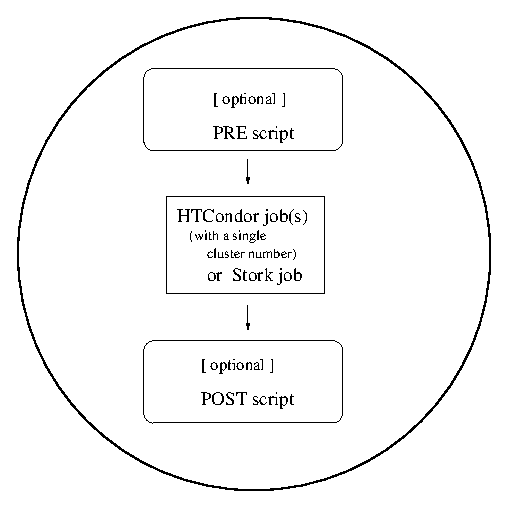
\includegraphics{user-man/dagman-node.eps}
\caption{\label{fig:dagman-node}One Node within a DAG}
\end{figure}

More than one HTCondor job may belong to a single node.
All HTCondor jobs within a node must be within
a single cluster, as given by the job ClassAd attribute \Attr{ClusterId}.
%In addition,
%all jobs within the single cluster must use the same log file.
%Separate nodes within a DAG may use different log files.

\emph{DAGMan enforces the dependencies within a DAG
using the events recorded in a separate
file that is specified by the default configuration.
If the exact same DAG were to be submitted more than once,
such that these DAGs were running at the same time,
expected them to fail in unpredictable and unexpected ways.
They would all be using the same single file to enforce dependencies. }

As DAGMan schedules and submits jobs within nodes to HTCondor,
these jobs are defined to succeed or fail based on their
return values.
This success or failure is propagated in well-defined ways to the level of
a node within a DAG.
Further progression of computation
(towards completing the DAG)
is based upon the success or failure of nodes.

The failure of a single job within a cluster
of multiple jobs
(within a single node)
causes the entire cluster of jobs to fail.
Any other jobs within the failed cluster of jobs are
immediately removed.
Each node within a DAG may be further constrained  to succeed or fail
based upon the return values of a PRE script and/or a POST script.

%%%%%%%%%%%%%%%%%%%%%%%%%%%%%%%%%%%%%%%
\subsection{The DAG Input File: Basic Commands}
%%%%%%%%%%%%%%%%%%%%%%%%%%%%%%%%%%%%%%%
\index{DAGMan!DAG input file}

The input file used by DAGMan is called a DAG input file.
It specifies the nodes of the DAG as well as the dependencies
that order the DAG.
All items are optional, except that there must be at least one \Arg{JOB}
item.

Comments may be placed in the DAG input file.
The pound character (\verb@#@) as the first character on a
line identifies the line as a comment.
Comments do not span lines.

A simple diamond-shaped DAG, as shown in
Figure~\ref{fig:dagman-diamond}
is presented as a starting point for examples.
This DAG contains 4 nodes.

\begin{figure}[hbt]
\centering
\includegraphics{user-man/dagman-diamond.eps}
\caption{\label{fig:dagman-diamond}Diamond DAG}
\end{figure}


A very simple DAG input file for this diamond-shaped DAG is

\footnotesize
\begin{verbatim}
    # File name: diamond.dag
    #
    JOB  A  A.condor 
    JOB  B  B.condor 
    JOB  C  C.condor	
    JOB  D  D.condor
    PARENT A CHILD B C
    PARENT B C CHILD D
\end{verbatim}
\normalsize

A set of basic commands appearing in a DAG input file is described below.


%%%%%%%%%%%%%%%%%%%%%%%%%%%%%%%%%%%%%%%
\subsubsection{\label{sec:dagman_job_command}JOB}
\label{dagman:JOB}
\index{DAG input file!JOB command}

The \Arg{JOB} command specifies an HTCondor job.
The syntax used for each \Arg{JOB} command is

\Opt{JOB} \Arg{JobName} \Arg{SubmitDescriptionFileName}
\oOptArg{DIR}{directory} \oOpt{NOOP} \oOpt{DONE}

A \Arg{JOB} entry maps a \Arg{JobName} to an HTCondor submit description file.
The \Arg{JobName} uniquely identifies nodes within the
DAG input file and in output messages.
Each node name, given by \Arg{JobName}, within the DAG must be unique.
The \Arg{JOB} entry must appear within the DAG input file before
other items that reference the node.

The keywords \Arg{JOB}, \Arg{DIR}, \Arg{NOOP}, and \Arg{DONE}
are not case sensitive.
Therefore, \Arg{DONE}, \Arg{Done}, and \Arg{done} are all equivalent.
The values defined for \Arg{JobName} and \Arg{SubmitDescriptionFileName}
are case sensitive, as file names 
in a file system are case sensitive.
The \Arg{JobName} can be any string that contains no white space, except
for the strings \Arg{PARENT} and \Arg{CHILD} (in upper, lower, or mixed
case). \Arg{JobName} also cannot contain special characters (\Arg{'.'}, 
\Arg{'+'}) which are reserved for system use.

Note that \Arg{DIR}, \Arg{NOOP}, and \Arg{DONE}, if used, must appear
in the order shown above.

The optional \Arg{DIR} keyword specifies a working directory
for this node,
from which the HTCondor job will be submitted,
and from which a \Arg{PRE} and/or
\Arg{POST} script will be run.
If a relative directory is specified, it is relative to the current working 
directory as the DAG is submitted.
Note that a DAG containing \Arg{DIR} specifications cannot
be run in conjunction with the \Arg{-usedagdir} command-line
argument to \Condor{submit\_dag}.
A "full" rescue DAG generated by a DAG run with the \Arg{-usedagdir} argument
will contain DIR specifications, so such a rescue DAG must be run
\emph{without} the \Arg{-usedagdir} argument.  (Note that "full"
rescue DAGs are no longer the default.)

\label{dagman:NOOP}
The optional \Arg{NOOP} keyword identifies that the HTCondor job within
the node is not to be submitted to HTCondor.
This optimization is useful in cases such as debugging a complex DAG structure,
where some of the individual jobs are long-running.
For this debugging of structure,
some jobs are marked as \Arg{NOOP}s, and
the DAG is initially run to verify that the control flow through
the DAG is correct.
The \Arg{NOOP} keywords are then removed before submitting the DAG.
Any PRE and POST scripts
for jobs specified with \Arg{NOOP} \emph{are} executed;
to avoid running the PRE and POST scripts, comment them out.
The job that is not submitted to HTCondor is given a return value that indicates
success, such that the node may also succeed.
Return values of any 
PRE and POST scripts may still cause the node to fail.
Even though the job specified with \Arg{NOOP} is not submitted,
its submit description file must exist;
the log file for the job is used, 
because DAGMan generates dummy submission and termination events for the job.

The optional \Arg{DONE} keyword identifies a node as being already
completed.
This is mainly used by Rescue DAGs generated by DAGMan itself,
in the event of a failure to complete the workflow.
Nodes with the \Arg{DONE} keyword are not executed when the Rescue DAG is run,
allowing the workflow to pick up from the previous endpoint.  Users
should generally not use the \Arg{DONE} keyword.
The \Arg{NOOP} keyword is more flexible in avoiding
the execution of a job within a node.
Note that, for any node marked \Arg{DONE} in a DAG, all of
its parents must also be marked \Arg{DONE}; 
otherwise, a fatal error will result.
The \Arg{DONE} keyword applies to the entire node.
A node marked with \Arg{DONE} will not have a PRE or POST script run,
and the HTCondor job will not be submitted.

%%%%%%%%%%%%%%%%%%%%%%%%%%%%%%%%%%%%%%%
\subsubsection{\label{sec:dagman_data_command}DATA}
\label{dagman:DATA}
\index{DAG input file!DATA command}

As of version 8.3.5, \Condor{dagman} no longer supports DATA nodes.

%%%%%%%%%%%%%%%%%%%%%%%%%%%%%%%%%%%%%%%
\subsubsection{\label{sec:dagman_parent_child_command}PARENT \Dots CHILD}
\label{dagman:ParentChild}
\index{DAG input file!PARENT \Dots CHILD command}

The \Arg{PARENT} \Arg{CHILD} command specifies the
dependencies within the DAG.
\index{DAGMan!describing dependencies}
Nodes are parents and/or children within the DAG.
A parent node must be completed successfully before
any of its children may be started.
A child node may only be started once
all its parents have successfully completed.

The syntax used for each dependency (PARENT/CHILD) command is

\Opt{PARENT} \Arg{ParentJobName\Dots} \Opt{CHILD} \Arg{ChildJobName\Dots}

The \Arg{PARENT} keyword is followed by one or more
\Arg{ParentJobName}s.
The \Arg{CHILD} keyword is followed by one or more
\Arg{ChildJobName}s.
Each child job depends on every parent job within the line.
A single line in the input file can specify the dependencies from one or more
parents to one or more children.
The diamond-shaped DAG example may specify the dependencies with
\begin{verbatim}
PARENT A CHILD B C
PARENT B C CHILD D
\end{verbatim}
An alternative specification for the diamond-shaped DAG
may specify some or all of the dependencies on separate lines:
\begin{verbatim}
PARENT A CHILD B C
PARENT B CHILD D
PARENT C CHILD D
\end{verbatim}

As a further example, the line
\begin{verbatim}
PARENT p1 p2 CHILD c1 c2
\end{verbatim}
produces four dependencies:
\begin{enumerate}
\item{\verb@p1@ to \verb@c1@}
\item{\verb@p1@ to \verb@c2@}
\item{\verb@p2@ to \verb@c1@}
\item{\verb@p2@ to \verb@c2@}
\end{enumerate}

%%%%%%%%%%%%%%%%%%%%%%%%%%%%%%%%%%%%%%%
\subsubsection{\label{sec:dagman_script_command}SCRIPT}
\label{dagman:SCRIPT}
\index{DAG input file!SCRIPT command}
\index{DAGMan!PRE and POST scripts}

The optional \Arg{SCRIPT} command specifies
processing that is done either before a job within
a node is submitted
or after a job within a node completes its execution.
\index{DAGMan!PRE script}
Processing done before a job is submitted is
called a \Arg{PRE} script.
Processing done after a job completes its execution is
\index{DAGMan!POST script}
called a \Arg{POST} script.
Note that the executable specified does not necessarily
have to be a shell script (Unix) or batch file (Windows);
but it should be relatively light weight because it will
be run directly on the submit machine, not submitted as
an HTCondor job.

The syntax used for each \Arg{PRE} or \Arg{POST} command is

\Opt{SCRIPT} \oOptArg{DEFER}{status time}
\Opt{PRE} \Arg{JobName}|\Opt{ALL\_NODES} \Arg{ExecutableName}
\oArg{arguments}

\Opt{SCRIPT} \oOptArg{DEFER}{status time}
\Opt{POST}  \Arg{JobName}|\Opt{ALL\_NODES} \Arg{ExecutableName}
\oArg{arguments}

The \Arg{SCRIPT} command uses
the \Arg{PRE} or \Arg{POST} keyword,
which specifies the relative timing of when the script is to be run.
The \Arg{JobName} identifies the node to which the script is attached.
The \Arg{ExecutableName}
specifies the executable (e.g., shell script or batch file) to be executed, 
and may not contain spaces.
The optional \Arg{arguments} are command line arguments to the script,
and spaces delimit the arguments.
Both \Arg{ExecutableName} and optional \Arg{arguments} are
case sensitive.

Scripts are executed on the submit machine;
the submit machine is not necessarily
the same machine upon which the node's job is run.
Further, a single cluster of HTCondor jobs may be
spread across several machines.

The optional \Arg{DEFER} feature causes a retry of only the script,
if the execution of the script exits with the
exit code given by \Arg{status}.
The retry occurs after at least \Arg{time} seconds, 
rather than being considered failed.  
While waiting for the retry,
the script does not count against a \Arg{maxpre} or \Arg{maxpost} limit.
The ordering of the \Arg{DEFER} feature within the \Arg{SCRIPT} 
specification is fixed.
It must come directly after the \Arg{SCRIPT} keyword;
this is done to avoid backward compatibility issues for any
DAG with a \Arg{JobName} of DEFER.

A PRE script is commonly used
to place files in a staging area for the jobs to use.
A POST script is commonly used
to clean up or remove files once jobs are finished running.
An example uses PRE and POST scripts to stage files
that are stored on tape.
The PRE script reads compressed input files from the tape drive,
uncompresses them, and places the resulting files in the current directory.
The HTCondor jobs can then use these files,
producing output files.
The POST script compresses the output files, writes them out to
the tape, and then removes both the staged files and the output files.

If the PRE script fails, 
then the HTCondor job associated with the node is not submitted,
and (as of version 8.5.4) the POST
script is not run either (by default).
However, if the job is submitted, and there is a POST script, the POST
script is always run once the job finishes.
(The behavior when the PRE script fails may
may be changed to run the POST script
by setting configuration variable \MacroNI{DAGMAN\_ALWAYS\_RUN\_POST} 
to \Expr{True} or by passing the \Opt{-AlwaysRunPost}
argument to \Condor{submit\_dag}.)

Progress towards completion of the DAG is based upon
the success of the nodes within the DAG.
The success of a node is based upon the success of 
the job(s), PRE script, and POST script.
A job, PRE script, or POST script with an exit value not equal to 0 is
considered failed.  
\Bold{The exit value of whatever component of the node was run last
determines the success or failure of the node.}
Table~\ref{NodeS-F} lists the definition of node success and
failure for all variations of script and job success and failure,
when \MacroNI{DAGMAN\_ALWAYS\_RUN\_POST} is set to \Expr{False}.
In this table, a dash (\Expr{-}) represents the case where a script
does not exist for the DAG, \Bold{S} represents success, 
and  \Bold{F} represents failure.

Table~\ref{NodeS-F-ARP} lists the definition of node success and
failure only for the cases where the PRE script fails,
when \MacroNI{DAGMAN\_ALWAYS\_RUN\_POST} is set to \Expr{True}.

%An exit value not equal to 0 indicates program failure,
%except as indicated by the \Arg{PRE\_SKIP} command:
%if a PRE script exits with the PRE\_SKIP value, 
%then the node succeeds and the job and the POST script are both skipped.  
%It is therefore important that a
%successful program return the exit value 0. 
%It is good practice to always
%explicitly specify a return value in the PRE script,
%returning 0 in the case of success.
%Otherwise,
%the return code of the last completed process is returned,
%which can lead to unexpected results. 

\begin{center}
\begin{table}[hbt]
\begin{tabular}{|c|c|c|c|} \hline
PRE  & JOB & POST & \Bold{Node}  \\
\hline
-  & S & - & \Bold{S}  \\
-  & F & - & \Bold{F}  \\
-  & S & S & \Bold{S}  \\
-  & S & F & \Bold{F}  \\
-  & F & S & \Bold{S}  \\
-  & F & F & \Bold{F}  \\
S  & S & - & \Bold{S}  \\
S  & F & - & \Bold{F}  \\
S  & S & S & \Bold{S}  \\
S  & S & F & \Bold{F}  \\
S  & F & S & \Bold{S}  \\
S  & F & F & \Bold{F}  \\
F  & not run & - & \Bold{F}  \\
F  & not run & not run & \Bold{F}  \\
\end{tabular}
\caption{\label{NodeS-F}Node success or failure definition with \Expr{DAGMAN\_ALWAYS\_RUN\_POST = False (the default)} }
\end{table}
\end{center}

\begin{center}
\begin{table}[hbt]
\begin{tabular}{|c|c|c|c|} \hline
PRE  & JOB & POST & \Bold{Node}  \\
F  & not run & - & \Bold{F}  \\
F  & not run & S & \Bold{S}  \\
F  & not run & F & \Bold{F}  \\
\hline
\end{tabular}
\caption{\label{NodeS-F-ARP}Node \Bold{S}uccess or \Bold{F}ailure definition with \Expr{ DAGMAN\_ALWAYS\_RUN\_POST = True} }
\end{table}
\end{center}

\Bold{Special script argument macros}

The five macros \Expr{\$JOB}, \Expr{\$RETRY}, \Expr{\$MAX\_RETRIES}, 
\Expr{\$DAG\_STATUS} and \Expr{\$FAILED\_COUNT} can be used within the
DAG input file as arguments passed to a PRE or POST script. 
The three macros \Expr{\$JOBID}, \Expr{\$RETURN}, 
and \Expr{\$PRE\_SCRIPT\_RETURN} can
be used as arguments to POST scripts.
The use of these variables is limited to being used
as an individual command
line \Arg{argument} to the script,
surrounded by spaces, in order to cause the substitution of the
variable's value.

The special macros are as follows:

\begin{itemize}
\item \index{DAGMan!JOB@\verb^$JOB^ value}
\Expr{\$JOB} evaluates to the (case sensitive) string
defined for \Arg{JobName}.

\item \index{DAGMan!RETRY@\verb^$RETRY^ value}
\Expr{\$RETRY} evaluates to an 
integer value set to 0 the first time a node is run,
and is incremented each time the node is retried. 
See section~\ref{dagman:retry} for the description of how to cause
nodes to be retried. 

\item \index{DAGMan!MAX_RETRIES@\verb^$MAX_RETRIES^ value}
\Expr{\$MAX\_RETRIES} evaluates to an integer value set 
to the maximum number of retries for the node.
See section~\ref{dagman:retry} for the description of how to cause
nodes to be retried.  
If no retries are set for the node,
\Expr{\$MAX\_RETRIES} will be set to 0.

\item \index{DAGMan!JOBID@\verb^$JOBID^ value}
\index{job ID!defined for a DAGMan node job}
\index{job!job ID!defined for a DAGMan node job}
\Expr{\$JOBID} (for POST scripts only)
evaluates to a representation of the HTCondor job ID of the node job.
It is the value of the job ClassAd attribute \Attr{ClusterId},
followed by a period,
and then followed by the value of the job ClassAd attribute \Attr{ProcId}.
An example of a job ID might be 1234.0.
For nodes with multiple jobs in the same cluster,
the \Attr{ProcId} value is the one of the last job within the cluster.

\item \index{DAGMan!return@\verb^$RETURN^ value}
\Expr{\$RETURN} (for POST scripts only) variable evaluates to
the return value of the 
HTCondor job, if there is a single job within a cluster.
With multiple jobs within the same cluster,
there are two cases to consider.
In the first case, all jobs within the cluster are successful;
the value of \Expr{\$RETURN} will be 0, indicating success.
In the second case,
one or more jobs from the cluster fail.
When \Condor{dagman} sees the first terminated event for a job that failed,
it assigns that job's return value as the value of \Expr{\$RETURN},
and it attempts to remove all remaining jobs within the cluster.
Therefore, if multiple jobs in the cluster fail with different exit codes,
a race condition determines which exit code gets assigned to \Expr{\$RETURN}.

A job that dies due to a signal is reported with a \Expr{\$RETURN} value
representing the additive inverse of the signal number.
For example, SIGKILL (signal 9) is reported as -9.
A job whose batch system submission fails is reported as -1001.
A job that is externally removed from the batch system queue
(by something other than \Condor{dagman}) is reported as -1002.

\item \index{DAGMan!PRE_SCRIPT_RETURN@\verb^$PRE_SCRIPT_RETURN^ value}
\Expr{\$PRE\_SCRIPT\_RETURN} (for POST scripts only)
variable evaluates to the return value of the PRE script of a node, 
if there is one.
If there is no PRE script, this value will be -1.
If the node job was skipped because of failure of the PRE script,
the value of \Expr{\$RETURN} will be -1004
and the value of \Expr{\$PRE\_SCRIPT\_RETURN} will be the exit value
of the PRE script;
the POST script can use this to see if the PRE script exited
with an error condition, and assign success or failure to the node, as
appropriate.

%\item \Expr{\$DAG\_STATUS} and \Expr{\$FAILED\_COUNT} are documented in
%section ~\ref{sec:DAGFinalNode} below.
%\begin{itemize}
\index{DAGMan!DAG_STATUS@\verb^$DAG_STATUS^ value}
\item \Env{\$DAG\_STATUS} is the status of the DAG.
Note that this macro's value and definition is unrelated to the attribute 
named \Attr{DagStatus} as defined for use in a node status file.
This macro's value is the same as the job ClassAd attribute \Attr{DAG\_Status}
that is defined within the \Condor{dagman} job's ClassAd.
This macro may have the following values:
\begin{itemize}
\item 0: OK
\item 1: error; an error condition different than those listed here
\item 2: one or more nodes in the DAG have failed
\item 3: the DAG has been aborted by an ABORT-DAG-ON specification
\item 4: removed; the DAG has been removed by \Condor{rm}
\item 5: cycle; a cycle was found in the DAG
\item 6: halted; the DAG has been halted (see section ~\ref{sec:DagSuspend})
\end{itemize}

\index{DAGMan!FAILED_COUNT@\verb^$FAILED_COUNT^ value}
\item \Env{\$FAILED\_COUNT} is defined by the number of nodes that have failed in the
DAG.

\end{itemize}


\Bold{Examples that use PRE or POST scripts}

Examples use the diamond-shaped DAG.
A first example uses a PRE script to expand a compressed file 
needed as input to each of the HTCondor jobs of nodes B and C.
The DAG input file:

\footnotesize
\begin{verbatim}
    # File name: diamond.dag
    #
    JOB  A  A.condor 
    JOB  B  B.condor 
    JOB  C  C.condor	
    JOB  D  D.condor
    SCRIPT PRE  B  pre.csh $JOB .gz
    SCRIPT PRE  C  pre.csh $JOB .gz
    PARENT A CHILD B C
    PARENT B C CHILD D
\end{verbatim}
\normalsize

The script \File{pre.csh} uses its command line arguments to form the file name
of the compressed file.
The script contains

\begin{verbatim}
  #!/bin/csh
  gunzip $argv[1]$argv[2]
\end{verbatim}

Therefore, the PRE script invokes  
\begin{verbatim}
  gunzip B.gz
\end{verbatim}
for node B, which uncompresses file \File{B.gz},
placing the result in file \File{B}.

A second example uses the \Expr{\$RETURN} macro.
The DAG input file contains the POST script specification:
\begin{verbatim}
  SCRIPT POST A stage-out job_status $RETURN 
\end{verbatim}
If the HTCondor job of node A exits with the value -1,
the POST script is invoked as
\begin{verbatim}
  stage-out job_status -1
\end{verbatim}

The slightly different example POST script specification
in the DAG input file
\begin{verbatim}
  SCRIPT POST A stage-out job_status=$RETURN 
\end{verbatim}
invokes the POST script with
\begin{verbatim}
  stage-out job_status=$RETURN
\end{verbatim}

This example shows that when
there is no space between the \Expr{=} sign and the variable \Expr{\$RETURN},
there is no substitution of the macro's value.

%%%%%%%%%%%%%%%%%%%%%%%%%%%%%%%%%%%%%%%
\subsubsection{\label{sec:dagman_pre_skip_command}PRE\_SKIP}
\label{dagman:PRE-SKIP}
\index{DAG input file!PRE\_SKIP command}
\index{DAGMan!skipping node execution}

The behavior of DAGMan with respect to node success or failure can
be changed with the addition of a \Arg{PRE\_SKIP} command. 
A \Arg{PRE\_SKIP} line within the DAG input file uses the syntax: 

\Opt{PRE\_SKIP} \Arg{JobName}|\Opt{ALL\_NODES} \Arg{non-zero-exit-code}

The PRE script of a node identified by \Arg{JobName} that exits with the value 
given by \Arg{non-zero-exit-code}
skips the remainder of the node entirely.  
Neither the job associated with the node nor
the POST script will be executed,
and the node will be marked as successful.

% $ % this comment just has a dollar sign so that emacs will not think
%	  we're inside of a math section and will draw things more nicely

%%%%%%%%%%%%%%%%%%%%%%%%%%%%%%%%%%%%%%%
\subsection{\label{sec:DAG-command_order}Command Order}
\label{dagman:command order}
\index{DAG input file!command order}
\index{DAGMan!command order}

As of version 8.5.6, commands referencing a \Arg{JobName} \emph{can}
come before the JOB command defining that \Arg{JobName}.

For example, the command sequence
\begin{verbatim}
SCRIPT PRE NodeA foo.pl
VARS NodeA state="Wisconsin"
JOB NodeA bar.sub
\end{verbatim}
is now legal (it would have been illegal in 8.5.5 and all previous
versions).

%%%%%%%%%%%%%%%%%%%%%%%%%%%%%%%%%%%%%%%
\subsection{Node Job Submit File Contents}
%%%%%%%%%%%%%%%%%%%%%%%%%%%%%%%%%%%%%%%
\index{DAGMan!node job submit description file}

Each node in a DAG may use a unique submit description file.
A key limitation is that
each HTCondor submit description file must submit jobs
described by a single cluster number;
DAGMan cannot deal with a submit description file producing
multiple job clusters.

Consider again the diamond-shaped DAG example, 
where each node job uses the same submit description file.

\begin{verbatim}
    # File name: diamond.dag
    #
    JOB  A  diamond_job.condor 
    JOB  B  diamond_job.condor 
    JOB  C  diamond_job.condor	
    JOB  D  diamond_job.condor
    PARENT A CHILD B C
    PARENT B C CHILD D
\end{verbatim}

Here is a sample HTCondor submit description file
for this DAG:

\index{DAGMan!example submit description file}
\begin{verbatim}
    # File name: diamond_job.condor
    #
    executable   = /path/diamond.exe
    output       = diamond.out.$(cluster)
    error        = diamond.err.$(cluster)
    log          = diamond_condor.log
    universe     = vanilla
    queue
\end{verbatim}

Since each node uses the same HTCondor submit description file,
this implies that each node within the DAG runs the
same job.
The \MacroUNI{Cluster} macro
produces unique file names for each job's output.

\index{ClassAd job attribute!DAGParentNodeNames}
\index{DAGParentNodeNames!job ClassAd attribute}
The job ClassAd attribute \Attr{DAGParentNodeNames} is also available
for use within the submit description file. 
It defines a comma separated list of each \Arg{JobName}
which is a parent node of this job's node.
This attribute may be used in the \SubmitCmd{arguments} command
for all but scheduler universe jobs.
For example, if the job has two parents, with \Arg{JobName}s B and C,
the submit description file command
\begin{verbatim}
arguments = $$([DAGParentNodeNames])
\end{verbatim}
will pass the string \AdStr{B,C} as the command line argument when invoking
the job.

DAGMan supports jobs with queues of multiple procs, so for example:
\begin{verbatim}
queue 500
\end{verbatim}
will queue 500 procs as expected. However, \emph{as of version 8.7.2 DAGMan 
does not support late materialization}. If a submit file queues multiple procs
while the \Macro{SCHEDD\_ALLOW\_LATE\_MATERIALIZATION} and
\Macro{SUBMIT\_FACTORY\_JOBS\_BY\_DEFAULT} attributes are set to True, DAGMan
will produce unexpected results, including failing without warning. We are
working to resolve this as quickly as possible.

%%%%%%%%%%%%%%%%%%%%%%%%%%%%%%%%%%%%%%%
\subsection{\label{dagman:submitdag}DAG Submission}
%%%%%%%%%%%%%%%%%%%%%%%%%%%%%%%%%%%%%%%
\index{DAGMan!DAG submission}

A DAG is submitted using the tool \Condor{submit\_dag}.
The manual
page~\pageref{man-condor-submit-dag}
details the command.
The simplest of DAG submissions has the syntax

\Condor{submit\_dag} \Arg{DAGInputFileName}

and the current working directory contains the DAG input file.

The diamond-shaped DAG example may be submitted with

\begin{verbatim}
condor_submit_dag diamond.dag
\end{verbatim}

Do not submit the same DAG, with same DAG input file, 
from within the same directory, 
such that more than one of this same DAG is running at the same time.
It will fail in an unpredictable manner,
as each instance of this same DAG will attempt to use the same
file to enforce dependencies.
 
To increase robustness and guarantee recoverability, the 
\Condor{dagman} process is run as an HTCondor job.
As such, it needs a submit description file.
\Condor{submit\_dag} generates this needed submit description file,
naming it by appending \File{.condor.sub} to the name of the DAG input file.
This submit description file may be edited if the DAG is submitted with

\begin{verbatim}
condor_submit_dag -no_submit diamond.dag
\end{verbatim}
causing \Condor{submit\_dag} to create the submit description file,
but not submit \Condor{dagman} to HTCondor.
To submit the DAG, once the submit description file is edited,
use

\begin{verbatim}
condor_submit diamond.dag.condor.sub
\end{verbatim}

Submit machines with limited resources are supported by
command line options that place limits on the submission and handling 
of HTCondor jobs and PRE and POST scripts. 
Presented here are descriptions of the command line options
to \Condor{submit\_dag}.
These same limits can be set in configuration.
Each limit is applied within a single DAG.

%%%%%%%%%%%%%%%%%%%%%%%%%%%%%%%%%%%%%%%
\subsubsection{\label{sec:DAG-throttling}DAG Throttling}
\index{DAGMan!throttling}

\Bold{Total nodes/clusters:}
The \Opt{-maxjobs} option 
specifies the maximum number of clusters that \Condor{dagman}
can submit at one time.
Since each node corresponds to a single cluster,
this limit restricts the number of nodes that can be submitted (in the
HTCondor queue) at a time.
It is commonly used when
there is a limited amount of input file staging capacity.
As a specific example, consider a case where each node represents
a single HTCondor proc that requires 4 MB of input files,
and the proc will run in a directory with a volume of 100 MB
of free space.
Using the argument \Opt{-maxjobs 25} guarantees that a maximum
of 25 clusters, using a maximum of 100 MB of space,
will be submitted to HTCondor at one time.
(See the \Condor{submit\_dag} man page (~\ref{man-condor-submit-dag})
for more information.  Also see the equivalent
\Macro{DAGMAN\_MAX\_JOBS\_SUBMITTED} configuration option
(~\ref{param:DAGManMaxJobsSubmitted}).)

\Bold{Idle procs:}
The number of idle procs within a given DAG can be limited with
the optional command line argument \Opt{-maxidle}. 
\Condor{dagman} will not submit any more node jobs 
until the number of idle procs in the DAG goes below this
specified value,
even if there are ready nodes in the DAG.
This allows \Condor{dagman} to submit jobs in a way that adapts to
the load on the HTCondor pool at any given time.  If the pool is
lightly loaded, \Condor{dagman} will end up submitting more jobs;
if the pool is heavily loaded, \Condor{dagman} will submit fewer jobs.
(See the \Condor{submit\_dag} man page (~\ref{man-condor-submit-dag})
for more information.  Also see the equivalent
\Macro{DAGMAN\_MAX\_JOBS\_IDLE} configuration option
(~\ref{param:DAGManMaxJobsIdle}).)

Note that the \Opt{-maxjobs} option applies to counts of
\emph{clusters}, whereas the \Opt{-maxidle} option
applies to counts of \emph{procs}.  Unfortunately, this can
be a bit confusing.  Of course, if none of your submit files
create more than one proc, the distinction doesn't matter.
For example, though, a node job submit file that queues
5 procs will count as one for \Opt{-maxjobs}, but five
for \Opt{-maxidle} (if all of the procs are idle).

\Bold{Subsets of nodes:}
Node submission can also be throttled in a finer-grained manner by
grouping nodes into categories.  See section ~\ref{sec:DAG-node-category}
for more details.

\Bold{PRE/POST scripts:}
Since PRE and POST scripts run on the submit machine,
it may be desirable to limit the number of PRE or POST scripts running
at one time.
The optional \Opt{-maxpre} command line argument limits the number of PRE
scripts that may be running at one time,
and the optional \Opt{-maxpost} command line argument limits the number
of POST scripts that may be running at one time.
(See the \Condor{submit\_dag} man page (~\ref{man-condor-submit-dag})
for more information.  Also see the equivalent
\Macro{DAGMAN\_MAX\_PRE\_SCRIPTS} (~\ref{param:DAGManMaxPreScripts}) and
\Macro{DAGMAN\_MAX\_POST\_SCRIPTS} (~\ref{param:DAGManMaxPostScripts})
configuration options.)

%%%%%%%%%%%%%%%%%%%%%%%%%%%%%%%%%%%%%%%
\subsection{\label{sec:DAGPaths}File Paths in DAGs}
%%%%%%%%%%%%%%%%%%%%%%%%%%%%%%%%%%%%%%%
\index{DAGMan!file paths in DAGs}

\Condor{dagman} assumes that all relative paths in a
DAG input file and the associated HTCondor submit description files
are relative to the current
working directory when \Condor{submit\_dag} is run.  
This works well for submitting a single DAG.
It presents problems when multiple independent DAGs are submitted
with a single invocation of \Condor{submit\_dag}.
Each of these independent DAGs would logically be in its own directory, 
such that it could be run or tested independent of other DAGs.
Thus, all references to files will be designed to be relative to
the DAG's own directory.

%Note that 
%relative paths in submit description files can be modified by the submit command
%\SubmitCmd{initialdir}; 
%see the \Condor{submit} manual page at ~\ref{man-condor-submit} 
%for more details on this command.
%The remainder of this discussion ignores \SubmitCmd{initialdir}.

Consider an example DAG within a directory named \File{dag1}.
There would be a DAG input file, named \File{one.dag} for this example.
Assume the contents of this DAG input file specify a node job with
\begin{verbatim}
  JOB A  A.submit
\end{verbatim}
Further assume that partial contents of submit description file 
\File{A.submit} specify
\begin{verbatim}
  executable = programA
  input      = A.input
\end{verbatim}

Directory contents are 
\begin{verbatim}
    dag1 (directory)
          one.dag
          A.submit
          programA
          A.input
\end{verbatim}

All file paths are correct relative to the \File{dag1} directory.
Submission of this example DAG sets the current working directory
to \File{dag1} and invokes \Condor{submit\_dag}:
\begin{verbatim}
  cd dag1
  condor_submit_dag one.dag
\end{verbatim}

Expand this example such that there are now two independent DAGs,
and each is contained within its own directory. 
For simplicity, assume that the DAG in \File{dag2} has remarkably
similar files and file naming as the DAG in \File{dag1}.
Assume that the directory contents are 
\begin{verbatim}
    parent (directory)
         dag1 (directory)
               one.dag
               A.submit
               programA
               A.input
         dag2 (directory)
               two.dag
               B.submit
               programB
               B.input
\end{verbatim}

The goal is to use a single invocation of \Condor{submit\_dag}
to run both dag1 and dag2.
The invocation
\begin{verbatim}
  cd parent
  condor_submit_dag dag1/one.dag dag2/two.dag
\end{verbatim}
\emph{does not work}.
Path names are now relative to \File{parent}, 
which is \emph{not} the desired behavior.

The solution is 
the \Arg{-usedagdir} command line argument to \Condor{submit\_dag}.
This feature runs each DAG as if \Condor{submit\_dag} had been run 
in the directory in which the relevant DAG file exists.
A working invocation is
\begin{verbatim}
  cd parent
  condor_submit_dag -usedagdir dag1/one.dag dag2/two.dag
\end{verbatim}

Output files will be placed in the correct directory, and
the \File{.dagman.out} file will also be in the correct directory.
A Rescue DAG file will be written to
the current working directory, which is the directory when
\Condor{submit\_dag} is invoked.
The Rescue DAG should be run from that same current working directory.
The Rescue DAG includes all the path information necessary to
run each node job in the proper directory.

%If all paths in the DAG input file(s) and the relevant submit
%description files are absolute,
%the \Arg{-usedagdir} argument is not needed;
%however, using absolute paths is NOT generally a good idea.

%For a DAG that \emph{does not} use \Arg{-usedagdir}, 
%relative paths can still work for multiple DAGs, 
%if all file paths are given relative to
%the current working directory as \Condor{submit\_dag} is executed.
%This implies that DAGs in separate directories
%cannot be submitted from their own directories;
%submission only works from the parent directory the paths are set up for.

Use of \Arg{-usedagdir} does \emph{not} work in conjunction with
a JOB node specification within the DAG input file using
the \Arg{DIR} keyword.
Using both will be detected and generate an error. 

%%%%%%%%%%%%%%%%%%%%%%%%%%%%%%%%%%%%%%%
\subsection{\label{sec:DAGMonitoring}DAG Monitoring and DAG Removal}
%%%%%%%%%%%%%%%%%%%%%%%%%%%%%%%%%%%%%%%
\index{DAGMan!DAG monitoring}
\index{DAGMan!DAG removal}

%TEMP -- this section needs lots of improvement... (dagman.out, node
% status file, jobstate.log file, halt file, etc.)

After submission, the progress of the DAG can be monitored
by looking at the job event log file(s),
observing the e-mail that job submission to HTCondor causes,
or by using \Condor{q} \Arg{-dag}.

There is also a large amount of information logged in an extra file.
The name of this extra file is produced by appending
\File{.dagman.out} to the name of the DAG input file; 
for example, if the DAG input file is \File{diamond.dag}, 
this extra file is named \File {diamond.dag.dagman.out}.
If this extra file grows too large, limit its size
with the configuration variable \Macro{MAX\_DAGMAN\_LOG},
as defined in section~\ref{param:MaxSubsysLog}.
The \File{dagman.out} file is an important resource for
debugging; save this file if a problem occurs. 
The \File{dagman.out} is appended to, rather than overwritten, 
with each new DAGMan run.

To remove an entire DAG, consisting of the \Condor{dagman} job, 
plus any jobs submitted to HTCondor,
remove the \Condor{dagman} job by running \Condor{rm}.
For example,
%TEMP -- example needs to be changed to match current condor_q
\footnotesize
\begin{verbatim}
% condor_q
-- Submitter: turunmaa.cs.wisc.edu : <128.105.175.125:36165> : turunmaa.cs.wisc.edu
 ID      OWNER          SUBMITTED     RUN_TIME ST PRI SIZE CMD
  9.0   taylor         10/12 11:47   0+00:01:32 R  0   8.7  condor_dagman -f -
 11.0   taylor         10/12 11:48   0+00:00:00 I  0   3.6  B.out
 12.0   taylor         10/12 11:48   0+00:00:00 I  0   3.6  C.out

    3 jobs; 2 idle, 1 running, 0 held

% condor_rm 9.0
\end{verbatim}
\normalsize

When a \Condor{dagman} job is removed, all node jobs (including sub-DAGs)
of that \Condor{dagman} will be removed by the \Condor{schedd}.  As of version
8.5.8, the default is that \Condor{dagman} itself also removes the
node jobs (to fix a race condition that could result in "orphaned"
node jobs).  (The \Condor{schedd} has to remove the node jobs to deal with
the case of removing a \Condor{dagman} job that has been held.)

The previous behavior of \Condor{dagman} itself \emph{not} removing
the node jobs can be restored by setting the
\MacroNI{DAGMAN\_REMOVE\_NODE\_JOBS} configuration macro
(see ~\ref{param:DAGManRemoveNodeJobs})
to \Expr{False}.  This will decrease the load on the \Condor{schedd},
at the cost of allowing the possibility of "orphaned" node jobs.

A removed DAG will be considered failed unless the
DAG has a FINAL node that succeeds.

%TEMP -- this needs to be fixed/clarified
In the case where a
machine is scheduled to go down,
DAGMan will clean up memory and exit.
However, it will leave any submitted jobs
in the HTCondor queue.

%%%%%%%%%%%%%%%%%%%%%%%%%%%%%%%%%%%%%%%
\subsection{\label{sec:DagSuspend}Suspending a Running DAG}
%%%%%%%%%%%%%%%%%%%%%%%%%%%%%%%%%%%%%%%
\index{DAGMan!suspending a running DAG}

It may be desired to temporarily suspend a running DAG.
For example, the load may be high on the submit machine,
and therefore it is desired to prevent DAGMan from
submitting any more jobs until the load goes down.
There are two ways to suspend (and resume) a running DAG.

\begin{itemize}
\item Use \Condor{hold}/\Condor{release} on the \Condor{dagman} job.

After placing the \Condor{dagman} job on hold,
no new node jobs will be submitted,
and no PRE or POST scripts will be run.
Any node jobs already in the HTCondor queue will continue undisturbed.
Any running PRE or POST scripts will be killed.
If the \Condor{dagman} job is left on hold,
it will remain in the HTCondor queue after all of the currently running
node jobs are finished.
To resume the DAG, use \Condor{release} on the \Condor{dagman} job.

Note that while the \Condor{dagman} job is on hold,
no updates will be made to the \File{dagman.out} file.

\item Use a DAG halt file.

The second way of suspending a DAG uses the existence of a specially-named
file to change the state of the DAG.
When in this halted state,
no PRE scripts will be run, and no node jobs will be submitted.  
Running node jobs will continue undisturbed.
A halted DAG will still run POST scripts,
and it will still update the \File{dagman.out} file.
This differs from behavior of a DAG that is held.
Furthermore, a halted DAG will not remain in the queue indefinitely;
when all of the running node jobs have finished, 
DAGMan will create a Rescue DAG and exit.

To resume a halted DAG, remove the halt file.

The specially-named file must be placed in the same directory
as the DAG input file.
The naming is the same as the DAG input file concatenated with the
string \File{.halt}.
For example, if the DAG input file is \File{test1.dag}, 
then \File{test1.dag.halt} will be the required name of the halt file.

As any DAG is first submitted with \Condor{submit\_dag}, 
a check is made for a halt file.
If one exists, it is removed.
\end{itemize}

\Bold{Note that neither \Condor{hold} nor a DAG halt is propagated to
sub-DAGs.}
In other words, if you \Condor{hold} or create a halt file for a DAG that
has sub-DAGs, any sub-DAGs that are already in the queue will continue
to submit node jobs.

A \Condor{hold} or DAG halt \emph{does}, however, apply to splices,
because they are merged into the parent DAG and controlled by a single
\Condor{dagman} instance.

%%%%%%%%%%%%%%%%%%%%%%%%%%%%%%%%%%%%%%%
\subsection{\label{sec:AdvDAGMan}Advanced Features of DAGMan}
%%%%%%%%%%%%%%%%%%%%%%%%%%%%%%%%%%%%%%%


%%%%%%%%%%%%%%%%%%%%%%%%%%%%%%%%%%%%%%%
\subsubsection{\label{dagman:retry}Retrying Failed Nodes}
\index{DAG input file!RETRY command}
\index{DAGMan!retrying failed nodes}

DAGMan can retry any failed node in a DAG by
specifying the node in the DAG input file 
with the \Arg{RETRY} command.
The use of retry is optional.
The syntax for retry is

\Opt{RETRY} \Arg{JobName}|\Opt{ALL\_NODES} \Arg{NumberOfRetries}
\oOptArg{UNLESS-EXIT}{value}

where \Arg{JobName} identifies the node.
\Arg{NumberOfRetries} is an integer
number of times to retry the node after failure.
The implied number of retries for any node is 0,
the same as not having a retry line in the file. 
Retry is implemented on nodes, not parts of a node.

The diamond-shaped DAG example may be modified to
retry node C:

\footnotesize
\begin{verbatim}
    # File name: diamond.dag
    #
    JOB  A  A.condor 
    JOB  B  B.condor 
    JOB  C  C.condor	
    JOB  D  D.condor
    PARENT A CHILD B C
    PARENT B C CHILD D
    Retry  C 3
\end{verbatim}
\normalsize

If node C is marked as failed for any reason,
then it is started over as a first retry.
The node will be tried a second and third time,
if it continues to fail.
If the node is marked as successful, then further retries do not occur.

Retry of a node may be short circuited using the
optional keyword \Arg{UNLESS-EXIT}, followed by an integer exit value.
If the node exits with the specified integer exit value,
then no further processing will be done
on the node. 

The macro \Env{\$RETRY} evaluates to an 
integer value, set to 0 first time a node is run,
and is incremented each time for each time the node is retried. 
The macro \Env{\$MAX\_RETRIES} is the value set for
\Arg{NumberOfRetries}.
These macros may be used as arguments passed to a PRE or POST script.

%%%%%%%%%%%%%%%%%%%%%%%%%%%%%%%%%%%%%%%
\subsubsection{\label{dagman:abort}Stopping the Entire DAG}
\index{DAG input file!ABORT-DAG-ON command}
\index{DAGMan!aborting a DAG}

The \Arg{ABORT-DAG-ON} command provides a way
to abort the entire DAG if a given node returns a specific exit
code.  The syntax for \Arg{ABORT-DAG-ON} is

\Opt{ABORT-DAG-ON} \Arg{JobName}|\Opt{ALL\_NODES} \Arg{AbortExitValue}
\oOptArg{RETURN}{DAGReturnValue}

If the return value of the node specified by \Arg{JobName}
matches \Arg{AbortExitValue},
the DAG is immediately aborted.
A DAG abort differs from a node failure,
in that a DAG abort causes all nodes within the DAG to be stopped immediately.
This includes removing the jobs in nodes that are currently running.
A node failure differs, as it would allow the DAG to continue running,
until no more progress can be made due to dependencies.

The behavior differs based on the existence of PRE and/or POST scripts.
If a PRE script returns the \Arg{AbortExitValue} value,
the DAG is immediately aborted.
If the HTCondor job within a node returns the \Arg{AbortExitValue} value,
the DAG is aborted if the node has no POST script.
If the POST script returns the \Arg{AbortExitValue} value, the DAG is aborted.

An abort overrides node retries. 
If a node returns the abort exit value,
the DAG is aborted,
even if the node has retry specified.

When a DAG aborts, by default it exits with the node return value that
caused the abort.  This can be changed by 
using  the optional \Arg{RETURN} keyword along
with specifying the desired \Arg{DAGReturnValue}.
The DAG abort return value
can be used for DAGs within DAGs,
allowing an inner DAG to cause an abort of an outer DAG.

A DAG return value other than 0, 1, or 2 will cause the
\Condor{dagman} job to stay in the queue after it exits
and get retried, unless the \AdAttr{on\_exit\_remove} expression in the
\File{.condor.sub} file is manually modified.

Adding \Arg{ABORT-DAG-ON} for node C in the diamond-shaped
DAG
\footnotesize
\begin{verbatim}
    # File name: diamond.dag
    #
    JOB  A  A.condor 
    JOB  B  B.condor 
    JOB  C  C.condor	
    JOB  D  D.condor
    PARENT A CHILD B C
    PARENT B C CHILD D
    Retry  C 3
    ABORT-DAG-ON C 10 RETURN 1
\end{verbatim}
\normalsize

causes the DAG to be aborted, if node C exits with a return value of 10.
Any other currently running nodes, 
of which only node B is a possibility for this particular example, 
are stopped and removed.
If this abort occurs, the return value for the DAG is 1.


%%%%%%%%%%%%%%%%%%%%%%%%%%%%%%%%%%%%%%%
\subsubsection{\label{dagman:VARS}Variable Values Associated with Nodes}
\index{DAG input file!VARS command}
\index{DAGMan!VARS (macro for submit description file)}

Macros defined for DAG nodes can be used within the submit description
file of the node job. 
The \Arg{VARS} command provides a method for defining a macro.
Macros are defined on a per-node basis, using the syntax

\Opt{VARS} \Arg{JobName}|\Opt{ALL\_NODES} \Arg{macroname=}\Arg{"string"}
[\Arg{macroname=}\Arg{"string"\Dots}]

The macro may be used within the
submit description file of the relevant node.  
A \Arg{macroname} may contain alphanumeric characters (a-z, A-Z, and 0-9)
and the underscore character.
The space character delimits macros,
such that there may be more than one macro defined on a single line.
Multiple lines defining macros for the same node are permitted.

Correct syntax requires that the \Arg{string} must be
enclosed in double quotes.
To use a double quote mark within a \Arg{string},
escape the double quote mark with the backslash character (\verb@\@).
To add the backslash character itself, use two backslashes (\verb@\\@).

A restriction is that the \Arg{macroname} itself cannot begin with the string
\Expr{queue},
in any combination of upper or lower case letters.

\Bold{Examples}

If the DAG input file contains
\footnotesize
\begin{verbatim}
    # File name: diamond.dag
    #
    JOB  A  A.submit 
    JOB  B  B.submit 
    JOB  C  C.submit	
    JOB  D  D.submit
    VARS A state="Wisconsin"
    PARENT A CHILD B C
    PARENT B C CHILD D

\end{verbatim}
\normalsize

then the submit description file \File{A.submit} may use 
the macro \verb@state@.
Consider this 
submit description file \File{A.submit}:

\footnotesize
\begin{verbatim}
    # file name: A.submit
    executable = A.exe
    log        = A.log
    arguments  = "$(state)"
    queue
\end{verbatim}
\normalsize
The macro value expands to become a command-line argument in 
the invocation of the job.
The job is invoked with
\footnotesize
\begin{verbatim}
A.exe Wisconsin
\end{verbatim}
\normalsize

The use of macros may allow a reduction in the number 
of distinct submit description files.
A separate example shows this intended use of \Arg{VARS}.
In the case where the submit description file for each node
varies only in file naming, 
macros reduce the number of submit description files to one.

This example references a single submit description file for each of
the nodes in the DAG input file, 
and it uses the \Arg{VARS} entry to name files used by each job.

The relevant portion of the DAG input file appears as 
\begin{verbatim}
    JOB A theonefile.sub
    JOB B theonefile.sub
    JOB C theonefile.sub

    VARS A filename="A"
    VARS B filename="B"
    VARS C filename="C"
\end{verbatim}

The submit description file appears as 
\footnotesize
\begin{verbatim}
    # submit description file called:  theonefile.sub
    executable   = progX
    output       = $(filename)
    error        = error.$(filename)
    log          = $(filename).log
    queue
\end{verbatim}
\normalsize

For a DAG such as this one, but with thousands of nodes,
the ability to write and maintain a single submit description file 
together with a single, yet more complex, DAG input file is worthwhile.

% Note: this is an alternative to subsubsubsection, which we don't have.
\begin{description}
\item[Multiple macroname definitions]
\end{description}

If a macro name for a specific node in a DAG is defined more than once,
as it would be with the partial file contents
\begin{verbatim}
  JOB job1 job1.submit
  VARS job1 a="foo"
  VARS job1 a="bar"
\end{verbatim}
a warning is written to the log, of the format 
\begin{verbatim}
Warning: VAR <macroname> is already defined in job <JobName>
Discovered at file "<DAG input file name>", line <line number>
\end{verbatim}

The behavior of DAGMan is such that all definitions for the macro exist,
but only the last one defined is used as the variable's value.
Using this example, 
if the \File{job1.submit} submit description file contains
\begin{verbatim}
  arguments = "$(a)"
\end{verbatim}
then the argument will be \Expr{bar}.

% Note: this is an alternative to subsubsubsection, which we don't have.
\begin{description}
\item[Special characters within VARS string definitions]
\end{description}
\index{DAGMan!VARS (use of special characters)}

The value defined for a macro may contain spaces and tabs.
It is also possible to have double quote marks and
backslashes within a value.
In order to have spaces or tabs within a value specified for a command line
argument,
use the New Syntax format for the \SubmitCmdNI{arguments} submit command,
as described in section~\ref{man-condor-submit-arguments}.
Escapes for double quote marks
depend on whether the New Syntax or Old Syntax format is used
for the \SubmitCmdNI{arguments} submit command.
Note that in both syntaxes,
double quote marks require two levels of escaping:
one level is for the parsing of the DAG input file, and the other level is for
passing the resulting value through \Condor{submit}.

As of HTCondor version 8.3.7, 
single quotes are permitted within the value specification.  
For the specification of command line \SubmitCmdNI{arguments}, 
single quotes can be used in three ways:
\begin{itemize}
\item in Old Syntax, within a macro's value specification
\item in New Syntax, within a macro's value specification
\item in New Syntax only, to delimit an argument containing white space 
\end{itemize}
There are examples of all three cases below.  
In New Syntax, 
to pass a single quote as part of an argument, 
escape it with another single quote
for \Condor{submit} parsing as in the example's NodeA \Expr{fourth} macro.

As an example that shows uses of all special characters, 
here are only the relevant parts of a DAG input file.
Note that the NodeA value for the macro \Expr{second} contains a tab.
\footnotesize
\begin{verbatim}
    VARS NodeA first="Alberto Contador"
    VARS NodeA second="\"\"Andy	Schleck\"\""
    VARS NodeA third="Lance\\ Armstrong"
    VARS NodeA fourth="Vincenzo ''The Shark'' Nibali"
    VARS NodeA misc="!@#$%^&*()_-=+=[]{}?/"
    
    VARS NodeB first="Lance_Armstrong"
    VARS NodeB second="\\\"Andreas_Kloden\\\""
    VARS NodeB third="Ivan\\_Basso"
    VARS NodeB fourth="Bernard_'The_Badger'_Hinault"
    VARS NodeB misc="!@#$%^&*()_-=+=[]{}?/"

    VARS NodeC args="'Nairo Quintana' 'Chris Froome'"
\end{verbatim}
\normalsize

Consider an example in which
the submit description file for NodeA uses the New Syntax for the
\SubmitCmdNI{arguments} command:
\footnotesize
\begin{verbatim}
  arguments = "'$(first)' '$(second)' '$(third)' '($fourth)' '$(misc)'"
\end{verbatim}
\normalsize
The single quotes around each variable reference are only necessary
if the variable value may contain spaces or tabs.
The resulting values passed to the NodeA executable are:
\footnotesize
\begin{verbatim}
  Alberto Contador
  "Andy	Schleck"
  Lance\ Armstrong
  Vincenzo 'The Shark' Nibali
  !@#$%^&*()_-=+=[]{}?/
\end{verbatim}
\normalsize

Consider an example in which
the submit description file for NodeB uses the Old Syntax for the
\SubmitCmdNI{arguments} command:
\footnotesize
\begin{verbatim}
  arguments = $(first) $(second) $(third) $(fourth) $(misc)
\end{verbatim}
\normalsize

The resulting values passed to the NodeB executable are:
\footnotesize
\begin{verbatim}
  Lance_Armstrong
  "Andreas_Kloden"
  Ivan\_Basso
  Bernard_'The_Badger'_Hinault
  !@#$%^&*()_-=+=[]{}?/
\end{verbatim}
\normalsize

Consider an example in which
the submit description file for NodeC uses the New Syntax for the
\SubmitCmdNI{arguments} command:
\footnotesize
\begin{verbatim}
  arguments = "$(args)"
\end{verbatim}
\normalsize

The resulting values passed to the NodeC executable are:
\footnotesize
\begin{verbatim}
  Nairo Quintana
  Chris Froome
\end{verbatim}
\normalsize

% Note: this is an alternative to subsubsubsection, which we don't have.
\begin{description}
\item[Using special macros within a definition]
\end{description}

The \verb@$(JOB)@ and \verb@$(RETRY)@ macros may be used within a
definition of the \Arg{string} that defines a variable.
This usage requires parentheses,
such that proper macro substitution may take place when
the macro's value is only a portion of the string.
\begin{itemize}
\item \verb@$(JOB)@ expands to the node \Arg{JobName}. 
If the \Arg{VARS} line appears in a DAG file used as a splice file, 
then \verb@$(JOB)@ will be the fully scoped name of the node.

For example, the DAG input file lines
\begin{verbatim}
  JOB  NodeC NodeC.submit
  VARS NodeC nodename="$(JOB)"
\end{verbatim}
set \Expr{nodename} to \Expr{NodeC},
and the DAG input file lines
\begin{verbatim}
  JOB  NodeD NodeD.submit
  VARS NodeD outfilename="$(JOB)-output"
\end{verbatim}
set \Expr{outfilename} to \Expr{NodeD-output}.

\item \verb@$(RETRY)@ expands to 0 the first time a node is run;
the value is incremented each time the node is retried.
For example:
\begin{verbatim}
  VARS NodeE noderetry="$(RETRY)"
\end{verbatim}
\end{itemize}

% Note: this is an alternative to subsubsubsection, which we don't have.
\begin{description}
\item[Using VARS to define ClassAd attributes]
\end{description}

The \Arg{macroname} may also begin with a \Expr{+} character, in which case it
names a ClassAd attribute. For example, the VARS specification
\begin{verbatim}
  VARS NodeF +A="\"bob\""
\end{verbatim}
results in the job ClassAd attribute
\begin{verbatim}
  A = "bob"
\end{verbatim}
Note that ClassAd string values must be quoted, hence there are escaped
quotes in the example above.  The outer quotes are consumed in the parsing of
the DAG input file, so the escaped inner quotes remain in the definition
of the attribute value.

Continuing this example,
it allows the HTCondor submit description file for NodeF to use
the following line:
\begin{verbatim}
  arguments = "$$([A])"
\end{verbatim}

The special macros may also be used.
For example
\begin{verbatim}
  VARS NodeG +B="$(RETRY)"
\end{verbatim}
places the numerical attribute
\begin{verbatim}
  B = 1
\end{verbatim}
into the ClassAd when the NodeG job is run for a second time,
which is the first retry and the value 1. 

%%%%%%%%%%%%%%%%%%%%%%%%%%%%%%%%%%%%%%%
\subsubsection{\label{sec:DAG-SetNodePriority}Setting Priorities for Nodes}
\index{DAG input file!PRIORITY command}
\index{DAGMan!node priorities}

The \Arg{PRIORITY} command assigns a priority to a DAG node
(and to the HTCondor job(s) associated with the node).
The syntax for \Arg{PRIORITY} is

\Opt{PRIORITY} \Arg{JobName}|\Opt{ALL\_NODES} \Arg{PriorityValue}

The priority value is an integer (which can be negative).  A larger
numerical priority is better.  The default priority is 0.

The node priority affects the order in which nodes that are ready
(all of their parent nodes have finished successfully)
at the same time will be submitted.  The node priority also sets
the node job's priority in the queue (that is, its \Attr{JobPrio}
attribute), which affects the order in which jobs will be run once
they are submitted (see ~\ref{sec:JobPriority} for more information
about job priority).
The node priority only affects the order of job submission
\emph{within a given DAG}; but once jobs are submitted, their
\Attr{JobPrio} value affects the order in which they will be run
relative to all jobs submitted by the same user.

Sub-DAGs can have priorities, just as "regular" nodes can.  (The
priority of a sub-DAG will affect the priorities of its nodes:
see "effective node priorities" below.)
Splices cannot be assigned a priority, but individual nodes within
a splice \emph{can} be assigned priorities.

Note that node priority does \emph{not} override the DAG dependencies.
Also note that node priorities are not \emph{guarantees}
of the relative order in which nodes will be run, even among nodes that
become ready at the same time -- so node priorities
should not be used as a substitute for parent/child dependencies.
In other words, priorities should be used when it is preferable, but
not required, that some jobs run before others.  (The order in which
jobs are run once they are submitted can be affected by many things
other than the job's priority; for example, whether there are machines
available in the pool that match the job's requirements.)

PRE scripts can affect the order in which jobs run, so DAGs containing
PRE scripts may not submit the nodes in exact priority order, even if
doing so would satisfy the DAG dependencies.

Node priority is most relevant if
node submission is throttled (via the \Arg{-maxjobs} or \Arg{-maxidle}
command-line arguments or the \MacroNI{DAGMAN\_MAX\_JOBS\_SUBMITTED} or
\MacroNI{DAGMAN\_MAX\_JOBS\_IDLE} configuration variables), or if
there are not enough resources in the pool to immediately run all
submitted node jobs.  This is often the case for DAGs with
large numbers of "sibling" nodes, or DAGs running on heavily-loaded
pools.

% Note: this is an alternative to subsubsubsection, which we don't have.
\begin{description}
\item[Example]
\end{description}

Adding \Arg{PRIORITY} for node C in the diamond-shaped
DAG:
\footnotesize
\begin{verbatim}
    # File name: diamond.dag
    #
    JOB  A  A.condor 
    JOB  B  B.condor 
    JOB  C  C.condor	
    JOB  D  D.condor
    PARENT A CHILD B C
    PARENT B C CHILD D
    Retry  C 3
    PRIORITY C 1
\end{verbatim}
\normalsize

This will cause node C to be submitted (and, mostly likely, run) before
node B.
Without this priority setting for node C, node B would be submitted first
because the "JOB" statement for node B comes earlier in the DAG file
than the "JOB" statement for node C.

% Note: this is an alternative to subsubsubsection, which we don't have.
\begin{description}
\item[Effective node priorities]
\end{description}

\Bold{The "effective" priority for a node (the priority
controlling the order in which nodes are actually submitted, and which
is assigned to \Attr{JobPrio}) is the sum of the
explicit priority (specified in the DAG file) and the priority of
the DAG itself.}  DAG priorities also default to 0, so they
are most relevant for sub-DAGs (although a top-level DAG can
be submitted with a non-zero priority by specifying a \Opt{-priority}
value on the \Condor{submit\_dag} command line).
\Bold{This algorithm for
calculating effective priorities is a simplification introduced in
version 8.5.7 (a node's effective priority is no longer dependent on
the priorities of its parents).}

Here is an example to clarify:

\footnotesize
\begin{verbatim}
    # File name: priorities.dag
    #
JOB A A.sub
SUBDAG EXTERNAL B SD.dag
PARENT A CHILD B
PRIORITY A 60
PRIORITY B 100

    # File name: SD.dag
    #
JOB SA SA.sub
JOB SB SB.sub
PARENT SA CHILD SB
PRIORITY SA 10
PRIORITY SB 20
\end{verbatim}
\normalsize

In this example (assuming that priorities.dag is submitted with the
default priority of 0), the effective priority of node A will be 60,
and the effective priority of sub-DAG B will be 100.  Therefore, the
effective priority of node SA will be 110 and the effective priority
of node SB will be 120.

The effective priorities listed above are assigned by DAGMan.
There is no way to change the priority in the submit description file for a job,
as DAGMan will override any \SubmitCmd{priority} command placed
in a submit description file (unless the effective node priority is
0; in this case, any priority specified in the submit file will
take effect).

%%%%%%%%%%%%%%%%%%%%%%%%%%%%%%%%%%%%%%%
\subsubsection{\label{sec:DAG-node-category}Throttling Nodes by Category}
\index{DAG input file!CATEGORY command}
\index{DAG input file!MAXJOBS command}
\index{DAGMan!throttling nodes by category}

In order to limit the number of submitted job clusters within a DAG,
the nodes may be placed into categories by assignment of a name.
Then, a maximum number of submitted clusters may be specified
for each category.

The \Arg{CATEGORY} command assigns a category name to a DAG node.
The syntax for \Arg{CATEGORY} is

\Opt{CATEGORY} \Arg{JobName}|\Opt{ALL\_NODES} \Arg{CategoryName}

Category names cannot contain white space.

The \Arg{MAXJOBS} command limits the number of submitted job clusters
on a per category basis.
The syntax for \Arg{MAXJOBS} is

\Opt{MAXJOBS} \Arg{CategoryName} \Arg{MaxJobsValue}

If the number of submitted job clusters for a given category reaches the limit,
no further job clusters in that category will be submitted until other
job clusters within the category terminate.
If MAXJOBS is not set for a defined category,
then there is no limit placed on the number of submissions
within that category.

Note that a single invocation
of \Condor{submit} results in one job cluster.
The number of HTCondor jobs within a cluster may be greater than 1. 

The  configuration variable \MacroNI{DAGMAN\_MAX\_JOBS\_SUBMITTED} 
and the \Condor{submit\_dag} \Arg{-maxjobs} command-line option
are still enforced if these \Arg{CATEGORY} and \Arg{MAXJOBS}
throttles are used.

Please see the end of section~\ref{sec:DAGSplicing}
on DAG Splicing for a description of the interaction between
categories and splices.

%%%%%%%%%%%%%%%%%%%%%%%%%%%%%%%%%%%%%%%
\subsubsection{\label{sec:DAG-configuration}Configuration Specific to a DAG}
\index{DAG input file!CONFIG command}
\index{DAGMan!configuration specific to a DAG}

All configuration variables and their definitions that relate to 
DAGMan may be found in section~\ref{sec:DAGMan-Config-File-Entries}.

Configuration variables for \Condor{dagman} can be specified in several
ways, as given within the ordered list:
\begin{enumerate}
\item
In an HTCondor configuration file.
\item
With an environment variable.
Prepend the string \verb@_CONDOR_@ to the configuration variable's name.
\item
With a line in the DAG input file using the keyword \Arg{CONFIG}, 
such that there is a configuration file specified
that is specific to an instance of \Condor{dagman}.
The configuration file specification may instead be specified
on the \Condor{submit\_dag} command line using the \Opt{-config} option.
\item
For some configuration variables,
\Condor{submit\_dag} command line argument specifies a configuration variable. 
For example, the configuration variable \MacroNI{DAGMAN\_MAX\_JOBS\_SUBMITTED}
has the corresponding command line argument \Arg{-maxjobs}.
\end{enumerate}

For this ordered list, 
configuration values specified or parsed later in the list
override ones specified earlier.
For example, a value specified on the
\Condor{submit\_dag} command line overrides corresponding values in any
configuration file.
And, a value specified in a DAGMan-specific configuration
file overrides values specified in a general HTCondor configuration file.

The \Arg{CONFIG} command within the DAG input file specifies a 
configuration file to be used to set configuration variables 
related to \Condor{dagman} when running this DAG.
The syntax for \Arg{CONFIG} is

\Opt{CONFIG} \Arg{ConfigFileName}

As an example, if the DAG input file contains:
\begin{verbatim}
  CONFIG dagman.config
\end{verbatim}
then the configuration values in file \File{dagman.config} will be used
for this DAG.
If the contents of file \File{dagman.config} is 
\begin{verbatim}
  DAGMAN_MAX_JOBS_IDLE = 10
\end{verbatim}
then this configuration is defined for this DAG. 

Only a single configuration file can be specified for a given
\Condor{dagman} run.  For example, if one file is specified within a DAG
input file,
and a different file is specified on the \Condor{submit\_dag} command
line, this is a fatal error at submit time.
The same is true if
different configuration files are specified in multiple DAG input files
and referenced in a single \Condor{submit\_dag} command.

If multiple DAGs are run in a single \Condor{dagman} run, 
the configuration options specified in the \Condor{dagman} configuration
file, if any, apply to all DAGs, even if some of the DAGs specify no
configuration file.

Configuration variables that are not for \Condor{dagman}
and not utilized by DaemonCore, yet are specified in a
\Condor{dagman}-specific configuration file are ignored.

%%%%%%%%%%%%%%%%%%%%%%%%%%%%%%%%%%%%%%%
\subsubsection{\label{sec:DAG-SetAttributes}Setting ClassAd attributes in the DAG file}
\index{DAG input file!SET\_JOB\_ATTR command}
\index{DAGMan!setting ClassAd attributes in a DAG}

The \Arg{SET\_JOB\_ATTR} keyword within the DAG input file specifies
an attribute/value pair to be set in the DAGMan job's ClassAd.
The syntax for \Arg{SET\_JOB\_ATTR} is

\Opt{SET\_JOB\_ATTR} \Arg{AttributeName}=\Arg{AttributeValue}

As an example, if the DAG input file contains:
\begin{verbatim}
  SET_JOB_ATTR TestNumber = 17
\end{verbatim}
the ClassAd of the DAGMan job itself will have an attribute
\MacroNI{TestNumber} with the value \MacroNI{17}.

The attribute set by the \Arg{SET\_JOB\_ATTR} command is set only
in the ClassAd of the DAGMan job itself -- it is not propagated to
node jobs of the DAG.

Values with spaces can be set by surrounding the string containing a
space with single or double quotes.  (Note that the quote marks
themselves will be part of the value.)

Only a single attribute/value pair can be specified per
\Arg{SET\_JOB\_ATTR} command.  If the same attribute is specified
multiple times in the DAG (or in multiple DAGs run by the same
DAGMan instance) the last-specified value is the one that will
be utilized.  An attribute set in the DAG file can be overridden
by specifying
\begin{verbatim}
-append '+<attribute> = <value>'
\end{verbatim}
on the \Condor{submit\_dag} command line.

%%%%%%%%%%%%%%%%%%%%%%%%%%%%%%%%%%%%%%%
\subsubsection{\label{sec:MultipleDAGs}Optimization of Submission Time}
\index{DAGMan!optimization of submit time}

\Condor{dagman} works by watching log files for events, such as submission,
termination, and going on hold.
When a new job is ready to be run, it is submitted to the \Condor{schedd}, 
which needs to acquire a computing resource. 
Acquisition requires the \Condor{schedd} to contact the central
manager and get a claim on a machine,
and this claim cycle can take many minutes.

Configuration variable
\Macro{DAGMAN\_HOLD\_CLAIM\_TIME} 
avoids the wait for a negotiation cycle.
When set to a non zero value, 
the \Condor{schedd} keeps a claim idle,
such that the \Condor{startd} delays in shifting from
the Claimed to the Preempting state (see Figure~\ref{fig:machine-states}).
Thus, if another job appears that is suitable for the claimed resource,
then the \Condor{schedd} will submit the job directly to the \Condor{startd}, 
avoiding the wait and overhead of a negotiation cycle.
This results in a speed up of job completion,
especially for linear DAGs in pools that have lengthy negotiation cycle times.

By default, \MacroNI{DAGMAN\_HOLD\_CLAIM\_TIME} is 20, 
causing a claim to remain idle for 20 seconds, 
during which time a new job can be submitted
directly to the already-claimed \Condor{startd}. 
A value of 0 means that claims are not held idle for a running DAG.
If a DAG node has no children,
the value of \MacroNI{DAGMAN\_HOLD\_CLAIM\_TIME} will be ignored;
the \Attr{KeepClaimIdle} attribute will not be defined in the job ClassAd 
of the node job, unless the job requests it using the submit command
\SubmitCmd{keep\_claim\_idle}. 

%%%%%%%%%%%%%%%%%%%%%%%%%%%%%%%%%%%%%%%
\subsubsection{\label{sec:MultipleDAGs}Single Submission of Multiple, Independent DAGs}
\index{DAGMan!single submission of multiple, independent DAGs}

A single use of \Condor{submit\_dag} may execute multiple, independent DAGs.
Each independent DAG has its own, distinct DAG input file.
These DAG input files are command-line arguments to
\Condor{submit\_dag}.

Internally, all of the independent DAGs are combined
into a single, larger DAG, with no dependencies between
the original independent DAGs.
As a result,
any generated Rescue DAG file represents all of the original independent DAGs
with a single DAG.
The file name of this Rescue DAG is based on the DAG input file
listed first within the command-line arguments.
For example, assume that three independent DAGs are submitted with
\begin{verbatim}
  condor_submit_dag A.dag B.dag C.dag
\end{verbatim}
The first listed is \File{A.dag}.
The remainder of the specialized file name adds a suffix
onto this first DAG input file name, \File{A.dag}.
The suffix is \File{\_multi.rescue<XXX>},
where \File{<XXX>} is substituted by the 3-digit number of the
Rescue DAG created as defined in section~\ref{sec:DAGMan-rescue}.
The first time a Rescue DAG is created for the example,
it will have the file name \File{A.dag\_multi.rescue001}.

Other files such
as \File{dagman.out} and the lock file also have names based on this
first DAG input file.

The success or failure of the independent DAGs is well defined.
When multiple, independent DAGs are submitted with a single
command, the
success of the composite DAG is defined as the logical AND
of the success of each independent DAG.
This implies that failure is defined as the logical OR
of the failure of any of the independent DAGs.

By default, DAGMan internally renames the nodes to avoid node name collisions.  
If all node names are unique, 
the renaming of nodes may be disabled by
setting the configuration variable \Macro{DAGMAN\_MUNGE\_NODE\_NAMES}
to \Expr{False} (see ~\ref{param:DAGManMungeNodeNames}).

%%%%%%%%%%%%%%%%%%%%%%%%%%%%%%%%%%%%%%%
\subsubsection{\label{sec:DAG-include}INCLUDE}
\index{DAG input file!INCLUDE command}
\index{DAGMan!DAG INCLUDE command}

The \Arg{INCLUDE} command allows the contents of one DAG file to be
parsed as if they were physically included in the referencing DAG
file.  The syntax for \Arg{INCLUDE} is

\Opt{INCLUDE} \Arg{FileName}

For example, if we have two DAG files like this:
\begin{verbatim}
# File name: foo.dag
#
    JOB  A  A.sub
    INCLUDE bar.dag

# File name: bar.dag
#
    JOB  B  B.sub
    JOB  C  C.sub
\end{verbatim}

this is equivalent to the single DAG file:
\begin{verbatim}
    JOB  A  A.sub
    JOB  B  B.sub
    JOB  C  C.sub
\end{verbatim}

Note that the included file must be in proper DAG syntax.  Also, there
are many cases where a valid included DAG file will cause a parse error,
such as the including and included files defining nodes with the same
name.

\Arg{INCLUDE}s can be nested to any depth (be sure not to create a cycle
of includes!).

% Note: this is an alternative to subsubsubsection, which we don't have.
\begin{description}
\item[Example: Using INCLUDE to simplify multiple similar workflows]
\end{description}

% Note: this example could be further simplified once the "all nodes"
% option is implemented.
One use of the \Arg{INCLUDE} command is to simplify the DAG files when we
have a single workflow that we want to run on a number of data sets.
In that case, we can do something like this:

\begin{verbatim}
# File name: workflow.dag
# Defines the structure of the workflow
    JOB Split split.sub
    JOB Process00 process.sub
    ...
    JOB Process99 process.sub
    JOB Combine combine.sub
    PARENT Split CHILD Process00 ... Process99
    PARENT Process00 ... Process99 CHILD Combine

# File name: split.sub
    executable = my_split
    input = $(dataset).phase1
    output = $(dataset).phase2
    ...

# File name: data57.vars
    VARS Split dataset="data57"
    VARS Process00 dataset="data57"
    ...
    VARS Process99 dataset="data57"
    VARS Combine dataset="data57"

# File name: run_dataset57.dag
    INCLUDE workflow.dag
    INCLUDE data57.vars
\end{verbatim}

Then, to run our workflow on dataset 57, we run the following
command:

\begin{verbatim}
    condor_submit_dag run_dataset57.dag
\end{verbatim}

This avoids having to duplicate the \Arg{JOB} and \Arg{PARENT/CHILD}
commands for every dataset -- we can just re-use the \File{workflow.dag} file,
in combination with a dataset-specific vars file.

\subsubsection{\label{sec:ComposingDAGs}Composing workflows from multiple
DAG files}
\index{DAG input file!Composing workflows}
\index{DAGMan!Composing workflows}

The organization and dependencies of the jobs within a DAG
are the keys to its utility.
Some workflows are naturally constructed hierarchically,
such that a node within a DAG is also a DAG (instead of a
"simple" HTCondor job).
HTCondor DAGMan handles this situation easily, and allows
DAGs to be nested to any depth.

There are two ways that DAGs can be nested within other DAGs:
sub-DAGs (see~\ref{sec:DAGsinDAGs}) and splices (see~\ref{sec:DAGSplicing}).

With sub-DAGs, each DAG has its own \Condor{dagman} job, which
then becomes a node job within the higher-level DAG.  With splices,
on the other hand, the nodes of the spliced DAG are directly
incorporated into the higher-level DAG.  Therefore, splices do
not result in additional \Condor{dagman} instances.

A weakness in scalability exists when submitting external sub-DAGs,
because each executing independent DAG requires its own instance of
\Condor{dagman} to be running.
The outer DAG has an instance of \Condor{dagman}, 
and each named SUBDAG has an instance of \Condor{dagman} while
it is in the HTCondor queue. 
The scaling issue presents itself when a workflow contains
hundreds or thousands of sub-DAGs that are queued at the same
time.  (In this case, the resources (especially memory) consumed
by the multiple \Condor{dagman} instances can be a problem.)
Further, there may be many Rescue DAGs created if a problem occurs.
(Note that the scaling issue depends only on how many
sub-DAGs are queued at any given time, not the total number
of sub-DAGs in a given workflow; division of a large workflow
into \emph{sequential} sub-DAGs can actually enhance scalability.)
To alleviate these concerns, the DAGMan language introduces
the concept of graph splicing.

Because splices are simpler in some ways than sub-DAGs, they are
generally preferred unless certain features are needed that
are only available with sub-DAGs.
This document:
\URL{https://htcondor-wiki.cs.wisc.edu/index.cgi/wiki?p=SubDagsVsSplices}
explains the pros and cons of splices and external sub-DAGs, and
should help users decide which alternative is better for their application.

Note that sub-DAGs and splices can be combined in a single workflow,
and can be nested to any depth (but be sure to avoid recursion, which
will cause problems!).

%%%%%%%%%%%%%%%%%%%%%%%%%%%%%%%%%%%%%%%
\subsubsection{\label{sec:DAGsinDAGs}A DAG Within a DAG Is a SUBDAG}
\index{DAG input file!SUBDAG command}
\index{DAGMan!DAGs within DAGs}

As stated above, the SUBDAG EXTERNAL command causes the specified
DAG file to be run by a separate instance of \Condor{dagman},
with the \Condor{dagman} job becoming a node job within the
higher-level DAG.

The syntax for the SUBDAG command is

\Opt{SUBDAG} \Opt{EXTERNAL} \Arg{JobName} \Arg{DagFileName}
\oOptArg{DIR}{directory} \oOpt{NOOP} \oOpt{DONE}

The optional specifications of \Opt{DIR}, \Opt{NOOP}, and \Opt{DONE},
if used, must appear in this order within the entry.
\Opt{NOOP} and \Opt{DONE} for \Opt{SUBDAG} nodes have the same effect
that they do for \Opt{JOB} nodes.

A \Opt{SUBDAG} node is essentially the same as any other node,
except that the DAG input file for the inner DAG is specified,
instead of the HTCondor submit file.
The keyword \Opt{EXTERNAL} means that the
SUBDAG is run within its own instance of \Condor{dagman}.

Since more than one DAG is being discussed, 
here is terminology introduced to clarify which DAG is which. 
Reuse the example diamond-shaped DAG as given in 
Figure~\ref{fig:dagman-diamond}.
Assume that node B of this diamond-shaped DAG
will itself be a DAG.
The DAG of node B is called a SUBDAG, inner DAG, or lower-level DAG.
The diamond-shaped DAG is called the outer or top-level DAG.

Work on the inner DAG first.
Here is a very simple linear DAG input file used as
an example of the inner DAG.
\begin{verbatim}
    # File name: inner.dag
    #
    JOB  X  X.submit
    JOB  Y  Y.submit
    JOB  Z  Z.submit
    PARENT X CHILD Y
    PARENT Y CHILD Z
\end{verbatim}

The HTCondor submit description file, used by \Condor{dagman},
corresponding to \File{inner.dag} will be named
\File{inner.dag.condor.sub}.  The DAGMan submit description file is always
named \File{<DAG file name>.condor.sub}.
Each DAG or SUBDAG results in the submission of \Condor{dagman}
as an HTCondor job, and \Condor{submit\_dag} creates this
submit description file.

The preferred specification of the DAG input file for the outer DAG is
\begin{verbatim}
# File name: diamond.dag
#
    JOB  A  A.submit 
    SUBDAG EXTERNAL  B  inner.dag
    JOB  C  C.submit	
    JOB  D  D.submit
    PARENT A CHILD B C
    PARENT B C CHILD D
\end{verbatim}

% Don't think we need this any more. (wenger 2016-09-20)
%The preferred presentation is equivalent to
%\begin{verbatim}
%# File name: diamond.dag
%#
%    JOB  A  A.submit 
%    JOB  B  inner.dag.condor.sub
%    JOB  C  C.submit	
%    JOB  D  D.submit
%    PARENT A CHILD B C
%    PARENT B C CHILD D
%\end{verbatim}

Within the outer DAG's input file,
the \Opt{SUBDAG} command specifies a special case of a \Opt{JOB}
node, where the job is itself a DAG.

One of the benefits of using the SUBDAG feature is that portions of
the overall workflow
can be constructed and modified during the execution of the DAG
(a SUBDAG file doesn't have to exist until just before it is submitted).
A drawback can be that each SUBDAG causes its own distinct job submission
of \Condor{dagman}, leading to a larger number of jobs,
together with their potential need of carefully constructed policy
configuration to throttle node submission or execution (because each
SUBDAG has its own throttles).

Here are details that affect SUBDAGs:
\begin{itemize}
\item{Nested DAG Submit Description File Generation}

There are three ways to generate the \File{<DAG file name>.condor.sub} file
of a SUBDAG:

\begin{itemize}
\item \Bold{Lazily} (the default in HTCondor version 7.5.2 and later versions)
\item \Bold{Eagerly} (the default in HTCondor versions 7.4.1 through 7.5.1)
\item \Bold{Manually} (the only way prior to version HTCondor version 7.4.1)
\end{itemize}

When the \File{<DAG file name>.condor.sub} file is generated \Bold{lazily},
this file is generated immediately
before the SUBDAG job is submitted.
Generation is accomplished by running
\begin{verbatim}
condor_submit_dag -no_submit
\end{verbatim}
on the DAG input file specified in the \Opt{SUBDAG} entry.
This is the default behavior.
There are advantages to this lazy mode of submit description
file creation for the SUBDAG:
\begin{itemize}
\item The DAG input file for a SUBDAG does not have to exist until the SUBDAG
is ready to run, so this file can be dynamically created by earlier
parts of the outer DAG or by the PRE script of the node containing the SUBDAG.
\item It is now possible to have SUBDAGs within splices. 
That is not
possible with eager submit description file creation,
because \Condor{submit\_dag} does not understand splices.
\end{itemize}

%TEMP Need to check whether eager generation will actually find
% syntax errors in DAG files... (wenger 2016-09-20)
The main disadvantage of lazy submit file generation is that 
a syntax error in the DAG input file of a SUBDAG will not be discovered
until the outer DAG tries to run the inner DAG.

When \File{<DAG file name>.condor.sub} files are generated \Bold{eagerly},
\Condor{submit\_dag} runs itself recursively (with the \Arg{-no\_submit}
option) on each SUBDAG, so all of the \File{<DAG file name>.condor.sub} files
are generated before the top-level DAG is actually submitted.
To generate the \File{<DAG file name>.condor.sub} files eagerly, 
pass the \Arg{-do\_recurse} flag to \Condor{submit\_dag}; 
also set the \MacroNI{DAGMAN\_GENERATE\_SUBDAG\_SUBMITS} configuration variable
to \Expr{False}, so that \Condor{dagman} does not re-run
\Condor{submit\_dag} at run time thereby regenerating 
the submit description files.

To generate the \File{.condor.sub} files \Bold{manually}, 
run
\begin{verbatim}
condor_submit_dag -no_submit
\end{verbatim}
on each lower-level DAG file,
before running \Condor{submit\_dag} on the top-level DAG file;
also set the \MacroNI{DAGMAN\_GENERATE\_SUBDAG\_SUBMITS}
configuration variable to \Expr{False},
so that \Condor{dagman} does not re-run \Condor{submit\_dag} at run time.
The main reason for
generating the \File{<DAG file name>.condor.sub} files manually is 
to set options
for the lower-level DAG that one would not otherwise be able to set
An  example of this is the  \Arg{-insert\_sub\_file} option.
For instance,
using the given example do the following to manually generate
HTCondor submit description files:

\footnotesize
\begin{verbatim}
  condor_submit_dag -no_submit -insert_sub_file fragment.sub inner.dag
  condor_submit_dag diamond.dag
\end{verbatim}
\normalsize

Note that most \Condor{submit\_dag} command-line flags have
corresponding configuration variables, so we encourage the use of
per-DAG configuration files, especially in the case of nested DAGs.
This is the easiest way to set different options for different DAGs
in an overall workflow.

It is possible to combine more than one method of generating the
\File{<DAG file name>.condor.sub} files.
For example, one might pass the \Arg{-do\_recurse} flag to 
\Condor{submit\_dag},
but leave the
\MacroNI{DAGMAN\_GENERATE\_SUBDAG\_SUBMITS} configuration variable set
to the default of \Expr{True}.
Doing this would provide the benefit
of an immediate error message at submit time,
if there is a syntax error
in one of the inner DAG input files,
but the lower-level \File{<DAG file name>.condor.sub}
files would still be regenerated before each nested DAG is submitted.

% See SubmitDagDeepOptions in dagman_recursive_submit.h
The values of the following command-line flags are passed from the
top-level \Condor{submit\_dag} instance to any lower-level
\Condor{submit\_dag} instances.
This occurs
whether the lower-level submit description files are generated 
lazily or eagerly:
\begin{itemize}
\item \Opt{-verbose}
\item \Opt{-force}
\item \Opt{-notification}
\item \Opt{-allowlogerror}
\item \Opt{-dagman}
\item \Opt{-usedagdir}
\item \Opt{-outfile\_dir}
\item \Opt{-oldrescue}
\item \Opt{-autorescue}
\item \Opt{-dorescuefrom}
\item \Opt{-allowversionmismatch}
\item \Opt{-no\_recurse/do\_recurse}
\item \Opt{-update\_submit}
\item \Opt{-import\_env}
\item \Opt{-suppress\_notification}
\item \Opt{-priority}
\item \Opt{-dont\_use\_default\_node\_log}
\end{itemize}

% See parsePreservedArgs() in condor_submit_dag.cpp
The values of the following command-line flags are preserved in any
already-existing lower-level DAG submit description files:
\begin{itemize}
\item \Opt{-maxjobs}
\item \Opt{-maxidle}
\item \Opt{-maxpre}
\item \Opt{-maxpost}
\item \Opt{-debug}
\end{itemize}

Other command-line arguments are set to their defaults in any lower-level
invocations of \Condor{submit\_dag}.

The \Opt{-force} option will cause existing DAG submit description files to
be overwritten without preserving any existing values.

\item{Submission of the outer DAG}

The outer DAG is submitted as before, with the command
\begin{verbatim}
   condor_submit_dag diamond.dag
\end{verbatim}

\item{Interaction with Rescue DAGs}

The use of new-style Rescue DAGs is now the default.  
With new-style rescue DAGs, the appropriate rescue DAG(s) will be run
automatically if there is a failure somewhere in the workflow.
For example (given the DAGs in the example at the beginning of
the SUBDAG section), if one of the
nodes in \File{inner.dag} fails, this will produce a Rescue
DAG for \File{inner.dag} (named \File{inner.dag.rescue.001}).
Then,
since \File{inner.dag} failed, node B of \File{diamond.dag} will fail,
producing a Rescue DAG for \File{diamond.dag}
(named \File{diamond.dag.rescue.001}, etc.).  
If the command
\begin{verbatim}
condor_submit_dag diamond.dag
\end{verbatim}
is re-run, the most recent outer Rescue
DAG will be run, and this will re-run the inner DAG, which will
in turn run the most recent inner Rescue DAG.  

\item{File Paths}

Remember that, unless the DIR keyword is used in the outer DAG,
the inner DAG utilizes the current working directory when the outer DAG
is submitted.
Therefore, all paths utilized by the inner DAG file
must be specified accordingly.

\end{itemize}

%%%%%%%%%%%%%%%%%%%%%%%%%%%%%%%%%%%%%%%
\subsubsection{\label{sec:DAGSplicing}DAG Splicing}
\index{DAG input file!SPLICE command}
\index{DAGMan!splicing DAGs}

As stated above, the SPLICE command causes the nodes of the
spliced DAG to be directly incorporated into the higher-level
DAG (the DAG containing the SPLICE command).

The syntax for the \Arg{SPLICE} command is

\Opt{SPLICE} \Arg{SpliceName} \Arg{DagFileName} \oOptArg{DIR}{directory}

%TEMP -- a lot of stuff in the next few paragraphs is very "computer sciency"
A splice is a named instance of a subgraph which is specified in a
separate DAG file.
The splice is treated as an  entity for dependency
specification in the including DAG.
(Conceptually, a splice is treated as a node within the DAG
containing the SPLICE command, although there are some limitations,
which are discussed below.  This means, for example, that splices can have
parents and children.)
A splice can also be incorporated into an including DAG without any
dependencies; it is then considered
a disjoint DAG within the including DAG.

The same DAG file can be reused as differently named splices,
each one
incorporating a copy of the dependency graph (and nodes therein) into the
including DAG. 

The nodes within a splice are scoped according to
a hierarchy of names associated with the splices,
as the splices are parsed from the top level DAG file.
The scoping character to describe the
inclusion hierarchy of nodes into the top level dag is 
\verb@'+'@.  (In other words, if a splice named "SpliceX" contains
a node named "NodeY", the full node name once the DAGs are parsed
is "SpliceX+NodeY".
This character is chosen due
to a restriction in the allowable characters which may be in a file name
across the variety of platforms that HTCondor supports.
In any DAG input file, all splices must have unique names,
but the same splice name may be reused in different DAG input files.

HTCondor does not detect nor support splices that form a cycle
within the DAG.
A DAGMan job that causes a cyclic inclusion of splices will
eventually exhaust available memory and crash.

The \Arg{SPLICE} command in a DAG input file
creates a named instance of a DAG as specified
in another file as an entity which may have \Arg{PARENT} and \Arg{CHILD}
dependencies associated with other splice names or node names in the
including DAG file.

The following series of examples illustrate potential uses of
splicing. To simplify the examples,
presume that each and every job uses the same,
simple HTCondor submit description file:

\begin{verbatim}
  # BEGIN SUBMIT FILE submit.condor
  executable   = /bin/echo
  arguments    = OK
  universe     = vanilla
  output       = $(jobname).out
  error        = $(jobname).err
  log          = submit.log
  notification = NEVER
  queue
  # END SUBMIT FILE submit.condor
\end{verbatim}

This first simple example splices a diamond-shaped DAG in
between the two nodes of a top level DAG.
Here is the DAG input file for the diamond-shaped DAG:

\begin{verbatim}
  # BEGIN DAG FILE diamond.dag
  JOB A submit.condor
  VARS A jobname="$(JOB)"

  JOB B submit.condor
  VARS B jobname="$(JOB)"

  JOB C submit.condor
  VARS C jobname="$(JOB)"

  JOB D submit.condor
  VARS D jobname="$(JOB)"

  PARENT A CHILD B C
  PARENT B C CHILD D
  # END DAG FILE diamond.dag
\end{verbatim}

The top level DAG incorporates the diamond-shaped splice:

\begin{verbatim}
  # BEGIN DAG FILE toplevel.dag
  JOB X submit.condor
  VARS X jobname="$(JOB)"

  JOB Y submit.condor
  VARS Y jobname="$(JOB)"

  # This is an instance of diamond.dag, given the symbolic name DIAMOND
  SPLICE DIAMOND diamond.dag

  # Set up a relationship between the nodes in this dag and the splice

  PARENT X CHILD DIAMOND
  PARENT DIAMOND CHILD Y

  # END DAG FILE toplevel.dag
\end{verbatim}

Figure~\ref{fig:dagman-splice-simple} illustrates the resulting
top level DAG and the dependencies produced. 
Notice the naming of nodes
scoped with the splice name.
This hierarchy of splice names assures unique names associated with all nodes.

\begin{figure}
\centering
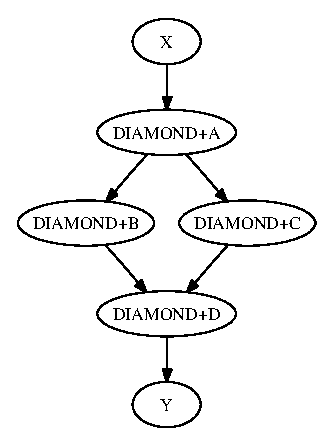
\includegraphics{user-man/splice-simple.eps}
\caption{\label{fig:dagman-splice-simple} The diamond-shaped DAG spliced between two nodes.}
\end{figure}

Figure~\ref{fig:dagman-splice-X} illustrates the starting point
for a more complex example.
The DAG input file \File{X.dag} describes this X-shaped DAG.
The completed example displays more of
the spatial constructs provided by splices.
Pay particular attention to the notion that each named splice creates a
new graph, even when the same DAG input file is specified.


\begin{verbatim}
  # BEGIN DAG FILE X.dag

  JOB A submit.condor
  VARS A jobname="$(JOB)"

  JOB B submit.condor
  VARS B jobname="$(JOB)"

  JOB C submit.condor
  VARS C jobname="$(JOB)"

  JOB D submit.condor
  VARS D jobname="$(JOB)"

  JOB E submit.condor
  VARS E jobname="$(JOB)"

  JOB F submit.condor
  VARS F jobname="$(JOB)"

  JOB G submit.condor
  VARS G jobname="$(JOB)"

  # Make an X-shaped dependency graph
  PARENT A B C CHILD D
  PARENT D CHILD E F G

  # END DAG FILE X.dag
\end{verbatim}

\begin{figure}
\centering
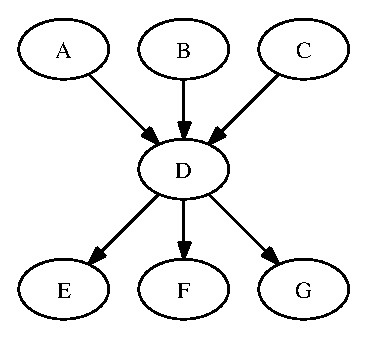
\includegraphics{user-man/splice-X.eps}
\caption{\label{fig:dagman-splice-X} The X-shaped DAG.}
\end{figure}


File \File{s1.dag} continues the example, presenting
the DAG input file that
incorporates two separate splices of the X-shaped DAG.
Figure~\ref{fig:dagman-splice-s1} illustrates the resulting DAG.

\begin{verbatim}
  # BEGIN DAG FILE s1.dag

  JOB A submit.condor
  VARS A jobname="$(JOB)"

  JOB B submit.condor
  VARS B jobname="$(JOB)"

  # name two individual splices of the X-shaped DAG
  SPLICE X1 X.dag
  SPLICE X2 X.dag

  # Define dependencies
  # A must complete before the initial nodes in X1 can start
  PARENT A CHILD X1
  # All final nodes in X1 must finish before 
  # the initial nodes in X2 can begin
  PARENT X1 CHILD X2
  # All final nodes in X2 must finish before B may begin.
  PARENT X2 CHILD B

  # END DAG FILE s1.dag
\end{verbatim}

\begin{figure}
\centering
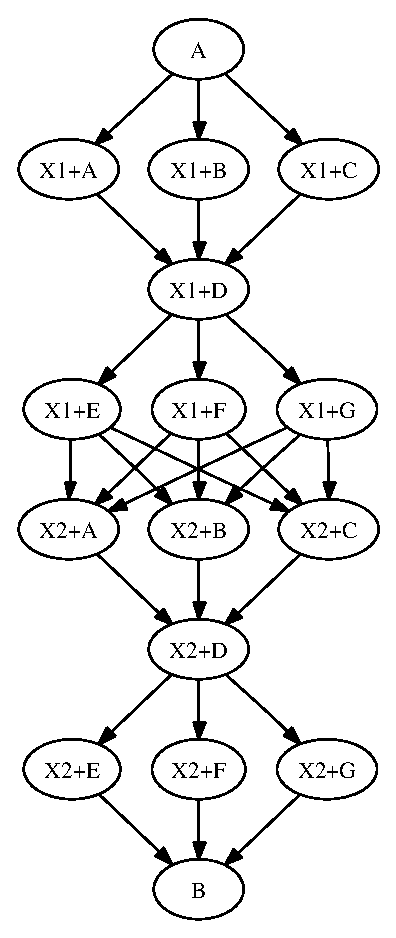
\includegraphics{user-man/splice-s1.eps}
\caption{\label{fig:dagman-splice-s1} The DAG described by \File{s1.dag}.}
\end{figure}

The top level DAG in the hierarchy of this complex example
is described by the DAG input file \File{toplevel.dag}.
Figure~\ref{fig:dagman-splice-complex} illustrates the final DAG.
Notice that the DAG has two disjoint graphs in it as a result of splice
S3 not having any dependencies associated with it in this top level DAG.

\begin{verbatim}
  # BEGIN DAG FILE toplevel.dag

  JOB A submit.condor
  VARS A jobname="$(JOB)"

  JOB B submit.condor
  VARS B jobname="$(JOB)"

  JOB C submit.condor
  VARS C jobname="$(JOB)"

  JOB D submit.condor
  VARS D jobname="$(JOB)"

  # a diamond-shaped DAG
  PARENT A CHILD B C
  PARENT B C CHILD D

  # This splice of the X-shaped DAG can only run after
  # the diamond dag finishes
  SPLICE S2 X.dag
  PARENT D CHILD S2

  # Since there are no dependencies for S3,
  # the following splice is disjoint 
  SPLICE S3 s1.dag

  # END DAG FILE toplevel.dag
\end{verbatim}


\begin{figure}
\centering
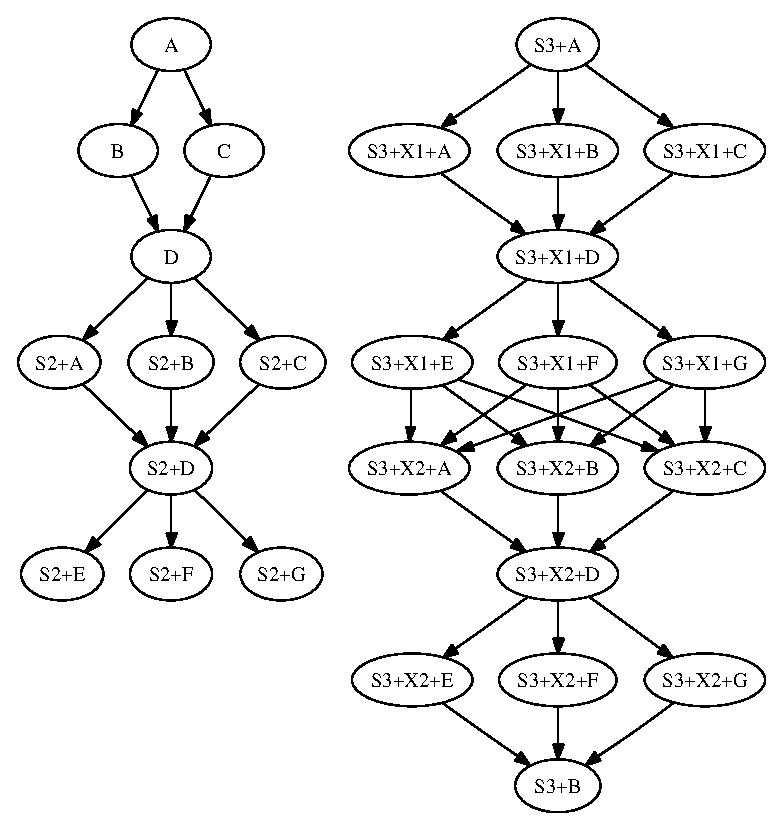
\includegraphics{user-man/splice-complex.eps}
\caption{\label{fig:dagman-splice-complex} The complex splice example DAG.}
\end{figure}

% Note: this is an alternative to subsubsubsection, which we don't have.
\begin{description}
\item[Splices and rescue DAGs]
\end{description}

Because the nodes of a splice are directly incorporated into the
DAG containing the SPLICE command, splices do not generate their
own rescue DAGs, unlike SUBDAG EXTERNALs.

% Note: this is an alternative to subsubsubsection, which we don't have.
\begin{description}
\item[The DIR option with splices]
\end{description}

The \Arg{DIR} option specifies a working directory for a splice,
from which the splice will be parsed and the jobs within the splice submitted.
The directory associated with the splice's \Arg{DIR} specification
will be propagated as a prefix to all nodes in the splice and any 
included splices.
If a node already has a \Arg{DIR} specification, then the splice's
\Arg{DIR} specification will be a prefix to the node's, separated by
a directory separator character.
Jobs in included splices with an absolute path for their \Arg{DIR}
specification will have their \Arg{DIR} specification untouched.
Note that a DAG containing \Arg{DIR} specifications cannot be run
in conjunction with the \Arg{-usedagdir} command-line argument to
\Condor{submit\_dag}.

A "full" rescue DAG generated by a DAG run with the \Arg{-usedagdir} argument
will contain DIR specifications, so such a rescue DAG must be run
\emph{without} the \Arg{-usedagdir} argument.  (Note that "full"
rescue DAGs are no longer the default.)


% Note: this is an alternative to subsubsubsection, which we don't have.
\begin{description}
\item[Limitation: splice DAGs must exist at submit time]
\end{description}
Unlike the DAG files referenced in a SUBDAG EXTERNAL command, DAG files
referenced in a SPLICE command must exist when the DAG containing the
SPLICE command is submitted.  (Note that, if a SPLICE is contained
within a sub-DAG, the splice DAG must exist at the time that the
sub-DAG is submitted, not when the top-most DAG is submitted, so the
splice DAG can be created by a part of the workflow that runs before
the relevant sub-DAG.)

% Note: this is an alternative to subsubsubsection, which we don't have.
\begin{description}
\item[Limitation: Splices and PRE or POST Scripts]
\end{description}

A PRE or POST script may not be specified for a splice (however, nodes
within a spliced DAG can have PRE and POST scripts).
(The reason for this is that, when the DAG is parsed, the splices
are also parsed and the splice nodes are directly incorporated into
the DAG containing the SPLICE command.  Therefore, once parsing is
complete, there are no actual nodes corresponding to the splice
itself to which to "attach" the PRE or POST scripts.)

To achieve the desired effect of having a PRE script associated with a splice,
introduce a new NOOP node into the DAG with the splice as a dependency.
Attach the PRE script to the NOOP node.
\footnotesize
\begin{verbatim}
  # BEGIN DAG FILE example1.dag

  # Names a node with no associated node job, a NOOP node
  # Note that the file noop.submit does not need to exist
  JOB OnlyPreNode noop.submit NOOP

  # Attach a PRE script to the NOOP node
  SCRIPT PRE OnlyPreNode prescript.sh

  # Define the splice
  SPLICE TheSplice thenode.dag
 
  # Define the dependency
  PARENT OnlyPreNode CHILD TheSplice

  # END DAG FILE example1.dag
\end{verbatim}
\normalsize

The same technique is used to achieve the effect of having a POST script
associated with a splice.
Introduce a new NOOP node into the DAG as a child of the splice, 
and attach the POST script to the NOOP node.

\footnotesize
\begin{verbatim}
  # BEGIN DAG FILE example2.dag

  # Names a node with no associated node job, a NOOP node
  # Note that the file noop.submit does not need to exist.
  JOB OnlyPostNode noop.submit NOOP

  # Attach a POST script to the NOOP node
  SCRIPT POST OnlyPostNode postscript.sh

  # Define the splice
  SPLICE TheSplice thenode.dag
 
  # Define the dependency
  PARENT TheSplice CHILD OnlyPostNode

  # END DAG FILE example2.dag
\end{verbatim}
\normalsize

% Note: this is an alternative to subsubsubsection, which we don't have.
\begin{description}
\item[Limitation: Splices and the RETRY of a Node, use of VARS, or use of PRIORITY]
\end{description}

A RETRY, VARS or PRIORITY command cannot be specified for a SPLICE;
however, individual nodes within a spliced DAG can have a RETRY, VARS
or PRIORITY specified.

Here is an example showing a DAG that will not be parsed successfully:
\begin{verbatim}
  # top level DAG input file
  JOB    A a.sub
  SPLICE B b.dag
  PARENT A  CHILD B

  # cannot work, as B is not a node in the DAG once
  # splice B is incorporated
  RETRY B 3
  VARS B dataset="10"
  PRIORITY B 20
\end{verbatim}

The following example \emph{will} work:
\begin{verbatim}
  # top level DAG input file
  JOB    A a.sub
  SPLICE B b.dag
  PARENT A  CHILD B

  # file: b.dag
  JOB    X x.sub
  RETRY X 3
  VARS X dataset="10"
  PRIORITY X 20
\end{verbatim}

When RETRY is desired on an entire subgraph of a workflow,
sub-DAGs (see above) must be used instead of splices.

Here is the same example, now defining job B as a SUBDAG,
and effecting RETRY on that SUBDAG.
\begin{verbatim}
  # top level DAG input file
  JOB    A a.sub
  SUBDAG EXTERNAL B b.dag
  PARENT A  CHILD B

  RETRY B 3
\end{verbatim}

% Note: this is an alternative to subsubsubsection, which we don't have.
\begin{description}
\item[Limitation: The Interaction of Categories and MAXJOBS with Splices]
\end{description}

Categories normally refer only to nodes within a
given splice.
All of the assignments of nodes to a category, and the
setting of the category throttle, should be done within a single DAG file.
However, it is now possible to have categories include nodes
from within more than one splice.
To do this, the category name is prefixed with the '+' (plus) character.
This tells DAGMan that the category is
a cross-splice category.
Towards deeper understanding,
what this really does is prevent renaming
of the category when the splice is incorporated into the upper-level DAG.
The MAXJOBS specification for the category can appear in either the
upper-level DAG file or one of the splice DAG files.
It probably
makes the most sense to put it in the upper-level DAG file.

Here is an example which applies a single limitation on submitted jobs,
identifying the category with \Expr{+init}. 

\begin{verbatim}
# relevant portion of file name: upper.dag

    SPLICE A splice1.dag
    SPLICE B splice2.dag

    MAXJOBS +init 2
\end{verbatim}

\begin{verbatim}
# relevant portion of file name: splice1.dag

    JOB C C.sub
    CATEGORY C +init
    JOB D D.sub
    CATEGORY D +init

\end{verbatim}

\begin{verbatim}
# relevant portion of file name: splice2.dag

    JOB X X.sub
    CATEGORY X +init
    JOB Y Y.sub
    CATEGORY Y +init

\end{verbatim}

For both global and non-global category throttles, settings at a higher
level in the DAG override settings at a lower level.
In this example:

\begin{verbatim}
# relevant portion of file name: upper.dag

    SPLICE A lower.dag

    MAXJOBS A+catX 10
    MAXJOBS +catY 2


# relevant portion of file name: lower.dag

    MAXJOBS catX 5
    MAXJOBS +catY 1

\end{verbatim}

the resulting throttle settings are 2 for the \Expr{+catY} category
and 10 for the \Expr{A+catX} category in splice.
Note that non-global category names are
prefixed with their splice name(s), so to refer to a non-global category 
at a higher level, the splice name must be included.

%%%%%%%%%%%%%%%%%%%%%%%%%%%%%%%%%%%%%%%
\subsubsection{\label{sec:DAGSpliceConnections}DAG Splice Connections}
\index{DAG input file!CONNECT command}
\index{DAG input file!PIN\_IN command}
\index{DAG input file!PIN\_OUT command}
\index{DAGMan!connecting DAG splices}

In the "default" usage of splices described above, when one splice is
the parent of another splice, all "terminal" nodes (nodes with no
children) of the parent splice become parents of all "initial" nodes
(nodes with no parents) of the child splice.  The CONNECT,
PIN\_IN, and PIN\_OUT commands (added in version 8.5.7) allow more
flexible dependencies between splices.  (The terms PIN\_IN and PIN\_OUT
were chosen because of the hardware analogy.)

The syntax for \Arg{CONNECT} is

\Opt{CONNECT} \Arg{OutputSpliceName} \Arg{InputSpliceName}

The syntax for \Arg{PIN\_IN} is

\Opt{PIN\_IN} \Arg{NodeName} \Arg{PinNumber}

The syntax for \Arg{PIN\_OUT} is

\Opt{PIN\_OUT} \Arg{NodeName} \Arg{PinNumber}

All output splice nodes connected to a given pin\_out will become
parents of all input splice nodes connected to the corresponding
pin\_in.  (The pin\_ins and pin\_outs exist only to create the
correct parent/child dependencies between nodes.  Once the
DAG is parsed, there are no actual DAG objects corresponding
to the pin\_ins and pin\_outs.)

Any given splice can contain both PIN\_IN and PIN\_OUT definitions,
and can be both an input and output splice in different CONNECT
commands.  Furthermore, a splice can appear in any number of
CONNECT commands (for example, a given splice could be the output
splice in two CONNECT commands that have different input splices).
It is \emph{not} an error for a splice to have PIN\_IN or PIN\_OUT
definitions that are not associated with a CONNECT command -- such
PIN\_IN and PIN\_OUT commands are simply ignored.

Note that the pin\_ins and pin\_outs must be defined \emph{within}
the relevant splices (this can be done with \Arg{INCLUDE} commands), not
in the DAG that connects the splices.


\Bold{There are a number of restrictions on splice connections:}
\begin{itemize}
\item Connections can be made only between two splices; "regular"
nodes or sub-DAGs cannot be used in a CONNECT command.
\item Pin\_ins and pin\_outs must be numbered consecutively starting
at 1.
\item The pin\_outs of the output splice in a connect command must
match the pin\_ins of the input splice in the command.
\item All "initial" nodes (nodes with no parents) of an input splice
used in a CONNECT command must be connected to a pin\_in.
\end{itemize}
Violating any of these restrictions will result in an error during
the parsing of the DAG files.

Note:  it is probably desireable for any "terminal" node (a
node with no children) in the output splice to be connected to
a pin\_out -- but this is not required.

\Bold{Here is a simple example:}
\begin{verbatim}
# File: top.dag
    SPLICE A spliceA.dag
    SPLICE B spliceB.dag
    SPLICE C spliceC.dag

    CONNECT A B
    CONNECT B C

# File: spliceA.dag
    JOB A1 A1.sub
    JOB A2 A2.sub

    PIN_OUT A1 1
    PIN_OUT A2 2

# File: spliceB.dag
    JOB B1 B1.sub
    JOB B2 B2.sub
    JOB B3 B3.sub
    JOB B4 B4.sub

    PIN_IN B1 1
    PIN_IN B2 1
    PIN_IN B3 2
    PIN_IN B4 2

    PIN_OUT B1 1
    PIN_OUT B2 2
    PIN_OUT B3 3
    PIN_OUT B4 4

# File: spliceC.dag
    JOB C1 C1.sub

    PIN_IN C1 1 
    PIN_IN C1 2 
    PIN_IN C1 3
    PIN_IN C1 4

\end{verbatim}
In this example, node A1 will be the parent of B1 and B2; node
A2 will be the parent of B3 and B4; and nodes B1, B2, B3 and B4 will all
be parents of C1.

A diagram of the above example:

\begin{figure}[hbt]
\centering
\includegraphics{user-man/dagman-connect.eps}
\caption{\label{fig:dagman-connect}Diagram of the splice connect example}
\end{figure}

%%%%%%%%%%%%%%%%%%%%%%%%%%%%%%%%%%%%%%%
\subsubsection{\label{sec:DAGFinalNode}FINAL node}
\index{DAG input file!FINAL command}
\index{DAGMan!FINAL node}

A FINAL node is a single and special node that is always run at 
the end of the DAG,
even if previous nodes in the DAG have failed.  
A FINAL node can be used
for tasks such as cleaning up intermediate files and checking the output
of previous nodes.
The \Arg{FINAL} command in the DAG input file specifies 
a node job to be run at the end of the DAG.  

The syntax used for the \Arg{FINAL} command is

\Opt{FINAL} \Arg{JobName} \Arg{SubmitDescriptionFileName}
\oOptArg{DIR}{directory} \oOpt{NOOP}

The FINAL node within the DAG is identified by \Arg{JobName}, 
and the HTCondor job
is described by the contents of the HTCondor submit description file
given by \Arg{SubmitDescriptionFileName}.

The keywords \Arg{DIR} and \Arg{NOOP} 
are as detailed in section~\ref{dagman:JOB}.
If both \Arg{DIR} and \Arg{NOOP} are used, 
they must appear in the order shown within the syntax specification.

There may only be one FINAL node in a DAG.
A parse error will be logged by the \Condor{dagman} job in the
\File{dagman.out} file,
if more than one FINAL node is specified.

The FINAL node is virtually always run.
It is run if the \Condor{dagman} job is removed with \Condor{rm}.
The only case in which a FINAL node is not run
is if the configuration variable \Macro{DAGMAN\_STARTUP\_CYCLE\_DETECT} 
is set to \Expr{True},
and a cycle is detected at start up time.
If \Macro{DAGMAN\_STARTUP\_CYCLE\_DETECT} is set to \Expr{False} and
a cycle is detected during the course of the run, 
the FINAL node \emph{will} be run.

The success or failure of the FINAL node 
determines the success or failure of the entire DAG,
overriding the status of all previous nodes.
This includes any status specified by any ABORT-DAG-ON specification
that has taken effect.
If some nodes of a DAG fail,
but the FINAL node succeeds, the DAG will be considered successful.
Therefore, it is important
to be careful about setting the exit status of the FINAL node.

The \Env{\$DAG\_STATUS} and \Env{\$FAILED\_COUNT} macros can be used both
as PRE and POST script arguments, and in node job submit description files.
As an example of this, here are the partial contents of the DAG input file,
\begin{verbatim}
    FINAL final_node final_node.sub
    SCRIPT PRE final_node final_pre.pl $DAG_STATUS $FAILED_COUNT
\end{verbatim}

and here are the partial contents of the submit description file, 
\File{final\_node.sub}
\begin{verbatim}
    arguments = "$(DAG_STATUS) $(FAILED_COUNT)"
\end{verbatim}

If there is a FINAL node specified for a DAG, 
it will be run at the end of the workflow.
If this FINAL node must not do anything in certain cases, 
use the \Env{\$DAG\_STATUS} and \Env{\$FAILED\_COUNT}
macros to take appropriate actions.  
Here is an example of that behavior.
It uses a PRE script that aborts if the DAG has been removed with \Condor{rm},
which, in turn,
causes the FINAL node to be considered failed without actually submitting the
HTCondor job specified for the node.
Partial contents of the DAG input file:
\begin{verbatim}
    FINAL final_node final_node.sub
    SCRIPT PRE final_node final_pre.pl $DAG_STATUS
\end{verbatim}

and partial contents of the Perl PRE script, \File{final\_pre.pl}:
\begin{verbatim}
    #! /usr/bin/env perl
    
    if ($ARGV[0] eq 4) {
        exit(1);
    }
   
\end{verbatim}


There are restrictions on the use of a FINAL node.
The DONE option is \emph{not} allowed for a FINAL node.
And, a FINAL node may not be referenced in any of the following
specifications:
\begin{itemize}
\item PARENT, CHILD
\item RETRY
\item ABORT-DAG-ON
\item PRIORITY
\item CATEGORY
\end{itemize}

As of HTCondor version 8.3.7, DAGMan allows at most two submit attempts
of a FINAL node,
if the DAG has been removed from the queue with \Condor{rm}.

%%%%%%%%%%%%%%%%%%%%%%%%%%%%%%%%%%%%%%%
\subsubsection{\label{sec:DAGAllNodes}The ALL\_NODES option}
\index{DAG input file!ALL\_NODES option}

In the following commands, a specific node name can be replaced by
the option \Arg{ALL\_NODES}:
\begin{itemize}
\item \Opt{SCRIPT}
\item \Opt{PRE\_SKIP}
\item \Opt{RETRY}
\item \Opt{ABORT-DAG-ON}
\item \Opt{VARS}
\item \Opt{PRIORITY}
\item \Opt{CATEGORY}
\end{itemize}

This will cause the given command to apply to all nodes (except any
FINAL node) in that DAG.

The ALL\_NODES \emph{never} applies to a FINAL node.  (If the
\Arg{ALL\_NODES} option is used in a DAG that has a FINAL node, the
\File{dagman.out} file will contain messages noting that the FINAL
node is skipped when parsing the relevant commands.)

The \Arg{ALL\_NODES} option is case-insensitive.

It is important to note that the \Arg{ALL\_NODES} option does \emph{not}
apply across splices and sub-DAGs.  In other words, an \Arg{ALL\_NODES}
option within a splice or sub-DAG will apply only to nodes within
that splice or sub-DAG; also, an \Arg{ALL\_NODES} option in a parent
DAG will not apply to any splices or sub-DAGs referenced by the
parent DAG.

The \Arg{ALL\_NODES} option \emph{does} work in combination with the
\Arg{INCLUDE} command.  In other words, a command within an included
file that uses the \Arg{ALL\_NODES} option will apply to all nodes
in the including DAG (again, except any FINAL node).

As of version 8.5.8, the \Arg{ALL\_NODES} option cannot be used when
multiple DAG files are specified on the \Condor{submit\_dag} command
line.  Hopefully this limitation will be fixed in a future release.

When multiple commands (whether using the \Arg{ALL\_NODES} option or not)
set a given property of a DAG node, the last relevant command overrides
earlier commands, as shown in the following examples:

For example, in this DAG:
\begin{verbatim}
    JOB A node.sub
    VARS A name="A"
    VARS ALL_NODES name="X"
\end{verbatim}
the value of \Arg{name} for node A will be "X".

In this DAG:
\begin{verbatim}
    JOB A node.sub
    VARS A name="A"
    VARS ALL_NODES name="X"
    VARS A name="foo"
\end{verbatim}
the value of \Arg{name} for node A will be "foo".

Here is an example DAG using the \Arg{ALL\_NODES} option:
\begin{verbatim}
# File: all_ex.dag
    JOB A node.sub
    JOB B node.sub
    JOB C node.sub

    SCRIPT PRE ALL_NODES my_script $JOB

    VARS ALL_NODES name="$(JOB)"

    # This overrides the above VARS command for node B.
    VARS B name="nodeB"

    RETRY all_nodes 3
\end{verbatim}

%%%%%%%%%%%%%%%%%%%%%%%%%%%%%%%%%%%%%%%
\subsection{\label{sec:DAGMan-rescue}The Rescue DAG}
%%%%%%%%%%%%%%%%%%%%%%%%%%%%%%%%%%%%%%%
\index{DAGMan!rescue DAG}

Any time a DAG exits unsuccessfully, DAGMan generates a Rescue DAG.  
The Rescue DAG records the state of the DAG, 
with information such as which nodes completed successfully,
and the Rescue DAG will be used when the DAG is again submitted.
With the Rescue DAG,
nodes that have already successfully completed are not re-run.

There are a variety of circumstances under which a Rescue DAG
is generated.
If a node in the DAG fails, the DAG does not exit immediately;
the remainder of the DAG is continued until no more forward
progress can be made based on the DAG's dependencies.
At this point, DAGMan produces the Rescue DAG and exits.
A Rescue DAG is produced on Unix platforms if the
\Condor{dagman} job itself is removed with \Condor{rm}.
On Windows, a Rescue DAG is \emph{not} generated in this situation,
but re-submitting the original DAG will invoke a lower-level 
recovery functionality,
and it will produce similar behavior to using a Rescue DAG.
A Rescue DAG is produced when a node sets and triggers
an \Arg{ABORT-DAG-ON} event with a non-zero return value.
A zero return value constitutes successful DAG completion, 
and therefore a Rescue DAG is not generated.

By default, if a Rescue DAG exists, it will be used when the DAG
is submitted specifying the original DAG input file.  
If more than one Rescue DAG exists, 
the newest one will be used.  
By using the Rescue DAG,
DAGMan will avoid re-running nodes that completed successfully
in the previous run.
\Bold{Note that passing the \Arg{-force} option to \Condor{submit\_dag}
or \Condor{dagman} will cause \Condor{dagman} to not use any existing
rescue DAG.  This means that previously-completed node jobs will be
re-run.}

The granularity defining success or failure
in the Rescue DAG is the node.
For a node that fails,
all parts of the node will be re-run,
even if some parts were successful the first time.
For example, if a node's PRE script
succeeds, but then the node's HTCondor job cluster fails,
the entire node, including the PRE script, will be re-run.
A job cluster may result in the submission of multiple HTCondor jobs.
If one of the jobs within the cluster fails, the node fails.
Therefore, the Rescue DAG will re-run the entire node,
implying the submission of the entire cluster of jobs,
not just the one(s) that failed.

Statistics about the failed DAG execution are presented as
comments at the beginning of the Rescue DAG input file.

%%%%%%%%%%%%%%%%%%%%%%%%%%%
\label{dagman:rescue_dag_naming}
\begin{description}
\item[Rescue DAG Naming]
\end{description}

The file name of the Rescue DAG is obtained by
appending the string
\verb@.rescue<XXX>@ to the original DAG input file name.
Values for \verb@<XXX>@ start at \verb@001@ and continue
to \verb@002@, \verb@003@, and beyond.
The configuration variable \Macro{DAGMAN\_MAX\_RESCUE\_NUM}
sets a maximum value for \verb@<XXX>@;
see section~\ref{param:DAGManMaxRescueNum} for the complete definition
of this configuration variable.  If you hit the
\Macro{DAGMAN\_MAX\_RESCUE\_NUM} limit, the last Rescue DAG file
is overwritten if the DAG fails again.

If a Rescue DAG exists when the original DAG is re-submitted,
the Rescue DAG with the largest magnitude value for \verb@<XXX>@
will be used, and its usage is implied.

%%%%%%%%%%%%%%%%%%%%%%%%%%%
\label{dagman:rescue_dag_example}
\begin{description}
\item[Example]
\end{description}

Here is an example showing file naming and DAG submission
for the case of a failed DAG.
The initial DAG is submitted with
\begin{verbatim}
  condor_submit_dag  my.dag
\end{verbatim}
A failure of this DAG results in the Rescue DAG
named \File{my.dag.rescue001}.
The DAG is resubmitted using the same command: 
\begin{verbatim}
  condor_submit_dag  my.dag
\end{verbatim}
This resubmission of the DAG uses the Rescue DAG file \File{my.dag.rescue001},
because it exists.
Failure of this Rescue DAG results in another Rescue DAG
called \File{my.dag.rescue002}.
If the DAG is again submitted, using the same command
as with the first two submissions, but not repeated here,
then this third submission uses the Rescue DAG file \File{my.dag.rescue002},
because it exists, and because the value \verb@002@ is larger
in magnitude than \verb@001@.

%%%%%%%%%%%%%%%%%%%%%%%%%%%
\label{dagman:rescue_dag_backtracking}
\begin{description}
\item[Backtracking to an Older Rescue DAG]
\end{description}

To explicitly specify a particular Rescue DAG,
use the optional command-line argument \Arg{-dorescuefrom}
with \Condor{submit\_dag}.
Note that this will have the side effect of renaming 
existing Rescue DAG files with larger magnitude values 
of \verb@<XXX>@.
Each renamed file has its existing name appended with
the string \File{.old}.
For example, assume that \File{my.dag} has failed 4 times,
resulting in the Rescue DAGs named
\File{my.dag.rescue001},
\File{my.dag.rescue002},
\File{my.dag.rescue003},
and
\File{my.dag.rescue004}.
A decision is made to re-run using \File{my.dag.rescue002}.
The submit command is
\begin{verbatim}
  condor_submit_dag  -dorescuefrom 2  my.dag
\end{verbatim}
The DAG specified by the DAG input file \File{my.dag.rescue002}
is submitted.
And, the existing Rescue DAG \File{my.dag.rescue003} is
renamed to be \File{my.dag.rescue003.old},
while the existing Rescue DAG \File{my.dag.rescue004} is
renamed to be \File{my.dag.rescue004.old}.

%%%%%%%%%%%%%%%%%%%%%%%%%%%
\label{dagman:rescue_special_cases}
\begin{description}
\item[Special Cases]
\end{description}

Note that if multiple DAG input files are specified on the
\Condor{submit\_dag} command line,
a single Rescue DAG encompassing all of the input DAGs is generated.
A DAG file containing splices also produces a single Rescue DAG file.
On the other hand, a DAG containing sub-DAGs will produce a
separate Rescue DAG for each sub-DAG that is queued (and for the
top-level DAG).

If the Rescue DAG file is generated before all retries
of a node are completed, 
then the Rescue DAG file will also contain \Arg{Retry} entries.
The number of retries will be set to the appropriate remaining
number of retries.
The configuration variable \Macro{DAGMAN\_RESET\_RETRIES\_UPON\_RESCUE}, 
section~\ref{param:DAGManResetRetriesUponRescue},
controls whether or not node retries are reset in a Rescue DAG.


%%%%%%%%%%%%%%%%%%%%%%%%%%%
\label{dagman:partial_full_rescue_dag}
\begin{description}
\item[Partial versus Full Rescue DAGs]
\end{description}

As of HTCondor version 7.7.2, the Rescue DAG file is a partial DAG file,
not a complete DAG input file as in the past.

A partial Rescue DAG file contains only information about which nodes are done,
and the number of retries remaining for nodes with retries.  
It does not contain information such as the actual
DAG structure and the specification of the submit description file 
for each node job.  
Partial Rescue DAGs are automatically parsed in combination with
the original DAG input file, 
which contains information about the DAG structure.  
This updated implementation means that a change in the original DAG input file,
such as specifying a different submit description file for a node job,
will take effect when running the partial Rescue DAG.
In other words, you can fix mistakes in the original DAG file while
still gaining the benefit of using the Rescue DAG.

To use a partial Rescue DAG, you \emph{must} re-run \Condor{submit\_dag}
on the original DAG file, not the Rescue DAG file.

Note that the existence of a DONE specification in a partial Rescue DAG for
a node that no longer exists in the original DAG input file
is a warning, as opposed to an error, 
unless the \Macro{DAGMAN\_USE\_STRICT} configuration
variable is set to a value of 1 or higher (which is now the default).  
Comment out the line with \Arg{DONE} in the partial Rescue DAG file
to avoid a warning or error.

The previous (prior to version 7.7.2) behavior of producing full DAG input file 
as the Rescue DAG 
is obtained by setting the configuration variable
\Macro{DAGMAN\_WRITE\_PARTIAL\_RESCUE} to the non-default 
value of \Expr{False}.  
\Bold{Note that the option to generate full Rescue DAGs is likely to
disappear some time during the 8.3 series.}

To run a full Rescue DAG,
either one left over from an older version of DAGMan, 
or one produced by setting \Macro{DAGMAN\_WRITE\_PARTIAL\_RESCUE} 
to \Expr{False}, 
directly specify the full Rescue DAG file on the command line
instead of the original DAG file.
For example:

\begin{verbatim}
  condor_submit_dag my.dag.rescue002
\end{verbatim}

Attempting to re-submit the original DAG file, if the Rescue DAG file
is a complete DAG, will result in a parse failure.


%%%%%%%%%%%%%%%%%%%%%%%%%%%
\label{dagman:rescue_parse_error}
\begin{description}
\item[Rescue DAG Generated When There Are Parse Errors]
\end{description}

Starting in HTCondor version 7.5.5, passing
the \Opt{-DumpRescue} option to either \Condor{dagman} or \Condor{submit\_dag}
causes \Condor{dagman} to output a Rescue DAG file, 
even if the parsing of a DAG input file fails.
In this parse failure case, \Condor{dagman} produces a specially 
named Rescue DAG containing whatever it had successfully parsed up
until the point of the parse error.
This Rescue DAG may be useful in debugging parse errors in complex DAGs,
especially ones using splices.
This incomplete Rescue DAG is not meant to be used when resubmitting
a failed DAG.  
Note that this incomplete Rescue DAG generated by the \Opt{-DumpRescue}
option is a full DAG input file, 
as produced by versions of HTCondor prior to HTCondor version 7.7.2.
It is not a partial Rescue DAG file,
regardless of the value of the configuration variable
\Macro{DAGMAN\_WRITE\_PARTIAL\_RESCUE}.

To avoid confusion between this incomplete Rescue DAG
generated in the case of a parse failure and a usable Rescue DAG,
a different name is given to the incomplete Rescue DAG.
The name appends the string \File{.parse\_failed} to the original
DAG input file name.
Therefore, if the submission of a DAG with
\begin{verbatim}
  condor_submit_dag  my.dag
\end{verbatim}
has a parse failure, the resulting incomplete Rescue DAG will be
named \File{my.dag.parse\_failed}.

To further prevent one of these incomplete Rescue DAG files from being used,
a line within the file contains the single command \Arg{REJECT}.
This causes \Condor{dagman} to reject the DAG, if used as a DAG input file.
This is done because the
incomplete Rescue DAG may be a syntactically correct DAG input file.
It will be incomplete relative to the original DAG,
such that if the incomplete Rescue DAG could be run,
it could erroneously be perceived as
having successfully executed the desired workflow, when, in fact,
it did not.

%%%%%%%%%%%%%%%%%%%%%%%%%%%%%%%%%%%%%%%
\subsection{\label{sec:DAGMan-recovery}DAG Recovery}
%%%%%%%%%%%%%%%%%%%%%%%%%%%%%%%%%%%%%%%
\index{DAGMan!DAG recovery}
\index{DAGMan!difference between Rescue DAG and DAG recovery}

DAG recovery restores the state of a DAG upon resubmission.
Recovery is accomplished by reading the \File{.nodes.log}
file that is used to enforce the dependencies of the DAG.
The DAG can then continue towards completion.

Recovery is different than a Rescue DAG.
Recovery is appropriate when no Rescue DAG has been created.
There will be no Rescue DAG 
if the machine running the \Condor{dagman} job crashes,
or if the \Condor{schedd} daemon crashes,
or if the \Condor{dagman} job crashes,
or if the \Condor{dagman} job is placed on hold.

Much of the time, when a not-completed DAG is re-submitted,
it will automatically be placed into recovery mode
due to the existence and contents of a lock file created as the DAG
is first run.
In recovery mode, the \File{.nodes.log} is used to identify
nodes that have completed and should not be re-submitted.

DAGMan can be told to work in recovery mode by including the
\Opt{-DoRecovery} option on the command line, as in the example
\begin{verbatim}
    condor_submit_dag diamond.dag -DoRecovery
\end{verbatim}
where \File{diamond.dag} is the name of the DAG input file.

When debugging a DAG in which something has gone wrong,
a first determination is whether a resubmission will
use a Rescue DAG or benefit from recovery.
The existence of a Rescue DAG means that recovery would be inappropriate.
A Rescue DAG is has a file name ending in \File{.rescue<XXX>},
where \Expr{<XXX>} is replaced by a 3-digit number.

Determine if a DAG ever completed 
(independent of whether it was successful or not) 
by looking at the last lines of the \File{.dagman.out} file.
If there is a line similar to
\begin{verbatim}
  (condor_DAGMAN) pid 445 EXITING WITH STATUS 0
\end{verbatim}
then the DAG completed.
This line explains that the \Condor{dagman} job finished normally.
If there is no line similar to this at the end of the \File{.dagman.out} file,
and output from \Condor{q} shows that the \Condor{dagman} job for
the DAG being debugged is not in the queue,
then recovery is indicated.

%%%%%%%%%%%%%%%%%%%%%%%%%%%%%%%%%%%%%%%
\subsection{Visualizing DAGs with \Prog{dot}}
%%%%%%%%%%%%%%%%%%%%%%%%%%%%%%%%%%%%%%%
\index{DAG input file!DOT command}
\index{DAGMan!visualizing DAGs}

It can be helpful to see a picture of a DAG.
DAGMan can assist you in visualizing a DAG by creating
the input files used by the AT\&T Research Labs 
\Prog{graphviz} package. 
\Prog{dot} is a program within this package,
available from \URL{http://www.graphviz.org/},
and it is used to draw pictures of DAGs. 

DAGMan produces one or more dot files as the result of
an extra line
in a DAG input file. 
The line appears as
%For example, to produce a single dot
%file that shows the state of your DAG before any jobs are running, add
%the following line:
\begin{verbatim}
    DOT dag.dot
\end{verbatim}

This creates a file called \File{dag.dot}.
which contains
a specification of the DAG before any jobs within the DAG
are submitted to HTCondor.
The \File{dag.dot} file is used to create a visualization
of the DAG by using this file as input to \Prog{dot}.
This example creates a Postscript file, with a visualization of the DAG:

\begin{verbatim}
    dot -Tps dag.dot -o dag.ps
\end{verbatim}

Within the DAG input file,
the DOT command can take several optional parameters:

\begin{itemize}

\item \Opt{UPDATE}  This will update the dot file every time a
significant update happens. 

\item \Opt{DONT-UPDATE} Creates a single dot file, when
the DAGMan begins executing. This is the default if the parameter
\Opt{UPDATE} is not used.

\item \Opt{OVERWRITE} Overwrites the dot file each time it
is created. This is the default, unless \Opt{DONT-OVERWRITE}
is specified.

\item \Opt{DONT-OVERWRITE} Used to create multiple dot files, instead
of overwriting the single one specified.
To create file names,
DAGMan uses the name of the file concatenated with a period and an
integer. For example, the DAG input file line
\begin{verbatim}
    DOT dag.dot DONT-OVERWRITE
\end{verbatim}
causes files
\File{dag.dot.0},
\File{dag.dot.1},
\File{dag.dot.2},
etc. to be created.
This option is
most useful when combined with the \Opt{UPDATE} option to
visualize the history of the DAG after it has finished executing. 

\item \OptArg{INCLUDE}{path-to-filename} Includes the contents
of a file given by \File{path-to-filename} in the file produced by the
\Opt{DOT} command.
The include file contents are always placed after the line of
the form
\verb@label=@.
This may be useful if further editing of the created files would
be necessary,
perhaps because you are automatically visualizing the DAG as it
progresses. 

\end{itemize}

If conflicting parameters are used in a DOT command, the last one
listed is used.

%%%%%%%%%%%%%%%%%%%%%%%%%%%%%%%%%%%%%%%
\subsection{\label{sec:DAG-node-status}Capturing the Status of Nodes in a File}
%%%%%%%%%%%%%%%%%%%%%%%%%%%%%%%%%%%%%%%
\index{DAG input file!NODE\_STATUS\_FILE command}
\index{DAGMan!node status file}
\index{status!of DAG nodes}

DAGMan can capture the status of the overall DAG and all DAG nodes
in a \emph{node status file},
such that the user or a script can monitor this status.
This file is periodically rewritten
while the DAG runs.
To enable this feature, the DAG input file must contain a line with the
\Arg{NODE\_STATUS\_FILE} command.

The syntax for a \Arg{NODE\_STATUS\_FILE} command is

\Opt{NODE\_STATUS\_FILE} \Arg{statusFileName} \oArg{minimumUpdateTime}
\oOpt{ALWAYS-UPDATE}

The status file is written on the machine on which the DAG is submitted;
its location is given by \Arg{statusFileName},
and it may be a full path and file name.

The optional \Arg{minimumUpdateTime} specifies the minimum number of seconds
that must elapse between updates to the node status file.
This setting exists to avoid having DAGMan spend too much time writing
the node status file for very large DAGs.
If no value is specified, this value defaults to 60 seconds (as
of version 8.5.8; previously, it defaulted to 0).
The node status file can be updated at most once
per \Macro{DAGMAN\_USER\_LOG\_SCAN\_INTERVAL},
as defined at section~\ref{param:DAGManUserLogScanInterval},
no matter how small the \Arg{minimumUpdateTime} value.
Also, the node status file will be updated when the DAG finishes,
whether successfully or not, even if \Arg{minimumUpdateTime} seconds
have not elapsed since the last update.

Normally, the node status file is only updated if the status of
some nodes has changed since the last time the file was written.
However, the optional \Arg{ALWAYS-UPDATE} keyword specifies that the
node status file should be updated every time the minimum update
time (and \Macro{DAGMAN\_USER\_LOG\_SCAN\_INTERVAL}),
has passed, even if no nodes have changed status since the last
time the file was updated.
(The file will change slightly,
because timestamps will be updated.)
For performance reasons,
large DAGs with approximately 10,000 or more nodes
are poor candidates for using the \Arg{ALWAYS-UPDATE} option.

As an example, if the DAG input file contains the line
\begin{verbatim}
  NODE_STATUS_FILE my.dag.status 30
\end{verbatim}
the file \File{my.dag.status} will be rewritten at intervals of 30 seconds
or more.

This node status file is overwritten each time it is updated.
Therefore, it only holds information about the \emph{current} status 
of each node; it does not provide a history of the node status.

\Note HTCondor version 8.1.6 changes the format of the node status
file.

The node status file is a collection of ClassAds in New ClassAd format.
There is one ClassAd for the overall status of the DAG, one ClassAd
for the status of each node, and one ClassAd with the time at which
the node status file was completed as well as the time of the next update.

Here is an example portion of a node status file:

\begin{verbatim}
[
  Type = "DagStatus";
  DagFiles = {
    "job_dagman_node_status.dag"
  };
  Timestamp = 1399674138; /* "Fri May  9 17:22:18 2014" */
  DagStatus = 3; /* "STATUS_SUBMITTED ()" */
  NodesTotal = 12;
  NodesDone = 11;
  NodesPre = 0;
  NodesQueued = 1;
  NodesPost = 0;
  NodesReady = 0;
  NodesUnready = 0;
  NodesFailed = 0;
  JobProcsHeld = 0;
  JobProcsIdle = 1;
]
[
  Type = "NodeStatus";
  Node = "A";
  NodeStatus = 5; /* "STATUS_DONE" */
  StatusDetails = "";
  RetryCount = 0;
  JobProcsQueued = 0;
  JobProcsHeld = 0;
]
...
[
  Type = "NodeStatus";
  Node = "C";
  NodeStatus = 3; /* "STATUS_SUBMITTED" */
  StatusDetails = "idle";
  RetryCount = 0;
  JobProcsQueued = 1;
  JobProcsHeld = 0;
]
[
  Type = "StatusEnd";
  EndTime = 1399674138; /* "Fri May  9 17:22:18 2014" */
  NextUpdate = 1399674141; /* "Fri May  9 17:22:21 2014" */
]
\end{verbatim}

Possible \Attr{DagStatus} and \Attr{NodeStatus} attribute values are:

\begin{itemize}
\item 0 (\verb@STATUS_NOT_READY@): At least one parent has not yet finished
or the node is a FINAL node.
\item 1 (\verb@STATUS_READY@): All parents have finished, but the node is not
yet running.
\item 2 (\verb@STATUS_PRERUN@): The node's PRE script is running.
\item 3 (\verb@STATUS_SUBMITTED@): The node's HTCondor job(s) are in 
  the queue.
\item 4 (\verb@STATUS_POSTRUN@): The node's POST script is running.
\item 5 (\verb@STATUS_DONE@): The node has completed successfully.
\item 6 (\verb@STATUS_ERROR@): The node has failed.
\end{itemize}

A \Arg{NODE\_STATUS\_FILE} command inside any splice is ignored.
If multiple DAG files are specified on the \Condor{submit\_dag} command line,
and more than one specifies a node status file,
the first specification takes precedence.

%%%%%%%%%%%%%%%%%%%%%%%%%%%%%%%%%%%%%%%
\subsection{\label{sec:DAGJobstateLog}A Machine-Readable Event History, the jobstate.log File}
%%%%%%%%%%%%%%%%%%%%%%%%%%%%%%%%%%%%%%%
\index{DAG input file!JOBSTATE\_LOG command}
\index{DAGMan!jobstate.log file}
\index{DAGMan!machine-readable event history}

DAGMan can produce a machine-readable history of events.
The \File{jobstate.log} file is designed for use by the Pegasus Workflow
Management System, which operates as a layer on top of DAGMan.  Pegasus
uses the \File{jobstate.log} file to monitor the state of a workflow.
The \File{jobstate.log} file can used by any
automated tool for the monitoring of workflows.

DAGMan produces this file when the command \Arg{JOBSTATE\_LOG} is
in the DAG input file.
The syntax for \Arg{JOBSTATE\_LOG} is

\Opt{JOBSTATE\_LOG} \Arg{JobstateLogFileName}

No more than one \File{jobstate.log} file can be created by a single
instance of \Condor{dagman}.
If more than one \File{jobstate.log} file is specified,
the first file name specified will take effect,
and a warning will be printed in the \File{dagman.out} file
when subsequent \Arg{JOBSTATE\_LOG} specifications are parsed.
Multiple specifications may exist in the same DAG file, within splices,
or within multiple, independent DAGs run with a single \Condor{dagman} instance.

The \File{jobstate.log} file can be considered a filtered
version of the \File{dagman.out} file, in a machine-readable format.
It contains the actual node job events that from \Condor{dagman},
plus some additional meta-events.

The \File{jobstate.log} file is different from the node status file,
in that the \File{jobstate.log} file is appended to,
rather than being overwritten as the DAG runs.
Therefore, it contains a history of the DAG,
rather than a snapshot of the current state of the DAG.

There are 5 line types in the \File{jobstate.log} file.
Each line begins with a Unix timestamp in the form of seconds since the Epoch.
Fields within each line are separated by a single space character.
\begin{description}

\item [DAGMan start] 
This line identifies the \Condor{dagman} job.
The formatting of the line is

\Arg{timestamp} INTERNAL *** DAGMAN\_STARTED \Arg{dagmanCondorID} ***

The \Arg{dagmanCondorID} field is the \Condor{dagman} job's 
\Attr{ClusterId} attribute, a period, and the \Attr{ProcId} attribute. 

\item [DAGMan exit] 
This line identifies the completion of the \Condor{dagman} job.
The formatting of the line is

\Arg{timestamp} INTERNAL *** DAGMAN\_FINISHED \Arg{exitCode} ***

The \Arg{exitCode} field is value the \Condor{dagman} job returns upon exit. 

\item [Recovery started] 
If the \Condor{dagman} job goes into recovery mode,
this meta-event is printed.
During recovery mode, events will only be printed in the file
if they were not already printed before recovery mode started.
The formatting of the line is

\Arg{timestamp} INTERNAL *** RECOVERY\_STARTED ***

\item [Recovery finished or Recovery failure] 
At the end of recovery
mode, either a RECOVERY\_FINISHED or RECOVERY\_FAILURE meta-event will be
printed, as appropriate.

The formatting of the line is

\Arg{timestamp} INTERNAL *** RECOVERY\_FINISHED ***

or

\Arg{timestamp} INTERNAL *** RECOVERY\_FAILURE ***

\item [Normal]
This line is used for all other event and meta-event types.
The formatting of the line is

\Arg{timestamp} \Arg{JobName} \Arg{eventName} \Arg{condorID} \Arg{jobTag} - \Arg{sequenceNumber}

The \Arg{JobName} is the name given to the node job as defined in
the DAG input file with the command \Arg{JOB}.
It identifies the node within the DAG.

The \Arg{eventName} is one of the many defined event or meta-events given
in the lists below.

The \Arg{condorID} field is the job's 
\Attr{ClusterId} attribute, a period, and the \Attr{ProcId} attribute. 
There is no \Arg{condorID} assigned yet for some meta-events,
such as PRE\_SCRIPT\_STARTED.
For these, the dash character ('-') is printed. 

The \Arg{jobTag} field is defined for the Pegasus workflow manager.
Its usage is generalized to be useful to other workflow managers.
Pegasus-managed jobs add a line of the following form to their
HTCondor submit description file:
\begin{verbatim}
+pegasus_site = "local"
\end{verbatim}
This defines the string \Expr{local} as the \Arg{jobTag} field.
 
Generalized usage adds a set of 2 commands to the HTCondor
submit description file to define a string as the \Arg{jobTag} field:
\begin{verbatim}
+job_tag_name = "+job_tag_value"
+job_tag_value = "viz"
\end{verbatim}
This defines the string \Expr{viz} as the \Arg{jobTag} field.
Without any of these added lines within the HTCondor submit description file,
the dash character ('-') is printed for the \Arg{jobTag} field. 

The \Arg{sequenceNumber} is a monotonically-increasing number 
that starts at one.
It is associated with each attempt at running a node.
If a node is retried, it gets a new sequence number;
a submit failure does not result in a new sequence number.
When a Rescue DAG is run,
the sequence numbers pick up from where they left off within the previous
attempt at running the DAG.
Note that this only applies if the Rescue
DAG is run automatically or with the \Arg{-dorescuefrom} command-line option.

\end{description}

Here is an example of a very simple Pegasus \File{jobstate.log} file,
assuming the example \Arg{jobTag} field of \Expr{local}:

\begin{verbatim}
1292620511 INTERNAL *** DAGMAN_STARTED 4972.0 ***
1292620523 NodeA PRE_SCRIPT_STARTED - local - 1
1292620523 NodeA PRE_SCRIPT_SUCCESS - local - 1
1292620525 NodeA SUBMIT 4973.0 local - 1
1292620525 NodeA EXECUTE 4973.0 local - 1
1292620526 NodeA JOB_TERMINATED 4973.0 local - 1
1292620526 NodeA JOB_SUCCESS 0 local - 1
1292620526 NodeA POST_SCRIPT_STARTED 4973.0 local - 1
1292620531 NodeA POST_SCRIPT_TERMINATED 4973.0 local - 1
1292620531 NodeA POST_SCRIPT_SUCCESS 4973.0 local - 1
1292620535 INTERNAL *** DAGMAN_FINISHED 0 ***
\end{verbatim}



\begin{description}
\item[Events defining the eventName field]

\begin{itemize}
\item SUBMIT
\item EXECUTE
\item EXECUTABLE\_ERROR
\item CHECKPOINTED
\item JOB\_EVICTED
\item JOB\_TERMINATED
\item IMAGE\_SIZE
\item SHADOW\_EXCEPTION
\item GENERIC
\item JOB\_ABORTED
\item JOB\_SUSPENDED
\item JOB\_UNSUSPENDED
\item JOB\_HELD
\item JOB\_RELEASED
\item NODE\_EXECUTE
\item NODE\_TERMINATED
\item POST\_SCRIPT\_TERMINATED
\item GLOBUS\_SUBMIT
\item GLOBUS\_SUBMIT\_FAILED
\item GLOBUS\_RESOURCE\_UP
\item GLOBUS\_RESOURCE\_DOWN
\item REMOTE\_ERROR
\item JOB\_DISCONNECTED
\item JOB\_RECONNECTED
\item JOB\_RECONNECT\_FAILED
\item GRID\_RESOURCE\_UP
\item GRID\_RESOURCE\_DOWN
\item GRID\_SUBMIT
\item JOB\_AD\_INFORMATION
\item JOB\_STATUS\_UNKNOWN
\item JOB\_STATUS\_KNOWN
\item JOB\_STAGE\_IN
\item JOB\_STAGE\_OUT
\end{itemize}

\item[Meta-Events defining the eventName field]
\begin{itemize}
\item SUBMIT\_FAILURE
\item JOB\_SUCCESS
\item JOB\_FAILURE
\item PRE\_SCRIPT\_STARTED
\item PRE\_SCRIPT\_SUCCESS
\item PRE\_SCRIPT\_FAILURE
\item POST\_SCRIPT\_STARTED
\item POST\_SCRIPT\_SUCCESS
\item POST\_SCRIPT\_FAILURE
\item DAGMAN\_STARTED
\item DAGMAN\_FINISHED
\item RECOVERY\_STARTED
\item RECOVERY\_FINISHED
\item RECOVERY\_FAILURE
\end{itemize}
\end{description}


%%%%%%%%%%%%%%%%%%%%%%%%%%%%%%%%%%%%%%%
\subsection{\label{sec:DAGStatusClassad}Status Information for the DAG in a ClassAd}
%%%%%%%%%%%%%%%%%%%%%%%%%%%%%%%%%%%%%%%
\index{DAGMan!DAG status in a job ClassAd}
\label{Job-ClassAd-DAGAttributes}

The \Condor{dagman} job places information about the status of the DAG
into its own job ClassAd.  
The attributes are fully described at
section ~\ref{Job-ClassAd-DAGAttributes}.
The attributes are

\begin{itemize}
\item \Attr{DAG\_NodesTotal}
\item \Attr{DAG\_NodesDone}
\item \Attr{DAG\_NodesPrerun}
\item \Attr{DAG\_NodesQueued}
\item \Attr{DAG\_NodesPostrun}
\item \Attr{DAG\_NodesReady}
\item \Attr{DAG\_NodesFailed}
\item \Attr{DAG\_NodesUnready}
\item \Attr{DAG\_Status}
\item \Attr{DAG\_InRecovery}
\end{itemize}

Note that most of this information is also available in the
\File{dagman.out} file as described in section~\ref{sec:DAGMonitoring}.

%%%%%%%%%%%%%%%%%%%%%%%%%%%%%%%%%%%%%%%
\subsection{\label{sec:DAGLotsaJobs}Utilizing the Power of DAGMan for Large Numbers of Jobs}
%%%%%%%%%%%%%%%%%%%%%%%%%%%%%%%%%%%%%%%
\index{DAGMan!large numbers of jobs}

Using DAGMan is recommended when submitting large numbers of jobs.
The recommendation holds whether the jobs are represented by
a DAG due to dependencies, or all the jobs are
independent of each other, such as they might be in a parameter sweep.
DAGMan offers:
\begin{description}
\item[Throttling]
  Throttling limits the number of submitted jobs at any point in time.
\item[Retry of jobs that fail]
  This is a useful tool when an intermittent error may cause a job to fail
  or may cause a job to fail to run to completion when attempted at 
  one point in time,
  but not at another point in time.
  The conditions under which retry occurs are user-defined.
  In addition, the administrative support that facilitates the
  rerunning of only those jobs that fail is automatically generated.
\item[Scripts associated with node jobs]
  PRE and POST scripts run on the submit host before and/or after 
  the execution of specified node jobs.
\end{description}

Each of these capabilities is described in detail
within this manual section about DAGMan.
To make effective use of DAGMan, there is no way around reading the 
appropriate subsections.

To run DAGMan with large numbers of independent jobs,
there are generally two ways of organizing and specifying the
files that control the jobs.
Both ways presume that programs or scripts will generate needed files,
because the file contents are either large and repetitive,
or because there are a large number of similar files to be
generated representing the large numbers of jobs.
The two file types needed are the DAG input file and the
submit description file(s) for the HTCondor jobs represented.
Each of the two ways is presented separately:

\begin{description}
\item[A unique submit description file for each of the many jobs.]
A single DAG input file lists each of the jobs and specifies
a distinct submit description file for each job.
The DAG input file is simple to generate, as it chooses an
identifier for each job and names the submit description file.
For example, the simplest DAG input file for a set of 1000 independent jobs,
as might be part of a parameter sweep, appears as
\begin{verbatim}
  # file sweep.dag
  JOB job0 job0.submit
  JOB job1 job1.submit
  JOB job2 job2.submit
  .
  .
  .
  JOB job999 job999.submit
\end{verbatim}
There are 1000 submit description files, with a unique one for
each of the job<N> jobs.
Assuming that all files associated with this set of jobs are in the
same directory, and that files continue the same naming and numbering
scheme, the submit description file for \File{job6.submit}
might appear as
\begin{verbatim}
  # file job6.submit
  universe = vanilla
  executable = /path/to/executable
  log = job6.log
  input = job6.in
  output = job6.out
  arguments = "-file job6.out"
  queue
\end{verbatim}

Submission of the entire set of jobs uses the command line
\begin{verbatim}
  condor_submit_dag sweep.dag
\end{verbatim}

A benefit to having unique submit description files for each of the
jobs is that they are available if one of the jobs needs to be
submitted individually.
A drawback to having unique submit description files for each of the jobs
is that there are lots of submit description files.

\item[Single submit description file.]
A single HTCondor submit description file might be used for all the many
jobs of the parameter sweep.
To distinguish the jobs and their associated distinct input and output files,
the DAG input file assigns a unique identifier with the \Arg{VARS} command.
\begin{verbatim}
  # file sweep.dag
  JOB job0 common.submit
  VARS job0 runnumber="0"
  JOB job1 common.submit
  VARS job1 runnumber="1"
  JOB job2 common.submit
  VARS job2 runnumber="2"
  .
  .
  .
  JOB job999 common.submit
  VARS job999 runnumber="999"
\end{verbatim}

The single submit description file for all these jobs utilizes the
\Expr{runnumber} variable value in its identification of the job's
files. 
This submit description file might appear as
\begin{verbatim}
  # file common.submit
  universe = vanilla
  executable = /path/to/executable
  log = wholeDAG.log
  input = job$(runnumber).in
  output = job$(runnumber).out
  arguments = "-$(runnumber)"
  queue
\end{verbatim}
The job with \Expr{runnumber="8"} expects to find its input file \File{job8.in} 
in the single, common directory, 
and it sends its output to \File{job8.out}.
The single log for all job events of the entire DAG is \File{wholeDAG.log}.
Using one file for the entire DAG meets the limitation that no macro
substitution may be specified for the job log file, 
and it is likely more efficient as well. 
This node's executable is invoked with
\begin{verbatim}
  /path/to/executable -8
\end{verbatim}

\end{description}

These examples work well with respect to file naming and file location
when there are less than several thousand jobs submitted as part
of a DAG.
The large numbers of files per directory becomes an issue when there
are greater than several thousand jobs submitted as part of a DAG.
In this case,
consider a more hierarchical structure for the files instead of a single
directory.
Introduce a separate directory for each run.
For example, if there were 10,000 jobs, there would be
10,000 directories, one for each of these jobs.
The directories are presumed to be generated and populated by 
programs or scripts that,
like the previous examples, utilize a run number.
Each of these directories named utilizing the run number will be used
for the input, output, and log files for one of the many jobs.

As an example, for this set of 10,000 jobs and directories, assume
that there is a run number of 600.
The directory will be named \File{dir600}, and it will
hold the 3 files called \File{in}, \File{out}, and \File{log},
representing the input, output, and HTCondor job log files associated
with run number 600.

The DAG input file sets a variable representing the run number,
as in the previous example:
\begin{verbatim}
  # file biggersweep.dag
  JOB job0 bigger.submit
  VARS job0 runnumber="0"
  JOB job1 bigger.submit
  VARS job1 runnumber="1"
  JOB job2 bigger.submit
  VARS job2 runnumber="2"
  .
  .
  .
  JOB job9999 bigger.submit
  VARS job9999 runnumber="9999"
\end{verbatim}

A single HTCondor submit description file may be written.
It resides in the same directory as the DAG input file.
\begin{verbatim}
  # file bigger.submit
  universe = vanilla
  executable = /path/to/executable
  log = log
  input = in
  output = out
  arguments = "-$(runnumber)"
  initialdir = dir$(runnumber)
  queue
\end{verbatim}

One item to care about with this set up is the underlying file system 
for the pool.
The transfer of files (or not) when using \SubmitCmd{initialdir}
differs based upon the job \SubmitCmd{universe} and whether or not there
is a shared file system.
See section~\ref{man-condor-submit-initialdir} for the details on the
submit command \SubmitCmd{initialdir}.

Submission of this set of jobs is no different than the previous
examples.  
With the current working directory the same as the one containing
the submit description file, the DAG input file, and the subdirectories,
\begin{verbatim}
  condor_submit_dag biggersweep.dag
\end{verbatim}

%%%%%%%%%%%%%%%%%%%%%%%%%%%%%%%%%%%%%%%
\subsection{\label{sec:DAGMetrics}Workflow Metrics}
%%%%%%%%%%%%%%%%%%%%%%%%%%%%%%%%%%%%%%%
\index{DAGMan!workflow metrics}

\Condor{dagman} may report workflow metrics to one or more HTTP servers.  
This capability is currently only used for workflows run under \Prog{Pegasus}.  
The reporting is
disabled by setting the \Macro{CONDOR\_DEVELOPERS} configuration
variable to \Expr{NONE},
or by setting the \Env{PEGASUS\_METRICS} environment
variable to any value other than \Expr{True} (case-insensitive) or 1.
The \File{dagman.out} file will indicate whether or not metrics were
reported.

For every DAG, a metrics file is created independent of the reporting
of those metrics.
This metrics file is named
\File{\textless{dag\_file\_name}\textgreater.metrics},
where \Expr{<dag\_file\_name>} is the name of the DAG input file.
In a workflow
with nested DAGs, each nested DAG will create its own metrics file.

Here is an example metrics output file:
\begin{verbatim} 
{
    "client":"condor_dagman",
    "version":"8.1.0",
    "planner":"/lfs1/devel/Pegasus/pegasus/bin/pegasus-plan",
    "planner_version":"4.3.0cvs",
    "type":"metrics",
    "wf_uuid":"htcondor-test-job_dagman_metrics-A-subdag",
    "root_wf_uuid":"htcondor-test-job_dagman_metrics-A",
    "start_time":1375313459.603,
    "end_time":1375313491.498,
    "duration":31.895,
    "exitcode":1,
    "dagman_id":"26",
    "parent_dagman_id":"11",
    "rescue_dag_number":0,
    "jobs":4,
    "jobs_failed":1,
    "jobs_succeeded":3,
    "dag_jobs":0,
    "dag_jobs_failed":0,
    "dag_jobs_succeeded":0,
    "total_jobs":4,
    "total_jobs_run":4,
    "total_job_time":0.000,
    "dag_status":2
}
\end{verbatim} 

Here is an explanation of each of the items in the file:
\begin{itemize}
\item \Expr{client}: the name of the client workflow software;
in the example, it is \Expr{"condor\_dagman"}
\item \Expr{version}: the version of the client workflow software
\item \Expr{planner}: the workflow planner,
as read from the \File{braindump.txt} file
\item \Expr{planner\_version}: the planner software version,
as read from the \File{braindump.txt} file
\item \Expr{type}: the type of data,  \Expr{"metrics"}
\item \Expr{wf\_uuid}: the workflow ID, 
generated by \Prog{pegasus-plan}, as read from the \File{braindump.txt} file
\item \Expr{root\_wf\_uuid}: the root workflow ID,
which is relevant for nested workflows.
It is generated by \Prog{pegasus-plan}, 
as read from the \File{braindump.txt} file.
\item \Expr{start\_time}: the start time of the client,
in epoch seconds, with millisecond precision
\item \Expr{end\_time}: the end time of the client,
in epoch seconds, with millisecond precision
\item \Expr{duration}: the duration of the client,
in seconds, with millisecond precision
\item \Expr{exitcode}: the \Condor{dagman} exit code
\item \Expr{dagman\_id}: the value of the \Attr{ClusterId} attribute 
of the \Condor{dagman} instance
\item \Expr{parent\_dagman\_id}: the value of the \Attr{ClusterId} attribute 
of the parent \Condor{dagman} instance of this DAG;
empty if this DAG is \emph{not} a SUBDAG
\item \Expr{rescue\_dag\_number}: the number of the Rescue DAG being run,
or 0 if not running a Rescue DAG
\item \Expr{jobs}: the number of nodes in the DAG input file,
not including SUBDAG nodes
\item \Expr{jobs\_failed}: the number of failed nodes in the workflow,
not including SUBDAG nodes
\item \Expr{jobs\_succeeded}: the number of successful nodes in the
workflow, not including SUBDAG nodes; 
this includes jobs that succeeded after retries
\item \Expr{dag\_jobs}: the number of SUBDAG nodes in the DAG input file
\item \Expr{dag\_jobs\_failed}: the number of SUBDAG nodes that failed
\item \Expr{dag\_jobs\_succeeded}: the number of SUBDAG nodes that succeeded
\item \Expr{total\_jobs}: the total number of jobs in
the DAG input file
\item \Expr{total\_jobs\_run}: the total number of nodes executed in a DAG.
It should be equal to \Expr{jobs\_succeeded + jobs\_failed + 
dag\_jobs\_succeeded + dag\_jobs\_failed}
\item \Expr{total\_job\_time}: the sum of the time between the first
execute event and the terminated event for all jobs that are not SUBDAGs
\item \Expr{dag\_status}: the final status of the DAG, with values
  \begin{itemize}
  \item \Expr{0}: OK
  \item \Expr{1}: error; an error condition different than those listed here
  \item \Expr{2}: one or more nodes in the DAG have failed
  \item \Expr{3}: the DAG has been aborted by an ABORT-DAG-ON specification
  \item \Expr{4}: removed; the DAG has been removed by \Condor{rm}
  \item \Expr{5}: a cycle was found in the DAG
  \item \Expr{6}: the DAG has been halted; see section ~\ref{sec:DagSuspend} 
for an explanation of halting a DAG
  \end{itemize}
Note that any \Expr{dag\_status} other than 0 corresponds to a non-zero
exit code.
\end{itemize}

The \File{braindump.txt} file is generated by \Prog{pegasus-plan};
 the name of the \File{braindump.txt} file
is specified with the \Env{PEGASUS\_BRAINDUMP\_FILE} environment
variable.
If not specified, the file name defaults to 
\File{braindump.txt}, and it is placed in the current directory.

Note that the \Expr{total\_job\_time} value is always zero,
because the calculation of that value has not yet been implemented.

If a DAG succeeds, but the metrics reporting fails, the DAG is
still considered successful.

The metrics are reported only at the end of a DAG run.
This includes reporting the metrics if the \Condor{dagman} job is removed, 
or if the DAG drains from the queue because of being halted by a halt
file.

The metrics are reported by the
\Condor{dagman\_metrics\_reporter} executable
as described in the manual page at
~\pageref{man-condor-dagman-metrics-reporter}.

%%%%%%%%%%%%%%%%%%%%%%%%%%%%%%%%%%%%%%%
\subsection{\label{sec:DAGAcctGrp}DAGMan and Accounting Groups}
%%%%%%%%%%%%%%%%%%%%%%%%%%%%%%%%%%%%%%%
\index{DAGMan!accounting groups}

As of version 8.5.6, \Condor{dagman} propagates
\SubmitCmd{accounting\_group} and \SubmitCmd{accounting\_group\_user}
values specified for \Condor{dagman} itself to all jobs within the
DAG (including sub-DAGs).

The \SubmitCmd{accounting\_group} and \SubmitCmd{accounting\_group\_user}
values can be specified using the \Opt{-append} flag to
\Condor{submit\_dag}, for example:

\begin{verbatim}
condor_submit_dag -append accounting_group=group_physics -append accounting_group_user=albert relativity.dag
\end{verbatim}

See section~\ref{sec:group-accounting} for a discussion of group accounting
and section~\ref{sec:group-quotas} for a discussion of accounting groups
with hierarchical group quotas.

\index{DAGMan|)}

%%%%%%%%%%%%%%%%%%%%%%%%%%%%%%%%%%%%%%%%%%%%%%%%%%%%%%%%%%%%%%%%%%%%%%

%%%%%%%%%%%%%%%%%%%%%%%%%%%%%%%%%%%%%%%%%%%%%%%%%%%%%%%%%%%%%%%%%%%%%%
%%%%%%%%%%%%%%%%%%%%%%%%%%%%%%%%%%%%%%%%%%%%%%%%%%%%%%%%%%%%%%%%%%%%%%
\section{\label{sec:vm-install}Setting Up the VM and Docker Universes}
%\section{\label{sec:vm-install}Setting Up the VM Universe}
%%%%%%%%%%%%%%%%%%%%%%%%%%%%%%%%%%%%%%%%%%%%%%%%%%%%%%%%%%%%%%%%%%%%%%

%%%%%%%%%%%%%%%%%%%%%%%%%%%%%%%%%%%%%%%
\subsection{\label{sec:vm-universe}The VM Universe}
%%%%%%%%%%%%%%%%%%%%%%%%%%%%%%%%%%%%%%%
\index{virtual machines}
\index{installation!for the vm universe}
\index{universe!set up for the vm universe}

\SubmitCmdNI{vm} universe jobs may
be executed on any execution site with VMware, Xen
(via \Prog{libvirt}), or KVM.
To do this, HTCondor must be informed of some details of the 
virtual machine installation, and the execution machines must
be configured correctly.

What follows is not a comprehensive list of the options that
help set up to use the \SubmitCmdNI{vm} universe; rather,
it is intended to serve as a starting point for those users interested in
getting \SubmitCmdNI{vm} universe jobs up and running quickly.
Details of configuration variables are in section~\ref{sec:Config-VMs}.

Begin by installing the virtualization package on all execute machines,
according to the vendor's instructions.
We have successfully used VMware, Xen, and KVM.
If considering running on a Windows system, 
a \Prog{Perl} distribution will also need to be installed;
we have successfully used \Prog{ActivePerl}. 

For VMware, \Prog{VMware Server 1} must be installed
and running on the execute machine.
HTCondor also
supports using \Prog{VMware Workstation} and \Prog{VMware Player}, version 5.
Earlier versions of these products may also work.  
HTCondor will attempt to automatically discern which 
VMware product is installed.
If using \Prog{Player}, also install the \Prog{VIX API},
which is freely available from VMware.

For Xen, there are three things that must exist on 
an execute machine to fully support \SubmitCmdNI{vm} universe jobs. 
\begin{enumerate}
\item
A Xen-enabled kernel must be running. 
This running Xen kernel acts as Dom0, in Xen terminology, 
under which all VMs are started, called DomUs Xen terminology. 

\item
The \Prog{libvirtd} daemon must be available,
and \Prog{Xend} services must be running. 

\item
The \Prog{pygrub} program must be available,
for execution of VMs whose disks contain the kernel they will run.
\end{enumerate}

For KVM, there are two things that must exist on
an execute machine to fully support \SubmitCmdNI{vm} universe jobs. 
\begin{enumerate}
\item
The machine must have the KVM kernel module installed and running.

\item
The \Prog{libvirtd} daemon must be installed and running.

\end{enumerate}

Configuration is required to enable the execution of
\SubmitCmdNI{vm} universe jobs.
The type of virtual machine that is installed on the
execute machine must be specified with the \Macro{VM\_TYPE} variable. 
For now, only one type can be utilized per machine.
For instance, the following tells HTCondor to use VMware:

\begin{verbatim}
VM_TYPE = vmware
\end{verbatim}

The location of the \Condor{vm-gahp} and
its log file must also be specified on the execute machine.
On a Windows installation, these options would look like this:

\begin{verbatim}
VM_GAHP_SERVER = $(SBIN)/condor_vm-gahp.exe
VM_GAHP_LOG = $(LOG)/VMGahpLog
\end{verbatim}

%You must also provide a version string for the Virtual Machine software
%you are using:

%\begin{verbatim}
%VM_VERSION = server1.0.4
%\end{verbatim}

%While required, this option does not alter the behavior of HTCondor.
%Instead, it is added to the ClassAd for the machine, so it 
%can be matched against.  This way, if future releases of VMware/Xen support
%new features that are desirable for your job, you can match on this string.

%%%%%%%%%%%%%%%%%%%%%%%%%%%%%%%%%%%%%%%
\subsubsection{VMware-Specific Configuration}
%%%%%%%%%%%%%%%%%%%%%%%%%%%%%%%%%%%%%%%

To use VMware, identify the location of the \Prog{Perl} executable
on the execute machine.
In most cases, the default value should suffice:

\begin{verbatim}
VMWARE_PERL = perl
\end{verbatim}

This, of course, assumes the \Prog{Perl} executable is in the path
of the \Condor{master} daemon.
If this is not the case,
then a full path to the \Prog{Perl} executable will be required.

If using \Prog{VMware Player}, 
which does not support snapshots,
configure the \MacroNI{START} expression to reject
jobs which require snapshots.
These are jobs that do not have 
\SubmitCmd{vmware\_snapshot\_disk} set to \Expr{False}.
Here is an example modification to the \MacroNI{START} expression. 
\begin{verbatim}
START = ($(START)) && (!(TARGET.VMPARAM_VMware_SnapshotDisk =?= TRUE))
\end{verbatim}

The final required configuration is the location of the VMware control script
used by the \Condor{vm-gahp} on the execute machine
to talk to the virtual machine hypervisor.
It is located in HTCondor's \File{sbin} directory:

\begin{verbatim}
VMWARE_SCRIPT = $(SBIN)/condor_vm_vmware
\end{verbatim}

Note that an execute machine's \MacroNI{EXECUTE} variable should not
contain any symbolic links in its path,
if the machine is configured to run VMware \SubmitCmdNI{vm} universe jobs.
Strange behavior has been noted when HTCondor tries to run a 
\SubmitCmdNI{vm} universe VMware
job using a path to a VMX file that contains a symbolic link.
An example of an error message that may appear in such a job's event log:
\begin{verbatim}
Error from starter on master_vmuniverse_strtd@nostos.cs.wisc
.edu: register(/scratch/gquinn/condor/git/CONDOR_SRC/src/con
dor_tests/31426/31426vmuniverse/execute/dir_31534/vmN3hylp_c
ondor.vmx) = 1/Error: Command failed: A file was not found/(
ERROR) Can't create snapshot for vm(/scratch/gquinn/condor/g
it/CONDOR_SRC/src/condor_tests/31426/31426vmuniverse/execute
/dir_31534/vmN3hylp_condor.vmx)
\end{verbatim}
To work around this problem:
\begin{itemize}
\item If using file transfer
(the submit description file contains
\SubmitCmd{vmware\_should\_transfer\_files = true}),
then modify any
configuration variable \Macro{EXECUTE} values on all execute machines,
such that they do not contain symbolic link path components.
\item If using a shared file system, ensure that the
submit description file command
\SubmitCmd{vmware\_dir} does not use
symbolic link path name components.
\end{itemize}


%%%%%%%%%%%%%%%%%%%%%%%%%%%%%%%%%%%%%%%
\subsubsection{Xen-Specific and KVM-Specific Configuration}
%%%%%%%%%%%%%%%%%%%%%%%%%%%%%%%%%%%%%%%

Once the configuration options have been set, restart the \Condor{startd} 
daemon on that host.  For example:

\begin{verbatim}
> condor_restart -startd leovinus
\end{verbatim}

The \Condor{startd} daemon takes a few moments to exercise the VM
capabilities of the \Condor{vm-gahp}, query its properties, and then 
advertise the machine to the pool as VM-capable.
If the set up succeeded,
 then \Condor{status} will reveal that the host is now 
VM-capable by printing the VM type and the version number:

\begin{verbatim}
> condor_status -vm leovinus
\end{verbatim}

After a suitable amount of time, if this command does not give any output,
then the \Condor{vm-gahp} is having difficulty executing the VM software.
The exact cause of the problem depends on the details of the VM, the local 
installation, and a variety of other factors. We can offer only limited 
advice on these matters:

For Xen and KVM,
the \SubmitCmdNI{vm} universe is only available when \Login{root} starts HTCondor.
This is a restriction currently imposed because root privileges are 
required to create a virtual machine on top of a Xen-enabled kernel.
Specifically, root is needed 
to properly use the \Prog{libvirt} utility that controls 
creation and management of Xen and KVM guest virtual machines.
This restriction may be lifted in future versions,
depending on features provided by the underlying tool \Prog{libvirt}.

%%%%%%%%%%%%%%%%%%%%%%%%%%%%%%%%%%%%%%%
\subsubsection{When a vm Universe Job Fails to Start}
%%%%%%%%%%%%%%%%%%%%%%%%%%%%%%%%%%%%%%%

If a vm universe job should fail to launch, 
HTCondor will attempt to distinguish
between a problem with the user's job description,
and a problem with the virtual machine infrastructure of the 
matched machine.  
If the problem is with the job, 
the job will go on hold with a reason explaining the problem.  
If the problem is with the virtual machine infrastructure,
HTCondor will reschedule the job, and it will modify the machine ClassAd
to prevent any other vm universe job from matching.
vm universe configuration is not slot-specific, 
so this change is applied to all slots.

When the problem is with the virtual machine infrastructure,
these machine ClassAd attributes are changed:
\begin{itemize}
\item \Attr{HasVM} will be set to \Expr{False}
\item \Attr{VMOfflineReason} will be set to a somewhat explanatory string
\item \Attr{VMOfflineTime} will be set to the time of the failure 
\item \Attr{OfflineUniverses} will be adjusted to include \AdStr{VM} 
and \Expr{13}
\end{itemize}

Since \Condor{submit}
adds \Expr{HasVM == True} to a vm universe job's requirements,
no further 
vm universe jobs will match.

Once any problems with the infrastructure are fixed,
to change the machine ClassAd attributes such that the machine
will once again match to vm universe jobs,
an administrator has three options.  
All have the same effect
of setting the machine ClassAd attributes to the correct values
such that the machine will not reject matches for vm universe jobs.
\begin{enumerate}
\item  Restart the \Condor{startd} daemon.
\item  Submit a vm universe job that explicitly matches the machine.
When the job runs, the code detects the running job and causes 
the attributes related to the vm universe to be set indicating 
that vm universe jobs can match with this machine.
\item  Run the command line tool \Condor{update\_machine\_ad}
to set machine ClassAd attribute \Attr{HasVM} to \Expr{True},
and this will cause the other attributes related to the vm universe 
to be set indicating that vm universe jobs can match with this machine.
See the \Condor{update\_machine\_ad} manual page for
examples and details.
\end{enumerate}

%%%%%%%%%%%%%%%%%%%%%%%%%%%%%%%%%%%%%%%
\subsection{\label{sec:docker-install}The Docker Universe}
%%%%%%%%%%%%%%%%%%%%%%%%%%%%%%%%%%%%%%%
\index{docker universe!set up}
\index{installation!for the docker universe}
\index{universe!docker}
\index{universe!set up for the docker universe}
The execution of a docker universe job causes the
instantiation of a Docker container on an execute host.

The docker universe job is mapped to a vanilla universe job,
and the submit description file must specify 
the submit command \SubmitCmd{docker\_image} to identify the Docker image.
The job's \Attr{requirement} ClassAd attribute is automatically appended,
such that the job will only match with an execute machine 
that has Docker installed.

\index{ClassAd machine attribute!HasDocker}
The Docker service must be pre-installed on each execute machine
that can execute a docker universe job.
Upon start up of the \Condor{startd} daemon,
the capability of the execute machine to run docker universe jobs is probed, 
and the machine ClassAd attribute \Attr{HasDocker} is advertised
for a machine that is capable of running Docker universe jobs.

When a docker universe job is matched with a Docker-capable
execute machine,
HTCondor invokes the Docker CLI to instantiate the image-specific container.
The job's scratch directory tree is mounted as a Docker volume.
When the job completes, is put on hold, or is evicted, the container is removed.

An administrator of a machine can optionally make additional directories
on the host machine readable and writable by a running container.
To do this, the admin must first give an HTCondor name to each directory
with the DOCKER\_VOLUMES parameter.  Then, each volume must be configured
with the path on the host OS with the DOCKER\_VOLUME\_DIR\_XXX parameter.
Finally, the parameter DOCKER\_MOUNT\_VOLUMES tells HTCondor which of
these directories to always mount onto containers running on this machine.

For example,
\begin{verbatim}
DOCKER_VOLUMES = SOME_DIR, ANOTHER_DIR
DOCKER_VOLUME_DIR_SOME_DIR = /path1
DOCKER_VOLUME_DIR_ANOTHER_DIR = /path/to/no2
DOCKER_MOUNT_VOLUMES = SOME_DIR, ANOTHER_DIR
\end{verbatim}

The \Condor{startd} will advertise which docker volumes it has available 
for mounting with the machine attributes HasDockerVolumeSOME\_NAME = true
so that jobs can match to machines with volumes they need.

In addition to installing the Docker service, 
the single configuration variable \Macro{DOCKER} must be set.
It defines the location of the Docker CLI and can also specify that
the \Condor{starter} daemon has been given a password-less sudo
permission to start the container as root.
Details of the \MacroNI{DOCKER} configuration variable are in
section~\ref{param:Docker}.

Docker may be installed as \Login{root} on a RedHat Linux machine these
ordered steps.
\begin{enumerate}
\item
Acquire and install the docker software:
\begin{verbatim}
  yum install docker-io
\end{verbatim}
Note that the \Prog{docker} package,
which manages the window manager's dock,
 may need to be uninstalled,
if it conflicts with this \Prog{docker-io} package.
\item
Set up the groups:
\begin{verbatim}
  useradd -G docker condor
\end{verbatim}
\item
Invoke the docker software:
\begin{verbatim}
  service docker start
\end{verbatim}
\item
Reconfigure the execute machine, such that it can set the machine ClassAd
attribute \Attr{HasDocker}:
\begin{verbatim}
  condor_reconfig
\end{verbatim}
\item
Check that the execute machine properly advertises that it is docker-capable
with:
\begin{verbatim}
  condor_status -l | grep -i docker
\end{verbatim}
The output of this command line for a correctly-installed and 
docker-capable execute host will be similar to
\begin{verbatim}
  HasDocker = true
  DockerVersion = "Docker Version 1.6.0, build xxxxx/1.6.0"
\end{verbatim}
\end{enumerate}

By default, HTCondor will keep the 20 most recently used Docker images
on the local machine.  This number may be controlled with the configuration
variable \Macro{DOCKER\_IMAGE\_CACHE\_SIZE}, 
to increase or decrease the number
of images, and the corresponding disk space, used by Docker.

By default, Docker containers will be run with all rootly capabilties dropped,
and with setuid and setgid binaries disabled, for security reasons. If  you
need to run containers with root privilige, you may set the configuration
parameter \Macro{DOCKER\_DROP\_ALL\_CAPABILITIES} to an expression that
evalutes to false.  This expression is evaluted in the context of the machine ad (my) and the job ad (target).


%%%%%%%%%%%%%%%%%%%%%%%%%%%%%%%%%%%%%%%%%%%%%%%%%%%%%%%%%%%%%%%%%%%%%%

%%%%%%%%%%%%%%%%%%%%%%%%%%%%%%%%%%%%%%%%%%%%%%%%%%%%%%%%%%%%%%%%%%%%%%
%%%%%%%%%%%%%%%%%%%%%%%%%%%%%%%%%%%%%%%
\section{\label{sec:dockeruniverse}Docker Universe Applications}
%%%%%%%%%%%%%%%%%%%%%%%%%%%%%%%%%%%%%%%
\index{docker universe|(}
\index{universe!docker}
A docker universe job instantiates a Docker container
from a Docker image, and HTCondor manages the running
of that container as an HTCondor job, on an execute machine.
This running container can then be managed as any HTCondor job.
For example, it can be scheduled, removed, put on hold, 
or be part of a workflow managed by DAGMan.

The docker universe job will only be matched with an execute host
that advertises its capability to run docker universe jobs.
When an execute machine with docker support starts, 
the machine checks to
see if the \Prog{docker} command is available and has the correct
settings for HTCondor.  
Docker support is advertised if available and if it has the correct settings.

The image from which the container is instantiated is
defined by specifying a Docker image with the submit command
\SubmitCmd{docker\_image}.  
This image must be pre-staged on a docker
hub that the execute machine can access.

After submission, the job is treated much the same way as a vanilla 
universe job.  
Details of file transfer are the same as applied to 
the vanilla universe.  
One of the benefits of Docker containers is 
the file system isolation they provide.  
Each container has a distinct file system, 
from the root on down, and this file
system is completely independent of the file system on the host machine.
The container does not share a file system with either the execute
host or the submit host, with the exception of the scratch directory,
which is volume mounted to the host, and is the initial working
directory of the job.  Optionally, the administrator may configure other
directories from the host machine to be volume mounted, and thus visible
inside the container.  See the docker section of the administrator's manual
for details.

Therefore,
the submit description file should contain the submit command
\begin{verbatim}
  should_transfer_files = YES
\end{verbatim}
With this command,  all input and output files will be transferred
as required to and from the scratch directory mounted as a
Docker volume.

If no \SubmitCmd{executable} is specified in the submit description file,
it is presumed that the Docker container has a default command to run.

When the job completes, is held, evicted, 
or is otherwise removed from the machine, the container will be removed.

Here is a complete submit description file for a sample docker universe job:
\begin{verbatim}
  universe                = docker
  docker_image            = debian
  executable              = /bin/cat
  arguments               = /etc/hosts
  should_transfer_files   = YES
  when_to_transfer_output = ON_EXIT
  output                  = out.$(Process)
  error                   = err.$(Process)
  log                     = log.$(Process)
  request_memory          = 100M
  queue 1
\end{verbatim}

A debian container is the HTCondor job,
and it runs the \Prog{/bin/cat} program on the \File{/etc/hosts} file
before exiting.

\index{docker universe|)}

%%%%%%%%%%%%%%%%%%%%%%%%%%%%%%%%%%%%%%%%%%%%%%%%%%%%%%%%%%%%%%%%%%%%%%

%%%%%%%%%%%%%%%%%%%%%%%%%%%%%%%%%%%%%%%%%%%%%%%%%%%%%%%%%%%%%%%%%%%%%%
%%%%%%%%%%%%%%%%%%%%%%%%%%%%%%%%%%%%%%%%%%%%%%%%%%%%%%%%%%%%%%%%%%%%%%
\section{Time Scheduling for Job Execution}
\label{sec:Job-Executetime-Scheduling}
%%%%%%%%%%%%%%%%%%%%%%%%%%%%%%%%%%%%%%%%%%%%%%%%%%%%%%%%%%%%%%%%%%%%%%
\index{scheduling jobs!to execute at a specific time}
\index{job execution!at a specific time}

Jobs may be scheduled to begin execution at a specified time in the future
with HTCondor's job deferral functionality.
All specifications are in a job's submit description file.
Job deferral functionality is expanded to provide for the
periodic execution of a job, known as the CronTab scheduling.

%%%%%%%%%%%%%%%%%%%%%%%%%%%%%%%%%%%%%%%%%%%
\subsection{Job Deferral}
\label{sec:JobDeferral}
%%%%%%%%%%%%%%%%%%%%%%%%%%%%%%%%%%%%%%%%%%%
\index{job deferral time}
\index{deferral time!of a job}

Job deferral allows the specification of
the exact date and time at which a job is to begin executing.
HTCondor attempts to match the job to an execution machine
just like any other job,
however, the job will wait until the exact time to begin execution.
A user can define the job to allow some flexibility in the execution of jobs
that miss their execution time.

%%%%%%%%%%%%%%%%%%%%%%%%%%%%%%%%%%%%%%%%%%%
\subsubsection{Deferred Execution Time}
\label{sec:JobDeferral-DeferralTime}
%%%%%%%%%%%%%%%%%%%%%%%%%%%%%%%%%%%%%%%%%%%
\index{deferral time!of a job}
\index{ClassAd job attribute!DeferralTime}

A job's deferral time is the exact time that HTCondor should attempt
to execute the job.
The deferral time attribute is defined as an expression
that evaluates to a Unix Epoch timestamp
(the number of seconds elapsed since 00:00:00 on January 1, 1970,
Coordinated Universal Time).
This is the time that HTCondor will begin to execute the job.

After a job is matched and all of its files have been transferred
to an execution machine,
HTCondor checks to see if the job's ClassAd contains a deferral time.
If it does,
HTCondor calculates the number of seconds between the execution
machine's current system time and the job's deferral time.
If the deferral time is in the future,
the job waits to begin execution.
While a job waits,
its job ClassAd attribute \AdAttr{JobStatus} indicates the job
is in the Running state.
As the deferral time arrives, the job begins to execute.
If a job misses its execution time,
that is, if the deferral time is in the past,
the job is evicted from the execution machine and put on hold in the queue.

The specification of a deferral time does not interfere
with HTCondor's behavior.
For example, if a job is waiting to begin execution
when a \Condor{hold} command is issued,
the job is removed from the execution machine and is put on hold.
If a job is waiting to begin execution when 
a \Condor{suspend} command is issued,
the job continues to wait.
When the deferral time arrives,
HTCondor begins execution for the job,
but immediately suspends it.

The deferral time is specified in the job's submit description file
with the command \SubmitCmd{deferral\_time}.

%%%%%%%%%%%%%%%%%%%%%%%%%%%%%%%%%%%%%%%%%%%
\subsubsection{Deferral Window}
\label{sec:JobDeferral-DeferralWindow}
%%%%%%%%%%%%%%%%%%%%%%%%%%%%%%%%%%%%%%%%%%%
\index{ClassAd job attribute!DeferralWindow}
\index{submit commands!deferral\_window}

If a job arrives at its execution machine
after the deferral time has passed,
the job is evicted from the machine and put on hold in the job queue.
This may occur, for example,
because the transfer of needed files took too long
due to a slow network connection.
A deferral window permits the execution of a job
that misses its deferral time by specifying a window of
time within which the job may begin.

The deferral window 
is the number of seconds after the deferral time,
within which the job may begin.
When a job arrives too late,
HTCondor calculates the difference in seconds
between the execution machine's current time
and the job's deferral time.
If this difference is less than or equal to the deferral window,
the job immediately begins execution.
If this difference is greater than the deferral window,
the job is evicted from the execution machine
and is put on hold in the job queue.

The deferral window is specified in the job's submit description file
with the command \SubmitCmd{deferral\_window}.

%%%%%%%%%%%%%%%%%%%%%%%%%%%%%%%%%%%%%%%%%%%
\subsubsection{Preparation Time}
\label{sec:JobDeferral-PrepTime}
%%%%%%%%%%%%%%%%%%%%%%%%%%%%%%%%%%%%%%%%%%%
\index{ClassAd job attribute!DeferralPrepTime}

When a job defines a deferral time far in the future and then 
is matched to an execution machine,
potential computation cycles are lost because the deferred job
has claimed the machine, but is not actually executing. 
Other jobs could execute during the interval when the job 
waits for its deferral time.
To make use of the wasted time,
\index{submit commands!deferral\_prep\_time}
a job defines a \SubmitCmd{deferral\_prep\_time}
with an integer expression that evaluates to a
number of seconds.
At this number of seconds before the deferral time,
the job may be matched with a machine.

%%%%%%%%%%%%%%%%%%%%%%%%%%%%%%%%%%%%%%%%%%%
\subsubsection{Usage Examples}
\label{sec:JobDeferral-Examples}
%%%%%%%%%%%%%%%%%%%%%%%%%%%%%%%%%%%%%%%%%%%

\index{submit commands!deferral\_time}
Here are examples of how the job deferral time,
deferral window, and the preparation time may be used.

The job's submit description file specifies that
the job is to begin execution 
on January 1st, 2006 at 12:00 pm:

\begin{verbatim} 
   deferral_time = 1136138400
\end{verbatim} 

The Unix \Prog{date} program may be used to calculate
a Unix epoch time.
The syntax of the command to do this depends on the options provided
within that flavor of Unix.  In some, it appears as
\begin{verbatim} 
%  date --date "MM/DD/YYYY HH:MM:SS" +%s
\end{verbatim} 
and in others, it appears as 
\begin{verbatim} 
%  date -d "YYYY-MM-DD HH:MM:SS" +%s
\end{verbatim} 

\verb@MM@ is a 2-digit month number,
\verb@DD@ is a 2-digit day of the month number, and
\verb@YYYY@ is a 4-digit year.
\verb@HH@ is the 2-digit hour of the day,
\verb@MM@ is the 2-digit minute of the hour, and
\verb@SS@ are the 2-digit seconds within the minute.
The characters \verb@+%s@ tell the \Prog{date} program
to give the output as a Unix epoch time.

The job always waits 60 seconds before
beginning execution:

\begin{verbatim} 
   deferral_time = (time() + 60)
\end{verbatim}

In this example, assume that the deferral time is 45 seconds
in the past as the job is available.
The job begins execution, because 75 seconds remain in the
deferral window:

\begin{verbatim} 
   deferral_window = 120
\end{verbatim}

In this example, a job is scheduled to execute
far in the future,
on January 1st, 2010 at 12:00 pm. 
The \SubmitCmd{deferral\_prep\_time} attribute delays the job 
from being matched until 60 seconds before the job is to begin execution. 

\begin{verbatim}
   deferral_time      = 1262368800
   deferral_prep_time = 60
\end{verbatim}

%%%%%%%%%%%%%%%%%%%%%%%%%%%%%%%%%%%%%%%%%%%
\subsubsection{Limitations}
\label{sec:JobDeferral-Limitations}
%%%%%%%%%%%%%%%%%%%%%%%%%%%%%%%%%%%%%%%%%%%
There are some limitations to HTCondor's job deferral feature.

\begin{itemize}
\item Job deferral is not available for scheduler universe jobs.
% no referring to daemons in the user's manual!
% Scheduler universe jobs are not executed under the control 
% of the \Condor{starter} daemon, 
% which is needed to defer the job until the correct execution time. 
A scheduler universe job defining the \AdAttr{deferral\_time}
produces a fatal error when submitted.

\item The time that the job begins to execute 
is based on the execution machine's system clock, 
and not the submission machine's system clock. 
Be mindful of the ramifications when
the two clocks show dramatically different times.

\item A job's \AdAttr{JobStatus} attribute is always in the Running state 
when job deferral is used.
There is currently no way to distinguish between a job that is 
executing and a job that is waiting for its deferral time. 

\end{itemize}

%%%%%%%%%%%%%%%%%%%%%%%%%%%%%%%%%%%%%%%%%%%
\subsection{CronTab Scheduling}
\label{sec:CronTab}
%%%%%%%%%%%%%%%%%%%%%%%%%%%%%%%%%%%%%%%%%%%
\index{CronTab job scheduling}
\index{job scheduling!periodic}
\index{scheduling jobs!to execute periodically}

HTCondor's CronTab scheduling functionality allows jobs to be 
scheduled to execute periodically. 
A job's execution schedule is defined by commands within
the submit description file.
The notation is much like that used by the Unix \Prog{cron} daemon. 
As such, HTCondor developers are fond of referring to CronTab
\index{Crondor}
scheduling as \Term{Crondor}.
The scheduling of jobs using HTCondor's CronTab feature 
calculates and utilizes
the \Attr{DeferralTime} ClassAd attribute. 

Also, unlike the Unix \Prog{cron} daemon, 
HTCondor never runs more than one instance of a job at the same time. 

The capability for repetitive or periodic execution of the job is 
enabled by specifying an \SubmitCmd{on\_exit\_remove}
command for the job,
such that the job does not leave the queue until desired.

%%%%%%%%%%%%%%%%%%%%%%%%%%%%%%%%%%%%%%%%%%%
\subsubsection{Semantics for CronTab Specification}
\label{sec:CronTab-Semantics}
%%%%%%%%%%%%%%%%%%%%%%%%%%%%%%%%%%%%%%%%%%%

A job's execution schedule is defined by a set of specifications
within the submit description file.
HTCondor uses these to calculate a \Attr{DeferralTime} for the job.

Table \ref{tab:CronTab-Attributes} 
lists the submit commands and acceptable values for these commands.
At least one of these must be defined 
in order for HTCondor to calculate a \Attr{DeferralTime} for the job.
Once one CronTab value is defined, 
the default for all the others uses 
all the values in the allowed values ranges.

\index{submit commands!cron\_minute}
\index{submit commands!cron\_hour}
\index{submit commands!cron\_day\_of\_month}
\index{submit commands!cron\_month}
\index{submit commands!cron\_day\_of\_week}

\begin{table}
   \begin{center}
   \begin{tabular}{ll}
   Submit Command & Allowed Values \\
   \hline
   \SubmitCmdNI{cron\_minute} & 0 - 59 \\
   \SubmitCmdNI{cron\_hour} & 0 - 23 \\
   \SubmitCmdNI{cron\_day\_of\_month} & 1 - 31 \\
   \SubmitCmdNI{cron\_month} & 1 - 12 \\
   \SubmitCmdNI{cron\_day\_of\_week} & 0 - 7 (Sunday is 0 or 7)\\
   \end{tabular}
   \end{center}
   \caption{The list of submit commands and their value ranges.}
   \label{tab:CronTab-Attributes}
\end{table}

The day of a job's execution can be specified 
by both the \SubmitCmdNI{cron\_day\_of\_month} 
and the \SubmitCmdNI{cron\_day\_of\_week} attributes. 
The day will be the logical or of both.

The semantics allow more than one value to be specified 
by using the \verb@*@ operator,
ranges, lists, and steps (strides) within ranges.

\begin{description}
   \item[The asterisk operator]
   The \verb@*@ (asterisk) operator specifies that all of the 
   allowed values are used for scheduling.
   For example,
   \begin{verbatim}
      cron_month = *
   \end{verbatim}
   becomes any and all of the list of possible months:
   (1,2,3,4,5,6,7,8,9,10,11,12).
   Thus, a job runs any month in the year.

   \item[Ranges]
   A range creates a set of integers from all the allowed values between two
   integers separated by a hyphen. The specified range is inclusive, and the
   integer to the left of the hyphen must be less than the right hand integer.
   For example,
   \begin{verbatim}
      cron_hour = 0-4
   \end{verbatim}
   represents the set of
   hours from 12:00 am (midnight) to 4:00 am, or (0,1,2,3,4).
   
   \item[Lists]
   A list is the union of the values or ranges separated by commas. Multiple
   entries of the same value are ignored. 
   For example,
   \begin{verbatim}
      cron_minute = 15,20,25,30
      cron_hour   = 0-3,9-12,15
   \end{verbatim}
   where this \SubmitCmdNI{cron\_minute} example represents (15,20,25,30)
   and \SubmitCmdNI{cron\_hour} represents (0,1,2,3,9,10,11,12,15).
      
   \item[Steps]
   Steps select specific numbers from a range, based on an interval.
   A step is specified by appending a range or the asterisk
   operator with a slash character (\verb@/@),
   followed by an integer value.
   For example,
   \begin{verbatim}
      cron_minute = 10-30/5
      cron_hour = */3
   \end{verbatim}
   where this \SubmitCmdNI{cron\_minute} example specifies
   every five minutes within the specified range 
   to represent (10,15,20,25,30),
   and \SubmitCmdNI{cron\_hour} specifies every three hours of the day
   to represent (0,3,6,9,12,15,18,21).
   

\end{description}

%%%%%%%%%%%%%%%%%%%%%%%%%%%%%%%%%%%%%%%%%%%
\subsubsection{Preparation Time and Execution Window}
\label{sec:CronTab-PrepTime}
%%%%%%%%%%%%%%%%%%%%%%%%%%%%%%%%%%%%%%%%%%%

The \SubmitCmd{cron\_prep\_time} command
is analogous to the deferral time's \SubmitCmd{deferral\_prep\_time} command. 
It specifies the number of seconds before the deferral time
that the job is to be matched and sent to the execution machine. 
This permits HTCondor to
make necessary preparations before the deferral time occurs. 

Consider the submit description file example that includes 
\begin{verbatim}
   cron_minute = 0
   cron_hour = *
   cron_prep_time = 300
\end{verbatim}
The job is scheduled to begin execution at the top of every hour.
Note that the setting of \SubmitCmdNI{cron\_hour} in this example
is not required, as the default value will be \verb@*@, 
specifying any and every hour of the day.
The job will be matched and sent to an execution machine 
no more than five minutes before the next deferral time. 
For example, if a job is submitted at 9:30am, then the 
next deferral time will be calculated to be 10:00am.
HTCondor may attempt to match the job to a machine and send the job
once it is 9:55am.

As the CronTab scheduling calculates and uses deferral time,
jobs may also make use of the deferral window.
The submit command \SubmitCmd{cron\_window} is analogous to
the submit command \SubmitCmd{deferral\_window}.
Consider the submit description file example that includes 
\begin{verbatim}
   cron_minute = 0
   cron_hour = *
   cron_window = 360
\end{verbatim}
As the previous example, the job is scheduled to begin execution
at the top of every hour.
Yet with no preparation time, the job is likely to miss
its deferral time.
The 6-minute window allows the job to begin execution,
as long as it arrives and can begin within 6 minutes of
the deferral time,
as seen by the time kept on the execution machine.

%%%%%%%%%%%%%%%%%%%%%%%%%%%%%%%%%%%%%%%%%%%
\subsubsection{Scheduling}
\label{sec:crontab-scheduling}
%%%%%%%%%%%%%%%%%%%%%%%%%%%%%%%%%%%%%%%%%%%

When a job using the CronTab functionality is submitted to HTCondor, 
use of at least one of the submit description file commands
beginning with \SubmitCmdNI{cron\_} causes HTCondor
to calculate and set a deferral time for when the job should run. 
A deferral time is determined based on the current time 
rounded later in time to the next minute. 
The deferral time is the job's \AdAttr{DeferralTime} attribute. 
A new deferral time is calculated when the job 
first enters the job queue, when 
the job is re-queued, or when the job is released from the hold state. 
New deferral times for \emph{all} jobs in the job queue 
using the CronTab functionality are recalculated 
when a \Condor{reconfig} or a \Condor{restart} command that
affects the job queue is issued.

A job's deferral time is not always the same time that a job 
will receive a match and be sent to the execution machine. 
This is because HTCondor operates on the job queue
at times that are independent of job events,
such as when job execution completes.
Therefore,
HTCondor may operate on the job queue just after 
a job's deferral time states that it is to begin execution. 
HTCondor attempts to start a job when the 
following pseudo-code boolean expression evaluates to \Expr{True}:

\footnotesize
\begin{verbatim}
   ( time() + SCHEDD_INTERVAL ) >= ( DeferralTime - CronPrepTime )
\end{verbatim}
\normalsize

If the \Attr{time()} plus the number of seconds 
until the next time HTCondor checks 
the job queue is greater than or equal to the time that the job 
should be submitted to the execution machine, 
then the job is to be matched and sent now.

Jobs using the CronTab functionality are not automatically 
re-queued by HTCondor after their execution is complete. 
The submit description file for a job
must specify an appropriate \SubmitCmd{on\_exit\_remove} 
command to ensure that a job remains in the queue. 
This job maintains its original \Attr{ClusterId} and \Attr{ProcId}.

%%%%%%%%%%%%%%%%%%%%%%%%%%%%%%%%%%%%%%%%%%%
\subsubsection{Usage Examples}
\label{sec:crontab-examples}
%%%%%%%%%%%%%%%%%%%%%%%%%%%%%%%%%%%%%%%%%%%

Here are some examples of the submit commands
necessary to schedule jobs to run at multifarious times. 
Please note that it is not necessary to 
explicitly define each attribute; the default value is \verb@*@.

Run 23 minutes after every two hours, every day of the week:

\begin{verbatim}
   on_exit_remove = false
   cron_minute = 23
   cron_hour = 0-23/2
   cron_day_of_month = *
   cron_month = *
   cron_day_of_week = *
\end{verbatim}

Run at 10:30pm on each of May 10th to May 20th, as well as every 
remaining Monday within the month of May:

\begin{verbatim}
   on_exit_remove = false
   cron_minute = 30
   cron_hour = 20
   cron_day_of_month = 10-20
   cron_month = 5
   cron_day_of_week = 2
\end{verbatim}

Run every 10 minutes and every 6 minutes before noon 
on January 18th with a 2-minute preparation time:

\begin{verbatim}
   on_exit_remove = false
   cron_minute = */10,*/6
   cron_hour = 0-11
   cron_day_of_month = 18
   cron_month = 1
   cron_day_of_week = *
   cron_prep_time = 120
\end{verbatim}

%%%%%%%%%%%%%%%%%%%%%%%%%%%%%%%%%%%%%%%%%%%
\subsubsection{Limitations}
\label{sec:Crontab-Limitations}
%%%%%%%%%%%%%%%%%%%%%%%%%%%%%%%%%%%%%%%%%%%
The use of the CronTab functionality has all of the same 
limitations of deferral times,
because the mechanism is based upon deferral times.

\begin{itemize}
\item It is impossible to schedule vanilla 
and standard universe jobs 
at intervals that are smaller than the
interval at which HTCondor evaluates jobs.
This interval is determined by 
the configuration variable \Macro{SCHEDD\_INTERVAL}. 
As a vanilla or standard universe job completes execution 
and is placed back into the job queue, 
it may not be placed in the idle state in time.
This problem does not afflict local universe jobs.

\item HTCondor cannot guarantee that a job will be
matched in order to make its scheduled deferral time.
A job must be matched with an execution machine just as
any other HTCondor job; 
if HTCondor is unable to find a match, 
then the job will miss its chance for executing
and must wait for the next execution time 
specified by the CronTab schedule.

\end{itemize}

%%%%%%%%%%%%%%%%%%%%%%%%%%%%%%%%%%%%%%%%%%%%%%%%%%%%%%%%%%%%%%%%%%%%%%

%%%%%%%%%%%%%%%%%%%%%%%%%%%%%%%%%%%%%%%%%%%%%%%%%%%%%%%%%%%%%%%%%%%%%%
%%%%%%%%%%%%%%%%%%%%%%%%%%%%%%%%%%%%%%%%
\section{\label{sec:Stork}Stork Applications}
%%%%%%%%%%%%%%%%%%%%%%%%%%%%%%%%%%%%%%%
\index{Stork|(}

Today's scientific applications have huge data requirements,
which continue to increase drastically every year.
These data are generally accessed by many
users from all across the the globe.
This requires moving huge amounts of data
around wide area networks to complete the computation cycle,
which brings with
it the problem of efficient and reliable data placement.

Stork is a scheduler for data placement.
With Stork, \Term{data placement jobs}
have been elevated to the same level as Condor's computational jobs;
data placements are queued, managed, queried and
autonomously restarted upon error.
Stork understands the semantics and protocols of data placement.

The underlying data placement jobs are performed by Stork
\Term{modules}, typically installed in the Condor \File{libexec}
directory.  The module name is encoded from the data placement type
and functions.  
For example, the \File{stork.transfer.file-file} module transfers data
from the \File{file:/} (local file system) to the \File{file:/}
protocol.  The \File{stork.transfer.file-file} module is the only
module bundled with Condor/Stork.  Additionally, contributed modules
may be \htmladdnormallink{downloaded}
{http://www.cs.wisc.edu/condor/stork/download.html}
for these data transfer protocols:

\begin{table}[hbt]
\begin{tabular}{ l l }
%file:/		& (Stork Server) local file system \\
ftp://		& FTP File Transfer Protocol \\
http://		& HTTP Hypertext Transfer Protocol \\
gsiftp://	& Globus Grid FTP  \\ 
nest://		& Condor NeST  network storage appliance (see
\URL{http://www.cs.wisc.edu/condor/nest/}) \\
srb://		& SDSC  Storage Resource Broker (SRB) (see
\URL{http://www.sdsc.edu/srb/}) \\
srm://		& Storage Resource Manager (SRM) (see
\URL{http://sdm.lbl.gov/srm-wg/}) \\
csrm://		& Castor Storage Resource Manager (Castor SRM) (see
\URL{http://castor.web.cern.ch/castor/}) \\
unitree://    & NCSA UniTree (see
\URL{http://www.ncsa.uiuc.edu/Divisions/CC/HPDM/unitree/}) \\
%		diskrouter:// -> UW DiskRouter Tool
\end{tabular}
\end{table}

The Stork
module API is simple and extensible, enabling users to create 
and use their own modules.

Stork includes high level features for managing data transfers.
By configuration, the number of active jobs running
from a Stork server may be limited.
Stork includes built in fault tolerance,
with capabilities for retrying failed jobs,
together with the specification of alternate protocols.
Stork users also have access to a higher level job manager, 
Condor DAGMan (section \ref{sec:DAGMan}),
which can manage both Stork data placement jobs
and traditional Condor jobs at the same time.


%%%%%%%%%%%%%%%%%%%%%%%%%%%%%%%%%%%%%%%
\subsection{\label{sec:Stork-Job-Submission}Submitting Stork Jobs}
%%%%%%%%%%%%%%%%%%%%%%%%%%%%%%%%%%%%%%%
\index{Stork!submit description file}

As with Condor jobs, Stork jobs are specified with a
submit description file.
It is important to note the syntax of the submit description file
for a Stork job is different than that used by Condor jobs.
Specifically,
Stork submit description files are written in the
\htmladdnormallink{ClassAd}{http://www.cs.wisc.edu/condor/classad}
language.  
See the ClassAd Language Reference Manual for complete details.
Please note that while most of Condor uses ClassAds,
Stork utilizes the most recent version of this language,
which has evolved over time.
Stork defines keywords.
When present in the job submit file,
keywords define the function of the job.

Here is sample Stork job submit description file,
showing file syntax and keywords.
A job specifies a 1-to-1 mapping of a data source URL to
destination URL.

\footnotesize
\begin{verbatim}
// This is a comment line.
[
    dap_type = transfer;
    src_url = "file:/etc/termcap";
    dest_url = "file:/tmp/stork/file-termcap";
]
\end{verbatim}
\normalsize


This example shows the ClassAd pairs that form the
heart of a Stork job specification.
The minimum keywords required to specify a Stork job are:

\begin{description}
  \item[dap\_type] Currently, the data type is constrained to 
  \SubmitCmd{transfer}.

  \item[src\_url]  Specify the data protocol and URL of the source.

  \item[dest\_url]  Specify the data protocol and URL of the destination.
\end{description}

Additionally, the following keywords may be used in 
a Stork submit description file:

\begin{description}
    \item[x509proxy] Specifies the location of the
    X.509 proxy file for protocols
    that use GSI authentication, such as \SubmitCmd{gsiftp://}.
    The special value of \emph{"default"} (quotes are required) invokes
    GSI libraries to search for the user credential in the standard locations.

    \item[alt\_protocols] A comma separated list of
    alternative protocol pairs (for source and destination protocols),
    used in a round robin fashion
    when transfers fail.
    See section \ref{sec:Stork-Fault-Protection} for a further discussion
    and examples.


\end{description}

Stork places no restriction on the submit file name or extension, and will
accept any valid file name for a Stork submit description file.

Submit data placement jobs to Stork using the
\Stork{submit} tool.
For example, after creating the submit description file
\File{sample.stork} with an
editor, submit the data transfer job with the command:

\begin{verbatim}
stork_submit sample.stork
\end{verbatim}

Stork then returns the associated job id, which is used by other Stork
job control tools.

Only the first ClassAd (a record expression within brackets) within 
a Stork submit description file becomes a data placement job
upon submission.
Other ClassAds within the file are ignored.

%%%%%%%%%%%%%%%%%%%%%%%%%%%%%%%%%%%%%%%
\subsection{\label{sec:Stork-Job-Management}Managing Stork Jobs}
%%%%%%%%%%%%%%%%%%%%%%%%%%%%%%%%%%%%%%%
Stork provides a set of command-line user tools for job management, including
submitting, querying, and removing data placement jobs.

%%%%%%%%%%%%%%%%%%%%%%%%%%%%%%%%%%%%%%%
\subsubsection{\label{sec:stork-query}Querying Stork Jobs}
%%%%%%%%%%%%%%%%%%%%%%%%%%%%%%%%%%%%%%%

Use \Stork{status} to check the status of any active
or completed Stork job.
\Stork{status} takes a single argument: the job id.
For example, to check the status of the Stork job with job id 3:

\begin{verbatim}
stork_status 3
\end{verbatim}

Use \Stork{q} to query all active Stork jobs.
\Stork{q} does not report on completed Stork jobs.

For example, to check the status all active Stork jobs:

\begin{verbatim}
stork_q
\end{verbatim}

%%%%%%%%%%%%%%%%%%%%%%%%%%%%%%%%%%%%%%%
\subsubsection{\label{sec:stork-rm}Removing Stork Jobs}
%%%%%%%%%%%%%%%%%%%%%%%%%%%%%%%%%%%%%%%

Active jobs may be removed from the job queue with the 
\Stork{rm} tool.  
\Stork{rm} takes a single argument: the job id of the job to remove.
All jobs may
be removed, provided they have not completed.

For example, to remove the queued job with job id 4:

\begin{verbatim}
stork_rm 4
\end{verbatim}

%%%%%%%%%%%%%%%%%%%%%%%%%%%%%%%%%%%%%%%
\subsection{\label{sec:Stork-Fault-Protection}Fault Tolerance}
%%%%%%%%%%%%%%%%%%%%%%%%%%%%%%%%%%%%%%%

In an ideal world, all data transfers succeed on the first attempt.
However, data transfers do fail for various reasons.
Stork is designed with data transfer fault tolerance.
Based on configuration, Stork retries failed data transfer jobs
using specified protocols.

If a  transfer fails, Stork attempts the transfer again,
until the number of attempts reaches the limit,
as defined by the 
configuration variable
\Macro{STORK\_MAX\_RETRY} 
(section \ref{param:StorkMaxRetry}).  

For each attempt at transfer,
the transfer protocols to be used at both source and destination are defined.
These transfer protocols may vary,
when defined by an \SubmitCmd{alt\_protocols} entry in the
submit description file.
The location of the data at the source and destination
is unchanged by the \SubmitCmd{alt\_protocols} entry.
\SubmitCmd{alt\_protocols} defines an ordered list of alternative
translation protocols to be used.
Each entry in the list is a pair.
The first of the pair defines the protocol to be used at the source 
of the transfer.
The second of the pair defines the protocol to be used at the destination 
of the transfer.

The syntax is a comma-separated list of pairs.
A dash character separated the pairs.
The protocol name is given in all lower case letters,
without colons or slash characters.
Stork uses these strings to identify the protocol translation
and transfer module to be used. 

The initial translation protocol
(specified in the \SubmitCmd{src\_url} and \SubmitCmd{dest\_url} entries)
together with the list defined by  
an \SubmitCmd{alt\_protocols} entry form the ordered list
of protocols to be utilized in a round robin fashion.

For example, if \MacroNI{STORK\_MAX\_RETRY} has the value 4,
and the Stork job submit description file contains
\footnotesize
\begin{verbatim}
[
    dap_type = transfer;
    src_url = "gsiftp://serverA/dirA/fileA";
    dest_url = "http://serverB/dirB/fileB";
]
\end{verbatim}
\normalsize

then Stork will attempt up to 4 transfers,
with each using the same translation protocol.
\SubmitCmd{gsiftp://} is used at the source,
and \SubmitCmd{http://} is used at the destination.
The Stork job fails if it has not been completed after
4 attempts.

A second example shows the transfer protocols used for
each attempted transfer, 
when \SubmitCmd{alt\_protocols} is used.
For this example, assume that 
\MacroNI{STORK\_MAX\_RETRY} has the value 7.
\footnotesize
\begin{verbatim}
[
    dap_type = transfer;
    src_url = "gsiftp://no-such-server/dir/file";
    dest_url = "file:/dir/file";
    alt_protocols = "ftp-file, http-file";
]
\end{verbatim}
\normalsize

Stork attempts the following transfers, in the given order,
stopping when the transfer succeeds.
\begin{enumerate}
    \item from 
			\File{gsiftp://no-such-server/dir/file}
            to
			\File{file:/dir/file}
    \item from 
			\File{ftp://no-such-server/dir/file}
            to
			\File{file:/dir/file}
    \item from 
			\File{http://no-such-server/dir/file}
            to
			\File{file:/dir/file}
    \item from 
			\File{gsiftp://no-such-server/dir/file}
            to
			\File{file:/dir/file}
    \item from 
			\File{ftp://no-such-server/dir/file}
            to
			\File{file:/dir/file}
    \item from 
			\File{http://no-such-server/dir/file}
            to
			\File{file:/dir/file}
    \item from 
			\File{gsiftp://no-such-server/dir/file}
            to
			\File{file:/dir/file}
 \end{enumerate}

%%%%%%%%%%%%%%%%%%%%%%%%%%%%%%%%%%%%%%%
\subsection{\label{sec:Stork-Advanced}Running Stork Jobs Under DAGMan}
%%%%%%%%%%%%%%%%%%%%%%%%%%%%%%%%%%%%%%%
\index{Stork!jobs under DAGMan}

Condor DAGMan (section \ref{sec:DAGMan}) provides high level management
of both traditional CPU jobs and Stork data placement jobs. 
Using DAGMan, users can specify data placement
using the \Arg{DATA} keyword.
DAGMan can mix Stork data transfer jobs 
and Condor jobs.
This capability lends itself well to grid computing,
as data is often staged in (transferred)
before processing the data.
After processing, output is often staged out (transferred).

Here is a sample DAGMan input file
that stages in input files using Stork transfers,
processes the data as a Condor job,
and stages out the result using a Stork transfer.

\footnotesize
\begin{verbatim}
# Transfer input files using Stork
DATA INPUT1 transfer_input_data1.stork
DATA INPUT1 transfer_input_data2.stork

DATA INPUT2 transfer_data
#
# Process the data using Condor
JOB PROCESS process.condor
#
# Transfer output file using Stork
DATA RESULT transfer_result_data.stork
#
# Specify job dependencies
PARENT INPUT1 INPUT2 CHILD PROCESS
PARENT PROCESS CHILD RESULT
\end{verbatim}
\normalsize

%%%%%%%%%%%%%%%%%%%%%%%%%%%%%%%%%%%%%%%
\subsection{\label{sec:Stork-Lease-Manager}The Lease Manager}
%%%%%%%%%%%%%%%%%%%%%%%%%%%%%%%%%%%%%%%
\index{Stork!condor\_lease\_manager@\Condor{lease\_manager}}
\index{Condor daemon!condor\_lease\_manager@\Condor{lease\_manager}}
\index{daemon!condor\_lease\_manager@\Condor{lease\_manager}}
\index{condor\_lease\_manager daemon}

The Lease Manager provides a mechanism for managing leases to resources, 
as described by Condor's ClassAd mechanism.  
The resources and leases are persistent,
so that state may be restored after a shutdown or crash.

Resources are advertised to the Lease Manager by publishing a Condor ClassAd 
with a \Condor{collector}.
These leases describe the number of resources available (the number of leases),
and they can also specify a requirements expression 
using Condor's ClassAd mechanism.
The resource may also specify the maximum 
duration of the leases it will allow.

Similarly, leases are requested by through the Condor ClassAd mechanism;
a Condor daemon client API provides an interface through which to 
request a lease.  
This request ClassAd may specify the number of and the duration of 
the resource leases that are being requested.
It may also specify a requirements expression.

With both the resource and request able to specify requirements expressions, 
the Lease Manager performs 2-way match making, providing a great deal 
of flexibility.

\index{Stork|)}

%%%%%%%%%%%%%%%%%%%%%%%%%%%%%%%%%%%%%%%%%%%%%%%%%%%%%%%%%%%%%%%%%%%%%%


%%%%%%%%%%%%%%%%%%%%%%%%%%%%%%%%%%%%%%%%
\section{Special Environment Considerations}
%%%%%%%%%%%%%%%%%%%%%%%%%%%%%%%%%%%%%%%%

%%%%%%%%%%%%%%%%%%%%%%%%%%%%%%%%%%%%%%%%
\subsection{AFS}

\index{file system!AFS}
\index{AFS!interaction with}
The HTCondor daemons do not run authenticated to AFS; they do not possess
AFS tokens.
Therefore, no child process of HTCondor will be AFS authenticated.
The implication of this is that you must set file permissions so
that your job can access any necessary files residing on an AFS volume
without relying on having your AFS permissions.

If a job you submit to HTCondor needs to access files residing in AFS,
you have the following choices:
\begin{enumerate}
\item Copy the needed files from AFS to either a local hard disk where 
HTCondor can access them using remote system calls (if
this is a standard universe job), or copy them to an NFS volume.
\item If the files must be kept on AFS, then set a host ACL
(using the AFS \Prog{fs setacl} command) on the subdirectory to
serve as the current working directory for the job.
If this is a standard universe job, then the host ACL needs
to give read/write permission to any process on the submit machine.
If this is a vanilla universe job, then set the ACL such that any host 
in the pool can access the files without being authenticated.
If you do not know how to use an AFS host ACL, ask the person at your 
site responsible for the AFS configuration.
\end{enumerate}

The Center for High Throughput Computing hopes to improve upon how 
HTCondor deals with AFS 
authentication in a subsequent release.

Please see section~\ref{sec:HTCondor-AFS} for
further discussion of this problem.

%%%%%%%%%%%%%%%%%%%%%%%%%%%%%%%%%%%%%%%%
\subsection{NFS}

\index{file system!NFS}
\index{NFS!interaction with}
If the current working directory when a job is submitted
is accessed via an NFS automounter, HTCondor may have problems if the
automounter later decides to unmount the volume before the job has
completed.
This is because \Condor{submit} likely has stored the
dynamic mount point as the job's initial current working directory, and
this mount point could become automatically unmounted by the
automounter.

There is a simple work around.
When submitting the job,
use the submit command \SubmitCmd{initialdir} to point to
the stable access point.
For example,
suppose the NFS automounter is configured to mount a volume at mount point
\File{/a/myserver.company.com/vol1/johndoe}
whenever the directory \File{/home/johndoe} is accessed.
Adding the following line to the
submit description file solves the problem.
\begin{verbatim}
  initialdir = /home/johndoe
\end{verbatim}

\index{NFS!cache flush on submit machine}
\index{ClassAd job attribute!IwdFlushNFSCache}
%As of HTCondor version 7.4.0, 
HTCondor attempts to flush the NFS cache on a submit machine in order to
refresh a job's initial working directory.
This allows files written by the job into an NFS mounted 
initial working directory to be immediately visible on the submit machine.
Since the flush operation can require multiple round trips
to the NFS server, it is expensive.
Therefore, a job may disable the flushing by setting
\begin{verbatim}
  +IwdFlushNFSCache = False
\end{verbatim}
in the job's submit description file.
See page~\pageref{IwdFlushNFSCache-job-attribute} for a definition
of the job ClassAd attribute.

%%%%%%%%%%%%%%%%%%%%%%%%%%%%%%%%%%%%%%%%
\subsection{HTCondor Daemons That Do Not Run as root}

\index{running as root}
\index{daemon!running as root}
HTCondor is normally installed such that the HTCondor daemons have root
permission.
This allows HTCondor to run the \Condor{shadow} 
\index{HTCondor daemon!condor\_shadow}
\index{remote system call!condor\_shadow}
daemon and
the job with the submitting user's UID and file access rights.
When HTCondor
is started as root, HTCondor jobs can access whatever files the
user that submits the jobs can.

However, it is possible that the HTCondor installation 
does not have root access, or
has decided not to run the daemons as root.
That is unfortunate,
since HTCondor is designed to be run as root.
To see if HTCondor is
running as root on a specific machine, use the command
\begin{verbatim}
  condor_status -master -l <machine-name>
\end{verbatim}

where \verb@<machine-name>@ is the name of the specified machine.
This command displays the full \condor{master} ClassAd; if the
attribute \AdAttr{RealUid} equals zero,
then the HTCondor daemons are indeed
running with root access.  If the
\AdAttr{RealUid} attribute is not zero, then the HTCondor daemons do not have
root access.

\Note The Unix program \Prog{ps}
is \emph{not} an effective
method of determining if HTCondor is running with root access.
When using \Prog{ps},
it may often appear that the daemons are
running as the condor user instead of root.
However, note that the \Prog{ps}
command shows the current \emph{effective} owner of the
process, not the \emph{real} owner.  (See the \Cmd{getuid}{2} and
\Cmd{geteuid}{2} Unix man pages for details.)  In Unix, a process
running under the real UID of root may switch its effective UID.
(See the \Cmd{seteuid}{2} man page.)
For security reasons, the daemons
only set the effective UID to root when absolutely necessary,
as it will be to perform a privileged operation.

If daemons are not running with root access, 
make any and all files
and/or directories that the job will touch readable and/or writable by
the UID (user id) specified by the \Attr{RealUid} attribute.
Often this may
mean using the Unix command \verb@chmod 777@
on the directory from which the HTCondor job is submitted.

%%%%%%%%%%%%%%%%%%%%%%%%%%%%%%%%%%%%%%%%
\subsection{\label{sec:Job-Lease}
Job Leases}
%%%%%%%%%%%%%%%%%%%%%%%%%%%%%%%%%%%%%%%%
\index{job lease}

A \Term{job lease} specifies how long a given job will attempt to run
on a remote resource,
even if that resource loses contact with the submitting machine.
Similarly, it is the length of time the submitting machine will
spend trying to reconnect to the (now disconnected) execution host,
before the submitting machine gives up and tries to claim
another resource to run the job.
The goal aims at run only once semantics,
so that the \Condor{schedd} daemon does not allow the same job
to run on multiple sites simultaneously.

If the submitting machine is alive,
it periodically renews the job lease,
and all is well.
If the submitting machine is dead,
or the network goes down, the job lease will no longer be renewed.
Eventually the lease expires.
While the lease has not expired,
the execute host continues to try to run the job,
in the hope that the submit machine will come back to life
and reconnect.
If the job completes and the lease has not expired, yet the 
submitting machine is still dead,
the \Condor{starter} daemon will wait for a
\Condor{shadow} daemon to reconnect, 
before sending final information on the job,
and its output files.
Should the lease expire, the \Condor{startd} daemon
kills off the \Condor{starter} daemon and user job.

\index{ClassAd job attribute!JobLeaseDuration}
\index{JobLeaseDuration!job ClassAd attribute}
A default value equal to 40 minutes exists for a job's
ClassAd attribute \Attr{JobLeaseDuration}, 
or this attribute may be set in the submit description file,
using \SubmitCmd{job\_lease\_duration},
to keep a job running in the case that the submit side no longer
renews the lease.
There is a trade off in setting the value of \SubmitCmd{job\_lease\_duration}. 
Too small a value,
and the job might get killed before the submitting machine has a
chance to recover.
Forward progress on the job will be lost.
Too large a value,
and an execute resource will be tied up waiting for the job lease to expire.
The value should be chosen based on how long the user is willing to tie up
the execute machines, how quickly submit machines come  back up,
and how much work would be lost if the lease expires,
the job is killed, and the job must start over from its beginning.

As a special case, a submit description file setting of
\begin{verbatim}
 job_lease_duration = 0
\end{verbatim}
as well as utilizing submission other than \Condor{submit}
that do not set \Attr{JobLeaseDuration}
(such as using the web services interface)
results in the corresponding job ClassAd attribute to be explicitly
undefined.
This has the further effect of changing the duration of a claim lease,
the amount of time that the execution machine waits before
dropping a claim due to missing keep alive messages.

%%%%%%%%%%%%%%%%%%%%%%%%%%%%%%%%%%%%%%%%
\section{Potential Problems}
%%%%%%%%%%%%%%%%%%%%%%%%%%%%%%%%%%%%%%%%

\subsection{\label{sec:renaming-argv}Renaming of argv[0]}

\index{argv[0]!HTCondor use of}
When HTCondor starts up your job, it renames argv[0] (which usually
contains the name of the program) to \condor{exec}.
This is
convenient when examining a machine's processes with the Unix
command \Prog{ps}; the process
is easily identified as an HTCondor job.  

Unfortunately, some programs read argv[0] expecting their own program
name and get confused if they find something unexpected like
\condor{exec}.

\index{HTCondor!user manual|)}
\index{user manual|)}


\chapter{Administrators' Manual}
\label{admin-manual}
\documentclass[titlepage]{article}

%
%  For use with latex2html
%
\usepackage{html}
\usepackage{graphics}

%
%  Set the size of the margins and text area
%
\setlength{\evensidemargin}{0.5in}
\setlength{\oddsidemargin}{0.5in}
\setlength{\textwidth}{5.5in}
\setlength{\topmargin}{0.0in}
\setlength{\headsep}{0.5in}
\setlength{\topskip}{0in}
\setlength{\marginparwidth}{1in}
\setlength{\marginparsep}{0in}
\setlength{\footskip}{0.75in}

%
%  Bring in Condor macros
%
% Define a registered trademark sign for something
\newcommand{\Reg}[1]{{#1}\textsuperscript{\scriptsize{\textregistered}}}
\newcommand{\TM}[1]{{#1}\textsuperscript{\scriptsize{\texttrademark}}}

%
%  Set up version, author and copyright notices
%
\newcommand{\AuthorNotice}{Center for High Throughput Computing, University of Wisconsin--Madison}
\newcommand{\VersionNotice}{Version 8.7.2}
%\newcommand{\CondorR}{\Reg{Condor}}
\newcommand{\CondorTM}{\TM{HTCondor}}

\newcommand{\CopyrightNotice}{
  Copyright \copyright\ 1990-2017 Center for High Throughput Computing,
  Computer Sciences Department, 
  University of Wisconsin-Madison, Madison, WI.  All Rights Reserved.  
	Licensed under the Apache License, Version 2.0.  }


%
%  Common motifs
%
\newcommand{\Shell}[1]{\texttt{#1}}			% A shell command
\newcommand{\Prog}[1]{\textit{#1}}              	% Program name
\newcommand{\Term}[1]{\emph{#1}}			% Use this to introduce terminology
\newcommand{\Cmd}[2]{\textit{#1}(#2)}           	% Command w/ section number
\newcommand{\Sinful}[1]{$<$#1$>$}         	% Sinful string
\newcommand{\SinfulAny}{$<$a.b.c.d:port$>$}        	% Arbitrary Sinful string
\newcommand{\URL}[1]{\htmladdnormallink{#1}{#1}}	% a URL
\newcommand{\Email}[1]{\htmladdnormallink{#1}{mailto:#1}}
\newcommand{\File}[1]{\texttt{#1}}        	    	% File name
\newcommand{\Bs}{$\mathtt{\backslash}$}         	% Backslash
\input{symbol.tex}	% This brings in \Bar |, \Dots ...
\newcommand{\Tilde}{\~{}}                 	% tilde
\newcommand{\Circum}{\^{}}                      	% ^
\newcommand{\Lbr}{[}                            	% [
\newcommand{\Rbr}{]}                            	% ]
\newcommand{\Percent}{\%}                       	% %
\newcommand{\Opt}[1]{\mbox{\textbf{#1}}}            % Option
\newcommand{\Arg}[1]{\mbox{\textit{#1}}}            % Argument
\newcommand{\OptArg}[2]{\mbox{\Opt{#1\ }\Arg{#2}}}  % Option with Argument
\newcommand{\oArg}[1]{\mbox{[\Arg{#1}]}}            % optional Argument
\newcommand{\oOpt}[1]{\mbox{[\Opt{#1}]}}            % optional Option
\newcommand{\oOptArg}[2]{\mbox{[\OptArg{#1\ }{#2}]}}% optional Option w/ Arg
\newcommand{\Optnm}[1]{\textbf{#1}}            % Option w/o mbox
\newcommand{\Argnm}[1]{\textit{#1}}            % Argument w/o mbox
\newcommand{\OptArgnm}[2]{\Optnm{#1\ }\Argnm{#2}}% Option with Argument w/o mbox
\newcommand{\oArgnm}[1]{[\Argnm{#1}]}            % optional Argument w/o mbox
\newcommand{\oOptnm}[1]{[\Optnm{#1}]}            % optional Option w/o mbox
\newcommand{\oOptArgnm}[2]{[\OptArgnm{#1\ }{#2}]}% optional Option w/Arg w/o mbox
\newcommand{\Env}[1]{\texttt{#1}}		% Environment variable
\newcommand{\DCPerm}[1]{\texttt{#1}}		% DC Permission
\newcommand{\ShortExpr}[1]{\mbox{\texttt{#1}}}		% A pithy config file expression
\newcommand{\Expr}[1]{\mbox{\texttt{#1}}}		% Config file expression

\newcommand{\MacroNI}[1]{\texttt{#1}}		% Config file macro, NO index
\newcommand{\Macro}[1]{\texttt{#1}\index{#1 macro@\texttt{#1} macro}\index{configuration macro!\texttt{#1}}}		% Config file macro and index
\newcommand{\MacroIndex}[1]{\index{#1 macro@\texttt{#1} macro}\index{configuration macro!\texttt{#1}}}		% index only of config file macro
\newcommand{\MacroB}[1]{\texttt{#1}\index{configuration macro!\texttt{#1}}}		% bracketted Config file macro and index

\newcommand{\MacroUNI}[1]{\texttt{\$(#1)}}	% Config file macro's use, NO index
\newcommand{\MacroU}[1]{\texttt{\$(#1)}\index{#1 macro@\texttt{#1} macro}\index{configuration macro!\texttt{#1}}}	% Config file macro's use and index
\newcommand{\AdAttr}[1]{\texttt{#1}}	% ClassAd Attribute name
\newcommand{\Attr}[1]{\texttt{#1}}	% ClassAd Attribute name again
\newcommand{\AdStr}[1]{\texttt{"#1"}}	% ClassAd Attribute string
\newcommand{\Dflag}[1]{\texttt{D\_{#1}}}		% Debug flag name
\newcommand{\Bold}[1]{\textbf{#1}}		% Something you want bold
\input{fontsize.tex}
\newcommand{\Note}{\underline{NOTE}: }          % NOTE:
\newcommand{\Warn}{\underline{WARNING}: }       % WARNING:
\newcommand{\Security}{\underline{\textit{Security Item}}: } % To identify release notes that pertain to security items
\newcommand{\Todo}{\begin{center} \fbox{This section has not yet been written} \end{center}}
\newcommand{\MoreTodo}{\begin{center} \fbox{This section has not yet been completed} \end{center}}
\newcommand{\Revision}{\begin{center} \fbox{This section is under revision, and has not yet been completed} \end{center}}
\newcommand{\Syscall}[1]{\texttt{#1()}}		% The name of a syscall
\newcommand{\Login}[1] {{\tt #1}}       % login name like root or nobody
\newcommand{\Username}[1]{``\textbf{#1}''}		% A username for an account

% A keyword in a meta-language
\newcommand{\Keyword}[1] {{\tt #1}}

% A reference to a Condor GitTrac ticket number, typically used
% in the Version History.
\newcommand{\Ticket}[1]{\htmladdnormallink{(Ticket \#{#1}).}{https://condor-wiki.cs.wisc.edu/index.cgi/tktview?tn=#1}}

% The name of a procedure
\newcommand{\Procedure}[1] {{\tt #1()}}

% ==== C/C++ functions & methods ====

% \BaseFunctionDef {1:name} {2:return type} {3:return description}
%   {4:static/{}} {5:const/{}}
%   {6:parameter list} {7:synopsys} {8:Method/Function}
\newcommand{\BaseFunctionDef}[8]
 { {\tt{#4}{#2}} {\tt{#1}({#6})} {#5}
  \\ {\textbf{Synopsis:} {#7}}
  \\ {\textbf{Returns:} {#2}{#3}}
  \\ {\textbf{#8} parameters:} }
% \MethodDef {1:class} {2:method} {3:return type} {4:return description}
%   {5:parameter list} {6:synopsys}
\newcommand{\MethodDef}[6]
 { \BaseFunctionDef{{#1}::{#2}} {#3} {; #4} {}   {}      {#5} {#6} {Method}  }
\newcommand{\ConstMethodDef}[6]
 { \BaseFunctionDef{{#1}::{#2}} {#3} {; #4} {} {\Type{const}}   {#5} {#6} {Method}  }
\newcommand{\StaticMethodDef}[6]
 { \BaseFunctionDef{{#1}::{#2}} {#3} {; #4} {static } {} {#5} {#6} {Method}  }
% \FunctionDef {1:function} {2:return type} {3:return description}
%   {4:static/{}} {5:parameter list} {6:synopsys}
\newcommand{\FunctionDef}[6]
 { \BaseFunctionDef{#1} {#2} {; #3} {#4} {#5} {} {#6} {Function} }
\newcommand{\MethodRef}[2]   {{\tt{{#1}::{#2}}}}
\newcommand{\FunctionRef}[1] {{\tt{#1}}}

% \Constructor {class} {param list} {synopsis}
\newcommand{\Constructor}[3]
 { \BaseFunctionDef {{#1}::{#1}}     {} {None} {} {} {#2}
    {Constructor {#3}} {Constructor} }
% \Destructor {class}
\newcommand{\Destructor}[1]
 { \BaseFunctionDef {{#1}::{\~{}#1}} {} {None} {} {} {void}
    {Destructor} {Destructor}
    \begin{itemize}\item None. \end{itemize} }

% ==== Function parameters ====

% Optional param
\newcommand{\ParamDefOpt}[3]
 { \texttt{#2} \texttt{#1} (\textit{Optional with default} = {#3}) \\ }
% Required parameter
\newcommand{\ParamDef}[2]    { \texttt{#2} \texttt{#1} \\ }
% Parameter reference
\newcommand{\Param}[1]       {\texttt{#1}}
% Constant expression
\newcommand{\Const}[1]       {\texttt{#1}}
% Custom type
\newcommand{\Type}[1]        {\texttt{#1}}


% A program code snippet
%\newcommand{\Code}[1] {{\tt #1}}
\newcommand{\Code}[1]{\texttt{#1}}		% code in courier font

% A command that is in a submit description file 
\newcommand{\SubmitCmd}[1]{\textbf{#1}\index{submit commands!#1}}		% Submit command
\newcommand{\SubmitCmdNI}[1]{\textbf{#1}}		% Submit command, no index entry

% Make a nice box with a header to point out a tricky feature
\newcommand{\Notice}[1] {\noindent {\bf Notice: }\\ \fbox{\parbox[t]{\textwidth}{#1}}}

% Release directory entry
\newcommand{\Release}[1]{\texttt{<release\_dir>/#1}}

%
% Talking about SQL entities
%
% Name of a Table
\newcommand{\SQLTable}[1] {\Bold{#1}}
% Defining a Table
\newcommand{\SQLTableDef}[2] {\SQLTable{#1} \Bold{(}#2\Bold{)}}
% Name of a View
\newcommand{\SQLView}[1] {\Bold{#1}}
% Defining a View
\newcommand{\SQLViewDef}[2] {\Keyword{CREATE VIEW} \SQLView{#1} \Keyword{as} #2\Bold{;}}



%
% This sets the BODY tag when converted to HTML.
% It has no effect on the DVI file.
\bodytext{ BGCOLOR=#FFFFFF }

%
%  To help with typing in names of condor commands
%    e.g., condor_submit == \Condor{submit}
\newcommand{\Condor}[1]{\Prog{condor\_{#1}}}
\newcommand{\condor}[1]{condor\_{#1}}

%  for names of bosco commands
%    e.g., bosco_install == \Bosco{install}
\newcommand{\Bosco}[1]{\Prog{bosco\_{#1}}}

%
%  To help with typing in names of stork commands
%    e.g., stork_submit == \Stork{submit}
%\newcommand{\Stork}[1]{\Prog{stork\_{#1}}}
%\newcommand{\stork}[1]{stork\_{#1}}


%
%  Fix the headers and footers
%
\latex{
	\usepackage{fancyhdr}
	\pagestyle{fancy}
	\fancyhf{}
	\renewcommand{\sectionmark}[1]{\markright{\thesection.\ #1}}
	\renewcommand{\subsectionmark}[1]{\markright{\thesubsection.\ #1}}
\if@twoside
	\fancyhead[LE,RO]{\thepage}
	\fancyhead[RE]{\leftmark}
	\fancyhead[LO]{\rightmark}
\else
	\fancyhead[R]{\thepage}
	\fancyhead[L]{\rightmark}
\fi

	\fancyfoot[C]{Condor \VersionNotice, Administrators' Manual}
	\renewcommand{\headrulewidth}{0.4pt}
	\renewcommand{\footrulewidth}{0.4pt}
	\addtolength{\headwidth}{\oddsidemargin}
}

\begin{document}

\title{Condor \VersionNotice : Administrators' Manual}
\author{\AuthorNotice}
\maketitle

\tableofcontents
\newpage

\sloppy
%
% This turns off the hbox underfull warnings, but
% does not change the formatting of the text
% default value is 1000
\hbadness=10000



\documentclass[titlepage]{article}

%
%  For use with latex2html
%
\usepackage{html}
\usepackage{graphics}

%
%  Set the size of the margins and text area
%
\setlength{\evensidemargin}{0.5in}
\setlength{\oddsidemargin}{0.5in}
\setlength{\textwidth}{5.5in}
\setlength{\topmargin}{0.0in}
\setlength{\headsep}{0.5in}
\setlength{\topskip}{0in}
\setlength{\marginparwidth}{1in}
\setlength{\marginparsep}{0in}
\setlength{\footskip}{0.75in}

%
%  Bring in Condor macros
%
% Define a registered trademark sign for something
\newcommand{\Reg}[1]{{#1}\textsuperscript{\scriptsize{\textregistered}}}
\newcommand{\TM}[1]{{#1}\textsuperscript{\scriptsize{\texttrademark}}}

%
%  Set up version, author and copyright notices
%
\newcommand{\AuthorNotice}{Center for High Throughput Computing, University of Wisconsin--Madison}
\newcommand{\VersionNotice}{Version 8.7.2}
%\newcommand{\CondorR}{\Reg{Condor}}
\newcommand{\CondorTM}{\TM{HTCondor}}

\newcommand{\CopyrightNotice}{
  Copyright \copyright\ 1990-2017 Center for High Throughput Computing,
  Computer Sciences Department, 
  University of Wisconsin-Madison, Madison, WI.  All Rights Reserved.  
	Licensed under the Apache License, Version 2.0.  }


%
%  Common motifs
%
\newcommand{\Shell}[1]{\texttt{#1}}			% A shell command
\newcommand{\Prog}[1]{\textit{#1}}              	% Program name
\newcommand{\Term}[1]{\emph{#1}}			% Use this to introduce terminology
\newcommand{\Cmd}[2]{\textit{#1}(#2)}           	% Command w/ section number
\newcommand{\Sinful}[1]{$<$#1$>$}         	% Sinful string
\newcommand{\SinfulAny}{$<$a.b.c.d:port$>$}        	% Arbitrary Sinful string
\newcommand{\URL}[1]{\htmladdnormallink{#1}{#1}}	% a URL
\newcommand{\Email}[1]{\htmladdnormallink{#1}{mailto:#1}}
\newcommand{\File}[1]{\texttt{#1}}        	    	% File name
\newcommand{\Bs}{$\mathtt{\backslash}$}         	% Backslash
\input{symbol.tex}	% This brings in \Bar |, \Dots ...
\newcommand{\Tilde}{\~{}}                 	% tilde
\newcommand{\Circum}{\^{}}                      	% ^
\newcommand{\Lbr}{[}                            	% [
\newcommand{\Rbr}{]}                            	% ]
\newcommand{\Percent}{\%}                       	% %
\newcommand{\Opt}[1]{\mbox{\textbf{#1}}}            % Option
\newcommand{\Arg}[1]{\mbox{\textit{#1}}}            % Argument
\newcommand{\OptArg}[2]{\mbox{\Opt{#1\ }\Arg{#2}}}  % Option with Argument
\newcommand{\oArg}[1]{\mbox{[\Arg{#1}]}}            % optional Argument
\newcommand{\oOpt}[1]{\mbox{[\Opt{#1}]}}            % optional Option
\newcommand{\oOptArg}[2]{\mbox{[\OptArg{#1\ }{#2}]}}% optional Option w/ Arg
\newcommand{\Optnm}[1]{\textbf{#1}}            % Option w/o mbox
\newcommand{\Argnm}[1]{\textit{#1}}            % Argument w/o mbox
\newcommand{\OptArgnm}[2]{\Optnm{#1\ }\Argnm{#2}}% Option with Argument w/o mbox
\newcommand{\oArgnm}[1]{[\Argnm{#1}]}            % optional Argument w/o mbox
\newcommand{\oOptnm}[1]{[\Optnm{#1}]}            % optional Option w/o mbox
\newcommand{\oOptArgnm}[2]{[\OptArgnm{#1\ }{#2}]}% optional Option w/Arg w/o mbox
\newcommand{\Env}[1]{\texttt{#1}}		% Environment variable
\newcommand{\DCPerm}[1]{\texttt{#1}}		% DC Permission
\newcommand{\ShortExpr}[1]{\mbox{\texttt{#1}}}		% A pithy config file expression
\newcommand{\Expr}[1]{\mbox{\texttt{#1}}}		% Config file expression

\newcommand{\MacroNI}[1]{\texttt{#1}}		% Config file macro, NO index
\newcommand{\Macro}[1]{\texttt{#1}\index{#1 macro@\texttt{#1} macro}\index{configuration macro!\texttt{#1}}}		% Config file macro and index
\newcommand{\MacroIndex}[1]{\index{#1 macro@\texttt{#1} macro}\index{configuration macro!\texttt{#1}}}		% index only of config file macro
\newcommand{\MacroB}[1]{\texttt{#1}\index{configuration macro!\texttt{#1}}}		% bracketted Config file macro and index

\newcommand{\MacroUNI}[1]{\texttt{\$(#1)}}	% Config file macro's use, NO index
\newcommand{\MacroU}[1]{\texttt{\$(#1)}\index{#1 macro@\texttt{#1} macro}\index{configuration macro!\texttt{#1}}}	% Config file macro's use and index
\newcommand{\AdAttr}[1]{\texttt{#1}}	% ClassAd Attribute name
\newcommand{\Attr}[1]{\texttt{#1}}	% ClassAd Attribute name again
\newcommand{\AdStr}[1]{\texttt{"#1"}}	% ClassAd Attribute string
\newcommand{\Dflag}[1]{\texttt{D\_{#1}}}		% Debug flag name
\newcommand{\Bold}[1]{\textbf{#1}}		% Something you want bold
\input{fontsize.tex}
\newcommand{\Note}{\underline{NOTE}: }          % NOTE:
\newcommand{\Warn}{\underline{WARNING}: }       % WARNING:
\newcommand{\Security}{\underline{\textit{Security Item}}: } % To identify release notes that pertain to security items
\newcommand{\Todo}{\begin{center} \fbox{This section has not yet been written} \end{center}}
\newcommand{\MoreTodo}{\begin{center} \fbox{This section has not yet been completed} \end{center}}
\newcommand{\Revision}{\begin{center} \fbox{This section is under revision, and has not yet been completed} \end{center}}
\newcommand{\Syscall}[1]{\texttt{#1()}}		% The name of a syscall
\newcommand{\Login}[1] {{\tt #1}}       % login name like root or nobody
\newcommand{\Username}[1]{``\textbf{#1}''}		% A username for an account

% A keyword in a meta-language
\newcommand{\Keyword}[1] {{\tt #1}}

% A reference to a Condor GitTrac ticket number, typically used
% in the Version History.
\newcommand{\Ticket}[1]{\htmladdnormallink{(Ticket \#{#1}).}{https://condor-wiki.cs.wisc.edu/index.cgi/tktview?tn=#1}}

% The name of a procedure
\newcommand{\Procedure}[1] {{\tt #1()}}

% ==== C/C++ functions & methods ====

% \BaseFunctionDef {1:name} {2:return type} {3:return description}
%   {4:static/{}} {5:const/{}}
%   {6:parameter list} {7:synopsys} {8:Method/Function}
\newcommand{\BaseFunctionDef}[8]
 { {\tt{#4}{#2}} {\tt{#1}({#6})} {#5}
  \\ {\textbf{Synopsis:} {#7}}
  \\ {\textbf{Returns:} {#2}{#3}}
  \\ {\textbf{#8} parameters:} }
% \MethodDef {1:class} {2:method} {3:return type} {4:return description}
%   {5:parameter list} {6:synopsys}
\newcommand{\MethodDef}[6]
 { \BaseFunctionDef{{#1}::{#2}} {#3} {; #4} {}   {}      {#5} {#6} {Method}  }
\newcommand{\ConstMethodDef}[6]
 { \BaseFunctionDef{{#1}::{#2}} {#3} {; #4} {} {\Type{const}}   {#5} {#6} {Method}  }
\newcommand{\StaticMethodDef}[6]
 { \BaseFunctionDef{{#1}::{#2}} {#3} {; #4} {static } {} {#5} {#6} {Method}  }
% \FunctionDef {1:function} {2:return type} {3:return description}
%   {4:static/{}} {5:parameter list} {6:synopsys}
\newcommand{\FunctionDef}[6]
 { \BaseFunctionDef{#1} {#2} {; #3} {#4} {#5} {} {#6} {Function} }
\newcommand{\MethodRef}[2]   {{\tt{{#1}::{#2}}}}
\newcommand{\FunctionRef}[1] {{\tt{#1}}}

% \Constructor {class} {param list} {synopsis}
\newcommand{\Constructor}[3]
 { \BaseFunctionDef {{#1}::{#1}}     {} {None} {} {} {#2}
    {Constructor {#3}} {Constructor} }
% \Destructor {class}
\newcommand{\Destructor}[1]
 { \BaseFunctionDef {{#1}::{\~{}#1}} {} {None} {} {} {void}
    {Destructor} {Destructor}
    \begin{itemize}\item None. \end{itemize} }

% ==== Function parameters ====

% Optional param
\newcommand{\ParamDefOpt}[3]
 { \texttt{#2} \texttt{#1} (\textit{Optional with default} = {#3}) \\ }
% Required parameter
\newcommand{\ParamDef}[2]    { \texttt{#2} \texttt{#1} \\ }
% Parameter reference
\newcommand{\Param}[1]       {\texttt{#1}}
% Constant expression
\newcommand{\Const}[1]       {\texttt{#1}}
% Custom type
\newcommand{\Type}[1]        {\texttt{#1}}


% A program code snippet
%\newcommand{\Code}[1] {{\tt #1}}
\newcommand{\Code}[1]{\texttt{#1}}		% code in courier font

% A command that is in a submit description file 
\newcommand{\SubmitCmd}[1]{\textbf{#1}\index{submit commands!#1}}		% Submit command
\newcommand{\SubmitCmdNI}[1]{\textbf{#1}}		% Submit command, no index entry

% Make a nice box with a header to point out a tricky feature
\newcommand{\Notice}[1] {\noindent {\bf Notice: }\\ \fbox{\parbox[t]{\textwidth}{#1}}}

% Release directory entry
\newcommand{\Release}[1]{\texttt{<release\_dir>/#1}}

%
% Talking about SQL entities
%
% Name of a Table
\newcommand{\SQLTable}[1] {\Bold{#1}}
% Defining a Table
\newcommand{\SQLTableDef}[2] {\SQLTable{#1} \Bold{(}#2\Bold{)}}
% Name of a View
\newcommand{\SQLView}[1] {\Bold{#1}}
% Defining a View
\newcommand{\SQLViewDef}[2] {\Keyword{CREATE VIEW} \SQLView{#1} \Keyword{as} #2\Bold{;}}



%
% This sets the BODY tag when converted to HTML.
% It has no effect on the DVI file.
\bodytext{ BGCOLOR=#FFFFFF }

%
%  To help with typing in names of condor commands
%    e.g., condor_submit == \Condor{submit}
\newcommand{\Condor}[1]{\Prog{condor\_{#1}}}
\newcommand{\condor}[1]{condor\_{#1}}

%  for names of bosco commands
%    e.g., bosco_install == \Bosco{install}
\newcommand{\Bosco}[1]{\Prog{bosco\_{#1}}}

%
%  To help with typing in names of stork commands
%    e.g., stork_submit == \Stork{submit}
%\newcommand{\Stork}[1]{\Prog{stork\_{#1}}}
%\newcommand{\stork}[1]{stork\_{#1}}


%
%  Fix the headers and footers
%
\latex{
	\usepackage{fancyhdr}
	\pagestyle{fancy}
	\fancyhf{}
	\renewcommand{\sectionmark}[1]{\markright{\thesection.\ #1}}
	\renewcommand{\subsectionmark}[1]{\markright{\thesubsection.\ #1}}
\if@twoside
	\fancyhead[LE,RO]{\thepage}
	\fancyhead[RE]{\leftmark}
	\fancyhead[LO]{\rightmark}
\else
	\fancyhead[R]{\thepage}
	\fancyhead[L]{\rightmark}
\fi

	\fancyfoot[C]{Condor \VersionNotice, Administrators' Manual}
	\renewcommand{\headrulewidth}{0.4pt}
	\renewcommand{\footrulewidth}{0.4pt}
	\addtolength{\headwidth}{\oddsidemargin}
}

\begin{document}

\title{Condor \VersionNotice : Administrators' Manual}
\author{\AuthorNotice}
\maketitle

\tableofcontents
\newpage

\sloppy
%
% This turns off the hbox underfull warnings, but
% does not change the formatting of the text
% default value is 1000
\hbadness=10000



\documentclass[titlepage]{article}

%
%  For use with latex2html
%
\usepackage{html}
\usepackage{graphics}

%
%  Set the size of the margins and text area
%
\setlength{\evensidemargin}{0.5in}
\setlength{\oddsidemargin}{0.5in}
\setlength{\textwidth}{5.5in}
\setlength{\topmargin}{0.0in}
\setlength{\headsep}{0.5in}
\setlength{\topskip}{0in}
\setlength{\marginparwidth}{1in}
\setlength{\marginparsep}{0in}
\setlength{\footskip}{0.75in}

%
%  Bring in Condor macros
%
\input{condor-macros.tex}

%
%  Fix the headers and footers
%
\latex{
	\usepackage{fancyhdr}
	\pagestyle{fancy}
	\fancyhf{}
	\renewcommand{\sectionmark}[1]{\markright{\thesection.\ #1}}
	\renewcommand{\subsectionmark}[1]{\markright{\thesubsection.\ #1}}
\if@twoside
	\fancyhead[LE,RO]{\thepage}
	\fancyhead[RE]{\leftmark}
	\fancyhead[LO]{\rightmark}
\else
	\fancyhead[R]{\thepage}
	\fancyhead[L]{\rightmark}
\fi

	\fancyfoot[C]{Condor \VersionNotice, Administrators' Manual}
	\renewcommand{\headrulewidth}{0.4pt}
	\renewcommand{\footrulewidth}{0.4pt}
	\addtolength{\headwidth}{\oddsidemargin}
}

\begin{document}

\title{Condor \VersionNotice : Administrators' Manual}
\author{\AuthorNotice}
\maketitle

\tableofcontents
\newpage

\sloppy
%
% This turns off the hbox underfull warnings, but
% does not change the formatting of the text
% default value is 1000
\hbadness=10000



\input{admin-man/admin.tex}

\end{document}


\end{document}


\end{document}


\chapter{Miscellaneous Concepts}
\label{misc-concepts}
This chapter contains sections describing a variety of key
HTCondor concepts that do not belong in other chapters.

ClassAds and the ClassAd language are presented.

Details of checkpoints are presented.

Description and usage of COD (Computing on Demand) extensions to HTCondor
are presented.

The various hooks that HTCondor implements are described.

The many varieties of logs used by HTCondor are listed and described.

%%%%%%%%%%%%%%%%%%%%%%%%%%%%%%%%%%%%%%%%%%%%%%%%%%%
\section{\label{sec:classad-reference}
HTCondor's ClassAd Mechanism}
%%%%%%%%%%%%%%%%%%%%%%%%%%%%%%%%%%%%%%%%%%%%%%%%%%%
\index{ClassAd|(}

ClassAds are a flexible mechanism for representing the characteristics and
constraints of machines and jobs in the HTCondor system.  ClassAds are used
extensively in the HTCondor system to represent jobs, resources, submitters
and other HTCondor daemons.  An understanding of this mechanism is required
to harness the full flexibility of the HTCondor system.

A ClassAd is is a set of uniquely named expressions.  Each named expression
is called an \Term{attribute}.  Figure~\ref{ClassAd:example} 
shows ten attributes,
a portion of an example ClassAd.

\begin{figure}[hbt]
\footnotesize
\begin{verbatim}
MyType       = "Machine"
TargetType   = "Job"
Machine      = "froth.cs.wisc.edu"
Arch         = "INTEL"
OpSys        = "LINUX"
Disk         = 35882
Memory       = 128
KeyboardIdle = 173
LoadAvg      = 0.1000
Requirements = TARGET.Owner=="smith" || LoadAvg<=0.3 && KeyboardIdle>15*60
\end{verbatim}
\normalsize
\caption{\label{ClassAd:example}An example ClassAd}
\end{figure}

ClassAd expressions look very much like expressions in C, and are composed
of literals and attribute references composed with operators 
and functions.
The difference
between ClassAd expressions and C expressions arise from the fact that ClassAd
expressions operate in a much more dynamic environment.  For example, an
expression from a machine's ClassAd may refer to an attribute in a job's 
ClassAd, such as \verb+TARGET.Owner+ in the above example.  The value and type 
of the attribute is not known until the expression is evaluated in an 
environment which pairs a specific job ClassAd with the machine ClassAd.

ClassAd expressions handle these uncertainties by defining all operators
to be \Term{total} operators, which means that they have well defined
behavior regardless of supplied operands.  This functionality is provided
through two distinguished values, \texttt{UNDEFINED} and \texttt{ERROR},
and defining all operators so that they can operate on all possible values
in the ClassAd system.  For example, the multiplication operator which usually
only operates on numbers, has a well defined behavior if supplied with values
which are not meaningful to multiply.  Thus, the expression 
\verb+10 * "A string"+ evaluates to the value \texttt{ERROR}.  Most operators
are \Term{strict} with respect to \texttt{ERROR}, which means that they evaluate
to \texttt{ERROR} if any of their operands are \texttt{ERROR}.  Similarly,
most operators are strict with respect to \texttt{UNDEFINED}.

%%%%%%%%%%%%%%%%%%%%%%%%%%%%%%%%%%%%%%%%%%%%%%%%%%%
\subsection{\label{sec:classad-newandold}
ClassAds: Old and New}
%%%%%%%%%%%%%%%%%%%%%%%%%%%%%%%%%%%%%%%%%%%%%%%%%%%

ClassAds have existed for quite some time in two forms:
Old and New.
Old ClassAds were the original form and were used in HTCondor
until HTCondor version 7.5.0.
They were heavily tied to the HTCondor development libraries.
New ClassAds added new features
and were designed as a stand-alone library that could be used apart
from HTCondor.

In HTCondor version 7.5.1, HTCondor switched the internal usage of
ClassAds from Old to New.
All user interaction with tools (such as \Condor{q}) as well as
output of tools is still done as Old ClassAds.
Before HTCondor version 7.5.1, New ClassAds were used in just a few places 
within HTCondor, 
for example, in the Job Router.
There are some syntax and behavior differences between Old and New
ClassAds,
all of which will remain invisible to users of HTCondor for this version.
A complete description of New ClassAds can be found at
\URL{http://htcondor.org/classad/classad.html},
and in the ClassAd Language Reference Manual found on that web page.

Some of the features of New ClassAds that are \emph{not} in Old ClassAds are
lists, nested ClassAds, time values, and matching groups of ClassAds.
HTCondor has avoided using these features,
as using them makes it difficult to interact with older versions of HTCondor.
But, users can start using them if they do not need to interact with
versions of HTCondor older than 7.5.1.

The syntax varies slightly between Old and New ClassAds.
Here is an example ClassAd presented in both forms.
The Old form:

\begin{verbatim}
Foo = 3
Bar = "ab\"cd\ef"
Moo = Foo =!= Undefined
\end{verbatim}

The New form:

\begin{verbatim}
[
Foo = 3;
Bar = "ab\"cd\\ef";
Moo = Foo isnt Undefined;
]
\end{verbatim}

HTCondor will convert to and from Old ClassAd syntax as needed.

%%%%%%%%%%%%%%%%%%%%%%%%%%%%%%%%%%%%%%%%%%%%%%%%%%%
\subsubsection{New ClassAd Attribute References}
%%%%%%%%%%%%%%%%%%%%%%%%%%%%%%%%%%%%%%%%%%%%%%%%%%%

Expressions often refer to ClassAd attributes.
These attribute references work differently in Old ClassAds as compared
with New ClassAds.
In New ClassAds, 
an unscoped reference is looked for only in the local ClassAd. 
An \Term{unscoped reference} is an attribute that does not have a
\Attr{MY.} or \Attr{TARGET.} prefix.
The \Term{local ClassAd} may be described by an example.
Matchmaking uses two ClassAds: the job ClassAd and the machine ClassAd. 
The job ClassAd is evaluated to see if it is a match for the machine ClassAd.
The job ClassAd is the local ClassAd.
Therefore, in the \Attr{Requirements} attribute of the job ClassAd,
any attribute without the prefix \Attr{TARGET.} is looked up only
in the job ClassAd.
With New ClassAd evaluation, the use of the prefix \Attr{MY.} is eliminated,
as an unscoped reference can only refer to the local ClassAd.

The \Attr{MY.} and \Attr{TARGET.} scoping prefixes
only apply when evaluating an expression within the context of two ClassAds.
Two examples that exemplify this are matchmaking and machine policy evaluation.
When evaluating an expression within the context of a single ClassAd,
\Attr{MY.} and \Attr{TARGET.} are not defined.
Using them within the context of a single ClassAd will result
in a value of \Expr{Undefined}.
Two examples that exemplify evaluating an expression 
within the context of a single ClassAd are 
during user job policy evaluation,
and with the \Opt{-constraint} option to command-line tools.

New ClassAds have no \Attr{CurrentTime} attribute.
If needed, use the \Procedure{time} function instead.
In order to mimic Old ClassAd semantics in this HTCondor version 7.5.1 release,
all ClassAds have an explicit \Attr{CurrentTime} attribute,
with a value of \Procedure{time}.

In current versions of HTCondor, 
New ClassAds will mimic the evaluation behavior of Old ClassAds.
No configuration variables or submit description file contents should
need to be changed.
To eliminate this behavior and use only the semantics of New ClassAds, 
set the configuration variable
\Macro{STRICT\_CLASSAD\_EVALUATION} to \Expr{True}.
This permits testing expressions to see if any adjustment is required,
before a future version of HTCondor potentially makes New ClassAds
evaluation behavior the default or the only option. 

%%%%%%%%%%%%%%%%%%%%%%%%%%%%%%%%%%%%%%%%%%%%%%%%%%%
\subsection{Old ClassAd Syntax}
%%%%%%%%%%%%%%%%%%%%%%%%%%%%%%%%%%%%%%%%%%%%%%%%%%%
\index{ClassAd!expression syntax of Old ClassAds}
ClassAd expressions are formed by composing literals, attribute references and 
other sub-expressions with operators and functions. 
\subsubsection{Literals}
\label{ClassAd:literals}
Literals in the ClassAd language may be of integer, real, string, undefined or 
error types.  The syntax of these literals is as follows:
\begin{description}
	\item[Integer]  A sequence of continuous digits (i.e., \verb@[0-9]@).
		Additionally, the keywords \verb+TRUE+ and \verb+FALSE+ (case
		insensitive) are syntactic representations of the integers 1 and 0 
		respectively.

	\item[Real] Two sequences of continuous digits separated by a period
		(i.e., \verb@[0-9]+.[0-9]+@).

	\item[String] A double quote character, followed by an list of characters
		terminated by a double quote character.  A backslash character inside
		the string causes the following character to be considered as part of
		the string, irrespective of what that character is.

	\item[Undefined] The keyword \texttt{UNDEFINED} (case insensitive)
		represents the \texttt{UNDEFINED} value.

	\item[Error] The keyword \texttt{ERROR} (case insensitive)
		represents the \texttt{ERROR} value.
\end{description}

%%%%%%%%%%%%%%%%%%%%%%%%%%%%%%%%%%%%%%%%%%%%%%%%%%%
\subsubsection{Attributes}
%%%%%%%%%%%%%%%%%%%%%%%%%%%%%%%%%%%%%%%%%%%%%%%%%%%
\index{ClassAd!attributes}
Every expression in a ClassAd is named by an \Term{attribute name}.  Together,
the (name,expression) pair is called an \Term{attribute}.  An attribute may be
referred to in other expressions through its attribute name.

Attribute names are sequences of alphabetic characters, digits and underscores,
and may not begin with a digit.  All characters in the name are significant,
but case is \emph{not} significant.  Thus, \verb+Memory+, \verb+memory+ and 
\verb+MeMoRy+ all refer to the same attribute.

An \Term{attribute reference} consists of the name of the attribute being 
referenced, and an optional \Term{scope resolution prefix}.  The 
prefixes that may be used are \Attr{MY.} and \Attr{TARGET.}.
The case used for these prefixes is \emph{not} significant.
The semantics of supplying a prefix are discussed in 
Section~\ref{ClassAd:evaluation}.

%%%%%%%%%%%%%%%%%%%%%%%%%%%%%%%%%%%%%%%%%%%%%%%%%%%
\subsubsection{Operators}
%%%%%%%%%%%%%%%%%%%%%%%%%%%%%%%%%%%%%%%%%%%%%%%%%%%
\index{ClassAd!expression operators}
The operators that may be used in ClassAd expressions are similar to those
available in C.  The available operators and their relative precedence is shown 
in figure~\ref{ClassAd:operator-fig}.
\begin{figure}[h]
\begin{verbatim}
  - (unary negation)   (high precedence)
  *   / 
  +   - (addition, subtraction)
  <   <=   >=   >
  ==  !=  =?=  =!=
  &&
  ||                   (low precedence) 
\end{verbatim}
\caption{\label{ClassAd:operator-fig}Relative precedence of ClassAd expression
operators}
\end{figure}
The operator with the highest precedence is the unary minus operator.  The
only operators which are unfamiliar are the \verb+=?=+ and \verb+=!=+
operators, which are discussed in Section~\ref{ClassAd:evaluation-meta}.


%%%%%%%%%%%%%%%%%%%%%%%%%%%%%%%%%%%%%%%%%%%%%%%%%%%
\subsubsection{\label{sec:classadFunctions}Predefined Functions}
%%%%%%%%%%%%%%%%%%%%%%%%%%%%%%%%%%%%%%%%%%%%%%%%%%%
\index{ClassAd!expression functions}
\index{ClassAd functions}

Any ClassAd expression may utilize predefined functions.
Function names are case insensitive.
Parameters to functions 
and a return value from a function 
may be typed (as given) or not.
Nested or recursive function calls are allowed.

Here are descriptions of each of these predefined functions.
The possible types are the same as itemized
in Section~\ref{ClassAd:literals}.
Where the type may be any of these literal types, it is
called out as \verb@AnyType@.
Where the type is \verb@Integer@, but only returns
the value 1 or 0 (implying \Expr{True} or \Expr{False}),
it is called out as \verb@Boolean@.
The format of each function is given as

\footnotesize
\begin{verbatim}
ReturnType FunctionName(ParameterType parameter1, ParameterType parameter2, ...)
\end{verbatim}
\normalsize
Optional parameters are given within square brackets.

\begin{description}
  \index{ClassAd functions!eval()}
  \item[\Code{AnyType eval(AnyType Expr)}]
  Evaluates \Expr{Expr} as a string and then returns the result of
  evaluating the \emph{contents} of the string as a ClassAd expression.
  This is useful when referring to an attribute such as \Expr{slotX\_State}
  where \Expr{X}, the desired slot number is an expression, such as
  \Expr{SlotID+10}.  
  In such a case, if attribute \Attr{SlotID} is 5,
  the value of the attribute \Attr{slot15\_State} can
  be referenced using the expression
  \Expr{eval(strcat("slot", SlotID+10,"\_State"))}.
  Function \Procedure{strcat} calls function \Procedure{string}
  on the second parameter, which evaluates the expression,
  and then converts the integer result 15 to the string \AdStr{15}.
  The concatenated string returned by \Procedure{strcat} is
  \AdStr{slot15\_State}, and this string is then evaluated.

  Note that referring to attributes of a job from within the string
  passed to \Procedure{eval} in the \Attr{Requirements} or
  \Attr{Rank} expressions could cause inaccuracies in HTCondor's
  automatic auto-clustering of jobs into equivalent groups for
  matchmaking purposes.  This is because HTCondor needs to determine
  which ClassAd attributes are significant for matchmaking purposes,
  and indirect references from within the string passed to \Procedure{eval}
  will not be counted.

  \index{ClassAd functions!unparse()}
  \item[\Code{String unparse(Attribute attr)}]
  This function looks up the value of the provided attribute and returns
  the unparsed version as a string. The attribute's value is not evaluated.
  If the attribute's value is \Expr{x + 3}, then the function would return
  the string \AdStr{x + 3}.
  If the provided attribute cannot be found, an empty string is returned.

  This function returns \Expr{ERROR} if other than exactly 1 argument is
  given or the argument is not an attribute reference.

  \index{ClassAd functions!ifThenElse()}
  \item[\Code{AnyType ifThenElse(AnyType IfExpr,AnyType ThenExpr, AnyType ElseExpr)}]
    A conditional expression is described by \Expr{IfExpr}.
    The following defines return values, when \Expr{IfExpr}
    evaluates to
    \begin{itemize}
    \item{\Expr{True}. Evaluate and return the value as given
      by \Expr{ThenExpr}.}
    \item{\Expr{False}. Evaluate and return the value as given
      by \Expr{ElseExpr}.}
    \item{\Expr{UNDEFINED}. Return the value \Expr{UNDEFINED}.}
    \item{\Expr{ERROR}. Return the value \Expr{ERROR}.}
    \item{\Expr{0.0}. Evaluate, and return the value as given
      by \Expr{ElseExpr}.}
    \item{non-\Expr{0.0} Real values. Evaluate, and return the value as given
      by \Expr{ThenExpr}.}
    \end{itemize}
    Where \Expr{IfExpr} evaluates to give a value of type \Expr{String},
    the function returns the value \Expr{ERROR}.
    The implementation uses lazy evaluation, so expressions
    are only evaluated as defined.

    This function returns \Expr{ERROR} if other than exactly 3
    arguments are given.


  \index{ClassAd functions!isUndefined()}
  \item[\Code{Boolean isUndefined(AnyType Expr)}]
    Returns \Expr{True}, if \Expr{Expr} evaluates to \Expr{UNDEFINED}.
    Returns \Expr{False} in all other cases.

    This function returns \Expr{ERROR} if other than exactly 1
    argument is given.

  \index{ClassAd functions!isError()}
  \item[\Code{Boolean isError(AnyType Expr)}]
    Returns \Expr{True}, if \Expr{Expr} evaluates to \Expr{ERROR}.
    Returns \Expr{False} in all other cases.

    This function returns \Expr{ERROR} if other than exactly 1
    argument is given.

  \index{ClassAd functions!isString()}
  \item[\Code{Boolean isString(AnyType Expr)}]
    Returns \Expr{True}, if the evaluation of \Expr{Expr}
    gives a value of type \Expr{String}.
    Returns \Expr{False} in all other cases.

    This function returns \Expr{ERROR} if other than exactly 1
    argument is given.

  \index{ClassAd functions!isInteger()}
  \item[\Code{Boolean isInteger(AnyType Expr)}]
    Returns \Expr{True}, if the evaluation of \Expr{Expr}
    gives a value of type \Expr{Integer}.
    Returns \Expr{False} in all other cases.

    This function returns \Expr{ERROR} if other than exactly 1
    argument is given.

  \index{ClassAd functions!isReal()}
  \item[\Code{Boolean isReal(AnyType Expr)}]
    Returns \Expr{True}, if the evaluation of \Expr{Expr}
    gives a value of type \Expr{Real}.
    Returns \Expr{False} in all other cases.

    This function returns \Expr{ERROR} if other than exactly 1
    argument is given.

  \index{ClassAd functions!isBoolean()}
  \item[\Code{Boolean isBoolean(AnyType Expr)}]
    Returns \Expr{True}, if the evaluation of \Expr{Expr}
    gives the integer value 0 or 1.
    Returns \Expr{False} in all other cases.

    This function returns \Expr{ERROR} if other than exactly 1
    argument is given.

  \index{ClassAd functions!int()}
  \item[\Code{Integer int(AnyType Expr)}]
    Returns the integer value as defined by \Expr{Expr}.
    Where the type of the evaluated \Expr{Expr} is \Expr{Real},
    the value is truncated (round towards zero) to an integer.
    Where the type of the evaluated \Expr{Expr} is \Expr{String},
    the string is converted to an integer using a C-like
    \Procedure{atoi} function. When this result is not an integer,
    \Expr{ERROR} is returned.
    Where the evaluated \Expr{Expr} is \Expr{ERROR} or \Expr{UNDEFINED},
    \Expr{ERROR} is returned.

    This function returns \Expr{ERROR} if other than exactly 1
    argument is given.

  \index{ClassAd functions!real()}
  \item[\Code{Real real(AnyType Expr)}]
    Returns the real value as defined by \Expr{Expr}.
    Where the type of the evaluated \Expr{Expr} is \Expr{Integer},
    the return value is the converted integer.
    Where the type of the evaluated \Expr{Expr} is \Expr{String},
    the string is converted to a real value using a C-like
    \Procedure{atof} function. When this result is not a real,
    \Expr{ERROR} is returned.
    Where the evaluated \Expr{Expr} is \Expr{ERROR} or \Expr{UNDEFINED},
    \Expr{ERROR} is returned.

    This function returns \Expr{ERROR} if other than exactly 1
    argument is given.

  \index{ClassAd functions!string()}
  \item[\Code{String string(AnyType Expr)}]
    Returns the string that results from the evaluation of \Expr{Expr}.
    Converts a non-string value to a string.
    Where the evaluated \Expr{Expr} is \Expr{ERROR} or \Expr{UNDEFINED},
    \Expr{ERROR} is returned.

    This function returns \Expr{ERROR} if other than exactly 1
    argument is given.

  \index{ClassAd functions!floor()}
  \item[\Code{Integer floor(AnyType Expr)}]
    Returns the integer that results from the evaluation of \Expr{Expr},
    where the type of the evaluated \Expr{Expr} is \Expr{Integer}.
    Where the type of the evaluated \Expr{Expr} is \emph{not} \Expr{Integer},
    function \Expr{real(Expr)} is called.
    Its return value is then used to return the largest magnitude
    integer that is not larger than the returned value. 
    Where \Expr{real(Expr)} returns \Expr{ERROR} or \Expr{UNDEFINED},
    \Expr{ERROR} is returned.

    This function returns \Expr{ERROR} if other than exactly 1
    argument is given.

  \index{ClassAd functions!ceiling()}
  \item[\Code{Integer ceiling(AnyType Expr)}]
    Returns the integer that results from the evaluation of \Expr{Expr},
    where the type of the evaluated \Expr{Expr} is \Expr{Integer}.
    Where the type of the evaluated \Expr{Expr} is \emph{not} \Expr{Integer},
    function \Expr{real(Expr)} is called.
    Its return value is then used to return the smallest magnitude
    integer that is not less than the returned value. 
    Where \Expr{real(Expr)} returns \Expr{ERROR} or \Expr{UNDEFINED},
    \Expr{ERROR} is returned.

    This function returns \Expr{ERROR} if other than exactly 1
    argument is given.

  \index{ClassAd functions!pow()}
  \item[\Code{Integer pow(Integer base, Integer exponent)}]
  \item[OR \Code{Real pow(Integer base, Integer exponent)}]
  \item[OR \Code{Real pow(Real base, Real exponent)}]
    Calculates \Code{base} raised to the power of \Code{exponent}.
    If \Code{exponent} is an integer value greater than or equal to 0,
    and \Code{base} is an integer, then an integer value is returned.
    If \Code{exponent} is an integer value less than 0, or if either
    \Code{base} or \Code{exponent} is a real, then a real value is
    returned.
    An invocation with \Expr{exponent=0} or \Expr{exponent=0.0},
    for any value of \Code{base}, including 0 or 0.0, returns the value 1
    or 1.0, type appropriate. 

  \index{ClassAd functions!quantize()}
  \item[\Code{Integer quantize(AnyType a, Integer b)}]
  \item[OR \Code{Real quantize(AnyType a, Real b)}]
  \item[OR \Code{AnyType quantize(AnyType a, AnyType list b)}]
    \Code{quantize()} computes the quotient of \Expr{a/b}, 
    in order to further compute \Expr{ ceiling(quotient) * b}.
    This computes and returns an integral multiple of \Code{b} that is 
    at least as large as \Code{a}.
    So, when \Expr{b >= a}, the return value will be \Code{b}.
    The return type is the same as that of \Code{b}, where \Code{b} 
    is an Integer or Real.

    When \Code{b} is a list, \Code{quantize()} returns the first value
    in the list that is greater than or equal to \Code{a}.
    When no value in the list is greater than or equal to \Code{a},
    this computes and returns an integral multiple of 
    the last member in the list that is at least as large as \Code{a}.

    This function returns \Expr{ERROR} if \Code{a} or \Code{b}, 
    or a member of the list that must be considered is not an Integer or Real.

    Here are examples:
\begin{verbatim}
     8     = quantize(3, 8)
     4     = quantize(3, 2)
     0     = quantize(0, 4)
     6.8   = quantize(1.5, 6.8)
     7.2   = quantize(6.8, 1.2)
     10.2  = quantize(10, 5.1)

     4     = quantize(0, {4})
     2     = quantize(2, {1, 2, "A"})
     3.0   = quantize(3, {1, 2, 0.5})
     3.0   = quantize(2.7, {1, 2, 0.5})
     ERROR = quantize(3, {1, 2, "A"})
\end{verbatim}

  \index{ClassAd functions!round()}
  \item[\Code{Integer round(AnyType Expr)}]
    Returns the integer that results from the evaluation of \Expr{Expr},
    where the type of the evaluated \Expr{Expr} is \Expr{Integer}.
    Where the type of the evaluated \Expr{Expr} is \emph{not} \Expr{Integer},
    function \Expr{real(Expr)} is called.
    Its return value is then used to return the 
    integer that results from a round-to-nearest rounding method. 
    The nearest integer value to the return value is returned,
    except in the case of the value at the exact midpoint between
    two integer values.  
    In this case, the even valued integer is returned.
    Where \Expr{real(Expr)} returns \Expr{ERROR} or \Expr{UNDEFINED},
    or the integer value does not fit into 32 bits,
    \Expr{ERROR} is returned.

    This function returns \Expr{ERROR} if other than exactly 1
    argument is given.

  \index{ClassAd functions!random()}
  \item[\Code{Integer random(\Lbr\ AnyType Expr \Rbr)}]
    Where the optional argument \Expr{Expr} evaluates to type \Expr{Integer}
    or type \Expr{Real}
    (and called \Expr{x}),
    the return value is the integer or real \Expr{r} randomly chosen
    from the interval \Expr{0 <= r < x}.
    With no argument, the return value is chosen with \Expr{random(1.0)}.
    Returns \Expr{ERROR} in all other cases.

    This function returns \Expr{ERROR} if greater than 1
    argument is given.

  \index{ClassAd functions!strcat()}
  \item[\Code{String strcat(AnyType Expr1 \Lbr\ , AnyType Expr2 \Dots \Rbr)}]
    Returns the string which is the concatenation of all arguments, where all arguments are 
    converted to type \Expr{String} by function \Expr{string(Expr)}.
    Returns \Expr{ERROR} if any argument evaluates to \Expr{UNDEFINED} or \Expr{ERROR}.

  \index{ClassAd functions!join()}
  \item[\Code{String join(String sep, AnyType Expr1 \Lbr\ , AnyType Expr2 \Dots \Rbr)}]
  \item[OR \Code{String join(String sep, List list}]
  \item[OR \Code{String join(List list}]
    Returns the string which is the concatenation of all arguments after the first one.
    The first argument is the separator, and it is inserted between each of the other arguments
    during concatenation.
    All arguments are converted to type \Expr{String} by function \Expr{string(Expr)} before
    concatenation. When there are exactly two arguments, If the second argument is a List,
    all members of the list are converted to strings and then joined using the separator.
    When there is only one argument, and the argument is a List, all members of the list
    are converted to strings and then concatenated.

    Returns \Expr{ERROR} if any argument evaluates to \Expr{UNDEFINED} or \Expr{ERROR}.

    For example:
\begin{verbatim}
    "a, b, c" = join(", ", "a", "b", "c")
    "abc"   = join(split("a b c"))
    "a;b;c" = join(";", split("a b c"))
\end{verbatim}

  \index{ClassAd functions!substr()}
  \item[\Code{String substr(String s, Integer offset \Lbr\ , Integer length  \Rbr)}]
    Returns the substring of \Expr{s}, from the position indicated by \Expr{offset},
    with (optional) \Expr{length} characters.
    The first character within \Expr{s} is at offset 0.
    If the optional \Expr{length} argument is not present, the substring extends to the
    end of the string.
    If \Expr{offset} is negative, the value \Expr{(length - offset)} is used for the offset.
    If \Expr{length} is negative, an initial substring is computed, from the offset
    to the end of the string.
    Then, the absolute value of \Expr{length} characters are deleted from the
    right end of the initial substring.
    Further, where characters of this resulting substring lie outside the original
    string, the part that lies within the original string is returned.
    If the substring lies completely outside of the original string, the null string
    is returned.

    This function returns \Expr{ERROR} if greater than 3 or less than 2
    arguments are given.
    
  \index{ClassAd functions!strcmp()}
  \item[\Code{Integer strcmp(AnyType Expr1, AnyType Expr2)}]
    Both arguments are converted to type \Expr{String} by function \Expr{string(Expr)}.
    The return value is an integer that will be
    \begin{itemize}
      \item{less than 0},
      if \Expr{Expr1} is lexicographically less than \Expr{Expr2}
      \item{equal to 0},
      if \Expr{Expr1} is lexicographically equal to \Expr{Expr2}
      \item{greater than 0},
      if \Expr{Expr1} is lexicographically greater than \Expr{Expr2}
    \end{itemize}
    Case is significant in the comparison.
    Where either argument evaluates to \Expr{ERROR} or \Expr{UNDEFINED},
    \Expr{ERROR} is returned.

    This function returns \Expr{ERROR} if other than 2 arguments are given.

  \index{ClassAd functions!stricmp()}
  \item[\Code{Integer stricmp(AnyType Expr1, AnyType Expr2)}]
    This function is the same as \Expr{strcmp}, except that letter case is
    \emph{not} significant.

  \index{ClassAd functions!toUpper()}
  \item[\Code{String toUpper(AnyType Expr)}]
    The single argument is converted to type \Expr{String} by function \Expr{string(Expr)}.
    The return value is this string, with all lower case letters converted to
    upper case.
    If the argument evaluates to \Expr{ERROR} or \Expr{UNDEFINED},
    \Expr{ERROR} is returned.

    This function returns \Expr{ERROR} if other than exactly 1
    argument is given.

  \index{ClassAd functions!toLower()}
  \item[\Code{String toLower(AnyType Expr)}]
    The single argument is converted to type \Expr{String} by function \Expr{string(Expr)}.
    The return value is this string, with all upper case letters converted to
    lower case.
    If the argument evaluates to \Expr{ERROR} or \Expr{UNDEFINED},
    \Expr{ERROR} is returned.

    This function returns \Expr{ERROR} if other than exactly 1
    argument is given.

  \index{ClassAd functions!size()}
  \item[\Code{Integer size(AnyType Expr)}]
    Returns the number of characters in the string, after calling function
    \Expr{string(Expr)}.
    If the argument evaluates to \Expr{ERROR} or \Expr{UNDEFINED},
    \Expr{ERROR} is returned.

    This function returns \Expr{ERROR} if other than exactly 1
    argument is given.

  \index{ClassAd functions!split()}
  \item[\Code{List split(String s \Lbr\ , String tokens \Rbr\ )}]
    Returns a list of the substrings of \Expr{s} that have been split up
    by using any of the characters within string \Expr{tokens}.
    If \Expr{tokens} is not specified, then all white space characters are
    used to delimit the string.

  \index{ClassAd functions!splitUserName()}
  \item[\Code{List splitUserName(String Name)}]
    Returns a list of two strings.
    Where \Code{Name} includes an \Expr{@} character,
    the first string in the list will be the substring that comes before
    the \Expr{@} character, 
    and the second string in the list will be the substring that comes after.
    Thus, if \Code{Name} is \AdStr{user@domain}, 
    then the returned list will be \verb|{"user", "domain"}|.
    If there is no \Expr{@} character in \Code{Name},
    then the first string in the list will be \Code{Name}, and the
    second string in the list will be the empty string.
    Thus, if \Code{Name} is \AdStr{username}, then the returned list
    will be \verb|{"username", ""}|.

  \index{ClassAd functions!splitSlotName()}
  \item[\Code{List splitSlotName(String Name)}]
    Returns a list of two strings.
    Where \Code{Name} includes an \Expr{@} character,
    the first string in the list will be the substring that comes before
    the \Expr{@} character, 
    and the second string in the list will be the substring that comes after.
    Thus, if \Code{Name} is \AdStr{slot1@machine}, then the returned list
    will be \verb|{"slot1", "machine"}|.
    If there is no \Expr{@} character in \Code{Name},
    then the first string in the list will be the empty string,
    and the second string in the list will be \Code{Name}, 
    Thus, if \Code{Name} is \AdStr{machinename}, then the returned list
    will be \verb|{"", "machinename"}|.

  \index{ClassAd functions!time()}
  \item[\Code{Integer time()}]
    Returns the current coordinated universal time, which is the same
    as the ClassAd attribute \Attr{CurrentTime}.
    This is the time, in seconds, since midnight of January 1, 1970.

  \index{ClassAd functions!formatTime()}
  \item[\Code{String formatTime(\Lbr\ Integer time \Rbr\ \Lbr\ , String format \Rbr)}]

    Returns a formatted string that is a representation of \Expr{time}.
    The argument \Expr{time} is interpreted as coordinated universal time in
    seconds, since midnight of January 1, 1970. If not specified,
    \Expr{time} will default to the value of attribute \Attr{CurrentTime}.
		
    The argument \Expr{format} is interpreted similarly to the format
    argument of the ANSI C strftime function. It consists of arbitrary text
    plus placeholders for elements of the time. These placeholders are
    percent signs (\Percent) followed by a single letter.
    To have a percent sign in
    the output, use a double percent sign (\Percent\Percent).  If
    \Expr{format} is not specified, it defaults to \Expr{\%c}.

    Because the implementation uses \Procedure{strftime} to implement this,
    and some
    versions implement extra, non-ANSI C options, the exact options
    available to an implementation may vary. An implementation is only
    required to implement the ANSI C options, which are: 
    \begin{description}
    \item[\Expr{\%a}] abbreviated weekday name
    \item[\Expr{\%A}] full weekday name
    \item[\Expr{\%b}] abbreviated month name
    \item[\Expr{\%B}] full month name
    \item[\Expr{\%c}] local date and time representation
    \item[\Expr{\%d}] day of the month (01-31)
    \item[\Expr{\%H}] hour in the 24-hour clock (0-23)
    \item[\Expr{\%I}] hour in the 12-hour clock (01-12)
    \item[\Expr{\%j}] day of the year (001-366)
    \item[\Expr{\%m}] month (01-12)
    \item[\Expr{\%M}] minute (00-59)
    \item[\Expr{\%p}] local equivalent of AM or PM
    \item[\Expr{\%S}] second (00-59)
    \item[\Expr{\%U}] week number of the year (Sunday as first day of week) (00-53)
    \item[\Expr{\%w}] weekday (0-6, Sunday is 0)
    \item[\Expr{\%W}] week number of the year (Monday as first day of week) (00-53)
    \item[\Expr{\%x}] local date representation
    \item[\Expr{\%X}] local time representation
    \item[\Expr{\%y}] year without century (00-99)
    \item[\Expr{\%Y}] year with century
    \item[\Expr{\%Z}] time zone name, if any
    \end{description}

  \index{ClassAd functions!interval()}
  \item[\Code{String interval(Integer seconds)}]
    Uses \Expr{seconds} to return a string of the form
    \Expr{days+hh:mm:ss}.
    This represents an interval of time.
    Leading values that are zero are omitted from the string.
    For example, \Expr{seconds} of 67 becomes "1:07".
    A second example, \Expr{seconds} of 
    1472523 = 17*24*60*60 + 1*60*60 + 2*60 + 3, results in the
    string "17+1:02:03".

  \index{ClassAd functions!debug()}
  \item[\Code{AnyType debug(AnyType expression)}]
     This function evaluates its argument, and it returns the result.
     Thus, it is a no-operation.
     However, a side-effect of the function is that information about
     the evaluation is logged to the evaluating program's log file,
     at the \Expr{D\_FULLDEBUG} debug level.
     This is useful for determining why a given ClassAd expression
     is evaluating the way it does.  
     For example, if a \Condor{startd} \MacroNI{START} expression
     is unexpectedly evaluating to \Expr{UNDEFINED},
     then wrapping the expression in this \Procedure{debug} function will
     log information about each component of the expression to the log file,
     making it easier to understand the expression.

  \index{ClassAd functions!envV1ToV2()}
  \item[\Code{String envV1ToV2(String old\_env)}]
    This function converts a set of environment variables from the old
    HTCondor syntax to the new syntax.
    The single argument should evaluate to a string that represents a
    set of environment variables using the old HTCondor syntax
    (usually stored in the job ClassAd attribute \Attr{Env}).
    The result is the same set of environment variables using the new
    HTCondor syntax (usually stored in the job ClassAd attribute
    \Attr{Environment}).
    If the argument evaluates to \Expr{UNDEFINED}, then the result is
    also \Expr{UNDEFINED}.

  \index{ClassAd functions!mergeEnvironment()}
  \item[\Code{String mergeEnvironment(String env1 [ , String env2, ... ])}]
    This function merges multiple sets of environment variables into
    a single set.
    If multiple arguments include the same variable, the one that appears
    last in the argument list is used.
    Each argument should evaluate to a string which represents a set of
    environment variables using the new HTCondor syntax or \Expr{UNDEFINED},
    which is treated like an empty string.
    The result is a string that represents the merged set of environment
    variables using the new HTCondor syntax (suitable for use as the value
    of the job ClassAd attribute \Attr{Environment}).

\end{description}

For the following functions, a delimiter is represented by a string.
Each character within the delimiter string
delimits individual strings within a list of strings 
that is given by a single string.
The default delimiter contains the comma and space characters.
A string within the list is ended (delimited) by one or more
characters within the delimiter string.

\begin{description}
  \index{ClassAd functions!stringListSize()}
  \item[\Code{Integer stringListSize(String list \Lbr\ , String delimiter \Rbr)}]
    Returns the number of elements in the string \Expr{list},
    as delimited by the optional \Expr{delimiter} string.
    Returns \Expr{ERROR} if either argument is not a string.

    This function returns \Expr{ERROR} if other than 1 or 2 arguments are given.

  \index{ClassAd functions!stringListSum()}
  \item[\Code{Integer stringListSum(String list \Lbr\ , String delimiter \Rbr)}]
  \item[OR \Code{Real stringListSum(String list \Lbr\ , String delimiter \Rbr)}]
    Sums and returns the sum of all items in the string \Expr{list},
    as delimited by the optional \Expr{delimiter} string.
    If all items in the list are integers, the return value is also
    an integer.
    If any item in the list is a real value (noninteger),
    the return value is a real.
    If any item does not represent an integer or real value,
    the return value is \Expr{ERROR}.


  \index{ClassAd functions!stringListAvg()}
  \item[\Code{Real stringListAvg(String list \Lbr\ , String delimiter \Rbr)}]
    Sums and returns the real-valued average of all items in the 
    string \Expr{list},
    as delimited by the optional \Expr{delimiter} string.
    If any item does not represent an integer or real value,
    the return value is \Expr{ERROR}.
    A list with 0 items (the empty list) returns the value 0.0.

  \index{ClassAd functions!stringListMin()}
  \item[\Code{Integer stringListMin(String list \Lbr\ , String delimiter \Rbr)}]
  \item[OR \Code{Real stringListMin(String list \Lbr\ , String delimiter \Rbr)}]
    Finds and returns the minimum value from all items in the
    string \Expr{list},
    as delimited by the optional \Expr{delimiter} string.
    If all items in the list are integers, the return value is also
    an integer.
    If any item in the list is a real value (noninteger),
    the return value is a real.
    If any item does not represent an integer or real value,
    the return value is \Expr{ERROR}.
    A list with 0 items (the empty list) returns the value \Expr{UNDEFINED}.

  \index{ClassAd functions!stringListMax()}
  \item[\Code{Integer stringListMax(String list \Lbr\ , String delimiter \Rbr)}]
  \item[OR \Code{Real stringListMax(String list \Lbr\ , String delimiter \Rbr)}]
    Finds and returns the maximum value from all items in the
    string \Expr{list},
    as delimited by the optional \Expr{delimiter} string.
    If all items in the list are integers, the return value is also
    an integer.
    If any item in the list is a real value (noninteger),
    the return value is a real.
    If any item does not represent an integer or real value,
    the return value is \Expr{ERROR}.
    A list with 0 items (the empty list) returns the value \Expr{UNDEFINED}.

  \index{ClassAd functions!stringListMember()}
  \item[\Code{Boolean stringListMember(String x, String list \Lbr\ , String delimiter \Rbr)}]
    Returns \Expr{TRUE} if item \Expr{x} is in the string \Expr{list},
    as delimited by the optional \Expr{delimiter} string.
    Returns \Expr{FALSE} if item \Expr{x} is not in the string \Expr{list}.
    Comparison is done with \Expr{strcmp()}.
    The return value is \Expr{ERROR}, if any of the arguments
    are not strings.

  \index{ClassAd functions!stringListIMember()}
  \item[\Code{Boolean stringListIMember(String x, String list \Lbr\ , String delimiter \Rbr)}]
    Same as \Code{stringListMember()}, but comparison is done
    with \Expr{stricmp()}, so letter case is not relevant.

  \index{ClassAd functions!stringListsIntersect()}
  \item[\Code{Integer stringListsIntersect(String list1, String list2 \Lbr\ , String delimiter \Rbr)}]
    Returns \Expr{TRUE} if the lists contain any matching elements,
    and returns \Expr{FALSE} if the lists do not contain any matching elements.
    Returns \Expr{ERROR} if either argument is not a string or if an
    incorrect number of arguments are given.

\end{description}

The following three functions utilize regular expressions as defined
and supported by the PCRE library.
See \URL{http://www.pcre.org} for complete documentation of
regular expressions.

The \Expr{options} argument to these functions is a string of 
special characters that modify the use of the regular expressions.
Inclusion of characters other than these as options are ignored.
\begin{description}
  \item[\Expr{I} or \Expr{i}]
    Ignore letter case.
  \item[\Expr{M} or \Expr{m}]
    Modifies the interpretation of the caret (\verb@^@) and dollar sign
    (\verb@$@) characters.
    The caret character matches the start of a string, as well as
    after each newline character.
    The dollar sign character matches before a newline character.
  \item[\Expr{S} or \Expr{s}]
    The period matches any character, including the newline character. 
%%% The X flag is not documented as it's basically useless without
%%% the ability to have newlines in the regex.
%  \item[\Expr{X} or \Expr{x}]
%    Ignore both white space and comments within the pattern.
%    A comment is defined by starting with the pound sign (\verb@#@)
%    character, and continuing until the newline character.  Note that
%    ClassAd values generally cannot contain newlines, limiting the
%    usefulness of this option.
\end{description}

\begin{description}
  \index{ClassAd functions!regexp()}
  \item[\Code{Boolean regexp(String pattern, String target \Lbr\ , String options \Rbr)}]
    Uses the description of a regular expression 
    given by string \Expr{pattern}
    to scan through the string \Expr{target}.
    Returns \Expr{TRUE} when \Expr{target} is 
    a regular expression as described by \Expr{pattern}.
    Returns \Expr{FALSE} otherwise.
    If any argument is not a string, or if \Expr{pattern} does not describe
    a valid regular expression, returns \Expr{ERROR}.

% LaTeX can't get the right stuff on a single line, so break the item[]
% early. Stupid solution, but if it works. . .
  \index{ClassAd functions!regexps()}
  \item[\Code{String regexps}] \Code{(String pattern, String target, 
   String substitute \Lbr\ , String options \Rbr) } 
    Uses the description of a regular expression 
    given by string \Expr{pattern}
    to scan through the string \Expr{target}.
    When \Expr{target} is a regular expression
    as described by \Expr{pattern},
    the string \Expr{substitute} is returned,
    with backslash expansion performed.
    If any argument is not a string, returns \Expr{ERROR}.

% LaTeX can't get the right stuff on a single line, so break the item[]
% early. Stupid solution, but if it works. . .
  \index{ClassAd functions!stringList\_regexpMember()}
  \item[\Code{Boolean stringList\_regexpMember}]
    \Code{(String pattern, String list \Lbr\ , String delimiter 
    \Rbr\ \Lbr\ , String options \Rbr) } 
    Uses the description of a regular expression 
    given by string \Expr{pattern}
    to scan through the list of strings in \Expr{list}.
    Returns \Expr{TRUE} when one of the strings in \Expr{list} is 
    a regular expression as described by \Expr{pattern}.
    The optional \Expr{delimiter} describes how the list is delimited,
    and string \Expr{options} modifies how the match is performed.
    Returns \Expr{FALSE} if \Expr{pattern} does not match any entries in
    \Expr{list}.
    The return value is \Expr{ERROR}, if any of the arguments
    are not strings, or if \Expr{pattern} is not a valid regular expression.

  \index{ClassAd functions!userHome()}
  \item[\Code{String userHome(String userName \Lbr\ , String default \Rbr)}]
    Returns the home directory of the given user as configured on the
    current system (determined using the getpwdnam() call).  (Returns
    \Expr{default} if the \Expr{default} argument is passed and the
    home directory of the user is not defined.)

  \index{ClassAd functions!userMap()}
  \item[\Code{List userMap(String mapSetName, String userName)}]
    Map an input string using the given mapping set.
    Returns a list of groups to which the user belongs.

  \index{ClassAd functions!userMap()}
  \item[\Code{String userMap(String mapSetName, String userName,
  String preferredGroup)}]
    Map an input string using the given mapping set.
    Returns a string, which is the preferred group if the user is in
    that group; otherwise it is the first group to which the user
    belongs, or undefined if the user belongs to no groups.

  \index{ClassAd functions!userMap()}
  \item[\Code{String userMap(String mapSetName, String userName,
  String preferredGroup, String defaultGroup)}]
    Map an input string using the given mapping set.
    Returns a string, which is the preferred group if the user is
    in that group; the first group to which the user belongs, if any;
    and the default group if the user belongs to no groups.

    The maps for the \Code{userMap()} function are defined by the
    following configuration macros:
    \MacroNI{<SUBSYS>\_CLASSAD\_USER\_MAP\_NAMES}
    (see ~\ref{param:ClassAdUserMapNames}),
    \MacroNI{CLASSAD\_USER\_MAPFILE\_<name>
    (see ~\ref{param:ClassAdUserMapFile})}
    and \MacroNI{CLASSAD\_USER\_MAPDATA\_<name>
    (see ~\ref{param:ClassAdUserMapData})}.

\end{description}


%%%%%%%%%%%%%%%%%%%%%%%%%%%%%%%%%%%%%%%%%%%%%%%%%%%
\subsection{Old ClassAd Evaluation Semantics}
%%%%%%%%%%%%%%%%%%%%%%%%%%%%%%%%%%%%%%%%%%%%%%%%%%%
\label{ClassAd:evaluation}
The ClassAd mechanism's primary purpose is for matching entities that supply
constraints on candidate matches.  The mechanism is therefore defined to
carry out expression evaluations in the context of two ClassAds that are
testing each other for a potential match.  For example, the \Condor{negotiator}
evaluates the \Attr{Requirements} expressions of machine and job ClassAds to
test if they can be matched.  The semantics of evaluating such constraints
is defined below.

%%%%%%%%%%%%%%%%%%%%%%%%%%%%%%%%%%%%%%%%%%%%%%%%%%%
\subsubsection{Literals}
%%%%%%%%%%%%%%%%%%%%%%%%%%%%%%%%%%%%%%%%%%%%%%%%%%%
Literals are self-evaluating, Thus, integer, string, real, undefined and
error values evaluate to themselves.

%%%%%%%%%%%%%%%%%%%%%%%%%%%%%%%%%%%%%%%%%%%%%%%%%%%
\subsubsection{Attribute References}
%%%%%%%%%%%%%%%%%%%%%%%%%%%%%%%%%%%%%%%%%%%%%%%%%%%
\index{ClassAd!scope of evaluation, MY.}
\index{ClassAd!scope of evaluation, TARGET.}
\index{TARGET., ClassAd scope resolution prefix}
\index{MY., ClassAd scope resolution prefix}
Since the expression evaluation is being carried out in the context of two
ClassAds, there is a potential for name space ambiguities.  
The following rules define the semantics of attribute references made 
by ClassAd $A$ that is being 
evaluated in a context with another ClassAd $B$:
\begin{enumerate}
    \item If the reference is prefixed by a scope resolution prefix, 
    \begin{itemize}
        \item If the prefix is \texttt{MY.}, the attribute is looked up in 
        ClassAd $A$.  If the named attribute does not exist in $A$, the
        value of the reference is \texttt{UNDEFINED}.  Otherwise, the
        value of the reference is the value of the expression bound to
        the attribute name.

        \item Similarly, if the prefix is \texttt{TARGET.}, the attribute is 
        looked up in ClassAd $B$.  If the named attribute does not exist in 
        $B$, the value of the reference is \texttt{UNDEFINED}.  Otherwise, 
        the value of the reference is the value of the expression bound to
        the attribute name.

    \end{itemize}

    \item If the reference is not prefixed by a scope resolution prefix,
    \begin{itemize}
        \item If the attribute is defined in $A$, the value of the reference
        is the value of the expression bound to the attribute name in $A$.
        \item Otherwise, if the attribute is defined in $B$, the value of the
        reference is the value of the expression bound to the attribute
        name in $B$.
        \item Otherwise, if the attribute is defined in the ClassAd environment, the
        value from the environment is returned.
        This is a special environment, to be
        distinguished from the Unix environment.
        Currently, the only attribute
        of the environment is \Attr{CurrentTime}, which evaluates to the
        integer value returned by the system call \texttt{time(2)}.
        \item Otherwise, the value of the reference is \texttt{UNDEFINED}.
    \end{itemize}

    \item Finally, if the reference refers to an expression that is itself in 
    the process of being evaluated, there is a circular dependency in the 
    evaluation.  The value of the reference is \texttt{ERROR}.
\end{enumerate}

%%%%%%%%%%%%%%%%%%%%%%%%%%%%%%%%%%%%%%%%%%%%%%%%%%%
\subsubsection{Operators}
%%%%%%%%%%%%%%%%%%%%%%%%%%%%%%%%%%%%%%%%%%%%%%%%%%%
\label{ClassAd:evaluation-meta}
\index{ClassAd!expression operators}
All operators in the ClassAd language are \Term{total}, and thus have well
defined behavior regardless of the supplied operands.  Furthermore, most
operators are \Term{strict} with respect to \Expr{ERROR} and 
\Expr{UNDEFINED}, and thus evaluate to \Expr{ERROR} or \Expr{UNDEFINED}
if either of their operands have these exceptional values.

\begin{itemize}
	\item\textbf{Arithmetic operators:}  
	\begin{enumerate}
		\item The operators \verb@*@, \verb@/@, \verb@+@ and \verb@-@ operate 
		arithmetically only on integers and reals.

		\item Arithmetic is carried out in the same type as both operands,
		and type promotions from integers to reals are performed if one operand 
		is an integer and the other real.

		\item The operators are strict with respect to both \Expr{UNDEFINED} 
		and \Expr{ERROR}.  

		\item If either operand is not a numerical type, the value of the
		operation is \Expr{ERROR}.
	\end{enumerate}

	\item\textbf{Comparison operators:}
	\begin{enumerate}
		\item The comparison operators \verb@==@, \verb@!=@, \verb@<=@, 
		\verb@<@, \verb@>=@ and \verb@>@ operate on integers, reals and strings.

		\item String comparisons are case insensitive for most operators.  The only
		exceptions are the operators \verb@=?=@ and \verb@=!=@, which do case sensitive
		comparisons assuming both sides are strings. 

		\item Comparisons are carried out in the same type as both operands,
		and type promotions from integers to reals are performed if one operand
		is a real, and the other an integer.  Strings may not be converted to
		any other type, so comparing a string and an integer or a
		string and a real results in \Expr{ERROR}.

		\item The operators \verb@==@, \verb@!=@, \verb@<=@, \verb@<@ and 
		\verb@>=@ \verb@>@ are strict with respect to both \Expr{UNDEFINED} 
		and \Expr{ERROR}.

		\item In addition, the operators \verb@=?=@ and \verb@=!=@ behave
		similar to \verb@==@ and \verb@!=@, but are not strict.  Semantically,
		the \verb@=?=@ tests if its operands are ``identical,'' i.e., have
		the same type and the same value.  For example, \verb@10 == UNDEFINED@ 
		and \verb@UNDEFINED == UNDEFINED@ both evaluate to \Expr{UNDEFINED},
		but \verb@10 =?= UNDEFINED@ and \verb@UNDEFINED =?= UNDEFINED@ 
		evaluate to \Expr{FALSE} and \Expr{TRUE} respectively.  The
		\verb@=!=@ operator tests for the ``is not identical to'' condition.
	\end{enumerate}

	\item\textbf{Logical operators:}
	\begin{enumerate}
		\item The logical operators \verb@&&@ and \verb@||@ operate on 
		integers and reals.  The zero value of these types are considered 
		\Expr{FALSE} and non-zero values \Expr{TRUE}.

		\item The operators are \emph{not} strict, and exploit the 
		"don't care" properties of the operators to squash \Expr{UNDEFINED}
		and \Expr{ERROR} values when possible.  For example,
		\verb@UNDEFINED && FALSE@ evaluates to \Expr{FALSE}, but	
		\verb@UNDEFINED || FALSE@ evaluates to \Expr{UNDEFINED}.

		\item Any string operand is equivalent to an \Expr{ERROR} operand
		for a logical operator.  In other words,
		\verb@TRUE && "foobar"@ evaluates to \Expr{ERROR}.
	\end{enumerate}
	\item\textbf{The Ternary operator:}
	\begin{enumerate}
		\item The Ternary operator (\Expr{expr1} ? \Expr{expr2} : \Expr{expr3})
		operate with expressions.  If all three expressions are given, the operation
		is strict.

		\item However, if the middle expression is missing, eg. \Expr{expr1} ?: \Expr{expr3},
		then, when expr1 is defined, that defined value is returned.  Otherwise, when expr1
		evaluated to \Expr{UNDEFINED}, the value of expr3 is evaluated and returned.  This
		can be a convenient shortcut for writing what would otherwise be a much longer
		classad expression.
	\end{enumerate}

\end{itemize}

%%%%%%%%%%%%%%%%%%%%%%%%%%%%%%%%%%%%%%%%%%%%%%%%%%%
\subsubsection{Expression Examples}
\label{ClassAd:examples}
%%%%%%%%%%%%%%%%%%%%%%%%%%%%%%%%%%%%%%%%%%%%%%%%%%%
\index{ClassAd!expression examples}

The \Expr{=?=} operator is similar to the \Expr{==} operator.
It checks if the left hand side operand is identical in both type and value
to the the right hand side operand, returning \Expr{TRUE} when they
are identical. \Bold{For strings, the comparison is case-insensitive with the
\Expr{==} operator and case-sensitive with the \Expr{=?=} operator.}
A key point in understanding is that
the \Expr{=?=} operator only produces evaluation results of \Expr{TRUE}
and \Expr{FALSE},
where the \Expr{==} operator may produce evaluation results \Expr{TRUE},
\Expr{FALSE}, \Expr{UNDEFINED}, or \Expr{ERROR}.
Table~\ref{expr-examples-1} presents examples that define the
outcome of the \Expr{==} operator.
Table~\ref{expr-examples-2} presents examples that define the
outcome of the \Expr{=?=} operator.

% Karen's table of == expression examples
\begin{center}
\begin{table}[hbt]
\begin{tabular}{|p{8cm}p{4cm}|} \hline
\Bold{expression} & \Bold{evaluated result} \\ \hline \hline
\Expr{(10 == 10)}                       & \Expr{TRUE}  \\
\Expr{(10 == 5)}                        & \Expr{FALSE} \\
\Expr{(10 == "ABC")}                    & \Expr{ERROR} \\
\Expr{{"ABC" == "abc"}}                 & \Expr{TRUE} \\
\Expr{(10 == UNDEFINED)}                & \Expr{UNDEFINED} \\
\Expr{(UNDEFINED == UNDEFINED)}         & \Expr{UNDEFINED}  \\ \hline
\end{tabular}
\caption{\label{expr-examples-1}Evaluation examples for the \Expr{==} operator}
\end{table}
\end{center}

% Karen's table of =?= expression examples
\begin{center}
\begin{table}[hbt]
\begin{tabular}{|p{8cm}p{4cm}|} \hline
\Bold{expression} & \Bold{evaluated result} \\ \hline \hline
\Expr{(10 =?= 10)}                       & \Expr{TRUE}  \\
\Expr{(10 =?= 5)}                        & \Expr{FALSE} \\
\Expr{(10 =?= "ABC")}                    & \Expr{FALSE} \\
\Expr{{"ABC" =?= "abc"}}                 & \Expr{FALSE} \\
\Expr{(10 =?= UNDEFINED)}                & \Expr{FALSE} \\
\Expr{(UNDEFINED =?= UNDEFINED)}         & \Expr{TRUE}  \\ \hline
\end{tabular}
\caption{\label{expr-examples-2}Evaluation examples for the \Expr{=?=} operator}
\end{table}
\end{center}

The \Expr{=!=} operator is similar to the \Expr{!=} operator.
It checks if the left hand side operand is \emph{not} identical 
in both type and value to the the right hand side operand,
returning \Expr{FALSE} when they are identical. \Bold{For strings, the comparison is
case-insensitive with the \Expr{!=} operator and case-sensitive with the
\Expr{=!=} operator.}
A key point in understanding is that
the \Expr{=!=} operator only produces evaluation results of \Expr{TRUE}
and \Expr{FALSE},
where the \Expr{!=} operator may produce evaluation results \Expr{TRUE},
\Expr{FALSE}, \Expr{UNDEFINED}, or \Expr{ERROR}.
Table~\ref{expr-examples-3} presents examples that define the
outcome of the \Expr{!=} operator.
Table~\ref{expr-examples-4} presents examples that define the
outcome of the \Expr{=!=} operator.

% Karen's table of != expression examples
\begin{center}
\begin{table}[hbt]
\begin{tabular}{|p{8cm}p{4cm}|} \hline
\Bold{expression} & \Bold{evaluated result} \\ \hline \hline
\Expr{(10 != 10)}                       & \Expr{FALSE}  \\
\Expr{(10 != 5)}                        & \Expr{TRUE} \\
\Expr{(10 != "ABC")}                    & \Expr{ERROR} \\
\Expr{{"ABC" != "abc"}}                 & \Expr{FALSE} \\
\Expr{(10 != UNDEFINED)}                & \Expr{UNDEFINED} \\
\Expr{(UNDEFINED != UNDEFINED)}         & \Expr{UNDEFINED}  \\ \hline
\end{tabular}
\caption{\label{expr-examples-3}Evaluation examples for the \Expr{!=} operator}
\end{table}
\end{center}

% Karen's table of =!= expression examples
\begin{center}
\begin{table}[hbt]
\begin{tabular}{|p{8cm}p{4cm}|} \hline
\Bold{expression} & \Bold{evaluated result} \\ \hline \hline
\Expr{(10 =!= 10)}                       & \Expr{FALSE}  \\
\Expr{(10 =!= 5)}                        & \Expr{TRUE} \\
\Expr{(10 =!= "ABC")}                    & \Expr{TRUE} \\
\Expr{{"ABC" =!= "abc"}}                 & \Expr{TRUE} \\
\Expr{(10 =!= UNDEFINED)}                & \Expr{TRUE} \\
\Expr{(UNDEFINED =!= UNDEFINED)}         & \Expr{FALSE}  \\ \hline
\end{tabular}
\caption{\label{expr-examples-4}Evaluation examples for the \Expr{=!=} operator}
\end{table}
\end{center}

%%%%%%%%%%%%%%%%%%%%%%%%%%%%%%%%%%%%%%%%%%%%%%%%%%%
\subsection{Old ClassAds in the HTCondor System}
%%%%%%%%%%%%%%%%%%%%%%%%%%%%%%%%%%%%%%%%%%%%%%%%%%%
The simplicity and flexibility of ClassAds is heavily exploited in the HTCondor
system.  ClassAds are not only used to represent machines and jobs in the 
HTCondor pool, but also other entities that exist in the pool such as 
checkpoint servers, submitters of jobs and master daemons.  Since arbitrary
expressions may be supplied and evaluated over these ClassAds, 
users have a uniform
and powerful mechanism to specify constraints over these ClassAds.
These constraints
can take the form of \Attr{Requirements} expressions in resource 
and job ClassAds,
or queries over other ClassAds.

%%%%%%%%%%%%%%%%%%%%%%%%%%%%%%%%%%%%%%%%%%%%%%%%%%%
\subsubsection{Constraints and Preferences}
%%%%%%%%%%%%%%%%%%%%%%%%%%%%%%%%%%%%%%%%%%%%%%%%%%%
\index{ClassAd attribute!requirements}
\index{ClassAd attribute!rank}
The \AdAttr{requirements} and \AdAttr{rank} expressions
within the submit description file
are the mechanism
by which users specify the constraints and preferences of jobs.
For machines, the configuration determines both 
constraints and preferences of the machines.

\index{rank attribute!examples}
\index{requirements attribute}
For both machine and job, 
the \Attr{rank} expression specifies
the desirability of the match (where higher numbers mean better matches).
For example, a job ClassAd may contain the following expressions:
\footnotesize
\begin{verbatim}
Requirements = (Arch == "INTEL") && (OpSys == "LINUX")
Rank         = TARGET.Memory + TARGET.Mips
\end{verbatim}
\normalsize
In this case, the job requires a 32-bit Intel processor running a Linux
operating system.
Among all such computers,
the customer prefers those with large physical memories and high MIPS ratings.  
Since the \Attr{Rank} is a user-specified metric,
\emph{any} expression may be used to specify the
perceived desirability of the match.
The \Condor{negotiator} daemon runs algorithms
to deliver the best resource (as defined by the \Attr{rank} expression),
while satisfying other required criteria.

Similarly, the machine may place constraints and preferences on 
the jobs that it will run by setting the machine's configuration.
For example,
\footnotesize
\begin{verbatim}
    Friend        = Owner == "tannenba" || Owner == "wright"
    ResearchGroup = Owner == "jbasney" || Owner == "raman"
    Trusted       = Owner != "rival" && Owner != "riffraff"
    START         = Trusted && ( ResearchGroup || LoadAvg < 0.3 &&
                         KeyboardIdle > 15*60 )
    RANK          = Friend + ResearchGroup*10
\end{verbatim}
\normalsize

The above policy states that the computer will never run jobs owned by
users rival and riffraff, while the computer will always run a 
job submitted by members of the research group.
Furthermore,
jobs submitted by friends are preferred to other foreign jobs,
and jobs submitted
by the research group are preferred to jobs submitted by friends. 

\textbf{Note:}  Because of the dynamic nature of ClassAd expressions, there
is no \emph{a priori} notion of an integer-valued expression, a real-valued
expression, etc.  However, it is intuitive to think of the \Attr{Requirements}
and \Attr{Rank} expressions as integer-valued and real-valued expressions,
respectively.  If the actual type of the expression is not of the expected 
type, the value is assumed to be zero.

%%%%%%%%%%%%%%%%%%%%%%%%%%%%%%%%%%%%%%%%%%%%%%%%%%%
\subsubsection{\label{sec:classad-query-examples}Querying with ClassAd Expressions}
%%%%%%%%%%%%%%%%%%%%%%%%%%%%%%%%%%%%%%%%%%%%%%%%%%%
The flexibility of this system may also be used when querying ClassAds
through the \Condor{status} and \Condor{q} tools which allow users to
supply ClassAd constraint expressions from the command line.

Needed syntax is different on Unix and Windows platforms, 
due to the interpretation of characters in forming command-line arguments.
The expression must be a single command-line argument,
and the resulting examples differ for the platforms.
For Unix shells,
single quote marks are used to delimit a single argument.
For a Windows command window,
double quote marks are used to delimit a single argument.
Within the argument,
Unix escapes the double quote mark by prepending a backslash to the double
quote mark.
Windows escapes the double quote mark by prepending another double
quote mark. There may not be spaces in between.

Here are several examples.
To find all computers which have had their keyboards idle for 
more than 60 minutes and have more than 4000 MB of memory,
the desired ClassAd expression is
\footnotesize
\begin{verbatim}
KeyboardIdle > 60*60 && Memory > 4000
\end{verbatim}
\normalsize
On a Unix platform, the command appears as
\footnotesize
\begin{verbatim}
% condor_status -const 'KeyboardIdle > 60*60 && Memory > 4000'

Name               OpSys   Arch   State     Activity LoadAv Mem  ActvtyTime
100
slot1@altair.cs.wi LINUX   X86_64 Owner     Idle     0.000 8018 13+00:31:46
slot2@altair.cs.wi LINUX   X86_64 Owner     Idle     0.000 8018 13+00:31:47
...
...
slot1@athena.stat. LINUX   X86_64 Unclaimed Idle     0.000 7946  0+00:25:04
slot2@athena.stat. LINUX   X86_64 Unclaimed Idle     0.000 7946  0+00:25:05
...
...
\end{verbatim}
\normalsize

The Windows equivalent command is
\footnotesize
\begin{verbatim}
>condor_status -const "KeyboardIdle > 60*60 && Memory > 4000"
\end{verbatim}
\normalsize

Here is an example for a Unix platform that utilizes a regular expression
ClassAd function to list specific information.
A file contains ClassAd information.
\Condor{advertise} is used to inject this information,
and \Condor{status} constrains the search with an expression
that contains a ClassAd function.

\footnotesize
\begin{verbatim}
% cat ad
MyType = "Generic"
FauxType = "DBMS"
Name = "random-test"
Machine = "f05.cs.wisc.edu"
MyAddress = "<128.105.149.105:34000>"
DaemonStartTime = 1153192799
UpdateSequenceNumber = 1

% condor_advertise UPDATE_AD_GENERIC ad

% condor_status -any -constraint 'FauxType=="DBMS" && 
  regexp("random.*", Name, "i")'

MyType               TargetType           Name                          

Generic              None                 random-test                   

\end{verbatim}
\normalsize

The ClassAd expression describing a machine that
advertises a Windows operating system:
\footnotesize
\begin{verbatim}
OpSys == "WINDOWS"
\end{verbatim}
\normalsize
Here are three equivalent ways on a Unix platform to list all machines
advertising a Windows operating system.
Spaces appear in these examples to show where they are permitted.
\footnotesize
\begin{verbatim}
% condor_status -constraint ' OpSys == "WINDOWS"  '
\end{verbatim}
\normalsize
\footnotesize
\begin{verbatim}
% condor_status -constraint OpSys==\"WINDOWS\"
\end{verbatim}
\normalsize
\footnotesize
\begin{verbatim}
% condor_status -constraint "OpSys==\"WINDOWS\""
\end{verbatim}
\normalsize

The equivalent command on a Windows platform to list all machines
advertising a Windows operating system must delimit the single
argument with double quote marks, and then escape the needed
double quote marks that identify the string within the expression. 
Spaces appear in this example where they are permitted.
\footnotesize
\begin{verbatim}
>condor_status -constraint " OpSys == ""WINDOWS"" "
\end{verbatim}
\normalsize

%%%%%%%%%%%%%%%%%%%%%%%%%%%%%%%%%%%%%%%%%%%%%%%%%%%
\subsection{\label{sec:classad-userfunctions}
Extending ClassAds with User-written Functions}
%%%%%%%%%%%%%%%%%%%%%%%%%%%%%%%%%%%%%%%%%%%%%%%%%%%

The ClassAd language provides a rich set of functions.  It is possible
to add new functions to the ClassAd language without recompiling
the HTCondor system or the ClassAd library.  
This requires implementing the
new function in the C++ programming language, 
compiling the code into a shared library, 
and telling HTCondor where in the file system the shared library lives.

While the details of the ClassAd implementation are beyond the scope of 
this document,
the ClassAd source distribution ships with an example source file that 
extends ClassAds by adding two new functions,
named \Procedure{todays\_date} and \Procedure{double}.  
This can be used as a model for users to implement
their own functions. 
To deploy this example extension, follow the following steps on Linux:

\begin{itemize}
\item{Download the ClassAd source distribution from 
\URL{http://www.cs.wisc.edu/condor/classad}.}
\item{Unpack the tarball.}
\item{Inspect the source file \File{shared.cpp}.
This one file contains the whole extension.}
\item{Build \File{shared.cpp} into a shared library.  
On Linux, the command line to do so is
\begin{verbatim}
$ g++ -DWANT_CLASSAD_NAMESPACE -I. -shared -o shared.so \
  -Wl,-soname,shared.so -o shared.so -fPIC shared.cpp
\end{verbatim}
}
\item{Copy the file \File{shared.so} to a location that all of 
the HTCondor tools and daemons can read.
\begin{verbatim}
$ cp shared.so `condor_config_val LIBEXEC`
\end{verbatim}
}
\item{Tell HTCondor to load the shared library into all tools and daemons, 
by setting the \Macro{CLASSAD\_USER\_LIBS} configuration variable
 to the full name of the shared library.  In this case,
\begin{verbatim}
CLASSAD_USER_LIBS = $(LIBEXEC)/shared.so
\end{verbatim}
}
\item{Restart HTCondor.}
\item{Test the new functions by running
\begin{verbatim}
$ condor_status -format "%s\n" todays_date()
\end{verbatim}
}

\end{itemize}

\index{ClassAd|)}

%%%%%%%%%%%%%%%%%%%%%%%%%%%%%%%%%%%%%%%%%%%%%%%%%%%%
\section{\label{ckpt-reference}
HTCondor's Checkpoint Mechanism}
%%%%%%%%%%%%%%%%%%%%%%%%%%%%%%%%%%%%%%%%%%%%%%%%%%%%
\index{checkpoint}

A checkpoint is a snapshot of the current state of a program,
taken in such a way that the program can be restarted from that state at a
later time.  
Taking checkpoints gives the HTCondor scheduler the freedom to
reconsider scheduling decisions through preemptive-resume scheduling.
If the scheduler decides to no longer allocate a machine to a job (for
example, when the owner of that machine returns), it can take a checkpoint
of the job and preempt the job without losing the work the job has already
accomplished.  
The job can be resumed later when the scheduler allocates it a new machine.
Additionally, periodic checkpoints provides fault tolerance in HTCondor.  
Snapshots are taken periodically,
and after an interruption in service the program can continue from the
most recent snapshot.

HTCondor provides checkpoint services to single process jobs on some
Unix platforms.
To enable the taking of checkpoints, the user must link the program with the
HTCondor system call library (\File{libcondorsyscall.a}), using the
\Condor{compile} command.
This means that the
user must have the object files or source code of the program to use
HTCondor checkpoints.  
However, the checkpoint services provided by
HTCondor are strictly optional.  
So, while there are some classes of
jobs for which HTCondor does not provide checkpoint services, 
these jobs may still be submitted to HTCondor to take advantage of HTCondor's
resource management functionality.  
See section~\ref{sec:standard-universe} on
page~\pageref{sec:standard-universe} for a description of the
classes of jobs for which HTCondor does not provide checkpoint services.

\index{checkpoint!implementation}
The taking of process checkpoints is implemented in the HTCondor 
system call library as a signal handler.
When HTCondor sends a checkpoint signal to a
process linked with this library, the provided signal handler writes
the state of the process out to a file or a network socket.  This
state includes the contents of the process stack and data segments,
all shared library code and data mapped into the process's address
space, the state of all open files, and any signal handlers and
pending signals.  On restart, the process reads this state from the
file, restoring the stack, shared library and data segments, file
state, signal handlers, and pending signals.  The checkpoint signal
handler then returns to user code, which continues from where it left
off when the checkpoint signal arrived.

HTCondor processes for which the taking of checkpoints is enabled 
take a checkpoint when preempted from a machine.
When a suitable replacement
execution machine is found of the same architecture and operating
system, the process is restored on this new machine using the
checkpoint, and computation resumes from where it left off.  
Jobs that can not take checkpoints are preempted and restarted from the
beginning.

\index{checkpoint!periodic}
HTCondor's taking of periodic checkpoints provides fault tolerance.
Pools may be configured with the \Macro{PERIODIC\_CHECKPOINT} variable,
which controls when and how often jobs which can take and use
checkpoints do so periodically.
Examples of when are never, and every three hours.
When the time to take a periodic checkpoint occurs, the job
suspends processing, takes the checkpoint, and immediately
continues from where it left off.  There is also a \Condor{ckpt} command
which allows the user to request that an HTCondor job immediately take
a periodic checkpoint.

In all cases, HTCondor jobs continue execution from the most recent
complete checkpoint.  If service is interrupted while a checkpoint is
being taken, causing that checkpoint to fail, the process will
restart from the previous checkpoint.  HTCondor uses a commit style
algorithm for writing checkpoints: a previous checkpoint is deleted
only after a new complete checkpoint has been written successfully.

In certain cases, taking a checkpoint may be delayed until a more appropriate
time.  For example, an HTCondor job will defer a checkpoint request if
it is communicating with another process over the network.  When the
network connection is closed, the checkpoint will be taken.

The HTCondor checkpoint feature can also be used for any Unix process
outside of the HTCondor batch environment. Standalone checkpoints
are described in section~\ref{sec:standalone-ckpt}.

\index{checkpoint!compression}
HTCondor can produce and use compressed checkpoints.
Configuration variables (detailed in 
section~\ref{sec:Shadow-Config-File-Entries}
control whether compression is used.
The default is to not compress.

By default, a checkpoint is written to a file on the local disk of the
machine where the job was submitted.  An HTCondor pool can also be
configured with a checkpoint server or servers that
serve as a repository for checkpoints, as described in
section~\ref{sec:Ckpt-Server} on page~\pageref{sec:Ckpt-Server}.
When a host is configured to use a checkpoint server, jobs submitted
on that machine write and read checkpoints to and from the server,
rather than the local disk of the submitting machine, taking the
burden of storing checkpoint files off of the submitting machines and
placing it instead on server machines (with disk space dedicated for
the purpose of storing checkpoints).

%%%%%%%%%%%%%%%%%%%%%%%%%%%%%%%%%%%%%%%%%%%%%%%%%%%%
\subsection{\label{sec:standalone-ckpt}Standalone Checkpoint Mechanism}
%%%%%%%%%%%%%%%%%%%%%%%%%%%%%%%%%%%%%%%%%%%%%%%%%%%%

\index{checkpoint!stand alone}
Using the HTCondor checkpoint library without the remote system call
functionality and outside of the HTCondor system is known as the standalone
mode checkpoint mechanism.

To prepare a program for taking standalone checkpoints, 
use the \Condor{compile} utility as for a standard HTCondor job, 
but do not use \Condor{submit}.
Run the program from the command line.
The checkpoint library will print a message to let you know
that taking checkpoints is enabled and to inform you of the default
name for the checkpoint image.
The message is of the form:

\footnotesize
\begin{verbatim}
HTCondor: Notice: Will checkpoint to program_name.ckpt
HTCondor: Notice: Remote system calls disabled.
\end{verbatim}
\normalsize

Platforms that use address space randomization will need
a modified invocation of the program,
as described in section~\ref{sec:platform-linux-addrspace-random} on
page~\pageref{sec:platform-linux-addrspace-random}.
The invocation disables the address space randomization.
 
To force the program to write a checkpoint image and stop, send it
the SIGTSTP signal or press control-Z.  To force the program to 
write a checkpoint image and continue executing, send it the
SIGUSR2 signal.

To restart a program using a checkpoint, invoke the program
with the command line argument
\Arg{-\_condor\_restart},
followed by the name of the checkpoint image file.
As an example, if the program is called \Prog{P1} and
the checkpoint is called \File{P1.ckpt}, use
\begin{verbatim}
P1 -_condor_restart P1.ckpt
\end{verbatim}
Again, platforms that implement address space randomization will
need a modified invocation,
as described in section~\ref{sec:platform-linux-addrspace-random}.

By default, the program will restart in the same directory 
in which it originally ran, 
and the program will fail if it can not change to that absolute path.
To suppress this behavior, 
also pass the \Arg{-\_condor\_relocatable} argument 
to the program. 
Not all programs will continue to work.  
Doing this may simplify moving standalone checkpoints between machines.
Continuing the example given above,
the command would be
\begin{verbatim}
P1 -_condor_restart P1.ckpt -_condor_relocatable
\end{verbatim}

%%%%%%%%%%%%%%%%%%%%%%%%%%%%%%%%%%%%%%%%%%%%%%%%%%%%
\subsection{\label{sec:ckpt-safety}Checkpoint Safety}
%%%%%%%%%%%%%%%%%%%%%%%%%%%%%%%%%%%%%%%%%%%%%%%%%%%%

Some programs have fundamental limitations that make them
unsafe for taking checkpoints.
For example, a program that both reads
and writes a single file may enter an unexpected state. Here
is an example of the ordered events that exhibit this issue.

\begin{enumerate}
\item Record a checkpoint image.
\item Read data from a file.
\item Write data to the same file.
\item Execution failure, so roll back to step 2.
\end{enumerate}

In this example, the program would re-read data from the file, but
instead of finding the original data, would see data created in the
future, and yield unexpected results.

To prevent this sort of accident, HTCondor displays a warning
if a file is used for both reading and writing.  You can ignore or disable
these warnings if you choose as described in  section \ref{sec:ckpt-warnings},
but please understand that your program may compute incorrect results.

%%%%%%%%%%%%%%%%%%%%%%%%%%%%%%%%%%%%%%%%%%%%%%%%%%%%
\subsection{\label{sec:ckpt-warnings}Checkpoint Warnings}
%%%%%%%%%%%%%%%%%%%%%%%%%%%%%%%%%%%%%%%%%%%%%%%%%%%%

HTCondor displays warning messages upon encountering unexpected
behaviors in the program.  For example, if file \File{x}
is opened for reading
and writing, this message will be displayed:

\footnotesize
\begin{verbatim}
HTCondor: Warning: READWRITE: File '/tmp/x' used for both reading and writing.
\end{verbatim}
\normalsize

Control how these messages are displayed with the
\verb$-_condor_warning$ command line argument.  This argument
accepts a warning category and a mode.  The category describes a certain
class of messages, such as READWRITE or ALL.  The mode describes what
to do with the category.  It may be ON, OFF, or ONCE.
If a category is ON, it is always displayed.
If a category is OFF, it is never displayed.
If a category is ONCE, it is displayed only once.
To show all the available categories and modes, use
\verb$-_condor_warning$ with no arguments.

For example, the additional command line argument 
to limit read/write warnings to one instance is

\begin{verbatim}
-_condor_warning READWRITE ONCE
\end{verbatim}

To turn all ordinary notices off:

\begin{verbatim}
-_condor_warning NOTICE OFF
\end{verbatim}

The same effect can be accomplished within a program by using the function
\Procedure{\_condor\_warning\_config}.

%%%%%%%%%%%%%%%%%%%%%%%%%%%%%%%%%%%%%%%%%%%%%%%%%%%%
\subsection{\label{sec:ckpt-api}Checkpoint Library Interface}
%%%%%%%%%%%%%%%%%%%%%%%%%%%%%%%%%%%%%%%%%%%%%%%%%%%%

\index{checkpoint!library interface}
A program need not be rewritten to take advantage of checkpoints.
However, the checkpoint library provides several C entry points
that allow for a program to control its own checkpoint behavior.
These functions are provided.

\begin{itemize}

\item \Code{void init\_image\_with\_file\_name( char *ckpt\_file\_name )}\\
This function explicitly sets a file name to use when
producing or using a checkpoint.
\Procedure{ckpt} or
\Procedure{ckpt\_and\_exit} must be called to produce the
checkpoint, and
\Procedure{restart} must be called to perform the
actual restart.

\item \Code{void init\_image\_with\_file\_descriptor( int fd )}\\
This function explicitly sets a file descriptor to use when
producing or using a checkpoint.
\Procedure{ckpt} or
\Procedure{ckpt\_and\_exit} must be called to produce the
checkpoint, and
\Procedure{restart} must be called to perform the
actual restart.

\item \Code{void ckpt()}\\
This function causes a checkpoint image to be written to disk.
The program will continue to execute.  This is identical to sending
the program a SIGUSR2 signal.

\item \Code{void ckpt\_and\_exit()}\\
This function causes a checkpoint image to be written to disk.
The program will then exit.  This is identical to sending the program
a SIGTSTP signal.

\item \Code{void restart()}\\
This function causes the program to read the checkpoint
image and to resume
execution of the program from the point where the checkpoint
was taken.
This function does not return.

\item \Code{void \_condor\_ckpt\_disable()}\\
This function temporarily disables the taking of checkpoints.  This can
be handy if the program does something that is not checkpoint-safe.
For example, if a program must not be interrupted while accessing
a special file, call \Procedure{\_condor\_ckpt\_disable}, access the
file, and then call \Procedure{\_condor\_ckpt\_enable}.  Some program
actions, such as opening a socket or a pipe, implicitly cause
the taking of checkpoints to be disabled.

\item \Code{void \_condor\_ckpt\_enable()}\\
This function re-enables the taking of checkpoints after a call to
\Procedure{\_condor\_ckpt\_disable}.  If a checkpoint signal arrived
while the taking of checkpoints was disabled, the checkpoint will be taken when
this function is called.  Disabling and enabling the taking of checkpoints
must occur in matched pairs.  \Procedure{\_condor\_ckpt\_enable} must
be called once for every time that \Procedure{\_condor\_ckpt\_disable}
is called.

\item \Code{int \_condor\_warning\_config( const char *kind, const char *mode )}\\
This function controls what warnings are displayed by HTCondor.
The \Code{kind} and \Code{mode} arguments are the same as for the
\Code{-\_condor\_warning} option described in section \ref{sec:ckpt-warnings}.  This function returns \Code{true}
if the arguments are understood and accepted.  
Otherwise, it returns \Code{false}.

\item \Code{extern int condor\_compress\_ckpt}\\
Setting this variable to 1 (one) causes checkpoint images to be compressed.
Setting it to 0 (zero) disables compression.

\end{itemize}


%%%%%%%%%%%%%%%%%%%%%%%%%%%%%%%%%%%%%%%%%%%%%%%%%%%%%%%%%%%%%%%%%%%%%%
\section{\label{sec:cod}Computing On Demand (COD)}
%%%%%%%%%%%%%%%%%%%%%%%%%%%%%%%%%%%%%%%%%%%%%%%%%%%%%%%%%%%%%%%%%%%%%%
\index{COD (Computing on Demand)|(}
\index{Computing on Demand (see COD)}

\index{COD!introduction} 
Computing On Demand (COD) extends HTCondor's high throughput
computing abilities to include
a method for running short-term jobs on instantly-available resources.

The motivation for COD extends HTCondor's job management to
include interactive, compute-intensive jobs,
giving these jobs immediate access to the
compute power they need over a relatively short period of time.
COD provides
computing power \emph{on demand}, 
switching predefined resources from working on HTCondor jobs
to working on the COD jobs. 
These COD jobs (applications) cannot use the batch
scheduling functionality of HTCondor, since the COD jobs require
interactive response-time.
Many of the applications that are well-suited to HTCondor's
COD capabilities involve a cycle:
application blocked on user input, computation burst to compute
results, block again on user input, computation burst, etc.
When the resources are not being used for the bursts of computation to
service the application, they should continue to execute
long-running batch jobs.

Here are examples of applications that may benefit from COD capability:

\begin{itemize}

\item A giant spreadsheet with a large number of highly complex
  formulas which take a lot of compute power to recalculate.
  The spreadsheet application (as a COD application) predefines
  a claim on resources within the HTCondor pool.
  When the user presses a \verb@recalculate@ button, 
  the predefined HTCondor resources (nodes) 
  work on the computation and send the results
  back to the master application providing the user interface and
  displaying the data.
  Ideally, while the user is entering new data or modifying formulas,
  these nodes work on non-COD jobs.
  %should not tie up the batch resources where they are running.

\item A graphics rendering application that waits for user
  input to select an image to render.
  The rendering requires a huge burst
  of computation to produce the image.
  Examples are various Computer-Aided Design (CAD) tools, fractal
  rendering programs, and ray-tracing tools.
 
\item Visualization tools for data mining.

\end{itemize}

The way HTCondor helps these kinds of applications is to provide an
infrastructure to use HTCondor batch resources for the types of compute
nodes described above.
HTCondor does \emph{NOT} provide tools to parallelize existing GUI
applications.
The COD functionality is an interface to allow these compute nodes to
interact with long-running HTCondor batch jobs.
The user provides both the compute node applications and the
interactive master application that controls them.
HTCondor only provides a mechanism to allow these interactive (and often
parallelized) applications to seamlessly interact with the HTCondor
batch system.


%%%%%%%%%%%%%%%%%%%%%%%%%%%%%%%%%%%%%%%%%%%%%%%%%%%%%%%%%%%%%%%%%%%%%%
\subsection{\label{sec:cod-overview}
Overview of How COD Works}
%%%%%%%%%%%%%%%%%%%%%%%%%%%%%%%%%%%%%%%%%%%%%%%%%%%%%%%%%%%%%%%%%%%%%%
\index{COD!overview} 

The resources of an HTCondor pool (nodes)
run jobs.
When a high-priority COD job appears at a node,
the lower-priority (currently running) batch job is
suspended.
The COD job runs immediately, while the batch job remains suspended.
When the COD job completes, the batch job instantly resumes execution.

Administratively,
an interactive COD application puts claims on nodes.
While the COD application does not need the nodes to run the
COD jobs,  the claims are suspended, allowing batch jobs to run.


%%%%%%%%%%%%%%%%%%%%%%%%%%%%%%%%%%%%%%%%%%%%%%%%%%%%%%%%%%%%%%%%%%%%%%
\subsection{\label{sec:cod-authorizing}
Authorizing Users to Create and Manage COD Claims}
%%%%%%%%%%%%%%%%%%%%%%%%%%%%%%%%%%%%%%%%%%%%%%%%%%%%%%%%%%%%%%%%%%%%%%
\index{COD!authorizing users} 

Claims on nodes are assigned to users.
A user with a claim on a resource can then suspend and
resume a COD job at will.
This gives the user a great deal of power on the claimed resource,
even if it is owned by another user.
Because of this, it is essential that users allowed to claim
COD resources can be
trusted not to abuse this power.
Users are authorized to have access to the privilege
of creating and using a COD claim on a machine.
This privilege is granted when the HTCondor administrator places a given
user name in the \Macro{VALID\_COD\_USERS} list in the HTCondor
configuration for the machine (usually in a local configuration file).

In addition, the tools to request and manage COD claims
require that the user issuing the commands be authenticated. 
Use one of the strong authentication methods described
in section~\ref{sec:Config-Security} on HTCondor's Security Model.
If one of these methods cannot be used,
then file system authentication may be used
when directly logging in to that machine (to be claimed)
and issuing the command locally.
%This is analogous to commands that submit or remove jobs from the job
%queue managed by a given \Condor{schedd}.
%Unless some form of strong authentication such as GSI or Kerberos is
%enabled at your HTCondor pool, you must issue \Condor{submit} and
%\Condor{rm} commands from the same machine where the \Condor{schedd}
%is running.


%%%%%%%%%%%%%%%%%%%%%%%%%%%%%%%%%%%%%%%%%%%%%%%%%%%%%%%%%%%%%%%%%%%%%%
\subsection{\label{sec:cod-setup}
Defining a COD Application}
%%%%%%%%%%%%%%%%%%%%%%%%%%%%%%%%%%%%%%%%%%%%%%%%%%%%%%%%%%%%%%%%%%%%%%
\index{COD!defining an application} 

To run an application on a claimed COD resource,
an authorized user defines 
characteristics of the application.
Examples of characteristics are the executable or script to use,
the directory in which to run the application,
command-line arguments, and
files to use for standard input and output.
COD users specify a ClassAd that describes these characteristics
for their application.  
There are two ways for a user to define a COD application's ClassAd:

\begin{enumerate}
\item in the HTCondor configuration files of the COD resources
\item when they use the \Condor{cod} command-line tool to launch the
application itself
\end{enumerate}

These two methods for defining the ClassAd can be used together.
For example, the user can define some attributes
in the configuration file, and only provide a few dynamically defined
attributes with the \Condor{cod} tool.

Independent of how the COD application's ClassAd is defined,
the application's executable and input
data must be pre-staged at the node.
This is a current limitation of HTCondor's support.
There is no mechanism to transfer files for a COD application, 
and all I/O must be handled locally or put onto a network
file system that is accessible by a node.

The following three sections detail defining the attributes.
The first lists the attributes that can be used to define a COD
application.
The second describes how to define these attributes in an HTCondor
configuration file.
The third explains how to define these attributes using the \Condor{cod} tool.


%%%%%%%%%%%%%%%%%%%%%%%%%%%%%%%%%%%%%%%%%%%%%%%%%%%%%%%%%%%%%%%%%%%%%%
\subsubsection{\label{sec:cod-application-attributes}
COD Application Attributes}
%%%%%%%%%%%%%%%%%%%%%%%%%%%%%%%%%%%%%%%%%%%%%%%%%%%%%%%%%%%%%%%%%%%%%%

\index{COD!attributes} 
\index{Computing On Demand!Defining Applications!Required attributes}

Attributes for a COD application are either required
or optional.
The following attributes are \emph{required}:
\index{COD!required attributes} 

\begin{description}

 \item[\Attr{Cmd}] This attribute 
\index{COD!required attributes!Cmd} 
   defines the full path to the executable program to be run as a
   COD application.
   Since HTCondor does not currently provide any mechanism to transfer
   files on behalf of COD applications, this path should be a valid
   path on the machine where the application will be run.
   It is a string attribute, and must therefore be enclosed in
   quotation marks (\verb@"@).
   There is no default.

 \item[\Attr{Owner}] If the \Condor{startd} daemon is executing as root on
\index{COD!required attributes!Owner} 
   the resource where a COD application will run, the user must also
   define \Attr{Owner} to specify what user name the application will
   run as.
   On Windows, the \Condor{startd} daemon always runs as an Administrator
   service, which is equivalent to running as root on Unix platforms.
   If the user specifies any COD application attributes with the
   \Condor{cod} \Arg{activate} command-line tool, the \Attr{Owner}
   attribute will be defined as the user name that ran
   \Condor{cod} \Arg{activate}.
   However, if the user defines all attributes of their COD
   application in the HTCondor configuration files, and does not define
   any attributes with the \Condor{cod} \Arg{activate} command-line tool,
   there is no default,
    and \Attr{Owner} must be specified in the configuration file.
   \Attr{Owner} must contain a valid user
   name on the given COD resource. 
   It is a string attribute, and must therefore be enclosed in 
   quotation marks (\verb@"@).

 \item[\Attr{RequestCpus}] Required when running on a \Condor{startd}
\index{COD!required attributes!RequestCpus} 
that uses partitionable slots.  
It specifies the number of CPU cores from the partitionable slot
allocated for this job.

 \item[\Attr{RequestDisk}] Required when running on a \Condor{startd}
\index{COD!required attributes!RequestDisk} 
that uses partitionable slots.  
It specifies the disk space, in Megabytes,
from the partitionable slot allocated for this job.

 \item[\Attr{RequestMemory}] Required when running on a \Condor{startd}
\index{COD!required attributes!RequestMemory} 
that uses partitionable slots.  
It specifies the memory, in Megabytes,
from the partitionable slot allocated for this job.


\end{description}

\index{COD!optional attributes} 
\index{Computing On Demand!Defining Applications!Optional attributes}

The following list of attributes are \emph{optional}:

\begin{description}

 \item[\Attr{JobUniverse}] This attribute defines what HTCondor job
\index{COD!optional attributes!JobUniverse} 
   universe to use for the given COD application.
   The only tested universes are vanilla and java.
   This attribute must be an integer, with vanilla using the value 5,
   and java using the value 10.

 \item[\Attr{IWD}] IWD is an acronym for Initial Working Directory.
\index{COD!optional attributes!IWD} 
   It defines the full path to the directory where a given COD
   application are to be run.
   Unless the application changes its current working directory, any
   relative path names used by the application will be relative to
   the IWD.
   If any other attributes that define file names (for example,
   \Attr{In}, \Attr{Out}, and so on) do not contain a full path, the
   \Attr{IWD} will automatically be pre-pended to those file names.
   It is a string attribute, and must therefore be enclosed in 
   quotation marks (\verb@"@).
   If the \Attr{IWD} is not specified, the temporary execution sandbox
   created by the \Condor{starter} will be used as the initial working
   directory.

 \item[\Attr{In}] This string defines the path to the file on the
\index{COD!optional attributes!In} 
   COD resource that should be used as standard input (\File{stdin}) for 
   the COD application.
   This file (and all parent directories) must be readable by whatever
   user the COD application will run as.
   If not specified, the default is \File{/dev/null}.
   It is a string attribute, and must therefore be enclosed in 
   quotation marks (\verb@"@).
 
 \item[\Attr{Out}] This string defines the path to the file on the
\index{COD!optional attributes!Out} 
   COD resource that should be used as standard output (\File{stdout})
   for the COD application.
   This file must be writable (and all parent directories readable) by
   whatever user the COD application will run as.
   If not specified, the default is \File{/dev/null}.
   It is a string attribute, and must therefore be enclosed in 
   quotation marks (\verb@"@).
 
 \item[\Attr{Err}] This string defines the path to the file on the
\index{COD!optional attributes!Err} 
   COD resource that should be used as standard error (\File{stderr})
   for the COD application.
   This file must be writable (and all parent directories readable) by
   whatever user the COD application will run as.
   If not specified, the default is \File{/dev/null}.
   It is a string attribute, and must therefore be enclosed in 
   quotation marks (\verb@"@).

 \item[\Attr{Env}] This string defines environment variables to
\index{COD!optional attributes!Env} 
   set for a given COD application.
   Each environment variable has the form \verb@NAME=value@.
   Multiple variables are delimited with a semicolon.
   An example: \verb@Env = "PATH=/usr/local/bin:/usr/bin;TERM=vt100"@ 
   It is a string attribute, and must therefore be enclosed in 
   quotation marks (\verb@"@).

 \item[\Attr{Args}] This string attribute defines the list of
\index{COD!optional attributes!Args} 
   arguments to be supplied to the program on the command-line.
   The arguments are delimited (separated) by space characters. 
   There is no default. 
   If the \Attr{JobUniverse} corresponds to the Java
   universe, the first argument must be the name of the class
   containing \Code{main}.
   It is a string attribute, and must therefore be enclosed in 
   quotation marks (\verb@"@).

 \item[\Attr{JarFiles}] This string attribute is only used if
\index{COD!optional attributes!JarFiles} 
   \Attr{JobUniverse} is 10 (the Java universe).
   If a given COD application is a Java program, specify the
   JAR files that the program requires with this attribute.
   There is no default.
   It is a string attribute, and must therefore be enclosed in 
   quotation marks (\verb@"@).
   Multiple file names may be delimited with either commas or white space
   characters, and
   therefore, file names can not contain spaces.

 \item[\Attr{KillSig}] This attribute specifies what signal should be
\index{COD!optional attributes!KillSig} 
   sent whenever the HTCondor system needs to gracefully shutdown the
   COD application.
   It can either be specified as a string containing the signal name
   (for example \verb@KillSig = "SIGQUIT"@), or as an integer
   (\verb@KillSig = 3@)
   The default is to use SIGTERM.

 \item[\Attr{StarterUserLog}] This string specifies a file name for a
\index{COD!optional attributes!StarterUserLog} 
   log file that the \Condor{starter} daemon can write with entries
   for relevant 
   events in the life of a given COD application.
   It is similar to the job event log file specified for regular HTCondor
   jobs with the \SubmitCmd{Log} command in a submit description
   file.
   However, certain attributes that are placed in a job event log
   do not make sense in the COD environment, and are therefore
   omitted.
   The default is not to write this log file.
   It is a string attribute, and must therefore be enclosed in 
   quotation marks (\verb@"@).

 \item[\Attr{StarterUserLogUseXML}] If the \Attr{StarterUserLog}
\index{COD!optional attributes!StarterUserLogUseXML} 
   attribute is defined, the default format is a
   human-readable format.
   However, HTCondor can write out this log in an XML representation,
   instead.
   To enable the XML format for this job event log, the
   \Attr{StarterUserLogUseXML} boolean is set to \verb@TRUE@.
   The default if not specified is \verb@FALSE@.

\end{description}

If any attribute that specifies a path (\Attr{Cmd}, \Attr{In},
\Attr{Out},\Attr{Err}, \Attr{StarterUserLog}) is not a full path name,
HTCondor automatically prepends the value of \Attr{IWD}.


\index{Computing On Demand!Defining Applications!Job ID}
\index{COD!defining applications!Job ID}

The final set of attributes define an identification for a COD application.
The job ID is made up of both the \Attr{ClusterId} and \Attr{ProcId}
attributes.
This job ID is similar to the job ID that is created whenever a
regular HTCondor batch job is submitted.
For regular HTCondor batch jobs, the job ID is assigned automatically by
the \Condor{schedd} whenever a new job is submitted into the
persistent job queue.
However, since there is no persistent job queue for COD, the usual
mechanism to identify jobs does not exist.
Moreover, commands that require the job ID for batch jobs such as
\Condor{q} and \Condor{rm} do not exist for COD.
Instead, the claim ID is the unique identifier for COD jobs and
COD-related commands.

When using COD, the job ID is only used to identify the job in various
log messages and in the COD-specific output of \Condor{status}.
The COD job ID is part of the information included in all
events written to the \Attr{StarterUserLog}
regarding a given job.
The COD job ID is also used in the HTCondor debugging logs described in
section~\ref{sec:Daemon-Logging-Config-File-Entries} on
page~\pageref{sec:Daemon-Logging-Config-File-Entries}.
For example, in the \Condor{starter} daemon's log file for COD jobs
(called \File{StarterLog.cod} by default) or in the \Condor{startd}
daemon's log
file (called \File{StartLog} by default).

These COD job IDs are optional.
The job ID is useful to define where it helps a
user with the accounting or debugging of their own application.
In this case, it is the user's responsibility to ensure uniqueness,
if so desired.
  
\begin{description}
 \item[\Attr{ClusterId}] This integer defines the
\index{COD!attributes!ClusterId} 
   cluster identifier for a COD job.
   The default value is 1.
   The \Attr{ClusterId} can also be defined with the
\index{COD!condor\_cod activate command} 
   \Condor{cod} \Arg{activate} command-line tool using the \Opt{-cluster}
   option.

 \item[\Attr{ProcId}]  This integer defines the
\index{COD!attributes!ProcID} 
   process identifier (within a cluster) for a COD job.
   The default value is 0.
   The \Attr{ProcId} can also be defined with the
   \Condor{cod} \Arg{activate} command-line tool using the \Opt{-cluster}
   option.

\end{description}

Note that the \Attr{ClusterId} and \Attr{ProcId} identifiers can 
also be specified as
command-line arguments to the \Condor{cod} \Arg{activate} when
spawning a given COD application.
See section~\ref{sec:cod-claim-activate} below for details on using
\Condor{cod} \Arg{activate}. 


%%%%%%%%%%%%%%%%%%%%%%%%%%%%%%%%%%%%%%%%%%%%%%%%%%%%%%%%%%%%%%%%%%%%%%
\subsubsection{\label{sec:cod-config-attrs}
Defining Attributes in the HTCondor Configuration Files}
%%%%%%%%%%%%%%%%%%%%%%%%%%%%%%%%%%%%%%%%%%%%%%%%%%%%%%%%%%%%%%%%%%%%%%
\index{COD!defining attributes by configuration} 


To define COD attributes in the HTCondor configuration file for a given
application, the user selects a keyword to uniquely name 
ClassAd attributes of the application.
This case-insensitive keyword is used as a prefix for the various
configuration file variable names.
When a user wishes to spawn a given application, the
keyword is given as an argument to the \Condor{cod} tool, and the keyword
is used at the remote COD resource to find attributes which define the
application.

Any of the ClassAd attributes described in the previous section can be
specified in the configuration file with the keyword prefix followed
by an underscore character (\verb@"_"@).

For example, if the user's keyword for a given fractal generation
application is \Expr{FractGen}, the resulting entries in the HTCondor
configuration file may appear as:

\begin{verbatim}
FractGen_Cmd = "/usr/local/bin/fractgen"
FractGen_Iwd = "/tmp/cod-fractgen"
FractGen_Out = "/tmp/cod-fractgen/output"
FractGen_Err = "/tmp/cod-fractgen/error"
FractGen_Args = "mandelbrot -0.65865,-0.56254 -0.45865,-0.71254"
\end{verbatim}

In this example, the executable may create other files.
The \Attr{Out} and \Attr{Err} attributes specified in the
configuration file are only for standard output and standard error
redirection.

When the user wishes to spawn an instance of this application,
the command line 
  \verb@condor_cod  activate@
appears with the
  \verb@-keyword FractGen@
option.

\Note If a user is defining all attributes of their COD application in
the HTCondor configuration files, and the \Condor{startd} daemon on the COD
resource they are using is running as root, the user must also define
\Attr{Owner} to be the user that the COD application should run as.


%%%%%%%%%%%%%%%%%%%%%%%%%%%%%%%%%%%%%%%%%%%%%%%%%%%%%%%%%%%%%%%%%%%%%%
\subsubsection{\label{sec:cod-command-line-attrs}
Defining Attributes with the \Condor{cod} Tool} 
%%%%%%%%%%%%%%%%%%%%%%%%%%%%%%%%%%%%%%%%%%%%%%%%%%%%%%%%%%%%%%%%%%%%%%
\index{COD!condor\_cod tool} 

COD users may define attributes dynamically (at the time they spawn a
COD application).
In this case, the user writes the ClassAd attributes into a file, and the
file name is passed to the \Condor{cod} \Arg{activate} command  using the
\Opt{-jobad} option.
These attributes are read by the \Condor{cod} tool and passed through
the system to the \Condor{starter} daemon, which spawns the COD application. 
If the file name given is \File{-}, the \Condor{cod} tool will read
from standard input (\File{stdin}).

Users should not add a keyword prefix 
when defining attributes with \Condor{cod} \Arg{activate}.
The attribute names can be used in the file directly.

\Warn The current syntax for this file is not the same as the syntax
in the file used with \Condor{submit}.

\Note Users should not define the \Attr{Owner} attribute
when using \Condor{cod} \Arg{activate} on the command line, since HTCondor
will automatically insert the correct value based on what user runs the
\Condor{cod} command and how that user authenticates to the
COD resource.
If a user defines an attribute that does not match the authenticated
identity, HTCondor treats this case as an error, and it will fail to launch the
application.


%%%%%%%%%%%%%%%%%%%%%%%%%%%%%%%%%%%%%%%%%%%%%%%%%%%%%%%%%%%%%%%%%%%%%%
\subsection{\label{sec:cod-managing-claims}
Managing COD Resource Claims}
%%%%%%%%%%%%%%%%%%%%%%%%%%%%%%%%%%%%%%%%%%%%%%%%%%%%%%%%%%%%%%%%%%%%%%
\index{COD!managing claims} 

Separate commands are provided by HTCondor to manage COD
claims on batch resources.
Once created, each COD claim has a unique identifying string, called the
claim ID.
Most commands require a claim ID to specify which claim you wish to
act on. 
These commands are the means by which COD applications interact with
the rest of the HTCondor system.
They should be issued by the controller application to manage its
compute nodes.
Here is a list of the commands:

\begin{description}

\item [Request] Create a new COD claim on a given resource.

\item [Activate] Spawn a specific application on a specific COD claim.

\item [Suspend] Suspend a running application within a specific COD claim.

\item [Renew] Renew the lease to a COD claim.

\item [Resume] Resume a suspended application on a specific COD claim.

\item [Deactivate] Shut down an application, but hold onto the COD claim
  for future use.

\item [Release] Destroy a specific COD claim, and shut down any job that is
  currently running on it.

\item [Delegate proxy] Send an x509 proxy credential to the specific
  COD claim (optional, only required in rare cases like using glexec
  to spawn the \Condor{starter} at the execute machine where the COD
  job is running).

\end{description}

To issue these commands, a user or application invokes the 
\Condor{cod} tool.
A command may be specified as the first argument to this tool, 
as
% note: there's no '-' in front of 'request'.  that's on purpose, not
% a typo.  that's how it really works...
\begin{verbatim}
condor_cod request -name c02.cs.wisc.edu
\end{verbatim}
or
the \Condor{cod} tool can be installed in such a way that the same
binary is used for a set of names, as
\begin{verbatim}
condor_cod_request -name c02.cs.wisc.edu
\end{verbatim}

Other than the command name itself (which must be included in full)
additional options supported by each tool can be abbreviated to the
shortest unambiguous value.
For example, \Opt{-name} can also be specified as \Opt{-n}.
However, for a command like \Condor{cod\_activate} that supports both
\Opt{-classad} and \Opt{-cluster}, the user must use at least
\Opt{-cla} or \Opt{-clu}.
If the user specifies an ambiguous option, the \Condor{cod} tool will
exit with an error message.

In addition, there is a \Opt{-cod} option to \Condor{status}.

The following sections describe each option in greater detail.

%%%%%%%%%%%%%%%%%%%%%%%%%%%%%%%%%%%%%%%%%%%%%%%%%%%%%%%%%%%%
\subsubsection{\label{sec:cod-claim-request}Request}
%%%%%%%%%%%%%%%%%%%%%%%%%%%%%%%%%%%%%%%%%%%%%%%%%%%%%%%%%%%%
\index{COD!condor\_cod\_request command} 

A user must be granted authorization to create COD
claims on a specific machine.
In addition, when the user uses these COD claims, the application
binary or script they wish to run (and any input data) must be
pre-staged on the machine.
% Karen says that previous stuff in this file makes this
% statement not true, since it can be done with config or
% command-line arguments
%and
%defined in the \File{condor\_config} file (or a local config file). 
% But derek reminds karen that the application itself must be
% pre-staged, since there's no file transfer with COD.  so, even
% though the configuration doesn't have to be pre-staged, the actual
% binary you wish to run *does* have to be there.
Therefore, a user cannot simply request a COD claim at random.

The user specifies the resource on which to make a COD claim.
This is accomplished by specifying the name of the
\Condor{startd} daemon desired by invoking
\Condor{cod\_request} with the \Opt{-name} option and the
resource name (usually the host name).
For example:
\begin{verbatim}
condor_cod_request -name c02.cs.wisc.edu
\end{verbatim}

If the \Condor{startd} daemon desired belongs to a different HTCondor
pool than the one where executing the COD commands,
use the \Opt{-pool} option to provide the name of the central manager
machine of the other pool.  For example:
\begin{verbatim}
condor_cod_request -name c02.cs.wisc.edu -pool condor.cs.wisc.edu
\end{verbatim}

An alternative is to provide the IP address and port number
where the \Condor{startd} daemon is listening
with the \Opt{-addr} option.
This information can be found in the \Condor{startd} ClassAd as the
attribute \Attr{StartdIpAddr} or by reading the log file when the
\Condor{startd} first starts up.
For example:
\begin{verbatim}
condor_cod_request -addr "<128.105.146.102:40967>"
\end{verbatim}
  
If neither \Opt{-name} or \Opt{-addr} are specified,
\Condor{cod\_request} attempts to connect to the \Condor{startd}
daemon running
on the local machine (where the request command was issued).

If the \Condor{startd} daemon to be used for the COD claim is an SMP
machine and has multiple slots, specify which resource on
the machine to use for COD by providing the full name of the resource,
not just the host name.
For example:
\begin{verbatim}
condor_cod_request -name slot2@c02.cs.wisc.edu
\end{verbatim}

A constraint on what slot is desired may be provided,
instead of specifying it by name.  
For example, to run on machine c02.cs.wisc.edu,
not caring which slot is used,
so long as it the machine is not currently running a job,
use something like:
\begin{verbatim}
condor_cod_request -name c02.cs.wisc.edu -requirements 'State!="Claimed"'
\end{verbatim}

In general, be careful with shell quoting issues, so that
your shell is not confused by the ClassAd expression syntax (in
particular if the expression includes a string).
The safest method is to enclose any requirement expression
within single quote marks (as shown above).
 
Once a given \Condor{startd} daemon has been contacted to request a new COD
claim, the \Condor{startd} daemon checks for proper
authorization of the user
issuing the command.
If the user has the authority, and the \Condor{startd} daemon
finds a
resource that matches any given requirements,
the \Condor{startd} daemon
creates a new COD claim and gives it a unique identifier,
the claim ID.
This ID is used to identify COD claims when using other commands.
If \Condor{cod\_request} succeeds, the claim ID for the new claim is printed
out to the screen.
All other commands to manage this claim require the claim ID to be
provided as a command-line option.

When the \Condor{startd} daemon assigns a COD claim,
the ClassAd describing the resource is returned to the user that
requested the claim. 
This ClassAd is a snap-shot of 
the output of \verb@condor_status -long@ for the given machine.
If \Condor{cod\_request} is invoked with the \Opt{-classad} option
(which takes a file name as an argument), this ClassAd will be written
out to the given file.
Otherwise, the ClassAd is printed to the screen.
The only essential piece of information in this ClassAd is the Claim
ID, so that is printed to the screen, even if the whole ClassAd is
also being written to a file.

The claim ID as given after listing the machine ClassAd appears as
this example:
\footnotesize
\begin{verbatim}
ID of new claim is: "<128.105.121.21:49973>#1073352104#4"
\end{verbatim}
\normalsize
When using this claim ID in further commands, include the quote
marks as well as all the characters in between the quote marks.

\Note Once a COD claim is created, there is no persistent record of it
kept by the \Condor{startd} daemon.
So, if the \Condor{startd} daemon is restarted for any reason, all existing
COD claims will be destroyed and the new \Condor{startd} daemon will not
recognize any attempts to use the previous claims.

Also note that it is your responsibility to ensure that the claim is
eventually removed (see section~\ref{sec:cod-claim-release}).  Failure
to remove the COD claim will result in the \Condor{startd} continuing
to hold a record of the claim for as long as \Condor{startd} continues
running.  If a very large number of such claims are accumulated by the
\Condor{startd}, this can impact its performance.  Even worse: if a
COD claim is unintentionally left in an activated state, this results
in the suspension of any batch job running on the same resource for as
long as the claim remains activated.  For this reason, an optional
\Opt{-lease} argument is supported by \Condor{cod\_request}.  This
tells the \Condor{startd} to automatically release the COD claim after
the specified number of seconds unless the lease is renewed with
\Condor{cod\_renew}.  The default lease is infinitely long.


%%%%%%%%%%%%%%%%%%%%%%%%%%%%%%%%%%%%%%%%%%%%%%%%%%%%%%%%%%%%
\subsubsection{\label{sec:cod-claim-activate}Activate}
%%%%%%%%%%%%%%%%%%%%%%%%%%%%%%%%%%%%%%%%%%%%%%%%%%%%%%%%%%%%
\index{COD!condor\_cod\_activate command} 

Once a user has created a valid COD claim and has the claim ID, the
next step is to spawn a COD job using the claim.
The way to do this is to activate the claim, using the
\Condor{cod\_activate} command.
Once a COD application is active on a COD claim, the COD claim will
move into the \verb@Running@ state, and any batch HTCondor job
on the same resource will be suspended.
Whenever the COD application is inactive (either suspended, removed
from the machine, or if it exits on its own), the state of the COD
claim changes. The new state depends on why the application
became inactive. 
The batch HTCondor job then resumes.

To activate a COD claim, first define attributes about
the job to be run in either the local configuration of the COD
resource, or in a separate file as described in this manual section.
Invoke the
\Condor{cod\_activate} command to launch a specific instance of the
job on a given COD claim ID.
The options given to \Condor{cod\_activate} vary depending on if the
job attributes are defined in the configuration file or are
passed via a file to the \Condor{cod\_activate} tool itself.
However, the \Opt{-id} option is always required by
\Condor{cod\_activate}, and this option should be followed
by a COD claim ID that
the user acquired via \Condor{cod\_request}.


If the application is defined in the configuration files for the COD
resource, the user provides the keyword (described in
section~\ref{sec:cod-config-attrs}) that uniquely identifies the
application's configuration attributes.
To continue the example from that section, the user would spawn their
job by specifying \verb@-keyword FractGen@, for example:
\begin{verbatim}
condor_cod_activate -id "<claim_id>" -keyword FractGen
\end{verbatim}
Substitute the \verb@<claim_id>@ with the valid Cod Claim Id.
Using the same example as given above, this example would be:
\footnotesize
\begin{verbatim}
condor_cod_activate -id "<128.105.121.21:49973>#1073352104#4" -keyword FractGen
\end{verbatim}
\normalsize

If the job attributes are placed into a file to be passed to the
\Condor{cod\_activate} tool,
the user must provide the
name of the file using the \Opt{-jobad} option.
For example, if the job attributes were defined in a file named
\File{cod-fractgen.txt}, the user spawns the job using the
command:
\begin{verbatim}
condor_cod_activate -id "<claim_id>" -jobad cod-fractgen.txt
\end{verbatim}
Alternatively, if the filename specified with \Opt{-jobad} is
\File{-}, the \Condor{cod\_activate} tool reads the job ClassAd from
standard input (\File{stdin}).

Regardless of how the job attributes are defined, there are
other options that \Condor{cod\_activate} accepts.
These options specify the job ID for the application to be run.
The job ID can either be specified in the job's ClassAd, 
or it can be
specified on the command line to \Condor{cod\_activate}.
These options are \Opt{-cluster} and \Opt{-proc}.
For example, to launch a COD job with keyword \verb@foo@
as cluster 23, proc 5, or 23.5,
the user invokes:
\begin{verbatim}
condor_cod_activate -id "<claim_id>" -key foo -cluster 23 -proc 5
\end{verbatim}
The \Opt{-cluster} and \Opt{-proc} arguments are optional,
since the job ID is not required for COD.
If not specified, the job ID defaults to \verb@1.0@.


%%%%%%%%%%%%%%%%%%%%%%%%%%%%%%%%%%%%%%%%%%%%%%%%%%%%%%%%%%%%
\subsubsection{\label{sec:cod-claim-suspend}Suspend}
%%%%%%%%%%%%%%%%%%%%%%%%%%%%%%%%%%%%%%%%%%%%%%%%%%%%%%%%%%%%
\index{COD!condor\_cod\_suspend command} 

Once a COD application has been activated with \Condor{cod\_activate}
and is running on a COD resource, it may be temporarily suspended
using \Condor{cod\_suspend}.
In this case, the claim state becomes \verb@Suspended@.
Once a given COD job is suspended, if there are no other running COD
jobs on the resource, an HTCondor batch job can use the resource.
By suspending the COD application, the batch job is allowed to run.
If a resource is idle when a COD application is first spawned,
suspension of the COD job makes the batch resource available
for use in the HTCondor system.
Therefore, whenever a COD application has no work to perform, it should be
suspended to prevent the resource from being wasted.

The interface of \Condor{cod\_suspend}
supports the single option \Opt{-id}, to specify the COD claim ID
to be suspended.
For example:
\begin{verbatim}
condor_cod_suspend -id "<claim_id>"
\end{verbatim}

If the user attempts to suspend a COD job that is not running,
\Condor{cod\_suspend} exits with an error message.
The COD job may not be running 
because it is already suspended or because the job was never spawned on
the given COD claim in the first place.


%%%%%%%%%%%%%%%%%%%%%%%%%%%%%%%%%%%%%%%%%%%%%%%%%%%%%%%%%%%%
\subsubsection{\label{sec:cod-claim-renew}Renew}
%%%%%%%%%%%%%%%%%%%%%%%%%%%%%%%%%%%%%%%%%%%%%%%%%%%%%%%%%%%%
\index{COD!condor\_cod\_renew command} 

This command tells the \Condor{startd} to renew the lease on the COD
claim for the amount of lease time specified when the claim was
created.  See section~\ref{sec:cod-claim-request} for more information
on using leases.

The \Condor{cod\_renew} tool supports only the \Opt{-id} option to
specify the COD claim ID the user wishes to renew.
For example:
\begin{verbatim}
condor_cod_renew -id "<claim_id>"
\end{verbatim}

If the user attempts to renew a COD job that no longer exists,
\Condor{cod\_renew} exits with an error message.

%%%%%%%%%%%%%%%%%%%%%%%%%%%%%%%%%%%%%%%%%%%%%%%%%%%%%%%%%%%%
\subsubsection{\label{sec:cod-claim-resume}Resume}
%%%%%%%%%%%%%%%%%%%%%%%%%%%%%%%%%%%%%%%%%%%%%%%%%%%%%%%%%%%%
\index{COD!condor\_cod\_resume command} 

Once a COD application has been suspended with \Condor{cod\_suspend},
it can be resumed using \Condor{cod\_resume}.
In this case, the claim state returns to \verb@Running@.
If there is a regular batch job running on the same resource, it will
automatically be suspended if a COD application is resumed.

The \Condor{cod\_resume} tool supports only the \Opt{-id} option to
specify the COD claim ID the user wishes to resume.
For example:
\begin{verbatim}
condor_cod_resume -id "<claim_id>"
\end{verbatim}

If the user attempts to resume a COD job that is not suspended,
\Condor{cod\_resume} exits with an error message.


%%%%%%%%%%%%%%%%%%%%%%%%%%%%%%%%%%%%%%%%%%%%%%%%%%%%%%%%%%%%
\subsubsection{\label{sec:cod-claim-deactivate}Deactivate}
%%%%%%%%%%%%%%%%%%%%%%%%%%%%%%%%%%%%%%%%%%%%%%%%%%%%%%%%%%%%
\index{COD!condor\_cod\_deactivate command} 

If a given COD application does not exit on its own and needs to be
removed manually, invoke the \Condor{cod\_deactivate}
command to kill the job, but leave the COD claim ID valid for future
COD jobs.
The user must specify the claim ID they wish to deactivate using the
\Opt{-id} option.
For example:
\begin{verbatim}
condor_cod_deactivate -id "<claim_id>"
\end{verbatim}

By default, \Condor{cod\_deactivate} attempts to gracefully cleanup
the COD application and give it time to exit.
In this case the COD claim goes into the \verb@Vacating@ state and the
\Condor{starter} process controlling the job will send it the 
\Attr{KillSig} defined for the job (SIGTERM by default).
This allows the COD job to catch the signal and do whatever final work
is required to exit cleanly.

However, if the program is stuck or if the user does not want to give
the application time to clean itself up, the user may use the
\Opt{-fast} option to tell the \Condor{starter} to quickly kill the
job and all its descendants using SIGKILL.
In this case the COD claim goes into the \verb@Killing@ state.
For example:
\begin{verbatim}
condor_cod_deactivate -id "<claim_id>" -fast
\end{verbatim}

In either case, once the COD job has finally exited, the COD claim
will go into the \verb@Idle@ state and will be available for future
COD applications.
If there are no other active COD jobs on the same resource, the
resource would become available for batch HTCondor jobs. 
Whenever the user wishes to spawn another COD application, they can
reuse this idle COD claim by using the same claim ID, without having
to go through the process of running \Condor{cod\_request}.

If the user attempts a \Condor{cod\_deactivate} request on a COD claim
that is neither \verb@Running@ nor \verb@Suspended@, the \Condor{cod}
tool exits with an error message.


%%%%%%%%%%%%%%%%%%%%%%%%%%%%%%%%%%%%%%%%%%%%%%%%%%%%%%%%%%%%
\subsubsection{\label{sec:cod-claim-release}Release}
%%%%%%%%%%%%%%%%%%%%%%%%%%%%%%%%%%%%%%%%%%%%%%%%%%%%%%%%%%%%
\index{COD!condor\_cod\_release command} 

If users no longer wish to use a given COD claim,
they can release the claim with the \Condor{cod\_release} command.
If there is a COD job running on the claim,
the job will first be shut down (as if \Condor{cod\_deactivate} was
used),
and then the claim itself is removed from the resource and the claim
ID is destroyed. 
Further attempts to use the claim ID for any COD commands will fail.

The \Condor{cod\_release} command always prints out the state the
COD claim was in when the request was received.
This way, users can know what state a given COD application was in
when the claim was destroyed.

Like most COD commands, \Condor{cod\_release} requires the claim ID to
be specified using \Opt{-id}.
In addition, \Condor{cod\_release} supports the \Opt{-fast} option
(described above in the section about \Condor{cod\_deactivate}).
If there is a job running or suspended on the claim when it is
released with \verb@condor_cod_release -fast@, the job will be
immediately killed. 
If \Opt{-fast} is not specified, the default behavior is to use a
graceful shutdown, sending whatever signal is specified in the
\Attr{KillSig} attribute for the job (SIGTERM by default).

% Karen has read to this point in this file. 

%%%%%%%%%%%%%%%%%%%%%%%%%%%%%%%%%%%%%%%%%%%%%%%%%%%%%%%%%%%%
\subsubsection{\label{sec:cod-claim-delegate}Delegate proxy}
%%%%%%%%%%%%%%%%%%%%%%%%%%%%%%%%%%%%%%%%%%%%%%%%%%%%%%%%%%%%
\index{COD!condor\_cod\_delegate\_proxy command} 

In some cases, a user will want to delegate a copy of their user
credentials (in the form of an x509 proxy) to the machine where one of
their COD jobs will run.
For example, sites wishing to spawn the \Condor{starter} using glexec
will need a copy of this credential before the claim can be activated.
Therefore, beginning with HTCondor version 6.9.2, COD users have access
to a the command \verb@delegate_proxy@.
If users do not specifically require this proxy delegation, this
command should not be used and the rest of this section can be skipped.

The \verb@delegate_proxy@ command optionally takes a \Opt{-x509proxy}
argument to specify the path to the proxy file to use.
Otherwise, it uses the same discovery logic that \Condor{submit} uses
to find the user's currently active proxy.

Just like every other COD command (except \verb@request@), this
command requires a valid COD claim id (specified with \Opt{-id}) to
indicate what COD claim you wish to delegate the credentials to.

This command can only be sent to idle COD claims, so it should be done
before \verb@activate@ is run for the first time.
However, once a proxy has been delegated, it can be reused by
successive claim activations, so normally this step only has to happen
once, not before every activate.
If a proxy is going to expire, and a new one should be sent, this
should only happen after the existing COD claim has been deactivated.


%%%%%%%%%%%%%%%%%%%%%%%%%%%%%%%%%%%%%%%%%%%%%%%%%%%%%%%%%%%%%%%%%%%%%%
\subsection{\label{sec:cod-limitations}Limitations of COD Support in HTCondor}
%%%%%%%%%%%%%%%%%%%%%%%%%%%%%%%%%%%%%%%%%%%%%%%%%%%%%%%%%%%%%%%%%%%%%%
\index{COD!limitations} 

HTCondor's support for COD has a few limitations:

\begin{itemize}

\item Applications and data must be pre-staged at a given machine. 

\item There is no way to define limits for how long a given COD claim
  can be active and how often it is run.

\item There is no accounting done for applications run under COD claims.
  Therefore, use of a lot of COD resources in a given HTCondor pool
  does not adversely affect user priority.

\item COD claims are not persistent on a given \Condor{startd} daemon.

\item HTCondor does not provide a mechanism to parallelize a graphic
  application to take advantage of COD.  
  The HTCondor Team is not in the business of developing applications,
  we only provide mechanisms to execute them.

\end{itemize}
\index{COD (Computing on Demand)|)}

%%%%%%%%%%%%%%%%%%%%%%%%%%%%%%%%%%%%%%%%%%%%%%%%%%%%%%%%%%%%%%%%%%%%%%
\section{\label{sec:hooks}Hooks}
%%%%%%%%%%%%%%%%%%%%%%%%%%%%%%%%%%%%%%%%%%%%%%%%%%%%%%%%%%%%%%%%%%%%%%
\index{Hooks|(}
A \Term{hook} is an external program or script invoked by HTCondor.

Job hooks that fetch work allow sites to write their own programs or scripts, 
and allow HTCondor to invoke these hooks at the right moments 
to accomplish the desired outcome.
This eliminates the expense of the matchmaking and scheduling provided 
by the \Condor{schedd} and the \Condor{negotiator},
although at the price of the flexibility they offer. 
Therefore, job hooks that fetch work allow HTCondor to more easily and directly
interface with external scheduling systems. 

Hooks may also behave as a Job Router.

The Daemon ClassAd hooks permit the \Condor{startd} and 
the \Condor{schedd} daemons to execute hooks once or on a periodic basis.

Note that standard universe jobs execute different \Condor{starter} and
\Condor{shadow} daemons that do not implement any hook mechanisms.


%%%%%%%%%%%%%%%%%%%%%%%%%%%%%%%%%%%%%%%%%%%%%%%%%%%%%%%%%%%%%%%%%%%%%%
%%%%%%%%%%%%%%%%%%%%%%%%%%%%%%%%%%%%%%%%%%%%%%%%%%%%%%%%%%%%%%%%%%%%%%
\subsection{\label{sec:job-hooks}Job Hooks That Fetch Work}
%%%%%%%%%%%%%%%%%%%%%%%%%%%%%%%%%%%%%%%%%%%%%%%%%%%%%%%%%%%%%%%%%%%%%%
\index{Job hooks}
\index{Hooks!job hooks that fetch work}

In the past, HTCondor has always sent work to the execute machines by
pushing jobs to the \Condor{startd} daemon, either from the \Condor{schedd}
daemon or via \Condor{cod}.
Beginning with the HTCondor version 7.1.0, the \Condor{startd} daemon now has the
ability to pull work by fetching jobs via a system of plug-ins or
hooks.
Any site can configure a set of hooks to fetch work, completely
outside of the usual HTCondor matchmaking system.

A projected use of the hook mechanism implements what might
be termed a \Term{glide-in factory}, especially where the
factory is behind a firewall.
Without using the hook mechanism to fetch work,
a glide-in \Condor{startd} daemon behind a firewall
depends on CCB to help it listen and eventually receive
work pushed from elsewhere.
With the hook mechanism, a glide-in \Condor{startd} daemon
behind a firewall uses the hook to pull work.
The hook needs only an outbound network connection to complete
its task,
thereby being able to operate from behind the firewall,
without the intervention of CCB.

Periodically, each execution slot managed by a \Condor{startd} will
invoke a hook to see if there is any work that can be fetched.
Whenever this hook returns a valid job, the \Condor{startd} will
evaluate the current state of the slot and decide if it should start
executing the fetched work.
If the slot is unclaimed and the \Attr{Start} expression evaluates to
\Expr{True}, a new claim will be created for the fetched job.
If the slot is claimed, the \Condor{startd} will evaluate the
\Attr{Rank} expression relative to the fetched job, compare it to
the value of \Attr{Rank} for the currently running job, and decide
if the existing job should be preempted due to the fetched job having
a higher rank.
If the slot is unavailable for whatever reason, the \Condor{startd}
will refuse the fetched job and ignore it.
Either way, once the \Condor{startd} decides what it should do with
the fetched job, it will invoke another hook to reply to the attempt
to fetch work, so that the external system knows what happened to that
work unit.

If the job is accepted, a claim is created for it and the slot moves
into the Claimed state.
As soon as this happens, the \Condor{startd} will spawn a
\Condor{starter} to manage the execution of the job.
At this point, from the perspective of the \Condor{startd}, this claim
is just like any other.
The usual policy expressions are evaluated, and if the job needs to be
suspended or evicted, it will be.
If a higher-ranked job being managed by a \Condor{schedd} is matched
with the slot, that job will preempt the fetched work.

The \Condor{starter} itself can optionally invoke additional hooks to
help manage the execution of the specific job.
There are hooks to prepare the execution environment for the job,
periodically update information about the job as it runs, notify when
the job exits, and to take special actions when the job is being evicted.

Assuming there are no interruptions, the job completes, and the
\Condor{starter} exits, the \Condor{startd} will invoke the hook to
fetch work again.
If another job is available, the existing claim will be reused and a
new \Condor{starter} is spawned.
If the hook returns that there is no more work to perform, the claim
will be evicted, and the slot will return to the Owner state.


%%%%%%%%%%%%%%%%%%%%%%%%%%%%%%%%%%%%%%%%%%%%%%%%%%%%%%%%%%%%%%%%%%%%%%
\subsubsection{\label{sec:job-hooks-hooks}
Work Fetching Hooks Invoked by HTCondor}
%%%%%%%%%%%%%%%%%%%%%%%%%%%%%%%%%%%%%%%%%%%%%%%%%%%%%%%%%%%%%%%%%%%%%%
\index{Job hooks!Hooks invoked by HTCondor} 

There are a handful of hooks invoked by HTCondor related to fetching
work, some of which are called by the \Condor{startd} and others by
the \Condor{starter}.
Each hook is described, including when it is invoked, what
task it is supposed to accomplish, what data is passed to the hook,
what output is expected, and, when relevant, the exit status expected.


\begin{itemize}
\index{Job hooks!Fetch Hooks!Fetch work}
\item[Hook: Fetch Work]

The hook defined by the configuration variable
\Macro{<Keyword>\_HOOK\_FETCH\_WORK} is invoked whenever the \Condor{startd}
wants to see if there is any work to fetch.
There is a related configuration variable called
\Macro{FetchWorkDelay} which determines how long the \Condor{startd}
will wait between attempts to fetch work, which is described in detail
in within section~\ref{sec:job-hooks-fetch-work-delay} on
page~\pageref{sec:job-hooks-fetch-work-delay}.
\MacroNI{<Keyword>\_HOOK\_FETCH\_WORK} is the most important hook in the whole
system, and is the only hook that must be defined for any of the other
\Condor{startd} hooks to operate.

The job ClassAd returned by the hook needs to contain enough
information for the \Condor{starter} to eventually spawn the work.
The required and optional attributes in this ClassAd are identical to
the ones described for Computing on Demand (COD) jobs in
section~\ref{sec:cod-application-attributes} 
on COD Application Attributes, 
page~\pageref{sec:cod-application-attributes}.

\begin{description}
\item[Command-line arguments passed to the hook]
  None.

\item[Standard input given to the hook]
  ClassAd of the slot that is looking for work.

\item[Expected standard output from the hook]
  ClassAd of a job that can be run.
  If there is no work, the hook should return no output.

\item[User id that the hook runs as]
  The \Macro{<Keyword>\_HOOK\_FETCH\_WORK} hook runs with the same
privileges as the \Condor{startd}.  When Condor was started as \Login{root},
this is usually the \Login{condor} user, or the user specified in
the \Macro{CONDOR\_IDS} configuration variable.

\item[Exit status of the hook]
  Ignored.
\end{description}


\index{Job hooks!Fetch Hooks!Reply to fetched work}
\item[Hook: Reply Fetch]

The hook defined by the configuration variable
\Macro{<Keyword>\_HOOK\_REPLY\_FETCH} is invoked whenever
\Macro{<Keyword>\_HOOK\_FETCH\_WORK} returns data and the \Condor{startd}
decides if it is going to accept the fetched job or not.

The \Condor{startd} will not wait for this hook to return before
taking other actions, and it ignores all output.
The hook is simply advisory, and it has no impact on the behavior of the
\Condor{startd}.

\begin{description}
\item[Command-line arguments passed to the hook]
  Either the string \verb@accept@ or \verb@reject@.

\item[Standard input given to the hook]
  A copy of the job ClassAd and the slot ClassAd
  (separated by the string \verb@-----@ and a new line).

\item[Expected standard output from the hook]
  None.

\item[User id that the hook runs as]
  The \Macro{<Keyword>\_HOOK\_REPLY\_FETCH} hook runs with the same
privileges as the \Condor{startd}.  When Condor was started as \Login{root},
this is usually the \Login{condor} user, or the user specified in
the \Macro{CONDOR\_IDS} configuration variable.

\item[Exit status of the hook]
  Ignored.
\end{description}


\index{Job hooks!Fetch Hooks!Evict a claim}
\item[Hook: Evict Claim]

The hook defined by the configuration variable
\Macro{<Keyword>\_HOOK\_EVICT\_CLAIM} is invoked whenever the \Condor{startd}
needs to evict a claim representing fetched work.

The \Condor{startd} will not wait for this hook to return before
taking other actions, and ignores all output.
The hook is simply advisory, and has no impact on the behavior of the
\Condor{startd}.

\begin{description}
\item[Command-line arguments passed to the hook]
  None.

\item[Standard input given to the hook]
  A copy of the job ClassAd and the slot ClassAd
  (separated by the string \verb@-----@ and a new line).

\item[Expected standard output from the hook]
  None.

\item[User id that the hook runs as]
  The \Macro{<Keyword>\_HOOK\_EVICT\_CLAIM} hook runs with the same
privileges as the \Condor{startd}.  When Condor was started as \Login{root},
this is usually the \Login{condor} user, or the user specified in
the \Macro{CONDOR\_IDS} configuration variable.

\item[Exit status of the hook]
  Ignored.
\end{description}


\index{Job hooks!Fetch Hooks!Prepare job}
\item[Hook: Prepare Job]

The hook defined by the configuration variable
\Macro{<Keyword>\_HOOK\_PREPARE\_JOB} is invoked by the \Condor{starter} before
a job is going to be run.
This hook provides a chance to execute commands to set up the job
environment, for example, to transfer input files.

The \Condor{starter} waits until this hook returns before
attempting to execute the job.
If the hook returns a non-zero exit status, the \Condor{starter} will
assume an error was reached while attempting to set up the job
environment and abort the job.

\begin{description}
\item[Command-line arguments passed to the hook]
  None.

\item[Standard input given to the hook]
  A copy of the job ClassAd.

\item[Expected standard output from the hook]
  A set of attributes to insert or update into the job ad.  For example,
  changing the \Attr{Cmd} attribute to a quoted string changes the executable 
  to be run.

\item[User id that the hook runs as]
  The \Macro{<Keyword>\_HOOK\_PREPARE\_JOB} hook runs with the same
privileges as the job itself.  If slot users are defined, the
hook runs as the slot user, just as the job does.

\item[Exit status of the hook]
  0 for success preparing the job, any non-zero value on failure.
\end{description}


\index{Job hooks!Fetch Hooks! Update job info}
\item[Hook:  Update Job Info]

The hook defined by the configuration variable
\Macro{<Keyword>\_HOOK\_UPDATE\_JOB\_INFO} is invoked periodically during the
life of the job to update information about the status of the job.
When the job is first spawned, the \Condor{starter} will invoke this
hook after \Macro{STARTER\_INITIAL\_UPDATE\_INTERVAL} seconds
(defaults to 8).
Thereafter, the \Condor{starter} will invoke the hook every 
\Macro{STARTER\_UPDATE\_INTERVAL} seconds (defaults to 300,
which is 5 minutes).

The \Condor{starter} will not wait for this hook to return before
taking other actions, and ignores all output.
The hook is simply advisory, and has no impact on the behavior of the
\Condor{starter}.


\begin{description}
\item[Command-line arguments passed to the hook]
  None.

\item[Standard input given to the hook]
  A copy of the job ClassAd that has been augmented with additional
  attributes describing the current status and execution behavior of
  the job.

The additional attributes included inside the job ClassAd are:
\begin{description}
\item[\AdAttr{JobState}]
  The current state of the job.
  Can be either \AdStr{Running} or \AdStr{Suspended}.

\item[\AdAttr{JobPid}]
  The process identifier for the initial job directly spawned by the
  \Condor{starter}.

\item[\AdAttr{NumPids}]
  The number of processes that the job has currently spawned.

\item[\AdAttr{JobStartDate}]
  The epoch time when the job was first spawned by the \Condor{starter}.

\item[\AdAttr{RemoteSysCpu}]
  The total number of seconds of system CPU time (the time spent at
  system calls) the job has used.

\item[\AdAttr{RemoteUserCpu}]
  The total number of seconds of user CPU time the job has used.

\item[\AdAttr{ImageSize}]
  The memory image size of the job in Kbytes.
\end{description}

\item[Expected standard output from the hook]
  None.

\item[User id that the hook runs as]
  The \Macro{<Keyword>\_HOOK\_UPDATE\_JOB\_INFO} hook runs with the same
privileges as the job itself.

\item[Exit status of the hook]
  Ignored.
\end{description}


\index{Job hooks!Fetch Hooks! Job exit}
\item[Hook:  Job Exit]

The hook defined by the configuration variable
\Macro{<Keyword>\_HOOK\_JOB\_EXIT} is invoked by the \Condor{starter}
whenever a job exits, either on its
own or when being evicted from an execution slot.

The \Condor{starter} will wait for this hook to return before
taking any other actions.
In the case of jobs that are being managed by a \Condor{shadow}, this
hook is invoked before the \Condor{starter} does its own optional file
transfer back to the submission machine, writes to the local job event log
file, or notifies the \Condor{shadow} that the job has exited.

\begin{description}
\item[Command-line arguments passed to the hook]
  A string describing how the job exited:
  \begin{itemize}
    \item \verb@exit@ The job exited or died with a signal on its own.
    \item \verb@remove@ The job was removed with \Condor{rm} or as the result of
    user job policy expressions (for example, \Attr{PeriodicRemove}).
    \item \verb@hold@ The job was held with \Condor{hold} or the
    user job policy expressions (for example, \Attr{PeriodicHold}).
    \item \verb@evict@ The job was evicted from the execution slot for
    any other reason (\Macro{PREEMPT} evaluated to TRUE in the
    \Condor{startd}, \Condor{vacate}, \Condor{off}, etc).
  \end{itemize}

\item[Standard input given to the hook]
  A copy of the job ClassAd that has been augmented with additional
  attributes describing the execution behavior of the job and its
  final results.

The job ClassAd passed to this hook contains all of the extra
attributes described above for \Macro{<Keyword>\_HOOK\_UPDATE\_JOB\_INFO}, and
the following additional attributes that are only present once a job
exits:
\begin{description}
\item[\AdAttr{ExitReason}]
  A human-readable string describing why the job exited.

\item[\AdAttr{ExitBySignal}]
  A boolean indicating if the job exited due to being killed by a
  signal, or if it exited with an exit status.

\item[\AdAttr{ExitSignal}]
  If \AdAttr{ExitBySignal} is true, the signal number that killed the job.

\item[\AdAttr{ExitCode}]
  If \AdAttr{ExitBySignal} is false, the integer exit code of the job.

\item[\AdAttr{JobDuration}]
  The number of seconds that the job ran during this invocation.
\end{description}

\item[Expected standard output from the hook]
  None.

\item[User id that the hook runs as]
  The \Macro{<Keyword>\_HOOK\_JOB\_EXIT} hook runs with the same
privileges as the job itself.

\item[Exit status of the hook]
  Ignored.
\end{description}

% \Todo
% If the job was running in the Java universe and died with a Java
% exception, the following attributes can be present:
% ATTR_EXCEPTION_HIERARCHY
% ATTR_EXCEPTION_NAME
% ATTR_EXCEPTION_TYPE

% \Todo
% Is this relevant?
% If the job is running in the Virtual Machine (VM) universe and 
% requested checkpointing by setting \AdAttr{JobVMCheckpoint} to true in
% its ClassAd, the following additional attributes might be present:
% \begin{description}
% \item[\AdAttr{VM\_CkptMac}]
%   The MAC address of the virtual machine.
% 
% \item[\AdAttr{VM\_CkptIP}]
%   The IP address of the virtual machine.
% \end{description}

\end{itemize}

%%%%%%%%%%%%%%%%%%%%%%%%%%%%%%%%%%%%%%%%%%%%%%%%%%%%%%%%%%%%%%%%%%%%%%
\subsubsection{\label{sec:job-hooks-keywords}
Keywords to Define Job Fetch Hooks in the HTCondor Configuration files }
%%%%%%%%%%%%%%%%%%%%%%%%%%%%%%%%%%%%%%%%%%%%%%%%%%%%%%%%%%%%%%%%%%%%%%
\index{Job hooks!keywords} 

Hooks are defined in the HTCondor configuration files by prefixing
the name of the hook with a keyword.
This way, a given machine can have multiple sets of hooks, each set
identified by a specific keyword.

Each slot on the machine can define a separate keyword for the set
of hooks that should be used with \Macro{SLOT<N>\_JOB\_HOOK\_KEYWORD}.
For example, on slot 1, the variable name will be
called \MacroNI{SLOT1\_JOB\_HOOK\_KEYWORD}.
If the slot-specific keyword is not defined, the \Condor{startd} will
use a global keyword as defined by \Macro{STARTD\_JOB\_HOOK\_KEYWORD}.

Once a job is fetched via \Macro{<Keyword>\_HOOK\_FETCH\_WORK}, the
\Condor{startd} will insert the keyword used to fetch that job into
the job ClassAd as \AdAttr{HookKeyword}.
This way, the same keyword will be used to select the hooks invoked by
the \Condor{starter} during the actual execution of the job.
However, the \Macro{STARTER\_JOB\_HOOK\_KEYWORD} can be defined to
force the \Condor{starter} to always use a given keyword for its own
hooks, instead of looking the job ClassAd for a \AdAttr{HookKeyword}
attribute.

For example, the following configuration defines two sets of hooks,
and on a machine with 4 slots, 3 of the slots use the global keyword
for running work from a database-driven system, and one of the slots
uses a custom keyword to handle work fetched from a web service.
\footnotesize
\begin{verbatim}
  # Most slots fetch and run work from the database system.
  STARTD_JOB_HOOK_KEYWORD = DATABASE

  # Slot4 fetches and runs work from a web service.
  SLOT4_JOB_HOOK_KEYWORD = WEB

  # The database system needs to both provide work and know the reply
  # for each attempted claim.
  DATABASE_HOOK_DIR = /usr/local/condor/fetch/database
  DATABASE_HOOK_FETCH_WORK = $(DATABASE_HOOK_DIR)/fetch_work.php
  DATABASE_HOOK_REPLY_FETCH = $(DATABASE_HOOK_DIR)/reply_fetch.php

  # The web system only needs to fetch work.
  WEB_HOOK_DIR = /usr/local/condor/fetch/web
  WEB_HOOK_FETCH_WORK = $(WEB_HOOK_DIR)/fetch_work.php
\end{verbatim}
\normalsize

The keywords \AdStr{DATABASE} and \AdStr{WEB} are completely arbitrary, so
each site is encouraged to use different (more specific) names as
appropriate for their own needs.


%%%%%%%%%%%%%%%%%%%%%%%%%%%%%%%%%%%%%%%%%%%%%%%%%%%%%%%%%%%%%%%%%%%%%%
\subsubsection{\label{sec:job-hooks-fetch-work-delay}
Defining the FetchWorkDelay Expression}
%%%%%%%%%%%%%%%%%%%%%%%%%%%%%%%%%%%%%%%%%%%%%%%%%%%%%%%%%%%%%%%%%%%%%%
\index{Job hooks!FetchWorkDelay}

There are two events that trigger the \Condor{startd} to attempt to
fetch new work:
\begin{itemize}
\item the \Condor{startd} evaluates its own state
\item the \Condor{starter} exits after completing some fetched work
\end{itemize}

Even if a given compute slot is already busy running other work, it is
possible that if it fetched new work, the \Condor{startd} would prefer
this newly fetched work (via the \AdAttr{Rank} expression) over the work it
is currently running.
However, the \Condor{startd} frequently evaluates its own state,
especially when a slot is claimed.
Therefore, administrators can define a configuration variable which controls
how long the \Condor{startd} will wait between attempts to fetch new work.
This variable is called \Macro{FetchWorkDelay}.

The \MacroNI{FetchWorkDelay} expression must evaluate to an integer,
which defines the number of seconds since the last fetch attempt
completed before the \Condor{startd} will attempt to fetch more work.
However, as a ClassAd expression (evaluated in the context of the
ClassAd of the slot considering if it should fetch more work, and the
ClassAd of the currently running job, if any), the length of the delay
can be based on the current state the slot and even the currently
running job.

For example, a common configuration would be to always wait 5
minutes (300 seconds) between attempts to fetch work, unless the slot
is Claimed/Idle, in which case the \Condor{startd} should fetch
immediately:

\footnotesize
\begin{verbatim}
FetchWorkDelay = ifThenElse(State == "Claimed" && Activity == "Idle", 0, 300) 
\end{verbatim}
\normalsize

If the \Condor{startd} wants to fetch work, but the time since the
last attempted fetch is shorter than the current value of the delay
expression, the \Condor{startd} will set a timer to fetch as soon as
the delay expires.

If this expression is not defined, the \Condor{startd} will default to
a five minute (300 second) delay between all attempts to fetch work.

%%%%%%%%%%%%%%%%%%%%%%%%%%%%%%%%%%%%%%%%%%%%%%%%%%%%%%%%%%%%%%%%%%%%%%
\subsubsection{\label{sec:job-hooks-example}
Example Hook: Specifying the Executable at Execution Time}
%%%%%%%%%%%%%%%%%%%%%%%%%%%%%%%%%%%%%%%%%%%%%%%%%%%%%%%%%%%%%%%%%%%%%%
\index{Job hooks!Java example}

The availability of multiple versions of an application leads to
the need to specify one of the versions. 
As an example, consider that 
the java universe utilizes a single, fixed JVM.
There may be multiple JVMs available, and the HTCondor job may
need to make the choice of JVM version.
The use of a job hook solves this problem.
The job does not use the java universe, and instead uses the
vanilla universe in combination with a 
prepare job hook to overwrite the \Attr{Cmd} attribute of the job ClassAd.
This attribute is the name of the
executable the \Condor{starter} daemon will invoke,
thereby selecting the specific JVM installation.

In the configuration of the execute machine:

\footnotesize
\begin{verbatim}
JAVA5_HOOK_PREPARE_JOB = $(LIBEXEC)/java5_prepare_hook
\end{verbatim}
\normalsize

With this configuration, a job that sets the \Attr{HookKeyword} attribute with

\begin{verbatim}
+HookKeyword = "JAVA5"
\end{verbatim}

in the submit description file causes the \Condor{starter}
will run the hook specified by \Macro{JAVA5\_HOOK\_PREPARE\_JOB}
before running this job.
Note that the double quote marks are required to correctly define
the attribute.
Any output from this hook is an update to the job ClassAd.  
Therefore, the hook that changes the executable may be

\begin{verbatim}
#!/bin/sh

# Read and discard the job ClassAd
cat > /dev/null
echo 'Cmd = "/usr/java/java5/bin/java"'
\end{verbatim}

If some machines in your pool have this hook and others do not,
this fact should be advertised.
Add to the configuration of every execute machine that has the hook:

\begin{verbatim}
HasJava5PrepareHook = True
STARTD_ATTRS = HasJava5PrepareHook $(STARTD_ATTRS)
\end{verbatim}

The submit description file for this example job may be
\footnotesize
\begin{verbatim}
universe = vanilla
executable = /usr/bin/java
arguments = Hello
# match with a machine that has the hook
requirements = HasJava5PrepareHook

should_transfer_files = always
when_to_transfer_output = on_exit
transfer_input_files = Hello.class

output = hello.out
error  = hello.err
log    = hello.log

+HookKeyword="JAVA5"
queue

\end{verbatim}
\normalsize
Note that the \SubmitCmd{requirements} command ensures that this job
matches with a machine that has \MacroNI{JAVA5\_HOOK\_PREPARE\_JOB} defined.



%%%%%%%%%%%%%%%%%%%%%%%%%%%%%%%%%%%%%%%%%%%%%%%%%%%%%%%%%%%%%%%%%%%%%%
\subsection{\label{sec:job-hooks-JR-overview}
Hooks for a Job Router}
%%%%%%%%%%%%%%%%%%%%%%%%%%%%%%%%%%%%%%%%%%%%%%%%%%%%%%%%%%%%%%%%%%%%%%
\index{Hooks!Job Router hooks} 

Job Router Hooks allow for an alternate transformation and/or 
monitoring than the \Condor{job\_router} daemon implements.
Routing is still managed by the \Condor{job\_router} daemon,
but if the Job Router Hooks are specified,
then these hooks will be used to transform
and monitor the job instead.

Job Router Hooks are similar in concept to Fetch Work Hooks,
but they are limited in their scope.
A hook is an external program or script invoked by the \Condor{job\_router}
daemon at various points during the life cycle of a routed job.

The following sections describe how and when these hooks are used,
what hooks are invoked at various stages of the job's life, 
and how to configure HTCondor to use these Hooks.

%%%%%%%%%%%%%%%%%%%%%%%%%%%%%%%%%%%%%%%%%%%%%%%%%%%%%%%%%%%%%%%%%%%%%%
\subsubsection{\label{sec:job-hooks-JR}
Hooks Invoked for Job Routing}
%%%%%%%%%%%%%%%%%%%%%%%%%%%%%%%%%%%%%%%%%%%%%%%%%%%%%%%%%%%%%%%%%%%%%%
\index{Job Router}

The Job Router Hooks allow for replacement of the transformation engine used
by HTCondor for routing a job.
Since the external transformation engine is not controlled by HTCondor,
additional hooks provide a means to update the job's
status in HTCondor, and to clean up upon exit or failure cases.
This allows one job to be transformed to just about any other type of job
that HTCondor supports,
as well as to use execution nodes not normally available to HTCondor.

It is important to note that if the Job Router Hooks are utilized, 
then HTCondor will not ignore or work around a failure in any hook execution.
If a hook is configured,
then HTCondor assumes its invocation is required and will not
continue by falling back to a part of its internal engine.
For example,
if there is a problem transforming the job using the hooks,
HTCondor will not fall back on its transformation accomplished without the hook
to process the job.

There are 2 ways in which the Job Router Hooks may be enabled.
A job's submit description file may cause the hooks to be invoked with 
\footnotesize
\begin{verbatim}
  +HookKeyword = "HOOKNAME"
\end{verbatim}
\normalsize
Adding this attribute to the job's ClassAd causes the \Condor{job\_router}
daemon on the submit machine to invoke hooks prefixed with the defined keyword.
\Expr{HOOKNAME} is a string chosen as an example; any string may be used.

The job's ClassAd attribute definition of \Attr{HookKeyword} takes
precedence,
but if not present, hooks may be enabled by defining on the submit machine
the configuration variable 
\footnotesize
\begin{verbatim}
 JOB_ROUTER_HOOK_KEYWORD = HOOKNAME
\end{verbatim}
\normalsize
Like the example attribute above,
\Expr{HOOKNAME} represents a chosen name for the hook, 
replaced as desired or appropriate.

There are 4 hooks that the Job Router can be configured to use.
Each hook will be described below along with data passed 
to the hook and expected output.
All hooks must exit successfully.

\begin{itemize}
\index{Job hooks!Job Router Hooks!Translate Job}
\item[Hook: Translate]

  The hook defined by the configuration variable 
  \Macro{<Keyword>\_HOOK\_TRANSLATE\_JOB}
  is invoked when the Job Router has determined that a job
  meets the definition for a route.  This hook is responsible for doing the
  transformation of the job and configuring any resources that are external to
  HTCondor if applicable.

\begin{description}
\item[Command-line arguments passed to the hook]
  None.
\item[Standard input given to the hook]
  The first line will be the route that the job matched as
  defined in HTCondor's configuration files followed by the job ClassAd,
  separated by the string \verb@"------"@ and a new line.
\item[Expected standard output from the hook]
  The transformed job.
\item[Exit status of the hook]
  0 for success, any non-zero value on failure.
\end{description}


\index{Job hooks!Job Router Hooks!Update Job Info}
\item[Hook: Update Job Info]

  The hook defined by the configuration variable 
  \Macro{<Keyword>\_HOOK\_UPDATE\_JOB\_INFO}
  is invoked to provide status on the specified routed job
  when the Job Router polls the status of routed jobs at intervals
  set by \Macro{JOB\_ROUTER\_POLLING\_PERIOD}.

\begin{description}
\item[Command-line arguments passed to the hook]
  None.
\item[Standard input given to the hook]
  The routed job ClassAd that is to be updated.
\item[Expected standard output from the hook]
   The job attributes to be updated in the routed job,
   or nothing, if there was no update.
   To prevent clashing with HTCondor's management of job attributes,
   only attributes that are not managed by HTCondor should be output
   from this hook.
\item[Exit status of the hook]
  0 for success, any non-zero value on failure.
\end{description}


\index{Job hooks!Job Router Hooks!Job Finalize}
\item[Hook: Job Finalize]

  The hook defined by the configuration variable 
  \Macro{<Keyword>\_HOOK\_JOB\_FINALIZE}
  is invoked when the Job Router has found that the job has completed.
  Any output from the hook is treated as an update to the source job.

\begin{description}
\item[Command-line arguments passed to the hook]
  None.
\item[Standard input given to the hook]
  The source job ClassAd, followed by the routed copy Classad that completed,
  separated by the string \verb@"------"@ and a new line.
\item[Expected standard output from the hook]
  An updated source job ClassAd, or nothing if there was no update.
\item[Exit status of the hook]
  0 for success, any non-zero value on failure.
\end{description}

\index{Job hooks!Job Router Hooks!Job Cleanup}
\item[Hook: Job Cleanup]

  The hook defined by the configuration variable 
  \Macro{<Keyword>\_HOOK\_JOB\_CLEANUP}
  is invoked when the Job Router finishes managing the job.
  This hook will be invoked regardless of whether the job
  completes successfully or not,
  and must exit successfully.

\begin{description}
\item[Command-line arguments passed to the hook]
  None.
\item[Standard input given to the hook]
  The job ClassAd that the Job Router is done managing.
\item[Expected standard output from the hook]
  None.
\item[Exit status of the hook]
  0 for success, any non-zero value on failure.
\end{description}

\end{itemize}

%%%%%%%%%%%%%%%%%%%%%%%%%%%%%%%%%%%%%%%%%%%%%%%%%%%%%%%%%%%%%%%%%%%%%%
\subsection{\label{sec:daemon-classad-hooks}
Daemon ClassAd Hooks}
%%%%%%%%%%%%%%%%%%%%%%%%%%%%%%%%%%%%%%%%%%%%%%%%%%%%%%%%%%%%%%%%%%%%%%
\index{Hooks!Daemon ClassAd Hooks} 
\index{Daemon ClassAd Hooks} 
\index{Hawkeye!see Daemon ClassAd Hooks} 
\index{Startd Cron functionality!see Daemon ClassAd Hooks} 
\index{Schedd Cron functionality!see Daemon ClassAd Hooks} 

% Note: this is an alternative to subsubsubsection, which we don't have.
\begin{description}
\item[Overview]
\end{description}

The \Prog{Daemon ClassAd Hook} mechanism is
used to run executables (called jobs) directly from the
\Condor{startd} and \Condor{schedd} daemons. 
The output from these jobs is incorporated into the machine ClassAd
generated by the respective daemon.
This mechanism and associated jobs have been identified by various
names, including the \Term{Startd Cron}, dynamic attributes,
and a distribution of executables collectively known as \Term{Hawkeye}.

Pool management tasks can be enhanced by using a 
daemon's ability to periodically run executables.
The executables are expected to generate ClassAd attributes as their
output; these ClassAds are then incorporated into the machine ClassAd.
Policy expressions can then reference dynamic attributes (created
by the ClassAd hook jobs) in the machine ClassAd.

% Note: this is an alternative to subsubsubsection, which we don't have.
\begin{description}
\item[Job output]
\end{description}

The output of the job is incorporated into one or more ClassAds when
the job exits.
When the job outputs the special line:
\begin{verbatim}
  - update:true
\end{verbatim}
the output of the job is merged into all proper ClassAds,
and an update goes to the \Condor{collector} daemon.

As of version 8.3.0, it is possible for a \Term{Startd Cron} job (but
not a \Term{Schedd Cron} job) to define multiple ClassAds, using the
mechanism defined below:

\begin{itemize}

\item An output line starting with \MacroNI{'-'}
has always indicated end-of-ClassAd.  The \MacroNI{'-'} can now be
followed by a uniqueness tag to indicate the name of the ad that
should be replaced by the new ad.  This name is joined to the name
of the \Term{Startd Cron} job to produced a full name for the ad.
This allows a single \Term{Startd Cron} job to return multiple
ads by giving each a unique name, and to replace multiple ads by
using the same unique name as a previous invocation. The optional
uniqueness tag can also be followed by the optional keyword
\MacroNI{update:<bool>}, which can be used to override the
\Term{Startd Cron} configuration and suppress or force immediate
updates.

In other words, the syntax is:

- \oArg{name} \oOptArg{update:}{bool}

\item Each ad can contain one of four possible attributes to control
what slot ads the ad is merged into when the \Condor{startd} sends
updates to the collector.  These attributes are, in order of highest
to lower priority (in other words, if \MacroNI{SlotMergeConstraint}
matches, the other attributes are not considered, and so on):
  \begin{itemize}
  \item \OptArg{SlotMergeConstraint}{expression}: the current ad is merged
  into all slot ads for which this expression is true. The expression
  is evaluated with the slot ad as the TARGET ad.
  \item \OptArg{SlotName|Name}{string}: the current ad is merged into all slots
  whose \MacroNI{Name} attributes match the value of \MacroNI{SlotName}
  up to the length of \MacroNI{SlotName}.
  \item \OptArg{SlotTypeId}{integer}: the current ad is merged into all ads
  that have the same value for their \MacroNI{SlotTypeId} attribute.
  \item \OptArg{SlotId}{integer}: the current ad is merged into all ads
  that have the same value for their \MacroNI{SlotId} attribute. 
  \end{itemize}

\end{itemize}

For example, if the \Term{Startd Cron} job returns:

\begin{verbatim}
  Value=1
  SlotId=1
  -s1
  Value=2
  SlotId=2
  -s2
  Value=10
  - update:true
\end{verbatim}

it will set \MacroNI{Value=10} for all slots except slot1 and slot2.
On those slots it will set \MacroNI{Value=1} and \MacroNI{Value=2}
respectively. It will also send updates to the collector immediately.

% Note: this is an alternative to subsubsubsection, which we don't have.
\begin{description}
\item[Configuration]
\end{description}

Configuration variables related to Daemon ClassAd Hooks are defined
in section ~\ref{sec:Config-hooks}.

Here is a complete configuration example.
It defines all three of the available types of jobs:
ones that use the \Condor{startd}, benchmark jobs,
and ones that use the \Condor{schedd}.
\footnotesize
\begin{verbatim}
#
# Startd Cron Stuff
#
# auxiliary variable to use in identifying locations of files
MODULES = $(ROOT)/modules

STARTD_CRON_CONFIG_VAL = $(RELEASE_DIR)/bin/condor_config_val
STARTD_CRON_MAX_JOB_LOAD = 0.2
STARTD_CRON_JOBLIST =

# Test job
STARTD_CRON_JOBLIST = $(STARTD_CRON_JOBLIST) test
STARTD_CRON_TEST_MODE = OneShot
STARTD_CRON_TEST_RECONFIG_RERUN = True
STARTD_CRON_TEST_PREFIX = test_
STARTD_CRON_TEST_EXECUTABLE = $(MODULES)/test
STARTD_CRON_TEST_KILL = True
STARTD_CRON_TEST_ARGS = abc 123
STARTD_CRON_TEST_SLOTS = 1
STARTD_CRON_TEST_JOB_LOAD = 0.01

# job 'date'
STARTD_CRON_JOBLIST = $(STARTD_CRON_JOBLIST) date
STARTD_CRON_DATE_MODE = Periodic
STARTD_CRON_DATE_EXECUTABLE = $(MODULES)/date
STARTD_CRON_DATE_PERIOD = 15s
STARTD_CRON_DATE_JOB_LOAD = 0.01

# Job 'foo'
STARTD_CRON_JOBLIST = $(STARTD_CRON_JOBLIST) foo
STARTD_CRON_FOO_EXECUTABLE = $(MODULES)/foo
STARTD_CRON_FOO_PREFIX = Foo
STARTD_CRON_FOO_MODE = Periodic
STARTD_CRON_FOO_PERIOD = 10m
STARTD_CRON_FOO_JOB_LOAD = 0.2

#
# Benchmark Stuff
#
BENCHMARKS_JOBLIST = mips kflops

# MIPS benchmark
BENCHMARKS_MIPS_EXECUTABLE = $(LIBEXEC)/condor_mips
BENCHMARKS_MIPS_JOB_LOAD = 1.0

# KFLOPS benchmark
BENCHMARKS_KFLOPS_EXECUTABLE = $(LIBEXEC)/condor_kflops
BENCHMARKS_KFLOPS_JOB_LOAD = 1.0

#
# Schedd Cron Stuff 
#
SCHEDD_CRON_CONFIG_VAL = $(RELEASE_DIR)/bin/condor_config_val
SCHEDD_CRON_JOBLIST =

# Test job
SCHEDD_CRON_JOBLIST = $(SCHEDD_CRON_JOBLIST) test
SCHEDD_CRON_TEST_MODE = OneShot
SCHEDD_CRON_TEST_RECONFIG_RERUN = True
SCHEDD_CRON_TEST_PREFIX = test_
SCHEDD_CRON_TEST_EXECUTABLE = $(MODULES)/test
SCHEDD_CRON_TEST_PERIOD = 5m
SCHEDD_CRON_TEST_KILL = True
SCHEDD_CRON_TEST_ARGS = abc 123

\end{verbatim}
\normalsize

\index{Hooks|)}

%%%%%%%%%%%%%%%%%%%%%%%%%%%%%%%%%%%%%%%%%%%%%%%%%%%%%%%%%%%%%%%%%%%%%%
\section{\label{sec:logging}Logging in HTCondor}
%%%%%%%%%%%%%%%%%%%%%%%%%%%%%%%%%%%%%%%%%%%%%%%%%%%%%%%%%%%%%%%%%%%%%%
\index{logging|(}
HTCondor records many types of information in a variety of logs.
Administration may require locating and using the
contents of a log to debug issues.
Listed here are details of the logs, to aid in identification.

%%%%%%%%%%%%%%%%%%%%%%%%%%%%%%%%%%%%%%%%%%%%%%%%%%%%%%%%%%%%%%%%%%%%%%
\subsection{\label{sec:job-systemlogs}Job and Daemon Logs}
%%%%%%%%%%%%%%%%%%%%%%%%%%%%%%%%%%%%%%%%%%%%%%%%%%%%%%%%%%%%%%%%%%%%%%
\begin{description}
\item[job event log]
  The job event log is an optional, chronological list of events that occur
  as a job runs.
  The job event log is written on the submit machine.
  The submit description file for the job requests a job event log with
  the submit command \SubmitCmd{log}.
  The log is created and remains on the submit machine.
  Contents of the log are detailed in section~\ref{sec:job-log-events}.
  Examples of events are that the job is running,
  that the job  is placed on hold, or that the job completed.
\item[daemon logs]
  Each daemon configured to have a log writes events relevant to that daemon.
  Each event written consists of a timestamp and message.
  The name of the log file is set by the value of configuration variable
  \Macro{<SUBSYS>\_LOG}, where \MacroNI{<SUBSYS>} is replaced by the name
  of the daemon.
  The log is not permitted to grow without bound;
  log rotation takes place after a configurable maximum size or length of time
  is encountered.
  This maximum is specified by configuration variable 
  \Macro{MAX\_<SUBSYS>\_LOG}.

  Which events are logged for a particular daemon are determined by 
  the value of configuration variable \Macro{<SUBSYS>\_DEBUG}.
  The possible values for \MacroNI{<SUBSYS>\_DEBUG} categorize events,
  such that it is possible to control the level and quantity of events
  written to the daemon's log.

  Configuration variables that affect daemon logs are 
  \begin{description}
  \item [\Macro{MAX\_NUM\_<SUBSYS>\_LOG}] 
  \item [\Macro{TRUNC\_<SUBSYS>\_LOG\_ON\_OPEN}] 
  \item [\Macro{<SUBSYS>\_LOG\_KEEP\_OPEN}] 
  \item [\Macro{<SUBSYS>\_LOCK}] 
  \item [\Macro{FILE\_LOCK\_VIA\_MUTEX}] 
  \item [\Macro{TOUCH\_LOG\_INTERVAL}] 
  \item [\Macro{LOGS\_USE\_TIMESTAMP}] 
  \end{description}

  Daemon logs are often investigated to accomplish administrative debugging.
  \Condor{config\_val} can be used to determine the location and file name
  of the daemon log.
  For example, to display the location of the log for the \Condor{collector} 
  daemon, use
\begin{verbatim}
  condor_config_val COLLECTOR_LOG
\end{verbatim}

\item[job queue log]
  The job queue log is a transactional representation of the current job queue. 
  If the \Condor{schedd} crashes, the job queue can be rebuilt using
  this log.
  The file name is set by configuration variable \Macro{JOB\_QUEUE\_LOG},
  and defaults to \File{\$(SPOOL)/job\_queue.log}.

  Within the log,
  each transaction is identified with an integer value and followed where
  appropriate with other values relevant to the transaction.
  To reduce the size of the log and remove any transactions that are 
  no longer relevant,
  a copy of the log is kept
  by renaming the log at each time interval defined by configuration variable
  \MacroNI{QUEUE\_CLEAN\_INTERVAL}, 
  and then a new log is written with only current and relevant transactions. 

  Configuration variables that affect the job queue log are 
  \begin{description}
  \item [\Macro{SCHEDD\_BACKUP\_SPOOL}] 
  \item [\Macro{ROTATE\_HISTORY\_DAILY}] 
  \item [\Macro{ROTATE\_HISTORY\_MONTHLY}] 
  \item [\Macro{QUEUE\_CLEAN\_INTERVAL}] 
  \item [\Macro{MAX\_JOB\_QUEUE\_LOG\_ROTATIONS}] 
  \end{description}

\item[\Condor{schedd} audit log]
  The optional \Condor{schedd} audit log records user-initiated events
  that modify the job queue, such as invocations of \Condor{submit},
  \Condor{rm}, \Condor{hold} and \Condor{release}.
  Each event has a time stamp and a message that describes details of
  the event.

  This log exists to help administrators track the activities of pool users.

  The file name is set by configuration variable \Macro{SCHEDD\_AUDIT\_LOG}.

  Configuration variables that affect the audit log are 
  \begin{description}
  \item [\Macro{MAX\_SCHEDD\_AUDIT\_LOG}] 
  \item [\Macro{MAX\_NUM\_SCHEDD\_AUDIT\_LOG}] 
  \end{description}

\item[\Condor{shared\_port} audit log]
  The optional \Condor{shared\_port} audit log records connections made
  through the \Macro{DAEMON\_SOCKET\_DIR}.  Each record includes the source
  address, the socket file name, and the target process's PID, UID, GID,
  executable path, and command line.

  This log exists to help administrators track the activities of pool users.

  The file name is set by configuration variable 
  \Macro{SHARED\_PORT\_AUDIT\_LOG}.

  Configuration variables that affect the audit log are
  \begin{description}
  \item [\Macro{MAX\_SHARED\_PORT\_AUDIT\_LOG}]
  \item [\Macro{MAX\_NUM\_SHARED\_PORT\_AUDIT\_LOG}]
  \end{description}

\item[event log]
  The event log is an optional, chronological list of events that occur
  for all jobs and all users.
  The events logged are the same as those that would go into a job event
  log.
  The file name is set by configuration variable \Macro{EVENT\_LOG}.
  The log is created only if this configuration variable is set.

  Configuration variables that affect the event log, 
  setting details such as
  the maximum size to which this log may grow and details of file rotation
  and locking are
  \begin{description}
  \item [\Macro{EVENT\_LOG\_MAX\_SIZE}] 
  \item [\Macro{EVENT\_LOG\_MAX\_ROTATIONS}]
  \item [\Macro{EVENT\_LOG\_LOCKING}]
  \item [\Macro{EVENT\_LOG\_FSYNC}]
  \item [\Macro{EVENT\_LOG\_ROTATION\_LOCK}]
  \item [\Macro{EVENT\_LOG\_JOB\_AD\_INFORMATION\_ATTRS}]
  \item [\Macro{EVENT\_LOG\_USE\_XML}]
  \end{description}

  
\item[accountant log]
  The accountant log is a transactional representation of the 
  \Condor{negotiator} daemon's database of accounting information,
  which are user priorities.
  The file name of the accountant log is \File{\$(SPOOL)/Accountantnew.log}.
  Within the log, users are identified by  \verb|username@uid_domain|. 

  To reduce the size and remove information that is no longer relevant,
  a copy of the log is made when its size hits the number of bytes
  defined by configuration variable \MacroNI{MAX\_ACCOUNTANT\_DATABASE\_SIZE},
  and then a new log is written in a more compact form. 

  Administrators can change user priorities kept in this log by using
  the command line tool \Condor{userprio}.

\item[negotiator match log]
  The negotiator match log is a second daemon log from the \Condor{negotiator}
  daemon. 
  Events written to this log are those with debug level of \Expr{D\_MATCH}.
  The file name is set by configuration variable 
  \Macro{NEGOTIATOR\_MATCH\_LOG},
  and defaults to \File{\$(LOG)/MatchLog}.
  
\item[history log]
  This optional log contains information about all jobs that have been
  completed.
  It is written by the \Condor{schedd} daemon.
  The file name is \File{\$(SPOOL)/history}.

  Administrators can change view this historical information by using
  the command line tool \Condor{history}.

  Configuration variables that affect the history log, 
  setting details such as
  the maximum size to which this log may grow are
  \begin{description}
  \item [\Macro{ENABLE\_HISTORY\_ROTATION}] 
  \item [\Macro{MAX\_HISTORY\_LOG}] 
  \item [\Macro{MAX\_HISTORY\_ROTATIONS}] 
  \end{description}

\end{description}

%%%%%%%%%%%%%%%%%%%%%%%%%%%%%%%%%%%%%%%%%%%%%%%%%%%%%%%%%%%%%%%%%%%%%%
\subsection{\label{sec:DAGMan-logs}DAGMan Logs}
%%%%%%%%%%%%%%%%%%%%%%%%%%%%%%%%%%%%%%%%%%%%%%%%%%%%%%%%%%%%%%%%%%%%%%
\begin{description}

\item[default node log]
  A job event log of all node jobs within a single DAG.
  It is used to enforce the dependencies of the DAG.

  The file name is set by configuration variable 
  \Macro{DAGMAN\_DEFAULT\_NODE\_LOG}, 
  and the full path name of this file must be unique while any and 
  all submitted DAGs  and other jobs from the submit host run.
  The syntax used in the definition of this configuration variable is
  different to enable the setting of a unique file name.
  See section~\ref{param:DAGManDefaultNodeLog} for the complete definition.

  Configuration variables that affect this log are
  \begin{description}
  \item [\Macro{DAGMAN\_ALWAYS\_USE\_NODE\_LOG}] 
  \end{description}

\item[the \File{.dagman.out} file]
  A log created or appended to for each DAG submitted with timestamped
  events and extra information about the configuration applied to the DAG.
  The name of this log is formed by appending \Expr{.dagman.out} to
  the name of the DAG input file.  The file remains after the DAG completes.

  This log may be helpful in debugging what has happened in the execution
  of a DAG, as well as help to determine the final state of the DAG.

  Configuration variables that affect this log are
  \begin{description}
  \item [\Macro{DAGMAN\_VERBOSITY}] 
  \item [\Macro{DAGMAN\_PENDING\_REPORT\_INTERVAL}] 
  \end{description}

\item[the \File{jobstate.log} file]
  This optional, machine-readable log enables automated monitoring of DAG.
  Section~\ref{sec:DAGJobstateLog} details this log.
  

\end{description}

\index{logging|)}




% Grid Computing
\chapter{Grid Computing}
\label{grid-computing}
%%%%%%%%%%%%%%%%%%%%%%%%%%%%%%%%%%%%%%%%%%%%%%%%%%%%%%%%%%%%%%%%%%%%%%%%%%%
\section{\label{sec:grids-intro}Introduction}
%%%%%%%%%%%%%%%%%%%%%%%%%%%%%%%%%%%%%%%%%%%%%%%%%%%%%%%%%%%%%%%%%%%%%%%%%%%

A goal of grid computing is to allow the utilization of resources that
span many administrative domains.
An HTCondor pool often includes
resources owned and controlled by many different people.
Yet collaborating researchers from different organizations
may not find it feasible to combine all of their computers
into a single, large HTCondor pool.
HTCondor shines in grid computing,
continuing to evolve with the field.

Due to the field's rapid evolution, HTCondor has its own native mechanisms
for grid computing as well as developing interactions 
with other grid systems.


\Term{Flocking} is a native mechanism that allows HTCondor jobs
submitted from within one pool
to execute on another, separate HTCondor pool.
Flocking is enabled by configuration within each of the pools.
An advantage to flocking is that jobs migrate from one
pool to another based on the availability of machines to
execute jobs.
When the local HTCondor pool is not able to run the job
(due to a lack of currently available machines),
the job flocks to another pool.
A second advantage to using flocking is that the user
(who submits the job) does not need to be concerned with
any aspects of the job.
The user's submit description file (and the job's \SubmitCmd{universe})
are independent of the flocking mechanism.

Other forms of grid computing are enabled by using
the \SubmitCmdNI{grid} \SubmitCmdNI{universe}
and further specified with the \SubmitCmdNI{grid\_type}.
For any HTCondor job, 
the job is submitted on a machine in the local HTCondor pool.
The location where it is executed is identified as the remote machine
or remote resource.
These various grid computing mechanisms offered by
HTCondor are distinguished by the software
running on the remote resource.

When HTCondor is running on the remote resource,
and the desired grid computing mechanism 
is to move the job from the local pool's job queue
to the remote pool's job queue,
it is called HTCondor-C.
The job is submitted using the 
\SubmitCmdNI{grid}
\SubmitCmdNI{universe}, 
and the \SubmitCmdNI{grid\_type} is \SubmitCmdNI{condor}.
HTCondor-C jobs have the advantage that once the job has moved
to the remote pool's job queue,
a network partition does not affect the execution of the job.
A further advantage of HTCondor-C jobs is that the \SubmitCmdNI{universe}
of the job at the remote resource is not restricted. 

When other middleware is running on the remote resource,
such as Globus,
HTCondor can still submit and manage jobs to be executed on
remote resources.
A \SubmitCmdNI{grid} \SubmitCmdNI{universe} job,
with a \SubmitCmdNI{grid\_type} of
\SubmitCmdNI{gt2} or \SubmitCmdNI{gt5}
calls on Globus software to execute the job on a remote resource.
Like HTCondor-C jobs, a network partition does not affect
the execution of the job.
The remote resource must have Globus software running.

\index{glidein}
\index{grid computing!glidein}
HTCondor permits the temporary addition of a
Globus-controlled resource to a local pool.
This is called \Term{glidein}.
Globus software is utilized to execute HTCondor daemons on the
remote resource.
The remote resource appears to have joined the local HTCondor pool.
A user submitting a job may then explicitly specify the
remote resource as the execution site of a job.

Starting with HTCondor Version 6.7.0, the \SubmitCmdNI{grid} universe
replaces the \SubmitCmdNI{globus} universe.
Further specification of a \SubmitCmdNI{grid} universe job is done
within the \SubmitCmd{grid\_resource} command in a submit description file.

%%%%%%%%%%%%%%%%%%%%%%%%%%%%%%%%%%%%%%%%%%%%%%%%%%%%%%%%%%%%%%%%%%%%%%
\section{\label{sec:Flocking}Connecting HTCondor Pools with Flocking}
%%%%%%%%%%%%%%%%%%%%%%%%%%%%%%%%%%%%%%%%%%%%%%%%%%%%%%%%%%%%%%%%%%%%%%
\index{flocking}
\index{HTCondor!flocking}

Flocking is HTCondor's way of allowing jobs that cannot immediately
run within the pool of machines where the job was
submitted to instead run on a different HTCondor pool. 
If a machine within HTCondor pool A can send jobs to be run on HTCondor pool B,
then we say that jobs from machine A flock to pool B.
Flocking can occur in a one way manner,
such as jobs from machine A flocking to pool B,
or it can be set up to flock in both directions. 
Configuration variables allow the
\Condor{schedd} daemon (which runs on each machine
that may submit jobs) to implement flocking.

\Note Flocking to pools which use HTCondor's high availability mechanisms
is not advised.
See section ~\ref{sec:HA-negotiator} 
for a discussion of the issues.


%%%%%%%%%%%%%%%%%%%%%%%%%%%%%%%%%%%%%%%%%%%%%%%%%%%%%%%%%%%%%%%%%%%%%%
\subsection{\label{sec:Configure-Flocking}Flocking Configuration}
%%%%%%%%%%%%%%%%%%%%%%%%%%%%%%%%%%%%%%%%%%%%%%%%%%%%%%%%%%%%%%%%%%%%%%

\index{configuration!for flocking}
The simplest flocking configuration sets
a few configuration variables.
If jobs from machine A are to flock to pool B, 
then in machine A's configuration,
set the following configuration variables:
\begin{description}
  \item[\Macro{FLOCK\_TO}] is a comma separated list of the central
  manager machines of the pools that jobs from machine A may flock to.
  \item[\Macro{FLOCK\_COLLECTOR\_HOSTS}]
  is the list of \Condor{collector} daemons within the pools
  that jobs from machine A may flock to.
  In most cases, it is the same as \MacroNI{FLOCK\_TO}, and
  it would be defined with 
  \begin{verbatim}
  FLOCK_COLLECTOR_HOSTS = $(FLOCK_TO)
  \end{verbatim}
  \item[\Macro{FLOCK\_NEGOTIATOR\_HOSTS}]
  is the list of \Condor{negotiator} daemons within the pools
  that jobs from machine A may flock to.
  In most cases, it is the same as \MacroNI{FLOCK\_TO}, and
  it would be defined with 
  \begin{verbatim}
  FLOCK_NEGOTIATOR_HOSTS = $(FLOCK_TO)
  \end{verbatim}
  \item[\Macro{HOSTALLOW\_NEGOTIATOR\_SCHEDD}]
  provides an access level and authorization list for the
  \Condor{schedd} daemon to allow negotiation (for security
  reasons) with the machines within the pools
  that jobs from machine A may flock to.
  This configuration variable will not likely need to change
  from its default value as given in the sample configuration:
  \footnotesize
  \begin{verbatim}
  ##  Now, with flocking we need to let the SCHEDD trust the other
  ##  negotiators we are flocking with as well.  You should normally
  ##  not have to change this either.
ALLOW_NEGOTIATOR_SCHEDD = $(CONDOR_HOST), $(FLOCK_NEGOTIATOR_HOSTS), $(IP_ADDRESS)
  \end{verbatim}
  \normalsize
  % NEGOTIATOR_HOST is no longer used since ports are dynamically
  % allocated, so suggest COLLECTOR_HOST instead
  This example configuration presumes that the \Condor{collector}
  and \Condor{negotiator} daemons are running on the same machine.
  See 
  section~\ref{sec:Security-Authorization} on
  page~\pageref{sec:Security-Authorization} for a discussion
  of security macros and their use.
\end{description}

The configuration macros that must be set in 
pool B are ones that authorize jobs from machine A
to flock to pool B.

The configuration variables are more easily
set by introducing a list of machines where the jobs may flock from. 
\Macro{FLOCK\_FROM} is a comma separated list of machines,
and  it is used in the default configuration setting
of the security macros that do authorization:
\footnotesize
\begin{verbatim}
ALLOW_WRITE_COLLECTOR = $(ALLOW_WRITE), $(FLOCK_FROM)
ALLOW_WRITE_STARTD    = $(ALLOW_WRITE), $(FLOCK_FROM)
ALLOW_READ_COLLECTOR  = $(ALLOW_READ), $(FLOCK_FROM)
ALLOW_READ_STARTD     = $(ALLOW_READ), $(FLOCK_FROM)
\end{verbatim}
\normalsize

Wild cards may be used when setting the \MacroNI{FLOCK\_FROM}
configuration variable.
For example, \verb@*.cs.wisc.edu@ specifies all hosts
from the \verb@cs.wisc.edu@ domain. 

Further, if using Kerberos or GSI authentication, then the setting
becomes:
\footnotesize
\begin{verbatim}
ALLOW_NEGOTIATOR = condor@$(UID_DOMAIN)/$(COLLECTOR_HOST)
\end{verbatim}
\normalsize

To enable flocking in both directions, consider each direction
separately, following the guidelines given.

%%%%%%%%%%%%%%%%%%%%%%%%%%%%%%%%%%%%%%%%%%%%%%%%%%%%%%%%%%%%%%%%%%%%%%
\subsection{\label{sec:Jobs-Flocking}Job Considerations}
%%%%%%%%%%%%%%%%%%%%%%%%%%%%%%%%%%%%%%%%%%%%%%%%%%%%%%%%%%%%%%%%%%%%%%

A particular job will only flock to another pool
when it cannot currently run in the current pool.

The submission of jobs other than standard universe jobs must consider
the location of input, output and error files.
The common case will be that machines within separate pools
do not have a shared file system.
Therefore, when submitting jobs, the user will need to enable
file transfer mechanisms.
These mechanisms are discussed in
section~\ref{sec:file-transfer} on page~\pageref{sec:file-transfer}.

%%%%%%%%%%%%%%%%%%%%%%%%%%%%%%%%%%%%%%%%%%%%%%%%%%%%%%%%%%%%%%%%%%%%%%
\section{\label{sec:GridUniverse}The Grid Universe}
%%%%%%%%%%%%%%%%%%%%%%%%%%%%%%%%%%%%%%%%%%%%%%%%%%%%%%%%%%%%%%%%%%%%%%

\index{HTCondor-C|(}

%%%%%%%%%%%%%%%%%%%%%%%%%%%%%%%%%%%%%%%%%%%%%%%%%%%%%%%%%%%%%%%%%%%%%%%%%%%
\subsection{\label{sec:HTCondor-C}HTCondor-C, The condor Grid Type }
%%%%%%%%%%%%%%%%%%%%%%%%%%%%%%%%%%%%%%%%%%%%%%%%%%%%%%%%%%%%%%%%%%%%%%%%%%%

\index{grid computing!HTCondor-C}
HTCondor-C allows jobs in one machine's job queue to
be moved to another machine's job queue.
These machines may be far removed from each other,
providing powerful grid computation mechanisms,
while requiring only HTCondor software and its configuration.

HTCondor-C is highly resistant to network disconnections and machine failures on both the submission and remote sides.
An expected usage
sets up Personal HTCondor on a laptop,
submits some jobs that are sent to an HTCondor pool,
waits until the jobs are staged on the pool,
then turns off the laptop.
When the laptop reconnects at a later time,
any results can be pulled back.

HTCondor-C scales gracefully when compared with HTCondor's flocking
mechanism.
The machine upon which jobs are submitted
maintains a single process and network connection to a remote machine,
without regard to the number
of jobs queued or running.

%%%%%%%%%%%%%%%%%%%%%%%%%%%%%%%%%%%%%%%%%%%%%%%%%%%%%%%%%%%%%%%%%%%%%%%%%%%
\subsubsection{\label{sec:HTCondor-C-Config}HTCondor-C Configuration}
%%%%%%%%%%%%%%%%%%%%%%%%%%%%%%%%%%%%%%%%%%%%%%%%%%%%%%%%%%%%%%%%%%%%%%%%%%%
\index{HTCondor-C!configuration}
There are two aspects to configuration to enable the
submission and execution of HTCondor-C jobs.
These two aspects correspond to the endpoints of the 
communication: there is the machine from which jobs are
submitted, and there is the remote machine upon which the
jobs are placed in the queue (executed).

Configuration of a machine from which jobs are submitted
requires a few extra configuration variables:

\footnotesize
\begin{verbatim}
CONDOR_GAHP = $(SBIN)/condor_c-gahp
C_GAHP_LOG = /tmp/CGAHPLog.$(USERNAME)
C_GAHP_WORKER_THREAD_LOG = /tmp/CGAHPWorkerLog.$(USERNAME)
C_GAHP_WORKER_THREAD_LOCK = /tmp/CGAHPWorkerLock.$(USERNAME)
\end{verbatim}
\normalsize

\index{HTCondor GAHP}
\index{GAHP (Grid ASCII Helper Protocol)}
The acronym GAHP stands for Grid ASCII Helper Protocol.
A GAHP server provides grid-related services for a
variety of underlying middle-ware systems.
The configuration variable \Macro{CONDOR\_GAHP}
gives a full path to the GAHP server utilized by HTCondor-C.
The configuration variable \Macro{C\_GAHP\_LOG} defines
the location of the log that the HTCondor GAHP server writes.
The log for the HTCondor GAHP is written as the user on whose
behalf it is running; thus the
\Macro{C\_GAHP\_LOG} configuration variable must point to a location the end
user can write to.

A submit machine must also have a \Condor{collector} daemon to which the
\Condor{schedd} daemon can submit a query.
The query is for the location (IP address and port)
of the intended remote machine's \Condor{schedd} daemon.
This facilitates communication between the two machines.
This \Condor{collector} does not need to be the same collector
that the local \Condor{schedd} daemon reports to.

The machine upon which jobs are executed 
must also be configured correctly.
This machine must be running a \Condor{schedd} daemon.
Unless specified explicitly in a submit file, 
\MacroNI{CONDOR\_HOST} must point to a 
\Condor{collector} daemon that it can write to,
and the machine upon which jobs are submitted can read from.
This facilitates communication between the two machines.

An important aspect of configuration is the security 
configuration relating to authentication.
HTCondor-C on the remote machine relies on an
authentication protocol to
know the identity of the user under which to run a job.
The following is a working example
of the security configuration for authentication.
This authentication method, CLAIMTOBE, 
trusts the identity claimed by a host or IP address.

\footnotesize
\begin{verbatim}
SEC_DEFAULT_NEGOTIATION = OPTIONAL
SEC_DEFAULT_AUTHENTICATION_METHODS = CLAIMTOBE
\end{verbatim}
\normalsize

Other working authentication methods are
GSI, SSL, KERBEROS, and FS.


%%%%%%%%%%%%%%%%%%%%%%%%%%%%%%%%%%%%%%%%%%%%%%%%%%%%%%%%%%%%%%%%%%%%%%%%%%%
\subsubsection{\label{sec:HTCondor-C-Submit}HTCondor-C Job Submission}
%%%%%%%%%%%%%%%%%%%%%%%%%%%%%%%%%%%%%%%%%%%%%%%%%%%%%%%%%%%%%%%%%%%%%%%%%%%
\index{HTCondor-C!job submission}
\index{universe!grid}
Job submission of HTCondor-C jobs is the same as for any HTCondor job.
The \SubmitCmdNI{universe} is \SubmitCmdNI{grid}.
The submit command \SubmitCmd{grid\_resource} specifies 
the remote \Condor{schedd} daemon to which
the job should be submitted, and its value consists of three fields.
The first field is the grid type, which is \SubmitCmdNI{condor}.
The second field is the name of the remote \Condor{schedd} daemon.
Its value is the
same as the \Condor{schedd} ClassAd attribute \Attr{Name} on the
remote machine.
The third field is the name of the remote pool's \Condor{collector}.
%and the \SubmitCmdNI{grid\_type} is \SubmitCmdNI{condor}. 
%The remote pool's job queue is defined and located by
%the submit description file command \SubmitCmdNI{remote\_schedd}.
%The value assigned for this command is the same as
%the \Condor{schedd} ClassAd attribute
%\Attr{Name} on the remote machine.
%The remote pool's \Condor{collector} is defined by the submit
%description file command \SubmitCmdNI{remote\_pool}.

The following represents a minimal submit description file for
a job.

\footnotesize
\begin{verbatim}
# minimal submit description file for an HTCondor-C job
universe = grid
executable = myjob
output = myoutput
error = myerror
log = mylog

grid_resource = condor joe@remotemachine.example.com remotecentralmanager.example.com
+remote_jobuniverse = 5
+remote_requirements = True
+remote_ShouldTransferFiles = "YES"
+remote_WhenToTransferOutput = "ON_EXIT"
queue
\end{verbatim}
\normalsize

The remote machine needs to understand the attributes of the job.
These are specified in the submit description file using the '+'
syntax, followed by the string \SubmitCmdNI{remote\_}.
At a minimum, this will be the job's \SubmitCmdNI{universe} and the job's
\SubmitCmdNI{requirements}.
It is likely that other attributes specific to the
job's \SubmitCmdNI{universe} (on the remote pool) will also be necessary.
Note that attributes set with '+' are inserted directly into
the job's ClassAd.  
Specify attributes as they 
must appear in the job's ClassAd, not the submit description file. 
For example,
the \SubmitCmd{universe} is specified using an integer assigned for
a job ClassAd \Attr{JobUniverse}.
Similarly, place quotation marks around string 
expressions.
As an example, a submit description file would ordinarily contain
\footnotesize
\begin{verbatim}
when_to_transfer_output = ON_EXIT
\end{verbatim}
\normalsize
This must appear in the HTCondor-C job submit description file as
\footnotesize
\begin{verbatim}
+remote_WhenToTransferOutput = "ON_EXIT"
\end{verbatim}
\normalsize

For convenience, the specific entries of 
\SubmitCmdNI{universe}, 
\SubmitCmdNI{remote\_grid\_resource}, 
\SubmitCmd{globus\_rsl}, and
\SubmitCmd{globus\_xml}
may be specified as \SubmitCmdNI{remote\_} commands
without the leading '+'. 
Instead of 
\footnotesize
\begin{verbatim}
+remote_universe = 5
\end{verbatim}
\normalsize

the submit description file command may appear as

\footnotesize
\begin{verbatim}
remote_universe = vanilla
\end{verbatim}
\normalsize

Similarly, the command
\footnotesize
\begin{verbatim}
+remote_gridresource = "condor schedd.example.com cm.example.com"
\end{verbatim}
\normalsize

may be given as

\footnotesize
\begin{verbatim}
remote_grid_resource = condor schedd.example.com cm.example.com
\end{verbatim}
\normalsize

% why we need +remote_ShouldTransferFiles, etc.
For the given example,
the job is to be run as a \SubmitCmdNI{vanilla} 
\SubmitCmdNI{universe} job at the remote pool.
The (remote pool's) \Condor{schedd} daemon is likely to
place its job queue data on a local disk 
and execute the job on another machine within the pool of machines.
This implies that the file systems for the resulting submit machine
(the machine specified by \SubmitCmdNI{remote\_schedd}) and
the execute machine (the machine that runs the job) will
\emph{not} be shared.
Thus,
the two inserted ClassAd attributes
\footnotesize
\begin{verbatim}
+remote_ShouldTransferFiles = "YES"
+remote_WhenToTransferOutput = "ON_EXIT"
\end{verbatim}
\normalsize
are used to invoke HTCondor's file transfer mechanism. 

For communication between \Condor{schedd} daemons on the submit
and remote machines,
the location of the remote \Condor{schedd} daemon is needed.
This information resides in the \Condor{collector} of the remote
machine's pool.
The third field of the \SubmitCmd{grid\_resource} command in the submit description file
says which \Condor{collector} should be queried for the remote \Condor{schedd}
daemon's location.
An example of this submit command is
\footnotesize
\begin{verbatim}
grid_resource = condor schedd.example.com machine1.example.com
\end{verbatim}
\normalsize
If the remote \Condor{collector} is not listening on the standard port
(9618), then the port it \emph{is} listening on needs to be specified:
\footnotesize
\begin{verbatim}
grid_resource = condor schedd.example.comd machine1.example.com:12345
\end{verbatim}
\normalsize

File transfer of a job's executable, \File{stdin}, \File{stdout}, and
\File{stderr} are automatic.
When other files need to be transferred using HTCondor's file transfer
mechanism
(see section~\ref{sec:file-transfer} on page~\pageref{sec:file-transfer}),
the mechanism is applied based on the resulting job universe on the
remote machine.


%%%%%%%%%%%%%%%%%%%%%%%%%%%%%%%%%%%%%%%%%%%%%%%%%%%%%%%%%%%%%%%%%%%%%%%%%%%
\subsubsection{\label{sec:HTCondor-C-CrossPlatform}
HTCondor-C Jobs Between Differing Platforms}
%%%%%%%%%%%%%%%%%%%%%%%%%%%%%%%%%%%%%%%%%%%%%%%%%%%%%%%%%%%%%%%%%%%%%%%%%%%

HTCondor-C jobs given to a remote machine running Windows
must specify the Windows domain of the remote machine.
This is accomplished by defining a ClassAd attribute for the job.
Where the Windows domain is different at the submit machine
from the remote machine, the submit description file 
defines the Windows domain of the remote machine with
\begin{verbatim}
  +remote_NTDomain = "DomainAtRemoteMachine"
\end{verbatim}

A Windows machine not part of a domain
defines the Windows domain as the machine name.

%%%%%%%%%%%%%%%%%%%%%%%%%%%%%%%%%%%%%%%%%%%%%%%%%%%%%%%%%%%%%%%%%%%%%%%%%%%
%\subsubsection{\label{sec:HTCondor-C-Hops}Multiple Hops for HTCondor-C Jobs}
%%%%%%%%%%%%%%%%%%%%%%%%%%%%%%%%%%%%%%%%%%%%%%%%%%%%%%%%%%%%%%%%%%%%%%%%%%%
%
% \Todo


\index{HTCondor-C|)}



\index{HTCondor-G|(}

%%%%%%%%%%%%%%%%%%%%%%%%%%%%%%%%%%%%%%%%%%%%%%%%%%%%%%%%%%%%%%%%%%%%%%%%%%%
\subsection{\label{sec:HTCondor-G}HTCondor-G, the gt2, and gt5 Grid Types}
%%%%%%%%%%%%%%%%%%%%%%%%%%%%%%%%%%%%%%%%%%%%%%%%%%%%%%%%%%%%%%%%%%%%%%%%%%%

HTCondor-G is the name given to HTCondor when \SubmitCmdNI{grid}
\SubmitCmdNI{universe} jobs are sent to grid resources utilizing
Globus software for job execution.
The Globus Toolkit provides a framework for building grid systems
and applications.
See the Globus Alliance web page at
\URL{http://www.globus.org}
for descriptions and details of the Globus software.

HTCondor provides the same job management capabilities for HTCondor-G
jobs as for other jobs.
From HTCondor, a user may effectively submit jobs, manage jobs,
and have jobs execute on widely distributed machines.

It may appear that HTCondor-G is a simple replacement
for the Globus Toolkit's \Prog{globusrun} command.
However, HTCondor-G does much more.
It allows the submission of many jobs at once,
along with the monitoring of those jobs with a convenient interface.
There is notification when jobs complete or fail
and maintenance of Globus credentials
that may expire while a job is running.
On top of this, HTCondor-G is a fault-tolerant system;
if a machine crashes,
all of these functions are again available as the machine returns.


%%%%%%%%%%%%%%%%%%%%%%%%%%%%%%%%%%%%%%%%%%%%%%%%%%%%%%%%%%%%%%%%%%%%%%%%%%%
\input{grids/using.tex}
\input{grids/grid-monitor.tex}
%%%%%%%%%%%%%%%%%%%%%%%%%%%%%%%%%%%%%%%%%%%%%%%%%%%%%%%%%%%%%%%%%%%%%%%%%%%





%%%%%%%%%%%%%%%%%%%%%%%%%%%%%%%%%%%%%%%%%%%%%%%%%%%%%%%%%%%%%%%%%%%%%%%%%%%
\subsubsection{\label{sec:HTCondor-G-Limits}Limitations of HTCondor-G}
%%%%%%%%%%%%%%%%%%%%%%%%%%%%%%%%%%%%%%%%%%%%%%%%%%%%%%%%%%%%%%%%%%%%%%%%%%%
% This subsubsection used to reside in the file limitations.tex.
\index{HTCondor-G!limitations}
Submitting jobs to run under the grid universe has not yet
been perfected.
The following is a list of known limitations:

\begin{enumerate}
\item{No checkpoints.}
\item{No job exit codes are available when using \SubmitCmdNI{gt2}.  }
\item{Limited platform availability.  Windows support is not available.  }
\end{enumerate}

\index{HTCondor-G|)}




%%%%%%%%%%%%%%%%%%%%%%%%%%%%%%%%%%%%%%%%%%%%%%%%%%%%%%%%%%%%%%%%%%%%%%%%%%%
\subsection{\label{sec:NorduGrid}The nordugrid Grid Type }
%%%%%%%%%%%%%%%%%%%%%%%%%%%%%%%%%%%%%%%%%%%%%%%%%%%%%%%%%%%%%%%%%%%%%%%%%%%
\index{NorduGrid}
\index{grid computing!submitting jobs to NorduGrid}

NorduGrid is a project to develop free grid middleware named
the Advanced  Resource Connector (ARC).
See the NorduGrid web page (\URL{http://www.nordugrid.org})
for more information about NorduGrid software.

HTCondor jobs may be submitted to
NorduGrid resources using the \SubmitCmdNI{grid} universe.
The \SubmitCmd{grid\_resource} command specifies the name of the
NorduGrid resource as follows:
\begin{verbatim}
grid_resource = nordugrid ng.example.com
\end{verbatim}

NorduGrid uses X.509 credentials for authentication,
usually in the form a proxy certificate. 
\Condor{submit} looks in default locations for the proxy. 
The submit description file command \SubmitCmd{x509userproxy}
may be used to give the full path name to the directory containing the proxy,
when the proxy is not in a default location.
If this optional command is not present in the submit description file,
then the value of the environment variable
\Env{X509\_USER\_PROXY} is checked for the location of the proxy.
If this environment variable is not present, then 
the proxy in the file
\File{/tmp/x509up\_uXXXX} is used,
where the characters \verb@XXXX@ in this file name are
replaced with the Unix user id.

NorduGrid uses RSL syntax to describe jobs.
The submit description file command
\SubmitCmd{nordugrid\_rsl}
adds additional attributes to the job RSL that HTCondor
constructs. 
The format this submit description file command is
\begin{verbatim}
nordugrid_rsl = (name=value)(name=value)
\end{verbatim}


%%%%%%%%%%%%%%%%%%%%%%%%%%%%%%%%%%%%%%%%%%%%%%%%%%%%%%%%%%%%%%%%%%%%%%%%%%%
\subsection{\label{sec:Unicore}The unicore Grid Type }
%%%%%%%%%%%%%%%%%%%%%%%%%%%%%%%%%%%%%%%%%%%%%%%%%%%%%%%%%%%%%%%%%%%%%%%%%%%
\index{Unicore}
\index{grid computing!submitting jobs to Unicore}

Unicore is a Java-based grid scheduling system.
See \URL{http://www.unicore.eu/} for more information about Unicore.

HTCondor jobs may be submitted to
Unicore resources using the \SubmitCmdNI{grid} universe.
The \SubmitCmd{grid\_resource} command specifies the name of the
Unicore resource as follows:
\begin{verbatim}
grid_resource = unicore usite.example.com vsite
\end{verbatim}
\SubmitCmdNI{usite.example.com} is the host name of the Unicore gateway
machine to which the HTCondor job is to be submitted.
\SubmitCmdNI{vsite} is the name of the Unicore virtual resource to which
the HTCondor job is to be submitted.

Unicore uses certificates stored in a Java keystore file for
authentication. 
The following submit description file commands
are required to properly use the keystore file.

\begin{description}
\item[\SubmitCmd{keystore\_file}] 
  Specifies the complete path and file name of the Java keystore file to use. 
\item[\SubmitCmd{keystore\_alias}] 
  A string that specifies which certificate in the
  Java keystore file to use. 
\item[\SubmitCmd{keystore\_passphrase\_file}]
  Specifies the complete path and file name of the 
  file containing the passphrase protecting the certificate in the  
  Java keystore file.
\end{description}

%%%%%%%%%%%%%%%%%%%%%%%%%%%%%%%%%%%%%%%%%%%%%%%%%%%%%%%%%%%%%%%%%%%%%%%%%%%
\subsection{\label{sec:batch}The batch Grid Type (for PBS, LSF, SGE, and SLURM) }
\label{sec:PBS}
\label{sec:LSF}
\label{sec:SGE}
\label{sec:SLURM}
%%%%%%%%%%%%%%%%%%%%%%%%%%%%%%%%%%%%%%%%%%%%%%%%%%%%%%%%%%%%%%%%%%%%%%%%%%%
\index{batch grid type}

The \SubmitCmdNI{batch} grid type is used to submit to a local PBS, LSF, SGE, or SLURM
system using the \SubmitCmdNI{grid} universe and the
\SubmitCmd{grid\_resource} command by placing a variant of the following
into the submit description file.
\begin{verbatim}
grid_resource = batch pbs
\end{verbatim}

The second argument on the right hand side will be one of
\Expr{pbs}, \Expr{lsf}, \Expr{sge}, or \Expr{slurm}.

Any of these batch grid types requires two variables to be set in the HTCondor
configuration file.
\Macro{BATCH\_GAHP} is the path to the GAHP server binary that is to be
used to submit one of these batch jobs.
\Macro{GLITE\_LOCATION} is the path to the directory containing the GAHP's
configuration file and auxiliary binaries.
In the HTCondor distribution, these files are located in 
\File{\MacroUNI{LIB}/glite}.
The batch GAHP's configuration file is in
\File{\MacroUNI{GLITE\_LOCATION}/etc/batch\_gahp.config}.
The batch GAHP's auxiliary binaries
are to be in the directory \File{\MacroUNI{GLITE\_LOCATION}/bin}.
The HTCondor configuration file appears

\footnotesize
\begin{verbatim}
GLITE_LOCATION = $(LIB)/glite
BATCH_GAHP     = $(GLITE_LOCATION)/bin/batch_gahp
\end{verbatim}
\normalsize

The batch GAHP's configuration file has variables that must be
modified to tell it where to find 
\begin{description}
\item[PBS] on the local system.
  \Expr{pbs\_binpath} is the directory that contains the PBS binaries.
  \Expr{pbs\_spoolpath} is the PBS spool directory.
\item[LSF] on the local system.
  \Expr{lsf\_binpath} is the directory that contains the LSF binaries.
  \Expr{lsf\_confpath} is the location of the LSF configuration file.
\end{description}

%------------------

\index{PBS (Portable Batch System)}
\index{grid computing!submitting jobs to PBS}
The popular PBS (Portable Batch System) can be found at
\URL{http://www.pbsworks.com/},
and Torque is at
(\URL{http://www.adaptivecomputing.com/products/open-source/torque/}).

As an alternative to the submission details given above,
HTCondor jobs may be submitted to a local PBS system
using the \SubmitCmdNI{grid} universe and the
\SubmitCmdNI{grid\_resource} command by placing the following
into the submit description file.
\begin{verbatim}
grid_resource = pbs
\end{verbatim}

%------------------


\index{LSF}
\index{grid computing!submitting jobs to Platform LSF}

HTCondor jobs may be submitted to the Platform LSF batch system.
Find the Platform product from the page
\URL{http://www.platform.com/Products/}
for more information about Platform LSF.

As an alternative to the submission details given above,
HTCondor jobs may be submitted to a local Platform LSF system
using the \SubmitCmdNI{grid} universe and the
\SubmitCmdNI{grid\_resource} command  by placing the following
into the submit description file.
\begin{verbatim}
grid_resource = lsf
\end{verbatim}


%------------------

\index{SGE (Sun Grid Engine)}
\index{grid computing!submitting jobs to SGE}

The popular Grid Engine batch system (formerly known as Sun Grid Engine and
abbreviated SGE) is available in two varieties:
Oracle Grid Engine
(\URL{http://www.oracle.com/us/products/tools/oracle-grid-engine-075549.html})
and Univa Grid Engine
(\URL{http://www.univa.com/?gclid=CLXg6-OEy6wCFWICQAodl0lm9Q}).

As an alternative to the submission details given above,
HTCondor jobs may be submitted to a local SGE system
using the \SubmitCmdNI{grid} universe and adding the
\SubmitCmdNI{grid\_resource} command by placing
into the submit description file:
\begin{verbatim}
grid_resource = sge
\end{verbatim}

%-------------

The \Condor{qsub} command line tool will take PBS/SGE style batch files or 
command line arguments and submit the job to HTCondor instead.
See the \Condor{qsub} manual page at \ref{man-condor-qsub} for details.

%\input{grids/pbs.tex}
%\input{grids/lsf.tex}
%\input{grids/sge.tex}
%%%%%%%%%%%%%%%%%%%%%%%%%%%%%%%%%%%%%%%%%%%%%%%%%%%%%%%%%%%%%%%%%%%%%%%%%%%
\subsection{\label{sec:Amazon}The EC2 Grid Type }
%%%%%%%%%%%%%%%%%%%%%%%%%%%%%%%%%%%%%%%%%%%%%%%%%%%%%%%%%%%%%%%%%%%%%%%%%%%
\index{Amazon EC2 Query API}
\index{EC2 grid jobs}
\index{grid computing!submitting jobs using the EC2 Query API}
\index{grid type!ec2}

HTCondor jobs may be submitted to clouds supporting
Amazon's Elastic Compute Cloud (EC2) interface.
The EC2 interface permits on-line commercial services that provide
the rental of computers by the hour to run computational applications.
They run virtual machine images that have been uploaded to Amazon's
online storage service (S3 or EBS).
More information about Amazon's EC2 service is available at
\URL{http://aws.amazon.com/ec2}.

The \SubmitCmdNI{ec2} grid type uses the EC2 Query API,
also called the EC2 REST API.

%%%%%%%%%%%%%%%%%%%%%%%%%%%%%%%%%%%%%%%%%%%%%%%%%%%%%%%%%%%%%%%%%%%%%%%%%%%
\subsubsection{\label{sec:Amazon-submit}EC2 Job Submission}
%%%%%%%%%%%%%%%%%%%%%%%%%%%%%%%%%%%%%%%%%%%%%%%%%%%%%%%%%%%%%%%%%%%%%%%%%%%

HTCondor jobs are submitted to an EC2 service
with the \SubmitCmdNI{grid} universe, setting the
\SubmitCmd{grid\_resource} command to \SubmitCmdNI{ec2}, followed 
by the service's URL. For example,
partial contents of the submit description file may be
\begin{verbatim}
grid_resource = ec2 https://ec2.amazonaws.com/
\end{verbatim}

Since the job is a virtual machine image,
most of the submit description file commands
specifying input or output files are not applicable.
The \SubmitCmd{executable} command is still required,
but its value is ignored. 
It can be used to identify different jobs in the output of \Condor{q}.

The VM image for the job must already reside in one of Amazon's storage
service (S3 or EBS) and be registered with EC2.
In the submit description file,
provide the identifier for the image using \SubmitCmd{ec2\_ami\_id}.

\index{grid type!ec2!authentication methods}
This grid type requires access to user authentication information,
in the form of path names to files containing the appropriate keys.

The \SubmitCmdNI{ec2} grid type has two different authentication methods.
The first authentication method uses the EC2 API's built-in authentication.
Specify the service with expected \Expr{http://} or \Expr{https://} URL,
and set the EC2 access key and secret access key as follows:

\begin{verbatim}
ec2_access_key_id = /path/to/access.key
ec2_secret_access_key = /path/to/secret.key
\end{verbatim}

The \Expr{euca3://} and \Expr{euca3s://} protocols must use this 
authentication method.
These protocols exist to work correctly when the resources do not support
the \Param{InstanceInitiatedShutdownBehavior} parameter.

The second authentication method for the EC2 grid type is X.509.
Specify the service with an \Expr{x509://} URL, 
even if the URL was given in another form.  
Use \SubmitCmd{ec2\_access\_key\_id} to 
specify the path to the X.509 public key (certificate),
which is not the same as the built-in authentication's access key.
\SubmitCmd{ec2\_secret\_access\_key} specifies the path to the X.509 
private key,
which is not the same as the built-in authentication's secret key.
The following example illustrates the specification for X.509 authentication:

\begin{verbatim}
grid_resource = ec2 x509://service.example
ec2_access_key_id = /path/to/x.509/public.key
ec2_secret_access_key = /path/to/x.509/private.key
\end{verbatim}

If using an X.509 proxy, specify the proxy in both places.

HTCondor can use the EC2 API to create an SSH key pair that allows
secure log in to the virtual machine once it is running.
If the command
\SubmitCmd{ec2\_keypair\_file}
is set in the submit description file,
HTCondor will write an SSH private key into the indicated file.
The key can be used to log into the virtual machine.
Note that modification will also be needed of the firewall
rules for the job to incoming SSH connections.

An EC2 service uses a firewall to restrict network access to
the virtual machine instances it runs.
Typically, no incoming connections are allowed.
One can define sets of firewall rules and give them names.
The EC2 API calls these security groups.
If utilized, tell HTCondor what set of security
groups should be applied to each VM using the
\SubmitCmd{ec2\_security\_groups} submit description file command.
If not provided, HTCondor uses the security group \SubmitCmdNI{default}.
This command specifies security group names; to specify IDs, use
\SubmitCmd{ec2\_security\_ids}.  This may be necessary when specifying
a Virtual Private Cloud (VPC) instance.

To run an instance in a VPC, 
set \SubmitCmd{ec2\_vpc\_subnet} to the the desired VPC's specification string.
The instance's IP address 
may also be specified by setting \SubmitCmd{ec2\_vpc\_id}.

The EC2 API allows the choice of different hardware configurations 
for instances to run on.
Select which configuration to use for the \SubmitCmdNI{ec2} grid type
with the \SubmitCmd{ec2\_instance\_type} submit description file command.
HTCondor provides no default.

Certain instance types provide additional block devices whose names must be
mapped to kernel device names in order to be used.
The \SubmitCmd{ec2\_block\_device\_mapping} submit description file command
allows specification of these maps.  
A map is a device name followed by a
colon, followed by kernel name; 
maps are separated by a commas, and/or spaces.
For example, 
to specify that the first ephemeral device should be \Expr{/dev/sdb}
and the second \Expr{/dev/sdc}:

\begin{verbatim}
ec2_block_device_mapping = ephemeral0:/dev/sdb, ephemeral1:/dev/sdc
\end{verbatim}

Each virtual machine instance can be given up to 16 KiB of unique data, 
accessible by the instance by connecting to a well-known address.
This makes it easy for many instances to share the same VM image,
but perform different work.
This data can be specified to HTCondor in one of two ways.
First, the data can be provided directly in the submit description file 
using the \SubmitCmd{ec2\_user\_data} command.
Second, the data can be
stored in a file, and the file name is specified with the
\SubmitCmd{ec2\_user\_data\_file} submit description file command.
This second option allows the use of binary data.
If both options are used, the two blocks of
data are concatenated, with the data from \SubmitCmdNI{ec2\_user\_data} 
occurring first.  HTCondor performs the base64 encoding that EC2 expects on 
the data.

Amazon also offers an Identity and Access Management (IAM) service.
To specify an IAM (instance) profile for an EC2 job, 
use submit commands
\SubmitCmd{ec2\_iam\_profile\_name} or \SubmitCmd{ec2\_iam\_profile\_arn}.

%%%%%%%%%%%%%%%%%%%%%%%%%%%%%%%%%%%%%%%%%%%%%%%%%%%%%%%%%%%%%%%%%%%%%%%%%%%
\subsubsection{\label{sec:EC2-termination}Termination of EC2 Jobs}
%%%%%%%%%%%%%%%%%%%%%%%%%%%%%%%%%%%%%%%%%%%%%%%%%%%%%%%%%%%%%%%%%%%%%%%%%%%

A protocol defines the shutdown procedure for jobs running as
EC2 instances.
The service is told to shut down the instance,
and the service acknowledges.
The service then advances the instance to a state in which
the termination is imminent, but the job is given time to
shut down gracefully.

Once this state is reached, some services other than Amazon cannot be
relied upon to actually terminate the job.
Thus, HTCondor must check that the instance has terminated
before removing the job from the queue.
This avoids the possibility of HTCondor losing track of a job
while it is still accumulating charges on the service.  

HTCondor checks after a fixed time interval
that the job actually has terminated.
If the job has not terminated after a total of four checks,
the job is placed on hold.

%%%%%%%%%%%%%%%%%%%%%%%%%%%%%%%%%%%%%%%%%%%%%%%%%%%%%%%%%%%%%%%%%%%%%%%%%%%
\subsubsection{\label{sec:spot-instances}Using Spot Instances}
%%%%%%%%%%%%%%%%%%%%%%%%%%%%%%%%%%%%%%%%%%%%%%%%%%%%%%%%%%%%%%%%%%%%%%%%%%%

EC2 jobs may also be submitted to clouds that support spot instances.
A spot instance differs from a conventional, or dedicated, instance in two
primary ways.
First, the instance price varies according to demand.
Second,
the cloud provider may terminate the instance prematurely.
To start a spot instance,
the submitter specifies a bid,
which represents the most the submitter is willing to pay per hour
to run the VM.
\index{submit commands!ec2\_spot\_price}
Within HTCondor, the submit command \SubmitCmd{ec2\_spot\_price}
specifies this floating point value.
For example, 
to bid 1.1 cents per hour on Amazon:

\begin{verbatim}
ec2_spot_price = 0.011
\end{verbatim}

Note that the EC2 API does not specify how the cloud provider 
should interpret the bid.
Empirically, Amazon uses fractional US dollars.

Other submission details for a spot instance are identical to those
for a dedicated instance.

A spot instance will not necessarily begin immediately.
Instead, 
it will begin as soon as the price drops below the bid.
Thus, spot instance jobs
may remain in the idle state for much longer than dedicated instance jobs,
as they wait for the price to drop.
Furthermore, if the price rises above the bid, 
the cloud service will terminate the instance.

More information about Amazon's spot instances is available at
\URL{http://aws.amazon.com/ec2/spot-instances/}.

%%%%%%%%%%%%%%%%%%%%%%%%%%%%%%%%%%%%%%%%%%%%%%%%%%%%%%%%%%%%%%%%%%%%%%%%%%%
\subsubsection{\label{sec:Amazon-parameters}Advanced Usage}
%%%%%%%%%%%%%%%%%%%%%%%%%%%%%%%%%%%%%%%%%%%%%%%%%%%%%%%%%%%%%%%%%%%%%%%%%%%

Additional control of EC2 instances is available in the form
of permitting the
direct specification of instance creation parameters.  
To set an instance creation parameter, 
first list its name in the submit command \SubmitCmd{ec2\_parameter\_names},
a space or comma separated list.  
The parameter may need to be properly capitalized.  
Also tell HTCondor the parameter's value, 
by specifying it as a submit command whose name begins with
\SubmitCmdNI{ec2\_parameter\_}; dots within the parameter name must be
written as underscores in the submit command name.

For example, the submit description file commands
to set parameter \texttt{IamInstanceProfile.Name} 
to value \texttt{ExampleProfile} are

\begin{verbatim}
ec2_parameter_names = IamInstanceProfile.Name
ec2_parameter_IamInstanceProfile_Name = ExampleProfile
\end{verbatim}

%%%%%%%%%%%%%%%%%%%%%%%%%%%%%%%%%%%%%%%%%%%%%%%%%%%%%%%%%%%%%%%%%%%%%%%%%%%
\subsubsection{\label{sec:Amazon-config}EC2 Configuration Variables}
%%%%%%%%%%%%%%%%%%%%%%%%%%%%%%%%%%%%%%%%%%%%%%%%%%%%%%%%%%%%%%%%%%%%%%%%%%%

The configuration variables \MacroNI{EC2\_GAHP} and \MacroNI{EC2\_GAHP\_LOG}
must be set, and by default are equal to \verb@$(SBIN)/ec2_gahp@ and
\verb@/tmp/EC2GahpLog.$(USERNAME)@, respectively.

The configuration variable \MacroNI{EC2\_GAHP\_DEBUG} is optional and defaults
to \verb@D_PID@; we recommend you keep \verb@D_PID@ if you change the default,
to disambiguate between the logs of different resources specified by the same
user.

%%%%%%%%%%%%%%%%%%%%%%%%%%%%%%%%%%%%%%%%%%%%%%%%%%%%%%%%%%%%%%%%%%%%%%%%%%%
\subsubsection{\label{sec:Amazon-config-communication}Communicating with an EC2 Service}
%%%%%%%%%%%%%%%%%%%%%%%%%%%%%%%%%%%%%%%%%%%%%%%%%%%%%%%%%%%%%%%%%%%%%%%%%%%

The \SubmitCmdNI{ec2} grid type does not presently permit the explicit
use of an HTTP proxy.

By default, HTCondor assumes that EC2 services are reliably available.
If an attempt to contact a service during the normal course of operation fails,
HTCondor makes a special attempt to contact the service.
If this attempt fails, the service is marked as down,
and normal operation for that service is
suspended until a subsequent special attempt succeeds.
The jobs using that service do not go on hold.
To place jobs on hold when their service becomes unavailable,
set configuration variable \Macro{EC2\_RESOURCE\_TIMEOUT} to
the number of seconds to delay before placing the job on hold.
The default value of -1 for this variable implements
an infinite delay, such that the job is never placed on hold.
When setting this value, consider the value of configuration variable
\Macro{GRIDMANAGER\_RESOURCE\_PROBE\_INTERVAL},
which sets the number of seconds that HTCondor will wait after each
special contact attempt before trying again.

By default, the EC2 GAHP enforces a 100 millisecond interval between requests
to the same service.  This helps ensure reliable service.  You may configure
this interval with the configuration variable \MacroNI{EC2\_GAHP\_RATE\_LIMIT},
which must be an integer number of milliseconds.  Adjusting the interval may
result in higher or lower throughput, depending on the service.  Too short
of an interval may trigger rate-limiting by the service; while HTCondor will
react appropriately (by retrying with an exponential back-off), it may be
more efficient to configure a longer interval.

%%%%%%%%%%%%%%%%%%%%%%%%%%%%%%%%%%%%%%%%%%%%%%%%%%%%%%%%%%%%%%%%%%%%%%%%%%%
\subsubsection{\label{sec:Amazon-config-certs}Secure Communication with and EC2 Service}
%%%%%%%%%%%%%%%%%%%%%%%%%%%%%%%%%%%%%%%%%%%%%%%%%%%%%%%%%%%%%%%%%%%%%%%%%%%

The specification of a service with an \Expr{https://}, an \Expr{x509://},
or an \Expr{euca3s://} URL validates that service's certificate,
checking that a trusted certificate authority (CA) signed it.
Commercial EC2 service providers generally use certificates signed by
widely-recognized CAs.
These CAs will usually work without any additional configuration.
For other providers, a specification of trusted CAs may be needed.
Without, errors such as the following will be in the EC2 GAHP log:

\footnotesize
\begin{verbatim}
06/13/13 15:16:16 curl_easy_perform() failed (60):
'Peer certificate cannot be authenticated with given CA certificates'.
\end{verbatim}
\normalsize

Specify trusted CAs by including their certificates in a group of trusted CAs
either in an on disk directory or in a single file.
Either of these alternatives may contain multiple certificates.
Which is used will vary from system to system,
depending on the system's SSL implementation.
HTCondor uses \Prog{libcurl};
information about the \Prog{libcurl} specification of trusted CAs
is available at

\URL{http://curl.haxx.se/libcurl/c/curl\_easy\_setopt.html}

Versions of HTCondor with standard universe support ship with their
own \Prog{libcurl}, which will be linked against \Prog{OpenSSL}.

The behavior when specifying both a directory and a file is undefined,
although the EC2 GAHP allows it.

The EC2 GAHP will set the CA file to whichever variable it finds first,
checking these in the following order:

\begin{enumerate}
\item The environment variable \Env{X509\_CERT\_FILE},
  set when the \Condor{master} starts up.
\item The HTCondor configuration variable \Macro{SOAP\_SSL\_CA\_FILE}.
\end{enumerate}

The EC2 GAHP supplies no default value, if it does not find a CA file.

The EC2 GAHP will set the CA directory given whichever of these
variables it finds first, checking in the following order:

\begin{enumerate}
\item The HTCondor configuration variable \Macro{GSI\_DAEMON\_TRUSTED\_CA\_DIR}.
\item The environment variable \Env{X509\_CERT\_DIR},
  set when the \Condor{master} starts up.
\item The HTCondor configuration variable \Macro{SOAP\_SSL\_CA\_DIR}.
\end{enumerate}

The EC2 GAHP supplies no default value, if it does not find a CA directory.

%%%%%%%%%%%%%%%%%%%%%%%%%%%%%%%%%%%%%%%%%%%%%%%%%%%%%%%%%%%%%%%%%%%%%%%%%%%
\subsubsection{\label{sec:Amazon-statistics}EC2 GAHP Statistics}
%%%%%%%%%%%%%%%%%%%%%%%%%%%%%%%%%%%%%%%%%%%%%%%%%%%%%%%%%%%%%%%%%%%%%%%%%%%

The EC2 GAHP tracks, and reports in the corresponding grid resource ad,
statistics related to resource's rate limit.

%% I'll skip the explanation of the difference between these and the
%% corresponding RecentX attributes until somebody actually cares.
%%
%% (The EC2 GAHP's statistics are collected on every batch status poll,
%% but bucketed according to the interval at which they are reported.
%% IIRC, there are four total buckets, but I'm not sure if the base
%% statistic only remembers those four buckets "back" or if there's
%% additional storage somewhere for the lifetime total.

\begin{description}

\index{EC2 GAHP Statistics!NumRequests}
\index{NumRequests!EC2 GAHP Statistics}
\item[\AdAttr{NumRequests}:]
The total number of requests made by HTCondor to this resource.

\index{EC2 GAHP Statistics!NumDistinctRequests}
\index{NumDistinctRequests!EC2 GAHP Statistics}
\item[\AdAttr{NumDistinctRequests}:]
The number of distinct requests made by HTCondor to this
resource.  The difference between this and NumRequests is
the total number of retries.  Retries are not unusual.

\index{EC2 GAHP Statistics!NumRequestsExceedingLimit}
\index{NumRequestsExceedingLimit!EC2 GAHP Statistics}
\item[\AdAttr{NumRequestsExceedingLimit}:]
The number of requests which exceeded the service's
rate limit.  Each such request will cause a retry, unless the maximum
number of retries is exceeded, or if the retries have already taken so
long that the signature on the original request has expired.

\index{EC2 GAHP Statistics!NumExpiredSignatures}
\index{NumExpiredSignatures!EC2 GAHP Statistics}
\item[\AdAttr{NumExpiredSignatures}:]
The number of requests which the EC2 GAHP did not even attempt
to send to the service because signature expired.  Signatures should not,
generally, expire; a request's retries will usually -- eventually -- succeed.

\end{description}

%%%%%%%%%%%%%%%%%%%%%%%%%%%%%%%%%%%%%%%%%%%%%%%%%%%%%%%%%%%%%%%%%%%%%%%%%%%
\subsection{\label{sec:Gce}The GCE Grid Type }
%%%%%%%%%%%%%%%%%%%%%%%%%%%%%%%%%%%%%%%%%%%%%%%%%%%%%%%%%%%%%%%%%%%%%%%%%%%
\index{Google Compute Engine}
\index{GCE grid jobs}
\index{grid computing!submitting jobs to GCE}
\index{grid type!gce}

HTCondor jobs may be submitted to the Google Compute Engine (GCE)
cloud service.
GCE is an on-line commercial service that provides
the rental of computers by the hour to run computational applications.
Its runs virtual machine images that have been uploaded to Google's
servers.
More information about Google Compute Engine is available at
\URL{http://cloud.google.com/Compute}.

%%%%%%%%%%%%%%%%%%%%%%%%%%%%%%%%%%%%%%%%%%%%%%%%%%%%%%%%%%%%%%%%%%%%%%%%%%%
\subsubsection{\label{sec:Gce-submit}GCE Job Submission}
%%%%%%%%%%%%%%%%%%%%%%%%%%%%%%%%%%%%%%%%%%%%%%%%%%%%%%%%%%%%%%%%%%%%%%%%%%%

HTCondor jobs are submitted to the GCE service
with the \SubmitCmdNI{grid} universe, setting the
\SubmitCmd{grid\_resource} command to \SubmitCmdNI{gce}, followed 
by the service's URL, your GCE project, 
and the desired GCE zone to be used.
The submit description file command will be similar to:
\begin{verbatim}
grid_resource = gce https://www.googleapis.com/compute/v1 my_proj us-central1-a
\end{verbatim}

Since the HTCondor job is a virtual machine image,
most of the submit description file commands
specifying input or output files are not applicable.
The \SubmitCmd{executable} command is still required,
but its value is ignored. 
It identifies different jobs in the output of \Condor{q}.

The VM image for the job must already reside in Google's Cloud Storage
service and be registered with GCE.
In the submit description file,
provide the identifier for the image using
the \SubmitCmd{gce\_image} command.

This grid type requires granting HTCondor permission to use your
Google account. 
The easiest way to do this is to use the \Prog{gcloud}
command-line tool distributed by Google.
Find \Prog{gcloud} and documentation for it at
\URL{https://cloud.google.com/compute/docs/gcloud-compute/}.
After installation of \Prog{gcloud}, 
run \Prog{gcloud auth login} and follow its directions.
Once done with that step,
the tool will write authorization credentials to the
file \File{.config/gcloud/credentials} under your HOME directory.

Given an authorization file, specify its location in
the submit description file using the \SubmitCmd{gce\_auth\_file} command,
as in the example:
\begin{verbatim}
gce_auth_file = /path/to/auth-file
\end{verbatim}

GCE allows the choice of different hardware configurations 
for instances to run on.
Select which configuration to use for the \SubmitCmdNI{gce} grid type
with the \SubmitCmd{gce\_machine\_type} submit description file command.
HTCondor provides no default.

Each virtual machine instance can be given a unique set of metadata,
which consists of name/value pairs, similar to the environment variables
of regular jobs.
The instance can query its metadata via a well-known address.
This makes it easy for many instances to share the same VM image,
but perform different work.
This data can be specified to HTCondor in one of two ways.
First, the data can be provided directly in the submit description file 
using the \SubmitCmd{gce\_metadata} command.
The value should be a comma-separated list of name=value settings, 
as the example:
\begin{verbatim}
gce_metadata = setting1=foo,setting2=bar
\end{verbatim}

Second, the data can be stored in a file, 
and the file name is specified with the
\SubmitCmd{gce\_metadata\_file} submit description file command.
This second option allows a wider range of characters to be used in the
metadata values.
Each name=value pair should be on its own line.
No white space is removed from the lines, except for the newline that
separates entries.

Both options can be used at the same time, 
but do not use the same metadata name in both places.

HTCondor sets the following elements when describing the instance
to the GCE server: \SubmitCmdNI{machineType}, \SubmitCmdNI{name},
\SubmitCmdNI{scheduling}, \SubmitCmdNI{disks}, \SubmitCmdNI{metadata},
and \SubmitCmdNI{networkInterfaces}.
You can provide additional elements to be included in the instance
description as a block of JSON.
Write the additional elements to a file, and specify the filename
in your submit file with the \SubmitCmd{gce\_json\_file} command.
The contents of the file are inserted into HTCondor's JSON description
of the instance, between a comma and the closing brace.

Here's a sample JSON file that sets two additional elements:

\begin{verbatim}
"canIpForward": True,
"description": "My first instance"
\end{verbatim}

%%%%%%%%%%%%%%%%%%%%%%%%%%%%%%%%%%%%%%%%%%%%%%%%%%%%%%%%%%%%%%%%%%%%%%%%%%%
\subsubsection{\label{sec:Gce-config}GCE Configuration Variables}
%%%%%%%%%%%%%%%%%%%%%%%%%%%%%%%%%%%%%%%%%%%%%%%%%%%%%%%%%%%%%%%%%%%%%%%%%%%

The following configuration parameters are specific to the \SubmitCmdNI{gce}
grid type. 
The values listed here are the defaults. 
Different values may be specified in the HTCondor configuration files.

\footnotesize
\begin{verbatim}
GCE_GAHP     = $(SBIN)/gce_gahp
GCE_GAHP_LOG = /tmp/GceGahpLog.$(USERNAME)
\end{verbatim}
\normalsize


%%%%%%%%%%%%%%%%%%%%%%%%%%%%%%%%%%%%%%%%%%%%%%%%%%%%%%%%%%%%%%%%%%%%%%%%%%%
\subsection{\label{sec:CREAM}The cream Grid Type }
%%%%%%%%%%%%%%%%%%%%%%%%%%%%%%%%%%%%%%%%%%%%%%%%%%%%%%%%%%%%%%%%%%%%%%%%%%%
\index{cream}
\index{grid computing!submitting jobs to cream}

CREAM is a job submission interface being developed at INFN for the
gLite software stack. 
The CREAM homepage is \URL{http://grid.pd.infn.it/cream/}.
The protocol is based on web services.

The protocol requires an X.509 proxy for the job,
so the submit description file command \SubmitCmd{x509userproxy}
will be used.

A CREAM resource specification is of the form:
\footnotesize
\begin{verbatim}
grid_resource = cream <web-services-address> <batch-system> <queue-name>
\end{verbatim}
\normalsize
The \verb@<web-services-address>@ appears the same for most servers,
differing only in the host name, as
\begin{verbatim}
<machinename[:port]>/ce-cream/services/CREAM2
\end{verbatim}
Future versions of HTCondor may require only the host name, 
filling in other aspects of the web service for the user.

The \verb@<batch-system>@ is the name of the batch system that sits behind
the CREAM server,
into which it submits the jobs.
Normal values are \verb@pbs@, \verb@lsf@, and \verb@condor@.

The \verb@<queue-name>@ identifies which queue within the batch system
should be used.
Values for this will vary by site, with no typical values.

A full example for the specification of a CREAM \SubmitCmd{grid\_resource} is
\footnotesize
\begin{verbatim}
grid_resource = cream https://cream-12.pd.infn.it:8443/ce-cream/services/CREAM2
   pbs cream_1
\end{verbatim}
\normalsize
This is a single line within the submit description file,
although it is shown here on two lines for formatting reasons.

CREAM uses ClassAd syntax to describe jobs, although the attributes used
are different than those for HTCondor.
The submit description file command
\SubmitCmd{cream\_attributes}
adds additional attributes to the CREAM-style job ClassAd that HTCondor
constructs. 
The format for this submit description file command is
\begin{verbatim}
cream_attributes = name=value;name=value
\end{verbatim}

%%%%%%%%%%%%%%%%%%%%%%%%%%%%%%%%%%%%%%%%%%%%%%%%%%%%%%%%%%%%%%%%%%%%%%%%%%%
\subsection{\label{sec:BOINC}The BOINC Grid Type }
%%%%%%%%%%%%%%%%%%%%%%%%%%%%%%%%%%%%%%%%%%%%%%%%%%%%%%%%%%%%%%%%%%%%%%%%%%%
\index{BOINC}
\index{BOINC grid jobs}
\index{grid computing!submitting jobs to BOINC}
\index{grid type!boinc}

HTCondor jobs may be submitted to BOINC (Berkeley Open Infrastructure
for Network Computing) servers.
BOINC is a software system for volunteer computing.
More information about BOINC is available at
\URL{http://boinc.berkeley.edu/}.

%%%%%%%%%%%%%%%%%%%%%%%%%%%%%%%%%%%%%%%%%%%%%%%%%%%%%%%%%%%%%%%%%%%%%%%%%%%
\subsubsection{\label{sec:Boinc-submit}BOINC Job Submission}
%%%%%%%%%%%%%%%%%%%%%%%%%%%%%%%%%%%%%%%%%%%%%%%%%%%%%%%%%%%%%%%%%%%%%%%%%%%

HTCondor jobs are submitted to a BOINC service
with the \SubmitCmdNI{grid} universe, setting the
\SubmitCmd{grid\_resource} command to \SubmitCmdNI{boinc}, followed 
by the service's URL.

To use this grid type, you must have an account on the BOINC server
that is authorized to submit jobs.
Provide the authenticator string for that account for
HTCondor to use.
Write the authenticator string in a file and specify its location in
the submit description file using the
\SubmitCmd{boinc\_authenticator\_file} command, as in the example:
\begin{verbatim}
boinc_authenticator_file = /path/to/auth-file
\end{verbatim}

Before submitting BOINC jobs, register the application
with the BOINC server.
This includes describing the application's resource requirements and
input and output files, and placing application files on the server.
This is a manual process that is done on the BOINC server.
See the BOINC documentation for details.

In the submit description file, the \SubmitCmd{executable} command
gives the registered name of the application on the BOINC server.
Input and output files can be described as in the vanilla universe,
but the file names must match the application description on the
BOINC server.
If \SubmitCmd{transfer\_output\_files} is omitted, then all output
files are transferred.

%%%%%%%%%%%%%%%%%%%%%%%%%%%%%%%%%%%%%%%%%%%%%%%%%%%%%%%%%%%%%%%%%%%%%%%%%%%
\subsubsection{\label{sec:Boinc-config}BOINC Configuration Variables}
%%%%%%%%%%%%%%%%%%%%%%%%%%%%%%%%%%%%%%%%%%%%%%%%%%%%%%%%%%%%%%%%%%%%%%%%%%%

The following configuration variable is specific to the \SubmitCmdNI{boinc}
grid type. 
The value listed here is the default. 
A different value may be specified in the HTCondor configuration files.

\footnotesize
\begin{verbatim}
BOINC_GAHP = $(SBIN)/boinc_gahp
\end{verbatim}
\normalsize

%%%%%%%%%%%%%%%%%%%%%%%%%%%%%%%%%%%%%%%%%%%%%%%%%%
\subsection{\label{sec:Grid-Matchmaking}Matchmaking in the Grid Universe}
%%%%%%%%%%%%%%%%%%%%%%%%%%%%%%%%%%%%%%%%%%%%%%%%%%
\index{matchmaking!on the Grid}
\index{grid computing!matchmaking}

In a simple usage, the grid universe allows users to specify a single
grid site as a destination for jobs.
This is sufficient when a user knows exactly which
grid site they wish to use,
or a higher-level resource broker
(such as the European Data Grid's resource broker)
has decided which grid site should be used.

When a user has a variety of grid sites to choose from,
HTCondor allows matchmaking of grid universe jobs
to decide which grid resource a job should run on. 
Please note that this form of matchmaking is relatively new.
There are some rough edges as continual improvement occurs.

To facilitate HTCondor's matching of jobs with grid resources,
both the jobs and the grid resources are involved.
The job's submit description file provides all commands
needed to make the
job work on a matched grid resource.
The grid resource identifies itself to HTCondor by advertising
a ClassAd.
This ClassAd specifies all necessary attributes, such that HTCondor
can properly make matches.
The grid resource identification is accomplished by 
using \Condor{advertise} to send a ClassAd representing the
grid resource, which is then used by HTCondor to make matches.

%%%%%%%%%%%%%%%%%%%%%%%%%%%%%%%%%%%%%%%%%%%%%%%%%%
\subsubsection{Job Submission}
%%%%%%%%%%%%%%%%%%%%%%%%%%%%%%%%%%%%%%%%%%%%%%%%%%

To submit a grid universe job intended for a single, specific
\SubmitCmdNI{gt2} resource,
the submit description file for the job explicitly specifies
the resource:

\footnotesize
\begin{verbatim}
grid_resource = gt2 grid.example.com/jobmanager-pbs
\end{verbatim}
\normalsize

If there were multiple \SubmitCmdNI{gt2} resources that
might be matched to the job,
the submit description file changes:

\footnotesize
\begin{verbatim}
grid_resource   = $$(resource_name)
requirements    = TARGET.resource_name =!= UNDEFINED
\end{verbatim}
\normalsize

The \SubmitCmd{grid\_resource} command uses a substitution
macro.
The substitution macro defines the value 
of \Attr{resource\_name} using attributes
as specified by the matched grid resource.
The \SubmitCmd{requirements} command further restricts that
the job may only run on a machine (grid resource) that
defines \Attr{grid\_resource}.
Note that this attribute name is invented for this example.
To make matchmaking work in this way,
both the job (as used here within the submit description file)
and the grid resource (in its created and advertised ClassAd)
must agree upon the name of the attribute.

As a more complex example,
consider a job that wants
to run not only
on a \SubmitCmdNI{gt2} resource,
but on one that has the Bamboozle software installed.
The complete submit description file might appear:

\footnotesize
\begin{verbatim}
universe        = grid
executable      = analyze_bamboozle_data
output          = aaa.$(Cluster).out
error           = aaa.$(Cluster).err
log             = aaa.log
grid_resource   = $$(resource_name)
requirements    = (TARGET.HaveBamboozle == True) && (TARGET.resource_name =!= UNDEFINED)
queue
\end{verbatim}
\normalsize

Any grid resource which has the
\Attr{HaveBamboozle} attribute defined as well as
set to \Expr{True} is further checked to have the
\Attr{resource\_name} attribute defined.
Where this occurs, a match may be made (from the
job's point of view).
A grid resource that has one of these attributes defined,
but not the other results in no match being made.

Note that the entire value of \SubmitCmdNI{grid\_resource} comes from
the grid resource's ad. This means that the job can be matched with
a resource of any type, not just \SubmitCmdNI{gt2}.

%%%%%%%%%%%%%%%%%%%%%%%%%%%%%%%%%%%%%%%%%%%%%%%%%%
\subsubsection{Advertising Grid Resources to HTCondor}
%%%%%%%%%%%%%%%%%%%%%%%%%%%%%%%%%%%%%%%%%%%%%%%%%%

Any grid resource that wishes to be matched by HTCondor with
a job must advertise itself to HTCondor using a ClassAd.
To properly advertise, a ClassAd is sent
periodically to the \Condor{collector} daemon.
A ClassAd is a list of pairs, where each pair consists of
an attribute name and value that describes an entity.
There are two entities relevant to HTCondor:
a job, and a machine.
A grid resource is a machine.
The ClassAd describes the grid resource, as well
as identifying the capabilities of the grid resource.
It may also state both requirements and preferences
(called \SubmitCmd{rank}) for the jobs it will run.
See
Section~\ref{sec:matchmaking-with-classads} for an overview
of the interaction between matchmaking and ClassAds.
A list of common machine ClassAd attributes is given in
the Appendix on page~\pageref{sec:Machine-ClassAd-Attributes}.

To advertise a grid site, place the attributes
in a file.
Here is a sample ClassAd that describes a grid resource
that is capable of running a
\SubmitCmdNI{gt2} job.

\footnotesize
\begin{verbatim}
# example grid resource ClassAd for a gt2 job
MyType         = "Machine"
TargetType     = "Job"
Name           = "Example1_Gatekeeper"
Machine        = "Example1_Gatekeeper"
resource_name  = "gt2 grid.example.com/jobmanager-pbs"
UpdateSequenceNumber  = 4
Requirements   = (TARGET.JobUniverse == 9)
Rank           = 0.000000
CurrentRank    = 0.000000
\end{verbatim}
\normalsize

%% JobUniverse = 9 is the grid universe

Some attributes are defined as expressions, while
others are integers, floating point values, or strings.
The type is important, and must be correct for the
ClassAd to be effective.
The attributes
\begin{verbatim}
MyType         = "Machine"
TargetType     = "Job"
\end{verbatim}
identify the grid resource as a machine,
and that the machine is to be matched with a job.
In HTCondor, machines are matched with jobs, and jobs are matched with
machines.
These attributes are strings.
Strings are surrounded by double quote marks.

The attributes \Attr{Name} and \Attr{Machine}
are likely to be defined to be the same string value as in the
example:
\footnotesize
\begin{verbatim}
Name           = "Example1_Gatekeeper"
Machine        = "Example1_Gatekeeper"
\end{verbatim}
\normalsize

Both give the fully qualified host name for the resource.
The \Attr{Name} may be different on an SMP machine,
where the individual CPUs are given names that can
be distinguished from each other.
Each separate grid resource must have a unique name.

Where the job depends on the resource to specify the
value of the \SubmitCmd{grid\_resource} command by
the use of the substitution macro,
the ClassAd for the grid resource (machine)
defines this value.
The example given as
\footnotesize
\begin{verbatim}
grid_resource = "gt2 grid.example.com/jobmanager-pbs"
\end{verbatim}
\normalsize
defines this value.
Note that the invented name of this variable must match the
one utilized within the submit description file.
To make the matchmaking work,
both the job (as used within the submit description file)
and the grid resource (in this created and advertised ClassAd)
must agree upon the name of the attribute.

A machine's ClassAd information can be time sensitive,
and may change over time.
Therefore, ClassAds expire and are thrown away.
In addition, the communication method by which ClassAds
are sent implies that entire ads may be lost without notice
or may arrive out of order.
Out of order arrival leads to the definition of an
attribute which provides an ordering.
This positive integer value is given in the example
ClassAd as
\footnotesize
\begin{verbatim}
UpdateSequenceNumber  = 4
\end{verbatim}
\normalsize
This value must increase for each subsequent ClassAd.
If state information for the ClassAd is kept in a file,
a script executed each time the ClassAd is to be sent
may use a counter for this value.
An alternative for a stateless implementation sends
the current time in seconds (since the epoch, as given by
the C \Procedure{time} function call).

The requirements that the grid resource sets for any job
that it will accept are given as
\footnotesize
\begin{verbatim}
Requirements     = (TARGET.JobUniverse == 9)
\end{verbatim}
\normalsize
This set of requirements state that any job is
required to be for the \SubmitCmdNI{grid} universe.

The attributes
\footnotesize
\begin{verbatim}
Rank             = 0.000000
CurrentRank      = 0.000000
\end{verbatim}
\normalsize
are both necessary for HTCondor's negotiation to proceed,
but are not relevant to grid matchmaking.
Set both to the floating point value 0.0.


The example machine ClassAd becomes more complex
for the case where the grid resource allows matches with more
than one job:
\footnotesize
\begin{verbatim}
# example grid resource ClassAd for a gt2 job
MyType         = "Machine"
TargetType     = "Job"
Name           = "Example1_Gatekeeper"
Machine        = "Example1_Gatekeeper"
resource_name  = "gt2 grid.example.com/jobmanager-pbs"
UpdateSequenceNumber  = 4
Requirements   = (CurMatches < 10) && (TARGET.JobUniverse == 9)
Rank           = 0.000000
CurrentRank    = 0.000000
WantAdRevaluate = True
CurMatches     = 1
\end{verbatim}
\normalsize

In this example, the two attributes \Attr{WantAdRevaluate}
and \Attr{CurMatches} appear, and the \Attr{Requirements}
expression has changed.

\Attr{WantAdRevaluate} is a boolean value, and may be set to
either \Expr{True} or \Expr{False}.
When \Expr{True} in the ClassAd and a match is made (of a job
to the grid resource), the machine (grid resource)
is not removed from the set of machines to be considered for
further matches.
This implements the ability for a single grid resource to
be matched to more than one job at a time.
Note that the spelling of this attribute is incorrect,
and remains incorrect to maintain backward compatibility.

To limit the number of matches made to the single grid resource,
the resource must have the ability to keep track of the number 
of HTCondor jobs it has.
This integer value is given as the \Attr{CurMatches} attribute
in the advertised ClassAd.
It is then compared in order to limit the number of jobs matched
with the grid resource.
\footnotesize
\begin{verbatim}
Requirements   = (CurMatches < 10) && (TARGET.JobUniverse == 9)
CurMatches     = 1
\end{verbatim}
\normalsize

This example assumes that the grid resource already has
one job, and is willing to accept a maximum of 9 jobs.
If \Attr{CurMatches} does not appear in the ClassAd,
HTCondor uses a default value of 0.

\MacroIndex{NEGOTIATOR\_MATCHLIST\_CACHING}
\MacroIndex{NEGOTIATOR\_IGNORE\_USER\_PRIORITIES}
For multiple matching of a site ClassAd to work correctly,
it is also necessary to add the following to the configuration file
read by the \Condor{negotiator}:

\begin{verbatim}
NEGOTIATOR_MATCHLIST_CACHING = False
NEGOTIATOR_IGNORE_USER_PRIORITIES = True
\end{verbatim}

% COMMENTED OUT, AS THERE IS NOTHING ANYWHERE THAT SAYS HOW TO DO THIS!
% As an aside, we recommend that jobs that need specific applications
% should bring them with them instead of relying on having them
% pre-installed at a Grid site. You will have more reliable execution if
% you do. 

This ClassAd (likely in a file)
is to be periodically sent to the \Condor{collector} daemon
using \Condor{advertise}.
A recommended implementation uses a script to create or modify
the ClassAd together with
\Prog{cron} to send the ClassAd every five minutes.
The \Condor{advertise} program must be installed on the 
machine sending the ClassAd, but the remainder of HTCondor
does not need to be installed.
The required argument for the \Condor{advertise} command
is \Arg{UPDATE\_STARTD\_AD}.

%%%%%%%%%%%%%%%%%%%%%%%%%%%%%%%%%%%%%%%%%%%%%%%%%%
\subsubsection{Advanced usage}
%%%%%%%%%%%%%%%%%%%%%%%%%%%%%%%%%%%%%%%%%%%%%%%%%%

What if a job fails to run at a grid site due to an error? It will be
returned to the queue, and HTCondor will attempt to match it and
re-run it at another site. HTCondor isn't very clever about avoiding
sites that may be bad, but you can give it some assistance. Let's say
that you want to avoid running at the last grid site you ran at. You
could add this to your job description:

\footnotesize
\begin{verbatim}
match_list_length = 1
Rank              = TARGET.Name != LastMatchName0
\end{verbatim}
\normalsize

This will prefer to run at a grid site that was not just tried, but it
will allow the job to be run there if there is no other option. 

When you specify \Opt{match\_list\_length}, you provide an integer N, and
HTCondor will keep track of the last N matches. The oldest match will be
LastMatchName0, and next oldest will be LastMatchName1, and so on. (See
the \Condor{submit} manual page for more details.) The Rank expression
allows you to specify a numerical ranking for different matches. When
combined with \Opt{match\_list\_length}, you can prefer to avoid sites that
you have already run at. 

In addition, \Condor{submit} has two options to help control
grid universe job resubmissions and rematching.  
See the definitions of the submit description file commands
\Opt{globus\_resubmit} and \Opt{globus\_rematch} at 
page \pageref{condor-submit-globus-rematch} and
page \pageref{condor-submit-globus-resubmit}.
These options are independent of \Opt{match\_list\_length}.

There are some new attributes that will be added to the Job ClassAd,
and may be useful to you when you write your rank, requirements,
globus\_resubmit or globus\_rematch option. Please refer to
the Appendix on page~\pageref{sec:Job-ClassAd-Attributes} 
to see a list containing the following attributes:

\begin{itemize}
\item NumJobMatches
\item NumGlobusSubmits
\item NumSystemHolds
\item HoldReason
\item ReleaseReason
\item EnteredCurrentStatus
\item LastMatchTime
\item LastRejMatchTime
\item LastRejMatchReason
\end{itemize}

The following example of a command within the submit description file
releases jobs 5 minutes after being held,
increasing the time between releases by 5 minutes each time.
It will continue to retry up to 4 times per Globus
submission, plus 4.
The plus 4 is necessary in case
the job goes on hold before being submitted to Globus, although
this is unlikely.

\footnotesize
\begin{verbatim}
periodic_release = ( NumSystemHolds <= ((NumGlobusSubmits * 4) + 4) ) \
   && (NumGlobusSubmits < 4) && \
   ( HoldReason != "via condor_hold (by user $ENV(USER))" ) && \
   ((time() - EnteredCurrentStatus) > ( NumSystemHolds *60*5 ))
\end{verbatim}
\normalsize

The following example forces Globus resubmission after a job has
been held 4 times per Globus submission.

\footnotesize
\begin{verbatim}
globus_resubmit = NumSystemHolds == (NumGlobusSubmits + 1) * 4
\end{verbatim}
\normalsize

If you are concerned about unknown or malicious grid sites reporting
to your \Condor{collector}, you should use HTCondor's security options,
documented in Section~\ref{sec:Security}.


%%%%%%%%%%%%%%%%%%%%%%%%%%%%%%%%%%%%%%%%%%%%%%%%%%%%%%%%%%%%%%%%%%%%%%%%%%%%%%%%
\section{\label{sec:JobRouter}The HTCondor Job Router}
%%%%%%%%%%%%%%%%%%%%%%%%%%%%%%%%%%%%%%%%%%%%%%%%%%%%%%%%%%%%%%%%%%%%%%%%%%%%%%%%
\index{Job Router}
\index{HTCondor daemon!condor\_job\_router@\Condor{job\_router}}
\index{daemon!condor\_job\_router@\Condor{job\_router}}
\index{condor\_job\_router daemon}

The HTCondor Job Router is an add-on to the \Condor{schedd} that transforms
jobs from one type into another according to a configurable policy.
This process of transforming the jobs is called \emph{job routing}.

One example of how the Job Router can be used is for the task of sending
excess jobs to one or more remote grid sites.
The Job Router can transform the jobs such as vanilla universe jobs into grid universe
jobs that use any of the grid types supported by HTCondor.  The rate at
which jobs are routed can be matched roughly to the rate at which the
site is able to start running them.  This makes it possible to balance
a large work flow across multiple grid sites, a local HTCondor pool, and
any flocked HTCondor pools, without having to guess in advance how quickly
jobs will run and complete in each of the different sites.

Job Routing is most appropriate for high throughput work flows, 
where there are many more jobs than computers,
and the goal is to keep as many of the computers busy as possible.
Job Routing is less suitable when there are a small number of jobs,
and the scheduler needs to choose the best place for each job,
in order to finish them as quickly as possible.
The Job Router does not know which site will run the jobs faster,
but it can decide whether to send more jobs to a site,
based on whether jobs already submitted to that site are
sitting idle or not, 
as well as whether the site has experienced recent job failures.

%%%%%%%%%%%%%%%%%%%%%%%%%%%%%%%%%%%%%%%%%%%%%%%%%%%%%%%%%%%%%%%%%%%%%%%%%%%%%%%%
\subsection{\label{sec:RouterMechanism}Routing Mechanism}
%%%%%%%%%%%%%%%%%%%%%%%%%%%%%%%%%%%%%%%%%%%%%%%%%%%%%%%%%%%%%%%%%%%%%%%%%%%%%%%%

The \Condor{job\_router} daemon and configuration determine a policy
for which jobs may be transformed and sent to 
grid sites.
By default, a job is transformed into a grid universe job
by making a copy of the original job ClassAd, and
modifying some attributes in this copy of the job.
The copy is called the routed copy,
and it shows up in the job queue under a new job id.

Until the routed copy finishes or is removed,
the original copy of the job passively mirrors the state of the routed job.
During this time,
the original job is not available for matchmaking,
because it is tied to the routed copy.
The original job also does not evaluate periodic expressions,
such as \Attr{PeriodicHold}.
Periodic expressions are evaluated for the routed copy.
When the routed copy completes,
the original job ClassAd is updated such that it reflects the
final status of the job.
If the routed copy is removed,
the original job returns to the normal idle state,
and is available for matchmaking or rerouting.
If, instead, the original job is removed or goes on hold,
the routed copy is removed.

Although the default mode routes vanilla universe jobs to
grid universe jobs, the routing rules may be configured
to do some other transformation of the job.  It is also
possible to edit the job in place rather than creating
a new transformed version of the job.

The \Condor{job\_router} daemon utilizes a \Term{routing table},
in which a ClassAd describes each site to where jobs may be sent.
The routing table is given in the New ClassAd language,
as currently used by HTCondor internally.

A good place to learn about the syntax of New ClassAds
is the Informal Language Description in the C++ ClassAds
tutorial: \URL{http://htcondor.org/classad/c++tut.html}.
Two essential differences distinguish the New ClassAd language
from the current one.
In the New ClassAd language,
each ClassAd is surrounded by square brackets.
And, in the New ClassAd language,
each assignment statement ends with a semicolon.
When the New
ClassAd is embedded in an HTCondor configuration file,
it may appear all on a single line,
but the readability is often improved by inserting line continuation
characters
after each assignment statement.
This is done in the examples.
Unfortunately, this makes the insertion of comments into
the configuration file awkward,
because of the interaction between comments and line continuation
characters in configuration files.
An alternative is to use C-style comments (\Code{/* \Dots */}).
Another alternative is to read in the routing table entries
from a separate file,
rather than embedding them in the HTCondor configuration file.

%%%%%%%%%%%%%%%%%%%%%%%%%%%%%%%%%%%%%%%%%%%%%%%%%%%%%%%%%%%%%%%%%%%%%%%%%%%%%%%%
\subsection{\label{sec:RouterJobSubmission}Job Submission with Job Routing Capability}
%%%%%%%%%%%%%%%%%%%%%%%%%%%%%%%%%%%%%%%%%%%%%%%%%%%%%%%%%%%%%%%%%%%%%%%%%%%%%%%%

If Job Routing is set up, then the following items
ought to be considered for jobs to have the
necessary prerequisites to be considered for routing.

\begin{itemize}

\item Jobs appropriate for routing to the grid must not rely on access to
a shared file system, or other services that are only available on the
local pool.
The job will use HTCondor's file transfer mechanism, 
rather than relying on a shared file system
to access input files and write output files.
In the submit description file, to enable file transfer, there
will be a set of commands similar to

\begin{verbatim}
should_transfer_files = YES
when_to_transfer_output = ON_EXIT
transfer_input_files = input1, input2
transfer_output_files = output1, output2
\end{verbatim}

Vanilla universe jobs and most types of grid universe jobs differ in the
set of files transferred back when the job completes.
Vanilla universe jobs transfer back all files created or modified,
while all grid universe jobs,
except for HTCondor-C,
only transfer back the \SubmitCmd{output} file,
as well as those explicitly listed
with \SubmitCmd{transfer\_output\_files}.
Therefore, when routing jobs to grid universes other than HTCondor-C, it is
important to explicitly specify all
output files that must be transferred upon job completion.

An additional difference between the vanilla universe jobs
and \SubmitCmdNI{gt2} grid universe jobs
is that \SubmitCmdNI{gt2} jobs do not return
any information about the job's exit status.
The exit status as reported in the job ClassAd and job event log are
always 0.
Therefore, jobs that may be routed to a \SubmitCmdNI{gt2} grid site
must not rely upon a non-zero job exit status.

\item One configuration for routed jobs requires the jobs to
identify themselves as candidates for Job Routing.
This may be accomplished by inventing a ClassAd attribute
that the configuration utilizes in setting the policy 
for job identification,
and the job defines this attribute to identify itself.
If the invented attribute is called \Attr{WantJobRouter},
then the job identifies itself as a job that may be routed
by placing in the submit description file:

\begin{verbatim}
+WantJobRouter = True
\end{verbatim}

This implementation can be taken further,
allowing the job to first be rejected within the local pool,
before being a candidate for Job Routing:

\begin{verbatim}
+WantJobRouter = LastRejMatchTime =!= UNDEFINED
\end{verbatim}

\item As appropriate to the potential grid site,
create a grid proxy, and specify it in the submit description file:

\begin{verbatim}
x509userproxy = /tmp/x509up_u275
\end{verbatim}

This is not necessary if the \Condor{job\_router} daemon is configured
to add a grid proxy on behalf of jobs.

\end{itemize}

Job submission does not change for jobs that may be routed.

\begin{verbatim}
  $ condor_submit job1.sub
\end{verbatim}

where \File{job1.sub} might contain:

\begin{verbatim}
universe = vanilla
executable = my_executable
output = job1.stdout
error = job1.stderr
log = job1.ulog
should_transfer_files = YES
when_to_transfer_output = ON_EXIT
+WantJobRouter = LastRejMatchTime =!= UNDEFINED
x509userproxy = /tmp/x509up_u275
queue
\end{verbatim}

The status of the job may be observed as with any other HTCondor job,
for example by looking in the job's log file.
Before the job completes,
\Condor{q} shows the job's status.
Should the job become routed,
a second job will enter the job queue.
This is the routed copy of the original job.
The command \Condor{router\_q} shows a more specialized view of routed jobs, 
as this example shows:

\begin{verbatim}
$ condor_router_q -S
   JOBS ST Route      GridResource
     40  I Site1      site1.edu/jobmanager-condor
     10  I Site2      site2.edu/jobmanager-pbs
      2  R Site3      condor submit.site3.edu condor.site3.edu
\end{verbatim}

\Condor{router\_history} summarizes the history of routed jobs,
as this example shows:

\begin{verbatim}
$ condor_router_history
Routed job history from 2007-06-27 23:38 to 2007-06-28 23:38

Site            Hours    Jobs    Runs
                      Completed Aborted
-------------------------------------------------------
Site1              10       2     0
Site2               8       2     1
Site3              40       6     0
-------------------------------------------------------
TOTAL              58      10     1
\end{verbatim}


%%%%%%%%%%%%%%%%%%%%%%%%%%%%%%%%%%%%%%%%%%%%%%%%%%%%%%%%%%%%%%%%%%%%%%%%%%%%%%%
\subsection{\label{ExampleJobRouterConfiguration} An Example Configuration}
%%%%%%%%%%%%%%%%%%%%%%%%%%%%%%%%%%%%%%%%%%%%%%%%%%%%%%%%%%%%%%%%%%%%%%%%%%%%%%%

The following sample configuration sets up potential job routing
to three routes (grid sites).
Definitions of the configuration variables specific to the Job Router
are in section~ \ref{sec:JobRouter-Config-File-Entries}.
One route is an HTCondor site accessed via the Globus gt2 protocol.
A second route is a PBS site, also accessed via Globus gt2.
The third site is an HTCondor site accessed by HTCondor-C.
The \Condor{job\_router} daemon
does not know which site will be best for a given job.
The policy implemented in this sample configuration 
stops sending more jobs to a site,
if ten jobs that have already been sent to that site are idle.

These configuration settings belong in the local configuration file
of the machine where jobs are submitted.
Check that the machine can successfully submit grid jobs
before setting up and using the Job Router.
Typically, the single required element that needs to be
added for GSI authentication
is an X.509 trusted certification authority directory,
in a place recognized by HTCondor
(for example,  \File{/etc/grid-security/certificates}).
The VDT (\URL{http://vdt.cs.wisc.edu}) project provides 
a convenient way to set up and install a trusted CA,
if needed.

Note that, as of version 8.5.6, the configuration language supports
multi-line values, as shown in the example below (see section
~\ref{sec:Multi-Line-Values} for more details).

\footnotesize
\begin{verbatim}

# These settings become the default settings for all routes
JOB_ROUTER_DEFAULTS @=jrd
  [
    requirements=target.WantJobRouter is True;
    MaxIdleJobs = 10;
    MaxJobs = 200;

    /* now modify routed job attributes */
    /* remove routed job if it goes on hold or stays idle for over 6 hours */
    set_PeriodicRemove = JobStatus == 5 ||
                        (JobStatus == 1 && (time() - QDate) > 3600*6);
    delete_WantJobRouter = true;
    set_requirements = true;
  ]
  @jrd

# This could be made an attribute of the job, rather than being hard-coded
ROUTED_JOB_MAX_TIME = 1440

# Now we define each of the routes to send jobs on
JOB_ROUTER_ENTRIES @=jre
  [ GridResource = "gt2 site1.edu/jobmanager-condor";
    name = "Site 1";
  ]
  [ GridResource = "gt2 site2.edu/jobmanager-pbs";
    name = "Site 2";
    set_GlobusRSL = "(maxwalltime=$(ROUTED_JOB_MAX_TIME))(jobType=single)";
  ]
  [ GridResource = "condor submit.site3.edu condor.site3.edu";
    name = "Site 3";
    set_remote_jobuniverse = 5;
  ]
  @jre


# Reminder: you must restart HTCondor for changes to DAEMON_LIST to take effect.
DAEMON_LIST = $(DAEMON_LIST) JOB_ROUTER

# For testing, set this to a small value to speed things up.
# Once you are running at large scale, set it to a higher value
# to prevent the JobRouter from using too much cpu.
JOB_ROUTER_POLLING_PERIOD = 10

#It is good to save lots of schedd queue history
#for use with the router_history command.
MAX_HISTORY_ROTATIONS = 20
\end{verbatim}
\normalsize


%Some questions you may have after reading the above policy: Can the
%routing table be dynamically generated from grid information systems?
%Do users have to have their own grid credentials or can the \Condor{job\_router} daemon
%insert service credentials for them?  What's up with the syntax of the
%routing table: C-style comments, strange ClassAd expressions, escaped
%end of lines?  The next section covers the specifics of the \Condor{job\_router} daemon
%configuration.  Read on!

%%%%%%%%%%%%%%%%%%%%%%%%%%%%%%%%%%%%%%%%%%%%%%%%%%%%%%%%%%%%%%%%%%%%%%%%%%%%%%%%
\subsection{\label{RoutingTableAttributes} Routing Table Entry ClassAd Attributes}
%%%%%%%%%%%%%%%%%%%%%%%%%%%%%%%%%%%%%%%%%%%%%%%%%%%%%%%%%%%%%%%%%%%%%%%%%%%%%%%%

The conversion of a job to a routed copy may require the
job ClassAd to be modified.
The Routing Table specifies attributes of the different possible
routes and it may specify specific modifications that should be made
to the job when it is sent along a specific route.  In addition
to this mechanism for transforming the job, external programs may be
invoked to transform the job.  For more information, see
section~\ref{sec:job-hooks-JR}.

The following attributes and instructions for modifying job attributes
may appear in a Routing Table entry.

\begin{description}

\index{Job Router Routing Table ClassAd attribute!GridResource}
\item[GridResource] Specifies the value for the \Attr{GridResource}
attribute that will be inserted into the routed copy of the job's ClassAd.

\index{Job Router Routing Table ClassAd attribute!Name}
\item[Name] An optional identifier that will be used in log
messages concerning this route.  If no name is specified, the default
used will be the value of \Attr{GridResource}.
The \Condor{job\_router} distinguishes routes and advertises
statistics based on this attribute's value.

\index{Job Router Routing Table ClassAd attribute!Requirements}
\item[Requirements] A \Attr{Requirements} expression
that identifies jobs that may be matched to the route.  Note
that, as with all settings, requirements specified in
the configuration variable
\MacroNI{JOB\_ROUTER\_ENTRIES} override the setting of
\MacroNI{JOB\_ROUTER\_DEFAULTS}.  To specify global requirements that
are not overridden by \MacroNI{JOB\_ROUTER\_ENTRIES}, use
\MacroNI{JOB\_ROUTER\_SOURCE\_JOB\_CONSTRAINT}.

\index{Job Router Routing Table ClassAd attribute!MaxJobs}
\item[MaxJobs] An integer maximum number of jobs permitted on the route at
one time. The default is 100.

\index{Job Router Routing Table ClassAd attribute!MaxIdleJobs}
\item[MaxIdleJobs] An integer maximum number of routed jobs in the
idle state.  At or above this value, no more jobs will be sent
to this site.
This is intended to prevent too many jobs from being sent to sites
which are too busy to run them.
If the value set for this attribute is too small,
the rate of job submission to the site will slow,
because the \Condor{job\_router} daemon will submit jobs up to this limit,
wait to see some of the jobs enter the running state,
and then submit more.
The disadvantage of setting this attribute's value too high
is that a lot of jobs may be sent
to a site, only to site idle for hours or days.
The default value is 50.

\index{Job Router Routing Table ClassAd attribute!FailureRateThreshold}
\item[FailureRateThreshold] A maximum tolerated rate of job failures.
Failure is determined by the expression sets for 
the attribute \Attr{JobFailureTest} expression.
The default threshold is 0.03 jobs/second.
If the threshold is exceeded,
submission of new jobs is throttled until jobs begin succeeding,
such that the failure rate is less than the threshold.
This attribute implements \Term{black hole throttling},
such that a site at which jobs are sent only to fail (a black hole)
receives fewer jobs.

\index{Job Router Routing Table ClassAd attribute!JobFailureTest}
\item[JobFailureTest] An expression
evaluated for each job that finishes,
to determine whether it was a failure.
The default value if no expression is defined
assumes all jobs are successful.
Routed jobs that are removed are considered to be failures.
An example expression to treat all jobs running for less than 30 minutes as
failures is \Expr{target.RemoteWallClockTime < 1800}.  A more flexible
expression might reference a property or expression of the job that
specifies a failure condition specific to the type of job.

\index{Job Router Routing Table ClassAd attribute!TargetUniverse}
\item[TargetUniverse] An integer value specifying the desired
universe for the routed copy of the job.  The default value is 9, 
which is the \SubmitCmdNI{grid} universe.

\index{Job Router Routing Table ClassAd attribute!UseSharedX509UserProxy}
\item[UseSharedX509UserProxy] A boolean expression
that when \Expr{True} causes the value of \Attr{SharedX509UserProxy}
to be the X.509 user proxy for the routed job.
Note that if the \Condor{job\_router} daemon is running as root,
the copy of this file that is given to the job
will have its ownership set to that of the user running the job.
This requires the trust of the user.
It is therefore recommended to avoid this mechanism when possible.
Instead,
require users to submit jobs with \Attr{X509UserProxy}
set in the submit description  file.
If this feature is needed,
use the boolean expression to only allow specific values of \Expr{target.Owner}
to use this shared proxy file.
The shared proxy file should be owned by the \Login{condor} user.
Currently, to use a shared proxy, the job must also
turn on sandboxing by having the attribute \Attr{JobShouldBeSandboxed}.

\index{Job Router Routing Table ClassAd attribute!SharedX509UserProxy}
\item[SharedX509UserProxy]
A string representing file containing the X.509 user proxy for the routed job.

\index{Job Router Routing Table ClassAd attribute!JobShouldBeSandboxed}
\item[JobShouldBeSandboxed] A boolean expression
that when \Expr{True} causes the created copy of the job to be sandboxed.
A copy of the input files will be placed in the
\Condor{schedd} daemon's spool area for the target job,
and when the job runs,
the output will be staged back into the spool area.
Once all of the output has been successfully staged back,
it will be copied again,
this time from the spool area of the sandboxed job back to the
original job's output locations.
By default, sandboxing is turned off.
Only to turn it on if using a shared X.509
user proxy or if direct staging of remote output files
back to the final output locations is not desired.

\index{Job Router Routing Table ClassAd attribute!OverrideRoutingEntry}
\item[OverrideRoutingEntry] A boolean value that when \Expr{True},
indicates that this entry
in the routing table replaces any previous entry in the table
with the same name.
When \Expr{False}, it indicates that if there is a
previous entry by the same name, the previous entry should be retained
and this entry should be ignored.
The default value is \Expr{True}.

\index{Job Router Routing Table ClassAd attribute!Set\_<ATTR>}
\item[Set\_<ATTR>] Sets the value of \Attr{<ATTR>} in the routed
copy's job ClassAd to the specified value.  An example of
an attribute that might be set is \Attr{PeriodicRemove}.
For example, if the routed job goes on hold or stays idle for too long,
remove it and return the original copy of the job to a normal state.

\index{Job Router Routing Table ClassAd attribute!Eval\_Set\_<ATTR>}
\item[Eval\_Set\_<ATTR>] Defines an expression.
The expression is evaluated, and the resulting value
sets the value of the routed copy's job ClassAd attribute \Attr{<ATTR>}.
Use this attribute to set a custom or local value,
especially for modifying an attribute which may have been already 
specified in a default routing table.

\index{Job Router Routing Table ClassAd attribute!Copy\_<ATTR>}
\item[Copy\_<ATTR>] Defined with the name of a routed copy ClassAd
attribute. Copies the value of \Attr{<ATTR>} from the
original job ClassAd into the specified attribute named of the routed copy.
Useful to save the value of an
expression, before replacing it with something else that references the
original expression.

\index{Job Router Routing Table ClassAd attribute!Delete\_<ATTR>}
\item[Delete\_<ATTR>] Deletes \Attr{<ATTR>} from the routed copy
ClassAd.  A value assigned to this attribute in the routing table
entry is ignored.

\index{Job Router Routing Table ClassAd attribute!EditJobInPlace}
\item[EditJobInPlace] A boolean expression that, when \Expr{True},
causes the original job to be transformed in place rather than creating a new
transformed version (a routed copy) of the job.  
In this mode, the Job Router Hook
\Macro{<Keyword>\_HOOK\_TRANSLATE\_JOB} and transformation
rules in the routing table are applied during the job
transformation.  The routing table attribute \Attr{GridResource} is
ignored, and there is no default transformation of the job from a
vanilla job to a grid universe job as there is otherwise.  Once
transformed, the job is still a candidate for matching routing rules,
so it is up to the routing logic to control whether the job may be
transformed multiple times or not.  For example, to transform the job
only once, an attribute could be set in the job ClassAd to prevent it from
matching the same routing rule in the future.  To transform the job
multiple times with limited frequency, a timestamp could be inserted
into the job ClassAd marking the time of the last transformation, and the
routing entry could require that this timestamp either be undefined
or older than some limit.

\end{description}

%%%%%%%%%%%%%%%%%%%%%%%%%%%%%%%%%%%%%%%%%%%%%%%%%%%%%%%%%%%%%%%%%%%%%%%%%%%%%%%%
\subsection{\label{JobRouterReSSExample}Example: constructing the routing table from ReSS}
%%%%%%%%%%%%%%%%%%%%%%%%%%%%%%%%%%%%%%%%%%%%%%%%%%%%%%%%%%%%%%%%%%%%%%%%%%%%%%%%

The Open Science Grid has a service called ReSS (Resource Selection
Service).  It presents grid sites as ClassAds in an HTCondor collector.
This example builds a routing table from the site ClassAds in the ReSS
collector.

Using \Macro{JOB\_ROUTER\_ENTRIES\_CMD}, we tell the \Condor{job\_router} daemon to call a
simple script which queries the collector and outputs a routing table.
The script, called \verb|osg_ress_routing_table.sh|, is just this:

\footnotesize
\begin{verbatim}
#!/bin/sh

# you _MUST_ change this:
export condor_status=/path/to/condor_status
# if no command line arguments specify -pool, use this:
export _CONDOR_COLLECTOR_HOST=osg-ress-1.fnal.gov

$condor_status -format '[ ' BeginAd \
              -format 'GridResource = "gt2 %s"; ' GlueCEInfoContactString \
	      -format ']\n' EndAd "$@" | uniq
\end{verbatim}
\normalsize

Save this script to a file and make sure the permissions on the file
mark it as executable.  Test this script by calling it by hand before
trying to use it with the \Condor{job\_router} daemon.  You may supply additional arguments
such as \Opt{-constraint} to limit the sites which are returned.

Once you are satisfied that the routing table constructed by the
script is what you want, configure the \Condor{job\_router} daemon to use it:

\footnotesize
\begin{verbatim}
# command to build the routing table
JOB_ROUTER_ENTRIES_CMD = /path/to/osg_ress_routing_table.sh <extra arguments>

# how often to rebuild the routing table:
JOB_ROUTER_ENTRIES_REFRESH = 3600
\end{verbatim}
\normalsize

Using the example configuration, use the
above settings to replace \Macro{JOB\_ROUTER\_ENTRIES}.  Or,
leave \Macro{JOB\_ROUTER\_ENTRIES} there and have a routing table
containing entries from both sources.  When you restart or reconfigure
the \Condor{job\_router} daemon,
you should see messages in the Job Router's log indicating that it
is adding more routes to the table.



% Cloud Computing
\chapter{Cloud Computing}
\label{cloud-computing}
Although HTCondor has long supported accessing cloud resources as though they
were part of the Grid, the differences between clouds and the Grid have
made it difficult to convert access into utility; a job in the Grid universe
starts a virtual machine, rather than the user's executable.

Since version 8.7.0, HTCondor has included a tool, \Condor{annex}, to help
users and administrators use cloud resources to run HTCondor jobs.

This documentation should be considered neither normative nor exhaustive:
it describes parts of \Condor{annex} as it exists and is implemented
in v8.7.2, rather than as it ought to behave.

\section{\label{sec:clouds-introduction}Introduction}

To be clear, our concern throughout this chapter is with commercial services
which rent computational resources over the Internet at short notice and
charge in small increments (by the minute or the hour).  In 2016, the four
largest such services\footnote{That is, ``infrastructure-as-a-service''
providers.} were (in alphabetical order) Amazon Web Services (`AWS'),
(Microsoft) Azure, Google Cloud Platform (`GCP'), and (IBM) SoftLayer; in
verson 8.7.2, the \Condor{annex} tool supports only AWS.  AWS can start
booting a new virtual machine as quickly as a few seconds after the request;
barring hardware failure, you will be able to continue renting that VM until
you stop paying the hourly charge.  The other cloud services are broadly
similar.

If you already have access to the Grid, you may wonder why you would want to
begin cloud computing.  The cloud services offer two major advantages over
the Grid: first, cloud resources are typically available more quickly and
in greater quantity than from the Grid; and second, because cloud resources are
virtual machines, they are considerably more customizable than Grid resources.
The major disadvantages are, of course, cost and complexity (although we
hope that \Condor{annex} reduces the latter).

We illustrate these advantages with what we anticipate will be the most
common uses for \Condor{annex}.

\subsection{Use Case: Deadlines}

With the ability to acquire computational resources in seconds or minutes
and retain them for days or weeks, it becomes possible to rapidly adjust
the size -- and cost -- of an HTCondor pool.  Giving this ability to the
end-user avoids the problems of deciding who will pay for expanding the
pool and when to do so.  We anticipate that the usual cause for doing so
will be deadlines; the end-user has the best knowledge of their own
deadlines and how much, in monetary terms, it's worth to complete their
work by that deadline.

% We anticipate that the user will want to use images prepared (or
% selected) by their HTCondor pool's administrator for compatiblity with
% the existing pool.

\subsection{Use Case: Capabilities}

Cloud services may offer (virtual) hardware in configurations unavailable in
the local pool, or in quantities that it would be prohibitively expensive to
provide on an on-going basis.  Examples in 2017 may include GPU-based
computation, or computations requiring a terabyte of main memory.  A cloud
service may also offer fast and cloud-local storage for shared data, which
may have substantial performance benefits for some workflows.  Some cloud
providers (for example, AWS) have pre-populated this storage with common
public datasets, to further ease adoption.

By using cloud resources, an HTCondor pool administrator may also experiment
with or temporarily offer different software and configurations.  For
example, a pool may be configured with a maximum job runtime, perhaps to
reduce the latency of fair-share adjustments or to protect against hung
jobs.  Adding cloud resources which permit longer-running jobs may be the
least-disruptive way to accomodate a user whose jobs need more time.

\subsection{Use Case: Capacities}

It may be possible for an HTCondor administrator to lower the cost of their
pool by increasing utilization and meeting peak demand with cloud computing.


\section{\label{sec:clouds-annex}HTCondor Annex User's Guide}

A user of \Condor{annex} may be a regular job submitter, or she may be an
HTCondor pool administrator.  This guide will cover basic \Condor{annex} usage
first, followed by advanced usage that may be of less interest to the
submitter.  Users interested in customizing \Condor{annex} should consult
section \ref{sec:clouds-services}.

\subsection{Considerations and Limitations}

When you run \Condor{annex}, you are adding (virtual) machines to an HTCondor
pool.  As a submitter, you probably don't have permission to add machines to
the HTCondor pool you're already using; generally speaking, security concerns
will forbid this.  If you're a pool administrator, you can of course add
machines to your pool as you see fit.  By default, however, \Condor{annex}
instances will only start jobs submitted by the user who started the annex,
so pool administrators using \Condor{annex} on their users' behalf will
probably want to use the \Opt{-owners} option or \Opt{-no-owner} flag;
see the man page (section \ref{man-condor-annex}).  Once the new machines
join the pool, they will run jobs as normal.

Submitters, however, will have to set up their own personal HTCondor pool,
so that \Condor{annex} has a pool to join, and then work with their pool
administrator if they want to move their existing jobs to their new pool.
Otherwise, jobs will have to be manually divided (removed from one and
resubmitted to the other) between the pools.  For instructions on creating a
personal condor pool, configuring \Condor{annex} to use a particular AWS
account, and then setting up that account for use with \Condor{annex}, see

%% This Wiki page should be frozen and migrated into the manual for
%% the stable release (v8.8.0); ideally, this would also be a reasonable
%% thing to do for the next development series (v8.9) as well.
%%
%% Be sure to include condor_{off,status} -annex when you do.

\URL{https://htcondor-wiki.cs.wisc.edu/index.cgi/wiki?p=UsingCondorAnnexForTheFirstTimeEightSevenTwo}.

Starting in v8.7.1, \Condor{annex} will check for inbound access to the
collector (usually port 9618) before starting an annex (it does not
support other network topologies).  When checking connectivity
from AWS, the IP(s) used by the AWS Lambda function implementing this check
may not be in the same range(s) as those used by AWS instance; please
consult AWS's list of all their IP
ranges\footnote{\URL{https://ip-ranges.amazonaws.com/ip-ranges.json}}
when configuring your firewall.

Starting in v8.7.2, \Condor{annex} requires that the AWS secret (private) key file
be owned by the submitting user and not readable by anyone else.  This
helps to ensure proper attribution.

\subsection{Basic Usage}

A quick-start guide with basic usage information is kept on our Wiki:

%% This Wiki page should be frozen and migrated into the manual for
%% the stable release (v8.8.0); ideally, this would also be a reasonable
%% thing to do for the next development series (v8.9) as well.

\URL{https://htcondor-wiki.cs.wisc.edu/index.cgi/wiki?p=HowToUseCondorAnnexWithOnDemandInstancesEightSevenTwo}.

\subsection{Advanced Usage}

The basic usage guide on the Wiki covered using what AWS calls ``on-demand''
instances.  (An ``instance'' is ``a single occurrence of something,'' in
this case, a virtual machine.  The intent is to distinguish between the
active process that's pretending to be a real piece of hardware --
the ``instance'' -- and the template it used to start it up, which may also
be called a virtual machine.)  An on-demand instance has a price fixed by AWS;
once acquired, AWS will let you keep it running as long as you continue to
pay for it.

In constrast, a ``Spot'' instance has a price determined by an (automated)
auction; when you request a ``Spot'' instance, you specify the most (per hour)
you're willing to pay for that instance.  If you get an instance, however,
you pay only what the spot price is for that instance; in effect, AWS
determines the spot price by lowering it until they run out of instances
to rent.  AWS advertises savings of up to 90\% over on-demand instances.

There are two drawbacks to this cheaper type of instance: first,
you may have to wait (indefinitely) for instances to become available at
your preferred price-point; the second is that your instances may be taken
away from you before you're done with them because somebody else will pay
more for them.  (You won't be charged for the hour in which AWS kicks
you off an instance, but you will still owe them for all of that instance's
previous hours.)  Both drawbacks can be mitigated (but not eliminated) by
bidding the on-demand price for an instance; of course, this also minimizes
your savings.

Determining an appropriate bidding strategy is outside the purview of
this manual.

\subsubsection{Using AWS Spot Fleet}

\Condor{annex} supports Spot instances via an AWS technology called
``Spot Fleet''.  Normally, when you request instances, you request a specific
type of instance (the default on-demand instance is, for instance, `m4.large'.)
However, in many cases, you don't care too much about how many cores an
intance has -- HTCondor will automatically advertise the right number and
schedule jobs appropriately, so why would you?  In such cases -- or in
other cases where your jobs will run acceptably on more than one type of
instance -- you can make a Spot Fleet request which says something like
``give me a thousand cores as cheaply as possible'', and specify that
an `m4.large' instance has two cores, while `m4.xlarge' has four, and so
on.  (The interface actually allows you to assign arbitrary values --
like HTCondor slot weights -- to each instance
type\footnote{Strictly speaking, to each ``launch specification''; see
the explanation below, in \emph{AWS Instance User Data}.},
but the default value is core count.)  AWS will then divide the current price for each
instance type by its core count and request spot instances at the cheapest
per-core rate until the number of cores (not the number of instances!) has
reached a thousand, or that instance type is exhausted, at which point it will
request the next-cheapest instance type.

(At present, a Spot Fleet only chooses the cheapest price within each
AWS region; you would have to start a Spot Fleet in each AWS region you
were willing to use to make sure you got the cheapest possible price.  For
fault tolerance, each AWS region is split into independent zones, but each
zone has its own price.  Spot Fleet takes care of that detail for you.)

In order to create an annex via a Spot Fleet, you'll need a file containing
a JSON blob which describes the Spot Fleet request you'd like to make.  (It's
too complicated for a reasonable command-line interface.)  The AWS web
console can be used to create such a file; the button to download that
file is (currently) in the upper-right corner of the last page before
you submit the Spot Fleet request; it is labeled `JSON config'.  You
may need to create an IAM role the first time you make a Spot Fleet
request; please do so before running \Condor{annex}.

You \emph{must} select the instance role profile used by your on-demand
instances for \Condor{annex} to work.  This value will be stored in the
configuration macro \Macro{ANNEX\_DEFAULT\_ODI\_INSTANCE\_PROFILE\_ARN}
by the setup procedure.

%% I should really fix it so that the ODI InstanceProfileARN is preferred
%% over the IamInstanceProfile specified in the JSON configuration file.

Specify the JSON configuration file using \Opt{-aws-spot-fleet-config-file},
or set the configuration macro \Macro{ANNEX\_DEFAULT\_SFR\_CONFIG\_FILE} to
the full path of the file you just downloaded, if you'd like it to become
your default configuration for Spot annexes.  Be aware that \Condor{annex}
does \emph{not} alter the validity period if one is set in the Spot
Fleet configuration file.  You should remove the references to `ValidFrom'
and `ValidTo' in the JSON file to avoid confusing surprises later.

Additionally, be aware that \Condor{annex} uses the Spot Fleet API in
its ``request'' mode, which means that an annex created with Spot
Fleet has the same semantics with respect to replacement as it would
otherwise: if an instance terminates for any reason, including AWS
taking it away to give to someone else, it is not replaced.

You must specify the number of cores (total instance weight; see above) using
\Opt{-slots}.  You may also specify \Opt{-aws-spot-fleet}, if you wish;
doing so may make this \Condor{annex} invocation more self-documenting.
You may use other options as normal, excepting those which begin with
\Opt{-aws-on-demand}, which indicates an option specific to on-demand
instances.

\subsubsection{Custom HTCondor Configuration}

When you specify a custom configuration, you specify the full path to a
configuration directory which will be copied to the instance.  The customizations
performed by \Condor{annex} will be applied to a temporary copy of this
directory before it is uploaded to the instance.  Those customizations
consist of creating two files: {\tt password\_file.pl} (named that way to ensure
that it isn't ever accidentally treated as configuration), and
{\tt 00ec2-dynamic.config}.  The former is a password file for use by the pool
password security method, which if configured, will be used by \Condor{annex}
automatically.  The latter is an HTCondor configuration file; it is named
so as to sort first and make it easier to over-ride with whatever configuration
you see fit.

\subsubsection{AWS Instance User Data}

HTCondor doesn't interfere with this in anyway, but if you'd like to set
an instance's user data, you may do so.  However, as of v8.7.2, the
\Opt{-user-data} options don't work for on-demand instances (the default
type).  If you'd like to specify user data for your Spot Fleet -driven
annex, you may do so in four different ways: on the command-line or
from a file, and for all launch specifications or for only those launch
specifications which don't already include user data.  These two choices
correspond to the absence or presence of a trailing \Opt{-file} and the
absence or presence of \Opt{-default} immediately preceding \Opt{-user-data}.

A ``launch specification,'' in this context, means one of the virtual machine
templates you told Spot Fleet would be an acceptable way to accomodate your
resource request.  This usually corresponds one-to-one with instance types,
but this is not required.

\subsubsection{Expert Mode}

The man page (in section \ref{man-condor-annex}) lists the ``expert
mode'' options.

Four of the ``expert mode'' options set the URLs used to access AWS services,
not including the CloudFormation URL needed by the \Opt{-setup} flag.  (To
change the region for the \Opt{-setup} flag, you must change the HTCondor
configuration macro \Macro{ANNEX\_DEFAULT\_CF\_URL}, which you may of
course change temporarily via the environment on the command line.)  This
can be useful if you'd like to temporarily use a different region than the
one in your configuration, which defaults to {\tt us-east-1}.  Be sure to
change all of the URLs -- Lambda functions and CloudWatch events in one
region don't work with instances in another region.

%% At some point, we may should add a \Opt{-aws-region} option to make this
%% easy enough for submitters, as well.  Or at least an option to set the
%% CF URL?

You may also temporarily specify a different AWS account by using the
access (\Opt{-aws-access-key-file}) and
secret key (\Opt{-aws-secret-key-file}) options.  Regular users may have
an accounting reason to do this.

The options labeled ``developers only'' control implementation details and
may change without warning; they are probably best left unused unless you're
a developer.

%% Developers should but don't have an option to set the connectivity-checking
%% Lambda function's name (or ARN).


\section{\label{sec:clouds-services}HTCondor Annex Customization Guide}

Aside from the configuration macros (see section \ref{sec:clouds-config},
below), the major way to customize \Condor{annex} is my customizing the
default disk image.  Because the implementation of \Condor{annex} varies from
service to service, and that implementation determines the constraints
on the disk image, the this section is divided by service.

\subsection{\label{sec:clouds-services-aws}Amazon Web Services}

Requirements for an Annex-compatible AMI are driven by how \Condor{annex}
securely transports HTCondor configuration and security tokens to the
instances; we will discuss that implementation briefly, to help you
understand the requirements, even though it will hopefully never matter
to you.

\subsubsection{Resource Requests}

For on-demand or Spot instances, we begin by making a single resource request
whose client token is the annex name concatenated with an underscore and then
a newly-generated GUID.  This construction allows us to terminate on-demand
instances belonging to a particular annex (by its name), as well as discover
the annex name from inside an instance.

An on-demand instance may obtain its instance ID directly from the AWS
metadata server, and then ask another AWS API for that instance ID's
client token.  Since GUIDs do not contain underscores, we can be certain
that anything to the left of the last underscore is the annex's name.

An instance started by a Spot Fleet has a client token generated by the
Spot Fleet.  Instead of performing a direct lookup, a Spot Fleet instance
must therefore determine which Spot Fleet started it, and then obtain that
Spot Fleet's client token.  A Spot Fleet will tag an instance with the
Spot Fleet's identity after the instance starts up.  This usually only
takes a few minutes, but the default image waits for up to 50 minutes,
since you're already committed to the first hour anyway.

\subsubsection{Secure Transport}

At this point, the instance knows its Annex's name.  This allows the
instance to construct the name of the tarball it should download
({\tt config-AnnexName.tar.gz}), but does not tell it from where a file
with that name should be downloaded.

(Because the user data associated with resource request is not secure,
and because we want to leave the user data available for its normal
usage, we can't just encode the tarball or its location in the user data.)

The instance determines from which S3 bucket to download by asking the
metadata server which role the instance is playing.  (An instance without
a role is unable to make use of any AWS services without acquiring valid
AWS tokens through some other method.)  The instance role created by
the setup procedure includes permission to read files matching the pattern
{\tt config-*.tar.gz} from a particular private S3 bucket.  If the instance
finds permissions matching that pattern, it assumes that the corresponding
S3 bucket is the one from which it should download, and does so; if
successful, it untars the file in {\tt /etc/condor/config.d}.

In v8.7.1, the script executing these steps is named {\tt 49ec2-instance.sh},
and is called during configuration when HTCondor first starts up.

In v8.7.2, the script executing these steps is named {\tt condor-annex-ec2},
and is called during system start-up.

The HTCondor configuration and security tokens are at this point protected
on the instance's disk by the usual filesystem permissions.  To prevent
HTCondor jobs from using the instance's permissions to do anything, but
in particular download their own copy of the security tokens, the last
thing the script does is use the Linux kernel firewall to forbid any
non-root process from accessing the metadata server.

\subsubsection{Image Requirements}

Thus, to work with \Condor{annex}, an AWS AMI must:

\begin{itemize}
\item  Fetch the HTCondor configuration and security tokens from S3;
\item  configure HTCondor to turn off after it's been idle for too long;
\item  and turn off the instance when the HTCondor master daemon exits.
\end{itemize}

The second item could be construed as optional, but if left unimplemented,
will disable the \Opt{-idle} command-line option.

The default disk image implements the above as follows:

\begin{itemize}
\item  with a configuration script ({\tt /etc/condor/49ec2-instance.sh});
\item  with a single configuration item (\Macro{STARTD\_NOCLAIM\_SHUTDOWN});
\item  with a configuration item (\Macro{DEFAULT\_MASTER\_SHUTDOWN\_SCRIPT})
and the corresponding script ({\tt /etc/condor/master\_shutdown.sh}), which
just turns around and runs {\tt shutdown -h now}.
\end{itemize}

We also strongly recommend that every \Condor{annex} disk image:

\begin{itemize}
\item  Advertise, in the master and startd, the instance ID.
\item  Use the instance's public IP, by setting \Macro{TCP\_FORWARDING\_HOST}.
\item  Turn on communications integrity and encryption.
\item  Encrypt the run directories.
\end{itemize}

The default disk image is configured to do all of this.


\subsection{\label{sec:clouds-services-azure}Azure}

Not implemented as of v8.7.2.


\subsection{\label{sec:clouds-services-gcp}Google Cloud Platform}

Not implemented as of v8.7.2.


\subsection{\label{sec:clouds-services-softlayer}SoftLayer}

Not implemented as of v8.7.2.



\section{\label{sec:clouds-config}HTCondor Annex Configuration}

While the configuration macros in this section may be set by the HTCondor
administrator, they are intended for the user-specific HTCondor configuration
file (usually {\tt \textasciitilde/.condor/user\_config}).  Although we
document every macro, we expect that users will generally only want to
change a few of them, listed in section \ref{sec:clouds-config-users};
the entries required in by \Condor{annex} in other sections will be
generated by its setup procedure.

Subsequent sections deal with logging
(section \ref{sec:clouds-logging}),
are for expert users
(section \ref{sec:clouds-config-experts}),
or for HTCondor developers
(section \ref{sec:clouds-config-developers}).

\subsection{\label{sec:clouds-config-users}User Settings}

\begin{description}

\label{param:AnnexDefaultLeaseDuration}
\item[\Macro{ANNEX\_DEFAULT\_LEASE\_DURATION}]
  The duration of an annex if not specified on the command-line; specified
  in seconds.  Defaults to 50 minutes.

\label{param:AnnexDefaultUnclaimedTimeout}
\item[\Macro{ANNEX\_DEFAULT\_UNCLAIMED\_TIMEOUT}]
  How long an annex instances should stay idle before shutting down;
  specified in seconds.  Defaults to 15 minutes.

\label{param:AnnexDefaultODIKeyName}
\item[\Macro{ANNEX\_DEFAULT\_ODI\_KEY\_NAME}]
  The name of the SSH key pair \Condor{annex} should use by default.
  No default.

\label{param:AnnexDefaultODIInstanceTypes}
\item[\Macro{ANNEX\_DEFAULT\_ODI\_INSTANCE\_TYPE}]
  The AWS instance type to use for on-demand instances if not specified.
  No default, but the \Condor{annex} setup procedure sets this to
  \mbox{`m4.large'}.

\label{param:AnnexDefaultODIImageID}
\item[\Macro{ANNEX\_DEFAULT\_ODI\_IMAGE\_ID}]
  The AWS AMI to use for on-demand instance if not specified.
  No default, but the \Condor{annex} setup procedure sets this to
  \mbox{`ami-35b13223'}.

\label{param:AnnexDefaultSFRConfigFile}
\item[\Macro{ANNEX\_DEFAULT\_SFR\_CONFIG\_FILE}]
  The JSON configuration file use by \Condor{annex} when creating a Spot-based
  annex.  No default.

\end{description}

\subsection{\label{sec:clouds-logging}Logging}

By default, running \Condor{annex} creates three logs: the \Condor{annex} log,
the annex GAHP log, and the annex audit log.  The default location for these
logs is the same directory as the user-specific HTCondor configuration file
(usually {\tt \textasciitilde/.condor/user\_config}).  \Condor{annex} sets the
\Macro{LOG} macro to this directory when reading its configuration.

The \Condor{annex} log is a daemon-style log.  It is configured as if
\Condor{annex} were a daemon with subsystem type \MacroNI{ANNEX};
see section \ref{sec:Daemon-Logging-Config-File-Entries} for details.

\Condor{annex} uses special helper programs, called GAHPs, to interact
with the different cloud services.  These programs do their own logging,
writing to the annex GAHP log.  The annex GAHP log is configured as if it
were a daemon, but with subsystem type \MacroNI{ANNEX\_GAHP}; see section
\ref{sec:Daemon-Logging-Config-File-Entries} for details.

The annex audit log records two lines for each invocation of \Condor{annex}:
the command as issued and the results as returned.  The location of the
audit log is set by \Macro{ANNEX\_AUDIT\_LOG}, which is the
\MacroNI{AUDIT}-level log for the \MacroNI{ANNEX} subsystem; see
\MacroNI{<SUBSYS>\_<LEVEL>\_LOG} (\ref{param:SubsysLevelLog}) for details.
Because annex creation commands typically make extensive use of values set
in configuration, \Condor{annex} will write the configuration it used for
annex creation commands into the audit log if \MacroNI{ANNEX\_DEBUG} includes
\MacroNI{D\_AUDIT:2}.

\subsection{\label{sec:clouds-config-experts}Expert Settings}

\begin{description}

\label{param:AnnexDefaultEC2URL}
\item[\Macro{ANNEX\_DEFAULT\_EC2\_URL}]
  The AWS EC2 endpoint that \Condor{annex} should use.  Defaults to
  \mbox{`https://ec2.us-east-1.amazonaws.com'}.

\label{param:AnnexDefaultCWEURL}
\item[\Macro{ANNEX\_DEFAULT\_CWE\_URL}]
  The AWS CloudWatch Events endpoint that \Condor{annex} should use.
  Defaults to \mbox{`https://events.us-east-1.amazonaws.com'}.

\label{param:AnnexDefaultLambdaURL}
\item[\Macro{ANNEX\_DEFAULT\_LAMBDA\_URL}]
  The AWS Lambda endpoint that \Condor{annex} should use.  Defaults to
  \mbox{`https://lambda.us-east-1.amazonaws.com'}.

\label{param:AnnexDefaultS3URL}
\item[\Macro{ANNEX\_DEFAULT\_S3\_URL}]
  The AWS S3 endpoint that \Condor{annex} should use.  Defaults to
  \mbox{`https://s3.amazonaws.com'}.

\label{param:AnnexDefaultCFURL}
\item[\Macro{ANNEX\_DEFAULT\_CF\_URL}]
  The AWS CloudFormation endpoint that \Condor{annex} should use.  Defaults to
  \mbox{`https://cloudformation.us-east-1.amazonaws.com'}.

\label{param:AnnexDefaultAccessKeyFile}
\item[\Macro{ANNEX\_DEFAULT\_ACCESS\_KEY\_FILE}]
  The full path to the AWS access key file \Condor{annex} should use.
  No default.

\label{param:AnnexDefaultSecretKeyFile}
\item[\Macro{ANNEX\_DEFAULT\_SECRET\_KEY\_FILE}]
  The full path to the AWS secret key file \Condor{annex} should use.
  No default.

\label{param:AnnexDefaultS3Bucket}
\item[\Macro{ANNEX\_DEFAULT\_S3\_BUCKET}]
  A private S3 bucket that the \MacroNI{ANNEX\_DEFAULT\_ACCESS\_KEY\_FILE}
  and \MacroNI{ANNEX\_DEFAULT\_SECRET\_KEY\_FILE} may write to.  No default.

\label{param:AnnexDefaultODISecurityGroupIDs}
\item[\Macro{ANNEX\_DEFAULT\_ODI\_SECURITY\_GROUP\_IDS}]
  The default security group for on-demand annexes.  Must permit inbound
  HTCondor (port 9618).

\end{description}

\subsection{\label{sec:clouds-config-developers}Developer Settings}

\begin{description}

\label{param:AnnexDefaultConnectivityFunctionARN}
\item[\Macro{ANNEX\_DEFAULT\_CONNECTIVITY\_FUNCTION\_ARN}]
  The name (or ARN) of the Lambda function on
  AWS which \Condor{annex} should use to check if the configured collector
  can be contacted from AWS.

\label{param:AnnexDefaultODIInstanceProfileARN}
\item[\Macro{ANNEX\_DEFAULT\_ODI\_INSTANCE\_PROFILE\_ARN}]
  The ARN of the instance profile \Condor{annex} should use.  No default.

\label{param:AnnexDefaultODILeaseFunctionARN}
\item[\Macro{ANNEX\_DEFAULT\_ODI\_LEASE\_FUNCTION\_ARN}]
  The Lambda function which implements the lease
  (duration) for on-demand instances.  No default.

\label{param:AnnexDefaultSFRLeaseFunctionARN}
\item[\Macro{ANNEX\_DEFAULT\_SFR\_LEASE\_FUNCTION\_ARN}]
  The Lambda function which implements the lease
  (duration) for Spot instances.  No default.

\end{description}



% APIs
\chapter{Application Programming Interfaces (APIs)}
\label{APIs}
There are several ways of interacting with the HTCondor system.  Depending on
your application and resources, the interfaces to HTCondor listed below may be
useful for your installation. If you have developed an interface to HTCondor,
please consider sharing it with the HTCondor community.

%%%%%%%%%%%%%%%%%%%%%%%%%%%%%%%%%%%%
\section{\label{API-WebService} Web Service}
%%%%%%%%%%%%%%%%%%%%%%%%%%%%%%%%%%%%
\index{API!Web Service}
\index{SOAP!Web Service API}
\index{Simple Object Access Protocol(SOAP)}
\index{Web Service API}

HTCondor's Web Service (WS) API provides a way for application developers
to interact with HTCondor, without needing to utilize
HTCondor's command-line tools.
In keeping with the HTCondor philosophy of reliability and fault-tolerance,
this API is designed to provide a simple and powerful way
to interact with HTCondor.
HTCondor daemons understand and implement
the SOAP (Simple Object Access Protocol) XML API
to provide a web service interface for HTCondor job submission
and management.

To deal with the issues of reliability and fault-tolerance,
a two-phase commit mechanism to provides a transaction-based protocol.  
The following API description describes interaction
between a client using the API and both the \Condor{schedd} and 
\Condor{collector} daemons to illustrate transactions
for use in job submission, queue management and ClassAd 
management functions.

%%%%%%%%%%%%%%%%%%%%%%%%%%%%%%%%%%%%
\subsection{\label{WebService-Transactions} Transactions}
%%%%%%%%%%%%%%%%%%%%%%%%%%%%%%%%%%%%
\index{Web Service API!transactions}

All applications using the API to interact with the \Condor{schedd}
will need to use transactions.
A transaction is
an ACID unit of work (atomic, consistent, isolated, and durable).
The API limits the lifetime of a transaction,
and both the client (application) and the server
(the \Condor{schedd} daemon)
may place a limit on the lifetime.
The server reserves the right to specify a maximum
duration for a transaction. 


The client initiates a transaction using the
\Procedure{beginTransaction} method. 
It ends the transaction with either 
a commit (using \Procedure{commitTransaction})
or an abort (using \Procedure{abortTransaction}).

% providing a timeout for the transaction.
% The client is effectively granted a lease to a transaction. Instead
% of providing a timeout that is a guess as to how long the transaction
% is needed, the timeout is just the number of seconds that can elapse
% between subsequent operations in a transaction. Essentially, a
% transaction's timeout is extended each time the transaction is used.
% The amount of time the transaction is extended is the timeout
% initially passed to CreateTransaction(). If that timeout is not
% sufficient there is also an ExtendTransaction() method that can be
% used to modify the timeout. When a client is finished with a
% transaction is will call either CommitTransaction() or
% AbortTransaction(). In the former case, all the jobs submitted in the
% transaction will be queued. In the latter case, everything that
% occurred in the transaction will be undone. If a transaction expires,
% i.e. its timeout is reached, AbortTransaction() is automatically
% called on it.

% This scheme provides a reasonable amount of utility for a client to
% easily deal with transactions. To give the server some say in how its
% resources will be utilized it reserves the right to specify a maximum
% duration for a transaction. This happens when BeginTransaction() is
% called by the client. The result of the call is not only a
% transaction identifier for later use but also the timeout for the
% transaction. That timeout is the actual timeout for the transaction.
% It may be shorter or longer than what the client requested. Any
% reasonable server will allow the timeout to be long enough for a
% significant amount of work to be completed.

Not all operations in the API need to be performed within a
transaction.
Some accept a null transaction.
A null transaction is a SOAP message with
\begin{verbatim}
<transaction xsi:type="ns1:Transaction" xsi:nil="true"/> 
\end{verbatim}
Often this is achieved by passing the programming
language's equivalent of \verb@null@ in place of a transaction identifier.
It is possible that some operations will have access to more
information when they are used inside a transaction. For instance, a
\Procedure{getJobAds}.
query would have access to the jobs that are pending in a
transaction, which are not committed and therefore not visible
outside of the transaction. 
Transactions are as ACID compliant as possible. 
Therefore, do not query for information
outside of a transaction on which to make a decision inside a
transaction based on the query's results.


%%%%%%%%%%%%%%%%%%%%%%%%%%%%%%%%%%%%
\subsection{\label{WebService-JobSubmission} Job Submission}
%%%%%%%%%%%%%%%%%%%%%%%%%%%%%%%%%%%%
\index{Web Service API!job submission}

A ClassAd is required to describe a job.
The job ClassAd will be 
submitted to the \Condor{schedd} within a transaction
using the \Procedure{submit} method.
The complexity of job ClassAd creation may be simplified
by the \Procedure{createJobTemplate} method.
It returns an instance of a ClassAd structure that may be
further modified.
A necessary part of the job ClassAd are the job attributes
\Attr{ClusterId} and \Attr{ProcId}, which uniquely identify
the cluster and the job within a cluster.
Allocation and assignment of (monotonically increasing)
\Attr{ClusterId} values utilize the \Procedure{newCluster} method.
Jobs may be submitted within the assigned cluster only until
the \Procedure{newCluster} method is invoked a subsequent time. 
Each job is allocated and assigned a (monotonically increasing)
\Attr{ProcId} within the current cluster using the \Procedure{newJob}
method.
Therefore, the sequence of method calls to submit a set of jobs
initially calls \Procedure{newCluster}.
This is followed by calls to \Procedure{newJob} and then \Procedure{submit}
for each job within the cluster.

As an example, here are sample cluster and job numbers that 
result from the ordered calls to submission methods:
\begin{enumerate}
 \item
 A call to \Procedure{newCluster}, assigns a \Attr{ClusterId} of 6.
 \item
 A call to \Procedure{newJob}, assigns a \Attr{ProcId} of 0, as
 this is the first job within the cluster.
 \item
 A call to \Procedure{submit} results in a job submission numbered 6.0.
 \item
 A call to \Procedure{newJob}, assigns a \Attr{ProcId} of 1.
 \item
 A call to \Procedure{submit} results in a job submission numbered 6.1.
 \item
 A call to \Procedure{newJob}, assigns a \Attr{ProcId} of 2.
 \item
 A call to \Procedure{submit} results in a job submission numbered 6.2.
 \item
 A call to \Procedure{newCluster}, assigns a \Attr{ClusterId} of 7.
 \item
 A call to \Procedure{newJob}, assigns a \Attr{ProcId} of 0, as
 this is the first job within the cluster.
 \item
 A call to \Procedure{submit} results in a job submission numbered 7.0.
 \item
 A call to \Procedure{newJob}, assigns a \Attr{ProcId} of 1.
 \item
 A call to \Procedure{submit} results in a job submission numbered 7.1.
\end{enumerate}


% The process of submitting a job involves more than creating a
% job ClassAd and passing it to \Procedure{submit}.
% Before Submit() can be called a
% cluster and job identifier must have been allocated. This is achieved
% through the use of NewCluster() and NewJob(). These two calls will
% return identifiers to be used in Submit(). The sequence of operations
% that will typically occur is NewCluster() -> NewJob() -> Submit() ->
% NewJob() -> Submit() -> NewCluster -> NewJob() -> etc. This sequence
% is very important because new jobs can only be submitted to the most
% recently created cluster. If NewCluster() is called twice in a row
% producing identifiers 1 and 2, jobs can only be submitted to cluster 2.

% In the simplest submission case, a client creates a JobAd and passes
% it to Submit() and is finished. In the most common case, this will
% not be enough information for the job to be run. There will be a need
% for the job's input files and the job's executable, known as the
% sand, i.e. the sand of the job's sandbox, to be transferred along
% with the JobAd. To deal with sand movement a client can use the file
% transfer functions of the API, described below. Unfortunately, the
% statement of create a JobAd is often easier said than done. There
% are many things that must to be present in a JobAd for it to be
% accepted by the Schedd. To alleviate the problem of creating a JobAd
% the Schedd also provides a mechanism to create a template of a JobAd.
% This method is called CreateJobTemplate() and it returns a JobAd
% which can readily be sent to Submit().

There is the
potential that a call to \Procedure{submit} will fail.
Failure means that the
job is in the queue,
and it typically indicates that
something needed by the job has not been sent.
As a result the job has no hope in successfully running.
It is possible to recover from
such a failure by trying to resend information that the job will
need. It is also completely acceptable to abort and make another
attempt. To simplify the client's effort in figuring out what the job
requires, a \Procedure{discoverJobRequirements} method accepting a 
job ClassAd and
returning a list of things that should be sent along with the job is
provided.

%%%%%%%%%%%%%%%%%%%%%%%%%%%%%%%%%%%%
\subsection{\label{WebService-File-Transfer} File Transfer}
%%%%%%%%%%%%%%%%%%%%%%%%%%%%%%%%%%%%
\index{Web Service API!file transfer}

A common job submission case requires the job's
executable and input files to be transferred
from the machine where the application is running
to the machine where the \Condor{schedd} daemon is running.
This is the analogous situation to running \Condor{submit}
using the \Opt{-spool} or \Opt{-remote} option.
The executable and input files must be sent directly to
the \Condor{schedd} daemon, which places all files
in a spool location.

The two methods 
\Procedure{declareFile}
and \Procedure{sendFile} work in tandem to transfer files
to the \Condor{schedd} daemon.
The \Procedure{declareFile} method causes the \Condor{schedd} daemon
to create the file in its spool location,
or indicate in its return value that the file already exists.
This increases efficiency, 
as resending an existing file is a waste of resources.
The \Procedure{sendFile} method sends 
base64 encoded data.
\Procedure{sendFile} may be used to send an 
entire file, or chunks of files as desired.
% 
% It is often the case that a job's sand will not already be present on
% the machine where it will be executed. In this case it is necessary
% to transfer the sand to the Schedd, where it will reside in a spool
% location until needed. To transfer a job's sand the API provides two
% methods, DeclareFile() and SendFile(), which work in tandem. For each
% file needed by the job, a client should first call DeclareFile() and
% then send the file's contents with SendFile(). The process of
% transferring a file is broken into two operations because it is
% entirely possible that files being sent to the Schedd may already
% exist, and therefore resending a file is simply a waste of resources.
% In such a case when a client performs a DeclareFile() it will be told
% if it should bother sending the file or not. If the client is told to
% send the file it can then use SendFile() which does not necessarily
% send the entire file at one time. To deal with files that are more
% than a few tens of megabytes the SendFile() operation works on chunks
% of files, meaning a 100MB file can be sent in a series of SendFile()
% calls. (NOTE: All data is base64 encoded before being sent with
% SendFile(), which means there is a 33% increase in size for the data.)

The \Procedure{declareFile} method has both required and
optional arguments.
\Procedure{declareFile} requires the name of the file
and its size in bytes.
The optional arguments relate hash information.
A hash type of \Code{NOHASH} disables file verification;
the \Condor{schedd} daemon will not have a reliable way
to determine the existence of the file being declared.

% The DeclareFile() operation takes a few critical arguments and a few
% optional arguments. Firstly, the name of the file being sent and the
% size of the file, in bytes, are critical. Second, the hash
% information about the file is non-critical. The type of hash can be
% specified as NOHASH for clients who just do not care to have their
% files verified. Also, if NOHASH is used during DeclareFile(), there
% is no reliable way for the server to discover if it already has the
% file being declared.

Methods for retrieving files are most useful when a job is completed.
Consider the categorization of the typical life-cycle for a job:
\begin{description}
  \item[Birth:]
  The birth of a job begins with \Procedure{submit}.
  \item[Childhood:]
  The job executes.
  \item[Middle Age:]
  A completed job waits to be removed.
  As the job enters Middle Age,
  its \Attr{JobStatus} ClassAd attribute becomes Completed (the value 4).
  \item[Old Age:]
  The job's information goes into the history log.
\end{description}

Once the job enters Middle Age,
the \Procedure{getFile} method retrieves a file.
The \Procedure{listSpool} method assists by providing
a list of all the job's files in the spool location.

The job enters Old Age by the application's use of the
\Procedure{closeSpool} method.
It causes  the \Condor{schedd} daemon to remove the 
job from the queue, 
and the job's spool files are no longer available.
As there is no requirement for the application to invoke
the \Procedure{closeSpool} method,
jobs can potentially remain in the queue forever.
The configuration variable \Macro{SOAP\_LEAVE\_IN\_QUEUE}
may mitigate this problem.
When this boolean variable evaluates to \Expr{False},
a job enters Old Age.
A reasonable example for this configuration variable is
\footnotesize
\begin{verbatim}
SOAP_LEAVE_IN_QUEUE = ((JobStatus==4) && ((ServerTime - CompletionDate) < (60 * 60 * 24)))
\end{verbatim}
\normalsize
This expression results in Old age for a job (removed from the queue),
once the job has been Middle Aged (been completed) for 24 hours.

% So far all the API methods have dealt with sending files to the
% Schedd. There are also methods for retrieving files. These methods
% are mostly useful after a job has completed. The typical life-cycle
% of a job is: first, birth with Submit(); second, execution, where the
% job is hopefully productive; third, middle-age, where the completed
% job waits around to be removed; last, old-age, where the job hauled
% off to a history log. When a job enters middle-age, which a client
% can discover by look at its JobStatus attribute (4 indicates the
% Completed state), a client can use the GetFile() method to start
% retrieving files output by the job. In the case where the client does
% not know exactly what the job output, ListSpool() can be used to
% discover all the files related to the job. Finally, there are two
% ways that a job can enter old-age. First, a client can politely force
% the job into old-age by calling CloseSpool(). Once this is done the
% job is removed from the Schedd's queue and its files are no longer
% available via ListSpool() and GetFile(). The second way a job can
% enter old-age is by a configuration option in the Schedd. The
% \Macro{SOAP\_LEAVE\_IN\_QUEUE} option, in a configuration file, specifies an
% expression that, when evaluating to FALSE, will force the job into
% old-age. This configuration option is quite important for the Schedd
% because clients may not ever bother to call CloseSpool() and as a
% result all jobs could stay in middle-age forever. An example of
% \Macro{SOAP\_LEAVE\_IN\_QUEUE} is 
% \begin{verbatim}
% ((JobStatus==4) && ((ServerTime - CompletionDate) < (60 * 60 * 24)))
% \end{verbatim}
% which specifies that all jobs
% should be forced into old-age if they have been in middle-age for a day.

%%%%%%%%%%%%%%%%%%%%%%%%%%%%%%%%%%%%
\subsection{\label{sec:WebService-Implementation} Implementation Details}
%%%%%%%%%%%%%%%%%%%%%%%%%%%%%%%%%%%%

HTCondor daemons understand and communicate using the
SOAP XML protocol.
An application seeking to use this protocol
will require code that handles the communication.
The XML WSDL (Web Services Description Language)
that HTCondor implements is included with the
HTCondor distribution.
It is in \File{\MacroUNI{RELEASE\_DIR}/lib/webservice}.
The WSDL must be run through a toolkit to produce
language-specific routines that do communication.
The application is compiled with these routines.

\index{Web Service API!\Condor{schedd} daemon command port}
HTCondor must be configured to enable responses to SOAP calls.
Please see 
section~\ref{sec:API-Config-File-Entries} for definitions of the
configuration variables related to the web services API.
The WS interface is listening on the \Condor{schedd} daemon's command port. 
To obtain a list of all the the \Condor{schedd} daemons in the
pool with a WS interface, issue the command:
\footnotesize
\begin{verbatim}
  %  condor_status -schedd -constraint "HasSOAPInterface=?=TRUE"
\end{verbatim}
\normalsize
With this information,
a further command locates the port number to use:
\footnotesize
\begin{verbatim}
  % condor_status -schedd -constraint "HasSOAPInterface=?=TRUE" -l | grep MyAddress 
\end{verbatim}
\normalsize

HTCondor's security configuration must be set up such that 
access is authorized for the SOAP client.
See Section~\ref{sec:Security-Authorization}
for information on how to set the
\MacroNI{ALLOW\_SOAP} and \MacroNI{DENY\_SOAP} configuration variables.


The API's routines can be roughly categorized into ones that
deal with
\begin{itemize}
  \item Transactions
  \item Job Submission
  \item File Transfer
  \item Job Management
  \item ClassAd Management
  \item Version Information
\end{itemize}
The routines for each of these categories is detailed.
Note that the signature provided will accurately 
reflect a routine's name, 
but that return values and parameter specification
will vary according  to the target programming language.

%%%%%%%%%%%%%%%%%%%%%%%%%%%%%%%%%%%%
\subsection{\label{WebService-Gotchas} Get These Items Correct}
%%%%%%%%%%%%%%%%%%%%%%%%%%%%%%%%%%%%

\begin{itemize}
\item For jobs that are to be executed on Windows platforms,
  explicitly set the job ClassAd attribute \Attr{NTDomain}.
  This attribute defines the NT domain within which the
  job's owner authenticates.  The attribute is necessary,
  and it is not set for the job by the \Procedure{createJobTemplate}
  function.

\end{itemize}


%%%%%%%%%%%%%%%%%%%%%%%%%%%%%%%%%%%%
\subsection{\label{WebService-TransactionManagement} Methods for Transaction Management}
%%%%%%%%%%%%%%%%%%%%%%%%%%%%%%%%%%%%

%
%  NOTE FROM KAREN:  Yes, this formatting looks somewhat poor in both
%  the html and pdf versions.  However, please do not change it, and
%  carefully follow the existing formatting, as the LaTeX to pdf and
%  LaTeX to html translators do quite different things for lists.  This
%  particular formatting at least works in both versions.
%
\begin{description}
\item [\Code{beginTransaction}]
  Begin a transaction.
  A prototype is

    \Code{StatusAndTransaction beginTransaction(int duration);} 

  \begin{description}
    \item[Parameters] 
    \begin{itemize}
      \item \Code{duration} The expected duration of the transaction.
    \end{itemize}
    \item[Return Value] 
      If the function succeeds, the return value is \Code{SUCCESS}; 
      otherwise, see \Code{StatusCode} for valid return values. Additionally,
      on success, the return value contains the new transaction.
  \end{description}    
  
\item [\Code{commitTransaction}]
  Commits a transaction.
  A prototype is

  \Code{Status commitTransaction(Transaction transaction);}

  \begin{description}
    \item[Parameters]
    \begin{itemize}
      \item \Code{transaction} The transaction to be committed.
    \end{itemize}
    \item[ Return Value]
      If the function succeeds, the return value is \Code{SUCCESS}; 
      otherwise, see \Code{StatusCode} for valid return values. 
  \end{description}  

\item [\Code{abortTransaction}]
  Abort a transaction.
  A prototype is

  \Code{Status abortTransaction(Transaction transaction);}

  \begin{description}
    \item[ Parameters]
    \begin{itemize}
      \item \Code{transaction} The transaction to be aborted.
    \end{itemize}
    \item[ Return Value]
      If the function succeeds, the return value is \Code{SUCCESS}; 
      otherwise, see \Code{StatusCode} for valid return values. 
  \end{description}  
  
\item [\Code{extendTransaction}]
  Request an extension in duration for a specific transaction.
  A prototype is

  \Code{StatusAndTransaction extendTransaction(
      Transaction transaction, int duration);}

  \begin{description}
    \item[ Parameters]
    \begin{itemize}
      \item \Code{transaction} The transaction to be extended.
      \item \Code{duration} The duration of the extension.
    \end{itemize}
    \item[ Return Value]
      If the function succeeds, the return value is \Code{SUCCESS}; 
      otherwise, see \Code{StatusCode} for valid return values. Additionally,
      on success, the return value contains the transaction with the extended
      duration.
  \end{description}  
  
\end{description}

%%%%%%%%%%%%%%%%%%%%%%%%%%%%%%%%%%%%
\subsection{\label{WebService-Submission} Methods for Job Submission}
%%%%%%%%%%%%%%%%%%%%%%%%%%%%%%%%%%%%

\begin{description}
\item [\Code{submit}]
  Submit a job.
  A prototype is

  \Code{StatusAndRequirements submit(Transaction transaction, 
      int clusterId, int jobId, ClassAd jobAd);}
  
  \begin{description}
    \item[ Parameters]
    \begin{itemize}
      \item \Code{transaction}
      The transaction in which the submission takes place.
      \item \Code{clusterId} The cluster identifier.
      \item \Code{jobId} The job identifier.
      \item \Code{jobAd}
      The ClassAd describing the job. Creation of this ClassAd can be simplified
      with \Code{createJobTemplate();}.
    \end{itemize}
    \item[ Return Value]
      If the function succeeds, the return value is \Code{SUCCESS}; 
      otherwise, see \Code{StatusCode} for valid return values. Additionally,
      the return value contains the job's requirements.
  \end{description}  

\item [\Code{createJobTemplate}]
  Request a job Class Ad, given some of the job requirements.
  This job Class Ad will be suitable for use when submitting the job.
  Note that the job attribute \Attr{NTDomain} is not set by this
  function, but must be set for jobs that will execute on Windows
  platforms.
  A prototype is 

  \Code{StatusAndClassAd createJobTemplate(int clusterId, 
      int jobId, String owner, UniverseType type, String command, 
      String arguments, String requirements);}

  \begin{description}
    \item[ Parameters]
    \begin{itemize}
      \item \Code{clusterId} The cluster identifier.
      \item \Code{jobId} The job identifier.
      \item \Code{owner} 
      The name to be associated with the job.
      \item \Code{type}
      The universe under which the job will run, where \Code{type} can be
      one of the following:

      \Code{enum UniverseType \{ STANDARD = 1, VANILLA = 5,
	SCHEDULER = 7, MPI = 8, GRID = 9, JAVA = 10,
	PARALLEL = 11, LOCALUNIVERSE = 12, VM = 13 \};}
      
      \item \Code{command} 
      The command to execute once the job has started.
      \item \Code{arguments}
      The command-line arguments for \Code{command}.
      \item \Code{requirements}
      The requirements expression for the job. For further details 
      and examples of the expression syntax, please refer to 
      section~\ref{sec:classad-reference}.
    \end{itemize}
    \item[ Return Value]
      If the function succeeds, the return value is \Code{SUCCESS}; 
      otherwise, see \Code{StatusCode} for valid return values. 
  \end{description}
 
\item [\Code{discoverJobRequirements}]
  Discover the requirements of a job, given a Class Ad.  May be helpful 
  in determining what should be sent along with the job. 
  A prototype is 

  \Code{StatusAndRequirements discoverJobRequirements(
      ClassAd jobAd);}

  \begin{description}
    \item[ Parameters]
    \begin{itemize}
      \item \Code{jobAd} The ClassAd of the job.
    \end{itemize}
    \item[ Return Value]
      If the function succeeds, the return value is \Code{SUCCESS}; 
      otherwise, see \Code{StatusCode} for valid return values. Additionally,
      on success, the return value contains the job's requirements.
  \end{description}    

\end{description}

%%%%%%%%%%%%%%%%%%%%%%%%%%%%%%%%%%%%
\subsection{\label{WebService-FileTransfer} Methods for File Transfer}
%%%%%%%%%%%%%%%%%%%%%%%%%%%%%%%%%%%%

\begin{description}
\item [\Code{declareFile}]
  Declare a file that may be used by a job.
  A prototype is 

  \Code{Status declareFile(Transaction transaction, int clusterId, 
      int jobId, String name, int size, HashType hashType, String hash);}
  
  \begin{description}
    \item[ Parameters]
    \begin{itemize}
      \item \Code{transaction} 
      The transaction in which this file is declared.
      \item \Code{clusterId} The cluster identifier.
      \item \Code{jobId}
      An identifier of the job that will use the file.
      \item \Code{name} The name of the file.
      \item \Code{size} The size of the file.
      \item \Code{hashType}
      The type of hash mechanism used to verify file integrity, where 
      \Code{hashType} can be one of the following:

      \Code{enum HashType \{ NOHASH, MD5HASH \};}
      
      \item \Code{hash}
      An optionally zero-length string encoding of the file hash.
    \end{itemize}
    \item[ Return Value]
      If the function succeeds, the return value is \Code{SUCCESS}; 
      otherwise, see \Code{StatusCode} for valid return values. 
  \end{description}   

\item [\Code{sendFile}]
  Send a file that a job may use.
  A prototype is 

  \Code{Status sendFile(Transaction transaction, int clusterId, 
      int jobId, String name, int offset, Base64 data);}

  \begin{description}
    \item[ Parameters]
    \begin{itemize}
      \item \Code{transaction} 
      The transaction in which this file is send.
      \item \Code{clusterId} The cluster identifier.
      \item \Code{jobId}
      An identifier of the job that will use the file.
      \item \Code{name}
      The name of the file being sent.
      \item \Code{offset} 
      The starting offset within the file being sent.
      \item \Code{length}
      The length from the offset to send.
      \item \Code{data}
      The data block being sent.  This could be the entire file or a
      sub-section of the file as defined by \Code{offset} and 
      \Code{length}.
    \end{itemize}
    \item[ Return Value]
      If the function succeeds, the return value is \Code{SUCCESS}; 
      otherwise, see \Code{StatusCode} for valid return values. 
  \end{description}  

\item [\Code{getFile}]
  Get a file from a job's spool.
  A prototype is 

  \Code{StatusAndBase64 getFile(Transaction transaction, 
      int clusterId, int jobId, String name, int offset, int length);}

  \begin{description}
    \item[ Parameters]
    \begin{itemize}
      \item \Code{transaction} 
      An optionally nullable transaction, meaning this call does not 
      need to occur in a transaction. 
      \item \Code{clusterId} The cluster in which to search.
      \item \Code{jobId}
      The job identifier the file is associated with.
      \item \Code{name}
      The name of the file to retrieve.
      \item \Code{offset} 
      The starting offset withing the file being retrieved.
      \item \Code{length}
      The length from the offset to retrieve.
    \end{itemize}
    \item[ Return Value]
      If the function succeeds, the return value is \Code{SUCCESS}; 
      otherwise, see \Code{StatusCode} for valid return values. Additionally,
      on success, the return value contains the file or a sub-section of the
      file as defined by \Code{offset} and \Code{length}.
  \end{description}  
  
\item [\Code{closeSpool}]
  Close a job's spool.
  All the files in the job's spool can be deleted. 
  %%  deleted before or after this method returns/is invoked?
  A prototype is 

  \Code{Status closeSpool(Transaction transaction, int clusterId, 
      int jobId);}      

  \begin{description}
    \item[ Parameters]
    \begin{itemize}
      \item \Code{transaction} 
      An optionally nullable transaction, meaning this call does not 
      need to occur in a transaction. 
      \item \Code{clusterId} 
      The cluster identifier which the job is associated with. 
      \item \Code{jobId}
      The job identifier for which the spool is to be removed.
    \end{itemize}
    \item[ Return Value]
      If the function succeeds, the return value is \Code{SUCCESS}; 
      otherwise, see \Code{StatusCode} for valid return values.
  \end{description}  

\item [\Code{listSpool}]
  List the files in a job's spool.
  A prototype is 

  \Code{StatusAndFileInfoArray listSpool(Transaction transaction, 
        int clusterId, int jobId);}

  \begin{description}
    \item[ Parameters]
    \begin{itemize}
      \item \Code{transaction} 
      An optionally nullable transaction, meaning this call does not 
      need to occur in a transaction. 
      \item \Code{clusterId} The cluster in which to search.
      \item \Code{jobId} The job identifier to search for.
    \end{itemize}
    \item[ Return Value]
      If the function succeeds, the return value is \Code{SUCCESS}; 
      otherwise, see \Code{StatusCode} for valid return values. Additionally,
      on success, the return value contains a list of files and their 
      respective sizes.
  \end{description}  

\end{description}

%%%%%%%%%%%%%%%%%%%%%%%%%%%%%%%%%%%%
\subsection{\label{WebService-JobManagement} Methods for Job Management}
%%%%%%%%%%%%%%%%%%%%%%%%%%%%%%%%%%%%

\begin{description}
\item [\Code{newCluster}]
  Create a new job cluster.
  A prototype is 

  \Code{StatusAndInt newCluster(Transaction transaction);}

  \begin{description}
    \item[ Parameters]
    \begin{itemize}
      \item \Code{transaction} 
      The transaction in which this cluster is created.
    \end{itemize}
    \item[ Return Value]
      If the function succeeds, the return value is \Code{SUCCESS}; 
      otherwise, see \Code{StatusCode} for valid return values. Additionally,
      on success, the return value contains the cluster id.
  \end{description}

\item [\Code{removeCluster}]
  Remove a job cluster, and all the jobs within it.
  %% What does it mean within HTCondor to remove a cluster?  
  A prototype is 

  \Code{Status removeCluster(Transaction transaction, int clusterId,
      String reason);}

  \begin{description}
    \item[ Parameters]
    \begin{itemize}
      \item \Code{transaction} 
      An optionally nullable transaction, meaning this call does not 
      need to occur in a transaction. 
      \item \Code{clusterId} 
      The cluster to remove.
      \item \Code{reason}
      The reason for the removal.
    \end{itemize}
    \item[ Return Value]
      If the function succeeds, the return value is \Code{SUCCESS}; 
      otherwise, see \Code{StatusCode} for valid return values. 
  \end{description}

\item [\Code{newJob}]
  Creates a new job within the most recently created job cluster.
  %% Why pass the clusterId if there's only 1 that we can use?
  %% Is this to mimic the behaviour of commands within a submit file
  %%     WRT the queue command?
  %%
  %% The reason we pass the cluster id is because in the future it 
  %% maybe not be an implementation restriction to use the most 
  %% recently created cluster to run a new job under.
  %% -Ben (from a convo with Matt)
  A prototype is 

  \Code{StatusAndInt newJob(Transaction transaction, int clusterId);}

  \begin{description}
    \item[ Parameters]
    \begin{itemize}
      \item \Code{transaction} 
      The transaction in which this job is created.
      \item \Code{clusterId} 
      The cluster identifier of the most recently created cluster. 
    \end{itemize}
    \item[ Return Value]
      If the function succeeds, the return value is \Code{SUCCESS}; 
      otherwise, see \Code{StatusCode} for valid return values. Additionally,
      on success, the return value contains the job id.
  \end{description}

\item [\Code{removeJob}]
  Remove a job, regardless of the job's state.
  A prototype is 

  \Code{Status removeJob(Transaction transaction, int clusterId, 
      int jobId, String reason, boolean forceRemoval);}

    \begin{description}
    \item[ Parameters]
    \begin{itemize}
      \item \Code{transaction} 
      An optionally nullable transaction, meaning this call does not 
      need to occur in a transaction. 
      \item \Code{clusterId} The cluster identifier to search in.
      \item \Code{jobId} The job identifier to search for.
      \item \Code{reason} The reason for the release.
      \item \Code{forceRemoval}
      Set if the job should be forcibly removed.
    \end{itemize}
    \item[ Return Value]
      If the function succeeds, the return value is \Code{SUCCESS}; 
      otherwise, see \Code{StatusCode} for valid return values.
  \end{description}   


\item [\Code{holdJob}]
  Put a job into the Hold state, regardless of the job's current state.
  A prototype is 

  \Code{Status holdJob(Transaction transaction, int clusterId, 
      int jobId, string reason, boolean emailUser, boolean emailAdmin,
      boolean systemHold);}

  \begin{description}
    \item[ Parameters]
    \begin{itemize}
      \item \Code{transaction} 
      An optionally nullable transaction, meaning this call does not 
      need to occur in a transaction. 
      \item \Code{clusterId} The cluster in which to search.
      \item \Code{jobId} The job identifier to search for.
      \item \Code{reason} The reason for the release.
      \item \Code{emailUser}
      Set if the submitting user should be notified.
      \item \Code{emailAdmin}
      Set if the administrator should be notified.
      \item \Code{systemHold}
      Set if the job should be put on hold.
    \end{itemize}
    \item[ Return Value]
      If the function succeeds, the return value is \Code{SUCCESS}; 
      otherwise, see \Code{StatusCode} for valid return values.
  \end{description}   


\item [\Code{releaseJob}]
  Release a job that has been in the Hold state.
  A prototype is 

  \Code{Status releaseJob(Transaction transaction, int clusterId, 
      int jobId, String reason, boolean emailUser, boolean emailAdmin);}

  \begin{description}
    \item[ Parameters]
    \begin{itemize}
      \item \Code{transaction} 
      An optionally nullable transaction, meaning this call does not 
      need to occur in a transaction. 
      \item \Code{clusterId} The cluster in which to search.
      \item \Code{jobId} The job identifier to search for.
      \item \Code{reason} The reason for the release.
      \item \Code{emailUser}
      Set if the submitting user should be notified.
      \item \Code{emailAdmin}
      Set if the administrator should be notified.
    \end{itemize}
    \item[ Return Value]
      If the function succeeds, the return value is \Code{SUCCESS}; 
      otherwise, see \Code{StatusCode} for valid return values.
  \end{description} 


\item [\Code{getJobAds}]
  %% Find them from where?  The API's set of cluster/jobs or HTCondor's?
  A prototype is 

  \Code{StatusAndClassAdArray getJobAds(Transaction transaction, 
      String constraint);}

  \begin{description}
    \item[ Parameters]
    \begin{itemize}
      \item \Code{transaction} 
      An optionally nullable transaction, meaning this call does not 
      need to occur in a transaction. 
      \item \Code{constraint} 
      A string constraining the number ClassAds to return. For further details 
      and examples of the constraint syntax, please refer to 
      section~\ref{sec:classad-reference}.
    \end{itemize}
    \item[ Return Value]
      If the function succeeds, the return value is \Code{SUCCESS}; 
      otherwise, see \Code{StatusCode} for valid return values. Additionally,
      on success, the return value contains all job ClassAds matching the 
      given constraint.
  \end{description}     
  
\item [\Code{getJobAd}]
  Finds a specific job ClassAd. 

  This method does much the same as the first element from the array 
  returned by

\footnotesize
\begin{verbatim}
getJobAds(transaction, "(ClusterId==clusterId && JobId==jobId)")
\end{verbatim}
\normalsize

  A prototype is 

  \Code{StatusAndClassAd getJobAd(Transaction transaction, 
      int clusterId, int jobId);}

  \begin{description}
    \item[ Parameters]
    \begin{itemize}
      \item \Code{transaction} 
      An optionally nullable transaction, meaning this call does not 
      need to occur in a transaction. 
      \item \Code{clusterId} The cluster in which to search.
      \item \Code{jobId} The job identifier to search for.
    \end{itemize}
    \item[ Return Value]
      If the function succeeds, the return value is \Code{SUCCESS}; 
      otherwise, see \Code{StatusCode} for valid return values. Additionally,
      on success, the return value contains the requested ClassAd.
  \end{description}


\item [\Code{requestReschedule}]
  Request a \Condor{reschedule} from the \Condor{schedd} daemon.
  A prototype is 

  \Code{Status requestReschedule();}

  \begin{description}
    \item[ Return Value]
      If the function succeeds, the return value is \Code{SUCCESS}; 
      otherwise, see \Code{StatusCode} for valid return values.
  \end{description} 

   
\end{description}

%%%%%%%%%%%%%%%%%%%%%%%%%%%%%%%%%%%%
\subsection{\label{WebService-ClassAdManagement} Methods for ClassAd Management}
%%%%%%%%%%%%%%%%%%%%%%%%%%%%%%%%%%%%

% ClassAdType
% ClassAdStruct

\begin{description}
\item [\Code{insertAd}]
  A prototype is 

  \Code{Status insertAd(ClassAdType type, ClassAdStruct ad);}

  \begin{description}
    \item[ Parameters]
    \begin{itemize}
      \item \Code{type}
      The type of ClassAd to insert, where \Code{type} can be one of the
      following:

      \Code{enum ClassAdType \{
        STARTD\_AD\_TYPE, QUILL\_AD\_TYPE,
        SCHEDD\_AD\_TYPE, SUBMITTOR\_AD\_TYPE,
        LICENSE\_AD\_TYPE, MASTER\_AD\_TYPE,
        CKPTSRVR\_AD\_TYPE, COLLECTOR\_AD\_TYPE,
        STORAGE\_AD\_TYPE, NEGOTIATOR\_AD\_TYPE,
        HAD\_AD\_TYPE, GENERIC\_AD\_TYPE \};}

      \item \Code{ad} The ClassAd to insert.
    \end{itemize}
    \item[ Return Value]
      If the function succeeds, the return value is \Code{SUCCESS}; 
      otherwise, see \Code{StatusCode} for valid return values.
  \end{description}

\item [\Code{queryStartdAds}]
  A prototype is 

  \Code{ClassAdArray queryStartdAds(String constraint);}

  \begin{description}
    \item[ Parameters]
    \begin{itemize}
      \item \Code{constraint} 
      A string constraining the number ClassAds to return. For further details 
      and examples of the constraint syntax, please refer to 
      section~\ref{sec:classad-reference}.
    \end{itemize}
    \item[ Return Value]
      A list of all the \Condor{startd} ClassAds matching the 
      given constraint.
  \end{description}    

\item [\Code{queryScheddAds}]
  A prototype is 

  \Code{ClassAdArray queryScheddAds(String constraint);}

  \begin{description}
    \item[ Parameters]
    \begin{itemize}
      \item \Code{constraint} 
      A string constraining the number ClassAds to return. For further details 
      and examples of the constraint syntax, please refer to 
      section~\ref{sec:classad-reference}.
    \end{itemize}
    \item[ Return Value]
      A list of all the \Condor{schedd} ClassAds matching the given 
      constraint.
  \end{description}   

\item [\Code{queryMasterAds}]
  A prototype is 

  \Code{ClassAdArray queryMasterAds(String constraint);}

  \begin{description}
    \item[ Parameters]
    \begin{itemize}
      \item \Code{constraint} 
      A string constraining the number ClassAds to return. For further details 
      and examples of the constraint syntax, please refer to 
      section~\ref{sec:classad-reference}.
    \end{itemize}
    \item[ Return Value]
      A list of all the \Condor{master} ClassAds matching the given 
      constraint.
  \end{description}

\item [\Code{querySubmittorAds}]
  A prototype is 

  \Code{ClassAdArray querySubmittorAds(String constraint);}

  \begin{description}
    \item[ Parameters]
    \begin{itemize}
      \item \Code{constraint} 
      A string constraining the number ClassAds to return. For further details 
      and examples of the constraint syntax, please refer to 
      section~\ref{sec:classad-reference}.
    \end{itemize}
    \item[ Return Value]
      A list of all the submitters ClassAds matching the given 
      constraint.
  \end{description}

\item [\Code{queryLicenseAds}]
  A prototype is 

  \Code{ClassAdArray queryLicenseAds(String constraint);}

  \begin{description}
    \item[ Parameters]
    \begin{itemize}
      \item \Code{constraint} 
      A string constraining the number ClassAds to return.For further details 
      and examples of the constraint syntax, please refer to 
      section~\ref{sec:classad-reference}.
    \end{itemize}
    \item[ Return Value]
      A list of all the license ClassAds matching the given constraint.
  \end{description}
  
\item [\Code{queryStorageAds}]
  A prototype is 

  \Code{ClassAdArray queryStorageAds(String constraint);}

  \begin{description}
    \item[ Parameters]
    \begin{itemize}
      \item \Code{constraint}
      A string constraining the number ClassAds to return. For further details 
      and examples of the constraint syntax, please refer to 
      section~\ref{sec:classad-reference}.
    \end{itemize}
    \item[ Return Value]
      A list of all the storage ClassAds matching the given constraint.
  \end{description} 

\item [\Code{queryAnyAds}]
  A prototype is 

  \Code{ClassAdArray queryAnyAds(String constraint);}
  
  \begin{description}
    \item[ Parameters]
    \begin{itemize}
      \item \Code{constraint} 
      A string constraining the number ClassAds to return. For further details 
      and examples of the constraint syntax, please refer to 
      section~\ref{sec:classad-reference}.
    \end{itemize}
    \item[ Return Value]
      A list of all the ClassAds matching the given constraint.
      to return.
  \end{description}  

\end{description}

%%%%%%%%%%%%%%%%%%%%%%%%%%%%%%%%%%%%
\subsection{\label{WebService-VersionInformation} Methods for Version Information}
%%%%%%%%%%%%%%%%%%%%%%%%%%%%%%%%%%%%

\begin{description}
\item [\Code{getVersionString}]
  A prototype is 

  \Code{StatusAndString getVersionString();}

  \begin{description}
    \item[ Return Value]
      Returns the HTCondor version as a string.
  \end{description}  

\item [\Code{getPlatformString}]
  A prototype is 

  \Code{StatusAndString getPlatformString();}

  \begin{description}
    \item[ Return Value]
      Returns the platform information HTCondor is running on as string.
  \end{description}  

\end{description}

%%%%%%%%%%%%%%%%%%%%%%%%%%%%%%%%%%%%
\subsection{\label{WebService-DataStructures} Common Data Structures}
%%%%%%%%%%%%%%%%%%%%%%%%%%%%%%%%%%%%

Many methods return a status.
Table ~\ref{WebService-StatusCode} lists and defines the
\Code{StatusCode} return values.


\begin{center}
\begin{table}[hbt]
\begin{tabular}{|l|l|l|} \hline
\textbf{Value} & \textbf{Identifier} & \textbf{Definition}\\ \hline \hline
0  &  \Code{SUCCESS}           &  All OK \\             \hline
1  &  \Code{FAIL}              &  An error occurred that is not specific to another error code   \\ \hline
2  &  \Code{INVALIDTRANSACTION}&  No such transaction exists  \\ \hline
3  &  \Code{UNKNOWNCLUSTER}    &  The specified cluster is not the currently active one  \\ \hline
4  &  \Code{UNKNOWNJOB}        &  The specified job does not exist within the specified cluster \\ \hline
5  &  \Code{UNKNOWNFILE}       &    \\ \hline
6  &  \Code{INCOMPLETE}        &    \\ \hline
7  &  \Code{INVALIDOFFSET}     &    \\ \hline
8  &  \Code{ALREADYEXISTS}     &  For this job, the specified file already exists  \\ \hline
\end{tabular}
\caption{\label{WebService-StatusCode}\Code{StatusCode} definitions}
\end{table}
\end{center}

%%%%%%%%%%%%%%%%%%%%%%%%%%%%%%%%%%%%
\section{\label{API-DRMAA} The DRMAA API}
%%%%%%%%%%%%%%%%%%%%%%%%%%%%%%%%%%%%
\index{DRMAA (Distributed Resource Management Application API)}
\index{API!DRMAA}
\index{Distributed Resource Management Application API (DRMAA)}

The following quote from the DRMAA Specification 1.0 abstract
nicely describes the purpose of the API:

The Distributed Resource Management Application API (DRMAA),
developed by a working group of the Global Grid Forum (GGF),
\begin{quote}
provides a generalized API to distributed resource management systems
(DRMSs) in order to facilitate integration of application programs.
The scope of DRMAA is limited to job submission,
job monitoring and control,
and the retrieval of the finished job status.
DRMAA provides application developers and
distributed resource management builders
with a programming model that enables
the development of distributed applications
tightly coupled to an underlying DRMS.
For deployers of such distributed applications,
DRMAA preserves flexibility and choice in system design.
\end{quote}

The API allows users who write programs using DRMAA functions
and link to a DRMAA library to submit,
control, and retrieve information about jobs to a Grid system.
The HTCondor implementation of a portion of the API
allows programs (applications) to use the library
functions provided to submit, monitor and control
HTCondor jobs.

See the DRMAA site 
(\URL{http://www.drmaa.org}) to find the
API specification for DRMA 1.0 for further details on the API.

%%%%%%%%%%%%%%%%%%%%%%%%%%%%%%%%%%%%
\subsection{\label{DRMAA-Implementation} Implementation Details}
%%%%%%%%%%%%%%%%%%%%%%%%%%%%%%%%%%%%


The library was developed from the DRMA API Specification 1.0 of January 2004
and the DRMAA C Bindings v0.9 of September 2003.
It is a static C library that expects a POSIX thread model
on Unix systems and a Windows thread model on Windows systems.
Unix systems that do not support POSIX threads
are not guaranteed thread safety when calling the library's functions.

The object library file is called \File{libcondordrmaa.a},
and it is located within the \File{\$(LIB)} directory.
Its header file  is \File{\$(INCLUDE)/drmaa.h}, 
and file \File{\$(INCLUDE)/README} 
gives further details on the implementation.

Use of the library requires that a
local \Condor{schedd} daemon  must be running,
and the program linked to the library must have
sufficient spool space.
This space should be in \File{/tmp}
or specified by the environment variables
\Env{TEMP}, \Env{TMP}, or \Env{SPOOL}.
The program linked to the library and the local \Condor{schedd} daemon
must have read, write, and traverse rights to the spool space.

The library currently supports the following specification-defined
job attributes:
\begin{description}
\item{DRMAA\_REMOTE\_COMMAND}
\item{DRMAA\_JS\_STATE}
\item{DRMAA\_NATIVE\_SPECIFICATION}
\item{DRMAA\_BLOCK\_EMAIL}
\item{DRMAA\_INPUT\_PATH}
\item{DRMAA\_OUTPUT\_PATH}
\item{DRMAA\_ERROR\_PATH}
\item{DRMAA\_V\_ARGV}
\item{DRMAA\_V\_ENV}
\item{DRMAA\_V\_EMAIL}
\end{description}

The attribute \Attr{DRMAA\_NATIVE\_SPECIFICATION} can be used
to direct all commands supported within
submit description files.  
See the \Condor{submit} manual page at
section~\ref{man-condor-submit} for a complete list.
Multiple commands can be specified if separated by newlines.  

As in the normal submit file,
arbitrary attributes can be added to the job's ClassAd
by prefixing the attribute with +.  In this case, you will need to put
string values in quotation marks, the same as in a submit file.

Thus to tell HTCondor that the job will likely use 64 megabytes of memory (65536
kilobytes), to more highly rank machines with more memory, and to add the
arbitrary attribute of department set to chemistry, you would set
Attr{DRMAA\_NATIVE\_SPECIFICATION} to the C string:

\begin{verbatim}
  drmaa_set_attribute(jobtemplate, DRMAA_NATIVE_SPECIFICATION,
      "image_size=65536\nrank=Memory\n+department=\"chemistry\"",
      err_buf, sizeof(err_buf)-1);

\end{verbatim}


%%%%%%%%%%%%%%%%%%%%%%%%%%%%%%%%%%%%%%%%%%%%%%%%%%%
\section{\label{sec:job-log-reader}The HTCondor User and Job Log Reader API}
%%%%%%%%%%%%%%%%%%%%%%%%%%%%%%%%%%%%%%%%%%%%%%%%%%%
\index{API!ReadUserLog class}
\index{User Log Reader API}
\index{Event Log Reader API}
\index{ReadUserLog class@\texttt{ReadUserLog} class}
\index{Job Log Reader API}

HTCondor has the ability to log an HTCondor job's significant events during 
its lifetime.
This is enabled in the job's submit description file with the
\SubmitCmd{Log} command.

This section describes the API defined by the C++ \Code{ReadUserLog} class,
which provides a programming interface for applications
to read and parse events,
polling for events, and saving and restoring reader state.

%%%%%%%%%%%%%%%%%%%%%%%%%%%%%%%%%%%%%%%%%%%%%%%%%%%
\subsection{Constants and Enumerated Types}

The following define enumerated types useful to the API.

\begin{itemize}
\item \Type{ULogEventOutcome} (defined in \File{condor\_event.h}):
  \begin{itemize}
    \item \Const{ULOG\_OK}: Event is valid
    \item \Const{ULOG\_NO\_EVENT}: No event occurred (like EOF)
    \item \Const{ULOG\_RD\_ERROR}: Error reading log file
    \item \Const{ULOG\_MISSED\_EVENT}: Missed event
    \item \Const{ULOG\_UNK\_ERROR}: Unknown Error
  \end{itemize}

\item \Type{ReadUserLog::FileStatus}
  \begin{itemize}
    \item \Const{LOG\_STATUS\_ERROR}: An error was encountered
    \item \Const{LOG\_STATUS\_NOCHANGE}: No change in file size
    \item \Const{LOG\_STATUS\_GROWN}: File has grown
    \item \Const{LOG\_STATUS\_SHRUNK}: File has shrunk
  \end{itemize}

\end{itemize}


%%%%%%%%%%%%%%%%%%%%%%%%%%%%%%%%%%%%%%%%%%%%%%%%%%%
\subsection{Constructors and Destructors}

All \Code{ReadUserLog} constructors invoke one of the \Code{initialize()}
methods.
Since C++ constructors cannot return errors, 
an application using any but the default constructor should call
\Code{isIinitialized()} to verify that the object initialized correctly,
and for example, had permissions to open required files.

Note that because the constructors cannot return status information,
most of these constructors will be eliminated in the future.
All constructors, except for the default constructor with no parameters,
will be removed.
The application will need to call the appropriate \Code{initialize()} method.

\begin{itemize}

\item \Constructor
  {ReadUserLog}
  {bool isEventLog}
  {default}
  \begin{itemize}
  \item \ParamDefOpt{isEventLog}{bool}{\Const{false}}
    If \Const{true}, the \Code{ReadUserLog} object is
    initialized to read the schedd-wide event log.
    \\ \Note If \Param{isEventLog} is \Const{true}, the initialization may
    silently fail, so the value of \MethodRef{ReadUserLog}{isInitialized}
    should be checked to verify that the initialization was successful.
    \\ \Note The \Param{isEventLog} parameter will be removed in the future.
  \end{itemize}

\item \Constructor
  {ReadUserLog}
  {FILE *fp, bool is\_xml, bool enable\_close}
  {of a limited functionality reader: no rotation handling, no locking}
  \begin{itemize}
  \item \ParamDef{fp}{FILE *}
    File pointer to the previously opened log file to read.
  \item \ParamDef{is\_xml}{bool}
    If \Const{true}, the file is treated as XML; otherwise, it will be
    read as an old style file.
  \item \ParamDefOpt{enable\_close}{bool}{\Const{false}}
    If \Const{true}, the reader will open the file read-only.
  \end{itemize}
  \Note The \MethodRef{ReadUserLog}{isInitialized} method
  should be invoked to verify that this constructor was initialized
  successfully.
  \\ \Note This constructor will be removed in the future.

\item \Constructor
  {ReadUserLog}
  {const char *filename, bool read\_only}
  {to read a specific log file}
  \begin{itemize}
  \item \ParamDef{filename}{const char *}
    Path to the log file to read
  \item \ParamDefOpt{read\_only}{bool}{\Const{false}}
    If \Const{true}, the reader will open the file read-only and
    disable locking.
  \end{itemize}
  \Note This constructor will be removed in the future.

\item \Constructor
  {ReadUserLog}
  {const FileState \&state, bool read\_only}
  {to continue from a persisted reader state}
  \begin{itemize}
  \item \ParamDef{state}{const FileState \&}
    Reference to the persisted state to restore from
  \item \ParamDefOpt{read\_only}{bool}{\Const{false}}
    If \Const{true}, the reader will open the file read-only and
    disable locking.
  \end{itemize}
  \Note The \MethodRef{ReadUserLog}{isInitialized}
  method should be invoked to verify that this constructor was
  initialized successfully.
  \\ \Note This constructor will be removed in the future.

\item \Destructor{ReadUserLog}

\end{itemize}


%%%%%%%%%%%%%%%%%%%%%%%%%%%%%%%%%%%%%%%%%%%%%%%%%%%
\subsection{Initializers}

These methods are used to perform the initialization of the
\Code{ReadUserLog} objects.  These initializers are used by all constructors
that do real work.  
Applications should never use those constructors,
should use the default constructor,
 and should instead use one of these initializer methods.

All of these functions will return \Const{false} if there are problems
such as being unable to open the log file,
or \Const{true} if successful.

\begin{itemize}

\item \MethodDef{ReadUserLog}{initialize}
  {\Type{bool}} {\Const{true}: success, \Const{false}: failed}
  {void}
  {Initialize to read the EventLog file.
  \\ \Note This method will likely be eliminated in the future, and this
  functionality will be moved to a new \Code{ReadEventLog} class.}
  \begin{itemize}\item None. \end{itemize}

\item \MethodDef{ReadUserLog}{initialize}
  {\Type{bool}} {\Const{true}: success, \Const{false}: failed}
  {const char *filename, bool handle\_rotation,
    bool check\_for\_rotated, bool read\_only}
  {Initialize to read a specific log file.}
  \begin{itemize}
  \item \ParamDef{filename}{const char *}
    Path to the log file to read
  \item \ParamDefOpt{handle\_rotation} {bool} {\Const{false}}
    If \Const{true}, enable the reader to handle rotating log files,
    which is only useful for global user logs
  \item \ParamDefOpt{check\_for\_rotated} {bool} {\Const{false}}
    If \Const{true}, try to open the rotated files
    (with file names appended with \File{.old} or \File{.1}, \File{.2}, \Dots)
    first.
  \item \ParamDefOpt{read\_only} {bool} {\Const{false}}
    If \Const{true}, the reader will open the file read-only and
    disable locking.
  \end{itemize}

\item \MethodDef{ReadUserLog}{initialize}
  {\Type{bool}} {\Const{true}: success, \Const{false}: failed}
  {const char *filename, int max\_rotation,
    bool check\_for\_rotated, bool read\_only}
  {Initialize to read a specific log file.}
  \begin{itemize}
  \item \ParamDef{filename}{const char *}
    Path to the log file to read
  \item \ParamDef{max\_rotation} {int}
    Limits what previously rotated files will be considered by the number
    given in the file name suffix.
    A value of 0 disables looking for rotated files.
    A value of 1 limits the rotated file to be that with the file name suffix
    of \File{.old}.
    As only event logs are rotated, this parameter is only useful for
    event logs.
  \item \ParamDefOpt{check\_for\_rotated} {bool} {\Const{false}}
    If \Const{true}, try to open the rotated files
    (with file names appended with \File{.old} or \File{.1}, \File{.2}, \Dots)
    first.
  \item \ParamDefOpt{read\_only} {bool} {\Const{false}}
    If \Const{true}, the reader will open the file read-only and
    disable locking.
  \end{itemize}

\item \MethodDef{ReadUserLog}{initialize}
  {\Type{bool}} {\Const{true}: success, \Const{false}: failed}
  {const FileState \&state, bool read\_only}
  {Initialize to continue from a persisted reader state.}
  \begin{itemize}
  \item \ParamDef{state}{const FileState \&}
    Reference to the persisted state to restore from
  \item \ParamDefOpt{read\_only}{bool}{\Const{false}}
    If \Const{true}, the reader will open the file read-only and
    disable locking.
  \end{itemize}

\item \MethodDef{ReadUserLog}{initialize}
  {\Type{bool}} {\Const{true}: success, \Const{false}: failed}
  {const FileState \&state, int max\_rotation, bool read\_only}
  {Initialize to continue from a persisted reader state and set the
  rotation parameters.}
  \begin{itemize}
  \item \ParamDef{state}{const FileState \&}
    Reference to the persisted state to restore from
  \item \ParamDef{max\_rotation} {int}
    Limits what previously rotated files will be considered by the number
    given in the file name suffix.
    A value of 0 disables looking for rotated files.
    A value of 1 limits the rotated file to be that with the file name suffix
    of \File{.old}.
    As only event logs are rotated, this parameter is only useful for
    event logs.
  \item \ParamDefOpt{read\_only}{bool}{\Const{false}}
    If \Const{true}, the reader will open the file read-only and
    disable locking.
  \end{itemize}

\end{itemize}

%%%%%%%%%%%%%%%%%%%%%%%%%%%%%%%%%%%%%%%%%%%%%%%%%%%
\subsection{Primary Methods}
\begin{itemize}

\item \MethodDef{ReadUserLog}{readEvent}
  {\Type{ULogEventOutcome}}
  {Outcome of the log read attempt. \Type{ULogEventOutcome} is an enumerated
  type.}
  {ULogEvent $*$\& event}
  {Read the next event from the log file.}
  \begin{itemize}
  \item \ParamDef{event}{\Type{ULogEvent} $*$\&}
    Pointer to an \Type{ULogEvent} that is allocated by this call to
    \MethodRef{ReadUserLog}{readEvent}.
    If no event is allocated, this pointer is
    set to \Const{NULL}.  Otherwise the event needs to be {\tt
    delete()ed} by the application.
  \end{itemize}

\item \MethodDef{ReadUserLog}{synchronize}
  {\Type{bool}} {\Const{true}: success, \Const{false}: failed}
  {void}
  {Synchronize the log file if the last event read was an error.  This
    safe guard function should be called if there is some error reading an
    event, but there are events after it in the file.
    It will skip over the
    bad event, meaning it will read up to and including the event separator,
    so that the rest of the events can be read.}
  \begin{itemize}\item None. \end{itemize}

\end{itemize}

%%%%%%%%%%%%%%%%%%%%%%%%%%%%%%%%%%%%%%%%%%%%%%%%%%%
\subsection{Accessors}
\begin{itemize}

\item \MethodDef{ReadUserLog}{CheckFileStatus}
  {\Type{ReadUserLog::FileStatus}}{the status of the log file, an
  enumerated type.}
  {void}
  {Check the status of the file, and whether it has grown, shrunk, etc.}
  \begin{itemize}\item None. \end{itemize}

\item \MethodDef{ReadUserLog}{CheckFileStatus}
  {\Type{ReadUserLog::FileStatus}} {the status of the log file, an
  enumerated type.}
  {bool \&is\_empty}
  {Check the status of the file, and whether it has grown, shrunk, etc.}
  \begin{itemize}
  \item \ParamDef{is\_empty}{bool \&}
    Set to \Const{true} if the file is empty, \Const{false} otherwise.
  \end{itemize}

\end{itemize}


%%%%%%%%%%%%%%%%%%%%%%%%%%%%%%%%%%%%%%%%%%%%%%%%%%%
\subsection{Methods for saving and restoring persistent reader state}

The \Type{ReadUserLog::FileState} structure is used to save and
restore the state of the \Type{ReadUserLog} state for persistence.  The
application should always use \Procedure{InitFileState} to initialize this
structure.

All of these methods take a reference to a state buffer
as their only parameter.

All of these methods return \Const{true} upon success.

%%%%%%%%%%%%%%%%%%%%%%%%%%%%%%%%%%%%%%%%%%%%%%%%%%%
\subsection{Save state to persistent storage}
To save the state, do something like this:
\footnotesize
\begin{verbatim}
  ReadUserLog                reader;
  ReadUserLog::FileState     statebuf;

  status = ReadUserLog::InitFileState( statebuf );

  status = reader.GetFileState( statebuf );
  write( fd, statebuf.buf, statebuf.size );
  ...
  status = reader.GetFileState( statebuf );
  write( fd, statebuf.buf, statebuf.size );
  ...

  status = UninitFileState( statebuf );
\end{verbatim}
\normalsize

%%%%%%%%%%%%%%%%%%%%%%%%%%%%%%%%%%%%%%%%%%%%%%%%%%%
\subsection{Restore state from persistent storage}
To restore the state, do something like this:
\footnotesize
\begin{verbatim}
  ReadUserLog::FileState     statebuf;
  status = ReadUserLog::InitFileState( statebuf );

  read( fd, statebuf.buf, statebuf.size );

  ReadUserLog                reader;
  status = reader.initialize( statebuf );

  status = UninitFileState( statebuf );
  ....
\end{verbatim}
\normalsize

%%%%%%%%%%%%%%%%%%%%%%%%%%%%%%%%%%%%%%%%%%%%%%%%%%%
\subsection{API Reference}
\begin{itemize}

\item \StaticMethodDef{ReadUserLog}{InitFileState}
  {\Type{bool}} {\Const{true} if successful, \Const{false} otherwise}
  {ReadUserLog::FileState \&state}
  {Initialize a file state buffer}
  \begin{itemize}
  \item \ParamDef{state}{ReadUserLog::FileState \&}
    The file state buffer to initialize.
  \end{itemize}

\item \StaticMethodDef{ReadUserLog}{UninitFileState}
  {\Type{bool}} {\Const{true} if successful, \Const{false} otherwise}
  {ReadUserLog::FileState \&state}
  {Clean up a file state buffer and free allocated memory}
  \begin{itemize}
  \item \ParamDef{state}{ReadUserLog::FileState \&}
    The file state buffer to un-initialize.
  \end{itemize}

\item \ConstMethodDef{ReadUserLog}{GetFileState}
  {\Type{bool}} {\Const{true} if successful, \Const{false} otherwise}
  {ReadUserLog::FileState \&state}
  {Get the current state to persist it or save it off to disk}
  \begin{itemize}
  \item \ParamDef{state}{ReadUserLog::FileState \&}
    The file state buffer to read the state into.
  \end{itemize}

\item \MethodDef{ReadUserLog}{SetFileState}
  {\Type{bool}} {\Const{true} if successful, \Const{false} otherwise}
  {const ReadUserLog::FileState \&state}
  {Use this method to set the current state, after restoring it.
    \\ \Note The state buffer is \emph{NOT} automatically updated; a call 
    \emph{MUST} be made to
    the \Procedure{GetFileState} method each time before persisting the
    buffer to disk, or however else is chosen to persist its contents.}
  \begin{itemize}
  \item \ParamDef{state}{const ReadUserLog::FileState \&}
    The file state buffer to restore from.
  \end{itemize}

\end{itemize}

%%%%%%%%%%%%%%%%%%%%%%%%%%%%%%%%%%%%%%%%%%%%%%%%%%%
\subsection{Access to the persistent state data}

If the application needs access to the data elements in a persistent
state, it should instantiate a \Type{ReadUserLogStateAccess} object.

\begin{itemize}
\item Constructors / Destructors

\begin{itemize}
\item \Constructor
  {ReadUserLogStateAccess}
  {const ReadUserLog::FileState \&state}
  {default}
  \begin{itemize}
  \item \ParamDef{state}{const ReadUserLog::FileState \&}
    Reference to the persistent state data to initialize from.
  \end{itemize}

\item \Destructor
  {ReadUserLogStateAccess}
\end{itemize}

\item Accessor Methods
\begin{itemize}

\item \ConstMethodDef{ReadUserLogFileState}{isInitialized}
  {\Type{bool}} {\Const{true} if successfully initialized, \Const{false} otherwise}
  {void}
  {Checks if the buffer initialized}
  \begin{itemize} \item None. \end{itemize}

\item \ConstMethodDef{ReadUserLogFileState}{isValid}
  {\Type{bool}} {\Const{true} if successful, \Const{false} otherwise}
  {void}
  {Checks if the buffer is valid for use by 
  \Procedure{ReadUserLog::initialize}}
  \begin{itemize} \item None. \end{itemize}

\item \ConstMethodDef{ReadUserLogFileState}{getFileOffset}
  {\Type{bool}} {\Const{true} if successful, \Const{false} otherwise}
  {unsigned long \&pos}
  {Get position within individual file.
    \\ \Note Can return an error if the result is too large to be
    stored in a \Type{long}.}
  \begin{itemize}
  \item \ParamDef{pos}{unsigned long \&}
    Byte position within the current log file
  \end{itemize}

\item \ConstMethodDef{ReadUserLogFileState}{getFileEventNum}
  {\Type{bool}} {\Const{true} if successful, \Const{false} otherwise}
  {unsigned long \&num}
  {Get event number in individual file.
    \\ \Note Can return an error if the result is too large to be
    stored in a \Type{long}.}
  \begin{itemize}
  \item \ParamDef{num}{unsigned long \&}
    Event number of the current event in the current log file
  \end{itemize}

\item \ConstMethodDef{ReadUserLogFileState}{getLogPosition}
  {\Type{bool}} {\Const{true} if successful, \Const{false} otherwise}
  {unsigned long \&pos}
  {Position of the start of the current file in overall log.
    \\ \Note Can return an error if the result is too large
    to be stored in a \Type{long}.}
  \begin{itemize}
  \item \ParamDef{pos}{unsigned long \&}
    Byte offset of the start of the current file in the overall
    logical log stream.
  \end{itemize}

\item \ConstMethodDef{ReadUserLogFileState}{getEventNumber}
  {bool} {\Const{true} if successful, \Const{false} otherwise}
  {unsigned long \&num}
  {Get the event number of the first event in the current file
    \\ \Note Can return an error if the result is too large
    to be stored in a \Type{long}.}
  \begin{itemize}
  \item \ParamDef{num}{unsigned long \&}
    This is the absolute event number of the first event in the
    current file in the overall logical log stream.
  \end{itemize}

\item \ConstMethodDef{ReadUserLogFileState}{getUniqId}
  {bool} {\Const{true} if successful, \Const{false} otherwise}
  {char *buf, int size}
  {Get the unique ID of the associated state file.}
  \begin{itemize}
  \item \ParamDef{buf}{char $*$}
    Buffer to fill with the unique ID of the current file.
  \item \ParamDef{size}{int}
    Size in bytes of \Param{buf}.
    \\ This is to prevent \MethodRef{ReadUserLogFileState}{getUniqId}
    from writing past the end of \Param{buf}.
  \end{itemize}

\item \ConstMethodDef{ReadUserLogFileState}{getSequenceNumber}
  {\Type{bool}} {\Const{true} if successful, \Const{false} otherwise}
  {int \&seqno}
  {Get the sequence number of the associated state file.}
  \begin{itemize}
  \item \ParamDef{seqno}{int \&}
    Sequence number of the current file
  \end{itemize}
\end{itemize}

\item Comparison Methods
\begin{itemize}

\item \ConstMethodDef{ReadUserLogFileState}{getFileOffsetDiff}
  {\Type{bool}} {\Const{true} if successful, \Const{false} otherwise}
  {const ReadUserLogStateAccess \&other, unsigned long \&pos}
  {Get the position difference of two states given by \Code{this} 
  and \Code{other}.
    \\ \Note Can return an error if the result is too large to be
    stored in a \Type{long}.}
  \begin{itemize}
  \item \ParamDef{other}{const ReadUserLogStateAccess \&}
    Reference to the state to compare to.
  \item \ParamDef{diff}{long \&}
    Difference in the positions
  \end{itemize}

\item \ConstMethodDef{ReadUserLogFileState}{getFileEventNumDiff}
  {bool} {\Const{true} if successful, \Const{false} otherwise}
  {const ReadUserLogStateAccess \&other, long \&diff}
  {Get event number in individual file.
    \\ \Note Can return an error if the result is too large to be
    stored in a \Type{long}.}
  \begin{itemize}
  \item \ParamDef{other}{const ReadUserLogStateAccess \&}
    Reference to the state to compare to.
  \item \ParamDef{diff}{long \&} Event number of the current event in
    the current log file
  \end{itemize}

\item \ConstMethodDef{ReadUserLogFileState}{getLogPosition}
  {bool} {\Const{true} if successful, \Const{false} otherwise}
  {const ReadUserLogStateAccess \&other, long \&diff}
  {Get the position difference of two states given by \Code{this} 
  and \Param{other}.
    \\ \Note Can return an error if the result is too large
    to be stored in a \Type{long}.}
  \begin{itemize}
  \item \ParamDef{other}{const ReadUserLogStateAccess \&}
    Reference to the state to compare to.
  \item \ParamDef{diff}{long \&}
    Difference between the byte offset of the start of the current
    file in the overall logical log stream and that of \Param{other}.
  \end{itemize}

\item \ConstMethodDef{ReadUserLogFileState}{getEventNumber}
  {bool} {\Const{true} if successful, \Const{false} otherwise}
  {const ReadUserLogStateAccess \&other, long \&diff}
  {Get the difference between the event number of the first event in
    two state buffers (this - other).
    \\ \Note Can return an error if the result is too large
    to be stored in a \Type{long}.}
  \begin{itemize}
  \item \ParamDef{other}{const ReadUserLogStateAccess \&}
    Reference to the state to compare to.
  \item \ParamDef{diff}{long \&}
    Difference between the absolute event number of the first event in
    the current file in the overall logical log stream and that of
    \Param{other}.
  \end{itemize}

\end{itemize}	% Comparison methods

\end{itemize}

%%%%%%%%%%%%%%%%%%%%%%%%%%%%%%%%%%%%%%%%%%%%%%%%%%%
\subsection{Future persistence API}
The \Type{ReadUserLog::FileState} will likely be replaced with a new
C++ \Type{ReadUserLog::NewFileState}, or a similarly named class that
will self initialize.

Additionally, the functionality of \Type{ReadUserLogStateAccess} will
be integrated into this class.

%%%%%%%%%%%%%%%%%%%%%%%%%%%%%%%%%%%%
\section{\label{API-Chirp} Chirp}
%%%%%%%%%%%%%%%%%%%%%%%%%%%%%%%%%%%%
\index{API!Chirp}
\index{Chirp API}

Chirp is a wire protocol and API that supports communication between a
running job and a Chirp server.  The HTCondor system provides a Chirp
server running in the \Condor{starter} that allows a job to 
\begin{enumerate}
\item perform file I/O to and from the submit machine
\item update an attribute in its own job ClassAd
\item append the job event log file
\end{enumerate}
This service is off by default; 
it may be enabled by placing in the submit description file: 
\begin{verbatim}
+WantIOProxy = True 
\end{verbatim}
This places the needed attribute into the job ClassAd.

The Chirp protocol is fully documented at 
\URL{http://www3.nd.edu/~ccl/software/chirp}.

To provide easier access to this wire protocol, the \Condor{chirp} 
command line tool is shipped with HTCondor.  
This tool provides full access to the Chirp commands.

%%%%%%%%%%%%%%%%%%%%%%%%%%%%%%%%%%%%
\section{\label{API-commandline} The Command Line Interface}
%%%%%%%%%%%%%%%%%%%%%%%%%%%%%%%%%%%%
\index{API!Command line}

While the usual HTCondor command line tools are often not thought of
as an API, they are frequently the best choice for a programmatic
interface to the system.  
They are the most complete, tested and debugged way to work with the system.
The major down side to running the tools
is that spawning an executable may be relatively slow;
many applications do not need an extreme level of performance,
making use of the command line tools acceptable.
Even some of the HTCondor tools themselves work this way.
For example,  when \Condor{dagman} needs to submit a job, 
it invokes the \Condor{submit} program, 
just as an interactive user would.


%%%%%%%%%%%%%%%%%%%%%%%%%%%%%%%%%%%%
\section{\label{sec:condor-pm} The HTCondor Perl Module}
%%%%%%%%%%%%%%%%%%%%%%%%%%%%%%%%%%%%
\index{Perl module}
\index{API!Perl module}

% intro and what it does
The HTCondor Perl module facilitates automatic submitting and monitoring of
HTCondor jobs, along with automated administration of HTCondor.
The most common
use of this module is the monitoring of HTCondor jobs.
The HTCondor Perl module can be used as a meta scheduler for the submission
of HTCondor jobs.

% installation?
% use
% the subroutines
The HTCondor Perl module provides several subroutines.
Some of the subroutines are used as callbacks;
an event triggers the execution of a specific subroutine.
Other of the subroutines denote actions to be taken by Perl.
Some of these subroutines take other subroutines as arguments.

\subsection{Subroutines}
\begin{description}
	\item [\Code{Submit(submit\_description\_file)}]
	This subroutine takes the action of submitting a job to HTCondor.
	The argument is the name of a submit description file.
	The \Condor{submit} program should be in the
	path of the user.  If the user wishes to monitor the job with condor
	they must specify a log file in the command file.  The cluster
	submitted is returned. For more information
	see the \Condor{submit} man page.
	
	\item [\Code{Vacate(machine)}]
	This subroutine takes the action of sending a
	\Condor{vacate} command to the machine specified as an argument.
	The machine may be specified
	either by host name, or by \Term{sinful string}.  For more information
	see the \Condor{vacate} man page.

	\item [\Code{Reschedule(machine)}]
	This subroutine takes the action of sending a
	\Condor{reschedule} command to the machine specified as an argument.
	The machine may be specified either
 	by host name, or by \Term{sinful string}.  For more information see
	the \Condor{reschedule} man page.

	\item [\Code{Monitor(cluster)}]
	Takes the action of monitoring this cluster.
	It returns when all jobs in cluster terminate.
	
	\item [\Code{Wait()}] 
	Takes the action of waiting until all monitor subroutines finish,
	and then exits the Perl script.

	\item [\Code{DebugOn()}]
	Takes the action of turning debug messages on.
	This may be useful when attempting to debug the Perl script.

	\item [\Code{DebugOff()}]
	Takes the action of turning debug messages off.

	\item [\Code{RegisterEvicted(sub)}]
	Register a subroutine (called \Code{sub})
	to be used as a callback when a job from
	a specified cluster is evicted.  The subroutine will be
	called with two arguments: cluster and job. The cluster
	and job are the cluster number and process number of the job that
	was evicted.
	
	\item [\Code{RegisterEvictedWithCheckpoint(sub)}]
	Same as RegisterEvicted except that the handler is called when the 
	evicted job was checkpointed.

	\item [\Code{RegisterEvictedWithoutCheckpoint(sub)}]
	Same as RegisterEvicted except that the handler is called when the
	evicted job was not checkpointed.

	\item [\Code{RegisterExit(sub)}]
	Register a termination handler that is called when a job exits.
	The termination handler will be called with two arguments: cluster and
	job. The cluster and job are the cluster and process numbers of the
	existing job. 
	
	\item [\Code{RegisterExitSuccess(sub)}]
	Register a termination handler that is called when a job exits without
	errors. The termination handler will be called with two arguments: 
	cluster and job  The cluster and job are the cluster and process
	numbers of the existing job. 

	\item [\Code{RegisterExitFailure(sub)}]
	Register a termination handler that is called when a job exits with 
	errors. The termination handler will be called with three arguments:
	cluster, job and retval. The cluster and job are the cluster 
	and process numbers of the existing job and the retval is the exit
	code of the job.

	\item [\Code{RegisterExitAbnormal(sub)}]
	Register an termination handler that is called when a job abnormally
	exits (segmentation fault, bus error, ...). The termination handler
	will be called with four arguments: cluster, job  signal and
	core. The cluster and job are the cluster and process numbers of 
	the existing job. The signal indicates the signal that the job
	died with and core indicates whether a core file was created and if 
	so, what the full path to the core file is.

	\item [\Code{RegisterAbort(sub)}]
	Register a handler that is called when a job is aborted by a user.

	\item [\Code{RegisterJobErr(sub)}]
	Register a handler that is called when a job is not executable.

	\item [\Code{RegisterExecute(sub)}]
	Register an execution handler that is called whenever a job starts
	running on a given host.  The handler is called with four arguments:
	cluster, job  host, and sinful.  Cluster and job are the cluster and
	process numbers for the job, host is the Internet address of the
	machine running the job, and sinful is the Internet address and 
	command port of the \Condor{starter} supervising the job.

	\item [\Code{RegisterSubmit(sub)}]
	Register a submit handler that is called whenever a job is submitted
	with the given cluster.  The handler is called with cluster, job 
	host, and sinful. Cluster and job are the cluster and
	process numbers for the job, host is the Internet address of the
	machine running the job, and sinful is the Internet address and
	command port of the \Condor{schedd} responsible for the job.

	\item [\Code{Monitor(cluster)}]
	Begin monitoring this cluster. Returns when all jobs in cluster
	terminate.  \\
	
	\item [\Code{Wait()}]
	Wait until all monitors finish and exit.

	\item [\Code{DebugOn()}]
	Turn debug messages on.  This may be useful if you don't understand
	what your script is doing.	

	\item [\Code{DebugOff()}]
	Turn debug messages off.

  \item [\Code{TestSubmit(command\_file)}]
  This subroutine submits a job to HTCondor for testing, and places
  all variables from the command file into
  the Perl hash \Code{\%submit\_info}.
  Does not reset the state of variables, so that testing preserves
  callbacks.

  \item [\Code{SubmitDagman(DAG\_file, DAGMan\_args)}]
  Takes the action of submitting a DAG using \Condor{dagman}.
  The first argument is the name of the DAG input file, 
  and the second argument is the command line arguments for 
  \Condor{dagman}.
  Information from the submit description file generated by
  \Condor{dagman} is placed into the Perl hash \Code{\%submit\_info}
  for access during callbacks.

  \item [\Code{TestSubmitDagman(DAG\_file, DAGMan\_args)}]
  This subroutine submits a \Condor{dagman} to HTCondor for testing,
  and places information from the submit description file generated by
  \Condor{dagman} into the Perl hash \Code{\%submit\_info}
  for access during callbacks.
  The first argument is the name of the DAG input file, 
  and the second argument is the command line arguments for 
  \Condor{dagman}.
  Does not reset the state of variables, so that testing preserves
  callbacks.

  \item [\Code{RegisterEvictedWithRequeue(sub)}]
  Register a subroutine (called \Code{sub})
  to be used as a callback when a job from
  a specified cluster is requeued.  The subroutine will be
  called with two arguments: cluster and job. The cluster
  and job are the cluster number and process number of the job that
  was requeued.

  \item [\Code{RegisterShadow(sub)}]
  Register a subroutine (called \Code{sub})
  to be used as a callback when a shadow exception occurs.

  \item [\Code{RegisterHold(sub)}]
  Register a subroutine (called \Code{sub})
  to be used as a callback when a job enters the hold state.

  \item [\Code{RegisterRelease(sub)}]
  Register a subroutine (called \Code{sub})
  to be used as a callback when a job is released.

  \item [\Code{RegisterWantError(sub)}]
  Register a subroutine (called \Code{sub})
  to be used as a callback when a system call invoked using \Code{runCommand}
  experiences an error.

  \item [\Code{runCommand(string)}]
  \Code{string} identifies a syscall that is invoked.
  If the syscall exits abnormally or exits with an error, the callback
  registered with \Procedure{RegisterWantError} is called, and
  an error message is issued.

  \item [\Code{RegisterTimed(sub, seconds)}]
  Register a subroutine (called \Code{sub})
  to be called back at a delay of \Code{seconds} time from
  this registration time.  Only one callback may be registered,
  as subsequent calls modify the timer only.

  \item [\Code{RemoveTimed()}]
  Remove the single, timed callback registered with \Procedure{RegisterTimed}.

\end{description}


\subsection{Examples}
\index{Perl module!examples}

The following is an example that uses the HTCondor Perl module.
The example uses the submit description file 
\File{mycmdfile.cmd} to specify the submission of a job.
As the job is matched with a machine and begins to execute,
a callback  subroutine (called \verb@execute@)
sends a \Condor{vacate} signal to the job,
and it increments a counter which keeps track of the
number of times this callback executes.
A second callback keeps a count of the number of times
that the job was evicted before the job completes.
After the job completes, the termination
callback (called \verb@normal@) prints out a summary of what happened.

\footnotesize
\begin{verbatim}
#!/usr/bin/perl
use Condor;

$CMD_FILE = 'mycmdfile.cmd';
$evicts = 0;
$vacates = 0;

# A subroutine that will be used as the normal execution callback
$normal = sub
{
    %parameters = @_;
    $cluster = $parameters{'cluster'};
    $job = $parameters{'job'};

    print "Job $cluster.$job exited normally without errors.\n";
    print "Job was vacated $vacates times and evicted $evicts times\n";
    exit(0);
};	

$evicted = sub
{
    %parameters = @_;
    $cluster = $parameters{'cluster'};
    $job = $parameters{'job'};

    print "Job $cluster, $job was evicted.\n";
    $evicts++;
    &Condor::Reschedule();	
};

$execute = sub
{
    %parameters = @_;
    $cluster = $parameters{'cluster'};
    $job = $parameters{'job'};
    $host = $parameters{'host'};
    $sinful = $parameters{'sinful'};

    print "Job running on $sinful, vacating...\n";
    &Condor::Vacate($sinful);
    $vacates++;
};

$cluster = Condor::Submit($CMD_FILE);
printf("Could not open. Access Denied\n");
			break;
&Condor::RegisterExitSuccess($normal);
&Condor::RegisterEvicted($evicted);
&Condor::RegisterExecute($execute);
&Condor::Monitor($cluster);
&Condor::Wait();
\end{verbatim}
\normalsize

This example program will submit the command file 'mycmdfile.cmd' and attempt
to vacate any machine that the job runs on. The termination
handler then prints out a summary of what has happened.


A second example Perl script facilitates the meta-scheduling of
two of HTCondor jobs.
It submits a second job if the first job successfully completes.

\footnotesize
\begin{verbatim}
#!/s/std/bin/perl

# tell Perl where to find the HTCondor library
use lib '/unsup/condor/lib';
# tell Perl to use what it finds in the HTCondor library
use Condor;

$SUBMIT_FILE1 = 'Asubmit.cmd';
$SUBMIT_FILE2 = 'Bsubmit.cmd';

# Callback used when first job exits without errors.
$firstOK = sub
{
    %parameters = @_;
    $cluster = $parameters{'cluster'};
    $job = $parameters{'job'};

    $cluster = Condor::Submit($SUBMIT_FILE2);
    if (($cluster) == 0)
    {
        printf("Could not open $SUBMIT_FILE2.\n");
    }

    &Condor::RegisterExitSuccess($secondOK);
    &Condor::RegisterExitFailure($secondfails);
    &Condor::Monitor($cluster);
};	

$firstfails = sub
{
    %parameters = @_;
    $cluster = $parameters{'cluster'};
    $job = $parameters{'job'};

    print "The first job, $cluster.$job failed, exiting with an error. \n";
    exit(0);
};	

# Callback used when second job exits without errors.
$secondOK = sub
{
    %parameters = @_;
    $cluster = $parameters{'cluster'};
    $job = $parameters{'job'};

    print "The second job, $cluster.$job successfully completed. \n";
    exit(0);
};	

# Callback used when second job exits WITH an error.
$secondfails = sub
{
    %parameters = @_;
    $cluster = $parameters{'cluster'};
    $job = $parameters{'job'};

    print "The second job ($cluster.$job) failed. \n";
    exit(0);
};	


$cluster = Condor::Submit($SUBMIT_FILE1);
if (($cluster) == 0)
{
    printf("Could not open $SUBMIT_FILE1. \n");
}
&Condor::RegisterExitSuccess($firstOK);
&Condor::RegisterExitFailure($firstfails);


&Condor::Monitor($cluster);
&Condor::Wait();
\end{verbatim}
\normalsize

Some notes are in order about this example.
The same task could be accomplished using the HTCondor DAGMan
metascheduler.
The first job is the parent, and the second job is the child.
The input file to DAGMan is significantly simpler than this
Perl script.

A third example using the HTCondor Perl module
expands upon the second example.
Whereas the second example could have been more easily
implemented using DAGMan, this third example shows
the versatility of using Perl as a metascheduler.

In this example, the result generated from the successful completion of
the first job are used to decide which subsequent job should be
submitted.
This is a very simple example of a branch and bound technique,
to focus the search for a problem solution.

\footnotesize
\begin{verbatim}
#!/s/std/bin/perl

# tell Perl where to find the HTCondor library
use lib '/unsup/condor/lib';
# tell Perl to use what it finds in the HTCondor library
use Condor;

$SUBMIT_FILE1 = 'Asubmit.cmd';
$SUBMIT_FILE2 = 'Bsubmit.cmd';
$SUBMIT_FILE3 = 'Csubmit.cmd';

# Callback used when first job exits without errors.
$firstOK = sub
{
    %parameters = @_;
    $cluster = $parameters{'cluster'};
    $job = $parameters{'job'};

    # open output file from first job, and read the result
    if ( -f "A.output" )
    {
        open(RESULTFILE, "A.output") or die "Could not open result file.";
        $result = <RESULTFILE>;
        close(RESULTFILE);
        # next job to submit is based on output from first job
        if ($result < 100)
        {
            $cluster = Condor::Submit($SUBMIT_FILE2);
            if (($cluster) == 0)
            {
                printf("Could not open $SUBMIT_FILE2.\n");
            }

            &Condor::RegisterExitSuccess($secondOK);
            &Condor::RegisterExitFailure($secondfails);
            &Condor::Monitor($cluster);
        }
        else
        {
            $cluster = Condor::Submit($SUBMIT_FILE3);
            if (($cluster) == 0)
            {
                printf("Could not open $SUBMIT_FILE3.\n");
            }

            &Condor::RegisterExitSuccess($thirdOK);
            &Condor::RegisterExitFailure($thirdfails);
            &Condor::Monitor($cluster);
        }
    }
    else
    {
        
        printf("Results file does not exist.\n");
    }
};	

$firstfails = sub
{
    %parameters = @_;
    $cluster = $parameters{'cluster'};
    $job = $parameters{'job'};

    print "The first job, $cluster.$job failed, exiting with an error. \n";
    exit(0);
};	


# Callback used when second job exits without errors.
$secondOK = sub
{
    %parameters = @_;
    $cluster = $parameters{'cluster'};
    $job = $parameters{'job'};

    print "The second job, $cluster.$job successfully completed. \n";
    exit(0);
};	


# Callback used when third job exits without errors.
$thirdOK = sub
{
    %parameters = @_;
    $cluster = $parameters{'cluster'};
    $job = $parameters{'job'};

    print "The third job, $cluster.$job successfully completed. \n";
    exit(0);
};	


# Callback used when second job exits WITH an error.
$secondfails = sub
{
    %parameters = @_;
    $cluster = $parameters{'cluster'};
    $job = $parameters{'job'};

    print "The second job ($cluster.$job) failed. \n";
    exit(0);
};	

# Callback used when third job exits WITH an error.
$thirdfails = sub
{
    %parameters = @_;
    $cluster = $parameters{'cluster'};
    $job = $parameters{'job'};

    print "The third job ($cluster.$job) failed. \n";
    exit(0);
};	


$cluster = Condor::Submit($SUBMIT_FILE1);
if (($cluster) == 0)
{
    printf("Could not open $SUBMIT_FILE1. \n");
}
&Condor::RegisterExitSuccess($firstOK);
&Condor::RegisterExitFailure($firstfails);


&Condor::Monitor($cluster);
&Condor::Wait();
\end{verbatim}
\normalsize


%%%%%%%%%%%%%%%%%%%%%%%%%%%%%%%%%%%%
\section{\label{API-Python} Python Bindings}
%%%%%%%%%%%%%%%%%%%%%%%%%%%%%%%%%%%%
\index{API!Python bindings}
\index{Python bindings}

The Python module provides bindings to the client-side APIs for HTCondor and
the ClassAd language.

These Python bindings depend on loading the HTCondor shared libraries; this
means the same code is used here as the HTCondor client tools.  It is more
efficient in terms of memory and CPU to utilize these bindings than to parse
the output of the HTCondor client tools when writing applications in Python.

%%%%%%%%%%%%%%%%%%%%%%%%%%%%%%%%%%%%
\subsection{\label{Python-OtherModule} \texttt{htcondor}  Module}
%%%%%%%%%%%%%%%%%%%%%%%%%%%%%%%%%%%%
The \texttt{htcondor} module provides a client interface to the various 
HTCondor daemons. It tries to provide functionality similar to the HTCondor 
command line tools.

% 16cm is the largest width that can be handled by the pdf.
% It looks wrong in the html version.
\textbf{\texttt{htcondor} module functions:}
\begin{flushleft}
\begin{tabular}{|p{16cm}|} \hline
\texttt{platform( )}

Returns the platform of HTCondor this module is running on.
\\ \hline
\texttt{version( )}

Returns the version of HTCondor this module is linked against. 
\\ \hline
\texttt{reload\_config( )}

Reload the HTCondor configuration from disk. 
\\ \hline
\texttt{send\_command( ad, (DaemonCommands)dc, (str)target = None) }

Send a command to an HTCondor daemon specified by a location ClassAd. 

\texttt{ad} is a ClassAd specifying the location of the daemon; 
typically, found by using \texttt{Collector.locate(...)}.

\texttt{dc} is a command type; must be a member of the enum 
\texttt{DaemonCommands}. 

\texttt{target} is an optional parameter, representing an additional command
to send to a daemon.   Some commands require additional arguments; 
for example, sending \texttt{DaemonOff} to a \Condor{master} requires 
one to specify which subsystem to turn off. 
\\ \hline
\texttt{read\_events( file\_obj, is\_xml = True ) }

Read and parse an HTCondor event log file.
Returns a Python iterator of ClassAds.

Parameter \texttt{file\_obj} is a file object corresponding to an HTCondor
event log.

The optional parameter \texttt{is\_xml} specifies whether the event log is
XML-formatted.

\\ \hline

\texttt{send\_alive( ad, pid, timeout )}

Send a keep alive message to an HTCondor daemon.

Parameter \texttt{ad} is a ClassAd specifying the location of the daemon.
This ClassAd is typically found by using \texttt{Collector.locate(...)}.

Parameter \texttt{pid} is the process identifier for the keep alive.
The default value of \texttt{None} uses the value from \texttt{os.getpid()}.

Parameter \texttt{timeout} is the number of seconds that this 
keep alive is valid.
If a new keep alive is not received by the \Condor{master} in time,
then the process will be terminated.
The default value is controlled by configuration variable
\MacroNI{NOT\_RESPONDING\_TIMEOUT}.

\\ \hline

\texttt{set\_subsystem( name, type = Auto )}

Set the subsystem name for the object.

Parameter \texttt{name} is the subsystem name.

Parameter \texttt{type} is the HTCondor daemon type,
taken from the \texttt{SubsystemType} enum.
The default value of \texttt{Auto} infers the type from the
\texttt{name} parameter.

\\ \hline

\texttt{lock( file\_obj, lock\_type )}

Take a lock on a file object using the HTCondor locking protocol,
which is distinct from typical POSIX locks.
Returns a context manager object; the lock is released as
this context manager object is destroyed.

Parameter \texttt{file\_obj} is a file object corresponding to the file
which should be locked.

Parameter \texttt{lock\_type} specifies the string
\texttt{"ReadLock"} if the lock should be for reads 
or \texttt{"WriteLock"} if the lock should be for writes.

\\ \hline

\texttt{enable\_debug( )}

Enable debugging output from HTCondor, where output is sent to \texttt{stderr}.
The logging level is controlled by \MacroNI{TOOL\_DEBUG}.

\\ \hline
\texttt{enable\_log( )}

Enable debugging output from HTCondor, where output is sent to a file.
The log level is controlled by \MacroNI{TOOL\_DEBUG},
and the file used is controlled by \MacroNI{TOOL\_LOG}.

\\ \hline
\texttt{log( level, msg )}
Log a message to the HTCondor logging subsystem.

Parameter \texttt{level} is the Log category and formatting indicator.
Use the \texttt{LogLevel} enum to get list of attributes that may be
OR'd together.

Parameter \texttt{msg} is a String message to log.

\\ \hline

\texttt{poll( active\_queries )}

Wait on the results of multiple query iteratories.  Param \texttt{active\_queries}
is a list of query iterators as returned by \texttt{xquery()}.

This function returns an iterator which yields the next ready query iterator.  The
returned iterator stops when all results have been consumed for all iterators.

The iterator returned by \texttt{xquery} has a method named \texttt{nextAdsNonBlocking}
which returns a list of all ads available without blocking.

\\ \hline

\end{tabular}
\end{flushleft}

\textbf{The module object, \texttt{param}}, is
a dictionary-like object providing access to the configuration variables
in the current HTCondor configuration.

\textbf{The \texttt{Schedd} class:}
\begin{flushleft}
\begin{tabular}{|p{16cm}|} \hline

\texttt{\_\_init\_\_( classad )}

Create an instance of the \texttt{Schedd} class.  

Optional parameter \texttt{classad} 
describes the location of the remote \Condor{schedd} daemon.
If the parameter is omitted, the local \Condor{schedd} daemon is used.
\\ \hline
\texttt{transaction( flags = 0, continue\_txn = False ) }

Start a transaction with the \Condor{schedd}.
Returns a transaction context manager.
Starting a new transaction while one is ongoing is an error. 

The optional parameter \texttt{flags} defaults to 0.
Transaction flags are from the the enum \texttt{htcondor.TransactionFlags},
and the three flags are
\texttt{NonDurable}, \texttt{SetDirty}, or \texttt{ShouldLog}. 
\texttt{NonDurable} is used for performance, as it eliminates 
extra \Procedure{fsync} calls.
If the \Condor{schedd} crashes before the transaction is written to disk,
the transaction will be retried on restart of the  \Condor{schedd}. 
\texttt{SetDirty} marks the changed ClassAds as dirty,
so an update notification is sent to the \Condor{shadow} and 
the \Condor{gridmanager}. 
\texttt{ShouldLog} causes changes to the job queue to be logged
in the job event log file.

The optional parameter \texttt{continue\_txn} defaults to \texttt{false};
set the value to \texttt{true} to extend an ongoing transaction. 
\\ \hline
\texttt{act( (JobAction)action, (object)job\_spec )}

Change status of job(s) in the \Condor{schedd} daemon.
The integer return value is a \texttt{ClassAd} object describing 
the number of jobs changed.

Parameter \texttt{action} is the action to perform; must be of the
enum \texttt{JobAction}.

Parameter \texttt{job\_spec} is the job specification.
It can either be a list of job IDs or a string specifying a constraint 
to match jobs.
\\ \hline
\texttt{edit( (object)job\_spec, (str)attr, (object)value )}

Edit one or more jobs in the queue.

Parameter \texttt{job\_spec} is either a list of jobs, 
with each given as \texttt{ClusterId.ProcId} 
or a string containing a constraint to match jobs against.

Parameter \texttt{attr} is the attribute name of the attribute to edit.

Parameter \texttt{value} is the new value of the job attribute. 
It should be a string, which will be converted to a ClassAd expression,
or an \texttt{ExprTree} object.
\\ \hline
\texttt{query( constraint = true, attr\_list = [] )}

Query the \Condor{schedd} daemon for jobs.
Returns a list of ClassAds representing the matching jobs,
containing at least the requested attributes requested by the second parameter.

The optional parameter \texttt{constraint} provides a constraint for 
filtering out jobs.
It defaults to \texttt{True}.

Parameter \texttt{attr\_list} is a list of attributes for the \Condor{schedd}
daemon to project along.  
It defaults to having the \Condor{schedd} daemon return all attributes.
\\ \hline
\texttt{xquery( constraint = true, attr\_list = [], limit, opts, name )}

Query the \Condor{schedd} daemon for jobs.
Returns an iterator of ClassAds representing the matching jobs
containing at least the list of attributes requested by the second parameter.

The optional parameter \texttt{constraint} provides a constraint for
filtering out jobs.
It defaults to \texttt{True}.

Parameter \texttt{attr\_list} is a list of attributes for the \Condor{schedd}
daemon to project along.
It defaults to having the \Condor{schedd} daemon return all attributes.

Parameter \texttt{limit} is the maximum number of results this query will return.

Parameter \texttt{opts} specifies any additional query options.  Currently, the
only non-default option is \texttt{QueryOpts.AutoCluster}, which returns
autoclusters in the schedd, not jobs.

Parameter \texttt{name} provides a \textit{tag} name for the returned query iterator.
This string will always be returned from the \texttt{tag()} method of the returned
iterator.  The default value is the \Condor{schedd}'s name.  This tag is useful to identify
different queries when using the \texttt{poll()} module function.

\\ \hline

\texttt{history( (object) requirements, (list) projection, (int) match )}

Request history records from the \Condor{schedd} daemon.
Returns an iterator to a set of ClassAds representing completed jobs.

Parameter \texttt{requirements} is either an \texttt{ExprTree} or a string 
that can be parsed as an expression.
The expression represents the requirements that all returned jobs should match. 

Parameter \texttt{projection} is a list of all the ClassAd attributes
that are to be included for each job. 
The empty list causes all attributes to be included.

Parameter \texttt{match} is an integer cap on the number of jobs to include. 
\\ \hline

\texttt{submit( ad, count = 1, spool = false, ad\_results = None )}

Submit one or more jobs to the \Condor{schedd} daemon.
Returns the newly created cluster ID.

This method requires the invoker to provide a ClassAd for the new job cluster;
such a ClassAd contains attributes with different names than the commands in
a submit description file.  As an example, the stdout file is referred to as
\texttt{output} in the submit description file,
but \texttt{Out} in the ClassAd.
To generate an example ClassAd, 
take a sample submit description file and invoke 

\texttt{condor\_submit -dump <filename> [cmdfile]}

Then, load the resulting contents of <filename> into Python.

Parameter \texttt{ad} is the ClassAd describing the job cluster.

Parameter \texttt{count} is the number of jobs to submit to the cluster.
Defaults to 1.

Parameter \texttt{spool} inserts the necessary attributes into the job for it
to have the input files spooled to a remote \Condor{schedd} daemon.
This parameter is necessary for jobs submitted to a remote \Condor{schedd}.

Parameter \texttt{ad\_results}, if set to a list, 
will contain the job ClassAds resulting from the job submission.
These are useful for interacting with the job spool at a later time.
\\ \hline

\texttt{submitMany( cluster\_ad, proc\_ads, spool = false, ad\_results = None )}

Submit multiple jobs to the \Condor{schedd} daemon, possibly including several
distinct processes.
Returns the newly created cluster ID.

This method requires the invoker to provide a ClassAd, \texttt{cluster\_ad} for the new job cluster;
this is the same format as in the \texttt{submit()} method.

The \texttt{proc\_ads} parameter is a list of 2-tuples; each tuple has the format
of \texttt{(proc\_ad, count)}.  For each list entry, this will result in \texttt{count} jobs being submitted
inheriting from both \texttt{cluster\_ad} and \texttt{proc\_ad}.

Parameter \texttt{spool} inserts the necessary attributes into the job for it
to have the input files spooled to a remote \Condor{schedd} daemon.
This parameter is necessary for jobs submitted to a remote \Condor{schedd}.

Parameter \texttt{ad\_results}, if set to a list,
will contain the job ClassAds resulting from the job submission.
These are useful for interacting with the job spool at a later time.

\\ \hline
\texttt{spool( ad\_list )}

Spools the files specified in a list of job ClassAds to the \Condor{schedd}.
Throws a RuntimeError exception if there are any errors.

Parameter \texttt{ad\_list} is a list of ClassAds containing job descriptions;
typically, this is the list filled by the \texttt{ad\_results} argument of the 
\texttt{submit} method call.
\\ \hline
\texttt{retrieve( job\_spec )}

Retrieve the output sandbox from one or more jobs.

Parameter \texttt{job\_spec} is an expression string matching 
the list of job output sandboxes to retrieve.
\\ \hline
\texttt{refreshGSIProxy(cluster, proc, filename, lifetime)}

Refresh the GSI proxy of a job with job identifier given
by parameters \texttt{cluster} and \texttt{proc}.
This will refresh the remote proxy with the contents of the file identified
by parameter \texttt{filename}.  

Parameter \texttt{lifetime} indicates the desired
lifetime (in seconds) of the delegated proxy.
A value of 0 specifies to not shorten the proxy lifetime.
A value of -1 specifies to use the value of configuration variable
\MacroNI{DELEGATE\_JOB\_GSI\_CREDENTIALS\_LIFETIME}.
Note that, depending on the lifetime
of the proxy in \texttt{filename}, the resulting lifetime may be shorter
than the desired lifetime.

\\ \hline
\texttt{negotiate( (str)accounting\_name )}

Begin a negotiation cycle with the remote schedd.  The \texttt{accounting\_name}
parameter determines which user we will start negotiating with.

The returned object, of type \texttt{ScheddNegotiate} is iterable; its iterator
will yield resource request ClassAds from the schedd.  Each resource request represents
a set of jobs that are next in queue for the schedd for this user.

The \texttt{ScheddNegotiate} additionally serves as a context manager, automatically
destroying the negotiation session when the context is left.

Finally, \texttt{ScheddNegotiate} has a \texttt{sendClaim} method for sending claims
back to the remote schedd based on a given resource request.

\\ \hline
\end{tabular}
\end{flushleft}

\textbf{The \texttt{Submit} class:}
\begin{flushleft}
\begin{tabular}{|p{16cm}|} \hline

\texttt{\_\_init\_\_( (dict)input = None )}

Create an instance of the \texttt{Submit} class.  

Optional parameter \texttt{input} is a Python dictionary containing
submit file key = value pairs.
If omitted, the submit class is initially empty.

\\ \hline
\texttt{expand( (str)attr )}

Expand all macros for the given attribute.

Parameter \texttt{attr} is the name of the relevant attribute.

Returns a string containing the value of the given attribute with
all macros expanded.

\\ \hline
\texttt{ queue( (object)txn, (int)count = 1, (object)ad\_results = None )}

Submit the current object to a remote queue.
Parameter \texttt{txn} is an active transaction object (see
\texttt{Schedd.transaction()}).

Optional parameter \texttt{count} is the number of procs to create
(defaults to 1 if not specified).

Optional parameter \texttt{ad\_results} is an object to receive the
ClassAd resulting from this submit.

Returns the ClusterID of the submitted job(s).

Throws a RuntimeError if the submission fails.

\\ \hline
\texttt{get( (str)attr, (str)default = None )}

Gets the value of the specified attribute.

Parameter \texttt{attr} is the name of the relevant attribute.

Optional parameter \texttt{default} is a default value to be returned
if the attribute is not defined.

Returns a string containing the value of the attribute.

\\ \hline
\texttt{setdefault( (str)attr, (str)default)}

Set a default value for an attribute.

Parameter \texttt{attr} is the name of the relevant attribute.

Parameter \texttt{default} is the value to which to set the given
attribute if that attribute has not already been set.

Returns a string containing the value of the attribute.

\\ \hline
\texttt{update( (object)submit )}

Copy the contents of a given Submit object into the current object.

Parameter \texttt{submit} is the Submit object to copy.

\\ \hline
\end{tabular}
\end{flushleft}


\textbf{The \texttt{Collector} class:}
\begin{flushleft}
\begin{tabular}{|p{16cm}|} \hline

\texttt{\_\_init\_\_( pool = None )}

Create an instance of the \texttt{Collector} class.  

Optional parameter \texttt{pool} is a string with host:port pair specified or
a list of pairs.
If omitted, the value of configuration variable \MacroNI{COLLECTOR\_HOST} 
is used.
\\ \hline
\texttt{locate( (DaemonTypes)daemon\_type, (str)name )}

Query the \Condor{collector} for a particular daemon.
Returns the ClassAd of the requested daemon.

Parameter \texttt{daemon\_type} is the type of daemon; 
must be of the enum \texttt{DaemonTypes}. 

Optional parameter \texttt{name} is the name of daemon to locate.  
If not specified, it searches for the local daemon.
\\ \hline
\texttt{locateAll( (DaemonTypes)daemon\_type )}

Query the \Condor{collector} daemon for all ClassAds of a particular type.
Returns a list of matching ClassAds.

Parameter \texttt{daemon\_type} is the type of daemon; 
must be of the enum \texttt{DaemonTypes}. 

\\ \hline
\texttt{query( (AdTypes)ad\_type, constraint=True, attrs=[], (str)statistics = '' )}

Query the contents of a \Condor{collector} daemon.
Returns a list of ClassAds that match the \texttt{constraint} parameter.

Optional parameter \texttt{ad\_type} is the type of ClassAd to return,
where the types are from the enum \texttt{AdTypes}.
If not specified, the type will be \texttt{ANY\_AD}.

Optional parameter \texttt{constraint} is a constraint for the ClassAd query.
It defaults to \texttt{True}.

Optional parameter \texttt{attrs} is a list of attributes.
If specified, the returned ClassAds will be projected along these attributes.

Optional parameter \texttt{statistics} is a list of statistics attributes
to include, if they exist for the specified daemon.
\\ \hline
\texttt{advertise( ad\_list, command=UPDATE\_AD\_GENERIC, use\_tcp = True )}

Advertise a list of ClassAds into the \Condor{collector}.

Parameter \texttt{ad\_list} is the list of ClassAds to advertise.

Optional parameter \texttt{command} is a command for the \Condor{collector}.
It defaults to \texttt{UPDATE\_AD\_GENERIC}.
Other commands, such as \texttt{UPDATE\_STARTD\_AD},
may require reduced authorization levels.  

Optional parameter \texttt{use\_tcp} causes updates to be sent via TCP.
Defaults to \texttt{True}.
\\ \hline
\texttt{directQuery( (Collector)arg1, (DaemonTypes)daemon\_type, (str)name = '', (list)projection = [], (str)statistics = '' )}

Query the specified daemon directly, instead of using the ClassAd from
the \Condor{collector} daemon.
Returns the ClassAd of the specified daemon, after obtaining it from the
daemon.

Parameter \texttt{arg1} is the \Condor{collector} that will identify where
to find the specified daemon.

Parameter \texttt{daemon\_type} specified a daemon with an enum from 
\texttt{DaemonTypes}.

Optional parameter \texttt{name} specifies the daemon's name.
If not specified, the local daemon is used.

Optional parameter \texttt{projection} is a list of attributes requested,
to obtain only a subset of the attributes from the ClassAd.

Optional parameter \texttt{statistics} is a list of statistics attributes
to include, if they exist for the specified daemon.
\\ \hline

\end{tabular}
\end{flushleft}

\textbf{The \texttt{Negotiator} class:}
\begin{flushleft}
\begin{tabular}{|p{16cm}|} \hline

\texttt{\_\_init\_\_( (ClassAd)ad = None ) }

Create an instance of the \texttt{Negotiator} class.  

Optional parameter \texttt{ad} is a ClassAd containing the location of 
the \Condor{negotiator} daemon.
If omitted, uses the local pool.
\\ \hline
\texttt{deleteUser( (str)user )}

Delete a user from the accounting.

\texttt{user} is a fully-qualified user name, \Expr{"USER@DOMAIN"}.
\\ \hline
\texttt{getPriorities( [(bool)rollup = False ] ) }

Retrieve the pool accounting information.
Returns a list of accounting ClassAds.

Optional parameter \texttt{rollup} identifies if accounting information,
as applied to hierarchical group quotas,
should be summed for groups and subgroups (\Expr{True}) 
or not (\Expr{False}, the default).
\\ \hline
\texttt{getResourceUsage( (str)user ) }

Get the resource usage for a specified user.
Returns a list of ClassAd attributes.

Parameter \texttt{user} is a fully-qualified user name, \Expr{"USER@DOMAIN"}.
\\ \hline
\texttt{resetAllUsage(  ) }

Reset all usage accounting.

\\ \hline
\texttt{resetUsage( (str)user )}

Reset all usage accounting of the specified \texttt{user}.

Parameter \texttt{user} is a fully-qualified user name, 
\Expr{"USER@DOMAIN"}; resets the usage of only this user.
\\ \hline
\texttt{setBeginUsage( (str)user, (time\_t)value ) }

Initialize the time that a user begins using the pool.

Parameter \texttt{user} is a fully-qualified user name, \Expr{"USER@DOMAIN"}.
Parameter \texttt{value} is the time of initial usage.
\\ \hline
\texttt{setLastUsage( (str)user, (time\_t)value ) }

Set the time that a user last began using the pool.

Parameter \texttt{user} is a fully-qualified user name, \Expr{"USER@DOMAIN"}.
Parameter \texttt{value} is the time of last usage.
\\ \hline
\texttt{setFactor( (str)user, (float)factor ) }

Set the priority factor of a specified user.

Parameter \texttt{user} is a fully-qualified user name, \Expr{"USER@DOMAIN"}.
Parameter \texttt{factor} is the priority factor to be set for the user;
must be greater than or equal to 1.0.
\\ \hline
\texttt{setPriority( (str)user, (float)prio ) }

Set the real priority of a specified user.

Parameter \texttt{user} is a fully-qualified user name, \Expr{"USER@DOMAIN"}.
Parameter \texttt{prio} is the priority to be set for the user;
must be greater than 0.0.
\\ \hline
\texttt{setUsage( (str)user, (float)usage ) }

Set the accumulated usage of a specified user.

Parameter \texttt{user} is a fully-qualified user name, \Expr{"USER@DOMAIN"}.
Parameter \texttt{usage} is the usage to be set for the user.
\\ \hline
\end{tabular}
\end{flushleft}

\textbf{The \texttt{Startd} class:}
\begin{flushleft}
\begin{tabular}{|p{16cm}|} \hline

\texttt{\_\_init\_\_( (ClassAd)ad = None ) }

Create an instance of the \texttt{Startd} class.  

Optional parameter \texttt{ad} is a ClassAd describing the claim
(optional) and the startd location.
If omitted, the local startd is assumed.

\\ \hline
\texttt{drainJobs( (int)how\_fast = Graceful,
(bool)resume\_on\_completion = false, (expr)check\_expr = true ) }

Begin draining jobs from the startd.

Optional parameter \texttt{drain\_type} is how fast to drain the jobs
(from the DrainTypes enum: \texttt{Fast}, \texttt{Graceful} or
\texttt{Quick}) (defaults to \texttt{Graceful} if not specified).

Parameter \texttt{resume\_on\_completion} is \Expr{True} if the startd
should start accepting jobs again once draining is complete,
\Expr{False} if it should remain in the drained state (defaults to
\Expr{False} if not specified).

Optional parameter \texttt{check\_expr} is an expression that must
be \Expr{True} for all slots for draining to begin (defaults to
\Expr{True} if not specified).

Returns a (string) \texttt{request\_id} that can be used to cancel draining.

\\ \hline
\texttt{cancelDrainJobs( (object)request\_id = None ) }

Cancel a draining request.

Optional parameter \texttt{request\_id} specifies a draining request
to cancel; if not specified, all draining requests for this startd
are canceled.

\\ \hline
\end{tabular}
\end{flushleft}


\textbf{The \texttt{SecMan} class} accesses the internal security object.
This class allows access to the security layer of HTCondor.

Currently, this is limited to resetting security sessions and doing
test authorizations against remote daemons.

If a security session becomes invalid,
for example, because the remote daemon restarts, reuses the same port, 
and the client continues to use the session,
then all future commands will fail with strange connection errors.
This is the only mechanism to invalidate in-memory sessions.

\begin{flushleft}
\begin{tabular}{|p{16cm}|} \hline

\texttt{\_\_init\_\_( )}

Create a \texttt{SecMan} object.
\\ \hline
\texttt{invalidateAllSessions( )}

Invalidate all security sessions.
Any future connections to a daemon will cause a new security session 
to be created.

\\ \hline
\texttt{ping ( (ClassAd)ad, (str)command )}

or

\texttt{ping ( (string)sinful, (str)command )}

Perform a test authorization against a remote daemon for a given
command.

Returns the ClassAd of the security session.

Parameter \texttt{ad} is the ClassAd of the daemon as returned by
\texttt{Collector.locate}; alternately, the sinful string can be given
directly as the first parameter.

Optional parameter \texttt{command} is the DaemonCore command to
try; if not given, \texttt{DC\_NOP} will be used.

\\ \hline

\end{tabular}
\end{flushleft}

The \texttt{Param} class provides a dictionary-like interface
to the current configuration.

\textbf{The \texttt{Param} class:}
\begin{flushleft}
\begin{tabular}{|p{16cm}|} \hline
\texttt{\_\_getitem\_\_( (str)attr )}

Returns the configuration for variable \texttt{attr}
as an object.
\\ \hline
\texttt{\_\_setitem\_\_( (str)attr, (str)value )}

Sets the configuration variable \texttt{attr} to the \texttt{value}.
\\ \hline
\texttt{\_\_contains\_\_( (str)attr )}

Determines whether the configuration contains a setting for 
configuration variable \texttt{attr}.

Returns \texttt{true} if the configuration does contain a
setting for \texttt{attr}, and it returns false otherwise.

Parameter \texttt{attr} is the name of the configuration variable.
\\ \hline
\texttt{\_\_iter\_\_( )}

Description not yet written.
\\ \hline
\texttt{\_\_len\_\_( )}

Returns the number of items in the configuration.
\\ \hline
\texttt{setdefault( (str)attr, (str)value )}

Behaves like the corresponding Python dictionary method.
If \texttt{attr} is not set in the configuration,
it sets \texttt{attr} to \texttt{value} in the configuration.
Returns the \texttt{value} as an object.
\\ \hline
\texttt{get( )}

\texttt{get} description
not yet written.
\\ \hline
\texttt{keys( )}

Return a list of configuration variable names that
are defined in the configuration files.
\\ \hline
\texttt{items( )}

Returns an iterator of tuples. 
Each item returned by the iterator is a tuple representing a pair 
(attribute,value) in the configuration.
\\ \hline
\texttt{update( source )}

Behaves like the corresponding Python dictionary method.
Updates the current configuration to match the one in object 
\texttt{source}.
\\ \hline

\end{tabular}
\end{flushleft}

The \texttt{RemoteParam} class provides a dictionary-like interface
to the configuration of daemons.

\textbf{The \texttt{RemoteParam} class:}
\begin{flushleft}
\begin{tabular}{|p{16cm}|} \hline
\texttt{\_\_getitem\_\_( (str)attr )}

Returns the configuration for variable \texttt{attr}
as an object.
\\ \hline
\texttt{\_\_setitem\_\_( (str)attr, (str)value )}

Sets the configuration variable \texttt{attr} to the \texttt{value}.
\\ \hline
\texttt{\_\_contains\_\_( (str)attr )}

Determines whether the configuration contains a setting for 
configuration variable \texttt{attr}.

Returns \texttt{true} if the configuration does contain a
setting for \texttt{attr}, and it returns false otherwise.

Parameter \texttt{attr} is the name of the configuration variable.
\\ \hline
\texttt{\_\_iter\_\_( )}

Description not yet written.
\\ \hline
\texttt{\_\_len\_\_( )}

Returns the number of items in the configuration.
\\ \hline
\texttt{\_\_delitem\_\_( (str)attr )}

If the configuration variable specified by \texttt{attr}
is in the configuration,
set its value to the null string.

Parameter \texttt{attr} is the name of the configuration variable to change.
\\ \hline
\texttt{setdefault( (str)attr, (str)value )}

Behaves like the corresponding Python dictionary method.
If \texttt{attr} is not set in the configuration,
it sets \texttt{attr} to \texttt{value} in the configuration.
Returns the \texttt{value} as an object.
\\ \hline
\texttt{get( )}

\texttt{get} description
not yet written.
\\ \hline
\texttt{keys( )}

Return a list of configuration variable names that are
defined for the daemon.
\\ \hline
\texttt{items( )}

Returns an iterator of tuples. 
Each item returned by the iterator is a tuple representing a pair 
(attribute,value) in the configuration.
\\ \hline
\texttt{update( source )}

Behaves like the corresponding Python dictionary method.
Updates the current configuration to match the one in object 
\texttt{source}.
\\ \hline
\texttt{refresh( )}

% initializes the dictionary-like object of configuration?
Rebuilds the dictionary corresponding to the current
configuration of the daemon.
\\ \hline

\end{tabular}
\end{flushleft}

The \texttt{Claim} class provides access to HTCondor's
Compute-On-Demand facilities.

\textbf{The \texttt{Claim} class:}
\begin{flushleft}
\begin{tabular}{|p{16cm}|} \hline

\texttt{\_\_init\_\_( classad )}

Create a Claim object.  The \texttt{classad} argument provides
a ClassAd describing the startd to claim.

\\ \hline

\texttt{requestCOD( constraint, lease\_duration )}

Request a claim from the \Condor{startd} represented by this object.

The \texttt{constraint} specifies which slot in the startd to claim
(defaults to 'true', which will result in the first slot becoming claimed).

The \texttt{lease\_duration} indicates how long the claim should be valid for.

On success, the \texttt{Claim} object will represent a valid claim on the
remote startd.

\\ \hline
\texttt{release( (VacateTypes)vacate\_type )}

Release a \Condor{startd} from this claim and shut down any running job.

The \texttt{vacate\_type} argument indicates the type of vacate to perform
(Fast or Graceful); must be from VacateTypes enum.

\\ \hline
\texttt{activate( (ClassAd)ad )}

Activate a claim using a given job ad.

The \texttt{ad} must describe a job to run.

\\ \hline
\texttt{suspend()}

Suspend an activated claim.

\\ \hline
\texttt{renew()}

Renew the lease on an existing claim.

\\ \hline
\texttt{resume()}

Resume a temporarily suspended claim.

\\ \hline
\texttt{deactivate()}
Deactivate a claim; shuts down the currently-running job, but holds onto the
claim for future use.

\\ \hline
\texttt{delegateGSIProxy()}
Send an x509 proxy credential to an activated claim.

\end{tabular}
\end{flushleft}

\textbf{Module enums:}
\begin{flushleft}
\begin{tabular}{|p{16cm}|} \hline

\texttt{AdTypes}

A list of types used as values for the \Attr{MyType} ClassAd attribute.  
These types are only used by the HTCondor system, not the ClassAd language.
Typically, these specify different kinds of daemons.
\\ \hline
\texttt{DaemonCommands}

A list of commands which can be sent to a remote daemon.
\\ \hline
\texttt{DaemonTypes}

A list of types of known HTCondor daemons.
\\ \hline
\texttt{JobAction}

A list of actions that can be performed on a job in a \Condor{schedd}.
\\ \hline
\texttt{SubsystemType}

Distinguishes subsystems within HTCondor.
Values may be
\texttt{Master},
\texttt{Collector},
\texttt{Negotiator},
\texttt{Schedd},
\texttt{Shadow},
\texttt{Startd},
\texttt{Starter},
\texttt{GAHP},
\texttt{Dagman},
\texttt{SharedPort},
\texttt{Daemon},
\texttt{Tool},
\texttt{Submit},
or \texttt{Job}.

\\ \hline
\texttt{LogLevel}

The level at which events are logged.
Values may be
\texttt{Always},
\texttt{Error},
\texttt{Status},
\texttt{Job},
\texttt{Machine},
\texttt{Config},
\texttt{Protocol},
\texttt{Priv},
\texttt{DaemonCore},
\texttt{Security},
\texttt{Network},
\texttt{Hostname},
\texttt{Audit},
\texttt{Terse},
\texttt{Verbose},
\texttt{FullDebug},
\texttt{SubSecond},
\texttt{Timestamp},
\texttt{PID}, or
\texttt{NoHeader}.
\\ \hline

\end{tabular}
\end{flushleft}

%%%%%%%%%%%%%%%%%%%%%%%%%%%%%%%%%%%%
\subsection{\label{Python-Example} Sample Code using the \texttt{htcondor} Python Module}
%%%%%%%%%%%%%%%%%%%%%%%%%%%%%%%%%%%%
This sample code illustrates interactions with the \texttt{htcondor} Python Module. 

\footnotesize
\begin{verbatim}
$ python
Python 2.6.6 (r266:84292, Jun 18 2012, 09:57:52) 
[GCC 4.4.6 20110731 (Red Hat 4.4.6-3)] on linux2
Type "help", "copyright", "credits" or "license" for more information.
>>> import htcondor
>>> import classad
>>> coll = htcondor.Collector("red-condor.unl.edu")
>>> results = coll.query(htcondor.AdTypes.Startd, "true", ["Name"])
>>> len(results)
3812
>>> results[0]
[ Name = "slot1@red-d20n35"; MyType = "Machine"; TargetType = "Job"; CurrentTime = time() ]
>>> scheddAd = coll.locate(htcondor.DaemonTypes.Schedd, "red-gw1.unl.edu")
>>> scheddAd["ScheddIpAddr"]
'<129.93.239.132:53020>'
>>> schedd = htcondor.Schedd(scheddAd)
>>> results = schedd.query('Owner =?= "cmsprod088"', ["ClusterId", "ProcId"])
>>> len(results)
63
>>> results[0]
[ MyType = "Job"; TargetType = "Machine"; ServerTime = 1356722353; ClusterId = 674143; ProcId = 0; CurrentTime = time() ]
>>> htcondor.param["COLLECTOR_HOST"]
'hcc-briantest.unl.edu'
>>> schedd = htcondor.Schedd() # Defaults to the local schedd.
>>> results = schedd.query()
>>> results[0]["RequestMemory"]
ifthenelse(MemoryUsage isnt undefined,MemoryUsage,( ImageSize + 1023 ) / 1024)
>>> results[0]["RequestMemory"].eval()
1L
>>> ad=classad.parse(open("test.submit.ad"))
>>> print schedd.submit(ad, 2) # Submits two jobs in the cluster; edit test.submit.ad to preference.
110
>>> print schedd.act(htcondor.JobAction.Remove, ["111.0", "110.0"])'
    [
        TotalNotFound = 0; 
        TotalPermissionDenied = 0; 
        TotalAlreadyDone = 0; 
        TotalJobAds = 2; 
        TotalSuccess = 2; 
        TotalChangedAds = 1; 
        TotalBadStatus = 0; 
        TotalError = 0
    ]
>>> print schedd.act(htcondor.JobAction.Hold, "Owner =?= \"bbockelm\"")'
    [
        TotalNotFound = 0; 
        TotalPermissionDenied = 0; 
        TotalAlreadyDone = 0; 
        TotalJobAds = 2; 
        TotalSuccess = 2; 
        TotalChangedAds = 1; 
        TotalBadStatus = 0; 
        TotalError = 0
    ]
>>> schedd.edit('Owner =?= "bbockelm"', "Foo", classad.ExprTree('"baz"'))
>>> schedd.edit(["110.0"], "Foo", '"bar"')
>>> coll = htcondor.Collector()
>>> master_ad = coll.locate(htcondor.DaemonTypes.Master)
>>> htcondor.send_command(master_ad, htcondor.DaemonCommands.Reconfig) # Reconfigures the local master and all children
>>> htcondor.version()
'$CondorVersion: 7.9.4 Jan 02 2013 PRE-RELEASE-UWCS $'
>>> htcondor.platform()
'$CondorPlatform: X86_64-ScientificLinux_6.3 $'

\end{verbatim}
\normalsize

The bindings can use a dictionary where a ClassAd is expected.
Here is an example that uses the ClassAd:
\footnotesize
\begin{verbatim}
htcondor.Schedd().submit(classad.ClassAd({"Cmd": "/bin/echo"}))
\end{verbatim}
\normalsize
This same example, using a dictionary instead of constructing a ClassAd:
\footnotesize
\begin{verbatim}
htcondor.Schedd().submit({"Cmd": "/bin/echo"})
\end{verbatim}
\normalsize


%%%%%%%%%%%%%%%%%%%%%%%%%%%%%%%%%%%%
\subsection{\label{Python-ClassAd} ClassAd Module}
%%%%%%%%%%%%%%%%%%%%%%%%%%%%%%%%%%%%

The \texttt{classad} module class provides a dictionary-like mechanism 
for interacting with the ClassAd language. 
\texttt{classad} objects implement the iterator interface to iterate 
through the \texttt{classad}'s attributes.
The constructor can take a dictionary,
and the object can take lists, dictionaries, and ClassAds as values.

\textbf{\texttt{classad} module functions:}
\begin{flushleft}
\begin{tabular}{|p{16cm}|} \hline
\texttt{parseOne( input, parser=Auto )}

Parse the entire \texttt{input} into a single ClassAd.
In the presence of multiple ClassAds or blank lines, 
continue to merge ClassAds together until the entire string is consumed.
Returns a \texttt{classad} object.

Parameter \texttt{input} is a string-like object or a file pointer.

Parameter \texttt{parser} specifies which ClassAd parser to use.
\\ \hline

\texttt{parseNext( input, parser=Auto )}

Parse the next ClassAd in the input string.
Advances the \texttt{input} object to point after the consumed ClassAd.
Returns a \texttt{classad} object.

Parameter \texttt{input} is a file-like object.

Parameter \texttt{parser} specifies which ClassAd parser to use.
\\ \hline
\texttt{parse( input )}

\textit{This method is no longer used.}
Parse input into a ClassAd.
Returns a ClassAd object.

Parameter \texttt{input} is a string-like object or a file pointer.
\\ \hline

\texttt{parseOld( input )}

\textit{This method is no longer used.}
Parse old ClassAd format input into a ClassAd.
Returns a ClassAd object.

Parameter \texttt{input} is a string-like object or a file pointer.
\\ \hline
\texttt{version( )}

Return the version of the linked ClassAd library.

\\ \hline
\texttt{lastError( )}

Return the string representation of the last error to occur in the
ClassAd library.

\\ \hline
\texttt{Attribute( name )}

Given the string \texttt{name}, 
return an \texttt{ExprTree} object which is a
reference to an attribute of that name.
The ClassAd expression \Expr{foo == 1} can be constructed 
by the python \Expr{Attribute("foo") == 1}.

\\ \hline
\texttt{Function( name, arg1, arg2, ... )}

Given function name \texttt{name}, and zero-or-more arguments, 
construct an \texttt{ExprTree} which is a function call expression.  
The function is not evaluated.
The ClassAd expression \Expr{strcat("hello ", "world")} 
can be constructed by the python 
\Expr{Function("strcat", "hello ", "world")}.

\\ \hline
\texttt{Literal( obj )}

Given python object \texttt{obj}, convert it to a ClassAd literal.
Python strings, floats, integers, and booleans have equivalent literals.

\\ \hline
\texttt{register( function, name=None )}

Given the python function \texttt{function}, register it as a ClassAd function.
This allows the invocation of the python function from 
within a ClassAd evaluation context.  
The optional parameter, \texttt{name}, provides an alternate name for
the function within the ClassAd library.

\\ \hline
\texttt{registerLibrary( path )}

Given a file system \texttt{path}, attempt to load it as a shared library
of ClassAd functions.  See the documentation for configuration variable
\Macro{CLASSAD\_USER\_LIBS}
for more information about loadable libraries for ClassAd functions.

\\ \hline

\end{tabular}
\end{flushleft}


\textbf{Standard Python object methods for the \Expr{ClassAd} class:}
\begin{flushleft}
\begin{tabular}{|p{16cm}|} \hline

\texttt{\_\_init\_\_( str )}

Create a ClassAd object from string, \texttt{str}, passed as a parameter.
The string must be formatted in the new ClassAd format.
\\ \hline
\texttt{\_\_len\_\_( )}

Returns the number of attributes in the ClassAd; 
allows \texttt{len(object)} semantics for ClassAds.
\\ \hline
\texttt{\_\_str\_\_( )}

Converts the ClassAd to a string and returns the string;
the formatting style is new ClassAd,
with square brackets and semicolons.
For example, \Expr{[ Foo = "bar"; ]} may be returned.

\\ \hline
\end{tabular}
\end{flushleft}


\textbf{The \texttt{classad} object has the following dictionary-like methods:}
\begin{flushleft}
\begin{tabular}{|p{16cm}|} \hline
\texttt{items( )}

Returns an iterator of tuples. Each item returned by the iterator 
is a tuple representing a pair (attribute,value) in the ClassAd object.
\\ \hline
\texttt{values( )}

Returns an iterator of objects. 
Each item returned by the iterator is a value in the ClassAd. 

If the value is a literal, 
it will be cast to a native Python object, 
so a ClassAd string will be returned as a Python string.
\\ \hline
\texttt{keys( )}

Returns an iterator of strings. Each item returned by the iterator 
is an attribute string in the ClassAd.
\\ \hline
\texttt{get( attr, value )}

Behaves like the corresponding Python dictionary method.
Given the \texttt{attr} as key, returns either the value of that key,
or if the key is not in the object, returns \texttt{None} or
the optional second parameter when specified.
\\ \hline
\texttt{\_\_getitem\_\_( attr )}

Returns (as an object) the value corresponding to the attribute
\texttt{attr} passed as a parameter.

ClassAd values will be returned as Python objects; 
ClassAd expressions will be returned as \texttt{ExprTree} objects.
\\ \hline
\texttt{\_\_setitem\_\_( attr, value )}

Sets the ClassAd attribute \texttt{attr} to the \texttt{value}.

ClassAd values will be returned as Python objects; 
ClassAd expressions will be returned as \texttt{ExprTree} objects.
\\ \hline
\texttt{setdefault( attr, value )}

Behaves like the corresponding Python dictionary method.
If called with an attribute, \texttt{attr}, that is not set,
it will set the attribute to the specified \texttt{value}.
It returns the value of the attribute.  
If called with an attribute that is already set,
it does not change the object.
\\ \hline

\texttt{update( object )}

Behaves like the corresponding Python dictionary method.
Updates the ClassAd with the key/value pairs of the given object.

Returns nothing.
\\ \hline

\end{tabular}
\end{flushleft}


\textbf{Additional methods:}
\begin{flushleft}
\begin{tabular}{|p{16cm}|} \hline
\texttt{eval( attr )}

Evaluate the value given a ClassAd attribute \texttt{attr}.
Throws \texttt{ValueError} if unable to evaluate the object.

Returns the Python object corresponding to the evaluated ClassAd attribute.
\\ \hline
\texttt{lookup( attr )}

Look up the \texttt{ExprTree} object associated with attribute \texttt{attr}.
No attempt will be made to convert to a Python object.

Returns an \texttt{ExprTree} object.
\\ \hline
\texttt{printOld( )}

Print the ClassAd in the old ClassAd format. 

Returns a string.
\\ \hline
\texttt{quote( str )}

Converts the Python string, \texttt{str}, into a ClassAd string literal.

Returns the string literal.
\\ \hline
\texttt{unquote( str )}

Converts the Python string, \texttt{str}, escaped as a ClassAd string back to a
Python string.

Returns the Python string.
\\ \hline
\texttt{parseAds( input, parser=Auto )}

Given \texttt{input} of a string or file, return an iterator of ClassAds.
Parameter \texttt{parser} tells which ClassAd parser to use.
Note that automatic selection of ClassAd parser does not work on stream input.

Returns an iterator.
\\ \hline
\texttt{parseOldAds( input )}

\textit{This method is no longer used.}
Given \texttt{input} of a string or file, return an iterator of
ClassAds where the ClassAds are in the Old ClassAd format.

Returns an iterator.
\\ \hline
\texttt{flatten( expression )}

Given \texttt{ExprTree} object \texttt{expression}, 
perform a partial evaluation.  
All the attributes in \texttt{expression} and
defined in this object are evaluated and expanded.  Any constant
expressions, such as \Expr{1 + 2}, are evaluated.  

Returns a new \texttt{ExprTree} object.
\\ \hline
\texttt{matches( ad )}

Given \texttt{ClassAd} object \texttt{ad}, 
check to see if this object matches the \texttt{Requirements} attribute
of \texttt{ad}.
Returns \texttt{true} if it does.

\\ \hline
\texttt{symmetricMatch( ad )}

Returns \texttt{true} if the given \texttt{ad} matches this and this matches
\texttt{ad}.  Equivalent to \texttt{self.matches(ad) and ad.matches(self)}.

\\ \hline
\texttt{externalRefs( expr )}

Returns a python list of external references found in \texttt{expr}.  
In this context, 
an external reference is any attribute in the expression which is \emph{not}
found in the \texttt{ClassAd}.

\\ \hline
\texttt{internalRefs( expr )}

Returns a python list of internal references found in \texttt{expr}.  
In this context, 
an internal reference is any attribute in the expression which is
found in the \texttt{ClassAd}.
\\ \hline

\end{tabular}
\end{flushleft}


\textbf{The \Expr{ExprTree} class} object
represents an expression in the ClassAd language.  The python operators
for \texttt{ExprTree} have been overloaded so, if \texttt{e1} and \texttt{e2}
are \texttt{ExprTree} objects, then \texttt{e1 + e2} is also a \texttt{ExprTree}
object.  Lazy-evaluation is used, so an expression \texttt{"foo" + 1} does not
produce an error until it is evaluated with a call to \texttt{bool()} or the
\texttt{.eval()} class member.

\textbf{\texttt{ExprTree} class methods:}
\begin{flushleft}
\begin{tabular}{|p{16cm}|} \hline
\texttt{\_\_init\_\_( str )}

Parse the string \texttt{str} to create an \texttt{ExprTree}.
\\ \hline
\texttt{\_\_str\_\_( )}

Represent and return the ClassAd expression as a string.
\\ \hline
\texttt{\_\_int\_\_( )}

Converts expression to an integer (evaluating as necessary).
\\ \hline
\texttt{\_\_float\_\_( )}

Converts expression to a float (evaluating as necessary).
\\ \hline
\texttt{eval( )}

Evaluate the expression and return as a ClassAd value, 
typically a Python object.
\\ \hline
\end{tabular}
\end{flushleft}

\textbf{Module enums:}
\begin{flushleft}
\begin{tabular}{|p{16cm}|} \hline

\texttt{Parser}

Tells which ClassAd parser to use.
Values may be
\texttt{Auto},
\texttt{Old},
or \texttt{New}.

\\ \hline

\end{tabular}
\end{flushleft}

%%%%%%%%%%%%%%%%%%%%%%%%%%%%%%%%%%%%
\subsection{\label{Python-ClassAd-Example} Sample Code using the \texttt{classad} Module}
%%%%%%%%%%%%%%%%%%%%%%%%%%%%%%%%%%%%
This sample Python code illustrates interactions with the \texttt{classad} module. 

\footnotesize
\begin{verbatim}
$ python
Python 2.6.6 (r266:84292, Jun 18 2012, 09:57:52) 
[GCC 4.4.6 20110731 (Red Hat 4.4.6-3)] on linux2
Type "help", "copyright", "credits" or "license" for more information.
>>> import classad
>>> ad = classad.ClassAd()
>>> expr = classad.ExprTree("2+2")
>>> ad["foo"] = expr
>>> print ad["foo"].eval()
4
>>> ad["bar"] = 2.1
>>> ad["baz"] = classad.ExprTree("time() + 4")
>>> print list(ad)
['bar', 'foo', 'baz']
>>> print dict(ad.items())
{'baz': time() + 4, 'foo': 2 + 2, 'bar': 2.100000000000000E+00}
>>> print ad
    [
        bar = 2.100000000000000E+00; 
        foo = 2 + 2; 
        baz = time() + 4
    ]
>>> ad2=classad.parseOne(open("test_ad", "r"));
>>> ad2["error"] = classad.Value.Error
>>> ad2["undefined"] = classad.Value.Undefined
>>> print ad2
    [
        error = error; 
        bar = 2.100000000000000E+00; 
        foo = 2 + 2; 
        undefined = undefined; 
        baz = time() + 4
    ]
>>> ad2["undefined"]
classad.Value.Undefined

\end{verbatim}
\normalsize

Here is an example that illustrates the dictionary properties of
the constructor.
\footnotesize
\begin{verbatim}
>>> classad.ClassAd({"foo": "bar"})
[ foo = "bar" ]
>>> ad = classad.ClassAd({"foo": [1, 2, 3]})
>>> ad
[ foo = { 1,2,3 } ]
>>> ad["foo"][2]
3L
>>> ad = classad.ClassAd({"foo": {"bar": 1}})
>>> ad
[ foo = [ bar = 1 ] ]
>>> ad["foo"]["bar"]
1L

\end{verbatim}
\normalsize

Here are examples that illustrate the \texttt{get} method.
\footnotesize
\begin{verbatim}


>>> ad = classad.ClassAd({"foo": "bar"})
>>> ad
[ foo = "bar" ]
>>> ad["foo"]
'bar'
>>> ad.get("foo")
'bar'
>>> ad.get("foo", 2)
'bar'
>>> ad.get("baz", 2)
2
>>> ad.get("baz")
>>>

\end{verbatim}
\normalsize


Here are examples that illustrate the \texttt{setdefault} method.
\footnotesize
\begin{verbatim}

>>> ad = classad.ClassAd()
>>> ad
[  ]
>>> ad["foo"]
Traceback (most recent call last):
  File "<stdin>", line 1, in <module>
KeyError: 'foo'
>>> ad.setdefault("foo", 1)
1
>>> ad
[ foo = 1 ]
>>> ad.setdefault("foo", 2)
1L
>>> ad
[ foo = 1 ]

\end{verbatim}
\normalsize

Here is an example that illustrates the use of the iterator
\texttt{parseAds} method on a history log.
\footnotesize
\begin{verbatim}
>>> import classad
>>> import os
>>> fd = os.popen("condor_history -l -match 4")
>>> ads = classad.parseAds(fd, classad.Parser.Old)
>>> print [ad["ClusterId"] for ad in ads]
[23389L, 23388L, 23386L, 23387L]
>>>
\end{verbatim}
\normalsize



% Platform-specific release notes
\chapter{Platform-Specific Information}
\label{platforms}
The HTCondor Team strives to make HTCondor work the same way across all
supported platforms.
However, because HTCondor is a very low-level system which interacts
closely with the internals of the operating systems on which it runs,
this goal is not always possible to achieve.
The following sections provide detailed information about using HTCondor
on different computing platforms and operating systems.

%%%%%%%%%%%%%%%%%%%%%%%%%%%%%%%%%%%%%%%%%%%%%%%%%%%%%%%%%%%%%%%%%%%%%%
\section{\label{sec:platform-linux}Linux}
\index{platform-specific information!Linux}
%%%%%%%%%%%%%%%%%%%%%%%%%%%%%%%%%%%%%%%%%%%%%%%%%%%%%%%%%%%%%%%%%%%%%%

This section provides information specific to the Linux port of
HTCondor.
Linux is a difficult platform to support.
It changes frequently, and HTCondor has some extremely
system-dependent code, such as the checkpointing library.

HTCondor is sensitive to changes in the following elements of the
system: 
\begin{itemize}
\item The kernel version
\item The version of the GNU C library (glibc)
\item the version of GNU C Compiler (GCC) used to build and link
  HTCondor jobs. This matters for HTCondor's standard universe, which
  provides checkpoints and remote system calls.
\end{itemize}

The HTCondor Team tries to provide support for various releases of the
distribution of Linux.
Red Hat is probably the most popular Linux distribution, and it
provides a common set of versions for the above system components
at which HTCondor can aim support.
HTCondor will often work with Linux distributions other than Red Hat (for
example, Debian or SuSE) that have the same versions of the above
components.
However, we do not usually test HTCondor on other Linux distributions
and we do not provide any guarantees about this.

New releases of Red Hat usually change the versions of some or all of
the above system-level components.
A version of HTCondor that works with one release of Red Hat might not
work with newer releases.
The following sections describe the details of HTCondor's support for
the currently available versions of Red Hat Linux on x86 architecture
machines.

%%%%%%%%%%%%%%%%%%%%%%%%%%%%%%%%%%%%%%%%%%%%%%%%%%%%%%%%%%%%%%%%%%%%%%
\subsection{\label{sec:platform-linux-addrspace-random}Linux Address Space Randomization}
%%%%%%%%%%%%%%%%%%%%%%%%%%%%%%%%%%%%%%%%%%%%%%%%%%%%%%%%%%%%%%%%%%%%%%
\index{platform-specific information!address space randomization}

Modern versions of Red Hat and Fedora do address space randomization,
which randomizes the memory layout of a process
to reduce the possibility of security exploits. 
This makes it impossible
for standard universe jobs to resume execution using a checkpoint.
When starting or resuming a standard universe job,
HTCondor disables the randomization.

To run a binary compiled with  \Condor{compile} in standalone mode,
either initially or in resumption mode,
manually disable the address space randomization by modifying the
command line.
For a 32-bit architecture, assuming an
HTCondor-linked binary called \Prog{myapp},
invoke the standalone executable with:
\begin{verbatim}
  setarch i386 -L -R ./myapp
\end{verbatim}
For a 64-bit architecture, the resumption command will be: 
\begin{verbatim}
  setarch x86_64 -L -R ./myapp
\end{verbatim}
Some applications will also need the \Opt{-B} option.

The command to resume execution using the checkpoint must also
disable address space randomization, 
as the 32-bit architecture example:
\begin{verbatim}
  setarch i386 -L -R myapp -_condor_restart myapp.ckpt
\end{verbatim}


% TODO Need section talking about standard universe, CheckpointPlatform
%   and incompatible process memory layouts.

%%%%%%%%%%%%%%%%%%%%%%%%%%%%%%%%%%%%%%%%%%%%%%%%%%%%%%%%%%%%%%%%%%%%%%
\section{\label{sec:platform-windows}Microsoft Windows}
%%%%%%%%%%%%%%%%%%%%%%%%%%%%%%%%%%%%%%%%%%%%%%%%%%%%%%%%%%%%%%%%%%%%%%
\index{platform-specific information!Windows|(}

Windows is a strategic platform for HTCondor,
and therefore we have been working toward a complete
port to Windows.
Our goal is to make HTCondor every bit as capable on Windows as it is on
Unix -- or even more capable.

Porting HTCondor from Unix to Windows is a formidable task,
because many
components of HTCondor must interact closely with the underlying operating
system.
Provided is a clipped version of HTCondor for Windows.
A clipped version is one in which there is no checkpointing
and there are no remote system calls.

This section contains additional information specific to running
HTCondor on Windows.
In order to effectively use HTCondor, first read the overview
chapter (section~\ref{sec:overview})
and the user's manual (section~\ref{sec:usermanual}).
If administrating or customizing the policy and set up of HTCondor,
also read the administrator's manual 
chapter (section~\ref{sec:Admin-Intro}).
After reading these chapters,
review the information in this chapter for
important information and differences when using and administrating
HTCondor on Windows.
For information on installing HTCondor for Windows, see
section~\ref{sec:Windows-Install}.



%%%%%%%%%%%%%%%%%%%%%%%%%%%%%%%%%%%%%%%%%%%%%%%%%%%%%%%%%%%%%%%%%%%%%%
\subsection{Limitations under Windows}
%%%%%%%%%%%%%%%%%%%%%%%%%%%%%%%%%%%%%%%%%%%%%%%%%%%%%%%%%%%%%%%%%%%%%%
\index{Windows!release notes}

In general, this release for Windows works the same as the 
release of HTCondor for Unix.
However, the following items are not supported in this version:

\begin{itemize}

\item The standard job universe is not present.  This means
transparent process checkpoint/migration and remote system calls are
not supported.

\item \SubmitCmdNI{grid} universe jobs may not be submitted from a
Windows platform, unless the grid type is \SubmitCmdNI{condor}.

\item Accessing files via a network share that requires a Kerberos ticket
(such as AFS) is not yet supported.

\end{itemize}

%%%%%%%%%%%%%%%%%%%%%%%%%%%%%%%%%%%%%%%%%%%%%%%%%%%%%%%%%%%%%%%%%%%%%%
\subsection{Supported Features under Windows}
%%%%%%%%%%%%%%%%%%%%%%%%%%%%%%%%%%%%%%%%%%%%%%%%%%%%%%%%%%%%%%%%%%%%%%

Except for those items listed above, most everything works
the same way in HTCondor as it does in the Unix release.
This release is based on the HTCondor \VersionNotice\ source tree, and thus the
feature set is the same as HTCondor \VersionNotice\ for Unix.  
For instance, all of the following work in HTCondor:
\begin{itemize}

\item The ability to submit, run, and manage queues of jobs running on a
cluster of Windows machines.

\item All tools such as \Condor{q}, \Condor{status}, \Condor{userprio},
are included. Only \Condor{compile} is
\emph{not} included.

\item The ability to customize job policy using ClassAds.
The machine ClassAds contain all the information included in the Unix version,
including current load average, RAM and virtual memory sizes, integer and
floating-point performance, keyboard/mouse idle time, etc.  Likewise, job
ClassAds contain a full complement of information, including system
dependent entries such as dynamic updates of the job's image size and CPU
usage.

\item Everything necessary to run an HTCondor central manager on Windows.

\item Security mechanisms.

\item HTCondor for Windows can run jobs at a lower operating system
priority level.
Jobs can be suspended, soft-killed by using a WM\_CLOSE message,
or hard-killed automatically based upon policy expressions.
For example, HTCondor can automatically suspend a job
whenever keyboard/mouse or non-HTCondor created CPU activity is detected, and
continue the job after the machine has been idle for a specified amount
of time.

\item HTCondor correctly manages jobs which create multiple processes.  For
instance, if an HTCondor job spawns multiple processes and HTCondor
needs to kill the job,
all processes created by the job will be terminated.

\item In addition to interactive tools, users and administrators can receive
information from HTCondor by e-mail (standard SMTP) and/or by log files.

\item HTCondor includes a friendly GUI installation and set up program,
which can perform a full install or deinstall of HTCondor.
Information specified by the user in the set up program is stored in the
system registry.  
The set up program can update a current installation with a
new release using a minimal amount of effort.

\item HTCondor can give a job access to the running user's Registry hive.

\end{itemize}

%%%%%%%%%%%%%%%%%%%%%%%%%%%%%%%%%%%%%%%%%%%%%%%%%%%%%%%%%%%%%%%%%%%%%%
\subsection{\label{sec:windows-sps}Secure Password Storage}
%%%%%%%%%%%%%%%%%%%%%%%%%%%%%%%%%%%%%%%%%%%%%%%%%%%%%%%%%%%%%%%%%%%%%%

In order for HTCondor to operate properly, it must at times be able to
act on behalf of users who submit jobs.  
This is required on submit machines,
so that HTCondor can access a job's input files, 
create and access the job's output files, 
and write to the job's log file from within the appropriate security context.
On Unix systems, arbitrarily changing what user HTCondor performs its
actions as is easily done when HTCondor is started with root privileges.
On Windows, however, performing an action as a particular user
or on behalf of a particular user requires knowledge of that user's password,
even when running at the maximum privilege level.
HTCondor provides secure password storage through the use of the 
\Condor{store\_cred} tool.
Passwords managed by HTCondor are encrypted and stored 
in a secure location within the Windows registry.
When HTCondor needs to perform an action as or on behalf of a particular user,
it uses the securely stored password to do so.
This implies that a password is stored for every user that will
submit jobs from the Windows submit machine.

\index{HTCondor daemon!condor\_credd@\Condor{credd}}
\index{daemon!condor\_credd@\Condor{credd}}
\index{condor\_credd daemon}
\index{submit commands!run\_as\_owner}
A further feature permits HTCondor to execute the job itself under the
security context of its submitting user, specifying 
the \SubmitCmd{run\_as\_owner} command in the job's
submit description file. 
With this feature, 
it is necessary to configure and run a centralized \Condor{credd} daemon
to manage the secure password storage.
This makes each user's password available, via an encrypted
connection to the \Condor{credd}, to any execute machine that may need it.

By default, the secure password store for a submit machine when no
\Condor{credd} is running is managed by the \Condor{schedd}.
This approach works in environments where
the user's password is only needed on the submit machine.

%%%%%%%%%%%%%%%%%%%%%%%%%%%%%%%%%%%%%%%%%%%%%%%%%%%%%%%%%%%%%%%%%%%%%%
\subsection{\label{sec:windows-run-as-owner}Executing Jobs as the Submitting User}
%%%%%%%%%%%%%%%%%%%%%%%%%%%%%%%%%%%%%%%%%%%%%%%%%%%%%%%%%%%%%%%%%%%%%%
\index{submit commands!run\_as\_owner}

By default, HTCondor executes jobs on Windows using dedicated run
accounts that have minimal access rights and privileges,
and which are recreated for each new job.
As an alternative, HTCondor can be configured to allow users to run jobs using
their Windows login accounts. 
This may be useful if jobs need access to files on a network share,
or to other resources that are not available to the low-privilege run account.

This feature requires use of a \Condor{credd} daemon for secure
password storage and retrieval. 
With the \Condor{credd} daemon running,
the user's password must be stored, using the \Condor{store\_cred} tool.
Then,
a user that wants a job to run using their own account
places into the job's submit description file
\begin{verbatim}
  run_as_owner = True
\end{verbatim}

%%%%%%%%%%%%%%%%%%%%%%%%%%%%%%%%%%%%%%%%%%%%%%%%%%%%%%%%%%%%%%%%%%%%%%
\subsection{\label{sec:credd}The condor\_credd Daemon}
%%%%%%%%%%%%%%%%%%%%%%%%%%%%%%%%%%%%%%%%%%%%%%%%%%%%%%%%%%%%%%%%%%%%%%
\index{HTCondor daemon!condor\_credd@\Condor{credd}}
\index{daemon!condor\_credd@\Condor{credd}}
\index{condor\_credd daemon}
The \Condor{credd} daemon manages secure password storage.
A single running instance of the \Condor{credd} within an HTCondor pool
is necessary in order to provide the feature described in 
section \ref{sec:windows-run-as-owner},
where a job runs as the submitting user, 
instead of as a temporary user that has strictly limited access capabilities.

It is first necessary to select
the single machine on which to run the \Condor{credd}. 
Often, the machine acting as the pool's central manager is a good choice.
An important restriction, however, is that the \Condor{credd} host must be a
machine running Windows.

All configuration settings necessary to enable the \Condor{credd} are
contained in the example file \verb|etc\condor_config.local.credd|
from the HTCondor distribution. Copy these settings into a local
configuration file for the machine that will run the \Condor{credd}.
Run \Code{condor\_restart} for these new settings to take effect, then
verify (via Task Manager) that a \Condor{credd} process is running.

A second set of configuration variables specify security for the
communication among HTCondor daemons.
These variables must be set for all machines in the pool.
The following example settings are in the comments contained in the
\verb|etc\condor_config.local.credd| example file.
These sample settings rely on the \Expr{PASSWORD} method for
authentication among daemons, 
including communication with the \Condor{credd} daemon.
The \Macro{LOCAL\_CREDD} variable must be customized to point to the machine
hosting the \Condor{credd} and the \Macro{ALLOW\_CONFIG} variable
will be customized, if needed, to refer to an administrative account 
that exists on all HTCondor nodes. 
\begin{verbatim}
CREDD_HOST = credd.cs.wisc.edu
CREDD_CACHE_LOCALLY = True

STARTER_ALLOW_RUNAS_OWNER = True

ALLOW_CONFIG = Administrator@*
SEC_CLIENT_AUTHENTICATION_METHODS = NTSSPI, PASSWORD
SEC_CONFIG_NEGOTIATION = REQUIRED
SEC_CONFIG_AUTHENTICATION = REQUIRED
SEC_CONFIG_ENCRYPTION = REQUIRED
SEC_CONFIG_INTEGRITY = REQUIRED
\end{verbatim}

The example above can be modified to meet the needs of your pool,
providing the following conditions are met:
\begin{enumerate}
  \item The requesting client must use an authenticated connection
  \item The requesting client must have an encrypted connection
  \item The requesting client must be authorized for \Expr{DAEMON} level access.
\end{enumerate}

%%%%%%%%%%%%%%%%%%%%%%%%%%%%%%%%%%%%%%%%%%%%%%%%%%%%%%%%%%%%%%%%%%%%%%
\subsubsection{\label{sec:poolpassword-windows}Using a pool password on Windows}
%%%%%%%%%%%%%%%%%%%%%%%%%%%%%%%%%%%%%%%%%%%%%%%%%%%%%%%%%%%%%%%%%%%%%%

In order for \Expr{PASSWORD} authenticated communication to work,
a \Term{pool password} must be chosen and distributed.
The chosen pool password must be stored identically for each machine.
The pool password first should be
stored on the \Condor{credd} host, then on the other machines in the pool.

To store the pool password on a Windows machine, run
\begin{verbatim}
  condor_store_cred add -c
\end{verbatim}
when logged in with the administrative account on that machine,
and enter the password when prompted. 
If the administrative account is shared across all machines,
that is if it is a domain account or has the same password on all machines,
logging in separately to each machine in the pool can be avoided.
Instead, the pool password can be securely pushed out for each Windows machine
using a command of the form
\begin{verbatim}
  condor_store_cred add -c -n exec01.cs.wisc.edu
\end{verbatim}

Once the pool password is distributed, 
but before submitting jobs,
all machines must reevaluate their configuration,
so execute
\begin{verbatim}
  condor_reconfig -all
\end{verbatim}
from the central manager.
This will cause each execute machine to test its ability
to authenticate with the \Condor{credd}.
To see whether this test worked for each machine in the pool, run the command
\footnotesize
\begin{verbatim}
  condor_status -f "%s\t" Name -f "%s\n" ifThenElse(isUndefined(LocalCredd),\"UNDEF\",LocalCredd)
\end{verbatim}
\normalsize
Any rows in the output with the \Expr{UNDEF} string indicate machines where
secure communication is not working properly. Verify that the pool password
is stored correctly on these machines.

%%%%%%%%%%%%%%%%%%%%%%%%%%%%%%%%%%%%%%%%%%%%%%%%%%%%%%%%%%%%%%%%%%%%%%
\subsection{\label{sec:windows-load-profile}Executing Jobs with the User's Profile Loaded}
%%%%%%%%%%%%%%%%%%%%%%%%%%%%%%%%%%%%%%%%%%%%%%%%%%%%%%%%%%%%%%%%%%%%%%
\index{Windows!loading account profile}
HTCondor can be configured when using dedicated run accounts, 
to load the account's profile.  A user's profile includes a set of personal 
directories and a registry hive loaded under \texttt{HKEY\_CURRENT\_USER}.

This may be useful if the job requires direct access to the user's registry 
entries.
It also may be useful when the job requires an application, 
and the application requires registry access. 
This feature is always enabled on the \Condor{startd}, 
but it is limited to the dedicated run account.
For security reasons, the profile is cleaned before a subsequent
job which uses the dedicated run account begins.
This ensures 
that malicious jobs cannot discover what any previous job has done, nor 
sabotage the registry for future jobs. It also ensures the next job has 
a fresh registry hive.

A job that is to run with a profile uses the
\SubmitCmd{load\_profile} command in the job's submit description file:
\begin{verbatim}
load_profile = True
\end{verbatim}

This feature is currently not compatible with \SubmitCmd{run\_as\_owner}, 
and will be ignored if both are specified.

%%%%%%%%%%%%%%%%%%%%%%%%%%%%%%%%%%%%%%%%%%%%%%%%%%%%%%%%%%%%%%%%%%%%%%
\subsection{\label{sec:windows-scripts-as-executables}Using Windows Scripts as Job Executables}
%%%%%%%%%%%%%%%%%%%%%%%%%%%%%%%%%%%%%%%%%%%%%%%%%%%%%%%%%%%%%%%%%%%%%%

HTCondor has added support for scripting jobs on Windows.
Previously, HTCondor jobs on Windows were limited to executables or batch files.
With this new support,
HTCondor determines how to interpret the script using 
the file name's extension.
Without a file name extension, 
the file will be treated as it has been in the past:
as a Windows executable.

This feature may not require any modifications to HTCondor's configuration.  
An example that does not require administrative intervention
are Perl scripts using \Prog{ActivePerl}.

\Prog{Windows Scripting Host} scripts do require
configuration to work correctly.
The configuration variables set values to be used in registry look up,
which results in a command that invokes the correct interpreter,
with the correct command line arguments for the specific scripting
language.
In Microsoft nomenclature, 
\Term{verbs} are actions that can be taken upon a given a file.
The familiar examples of
\textbf{Open}, \textbf{Print}, and \textbf{Edit},
can be found on the context menu when a user right clicks on a file.
The command lines to be used for each of these verbs are stored in
the registry under the \Code{HKEY\_CLASSES\_ROOT} hive.
In general, a registry look up uses the form:

\footnotesize
\begin{verbatim}
HKEY_CLASSES_ROOT\<FileType>\Shell\<OpenVerb>\Command
\end{verbatim}
\normalsize

Within this specification, 
\verb@<FileType>@ is the name of a file type
(and therefore a scripting language),
and is obtained from the file name extension.
\verb@<OpenVerb>@ identifies the verb,
and is obtained from the HTCondor configuration.

The HTCondor configuration sets the selection of a verb,
to aid in the registry look up.
The file name extension sets the name of the HTCondor configuration variable.
This variable name is of the form:
\begin{verbatim}
OPEN_VERB_FOR_<EXT>_FILES
\end{verbatim}
\verb@<EXT>@ represents the file name extension.
The following configuration example uses the \verb@Open2@ verb for
a \Prog{Windows Scripting Host} registry look up for several scripting
languages:

\begin{verbatim}
OPEN_VERB_FOR_JS_FILES  = Open2
OPEN_VERB_FOR_VBS_FILES = Open2
OPEN_VERB_FOR_VBE_FILES = Open2
OPEN_VERB_FOR_JSE_FILES = Open2
OPEN_VERB_FOR_WSF_FILES = Open2
OPEN_VERB_FOR_WSH_FILES = Open2
\end{verbatim}

In this example, HTCondor specifies the \verb@Open2@ verb,
instead of the default \verb@Open@ verb,
for a script with the file name extension of \verb@wsh@.
The \Prog{Windows Scripting Host}'s \verb@Open2@ verb allows standard input,
standard output, and standard error to be redirected
as needed for HTCondor jobs.

A common difficulty is encountered when
a script interpreter requires access to the user's registry.
Note that the user's registry is different than the root registry.
If not given access to the user's registry,
some scripts, such as \Prog{Windows Scripting Host} scripts,
will fail.
The failure error message appears as: 

\begin{verbatim}
CScript Error: Loading your settings failed. (Access is denied.)
\end{verbatim}

The fix for this error is to give explicit access to the submitting
user's registry hive.  This can be accomplished with the addition of
the \SubmitCmd{load\_profile} command in the job's submit description
file:

\begin{verbatim}
load_profile = True
\end{verbatim}

With this command,
there should be no registry access errors.
This command should also work for other interpreters.
Note that not all interpreters will require access.
For example,
\Prog{ActivePerl} does not by default require access to the user's
registry hive.

%%%%%%%%%%%%%%%%%%%%%%%%%%%%%%%%%%%%%%%%%%%%%%%%%%%%%%%%%%%%%%%%%%%%%%
\subsection{How HTCondor for Windows Starts and Stops a Job}
%%%%%%%%%%%%%%%%%%%%%%%%%%%%%%%%%%%%%%%%%%%%%%%%%%%%%%%%%%%%%%%%%%%%%%
\index{platform-specific information!Windows!starting and stopping a job}

This section provides some details on how HTCondor starts and stops jobs.
This discussion is geared for the HTCondor administrator or advanced user who is
already familiar with the material in the Administrator's Manual
and wishes to know detailed information on what HTCondor does when
starting and stopping jobs.

When HTCondor is about to start a job, the \Condor{startd} on the execute
machine spawns a \Condor{starter} process.  The \Condor{starter} then
creates:
\begin{enumerate}

\item a run account on the machine with a login name of
\Login{condor-slot<X>}, where \Expr{<X>} is the slot number of the
\Condor{starter}.  This account is added to group \Expr{Users} by default.
The default group may be changed by setting configuration variable
\Macro{DYNAMIC\_RUN\_ACCOUNT\_LOCAL\_GROUP}.
This step is
skipped if the job is to be run using the submitting user's account,
as specified in section \ref{sec:windows-run-as-owner}.

\item a new temporary working directory for the job on the execute machine.
This directory is
named \File{dir\_XXX}, where \Expr{XXX} is the process ID of the 
\Condor{starter}.
The directory is created in the \MacroUNI{EXECUTE} directory,
as specified in HTCondor's configuration file.  
HTCondor then grants write
permission to this directory for the user account newly created for the
job.

\item a new, non-visible Window Station and Desktop for the job.
Permissions are set so that only the account that will run the job has
access rights to this Desktop.  Any windows created by this job are
not seen by anyone; the job is run in the background.
Setting \Macro{USE\_VISIBLE\_DESKTOP} to \Expr{True}
will allow the job to access the
default desktop instead of a newly created one.

\end{enumerate}

Next, the \Condor{starter} daemon contacts the \Condor{shadow} daemon, 
which is running on the submitting machine, 
and the \Condor{starter} pulls over the job's executable and input files.
These files are placed into the temporary working directory
for the job.  After all files have been received, the \Condor{starter} spawns
the user's executable.  Its current working directory set to the
temporary working directory.

While the job is running, the \Condor{starter} closely monitors the CPU
usage and image size of all processes started by the job.
Every 20 minutes the \Condor{starter} sends this information,
along with the total size of all files contained in the job's
temporary working directory, to the \Condor{shadow}.
The \Condor{shadow} then
inserts this information into the job's ClassAd so that policy and
scheduling expressions can make use of this dynamic information.

If the job exits of its own accord (that is, the job completes),
the \Condor{starter}
first terminates any processes started by the job which could still be
around if the job did not clean up after itself.
The \Condor{starter} examines the job's temporary working directory for any
files which have been created or modified and sends these files back
to the \Condor{shadow} running on the submit machine.
The \Condor{shadow}
places these files into the \SubmitCmd{initialdir} specified in the
submit description file; 
if no \SubmitCmdNI{initialdir} was specified,
the files go into the directory where the user invoked \Condor{submit}.
Once all the output files are safely transferred back,
the job is removed from the queue.
If, however, the \Condor{startd} forcibly kills the job before all output files
could be transferred, the job is not removed from the queue but instead
switches back to the Idle state.  

If the \Condor{startd} decides to vacate a job prematurely,
the \Condor{starter} sends a WM\_CLOSE message to the job.
If the job spawned multiple child processes, the WM\_CLOSE message is only
sent to the parent process.
This is the one started by the \Condor{starter}.
The WM\_CLOSE message is the preferred way to terminate a process on Windows,
since this method allows the job to clean up and free any resources it may
have allocated.
When the job exits, the \Condor{starter} cleans up any processes left behind.
At this point, if \SubmitCmd{when\_to\_transfer\_output} is set to
\Expr{ON\_EXIT} (the default) in the job's submit description file,
the job switches states, from Running to Idle,
and no files are transferred back.
If \SubmitCmdNI{when\_to\_transfer\_output} is set to 
\Expr{ON\_EXIT\_OR\_EVICT},
then files
in the job's temporary working directory which were changed or modified are
first sent back to the submitting machine.
If exactly which files to transfer is specified with
\SubmitCmd{transfer\_output\_files},
then this modifies the files transferred
and can affect the state of the job if the specified files do not exist.
On an eviction, the \Condor{shadow} places these
intermediate files into a subdirectory created in the
\MacroUNI{SPOOL} directory on the submitting machine.
The job is then switched back to the Idle state until HTCondor finds
a different machine on which to run.
When the job is started again,
HTCondor places into the job's temporary working directory the executable
and input files as before,
\emph{plus} any files stored in the submit machine's \MacroUNI{SPOOL} directory for that job.  

\Note A Windows console process can intercept a WM\_CLOSE message
via the Win32 \Procedure{SetConsoleCtrlHandler} function,
if it needs to do special cleanup work at vacate time; 
a WM\_CLOSE message generates a CTRL\_CLOSE\_EVENT.
See \Procedure{SetConsoleCtrlHandler} in the Win32
documentation for more info.

\Note The default handler in Windows for a WM\_CLOSE message is for the
process to exit.  Of course, the job could be coded to ignore it and not
exit, but eventually the \Condor{startd} will become impatient and hard-kill
the job, if that is the policy desired by the administrator.

Finally, after the job has left and any files transferred back, 
the \Condor{starter} deletes the temporary working directory, 
the temporary account if one was created,
the Window Station and the Desktop before exiting. 
If the \Condor{starter} should terminate abnormally, 
the \Condor{startd} attempts the clean up.  
If for some reason the \Condor{startd} should disappear as well
(that is, if the entire machine was power-cycled hard),
the \Condor{startd} will clean up when HTCondor is restarted.

%%%%%%%%%%%%%%%%%%%%%%%%%%%%%%%%%%%%%%%%%%%%%%%%%%%%%%%%%%%%%%%%%%%%%%
\subsection{Security Considerations in HTCondor for Windows}
%%%%%%%%%%%%%%%%%%%%%%%%%%%%%%%%%%%%%%%%%%%%%%%%%%%%%%%%%%%%%%%%%%%%%%

% WRT the backslash character, extra spaces are added before it
% as viewed from the html generated.
%   Karen has tried
%         \File{C:$\backslash$WINNT}
%         \File{C:\Bs WINNT}
% and neither works.

On the execute machine (by default), the user job is run using the
access token of an account dynamically created by HTCondor which has
bare-bones access rights and privileges.  For instance, if your
machines are configured so that only Administrators have write access
to
%\File{C:\Bs WINNT},
\verb@C:\WINNT@, then certainly no HTCondor job run on that machine
would be able to write anything there.  The only files the job should
be able to access on the execute machine are files accessible by the
Users and Everyone groups, and files in the job's temporary working
directory.  Of course, if the job is configured to run using the
account of the submitting user (as described in section
\ref{sec:windows-run-as-owner}), it will be able to do anything that
the user is able to do on the execute machine it runs on.

On the submit machine, HTCondor impersonates the submitting user, therefore
the File Transfer mechanism has the same access rights as the submitting
user.  For example, say only Administrators can write to
%\File{C:\Bs WINNT}
\verb@C:\WINNT@
on the submit machine,
and a user gives the following to \Condor{submit} :
\begin{verbatim}
         executable = mytrojan.exe
         initialdir = c:\winnt
         output = explorer.exe
         queue
\end{verbatim}
Unless that user is in group Administrators, HTCondor will not permit
\File{explorer.exe} to be overwritten.  

If for some reason the submitting user's account disappears between the time
\Condor{submit} was run and when the job runs, HTCondor is not able to check
and see if the now-defunct submitting user has read/write access to a given
file.  In this case, HTCondor will ensure that group ``Everyone'' has read or
write access to any file the job subsequently tries to read or write.  This
is in consideration for some network setups, where the user account only
exists for as long as the user is logged in.

HTCondor also provides protection to the job queue.  It would be bad if the
integrity of the job queue is compromised, because a malicious user could
remove other user's jobs or even change what executable a user's job will
run.  To guard against this, in HTCondor's default configuration all connections to the \Condor{schedd} (the
process which manages the job queue on a given machine) are authenticated
using Windows' eSSPI security layer.  The user is then authenticated
using the same challenge-response protocol that Windows uses to authenticate
users to Windows file servers.  Once authenticated, the only users
allowed to edit job entry in the queue are:
\begin{enumerate}
\item the user who originally submitted that job (i.e. HTCondor allows users
to remove or edit their own jobs)
\item users listed in the \File{condor\_config} file parameter
\MacroNI{QUEUE\_SUPER\_USERS}.  In the default configuration, only the
``SYSTEM'' (LocalSystem) account is listed here.  
\end{enumerate}
\Warn Do not remove ``SYSTEM'' from \MacroNI{QUEUE\_SUPER\_USERS}, or
HTCondor itself will not be able to access the job queue when needed.  If the
LocalSystem account on your machine is compromised, you have all sorts of
problems!

To protect the actual job queue files themselves, the HTCondor installation
program will automatically set permissions on the entire HTCondor release
directory so that only Administrators have write access.

Finally, HTCondor has all the IP/Host-based security mechanisms present
in the full-blown version of HTCondor.  See section~\ref{sec:Host-Security}
starting on page~\pageref{sec:Host-Security} for complete information
on how to allow/deny access to HTCondor based upon machine host name or
IP address.


%%%%%%%%%%%%%%%%%%%%%%%%%%%%%%%%%%%%%%%%%%%%%%%%%%%%%%%%%%%%%%%%%%%%%%
\subsection{\label{sec:network-files-solutions}Network files and HTCondor}
%%%%%%%%%%%%%%%%%%%%%%%%%%%%%%%%%%%%%%%%%%%%%%%%%%%%%%%%%%%%%%%%%%%%%%

HTCondor can work well with a network file server.  The recommended
approach to having jobs access files on network shares is to configure
jobs to run using the security context of the submitting user (see
section \ref{sec:windows-run-as-owner}).  If this is done, the job
will be able to access resources on the network in the same way as the
user can when logged in interactively.

In some environments, running jobs as their submitting users is not a
feasible option.  This section outlines some possible
alternatives. The heart of the difficulty in this case is that on the
execute machine, HTCondor creates a temporary user that will run the
job.  The file server has never heard of this user before.

Choose one of these methods to make it work:

\begin{itemize}
\item METHOD A: access the file server as a different user via a net use command
with a login and password
\item METHOD B: access the file server as guest
\item METHOD C: access the file server with a "NULL" descriptor
\item METHOD D: create and have HTCondor use a special account 
\end{itemize}

All of these methods have advantages and disadvantages.

Here are the methods in more detail:

METHOD A - access the file server as a different user via a net use command 
with a login and password

Example: you want to copy a file off of a server before running it....

\footnotesize
\begin{verbatim}
   @echo off
   net use \\myserver\someshare MYPASSWORD /USER:MYLOGIN
   copy \\myserver\someshare\my-program.exe
   my-program.exe
\end{verbatim}
\normalsize

The idea here is to simply authenticate to the file server with a different 
login than the temporary HTCondor login.  This is easy with the "net use" 
command as shown above.  Of course, the obvious disadvantage is this user's 
password is stored and transferred as clear text.

METHOD B - access the file server as guest

Example: you want to copy a file off of a server before running it as GUEST

\begin{verbatim}
   @echo off
   net use \\myserver\someshare
   copy \\myserver\someshare\my-program.exe
   my-program.exe
\end{verbatim}

In this example, you'd contact the server MYSERVER as the HTCondor temporary 
user.  However, if you have the GUEST account enabled on MYSERVER, you will 
be authenticated to the server as user "GUEST".  If your file permissions 
(ACLs) are setup so that either user GUEST (or group EVERYONE) has access 
the share "someshare" and the directories/files that live there, you can 
use this method.  The downside of this method is you need to enable the 
GUEST account on your file server.   \Warn This should be done *with 
extreme caution* and only if your file server is well protected behind a 
firewall that blocks SMB traffic.

METHOD C - access the file server with a "NULL" descriptor

One more option is to use NULL Security Descriptors.  In this way, you
can specify which shares are accessible by NULL Descriptor by adding
them to your registry.  You can then use the batch file wrapper like:

\begin{verbatim}
net use z: \\myserver\someshare /USER:""
z:\my-program.exe
\end{verbatim}

so long as 'someshare' is in the list of allowed NULL session shares.  To
edit this list, run regedit.exe and navigate to the key:

\begin{verbatim}
HKEY_LOCAL_MACHINE\
   SYSTEM\
     CurrentControlSet\
       Services\
         LanmanServer\
           Parameters\
             NullSessionShares
\end{verbatim}

and edit it.  unfortunately it is a binary value, so you'll then need to
type in the hex ASCII codes to spell out your share.  each share is
separated by a null (0x00) and the last in the list is terminated with
two nulls.

although a little more difficult to set up, this method of sharing is a
relatively safe way to have one quasi-public share without opening the
whole guest account.  you can control specifically which shares can be 
accessed or not via the registry value mentioned above.


METHOD D -  create and have HTCondor use a special account

Create a permanent account (called condor-guest in this description)
under which HTCondor will run jobs.
On all Windows machines, and on the file server, create the
condor-guest account.

On the network file server, give the condor-guest user permissions
to access files needed to run HTCondor jobs.

Securely store the password of the condor-guest user in the
Windows registry using \Condor{store\_cred} on all Windows
machines.

Tell HTCondor to use the condor-guest user as the owner of jobs,
when required.
Details for this are in 
section~\ref{sec:RunAsNobody}.

%%%%%%%%%%%%%%%%%%%%%%%%%%%%%%%%%%%%%%%%%%%%%%%%%%%%%%%%%%%%%%%%%%%%%%
\subsection{Interoperability between HTCondor for Unix and HTCondor for Windows}
%%%%%%%%%%%%%%%%%%%%%%%%%%%%%%%%%%%%%%%%%%%%%%%%%%%%%%%%%%%%%%%%%%%%%%

Unix machines and Windows machines running HTCondor can happily
co-exist in the same HTCondor pool without any problems.
Jobs submitted on Windows can run on Windows or Unix,
and jobs submitted on Unix can run on Unix or Windows.
Without any specification
using the \SubmitCmd{Requirements} command in the submit description file,
the default behavior will be to 
require the execute machine to be of the same architecture and operating
system as the submit machine.

There is absolutely no need to run more than one HTCondor central manager,
even if there are both Unix and Windows machines in the pool.
The HTCondor central manager
itself can run on either Unix or Windows; there is no advantage to choosing
one over the other.

%%%%%%%%%%%%%%%%%%%%%%%%%%%%%%%%%%%%%%%%%%%%%%%%%%%%%%%%%%%%%%%%%%%%%%
\subsection{Some differences between HTCondor for Unix -vs- HTCondor for Windows}
%%%%%%%%%%%%%%%%%%%%%%%%%%%%%%%%%%%%%%%%%%%%%%%%%%%%%%%%%%%%%%%%%%%%%%

\begin{itemize}

\item On Unix, we recommend the creation of a \Login{condor} account
when installing HTCondor.  On Windows, this is not necessary, as HTCondor is
designed to run as a system service as user LocalSystem.

\item On Unix, HTCondor finds the \File{condor\_config} main configuration
file by looking in \Tilde condor, in \File{/etc}, 
or via an environment variable.
On Windows, the location of \File{condor\_config} file is determined
via the registry key \File{HKEY\_LOCAL\_MACHINE/Software/Condor}.
Override this value by setting an environment variable named
\Env{CONDOR\_CONFIG}.

\item On Unix, in the vanilla universe at job vacate time,
HTCondor sends the
job a softkill signal defined in the submit description file,
which defaults to SIGTERM.
On Windows, HTCondor sends a WM\_CLOSE message to the job at vacate
time.

\item On Unix, if one of the HTCondor daemons has a fault, a core file
will be created in the \MacroUNI{Log} directory.  
On Windows, a core file will also be created, 
but instead of a memory dump of the process,
it will be a very short ASCII text file which describes what
fault occurred and where it happened.  This information can be used by
the HTCondor developers to fix the problem.

\end{itemize}

\index{platform-specific information!Windows|)}

%%%%%%%%%%%%%%%%%%%%%%%%%%%%%%%%%%%%%%%%%%%%%%%%%%%%%%%%%%%%%%%%%%%%%%
\section{\label{sec:platform-macos}Macintosh OS X}
\index{platform-specific information!Macintosh OS X}
%%%%%%%%%%%%%%%%%%%%%%%%%%%%%%%%%%%%%%%%%%%%%%%%%%%%%%%%%%%%%%%%%%%%%%

This section provides information specific to the Macintosh OS X port of
HTCondor.
The Macintosh port of HTCondor is more accurately a port of HTCondor to
Darwin, the BSD core of OS X. HTCondor uses the Carbon library only to
detect keyboard activity, and it does not use Cocoa at all.
HTCondor on the Macintosh is a relatively new port, and it 
is not yet well-integrated
into the Macintosh environment. 

HTCondor on the Macintosh has a few shortcomings:
\begin{itemize}
\item Users connected to the Macintosh via \Prog{ssh} are not
noticed for console activity.
\item The memory size of threaded programs is reported incorrectly.
\item No Macintosh-based installer is provided.
\item The example start up scripts do not follow Macintosh conventions.
\item Kerberos is not supported.
\end{itemize}




\chapter{Frequently Asked Questions (FAQ)}
\label{sec:FAQ}

\index{HTCondor!FAQ|(}
\index{HTCondor!Frequently Asked Questions|(}
\index{FAQ|(}
\index{Frequently Asked Questions|(}

There are many Frequently Asked Questions maintained
on the HTCondor web page, at
\URL{http://htcondor-wiki.cs.wisc.edu/index.cgi/wiki}
and on the configuration how-to and recipes page
at
\URL{https://htcondor-wiki.cs.wisc.edu/index.cgi/wiki?p=HowToAdminRecipes}

Supported platforms are listed in section~\ref{sec:Availability}, on
page~\pageref{sec:Availability}.
There is also platform-specific information at
Chapter~\ref{platforms} on page~\pageref{platforms}.

%%%%%%%%%%%%%%%%%%%%%%%%%%%%%%%%%%%%%%%%%%%%%%%%%
%\subsection*{What do I do now? My installation of HTCondor does not work.}
%%%%%%%%%%%%%%%%%%%%%%%%%%%%%%%%%%%%%%%%%%%%%%%%%
%
%\index{port usage!FAQ on communication errors}
%What to do to get HTCondor running properly depends on what sort of
%error occurs. 
%One common error category are communication errors.
%HTCondor daemon log files report a failure to bind.
%For example:
%
%\footnotesize
%\begin{verbatim}
%(date and time) Failed to bind to command ReliSock
%\end{verbatim}
%\normalsize
%
%Or, the errors in the various log files may be of the form:
%
%\footnotesize
%\begin{verbatim}
%(date and time) Error sending update to collector(s)
%(date and time) Can't send end_of_message
%(date and time) Error sending UDP update to the collector
%
%(date and time) failed to update central manager
%
%(date and time) Can't send EOM to the collector
%\end{verbatim}
%\normalsize
%
%This problem can also be observed by running \Condor{status}.
%It will give a message of the form:
%\footnotesize
%\begin{verbatim}
%Error:  Could not fetch ads --- error communication error
%\end{verbatim}
%\normalsize
%
%To solve this problem, understand that
%HTCondor uses the first network interface it sees on the machine.
%Since machines often have more than one interface,
%this problem usually implies that the wrong network
%interface is being used.  It also may be the case that
%the system simply has the wrong IP address configured.
%
%It is incorrect to use the localhost network interface.
%This has IP address 127.0.0.1 on all machines.
%To check if this incorrect IP address is being used,
%look at the contents of the
%CollectorLog file on the pool's
%your central manager right after it is started.  
%The contents will be of the form:
%
%\footnotesize
%\begin{verbatim}
%5/25 15:39:33 ******************************************************
%5/25 15:39:33 ** condor_collector (CONDOR_COLLECTOR) STARTING UP
%5/25 15:39:33 ** $CondorVersion: 6.2.0 Mar 16 2001 $
%5/25 15:39:33 ** $CondorPlatform: INTEL-LINUX-GLIBC21 $
%5/25 15:39:33 ** PID = 18658
%5/25 15:39:33 ******************************************************
%5/25 15:39:33 DaemonCore: Command Socket at <128.105.101.15:9618>
%\end{verbatim}
%\normalsize
%
%The last line tells the IP address and port the collector has
%bound to and is listening on.
%If the IP address is 127.0.0.1, then HTCondor is definitely using the wrong
%network interface.
%
%There are two solutions to this problem.
%One solution changes the order of the network interfaces.
%The preferred solution
%sets which network interface HTCondor should use
%by adding the following parameter to the
%local HTCondor configuration file:
%
%\begin{verbatim}
%NETWORK_INTERFACE = machine-ip-address
%\end{verbatim}
%
%Where \verb@machine-ip-address@ is the IP address of the interface you wish
%HTCondor to use.
%
%%%%%%%%%%%%%%%%%%%%%%%%%%%%%%%%%%%%%%%%%%%%%%%%%
%\subsection*{After an installation of HTCondor, why do the daemons refuse to start?}
%%%%%%%%%%%%%%%%%%%%%%%%%%%%%%%%%%%%%%%%%%%%%%%%%
%
%This message appears in the log files:
%\footnotesize
%\begin{verbatim}
%ERROR "The following configuration macros appear to contain default values 
%that must be changed before Condor will run.  These macros are:
%hostallow_write 
%(found on line 1853 of /scratch/adesmet/TRUNK/work/src/localdir/condor_config)"
%at line 217 in file condor_config.C
%\end{verbatim}
%\normalsize
%
%As of HTCondor 6.8.0, if 
%HTCondor sees the bare key word: 
%\Expr{YOU\_MUST\_CHANGE\_THIS\_INVALID\_CONDOR\_CONFIGURATION\_VALUE}
%as the value of a configuration file entry,
%HTCondor daemons will log the given error message and exit.
%
%By default, an installation of HTCondor 6.8.0 and later releases
%will have the
%configuration file entry \MacroNI{HOSTALLOW\_WRITE} set to the above sentinel
%value. 
%The HTCondor administrator must alter this value to be the correct domain
%or IP addresses that the administrator desires.
%The wild card character (\verb@*@) may be used to define this entry,
%but that allows anyone, from anywhere,
%to submit jobs into the pool.
%A better value will be of the form \Expr{*.domainname.com}.
%
%%%%%%%%%%%%%%%%%%%%%%%%%%%%%%%%%%%%%%%%%%%%%%%%%
%\section{Grid Computing}
%%%%%%%%%%%%%%%%%%%%%%%%%%%%%%%%%%%%%%%%%%%%%%%%%
%
%\index{grid computing!FAQs}
%
%%%%%%%%%%%%%%%%%%%%%%%%%%%%%%%%%%%%%%%%%%%%%%%%%
%\subsection*{What must be installed to access grid resources?}
%%%%%%%%%%%%%%%%%%%%%%%%%%%%%%%%%%%%%%%%%%%%%%%%%
%A single machine with HTCondor installed such that jobs may
%be submitted is the minimum software necessary.
%If matchmaking is desired,
%then a single machine must not only be running HTCondor
%such that jobs may be submitted,
%but also fill the role of a central manager.
%A Personal HTCondor installation may satisfy both.
%
%%%%%%%%%%%%%%%%%%%%%%%%%%%%%%%%%%%%%%%%%%%%%%%%%
%\subsection*{I am the administrator at Physics, and I have a 64-node cluster
%running HTCondor.
%The administrator at Chemistry is also running HTCondor on her 64-node cluster.
%We would like to be able to share resources.
%How do we do this?}
%%%%%%%%%%%%%%%%%%%%%%%%%%%%%%%%%%%%%%%%%%%%%%%%%
%
%HTCondor's flocking feature
%allows multiple HTCondor pools to share resources.
%By setting configuration variables within each pool,
%jobs may be executed on either cluster.
%See the manual section on flocking, section~\ref{sec:Flocking},
%for details.
%
%%%%%%%%%%%%%%%%%%%%%%%%%%%%%%%%%%%%%%%%%%%%%%%%%
%\subsection*{Using my Globus gatekeeper to submit jobs to the HTCondor pool
%does not work.  What is wrong?}
%%%%%%%%%%%%%%%%%%%%%%%%%%%%%%%%%%%%%%%%%%%%%%%%%
%\index{Globus!gatekeeper errors}
%
%The HTCondor configuration file is in a non-standard location,
%and the Globus software does not know how to locate it,
%when you see either of the following error messages.
%
%\underline{first error message}
%\footnotesize
%\begin{verbatim}
%% globus-job-run \
%  globus-gate-keeper.example.com/jobmanager-condor /bin/date
%
%Neither the environment variable CONDOR_CONFIG, /etc/condor/,
%nor ~condor/ contain a condor_config file.  Either set
%CONDOR_CONFIG to point to a valid config file, or put a
%"condor_config" file in /etc/condor or ~condor/ Exiting.
%
%GRAM Job failed because the job failed when the job manager
%attempted to run it (error code 17)
%\end{verbatim}
%\normalsize
%
%\underline{second error message}
%\footnotesize
%\begin{verbatim}
%% globus-job-run \
%   globus-gate-keeper.example.com/jobmanager-condor /bin/date
%
%ERROR: Can't find address of local schedd GRAM Job failed
%because the job failed when the job manager attempted to run it
%(error code 17)
%\end{verbatim}
%\normalsize
%
%As described in
%section~\ref{sec:Preparing-to-Install}, 
%HTCondor searches for its configuration file using the following
%ordering.
%\begin{enumerate}
%\item File specified in the \Env{CONDOR\_CONFIG} environment variable
%\item \File{\$(HOME)/.condor/condor\_config}
%\item \File{/etc/condor/condor\_config}
%\item \File{/usr/local/etc/condor\_config}
%\item \File{\Tilde condor/condor\_config}
%\end{enumerate}
%
%Presuming the configuration file is not in a standard location,
%you will need to set the \Env{CONDOR\_CONFIG} environment variable
%\index{environment variables!CONDOR\_CONFIG}
%by hand, or set it in an initialization script.
%One of the following solutions for an initialization may be used.
%\begin{enumerate}
%\item 
%Wherever \Prog{globus-gatekeeper} is launched,
%replace it with a minimal shell script that sets
%\Env{CONDOR\_CONFIG} and then starts \Prog{globus-gatekeeper}.
%Something like the following should work:
%
%\footnotesize
%\begin{verbatim}
%  #! /bin/sh
%  CONDOR_CONFIG=/path/to/condor_config
%  export CONDOR_CONFIG
%  exec /path/to/globus/sbin/globus-gatekeeper "$@"
%\end{verbatim}
%\normalsize
%\item 
%If you are starting \Prog{globus-gatekeeper} using \Prog{inetd},
%\Prog{xinetd}, or a similar program,
%set the environment variable there.
%If you are using \Prog{inetd}, you can use the \Prog{env} program
%to set the environment.
%This example does this;
%the example is shown on multiple lines,
%but it will be all on one line in the \Prog{inetd} configuration. 
%\footnotesize
%\begin{verbatim}
%globus-gatekeeper stream tcp nowait root /usr/bin/env
%env CONDOR_CONFIG=/path/to/condor_config
%/path/to/globus/sbin/globus-gatekeeper
%-co /path/to/globus/etc/globus-gatekeeper.conf
%\end{verbatim}
%\normalsize
%If you're using \Prog{xinetd}, add an env setting
%something like the following:
%\footnotesize
%\begin{verbatim}
%service gsigatekeeper
%{
%    env = CONDOR_CONFIG=/path/to/condor_config
%    cps = 1000 1
%    disable = no
%    instances = UNLIMITED
%    max_load = 300
%    nice = 10
%    protocol = tcp
%    server = /path/to/globus/sbin/globus-gatekeeper
%    server_args = -conf /path/to/globus/etc/globus-gatekeeper.conf
%    socket_type = stream
%    user = root
%    wait = no
%}
%\end{verbatim}
%\normalsize
%
%\end{enumerate}
%
%%%%%%%%%%%%%%%%%%%%%%%%%%%%%%%%%%%%%%%%%%%%%%%%%
%\section{Troubleshooting}
%%%%%%%%%%%%%%%%%%%%%%%%%%%%%%%%%%%%%%%%%%%%%%%%%
%
%%%%%%%%%%%%%%%%%%%%%%%%%%%%%%%%%%%%%%%%%%%%%%%%%
%\subsection*{If I see \texttt{PERMISSION DENIED} in my log files,
%what does that mean?}
%%%%%%%%%%%%%%%%%%%%%%%%%%%%%%%%%%%%%%%%%%%%%%%%%
%\index{permission denied}
%
%Most likely, the HTCondor installation has been misconfigured
%and HTCondor's access control security functionality is preventing
%daemons and tools from communicating with each other.
%Other symptoms of this problem include HTCondor tools (such as
%\Condor{status} and \Condor{q}) not producing any output, or commands
%that appear to have no effect (for example, \Condor{off} or
%\Condor{on}). 
%
%The solution is to properly configure the \Macro{HOSTALLOW\_*} and
%\Macro{HOSTDENY\_*} settings (for host/IP based authentication) or to
%configure strong authentication and set \Macro{ALLOW\_*} and
%\Macro{DENY\_*} as appropriate.
%Host-based authentication is described in
%section~\ref{sec:Host-Security} on page~\pageref{sec:Host-Security}.
%Information about other forms of authentication is provided in 
%section~\ref{sec:Config-Security} on page~\pageref{sec:Config-Security}.
%
%%%%%%%%%%%%%%%%%%%%%%%%%%%%%%%%%%%%%%%%%%%%%%%%%
%\subsection*{Why did the \Condor{schedd} daemon die and restart?}
%%%%%%%%%%%%%%%%%%%%%%%%%%%%%%%%%%%%%%%%%%%%%%%%%
%\index{condor\_schedd daemon!receiving signal 25}
%
%The \Condor{schedd} daemon receives signal 25,
%dies, and is restarted when the
%history file reaches a 2 Gbyte size limit.
%On 32-bit OSes, HTCondor cannot write log files larger than
%2 Gbytes.
%If you need to keep more than 2 Gbytes of history, you can set a
%maximum history file size of 2 Gbytes and multiple rotations of the
%file.
%For example, to keep 6 Gbytes of history, you would put these lines in
%your HTCondor configuration file:
%\begin{verbatim}
%ENABLE_HISTORY_ROTATION = True
%MAX_HISTORY_LOG = 2000000000
%MAX_HISTORY_ROTATIONS = 2
%\end{verbatim}
%
%%%%%%%%%%%%%%%%%%%%%%%%%%%%%%%%%%%%%%%%%%%%%%%%%
%\subsection*{When I ssh/telnet to a machine to check particulars of how
%HTCondor is doing something, it is always vacating or unclaimed when I
%know a job had been running there!}
%%%%%%%%%%%%%%%%%%%%%%%%%%%%%%%%%%%%%%%%%%%%%%%%%
%
%Depending on how your policy is set up, HTCondor will track \emph{any} tty
%on the machine for the purpose of determining if a job is to be vacated
%or suspended on the machine. It could be the case that after you ssh
%there, HTCondor notices activity on the tty allocated to your connection
%and then vacates the job.
%
%%%%%%%%%%%%%%%%%%%%%%%%%%%%%%%%%%%%%%%%%%%%%%%%%
%\subsection*{What is wrong? I get no output from \Condor{status}, but the HTCondor daemons are running.}
%%%%%%%%%%%%%%%%%%%%%%%%%%%%%%%%%%%%%%%%%%%%%%%%%
%
%\underline{One likely error message} within the collector log of the form
%\footnotesize
%\begin{verbatim}
%DaemonCore: PERMISSION DENIED to host <xxx.xxx.xxx.xxx> for command 0 (UPDATE_STARTD_AD)
%\end{verbatim}
%\normalsize
%indicates a permissions problem.
%The \Condor{startd} daemons do not have write permission to the
%\Condor{collector} daemon.
%This could be because
%you used domain names in your \MacroNI{HOSTALLOW\_WRITE} and/or
%\MacroNI{HOSTDENY\_WRITE} configuration macros,
%but the domain name server (DNS) is not properly configured at your site.
%Without the proper configuration, HTCondor cannot resolve
%the IP addresses of your machines
%into fully-qualified domain names (an inverse look up).
%If this is the problem, then the solution takes one of two forms:
%\begin{enumerate}
%\item Fix the DNS so that inverse look ups (trying to get the domain name
%   from an IP address) works for your machines.  You can
%   either fix the DNS itself,
%   or use the \MacroNI{DEFAULT\_DOMAIN\_NAME} setting in your HTCondor
%         configuration file.
%\item Use numeric IP addresses in the \MacroNI{HOSTALLOW\_WRITE} and/or
%   \MacroNI{HOSTDENY\_WRITE} configuration macros
%   instead of domain names.
%   As an example of this, assume your site has a machine such as
%   foo.your.domain.com, and it has two subnets, with IP addresses
%   129.131.133.10, and 129.131.132.10.
%   If the configuration macro is set as 
%
%\begin{verbatim}
% HOSTALLOW_WRITE = *.your.domain.com
%\end{verbatim}
%
%   and this does not work, use
%
%\begin{verbatim}
% HOSTALLOW_WRITE = 192.131.133.*, 192.131.132.*
%\end{verbatim}
%\end{enumerate}
%
%\underline{Alternatively}, this permissions problem
%may be caused by being too restrictive in the setting of
%your \MacroNI{HOSTALLOW\_WRITE} and/or
%\MacroNI{HOSTDENY\_WRITE} configuration macros.
%If it is, then the solution is to change the macros,
%for example from
%\begin{verbatim}
% HOSTALLOW_WRITE = condor.your.domain.com
%\end{verbatim}
%to
%\begin{verbatim}
% HOSTALLOW_WRITE = *.your.domain.com
%\end{verbatim}
%or possibly
%\footnotesize
%\begin{verbatim}
% HOSTALLOW_WRITE = condor.your.domain.com, foo.your.domain.com, \
% bar.your.domain.com 
%\end{verbatim}
%\normalsize
%
%
%\underline{Another likely error message} within the collector log of the form
%\footnotesize
%\begin{verbatim}
%DaemonCore: PERMISSION DENIED to host <xxx.xxx.xxx.xxx> for command 5 (QUERY_STARTD_ADS)
%\end{verbatim}
%\normalsize
%indicates a similar problem as above, but read permission
%is the problem (as opposed to write permission).
%Use the solutions given above.
%
%%%%%%%%%%%%%%%%%%%%%%%%%%%%%%%%%%%%%%%%%%%%%%%%%
%\subsection*{Why does HTCondor leave mail processes around?}
%%%%%%%%%%%%%%%%%%%%%%%%%%%%%%%%%%%%%%%%%%%%%%%%%
%
%Under FreeBSD and Mac OSX operating systems,
%misconfiguration of of a system's outgoing mail causes
%HTCondor to inadvertently leave paused and zombie mail
%processes around when HTCondor attempts to send notification e-mail.
%The solution to this problem is
%to correct the mailer configuration.
%
%Execute the following command as the user under which HTCondor
%daemons run to determine whether outgoing e-mail works.
%
%\begin{verbatim}
%$ uname -a | mail -v your@emailaddress.com
%\end{verbatim}
%
%If no e-mail arrives, then outgoing e-mail does not work
%correctly.
%
%Note that this problem does not manifest itself
%on non-BSD Unix platforms, such as Linux.
%
%%%%%%%%%%%%%%%%%%%%%%%%%%%%%%%%%%%%%%%%%%%%%%%%%
%\section{Other questions}
%%%%%%%%%%%%%%%%%%%%%%%%%%%%%%%%%%%%%%%%%%%%%%%%%
%
%\index{HTCondor!FAQ|)}
%\index{HTCondor!Frequently Asked Questions|)}
%\index{FAQ|)}
%\index{Frequently Asked Questions|)}


\chapter{Contrib and Source Modules}
\label{sec:Contrib}
%%%%%%%%%%%%%%%%%%%%%%%%%%%%%%%%%%%%%%%%%%%%%%%%%%%%%%%%%%%%%%%%%%%%%%%%%%%
\section{\label{sec:Contrib-Info}Introduction}
%%%%%%%%%%%%%%%%%%%%%%%%%%%%%%%%%%%%%%%%%%%%%%%%%%%%%%%%%%%%%%%%%%%%%%%%%%%

Contrib modules are stand alone, separate pieces of code that work
together with HTCondor to accomplish some task.
These modules are available by following links from the wiki at
\URL{https://htcondor-wiki.cs.wisc.edu/index.cgi/wiki}.
Documentation for these modules is either here and identified
as a contrib module, 
or may be within the module itself.

Other features of HTCondor are available within the source code,
but are not compiled in to the binaries distributed.
To utilize these features, 
acquire the source code and build it.
Enable the feature as described in this documentation.

This chapter documents the HTCondorView Client contrib module,
Quill (available with the source code),
and using HTCondor with the Hadoop File System (available with the source code).


%%%%%%%%%%%%%%%%%%%%%%%%%%%%%%%%%%%%%%%%%%%%%%%%%%%%%%%%%%%%%%%%%%%%%%%%%%%
\section{\label{sec:HTCondor-HDFS}Using HTCondor with the Hadoop File System}
%%%%%%%%%%%%%%%%%%%%%%%%%%%%%%%%%%%%%%%%%%%%%%%%%%%%%%%%%%%%%%%%%%%%%%%%%%%
\index{Hadoop Distributed File System (HDFS)!integrated with HTCondor}

The Hadoop project is an Apache project,
headquartered at \URL{http://hadoop.apache.org}, 
which implements an open-source, distributed file system across a large set
of machines.  
The file system proper is called the Hadoop File System, or HDFS,
and there are several Hadoop-provided tools which use the file system,
most notably databases and tools which use 
the map-reduce distributed programming style.  

Distributed with the HTCondor source code,
HTCondor provides a way to manage the daemons which implement an HDFS,
but no direct support for the high-level tools which run atop this file system.
There are two types of daemons, which together create an instance of 
a Hadoop File System.
The first is called the Name node, 
which is like the central manager for a Hadoop cluster.
There is only one active Name node per HDFS.
If the Name node is not running, no files can be accessed.
The HDFS does not support fail over of the Name node,
but it does support a hot-spare for the Name node,
called the Backup node.
HTCondor can configure one node to be running as a Backup node.
The second kind of daemon is the Data node,
and there is one Data node per machine in the distributed file system.
As these are both implemented in Java,
HTCondor cannot directly manage these daemons.
Rather, HTCondor provides a small DaemonCore daemon,
called \Condor{hdfs},
which reads the HTCondor configuration file, 
responds to HTCondor commands like \Condor{on} and \Condor{off},
and runs the Hadoop Java code.
It translates entries in the HTCondor configuration file 
to an XML format native to HDFS.
These configuration items are listed with the 
\Condor{hdfs} daemon in section~\ref{sec:HDFS-Config-File-Entries}. 
So, to configure HDFS in HTCondor,
the HTCondor configuration file should specify one machine in the
pool to be the HDFS Name node, and others to be the Data nodes.

Once an HDFS is deployed, 
HTCondor jobs can directly use it in a vanilla universe job,
by transferring input files directly from the HDFS by specifying 
a URL within the job's submit description file command
\SubmitCmd{transfer\_input\_files}. 
See section~\ref{sec:URL-transfer} for the administrative details
to set up transfers specified by a URL.
It requires that a plug-in is accessible and defined to handle
\Expr{hdfs} protocol transfers. 


%%%%%%%%%%%%%%%%%%%%%%%%%%%%%%%%%%%%%%%%%%%%%%%%%%%%%%%%%%%%%%%%%%%%%%%%%%%
\subsection{\label{sec:HDFS-Config-File-Entries}\condor{hdfs}
Configuration File Entries}
%%%%%%%%%%%%%%%%%%%%%%%%%%%%%%%%%%%%%%%%%%%%%%%%%%%%%%%%%%%%%%%%%%%%%%%%%%%$

\index{configuration!condor\_hdfs configuration variables}
These macros affect the \Condor{hdfs} daemon.
Many of these variables determine how the \Condor{hdfs} daemon sets
the HDFS XML configuration.

\begin{description}

\label{param:HDFSHome}
\item[\Macro{HDFS\_HOME}]
  The directory path for the Hadoop file system installation directory.
  Defaults to \File{\MacroUNI{RELEASE\_DIR}/libexec}.
  This directory is required to contain 

  \begin{itemize}
  \item{directory \File{lib}},
  containing all necessary jar files for the execution of a Name node
  and Data nodes.
  \item{directory \File{conf}},
  containing default Hadoop file system configuration files with names that
  conform to \Expr{*-site.xml}.
  \item{directory \File{webapps}},
  containing JavaServer pages (jsp) files for the Hadoop file 
  system's embedded server.
  \end{itemize}

\label{param:HDFSNamenode}
\item[\Macro{HDFS\_NAMENODE}]
  The host and port number for the HDFS Name node.
  There is no default value for this required variable.
  Defines the value of \Expr{fs.default.name} in the HDFS XML configuration.

\label{param:HDFSNamenodeWeb}
\item[\Macro{HDFS\_NAMENODE\_WEB}]
  The IP address and port number for the HDFS embedded web server within the
  Name node with the syntax of \Expr{a.b.c.d:portnumber}.
  There is no default value for this required variable.
  Defines the value of \Expr{dfs.http.address} in the HDFS XML configuration.

\label{param:HDFSDatanodeWeb}
\item[\Macro{HDFS\_DATANODE\_WEB}]
  The IP address and port number for the HDFS embedded web server within the
  Data node with the syntax of \Expr{a.b.c.d:portnumber}.
  The default value for this optional variable is 0.0.0.0:0, which means
  bind to the default interface on a dynamic port.
  Defines the value of \Expr{dfs.datanode.http.address} in 
  the HDFS XML configuration.

\label{param:HDFSNamenodeDir}
\item[\Macro{HDFS\_NAMENODE\_DIR}]
  The path to the directory on a local file system where the Name node will
  store its meta-data for file blocks.
  There is no default value for this variable; it is required to be defined
  for the Name node machine.
  Defines the value of \Expr{dfs.name.dir} in the HDFS XML configuration.

\label{param:HDFSDatanodeDir}
\item[\Macro{HDFS\_DATANODE\_DIR}]
  The path to the directory on a local file system where the Data node will
  store file blocks.
  There is no default value for this variable; it is required to be defined
  for a Data node machine.
  Defines the value of \Expr{dfs.data.dir} in the HDFS XML configuration.

\label{param:HDFSDatanodeAddress}
\item[\Macro{HDFS\_DATANODE\_ADDRESS}]
  The IP address and port number of this machine's Data node.
  There is no default value for this variable; it is required to be defined
  for a Data node machine, and may be given the value \Expr{0.0.0.0:0}
  as a Data node need not be running on a known port.
  Defines the value of \Expr{dfs.datanode.address} in the HDFS XML
  configuration.

\label{param:HDFS}
\item[\Macro{HDFS\_NODETYPE}] This parameter specifies the type of
  HDFS service provided by this machine.  Possible values are
  \Expr{HDFS\_NAMENODE} and \Expr{HDFS\_DATANODE}.  The default value
  is \Expr{HDFS\_DATANODE}.

\label{param:HDFSBackupnode}
\item[\Macro{HDFS\_BACKUPNODE}]
  The host address and port number for the HDFS Backup node.
  There is no default value.
  It defines the value of the HDFS dfs.namenode.backup.address
  field in the HDFS XML configuration file.

\label{param:HDFSBackupnodeWeb}
\item[\Macro{HDFS\_BACKUPNODE\_WEB}]
  The address and port number for the HDFS embedded web server 
  within the Backup node,
  with the syntax of hdfs://<host\_address>:<portnumber>.
  There is no default value for this required variable. 
  It defines the value of dfs.namenode.backup.http-address in the 
  HDFS XML configuration. 

\label{param:HDFSNamenodeRole}
\item[\Macro{HDFS\_NAMENODE\_ROLE}]
  If this machine is selected to be the Name node,
  then the role must be defined. 
  Possible values are \Expr{ACTIVE}, \Expr{BACKUP}, \Expr{CHECKPOINT}, 
  and \Expr{STANDBY}.
  The default value is \Expr{ACTIVE}.
  The \Expr{STANDBY} value exists for future expansion.
  If \MacroNI{HDFS\_NODETYPE} is selected to be Data node
  (\MacroNI{HDFS\_DATANODE}), then this variable is ignored.  

\label{param:HDFSLog4j}
\item[\Macro{HDFS\_LOG4J}]
  Used to set the configuration for the HDFS debugging level.
  Currently one of  \Expr{OFF}, \Expr{FATAL}, \Expr{ERROR}, \Expr{WARN},
  \Expr{INFODEBUG}, \Expr{ALL} or \Expr{INFO}.
  Debugging output is written to \File{\MacroUNI{LOG}/hdfs.log}.
  The default value is \Expr{INFO}.

\label{param:HDFSAllow}
\item[\Macro{HDFS\_ALLOW}]
  A comma separated list of hosts that are authorized with read and write
  access to the invoked HDFS.
  Note that this configuration variable name is likely to change to
  \MacroNI{HOSTALLOW\_HDFS}.

\label{param:HDFSDeny}
\item[\Macro{HDFS\_DENY}]
  A comma separated list of hosts that are denied access to the invoked HDFS.
  Note that this configuration variable name is likely to change to
  \MacroNI{HOSTDENY\_HDFS}.

\label{param:HDFSNamenodeClass}
\item[\Macro{HDFS\_NAMENODE\_CLASS}]
  An optional value that specifies the class to invoke.
  The default value is \verb@org.apache.hadoop.hdfs.server.namenode.NameNode@.

\label{param:HDFSDatanodeClass}
\item[\Macro{HDFS\_DATANODE\_CLASS}]
  An optional value that specifies the class to invoke.
  The default value is \verb@org.apache.hadoop.hdfs.server.datanode.DataNode@.

\label{param:HDFSSiteFile}
\item[\Macro{HDFS\_SITE\_FILE}]
  The optional value that specifies the HDFS XML configuration file to generate.
  The default value is \File{hdfs-site.xml}.

\label{param:HDFSReplication}
\item[\Macro{HDFS\_REPLICATION}]
  An integer value that facilitates setting the replication factor of an HDFS,
  defining the value of \Expr{dfs.replication} in the HDFS XML
  configuration.  This configuration variable is optional, as the HDFS has
  its own default value of 3 when not set through configuration.

\end{description}


% introduce new LaTeX macros only used within Quill documentation files,
% such that if the files are removed, so are the LaTeX macros
\newcommand{\QuillMacroNI}[1]{\texttt{#1}}      % Quill file macro, NO index
\newcommand{\QuillMacro}[1]{\texttt{#1}  \index{Quill source code contrib configuration macro!\texttt{#1}}}  % Quill file macro and index
%%%%%%%%%%%%%%%%%%%%%%%%%%%%%%%%%%%%%%%
\section{\label{sec:Quill}Quill}
%%%%%%%%%%%%%%%%%%%%%%%%%%%%%%%%%%%%%%%
\index{Quill contrib|(}
\index{HTCondor daemon, source code contrib!condor\_quill@\Condor{quill}}
\index{condor\_quill source code contrib daemon}
\index{HTCondor daemon, source code contrib!condor\_dbmsd@\Condor{dbmsd}}
\index{condor\_dbmsd source code contrib daemon}
Quill is an optional component of HTCondor that maintains a mirror 
of HTCondor operational data
in a relational database.  The \Condor{quill} daemon updates
the data in the relation database, and the \Condor{dbmsd} daemon
maintains the database itself.

As of HTCondor version 7.5.5,
Quill is distributed only with the source code.
It is not included in the builds of HTCondor provided by UW,
but it is available as a feature that can be enabled by those who compile
HTCondor from the source code.
Find the code within the \File{condor\_contrib} directory, 
in the directories \File{condor\_tt} and \File{condor\_dbmsd}.

%%%%%%%%%%%%%%%%%%%%%%%%%%%%%%%%%%%%%%%
\subsection{\label{sec:Quill-Installation}Installation and Configuration}
%%%%%%%%%%%%%%%%%%%%%%%%%%%%%%%%%%%%%%%

Quill uses the \Prog{PostgreSQL} database management system.
Quill uses the \Prog{PostgreSQL} server as its back end
and client library, 
\Prog{libpq} to talk to the server.
We \Bold{strongly recommend} the use of version 
8.2 or later due to its integrated facilities of certain key 
database maintenance tasks, and stronger security features.

Obtain \Prog{PostgreSQL} from

\URL{http://www.postgresql.org/ftp/source/}

Installation instructions are detailed in:
\URL{http://www.postgresql.org/docs/8.2/static/installation.html}

Configure \Prog{PostgreSQL} after installation:

\begin{enumerate}

\item Initialize the database with the \Prog{PostgreSQL} command 
\verb@initdb@.

\item Configure to accept TCP/IP connections.
For \Prog{PostgreSQL} version 8,
use the \Code{listen\_addresses} variable in 
\File{postgresql.conf} file as a guide.
For example,
\Code{listen\_addresses = '*'}
means listen on any IP interface.

\item Configure automatic vacuuming.
Ensure that these variables with these defaults are
commented in and/or set properly in the 
\File{postgresql.conf} configuration file:
\begin{verbatim}
# Turn on/off automatic vacuuming
autovacuum = on

# time between autovacuum runs, in secs
autovacuum_naptime = 60

# min # of tuple updates before vacuum
autovacuum_vacuum_threshold = 1000

# min # of tuple updates before analyze
autovacuum_analyze_threshold = 500

# fraction of rel size before vacuum
autovacuum_vacuum_scale_factor = 0.4 

# fraction of rel size before analyze
autovacuum_analyze_scale_factor = 0.2

# default vacuum cost delay for 
   # autovac, -1 means use 
   # vacuum_cost_delay
autovacuum_vacuum_cost_delay = -1  

# default vacuum cost limit for 
   # autovac, -1 means use
   # vacuum_cost_limit
autovacuum_vacuum_cost_limit = -1   
\end{verbatim}


\item Configure \Prog{PostgreSQL} to accept TCP/IP connections from 
specific hosts.
Modify the \File{pg\_hba.conf} file 
(which usually resides in the \Prog{PostgreSQL} server's data directory).
Access is required by the \Condor{quill} daemon,
as well as the database users
\Username{quillreader} and \Username{quillwriter}.
For example, to give
database users \Username{quillreader} and \Username{quillwriter}
password-enabled access to all databases on current machine from any
machine in the 128.105.0.0/16 subnet, add the following:

\begin{tabular}{llllll}
host&all&quillreader&128.105.0.0&255.255.0.0&md5\\
host&all&quillwriter&128.105.0.0&255.255.0.0&md5
\end{tabular}

Note that in addition to the database specified by
the configuration variable \QuillMacroNI{QUILL\_DB\_NAME},
the \Condor{quill} daemon also needs access to the database
"template1".
In order to create the database in the first place, 
the \Condor{quill} daemon needs to connect to the database.

\item Start the \Prog{PostgreSQL} server service. See the
installation instructions for the appropriate method to start the service at
\URL{http://www.postgresql.org/docs/8.2/static/installation.html}

\item The \Condor{quill} and \Condor{dbmsd} daemons and client tools connect
to the database as users \Username{quillreader} and 
\Username{quillwriter}.
These are database users, not operating system users.
The two types of users are quite different from each other.
If these database users do not exist,
add them using the 
\Prog{createuser} command supplied with the installation.
Assign them with appropriate passwords;
these passwords will be used by the Quill tools to connect
to the database in a secure way.
User \Username{quillreader} should not be allowed to create
more databases nor create more users.
User \Username{quillwriter} should
not be allowed to create more users,
however it should be allowed to create more databases.
The following commands create the two users
with the appropriate permissions,
and be ready to enter the corresponding passwords when prompted.

\footnotesize
\begin{verbatim}
/path/to/postgreSQL/bin/directory/createuser quillreader \
	--no-createdb --no-createrole --pwprompt

/path/to/postgreSQL/bin/directory/createuser quillwriter \
	--createdb --no-createrole --pwprompt
\end{verbatim}
\normalsize

Answer ``no'' to the question about the ability for role creation.

\item Create a database for Quill to store data in
with the \verb@createdb@ command. 
Create this database with the \Username{quillwriter} user as the owner.
A sample command to do this is
\footnotesize
\begin{verbatim}
createdb -O quillwriter quill
\end{verbatim}
\normalsize
\verb@quill@ is the database name to use with the \QuillMacroNI{QUILL\_DB\_NAME}
configuration variable.

\item The \Condor{quill} and \Condor{dbmsd} daemons need read and write access
to the database.
They connect as user \Username{quillwriter},
which has owner privileges to the database.
Since this gives all access to the \Username{quillwriter} user,
its password cannot be stored in a public place 
(such as in a ClassAd).
For this reason, the \Username{quillwriter} password is stored
in a file named \File{.pgpass} in the HTCondor spool directory.
Appropriate protections on this file guarantee secure access to the database.
This file must be created and protected by the site administrator;
if this file does not exist as and where expected, the \Condor{quill}
and \Condor{dbmsd} daemons log an error and exit.
The \File{.pgpass} file contains a single line that
has fields separated by colons and is properly terminated by
an operating system specific newline character (Unix) or CRLF (Windows).
The first field may be either the machine name and fully qualified domain,
or it may be a dotted quad IP address.
This is followed by four fields containing:
the TCP port number, 
the name of the database,
the "quillwriter" user name,
and the password.
The form used in the first field must exactly match the value set for 
the configuration variable \QuillMacro{QUILL\_DB\_IP\_ADDR}.
HTCondor uses a string comparison between the two, and it does not resolve the
host names to compare IP addresses.
Example:
\footnotesize
\begin{verbatim}
machinename.cs.wisc.edu:5432:quill:quillwriter:password
\end{verbatim}
\normalsize

\end{enumerate}

After the \Prog{PostgreSQL} database is initialized and running, 
the Quill schema
must be loaded into it.  First, load the plsql programming language
into the server:

\begin{verbatim}
createlang plpgsql [databasename]
\end{verbatim}

Then, load the Quill schema from the sql files in the \File{sql} subdirectory
of the HTCondor release directory:

\begin{verbatim}
psql [databasename] [username] < common_createddl.sql
psql [databasename] [username] < pgsql_createddl.sql
\end{verbatim}
where \verb@[username]@ will be \verb@quillwriter@.


After \Prog{PostgreSQL} is configured and running, HTCondor must also be
configured to use Quill, since by default Quill is configured to be off.

\begin{description}
\item Add the file \File{.pgpass} to the 
  \QuillMacroNI{VALID\_SPOOL\_FILES} variable, since \Condor{preen} must
  be told not to delete this file.
  This step may not be necessary, depending on which version of HTCondor 
  you are upgrading from. 
 
\item Set up configuration variables that are specific to the installation,
and check that the \QuillMacroNI{HISTORY} variable is set.
\footnotesize
\begin{verbatim}
HISTORY                 = $(SPOOL)/history
QUILL_ENABLED           = TRUE
QUILL_USE_SQL_LOG       = FALSE
QUILL_NAME              = some-unique-quill-name.cs.wisc.edu
QUILL_DB_USER           = quillwriter
QUILL_DB_NAME           = database-for-some-unique-quill-name
QUILL_DB_IP_ADDR        = databaseIPaddress:port
# the following parameter's units is in seconds
QUILL_POLLING_PERIOD    = 10
QUILL_HISTORY_DURATION 	= 30
QUILL_MANAGE_VACUUM     = FALSE
QUILL_IS_REMOTELY_QUERYABLE = TRUE
QUILL_DB_QUERY_PASSWORD =  password-for-database-user-quillreader
QUILL_ADDRESS_FILE      = $(LOG)/.quill_address
QUILL_DB_TYPE           = PGSQL
# The Purge and Reindex intervals are in seconds
DATABASE_PURGE_INTERVAL	= 86400
DATABASE_REINDEX_INTERVAL = 86400
# The History durations are all in days 
QUILL_RESOURCE_HISTORY_DURATION  = 7
QUILL_RUN_HISTORY_DURATION = 7
QUILL_JOB_HISTORY_DURATION = 3650
#The DB Size limit is in gigabytes
QUILL_DBSIZE_LIMIT      = 20
QUILL_MAINTAIN_DB_CONN  = TRUE
SCHEDD_SQLLOG           = $(LOG)/schedd_sql.log
SCHEDD_DAEMON_AD_FILE   = $(LOG)/.schedd_classad

\end{verbatim}
\normalsize

\end{description}

The default HTCondor configuration file should already contain definitions
for \QuillMacroNI{QUILL} and \QuillMacroNI{QUILL\_LOG}.  
When upgrading from a previous version that did not have Quill to
a new one that does, define these two configuration variables.

Only one machine should run the \Condor{dbmsd} daemon.  
On this machine, add it to the \QuillMacroNI{DAEMON\_LIST} configuration variable.
All Quill-enabled machines should also run the \Condor{quill} daemon.
The machine running the \Condor{dbmsd} daemon can also 
run a \Condor{quill} daemon.  An example \QuillMacroNI{DAEMON\_LIST}
for a machine running both daemons,
and acting as both a submit machine and a central manager might 
look like the following:

\footnotesize
\begin{verbatim}
DAEMON_LIST  = MASTER, SCHEDD, COLLECTOR, NEGOTIATOR, DBMSD, QUILL
\end{verbatim}
\normalsize

The \Condor{dbmsd} daemon will need configuration file entries
common to all daemons.
If not already in the configuration file, add the following entries:

\begin{verbatim}
DBMSD = $(SBIN)/condor_dbmsd
DBMSD_ARGS = -f
DBMSD_LOG = $(LOG)/DbmsdLog
MAX_DBMSD_LOG = 10000000
\end{verbatim}

%%%%%%%%%%%%%%%%%%%%%%%%%%%%%%%%%%%%%%%
\subsubsection{\label{sec:Quill-Config}Configuration Variables}
%%%%%%%%%%%%%%%%%%%%%%%%%%%%%%%%%%%%%%%

\index{configuration of source code contrib!Quill configuration variables}
These macros affect the Quill database
management and interface to its representation of the job queue.

\begin{description}
\label{param:Quill}
\item[\QuillMacro{QUILL}]
  The full path name to the \Condor{quill} daemon.

\label{param:QuillArgs}
\item[\QuillMacro{QUILL\_ARGS}]
  Arguments to be passed to the \Condor{quill} daemon upon its invocation.

\label{param:QuillLog}
\item[\QuillMacro{QUILL\_LOG}]
  Path to the Quill daemon's log file.

\label{param:QuillEnabled}
\item[\QuillMacro{QUILL\_ENABLED}]
  A boolean variable that defaults to \Expr{False}.
  When \Expr{True}, Quill functionality is enabled.
  When \Expr{False}, the Quill daemon writes a message to its log and exits.
  The \Condor{q} and \Condor{history} tools then do not use Quill.

\label{param:QuillName}
\item[\QuillMacro{QUILL\_NAME}]
  A string that uniquely identifies an instance of the \Condor{quill}
  daemon, as there may be more than \Condor{quill} daemon per pool.
  The string must not be the same as for any \Condor{schedd} daemon.

  See the description of \QuillMacroNI{MASTER\_NAME} in
  section~\ref{param:MasterName} on page~\pageref{param:MasterName}
  for defaults and composition of valid HTCondor daemon names.

\label{param:QuillUseSQLLog}
\item[\QuillMacro{QUILL\_USE\_SQL\_LOG}]
  In order for Quill to store historical job information or resource
  information, the HTCondor daemons must write information to the SQL logfile.
  By default, this is set to \Expr{False}, and the only information Quill
  stores in the database is the current job queue.
  This can be set on a per daemon basis. For example, to store information
  about historical jobs, but not store execute resource information, set
  \QuillMacroNI{QUILL\_USE\_SQL\_LOG} to \Expr{False} and set
  \QuillMacroNI{SCHEDD.\_QUILL\_USE\_SQL\_LOG} to \Expr{True}.

\label{param:QuillDBName}
\item[\QuillMacro{QUILL\_DB\_NAME}]
  A string that identifies a database within a database server.

\label{param:QuillDBUser}
\item[\QuillMacro{QUILL\_DB\_USER}] 
  A string that identifies the \Prog{PostgreSQL} user that Quill 
  will connect as to the database.
  We recommend \Username{quillwriter} for this setting. 
  There is no default setting for \QuillMacroNI{QUILL\_DB\_USER}, 
  so it must be specified in the configuration file. 

\label{param:QuillDBType}
\item[\QuillMacro{QUILL\_DB\_TYPE}]
  A string that distinguishes between database system types.
  Defaults to the only database system currently defined,
  \verb@"PGSQL"@.

\label{param:QuillDBIPAddr}
\item[\QuillMacro{QUILL\_DB\_IP\_ADDR}]
  The host address of the database server. It can be either an IP address
  or an IP address.
  It must match exactly what is used in the \File{.pgpass} file.
  More than one Quill server can talk to the same database
  server.  This can be accomplished by letting all the 
  \QuillMacroNI{QUILL\_DB\_IP\_ADDR} values point to the same database server.

\label{param:QuillPollingPeriod}
\item[\QuillMacro{QUILL\_POLLING\_PERIOD}]
  The frequency, in number of seconds, at which the Quill daemon
  polls the file \File{job\_queue.log} for updates.
  New information in the log file is sent to the database.
  The default value is 10.
  Since Quill works by periodically sniffing the log file for updates and 
  then sending those updates to the database, 
  this variable controls the trade off between the currency of query results 
  and Quill's load on the system, which is usually negligible.

\label{param:QuillNotRespondingTimeout}
\item[\QuillMacro{QUILL\_NOT\_RESPONDING\_TIMEOUT}]
  The length of time, in seconds, before the \Condor{master}
  may decide that the \Condor{quill} daemon is hung due to 
  a lack of communication,
  potentially causing  the \Condor{master} to kill and
  restart the \Condor{quill} daemon.
  When the \Condor{quill} daemon is processing a very long log file, it 
  may not be able to communicate with the master. 
  The default is 3600 seconds, or one hour. It may be
  advisable to increase this to several hours. 

\label{param:QuillMaintainDBConn}
\item[\QuillMacro{QUILL\_MAINTAIN\_DB\_CONN}]
  A boolean variable that defaults to \Expr{True}.
  When \Expr{True}, the \Condor{quill} daemon
  maintains an open connection the database server,
  which speeds up updates to the database.
  As each open connection consumes resources at the database server,
  we recommend a setting of \Expr{False} for large pools.

\label{param:QuillDatabasePurgeInterval}
\item[\QuillMacro{DATABASE\_PURGE\_INTERVAL}] 
  The interval, in seconds, between scans of the database to identify and
  delete records that are beyond their history durations. 
  The default value is 86400, or one day.

\label{param:QuillJobHistoryDuration}
\item[\QuillMacro{QUILL\_JOB\_HISTORY\_DURATION}]
  The number of days after entry into the database that a job will
  remain in the database.
  After \QuillMacroNI{QUILL\_JOB\_HISTORY\_DURATION} days, the job is deleted.
  The job history is the final ClassAd, and contains all information 
  necessary for \Condor{history} to succeed.
  The default is 3650, or about 10 years. 

\label{param:QuillRunHistoryDuration}
\item[\QuillMacro{QUILL\_RUN\_HISTORY\_DURATION}]
  The number of days after entry into the database that extra information 
  about the job will remain in the database.
  After \QuillMacroNI{QUILL\_RUN\_HISTORY\_DURATION} days, the records are deleted.
  This data includes matches made for the job, file transfers the job 
  performed, and user log events.
  The default is 7 days, or one week. 

\label{param:QuillResourceHistoryDuration}
\item[\QuillMacro{QUILL\_RESOURCE\_HISTORY\_DURATION}]
  The number of days after entry into the database that a resource record will
  remain in the database.
  After \QuillMacroNI{QUILL\_RESOURCE\_HISTORY\_DURATION} days, the record is 
  deleted.
  The resource history data includes the ClassAd of a compute slot,
  submitter ClassAds, and daemon ClassAds.
  The default is 7 days, or one week. 

\label{param:QuillDBSizeLimit}
\item[\QuillMacro{QUILL\_DBSIZE\_LIMIT}]
  At intervals of time set by \QuillMacroNI{DATABASE\_PURGE\_INTERVAL},
  the \Condor{quill} daemon estimates the size of the database. 
  If the size of the database exceeds the limit set by this variable, 
  the \Condor{quill} daemon will e-mail the administrator a warning. 
  This size is given in Gbytes, and defaults to 20. 

\label{param:QuillManageVacuum}
\item[\QuillMacro{QUILL\_MANAGE\_VACUUM}]
  A boolean value that defaults to \Expr{False}.
  When \Expr{True}, the \Condor{quill} daemon takes on 
  the maintenance task of vacuuming the database.
  As of \Prog{PostgreSQL} version 8.1, the database
  can perform this task automatically; 
  therefore, having the \Condor{quill} daemon vacuum is not necessary.
  A value of \Expr{True} causes warnings to be written to the log file.

\label{param:QuillShouldReindex}
\item[\QuillMacro{QUILL\_SHOULD\_REINDEX}]
  A boolean value that defaults to \Expr{True}.
  When \Expr{True}, the \Condor{quill} daemon will re-index the database
  tables when the history file is purged of old data. So, if Quill is
  configured to never delete history data, the tables are never re-indexed.

\label{param:QuillDatabaseReindexInterval}
\item[\QuillMacro{DATABASE\_REINDEX\_INTERVAL}] 
  Because \Prog{PostgreSQL} does not aggressively maintain the index 
  structures for deleted tuples, it can lead to bloated index structures.
  This variable is the interval, in seconds, 
  between re-index commands on the database.
  The default value is 86400, or one day.
  This is only used when the \QuillMacroNI{QUILL\_DB\_TYPE} is set to
  \verb@"PGSQL"@.

\label{param:QuillIsRemotelyQueryable}
\item[\QuillMacro{QUILL\_IS\_REMOTELY\_QUERYABLE}]
  A boolean value that defaults to \Expr{True}.
  Thanks to \Prog{PostgreSQL},
  one can now remotely query both the job queue and the history tables. 
  This variable controls whether this remote querying 
  feature should be enabled.  
  Note that even if \Expr{False}, one can still query the job queue 
  at the remote \Condor{schedd} daemon.

\label{param:QuillDBQueryPassword}
\item[\QuillMacro{QUILL\_DB\_QUERY\_PASSWORD}]
  Defines the password string needed by \Condor{q} to gain read
  access for remotely querying the Quill database.
  In order for the query tools to connect to a database, 
  they need to provide the password that is assigned to the 
  database user \Username{quillreader}. 
  This variable is then advertised by the \Condor{quill} daemon
  to the \Condor{collector}.  
  This facility enables remote querying: remote \Condor{q} query tools first 
  ask the \Condor{collector} for
  the password associated with a particular Quill database, 
  and then query that database.  
  Users who do not have access to the \Condor{collector} 
  cannot view the password, and as such cannot query the database.

\label{param:QuillAddressFile}
\item[\QuillMacro{QUILL\_ADDRESS\_FILE}]
  When defined, it specifies the path and file name of a local file
  that contains the IP address and port number of the Quill daemon.
  By using the file, tools executed on the local machine do not need
  to query the central manager in order to find the \Condor{quill} daemon.

\label{param:DBMSD} 
\item[\QuillMacro{DBMSD}]
  The full path name to the \Condor{dbmsd} daemon.
  The default location is \File{\$(SBIN)/condor\_dbmsd}.

\label{param:DBMSDArgs}
\item[\QuillMacro{DBMSD\_ARGS}]
  Arguments to be passed to the \Condor{dbmsd} daemon upon its invocation.
  The default arguments are \verb@-f@.

\label{param:DBMSDLog}
\item[\QuillMacro{DBMSD\_LOG}]
  Path to the \Condor{dbmsd} daemon's log file.
  The default log location is \File{\$(LOG)/DbmsdLog}.

\label{param:DBMSDNotRespondingTimeout}
\item[\QuillMacro{DBMSD\_NOT\_RESPONDING\_TIMEOUT}]
  The length of time, in seconds, before the \Condor{master}
  may decide that the \Condor{dbmsd} is hung due to a lack of communication,
  potentially causing  the \Condor{master} to kill and
  restart the \Condor{dbmsd} daemon.
  When the \Condor{dbmsd} is purging or re-indexing a very large database, 
  it may not be able to communicate with the master. 
  The default is 3600 seconds, or one hour. 
  It may be advisable to increase this to several hours. 

\end{description}

%%%%%%%%%%%%%%%%%%%%%%%%%%%%%%%%%%%%%%%
\subsection{\label{sec:Quill-Example}Four Usage Examples}
%%%%%%%%%%%%%%%%%%%%%%%%%%%%%%%%%%%%%%%


\begin{enumerate}
\item Query a remote Quill daemon on \File{regular.cs.wisc.edu}
for all the jobs in the queue
\begin{verbatim}
	condor_q -name quill@regular.cs.wisc.edu
	condor_q -name schedd@regular.cs.wisc.edu

\end{verbatim}
There are two ways to get to a Quill daemon: directly using its name as 
specified in the \QuillMacroNI{QUILL\_NAME} configuration variable, or indirectly
by querying the \Condor{schedd} daemon using its name.
In the latter case, \Condor{q} will detect 
if that \Condor{schedd} daemon is being serviced by a database, and if so, directly query it.
In both cases, the IP address and port of the database server hosting the data of 
this particular remote Quill daemon can be figured out by the \QuillMacroNI{QUILL\_DB\_IP\_ADDR} 
and \QuillMacroNI{QUILL\_DB\_NAME} variables specified in the \QuillMacroNI{QUILL\_AD}
sent by the quill daemon to the collector and in the \QuillMacroNI{SCHEDD\_AD} sent by
the \Condor{schedd} daemon.  

\item Query a remote Quill daemon on \File{regular.cs.wisc.edu} for all historical 
jobs belonging to owner einstein.
\begin{verbatim}
	condor_history -name quill@regular.cs.wisc.edu einstein
\end{verbatim}

\item Query the local Quill daemon for the average time spent in the queue 
for all non-completed jobs. 
\begin{verbatim}
	condor_q -avgqueuetime 
\end{verbatim}
The average queue time is defined as the average of
\Expr{(currenttime - jobsubmissiontime)} over all jobs which are neither
completed \Expr{(JobStatus == 4)} or removed \Expr{(JobStatus == 3)}.

\item Query the local Quill daemon for all historical jobs completed since 
Apr 1, 2005 at 13h 00m.
\begin{verbatim}
	condor_history -completedsince '04/01/2005 13:00'
\end{verbatim}
It fetches all jobs
which got into the 'Completed' state on or after the
specified time stamp.  It use the \Prog{PostgreSQL} date/time
syntax rules, as it encompasses most format options.  See
\URL{http://www.postgresql.org/docs/8.2/static/datatype-datetime.html}
for the various time stamp formats.

\end{enumerate}

%%%%%%%%%%%%%%%%%%%%%%%%%%%%%%%%%%%%%%%
\subsection{\label{sec:Quill-Security}Quill and Security}
%%%%%%%%%%%%%%%%%%%%%%%%%%%%%%%%%%%%%%%

There are several layers of security in Quill, some provided by HTCondor and
others provided by the database.  First, all accesses to the database
are password-protected.

\begin{enumerate}
\item The query tools, \Condor{q} and
\Condor{history} connect to the database as user \Username{quillreader}.
The password for this user can vary from one database to another and
as such, each Quill daemon advertises this password to the collector.
The query tools then obtain this password from the collector and
connect successfully to the database.  Access to the database by the
\Username{quillreader} user is read-only, as this is sufficient for the
query tools.  The \Condor{quill} daemon ensures this protected access using the sql
GRANT command when it first creates the tables in the database.  Note that
access to the \Username{quillreader} password itself can be blocked by
blocking access to the collector, a feature already supported in HTCondor.

\item The \Condor{quill} and \Condor{dbmsd} daemons, on the other hand,
need read and write access to the database.
As such, they connect as user \Username{quillwriter},
who has owner privileges to the database.  Since this gives all
access to the \Username{quillwriter} user, this password cannot
be stored in a public place (such as the collector).  For this
reason, the \Username{quillwriter} password is stored in a file called
\File{.pgpass} in the HTCondor spool directory.
Appropriate protections on this file guarantee secure access to the database.
This file must be created and protected by the site administrator;
if this file does not exist as and where expected, the \Condor{quill}
daemon logs an error and exits.

\item The \Attr{IsRemotelyQueryable} attribute in the Quill ClassAd advertised
by the Quill daemon to the collector can be used by site administrators
to disallow the database from being read by all remote HTCondor query tools.

\end{enumerate}

%%%%%%%%%%%%%%%%%%%%%%%%%%%%%%%%%%%%%%%
\subsection{\label{sec:Quill-Schema}Quill and Its RDBMS Schema}
%%%%%%%%%%%%%%%%%%%%%%%%%%%%%%%%%%%%%%%

\newcommand{\qp}{{Q}uill}
\newcommand{\ca}{{C}lass{A}d}
\newcommand{\cas}{{C}lass{A}ds}
\newcommand{\pg}{{P}ostgre{SQL}}
\newcommand{\oc}{{O}racle}
\newcommand{\db}{{D}bmsd}

\noindent \textbf{Notes:}
\begin{itemize}
\item The type ``timestamp(\textit{precision}) with timezone'' is
abbreviated ``ts(\textit{precision}) w tz.''
\item The column O. Type is an abbreviation for Oracle Type.
\item The column P. Type is an abbreviation for {PostgreSQL} Type.
\end{itemize}
Although the current version of HTCondor does not support Oracle, we
anticipate supporting it in the future, so Oracle support in this
schema document is for future reference.
\vspace{24pt}

%%% ADMINISTRATIVE TABLES
\subsubsection{Administrative Tables}
\begin{center}
% currencies
  \begin{tabular}{|l|l|l|p{3.3in}|}\hline
    \multicolumn{4}{|c|}{\textbf{Attributes of currencies Table}}\\ \hline
    \textbf{Name} & \textbf{O. Type} & \textbf{P. Type} & \textbf{Description}\\ \hline
    datasource & varchar(4000) & varchar(4000) & Identifier of the data source.\\ \hline
    lastupdate & ts(3) w tz & ts(3) w tz & Time of the last update sent to the database from the data source.\\ \hline
  \end{tabular}
\vspace{24pt}

% error_sqllogs
  \begin{tabular}{|l|l|l|p{3.2in}|}\hline
    \multicolumn{4}{|c|}{\textbf{Attributes of error\_sqllogs Table}}\\ \hline
    \textbf{Name} & \textbf{O. Type} & \textbf{P. Type} & \textbf{Description}\\ \hline
    logname & varchar(100) & varchar(100) & Name of the {SQL} log file causing a {SQL} error. \\ \hline
    host & varchar(50) & varchar(50) & The host where the {SQL} log resides.\\ \hline
    lastmodified & ts(3) w tz & ts(3) w tz & The last modified time of the {SQL} log. \\ \hline
    errorsql & varchar(4000) & text & The {SQL} statement causing an error.\\ \hline
    logbody & clob & text & The body of the {SQL} log.\\ \hline
    errormessage & varchar(4000) & varchar(4000) & The description of the error.\\
    \multicolumn{4}{|l|}{\textbf{INDEX:} Index named error\_sqllog\_idx on (logname, host, lastmodified)}\\ \hline
  \end{tabular}
\vspace{24pt}

% maintenance_log
  \begin{tabular}{|l|l|l|p{3.4in}|}\hline
    \multicolumn{4}{|c|}{\textbf{Attributes of maintenance\_log Table}}\\ \hline
    \textbf{Name} & \textbf{O. Type} & \textbf{P. Type} & \textbf{Description}\\ \hline
    eventts & ts(3) w tz & ts(3) w tz & Time the event occurred.\\ \hline
    eventmsg & varchar(4000) & varchar(4000) & Message describing the event.\\ \hline
  \end{tabular}
\vspace{24pt}

% quilldbmonitor
  \begin{tabular}{|l|l|l|p{4.1in}|}\hline
    \multicolumn{4}{|c|}{\textbf{Attributes of quilldbmonitor Table}}\\ \hline
    \textbf{Name} & \textbf{O. Type} & \textbf{P. Type} & \textbf{Description}\\ \hline
    dbsize & integer & integer & Size of the database in megabytes.\\ \hline
  \end{tabular}
\vspace{24pt}

% quill_schema_version
  \begin{tabular}{|l|l|l|p{3.6in}|}\hline
    \multicolumn{4}{|c|}{\textbf{Attributes of quill\_schema\_version Table}}\\ \hline
    \textbf{Name} & \textbf{O. Type} & \textbf{P. Type} & \textbf{Description}\\ \hline
    major & int & int & Major version number. \\ \hline
    minor & int & int & Minor version number. \\ \hline
    back\_to\_major & int & int & The major number of the old version this version is compatible to. \\ \hline
    back\_to\_minor & int & int & The minor number of the old version this version is compatible to. \\ \hline
  \end{tabular}
\vspace{24pt}

% throwns
  \begin{tabular}{|l|l|l|p{3.2in}|}\hline
    \multicolumn{4}{|c|}{\textbf{Attributes of throwns Table}}\\ \hline
    \textbf{Name} & \textbf{O. Type} & \textbf{P. Type} & \textbf{Description}\\ \hline
    filename & varchar(4000) & varchar(4000) & The name of the log that was truncated. \\ \hline
    machine\_id & varchar(4000) & varchar(4000) & The machine where the truncated log resides. \\ \hline
    log\_size & numeric(38) & numeric(38) & The size of the truncated log. \\ \hline
    throwtime & ts(3) w tz & ts(3) w tz & The time when the truncation occurred. \\ \hline
  \end{tabular}
\vspace{24pt}
\end{center}


%%% DAEMON TABLES
\subsubsection{Daemon Tables}
\begin{center}
% daemons_horizontal
  \begin{tabular}{|l|l|l|p{2.3in}|}\hline
    \multicolumn{4}{|c|}{\textbf{Attributes of daemons\_horizontal Table}}\\ \hline
    \textbf{Name} & \textbf{O. Type} & \textbf{P. Type} & \textbf{Description}\\ \hline
    mytype & varchar(100) & varchar(100) & The type of daemon \ca, e.g. ``Master'' \\ \hline
    name & varchar(500) & varchar(500) & The name identifier of the daemon \ca. \\ \hline
    lastreportedtime & ts(3) w tz & ts(3) w tz & Time when the daemon last reported to \qp. \\ \hline
    monitorselftime & ts(3) w tz & ts(3) w tz & The time when the daemon last collected information about itself. \\ \hline
    monitorselfcpuusage & numeric(38) & numeric(38) & The amount of {CPU} this daemon has used. \\ \hline
    monitorselfimagesize & numeric(38) & numeric(38) & The amount of virtual memory this daemon has used. \\ \hline
    monitorselfresidentsetsize & numeric(38) & numeric(38) & The amount of physical memory this daemon has used. \\ \hline
    monitorselfage & integer & integer & How long the daemon has been running. \\ \hline
    updatesequencenumber & integer & integer & The sequence number associated with the update. \\ \hline
    updatestotal & integer & integer & The number of updates received from the daemon. \\ \hline
    updatessequenced & integer & integer & The number of updates that were in order. \\ \hline
    updateslost & integer & integer & The number of updates that were lost. \\ \hline
    updateshistory & varchar(4000) & varchar(4000) & Bitmask of the last 32 updates. \\ \hline
    lastreportedtime\_epoch & integer & integer & The equivalent epoch time of last heard from. \\ \hline
    \multicolumn{4}{|l|}{\textbf{PRIMARY KEY:} (mytype, name)} \\ \hline
    \multicolumn{4}{|l|}{\textbf{NOT NULL:} mytype and name cannot be null} \\ \hline
  \end{tabular}
\vspace{24pt}

% daemons_horizontal_history
  \begin{tabular}{|l|l|l|p{2.3in}|}\hline
    \multicolumn{4}{|c|}{\textbf{Attributes of daemons\_horizontal\_history Table}}\\ \hline
    \textbf{Name} & \textbf{O. Type} & \textbf{P. Type} & \textbf{Description}\\ \hline
    mytype & varchar(100) & varchar(100) & The type of daemon \ca, e.g. ``Master'' \\ \hline
    name & varchar(500) & varchar(500) & The name identifier of the daemon \ca. \\ \hline
    lastreportedtime & ts(3) w tz & ts(3) w tz &  Time when the daemon last reported to \qp. \\ \hline
    monitorselftime & ts(3) w tz & ts(3) w tz & The time when the daemon last collected information about itself. \\ \hline
    monitorselfcpuusage & numeric(38) & numeric(38) & The amount of {CPU} this daemon has used. \\ \hline
    monitorselfimagesize & numeric(38) & numeric(38) & The amount of virtual memory this daemon has used. \\ \hline
    monitorselfresidentsetsize & numeric(38) & numeric(38) & The amount of physical memory this daemon has used. \\ \hline
    monitorselfage & integer & integer & How long the daemon has been running. \\ \hline
    updatesequencenumber & integer & integer & The sequence number associated with the update. \\ \hline
    updatestotal & integer & integer & The number of updates received from the daemon. \\ \hline
    updatessequenced & integer & integer & The number of updates that were in order. \\ \hline
    updateslost & integer & integer & The number of updates that were lost. \\ \hline
    updateshistory & varchar(4000) & varchar(4000) &  Bitmask of the last 32 updates. \\ \hline
    endtime & ts(3) w tz & ts(3) w tz & End of when the \ca\ is valid. \\ \hline
  \end{tabular}
\vspace{24pt}

% daemons_vertical
  \begin{tabular}{|l|l|l|p{3.1in}|}\hline
    \multicolumn{4}{|c|}{\textbf{Attributes of daemons\_vertical Table}}\\ \hline
    \textbf{Name} & \textbf{O. Type} & \textbf{P. Type} & \textbf{Description}\\ \hline
    mytype & varchar(100) & varchar(100) & The type of daemon \ca, e.g. ``Master'' \\ \hline
    name & varchar(500) & varchar(500) &  The name identifier of the daemon \ca. \\ \hline
    attr & varchar(4000) & varchar(4000) & Attribute name.\\ \hline
    val & clob & text & Attribute value.\\ \hline
    lastreportedtime & ts(3) w tz & ts(3) w tz & Time when the daemon last reported to \qp.\\ \hline
    \multicolumn{4}{|l|}{\textbf{PRIMARY KEY:} (mytype, name, attr)} \\ \hline
    \multicolumn{4}{|l|}{\textbf{NOT NULL:} mytype, name, and attr cannot be null} \\ \hline
  \end{tabular}
\vspace{24pt}

% daemons_vertical_history
  \begin{tabular}{|l|l|l|p{3.1in}|}\hline
    \multicolumn{4}{|c|}{\textbf{Attributes of daemons\_vertical\_history Table}}\\ \hline
    \textbf{Name} & \textbf{O. Type} & \textbf{P. Type} & \textbf{Description}\\ \hline
    mytype & varchar(100) & varchar(100) & The type of daemon \ca, e.g. ``Master'' \\ \hline
    name & varchar(500) & varchar(500) & The name identifier of the daemon \ca. \\ \hline
    lastreportedtime & ts(3) w tz & ts(3) w tz &  Time when the daemon last reported to \qp.\\ \hline
    attr & varchar(4000) & varchar(4000) & Attribute name.\\ \hline
    val & clob & text & Attribute value.\\ \hline
    endtime & ts(3) w tz & ts(3) w tz & End of when the \ca\ is valid. \\ \hline
  \end{tabular}
\vspace{24pt}

% submitters_horizontal
  \begin{tabular}{|l|l|l|p{3.1in}|}\hline
    \multicolumn{4}{|c|}{\textbf{Attributes of submitters\_horizontal table}}\\ \hline
    \textbf{Name} & \textbf{O. Type} & \textbf{P. Type} & \textbf{Description}\\ \hline
    name & varchar(500) & varchar(500) & Name of the submitter \ca. \\ \hline
    scheddname & varchar(4000) & varchar(4000) & Name of the schedd where the submitter ad is from. \\ \hline
    lastreportedtime & ts(3) w tz & ts(3) w tz & Last time a submitter \ca\ was sent to \qp. \\ \hline
    idlejobs & integer & integer & Number of idle jobs of the submitter. \\ \hline
    runningjobs & integer & integer & Number of running jobs of the submitter. \\ \hline
    heldjobs & integer & integer & Number of held jobs of the submitter. \\ \hline
    flockedjobs & integer & integer & Number of flocked jobs of the submitter. \\ \hline
  \end{tabular}
\vspace{24pt}

% submitters_horizontal_history
  \begin{tabular}{|l|l|l|p{3.1in}|}\hline
    \multicolumn{4}{|c|}{\textbf{Attributes of submitters\_horizontal\_history table}}\\ \hline
    \textbf{Name} & \textbf{O. Type} & \textbf{P. Type} & \textbf{Description}\\ \hline
    name & varchar(500) & varchar(500) & Name of the submitter \ca. \\ \hline
    scheddname & varchar(4000) & varchar(4000) & Name of the schedd where the submitter ad is from. \\ \hline
    lastreportedtime & ts(3) w tz & ts(3) w tz & Last time a submitter \ca\ was sent to \qp. \\ \hline
    idlejobs & integer & integer & Number of idle jobs of the submitter. \\ \hline
    runningjobs & integer & integer & Number of running jobs of the submitter. \\ \hline
    heldjobs & integer & integer & Number of held jobs of the submitter. \\ \hline
    flockedjobs & integer & integer & Number of flocked jobs of the submitter. \\ \hline
    endtime & ts(3) w tz & ts(3) w tz & End of when the \ca\ is valid. \\ \hline
  \end{tabular}
\vspace{24pt}
\end{center}


%%% FILES TABLES
\subsubsection{Files Tables}
\begin{center}
% files
  \begin{tabular}{|l|l|l|p{3.2in}|}\hline
    \multicolumn{4}{|c|}{\textbf{Attributes of files Table}}\\ \hline
    \textbf{Name} & \textbf{O. Type} & \textbf{P. Type} & \textbf{Description}\\ \hline
    file\_id & int & int & Unique numeric identifier of the file.\\ \hline
    name & varchar(4000) & varchar(4000) & File name.\\ \hline
    host & varchar(4000) & varchar(4000) & Name of machine where the file is located.\\ \hline
    path & varchar(4000) & varchar(4000) & Directory path to the file.\\ \hline
    acl\_id & integer & integer & Not yet used, null.\\ \hline
    lastmodified & ts(3) w tz & ts(3) w tz & Timestamp of the file.\\ \hline
    filesize & numeric(38) & numeric(38) & Size of the file in bytes.\\ \hline
    checksum & varchar(32) & varchar(32) & MD5 checksum of the file.\\ \hline
    \multicolumn{4}{|l|}{\textbf{PRIMARY KEY:} file\_id} \\ \hline
    \multicolumn{4}{|l|}{\textbf{NOT NULL:} file\_id cannot be null} \\ \hline
  \end{tabular}
\vspace{24pt}

% fileusages
  \begin{tabular}{|l|l|l|p{3.2in}|}\hline
    \multicolumn{4}{|c|}{\textbf{Attributes of fileusages Table}}\\ \hline
    \textbf{Name} & \textbf{O. Type} & \textbf{P. Type} & \textbf{Description}\\ \hline
    globaljobid & varchar(4000) & varchar(4000) & Global identifier of the job that used the file.\\ \hline
    file\_id & int & int & Numeric identifier of the file.\\ \hline
    usagetype & varchar(4000) & varchar(4000) & Type of use of the file by the job, e.g., input, output, command.\\ \hline
    \multicolumn{4}{|l|}{\textbf{REFERENCE:} file\_id references files(file\_id)} \\ \hline
  \end{tabular}
\vspace{24pt}

% transfers
  \begin{tabular}{|l|l|l|p{2.4in}|}\hline
    \multicolumn{4}{|c|}{\textbf{Attributes of transfers Table}}\\ \hline
    \textbf{Name} & \textbf{O. Type} & \textbf{P. Type} & \textbf{Description}\\ \hline
    globaljobid & varchar(4000) & varchar(4000) & Unique global identifier for the job.\\ \hline
    src\_name & varchar(4000) & varchar(4000) & Name of the file on the source machine.\\ \hline
    src\_host & varchar(4000) & varchar(4000) & Name of the source machine.\\ \hline
    src\_port & integer & integer & Source port number used for the transfer.\\ \hline
    src\_path & varchar(4000) & varchar(4000) & Path to the file on the source machine.\\ \hline
    src\_daemon & varchar(30) & varchar(30) & HTCondor daemon performing the transfer on the source machine.\\ \hline
    src\_protocol & varchar(30) & varchar(30) & The protocol used on the source machine.\\ \hline
    src\_credential\_id & integer & integer & Not yet used, null.\\ \hline
    src\_acl\_id & integer & integer & Not yet used, null.\\ \hline
    dst\_name & varchar(4000) & varchar(4000) & Name of the file on the destination machine.\\ \hline
    dst\_host & varchar(4000) & varchar(4000) & Name of the destination machine.\\ \hline
    dst\_port & integer & integer & Destination port number used for the transfer.\\ \hline
    dst\_path & varchar(4000) & varchar(4000) & Path to the file on the destination machine.\\ \hline
    dst\_daemon & varchar(30) & varchar(30) & HTCondor daemon receiving the transfer on the destination machine.\\ \hline
    dst\_protocol & varchar(30) & varchar(30) & The protocol used on the destination machine.\\ \hline
    dst\_credential\_id & integer & integer & Not yet used, null.\\ \hline
    dst\_acl\_id & integer & integer &  Not yet used, null.\\ \hline
    transfer\_intermediary\_id & integer & integer &  Not yet used, null; will use someday if a proxy is used.\\ \hline
    transfer\_size\_bytes & numeric(38) & numeric (38) & Size of the data transfered in bytes.\\ \hline
    elapsed & numeric(38) & numeric(38) & Number of seconds that elapsed during the transfer.\\ \hline
    checksum & varchar(256) & varchar(256) & Checksum of the file.\\ \hline
    transfer\_time & ts(3) w tz & ts(3) w tz & Time when the transfer took place.\\ \hline
    last\_modified & ts(3) w tz & ts(3) w tz & Last modified time for the file that was transfered.\\ \hline
    is\_encrypted & varchar(5) & varchar(5) & (boolean) True if the file is encrypted.\\ \hline
    delegation\_method\_id & integer & integer & Not yet used, null.\\ \hline
    completion\_code & integer & integer & Indicates whether the transfer failed or succeeded.\\ \hline
  \end{tabular}
\vspace{24pt}
\end{center}


%%% INTERFACE TABLES
\subsubsection{Interface Tables}
\begin{center}
% cdb_users
  \begin{tabular}{|l|l|l|p{3.4in}|}\hline
    \multicolumn{4}{|c|}{\textbf{Attributes of cdb\_users Table}}\\ \hline
    \textbf{Name} & \textbf{O. Type} & \textbf{P. Type} & \textbf{Description}\\ \hline
    userid & varchar(30) & varchar(30) & Unique identifier of the user\\ \hline
    password & character(32) & character(32) & Encrypted password\\ \hline
    admin & varchar(5) & varchar(5) & (boolean) True if the user has administrator privileges\\ \hline
  \end{tabular}\\
\vspace{24pt}

% l_eventtype
  \begin{tabular}{|l|l|l|p{3.2in}|}\hline
    \multicolumn{4}{|c|}{\textbf{Attributes of l\_eventtype Table}}\\ \hline
    \textbf{Name} & \textbf{O. Type} & \textbf{P. Type} & \textbf{Description}\\ \hline
    eventtype & integer & integer & Numeric type code of the event.\\ \hline
    description & varchar(4000) & varchar(4000) & Description of the type of event associated with the eventtype code.\\ \hline
  \end{tabular}
\vspace{24pt}

% l_jobstatus
  \begin{tabular}{|l|l|l|p{3.2in}|}\hline
    \multicolumn{4}{|c|}{\textbf{Attributes of l\_jobstatus Table}}\\ \hline
    \textbf{Name} & \textbf{O. Type} & \textbf{P. Type} & \textbf{Description}\\ \hline
    jobstatus & integer & integer & Numeric code for job status.\\ \hline
    abbrev & char(1) & char(1) & Single letter code for job status.\\ \hline
    description & varchar(4000) & varchar(4000) & Description of job status.\\ \hline
    \multicolumn{4}{|l|}{\textbf{PRIMARY KEY:} jobstatus} \\ \hline
    \multicolumn{4}{|l|}{\textbf{NOT NULL:} jobstatus cannot be null} \\ \hline
  \end{tabular}
\vspace{24pt}
\end{center}


%%% JOBS TABLES
\subsubsection{Jobs Tables}
\begin{center}
% clusterads_horizontal
  \begin{tabular}{|l|l|l|p{2.6in}|}\hline
    \multicolumn{4}{|c|}{\textbf{Attributes of clusterads\_horizontal Table}}\\ \hline
    \textbf{Name} & \textbf{O. Type} & \textbf{P. Type} & \textbf{Description}\\ \hline
    scheddname & varchar(4000) & varchar(4000) & Name of the schedd the job is submitted to.\\ \hline
    cluster\_id & integer & integer & Cluster identifier for the job.\\ \hline
    owner & varchar(30) & varchar(30) & User who submitted the job.\\ \hline
    jobstatus & integer & integer & Current status of the job.\\ \hline
    jobprio & integer & integer & Priority for this job.\\ \hline
    imagesize & numeric(38) & numeric(38) & Estimate of memory image size of the job in kilobytes.\\ \hline
    qdate & ts(3) w tz & ts(3) w tz & Time the job was submitted to the job queue.\\ \hline
    remoteusercpu & numeric(38) & numeric(38) & Total number of seconds of user CPU time the job used on remote machines.\\ \hline
    remotewallclocktime & numeric(38) & numeric(38) & Committed cumulative number of seconds the job has been allocated to a machine.\\ \hline
    cmd & clob & text & Path to and filename of the job to be executed.\\ \hline
    args & clob & text & Arguments passed to the job.\\ \hline
    jobuniverse & integer & integer & The HTCondor universe used by the job.\\ \hline
    \multicolumn{4}{|l|}{\textbf{PRIMARY KEY:} (scheddname, cluster\_id)} \\ \hline
    \multicolumn{4}{|l|}{\textbf{NOT NULL:} scheddname and cluster\_id cannot be null} \\ \hline
  \end{tabular}
\vspace{24pt}

% clusterads_vertical
\begin{tabular}{|l|l|l|p{3.2in}|}\hline
    \multicolumn{4}{|c|}{\textbf{Attributes of clusterads\_vertical Table}}\\ \hline
    \textbf{Name} & \textbf{O. Type} & \textbf{P. Type} & \textbf{Description}\\ \hline
    scheddname & varchar(4000) & varchar(4000) & Name of the schedd that the job is submitted to.\\ \hline
    cluster\_id & integer & integer & Cluster identifier for the job.\\ \hline
    attr & varchar(2000) & varchar(2000) & Attribute name.\\ \hline
    val & clob & text & Attribute value.\\ \hline
    \multicolumn{4}{|l|}{\textbf{PRIMARY KEY:} (scheddname, cluster\_id, attr)} \\ \hline
  \end{tabular}
\vspace{24pt}

% jobs_horizontal_history Part 1
  \begin{tabular}{|l|l|l|p{2.4in}|}\hline
    \multicolumn{4}{|c|}{\textbf{Attributes of jobs\_horizontal\_history Table -- Part 1 of 3}}
\\ \hline
    \textbf{Name} & \textbf{O. Type} & \textbf{P. Type} & \textbf{Description}\\ \hline
    scheddname & varchar(4000) & varchar(4000) & Name of the schedd that submitted the job.\\ \hline
    scheddbirthdate & integer & integer & The birth date of the schedd where the job is submitted.\\ \hline
    cluster\_id & integer & integer & Cluster identifier for the job.\\ \hline
    proc\_id & integer & integer & Process identifier for the job.\\ \hline
    qdate & ts(3) w tz & ts(3) w tz & Time the job was submitted to the job queue.\\ \hline
    owner & varchar(30) & varchar(30) & User who submitted the job.\\ \hline
    globaljobid & varchar(4000) & varchar(4000) & Unique global identifier for the job.\\ \hline
    numckpts & integer & integer & Number of checkpoints written by the job during its lifetime.\\ 
\hline
    numrestarts & integer & integer & Number of restarts from a checkpoint attempted by the job in its lifetime.\\ \hline
    numsystemholds & integer & integer & Number of times HTCondor-G placed the job on hold.\\ \hline
    condorversion & varchar(4000) & varchar(4000) & Version of HTCondor that ran the job.\\ \hline
    condorplatform & varchar(4000) & varchar(4000) & Platform of the computer where the schedd runs.\\ \hline
    rootdir & varchar(4000) & varchar(4000) & Root directory on the system where the job is submitted from.\\ \hline
    iwd & varchar(4000) & varchar(4000) & Initial working directory of the job.\\ \hline
    jobuniverse & integer & integer & The HTCondor universe used by the job.\\ \hline
    cmd & clob & text & Path to and filename of the job to be executed.\\ \hline
    minhosts & integer & integer & Minimum number of hosts that must be in the claimed state for this job, before the job may enter the running state.\\ \hline
    maxhosts & integer & integer & Maximum number of hosts this job would like to claim.\\ \hline
    jobprio & integer & integer & Priority for this job.\\ \hline
    negotiation\_user\_name & varchar(4000) & varchar(4000) & User name in which the job is negotiated.\\ \hline
    env & clob & text & Environment under which the job ran.\\ \hline
    userlog & varchar(4000) & varchar(4000) & User log where the job events are written to.\\ \hline
    coresize & numeric(38) & numeric(38) & Maximum allowed size of the core file.\\ \hline
    \multicolumn{4}{|c|}{\textbf{Table Continues on Next Page}}\\ \hline
  \end{tabular}
\vspace{24pt}

% jobs_horizontal_history Part 2
  \begin{tabular}{|l|l|l|p{2.6in}|}\hline
    \multicolumn{4}{|c|}{\textbf{Attributes of jobs\_horizontal\_history Table -- Part 2 of 3}}
\\ \hline
    \textbf{Name} & \textbf{O. Type} & \textbf{P. Type} & \textbf{Description}\\ \hline
    killsig & varchar(4000) & varchar(4000) & Signal to be sent if the job is put on hold.\\ \hline
    stdin & varchar(4000) & varchar(4000) & The file used as stdin.\\ \hline
    transferin & varchar(5) & varchar(5) & (boolean) For globus universe jobs. True if input should be transferred to the remote machine.\\ \hline
    stdout & varchar(4000) & varchar(4000) & The file used as stdout.\\ \hline
    transferout & varchar(5) & varchar(5) & (boolean) For globus universe jobs. True if output should be transferred back to the submit machine.\\ \hline
    stderr & varchar(4000) & varchar(4000) & The file used as stderr.\\ \hline
    transfererr & varchar(5) & varchar(5) & (boolean) For globus universe jobs. True if error output should be transferred back to the submit machine.\\ \hline
    shouldtransferfiles & varchar (4000) & varchar(4000) & Whether HTCondor should transfer files to and from the machine where the job runs.\\ \hline
    transferfiles & varchar(4000) & varchar(4000) & Depreciated. Similar to shouldtransferfiles.\\ \hline
    executablesize & numeric(38) & numeric(38) & Size of the executable in kilobytes.\\ \hline
    diskusage & integer & integer & Size of the executable and input files to be transferred.\\ \hline
    filesystemdomain & varchar(4000) & varchar(4000) & Name of the networked file system used by the job.\\ \hline
    args & clob & text & Arguments passed to the job.\\ \hline
    lastmatchtime & ts(3) w tz & ts(3) w tz & Time when the job was last successfully matched with a resource.\\ \hline
    numjobmatches & integer & integer & Number of times the negotiator matches the job with a resource.\\ \hline
    jobstartdate & ts(3) w tz & ts(3) w tz & Time when the job first began running.\\ \hline
    jobcurrentstartdate & ts(3) w tz & ts(3) w tz & Time when the job's current run started.\\ \hline
    jobruncount & integer & integer & Number of times a shadow has been started for the job.\\ \hline
    filereadcount & numeric(38) & numeric(38) & Number of read(2) calls the job made (only standard universe).\\ \hline
    filereadbytes & numeric(38) & numeric(38) & Number of bytes read by the job (only standard universe).\\ \hline
    filewritecount & numeric(38) & numeric(38) & Number of write calls the job made (only standard universe).\\ \hline
    filewritebytes & numeric(38) & numeric(38) & Number of bytes written by the job (only standard universe).\\ \hline
    \multicolumn{4}{|c|}{\textbf{Table Continues on Next Page}}\\ \hline
  \end{tabular}
\vspace{24pt}

% jobs_horizontal_history Part 3
  \begin{tabular}{|l|l|l|p{2.6in}|}\hline
    \multicolumn{4}{|c|}{\textbf{Attributes of jobs\_horizontal\_history Table -- Part 3 of 3}}
\\ \hline
    \textbf{Name} & \textbf{O. Type} & \textbf{P. Type} & \textbf{Description}\\ \hline
    fileseekcount & numeric(38) & numeric(38) & Number of seek calls that this job made (only standard universe).\\ \hline
    totalsuspensions & integer & integer & Number of times the job has been suspended during its lifetime\\ \hline
    imagesize & numeric(38) & numeric(38) & Estimate of memory image size of the job in kilobytes.\\ \hline
    exitstatus & integer & integer & No longer used by HTCondor.\\ \hline
    localusercpu & numeric(38) & numeric(38) & Number of seconds of user CPU time the job used on the submit machine.\\ \hline
    localsyscpu & numeric(38) & numeric(38) & Number of seconds of system CPU time the job used on the submit machine.\\ \hline
    remoteusercpu & numeric(38) & numeric(38) & Number of seconds of user CPU time the job used on remote machines.\\ \hline
    remotesyscpu & numeric(38) & numeric(38) & Number of seconds of system CPU time the job used on remote machines.\\ \hline
    bytessent & numeric(38) & numeric(38) & Number of bytes sent to the job.\\ \hline
    bytesrecvd & numeric(38) & numeric(38) & Number of bytes received by the job.\\ \hline
    rscbytessent & numeric(38) & numeric(38) & Number of remote system call bytes sent to the job.\\ \hline
    rscbytesrecvd & numeric(38) & numeric(38) & Number of remote system call bytes received by the job.\\ \hline
    exitcode & integer & integer & Exit return code of the user job. Used when a job exits by means other than a signal.\\ \hline
    jobstatus & integer & integer & Current status of the job.\\ \hline
    enteredcurrentstatus & ts(3) w tz & ts(3) w tz & Time the job entered into its current status.\\ \hline
    remotewallclocktime & numeric(38) & numeric(38) & Cumulative number of seconds the job has been allocated to a machine.\\ \hline
    lastremotehost & varchar(4000) & varchar(4000) & The remote host for the last run of the job.\\ \hline
    completiondate & ts(3) w tz & ts(3) w tz & Time when the job completed; 0 if job has not yet completed.\\ \hline
    enteredhistorytable & ts(3) w tz & ts(3) w tz & Time when the job entered the history table.\\ \hline
    \multicolumn{4}{|l|}{\textbf{PRIMARY KEY:} (scheddname, scheddbirthdate, cluster\_id, proc\_id)}\\ \hline
    \multicolumn{4}{|l|}{\textbf{NOT NULL:} scheddname, scheddbirthdate, cluster\_id, and proc\_id cannot be null}\\ \hline
    \multicolumn{4}{|l|}{\textbf{INDEX:} Index named hist\_h\_i\_owner on owner}\\ \hline
  \end{tabular}
\vspace{24pt}

% jobs_vertical_history
  \begin{tabular}{|l|l|l|p{2.9in}|}\hline
    \multicolumn{4}{|c|}{\textbf{Attributes of jobs\_vertical\_history Table}}\\ \hline
    \textbf{Name} & \textbf{O. Type} & \textbf{P. Type} & \textbf{Description}\\ \hline
    scheddname & varchar(4000) & varchar(4000) & Name of the schedd that submitted the job.\\ \hline
    scheddbirthdate & integer & integer & The birth date of the schedd where the job is submitted.\\ \hline
    cluster\_id & integer & integer & Cluster identifier for the job.\\ \hline
    proc\_id & integer & integer & Process identifier for the job.\\ \hline
    attr & varchar(2000) & varchar(2000) & Attribute name.\\ \hline
    val & clob & text & Attribute value.\\ \hline
    \multicolumn{4}{|l|}{\textbf{PRIMARY KEY:} (scheddname, scheddbirthdate, cluster\_id, proc\_id, attr)}\\ \hline
    \multicolumn{4}{|l|}{\textbf{NOT NULL:} scheddname, scheddbirthdate, cluster\_id, proc\_id, and attr cannot be null}\\ \hline
  \end{tabular}
\vspace{24pt}

% procads_horizontal
  \begin{tabular}{|l|l|l|p{2.6in}|}\hline
    \multicolumn{4}{|c|}{\textbf{Attributes of procads\_horizontal Table}}\\ \hline
    \textbf{Name} & \textbf{O. Type} & \textbf{P. Type} & \textbf{Description}\\ \hline
    scheddname & varchar(4000) & varchar(4000) & Name of the schedd that submitted the job.\\ \hline
    cluster\_id & integer & integer & Cluster identifier for the job.\\ \hline
    proc\_id & integer & integer & Process identifier for the job.\\ \hline
    jobstatus & integer & integer & Current status of the job.\\ \hline
    imagesize & numeric(38) & numeric(38) & Estimate of memory image size of the job in kilobytes.\\ \hline
    remoteusercpu & numeric(38) & numeric(38) & Total number of seconds of user CPU time the job used on remote machines.\\ \hline
    remotewallclocktime & numeric(38) & numeric(38) & Cumulative number of seconds the job has been allocated to a machine.\\ \hline
    remotehost & varchar(4000) & varchar(4000) & Name of the machine running the job.\\ \hline
    globaljobid & varchar(4000) & varchar(4000) & Unique global identifier for the job.\\ \hline
    jobprio & integer & integer & Priority of the job.\\ \hline
    args & clob & text & Arguments passed to the job.\\ \hline
    shadowbday & ts(3) w tz & ts(3) w tz & The time when the shadow was started.\\ \hline
    enteredcurrentstatus & ts(3) w tz & ts(3) w tz & Time the job entered its current status.\\ \hline
    numrestarts & integer & integer & Number of times the job has restarted.\\ \hline
    \multicolumn{4}{|l|}{\textbf{PRIMARY KEY:} (scheddname, cluster\_id, proc\_id)} \\ \hline
    \multicolumn{4}{|l|}{\textbf{NOT NULL:} scheddname, cluster\_id, and proc\_id cannot be null} \\ \hline
  \end{tabular}
\vspace{24pt}

% procads_vertical
  \begin{tabular}{|l|l|l|p{3.2in}|}\hline
    \multicolumn{4}{|c|}{\textbf{Attributes of procads\_vertical Table}}\\ \hline
    \textbf{Name} & \textbf{O. Type} & \textbf{P. Type} & \textbf{Description}\\ \hline
    scheddname & varchar(4000) & varchar(4000) & Name of the schedd that submitted the job.\\ \hline
    cluster\_id & integer & integer & Cluster identifier for the job.\\ \hline
    proc\_id & integer & integer & Process identifier for the job.\\ \hline
    attr & varchar(2000) & varchar(2000) & Attribute name.\\ \hline
    val & clob & text & Attribute value.\\ \hline
  \end{tabular}
\vspace{24pt}
\end{center}


%%% MACHINES TABLES
\subsubsection{Machines Tables}
\begin{center}
% machines_horizontal Part 1 of 2
  \begin{tabular}{|l|l|l|p{2.4in}|}\hline
    \multicolumn{4}{|c|}{\textbf{Attributes of machines\_horizontal Table -- Part 1 of 2}}\\ \hline
    \textbf{Name} & \textbf{O. Type} & \textbf{P. Type} & \textbf{Description}\\ \hline
    machine\_id & varchar(4000) & varchar(4000) & Unique identifier of the machine.\\ \hline
    opsys & varchar(4000) & varchar(4000) & Operating system running on the machine.\\ \hline
    arch & varchar(4000) & varchar(4000) & Architecture of the machine.\\ \hline
    state & varchar(4000) & varchar(4000) & HTCondor state of the machine.\\ \hline
    activity & varchar(4000) & varchar(4000) & HTCondor job activity on the machine.\\ \hline
    keyboardidle & integer & integer & Number of seconds since activity has been detected on any keyboard or mouse associated with the machine.\\ \hline
    consoleidle & integer & integer & Number of seconds since activity has been detected on the console keyboard or mouse.\\ \hline
    loadavg & real & real & Current load average of the machine.\\ \hline
    condorloadavg & real & real & Portion of load average generated by HTCondor\\ \hline
    totalloadavg & real & real & \\ \hline
    virtualmemory & integer & integer & Amount of currently available virtual memory in kilobytes.\\ \hline
    memory & integer & integer & Amount of {RAM} in megabytes.\\ \hline
    totalvirtualmemory & integer & integer & \\ \hline
    cpubusytime & integer & integer & Time in seconds since cpuisbusy became true.\\ \hline
    cpuisbusy & varchar(5) & varchar(5) & (boolean) True when the CPU is busy.\\ \hline
    currentrank & real & real & The machine owner's affinity for running the HTCondor job which it is currently hosting.\\ \hline
    clockmin & integer & integer & Number of minutes passed since midnight.\\ \hline
    clockday & integer & integer & The day of the week.\\ \hline
    lastreportedtime & ts(3) w tz & ts(3) w tz & Time when the HTCondor central manager last received a status update from this machine.\\ \hline
    enteredcurrentactivity & ts(3) w tz & ts(3) w tz & Time when the machine entered the current activity.\\ \hline
    enteredcurrentstate & ts(3) w tz & ts(3) w tz & Time when the machine entered the current state.\\ \hline
    updatesequencenumber & integer & integer & Each update includes a sequence number.\\ \hline
    \multicolumn{4}{|c|}{\textbf{Table Continues on Next Page}}\\ \hline
  \end{tabular}
\vspace{24pt}

% machines_horizontal Part 2 of 2
  \begin{tabular}{|l|l|l|p{2.4in}|}\hline
    \multicolumn{4}{|c|}{\textbf{Attributes of machines\_horizontal Table -- Part 2 of 2}}\\ \hline
    updatestotal & integer & integer & The number of updates received from the daemon.\\ \hline
    updatessequenced & integer & integer & The number of updates that were in order.\\ \hline
    updateslost & integer & integer & The number of updates that were lost.\\ \hline
    globaljobid & varchar(4000) & varchar(4000) & Unique global identifier for the job.\\ \hline
    lastreportedtime\_epoch & integer & integer & The equivalent epoch time of lastreportedtime.\\ \hline
    \multicolumn{4}{|l|}{\textbf{PRIMARY KEY:} machine\_id} \\ \hline    
  \end{tabular}
\vspace{24pt}

% machines_horizontal_history Part 1 of 2
  \begin{tabular}{|l|l|l|p{2.4in}|}\hline
    \multicolumn{4}{|c|}{\textbf{Attributes of machines\_horizontal\_history Table -- Part 1 of 2}}\\ \hline
    \textbf{Name} & \textbf{O. Type} & \textbf{P. Type} & \textbf{Description}\\ \hline
    machine\_id & varchar(4000) & varchar(4000) & Unique identifier of the machine.\\ \hline
    opsys & varchar(4000) & varchar(4000) & Operating system running on the machine.\\ \hline
    arch & varchar(4000) & varchar(4000) & Architecture of the machine.\\ \hline
    state & varchar(4000) & varchar(4000) & HTCondor state of the machine.\\ \hline
    activity & varchar(4000) & varchar(4000) & HTCondor job activity on the machine.\\ \hline
    keyboardidle & integer & integer & Number of seconds since activity has been detected on any keyboard or mouse associated with the machine.\\ \hline
    consoleidle & integer & integer & Number of seconds since activity has been detected on the console keyboard or mouse.\\ \hline
    loadavg & real & real & Current load average of the machine.\\ \hline
    condorloadavg & real & real & Portion of load average generated by HTCondor\\ \hline
    totalloadavg & real & real & \\ \hline
    virtualmemory & integer & integer & Amount of currently available virtual memory in kilobytes.\\ \hline
    memory & integer & integer & Amount of {RAM} in megabytes.\\ \hline
    totalvirtualmemory & integer & integer & \\ \hline
    cpubusytime & integer & integer & Time in seconds since cpuisbusy became true.\\ \hline
    cpuisbusy & varchar(5) & varchar(5) & (boolean) True when the CPU is busy.\\ \hline
    currentrank & real & real & The machine owner's affinity for running the HTCondor job which it is currently hosting.\\ \hline
    clockmin & integer & integer & Number of minutes passed since midnight.\\ \hline
    clockday & integer & integer & The day of the week.\\ \hline
    lastreportedtime & ts(3) w tz & ts(3) w tz & Time when the HTCondor central manager last received a status update from this machine.\\ \hline
    enteredcurrentactivity & ts(3) w tz & ts(3) w tz & Time when the machine entered the current activity.\\ \hline
    enteredcurrentstate & ts(3) w tz & ts(3) w tz & Time when the machine entered the current state.\\ \hline
    updatesequencenumber & integer & integer & Each update includes a sequence number.\\ \hline
    \multicolumn{4}{|c|}{\textbf{Table Continues on Next Page}}\\ \hline
  \end{tabular}
\vspace{24pt}

% machines_horizontal_history Part 2 of 2
  \begin{tabular}{|l|l|l|p{2.7in}|}\hline
    \multicolumn{4}{|c|}{\textbf{Attributes of machines\_horizontal\_history Table -- Part 2 of 2}}\\ \hline
    \textbf{Name} & \textbf{O. Type} & \textbf{P. Type} & \textbf{Description}\\ \hline
    updatestotal & integer & integer & The number of updates received from the daemon.\\ \hline
    updatessequenced & integer & integer & The number of updates that were in order.\\ \hline
    updateslost & integer & integer & The number of updates that were lost.\\ \hline
    globaljobid & varchar(4000) & varchar(4000) & Unique global identifier for the job.\\ \hline
    end\_time & ts(3) w tz & ts(3) w tz & The end of when the \ca\ is valid.\\ \hline
  \end{tabular}
\vspace{24pt}


% machines_vertical
  \begin{tabular}{|l|l|l|p{3.2in}|}\hline
    \multicolumn{4}{|c|}{\textbf{Attributes of machines\_vertical Table}}\\ \hline
    \textbf{Name} & \textbf{O. Type} & \textbf{P. Type} & \textbf{Description}\\ \hline
    machine\_id & varchar(4000) & varchar(4000) & Unique identifier of the machine.\\ \hline
    attr & varchar(2000) & varchar(2000) & Attribute name.\\ \hline
    val & clob & text & Attribute value.\\ \hline
    start\_time & ts(3) w tz & ts(3) w tz & Time when this attribute--value pair became valid.\\ \hline
    \multicolumn{4}{|l|}{\textbf{PRIMARY KEY:} (machine\_id, attr)} \\ \hline
    \multicolumn{4}{|l|}{\textbf{NOT NULL:} machine\_id and attr cannot be null} \\ \hline
  \end{tabular}
\vspace{24pt}

% machines_vertical_history
  \begin{tabular}{|l|l|l|p{3.2in}|}\hline
    \multicolumn{4}{|c|}{\textbf{Attributes of machines\_vertical\_history Table}}\\ \hline
    \textbf{Name} & \textbf{O. Type} & \textbf{P. Type} & \textbf{Description}\\ \hline
    machine\_id & varchar(4000) & varchar(4000) & Unique identifier of the machine.\\ \hline
    attr & varchar(4000) & varchar(4000) & Attribute name.\\ \hline
    val & clob & text & Attribute value.\\ \hline
    start\_time & ts(3) w tz & ts(3) w tz & Time when this attribute--value pair became valid.\\ \hline
    end\_time & ts(3) w tz & ts(3) w tz & Time when this attribute--value pair became invalid.\\ \hline
  \end{tabular}
\vspace{24pt}
\end{center}


%%% MATCHMAKING TABLES
\subsubsection{Matchmaking Tables}
\begin{center}
% matches
  \begin{tabular}{|l|l|l|p{3.0in}|}\hline
    \multicolumn{4}{|c|}{\textbf{Attributes of matches Table}}\\ \hline
    \textbf{Name} & \textbf{O. Type} & \textbf{P. Type} & \textbf{Description}\\ \hline
    match\_time & ts(3) w tz & ts(3) w tz & Time the match was made.\\ \hline
    username & varchar(4000) & varchar(4000) & User who submitted the job.\\ \hline
    scheddname & varchar(4000) & varchar(4000) & Name of the schedd that the job is submitted to.\\ \hline
    cluster\_id & integer & integer & Cluster identifier for the job.\\ \hline
    proc\_id & integer & integer & Process identifier for the job.\\ \hline
    globaljobid & varchar(4000) & varchar(4000) & Unique global identifier for the job.\\ \hline
    machine\_id & varchar(4000) & varchar(4000) & Identifier of the machine the job matched with.\\ \hline
    remote\_user & varchar(4000) & varchar(4000) & User that was preempted.\\ \hline
    remote\_priority & real & real & The preempted user's priority.\\ \hline
  \end{tabular}
\vspace{24pt}

% rejects
  \begin{tabular}{|l|l|l|p{3.2in}|}\hline
    \multicolumn{4}{|c|}{\textbf{Attributes of rejects Table}}\\ \hline
    \textbf{Name} & \textbf{O. Type} & \textbf{P. Type} & \textbf{Description}\\ \hline
    reject\_time & ts(3) w tz & ts(3) w tz & Time when the job was rejected.\\ \hline
    username & varchar(4000) & varchar(4000) & User who submitted the job.\\ \hline
    scheddname & varchar(4000) & varchar(4000) & Name of the schedd that submitted the job.\\ \hline
    cluster\_id & integer & integer & Cluster identifier for the job.\\ \hline
    proc\_id & integer & integer & Process identifier for the job.\\ \hline    
    globaljobid & varchar(4000) & varchar(4000) & Unique global identifier for the job.\\ \hline
  \end{tabular}
\vspace{24pt}
\end{center}


%%% RUNTIME TABLES
\subsubsection{Runtime Tables}
\begin{center}
% events
  \begin{tabular}{|l|l|l|p{3.2in}|}\hline
    \multicolumn{4}{|c|}{\textbf{Attributes of events Table}}\\ \hline
    \textbf{Name} & \textbf{O. Type} & \textbf{P. Type} & \textbf{Description}\\ \hline
    scheddname & varchar(4000) & varchar(4000) & Name of the schedd that submitted the job.\\ \hline
    cluster\_id & integer & integer & Cluster identifier for the job.\\ \hline
    proc\_id & integer & integer & Process identifier for the job.\\ \hline
    globaljobid & varchar(4000) & varchar(4000) & Global identifier of the job that generated the event.\\ \hline
    run\_id & numeric(12,0) & numeric(12,0) & Identifier of the run that the event is associated with.\\ \hline
    eventtype & integer & integer & Numeric type code of the event.\\ \hline
    eventtime & ts(3) w tz & ts(3) w tz & Time the event occurred.\\ \hline
    description & varchar(4000) & varchar(4000) & Description of the event.\\ \hline
  \end{tabular}
\vspace{24pt}

% generic_messages
  \begin{tabular}{|l|l|l|p{3.3in}|}\hline
    \multicolumn{4}{|c|}{\textbf{Attributes of generic\_messages Table}}\\ \hline
    \textbf{Name} & \textbf{O. Type} & \textbf{P. Type} & \textbf{Description}\\ \hline
    eventtype & varchar(4000) & varchar(4000) & The type of event.\\ \hline
    eventkey & varchar(4000) & varchar(4000) & The key of the event.\\ \hline
    eventtime & ts(3) w tz & ts(3) w tz & The time of the event.\\ \hline
    eventloc & varchar(4000) & varchar(4000) & The location of the event.\\ \hline
    attname & varchar(4000) & varchar(4000) & The attribute name.\\ \hline
    attval & clob & text & The attribute value.\\ \hline
    attrtype & varchar(4000) & varchar(4000) & The attribute type.\\ \hline
  \end{tabular}
\vspace{24pt}

% runs
  \begin{tabular}{|l|l|l|p{2.5in}|}\hline
    \multicolumn{4}{|c|}{\textbf{Attributes of runs Table}}\\ \hline
    \textbf{Name} & \textbf{O. Type} & \textbf{P. Type} & \textbf{Description}\\ \hline
    run\_id & numeric(12) & numeric(12) & Unique identifier of the run.\\ \hline
    machine\_id & varchar(4000) & varchar(4000) & Identifier of the machine where the job ran.\\ \hline
    scheddname & varchar(4000) & varchar(4000) & Name of the schedd that submitted the job.\\ \hline
    cluster\_id & integer & integer & Cluster identifier for the job.\\ \hline
    proc\_id & integer & integer & Process identifier for the job.\\ \hline
    spid & integer & integer & Subprocess identifier for the job. \\ \hline
    globaljobid & varchar(4000) & varchar(4000) & Identifier of the job that was run.\\ \hline 
    startts & ts(3) w tz & ts(3) w tz & Time when the job started.\\ \hline
    endts & ts(3) w tz & ts(3) w tz & Time when the job ended.\\ \hline
    endtype & smallint & smallint & The type of ending event.\\ \hline
    endmessage & varchar(4000) & varchar(4000) & The ending message.\\ \hline
    wascheckpointed & varchar(7) & varchar(7) & Whether the run was checkpointed.\\ \hline
    imagesize & numeric(38) & numeric(38) & The image size of the executable.\\ \hline
    runlocalusageuser & integer & integer & The time the job spent in usermode on execute machines (only standard universe).\\ \hline
    runlocalusagesystem & integer & integer & The time the job was in system calls.\\ \hline
    runremoteusageuser & integer & integer & The time the shadow spent working for the job.\\ \hline
    runremoteusagesystem & integer & integer & The time the shadow spent in system calls for the job.\\ \hline
    runbytessent & numeric(38) & numeric(38) & Number of bytes sent to the run.\\ \hline
    runbytesreceived & numeric(38) & numeric(38) & Number of bytes received from the run.\\ \hline
    \multicolumn{4}{|l|}{\textbf{PRIMARY KEY:} run\_id} \\ \hline    
    \multicolumn{4}{|l|}{\textbf{NOT NULL:} run\_id cannot be null} \\ \hline    
  \end{tabular}
\vspace{24pt}
\end{center}


%%% SYSTEM TABLES
\subsubsection{System Tables}
\begin{center}
% dummy_single_row_table
  \begin{tabular}{|l|l|l|p{4in}|}\hline
    \multicolumn{4}{|c|}{\textbf{Attributes of dummy\_single\_row\_table Table}}\\ \hline
    \textbf{Name} & \textbf{O. Type} & \textbf{P. Type} & \textbf{Description}\\ \hline
    a & varchar(1) & varchar(1) & A dummy column. \\ \hline
  \end{tabular}
\vspace{24pt}

% history_jobs_to_purge
  \begin{tabular}{|l|l|l|p{3.2in}|}\hline
    \multicolumn{4}{|c|}{\textbf{Attributes of history\_jobs\_to\_purge Table}}\\ \hline
    scheddname & varchar(4000) & varchar(4000) & Name of the schedd that submitted the job. \\ \hline
    cluster\_id & integer & integer & Cluster identifier for the job. \\ \hline
    proc\_id & integer & integer & Process identifier for the job. \\ \hline
    globaljobid & varchar(4000) & varchar(4000) & Unique global identifier for the job. \\ \hline
  \end{tabular}
\vspace{24pt}

% jobqueuepollinginfo
  \begin{tabular}{|l|l|l|p{2.6in}|}\hline
    \multicolumn{4}{|c|}{\textbf{Attributes of jobqueuepollinginfo Table}}\\ \hline
    \textbf{Name} & \textbf{O. Type} & \textbf{P. Type} & \textbf{Description}\\ \hline
    scheddname & varchar(4000) & varchar(4000) & Name of the schedd that submitted the job.\\ \hline
    last\_file\_mtime & integer & integer & The last modification time of the file.\\ \hline
    last\_file\_size & numeric(38) & numeric(38) & The last size of the file in bytes.\\ \hline
    last\_next\_cmd\_offset & integer & integer & The last offset for the next command.\\ \hline
    last\_cmd\_offset & integer & integer & The last offset of the current command.\\ \hline
    last\_cmd\_type & smallint & smallint & The last type of command.\\ \hline
    last\_cmd\_key & varchar(4000) & varchar(4000) & The last key of the command.\\ \hline
    last\_cmd\_mytype & varchar(4000) & varchar(4000) & The last my \ca\ type of the command.\\ \hline
    last\_cmd\_targettype & varchar(4000) & varchar(4000) & The last target \ca\ type.\\ \hline
    last\_cmd\_name & varchar(4000) & varchar(4000) & The attribute name of the command.\\ \hline
    last\_cmd\_value & varchar(4000) & varchar(4000) & The attribute value of the command.\\ \hline
  \end{tabular}
\end{center}

%\end{document}


\index{Quill contrib|)}

%%%%%%%%%%%%%%%%%%%%%%%%%%%%%%%%%%%%%%%%%%%%%%%%%%%%%%%%%%%%%%%%%%%%%%
\section{\label{sec:HTCondorView-Client-Install}
The HTCondorView Client Contrib Module} 
%%%%%%%%%%%%%%%%%%%%%%%%%%%%%%%%%%%%%%%%%%%%%%%%%%%%%%%%%%%%%%%%%%%%%%
\index{HTCondorView!Client}
\index{contrib module!HTCondorView client}

The HTCondorView Client contrib module is used to automatically generate
World Wide Web pages to display usage statistics of an HTCondor
pool.
Included in the module is a shell script which invokes the \Condor{stats}
command to retrieve pool usage statistics from the HTCondorView server, and
generate HTML pages from the results.  
Also included is a Java applet, which graphically visualizes HTCondor 
usage information.  
Users can interact with the applet to customize the visualization and to
zoom in to a specific time frame.
Figure~\ref{fig:view-screenshot} on page~\pageref{fig:view-screenshot}
is a screen shot of a web page created by HTCondorView.  
%  link gone, and script is not working Dec 2012
%To get a further feel for what pages generated by HTCondorView look like,
%view the statistics for the University of Wisconsin-Madison pool 
%by visiting the URL 
%\URL{http://condor-view.cs.wisc.edu/condor-view-applet}.

\begin{figure}[hbt]
\centering
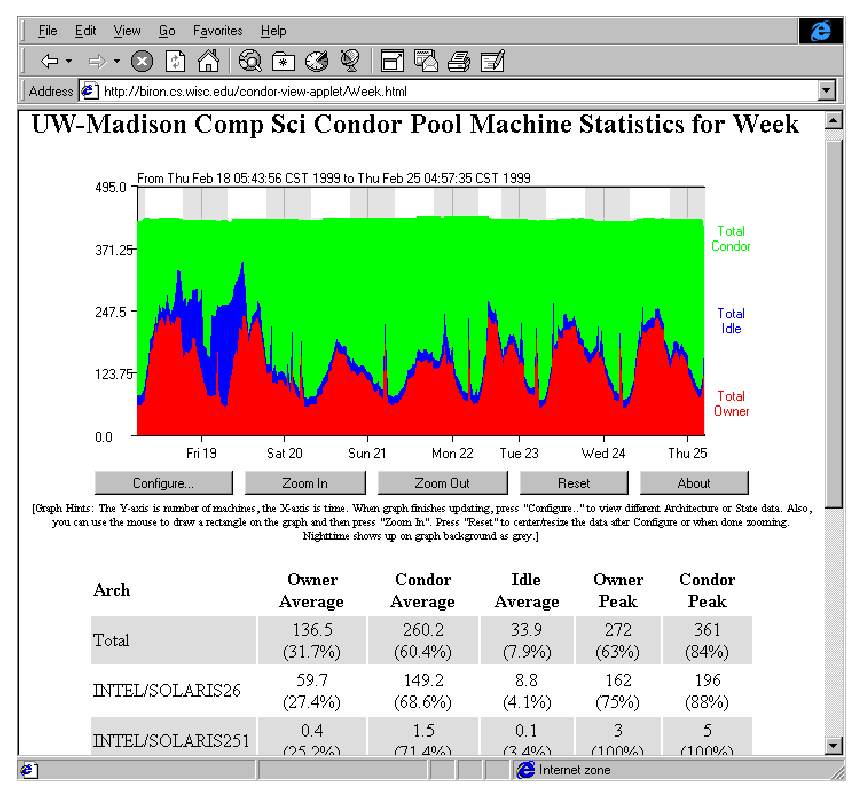
\includegraphics{contrib/view-screenshot.ps}
\caption{\label{fig:view-screenshot}Screen shot of HTCondorView Client}
\end{figure}

After unpacking and installing the HTCondorView Client, a script named
\Prog{make\_stats} can be invoked to create HTML pages displaying HTCondor usage
for the past hour, day, week, or month.  
By using the Unix \Prog{cron} facility to periodically execute
\Prog{make\_stats}, HTCondor pool usage statistics can be kept up to date
automatically.  
This simple model allows the HTCondorView Client to be easily installed;
no Web server CGI interface is needed.

%%%%%%%%%%%%%%%%%%%%%%%%%%%%%%%%%%%%%%%%%%%%%%%%%%%%%%%%%%%%%%%%%%%%%%
\subsection{\label{sec:condorview-client-step-by-step}
Step-by-Step Installation of the HTCondorView Client}
%%%%%%%%%%%%%%%%%%%%%%%%%%%%%%%%%%%%%%%%%%%%%%%%%%%%%%%%%%%%%%%%%%%%%%

\index{installation!HTCondorView Client}
\index{HTCondorView!Client installation}
\begin{enumerate}

\item Make certain that the HTCondorView Server is configured.
Section ~\ref{sec:Contrib-HTCondorView-Install}
describes configuration of the server.
The server logs information on disk in order to provide a persistent,
historical database of pool statistics.
The HTCondorView Client makes queries over the network to this
database.
The \Condor{collector} includes this database support.
To activate the persistent database logging, add the following entries to
the configuration file for the \Condor{collector} chosen to act as the ViewServer.
\begin{verbatim}
    POOL_HISTORY_DIR = /full/path/to/directory/to/store/historical/data 
    KEEP_POOL_HISTORY = True 
\end{verbatim}

\item Create a directory where HTCondorView is to place the HTML files.  
This directory should be one published by a web server, so that HTML
files which exist in this directory can be accessed using a web browser.  
This directory is referred to as the \File{VIEWDIR} directory.

\item Download the \Prog{view\_client} contrib module.
Follow links for contrib modules from the wiki at
\URL{https://htcondor-wiki.cs.wisc.edu/index.cgi/wiki}.

\item Unpack or untar this contrib module into the
directory \File{VIEWDIR}.
This creates several files and subdirectories.
Further unpack the jar file within the \File{VIEWDIR} directory with:
\begin{verbatim} 
  jar -xf condorview.jar
\end{verbatim}

\item Edit the \Prog{make\_stats} script.  At the beginning of the file
are six parameters to customize.
The parameters are

        \begin{description}

	\item[\MacroNI{ORGNAME}] A brief name that identifies an
	organization. An example is ``Univ of Wisconsin''.  Do not
	use any slashes in the name or other special regular-expression
	characters. Avoid the characters \Bs \^\  and \$.

	\item[\MacroNI{CONDORADMIN}] The e-mail
	address of the HTCondor administrator at your site.  
	This e-mail address will appear at the bottom of the web pages.

	\item[\MacroNI{VIEWDIR}] The full path name
	(\emph{not} a relative path) to the \File{VIEWDIR} directory set
	by installation step 2.  
	It is the directory that contains the \Prog{make\_stats} script.

	\item[\MacroNI{STATSDIR}]  The full path name of the
	directory which contains the \Condor{stats} binary.
	The \Condor{stats} program is included in the \Release{bin}
	directory. 
	The value for \MacroNI{STATSDIR} is added to the \MacroNI{PATH}
	parameter by default.  

	\item[\MacroNI{PATH}] A list of subdirectories,
	separated by colons, where the \Prog{make\_stats} script can find
	the \Prog{awk}, \Prog{bc}, \Prog{sed}, \Prog{date}, and \Condor{stats}
	programs.  
	If \Prog{perl} is installed, the path should also
	include the directory where \Prog{perl} is installed.
	The following default works on most systems:
        \begin{verbatim} 
        PATH=/bin:/usr/bin:$STATSDIR:/usr/local/bin
        \end{verbatim}

        \end{description}

\item To create all of the initial HTML files, run
\begin{verbatim}
        ./make_stats setup  
\end{verbatim}
Open the file \File{index.html} to verify that things look good.

\index{HTCondorView!use of \Prog{crontab} program}
\index{crontab program}

\item Add the \Prog{make\_stats} program to \Prog{cron}.  
Running \Prog{make\_stats} in step 6 created a \File{cronentries} file.
This \File{cronentries} file is ready to be processed by the Unix
\Prog{crontab} command.
The \Prog{crontab} manual page contains details about
the \Prog{crontab} command and the \Prog{cron} daemon.
Look at the
\File{cronentries} file; by default, it will run 
\Prog{make\_stats} \Arg{hour} every 15 minutes, 
\Prog{make\_stats} \Arg{day} once an hour, 
\Prog{make\_stats} \Arg{week} twice per day, and 
\Prog{make\_stats} \Arg{month} once per day.
These are reasonable defaults.  
Add these commands to cron on any
system that can access the \MacroNI{VIEWDIR} and
\MacroNI{STATSDIR} directories,
even on a system that does not have HTCondor installed.
The commands do not need to run as root user;
in fact, they should probably not run as root.  These commands can run
as any user that has read/write access to the \File{VIEWDIR} directory.
The command
\begin{verbatim} 
  crontab cronentries
\end{verbatim}
can set the crontab file;
note that this command overwrites the current, existing crontab file with the 
entries from the file \File{cronentries}.

\item Point the web browser at the \File{VIEWDIR} directory
to complete the installation.

\end{enumerate}


%%%%%%%%%%%%%%%%%%%%%%%%%%%%%%
\section{Job Monitor/Log Viewer}
%%%%%%%%%%%%%%%%%%%%%%%%%%%%%%
\index{Job monitor}
\index{viewing!log files}

The HTCondor Job Monitor is a Java application designed to allow users to 
view user log files. 
It is identified as the Contrib Module called HTCondor Log Viewer. 

To view a user log file, select it using the open file command in 
the File menu.  
After the file is parsed, it will be visually represented.  
Each horizontal line represents an individual job.  
The x-axis is time.  
Whether a job is running at a particular time is represented by 
its color at that time -- white for running, black for idle.  
For example, a job which appears predominantly white has made
efficient progress, 
whereas a job which appears predominantly black has received 
an inordinately small proportion of computational time. 


\subsection{\label{sec:transition-states}Transition States}

A transition state is the state of a job at any time.  
It is called a transition, 
because it is defined by the two events which bookmark it.  
There are two basic transition states: running and idle. 
An idle job typically is a job which has just been submitted into 
the HTCondor pool and is waiting to be matched with an appropriate machine 
or a job which has vacated from a machine and has been returned to the pool.  
A running job, by contrast, is a job which is making active progress. 

Advanced users may want a visual distinction between two types of 
running transitions: \Term{goodput} or \Term{badput}.  
Goodput is the transition state preceding an eventual job completion or
checkpoint.  
Badput is the transition state preceding a non-checkpointed eviction event.
Note that badput is potentially a misleading nomenclature; 
a job which does not produce a checkpoint by the
HTCondor program may produce the checkpoint itself or make progress 
in some other way.  
To view these two transition as distinct transitions, 
select the appropriate option from the "View" menu. 


\subsection{\label{sec:events}Events}

There are two basic kinds of events: checkpoint events and error events.   
Plus, advanced users can ask to see more events. 


\subsection{\label{sec:job-selector}Selecting Jobs}

To view any arbitrary selection of jobs in a job file, use the job selector tool.  Jobs appear visually by order of appearance within the actual text log file.  For example, the log file might contain jobs
775.1, 775.2, 775.3, 775.4, and 775.5, which appear in that order.  A user who wishes to see only jobs 775.2 and 775.5 can select only these two jobs in the job selector tool and click the "Ok" or
"Apply" button.  The job selector supports double clicking; double
click on any single job to see it drawn in isolation. 

\subsection{\label{sec:zooming}Zooming}

To view a small area of the log file, zoom in on the area which you would like to see in greater detail. You can zoom in, out and do a full zoom. A full zoom redraws the log file in its entirety. For
example, if you have zoomed in very close and would like to go all the way back out, you could do so with a succession of zoom outs or with one full zoom. 

There is a difference between using the menu driven zooming and the mouse driven zooming. The menu driven zooming will recenter itself around the current center, whereas mouse driven
zooming will recenter itself (as much as possible) around the mouse click. To help you re-find the clicked area, a box will flash after the zoom. This is called the "zoom finder" and it can be turned
off in the zoom menu if you prefer. 

\subsection{\label{sec:k-m-shortcuts}Keyboard and Mouse Shortcuts}

\begin{enumerate}
\item The Keyboard shortcuts: 

\begin{itemize}
\item Arrows - an approximate ten percent scroll bar movement
\item PageUp and PageDown - an approximate one hundred percent scroll bar movement 
\item Control + Left or Right - approximate one hundred percent scroll bar movement 
\item End and Home - scroll bar movement to the vertical extreme 
\item Others - as seen beside menu items
\end{itemize}

\item The mouse shortcuts: 

\begin{itemize}
\item Control + Left click - zoom in 
\item Control + Right click - zoom out
\item Shift + left click - re-center
\end{itemize}
\end{enumerate}
 




\chapter{Version History and Release Notes}
\label{Version-History}
%%%%%%%%%%%%%%%%%%%%%%%%%%%%%%%%%%%%%%%%%%%%%%%%%%%%%%%%%%%%%%%%%%%%%%
\section{\label{sec:History-Intro}Introduction to HTCondor Versions}
%%%%%%%%%%%%%%%%%%%%%%%%%%%%%%%%%%%%%%%%%%%%%%%%%%%%%%%%%%%%%%%%%%%%%%

This chapter provides descriptions of what features have been added or
bugs fixed for each version of HTCondor.
The first section describes the HTCondor version numbering scheme, what
the numbers mean, and what the different \Term{release series} are.
The rest of the sections each describe a specific release series, and
all the HTCondor versions found in that series.

%%%%%%%%%%%%%%%%%%%%%%%%%%%%%%%%%%%%%%%%%%%%%%%%%%%%%%%%%%%%%%%%%%%%%%
\subsection{\label{sec:Version-Number-Scheme}
HTCondor Version Number Scheme}
%%%%%%%%%%%%%%%%%%%%%%%%%%%%%%%%%%%%%%%%%%%%%%%%%%%%%%%%%%%%%%%%%%%%%%

Starting with version 6.0.1, HTCondor adopted a new, hopefully easy to
understand version numbering scheme.
It reflects the fact that HTCondor is both a production system and a
research project.
The numbering scheme was primarily taken from the Linux kernel's
version numbering, so if you are familiar with that, it should seem
quite natural.

There will usually be two HTCondor versions available at any given time,
the \Term{stable} version, and the \Term{development} version.
Gone are the days of ``patch level 3'', ``beta2'', or any other random
words in the version string.
All versions of HTCondor now have exactly three numbers, separated by
``.''   

\begin{itemize}

\item The first number represents the major version number, and will
change very infrequently.

\item \emph{The thing that determines whether a version of HTCondor is
\Term{stable} or \Term{development} is the second digit.
Even numbers represent stable versions, while odd numbers represent
development versions.}

\item The final digit represents the minor version number, which
defines a particular version in a given release series.

\end{itemize}


%%%%%%%%%%%%%%%%%%%%%%%%%%%%%%%%%%%%%%%%%%%%%%%%%%%%%%%%%%%%%%%%%%%%%%
\subsection{\label{sec:Stable-Series}The Stable Release Series}
%%%%%%%%%%%%%%%%%%%%%%%%%%%%%%%%%%%%%%%%%%%%%%%%%%%%%%%%%%%%%%%%%%%%%%

People expecting the stable, production HTCondor system should download
the stable version, denoted with an even number in the second digit of
the version string.
Most people are encouraged to use this version.  
We will only offer our paid support for versions of HTCondor from the
stable release series.

\emph{On the stable series, new minor version releases will only
be made for bug fixes and to support new platforms.}
No new features will be added to the stable series.
People are encouraged to install new stable versions of HTCondor when
they appear, since they probably fix bugs you care about.
Hopefully, there will not be many minor version releases for any given
stable series.


%%%%%%%%%%%%%%%%%%%%%%%%%%%%%%%%%%%%%%%%%%%%%%%%%%%%%%%%%%%%%%%%%%%%%%
\subsection{\label{sec:Developement-Series}
The Development Release Series}
%%%%%%%%%%%%%%%%%%%%%%%%%%%%%%%%%%%%%%%%%%%%%%%%%%%%%%%%%%%%%%%%%%%%%%

Only people who are interested in the latest research, new features
that haven't been fully tested, etc, should download the development
version, denoted with an odd number in the second digit of the version
string.  
We will make a best effort to ensure that the development series will
work, but we make no guarantees.

On the development series, new minor version releases will probably
happen frequently.
People should not feel compelled to install new minor versions unless
they know they want features or bug fixes from the newer development
version.

\emph{Most sites will probably never want to install a development
version of HTCondor for any reason.}
Only if you know what you are doing (and like pain), or were
explicitly instructed to do so by someone on the HTCondor Team, should
you install a development version at your site.

After the feature set of the development series is satisfactory to the
HTCondor Team, we will put a code freeze in place, and from that point
forward, only bug fixes will be made to that development series.
When we have fully tested this version, we will release a new stable
series, resetting the minor version number, and start work on a new
development release from there.

%%%%%%%%%%%%%%%%%%%%%%%%%%%%%%%%%%%%%%%%%%%%%%%%%%%%%%%%%%%%%%%%%%%%%%
% The rest of this file just inputs other files which contain sections
% describing each release series in detail.
%%%%%%%%%%%%%%%%%%%%%%%%%%%%%%%%%%%%%%%%%%%%%%%%%%%%%%%%%%%%%%%%%%%%%%

%%%      PLEASE RUN A SPELL CHECKER BEFORE COMMITTING YOUR CHANGES!
%%%      PLEASE RUN A SPELL CHECKER BEFORE COMMITTING YOUR CHANGES!
%%%      PLEASE RUN A SPELL CHECKER BEFORE COMMITTING YOUR CHANGES!
%%%      PLEASE RUN A SPELL CHECKER BEFORE COMMITTING YOUR CHANGES!
%%%      PLEASE RUN A SPELL CHECKER BEFORE COMMITTING YOUR CHANGES!

%%%%%%%%%%%%%%%%%%%%%%%%%%%%%%%%%%%%%%%%%%%%%%%%%%%%%%%%%%%%%%%%%%%%%%
\section{\label{sec:History-8-7}Development Release Series 8.7}
%%%%%%%%%%%%%%%%%%%%%%%%%%%%%%%%%%%%%%%%%%%%%%%%%%%%%%%%%%%%%%%%%%%%%%

This is the development release series of HTCondor.
The details of each version are described below.

%%%%%%%%%%%%%%%%%%%%%%%%%%%%%%%%%%%%%%%%%%%%%%%%%%%%%%%%%%%%%%%%%%%%%%
\subsection*{\label{sec:New-8-7-2}Version 8.7.2}
%%%%%%%%%%%%%%%%%%%%%%%%%%%%%%%%%%%%%%%%%%%%%%%%%%%%%%%%%%%%%%%%%%%%%%

\noindent Release Notes:

\begin{itemize}

\item HTCondor version 8.7.2 released on June 22, 2017.

\end{itemize}

\noindent Known Issues:

\begin{itemize}

\item Our current implementation of late materialization is incompatible with
\Condor{dagman} and will cause unexpected behavior, including failing without
warning. This is a top-priority issue which aim to resolve in an upcoming
release.
\Ticket{6292}

\end{itemize}

\noindent New Features:

\begin{itemize}

\item Improved the performance of the \Condor{schedd} by setting the
default for the knob \MacroNI{SUBMIT\_SKIP\_FILECHECKS} to true.  This prevents
the \Condor{schedd} from checking the readability of all input files, and skips
the creation of the output files on the submit side at submit time.
Output files are now created either at transfer time, when file transfer
is on, or by the job itself, if a shared filesystem is used.  As a result
of this change, it is possible that a job will run to completion, and only
then is put on hold because the output file on the submit machine cannot
be written.
\Ticket{6220}

\item Changed \Condor{submit} to not create empty stdout and stderr files before
submitting jobs by default.  This caused confusion for users, and slowed down
the submission process.  The older behavior, where \Condor{submit} would fail
if it could not create this files, is available when the parameter
\MacroNI{SUBMIT\_SKIP\_FILECHECKS} is set to false.  The default is now true.
\Ticket{6220}

\item \Condor{q} will now show expanded totals when querying a \Condor{schedd} that is version 8.7.1 or later.
The totals for the current user and for all users are provided by the \Condor{schedd}.
To get the old totals display set the configuration parameter \MacroNI{CONDOR\_Q\_SHOW\_OLD\_SUMMARY} to true.
\Ticket{6254}

\item The \Condor{annex} tool now logs to the user configuration directory.  Added an
audit log of \Condor{annex} commands and their results.
\Ticket{6267}

\item Changed \Condor{off} so that the \Expr{-annex} flag implies the
\Expr{-master} flag, since this is more likely to be the right thing.
\Ticket{6266}

\item Added \Expr{-status} flag to \Condor{annex}, which reports on
instances which are running but not in the pool.
\Ticket{6257}

\item If invoked with an annex name and duration (but not an instance or slot
count), \Condor{annex} will now adjust the duration of the named annex.
\Ticket{6161}

\item Job input files which are downloaded from http:// web addresses now
have mechanisms to recover from transfer failures. This should increase the
reliability of using web-based input files, especially under slow and/or
unstable network conditions.
\Ticket{5886}

\item Reduced load on the \Condor{collector} by optimizing queries performed when
an HTCondor daemon needs to look up the address of another daemon.
\Ticket{6223}

\item Reduced load on the \Condor{collector} by optimizing queries performed
when using \condor{q} with several different command-line options such as
\Opt{-submitter} and \Opt{-global}.
\Ticket{6222}

\item Added the \Condor{top} tool,
an automated version of the now-defunct \Condor{top.pl}
which uses the python bindings to monitor the status of daemons.
\Ticket{6205}

\item Added a new option \Opt{-cron} to \Condor{gpu\_discovery} that allows it to be
used directly as an executable of a \Condor{startd} cron job.
\Ticket{6012}

\item The configuration variable \MacroNI{MAX\_RUNNING\_SCHEDULER\_JOBS\_PER\_OWNER}
was set to default to 100. It formerly had no default value.
\Ticket{6260}

\item Added a parameter \MacroNI{DEDICATED\_SCHEDULER\_USE\_SERIAL\_CLAIMS} which
defaults to false.  When true, allows the dedicated schedule to use claimed/idle
slots that the serial scheduler has claimed.
\Ticket{6276}

\item The \Condor{advertise} tool now assumes an update command if one is not
specified on the command-line and attempts to determine exact command by
inspecting the first ad to be advertised.
\Ticket{6296}

\item Improved support for running several \Condor{negotiator}s in a
single pool.
\MacroNI{NEGOTIATOR\_NAME} now works like \MacroNI{MASTER\_NAME}.
\Condor{userprio} has a -name option to select a specific
\Condor{negotiator}.
Accounting ads from multiple \Condor{negotiator}s can co-exist in the
\Condor{collector}.
\Ticket{5717}

\item Package EC2 Annex components in the condor-annex-ec2 sub RPM.
\Ticket{6202}

\item Added configuration parameter \MacroNI{ALTERNATE\_JOB\_SPOOL},
an expression evaluated against the job ad, which specifies an alternate
spool directory to use for files related to that job.
\Ticket{6221}

\end{itemize}

\noindent Bugs Fixed:

\begin{itemize}

\item With an empty configuration file, HTCondor would behave as if
\MacroNI{ALLOW\_ADMINISTRATOR} were \Expr{*}.  Changed the default to
\Expr{\$(CONDOR\_HOST)}, which is much less insecure.
\Ticket{6230}

\item Fixed a bug in the \Condor{schedd} where it did not account for the initial state of
late materialize jobs when calculating the running totals of jobs by state. This bug
resulted in \Condor{q} displaying incorrect totals when \MacroNI{CONDOR\_Q\_SHOW\_OLD\_SUMMARY}
was set to false.
\Ticket{6272}

\item Fixed a bug where the \Condor{schedd} would incorrectly try to check the
validity of output files and directories for late materialize jobs. The \Condor{schedd}
will now always skip file checks for late materialize jobs.
\Ticket{6246}

\item Changed the output of the \Condor{status} command so that the Load Average
field now displays the load average of just the condor job running in that
slot.  Previously, load associated from outside of condor was proportionately
distributed into the condor slots, resulting in much confusion.
\Ticket{6225}

\item Illegal chars ('+', '.') are now prohibited in DAGMan node names.
\Ticket{5966}

\item Improve audit log messages by including the connection ID and properly
filtering out shadow and gridmanager modifications to the job queue log.
\Ticket{6289}

\item \Condor{root\_switchboard} has been removed from the release, since
PrivSep is no longer supported.
\Ticket{6259}

\end{itemize}

%%%%%%%%%%%%%%%%%%%%%%%%%%%%%%%%%%%%%%%%%%%%%%%%%%%%%%%%%%%%%%%%%%%%%%
\subsection*{\label{sec:New-8-7-1}Version 8.7.1}
%%%%%%%%%%%%%%%%%%%%%%%%%%%%%%%%%%%%%%%%%%%%%%%%%%%%%%%%%%%%%%%%%%%%%%

\noindent Release Notes:

\begin{itemize}

\item HTCondor version 8.7.1 released on April 24, 2017.

\end{itemize}


\noindent New Features:

\begin{itemize}

\item Previously, when the number of forked children processing Collector
queries surpassed the maximum set by the configuration knob \MacroNI{COLLECTOR\_QUERY\_WORKERS}, the
Collector handled all new incoming queries in-processes (i.e. without
forking). As processing a query and sending out the result to the network
could take a long time, the result of servicing such queries in-process in
the Collector is likely to drop a lot of updates. So now in v8.7.1, instead of
servicing such queries in-process, they are queued up for servicing as soon as
query worker child processes become available.  The configuration knob
\MacroNI{COLLECTOR\_QUERY\_WORKERS\_PENDING} was introduced; see
section\~ref{param:CollectorQueryWorkersPending}.
\Ticket{6192}

\item Default value for \MacroNI{COLLECTOR\_QUERY\_WORKERS} changed from 2 to 4.
\Ticket{6192}

\item Introduced configuration macro
\MacroNI{COLLECTOR\_QUERY\_WORKERS\_RESERVE\_FOR\_HIGH\_PRIO} so that the
collector prioritizes queries that are important for the operation of the
pool (such as queries from the negotiator) ahead of servicing user
invocations of \Condor{status}.
\Ticket{6192}

\item Introduced configuration macro \MacroNI{COLLECTOR\_QUERY\_MAX\_WORKTIME} to
define the maximum amount of time the collector may service a query from a
client like condor\_status.  See section\~ref{param:CollectorQueryMaxWorktime}.
\Ticket{6192}

\item Added several new statistics on collector query performance into the Collector
ClassAd, including \AdAttr{ActiveQueryWorkers}, \AdAttr{ActiveQueryWokersPeak},
\AdAttr{PendingQueries}, \AdAttr{PendingQueriesPeak}, \AdAttr{DroppedQueries},
and \AdAttr{RecentDroppedQueries}.  See section\~ref{sec:Collector-ClassAd-Attributes}.
\Ticket{6192}

\item Further refinement and initial documentation of the HTCondor Annex.
\Ticket{6147}
\Ticket{6149}
\Ticket{6150}
\Ticket{6155}
\Ticket{6157}
\Ticket{6184}
\Ticket{6196}
\Ticket{6216}
\Ticket{6218}

\item Docker universe jobs can now use condor\_chirp command
(if it is in the image).
\Ticket{6162}

\item In the Job Router, when a candidate job matches multiple routes,
the first route is now always selected.
The old behavior of spreading jobs across all matching routes round-robin
style can be enabled by setting the new configuration parameter
\MacroNI{JOB\_ROUTER\_ROUND\_ROBIN\_SELECTION} to \Expr{True}.
\Ticket{6190}

\item The \Condor{schedd} now keeps a count of jobs by state for each owner and submitter
and will report them to \Condor{q}. Condor{q} will display these totals unless the new
configuration parameter \MacroNI{CONDOR\_Q\_SHOW\_OLD\_SUMMARY} is set to true. In 8.7.1
this parameter defaults to true.
\Ticket{6160}

\item Milestone 1 for late materialization in the \Condor{schedd} was completed. This milestone adds the
undocumented option \Opt{-factory} to \Condor{q} that can be used to submit a late materializing job cluster
to the \Condor{schedd}.  The \Condor{schedd} will refuse the submission unless the configuration parameter
\MacroNI{SCHEDD\_ALLOW\_LATE\_MATERIALIZATION} is set to true.
\Ticket{6212}

\item Increased the default value for configuration parameter
\MacroNI{NEGOTIATOR\_SOCKET\_CACHE\_SIZE} to 500.
\Ticket{6165}

\item Added new DaemonCore statistics UdpQueueDepth to measure the
number of bytes in the UDP receive queue for daemons with a UDP command port.
\Ticket{6183}

\item Improved speed of handling queries to the collector by caching the
the configuration knob SHARED\_PORT\_ADDRESS\_REWRITING.
\Ticket{6187}

\item The \Condor{collector} on Linux now handles some queries in process and some
by forking a child process. This allows it to avoid the overhead of forking to handle
queries that will take little time. The policy for deciding which queries to handle in process
is controlled by a new configuration parameter \MacroNI{HANDLE\_QUERY\_IN\_PROC\_POLICY}.
\Ticket{6191}

\item Added \Opt{-limit} option to \Condor{status} and changed the \Condor{collector} to honor it.
\Ticket{6198}

\item \Condor{submit} was changed to use the same utility library that the submit python bindings use.
This should help insure that submit via python bindings will give the same results as using \Condor{submit}.
\Ticket{6181}.

\end{itemize}

\noindent Bugs Fixed:

\begin{itemize}

\item None.

\end{itemize}

%%%%%%%%%%%%%%%%%%%%%%%%%%%%%%%%%%%%%%%%%%%%%%%%%%%%%%%%%%%%%%%%%%%%%%
\subsection*{\label{sec:New-8-7-0}Version 8.7.0}
%%%%%%%%%%%%%%%%%%%%%%%%%%%%%%%%%%%%%%%%%%%%%%%%%%%%%%%%%%%%%%%%%%%%%%

\noindent Release Notes:

\begin{itemize}

\item HTCondor version 8.7.0 released on March 2, 2017.

\end{itemize}


\noindent New Features:

\begin{itemize}

\item Optimized the code that reads reads ClassAds off the wire making the maximum possible update rate
for the Collector about 1.7 times higher than it was before.
\Ticket{6105}
\Ticket{6130}

\item New statistics have been added to the Collector ad to show time spent handling queries.
\Ticket{6123}

\item Changed the formatting of the printing of ClassAd expressions with
parentheses. Now there is no space character after every open parenthesis, or
before every close parenthesis
This looks more natural, is somewhat faster for the condor to parse, and
saves space.  That is, an expression that used to print like

\begin{verbatim}
( ( ( foo ) ) )
\end{verbatim}
now will print like this
\begin{verbatim}
(((foo)))
\end{verbatim}
\Ticket{6082}

\item Technology preview of the HTCondor Annex. The HTCondor Annex allows one
to extend their HTCondor pool into the cloud.
\URL{https://htcondor-wiki.cs.wisc.edu/index.cgi/wiki?p=HowToUseCondorAnnexWithOnDemandInstances}
\Ticket{6121}

\item Added \Opt{-annex} option to \Condor{status} and \Condor{off}.  Requires
an argument; the request is constrained to match machines whose
\Expr{AnnexName} ClassAd attribute matches the argument.
\Ticket{6116}
\Ticket{6117}

\item A refreshed X.509 proxy is now forwarded to the remote cluster
in Bosco.
\Ticket{5841}

\item Added several new statistics to the Negotiator ad, mainly
detailing how time is spent in the negotiation cycle.
\Ticket{6060}

\end{itemize}

\noindent Bugs Fixed:

\begin{itemize}

\item Removed redundant updates to the job queue by the Job Router.
\Ticket{6102}

\end{itemize}


% upgrade instructions are in the Pool Management section
\section{\label{sec:to-8.6}Upgrading from the 8.4 series to the 8.6 series of HTCondor}
%%%%%%%%%%%%%%%%%%%%%%%%%%%%%%%%%%%%%%%%%%%%%%%%%%%%%%%%%%%%%%%%%%%%%%

\index{upgrading!items to be aware of}
Upgrading from the 8.4 series of HTCondor to the 8.6 series
will bring new features introduced in the 8.5 series of HTCondor.
These new features include the following (note that this list contains
only the most significant changes; a full list of changes can be
found in the version history:~\ref{sec:History-8-5}):

\begin{itemize}

\item \Condor{q}-related changes:
  \begin{itemize}

  \item \Condor{q} now defaults to showing only the current user's jobs.
  \Ticket{5271}
  Similarly, \Condor{qedit} defaults to editing only jobs owned by the
  current user.  
  \Ticket{5889}
  (The previous behavior of both commands can be restored by setting
  \MacroNI{CONDOR\_Q\_ONLY\_MY\_JOBS} to \Expr{False} --
  see ~\ref{param:CondorQOnlyMyJobs}.)

  \item \Condor{q} now defaults to batch mode, which produces a single
  line of output summarizing a batch of jobs (see~\pageref{batches-of-jobs}).
  \Ticket{5708}
  (The previous behavior can be restored by setting
  \MacroNI{CONDOR\_Q\_DASH\_BATCH\_IS\_DEFAULT} to \Expr{False} --
  see ~\ref{param:CondorQDashBatchIsDefault}.)

  \item \Condor{q} (and \Condor{history} and \Condor{status}) can now
  read and write JSON, XML, and new ClassAd formats
  (see~\pageref{man-condor-q}, ~\pageref{man-condor-history},
  and ~\pageref{man-condor-status}).
  \Ticket{5688}
  \Ticket{5844}
  \Ticket{5820}

  \end{itemize}

\item Job submission-related changes:
  \begin{itemize}

   \item Added the ability for the \Condor{schedd} to transform
   job ClassAds upon job submission
   (see section~\ref{sec:Schedd-Config-Job-Transforms}).

   \item Added the ability to group jobs into batches, and assign
   names to the batches, using the new \Opt{-batch} arguments to
   \Condor{submit} and \Condor{submit\_dag}.

   \item Added support in the submit language for retrying jobs
   if they fail (see~\pageref{condor-submit-max-retries}).

  \end{itemize}

\item \Condor{dagman}-related changes:
  \begin{itemize}

  \item Added the ability to define SCRIPTS, VARS, etc., for all nodes
  in a DAG with a single command (see section~\ref{sec:DAGAllNodes}).
  \Ticket{5729}

  \item Simplified how DAG node priorities work
  (see section~\ref{sec:DAG-SetNodePriority}).
  This means that existing DAGs that use the node priority feature
  will run differently than they have in the past.
  \Ticket{4024}
  \Ticket{5749}

  \item Added the new splice connection feature
  (see section~\ref{sec:DAGSpliceConnections}), which
  allows more flexible dependencies between splices.
  \Ticket{5213}

  \end{itemize}

\item HTCondor can now use IPv6 interfaces; it prefers IPv4 if both
IPv4 and IPv6 are available.
\Ticket{5104}

\item HTCondor now has initial support for Singularity containers
(see section~\ref{sec:singularity-support}).
\Ticket{5828}

\item \Condor{status} can now display a single line of output for
each machine (rather than a line per slot).
\Ticket{5596}

\item A number of improvements to the Python bindings including: submission
\Ticket{5666}
\Ticket{4916};
draining
\Ticket{5507};
per-thread security contexts
\Ticket{5632};
Computing-On-Demand support
\Ticket{5130}; and
multiple query support
\Ticket{5187}

\item Jobs can now be submitted to the Slurm batch scheduling system via
the new \SubmitCmdNI{slurm} type in the grid universe.
\Ticket{5515}

\item Numerous improvements to Docker support, including
\Ticket{5680};
\Ticket{5760};
\Ticket{5761};
\Ticket{5750};
\Ticket{5740};
\Ticket{5609};
\Ticket{5456}


\end{itemize}

Upgrading from the 8.4 series of HTCondor to the 8.6 series will
also introduce changes that administrators and users of sites running
from an older HTCondor version should be aware of when planning an upgrade.
Here is a list of items that administrators should be aware of.

\begin{itemize}

\item Shared port (see section~\ref{sec:shared-port-daemon}) is now
enabled by default; set \MacroNI{USE\_SHARED\_PORT} to \Expr{False} to
disable it.  Note that this configuration macro does not control the HAD or
replication daemon's use of shared port; use \MacroNI{HAD\_USE\_SHARED\_PORT}
or \MacroNI{REPLICATION\_USE\_SHARED\_PORT} instead.  See section
~\ref{sec:HA-configuration} for more details on how to configure HAD (and/or
the replication daemon) to work with shared port, since just activating
shared port without any other configuration change will not work.
\Ticket{3813}
\Ticket{5103}

\item To mitigate performance problems, \MacroNI{LOWPORT} and
\MacroNI{HIGHPORT} no longer restrict outbound port ranges on Windows.  To
re-enable this functionality, set \MacroNI{OUT\_LOWPORT} and
\MacroNI{OUT\_HIGHPORT} (see ~\ref{param:OutLowPort} and
~\ref{param:OutHighPort}).
\Ticket{4711}

\item Cgroups (see section~\ref{sec:CGroupTracking}) are now enabled
by default.  This means that if you
have partitionable slots, jobs need to get \SubmitCmd{request\_memory}
correct.
\Ticket{5936}

\item By default, \Condor{q} queries only the current user's jobs,
unless the current user is a queue superuser or the
\MacroNI{CONDOR\_Q\_ONLY\_MY\_JOBS} configuration macro is set to
\Expr{False}.
\Ticket{5271}

\item Added support for immutable and protected job attributes, which
makes SUBMIT\_REQUIREMENTS more useful
(see section~\ref{param:ImmutableJobAttrs}).
\Ticket{5065}

\item By default, the \Condor{schedd} no longer changes the ownership
of spooled job files (they remain owned by the submitting user).
\Ticket{5226}

\item When \MacroNI{SEC\_ENABLE\_MATCH\_PASSWORD\_AUTHENTICATION} is set
to \Expr{True}, the related authorizations are now automatically enabled.
\Ticket{5304}  (See ~\ref{param:SecEnableMatchPasswordAuthentication}
for details.)

\item The master can now run an administrator-defined script at shutdown;
see section~\ref{param:DefaultMasterShutdownScript} for details.
\Ticket{5590}

\end{itemize}


%%%%%%%%%%%%%%%%%%%%%%%%%%%%%%%%%%%%%%%%%%%%%%%%%%%%%%%%%%%%%%%%%%%%%%%
\section{\label{sec:to-8.4}Upgrading from the 8.2 series to the 8.4 series of HTCondor}
%%%%%%%%%%%%%%%%%%%%%%%%%%%%%%%%%%%%%%%%%%%%%%%%%%%%%%%%%%%%%%%%%%%%%%

\index{upgrading!items to be aware of}
Upgrading from the 8.2 series of HTCondor to the 8.4 series
will bring new features introduced in the 8.3 series of HTCondor.
These new features include:
\begin{itemize}

\item Implemented numerous scalability changes (such as reducing memory
footprint, using fewer system resources, and streamlined algorithms) to
handle 200,000 simultaneously running HTCondor jobs in a single pool.

\item Added a Docker Universe to run a Docker container as an HTCondor job.

\item New features increase the power of job specification
in the submit description file.

  \begin{itemize}
  \item Submit description files are now parsed the same as configuration files.

  \item The \SubmitCmd{queue} submit command may be used in
flexible and powerful new ways to specify job submissions.
See section~\ref{sec:user-man-queue} for details.
\Ticket{4819}

  \item New macro functions are supported,
and may be used in submit description files as well as in configuration.
\Ticket{4944}

  \item \Condor{submit} has new command line options \Opt{-queue}
and \Opt{-dry-run},
to provide flexible and powerful new ways to specify job submissions,
as well as to test what job would be submitted without submitting.
\Ticket{4933}

  \item \Condor{submit} now supports assignment of ClassAd attributes
on the command line.
\Ticket{4983}

  \item \Condor{submit} accepts \SubmitCmdNI{if} and \SubmitCmdNI{include}
statements in the same way that configuration files do.
\Ticket{4913}

  \end{itemize}

\item HTCondor pools can use IPv4 and IPv6 simultaneously.

\item Execute Directories can be encrypted upon user or administrator request.

\item Vanilla Universe jobs can utilize periodic application-level checkpoints.

\item The administrator can establish requirements that must be satisfied in
order for a job to be queued.

\end{itemize}

Upgrading from the 8.2 series of HTCondor to the 8.4 series will
also introduce changes that administrators of sites running from an older
HTCondor version should be aware of when planning an upgrade.
Here is a list of items that administrators should be aware of.

\begin{itemize}

\item New configuration and changes to existing configuration:
  \begin{itemize}

\item The RPM packages have been restructured to allow running a 32-bit
static shadow on Red Hat Enterprise Linux 6. The new \texttt{condor-all}
RPM is used to install all of the RPMs for a typical HTCondor installation.
Since the binary distribution of HTCondor for Red Hat Enterprise Linux 6 and 7
consists of more that a handful of RPMs, the RPMs are only available from our
YUM repository.
\Ticket{4621}

\item If enabled, the \Condor{shared\_port} daemon will now use port 9618
instead of the previous default, which was to randomly select a port from
the allowed range (from \MacroNI{LOWPORT} to \MacroNI{HIGHPORT}; see section
see section \ref{sec:Ports-Firewalls}).  To restore \Condor{shared\_port}'s
previous behavior, set \MacroNI{SHARED\_PORT\_PORT} to \Expr{0}.
\Ticket{4752}

\item Configuration variable \Macro{MAX\_JOBS\_RUNNING} has been
modified such that it only applies to job universes that require a
\Condor{shadow} process.
Scheduler and local universe jobs are no longer affected by this
variable.
The number of running scheduler and local universe jobs can be controlled
with configuration variables \MacroNI{START\_SCHEDULER\_UNIVERSE} and
\MacroNI{START\_LOCAL\_UNIVERSE}, respectively.
\Ticket{4589}

\item ClassAd attributes written by the \Condor{schedd} that
count the number of jobs in various states now include all jobs,
not only jobs that need to be matched by the \Condor{negotiator} daemon.
These attributes include \Attr{TotalRunningJobs}, \Attr{TotalIdleJobs},
\Attr{TotalHeldJobs}, and \Attr{TotalRemovedJobs}.
\Ticket{4683}

\item On Linux platforms, the \Condor{master} daemon now runs a script when it
starts up.
This script tunes several Linux kernel parameters to the values
we suggest for better scalability.
New configuration variables \Macro{ENABLE\_KERNEL\_TUNING},
\Macro{KERNEL\_TUNING\_LOG}, and \Macro{LINUX\_KERNEL\_TUNING\_SCRIPT}
enable the use of the script and specify file locations.
\Ticket{5126}

\item The default values of the configuration variables and ClassAd attributes
listed in Table~\ref{table:new-knob-defaults} have changed,
such that the default now represents the commonly configured value.

% This table must be formatted oddly, to make the pdf version look OK.
\begin{center}
\begin{table}[hbt]
\begin{tabular}{|l|c|c|} \hline
\textbf{Variable Name} & \textbf{Previous Default} & \textbf{New Default}\\ \hline \hline
\MacroNI{NEGOTIATOR\_INFORM\_STARTD} & \Expr{True} & \Expr{False}  \\ \hline
\MacroNI{MAX\_JOBS\_PER\_SUBMISSION} & largest positive integer & 20000  \\ \hline
\MacroNI{MAX\_JOBS\_PER\_OWNER} & largest positive integer & 100000  \\ \hline
\MacroNI{MAX\_JOBS\_RUNNING} (on Windows) & 200 & 2000  \\ \hline
\MacroNI{PRIVATE\_NETWORK\_NAME} & no default & \MacroUNI{FULL\_HOSTNAME}  \\ \hline
\MacroNI{JobLeaseDuration} & 20 minutes & 40 minutes \\ \hline
\MacroNI{WANT\_VACATE} & \Expr{False} & \Expr{True} \\ \hline
\MacroNI{SCHEDD\_SEND\_VACATE\_VIA\_TCP} & \Expr{False} & \Expr{True} \\ \hline
\end{tabular}
\caption{\label{table:new-knob-defaults}Changes to defaults in HTCondor 8.3.7}
\end{table}
\end{center}

  \end{itemize}

\item None.

\end{itemize}


%%%%%%%%%%%%%%%%%%%%%%%%%%%%%%%%%%%%%%%%%%%%%%%%%%%%%%%%%%%%%%%%%%%%%%%
\section{\label{sec:to-8.2}Upgrading from the 8.0 series to the 8.2 series of HTCondor}
%%%%%%%%%%%%%%%%%%%%%%%%%%%%%%%%%%%%%%%%%%%%%%%%%%%%%%%%%%%%%%%%%%%%%%

\index{upgrading!items to be aware of}
Upgrading from the 8.0 series of HTCondor to the 8.2 series 
will bring new features introduced in the 8.1 series of HTCondor.
These new features include:
configuration is more powerful with new syntax and features, and
the default configuration policy does not preempt jobs,
monitoring is enhanced and now integrates with Ganglia,
automated detection and management of GPUs,
numerous scalability enhancements improve performance,
an improved Python API including support for Python 3,
new native packaging and ports are available for the latest Linux 
distributions including Red Hat 7 Beta and Debian 7,
cloud computing improvements including support for
EC2 spot instances, OpenStack, and \Condor{ssh\_to\_job} 
directly into EC2 jobs,
grid universe jobs can now target Google Compute Engine and BOINC servers,
partitionable slots now are compatible with \Condor{startd} \MacroNI{RANK}
expressions, and consumption policies permit partitionable slots 
to be split into dynamic slots at negotiation time,
improved data management including dynamic adjustment of the level of 
file transfer concurrency based on disk load 
(see section~\ref{param:FileTransferDiskLoadThrottle}), 
and experimental support to allow the execution of a job to be overlaid 
with the transfer of output files from the previous different job,
and
the new \Condor{sos} tool helps administrators manage overloaded daemons. 

Upgrading from the 8.0 series of HTCondor to the 8.2 series will
also introduce changes that administrators of sites running from an older
HTCondor version should be aware of when planning an upgrade.  
Here is a list of items that administrators should be aware of.

\begin{itemize}

\item New configuration syntax and features change:
  \begin{itemize}
  \item The interaction of comments and the line continuation character
   has changed.  See  section~\ref{sec:Other-Syntax} for the current
   interaction. 
  \item The use of a colon character (\verb@:@) instead of the
   equals sign (\verb@=@) in assigning a value to a configuration variable
   causes tools that parse configuration to output a warning.
   Therefore, any custom parsing of tool output may need to be updated to
   handle this warning.
   Previous versions of the default configuration set variable
   \MacroNI{RUNBENCHMARKS} using a colon character;
   HTCondor code explicitly suppresses the warning in this case.
  \end{itemize}

\item The default user priority factor for new users has changed 
from 1 to 1000.
Therefore, unless the accountant log is discarded,
existing users will still have a priority factor of 1,
while new users will have a priority factor of 1000.
Use \Condor{userprio} to change the priority factor of existing users
if the accountant log is maintained across the upgrade. 
\Ticket{4282}

\item For Windows platforms,
HTCondor has switched to use the newer 2012 Microsoft compiler,
which uses the Visual C++ 2012 Runtime components.
Therefore, the HTCondor MSI installer will acquire this Runtime,
if it is not already installed.

\item The meaning of \Expr{cpus=auto} when there are more 
slots than CPUs has changed within the configuration. 
In the \Expr{SLOT\_TYPE\_<N>} configuration variable,
\Expr{cpus=auto} previously resulted in 1 CPU per slot. 
Now, all slots with \Expr{cpu=auto} get an equal share of the CPUs, 
rounded down.
\Ticket{3249}

\item The DAGMan node status file formatting has changed.
The format of the DAG node status file is now New ClassAds,
and the amount of information in the file has increased.

\item Setting configuration variable
\Macro{DAGMAN\_ALWAYS\_USE\_NODE\_LOG} to \Expr{False}
or using the corresponding \Opt{-dont\_use\_default\_node\_log} option
to \Condor{submit\_dag} is no longer recommended.
Note that at strictness setting 1 (the default), setting
\MacroNI{DAGMAN\_ALWAYS\_USE\_NODE\_LOG} to \Expr{False}
will cause a fatal error. 
If the DAG must be run with \MacroNI{DAGMAN\_ALWAYS\_USE\_NODE\_LOG} 
set to \Expr{False},
a good way to deal with upgrading is to use DAGMan Halt files 
to cause all of the running DAGs to drain from the queue, 
and then do the upgrade after the DAGs have stopped.  
After the upgrade is done, 
edit the per-DAG configuration files to have 
\MacroNI{DAGMAN\_ALWAYS\_USE\_NODE\_LOG} set to \Expr{True},
or set \MacroNI{DAGMAN\_USE\_STRICT} to 0 and 
re-submit the DAGs, which will then run the Rescue DAGs.

\item If using \Expr{ENABLE\_IPV6 = True}, the configuration must
also set \Expr{ENABLE\_IPV4 = False}.
If both are enabled simultaneously,
daemons will listen on both IPv4 and IPv6, 
but will only advertise one of the two addresses.

\item Globus 5.2.2 or a more recent version is now required 
for grid universe jobs of grid-type nordugrid and cream.
Globus version 5.2.5 is included in this 8.2.0 release of HTCondor.
HTCondor will prefer to use libraries already installed in \File{/usr/lib[64]},
when present.
\Ticket{4243}

\item If referencing attribute \AdAttr{SubmittorUserPrio} in
configuration, such as in the \MacroNI{PREEMPTION\_REQUIREMENTS} expression,
you will need to change it to \AdAttr{SubmitterUserPrio} 
Note the spelling difference in the ClassAd attribute name.
\Ticket{4369}

\item HTCondor can not distinguish normal from abnormal job exit
for Nordugrid ARC grids.
Therefore, all grid-type nordugrid jobs will be recorded as 
terminating normally, with an exit code from 0 to 255.
\Ticket{4342}

\item For configuration, parameter substitution now honors per-daemon 
overrides.  This long standing bug's fix may result in subtle changes
to the way that your configuration files are processed.

\end{itemize}


%%%%%%%%%%%%%%%%%%%%%%%%%%%%%%%%%%%%%%%%%%%%%%%%%%%%%%%%%%%%%%%%%%%%%%%
\section{\label{sec:to-8.0}Upgrading from the 7.8 series to the 8.0 series of HTCondor}
%%%%%%%%%%%%%%%%%%%%%%%%%%%%%%%%%%%%%%%%%%%%%%%%%%%%%%%%%%%%%%%%%%%%%%

\index{upgrading!items to be aware of}
While upgrading from the 7.8 series of HTCondor to the 8.0 series 
will bring many
new features and improvements introduced in the 7.9 series of HTCondor,
it will
also introduce changes that administrators of sites running from an older
HTCondor version should be aware of when planning an upgrade.  
Here is a list of items that administrators should be aware of.

\begin{itemize}

\item There is an issue with DAGMan jobs upon upgrade
from HTCondor version 7.8.x or an earlier version
to version 8.0.0.
Without administrative intervention,
queued DAGMan jobs will restart from the beginning of the DAG
after the upgrade.
There will be no issue if the upgrade is 
from HTCondor version 7.8.x or an earlier version to HTCondor version 8.0.1
or later versions.

To avoid starting DAGMan jobs from the beginning after the upgrade,
the administrator should ensure that no \Condor{dagman} jobs are queued.
Do a \Condor{rm} on all \Condor{dagman} jobs and wait for Rescue DAGs
to be written before shutting down HTCondor to perform the upgrade.
Any \Condor{dagman} jobs that are on hold should be released before
being removed.
After the upgrade is complete and HTCondor has restarted,
all of these DAGMan jobs should be re-submitted.
This will cause them to read the appropriate Rescue DAGs and 
continue on.

To avoid losing work within partially-completed node jobs,
an alternative is to use the halt file feature,
as described in section~\ref{sec:DagSuspend}.
This will cause all
\Condor{dagman} jobs to eventually drain from the queue(s).
This will take longer than doing a \Condor{rm} on those jobs.
\Condor{dagman} jobs drained via the halt file method will also
have to be re-submitted after the upgrade.

\item The upgrade will change the machine ClassAd attribute
\AdAttr{CheckpointPlatform} for all machines.
This implies that any standard universe job with a checkpoint 
from before the upgrade will not resume after the upgrade.
To work around this potential difficulty, either change the 
attribute \AdAttr{CheckpointPlatform} on all machines to their previous value 
by setting the \Macro{CHECKPOINT\_PLATFORM} configuration variable,
or change the \AdAttr{LastCheckpointPlatform} attribute for all jobs
that have produced a checkpoint.
Make the change by using \Condor{qedit}.

For example, if machine attribute \AdAttr{CheckpointPlatform} changed 
from \verb;LINUX INTEL 2.6.x normal N/A; to 
\verb;LINUX INTEL 2.6.x normal N/A ssse3 sse4_1 sse4_2;,
use the following command:

\footnotesize
\begin{verbatim}
condor_qedit -constraint 'LastCheckpointPlatform == "LINUX INTEL 2.6.x normal N/A"'
    LastCheckpointPlatform "LINUX INTEL 2.6.x normal N/A ssse3 sse4_1 sse4_2"
\end{verbatim}
\normalsize

\end{itemize}


%%%      PLEASE RUN A SPELL CHECKER BEFORE COMMITTING YOUR CHANGES!
%%%      PLEASE RUN A SPELL CHECKER BEFORE COMMITTING YOUR CHANGES!
%%%      PLEASE RUN A SPELL CHECKER BEFORE COMMITTING YOUR CHANGES!
%%%      PLEASE RUN A SPELL CHECKER BEFORE COMMITTING YOUR CHANGES!
%%%      PLEASE RUN A SPELL CHECKER BEFORE COMMITTING YOUR CHANGES!

%%%%%%%%%%%%%%%%%%%%%%%%%%%%%%%%%%%%%%%%%%%%%%%%%%%%%%%%%%%%%%%%%%%%%%
\section{\label{sec:History-8-6}Stable Release Series 8.6}
%%%%%%%%%%%%%%%%%%%%%%%%%%%%%%%%%%%%%%%%%%%%%%%%%%%%%%%%%%%%%%%%%%%%%%

This is a stable release series of HTCondor.
As usual, only bug fixes (and potentially, ports to new platforms)
will be provided in future 8.6.x releases.
New features will be added in the 8.7.x development series.

The details of each version are described below.

%%%%%%%%%%%%%%%%%%%%%%%%%%%%%%%%%%%%%%%%%%%%%%%%%%%%%%%%%%%%%%%%%%%%%%
\subsection*{\label{sec:New-8-6-4}Version 8.6.4}
%%%%%%%%%%%%%%%%%%%%%%%%%%%%%%%%%%%%%%%%%%%%%%%%%%%%%%%%%%%%%%%%%%%%%%

\noindent Release Notes:

\begin{itemize}

\item HTCondor version 8.6.4 released on June 22, 2017.

\end{itemize}


\noindent New Features:

\begin{itemize}

\item Python bindings are now available on MacOSX.
\Ticket{6244}

\item Allow Python modules to be used as \Condor{collector} plugin.
This undocumented feature is to be used by expert developers only.
\Ticket{6213}
\Ticket{6295}

\end{itemize}

\noindent Bugs Fixed:

\begin{itemize}

\item Fixed a bug with PASSWORD authentication that would sporadically cause
it to fail to exchange keys, due to whether or not the first round-trip of
communications blocked on reading from the network.
\Ticket{6265}

\item Pslot preemption now properly handles machine custom resources,
such as GPUs.
\Ticket{6297}

\item Fixed a bug that prevented HTCondor from correctly setting
virtual memory cgroup limits when soft physical memory limits
were being used.
\Ticket{6294}

\item Fixed a bug that prevented parallel universe jobs from running
that used \$\$() expansion in submit files.
\Ticket{6299}

\item Added a new knob, \MacroNI{STARTD\_RECOMPUTE\_DISK\_FREE}, which defaults
to true, which tells the startd to periodically recompute and advertise free
disk space.  Admins can set this to false for partitionable slots whose execute
directory is used by HTCondor alone.
\Ticket{6301}

\item Fixed a bug that could cause \Condor{submit} to fail to submit a
job with a proxy file to a \Condor{schedd} older than 8.5.8, due to the
absence of an X.509 CA certificates directory.
\Ticket{6258}

\item Restored a check in \Condor{submit} about whether the job's X.509
proxy has sufficient lifetime remaining.
\Ticket{6283}

\item Fixed a bug in \Condor{dagman} where the DAG status file showed an
incorrect status code if submit attempts failed for the final node.
\Ticket{6069}

\item Bosco now properly identifies CentOS 7 as a supported platform.
\Ticket{6303}

\item Fixed a bug when Bosco is used to submit jobs to multiple remote
clusters. When arguments to \Prog{remote\_gahp} are provided in the
GridResource attribute, jobs could be submitted to the wrong cluster.
\Ticket{6277}

\item To speed up the installation process on Enterprise Linux 7, the
SELinux profile is now reloaded only once, when setting the HTCondor
daemons to run in permissive mode.
\Ticket{6304}

\item Update the systemd configuration on Enterprise Linux 7 to start the
\Condor{master} after time synchronization is achieved. This prevents
unnecessary daemon restarts due to sudden time shifts.
\Ticket{6255}

\item The \Condor{shadow} will now ignore updates of \Attr{JobStartDate}
from the \Condor{starter} since the \Condor{schedd} already sets this
attribute correctly and the \Condor{starter} incorrectly tries to set it
even if the job has already run once. A consequence of this fix is that the
value of \Attr{JobStartDate} that the \Condor{startd} uses for policy
expressions will be different than the value that the \Condor{schedd} uses.
Resolving this problem will potentially break existing policy expressions
in the \Condor{startd}, so it will be be not be changed in the 8.6 series,
but fixed in the 8.7 series.
\Ticket{6280}

\item Fixed a bug where per-instance job attributes like \AdAttr{RemoteHost}
would show up in the history file for completed jobs.  This bug occurred if
a job happened to complete while the \Condor{schedd} was in the process of a
graceful shutdown.
\Ticket{6251}

\item The \Condor{convert\_history} command is present again in this release.
\Ticket{6282}

\item The parameter \MacroNI{SETTABLE\_ATTRS\_ADMINISTRATOR} is now correctly
appears in \Condor{config\_val}.
\Ticket{6286}

\end{itemize}

%%%%%%%%%%%%%%%%%%%%%%%%%%%%%%%%%%%%%%%%%%%%%%%%%%%%%%%%%%%%%%%%%%%%%%
\subsection*{\label{sec:New-8-6-3}Version 8.6.3}
%%%%%%%%%%%%%%%%%%%%%%%%%%%%%%%%%%%%%%%%%%%%%%%%%%%%%%%%%%%%%%%%%%%%%%

\noindent Release Notes:

\begin{itemize}

\item HTCondor version 8.6.3 released on May 9, 2017.

\end{itemize}

\noindent Bugs Fixed:

\begin{itemize}

\item Fixed a bug that rarely corrupts the \Condor{schedd}'s job queue
log file when the input sandbox of a job with an X.509 proxy file is
spooled.
\Ticket{6240}

\item Fixed a memory leak in the Python bindings related to logging.
\Ticket{6227}

\end{itemize}

%%%%%%%%%%%%%%%%%%%%%%%%%%%%%%%%%%%%%%%%%%%%%%%%%%%%%%%%%%%%%%%%%%%%%%
\subsection*{\label{sec:New-8-6-2}Version 8.6.2}
%%%%%%%%%%%%%%%%%%%%%%%%%%%%%%%%%%%%%%%%%%%%%%%%%%%%%%%%%%%%%%%%%%%%%%

\noindent Release Notes:

\begin{itemize}

\item HTCondor version 8.6.2 released on April 24, 2017.

\end{itemize}


\noindent New Features:

\begin{itemize}

\item Added metaknobs for defining map files for use with the ClassAd usermap function
in the \Condor{schedd}, and a metaknob for automatically assigning an accounting group to
a job based on a mapping of the owner name of the job.
\Ticket{6179}

\item When the \Condor{credd} is polling for credentials, the timeout is now
configurable using \MacroNI{CREDD\_POLLING\_TIMEOUT}.

\item The \Opt{reverse} option for \Condor{q} was changed to \Opt{reverse-analyze},
and it now implies \Opt{better-analyze}. Formerly, the \Opt{reverse} option was ignored
unless \Opt{-better-analyze} was also specified.
\Ticket{6167}

\end{itemize}

\noindent Bugs Fixed:

\begin{itemize}

\item Fixed a bug that could cause \Condor{store\_cred} to fail on
Windows due to a case-sensitive check of the user's account name.
\Ticket{6200}

\item Updated Open MPI helper script to catch and handle SIGTERM and
to use bash explicitly.
\Ticket{6194}

\item Docker Universe jobs now update the RemoteSysCpu attributes for job
and in the job log. Previously, this field was always 0.
\Ticket{6173}

\item Docker universe detection is now more robust in the
face of extraneous output to standard error on docker startup.
This was preventing Condor from detecting that docker was properly
working on hosts.
\Ticket{6185}

\item Fixed a bug that prevented \MacroNI{SUBMIT\_REQUIREMENT} and
\MacroNI{JOB\_TRANSFORM} expressions from referencing job attributes
describing the job's X.509 proxy credential.
\Ticket{6188}

\item The Linux kernel tuning script no longer adjusts some kernel parameters
unless a \Condor{schedd} will be started by the master.
\Ticket{6208}

\item Fixed a bug that caused all but the first in a list of metaknobs to be ignored
unless there were commas separating the list items. So \MacroNI{use ROLE : Execute CentralManager}
would incorrectly add only the Execute role.
Previously, \MacroNI{use ROLE : Execute, CentralManager} would correctly add both roles.
\Ticket{6171}

\item Worked around a problem with FORTRAN programs built with \Condor{compile}
and recent versions of gfortran (4.7.2 was OK, 4.8.5 was not), where those
executables would not write to standard out if started in the standard universe.
Also, updated the checkpointing library to permit \Condor{compile} to
successfully link FORTRAN (and other) programs calling certain math
functions and built against up-to-date versions of glibc.
\Ticket{6026}

\item The default values for \MacroNI{HAD\_SOCKET\_NAME} and
\MacroNI{REPLICATION\_SOCKET\_NAME} have changed to enable the documented
configuration for using these services with shared port to work.
\Ticket{6186}

\item Fixed a bug that caused \Condor{dagman} to sometimes (rarely, but
repeatably) crash when parsing DAGs containing splices.
\Ticket{6170}

\item The configuration parameters that control when job policy expressions
are evaluated now work as documented.
Previously, the default value for \MacroNI{PERIODIC\_EXPR\_INTERVAL} was
300, not 60 as intended.
Also, the parameters \MacroNI{MAX\_PERIODIC\_EXPR\_INTERVAL} and
\MacroNI{PERIODIC\_EXPR\_TIMESLICE} were ignored for grid universe jobs.
\Ticket{6199}

\item Fixed a bug that could cause the Job Router to crash if the
\File{job\_queue.log} contained invalid or incomplete records.
\Ticket{6195}

\item Fixed a bug that caused updates of the job attribute
\Attr{x509UserProxyExpiration} to be ignored for job policy evaluation
when the job was managed by the Job Router.
\Ticket{6209}

\item Changed the default value of configuration parameters
\MacroNI{CREAM\_GAHP\_WORKER\_THREADS} to the value of
\MacroNI{GRIDMANAGER\_MAX\_PENDING\_REQUESTS}.
This should prevent a back-log of commands in the CREAM GAHP observed
by some users.
\Ticket{6071}

\item Fixed modification of \Env{PYTHONPATH} environment variable that
could fail in bash if \Prog{set -u} is enabled.
\Ticket{6211}

\item \Prog{bosco\_quickstart} no longer assumes that submitting to a Slurm
cluster requires the PBS emulation module.
\Ticket{6211}

\item Fixed a bug that caused \Condor{submit} \Opt{-dump} to crash when
the submit file had an attribute to enable the use of an x509 user proxy.
\Ticket{6197}

\item Updated the supported platform list in the Bosco installer script to
include Ubuntu 16 and Mac OSX 10.12. Also, dropped Ubuntu 12 and Mac OSX
10.6 through 10.9.
\Ticket{6178}

\item Fixed a bug which in some obscure configurations caused a spurious
PERMISSION DENIED error was printed in the StartLog when activating a claim.
\Ticket{6172}.

\item Fixed a bug which forced the administrator to restart (rather than
reconfigure) running daemons after adding an entry to a \MacroNI{DENY\_*}
authorization list.
\Ticket{6172}.

\end{itemize}

%%%%%%%%%%%%%%%%%%%%%%%%%%%%%%%%%%%%%%%%%%%%%%%%%%%%%%%%%%%%%%%%%%%%%%
\subsection*{\label{sec:New-8-6-1}Version 8.6.1}
%%%%%%%%%%%%%%%%%%%%%%%%%%%%%%%%%%%%%%%%%%%%%%%%%%%%%%%%%%%%%%%%%%%%%%

\noindent Release Notes:

\begin{itemize}

\item HTCondor version 8.6.1 released on March 2, 2017.

\end{itemize}


\noindent New Features:

\begin{itemize}

\item \Condor{q} now checks to see if authentication and security negotiation are enabled before attempting to
request only the current users jobs from the \Condor{schedd}.  Prior to this change, configurations that disabled
security or authentication would also need to set \MacroNI{CONDOR\_Q\_ONLY\_MY\_JOBS} to false.
\Ticket{6125}

\item The CLAIMTOBE authentication method is now in the list of methods for READ access if no list of
authentication methods for READ or DEFAULT is specified in the configuration.  This change allows sites that
use the default host based security model to use \Condor{q} \Opt{-global} with the only-my-jobs feature
without making changes to their security configuration.
\Ticket{6125}

\item The collector now records the authentication method used to determine the authenticated identity.
\Ticket{6122}

\end{itemize}

\noindent Bugs Fixed:

\begin{itemize}

\item Update Docker interface to be able to retrieve usage information
from running containers and to remove containers when certain errors
occurred when using Docker version 1.13.
\Ticket{6088}

\item In Docker universe, all writes to files in \File{/tmp} and \File{/var/tmp} by default
write inside the container.  There is a limit on the file size within the container,
and jobs that write a lot to \File{/tmp} may hit that.  If a docker universe job now runs
on a system with \MacroNI{MOUNT\_UNDER\_SCRATCH} defined, HTCondor now adds those
mounts as volume mounts, so file writes do not go to the container, but to the host
file system.
\Ticket{6080}

\item Fixed a bug in \Condor{status} \Opt{-format} and \Condor{q} \Opt{-format} that caused the
tools to truncate output to the width specified in the format specifier. The most likely manifestation of
this bug was that punctuation after the format would not be printed when the format had an explicit width.
\Ticket{6120}

\item Fixed a bug that caused spurious shared port-related error
messages to appear in the \File{dagman.out} file (by adding the
new \MacroNI{DAGMAN\_USE\_SHARED\_PORT} configuration macro).
\Ticket{6156}

\item Fixed a bug that caused VM universe jobs to fail if the
\SubmitCmdNI{vm\_disk} submit command contained spaces after a comma.
\Ticket{6132}

\item Fixed a bug that can cause the Job Router and \Condor{c-gahp} to
crash if they fail to submit a job due to submit transforms or
submit requirements.
\Ticket{6152}

\item Fixed a bug that caused the Job Router to not route any jobs if
the \MacroNI{JOB\_ROUTER\_DEFAULTS} configuration parameter value
started with white space.
\Ticket{6128}

\item Fixed several bugs in how the Job Router writes to job event logs.
\Ticket{6092}

\item Removed Bosco's attempt to configure a default value for
\SubmitCmdNI{grid\_resource} in the submit description file, as
\Condor{submit} no longer supports this ability.
Also, Bosco now works with Slurm clusters.
\Ticket{6106}

\item Changed Bosco's configuration of the \Condor{ft-gahp} to eliminate
worrying error messages in the \Condor{ft-gahp}'s log file.
\Ticket{6107}

\item Fixed a bug that could cause a grid batch job submitted to PBS or
Slurm to go on hold when the job's X.509 proxy is refreshed.
\Ticket{6136}

\item Fixed a bug where the \Condor{gridmanager} fails to put a job on
hold due to the desired hold reason containing invalid characters.
\Ticket{6142}

\item Improved the hold reason when submission of a grid-type batch
job fails.
\Ticket{3377}

\item Update helper scripts to work with current versions of Open MPI and MPICH2.
\Ticket{6024}

\item Fixes a bug that could cause events for local universe jobs to not
be written to the global event log.
\Ticket{6100}

\item Fixed a bug on execute machines that enable PID namespaces that
    would generate a spurious error message in the daemon log when \Condor{off} -fast was issued.
\Ticket{6137}

\item Fixed a bug that could corrupt the job queue log file such that
the \Condor{schedd} cannot restart.
The bug is mostly likely to occur if the disk becomes full.
\Ticket{6153}

\item Incremented the ClassAd library version number, since the deprecated
iostream interface has been removed.
\Ticket{6050}
\Ticket{6115}

\end{itemize}

%%%%%%%%%%%%%%%%%%%%%%%%%%%%%%%%%%%%%%%%%%%%%%%%%%%%%%%%%%%%%%%%%%%%%%
\subsection*{\label{sec:New-8-6-0}Version 8.6.0}
%%%%%%%%%%%%%%%%%%%%%%%%%%%%%%%%%%%%%%%%%%%%%%%%%%%%%%%%%%%%%%%%%%%%%%

\noindent Release Notes:

\begin{itemize}

\item HTCondor version 8.6.0 released on January 26, 2017.

\end{itemize}


\noindent New Features:

\begin{itemize}

\item Added two new job ClassAd attributes, \MacroNI{CumulativeRemoteSysCpu} and
\MacroNI{CumulativeRemoteUserCpu}, which keep a running total of system and user
CPU usage, respectively, across all job restarts.  Also, immediately clear attributes
\MacroNI{RemoteSysCpu} and \MacroNI{RemoveUserCpu} on job start, instead of on first update.
\Ticket{6022}

\item Added a new configuration knob, \MacroNI{ALWAYS\_REUSEADDR}, which defaults
to \Expr{True}.  When \Expr{True}, it tells HTCondor to set the
\MacroNI{SO\_REUSEADDR} socket option, so that
the schedd can run large numbers of very short jobs without exhausting the
number of local ports needed for shadows.
\Ticket{6040}

\item Changed the default value of \MacroNI{IGNORE\_LEAF\_OOM} to \Expr{True}.
\Ticket{5775}

\end{itemize}

\noindent Bugs Fixed:

\begin{itemize}

\item Fixed a bug causing unnecessarily slow updates from the \Condor{startd}.
If you depend on the old behavior, set \MacroNI{UPDATE\_SPREAD\_TIME} to 8.  A
value of 0 enables the fix.
\Ticket{6062}

\item Fixed a race condition when running multiple concurrent jobs on the same claim.
When the starter exits, it notifies the shadow, which tells the startd to kill the starter.
Immediately after the shadows tells the startd, it fetches the next job, and tries to start it.
If the starter hasn't completely exited yet (perhaps it needs to clean up a large sandbox),
it will notice the shadow has closed the command socket, and the starter will go into disconnected
mode, and get confused.  This has been fixed.
\Ticket{6049}

\item Fixed an infelicity with \Condor{submit} -i and docker universe,
where it would start an interactive shell without a container.  Added error
message expressing that this combination is not currently supported.
\Ticket{6083}

\item When a job claimed by the Job Router is held or removed, it is no
longer considered a failure of the job route chosen for that job.
\Ticket{5968}

\item Fixed a bug in recovering a Google Compute Engine (GCE) job if the
\Condor{gridmanager} restarts during submission of the instance request.
\Ticket{6078}

\item Fixed a bug that could cause re-installation of a remote cluster
to fail in Bosco.
\Ticket{6042}

\item Fixed a bug with handling the proxy files of grid-type batch jobs
when the proxy's file name is a relative path.
\Ticket{6053}

\item Fixed a bug that caused the \Prog{batch\_gahp} to crash when a job's
X.509 proxy is refreshed and the \Prog{batch\_gahp} is configured to not
create a limited copy of the proxy.
\Ticket{6051}

\item Fixed a bug in the virtual machine universe where \Attr{RequestMemory}
and \Attr{RequestCPUs} were not changing the resources assigned to the VM
created by HTCondor.  Now, \Attr{VM\_Memory} defaults to \Attr{RequestMemory},
and the number of CPUs defaults to \Attr{RequestCPUs}.
\Ticket{5998}

\end{itemize}

%%%      PLEASE RUN A SPELL CHECKER BEFORE COMMITTING YOUR CHANGES!
%%%      PLEASE RUN A SPELL CHECKER BEFORE COMMITTING YOUR CHANGES!
%%%      PLEASE RUN A SPELL CHECKER BEFORE COMMITTING YOUR CHANGES!
%%%      PLEASE RUN A SPELL CHECKER BEFORE COMMITTING YOUR CHANGES!
%%%      PLEASE RUN A SPELL CHECKER BEFORE COMMITTING YOUR CHANGES!

%%%%%%%%%%%%%%%%%%%%%%%%%%%%%%%%%%%%%%%%%%%%%%%%%%%%%%%%%%%%%%%%%%%%%%
\section{\label{sec:History-8-5}Development Release Series 8.5}
%%%%%%%%%%%%%%%%%%%%%%%%%%%%%%%%%%%%%%%%%%%%%%%%%%%%%%%%%%%%%%%%%%%%%%

This is the development release series of HTCondor.
The details of each version are described below.

%%%%%%%%%%%%%%%%%%%%%%%%%%%%%%%%%%%%%%%%%%%%%%%%%%%%%%%%%%%%%%%%%%%%%%
\subsection*{\label{sec:New-8-5-8}Version 8.5.8}
%%%%%%%%%%%%%%%%%%%%%%%%%%%%%%%%%%%%%%%%%%%%%%%%%%%%%%%%%%%%%%%%%%%%%%

\noindent Release Notes:

\begin{itemize}

\item HTCondor version 8.5.8 released on December 13, 2016.

\end{itemize}

\noindent New Features:

\begin{itemize}

\item On Linux, the starter now puts all jobs in a cgroup by default.  The default
for CGROUP\_MEMORY\_LIMIT\_POLICY is now "none".  To disable cgroups, an admin
can set the BASE\_CGROUP parameter to the empty string.
\Ticket{5936}

\item Added first-class \Condor{submit} commands supporting job retries.
(See section~\ref{condor-submit-max-retries} for details.)
\Ticket{5912}

\item \Condor{qedit} now defaults to editing only jobs owned by the current user in the same way that
\Condor{q} does. It also honors the \Macro{CONDOR\_Q\_ONLY\_MY\_JOBS} configuration variable.
\Ticket{5889}

\item Added new parameter \Macro{DOCKER\_VOLUME\_DIR\_XXX\_MOUNT\_IF} which is an expression,
evaluated in the context of the machine and job ad, which if it evaluates to a string,
becomes a docker volume mount.  This allows admins to conditionally add docker volumes
for certain types of jobs.
\Ticket{5758}

\item Added initial support for Singularity containers.
\Ticket{5828}

\item The XferStatsLog file on the submit side now contains TCP statistics for both the
shadow point of view, and the starter point of view.  The starter side line is prefixed
with the words "peer stats from starter".
\Ticket{5917}

\item Configuration variables of the form \verb@SUBSYS.LOCALNAME.VARIABLE@ no longer work.
The use of the SUBSYS prefix before LOCALNAME never worked fully, and was only necessary for while
as a workaround for a bug that was fixed many years ago. \Condor{config\_val} and the \Condor{master} will
now produce warning messages when the configuration has variables that appear to of this form and
begin with a known SUBSYS name like MASTER or COLLECTOR.
\Ticket{5969}

\item The \Macro{SLOT\_WEIGHT} parameter can now be set on the central manager,
instead of all the execute nodes.  If the execute nodes set this parameter, it
will override the central manager setting.
\Ticket{5953}

\item New submit command \SubmitCmdNI{gce\_json\_file} can be used with
grid-type gce jobs to specify a file that contains JSON object members
that should be added to the instance description submitted to the GCE
service.
\Ticket{5893}

\item A number of command-line tools now support bash auto-completion.
\Ticket{5924}

\item The minimum update time for \Condor{dagman} node status files
now defaults to 60 seconds.
\Ticket{5929}

\item Added the new \MacroNI{DAGMAN\_REMOVE\_NODE\_JOBS} configuration
macro, which allows users to configure whether \Condor{dagman} itself
removes its node jobs when it is removed (note that the
node jobs are also removed by the \Condor{schedd}).
This configuration macro defaults to \Expr{True}, which represents
a change in behavior compared to previous HTCondor versions.
(See section~\ref{sec:DAGMonitoring} for more details.)
\Ticket{5175}

\item The \Arg{-AllowLogError} argument to \Condor{submit\_dag} and
\Condor{dagman}, and the DAGMAN\_ALLOW\_LOG\_ERROR configuration
macro, are no longer supported, and generate warnings if used.
\Ticket{5630}

\item \Condor{dagman} now ignores the
\MacroNI{DAGMAN\_LOG\_ON\_NFS\_IS\_ERROR} configuration setting if
\MacroNI{ENABLE\_USERLOG\_LOCKING} is set to \Expr{False}.
\Ticket{5641}

\item Added the \Arg{ALL\_NODES} option to a number of \Condor{dagman}
commands (see~\ref{sec:DAGAllNodes} for details).
\Ticket{5729}

\item Changed the previous term "metaknob" to "configuration template"
and improved the configuration template documentation.
\Ticket{5865}

\item The \Condor{schedd} receiving a refreshed X.509 proxy credential
is now done in a non-blocking fashion.
\Ticket{5930}

\item The Job Router now performs its automatic job ad transformations
when the TRANSLATE\_JOB hook is used.
These are changes that should happen to all job ads being transformed
by the Job Router.
\Ticket{5235}

\item The \verb@$F()@ configuration macro has new options to support
conversions of paths to Windows style path separators or to Unix style.
When used in \Condor{submit} files it can do path completion as well.
\Ticket{5938}

\item The \verb@$ENV()@ configuration macro now supports default values.
\Ticket{5882}

\item A certificate mapfile can now use literal values rather than regular
expressions for the second field. This is useful when only a single identity
should be matched.  The use of a literal is both more secure and faster to
search. The new configuration variable \Macro{CERTIFICATE\_MAPFILE\_ASSUME\_HASH\_KEYS}
enables this behavior, it defaults to false. It will most likely default
to true in a future version of HTCondor.
\Ticket{5992}

\item The ClassAd \Code{userMap} function now uses only commas as the separator for the
third field of the map file. This makes it possible to have values with spaces in them.
\Ticket{5988}

\item The \Condor{collector} will now allow more than one \Condor{negotiator} to be registered.
And a new A new configuration variable \Macro{COLLECTOR\_ALLOW\_ONLY\_ONE\_NEGOTIATOR}, which defaults
to false has been added so that the old behavior can still be configured.
\Ticket{5967}

\item The Requirements expression for Job transforms in the \Condor{schedd} will now ignore the TARGET
prefix for attributes in the expression. This makes it easier to convert \Condor{job\_router} rules
to job transforms because the TARGET prefix is required in the \Condor{job\_router} but refers to nothing
in the job transform.
\Ticket{5980}

\item The \Opt{-better-analyze} option of \Condor{q} has been improved and the output reorganized.
\Ticket{5290}

\item A new tool - \Condor{transform\_ads} has been added.
(See section~\ref{man-condor-transform-ads} for details.)
\Ticket{5805}

\item A join function has been added to the ClassAd language.
\Ticket{6018}

\item \Condor{who} has additional options for querying the state and readiness of the various daemons.
It has a command that can be used to wait for the daemons to startup with a timeout.
\Ticket{5416}

\item When submitting a job that has an associated X.509 proxy, or when
authenticating to the \Condor{schedd} using X.509, the X.509 and VOMS
attributes are securely extracted and carried along in the job ClassAd.  This
allows them to be used, for example, in matchmaking policy and job routing.
\Ticket{5064}

\item Made \Condor{credd} configuration easier by automatically configuring
network connections to use encryption.
\end{itemize}

\noindent Bugs Fixed:

\begin{itemize}

\item When the Google Compute Engine breaks the results of a query into
multiple pages, the \Prog{gce\_gahp} now retrieves all of the results,
instead of just the first page.
\Ticket{6010}

\item Fixed a bug that caused file transfer to fail when a job created
by the Job Router has a different \Attr{Owner} than the original job.
\Ticket{5348}

\item Fixed a bug that could result in "orphan" node jobs staying
in the queue when an instance of \Condor{dagman} is removed.
\Ticket{5702}

\item Fixed a regression introduced in v8.5.7 that prevents job preemption
due to priority from occurring, because 
user priority and resources in use information cannot be referenced in 
\MacroNI{PREEMPTION\_REQUIREMENTS}.
\Ticket{6014}

\item Fixed \Macro{COLLECTOR\_FORWARD\_FILTERING} so that a startd ad
update is always forwarded when any of the Claim IDs change.
\Ticket{5913}

\item Fixed a bug that made the Requirements keyword for job transforms
in the \Condor{schedd} only work if it was all uppercase on Red Hat 7 and
some other platforms that use a newer version of the C++ compiler.
\Ticket{5973}

\item Fixed a bug that allowed a user to bypass the \Macro{MAX\_RUNNING\_SCHEDULER\_JOBS\_PER\_OWNER}
limit by specifying an accounting group or nice\_user in their submit file.
\Ticket{5949}

\item Fixed a bug in \Condor{c} and the \Condor{job\_router} that could cause inaccurate
job totals to be reported by \Condor{q} \Opt{-batch}.
\Ticket{6020}


\end{itemize}

%%%%%%%%%%%%%%%%%%%%%%%%%%%%%%%%%%%%%%%%%%%%%%%%%%%%%%%%%%%%%%%%%%%%%%
\subsection*{\label{sec:New-8-5-7}Version 8.5.7}
%%%%%%%%%%%%%%%%%%%%%%%%%%%%%%%%%%%%%%%%%%%%%%%%%%%%%%%%%%%%%%%%%%%%%%

\noindent Release Notes:

\begin{itemize}

\item HTCondor version 8.5.7 released on September 29, 2016.

\end{itemize}

\noindent Known Issues:

\begin{itemize}

\item Preemption due to job priority is likely to fail if \MacroNI{PREEMPTION\_REQUIREMENTS}
attempts to reference any resource usage or priority attributes. This issue has
been fixed in v8.5.8.  If you cannot upgrade to v8.5.8, a work-around for v8.5.7
is to set configuration macro \MacroNI{NEGOTIATOR\_CROSS\_SLOT\_PERI'S} to \Expr{True}.
\Ticket{6014}

\end{itemize}

\noindent New Features:

\begin{itemize}

\item Added the capability for the schedd to perform job ClassAd
transformations upon job submission (see~\ref{sec:Schedd-Config}
for details).
\Ticket{5885}

\item Added the capability for more flexible connections between
splices in DAGs (see ~\ref{sec:DAGSpliceConnections} for details).
Also added an INCLUDE command to the DAG language (see
~\ref{sec:DAG-include} for details).
\Ticket{5213}

\item Simplified the DAG node priority algorithm:  the "effective" priority
of a node is now simply the sum of the explicit node priority and the
overall DAG priority.  (See section ~\ref{sec:DAG-SetNodePriority} for
more details.)
\Ticket{4024}
\Ticket{5749}

\item Allow the second argument of the ClassAd ternary operator
(expression ? value1 : value2) to be omitted.  This new syntax means:
evaluate the expression, and if it evaluated to a defined value or
error, return it.  If undefined, return value2.
\Ticket{5782}

\item The time is now included after the SCHEDD or SUBMITTER name
in the banner of \Condor{q} output.
\Ticket{5895}

\item \Condor{status} has a new \Opt{-data} option that, when used with \Opt{-schedd}
will show data transfer information; and \Opt{-run} will show information about running
jobs when used with \Opt{-schedd}.
\Ticket{3938}

\item \Condor{q} \Opt{-batch} will now show Total and Completed counts for non-DAG jobs
when querying a scheduler that is at least version 8.5.7
\Ticket{5874}

\item \Condor{status} and \Condor{q} now support reading and writing ClassAds
in xml, json, and "new ClassAd" form as well as the traditional long form.
\Ticket{5844}
\Ticket{5820}

\item HTCondor daemons now respect \MacroNI{<LOCALNAME>.<SUBSYSTEM>\_LOG}
if passed a -local-name parameter, and default to using
\MacroNI{\$(LOG)/<Localname>Log} if the former is not set.
\Ticket{5768}

\item HTCondor now automatically passes the -local-name parameter to a
DC daemon if its entry in the \MacroNI{DAEMON\_LIST} is not in the default
\MacroNI{DC\_DAEMON\_LIST}.  This should result in simpler and less
error-prone configuration.
\Ticket{5768}

\item HTCondor now detects if an entry in \MacroNI{DAEMON\_LIST} shares a
binary with an entry in \MacroNI{DC\_DAEMON\_LIST} and marks the former as
a DC daemon if so.  This should result in simpler and less error-prone
configuration.
\Ticket{5767}

\item Increase the resolution of file transfer timing statistics in
the XferStatsLog to hundreds of a second.
\Ticket{5898}

\item The default host based security meta-knob now works in IPv6
only networks out of the box.
\Ticket{5894}

\item Old HAD configurations, with or without replication, should now work
by default (without shared port).
\Ticket{5769}

\item HTCondor no longer gives up if a bad networking configuration is
detected while running a tool.  This allows \Condor{config\_val} to be
used to debug the problem.
\Ticket{5532}

\item The \Condor{negotiator} by default no longer cross advertises the
user priority and resources in use from every slot in a machine ad to every
other slot in that machine ad.  \Macro{NEGOTIATOR\_CROSS\_SLOT\_PRIOS} = true
re-enables the old behavior.  The accounting information for the current
user of the slot remains advertised.
\Ticket{5785}

\item New submit attribute \SubmitCmd{gce\_preemptible} allows the
creation of preemptible Google Compute Engine (GCE) instances.
These instances have a lower price, but can be interrupted at any time.
Also added support for service accounts with GCE.
\Ticket{5821}

\item When submitting jobs to Slurm via the grid universe, the Slurm
partition can now be specified using the \SubmitCmdNI{batch\_queue}
submit command.
\Ticket{5780}

\item Some old STARTD policy helper configuration variables were moved
into two new configuration templates --
\Macro{FEATURE : UWCS\_DESKTOP\_POLICY\_VALUES}
and \Macro{FEATURE : TESTINGMODE\_POLICY\_VALUES}
\Ticket{5871}

\item \Condor{submit} on Windows will no longer insert the OSVERSIONINFO
fields like \Attr{WindowsMajorVersion} into each job automatically. This
is controlled by a new configuration variable \Macro{SUBMIT\_PUBLISH\_WINDOWS\_OSVERSIONINFO}
which defaults to false.
\Ticket{5873}

\item Added the option to cache the output of commands used in configuration
files, so that the command doesn't have to be re-run every time the
configuration file is referenced.  Also added error and warning keywords
to allow configuration files to report errors and warnings.
\Ticket{5781}

\end{itemize}

\noindent Bugs Fixed:

\begin{itemize}

\item Fixed a bug in how the HAD daemon checks to see if it and its
corresponding replication daemon were configured to be on the same host.
\Ticket{5849}

\item The EC2 GAHP now handles integer overflows when checking deadlines.
This prevents spurious time-outs on 32-bit systems which have been up for
more than 28 days.
\Ticket{5824}

\item Lengthened the watchdog timeout in the systemd service file to 20 minutes.
Also, ping systemd at a third of the watchdog interval.
\Ticket{5837}

\item Fixed a bug that could cause daemons to create a file named
\File{dprintf\_failure.SUBSYS} if they failed to find the \Prog{mail}
program.
\Ticket{5854}

\item For grid-type \Expr{batch} jobs, improved handling of command
line arguments and environment variables that contain characters that
have meaning to the shell.
Previously, the presence of these characters would cause job execution
to fail.
\Ticket{5747}

\item Fixed a bug that caused \Condor{config\_val} to segfault when the \Opt{-name}
argument was used and the machine did not exist
\Ticket{5818}

\item Fixed a bug that caused \Condor{q} \Opt{-autocluster} to crash unless the \Opt{-nobatch}
option was also used.
\Ticket{5839}

\item Fixed a bug in the Python bindings where a thread executed python
byte code without holding the global interpreter lock.
\Ticket{5864}

\end{itemize}

%%%%%%%%%%%%%%%%%%%%%%%%%%%%%%%%%%%%%%%%%%%%%%%%%%%%%%%%%%%%%%%%%%%%%%
\subsection*{\label{sec:New-8-5-6}Version 8.5.6}
%%%%%%%%%%%%%%%%%%%%%%%%%%%%%%%%%%%%%%%%%%%%%%%%%%%%%%%%%%%%%%%%%%%%%%

\noindent Release Notes:

\begin{itemize}

\item HTCondor version 8.5.6 released on August 2, 2016.

\end{itemize}


\noindent New Features:

\begin{itemize}

\item The default output of \Condor{q} is now the \Opt{-batch} output.
To change the default back to its pre-8.5.6 value, set the new
configuration variable \MacroNI{CONDOR\_Q\_DASH\_BATCH\_IS\_DEFAULT} to
\Expr{False}.
\Ticket{5708}

\item A new class -- the Submit class -- was added to the Python
bindings. It allows for the submission of HTCondor jobs via the
Python bindings using the same keywords and automatic behavior as
\Condor{submit}.
See section~\ref{Python-OtherModule} for details.
\Ticket{5666}

\item The ability to send \Condor{drain} commands is now exposed
through the Python bindings.
See section~\ref{Python-OtherModule} for details.
\Ticket{5507}

\item The value of the configuration parameter 
\Macro{DOCKER\_DROP\_ALL\_CAPABILITIES} is now no longer just
true or false, but a ClassAd expression evaluated in the context
of the machine (my) and the job (target).
\Ticket{5759}

\item When running Docker Universe containers on docker version 1.11
and newer, HTCondor now also sets --no-new-privs, to prevent
setuid and setgid programs from running in containers, unless
\Macro{DOCKER\_DROP\_ALL\_CAPABILITIES} evaluated to false.
\Ticket{5680}

\item The hostname of the container that Docker Universe jobs
run in is now set to a more useful name.  Instead of a hash, it
now contains the job's owner, the cluster and proc of the job,
and the hostname of the machine the container runs on.
\Ticket{5760}

\item New options have been added to \Condor{history}, so that \Condor{history} can be used as the
the \Macro{HISTORY\_HELPER} for remote \Condor{history}. The options are:
  \begin{itemize}
  \item \Opt{-since} Scanning of the history file stops when an expression becomes true or a job id is read.
  \item \Opt{-completedsince} Scanning of the history file stops when a job completed earlier than this time is read.
  \item \Opt{-scanlimit} Used by remote \Condor{history} to limit the number of jobs read from the history file.
  \item \Opt{-attributes} Used by remote \Condor{history} to limit the attributes transferred back.
  \item \Opt{-inherit} Used by remote \Condor{history} to define the socket to write results to.
  \item \Opt{-stream-results} Used by remote \Condor{history} so that results can be printed as they arrive.
  \end{itemize}
\Ticket{5642}

\item Condor{history} will default to doing a remote query if there is a \Macro{SCHEDD\_HOST} configured. This behavior
can be defeated by passing the new \Opt{-local} argument.
\Ticket{5765}

\item The high-availability and replication daemons may now use shared port.
\Ticket{5726}

\item ClassAds can now be represented in JSON format.
\condor{q}, \condor{status}, and \condor{history} have a \Arg{-json}
command line option, which causes their output to be printed in JSON.
\Ticket{5688}

\item \Condor{dagman} now allows commands to be more flexibly ordered
within a DAG file.  (See section~\ref{dagman:command order} for details.)
\Ticket{5732}

\item Any \SubmitCmd{accounting\_group} and
\SubmitCmd{accounting\_group\_user} values specified for a
DAG are now propagated to all jobs of the workflow, including sub-DAGs.
\Ticket{5077}

\item A new configuration variable \Macro{MAX\_RUNNING\_SCHEDULER\_JOBS\_PER\_OWNER}
can be used to limit the number of DAGs that any single user can have running at
a time.
\Ticket{5568}

\item Monitoring the status of PBS and Slurm jobs is now much more efficient.
Now, one query to the batch system is done for all jobs, instead of a
separate query for each job.
\Ticket{5722}

\item Simplified how job leases are handled for grid universe jobs.
Now, all jobs going to the same remote resource share a single lease
time.
\Ticket{5625}

\item Added several statistics about commands issued to the GAHP server
to the grid ads that the \Condor{gridmanager} sends to the \Condor{collector}:
  \begin{itemize}
  \item GahpCommandsIssued
  \item GahpCommandsTimedOut
  \item GahpCommandsInFlight
  \item GahpCommandsQueued
  \item GahpCommandRuntime
  \end{itemize}
\Ticket{5698}

\item The \Condor{shadow}, \Condor{starter} and \Condor{c-gahp} daemons
now log TCP statistics for file transfers.  See ~\ref{dflag:stats} for
more details.
\Ticket{5663}

\item Job ads now include \Attr{NumJobCompletions}, which counts the
number of times a job exited of its own accord (successfully or not) and
then successfully completed file transfer (if any was requested).
\Ticket{5705}

\item Kerberos authentication is now non-blocking, allowing an HTCondor
daemon authenticating clients with Kerberos to handle more simultaneous
incoming connections.
\Ticket{5737}

\item Password authentication is now non-blocking, allowing an HTCondor
daemon authenticating clients with the PASSWORD method to handle more
simultaneous incoming connections.
\Ticket{5602}

\item The full path to the submit file is now available as an automatic
submit variable.
\Ticket{5677}

\item A new function \Code{userMap()} has been added to the ClassAd language
to facilitate the mapping of users to groups in the \Condor{schedd} and
\Condor{job\_router} (see ~\ref{sec:classadFunctions} for details).
\Ticket{5751}

\item Configuration files now support the declaration of multi-line values, the is primarily of use when
configuring the \Condor{job\_router}.
\Ticket{5721}

\item Configuration templates can now take arguments.
\Ticket{5739}

\item Improved the performance of the \Condor{negotiator} when running
with a large number of users or groups.  The accounting data is only
written to disk when it changes, not unconditionally.
\Ticket{5719}

\end{itemize}

\noindent Bugs Fixed:

\begin{itemize}

\item Fixed a bug in Docker universe that required the name
of a transferred executable to begin with "./"
\Ticket{5761}

\item Fixed a bug the prevented Docker universe jobs from reporting
their network usage correctly.
\Ticket{5750}

\item \Condor{who} now reports docker universe jobs more completely.
\Ticket{5740}

\item Fixed bugs preventing HTCondor daemons from recognizing an address in
Sinful format as its own when operating in mixed (IPv4 and IPv6) mode.  One
manifestation of this would be errors from the HAD daemon when specifying
hosts by name in the \MacroNI{HAD\_LIST} or \MacroNI{REPLICATION\_LIST}.
\Ticket{5728}
\Ticket{5776}

\item \Condor{user\_prio} now more correctly shows information
about submitters flocking to a pool, but who haven't used 
any resources.
\Ticket{5743}

\item No longer leak a file in the user's home directory each time a
job is submitted to Slurm.
\Ticket{5742}

\item Fix a bug that prevented HTCondor from removing jobs from Slurm.
\Ticket{5804}

\item Fixed a bug when attempting to authenticate using multiple
methods wherein if a method failed, the remaining methods were not
always attempted.
\Ticket{5673}

\item Fixed a bug that prevented the \condor{schedd} from reading the
job's X.509 proxy file when writing information to the
\MacroNI{SCHEDD\_AUDIT\_LOG}.
\Ticket{5770}

\item Fixed a bug in \Condor{q} where the SIZE column would not grow as needed to fit the data.
\Ticket{5667}

\item Fixed a bug where the \Condor{schedd} did not treat a user as a queue superuser when it
should have if the configuration included a map file, which is common for GSI authentication.
\Ticket{5530}

\item Lengthen the watchdog timeout in the systemd service file to 1 minute.
The previous value of 5 seconds has taken down HTCondor for a single slow DNS
query.
\Ticket{5819}

\end{itemize}

%%%%%%%%%%%%%%%%%%%%%%%%%%%%%%%%%%%%%%%%%%%%%%%%%%%%%%%%%%%%%%%%%%%%%%
\subsection*{\label{sec:New-8-5-5}Version 8.5.5}
%%%%%%%%%%%%%%%%%%%%%%%%%%%%%%%%%%%%%%%%%%%%%%%%%%%%%%%%%%%%%%%%%%%%%%

\noindent Release Notes:

\begin{itemize}

\item HTCondor version 8.5.5 released on June 6, 2016.

\end{itemize}


\noindent New Features:

\begin{itemize}

\item The EC2 GAHP now rate-limits its requests, and responds to overload
warnings with an exponential back-off.  Additionally, fewer operations are
now performed on a per-job basis (as few as one in some cases).  The
resulting scalability improvements have been demonstrated to permit a single
GAHP to manage ten thousand instances.  Because the overload condition is
account- and region- specific, the grid manager now launches a GAHP for
each account-region pair.  We therefore recommend adding \Expr{D\_PID} to
\MacroNI{EC2\_GAHP\_DEBUG}, for disambiguation, and this is now the default.
\Ticket{5561}
\Ticket{5588}
\Ticket{5620}

\item The grid manager now assigns \Attr{HoldReasonCode}s and
\Attr{HoldReasonSubCode}s to EC2 jobs when they go on hold.  Values are
subject to change until the stable release.
\Ticket{5628}

\item The grid manager now advertises some metrics from the EC2 GAHP.
\Ticket{5580}

\item Some Linux distributions for supercomputer compute nodes and
others distributions for docker images have no /var/run/utmp. HTCondor no longer
aborts when this file is missing, when it tries to determine keyboard
idle times, it just assumes these kinds of machines have no keyboards.
\Ticket{5624}

\item Docker Universe jobs now correctly advertise \Macro{RemoteUserCpu}
and \Macro{RemoteSysCpu} in their job ad and in the job log file.
\Ticket{5609}

\item A batch name specified for a DAG (with the \Condor{submit\_dag}
\Opt{-batch-name} option) is now propagated to all jobs of that DAG,
including sub-DAGs.
\Ticket{5493}

\item The batch name for a \Condor{dagman} job (if not set) now
defaults to \Arg{DagFile}+\Arg{cluster} (where \Arg{DagFile}
is the primary DAG file of the \Condor{dagman} job, and \Arg{cluster}
is the HTCondor cluster of the \Condor{dagman} job).
Because the batch name is now propagated throughout a workflow, if
no batch name is specified, the batch name for all jobs in the
workflow will be \Arg{DagFile}+\Arg{cluster} of the top-level
\Condor{dagman} job.
\Ticket{5605}

\item The files named in the submit file attributes \SubmitCmdNI{vm\_disk},
\SubmitCmdNI{xen\_kernel}, and \SubmitCmdNI{xen\_initrd} now refer to
locations on the execute machine.
\Condor{submit} no longer modifies these values or checks for their
existence on the submit machine.
If these files need to be transferred by HTCondor, then they should be
listed in \SubmitCmdNI{transfer\_input\_files} and their presence in
these vm universe attributes shouldn't include any path information.
\Ticket{4167}

\item In the python bindings, an \texttt{ExprTree} can be cast to an integer
or floating point value.
\Ticket{5636}

\item HTCondor now supports the following systemd features: Socket Activation,
Watchdog, Status message, and journald logging. In these release, the
Socket Activation is not configured, because the security system is not
prepared to properly handle the socket passed in from outside HTCondor.
\Ticket{4144}

\item Added config knob \MacroNI{DEFAULT\_MASTER\_SHUTDOWN\_SCRIPT} to
specify a default program to exec as root upon \Condor{master} exit.
See Section~\ref{param:DefaultMasterShutdownScript} for details.
\Ticket{5590}

\item The python bindings now support a per-thread security context,
allowing the modification of various parameters such as the pool password
and the X509UserProxy location.
\Ticket{5632}

\end{itemize}

\noindent Bugs Fixed:

\begin{itemize}

\item Fixed a bug that caused file transfers to fail when using Bosco.
\Ticket{5704}

\end{itemize}

%%%%%%%%%%%%%%%%%%%%%%%%%%%%%%%%%%%%%%%%%%%%%%%%%%%%%%%%%%%%%%%%%%%%%%
\subsection*{\label{sec:New-8-5-4}Version 8.5.4}
%%%%%%%%%%%%%%%%%%%%%%%%%%%%%%%%%%%%%%%%%%%%%%%%%%%%%%%%%%%%%%%%%%%%%%

\noindent Release Notes:

\begin{itemize}

\item HTCondor version 8.5.4 released on May 2, 2016.

\item The \SubmitCmdNI{deltacloud} type in the grid universe, which allowed
submission to Deltacloud services, has been removed.
\Ticket{5569}

\end{itemize}


\noindent New Features:

\begin{itemize}

\item \Condor{status} can now display the utilization of a \Condor{startd} with
a single line of output for each machine rather than a line per slot.
In this release this output is enabled by passing \Opt{-compact} to \Condor{status}
but in a future release this will be the default output of \Condor{status}.
\Ticket{5596}

\item Improved the performance of the \Condor{collector} by
not computing dropped update statistics, statistics which 
have never been accessible by users.
\Ticket{5566}

\item The performance of the \Condor{history} tool has been
significantly improved.
\Ticket{5536}

\item \Condor{user\_prio} now queries the \Condor{collector} for 
accounting information by default, when appropriate.  This should be
much faster than the older way of querying the \Condor{negotiator}. The
old path is still available by passing the -negotiator option to the
tool.
\Ticket{5508}.

\item The default value of \MacroNI{DAGMAN\_ALWAYS\_RUN\_POST} has been
changed from \Expr{True} to \Expr{False}.  This means that, by
default, if the PRE script of a DAG node fails, the POST script
of the node will \emph{not} be run.  (This had been the default
behavior until version 7.7.2.  The 7.7.2-8.5.3 behavior can be
restored by setting \MacroNI{DAGMAN\_ALWAYS\_RUN\_POST} to 
\Expr{True}, or by passing the new \Opt{-AlwaysRunPost}
argument to \Condor{submit\_dag}.)
\Ticket{5477}

\item The \Prog{batch\_gahp} can now submit multi-core jobs to HTCondor.
\Ticket{5638}

\item The \Prog{batch\_gahp}'s ability to generate a limited X.509 proxy
for use by the job on the execute machine can now be disabled, which is now
the default.
\Ticket{5601}

\item The \Condor{schedd} will now send submitter ad updates for idle submitters
less frequently than updates for submitters that have jobs in the queue. There
are two new configuration variables to control this behavior.
\MacroNI{ABSENT\_SUBMITTER\_LIFETIME} is the number of seconds after the last
job for that submitter leaves the queue that the submitter will continue to
send updates to the \Condor{collector}.  It defaults to 1 week.
\MacroNI{ABSENT\_SUBMITTER\_UPDATE\_RATE} is the maximum rate in seconds at which
the \Condor{schedd} will send updates to the \Condor{collector} for a submitter
that has no jobs in the queue. It defaults to 5 minutes. 
\Ticket{5559}

\end{itemize}

\noindent Bugs Fixed:

\begin{itemize}

\item Fixed a bug that caused the \Condor{schedd} to exit when receiving
an updated X.509 proxy for a job.
\Ticket{5645}

\item In expressions in the Job Router's configuration, attributes no
longer require a 'TARGET.' scope prefix.
\Ticket{5550}

\item Fixed a bug in \Condor{q} \Opt{-xml} that would put the XML header
after the body unless \Opt{-stream} was passed.
\Ticket{5597}

\end{itemize}

%%%%%%%%%%%%%%%%%%%%%%%%%%%%%%%%%%%%%%%%%%%%%%%%%%%%%%%%%%%%%%%%%%%%%%
\subsection*{\label{sec:New-8-5-3}Version 8.5.3}
%%%%%%%%%%%%%%%%%%%%%%%%%%%%%%%%%%%%%%%%%%%%%%%%%%%%%%%%%%%%%%%%%%%%%%

\noindent Release Notes:

\begin{itemize}

\item HTCondor version 8.5.3 released on March 24, 2016.

\end{itemize}

\noindent New Features:

\begin{itemize}

\item \MacroNI{ENABLE\_IPV4} and \MacroNI{ENABLE\_IPV6} both now accept
the special value "AUTO", which is true if an interface with the corresponding
protocol exists on the host, and false otherwise.
\Ticket{5524}

\item \MacroNI{ENABLE\_IPV4} and \MacroNI{ENABLE\_IPV6} both now default
to the special value "AUTO".  Additionally, the new configuration macro
\MacroNI{PREFER\_IPV4} is true by default.  This macro causes HTCondor to
prefer IPv4 over IPv6 when choosing an address to advertise, when choosing
the address of daemon looked up in the collector, and when resolving DNS
queries.
\Ticket{5104}

\item New configuration macros added: \MacroNI{IPV4\_ADDRESS},
\Macro{IPV6\_ADDRESS}, \MacroNI{IP\_ADDRESS\_IS\_V6}.
\Ticket{5512}

\item New attributes have been added to the Submitter ClassAd to indicate
the number of Idle and Running jobs for Scheduler universe and for Local
universe.
\Ticket{5519}

\item Jobs can now be submitted to the Slurm batch scheduling system via
the new \SubmitCmdNI{slurm} type in the grid universe.
\Ticket{5515}

\item In addition to logging to the file \MacroNI{KERNEL\_TUNING\_LOG},
the default \MacroNI{LINUX\_KERNEL\_TUNING\_SCRIPT} now also logs to
syslog and \File{/etc/systcl.d/99-htcondor.conf}.
\Ticket{5489}

\item \Condor{history} \Opt{-autoformat} now supports the j option to print
job ids like \Condor{q} does.
\Ticket{5558}

\item HTCondor is now built and linked with Globus 6.0.
\Ticket{5520}

\item Pre-size the ClassAd hash table to improve the performance of the
\Condor{collector} when getting ClassAd updates.
\Ticket{5551}

\item The negotiator now forwards accounting information to the collector,
where it can be easily queried and monitored.
\Ticket{5491}

\end{itemize}

\noindent Bugs Fixed:

\begin{itemize}

\item Fixed a bug on \Condor{history} that could result in truncation of
the job id field.
\Ticket{5527}

\end{itemize}

%%%%%%%%%%%%%%%%%%%%%%%%%%%%%%%%%%%%%%%%%%%%%%%%%%%%%%%%%%%%%%%%%%%%%%
\subsection*{\label{sec:New-8-5-2}Version 8.5.2}
%%%%%%%%%%%%%%%%%%%%%%%%%%%%%%%%%%%%%%%%%%%%%%%%%%%%%%%%%%%%%%%%%%%%%%

\noindent Release Notes:

\begin{itemize}

\item HTCondor version 8.5.2 released on February 18, 2015.

\end{itemize}


\noindent New Features:

\begin{itemize}

\item \Bold{\Condor{q} now defaults to showing only the current user's
jobs, unless the current user is a queue superuser.} This behavior
can be turned off by setting the new configuration option \Macro{CONDOR\_Q\_ONLY\_MY\_JOBS}
to \Expr{False} in the configuration for either the \Condor{schedd} or \Condor{q}. It can also be 
turned off by passing the new \Opt{-allusers} command line option to \Condor{q}.
\Ticket{5271}

\item Added support for immutable job attributes and protected job attributes.
\Ticket{5065}

\item Improved the speed of \Condor{q} and other tools when
querying non-local servers.
\Ticket{5150}

\item The new \Opt{-batch} command line option to \Condor{q} can be used to show a single
line of progress information for a batch of jobs, where a batch is either an entire workflow (a DAG, including sub-DAGs), all
of the jobs in a cluster, all of the jobs from a single user that have the same executable specified in their submit file,
or all of the jobs from a single user that have the same batch name.
\Ticket{4976}

\item \Condor{submit} and \Condor{submit\_dag} both have a new command line option \Opt{-batch-name}
which can be used to set the batch name used by \Condor{q} \Opt{-batch}.
\Ticket{5490}

\item \Condor{q} and \Condor{status} now attempt to avoid truncating data by making use of the
full width of the terminal.
\Ticket{5429}
\Ticket{5459}

\item Docker Universe jobs now report and update
ResidentSetSize, ImageSize, MemoryUsage, NetworkInput, and 
NetworkOutput attributes in the job ad and log file.
\Ticket{5456}

\item Added the capability to set ClassAd attributes for a
\Condor{dagman} job within the DAG file by using the new
\MacroNI{SET\_JOB\_ATTR} command.  (See section~\ref{sec:DAG-SetAttributes}
for details.)
\Ticket{5107}

\item The \File{dagman.out} file produced by \Condor{dagman} now has event
timestamps added to the lines that report \Condor{dagman} reading
a log event.  For example:
\begin{verbatim}
  01/13/16 11:29:03 Event: ULOG_SUBMIT for HTCondor Node NodeA (674.0.0) {01/13/16 11:28:59}
\end{verbatim}
The timestamp in curly brackets at the end is the actual timestamp
of the event.
\Ticket{5439}

\item The \Opt{-run} and \Opt{-hold} arguments of \Condor{q} used to produce garbage output
when used with other formatting options such as \Opt{-format}.  Now they will always constrain
the query, and will also set the output format when used by themselves.
\Ticket{11}

\item The \Condor{status} \Opt{-verbose} argument has been removed;
the equivalent \Opt{-long} argument should be used instead.
% No ticket for this -- wenger 2016-02-11

\end{itemize}

\noindent Bugs Fixed:

\begin{itemize}

\item On Windows, configuring HTCondor to restrict the range of outbound
port numbers may cause substantial delays when using the command-line
tools.  Since we now know that it's not free to do so, \MacroNI{LOWPORT}
and \MacroNI{HIGHPORT} no longer restrict the port numbers of outbound
connections on Windows.  If you still require this functionality, use
\MacroNI{OUT\_LOWPORT} and \MacroNI{OUT\_HIGHPORT}.
\Ticket{4711}

\item Fixed a bug that could cause a daemon to be in the wrong
privilege state when attempting to act as the user.
\Ticket{5467}

\end{itemize}


%%%%%%%%%%%%%%%%%%%%%%%%%%%%%%%%%%%%%%%%%%%%%%%%%%%%%%%%%%%%%%%%%%%%%%
\subsection*{\label{sec:New-8-5-1}Version 8.5.1}
%%%%%%%%%%%%%%%%%%%%%%%%%%%%%%%%%%%%%%%%%%%%%%%%%%%%%%%%%%%%%%%%%%%%%%

\noindent Release Notes:

\begin{itemize}

\item HTCondor version 8.5.1 released on December 21, 2015.

\item Shared port is enabled by default.
\Ticket{3813}
\Ticket{5103}

\end{itemize}


\noindent New Features:

\begin{itemize}

\item The \Condor{startd} history file now contains the peak
memory usage, by an exited job, not the more recent.
\Ticket{5436}

\item When the \Condor{starter} evicts a job, perhaps because
it has exceeded a memory limit, it does not transfer back to
the submit machine the sandbox of working files.  This is
consistent with other types of holds.
\Ticket{5437}

\item The \Condor{startd} now advertises the following attributes
on Linux machines: CpuFamily CpuModelNumber CacheSize.  These are
pulled from the /proc/cpuinfo file.
\Ticket{5323}

\item \Condor{q} has a new option \Opt{-schedd-constraint} which can be used
to constrain the queues displayed when using the \Opt{-global} option.
\Ticket{5043}

\item When an HTCondor-C job is submitted to a remote \Condor{schedd},
the remote job ad now includes the attribute \AdAttr{SubmitterGlobalJobId},
whose value is the same as the attribute \AdAttr{GlobalJobId} in the
original HTCondor-C job.
\Ticket{3472}

\item The \Condor{schedd} now sets environment variables for scheduler
universe jobs so that the jobs can more easily find the \Condor{schedd}'s
contact information.
On machines where there are multiple \Condor{schedd}s running, this helps
DAGMan and similar applications contact the \Condor{schedd} that started
them.
\Ticket{5166}

\item When \MacroNI{SEC\_ENABLE\_MATCH\_PASSWORD\_AUTHENTICATION} is set
to \Expr{True}, the related authorizations are now automatically enabled.
Previously, \Expr{submit-side@matchsession} and
\Expr{execute-side@matchsession} entries had to be added to the
\MacroNI{ALLOW\_DAEMON} and \MacroNI{ALLOW\_CLIENT} (if set)
authorization parameters in order for this feature to work.
\Ticket{5304}

\end{itemize}

\noindent Bugs Fixed:

\begin{itemize}

\item 

\Condor{history} \-run on a pool with partitionable slots now shows
the correct dynamic slot.
\Ticket{4261}

\end{itemize}

%%%%%%%%%%%%%%%%%%%%%%%%%%%%%%%%%%%%%%%%%%%%%%%%%%%%%%%%%%%%%%%%%%%%%%
\subsection*{\label{sec:New-8-5-0}Version 8.5.0}
%%%%%%%%%%%%%%%%%%%%%%%%%%%%%%%%%%%%%%%%%%%%%%%%%%%%%%%%%%%%%%%%%%%%%%

\noindent Release Notes:

\begin{itemize}

%\item HTCondor version 8.5.0 not yet released.
\item HTCondor version 8.5.0 released on October 12, 2015.

\end{itemize}


\noindent New Features:

\begin{itemize}

\item The \Condor{startd} history file contains two new attributes: BadputCausedByDraining and BadputCausedByPreemption, two boolean-valued attributes which are true if the job was evicted not by a user request.
\Ticket{5255}

\item The python bindings have a new Claim API, allowing Computing-On-Demand (COD) to be
invoked via python.
\Ticket{5130}

\item The python bindings can now submit multiple distinct processes using the \texttt{submitMany}
method, similar to a \Condor{submit} file with multiple \texttt{queue} statements.
\Ticket{4916}

\item The python bindings now provide improved support for managing multiple concurrent queries.
\Ticket{5187}

\item As an experimental feature, the python bindings implement the HTCondor negotiation protocol.
\Ticket{5125}

\item Changed \AdStr{Condor} to \AdStr{HTCondor} in \Condor{dagman}
output (mainly in the \File{dagman}.out file).
\Ticket{5144}

\item The new configuration parameter \MacroNI{JOB\_SPOOL\_PERMISSIONS}
controls the permissions on a job's spool directory managed by the
\Condor{schedd} on unix.
It defaults to the value \Expr{user}, which results in a permissions
value of \Expr{0700}.
Other valid values are \Expr{group} (permissions \Expr{0750}) and
\Expr{world} (permissions \Expr{0755}).
Previously, all job spool directories had access permissions of \Expr{0755}.
\Ticket{4896}

\item The \Condor{schedd} no longer changes the ownership of spooled job
files that it manages.
Now, the files are always owned by the submitting user.
The previous behavior of changing ownership to/from the \Expr{condor}
account can be restored by setting the new configuration parameter
\Macro{CHOWN\_JOB\_SPOOL\_FILES} to \Expr{True}.
\Ticket{5226}

\end{itemize}

\noindent Bugs Fixed:

\begin{itemize}

\item None.

\end{itemize}

%%%      PLEASE RUN A SPELL CHECKER BEFORE COMMITTING YOUR CHANGES!
%%%      PLEASE RUN A SPELL CHECKER BEFORE COMMITTING YOUR CHANGES!
%%%      PLEASE RUN A SPELL CHECKER BEFORE COMMITTING YOUR CHANGES!
%%%      PLEASE RUN A SPELL CHECKER BEFORE COMMITTING YOUR CHANGES!
%%%      PLEASE RUN A SPELL CHECKER BEFORE COMMITTING YOUR CHANGES!

%%%%%%%%%%%%%%%%%%%%%%%%%%%%%%%%%%%%%%%%%%%%%%%%%%%%%%%%%%%%%%%%%%%%%%
\section{\label{sec:History-8-4}Stable Release Series 8.4}
%%%%%%%%%%%%%%%%%%%%%%%%%%%%%%%%%%%%%%%%%%%%%%%%%%%%%%%%%%%%%%%%%%%%%%

This is a stable release series of HTCondor.
As usual, only bug fixes (and potentially, ports to new platforms)
will be provided in future 8.4.x releases.
New features will be added in the 8.5.x development series.

The details of each version are described below.

%%%%%%%%%%%%%%%%%%%%%%%%%%%%%%%%%%%%%%%%%%%%%%%%%%%%%%%%%%%%%%%%%%%%%%
\subsection*{\label{sec:New-8-4-12}Version 8.4.12}
%%%%%%%%%%%%%%%%%%%%%%%%%%%%%%%%%%%%%%%%%%%%%%%%%%%%%%%%%%%%%%%%%%%%%%

\noindent Release Notes:

\begin{itemize}

\item HTCondor version 8.4.12 not yet released.
%\item HTCondor version 8.4.12 released on Month Date, 2016.

\end{itemize}


\noindent New Features:

\begin{itemize}

\item None.

\end{itemize}

\noindent Bugs Fixed:

\begin{itemize}

\item None.

\end{itemize}

%%%%%%%%%%%%%%%%%%%%%%%%%%%%%%%%%%%%%%%%%%%%%%%%%%%%%%%%%%%%%%%%%%%%%%
\subsection*{\label{sec:New-8-4-11}Version 8.4.11}
%%%%%%%%%%%%%%%%%%%%%%%%%%%%%%%%%%%%%%%%%%%%%%%%%%%%%%%%%%%%%%%%%%%%%%

\noindent Release Notes:

\begin{itemize}

\item HTCondor version 8.4.11 released on January 23, 2017.

\end{itemize}


\noindent New Features:

\begin{itemize}

\item Added a new config knob, \MacroNI{IGNORE\_LEAF\_OOM}, which defaults to
\Expr{False}.  When \Expr{True}, it tells HTCondor \emph{not} to
kill and hold a job that is within its memory allocation, even if
other processes within the same cgroup have exceeded theirs.
\Ticket{5775}

\end{itemize}

\noindent Bugs Fixed:

\begin{itemize}

\item Fixed a bug where the effects of a startd cron job would not be used by
the \Condor{startd} when making policy decisions (e.g., evaluating the
\MacroNI{START} expression) until an \MacroNI{UPDATE\_INTERVAL} had passed.  This
was generally only noticeable if you set \MacroNI{STARTD\_CRON\_AUTOPUBLISH}
to a value other than \Expr{NEVER}, which could cause the startd to reject claims
from the negotiator that had been made based on the cron-updated value(s).
\Ticket{6057}

\item Fixed a bug in pslot preemption where it could cause matching jobs to
not start for a long time.
\Ticket{6055}

\item Fixed a bug that caused a job to not be cleaned up when the job
lease expires, if glexec is in use.
\Ticket{6058}

\item Fixed a problem, found while testing on Ubuntu 16, where the negotiator
would crash at the end of the negotiation cycle.
\Ticket{6064}

\item Updated the default configuration in the Debian and Ubuntu packages to
look for the Ganglia shared libraries in the proper place.
\Ticket{5939}

\item Updated the Enterprise Linux 7 RPM to require the proper SELinux
utilities for its post-install script.
\Ticket{6081}

\end{itemize}

%%%%%%%%%%%%%%%%%%%%%%%%%%%%%%%%%%%%%%%%%%%%%%%%%%%%%%%%%%%%%%%%%%%%%%
\subsection*{\label{sec:New-8-4-10}Version 8.4.10}
%%%%%%%%%%%%%%%%%%%%%%%%%%%%%%%%%%%%%%%%%%%%%%%%%%%%%%%%%%%%%%%%%%%%%%

\noindent Release Notes:

\begin{itemize}

\item HTCondor version 8.4.10 released on December 13, 2016.

\end{itemize}


\noindent New Features:

\begin{itemize}

\item None.

\end{itemize}

\noindent Bugs Fixed:

\begin{itemize}

\item Added additional SELinux type enforcement rules on Enterprise Linux 7 for
the \Condor{shared\_port} daemon and Linux tuning script. The RPM post install
script makes the HTCondor SELinux domains permissive.
\Ticket{5449}
\Ticket{5560}
\Ticket{5835}

\item Fixed a performance problem in the \Condor{schedd} when
\MacroNI{RequestCpus} was an expression. Added a new parameter
\MacroNI{SCHEDD\_SLOT\_WEIGHT}, which may be needed
if \MacroNI{SLOT\_WEIGHT} is not the default value of "Cpus", and refers to
expressions in the job ad.
\Ticket{5996}

\item When transferring a job's sandbox, the permissions on sub-directories
are now preserved in the same that they are for regular files.
Previously, the permissions were modified by HTCondor daemon's umask,
and directories transferred from a Windows machine to a UNIX machine had
no permissions enabled.
\Ticket{5948}

\item Fixed bug in the \MacroNI{HOLD\_IF\_CPUS\_EXCEEDED} configuration template metaknob.
\Ticket{5933}

\item Fixed a bug in the \MacroNI{LIMIT\_JOB\_RUNTIMES} configuration template metaknob
so that it works in the face of a non-default MaxJobRuntime.
\Ticket{5961}

\item Fixed a bug that made it so a restart of the \Condor{schedd} was required
in order to change \MacroNI{REMOVE\_SIGNIFICANT\_ATTRIBUTES} to remove an attribute that
the \Condor{schedd}s had already marked as significant.
\Ticket{5983}

\item When creating a Google Compute Engine instance, instruct the server
to delete the auto-created disk image when the instance is removed.
\Ticket{5999}

\item Fixed a bug in our support for Google Compute Engine which would
cause authorization tokens to be renewed five minutes after the deadline
instead of five minutes before.  Naturally, this led to ten minutes of
interrupted service for jobs (or workloads) which lasted longer than the
initial valid duration of the tokens.
\Ticket{6009}

\item Fixed a bug that would cause the \Condor{schedd} to crash when a
condor cron job was scheduled to start during the one hour gap in daylight
savings time when the clocks are moved backwards one hour.
\Ticket{5995}

\item Fixed a bug that would cause a core dump when running the condor\_history
command against a remote schedd.  The results would be returned correctly, but a 
core file would appear in the log directory after the command exited.
\Ticket{5956}

\item In the Python bindings, fixed bugs in the LogReader and EventIterator
classes that could cause invocations of poll() to return prematurely with
no event.
\Ticket{5920}

\item Fixed a bug in \Condor{dagman} that caused a file named
\File{''} (two single quotes) to be created if the
\MacroNI{DAGMAN\_SUPPRESS\_JOB\_LOGS} configuration macro was set
to \Expr{True}.
\Ticket{5941}

\item Fixed a bug that can cause the \Condor{starter} to crash if the
connection to the \Condor{shadow} is lost during file transfer.
\Ticket{5972}

\item Fixed a bug that allowed a user to bypass the \MacroNI{MAX\_JOBS\_PER\_OWNER}
limit by specifying an accounting group or nice\_user in their submit file.
\Ticket{5946}

\item When there are no GPUs on a machine, \Condor{gpu\_discovery} would write
 to stderr in addition to its normal output, this made it hard to use the
 \Opt{-config} option as intended.  \Condor{gpu\_discovery} has been changed so
 that it will never write to stderr when the \Opt{-config} option is specified,
 instead it will write error messages as configuration comments to stdout.
 \Ticket{5989}

\item Removed obsolete ControlGroup option from HTCondor's systemd service
unit configuration file.
\Ticket{5997}

\item Compiled benchmarking programs as a Position Independent Executable.
Position Independent Executables are a requirement for entry into Debian 9.
\Ticket{5994}

\item Fixed a denial of service vulnerability when using the \Condor{credd}
on the Windows platform.
\Ticket{5984}

\item Fixed a bug where the \Opt{-pool} argument would be ignored by
\Condor{ssh\_to\_job} under certain circumstances.
\Ticket{5919}

\end{itemize}

%%%%%%%%%%%%%%%%%%%%%%%%%%%%%%%%%%%%%%%%%%%%%%%%%%%%%%%%%%%%%%%%%%%%%%
\subsection*{\label{sec:New-8-4-9}Version 8.4.9}
%%%%%%%%%%%%%%%%%%%%%%%%%%%%%%%%%%%%%%%%%%%%%%%%%%%%%%%%%%%%%%%%%%%%%%

\noindent Release Notes:

\begin{itemize}

\item HTCondor version 8.4.9 released on September 29, 2016.

\end{itemize}


\noindent New Features:

\begin{itemize}

\item Increased the maximum number of unique attributes that can be 
set by the \Condor{chirp} command \Opt{set\_job\_attr\_delayed} from
50 to 100, and added the configuration knob \MacroNI{CHIRP\_DELAYED\_UPDATE\_MAX\_ATTRS}.
See section~\ref{param:ChirpDelayedUpdateMaxAttrs} for more information.
\Ticket{5891}

\end{itemize}

\noindent Bugs Fixed:

\begin{itemize}

\item Fixed a bug where if the \Condor{startd} crashed while running a
Docker universe job, the job would be left running and not removed when
the \Condor{startd} restarted.  The \Condor{startd} now removes any
orphaned Docker universe jobs on restart.
\Ticket{5858}

\item Fixed a bug that printed spurious locking-related warnings to
the StarterLog when running Docker universe jobs.
\Ticket{5876}

\item The Job Router and HTCondor-C now properly send a RESCHEDULE
command to the \Condor{schedd} after submitting a job.
\Ticket{5903}

\item Fixed bugs in the Job Router that could cause a routed job to be
aborted if the \MacroNI{UPDATE\_JOB\_INFO} hook printed attributes to be set in
the job ad.
\Ticket{5899}

\item The Job Router now uses the correct name for the configuration
parameter for the JOB\_FINALIZE hook.
Previously, the Job Router used the name JOB\_EXIT, counter to what was
documented.
\Ticket{5802}

\item Updated systemd configuration to start HTCondor after NIS has started.
\Ticket{5814}

\item Updated systemd configuration to start HTCondor after local LDAP name
service daemon has started.
\Ticket{5836}

\item Updated systemd configuration to attempt restart of HTCondor daemons
after 1 minute.
\Ticket{5836}

\item In the RPM packages, move the systemd tmpfiles configuration file to
the recommended directory (/usr/lib/tmpfiles.d).
\Ticket{5896}

\item Fixed a bug introduced in 8.4.5 that caused configuration variables starting with
STARTD. or STARTER. to be ignored.
\Ticket{5861}

\item Fixed a typo in the desired value of `rmem\_max' in the Linux kernel
tuning script.  Improved logging of Linux kernel tuning script by including
the name of the file (not) being changed.
\Ticket{5829}

\item Fixed a bug that could cause the \Condor{master} to crash after
restarting the \Condor{shared\_port} daemon.
\Ticket{5801}

\item Fixed a bug that could cause the wrong dynamic slots to be preempted
for a match when \MacroNI{ALLOW\_PSLOT\_PREEMPTION} is set to \Expr{True}.
\Ticket{5748}

\item Fixed a bug in \Prog{cream\_gahp} that caused it to delegate
RFC-format X.509 proxies incorrectly to the CREAM service.
\Ticket{5773}

\item Fixed a bug where the Windows version information was set to
a single value for multiple programs.
This resulted in crash boxes for most of the HTCondor tools being reported
as a crash of \Condor{gpu\_discovery}
\Ticket{5795}

\item Fixed a bug whereby the \Condor{collector} process would exit with
an error several times per hour if the configuration knob \Macro{NO\_DNS}
is set to True.
\Ticket{5762}

\item Fixed monitoring of memory and CPU usage of running jobs on Mac OS X.
This monitoring didn't work for a personal installation of HTCondor.
With Mac OS X 10.11 and above, this monitoring resulted in a flood of
errors messages to the system logs for a root-based installation.
\Ticket{5777}

\item Fixed a bug when attempting to authenticate using multiple
methods wherein if a method failed, the remaining methods were not
always attempted.
\Ticket{5674}

\item Fixed a bug where \Condor{userprio} may fail to display
the correct priority factor value for a user associated
with a group.
\Ticket{5848}

\item Fixed a bug that can cause the \Condor{procd} to crash.
Fixed a bug that prevented other daemons from talking to the
\Condor{procd} when it is restarted after a crash.
\Ticket{5863}

\item If the \Condor{procd} crashes, the \Condor{master} now tries to
restart it several times. Previously only one restart attempt was done.
\Ticket{3655}

\item Fixed a bug that resulted in the \Condor{starter} crashing when
attempting to run a BOINC backfill job.
\Ticket{5862}

\item Fixed a bug in the configuration language where an if defined
test would reject a valid variable name when it had both an underscore and a digit.
\Ticket{5914}

\item Fixed a bug that caused the condor\_ssh\_to\_job command to fail
when using the HTCondor RPM installation.
\Ticket{5591}

\end{itemize}

%%%%%%%%%%%%%%%%%%%%%%%%%%%%%%%%%%%%%%%%%%%%%%%%%%%%%%%%%%%%%%%%%%%%%%
\subsection*{\label{sec:New-8-4-8}Version 8.4.8}
%%%%%%%%%%%%%%%%%%%%%%%%%%%%%%%%%%%%%%%%%%%%%%%%%%%%%%%%%%%%%%%%%%%%%%

\noindent Release Notes:

\begin{itemize}

\item HTCondor version 8.4.8 released on July 5, 2016.

\end{itemize}


\noindent New Features:

\begin{itemize}

\item None.

\end{itemize}

\noindent Bugs Fixed:

\begin{itemize}

\item Fixed a memory leak in the condor\_q client code that impacted
users of the Python API call htcondor.Schedd().query().
\Ticket{5727}

\item Fixed a bug that caused file transfers to fail when using Bosco.
\Ticket{5710}

\item Fixed a bug that could cause the \Condor{schedd} to crash when using
\MacroNI{SCHEDD\_CRON\_JOBLIST}.
\Ticket{5715}

\item The \Condor{schedd} now rejects job submissions when the job owner
doesn't have a user account on the machine.
Previously, the \Condor{schedd} would accept such jobs and then fail
to run them.
\Ticket{5734}

\item Fixed a bug introduced in the 8.4.7 release that resulted in the remote
\Condor{history} command failing unless the \Opt{-limit} argument is used.
\Ticket{5735}

\item Fixed a bug in \Condor{history} that caused it to treat all unrecognized arguments
as user names
\Ticket{5706}

\item The high-availability daemon now properly detects changes to the
\MacroNI{HAD\_LIST} when reconfigured.
\Ticket{5753}

\item The high-availability daemon now properly internalizes the
\MacroNI{HAD\_LIST} when reconfigured.
\Ticket{5754}

\item Fixed a bug that caused the \Condor{master} to stop responding after it
restarted a child daemon when shared port is enabled on Windows. This bug could also
result in a hang on shutdown.
\Ticket{5713}

\item Fixed a bug that could cause \Condor{status} or \Condor{q} to
crash when the \Opt{-xml} option is used.
\Ticket{5718}

\item Fixed a bug introduced in the 8.4.7 release that resulted in a parse error from \Condor{submit}
when \Attr{JobAdInformationAttrs} was set in the configuration variable \Macro{SUBMIT\_ATTRS}.
\Ticket{5720}

\end{itemize}

%%%%%%%%%%%%%%%%%%%%%%%%%%%%%%%%%%%%%%%%%%%%%%%%%%%%%%%%%%%%%%%%%%%%%%
\subsection*{\label{sec:New-8-4-7}Version 8.4.7}
%%%%%%%%%%%%%%%%%%%%%%%%%%%%%%%%%%%%%%%%%%%%%%%%%%%%%%%%%%%%%%%%%%%%%%

\noindent Release Notes:

\begin{itemize}

\item HTCondor version 8.4.7 released on June 6, 2016.

\end{itemize}


\noindent New Features:

\begin{itemize}

\item Docker universe jobs now drop all Linux capabilities by default.
The new knob DOCKER\_DROP\_ALL\_CAPABILITIES, which defaults to true
can be set to false to revert to the old behavior.
\Ticket{5679}

\item Added configuration variable \MacroNI{MAX\_TIME\_SKIP} to control 
	how much system clock skip is allowed before the HTCondor daemons
	restart.  See Section~\ref{param:MaxTimeSkip} for more information.

\item On Linux, HTCondor appropriately tunes kernel parameters
root\_maxkeys and root\_maxbytes to prevent \Condor{master} 
startup failures on older Linux kernels.
\Ticket{5671}

\item The configuration variable \MacroNI{SUBMIT\_ATTRS} now understands the +Attr
syntax that \Condor{submit} uses to inject attributes directly into the job ClassAd.
\Ticket{5694}

\item The \Condor{submit} variable \MacroNI{job\_lease\_duration} can now be an
expression.
\Ticket{5694}

\end{itemize}

\noindent Bugs Fixed:

\begin{itemize}

\item All \$function macro substitutions in in configuration files
will now correctly handle variables with subsystem and localname prefixes
as well as self references.  In particular \verb@VAR = $F(VAR)@ now substitutes
correctly rather than hanging forever.
\Ticket{5565}

\item Fixed a bug in Docker universe where the job would
not run with the correct group id.
\Ticket{5649}

\item Fixed a performance problem in the \Condor{schedd} that could
cause it to become unresponsive for several minutes after the
set of significant attributes for negotiation changes.
\Ticket{5648}

\item Fixed a bug where the python bindings ClassAd parser would fail to detect
whether old or new format ClassAds were present in a stream, even though the
ClassAd format was specified in advance.
\Ticket{5643}

\item Fixed a bug where some floating point values would have an extra
\Expr{.0} appended to the end when printed (e.g. \Expr{2E40.0}).
These values could not be read properly by normal number parsing functions.
\Ticket{5682}

\item When using \MacroNI{GRIDMANAGER\_SELECTION\_EXPR}, grid ads from
different \Condor{gridmanager} instances will no longer overwrite
each other in the \Condor{collector}.
\Ticket{5683}

\item In addition to logging to the file \MacroNI{KERNEL\_TUNING\_LOG},
the default \MacroNI{LINUX\_KERNEL\_TUNING\_SCRIPT} now also logs to
syslog and \File{/etc/systcl.d/99-htcondor.conf}.
\Ticket{5489}

\item Fixed a bug on \Condor{history} that could result in truncation of
the job id field.
\Ticket{5527}

\item On Windows, configuring HTCondor to restrict the range of outbound
port numbers may cause substantial delays when using the command-line
tools.  Since we now know that it's not free to do so, \MacroNI{LOWPORT}
and \MacroNI{HIGHPORT} no longer restrict the port numbers of outbound
connections on Windows.  If you still require this functionality, use
\MacroNI{OUT\_LOWPORT} and \MacroNI{OUT\_HIGHPORT}.
\Ticket{4711}

\item Fixed a bug that would cause \Condor{submit} to create extra, incorrectly named
output and error files when \verb@$$@ substitution is used as part of the filenames.
\Ticket{2720}

\item Fixed a bug that would cause the \Condor{history\_helper} to be invoked using
the wrong name on Windows
\Ticket{5656}

\item Fixed a bug that would sometimes cause configuration variables with a subsystem prefix
to be ignored.
\Ticket{5310}

\item Fixed a bug that could cause HAD to fail if a machine has an IPv6
address.
\Ticket{5659}

\item Fixed a bugs in \Condor{history} when fetching history from a remote \Condor{schedd}. The
bugs caused complete failure when the remote \Condor{schedd} was running Windows, and
would corrupt some string values when the remote \Condor{schedd} was any other operating system.
\Ticket{5701}

\end{itemize}

%%%%%%%%%%%%%%%%%%%%%%%%%%%%%%%%%%%%%%%%%%%%%%%%%%%%%%%%%%%%%%%%%%%%%%
\subsection*{\label{sec:New-8-4-6}Version 8.4.6}
%%%%%%%%%%%%%%%%%%%%%%%%%%%%%%%%%%%%%%%%%%%%%%%%%%%%%%%%%%%%%%%%%%%%%%

\noindent Release Notes:

\begin{itemize}

\item HTCondor version 8.4.6 released on April 21, 2016.

\end{itemize}


\noindent New Features:

\begin{itemize}

\item \Condor{advertise} \Opt{-multiple} now tolerates multiple blank lines in the
input file. It no longer quits parsing on the first first blank line that does not
follow a valid ClassAd.
\Ticket{5147}

\end{itemize}


\noindent Bugs Fixed:

\begin{itemize}

\item Fixed bug where when partitionable slots were
enabled in the \Condor{startd}, a job would be unable
to start running on that machine in some cases.
\Ticket{5626}

\item Fixed a bug that would cause the \Condor{startd}
to crash when \Macro{ALLOW\_PSLOT\_PREEMPTION} was enabled.
\Ticket{5586}

\item Fixed a bug introduced in version 8.3 that
removed the attribute \Macro{REMOTE\_GROUP\_RESOURCES\_IN\_USE}
from the job ad in the negotiator.
\Ticket{5593}

\item Fixed a bug where HTCondor would regard as invalid text representations
of IPv6 addresses which were the longest possible.  This bug typically
manifested as a failure to contact hosts which were advertising IPv6 addresses
of this sort.
\Ticket{5585}

\item Fixed a memory leak in the \Condor{negotiator} when
\Macro{ALLOW\_PSLOT\_PREEMPTION} was enabled.
\Ticket{5571}

\item Fixed a bug where after a \Condor{schedd} restart
the submitter attribute \Macro{WEIGHTED\_JOBS\_RUNNING}
would be incorrectly computed.
\Ticket{5637}

\item Fixed a bug when using \MacroNI{CLAIM\_PARTITIONABLE\_LEFTOVERS}
and flocking.
Machines from a remote pool could be treated as if they were in the local
pool.
As a result, the \Attr{RemotePool} attribute would not be set in the ads
of jobs running on these machines, and the \Attr{FlockedJobs} and
\Attr{RunningJobs} attributes of submitter ads would have incorrect
values.
\Ticket{5577}

\item Fixed a bug that could cause a job's supplemental groups to be set
incorrectly when \MacroNI{SOFT\_UID\_DOMAIN} is set to \Expr{True}.
\Ticket{5603}

\item Fixed a bug that caused supplemental groups to be set incorrectly
when executing file transfer plugins and various hooks.
\Ticket{5600}

\item Fixed a bug that resulted in Windows 10 being reported as
WindowsUnknown in the \Attr{OPSYSNAME} attribute of the \Condor{startd}
ClassAd.
\Ticket{5575}

\item Fixed a typo in the \MacroNI{LIMIT\_JOB\_RUNTIMES} policy
configuration template that prevented the policy from working as intended.
\Ticket{5307}

\end{itemize}

%%%%%%%%%%%%%%%%%%%%%%%%%%%%%%%%%%%%%%%%%%%%%%%%%%%%%%%%%%%%%%%%%%%%%%
\subsection*{\label{sec:New-8-4-5}Version 8.4.5}
%%%%%%%%%%%%%%%%%%%%%%%%%%%%%%%%%%%%%%%%%%%%%%%%%%%%%%%%%%%%%%%%%%%%%%

\noindent Release Notes:

\begin{itemize}

\item HTCondor version 8.4.5 released on March 22, 2016.

\end{itemize}


\noindent New Features:

\begin{itemize}

\item The default for \MacroNI{DAGMAN\_LOG\_ON\_NFS\_IS\_ERROR} has
been changed from \Expr{True} to \Expr{False}.  This is the result
of changes in the 8.3 series that mean that file locking is no
longer required on user logs.
\Ticket{5516}

\end{itemize}

\noindent Bugs Fixed:

\begin{itemize}

\item Fixed a bug where HTCondor would unconditionally retry non-successful
DNS lookups of the local system's hostname; this could cause delays of up
to sixty seconds when using command-line tools on systems whose hostname
was not in DNS.  We no longer retry on errors at all, and only retry
failures which are temporary.
\Ticket{5553}

\item Fixed a bug that would cause \Condor{schedd}s flocking to remote
pools to not send no jobs, or fewer jobs than possible to the
remote pool. This was a result of not correctly setting
the submitter attribute \Macro{WeightedJobsRunning} for
flocked pools.
\Ticket{5539}

\item Accounting group names that contain spaces are now rejected by
\Condor{submit} and ignored by the \Condor{negotiator}.
Previously, submitting a job with an accounting group name that contained
a space would cause the \Condor{negotiator} to fail at startup.
\Ticket{5538}

\item Fixed a bug whereby per-job history files (enabled by
the configuration setting \Macro{PER\_JOB\_HISTORY\_DIR}) may briefly
appear to be empty or incomplete.
\Ticket{5562}

\item Fixed a bug whereby ClassAds written into history files
may contain the same attribute multiple times.
\Ticket{5548}

\item Fixed a bug that caused DAGMan to not work correctly with
some local universe node jobs.  (This bug was introduced in version
8.3.0.)
\Ticket{5299}

\item Fixed a bug that resulted in jobs managed by the \Condor{job\_router}
not reporting memory and disk usage of the job correctly.
\Ticket{5552}

\item Reworked a bug fix from the 8.4.3 release that was designed to allow for
more than 100 dynamic slots to be a bit more generous in allocating Disk to
those slots.
Now, those slots are less prone to fail to match subsequent jobs.
\Ticket{5535}

\item Fixed a bug in the randomization of ports within the LOWPORT to HIGHPORT range
that would sometimes generate ports outside of this range on Windows.
\Ticket{5555}

\item Fixed a bug in \Condor{off} \Opt{-peaceful} that could result in never
sending the "off" command to machines when at least one of the machines could
not be contacted when sending the previous "peaceful" command.
\Ticket{5504}

\item When cgroups are in use, limit the amount of file system cache in the
kernel to prevent the OOM killer from killing jobs that use a large amount of
file system cache.
\Ticket{5500}

\end{itemize}

%%%%%%%%%%%%%%%%%%%%%%%%%%%%%%%%%%%%%%%%%%%%%%%%%%%%%%%%%%%%%%%%%%%%%%
\subsection*{\label{sec:New-8-4-4}Version 8.4.4}
%%%%%%%%%%%%%%%%%%%%%%%%%%%%%%%%%%%%%%%%%%%%%%%%%%%%%%%%%%%%%%%%%%%%%%

\noindent Release Notes:

\begin{itemize}

\item HTCondor version 8.4.4 released on February 4, 2016.

\end{itemize}


\noindent New Features:

\begin{itemize}

\item None.

\end{itemize}

\noindent Bugs Fixed:

\begin{itemize}

\item Fixed a bug that caused the \Condor{collector} to crash if
\MacroNI{CONDOR\_DEVELOPERS\_COLLECTOR} failed to resolve.
\Ticket{5492}

\item Fixed a bug that caused Condor-C jobs to fail when
\Attr{JobLeaseDuration} was set to less than one hour (3600 seconds).
The remote job would be aborted due to the job lease not being renewed.
\Ticket{5446}

\item Fixed a bug that could cause HTCondor to misreport an EC2 job as running
when it had in fact been purged from the service.  Fixed bugs that could
cause a running EC2 job to be misreported as idle.  HTCondor also no longer
sends EC2 services superfluous queries.  (This may increase the latency
of HTCondor job status updates.)
\Ticket{4568}

\item The grid manager now aborts if the GAHP hangs, which we detect by
the absence of a response after \MacroNI{GRIDMANAGER\_GAHP\_RESPONSE\_TIMEOUT}
seconds.  The EC2 GAHP now performs many fewer memory allocations in the
course of normal operations, which improves stability on some systems.
\Ticket{5442}

\item Fixed a bug that caused the \Condor{master} to fail if a shared port
daemon address file written by a version of HTCondor prior to 8.4.0
is present.
\Ticket{5488}

\item Fixed a bug that caused updates to the job attribute
\Attr{TimerRemove} to not be respected while the job was being managed
by the \Condor{shadow}, \Condor{gridmanager}, or the Job Router.
\Ticket{5470}

\item Fixed a bug where the job policy expression of a job could appear
in one of the \Attr{Reason} attributes of another job.
\Ticket{5466}

\item Fixed a bug, that occurred on the Windows platform, that would cause
the \Condor{shadow} to hang while trying to delete old shadow logs when the
value of \Macro{MAX\_NUM\_SHADOW\_LOG} was larger than the default value of 1.
This bug would also sometimes result in the \Condor{schedd} hanging.
\Ticket{5499}

\end{itemize}

%%%%%%%%%%%%%%%%%%%%%%%%%%%%%%%%%%%%%%%%%%%%%%%%%%%%%%%%%%%%%%%%%%%%%%
\subsection*{\label{sec:New-8-4-3}Version 8.4.3}
%%%%%%%%%%%%%%%%%%%%%%%%%%%%%%%%%%%%%%%%%%%%%%%%%%%%%%%%%%%%%%%%%%%%%%

\noindent Release Notes:

\begin{itemize}

\item HTCondor version 8.4.3 released on December 16, 2015.

\end{itemize}


\noindent New Features:

\begin{itemize}

\item None.

\end{itemize}

\noindent Bugs Fixed:

\begin{itemize}

\item Fixed a bug that caused the \Opt{-append} option to be handled too
late to apply to the first Queue statement in a \Condor{submit} file.
\Ticket{5414}

\item Fixed a bug that prevented running more than 100 slots on a single
\Condor{startd} with partitionable slots.
\Ticket{5398}

\item Fixed a bug which caused \SubmitCmdNI{ec2\_iam\_profile\_name}
not to work for Spot instances.
\Ticket{5410}

\item Fixed a bug where the cgroup VM limit would not be set for sizes over
2 Gibibytes.
\Ticket{5434}

\item Fixed bugs that prevented the HTCondor daemons from working promptly at
startup when the \Condor{shared\_port} daemon was in use on Windows platforms.
\Ticket{5283}
\Ticket{5430}
\Ticket{5431}
\Ticket{5432}
\Ticket{5433}

\item Added SELinux type enforcement rules to allow the \Condor{schedd}
to use \Prog{sendmail} on Enterprise Linux 7 platforms.
\Ticket{5418}

\item Fixed a bug where HTCondor service would not start if the
\File{condor\_master.pid} file was empty on Linux platforms.
\Ticket{5427}

\end{itemize}

%%%%%%%%%%%%%%%%%%%%%%%%%%%%%%%%%%%%%%%%%%%%%%%%%%%%%%%%%%%%%%%%%%%%%%
\subsection*{\label{sec:New-8-4-2}Version 8.4.2}
%%%%%%%%%%%%%%%%%%%%%%%%%%%%%%%%%%%%%%%%%%%%%%%%%%%%%%%%%%%%%%%%%%%%%%

\noindent Release Notes:

\begin{itemize}

\item HTCondor version 8.4.2 released on November 17, 2015.

\end{itemize}


\noindent New Features:

\begin{itemize}

\item \Condor{history} no longer reports an error when run on a system that does
not have a history file.
This change was made because the history file is not created until after the
first job runs.
So, users were always seeing an error message on a fresh installation of
HTCondor.
\Ticket{5374}

\end{itemize}

\noindent Bugs Fixed:

\begin{itemize}

\item Fixed a bug introduced in 8.4.1 that could cause the \Condor{schedd}
to exit.
This affected remote submit, HTCondor-CE, and HTCondor-C.
\Ticket{4522}

\item The \MacroNI{TCP\_FORWARDING\_HOST} is now honored by
HTCondor client programs.
\Ticket{5339}

\item Fixed a problem where Standard Universe jobs could not restart
from a checkpoint in the Enterprise Linux 6 RPM distribution.
\Ticket{5382}
\Ticket{5383}

\item Fixed bugs in the function of the DAGMan
\Macro{DAGMAN\_MAX\_JOBS\_IDLE}/\Macro{-maxidle} throttle,
especially for node jobs that create multiple procs.
\Ticket{5333}

\item Fixed a problem where the RPMs would claim to publicly provide
Globus shared libraries that are in a private location.
\Ticket{5349}

\item Added a default \Expr{request\_memory} for \Condor{submit} -interactive
of 512 megabytes.  Formerly, the default was one, which is
insufficient in environments that strictly enforce memory
usage.
\Ticket{5344}

\item Fixed a problem were the \Expr{condor\_classad} RPM would claim to
provide a replacement for the \Expr{classad} RPM in EPEL.
\Ticket{5400}

\item HTCondor now applies the configuration settings
\MacroNI{GRIDMANAGER\_GAHP\_CALL\_TIMEOUT} and
\MacroNI{GRIDMANAGER\_CONNECT\_FAILURE\_RETRY\_COUNT}
when running grid universe jobs for EC2 or Google Compute Engine.
\Ticket{5300}

\item Fixed a crash in the \Condor{schedd} that happened when the
schedd was under load and being shutdown in the fast mode.
\Ticket{5371}

\item Added a timeout to the \Condor{fetchlog} command so that it
will not hang forever waiting for a unresponsive daemon.
\Ticket{5325}

\item Fixed a problem that prevented HTCondor from building on some 64-bit Linux
platforms such as Arm64.
This was reported by Debian maintainers as their Bug 804386.
\Ticket{5380}

\item Fixed a problem where the platform string was incorrect in the RPM
packages.
\Ticket{5384}

\end{itemize}

\noindent Known Issues:

\begin{itemize}

\item The DAGMan workflow log file is not correctly written for local
universe DAG node jobs that have no log file specified in the submit file,
which causes DAGMan to wait forever, thinking the jobs have not completed.
Note that this problem can be worked around by specifying \emph{any}
log file for the job, even \Expr{log = /dev/null}.
(This bug is a regression that was introduced some time since version
8.2.4.)
\Ticket{5299}

\item DAG node retries do not work correctly with DAG node submit files
that create more than one proc in the resulting cluster (such nodes
cause DAGMan to hang if the retry is activated).
We believe that this bug has existed since DAGMan first supported
multi-proc node jobs.
\Ticket{5350}

\end{itemize}

%%%%%%%%%%%%%%%%%%%%%%%%%%%%%%%%%%%%%%%%%%%%%%%%%%%%%%%%%%%%%%%%%%%%%%
\subsection*{\label{sec:New-8-4-1}Version 8.4.1}
%%%%%%%%%%%%%%%%%%%%%%%%%%%%%%%%%%%%%%%%%%%%%%%%%%%%%%%%%%%%%%%%%%%%%%

\noindent Release Notes:

\begin{itemize}

\item HTCondor version 8.4.1 released on October 27, 2015.

\end{itemize}

\noindent Known Issues:
\begin{itemize}
\item Remote submit to an 8.4.1 \Condor{schedd} is broken if file transfer is
used.  This also means HTCondor-CE and HTCondor-C are broken.  This bug will
be fixed in version 8.4.2.
\Ticket{4522}

\item \MacroNI{TCP\_FORWARDING\_HOST} is disregarded by HTCondor clients
starting in version 8.3.6.  This bug will be fixed in version 8.4.2 and 8.5.1.
\Ticket{5339}
\end{itemize}


\noindent New Features:

\begin{itemize}

\item Added support to allow an admin to always volume mount
	certain directories into docker universe containers running
	on a host.
\Ticket{5308}

\item Added four policy metaknobs to simplify configuring a policy
	to either preempt or hold jobs that use more memory
	or CPU cores than provisioned in the slot. See the \MacroNI{POLICY}
	category of metaknobs in section~\ref{usecategory:POLICY} for
	additional information.
\Ticket{5250}

\item Added configuration variables and documentation so that we uniformly prefer
    \Macro{<var>\_ATTRS} over \Macro{<var>\_EXPRS} but support both. This includes
    \Macro{STARTD\_ATTRS}, \Macro{STARTD\_JOB\_ATTRS} and \Macro{SUBMIT\_ATTRS}
    which are often used by HTCondor sites which customize the configuration. These
    configuration variables are now exclusively for use by HTCondor administrators;
    The former default values for these variables have been moved into other configuration
    which is reserved for use by HTCondor developers.  This is done to prevent administrators
    from accidentally removing the necessary defaults.
    A warning about use of \Macro{STARTD\_EXPRS} has been disabled unless
    \Macro{STARTD\_ATTRS} or \Macro{SLOT\_TYPE\_<n>\_STARTD\_ATTRS} is also used, since
    the use all three of these at the same time is not supported.
\Ticket{5326}

\item When \Condor{reconfig} and \Condor{restart} are run as root
    they will check to see if the condor user has read access to all of the
    configuration files before sending the command. This is done to prevent aborting the daemons
    accidentally by sending reconfig after the admin creates a new config file and
    forgets to give the condor user read access to that file.
\Ticket{4506}

\item Added the \Opt{-natural} sort option to \Condor{status} to sort the slots
    in numerical order rather than alphabetical order.
\Ticket{5131}

\end{itemize}

\noindent Bugs Fixed:

\begin{itemize}

\item When cgroups are enabled, and CGROUP\_MEMORY\_POLICY is soft, 
HTCondor now also sets the hard limit to the virtual memory limit
of the job, if there is one.
\Ticket{5280}

\item If cgroups are enabled, and a job goes over the memory limit, the
cgroup OOM killer fires, and the job is put on hold.  HTCondor now
updates the job's memory usage statistics with the most up to date
usage, instead of relying on the previous snapshot.
\Ticket{5341}

\item Fixed a bug where the \Condor{kbdd} could not accurately measure
the keyboard idle time.  This daemon now works correctly on Linux systems
whose X server support the MIT screen saver extension.
\Ticket{5265}

\item Fixed a bug which prevented SOAP submissions.
\Ticket{5260}

\item The parameter \Macro{STARTD\_HISTORY} is now set to record
the job histories per startd, in the log directory of the
execute machine. These can be read with the \Condor{history} command.
Previously the default was not to record these.
\Ticket{5257}

\item The parameter \Macro{SCHEDD\_USE\_SLOT\_WEIGHT} now defaults to
true, so that SLOT\_WEIGHT can be used with hierarchical group quotas
and partitionable slots.
\Ticket{5256}

\item Fixed bug whereby occasionally the command-line tools would
	emit debug messages to stderr with text ``I am: hostname: \ldots''.
\Ticket{5276}

\item Fixed a bug that prevented node retries from working on DAG
nodes that are DAG-level NOOP nodes.  (This bug has existed at least since
the 8.2 series.)
\Ticket{5277}

\item Fixed a problem when the HTCondor executables were not compiled
with \Env{RPATH} enabled on Enterprise Linux 6 platforms. \Env{RPATH} is used
to load Globus and other libraries from the condor-externals RPM.
\Ticket{5294}

\item The job attribute \Attr{JobCurrentStartTransferOutputDate} is now
properly reported in the job ad.
\Ticket{5298}

\item Fixed configuration parameter \MacroNI{NETWORK\_HOSTNAME}, which was
broken starting with version 8.3.2.
\Ticket{5288}

\item Fixed a bug that could cause the Job Router to crash when
invoking a transformation hook.
\Ticket{5224}

\item Fixed several memory leaks in the \Prog{nordugrid\_gahp}.
\Ticket{5322}

\item Improved the \Prog{batch\_gahp} to better handle batch systems
that reuse job IDs.
\Ticket{5062}

\item When the \Prog{batch\_gahp} rejects a request because it is
overloaded, the \Condor{gridmanager} now reduces the rate of requests
and retries the rejected request later.
\Ticket{5253}

item The \Condor{had} and \Condor{replication} daemons now work properly
when Shared Port is enabled. They still require their own dedicated ports.
\Ticket{5301}

\item Fixed a bug that cause \Condor{mips} to report numbers about 40 percent lower than it should
on Linux platforms.
\Ticket{5261}

\item Fixed a bug in \Condor{install} that would cause it to configure HTCondor to advertise the public
IP addresses to the collector even when using localhost or 127.0.0.1 for a personal HTCondor.
\Ticket{5286}

\item Fixed a bug in \Condor{q} that caused slices in the Queue statement to be treated as part of the
arguments filename when the slice was longer than 8 characters.
\Ticket{5273}

\item Added SELinux type enforcement rules to allow the \Condor{schedd} to be
able to access user files in NFS mounted file systems.
\Ticket{5343}
\end{itemize}

%%%%%%%%%%%%%%%%%%%%%%%%%%%%%%%%%%%%%%%%%%%%%%%%%%%%%%%%%%%%%%%%%%%%%%
\subsection*{\label{sec:New-8-4-0}Version 8.4.0}
%%%%%%%%%%%%%%%%%%%%%%%%%%%%%%%%%%%%%%%%%%%%%%%%%%%%%%%%%%%%%%%%%%%%%%

\noindent Release Notes:

\begin{itemize}

\item HTCondor version 8.4.0 released on September 14, 2015.

\end{itemize}


\noindent New Features:

\begin{itemize}

\item None.

\end{itemize}

\noindent Bugs Fixed:

\begin{itemize}

\item Fixed a bug introduced in HTCondor version 8.3.7 that caused the
\Condor{shared\_port} daemon to leak file descriptors.
Also made HTCondor work better when some HTCondor daemons
are using shared port, but the \Condor{master} is not.
\Ticket{5259}

\item The \Condor{starter} lowers the OOM (out of memory) score of jobs
so the OOM killer is more likely to chose an HTCondor job rather than
an HTCondor daemon or other user process.
\Ticket{5249}

\item Job submission fails if X.509 certificates are advertised with EC2 
grid universe jobs.
Therefore EC2 grid universe jobs no longer advertise their access keys.
\Ticket{5252}

\end{itemize}


% as of the 8.6.0 release, the 8-1 and 8-0 version histories no longer included.
%%%%      PLEASE RUN A SPELL CHECKER BEFORE COMMITTING YOUR CHANGES!
%%%      PLEASE RUN A SPELL CHECKER BEFORE COMMITTING YOUR CHANGES!
%%%      PLEASE RUN A SPELL CHECKER BEFORE COMMITTING YOUR CHANGES!
%%%      PLEASE RUN A SPELL CHECKER BEFORE COMMITTING YOUR CHANGES!
%%%      PLEASE RUN A SPELL CHECKER BEFORE COMMITTING YOUR CHANGES!

%%%%%%%%%%%%%%%%%%%%%%%%%%%%%%%%%%%%%%%%%%%%%%%%%%%%%%%%%%%%%%%%%%%%%%
\section{\label{sec:History-8-3}Development Release Series 8.3}
%%%%%%%%%%%%%%%%%%%%%%%%%%%%%%%%%%%%%%%%%%%%%%%%%%%%%%%%%%%%%%%%%%%%%%

This is the development release series of HTCondor.
The details of each version are described below.


%%%%%%%%%%%%%%%%%%%%%%%%%%%%%%%%%%%%%%%%%%%%%%%%%%%%%%%%%%%%%%%%%%%%%%
\subsection*{\label{sec:New-8-3-8}Version 8.3.8}
%%%%%%%%%%%%%%%%%%%%%%%%%%%%%%%%%%%%%%%%%%%%%%%%%%%%%%%%%%%%%%%%%%%%%%

\noindent Release Notes:

\begin{itemize}

\item HTCondor version 8.3.8 released on August 27, 2015.

\end{itemize}

\noindent New Features:

\begin{itemize}

%% 1
\item On Linux platforms, the \Condor{master} daemon now runs a script when it
starts up.
This script tunes several Linux kernel parameters to the values
we suggest for better scalability.  
New configuration variables \Macro{ENABLE\_KERNEL\_TUNING},
\Macro{KERNEL\_TUNING\_LOG}, and \Macro{LINUX\_KERNEL\_TUNING\_SCRIPT}
enable the use of the script and specify file locations.
\Ticket{5126}

%% 2
\item HTCondor Python bindings are now supported on all Windows platforms when 32-bit Python 2.7 is installed.
\Ticket{4836}

%% 3
\item The new configuration variable \Macro{DOCKER\_IMAGE\_CACHE\_SIZE}
controls the number of Docker images kept on the local machine.
\Ticket{5195}

%% 4
\item The use of tools such as \Prog{valgrind} and \Prog{coverity}, 
as well as other static analysis tools, 
permitted a clean up of code.
Several minor memory leaks were fixed, unused code was removed,
uninitialized variables are now correctly initialized, 
previously ignored error codes are now checked upon return, 
and several compiler warnings were fixed.
\Ticket{5137}

\item The caching of ClassAds to save memory will now be enabled by default on
Windows.
It was enabled on other platforms in earlier versions of HTCondor.
This can be expected to reduce the memory usage of 
the \Condor{collector} and \Condor{schedd} daemons.
\Ticket{5222}

\item The \Condor{shared\_port} daemon may be directly addressed by setting
the shared port ID to \AdStr{self}.
For example, a daemon using \Condor{shared\_port} and listening
on IP address 1.2.3.4, port 9618,
can now be addressed as \AdStr{<1.2.3.4:9618?noUDP=true\&sock=self>}.
This may be useful for certain tools such as \Condor{config\_val}.
\Ticket{5209}

\item The \Condor{schedd} now advertises ClassAd attributes
\Attr{NumJobStartsDelayed} and \Attr{NumPendingClaims}.
\Ticket{5158}

\item The python bindings now work with python's \texttt{pickle} module.
\Ticket{5099}

\item The performance of the \Condor{schedd} handling of the RESCHEDULE
command has improved by removing unnecessary work.
This increases the peak rate at which jobs can be submitted,
as well as the rate at which jobs can be removed from the queue
when the submission rate is high.
\Ticket{5183}

\item The new configuration variable
\Macro{NEGOTIATOR\_MAX\_TIME\_PER\_SCHEDD} limits how much time the
\Condor{negotiator} will spend talking to each \Condor{schedd} during a
negotiation cycle.
The value is in seconds and it defaults to the number of seconds in one year.
\Ticket{5156}

\item Within a submit description file, 
setting \SubmitCmd{transfer\_output\_files} to the empty string (\verb@""@)
will indicate that no output files should be transferred,
rather than producing a syntax error.
\Ticket{5159}

\item The \Condor{kbdd} will now ignore small mouse movements that occur 
after a long period of inactivity on both keyboard and mouse.
The value of small is defined by the new
configuration variable \Macro{KBDD\_BUMP\_CHECK\_SIZE}, 
and the period of inactivity that triggers this behavior is defined 
by \Macro{KBDD\_BUMP\_CHECK\_AFTER\_IDLE\_TIME}.
\Ticket{5210}

\item The \Condor{userprio} tool has been enhanced
with two new forms of \Opt{-long} output.
The \Opt{-legacy} option specifies the traditional output form.
The \Opt{-modular} option is a new form that has a separate
ClassAd for each user and group.  
This new form allows \Condor{userprio} to support
additional new arguments: \Opt{-constraint} and \Opt{-autoformat}.
\Ticket{5127}

\item The \Opt{-better-analyze} option to \Condor{q}
has been enhanced to understand that subexpressions referring
to the ClassAd attribute \Attr{CurrentTime} may evaluate differently 
at different times. 
These subexpressions are no longer
automatically treated as irrelevant to matchmaking.
\Ticket{5155}

\item The new configuration variable \MacroNI{JOB\_IS\_FINISHED\_COUNT}
works with \Macro{JOB\_IS\_FINISHED\_INTERVAL} to control how many jobs
can leave the queue at a time. The default value is 1.
\Ticket{5168}

\item Performance of sending updates to the Collector over TCP has been 
	improved.  Previously, sending multiple ads concurrently to the
	Collector could result in creating and authenticating multiple
	TCP connections; now concurrent collector updates are serialized
	over one TCP connection.
\Ticket{5161}

\end{itemize}

\noindent Bugs Fixed:

\begin{itemize}

%% 1
\item Fixed a bug that prevented the \Condor{negotiator} from preempting
jobs based on user priority when configuration variable
\Macro{ALLOW\_PSLOT\_PREEMPTION} was set to \Expr{True}.
\Ticket{5236}

%% 2
\item Fixed a bug that caused HTCondor daemons to crash 
on RHEL 7 when using more than 1024 file descriptors.
\Ticket{5240}

%% 3
\item The default value of configuration variable 
\Macro{SLOTS\_CONNECTED\_TO\_KEYBOARD} has changed from 1 to
the value of \MacroNI{NUM\_CPUS}.  
With this change, 
detected keyboard activity causes all slots to have their \Attr{KeyboardIdle}
attribute updated.
\Ticket{5225}

\item Fixed a bug in \Condor{who} that sometimes prevented it from 
producing any output unless the \Opt{-allpids} option was set.
This bug was introduced in HTCondor version 8.3.6.
\Ticket{5227}

\item Fixed a bug that caused slow shut down on Windows platforms
when using \Condor{shared\_port}.
\Ticket{5209}

\item Fixed a bug that could cause HTCondor daemons to crash given
malformed strings representing daemon addresses.
\Ticket{5220}

\item The fix for the \Condor{collector} pausing 30 seconds on start up
has been fixed to work when the configuration has
\Expr{USE\_SHARED\_PORT = True}.
\Ticket{5185}

\item Fixed a bug that caused the \Condor{schedd} daemon to crash 
when using the parallel universe, 
partitionable slots, and dollar dollar expansion.
\Ticket{5201}

\item Fixed a bug in which HTCondor did not correctly set the 
\Attr{KeyboardIdle} attribute on keyboards connected to pseudo terminals.
\Ticket{5217}

\item Fixed an issue in which docker universe jobs had DOS-style line
endings in \File{stdout} and \File{stderr}.
Both a carriage return and newline were at the end of every line.
\Ticket{5212}

\item When the \Condor{startd} starts up and shuts down, 
it removes any left over files and directories in the execute directory.  
Previous versions of HTCondor would remove all sub-directories, 
including the special \File{lost+found} directory, 
which the file system check program may need when recovering files.  
Now it never removes that directory.
\Ticket{4577}

\item Removing a running docker universe container would sometimes
leave the container running and the job in the X state for 10 minutes.
Containers are now removed correctly and quickly.
\Ticket{5191}

\item Fixed a bug in which the tuning configuration variable 
\Macro{MAX\_ACCEPTS\_PER\_CYCLE} was ignored when 
the \Condor{shared\_port} is used,
potentially causing significant delays when issuing new commands to 
heavily loaded \Condor{schedd} daemons.
\Ticket{5146}

\item The 12 second delay in the start up of \Condor{dagman} 
has been reduced to 3 seconds.
\Ticket{5206}

\item When the \Condor{schedd} is reconnecting to running jobs after
a restart, 
it no longer starts a \Condor{shadow} process if the job lease has expired.
This improves the performance of a busy \Condor{schedd}.
\Ticket{5157}

\item The \Condor{negotiator} will now use its older mechanism for directly
preempting dynamic slots when \MacroNI{ALLOW\_PSLOT\_PREEMPTION} is enabled,
but the \Condor{startd} does not support pslot preemption.
\Ticket{5207}

\item Fixed problems with the handling of 
\MacroNI{SLOT\_TYPE\_<N>\_STARTD\_ATTRS},
where \Expr{<N>} is a slot type number. 
Also when a configuration variable name that begins with 
\MacroNI{SLOT\_TYPE\_<N>} is explicitly set to nothing, 
this now overrides the value for that slot type rather than being ignored.
\Ticket{5132}

\item Fixed a bug that caused the ClassAd attributes \Attr{DetectedCpus} and 
\Attr{DetectedMemory} to be inserted into all ClassAds.
These attributes are now inserted only into daemon ClassAds.
\Ticket{5171}

\item Fixed a bug that caused \Condor{q} to interpret a user name that 
started with a number as a job ID.
\Ticket{5172}

\item Fixed bugs in the \Expr{\$REAL()} and \Expr{\$CHOICE()} 
configuration functions
that prevented them from correctly processing their parameters.
\Ticket{5188}
\Ticket{5189}

\item All Linux platform HTCondor programs have been compiled with 
-fPIC (Position Independent Code)
to prevent crashes when using \MacroNI{CLASSAD\_USER\_LIBS}
or \MacroNI{CLASSAD\_USER\_PYTHON\_MODULES} to load ClassAd plug-in functions.
\Ticket{5184}

\item Fixed a memory leak caused by the ClassAd function \Procedure{split}.
\Ticket{5219}

\item \Condor{vacate} will now fail with an error message when the 
\Opt{-constraint} argument is used more than once,
or when it is used with other arguments that cannot be handled
while processing the constraint.
Previous HTCondor versions would quietly ignore all but the last constraint.
\Ticket{5234}

\end{itemize}

%%%%%%%%%%%%%%%%%%%%%%%%%%%%%%%%%%%%%%%%%%%%%%%%%%%%%%%%%%%%%%%%%%%%%%
\subsection*{\label{sec:New-8-3-7}Version 8.3.7}
%%%%%%%%%%%%%%%%%%%%%%%%%%%%%%%%%%%%%%%%%%%%%%%%%%%%%%%%%%%%%%%%%%%%%%

\noindent Release Notes:

\begin{itemize}

\item HTCondor version 8.3.7 released on July 27, 2015.

\end{itemize}


\noindent New Features:

\begin{itemize}

\item The default values of the configuration variables and ClassAd attributes
listed in Table~\ref{table:new-knob-defaults} have changed,
such that the default now represents the commonly configured value.

% This table must be formatted oddly, to make the pdf version look OK.
\begin{center}
\begin{table}[hbt]
\begin{tabular}{|l|c|c|} \hline
\textbf{Variable Name} & \textbf{Previous Default} & \textbf{New Default}\\ \hline \hline
\MacroNI{NEGOTIATOR\_INFORM\_STARTD} & \Expr{True} & \Expr{False}  \\ \hline
\MacroNI{MAX\_JOBS\_PER\_SUBMISSION} & largest positive integer & 20000  \\ \hline
\MacroNI{MAX\_JOBS\_PER\_OWNER} & largest positive integer & 100000  \\ \hline
\MacroNI{MAX\_JOBS\_RUNNING} (on Windows) & 200 & 2000  \\ \hline
\MacroNI{PRIVATE\_NETWORK\_NAME} & no default & \MacroUNI{FULL\_HOSTNAME}  \\ \hline
\MacroNI{JobLeaseDuration} & 20 minutes & 40 minutes \\ \hline
\MacroNI{WANT\_VACATE} & \Expr{False} & \Expr{True} \\ \hline
\MacroNI{SCHEDD\_SEND\_VACATE\_VIA\_TCP} & \Expr{False} & \Expr{True} \\ \hline
\end{tabular}
\caption{\label{table:new-knob-defaults}Changes to defaults in HTCondor 8.3.7}
\end{table}
\end{center}
\Ticket{4988}

\item The new configuration variable \MacroNI{MAX\_JOBS\_PER\_SUBMISSION}
limits how many jobs may be submitted simultaneously in a single
use of \Condor{submit}.  This variable may be useful in catching user errors,
and in protecting a busy \Condor{schedd} daemon
from the excessively lengthy interruption
required to accept a very large number of jobs at one time.
\Ticket{5081}

\item The new configuration variable \MacroNI{MAX\_JOBS\_PER\_OWNER}
limits the total number number of jobs that may be in the queue for each
owner (submitting user).
\Ticket{4641}

\item The default value for configuration variable
\Macro{UPDATE\_COLLECTOR\_WITH\_TCP} has changed to \Expr{True}.
The new configuration variable \Macro{UPDATE\_VIEW\_COLLECTOR\_WITH\_TCP}
controls whether UDP or TCP is used to forward updates to the
\Condor{collector} daemons specified with \Macro{CONDOR\_VIEW\_HOST}.
Its default value is \Expr{False}, 
such that UDP is the default protocol.
\Ticket{5116}

\item A new matchmaking mode permits one or more dynamic slots to
be preempted in order to make enough resources available to their parent
partitionable slot to allow a job match.
The new mode is enabled by setting the new \Condor{negotiator}
configuration variable \Macro{ALLOW\_PSLOT\_PREEMPTION} to \Expr{True}.
This variable defaults to \Expr{False}.
The new configuration variable \Macro{ADVERTISE\_PSLOT\_ROLLUP\_INFORMATION}
controls whether a \Condor{startd} daemon advertises additional attributes
about partitionable slot preemption to the \Condor{collector}.
\Ticket{5097}
\Ticket{5094}

\item The matchmaking optimizations enabled by \MacroNI{CONSUMPTION\_POLICY}
and \MacroNI{NEGOTIATOR\_MATCHLIST\_CACHING} now work together properly.
Previously, machines that were configured with a consumption policy
could not benefit from the match list caching option of the
\Condor{negotiator}.
This may have led to an increased amount of time required to match
multiple jobs to a single partitionable slot.
\Ticket{4973}

\item When using configuration variable \Macro{ENCRYPT\_EXECUTE\_DIRECTORY}
on Linux platforms, 
file names are no longer encrypted by default.  
Encryption of file names can be enabled by setting 
the new configuration variable \Macro{ENCRYPT\_EXECUTE\_DIRECTORY\_FILENAMES} 
to \Expr{True}.
\Ticket{5108}

\item Added the ability to audit connections made through the
\Condor{shared\_port} daemon's socket directory, 
logging information in the \Condor{shared\_port} audit log.
This log allows an administrator to check for abuse.
New configuration variables \Macro{SHARED\_PORT\_AUDIT\_LOG},
\Macro{MAX\_SHARED\_PORT\_AUDIT\_LOG},
and \Macro{MAX\_NUM\_SHARED\_PORT\_AUDIT\_LOG} define the
\Condor{shared\_port} audit log.
\Ticket{4803}

\item \Condor{dagman} now allows a maximum of two submit attempts of a FINAL
node job, if the DAG has been removed with \Condor{rm}.
\Ticket{5089}

\item \Condor{dagman} VARS values can now contain single quotes,
as described in section~\ref{dagman:VARS}.
\Ticket{1082}

\item 
The new submit command \SubmitCmd{concurrency\_limits\_expr}
allows a job to specify concurrency limits in a ClassAd expression 
that may reference attributes of the machine ClassAds that the job
may be matched to.
\Ticket{5006}

\item The maximum buffer size for \Condor{chirp} commands has increased
from 1024 bytes to 5120 bytes.
\Ticket{5019}

\item The new \Opt{-cuda} option for the \Condor{gpu\_discovery} tool
only runs detection software for CUDA GPUs, 
ignoring OpenCL GPUs.
\Ticket{5118}

\item \Condor{q} will now abbreviate the address field in the header 
for each \Condor{schedd}. 
Also, the incorrect header \AdStr{Submitter:} is corrected to be \AdStr{Schedd:}
when appropriate.
\Ticket{5071}

\item The \Opt{-io} option to \Condor{q} now shows transfer information for 
both vanilla and standard universe jobs.
Nothing will be printed for vanilla universe jobs that are not currently 
in a transfer state.
\Ticket{5084}

\item Updated the Python \texttt{classad} parsing interface with methods that
are able to parse ClassAds given in either the Old or New ClassAd format.
The parsing methods can automatically detect which format is used.
\Ticket{4990}

\end{itemize}

\noindent Bugs Fixed:

\begin{itemize}

\item Fixed a bug that could cause the \Condor{starter} to wait forever
if its connection to the \Condor{shadow} is lost after the job exits.
This bug is very likely to occur if CCB is being used and the CCB server
becomes unavailable.
\Ticket{5136}

\item The \Condor{kbdd} now works with shared port enabled.
\Ticket{5058}

\item Fixed a Windows platform bug that caused events to be lost when 
configuration variables
\Macro{EVENT\_LOG\_LOCKING} or \Macro{ENABLE\_USERLOG\_LOCKING} 
were set to \Expr{False}.
\Ticket{5115}

\item The \Condor{collector} no longer pauses for 30 seconds on start up
under some conditions.
This fix does not work when the configuration has 
\Expr{USE\_SHARED\_PORT = True}.
\Ticket{5128}

\item A bug fix in HTCondor version 8.3.5 allows standard universe jobs
to work on a mixed mode pool with both IPv4 and IPv6 machines
and with daemons that are of earlier 8.3.x releases.
\Ticket{4860}

\item Fixed a parallel universe bug,
in which too many slots were claimed for a job
on a pool with partitionable slots.
\Ticket{5110}

\item Fixed a bug that caused \Condor{status} \Opt{-submitters}
\Opt{-wide} to truncate the submitter names within the second part of
the output.
\Ticket{5087}

\item Fixed a bug in \Condor{dagman} in which a combination of node
retries plus a FINAL node could cause a DAG getting aborted or
\Condor{rm}'ed to re-submit nodes other than the FINAL node.
\Ticket{5090}

\item Fixed a bug in \Condor{submit} in which the use of submit command
\SubmitCmd{ec2\_iam\_profile\_arn} would lead to failing EC2 requests.
\Ticket{5095}

\item Fixed a bug in \Condor{dagman} in which having both node retries
and ABORT-DAG-ON specified for the same node could cause the node
status to be reported incorrectly.
\Ticket{5092}

\item On Windows platforms, fixed an incorrect Win32 default value for
configuration variable \Macro{DAGMAN\_CONDOR\_RM\_EXE}.
The incorrect default caused \Condor{dagman}
to not correctly remove running node jobs,
if the ABORT-DAG-ON feature was triggered.
\Ticket{5114}

\item Files omitted from the new style RPM packages 
for Red Hat Enterprise Linux 6 and 7 are now present.
They include
the \Condor{credd} binary, the \Condor{set\_shutdown} binary,
the \Condor{set\_shutdown} manual page, 
and the \Condor{vm-gahp-vmware} binary.
\Ticket{5098}

\end{itemize}

%%%%%%%%%%%%%%%%%%%%%%%%%%%%%%%%%%%%%%%%%%%%%%%%%%%%%%%%%%%%%%%%%%%%%%
\subsection*{\label{sec:New-8-3-6}Version 8.3.6}
%%%%%%%%%%%%%%%%%%%%%%%%%%%%%%%%%%%%%%%%%%%%%%%%%%%%%%%%%%%%%%%%%%%%%%

\noindent Release Notes:

\begin{itemize}

\item HTCondor version 8.3.6 released on June 23, 2015.

\end{itemize}


\noindent New Features:

\begin{itemize}

\item The new docker universe allows docker containers to be run
as HTCondor jobs on execute hosts that have docker installed and are
configured for HTCondor.
\Ticket{4497}

\item Support has improved for IPv4/IPv6 mixed mode operation.  
HTCondor daemons now advertise both an IPv4 and an IPv6 address,
if both modes are enabled.  
An HTCondor tool or daemon will pick an address based on which 
protocol(s) it has enabled.  
This allows IPv4-only clients to function within mixed mode pools.
Older clients and daemons will use IPv4 exclusively.
\Ticket{4934}

\item This version of HTCondor includes a full port for 
Debian 8.0 (jessie) on the x86\_64 architecture.
A full port includes support for the standard universe.
\Ticket{4562}

\item HTCondor daemons now advertise an additional attribute,
\Attr{AddressV1}, for forward-compatibility.
\Ticket{4934}

\item Two new command line options are implemented for \Condor{submit}.
The \Opt{-maxjobs} option causes an error message to be printed and
no jobs to be submitted,
if the submission would have caused more
than a specified number of jobs to be submitted.
The \Opt{-single-cluster} option causes an error message to be printed and
no jobs to be submitted,
if the submission would have assigned more than a single cluster value.
\Ticket{4981}

\item Tools now detect and report authorization failures;
previously, authorization failures were reported as network failures
or not reported at all.
With this enhancement,
an authorization denial results in an error message 
that identifies who the user was mapped to and the authentication method,
and the tool's exit code indicates the failure.
\Ticket{4751}

\item Changed the default value of configuration variables
\MacroNI{ENABLE\_USERLOG\_LOCKING} and \MacroNI{EVENT\_LOG\_LOCKING}
to \Expr{False} on Unix platforms and \Expr{True} on Windows platforms.
The Event Log is still locked by default to perform file rotation.
\Ticket{4922}

\item Improved how DAGMan deals with node job submit description files that
use the new features of the \SubmitCmdNI{queue} command
to do file globbing.
\Ticket{4960}

\item \Condor{dagman} no longer creates an unused command socket.
\Ticket{4987}

\item Various syntax errors within a DAG input file related to the 
specification of a splice are now reported as fatal errors, 
rather than being silently ignored.
Examples of syntax errors caught include a specification
of NOOP or DONE for a splice.
\Ticket{2722} \Ticket{4825}

\item Changed the default value of configuration variables
\MacroNI{DAGMAN\_MAX\_PRE\_SCRIPTS} and \MacroNI{DAGMAN\_MAX\_POST\_SCRIPTS}
from 0 to 20.
A value of 0 does not limit the number of scripts.
\Ticket{4999}

\item Changed the timeout interval at which the \Condor{master} daemon
must retry to configure the Windows firewall from 10 seconds to 5 seconds.
Also changed the default value of configuration variable
\MacroNI{WINDOWS\_FIREWALL\_FAILURE\_RETRY} from 60 to 2,
such that there are many fewer retries by default.
This prevents the the \Condor{master} daemon from hanging for 10 minutes 
on start up,
when it is unable to configure the Windows firewall.
\Ticket{4988}

\item \MacroNI{MOUNT\_UNDER\_SCRATCH} and \MacroNI{ASSIGN\_CPU\_AFFINITY}
are now evaluated against the Job ClassAd,
rather than being treated as constants.
\Ticket{5002}
\Ticket{5004}

\item \Condor{history} now properly handles multiple job ids and constraints on the command line.
\Ticket{5025}

\item When \Condor{gpu\_discovery} is passed the \Opt{config} option,
it now returns the number of GPUs detected and other attributes in configuration syntax.
This makes it more convenient to use the output with a configuration script.
\Ticket{5040}

\item When an updated X.509 proxy for a job is provided to the
\Condor{schedd} over the network, 
job ClassAd attribute \Attr{x509UserProxyExpiration}
is now updated in the job's ClassAd to reflect the new expiration time.
\Ticket{5001}

\item The automatic variable \MacroUNI{Cluster} now has an alias of \MacroUNI{ClusterId},
and the automatic variable \MacroUNI{Process} now has an alias 
of \MacroUNI{ProcId},
such that when used within a submit description file,
these variables may have the same variable name as the corresponding
job ClassAd attribute name.
\Ticket{4899}

\item The new \Opt{-totals} option to \Condor{q} displays only the totals.
The modified \Opt{-dag} option 
shows all of the jobs in the DAG when a \Arg{DAG-ID} argument is provided.
\Ticket{5032}
\Ticket{5052}

\item Many of the Scheduler and Transfer statistics controlled by \MacroNI{STATISTICS\_TO\_PUBLISH}
are now tracked by user and published in the Submitter ClassAd by default.
\Ticket{5017}

\item When the \Condor{collector} queries for its own ClassAd, 
it now returns the most current values for Collector statistics in that ClassAd.
New attributes have been added to the Collector's ClassAd
to represent the overall number of lost updates and the loss ratio,
 as well as the largest number of unique Machine
and Submitter ClassAds the Collector has seen.
\Ticket{4888}

\item Augmented the ClassAd function \Procedure{debug} 
to print an appropriate error message for undefined ClassAd functions.
\Ticket{4885}

\item Improved the compatibility of HTCondor version 8.3.6 daemons to work
with HTCondor version 8.2 daemons,
when running in a IPv4/IPv6 mixed mode pool.
\Ticket{5074}

\end{itemize}

\noindent Bugs Fixed:

\begin{itemize}

\item Fixed a problem in the RPM packages that prevented the
Java universe from operating.
The global configuration file is now updated in the RPM packages
to properly refer to the support files for the Java universe.
\Ticket{5059}

\item Fixed a bug that could cause \Condor{ssh\_to\_job} to hang
indefinitely.
\Ticket{4997}

\item The \Prog{condor-externals} RPM has been split into
\Prog{condor-externals} and \Prog{condor-external-libs},
so that both the 32-bit and 64-bit external
libraries could be installed when running the 32-bit static \Condor{shadow}
on a 64-bit system.
\Ticket{5021}

\item HTCondor version 8.3.5 fixed a bug in which 
a \Condor{schedd} daemon would be unable to start
any job which used a \Condor{shadow}, if both IPv6 and IPv4 were enabled.
\Ticket{4911}

\item Fixed a bug that could cause GSI authentication or X.509 proxy
delegation to fail with an error message of
\AdStr{couldn't set globus thread model}.
\Ticket{5061}

\item Fixed a bug in which requests for encrypted file transfers were not 
honored when cryptographic keys were unavailable.
The default value of configuration variable
\Macro{SEC\_ENABLE\_MATCH\_PASSWORD\_AUTHENTICATION}
has changed to \Expr{True}
to support the minimum security configuration required for these transfers.
\Ticket{5054}

\item Fixed a bug that resulted in HTCondor possibly not detecting all of 
the CPU cores on Windows, when the number of cores was large. 
The bug was first seen on a server with 24 real cores (48 Hyper-threaded cores).
\Ticket{5075}

\item Fixed a bug in which Linux kernel version 4 would incorrectly report
a load average of -1.
\Ticket{5080}

\item Fixed a bug that would prevent attributes set by 
\Condor{chirp} \Opt{set\_job\_attr\_delayed}
from being sent back to the \Condor{shadow} or \Condor{schedd}. 
Also fixed a bug that would cause all uses of this \Condor{chirp} command 
to fail once 50 unique ClassAd attribute names had been set.
\Ticket{5050}

\item Fixed a bug in which setting configuration variable
\Macro{SHARED\_PORT\_PORT} to \Expr{0}
would prevent HTCondor from successfully starting up.  
It now correctly
selects a random port within the permitted range on which to listen.
\Ticket{5013}

\item Fixed a bug introduced in HTCondor version 8.3.2,
in which setting configuration variable
\Macro{PRIVATE\_NETWORK\_INTERFACE} would cause daemons to advertise a private
address which consisted of only the port number.
\Ticket{5009}

\item Fixed an intermittent bug in \Condor{submit} \Opt{-i} in which it would
return the error message \AdStr{Failed to find starter for job}.
\Ticket{5070}

\item Fixed a bug in which \Condor{q} incorrectly returned an exit code of 1,
instead of an exit code of 0.
This occurred when given the \Opt{-global} option 
and there were no jobs in any queues.
\Ticket{5024}

\item Fixed a bug that prevented the \Condor{collector} daemon from forking 
to handle queries about \Condor{startd} ClassAds.
\Ticket{5020}

\item Eliminated spurious warnings logged when the \Condor{shared\_port}
daemon was enabled.
\Ticket{4958}

\item Fixed a bug that sometimes caused \Condor{dagman} to not print
the list of failed nodes at the end of the \File{dagman.out} file upon
DAG failure.
\Ticket{5044}

\item Report an error if the \Condor{qsub} program fails to print a job ID
when submitting a job to PBS. 
\Ticket{5041}

\item Fixed a bug that could cause a copy of a job's X.509 proxy
or file \File{.condor\_pid\_ns\_status} to be transferred with
the job's output files.
\Ticket{4730}

\item Fixed the ClassAd operators \verb+=?=+ and \verb+=!=+ to match
their documented behavior.
The values \Expr{3} and \Expr{3.0} are not identical; 
they are of different types.
The values \Expr{abstime("2015-03-03 12:13:15+0000")} and
\Expr{abstime("2015-03-03 13:13:15+0100")} are not identical;
they are of different time zones.
\Ticket{4959}

\item Added an \texttt{obsolete} clause to the HTCondor RPM,
to prevent the ClassAd library packaged in EPEL from being selected 
over the ClassAd library that we provide.
\Ticket{5035}

\item 
The release tag in the RPM packaging is now set to 1 upon release.
Previously, it was set to the build ID, which violated the RPM Packaging
Guidelines.
\Ticket{5042}

\item When a job that invoked a script was submitted to HTCondor and
the script interpreter did not exist, HTCondor would claim that the
script file did not exist.
Now the error message properly indicates that the interpreter is invalid.
\Ticket{3718}

\item Fixed a bug that could cause a daemon to go into an infinite loop
during authentication, consuming an ever-growing amount of memory.
\Ticket{5101}

\item Fixed a bug that caused \Condor{dagman} to not always print
a list of failed nodes when it should.
\Ticket{5039}

\end{itemize}

%%%%%%%%%%%%%%%%%%%%%%%%%%%%%%%%%%%%%%%%%%%%%%%%%%%%%%%%%%%%%%%%%%%%%%
\subsection*{\label{sec:New-8-3-5}Version 8.3.5}
%%%%%%%%%%%%%%%%%%%%%%%%%%%%%%%%%%%%%%%%%%%%%%%%%%%%%%%%%%%%%%%%%%%%%%

\noindent Release Notes:

\begin{itemize}

\item HTCondor version 8.3.5 released on April 20, 2015.

\end{itemize}


\noindent New Features:

\begin{itemize}

\item The RPM packages have been restructured to allow running a 32-bit
static shadow on Red Hat Enterprise Linux 6. The new \texttt{condor-all}
RPM is used to install all of the RPMs for a typical HTCondor installation.
Since the binary distribution of HTCondor for Red Hat Enterprise Linux 6 and 7
consists of more that a handful of RPMs, the RPMs are only available from our
YUM repository.
\Ticket{4621}

\item New features increase the power of job specification
in the submit description file. 
Submit description files are now parsed the same as configuration files.

  \begin{itemize}
  \item The \SubmitCmd{queue} submit command may be used in
flexible and powerful new ways to specify job submissions.
See section~\ref{sec:user-man-queue} for details.
\Ticket{4819}

  \item New macro functions are supported, 
and may be used in submit description files as well as in configuration.
\Ticket{4944}

  \item \Condor{submit} has new command line options \Opt{-queue} 
and \Opt{-dry-run},
to provide flexible and powerful new ways to specify job submissions,
as well as to test what job would be submitted without submitting.
\Ticket{4933}

  \item \Condor{submit} now supports assignment of ClassAd attributes
on the command line.
\Ticket{4983}

  \item \Condor{submit} accepts \SubmitCmdNI{if} and \SubmitCmdNI{include}
statements in the same way that configuration files do.
\Ticket{4913}

  \end{itemize}

\item The machine ClassAd attribute \Attr{VirtualMemory} is now set correctly
for dynamic slots running under a partitionable slot.
\Ticket{4608}

\item An EC2 grid universe job now advertises its access key ID in 
its job ClassAd.
\Ticket{4903}

\item For an executing job, HTCondor now sets the environment variable 
\Env{OMP\_NUM\_THREADS} to the number of cores of the slot it is running in.
This prevents OpenMP-linked jobs (including \Prog{Matlab}) 
from attempting to use more cores than have been provisioned.
\Ticket{4884}

\item Improved the performance of writing to a user's job event log 
and the event log.
Disabling locking when writing to these files,
as controlled by configuration variables \Macro{ENABLE\_USERLOG\_LOCKING}
and \Macro{EVENT\_LOG\_LOCKING}, is now safe on Unix platforms.
The default location of the lock file for rotating the event log
that is defined by configuration variable
\Macro{EVENT\_LOG\_ROTATION\_LOCK} has been changed to
\Expr{\$(LOCK)/EventLogLock}.
\Ticket{4908}

\item HTCondor is now more likely to be compatible with Windows systems
that have a Winsock Layered Service Provider (LSP) installed.
\Ticket{304}

\item The new configuration variables \Macro{SUBMIT\_REQUIREMENT\_NAMES},
\Macro{SUBMIT\_REQUIREMENT\_<Name>}, 
and \Macro{SUBMIT\_REQUIREMENT\_<Name>\_REASON}
support the ability to configure HTCondor to reject the submission
of jobs that do not meet specified criteria.
\Ticket{2640}

\item A new DAGMan feature implements the retry of a PRE or POST script 
after a specified delay, 
where a retry attempt is
based on the exit code from the initial execution of the script.
\Ticket{4488}

\item \Condor{dagman} no longer supports Stork jobs.
\Ticket{4550}

\item \Condor{dagman} no longer has the capability to read individual per-
job log files.  This means that recovery mode will no longer work on a
DAG originally submitted with version 7.9.1 or earlier.
\Ticket{4528}

\item An experimental new feature allows PanDA monitoring of jobs,
as documented with a link from the HTCondor wiki page,
\URL{https://htcondor-wiki.cs.wisc.edu/index.cgi/wiki?p=ExperimentalFeatures}.
\Ticket{4270}

\item The \Condor{schedd} now generates a report about its attempts to
reconnect to the \Condor{startd} daemons of previously running jobs on start up.
The report is written to the location specified by the new configuration
variable \Macro{SCHEDD\_RESTART\_REPORT}.
Once all reconnect attempts are complete, a copy of the report is also
emailed to HTCondor administrator account.
\Ticket{4783}

\item The new ClassAd functions \Procedure{envV1ToV2} and 
\Procedure{mergeEnvironment} are
useful for manipulating the environment variable lists in job ClassAds.
\Ticket{4574}

\item The new configuration variable \Macro{CURB\_MATCHMAKING}
can be used to configure the \Condor{schedd} daemon
 to cease requesting more machine resources
from the central manager during overload situations.
\Ticket{4905}

\item Some HTCondor-specific environment variables that are set in the
environment of a batch job, such as \Env{\_CONDOR\_JOB\_AD},
 are now also set for
\Condor{ssh\_to\_job} and interactive job sessions.
\Ticket{4943}

\item \Condor{q} with the \Opt{-constraint} option will now display
a summary line.
\Ticket{4992}

\item The new \Procedure{directQuery} Python binding queries a daemon
directly for its ClassAd, 
instead of querying the \Condor{collector}.
\Ticket{4843}

\item The new \Procedure{send\_alive} Python binding sends keep alive
messages to the \Condor{master} daemon. This allows the Python bindings to be
used in a daemon managed by the \Condor{master}.
\Ticket{4875}

\item A new Python binding sets the HTCondor subsystem name and type.
This allows the bindings to initialize logging or configuration as if they
are a particular HTCondor daemon.
\Ticket{4876}

\item The new \Procedure{log} Python binding provides the ability
 to log messages via the HTCondor logging subsystem.
\Ticket{4883}

\end{itemize}

\noindent Bugs Fixed:

\begin{itemize}

\item Fixed the bug where a \Condor{schedd} daemon would be unable to start
any job which used a \Condor{shadow} if both IPv6 and IPv4 were enabled.
\Ticket{4911}

\item The \Condor{schedd} will no longer request more resources from
a central manager when the number of jobs running has exceeded
\Macro{MAX\_JOBS\_RUNNING}.
\Ticket{4905}

\item Fixed a bug in \Condor{chirp} in which generic events logged
to the job event log with the ulog command where written in the time zone
of the execute machine, not the submit machine.
\Ticket{4951}

\item Fixed a bug in which a \Condor{collector} daemon would have been unable 
to update its own ClassAd.
\Ticket{4850}

\item Fixed a bug introduced in HTCondor version 8.3.2 that caused the 
\Opt{-absent} option of \Condor{status} to print duplicated information 
about each ClassAd.
\Ticket{4853}

\item The python bindings now accept ClassAd expressions for the constraint
of a \Condor{schedd} daemon or a \Condor{collector} daemon query, 
matching the behavior documented in this reference manual.
\Ticket{4907}

\item Fixed a bug introduced in HTCondor version 8.3.3 that caused 
local universe jobs to execute repeatedly on Windows platforms.
\Ticket{4909}

\item Fixed a bug that caused messages similar to
\begin{verbatim}
warning: setting UserUid to 11021, was 6004 previously
\end{verbatim}
to be logged in the \Condor{schedd} daemon log. 
\Ticket{4889}

\item Fixed a bug in the Python bindings in which multi-threaded Python
programs would deadlock when a \Procedure{Schedd.query} returned more than
one result.
Also fixed a bug in \Procedure{Schedd.xquery} in which
the \texttt{constraint} parameter did not default to \Expr{True} as documented,
but had to be explicitly defined.
\Ticket{5000}

\end{itemize}

%%%%%%%%%%%%%%%%%%%%%%%%%%%%%%%%%%%%%%%%%%%%%%%%%%%%%%%%%%%%%%%%%%%%%%
\subsection*{\label{sec:New-8-3-4}Version 8.3.4}
%%%%%%%%%%%%%%%%%%%%%%%%%%%%%%%%%%%%%%%%%%%%%%%%%%%%%%%%%%%%%%%%%%%%%%

\noindent Release Notes:

\begin{itemize}

\item HTCondor version 8.3.4 released on March 5, 2015.

\end{itemize}


\noindent New Features:

\begin{itemize}

\item None.

\end{itemize}

\noindent Bugs Fixed:

\begin{itemize}

\item Fixed a \Condor{schedd} daemon bug
that could have prevented jobs from matching resources
without an apparent reason,
when the \Condor{schedd} was flocking
and configuration variable \Macro{SIGNIFICANT\_ATTRIBUTES} was not set.
\Ticket{4919}

\end{itemize}

\noindent Known Issue:
\begin{itemize}
\item If the \Condor{schedd} daemon is configured to enable both
IPv4 and IPv6 communication,
it will not be able to start any jobs which use a \Condor{shadow}.
In effect, mixed mode IPv4 and IPv6 does not work.
\Ticket{4911}
\end{itemize}
%%%%%%%%%%%%%%%%%%%%%%%%%%%%%%%%%%%%%%%%%%%%%%%%%%%%%%%%%%%%%%%%%%%%%%
\subsection*{\label{sec:New-8-3-3}Version 8.3.3}
%%%%%%%%%%%%%%%%%%%%%%%%%%%%%%%%%%%%%%%%%%%%%%%%%%%%%%%%%%%%%%%%%%%%%%

\noindent Release Notes:

\begin{itemize}

\item HTCondor version 8.3.3 released on Feb. 19, 2015.

\end{itemize}


\noindent New Features:

\begin{itemize}

\item Configuration variable \Macro{ENCRYPT\_EXECUTE\_DIRECTORY} 
is now honored on Linux platforms.
The Linux platform must have the  \Prog{ecryptfs-utils} package installed
and the Linux kernel must be version 2.6.29 or a more recent version.
The new submit command \SubmitCmd{encrypt\_execute\_directory} allows the user
to specify directory encryption on a per-job basis.
\Ticket{4856}


\item By default, HTCondor will no longer have access to Linux 
	system credentials, such as OpenAFS tokens or eCryptFS keys.
	This new behavior ensures these credentials cannot be
	unintentionally obtained by user jobs.  
	For more information, see new configuration variable 
	\Macro{DISCARD\_SESSION\_KEYRING\_ON\_STARTUP}
	in section~\ref{param:DiscardSessionKeyringOnStartup}.
\Ticket{4856}

\item \Condor{q} now offers the new command line option \Arg{-autocluster}, 
which causes it to output \Condor{schedd} daemon auto cluster information. 
The information is an ID number and the number of jobs in each auto cluster.
\Ticket{4792}

\item EC2 grid universe jobs may now specify an IAM (instance) profile.
\Ticket{4810}

\item EC2 jobs may now specify security group IDs instead of names.
This allows the use of VPC instances with non-default security groups.
\Ticket{4796}

\item EC2 jobs may now specify additional parameters to use when starting
the corresponding instance.
\Ticket{4795}

\item Improved the preliminary support for IPv4 and IPv6 dual-protocol
submit nodes,
by allowing them to work with the \Condor{shared\_port} daemon.
\Ticket{4712}

\item The throughput of queries to the \Condor{collector} has been
improved, as the \Condor{collector} now never forks to handle queries 
about \Condor{collector}, \Condor{negotiator}, and \Condor{schedd}
ClassAds.
\Ticket{4821}

\item The new configuration variable \Macro{ADD\_SIGNIFICANT\_ATTRIBUTES}
lists job attributes to be added to the \Condor{negotiator}-determined list
when considering auto clustering.
The new configuration variable \Macro{REMOVE\_SIGNIFICANT\_ATTRIBUTES}
lists job attributes to be removed from the \Condor{negotiator}-determined 
list when considering auto clustering.
\Ticket{4797}

\item For all tools that support the \Opt{-format} or \Opt{-autoformat} option,
the new \%r conversion specifier causes values to be displayed 
in their unevaluated, or raw form.
\Ticket{4814}

\item \Condor{dagman} now prints the hold reason to the \File{dagman.out}
file when node jobs go on hold.
\Ticket{4766}

\item New python bindings can be used to query and set the 
configuration variables of running daemons.
\Ticket{4778}

\item Python functions can be invoked directly from ClassAd expressions 
within HTCondor daemons.  
A system administrator must set the new configuration variable
\Macro{CLASSAD\_USER\_PYTHON\_MODULES}
to specify the python modules that are accessible from within ClassAds.
\Ticket{4773}

\item The new Python \texttt{LogReader} class permits the reading and access
of individual daemon log events.
\Ticket{4588}

\item The default value for configuration variable 
\Macro{DAGMAN\_MAX\_JOBS\_IDLE} has changed from 0, 
which imposes no limits, to 1000.
\Ticket{4748}

\item Configuration variable \Macro{DAGMAN\_USE\_OLD\_DAG\_READER}
is no longer supported.  
Setting it to \Expr{True} will result in a warning, 
and the setting will have no effect on how a DAG input file is read.
\Ticket{4186}

\item ClassAd attributes written by the \Condor{schedd} that
count the number of jobs in various states now include all jobs, 
not only jobs that need to be matched by the \Condor{negotiator} daemon.
These attributes include \Attr{TotalRunningJobs}, \Attr{TotalIdleJobs},
\Attr{TotalHeldJobs}, and \Attr{TotalRemovedJobs}.
\Ticket{4683}

\item \Condor{q} and \Condor{history} offer the new command line option 
\Opt{-limit}, 
which limits number of results returned.
\Ticket{4806}

\item A new, more efficient query protocol has been added as the default 
for \Condor{q},
when querying a \Condor{schedd} daemon that is version 8.3.3 or later. 
To disable this new protocol, set configuration variable
\Macro{CONDOR\_Q\_USE\_V3\_PROTOCOL} to \Expr{False}.
\Ticket{4828}

\end{itemize}

\noindent Bugs Fixed:

\begin{itemize}

\item Fixed a bug that prevented CCB servers from running on Windows platforms.
\Ticket{4713}

\item Configuration variables \MacroNI{ENABLE\_IPV4} or 
\MacroNI{ENABLE\_IPV6} may now be safely set in any configuration file. 
Previously, setting them in any file other than the first configuration file 
parsed could have led to unpredictable behavior.
\Ticket{4829}

\item Fixed a bug in the \Condor{startd} daemon introduced in HTCondor 
version 8.3.2.
The \Condor{startd} slots could get stuck
forever in the Preempting/Killing state when they were claimed by 
an HTCondor version 8.3.1 or older \Condor{schedd}.
\Ticket{4807}

\item Fixed an issue introduced in HTCondor version 8.3.0
that could cause the \Condor{schedd} to become unresponsive when a client 
set configuration variable \Macro{CONDOR\_Q\_USE\_V3\_PROTOCOL} 
to its non default value of \Expr{True}.
\Ticket{4805}

\item Configuration variable \Macro{GRACEFULLY\_REMOVE\_JOBS} now
controls how a running job is killed for all cases,
including when a job policy expression causes the job to be held or removed.
Previously, this configuration variable was consulted only 
when the user ran \Condor{hold} or \Condor{rm}.
\Ticket{4679}

\end{itemize}

\noindent Known Bugs:

\begin{itemize}

\item The ability to transparently encrypt execute directories
is not supported by execute hosts using RHEL 7 and derivative distributions,
as these distributions no longer contain the \Prog{eCryptfs} kernel module.

\item  The submit commands 
\SubmitCmd{on\_exit\_hold} and \SubmitCmd{on\_exit\_remove}  
do not do what they are supposed to do
for local universe jobs on Windows machines.
\Ticket{4902}
\end{itemize}


%%%%%%%%%%%%%%%%%%%%%%%%%%%%%%%%%%%%%%%%%%%%%%%%%%%%%%%%%%%%%%%%%%%%%%
\subsection*{\label{sec:New-8-3-2}Version 8.3.2}
%%%%%%%%%%%%%%%%%%%%%%%%%%%%%%%%%%%%%%%%%%%%%%%%%%%%%%%%%%%%%%%%%%%%%%

\noindent Release Notes:

\begin{itemize}

\item HTCondor version 8.3.2 released on December 23, 2014.
This version contains all bug fixes from HTCondor version 8.2.6.

\end{itemize}


\noindent New Features:

\begin{itemize}

\item It is now possible run a dual-protocol (IPv4 and IPv6) submit node,
submitting to single-protocol execute nodes. This is preliminary work.
\Ticket{4494}

\item The port used by the \Condor{shared\_port} daemon is now
9618 by default.
\Ticket{3813}

\item Improved the handling when vm universe jobs failure to start.
Failures which do
not appear to be the fault of the job now cause the job to be rescheduled and
the machine stops advertising the ability to run vm universe jobs.
The new \Condor{condor\_update\_machine\_ad} tool facilitates changing
the machine ClassAd.
\Ticket{4375}

\item The memory footprint of the \Condor{shadow} has been
reduced when \Prog{Kerberos} or SSL authentication methods are not used, 
as these libraries are now loaded on demand at run time.
\Ticket{374} 

\item The responsiveness of a busy \Condor{schedd} daemon to queries
has been improved.
\Ticket{4735} 
\Ticket{4594} 

\item Added the ability to specify the block device mapping for EC2 jobs.
\Ticket{4657}

\item The new python binding \Procedure{register} has been added 
to allow python functions
be registered with the ClassAds library.  This allows python
functions to be invoked from within ClassAds.
\Ticket{4598}

\item The new python bindings \Procedure{externalRefs} and 
\Procedure{internalRefs} have been added to allow the ClassAd object
to determine internal and external references from an expression.
\Ticket{4681}

\item When the \Condor{startd} has a live \Condor{starter}, 
claim keep alives are sent
by the existing TCP connection between the \Condor{starter} and \Condor{schedd},
rather than creating a new connection to the 
\Condor{schedd} from the \Condor{startd}.
\Ticket{4491}

\item Added the DAGMan feature of \Arg{ALWAYS-UPDATE} for updates
of a DAGMan node status file. 
Specifying this causes the node status file to be overwritten,
even if no nodes have changed status since the file was last written.
\Ticket{4607}

\item Configuration variable \Macro{MAX\_JOBS\_RUNNING} has been
modified such that it only applies to job universes that require a
\Condor{shadow} process.
Scheduler and local universe jobs are no longer affected by this
variable.
The number of running scheduler and local universe jobs can be controlled
with configuration variables \MacroNI{START\_SCHEDULER\_UNIVERSE} and
\MacroNI{START\_LOCAL\_UNIVERSE}, respectively.
\Ticket{4589}

\item The specific versions of Globus GSI libraries to be loaded at run time
are determined at compile time. 
\Ticket{4585} 

\item HTCondor now sets environment variable \Env{\_CONDOR\_JOB\_AD} for
scheduler universe jobs. 
Its value will be the path to a file which contains
the job ClassAd as it was when the job was started.
This feature already exists for vanilla, parallel, java, and local
universe jobs.
\Ticket{4558}

\item The new \Opt{-debug} option to \Condor{userprio} sends
debug output to \File{stderr}.
\Ticket{4636}

\item HTCondor daemons now support a whitelist of statistics attributes to
publish from their ClassAd to the \Condor{collector}.  
This is intended to ease
configuration on systems that use \Prog{ganglia} for monitoring.
\Ticket{4645}

\item New statistics have been added to the \Condor{schedd} to monitor runtime
spent doing DNS queries, using \Prog{fsync}, 
and rebuilding the priority list for negotiation.  
Also additional attributes for average, maximum and minimum
have been added to runtime statistics for command handlers 
for all HTCondor daemons.
These changes are intended to help direct future scalability work.
\Ticket{4593}
\Ticket{4595}

\item The new daemon logging level, \Dflag{SUB\_SECOND}, 
enables millisecond resolution timestamps in daemon logs.
\Ticket{4660}

\end{itemize}

\noindent Bugs Fixed:

\begin{itemize}

\item Fixed a bug introduced in HTCondor version 8.3.1 that caused daemons to be
unreachable if they were configured to use the \Condor{shared\_port} daemon,
but the \Condor{master} was not.
\Ticket{4603}

\item Updated the CREAM client library used in the \Prog{cream\_gahp}.
This fixes the delegation of RFC format proxies, in addition to other
bug fixes.
\Ticket{4596}

\item Fixed a bug that could cause a segmentation fault of \Condor{dagman}
for some DAG input file syntax errors,
rather than printing an appropriate error message.
\Ticket{4616}

\item Fixed a bug that could cause the \Condor{shared\_port} daemon
to fail on Mac OS X platforms,
if configuration variable \MacroNI{LOCK} was not explicitly set 
in a configuration file.
\Ticket{4678}

\item Fixed a bug that caused both \Condor{dagman} and the \Condor{schedd}
daemon to generate commands to remove \Condor{dagman}'s node jobs when
the \Condor{dagman} job is the target of \Condor{rm}.
Now, only the \Condor{schedd} generates the command, 
avoiding the extra load of running two identical commands.
\Ticket{4618}

\item Fixed a bug that caused the DAGMan node status file,
as detailed in section~\ref{sec:DAG-node-status},
to not reflect the final status of a DAG when the DAG is removed
by issuing a \Condor{rm} command,
or when the DAG is
aborted due to an ABORT-DAG-ON specification in the DAG input file.
\Ticket{4686}

\end{itemize}

%%%%%%%%%%%%%%%%%%%%%%%%%%%%%%%%%%%%%%%%%%%%%%%%%%%%%%%%%%%%%%%%%%%%%%
\subsection*{\label{sec:New-8-3-1}Version 8.3.1}
%%%%%%%%%%%%%%%%%%%%%%%%%%%%%%%%%%%%%%%%%%%%%%%%%%%%%%%%%%%%%%%%%%%%%%

\noindent Release Notes:

\begin{itemize}

\item HTCondor version 8.3.1 released on September 11, 2014.

\end{itemize}


\noindent New Features:

\begin{itemize}

\item If cgroups are enabled on Linux platforms, 
the amount of swap space used by a job is now limited to the 
size specified by the machine ClassAd attribute \Attr{VirtualMemory} 
for the slot that the job is running on.
\Ticket{4417}

\item The new configuration variable \Macro{COLLECTOR\_PORT} specifies
the default port used by the \Condor{collector} daemon and command line tools.
The default value is 9618.
This default is the same port as has been used in previous HTCondor versions.
\Ticket{4432}

\item The \Condor{shared\_port} daemon will now work 
if the default location given by configuration variable
\Macro{DAEMON\_SOCKET\_DIR}, which is \Expr{\$(LOCK)/daemon\_sock},
is longer than 90 characters in length.
On Linux platforms, abstract sockets are now the primary method for
\Condor{shared\_port} to forward an incoming connection to the intended
daemon.
\Ticket{4465}

\item Improvements to CCB increase performance.
\Ticket{4453}

\item The use of a single log file to write events and enforce the 
dependencies of a DAG represented by a \Condor{dagman} instance is mandatory.
To implement this,
the \Opt{-dont\_use\_default\_node\_log} command-line
option to \Condor{submit\_dag} is disabled,
and an attempt to set configuration variable
\Macro{DAGMAN\_ALWAYS\_USE\_NODE\_LOG} to \Expr{False} will generate an
error.
\Ticket{3994}

\item The new \Condor{dagman} configuration variable
\Macro{DAGMAN\_SUPPRESS\_JOB\_LOGS} allows users to prevent DAG node
jobs from writing to the log file specified in their submit description file.
See section~\ref{param:DAGManSuppressJobLogs} for details.
\Ticket{4353}

\item New special variables \Expr{@(OWNER)} and \Expr{@(NODE\_NAME)} are
available when defining configuration variable
\Macro{DAGMAN\_DEFAULT\_NODE\_LOG}.
These values make it easier to avoid log file name collisions.
\Ticket{4334}

\item \Condor{submit} will no longer insert an \Attr{OpSys} requirement
for a job
when one of \Attr{OpSysAndVer}, \Attr{OpSysLongName}, \Attr{OpSysName},
or \Attr{OpSysShortName} is already specified by the user in
the \Attr{Requirements} expression of the submit description file.
\Ticket{4519}

\item The configuration file \Expr{\$(HOME)/.condor/condor\_config}
is no longer considered for the single, initial, global configuration file.
Instead, a user-specific configuration file has been added as the
last file parsed.
The new configuration variable \Macro{USER\_CONFIG\_FILE} may change the
default file name or disable this feature.
Section~\ref{sec:Ordering-Config-File} describes the ordering
in which configuration files are parsed.
\Ticket{3158}

\item Daemons now authenticate many client network connections in
parallel, rather than one at a time.
This improves the scalability of daemons that receive many client
connections, like the \Condor{schedd} and \Condor{collector}.
The improvement is most noticeable when using the FS and GSI
authentication methods.
\Ticket{4137}

\item The GSI security libraries are now loaded into memory only when GSI
authentication is required.
This reduces memory usage when GSI authentication is not used.
The memory reduction will be most noticeable when there are many
\Condor{shadow} processes running.
\Ticket{4483}

\item Implemented fine-grained locking in the HTCondor python module to
allow other python threads to run during HTCondor calls.
\Ticket{4507}

\end{itemize}

\noindent Bugs Fixed:

\begin{itemize}

\item None.

\end{itemize}

%%%%%%%%%%%%%%%%%%%%%%%%%%%%%%%%%%%%%%%%%%%%%%%%%%%%%%%%%%%%%%%%%%%%%%
\subsection*{\label{sec:New-8-3-0}Version 8.3.0}
%%%%%%%%%%%%%%%%%%%%%%%%%%%%%%%%%%%%%%%%%%%%%%%%%%%%%%%%%%%%%%%%%%%%%%

\noindent Release Notes:

\begin{itemize}

\item HTCondor version 8.3.0 released on August 12, 2014.
This release contains all improvements and bug fixes from 
HTCondor version 8.2.2.

\end{itemize}


\noindent New Features:

\begin{itemize}

\item When a daemon creates a child daemon process, it also creates a
security session shared with the child daemon.
This makes the initial communication between the daemons more efficient.
\Ticket{4405}

\item Negotiation cycle performance has been improved, especially
over a wide-area network, by reducing network traffic and latency
between a submit machine and a central manager.
The new configuration variable 
\Macro{NEGOTIATOR\_RESOURCE\_REQUEST\_LIST\_SIZE}
does performance tuning, as defined 
in section~\ref{param:NegotiatorResourceRequestListSize}.
\Ticket{4460}

\item The synchronization of the job event log was improved by only
using \Procedure{fsync} where necessary and 
\Procedure{fdatasync} where sufficient.  
This should provide a small reduction in disk I/O to 
the \Condor{schedd} daemon.
\Ticket{4283}

\item CPU usage by the \Condor{collector} has been reduced when
handling normal queries from \Condor{status},
and CPU usage by the \Condor{schedd} has been reduced when
handling normal queries from \Condor{q}.
\Ticket{4448}

\item HTCondor can now internally cache the result of Globus authorization
callouts.  
The caching behavior is enabled by setting configuration variable
\Macro{GSS\_ASSIST\_GRIDMAP\_CACHE\_EXPIRATION} to a non-zero value.
This feature will be useful for sites that use the Globus authorization
callouts based only on DN and VOMS FQAN, and for sites that have 
performance issues.
\Ticket{4138}

\item The job ClassAd attribute \Attr{DAG\_Status} is included in 
the \File{dagman.out} file.
\Ticket{4381}

\item The new \Opt{-DoRecovery} command line option for \Condor{dagman}
and \Condor{submit\_dag} causes \Condor{dagman} to run in
recovery mode.
\Ticket{2218}

\item The new \Opt{-ads} option to \Condor{status} permits a set of ClassAds
to be read from a file, processing the ClassAds as if they came from
the \Condor{collector}.
\Ticket{4414}

\item Daemon ClassAd hooks implementing Startd Cron functionality  
can now return multiple ClassAds,
and the hooks can specify which ClassAds their output should merge into.
\Ticket{4398}

\item Two new \Condor{schedd} ClassAd statistics attributes are
available: \Attr{JobsRunning} and \Attr{JobsAccumExceptionalBadputTime}.
\Ticket{4409}

\end{itemize}

\noindent Bugs Fixed:

\begin{itemize}

\item Fixed a bug that caused \Condor{dagman} to unnecessarily attempt
to read node job submit description files, 
which could cause spurious warnings when in recovery mode.
Strictly speaking, the bug is fixed only for the
default case in which \MacroNI{DAGMAN\_ALWAYS\_USE\_NODE\_LOG} is set
to \Expr{True}.
\Ticket{3843}

\item Fixed a bug in the \Condor{schedd} daemon that caused the values
of the ClassAd attributes \Attr{JobsRunningSizes} and 
\Attr{ JobsRunningRuntimes} to be much larger than they should have been.
\Ticket{4409}

\end{itemize}


%%%%      PLEASE RUN A SPELL CHECKER BEFORE COMMITTING YOUR CHANGES!
%%%      PLEASE RUN A SPELL CHECKER BEFORE COMMITTING YOUR CHANGES!
%%%      PLEASE RUN A SPELL CHECKER BEFORE COMMITTING YOUR CHANGES!
%%%      PLEASE RUN A SPELL CHECKER BEFORE COMMITTING YOUR CHANGES!
%%%      PLEASE RUN A SPELL CHECKER BEFORE COMMITTING YOUR CHANGES!

%%%%%%%%%%%%%%%%%%%%%%%%%%%%%%%%%%%%%%%%%%%%%%%%%%%%%%%%%%%%%%%%%%%%%%
\section{\label{sec:History-8-2}Stable Release Series 8.2}
%%%%%%%%%%%%%%%%%%%%%%%%%%%%%%%%%%%%%%%%%%%%%%%%%%%%%%%%%%%%%%%%%%%%%%

This is a stable release series of HTCondor.
As usual, only bug fixes (and potentially, ports to new platforms)
will be provided in future 8.2.x releases.
New features will be added in the 8.3.x development series.

The details of each version are described below.


%%%%%%%%%%%%%%%%%%%%%%%%%%%%%%%%%%%%%%%%%%%%%%%%%%%%%%%%%%%%%%%%%%%%%%
\subsection*{\label{sec:New-8-2-10}Version 8.2.10}
%%%%%%%%%%%%%%%%%%%%%%%%%%%%%%%%%%%%%%%%%%%%%%%%%%%%%%%%%%%%%%%%%%%%%%

\noindent Release Notes:

\begin{itemize}

\item HTCondor version 8.2.10 released on October 22, 2015.

\end{itemize}


\noindent New Features:

\begin{itemize}

\item None.

\end{itemize}

\noindent Bugs Fixed:

\begin{itemize}

\item Fixed a bug that prevented the \Condor{negotiator} from preempting
jobs based on user priority when \Macro{ALLOW\_PSLOT\_PREEMPTION} was set
to \Expr{True}.
\Ticket{5236}

\item Added post install rules to the Enterprise Linux 7 RPM to configure
SELinux for HTCondor operation.
HTCondor works with SELinux in a default HTCondor configuration.
Advanced HTCondor configurations using cgroups do not yet work with SELinux.
\Ticket{5012}

\item Fixed bugs that prevented the \Condor{kbdd} from authenticating
to the X server, and thus from correctly reporting when the keyboard
or mouse were in use.
\Ticket{5264}

\item The \Condor{kbdd} now works with shared port enabled.
\Ticket{5239}

\item Fixed a bug that caused HTCondor daemons to crash 
when using more than 1024 file descriptors
on Enterprise Linux 7 systems.
\Ticket{5240}

\item Fixed a memory leak when the ClassAd function \Procedure{split} is used.
\Ticket{5219}

\item \Condor{vacate} will now fail with an error message when the \Opt{-constraint}
argument is used more than once or used with other arguments that cannot be handled
while processing the constraint.  Earlier versions would just quietly ignore all but
the last constraint.
\Ticket{5234}

\item Fixed a bug that could cause the Job Router to not see the current
job queue state when it restarts.
This could result in routed jobs experiencing file permissions errors
and the submission of two routed jobs for a single source job.
\Ticket{5270}

\item Fixed a bug that could cause spurious data to be sent in a SOAP file
transfer.
\Ticket{5320}

\item Fixed a bug that caused \Condor{history} to return jobs out of order when
there were more than 2 history files.
\Ticket{5305}

\end{itemize}

%%%%%%%%%%%%%%%%%%%%%%%%%%%%%%%%%%%%%%%%%%%%%%%%%%%%%%%%%%%%%%%%%%%%%%
\subsection*{\label{sec:New-8-2-9}Version 8.2.9}
%%%%%%%%%%%%%%%%%%%%%%%%%%%%%%%%%%%%%%%%%%%%%%%%%%%%%%%%%%%%%%%%%%%%%%

\noindent Release Notes:

\begin{itemize}

\item HTCondor version 8.2.9 released on August 13, 2015.

\end{itemize}


\noindent New Features:

\begin{itemize}

\item A new matchmaking mode permits one or more dynamic slots to
be preempted in order to make enough resources available to their parent
partitionable slot to allow a job match.
The new mode is enabled by setting the new configuration variable
\Macro{ALLOW\_PSLOT\_PREEMPTION} to \Expr{True}.
This variable defaults to \Expr{False}.
\Ticket{5097}

\item When a scheduler universe job exits, the \Condor{schedd} now kills
any child processes that the job left behind.
\Ticket{5173}

\end{itemize}

\noindent Bugs Fixed:

\begin{itemize}

\item Configuration variables
\Macro{START} and \Macro{SLOTS\_CONNECTED\_TO\_KEYBOARD} are now 
included in the setting of the desktop policy configuration templates.
\Ticket{5196}

\item Fixed a bug in the Windows installer.
It did not correctly set the configuration
for the case in which the user requested that 
jobs only run when the keyboard is idle.
\Ticket{5197}

\item Fixed a bug that resulted in HTCondor possibly not detecting all of 
the CPU cores on Windows, when the number of cores was large. 
The bug was first seen on a server with 24 real cores (48 Hyper-threaded cores).
\Ticket{5075}

\item Fixed a bug that would cause the quantity of run time reported for 
grid universe jobs with grid type condor to be double the actual value.
\Ticket{329}
\Ticket{5007}

\item Fixed a bug that caused the \Condor{starter} to hang for a long
period of time when the transfer of output files fails.
\Ticket{5121}

\item Fixed a bug in which Linux kernel version 4 would incorrectly report
a load average of -1.
\Ticket{5080}

\item Fixed a bug that would prevent attributes set by \Condor{chirp} \Opt{set\_job\_attr\_delayed}
from being sent back to the \Condor{shadow} or \Condor{schedd}. Also fixed a bug that would
cause all use of this \Condor{chirp} command to fail once 50 unique ClassAd attribute names had been set.
\Ticket{5050}

\item Fixed a bug that caused job errors upon restart of the Job Router.
\Ticket{5181}

\item Improved the performance of the \Condor{c-gahp} by using lightweight
polling.
\Ticket{5190}

\item Fixed a bug that caused \Condor{status} \Opt{-submitters}
\Opt{-wide} to truncate the submitter names within the second part of
the output.
\Ticket{5087}

\item Using \Condor{status} \Opt{-long} with the \Opt{-attributes} option
now fetches from the \Condor{collector} 
and then displays the attributes specified along with any attributes that
they, in turn, reference.
Additional attributes already being sent may be included.
\Ticket{5160}

\item Fixed a bug in which the \Condor{gangliad} aggregation functions 
\Procedure{min} and \Procedure{max} produced incorrect results.
\Ticket{5015}

\item Added \Env{PYTHONPATH} to the list of environment variables set in the
scripts generated by \Condor{configure}, to make the HTCondor Python
bindings automatically available.
\Ticket{4993}

\item Fixed a bug that could cause GSI authentication or X.509 proxy
delegation to fail with an error message of
\AdStr{couldn't set globus thread model}.
\Ticket{5061}

\item 
The release tag in the RPM packaging is now set to 1 upon release.
Previously, it was set to the build ID, which violated the RPM Packaging
Guidelines.
\Ticket{5042}

\item Fixed a problem in the Red Hat Enterprise Linux 7 RPM packages
that prevented the Java universe from operating.
The global configuration file is now updated in the RPM packages
to properly refer to the support files for the Java universe.
\Ticket{5059}

\item Files omitted from the new style RPM packages 
for Red Hat Enterprise Linux 7 are now present.
They include
the \Condor{credd} binary, the \Condor{set\_shutdown} binary,
the \Condor{set\_shutdown} manual page, 
and the \Condor{vm-gahp-vmware} binary.
\Ticket{5098}

\item Corrected the definition of the job ClassAd attribute 
\Attr{GlobalJobId} within the HTCondor manual.
\Ticket{5096}

\item On Windows platforms, fixed an incorrect Win32 default value for
configuration variable \Macro{DAGMAN\_CONDOR\_RM\_EXE}.
The incorrect default caused \Condor{dagman}
to not correctly remove running node jobs,
if the ABORT-DAG-ON feature was triggered.
\Ticket{5114}

\item Restrictions on allowable concurrency limit names are now enforced.
Previously, the names were allowed to have unexpected characters, which
would cause the \Condor{userprio} command to fail.
\Ticket{5123}

\item The \Condor{schedd} now properly updates badput statistics when
it kills an unresponsive \Condor{shadow} process.
\Ticket{5151}

\item When a daemon or tool wants to avoid all available 
\Condor{collector} daemons due to previous failures, 
it will now try to talk to one.
Previously, it would return failure without any attempt to contact a
\Condor{collector} daemon.
\Ticket{4895}

\end{itemize}

%%%%%%%%%%%%%%%%%%%%%%%%%%%%%%%%%%%%%%%%%%%%%%%%%%%%%%%%%%%%%%%%%%%%%%
\subsection*{\label{sec:New-8-2-8}Version 8.2.8}
%%%%%%%%%%%%%%%%%%%%%%%%%%%%%%%%%%%%%%%%%%%%%%%%%%%%%%%%%%%%%%%%%%%%%%

\noindent Release Notes:

\begin{itemize}

\item HTCondor version 8.2.8 released on April 7, 2015.

\end{itemize}


\noindent New Features:

\begin{itemize}

\item None.

\end{itemize}

\noindent Bugs Fixed:

\begin{itemize}

\item Fixed a bug that could cause updates sent to
the host defined by \MacroNI{CONDOR\_VIEW\_HOST} 
to fail once the HTCondorView collector is restarted,
if the updates are being sent via TCP.
\Ticket{4915}

\item Fixed a bug that could have caused the \Condor{schedd} to start more 
jobs than specified by the value of configuration variable 
\Macro{MAX\_JOBS\_RUNNING},
and then later kill the excess running jobs.
\Ticket{4554}

\item Fixed a bug in which HTCondor was looking for configuration variable
\Macro{IsOwner}, instead of \Macro{IS\_OWNER}.
Now, the system permits specification of either spelling,
and \MacroNI{IsOwner} takes precedence.
\Ticket{4949}

\item Fixed a bug that could cause the \Condor{schedd} to crash
when removing jobs that were in the process of being submitted
using \Condor{submit} with a \Opt{-spool} or \Opt{-remote} 
command line option.
\Ticket{4866}

\item Fixed a minor bug that would emit a \Expr{grep not found} warning
when using \Condor{ssh\_to\_job} to log in to a MacOS execute node.
\Ticket{4789}
 
\item Fixed problems running a central manager on a Windows operating
system that could prevent the \Condor{collector} from being restarted,
and/or could cause delays when shutting down the HTCondor service.
\Ticket{4923}

\item Fixed bugs in ClassAds and the Python bindings with handling
Daylight Saving Time when using timestamp values.
\Ticket{4936}
\Ticket{4937}

\item Upon reboot of a submit machine, fixed a bug that would 
	prevent successful reconnection with
	a previously running job 
	using streaming I/O via submit file
	options \SubmitCmdNI{stream\_output} or \SubmitCmdNI{stream\_error}.
\Ticket{4939}

\item If \MacroNI{CONSUMPTION\_POLICY} is enabled for a partitionable slot,
then \MacroNI{CLAIM\_PARTITIONABLE\_LEFTOVERS} will be treated as
\Expr{False} for that slot.
This avoids a problem, because claims using a consumption policy
and the use of \MacroNI{CLAIM\_PARTITIONABLE\_LEFTOVERS} conflict
with each other.
\Ticket{4950}

\item Fixed a bug that could have caused a partitionable slot to remain in
the Matched state forever when configuration variables
\MacroNI{CONSUMPTION\_POLICY} and \MacroNI{NEGOTIATOR\_INFORM\_STARTD}
were both set to \Expr{True}.
\Ticket{4945}

\item Updated the Globus GRAM library to allow the TLS encryption standard
to be used, instead of always using the old SSLv3 standard.
\Ticket{4964}

\item Fixed the \Condor{schedd} daemon's default value for configuration 
variable \MacroNI{MAX\_JOBS\_RUNNING}, 
when the variable is cleared in the configuration file.
The default value was ten times too large.
The default value could also become negative on a machine with a large
amount of memory (over 500 GiB).
\Ticket{4966}

\item For DAGMan-related configuration,
added missing entries to the default parameter table and documentation,
and removed obsolete parameters from the default parameter table.
\Ticket{4826}

\item Fixed a bug in \Condor{who} that, 
when processing the \Opt{-daemons} command line option,
prevented it from detecting that the 
\Condor{shared\_port} or \Condor{job\_router} daemons had exited.
\Ticket{4962}

\item Fixed a bug that could cause the \Prog{cream\_gahp} to fail at start up,
if an incompatible version of the Globus libraries were installed.
\Ticket{4865}

\item Fixed a bug that could cause grid universe jobs of grid type lsf
to fail when attempting to submit to LSF.
\Ticket{4938}

\end{itemize}

%%%%%%%%%%%%%%%%%%%%%%%%%%%%%%%%%%%%%%%%%%%%%%%%%%%%%%%%%%%%%%%%%%%%%%
\subsection*{\label{sec:New-8-2-7}Version 8.2.7}
%%%%%%%%%%%%%%%%%%%%%%%%%%%%%%%%%%%%%%%%%%%%%%%%%%%%%%%%%%%%%%%%%%%%%%

\noindent Release Notes:

\begin{itemize}

\item HTCondor version 8.2.7 released on Feb. 10, 2015.

\item \Security The default mailer has been switched to \Prog{sendmail},
because HTCondor's interactions with \Prog{mailx} could lead
to privilege escalation.
The CVE is described at
\URL{https://access.redhat.com/security/cve/CVE-2014-8126}.
\Ticket{4878}

\end{itemize}


\noindent New Features:

\begin{itemize}

\item None.

\end{itemize}

\noindent Bugs Fixed:

\begin{itemize}

\item Grid universe jobs with the grid type gce now
work with the current version of Google Compute Engine (GCE).
\Ticket{4586}

\item Improved the cleanup of Google Compute Engine (GCE) instances that
are terminated.
\Ticket{4832}

\item Fixed a usability problem with EC2 grid universe jobs.
HTCondor now ignores trailing white space characters within the files
identified by submit commands \SubmitCmdNI{ec2\_access\_key\_id}
and \SubmitCmdNI{ec2\_secret\_access\_key}.
\Ticket{4791}

\item Fixed a race condition that prevented jobs from being held when
the job went over its memory allocation.  On hosts where memory.use\_hierarchy
was set to 1 in the memory cgroup controller, jobs would frequently receive
the SIGKILL signal or be requeued with a shadow exception instead of
being put on hold for going over memory. \Ticket{4774}

\item Fixed a bug in ClassAds that can cause a crash if an attribute's
value includes an \Expr{eval()} function that references the attribute's
name.
\Ticket{4813}

\item Fixed a rare bug that could cause the \Condor{schedd} to write to an
old daemon log file after log rotation.
\Ticket{4761}

\item Fixed a slow memory leak in the Access Control List of the 
Windows desktop when configuration variable
\Macro{USE\_VISIBLE\_DESKTOP} was enabled.
\Ticket{4815}

\item Fixed a problem with the python bindings in which an
invocation of function \Procedure{list}
on specific forms of an \texttt{ExprTree} object would cause an infinite loop.
\Ticket{4737}

\item Fixed a rare bug in which an attempt to send session invalidations 
via UDP occurred when no UDP socket was available.
\Ticket{4556}

\item A regular expression specifies files within a configuration directory 
to be ignored when reading the HTCondor configuration.
This regular expression has been expanded to also
ignore backup files left by CFEngine and \Prog{dpkg}.
\Ticket{4760}

\end{itemize}

%%%%%%%%%%%%%%%%%%%%%%%%%%%%%%%%%%%%%%%%%%%%%%%%%%%%%%%%%%%%%%%%%%%%%%
\subsection*{\label{sec:New-8-2-6}Version 8.2.6}
%%%%%%%%%%%%%%%%%%%%%%%%%%%%%%%%%%%%%%%%%%%%%%%%%%%%%%%%%%%%%%%%%%%%%%

\noindent Release Notes:

\begin{itemize}

\item HTCondor version 8.2.6 released on December 16, 2014.

\item Memory usage of the \Prog{ec2\_gahp}
may grow without bound due to a bug in some versions of \Prog{libcurl}.
This occurs when jobs use \Expr{x509://} URLs.  
Testing shows that \Prog{libcurl} version 7.38.0 does not have this issue.
The fix may have been introduced as early as version 7.24.0.
Therefore,
if this problem occurs, 
consider upgrading the installation of \Prog{libcurl}.
For operating systems whose vendor
does not provide a new enough version of \Prog{libcurl}, 
build a more recent version, 
and use the configuration of \Macro{EC2\_GAHP} to specify
a wrapper script that sets up and invokes an \Prog{ec2\_gahp} which
uses the updated \Prog{libcurl}.

\end{itemize}


\noindent New Features:

\begin{itemize}

\item None.

\end{itemize}

\noindent Bugs Fixed:

\begin{itemize}

\item Corrected command line arguments to \Prog{/bin/mail},
adding the option to use \Prog{sendmail}.
\Ticket{4764}

\item Fixed a bug introduced in HTCondor version 8.2.4 that caused the 
\Condor{schedd} daemon log file to not rotate when
configuration variable 
\Macro{USE\_CLONE\_TO\_CREATE\_PROCESSES} was set to \Expr{True}.
\Ticket{4753}

\item Fixed a race condition that could cause the transfer of output files
for HTCondor-C jobs to fail.
HTCondor-C jobs are \SubmitCmdNI{grid} \SubmitCmdNI{universe} jobs 
with a grid type of \SubmitCmdNI{condor}.
\Ticket{3379}

\item Fixed a bug in the Windows version of \Condor{submit}
that prevented a job from being submitted,
if a directory specified with the submit command
\SubmitCmdNI{transfer\_input\_files} contained a trailing forward slash
character (/).  
\Condor{submit} failed with an error message indicating that 
the directory could not be accessed,
even when there was no problem accessing the directory.
\Ticket{4747}

\item Fixed a problem that prevented HTCondor from starting
on RHEL 7 platforms.
The ownership of the directory \File{/var/lock/condor/} was incorrect.
\Ticket{4775}

\item Fixed a bug in which \Condor{qsub} mishandled setting a disk space
request with a command line argument of the form \Opt{-l file=2048MB}.
\Ticket{4606}

\end{itemize}

%%%%%%%%%%%%%%%%%%%%%%%%%%%%%%%%%%%%%%%%%%%%%%%%%%%%%%%%%%%%%%%%%%%%%%
\subsection*{\label{sec:New-8-2-5}Version 8.2.5}
%%%%%%%%%%%%%%%%%%%%%%%%%%%%%%%%%%%%%%%%%%%%%%%%%%%%%%%%%%%%%%%%%%%%%%

\noindent Release Notes:

\begin{itemize}

\item HTCondor version 8.2.5 released on December 1, 2014.

\end{itemize}


\noindent New Features:

\begin{itemize}

\item None.

\end{itemize}

\noindent Bugs Fixed:

\begin{itemize}

% 1
\item Updated the post install script in the RPM packages,
to preserve file \File{/etc/condor/condor\_config.local}, 
if this file was modified since the last installation.
\Ticket{4731}

% 2
\item Updated Windows builds of HTCondor to use the latest version of OpenSSL.
\Ticket{4733}

% 3
\item Fixed a bug that caused file transfer to or from a \Condor{schedd} 
daemon version 8.0 or older
to fail when using the Python bindings, or when using
the \Opt{-address} option with \Condor{submit} or \Condor{transfer\_data}.
\Ticket{4720}

% 4
\item Fixed a bug in \Condor{urlfetch} that caused it to sometimes 
not fetch the URL when it should have,
because the cache file did not exist.
\Ticket{4732}

% 5
\item Fixed a bug that prevented grid-type batch jobs from being removed
if they had an X.509 proxy that had been deleted.
\Ticket{3072}

% 6
\item Fixed an inconsistency in which configuration variable
\MacroNI{JOB\_RENICE\_INCREMENT},
if not explicitly set, defaulted to the value 10 
for vanilla universe jobs and to the value 0 for standard universe jobs.
It now defaults to 0, which matches the documentation.
\Ticket{4697}

% 7
\item Fixed a bug in which \Condor{submit} in interactive mode did
not properly handle the \Opt{-name} command line option.
\Ticket{4728}

% 8
\item Fixed a bug in error checking while performing job output file
transfer for jobs in which job ClassAd attribute \Attr{OutputDestination}
is used.
\Ticket{4739}

% 9
\item Fixed a bug that caused nordugrid grid jobs to be held with
the hold reason \AdStr{Unspecified gridmanager error}
when runtime information was not reported by the remote server.
\Ticket{4736}

\end{itemize}

%%%%%%%%%%%%%%%%%%%%%%%%%%%%%%%%%%%%%%%%%%%%%%%%%%%%%%%%%%%%%%%%%%%%%%
\subsection*{\label{sec:New-8-2-4}Version 8.2.4}
%%%%%%%%%%%%%%%%%%%%%%%%%%%%%%%%%%%%%%%%%%%%%%%%%%%%%%%%%%%%%%%%%%%%%%

\noindent Release Notes:

\begin{itemize}

\item HTCondor version 8.2.4 released on Nov. 12, 2014.

\end{itemize}


\noindent New Features:

\begin{itemize}

\item None.
\end{itemize}

\noindent Bugs Fixed:

\begin{itemize}

% 1
\item Fixed a bug in which a \Condor{schedd} daemon of an 8.2 version
could not send jobs to, 
or obtain a claim on a \Condor{startd} daemon of an 8.0 or previous version.
\Ticket{4687}

% 2
\item Fixed a bug that could cause removed jobs to return to idle status.
If a running job was removed at the same time that an error occurred that
caused the \Condor{shadow} to put the job on hold, the job would be put
in the held status, but change to idle status when released.
\Ticket{4619}

% 3
\item Changed the default value of configuration variable
\Macro{CONDOR\_Q\_USE\_V3\_PROTOCOL} from \Expr{True} to \Expr{False},
and raised the default value of configuration variable
\Macro{SCHEDD\_QUERY\_WORKERS} from 3 to 8.
This works around \Condor{schedd} performance issues caused by using 
this protocol when querying schedulers that handle large numbers of jobs.
\Ticket{4696}

% 4
\item Fixed a bug that resulted in the \Condor{kbdd} on Windows platforms
sometimes exiting with error 0xC0000374, 
which indicates heap corruption.
\Ticket{4634}

% 5
\item Fixed a bug that caused the \Condor{startd} to report available disk
attributes in bytes rather than kibibytes on Windows platforms.
\Ticket{4638}

% 6
\item Changed the \Condor{master} to work around a bug in the C Runtime
on Windows platforms that resulted in the \Condor{master} restarting 
whenever the system clock was changed to account for daylight savings time.
\Ticket{3572}

% 7
\item Fixed a rare bug that could cause a daemon to core dump with
a log message of 
\AdStr{child failed because PID XXX is still in use by DaemonCore}.
\Ticket{4646}

% 8
\item Fixed a bug in the \Condor{shadow} daemon that caused 
the user's supplemental
groups to be unset when the \Condor{shadow} process is reused 
to run another job.
This could result in the job being held with a hold reason of
\AdStr{Failed to initialize user log to <path>}.
\Ticket{4672}

%9
\item The RPM and Debian distributions no longer include a configuration
file called \File{condor\_config.local},
as this file is reserved for the use of local administration.
And, \Condor{install} or \Condor{configure} no longer create
file \File{condor\_config.local}; they instead append to \File{condor\_config}.
\Ticket{4552}

% 10
\item Using \Condor{compile} on programs which call \Procedure{posix\_memalign}
no longer causes a link error.
\Ticket{4486}

% 11
\item Fixed a bug in which \Condor{router\_q} queried the wrong queue
if the job router was configured to route jobs away from the source.
\Ticket{4599}

% 12
\item Fixed a bug that prevented \Condor{chirp} from finding its configuration
file in the default location.
\Ticket{4625}

% 13
\item Fixed a bug that could cause a daemon to write to an old daemon log
file after log rotation.
\Ticket{3106}

% 14
\item The HTCondor DRMAA library now works correctly when
\Macro{SCHEDD\_HOST} is set in the configuration file.
\Ticket{4629}

% 15
\item Fixed the default value of the previously undocumented 
configuration variable \Macro{HISTORY\_HELPER\_MAX\_CONCURRENCY}.
It incorrectly defaulted to 10000, rather than the correct value of 2.
\Ticket{4644}

% 16
\item Fixed a bug in the \Condor{schedd} daemon
that caused remote \Condor{history}
commands to fail if the configuration variable \Macro{LIBEXEC} was not 
explicitly set in a configuration file.
\Ticket{4678}

% 17
\item For grid type \SubmitCmdNI{condor} grid universe jobs, if commands
to the remote \Condor{schedd} fail but the daemon appears to be running,
then affected jobs will be placed in the Hold state.
Previously, any failure to talk to the remote daemon would result in
the \Condor{gridmanager} considering the remote \Condor{schedd} 
temporarily unavailable,
and the \Condor{gridmanager} waited for the remote \Condor{schedd}
to become available again.
\Ticket{4557}

% 18
\item Fixed a bug in the \Condor{ganglia} daemon
that caused it to incorrectly log
that \Prog{gmetric} was being used when \Condor{reconfig} was invoked.
\Ticket{4680}

% 19
\item Corrected the default value of configuration variable
\MacroNI{GANGLIAD\_METRICS\_CONFIG\_DIR} to be
\File{/etc/condor/ganglia.d} in the RPM and Debian distributions.
With the bug,
the \Condor{gangliad} daemon would fail to start
when it could not locate this incorrectly specified directory. 
\Ticket{4709}

\end{itemize}

%%%%%%%%%%%%%%%%%%%%%%%%%%%%%%%%%%%%%%%%%%%%%%%%%%%%%%%%%%%%%%%%%%%%%%
\subsection*{\label{sec:New-8-2-3}Version 8.2.3}
%%%%%%%%%%%%%%%%%%%%%%%%%%%%%%%%%%%%%%%%%%%%%%%%%%%%%%%%%%%%%%%%%%%%%%

\noindent Release Notes:

\begin{itemize}

\item HTCondor version 8.2.3 released on October 1, 2014.

\item This version of HTCondor includes a full port for 
Ubuntu 14.04 on the x86\_64 architecture.
A full port includes support for the standard universe.
\Ticket{4562}

\end{itemize}


\noindent New Features:

\begin{itemize}

\item The new configuration variable 
\Macro{RUN\_FILETRANSFER\_PLUGINS\_WITH\_ROOT} permits file transfer
plug-ins to run with \Login{root} privilege,
when HTCondor daemons are run as \Login{root},
and when set to the non-default value of \Expr{True}.
\Ticket{4561}

\item The new configuration variable \Macro{NETWORK\_HOSTNAME} sets
the host name that HTCondor uses to identify the local machine.
If \MacroNI{NETWORK\_HOSTNAME} is not set, 
then HTCondor uses the \Procedure{gethostname} function to determine 
the machine's host name.
This variable is useful if a machine has multiple network interfaces
with different host names.
\Ticket{4570}

\item Configuration variable \Macro{JOB\_ROUTER\_DEFAULTS} tolerates
the syntax of omitting the outer square brackets that would be 
required by new ClassAd syntax,
in order to facilitate appending to an existing value. 
If the value of \MacroNI{JOB\_ROUTER\_DEFAULTS} does not have
enclosing square brackets, 
the value will be parsed as if they are present.
\Ticket{4433}

\end{itemize}

\noindent Bugs Fixed:

\begin{itemize}

\item The RedHat 7 RPM contains the service file to start up 
HTCondor via \Prog{systemd} instead of via \Prog{init} scripts.
\Ticket{4534}

%\item Fixed bugs that prohibited the \Condor{startd} use of \MacroNI{RANK} 
%from preempting dynamic slots.
%\Ticket{4580}

\item EC2 grid universe jobs which use the X.509 authentication method will
no longer crash if environment variable \Env{USER} is not set.
\Ticket{4540}

\item Fixed a rare memory leak. 
The leak occurred when IPv6 was disabled, 
but configuration variables \MacroNI{NETWORK\_INTERFACE} 
and \MacroNI{COLLECTOR\_HOST} were set to IPv6 addresses.
\Ticket{4502}

\item Fixed a bug in which \Condor{qsub} mishandled setting a memory request 
with a command line argument similar to \Opt{-l mem=2048MB}.
\Ticket{4549}

\item Fixed a bug that caused the \Condor{gridmanager} to fail to talk
to the \Condor{schedd} if the user's account was in a Windows domain.
\Ticket{4568}

\item On Windows platforms, users listed in the \Macro{QUEUE\_SUPER\_USERS} 
configuration variable are now checked in a case-insensitive way,
since user names are case-insensitive on Windows.
\Ticket{4579}

\item Fixed a bug that could prevent the \Condor{schedd} job queue log 
from rotating on Windows platforms.
\Ticket{4548}

\item Fixed a bug that caused all HTCondor daemons to leak 
a small amount of memory upon reconfiguration.
\Ticket{4582}

\item Fixed a bug that caused \Condor{config\_val} \Opt{-verbose} to sometimes append incorrect meta-knob
information to the file and line number information for a configuration variable.
\Ticket{4559}

\item Fixed a bug that sometimes prevented adding a \File{.txt} file name
extension to the log file name of an HTCondor daemon on Windows platforms.
\Ticket{4571}

\item Fixed a bug that caused \Condor{dagman} to crash if
configuration variable
\Macro{DAGMAN\_ALWAYS\_USE\_NODE\_LOG} was set to \Expr{False} and
configuration variable
\Macro{DAGMAN\_USE\_STRICT} was set to 1 or a higher value.
\Ticket{4600}

\item Fixed a bug that caused the DAG node status file (if one is specified)
to have the wrong final status for a DAG that is aborted by an
\Arg{ABORT-DAG-ON} specification.
\Ticket{4312}

\item Fixed a bug in the \Prog{batch\_gahp} that could cause it to fail
when attempting to query the status of an LSF job.
\Ticket{4592}

\end{itemize}

\noindent Known Bugs:

\begin{itemize}

\item On Windows platforms only, issuing \Condor{rm} on a 
\Condor{dagman} job does not work correctly.
The \Condor{dagman} process is immediately killed,
and it does not write a Rescue DAG or remove its node jobs.
Note that this bug has probably existed since DAGMan was first
implemented on the Windows platform.
\Ticket{4566}

\end{itemize}

%%%%%%%%%%%%%%%%%%%%%%%%%%%%%%%%%%%%%%%%%%%%%%%%%%%%%%%%%%%%%%%%%%%%%%
\subsection*{\label{sec:New-8-2-2}Version 8.2.2}
%%%%%%%%%%%%%%%%%%%%%%%%%%%%%%%%%%%%%%%%%%%%%%%%%%%%%%%%%%%%%%%%%%%%%%

\noindent Release Notes:

\begin{itemize}

\item HTCondor version 8.2.2 released on August 7, 2014.

\item This version of HTCondor includes a full port for 
Red Hat Enterprise Linux 7.0 on the x86\_64 architecture.
A full port includes support for the standard universe.
\Ticket{4511}

\item The RPM for RHEL 7 contains several subpackages for elements of HTCondor,
modernizing the RPM-based installation.
\Ticket{4518}

\end{itemize}

\noindent New Features:

\begin{itemize}

\item None.

\end{itemize}

\noindent Bugs Fixed:

\begin{itemize}

\item When using the Windows installer,
the choice of a new pool caused an invalid value in the configuration of 
\Expr{\$\$(FULL\_HOSTNAME)} to be used, 
instead of the correct value of \Expr{\$(FULL\_HOSTNAME)}.
This prevented all daemons from talking to the \Condor{collector} daemon.
\Ticket{4509}

\item Fixed a bug that only manifested on Linux 3.14 or more recent kernels, 
which caused the \Condor{collector} to respond very slowly to queries.
\Ticket{4489}

\item Fixed a Windows platform bug that caused \Condor{status} to abort
when \Macro{ENABLE\_CLASSAD\_CACHING} was set to \Expr{True}. 
\Ticket{4459}

\item Fixed a bug that prevented the detection of hyper-threaded cores
on Linux platforms.
All cores reported as full cores without hyper-threading. 
\Ticket{4458}

\item Fixed the detection of hyper-threaded cores on Mac OS X platforms.
\Ticket{4516}

\item Fixed a Windows platform bug that caused the \Condor{starter}
to abort while creating the job sandbox.
The bug presents as a minor memory leak in all versions of HTCondor 
for Windows prior to version 8.2.2 and 8.3.0.
In HTCondor version 8.2.0, this bug could sometimes
present as an abrupt \Condor{starter} exit with status -1073740940. 
\Ticket{4467}

\item Fixed a file descriptor leak in the \Condor{shared\_port}
daemon.
\Ticket{4456}

\item Fixed a bug existing on Linux platforms with newer kernels.
With cgroups enabled, the OOM killer killed the job when the job
went over its memory allocation.  
Now, the \Condor{starter} catches the OOM signal and 
places the job on hold with an appropriate message.
\Ticket{4435}

\item Fixed a bug in which the expression set by submit command 
\SubmitCmd{periodic\_remove} would not remove
jobs running on Linux machines when PID namespaces were enabled.
\Ticket{4421}

\item Fixed a Windows-specific bug:  specifying a DAG node status file
caused DAGMan to fail.
\Ticket{4361}

\item Fixed a problem in which job rank may not have always worked
as documented due to a bug in HTCondor's auto cluster mechanism.
\Ticket{4403}

\item Updated the HTCondor DRMAA library to version 1.6.2. 
This version fixes minor bugs in the functions for querying how a job exited.
\Ticket{4413}

\item \Condor{submit} no longer fails if the value of
\SubmitCmd{x509userproxy} is a relative path, 
and the value of \SubmitCmd{initialdir} is set to a directory 
that is not the current working directory of \Condor{submit}.
\Ticket{4415}

\item Fixed a bug that caused \Condor{submit\_dag} to core dump if
a non-existent DAG file was specified.
\Ticket{4423}

\item Fixed a bug that resulted in output of the string \AdStr{undefined}, 
instead of printing nothing,
when using the \Opt{\%s} format specifier to
\Condor{q} \Opt{-format}.
\Ticket{4418}

\item Fixed a bug in the \Condor{shadow} that caused the user's supplemental
groups to be unset when trying to write to the user's job event log.
This could result in the job being held with the hold reason
\Expr{"Failed to initialize user log to <path>"}.
\Ticket{4437}

\item Fixed a bug in the \Prog{cream\_gahp} that would corrupt memory when
using more than the default number of worker threads.
\Ticket{4416}

\item Fixed a bug that could cause the \Prog{cream\_gahp} to fail at
start up, because it could not locate a Globus threading library.
\Ticket{4440}

\item When a daemon checks whether a user has execute permission for a
directory, it now considers supplemental groups and POSIX ACLs in the
determination.
\Ticket{4402}

\item Fixed a bug that could cause GSI security operations to fail if
\Env{GLOBUS\_THREAD\_MODEL} was set in the environment.
\Ticket{4464}

\item Fixed a bug in \Condor{ft-gahp} that caused it to ignore the peer
version given by the \Expr{CONDOR\_VERSION} command, causing it to think that
its file transfer peer was the same version as itself.
\Ticket{4473}

\item Fixed the handling of optional authentication parameters given to
\Prog{remote\_gahp}. This is used as part of the batch grid-type when
submitting jobs to a remote system via \Prog{ssh}.
\Ticket{4434}

\item  Fixed a bug in the parsing the value set for the
\Attr{Detected<Tag>} attribute of the output of a script specified by
configuration variable \Macro{MACHINE\_RESOURCE\_INVENTORY\_<TAG>}.
If the value of \Attr{Detected<Tag>} was not a string, 
then it would not be parsed correctly. 
As a result the resource quantity would be set to 0.
\Ticket{4427}

\end{itemize}

%%%%%%%%%%%%%%%%%%%%%%%%%%%%%%%%%%%%%%%%%%%%%%%%%%%%%%%%%%%%%%%%%%%%%%
\subsection*{\label{sec:New-8-2-1}Version 8.2.1}
%%%%%%%%%%%%%%%%%%%%%%%%%%%%%%%%%%%%%%%%%%%%%%%%%%%%%%%%%%%%%%%%%%%%%%

\begin{itemize}
\item HTCondor version 8.2.1 released on July 7, 2014.

\item \Security
This release of HTCondor fixes a security-related bug described at 
\URL{http://htcondor.org/security/vulnerabilities/HTCONDOR-2014-0001.html}.
\Ticket{4420}

\end{itemize}

\noindent New Features:

\begin{itemize}

\item None.

\end{itemize}

\noindent Bugs Fixed:

\begin{itemize}

\item None.

\end{itemize}

%%%%%%%%%%%%%%%%%%%%%%%%%%%%%%%%%%%%%%%%%%%%%%%%%%%%%%%%%%%%%%%%%%%%%%
\subsection*{\label{sec:New-8-2-0}Version 8.2.0}
%%%%%%%%%%%%%%%%%%%%%%%%%%%%%%%%%%%%%%%%%%%%%%%%%%%%%%%%%%%%%%%%%%%%%%

\noindent Release Notes:

\begin{itemize}

\item HTCondor version 8.2.0 released on June 24, 2014.

\end{itemize}


\noindent New Features:

\begin{itemize}

\item The new configuration variable \Macro{SOCKET\_LISTEN\_BACKLOG}
controls the listen backlog setting for a daemon's command port.
The default value of 500 implements the previously hard coded value.
\Ticket{4393}

\item Streamlined the network protocol used by \Condor{submit},
resulting in faster job submission times and less \Condor{schedd} overhead, 
especially when performing a submit to a remote \Condor{schedd}.
\Ticket{3846}

\item The default value for configuration variable \Macro{CLAIM\_WORKLIFE} 
has changed from 60 minutes to 20 minutes.
\Ticket{4374}

\item The default value for configuration variable 
\Macro{NEGOTIATOR\_PRE\_JOB\_RANK} has changed to prefer to match
multi-core jobs to dynamic slots in a best-fit manner.
And, the default value for configuration variable
\Macro{PREEMPTION\_RANK} has changed to first choose the user with the
worst priority, and then choose the job of that user with the least
amount of accumulated run time. 
\Ticket {4374}

\item The default set of metrics published by the \Condor{gangliad} has been
reduced to an essential set of scheduler and negotiator metrics.
Also, the units for accumulated times have changed from seconds to hours.
\Ticket{4299}

\end{itemize}

\noindent Bugs Fixed:

\begin{itemize}

\item Fixed a bug that caused a memory leak in the \Condor{procd}
when cgroup tracking is enabled.
\Ticket{4408}

\item Fixed a bug that caused a memory leak in the \Condor{collector}
under heavy load.  This bug was introduced in HTCondor version 8.1.5.
\Ticket{4370}

\item Windows machines with more than nine dynamic slots may have
failed to start jobs due to a limit on the number of characters
in a user name.
To address this limit, the user name is shortened from
\Expr{condor-reuse-slot<N>} to \Expr{condor-slot<N>}.
\Ticket{4388}

\item Fixed a bug in which \Condor{q} failed to communicate with a
\Condor{schedd} of HTCondor version 8.1.4.
\Ticket{4384}

\item Fixed bugs introduced in HTCondor version 8.1.5 that caused communication
between the \Prog{cream\_gahp} and the remote CREAM servers to fail.
\Ticket{4392}

\item Fixed a bug introduced in HTCondor version 8.1.2 that caused grid-type
cream jobs to fail when \SubmitCmd{copy\_to\_spool} was set to \Expr{True}
in the submit description file.
\Ticket{4391}

\item When submitting a grid universe job with a grid type of batch and
setting \SubmitCmd{request\_memory}, the job would fail if the remote
batch system was HTCondor. This has been fixed.
\Ticket{4367}

\item Improved the detection of IPv4 link-local addresses.
\Ticket{4341}

\item Fixed a bug in which the HTCondor central manager may attempt to
send email to a user named \Expr{NONE}, if configuration variable
\MacroNI{CONDOR\_DEVELOPERS} is left unset.
\Ticket{4399}

\item Fixed a bug in which \Condor{user\_prio} could result in a
segmentation fault when given the \Opt{-grouporder} option.
\Ticket{4407}

\item Fixed a bug that caused frequent crashes of the \Prog{cream\_gahp}.
\Ticket{4406}

\item Fixed a bug that prevented attribute \AdAttr{SubmitterUserPrio} from
	properly functioning in \MacroNI{PREEMPTION\_REQUIREMENTS} and 
	\MacroNI{PREEMPTION\_RANK} expressions as documented in
	section~\ref{sec:Priorities-in-Negotiation-and-Preemption}.
\Ticket{4369}

\item Fixed a bug that could cause some commands sent to HTCondor daemons
to fail, especially when sent over a slow network.
This bug was introduced in HTCondor version 8.1.5.
\Ticket{4368}

\end{itemize}


% as of the 8.4.0 release, the 8-1 and 8-0 version histories no longer included.
%%%%      PLEASE RUN A SPELL CHECKER BEFORE COMMITTING YOUR CHANGES!
%%%      PLEASE RUN A SPELL CHECKER BEFORE COMMITTING YOUR CHANGES!
%%%      PLEASE RUN A SPELL CHECKER BEFORE COMMITTING YOUR CHANGES!
%%%      PLEASE RUN A SPELL CHECKER BEFORE COMMITTING YOUR CHANGES!
%%%      PLEASE RUN A SPELL CHECKER BEFORE COMMITTING YOUR CHANGES!

%%%%%%%%%%%%%%%%%%%%%%%%%%%%%%%%%%%%%%%%%%%%%%%%%%%%%%%%%%%%%%%%%%%%%%
\section{\label{sec:History-8-1}Development Release Series 8.1}
%%%%%%%%%%%%%%%%%%%%%%%%%%%%%%%%%%%%%%%%%%%%%%%%%%%%%%%%%%%%%%%%%%%%%%

This is the development release series of HTCondor.
The details of each version are described below.


%%%%%%%%%%%%%%%%%%%%%%%%%%%%%%%%%%%%%%%%%%%%%%%%%%%%%%%%%%%%%%%%%%%%%%
\subsection*{\label{sec:New-8-1-6}Version 8.1.6}
%%%%%%%%%%%%%%%%%%%%%%%%%%%%%%%%%%%%%%%%%%%%%%%%%%%%%%%%%%%%%%%%%%%%%%

\noindent Release Notes:

\begin{itemize}

\item HTCondor version 8.1.6 released on May 22, 2014.

\end{itemize}


\noindent New Features:

\begin{itemize}

\item HTCondor can discover, schedule, and manage GPUs in an
exceedingly simple way by inserting
\begin{verbatim}
  use feature : GPUs
\end{verbatim}
in the configuration file.
The HTCondor wiki page, 
\URL{https://htcondor-wiki.cs.wisc.edu/index.cgi/wiki?p=HowToManageGpus},
describes the capabilities.

\item The grid universe can now be used to submit and manage jobs on
a BOINC server, using the new grid type \SubmitCmdNI{boinc}.
\Ticket{3540}

\item Configuration has been enhanced in structure and with
newly implemented semantics describing configuration.
As part of this effort, most all configuration variables have
compile-time defaults specified and incorporated into the code.
Therefore, they no longer appear in the example, distributed
configuration file.
It is only when values change that these variables will be placed
into a configuration file.
For current installations wishing to transition to the new, stripped down
configurations files, 
the new \Opt{-writeconfig} option to \Condor{config\_val} will
help to identify values different from defaults.
New configuration semantics permit
\begin{itemize}
  \item the inclusion of configuration defined elsewhere.
  See section~\ref{sec:Config-Include} for a description.
  \item metaknobs, which incorporate predefined sets of configuration
  that are commonly used.
  See section~\ref{sec:Config-Templates} for a description.
  \item a simple if/else syntax for conditional specification of 
  configuration. 
  See section~\ref{sec:Config-IfElse} for a description.
\end{itemize}
\Ticket{4325}
\Ticket{3894}
\Ticket{4319}
\Ticket{4031}
\Ticket{4211}

\item When hierarchical group quotas are used, and surplus
sharing is enabled, the quotas are now correctly computed
if slot weights are also enabled.
\Ticket{4324}

\item The default priority factor set for new users is now 1000.
This was changed from a default value of 1, because a value of 1 
leaves no room to boost the priority factor.
\Ticket{4282}

\item The \Condor{schedd} may now keep open a configurable number
of job event log files.
This improves performance over the previous behavior of
open, write, close done for each event.
New configuration variables \Macro{USERLOG\_FILE\_CACHE\_MAX} and 
\Macro{USERLOG\_FILE\_CACHE\_CLEAR\_INTERVAL} specify the number
of job event log files that may be kept open at the same time
and the periodic interval of time that passes
before the set of open files are closed.
\Ticket{4040}

\item The curl file transfer plug-in can now be used to transfer output
files in addition to input files.
\Ticket{4190}

\item New python bindings allow the user access to the same 
file locking protocol as HTCondor daemons.
\Ticket{4315}

\item The DAGMan node status file formatting has changed.
The format of the DAG node status file is now New ClassAds,
and the amount of information in the file has increased.
Section~\ref{sec:DAG-node-status} has details on node status files.
\Ticket{4115}

\item The new configuration variable \Macro{STARTER\_LOG\_NAME\_APPEND}
controls the file name extension of the log used by the \Condor{starter}.
\Ticket{4244}

\item The new configuration variable
 \Macro{ENVIRONMENT\_VALUE\_FOR\_UnAssigned<name>}
is intended for use with GPUs, where \texttt{<name>} is \texttt{GPUs}. 
It defines what GPU ID to assign to slots that have no assigned GPU.
Without this, the CUDA runtime would allow slots with no assigned GPU to use
all of the GPUs.
\Ticket{4320}

\item The batch system name \texttt{HTCondor} is now published in 
each job's environment.
\Ticket{4233}

\item New configuration variables \Macro{UDP\_NETWORK\_FRAGMENT\_SIZE} and
	\Macro{UDP\_LOOPBACK\_FRAGMENT\_SIZE} added to control UDP message
	fragmentation size over the network and loopback interface, 
	respectively.
\Ticket{4321}

\item The new \Condor{pool\_job\_report} tool for Linux platforms
composes and mails a report about all jobs run in the previous
24 hours on all execute machines within the pool. 
\Ticket{4267}

\item HTCondor now publishes more I/O statistics as job ClassAd attributes.
The new attributes are
\Attr{BlockReads},
\Attr{BlockWrites},
\Attr{RecentBlockReads},
\Attr{RecentBlockWrites},
\Attr{RecentBlockReadKbytes}, and
\Attr{RecentBlockWriteKbytes}.
\Ticket{3850}

\item The new job ClassAd attribute \Attr{SpoolOnEvict} facilitates
the debugging of failed jobs.
\Ticket{4292}

\item Memory corruption mitigation is enabled by additional linker flags,
when building HTCondor from source against system-shared
libraries installed by the distribution.
\Ticket{4153}

\item An experimental new feature to overlap the transfer of job output
with the execution of a subsequent job is documented with a link from
the HTCondor wiki page, 
\URL{https://htcondor-wiki.cs.wisc.edu/index.cgi/wiki?p=ExperimentalFeatures}.
\Ticket{4291}

\item An experimental new feature to provide custom output formatting
for \Condor{q} and \Condor{status} is documented with a link from
the HTCondor wiki page, 
\URL{https://htcondor-wiki.cs.wisc.edu/index.cgi/wiki?p=ExperimentalFeatures}.
\Ticket{4241}

\end{itemize}

\noindent Bugs Fixed:

\begin{itemize}

\item The \Condor{shared\_port} daemon no longer blocks
on a very unresponsive daemon.
\Ticket{4314}

\item vm universe jobs now report attribute \Attr{RemoteUserCPU} when
run on a KVM hypervisor.
CPU usage remains unreported by VMware hypervisors.
\Ticket{4337}

\item The \Condor{gridmanager} no longer assumes that a NorduGrid ARC job
with a reported exit code greater than 128 exited abnormally via a signal.
\Ticket{4342}

\item Many tools, including \Condor{off} and \Condor{restart} interpreted
the command line argument \Opt{-defrag} incorrectly as \Opt{-debug},
since both words start with the string \AdStr{de}.
The confusion has been fixed. 
Use of \Opt{-defrag} will now produce an error message, 
since it is not a valid option for these tools.
\Ticket{3717}

\item Fixed a crash by the \Condor{gpu\_discovery} tool,
when running on a 32-bit platform or on Windows and detecting via OpenCL.
\Ticket{4339}

\end{itemize}

%%%%%%%%%%%%%%%%%%%%%%%%%%%%%%%%%%%%%%%%%%%%%%%%%%%%%%%%%%%%%%%%%%%%%%
\subsection*{\label{sec:New-8-1-5}Version 8.1.5}
%%%%%%%%%%%%%%%%%%%%%%%%%%%%%%%%%%%%%%%%%%%%%%%%%%%%%%%%%%%%%%%%%%%%%%

\noindent Release Notes:

\begin{itemize}

\item HTCondor version 8.1.5 released on April 15, 2014.

\end{itemize}


\noindent New Features:

\begin{itemize}

\item The default configuration now implements a policy 
that disables preemption.
\Ticket{4281}

\item The protocol for interaction between \Condor{q} and the 
\Condor{schedd} daemon has been rewritten.
The new protocol does not require the \Condor{schedd} to fork a child process 
and does not cause blocking; 
the result is that the \Condor{schedd} should be able to handle
many concurrent \Condor{q} requests with minimal resource usage.
\Ticket{4111}

\item The specification in configuration for the size or amount of time
that a log file may grow has changed.
An explicit size or amount of time may still be specified for any
individual log file.
However, any log files not explicitly specified have a default maximum
size specified by the new configuration variable 
\Macro{MAX\_DEFAULT\_LOG}.
\Ticket{4246}

\item The new \Condor{urlfetch} tool is enables the  acquisition of
configuration with a query to a URL.
\Ticket{4018}

\item The \Prog{cream\_gahp} and \Prog{nordugrid\_gahp} can now talk to
servers over IPv6.
\Ticket{4243}

\item The python bindings can now accept a list of \Condor{collector} hosts
in the constructor of the \texttt{Collector} object.  
This eases use of the bindings for high availability setups.
\Ticket{4245}

\item The new python binding \texttt{transaction} creates a transaction
with the \Condor{schedd},
providing a way to submit multiple clusters of jobs
or edit multiple attributes atomically.
\Ticket{4225}

\item New configuration variable \Macro{NEGOTIATOR\_MAX\_TIME\_PER\_CYCLE}
places an upper time limit on the time spent in each negotiation cycle.
\Ticket{4271}

\item The configuration variable \Macro{VALID\_SPOOL\_FILES} has been redefined
to list only files that the system administrator determines must not
be removed by \Condor{preen}.
The new configuration variable \Macro{SYSTEM\_VALID\_SPOOL\_FILES} contains 
a predetermined list of files that are known to be valid at 
the time HTCondor was built. 
\Condor{preen} will use the union of these two configuration variables 
as the set of valid files that should not be removed from the \MacroNI{SPOOL}
directory.
\Ticket{4257}

\item The new configuration variable \Macro{OFFLINE\_MACHINE\_RESOURCE\_<name>}
is used to identify a custom machine resource as offline,
so that the resource will not be allocated to any slot.
\Ticket{4177}

\item The default value of configuration variable 
\Macro{NEGOTIATOR\_USE\_WEIGHTED\_DEMAND} has been changed from 
\Expr{False} to \Expr{True}.
\Ticket{4238}

\item The new configuration variable 
\Macro{NEGOTIATOR\_TRIM\_SHUTDOWN\_THRESHOLD} can be used to avoid 
making matches to resources that are about to go away. 
It is primarily of interest to glidein pools.  
Section~\ref{param:NegotiatorTrimShutdownThreshold} details the new
configuration variable.
\Ticket{4266}

\item No user-visible changes result from reductions in the quantity of
unused memory within DaemonCore data structures.
\Ticket{4206}

\item The \Condor{negotiator} logs more information about its round robin
iteration to ease debugging.
\Ticket{3871}

\item Some communications between daemons will cause fewer network timeouts,
as the reading of commands no longer blocks while
waiting for completion of the command.
\Ticket{4237}

\end{itemize}

\noindent Bugs Fixed:

\begin{itemize}

\item Fixed a bug that affected \Condor{on}, \Condor{off}, \Condor{restart},
\Condor{reconfig}, and \Condor{set\_shutdown}. 
When multiple machines were named on the command line, 
these tools could report 
\begin{verbatim}
Can't find address for master XXXX 
\end{verbatim}
for some daemons,
even though the daemons were properly advertised to the \Condor{collector}.
\Ticket{4207}

\item Fixed a bug that could have caused the \Condor{startd} to become 
unresponsive when starting a job obtained via the Work Fetch Hook.
\Ticket{4210}

\item Fixed a bug that could have caused the \Condor{schedd} to advertise a 
stale address in the \Attr{ScheddIpAddr} attribute of its submitter ClassAds,
resulting in other daemons being unable to contact it.
The problem occurred when using both the \Condor{shared\_port} daemon and CCB,
and the value of configuration variable \Macro{CCB\_ADDRESS} was changed.
\Ticket{4250}

\item Fixed a bug introduced earlier in the 8.1 developer series that 
could cause \Condor{submit} to crash when reading 
large submit description files.
\Ticket{4260}

\item Fixed a bug that prevented a configuration variable 
from referring to itself,
when the previous value was defined by the code,
rather than within a configuration file.
\Ticket{4256}

\item The temperature attributes output by the \Condor{gpu\_discovery} tool
contained values represented in Celsius, while
the names of these attributes ended in the letter 'F,' implying Fahrenheit.
The names of these attributes have been changed to end with the letter 'C.' 
For instance \Attr{<name>DieTempF} has been changed to \Attr{<name>DieTempC}.
\Ticket{4294}

\item The \Condor{startd} no longer generates this erroneous message
when a plugin can not be run:
\begin{verbatim}
Warning: Starter pid XXX is not associated with a claim.
A slot may fail to transition to Idle.
\end{verbatim}
\Ticket{4026}

\end{itemize}

%%%%%%%%%%%%%%%%%%%%%%%%%%%%%%%%%%%%%%%%%%%%%%%%%%%%%%%%%%%%%%%%%%%%%%
\subsection*{\label{sec:New-8-1-4}Version 8.1.4}
%%%%%%%%%%%%%%%%%%%%%%%%%%%%%%%%%%%%%%%%%%%%%%%%%%%%%%%%%%%%%%%%%%%%%%

\noindent Release Notes:

\begin{itemize}

\item HTCondor version 8.1.4 released on February 27, 2014.

\item This version of HTCondor includes all bug fixes from version 8.0.6,
as well as the new full port for the Red Hat Enterprise Linux 7.0 \emph{Beta} 
release on the x86\_64 architecture.
A full port includes support for the standard universe. 

\end{itemize}


\noindent New Features:

\begin{itemize}

\item When configured to use partitionable slots,
those slots running jobs can now be preempted by the 
\Condor{negotiator} daemon based on the value of 
the machine's configuration of \MacroNI{RANK}.
\Ticket{3667}

\item Improved support for publishing monitoring information about an
HTCondor pool to \TM{Ganglia}.
Added Ganglia statistics for total job starts and total job preemptions
within a \Condor{startd}.
This allows Ganglia to graph the total job preemptions
across all \Condor{startd} daemons in a pool.
See section~\ref{sec:Config-gangliad} for configuration variable definitions,
and section~\ref{sec:monitor-ganglia} for details about monitoring
with Ganglia.
\Ticket{4151}
\Ticket{3965}

\item The grid universe can now be used to create and manage VM instances
in Google Compute Engine (GCE), using the new grid type \SubmitCmdNI{gce}.
\Ticket{3833}

\item As a scalability improvement for Unix platforms, 
the \Condor{shared\_port} daemon no longer forks on incoming connections.
\Ticket{4094}

\item \Condor{ssh\_to\_job} and interactive jobs no longer try to 
connect to held jobs.
They instead report the hold and the reason why the job is being held.
\Ticket{3867}

\item Improved the restart time of the \Condor{schedd} after it has crashed.
\Ticket{4169}

\item The new configuration variable \Macro{EC2\_RESOURCE\_TIMEOUT} sets
the amount of time that HTCondor will wait for an unresponsive EC2 service 
before placing the corresponding jobs on hold.
\Ticket{4113}

\item The new python binding \Procedure{refreshGSIProxy}
can refresh a remote job's GSI proxy as a part of the \texttt{Schedd} object.
\Ticket{4116}

\item By default, 
the TCP keep alive interval is automatically tuned to 5 minutes.  
This causes at least one packet to be sent on established,
but idle, TCP connections once every 5 minutes, 
and it speeds up the detection of connections that were silently dropped 
by NAT or firewall devices.
Without this, 
the \Condor{shadow} may not reliably recover from transient network failures.
This behavior is controlled by the new configuration variable
\Macro{TCP\_KEEPALIVE\_INTERVAL}.
Setting this variable to 0 restores the prior behavior.
In addition, the configuration variable \Macro{CCB\_HEARTBEAT\_INTERVAL} 
default value has been reduced to 5 minutes.
\Ticket{4122}

\item New python \Code{ClassAd} module function calls 
\Procedure{Attribute}, \Procedure{Function}, \Procedure{Literal},
\Procedure{flatten}, \Procedure{matches}, and \Procedure{symmetricMatch}
aid the composition of ClassAd expressions.
It should now be possible to build expressions directly
in python, without having to resort to string manipulation.
\Ticket{4154}

\item For those that use the Python bindings,
the \Env{LD\_LIBRARY\_PATH} environment variable no longer needs to be set.
\Ticket{4128}

\item The Python bindings are now compatible with Python 3.
\Ticket{4146}


\item Setting configuration variable
\Macro{DAGMAN\_ALWAYS\_USE\_NODE\_LOG} to \Expr{False}
or using the corresponding \Opt{-dont\_use\_default\_node\_log} option
to \Condor{submit\_dag} is no longer recommended.
It is no longer recommended to have \Condor{dagman} read the log files 
specified in the node job submit description files.
\Ticket{4091}

\item Invoking \Condor{fetchlog} with the \Arg{STARTD\_HISTORY} argument
now fetches all \Condor{startd} history by concatenating all instances 
of log files resulting from rotation to the current history log.
\Ticket{4152}

\item Several general mechanisms for specifying user-defined \Condor{startd} 
resources have been enhanced,
so that GPUs can be easily defined and used.
New to this 8.1.4 version of HTCondor is the allocation of user defined
resources (especially GPUs) with partitionable and dynamic slots.
This includes having HTCondor automatically set the environment variable
\Env{CUDA\_VISIBLE\_DEVICES} for jobs that use CUDA GPUs
and \Env{GPU\_DEVICE\_ORDINAL} for jobs that use OpenCL GPUs.

The mechanism defines configuration variables 
\Macro{MACHINE\_RESOURCE\_<name>} and 
\Macro{MACHINE\_RESOURCE\_INVENTORY\_<name>}
to specify the definition user-defined resources with a list of resource
identifiers.  
When HTCondor allocates one of these user-defined resources to a slot, 
it will also publish this assignment within the slot's ClassAd 
using the new job ClassAd attribute \Attr{Assigned<name>}.
And, it will define in the job's environment the variable
\Env{\_CONDOR\_Assigned<name>}.
The new configuration variable \Macro{ENVIRONMENT\_FOR\_Assigned<name>}
also sets further environment variables.
\Ticket{4141}
\Ticket{4148}

\item The new \Condor{gpu\_discovery} tool detects CUDA and OpenCL GPUs,
reporting them in the format needed to configure GPU resources 
using the configuration variable
\Macro{MACHINE\_RESOURCE\_INVENTORY\_GPUs}.
\Ticket{3386}

\item Two new pre-defined configuration variables are referenced with
\MacroU{DETECTED\_PHYSICAL\_CPUS} and \MacroU{DETECTED\_CPUS}.
\MacroUNI{DETECTED\_PHYSICAL\_CPUS} contains the number of 
physical (non-hyperthreaded) CPUs. 
\MacroUNI{DETECTED\_CPUS} will match the value of
either \MacroNI{DETECTED\_CORES} or \MacroNI{DETECTED\_PHYSICAL\_CPUS}, 
depending on the state of \Macro{COUNT\_HYPERTHREAD\_CPUS}.
The default value of \Macro{NUM\_CPUS} now defaults to the value
of \MacroNI{DETECTED\_CPUS}.
\Ticket{4197}

\item \Condor{q} will now show the macro-expanded job description from the attribute
\Attr{MATCH\_EXP\_JobDescription} instead of \Attr{JobDescription} if it is available.
\Ticket{4110}

\end{itemize}

\noindent Bugs Fixed:

\begin{itemize}

\item Fixed a small memory leak that was triggered by failed
file transfer attempts.
\Ticket{4134}

\item Fixed a bug that would leak one socket in each daemon,
when \Expr{NO\_DNS = True}.
\Ticket{4140}

\item Changed the way the \Condor{startd} allocates CPUs to
slots in configurations where there are more slots than CPUs.
CPUs are now distributed equally between slots that are not configured
to receive a specific number 
(using configuration variable \Macro{SLOT\_TYPE\_<N>}).
Before this change, these slots received 1 CPU each.
The new behavior matches how other slot resources are distributed.
\Ticket{3249}

\item The failure to terminate an EC2 grid universe job instance,
because the instance no longer exists at the service, 
is now considered a successful termination.  
This allows EC2 grid universe jobs to exit the queue, 
if the service purges termination records quickly.
\Ticket{4133}

\item HTCondor now interacts with EC2 services by using \Code{POST}
instead of \Code{GET},
which permits more services to accept user data with size greater than 8Kbytes.
\Ticket{4004}

\item Improved the handling of the \SubmitCmd{coresize} 
submit description file command,
by allowing values larger than 4Gbytes.
\Ticket{4155}

\item Fixed a bug that caused job arguments to not be displayed in the
default output of \Condor{q} when the submit description file used the
new syntax for job arguments.
\Ticket{2875}

\item The \Condor{startd} daemon will no longer abort when it exhausts
the supply of user-defined resources such as GPUs 
while assigning automatic resource shares to slots.
\Ticket{4176}

\end{itemize}

%%%%%%%%%%%%%%%%%%%%%%%%%%%%%%%%%%%%%%%%%%%%%%%%%%%%%%%%%%%%%%%%%%%%%%
\subsection*{\label{sec:New-8-1-3}Version 8.1.3}
%%%%%%%%%%%%%%%%%%%%%%%%%%%%%%%%%%%%%%%%%%%%%%%%%%%%%%%%%%%%%%%%%%%%%%

\noindent Release Notes:

\begin{itemize}

\item HTCondor version 8.1.3 released on December 23, 2013.
This developer release contains all bug fixes from HTCondor version 8.0.5.

\end{itemize}


\noindent New Features:

\begin{itemize}

\item The parsing of configuration has changed with respect to how
line continuation characters and comments interact.
The line continuation character no longer takes precedence over the
comment character.
\Ticket{4027}

\index{SUBSYS\_SUPER\_ADDRESS\_FILE macro@\texttt{<SUBSYS>\_SUPER\_ADDRESS\_FILE} macro}
\index{configuration macro!\texttt{SUBSYS\_SUPER\_ADDRESS\_FILE}}
\item When the super user issues a command 
or when the new \Condor{sos} tool invokes another tool,
the command can be serviced with a higher priority. 
This should be useful when attempting to get information from an
overloaded daemon, in order to diagnose or fix a problem.
Commands directed at the \Condor{schedd} or \Condor{collector} daemons 
have this ability by default.
Other DaemonCore daemons require configuration using the new 
configuration variable
\MacroB{<SUBSYS>\_SUPER\_ADDRESS\_FILE}.
\Ticket{4029}

\item The dedicated scheduler cpu usage within the \Condor{schedd} is now
throttled, so that it cannot consume all of the cpu, while starving the vanilla
scheduler.  This throttle can be adjusted by the new configuration variable
\Macro{DEDICATED\_SCHEDULER\_DELAY\_FACTOR}.  
This variable, which defaults to five,
sets the ratio of time spent not in the dedicated scheduler to the 
time scheduling parallel jobs.  
With this default of five, 
a maximum of 20\% of the scheduler's time will go to scheduling
parallel jobs.
\Ticket{4048}

\item The new \Condor{defrag} daemon ClassAd attribute 
\Attr{MeanDrainedArrived}
measures the mean time between arrivals of fully drained machines,
and the new attribute \Attr{DrainedMachines} 
measures the total numbers of fully drained machines
which have arrived during the run time of this \Condor{defrag} daemon.
\Ticket{4055}

\item The new \Opt{-defrag} option for \Condor{status} queries ClassAds
of the \Condor{defrag} daemon.
\Ticket{4039}

\item Machine ClassAd attributes \Attr{ExpectedMachineQuickDrainingCompletion}
and \Attr{ExpectedMachineGracefulDrainingCompletion} are updated with their
completion times if there are no active claims,
making these attributes more useful in setting policy for
partitionable slots. 
\Ticket{3481}

\item In a DAG, the node retry number is now available as VARS macro
(see section~\ref{dagman:VARS}).
\Ticket{4032}

\item Macro substitution both within configuration and within submit
description files has been extended to specify and use  
an optional default value if a value is not defined.
Section~\ref{sec:Config-File-Macros} has details for configuration.
\Ticket{4033}

\item The Python bindings \Code{htcondor} module has 
a new \Procedure{read\_events} method to acquire an iterator of
an HTCondor event log file.
\Ticket{4071}

\item The new \Opt{-daemons} option to \Condor{who} prints information
about the HTCondor daemons running on the specified machine,
including the daemon's PID, IP address and command port.
\Ticket{4007}

\end{itemize}

\noindent Configuration Variable and ClassAd Attribute Additions and Changes:

\begin{itemize}

\item Configuration variable \Macro{DAGMAN\_DEFAULT\_NODE\_LOG}
has been made more powerful,
so that it can be defined in HTCondor configuration files, 
instead of being useful only when defined in a per-DAG configuration file.
See section~\ref{param:DAGManDefaultNodeLog} for details.
\Ticket{3930}

\item The new configuration variable \Macro{CORE\_FILE\_NAME} is used to set
the name that DaemonCore uses to create a core file,
in the event of a daemon crash.
The default value for this configuration variable appends the daemon name,
so a crash of the \Condor{schedd} would create a core file named
\File{core.SCHEDD}.
\Ticket{4100}

\item The new configuration variable \Macro{JOB\_EXECDIR\_PERMISSIONS}
defines the permissions on a job's scratch directory. 
It defaults to setting permissions as \emph{0700}.
\Ticket{4016}

\item The following recently added machine ClassAd attributes have been renamed.
\begin{description}
\item \Attr{TotalJobStarts} became \Attr{JobStarts}.
\item \Attr{RecentTotalJobStarts} became \Attr{RecentJobStarts}.
\item \Attr{TotalPreemptions} became \Attr{JobPreemptions}.
\item \Attr{RecentPreemptions} became \Attr{RecentJobPreemptions}.
\item \Attr{TotalRankPreemptions} became \Attr{JobRankPreemptions}.
\item \Attr{RecentTotalRankPreemptions} became \Attr{RecentJobRankPreemptions}.
\item \Attr{TotalUserPrioPreemptions} became \Attr{JobUserPrioPreemptions}.
\item \Attr{RecentTotalUserPrioPreemptions} became \Attr{RecentJobUserPrioPreemptions}.
\end{description}
\Ticket{4101}

\item The new \Condor{schedd} statistics ClassAd attribute
\Attr{Autoclusters} gives the number of active autoclusters.
\Ticket{4020}

\end{itemize}

\noindent Bugs Fixed:

\begin{itemize}

\item None.

\end{itemize}

\noindent Known Bugs:

\begin{itemize}

\item None.

\end{itemize}

\noindent Additions and Changes to the Manual:

\begin{itemize}

\item None.

\end{itemize}


%%%%%%%%%%%%%%%%%%%%%%%%%%%%%%%%%%%%%%%%%%%%%%%%%%%%%%%%%%%%%%%%%%%%%%
\subsection*{\label{sec:New-8-1-2}Version 8.1.2}
%%%%%%%%%%%%%%%%%%%%%%%%%%%%%%%%%%%%%%%%%%%%%%%%%%%%%%%%%%%%%%%%%%%%%%

\noindent Release Notes:

\begin{itemize}

\item HTCondor version 8.1.2 released on October 31, 2013.
This 8.1.2 release contains all bug fixes from HTCondor version 8.0.4.

\end{itemize}


\noindent New Features:

\begin{itemize}

\item \Condor{config\_val} now supports \Opt{-dump} and \Opt{-verbose}
options to query configuration remotely from daemons.
\Ticket{3894}

\item The \Condor{chirp} protocol and command line tool has been
enhanced to support lower-cost, delayed updates to the job
ClassAd residing in the \Condor{schedd}; updates occur as other communications
take place, eliminating the overhead of a separate update.
These two new Chirp commands,
\Opt{set\_job\_attr\_delayed} and \Opt{get\_job\_attr\_delayed} allow the job
to send lightweight notification for events such as progress
monitoring, which need not be durable.
\Ticket{3353}

\item \Condor{history} has been enhanced to support
remote history using new \Opt{-pool} and \Opt{-name} options.
\Ticket{3897}

\item Matchmaking in the \Condor{negotiator} may be made aware of resources
available for partitionable slots.
This permits multiple jobs to be matched against a partitionable slot
during a single negotiation cycle.
The new policies discussed in Section~\ref{sec:consumption-policy}
are set using new configuration variables and are known as consumption policies.
\Ticket{3435}

\item Definition syntax for the authorization configuration variables
\Macro{ALLOW\_*} and \Macro{DENY\_*} has been expanded to permit
the specification of Unix netgroups.
See section~\ref{sec:Security-Authorization} for the syntax.
\Ticket{3859}

\item Definition syntax for the configuration variable
\Macro{QUEUE\_SUPER\_USERS} has been expanded to accept a specification
of Unix user groups.
See section~\ref{param:QueueSuperUsers} for the syntax.
\Ticket{3859}

\item To ensure that a grid universe job running at an EC2 service
terminates, 
HTCondor now checks after a fixed time interval 
that the job actually has terminated,
instead of relying on the service's potentially unreliable 
job shut down indication.
If the job has not terminated after a total of four checks,
the job is placed on hold; it does not leave the queue marked as completed.
\Ticket{3438}

\item Email alerts about file transfers taking longer than
\Macro{MAX\_TRANSFER\_QUEUE\_AGE} are now grouped together
to reduce the number of email messages that are sent.

\item Floating point values in Old ClassAds are now printed in a more
human-readable format, while retaining 64-bit double precision.
In previous versions, these values were always printed in scientific
notation.
\Ticket{3928}

\item \Condor{ssh\_to\_job} now works with grid universe jobs
which use EC2 resources.
\Ticket{1548}

\item Machine ClassAd attributes \Attr{Disk} and \Attr{TotalDisk} 
are now published as 64-bit integers,
rather than being capped at the maximum value of a 32-bit integer.
\Ticket{1784}

\item In an effort to improve scalability under heavy load, the tuning
configuration variable \Macro{MAX\_REAPS\_PER\_CYCLE} is exposed,
as defined at section~\ref{param:MaxReapsPerCycle}.
The default for this variable changed from 1 to 0.
\Ticket{3992}

\item To reduce the overwhelming quantity of per-user \Condor{schedd} 
statistics that are generated when configuration variables 
\MacroNI{SCHEDD\_COLLECT\_STATS\_FOR\_<Name>} or 
\MacroNI{SCHEDD\_COLLECT\_STATS\_BY\_<Name>} are used, 
the statistics are now published at verbosity level 2,
instead of verbosity level 1.
\Ticket{3980}

\item The Python bindings now include the \Code{Negotiator} class to
manage users and their priorities.
\Ticket{3893}

\item The Python bindings now provide automatic conversions from 
dictionaries to ClassAds,
so they can accept a dictionary directly as an argument,
rather than constructing a ClassAd from the dictionary.
\Ticket{3892}

\item The Python bindings \Code{ClassAd} module has 
\Procedure{quote} and \Procedure{unquote} 
methods to help create string literals. 
\Ticket{3900}

\item The Python bindings \Code{ClassAd} module has new
methods \Procedure{parseAds} and \Procedure{parseOldAds} 
that implement an iterator over ClassAds, in the New ClassAd and 
Old ClassAd format. 
\Ticket{3918}

\item The ordering of adding attributes to the machine ClassAd has been
changed, such that the attributes \Attr{Draining}, \Attr{DrainingRequestId},
and \Attr{LastDrainStartTime} are now added before the job retirement
is calculated.
This allows a decision about preemption to be made based on if
a machine is currently draining. 
\Ticket{3901}

\end{itemize}

\noindent Bugs Fixed:

\begin{itemize}

\item When \Macro{USE\_PID\_NAMESPACES} is \Expr{True}, 
the soft kill signal is now successfully sent to the job.
Previously, a \Condor{rm}
command of such a job would not remove the job until the
killing timeout had expired.
\Ticket{3981}

\item If a standard universe job exited without producing any
checkpoints and no checkpoint server was used, 
two spurious error messages would be logged to the \File{SchedLog},
as it tried to remove the old checkpoint images from the
non-existent checkpoint server.  
These error messages are no longer logged.
\Ticket{3919}

\item When configuration variable \Macro{STARTER\_RLIMIT\_AS} is set 
to its default value of 0, it means that there is no limit.  
This value was logged as a limit of 0Mb, leading to confusion.
Now, no message is logged in this default case.
\Ticket{3914}

\item Improved how the \Condor{schedd} notifies the \Condor{shadow}
and \Condor{gridmanager} about modifications to job ClassAds made using
\Condor{qedit}.
\Ticket{3909}

\item Grid universe jobs now use the correct executable file when
\SubmitCmd{copy\_to\_spool} is set to \Expr{True}.
Previously, the executable file named in the submit description file 
would be copied to the remote server, 
rather than the copy of the executable file stored in the spool directory.
\Ticket{3589}

\item The example configuration provided within files 
\File{condor\_config.generic} and \File{condor\_config.generic.redhat} 
has been updated to fix an inadequate expression defining 
\MacroNI{NEGOTIATOR\_POST\_JOB\_RANK} when the \Condor{startd} is 
configured to not run benchmarks, as \Attr{Kflops} would not be defined.
\Ticket{3589}

\item Fixed a Python binding crash due to a segmentation fault,
when evaluating an expression tree with an undefined reference.
The fix allows the user to define the \Code{ClassAd} scope 
within which an expression tree is evaluated.
\Ticket{3910}

\item The Python bindings now include a correct conversion of
\Code{absTime} and \Code{relTime} ClassAd literals to the 
corresponding Python types.
\Ticket{3911}

\end{itemize}


%%%%%%%%%%%%%%%%%%%%%%%%%%%%%%%%%%%%%%%%%%%%%%%%%%%%%%%%%%%%%%%%%%%%%%
\subsection*{\label{sec:New-8-1-1}Version 8.1.1}
%%%%%%%%%%%%%%%%%%%%%%%%%%%%%%%%%%%%%%%%%%%%%%%%%%%%%%%%%%%%%%%%%%%%%%

\noindent Release Notes:

\begin{itemize}

\item HTCondor version 8.1.1 released on September 17, 2013.
This release contains all bug fixes from the stable release version 8.0.2.

\end{itemize}


\noindent New Features:

\begin{itemize}

\item Reduced the number of calls to the service when managing EC2 jobs. This
should increase the number of EC2 jobs HTCondor can manage on a given service
without overloading it.
\Ticket{3683}

\item When configuration variable \Macro{USE\_SHARED\_PORT} is \Expr{True},
\Macro{SHARED\_PORT} will now be automatically added to \Macro{DAEMON\_LIST}.
To disable this new behavior, set the new configuration variable:
\begin{verbatim}
  AUTO_INSERT_SHARED_PORT_IN_DAEMON_LIST = False
\end{verbatim}
\Ticket{3799}

\item Floating point values in ClassAds are now printed as 64-bit
double precision values when sent over the network, written to disk, and
displayed using the \Opt{-long} or \Opt{-autoformat} options of
\Condor{status} and \Condor{q}.
\Ticket{3363}

\item In the Pegasus/DAGMan workflow metrics,
as documented in section ~\ref{sec:DAGMetrics},
the two metrics
\Expr{dagman\_id} and \Expr{parent\_dagman\_id} are now reported
as the \Attr{ClusterId} of the \Condor{dagman} job.  This
eliminates any privacy concerns with reporting the \Condor{schedd} 
daemon's address,
which includes the submit machine's IP address.

\item The python bindings now can perform the equivalent of 
\Condor{ping} as a part of the \texttt{SecMan} object.
\Ticket{3857}

\item The \Condor{gridmanager} and \Condor{ft-gahp} now create
dynamic security session for performing file transfers.
Previously, the security configuration had to be set in a special
way for file transfers with the \Condor{ft-gahp} to work.
\Ticket{3536}

\end{itemize}

\noindent Configuration Variable and ClassAd Attribute Additions and Changes:

\begin{itemize}

\item The new configuration variable \Macro{USE\_RESOURCE\_REQUEST\_COUNTS}
is a boolean value that defaults to \Expr{True}, 
reducing the latency of negotiation 
when there are many jobs next to each other in the queue 
with the same auto cluster, and many matches are being made.
\Ticket{3585}

\item Four new machine ClassAd attributes are advertised.
\Attr{TotalJobStarts} is the total number of jobs started by 
this \Condor{startd} daemon since it booted. 
\Attr{RecentTotalJobStarts} is the number of jobs started in the
last twenty minutes.  
Similarly, \Attr{TotalPreemptions} is
the number of jobs preempted since the \Condor{startd} daemon started,
and \Attr{RecentTotalPreemptions} is 
the number in the last 20 minutes.
\Ticket{3712}

\item \Macro{FILE\_TRANSFER\_DISK\_LOAD\_THROTTLE} now accepts tabs in addition to spaces as delimiters.
\Ticket{3798}

\item Configuration variable \Macro{VALID\_SPOOL\_FILES} has been expanded
to accept a single asterisk wild card character in each listed file name.
\Ticket{3764}

\item The new configuration variable \Macro{GAHP\_DEBUG\_HIDE\_SENSITIVE\_DATA}
is a boolean value that defaults to hiding sensitive data 
such as security keys and passwords
when communication with a GAHP server is written to a daemon log.
\Ticket{3536}

\item The default value of configuration variable 
\Macro{ENABLE\_CLASSAD\_CACHING} has changed to \Expr{True} for all
daemons other than the \Condor{shadow}, \Condor{starter}, and \Condor{master}.
\Ticket{3441}

\end{itemize}

\noindent Bugs Fixed:

\begin{itemize}

\item The \Condor{gridmanager} now does proper failure recovery when
submitting EC2 grid universe jobs to services that do not support 
the EC2 ClientToken parameter.
Previously, if there was a failure when submitting jobs to OpenStack
or Eucalyptus, the jobs could be submitted twice.
\Ticket{3682}

\item Fixed the printing of nested ClassAds, so that the nested ClassAds
can be read back properly.
\Ticket{3772}

\item Fixed a bug between the \Condor{gridmanager} and \Condor{ft-gahp}
that caused file transfers to fail if one of the two daemons was older
than version 8.1.0.
\Ticket{3856}

\item Fixed a bug that caused substitution in configuration variable
evaluation to ignore per-daemon overrides. 
This is a long standing bug that may result in subtle changes
to the way your configuration files are processed.
An example of how substitution works with the per-daemon overrides
is in section \ref{sec:Config-File-Macros}.
\Ticket{3822}

\item Fixed a bug that caused the command
\begin{verbatim}
  condor_submit -
\end{verbatim}
to be interpreted as an interactive submit,
rather than a request to read input from \File{stdin}.
\Condor{qsub} was also modified to be immune to this bug,
such that it will still work with other versions of HTCondor containing
the bug.
\Ticket{3902}

\end{itemize}

\noindent Known Bugs:

\begin{itemize}
\item DAGMan recovery mode does not work for Pegasus-generated sub-DAGs.
For sub-DAGs, doing \Condor{hold} or \Condor{release} on
the \Condor{dagman} job, or stopping and re-starting the
\Condor{schedd} with the DAGMan
job in the queue will result in failure of the DAG.  This can be
avoided by doing a \Condor{rm} of the DAGMan job, which produces a Rescue
DAG, and re-submitting the DAG; the Rescue DAG is automatically run.
This bug was introduced in HTCondor version 8.0.1, and it also appears
in versions 8.0.2, 8.1.0, and 8.1.1.
\Ticket{3882}

\end{itemize}

\noindent Additions and Changes to the Manual:

\begin{itemize}

\item None.

\end{itemize}


%%%%%%%%%%%%%%%%%%%%%%%%%%%%%%%%%%%%%%%%%%%%%%%%%%%%%%%%%%%%%%%%%%%%%%
\subsection*{\label{sec:New-8-1-0}Version 8.1.0}
%%%%%%%%%%%%%%%%%%%%%%%%%%%%%%%%%%%%%%%%%%%%%%%%%%%%%%%%%%%%%%%%%%%%%%

\noindent Release Notes:

\begin{itemize}

\item HTCondor version 8.1.0 released on August 5, 2013.
This release contains all bug fixes from the stable release version 8.0.1.

\end{itemize}


\noindent New Features:

\begin{itemize}

\item Added support for publishing information about an HTCondor pool 
to \TM{Ganglia}.
See section~\ref{sec:Config-gangliad} on 
page~\pageref{sec:Config-gangliad} for configuration variable details.
\Ticket{3515}

\item Improved the performance of the \Condor{collector} daemon when running
at sites that do not observe daylight savings time.
\Ticket{2898}

\item \Condor{q}, \Condor{rm}, \Condor{status} and \Condor{qedit} are now 
more consistent in the way they handle the \Opt{-constraint} option.
\Ticket{1156}

\item The new \Condor{dagman\_metrics\_reporter} executable
with manual page at ~\pageref{man-condor-dagman-metrics-reporter},
reports metrics for DAGMan workflows running under Pegasus.  \Condor{dagman}
now generates an output file of the relevant metrics,
as described at ~\pageref{sec:DAGMetrics}.
\Ticket{3532}

\end{itemize}

\noindent Configuration Variable and ClassAd Attribute Additions and Changes:

\begin{itemize}

\item The default value of configuration variable
\Macro{COLLECTOR\_MAX\_FILE\_DESCRIPTORS} has changed to 10240,
and the default value of configuration variable 
\Macro{SCHEDD\_MAX\_FILE\_DESCRIPTORS} has changed to 4096.
This increases the scalability of the default configuration.
\Ticket{3626}

\item The new configuration variable
\Macro{FILE\_TRANSFER\_DISK\_LOAD\_THROTTLE} enables dynamic
adjustment of the level of file transfer concurrency in order to
keep the disk load generated by transfers below a specified level.
Supporting this new feature are configuration variables
\Macro{FILE\_TRANSFER\_DISK\_LOAD\_THROTTLE\_WAIT\_BETWEEN\_INCREMENTS},
\Macro{FILE\_TRANSFER\_DISK\_LOAD\_THROTTLE\_SHORT\_HORIZON}, and
\Macro{FILE\_TRANSFER\_DISK\_LOAD\_THROTTLE\_LONG\_HORIZON}.
\Ticket{3613}

\item The following new \Condor{schedd} ClassAd attributes are for
monitoring file transfer activity:
\AdAttr{TransferQueueMBWaitingToDownload},
\AdAttr{TransferQueueMBWaitingToUpload},
\AdAttr{FileTransferDiskThrottleLevel},
\AdAttr{FileTransferDiskThrottleHigh}, and
\AdAttr{FileTransferDiskThrottleLow}.
\Ticket{3613}

\item The default value for the configuration variable
\Macro{PASSWD\_CACHE\_REFRESH} has been changed from 300 seconds to
72000 seconds (20 hours).
\Ticket{3723}

\item The new configuration variables
\Macro{DAGMAN\_PEGASUS\_REPORT\_METRICS} and
\Macro{DAGMAN\_PEGASUS\_REPORT\_TIMEOUT}
set defaults used by the new \Condor{dagman\_metrics\_reporter} executable,
which reports metrics for DAGMan jobs running under Pegasus.
\Ticket{3532}

\end{itemize}

\noindent Bugs Fixed:

\begin{itemize}

\item HTCondor version 8.0.0 had an unintended change in the Chirp 
wire protocol.
This change caused \Condor{chirp} with the \Opt{put} option
to fail when the execute node
was running HTCondor version 7.8.x or earlier versions. 
HTCondor 8.0.1 and later
versions will now send the original wire protocol, and accept either the
original protocol, or the variant that HTCondor version 8.0.0 sends.
\Ticket{3735}

\item Fixed a bug that could cause the daemons to crash on Unix platforms,
if the operating system reported that a job owner's account 
did not exist, for example due to a temporary NIS or LDAP failure.
\Ticket{3723}

\item Fixed a bug that resulted in a misleading error message when
\Condor{status} with the \Opt{-constraint} option specified a constraint 
that could not be parsed.
\Ticket{1319}

\item Fixed a typo in the output of \Condor{q},
where a period was erroneously present within a heading.
\Ticket{3703}

\end{itemize}

\noindent Known Bugs:

\begin{itemize}

\item None.

\end{itemize}

\noindent Additions and Changes to the Manual:

\begin{itemize}

\item None.

\end{itemize}



%%%%      PLEASE RUN A SPELL CHECKER BEFORE COMMITTING YOUR CHANGES!
%%%      PLEASE RUN A SPELL CHECKER BEFORE COMMITTING YOUR CHANGES!
%%%      PLEASE RUN A SPELL CHECKER BEFORE COMMITTING YOUR CHANGES!
%%%      PLEASE RUN A SPELL CHECKER BEFORE COMMITTING YOUR CHANGES!
%%%      PLEASE RUN A SPELL CHECKER BEFORE COMMITTING YOUR CHANGES!

%%%%%%%%%%%%%%%%%%%%%%%%%%%%%%%%%%%%%%%%%%%%%%%%%%%%%%%%%%%%%%%%%%%%%%
\section{\label{sec:History-8-0}Stable Release Series 8.0}
%%%%%%%%%%%%%%%%%%%%%%%%%%%%%%%%%%%%%%%%%%%%%%%%%%%%%%%%%%%%%%%%%%%%%%

This is a stable release series of HTCondor.
As usual, only bug fixes (and potentially, ports to new platforms)
will be provided in future 8.0.x releases.
New features will be added in the 8.1.x development series.

The details of each version are described below.

%%%%%%%%%%%%%%%%%%%%%%%%%%%%%%%%%%%%%%%%%%%%%%%%%%%%%%%%%%%%%%%%%%%%%%
\subsection*{\label{sec:New-8-0-7}Version 8.0.7}
%%%%%%%%%%%%%%%%%%%%%%%%%%%%%%%%%%%%%%%%%%%%%%%%%%%%%%%%%%%%%%%%%%%%%%

\noindent Release Notes:

\begin{itemize}

\item HTCondor version 8.0.7 released on June 5, 2014.

\end{itemize}


\noindent New Features:

\begin{itemize}

\item The new configuration variable \Macro{ALWAYS\_USE\_LOCAL\_CKPT\_SERVER}
forces all standard universe job checkpoints to be read from a checkpoint
server running on the same machine where the job runs.  
This is only useful
when all the checkpoint servers are using a common shared file system.
\Ticket{4265}

\item The new configuration variable \Macro{JOB\_EXECDIR\_PERMISSIONS}
defines the permissions on a job's scratch directory. 
It defaults to setting permissions as \emph{0700}.
\Ticket{4208}

\item An experimental new feature allows the specification of 
\Prog{icc} on the \Condor{compile} command line,
instead of \Prog{cc} or \Prog{gcc}, to build standard universe programs 
with the Intel C compiler. 
\Ticket{4234}

\end{itemize}

\noindent Bugs Fixed:

\begin{itemize}

\item Fixed a bug  which caused the memory used by the \Condor{procd}
grow arbitrarily in size when cgroup-based tracking was in effect.
\Ticket{4343}

\item Fixed a bug in which any job running on an execute node with a
process name that had a space character caused the 
\Condor{procd} to log a short read error repeatedly to the \File{ProcLog}.
\Ticket{4235}

\item Fixed a bug which would cause the \Condor{schedd} to
repeatedly crash.
This occurred when parallel universe jobs were running
as the \Condor{schedd} was restarted, 
and if the \Condor{startd} daemons in use by running jobs were 
also shut down while the \Condor{schedd} was not running.
\Ticket{4305}

\item Fixed the parsing of the \Condor{q} command line,
such that it looks for the entire option \Opt{-stream-results},
instead of only the portion \Opt{-stream}.
The code now matches what was previously documented in the manual page
and in the usage output.
\Ticket{4205}

\item Fixed a bug in the grid universe that could allow a removed job to
leave the queue without cleaning up all job state on the remote server.
\Ticket{4216}

\item Fixed the printing of nested ClassAds, so that the nested ClassAds
can be read back properly.
\Ticket{3772}

\item Fixed a bug in the \Condor{starter} that could cause a crash if
the job is evicted while a \Condor{ssh\_to\_job} command is active.
\Ticket{4251}

\item HTCondor executables are now linked on RHEL 5 platforms using
both GNU and System V hash styles to support older Linux distributions,
such as SUSE Enterprise Linux 10.
\Ticket{4278}

\item Fixed a bug in which \Condor{dagman} did not correctly update
the node status file at the end of the run for any DAGs containing
a FINAL node.
\Ticket{4209}

\item Fixed a bug in which \Condor{dagman} sometimes printed incorrect
node status counts to the node status file.  Note that this fix also
included changing one of the strings used as a node status from
\Expr{"STATUS\_UNREADY"} to \Expr{"STATUS\_NOT\_READY"}.
\Ticket{4248}

\item Fixed a bug that caused the \Prog{nordugrid\_gahp} to crash if
the NorduGrid ARC server returned an unexpected response during job
submission.
\Ticket{4318}

\item Fixed a bug that caused the \Condor{startd} to crash when
\Attr{NUM\_SLOTS} was set to 0 and a \Condor{reconfig} command was
issued.
\Ticket{4327}

\item Under limited and unusual error conditions,
the \Condor{schedd} and the \Condor{shadow} could treat a failed 
file transfer as if it had succeeded.
As a result, the \Condor{schedd} could try to run a job whose input
files were not available, 
or a job could leave the queue as completed,
despite its output files not being transferred back from the executing
machine.
\Ticket{4328}

\item The \Condor{shadow} no longer performs a DNS query while holding
the lock for the job event logs.
\Ticket{4377}

\end{itemize}

%%%%%%%%%%%%%%%%%%%%%%%%%%%%%%%%%%%%%%%%%%%%%%%%%%%%%%%%%%%%%%%%%%%%%%
\subsection*{\label{sec:New-8-0-6}Version 8.0.6}
%%%%%%%%%%%%%%%%%%%%%%%%%%%%%%%%%%%%%%%%%%%%%%%%%%%%%%%%%%%%%%%%%%%%%%

\noindent Release Notes:

\begin{itemize}

\item HTCondor version 8.0.6 released on February 11, 2014.

\end{itemize}


\noindent New Features:

\begin{itemize}

\item A full port, which includes support for the standard universe,
is available for the Red Hat Enterprise Linux 7.0 \emph{Beta} release
on the x86\_64 architecture.
\Ticket{3629}

\item HTCondor now forces proxies that it delegates 
to be a minimum of 1024 bits.
\Ticket{4168}

\end{itemize}

\noindent Bugs Fixed:

\begin{itemize}

\item Fixed a rare bug in the \Condor{negotiator} where 
completely disabled preemption achieved with
\Expr{PREEMPTION\_REQUIREMENTS = False}
might still cause a newly started job to be preempted.  
This bug was much more likely when
configuration variable \Macro{NEGOTIATOR\_CYCLE\_DELAY} was set lower 
than the default value.
\Ticket{4185}

\item Fixed a bug in the \Condor{schedd} which would cause it
to crash when running remotely submitted parallel universe jobs.
\Ticket{4163}

\item Fixed a bug with concurrency limits and partitionable slots,
in which the partitionable slot would consume a concurrency token,
even though the slot never runs jobs.  This would cause fewer jobs
than desired to run.
\Ticket{4145}

\item Fixed a bug in which the Job Exit work fetch hook was prematurely killed.
\Ticket{3669}

\item When the Windows installer was told to use VMware,
it configured a requirement for a 
\File{condor\_vmware\_local\_settings} file that it did not provide.
This caused the \Condor{vm-gahp} to fail to start,
unless the user created this file.
This configuration has been removed, so that the file is no longer required. 
\Ticket{4109}

\item Fixed a crash of the \Condor{shadow}, triggered when a disconnect
from the \Condor{starter} occurs just as the job terminates.
\Ticket{4127}

\item Modified the output of \Condor{q},
such that when invoked with options \Opt{-userlog} and \Opt{-af},
a blank line and a totals summary line are not displayed.
\Ticket{4045}

\item For hierarchical group quotas, 
fixed an incorrect count of the number of jobs when applying a quota.
\Ticket{4117}

\item Fixed the HTCondor module \Procedure{send\_command} python binding;
an incorrect argument was only the first character of the daemon's name,
instead of the full name. 
This affected the ability to turn off specific daemons,
as sent to the \Condor{master}.
\Ticket{4160}

\item Fixed the transfer of files larger than 4Gbytes,
such that they no longer stop before the transfer is completed.
This bug presented itself on all Windows systems and on all
platforms running on a 32-bit architecture.
\Ticket{4150}

\item Fixed a bug that caused \Condor{submit\_dag} to crash on very
large DAG input files, such as those larger than 2 Gbytes.
The new configuration variable \MacroNI{DAGMAN\_USE\_OLD\_DAG\_READER},
as detailed in section~\ref{param:DAGmanUseOldDagReader},
allows disabling the new file reader code put in place to fix the bug.
\Ticket{4171}

\item Fixed a bug that caused attempts to set the CPU affinity 
on Windows platforms to be quietly ignored.
\Ticket{4131}

\end{itemize}

%%%%%%%%%%%%%%%%%%%%%%%%%%%%%%%%%%%%%%%%%%%%%%%%%%%%%%%%%%%%%%%%%%%%%%
\subsection*{\label{sec:New-8-0-5}Version 8.0.5}
%%%%%%%%%%%%%%%%%%%%%%%%%%%%%%%%%%%%%%%%%%%%%%%%%%%%%%%%%%%%%%%%%%%%%%

\noindent Release Notes:

\begin{itemize}

\item HTCondor version 8.0.5 released on December 12, 2013.

\item Helper script \Condor{ckpt\_probe} has been missing
from HTCondor releases since version 7.8.1, and it is once again 
in this release.
As a result, the machine ClassAd attribute \Attr{CheckpointPlatform}
will change for standard universe jobs upon upgrade to HTCondor version 8.0.5.
This will prevent standard universe jobs started before the upgrade
from continuing, because the attribute change eliminates a match 
with upgraded machines. 
To work around this issue,
change the \Attr{LastCheckpointPlatform} attribute to be current,
such that all jobs that have produced a checkpoint will qualify to 
continue on the upgraded machines.
Make the change by using \Condor{qedit}. 
For example, use
\footnotesize
\begin{verbatim}
condor_qedit -constraint 'LastCheckpointPlatform == "LINUX INTEL 2.6.x normal N/A"'
    LastCheckpointPlatform "LINUX INTEL 2.6.x normal N/A ssse3 sse4_1 sse4_2"
\end{verbatim}
\normalsize
where \Attr{CheckpointPlatform} after upgrade shows as
\Expr{LINUX INTEL 2.6.x normal N/A ssse3 sse4\_1 sse4\_2}.
\Ticket{4025}

\end{itemize}


\noindent New Features:

\begin{itemize}

\item None.

\end{itemize}

\noindent Bugs Fixed:

\begin{itemize}

\item Fixed a bug that resulted in incorrect values for ClassAd attributes
\Attr{RemoteGroupQuota} and \Attr{SubmitterGroupQuota}.
These attributes are commonly used in an expression that defines
\Macro{PREEMPTION\_REQUIREMENTS}.
\Ticket{4093}

\item Fixed a permissions bug that prevented Java universe jobs
from running.
\Ticket{4087}

\item Fixed a bug in which job output files may not have been properly truncated
at start up on Windows platforms. 
\Ticket{4097}

\item Fixed bug with \Condor{submit} 
when invoked with the \Opt{-interactive} option and cgroups where enabled.
The shell was terminated immediately after it started.
\Ticket{4028}

\item Prevent illegal values from being written into the job queue
or accounting recovery logs, in order to minimize the chance of errors when
the \Condor{schedd} or \Condor{negotiator} are restarted. Also
have \Condor{qedit} validate attribute names and values.
\Ticket{3616}

\item The \Condor{starter} now writes to the log file
\File{StarterLog.slotX} when running work fetch jobs, mirroring the
behavior when running jobs that come from a \Condor{schedd}.
Previously, log file \File{StarterLog} was used for all work fetch
jobs.
\Ticket{3091}

\item Fixed a Python binding crash due to a segmentation fault, when evaluating an expression tree with an undefined reference.
\Ticket{3910}

\item Fixed the cURL file transfer plugin such that it now works
on Windows platforms.
\Ticket{3979}
\Ticket{4012}

\item Fixed a bug that caused cream grid universe jobs to fail, 
if the submit description file contained 
submit commands of \SubmitCmd{environment} or \SubmitCmd{cream\_attributes}.
\Ticket{4037}

\item Fixed a bug that could cause the \Condor{schedd} to crash when
starting a local universe job.
\Ticket{4088}

\item Fixed a bug that caused \File{stdout} and \File{stderr} of
nordugrid grid universe jobs to be lost when the remote 
NorduGrid ARC server was using HTCondor as its local batch scheduler.
\Ticket{4017}

\item \Condor{status} with the \Opt{-t} option now consistently 
specifies the \Opt{-total} option. 
The \Opt{-target} option will now be distinguished, as it requires
at least \Opt{-targ} in its specification.
\Ticket{4096}

\item Restored the omitted HTCondor Perl module.
\Ticket{4098}

\item For RPM installations, the post-install script now
checks to make sure that the
SELinux \Code{unconfined\_execmem\_exec\_t type} exists before trying to
add it to the \File{/usr/sbin/condor\_startd} file context.
\Ticket{4034}

\item Fixed a bug in which both daemons and tools may have crashed due to
the inability to resolve a host name defined by 
configuration variable \Macro{COLLECTOR\_HOST} to an IP address.
\Ticket{3946}

\item Changed the algorithm for calculating the value of attribute
\Attr{RecentDaemonCoreDutyCycle} such
that the published value will never be negative.
\Ticket{4052}

\item For VMware vm universe jobs,
the \Condor{vm-gahp} removed from the vm description file any cdrom, 
floppy drive, serial or parallel devices.
Now, only devices that do not refer to image files are removed,
as the devices may be useful to the virtual machine.
\Ticket{4002}

\end{itemize}


%%%%%%%%%%%%%%%%%%%%%%%%%%%%%%%%%%%%%%%%%%%%%%%%%%%%%%%%%%%%%%%%%%%%%%
\subsection*{\label{sec:New-8-0-4}Version 8.0.4}
%%%%%%%%%%%%%%%%%%%%%%%%%%%%%%%%%%%%%%%%%%%%%%%%%%%%%%%%%%%%%%%%%%%%%%

\noindent Release Notes:

\begin{itemize}

\item HTCondor version 8.0.4 released on October 24, 2013.

\item A clipped version of HTCondor is now provided for Ubuntu 12.04 
on the x86\_64 architecture.
\Ticket{3972}

\end{itemize}


\noindent New Features:

\begin{itemize}

\item None.

\end{itemize}

\noindent Configuration Variable and ClassAd Attribute Additions and Changes:

\begin{itemize}

\item The new configuration variable \Macro{DYNAMIC\_RUN\_ACCOUNT\_LOCAL\_GROUP}
permits an administrator of a Windows machine to specify a local group other 
than the default \Expr{Users} for the \Expr{condor-reuse-slot<X>} run account.
\Ticket{3998}

\end{itemize}

\noindent Bugs Fixed:

\begin{itemize}

\item Added a retry to work around problems with slow
DHCP servers.  The result of the problem was that daemons
would not be able to determine their own host names,
and, among other problems, machine ClassAds would appear
in the output of \Condor{status} with blank host names.
\Ticket{3956}

\item A spurious warning in the log of the \Condor{startd} 
about undefined \MacroNI{PREEMPT\_VANILLA} expressions
is no longer generated.
\Ticket{3984}

\item EC2 grid universe jobs may provide data in files.
File contents of null-terminated strings worked correctly,
but binary data did not.
This bug fix makes sure that both kinds of data are read correctly.
\Ticket{3924}

\item EC2 grid universe jobs on OpenNebula work better for user data
specified with \SubmitCmd{ec2\_user\_data},
where the size of the data is larger than 2Kbytes.
\Ticket{3923}

\item Fixed a bug preventing HTTP file transfers from following redirects.
HTTP file transfers also now fail if the file does not exist,
but the server does exist.
\Ticket{3904}

\item Fixed a rare bug in which the \Condor{schedd} would exit
with an ERROR message pertaining to \Procedure{select},
when running with a very heavy load and many \Condor{shadow} daemons
time out.
\Ticket{3947}

\item Fixed a bug in \Condor{ssh\_to\_job}
that caused it to kill the job when the ssh session exited,
if cgroups were enabled.
\Ticket{3921}

\item If a standard universe job exited without producing any checkpoints 
and no checkpoint server was used, 
two spurious error messages would be logged to the \File{SchedLog}, 
as it tried to remove the old checkpoint images from the 
non-existent checkpoint server. 
These error messages are no longer logged.
\Ticket{3919}

\item The configuration file for Windows erroneously had two entries
for configuration variable \Macro{JAVA\_CLASSPATH\_SEPARATOR},
with the second entry specifying the
separator used on Unix platforms, which overrode the first entry. 
The Unix separator no longer affects this configuration file
for Windows platforms.
\Ticket{3957}

\item The NorduGrid GAHP no longer consumes all of the CPU when run
with threaded Globus libraries.
\Ticket{3958}

\item Fixed a bug that could cause ClassAd function \Procedure{quantize} to not
evaluate properly when its second argument was a list and ClassAd caching
was enabled.
\Ticket{3967}

\item Fixed a bug that caused the configuration variable setting 
\Expr{STARTD\_CRON\_AUTOPUBLISH = If\_Changed} to not work correctly.  
Updates were incorrectly sent to the \Condor{collector}
in many cases when no attribute value had changed.
\Ticket{3983}

\item Fixed a bug that could cause \Condor{q} \Opt{-analyze} or 
\Opt{-better-analyze}
to sometimes crash on an Illegal Instruction, 
when the \Attr{Requirements} expression contained a function.
\Ticket{3985}

\item The configuration variables \Macro{UPDATE\_COLLECTOR\_WITH\_TCP}
and \Macro{TCP\_UPDATE\_COLLECTORS} are now respected when forwarding
ClassAds to an HTCondorView server and setting \Macro{CONDOR\_VIEW\_HOST}.
\Ticket{3986}

\item \Condor{who} now prints an error message when passed an invalid argument.
\Ticket{3987}

\item Changed the script that finds the VMware tools to use the standard
environment variables to find \File{Program Files}, instead of using a
hard coded path.
This fixes installation for both 64-bit and non-English language Windows 
platforms.
\Ticket{272}

\end{itemize}

\noindent Known Bugs:

\begin{itemize}

\item None.

\end{itemize}

\noindent Additions and Changes to the Manual:

\begin{itemize}

\item None.

\end{itemize}


%%%%%%%%%%%%%%%%%%%%%%%%%%%%%%%%%%%%%%%%%%%%%%%%%%%%%%%%%%%%%%%%%%%%%%
\subsection*{\label{sec:New-8-0-3}Version 8.0.3}
%%%%%%%%%%%%%%%%%%%%%%%%%%%%%%%%%%%%%%%%%%%%%%%%%%%%%%%%%%%%%%%%%%%%%%

\noindent Release Notes:

\begin{itemize}

\item HTCondor version 8.0.3 released on September 23, 2013.

\end{itemize}


\noindent New Features:

\begin{itemize}

\item None.

\end{itemize}

\noindent Configuration Variable and ClassAd Attribute Additions and Changes:

\begin{itemize}

\item None.

\end{itemize}

\noindent Bugs Fixed:

\begin{itemize}

\item When expressions for \Macro{SUSPEND},
\Macro{CONTINUE}, \Macro{PREEMPT}, and \Macro{KILL}
were evaluated by the \Condor{startd},
a resulting value of
\Expr{UNDEFINED} or \Expr{ERROR} caused an exception in the \Condor{startd}.
These values are now treated as \Expr{False},
eliminating the exception.
This fix addresses CVE-2013-4255.
\Ticket{3869}

\item Fixed a bug that prevented the use of simple host names to identify
machines when using the command-line tools. Before the fix,
\Expr{condor\_status bar.foo.org} would show machine ClassAds, but
\Expr{condor\_status bar} would not.
Both now show machine ClassAds.
\Ticket{3694}

\item Fixed a bug with \Condor{ssh\_to\_job} that occurs when
\Macro{USE\_PID\_NAMESPACES} is enabled.
The bug presented itself as \Condor{ssh\_to\_job}
running in a private pid namespace, 
and the user running \Condor{ssh\_to\_job} not being able to see 
their job with \Prog{ps} or \Prog{gdb}.
As a fix, \Condor{ssh\_to\_job} now runs in the global namespace, 
so that it can see the processes in the user's job.
\Ticket{3872}

\item Fixed a performance problem with the \Condor{qedit} command 
that would cause the \Condor{schedd} to run very slowly when 
\Condor{qedit} is run on a large number of jobs.  
\Condor{qedit} no longer writes an event to the job event log. 
\Ticket{3827}

\item Fixed a problem where the \Code{classad} python module would return
incorrect results when ClassAd caching is enabled.
\Ticket{3879}

\item DAGMan's updating of its job ClassAd with DAG status attributes no
longer causes extra events to be written to the job event log and event log.
\Ticket{3863}

\item Fixed a bug that caused the command
\begin{verbatim}
  condor_submit -
\end{verbatim}
to be interpreted as an interactive submit,
rather than a request to read input from \File{stdin}.
\Condor{qsub} was also modified to be immune to this bug,
such that it will still work with other versions of HTCondor containing
the bug.
\Ticket{3902}

\item Value 032 of the job ClassAd attribute \Attr{HoldReasonCode}
was being used for two different reasons.
Now, value 032 identifies that the maximum total input file 
transfer size was exceeded. 
Value 034 identifies that memory usage exceeds a memory limit.
\Ticket{3858}

\item The values of the job ClassAd attributes \Attr{RemoteSysCpu} 
and \Attr{RemoteUserCpu} are sometimes impossibly large.
This bug rarely occurs and is not well understood.
Code changes attempt to fix this problem.
\Ticket{3814}

\item Fixed a bug that caused DAG recovery mode to fail on
Pegasus-generated sub-DAGs.  (Recovery mode is invoked, for example,
when a \Condor{dagman} is held and released, or when a schedd is
restarted, as happens on a version upgrade.)
\Ticket{3882}

\end{itemize}

\noindent Known Bugs:

\begin{itemize}

\item None.

\end{itemize}

\noindent Additions and Changes to the Manual:

\begin{itemize}

\item None.

\end{itemize}


%%%%%%%%%%%%%%%%%%%%%%%%%%%%%%%%%%%%%%%%%%%%%%%%%%%%%%%%%%%%%%%%%%%%%%
\subsection*{\label{sec:New-8-0-2}Version 8.0.2}
%%%%%%%%%%%%%%%%%%%%%%%%%%%%%%%%%%%%%%%%%%%%%%%%%%%%%%%%%%%%%%%%%%%%%%

\noindent Release Notes:

\begin{itemize}

%\item HTCondor version 8.0.2 not yet released.
\item HTCondor version 8.0.2 released on August 22, 2013.

\item Debian 5 is past its end of life. 
Starting with this release, we no longer provide native packages or
tarballs for Debian 5.
\Ticket{3852}

\end{itemize}


\noindent New Features:

\begin{itemize}

\item None.

\end{itemize}

\noindent Configuration Variable and ClassAd Attribute Additions and Changes:

\begin{itemize}

\item The default value of \Macro{ENABLE\_DEPRECATION\_WARNINGS} 
has been changed to \Expr{False}.
\Ticket{3848}

\end{itemize}

\noindent Bugs Fixed:

\begin{itemize}

\item Implemented a workaround to avoid triggering a Linux kernel defect 
when using cgroups and suspending jobs.
\Ticket{3847}

\item Fixed a python bindings problem of missing converters by providing
\Code{pyclassad} as a shared library.
\Ticket{3780}

\item Fixed a file permission bug introduced in HTCondor version 7.9.2 that
prevented vm universe jobs from working when using the Xen or KVM
hypervisor.
\Ticket{3781}

\item Fixed a bug that could cause the \Condor{collector} to 
become unresponsive if the remote HTCondorView server, 
specified with configuration variable \Macro{CONDOR\_VIEW\_HOST},
becomes unavailable.
\Ticket{3758}

\item Code to publish Linux distribution attributes in the machine ClassAd
is now more robust in the event that the \File{/etc/issue} file was edited.
\Ticket{3854}

\item Fixed a bug that could cause jobs to be incorrectly placed on hold upon
	completion with a hold reason claiming an out-of-memory event.
\Ticket{3824}

\item Fixed a bug that prevented work fetch scripts from running
on systems where cgroup based tracking and management was enabled.
\Ticket{3819}

\item Fixed a bug that could cause the \Condor{negotiator} to give out the same
slot twice, and result in a scary entry in the \File{NegotiatorLog} file 
with the wording:
\begin{verbatim}
  INSANE: bestCached != bestSoFar
\end{verbatim}
\Ticket{2245}

\item Fixed a bug introduced in HTCondor version 7.9.3,
in which concurrency limits were not respected across negotiation cycles when
\Macro{NEGOTIATOR\_CONSIDER\_PREEMPTION} was \Expr{False}.
\Ticket{3815}

\item Fixed a bug from HTCondor version 7.9.6. 
The bug exhibited itself when using CCB to connect to the \Condor{startd};
the \Condor{negotiator} and \Condor{schedd} would sometimes crash and then be restarted
with the following error message in the log:

\begin{verbatim}
ERROR "Selector::add_fd(): fd -1 outside valid range 0-1023"
\end{verbatim}

A workaround for the problem is relevant to HTCondor versions 7.9.6 through
8.0.1. Configure
\begin{verbatim}
  SERVICE_COMMAND_SOCKET_MAX_SOCKET_INDEX = -1
\end{verbatim}
\Ticket{3801}

\item Fixed a bug in the \Condor{qsub} script that caused it to exit
with a syntax error when a job with a memory requirement was
submitted.
\Ticket{3808}

\item Fix a bug causing security groups for EC2 jobs to be ignored.  
Also, the code respects the use of commas, as documented, 
to separate the items in the list of security groups specified by
the submit description file command \SubmitCmd{ec2\_security\_groups}. 
\Ticket{3787}

\item When invoking \Prog{glexec}, environment variable
\Env{GLEXEC\_TARGET\_PROXY} is now set to \File{/dev/null}.  
In some situations, it was previously set
to a nonexistent path, which caused errors in some configurations.
\Ticket{3794}

\item HTCondor daemons are now less vulnerable to long connection delays
when attempting to connect to hosts that are off-line.  A specific case
where this helps is when \Condor{schedd} is using a high availability
configuration, and the primary machine running the \Condor{collector} 
is off-line.
\Ticket{3828}

\item Fixed a bug that could cause \Condor{dagman} to hang 
due to a rarely seen event ordering.
This bug could have been triggered when using the
configuration variable \Macro{DAGMAN\_MAX\_JOBS\_IDLE},
or its equivalent command line option \Opt{-maxidle}.
\Ticket{3834}

\item Fixed a bug that caused job submission from Windows platforms
using \Condor{submit} with the \Opt{-spool} option to always fail.
\Ticket{3791}

\end{itemize}

\noindent Known Bugs:

\begin{itemize}

\item DAGMan recovery mode does not work for Pegasus-generated SUBDAGs.
For SUBDAGs, doing \Condor{hold} or \Condor{release} on
the \Condor{dagman} job, or stopping and re-starting the 
\Condor{schedd} with the DAGMan
job in the queue will result in failure of the DAG.  This can be
avoided by doing a \Condor{rm} of the DAGMan job, which produces a Rescue
DAG, and re-submitting the DAG; the Rescue DAG is automatically run.
This bug was introduced in HTCondor version 8.0.1.
\Ticket{3882}

\end{itemize}

\noindent Additions and Changes to the Manual:

\begin{itemize}

\item None.

\end{itemize}


%%%%%%%%%%%%%%%%%%%%%%%%%%%%%%%%%%%%%%%%%%%%%%%%%%%%%%%%%%%%%%%%%%%%%%
\subsection*{\label{sec:New-8-0-1}Version 8.0.1}
%%%%%%%%%%%%%%%%%%%%%%%%%%%%%%%%%%%%%%%%%%%%%%%%%%%%%%%%%%%%%%%%%%%%%%

\noindent Release Notes:

\begin{itemize}

\item HTCondor version 8.0.1 released on July 17, 2013.

\end{itemize}


\noindent New Features:

\begin{itemize}

\item HTCondor now provides the Debian Linux 7.0 (wheezy) platform,
including support for the standard universe.
\Ticket{3665}

\end{itemize}

\noindent Configuration Variable and ClassAd Attribute Additions and Changes:

\begin{itemize}

\item None.

\end{itemize}

\noindent Bugs Fixed:

\begin{itemize}

\item Fixed a bug that prevented per-slot settings of the 
\MacroNI{STARTD\_ATTRS} configuration variable from being set
correctly for partitionable slots named with a \Expr{SLOTX\_} prefix.
\Ticket{3726}

\item Fixed a bug that caused \Condor{status} \Opt{-submitters} to report twice
as many jobs running as were actually running. 
This bug appeared in HTCondor versions 7.9.6 and 8.0.0.
\Ticket{3713}

\item Fixed a bug with hierarchical group quotas in the \Condor{negotiator}
in which group hierarchies with parent groups that set 
configuration variable \Macro{GROUP\_ACCEPT\_SURPLUS} to
\Expr{False} would be assigned allocations above their quota.
\Ticket{3695}

\item Fixed a bug in which scheduler universe jobs that
have an \SubmitCmd{on\_exit\_hold}
expression that evaluates to \Expr{True} could have duplicate hold messages
in the user log.
\Ticket{3651}

\item Fixed a bug in which \Condor{dagman} would submit multiple copies of the
same job, fail, write a Rescue DAG, and leave the jobs in the queue. 
This was due to a warning from \Condor{submit} that the submit description file
was not using lines containing the string \Expr{"cluster"}. 
As a fix, \Condor{dagman} will search for the
string \Expr{" submitted to cluster "}.
This will generate fewer false alarms. 
If the submission succeeds and \Condor{dagman} gets confused, 
the jobs will be removed when \Condor{dagman} writes a Rescue DAG.
\Ticket{3658}

\item Added \Expr{libdate-manip-perl} as a dependency to the Debian packages.
It is required in order to run the \Condor{gather\_info} script.
\Ticket{3692}

\item Configuration variable \Macro{CCB\_ADDRESS} did not correctly 
support a list of CCB servers.  Only the first one in the list was used.
\Ticket{3699}

\item Fixed a bug that caused some communication layer log messages 
to end with binary characters.
\Ticket{3706}

\item Fixed a bug that can cause the \Condor{procd} to erroneously exit
on Mac OS X when many processes are created in a short period of time.
\Ticket{3725}

\item Removed a bug that caused \Condor{dagman} to have problems restarting
after an upgrade from HTCondor version 7.8.
\Ticket{3707}

\item Fixed a bug that caused the command 
\begin{verbatim}
  condor_q -dag -run
\end{verbatim}
to print garbage.
\Ticket{3578}

\item Fixed a bug that prevented jobs with an invalid \SubmitCmd{ec2\_keypair}
from being removed.
\Ticket{3485}

\item Fixed a memory leak and potential crash in the \Condor{gridmanager}
when requests to an EC2 service fail.
\Ticket{3701}

\item Fixed a bug in the \Condor{gridmanager} that can cause EC2 jobs to be
submitted a second time during recovery.
\Ticket{3705}

\item Fixed a memory leak in the \Condor{gridmanager} that was triggered when
submitting EC2 grid universe jobs.
\Ticket{3720}

\end{itemize}

\noindent Known Bugs:

\begin{itemize}

\item None.

\end{itemize}

\noindent Additions and Changes to the Manual:

\begin{itemize}

\item None.

\end{itemize}


%%%%%%%%%%%%%%%%%%%%%%%%%%%%%%%%%%%%%%%%%%%%%%%%%%%%%%%%%%%%%%%%%%%%%%
\subsection*{\label{sec:New-8-0-0}Version 8.0.0}
%%%%%%%%%%%%%%%%%%%%%%%%%%%%%%%%%%%%%%%%%%%%%%%%%%%%%%%%%%%%%%%%%%%%%%

\noindent Release Notes:

\begin{itemize}

%\item HTCondor version 8.0.0 not yet released.
\item HTCondor version 8.0.0 released on June 6, 2013.

\end{itemize}


\noindent New Features:

\begin{itemize}

% would have been in 7.9.7, but there was no 7.9.7 release
\item The \Condor{chirp} \Opt{write} command now accepts an 
optional \Arg{numbytes} parameter following the local file name.
This allows the write to be limited to the specified number of bytes.
\Ticket{3548}

% would have been in 7.9.7, but there was no 7.9.7 release
\item The HTCondor Python bindings now build on Mac OS X.
\Ticket{3584}

\item Updated the sample \File{condor.plist} file to work better with
current versions of Mac OS X.
\Ticket{3624}

\end{itemize}

\noindent Configuration Variable and ClassAd Attribute Additions and Changes:

\begin{itemize}

\item The new configuration variable
\Macro{DEDICATED\_SCHEDULER\_WAIT\_FOR\_SPOOLER}
permits the specification of a very strict execution order for 
parallel universe jobs handed to a remote scheduler.
\Ticket{2946}

\end{itemize}

\noindent Bugs Fixed:

\begin{itemize}

\item Fixed a bug that happened with partitionable slots, jobs that
requested more than one cpu, and a negotiator with
\Macro{NEGOTIATOR\_CONSIDER\_PREEMPTION} was false.  This would
cause the negotiator to incorrectly assume that each slot had
a slot weight of one.
\Ticket{3737}

\item The redundant configuration variable \Macro{CheckpointPlatform} has
been removed and the configuration variable \Macro{CHECKPOINT\_PLATFORM}
documented.
\Ticket{3544}

\item A standard universe job will no longer crash, and it will no longer 
cause the \Condor{shadow} to crash
if the job calls \Procedure{mmap} with an unsupported combination of flags.
\Ticket{3565}

\item Support for \Prog{VMware Workstation} and \Prog{VMware Player} 
under the \SubmitCmdNI{vm} universe now works properly on Windows platforms.
\Ticket{3627}

% would have been in 7.9.7, but there was no 7.9.7 release
\item For grid universe jobs intended for an EC2 grid resource,
errors which have no response body now report the HTTP code.
\Ticket{3541}

% would have been in 7.9.7, but there was no 7.9.7 release
\item \Condor{chirp} \Opt{put} would experience an assertion failure when
used on an empty file.  This bug has been fixed, and \Opt{put} can now be
used on an empty file.
\Ticket{3542}

% would have been in 7.9.7, but there was no 7.9.7 release
\item The 32-bit \Condor{starter} could fail to execute jobs when the initial
working directory of the job was on a subsystem containing 64-bit metadata,
such as inode numbers.
\Ticket{3605}

% would have been in 7.9.7, but there was no 7.9.7 release
\item \Condor{dagman} failed to react correctly if a nested DAG file
did not exist. It now reacts correctly and prints a more
helpful error message.
\Ticket{3623}

% would have been in 7.8.9, but there was no 7.8.9 release
\item Fixed a bug that caused the \Condor{master} daemon on Windows platforms
to think there were new binaries
when changing to and from daylight savings time.
The \Condor{master} daemon would then kill and restart itself,
as well as all of the daemons,
if configuration variable \Macro{MASTER\_NEW\_BINARY\_RESTART} was set
to its default value of \Expr{GRACEFUL}.
\Ticket{3572}

\item Fixed a bug that caused redundant lines to show up in the user log
at the end of the partitionable resource usage summary.
\Ticket{3621}

\item Fixed several bugs that can cause the \Condor{procd} to fail on Mac OS X
and not be restartable.
\Ticket{3617}
\Ticket{3618}
\Ticket{3620}

\item The \Condor{procd} now ignores process id 0 on Mac OS X.
\Ticket{3516}

\item Fixed memory leaks in the \Condor{shadow} and the \Condor{startd};
fixed a file descriptor leak in the standard universe \Condor{starter}.
\Ticket{3590}

\item Fixed a bug in which \Condor{dagman} would miscount the number
of held jobs when
multiple copies of hold events were written to the user log.
\Ticket{3650}

\end{itemize}

\noindent Known Bugs:

\begin{itemize}

\item The following obsolete binaries have not yet been removed from
the HTCondor tarballs:  
  \begin{itemize}
  \item \emph{classad\_functional\_tester}
  \item \emph{classad\_version}
  \item \Condor{test\_match}
  \item \Condor{userlog\_job\_counter}
  \end{itemize}
\Ticket{3670}

\item \Condor{status} \Opt{-submitters} reports twice
as many jobs running as were actually running.
\Ticket{3713}

\end{itemize}

\noindent Additions and Changes to the Manual:

\begin{itemize}

\item Fixed the \Condor{configure} man page and added a corresponding
\Condor{install} man page.
\Ticket{3619}

\item Added stub man pages for the Bosco commands.
\Ticket{3634}

\end{itemize}



% as of the 8.2.0 release, the 7-9 and 7-8 version histories no longer included.
%%%%      PLEASE RUN A SPELL CHECKER BEFORE COMMITTING YOUR CHANGES!
%%%      PLEASE RUN A SPELL CHECKER BEFORE COMMITTING YOUR CHANGES!
%%%      PLEASE RUN A SPELL CHECKER BEFORE COMMITTING YOUR CHANGES!
%%%      PLEASE RUN A SPELL CHECKER BEFORE COMMITTING YOUR CHANGES!
%%%      PLEASE RUN A SPELL CHECKER BEFORE COMMITTING YOUR CHANGES!

%%%%%%%%%%%%%%%%%%%%%%%%%%%%%%%%%%%%%%%%%%%%%%%%%%%%%%%%%%%%%%%%%%%%%%
\section{\label{sec:History-7-9}Development Release Series 7.9}
%%%%%%%%%%%%%%%%%%%%%%%%%%%%%%%%%%%%%%%%%%%%%%%%%%%%%%%%%%%%%%%%%%%%%%

This is the development release series of HTCondor.
The details of each version are described below.

%% NO 7.9.7 RELEASE IS PLANNED.  PLEASE PUT YOUR ITEMS INTO THE 
%%  8.0.0 VERSION HISTORY   !!!

%%%%%%%%%%%%%%%%%%%%%%%%%%%%%%%%%%%%%%%%%%%%%%%%%%%%%%%%%%%%%%%%%%%%%%
\subsection*{\label{sec:New-7-9-6}Version 7.9.6}
%%%%%%%%%%%%%%%%%%%%%%%%%%%%%%%%%%%%%%%%%%%%%%%%%%%%%%%%%%%%%%%%%%%%%%

\noindent Release Notes:

\begin{itemize}

\item HTCondor version 7.9.6 released on May 8, 2013.

\end{itemize}


\noindent New Features:

\begin{itemize}

\item The new \Condor{ping} command line tool attempts one or more
targeted security negotiations to see if it succeeds or fails,
potentially helping to debug security configuration.
\Ticket{3371}

\item The \Condor{schedd} will now also advertise demand by jobs for slots,
weighted by the count of requested CPUs, if the configuration variable
\Macro{NEGOTIATOR\_USE\_WEIGHTED\_DEMAND} is set to \Expr{True}.
The default value is \Expr{False}.
\Ticket{3574}

\item Negotiation under groups now prefers the specification of
groups with the new submit commands \SubmitCmd{accounting\_group} and
\SubmitCmd{accounting\_group\_user}.
See section~\ref{sec:group-accounting} for details.
\Ticket{2728}

\item The \SubmitCmd{vm} universe now supports \Prog{VMware Workstation}
and \Prog{VMware Player}.
\Ticket{740}

\item On Linux platforms where cgroups are supported and enabled, the 
\Condor{starter} will now detect and trap if a vanilla universe job 
would otherwise be killed by the system Out Of Memory (OOM) killer.  
This situation is especially likely when a job sets \SubmitCmd{RequestMemory}
lower than needed.  The job will now be put on hold.
\Ticket{2992}

\item The new \Opt{-force-graceful} command-line option to \Condor{off}
allows administrators to issue a graceful shutdown command, even after
issuing a \Opt{-peaceful} command. Previously, a peaceful \Condor{off}
command would preclude a \Opt{-graceful} off command.
\Ticket{2949}

\item The \Condor{gather\_info} tool now includes the output of the Unix
\Prog{uptime} and \Prog{free} programs, 
as well as logs of the \Condor{master}, \Condor{startd}, and \Condor{starter}
of the machine where the job most recently ran, 
if \Condor{gather\_info} has the necessary permissions to fetch those logs.
\Ticket{3246}

\item The rotation of a daemon log file can now be specified 
in terms of time (seconds) or in terms of maximum size (bytes).
Only size was allowed previously.
\Ticket{3560}

\item The new \Condor{qsub} command line tool emulates submission to PBS, SGE, 
and Torque-like systems. It handles both scripts and command line options.
\Ticket{2699}

\item When submitting a grid universe job with a grid type of batch,
the value of \SubmitCmd{request\_memory} is now propagated to the batch system
submission request.
\Ticket{3398}

\item The set of Python bindings introduced in HTCondor version 7.9.4 is now
distributed as part of HTCondor, not as a contrib module.
\Ticket{3586}

\item Several improvements have been made to the
\Condor{gather\_info} tool.  It now prints the name of the
tarball it emits, and now also checks the history file for the
job in question, and if found, uses and displays the information 
there.
\Ticket{3239}
\Ticket{3240}

\end{itemize}

\noindent Configuration Variable and ClassAd Attribute Additions and Changes:

\begin{itemize}

\item The new configuration variable 
\Macro{GSI\_DELEGATION\_CLOCK\_SKEW\_ALLOWABLE}, expressed in seconds,
allows HTCondor to adjust the amount of
allowable clock skew between two parties.
This is relevant when delegating X.509 proxies.
\Ticket{3557}

\item The new configuration variable \Macro{CheckpointPlatform}
is a string that may be set by
an administrator to override the auto-detected
platform used to determine if a standard universe job that produced 
a checkpoint on one machine can be started on another.
\Ticket{3544}

%% Yes, SSSE 3 has three Ss.
\item The new Machine ClassAd attributes \AdAttr{Has\_sse4\_1},
\AdAttr{Has\_sse4\_2}, and \AdAttr{Has\_ssse3} are set to \Expr{True}
if the corresponding instruction set additions exist on that machine.
These attributes will be undefined otherwise.
\Ticket{3544}

\item The name of the configuration variable \MacroNI{MEMORY\_LIMIT}
introduced in HTCondor version 7.9.2 has changed.
This variable is now called \Macro{CGROUP\_MEMORY\_LIMIT\_POLICY}.
\Ticket{3564}

\item The new configuration variable \Macro{EXPIRE\_INVALIDATED\_ADS},
when set to \Expr{True}, causes invalidated ClassAds that would have
been removed from the \Condor{collector} right away to instead
be treated as expired ClassAds, such that they may become absent ClassAds.
See section~\ref{sec:Absent-Ads} for details on absent ClassAds.
\Ticket{3085}

\item The new configuration variable
\Macro{GLEXEC\_HOLD\_ON\_INITIAL\_FAILURE} controls whether jobs are put
on hold when a failure is encountered in the glexec setup phase of
managing the job.  The default value is \Expr{True}, 
which implements the previous behavior of putting a job on hold when
there is a failure.
\Ticket{3569}

\item The new configuration variable
\Macro{NEGOTIATOR\_CONSIDER\_EARLY\_PREEMPTION} controls whether jobs
can be matched to slots that still have retirement time remaining
before the existing job can be evicted.  The default is \Expr{False}.
The old behavior can be enabled by setting it to \Expr{True}.  The
new default behavior is intended to improve scheduling behavior
when \Expr{MaxJobRetirementTime} is used.
\Ticket{3539}

\item The new configuration variable \Macro{SCHEDD\_AUDIT\_LOG}
defines a file name, such that the
\Condor{schedd} can now write an audit log that records all
commands issued by users that modify the job queue.
\Ticket{3493}

\item The per-user file transfer I/O statistics now have a prefix of
\AdAttr{Owner\_<username>\_}.  In HTCondor version 7.9.5, 
they had a prefix of
\AdAttr{<username>\_}.  This can be configured via
\Macro{TRANSFER\_QUEUE\_USER\_EXPR}.
\Ticket{3496}

\item The new configuration variable
\Macro{BATCH\_GAHP\_CHECK\_STATUS\_ATTEMPTS} controls how often the
\Condor{gridmanager} should retry a failed job status check when using
the \Prog{batch\_gahp}. The default is 5.
\Ticket{3533}

\end{itemize}

\noindent Bugs Fixed:

\begin{itemize}

\item Fixed a bug in the setting of \Macro{ASSIGN\_CPU\_AFFINITY},
when running on systems with partitionable slots.
\Ticket{3597}

\item Fixed a bug in the \Condor{starter} in which file systems mounted by
the automounter would not be seen by the job.
\Ticket{3601}

\item Fixed the \Condor{updates\_stats} tool such that it works with
modern Perl interpreters.
\Ticket{3579}

\item Fixed a bug that caused the \Condor{schedd} to crash when 
\Condor{rm} was used with the \Opt{-f} option on parallel universe jobs.
\Ticket{3561}

\item Fixed a bug that could cause HTCondor-C jobs to fail when they are
part of a DAG. The jobs would be held with a hold reason of the form
\footnotesize
\begin{verbatim}
Failed to initialize user log to /dev/null or <DAG log path>.
\end{verbatim}
\normalsize
\Ticket{3474}

\item Fixed a severe leak of file descriptors in the \Condor{ft-gahp}.
\Ticket{3559}

\item Fixed a bug that occurred when using privilege separation;
the bug made it impossible for the \Condor{startd} to clean
up execute directories after a \Condor{starter} was prematurely killed.
\Ticket{3573}

\item Fixed a bug that sometimes caused fetching user priorities 
from the \Condor{negotiator} daemon to take a long time,
as the fetch potentially had to wait until the end of the negotiation cycle. 
The fetch no longer needs to wait.
\Ticket{3535}

\item Fixed a bug that would cause parallel universe jobs to fail when 
\Expr{USE\_NFS=True}. This might have caused a potential issue with 
doing a look up using \Condor{chirp}, 
although testing seems to show that this is not an issue.
\Ticket{3390}

\item Fixed a bug introduced in HTCondor version 7.9.4 that sometimes caused
attributes
\AdAttr{ExitCode} and \AdAttr{ExitBySignal} not to be set in the job
ClassAd when the job terminated.  These attributes were correctly
reported in the user log, but they were not propagated to the job ClassAd and
were therefore not available for querying with \Condor{history}.
\Ticket{3577}

\item Fixed a bug that caused the \Condor{starter} to leak file descriptors 
to file transfer plug-ins. 
\Ticket{3570}

\item Fixed a bug that caused the \Prog{batch\_gahp} to leak file descriptors 
when reading a job's X.509 proxy.
\Ticket{3558}

\item Fixed a bug with the dedicated scheduler reconnect mode.
If the \Condor{schedd} crashed with a parallel universe job running after the 
job's first job lease duration interval, parallel universe jobs would 
not successfully reconnect, and they
would restart from the beginning.
\Ticket{2291}

\end{itemize}

\noindent Known Bugs:

\begin{itemize}

\item Using \Condor{userprio} with the \Opt{-grouprollup} option
will fail to produce any output
if the \Condor{negotiator} it queries is of a version older 
than HTCondor version 7.9.6 and the \Condor{userprio} executable is 
HTCondor version 7.9.6.
\Ticket{3600}

\end{itemize}

\noindent Additions and Changes to the Manual:

\begin{itemize}

\item None.

\end{itemize}


%%%%%%%%%%%%%%%%%%%%%%%%%%%%%%%%%%%%%%%%%%%%%%%%%%%%%%%%%%%%%%%%%%%%%%
\subsection*{\label{sec:New-7-9-5}Version 7.9.5}
%%%%%%%%%%%%%%%%%%%%%%%%%%%%%%%%%%%%%%%%%%%%%%%%%%%%%%%%%%%%%%%%%%%%%%

\noindent Release Notes:

\begin{itemize}

\item HTCondor version 7.9.5 released on April 17, 2013.

\end{itemize}


\noindent New Features:

\begin{itemize}

\item The new command line tool \Condor{tail}
displays files that are in the sandbox of a running job.
See details in the manual page at
section~\ref{man-condor-tail}.
\Ticket{3522}

\item When there are multiple users
waiting to transfer files within the limits set by
configuration variables
\Macro{MAX\_CONCURRENT\_UPLOADS} and/or
\Macro{MAX\_CONCURRENT\_DOWNLOADS}, the scheduling algorithm
now gives the users
an equal share of the transfer slots.  How shares are counted can be
configured with \Macro{TRANSFER\_QUEUE\_USER\_EXPR}.
\Ticket{3487}

\item When using the \Opt{-remote} or \Opt{-spool} options to
\Condor{submit}, the job owner will now be set based
upon how the job submitter was authenticated. 
This will make it easier to submit jobs
to a remote \Condor{schedd} where the credentials may map to a different
account name.
\Ticket{3370} 

\item New functions are available in the Python Bindings contrib module.
ClassAds now more closely mimic Python dictionaries and provide
support for lists and values that are ClassAds. 
\Ticket{3494}

\item If a job is submitted specifying \SubmitCmd{keep\_claim\_idle},
the claim is kept not only when the job exits,
but also when the job is removed.
\Ticket{3491}

\item \Condor{dagman} now publishes in its own job ClassAd,
attributes with the DAG status,
such as total number of nodes, nodes queued, and nodes finished.
See section~\ref{sec:DAGStatusClassad} for more information.
\Ticket{1782}

\end{itemize}

\noindent Configuration Variable and ClassAd Attribute Additions and Changes:

\begin{itemize}

\item The new configuration variable \Macro{GSI\_DELEGATION\_KEYBITS}
allows the number of bits in a delegated proxy to be specified
by the receiving side.
\Ticket{3503}

\item When using file transfer concurrency limits, additional I/O
usage statistics are now published as attributes in the ClassAd of the
\Condor{schedd}.  This includes the sum and rate of bytes
transferred as well as time spent reading and writing to files and
to the network.  These statistics are reported for the sum of all
users and, when increased verbosity is configured, individually for
recently active users.  
These ClassAd attributes 

\begin{description}
  \item \AdAttr{FileTransferUploadBytes}
  \item \AdAttr{FileTransferUploadBytesPerSecond\_<timespan>}
  \item \AdAttr{FileTransferDownloadBytes}
  \item \AdAttr{FileTransferDownloadBytesPerSecond\_<timespan>}
  \item \AdAttr{FileTransferFileReadSeconds}
  \item \AdAttr{FileTransferFileReadLoad\_<timespan>} 
  \item \AdAttr{FileTransferFileWriteSeconds}
  \item \AdAttr{FileTransferFileWriteLoad\_<timespan>}
  \item \AdAttr{FileTransferNetReadSeconds}
  \item \AdAttr{FileTransferNetReadLoad\_<timespan>} 
  \item \AdAttr{FileTransferNetWriteSeconds}
  \item \AdAttr{FileTransferNetWriteLoad\_<timespan>} 
\end{description}
are fully described 
within the section on scheduler attributes at 
section~\pageref{sec:FT-Scheduler-ClassAd-Attributes}.
\Ticket{3496}

\item \Macro{NOT\_RESPONDING\_TIMEOUT} now internally adds some random skew
to avoid synchronization of heartbeat messages, which can lead to UDP
buffer overflow and incorrect determination that daemons are hung.
\Ticket{3510}

\end{itemize}

\noindent Bugs Fixed:

\begin{itemize}

\item The EC2 GAHP now treats OpenStack's \Code{stopped} state as if it
were \Code{shutoff}, terminating instances which enter this state and
preventing the instances from remaining in the queue forever.
\Ticket{3507}

\item Two EC2 GAHP bugs are fixed.
It now correctly parses XML namespaces as returned for
some installations of Eucalyptus.
The second bug caused HTCondor to put the job on hold, 
as it incorrectly believed that the cloud
service had purged it.
\Ticket{3492}

\item The EC2 GAHP now reports the
bidding status, defined at

\URL{http://docs.aws.amazon.com/AWSEC2/latest/UserGuide/using-spot-instances-bid-status.html},
for spot instances. 
\Ticket{3388}

\item The \Condor{negotiator} now checks to see if 
the time set by configuration variable 
\Macro{NEGOTIATOR\_MAX\_TIME\_PER\_SUBMITTER}
has been exceeded while negotiating with a single \Condor{schedd} daemon.
This configuration variable was previously only effective 
if a submitter used multiple \Condor{schedd} daemons.
\Ticket{3504}

\item \Condor{dagman} will now recover correctly in a DAG where a node has been 
skipped because of a \Macro{PRE\_SKIP} has triggered.
\Ticket{2966}

\item Fixed a bug in the \Condor{gridmanager} and \Condor{ft-gahp} that
could cause a crash when transferring files for grid universe jobs of 
grid type batch going to a remote cluster.
\Ticket{3529}

\item Fixed a bug in which \Condor{status} queries would not work,
with output of \AdStr{Access denied}, unless the \Condor{collector}
and the machine doing the query had synchronized clocks.
\Ticket{3360}

\item Fixed a Linux platform bug in which mount points were leaked
to the greater namespace when the configuration set
\MacroNI{MOUNT\_UNDER\_SCRATCH} for file systems
that have been mounted with shared propagation enabled.
\Ticket{3505}

\item Fixed a bug in the logging code that was causing grid universe batch jobs
to abort and drop a dprintf error file during file transfer once the log had
grown large enough to rotate.
\Ticket{3528}

\item On Windows platforms, running the \Condor{kbdd} no
longer creates a visible console window.
\Ticket{2805}

\end{itemize}

\noindent Known Bugs:

\begin{itemize}

\item Running \Condor{rm} with the \Opt{-f} option on a parallel universe
job can cause the \Condor{schedd} to crash.
\Ticket{3561}

\item Using privilege separation may cause execute directories to be leaked,
if the \Condor{starter} is shut down prematurely; 
for example, shut down may occur by a hard kill signal or power interruption.
\Ticket{3573}

\item  If a job has any output files and uses the file transfer mechanism,
the job ClassAd attribute \Attr{ExitCode} may be lost,
causing its value to be reported as 0.
\Ticket{3577}

\end{itemize}

\noindent Additions and Changes to the Manual:

\begin{itemize}

\item None.

\end{itemize}


%%%%%%%%%%%%%%%%%%%%%%%%%%%%%%%%%%%%%%%%%%%%%%%%%%%%%%%%%%%%%%%%%%%%%%
\subsection*{\label{sec:New-7-9-4}Version 7.9.4}
%%%%%%%%%%%%%%%%%%%%%%%%%%%%%%%%%%%%%%%%%%%%%%%%%%%%%%%%%%%%%%%%%%%%%%

\noindent Release Notes:

\begin{itemize}

\item HTCondor version 7.9.4 released on February 20, 2013.

\end{itemize}


\noindent New Features:

\begin{itemize}

\item Per job PID namespaces are available for Linux RHEL 6 platforms.
See section~\ref{sec:PIDNamespaces} for details.
\Ticket{1959}

\item The EC2 GAHP now batches requests for status updates, significantly
reducing its resource requirements.
\Ticket{3436}

\item The maximum total size of file transfers for a job may now be
specified using the new configuration variables
\Macro{MAX\_TRANSFER\_INPUT\_MB} and \Macro{MAX\_TRANSFER\_OUTPUT\_MB} 
and/or the new submit commands 
\SubmitCmd{max\_transfer\_input\_mb} and
\SubmitCmd{max\_transfer\_output\_mb}.
\Ticket{3333}

\item The \Prog{batch\_gahp} no longer relies on programs
\Prog{grid-proxy-info} and \Prog{grid-proxy-init} from the Globus
Toolkit to handle the X.509 proxies of jobs.
\Ticket{3431}

\item When the job's executable is transferred, always set the execute
bits on the copy.
\Ticket{3028}

\item By default, \Condor{dagman} now issues a fatal error
if any log file, which is either
the default log file or the log file specified for a node job,
is in \File{/tmp}, because this can cause DAGMan to fail.
This error can be downgraded to a warning by setting the
configuration variable
\MacroNI{DAGMAN\_USE\_STRICT} value to 0.
\Ticket{1419}

\item The \Condor{collector} will accept and display collector ClassAds for
multiple collectors from the same machine. For this to work, the
collectors must configured with different values for configuration
variable \MacroNI{COLLECTOR\_NAME}.
\Ticket{3467}

% Depending on who wins the argument between Igor and TJ, this might go into
% 7.8 series.  I think this is probably the right place for it, in 7.9. But
% Kent, TJ, or Igor may well have other ideas
\item \Condor{dagman} now will successfully set attributes for submitted jobs
using the \Condor{submit} syntax of placing a \Expr{+} sign just to the
left of the attribute name. 
See section~\ref{dagman:VARS} for more details.
\Ticket{3469}

\item The HTCondor contrib now includes a set of Python bindings in
two modules.
The \Code{htcondor} module interacts with the \Condor{schedd} and 
\Condor{collector} daemons. 
The \Code{classad} module provides an interface to work with ClassAds.
\Ticket{3407}

\item When using \Condor{compile}, 
Pthreads are not normally permitted to be used by standard universe jobs.
However, \Condor{compile} will now tell a user that they
should be linking to the GNU Pth library,
which is  built with the \verb@--enable-pthread@ flag.
This will permit jobs that use Pthreads to be built with \Condor{compile}.
\Ticket{3319}


\end{itemize}

\noindent Configuration Variable and ClassAd Attribute Additions and Changes:

\begin{itemize}

\item The new configuration variable \Macro{USE\_PID\_NAMESPACES}
enables per job PID namespaces for Linux RHEL 6 platforms when \Expr{True}.
\Ticket{1959}

\item The new configuration variable \Macro{FLOCK\_INCREMENT} allows
administrators to more aggressively flock to remote \Condor{collector} daemons,
as more pools will be considered.
\Ticket{3375}

\item The new configuration variable \Macro{HOST\_ALIAS} specifies the
  fully qualified host name that clients authenticating this daemon with 
  GSI should
  expect the daemon's certificate to match.  The alias is advertised
  to the \Condor{collector} as part of the address of the daemon.
  When this is not set, clients validate the daemon's certificate
  host name by matching it against DNS A records for the host they
  are connected to.  See \Macro{GSI\_SKIP\_HOST\_CHECK} for ways
  to disable this validation step.
\Ticket{1605}

\item The configuration variable \MacroNI{DAGMAN\_USE\_STRICT} now
defaults to a value of 1, rather than 0.
See the definition at section~\ref{param:DAGManUseStrict}.
\Ticket{3418}

\item The new configuration variable \Macro{GRACEFULLY\_REMOVE\_JOBS}
is a boolean value that controls whether jobs to be removed are 
gracefully removed.
The default is to do graceful removal.
\Ticket{3470}
\end{itemize}

\noindent Bugs Fixed:

\begin{itemize}

\item When HTCondor creates a key pair at an EC2 job's request, it no
longer fails to remove the private key from disk when the job leaves
the queue.
\Ticket{3477}

\item The EC2 GAHP now recognizes the OpenStack \Code{shutoff} state and
terminates instances which enter this state, 
preventing the instances from remaining in the queue forever.
\Ticket{3367}

\item \Condor{dagman} no longer does unnecessary sleeps for log file
consistency when a single default/workflow log file is used.
\Ticket{3456}

\item Fixed a bug introduced in HTCondor version 7.9.0 that caused 
the following configuration variables to not sort ClassAds properly 
when they evaluated to \Expr{True} or \Expr{False}:
\Macro{NEGOTIATOR\_PRE\_JOB\_RANK},
\Macro{NEGOTIATOR\_POST\_JOB\_RANK}, \Macro{PREEMPTION\_RANK}, and
\Macro{SCHEDD\_PREEMPTION\_RANK}.
\Ticket{3468}

\item Fixed a bug that can cause grid universe jobs of type \Expr{batch}
to fail when submitted to an HTCondor cluster with a large history file.
\Ticket{3429}

\item Corrected the submission of interactive jobs for cases 
in which the submit description file specified \SubmitCmd{Arguments}.
\Ticket{3455}

\item The semantics of signals sent to jobs were changed.
They have been changed back to the semantics defined in version 7.6.   
\Ticket{3470}

\end{itemize}

\noindent Known Bugs:

\begin{itemize}

\item None.

\end{itemize}

\noindent Additions and Changes to the Manual:

\begin{itemize}

\item None.

\end{itemize}

%%%%%%%%%%%%%%%%%%%%%%%%%%%%%%%%%%%%%%%%%%%%%%%%%%%%%%%%%%%%%%%%%%%%%%
\subsection*{\label{sec:New-7-9-3}Version 7.9.3}
%%%%%%%%%%%%%%%%%%%%%%%%%%%%%%%%%%%%%%%%%%%%%%%%%%%%%%%%%%%%%%%%%%%%%%

\noindent Release Notes:

\begin{itemize}

\item HTCondor version 7.9.3 released on January 16, 2013.

\end{itemize}


\noindent New Features:

\begin{itemize}

\item When the new configuration variable \Macro{ASSIGN\_CPU\_AFFINITY}
is set to \Expr{True}, 
the \Condor{startd} will automatically set the CPU affinity
mask jobs run with, so that a multi-threaded job will not use
more cores than the number it requests.
\Ticket{3348}

\item When configuration variable \Macro{NEGOTIATOR\_CONSIDER\_PREEMPTION}
is \Expr{False}, the \Condor{negotiator}
now fetches machine ClassAds more quickly from the \Condor{collector}
 by skipping most attributes of the busy machines.  
This can make negotiation much faster in
a very large pool of mostly claimed machines.
\Ticket{3366}

\item Round-robin scheduling is now used when there are multiple users
waiting to transfer files in the limits set by
\Macro{MAX\_CONCURRENT\_UPLOADS} and/or
\Macro{MAX\_CONCURRENT\_DOWNLOADS}.  Previously, the file transfer
queue was scheduled in first-in-first-out order, so one user with
many files to transfer could delay other users for as long as it took
to transfer those files.  Now, when choosing a new job to allow to
transfer, the first job belonging to the user who has least
recently been given an opportunity to transfer will be selected.
The old behavior, or variations on the new behavior, can be achieved
by configuring \Macro{TRANSFER\_QUEUE\_USER\_EXPR}.
\Ticket{3333}

\item \Condor{dagman} will now try twice to write a POST script terminate
event, rather than trying once and exiting. 
If it is unable to write the event, \Condor{dagman} exits, 
writing a Rescue DAG. 
\Ticket{965}

\item The \Condor{gridmanager} now cleans up temporary files and directories
that are sometimes left by the \Prog{batch\_gahp} when executing a grid
universe job of grid type \SubmitCmd{batch}.
\Ticket{3276}

\item Added counts of nodes in various states to the \Condor{dagman}
node status file.  Refer to section~\ref{sec:DAG-node-status} for
more information.
\Ticket{2075}

\item When submitting jobs to a remote batch system (for example, Bosco),
file transfer no longer requires a network connection from the remote machine
back to the local one.
\Ticket{3293}

\end{itemize}

\noindent Configuration Variable and ClassAd Attribute Additions and Changes:

\begin{itemize}

\item The new expert-only configuration variable 
\Macro{STATISTICS\_WINDOW\_QUANTUM}
allows administrators to set the time interval, 
known as a quantum, that divides a window over which statistics are
kept into smaller pieces.  The window advances one quantum at a time. 
\Ticket{3288}


\end{itemize}

\noindent Bugs Fixed:

\begin{itemize}

\item Jobs of the EC2 grid type which make invalid requests of the
service no longer go on hold when removed.
An example of this is when a job specifies a nonexistent AMI. 
\Ticket{3287}

\item Jobs of the EC2 grid type which cannot authenticate with the
service no longer go on hold when removed.
\Ticket{3387}

\item Fixed a problem with \Prog{glexec} that caused jobs not to start 
due to permission errors on the execute directory.
\Ticket{3369}

\item A change was made to more accurately implement the
minimum time defined by the configuration variable
\Macro{NEGOTIATOR\_CYCLE\_DELAY}. 
\Ticket{3332}

\item The \Prog{batch\_gahp} is no longer dependent on the Perl module 
\Code{XML::Simple} when submitting jobs to SGE.
\Ticket{3350}

\item The \Prog{batch\_gahp} now properly handles job X.509 proxies that 
are not in the old proxy format.
\Ticket{3362}

\item On 32-bit platforms,
setting configuration variable \Macro{STARTER\_RLIMIT\_AS} to a value 
larger than 4096 could cause jobs to abort on start up.
Since values larger than 2047 have no real meaning on 32-bit platforms,
the fix treats values larger than 2047 as no limit on 32-bit platforms.
\Ticket{3309}

\item Fixed a bug that can cause proxy refresh to fail for pbs, lsf,
and sge grid jobs.
\Ticket{3383}

\item When doing remote pbs, lsf, or sge grid job submissions, the
\Condor{gridmanager} now ensures that no unusual characters are used in
the name of the job sandbox directory it creates.
\Ticket{3294}

\item When a GAHP server fails to start, the \Condor{gridmanager} now
puts the affected jobs on hold.
\Ticket{3301}

\item Environment variable \Env{GLOBUS\_LOCATION} is now set for
\Prog{batch\_gahp},
allowing it to find proxy management that it needs for jobs that have an
X.509 proxy.
\Ticket{3015}

\item The installation RPM now requires Security Enhanced Linux (SELinux) 
scripts at post install time,
so that the scripts can set the appropriate security contexts.
\Ticket{3313}

\end{itemize}

\noindent Known Bugs:

\begin{itemize}

\item None.

\end{itemize}

\noindent Additions and Changes to the Manual:

\begin{itemize}

\item Initial documentation for EC2 spot instances can be found
in section~\ref{sec:spot-instances}.
\Ticket{3209}

\end{itemize}


%%%%%%%%%%%%%%%%%%%%%%%%%%%%%%%%%%%%%%%%%%%%%%%%%%%%%%%%%%%%%%%%%%%%%%
\subsection*{\label{sec:New-7-9-2}Version 7.9.2}
%%%%%%%%%%%%%%%%%%%%%%%%%%%%%%%%%%%%%%%%%%%%%%%%%%%%%%%%%%%%%%%%%%%%%%

\noindent Release Notes:

\begin{itemize}

%\item HTCondor version 7.9.2 not yet released.
\item HTCondor version 7.9.2 released on December 11, 2012.
This release contains all of the bug fixes in the version 7.8.6 
stable release,
and most of the bug fixes in the
soon to be released version 7.8.7 stable release.

\end{itemize}


\noindent New Features:

\begin{itemize}

\item The permissions for the temporary execute directory of a job
have been tightened for vanilla universe jobs, 
such that only the owner of the job is allowed to see or
modify the contents.
\Ticket{3315}

\item Added experimental support for EC2 spot instances.
\Ticket{3209}

\item (This feature was added in version 7.9.1.)  
There are two new protocols for the submission of grid type EC2 jobs,
\Expr{euca3://} and \Expr{euca3s://}.
These protocols exist to work correctly when the resources do not support 
the \Param{InstanceInitiatedShutdownBehavior} parameter.
\Ticket{2974}

\item (This feature was added in version 7.9.1.)  
Added both a \Opt{-suppress\_notification},
a \Opt{-dont\_suppress\_notification} command line option,
and corresponding
\Macro{DAGMAN\_SUPPRESS\_NOTIFICATION} configuration variable
to \Condor{dagman} and \Condor{submit\_dag}.
This enables a user of DAGMan to stop email notification of job
events for jobs submitted by \Condor{dagman}. The value of
\MacroNI{DAGMAN\_SUPPRESS\_NOTIFICATION} defaults to \Expr{True},
so that jobs submitted
by \Condor{dagman} will not send email notification. 
\Ticket{3352}

\item The default for job notification email has changed
from \Expr{Complete} to \Expr{Never}. 
There is also a new configuration variable, \Macro{JOB\_DEFAULT\_NOTIFICATION},
which permits administrators to change the default for all jobs.
\Ticket{2155}

\item For platforms supporting cgroups,
resource limits can now be applied per job,
where a job may consist of multiple processes.
See section~\ref{sec:Resource-Limits-Cgroup} for details.
\Ticket{2734}

\end{itemize}

\noindent Configuration Variable and ClassAd Attribute Additions and Changes:

\begin{itemize}

\item The new configuration variable \Macro{MEMORY\_LIMIT}
supports implementing memory resource limits on a per-job basis under cgroups.
\Ticket{2734}

\end{itemize}

\noindent Bugs Fixed:

\begin{itemize}

\item \Condor{schedd} and \Condor{shadow} were not respecting the
\Macro{DAGManNodesMask} attribute. This caused extra events to be written to
the DAGMan node log.
\Ticket{3311}

\item Removed a spurious newline from the output of \Condor{submit}.
\Ticket{3316}

\item Fixed a bug that caused the \Condor{shadow} to set job attribute
\Attr{X509UserProxySubject} to the wrong value when the job's X.509
proxy file was updated. It incorrectly set the value to be 
the proxy's subject name, rather than to the correct value, which is
its identity.
\Ticket{3265}

\item The \Prog{batch\_gahp} no longer modifies the environment variable
\Env{LD\_LIBRARY\_PATH}.
In some instances, modifying \Env{LD\_LIBRARY\_PATH} caused the
batch system's command line tools to fail when run by the \Prog{batch\_gahp}.
\Ticket{3317}

\item Grid-type \SubmitCmd{batch} jobs now work properly on machines
where the gLite software has been installed.
\Ticket{3269}

\item The \Condor{shadow} would never print the allocated amount of
partitionable resources in the job log.
\Ticket{3318}

\item \Condor{who} would sometimes incorrectly display blank or partial
values in the PROGRAM column.
\Ticket{3314}

\end{itemize}

\noindent Known Bugs:

\begin{itemize}

\item None.

\end{itemize}

\noindent Additions and Changes to the Manual:

\begin{itemize}

\item None.

\end{itemize}


%%%%%%%%%%%%%%%%%%%%%%%%%%%%%%%%%%%%%%%%%%%%%%%%%%%%%%%%%%%%%%%%%%%%%%
\subsection*{\label{sec:New-7-9-1}Version 7.9.1}
%%%%%%%%%%%%%%%%%%%%%%%%%%%%%%%%%%%%%%%%%%%%%%%%%%%%%%%%%%%%%%%%%%%%%%

\noindent Release Notes:

\begin{itemize}

\item Condor version 7.9.1 released on October 22, 2012.

\item Condor no longer looks for its main configuration file in the
location \File{\MacroUNI{GLOBUS\_LOCATION}/etc/condor\_config}.
\Ticket{2830}

\item \Security This version contains an important security bug fix.  See below
for details of this and other bugs fixed.

\end{itemize}


\noindent New Features:

\begin{itemize}

\item There are two new protocols for the submission of grid type EC2 jobs,
\Expr{euca3://} and \Expr{euca3s://}.
These protocols exist to work correctly when the resources do not support 
the \Param{InstanceInitiatedShutdownBehavior} parameter.
\Ticket{2974}

\item \Condor{job\_router} can now submit the routed copy of jobs to a
different \Condor{schedd} than the one that serves as the source of
jobs to be routed.  The spool directories of the two
\Condor{schedds} must still be directly accessible to
\Condor{job\_router}.  This feature is enabled by using the new
optional configuration settings:

\begin{itemize}
\item \Macro{JOB\_ROUTER\_SCHEDD1\_SPOOL}
See definition at section~\ref{param:JobRouterSchedd1Spool}.
\item \Macro{JOB\_ROUTER\_SCHEDD2\_SPOOL}
See definition at section~\ref{param:JobRouterSchedd2Spool}.
\item \Macro{JOB\_ROUTER\_SCHEDD1\_NAME}
See definition at section~\ref{param:JobRouterSchedd1Name}.
\item \Macro{JOB\_ROUTER\_SCHEDD2\_NAME}
See definition at section~\ref{param:JobRouterSchedd2Name}.
\item \Macro{JOB\_ROUTER\_SCHEDD1\_POOL}
See definition at section~\ref{param:JobRouterSchedd1Pool}.
\item \Macro{JOB\_ROUTER\_SCHEDD2\_POOL}
See definition at section~\ref{param:JobRouterSchedd2Pool}.
\end{itemize}
\Ticket{3030}

\item The \Condor{job\_router} can now optionally transform jobs in place,
rather than creating a second transformed version (copy) of the job.
\Ticket{3185}

\item The \Condor{defrag} daemon now has a policy option implemented
by configuration to cancel the draining
of a machine that is in the Draining mode.  This can be used to effect
partial draining of machines.
\Ticket{2993}

\item Communication between the \Condor{c-gahp} and the \Condor{schedd} has
been improved. A large number of Condor-C jobs should no longer cause
other clients of the remote \Condor{schedd} to time out trying to get the
\Condor{schedd} daemon's attention.
\Ticket{2575}

\item \Condor{history} and \Condor{q} can now be told to read job records
from a user log, instead of parsing the history file or querying the
\Condor{schedd}.  This can be used to monitor the status of jobs with
reduced load on the \Condor{schedd}.
\Ticket{3188}

\item Eucalyptus 3.x support has been added to the EC2 GAHP.
\Ticket{2974}

\item File transfer remaps now support remapping directories.
\Ticket{3039}

\item The \Condor{schedd} can now dynamically spawn a local \Condor{startd}
to manage local universe jobs.
\Ticket{3129}

\item \Condor{q} \Opt{-jobads} will now respect the \Opt{-constraint} option.
\Ticket{3191}

\item Added Bosco, a set of tools that makes it easy to use a Personal
Condor to run jobs on remote batch systems without administrator
assistance or manual installation of software on the remote systems.
See \URL{https://twiki.grid.iu.edu/bin/view/CampusGrids/BoSCO} for more
information about Bosco.
\Ticket{2421}

\end{itemize}


\noindent Configuration Variable and ClassAd Attribute Additions and Changes:

\begin{itemize}

\item Dynamic slots now fill the values for attributes of with names
that begin with
\Attr{TotalSlot}, 
for configured local resources in a way consistent with standard resources
such as \Attr{TotalSlotCpus}.
Previously those values were all given the value zero on dynamic slots.
\Ticket{3229}

\item The \Condor{schedd} now advertises the value of configuration variable
\MacroNI{COLLECTOR\_HOST} as attribute \Attr{CollectorHost} in 
its daemon ClassAd.  This allows one to determine if a given
\Condor{schedd} reporting to a \Condor{collector} is flocking to that 
\Condor{collector} or not.
\Ticket{3202}

\item Added the attribute \Attr{DAGManNodesMask} to control the verboseness of
the log referred to by \Attr{DAGManNodesLog}.
\Ticket{3351}

\item The new configuration variable
\Macro{QUEUE\_SUPER\_USER\_MAY\_IMPERSONATE} specifies a regular
expression that matches the user names that
the queue super user may impersonate when managing jobs.  When not
set, the default behavior is to allow impersonation of any user who
has had a job in the queue during the life of the \Condor{schedd}.  For
proper functioning of the \Condor{shadow}, the \Condor{gridmanager}, and
the \Condor{job\_router}, this expression, if set, must match the owner
names of all jobs that these daemons will manage.
\Ticket{3030}

\item The new configuration variable \Macro{DEFRAG\_CANCEL\_REQUIREMENTS}
is an expression that specifies which draining machines should have 
draining be canceled.  
This defaults to \MacroUNI{DEFRAG\_WHOLE\_MACHINE\_EXPR}.  
This could be used to drain partial rather than whole machines.
\Ticket{2993}

\item The new submit command \SubmitCmd{use\_x509userproxy} can be set
to \Expr{True} to indicate that an X.509 user proxy is required for the job. 
If \SubmitCmd{x509userproxy} is not set, 
then the proxy file will be looked for in the standard locations.
\Ticket{3025}

\item If \Condor{submit} is used to submit an interactive job,
and the job is interrupted before the interactive job starts,
an attempt is made to immediately remove the interactive job from the queue.
Similarly, \Condor{ssh\_to\_job} has a new option \Opt{-remove-on-interrupt}.
\Ticket{3242}

\item Changes to were made to the ClassAd machine attributes 
\Attr{OpSys}, \Attr{OpSysVer}, \Attr{Distro}, as well as others,
in order to do a better job of identifying the operating system.
\Ticket{2366}

\item \Macro{GRIDMANAGER\_MAX\_SUBMITTED\_JOBS\_PER\_RESOURCE} can now be a
list, specifying different values for different hosts.
\Ticket{3220}

\item The new configuration parameter \Macro{GRIDMANAGER\_JOB\_PROBE\_RATE}
limits the number of job status requests sent to each remote resource.
\Ticket{3023}

\item The default value of \Macro{GRIDMANAGER\_JOB\_PROBE\_INTERVAL} has
changed from 300 to 60.
\Ticket{3023}.

\item The configuration parameters \Macro{CONDOR\_JOB\_POLL\_INTERVAL} and
\Macro{INFN\_JOB\_POLL\_INTERVAL} should no longer be used. Use
\Macro{GRIDMANAGER\_JOB\_PROBE\_INTERVAL\_CONDOR} and
\Macro{GRIDMANAGER\_JOB\_PROBE\_INTERVAL\_BATCH} instead.
\Ticket{3023}

\end{itemize}

\noindent Bugs Fixed:

\begin{itemize}

\item \Security Fixed a bug which allowed jobs submitted to the standard
universe to escalate privilege on the submit machine and execute code as 
\Login{root}.
(CVE-2012-5390)
\Ticket{3268}

\item A fix only invokes Globus callouts when actually needed, 
thereby avoiding a program segfault if
the call out mechanism is misconfigured or broken.
\Ticket{2104}

\item Fixed a bug in all daemons wherein the \Attr{DaemonStartTime} attribute 
in the ClassAd for all daemons would be reset to the current time when they are
reconfigured.
\Ticket{3235}

\item Fixed a bug wherein the \Arg{-dont\_use\_default\_node\_log} command line flag
to \Condor{submit\_dag} had no effect.
\Ticket{3352}

\item \Security Although not user-visible, 
there were multiple updates that removed places
in the code where potential buffer overruns could occur, 
thus preventing potential attacks.  
None of these overruns were known to be exploitable.

\item \Security Although not user-visible, 
there were updates to the code to improve
the error checking of system calls,
thereby removing some potential security threats.  
None were known to be exploitable.

\item \Security Although not user-visible, 
removed some code that was no longer used.
The presence of this code could have led to a Denial-of-Service attack,
which would allow an attacker to stop another user's jobs from running.

\item \Security Filesystem (FS) authentication was improved to check 
the UNIX permissions of the directory used for authentication.  
Without this, an attacker may have
been able to impersonate another submitter on the same submit machine.

\item The \Condor{negotiator} now checks the accountant log file for sanity
once only on start up,  
thereby increasing efficiency of iteration through 
the accountant ClassAd log structure.
\Ticket{3011}

\item The ClassAd functions \Procedure{splitUserName} and 
\Procedure{splitSlotName}
no longer leak a small amount of memory each time they are evaluated.  
This bug was introduced when these functions were added in Condor version 7.7.6.
\Ticket{3082}

\item There are several bug fixes for grid-type batch jobs:
  \begin{itemize}
  \item Monitoring the status of jobs submitted to PBS and SGE has been
    improved. \Ticket{3067} \Ticket{3157} \Ticket{3181}
  \item Job command-line arguments containing 
    left parenthesis, \verb@(@, right parenthesis, \verb@)@, 
    and ampersand, \verb@&@, characters are now handled properly. 
    \Ticket{3057}
  \item Removing PBS jobs that have just completed no longer causes the jobs
    to become held. \Ticket{3016}
  \item Added a work-around for a bug when submitting jobs to
    a Condor pool running Condor versions 7.7.6 through 7.8.2.
    A bug in \Condor{history} \Opt{-f} caused an error in determining
    a job's status.
    \Ticket{3133}
  \item Improved the handling of job files when the batch system has a shared
    file system. \Ticket{3195}
  \end{itemize}

\item Changes introduced in Condor version 7.9.0 caused jobs submitted by
\Condor{dagman} in the local universe to not write to the default node log file,
when \Macro{DAGMAN\_ALWAYS\_USE\_NODE\_LOG} was \Expr{True} (the default),
and a user log was also defined. This is fixed. 
\Ticket{3111}

\item Fixed a bug introduced in Condor version 7.9.0 that caused grid type
cream jobs to be held with a hold reason of 
\footnotesize
\begin{verbatim}
  CREAM_Delegate Error: Cannot set credentials in the gsoap-plugin context.
\end{verbatim}
\normalsize
\Ticket{3234}

\item Fixed a problem that could have caused the \Condor{collector} to crash
when receiving an invalid packet.
\Ticket{3161}

\end{itemize}

\noindent Known Bugs:

\begin{itemize}

\item None.

\end{itemize}

\noindent Additions and Changes to the Manual:

\begin{itemize}

\item None.

\end{itemize}


%%%%%%%%%%%%%%%%%%%%%%%%%%%%%%%%%%%%%%%%%%%%%%%%%%%%%%%%%%%%%%%%%%%%%%
\subsection*{\label{sec:New-7-9-0}Version 7.9.0}
%%%%%%%%%%%%%%%%%%%%%%%%%%%%%%%%%%%%%%%%%%%%%%%%%%%%%%%%%%%%%%%%%%%%%%

\noindent Release Notes:

\begin{itemize}

\item Condor version 7.9.0 released on August 16, 2012.

\end{itemize}


\noindent New Features:

\begin{itemize}

\item Machine slots can now be configured to identify and
divide customized local resources.
Jobs may then request these resources.
See section~\ref{sec:Configuring-SMP} for details.
\Ticket{2905}

\item Condor now supports and implements the caching of ClassAds 
to reduce memory footprints. 
This feature is experimental and is currently disabled by default.
It can be enabled by setting
the new configuration variable \Macro{ENABLE\_CLASSAD\_CACHING}
to \Expr{True}.
\Ticket{2541}
\Ticket{3127}

\item \Condor{status} now returns the \Condor{schedd} ClassAd directly 
from the \Condor{schedd} daemon,
if both options \Opt{-direct} and \Opt{-schedd} are given on the command line.
\Ticket{2492}

\item The new \Opt{-status} and \Opt{-echo} command line options to 
\Condor{wait} command cause it to show job start and terminate information,
and to print events to \Code{stdout}.
\Ticket{2926}

\item Added a \Expr{DEBUG} logging level output flag \Dflag{CATEGORY},
which causes Condor to include the logging level
flags in effect for each line of logged output.
\Ticket{2712}

\item \Condor{status} and \Condor{q} each have a new \Opt{-autoformat} option
to make some output format specifications easier than the existing
\Opt{-format} option.
See the \Condor{status} manual page located on page~\pageref{man-condor-status}
and the \Condor{q} manual page located on page~\pageref{man-condor-q} 
for details.
\Ticket{2941}

\item Enhanced the ClassAd log system to report the log line number 
on parse failures, 
and improved the ability to detect parse failures closer to 
the point of corruption.
\Ticket{2934}

\item Added an \Opt{-evaluate} option to \Condor{config\_val}, which causes the configured value queried from
a given daemon to be evaluated with respect to that daemon's ClassAd.
\Ticket{856}

\item Added code to \Condor{dagman},
such that a \Expr{VARS} assignment in a top-level DAG is applied to splices.
\Ticket{1780}

\item Condor now uses libraries from Globus 5.2.1.
\Ticket{2838}

\item When authenticating Condor daemons with GSI and
configuration variable \MacroNI{GSI\_DAEMON\_NAME} is undefined, 
Condor checks that the server name in the certificate matches the 
host name that the client is connecting to. 
When \MacroNI{GSI\_DAEMON\_NAME} is defined,
the old behavior is preserved: only certificates matching
\MacroNI{GSI\_DAEMON\_NAME} pass the authentication step, 
and no host name check is performed.  
The behavior of the host name check
may be further controlled with the new configuration variables
\MacroNI{GSI\_SKIP\_HOST\_CHECK} and
\MacroNI{GSI\_SKIP\_HOST\_CHECK\_CERT\_REGEX}.
\Ticket{1605}

\item Added new capability to \Condor{submit} to allow recursive macros in
submit description files. 
This facility allows one to update variables recursively. 
Before this new capability was added,
recursive definition would send \Condor{submit} into an
infinite loop of expanding the macro,
such that the expansion would fill up memory.
See section~\ref{macro-in-submit-description-file} for details.
\Ticket{406}

\item A DAGMan limitation and restriction has been removed.  
It is now permitted to define a \SubmitCmd{log} command using a macro,
within a node job's submit description file.
\Ticket{2428}

\item To enforce the dependencies of a DAG,
DAGMan now uses and watches only the default node
user log of the \Condor{dagman} job for events.  
DAGMan requests the \Condor{schedd} and \Condor{shadow} daemons to write each
event to this default log, 
in addition to writing to a log specified by the node job.
\Condor{dagman} writes POST script terminate events only to its default log;
these terminate events are not written to the user log.
This behavior can be turned off by setting the configuration variable
\Macro{DAGMAN\_ALWAYS\_USE\_NODE\_LOG} to \Expr{False}.
For correct behavior,
\MacroNI{DAGMAN\_ALWAYS\_USE\_NODE\_LOG} should be set to \Expr{False}
if \Condor{dagman} version 7.9.0 or later is submitting jobs 
to an older version of
a \Condor{schedd} daemon or of a \Condor{submit} executable.
\Ticket{2807}

\item \Condor{submit} has a new \Opt{-interactive} option for
platforms other than Windows,
which schedules and runs a job that provides a shell prompt
on the execute machine.
\Ticket{3088}

\end{itemize}

\noindent Configuration Variable and ClassAd Attribute Additions and Changes:

\begin{itemize}

\item The new configuration variables \Macro{MACHINE\_RESOURCE\_NAMES}
(see section~\ref{param:MachineResourceNames})
and \Macro{MACHINE\_RESOURCE\_<name>}
(see section~\ref{param:MachineResourceResourcename})
identify and specify the use of customized local machine resources.
\Ticket{2905}

\item The new configuration variable \MacroNI{ENABLE\_CLASSAD\_CACHING}
controls whether the new caching feature of ClassAds is used.
The default value is \Expr{False}.
\Ticket{3127}

\item The new configuration variable \Macro{CLASSAD\_LOG\_STRICT\_PARSING}
controls whether ClassAd log files such as the job queue
log are read with strict parse checking on ClassAd expressions.
\Ticket{3069}

\item The default value for configuration variable \Macro{USE\_PROCD}
is now \Expr{True} for the \Condor{master} daemon.  
This means that by
default the \Condor{master} will start a \Condor{procd} daemon to be used 
by it and all other daemons on that machine.
\Ticket{2911}

\item There is a new configuration variable used by the \Condor{starter}.
If \Macro{STARTER\_RLIMIT\_AS} is set to an integer value, 
the \Condor{starter}
will use the \Procedure{setrlimit} system call with the 
\Code{RLIMIT\_AS} parameter to
limit the virtual memory size of each process in the user job.  
The value of this configuration variable is a ClassAd expression, 
evaluated in the context of both the machine and job ClassAds, 
where the machine ClassAd is the \Expr{my} ClassAd, 
and the job ClassAd is the \Expr{target} ClassAd.
\Ticket{1663}

\item New configuration variables were added to to the \Condor{schedd} to
define statistics that count subsets of jobs. 
These variables have the form \Macro{SCHEDD\_COLLECT\_STATS\_BY\_<Name>},
and should be defined by a ClassAd expression that evaluates to a string.
See section~\ref{param:ScheddCollectStatsByName}
for the complete definition.
The optional configuration variable of the form
\Macro{SCHEDD\_EXPIRE\_STATS\_BY\_<Name>} can be used to set an expiration time,
in seconds, for each set of statistics.
\Ticket{2862}

\item The new \SubmitCmd{batch\_queue} submit description file command
and new job ClassAd attribute \Attr{BatchQueue} specify which job
queue to use for grid universe jobs of type
\SubmitCmd{pbs}, \SubmitCmd{lsf}, and \SubmitCmd{sge}.
\Ticket{2996}

\item The new configuration variable \Macro{GSI\_SKIP\_HOST\_CHECK} is
a boolean that controls whether a check is performed during
GSI authentication of a Condor daemon.  
When the default value \Expr{False},
the check is not skipped, so the daemon host name must match the
host name in the daemon's certificate, unless otherwise exempted
by values of \MacroNI{GSI\_DAEMON\_NAME} or
\MacroNI{GSI\_SKIP\_HOST\_CHECK\_CERT\_REGEX}.
When \Expr{True}, this check is skipped, and hosts will not be rejected
due to a mismatch of certificate and host name.
\Ticket{1605}

\item The new configuration variable
\MacroNI{GSI\_SKIP\_HOST\_CHECK\_CERT\_REGEX} may be set to a
regular expression.  GSI certificates of Condor daemons with a
subject name that are matched in full by this regular expression
are not required to have a matching daemon host name and certificate
host name.  The default is an empty regular expression, which will
not match any certificates, even if they have an empty subject name.
\Ticket{1605}

\end{itemize}

\noindent Bugs Fixed:

\begin{itemize}

\item Fixed a bug in which usage of cgroups incorrectly included the page cache 
in the maximum memory usage.
This bug fix is also included in Condor version 7.8.2.
\Ticket{3003}

\item The EC2 GAHP will now respect the value of the environment variable
\Env{X509\_CERT\_DIR} and the configuration variable
\Macro{GSI\_DAEMON\_TRUSTED\_CA\_DIR} for \emph{all} secure connections.
\Ticket{2823}

\item Condor will avoid selecting down (disabled) network interfaces.  Previously Condor could select a down interface over an up (active) interface.
\Ticket{2893}

\item Made logic in the \Condor{negotiator} that computes submitter limits 
properly aware of the configuration variable
\Macro{NEGOTIATOR\_CONSIDER\_PREEMPTION}.
\Ticket{2952}


\item Condor no longer back-dates file modification times by 3 minutes
when transferring job input files into the job spool directory or the job
execute directory.
\Ticket{2423}

\item Fixed a bug in which the use of a pipe in the configuration file 
on Windows platforms would cause a visible console window 
to show up whenever the configuration was read.
\Ticket{1534}

\end{itemize}

\noindent Known Bugs:

\begin{itemize}

\item None.

\end{itemize}

\noindent Additions and Changes to the Manual:

\begin{itemize}

\item Machine ClassAd attribute string values relating to \Attr{OpSys} have
been documented for Scientific Linux platforms.
\Ticket{2366}

\end{itemize}


%%%%      PLEASE RUN A SPELL CHECKER BEFORE COMMITTING YOUR CHANGES!
%%%      PLEASE RUN A SPELL CHECKER BEFORE COMMITTING YOUR CHANGES!
%%%      PLEASE RUN A SPELL CHECKER BEFORE COMMITTING YOUR CHANGES!
%%%      PLEASE RUN A SPELL CHECKER BEFORE COMMITTING YOUR CHANGES!
%%%      PLEASE RUN A SPELL CHECKER BEFORE COMMITTING YOUR CHANGES!

%%%%%%%%%%%%%%%%%%%%%%%%%%%%%%%%%%%%%%%%%%%%%%%%%%%%%%%%%%%%%%%%%%%%%%
\section{\label{sec:History-7-8}Stable Release Series 7.8}
%%%%%%%%%%%%%%%%%%%%%%%%%%%%%%%%%%%%%%%%%%%%%%%%%%%%%%%%%%%%%%%%%%%%%%

This is a stable release series of HTCondor.
As usual, only bug fixes (and potentially, ports to new platforms)
will be provided in future 7.8.x releases.
New features will be added in the 7.9.x development series.

The details of each version are described below.

%%%%%%%%%%%%%%%%%%%%%%%%%%%%%%%%%%%%%%%%%%%%%%%%%%%%%%%%%%%%%%%%%%%%%%
\subsection*{\label{sec:New-7-8-8}Version 7.8.8}
%%%%%%%%%%%%%%%%%%%%%%%%%%%%%%%%%%%%%%%%%%%%%%%%%%%%%%%%%%%%%%%%%%%%%%

\noindent Release Notes:

\begin{itemize}

\item HTCondor version 7.8.8 released on March 28, 2013.

\end{itemize}


\noindent New Features:

\begin{itemize}

\item When using \Prog{glexec}, HTCondor now automatically retries
each \Prog{glexec} operation if \Prog{glexec} exits with an error
code that is likely to be caused by a transient error, such as a
communication error with the mapping service.  Previously, any
\Prog{glexec} error would cause the job to be put on hold.  Now, the
job will only go on hold if the maximum number of \Prog{glexec}
retries is exceeded.
\Ticket{2415}

\end{itemize}

\noindent Configuration Variable and ClassAd Attribute Additions and Changes:

\begin{itemize}

\item The new configuration variable \Macro{GLEXEC\_RETRIES} is an
integer value that specifies the maximum number of times to retry a
call to \Prog{glexec} when \Prog{glexec} exits with status 202 or
203, error codes that indicate a possible transient error condition.
The default number of retries is 3.
\Ticket{2415}

\item The new configuration variable \Macro{GLEXEC\_RETRY\_DELAY} is
an integer value that specifies the minimum number of seconds to
wait between retries of a failed call to \Prog{glexec}.
The default is 5 seconds.
The actual delay to be used is determined by a random exponential
backoff algorithm that chooses a delay with a minimum of
the value of \MacroNI{GLEXEC\_RETRY\_DELAY} 
and a maximum of 100 times that value.
\Ticket{2415}

\end{itemize}

\noindent Bugs Fixed:

\begin{itemize}

\item Fixed a bug that caused the \Condor{gridmanager} to frequently
delegate the X.509 proxy for jobs of the condor grid type to the remote
\Condor{schedd} when the delegated proxy's lifetime is not limited.
This occurred when configuration variable
\Macro{DELEGATE\_JOB\_GSI\_CREDENTIALS\_LIFETIME}
or job ClassAd attribute \Attr{DelegateJobGSICredentialsLifetime} was set to 0.
\Ticket{3395}

\item Fixed a bug in \Condor{advertise} that could cause failure to
publish ClassAds to \Condor{collector} daemons other than the first 
one in the list of \Condor{collector} daemons.
\Ticket{3404}

\item (This bug was fixed in HTCondor version 7.8.4.)
\Condor{userlog} no longer ignores \Expr{ULOG\_JOB\_RECONNECT\_FAILED} events.
\Ticket{3215}

\item Fixed a bug that caused cream grid jobs to become held with a
\Attr{HoldReason} attribute stating
\footnotesize
\begin{verbatim}
"CREAM error: Transfer failed: globus_ftp_client: 
  an invalid value for url was used"
\end{verbatim}
\normalsize
when the jobs did not have any input or output files to transfer.
\Ticket{3415}

\item Fixed a bug that could cause HTCondor daemons to abort on 
\Condor{reconfig} when the value of configuration variable 
\Macro{STATISTICS\_WINDOW\_SECONDS} was reduced.
\Ticket{3443}

\item Fixed a bug that could cause daemons using CCB to fail to reconnect to
the CCB server after becoming disconnected.  This condition would cause the
daemon to become unreachable via CCB until the daemon was restarted.
\Ticket{3476}

\item If \Condor{shared\_port} was using a dynamic port and the
\Condor{master} was using the shared port, 
then if \Condor{shared\_port} died, all
subsequent attempts to restart it on a different port failed.
\Ticket{3478}

\item The \Prog{nordugrid\_gahp} no longer exits if the job ClassAd contains
a bad \Attr{NordugridRSL} attribute value.
\Ticket{3495}

\item Fixed a bug that caused the command-line arguments of grid universe
jobs of grid type cream 
to be ignored if specified using the new quoting syntax in
the submit description file.
\Ticket{3473}

\item Reduced the likelihood of a problem that caused the
\Condor{master} to restart some of its children after a recent
reconfiguration, because the \Condor{master} incorrectly concluded that the
children were hung.
\Ticket{3510}

\end{itemize}

\noindent Known Bugs:

\begin{itemize}

\item None.

\end{itemize}

\noindent Additions and Changes to the Manual:

\begin{itemize}

\item None.

\end{itemize}


%%%%%%%%%%%%%%%%%%%%%%%%%%%%%%%%%%%%%%%%%%%%%%%%%%%%%%%%%%%%%%%%%%%%%%
\subsection*{\label{sec:New-7-8-7}Version 7.8.7}
%%%%%%%%%%%%%%%%%%%%%%%%%%%%%%%%%%%%%%%%%%%%%%%%%%%%%%%%%%%%%%%%%%%%%%

\noindent Release Notes:

\begin{itemize}

\item HTCondor version 7.8.7 released on December 18, 2012.

\end{itemize}

\noindent New Features:

\begin{itemize}

\item None.

\end{itemize}

\noindent Configuration Variable and ClassAd Attribute Additions and Changes:

\begin{itemize}

\item None.

\end{itemize}

\noindent Bugs Fixed:

\begin{itemize}

\item Fixed a bug wherein running the \Condor{suspend} command on a scheduler
universe job would cause the \Condor{schedd} to crash.
\Ticket{3259}

\item HTCondor now places EC2 jobs on hold when they fail to authenticate,
rather than leaving them and other jobs with the same authentication tokens
idle indefinitely.
\Ticket{2274}

\item For EC2 resource jobs within the grid universe,
HTCondor now only destroys the user's half of the SSH keypair
when sure that the instance has terminated.  This prevents transient
problems from rendering an instance permanently inaccessible.
\Ticket{3289}

\item For EC2 resource jobs within the grid universe,
HTCondor no longer generates an SSH keypair if the user did not
request one.
\Ticket{3061}

\item HTCondor no longer generates SSH keypair names that are incompatible
with OpenStack v4 (Essex).
\Ticket{3060}

\item Jobs that were submitted with \Condor{submit} \Opt{-spool}
and failed during submission were 
left indefinitely in the queue in the Hold state.  
This has been fixed, such that these jobs are removed from the queue.
In addition, the \Condor{schedd} daemon will periodically 
check for jobs that have
been in Hold state due to failed file transfer for at least twelve hours;
these jobs will be removed from the queue.
\Ticket{3200}

\item Fixed a problem where an \Prog{ssh\_to\_job} or an interactive job 
session would be terminated prematurely if the execute machine 
was configured to track process trees via a dedicated login.
That is, when configuration variable 
\Macro{DEDICATED\_EXECUTE\_ACCOUNT\_REGEXP} is being used.  
\Ticket{3232}

\item ClassAd functions \Procedure{int} and \Procedure{real} now ignore 
trailing characters within
a string argument that contains a valid number.
\Ticket{3102}

\item Contrary to the intended behavior, jobs run via \Prog{glexec} did not
get put on hold shortly before their proxy expired.
\Ticket{3283}

\item Starting in version 7.8.0, when using \Prog{glexec}, 
the job was put on hold shortly after the user's proxy was refreshed.
The incorrect, but stated hold reason was, \Expr{"Proxy about to expire."}
\Ticket{3280}

\item The configuration variable
\Macro{DELEGATE\_JOB\_GSI\_CREDENTIALS\_REFRESH} had no effect,
as it was implemented using the incorrect variable name of
\MacroNI{DELEGATE\_JOB\_GSI\_CREDENTIALS\_RENEWAL}.
The implementation now uses the correct name.
\Ticket{3282}

\item When using privilege separation, jobs would be put on hold after
they finished running if the working directory contained links to
files that were not globally readable.
\Ticket{2904}

\item The configuration variable \MacroNI{ENABLE\_ADDRESS\_REWRITING}
was not correctly applied to the \Condor{schedd} address when
claiming a slot.  
The incorrect behavior observed was always as though
\MacroNI{ENABLE\_ADDRESS\_REWRITING} was \Expr{False}.
This could result
in communication errors for jobs running from multi-homed submit machines.
\Ticket{3330}

\item When using \Condor{defrag} or \Condor{drain}, a rare sequence of
events could result in the \Condor{startd} exiting with the
following error message:

\begin{verbatim}
ERROR "match_info() called with unexpected state (Drained)"
\end{verbatim}
\Ticket{3331}

\item The \Condor{gridmanager} no longer crashes when a CREAM grid job
is submitted with an X.509 proxy that does not have VOMS attributes.
\Ticket{3356}

\item \Condor{chirp} fetch could only transfer text files on Windows. It would
truncate or corrupt binary files.
\Ticket{3355}

\item Fixed a bug in the \Condor{gridmanager} that prevented the use
of grid-type \SubmitCmd{batch} to submit jobs into an HTCondor pool.
The \Condor{gridmanager} would attempt to use the wrong GAHP server.
\Ticket{3364}

\item The default for the undocumented configuration variable
\Macro{X\_RUNS\_HERE} was inverted from \Expr{True} to \Expr{False}
starting with the release of version 7.7.3. 
Its default has been reset to \Expr{True}. 
When \Expr{False}, the \Condor{master} will not start the \Condor{kbdd}.
\Ticket{3343}

\item Fixed a bug in the init script for Red Hat derived Linux systems that
prevented the Condor service from being stopped during system shutdown.
\Ticket{3368}

\item The \Condor{master} would sometimes crash on reconfiguration when the
High Availability configuration had changed. It no longer crashes.
\Ticket{3292}

\item Fixed a bug that caused the \Condor{starter} to crash 
when \Condor{chirp} is used and there is a configuration variable
setting of \Expr{USE\_NFS = True} or \Expr{USE\_AFS = True}.
This will happen with parallel universe jobs,
because the MPI scripts invoke \Condor{chirp}.
\Ticket{3361}

\end{itemize}

\noindent Known Bugs:

\begin{itemize}

\item None.

\end{itemize}

\noindent Additions and Changes to the Manual:

\begin{itemize}

\item The manual incorrectly identified configuration variable
\Macro{COLLECTOR\_PERSISTENT\_AD\_LOG} as \MacroNI{PERSISTENT\_AD\_LOG}.
This has now been corrected throughout the manual.
\Ticket{3205}

\end{itemize}


%%%%%%%%%%%%%%%%%%%%%%%%%%%%%%%%%%%%%%%%%%%%%%%%%%%%%%%%%%%%%%%%%%%%%%
\subsection*{\label{sec:New-7-8-6}Version 7.8.6}
%%%%%%%%%%%%%%%%%%%%%%%%%%%%%%%%%%%%%%%%%%%%%%%%%%%%%%%%%%%%%%%%%%%%%%

\noindent Release Notes:

\begin{itemize}

\item Condor version 7.8.6 released on October 25, 2012.

\item \Security This version contains an important security bug fix.  See below
for details of this and other bugs fixed.

\end{itemize}

\noindent Bugs Fixed:

\begin{itemize}

\item \Security Fixed a bug which allowed jobs submitted to the standard
universe to escalate privilege on the submit machine and execute code as root.
(CVE-2012-5390)

\end{itemize}


%%%%%%%%%%%%%%%%%%%%%%%%%%%%%%%%%%%%%%%%%%%%%%%%%%%%%%%%%%%%%%%%%%%%%%
\subsection*{\label{sec:New-7-8-5}Version 7.8.5}
%%%%%%%%%%%%%%%%%%%%%%%%%%%%%%%%%%%%%%%%%%%%%%%%%%%%%%%%%%%%%%%%%%%%%%

\noindent Release Notes:

\begin{itemize}

\item Condor version 7.8.5 released on October 22, 2012.

\end{itemize}


\noindent New Features:

\begin{itemize}

\item Condor now contains a tool called \Prog{accountant\_log\_fixer}, 
that can fix the damage to the file \File{Accountantnew.log} 
caused by a bug in the Condor version 7.8.4 \Condor{negotiator}.
\Ticket{3221}

\end{itemize}

\noindent Configuration Variable and ClassAd Attribute Additions and Changes:

\begin{itemize}

\item None.

\end{itemize}

\noindent Bugs Fixed:

\begin{itemize}

\item Fixed a problem with jobs that are submitted with
\begin{verbatim}
  noop_job = true
\end{verbatim}
These jobs would, in rare cases, cause the \Condor{schedd} daemon to crash.  
\Ticket{3156}

\item The \Condor{startd} daemon crashed if a job failed to match 
a partitionable slot after the application 
of configuration variables of the \MacroNI{MODIFY\_REQUEST\_EXPR\_} category.
\Ticket{3260}

\item The \Condor{schedd} daemon would mark scheduler universe jobs
as completed and remove them from the job queue,
even when they should have been requeued, according to policy.
This caused \Condor{dagman} jobs to fail to restart. This bug exists
in all Condor versions 7.8.0 through 7.8.4.
Upon upgrading from these Condor versions, users will need to intervene
in order to restart their \Condor{dagman} jobs. \Condor{dagman} should not
need such intervention when upgrading from Condor version 7.8.5.  
To restart a \Condor{dagman} job, 
the simplest solution is to issue the command
\begin{verbatim}
  condor_submit <DAGFile>.condor.sub
\end{verbatim}
where the original DAG was submitted with 
\begin{verbatim}
  condor_submit <DAGFile>
\end{verbatim}
\Ticket{3207}

\item The Condor version 7.8.4 \Condor{negotiator} daemon wrote 
corrupt resource entries to the file \File{Accountantnew.log},
which it would then not be able to read.
The Condor version 7.9.0 \Condor{negotiator} daemon will abort 
when trying to read these corrupted resource entries. 
The \Condor{negotiator} will now correct these corrupt
resource entries over time.
\Ticket{3221}

\item Fixed a bug in which the \Condor{schedd} statistics ClassAd attributes
\Attr{JobsAccumExecuteTime}
and \Attr{JobsAccumPostExecuteTime} were sometimes much too large for jobs
that had been vacated and then restarted.
Note that these currently undocumented attributes would only appear
in the ClassAd if the verbosity level for \Condor{schedd} statistics
was set at the high value of 2 by the configuration variable
\MacroNI{STATISTICS\_TO\_PUBLISH}.
\Ticket{3227}

\end{itemize}

\noindent Known Bugs:

\begin{itemize}

\item None.

\end{itemize}

\noindent Additions and Changes to the Manual:

\begin{itemize}

\item None.

\end{itemize}


%%%%%%%%%%%%%%%%%%%%%%%%%%%%%%%%%%%%%%%%%%%%%%%%%%%%%%%%%%%%%%%%%%%%%%
\subsection*{\label{sec:New-7-8-4}Version 7.8.4}
%%%%%%%%%%%%%%%%%%%%%%%%%%%%%%%%%%%%%%%%%%%%%%%%%%%%%%%%%%%%%%%%%%%%%%

\noindent Release Notes:

\begin{itemize}

\item Condor version 7.8.4 released on September 19, 2012.

\item This release contains several important security fixes and all users should upgrade as soon as possible.

\end{itemize}


\noindent New Features:

\begin{itemize}

\item None.

\end{itemize}

\noindent Configuration Variable and ClassAd Attribute Additions and Changes:

\begin{itemize}

\item The new configuration variable \Macro{GSI\_AUTHZ\_CONF}
fixes a bug in which an instance of Condor may utilize the  
wrong Globus mapping.
The configuration variable defines a path and file name 
to the file that contains the Globus mapping library. 
See the complete definition at
~\ref{param:GSIAuthzConf}.
\Ticket{2103}


\end{itemize}

\noindent Bugs Fixed:

\begin{itemize}

\item \Security Some code that was no longer used was removed.  The presence
of this code could expose information which would allow an attacker to control
another user's job.  (CVE-2012-3493)

\item \Security Some code that was no longer used was removed.  The presence
of this code could have lead to a Denial-of-Service attack which would allow
an attacker to remove another user's idle job.  (CVE-2012-3491)

\item \Security Filesystem (FS) authentication was improved to check the UNIX
permissions of the directory used for authentication.  Without this, an
attacker may have been able to impersonate another submitter on the same submit
machine.  (CVE-2012-3492)

\item \Security Although not user-visible, there were multiple updates to
remove places in the code where potential buffer overruns could occur, thus
removing potential attacks.  None were known to be exploitable.

\item \Security Although not user-visible, there were updates to the code to
improve error checking of system calls, removing some potential security
threats.  None were known to be exploitable.


% https://access.redhat.com/security/cve/CVE-2012-349X


\item Fixed the \Condor{schedd} daemon; 
it would crash when a submit description file
contained a malformed \verb@$$()@ expansion macro that contained
a period.
\Ticket{3216}

\item Fixed a case in which a daemon could crash and leave behind a log
file owned by \Login{root}.  This \Login{root}-owned file would then cause
subsequent attempts to restart the daemon to fail.
\Ticket{2894}

\item Fixed a special case bug in which configuration variables
defined utilizing initial substrings of \Expr{\$(DOLLAR)},
for example  \Expr{\$(D)} and  \Expr{\$(DO)},  
were not expanded properly.
\Ticket{3217}

\item The command \Condor{q} \Opt{-run} now displays correct HOST field 
information for local universe jobs.
\Ticket{3150}

\end{itemize}

\noindent Known Bugs:

\begin{itemize}

\item None.

\end{itemize}

\noindent Additions and Changes to the Manual:

\begin{itemize}

\item None.

\end{itemize}


%%%%%%%%%%%%%%%%%%%%%%%%%%%%%%%%%%%%%%%%%%%%%%%%%%%%%%%%%%%%%%%%%%%%%%
\subsection*{\label{sec:New-7-8-3}Version 7.8.3}
%%%%%%%%%%%%%%%%%%%%%%%%%%%%%%%%%%%%%%%%%%%%%%%%%%%%%%%%%%%%%%%%%%%%%%

\noindent Release Notes:

\begin{itemize}

\item Condor version 7.8.3 released on September 6, 2012.

\end{itemize}


\noindent New Features:

\begin{itemize}

\item The \File{libcondorapi} library for reading and writing job event
logs is again available as a shared library on Linux and Mac OS platforms.
Since Condor 7.5.x, it had only been available as a static library.
\Ticket{3047}

\end{itemize}

\noindent Configuration Variable and ClassAd Attribute Additions and Changes:

\begin{itemize}

\item To avoid the output of an unnecessary DAGMan error message,
the value of \Macro{DAGMAN\_LOG\_ON\_NFS\_IS\_ERROR}
is ignored when both \MacroNI{CREATE\_LOCKS\_ON\_LOCAL\_DISK}
and \MacroNI{ENABLE\_USERLOG\_LOCKING} are \Expr{True}.
\Ticket{3087}

\end{itemize}

\noindent Bugs Fixed:

\begin{itemize}

\item Fixed a bug in which usage of cgroups incorrectly included the
page cache in the maximum memory usage.
This bug fix is also included in Condor version 7.9.0.
\Ticket{3003}

\item Jobs from a hook to fetch work, 
where the hook is defined by configuration variable 
\MacroNI{<Keyword>\_HOOK\_FETCH\_WORK},
now correctly receive dynamic slots from a partitionable slot 
instead of claiming the entire partitionable slot.
\Ticket{2819}

\item Fixed a bug in which a slot might become stuck in the Preempting state
when a \Condor{startd} is configured with a hook to fetch work,
as defined by \Macro{<Keyword>\_HOOK\_FETCH\_WORK}.
\Ticket{3076}

\item Fixed a bug that caused Condor to transfer a job's input files from
the execute machine back to the submit machine as if they were output files.
This would happen if the
job's input files were stored in Condor's spool directory;
occurred if the job was submitted via Condor-C or via 
\Condor{submit} with the \Opt{-spool} or \Opt{-remote} options.
\Ticket{2406}

\item Fixed a bug that could cause the first grid-type cream jobs destined 
for a particular CREAM server to never be submitted to that server.
This bug was probably introduced in Condor version 7.6.5.
\Ticket{3054}

\item Fixed several problems with the XML parsing class
\Code{ClassAdXMLParser} in the ClassAds library:
  \begin{itemize}
  \item Several methods named \Procedure{ParseClassAd} were declared, 
  but never implemented. 
\Ticket{3049}
  \item The parser silently dropped leading white space in string values.
\Ticket{3042}
  \item The parser could go into an infinite loop or leak memory when
    reading a malformed ClassAd XML document. 
\Ticket{3045}
  \end{itemize}

\item Fixed a bug that prevented the \Opt{-f} command line option to
\Condor{history} from being recognized.
The \Opt{-f} option was being interpreted as \Opt{-forward}. 
At least four letters are now required for the \Opt{-forward} option
(\Opt{-forw}) to prevent ambiguity.
\Ticket{3044}

\item The implementation of the \Condor{history} \Opt{-backwards} option, 
which is the default ordering for reading the history file,
in the 7.7 series did not work on Windows platforms.
This has been fixed.
\Ticket{3055}

\item Fixed a bug that caused an invalid proxy to be delegated when
refreshing the job's X.509 proxy when configuration variable
\Macro{DELEGATE\_JOB\_GSI\_CREDENTIALS\_LIFETIME} was set to 0.
\Ticket{3059}

\item Fixed a bug in which DAGMan did not account properly for jobs being
suspended and then unsuspended.
\Ticket{3108}

\item \Condor{dagman} now takes note of job reconnect failed 
events (event code 24) in the user log, for counting idle jobs.
\Ticket{3189}

\item Job IDs generated by NorduGrid ARC 12.05 and above are now
properly recognized.
\Ticket{3062}

\item Fixed a bug in which Condor would not mark grid-type nordugrid jobs
as Running due to variation in the format of the job status value.
NorduGrid ARC job statuses of the form \Expr{INLRMS: ?} are now
properly recognized both with and without the space after the colon.
\Ticket{3118}

\item The \Condor{gridmanager} now properly handles X.509 proxy files
that are specified in the job ClassAd with a relative path name.
\Ticket{3027}

\item Fixed a bug that caused daemon names,
as set in configuration variables such as \MacroNI{STARTD\_NAME},
containing a period character to be ignored.
\Ticket{3172}

\item Fixed a bug that prevented the \Condor{schedd} from removing old
execute directories for local universe jobs on start up.
\Ticket{3176}

\item The \Condor{defrag} daemon sometimes scheduled fewer draining attempts 
than specified.
\Ticket{3199}

\item Fixed a bug that could cause the \Condor{gridmanager} to crash if a
grid universe job's X.509 user certificate did not contain an e-mail
address.
\Ticket{3203}

\item Fixed a bug introduced in Condor version 7.7.5 that caused multiple
\Condor{schedd} daemons running on the same machine to share the job queue
with each other due to way in which the default value of configuration
variable \MacroNI{JOB\_QUEUE\_LOG} was set.
\Ticket{3196}

\item Fixed a bug that could cause \Condor{q} to not print all jobs when
it thought it was querying an old \Condor{schedd} daemon.
\Ticket{3206}

\item Fixed a bug that could cause a job's standard output and standard
error files to be written in the job's initial working directory,
despite the submit description file's specification to write them 
to a different directory.
This would happen when the file transfer mechanism was used, 
the execution machine was running Condor version 7.7.1 or earlier, 
and either Condor's security negotiation
was disabled or the configuration variable
\MacroNI{SEC\_ENABLE\_MATCH\_PASSWORD\_AUTHENTICATION} was set to \Expr{True}.
\Ticket{3208}

\item The log message generated when the \MacroNI{EXECUTE} directory
is missing is now more helpful.
\Ticket{3194}

\item The load average was incorrect for non-English versions on 
Windows platforms.
This has been fixed for Windows Vista and more recent versions.
\Ticket{3182}

\end{itemize}

\noindent Known Bugs:

\begin{itemize}

\item None.

\end{itemize}

\noindent Additions and Changes to the Manual:

\begin{itemize}

\item There is now documentation for the submit description file commands
\SubmitCmd{encrypt\_input\_files},
\SubmitCmd{encrypt\_output\_files},
\SubmitCmd{dont\_encrypt\_input\_files}, and
\SubmitCmd{dont\_encrypt\_output\_files} in the \Condor{submit}
manual page.
These commands have been available since Condor version 6.7.2,
but were never documented.
See descriptions starting at
~\ref{man-condor-submit-dont-encrypt-input-files}.
\Ticket{3174}


\end{itemize}

%%%%%%%%%%%%%%%%%%%%%%%%%%%%%%%%%%%%%%%%%%%%%%%%%%%%%%%%%%%%%%%%%%%%%%
\subsection*{\label{sec:New-7-8-2}Version 7.8.2}
%%%%%%%%%%%%%%%%%%%%%%%%%%%%%%%%%%%%%%%%%%%%%%%%%%%%%%%%%%%%%%%%%%%%%%

\noindent Release Notes:

\begin{itemize}

\item Condor version 7.8.2 released on August 14, 2012.

\item \Security Fixed a critical problem with DNS handling.

\end{itemize}

\noindent New Features:

\begin{itemize}

\item None.

\end{itemize}

\noindent Configuration Variable and ClassAd Attribute Additions and Changes:

\begin{itemize}

\item None.

\end{itemize}

\noindent Bugs Fixed:

\begin{itemize}

\item \Security Fixed a critical problem with DNS handling.

\end{itemize}

\noindent Known Bugs:

\begin{itemize}

\item None.

\end{itemize}

\noindent Additions and Changes to the Manual:

\begin{itemize}

\item None.

\end{itemize}

%%%%%%%%%%%%%%%%%%%%%%%%%%%%%%%%%%%%%%%%%%%%%%%%%%%%%%%%%%%%%%%%%%%%%%
\subsection*{\label{sec:New-7-8-1}Version 7.8.1}
%%%%%%%%%%%%%%%%%%%%%%%%%%%%%%%%%%%%%%%%%%%%%%%%%%%%%%%%%%%%%%%%%%%%%%

\noindent Release Notes:

\begin{itemize}

\item Condor version 7.8.1 released on June 15, 2012.

\end{itemize}


\noindent New Features:

\begin{itemize}

\item None.

\end{itemize}

\noindent Configuration Variable and ClassAd Attribute Additions and Changes:

\begin{itemize}

\item (Added in 7.8.0.) The new configuration variable
\Macro{ENABLE\_DEPRECATION\_WARNINGS} causes \Condor{submit} to issue
warnings when a job requests features that are no longer supported.
\Ticket{2968}

\item (Added in 7.7.6) The new configuration variable
\Macro{BATCH\_GAHP} should be used instead of \Macro{PBS\_GAHP},
\Macro{LSF\_GAHP} and \Macro{SGE\_GAHP}. These older configuration
variables are still recognized, but their use is now discouraged.
\Ticket{2670}

\item The default value for \Macro{GROUP\_SORT\_EXPR} was changed 
so that the \Expr{<none>} group would always negotiate last 
when using hierarchical group quotas.
Associated with that, 
the default value for \Macro{NEGOTIATOR\_ALLOW\_QUOTA\_OVERSUBSCRIPTION} 
was changed to \Expr{True}.  
These changes were made to make negotiation behave more like it did 
in the stable 7.4 series of Condor,
before hierarchical group quotas were added.
\Ticket{3040}

\end{itemize}

\noindent Bugs Fixed:

\begin{itemize}

\item Fixed a bug that caused events to not be written to the job event
log when the log is written in XML and a job policy expression triggering
the event contains any double quote marks.
\Ticket{3048}

\item Fixed a bug in the Condor init script that would cause
the init script to hang if Condor was not running.
\Ticket{2872}

\item Fixed a bug that caused parallel universe jobs using
Parallel Scheduling Groups 
(see section ~\ref{sec:Configure-Dedicated-Groups})
to occasionally stay idle even when
there were available machines to run them.
\Ticket{3017}

\item Fixed a bug that caused the \Condor{gridmanager} to crash when
attempting to submit jobs to a local PBS, LSF, or SGI cluster.
\Ticket{3014}

\item Fixed a bug in the handling of local universe jobs which caused
the \Condor{schedd} to log a spurious \Expr{ERROR} message
every time a local universe job exited, 
and then further caused the statistics for local universe jobs to be 
incorrectly computed.
\Ticket{3008}

\item Changed the internally used \Condor{ckpt\_probe} executable
to link statically, which should make the
checkpoint signature more resistant to non-significant changes in the system
configuration.
\Ticket{2901}

\item Restored Globus and VOMS support for the Mac OS X platform.
\Ticket{2991}

\item Fixed a bug when Condor runs under the PrivSep model,
in which if a job created a hard link from one file to another,
Condor was unable to transfer the files back to the submit side,
and the job was put on hold.
\Ticket{2987}

\item When configuration variables \MacroNI{MaxJobRetirementTime} or
\MacroNI{MachineMaxVacateTime} were very large, estimates of machine
draining badput and completion time were sometimes nonsensical
because of integer overflow.
\Ticket{3001}

\item Fixed a bug where per-job subdirectories and their contents
in \MacroUNI{SPOOL} would not be removed when the associated job
left the queue.
\Ticket{2942}

\item Fixed a bug that could cause the \Condor{schedd} to 
occasionally crash due to a race condition when running local universe jobs.
Associated with the bug would be the error message
\footnotesize
\begin{verbatim}
No local universe jobs were expected to be running, but one just exited!
\end{verbatim}
\normalsize
\Ticket{3009}

\end{itemize}

\noindent Known Bugs:

\begin{itemize}

\item None.

\end{itemize}

\noindent Additions and Changes to the Manual:

\begin{itemize}

\item Submit description file commands introduced in Condor version 7.7.1
have now been documented.
See the \Condor{submit} manual page at ~\ref{man-condor-submit} for
the newly added definitions of
\begin{description}
  \item[\SubmitCmd{ec2\_availability\_zone}]
  \item[\SubmitCmd{ec2\_ebs\_volumes}]
  \item[\SubmitCmd{ec2\_elastic\_ip}]
  \item[\SubmitCmd{ec2\_keypair\_file}]
  \item[\SubmitCmd{ec2\_vpc\_ip}]
  \item[\SubmitCmd{ec2\_vpc\_subnet}]
\end{description}

\item There is now a manual page for \Condor{router\_rm}, 
a script that provides additional features convenient for removing
jobs managed by the Condor Job Router.

\item Documentation not completed for the 7.7.6 release is now available.
The use of configuration variable \MacroNI{BATCH\_GAHP},
as well as the use of the new \SubmitCmd{grid\_resource} of
type \Expr{batch} for local submission of PBS, LSF, and SGE
jobs is documented.
See section ~\ref{sec:batch} for details.
\Ticket{2670}

\end{itemize}


%%%%%%%%%%%%%%%%%%%%%%%%%%%%%%%%%%%%%%%%%%%%%%%%%%%%%%%%%%%%%%%%%%%%%%
\subsection*{\label{sec:New-7-8-0}Version 7.8.0}
%%%%%%%%%%%%%%%%%%%%%%%%%%%%%%%%%%%%%%%%%%%%%%%%%%%%%%%%%%%%%%%%%%%%%%

\noindent Release Notes:

\begin{itemize}

\item Condor version 7.8.0 released on May 10, 2012.

\end{itemize}


\noindent New Features:

\begin{itemize}

\item (Added in 7.7.6.)  The new \Arg{-\_condor\_relocatable} argument
may be given as part of the invocation of a program that uses
standalone checkpointing.  This allows checkpointed programs to restart
without attempting to change to their original directory.
\Ticket{2877}

\item (Added in 7.7.5.) Added the \Arg{-absent} flag to \Condor{status},
which displays absent ClassAds.
\Ticket{2690}

\item (Added in 7.7.5.) Implement absent ads, which help track pool membership
in a persistent way.
\Ticket{2608} 

\end{itemize}

\noindent Configuration Variable and ClassAd Attribute Additions and Changes:

\begin{itemize}

\item The job ClassAd attribute \Attr{RemotePool} is now saved in
  \Attr{LastRemotePool} when the job finishes running.

\end{itemize}

\noindent Bugs Fixed:

\begin{itemize}

\item (Fixed in 7.7.6.) Fix \Arg{-absent}, \Arg{-vm}, and \Arg{-java}
flags to \Condor{status} so that they work with the \Arg{-long} option.
\Ticket{2943}

\item Support glob() on Scientific Linux 6 and others using the new
Linux system call fstatat(), but only when not using remote system calls.
\Ticket{2945}

\item Fixed potential startd crash introduced in v7.7.5 when claiming 
a partitionable slot that was in the Owner state. 
\Ticket{2936}

\item When ClassAd function stringListMember() is called with an empty
string as the second argument, it now evaluates to \Expr{False}.
Previously, it incorrectly evaluated to \Expr{Undefined}.
\Ticket{2953}

\item Format tags \%v and \%V for the \Opt{-format} option now properly
print all ClassAd value types. Previously, \Expr{True} and \Expr{False}
were printed as integers, and new ClassAd types like lists and nested
ClassAds could not be printed.
\Ticket{2960}

\item Restored RCS keyword strings CondorVersion and CondorPlatform to
the Condor binaries. These strings are found and printed by the 
\Opt{ident} program on Unix. They were missing in Condor versions 7.7.3
and later.
\Ticket{2932}

\item \Condor{job\_router} failed to route spooled source jobs.
\Ticket{2955}

\item Fixed a bug on Debian 6 and RHEL 6 that could cause standard
universe jobs to never checkpoint. This would happen if the job
triggered a call to NSCD (Name Service Caching Daemon) but NSCD 
wasn't running. 
Calls to NSCD can be triggered by a look up of a user account or
resolving a machine hostname to an IP address.
Now, NSCD is never consulted by a standard universe
job (this was already the behavior on other platforms).
\Ticket{2973}

\end{itemize}

\noindent Known Bugs:

\begin{itemize}

\item None.

\end{itemize}

\noindent Additions and Changes to the Manual:

\begin{itemize}

\item None.

\end{itemize}



% as of the 8.0.0 release, the 7-7 and 7-6 version histories no longer included.
%%%%%%%%%%%%%%%%%%%%%%%%%%%%%%%%%%%%%%%%%%%%%%%%%%%%%%%%%%%%%%%%%%%%%%%
\section{\label{sec:gotchas}Upgrading from the 7.6 series to the 7.8 series of HTCondor}
%%%%%%%%%%%%%%%%%%%%%%%%%%%%%%%%%%%%%%%%%%%%%%%%%%%%%%%%%%%%%%%%%%%%%%

\index{upgrading!items to be aware of}
While upgrading from the 7.6 series of HTCondor to the 7.8 series will bring many
new features and improvements introduced in the 7.7 series of HTCondor, it will
also introduce changes that administrators of sites running from an older
HTCondor version should be aware of when planning an upgrade.  Here is a list of
items that administrators should be aware of.

\begin{itemize}

\item In the grid universe, the Amazon grid-type is gone and has been replaced
	with the EC2 grid-type.  Also, support for grid-type gt4 (Web Services
	GRAM) has been removed.

\item Default job submit options related to file transfers have changed. 
Across all platforms, defaults are now
\begin{verbatim}
  should_transfer_files = IF_NEEDED
  when_to_transfer_output = ON_EXIT
\end{verbatim}
See section~\ref{sec:file-transfer-if-when} for details.

\item  On Linux and Mac OS, common utility code is now contained in a set of
shared libraries. In the Linux native packages, most of these libraries
are placed under \File{/usr/lib[64]/condor} and the RUNPATH attribute is set in
the binaries to search there for them.
In the tarball packages, these libraries are placed under \File{lib} and
\File{lib/condor}, and the RUNPATH attribute is set in the binaries to search
for them under the relative paths \File{../lib} and \File{../lib/condor}.
This means that if you move or copy an HTCondor binary from a tarball
package to a different location, you must do one of the following:
\begin{itemize}
	\item Move or copy the corresponding \File{lib/} directory with it, or
  \item Make a symlink in the new location pointing back to the original \File{lib/}
  directory, or
  \item Set environment variable \Env{LD\_LIBRARY\_PATH} to point to the original \File{lib/} and \File{lib/condor/}
  directories
\end{itemize}
One of the new shared libraries, \File{libcondor\_utils\_7\_8\_0}, has no \File{.so}
versioning. Instead, the HTCondor version is included in the library name.
This means that an HTCondor binary must always be matched with the
\File{libcondor\_utils} library from the same HTCondor release.


\item  The \Condor{hdfs} service is no longer included within the HTCondor
	release.  Instead, the HTCondor + HDFS integration previously bundled with
	version 7.6 is available in version 7.8 as a \Term{Contribution Module}.
	Contribution Modules are optional packages that add functionality to
	HTCondor, but are provided and maintained outside of the core code base.  See
	the HTCondor Wiki at
	\URL{https://condor-wiki.cs.wisc.edu/index.cgi/wiki?p=ContribModules}.

\item Previous to version 7.8, by default the \Condor{master} would restart any
	individual daemon under its control if it notices that the file
	modification time of the binary for that daemon has changed.  Now the
	\Condor{master} will only monitor the file modification time of the
	\Condor{master} binary itself.  See section~\ref{sec:Pool-Upgrade}.  Also,
	see \MacroNI{MASTER\_NEW\_BINARY\_RESTART} on
	page~\pageref{param:MasterNewBinaryRestart}.

\item In DAGMan, if you have a PRE and a POST script on a node, the default now
	is that the POST script is run even if the PRE script failed.   This change
	could impact unaware workflows such that POST scripts might erroneously
	report the node as succeeded. You can get the old behavior by setting
	\MacroNI{DAGMAN\_ALWAYS\_RUN\_POST} to False.  In addition, you can no
	longer directly submit a rescue DAG file with \Condor{submit\_dag} unless
	\MacroNI{DAGMAN\_WRITE\_PARTIAL\_RESCUE} is set to False (not normally
	recommended).  See section~\ref{sec:DAGMan}.

\item The \MacroNI{KILL} expression cannot be used to grant more time to a job
	than offered by \Macro{MachineMaxVacateTime}. In HTCondor v7.8 and above, it
	is anticipated that most sites will simply use a default value of False for
	\MacroNI{KILL} and set \MacroNI{MachineMaxVacateTime} to control how long
	to wait.  See page~\pageref{param:MachineMaxVacateTime} for more
	information.


\end{itemize}


%%%%      PLEASE RUN A SPELL CHECKER BEFORE COMMITTING YOUR CHANGES!
%%%      PLEASE RUN A SPELL CHECKER BEFORE COMMITTING YOUR CHANGES!
%%%      PLEASE RUN A SPELL CHECKER BEFORE COMMITTING YOUR CHANGES!
%%%      PLEASE RUN A SPELL CHECKER BEFORE COMMITTING YOUR CHANGES!
%%%      PLEASE RUN A SPELL CHECKER BEFORE COMMITTING YOUR CHANGES!

%%%%%%%%%%%%%%%%%%%%%%%%%%%%%%%%%%%%%%%%%%%%%%%%%%%%%%%%%%%%%%%%%%%%%%
\section{\label{sec:History-7-7}Development Release Series 7.7}
%%%%%%%%%%%%%%%%%%%%%%%%%%%%%%%%%%%%%%%%%%%%%%%%%%%%%%%%%%%%%%%%%%%%%%

This is the development release series of Condor.
The details of each version are described below.

%%%%%%%%%%%%%%%%%%%%%%%%%%%%%%%%%%%%%%%%%%%%%%%%%%%%%%%%%%%%%%%%%%%%%%
\subsection*{\label{sec:New-7-7-6}Version 7.7.6}
%%%%%%%%%%%%%%%%%%%%%%%%%%%%%%%%%%%%%%%%%%%%%%%%%%%%%%%%%%%%%%%%%%%%%%

\noindent Release Notes:

\begin{itemize}

\item Condor version 7.7.6 released on April 24, 2012.
This release contains all bug fixes from Condor version 7.6.7,
as listed in this manual's version history. 

\item In the Condor directory defined by \MacroUNI{SBIN},
\File{condor\_vm\_vmware.pl} was
renamed to \File{condor\_vm\_vmware} and \File{grid\_monitor.sh} was
renamed to \File{grid\_monitor}.
This makes Condor more compliant with Linux native packaging rules.
Symbolic links to the old locations are included to ease upgrading.
\Ticket{2940}

\end{itemize}


\noindent New Features:

\begin{itemize}

\item The values of \SubmitCmd{request\_memory}, \SubmitCmd{request\_disk} and
\SubmitCmd{request\_cpus} submit description file commands will now be
automatically included in the job \Attr{Requirements} expression by
\Condor{submit}.  This is part of several changes
in code and policy intended to make partitionable slots easier to deploy
and use.  The requested values for memory, disk and cpus, as well as the
amount of these resources that a job actually uses are now printed in the
user log when the job exits.
\Ticket{2843}

\item The new \SubmitCmd{keep\_claim\_idle} submit description
file command requests that the \Condor{schedd} keep a claim for a defined
number of seconds after the job exits.
The job ClassAd attribute \Attr{KeepClaimIdle} was introduced in
Condor version 7.7.1 to implement this functionality.
See the definition of this command at 
section ~\ref{condor-submit-keep-claim-idle}.
\Ticket{2094}

\item Changed the default for \Condor{history} to print out
items in reverse chronological order.  
The new \Opt{-forwards} option enables the previous behavior of 
printing historical jobs in chronological order.
\Ticket{2808}

\item Enhanced the \Condor{negotiator} to provide the name of 
concurrency limits that cause negotiation to fail, so that 
\Condor{q} -analyze can provide more informative failure information.
\Ticket{2878}

\item Concurrency limit defaults may now be declared for named groups
using \Macro{CONCURRENCY\_LIMIT\_DEFAULT\_<group>} so that any
concurrency limit with a name of the form <group>.<name> will get its
default limit from \Macro{CONCURRENCY\_LIMIT\_DEFAULT\_<group>}.
\Ticket{2863}

\item Condor binaries will now look for the Condor configuration file in
\File{\$(HOME)/.condor/condor\_config}, in addition to the locations where
they already look.
Within the ordered search,
\File{\$(HOME)/.condor/condor\_config} is checked immediately after the 
\Env{CONDOR\_CONFIG} environment variable.
\Ticket{2657}

\item The \Condor{hdfs} daemon is now available with the source code,
and is no longer distributed as part of the Condor binaries.
See documentation in section ~\ref{sec:Condor-HDFS}.
\Ticket{2797}

\item Several of the Condor programs used to be given by a single executable
hard linked to multiple file names. 
Now, symbolic links are used; this fixes problems with Debian installations.
\Ticket{2140}

\item New ClassAd functions \Procedure{pow}, \Procedure{quantize},
\Procedure{splitUserName}, and \Procedure{splitSlotName} are available.
See section ~\ref{sec:classadFunctions} for definitions of these functions.
\Ticket{2856}
\Ticket{2891}

\item New format tags \%v and \%V have been added for use by the
\Condor{status} \Opt{-format} option.
These tags request that the value of the expression or attribute be printed 
using a format appropriate to its type.
When using the \%V format tag, string values appear as they would in
the output of \condor{q -long} or \condor{submit -long}.
\Ticket{2857}

\item \Condor{ssh\_to\_job} now provides support for X11 forwarding
via the new \Opt{-X} option.

\end{itemize}

\noindent Configuration Variable and ClassAd Attribute Additions and Changes:

\begin{itemize}

\item The new machine ClassAd attributes \Attr{RemoteGroup}, 
\Attr{RemoteNegotiatingGroup}, and \Attr{RemoteAutoregroup},
and the new job ClassAd attributes \Attr{SubmitterGroup}, 
\Attr{SubmitterNegotiatingGroup}, and \Attr{SubmitterAutoregroup}
enhance support for preemption policies with accounting group awareness.
\Ticket{2885}

\item The new configuration variable
\Macro{NEGOTIATOR\_READ\_CONFIG\_BEFORE\_CYCLE} is a boolean which causes the
\Condor{negotiator} to re-read the configuration prior to each
negotiation cycle when set to \Expr{True}.
\Ticket{2851}

\item The new configuration variable \Macro{MASTER\_NEW\_BINARY\_RESTART} 
specifies how the \Condor{master} will restart,
when it notices that the \Condor{master} binary has changed. 
Valid values are \Expr{GRACEFUL}, \Expr{PEACEFUL} and \Expr{NEVER}. 
The default value is \Expr{GRACEFUL}.
\Ticket{2779}

\item The configuration variable \MacroNI{WANT\_HOLD} now takes effect
whether or not \MacroNI{WANT\_VACATE} is \Expr{True}.  Previously,
it only took effect if \MacroNI{WANT\_VACATE} was \Expr{True}.
\Ticket{2855}

\item The new configuration variables \Macro{MEMORY\_USAGE\_METRIC} and
\Macro{MEMORY\_USAGE\_METRIC\_VM} specify the value that the 
\Condor{starter} will
set into the \Attr{MemoryUsage} attribute for a job.  It is expected that
this will be a ClassAd expression that defines the job memory usage in terms
of other job attributes.
\Ticket{2843}

\item The configuration variable \Macro{DAGMAN\_SUBMIT\_DELAY} can now be any
non negative integer.  It was formerly limited to values between 0 and 60,
inclusive.
\Ticket{2864}

\item New configuration variables have been added, 
such that the \Condor{schedd} may
define statistics that count subsets of jobs. 
These variables
have the form \Macro{SCHEDD\_COLLECT\_STATS\_FOR\_<name>} and 
are defined by a boolean ClassAd expression.
<name> will be prefixed to the names of attributes in the \Condor{schedd} 
ClassAd, such as \Attr{physicsJobsStarted}
where \MacroNI{SCHEDD\_COLLECT\_STATS\_FOR\_physics} evaluates to \Expr{True},
and this attribute would be the count of jobs that have started.
\Ticket{2862}

\item Several OpSys related attributes were added or updated to assist with selection of execute resources.
\begin{description}
\item [\AdAttr{OpSysAndVer}:] A string containing the value of the \Attr{OpSysName} attribute with the \Attr{OpSysMajorVersion} attribute appended.
\item [\AdAttr{OpSysLegacy}:] A string that holds the long-standing values for the \Attr{OpSys} attribute.
\item [\AdAttr{OpSysLongName}:] A string containing a full description of the operating system.
\item [\AdAttr{OpSysMajorVersion}:] An integer value representing the major version of the operating system.
\item [\AdAttr{OpSysName}:] A string containing a terse description of the operating system.
\item [\AdAttr{OpSysShortName}:] A string containing a short description of the operating system.
\item [\AdAttr{OpSysVer}:] An integer value representing the operating system version number.
\end{description}
\Ticket{2366}

\item New configuration variables have been added to provide default values for attributes needed to provision
dynamic slots. \Condor{submit} will insert the values of these variables into the job ClassAd when the submit
file does not provide a value for the attribute.
\begin{description}
\item [\AdAttr{RequestMemory}:] specified by \Macro{JOB\_DEFAULT\_REQUESTMEMORY}, defaults to \Attr{MemoryUsage}.
\item [\AdAttr{RequestDisk}:] specified by \Macro{JOB\_DEFAULT\_REQUESTDISK}, defaults to \Attr{DiskUsage}.
\item [\AdAttr{RequestCpus}:] specified by \Macro{JOB\_DEFAULT\_REQUESTCPUS}, defaults to 1.
\end{description}
\Ticket{2835}

\item New configuration variables have been added for the \Condor{startd} to enable default rules for partitionable
resources. The configuration variables are expected to be expressions that quantize or otherwise modify the job's
requested sizes of resources.
\begin{description}
\item [\AdAttr{RequestMemory}:] modify with \Macro{MODIFY\_REQUEST\_EXPR\_REQUESTMEMORY}.
\item [\AdAttr{RequestDisk}:] modify with\Macro{MODIFY\_REQUEST\_EXPR\_REQUESTDISK}.
\item [\AdAttr{RequestCpus}:] modify with \Macro{MODIFY\_REQUEST\_EXPR\_REQUESTCPUS}.
\end{description}
\item
\Ticket{2850}

\item There is a new configuration variable \Macro{MUST\_MODIFY\_REQUEST\_EXPRS} for the \Condor{startd}.
If false, then \MacroNI{MODIFY\_REQUEST\_EXPRs} are only applied if the job claim still matches the partitionable
slot after modification. If true, the modifications always take place, and if the modifications cause the claim
to no longer match, then the startd will simply refuse the claim.  The default value is false.
\Ticket{2850}

\end{itemize}

\noindent Bugs Fixed:

\begin{itemize}

\item Fixed a bug in \Condor{vm-gahp} that caused 64-bit guest OSes that
need network access to fail on start-up when run under VMware.
\Ticket{2922}

\item Submit command \Macro{remote\_initialdir} now works for pbs and lsf
grid universe jobs.
\Ticket{2913}

\item Fixed the path to \Prog{sftp\_server} on Mac OS X and Debian
platforms.
\Ticket{2789}

\item Fixed a rare problem that caused a 20 second timeout to occur in
the \Condor{collector} when authenticating.
\Ticket{2817}

\item Fixed a rare bug in which the \Condor{schedd} would sometimes not reuse
an existing claim to run a new job when an existing job exited.  
This would result in the \Condor{schedd} daemon
waiting for a new negotiation cycle to make a new match,
and thus producing a small performance penalty due to the
wasted time during the interval between negotiation cycles.  
This bug was actually fixed in Condor version 7.7.5.
\Ticket{2802}

\item Fixed a bug in \Condor{q}, such that it no longer emits a parse
error when it times out attempting to talk to the \Condor{schedd} daemon.
\Ticket{2854}

\item The shared library \File{libcondor\_utils} now includes the Condor
version in its name. This will reduce the chance of a Condor binary
using the wrong version of the library, which can result in a crash or
other bad behavior.
\Ticket{2613}

\item There was a bug on GRACEFUL and PEACEFUL shutdown, 
as the daemons were stopped in a random order. 
This resulted in the checkpoint server 
sometimes being shut down before the \Condor{startd}.  
The \Condor{startd} is now always shut down first on GRACEFUL or PEACEFUL 
shutdown, 
with other daemons being shut down only after the \Condor{startd} has exited.
\Ticket{2779}

\item Under some circumstances, 
a job in the removed ("X") state may have ignored the \Opt{-forcex} option 
to \Condor{rm}.
The \Condor{schedd} is now more aggressive about removing such jobs 
from the queue.
\Ticket{2809}

\item Fixed the copying of scaling factors on ClassAd literal values.
\Ticket{2839}

\item When a job is killed and put on hold because of
  \MacroNI{WANT\_HOLD}, the maximum vacate time is now enforced.  If
  it takes longer than the maximum vacate time for the job to be
  gracefully killed, the job is hard-killed.  Previously, no upper
  limit was enforced.
\Ticket{2855}

\item When selecting an IPv4 network interface to use Condor would erroneously prefer private networks over public networks in some cases.  This has been fixed, Condor again prefers public networks over private networks.
\Ticket{2853}

\item The \condor{gridmanager} is much better at sending commit signals
to the GRAM job-manager in a timely manner. As a result, the occurrence of
GRAM errors 111 and 130 should be greatly reduced.
\Ticket{2859}

\item Fixed a bug that caused \condor{submit} to warn about
\MacroNI{dag\_status} and \MacroNI{failed\_count} not being used in the
submit files of most DAG node jobs (DAGMan now automatically defines
these macros for all node jobs).  This bug was introduced in 7.7.5.
\Ticket{2814}

\end{itemize}

\noindent Known Bugs:

\begin{itemize}

\item None.

\end{itemize}

\noindent Additions and Changes to the Manual:

\begin{itemize}

\item The \Condor{submit} man page contains descriptions of \Condor{starter}
prescripts and postscripts.
See ~\ref{man-condor-submit-prescript} and ~\ref{man-condor-submit-postscript}
for the descriptions.
\Ticket{2379}

\end{itemize}

%%%%%%%%%%%%%%%%%%%%%%%%%%%%%%%%%%%%%%%%%%%%%%%%%%%%%%%%%%%%%%%%%%%%%%
\subsection*{\label{sec:New-7-7-5}Version 7.7.5}
%%%%%%%%%%%%%%%%%%%%%%%%%%%%%%%%%%%%%%%%%%%%%%%%%%%%%%%%%%%%%%%%%%%%%%

\noindent Release Notes:

\begin{itemize}

\item Condor version 7.7.5 released on February 28, 2012.
This release contains all features and bug fixes from Condor version 7.6.6. 

\item Support for the gt4 grid type (that is, Web Services GRAM) in the grid
universe has been removed.
\Ticket{2782}

\end{itemize}


\noindent New Features:

\begin{itemize}

\item Condor now has experimental support for IPv6.  
This functionality is disabled by default.  
This support has a variety of limitations, 
including a lack of support for security, DNS, and mixed IPv4/IPv6 networks.  
For information on enabling IPv6 support in the 7.7 series of Condor, 
see \URL{https://condor-wiki.cs.wisc.edu/index.cgi/wiki?p=HowToEnableIpvSix}.
\Ticket{9}

\item Default values for the submit commands
\SubmitCmd{should\_transfer\_files} and \SubmitCmd{when\_to\_transfer\_output}
were introduced in Condor version 7.7.3,
but the manual did not reflect this change.
Across platforms, default values are now
\begin{verbatim}
  should_transfer_files = IF_NEEDED
  when_to_transfer_output = ON_EXIT
\end{verbatim}
See section ~\ref{sec:file-transfer-if-when} for details.
\Ticket{2281}
\Ticket{2273}

\item The performance for claiming a partitionable slot in a 
\Condor{startd} is greatly improved.  
This feature is implemented in both the \Condor{schedd} and \Condor{startd},
so both sides must be updated to at least Condor version 7.7.5 
to see the benefit.  
To disable this feature, set configuration variable
\Macro{CLAIM\_PARTITIONABLE\_LEFTOVERS} to \Expr{False} 
on either the submit or execute machines.  
The default value for this variable is \Expr{True}.
\Ticket{2790}

\item On Linux platforms, the \Condor{starter} can now optionally measure the
PSS (Proportional Set Size) of each Condor job,
if the configuration variable \Macro{USE\_PSS} is \Expr{True}.
Previously, this measurement was unconditionally on,
which can cause performance problems in the \Condor{procd} when running
many short lived jobs.
\Ticket{2710}

\item On Linux systems, the \Condor{starter} now has an ability to run a 
job under a chroot directory.  
If the configuration variable \Macro{NAMED\_CHROOT} is set to a list
of directories on an execute machine, 
the job has attribute \Attr{RequestedChroot} defined,
and the value of \Attr{RequestedChroot} matches an entry 
in the list defined by \MacroNI{NAMED\_CHROOT},
then the \Condor{starter} calls \Procedure{chroot} with that directory 
as an argument.  
Note that it is up to the administrator to provide a full environment 
for the job to run in.
\Ticket{2698}

\item On Linux platforms which support a bind type of file system mount 
(which are generally RHEL 5 systems and more recent platforms), 
the administrator can configure the \Condor{startd} 
to provide per-job file system mounts.  
One use might be to provide each job its own view of \File{/tmp} 
and \File{/var/tmp}, which are private to that Condor job,
and cleared when the job exits.  
This is implemented with the new \Macro{MOUNT\_UNDER\_SCRATCH} 
configuration variable, which describes which directories to bind mount.
\Ticket{2015}

\item Added the new \Opt{-expand} option to \Condor{config\_val}.
If both \Opt{-dump} and \Opt{-expand} options are specified,
all configuration variables are expanded before they are printed out.
\Ticket{2687}

\item The \Opt{-sort} option for \Condor{status} has been generalized to
accept expressions instead of just simple named attributes.
\Ticket{2661}

\item A new command \Condor{drain} may be used to control the draining
of an execute machine.  While a machine is draining, no new jobs may
start.  Once draining is complete, it enters the Drained/Idle state.
For more details, see page~\pageref{man-condor-drain}.
\Ticket{2330}

\item A new daemon \Condor{defrag} has been added to automate a simple
policy for draining machines.  For more details, see
page~\pageref{sec:Config-defrag}.
\Ticket{2330}

\item  \Condor{q} \Opt{-run} now displays the value of the job ClassAd
attribute \Attr{EC2RemoteVirtualMachineName} instead of
\Expr{[????????????????]},
under the HOST(S) column for grid type ec2 jobs.
\Ticket{2599}

\item Condor can now submit jobs to Grid Engine via the new sge grid type.
See section ~\ref{sec:SGE} for details.
\Ticket{1984}

\item Improved logging in more cases when Condor daemons run out of memory.
\Ticket{2559}

\item Improved verbose logging when \Dflag{MACHINE} is enabled in
\MacroNI{NEGOTIATOR\_DEBUG}.  Previously, it logged whether each
candidate machine matched or did not match with each job.  Now, it
additionally logs whether the match was subsequently rejected for
other reasons, such as insufficient priority, rank, or fair share
allocation.

\item Condor will now send email,
if the submit command \Expr{notification = Error} is set and
the job is placed on hold because of a failure, and not by user request.
Previously, email would be sent only if the job was terminated via signal.
\Ticket{1976}

\item A new feature in DAGMan implements a second way to suspend a running DAG.
See section ~\ref{sec:DagSuspend} for details.
\Ticket{2213}

\item The default settings for \Condor{dagman} have changed.
Now, if a node has children, then \Condor{dagman} uses the
\Attr{KeepClaimIdle} attribute, 
introduced in Condor version 7.7.1, to hold onto a claim.
This is a slight optimization, 
as it avoids waiting for a negotiation cycle.
The amount of time is controlled by the
\Macro{DAGMAN\_HOLD\_CLAIM\_TIME} configuration variable.
\Ticket{2673}

\item Improved the output of \Condor{q} \Opt{-dag},
to show the DAG structure as a tree,
with children indented below their parents.
\Ticket{1281}

\item The new FINAL node feature in DAGMan allows the specification
of a special DAG node, 
which is always run at the end of the workflow,
whether the DAG ended successfully or not.
See section~\ref{sec:DAGFinalNode} for details.
\Ticket{1482}

\item Improved the output of \Condor{userprio} to better support hierarchical
groups. 
The first column of the output no longer truncates long user or group names.
User names are shown indented under group names,
when hierarchical groups are in use.
New columns were added to show group quota information.
A new \Opt{-most} option was added to show 
the most useful fields,
since \Opt{-all} now produces a very wide display.
\Ticket{2680}

\end{itemize}

\noindent Configuration Variable and ClassAd Attribute Additions and Changes:

\begin{itemize}

\item The new configuration variable \Macro{JOB\_QUEUE\_LOG} 
specifies an alternative path and file name for the \File{job\_queue.log} file.
The default value is \File{\MacroUNI{SPOOL}/job\_queue.log}.
This alternative location can be
useful if there is a solid state drive which is big enough to hold the
frequently written to \File{job\_queue.log},
but not big enough to hold the whole contents of the spool directory.
\Ticket{2598}

\item The new configuration variable \Macro{DAGMAN\_HOLD\_CLAIM\_TIME}
specifies the amount of time in seconds that the \Condor{schedd} 
will hold a claim idle for a DAGMan job, 
using the \AdAttr{KeepClaimIdle} attribute in the job ClassAd.
\Ticket{2673}

\item The job ClassAd attributes
\AdAttr{ResidentSetSize} and \AdAttr{ProportionalSetSizeKb} now
report the maximum observed memory usage.  
Previously, they reported the most recently observed memory usage.  
This change makes these attributes similar to \AdAttr{ImageSize}, 
which also reports the maximum observed value.  
Previously, \AdAttr{ResidentSetSize} was
usually reported as 0 in the job history for completed jobs, because
when the job was finished, the final observation of memory usage
was 0.
\Ticket{2725}

\item The job ClassAd attribute \Attr{ResidentSetSize} is now rounded 
by default,
using the new default configuration setting
\Expr{SCHEDD\_ROUND\_ATTR\_ResidentSetSize = 25\%}.
\Ticket{2729}

\item The configuration variable \Macro{PROCD\_LOG} now defaults to
\File{\$(LOG)/ProcLog}.  Previously, there was no default value,
so the \Condor{procd} did not log by default.
\Ticket{2775}

\item The meaning of the \Attr{VirtualMemory} attribute of the \Condor{startd} 
has been changed for Linux platforms.
Previously, it was the amount of paging space configured for the system.
So, if a machine with a lot of memory had no paging space, 
the \Attr{VirtualMemory} attribute would report zero.
Now, the \Attr{VirtualMemory} attribute on Linux platforms 
is the sum of paging space and physical memory, 
which more accurately represents the virtual memory size of the machine.
\Ticket{2763}

\item The submit command \SubmitCmd{globus\_xml} is no longer
recognized. Therefore, the following configuration variables are no longer
recognized:
\begin{itemize}
  \item \Expr{GRIDFTP\_SERVER}
\index{GRIDFTP\_SERVER configuration variable no longer exists as of Condor version 7.7.5@\texttt{GRIDFTP\_SERVER} configuration variable no longer exists as of Condor version 7.7.5}
  \item \Expr{GRIDFTP\_SERVER\_WRAPPER}
\index{GRIDFTP\_SERVER\_WRAPPER configuration variable no longer exists as of Condor version 7.7.5@\texttt{GRIDFTP\_SERVER\_WRAPPER} configuration variable no longer exists as of Condor version 7.7.5}
  \item \Expr{GRIDFTP\_URL\_BASE}
\index{GRIDFTP\_URL\_BASE configuration variable no longer exists as of Condor version 7.7.5@\texttt{GRIDFTP\_URL\_BASE} configuration variable no longer exists as of Condor version 7.7.5}
  \item \Expr{GT4\_GAHP}
\index{GT4\_GAHP configuration variable no longer exists as of Condor version 7.7.5@\texttt{GT4\_GAHP} configuration variable no longer exists as of Condor version 7.7.5}
  \item \Expr{GT4\_LOCATION}
\index{GT4\_LOCATION configuration variable no longer exists as of Condor version 7.7.5@\texttt{GT4\_LOCATION} configuration variable no longer exists as of Condor version 7.7.5}
  \item \Expr{GT42\_GAHP}
\index{GT42\_GAHP configuration variable no longer exists as of Condor version 7.7.5@\texttt{GT42\_GAHP} configuration variable no longer exists as of Condor version 7.7.5}
  \item \Expr{GT42\_LOCATION}
\index{GT42\_LOCATION configuration variable no longer exists as of Condor version 7.7.5@\texttt{GT42\_LOCATION} configuration variable no longer exists as of Condor version 7.7.5}
  \item \Expr{GRIDMANAGER\_MAX\_WS\_DESTROYS\_PER\_RESOURCE}
\index{GRIDMANAGER\_MAX\_WS\_DESTROYS\_PER\_RESOURCE configuration variable no longer exists as of Condor version 7.7.5@\texttt{GRIDMANAGER\_MAX\_WS\_DESTROYS\_PER\_RESOURCE} configuration variable no longer exists as of Condor version 7.7.5}
\end{itemize}
\Ticket{2782}

\item The new configuration variable
\Macro{GRIDMANAGER\_PROXY\_REFRESH\_TIME} controls when the
\Condor{gridmanager} forwards a refreshed proxy to the remote GRAM server.
The lifetime remaining on the proxy on the remote server (in seconds) must
fall below this value before the \Condor{gridmanager} will forward a
refreshed proxy. 
The default value is 21600 seconds (6 hours).
Previously, this value was not configurable.
\Ticket{2792}

\item New job ClassAd attributes were added to assist in tracking the time
jobs spend transferring output.  \Attr{JobCurrentStartExecutingDate} is the
time that execution actually begins, and \Attr{JobCurrentStartTransferOutputDate}
is the time that transfer output begins (and execution ends).  In addition,
\Attr{CumulativeTransferTime} is the total amount of time the job spent transferring
data.  This includes input and output.
\Ticket{2783}

\end{itemize}

\noindent Bugs Fixed:

\begin{itemize}

\item Fixed a bug in which \Condor{submit} allowed the specification of
\SubmitCmd{ec2\_secret\_access\_key} and \SubmitCmd{ec2\_access\_key\_id}
to be directories instead of files.
\Condor{submit} now generates an error in these cases.
\Ticket{2619}

\item Communication errors were not always correctly handled when
fetching results of a query when using the \Opt{-stream} option to
\Condor{q}.  This problem was introduced in Condor version 7.7.0.
\Ticket{2601}

\item Fixed Condor's CronTab (Crondor, section~\ref{sec:CronTab})
scheduling of jobs,
as they did not correctly take into account
shifts in time caused by daylight savings time transitions.
\Ticket{2620}

\item Previously, \Condor{ssh\_to\_job} sessions inherited the \Condor{starter}
environment.  Now, this only happens when
\MacroNI{JOB\_INHERITS\_STARTER\_ENVIRONMENT} is \Expr{True}.
\Ticket{2621}

\item On Linux platforms, the memory usage was ignored for job sub-processes
that were created via \Procedure{fork} without calling \Procedure{exec}.
This problem affected \Attr{ImageSize} and \Attr{ResidentSetSize},
but not \Attr{ProportionalSetSize}.

\item Fixed a rare condition that could cause a job to remain in the
running state indefinitely when the job was removed or put on hold
and there was a communication failure between the \Condor{shadow}
and the \Condor{starter}.  
This problem was introduced in Condor version 7.7.2.
\Ticket{2591}

\item Fixed a bug in the \Condor{gridmanager} that could cause crashes
and prevent the attribute \Attr{x509UserProxyEmail} from being set properly for
jobs forwarded via Condor-C.
\Ticket{2655}

\item Fixed the output of \Condor{q} \Opt{-dag},
such that children of a non-existent DAG node would not be mistakenly 
shown as belonging to another instance of \Condor{dagman}.
This can happen, for example, when a \Condor{dagman} process dies while
its children are still running.
\Ticket{2463}

\item Fixed a bug in \Condor{dagman} that caused a DAG to fail if node
job user log files were actually symbolic links.  
This problem was introduced in the Condor 7.7 development series.
\Ticket{2704}

\item Fixed a bug in the collection of Statistics attributes,
introduced in Condor version 7.7.2.
Condor did not count completed scheduler universe jobs in reported statistics.
\Ticket{2731}

\item Fixed a rare bug in which the \Condor{c-gahp} process could get
into an infinite loop on start up,
if more than one \Condor{c-gahp} was running under different users,
and the names of the users only differed in their last character.
\Ticket{2749}

\end{itemize}

\noindent Known Bugs:

\begin{itemize}

\item None.

\end{itemize}

\noindent Additions and Changes to the Manual:

\begin{itemize}

\item Condor's ability to use cgroup-based process tracking,
available since Condor version 7.7.0,
has now been documented in section~\ref{sec:CGroupTracking}.
\Ticket{1831}
\Ticket{2120}

\item Submitter ClassAd attributes are now documented in the unnumbered
appendix on page~\pageref{sec:Submitter-ClassAd-Attributes}.

\end{itemize}


%%%%%%%%%%%%%%%%%%%%%%%%%%%%%%%%%%%%%%%%%%%%%%%%%%%%%%%%%%%%%%%%%%%%%%
\subsection*{\label{sec:New-7-7-4}Version 7.7.4}
%%%%%%%%%%%%%%%%%%%%%%%%%%%%%%%%%%%%%%%%%%%%%%%%%%%%%%%%%%%%%%%%%%%%%%

\noindent Release Notes:

\begin{itemize}

\item Condor version 7.7.4 released on December 21, 2011.
This release contains all features and bug fixes from Condor version 7.6.5 
as are currently documented (section~\ref{sec:New-7-6-5}) in this manual. 

\end{itemize}


\noindent New Features:

\begin{itemize}

\item Condor version 7.7.4 has all of the features and fixes of 7.7.3, it 
includes work toward running on a pure IPv6 network.  This is disabled by
default.  There is an severe bug where enabling IPv6 in a multi-computer pool
may cause the \Condor{starter} to crash.  For 
more information on enabling IPv6 support in the 7.7 series of Condor, see \URL{https://condor-wiki.cs.wisc.edu/index.cgi/wiki?p=HowToEnableIpvSix}.
\Ticket{9}

\end{itemize}

\noindent Configuration Variable and ClassAd Attribute Additions and Changes:

\begin{itemize}

\item None.

\end{itemize}

\noindent Bugs Fixed:

\begin{itemize}

\item None.

\end{itemize}

\noindent Known Bugs:

\begin{itemize}

\item When IPv6 is enabled and you have multiple computers in your pool, the \Condor{starter} may crash.

\end{itemize}

\noindent Additions and Changes to the Manual:

\begin{itemize}

\item None.

\end{itemize}


%%%%%%%%%%%%%%%%%%%%%%%%%%%%%%%%%%%%%%%%%%%%%%%%%%%%%%%%%%%%%%%%%%%%%%
\subsection*{\label{sec:New-7-7-3}Version 7.7.3}
%%%%%%%%%%%%%%%%%%%%%%%%%%%%%%%%%%%%%%%%%%%%%%%%%%%%%%%%%%%%%%%%%%%%%%

\noindent Release Notes:

\begin{itemize}

\item Condor version 7.7.3 not yet released.
%\item Condor version 7.7.3 released on Month Date, 2011.

\item On Linux and Mac OS X, the Condor binaries now dynamically link with
\File{libcondor\_utils}, 
a shared library that contains all Condor code that is
used by multiple binaries. 
This library is not meant to be linked with user applications.
\Ticket{2132}

\item \emph{Condor now dynamically links with the ClassAds, Globus and VOMS
libraries on Mac OS X.}
A copy of these libraries is included with Condor.
\Ticket{2482}

\end{itemize}


\noindent New Features:

\begin{itemize}

\item In Condor version 7.7.2, multiple Condor installations led to the
possibility for some installations to use the wrong version of the ClassAds 
library.
This should no longer be an issue, 
as the binaries now use \Env{RUNPATH} instead of \Env{RPATH}, 
allowing use of the \Env{LD\_LIBRARY\_PATH} environment variable 
to set where to look for the shared libraries.
\Ticket{2539}

\item The Amazon SOAP interface is no longer present or supported in Condor.
The EC2 REST interface is favored and supported in Condor
using a \SubmitCmd{grid\_resource} of \SubmitCmd{ec2}.
\Ticket{2523}

\item The new \Condor{gather\_info} tool introduced in 
Condor version 7.5.6 has been updated and enhanced.
It collects data about a Condor installation, and, if desired, 
about a specific job. 
This information is useful to Condor developers to help 
debug problems in a pool or with a job.
\Ticket{1664}
\Ticket{2372}

\item The \Condor{userprio} tool supports two new command line options.
The \Opt{-grouporder} flag displays submitter entries 
for accounting groups at top of the list,
 in breadth-first order by group hierarchy.
The \Opt{-grouprollup} flag reports accounting statistics for groups 
as summed at a level within the group hierarchy.
\Ticket{1926}

\item The \Condor{collector} now avoids the performance problems caused
previously when clients initiated communication with the \Condor{collector},
but then delayed sending input.
\Ticket{2506}

\item When using versions of \Prog{glexec} that create a copy of the proxy 
for use by the job, 
Condor now ensures that this copy of the proxy is cleaned up
when the job is done.
\Ticket{2501}

\item The \Condor{startd} now logs a clear message, if it rejects a job
because no valid \Condor{starter} daemons were detected.
\Ticket{2470}

\item The new submit command \SubmitCmd{want\_graceful\_removal}
may be used to specify that a job being removed or put on hold should
be shut down gracefully, rather than being immediately hard-killed.
This allows the job to perform some final actions such as cleaning
up or saving state.  The usual policies governing the Preempting/Vacating
state apply in this case.  

This new submit command replaces a different mechanism that was added 
in Condor version 7.5.2 to achieve some of the same effects.  
The version 7.5.2 mechanism applied to vanilla jobs under Linux;
if the job set \SubmitCmd{remove\_kill\_sig} or \SubmitCmd{kill\_sig},
the hard-kill signal that Condor would normally send to end the job was
replaced with the signal specified by the user.  

With the new submit command, the version 7.5.2 mechanism is no longer used.
The soft-kill signal may still be customized using
\SubmitCmd{kill\_sig}, so a similar effect can be achieved by setting
\Expr{want\_graceful\_removal=True} and setting \SubmitCmd{kill\_sig}
to an alternative signal, if desired.  The new mechanism works on all
platforms and works for all universes in which the job is managed by
the \Condor{startd}; as such the new mechanism is not supported
in the grid, local, or scheduler universes.

In addition, the new submit command \SubmitCmd{job\_max\_vacate\_time}
replaces the \SubmitCmd{kill\_sig\_timeout} command.
\SubmitCmd{job\_max\_vacate\_time}
adjusts the time given to an evicted job for gracefully shutting down.
\Ticket{2536}

\item The \Condor{master} now logs a more informative error message
when it fails to start a daemon.
\Ticket{2580}

\item The \Condor{schedd} daemon now logs a more informative error message
when it rejects job ClassAd updates from the \Condor{shadow} due to
authorization problems.
\Ticket{2581}

\end{itemize}

\noindent Configuration Variable and ClassAd Attribute Additions and Changes:

\begin{itemize}

\item The new configuration variable \Macro{MachineMaxVacateTime} is
now used to express the maximum time in seconds that the machine is
willing to wait for a job to gracefully shut down.  
The default is 600 seconds (10 minutes).  
The boolean \MacroNI{KILL} expression was
previously used to terminate the graceful shutdown of jobs.  
It should normally be set to \Expr{False} now.  If desired, it may be
used to abort the graceful shutdown of the job earlier than
\MacroNI{MachineMaxVacateTime}.
\Ticket{2536}

\item The new configuration variable \Macro{NEGOTIATOR\_SLOT\_CONSTRAINT} 
defines an expression which constrains which ClassAds are fetched
by the \Condor{negotiator} from the \Condor{collector}
for the negotiation cycle. 
\Ticket{2277}

\item The new configuration variable 
\Macro{NEGOTIATOR\_SLOT\_POOLSIZE\_CONSTRAINT} 
replaces \Macro{GROUP\_DYNAMIC\_MACH\_CONSTRAINT}.
\MacroNI{GROUP\_DYNAMIC\_MACH\_CONSTRAINT} may still be used,
but a warning is written to the log,
identifying that the configuration needs to be updated to use the new name.
The pool size resulting from applying this constraint is used
to determine quotas for both dynamic quotas in hierarchical groups,
and when there are no groups.
\Ticket{2277}

\item The configuration variable \Macro{NEGOTIATOR\_STARTD\_CONSTRAINT\_REMOVE} 
was introduced in Condor version 7.7.1.
It has now been removed, as its functionality 
was made obsolete by \MacroNI{NEGOTIATOR\_SLOT\_CONSTRAINT}.
\Ticket{2277}

\item The configuration variables \Macro{IGNORE\_NFS\_LOCK\_ERRORS}
and \Macro{BIND\_ALL\_INTERFACES} no longer support the undocumented use of
'Y' or 'y' to mean \Expr{True}.

\end{itemize}

\noindent Bugs Fixed:

\begin{itemize}

\item Fixed a bug from Condor version 7.7.1
that caused submit description file commands using a substitution macro,
\$\$(),
to not work correctly when a \Condor{shadow} daemon is recycled,
as it is when the configuration variable \Macro{SHADOW\_WORKLIFE}
is set to a non-zero value.
\Ticket{2552}

\item When the \Condor{procd}'s named command pipe is removed, 
or when the inode of the pipe has been changed while the daemon is running, 
the \Condor{procd} will now exit.
Its previous behavior had the \Condor{procd} continue to execute 
in a useless mode of operation, unable to receive any communication.
\Ticket{2500}

\item For Mac OS X platforms, 
improper detection of a non existent process led to lines such as
\begin{verbatim}
ProcAPI sanity failure on pid 1317, age = -1901476270
\end{verbatim}
appearing in the \Condor{master} daemon log.
This should no longer be the case.
\Ticket{2594}

\item Fixed a bug introduced with hierarchical group quotas that
failed to correctly initialize table entries.
The fix adds logic to the accounting mechanism in the
\Condor{negotiator} daemon,
such that initialization occurs correctly 
when starting up and upon reconfiguration.
\Ticket{2509}

\item When \Condor{advertise} is used with the \Opt{-tcp} option, this
used to cause the following log message to appear in the \Condor{collector}
log:
\begin{verbatim}
DaemonCore: Can't receive command request from IP (perhaps a timeout?)
\end{verbatim}
\Ticket{2483}

\item Fixed a bug introduced in Condor version 7.7.0,
in which the setting of \MacroNI{NETWORK\_INTERFACE} did not have any effect.
\Ticket{2513}

\item \Prog{glexec} now also works when Condor is running as root.
\Ticket{2503}

\item The \Condor{master} daemon now successfully advertises itself in 
a Personal Condor installation,
when the \Condor{collector} is configured to use port 0
and to operate through a shared port.
\Ticket{2555}

\item Since Condor version 7.7.1, 
the configuration variable \Macro{WANT\_HOLD} did not work,
unless \Macro{WANT\_HOLD\_SUBCODE} was set to a non-zero value.
\Ticket{2565}

\item Since Condor version 7.7.2, there was a rare condition that could cause
a job to be removed from the queue,
if the job was put on hold while it was running.
In such cases, there was also a spurious
unsuspend event logged in the job's user log.
\Ticket{2577}

\item Fixed a bug introduced in Condor version 7.7.2 by the change 
of \Attr{OpSys} to \AdStr{WINDOWS}.
Submit description files that used old syntax for the 
\SubmitCmd{environment} command
were using Unix syntax rather than Windows syntax.
\Ticket{2607}

\item Fixed the linking of Kerberos libraries on RHEL 3. 
The bug could cause
the Condor binaries to fail on some systems with the error:
\begin{verbatim}
relocation error: /usr/kerberos/lib/libgssapi_krb5.so.2: 
undefined symbol: krb5int_enc_arcfour
\end{verbatim}
\Ticket{2627}

\end{itemize}

\noindent Known Bugs:

\begin{itemize}

\item None.

\end{itemize}

\noindent Additions and Changes to the Manual:

\begin{itemize}

\item None.

\end{itemize}


%%%%%%%%%%%%%%%%%%%%%%%%%%%%%%%%%%%%%%%%%%%%%%%%%%%%%%%%%%%%%%%%%%%%%%
\subsection*{\label{sec:New-7-7-2}Version 7.7.2}
%%%%%%%%%%%%%%%%%%%%%%%%%%%%%%%%%%%%%%%%%%%%%%%%%%%%%%%%%%%%%%%%%%%%%%

\noindent Release Notes:

\begin{itemize}

\item Condor version 7.7.2 released on October 11, 2011.
This release contains all features and bug fixes from Condor version 7.6.4
as are currently documented (section~\ref{sec:New-7-6-4}) in this manual. 

\item
\emph{Condor now dynamically links with the ClassAds, Globus and VOMS libraries on
linux.}
A copy of these libraries is included with Condor, under
\File{lib/condor/} in the tarball releases and under
\File{/usr/lib/condor/} or \File{/usr/lib64/condor/} in the native package
releases.
\Ticket{2389}
\Ticket{2390}

\end{itemize}


\noindent New Features:

\begin{itemize}

\item Condor's standard universe now supports reading from and writing to
files that are larger than 2 GBytes,
when the standard universe application and
the \Condor{shadow} daemon are both 64-bit executables.
\Ticket{2337}

\item There is command line support to both suspend and continue jobs. 
The new tools \Condor{suspend} and \Condor{continue} will 
suspend and continue running jobs.
\Ticket{2368}

\item The EC2 GAHP now supports X.509 for connecting to and authenticating
with EC2 services.  See section~\ref{sec:Amazon-submit} for details
on using the X.509 protocol.
\Ticket{2084}

\item Previously, the dedicated scheduler attempted to change the
\Attr{Scheduler} attribute on all parallel job processes in a durable fashion,
resulting in an \Procedure{fsync} for each process.
This has been changed to be not durable, 
thereby improving the scalability by reducing the 
number of \Procedure{fsync} calls without impacting correctness. 
\Ticket{2367}

\item In PrivSep mode, when an error is encountered when trying to
switch to the user account chosen for running the job, 
the error message has been improved to make debugging easier.  
Now, the error message distinguishes between safety check failures 
for the UID, tracking group ID, primary group ID, and supplementary group IDs.
\Ticket{2364}

\item The name of the user used to execute the job is now logged in
the \Condor{starter} log, except when using \Prog{glexec}.
\Ticket{2268}

\item \Condor{dagman} now defaults to writing a partial DAG file
for a Rescue DAG,
as opposed to a full DAG file.
The Rescue DAG file is parsed in combination with the original DAG file, 
meaning that any
changes to the original DAG input file take effect when running a Rescue DAG.
\Ticket{2165}

\item The behavior of DAGMan is changed, such that, by default, 
POST scripts will be run regardless of the return value from 
the PRE script of the same node as described in section~\ref{dagman:SCRIPT}.  
The previous behavior of not running the POST script can be restored by
either adding the \Opt{-DontAlwaysRunPost} option to the \Condor{submit\_dag}
command line, 
or by setting the new configuration variable
\Macro{DAGMAN\_ALWAYS\_RUN\_POST} to \Expr{False}, 
as defined at~\ref{param:DAGmanAlwaysRunPost}.
\Ticket{2057}

\item DAGMan will now copy PRIORITY values from the DAG input file to 
the \Attr{JobPrio} attribute in the job ClassAd.  
Furthermore, the PRIORITY values are propagated to child nodes and SUBDAGs, 
so that child nodes always have priority at least that
of the maximum of the priorities of its parents.  
This has been a cause of confusion for DAGMan users.
\Ticket{2167}

% moved to 7.7.2 
% gittrac #659 
%\item Filip Krikava supplied a patch that limits the number of 
%file descriptors that DAGMan has open at a time.
%The reason for creating this capability is that
%DAGMan tends to fail on wide DAGs, where many jobs are independent,
%rather than being linear, where jobs have many dependencies.

\item A matchmaking optimization has significantly improved the speed 
of matching,
when there are machines with many slots.
\Ticket{2403}

\item When the \Condor{schedd} is starting up and it encounters corruption
in its job transaction log, the error message in the log file now reports
the offset within the file at which the error occurred.
\Ticket{2450}

\end{itemize}

\noindent Configuration Variable and ClassAd Attribute Additions and Changes:

\begin{itemize}

\item The new job ClassAd attribute \Attr{PreserveRelativeExecutable}, 
when \Expr{True} prevents the \Condor{starter} from 
prepending \Attr{Iwd} to the command executable \Attr{Cmd},
when \Attr{Cmd} is a relative path name and \Attr{TransferExecutable} 
is \Expr{False}.
\Ticket{2460}

\item Attributes have been added to all daemons to publish statistics 
about the the number of timers, signals, socket, and pipe messages 
that have been handled, as well as the amount of time spent handling them.	Statistics attributes for DaemonCore
have names that begin with \Expr{DC} or \Expr{RecentDC}.
\Ticket{2354}

\item The default value of \Attr{OpSys} on Windows machines has been changed
to \AdStr{WINDOWS}, and a new attribute \Attr{OpSysVer} has been added 
that contains the version number of the operating system.  
This behavior is controlled by a new configuration variable
\Macro{ENABLE\_VERSIONED\_OPSYS} which defaults to \Expr{False} on Windows 
and to \Expr{True} on other platforms.  
The new machine ClassAd attribute \Attr{OpSys\_And\_Ver} will always contain 
the versioned operating system.  
Note that this change could cause problems with mixed pools,
because Condor version 7.7.2 \Condor{submit} may add \Expr{OpSys="WINDOWS"}, 
but machines running Condor versions prior to 7.7.2 will be publishing 
a versioned \Attr{OpSys} value,
unless there is an override in the configuration.
\Ticket{2366}

\item Configuration variable \Macro{COLLECTOR\_ADDRESS\_FILE} is now set 
in the example configuration,
similar to \MacroNI{MASTER\_ADDRESS\_FILE}.
This configuration variable is required when \Macro{COLLECTOR\_HOST} 
has the port set to 0, which means to select any available port.
In other environments, it should have no visible impact.
\Ticket{2375}

% gittrac #2197
\item Attributes have been added to the \Condor{schedd} 
to publish aggregate statistics
about jobs that are running and have completed, as well as counts of various
failures. 
% Next sentence is made into a comment, as there is no documentation
%     to look at.
% See section ??? for details.
\Ticket{2197}

\item The new configuration variable \Macro{DAGMAN\_WRITE\_PARTIAL\_RESCUE}
enables the new feature of writing a partial DAG file, instead of a full
DAG input file, as a Rescue DAG.  
See section~\ref{param:DAGManWritePartialRescue} for a definition.
Also, the configuration variable
\Macro{DAGMAN\_OLD\_RESCUE} no longer exists,
as it is incompatible with the implementation of partial Rescue DAGs.
\Ticket{2165}

\end{itemize}

\noindent Bugs Fixed:

\begin{itemize}

\item Fixed a bug introduced in Condor version 7.7.1, 
in the standard universe,
where the \Syscall{getdirentries} call failed during remote I/O situations.
\Ticket{2467}

\item Fixed a bug in the \Condor{startd} that was preventing dynamic slots
from being properly instantiated from partitionable slots.
\Ticket{2507}

\item Fixed a bug introduced in Condor version 7.7.0, 
in which the \Condor{startd} may erroneously report 
\Expr{Can't find hostname of client machine.}
In cases where Condor was unable to identify the host name, 
the \Attr{ClientMachine}
attribute in the machine ClassAd would have gone unset.
\Ticket{2382}

\item Fixed a bug existing since April 2001,
in which on start up of the \Condor{schedd}, with parallel universe jobs, 
the job queue sanity checking code would change the \Attr{Scheduler}
attribute on jobs,
only to have the attribute changed later by the dedicated scheduler.
\Ticket{2367}

\item Machine ClassAds with the \Attr{Offline} attribute set to \Expr{True},
and  with neither \Attr{MyType} nor \Attr{TargetType} 
attributes defined caused
the \Condor{collector} to fail to start when it was next restarted.
\Ticket{2417}

\item Fixed a file descriptor leak in the EC2 GAHP,
which would cause grid-type ec2 jobs to become held. 
The \Attr{HoldReason} for most such jobs would be 
\Expr{Unable to read from accesskey file.}
\Ticket{2447}

\item Fixed a bug that could cause a job's standard output and error to
be written to the wrong location when \SubmitCmd{should\_transfer\_files} was
set to \Expr{IF\_NEEDED},
and the job runs on the machine where file transfer is not needed.
If the standard output or error file names contained any path information,
the output would be written to \File{\_condor\_stdout} or
\File{\_condor\_stderr} in the job's initial working directory.
\Ticket{1811}

\item Fixed a bug introduced in Condor version 7.7.1
that could cause the \Condor{schedd} daemon to crash after
failing to expand a \verb@$$@ macro in the job ClassAd.
\Ticket{2491}

\end{itemize}

\noindent Known Bugs:

\begin{itemize}

\item In Condor version 7.7.2, 
the Condor daemons on Linux platforms rely on shared libraries.  
A bug in Condor version 7.7.1 and all previous versions of Condor
prevents a 7.7.1 \Condor{master} from starting 7.7.2 or later daemons.
This also means that a 7.7.1 \Condor{master} cannot upgrade itself to 
version 7.7.2.  
If a 7.7.1 \Condor{master} binary is replaced with 
a 7.7.2 \Condor{master} binary, 
Condor will shut off, and need to be restarted by hand.

\end{itemize}

\noindent Additions and Changes to the Manual:

\begin{itemize}

\item None.

\end{itemize}


%%%%%%%%%%%%%%%%%%%%%%%%%%%%%%%%%%%%%%%%%%%%%%%%%%%%%%%%%%%%%%%%%%%%%%
\subsection*{\label{sec:New-7-7-1}Version 7.7.1}
%%%%%%%%%%%%%%%%%%%%%%%%%%%%%%%%%%%%%%%%%%%%%%%%%%%%%%%%%%%%%%%%%%%%%%

\noindent Release Notes:

\begin{itemize}

%\item Condor version 7.7.1 not yet released.
\item Condor version 7.7.1 released on September 12, 2011.
This developer release contains all bug fixes from Condor version 7.6.3.

\end{itemize}


\noindent New Features:

\begin{itemize}

\item
\emph{Condor now dynamically links with the OpenSSL and Kerberos security
libraries, and Condor will use the operating system's version of these
libraries,  when they are available.} 
The tarball release of Condor on Linux platforms includes 
a copy of these libraries.  
If the operating system's version is incompatible with Condor, 
Condor will use its own copy instead.
Condor's copy of these libraries is located under \File{lib/condor/}.
To prevent Condor from considering using them, delete these libraries.
\Ticket{1874}

\item 
The ClassAd language now has an \Procedure{unparse} function.  
It converts an expression into a string, 
which is handy with the new \Procedure{eval} function.
\Ticket{1613}

\item
The new job ClassAd attribute \Attr{KeepClaimIdle} is defined with an integer
number of seconds in the job submit description file, as the example:
\begin{verbatim}
  +KeepClaimIdle = 300
\end{verbatim}
If set, then when the job exits, 
if there are no other jobs immediately ready to run for this user, 
the \Condor{schedd} daemon,
instead of relinquishing the claim back to the \Condor{negotiator}, 
will keep the claim for the specified number of seconds.  
This is useful if another job will be arriving soon, 
which can happen with linear DAGs.  
The \Condor{startd} slot
will go to the Claimed Idle state for at least that many seconds until
either a new job arrives or the timeout occurs.
See page~\pageref{sec:Job-ClassAd-Attributes},
the unnumbered Appendix A for a complete definition of this
job ClassAd attribute.
\Ticket{2094}

% gittrac #2122
\item The new \Arg{PRE\_SKIP} key word in DAGMan changes the
behavior of DAG node execution such that the node's job and POST script
may be skipped based on the exit value of the PRE script.
See section ~\ref{dagman:SCRIPT} for details.
\Ticket{2122}

% uncomment item, if it appears in 7.7.1
% gittrac #659 
%\item Filip Krikava supplied a patch that limits the number of 
%file descriptors that DAGMan has open at a time.
%The reason for creating this capability is that
%DAGMan tends to fail on wide DAGs, where many jobs are independent,
%rather than being linear, where jobs have many dependencies.

\end{itemize}

\noindent Configuration Variable and ClassAd Attribute Additions and Changes:

\begin{itemize}

\item The new configuration variable 
\Macro{NEGOTIATOR\_STARTD\_CONSTRAINT\_REMOVE} defaults to \Expr{False}.
When \Expr{True}, any ClassAds not satisfying the expression 
in \MacroNI{GROUP\_DYNAMIC\_MACH\_CONSTRAINT} are removed from the
list of \Condor{startd} ClassAds considered for negotiation.
\Ticket{2232}

\item The new configuration variable
\Macro{NEGOTIATOR\_UPDATE\_AFTER\_CYCLE} defaults to \Expr{False}.
When \Expr{True}, it forces the \Condor{negotiator} daemon
to update the negotiator ClassAd in the \Condor{collector} daemon
at the end of every negotiation cycle.  
This is handy for monitoring and debugging activities.
\Ticket{2373}

\end{itemize}

\noindent Bugs Fixed:

\begin{itemize}

\item Expressions for periodic policies such as 
\MacroNI{PERIODIC\_HOLD} and \MacroNI{PERIODIC\_RELEASE} 
could inadvertently cause a claim to be released,
 if the \Condor{shadow} exited before waiting for final update from the 
\Condor{starter}. 
\Ticket{2329}

\item \Condor{submit} previously could incorrectly detect references
in the requirements expression to special attributes such as
\Attr{Memory} when the name of the attribute happened to appear in a
string literal or as part of the name of some other attribute.  
The detection of references to various special attributes influences the
automatic requirements which are appended to the job requirements.
\Ticket{2350}

\item In rare cases, CCB requests could cause the server to hang for
20 seconds while waiting for all of the request to arrive.
\Ticket{2360}

\end{itemize}

\noindent Known Bugs:

\begin{itemize}

\item None.

\end{itemize}

\noindent Additions and Changes to the Manual:

\begin{itemize}

\item None.

\end{itemize}


%%%%%%%%%%%%%%%%%%%%%%%%%%%%%%%%%%%%%%%%%%%%%%%%%%%%%%%%%%%%%%%%%%%%%%
\subsection*{\label{sec:New-7-7-0}Version 7.7.0}
%%%%%%%%%%%%%%%%%%%%%%%%%%%%%%%%%%%%%%%%%%%%%%%%%%%%%%%%%%%%%%%%%%%%%%

\noindent Release Notes:

\begin{itemize}

\item Condor version 7.7.0 released on July 29, 2011.
This developer release contains all bug fixes from Condor version 7.6.2.

\end{itemize}


\noindent New Features:

\begin{itemize}

\item A full port of Condor is available for RedHat Enterprise Linux 6
on the x86\_64 processor.
A full port includes support for the standard universe.

\item The matchmaking attributes \Attr{SubmitterUserResourcesInUse}
and \Attr{RemoteUserResourcesInUse} are now biased by slot weights.

% gittrac #1971
\item \Condor{submit} now accepts the new command line option \Opt{-addr},
naming the IP address of the \Condor{schedd} to submit to.

\item The \Condor{vm\_gahp} now is dynamically linked to libvirt.  
We believe this makes it more portable.

\item Programs \Condor{reconfig\_schedd} and \Condor{master\_off}
are no longer part of the distribution.
These programs were replaced many years ago by the more general
\Condor{reconfig} and \Condor{off} commands.

\item On Windows platforms, improved the ability of the \Condor{starter}
and \Condor{shadow} daemons to clean up the execute directory,
if jobs have changed the ACLs or permissions on files they have created.

\item \Condor{submit} now sets a default value for job ClassAd attribute
\Attr{RequestMemory}.

\item The submission performance of cream grid jobs has been substantially
improved by batching submit requests.

\item \Condor{q} \Opt{-better} now has cleaner output, and informs
the user when negotiation has not yet occurred.

\item Implemented many improvements to the Condor \Prog{init} scripts.

\item Deltacloud support has been updated to deltacloud version 0.8.

% gittrac #1960
\item As of Condor version 7.6.0,
vm universe submit description files no longer support
automatic creation of cdrom images from text input file.
Users must now explicitly create ISO images and transfer them
with the job.

\item \Condor{q} now supports the new option \Opt{-stream-results}.
  When this option is specified, \Condor{q} displays results as they
  are fetched from the job queue, rather than buffering up the query
  results before displaying anything.

% gittrac #1871 
% gittrac #2295
\item The new submit description file command \SubmitCmd{stack\_size} 
  applies to Linux jobs that are not running in the standard universe. 
  It sets the allocation of stack space to be other than the default
  value, which is unlimited.
  It also advertises the job ClassAd attribute \AdAttr{StackSize}.

% gittrac #1550
\item The new ClassAd function \Code{stringListsIntersect} evaluates to 
  \Expr{True} if two strings of delimited elements have any matching elements,
  and it evaluates to \Expr{False} otherwise.

% gittrac #1821
\item The grid universe now supports the \SubmitCmd{ec2} resource type,
  which uses the EC2 Query (REST) API to start virtual machines on cloud
  resources.

% gittrac #2090 
\item The behavior of DAGMan has changed, 
such that if multiple definitions of a VARS macroname 
for a specific node within a DAG input exist,
a warning is written to the log, of the format
\begin{verbatim}
Warning: VAR <macroname> is already defined in job <JobName>
Discovered at file "<DAG input file name>", line <line number>
\end{verbatim}
See section ~\ref{dagman:VARS} for details.

% gittrac #2297
\item The version number for ClassAds now matches the Condor version number. 

% gittrac #2259
\item When \Prog{glexec} fails to execute a job,
diagnostic error messages produced by \Prog{glexec} used to be discarded.
These error messages are now displayed in the log of the \Condor{starter} 
and in the job's hold reason. 

% gittrac #2185
\item New submit description file commands
\SubmitCmd{periodic\_hold\_reason}, \SubmitCmd{periodic\_hold\_subcode},
\SubmitCmd{on\_exit\_hold\_reason}, and \SubmitCmd{on\_exit\_hold\_subcode}
permit the job to set a hold reason string and subcode number.
Similarly, the system job policy can specify the reason and subcode 
using \Macro{SYSTEM\_PERIODIC\_HOLD\_REASON} and 
\Macro{SYSTEM\_PERIODIC\_HOLD\_SUBCODE}.
In addition, the \Condor{hold} command now accepts a \Opt{-subcode} option,
which is used to set the job attribute \Attr{HoldReasonSubCode}. 

\item If the \Condor{shadow} cannot write to the user log, 
the job is now put on hold.

\end{itemize}


\noindent Configuration Variable and ClassAd Attribute Additions and Changes:

\begin{itemize}

\item The new configuration variable \Macro{NEGOTIATOR\_UPDATE\_AFTER\_CYCLE}
defaults to \Expr{False}.
If set to \Expr{True}, it will force the \Condor{negotiator} daemon
to publish an update ClassAd to the \Condor{collector} at the end of 
every negotiation cycle. 
This is useful if monitoring cycle-based statistics.

\item The configuration variables for security 
\Macro{DENY\_CLIENT} and \Macro{HOSTDENY\_CLIENT}
now also look for the prefixes \Expr{TOOL} and \Expr{SUBMIT}.
 
% gittrac #1249
\item \Macro{CONDOR\_VIEW\_HOST} is now a comma and/or white space separated
list of hosts, in order to support more than one CondorView host.

\item For a job with an X.509 proxy credential, the new job ClassAd
attribute \AdAttr{X509UserProxyEmail} is the email address extracted
from the proxy.

% gittrac 2067
\item On Linux execute machines with kernel version more recent than 2.6.27,
the proportional set size (PSS) in Kbytes summed across all
processes in the job is now reported in the attribute
\AdAttr{ProportionalSetSizeKb}.  If the execute machine does not
support monitoring of PSS or PSS has not yet been measured, this
attribute will be undefined.  PSS differs from \AdAttr{ImageSize} in
how memory shared between processes is accounted.  The PSS for one
process is the sum of that process' memory pages divided by the
number of processes sharing each of the pages.  \AdAttr{ImageSize} is
the same, except there is no division by the number of processes
sharing the pages.

% gittrac #1755
\item The new configuration variable \Macro{DAGMAN\_USE\_STRICT} 
turns warnings into errors, as defined in section~\ref{param:DAGManUseStrict}.

% gittrac #2006
\item The \Condor{schedd} now publishes performance-related statistics.
  Page~\pageref{sec:Scheduler-ClassAd-Attributes} in Appendix A contains
  definitions for these new attributes:
  \begin{itemize}
    \item \Attr{DetectedMemory}
    \item \Attr{DetectedCpus}
    \item \Attr{UpdateInterval}
    \item \Attr{WindowedStatWidth}
    \item \Attr{ExitCode<N>}
    \item \Attr{ExitCodeCumulative<N>}
    \item \Attr{JobsSubmitted}
    \item \Attr{JobsSubmittedCumulative}
    \item \Attr{JobsStarted}
    \item \Attr{JobsStartedCumulative}
    \item \Attr{JobsCompleted}
    \item \Attr{JobsCompletedCumulative}
    \item \Attr{JobsExited}
    \item \Attr{JobsExitedCumulative}
    \item \Attr{ShadowExceptions}
    \item \Attr{ShadowExceptionsCumulative}
    \item \Attr{JobSubmissionRate}
    \item \Attr{JobStartRate}
    \item \Attr{JobCompletionRate}
    \item \Attr{MeanTimeToStart}
    \item \Attr{MeanTimeToStartCumulative}
    \item \Attr{MeanRunningTime}
    \item \Attr{MeanRunningTimeCumulative}
    \item \Attr{SumTimeToStartCumulative}
    \item \Attr{SumRunningTimeCumulative}
  \end{itemize}

% gittrac #1930
\item For Windows platforms, the \Condor{startd} now publishes the 
ClassAd attribute \Attr{DotNetVersions},
containing a comma separated list of installed .NET versions.

\end{itemize}

\noindent Bugs Fixed:

\begin{itemize}

\item Fixed a bug in which the \Condor{startd} daemon can get stuck in a
loop trying to execute an invalid, 
that is non-existent, Daemon ClassAd Hook job.

\item Fixed bug that would cause the \Condor{startd} daemon to incorrectly
report Benchmarking activity instead of Idle activity,
when there is a problem launching the benchmarking programs.

\item On Windows only, fixed a rare bug that could cause
a sporadic access violation when a Condor daemon spawned another process.

\item Fixed a bug introduced in Condor version 7.5.5,
which caused the \Condor{schedd} to die managing parallel jobs.

% commented out, as this bug fix is listed in the 7.6.1 version history.
% \item Fixed bug present throughout ClassAds,
% where expressions expecting a floating point value returned an error,
% if they got a boolean value.  This is common in \MacroNI{RANK} expressions.

\item The \Condor{startd} daemon now looks up the \Condor{kbdd} daemon address
on every update.  
This fixed problems if the \Condor{kbdd} daemon is restarted 
during the \Condor{startd} lifespan.

\item Fixed bug in \Condor{hold} that happened if the hold
reason contained a double quote character.

\item Fixed a bug introduced in Condor version 7.5.6 that
caused any Daemon ClassAd hook job with non-empty value for
\MacroNI{STARTD\_CRON\_<JobName>\_ARGS},
\MacroNI{SCHEDD\_CRON\_<JobName>\_ARGS}
or \MacroNI{BENCHMARKS\_<JobName>\_ARGS} to fail.
Also, the specification of 
\MacroNI{STARTD\_CRON\_<JobName>\_ENV},
\MacroNI{SCHEDD\_CRON\_<JobName>\_ENV},
or \MacroNI{BENCHMARKS\_<JobName>\_ENV} for these jobs was ignored.

\item Fixed bug in the RPM \Prog{init} script. 
A status request would always report Condor as inactive, 
and a shutdown request would not report failure if there was a
timeout shutting down Condor.

\item File transfer plug-ins now have a correctly set environment.

\item Fixed a problem with detecting IBM Java Virtual Machines whose
version strings have embedded newline characters.

\item \Condor{q} \Opt{-analyze} now works with ClassAd built-in functions.

\item Fixed bug in \Condor{q} \Opt{-run}, such that it displays
the host name correctly for local and scheduler universe jobs.

\item Standalone checkpointing now works with compressed checkpoints again.
This had been broken in Condor version 7.5.4.

%gittrac 1962
\item On Windows, \Prog{net stop condor} would sometimes cause the
\Condor{master} daemon to crash.  This is now fixed.

% gittrac #1928
\item \AdAttr{JobUniverse} was effectively a required attribute for
  jobs created via the Fetch Work hook,
  due to the need to set the \MacroNI{IS\_VALID\_CHECKPOINT\_PLATFORM}
  expression, such that it would not evaluate to \Expr{Undefined}.
  Now the default \MacroNI{IS\_VALID\_CHECKPOINT\_PLATFORM} expression
  evaluates to \Expr{True} when \AdAttr{JobUniverse} is not defined.

% gittrac #1943
\item When there are multiple cpus but only one slot, the slot name no
longer begins with \Expr{slot1@}.

% gittrac #1805 
\item The tool \Condor{advertise} seemed to be trying too hard to resolve
host names. This was fixed to only do the minimally necessary 
number of look ups.

\end{itemize}

\noindent Known Bugs:

\begin{itemize}

\item None.

\end{itemize}

\noindent Additions and Changes to the Manual:

\begin{itemize}

\item None.

\end{itemize}


%%%%      PLEASE RUN A SPELL CHECKER BEFORE COMMITTING YOUR CHANGES!
%%%      PLEASE RUN A SPELL CHECKER BEFORE COMMITTING YOUR CHANGES!
%%%      PLEASE RUN A SPELL CHECKER BEFORE COMMITTING YOUR CHANGES!
%%%      PLEASE RUN A SPELL CHECKER BEFORE COMMITTING YOUR CHANGES!
%%%      PLEASE RUN A SPELL CHECKER BEFORE COMMITTING YOUR CHANGES!

%%%%%%%%%%%%%%%%%%%%%%%%%%%%%%%%%%%%%%%%%%%%%%%%%%%%%%%%%%%%%%%%%%%%%%
\section{\label{sec:History-7-6}Stable Release Series 7.6}
%%%%%%%%%%%%%%%%%%%%%%%%%%%%%%%%%%%%%%%%%%%%%%%%%%%%%%%%%%%%%%%%%%%%%%

This is a stable release series of Condor.
As usual, only bug fixes (and potentially, ports to new platforms)
will be provided in future 7.6.x releases.
New features will be added in the 7.7.x development series.

The details of each version are described below.

%%%%%%%%%%%%%%%%%%%%%%%%%%%%%%%%%%%%%%%%%%%%%%%%%%%%%%%%%%%%%%%%%%%%%%
\subsection*{\label{sec:New-7-6-10}Version 7.6.10}
%%%%%%%%%%%%%%%%%%%%%%%%%%%%%%%%%%%%%%%%%%%%%%%%%%%%%%%%%%%%%%%%%%%%%%

\noindent Release Notes:

\begin{itemize}

\item Condor version 7.6.10 released on September 19, 2012.

\item This release contains several important security fixes and all users
should upgrade as soon as possible.

\end{itemize}


\noindent New Features:

\begin{itemize}

\item None.

\end{itemize}

\noindent Configuration Variable and ClassAd Attribute Additions and Changes:

\begin{itemize}

\item None.

\end{itemize}

\noindent Bugs Fixed:

\begin{itemize}

\item \Security Some code that was no longer used was removed.  The presence
of this code could expose information which would allow an attacker to control
another user's job.  (CVE-2012-3493)

\item \Security Some code that was no longer used was removed.  The presence
of this code could have lead to a Denial-of-Service attack which would allow
an attacker to remove another user's idle job.  (CVE-2012-3491)

\item \Security Filesystem (FS) authentication was improved to check the UNIX
permissions of the directory used for authentication.  Without this, an
attacker may have been able to impersonate another submitter on the same submit
machine.  (CVE-2012-3492)

\item \Security Although not user-visible, there were multiple updates to
remove places in the code where potential buffer overruns could occur, thus
removing potential attacks.  None were known to be exploitable.

\item \Security Although not user-visible, there were updates to the code to
improve error checking of system calls, removing some potential security
threats.  None were known to be exploitable.


% https://access.redhat.com/security/cve/CVE-2012-349X


\end{itemize}

\noindent Known Bugs:

\begin{itemize}

\item None.

\end{itemize}

\noindent Additions and Changes to the Manual:

\begin{itemize}

\item None.

\end{itemize}


%%%%%%%%%%%%%%%%%%%%%%%%%%%%%%%%%%%%%%%%%%%%%%%%%%%%%%%%%%%%%%%%%%%%%%
\subsection*{\label{sec:New-7-6-9}Version 7.6.9}
%%%%%%%%%%%%%%%%%%%%%%%%%%%%%%%%%%%%%%%%%%%%%%%%%%%%%%%%%%%%%%%%%%%%%%

\noindent Release Notes:

\begin{itemize}

\item Condor version 7.6.9 released on August 15, 2012.

\item \Security Fixed a critical problem with DNS handling.

\end{itemize}

\noindent New Features:

\begin{itemize}

\item None.

\end{itemize}

\noindent Configuration Variable and ClassAd Attribute Additions and Changes:

\begin{itemize}

\item None.

\end{itemize}

\noindent Bugs Fixed:

\begin{itemize}

\item \Security Fixed a critical problem with DNS handling.

\end{itemize}

\noindent Known Bugs:

\begin{itemize}

\item None.

\end{itemize}

\noindent Additions and Changes to the Manual:

\begin{itemize}

\item None.

\end{itemize}


%%%%%%%%%%%%%%%%%%%%%%%%%%%%%%%%%%%%%%%%%%%%%%%%%%%%%%%%%%%%%%%%%%%%%%
\subsection*{\label{sec:New-7-6-8}Version 7.6.8}
%%%%%%%%%%%%%%%%%%%%%%%%%%%%%%%%%%%%%%%%%%%%%%%%%%%%%%%%%%%%%%%%%%%%%%

\noindent Release Notes:

\begin{itemize}

\item Condor version 7.6.8 released on August 14, 2012.  It was pulled from the web on August 15 due to a problem in how it was built, and should not be used.  If you installed 7.6.8, please upgrade to 7.6.9 or later instead.

\end{itemize}

%%%%%%%%%%%%%%%%%%%%%%%%%%%%%%%%%%%%%%%%%%%%%%%%%%%%%%%%%%%%%%%%%%%%%%
\subsection*{\label{sec:New-7-6-7}Version 7.6.7}
%%%%%%%%%%%%%%%%%%%%%%%%%%%%%%%%%%%%%%%%%%%%%%%%%%%%%%%%%%%%%%%%%%%%%%

\noindent Release Notes:

\begin{itemize}

\item Condor version 7.6.7 released on May 12, 2012.

\end{itemize}


\noindent New Features:

\begin{itemize}

\item None.

\end{itemize}

\noindent Configuration Variable and ClassAd Attribute Additions and Changes:

\begin{itemize}

\item None.

\end{itemize}

\noindent Bugs Fixed:

\begin{itemize}

\item Added the ability to delay reconfig in daemon core, and applied to the
\Condor{negotiator} to defer reconfiguration requests during the negotiation
cycle until after the cycle completes.
\Ticket{2931}

\item Fixed a potential infinite loop in the \Condor{gridmanager} for gt2
grid universe jobs. If the GRAM jobmanager was listening on a different
port than the \Condor{gridmanager} expected, the \Condor{gridmanager}
would alternate between states GM\_REGISTER and GM\_RESTART,
as visible in the \Condor{gridmanager} daemon log.
\Ticket{2916}

\item Added logic to the \Condor{negotiator} that enables job preemption 
to properly respect hierarchical group quotas.
\Ticket{2570}

\item Added logic to the \Condor{negotiator} to negotiate with full group 
quota instead of allocated-slots when no surplus sharing is in effect, to
address a bug where groups could fail to claim weighted slots.
\Ticket{2958}

\item Fixed a bug introduced in Condor version 7.6.2 that affects jobs run via
\Prog{glexec}.  
When \Prog{glexec} was configured in log-only mode, 
Condor failed to execute the job,
but reported that the job exited with exit code 1.
In such cases, 
the \Expr{stderr} of the job contained the following message:
\begin{verbatim}
fdpass_recv error on new_sock_fd
\end{verbatim}
\Ticket{2840}

\item Fixed a rare bug in which if the \Condor{startd} was configured 
to use partitionable slots,
it was possible for the \Condor{startd} to get partitioned into more slots
than there were resources.
That is, it was possible for a four cpu \Condor{startd}
to split into five slots.
\Ticket{2816}

\item Fixed a rare bug seen with parallel universe jobs,
in which if a claim was removed as the \Condor{shadow} was starting up, 
all ranks of the job would never completely start.
\Ticket{2786}

\item Fixed a bug that caused disk capacity to be under-reported 
on Windows platforms for drives with 1TB or more of free space.
\Ticket{2798}

\item Fixed a bug that caused communication failure in some cases,
 after the failure of authentication, when authentication was configured
to be optional.
\Ticket{2845}

\item Fixed a bug in which if the configuration variable \Macro{EVENT\_LOG} was 
set but the defined file was not writable,
the user's job log would not be written to. 
This bug would have been observable with DAGMan.
\Ticket{2858}

\item NorduGrid ARC LDAP servers that return attributes in an unexpected
order no longer cause the \Condor{gridmanager} to exit.
\Ticket{2888}

\item Condor failed to execute jobs when using \Prog{glexec} 
versions 0.9.0 through 0.9.5.
\Ticket{2907}

\end{itemize}

\noindent Known Bugs:

\begin{itemize}

\item None.

\end{itemize}

\noindent Additions and Changes to the Manual:

\begin{itemize}

\item None.

\end{itemize}


%%%%%%%%%%%%%%%%%%%%%%%%%%%%%%%%%%%%%%%%%%%%%%%%%%%%%%%%%%%%%%%%%%%%%%
\subsection*{\label{sec:New-7-6-6}Version 7.6.6}
%%%%%%%%%%%%%%%%%%%%%%%%%%%%%%%%%%%%%%%%%%%%%%%%%%%%%%%%%%%%%%%%%%%%%%

\noindent Release Notes:

\begin{itemize}

\item Condor version 7.6.6 released on January 17, 2012.

\end{itemize}


\noindent New Features:

\begin{itemize}

\item None.

\end{itemize}

\noindent Configuration Variable and ClassAd Attribute Additions and Changes:

\begin{itemize}

\item None.

\end{itemize}

\noindent Bugs Fixed:

\begin{itemize}

\item Fixed a memory leak affecting the \Condor{schedd} when the
configuration variable
\Macro{EVENT\_LOG\_JOB\_AD\_INFORMATION\_ATTRS} and/or the submit
description file command \SubmitCmd{job\_ad\_information\_attrs} were used.
\Ticket{2730}

\item Fixed a bug in the Windows implementation of \Condor{chirp} that caused
it to always return a status of -1073740777 for \Condor{chirp}
 commands that succeeded.
\Ticket{2739}

\item Fixed a bug in the Windows implementation of \Condor{chirp} that caused
the \Opt{put}, \Opt{whoami}, \Opt{getdir}, and \Opt{fetch} 
\Condor{chirp} commands to always fail.
\Ticket{2743}

\item Fixed a bug in the checkpoint server that could cause it to abort and
crash during a file rename operation on RHEL6 and newer versions.
\Ticket{2738}

\item Fix a bug introduced in Condor version 7.6.5,
that could cause the \Condor{schedd} to exit with the following error:
\begin{verbatim}
ERROR "Send_Signal: sent unsafe pid (0)" at line 5492 in file
/home/condor/execute/dir_10444/userdir/src/condor_daemon_core.V6/daemon_core.cpp
\end{verbatim}
\Ticket{2736}

\item Fixed the example Linux startup script \File{condor.boot.rpm}
to no longer assume that the contents of file \File{/var/run} will 
persist across a reboot,
or that environment variable \Env{USER} is set.
\Ticket{2133}

\end{itemize}

\noindent Known Bugs:

\begin{itemize}

\item None.

\end{itemize}

\noindent Additions and Changes to the Manual:

\begin{itemize}

\item None.

\end{itemize}


%%%%%%%%%%%%%%%%%%%%%%%%%%%%%%%%%%%%%%%%%%%%%%%%%%%%%%%%%%%%%%%%%%%%%%
\subsection*{\label{sec:New-7-6-5}Version 7.6.5}
%%%%%%%%%%%%%%%%%%%%%%%%%%%%%%%%%%%%%%%%%%%%%%%%%%%%%%%%%%%%%%%%%%%%%%

\noindent Release Notes:

\begin{itemize}

\item Condor version 7.6.5 released on December 28, 2011.

\item Restored the semantics of \Macro{GROUP\_AUTOREGROUP} to the
behavior it exhibited before Hierarchical Group Quotas were introduced
in Condor version 7.5.6.
That behavior has submitters with no accounting group,
which are listed as \Expr{<none>}, negotiate last.
And, in addition, any accounting groups with \MacroNI{GROUP\_AUTOREGROUP}
enabled negotiate both normally and then also along with the 
submitters with no accounting group.
For Condor versions 7.5.6 through 7.6.4, configuration variable
\MacroNI{GROUP\_AUTOREGROUP} (or \MacroNI{GROUP\_AUTOREGROUP\_<groupname>})
was a synonym for 
\Macro{GROUP\_ACCEPT\_SURPLUS} 
(or \MacroNI{GROUP\_ACCEPT\_SURPLUS\_<groupname>}).
They now implement distinct features,
and it is not legal to set both to \Expr{True} in the configuration
for the \Condor{negotiator}.
\Ticket{2679}

\end{itemize}


\noindent New Features:

\begin{itemize}

\item Added explicit support for Linux kernels with a major version number of 3,
to detect and utilize the load average information.
\Ticket{2579}

\end{itemize}

\noindent Configuration Variable and ClassAd Attribute Additions and Changes:

\begin{itemize}

\item None.

\end{itemize}

\noindent Bugs Fixed:

\begin{itemize}


%\item Exposed the negotiation order of accounting groups to configuration
%via the configuration parameter \Macro{GROUP\_SORT\_EXPR}.
%\Ticket{2678}

\item Fixed a bug in Chirp when using absolute file paths. This bug caused
most MPI jobs to fail in the parallel universe.
\Ticket{2630}

\item Fixed a bug in mapping users using the \Macro{CERTIFICATE\_MAPFILE}
mechanism, where entries using the NTSSPI method on Windows would not be mapped
using the map file, but would instead fall back to just the user name.
\Ticket{2709}

\item Fixed a hierarchical accounting groups bug in which
the \Condor{schedd} did not properly restore accounting group 
information to submitters on a restart of the \Condor{schedd},
and therefore negotiated for and allocated machines incorrectly.
\Ticket{2705}

\item The Windows installer had a bad value set for the configuration variable
\Macro{JAVA\_CLASSPATH\_SEPARATOR}, causing java universe jobs to fail. 
\Ticket{2586}

\item \MacroNI{HDFS} was not listed in the default
\MacroNI{DC\_DAEMON\_LIST}, so the \Condor{hdfs} daemon exited
shortly after being started,
and the HDFS service did not run.
\Ticket{849}

\item File System (FS) authentication now works when \File{/tmp} 
is on a Btrfs file system.  Previously, authentication failed.
\Ticket{2583}

\item Fixed a bug that caused a failure to start jobs when using PrivSep
and supplemental group process tracking.  
Prior to Condor version 7.6.4, this problem
only occurred when \Macro{USE\_CLONE\_TO\_CREATE\_PROCESSES} was set
to \Expr{False}.  
In Condor version 7.6.4, the problem occurred regardless of the setting
of this configuration variable.
\Ticket{2658}

\item Fixed a performance problem on Windows platforms
that caused claim activations to
fail when more than about 8 jobs were already running on that machine.
\Ticket{2441}

\item Fixed a bug in which the submit event would not be written to the user
job log,
if the job was submitted with the \Opt{-remote} or \Opt{-spool} option to
\Condor{submit}.
\Ticket{2569}

\item Fixed a bug that caused \Condor{q} with the \Opt{-analyze} option
to fail,
if a job or a machine ClassAd contained a string attribute ending in 
a backslash.
This resulted in output of the error message
\begin{verbatim}
  Unable to process machine ClassAds
\end{verbatim}
or
\begin{verbatim}
  Unable to process job ClassAd
\end{verbatim}
\Ticket{2603}

\item Fixed a bug that caused the \Condor{startd} to crash when being
reconfigured,
if the reconfigure caused the \Condor{startd} to remove 
a running Daemon ClassAd Hook job.
\Ticket{2636}

\item Configuration variables of the form \MacroNI{MAX\_<SUBSYS>\_<LEVEL>\_LOG}
now work properly on 32-bit Linux platforms.
Previously, the corresponding log file would grow without bound.
\Ticket{2638}

\item Fixed a bug in which Condor would fail to properly detect that it 
was running as Local System for non-English versions of Windows.
The bug caused Condor to fail to run jobs on the slot accounts.
\Ticket{2642}

\item Fixed a bug in the Windows version of Condor,
in which the transfer of output failed due to the use of the Everyone account,
which lacks read permission.
Usage of the Everyone account occurred as a fallback,
when the account name failed to exist because it
included the domain of the local submit machine.
The fix adds the same capability as exists on Linux platforms,
which uses the user name without the domain.
\Ticket{2643}

\item Fixed a bug in which job submission via Condor-C could fail,
because it did not convert account names to fully qualified (including domain)
before comparing to see
if the current account was the same as the desired account.
\Ticket{2644}

\item Fixed a bug in which use of the submit command 
\SubmitCmd{transfer\_input\_files} did not work for directories on 
Windows platforms.
\Ticket{2387}

\item Fixed a bug that could cause a failure in cleaning up job processes
when using \Prog{glexec} after a restart of the \Condor{master} daemon.
\Ticket{2614}

\item Fixed a bug in \Condor{power} that caused it to fail when
operating on a machine with a 15-byte subnet mask string.
\Ticket{2651}

\item Fixed a bug that could cause the \Condor{schedd} to no longer start
idle jobs or send ClassAds to the \Condor{collector}.
\Ticket{2647}

\item Fixed a bug that could cause the \Condor{schedd} to crash if a
hold reason contained a percent character (\verb|%|),
and the user log for the job was in XML format.
\Ticket{2660}

\item Fixed a Windows 7 and Vista bug in \Condor{softkill},
in which it would fail to kill the target process,
when run by a Personal Condor inside a System Condor slot account.
\Ticket{2677}

\item A possible fix has been made for a problem in which the
CCB-enabled daemon took an unexpectedly long time to timeout when
reading from the CCB server.  Additional information is logged
to help identify the problem if it still remains.
\Ticket{2695}

\item Fixed a bug in \Condor{dagman} that occurred when 
dealing with nested splices.
\Condor{dagman} incorrectly issued a parse error and exited
in the case where the parent splice contained only splices, and no nodes jobs.
\Ticket{1751}

\item Fixed a bug that caused grid universe jobs submitted via SOAP to
be held when trying to write output files into the spool directory.
\Ticket{2568}

\item Fixed a bug that caused \Condor{credd} and possibly other
daemons to crash when the file used for \MacroNI{CERTIFICATE\_MAPFILE}
contained more than 80 entries.
\Ticket{2409}

\item Fixed a bug that caused hibernation to fail on certain Linux platforms
for certain hibernation states.
To work correctly on these Linux platforms,
the plug-in needs the command line arguments defined by
\Macro{HIBERNATION\_PLUGIN\_ARGS} when initially invoked, 
as well as for other invocations.  
\Ticket{2561}

\item The \Condor{schedd} now aborts the claim and reschedules the job,
if it does not hear from the \Condor{startd} for longer than the job
lease duration.
\Ticket{2706}

\item Fixed some bugs in the renewing of CREAM job leases. Before, the
\Condor{gridmanager} could fail to renew the leases or attempt to set
lease expirations in the past.
\Ticket{2351}
\Ticket{2455}

\end{itemize}

\noindent Known Bugs:

\begin{itemize}

\item None.

\end{itemize}

\noindent Additions and Changes to the Manual:

\begin{itemize}

\item None.

\end{itemize}


%%%%%%%%%%%%%%%%%%%%%%%%%%%%%%%%%%%%%%%%%%%%%%%%%%%%%%%%%%%%%%%%%%%%%%
\subsection*{\label{sec:New-7-6-4}Version 7.6.4}
%%%%%%%%%%%%%%%%%%%%%%%%%%%%%%%%%%%%%%%%%%%%%%%%%%%%%%%%%%%%%%%%%%%%%%

\noindent Release Notes:

\begin{itemize}

%\item Condor version 7.6.4 not yet released.
\item Condor version 7.6.4 released on October 21, 2011.

\end{itemize}


\noindent New Features:

\begin{itemize}

\item The new Windows-only \Condor{rmdir} was included in Condor version 7.6.0,
but there was no version history entry for this introduced tool at release.
This item attempts to correct that oversight, 
as well as identify that usage of \Condor{rmdir},
instead of the built-in Windows \Prog{rmdir}, 
is enabled by default.
\Condor{rmdir} worked correctly in Condor version 7.6.0, 
contained a bug in Condor version 7.6.1,
and was fixed in Condor version 7.6.2.
\Ticket{1877}


\end{itemize}

\noindent Configuration Variable and ClassAd Attribute Additions and Changes:

\begin{itemize}

\item The new configuration variable \Macro{<Keyword>\_HOOK\_JOB\_EXIT\_TIMEOUT}
defines the number of seconds that the \Condor{starter} will wait
before continuing with a shut down,
if a hook defined by \MacroNI{<Keyword>\_HOOK\_JOB\_EXIT} has not completed.
The addition of this configuration variable fixes the bug described below.
\Ticket{2543}

\item The new configuration variable \Macro{SKIP\_WINDOWS\_LOGON\_NETWORK} 
is a boolean value which specifies whether the Windows
\Expr{LOGON\_NETWORK} authentication is skipped or not.
If skipped, Condor tries \Expr{LOGON\_INTERACTIVE} authentication first.
The addition of this configuration variable fixes the bug described below.
\Ticket{2549}  

% This actually should have gone into 7.6.1, where it was committed.
% It appears here in the 7.6.4 history by wrangler's order, without
% owning up to the improper appearance in this version.
\item The new configuration variable \Macro{SHADOW\_RUN\_UNKNOWN\_USER\_JOBS} 
defaults to \Expr{False}.
When \Expr{True}, 
it allows the \Condor{shadow} daemon to run jobs remotely submitted from 
users not in the local password file.
\Ticket{2004}

\end{itemize}
\noindent Bugs Fixed:

\begin{itemize}

%\item Properly support \Attr{MAX\_<subsys>\_LOG} values >= 2GB.
\item Implemented proper support of values greater than or equal to  2 GBytes
set for the configuration variable \Macro{MAX\_<SUBSYS>\_LOG}.
\Ticket{2471}

\item Updated the \Condor{negotiator} daemon's assessment of pool size 
to properly take partitionable slots into account.
See section ~\ref{sec:Configuring-SMP} for an explanation of 
partitionable slots on SMP machines.
\Ticket{2440}

\item Provided an informative error message 
when the \Condor{userprio} tool cannot locate the \Condor{negotiator} daemon.
\Ticket{2478}

\item \Condor{userprio} and the \Condor{negotiator} daemon 
did not correctly handle the names of submitters, 
when these names exceeded 63 characters in length.
The fix handles submitter names of arbitrary length.
\Ticket{2445}

\item Removed a spurious boolean flag reset in \Condor{q},
which resulted in an order dependency between the command line arguments
\Opt{-long} and \Opt{-format}.
\Ticket{2498}

\item Fixed a bug in which a graceful shutdown of a \Condor{startd}
did not correctly handle jobs using job deferral
which have landed on an execute machine but have not yet
reached their deferral time.
These jobs would appear to be running, despite the lack of
a \Condor{starter} daemon. 
These jobs now correctly transition to the idle state.
\Ticket{2486}

\item Corrected a hierarchical group quota bug in which
the user accounting mechanism in the \Condor{negotiator} daemon allowed 
submitter records to be deleted,
if the submitter's priority factor was explicitly set and
the value was equal to that defined by \MacroNI{DEFAULT\_PRIO\_FACTOR}.
\Ticket{2442}

\item Fixed CPU detection on Windows, such that the correct number of CPUs
is detected when there are more than 32 CPUs.
\Ticket{2381}

\item Fixed a memory leak in the \Condor{negotiator},
caused by the failure to
free memory returned from some calls to \Procedure{param\_without\_default}.
\Ticket{2299}

\item Jobs run via \Prog{glexec} always had their \Env{PATH} environment
variable cleared.  Now, if \Env{PATH} was specified for the job, 
in any of the ways that job environment may be specified, 
this setting is used.
\Ticket{2096}

\item Fixed an infinite loop that could happen in Condor daemons
shortly after the receipt of a new connection.  
This problem was introduced in Condor version 7.5.6.
\Ticket{2413}

\item Fixed a problem in \Condor{hdfs} that caused it to exit shortly
after starting up,
if the configuration variables 
\MacroNI{HDFS\_DENY}, \MacroNI{HOSTDENY\_WRITE}, or \MacroNI{HOSTDENY\_READ} 
were not defined.
Previously, if \MacroNI{HDFS\_DENY} was
not defined, \MacroNI{HOSTDENY\_WRITE} and \MacroNI{HOSTDENY\_READ}
were used to build the deny list.  
Now \MacroNI{DENY\_WRITE} and \MacroNI{DENY\_READ} are also used.
\Ticket{2414}

\item Removed an extra copy of the java files required to run gt4 and gt42
grid universe jobs. This does not affect Condor's operation.
\Ticket{2435}

\item Fixed a problem that caused the \Condor{schedd} to crash when
writing to some user logs with specific names.  The specific names that
caused crashes are not easy to describe.
\Ticket{2439}

\item Fixed a bug in which the \Condor{schedd} failed to start up
when any job ClassAd attribute value contained the ASCII character 255.
\Ticket{2450}

\item Fixed a bug in which \Condor{preen} failed to honor the 
\Opt{-remove} option, and would always remove lock files.
\Ticket{2497}

\item \Condor{preen} expected an old format for local lock file paths;
it now understands the proper format.
\Ticket{2496}

\item \Condor{preen} would EXCEPT when processing multiple 
subdirectories for local locks.
\Ticket{2495}

\item In 32-bit Condor binaries, the \Attr{ImageSize} of processes larger than 
4 GBytes was reported as 4 GBytes.  This limit has been raised to 4095 GBytes.

\item \SubmitCmd{vm} universe jobs using Xen or KVM would fail to start,
if the disk image files were transferred from the submit machine
and the default value defined for \Macro{LIBVIRT\_XML\_SCRIPT} was used.
The script did not provide absolute path names for the files.
\Ticket{2511}

\item Fixed a bug in which a completed Xen or KVM \SubmitCmd{vm} universe 
job's modified disk image files would not be transferred back 
to the submit machine.
\Ticket{2530}

\item Fixed a bug in which a \Condor{starter} configured to use job hooks 
could fail to run a job, 
but not wait for the job exit hook to complete before exiting.  
The bug fix introduces the new configuration variable
\Macro{<Keyword>\_HOOK\_JOB\_EXIT\_TIMEOUT},
which defines the number of seconds the \Condor{starter} will wait
before continuing with a shut down,
if the job exit hook has not completed.
\Ticket{2543}

\item In Condor version 7.5.4, an improvement was made to avoid reliance on
the machine specified by \MacroNI{NEGOTIATOR\_HOST} 
matching a reverse DNS look up of the \Condor{negotiator}.
However, this improvement was not made to the dedicated scheduler,
so matchmaking of parallel jobs was still subject to the
problems associated with the old algorithm.  
Now, the dedicated scheduler benefits from the same improved algorithm as the
non-dedicated scheduler.
\Ticket{2540}
  
\item Occasionally there have been problems with Windows 
\Expr{LOGON\_NETWORK} authentication,
leading to users being locked out from their account.
The new configuration variable \MacroNI{SKIP\_WINDOWS\_LOGON\_NETWORK},
when set to \Expr{True},
fixes the problem by allowing this mechanism to be skipped entirely,
instead proceeding straight to the \Expr{LOGON\_INTERACTIVE} authentication. 
This bug only affected users using the \Condor{credd}. 
\Ticket{2549}  

\item Condor now correctly groups CREAM jobs based on how CREAM servers 
authorize and map them.
The servers map them based on X.509 proxy subject name 
and first VOMS attribute. 
Previously, all VOMS attributes were considered.
This could cause unexpected behavior due to the aliasing of CREAM leases
and proxy delegations.
\Ticket{2271}

\item Communication errors in the job lease renewal protocol were
sometimes not correctly handled.  This resulted in the job being
killed.
\Ticket{2563}

\end{itemize}

\noindent Known Bugs:

\begin{itemize}

\item None.

\end{itemize}

\noindent Additions and Changes to the Manual:

\begin{itemize}

\item The manual now contains a manual page for \Condor{rmdir},
a Windows only replacement for the built-in Windows \Prog{rmdir}
introduced in Condor version 7.6.0.

\end{itemize}


%%%%%%%%%%%%%%%%%%%%%%%%%%%%%%%%%%%%%%%%%%%%%%%%%%%%%%%%%%%%%%%%%%%%%%
\subsection*{\label{sec:New-7-6-3}Version 7.6.3}
%%%%%%%%%%%%%%%%%%%%%%%%%%%%%%%%%%%%%%%%%%%%%%%%%%%%%%%%%%%%%%%%%%%%%%

\noindent Release Notes:

\begin{itemize}

\item Condor version 7.6.3 released on August 23, 2011.

\end{itemize}


\noindent New Features:

\begin{itemize}

\item None.

\end{itemize}

\noindent Configuration Variable and ClassAd Attribute Additions and Changes:

\begin{itemize}

\item None.

\end{itemize}

\noindent Bugs Fixed:

\begin{itemize}

\item Fixed a bug causing parallel universe jobs to be preempted upon 
renewal of the job lease, 
which by default happens within 20 minutes. 
This meant that essentially no parallel universe job that took
longer than 20 minutes would ever finish.
\Ticket{2317}

\item When the specified job requirements expression contained a
reference to \Attr{RequestMemory}, there was inconsistent behavior:
in some cases the default \Attr{RequestMemory} requirements were
suppressed, and in other cases not.  Now, the default
\Attr{RequestMemory} requirements are always suppressed when there
are explicit references to \Attr{RequestMemory} in the job
requirements.

\item Fixed a bug that could cause Condor to crash when using 
the Local Credential Mapping Service (LCMAPS) with
GSI authentication.
\Ticket{2340}

\item Fixed a bug that caused the \Condor{collector} daemon to crash
upon receiving a CCB command,
when \Macro{ENABLE\_CCB\_SERVER} was changed from \Expr{True} to \Expr{False}
without restarting the daemon.
\Ticket{2357}

\item The GT2 GAHP no longer consumes all of the CPU when compiled
with threaded Globus libraries.
\Ticket{2345}

\item Fixed a problem introduced in Condor version 7.5.6, 
which led to local lock files for user log locking always being created 
whether or 
not \MacroNI{ENABLE\_USERLOG\_LOCKING} was set to \Expr{False}.
\Ticket{2116}

\item Installation as a service by the MSI installer on Windows platforms 
now sets the default of Automatic Delayed.
\Ticket{2318}

\item In PrivSep mode, if started as \Login{root}, 
the \Condor{master} re-executes itself as the \Login{condor} user.
Previously, supplementary groups were preserved.
Now supplementary groups are cleared and set to the list of groups
to which the \Login{condor} user belongs.
\Ticket{2376}

% commit 3d145180fd55b0d50e74656765cebe561c840830
% commit fea686687f5dda08908e03b5595c517b3ddda03a
\item Fixed a bug where setting \Macro{DAGMAN\_PROHIBIT\_MULTI\_JOBS} to
\Expr{True} caused SUBDAGs to stop working.
\Ticket{2331}

\item Fixed a bug that caused scheduler universe jobs submitted via
Condor-C or \Condor{submit} \Opt{-spool} to be held and be unable to run.
The hold reason given was \Expr{File <filename> is missing or not executable}.
\Ticket{2396}

\item \Condor{submit} now exits with an error,
if the command \Expr{hold = True} is in the submit description file
when using \Opt{-spool} or \Opt{-remote} as command-line arguments. 
This combination of settings resulted in jobs being unable to run.
\Ticket{2398}

\end{itemize}

\noindent Known Bugs:

\begin{itemize}

\item None.

\end{itemize}

\noindent Additions and Changes to the Manual:

\begin{itemize}

\item None.

\end{itemize}


%%%%%%%%%%%%%%%%%%%%%%%%%%%%%%%%%%%%%%%%%%%%%%%%%%%%%%%%%%%%%%%%%%%%%%
\subsection*{\label{sec:New-7-6-2}Version 7.6.2}
%%%%%%%%%%%%%%%%%%%%%%%%%%%%%%%%%%%%%%%%%%%%%%%%%%%%%%%%%%%%%%%%%%%%%%

\noindent Release Notes:

\begin{itemize}

\item Condor version 7.6.2 released on July 19, 2011.

\end{itemize}


\noindent New Features:

\begin{itemize}

\item Improved how \Condor{dagman} deals with certain parse errors:
missing node name or submit description file in JOB lines.
Also, \Condor{dagman}
now prints DAG input file lines as they are parsed, 
if the debug verbosity setting is 6 or above,
as set with the \Condor{submit\_dag} command line option \Opt{-debug}.

\end{itemize}

\noindent Configuration Variable and ClassAd Attribute Additions and Changes:

\begin{itemize}

\item None.

\end{itemize}

\noindent Bugs Fixed:

\begin{itemize}

% gittrac #2275 
\item Fixed a bug in the \Condor{negotiator} that impacted the processing 
of machine \MacroNI{RANK} such that \Condor{startd} \MacroNI{RANK}
preemption only occurred if the preempting user had sufficient user priority 
to claim another machine. 

% gittrac #2235 
\item \Condor{ssh\_to\_job} did not work on systems using the 
dash shell for \Prog{/bin/sh}.

% gittrac #2263 
\item \Condor{ssh\_to\_job} now works with jobs that are run via 
\Prog{glexec}. Previously, it did not. 

% gittrac #1642 
\item When \Prog{glexec} was configured with \Expr{linger=on},
the \Condor{starter} would become unresponsive for the duration of the job. 
For jobs longer than the value set by configuration variable
\MacroNI{NOT\_RESPONDING\_TIMEOUT},
this caused the job to be aborted. 
This also prevented job resource usage monitoring from working 
while the job was running.

% gittrac #2262 
\item Fixed a bug in hierarchical group quotas that caused 
a warning to be logged, despite correct implementation.

% gittrac #2261 
\item \Condor{preen} now properly respects the convention that
the \Opt{-debug} option causes \Procedure{dprintf} logging to \Code{stderr}. 

% gittrac #2253 
% gittrac #2294 
\item Fixed a problem introduced in Condor version 7.5.5 
that could cause the \Condor{schedd} to crash when a job was removed 
during negotiation or when an idle parallel universe job left the queue. 

% gittrac #2247 
\item Fixed a problem that sometimes caused the \Condor{procd} to die.
The chain of events for this fixed bug were that
the \Condor{startd} killed the \Condor{starter} due to unresponsiveness,
and the \Condor{procd} would die.
Then \Condor{startd} logged the message
\Expr{ProcD has failed} and the \Condor{startd} exited. 

% gittrac #2233 
\item Fixed a problem introduced in Condor version 7.6.1 
that caused the \Condor{shadow} to crash without successfully putting the job 
on hold when the user log could not be opened for writing. 

% gittrac #2210 
\item \Condor{history} no longer crashes when given a constraint expression 
longer than 512 characters. 

% gittrac #2248 
\item PBS and LSF grid jobs that arrive in a queue via Condor-C
or remote submission again work properly. 

% gittrac #2210 
\item Fix a bug that can cause the \Condor{gridmanager} to crash 
when a CREAM job ClassAd is missing the \Attr{X509UserProxy} attribute. 

% gittrac #2202 
\item Fix a bug that caused CREAM jobs to have incomplete input files,
if the \Condor{gridmanager} crashed during transfer of those input files. 

% gittrac #2201 
\item Fix a bug in \Condor{submit} that caused grid jobs intended for 
CREAM services whose names contain extra dashes to become held. 

\item Fixed a bug in which \Condor{submit} would try, 
but fail to open the Deltacloud password file,
when the file name was dependent on an expression specified with \Expr{\$\$()}.

% gittrac #2173 
\item If the \Attr{Owner} attribute was not set in the ClassAd associated
with a cluster of jobs,
shared spooled executables were not correctly cleaned up.

% gittrac #2238 
\item Fixed a bug for 64-bit versions of Windows in which the
user \Login{condor-reuse-slot<N>} showed up on the login screen.

% gittrac #2288 
\item Fixed a bug introduced in Condor version 7.5.5,
which changed the default value of the configuration variable
\Macro{INVALID\_LOG\_FILES} from the empty set to a file called \File{core}.
This resulted in core files being removed unexpectedly by \Condor{preen},
and that complicated debugging of Condor.
Previous behavior has been restored.

% gittrac #2278 
\item Fixed a bug existing since Condor version 7.5.5 on Windows platforms.
The installer installed Java jar files in the correct \verb|$(BIN)| directory,
while the value for the configuration variable 
\MacroNI{JAVA\_CLASSPATH\_DEFAULT} utilized the obsolete \verb|$(LIB)|
directory.
The installer now correctly sets \MacroNI{JAVA\_CLASSPATH\_DEFAULT} 
to the \verb|$(BIN)| directory.

% gittrac #2308
\item Fixed a problem causing Condor to fail to start when
privsep was enabled and the environment had any variables
containing newlines.

\end{itemize}

\noindent Known Bugs:

\begin{itemize}

\item For Condor versions 7.6.2, 7.6.1, and 7.6.0,
a bug causes parallel universe jobs to be preempted upon 
renewal of the job lease, 
which by default will happen within 20 minutes, 
essentially meaning that no parallel universe job that takes
longer than 20 minutes can ever finish.
The work around for this bug is to place the following
configuration variable in the configuration of the submit machine:
\begin{verbatim}
  STARTD_SENDS_ALIVES = FALSE
\end{verbatim}
A \Condor{reconfig} is required, 
after which the preempted parallel universe jobs will then be
able to run to completion.

\end{itemize}

\noindent Additions and Changes to the Manual:

\begin{itemize}

\item None.

\end{itemize}


%%%%%%%%%%%%%%%%%%%%%%%%%%%%%%%%%%%%%%%%%%%%%%%%%%%%%%%%%%%%%%%%%%%%%%
\subsection*{\label{sec:New-7-6-1}Version 7.6.1}
%%%%%%%%%%%%%%%%%%%%%%%%%%%%%%%%%%%%%%%%%%%%%%%%%%%%%%%%%%%%%%%%%%%%%%

\noindent Release Notes:

\begin{itemize}

\item Condor version 7.6.1 released on June 3, 2011.

\end{itemize}


\noindent New Features:

\begin{itemize}

\item None.

\end{itemize}

\noindent Configuration Variable and ClassAd Attribute Additions and Changes:

\begin{itemize}

\item None.

\end{itemize}

\noindent Bugs Fixed:

\begin{itemize}

% gittrac #2170 
\item A bug introduced in Condor version 7.5.5 caused the \Condor{schedd}
to die when its attempt to claim a slot for a parallel universe job 
was rejected by the \Condor{startd}. 

% gittrac #2059
\item \Condor{q} \Opt{-analyze} failed to provide detailed analysis of
the job's requirements expression when the expression contained ClassAd
function calls in some cases. 

% gittrac #2192
\item Fixed an incorrect exit code from \Condor{q} 
when invoked with the \Opt{-name} option and using Quill.

%gittrac #2013
\item Fixed a segmentation fault bug introduced in Condor version 7.5.5,
in the checkpoint and restart of jobs using compressed checkpoint images
under the standard universe.
By default, Condor will not compress checkpoints under the standard universe.
Jobs which do not compress their checkpoints were immune to this bug.  
Compressed checkpoints are only available in 32-bit versions of Condor.
Generation of checkpoints in 64-bit versions of Condor are unaffected.

% gittrac #2069
\item In Condor version 7.6.0, the \Condor{schedd} would create a 
spool directory for every job. The corrected and previous behavior 
has now been restored, 
which is to create a spool directory only when needed.

%gittrac #2086
\item Fixed a bug introduced in Condor version 7.5.2,
that caused the \Condor{negotiator} daemon to crash
if any machine ClassAds contained cyclical attribute references.

%gittrac #2101
\item Fixed a bug that caused usage by \SubmitCmd{nice\_user} jobs to
be charged to the user directly rather than `nice-user.\emph{user}'.
This bug was introduced in the 7.5 series.

%gittrac #2081
\item Fixed bugs in the RPM init script that could cause some 
shutdown failures to be unreported, 
and they could cause status requests,
such as \Expr{service condor status},
to always report Condor as inactive.

\item Fixed a bug in the \Condor{gridmanager} that could cause a crash 
when a grid type \SubmitCmd{amazon} job was missing required attributes.

%gittrac #2105
\item Fixed bug in the \Condor{shadow}, in which it would treat 
the closed socket to the execute machine as an error,
after both it had asked for the claim to be deactivated and the 
\Condor{schedd} daemon was busy.  
As a result, a busy \Condor{schedd} could result in the job being re-run.

%gittrac #2109
\item The matchmaking attributes 
\Attr{SubmitterUserResourcesInUse} and \Attr{RemoteUserResourcesInUse} 
no longer ignore \Attr{SlotWeight}, if used by the \Condor{negotiator}.

%gittrac #2102
\item On Windows, the \Condor{kbdd} daemon was missing changes to the
port on which the \Condor{startd} was listening.
This resulted in failure of the \Condor{kbdd} to send updates in 
keyboard and mouse activity,
further causing the failure of policy implementation that relied upon 
knowledge of the activity.

%gittrac #2163
\item Fixed a bug present throughout ClassAds,
in which expressions expecting a floating point value returned an error,
if the expression actually evaluated to a boolean.
This is most common in machine \MacroNI{RANK} expressions.

%gittrac #2172
\item Fixed a bug in the \Condor{negotiator} daemon,
which caused a crash if the \Condor{negotiator} was reconfigured 
during a negotiation cycle, 
but only if hierarchical group quotas were in use.

%gittrac #2162
\item Fixed a bug in which when submitting a job into the \Condor{schedd}
remotely, or with spooling, 
the file transfer plug-ins activated on the submit machine 
and pulled down all the specified URLs in the transfer list 
to the spool directory. 
This behavior has been changed so that URLs are only downloaded 
when the job is actually running with a \Condor{starter} above it. 
This is usually on an execute node, but could also be in the local universe. 

%gittrac #2178
\item Removed the requirement that the Condor GAHP needs DAEMON-level 
authorization access to the \Condor{gridmanager}. 

%gittrac #2181
\item On Windows platforms only, 
fixed a bug that could cause a sporadic access violation 
when a Condor daemon spawned another process.

%gittrac #2191
\item Fixed a bug that would cause the \Condor{startd} to 
incorrectly report \Expr{Benchmarking} as its activity, instead of \Expr{Idle}
when there was a problem launching the benchmarking programs. 

%gittrac #2193
\item Fixed a bug in which the \Condor{startd} can get stuck in a loop,
trying to execute an invalid, non-existent Daemon ClassAd Hook job. 

%gittrac #2088
\item Fixed a bug in which the dedicated scheduler did not correctly 
deactivate claims,
tending to result in jobs that appear to move back and forth between
the \Expr{Idle} and \Expr{Running} states,
with the \Condor{shadow} daemon exiting each time with status 108.

\end{itemize}

\noindent Known Bugs:

\begin{itemize}

\item None.

\end{itemize}

\noindent Additions and Changes to the Manual:

\begin{itemize}

\item None.

\end{itemize}


%%%%%%%%%%%%%%%%%%%%%%%%%%%%%%%%%%%%%%%%%%%%%%%%%%%%%%%%%%%%%%%%%%%%%%
\subsection*{\label{sec:New-7-6-0}Version 7.6.0}
%%%%%%%%%%%%%%%%%%%%%%%%%%%%%%%%%%%%%%%%%%%%%%%%%%%%%%%%%%%%%%%%%%%%%%

\noindent Release Notes:

\begin{itemize}

\item Condor version 7.6.0 released on April 19, 2011.

% gittrac #2016
\item Prior to Condor version 7.5.0, commenting out \MacroNI{PREEN} in the
  default configuration file disabled \Condor{preen}.  
  Starting in Condor version 7.5.0,
  there was an internal default value for \MacroNI{PREEN}, so if
  the configuration variable was not set in any configuration file,
  \Condor{preen} would still run.
  To disable this functionality, \MacroNI{PREEN} can be explicitly set to
  nothing.

\end{itemize}


\noindent New Features:

\begin{itemize}

\item Condor can now create and manage virtual machine instances in a
cloud service via Deltacloud. This is done via the new
\SubmitCmd{deltacloud} grid type in the grid universe.
See section ~\ref{sec:Deltacloud} for details.

% gittrac #1931
\item Improved scalability of submission of cream grid type jobs.

\end{itemize}

\noindent Configuration Variable and ClassAd Attribute Additions and Changes:

\begin{itemize}

\item The new configuration variable \Macro{DELTACLOUD\_GAHP} specifies
where the \Prog{deltacloud\_gahp} binary is located. This binary is used to
manage deltacloud grid type jobs in the grid universe.
In a normal Condor installation, the value should be
\File{\$(SBIN)/deltacloud\_gahp}.

\item Several new job ClassAd attributes have been added to support
the deltacloud grid type in the grid universe.
These attributes are taken from the submit description file:
\AdAttr{DeltacloudUsername},
\AdAttr{DeltacloudPasswordFile},
\AdAttr{DeltacloudImageId},
\AdAttr{DeltacloudRealmId},
\AdAttr{DeltacloudHardwareProfile},
\AdAttr{DeltacloudHardwareProfileCpu},
\AdAttr{DeltacloudHardwareProfileMemory},
\AdAttr{DeltacloudHardwareProfileStorage},
\AdAttr{DeltacloudKeyname}, and
\AdAttr{DeltacloudUserData}.
%\AdAttr{DeltacloudRetryTimeout},
These attributes are set by Condor when the instance runs:
\AdAttr{DeltacloudAvailableActions},
\AdAttr{DeltacloudPrivateNetworkAddresses},
\AdAttr{DeltacloudPublicNetworkAddresses}.
See section ~\ref{sec:Deltacloud} for details of running jobs under
Deltacloud, and see section ~\ref{sec:Job-ClassAd-Attributes}
for definitions of these job ClassAd attributes.

% gittrac #2024
\item The configuration variable \Macro{JAVA\_MAXHEAP\_ARGUMENT} 
  has been removed. 
  This means that Java universe jobs will now run with the JVM's 
  default maximum heap setting,
  unless specified otherwise by the administrator using the configuration
  of \Macro{JAVA\_EXTRA\_ARGUMENTS},
  or by the job via 
  \SubmitCmd{java\_vm\_args} in the submit description file
  as described in section~\ref{sec:Java}.

% gittrac #2066
\item The configuration variable \Macro{TRUST\_UID\_DOMAIN}
  was set to \Expr{True} in the default \File{condor\_config.local}
  in the rpm and Debian packages.  This is no longer the case.
  This setting will therefore use the default value \Expr{False}.

\item The configuration variable \Macro{NEGOTIATOR\_INTERVAL} was set
  to 20 in the default \File{condor\_config.local} in the rpm and
  Debian packages.  This is no longer the case.  This setting
  therefore will use the default value 60.

\end{itemize}

\noindent Bugs Fixed:

\begin{itemize}

% gittrac #1957
\item Fixed a bug in \Condor{dagman} that caused it to fail when in recovery
mode in the face of a specific combination of node job failures with
retries.

% gittrac #1991
\item Fixed a bug that resulted in the spooled user log not being
  fetched by \Condor{transfer\_data}.  Prior to Condor version 7.5.4, this
  problem affected spooled jobs submitted with an explicit list of
  output files to transfer.  In Condor version 7.5.4, this problem also
  affected spooled jobs that auto-detected output files.

% gittrac #1985
\item When a job is submitted with the \Opt{-spool} option to \Condor{submit},
the \Condor{schedd} now correctly writes the submit event to the user log 
in its spool directory. 
Previously, it would try to write the event using the user
log path given to \Condor{submit} by the user, 
which \Condor{submit} may not have access to.

% gittrac #2001
\item Fixed a file descriptor leak in the \Condor{vm-gahp}. The leak would
cause the daemon to fail if a VMware job ran for more than 16 hours on a
Linux machine.

%gittrac #2017
\item Fixed a bug in \Condor{dagman} that caused it to treat any dollar
sign in the log file name of a node job's submit description file
as an illegal \Condor{dagman} macro.
Now only the sequence of characters \Expr{\$(} delimits a macro.

\end{itemize}

\noindent Known Bugs:

\begin{itemize}

\item There are two known issues related to the automatic creation
of checkpoints with the Condor checkpointing library in 
Condor version 7.6.0.
The first is that compression of
standalone checkpoints is disabled for 32-bit binaries.
It was always disabled previously, for 64-bit binaries.
A standalone checkpoint is one that is run outside
of Condor's standard universe.  The second problem has to do with compressed
32-bit checkpoint files within the standard universe.
If a user requests a compressed 32-bit checkpoint in the standard universe,
the resulting checkpoint will not be compressed.
As with standalone checkpoints, this has never been supported
in 64-bit binaries.  We hope to fix both problems in 
Condor version 7.6.1.

\end{itemize}

\noindent Additions and Changes to the Manual:

\begin{itemize}

\item None.

\end{itemize}


% as of April 2012, Karen no longer wants to include these older
% version histories with the 7.4 and 7.5 manuals.
%%%%      PLEASE RUN A SPELL CHECKER BEFORE COMMITTING YOUR CHANGES!
%%%      PLEASE RUN A SPELL CHECKER BEFORE COMMITTING YOUR CHANGES!
%%%      PLEASE RUN A SPELL CHECKER BEFORE COMMITTING YOUR CHANGES!
%%%      PLEASE RUN A SPELL CHECKER BEFORE COMMITTING YOUR CHANGES!
%%%      PLEASE RUN A SPELL CHECKER BEFORE COMMITTING YOUR CHANGES!

%%%%%%%%%%%%%%%%%%%%%%%%%%%%%%%%%%%%%%%%%%%%%%%%%%%%%%%%%%%%%%%%%%%%%%
\section{\label{sec:History-7-5}Development Release Series 7.5}
%%%%%%%%%%%%%%%%%%%%%%%%%%%%%%%%%%%%%%%%%%%%%%%%%%%%%%%%%%%%%%%%%%%%%%

This is the development release series of Condor.
The details of each version are described below.

%%%%%%%%%%%%%%%%%%%%%%%%%%%%%%%%%%%%%%%%%%%%%%%%%%%%%%%%%%%%%%%%%%%%%%
\subsection*{\label{sec:New-7-5-6}Version 7.5.6}
%%%%%%%%%%%%%%%%%%%%%%%%%%%%%%%%%%%%%%%%%%%%%%%%%%%%%%%%%%%%%%%%%%%%%%

\noindent Release Notes:

\begin{itemize}

\item Condor version 7.5.6 released on March 21, 2011.

\item What used to be known as the \Condor{startd} and \Condor{schedd} cron
  mechanisms are now collectively called \Term{Daemon ClassAd Hooks}.
  The significant changes in this Condor version 7.5.6 release are 
  given in the New Features section.

% gittrac #1935
\item In the release directory, the subdirectory \File{lib/glite/} has
  been moved to \File{libexec/glite/}.

% gittrac #1897
\item This development series of Condor is no longer officially released 
  for the platforms PowerPC AIX, PowerPC-64 SLES 9, PowerPC MacOS 10.4, 
  Solaris 5.9 on all architectures, 
  Solaris 5.10 on all architectures, 
  Itanium IA64 RHEL 3, PS3 (PowerPC) YDL 5.0, and x86 Debian 4.

% gittrac #1924
\item Support for GCB has been removed.

% gittrac #1661
\item The default Unix Sys-V init script has been completely reworked.
  In addition to new features, this changes the following:
  \begin{itemize}
    \item The default location of the Condor configuration file is now
      \File{/etc/condor/condor\_config}.  This location can be changed by
      editing the \File{sysconfig} file or the init script itself.
    \item The default location of the Condor installation is now
      \File{/usr/}, with binaries in \File{/usr/bin} and \File{/usr/sbin}.
      These locations can also be changed by editing the \File{sysconfig} file
      or the init script itself.
  \end{itemize}

\end{itemize}


\noindent New Features:

\begin{itemize}

% gittrack 1800
\item Condor no longer relies on DNS to determine its IP address.
  Instead, it examines the list of system network devices.

% gittrac #1754
\item \Condor{dagman} now gives a warning if a node category has no
nodes assigned to it or no throttle set.

% gittrac #1855
\item \Condor{dagman} now has a \Env{\$MAX\_RETRIES} macro for PRE and
POST script arguments.
Also, \Condor{dagman} now prints a warning if an unrecognized macro is
used for a PRE or POST script argument.
See ~\pageref{dagman:SCRIPT} for details.

% gittrac #1886
\item The \Condor{schedd} is now more efficient in handling the exit of
  \Condor{shadow} processes, when there are large numbers of 
  \Condor{shadow} processes.

%gittrac #1628
\item Condor's Chirp protocol has been updated with new commands.
 The Chirp C++ client
 and \Condor{chirp} command are updated to use the new commands.
  See section ~\ref{man-condor-chirp} for details on the new commands.

\item The Daemon ClassAd Hooks mechanism is described in
section~\ref{sec:daemon-classad-hooks},
with configuration variables defined in section~\ref{sec:Config-hooks}.
The mechanism has the following new features:
  \begin{itemize}
    %gittrac #1086
    \item The \Condor{startd}'s benchmarks are no longer hard coded into
    the \Condor{startd}.  Instead, the benchmarks are now implemented
    via the Daemon ClassAd Hooks mechanism.  Two new programs are
    shipped with Condor version 7.5.6:
    \Condor{mips} and \Condor{kflops}.
    These programs are in  the \File{libexec} directory). 
    They implement the original mips and kflops benchmarks for this 
    new implementation.
    Additional benchmarks can now easily be implemented;
    the list of benchmarks is controlled
    via the new \Macro{BENCHMARKS\_JOBLIST} configuration variable.

  \item Several fixes to the the mips and kflops benchmarks should
    increase the reproducibility of their results.

  %gittrac #1837
  \item Two new job types have been implemented in the Daemon ClassAd
    Hooks mechanism.  They are called \Expr{OneShot} and \Expr{OnDemand}.
    Currently, \Expr{OnDemand} is used only by the new \Expr{BENCHMARKS} 
    mechanism.
  \end{itemize}

\item \Condor{dagman} now prints  out all boolean configuration
variable values as \Expr{True} or \Expr{False},
instead of 1 or 0 within the \File{dagman.out} file.

% gittrac #434
\item Because of the new \Macro{DAGMAN\_VERBOSITY} configuration setting
(see section~\ref{sec:DAGMan-Config-File-Entries}),
the \Opt{-debug} flag is no longer propagated from a top-level DAG to a
sub-DAG; furthermore, \Opt{-debug} is no longer set in a
\File{.condor.sub} file unless it is set on the \Condor{submit\_dag}
command line.

% gittrac #1790
\item When job ClassAd attributes are modified via \Condor{qedit}, 
the changes are now propagated to the \Condor{shadow} and \Condor{gridmanager}.
This allows a user's changes to the job ClassAd to affect the job policy 
expressions while the job is managed by these daemons.

\item Several improvements for CREAM grid jobs:
  \begin{itemize}
  % gittrac #1936
  \item CREAM commands are retried if the server closes the connection
    prematurely.
  % gittrac #940
  \item All jobs going to a CREAM server share the same lease handle.
  % gittrac #1931
  \item Multiple CREAM status requests for single jobs are now batched
    into a single command to the server.
  % gittrac #958
  \item When there are too many commands to be issued to a CREAM server
    simultaneously, new job submissions have lower priority than commands
    operating on existing jobs.
  \end{itemize}

% gittrac #1664  needs documentation?
\item The new script \Condor{gather\_info}, located in \File{bin/},
  creates reports with 
  information from a Condor pool about a specific job ID.
  It also gathers some understanding of the pool under which it runs.

%gittrac #1393
\item Added support for hierarchical accounting groups and group quotas.

%gittrac #1670
\item \Condor{q} -better-analyze now identifies jobs that have not yet been 
  considered by matchmaking, instead of characterizing them as not 
  matching \emph{for unknown reasons}.

% gittrac #1661
\item The default Unix Sys-V init script has been completely reworked.
  The new version should now work on all Unix and Linux systems.
  Major features and changes in the new script:
  \begin{itemize}
    \item Supports the use of a Linux-style \File{sysconfig} file
    \item Supports the use of a Linux-style PID file
    \item Supports the following commands:
      \begin{itemize}
         \item start
         \item stop
         \item restart
         \item try-restart
         \item reload
         \item force-reload
         \item status
      \end{itemize}
    \item The default location of the Condor configuration file is now
     \File{/etc/condor/condor\_config}.  This location can be changed by
      editing the \File{sysconfig} file or the init script itself.
    \item The default location of the Condor installation is now
      \File{/usr/}, with binaries in \File{/usr/bin} and \File{/usr/sbin}.
      These locations can be changed by editing the \File{sysconfig} file
      or the init script itself.
  \end{itemize}

\end{itemize}

\noindent Configuration Variable and ClassAd Attribute Additions and Changes:

\begin{itemize}

% gittrac #1935
\item The default value of configuration variable \Macro{GLITE\_LOCATION}
  has changed to \verb|$(LIBEXEC)/glite|. This reflects the change made in the
  layout of the Condor release files.

% gittrac 1800
\item Values for configuration variables \Macro{NETWORK\_INTERFACE} and
  \Macro{PRIVATE\_NETWORK\_INTERFACE} may now specify a network
  device name or an IP address.  The asterisk character (\verb|*|)
  may be used as a wild card in either a name or IP address.
  This makes it easier to apply the same
  configuration to a large number of machines, because the IP address
  does not have to be customized for each host.

% gittrac #1812
\item The new configuration variable
  \Macro{DELEGATE\_JOB\_GSI\_CREDENTIALS\_LIFETIME} specifies the
  maximum number of seconds for which delegated job proxies should be
  valid.  The default is one day.  A value of 0 indicates that the
  delegated proxy should be valid for as long as allowed by the
  credential used to create the proxy; this was the behavior in
  previous releases of Condor.  This configuration variable currently
  only applies to proxies delegated for non-grid jobs and Condor-C
  jobs.  It does not currently apply to globus grid jobs.  The job may
  override this configuration variable by using the
  \SubmitCmd{delegate\_job\_GSI\_credentials\_lifetime} submit description file
  command.

\item The new configuration variable
  \Macro{DELEGATE\_JOB\_GSI\_CREDENTIALS\_REFRESH} specifies a
    floating point number between 0 and 1 that indicates when
    delegated credentials with limited lifetime should be renewed, as
    a fraction of the delegated lifetime.  The default is 0.25.

\item The new configuration variable
  \Macro{SHADOW\_CHECKPROXY\_INTERVAL} specifies the number of
  seconds between tests to see if the job proxy has been updated or
  should be refreshed.  The default is 600 (10 minutes).  Previously,
  the \Condor{shadow} checked for proxy updates once per minute.

% gittrac #1698
\item Daemon ClassAd Hooks no longer support what was identified as 
  the \emph{old} syntax.  
  Due to this, variables
  \Macro{STARTD\_CRON\_JOBS} and \Macro{HAWKEYE\_JOBS} no longer exist.  
  In previous versions of Condor, the \Condor{startd} would issue a
  warning if this syntax was found, but, starting with 7.5.6, any use
  of these macros will be ignored.

% gittrac #434
\item New configuration variables \Macro{DAGMAN\_VERBOSITY},
\Macro{DAGMAN\_MAX\_PRE\_SCRIPTS}, \Macro{DAGMAN\_MAX\_POST\_SCRIPTS},
and \Macro{DAGMAN\_ALLOW\_LOG\_ERROR}
are defined in section~\ref{sec:DAGMan-Config-File-Entries}.

% gittrac #1719
\item The new configuration variable
\Macro{STARTD\_PUBLISH\_WINREG} can contain a list of Windows 
registry key names, 
whose values will be published in the \Condor{startd} daemon's ClassAd.

\item The new configuration variable
\Macro{CONDOR\_VIEW\_CLASSAD\_TYPES} is a string list that specifies
the types of the ClassAds that will be forwarded to
the location defined by \MacroNI{CONDOR\_VIEW\_HOST}. 
See the definition at section~\ref{sec:Collector-Config-File-Entries}.

% gittrac  #677
\item Added a \Opt{-local-name} command line option to
  \Condor{config\_val} to inspect the values of attributes that use
  local names.


\end{itemize}

\noindent Bugs Fixed:

\begin{itemize}

% gittrac #1892
\item Fixed a bug for parallel universe jobs,
  introduced in Condor version 7.5.5,
  where the \Condor{schedd} would crash under certain conditions when
  a parallel job was removed or exited.

% gittrac #1909
\item Fixed a memory leak in the \Condor{quill} daemon.

% gittrac #1935
\item Fixed a problem in Condor version 7.5.5 release,
  in which binaries used for the grid universe's pbs and lsf grid types 
  were not marked as executable.

% gittrac #1900
\item Fixed a bug introduced in Condor version 7.5.5
that caused running \SubmitCmd{vanilla}, \SubmitCmd{java},
and \SubmitCmd{vm} universe jobs to leave the queue when held.

% gittrac 1826
\item A bug has been fixed that caused SOAP transactions in the
  \Condor{schedd} daemon to result in a log message of the form 
\begin{verbatim}
Timer <X> not found
\end{verbatim}
  This bug is not known to have produced any other undesired behaviors.

% gittrac #1869
\item The job ClassAd attribute \AdAttr{JobLeaseDuration} is now set 
appropriately when a Condor-C job is forwarded to a remote pool.
Previously, a default value was not supplied,
causing jobs to be unnecessarily killed if the
submit and execute machines temporarily lost contact with each other.

% gittrac #1586
\item Fixed a bug that caused \Condor{dagman} to sometimes falsely
report that a cycle existed in a DAG.

% gittrac #741
\item Using the \Condor{hold} command on a Windows platform job managed
by \Condor{dagman} no longer removes the node job of the DAG.
This behavior on Windows now matches the behavior on other platforms.

% gittrac #1490
\item Using the \Condor{hold} command followed by the \Condor{remove} 
command on a job managed by \Condor{dagman}
now removes node jobs of the DAG, rather than leaving them as orphans.

\item A bug has been fixed in the \Condor{config\_val} program,
  which caused it to try to contact the \Condor{collector} before printing
  usage information, if the command line was syntactically incorrect.

% gittrac #1922
\item A bug has been fixed that caused Condor daemons to crash in
  response to DNS look up failures when receiving connections.  The
  crash occurred during authorization of the new connection.  
  This problem was introduced in Condor version 7.5.4.

% gittrac #1806
\item Fixed a bug that caused \Condor{submit} to silently ignore parts
of attribute values if an equals sign was omitted.

% gittrack 1915
\item Starting in Condor version 7.5.5, the \Condor{schedd} daemon would
  sometimes generate an error message and exit abnormally when
  shutting down.  The error message contained the following text:
\begin{verbatim}
ERROR ``Assertion ERROR on (m_ref_count == 0)''
\end{verbatim}

% gittrack 1913
\item Changes to the \Condor{negotiator} daemon's address were 
  not published to the \Condor{collector} until the \Condor{negotiator} daemon
  was reconfigured or restarted.  
  This was a problem in some situations when using \Condor{shared\_port}.

% gittrack #1945
\item A bug introduced in 7.5.5 resulted in failure to advance the
  flocking level due to lack of activity from one of the negotiators
  in the flocking list.

%gittrac #1875
\item Fixed a Windows-specific problem where the main daemon loop can 
  get into a state where it is busy waiting.

%gittrac #1915
\item Fixed \Condor{schedd} exception on shutdown caused by bad reference count.

%gittrac #677
\item Releases of Condor with versions from 7.5.0 to 7.5.5 incorrectly
  implemented the macro language used for configuration with variables
  having \Expr{LOCAL.} at the prefix. This was a regression
  from the Condor 7.4 series. It is now fixed and the functionality
  has been restored.

\end{itemize}

\noindent Known Bugs:

\begin{itemize}

% gittrac #1910
\item If a cycle exists in the set of jobs to be removed defined by 
the job ClassAd attribute \Attr{OtherJobRemoveRequirements},
removing any of the jobs in the set will cause the
\Condor{schedd} to go into an infinite loop.
\Attr{OtherJobRemoveRequirements} is defined on
page ~\pageref{attribute-OtherJobRemoveRequirements}.

% gittrac #1751
\item In a \Condor{dagman} workflow, if a splice contains nothing but
another splice, parsing the DAG will fail.  This can be worked around
by putting any non-splice job, including a DAG-level NOOP job,
into the offending splice.  
This bug has apparently existed since the splice
feature was introduced in \Condor{dagman}.

% gittrac #1947
\item If an individual Daemon ClassAd Hook manager is not \emph{named},
  the jobs under it will attempt to use incorrectly named configuration
  variables.
  For example, the following correct configuration will \emph{not} work,
  because the Daemon ClassAd Hook manager will fail to look up the job's
  executable variable, given the error in configuration variable naming:

\begin{verbatim}
STARTD_CRON_JOBLIST = TEST
...
STARTD_CRON_TEST_MODE       = periodic
STARTD_CRON_TEST_EXECUTABLE = $(LIBEXEC)/test
...
\end{verbatim}

Condor version 7.5.6 and all previous 7.x Condor versions will incorrectly 
name the variables from this example \MacroNI{STARTD\_TEST\_MODE} and
\MacroNI{STARTD\_TEST\_EXECUTABLE} instead.
If instead, the Daemon ClassAd Hook Manager had been named, 
using the no-longer-supported \MacroNI{STARTD\_CRON\_NAME},
the code works as expected.  For example:

\begin{verbatim}
STARTD_CRON_NAME = HAWKEYE
HAWKEYE_JOBLIST  = TEST
...
HAWKEYE_TEST_MODE       = periodic
HAWKEYE_TEST_EXECUTABLE = $(LIBEXEC)/test
...
\end{verbatim}

This \emph{old} behavior is, as of Condor version 7.5.6,
documented as unsupported and is going away,
primarily because it is confusing.
But, for this release, it still works.
It is believed that this same behavior exists in all 7.x releases of Condor,
but because the naming feature is used, the incorrect behavior went undetected.

This affects the \MacroNI{STARTD\_CRON} and \MacroNI{SCHEDD\_CRON}
Daemon ClassAd Hook managers, and will be fixed in Condor version 7.6.0.

\end{itemize}

\noindent Additions and Changes to the Manual:

\begin{itemize}

\item None.

\end{itemize}


%%%%%%%%%%%%%%%%%%%%%%%%%%%%%%%%%%%%%%%%%%%%%%%%%%%%%%%%%%%%%%%%%%%%%%
\subsection*{\label{sec:New-7-5-5}Version 7.5.5}
%%%%%%%%%%%%%%%%%%%%%%%%%%%%%%%%%%%%%%%%%%%%%%%%%%%%%%%%%%%%%%%%%%%%%%

\noindent Release Notes:

\begin{itemize}

\item Condor version 7.5.5 released on January 26, 2011.

\item This version of Condor uses a different layout in the spool
  directory for storing files belonging to jobs that are in the queue.
  Conversion of the spool directory is automatic when upgrading, but
  be aware that \emph{downgrading to a previous version of Condor
  requires extra effort}.  The procedure for downgrading is either
  to drain all jobs with spooled files from the queue, or to manually
  convert the spool back to the older format.  To manually convert
  back to the older format, stop Condor and back up the spool directory
  in case of problems.  Then move all subdirectories matching the form
  \verb|$(SPOOL)/<#>/<#>/cluster<#>.proc<#>.subproc<#>| into
  \verb|$(SPOOL)|.  Also do this for any files of the form
  \verb|$(SPOOL)/<#>/cluster<#>.ickpt.subproc<#>|.  Edit
  \verb|$(SPOOL)/job_queue.log| with a text editor, and change all
  references to the old paths to the new paths.  Then, remove
  \verb|$(SPOOL)/spool_version|.  Finally, start up Condor.

\item For those who compile Condor from the source code rather than
  using packages of pre-built executables, be aware that in this
  release Condor is built using \Prog{cmake} instead of \Prog{imake}.
  See the \File{README.building} file for the new instructions on how
  to build Condor.

\item This release note serves to remind users that as of Condor version 7.5.1,
  the RPMs come with native packaging.  
  Therefore, items are in different locations, as given by FHS locations,
  such as \File{/usr/bin}, \File{/usr/sbin}, \File{/etc}, and \File{/var/log}.  
  Please see section~\ref{sec:install-rpms} for installation documentation.

\item Quill is now available only within the source code distribution 
  of Condor.
  It is no longer included in the builds of Condor provided by UW,
  but it is available as a feature that can be enabled by those who compile
  Condor from the source code.
  Find the code within the \File{condor\_contrib} directory, in the
  directories \File{condor\_tt} and \File{condor\_dbmsd}. 

%\item Windows packages are not included in this release.  We expect to
%  release Windows packages in Condor version 7.5.6.

\item The AIX 5.2 packages in this release have been found to be
  incompatible with AIX 5.3.

\item We are planning to drop support for AIX.  Please contact us if
  this is a problem for you.

\item The directory structure within the Unix tar file package of Condor
  has changed.  Previously, the tar file contained a top level
  directory named \File{condor-<\emph{version}>}.  The top level
  directory is now the same as the tar file name, but without the
  \File{.tar.gz} extension.

\item On Unix platforms, the following executables used to be located in both
  the \File{sbin} and \File{bin} directories,
  but are now only located in the \File{bin}
  directory: \Prog{condor}, \Condor{checkpoint}, \Condor{reschedule}, and
  \Condor{vacate}.

\item The size of the Condor installation has increased by as much as
  60\% compared to Condor version 7.5.4.  We hope to eliminate most of this
  increase in Condor version 7.5.6.

\item Previously, packages containing debug symbols were available for
  many Unix platforms.  In this release, the debug packages contain
  full, `unstripped' executables instead of just the debug symbols.

\item The contents of the Windows zip and MSI packages of Condor have
  changed.  The \File{lib} and \File{libexec} folders no longer exist,
  and all contents previously within them are now in \File{bin}.
  \Condor{setup} and \Condor{set\_acls} have been moved from the top
  level directory into \File{bin}.

\item The Windows MSI installer for Condor version 7.5.5 requires that 
  all previous
  MSI installations of Condor be uninstalled.  Before uninstalling
  previous versions, make backup copies of configuration files.  
  Any settings that
  need to be preserved must be reapplied to the configuration of the
  new installation.

\item The following list itemizes changes included in this Condor version
  7.5.5 release that belong to Condor version 7.4.5.  That stable series
  version will not yet have been released as this development version 
  is released.
  \begin{itemize}

  % gittrac #1713
  % gittrac #1715
  \item \Condor{dagman} now prints a message in the \File{dagman.out} file
  whenever it truncates a node job user log file.
  \Condor{dagman} now prints additional diagnostic information in the
  case of certain log file errors.

  % gittrac #1750
  \item Fixed a bug in which
  a network disconnect between the submit machine and execute
  machine during the transfer of output files caused the
  \Condor{starter} daemon to immediately give up, rather than waiting
  for the \Condor{shadow} to reconnect.  This problem was introduced
  in Condor version 7.4.4.

  % gittrac #1743
  \item Fixed a bug in which
  if \Condor{ssh\_to\_job} attempted to connect to a job while the
  job's input files were being transferred, this caused the file
  transfer to fail, which resulted in the job returning to the idle
  state in the queue.

  % gittrac #1785
  \item In privsep mode, the transfer of output failed if a job's execute
  directory contained symbolic links to non-existent paths.

  \end{itemize}
\end{itemize}


\noindent New Features:

\begin{itemize}

% gittrac 1069
\item Negotiation is now handled asynchronously in the \Condor{schedd} daemon.
This means that the \Condor{schedd} remains responsive during 
negotiation and is less prone to falling behind on communication 
with \Condor{shadow} processes.

% gittrac 1707
\item Improved monitoring and avoidance of a \Term{lock convoy} problem
observed when there were more than 30,000 \Condor{shadow} processes.
At this scale,
locking the \Condor{shadow} daemon's log on each write to the log file
has been observed
on Linux platforms to sometimes result in a situation where the system does
very little productive work, and is instead consumed by rapid context
switching between the \Condor{shadow} daemons that are waiting for the lock.

% gittrac 1706
\item On Linux platforms, if the \Condor{schedd} daemon's spool directory is
  on an ext3 file system, Condor can now scale to a larger number
  of spooled jobs.  Previously, Condor created two subdirectories
  within the spool directory for each spooled job and for each running
  job.  The ext3 file system only supports 31,997 subdirectories.  This
  effectively limited the number of spooled jobs to less than 16,000.
  Now, Condor creates a hierarchy of subdirectories within
  the spool directory, to increase the limit on the number of spooled jobs
  in ext3 to 320,000,000, which is likely to be larger than other limits
  on the size of the job queue, such as memory.

%gittrac 793
\item The \Condor{shadow} daemon uses less memory than it has since 
Condor version 7.5.0.
Memory usage should now be similar to the 7.4 series.

%gittrac 1752
\item The \Condor{dagman} and \Condor{submit\_dag} command-line flag
\Opt{-DumpRescue} causes the dump of an incomplete Rescue DAG,
when the parsing of the DAG input file fails.
This may help in figuring out what went wrong.
See section~\ref{sec:DAGMan-rescue} for complete details on Rescue DAGs.

%gittrac #1077
\item \Condor{dagman} now has the capability to create the
\File{jobstate.log} file needed for the Pegasus workflow manager.
See section~\ref{sec:DAGJobstateLog} for details.

%gittrac 1745
\item \Condor{wait} can now work on jobs with logs that are only
  readable by the user running \Condor{wait}.  Previously, write
  access to the job's user log was required.

%gittrac #1641
\item Added a new value for the job ClassAd attribute \Attr{JobStatus}.
The \Expr{TRANSFERRING\_OUTPUT} status is used
when transferring a job's output files after the job has finished running.
Jobs with this status will have their \Attr{JobStatus} attribute set to 6.
The standard \Condor{q} display will show the job's status as \Expr{>}.

\end{itemize}

\noindent Configuration Variable and ClassAd Attribute Additions and Changes:

\begin{itemize}

% gittrac 1707
\item The new configuration variable \Macro{LOCK\_DEBUG\_LOG\_TO\_APPEND}
controls whether a daemon's debug lock is used when appending to the log.
When the default value of \Expr{False},
the debug lock is only used when rotating the log file.
When \Expr{True}, the debug lock is used when writing to
the log as well as when rotating the log file.
See section~\ref{param:LockDebugLogToAppend} for the complete definition.

%gittrac 1552
\item The new configuration variable
  \Macro{LOCAL\_CONFIG\_DIR\_EXCLUDE\_REGEXP} may be set to a regular
  expression that specifies file names to ignore when looking for
  configuration files within the directories specified via
  \MacroNI{LOCAL\_CONFIG\_DIR}.  
  See section~\ref{param:LocalConfigDirExcludeRegexp} for the 
  complete definition.

\end{itemize}

\noindent Bugs Fixed:

\begin{itemize}

\item In previous versions of Condor, the \Condor{starter} could not 
write the \File{.machine.ad} and \File{.job.ad} files to the \File{execute}
directory when PrivSep was enabled.  This has now been fixed, and these files
are correctly emitted in all cases.

% gittrac 1773
\item Since Condor version 7.5.2, the speed of \Condor{q} was not as high
  as earlier 7.5 and 7.4 releases,
  especially when retrieving large numbers of jobs.
  Viewing 100K jobs took about four times longer.
  This release fixes the performance,
  making it about the same as before Condor version 7.5.2.

% gittrac #1737
\item A bug introduced in Condor version 7.5.4 prevented parallel 
universe jobs with multiple \SubmitCmd{queue} statements in 
the submit description file from working with \Condor{dagman}.
This is now fixed.

% gittrac #1681
\item Improved the way Condor daemons send heartbeat messages to their parent
process.  This resolves a problem observed on busy submit machines using the
\Condor{shared\_port} daemon.  The \Condor{master} daemon sometimes incorrectly
determined that the \Condor{schedd} was hung, and would kill and restart it.

% gittrac #1688
\item When the configuration variable \Macro{NOT\_RESPONDING\_WANT\_CORE}
is \Expr{True},
the \Condor{master} daemon now follows up with a \Expr{SIGKILL},
if the child process does not exit within ten minutes of receiving
\Expr{SIGABRT}.
This addresses observed cases in
which the child process hangs while writing a core file.

% gittrac #1720
\item Host name-based authorization failed in Condor version 7.5.4
under Mac OS X 10.4,
because look ups of the host name for incoming connections failed.

% gittrac #1724
\item A bug introduced in Condor version 7.5.0 caused
the attributes \AdAttr{MyType} and \AdAttr{TargetType}
in offline ClassAds to get set to \Expr{"(unknown type)"}
when the offline ClassAd was matched to a job.

% gittrac #1715
\item \Condor{dagman} now excepts in the case of certain log file errors,
when continuing would be likely to put \Condor{dagman} into an incorrect 
internal state.

% gittrac #1762
\item Fixed a bug that caused DAG node jobs to have their coredumpsize
limit set according to the \MacroNI{CREATE\_CORE\_FILES} configuration
variable, rather than the user's coredumpsize limit.

% gittrac #1777
\item Fixed a case introduced in Condor version 7.5.4 on Windows platforms,
in which the following spurious log message was produced:
\begin{verbatim}
SharedPortEndpoint: Destructor: Problem in thread shutdown notification: 0
\end{verbatim}

% gittrac #1088
\item Since Condor version 7.4.1,
Condor-C jobs submitted without file transfer enabled could
fail with the following error in the \Condor{starter} log:
\begin{verbatim}
FileTransfer: DownloadFiles called on server side
\end{verbatim}

% gittrac #1796
\item Fixed a memory leak caused by use of the ClassAd \Expr{eval()}
  function.  This problem was introduced in Condor version 7.5.2.

% gittrac #1804
\item Fixed a bug that could cause the \Condor{negotiator} daemon to
  crash when groups are configured with
  \MacroNI{GROUP\_QUOTA\_DYNAMIC\_<group\_name>}, or when
  \MacroNI{GROUP\_QUOTA\_<group\_name>} is not defined to be something
  greater than 0.

% gittrac #1809
\item Fixed a bug that caused random characters to appear for the
  value of \Expr{AuthMethods} when logging with \Expr{D\_FULLDEBUG}
  and \Expr{D\_SECURITY} enabled.
  This problem was introduced in Condor version 7.5.3.

% gittrac #1849
\item Fixed a memory leak in the  \Condor{schedd} 
introduced in Condor version 7.5.4.

% gittrac #1866
\item Fixed a problem introduced in Condor version 7.5.4 that could cause the
  \Condor{schedd} daemon to enter an infinite loop while in the
  process of shutting down.  For the problem to happen, it was
  necessary for flocking to have been enabled.

% gittrac #1828
\item Configuration variable \MacroNI{SCHEDD\_QUERY\_WORKERS} was effectively 
  ignored when \Condor{q} authenticated itself to the \Condor{schedd}.
  The query was always
  processed in the main \Condor{schedd} process rather than in a sub-process.
  This problem has existed since before Condor version 7.0.0.

% gittrac #1844
\item Fixed a problem affecting jobs that store their output in the
  \Condor{schedd}'s spool directory.  The problem affected jobs that
  include an empty directory in their list of output files to
  transfer.  This problem was introduced in Condor version 7.5.4,
  when support for the transfer of directories was added.

% gittrac #1749
\item Fixed a problem affecting the \Condor{master} daemon since
  Condor version 7.5.3.  
  The \Condor{master} daemon would crash if it was instructed
  to shut down a daemon that was not currently running,
  but which was waiting to be restarted.

% gittrac #1650
\item Fixed a bug in \Condor{submit} that prevented the submission of
multiple \SubmitCmd{vm} universe jobs in a single submit file.

% gittrac #1761
\item Fixed a bug in the \Condor{schedd} that could cause it to temporarily
under count the number of running local and scheduler universe jobs. 
In Condor version 7.5.4, 
this under counting could cause the daemon to crash.

% gittrac #1695
\item Fixed a bug that could cause the \Condor{gridmanager} to crash if
a GAHP server did not behave as expected on start up.

% gittrac #1747
\item Improved the hold reason reported in several failure cases for 
CREAM grid jobs.

% gittrac #1771
\item The \Attr{KFlops} attribute reported by 
\begin{verbatim}
  condor_status -run -total 
\end{verbatim}
could erroneously be reported as negative.  This has been fixed.

% gittrac #1867
\item Since Condor version 7.5.4, the refreshing of the proxy for the job in the
  remote queue did not work in Condor-C.  Therefore, if the original job proxy
  expired, the job was halted and put on hold, even if the proxy had
  been renewed on the submit machine.

\end{itemize}

\noindent Known Bugs:

\begin{itemize}

% gittrac #1900
\item In Condor version 7.5.5, when a running job is put on hold, the job
  is removed from the job queue.

\end{itemize}

\noindent Additions and Changes to the Manual:

\begin{itemize}

\item None.

\end{itemize}



%%%%%%%%%%%%%%%%%%%%%%%%%%%%%%%%%%%%%%%%%%%%%%%%%%%%%%%%%%%%%%%%%%%%%%
\subsection*{\label{sec:New-7-5-4}Version 7.5.4}
%%%%%%%%%%%%%%%%%%%%%%%%%%%%%%%%%%%%%%%%%%%%%%%%%%%%%%%%%%%%%%%%%%%%%%

\noindent Release Notes:

\begin{itemize}

\item Condor version 7.5.4 released on October 20, 2010.

\item All of the bug fixes and features which are in
Condor version 7.4.4 are in this 7.5.4 release.

% gittrac #1539
\item The release now contains all header files necessary to compile
code that uses the job log reading and writing utilities contained
in libcondorapi. Some headers were missing starting in Condor 7.5.1.

\end{itemize}


\noindent New Features:

\begin{itemize}

% gittrac #1447
\item Concurrency limits now work with parallel universe jobs
scheduled by the dedicated scheduler.

% gittrac #1522
\item Transfer of directories is now supported by
  \SubmitCmd{transfer\_input\_files} and
  \SubmitCmd{transfer\_output\_files} for non-grid universes and
  Condor-C.  The auto-selection of output files, however, remains the
  same: new directories in the job's output sandbox are \emph{not}
  automatically selected as outputs to be transferred.

% gittrac #1520
\item Paths other than simple file names with no directory information
  in \SubmitCmd{transfer\_output\_files} previously did not have well
  defined behavior.  Now, paths are supported for non-grid universes
  and Condor-C.  When a path to an output file or directory is
  specified, this specifies the path to the file on the execute side.
  On the submit side, the file is placed in the job's initial working
  directory and it is named using the base name of the original path.
  For example, \File{path/to/output\_file} becomes \File{output\_file}
  in the job's initial working directory.  The name and path of the
  file that is written on the submit side may be modified by using
  \SubmitCmd{transfer\_output\_remaps}.

% gittrac #991
\item The \Condor{shared\_port} daemon is now supported on Windows platforms.

% gittrac #1257
\item Jobs can now by submitted to multiple EC2 servers via the amazon
grid type. The server's URL must be specified via the \SubmitCmd{grid\_resource}
submit description file command for each job.
See section~\ref{sec:Amazon} for details.

% gittrac #1545
\item The grid universe's amazon grid type can now be used to submit
virtual machine jobs to Eucalyptus systems via the EC2 interface.

%gittrac #1179
\item \Condor{q} now uses the queue-management API's projection feature when 
  used with \Opt{-run}, \Opt{-hold}, \Opt{-goodput}, \Opt{-cputime}, 
  \Opt{-currentrun}, and \Opt{-io} options when called with no display options
  or with \Opt{-format}. 

% gittrac #1460
\item Decreased the CPU utilization of \Condor{dagman} when it is
	submitting ready jobs into Condor.

%gittrac #1479
\item \Condor{dagman} now logs the number of queued jobs in the DAG
that are on hold,
as part of the DAG status message in the \File{dagman.out} file.

%gittrac #825
\item \Condor{dagman} now logs a note in the \File{dagman.out} file
when the \Condor{submit\_dag} and \Condor{dagman} versions differ,
even if the difference is permissible.

%gittrac #1483
\item Added the capability for \Condor{dagman} to create and periodically
rewrite a file that lists the status of all nodes within a DAG.
Alternatively, the file may be continually updated as the DAG runs.
See section~\ref{sec:DAG-node-status} for details.

%gittrac #1560
\item The \Condor{schedd} daemon now uses a better algorithm for
determining which flocking level is being negotiated.  No special
configuration is required for the new algorithm to work.  In the
past, the algorithm depended on DNS and the
configuration variables \MacroNI{NEGOTIATOR\_HOST} and
\MacroNI{FLOCK\_NEGOTIATOR\_HOSTS}.  In some networking environments,
such as that of a multi-homed central manager, it was difficult to
configure things correctly.  When wrongly configured, negotiation
would be aborted with the message, \Expr{Unknown negotiator}.  The new
algorithm is only used when the \Condor{negotiator} is version 7.5.4 or
newer.  Of course, the \Condor{schedd} daemon must still be configured to
authorize the \Condor{negotiator} daemon at the \DCPerm{NEGOTIATOR}
authorization level.

% gittrack #1496
\item \Condor{advertise} has a new option, \Opt{-multiple}, which
allows multiple ClassAds to be published.  This is more efficient than
publishing each ClassAd in a separate invocation of \Condor{advertise}.

% gittrack #1647
\item The \Condor{job\_router} is no longer restricted to routing only vanilla
universe jobs.  It also now automatically avoids recursively routing jobs.

% gittrac #1441
\item The \Condor{schedd} now writes the submit event to the user job log.
Previously, \Condor{submit} wrote the event.

% gittrac #1665
\item The \Condor{schedd} daemon now scales better when there are many
job auto clusters.

% gittrac #1173
\item The \Condor{q} command with option \Opt{-run}, \Opt{-hold}, 
\Opt{-goodput}, \Opt{-cputime}, \Opt{-currentrun} or \Opt{-io}
is now much more efficient in its communication with the \Condor{schedd}.

\end{itemize}

\noindent Configuration Variable and ClassAd Attribute Additions and Changes:

\begin{itemize}

% gittrac #1545
\item The new configuration variable \Macro{SOAP\_SSL\_SKIP\_HOST\_CHECK}
can be used to disable the standard check that a SOAP server's host name
matches the host name in its X.509 certificate. This is useful when submitting
grid type amazon jobs to Eucalyptus servers, which often have certificates
with a host name of \Expr{localhost}.

% gittrac #61
\item Added default values for \MacroNI{<SUBSYS>\_LOG} configuration variables.
  If a \MacroNI{<SUBSYS>\_LOG} configuration variable is not set in 
  files \File{condor\_config} or \File{condor\_config.local},
  it will default to \File{\$(LOG)/<SUBSYS>LOG}.

%gittrac #1385
\item The new job ClassAd attribute \AdAttr{CommittedSuspensionTime}
is a running total of the number of seconds the job has spent in
suspension during time in which the job was not evicted without a
checkpoint.  This complements the existing attribute
\AdAttr{CumulativeSuspensionTime}, which includes all time spent in
suspension, regardless of job eviction.

%gittrack #1385
\item The new job ClassAd attributes \AdAttr{CommittedSlotTime} and
\AdAttr{CumulativeSlotTime} are just like \AdAttr{CommittedTime} and
\AdAttr{RemoteWallClockTime} respectively, except the new attributes
are weighted by the \AdAttr{SlotWeight} of the machine(s) that ran
the job.

%gittrack #1385
\item The new configuration variable
\Macro{SYSTEM\_JOB\_MACHINE\_ATTRS} specifies a list of machine
attributes that should be recorded in the job ClassAd.  The default
attributes are \Attr{Cpus} and \Attr{SlotWeight}.  When there are
multiple run attempts, history of machine attributes from previous
run attempts may be kept.  The number of run attempts to store is
specified by the new configuration variable
\Macro{SYSTEM\_JOB\_MACHINE\_ATTRS\_HISTORY\_LENGTH}, which defaults
to 1.  A machine attribute named \Attr{X} will be inserted into the
job ClassAd as an attribute named \Attr{MachineAttrX0}.  The previous
value of this attribute will be named \Attr{MachineAttrX1}, the
previous to that will be named \Attr{MachineAttrX2}, and so on, up to
the specified history length.  Additional attributes to record may be
specified on a per-job basis by using the new \SubmitCmd{job\_machine\_attrs}
submit file command.  The history length may also be extended on a
per-job basis by using the new submit file command
\SubmitCmd{job\_machine\_attrs\_history\_length}.

% gittrac 1458
\item The new configuration variable
  \Macro{NEGOTIATION\_CYCLE\_STATS\_LENGTH} specifies how many
  recent negotiation cycles should be included in the history that is
  published in the \Condor{negotiator}'s ClassAd.  The default is 3.  See
  page~\pageref{param:NegotiationCycleStatsLength} for the
  definition of this configuration variable, and see
  page~\pageref{attr:LastNegotiationCycleActiveSubmitterCount<X>} for a
  list of attributes that are published.

%gittrac #1560
\item The configuration variable \Macro{FLOCK\_NEGOTIATOR\_HOSTS} is now
optional.  Previously, the \Condor{schedd} daemon refused to flock without
this setting.  When this is not set, the addresses of the flocked
\Condor{negotiator} daemons are found by querying the flocked 
\Condor{collector} daemons.
Of course, the \Condor{schedd} daemon must still be configured to
authorize the \Condor{negotiator} daemon at the \DCPerm{NEGOTIATOR}
authorization level.  Therefore, when using host-based security,
\MacroNI{FLOCK\_NEGOTIATOR\_HOSTS} may still be useful as a macro for inserting
the negotiator hosts into the relevant authorization lists.

%gittrack #1312
\item The configuration variable \MacroNI{FLOCK\_HOSTS} is no longer used.
For backward compatibility, this setting used to be treated as a default
for \MacroNI{FLOCK\_COLLECTOR\_HOSTS} and \MacroNI{FLOCK\_NEGOTIATOR\_HOSTS}.

% gittrac #1257
\item The configuration variable \MacroNI{AMAZON\_EC2\_URL} is now only used
for previously-submitted jobs when upgrading Condor to version 7.5.4 or
beyond. New grid type amazon jobs must specify which EC2 service to use
by setting the \SubmitCmd{grid\_resource} submit description file command.

%gittrack #121
\item The new job ClassAd attribute \AdAttr{NumPids} is the total number of 
 child processes a running job has.

%gittrac #1480
\item The new configuration variable \MacroNI{DAGMAN\_MAX\_JOB\_HOLDS}
specifies the maximum number of times a DAG node job is allowed to go
on hold.  See section~\ref{param:DAGManMaxJobHolds} for details.

% gittrac #1652
\item The configuration variable \Macro{STARTD\_SENDS\_ALIVES} now only
needs to be set for the \Condor{schedd} daemon. Also, the default value has
changed to \Expr{True}.

% gittrac #1593
\item The job ClassAd attributes \SubmitCmd{amazon\_user\_data} and
\SubmitCmd{amazon\_user\_data\_file} can now both be used for the same
job. When both are provided, the two blocks of data are concatenated,
with the value of the one specified by \SubmitCmd{amazon\_user\_data}
occurring first.

% gittrac #1653
\item The new configuration variable \Macro{GRAM\_VERSION\_DETECTION}
can be used to disable Condor's attempts to distinguish between \Expr{gt2}
(GRAM2) and \Expr{gt5} (GRAM5) servers.
The default value is \Expr{True}.
If set to \Expr{False}, Condor trusts the \Expr{gt2} or \Expr{gt5} value
provided in the job's \SubmitCmd{grid\_resource} attribute.

% gittrac #1390
\item The new job ClassAd attribute \AdAttr{ResidentSetSize} is an integer
measuring the amount of physical memory in use by the job on the execute
machine in kilobytes.

% gittrac #1502
\item The new job ClassAd attribute \AdAttr{X509UserProxyExpiration} is an
integer representing when the job's X.509 proxy credential will expire,
measured in the
number of seconds since the epoch (00:00:00 UTC, Jan 1, 1970).

% gittrac #1315
\item The new configuration variable \Macro{SCHEDD\_CLUSTER\_MAXIMUM\_VALUE}
is an upper bound on assigned job cluster ids. If set to
value $M$, the maximum job cluster id assigned to any job will be $M-1$.
When the maximum id is reached, assignment of cluster ids will wrap around 
back to \MacroNI{SCHEDD\_CLUSTER\_INITIAL\_VALUE}. The default value is zero,
which does not set a maximum cluster id. 

% gittrac #1348
% gittrac #1487
\item The default value of configuration variable 
\MacroNI{MAX\_ACCEPTS\_PER\_CYCLE} has been changed from 1 to 4.

%gittrac #1310
\item The configuration variable \Macro{NEW\_LOCKING}, introduced in
  Condor version 7.5.2, has been changed to
  \Macro{CREATE\_LOCKS\_ON\_LOCAL\_DISK} and now defaults to \Expr{True}.

\end{itemize}

\noindent Bugs Fixed:

\begin{itemize}

% gittrac #1766
\item Fixed a bug that occurred with x64 flavors of the Windows operating system. 
  Condor was setting the default value of \AdAttr{Arch} to \Expr{INTEL} when it 
  should have been \Expr{X86\_64}.  This was a consequence of the fact that the 
  Condor runs in the WOW64 sandbox on 64-bit Windows.  This was fixed so that
  \AdAttr{Arch} would contain the value for the native architecture rather than 
  the WOW64 sandbox architecture.

% gittrac #1500
\item Fixed a bug in the user privilege switching code in Windows that 
  caused the \Condor{shadow} daemon to except when the \Condor{schedd} 
  daemon attempted to re-use it. 

% gittrack #1667
\item Fixed the output in the \Condor{master} daemon log file to be
  clearer when an authorized user tries to use \Condor{config\_val}
  \Opt{-set} and \Macro{ENABLE\_PERSISTENT\_CONFIG} is \Expr{False}.
  The previous
  output implied that the operation succeeded when, in fact, it did not.

% gittrac #1523
\item Since Condor version 7.5.2,
  the following \Condor{job\_router} features were
  effectively non-functional: \Attr{UseSharedX509UserProxy},
  \Attr{JobShouldBeSandboxed}, and \Attr{JobFailureTest}.

% gittrack #1561
\item The submit description file command \SubmitCmd{copy\_to\_spool}
  did not work properly in Condor version 7.5.3.
  When sending the executable to the execute machine, it was
  transferred from the original path rather than from the spooled copy
  of the file.

% gittrack #1521
\item When output files were auto-selected and spooled, Condor-C and
  \Condor{transfer\_data} would copy back both the output files and
  all other contents of the job's spool directory, which typically
  included the spooled input and the user log.  
  Now, only the output files are retrieved.
  To adjust which files are retrieved, the job
  attribute \Attr{SpooledOutputFiles} can be manipulated, but this
  typically should be managed by Condor.

% gittrac 1139
\item The \Condor{master} daemon now invalidates its ClassAd,
  as represented in the \Condor{collector} daemon, before it shuts down.

% gittrac #1563
\item Fixed a bug that caused \SubmitCmd{vm} universe jobs to not run
if the VMware \File{.vmx} file contained a space.

% gittrac #1549
\item Fixed a bug introduced in Condor version 7.5.1 that caused integers 
in ClassAd expressions that had leading zeros to be read as octal (base eight).

% gittrac #1516
\item Fixed a bug introduced in Condor version 7.5.1 that did not recognize 
a semicolon as a separator of function arguments in ClassAds.

% gittrac #1544
\item Fixed a bug that caused integers larger than $\pm2^{31}$ in a ClassAd
expression to be parsed incorrectly. Now, when these integers are
encountered, the largest 32-bit integer (with matching sign) is used.

% gittrac #1537
\item Fixed a bug that caused the \Condor{gridmanager} to exit when
receiving badly-formatted error messages from the \Prog{nordugrid\_gahp}.

% gittrac #1342
% gittrac #1644
\item Fixed a problem affecting the use of version 7.5.3 \Condor{startd} and
  \Condor{master} daemons in a pool with a \Condor{collector} from before
  version 7.5.2.  On shutdown, the \Condor{startd} and the \Condor{master}
  caused all \Condor{startd} and \Condor{master} ClassAds, respectively,
  to be removed from the \Condor{collector}.

% gittrac #1590
\item Fixed a bug that caused delegation of an X.509 RFC proxy between
two Condor processes to fail.

% gittrac #1563
\item Fixed a bug in \Condor{submit} that would cause failures if a file
name containing a space was used with the submit description file commands
\SubmitCmd{append\_files}, \SubmitCmd{jar\_files} or
\SubmitCmd{vmware\_dir}.

% gittrac #890
\item Fixed a bug that could cause the \Condor{gridmanager} to lock up if
a GAHP server it was using wrote a large amount of data to its \File{stderr}.

% gittrac #1653
% gittrac #1475
\item Fixed a bug that could cause the \Condor{gridmanager} to wrongly
conclude that a \Expr{gt2} (that is, GRAM2) server was a \Expr{gt5}
(that is, GRAM5) server.
Such a conclusion can be disastrous, as Condor's mechanisms to
prevent overloading a \Expr{gt2} server are then disabled. The new
configuration variable \Macro{GRAM\_VERSION\_DETECTION} can be used 
to disable Condor's attempts to distinguish between the two.

% gittrac #1689
\item Fixed a bug introduced in Condor version 7.5.3. 
When file transfer failed for a \SubmitCmd{grid} universe job of grid type 
cream,
Condor would write a hold event to the job log,
but not actually put the job on hold.

% gittrac #1694
\item Fixed a bug in the \Condor{gridmanager} that could cause it to crash
while handling cream grid type jobs destined for different resources.

% gittrac #1481
\item Fixed a bug that prevented the \Condor{shadow} from managing
additional jobs after its first job completed when 
\Macro{SEC\_ENABLE\_MATCH\_PASSWORD\_AUTHENTICATION} was set to \Expr{True}.

% gittrac #1533
\item The timestamps in the log defined by \Macro{PROCD\_LOG}
now print the real time.

% gittrac #1580
\item Fixed how some daemons advertise themselves to the \Condor{collector}.
Now, all daemons set the attribute \AdAttr{MyType} to indicate what
type of daemon they are.

% gittrac #1630
\item \Condor{chirp} no longer crashes on a put operation,
if the remote file name is omitted.

% gittrac #1489
% gittrac #1494
\item Fixed the packaging of Hadoop File System support in Condor. This includes
updating to HDFS 0.20.2 and making the HDFS web interface work properly.

% gittrac #1717
\item Condor no longer tries to invoke \Prog{glexec} if the job's X.509 proxy
is expired.

\end{itemize}

\noindent Known Bugs:

\begin{itemize}

% gittrac #1720
\item Using host names for host-based authentication,
such as in the definitions of configuration variables 
\MacroNI{ALLOW\_*} and \MacroNI{DENY\_*},
does not work on Mac OS X 10.4.
Later versions of the OS are not affected.
As a work around, IP addresses can be used instead of host names.

\end{itemize}

\noindent Additions and Changes to the Manual:

\begin{itemize}

\item None.

\end{itemize}


%%%%%%%%%%%%%%%%%%%%%%%%%%%%%%%%%%%%%%%%%%%%%%%%%%%%%%%%%%%%%%%%%%%%%%
\subsection*{\label{sec:New-7-5-3}Version 7.5.3}
%%%%%%%%%%%%%%%%%%%%%%%%%%%%%%%%%%%%%%%%%%%%%%%%%%%%%%%%%%%%%%%%%%%%%%

\noindent Release Notes:

\begin{itemize}

\item Condor version 7.5.3 released on June 29, 2010.

\end{itemize}


\noindent New Features:

\begin{itemize}

% gittrac 1274
\item \Condor{q} \Opt{-analyze} now notices the \Opt{-l} option, and if both
are given, then the analysis prints out the list of machines
in each analysis category.

% gittrac 1302
\item The behavior of macro expansion in the configuration file has
  changed.  Previously, most macros were effectively treated as
  undefined unless explicitly assigned a value in the configuration
  file.  Only a small number of special macros had pre-defined values
  that could be referred to via macro expansion.  Examples include
  \MacroNI{FULL\_HOSTNAME} and \MacroNI{DETECTED\_MEMORY}.  Now, most
  configuration settings that have default values can be referred to
  via macro expansion.  There are a small number of exceptions where
  the default value is too complex to represent in the current
  implementation of the configuration table.  Examples include the
  security authorization settings. All such configuration settings
  will also be reported as undefined by \Condor{config\_val} unless
  they are explicitly set in the configuration file.

% gittrac 1131
\item Unauthenticated connections are now identified as
  \verb|unauthenticated@unmapped|.  Previously, unauthenticated
  connections were not assigned a name, so some authorization policies
  that needed to distinguish between authenticated and unauthenticated
  connections were not expressible.  Connections that are
  authenticated but not mapped to a name by the mapfile used to be
  given the name \verb|auth-method@unmappeduser|, where
  \emph{auth-method} is the authentication method that was used.  Such
  connections are now given the name \verb|auth-method@unmapped|.
  Connections that match \verb|*@unmapped| are now forbidden from
  doing operations that require a user id, regardless of configuration
  settings.  Such operations include job submission, job removal, and
  any other job management commands that modify jobs.

% gittrac 1131
\item There has been a change of behavior when authentication fails.
  Previously, authentication failure always resulted in the command
  being rejected, regardless of whether the ALLOW/DENY settings
  permitted unauthenticated access or not.  This is still true if either
  the client or server specifies that authentication is required.
  However, if both sides specify that authentication is not required
  (i.e. preferred or optional), then authentication failure only results
  in the command being rejected if the ALLOW/DENY settings reject
  unauthenticated access.  This change makes it possible to have some
  commands accept unauthenticated users from some network addresses
  while only allowing authenticated users from others.

\item Improved log messages when failing to authenticate requests.  At
  least the IP address of the requester is identified in all cases.

% gittrac 1357
\item The new submit file command \SubmitCmd{job\_ad\_information\_attrs}
may be used to specify attributes from the job ad that should be saved
in the user log whenever a new event is being written.  See
page~\pageref{man-condor-submit-job-ad-information-attrs} for details.

%gittrac 1391
\item Administrative commands now support the \Opt{-constraint} option, which
  accepts a ClassAd expression.  This applies to \Condor{checkpoint},
  \Condor{off}, \Condor{on}, \Condor{reconfig}, \Condor{reschedule},
  \Condor{restart}, \Condor{set\_shutdown}, and \Condor{vacate}.

%gittrac #1351
\item File transfer plugins can be used for vm universe jobs. Notably,
  \Expr{file://} URLs can be used to allow VM image files to be pre-staged
  on the execute machine. The submit description file command 
  \SubmitCmd{vmware\_dir} is now optional.
  If it is not given, then all relevant VMware image files
  must be listed in \SubmitCmd{transfer\_input\_files}, possibly as URLs.

%gittrac #1403
\item File transfers for CREAM grid universe jobs are now initiated by
  the \Condor{gridmanager}. This removes the need for a GridFTP server
  on the client machine.

%gittrac #1403
\item Improved the parallelism of file transfers for nordugrid jobs.

%gittrac #1298
\item Removed the distinction between regular and full reconfiguration
  of Condor daemons. Now, all reconfigurations are full and require the
  WRITE authorization level. \Condor{reconfig} accepts but ignores the
  \Opt{-full} command-line option.

\item The \Prog{batch\_gahp}, used for pbs and lsf grid universe jobs, has been
updated from version 1.12.2 to 1.16.0.

\item \Condor{dagman} now prints a message to the \File{dagman.out} file
when it truncates a node job user log file.

%gittrac 1410
\item \Condor{dagman} now allows node categories to include
nodes from different splices.  See section~\ref{sec:DAG-node-category}
for details.

%gittrac 1410
\item \Condor{dagman} now allows category throttles in splices to
be overridden by higher levels in the DAG splicing structure.
See section~\ref{sec:DAG-node-category} for details.

%gittrac 1158
\item Daemon logs can now be rotated several times instead of only once 
  into a single \File{.old} file. In order to do so, the newly introduced 
  configuration variable \Macro{MAX\_NUM\_<SUBSYS>\_LOG} needs to be set 
  to a value greater than 1. The file endings will be ISO timestamps, and
  the oldest rotated file will still have the ending \File{.old}.
 

\end{itemize}

\noindent Configuration Variable and ClassAd Attribute Additions and Changes:

\begin{itemize}

\item The new configuration variable \Macro{JOB\_ROUTER\_LOCK}  specifies a
  lock file used to
  ensure that multiple instances of the \Condor{job\_router} never run
  with the same values of \MacroNI{JOB\_ROUTER\_NAME}.
  Multiple instances running
  with the same name could lead to mismanagement of routed jobs.

\item The new configuration variable \Macro{ROOSTER\_MAX\_UNHIBERNATE}
  is an integer
  specifying the maximum number of machines to wake up per cycle.
  The default value of 0 means no limit.

\item The new configuration variable \Macro{ROOSTER\_UNHIBERNATE\_RANK}
  is a ClassAd
  expression specifying which machines should be woken up first in a
  given cycle.  Higher ranked machines are woken first.
  If the number of machines to be woken up is limited by
  \MacroNI{ROOSTER\_MAX\_UNHIBERNATE}, the rank may be used for
  determining which machines are woken before reaching the limit.

% gittrac 1228
\item The new configuration variable \Macro{CLASSAD\_USER\_LIBS}
  is a list of libraries
  containing additional ClassAd functions to be used during ClassAd
  evaluation.

% gittrac 1375
\item The new configuration variable \MacroNI{SHADOW\_WORKLIFE}
  specifies the number of seconds after which the \Condor{shadow} will exit,
  when the current job finishes, instead of fetching a new job to
  manage.  Having the \Condor{shadow} continue managing jobs helps
  reduce overhead and can allow the \Condor{schedd} to achieve higher
  job completion rates.  The default is 3600, one hour.  The value 0
  causes \Condor{shadow} to exit after running a single job.

%gittrac 1158  
\item The new configuration variable \Macro{MAX\_NUM\_<SUBSYS>\_LOG} 
  will determine how often the daemon log of \MacroNI{SUBSYS} will rotate.
  The default value is 1 which leads to the old behavior of a single 
  rotation into a \File{.old} file.

\end{itemize}

\noindent Bugs Fixed:

\begin{itemize}

% gittrac 1332
\item Configuration variables with a default value of 0
  that were not defined in the configuration file
  were treated as though they were undefined by \Condor{config\_val}.
  Now Condor treats this case like any other:
  the default value is displayed.

% gittrac #1203
\item Starting in Condor version 7.5.1,
  using literals with a logical operator
  in a ClassAd expression (for example, \Expr{1 || 0}) caused the expression
  to evaluate to the value \Expr{ERROR}. The previous behavior has been
  restored: zero values are treated as \Expr{False},
  and non-zero values are treated as \Expr{True}.


% gittrac 1378
\item Starting in Condor version 7.5.0,
  the \Condor{schedd} no longer supported queue
  management commands when security negotiation was disabled,
  for example, if \Expr{SEC\_DEFAULT\_NEGOTIATION = NEVER}.

% gittrac 1395
\item Fixed a bug introduced in Condor version 7.5.1.
ClassAd string literals containing
characters with negative ASCII values were not accepted.

% gittrac #1334
\item Fixed a bug introduced in Condor version 7.5.0,
which caused Condor to not renew
job leases for CREAM grid jobs in most situations.

% gittrac #1331
\item Question marks occurring in a ClassAd string are no longer preceded
by a backslash when the ClassAd is printed.

\end{itemize}

\noindent Known Bugs:

\begin{itemize}

\item None.

\end{itemize}

\noindent Additions and Changes to the Manual:

\begin{itemize}

\item None.

\end{itemize}


%%%%%%%%%%%%%%%%%%%%%%%%%%%%%%%%%%%%%%%%%%%%%%%%%%%%%%%%%%%%%%%%%%%%%%
\subsection*{\label{sec:New-7-5-2}Version 7.5.2}
%%%%%%%%%%%%%%%%%%%%%%%%%%%%%%%%%%%%%%%%%%%%%%%%%%%%%%%%%%%%%%%%%%%%%%

\noindent Release Notes:

\begin{itemize}

\item Condor version 7.5.2 released on April 26, 2010.

% gittrac 1003
\item Condor no longer supports SuSE 8 Linux on the Itanium 64 architecture.

% gittrac #600
\item The following submit description file commands are no longer recognized.
Their functionality is replaced by the command \SubmitCmd{grid\_resource}.
\begin{description}
  \item{\SubmitCmd{grid\_type}}
  \item{\SubmitCmd{globusscheduler}}
  \item{\SubmitCmd{jobmanager\_type}}
  \item{\SubmitCmd{remote\_schedd}}
  \item{\SubmitCmd{remote\_pool}}
  \item{\SubmitCmd{unicore\_u\_site}}
  \item{\SubmitCmd{unicore\_v\_site}}
\end{description}

\end{itemize}


\noindent New Features:

\begin{itemize}

% gittrac 1231
% gittrac 1287
\item The \Condor{schedd} daemon uses less disk bandwidth when logging
updates to job ClassAds from running jobs and also when removing jobs
from the queue and handling job eviction and \Condor{shadow} exceptions.
This should improve performance in situations where
disk bandwidth is a limiting factor.
Some cases of updates to the job user log
have also been optimized to be less disk intensive.

% gittrac 1288
\item The \Condor{schedd} daemon uses less CPU when scheduling
some types of job queues.  Most likely to benefit from this improvement is
a large queue of short-running, non-local, and non-scheduler universe jobs,
with at least one idle local or scheduler universe job.

% gittrac 1266
\item The \Condor{schedd} automatically grants the \Condor{startd}
  authority to renew leases on claims and to evict claims.
  Previously, this required that the \Condor{startd} be trusted for
  general \DCPerm{DAEMON}-level command access.  Now this only
  requires \DCPerm{READ}-level command access.  The specific commands
  that the \Condor{startd} sends to the \Condor{schedd} can
  effectively only operate on the claims associated with that \Condor{startd},
  so this change does not open up these operations to access by anyone
  with \DCPerm{READ} access.  It reduces the level of trust that
  the \Condor{schedd} must have in the \Condor{startd}.

% gittrac 834
\item The \Condor{procd}'s log now rotates if logging is activated. 
  The default maximum size is 10Mbytes. To change the default,
  use the configuration variable \Macro{MAX\_PROCD\_LOG}.  

%gittrac 1310
\item For Unix systems only, 
  user job log and global job event log lock files can now optionally 
  be created in a directory on a 
  local drive by setting \MacroNI{NEW\_LOCKING} to \Expr{True}. 
  See section~\ref{param:NewLocking} for 
  the details of this configuration variable.
  
%gittrac 507
\item \Condor{dagman} and \Condor{submit\_dag} now default to lazy
creation  of the \File{.condor.sub} files for nested DAGs.
\Condor{submit\_dag} no longer creates them, and \Condor{dagman}
itself creates the files as the DAG is run.
The previous "eager" behavior can
be obtained with a combination of command-line and configuration settings.
There are several advantages to the "lazy" submit file creation:
\begin{itemize}
\item The DAG file for a nested DAG does not have to exist until that node
is ready to run, so the DAG file can be dynamically created by earlier
parts of the top-level DAG (including by the PRE script of the nested
DAG node).
\item It is now possible to have nested DAGs within splices, which is not
possible with "eager" submit file creation.
\end{itemize}

\end{itemize}

\noindent Configuration Variable and ClassAd Attribute Additions and Changes:

\begin{itemize}

%gittrac 507
\item The new configuration variable
\MacroNI{DAGMAN\_GENERATE\_SUBDAG\_SUBMITS} controls whether
\Condor{dagman} itself generates the \File{.condor.sub} files for
nested DAGs, rather than relying on \Condor{submit\_dag} "eagerly"
creating them.  See section~\ref{param:DAGManGenerateSubDagSubmits} for
more information.

%gittrac 1310
\item The new configuration variable \Macro{NEW\_LOCKING} can specify that
  job user logs and the global job event log to be written to a local drive,
  avoiding locking problems with NFS.
  See section~\ref{param:NewLocking} for 
  the details of this configuration variable.
\end{itemize}

\noindent Bugs Fixed:

\begin{itemize}

% gittrac 1300
\item The \Condor{job\_router} failed to work on SLES 9 PowerPC,
AIX 5.2 PowerPC,
and YDL 5 PowerPC due to a problem in how it detected EOF in the job queue log.

% gittrac 742
\item When jobs are removed, the \Condor{schedd} sometimes did not
  quickly reschedule a different job to run on the slot to which the
  removed job had been matched.  Instead, it would take up to
  \MacroNI{SCHEDD\_INTERVAL} seconds to do so.

% gittrac #1279
% Not documenting gittrac #1280, as it was completely covered up by
% #1279.
\item Fixed a bug introduced in Condor version 7.5.1 that caused the
\Prog{gahp\_server} to crash when
first communicating with most gt2 or gt5 GRAM servers.

\end{itemize}

\noindent Known Bugs:

\begin{itemize}

\item None.

\end{itemize}

\noindent Additions and Changes to the Manual:

\begin{itemize}

\item None.

\end{itemize}


%%%%%%%%%%%%%%%%%%%%%%%%%%%%%%%%%%%%%%%%%%%%%%%%%%%%%%%%%%%%%%%%%%%%%%
\subsection*{\label{sec:New-7-5-1}Version 7.5.1}
%%%%%%%%%%%%%%%%%%%%%%%%%%%%%%%%%%%%%%%%%%%%%%%%%%%%%%%%%%%%%%%%%%%%%%

\noindent Release Notes:

\begin{itemize}

\item Condor version 7.5.1 released on March 2, 2010.

\item Some, but not all of the bug fixes and features which are in
Condor version 7.4.2, are in this 7.5.1 release.

\item The Condor release is now available as a proper RPM or Debian
package.

\item Condor now internally uses the version of New ClassAds provided
as a stand-alone library (\URL{http://www.cs.wisc.edu/condor/classad/}).
Previously, Condor 
used an older version of ClassAds that was heavily tied to the Condor 
development libraries. This change should be transparent in the 
current development series. In the next development series (7.7.x),
Condor  will begin to use features of New ClassAds that were unavailable in 
Old ClassAds. 
Section~\ref{sec:classad-newandold} details the differences.

\item HPUX 11.00 is no longer a supported platform.

\end{itemize}


\noindent New Features:

\begin{itemize}

% gittrac #1102
\item A port number defined within \Macro{CONDOR\_VIEW\_HOST} may now use 
  a shared port.

% gittrac #1104
\item The \Condor{master} no longer pauses for 3 seconds after starting
  the \Condor{collector}.  However, if the configuration variable
  \MacroNI{COLLECTOR\_ADDRESS\_FILE} defines a file, 
  the \Condor{master} will wait for that file to be created
  before starting other daemons.

% gittrac #1144
\item In the grid universe, Condor can now automatically distinguish
between GRAM2 and GRAM5 servers, that is grid types \SubmitCmd{gt2} and
\SubmitCmd{gt5}.
Users can submit jobs using a grid type of \SubmitCmd{gt2} or \SubmitCmd{gt5}
for either type of server.

% gittrac #938
\item Grid universe jobs using the CREAM grid system now batch up
common requests into larger single requests.  This
reduces network traffic, increases the number of parallel tasks
the Condor can handle at once, and reduces the load on the remote
gatekeeper.

% gittrac #1100
\index{submit commands!cream\_attributes}
\item The new submit description file command \SubmitCmd{cream\_attributes}
sets additional attribute/value pairs for the CREAM job description
that Condor creates when submitting a grid universe job 
destined for the CREAM grid system.

% gittrac #1138
\item The \Condor{q} command with option \Opt{-analyze} is now performs
the same analysis as previously occurred with the \Opt{-better-analyze} option.
Therefore, the output of \Condor{q} with the \Opt{-analyze} option
has different output than before.
The \Opt{-better-analyze} option is still recognized and behaves the same
as before, though it may be removed from a future version.

% gittrac #1169
\item Security sessions that are not used for longer than an hour are
now removed from the security session cache to limit memory usage.

% gittrac #1169
\item The number of security sessions in the cache is now advertised in
the daemon ClassAd as \Attr{MonitorSelfSecuritySessions}.

% gittrac #1078
\item \Condor{dagman} now has the capability to run DAGs containing nodes
that are declared to be NOOPs -- for these nodes, a job is never actually
submitted.  See section~\ref{dagman:NOOP} for information.

% gittrac #1128
\index{submit commands!vm\_macaddr}
\item The submit file attribute \SubmitCmd{vm\_macaddr} can now be used to set
the MAC address for vm universe jobs that use VMware. The range of valid
MAC addresses is constrained by limits imposed by VMware.

% gittrac #1173
\item The \Condor{q} command with option \Opt{-globus}
is now much more efficient in its communication with the \Condor{schedd}.

\end{itemize}

\noindent Configuration Variable and ClassAd Attribute Additions and Changes:

\begin{itemize}

% gittrac #1242
\item The new configuration variable \MacroNI{STRICT\_CLASSAD\_EVALUATION}
controls whether new or old ClassAd expression evaluation semantics are
used. In new ClassAd semantics, an unscoped attribute reference is only
looked up in the local ad. The default is False (use old ClassAd semantics).

% gittrac #221
\item The configuration variable
\MacroNI{DELEGATE\_FULL\_JOB\_GSI\_CREDENTIALS} now applies to all proxy
delegations done between Condor daemons and tools.
The value is a boolean and defaults to \Expr{False},
which means that when doing delegation Condor will now create a limited proxy
instead of a full proxy.

\item The new configuration variable
  \MacroIndex{SEC\_DEFAULT\_SESSION\_LEASE}
  \Macro{SEC\_<access-level>\_SESSION\_LEASE} specifies the maximum
  number of seconds an unused security session will be kept in a daemon's
  session cache before being removed to save memory.  The default is 3600.
  If the server and client have different configurations, the smaller
  one will be used.

\end{itemize}

\noindent Bugs Fixed:

\begin{itemize}

% gittrac #1141
\item The default value for \Macro{SEC\_DEFAULT\_SESSION\_DURATION}
  was effectively 3600 in Condor version 7.5.0.
  This produced longer than desired
  cached sessions for short-lived tools such as \Condor{status}.
  It also produced shorter than possibly desired cached sessions for
  long-lived daemons such as \Condor{startd}.  
  The default has been restored to what it was before Condor version 7.5.0,
  with the exception of \Condor{submit},
  which has been changed from 1 hour to 60 seconds.
  For command line tools, the default is 60 seconds,
  and for daemons it is 1 day.

% gittrac #1142
\item \MacroNI{SEC\_<access-level>\_SESSION\_DURATION} previously did
  not support integer expressions, but it did not detect invalid
  input, so the use of an expression could produce unexpected results.
  Now, like other integer configuration variables,
  a constant expression can be used and input is fully validated.

% gittrac #1196
\item The configuration variable \MacroNI{LOCAL\_CONFIG\_DIR} is no longer
ignored if defined in a local configuration file.

% gittrac #767
\item Removed the incorrect issuing of the following Condor version 7.5.0 
  warning to the
  \Condor{starter}'s log, even when the outdated, and no longer used
  configuration
  variable \MacroNI{EXECUTE\_LOGIN\_IS\_DEDICATED} was not defined.

\begin{verbatim}
WARNING: EXECUTE_LOGIN_IS_DEDICATED is deprecated.
Please use DEDICATED_EXECUTE_ACCOUNT_REGEXP instead.
\end{verbatim}


\end{itemize}

\noindent Known Bugs:

\begin{itemize}

\item None.

\end{itemize}

\noindent Additions and Changes to the Manual:

\begin{itemize}

\item None.

\end{itemize}


%%%%%%%%%%%%%%%%%%%%%%%%%%%%%%%%%%%%%%%%%%%%%%%%%%%%%%%%%%%%%%%%%%%%%%
\subsection*{\label{sec:New-7-5-0}Version 7.5.0}
%%%%%%%%%%%%%%%%%%%%%%%%%%%%%%%%%%%%%%%%%%%%%%%%%%%%%%%%%%%%%%%%%%%%%%

\noindent Release Notes:

\begin{itemize}

\item All bug fixes and features which are in 7.4.1 are in this 7.5.0 release.

\end{itemize}


\noindent New Features:

\begin{itemize}

% gittrac #892
\item Added the new daemon \Condor{shared\_port} for Unix platforms 
  (except for HPUX).
  It allows Condor daemons to share a
  single network port.  This makes opening access to Condor through a
  firewall easier and safer.  It also increases the scalability of a
  submit node by decreasing port usage. See
  section~\ref{sec:Config-shared-port} for more information.

% gittrac #960
\item Improved CCB's handling of rude NAT/firewalls that silently drop
TCP connections.

% gittrac #968
\item Simplified the publication of daemon addresses.
  \Attr{PublicNetworkIpAddr} and \Attr{PrivateNetworkIpAddr} have been removed.
  \Attr{MyAddress} contains both public and private addresses.  For now,
  \Attr{<Subsys>IpAddr} contains the same information.  In a future release,
  the latter may be removed.

% gittrac #975
\item Changes to \MacroNI{TCP\_FORWARDING\_HOST},
  \MacroNI{PRIVATE\_NETWORK\_ADDRESS}, and
  \MacroNI{PRIVATE\_NETWORK\_NAME} can now be made without requiring a
  full restart.  It may take up to one \Condor{collector} update interval 
  for the changes to become visible.

% gittrac #1002
\item Network compatibility with Condor prior to 6.3.3 is no longer
  supported unless \MacroNI{SEC\_CLIENT\_NEGOTIATION} is set to
  \Expr{NEVER}.  This change removes the risk of communication errors
  causing performance problems resulting from automatic fall-back to the
  old protocol.

% gittrac #930
\item For efficiency, authentication between the \Condor{shadow} and
  \Condor{schedd} daemons is now able to be cached and reused in more
  cases.  Previously, authentication for updating job information was
  only cached if read access was configured to require authentication.

\item \Condor{config\_val} will now report the default value for
  configuration variables that are not set in the configuration files.

% gittrac #939
\item The \Condor{gridmanager} now uses a single status call to obtain
the status of all CREAM grid universe jobs from the remote server.

% gittrac #955
\item The \Condor{gridmanager} will now retry CREAM commands that time out.

% gittrac #941
\item Forwarding a renewed proxy for CREAM grid universe jobs to the
remote server is now much more efficient.

\end{itemize}

\noindent Configuration Variable and ClassAd Attribute Additions and Changes:

\begin{itemize}

% gittrac #997
\item Removed the configuration variable 
  \MacroNI{COLLECTOR\_SOCKET\_CACHE\_SIZE}.
  Configuration of this parameter used to be mandatory to enable TCP updates
  to the \Condor{collector}.  Now no special configuration of the
  \Condor{collector} is required to allow TCP updates, but it is
  important to ensure that there are sufficient file descriptors for
  efficient operation.  See section~\ref{sec:tcp-collector-update} for
  more information.

% gittrac #892
\item The new configuration variable \MacroNI{USE\_SHARED\_PORT} 
  is a boolean value that specifies
  whether a Condor process should rely on the \Condor{shared\_port} daemon for
  receiving incoming connections.  Write access to
  \Macro{DAEMON\_SOCKET\_DIR} is required for this to take effect.
  The default is \Expr{False}.  If set to \Expr{True}, \MacroNI{SHARED\_PORT}
  should be added to \MacroNI{DAEMON\_LIST}.  See
  section~\ref{sec:Config-shared-port} for more information.

% gittrac #960
\item Added the new configuration variable \MacroNI{CCB\_HEARTBEAT\_INTERVAL}.
  It is the maximum
  number of seconds of silence on a daemon's connection to the CCB server
  after which it will ping the server to verify that the connection still
  works.  
  The default value is 1200 (20 minutes).
  This feature serves to both speed
  up detection of dead connections and to generate a guaranteed minimum
  frequency of activity to attempt to prevent the connection from being
  dropped.

\end{itemize}

\noindent Bugs Fixed:

\begin{itemize}

\item Fixed problem with a ClassAd debug function,
so it now properly emits debug information for ClassAd \Code{IfThenElse}
clauses.

\end{itemize}

\noindent Known Bugs:

\begin{itemize}

\item None.

\end{itemize}

\noindent Additions and Changes to the Manual:

\begin{itemize}

\item None.

\end{itemize}

%%%%      PLEASE RUN A SPELL CHECKER BEFORE COMMITTING YOUR CHANGES!
%%%      PLEASE RUN A SPELL CHECKER BEFORE COMMITTING YOUR CHANGES!
%%%      PLEASE RUN A SPELL CHECKER BEFORE COMMITTING YOUR CHANGES!
%%%      PLEASE RUN A SPELL CHECKER BEFORE COMMITTING YOUR CHANGES!
%%%      PLEASE RUN A SPELL CHECKER BEFORE COMMITTING YOUR CHANGES!

%%%%%%%%%%%%%%%%%%%%%%%%%%%%%%%%%%%%%%%%%%%%%%%%%%%%%%%%%%%%%%%%%%%%%%
\section{\label{sec:History-7-4}Stable Release Series 7.4}
%%%%%%%%%%%%%%%%%%%%%%%%%%%%%%%%%%%%%%%%%%%%%%%%%%%%%%%%%%%%%%%%%%%%%%

This is a stable release series of Condor.
As usual, only bug fixes (and potentially, ports to new platforms)
will be provided in future 7.4.x releases.
New features will be added in the 7.5.x development series.

The details of each version are described below.

%%%%%%%%%%%%%%%%%%%%%%%%%%%%%%%%%%%%%%%%%%%%%%%%%%%%%%%%%%%%%%%%%%%%%%
\subsection*{\label{sec:New-7-4-5}Version 7.4.5}
%%%%%%%%%%%%%%%%%%%%%%%%%%%%%%%%%%%%%%%%%%%%%%%%%%%%%%%%%%%%%%%%%%%%%%

\noindent Release Notes:

\begin{itemize}

\item Condor version 7.4.5 not yet released.
%\item Condor version 7.4.5 released on Month Date, 2010.

\end{itemize}


\noindent New Features:

\begin{itemize}

% gittrac #1713
\item \Condor{dagman} now prints a message in the \File{dagman.out} file
whenever it truncates a node job user log file.

% gittrac #1715
\item \Condor{dagman} now prints additional diagnostic information in the
case of certain log file errors.

\end{itemize}

\noindent Configuration Variable and ClassAd Attribute Additions and Changes:

\begin{itemize}

\item None.

\end{itemize}

\noindent Bugs Fixed:

\begin{itemize}

% gittrac #1750
\item A network disconnect between the submit machine and execute
  machine during the transfer of output files caused the
  \Condor{starter} daemon to immediately give up, rather than waiting
  for the \Condor{shadow} to reconnect.  This problem was introduced
  in Condor version 7.4.4.

% gittrac #1743
\item If \Condor{ssh\_to\_job} attempted to connect to a job while the
  job's input files were being transferred, this caused the file
  transfer to fail, which resulted in the job returning to the idle
  state in the queue.

% gittrac #1785
\item In privsep mode, the transfer of output failed if a job's execute
  directory contained symbolic links to non-existent paths.

\end{itemize}

\noindent Known Bugs:

\begin{itemize}

\item None.

\end{itemize}

\noindent Additions and Changes to the Manual:

\begin{itemize}

\item None.

\end{itemize}


%%%%%%%%%%%%%%%%%%%%%%%%%%%%%%%%%%%%%%%%%%%%%%%%%%%%%%%%%%%%%%%%%%%%%%
\subsection*{\label{sec:New-7-4-4}Version 7.4.4}
%%%%%%%%%%%%%%%%%%%%%%%%%%%%%%%%%%%%%%%%%%%%%%%%%%%%%%%%%%%%%%%%%%%%%%

\noindent Release Notes:

\begin{itemize}

\item Condor version 7.4.4 released on October 18, 2010.

% gittrac #1508
\item \Security 
This release fixes a bug in which Amazon EC2 jobs
(jobs with \SubmitCmd{universe = grid} and \SubmitCmd{grid\_resource = amazon})
that use the \SubmitCmd{amazon\_keypair\_file}
command may expose the private SSH key to other users.
The created file had insecure permissions,
allowing other users on the submit host to read the file.
Any other user who could see the file could learn about these EC2 jobs
using \Condor{q}, 
and the other user could then connect to them with the private SSH key.

To work around the bug without installing this release,
do one or both of the following:
\begin{itemize}
\item Do not use the submit description file command
\SubmitCmd{amazon\_keypair\_file}.
\item Ensure that the directory holding the private SSH key 
has suitably restrictive permissions,
such that other users cannot read files inside the directory.
\end{itemize}


% gittrac #1524
\item Condor can now be built on Mac OS X 10.6.

% gittrac #1696
\item The \Condor{master} shutdown program, which is configured via 
  the \Macro{MASTER\_SHUTDOWN\_$<$Name$>$} configuration variable,
  is now run with root (Unix) or administrator (Windows) privileges.
  The adminstrator must ensure
  that this cannot be used in such a way as to violate system integrity.

\end{itemize}


\noindent New Features:

\begin{itemize}

\item \SubmitCmd{load\_profile} is now supported by the Unix version of
\Condor{submit} when submitting jobs to Windows.  Previously, this command
was only supported by the Windows version of \Condor{submit}.

\item Added an example Mac OS X launchd configuration file for starting Condor.

\end{itemize}

\noindent Configuration Variable and ClassAd Attribute Additions and Changes:

\begin{itemize}

\item None.

\end{itemize}

\noindent Bugs Fixed:

\begin{itemize}

% gittrac 1434
\item Fixed bad behavior in \Condor{quill} where, under certain error
conditions, many copies of the \File{schedd\_sql.log} file would be
inserted into the database, filling up the disk volume used by the
database. As a consequence of this bug fix, the \verb@LogBody@ column
for each row in the \verb@Error_SqlLogs@ table will be empty. Please
consult the \Condor{quill} daemon log file for the error instead.

% gittrac 1654
\item Fixed a bug with how the \SubmitCmd{standard} universe 
remote system call \Syscall{getrlimit} functioned.
Under certain conditions with
32-bit and 64-bit \SubmitCmd{standard} universe binaries,
\Syscall{getrlimit} would erroneously report 2147483647 bytes as a limit,
when \Expr{RLIM\_INFINITY} should have been the correct response.

% gittrac 1631
\item Fixed a misleading error message issued by \Condor{run},
which stated
\begin{verbatim}
The DAGMan job was aborted by the user.
\end{verbatim}
when the job submitted by \Condor{run} was aborted by the user.
It now states 
\begin{verbatim}
The job was aborted by the user.
\end{verbatim}

% gittrac 1543
\item When the \Condor{startd} daemon is running with an execute directory on
a very large file system, with more than 32 bits worth of free blocks
on a 32-bit system, it would incorrectly report 0 free bytes.  This
has been fixed.

\item For spooled jobs, input files were sometimes transferred twice from
the submit machine to the execute machine.  This happened if the input files
were specified without any path information,
as with a file name with no directory specified.
This problem has existed since before Condor version 7.0.0.

% gittrac 457
\item The configuration variable \MacroNI{NETWORK\_INTERFACE} did not
work in some situations, because of Condor's attempts to
automatically rewrite published addresses to match the IP address of
the network interface used to make the publication.

% gittrac 961
\item Fixed a bug in which the default unit of configuration variable
\MacroNI{STARTD\_CRON\_TEST\_PERIOD}
should have been seconds, but instead was \Expr{Undefined}.

% gittrac 1485
\item Fixed a bug in which \Condor{submit} checked for bad \Condor{schedd} cron 
 arguments incorrectly within a submit description file.
 Now \Condor{submit} will detect the problem and print out an error message.

% gittrac 1565
\item With some versions of \Prog{ssh}, \Condor{ssh\_to\_job} failed if
the \Env{SHELL} environment variable was set to \Prog{/bin/csh}.

% gittrac 1567
\item Submission of \SubmitCmd{vm} universe jobs via Globus was not possible,
because the Globus Condor jobmanager explicitly set the input, output,
and error files to \File{/dev/null},
and \Condor{submit} refused any setting of these files for
\SubmitCmd{vm} universe jobs.  
Now, \File{/dev/null} is an allowed setting for the input, output,
and error files for \SubmitCmd{vm} universe jobs.

% gittrac #1564
\item Fixed a bug that caused a \SubmitCmd{vm} universe job's output files
to be incorrectly transferred back to the submit machine, 
when the submit description file command \SubmitCmd{vm\_no\_output\_vm}
was set to \Expr{false},
indicating that no files should be transferred.

% gittrac #416
\item String literals within \verb@$$([])@ expressions within a submit
description file failed to be evaluated and resulted in the job going on hold.
This problem has existed since before Condor 7.0.0.

% gittrac #106
\item \Condor{preen} was not able to clean up files in the \MacroNI{EXECUTE}
directory when in privsep mode.

% gittrac #1589
\item A problem was fixed that could cause a Condor daemon that
  connects to other daemons via CCB to permanently run out of space
  for more registered sockets until restarted.  This problem appeared
  in the logs as the following message:

\begin{verbatim}
file descriptor safety level exceeded
\end{verbatim}

% gittrac #1596
\item Fixed a problem that could cause the \Condor{collector} to crash
when receiving updated matchmaking information for offline ClassAds that do
not exist.

% gittrac #1518
\item \Condor{ssh\_to\_job} did not work when
\MacroNI{SEC\_DEFAULT\_NEGOTIATION} was set to \MacroNI{OPTIONAL}.

% gittrac #1611 #1612
\item The \SubmitCmd{vm} universe now works properly on machines that 
have Condor's Privilege Separation mechanism enabled.

% gittrac #1624
\item \Condor{submit} no longer pads a \SubmitCmd{vm} universe job's disk usage
estimation by 100MB.

% gittrac #1553
\item Fixed a bug with the \Macro{vm\_cdrom\_files} submit file
command, that caused VMware \SubmitCmd{vm} universe jobs to fail if the virtual
machine already had a CD-ROM image associated with it.

% gittrac #1465
\item Configuration variables \Macro{SOAP\_SSL\_CA\_DIR} and
\Macro{SOAP\_SSL\_CA\_FILE} are now properly used when authenticating
with Amazon EC2 servers.

% gittrac #1484
\item Fix a bug with the \Macro{<subsys>\_LOCK} configuration variable.
It could let daemons writing to the same daemon log overwrite each other's
entries and cause daemons to exit when the log is rotated.

% gittrac #1557
\item Fixed a bug that caused nordugrid jobs to fail if the
\SubmitCmd{grid\_resource} attribute included a port as part of the server
host name.

% gittrac #1672
\item Fixed a confusing error message mentioning
  \verb@LocalUserLog::logStarterError()@ when the \Condor{starter} fails to
  communicate with the \Condor{shadow} before the job has started.

% gittrac #1602
\item Fixed the event log and shadow log for standard universe jobs to 
identify the checkpoint server on which a job might have failed to store 
its checkpoint or from which it might have failed to restore its checkpoint.

\item Fixed a bug in the \Condor{gridmanager} that could cause it to crash
while handling grid-type cream jobs.

% gittrac #1699
% gittrac #1700
\item Improved the \Condor{gridmanager}'s handling of grid-type cream jobs
that are held or removed by the user. Canceling the cream job is much less
likely to fail and jobs can no longer get stuck in the cream state of
CANCELED.

% gittrac #1701
\item Fixed the web server feature controlled by \Macro{ENABLE\_WEB\_SERVER}.
Previously, all HTTP GET requests would fail on non-linux Unix machines.

\end{itemize}

\noindent Known Bugs:

\begin{itemize}

\item None.

\end{itemize}

\noindent Additions and Changes to the Manual:

\begin{itemize}

\item The Windows platform installation instructions have been updated.

\item Section~\ref{sec:file-transfer} on Condor's File Transfer Mechanism
has been revised and updated.

\item Section~\ref{classad-query-examples}, providing examples of utilizing
ClassAd expressions within the \Opt{-constraint} option of \Condor{q}
or \Condor{status} commands has been expanded to clarify both
Unix and Windows platform specifics.

\end{itemize}


%%%%%%%%%%%%%%%%%%%%%%%%%%%%%%%%%%%%%%%%%%%%%%%%%%%%%%%%%%%%%%%%%%%%%%
\subsection*{\label{sec:New-7-4-3}Version 7.4.3}
%%%%%%%%%%%%%%%%%%%%%%%%%%%%%%%%%%%%%%%%%%%%%%%%%%%%%%%%%%%%%%%%%%%%%%

\noindent Release Notes:

\begin{itemize}

\item Condor version 7.4.3 released on August 16, 2010.

\end{itemize}


\noindent New Features:

\begin{itemize}

\item None.

\end{itemize}

\noindent Configuration Variable and ClassAd Attribute Additions and Changes:

\begin{itemize}

\item The new configuration variable \Macro{ENABLE\_CHIRP} 
defaults to \Expr{True}. 
An administrator may set it to \Expr{False}, which 
disables Chirp remote file access from execute machines.

\item The new configuration variable
  \Macro{ENABLE\_ADDRESS\_REWRITING} defaults to \Expr{True}.  It may
  be set to \Expr{False} to disable Condor's dynamic algorithm for choosing
  which IP address to publish in multi-homed environments.  The dynamic
  algorithm chooses the IP address associated with the network interface
  used to make the publication, for example, the network interface used 
  to communicate with the \Condor{collector}.

% gittrac 1407
\item Configuration variable \Macro{VM\_BRIDGE\_SCRIPT} has been removed
  and is no longer valid.

% gittrac 1402 and 1407
\item The new configuration variable
  \Macro{VM\_NETWORKING\_BRIDGE\_INTERFACE} specifies the networking interface
  that Xen or KVM \SubmitCmd{vm} universe jobs will use.
  See section~\ref{param:VMNetworkingBridgeInterface} for documentation.

% gittrac #1333
\item
Allowed the configuration file entries \MacroNI{GSI\_DAEMON\_TRUSTED\_CA\_DIR}
and \MacroNI{GSI\_DAEMON\_DIRECTORY} to be set with environment variables,
as the rest of Condor configuration variables can be.

\end{itemize}

\noindent Bugs Fixed:

\begin{itemize}

\item
When using file transfer semantics,
if the job exited in such a manner so as to not produce all
output files specified in \SubmitCmd{transfer\_output\_files},
then which files were transferred was potentially incorrect.
Now, all existing files are transferred back,
and the files which are not able to be transferred back due to non-existence
appear as zero length files.
An example of when this occurred would be the job dumping core
and then being placed on hold.

% gittrac 1185
\item
Fetch work hooks to prepare are now invoked as the \Login{condor} user,
instead of as the job user.

\item
Improved the file extension detection on Windows platforms.

\item
\Condor{wait} could occasionally get stuck in an infinite loop,
if it missed the execution event of the job it is waiting for.
This is now fixed.

% gittrac 1413
\item
Fixed a bug within the \Condor{startd} cron capabilities,
that only occurred on Windows platforms.
\Condor{startd} cron scripts failed to run if an initial directory was left
unspecified.

% gittrac 1012
\item
Fixed a bug in which a job would be incorrectly placed on hold, with 
a confusing error message that appeared similar to
\footnotesize
\begin{verbatim}
Condor failed to start your job 9090.-1 because job attribute Args contains $$(VirtualMachineID).
\end{verbatim}
\normalsize
This occurred if the submit command \SubmitCmd{copy\_to\_spool} 
was \Expr{true},
the submit description file for the job contained \$\$ macros,
and \Condor{preen} ran after the job was submitted and before it started.

% gittrac 1427
\item
Added the jobs\_vertical\_history table to the list of tables that
\Condor{quill} periodically re-indexes.

\item
Fixed bug in \Condor{preen} in which it would delete \Condor{startd} daemon
history files.

% gittrac 487
\item
  Fixed a bug where if a user job using file transfer with
  \SubmitCmd{transfer\_output\_files} and \SubmitCmd{when\_to\_transfer\_output}
  is set to \Expr{ON\_EXIT\_OR\_EVICT} fails
  to produce all of the specified files and exit, as when core
  dumping due to a fault, then the stdout, stderr, and core file of the
  job were not transferred back to the submitting machine.

\item
  Fixed numerous, small, rare memory leaks.

\item 
  Fixed a bug in which processor affinity settings were ignored if
  privilege separation was enabled.

% gittrac 1329
\item Network connections for Condor file transfers were ignoring
  private network settings.  The connection from the execute node to
  the submit node always attempted to use the public network address
  of the submit machine.

% gittrac 1405
\item The configuration variable \MacroNI{TCP\_FORWARDING\_HOST} did not work
in some situations
because of Condor's attempts to automatically rewrite published addresses to
match the IP address of the network interface used to make the publication.

% gittrac 1346
\item A single job could match multiple offline slots in a single
negotiation cycle.  This problem could cause \Condor{rooster} to
wake up too many offline machines for the number of jobs available
to run on them.  The fix for this problem requires updating both
the \Condor{negotiator} and the \Condor{schedd}.

% gittrac 1349
\item Fixed a problem that caused the \Condor{startd} daemon to
crash in some cases when \MacroNI{STARTD\_SENDS\_ALIVES} was \Expr{True}.
This setting is \Expr{False} by default.

% gittrac #1337
\item Fixed a problem where the \Condor{kbdd} has a chance of
entering an infinite loop on platforms that use X-Windows.
Microsoft Windows and Mac OS X platforms were not affected.  This bug is
present in all earlier 7.4.x Condor releases.

\item The default path to \Prog{sftp-server} has been improved,
 so that \Condor{ssh\_to\_job} can use \Prog{sftp} out-of-the-box on 
RedHat Enterprise Linux 5 platforms.

% gittrac #1383
\item A \Prog{nordugrid\_gahp} binary built on RedHat Enterprise Linux 3
no longer crashes
when run on a RedHat Enterprise Linux 4 or Scientific Linux 4 machine.

% gittrac #1418
\item Fixed a bug in \Condor{rm} that caused it to misinterpret user names
that begin with a digit, such as \Expr{4abc}.
It incorrectly used them as cluster numbers. 

% gittrac #1423
\item Fixed a bug that caused the \Condor{startd} to invoke the
  ``power\_state'' plug-in as the condor user.  This caused
  hibernation to fail because power\_state requires root privileges
  to function properly.

% gittrac #1330
\item Fixed a bug that could cause the \Condor{schedd} to crash if there
were any idle scheduler universe jobs when files were staged into the
\Condor{schedd} for a new job.

% gittrac #1404
\item Fixed a bug in the \Prog{nordugrid\_gahp} that could cause it to exit
when connecting to a misconfigured LDAP server.

% gittrac #1352
\item Fixed a bug that prevented the log file defined with the configuration
variable \Macro{NEGOTIATOR\_MATCH\_LOG} from rotating.
See section~\ref{param:SubsysLevelLog} for the definition of this variable. 

% gittrac #1413
\item Fixed a bug that caused \Prog{startd\_cron} jobs to fail on Windows. 
This bug is present in all earlier 7.4.x Condor releases.

% gittrac #1551
\item The submit description file command \SubmitCmd{vm\_cdrom\_files}
now works properly with Windows execute machines. 
Previously, creation of the ISO file would fail, 
causing job execution to be aborted.

% gittrac #1423
\item Fixed a bug that caused the \Condor{startd} to invoke the
  \Prog{power\_state} plug-in as the condor user.
  This caused hibernation to fail, 
  because \Prog{power\_state} requires root privileges to function properly.

\end{itemize}

\noindent Known Bugs:

\begin{itemize}

\item None.

\end{itemize}

\noindent Additions and Changes to the Manual:

\begin{itemize}

\item Searching the PDF version of the manual for items containing 
underscore characters, such as many configuration variable names,
now works correctly.

% gittrac #1340
\item The new subsection~\ref{ClassAd:examples} provides examples of
evaluation results when using the operators \Expr{==}, \Expr{=?=},
\Expr{!=}, and \Expr{=!=}.

\item Section~\ref{sec:vmuniverse} with specifics on \SubmitCmd{vm}
universe jobs has been updated to contain more details about
both checkpoints and \SubmitCmd{vm} universe jobs in general.

\end{itemize}


%%%%%%%%%%%%%%%%%%%%%%%%%%%%%%%%%%%%%%%%%%%%%%%%%%%%%%%%%%%%%%%%%%%%%%
\subsection*{\label{sec:New-7-4-2}Version 7.4.2}
%%%%%%%%%%%%%%%%%%%%%%%%%%%%%%%%%%%%%%%%%%%%%%%%%%%%%%%%%%%%%%%%%%%%%%

\noindent Release Notes:

\begin{itemize}

\item Condor version 7.4.2 released on April 6, 2010.

\end{itemize}


\noindent New Features:

\begin{itemize}

\item None.

\end{itemize}

\noindent Configuration Variable and ClassAd Attribute Additions and Changes:

\begin{itemize}

% gittrac #1001
\item When \MacroNI{WANT\_SUSPEND} is defined and evaluates to anything
other than the value \Expr{True},
it is now utilized as if it were \Expr{False}.
If \MacroNI{WANT\_SUSPEND} is not explicitly defined,
the \Condor{startd} exits with an error message.
Previously, if \Expr{Undefined}, it was treated as an error,
which caused the \Condor{startd} to exit with an error message.

\end{itemize}

\noindent Bugs Fixed:

\begin{itemize}

% gittrac 1217
\item Fixed a bug in which the \Condor{schedd} would sometimes negotiate
  for and try to run
  more jobs than specified by \MacroNI{MAX\_RUNNING\_JOBS}.  Once the
  jobs started running, it would then kill them off to get back below
  the limit.  This was more likely to happen with slow preemption
  caused by \MacroNI{MaxJobRetirementTime} or by a large timeout
  imposed by \MacroNI{KILL}.  This problem has existed since before
  Condor 6.5.  When this problem happened, the following message
  appeared in the \Condor{schedd} log:

\begin{verbatim}
Preempting X jobs due to MAX_JOBS_RUNNING change
\end{verbatim}

% gittrac 1250
\item Fixed a problem that caused \Condor{ssh\_to\_job} to fail to connect
to a job running on a slot with multiple '@' signs in its name.  This bug
has existed since the introduction of \Condor{ssh\_to\_job} in 7.3.2.

% gittrac 116
\item In all previous versions of Condor, \Condor{status} refused to
  accept \Opt{-long}, \Opt{-xml}, and \Opt{-format} when followed by
  an argument such as \Opt{-master} that specified which type of
  daemon to look at.  The order of the arguments had to be reversed or
  it would produce a message such as the following:

\begin{verbatim}
Error:  arg 4 (-master) contradicts arg 1 (-format)
\end{verbatim}

% gittrac #1201
\item Fixed a bug which caused the \Condor{master} to crash if
\MacroNI{VIEW\_SERVER} was included in \MacroNI{DAEMON\_LIST} and
\MacroNI{CONDOR\_VIEW\_HOST} was unset.

% gittrac #1196
\item Fixed a bug that caused configuration parameter
\MacroNI{LOCAL\_CONFIG\_DIR} to be ignored if it was set in a local
configuration file, as opposed to the top-level configuration file.

% gittrac #1202
\item Fixed a bug that could cause the \Condor{schedd} to behave
incorrectly when reading an invalid job queue log on startup.

% gittrac #1215
\item Fixed a bug that could corrupt the job queue log
if the \Condor{schedd} daemon's attempt to compact it fails.

% gittrac #1256
\item Fixed a problem that in rare cases caused the \Condor{schedd} to
crash shortly after the \Condor{gridmanager} exited.
This bug has existed since before Condor version 6.8.

% gittrac #1270
\item Fixed a problem that was resulting in messages such as the following:

\footnotesize
\begin{verbatim}
ERROR: receiving new UDP message but found a long message still waiting
to be closed (consumed=0). Closing it now.
\end{verbatim}
\normalsize

\item The file extension specified to \Condor{fetch\_log} can no longer
contain a path delimiter.

% gittrac 1299
\item When in graceful shutdown mode, the \Condor{schedd} was
  sometimes starting idle scheduler universe jobs.  With a large
  enough number of scheduler universe jobs, this could lead to a cycle
  of stopping and restarting jobs until the graceful shutdown time
  expired.

% gittrac #1259
\item Fixed multiple bugs that prevented Condor from building on or
  running correctly on OpenSolaris X86/64 version 2009.06.

% gittrac #1238
\item Fixed a bug which caused the \Condor{startd} to incorrectly
  count the number of processors on some machines with
  Hyper-threading enabled.  This bug was introduced in
  Condor version 7.3.2, and exists in 7.4.0 and 7.4.1.

% gittrac #1167
\item Fixed a problem with GSI authentication in Condor that would cause
daemons to consume more and more memory over time.  The biggest source
of trouble was introduced in Condor version 7.3.2.
However, a smaller memory leak that
existed in all previous versions of Condor has also been fixed.

% gitrack #553
\item Fixed a bug where if \Condor{compile} is invoked in a manner such as:
\begin{verbatim}
  condor_compile gcc -print-prog-name=ld 
\end{verbatim}
an error would be emitted,
and \Condor{compile} would exit with a bad exit code.

% gittrac #1093
\item The sort based on \Condor{status} output accidentally changed in 
Condor version 7.3,
so that the output was based on the slot name first, then machine name.
The behavior is now restored to the original sorting: first on machine name,
then slot name.

% gittrac #728
\item If one machine running a parallel job crashed,
and job leases are enabled (which they are by default),
the job would not exit until the job lease duration expired.
As the \Condor{starter} will not get respawned,
there is no need to wait.
Many sites set long job lease durations,
to prevent jobs from being killed when the machine running
the \Condor{schedd} daemon reboots.
Now, if one node goes away, the whole computation is shut down immediately.

\item Fixed the verbosity level of some \Condor{dagman} messages written to
the \File{dagman.out} file.

% gittrac #1137
\item Fixed a bug introduced in Condor version 7.3.2 that resulted in
  messages such as the following even in cases where no problem in
  communicating with the \Condor{collector} had been encountered:

\begin{verbatim}
Collector <X> is still being avoided if an alternative succeeds.
\end{verbatim}

This problem was believed to be fixed in Condor 7.4.1, but some cases
of the problem remained in that version.

% gittrac 1160
\item Fixed a bug from Condor version 6.1.14,
that resulted in the \Condor{schedd} performing
the operation scheduled via \MacroNI{WALL\_CLOCK\_CKPT\_INTERVAL} at the
specified frequency (default time of 1 hour),
multiplied by the number of times the
\Condor{schedd} daemon had been reconfigured during its lifetime.
This could lead to degraded performance,
especially prior to Condor version 7.4.1,
when this operation was more disk-intensive.

% gittrac 1184
% gittrac 1181
\item 32-bit Linux versions of Condor running in a 64-bit environment would
sometimes not detect the existence of some processes and sometimes
wrongly detect that a tracked process belonged to root when it
actually belonged to some other user.  This could lead to failure to run
jobs or failure to properly monitor and clean up after them.  When the wrong
process ownership problem happened,
the following message appeared in the \Condor{master} and/or \Condor{procd}
logs:

\begin{verbatim}
ProcAPI: fstat failed in /proc! (errno=75)
\end{verbatim}

If \Condor{procd} failed to detect the existence of its own parent process,
it would exit with the following message in its log:

\begin{verbatim}
ERROR: master has exited
\end{verbatim}

% gittrac 1186
\item Fixed a problem in the \Condor{job\_router} daemon,
  introduced in Condor version 7.2.2,
  that could cause the daemon to crash when failing to carry out the change
  of state dictated by a job's periodic policy expressions,
  for example, the failure to put a job on hold when \AdAttr{periodic\_hold}
  becomes \Expr{True}.

% gittrac #1209
\item Fixed a bug introduced in Condor 7.3.2 that caused Grid Monitor
jobs to receive a full X.509 proxy. Now, it always receives a limited
proxy, which was the previous behavior.

% gittrac #1070
\item Fixed a bug that could cause the nordugrid\_gahp to crash.

% gittrac #742
\item Fixed a problem introduced in 7.4.0 that could cause two 
  \Condor{schedd} daemons
  with a match to the same slot to both fail to claim it, rather than
  letting the first one to claim it succeed.  This sort of situation
  can happen when the \Condor{negotiator} has a stale view of the pool,
  either because the gap between negotiation cycles is configured to
  be shorter than usual, or because updates from the \Condor{startd}
  to the \Condor{collector}
  are not reliably delivered and processed.

% gittrac #1251
\item The \Condor{kbdd} is no longer ignored by the \Condor{startd}
when the configuration variable \Macro{CONSOLE\_DEVICES} is defined.

% gittrac #92
\item When using the \Opt{-d} command line argument with a daemon,
the values of \MacroNI{LOG}, \MacroNI{SPOOL}, and \MacroNI{EXECUTE}
no longer change every time a \Condor{reconfig} command is received.

\end{itemize}

\noindent Known Bugs:

\begin{itemize}

% gittrac #1337
\item The \Condor{kbdd} has a chance of entering an infinite loop
on platforms that use X-Windows.  Microsoft Windows and Mac OS X
are not affected.  Removing KBDD from \MacroNI{DAEMON\_LIST} is a
workaround, although this impairs Condor's ability to detect
console usage.  This bug is fixed in Condor version 7.4.3.

\end{itemize}

\noindent Additions and Changes to the Manual:

\begin{itemize}

\item Descriptions of all the commands that may be placed into a
submit description file are now located within the \Condor{submit}
manual page, instead of within Chapter 2, the Users' Manual.

\item An initial, but not yet complete set of configuration variables
that require a restart when changed,
is listed in section~\ref{sec:Macros-Requiring-Restart}.
Using \Condor{reconfig} to change these variables' values is not sufficient.

\end{itemize}


%%%%%%%%%%%%%%%%%%%%%%%%%%%%%%%%%%%%%%%%%%%%%%%%%%%%%%%%%%%%%%%%%%%%%%
\subsection*{\label{sec:New-7-4-1}Version 7.4.1}
%%%%%%%%%%%%%%%%%%%%%%%%%%%%%%%%%%%%%%%%%%%%%%%%%%%%%%%%%%%%%%%%%%%%%%

\noindent Release Notes:

\begin{itemize}

% gittrac #1018
\item \Security A flaw was found that could allow a user who already is authorized to
submit jobs into Condor, to queue a job under the guise of  a different
user.  In this way, someone who has access to a Condor submission
service and is allowed to submit jobs into Condor could gain access to
another non-root or non-administrator account on the system.
This flaw was discovered during the development process; no incidents
have been reported.  Details of the problem will be made available on Feb 1st,
2010.

% gittrac #918
\item The default value of \MacroNI{JOB\_ROUTER\_NAME} has changed
  from an empty string to \verb|jobrouter| in order to address
  problems caused by the previous default.  Without special handling,
  this means that jobs being managed by \Condor{job\_router} before
  upgrading will not be adopted by the new version of
  \Condor{job\_router} if the default \MacroNI{JOB\_ROUTER\_NAME} was
  being used.  To correct this, follow the instructions given in the
  description of \MacroNI{JOB\_ROUTER\_NAME} on
  page~\pageref{JobRouterName}.

\end{itemize}


\noindent New Features:

\begin{itemize}

% gittrac #921, #999
\item Condor allows submit files to specify an \SubmitCmd{IwdFlushNFSCache}
expression,
to control whether or not Condor tries to flush the NFS cache for 
a job's initial working directory on job completion.

% gittrac #929, #943
\item The new \Opt{-attributes} option to \Condor{status}
  explicitly specifies the attributes to be listed when using the
  \Opt{-xml} or \Opt{-long} options.

\end{itemize}

\noindent Configuration Variable and ClassAd Attribute Additions and Changes:

\begin{itemize}

% gittrac #161, #935, #936
\item New VOMS attributes have been introduced into the job ad to keep them
separate from the X509UserProxySubjectName.

\item The default for \MacroNI{JOB\_ROUTER\_NAME} has changed from an
  empty string to \verb|jobrouter|.  See the release notes for more
  information about upgrading from an old version.

\item The configuration variable \Macro{TCP\_FORWARDING\_HOST}
  has existed in Condor since version 7.0.0, but was not documented.
  See section~\ref{param:TcpForwardingHost} for documentation.

% gittrac #933
\item The new configuration variable \MacroNI{STARTD\_PER\_JOB\_HISTORY\_DIR}
allows ClassAds of completed jobs to be stored in a directory separate 
from the existing one specified with \MacroNI{PER\_JOB\_HISTORY\_DIR}.

\end{itemize}

\noindent Bugs Fixed:

\begin{itemize}

% gittrac #749
\item  Condor no longer creates the job sandbox in its \MacroNI{SPOOL}
directory if it is not needed.

% gittrac #1019
\item Fixed a problem introduced in Condor version 7.4.0 that caused GSI
authentication between Condor processes to fail with using a
non-legacy format X.509 proxy.

% gittrac #1028
\item Fixed a problem with CCB under Windows platforms that has existed since
Condor version 7.3.0.  
This problem caused CCB-enabled daemons to become unresponsive
after the exit of a child process.

% gittrac #931 -- Fixed minor spelling errors, not worthy of listing.

% gittrac #923
\item Improved the handling of previously-submitted gt2 grid jobs upon
release from hold, when there is no Globus job manager for the job running
on the remote resource.

% gittrac #453
\item Fixed a problem with job leases for jobs that use a \Condor{shadow}.
Previously, while these jobs were running, lease renewals from the 
submitter would not be
noticed, and the job would be aborted when the original lease expired.

% gittrac #870
\item Fixed a bug that only allowed approximately 50 splices to be included into
a DAG input file. There is now no limit to the number of splices
one may include into a DAG input file except, of course, for the
implicit memory allocation limit of the \Condor{dagman} process.

% gittrac #909
\item Removed attempted limiting of swap space via \Prog{ulimit -v} using the
\Attr{VirtualMemory} machine ClassAd attribute in the script
\File{condor\_limits\_wrapper.sh}.

% gittrac #899
\item Fixed a bug that caused \MacroNI{ALLOW\_CONFIG} and
  \MacroNI{HOSTALLOW\_CONFIG}, as well as the corresponding
  \MacroNI{DENY} configuration variables to incorrectly handle a
  setting consisting of a single \Expr{*} or the equivalent \Expr{*/*}.  This
  also fixes a bug that caused incorrect merging of \MacroNI{ALLOW}
  and \MacroNI{HOSTALLOW} settings when one, but not both, consisted of
  a single \Expr{*} or the equivalent \Expr{*/*}.
  These bugs have existed since before Condor version 6.8.

% gittrac #905
\item Fixed a bug introduced in Condor version 7.3.0 that could cause 
Condor daemons to crash when reading malformed network addresses.

% gittrac #883
\item Removed a check for root ownership of a script specified by
the configuration variable \MacroNI{VM\_SCRIPT}.

% gittrac #884
\item Fixed a bug in writing the header of the file identified by
the configuration variable \MacroNI{EVENT\_LOG}.

% gittrac #891
\item Fixed a bug that could cause the \Condor{startd} to segfault on shutdown
when using dynamic slots.

% gittrac #871
\item Fixed a problem introduced in Condor version 7.3.2 that changed 
  the behavior of
  an undocumented method for selecting attributes to be displayed in
  \Condor{q} \Opt{-xml}.  Prior to this bug, the following command
  would produce XML output with the attributes \Attr{A} and \Attr{B},
  plus a few other attributes that were always shown.

\begin{verbatim}
condor_q -xml -format "%s" A+B
\end{verbatim}

In Condor versions 7.3.2 and 7.4.0,
this same command produced an empty XML ClassAd.
The workaround was to use multiple \Opt{-format} options, each listing
just one desired attribute, rather than a single one with an
expression of all desired attributes.  Although this is now fixed, the
more straightforward way to select attributes since Condor version 7.3.2
is to use the \Opt{-attributes} option.

% gittrac #907
\item Fixed a bug introduced in Condor version 7.3.2 that resulted in 
  messages such
  as the following even in cases where no problem in communicating
  with the \Condor{collector} had been encountered:

\begin{verbatim}
Collector <X> is still being avoided if an alternative succeeds.
\end{verbatim}

% gittrac #859
\item Fixed a bug that has been in the \Condor{startd} since before
  Condor version 6.8.  If the \Condor{startd} ever failed to send signals to the
  \Condor{starter} process, it could fail to properly clean up the
  machine ClassAd, leaving attributes from
  \MacroNI{STARTD\_JOB\_EXPRS} in the ClassAd but not making them visible
  in \Condor{status} queries.  One possible problem resulting from
  this could be matches being made by the \Condor{negotiator} that are then
  rejected by the \Condor{startd}.  Repeated messages such as the following
  would then result in the \Condor{startd} log:

\begin{verbatim}
slot1: Request to claim resource refused.
\end{verbatim}

%gittrac #908
\item Fixed a problem that resulted in the following message in the
  \Condor{startd} log:

\begin{verbatim}
Timer -1 not found
\end{verbatim}

%gittrac #937
\item Fixed a problem in which security sessions were not cached
  correctly when using CCB.  This resulted in re-authentication in
  some cases where a cached security session could have been used.

% gittrac #161, #935, #936, #1020
\item Fixed multiple problems with the handling of VOMS attributes in GSI
proxies.

% gittrac #934
\item Fixed a bug that caused \Condor{dagman} to hang when running a
DAG with POST scripts, if the global event log is turned on.

% gittrac #973
\item Improved how the private network address is published when using
  the configuration variables \MacroNI{PRIVATE\_NETWORK\_NAME} and
  \MacroNI{PRIVATE\_NETWORK\_INTERFACE}.  In some cases, this
  information was not being used, and therefore connections were made
  to the public address when they could have been made to the private
  address.

% gittrac #801
\item Fixed a bug exhibited under Windows XP,
where using \MacroNI{USE\_VISIBLE\_DESKTOP}
would cause strange behavior after a job completed.

% gittrac #713
\item CCB now works with \MacroNI{TCP\_FORWARDING\_HOST}.  Previously,
  the reverse connection was made to the private address rather than
  to the host defined by \MacroNI{TCP\_FORWARDING\_HOST}.

% gittrac #852
\item Removed a bad optimization that caused some information about job
execution to be lost during job completion or removal,
if a history file was not configured.

% gittrac #893
\item Condor now checks whether the configuration variable
\MacroNI{GRIDFTP\_URL\_BASE} is set before
submitting cream grid jobs, as that variable is required for cream jobs
to function properly. If the variable is not set, cream jobs are put on
hold with an appropriate message.

% gittrac #920
\item Fixed a bug that allowed running virtual machines to be leaked
if the \Condor{startd} crashed.

% gittrac #912
\item Fixed a bug in \Prog{cream\_gahp} which could cause crashes when
there were more than 500 cream jobs queued.

% gittrac #972
\item Improved recovery when Condor crashes during the submission of a cream
grid job. Before, affected jobs would remain in \Expr{REGISTERED} state
on the cream server, but never run.

% gittrac #954
\item Improved the \Attr{HoldReason} message when cream grid jobs are
held by the \Condor{gridmanager}.

% gittrac #895
\item When naming a resource for a cream grid job, Condor now properly
recognizes the format used by the standard cream client UI:
\File{https://foo.edu:8443/cream-pbs-cream\_queue}.

% gittrac #795
% The memory leak is not worth documenting.
\item The configuration variable \MacroNI{SOAP\_SSL\_CA\_FILE} is now 
consulted in addition to
\MacroNI{SOAP\_SSL\_CA\_DIR} when authenticating
an https proxy for Amazon EC2, when \MacroNI{AMAZON\_HTTP\_PROXY} is defined.

% gittrac #485
\item Previously, if \Condor{rm} and friends were given both a constraint
and a user name or cluster id, they would act on all jobs matching the
constraint and all jobs associated with the user or cluster. Now, this
combination of arguments results in an error.

% gittrac #1062
\item Failure to purge a cream grid universe job from the remote server
because it was previously purged no longer results in the job being held.

% gittrac #1044
\item The \Condor{gridmanager} now recognizes VOMS attributes in X.509
proxies and will handle them appropriately. For example, it recognizes
that two proxies with the same identity but different VOMS attributes may
be mapped to different accounts on a remote machine.

% gittrac #947
% Not documenting, as the parameter being removed was added for a specifc
% customer and never documented.

% gittrac #932
% Not documenting, as the bug hasn't caused any problems.

% gittrac #1043
% Not documenting, as the problem never made it into a release.

% gittrac #979
\item Fixed a bug in \Condor{dagman}, introduced in 7.3.2, that will
cause \Condor{dagman} running on Windows to hang on any DAG using
more than one log file for the node jobs.

% gittrac #967
\item Fixed a bug in \Condor{dagman}, introduced in 7.3.2, that could
cause \Condor{dagman} to fail on a DAG using node job log files on
multiple devices, if log files on different devices happened to have
the same inode number.

% gittrac #981
\item Fixed a bug that caused the \Condor{schedd} daemon to segfault when
spooling more than 9 files.

% gittrac #1011
\item Fixed a bug that caused the \Condor{startd} daemon to crash on
Debian Stable.

% gittrac #1033
\item Fixed keyboard activity detection on the Windows XP platform.

% gittrac #1068
\item Fixed a bug in the \Condor{had} daemon that caused it to not start
the controlled daemon if CCB was enabled.

\end{itemize}

\noindent Known Bugs:

\begin{itemize}

% gittrac #1337
\item The \Condor{kbdd} has a chance of entering an infinite loop
on platforms that use X-Windows.  Microsoft Windows and Mac OS X
are not affected.  Removing KBDD from \MacroNI{DAEMON\_LIST} is a
workaround, although this impairs Condor's ability to detect
console usage.  This bug is fixed in Condor version 7.4.3.

% gittrac #983
\item \Condor{dagman} may fail on Windows if the set of node job log
file names includes multiple paths that are hard links (not symbolic links)
to the same file.

% gittrac #1081
\item \Condor{dagman} PRE and POST script arguments (and the names of
the scripts themselves) cannot contain spaces.

% gittrac #1082
\item \Condor{dagman} VARS values cannot contain single quotes.

\end{itemize}

\noindent Additions and Changes to the Manual:

\begin{itemize}

% gittrac #725
\item Added documentation about how to include spaces (and other
special characters) in \Condor{dagman} VARS values.

\end{itemize}


%%%%%%%%%%%%%%%%%%%%%%%%%%%%%%%%%%%%%%%%%%%%%%%%%%%%%%%%%%%%%%%%%%%%%%
\subsection*{\label{sec:New-7-4-0}Version 7.4.0}
%%%%%%%%%%%%%%%%%%%%%%%%%%%%%%%%%%%%%%%%%%%%%%%%%%%%%%%%%%%%%%%%%%%%%%

\noindent Release Notes:

\begin{itemize}

\item The default configuration file within the release now uses
  \MacroNI{ALLOW}/\MacroNI{DENY} in place of
  \MacroNI{HOSTALLOW}/\MacroNI{HOSTDENY} for security related settings.
  We recommend making this
  same change throughout all configuration files.  That way,
  a policy that depends on the default policy should continue to
  work as it did before.  The behavior of these configuration variables
  remains unchanged.  The \MacroNI{ALLOW}/\MacroNI{DENY} lists are
  added to the \MacroNI{HOSTALLOW}/\MacroNI{HOSTDENY} lists to form the
  authorization policy.  Both styles support the same syntax.  
  This change permits an anticipated
  phasing out of the \MacroNI{HOSTALLOW}/\MacroNI{HOSTDENY}  configuration
  variables, in order to simplify configuration.

\item As of Condor version 7.3.2, \Condor{q} \Opt{-xml} output no longer 
  begins with the non-XML consisting of two blank lines followed by a line
  of the following form:

\begin{verbatim}
-- Submitter: schedd-name : <IP> : hostname
\end{verbatim}

\item All \Prog{Stork} data placement is now supported by the Stork
project at the 
LSU Center for Computation and Technology
(\URL{http://www.cct.lsu.edu/www.cct.lsu.edu}).
Please see the home page of the Stork project at
\URL{http://www.cct.lsu.edu/~kosar/stork/index.php} for details and
software.

\end{itemize}


\noindent New Features:

\begin{itemize}

\item Condor is now integrated with the Hadoop Distributed File System (HDFS). 
See documentation in section~\ref{sec:Condor-HDFS} and 
section~\ref{sec:HDFS-Config-File-Entries}.

% commit af65de7ccc1a281c2b05b8f68ac70bcfa56b2dd1
\item \Condor{q} using the options \Opt{-analyze} and \Opt{-better-analyze}
  now provide analysis for scheduler and local universe jobs.
  Specifically, the \MacroNI{START\_SCHEDULER\_UNIVERSE} and
  \MacroNI{START\_LOCAL\_UNIVERSE} expressions are checked.

% #824
\item Added the ClassAd attributes
\Attr{TotalLocalJobsRunning}, \Attr{TotalLocalJobsIdle},
\Attr{TotalSchedulerJobsRunning}, and \Attr{TotalSchedulerJobsIdle}
to the published ClassAd for the \Condor{schedd}.  This means that
\Condor{q} \Opt{-analyze} can still give helpful information about
why local or scheduler universe jobs are idle when
the configuration variables \MacroNI{START\_LOCAL\_UNIVERSE} or
\MacroNI{START\_SCHEDULER\_UNIVERSE} refer to these attributes.
These attributes were already present internally within 
the \Condor{schedd} daemon, 
just not published.

% #688
\item The \Condor{vm-gahp} now supports KVM and links with libvirt, rather 
than calling virsh command-line tools.

% #760 #771 #769 #772 #773 #775
\item Greatly improved the \Condor{gridmanager}'s scalability when handling
many grid type gt2 grid universe jobs.  Improvements include more quickly
processing updated X.509 certificates, not checking jobs for status updates if 
they have not been submitted to the remote site, and eliminating unnecessary 
updates to the \Condor{schedd} daemon.

% commit 75f6b2fe920b88717712a0d41765d16665ad7fe6
\item Latency in the submission and cleaning up of Condor-C jobs
has been improved by changing the default value of
\Macro{C\_GAHP\_CONTACT\_SCHEDD\_DELAY} from 20 to 5.

% commit 8c2d88c695d6981be3bdab7e10c5d92e9f6bb55b
\item The \Expr{eval()} ClassAd function added in Condor version 7.3.2
is now also understood by the \Condor{job\_router} and
\Condor{q} using the \Opt{-better-analyze} option.

\item The submit command \SubmitCmd{run\_as\_owner} is now supported
for Unix platforms. Previously, it was only supported on Windows platforms.

% #795
\item When setting \MacroNI{AMAZON\_HTTP\_PROXY}, a username and password
can now be given as part of the proxy URL.
The value of \MacroNI{SOAP\_SSL\_CA\_DIR} is now consulted when authenticating
an https proxy for Amazon EC2, when \MacroNI{AMAZON\_HTTP\_PROXY} is defined.

% #694
\item The \Condor{collector} daemon now advertises to itself, and will appear
in the output of \Condor{status} \Opt{-collector}.

% #775, cf02764d9d0fdd2b36ef3629f862f856ee41a717, and more
\item Optimizations in core Condor systems should provide minor speed 
improvements.

% 823
\item Updated the maximum log size to the maximum operating system's file size.

\end{itemize}

\noindent Configuration Variable and ClassAd Attribute Additions and Changes:

\begin{itemize}

% commit 0e8800c201f81eac54cba925b3d7f6d81a83aeca
\item The undocumented configuration variable 
  \Macro{TOOLS\_PROVIDE\_OLD\_MESSAGES} is no longer recognized by Condor.

% #768
\item The new configuration variable 
  \Macro{SCHEDD\_JOB\_QUEUE\_LOG\_FLUSH\_DELAY} sets an
  upper bound in seconds on how long it takes for changes to the job
  ClassAd to be visible to the Condor Job Router and to Quill.
  The default value is 5 seconds.
  Previously, there was no upper limit.  Typically, other activity in
  the job queue, such as jobs being submitted or completed would cause
  buffered data to be flushed to disk, such that the effective upper bound was
  a function of how busy the job queue was.

% commit 55525e0a338be8b2ba2d9173ce832e43d05413c3
\item The default configuration file now uses
  \MacroNI{ALLOW}/\MacroNI{DENY} in place of
  \MacroNI{HOSTALLOW}/\MacroNI{HOSTDENY}.  See the release notes above
  for more information.

% commit 7199e217f9228082a8465b85aaee18c2ebb19787
\item The default value for \Macro{MAX\_JOBS\_RUNNING} has changed.
  Previously, it was 200.  Now it is defined by an expression that depends 
  on the total amount of memory and the operating system.  The default
  expression requires 1MByte of RAM per running job, on the submit machine.
  In some environments and configurations, this is overly
  generous and can be cut by as much as 50\%.  Under Windows, the
  number of running jobs is still capped at 200.
  A 64-bit version of Windows  is recommended in order to raise the value
  above the default.
  Under Unix, the maximum default is now 10,000.  To scale higher, we
  recommend that the system ephemeral port range is extended
  such that there are at least 2.1 ports per running job.

% #767 commit 18296bfdfa92f16684a73d8d57a54d231b48dc33
\item The default value of \MacroNI{RESERVED\_SWAP} has changed to
  the value 0, which
  disables the \Condor{schedd} daemon's check for sufficient swap space
  before starting more jobs.  The new expression defined with 
  \MacroNI{MAX\_JOBS\_RUNNING} has a more appropriate memory check, so
  the configuration variable \MacroNI{RESERVED\_SWAP} will no longer
  be used in the near future.
  For cases where 
  \MacroNI{RESERVED\_SWAP} is not set to 0, the default value
  of \MacroNI{SHADOW\_SIZE\_ESTIMATE} has changed to 800 Kbytes.
  Previously, it was 200 if not set,
  but it was set to 1800 in the example configuration file.

% #767 commit c80e8a40e67ef4faa4e2b32b3671877eae1e1a19
\item The default values of \Macro{START\_LOCAL\_UNIVERSE} and
  \Macro{START\_SCHEDULER\_UNIVERSE} have changed.  Previously,
  these were set to \Expr{True}.  Now, they are set using an expression
  that allows
  up to 200 local universe and 200 scheduler universe jobs to run.

% #767 commit c4f4d911a808e1bdb18552e1cdeb0407b6344969
\item The default value of
  \Macro{GRIDMANAGER\_MAX\_SUBMITTED\_JOBS\_PER\_RESOURCE} has
  changed from 100 to 1000.

% #767 commit 9e6dfa463c71c28c8dc2c0c0c215b51d6762e811
% commit b4fd08ad1a8c69da24c371565796ef73522a61fc
\item The default value of \Macro{NEGOTIATOR\_INTERVAL}
   has changed from 300 to 60.

% #767 commit 8b91877ec8186810887402e1dd1df07b6341ade7
% Probably at least one other commit
\item The default value of \Macro{ENABLE\_GRID\_MONITOR} has been
  changed from \Expr{False} to \Expr{True}.  This variable
  was assigned to \Expr{True} in the example configuration file, so
  the change in default value now matches the value set in the example
  configuration.

% #631
\item The configuration variable \MacroNI{VM\_VERSION} has been removed,
as has the machine ClassAd attribute of the same name.
When the virtual machine version information is needed in the machine ClassAd,
the configuration variable \MacroNI{STARTD\_ATTRS} can be used to
add it.
 
% #861
\item The default configuration now uses
  \MacroNI{VM\_BRIDGE\_SCRIPT} and \MacroNI{VM\_SCRIPT} in place of
  \MacroNI{XEN\_BRIDGE\_SCRIPT} and \MacroNI{XEN\_SCRIPT} due to the
  support of KVM. 
  Submit description file commands have also been added, and they include:
  \SubmitCmd{kvm\_disk}, \SubmitCmd{kvm\_transfer\_files},
   and \SubmitCmd{kvm\_cd\_rom\_device}.

% #872
\item The configuration variables \MacroNI{XEN\_DEFAULT\_KERNEL}
  and \MacroNI{XEN\_DEFAULT\_INITRD} have been removed.
  Corresponding to this, the submit description file command
  \Expr{xen\_kernel = any} is no longer valid.

\end{itemize}

\noindent Bugs Fixed:

\begin{itemize}

\item Fixed a bug that prevented parallel universe jobs from running 
  on \Condor{startd} daemons with dynamic slots enabled.

% #706
\item Fixed a race condition bug in the \Condor{startd} which allowed
it to send Unix signals, intended for \Condor{starter} processes, as
root to non-Condor related processes.

% 735
\item A Windows platform bug has been fixed.
The bug caused a 20-second interval in which
the \Condor{shadow}, \Condor{startd}, and \Condor{starter} daemons
appeared as deadlocked. 
The bug was visible if a job ClassAd update from the \Condor{starter} caused
the job's periodic hold or remove policy to become \Expr{True}.

%gittrac #622
\item Fixed a bug that could cause \Condor{dagman} to generate an
illegal rescue DAG, if it read events incorrectly in recovery mode.
\Condor{dagman} now checks for events that violate DAG semantics
when reading events in recovery mode, and it exits without creating a
rescue DAG if it reads such an event.

% gittrac #744
\item Fixed a bug that could cause \Condor{dagman} to abort if it saw
the combination of a terminated event and an aborted event on a node with
retries.

% commit 5039a08cf00b0d0fafcc3fd8241518d1854ec3a1
\item Changed some logged warnings in \Condor{dagman} to not be
printed at the default verbosity setting.

% gittrac #825
\item The version compatibility checking between a \File{.condor.sub}
file and the \Condor{dagman} binary which is done at DAG startup
is now much more permissive.
Currently, \File{.condor.sub} files with
Condor versions of 7.1.2 and later accepted by \Condor{dagman}.

% gittrac #851
\item Fixed a bug introduced with the new \Condor{dagman} lazy log file
evaluation code in Condor version 7.3.2.
The bug sometimes caused failure when running rescue DAGs.

% #211 commit d6c0144739000523e94205a192be3cf9afe9ca9f
\item Fixed a bug originating in Condor version 7.1.4.
When a user submitted a job
with an executable that did not have execute permission enabled,
Condor was running as root, and file transfer was specified in the job,
Condor failed to automatically turn on execute permission after
transferring the file.

% commit 3bb847691bfda4f26d2f570bed1a412fb3afb439
\item Fixed a bug that appeared in Condor version 7.3.2.
The configuration variable
\MacroNI{COUNT\_HYPERTHREAD\_CPUS} was ignored and was effectively
treated as \Expr{False} in all cases.

% #761
\item Fixed a bug in which the Condor Job Router was not able
to see matchmaking diagnostic attributes such as \Attr{LastRejMatchTime}.
Therefore, when evaluating policy
expressions that referred to these attributes, they were effectively
treated as though \Expr{Undefined}.
Quill was also not able to see these attributes.

% #822
\item Fixed a bug introduced in Condor version 7.3.2 that could cause the
\Condor{gridmanager} to crash repeatedly on startup,
if the job queue
contained grid type gt2 jobs that had been previously submitted.

% #724, #774, #786
\item Fixed two bugs introduced in Condor version 7.3.2,
and related to VOMS. 
The first bug
prevented jobs with X.509 proxies from being submitted on platforms
on which Condor does not support VOMS.
The second bug prevented submission
of jobs with VOMS proxies, if the authenticity of the VOMS extensions
could not be verified.
At the same time, improved memory usage when VOMS extensions are not used.

\item Fixed a bad default in the file \File{batch\_gahp.config},
that prevented
Condor from observing job state changes for grid universe jobs
with a grid type of pbs or lsf.

% #748
\item Fixed a bug that caused Condor-C jobs to fail if
the submit description file command \SubmitCmd{transfer\_executable}
was set to \Expr{False}.

% #784
\item Fixed a bug that caused Condor-C jobs to fail if the executable
or one of the \File{stdin}, \File{stdout}, or \File{stderr} file names
contained a comma.

% #460
\item File transfer for grid type gt4 jobs requires an empty directory
within \File{/tmp}, which the \Condor{gridmanager} creates. 
If this directory is deleted, the \Condor{gridmanager} will now recreate it.

%gittrac #790
\item Fixed a bug that could cause the user job log to become
  corrupted on Windows platforms.  This bug would manifest itself only if the
  same log file was specified with different paths.  For example, the
  following submit file could have triggered this bug:
\begin{verbatim}
...
initialdir = /data/job1
log = ../JobLog
queue

initialdir = /data/job2
log = ../JobLog
queue
\end{verbatim}


% commit a26fcd9fe54cd3920fe777d5d8e0b2ffefbc3b1f
\item Fixed a memory leak introduced into Condor version 7.3.2.
The leak was in the \Condor{collector} daemon.

% commit 1663b7e183e6bf1df8152af98d9387412c2ae146
\item Fixed a bug introduced in Condor version 7.3.2
that resulted in the \Condor{negotiator} daemon
refusing to run, if the configuration variable \MacroNI{GROUP\_QUOTA}
for any group was set to 0.

% gittrac #731
\item Fixed a bug that caused the \Code{ctime} in the event log header
  to always be zero.

% #862 commit 9a432e2f3497e5dce120db5c733e79212257f6a5
\item Fixed the output of \Condor{status} when used with the command-line
  options \Opt{-java} or \Opt{-vm}.

\item Fixed a problem in the \Condor{schedd} daemon introduced in
  7.3.2.  For \Condor{schedd} daemons with lots of jobs having periodic release
  expressions, this bug could result in the \Condor{schedd} taking a long
  time while evaluating periodic expressions, causing it to become
  unresponsive to queries and other tasks.
  With a job queue of 30,000 jobs,
  a period of unresponsiveness of an hour was observed,
  whereas the evaluation of periodic expressions in this same environment
  normally takes less than 5 seconds.

\item Potential bugs and memory leaks were identified and 
fixed throughout Condor.  The Condor Team is not aware of anyone having 
encountered these bugs.

% #692 commit 8bc6bb4e06f11b2fdca28214d98c68c34c0ab9a4
\item The \Condor{starter} cleans up working directories in more
situations.  Previously during some error conditions, the working
directory within \MacroUNI{EXECUTE} might be left behind.

% #692 commit 8bc6bb4e06f11b2fdca28214d98c68c34c0ab9a4
\item If the user log cannot be accessed when a local universe
job starts, the job would fail and immediately be retried.  Now
the job is placed on hold.

% 826 
\item Fixed a bug in the \Condor{startd} in which vacating jobs would not 
respect the value of \Attr{JobLeaseDuration}.

% 802
\item Updated the detection of \Attr{HasVM} within the \Condor{startd}
 to publish an update to the \Condor{collector},
 when the configuration variable \MacroNI{VM\_RECHECK\_INTERVAL} is specified.

% commit 68f06088fa36eb0eb332a4f72a5c48ccd48b1d5a
\item Fixed a bug in which the \Condor{gridmanager} could, in rare cases,
waste a
small amount of memory and processor time checking for proxy files no longer
being used by any active jobs.

% commit bc66aa432e1f4e69d88a5b769204a4fce0648bfc
\item The setting \Macro{CREAM\_GAHP} was added to the default configuration 
file with a value of \File{\$(SBIN)/cream\_gahp}.
Existing installations desiring to 
submit jobs to CREAM should add this setting.

% #702
\item Fixed a bug where \Condor{restart} would fail on a \Condor{collector}
daemon configured for high availability with multiple \Condor{collector}
daemons.

% commit f44a68fb351e528ea5b251dd2c3cf9767b0c1fba
\item Fixed a bug in which multiple entries of output from 
the command
\Condor{status} \Opt{-negotiator}
would be on a single line.  They are now listed one per line.

% #778
\item Fixed a bug in which the command
\Condor{submit} \Opt{-dump} would crash if multiple
jobs were queued from within a single submit file.

% #742
\item Fixed a bug in which a slot whose associated job disappeared
could remain in the Claimed/Idle state until the claim lease expired.
The slot should now promptly return to the Unclaimed/Idle state.

% commit 0d5e3ad8fc85f0cd0dc58f73b503c76c0ad49bc4
\item Fixed a bug in which a \Condor{startd} using dynamic slots could
crash on shutdown or reconfiguration.



\end{itemize}

\noindent Known Bugs:

\begin{itemize}

% gittrac #1337
\item The \Condor{kbdd} has a chance of entering an infinite loop
on platforms that use X-Windows.  Microsoft Windows and Mac OS X
are not affected.  Removing KBDD from \MacroNI{DAEMON\_LIST} is a
workaround, although this impairs Condor's ability to detect
console usage.  This bug is fixed in Condor version 7.4.3.

% gittrac #161, #935, #936, #1020
\item There are multiple bugs related to using VOMS attributes.
In Condor version 7.4.0, VOMS support should be disabled by setting
the configuration variable \Expr{USE\_VOMS\_ATTRIBUTES = FALSE}.

\item A configuration variable of  \Macro{USE\_VISIBLE\_DESKTOP} set 
to \Expr{True} will corrupt the visible desktop.
  This bug is present back through Condor version 7.2.4.
This configuration variable did not work at all in 7.2 releases
prior to 7.2.4.  This bug will be fixed in Condor version 7.4.1.

% gittrac #934
\item If the global event log (see section~\ref{param:EventLog}) is
turned on, \Condor{dagman} will hang when running any DAG that has
POST scripts.

% gittrac #979
\item \Condor{dagman} will hang on Windows when running any DAG that
uses more than one log file for the node jobs.

\end{itemize}

\noindent Additions and Changes to the Manual:

\begin{itemize}

\item See section~\ref{sec:Condor-HDFS} and 
section~\ref{sec:HDFS-Config-File-Entries} for preliminary documentation of
Condor's integration with the Hadoop Distributed File System (HDFS). 

\end{itemize}


% as of April 2011, Karen no longer wants to include these older
% version histories with the 7.6 and beyond manuals.
%%%%      PLEASE RUN A SPELL CHECKER BEFORE COMMITTING YOUR CHANGES!
%%%      PLEASE RUN A SPELL CHECKER BEFORE COMMITTING YOUR CHANGES!
%%%      PLEASE RUN A SPELL CHECKER BEFORE COMMITTING YOUR CHANGES!
%%%      PLEASE RUN A SPELL CHECKER BEFORE COMMITTING YOUR CHANGES!
%%%      PLEASE RUN A SPELL CHECKER BEFORE COMMITTING YOUR CHANGES!

%%%%%%%%%%%%%%%%%%%%%%%%%%%%%%%%%%%%%%%%%%%%%%%%%%%%%%%%%%%%%%%%%%%%%%
\section{\label{sec:History-7-3}Development Release Series 7.3}
%%%%%%%%%%%%%%%%%%%%%%%%%%%%%%%%%%%%%%%%%%%%%%%%%%%%%%%%%%%%%%%%%%%%%%

This is the development release series of Condor.
The details of each version are described below.

%%%%%%%%%%%%%%%%%%%%%%%%%%%%%%%%%%%%%%%%%%%%%%%%%%%%%%%%%%%%%%%%%%%%%%
\subsection*{\label{sec:New-7-3-2}Version 7.3.2}
%%%%%%%%%%%%%%%%%%%%%%%%%%%%%%%%%%%%%%%%%%%%%%%%%%%%%%%%%%%%%%%%%%%%%%

\noindent Release Notes:

\begin{itemize}

\item The format of the output from \Condor{status} with the \Opt{-grid} option
has been changed to provide more useful information.

% gittrac #12
\item Removed the newline appended to the end of \Condor{status}
\Opt{-format} output.
Therefore, code which parses the output of this command should now
be careful when trimming the last line.

\end{itemize}

\noindent New Features:

\begin{itemize}

\item \Condor{fetchlog} may now fetch the history files of a \Condor{schedd}
daemon.  And, the history file kept by the \Condor{schedd} daemon may
now be rotated daily or monthly.

\item The \Condor{ckpt\_server} will automatically clean up stale
checkpoint files. The configuration variables which control this
behavior are described below.

% gittrac #177
\item The \Condor{ckpt\_server} (either the 32-bit or 64-bit) executable
will now communicate correctly between 32-bit and 64-bit submit nodes.
If by some chance bit width issues arise in the checkpoint protocol
(for example, with file sizes),
clear error messages are logged in the checkpoint server logs.

\item The new \Condor{ssh\_to\_job} tool allows interactive debugging of running
jobs.  See the manual page at~\pageref{man-condor-ssh-to-job} for details.

\item The \Condor{status} command is now substantially faster, 
especially with the \Opt{-format} option.

% gittrac #676
\item Grid universe grid type \Opt{gt5} has been added for submission to
the new Globus GRAM5 service. When a GRAM service is identified as
\SubmitCmd{gt5}, jobmanager throttling and the Grid Monitor are not used.
See section~\ref{sec:Using-gt5} for details.

\item Grid universe grid type \Opt{cream} has been added for submission
to the CREAM job service of \Prog{gLite}.
See section~\ref{sec:CREAM} for details.

\item When low on file descriptors for creating new network sockets,
the \Condor{schedd} daemon now avoids the unlimited stacking up of
messages that it sends periodically to the \Condor{negotiator} 
and \Condor{startd}.

% gittrac #429
\item The performance and failure handling of the Grid Monitor have been
improved.

% gittrac #356
\item For grid type \SubmitCmd{nordugrid} in the grid universe,
job status information
is now obtained using Nordugrid ARC's LDAP server, which should greatly
improve performance. Also, Condor can now tell when these jobs are running.

%gittrac #527
\item The new \Opt{-valgrind} option to \Condor{submit\_dag}
causes \Condor{submit\_dag} to generate a submit description file that
uses \emph{valgrind} on \Condor{dagman}, instead of the \Condor{dagman}
binary as its executable.

%gittrac #328
\item \Condor{dagman} now lazily evaluates and opens node job log files.
Instead of parsing all submit description files and 
immediately opening their specified log files at start up,
\Condor{dagman} now parses
the submit description files just before each job is submitted,
and has each log file open only when relevant jobs are in the queue
or executing POST scripts.
In addition, \Condor{dagman} now automatically generates a default user log
file for any node job that does not specify one.

\item Both the support and documentation for the MPI universe have been removed.
MPI applications are supported through the use of the parallel universe.

% gittrac #551
\item When the \Condor{startd} daemon's test of virtual machine software fails
(for machines configured as capable of running virtual machines),
the \Condor{startd} will periodically retry the test until it succeeds.

%gittrac #654
\item The \Prog{nordugrid\_gahp} now limits the number of connections
made to each NorduGrid ARC server and reuses connections when possible.

\item Added the ClassAd function \Code{eval()}, which takes a string
argument and evaluates the contents of the string as a ClassAd
expression.  An policy example where this is useful is described in
section~\ref{sec:Job-Suspension} on job suspension.

\item The new \Condor{q} option \Opt{-attributes} limits the
attributes which are displayed when using the \Opt{-xml} or \Opt{-long}
options.
Limiting the number of attributes also increases the efficiency of the query.

%gittrac #383
\item Condor's power management capabilities are now implemented as a
  plug-in.  In particular, the \Condor{startd} now runs an
  external program, as specified by the configuration variable
  \Macro{HIBERNATION\_PLUGIN},
  to perform the detection of available low power states and the
  switching to these low power states.

\item The new Condor daemon \Condor{rooster} has been added to wake up
hibernating machines when the expression defined by the configuration variable
\Macro{UNHIBERNATE} becomes \Expr{True}.
The configuration variables relating to \Condor{rooster}
are described in section~\ref{sec:Config-rooster}.

%gittrac #483
\item Added the ability to extract information from the user event log
  reader's state buffer to the user log reader.  This is implemented
  through a new \Code{ReadUserLogStateAccess} C++ class
  as defined in \File{read\_user\_log.h}.

\item Changes to the value of the configuration variable
\MacroNI{CERTIFICATE\_MAPFILE} or the contents
of the file to which it refers no longer require a full restart of Condor.
Instead, the command \Condor{reconfig} will cause the changes to be utilized.

\item The \Condor{master} daemon will now print the path and arguments
  to any daemons it starts if D\_FULLDEBUG is enabled.  Previously,
  there was no way to get it to display the arguments with which it
  was starting a daemon.

% gitrac #308
\item The \Condor{had} daemon now has the ability to control daemons
  other than the \Condor{negotiator}.  This is controlled via the
  \MacroNI{HAD\_CONTROLLEE} macro.

%gittrac #161
\item Condor now recognizes VOMS extensions in X.509 proxies.
The VOMS attributes are encoded in the job ClassAd attribute
\Attr{X509UserProxySubject}.

%gittrac #514
\item The \Condor{startd} can now clean up stranded virtual machines,
following a crash of Condor or its host operating system.

%gittrac #301
\item Following a crash, the \Condor{gridmanager} no longer restarts all
of the jobmanagers for gt2 jobs. This should improve recovery time.

\item Condor works better with the ClassAds categorized as generic
in the \Condor{collector} daemon.
Various daemons that register themselves with generic ClassAds
can now have tools which use the \Opt{-subsystem} option manipulate
their ClassAds properly.

\item Condor now provides a mechanism to enforce strict resource limiting for
some universes of running jobs.

\end{itemize}

\noindent Configuration Variable Additions and Changes:

\begin{itemize}

\item The new configuration variable \Macro{EMAIL\_SIGNATURE} specifies
a custom signature to be appended to e-mail sent by the Condor system.
If defined, then this custom signature replaces the
default one specified internally.

\item The new configuration variable \Macro{CKPT\_SERVER\_CLIENT\_TIMEOUT}
informs the \Condor{schedd} how long in seconds it is willing to wait
to try and talk to a \Condor{ckpt\_server} process before declaring a
\Condor{ckpt\_server} down.
See section~\ref{param:CkptServerClientTimeout} for the complete description.

\item The new configuration variable
\Macro{CKPT\_SERVER\_CLIENT\_TIMEOUT\_RETRY} informs the \Condor{schedd}
that once a \Condor{ckpt\_server} is been marked as down, how may seconds
must pass before the \Condor{schedd} will try and communicate with the
\Condor{ckpt\_server} again.
See section~\ref{param:CkptServerClientTimeoutRetry} 
for the complete description.

\item The new configuration variable
\Macro{CKPT\_SERVER\_REMOVE\_STALE\_CKPT\_INTERVAL} informs the
\Condor{ckpt\_server} to begin removal of stale checkpoints at the specified
interval in seconds.
See section~\ref{param:CkptServerRemoveStaleCkptInterval} 
for the complete description.

\item The new configuration variable
\Macro{CKPT\_SERVER\_STALE\_CKPT\_AGE\_CUTOFF} informs the
\Condor{ckpt\_server} how old a checkpoint file's access time must be
in order to be considered stale. This time is compared against the
current notion of now
when the checkpoint server checks the checkpoint image file.
See section~\ref{param:CkptServerStaleCkptAgeCutoff} 
for the complete description.

% gittrac 331
\item The new configuration variable \Macro{SlotWeight} may be used to
give a slot greater weight when calculating usage, computing fair
shares, and enforcing group quotas.  
See \ref{param:SlotWeight} for the complete description.

\item The new configuration variable \Macro{MAX\_PERIODIC\_EXPR\_INTERVAL}
  implements a ceiling on the time between evaluation of periodic expressions,
  due to the adaptive timing implied by the configuration variable
  \MacroNI{PERIODIC\_EXPR\_TIMESLICE}.
  See \ref{param:MaxPeriodicExprInterval} for the complete description.

% gittrac #475
\item The new configuration variable \Macro{GRIDMANAGER\_SELECTION\_EXPR}
can be used to control how many \Condor{gridmanager} processes will be
spawned to manage grid universe jobs. As a part of this change, removed
the configuration variable and supporting code for 
\Macro{GRIDMANAGER\_PER\_JOB} since the new configuration variable
supersedes it.
See \ref{param:GridManagerSelectionExpr} for the complete description.

% gittrac #207
\item The configuration variable
\Macro{GRIDMANAGER\_MAX\_PENDING\_SUBMITS\_PER\_RESOURCE} and the
corresponding throttle \Macro{GRIDMANAGER\_MAX\_PENDING\_SUBMITS}
have been removed.

% gittrac #429
\item The new configuration variable \Macro{GRID\_MONITOR\_DISABLE\_TIME}
controls how long the \Condor{gridmanager} will wait after encountering
an error before attempting to restart a Grid Monitor job.
See \ref{param:GridMonitorDisableTime} for the complete description.

\item The new pre-defined configuration macro \Macro{DETECTED\_MEMORY}
indicates the amount of physical memory (RAM) detected by Condor.
The value is given in Mbytes.

\item The new pre-defined configuration macro \Macro{DETECTED\_CORES}
indicates the number of CPU cores detected by Condor.

%gittrac #621
\item The new configuration variable
\Macro{DELEGATE\_FULL\_JOB\_GSI\_CREDENTIALS}
controls whether a full or limited X.509 proxy is delegated for grid type
\SubmitCmd{gt2} \SubmitCmd{grid} universe jobs.
See \ref{param:DelegateFullJobGSICredentials}
for the complete description.

%gittrack #383
\item The new configuration variable \Macro{UNHIBERNATE} is used by
the \Condor{startd} to advertise in its ClassAd a boolean expression
specifying when the machine should be woken up, 
for example by \Condor{rooster}.
See \ref{param:Unhibernate} for the complete description.

%gittrac #383
\item The new configuration variable \Macro{HIBERNATION\_PLUGIN} specifies the
  path to the plug-in which the \Condor{startd} uses both to detect
  the low power state capabilities of a machine and to switch the
  machine to a low power state.
  See \ref{param:HibernationPlugin} for the complete description.

%gittrac #383
\item The new configuration variable \Macro{HIBERNATION\_PLUGIN\_ARGS}
  specifies additional command line arguments which the
  \Condor{startd} will pass to the plug-in when invoking it to
  switch the machine to a low power state.
  See \ref{param:HibernationPluginArgs} for the complete description.

%gittrac #383
\item The new configuration variable \Macro{HIBERNATION\_OVERRIDE\_WOL} can be
  used to direct the \Condor{startd} to ignore Wake On LAN (WOL)
  capabilities of the machine's network interface, and to switch to a
  low power state even if the interface does not support WOL, or if
  WOL is disabled on it.
  See \ref{param:HibernationOverrideWOL} for the complete description.

% gittrac 586
\item The new configuration variable \Macro{DAGMAN\_USER\_LOG\_SCAN\_INTERVAL}
controls how long \Condor{dagman} waits between checking job log files
for status updates.
See \ref{param:DAGManUserLogScanInterval} for the complete description.

\item The new configuration variable \Macro{DAGMAN\_DEFAULT\_NODE\_LOG} sets
the default log file name for the new \Condor{dagman}
default node log file feature.
See \ref{param:DAGManDefaultNodeLog}
for the complete description.

\item Removed the configuration variable
\Macro{DAGMAN\_DELETE\_OLD\_LOGS}; new log file reading code makes it
obsolete.

% gittrac #308
\item The new configuration variable \Macro{HAD\_CONTROLLEE} is used
  to specify the name of the daemon which the \Condor{had} controls.
  This name should match the daemon name in the \Condor{master}'s
  \MacroNI{DAEMON\_LIST}.

\end{itemize}

\noindent Bugs Fixed:

\begin{itemize}

\item Fixed a bug in ClassAd functions where arguments which should have been
correctly coerced into strings instead evaluated to \texttt{ERROR}.

\item Fixed a confusing diagnostic message with the JobRouter, which happened
when a job was removed within 5 minutes of being submitted.

% from 7.5.2
% gittrac #581
\item Fixed a bug in which the use of dynamic slots 
(see section~\ref{sec:SMP-dynamicprovisioning})
caused the machine ClassAd attribute \Attr{SLOT<N>\_STARTD\_ATTRS}
to disappear from the ClassAd for some slots.

% gittrac #510
% Karen's rewrite of
%\item Fixed a bug in the Windows port where windows of an application running
%under Condor may never receive a paint message.
\item Fixed a Windows platform bug in which the window belonging to
a Condor job does not receive a paint message.

\item Fixed a bug causing \Condor{q} \Opt{-analyze} to crash when there was no 
\Condor{schedd} daemon ClassAd file.

\item Fixed a \Condor{procd} crash caused when the environment of 
a monitored process exceeded 1MByte in \File{/proc}.

% gittrac #708
\item Fixed a Windows platform bug which could cause the \Condor{credd} 
to crash if a requested credential is not in the password store.

% gittrac #535
\item Fixed a bug that was causing the job event log rotation lock to be
created with incorrect permissions.

% gittrac #601
\item Fixed a bug in the rotation of the job event log which could cause it
never to be rotated in the Windows port of Condor.

% gittrac #691
\item Fixed a potential race condition in the job event log initialization.

% gittrac #695
\item Fixed race condition which could cause a crash of the \Condor{collector}
and \Condor{schedd} on shutdown.

% gittrac #690
\item Fixed a bug in which the \Condor{master} would sometimes die and produce
a \File{dprintf\_failure.MASTER} file when either restarting due to new
binary timestamps or when started initially.

% This is from the unreleased 7.2.5.
\item Fixed a memory leak related to SOAP configuration variables
that occurred when Condor was reconfigured.

% This is from the unreleased 7.2.5
\item Fixed a bug in which the submit description file command
\Attr{cron\_day\_of\_week} was erroneously ignored.

% gittrac #580
\item Fixed bug in which the configuration variables
\Macro{MAX\_JOB\_QUEUE\_LOG\_ROTATIONS} and \Macro{GRIDMANAGER\_SELECTION\_EXPR}
would not work properly at start up; they only worked after a \Condor{reconfig}.

\item Fixed a bug in which SOAP operations were being incorrectly authorized
with the peer IP \Sinful{0.0.0.0}.

\item Fixed a Windows platform bug in which not all Condor daemons were trusted
by the Windows Firewall
(previously known as Internet Connection Firewall or ICF).

% Commented out by Karen until there is enough info to make the item's
% existence useful.
%\item Fixed a race condition in the parallel universe.

\item Fixed a shutdown race condition in the \Condor{master} with respect to
high availability daemons.

\item Fixed a bug in which a Condor daemon incorrectly determined it had
run out of socket descriptors.

% gitrac #552
\item Fixed a bug where the \Condor{schedd} would block for very long
periods of time while trying to connect to a down checkpoint server. Now
the \Condor{schedd} will do a blocking connect with a timeout to the
checkpoint server for a configurable number of seconds. If the connect
fails, the \Condor{schedd} will put a moratorium on connecting to the
checkpoint server until the configurable moratorium period passes. The
configuration file variables that describe this behavior are described
above.

% See gittrac #215
\item Changed the check that \Condor{dagman} does for other
\Condor{dagman} instances
running the same DAG, if it finds a lock file at startup.
Now, if \Condor{dagman} is not sure whether the other DAGMan is alive,
it continues, rather than exiting.

\item Fixed a major file descriptor leak in the Stork daemon.

\item Fixed a bug in which successful Stork transfers were marked as failed.

\item Fixed an uncommon memory leak in the user event log file reading code
when reading badly formatted events.

% gittrac 593
\item Fixed a bug in which multiple machine ClassAds in the
\Condor{collector} with the same \Attr{Name},
but different \Attr{StartdIPAddr} attribute values,
would cause the \Condor{negotiator} to exit with an error.
This is unusual and should not happen in a typical Condor installation.
The most likely cause is using \Condor{advertise}
to advertise custom ClassAds for grid matchmaking.

%gittrac #435
\item Fixed a bug that caused \Condor{dagman} to core dump if all
submit attempts failed on a DAG node having a POST script.
This bug has existed since Condor version 7.1.4.

\item Fixed a memory leak in the \Condor{schedd}, which occurred when
the configuration variable \MacroNI{NEGOTIATOR\_MATCH\_EXPRS} was used.

% gittrac #504
\item Fixed a bug in the Windows platform code that treats scripts as
  executables.
  Unknown file extensions were treated as an error,
  rather than as a Windows executable.

\item The \Condor{job\_router} now correctly sets the ClassAd attribute
\Attr{EnteredCurrentStatus} to the current time when creating a new routed job.
Previously, it copied this attribute from the original job.

\item The \Condor{job\_router} emits a more friendly log message when it
observes that the routed copy of the job was removed.

\item A fix has been made for a problem seen in 7.3.1 in which Condor daemons
using CCB to connect to other Condor daemons would sometimes consume
large amounts of CPU time for no good reason.

\item Fixed a rare failure case bug in which attempts to connect via
CCB could stay in a pending state indefinitely.

\item A Unix only bug caused Condor daemons to fail to start if
\MacroNI{MAX\_FILE\_DESCRIPTORS} was configured higher
than the current hard limit inherited by Condor.  If Condor is running
as root, this is no longer the case.

% gittrac %627
\item The \Condor{gridmanager} now advertises grid ClassAds properly when there
are multiple \Condor{collector} daemons.

%gittrack #647
\item When using \Condor{q} \Opt{-xml} and \Opt{-format} together to
limit the number of ClassAd attributes returned in the query, the XML
\verb@<classads>@ container tag was not generated.  This is fixed, but
now the preferred way to limit the returned attributes is to
use \Condor{q} option \Opt{-attributes}.

\item Fixed a bug in which the Unix \Condor{master} failed
when trying to restart itself,
if the configuration variable \MacroNI{MASTER\_LOCK} was defined,
or if the \Condor{master} was invoked with the \Opt{-t} option.
This bug has existed since the 7.0 series,
and likely has existed much longer than that.

%gittrac #575
\item Fixed a significant memory leak in the \Prog{gahp\_server}. This
leak was only present in previous Condor 7.3.x releases.

%gittrac #570
\item Fixed a bug that can cause a removed job that is held and then
released to return to idle status.

%gittrac #693
\item The Globus jar files distributed with the x86-64 RHEL 5 RPMs were
damaged, causing \SubmitCmd{gt4} grid type jobs to fail. This has been fixed.

\end{itemize}

\noindent Known Bugs:

\begin{itemize}

%gittrac #851
\item The version 7.3.2 \Condor{dagman} binary sometimes has problems running
rescue DAGs.  Probably the best work around for this problem is to use
version 7.3.1 rather than 7.3.2 \Condor{dagman} and \Condor{submit\_dag}
binaries, even if using version 7.3.2 for the rest of the Condor
installation.

\end{itemize}

\noindent Additions and Changes to the Manual:

\begin{itemize}

\item None.

\end{itemize}


%%%%%%%%%%%%%%%%%%%%%%%%%%%%%%%%%%%%%%%%%%%%%%%%%%%%%%%%%%%%%%%%%%%%%%
\subsection*{\label{sec:New-7-3-1}Version 7.3.1}
%%%%%%%%%%%%%%%%%%%%%%%%%%%%%%%%%%%%%%%%%%%%%%%%%%%%%%%%%%%%%%%%%%%%%%

\noindent Release Notes:

\begin{itemize}

\item None.

\end{itemize}


\noindent New Features:

\begin{itemize}

\item Added the STARTD\_HISTORY configuration parameter.  If set, this
is a pathname to a history file, just like the condor\_schedd maintains,
but only for jobs run on that startd.

\item Added the JavaSpecificationVersion attribute to startds which
support Java.  This allows users to request machines which support
a particular major version of Java, without specifying the exact
specific version.  So, Java versions 1.6.0\_01, 1.6.1\_02 and 1.6.2\_03
all advertise JavaSpecificationVersion of 1.6.

\item Implemented a performance increase to \Condor{dagman} which can
decrease the parsing times of DAG input files by up to 60 times.
This performance increase works for certain common DAG geometries.
This will help in submission and recovery
time for DAGs whose nodes have a very large number of dependency edges
associated with them.

\item \Condor{q} -analyze and -better-analyze now emit warnings
if the \Condor{schedd} will not run jobs when it is out of swap space or
has hit the limit imposed by the configuration variable
\MacroNI{MAX\_JOBS\_RUNNING}.

\item When matching Condor-G jobs to resources, if multiple jobs
match multiple resources, and every job has identical job rank, the
matchmaker would always fill up one particular resource first.  Now,
the resources will be matched in a round robin fashion.  This can be
overridden by setting job rank appropriately.

\item Made the \Condor{schedd} more efficient in how it stores
information about \verb@$$()@ expansions in the job ClassAd.
Also made the \Condor{schedd} more efficient in how it contacts
the \Condor{negotiator} to submit reschedule requests.

\item Improved the Job Router's heuristic for site throttle adjustment.  It
is now quicker to release the throttle when the failure rate drops
below the configured threshold.

\item Made the Job Router more efficient on startup by improving the way it
reads the job queue log file.

\item Added an accessor class to the user log reader API to allow the
  application to query about reader state, including the
  difference in the event numbers and log position of two states.  This
  can be used by the application to determine the number of events
  missed when missed events are detected.

\item Added the ability to throttle the rate at which jobs are
stopped via \Condor{rm}, \Condor{hold}, \Condor{vacate\_job},
and during a graceful shutdown of the \Condor{schedd} daemon.

\item In the configuration file, Condor now accepts expressions for
the values of configuration variables that are required to be 
numeric literals or boolean constants.  
Note that this does not imply that the
expressions may freely reference ClassAd values in places where they
could not before.  
See section~\ref{sec:Intro-to-Config-Files} for an example with
further explanation.

\end{itemize}

\noindent Configuration Variable Additions and Changes:

\begin{itemize}

\item Added the STARTD\_HISTORY configuration parameter.  If set, this
is a pathname to a history file, just like the condor\_schedd maintains,
but only for jobs run on that startd.

\item The new configuration variable \Macro{UPDATE\_OFFSET} 
  causes the \Condor{startd} to
  delay the initial (and all further) updates that it sends to the
  \Condor{collector}.  See \ref{param:UpdateOffset} for more details.

\item The new configuration variables
  \Macro{JOB\_STOP\_COUNT} and \Macro{JOB\_STOP\_DELAY}
  limit the rate at which jobs are stopped via \Condor{rm},
  \Condor{hold}, \Condor{vacate\_job}, and during a graceful shutdown of
  the \Condor{schedd} daemon.
  See \ref{param:JobStopCount} and \ref{param:JobStopDelay} 
  for full definitions.

\end{itemize}

\noindent Bugs Fixed:

\begin{itemize}

\item Fixed a problem with job removal in the local universe that 
  would cause spurious error messages to be written to the log of the
  \Condor{schedd} daemon.

\item The \Condor{schedd} was failing to send `reschedule' commands to
flocked negotiators, so unless some other schedd in the negotiator's
pool sent it a reschedule command, negotiation cycles would only
happen every \Macro{NEGOTIATOR\_INTERVAL}.

\end{itemize}

\noindent Known Bugs:

\begin{itemize}

\item When using CCB to connect to other Condor daemons, Condor 7.3.1
daemons can sometimes consume large amounts of CPU, potentially
causing performance problems.  Condor 7.3.0 did not suffer from this
problem.

\end{itemize}

\noindent Additions and Changes to the Manual:

\begin{itemize}

\item None.

\end{itemize}

%%%%%%%%%%%%%%%%%%%%%%%%%%%%%%%%%%%%%%%%%%%%%%%%%%%%%%%%%%%%%%%%%%%%%%
\subsection*{\label{sec:New-7-3-0}Version 7.3.0}
%%%%%%%%%%%%%%%%%%%%%%%%%%%%%%%%%%%%%%%%%%%%%%%%%%%%%%%%%%%%%%%%%%%%%%

\noindent Release Notes:

\begin{itemize}

\item This release is incompatible when communicating with
previous versions of Condor if CCB is enabled or if
\Macro{PRIVATE\_NETWORK\_NAME} is configured.

\item Updated the DRMAA version.
This new version is compliant with GFD.133,
the DRMAA 1.0 grid recommendation standard.
Three new functions were added to meet the specification's requirements,
and several bugs were fixed.

\end{itemize}


\noindent New Features:

\begin{itemize}

\item Added support for using any recognized script as an executable
in a submit file on Windows. For more information please see
section~\ref{sec:windows-scripts-as-executables} on
page~\pageref{sec:windows-scripts-as-executables}.

\item Improved support for private networks:
Added CCB, the Condor Connection Broker.  It is similar in
functionality to GCB, the Generic Connection Broker, but it has
several advantages, including ease of use and working on Windows as
well as Unix platforms.
GCB continues to work, but we may remove
it some time in the 7.3 development series.  The main missing feature
in CCB at the moment that prevents it from replacing GCB,
is support for connectivity from one private network to another.
CCB only works
when connecting from a public network to a private one.  For example,
jobs may be sent from a \Condor{schedd} on the public Internet to 
\Condor{startd} daemons on a
private network, if the \Condor{startd} daemons are configured
to use a CCB server that is accessible to the \Condor{schedd} daemon.
However, if the \Condor{schedd} daemon is on one private
network and the \Condor{startd} daemons are on a different private network,
CCB does not help.  For more information on CCB, see section~ \ref{sec:CCB}.

\item Added support for a CPU affinity on both Windows and Linux platforms.

\item Added support for the \Condor{q} \Opt{-better-analyze} option on Windows.

\item Added \MacroNI{WANT\_HOLD}.  When \MacroNI{PREEMPT} becomes
true, if \MacroNI{WANT\_HOLD} is true, the job is put on hold for the
reason (optionally) specified by \MacroNI{WANT\_HOLD\_REASON} and
\MacroNI{WANT\_HOLD\_SUBCODE}.  These policy expressions are evaluated
by the execute machine.  As usual, the job owner may specify
\AdAttr{periodic\_release} and/or \AdAttr{periodic\_remove}
expressions to react to specific hold states automatically.

\item Added the ClassAd function \Procedure{debug}.
See section~ \ref{sec:classadFunctions} for the details of this function.

% Commented out by Karen, as this is useless to a user taking the
% time to read a version history. More info is needed. 
%\item Log messages have been made more clear.
% Includes: Give a clear warning instead of a terse error, when lacking a COLLECTOR.

\item The \Condor{schedd} can now use MD5 check sums to avoid storing
multiple copies of the same executable in its \Macro{SPOOL} directory.
Note that this feature only affects executables sent to the
\Condor{schedd} via the \SubmitCmd{copy\_to\_spool} command within
a submit description file.

% gittrac #197
\item Reduced the number of sleeps \Condor{dagman} does to maintain log
file consistency when a DAG uses multiple user logs for node jobs.
DAGMan now does one sleep per submit cycle,
instead of one sleep for each submit.

% gittrac #166, #208
\item Added the \Opt{-import\_env} command-line flag to
\Condor{submit\_dag}.  This explicitly puts the submittor's environment
into the \File{.condor.sub} file.

\item Optimized the removal of large numbers of jobs.  
Previously, removal of tens of thousands of jobs caused the
\Condor{schedd} daemon to consume
a lot of CPU time for several minutes.

\item Reduced memory usage by the \Condor{shadow} daemon.  Since there is one
\Condor{shadow} process per running job, this helps increase the
number of running jobs that a submit machine can handle.  Under Linux 2.6,
we found that running 10,000 jobs from a single submit machine
requires about 10GBytes of system RAM.  We also found in this case that to
run more than 10,000 simultaneous jobs requires a 64-bit submit
machine.  On a 32-bit Linux platform, kernel memory is exhausted,
regardless of how much additional RAM the system has.

\item Reduced the memory usage of the \Condor{collector} daemon,
when \Expr{UPDATE\_COLLECTOR\_WITH\_TCP = True}.

\end{itemize}

\noindent Configuration Variable Additions and Changes:

\begin{itemize}

\item The new configuration variable \Macro{OPEN\_VERB\_FOR\_<EXT>\_FILES}
allows the default interpreter for scripts with an extension \textit{EXT} to
be changed.  For more information please see
section~\ref{sec:windows-scripts-as-executables} on
page~\pageref{sec:windows-scripts-as-executables}.

\item The new configuration variable \Macro{CCB\_ADDRESS}
configures a daemon to use one or more
CCB servers to allow communication with Condor components outside of
the private network.  See page~\pageref{sec:CCB}.

\item The new configuration variable \Macro{MAX\_FILE\_DESCRIPTORS}
(on Unix platforms only) specifies the
required file descriptor limit for a Condor daemon.  File descriptors
are a system resource used for open files and for network connections.
Condor daemons that make many simultaneous network connections may
require an increased number of file descriptors.  For example, see
page~\pageref{sec:CCB} for information on file descriptor requirements
of CCB.

\item The new configuration variables \Macro{ENFORCE\_CPU\_AFFINITY} and 
\Macro{SLOT<N>\_CPU\_AFFINITY} on Linux platforms allow for
Condor to lock slots to given CPUs.
Definitions for these variables are at \ref{param:EnforceCpuAffinity}.

\item The new configuration variable \Macro{DEBUG\_TIME\_FORMAT}
  allows a custom specification for the format of the time
  printed at the start of each line in a daemon's log file.
  See \ref{param:DebugTimeFormat} for the complete definition of
  this variable.

\item The new configuration variable \Macro{SHARE\_SPOOLED\_EXECUTABLES}
  is a boolean value that determines whether the \Condor{schedd} daemon will
  use MD5 check sums to avoid storing multiple copies of the same
  executable in the \MacroNI{SPOOL} directory. The default setting is
  \Expr{True}.

\item The new boolean configuration variable
  \Macro{EVENT\_LOG\_FSYNC} provides control of the behavior of
  Condor when writing events to the event log.  Previously,
  the behavior was as if this parameter were set to \Expr{False}.
  See \ref{param:EventLogFsync} for the complete definition of
  this variable.

\item The new boolean configuration variable
  \Macro{EVENT\_LOG\_LOCKING} provides control of the behavior of
  Condor when writing events to the event log.  Previously,
  the behavior was controlled by \MacroNI{ENABLE\_USERLOG\_LOCKING}.
  See \ref{param:EventLogLocking} for the complete definition of
  this variable.

\end{itemize}

\noindent Bugs Fixed:

\begin{itemize}

\item None.

\end{itemize}

\noindent Known Bugs:

\begin{itemize}

\item None.

\end{itemize}

\noindent Additions and Changes to the Manual:

\begin{itemize}

\item None.

\end{itemize}

%%%%      PLEASE RUN A SPELL CHECKER BEFORE COMMITTING YOUR CHANGES!
%%%      PLEASE RUN A SPELL CHECKER BEFORE COMMITTING YOUR CHANGES!
%%%      PLEASE RUN A SPELL CHECKER BEFORE COMMITTING YOUR CHANGES!
%%%      PLEASE RUN A SPELL CHECKER BEFORE COMMITTING YOUR CHANGES!
%%%      PLEASE RUN A SPELL CHECKER BEFORE COMMITTING YOUR CHANGES!

%%%%%%%%%%%%%%%%%%%%%%%%%%%%%%%%%%%%%%%%%%%%%%%%%%%%%%%%%%%%%%%%%%%%%%
\section{\label{sec:History-7-2}Stable Release Series 7.2}
%%%%%%%%%%%%%%%%%%%%%%%%%%%%%%%%%%%%%%%%%%%%%%%%%%%%%%%%%%%%%%%%%%%%%%

This is a stable release series of Condor.
As usual, only bug fixes (and potentially, ports to new platforms)
will be provided in future 7.2.x releases.
New features will be added in the 7.3.x development series.

The details of each version are described below.

% commented out entire section, as we do not plan to release
% a 7.2.5.  All these items have been copied into the 7.3.2
% version history
%%%%%%%%%%%%%%%%%%%%%%%%%%%%%%%%%%%%%%%%%%%%%%%%%%%%%%%%%%%%%%%%%%%%%%
%\subsection*{\label{sec:New-7-2-5}Version 7.2.5}
%%%%%%%%%%%%%%%%%%%%%%%%%%%%%%%%%%%%%%%%%%%%%%%%%%%%%%%%%%%%%%%%%%%%%%

%\noindent Release Notes:

%\begin{itemize}

%\item None.

%\end{itemize}


%\noindent New Features:

%\begin{itemize}

%\item The \Condor{ckpt\_server} will automatically clean up stale
%checkpoint files. The configuration file parameters which describe this
%behavior are described below.

%\end{itemize}

%\noindent Configuration Variable Additions and Changes:

%\begin{itemize}

%\item The new configuration variable \Macro{CKPT\_SERVER\_CLIENT\_TIMEOUT}
%informs the \Condor{schedd} how long in seconds it is willing to wait
%to try and talk to a \Condor{ckpt\_server} process before declaring a
%\Condor{ckpt\_server} down.
%See section~\ref{param:CkptServerClientTimeout} for more information.

%\item The new configuration variable
%\Macro{CKPT\_SERVER\_CLIENT\_TIMEOUT\_RETRY} informs the \Condor{schedd}
%that once a \Condor{ckpt\_server} is been marked as down, how may seconds
%must pass before the \Condor{schedd} will try and communicate with the
%\Condor{ckpt\_server} again.
%See section~\ref{param:CkptServerClientTimeoutRetry} for more information.

%\item The new configuration variable
%\Macro{CKPT\_SERVER\_REMOVE\_STALE\_CKPT\_INTERVAL} informs the
%\Condor{ckpt\_server} to begin removal of stale checkpoints at the specified
%interval in seconds.
%See section~\ref{param:CkptServerRemoveStaleCkptInterval} for more information.

%\item The new configuration variable
%\Macro{CKPT\_SERVER\_STALE\_CKPT\_AGE\_CUTOFF} informs the
%\Condor{ckpt\_server} how old a checkpoint file's access time must be
%in order to be considered stale. This time is compared against ``now''
%when the checkpoint server checks the checkpoint image file.
%See section~\ref{param:CkptServerStaleCkptAgeCutoff} for more information.

%\end{itemize}

%\noindent Bugs Fixed:

%\begin{itemize}

%% gitrac #552
%\item Fixed a bug where the \Condor{schedd} would block for very long
%periods of time while trying to connect to a down checkpoint server. Now
%the \Condor{schedd} will do a blocking connect with a timeout to the
%checkpoint server for a configurable number of seconds. If the connect
%fails, the \Condor{schedd} will put a moratorium on connecting to the
%checkpoint server until the configurable moratorium period passes. The
%configuration file variables that describe this behavior are described
%above.

%% See gittrac #215
%\item Changed the check that \Condor{dagman} does for other 
%\Condor{dagman} instances
%running the same DAG, if it finds a lock file at startup.
%Now, if \Condor{dagman} is not sure whether the other DAGMan is alive,
%it continues, rather than exiting.

%\item Fixed a major file descriptor leak in the Stork daemon.

%% gittrac 593
%\item Fixed bug in which multiple Machine ClassAds in the
%\Condor{collector} with the same \Attr{Name},
%but different \Attr{StartdIPAddr} attribute values
%would cause the \Condor{negotiator} to exit with an error.
%This is unusual and should not happen in a typical Condor installation.
%The most likely cause is using \Condor{advertise}
%to advertise custom ClassAds for grid matchmaking. 

%%gittrac #435
%\item Fixed a bug that caused \Condor{dagman} to core dump if all
%submit attempts failed on a DAG node having a POST script.  
%This bug has existed since Condor version 7.1.4.

%\item Fixed a memory leak in the \Condor{schedd}, which occurred when
%the configuration variable \MacroNI{NEGOTIATOR\_MATCH\_EXPRS} was used.

%\end{itemize}

%\noindent Known Bugs:

%\begin{itemize}

%\item None.

%\end{itemize}

%\noindent Additions and Changes to the Manual:

%\begin{itemize}

%\item None.

%\end{itemize}


%%%%%%%%%%%%%%%%%%%%%%%%%%%%%%%%%%%%%%%%%%%%%%%%%%%%%%%%%%%%%%%%%%%%%%
\subsection*{\label{sec:New-7-2-4}Version 7.2.4}
%%%%%%%%%%%%%%%%%%%%%%%%%%%%%%%%%%%%%%%%%%%%%%%%%%%%%%%%%%%%%%%%%%%%%%

\noindent Release Notes:

\begin{itemize}

\item None.

\end{itemize}


\noindent New Features:

\begin{itemize}

\item None.

\end{itemize}

\noindent Configuration Variable Additions and Changes:

\begin{itemize}

\item None.

\end{itemize}

\noindent Bugs Fixed:

\begin{itemize}

% gittrac #177
\item Fixed a bug in the checkpoint server that caused failure of
checkpoint image storage and retrieval if the requesting submission
machine was running a 32-bit installation of Condor and the checkpoint
server was from a 64 bit installation, or vice versa. The checkpoint
image server, both the 32-bit and 64-bit installation, now handles both
protocols. It is recommended that any checkpoint server installation which
may be used in a flocking situation or other federated joining of pools
use the 64-bit binary. This is due to the possibility that there could be
a checkpoint image larger than what is representable in 32 bits. A 32-bit
checkpoint image server will now notice if this situation occurs and log
a message suggesting an upgrade to the 64-bit version.

\item Fixed a bug that caused \Condor{procd} to sometimes fail when monitoring
processes with environments larger than 1MB.

% gittrac #481
\item Fixed a bug that caused \Condor{dagman} to fail in recovery mode on
a DAG in which any nodes had been retried.

% gittrac #484
\item Xen-based virtual machines now have the correct amount of memory.
Previously, the amount of memory was too small by a factor of 1024.

%gittrack #509
\item Fixed a bug in the handling of \texttt{\$\$(VARIABLE)} submit
  file expressions.

% gittrac #510
\item Fixed a bug in the code related to \MacroNI{USE\_VISIBLE\_DESKTOP} 
  that was causing the windows created by the job behave incorrectly.

\item Fixed a bug that caused Stork to treat successful file transfers
as failed.

% gittrac #337
\item Fixed several bugs in the user log reader in the handling of
  files of size zero.

% gittrac #542
\item Fixed a problem affecting parallel universe jobs with very short
tasks.  If any of the parallel tasks exited before the first node
started, the entire job was prematurely treated as though it had
finished.  If the job ClassAd attribute \AdAttr{ParallelShutdownPolicy} was
set to \AdStr{WAIT\_FOR\_ALL}, the job was prematurely treated as though it
had finished if all stated tasks completed before the remaining tasks
started.

\end{itemize}

\noindent Known Bugs:

\begin{itemize}

\item Occasionally, Condor daemons will, for unknown reasons, bind the
  command socket to the invalid IP address of 0.0.0.0, resulting in
  the daemon crashing or otherwise malfunctioning.  The command socket
  address is always logged in the daemon's log, so the condition can
  be detected by looking for a line like in the daemon's log header
  with the address of 0.0.0.0 as in:
\begin{verbatim}
5/6 16:34:26 DaemonCore: Command Socket at <0.0.0.0:53795>
\end{verbatim}
  If you encounter this problem, please send an e-mail to
  condor-admin@cs.wisc.edu with any relevant details.

\end{itemize}

\noindent Additions and Changes to the Manual:

\begin{itemize}

\item Descriptions and definitions of all commands that may be placed within
  the submit description file have been moved from the \Condor{submit} 
  manual page to section~\ref{sec:submit-cmds}.

\item Added a description of the configuration variable
  \MacroNI{NEGOTIATOR\_MATCHLIST\_CACHING}.
  See \ref{param:NegotiatorMatchlistCaching} for the definition.

\end{itemize}


%%%%%%%%%%%%%%%%%%%%%%%%%%%%%%%%%%%%%%%%%%%%%%%%%%%%%%%%%%%%%%%%%%%%%%
\subsection*{\label{sec:New-7-2-3}Version 7.2.3}
%%%%%%%%%%%%%%%%%%%%%%%%%%%%%%%%%%%%%%%%%%%%%%%%%%%%%%%%%%%%%%%%%%%%%%

\noindent Release Notes:

\begin{itemize}

\item The header files for ClassAds are now included within the release.

\end{itemize}

\noindent New Features:

\begin{itemize}

\item Enhanced the Debian 5.0 Condor port on the x86\_64 platform to 
include support for the standard universe. 

\end{itemize}

\noindent Configuration Variable Additions and Changes:

\begin{itemize}

\item The new integer configuration variable
  \Macro{SEC\_TCP\_SESSION\_DEADLINE} specifies the
  number of seconds after which the client should give up its attempt to
  establish a security session with a daemon that it is connecting to.
  The default value is 120 seconds.

\item The new configuration variables \Macro{SCHEDD\_CLUSTER\_INITIAL\_VALUE}
  and \Macro{SCHEDD\_CLUSTER\_INCREMENT\_VALUE} are integers that 
  specify the cluster number to use for the first job submission,
  and the stride used to increment the cluster id upon successive submissions.
  See \ref{param:ScheddClusterInitialValue} and
  \ref{param:ScheddClusterIncrementValue}
  for the complete definitions of these variables.

\end{itemize}

\noindent Bugs Fixed:

\begin{itemize}

\item Fixed a memory leak in the \Condor{collector} daemon.
  The growth in memory over time was approximately 10Mbytes per day
  per 1000 slots.
  This bug was introduced in Condor version 7.2.0.

\item Fixed a problem that caused integrity checking of most UDP packets
  longer than about 40Kbytes to fail.
  This bug affected all previous versions of Condor.

\item By adding the new configuration variable
  \MacroNI{SEC\_TCP\_SESSION\_DEADLINE}, fixed a problem
  that has existed since Condor version 7.1.2. 
  The problem was that non-blocking read
  operations in the security handshake had no timeout,
  and could therefore lead to a socket remaining allocated indefinitely,
  if the other side of the connection did not respond.
  When this problem was observed,
  the following message appeared in the log written by the \Condor{schedd}
  daemon:
\begin{verbatim}
  file descriptor safety level exceeded
\end{verbatim}

\item Fixed a rarely observed bug in the event log reader code
  that could cause it to not detect missed events.

\item A bug in the Chirp java client has been fixed.
  The ChirpInputStream's \Procedure{read} method was returning
  negative values when encountering binary data.

% Gnats PR 872
\item \Condor{dagman} now rejects negative node retry values.

% Gnats PR 946
\item \Condor{dagman} no longer generates a rescue DAG if the DAG is
  aborted, but is considered successful;
  this is when ABORT-DAG-ON returns the value 0.

\item The user log event numbered 27,
  named \AdStr{Job submitted to grid resource},
  is now written for all grid universe jobs.
  Previously, it was not written for pbs, lsf, nordugrid, or unicore grid types.

% gittrac #376
\item Fixed a bug where a Condor-C job with both \MacroNI{remote\_<foo>}
and \MacroNI{remote\_remote\_<foo>} attributes would not have a
\MacroNI{remote\_<foo>} attribute when submitted to the remote
\Condor{schedd} daemon.

% gittrac #380
\item Fixed a bug in \Condor{configure} and \Condor{install} that would
  leave the configuration variable \MacroNI{CONDOR\_HOST} unset when
  configuring a central manager without using the \Arg{--central-manager}
  command-line argument.

% gittrac #395
\item Fixed a bug that could cause the \Condor{schedd} daemon
  to leak memory and file descriptors when using the
  \MacroNI{EVENT\_LOG} configuration variable.

\item Fixed a bug in the \Condor{gridmanager} that could cause it to
not send a clean up signal to the GRAM jobmanager for removed gt2 jobs.

% gittrac #426
\item Fixed a bug that caused parallel jobs to not work when
encryption was enabled.

% gittrac #261
\item Fixed a bug in the Windows installer that caused it to fail to start
Condor.

\end{itemize}

\noindent Known Bugs:

\begin{itemize}

\item None.

\end{itemize}

\noindent Additions and Changes to the Manual:

\begin{itemize}

\item None.

\end{itemize}



%%%%%%%%%%%%%%%%%%%%%%%%%%%%%%%%%%%%%%%%%%%%%%%%%%%%%%%%%%%%%%%%%%%%%%
\subsection*{\label{sec:New-7-2-2}Version 7.2.2}
%%%%%%%%%%%%%%%%%%%%%%%%%%%%%%%%%%%%%%%%%%%%%%%%%%%%%%%%%%%%%%%%%%%%%%

\noindent Release Notes:

\begin{itemize}

\item None.

\end{itemize}


\noindent New Features:

\begin{itemize}

\item Added a full port of Condor to Debian 5.0 on the x86 platform.

\item Added a clipped port of Condor to Debian 5.0 on the x86\_64 platform.

\item Added the \Opt{-DumpRescue} command-line flag to \Condor{dagman}
and \Condor{submit\_dag}.  This flag is intended mainly for testing.

\item Added support for the \Opt{-debug} option to \Condor{qedit}.

\item The Job Router now uses a time slice timer for periodic expression
  evaluation, similar to the \Condor{schedd} daemon.
  The evaluation interval is controlled by 
  the configuration variable \MacroNI{PERIODIC\_EXPR\_INTERVAL},
  and defaults to 60 seconds, the same default value used by
  the \Condor{schedd} daemon.

\item The Job Router now resets the source job, if a failure occurs when
  updating the \Condor{schedd} daemon for a periodic expression that
  evaluated to \Expr{True}.  The job's periodic expressions should be
  evaluated again some time in the future with a successful update.

\end{itemize}

\noindent Configuration Variable Additions and Changes:

\begin{itemize}

\item The new boolean configuration variable
  \Macro{EVENT\_LOG\_FSYNC} provides control of the behavior of
  Condor when writing events to the event log.  Previously,
  the behavior was as if this parameter were set to \Expr{False}.
  See \ref{param:EventLogFsync} for the complete definition of
  this variable.

\item The new boolean configuration variable
  \Macro{EVENT\_LOG\_LOCKING} provides control of the behavior of
  Condor when writing events to the event log.  Previously,
  the behavior was controlled by \MacroNI{ENABLE\_USERLOG\_LOCKING}.
  See \ref{param:EventLogLocking} for the complete definition of
  this variable.

% gittrac #314
\item The new string configuration variable \Macro{TRANSFERER}
  specifies the path to the \Condor{transferer} program which is
  invoked by the \Condor{replication} daemon to perform the actual
  transfer of the file set by \MacroNI{STATE\_FILE}.
  This is part of the high availability framework.
  Prior to Condor 7.2.2, the value of \MacroNI{TRANSFERER} was hard coded to
  \File{\MacroUNI{RELEASE\_DIR}/sbin/condor\_transferer}.  The use of
  this hard coded behavior should be considered obsolete behavior, and
  will be removed in a future version of Condor.

\item The \MacroNI{PREEMPTION\_REQUIREMENTS} and the \MacroNI{RANK}
  expression in the matchmaker can now reference many more ClassAd
  attributes than just \Attr{SubmittorPrio}.  New attributes allow
  this expression to take into account resources currently in use, as
  well as group usage and quota info.  New attributes are:
  \MacroNI{SubmitterUserResourcesInUse},
  \MacroNI{RemoteUserResourcesInUse},
  \MacroNI{RemoteGroupResourcesInUse}, \MacroNI{RemoteGroupQuota},
  \MacroNI{SubmitterGroupResourcesInUse},
  \MacroNI{SubmitterGroupQuota}.

\item Added \MacroNI{JOB\_ROUTER\_ATTRS\_TO\_COPY} configuration
  option. This is a comma separated list of attributes that the Job
  Router should copy from the routed ad to the source ad in addition
  to internally hard coded attributes that are copied.

\item Added \MacroNI{JOB\_ROUTER\_RELEASE\_ON\_HOLD}. configuration
  option that will control whether the Job Router will reset the
  source job to an untouched state if it needs to yield the job
  because the routed job went on hold.  The option defaults to
  resetting the source job.

\item The new configuration variables \Macro{PREEMPTION\_REQUIREMENTS\_STABLE}
  and \Macro{PREEMPTION\_RANK\_STABLE} identify for Condor if all
  attributes in the variables \MacroNI{PREEMPTION\_REQUIREMENTS} and
  \MacroNI{PREEMPTION\_RANK} will not change within
  a negotiation interval.

\item The new configuration variables \Macro{OFFLINE\_LOG}
  and \Macro{OFFLINE\_EXPIRE\_ADS\_AFTER} specify the location of
  persistent machine ClassAds for hibernating machines,
  as well as the lifetime of the persistent ClassAds.

\end{itemize}

\noindent Bugs Fixed:

\begin{itemize}

\item Fixed the \Condor{collector} daemon such that hibernating machines
  never time out.

\item Fixed incorrectly set ClassAd attribute values of machines
  entering a hibernation state.
  All hibernating machines are unclaimed and idle,
  they have no load, the CPU is not busy, and
  the keyboard and console appear as if they had been idle for a long time.

\item Fixed a bug where if any idle slot satisfied the
  \MacroNI{HIBERNATE} expression, Condor would put the machine into a
  sleep state irrespective of any active slots.

\item Fixed a bug on Windows that made it impossible to use
  the defined string \verb@"S5"@ for hibernation.

\item Fixed a bug in the \Condor{starter} where it would be running as
  real uid condor after job hooks are invoked which causes issues when
  accessing files.

\item Fixed a bug where some machines would send a final update ad to
  the \Condor{collector}, invalidating the persistent one that was
  previously sent (when \MacroNI{HIBERNATE} evaluates to \Expr{True}).
  This had the effect of dropping the machine out of the pool once the
  ad had grown stale.

\item Fixed a bug where any two Condor daemons on Windows were able to
  bind to the same port at the same time.

\item Fixed the behavior of the \Condor{negotiator} so that when a
  Condor-G matchmaking ad matches, the machine's ad will be shuffled
  to the end for round-robin matching to multiple gatekeepers with the
  same rank.

\item Resolved a bug in which the submit description file command
  \SubmitCmd{vm\_macaddr} was improperly parsed,
  and thus ignored, by \Condor{submit} for vm universe jobs.

\item Condor's Windows zip file distribution now includes the new
  C/C++ runtime libraries.

\item Fixed a Windows platform bug for jobs that enable streaming I/O.
  The bug caused the \Condor{starter} to crash upon invocation of the
  job.

\item Fixed a bug in which an ill-formed network packet could crash a
Condor daemon.  This would not be seen in normal Condor operation, but
sometimes port-scanning software could trigger such a crash.

\item Fixed a bug in which \Condor{q} would sometimes exit with 
  the value zero, indicating success,
  when it could not connect to a \Condor{schedd} daemon.
  It now exits with an error code.

\item Fixed two seemingly small memory leaks in Condor's SOAP
interface. A small amount of memory was lost per SOAP transaction. On
a high traffic machine, this leak would eventually render the
\Condor{schedd} daemon unresponsive.

\item Fixed a bug in the parallel universe where periodic expressions
involving the \Attr{JobStatus} attribute would not function properly.

\item Fixed a bug where Condor daemons could segmentation fault while trying
to write a core file to disk in the Unix ports.

\item Fixed a bug in which the use of dedicated execute accounts
(indicated by use of the configuration variable
\MacroNI{DEDICATED\_EXECUTE\_ACCOUNT\_REGEXP}) did not work properly
in PrivSep mode: those with the configuration variable
\MacroNI{PRIVSEP\_ENABLED} set to \Expr{True}.

\item Fixed an erroneous log message that reported that
the hook defined by \Macro{HOOK\_UPDATE\_JOB\_INFO} had run,
but would print the \MacroUNI{HOOK\_PREPARE\_JOB} path.
The correct hook ran, so this was only a logging error.
The log message is only visible at the \Expr{D\_FULLDEBUG} level.

% PR 953
\item Fixed a bug that caused \Condor{dagman} to crash if the
\File{dagman.out} file reached a size of 2 GBytes.

\item Fixed a problem affecting the \Condor{starter} when in PrivSep mode.
After the user job exited, an error was printed in the
\Condor{starter} log file complaining that it failed to \Prog{chown} the
sandbox to Condor ownership.  This error was not actually harmful,
just noisy.

\item Fixed a bug in the \Condor{master} that caused it to not have
  \MacroNI{REPLICATION} in its default list for \MacroNI{DC\_DAEMON\_LIST}.
  The example
  configuration file for HAD has been updated to match, as well.

\item Fixed the \Condor{transferer} daemon and documentation to consistently
  use the value of the configuration variable 
  \MacroNI{MAX\_TRANSFERER\_LIFETIME} in High Availability code.

% gittrac #285
\item Fixed a bug that caused \Condor{dagman} to crash,
if a splice DAG has node categories.

\item Changed splice-related \Condor{dagman} debug messages
to \emph{not} be printed at the default verbosity.
They are now mostly printed at debug level 4.
For definitions of the debug levels, see the \Condor{dagman} manual
page at section~ \ref{man-condor-dagman}.

% gittrac #313
\item Fixed a bug that caused the \Condor{replication} daemon,
  as part of the high availability framework,
  to start the \Condor{transferer} client incorrectly; the end result was
  that the \Condor{transferer} was unable to authenticate via GSI
  using host-based certificates.

\item Fixed a bug in which the ClassAd attribute \AdAttr{RemoteWallClockTime}
  could get too big after a restart of the \Condor{schedd} daemon,
  for jobs that were running at the time of the restart.

% gittrac #231
\item Fixed a bug that was causing the \Condor{startd} to log the
  error message 
\begin{verbatim}
  ioctl(SIOCETHTOOL/GWOL) failed: Operation not permitted (1)
\end{verbatim}
  when started as a Personal Condor on Linux.
  The message is now suppressed in this case.  When the message is
  printed, an additional message is logged informing the user that
  this error can be ignored, unless hibernation is being used.

% gittrac #330
\item Fixed a bug that was causing the \Condor{startd} to sometimes
  publish the network adapter's hardware address incorrectly in its
  ClassAd.

\item Fixed a case in which \Condor{history} could get into an infinite
loop when searching through a corrupted history file.

% gittrac #355
\item Fixed a bug in the user log reader code that could cause it to
  get into an inconsistent state after detecting missed events.

\item Condor version 7.2.2 and previous releases do not support 
  communication with Condor 7.3.x daemons using the new 7.3.x
  configuration variables \MacroNI{CCB\_ADDRESS} or
  \MacroNI{PRIVATE\_NETWORK\_NAME}.
  The version 7.2.2 \Condor{collector} daemon now
  recognizes when it is receiving ClassAds from such daemons,
  and it will reject them.
  In prior versions, Condor would accept the ClassAds,
  but attempts to use them led to unexpected behavior.

\end{itemize}

\noindent Known Bugs:

\begin{itemize}

\item None.

\end{itemize}

\noindent Additions and Changes to the Manual:

\begin{itemize}

\item A manual page for \Condor{power} now appears in the manual.
\Condor{power} sends a packet to a machine in a low power state,
to cause the machine to wake from that state.

\item Reorganized the user manual section that describes DAGMan.

\item Added a note about the fact that environment values specified
with the \Opt{environment} submit description file command override values from
the submittor's environment, as imported with \Opt{getenv = True}.

\item Added new information to the section on Power Management
  pertaining to the handling of hibernating machines.
  

\end{itemize}


%%%%%%%%%%%%%%%%%%%%%%%%%%%%%%%%%%%%%%%%%%%%%%%%%%%%%%%%%%%%%%%%%%%%%%
\subsection*{\label{sec:New-7-2-1}Version 7.2.1}
%%%%%%%%%%%%%%%%%%%%%%%%%%%%%%%%%%%%%%%%%%%%%%%%%%%%%%%%%%%%%%%%%%%%%%

\noindent Release Notes:

\begin{itemize}

\item This release addresses reported 7.2.0 problems with the
Windows distribution.

\end{itemize}


\noindent New Features:

\begin{itemize}

\item Condor now has a clipped port to i386 Debian 5.0 (Lenny).

\item Added standard universe support for \Prog{gfortran}.

\item Added support for standard output and standard error to be greater
than 2 Gigabytes.

\end{itemize}

\noindent Configuration Variable Additions and Changes:

\begin{itemize}

\item The configuration variable \Macro{JAVA\_MAXHEAP\_ARGUMENT} now
defaults to the value \Opt{-Xmx1024m}.  The installation process of
Condor resets this value to \Expr{UNDEFINED} in the local
configuration file, if the detected JVM is not from Sun Microsystems.

\item A new feature has been added to the \Condor{master} that makes
it possible to append to the \MacroNI{DC\_DAEMON\_LIST} configuration
variable, instead of overwriting it.  To take advantage of this, place
the plus character ('\verb@+@') as the first character in the
\MacroNI{DC\_DAEMON\_LIST} definition.  For example:
\begin{verbatim}
  DAEMON_LIST     = NEW_DAEMON
  DC_DAEMON_LIST  = +NEW_DAEMON
\end{verbatim}

% PR 959
\item The new configuration variable \Macro{DAGMAN\_COPY\_TO\_SPOOL}
controls whether the \Condor{dagman} binary gets copied to the spool
directory when a DAG is submitted.  See \ref{param:DAGManCopyToSpool}
for details.

% PR 964
\item Added \Opt{-version} and \Opt{-help} command line options to
\Condor{submit\_dag}.

\end{itemize}

\noindent Bugs Fixed:

\begin{itemize}

\item Fixed a bug in the \Condor{collector} which could cause it
to hang indefinitely while reading network input in rare conditions.

\item Fixed a bug in \Condor{chirp} for Windows which was causing it
to crash on invocation.

\item Fixed a bug in the Windows \Condor{mail} program, which was causing
it to become unresponsive when run.  If left running, the application also
increased its memory consumption.

\item Fixed a bug that could cause the \Condor{schedd} to never
evaluate periodic expressions.

\item Fixed a bug on Unix platforms where \Condor{configure} would
provide incorrect defaults for the \MacroNI{JAVA\_MAXHEAP\_ARGUMENT}
attribute in the installed configuration files. The new current
default for Sun Java JVMs is \Opt{-Xmx1024m}.

\item Fixed a bug on Unix platforms where \Condor{configure} would
imply that using the Unix user \Login{root} or UID 0 for the
\Opt{--owner} option is a good thing.  It is not, and would then complain
that it could not find user \Login{root} in the password file.

\item Fixed a bug on Unix platforms where \Condor{configure} would
emit errors about not being able to execute \Prog{ldd} when installing
Condor on the Mac OS X 10.5 platform.  \Condor{configure} now
correctly detects shared library requirements when installing the
Condor binaries on the Mac OS X 10.5 platform.

\item Fixed a bug where execute-side daemons started before the
\Condor{credd} would fail to match with Windows jobs with
\SubmitCmd{run\_as\_owner} set.  This condition persisted until the
execute-side daemons were either restarted or reconfigured.

\item Fixed a problem affecting the Job Router and Condor-C.  When jobs
spool input files, they enter a temporary hold state, which could
trigger actions by a naive periodic remove or release expression.
Periodic expressions are no longer evaluated when in this temporary
hold state, which has the hold reason \AdStr{Spooling input data files}.

\item The example init script \Prog{condor.boot.generic} erroneously claimed
that the \Condor{master} would begin sending SIGKILL to child
processes after 20 seconds if SIGQUIT (the fast shutdown) failed.  The
\Condor{master} will actually wait \MacroUNI{SHUTDOWN\_FAST\_TIMEOUT}
seconds, a value that currently defaults to 300 seconds.

\item Environment variable names are now properly treated as
case-insensitive on Windows. The most common symptom of this bug was
the inability to specify a custom \Env{PATH} environment variable
for a job from its submit description file.

\item Changed \Condor{submit} \Opt{-debug} to issue a warning when ignoring
environment variables. This occurs with \SubmitCmd{getenv = True} set
in a submit description file.

\item Fixed a long-standing memory leak in SOAP interface.
This caused the leak of a few hundred bytes of memory for each connection.
This could eventually have caused the \Condor{schedd} daemon to crash.

\item Fixed Job Router hooks so that their output is properly
propagated where appropriate.

\item Implemented a fix for the \Condor{startd} that prevents it from
crashing if the user specified the configuration variable
\MacroNI{NUM\_SLOTS\_TYPE\_N}, without also specifying \MacroNI{SLOT\_TYPE\_N}.

\item The sample configuration files now correctly set the default
universe to vanilla.  This default has been true since 7.2.0,
but was not reflected in the sample configuration files.

\item Fixed a bug that incorrectly set the value of the
job ClassAd attribute \Attr{RequestMemory} to be 1024 times its
correct size due to a mismatch in units;
the attribute \Attr{RequestMemory} is given in Mbytes, while
the attribute \Attr{ImageSize} is given in Kbytes.

\item Fixed a memory leak in \Condor{dagman} that leaked a small
amount of memory for each job submitted.

\item Fixed a bug that was causing the network mask to be advertised
as a Condor sinful string, rather than a dotted-quad.

\item Fixed a handle leak in the \Condor{procd} on Windows.

\end{itemize}

\noindent Known Bugs:

\begin{itemize}

\item None.

\end{itemize}

\noindent Additions and Changes to the Manual:

\begin{itemize}

\item Added a FAQ entry for Windows describing how machines
with miss-configured performance counters may cause the \Condor{procd}
to crash.

\item Added a manual page for the command \Condor{router\_history}.

\end{itemize}



%%%%%%%%%%%%%%%%%%%%%%%%%%%%%%%%%%%%%%%%%%%%%%%%%%%%%%%%%%%%%%%%%%%%%%
\subsection*{\label{sec:New-7-2-0}Version 7.2.0}
%%%%%%%%%%%%%%%%%%%%%%%%%%%%%%%%%%%%%%%%%%%%%%%%%%%%%%%%%%%%%%%%%%%%%%

\noindent Release Notes:

\begin{itemize}

\item A bug in some older Xen kernels can result in Condor errors
due to a broken assumption in the \Condor{procd} daemon.
See the FAQ entry at section~ \ref{sec:xen-jiffies-bug} for details.

\item A problem has been discovered when using snapshot disks with 
\SubmitCmd{vm} universe VMware jobs,
if the path that the \Condor{vm-gahp} uses to refer to the
virtual machine's VMX file contains a symbolic link.
See the FAQ entry at section~ \ref{sec:vmware-symlink-bug} for details.

\item The name of the Amazon EC2 GAHP binary has changed from
\Prog{amazon-gahp} to \Prog{amazon\_gahp}. This makes it consistent
with the naming of other Condor binaries.

\end{itemize}


\noindent New Features:

\begin{itemize}

\item The default \SubmitCmd{universe} for jobs is now 
\SubmitCmd{vanilla}, instead of \SubmitCmd{standard}.
The default can be changed using the configuration variable
\Macro{DEFAULT\_UNIVERSE}.

\item VMware \SubmitCmd{vm} universe jobs now have any BIOS settings saved in
an \File{nvram} file in the \SubmitCmd{vmware\_dir} given in the
job's submit file transferred to the execute machine, so that they
apply to the job's execution.

\item Daemons that become unresponsive are now killed using the
SIGABRT signal, which causes a core file to be dropped.
Setting the configuration variable \Macro{NOT\_RESPONDING\_WANT\_CORE}
to \Expr{False} will revert to the previous behavior that used
the SIGKILL signal.

\item The \Condor{job\_router} and the
\Condor{q} command with the \Opt{-better-analyze} option now
support more ClassAd functions than they previously did.  They now
support all ClassAd functions, except for those with names beginning
with the string \Code{stringList}.

\item \Condor{status} given the options \Opt{-submitters} \Opt{-xml}
no longer emits a single blank line when there are no submitters,
instead it prints valid XML output with an empty body.

\end{itemize}

\noindent Configuration Variable Additions and Changes:

\begin{itemize}

\item The HAD configuration variable \MacroNI{NEGOTIATOR\_STATE\_FILE}
has changed its name to \MacroNI{STATE\_FILE}.

\end{itemize}

\noindent Bugs Fixed:

\begin{itemize}

\item \Security A flaw was found and fixed that could allow an unauthenticated
user to cause Condor daemons to shut down,
and could allow running jobs to be removed from the queue.

% PR 952
\item Fixed a bug that caused \Condor{dagman} to stay in the Condor
queue, if \Condor{dagman} was accidentally submitted with an empty DAG
input file.

% PR 959
\item \Condor{submit\_dag} now generates a \File{.condor.sub} file with
the submit description file command \SubmitCmd{copy\_to\_spool}
set to \Expr{True}, to ease version upgrades while
large DAGs are running.

\item Fixed a problem in the \Condor{startd} when using
\MacroNI{STARTD\_SLOT\_EXPRS} for attributes that are sometimes
present and sometimes absent from the machine ClassAd.  This is most
typical of attributes that enter the machine ClassAd from the job, via
\MacroNI{STARTD\_JOB\_EXPRS}.  When the attribute went away from slot X
(for example, because the job on slot X finished), the corresponding
\MacroNI{SlotX\_<AttributeName>} attribute was not reliably removed from
all of the other slots.

\item Removed some redundant information from the \Condor{startd} 
advertisements to the \Condor{collector}, 
from within the private ClassAd that is not user-visible.
This fix reduces UDP traffic and memory usage generated by
the \Condor{startd} by about 20\Percent\
in the \Condor{collector} and \Condor{negotiator} daemons.

\item Fixed the \Condor{master} daemon to correctly preserve all command-line
arguments when restarting itself.  In some cases, not preserving \Code{argv[0]}
confused external utilities that monitor the \Condor{master} process by looking
at the output of \Prog{ps} or similar programs.  Also, not preserving
\Opt{-pid} and \Opt{-runfor} could cause unexpected behavior.

\item Fixed a bug that exhibited itself when
the configuration variable \MacroNI{NEGOTIATOR\_CONSIDER\_PREEMPTION}
was set to \Expr{False}, in which jobs
would not be matched to slots in the backfill state.  Corrected, slots doing
backfill are included in the matchmaking process.

\item The \Condor{job\_router} did not work while managing jobs from
multiple users when read access to the \Condor{schedd} required
authentication.  The \Condor{job\_router} was also not able to use
authentication methods other than FS.  Now it can use any
authentication method, as long as the resulting identity is listed in
the configuration variable
\MacroNI{QUEUE\_SUPER\_USERS} or the \Condor{job\_router} and
\Condor{schedd} are running as a Personal Condor in non-root mode.

% Commented out by Karen, as it provides no relevant information
% in the given form.
% \item Fixed a number of memory leaks.

\item Fixed a bug in the \Condor{schedd} daemon that could cause it to write
  an incorrect Unique ID to the event log's header.

\item Fixed a bug in the user log reader API that could cause it to
  incorrectly return a ULOG\_NO\_EVENT in rare cases.

\item Fixed a bug in the user log reader API that could cause it to
  crash if the application attempted to re-initialize the ReadUserLog
  object.  The code now detects this condition, and returns an error
  when the application attempts to re-initialization an already
  initialized ReadUserLog object.

\item Fixed a bug that limited the size of \File{stdin}, \File{stdout},
and \File{stderr} files in the vanilla universe to 2GBytes.

\item Fixed a bug that could cause the \Condor{starter} to EXCEPT upon 
completion or eviction of a \SubmitCmd{vm} universe job.
The error message that appeared in the \File{StarterLog} file was
\begin{verbatim}
  Write_Pipe: invalid pipe end
\end{verbatim}

\item When a held job is removed, the values of the attributes
\Attr{HoldReason}, \Attr{HoldReasonCode} and \Attr{HoldReasonSubCode}
are moved to \Attr{LastHoldReason}, \Attr{LastHoldReasonCode} and
\Attr{LastHoldReasonSubCode}. Before, a hold reason could be lost if a
removed job was subsequently held.

\item The executable attribute for amazon grid universe jobs no longer
needs to be a valid file path.

\item Improved error reporting when a Xen or VMware command fails in the
\SubmitCmd{vm} universe.

\item For \SubmitCmd{vm} universe jobs,
virtual floppy disks are no longer disabled.

\item Fixed a bug introduced in Condor 7.1.4 that caused Condor to
ignore the virtual machine status reported by Xen in the \SubmitCmd{vm} universe.

\item Fixed a 20-second delay in the start up of the \Condor{c-gahp} and
the \Condor{vm-gahp}.

\item Fixed a bug which caused the net mask to be published
  into the machine ClassAd incorrectly.

\item Fixed a bug introduced in Condor 7.1.4 which could cause any
  Condor daemon to crash if the level of debugging output \MacroNI{D\_ALL}
  is enabled when a \Condor{reconfig} command is issued.

\item Fixed a bug introduced in Condor 7.1.4 which caused standard universe
jobs to fail to start up, if security authentication, but not encryption was
enabled between the submit side and the execute side.

% Commented out by Karen, as it gives no relevant information to any
% reader of this version history.  
%\item Many bugs fixed in the \Condor{job\_router} hooks.

\item Fixed a bug with streaming \File{stdin}, \File{stdout}, and
\File{stderr} when using \Prog{glexec}.

% Commented out by Karen, as it gives no relevant information to any
% reader of this version history, and has nothing to do with bugs fixed.
% \item Many improvements in error propagation and debugging output.

\end{itemize}

\noindent Known Bugs:

\begin{itemize}

\item None.

\end{itemize}

\noindent Additions and Changes to the Manual:

\begin{itemize}

\item Initial documentation for dynamic provisioning is available
in section~ \ref{sec:SMP-dynamicprovisioning}.

\item Documentation for Kerberos authentication
(see section~ \ref{sec:Kerberos-Authentication})
and associated configuration variables has been updated.

\end{itemize}


%%%%      PLEASE RUN A SPELL CHECKER BEFORE COMMITTING YOUR CHANGES!
%%%      PLEASE RUN A SPELL CHECKER BEFORE COMMITTING YOUR CHANGES!
%%%      PLEASE RUN A SPELL CHECKER BEFORE COMMITTING YOUR CHANGES!
%%%      PLEASE RUN A SPELL CHECKER BEFORE COMMITTING YOUR CHANGES!
%%%      PLEASE RUN A SPELL CHECKER BEFORE COMMITTING YOUR CHANGES!

%%%%%%%%%%%%%%%%%%%%%%%%%%%%%%%%%%%%%%%%%%%%%%%%%%%%%%%%%%%%%%%%%%%%%%
\section{\label{sec:History-7-1}Development Release Series 7.1}
%%%%%%%%%%%%%%%%%%%%%%%%%%%%%%%%%%%%%%%%%%%%%%%%%%%%%%%%%%%%%%%%%%%%%%

This is the development release series of Condor.
The details of each version are described below.


%%%%%%%%%%%%%%%%%%%%%%%%%%%%%%%%%%%%%%%%%%%%%%%%%%%%%%%%%%%%%%%%%%%%%%
\subsection*{\label{sec:New-7-1-4}Version 7.1.4}
%%%%%%%%%%%%%%%%%%%%%%%%%%%%%%%%%%%%%%%%%%%%%%%%%%%%%%%%%%%%%%%%%%%%%%

\noindent Release Notes:

\begin{itemize}

\item The owner of the log file for the \Condor{vm-gahp}
has changed to the \Login{condor} user.
In Condor 7.1.2 and previous versions, it was owned by the
user that the virtual machine is started under.
Therefore, the owner of and permissions on an existing log file
are likely to be incorrect.
%Condor issues an error if the \Condor{gridmanager} is unable
%to read and write the existing file.
To correct the problem, an administrator may modify file
permissions such that the \Login{condor} user may read and
write the log file.
Alternatively, an administrator may delete the file, and
Condor will create a new file with the expected owner and
permissions.
In addition, the definition for \Macro{VM\_GAHP\_LOG}
in the \File{condor\_config.generic} file has changed for
Condor 7.1.3.

\item The \SubmitCmd{vm} universe no longer supports the use of 
the \SubmitCmd{xm}
command for running Xen virtual machines. The \SubmitCmd{virsh} tool
should be used instead.

\item Condor no longer supports the standard universe feature in its
ports to Solaris. We may resurrect this feature in the future if demand
for it on this port grows again to sufficient levels.

\end{itemize}


\noindent New Features:

\begin{itemize}

\item Local entries in the configuration file may now be specified
by pre-pending a local name and a period to the normal name.
Local settings take precedence over the other settings.
The local name can be specified on the command line to all daemons via
the new \Opt{-local-name} command line option. 

See section~\ref{sec:Config-File-Macros} 
for more details on how the local name will be used in the configuration,
and section~\ref{sec:DaemonCore-Arguments} 
for more details on the command line parameters.

\item Dynamic Startd Provisioning: New configuration options allow for slots
	to be broken into job-sized pieces. While this feature is still under
	ongoing development, we felt that what we had so far, although not yet
	fulfilling our complete vision, is useful enough in its present form to
	bring value to some installations.

% PR 947
\item \Condor{submit\_dag} is now automatically run recursively on
nested DAGs (unless the new \Opt{-no\_recurse} option is specified).
See \pageref{sec:DAGsinDAGs} for details.

% PR 947
\item Added the new \MacroNI{SUBDAG EXTERNAL} keyword (for specifying nested
DAGs) to \Condor{dagman}.  See \pageref{sec:DAGsinDAGs} for details.

\item It is now possible to have multiple rotations of the ``event
  log'' file, such as ``EventLog'', ``EventLog.1'', ``EventLog.2'', ...

\item The VM universe can now run VMware virtual machines on machines using
privilege separation without requiring the \Condor{vm-gahp} binary to be
setuid root. Running the \Condor{vm-gahp} as setuid root is no longer
supported for VMware or Xen.

\item Condor now supports the ability for the \Condor{master} to run a
  program as it shuts down.  This can be particularly useful for doing
  a graceful shutdown, followed by, a reboot.  This is
  accomplished through the new 
  \MacroNI{MASTER\_SHUTDOWN\_$<$Name$>$} configuration variable.
  The configuration variable \MacroNI{MASTER\_SHUTDOWN\_$<$Name$>$}
  is defined on page \pageref{param:MasterShutdownProgram}),
  and the manual page for \Condor{set\_shutdown}
  is on page~\pageref{man-condor-set-shutdown}.

\item The \Condor{lease\_manager} is a new daemon.  It
  provides a mechanism for managing leases to resources described by
  Condor's ClassAd mechanism.  These resources and leases are managed
  to be persistent.

\item VM universe now works with privilege separation (PrivSep)
for VMware jobs. Xen is still not supported in PrivSep mode.

\item Added the \Arg{DIR} directive for the \MacroNI{SPLICE} keyword in
the DAGMan language.
Please read section~\ref{sec:DAGSplicing} on page \pageref{sec:DAGSplicing} for
more information.

\item For gt4 type grid jobs (i.e. WS GRAM), include a request to retry
failed attempts at file clean-up in the RSL job description.

\item Improved the scalability of some algorithms used by the
\Condor{schedd} and \Condor{negotiator} when dealing with large
numbers of startds.

\item Added the ability for the \Condor{master} (actually, any
  DaemonCore process with children) to kill child
  processes that have quit responding SIGABRT instead of SIGKILL.
  This is for debugging purposes on UNIX systems, and is controlled by
  the new \MacroNI{NOT\_RESPONDING\_WANT\_CORE} configuration
  parameter.  If the child process is configured with
  \MacroNI{CREATE\_CORE\_FILES} enabled, the child process will then
  generate a core dump.
  This feature is currently implemented only on UNIX systems.

  See
  \MacroNI{NOT\_RESPONDING\_WANT\_CORE}
  on page \pageref{param:NotRespondingWantCore},
  \MacroNI{NOT\_RESPONDING\_TIMEOUT}
  on page\pageref{param:NotRespondingTimeout},
  and
  \MacroNI{CREATE\_CORE\_FILES}
  on page \pageref{param:CreateCoreFiles}
  for more details.

\item Condor can now be configured to keep a backup of the job queue
  log on a local file system in case \Condor{schedd} operations
  involving writes, flushes, or syncs to the job queue log fail.  This
  is most likely to happen when the job queue log is stored on a
  network file system like NFS. Such a backup enables an administrator
  to see that a job failed to submit, but does not perform any
  automatic recovery.  See below for the these configuration parameters.

\item Added preliminary support for ``Green Computing''.  This is
  supported only on Linux and Windows.
  See section~\ref{sec:power-man} on page~\pageref{sec:power-man} on
  ``Power Management'' for more details.

\end{itemize}

\noindent Configuration Variable Additions and Changes:

\begin{itemize}

\item Local versions of configuration parameters can now be specified
  via the use of the ``-local-name'' command line parameters (see the
  above ``New Features'' entry).

\item A new configuration parameter
  \MacroNI{EVENT\_LOG\_MAX\_ROTATIONS} has been added to allow
  multiple rotations of the event log file.
  See \pageref{param:EventLogMaxRotations} for details.

\item A new configuration parameter
  \MacroNI{EVENT\_LOG\_ROTATION\_LOCK} has been added to allow
  allow configuration of an alternate file for Condor to use while
  rotating event log files.
  See \pageref{param:EventLogRotationLock} for details.

\item The configuration parameter \MacroNI{MAX\_EVENT\_LOG} has been
  renamed to \MacroNI{EVENT\_LOG\_MAX\_SIZE}.  For backward
  compatibility, if \MacroNI{EVENT\_LOG\_MAX\_SIZE} is not defined,
  Condor will also try \MacroNI{MAX\_EVENT\_LOG}.
  See \pageref{param:EventLogMaxSize} for details.

\item The \Condor{vm-gahp} no longer requires its own configuration
  file. It now uses the normal Condor configuration file. Parameters
  that used to reside in the \Condor{vm-gahp}'s file should now be placed
  in the Condor configuration file.

\item The following VM universe-related configuration parameters have
  been removed:
  \begin{itemize}
  \item \MacroNI{VM\_GAHP\_CONFIG}
  \item \MacroNI{VM\_MAX\_MEMORY}
  \item \MacroNI{XEN\_CONTROLLER}
  \item \MacroNI{XEN\_VIF\_PARAMETER}
  \item \MacroNI{XEN\_NAT\_VIF\_PARAMETER}
  \item \MacroNI{XEN\_BRIDGE\_VIF\_PARAMETER}
  \item \MacroNI{XEN\_IMAGE\_IO\_TYPE}
  \end{itemize}

  \MacroNI{VMWARE\_LOCAL\_SETTINGS\_FILE}
  and \MacroNI{XEN\_LOCAL\_SETTINGS\_FILE} have been added. They allow
  a machine administrator to add settings to the virtual machine
  configuration files written by Condor for VMware and Xen.
  See \pageref{param:VMwareLocalSettingsFile} and
  \pageref{param:XenLocalSettingsFile} for details.

\item The configuration parameter family
  \MacroNI{MASTER\_SHUTDOWN\_$<$Name$>$} can be used in conjunction
  with \Condor{set\_shutdown} to cause the \Condor{master} to execute
  a specified program as it shuts down.  See
  \pageref{param:MasterShutdownProgram} and \Condor{set\_shutdown}
  manual page for more details.

\item The configuration parameter
  \MacroNI{NOT\_RESPONDING\_WANT\_CORE} controls the type of signal
  sent to child processes that DaemonCore has determined are no longer
  responding.  See the above discussion of the addition of this
  feature and \MacroNI{NOT\_RESPONDING\_WANT\_CORE} on page
  \pageref{param:NotRespondingWantCore} for details.

\item The configuration parameter \Macro{LOCAL\_QUEUE\_BACKUP\_DIR}
  should be set to the pathname of a directory that is writable by
  the Condor user and is located on a non-network file system.
  This is part of the ``Job Queue Backup'' feature, above.

\item The configuration parameter
  \Macro{LOCAL\_XACT\_BACKUP\_FILTER} controls whether or not the
  \Condor{schedd} will attempt to keep backups of transactions that
  were not written the job queue log.  If it is set to to
  \Expr{FAILED}, the \Condor{schedd} will attempt to keep a backup
  of the transaction in the local queue backup directory,
  defined by \MacroNI{LOCAL\_QUEUE\_BACKUP\_DIR},
  only if operations fail on the job queue log.  If it is set
  to none \Expr{NONE}, no backups should be performed even in the
  event of failure.  If it is set to \Expr{ALL}, then at all
  transactions should be backed up.  The \Expr{ALL} value will
  create quite a large number of files and slow the \Condor{schedd}
  substantially; it is only likely to be useful for users who are
  developing or debugging Condor.
  This is part of the Job Queue Backup feature.

\end{itemize}

\noindent Bugs Fixed:

\begin{itemize}

\item In some rare cases, the \Condor{startd} failed to fully preempt jobs.
The job itself was killed, but the \Condor{starter} process watching over
it would not be killed.  The slot would then stay in the Preempting state
indefinitely.

\item \Condor{q} performed poorly when querying a remote pool, using
\Opt{-pool}.  It was using an older latency-bound protocol even when
the remote \Condor{schedd} was new enough to use the improved protocol
that first appeared in version 6.9.3.

\item When using \Macro{USE\_VISIBLE\_DESKTOP} the user's (slot or owner)
access-control entry removed from the Desktop's access-control list.  This
fixes the previous behavior were users were added and never removed, 
resulting in an overflow in access-control list, which can only contain 
a fixed number of access-control entries.

\item Fixed a bug where if log line caching was enabled in \Condor{dagman}
and \Condor{dagman} failed during the recovery process, the cache would
stay active. Now the cache is disabled in all cases at the end of recovery.

\item Fixed a couple of bugs relevant only to the \Macro{GLEXEC\_STARTER}
mode of operation. One bug would result in the \Macro{SPOOL} directory being
deleted if local universe jobs (which are not supported in
\MacroNI{GLEXEC\_STARTER} mode) were submitted. The other bug prevented
COD jobs from running. Neither of these are problems for the newer
recommended \Macro{GLEXEC\_JOB} mode.

\item Fixed a bug that could cause the \Condor{procd} to crash, depending
on the timing of its process snapshots.

\item Fixed a bug that caused job status notifications from WS GRAM 4.2
servers to be lost.

\item Fixed a file descriptor leak in the \Condor{vm-gahp}.

\item Jobs now go on hold with a clear hold reason if a path to a
directory is put in the transfer files list.  Previously, the attempt
to run the job would simply fail and return to the idle state.

\item If \Macro{MAX\_EVENT\_LOG} set to 0, then let event log grow without 
  bounds.  Previously this behavior was broken, and setting
  \Macro{MAX\_EVENT\_LOG} to 0 resulted in the log rotating with every
  event.  Now it works as documented.

\end{itemize}

\noindent Known Bugs:

\begin{itemize}

\item When fixing the \Macro{USE\_VISIBLE\_DESKTOP} bug, a new one was
inadvertently introduced.  The bug manifests irrespective of the definition
of \Macro{USE\_VISIBLE\_DESKTOP}: the new code attempts to remove the current 
user's access-control entry from the Desktop's access-control list even when
it was not added by Condor.  This has the effect of inhibiting the creation
of new process for the logged on user.

\end{itemize}

\noindent Additions and Changes to the Manual:

\begin{itemize}

\item The extra space character injected into the names of Condor
daemons and programs has been removed.

\item Previously undocumented Condor Perl module subroutines have
been documented.

\end{itemize}



%%%%%%%%%%%%%%%%%%%%%%%%%%%%%%%%%%%%%%%%%%%%%%%%%%%%%%%%%%%%%%%%%%%%%%
\subsection*{\label{sec:New-7-1-3}Version 7.1.3}
%%%%%%%%%%%%%%%%%%%%%%%%%%%%%%%%%%%%%%%%%%%%%%%%%%%%%%%%%%%%%%%%%%%%%%

\noindent Release Notes:

\begin{itemize}

\item This developer release includes the majority of the bug fixes released
	in stable version 7.0.5, including the security patches documented in that
	release.  See section~\ref{sec:New-7-0-5} below.

\item Updated the version of Globus Toolkit: The Condor binaries are now
	linked against Globus v4.2.0.

\item Updated the version of OpenSSL: The Condor binaries are now linked
	against OpenSSL 0.9.8h.

\item Updated the version of GCB: The Condor binaries are now linked
	against GCB 1.5.6.

\item Changes to the \MacroNI{ALLOW\_*} and \MacroNI{DENY\_*} configuration
	variables no longer require the use of the \Opt{-full} option to
	\Condor{reconfig} upon reconfiguration.

\end{itemize}

\noindent New Features:

\begin{itemize}

\item Added a new mechanism termed \Term{Concurrency Limits}.  This
mechanism allows the Condor pool administrator to define an arbitrary
number of consumable resources in the configuration file of the
matchmaker.  The availability of these consumable resources will be taken
into account during the matchmaking process.  Individual jobs can specify
how many of each type of consumable resource is required.  
Typical applications of Concurrency Limits could include management of
software licenses, database connections, or any other consumable resource
that is external to Condor.  NOTE: Documentation still being written on
this feature.
See section~\ref{sec:Concurrency-Limits}) for documentation.

\item Added support for Condor to manage serial high throughput computing
workloads on the IBM Blue Gene supercomputer.  The IBM Blue Gene/P is now
a supported platform.

\item Extended Job Hooks (see section~\ref{sec:job-hooks}) to allow for
alternate transformation and/or monitoring engines for the Job Router (see
section~\ref{sec:JobRouter}.  Routing is still controlled by the Job
Router, but if Job Router Hooks are configured, then external programs or
scripts can be used to transform and monitor the job instead of Condor's
internal engine.

\item Added support for the new protocol for WS GRAM introduced in Globus
4.2. For each WS GRAM resource, Condor automatically determines whether it is
speaking the 4.0 or 4.2 version of the protocol and responds appropriately.
When setting \SubmitCmd{grid\_resource} in the submit file, use
\SubmitCmd{gt4} for both WS GRAM 4.0 and 4.2.

\item Added the ability for Windows slot users to load and run their jobs
within the context of their profile. 
This includes the \File{My Documents} directory 
hierarchy, its monikers, and the user's registry hive.
To use the profile, add a \SubmitCmd{load\_profile} command to the 
submit description file.  A current restriction prevents the use of
\SubmitCmd{load\_profile} 
in conjunction with \SubmitCmd{run\_as\_owner}. Please refer to 
section~\ref{sec:windows-load-profile} for further details.

\item The \File{StarterLog} file for local universe jobs now displays the job id
in each line in the file, so that interleaved messages relevant to
different jobs running concurrently can be identified.

\item Added the \Opt{-AllowVersionMismatch} command line option to
\Condor{submit\_dag} and \Condor{dagman} to (if absolutely necessary)
allow a version mismatch between \Condor{dagman} and the
\File{.condor.sub} file used to submit it.
This permits a Condor version mismatch between
\Condor{submit\_dag} and \Condor{dagman}).

\item Streamlined the protocol between submit and execute machines; in some
instances, fewer messages will be exchanged over the network.

\item When network requests are denied because of the authorization
policy, Condor now logs an explanation in the daemon log that denied
the request.  This helps the administrator understand why the policy
denied the request, in case it is not obvious.  A similar explanation
may be logged for requests that are accepted.  This is only generated
if \Macro{D\_SECURITY} is added to the daemon's debug options.

\end{itemize}

\noindent Configuration Variable Additions and Changes:

\begin{itemize}

\item Added the new configuration variable
\Macro{MAX\_PENDING\_STARTD\_CONTACTS}.  This limits the
number of simultaneous connection attempts by the \Condor{schedd} when
it is requesting claims from the \Condor{startd}s.  The intention is
to protect the \Condor{schedd} from being overloaded by authentication
operations.  The default is 0, which indicates no limit.

\item Added the new configuration variable
\Macro{SEC\_INVALIDATE\_SESSIONS\_VIA\_TCP},  which
defaults to \Expr{True}.  Previously, attempts to use an invalid security
session resulted in a UDP rather than a TCP response.  In networks with
different firewall rules for UDP and TCP, the filtering of the session
invalidation messages was easily overlooked, since it would not
typically happen during the initial vetting of the pool.  If these
packets were filtered out, then at the subsequent \Condor{collector}
restart, no daemons would be able to advertise themselves to the
pool until their existing security sessions expired.  The old behavior
can be achieved by setting this configuration parameter to \Expr{False}.

\item Added the new configuration variable
\Macro{SEC\_ENABLE\_MATCH\_PASSWORD\_AUTHENTICATION}.
This is a special authentication mechanism designed to minimize
overhead in the \Condor{schedd} when communicating with the execute
machine.  Essentially, matchmaking results in a secret being shared
between the \Condor{schedd} and \Condor{startd}, and this is used to
establish a strong security session between the execute and submit
daemons without going through the usual security negotiation protocol.
This is especially important when operating at large scale over high
latency networks, as in a glidein pool with one submit machine and thousands of
execute machines on a network with 0.1 second round trip times.  See
\pageref{param:SecEnableMatchPasswordAuthentication} for
details.

\item Added configuration entry \Macro{GLEXEC\_JOB} which replaces the
functionality previously encapsulated in \Macro{GLEXEC\_STARTER}.  Using
\MacroNI{GLEXEC\_JOB} enables privilege separation in Condor via glexec in a
manner much more consistent with how Condor's own privilege separation
mechanism works.  Specifically, the user identity switching will now occur
between the \Condor{starter} and the actual user job.

\item Added configuration parameter \Macro{AMAZON\_GAHP\_WORKER\_MAX\_NUM}
to specify a ceiling on the number of threads spawned on the submit
machine to support jobs running on Amazon EC2.  Defaults to 5.

\end{itemize}

\noindent Bugs Fixed:

\begin{itemize}

\item Includes bug fixes from Condor v7.0.5, including the security fixes.
	See section~\ref{sec:New-7-0-5}.

\item Fixed a bug in the \Condor{schedd} that would cause it to
except if a crontab entry was incorrectly formatted.

\item Fixed a bug in the CondorView server (collector) that caused it
to except (crash) when it received a machine ClassAd without a valid state.
It now logs this under level \MacroNI{D\_ALWAYS} and ignores the ClassAd.

\item Fixed a bug from Condor version 7.1.2 that would cause 
Condor daemons to start
consuming a lot of cpu time after rare types of communication failures
during security negotiation.

\item Fixed a bug from Condor version 7.1.2 that in rare cases could cause
Condor to fail to recognize when a call to exec() fails on Unix
platforms.

\item Fixed problems with configuration parameter
\Macro{JOB\_INHERITS\_STARTER\_ENVIRONMENT} when using PrivSep.

\item Improved the deletion of Amazon EC2 jobs when the server is
unreachable.

\item Fixed problems with Condor parallel universe jobs when recovering from
	a reboot of the submit machine.

\end{itemize}

\noindent Known Bugs:

\begin{itemize}

\item None.

\end{itemize}

\noindent Additions and Changes to the Manual:

\begin{itemize}

\item None.

\end{itemize}

%%%%%%%%%%%%%%%%%%%%%%%%%%%%%%%%%%%%%%%%%%%%%%%%%%%%%%%%%%%%%%%%%%%%%%
\subsection*{\label{sec:New-7-1-2}Version 7.1.2}
%%%%%%%%%%%%%%%%%%%%%%%%%%%%%%%%%%%%%%%%%%%%%%%%%%%%%%%%%%%%%%%%%%%%%%

\noindent Release Notes:

\begin{itemize}

\item None.

\end{itemize}


\noindent New Features:

\begin{itemize}

\item Added \Procedure{formatTime}, a built-in ClassAd function to create a
  formatted representation of the time.  A detailed description of this
  function is available in section~\ref{sec:classadFunctions}, which
  documents all of the available built-in ClassAd functions.

\item Improved Condor's authentication handshake, so that daemons such
as the \Condor{schedd}, which initiate connections to other daemons,
spend less time waiting for responses.
Authentication over high latency
networks is still rather expensive in Condor, so it still may be
necessary to scale up by running more \Condor{schedd} and \Condor{collector}
daemons than one would need for equivalent workloads on a low latency network.
Additional improvements in this area are planned.

\end{itemize}

\noindent Configuration Variable Additions and Changes:

\begin{itemize}

\item None.

\end{itemize}

\noindent Bugs Fixed:

\begin{itemize}

\item Fixed a memory leak, introduced in Condor version 7.1.1, which caused the
  \Condor{startd} daemon to grow without bound.

% PR 945
\item Fixed a bug in \Condor{dagman} that caused the user log file of
the first node job in a DAG to get created with 0600 permissions,
regardless of the user's umask.  Note that this fix involved removing
the \Opt{-condorlog} and \Opt{-storklog} command-line arguments from
\Condor{submit\_dag} and \Condor{dagman}.

\item Fixed a problem from Condor version 7.1.1 that in some cases caused the
\Condor{starter} to stop sending updates about the job status or
to send updates too frequently.

\end{itemize}

\noindent Known Bugs:

\begin{itemize}

\item None.

\end{itemize}

\noindent Additions and Changes to the Manual:

\begin{itemize}

\item None.

\end{itemize}


%%%%%%%%%%%%%%%%%%%%%%%%%%%%%%%%%%%%%%%%%%%%%%%%%%%%%%%%%%%%%%%%%%%%%%
\subsection*{\label{sec:New-7-1-1}Version 7.1.1}
%%%%%%%%%%%%%%%%%%%%%%%%%%%%%%%%%%%%%%%%%%%%%%%%%%%%%%%%%%%%%%%%%%%%%%

\noindent Release Notes:

\begin{itemize}

\item None.

\end{itemize}


\noindent New Features:

\begin{itemize}

\item Added a new feature to \Condor{dagman} which caches the log lines
emitted to the dagman.out file when in recovery mode and emits the
cache as one call to the logging subsystem when the cache size limit is
reached. Under NFS conditions, this prevents an open and close per line
of the log and greatly improves performance. This feature is off by
default and is controlled by \Attr{DAGMAN\_DEBUG\_CACHE\_ENABLE}, which
takes a boolean, and  \Attr{DAGMAN\_DEBUG\_CACHE\_SIZE}, which is an
integer in bytes of how big the cache should be before flushing.

\item Included some Windows example jobs (submit files and binaries).

\item Added a new feature to the DAGMan language called splicing. Please
read section~\ref{sec:DAGSplicing} on page \pageref{sec:DAGSplicing}.

\item The Prepare Job Hook can now modify the job ClassAd before execution.
For a complete description of the new hook system, read
section~\ref{sec:job-hooks} on page~\pageref{sec:job-hooks}.

\item Condor now coerces the result of \$\$([]) expressions within
submit description files to strings.
This means that submit files can do simple arithmetic.
For example, you can describe a command-line argument as:

arguments = \$\$([\$(PROCESS)+100])

and \Condor{submit} will expand the argument to be the expected value.

\item Condor daemons now periodically update the \Code{ctime} of their
  log files, instead of the \Code{mtime}, as they previously did.
  At start up, the daemons use this \Code{ctime} 
  to determine how long they may have been down.

\item Added the capability to the \Condor{startd} to allow it to power 
  down machines based a user specified policy.  See 
  section~\ref{sec:power-man} on \pageref{sec:power-man} on
  Power Management for more details.

\item \Condor{off} now supports the \Opt{-peaceful} option for the
  \Condor{schedd}, in addition to the existing support that already existed for
  the \Condor{startd}.  When peacefully shut down,
  the \Condor{schedd} stops starting new
  jobs and waits for all running jobs to finish before exiting.  The
  default shut down behavior is still \Opt{-graceful}, which checkpoints
  and stops all running standard universe jobs and gracefully
  disconnects from other types of jobs in the hopes of later restarting
  and reconnecting to them without any disturbance to the running job.

\item The \Condor{job\_router} now supports deletion of attributes
  when transforming job ClassAds from vanilla to grid universe.  It also
  behaves more deterministically when choosing from multiple possible
  routes.  Rather than picking one at random, it uses a round-robin
  selection.

% PR 941
\item \Condor{dagman} now checks that its submit file was generated by
a \Condor{submit\_dag} with the same version as \Condor{dagman} itself.
It is a fatal error for the versions to differ.

\end{itemize}

\noindent Configuration Variable Additions and Changes:

\begin{itemize}

\item Added \Attr{DAGMAN\_DEBUG\_CACHE\_ENABLE} and 
  \Attr{DAGMAN\_DEBUG\_CACHE\_SIZE} which allow DAGMan to maintain a
  cache of log lines and write out the cache as one open/write/close
  sequence.  \Attr{DAGMAN\_DEBUG\_CACHE\_ENABLE} is a boolean
  which turns on the ability for caching and defaults to \Expr{False}.
  \Attr{DAGMAN\_DEBUG\_CACHE\_SIZE} is a positive integer and represents
  the size of the cache in bytes and defaults to 5 Megabytes.

\item The existing \Macro{BIND\_ALL\_INTERFACES} configuration variable
  now defaults to \Expr{True}.

\item Added the \Macro{HIBERNATE} expression, which, when evaluated in
  the context of each slot, determines if a machine should enter
  a low power state. See page~\pageref{param:Hibernate} for more 
  information.

\item Added the \Macro{HIBERNATE\_CHECK\_INTERVAL} configuration variable,
  which, if set to a non-zero value, enables the \Condor{startd} to place the 
  machine in a low power state based on the evaluation of the
  \MacroNI{HIBERNATE} expression.  See 
  page~\pageref{param:HibernateCheckInterval} for more information.

\item The existing \Macro{VALID\_SPOOL\_FILES} configuration variable
  now automatically includes \File{SCHEDD.lock},
  the lock file used for high availability \Condor{schedd} fail over.
  Other high availability lock files are not currently included.

\item Added the \Macro{SEC\_DEFAULT\_AUTHENTICATION\_TIMEOUT} configuration
  variable, where the definition \Expr{DEFAULT} may be replaced
  by the usual list of contexts for security settings
  (for example, \Expr{CLIENT}, \Expr{READ}, and \Expr{WRITE}).
  This specifies the number of seconds that Condor should
  allow for the authentication of network connections to complete.
  Previously, GSI authentication was hard-coded to allow 5 minutes
  for authentication.
  Now it uses the same default as all other methods: 20 seconds.

\item Added the \Macro{STARTER\_UPDATE\_INTERVAL\_TIMESLICE} configuration
  variable, which
  specifies the highest fraction of time that the \Condor{starter} should spend
  collecting monitoring information about the job, such as disk usage.
  It defaults to 0.1.  If checking the disk usage of the job takes a
  long time, the \Condor{starter} will monitor less frequently than 
  specified by \MacroNI{STARTER\_UPDATE\_INTERVAL}.

\end{itemize}

\noindent Bugs Fixed:

\begin{itemize}

\item Fixed a bug introduced in 7.1.0 affecting configurations in
which authentication of all communication between the \Condor{shadow}
and \Condor{schedd} is required.  This caused failure in the final update
after the job had finished running.  The result was that the job would return
to the idle state to run again.

\item Fixed a bug in Java universe where each slot would be told to
  potentially use all the memory on the machine.  Now, each JVM 
  receives the physical memory divided by the number of slots.

\item On Windows, slot users would sometimes show up in the Windows Welcome
  Screen.  This has now been resolved.
  The slot users need to be manually
  removed for this to take effect and the machine may need to be rebooted for
  the setting to be honored.

\item Fixed a bug in the ClassAd \Procedure{string} function.
  The function now properly converts integers and floats
  to their string representation.

\item The Windows Installer is now completely internationalized: it will no 
  longer fail to install because of a missing "Users" group; instead, it
  will use the regionally appropriate group.

\item Interoperability with Samba (as a PDC) has been improved.  Condor 
  uses a fast form of login during credential validation.  Unfortunately, 
  this login procedure fails under Samba, even if the credentials are 
  valid.  The new behavior is to attempt the fast login, and on failure, 
  fall back to the slower form.

\item Windows slot users no longer have the Batch Privilege added, nor 
  does Condor first attempt a Batch login for slot users.  This was 
  causing permission problems on hardened versions of Windows, such 
  as Windows Sever 2003, in that not interactive users lacked the 
  permission to run batch files (via the \Prog{cmd.exe} tool). This affected 
  any user submitting jobs that used batch files as the executable.

% issue [#1516]
\item If the \AdAttr{IWD} is not defined in a job classified
  ad that was either fetched by the \Condor{startd} via job hooks, or
  pushed to the \Condor{startd} via COD, the \Condor{starter} no
  longer treats this as a fatal error, and instead uses the temporary
  job execution sandbox as the initial working directory.

% Fixes requested by LIGO
\item Made some fixes to the new-style rescue DAG feature:
\begin{itemize}
\item \Condor{submit\_dag} no longer needs the \Opt{-force} flag if a rescue
DAG will be run, even if the files generated by \Condor{submit\_dag}
already exist.
\item \Condor{submit\_dag} with the \Opt{-force} flag now renames any
existing new-style rescue DAG files, and therefore runs the original DAG.
\end{itemize}

% PR 942
\item Fixed a problem that caused new-style rescue DAGs to fail when
\Condor{submit\_dag} is invoked with the \Opt{-usedagdir} flag.

\end{itemize}

\noindent Known Bugs:

\begin{itemize}

\item None.

\end{itemize}

\noindent Additions and Changes to the Manual:

\begin{itemize}

\item The manual now contains Windows installation instructions for
  controlling the configuration for the \SubmitCmd{vm} universe.

\end{itemize}



%%%%%%%%%%%%%%%%%%%%%%%%%%%%%%%%%%%%%%%%%%%%%%%%%%%%%%%%%%%%%%%%%%%%%%
\subsection*{\label{sec:New-7-1-0}Version 7.1.0}
%%%%%%%%%%%%%%%%%%%%%%%%%%%%%%%%%%%%%%%%%%%%%%%%%%%%%%%%%%%%%%%%%%%%%%

\noindent Release Notes:

\begin{itemize}

\item Upgrading to 7.1.0 from previous versions of Condor will make
existing Standard Universe jobs that have already run fail to match to
machines running Condor 7.1.0 unless the job previously ran on a
machine using the Red Hat 5.0 release of Condor.  This is because the
value of the \Attr{CheckpointPlatform} attribute of the machine
ClassAd has changed in order to better represent checkpoint
compatibility.  If this affects you, you can use \Condor{qedit} to
change the \Attr{LastCheckpointPlatform} attribute of existing
Standard Universe jobs to match the new \Attr{CheckpointPlatform}
advertised by the machine ClassAd where the job last ran.

\item Condor no longer supports root configuration files
(for example, \File{/etc/condor/condor\_config.root},
\File{~condor/condor\_config.root}, and
the file defined by the configuration variable
\MacroNI{LOCAL\_ROOT\_CONFIG\_FILE}).  This feature was intended to
give limited powers to a Unix administrator to configure some aspects
of Condor without gaining root powers.  However, given the flexibility
of the configuration system, we decided that this was not practical.
As long as Condor is started up as root, it should be clearly
understood that whoever has the ability to edit the Condor
configuration files can effectively run arbitrary programs as root.

\end{itemize}


\noindent New Features:

\begin{itemize}

\item In the past, Condor has always sent work to the execute machines
  by pushing jobs to the \Condor{startd}, either from the
  \Condor{schedd} or via \Condor{cod}.
  As of version 7.1.0, The \Condor{startd} now has the ability to pull
  work by fetching jobs via a system of plug-ins or hooks.
  Additional hooks are invoked by the \Condor{starter} to help manage
  work (especially for fetched jobs, but the \Condor{starter} hooks
  can be defined and invoked for other kinds of jobs as well).
  For a complete description of the new hook system, read
  section~\ref{sec:job-hooks} on page~\pageref{sec:job-hooks}.

% PR 888/921
\item Added the capability to insert commands into the \File{.condor.sub}
  file produced by \Condor{submit\_dag} with the \Opt{-append} and
  \Opt{-insert\_sub\_file} command-line arguments to \Condor{submit\_dag} and
  the \Macro{DAGMAN\_INSERT\_SUB\_FILE} configuration variable.
  See the \Condor{submit\_dag} manual page on
  page~\pageref{man-condor-submit-dag}
  and the configuration variable definition on
  page~\pageref{param:DAGManInsertSubFile} for more information.

\item For platforms running a Windows operating system, the \Attr{Arch}
  machine ClassAd attribute more correctly reflects the architectures
  supported.  Instead of values \AdStr{INTEL} and \AdStr{UNDEFINED},
  the values will now be: \AdStr{INTEL} for x86,
  \AdStr{IA64} for Intel Itanium,
  and \AdStr{X86\_64} for both AMD and Intel 64-bit processors.
  These values are listed in the unnumbered subsection labeled
  Machine ClassAd Attributes on page~\pageref{sec:Machine-ClassAd-Attributes}.

\item The Windows MSI installer now supports extended \SubmitCmd{vm} universe 
  options. These new options include: the ability to set the 
  networking type, how much memory the \SubmitCmd{vm} universe can use 
  on a host, and
  the ability to set the version of \Prog{VMware} installed on the host.

\item The \Condor{status} and \Condor{q} command line tools now have a
  version option which prints the version of those specific tools.  This
  can be useful when multiple versions of Condor are installed on the
  same machine.

\item The configuration variable \MacroNI{CONDOR\_VIEW\_HOST} may now
  contain a port number and may (if desired) refer to a
  \Condor{collector} daemon running on the same host as the
  \Condor{collector} that is forwarding ads.  It is also now possible to
  use the forwarded ads for matchmaking purposes.  For example, several
  collectors could forward ads to a single aggregating collector which
  a \Condor{negotiator} then uses as its source of information for
  matchmaking.

% PR 598/788
\item \Condor{dagman} deals with rescue DAGs in a more sophisticated
way; this is especially helpful for nested DAGs.
See the rescue DAG subsection~\pageref{sec:DAGMan-rescue} of the \Condor{dagman}
manual section for more information.

\item Additional logging details for unusual error cases to help 
identify problems.

\item A new (optional) daemon named \Condor{job\_router} has been
added, so far only on Unix.  It may be configured to transform vanilla
universe jobs into grid universe jobs, for example to send excess jobs
to other sites via Condor-C or Condor-G.  For details, see
page~\pageref{sec:JobRouter}.

\item Previously, \condor{q} \Opt{-better-analyze} was supported on most
but not all versions of Linux.  It is now supported on all Unix platforms
but not yet on Windows.

\end{itemize}

\noindent Configuration Variable Additions and Changes:

\begin{itemize}

\item Added new configuration variables
  \MacroNI{ALLOW\_CLIENT} and \MacroNI{DENY\_CLIENT} as
  client-side authorization controls.
  When using a mutual authentication method (such as GSI, SSL, or Kerberos),
  these variables allow the specification of
  which authenticated servers the Condor tools and daemons should
  trust when they form a connection to the server.
  Because of the addition of these variables,
  the GSI-specific, client-side authorization configuration variable
  \Macro{GSI\_DAEMON\_NAME} is retired, and no longer valid.

% PR 921
\item Added the \Macro{DAGMAN\_INSERT\_SUB\_FILE} variable, which allows a file
  of commands to be inserted into \File{.condor.sub} files generated
  by \Condor{submit\_dag}.  See page~\pageref{param:DAGManInsertSubFile}
  for more information.

\item The semantics of \MacroNI{CLAIM\_WORKLIFE} were previously not
clearly defined before the start of the first job.  A delay between
the \Condor{schedd} claiming a slot and the \Condor{shadow} starting a
job could be caused by the submit machine being very busy or by
\MacroNI{JOB\_START\_DELAY}.  Previously, such a delay would
unpredictably result in the first job being rejected if
\MacroNI{CLAIM\_WORKLIFE} expired during that time.  Now,
\MacroNI{CLAIM\_WORKLIFE} is defined to apply only after the first job
has started.  Therefore, setting it to zero has the effect of allowing
exactly one job per claim to run.  The default is still the special
value -1, which places no limit on how long the slot may continue
accepting new jobs from the \Condor{schedd} that claimed it.

% PR 598/788
\item Added the \Macro{DAGMAN\_OLD\_RESCUE} variable, which controls whether
\Condor{dagman} writes rescue DAGs in the old way.  See
page~\pageref{param:DAGManOldRescue} for more information.

% PR 598/788
\item Added the \Macro{DAGMAN\_AUTO\_RESCUE} variable, which controls
whether \Condor{dagman} automatically runs an existing rescue DAG.
See page~\pageref{param:DAGManAutoRescue} for more information.

% PR 598/788
\item Added the \Macro{DAGMAN\_MAX\_RESCUE\_NUM} variable, which
controls the maximum "new-style" rescue DAG number written or
automatically run by \Condor{dagman}.
See page~\pageref{param:DAGManMaxRescueNum} for more information.

\end{itemize}

\noindent Bugs Fixed:

\begin{itemize}

\item The Condor Build ID is now printed by \Condor{version} and placed 
  in the logs for machines running a Windows operating system.

\item \Condor{quill} and the \Condor{dbmsd} correctly register 
  themselves with the Windows firewall.

% PR 926
\item \Condor{submit\_dag} now avoids possibly running off the end
of the argument list if an argument requiring a value does not have one.

\item The \Condor{submit\_dag} \Opt{-debug} argument now must be
specified with at least \Opt{-de} to avoid conflict with the
\Opt{-dagman} argument.

\item Added missing information about the \Opt{-config} argument to
\Condor{submit\_dag}'s usage message.

% PR 927
\item \Condor{dagman} no longer considers duplicate edges in a DAG a
fatal error (it is now a warning).

\end{itemize}

\noindent Known Bugs:

\begin{itemize}

\item No hook is invoked if a fetched job does not contain enough data
  to be spawned by a \Condor{starter} or if other errors prevent the
  job from being run after the \Condor{startd} agrees to accept the
  work.
  This limitation will be addressed in a future version of Condor,
  most likely via the addition of a new hook invoked whenever the
  \Condor{starter} fails to spawn a job.
  For more information about the new hook system included in Condor
  version 7.1.0, read section~\ref{sec:job-hooks} on
  page~\pageref{sec:job-hooks}.

\end{itemize}

\noindent Additions and Changes to the Manual:

\begin{itemize}

\item Added \AdStr{WINNT60} for the Vista operating system to
  the documented list of possible values for the machine ClassAd
  attribute \AdAttr{OpSys}.

\end{itemize}

%%%%      PLEASE RUN A SPELL CHECKER BEFORE COMMITTING YOUR CHANGES!
%%%      PLEASE RUN A SPELL CHECKER BEFORE COMMITTING YOUR CHANGES!
%%%      PLEASE RUN A SPELL CHECKER BEFORE COMMITTING YOUR CHANGES!
%%%      PLEASE RUN A SPELL CHECKER BEFORE COMMITTING YOUR CHANGES!
%%%      PLEASE RUN A SPELL CHECKER BEFORE COMMITTING YOUR CHANGES!

%%%%%%%%%%%%%%%%%%%%%%%%%%%%%%%%%%%%%%%%%%%%%%%%%%%%%%%%%%%%%%%%%%%%%%
\section{\label{sec:History-7-0}Stable Release Series 7.0}
%%%%%%%%%%%%%%%%%%%%%%%%%%%%%%%%%%%%%%%%%%%%%%%%%%%%%%%%%%%%%%%%%%%%%%

This is a stable release series of Condor.
It is based on the 6.9 development series.
All new features added or bugs fixed in the 6.9 series are available
in the 7.0 series.
As usual, only bug fixes (and potentially, ports to new platforms)
will be provided in future 7.0.x releases.
New features will be added in the 7.1.x development series.

On backwards compatibility:
we believe that Condor 7.0.x and 6.8.x are wire-compatible, 
and can be freely mixed between computers in a Condor pool. 
However, we do not regularly test this compatibility and cannot guarantee it, 
so we recommend using a single release of Condor when possible. 
Please note that although you can mix Condor 7.0.x and 6.8.x in a pool, 
you cannot mix them on a single computer. 
That is, a \Condor{master} daemon running 6.8.x cannot run Condor daemons 
from version 7.0.x, or vice-versa.

The details of each version are described below.


%%%%%%%%%%%%%%%%%%%%%%%%%%%%%%%%%%%%%%%%%%%%%%%%%%%%%%%%%%%%%%%%%%%%%%
\subsection*{\label{sec:New-7-0-6}Version 7.0.6}
%%%%%%%%%%%%%%%%%%%%%%%%%%%%%%%%%%%%%%%%%%%%%%%%%%%%%%%%%%%%%%%%%%%%%%

\noindent Release Notes:

\begin{itemize}

\item None.

\end{itemize}


\noindent New Features:

\begin{itemize}

\item None.

\end{itemize}

\noindent Configuration Variable Additions and Changes:

\begin{itemize}

\item None.

\end{itemize}

\noindent Bugs Fixed:

\begin{itemize}

\item In some rare cases, the \Condor{startd} failed to fully preempt jobs.
The job itself was killed, but the \Condor{starter} process watching over
it would not be killed.  The slot would then stay in the Preempting state
indefinitely.

\end{itemize}

\noindent Known Bugs:

\begin{itemize}

\item None.

\end{itemize}

\noindent Additions and Changes to the Manual:

\begin{itemize}

\item None.

\end{itemize}


%%%%%%%%%%%%%%%%%%%%%%%%%%%%%%%%%%%%%%%%%%%%%%%%%%%%%%%%%%%%%%%%%%%%%%
\subsection*{\label{sec:New-7-0-5}Version 7.0.5}
%%%%%%%%%%%%%%%%%%%%%%%%%%%%%%%%%%%%%%%%%%%%%%%%%%%%%%%%%%%%%%%%%%%%%%

\noindent Release Notes:

This release contains many bug fixes and some improvements to error handling
of Local Universe jobs. Note that some of the bug fixes are
security-related; therefore, we recommend sites either upgrade Condor, or
restrict permissions on who is allowed to submit Condor jobs to trusted
users. Bug fixes that are security related are clearly marked in the Bugs
Fixed section below along with a description of the potential security
impact. The Condor Project believes in the full disclosure of information,
and therefore complete vulnerability details can be found at
\URL{http://www.cs.wisc.edu/condor/security/}. However, in order to give an
adequate upgrade window for production installations, we will delay posting
the full vulnerability details fixed in this release for 30 days (until the
week of November 3rd 2008). 


\noindent New Features:

\begin{itemize}

\item Local universe jobs now go on hold for the same specific reasons that
vanilla jobs may go on hold.  Examples are missing input or executable files.
Previously, when local universe jobs failed in this manner,
the jobs returned to the idle state in the job queue,
repetitively attempting to run, 
and failing over and over until the job is removed.

\item Local universe jobs now have the ClassAd attribute \Attr{NumShadowStarts}.
Although local universe jobs do not have a \Condor{shadow} process, 
this attribute
is introduced to keep management of local universe as similar to
vanilla universe as possible.  For local universe jobs, this attribute
is identical to the attribute \Attr{JobRunCount}, 
which indicates how many times a
local \Condor{starter} process has been created to run the job.

\end{itemize}

\noindent Configuration Variable Additions and Changes:

\begin{itemize}

\item None.

\end{itemize}

\noindent Bugs Fixed:

\begin{itemize}

\item \Security A flaw was found and fixed in the way Condor processes user submitted
jobs. It was possible for a user who had permissions to submit jobs into
Condor to do so in a way that could cause that job to run as any other
non-root user. We have not had any reported incidents exploiting this
flaw. (CVE-2008-3826)

\item \Security A stack-based buffer overflow flaw was found and fixed in the
\Condor{schedd} daemon. A user who had permissions to submit a job could
do so in a manner that could cause the \Condor{schedd} to crash, or
potentially, execute arbitrary code on the submit machine with the
\Condor{schedd}'s identity. We are not aware of any known exploits for
this flaw. We have not had any reported incidents exploiting this flaw.
(CVE-2008-3828)

\item \Security A denial-of-service flaw was found and fixed in the \Condor{schedd}
daemon. A user who had permissions to submit a job could have done so in a
manner that would cause \Condor{schedd} to crash. 
We have not had any reported incidents exploiting this flaw. (CVE-2008-3829)

\item \Security A flaw was found and fixed in the way Condor processes allow and deny 
net masks for access control. 
If Condor's configuration file contained overlapping net masks in 
the allow or deny rules, it could have caused those rules to be ignored, 
potentially allowing unintended access to users in Condor's 
deny authorization lists. 
We have not had any reported incidents exploiting this flaw. (CVE-2008-3830) 

% Fixed by Red Hat
\item Fixed a segmentation fault bug with \Condor{submit} \Opt{-dump} when
\Expr{universe=grid} or \Expr{x509userproxy=<anything>}.

\item Fixed a stack overflow bug in the \Condor{negotiator} daemon.

\item Fixed \Condor{submit} \Opt{-dump} such that it would function with the
standard universe.

\item Fixed a memory leak in the \Condor{startd}, which occurred during the
handling of a \Condor{reconfig} command.

\item When the configuration variable \Macro{NEGOTIATOR\_CONSIDER\_PREEMPTION}
is defined to be \Expr{False},
this no longer results in machines in the Owner state being ignored
during matchmaking.  Previously, even if \MacroNI{START} was \Expr{True},
machines in the Owner state were disregarded.

\item Setting \Attr{JobLeaseDuration} to be less than 15 minutes caused the
\Condor{schedd} daemon to abort and restart the next time a
\Condor{reconfig} command was executed.
The error message in the \Condor{schedd} log appeared as:

\footnotesize
\begin{verbatim}
ALIVE_INTERVAL in the condor configuration is too high (300).
\end{verbatim}
\normalsize

\item Fixed a slow memory leak affecting the \Condor{startd},
\Condor{schedd}, and \Condor{collector} daemons.  This leak would probably
require many months of continuous operation before causing noticeable problems.

\item Fixed a bug that caused a \Condor{schedd} daemon crash.
The crash occurred during a fast shut down of the
\Condor{schedd} daemon as it dealt with local universe
jobs or with any job that required reconnection when
the \Condor{schedd} daemon started up.

\item Local and scheduler universe jobs were failing to increment the
\Attr{JobRunCount} attribute in the job ClassAd when an attempt to run
the job was made.  This problem was introduced in 6.9.5.

\item Some rare types of failures during file transfer caused the
Condor daemon conducting the transfer to hang indefinitely.  For
example, if the file transfer process created by the \Condor{schedd}
was killed by an administrator or crashed due to an internal error,
the \Condor{schedd} would become unresponsive.

\item GCB was updated, fixing minor bugs with GCB temporary files 
(typically the file(s) \File{/tmp/gcb-inherit-*}).
These bugs did not impact GCB functionality.  Earlier
versions would leave temporary files behind. Temporary files would have
permissions of 000.  With the fix, under normal operations the files should be
deleted, and the \Login{condor} user should have read and write access to the files.

\item Evaluation of the configuration variable \Macro{STARTD\_AD\_REEVAL\_EXPR}
did not work for many types of expressions.
The problem resulted in the following message in the 
\Condor{negotiator} daemon log:

\begin{verbatim}
Can't evaluate STARTD_AD_REEVAL_EXPR  ...
\end{verbatim}

\item Reconnecting to parallel universe jobs after a restart of the
\Condor{schedd} daemon, would sometimes fail.  The failure was caused
by the \Condor{shadow} trying to connect to the address of the
previous instance of the \Condor{schedd} rather than the address of
the current instance.

\item Made the \Condor{gridmanager} less aggressive in forwarding refreshed
proxies for gt2 grid universe jobs. Now, the refreshed proxy will not be
forwarded until the old proxy has less than six hours of life until
expiration.

\item Fixed a bug in the \Condor{gridmanager} that could result in job
status updates from the Grid Monitor to be ignored.

\item The Grid Monitor no longer changes the last-modified time of GRAM
state files whose job's status is FAILED. This should make it easier for
file cleaners to remove the the GRAM state files of old, abandoned jobs.

\item Fixed a problem that could cause flocked jobs to fail due to
authorization errors in the \Condor{starter}. Such failures were more
likely to occur for long-running jobs or if the \Condor{schedd} were
issued a full reconfig during the job's execution.

\item Fixed a \Condor{gridmanager} crash on Windows. This crash only
appeared if \Macro{GRIDMANAGER\_DEBUG} were set to a higher level than
the default.

\item In PrivSep mode, a job would previously fail if it created a
symlink in its sandbox pointing to a file owned by a UID other than
that used to run the job. This behavior has been fixed.

\end{itemize}

\noindent Known Bugs:

\begin{itemize}

\item None.

\end{itemize}

\noindent Additions and Changes to the Manual:

\begin{itemize}

\item Descriptions of previously undocumented Condor Perl module subroutines
  have been added to the manual.  See section~\ref{sec:condor-pm}.

\end{itemize}



%%%%%%%%%%%%%%%%%%%%%%%%%%%%%%%%%%%%%%%%%%%%%%%%%%%%%%%%%%%%%%%%%%%%%%
\subsection*{\label{sec:New-7-0-4}Version 7.0.4}
%%%%%%%%%%%%%%%%%%%%%%%%%%%%%%%%%%%%%%%%%%%%%%%%%%%%%%%%%%%%%%%%%%%%%%

\noindent Release Notes:

\begin{itemize}

\item This release fixes a problem causing possible incorrect handling
of wild cards in authorization lists.
Examples of the configuration variables that specify
authorization lists are
\begin{verbatim}
  ALLOW_WRITE
  DENY_WRITE
  HOSTALLOW_WRITE
  HOSTDENY_WRITE
\end{verbatim}
If a configuration variable uses the asterisk character
(\verb@*@) in configuration variables that specify the
authorization policy, it is advisable to upgrade.
This is especially true for the 
use of wild cards in any \MacroNI{DENY} list,
since this problem could result in
access being allowed, when it should have been denied.
This issue affects all previous versions of Condor.

\item The default daemon-to-daemon security session duration has been
changed from 100 days to 1 day. This should reduce memory usage in the
\Condor{collector} in pools with short-lived \Condor{startd}s (e.g. 
glidein pools or pools whose machines are rebooted every night).

\end{itemize}


\noindent New Features:

\begin{itemize}

\item Added functionality to periodically update timestamps on lock files. 
This prevents administrative programs from deleting in-use lock files and
causing undefined behavior.

\item When the configuration variable \Macro{SCHEDD\_NAME} ends in 
the \verb$@$ symbol,
Condor will no longer append the fully qualified
host name to the value.
This makes it possible to configure a high availability
job queue that works with the remote submission of jobs.

\end{itemize}

\noindent Configuration Variable Additions and Changes:

\begin{itemize}

\item Added configuration variable: \Macro{LOCK\_FILE\_UPDATE\_INTERVAL}.
Please see page~\pageref{param:LockFileUpdateInterval} for a complete
description.

\item Changed the default value of configuration variable
\Macro{SEC\_DEFAULT\_SESSION\_DURATION} from 8640000 seconds (100 days)
to 86400 seconds (1 day).

\end{itemize}

\noindent Bugs Fixed:

\begin{itemize}

\item Fixed a bug in the \Condor{c-gahp} that caused it to fail repeatedly
on Windows, if more than two Condor-C jobs were submitted at the same time.

\item Fixed a problem that caused the \Condor{collector}'s memory usage
to increase dramatically, if \Condor{findhost} was run repeatedly.

\item Fixed a bug where Windows jobs suspended by Condor would never
be continued, despite log files indicating successful continuation.
This problem has existed since the 6.9.2 release of Condor.

%PR 937
\item Fixed a problem that could cause \Condor{dagman} to core dump
if straced, especially if the \File{dagman.out} file is on a shared
file system.

\item Fixed a problem introduced in 7.0.1 that could cause the \Condor{schedd}
daemon to crash when starting parallel or MPI universe jobs.  In some cases,
the problem would result in the following log message:

\footnotesize
\begin{verbatim}
ERROR ``Assertion ERROR on (mrec->request_claim_sock == sock)'' \
  at line 1361 in file dedicated_scheduler.C
\end{verbatim}
\normalsize

\item The \Condor{procd} daemon now periodically updates the timestamps on
the named pipe file system objects that it uses for communication.
This prevents these objects from being cleaned up by programs like
\Prog{tmpwatch}, which would result in Condor daemon exceptions.

\item Fixed a problem introduced in Condor 7.0.2 that would cause daemons
to fail on start up on Windows 2000.

\item Fixed a problem where standard universe jobs would fail to start
when using PrivSep, if the \Macro{PROCD\_ADDRESS} configuration variable was not
defined.

\item If the X509 proxy of a vanilla universe job has been refreshed, the
updated file will no longer be returned when the job completes.

\item If ClassAd attributes \Attr{StreamOut} or \Attr{StreamErr} are
missing from the job ClassAd of a grid universe job,
the default value for these attributes is now \Expr{False}.

\end{itemize}

\noindent Known Bugs:

\begin{itemize}

\item A bug in 7.0.4 affects jobs using Condor file transfer on submit
machines that are configured to deny write access from execute
machines.  The result is that output from jobs may fail to be copied
back to the submit machine.  The problem may or may not affect jobs
that run for less than eight hours, but it definitely will affect jobs
that run for more than eight hours.  An example of a configuration
vulnerable to this problem is one where DAEMON level access is allowed
to all execute nodes but WRITE level access is not.  When the problem
happens, the \Condor{shadow} log will contain a line like the following:

\begin{verbatim}
DaemonCore: PERMISSION DENIED to unknown user from host ...
for command 61001 (FILETRANS_DOWNLOAD), access level WRITE
\end{verbatim}

The workaround for this problem is to allow WRITE access from the
execute nodes.  If the existing configuration requires WRITE access to
be authenticated, then simply add WRITE access by the authenticated
condor identities associated with all execute nodes.  If WRITE access
is not currently required to be authenticated, then allow
unauthenticated WRITE access from all worker nodes.  Note that this
does \emph{not} imply that execute nodes will be able to modify the
job queue without authenticating.  Remote commands that modify the job
queue (for example, \Condor{submit} or \Condor{qedit}) always require that the
user be authenticated, no matter what configuration options are used;
if no method of remote authentication can succeed in the pool for
WRITE operations, then commands that modify the job queue can only run
on the submit machine.

\end{itemize}

\noindent Additions and Changes to the Manual:

\begin{itemize}

\item None.

\end{itemize}

%%%%%%%%%%%%%%%%%%%%%%%%%%%%%%%%%%%%%%%%%%%%%%%%%%%%%%%%%%%%%%%%%%%%%%
\subsection*{\label{sec:New-7-0-3}Version 7.0.3}
%%%%%%%%%%%%%%%%%%%%%%%%%%%%%%%%%%%%%%%%%%%%%%%%%%%%%%%%%%%%%%%%%%%%%%

\noindent Release Notes:

\begin{itemize}

\item This is a bug fix release.  A bug in Condor version 7.0.2 sometimes caused
the \Condor{schedd} to become unresponsive for 20 seconds when starting
the \Condor{shadow} to run a job.
Therefore, anyone running 7.0.2 is strongly encouraged to upgrade.

\end{itemize}


\noindent New Features:

\begin{itemize}

\item None.

\end{itemize}

\noindent Configuration Variable Additions and Changes:

\begin{itemize}

\item The configuration variable \Macro{VALID\_SPOOL\_FILES} now automatically 
includes \File{SCHEDD.lock},
the lock file used for high availability \Condor{schedd} fail over.  Other
high availability lock files are not currently included.

\end{itemize}

\noindent Bugs Fixed:

\begin{itemize}

\item Fixed a problem sometimes causing minutes or more of lag between
the time of job suspension or unsuspension and the corresponding entries
in the job user log.

\item Fixed a problem in \Condor{q} \Opt{-better-analyze} handling
requirements expressions containing  the expression \Expr{=!= UNDEFINED}.

\item Configuration variable \Macro{GRIDMANAGER\_GAHP\_CALL\_TIMEOUT}
is now recognized for nordugrid grid universe jobs.

\item Fixed a bug that could cause the \Condor{schedd} daemon to abort
and restart some time after a graceful restart,
when jobs to which the \Condor{schedd} daemon reconnected were preempted.

\item Fixed a bug causing failure to reconnect to jobs which use
\Expr{\$\$([\textit{expression}])}
in their ClassAds.  The jobs would go on
hold with the hold reason:
\AdStr{Cannot expand \$\$([\textit{expression}]).}

\item Fixed a bug in Condor version 7.0.2 that sometimes caused 
the \Condor{schedd} daemon to become
unresponsive for 20 seconds when starting the \Condor{shadow} daemon
to run a job.

\end{itemize}

\noindent Known Bugs:

\begin{itemize}

\item None.

\end{itemize}

\noindent Additions and Changes to the Manual:

\begin{itemize}

\item See 
  section~\ref{sec:WebService-Implementation}
  for documentation on finding the port number the \Condor{schedd} daemon
  is listening on for use with the web service API.

\end{itemize}


%%%%%%%%%%%%%%%%%%%%%%%%%%%%%%%%%%%%%%%%%%%%%%%%%%%%%%%%%%%%%%%%%%%%%%
\subsection*{\label{sec:New-7-0-2}Version 7.0.2}
%%%%%%%%%%%%%%%%%%%%%%%%%%%%%%%%%%%%%%%%%%%%%%%%%%%%%%%%%%%%%%%%%%%%%%

\noindent Release Notes:

\begin{itemize}

\item On Unix, Condor no longer requires its \Macro{EXECUTE} directory to
be world-writable, as long as it is not on a root-squashed NFS mount and is
owned by the user given in the \Macro{CONDOR\_IDS} setting (or by Condor's
real UID, if not started as \Login{root}). Condor will automatically remove
world-writability from existing \MacroNI{EXECUTE} directories where possible.
Note: The \MacroNI{EXECUTE} directory has never been required to be
world-writable on Windows.

\item With this release, a binary package for IA64 SUSE Linux Enterprise 8
will no longer be made available.

\end{itemize}


\noindent New Features:

\begin{itemize}

\item A clipped port to FreeBSD 7.0 x86 and x86\_64 is available, but at this
time, it is not available for download as a binary package.

\item Previously, \Condor{q} \Opt{-better-analyze} was supported on most
but not all versions of Linux.  It is now supported on all Unix platforms,
but not yet on Windows platforms.

\end{itemize}

\noindent Configuration Variable Additions and Changes:

\begin{itemize}

\item The new configuration variable
\Macro{GRIDMANAGER\_MAX\_WS\_DESTROYS\_PER\_RESOURCE} limits the number
of simultaneous WS destroy commands issued to a given server for grid
universe jobs of type gt4. The default value is 5.

\end{itemize}

\noindent Bugs Fixed:

\begin{itemize}

\item Fixed a bug in the standard universe where if a Linux machine was
  configured to use the Network Service Cache Daemon (nscd), taking
  a checkpoint would be deferred indefinitely.

\item Fixed a bug that caused the Quill daemon to crash.

\item Fixed bug that prevented Quill, when running on a
  Windows host, from successfully updating the database.

\item Fixed a bug that prevented Quill's \Condor{dbmsd} daemon from proper
  shutting down upon request when running on Windows platforms.

% condor-admin 17847
\item Fixed a bug that caused Stork to be completely broken.

\item As a back port from Condor versions 7.1,
  the Windows Installer is now completely
  internationalized: it will no longer fail to install because of a
  missing "Users" group; instead, it will use the regionally appropriate
  group.

\item As a back port from Condor versions 7.1,
  interoperability with Samba (as a PDC) has been improved.
  Condor uses a fast form of login during credential validation.
  Unfortunately, this login procedure fails under Samba,
  even if the credentials are valid.  The new behavior is to attempt
  the fast login, and on failure, fall back to the slower form.

\item As a back port from Condor versions 7.1,
  Windows slot users no longer have the
  Batch Privilege added, nor does Condor first attempt a Batch login
  for slot users.  This was causing permission problems on hardened
  versions of Windows, such as Windows Sever 2003, in that not
  interactive users lacked the permission to run batch files 
  (via the \Prog{cmd.exe} tool). 
  This affected any user submitting jobs that used
  batch files as the executable.

\item Fixed a bug that could sometimes cause the \Condor{schedd}
  to either EXCEPT or crash shortly after a user issues a \Condor{rm}
  command with the \Opt{-forcex} option.

\item \Condor{history} in a Quill environment,
  when given the \Opt{-constraint} option,
  would ignore attributes from the vertical schema.  This has been fixed.

\item In Unix, when started as \Login{root},
  the \Condor{master} now changes the
  effective user id back to \Login{root} (instead of condor)
  when restarting itself.
  This occurs for example due to the command \Condor{restart}.
  This makes no difference unless the \Condor{master} is wrapped
  with a script, and the script expects to be run as \Login{root}
  not only on initial start up, but on restart as well.

\item The dedicated scheduler would sometimes take two negotiation cycles
  to acquire all the machines it needed to run a job.
  This has been now fixed.

% PR 938
\item \Condor{dagman} no longer prints "Argument added" and
  "Retry Abort Value" diagnostic messages at the default verbosity,
  to reduce the size of the \File{dagman.out} file and the start up time
  for very large DAGs.

\item \Condor{dagman} now prints a few fatal parse errors at lower
  verbosity settings than it did previously.

\item \Condor{preen} no longer deletes \Prog{MyProxy} password files in the
  Condor spool directory.

\item When using TCP updates (UDP updates are the default), the
  \Condor{collector} would sometimes freeze for 20 seconds when
  receiving an invalidation notice.  
  The notice is received when Condor is being turned off
  on a machine in the pool.

\item Fixed a case in which the \Condor{schedd}'s job queue log file
could get corrupted when encountering errors writing to the disk such
as `out of space'.  This type of corruption was detected by the
\Condor{schedd} the next time it restarted and read the file to
restore the job queue, so you would only have been affected by this
problem if your \Condor{schedd} refused to start up until you fixed or
removed the job queue log file.  This bug has existed in all versions
of Condor, but it became more likely to occur in 6.9.4.

\item The configuration setting \MacroNI{JAVA} may now contain spaces.
Previously, this did not work.

\item Fixed a problem that caused occasional failure to detect hung
Condor daemons.

\item Fixed a file descriptor leak in the negotiator.  The leak happened
  whenever the negotiator failed to initiate the NEGOTIATE command to
  a \Condor{schedd}, for example if security negotiation failed
  with the \Condor{schedd}.
  Under Unix, this would eventually cause the \Condor{negotiator} to run out of
  file descriptors, exit, and restart.  This bug affected all previous
  versions of Condor.

\item Fixed several bugs in the user log reader that caused it to
  generate an invalid persisted state if no events had been read in.
  When read back in, this persisted state would cause the reader to
  segfault during initialization.

\item Fixed a bug causing communication problems if different portions
of a Condor pool were configured with different values of
\MacroNI{SEC\_DEFAULT\_SESSION\_DURATION}.  This bug affects all
previous versions of Condor.  The client side of the connection was
always using its own security session duration, even if the server's
duration was shorter.  Among other potential problems, this was
observed to cause file transfer failures when the starter was
configured with a longer session duration than the shadow.

\item Fixed a bug in the user log writer that was causing the writing
  of events to the global event log fail in some conditions.

\item In the grid universe, submission of nordugrid jobs is now properly
throttled by configuration parameters
\Macro{GRIDMANAGER\_MAX\_SUBMITTED\_JOBS\_PER\_RESOURCE} and
\Macro{GRIDMANAGER\_MAX\_PENDING\_SUBMITS\_PER\_RESOURCE}.

\item The NorduGrid GAHP server can now properly extract job execution
information from newer NorduGrid servers. Previously, the GAHP could crash
when talking to newer servers.

\item Fixed a bug that caused \Condor{config\_val} \Opt{-set} or
  \Opt{-rset} to fail if security negotiation was turned off.
  This happens, for example, if
  \Expr{SEC\_DEFAULT\_NEGOTIATION = NEVER}.
  This bug was introduced in Condor 7.0.0.

\item Fixed a bug that could cause incorrect IP addresses to be advertised
when the \Condor{collector} was on a multi-homed host.

\item Fixed a problem where unexpected ownership and permissions on files
inside a job's working directory could cause the \Condor{starter} to EXCEPT.

\item Improved the speed at which the \Condor{startd} can handle claim
requests, particularly when the \Condor{startd} manages a large number
of slots.

\item Fixed an error in the way the \Condor{procd} calculates image size for
jobs that involve multiple processes. Previously the maximum image size for
any single process was being used. Now the image size sum across all
processes is used.

\item The \Condor{procd} no longer truncates its log file on start up.
  Enabling a log file for the \Condor{procd} is only recommended for
  debugging, since it is not rotated to conserve disk space.

\item Fixed a problem present in Condor 7.0.1 and 7.1.0 where the
\Condor{startd} will crash upon deactivating or releasing a COD claim.

\item Condor on Windows can now correctly handle job image size when
processes are created that allocate more than 2GB of address space.

\item The \Macro{JOB\_INHERITS\_STARTER\_ENVIRONMENT} setting now works when
the \Macro{GLEXEC\_STARTER} feature is in use.

\item Fixed a problem causing \Condor{schedd} to perform poorly when
handling large job queues in which there are any idle local or
scheduler universe jobs (for example, Condor cron jobs).

\item Sped up \Condor{schedd} graceful shutdown when disconnecting
from running jobs that have job leases.  Previously, it would only
disconnect from one such job at a time, so if there were a lot of jobs
running, \Condor{schedd} could take so long to shut down that job leases
expire before it has a chance to restart and reconnect to the jobs.

\item Fixed a bug that could cause incorrect IP addresses to be advertised
when the \Condor{collector} was on a multi-homed host.

\end{itemize}

\noindent Known Bugs:

\begin{itemize}

\item None.

\end{itemize}

\noindent Additions and Changes to the Manual:

\begin{itemize}

\item None.

\end{itemize}


%%%%%%%%%%%%%%%%%%%%%%%%%%%%%%%%%%%%%%%%%%%%%%%%%%%%%%%%%%%%%%%%%%%%%%
\subsection*{\label{sec:New-7-0-1}Version 7.0.1}
%%%%%%%%%%%%%%%%%%%%%%%%%%%%%%%%%%%%%%%%%%%%%%%%%%%%%%%%%%%%%%%%%%%%%%

\noindent Release Notes:

\begin{itemize}

\item Fixed a bug in Condor's authorization policy reader.  The bug
affects cases where the policy (\MacroNI{ALLOW}/\MacroNI{DENY} and
\MacroNI{HOSTALLOW}/\MacroNI{HOSTDENY} settings) mixes host-based
authorizations with authorizations that refer to the authenticated
user name.  In some cases, this bug would result in host-based
settings not being applied to authenticated users.

\end{itemize}

\noindent New Features:

\begin{itemize}

\item Support for Backfill Jobs is now available on Windows platforms.
For more information on this, please see
section~\ref{sec:Backfill-BOINC-Windows} on
page~\pageref{sec:Backfill-BOINC-Windows}.

\item Condor has been ported to Red Hat Enterprise Linux
5.0 running on the 32-bit x86 architecture and on the 64-bit x86\_64
architecture.

% This feature was added in 6.7, but condor_submit wasn't changed.
% Until now, the user had to set this via the '+' notation in the submit
% file.
\item The command \SubmitCmd{email\_attributes} in a job submit
description file defines a set of job ClassAd attributes whose values
should be included in the e-mail notification of job completion.

\item The configuration variable \Macro{CONDOR\_VIEW\_HOST} may now
contain a port number, and may refer to a
\Condor{collector} daemon running on the same host as the
\Condor{collector} that is forwarding ClassAds.  It is also now possible to
use the forwarded ClassAds for matchmaking purposes.  For example, several
\Condor{collector} daemons could forward ClassAds to 
a single aggregating \Condor{collector} daemon which
a \Condor{negotiator} then uses as its source of information for
matchmaking.

\item \Condor{configure} and \Condor{install} now detect missing
  shared libraries (such as \File{libstdc++.so.5} on Linux), and print
  messages and exit if missing libraries are detected.  The new command
  line option \Opt{--ignore-missing-libs} causes it not to exit
  after the messages have been printed, and to proceed with the
  installation.

\item Added a \Opt{--force} command line option to \Condor{configure}
  (and \Condor{install}) which will turn on \Opt{--overwrite} and
  \Opt{--ignore-missing-libs}.

\item \Condor{configure} now writes simple sh and csh shell scripts
  which can be sourced by their respective shells to set the user's
  \Env{PATH} and \Env{CONDOR\_CONFIG} environment variables.  By default, these
  are created in the root of the Condor installation, but this can be
  changed via the \Opt{--env-scripts-dir} command line option.  Also,
  the creation of these scripts can be disabled with the
  \Opt{--no-env-scripts} command line option.

\end{itemize}

\noindent Configuration Variable Additions and Changes:

\begin{itemize}

\item The new configuration variables \Macro{PREEMPTION\_REQUIREMENTS\_STABLE}
  and \Macro{PREEMPTION\_RANK\_STABLE} are boolean values to
  identify whether or not attributes used within the definition of
  \Macro{PREEMPTION\_REQUIREMENTS} and \Macro{PREEMPTION\_RANK} remain
  unchanged during a negotiation cycle.
  See section~\ref{param:PreemptionRequirementsStable} on
  page~\pageref{param:PreemptionRequirementsStable} for 
  complete definitions.

\item The configuration variable \Macro{STARTER\_UPLOAD\_TIMEOUT}
  changed its default value to 300 seconds.

\item The new configuration variable \Macro{CKPT\_PROBE} 
specifies an internal to Condor
executable which determines information about how a process is laid out
in memory, in addition to other information. This executable is not yet
available on Windows platforms.

\item The new configuration variable 
\MacroNI{CKPT\_SERVER\_CHECK\_PARENT\_INTERVAL} sets an interval
of time between checks by the checkpoint server to see if 
its parent, the \Condor{master} daemon, has gone away unexpectedly.
The checkpoint server shuts itself down if this happens.
The default interval for checking is 120 seconds.
Setting this parameter to 0 disables the check.

\end{itemize}

\noindent Bugs Fixed:

\begin{itemize}

\item Upgrade from PCRE v5.0 to PCRE v7.6, due to security vulnerabilities 
found in PCRE v5.0.

\item Fixed file descriptor leak in the \Condor{schedd} when using the SOAP
interface.

\item Fixed a bug that primarily affected pools with
\MacroNI{MaxJobRetirementTime} (0 by default) set larger than
\MacroNI{REQUEST\_CLAIM\_TIMEOUT} (30 minutes by default).  Since
6.9.3, when the \Condor{schedd} timed out requesting a claim to a slot, the
\Condor{startd} was not made aware of the canceled request.  This
resulted in some wasted time (up to \MacroNI{ALIVE\_INTERVAL}) in
which the \Condor{startd} would wait for a job to run.

\item A problem with \Condor{history} in a Quill environment incorrectly
interpreting the \Opt{-name} option has been fixed.

\item A memory leak that prevented \Condor{load\_history} from running
with large history files has been fixed.

\item A bug in \Condor{history} when running in a quill environment has been fixed.  This bug would cause the command to crash in some situations.

\item The job ClassAd attribute \Attr{EmailAttributes} now works 
for grid universe jobs.

\item On 32-bit Linux platforms, the job queue database file may now exceed 2GB.
Previously, the \Condor{schedd} would halt with an error when trying
to write past the 2GB mark.

\item On 32-bit Linux platforms, \Condor{history} can now read from history
files larger than 2GB \emph{except} when using the \Opt{-backwards} option.

\item Local universe jobs are now scheduled to run more promptly.  Previously,
new local universe jobs would sometimes take up to \MacroNI{SCHEDD\_INTERVAL}
(default 5 minutes) to be considered for running.

\item The memory usage of the \Condor{collector} used to grow over time if
daemons with new names kept joining and then leaving the pool
(for example, in a Glidein pool).
This was due to statistics on dropped updates that
accumulated for all daemons that ever advertised themselves to the
\Condor{collector}.  These statistics are now periodically purged of
information about daemons which have not reported in a long time.  How
long is controlled by \Macro{COLLECTOR\_STATS\_SWEEP}, which
defaults to 2 days.

\item Condor daemons would die when trying to send ClassAd
advertisements to a host name that could not be resolved by DNS.

\item Since 6.9.5, file transfer errors for vanilla, java, or parallel
jobs would sometimes not result in the job going on hold as it should.
This was most likely for very small files that failed to be written
for some reason.

\item The \AdAttr{ImageSize} reported for jobs on AIX was too big by a factor
of 1024.

\item Since 6.9.5, \Condor{glidein} failed in the set up stage, due to the
change in syntax of quoting rules
in the Condor submit description file for gt2 argument strings.

\item Fixed a bug in the \Condor{gridmanager} that could prevent refreshed
X509 proxies from being forwarded to the remote machine for grid universe
jobs of type gt4.

\item Fixed a bug in Condor's authorization policy reader.  The bug
affects cases where the policy (\MacroNI{ALLOW}/\MacroNI{DENY} and
\MacroNI{HOSTALLOW}/\MacroNI{HOSTDENY} settings) mixes host-based
authorizations with authorizations that refer to the authenticated
user name.  In some cases, this bug would result in host-based
settings not being applied to authenticated users.

\item Fixed a bug in \Condor{history} which causes a crash 
when \Condor{quill} is enabled.

\item Fixed a problem affecting the GSI and SSL authentication
methods.  When these methods successfully authenticated the user but
failed to find a mapping of the X509 name to a condor user id, they
were setting the authenticated name to \verb|gsi| and \verb|ssl|
respectively.  However, these names contain no domain, so they could
not be referred to in the authorization policy.  Now these anonymous
mappings are \verb|gsi@unmappeduser| and \verb|ssl@unmappeduser|.
Therefore, configuration to deny access by users who are not explicitly mapped
in the map file appears as:

\begin{verbatim}
DENY_READ = *@unmappeduser
DENY_WRITE = *@unmappeduser
\end{verbatim}

\end{itemize}

\noindent Known Bugs:

\begin{itemize}

\item When using \Condor{compile} with the RHEL5 x86 port of Condor to
produce a standard universe executable, one will see a warning message
about how linking with dynamic libraries is not portable. This warning
is erroneous and should be ignored. It will be fixed in a future version
of Condor.

\end{itemize}

\noindent Additions and Changes to the Manual:

\begin{itemize}

\item The existing configuration variables 
\Macro{SYSTEM\_PERIODIC\_HOLD}, \Macro{SYSTEM\_PERIODIC\_RELEASE}, and
\Macro{SYSTEM\_PERIODIC\_REMOVE} have documented definitions.
See section~\ref{param:SystemPeriodicHold} for definitions.

\item A manual page for \Condor{load\_history} has been added.

\end{itemize}


%%%%%%%%%%%%%%%%%%%%%%%%%%%%%%%%%%%%%%%%%%%%%%%%%%%%%%%%%%%%%%%%%%%%%%
\subsection*{\label{sec:New-7-0-0}Version 7.0.0}
%%%%%%%%%%%%%%%%%%%%%%%%%%%%%%%%%%%%%%%%%%%%%%%%%%%%%%%%%%%%%%%%%%%%%%

\noindent Release Notes:

\begin{itemize}

\item PVM support has been dropped.

\item The time zone for the \Prog{PostgreSQL} 8.2 database
  used with Quill on Windows machines must be explicitly set
  to use an abbreviation.
  This Windows environment variable is \verb@TZ@.
  Proper abbreviations for the value of this variable may be found
  within the \Prog{PostgreSQL} installation in a file,
  \File{share/timezonesets/<continent>.txt}, where
  \verb@<continent>@ is replaced by the continent of the 
  desired time zone.

\end{itemize}


\noindent New Features:

\begin{itemize}

\item The Windows MSI installer now supports VM Universe.

\item Eliminated the ``tarball in a tarball'' in our distribution.
  The contents of \File{release.tar} from the distribution tarball
  (for example, \File{condor-6.9.6-linux-x86-centos45-dynamic.tar.gz}) is now
  included in the distribution tarball.

\item Updated \Condor{configure} to match the above change.  The
  \Opt{--install} option now takes a directory path as its parameter,
  for example \Opt{--install=/path/to/release}.
  It previously took the path to
  the \File{release.tar} tarball.

\item Added \Condor{install}, which is a symlink to \Condor{configure}.
  Invoking 
\begin{verbatim}
    condor_install
\end{verbatim}
  is identical to running
\begin{verbatim}
    condor_configure --install=.
\end{verbatim}

\item Added the option \Opt{--prefix=dir} to \Condor{configure} and
  \Condor{install}.  This is an alias for \Opt{--install-dir=dir}.

\item Added the option \Opt{--backup} option to \Condor{configure} and
  \Condor{install}.  This option renames the target \File{sbin} directory,
  if the \Condor{master} daemon exits while in the target \File{sbin} directory.
  Previous versions of \Condor{configure} did this by default.

\item Changed the default behavior of \Condor{install} to exit with a
  warning if the target \File{sbin} directory exists,
  the \Condor{master} daemon is in the \File{sbin} directory,
  and neither the \Opt{--backup} nor \Opt{--overwrite} options are specified.
  This prevents \Condor{install} from improperly moving an \File{sbin}
  directory out of the way.
  For example,
\begin{verbatim}
    condor_install --prefix=/usr
\end{verbatim}
  will not move \File{/usr/sbin} out of the way unless
  the \Opt{--backup} option is also specified.

\item Updated the usage summary of \Condor{configure} and
  \Condor{install} to be much more readable.

\end{itemize}

\noindent Configuration Variable Additions and Changes:

\begin{itemize}

\item The new configuration variable
  \Macro{DEAD\_COLLECTOR\_MAX\_AVOIDANCE\_TIME} defines the maximum
  time in seconds that a daemon will fail over from a primary
  \Condor{collector} to a secondary \Condor{collector}.
  See section~\ref{param:DeadCollectorMaxAvoidanceTime} on
  page~\pageref{param:DeadCollectorMaxAvoidanceTime} for a
  complete definition.

\end{itemize}

\noindent Bugs Fixed:

\begin{itemize}

\item Fixed a memory leak in the \Condor{procd} daemon on Windows.

\item Fixed a problem that could cause Condor daemons to crash if a
  failure occurred when communicating with the \Condor{procd}.

\item Fixed a couple of problems that were preventing the
  \Condor{startd} from properly removing per-job directories
  when running with PrivSep.

\item The \Condor{startd} will no longer fail to initialize, 
  claiming the \MacroNI{EXECUTE} directory has improper permissions,
  when PrivSep is enabled.

\item Look ups of ClassAd attribute \Attr{CurrentTime} are now
  case-insensitive, just like all other attributes.

\item Fixed problems causing the following error message in the log file:

\footnotesize
\begin{verbatim}
ERROR: receiving new UDP message but found a short message still waiting to be closed (consumed=1). Closing it now.
\end{verbatim}
\normalsize

\item The existence of the executable given in the submit file is now 
  enforced (when transferring the executable and not using VM 
  universe).

\item The copy of \Condor{dagman} that ships with Condor is now automatically 
  added to the list of trusted programs in the Windows Firewall.

\item Removed \SubmitCmd{remove\_kill\_sig} from the submission file
  generated by \Condor{submit\_dag} on Windows.

\item Fixed the algorithm in the \Condor{negotiator} daemon, which
  with large numbers of machine ClassAds (for example, 10,000) 
  was causing long delays at the 
  beginning of each negotiation cycle.

\item Use of \MacroNI{MAX\_CONCURRENT\_UPLOADS} was resulting in a
  connection attempt from the \Condor{shadow} to the \Condor{schedd} with a
  fixed 10 second timeout, which is sometimes too small.  This timeout
  has been increased to be the same as other connection timeouts between
  the \Condor{shadow} and the \Condor{schedd}, and it now respects
  \MacroNI{SHADOW\_TIMEOUT\_MULTIPLIER}, so it can be adjusted if necessary.

\item Fixed a problem with \Macro{MAX\_CONCURRENT\_UPLOADS} and
  \Macro{MAX\_CONCURRENT\_DOWNLOADS}, which was sometimes allowing
  more than the configured number of concurrent transfers to happen.

\item Fixed a bug in the \Condor{schedd} that could cause it to crash due
  to file descriptor exhaustion when trying to send messages to hundreds of
  \Condor{startd}s simultaneously.

\item Fixed a 6.9.4 bug in the \Condor{startd} that would cause it to crash
  when a BOINC backfill job exited.

\item Since 6.9.4, when using glExec, configuring \MacroNI{SLOT<N>\_EXECUTE}
  would cause \Condor{starter} to fail when starting the job.

\item Fixed a bug from 6.9.5 which caused authentication failure for
  the pool password authentication method.

\item Fixed a bug that caused Condor daemons to crash when encountering
  some types of invalid ClassAd expressions.

\item Fixed a bug under Linux that could cause multi-process daemons
  lacking a log lock file to crash while rotating logs that have reached
  their maximum configured size.

\item Fixed a bug under Windows that sometimes caused connection attempts
  between Condor daemons to fail with Windows error number 10056.

\item Fixed a problem in which there are multiple 
  \Condor{collector} daemons in a pool
  for fault tolerance.  If the primary \Condor{collector} failed, the
  \Condor{negotiator} would fail over to the secondary \Condor{collector}
  indefinitely (or until the secondary \Condor{collector} also failed or the
  administrator ran \Condor{reconfig}).  This was a problem for users
  flocking jobs to the pool, because flocking currently only works with
  the primary \Condor{collector}.  Now, the \Condor{negotiator} will fail over
  for a restricted amount of time, up to
  \Macro{DEAD\_COLLECTOR\_MAX\_AVOIDANCE\_TIME} seconds.  The default
  is one hour, but if querying the dead primary \Condor{collector}
  takes very little
  time to fail, the \Condor{negotiator} may retry more frequently
  in order to remain
  responsive to flocked users.

\item Fixed a problem preventing the use of \Condor{q} \Opt{-analyze}
  with the \Opt{-pool} option.

\item Fixed a problem in the \Condor{negotiator} in which machines go
  unassigned when user priorities result in the machines getting split
  into shares that are rounded down to 0.  For example if there are 10
  machines and 100 equal priority submitters, then each submitter was
  getting 0.1 machines, which got rounded down to 0, so no machines were
  assigned to anybody.  The message in the \Condor{negotiator} log in this case
  was this:

\footnotesize
\begin{verbatim}
Over submitter resource limit (0) ... only consider startd ranks
\end{verbatim}
\normalsize

\item Fixed a problem introduced in 6.9.3 that would cause daemons to
  run out of file descriptors if they create sub-processes and are
  configured to use a lock file for the debug log.

\item Standard universe jobs now work properly when using PrivSep.

\item Fixed problem with PrivSep mode where a job that dumps core would
  not get the core file transferred back to the the submit host if the
  \SubmitCmd{transfer\_output\_files} submit option were used.

\item Fixed a bug that caused the \Condor{starter} to crash if a job
called \Condor{chirp} with the \Expr{get\_job\_attr} option.

\end{itemize}

\noindent Known Bugs:

\begin{itemize}

\item None.

\end{itemize}

\noindent Additions and Changes to the Manual:

\begin{itemize}

\item None.

\end{itemize}


% Oct 2009, as we release 7.4, Karen commented out inclusion of the
% 6.9 and 6.8 histories
%%%%      PLEASE RUN A SPELL CHECKER BEFORE COMMITTING YOUR CHANGES!
%%%      PLEASE RUN A SPELL CHECKER BEFORE COMMITTING YOUR CHANGES!
%%%      PLEASE RUN A SPELL CHECKER BEFORE COMMITTING YOUR CHANGES!
%%%      PLEASE RUN A SPELL CHECKER BEFORE COMMITTING YOUR CHANGES!
%%%      PLEASE RUN A SPELL CHECKER BEFORE COMMITTING YOUR CHANGES!

%%%%%%%%%%%%%%%%%%%%%%%%%%%%%%%%%%%%%%%%%%%%%%%%%%%%%%%%%%%%%%%%%%%%%%
\section{\label{sec:History-6-9}Development Release Series 6.9}
%%%%%%%%%%%%%%%%%%%%%%%%%%%%%%%%%%%%%%%%%%%%%%%%%%%%%%%%%%%%%%%%%%%%%%

This is the development release series of Condor.
The details of each version are described below.

%%%%%%%%%%%%%%%%%%%%%%%%%%%%%%%%%%%%%%%%%%%%%%%%%%%%%%%%%%%%%%%%%%%%%%
\subsection*{\label{sec:New-6-9-5}Version 6.9.5}
%%%%%%%%%%%%%%%%%%%%%%%%%%%%%%%%%%%%%%%%%%%%%%%%%%%%%%%%%%%%%%%%%%%%%%

\noindent Release Notes:

\begin{itemize}

\item There are some known vulnerabilities in the Virtual Machine
  (VM) universe support included in this release that can allow VM
  universe jobs to read arbitrary files on the host machine.
  VM universe is disabled by default, so this potential vulnerability
  does not affect most sites.
  However, VM universe should not be enabled unless the job policy
  only allows users that you trust completely to run jobs on the
  machine.

\item Condor is now licensed under the terms of the Apache License
  version 2.0.

\item Dropped support for the following platforms:
\begin{itemize}
\item Red Hat Linux 7.x systems on the x86 processor.
\item Digital Unix systems on the Alpha processor.
\item Yellow Dog Linux 3.0 systems on the PPC processor.
\item MacOS 10.3 systems on the PPC processor.
\end{itemize}
Theses ports are still supported in the 6.8 series of Condor.

\item Dropped support for OGSA GRAM (grid-type gt3) in the grid
universe. This version of GRAM is not included in recent versions of
the Globus Toolkit. This does not affect Condor's support for pre-WS
GRAM (grid-type gt2) or WS GRAM (grid-type gt4).

\item The suggested configuration value for
\MacroNI{SHADOW\_RENICE\_INCREMENT} has been changed from 10 to 0.  If
using the value 10 in an existing configuration file, we recommend
changing it.  This improves the performance of Condor on busy submit nodes
where other processes would cause low priority \Condor{shadow} daemons
to become starved for CPU time.

\item For grid-type gt2 grid universe jobs, job arguments are now handled
as they are for all other job types. Previously, the user would have to
manually escape characters that had special meaning to GRAM's RSL
language.

\item \Condor{version} now includes a specific build
identification number for official builds of Condor.

\end{itemize}


\noindent New Features:

\begin{itemize}

\item \Condor{q}, when Quill is enabled, now displays the last time
Quill updated the database.  This permits seeing how fresh
the database information is.

\item \Condor{history}, when Quill is enabled, will now query the
database for historical items even when the \Opt{-constraint} option
is given.  Previously, it would go to the history file in that case.

\item \Condor{submit} can now write the ClassAds it generates to a
file instead of sending them to the \Condor{schedd} daemon.

\item When the \Condor{master} daemon sends an obituary e-mail,
it prints the last few lines of the log file for that daemon,
and the name of the file.
This e-mail now contains the full path name of that log file,
not just the file name.  This is more convenient for sites which
run multiple instances of the same daemon on one machine.

\item Added new policy for parallel universe jobs to control how they
exit.  If the attribute ParallelShutdownPolicy is set to the string
"WAIT\_FOR\_ALL", then Condor will wait until every node in the parallel
job has completed to consider the job finished.  If this attribute is
not set, or is set to any other string, the default policy is in effect.
This policy is needed for MPI jobs: when the first node exits, the whole
job is considered done, and condor kills all other running nodes in that
parallel job.

\item Added new Windows specific ClassAd attributes:
 \begin{itemize}
 \item \AdAttr{WindowsMajorVersion}
 \item \AdAttr{WindowsMinorVersion}
 \item \AdAttr{WindowsBuildNumber}
 \end{itemize}
For definitions, please see 
the unnumbered subsection labeled Machine ClassAd Attributes
on page~\pageref{sec:Machine-ClassAd-Attributes}.

\item Added new authorization levels to allow fine-grained control
over the security settings that are used by the collector when
receiving ClassAd updates by different types of daemons:
\DCPerm{ADVERTISE\_MASTER}, \DCPerm{ADVERTISE\_STARTD}, and
\DCPerm{ADVERTISE\_SCHEDD}.  An example of what you can do with this
is to require that all \Condor{startds} that join the pool be
authenticated with a pool password and exist within a restricted set
of IP addresses, while schedds may join the pool from a broader set
of IP addresses and must authenticate with X509 credentials.

\item Added ability to throttle in Condor's file transfer mechanism
the maximum number of simultaneous stage-outs and stage-ins for jobs
submitted from the same \Condor{schedd}.  The configuration variables
are \MacroNI{MAX\_CONCURRENT\_DOWNLOADS} and
\MacroNI{MAX\_CONCURRENT\_UPLOADS}.  The default is 10 simultaneous
uploads of input files and 10 simultaneous downloads of output files.
These limits currently do not apply to grid universe jobs or standard
universe jobs.

\item Added \MacroNI{SCHEDD\_QUERY\_WORKERS}, which is 3 by default in
Unix, and which is ignored in Windows.  This specifies the maximum
number of concurrent sub-processes that the \Condor{schedd} will spawn
to handle queries.

\item Condor-C now uses a more efficient protocol when querying the
status of jobs from Condor 6.9.5 and newer \Condor{schedd} daemons.

\item Added 4 new counters to the job ClassAd:
 \begin{itemize}
 \item \AdAttr{NumJobStarts}
 \item \AdAttr{NumJobReconnects}
 \item \AdAttr{NumShadowExceptions}
 \item \AdAttr{NumShadowStarts}
 \end{itemize}
For more information, please see their descriptions in
section~\ref{sec:Job-ClassAd-Attributes} on page~\pageref{sec:Job-ClassAd-Attributes}.

\item Added a new attribute, \AdAttr{GridJobStatus}, to the ClassAds of
\SubmitCmd{grid} universe jobs. This string shows the job's status as reported
by the remote job management system.

\item \Condor{q} \Opt{-analyze} now shows the full hold reason for jobs
that are on hold.

\item Increased efficiency of \Condor{preen} when there are large
numbers of jobs in the job queue.  Without this, the \Condor{schedd}
would become unresponsive for a long time (e.g. 10 minutes with 20,000
jobs in the queue) whenever \Condor{preen} was activated.

\item A 6.9.5 \Condor{q} can now query an older \Condor{quill} daemon directly 
for job information.

\item Reduced memory requirements of \Condor{shadow}.

\item Added the ability to \Condor{submit} to list unused or unexpanded 
  variables in submission file.

% Gnats PR 372.
\item Added the capability to assign priorities to DAG nodes.  Ready nodes
within a DAG are submitted in priority order by \Condor{dagman}.

% Gnats PR 852
\item Added the capability to assign categories to DAG nodes, and
throttle submission of node jobs by category.

\item \MacroNI{USE\_CLONE\_TO\_CREATE\_PROCESSES} (which defaults to
True) is now supported on ppc64, SUSE 9.  This also fixes a bug in which
the Yellow Dog Linux version of Condor installed on a ppc64 SUSE 9 machine
would fail to start jobs.

\item When the \Condor{preen} sends email about old files being found, it
now includes the name of the machine and the number of files found in the
subject of the message.

\item The user log reading code is now able to handle global event log
  rotations correctly.  The API is backwards compatible, but with
  several new method, it is able to invisibly handle rotated event log
  files.

\item The user log writer code now generates a header record (as a
  ``generic'' event) with some meta information to the event log.
  This header is not written to the ``user log'', only to the global
  event log.  Some of the information stored in this header is used by
  the enhanced log reader (see above) to more reliably detect rotated
  log files.

\item The Grid Monitor now refrains from polling the status of jobs that
it has learned are done.

\item For grid-type condor jobs, the \Condor{gridmanager} is now more
efficient when querying the status of jobs on the remote \Condor{schedd}
when there are jobs with different X509 subjects.

\item URLs can now be given for the input and output files of grid-type
nordugrid jobs in the grid universe. URLs are forwarded to the NorduGrid
server, which performs the transfers.

\item The length of the paths to the job's initial working directory,
user log, and input/output files are no longer limited to 255
characters.  Previously, \Condor{submit} would refuse to accept jobs
exceeding this POSIX\_PATH\_MAX limit.  Now the only limit is whatever
limit the operating system enforces on the system where the files are accessed.

\item The \Condor{startd} now receives updates to the job ClassAd from
the \Condor{starter}.  The primary benefit of this is that
\AdAttr{DiskUsage} is updated and can therefore be used in policy
expressions, such as \MacroNI{PREEMPT}.  The frequency of updates is
determined by \MacroNI{STARTER\_UPDATE\_INTERVAL}.

\item Several improvements have been made to Condor's ability to run
using privilege separation on the execute side. See section~\ref{sec:PrivSep}
for details.

\item Added support on Linux systems for reliably tracking all of a job's
processes using a dedicated supplementary group ID. This has the advantage
of working regardless of whether a job runs using a dedicated user account.
See section~\ref{sec:GroupTracking} for details.

\end{itemize}

\noindent Configuration Variable Additions and Changes:

\begin{itemize}

\item The new variables \Macro{MAX\_CONCURRENT\_DOWNLOADS} and
\Macro{MAX\_CONCURRENT\_UPLOADS} limit the number of simultaneous file
transfers that may take place through Condor's file transfer mechanism
for jobs submitted to the same \Condor{schedd}.  The default is 10
simultaneous uploads of input files and 10 simultaneous downloads of
output files.  These limits currently do not apply to grid universe
jobs or standard universe jobs.  See
page~\pageref{param:MaxConcurrentDownloads} for more information.

\item The default for \Macro{JOB\_START\_DELAY} has been changed
from 2 seconds to 0.  This means the \Condor{schedd} will not limit
the rate at which it starts up \Condor{shadow} processes by default.
The delay between startup of jobs may now be controlled individually
for jobs using the job attribute \AdAttr{NextJobStartDelay}, which
defaults to 0 seconds and is at most \Macro{MAX\_NEXT\_JOB\_START\_DELAY},
which defaults to 10 minutes.

\item The new variable \MacroNI{SCHEDD\_QUERY\_WORKERS} specifies the
maximum number of concurrent sub-processes that the \Condor{schedd}
will spawn to handle queries.  This is ignored in Windows.  In Unix,
the default is 3.  See page~\pageref{param:ScheddQueryWorkers} for
more details.

\item The new variable \Macro{WANT\_UDP\_COMMAND\_SOCKET} controls
  if Condor daemons should create a UDP command socket in addition to
  the TCP command socket (which is required).
  The default is \Expr{True}, but it is now possible to completely
  disable UDP command sockets by defining this to \Expr{False}.
  See section~\ref{param:WantUDPCommandSocket} on
  page~\pageref{param:WantUDPCommandSocket} for more information.

\item The new variable \Macro{NEGOTIATOR\_INFORM\_STARTD} controls if
  the \Condor{negotiator} should inform the \Condor{startd} when it
  has been matched with a job.
  The default is \Expr{True}.
  See section~\ref{param:NegotiatorInformStartd} on
  page~\pageref{param:NegotiatorInformStartd} for more information.

\item The new variable \Macro{SHADOW\_LAZY\_QUEUE\_UPDATE} controls if
  the \Condor{shadow} should immediately update the job queue for
  certain attributes (for example, the new \AdAttr{NumJobStarts} and
  \AdAttr{NumJobReconnects} counters) or if it should wait and only
  update the job queue on the next periodic update.
  The default is \Expr{True} to do lazy, periodic updates.
  See section~\ref{param:ShadowLazyQueueUpdate} on
  page~\pageref{param:ShadowLazyQueueUpdate} for more information.

\item The new variable \Macro{WARN\_ON\_UNUSED\_SUBMIT\_FILE\_MACROS} 
  controls if \Condor{submit} should warn when there are unused or
  unexpanded variables in a submit file.  The default is \Expr{True}
  to list unused or unexpanded variables.

\item \MacroNI{SCHEDD\_ROUND\_ATTR\_xxxx} can now take a value that is a
percentage, such as 25\%.  This causes the value for the attribute
\verb@<xxxx>@ to be rounded up to the specified percentage of its
closest order of magnitude.  For example, a setting of 25\% will cause
a value near 100 to be rounded up to the next multiple of 25 and a
value near 1000 will be rounded up to the next multiple of 250.  The
purpose of this rounding is to be able to better group similar jobs
together for negotiation purposes.  The configuration variables
\MacroNI{SCHEDD\_ROUND\_ATTR\_ImageSize},
\MacroNI{SCHEDD\_ROUND\_ATTR\_ExecutableSize}, and
\MacroNI{SCHEDD\_ROUND\_ATTR\_DiskUsage} now have a default value of
25\% rather than 4.  The result is that instead of rounding to 10MB
multiples, the rounding scales at roughly 25\% of the number being
rounded.

\item The default for \Macro{STARTER\_UPDATE\_INTERVAL} has been changed
from 20 minutes to 5 minutes.

\item The new parameters \Macro{PRIVSEP\_ENABLED} and
\Macro{PRIVSEP\_SWITCHBOARD} are required when setting up execute-side
Condor to use privilege separation. See section~\ref{sec:PrivSep} for
details.

\item The new parameters \Macro{USE\_GID\_PROCESS\_TRACKING},
\Macro{MIN\_TRACKING\_GID}, and \Macro{MAX\_TRACKING\_GID} are used
when setting up a Linux machine to use process tracking based on
dedicated supplementary group IDs. See section~\ref{sec:GroupTracking}
for details.

\end{itemize}

\noindent Bugs Fixed:

\begin{itemize}

\item Updated the SOAP API's \Code{enum UniverseType} to include all the 
      supported universes.

\item Missing files that Quill needed to function now appear in the
downloadable release of Condor.

\item When a \Condor{starter} discovered a missing username in the
process of discovering the owner of an executing job, a cryptic and
misleading error message was emitted to the daemon log. The error text
has been cleaned up to be more meaningful.

\item On Windows daylight saving is handled incorrectly by stat() and fstat().
      According to the MSDN, they both return the UTC time of a file; however,
      if daylight saving is detected, the time is adjusted by one hour, which 
      results in the \Condor{master} thinking that a different version of it 
      has been installed.  In which case it recycles itself, and it's child 
      process twice a year: not exactly what one would expect given that UTC
      time is not intended to pay attention to these regional changes.

\item When the master starts a collector on a central manager, the master
	now pauses for a short time before starting any other daemons. This
	helps the other daemons to appear in the collector more quickly. 

\item Patched the parallel universe scripts lamscript and mp1script
so that they work with newer versions of the GNU textutils.

\item Fixed a bad bug in the standard universe--introduced in Condor
6.9.4,  which would cause corruption of any binary data being written to
any fd the application opened. If an application only writes ASCII data
to an fd, the application will not encounter this bug.

\item Condor daemons will now print an error message in the logs when
\MacroNI{<SUBSYS>\_ATTRS} contains attributes that are not valid
ClassAd values.  Previously, this was a silent error.  The most common
reason for this problem is an unquoted string value.

\item The \Condor{negotiator} now prints out the value of the configuration
	parameter \MacroNI{PREEMPTION\_REQUIREMENTS} if it is set.  Previously,
	it always logged that it was unset, even when it was.

\item Fixed bug in the master that occurred if the collector
	was configured to use an ephemeral command port 
	(i.e. by explicitly setting the port to 0).	  The collector
	is now more reliable in this situation.

\item Standard universe jobs are no longer restricted in the length of
file names that may be passed to system calls within the program.
Previously, file names approaching 255 characters or more could
cause the program to crash or behave incorrectly.

\item Fixed a long-standing bug causing \Condor{submit} to fail when
given a requirements expression longer than 2048 characters.

\item Fixed a bug introduced in Condor 6.9.4 that caused grid universe
jobs of type gt4 to not work when the Condor daemons were started as
root and any file transfer was associated with the job.

\item Fixed a bug introduced in Condor 6.9.4 that caused the
\Condor{gridmanager} to exit immediately on startup when the Condor
daemons were started as root and a condor username didn't exist.

\item Removed race condition that was causing the \Condor{schedd} to core
  dump on Windows when the Condor service was stopped.

\item When grid universe jobs of grid-type condor, lsf, or pbs are running,
\Condor{q} will now show the correct accumulated runtime.

\item When removing grid universe jobs of type gt2 that have just finished
executing, the chance of encountering Globus GRAM error 31 (the job manager
failed to cancel the job as requested) is now much reduced.

\item Fixed a problem introduced in 6.9.4: the \Condor{schedd} would hang
when given a constraint with \Condor{hold} that included jobs that the user
did not have permission to modify.

\item Fixed a problem from 6.9.4 in which the schedd would not
relinquish a claimed startd after reconnecting to a disconnected job.
After the job finished, the startd would remain in the claimed idle
state until the claim lease expired (20 minutes by default).

\item Applied the \MacroNI{QUERY\_TIMEOUT} to fix problem where the schedd 
would block for a long time when doing negotiation with flocked or HAD 
negotiator, and one of the collectors was not routable (for instance, when 
the machine is powered off). Previously, there was no time-out and would
result in a the schedd waiting for the connection attempt to fail, which may
take a long time.

\item If both \MacroNI{EXECUTE\_LOGIN\_IS\_DEDICATED} and
\MacroNI{DEDICATED\_EXECUTE\_ACCOUNT\_REGEXP} are defined, the latter
now takes precedence, whereas previously the reverse was true.

\item Fixed a problem where if \Macro{STARTD\_RESOURCE\_PREFIX} was
set to anything besides \texttt{slot} (the default), all jobs would
run using the \Username{condor-reuse-slot1} (Windows) or
\MacroNI{SLOT1\_USER} account, regardless of the actual slot used for
execution. This problem existed in versions 6.9.3 and 6.9.4 of Condor.

\item Undocumented ``DAGMan helper'' functionality has been removed
  due to disuse

\item Reworked Condor's detection of CPUs and ``Hyper Threads'' under
  Linux.  It now correctly detects these on all machines that we've
  been able to test against.  No configuration changes are involved in
  this fix.

% Gnats PR 668
\item When a standard universe job becomes held due to user job policy or
a version mismatch, a hold reason is now set in the job ad.

\item Invalid \MacroNI{QUILL\_DB\_TYPE} settings could result in a 
segmentation fault in \Condor{q}. 
Condor now ignores invalid settings and assumes \Prog{PostgreSQL}.

\item In rare cases, \Condor{reconfig} could cause \Condor{master} and
one of its children to become deadlocked.  This problem was only
possible with security negotiation enabled, and it has therefore
existed in all versions of Condor since security negotiation was
added.

\item Fixed a potential crash in the \Condor{starter} if it's told to
shutdown while it's disconnected from the \Condor{shadow}.

\item Fixed the global event log rotation code.  Previously, if two or
  more processes were concurrently writing to the event log, they
  didn't correctly detect that another writer process had rotated the
  file, and would do their own rotation, resulting in data loss.

\item Fixed a bug in the \Condor{schedd} that could cause it to not match
any jobs for long periods of time.

\item Fixed potential crash when GCB was turned on.

\item Removed spurious attempts to open file
/home/condor/execute/dir\_\#\#\#\#\#/userdir/externals/install/globus-4.0.5/cert.pem
when SSL authentication is enabled.

\item Fixed problem where local universe jobs could leave stray processes behind
after termination.

\item Fixed a memory leak that affected all daemons receiving ClassAds via the
network if encryption were enabled. This bug existed in versions 6.9.3 and 6.9.4.

\item On Windows, fixed a problem that could cause spurious failures with Condor-C
or with streaming a job's standard output or error.
 
\end{itemize}

\noindent Known Bugs:

\begin{itemize}

\item Condor on MacOSX 10.4 on the PowerPC architecture.
will report zero image size and resident set size for jobs. This
is due to bugs in the MacOSX 10.4 kernel on the PowerPC.

\item There are some known vulnerabilities in the Virtual Machine
  (VM) universe support included in this release that can allow VM
  universe jobs to read arbitrary files on the host machine.
  VM universe is disabled by default, so this potential vulnerability
  does not affect most sites.
  However, VM universe should not be enabled unless the job policy
  only allows users that you trust completely to run jobs on the
  machine.

\item The \Condor{startd} will crash if \MacroNI{ENABLE\_BACKFILL} is
set to True.  This was also the case in 6.9.4.

\item The pool password authentication method fails to authenticate
(and in fact will cause the client to crash).

% PR 906
\item If \Condor{dagman} cannot execute a PRE or POST script
(for example, if the script name is specified incorrectly),
\Condor{dagman} will hang indefinitely.  (Note that if the 
script is executed and fails, \Condor{dagman} deals with this
correctly.)  (This bug was fixed in version 6.8.7.)


\end{itemize}


%%%%%%%%%%%%%%%%%%%%%%%%%%%%%%%%%%%%%%%%%%%%%%%%%%%%%%%%%%%%%%%%%%%%%%
\subsection*{\label{sec:New-6-9-4}Version 6.9.4}
%%%%%%%%%%%%%%%%%%%%%%%%%%%%%%%%%%%%%%%%%%%%%%%%%%%%%%%%%%%%%%%%%%%%%%

\noindent Release Notes:

\begin{itemize}

\item The default in standard universe for \SubmitCmd{copy\_to\_spool}
is now \Expr{true}.  In 6.9.3, it was changed to \Expr{false} for all
universes for performance reasons, but this is deemed too risky for
standard universe, because any modification of the executable is
likely to make it impossible to resume execution using checkpoint
files made from the original version of the executable.

\item Version 1.5.0 of the Generic Connection Broker (GCB) is
  now used for building Condor.
  This version of GCB fixes a few critical bugs.
  \begin{itemize}
    \item GCB was unable to pass information about sockets registered
      at a GCB broker to child processes due to a bug in the way a
      special environment variable was being set.
    \item All sockets for outbound connections were being registered
      at the GCB broker, which was putting severe strain on the GCB
      broker even under relatively low load.
      Now, only sockets that are listening for inbound connections are
      registered at the broker.
    \item The \Macro{USE\_CLONE\_TO\_CREATE\_PROCESSES} setting was
      causing havoc for applications linked with GCB.
      This configuration setting is now always disabled if GCB is enabled.
    \item Fixed a race condition in GCB\_connect() that would
      frequently cause connect() attempts to fail, especially
      non-blocking connections.
    \item Fixed bugs in GCB\_select() when GCB changes the direction
      of a connection from active to passive (for example, so that a
      Condor daemon running behind a firewall will use an outbound
      connection to communicate with a public client that had
      attempted to initiate contact via the GCB broker).
    \item Also improved logging at the GCB broker.
  \end{itemize}

  Additionally, there was a bug in how Condor was publishing the
  classified ads for GCB-enabled daemons.
  Condor used to be re-writing any attributes containing an IP address
  when a classified ad was sent over a network connection (in an
  effort to provide correct behavior for multi-homed machines).
  Now, this re-writing is disabled whenever GCB is enabled, since GCB
  already has logic to determine the correct IP addresses to advertise.

  For more information about GCB, see section~\ref{sec:GCB} on
  page~\pageref{sec:GCB}. 

\item The owner of the log file for the \Condor{gridmanager}
  has changed to the \Login{condor} user.
  In Condor 6.9.3 and previous versions, it was owned by the
  user submitting the job.
  Therefore, the owner of and permissions on an existing log file 
  are likely to be incorrect.
  Condor issues an error if the \Condor{gridmanager} is unable
  to read and write the existing file.
  To correct the problem, an administrator may modify file 
  permissions such that the \Login{condor} user may read and
  write the log file. 
  Alternatively, an administrator may delete the file, and
  Condor will create a new file with the expected owner and
  permissions.
  In addition, the definition for \Macro{GRIDMANAGER\_LOG}
  in the \File{condor\_config.generic} file has changed for
  Condor 6.9.4.

\end{itemize}


\noindent New Features:

\begin{itemize}

\item Condor has been ported to Yellow Dog 5.0 Linux on the
PPC architecture. This port of Condor will also run on the
Sony Playstation 3 running said distribution of Linux.

\item Enhanced the standard universe to utilize Condor's privilege separation
mechanism.

\item Implemented a completely new version of Quill.  Quill can now
record information about all the daemons into a relational database.
See section~\ref{sec:Quill} for details on Quill.

\item Jobs in the mpi universe now can have \$\$ expanded in their
ads in the same way as other universes.

\item Added the \SubmitCmd{vm} universe, to facilitate
running jobs under Xen or VMware virtual machines.

\item Added the \Opt{-subsystem} command to \Condor{status} that queries all
ClassAds of a given type.

\item Improved the speed at which the \Condor{schedd} writes to its database
file \File{job\_queue.log} and the job history file.  In benchmark tests,
this roughly doubles the maximum throughput rate to approximately 
20 jobs per second, although actual
performance depends on the specific hardware used.

\item The \Condor{startd} now records historical statistics about the
  total time (in seconds) that it spends in every state/activity pair.
  If a given slot spent more than 0 seconds in any of the possible
  pairs, the specifically-named ClassAd attribute for that
  pair is defined in the slot's ClassAd.
  The list of possible new machine attributes (alphabetically):
\begin{verbatim}
TotalTimeBackfillBusy
TotalTimeBackfillIdle
TotalTimeBackfillKilling
TotalTimeClaimedBusy
TotalTimeClaimedIdle
TotalTimeClaimedRetiring
TotalTimeClaimedSuspended
TotalTimeMatchedIdle
TotalTimeOwnerIdle
TotalTimePreemptingKilling
TotalTimePreemptingVacating
TotalTimeUnclaimedBenchmarking
TotalTimeUnclaimedIdle
\end{verbatim}

\item The \Condor{shadow} now waits and retries after failing to
commit the final update to the job ClassAd in the \Condor{schedd}'s
job queue, rather than immediately aborting and causing the job to be
requeued to run again.  See
page~\pageref{param:ShadowMaxJobCleanupRetries} for the related
configuration options.

\item If the \Condor{starter} fails with a core dump on Unix, the
core dump file is now put in the LOG directory.  Previously, it
was deleted by the \Condor{startd}.

\item Added a small amount of randomization to the default values of
\MacroNI{PERIODIC\_CHECKPOINT} (in the example config file) and
\MacroNI{PASSWD\_CACHE\_REFRESH} (in Condor's internal default) in
order to decreases the chances of synchronized timing across many
processes causing overloading of servers.

\item Added the new submit command \SubmitCmd{cron\_window}. It is an alias
to \SubmitCmd{deferral\_window}.

\item Optimized the submission of grid-type gt4 grid universe jobs to the
remote resource.Submission now takes one operation instead of three.

\item Added new functionality for multi-homed machines (those with
  multiple network interfaces) to allow Condor to handle private
  networks in some cases without having to use the Generic Connection
  Broker (GCB).
  See the entries below that describe the new
  \MacroNI{PRIVATE\_NETWORK\_NAME} and
  \MacroNI{PRIVATE\_NETWORK\_INTERFACE} configuration variables.

\end{itemize}

\noindent Configuration Variable Additions and Changes:

\begin{itemize}

\item Added \MacroNI{SLOT<N>\_EXECUTE}.  This allows the execute directory
to be configured independently for each batch slot.  You could use this,
for example, to have jobs on a multi-CPU machine using scratch space on
different disks so that there is less chance of them interfering with
each other.  See page~\pageref{param:SlotNExecute} for more details.

\item The semantics of \MacroNI{SLOT\_TYPE\_<N>} has changed slightly.
Previously, any resource shares left undefined would default to a fractional
share equal to \Expr{1/NUM\_CPUS}.  Now, the default is \Expr{auto}, which
causes all remaining resources to be evenly divided.  This is more convenient
in cases where some slots are configured to take more or less than their
``fair'' share and the rest are desired to evenly split the remainder.
The underlying reason for this change was to be able to better support
the specification of disk partition shares in all the possible cases:
The \Expr{auto} share takes into account how many slots are sharing the
same disk partition.

\item When set to \Expr{True}, the new configuration variable
\Macro{LOGS\_USE\_TIMESTAMP} will cause Condor to print all daemon
log messages using a Unix timestamp instead of a formatted date
string. This feature is useful for debugging Condor Glideins that may
be executing in different timezones. It should be noted that this does
not affect job user logs. The default is \Expr{False}.

\item The existing configuration variable \Macro{LOG\_ON\_NFS\_IS\_ERROR} has 
changed behavior. When set to \Expr{False},
\Condor{submit} does not emit a warning about user logs files being on NFS.

% Gnat PR 652
\item The existing 
configuration variables \Macro{DAEMON\_LIST},
\Macro{DC\_DAEMON\_LIST}, and \Macro{MASTER\_HA\_LIST} 
have changed behavior.
Trailing commas are now ignored.
Previously, trailing commas could cause the \Condor{master} to misbehave,
including exiting with an error.

\item The \Macro{<SUBSYS>\_DAEMON\_AD\_FILE} was defined for the \Condor{schedd}.
This setting was first made available in Condor 6.9.1 but was not used for
any daemon.  
It appears in the configuration file as \Macro{SCHEDD\_DAEMON\_AD\_FILE} and
is set to the file .schedd\_classad in the LOG directory. This setting is 
not necessary unless you are using the Quill functionality, and pools may 
upgrade to 6.9.4 without setting it if they are not using Quill. 
  
\item Added new configuration variables
\Macro{DBMSD}, \Macro{DBMSD\_ARGS}, and \Macro{DBMSD\_LOG},
which define the location of the \Condor{dbmsd} daemon,
the command line arguments to that daemon,
and the location of the daemon's log.
Default values are
\begin{verbatim}
DBMSD = $(SBIN)/condor_dbmsd
DBMSD_ARGS = -f
DBMSD_LOG = $(LOG)/DbmsdLog
\end{verbatim}
These configuration variables are only necessary when using Quill,
and then must be defined on only one machine in the Condor pool.

\item Added new configuration variables
\Macro{PRIVATE\_NETWORK\_NAME} and
\Macro{PRIVATE\_NETWORK\_INTERFACE},
which allow Condor daemons to function more properly on multi-homed
machines and in certain network configurations that involve private
networks.
There are no default values, both must be explicitly defined to have
any effect.
See section~\ref{param:PrivateNetworkName} on
page~\pageref{param:PrivateNetworkName} for more information about
these two new settings.

\item Added new configuration variables
  \Macro{EVENT\_LOG}, \Macro{MAX\_EVENT\_LOG}, \Macro{EVENT\_LOG\_USE\_XML}, 
  and \Macro{EVENT\_LOG\_JOB\_AD\_INFORMATION\_ATTRS}
  to specify the new event log which logs job user log events,
  but across all users.
  See section~\ref{param:EventLog} on
  page~\pageref{param:EventLog} for definitions of these configuration
  variables.
\end{itemize}


\noindent Bugs Fixed:

\begin{itemize}

\item Trailing commas in lists of items in submit files and 
configuration files are now ignored.  Previously, Condor would treat trailing
commas in various surprising ways.

\item Numerous bugs in GCB and the interaction between Condor and GCB.
  See the release notes above for details.

\item The submit file entry ``coresize'' was not being honored properly on
many universe. It is now honored on all universes except pvm and the grid
universes (except where the grid type is Condor). For the java universe,
it controls the core file size for the JVM itself.

\item The \Condor{configure} installation script now allows Condor
to be installed on hosts without a fully-qualified domain name.

% Gnats PR 857/condor-admin 15687
\item Fixed a bug in \Condor{dagman}: if a DAG run with a per-DAG
configuration file specification generated a rescue DAG, the rescue
DAG file did not contain the appropriate DAG configuration file line.
(This bug was introduced when the per-DAG configuration file option
was added in version 6.9.2.)

\item Fixed a bug introduced in 6.9.3 when handling local universe jobs.
The starter ignored failures in contacting the \Condor{schedd} in the
final update to the job queue.

\item When the \Condor{schedd} is issued a graceful shutdown command, any jobs
that running with a job lease are allowed to keep running. When the \Condor{schedd}
starts back up at a later time, it will spawn \Condor{shadow} to reconnect
to the jobs if they are still executing. This mimics the same behavior as
a fast shutdown.  This also fixes a bug in 6.9.3 in which the \Condor{schedd}
would fail to reconnect to jobs that were left running during a graceful
shutdown.

\item When the \Condor{starter} is gracefully shutting down and if it
has become disconnected from the \Condor{shadow}, it will wait for the
job lease time to expire before giving up on telling the \Condor{shadow}
that the job was evicted.  Previously, the \Condor{starter} would exit
as soon as it was done evicting the job.

% Gnat PR 718
\item Job ad attribute \Attr{HoldReasonCode} is now properly set when
\Condor{hold} is called and when jobs are submitted on hold.

\item If a job specified a job lease duration, and the \Condor{schedd}
  was killed or crashed, the \Condor{shadow} used to notice when the
  \Condor{schedd} was gone, and gracefully shutdown the job (evicting
  the job at the remote site).
  Now, the \Condor{shadow} honors the job lease duration, and if the
  lease has not yet expired, it simply exists without evicting the
  job, in the hopes that the \Condor{schedd} will be restarted in time
  to reconnect to the still-running job and resume computation.

\item Fixed a bug from 6.9.3 in which \Condor{q} \Opt{-format} no longer
worked when given an expression (as opposed to simple attribute reference).
The expression was always treated as being undefined.

\item When a condor daemon such as the \Condor{schedd} or
\Condor{negotiator} tried to establish many new security sessions for
UDP messages in a short span of time, it was possible for the daemon
to run out of file descriptors, causing it to abort execution and be
restarted by the \Condor{master}.  A problem was found and fixed in the
mechanism that protects against this.

\item Improved error descriptions when Condor-C encounters failures when
sending input files to the remote schedd.

\item Rare failure conditions during stage in would cause Condor-C to put
the state of the job in the remote schedd into an invalid state in which
it would run but later fail during stage out.  This now results in the
job on the submit side going on hold with a staging failure.

\item Fixed a bug which could cause \Condor{store\_cred} to crash during
common use.

\item Fixed a bug where the vanilla universe \Condor{starter} would possibly
crash when running a job not as the owner of the job.

\item Fixed a bug which would cause a \Condor{starter} being used for
the local universe to core dump.

\item Fixed a bug which caused the \Condor{schedd} to core dump while
processing a job's crontab entries in the submit description file.

\item Fixed a privilege separation bug in the standard universe 
\Condor{starter}.

\end{itemize}

\noindent Known Bugs:

\begin{itemize}

\item \SubmitCmd{standard} universe jobs do not work
  when writing binary data.  The behavior exhibited in this
  case may include the job crashing, or corrupt binary written.

\item \SubmitCmd{grid} universe jobs for the gt4 grid type do not work, 
if Condor daemons are started as root
and there is file transfer associated with or specified by the job.
These jobs are placed on hold.

\item The \Macro{STARTD\_RESOURCE\_PREFIX} setting on Windows results
in broken behavior on both Condor 6.9.3 and 6.9.4. Specifically, when
this setting is given a value other than its default (``slot''), all
jobs will run using the ``condor-reuse-slot1'' user account,
regardless of the actual slot used for execution.

\end{itemize}

\noindent Additions and Changes to the Manual:

\begin{itemize}

\item New documentation for the new \SubmitCmd{vm} universe
in the User's Manual, section~\ref{sec:vmuniverse}.
Definitions of configuration variables for the \SubmitCmd{vm} universe are in
section~\ref{sec:Config-VMs}.

\item New RDBMS schema tables added for Quill in
section~\ref{sec:Quill-Schema}.

\item ClassAd attribute definitions reside in a new appendix.
In addition to machine and job attributes, DaemonMaster and Scheduler
attributes are included.
\end{itemize}

%%%%%%%%%%%%%%%%%%%%%%%%%%%%%%%%%%%%%%%%%%%%%%%%%%%%%%%%%%%%%%%%%%%%%%
\subsection*{\label{sec:New-6-9-3}Version 6.9.3}
%%%%%%%%%%%%%%%%%%%%%%%%%%%%%%%%%%%%%%%%%%%%%%%%%%%%%%%%%%%%%%%%%%%%%%

\noindent Release Notes:

\begin{itemize}

\item As of version 6.9.3, the entire Condor system has undergone a
  major terminology change.
  For almost 10 years, Condor has used the term \Term{virtual machine}
  or \Term{vm} to refer to each distinct resource that could run a
  Condor job (for example, each of the CPUs on an SMP machine).
  Back when we chose this terminology, it made sense, since each of
  these resource was like an independent machine in a pool, with
  its own state, ClassAd, claims, and so on.
  However, in recent years, the term \Term{virtual machine} is now
  almost universally associated with the kinds of virtual machines
  created using tools such as VMware and Xen.  Entire operating systems
  run inside a given process, usually emulating the underlying
  hardware on a host machine.
  So, to avoid confusion with these other kinds of virtual machines,
  the old  \Term{virtual machine} terminology has been replaced by
  the term \Term{slot}.

  Numerous configuration settings, command-line arguments to Condor
  tools, ClassAd attribute names, and so on, have all been
  modified to reflect the new \Term{slot} terminology.
  In general, the old settings and options will still work, but are
  now retired and may disappear in the future.

\item The \Condor{install} installation script has
  been removed.
  All sites should use \Condor{configure} when setting up a new Condor
  installation.

\item The \Macro{SECONDARY\_COLLECTOR\_LIST} configuration variable has
  been removed.
  Sites relying on this variable should instead use the configuration
  variable \Macro{COLLECTOR\_HOST}. It may be used to
  define a list of \Condor{collector} daemon hosts.

\item Cleaned up and improved help information for \Condor{history}.

\end{itemize}


\noindent New Features:

\begin{itemize}

\item Numerous scalability and performance improvements.  Given enough
memory, the schedd can now handle much larger job queues (e.g. 10s of
thousands) without the severe degradation in performance that used to
be the case.

\item Added the \Macro{START\_LOCAL\_UNIVERSE} and \Macro{START\_SCHEDULER\_UNIVERSE}
parameters for the \Condor{schedd}. This allows administrators to control whether
a Local/Scheduler universe job will be started. This expression is evaluated
against the job's ClassAd before the \AdAttr{Requirements} expression.

\item All Local and Scheduler universe jobs now have their \AdAttr{Requirements} 
expressions evaluated before execution. If the expression evaluates to false, the
job will not be allowed to begin running. In previous versions of Condor, Local 
and Scheduler universe jobs could begin execution without the \Condor{schedd} checking
the validity of the \AdAttr{Requirements}.

\item Added \MacroNI{SCHEDD\_INTERVAL\_TIMESLICE} and
\MacroNI{PERIODIC\_EXPR\_TIMESLICE}.  These indicate the maximum
fraction of time that the schedd will spend on the respective
activities.  Previously, these activities were done on a fixed
interval, so with very large job queue sizes, the fraction of time
spent was increasing to unreasonable levels.

\item Under Intel Linux, added \Macro{USE\_CLONE\_TO\_CREATE\_PROCESSES}.
This defaults to true and results in scalability improvements for processes
using large amounts of memory (e.g. a schedd with a lot of jobs in the queue).

\item Jobs in the parallel universe now can have \$\$ expanded in their
ads in the same way as other universes.

\item Local universe jobs now support policy expression evaluation, which includes
the \AdAttr{ON\_EXIT\_REMOVE}, \AdAttr{ON\_EXIT\_HOLD}, \AdAttr{PERIODIC\_REMOVE},
\AdAttr{PERIODIC\_HOLD}, and \AdAttr{PERIODIC\_RELEASE} attributes. The periodic
expressions are evaluated at intervals determined by the
\Macro{PERIODIC\_EXPR\_INTERVAL} configuration macro.

\item Jobs can be scheduled to executed periodically, similar to the crontab
functionality found in Unix systems. The \Condor{schedd} calculates the next
runtime for a job based on the new \AdAttr{CRON\_MINUTE}, \AdAttr{CRON\_HOUR},
\AdAttr{CRON\_DAY\_OF\_MONTH}, \AdAttr{CRON\_MONTH}, and
\AdAttr{CRON\_DAY\_OF\_WEEK} attributes. A preparation time defined by the
\AdAttr{CRON\_PREP\_TIME} attribute allows a job to be submitted to the
execution machine before the actual time the job is to begin execution.
Jobs that would like to be run repeatedly will need to define the
the \AdAttr{ON\_EXIT\_REMOVE} attribute properly so that they are
re-queued after executing each time.

\item Condor now looks for its configuration file in \File{/usr/local/etc}
if the \Macro{CONDOR\_CONFIG} environment variable is not set and there is
no condor\_config file located in \File{/etc/condor}. This allows a default
Condor installation to be more compatible with Free BSD.

\item If a user job requests streaming input or output in the submit
file, the job can now run with job leases and the job will continue
to run for the lease duration should the submit machine crash.  Previously,
jobs with streaming i/o would be evicted if the submit machine crashed.
While the submit machine is down, if the job tried to issue a streaming
read or write, the job will block until the submit machine returns or the
job lease expires.

\item Ever since version 6.7.19, \Condor{submit} has added a default
  job lease duration of 20 minutes to all jobs that support these
  leases.
  However, there was no way to disable this functionality if a user
  did not want job lease semantics.
  Now, a user can place \verb@job_lease_duration = 0@ in their submit
  file to manually disable the job lease.

% condor-admin 15254
\item Added new configuration knob \Macro{STARTER\_UPLOAD\_TIMEOUT}
which sets the timeout for the \Condor{starter} to upload output files to the
\Condor{shadow} on job exit.  The default value is 200 seconds, which should
be sufficient for serial jobs.  For parallel jobs, this may need to
be increased if many large output files are sent back to the shadow
on job exit.

% Gnats PR 806
\item \Condor{dagman} now aborts the DAG on ``scary'' submit events.
These are submit events in which
the Condor ID of the event does not match the
expected value.
Previously, \Condor{dagman} printed a warning, but continued.
To restore Condor to the previous behavior,
set the new \Macro{DAGMAN\_ABORT\_ON\_SCARY\_SUBMIT} configuration variable
to \Expr{False}.

\item When the \Condor{master} detects that its GCB broker is unavailable
and there is a list of alternative brokers,
it will restart immediately if \Macro{MASTER\_WAITS\_FOR\_GCB\_BROKER} is
set to \Expr{False} instead of waiting for another broker to became available.
\Condor{glidein} now sets \MacroNI{MASTER\_WAITS\_FOR\_GCB\_BROKER}
to  \Expr{False} in its configuration file.

\item When using GCB and a list of brokers is available, the
\Condor{master} will now pick a random broker rather than the least-loaded
one.

\item All Condor daemons now evaluate some ClassAd expressions
  whenever they are about to publish an update to the
  \Condor{collector}.
  Currently, the two supported expressions are:
  \begin{description}
  \item[\Macro{DAEMON\_SHUTDOWN}]
    If \Expr{True}, the daemon will gracefully shut itself down and will not
    be restarted by the \Condor{master} (as if it sent itself a
    \Condor{off} command).
  \item[\Macro{DAEMON\_SHUTDOWN\_FAST}]
    If \Expr{True}, the daemon will quickly shut itself down and will not be
    restarted by the \Condor{master} (as if it sent itself a
    \Condor{off} command using the \Opt{-fast} option).
  \end{description}
  For more information about these expressions, see
  section~\ref{param:DaemonShutdown} on
  page~\pageref{param:DaemonShutdown}.

\item When the \Condor{master} sends email announcing that another daemon has
died, exited, or been killed, it now notes the name of the machine, the
daemon's name, and a summary of the situation in the Subject line.

\item Anyplace in a Condor configuration or submit description file where
wild cards may be used, you can now place wild cards at both the beginning
and end of the string pattern (i.e. match strings that contain the text
between the wild cards anywhere in the string). Previously, only one
wild card could appear in the string pattern.

\item Added optional configuration setting
\Macro{NEGOTIATOR\_MATCH\_EXPRS}.  This allows the negotiator to
insert expressions into the matched ClassAd.  See
page~\pageref{param:NegotiatorMatchExprs} for more information.

\item Increased speed of ClassAd parsing.

\item Added \Macro{DEDICATED\_EXECUTE\_ACCOUNT\_REGEXP} and
deprecated the boolean setting
\Macro{EXECUTE\_LOGIN\_IS\_DEDICATED}, because the latter could not
handle a policy where some jobs run as the job owner and some run as
dedicated execution accounts.  Also added support for
\Macro{STARTER\_ALLOW\_RUNAS\_OWNER} under Unix.  See
Section~\ref{param:DedicatedExecuteAccountRegexp} and
Section~\ref{sec:RunAsNobody} for more information.

\item All Condor daemons now publish a \Attr{MyCurrentTime} attribute
  which is the current local time at the time the update was generated
  and sent to the \Condor{collector}.
  This is in addition to the \Attr{LastHeardFrom} attribute which is
  inserted by the \Condor{collector} (the current local time at the
  collector when the update is received).

\item \Condor{history} now accepts partial command line
arguments.  For example, -constraint can be abbreviated -const.
This brings \Condor{history} in line with other Condor command
line tools.

\item \Condor{history} can now emit ClassAds formatted as XML with
the new -xml option.
This brings \Condor{history} more in line \Condor{q}.

\item The \verb@$$@ substitution macro syntax now supports the insertion
of literal \verb@$$@ characters through the use of \verb@$$(DOLLARDOLLAR)@.
Also, \verb@$$@ expansion is no longer recursive, so if the value being
substituted in place of a \verb@$$@ macro itself contains \verb@$$@ characters,
these are no longer interpreted as substitution macros but are instead
inserted literally.

\item When started as root on a Linux 64-bit x86 machine, Condor daemons will
now leave core files in the log directory when they crash.  This matches
Condor's behavior on most other Unix-like operating systems, including
32-bit x86 versions of Linux.
% Code: Google's coredumper library is now used on Linux x86-64.

\item The \Env{\_CONDOR\_SLOT} variable is now placed into the
  environment for jobs of all universes.
  This variable indicates what slot a given job is running on, and
  will have the same value as the \AdAttr{SlotID} from the machine
  classified ad where the job is running.
  The \Env{\_CONDOR\_SLOT} variable replaces the deprecated
  \Env{CONDOR\_VM} environment variable, which was only defined for
  standard universe jobs.

\item Added a \Macro{USE\_PROCD} configuration parameter. If this
parameter is set to true for a given daemon, the daemon will use the
\Condor{procd} program to monitor process families. If set to false,
the daemon will execute process family monitoring logic on its
own. The \Condor{procd} is more scalable and is also an essential
piece in the ongoing privilege separation effort. The disadvantage of
using the ProcD is that it is newer, less-hardened code.

\end{itemize}

\noindent Configuration Variable Additions and Changes:

\begin{itemize}

\item The \Macro{SECONDARY\_COLLECTOR\_LIST} configuration variable has
  been removed.
  Sites relying on this variable should instead use the configuration
  variable \Macro{COLLECTOR\_HOST} to
  define a list of \Condor{collector} daemon hosts.

\item Added new configuration variables \Macro{START\_LOCAL\_UNIVERSE}
  and \Macro{START\_SCHEDULER\_UNIVERSE} for the \Condor{schedd} daemon.
  These boolean expressions default to \Expr{True}.
  \MacroNI{START\_LOCAL\_UNIVERSE} is relevant only to local universe jobs.
  \MacroNI{START\_SCHEDULER\_UNIVERSE} is relevant only to scheduler 
  universe jobs.
  These new variables allow an administrator to define
  a \MacroNI{START} expression specific to these jobs. 
  The expression is evaluated
  against the job's ClassAd before the \AdAttr{Requirements} expression.

\item Added new configuration variables \Macro{SCHEDD\_INTERVAL\_TIMESLICE}
  and \Macro{PERIODIC\_EXPR\_TIMESLICE}.  These configuration variables
  address a scalability issue for very large job queues.
  Previously, the \Condor{schedd} daemon handled an activity related
  to counting jobs, as well as the activity related to evaluating
  periodic expressions for jobs at the fixed time interval of 5 minutes.
  With large job queues, the fraction of the \Condor{schedd} daemon
  execution time devoted to these two activities became excessive,
  such that it could be doing little else.
  The fixed time interval is now gone, and Condor calculates the amount
  of time spent on the two activities, using these new configuration
  variables to calculate an appropriate time interval.
  
  Each is a floating point value within the range
  (noninclusive) 0.0 to 1.0.
  Each determines the maximum fraction of the time interval that the 
  \Condor{schedd} daemon  will spend on the respective
  activity.
  \MacroNI{SCHEDD\_INTERVAL\_TIMESLICE} defaults to the value 0.05,
  such that the calculated time interval will be 20 * the amount
  of time spent on the counting jobs activity.
  \MacroNI{PERIODIC\_EXPR\_TIMESLICE} defaults to the value 0.01,
  such that the calculated time interval will be 100 * the amount
  of time spent on the periodic expression evaluation activity.

\item Added new configuration variable 
  \Macro{USE\_CLONE\_TO\_CREATE\_PROCESSES}, relevant only to the
  Intel Linux platform.  
  This boolean value defaults to \Expr{True}, and it results in scalability
  improvements for Condor processes using large amounts of memory.
  These processes may clone themselves instead of forking themselves.
  An example of the improvement occurs for a \Condor{schedd}
  daemon with a lot of jobs in the queue.

\item Added new configuration variable \Macro{STARTER\_UPLOAD\_TIMEOUT},
  which allows a configurable time (in seconds) for a timeout used by the 
  \Condor{starter}.
  The default value of 200 seconds replaces the previously hard coded
  value of 20 seconds.
  This timeout before job failure is to upload output files to the
  \Condor{shadow} upon job exit.
  The default value should be sufficient for serial jobs.
  For parallel jobs, it may need to
  be increased if there are many large output files.

\item Added new configuration variable \Macro{DAGMAN\_ABORT\_ON\_SCARY\_SUBMIT}.
  This boolean variable defaults to \Expr{True}, and causes
  \Condor{dagman} to abort the DAG on ``scary'' submit events.
  These are submit events in which
  the Condor ID of the event does not match the expected value.
  Previously, \Condor{dagman} printed a warning, but continued.
  To restore Condor to the previous behavior,
  set \MacroNI{DAGMAN\_ABORT\_ON\_SCARY\_SUBMIT} to \Expr{False}.

\item Added new configuration variable \Macro{NEGOTIATOR\_MATCH\_EXPRS}.
  It causes the \Condor{negotiator} to
  insert expressions into the matched ClassAd.  See
  page~\pageref{param:NegotiatorMatchExprs} for details.

\item Added new configuration variable
  \Macro{DEDICATED\_EXECUTE\_ACCOUNT\_REGEXP} to replace the retired 
  \Macro{EXECUTE\_LOGIN\_IS\_DEDICATED},
  because \MacroNI{EXECUTE\_LOGIN\_IS\_DEDICATED} could not
  handle a policy where some jobs run as the job owner and others run as
  dedicated execution accounts.  Also added support for
  the existing configuration variable
  \Macro{STARTER\_ALLOW\_RUNAS\_OWNER} under Unix.  See
  Section~\ref{param:DedicatedExecuteAccountRegexp} and
  Section~\ref{sec:RunAsNobody} for more information.

\item Added new configuration variable \Macro{USE\_PROCD}.
  This boolean variable defaults to \Expr{False} for the
  \Condor{master}, and \Expr{True} for all other daemons.
  When \Expr{True}, the daemon will use the
  \Condor{procd} program to monitor process families.
  When \Expr{False}, a daemon will execute process family
  monitoring logic on its own.
  The \Condor{procd} is more scalable and is also an essential
  piece in the ongoing privilege separation effort. The disadvantage of
  using the \Condor{procd} is that it is newer, less-hardened code.

\end{itemize}

\noindent Bugs Fixed:

\begin{itemize}

\item On Unix systems, Condor can now handle file descriptors larger than
FD\_SETSIZE when using the select system call. Previously, file descriptors
larger than FD\_SETSIZE would cause memory corruption and crashes.

\item When an update to the \Condor{collector} from the
\Condor{startd} is lost, it is possible for multiple claims to the
same resource to be handed out by the \Condor{negotiator}.  This is
still true.  What is fixed is that these multiple claims will not
result in mutual annihilation of the various attempts to use the
resource.  Instead, the first claim to be successfully requested will
proceed and the others will be rejected.

\item \Condor{glidein} was setting \Macro{PREEN\_INTERVAL}=0 in the default
configuration, but this is no longer a legal value, as of 6.9.2.

\item \Condor{glidein} was not setting necessary configuration parameters
for \Condor{procd} in the default glidein configuration.

\item In 6.9.2, Condor daemons crashed after failing to authenticate a
network connection.

\item \Condor{status} will now accurately report the \Attr{ActvtyTime}
  (activity time) value in Condor pools where not all machines are in
  the same timezone, or if there is clock-skew between the hosts.

\item Fixed the known issue in Condor 6.9.2 where using the
\Macro{EXECUTE\_LOGIN\_IS\_DEDICATED} setting on UNIX platforms would
cause the \Condor{procd} to crash.

\item Failure when activating a COD claim no longer will result in an
opportunistic job running on the same \Condor{startd} being left
suspended. This problem was most likely to be seen when using the
\Macro{GLEXEC\_STARTER} feature.

\item In Condor 6.9.2 for Tru64 UNIX, the \Condor{master} would
immediately fail if started as root. This problem has been fixed.

\item Condor 6.9.2 introduced a problem where the \Condor{master}
would fail if started as root with the UID part of the
\Macro{CONDOR\_IDS} parameter set to 0 (root). This issue has been
fixed.

\end{itemize}

\noindent Known Bugs:

\begin{itemize}

\item The 6.9.3 \Condor{schedd} daemon incorrectly handles jobs with leases
(true by default for vanilla, java, and parallel universe jobs) when
shutting down gracefully.  These jobs are allowed to continue running,
but when the \Condor{schedd} daemon is started back up, it fails to reconnect
to them.  The result is that the orphaned jobs are left running for
the duration of the job's lease time (a default time of 20 minutes).
The state of the jobs in the restarted queue is independent of any
orphaned running jobs, so these queued jobs may begin running on another
machine while orphans are still running.

\item \Condor{q} \Opt{-format} in 6.9.3 does not work with expressions.  It
behaves as if the expression evaluates to an undefined result.

\end{itemize}

%%%%%%%%%%%%%%%%%%%%%%%%%%%%%%%%%%%%%%%%%%%%%%%%%%%%%%%%%%%%%%%%%%%%%%
\subsection*{\label{sec:New-6-9-2}Version 6.9.2}
%%%%%%%%%%%%%%%%%%%%%%%%%%%%%%%%%%%%%%%%%%%%%%%%%%%%%%%%%%%%%%%%%%%%%%

\noindent Release Notes:

\begin{itemize}

%% This is important (and thus, I believe, worth of being a top
%% level release note) because it will surprise anyone upgrading
%% an existing pool or repackaging Condor binaries (say, for
%% custom glideins, or as .deb packages for a local pool.)
% This is part of the privilege separation work, but the procd
% is required even if you're not turning privsep on.
% Questions should go to the privsep team: psilord, zmiller, etc.
\item As part of ongoing security enhancements, Condor now has a
new, required daemon: \Condor{procd}.  This daemon is
automatically started by the \Condor{master}, you do not need to
add it to \Macro{DAEMON\_LIST}.  
However, you must be certain to update the \Condor{master}
if you update any of the other Condor daemons.
%Commented out the below since the defaults are in the code.
%New installations should not
%need to do anything; the default configuration file is correctly
%set.  Installations upgrading to 6.9.2 from previous versions
%will need to ensure several things are done.  
%1. Be sure to install \Condor{procd} into your Condor \Macro{SBIN} directory. 
%2. Add ``\Code{PROCD = \$(SBIN)/condor\_procd}'' to your Condor configuration. 
%3. Add ``\Code{PROCD\_ADDRESS = \$(LOCK)/procd\_pipe}'' to your Condor configuration. 
%On Windows there are two additional steps:
%4. Be sure to install \Condor{softkill} into your Condor \Macro{SBIN} directory. 
%5. Add ``\Code{WINDOWS\_SOFTKILL = \$(SBIN)/condor\_softkill}'' to your Condor configuration. 

% This isn't quite so important, but it's not really a feature or
% a bug, just a change.  It is a change that may surprise some
% users.  The full list of settings impacted is
% pretty long.  So far the below is just a small fraction,
% primarily being added because an external user was surprised by
% this when testing a 6.9.2-prerelease. For anyone curious or
% inspired to flesh out the list, here's the checkin that caused
% this:
% http://bonsai.cs.wisc.edu/bonsai/cvsquery.cgi?who=danb&whotype=match&sortby=Date&date=explicit&mindate=02%2F23%2F2007+19%3A15&maxdate=02%2F23%2F2007+19%3A30
% (To do the search yourself, search for checkins by danb between
% 02/23/2007 19:15 and 02/23/2007 19:30 )
% To determine if a variable is impacted, look at the removed
% code and confirm that it used the default if the setting was 0.
% Then if the new code sets a minimum of 1 (the third argument to
% param_integer), it's impacted.
\item Some configuration settings that previously accepted 0 no
  longer do so.  Instead the daemon using the setting will exit
  with an error message listing the acceptable range to its log.
  For these settings 0 was equivalent to requesting the default.
  As this was undocumented and confusing behavior it is no longer
  present.  To request a setting use its default, either comment it
  out, or set it to nothing (``\Code{EXAMPLE\_SETTING=}'').
  Settings impacted include but are not limited to: 
  % From condor_master.V6/master.C 1.82 to 1.83:
  \Macro{MASTER\_BACKOFF\_CONSTANT},
  \Macro{MASTER\_BACKOFF\_CEILING},
  \Macro{MASTER\_RECOVER\_FACTOR},
  \Macro{MASTER\_UPDATE\_INTERVAL},
  \Macro{MASTER\_NEW\_BINARY\_DELAY},
  \Macro{PREEN\_INTERVAL},
  \Macro{SHUTDOWN\_FAST\_TIMEOUT},
  \Macro{SHUTDOWN\_GRACEFUL\_TIMEOUT},
  % From condor_master.V6/daemon.C 1.68 to 1.69:},
  \Macro{MASTER\_<name>\_BACKOFF\_CONSTANT},
  \Macro{MASTER\_<name>\_BACKOFF\_CEILING},

\item Version 1.4.1 of the Generic Connection Broker (GCB) is
  now used for building Condor.  This version of GCB fixes a timing bug
  where a client may incorrectly think a network connection has been established,
  and also guards against an unresponsive client from causing a denial of
  service by the broker.
  For more information about GCB, see section~\ref{sec:GCB} on
  page~\pageref{sec:GCB}. 

% I'm checking this in commented since I'm not sure what disclosure
% policy we want to use. Only CDF (Igor) uses the GLEXEC_STARTER
% functionality, so I think it'd be wise to run it by him before
% documenting this publicly.
%
%\item Fixed a security vulnerability in the \Macro{GLEXEC\_STARTER}
%feature. In previous versions when the \Condor{startd} received the
%user proxy, it placed it in a temporary file that for a short window
%of time could be opened for reading by any user on the system.

\end{itemize}


\noindent New Features:

\begin{itemize}
\item On UNIX, an execute-side Condor installation can run without
root privileges and still execute jobs as different users, properly
clean up when a job exits, and correctly enforce policies specified by
the Condor administrator and resource owners. Privileged functionality
has been separated into a well-defined set of functions provided by a
setuid helper program. This feature currently does not work for the
standard or PVM universes.

%%\item added bogus ImageSize to bogus dedicated scheduler
%%jobAd used only for claiming.  This fixes some problems with
%%startd WANT_SUSPEND going to undefined, but we don't document
%%this bogus ad anywhere, so I'm not going to add it here.

\item Added support for EmailAttributes in the parallel universe.  
Previously, it was only valid in the vanilla and standard universes.

\item Added configuration parameter \Macro{DEDICATED\_SCHEDULER\_USE\_FIFO}
which defaults to true.  When false, the dedicated scheduler will
use a best-fit algorithm to schedule parallel jobs.  This setting is
not recommended, as it can cause starvation.  When true, the dedicated
scheduler will schedule jobs in a first-in, first-out manner.

\item Added \Opt{-dump} to \Condor{config\_val} which will print out
all of the macros defined in any of the configuration files found by
the program.
\Condor{config\_val} \Opt{-dump} \Opt{-v} will augment the output
with exactly what line and in what file each configuration variable
was found.
\Note: The output format of the \Opt{-dump} option will most likely
change in a future revision of Condor.

% Gnats PR 671
\item Node names in \Condor{dagman} DAG files can now be DAG
keywords, except for PARENT and CHILD.

\item Improved the log message when \Attr{OnExitRemove} or
\Attr{OnExitHold} evaluates to UNDEFINED.

% Gnats PR 796
\item Added the \Macro{DAGMAN\_ON\_EXIT\_REMOVE} configuration macro,
which allows customization of the \Attr{OnExitRemove} expression
generated by \Condor{submit\_dag}.

\item When using GCB, Condor can now be told to choose from a list of
brokers. \Macro{NET\_REMAP\_INAGENT} is now a space and comma separated
list of brokers. On start up, the \Condor{master} will query all of the
brokers and pick the least-used one for it and its children to use. If
none of the brokers are operational, then the \Condor{master} will wait
until one is working. This waiting can be disabled by setting 
\Macro{MASTER\_WAITS\_FOR\_GCB\_BROKER} to FALSE in the configuration file.
If the chosen broker fails and recovery is not possible or another broker
is available, the \Condor{master} will restart all of the daemons.

\item When using GCB, communications between parent and child
Condor daemons on the same host no longer use the GCB broker.
This improves scalability and also allows a single host to
continue functioning if the GCB broker is unavailable.

\item The \Condor{schedd} now uses non-blocking methods to send the
``alive'' message to the \Condor{startd} when renewing the job lease.
This prevents the \Condor{schedd} from blocking for 20 seconds while
trying to connect to a machine that has become disconnected from the
network.

\item \Condor{advertise} can read the classad to be advertised from
standard input.

\item Unix Condor daemons now reinitialize their DNS
configuration (e.g. IP addresses of the name servers) on reconfig.

% Gnats PR 777
\item A configuration file for \Condor{dagman} can now be specified
in a DAG file or on the \Condor{submit\_dag} command line.

\item Added \Condor{cod} option \Opt{-lease} for creation of COD claims
with a limited duration lease.  This provides automatic cleanup of COD
claims that are not renewed by the user.  The default lease is infinitely
long, so existing behavior is unchanged unless \Opt{-lease} is explicitly
specified.

\item Added \Condor{cod} command \Opt{delegate\_proxy} which will
delegate an x509 proxy to the requested COD claim.
This is primarily useful for sites wishing to use glexec to spawn the
\Condor{starter} used for COD jobs.
The new command optionally takes an \Opt{-x509proxy} argument to
specify the proxy file.
If this argument is not present, \Condor{cod} will search for the
proxy using the same logic as \Condor{submit} does.

% This is barely a feature, but it's definitely not a bug fix. It's
% more of a change in behavior.
\item \Macro{STARTD\_DEBUG} can now be empty, indicating a default, minimal
log level. It now defaults to empty.
Previously it had to be non-empty and defaulted to include D\_COMMAND.

\item The addition of the \Condor{procd} daemon means that all process
family monitoring and control logic is no longer replicated in each
Condor daemon that needs it. This improves Condor's scalability,
particularly on machines with many processes.

\end{itemize}

\noindent Bugs Fixed:

\begin{itemize}

\item Under various circumstances, condor 6.9.1 daemons would abort
with the message, ``ERROR: Unexpected pending status for fake message
delivery.''  A specific example is when \Attr{OnExitRemove} or
\Attr{OnExitHold} evaluated to UNDEFINED.  This caused the
\Condor{schedd} to abort.

\item In Condor 6.9.1, the \Condor{schedd} would die during startup
when trying to reconnect to running jobs for which the \Condor{schedd}
could not find a startd ClassAd.  This would happen shortly after
logging the following message: ``Could not find machine ClassAds for
one or more jobs.  May be flocking, or machine may be down.
Attempting to reconnect anyway.''

\item Improved Condor's validity checking of configuration values.
For example, in some cases where Condor was expecting an integer but
was given an expression such as 12*60, it would silently interpret
this as 12.  Such cases now result in the condor daemon exiting
after issuing an error message into the log file.

\item When sending a \Code{WM\_CLOSE} message to a process on Windows,
Condor daemons now invoke the helper program \Condor{softkill} to do
so. This prevents the daemon from needing to temporarily switch away
from its dedicated service Window Station and Desktop. It also fixes a
bug where daemons would leak Window Station and Desktop handles. This
was mainly a problem in the \Condor{schedd} when running many scheduler
universe jobs.

\end{itemize}

\noindent Known Bugs:

\begin{itemize}

\item \Condor{glidein} generates a default config file that sets
\Macro{PREEN\_INTERVAL} to an invalid value (0).  To fix this,
remove the setting of \MacroNI{PREEN\_INTERVAL}.

\item There are a couple of known issues with Condor's
\Macro{GLEXEC\_STARTER} feature when used in conjunction with
COD. First, the \Condor{cod} tool invoked with the
\Opt{delegate\_proxy} option will sometimes incorrectly report that the
operation has failed. In addition, the \MacroNI{GLEXEC\_STARTER}
feature will not work properly with COD unless the UID that the each
COD job runs as is different than the UID of the opportunistic job or
any other COD jobs that are running on the execute machine when the
COD claim is activated.

\item The \Macro{EXECUTE\_LOGIN\_IS\_DEDICATED} feature has been found
to be broken on UNIX platforms. Its use will cause the \Condor{procd}
to crash, bringing down the other Condor daemons with it.

\end{itemize}



%%%%%%%%%%%%%%%%%%%%%%%%%%%%%%%%%%%%%%%%%%%%%%%%%%%%%%%%%%%%%%%%%%%%%%
\subsection*{\label{sec:New-6-9-1}Version 6.9.1}
%%%%%%%%%%%%%%%%%%%%%%%%%%%%%%%%%%%%%%%%%%%%%%%%%%%%%%%%%%%%%%%%%%%%%%

\noindent Release Notes:

\begin{itemize}

\item The 6.9.1 release contains all of the bug fixes and enhancements
  from the 6.8.x series up to and including version 6.8.3.

\item Version 1.4.0 of the Generic Connection Broker (GCB) library is
  now used for building Condor, and it is the 1.4.0 versions of the
  \Prog{gcb\_broker} and \Prog{gcb\_relay\_server} programs that are
  included in this release.
  This version of GCB includes enhancements used by Condor
  along with a new GCB-related command-line tool:
  \Prog{gcb\_broker\_query}.
  Condor 6.9.1 will not work properly with older versions of the
  \Prog{gcb\_broker} or \Prog{gcb\_relay\_server}.
  For more information about GCB, see section~\ref{sec:GCB} on
  page~\pageref{sec:GCB}. 

\end{itemize}

\noindent New Features:

\begin{itemize}

\item Improved the performance of the ClassAd matching algorithm,
which speeds up the \Condor{schedd} and other daemons.

\item Improved the scalability of the algorithm used by 
the \Condor{schedd} daemon to find runnable jobs.
This makes a noticeable difference in \Condor{schedd} daemon performance,
when there are on the order of thousands of jobs in the queue.

\item the \Dflag{COMMAND} debugging level has been enhanced to
log many more messages. 

\item Updated the version of DRMAA, which contains several great
improvements regarding scalability and race conditions.

% Gnats PR 774
\item Added the \Macro{DAGMAN\_SUBMIT\_DEPTH\_FIRST} configuration macro,
which causes \Condor{dagman} to submit ready nodes in more-or-less depth-first
order, if set to \Expr{True}.  The default behavior is to submit
the ready nodes in breadth-first order.

\item Added configuration parameter \Macro{USE\_PROCESS\_GROUPS}.
If it is set to \Expr{False},
then Condor daemons on Unix machines will not create new 
sessions or process groups. This is intended for use with Glidein, as
we have had reports that some batch systems cannot properly track jobs that
create new process groups. The default value is \Expr{True}.

\item The default value for the submit file command
\SubmitCmd{copy\_to\_spool} has been changed to \Expr{False}, because copying
the executable to the spool directory for each job (or job cluster) is almost
never desired.  Previously, the default was \Expr{True} in all
cases, except for grid universe jobs and remote submissions.

\item More types of file transfer errors now result in the job going
on hold, with a specific error message about what went wrong.  The new
cases involve failures to write output files to disk on the submit
side (for example, when the disk is full).
As always, the specific error number is
recorded in \Attr{HoldReasonSubCode}, so you can enforce an automated
error handling policy using \SubmitCmd{periodic\_release} or
\SubmitCmd{periodic\_remove}.

\item Added the \Macro{<SUBSYS>\_DAEMON\_AD\_FILE}
configuration variable, which is similar to the 
\Macro{<SUBSYS>\_ADDRESS\_FILE}.
This new variable will be used in future versions of Condor, but is
not necessary for 6.9.1.


\end{itemize}

\noindent Bugs Fixed:

\begin{itemize}

\item Fixed a bug in the \Condor{master} so that it will now send obituary
e-mails when it kills child processes that it considers hung.

\item \Condor{configure} used to always make a personal Condor with
\Opt{--install} even when \Opt{--type} called for only execute or
submit types.  Now, \Condor{configure} honors the \Opt{--type}
argument, even when using \Opt{--install}.
If \Opt{--type} is not specified, the default is to still install a
full personal Condor with the following daemons: 
\Condor{master}, \Condor{collector},
\Condor{negotiator}, \Condor{schedd}, \Condor{startd}. 

\item While removing, putting on hold, or vacating a large number of
jobs, it was possible for the \Condor{schedd} and the \Condor{shadow} to
temporarily deadlock with each other.  This has been fixed under Unix,
but not yet under Windows.

\item Communication from a \Condor{schedd} to a \Condor{startd}
now occurs in a nonblocking manner.
This fixes the problem of the \Condor{schedd} blocking 
when the claimed machine running the \Condor{startd}
cannot be reached, for example because the machine is turned off.

\end{itemize}

\noindent Known Bugs:

\begin{itemize}

\item Under various circumstances, condor 6.9.1 daemons abort
with the message, ``ERROR: Unexpected pending status for fake message
delivery.''  A specific example is when \Attr{OnExitRemove} or
\Attr{OnExitHold} evaluated to UNDEFINED, which causes the
\Condor{schedd} to abort.

\item In Condor 6.9.1, the \Condor{schedd} will die during startup
when trying to reconnect to running jobs for which the \Condor{schedd}
can not find a startd ClassAd.  This happens shortly after
logging the following message: ``Could not find machine ClassAds for
one or more jobs.  May be flocking, or machine may be down.
Attempting to reconnect anyway.''

\end{itemize}

%%%%%%%%%%%%%%%%%%%%%%%%%%%%%%%%%%%%%%%%%%%%%%%%%%%%%%%%%%%%%%%%%%%%%%
\subsection*{\label{sec:New-6-9-0}Version 6.9.0}
%%%%%%%%%%%%%%%%%%%%%%%%%%%%%%%%%%%%%%%%%%%%%%%%%%%%%%%%%%%%%%%%%%%%%%

\noindent Release Notes:

\begin{itemize}

\item The 6.9.0 release contains all of the bug fixes and enhancements
  from the 6.8.x series up to and including version 6.8.2.

% and a few \condor{gridmanager} bug fixes from 6.8.3.  *sigh* we need
% a real solution to this problem (like pointing to issue node ids) ;)

\end{itemize}


\noindent New Features:

\begin{itemize}


\item Preliminary support for using \Prog{glexec} on execute machines
has been added.  This feature causes the \Condor{startd} to spawn the
\Condor{starter} as the user that \Prog{glexec} determines based on
the user's GSI credential.

\item A ``per-job history files'' feature has been added to the
\Condor{schedd}. When enabled, this will cause the \Condor{schedd} to
write out a copy of each job's ClassAd when it leaves the job
queue. The directory to place these files in is determined by the
parameter \Macro{PER\_JOB\_HISTORY\_DIR}. It is the responsibility of
whatever external entity (for example, an accounting or monitoring system) is
using these files to remove them as it completes its processing.

\item \Condor{chirp} command now supports writing messages to the user log.

\item \Condor{chirp} getattr and putattr now send all classad getattr
and putattr commands to the proc 0 classad, which allows multiple proc
parallel jobs to use proc 0 as a scratch pad.

\item Parallel jobs now support an \Attr{AllRemoteHosts} attribute,
which lists all the hosts across all procs in a cluster.

\item The \Macro{DAGMAN\_ABORT\_DUPLICATES} configuration macro (which causes
\Condor{dagman} to abort itself if it detects another \Condor{dagman}
running on the same DAG) now defaults to \Expr{True} instead of
\Expr{False}.

\end{itemize}

\noindent Bugs Fixed:

\begin{itemize}

\item None.

\end{itemize}

\noindent Known Bugs:

\begin{itemize}

\item None.

\end{itemize}


%%%%      PLEASE RUN A SPELL CHECKER BEFORE COMMITTING YOUR CHANGES!
%%%      PLEASE RUN A SPELL CHECKER BEFORE COMMITTING YOUR CHANGES!
%%%      PLEASE RUN A SPELL CHECKER BEFORE COMMITTING YOUR CHANGES!
%%%      PLEASE RUN A SPELL CHECKER BEFORE COMMITTING YOUR CHANGES!
%%%      PLEASE RUN A SPELL CHECKER BEFORE COMMITTING YOUR CHANGES!

%%%%%%%%%%%%%%%%%%%%%%%%%%%%%%%%%%%%%%%%%%%%%%%%%%%%%%%%%%%%%%%%%%%%%%
\section{\label{sec:History-6-8}Stable Release Series 6.8}
%%%%%%%%%%%%%%%%%%%%%%%%%%%%%%%%%%%%%%%%%%%%%%%%%%%%%%%%%%%%%%%%%%%%%%

This is a stable release series of Condor.
It is based on the 6.7 development series.
All new features added or bugs fixed in the 6.7 series are available
in the 6.8 series.
As usual, only bug fixes (and potentially, ports to new platforms)
will be provided in future 6.8.x releases.
New features will be added in the forthcoming 6.9.x development series.

%%%%%%
% we need a summary of major new features since 6.6.x here.  trying to
% sort through the 21 different 6.7.x releases and all the new
% features is a huge amount of noise.  people just want to see a
% summary of the major new functionality.
% \Todo
%%%%%%

The 6.8.x series supports a different set of platforms than 6.6.x.
Please see the updated table of available platforms in
section~\ref{sec:Availability} on page~\pageref{sec:Availability}.

The details of each version are described below.

%%%%%%%%%%%%%%%%%%%%%%%%%%%%%%%%%%%%%%%%%%%%%%%%%%%%%%%%%%%%%%%%%%%%%%
\subsection*{\label{sec:New-6-8-8}Version 6.8.8}
%%%%%%%%%%%%%%%%%%%%%%%%%%%%%%%%%%%%%%%%%%%%%%%%%%%%%%%%%%%%%%%%%%%%%%

\noindent Release Notes:

\begin{itemize}

\item This release fixes a security vulnerability that affects
those who rely upon Condor's network message integrity checking
(where the configuration is set to
\verb@SEC_DEFAULT_INTEGRITY = REQUIRED@).  Not all of
Condor's network communications are vulnerable to the integrity
checking bug, so based on the scope of the affected parts, we consider
the level of threat to be modest.  A denial of service attack could be
launched against Condor by an attacker who tampers with Condor's
network communications.  All previous releases of Condor are affected
by this bug.  For users of the 6.9 development series, a
fix for this problem will be released as part of the new 7.0.0 stable
series release, which is planned to happen near the end of 2007.

\end{itemize}


\noindent New Features:

\begin{itemize}

\item None.

\end{itemize}

\noindent Bugs Fixed:

\begin{itemize}

\item Fixed a named pipe collision on Windows: streaming error and 
output would not work on more than one slot
(Condor version 6.8.8 terminology: Condor vm) at a time.

\item Fixed a bug in Condor's network message integrity checking.

\item Fixed a forward-compatibility problem when a 6.8 \Condor{startd}
runs jobs for a 6.9 or later \Condor{schedd} and the communication
between them is configured to use integrity checking or encryption.
The problem caused the \Condor{startd} to crash.

\item Fixed a problem that sometimes caused corruption of ClassAd data
that is forwarded from one \Condor{collector} daemon to another via
\MacroNI{CONDOR\_VIEW\_HOST}.

\end{itemize}

\noindent Known Bugs:

\begin{itemize}

\item None.

\end{itemize}

\noindent Additions and Changes to the Manual:

\begin{itemize}

\item None.

\end{itemize}

%%%%%%%%%%%%%%%%%%%%%%%%%%%%%%%%%%%%%%%%%%%%%%%%%%%%%%%%%%%%%%%%%%%%%%
\subsection*{\label{sec:New-6-8-7}Version 6.8.7}
%%%%%%%%%%%%%%%%%%%%%%%%%%%%%%%%%%%%%%%%%%%%%%%%%%%%%%%%%%%%%%%%%%%%%%

\noindent Release Notes:

\begin{itemize}

\item None.

\end{itemize}


\noindent New Features:

\begin{itemize}

\item None.

\end{itemize}

\noindent Bugs Fixed:

\begin{itemize}

\item On Windows, fixed a problem that could cause spurious failures with Condor-C
or with streaming a job's standard output or error.

\item A claim in the state Claimed/Idle could not be preempted until
it transitioned into Busy or went away of its own accord.  This bug
was introduced in 6.7.1.

\item The user-based authorization parameters in the configuration file
(for example, \MacroNI{ALLOW\_READ}) now properly recognize values where the
user name contains a wild card
(for example, \MacroNI{*@cs.wisc.edu/bird.cs.wisc.edu}).

\item A rare threading problem in the Windows version of Condor has
been fixed.  The problem could cause memory corruption in the
\Condor{starter} while receiving input files and in the
\Condor{schedd} while transferring input/output files for a remotely
submitted job or a spooled job.

% PR 908
\item Increased the verbosity of some error messages (related to
reading log files) in \Condor{dagman}.

% PR 906
\item Fixed a bug in \Condor{dagman} that would cause it to hang if it
was unable to successfully spawn a PRE or POST script.  This case is now
dealt with as a PRE or POST script failure.

\end{itemize}

\noindent Known Bugs:

\begin{itemize}

\item None.

\end{itemize}

\noindent Additions and Changes to the Manual:

\begin{itemize}

\item None.

\end{itemize}


%%%%%%%%%%%%%%%%%%%%%%%%%%%%%%%%%%%%%%%%%%%%%%%%%%%%%%%%%%%%%%%%%%%%%%
\subsection*{\label{sec:New-6-8-6}Version 6.8.6}
%%%%%%%%%%%%%%%%%%%%%%%%%%%%%%%%%%%%%%%%%%%%%%%%%%%%%%%%%%%%%%%%%%%%%%

\noindent Release Notes:

\begin{itemize}

\item Condor is now officially supported on Microsoft Vista.

\item Condor is now officially supported on MacOS running natively on Intel CPUs.  (and Condor binaries for Intel MacOS are now available for download).

\item Condor now uses Globus 4.0.5 for GSI, pre-WS GRAM, and GridFTP support.

\end{itemize}


\noindent New Features:

\begin{itemize}

\item On all Unix ports of Condor except MacOSX, AIX, and Tru64, separate
debug symbol files are now supported. This allows meaningful debugging of
core files in addition to attaching to stripped executables during runtime.

\item \Condor{dagman} now prints reports of pending nodes to the
\File{dagman.out}, if it has been waiting more than
\MacroNI{DAGMAN\_PENDING\_REPORT\_INTERVAL} seconds without seeing
any node job events.  This is to help diagnose the problem if
\Condor{dagman} gets "stuck".

% This is a back-port from 6.9
\item Optimized the submission of grid-type gt4 grid universe jobs to the
remote resource. Submission now takes one operation instead of three.

\item The \Condor{shadow} will obtain a session key to the \Condor{schedd}
at the start of the job instead of potentially waiting until the job
completes.  This reduces the chances of re-running already completed jobs
in the event of authentication failures (for instance, if a Kerberos KDC is
down or overloaded).

\end{itemize}

\noindent Bugs Fixed:

\begin{itemize}

\item On MacOS, Condor is more robust about how it monitors characteristics (such as image size) of a running job.  Fixed several issues that would cause the \Condor{startd} to exit on MacOS 10.4 running on Intel processors.

\item Fixed bug in the local universe where the local universe 
execute directory was not removed when the job could not start.  The most
common case was an incorrectly named executable file.

\item 
Fixed a bug that prevented dollar dollar expansions with a default 
argument that contained forward slashes from expanding properly.
An example that now works correctly, but exhibited the incorrect
behavior:
\begin{verbatim}
$$(SomeVariable:/path/to/file)
\end{verbatim}

\item The Windows installer now works on MS Vista.  Also, it does not 
pop up any command windows.

\item The \Condor{ckpt\_server} was fixed to honor \MacroNI{HIGHPORT}
and \MacroNI{LOWPORT}. While the well-known ports for the checkpoint
data server have not changed, the helper processes that perform the store
and restore (which communicate directly with the standard universe job)
now bind to ports within specified ranges. Note that this will limit
the number of simultaneous store/restore requests to the number of
available ports.

% Gnats PR 846/condor-admin 15417
\item Fixed a bug in \Condor{dagman} that caused recovery/bootstrap
mode to be very slow on large DAGs (i.e., ones with hundreds of thousands
of nodes).

% Gnats PR 854/condor-support 2012
\item Fixed a bug that caused \Condor{dagman} to incorrectly deal
with VARS lines specifying more than one macro name (this bug was
introduced in version 6.8.5).

\item Fixed a bug in the configuration macro \MacroNI{RANDOM\_INTEGER}
when used as part of a larger expression.  The entire configuration
value containing the reference to \MacroNI{RANDOM\_INTEGER} was being
replaced by the chosen random integer, rather than just having
\MacroNI{RANDOM\_INTEGER}() itself be replaced.

\item Fixed a bug in the GSI configuration parameters. 
If \Attr{GSI\_DAEMON\_DIRECTORY} was set and \Attr{GRIDMAP} was not set, 
then Condor would look in the wrong location for the GSI private key and 
mapfile.

\item \Condor{q} would produce garbage output in its error message when
failing to contact the collector specified via \Opt{-pool}.

\item In Unix only, 
fixed a file descriptor leak that could cause the \Condor{schedd}
daemon to crash.

\item File transfer failures for spooled jobs no longer result in
\Condor{schedd} child processes hanging around for 8 hours before finally
exiting.  Too many such processes occasionally resulted in memory exhaustion.

% Gnats PR 868/condor-admin 15848
\item Fixed a bug in \Condor{dagman}: \Attr{DIR} and \Attr{ABORT-DAG-ON}
specifications were not propagated to rescue DAGs.

% condor-admin #15710
\item Added a workaround for a bug in the Globus GRAM JobManager
(\URL{http://bugzilla.mcs.anl.gov/globus/show\_bug.cgi?id=5467})
that can cause very short jobs' standard output and error to be lost.

\item Disable GSI authorization callouts for the GridFTP server that Condor
starts to perform file transfers for grid-type gt4 grid universe jobs.

\end{itemize}

\noindent Known Bugs:

\begin{itemize}

\item Grid universe type GT4 (web services GRAM) does not work properly on Itanium-based machines, because it requires Java 1.5, which is not available on the Itanium (ia\_64).

\end{itemize}

\noindent Additions and Changes to the Manual:

\begin{itemize}

\item Several updates to the DAGMan documentation (section~\ref{sec:DAGMan}).

% PR 893
\item Improved the group quota documentation.

\end{itemize}


%%%%%%%%%%%%%%%%%%%%%%%%%%%%%%%%%%%%%%%%%%%%%%%%%%%%%%%%%%%%%%%%%%%%%%
\subsection*{\label{sec:New-6-8-5}Version 6.8.5}
%%%%%%%%%%%%%%%%%%%%%%%%%%%%%%%%%%%%%%%%%%%%%%%%%%%%%%%%%%%%%%%%%%%%%%

\noindent Release Notes:

\begin{itemize}

\item This release is not fully compatible with the 6.6 series (or
anything earlier than that).  Specifically, a 6.6 schedd will be rejected when
it tries to contact a 6.8.5 startd to make use of a claim.

\item The Globus libraries used by Condor now include the following advisory
packages:
  \begin{itemize}
  \item globus\_gss\_assist-3.23
  \item globus\_xio-0.35
  \item globus\_gram\_protocol-6.5
  \item globus\_gass\_transfer-2.12
  \end{itemize}
See \URL{http://www.globus.org/toolkit/advisories.html} for details on the
bugs fixed by these updated packages.
The patch given in Globus Bugzilla 5091
(\URL{http://bugzilla.mcs.anl.gov/globus/show\_bug.cgi?id=5091}) is also
included.

\end{itemize}


\noindent New Features:

\begin{itemize}

\item A clipped port to x86 Debian 4.0 has been added.

\item The functionality embodied in \Condor{q} \Opt{-better-analyze} is now
available for X86\_64 native ports of Condor.

\item We now supply distinct, native ports for Mac OS X 10.3 and 10.4.

\item There is a new configuration macro
\MacroNI{COLLECTOR\_REQUIREMENTS} that may be used to filter out
unwanted ClassAd updates.  For more information, see
section~\ref{param:CollectorRequirements}.

\item Added a \Opt{-f} option to \Condor{store\_cred}, which generates
a pool password file that can be used for the PASSWORD authentication
method on Unix Condor installations.

\end{itemize}

\noindent Bugs Fixed:

\begin{itemize}

\item The config file entry \Macro{HOSTALLOW\_DAEMON} is now looked at in
addition to \Macro{ALLOW\_DAEMON}.

\item Fixed a bug where under certain conditions Condor's file logging codes
would perform a segmentation fault.

\item Removed periodic re-indexing of the quill history\_vertical table.
This should not be needed with the current schema, and it should speed
up database re-indexing operations.

\item Fixed a bug that would cause the dedicated scheduler to
crash, if the \Condor{schedd} was suspended or blocked
for more than approximately 10 minutes.
The most likely cause of a suspension
is a \Condor{schedd} executable
mounted from a remote NFS file system.

\item Fixed a bug where if \Opt{-lc} was specified multiple times for
the compiler when using \Condor{compile} (some tools like \Prog{pgf90}
do this), \Condor{compile} would fail to link the application and emit
a multiply defined symbol error for many symbols.

\item Fixed a bug where Condor erroneously indicates that a scheduler
universe's job executable is missing or not executable.
This occurred if the scheduler
universe job had been submitted with
\SubmitCmd{CopyToSpool = false} in the submit
description file, and the user had a umask which prevented the user
named \Login{condor} from following the search path to the
user-owned executable.

\item Fixed a bug that could cause the \Condor{schedd} to crash if it
received too many matches in one negotiation cycle (more than 1000 on a
Linux platform).

\item Fixed a bug in which \Condor{history} did not honor the \Opt{-format} flag
properly when Quill is in use.

\item Fixed a bug in which a java property that includes
surrounding double quote marks
caused the detection of a java virtual machine to go awry. 
The fix, which may change in the future, changes any extra double quotes
within a property value to single quotes.

\item Fixed a bug in which the \Condor{quill} daemon 
crashed occasionally when the Postgres database
server was unavailable.

\item The Solaris 9 Condor package can be used under Solaris 10 again.
Changes in 6.7.20 broke this compatibility.

% PR 806
\item \Condor{dagman} now does a better job, especially in recovery mode,
of detecting potentially incorrect submit events.
Those have Condor IDs not matching what is expected.

% PR 814
\item \Condor{dagman} now truncates existing node job user log files
to zero length, rather than deleting the log files.  This prevents breaking the
link if a user log file is set up as a link.

\item When starting a GridFTP server to handle file transfers for gt4
grid jobs, the \Condor{gridmanager} now properly sets the
GLOBUS\_TCP\_PORT\_RANGE and GLOBUS\_TCP\_SOURCE\_RANGE environment
variables if appropriate.

\item Fixed a bug that could cause a security session to get deleted
by the server (for example, the \Condor{schedd}) before the client
(for example, the \Condor{shadow}) was done using it.
This bug can be observed as
communication failure the next time the client tried to connect to
the server.  In some cases, this caused jobs to be re-queued to be run
again, because the final update of the job queue failed.

\item If a grid job becomes held while it's still submitted to the remote
resource and is then removed, the \Condor{gridmanager} will now attempt
to remove the job from the remote resource before letting it leave the
local job queue.

\item Fixed a bug in the \Condor{c-gahp} that caused it to not use the 
user's credential for authentication with the remote schedd on some 
connections.

\item The \Condor{c-gahp} now properly lists all of the commands it
supports in response to the COMMANDS command.

\item Fix a bug in how the \Condor{c-gahp} updates configuration parameter
\Macro{GSI\_DAEMON\_NAME} to include the job's credential if it has one.

% Gnats PR 815
\item Removed the 5096-character restriction on the length of DAG
macro values (and names) in \Condor{dagman}.

\item Condor-G will now notice when jobs are missing from the status
reports sent by the Grid Monitor.
Jobs can disappear for short periods of time under normal circumstances,
but a prolonged absence is often a sign of problems on the remote machine.
The amount of time that a job can go missing from the Grid Monitor
status reports before the \Condor{gridmanager} reacts can be set by the
new configuration parameter \Macro{GRID\_MONITOR\_NO\_STATUS\_TIMEOUT}.
The default is 15 minutes.

\item \Condor{q} -analyze will now print a warning if a job being analyzed
is already completed or if a grid universe job being analyzed has already
been matched.

\item In \Condor{shadow}, when forwarding an updated X509 proxy to an
executing job, the logic for whether to delegate or copy the proxy 
(determined by configuration parameter
\Macro{DELEGATE\_JOB\_GSI\_CREDENTIALS}) was reversed.
The authentication logic for this operation was also incorrect, causing the
operation to fail in many instances.

\item Made a small improvement to the reliability of Condor's process
ancestry tracking under Linux.  However, jobs that create children
with more than 4096 bytes of environment are still problematic, due to
a Linux kernel limitation that prevents reading more than 4k from
/proc/<pid>/environ.  The only truly reliable way to ensure that
Condor is aware of all processes spawned by a Unix job is to use
\MacroNI{VMx\_USER}.

\item \Condor{glidein} option \Opt{-run\_here} no longer fails when the
current working directory is not in PATH.

\item \Condor{glidein} option \Opt{-runtime} would cause runtime errors
at startup under some batch systems.  The problematic parentheses characters
are no longer generated as part of the environment value that is set by
this option.

\item On rare occasions, the \Condor{startd} will compute a negative MIPS
rating when performing benchmarks on the machine. This caused the
\Attr{Mips} attribute to disappear from the machine ad. Now, the
\Condor{startd} ignores these bogus results. The cause of the negative MIPS
ratings is still unknown.

% PR 826
\item Fixed a bug that caused \Condor{dagman} to hang if it processed,
in recovery mode, a node for which all submit attempts failed and a
POST script was run.

\item Fixed a bug that would cause the \Condor{negotiator}'s memory
usage to grow over time when job or machine ClassAds made use of
ClassAd functions that do regular expression matching operations.

\item Fixed a bug that was preventing Condor daemons from caching DNS
information for hosts authenticated via HOSTALLOW settings (i.e. no
strong authentication).  The collector, in particular, should spend
much less time on IP to host name lookups.

\item When a job has an X509 proxy file (as indicated by the
\Attr{X509UserProxy} attribute in the job ad), the \Condor{starter}
now always sets \Attr{X509\_USER\_PROXY} in the job's environment
to point to a copy of that proxy file.

\item Fixed several bugs that could cause the \Condor{c-gahp} to time out
when talking to the \Condor{schedd} and falsely report that commands
completed successfully. A common result is grid type condor grid universe
jobs being placed on hold because the \Condor{gridmanager} mistakenly
thinks they disappeared from the remote \Condor{schedd}'s queue.

% PR 771
\item Fixed a bug in Stork which was causing it to write the output and
error log files as the wrong user, and read the input file as the wrong
user.

% PR 773
\item Fixed a bug in Stork which was causing it to kill hung jobs
as the wrong user.

\item Fixed some possible static buffer overflows related to the
transferring of a job's data files.

\item Jobs with standard output and error going to the same file should
not lose data in the common case.

\item Heavily loaded condor daemons (e.g. \Condor{schedd}) had a
problem when they got behind processing the exit status of child
process (e.g. \Condor{shadow}).  The problem was that the daemon would
continue to expect status updates from its child, even after the child
had exited, and when the daemon decided that the lack of status
updates meant that the child was hung, the daemon would try to kill
any process that happened to have the same pid as the child which had
already exited.  In the case of the schedd, this would also result in
the job run attempt being marked as a failure and the job would remain
in the queue to run again.  Condor no longer activates the ``hung child''
procedure for jobs which have exited but which have not yet had their
exit status processed internally by the daemon.

\item For grid-type condor jobs, made the \Condor{gridmanager} more
tolerant of unexpected responses from the remote \condor{schedd}.

\item On HPUX and AIX, fixed a bug that could cause Condor's process
family tracking logic to lose track of processes.

\item Fixed a memory error that would cause \Condor{q} to sometimes
crash when using Quill.

\item Fixed a problem where the Windows \Condor{credd} would be
inaccessible to other Condor components if \Macro{CREDD\_HOST} were
set to a DNS alias and not the canonical DNS name.

\item Fixed a bug in the \Condor{shadow} on Windows where it would
fail to correctly perform the PASSWORD authentication method.

\item The Windows \Condor{credd} now uses the configuration parameter
\Attr{CREDD\_HOST}, if defined, to set its name when advertising itself
to the \Condor{collector}. Thus, if \Attr{CREDD\_HOST} is set to something
other than then \Condor{credd}'s host name, clients can still locate the
daemon.

\item Fixed a bug in the \Condor{c-gahp} that could cause it to not
perform hold, release, or remove commands on jobs in the remote
\Condor{schedd}.

\item Fixed the default value of configuration parameter
\Attr{STARTD\_AD\_REEVAL\_EXPR}.

\end{itemize}

\noindent Known Bugs:

\begin{itemize}

% Gnats PR 954/condor-support 2012.
\item \Condor{dagman} incorrectly parses DAG file VARS lines specifying
more than one macroname/value pair.  You can work around this problem
by specifying each macroname/value pair on a separate line.  (This bug
was introduced in version 6.8.5.)

\end{itemize}


%%%%%%%%%%%%%%%%%%%%%%%%%%%%%%%%%%%%%%%%%%%%%%%%%%%%%%%%%%%%%%%%%%%%%%
\subsection*{\label{sec:New-6-8-4}Version 6.8.4}
%%%%%%%%%%%%%%%%%%%%%%%%%%%%%%%%%%%%%%%%%%%%%%%%%%%%%%%%%%%%%%%%%%%%%%

\noindent Release Notes:

\begin{itemize}

\item None.

\end{itemize}


\noindent New Features:

\begin{itemize}

\item Added new tool \Condor{dump\_history} which will
enable schema migration to future Quill schema versions.

\item Quill can now automatically rebuild the indexes on the
\Prog{PostgreSQL} database tables.  Some sites reported that even
with auto vacuuming turned on, the indexes on the tables were 
growing without bounds.  Rebuilding the indexes fixes that problem.
Rebuilding is disabled by setting the parameter 
\Macro{QUILL\_SHOULD\_REINDEX}
to \Expr{False}.  Re-indexing happens immediately after the history file
is purged of old data. So, if Quill is configured to never delete
history data, the tables are never re-indexed.  Also, \Condor{quill}
was changed so that the history deletion also happens at start time.
This ensures that old history rows are deleted if Quill crashes
before the scheduled deletion time.

\item Added more information to StarterLog for an error message
involved in file transfers: 
\begin{verbatim}
Download acknowledgment missing attribute: Result.
\end{verbatim}
The extra information is a full dump of the
ClassAd that was received, in order to help determine why the expected
attribute was not found.

\item Added output to the \File{dagman.out} file documenting when
\Condor{dagman} shortcuts node retries because of \Condor{submit}
failures or a helper command failure.

\end{itemize}

\noindent Bugs Fixed:

\begin{itemize}

\item Fixed a bug in \Condor{q} that only happened when running 
with a Quill database and using the long (-l) option.  The bug was 
introduced in 6.8.3.  The bug truncated the output of \Condor{q}, and
only displayed some of the job attributes.

\item Fixed a bug in \Condor{submit} that caused standard universe jobs
to be unable to open their standard output or standard error, if
\SubmitCmd{should\_transfer\_files} is \SubmitCmd{YES} or 
\SubmitCmd{IF\_NEEDED} in the submit description file.

\item Fixed a bug in \Condor{glidein} that could cause it to request the
queue unknown when submitting its setup job to GRAM, leading to
failures.

\item The \Attr{OnExitRemove} expression generated for DAGMan by
\Condor{submit\_dag} evaluated to UNDEFINED for some values of
\Attr{ExitCode}, causing \Condor{dagman} to go on hold.

\item Fixed a bug in which garbage values (random bits from memory)
were sometimes
written to the pool history file in the field representing the
backfill state.

% Gnats PR 798
\item \Condor{submit\_dag} now generates a submit file
(\File{.condor.sub}) for \Condor{dagman} that sends \File{stdout} and
\File{stderr} to separate files.  This has always been recommended,
and recent versions of Condor cause \File{stdout} and \File{stderr} to
overwrite each other if they are directed to the same file.

\item Fixed several bugs for grid type \SubmitCmd{nordugrid} jobs.
The \Condor{gridmanager} would create an invalid RSL for these jobs
and save their output to the wrong location in some cases.

\item \Condor{glidein} now properly escapes glidein tarball URLs that
contain characters that have special meaning to GRAM RSL. It also turns
on TCP updates to the \Condor{collector},
if they are enabled on the submit machine.

\item When using the submit file option \SubmitCmd{getenv=true},
environment
variables containing a newline in their value are no longer inserted
into the job's environment.  The \Condor{schedd} daemon
does not allow newlines
within ClassAd values, so the attempt to insert such values resulted
in failure of job submission and caused the \Condor{schedd} daemon
to abort.

% Gnats PR 799
\item Fixed a bug that caused \Condor{dagman} to hang if a node
with a POST script and retries initially runs but fails, and then
has all \Condor{submit} attempts fail on the retry.

\item Fixed a problem in the Windows installer where the
\Macro{DAEMON\_LIST} parameter would be incorrectly set if the ``Join
an existing Condor pool'' option was selected or the ``Submit jobs to
Condor pool'' option was unchecked.  In the first case, a
\Condor{collector} and \Condor{negotiator} would incorrectly be run on
the machine. In the second case, a \Condor{schedd} would incorrectly
be run. The problem exists in all previous 6.8 and 6.9 series
releases.

\item Fixed a bug in the handling of local universe jobs
for a very busy \Condor{schedd} daemon.
When a local universe job completed, the \Condor{starter} might not
be able to connect to the \Condor{schedd} daemon to update final information
about the job, such as the exit status.
Under this circumstance,
the \Condor{starter} would hang indefinitely.
The bug is fixed by having the \Condor{starter} attempt
to retry a few times (with a delay in between each attempt) before
exiting with a fatal error.
The fatal error causes the job to restart.

\end{itemize}

\noindent Known Bugs:

\begin{itemize}

% Gnats PR 813
\item Setting \MacroNI{DAGMAN\_DELETE\_OLD\_LOGS} to false can cause
\Condor{dagman} to have problems (including hanging), especially
when running a rescue DAG.  If you want to keep your old user log
files, the best thing to do is to rename them before each
\Condor{dagman} run.  If you do run with
\MacroNI{DAGMAN\_DELETE\_OLD\_LOGS} set to false, check your
\File{dagman.out} file for error messages about submit event
Condor IDs not matching the expected value.  If you get such an
error, you will probably have to \Condor{rm} the \Condor{dagman}
job, remove or rename the old user log file(s) and run the rescue DAG.
(Note: this bug also applies to earlier versions of \Condor{dagman}.)

\end{itemize}




%%%%%%%%%%%%%%%%%%%%%%%%%%%%%%%%%%%%%%%%%%%%%%%%%%%%%%%%%%%%%%%%%%%%%%
\subsection*{\label{sec:New-6-8-3}Version 6.8.3}
%%%%%%%%%%%%%%%%%%%%%%%%%%%%%%%%%%%%%%%%%%%%%%%%%%%%%%%%%%%%%%%%%%%%%%

\noindent Release Notes:

\begin{itemize}

\item In this release,
the command \Condor{q} \Arg{-long} does not work when querying
the Quill database.
Instead, use the command
\Condor{q} \Arg{-direct quilld} \Arg{-long},
or use a previous version of \Condor{q}.

\item Performed a security audit of all places where Condor opens files,
to make certain files are opened with a reasonable permission mode
and with the
O\_EXCL flag whenever possible.

\end{itemize}


\noindent New Features:

\begin{itemize}

\item Added the \Macro{JOB\_INHERITS\_STARTER\_ENVIRONMENT}configuration
macro.  When set
to \Expr{True}, jobs inherit all environment variables from
the \Condor{starter}.  This is useful for glidein jobs that need to access
environment variables from the batch system running the glidein daemons.
The default for this configuration macro is \Expr{False}, so existing behavior
is unchanged.  This feature does not apply to standard and pvm universe
jobs.

\item Changed the default UDP receive buffer for the
\Condor{collector} from 1M to 10M.  This value can be configured with
the (existing) \MacroNI{COLLECTOR\_SOCKET\_BUFSIZE} macro.

\Note For some Linux distributions, it may be necessary to configure
a larger value than the default; this parameter is
/proc/sys/net/core/rmem\_max .  You can see the values that the
\Condor{collector} actually used by enabling D\_FULLDEBUG for the
\Condor{collector} and looking at the log line that looks like this:

Reset OS socket buffer size to 2048k (UDP), 255k (TCP).

\item Added a new configuration macro to control the size of the
TCP send buffers for the \Condor{collector}.  This macro used to
be the same as \MacroNI{COLLECTOR\_SOCKET\_BUFSIZE}.  The new macro is
\Macro{COLLECTOR\_TCP\_SOCKET\_BUFSIZE}, and it defaults to 128K.

\item Added a clipped port for SuSE Linux Enterprise Server 9 running on the 
PowerPC architecture.  Note the known bug below.

\item The \Condor{schedd} now maintains a birth date for the job queue. 
Nothing in Condor currently uses this feature, but future versions of \Condor{quill} may require it. 

\item There is a new configuration file macro
\MacroNI{RANDOM\_INTEGER}(min,max[,step]).  It produces a
pseudo-random integer within the range \verb@min@ and \verb@max@,
inclusive at configuration time.

\end{itemize}

\noindent Bugs Fixed:

\begin{itemize}

\item Fixed a deadlock situation between the \Condor{schedd} and
the \Condor{startd} that can
significantly impact the \Condor{schedd}'s performance.  The likelihood of the
deadlock increased based upon the number of VMs advertised by the
\Condor{startd}.

\item Fixed a bug reading the user job log on Windows that caused
occasional DAGMan confusion.
Thanks to Fairview Software, Inc. for
both finding the bug and writing a patch.

\item Fixed a denial of service problem: Condor daemons no longer freeze
for 20 seconds when a client connects to them and then sends no data.
This behavior is common with port scanners.

\item Fixed a race condition with \Condor{quill} caused by
\Prog{PostgreSQL}'s default transaction isolation level being ``read
committed''. 
This bug would cause truncated \Condor{q} reads when using Quill.

\item Fixed a bug where the \Condor{ckpt\_server} would segfault when
turned off with \Condor{off} \Opt{-fast}.

\item Fixed a bug in the \Condor{startd} where it could die with
  SIGABRT when a \Condor{starter} exited under certain rare
  circumstances.
  The bug seems to have been most likely to appear on x86\_64 Linux
  machines, but could potentially affect all platforms.

\item Fixed a problem with \Condor{history} when running with Quill enabled,
which caused it to allocate an unbounded amount of memory.

\item Fixed a problem with \Condor{q} when running with Quill, which caused
it to silently truncate the printing of the job queue.

\item Fixed a bug in the \Condor{gridmanager} that caused the following
configuration files parameters to be ignored for grid types condor and
nordugrid jobs: \MacroNI{GRIDMANAGER\_RESOURCE\_PROBE\_INTERVAL},
\MacroNI{GRIDMANAGER\_MAX\_PENDING\_SUBMITS\_PER\_RESOURCE}, and
\MacroNI{GRIDMANAGER\_MAX\_SUBMITTED\_JOBS\_PER\_RESOURCE}.

\item Fixed a bug in \Condor{run} that caused it to abort on non-fatal
warnings from \Condor{submit} and print incorrect error messages.

\item Fixed a bug in the \Condor{gridmanager} dealing with grid type gt4
grid universe jobs. If the job's standard output or error was not specified
in the job ClassAd, the \Condor{gridmanager} would create an improper GRAM
RSL string, causing the job to fail.

\item Fixed a bug in the \Condor{gridmanager} that could cause it to
delegate the wrong credential when refreshing the credentials for a
grid type gt4 grid universe job.

\item The \Condor{gridmanager} could get into a state where it would no
longer start up Globus jobmanagers for grid type gt2 grid universe jobs,
if previous requests failed due to connection errors. This bug has been
fixed.

\item The \Condor{c-gahp} now properly exits when the pipe to its parent
goes away. Before, it would fill its log with large amounts of useless
messages, before exiting several minutes later.

\item Fixed a bug where a problem opening standard input, output, or error,
the standard universe might generate an incorrect warning in the 
\Condor{shadow}'s log.

\item The \Condor{gridmanager} now recovers properly when a proxy refresh
fails for a gt2 grid universe job in the stage-out state. Before, the job
would become held with a hold reason of ``Globus error 3: an I/O operation
failed''.

\item A number of fixes to minor typos and incorrect formatting in
Condor's log files.

\item When \MacroNI{REQUEST\_CLAIM\_TIMEOUT} was reached and the
\Condor{schedd}
failed to contact the \Condor{startd} to release the claim, the 
\Condor{schedd} would
periodically try releasing the claim indefinitely, possibly resulting in
a lengthy communication delay each time.

\item Under Windows, Condor daemons such as the \Condor{schedd} were sometimes
limiting their use of pending connect operations more than they should
have.  This would result in the message, ``file descriptor safety level
exceeded''.

\item \Condor{fetchlog} no longer allows or documents the -dagman option.
The option's appearance was an error.  The option never worked.

\item The \Condor{schedd} ensures that the initial job queue log file
contains a sequence number for use by Quill.  This fixes a case in
which no sequence number was inserted, because the initial rotation of
this (empty) file failed.  Quill also now reports exactly what the
problem is if it reads a job queue log in this state, rather than
simply crashing.  This problem has so far only been observed under
Windows.

\item Fixed a problem on Windows where, when submitting a job with a
sandbox (for example, using the \Opt{-s} or \Opt{-r} option to
\Condor{submit}), an erroneous file permissions check in the
\Condor{schedd} would result in a failed submission.

\item The \Condor{startd} would crash shortly after start up if the
\MacroNI{RANK} expression contained any use of the unary minus
operator.  This patch should also fix any other cases where Condor
daemons crashed due to the use of the unary minus operator in ClassAd
expressions.

\item Stork now writes a terminated event to the user log when it removes
a transfer job from its queue because of failures to invoke a transfer
module. Without this event, DAGMan would not notice that these jobs had
left the queue.

\item Fixed a problem where the \Condor{schedd} on Windows would
incorrectly reject a job if the client provided an \Attr{Owner}
attribute that was correct but differed in case from the authenticated
name. This bug was thought to have been fixed in Condor 6.8.0.

\item Fixed problems with \Condor{store\_cred} behaving strangely when
storing or removing a user name that is some initial substring of
``condor\_pool''. Specifying such a user name would be incorrectly
interpreted as equivalent to specifying the \Opt{-c} option.

\item Fixed a problem with \Condor{glidein} spewing lots of text to
the screen when checking the status of a job it submitted.

\item A new version of the GT4 GAHP is included, with the following changes:

  \begin{itemize}

  \item A new \File{axis.jar} from Globus fixes a thread safety bug that
  can cause lockups in subscriptions for WS notifications. See Globus
  Bugzilla 4858
  (\URL{http://bugzilla.globus.org/bugzilla/show\_bug.cgi?id=4858}).

  \item Fixed bugs that caused memory related to destroyed jobs to not
  be reclaimed in both the client and the server.

  \item Removed redundant usage of Secure Message, Secure Conversation,
  and Transport Security when talking to a WS GRAM service. Now, only
  Transport Security is used.

  \end{itemize}

\item Fixed memory leaks in \Condor{quill}.

\item Fixed a bug that might have caused \Condor{startd} problems
launching the \Condor{starter} for the standard universe on 64-bit systems.

\item Improved Condor's file transfer.  If you request that Condor
automatically transfer back your output, it now detects changes better.
Previously, it would only transfer back files that had a more recent timestamp 
than the spool date.  Now, it will transfer back any file that has changed
in date (including being dated in the past) or changed in size.

\end{itemize}

\noindent Known Bugs:

\begin{itemize}

\item SuSE Linux Enterprise Server 9 on PowerPC only: The default Java
interpreter on SuSE Linux Enterprise Server 9 running on the PowerPC
architecture has compatibility problems with this release of Condor.  The
problem exhibits itself as the \Condor{startd} hanging, never reporting itself
to the \Condor{collector}.  The workaround is to either disable the Java
universe (set \MacroNI{JAVA} to an empty string), or disable just-in-time
compilation when running in the Java universe with the following configuration
setting:
\begin{verbatim}
  JAVA_EXTRA_ARGUMENTS = -Djava.compiler=NONE
\end{verbatim}

\end{itemize}




%%%%%%%%%%%%%%%%%%%%%%%%%%%%%%%%%%%%%%%%%%%%%%%%%%%%%%%%%%%%%%%%%%%%%%
\subsection*{\label{sec:New-6-8-2}Version 6.8.2}
%%%%%%%%%%%%%%%%%%%%%%%%%%%%%%%%%%%%%%%%%%%%%%%%%%%%%%%%%%%%%%%%%%%%%%

\noindent Release Notes:

\begin{itemize}

\item Condor now uses Globus 4.0.3 for GSI, GRAM, and GridFTP support.
This includes a patch for the OpenSSL vulnerability detailed in 
CVE-2006-4339 and \URL{http://www.openssl.org/news/secadv\_20060905.txt}.
It also includes fixes for Globus Bugzilla 4689 
(\URL{http://bugzilla.globus.org/bugzilla/show\_bug.cgi?id=4689}) and a 
bug that can cause duplicate UUIDs to be generated for WS GRAM jobs.

\item The \Condor{schedd} daemon no longer forks separate processes to 
change ownership of job directories in the spool.
Previously on Unix-like systems, this would create a
new process before a job started running and after it finished running.   Some
sites with very busy \Condor{schedd} daemons were encountering scaling problems.

\end{itemize}

\noindent New Features:

\begin{itemize}

\item Because, by default, the \Condor{startd} daemon references the job
ClassAd attribute \AdAttr{NumCkpts}, Condor's default configuration
will now round up the value of \AdAttr{NumCkpts}, in order to improve 
matchmaking performance.  See the entry on \Macro{SCHEDD\_ROUND\_ATTR}
in section~\ref{param:ScheddRoundAttr}.

\item Enhanced the RHEL3 x86\_64 port of Condor to include the standard
universe.

% Gnats PR 757
\item \Condor{submit\_dag} \Opt{-f} no longer deletes the
\File{dagman.out} file.  \Condor{submit\_dag} without the \Opt{-f}
option will now submit a DAGMan run even if the \File{dagman.out}
file exists.  In this case, the file will be appended to.

\item Added a property to the Windows installer program to determine
whether the Condor service will be started after installation. The
property name is STARTSERVICE, and the default value is ``Y''.

\end{itemize}

\noindent Bugs Fixed:

\begin{itemize}

\item A bug caused the \Condor{master} daemon to kill
only immediate children within the process tree,
upon an abnormal exit of the \Condor{master} daemon. 
The \Condor{master} daemon now kills all descendant processes.

\item Fixed a bug where if the file system was full, the debugging log
files (for example \File{SchedLog}) would silently lose messages.  Now,
if the disk is full, the Condor daemons will 
exit.

\item Fixed a bug in the \Condor{schedd} daemon that caused it to stop
negotiating for grid universe jobs in the case that it decided
it could not spawn any new \Condor{shadow} processes.

% Gnats PR 751
\item Added the ProcessId class (which more uniquely identifies a
process than a PID does) to the \Condor{dagman} abort duplicate
runs feature.  This makes it less likely that a given instance of
\Condor{dagman} will mistakenly conclude that another instance of
\Condor{dagman} is already running on the same DAG.  Also fixed an
unrelated bug in the abort duplicate runs feature that could cause
a \Condor{dagman} to not abort itself when it should.

\item Condor daemons leaked memory (consuming more and more memory over time)
when parsing ClassAds that use functions with arguments.

% Gnats PR 743
\item Fixed a bug in the \Condor{starter} daemon,
which caused it to look in the
wrong place for the job's executable, if \Attr{TransferExecutable} was set
to \Expr{True} in the job ClassAd.

\item \Condor{history} no longer crashes if \Attr{HISTORY} is not defined
in the Condor configuration file.

\item Fixed an unintentional change to the value of \Opt{-Condorlog}
in a \Condor{dagman} submit description file: it is once again the log file of
the first node job.

\item Fixed a bug in \Condor{q} that would cause \Condor{q} \Opt{-hold} or
\Condor{q} \Opt{-run} to exit with an error on some platforms.

\item Fixed a bug on Unix platforms, in which a misconfiguration of
\MacroNI{MAIL} would cause the \Condor{master} daemon to restart
all of its child
daemons whenever it tried (and failed) to send e-mail to the
administrator.

\item Network related error messages have been improved to make debugging
easier.  For example, when timing out on a read or write operation, the
peer's address is now included in the error message.

\item An invalid value for \MacroNI{UPDATE\_INTERVAL} now causes
the \Condor{startd} daemon to abort.  Previously, it would continue running,
but some invalid values (for example, 0) could cause it to stop sending
periodic ClassAd updates to the \Condor{collector}, even after being
reconfigured with a valid value.  Only a complete restart of
the \Condor{startd} daemon was sufficient to get it out of this state.

\item Fixed a bug that caused X.509 limited proxies to be delegated as 
impersonation (i.e. non-limited) proxies. Any authentication attempted
with the resulting proxies would fail.

\item Fixed a couple bugs that would cause Condor to lose track of
some Condor-related processes and subsequently fail to clean up (kill)
these processes.

\item Fixed a bug that would cause \Condor{history} to crash when
dealing with rotated history files. Note that history file rotation is
turned on by default. (See
Section~\ref{sec:Condor-wide-Config-File-Entries} for descriptions of
\Macro{ENABLE\_HISTORY\_ROTATION} and
\Macro{MAX\_HISTORY\_ROTATIONS}.)

\end{itemize}

\noindent Known Bugs:
\begin{itemize}

\item None.

\end{itemize}


%%%%%%%%%%%%%%%%%%%%%%%%%%%%%%%%%%%%%%%%%%%%%%%%%%%%%%%%%%%%%%%%%%%%%%
\subsection*{\label{sec:New-6-8-1}Version 6.8.1}
%%%%%%%%%%%%%%%%%%%%%%%%%%%%%%%%%%%%%%%%%%%%%%%%%%%%%%%%%%%%%%%%%%%%%%

\noindent Release Notes:

\begin{itemize}

\item Version 6.8.1 fixes important bugs, some of which have
security implications.  All users are encouraged to upgrade, and full
disclosure of the vulnerabilities will be given at the end of October 2006.

\item Condor is now linked against GSI from Globus 4.0.2. This includes
a patch for Globus Security Advisories 2006-01 
(\URL{http://www.globus.org/mail\_archive/security-announce/2006/08/msg00000.html})
and 2006-02 
(\URL{http://www.globus.org/mail\_archive/security-announce/2006/08/msg00001.html}).
It also includes a
patch for the OpenSSL vulnerability detailed in CVE-2006-4339 and
\URL{http://www.openssl.org/news/secadv\_20060905.txt}.

\item The PCRE (Perl Compatible Regular Expressions) library used by
Condor is now dynamically linked and shipped as a DLL with Condor for
Windows, rather than being statically linked.

\end{itemize}


\noindent New Features:

\begin{itemize}

% Gnats PR 610
\item Added an optional argument to the \Condor{dagman} ABORT-DAG-ON
command that allows the DAGMan exit code to be specified separately
from the node value that causes the abort; also, a DAG can now be
aborted on a zero exit code from a node.

% I implemented in condor_rm.  Todd is handling condor_schedd implementation.
\item Added the \Macro{ALLOW\_FORCE\_RM} configuration variable.
If this expression evaluates to \Expr{True},
then an \Condor{rm} -f attempt is allowed.  If it evaluated to \Expr{False},
the attempt is disallowed.
The expression is evaluated in the context of the job ClassAd.
If not defined, the value defaults to \Expr{True}, matching the behavior of
previous Condor releases.

% Gnats PR 664
\item \Condor{dagman} will now reject DAGs for which any of the nodes'
user job log files are on NFS (because of the unreliability of NFS
file locking, this can cause DAGs to fail).  This feature can be
turned off by setting the \MacroNI{DAGMAN\_LOG\_ON\_NFS\_IS\_ERROR}
configuration macro to \Expr{False} (the default is \Expr{True}).

\item \Condor{submit} can now be configured to reject jobs for which
the log file is on NFS.
To do this, set the \MacroNI{LOG\_ON\_NFS\_IS\_ERROR}
configuration macro to \Expr{True}.
The default is that \condor{submit} will issue a warning
for a log file on NFS.

\item Added the \MacroNI{DAGMAN\_ABORT\_DUPLICATES} configuration macro,
which causes
\Condor{dagman} to attempt to detect at startup whether another
\Condor{dagman} is already running on the same DAG; if so, the second
\Condor{dagman} will abort itself.

\item The new configuration variable
\MacroNI{NETWORK\_MAX\_PENDING\_CONNECTS} may be used to limit the
maximum number of simultaneous network connection attempts.  This is
primarily relevant to the \Condor{schedd} daemon, which may try to connect to
large numbers of \Condor{startd} daemons when claiming them.
The \Condor{negotiator} may also
connect to large numbers of \Condor{startd} daemons when initiating
security sessions
used for sending MATCH messages.  On Unix, the default is to allow up to
eighty percent of the process file descriptor limit.  On Windows, the
default is 1600.

% Gnats 734/condor-admin 13872
\item Added some more debug output to \Condor{dagman} to clarify
fatal errors.

\item The -format argument to \Condor{q} and \Condor{status} can now take an expression in addition to a simple attribute name.

\item DRMAA is now available on most Linux platforms, Windows and PPC MacOS.

\end{itemize}

\noindent Bugs Fixed:

\begin{itemize}

\item When a large number of jobs (roughly 200 or more) are running from a
single \Condor{schedd} daemon, and those jobs are using job leases
(the default in 6.8), it is
possible for the \Condor{schedd} daemon to enter a state 
where it crashes on startup until all of
the job leases expire.
% The bug is more generic; it potentially hit any user of GenericQuery or
% CondorQuery, but we know of no users encountering the bug in any other cases.

\item Condor jobs submitted with the \AdAttr{NiceUser} priority were
  not being matched if the \Macro{NEGOTIATOR\_MATCHLIST\_CACHING}
  setting was TRUE (which is enabled by default).

\item Fixed a Quill bug that prevented it from running on Windows.  The
symptom showed with errors in the QuillLog such as
\begin{verbatim}
POLLING RESULT: ERROR
\end{verbatim}

\item Fixed a bug in Quill where it would cause errors such as
\begin{verbatim}
duplicate key violates unique constraint "history_vertical_pkey"
\end{verbatim}
in the QuillLog and the \Prog{PostgreSQL} log file.  These errors
triggered
a significant slowdown in the performance of Quill and the database.  This
would only happen when a job attribute changed type from a string
type to a numeric type, or vice versa.

%% This is the change to datathread.C
\item In those unusual cases where Condor is unable to create a new process,
it shuts down cleanly, eliminating a small possibility of data corruption.

\item Fixed a bug with the gt4 and nordugrid grid universe jobs that
caused the \File{stdout} and \File{stderr} of a job to not be 
transferred correctly, if the given file names had absolute paths.

% Gnats PR 711
\item \Condor{dagman} now echos warnings from \Condor{submit} and
%\Stork{submit} to the \File{dagman.out} file.
\Prog{stork\_submit} to the \File{dagman.out} file.

\item Fixed a bug introduced in 6.7.20, causing the \Condor{ckpt\_server}
to exit immediately after starting up, unless Condor's security
negotiation was disabled.

% This was a bug because the default configuration file and manual
% both claimed it defaulted to 1MB.
\item \Macro{MAX\_<SUBSYS>\_LOG} defaults to one Megabyte, even if the
setting is missing from the configuration.  Previously it was 64 Kilobytes.

% this is the change to condor_secman.C by zmiller
\item Fixed a bug related to non-blocking connect that could occasionally
cause Condor daemons to crash.

% collector.C change: eliminated useless fprintf(stderr).
\item Fixed a rare bug where an exceptionally large query to the
\Condor{collector} could cause it to crash.  The most common cause was a single
\Condor{schedd} daemon restarting,
and trying to recover a large number of job leases at once.
More than approximately 250 running jobs on a single \Condor{schedd} daemon
would be necessary to trigger this bug.

\item When using the \Macro{JOB\_PROXY\_OVERRIDE\_FILE} configuration
parameter, the X.509 proxy will now be properly forwarded for Condor-C jobs.

\item Greatly reduced the chance that a Condor-C job in the REMOVED state
will be HELD due to an expired proxy or failure to talk to the remote
\Condor{schedd}.

\item Fixed error and debug messages added in Condor version 6.7.20 that
incorrectly reported IP and port numbers.  These messages were
intended to report the peer's address, but they were instead reporting the
local address of the network socket.

\item Fixed a bug introduced in Condor version 6.7.20
which could cause Condor daemons to
die with the message 
\begin{verbatim}
PANIC -- OUT OF FILE DESCRIPTORS
\end{verbatim}
The conditions
causing this related to failed attempts to send updated status
to the \Condor{collector} daemon,
with both non-blocking updates and security negotiation
enabled (the defaults).

\item Also fixed a bug in the negotiator with the same effect as
above, except it only happened with the configuration setting
\MacroNI{NEGOTIATOR\_USE\_NONBLOCKING\_STARTD\_CONTACT}=False.

\item Fixed a bug in \Condor{schedd} under Solaris that could also
cause file descriptors to become exhausted over time when many
machines were claimed in a short spans of time (e.g. over 100) and the
\Condor{schedd} process file descriptor limit was near 256.

\item Fixed a bug in \Condor{schedd} under Windows that could cause
network sockets to be allocated and never released back to the system.
The circumstances that could cause this were very rare.  The error
message in the logs indicating that this problem was happening is
\begin{verbatim}
ERROR: DuplicateHandle() failed in Sock::set_inheritable
\end{verbatim}
In cases where this error message is displayed, the network socket
is closed.

\item Under some conditions, when making TCP connections, Condor was
still trying to connect for the full duration of the operation timeout
(often 10 or 20 seconds), even if the connection attempt was refused
(for example, because the port being accessed is not accepting connections).
Now, the connect operation finishes immediately after the first such
failure, allowing the Condor process to continue with other tasks.

\item Fixed the problems relating to credential cache problems in the Kerberos
authentication mechanism.  The current version of Kerberos is 1.4.3.

% changes to condor_auth_ssl.C by zmiller
\item Fixed bugs in the SSL authentication mechanism that caused the
\Condor{schedd} to crash when submitting a job (on Unix) and caused
all tools and daemons to crash on Windows when using SSL.

\item Some of the binaries required to use Condor-C on Windows were
mistakenly not included in previous releases of Condor. This has been
fixed.

\item Fixed a problem on Windows where the \Condor{startd} could fail to
include some attributes in its ClassAd. This would result in some jobs
incorrectly not being matched to that machine.  This only happened if
\Macro{CREDD\_HOST} was defined and Condor daemons on the execute
machine were unable to authenticate with the \Condor{credd}.

\item Fixed a \Condor{dagman} bug which had prevented the
\MacroUNI{DAGManJobId} attribute from being expanded in job submit files
(for example,
when used as the value to define the \SubmitCmd{Priority} command).

\item Fixed a bug in \Condor{submit} that caused parallel universe jobs
submitted via Condor-C to become mpi universe jobs.

\item Fixed a bug which could cause Condor daemons to hang if they try
to write to the standard error stream (\File{stderr}) on some platforms.  In
general, this should never happen, but can, due to third party
libraries (beyond our control) trying to write error or other messages.

\item Fixed \Condor{status} to report error messages.

\item Fixed a bug in which setting the configuration variable 
\begin{verbatim}
NEGOTIATOR_CONSIDER_PREEMPTION = False
\end{verbatim}
caused an incorrect calculation.
The fraction of the pool already being claimed by a user was
calculated using the wrong total number of \Condor{startd} daemons.
This could cause some \Condor{startd} daemons to remain unclaimed,
even when there were jobs available to run on them.

% zmiller's changes to condor_io/condor_auth_fs.C
\item Fixed a security vulnerability in Condor's FS and FS\_REMOTE
authentication methods.  The vulnerability allowed an attacker to impersonate
another user on the system, potentially allowing submission of jobs as a
different user.  This may allow escalation to root privilege if the Condor
binaries and configuration files have improper permissions.  The fix is not
backwards compatible, which means all daemons and tools using FS authentication
must be running Condor 6.8.1 or greater.  The same applies to FS\_REMOTE; All
daemons and tools using FS\_REMOTE must be using Condor 6.8.1 or greater.  In
practice, this means that for FS, all Condor binaries on one host must be
version 6.8.1 or greater, but versions can be different from host to host.  For
FS\_REMOTE it means all binaries across all hosts must be 6.8.1 or greater.

% zmiller's changes to condor_credd/credd.C and stork/dap_server.C
\item Fixed a couple race conditions in stork and the credd where credential
files were possibly created with improper permissions before being set to owner
permissions.

\item Fixed a bug in the \Condor{gridmanager} that caused it to delegate
12-hour proxies for grid-type gt4 jobs and then not refresh them.

\item Fixed a bug in the \Condor{gridmanager} that caused a directory
needed for staging-in of grid-type gt4 job files to be removed when
the \Condor{Gridmanager} exited, causing the stage-in to fail.

% Condor-admin 14075
\item Fixed a bug that caused the \Term{checkpoint server} to restart
because of (ostensibly) getting an unexpected errno from select().

\item Fixed a bug on Windows where setting \SubmitCmd{output} or
\SubmitCmd{error} to a relative or absolute path (as opposed to a
simple file name without path information) would not work properly.

\item History file rotation did not previously work on Windows because
the name of a rotated files would contain an ISO 8601 extended format
timestamp, which contains colon characters. The naming convention for
rotated files has been modified to use ISO 8601 basic format, avoiding
this problem.

\item The CLAIMTOBE authentication method (which is inherently
insecure and should only be used for testing or other special
circumstances) previously would authenticate without providing the
``domain'' portion of the user name. As an example, a user would be
authenticated as simply ``user'' rather than
``user@cs.wisc.edu''. This problem has been fixed, but the new
protocol is not backwards compatible so the fix is turned off by
default. Correct behavior can be enabled by setting the
\Macro{SEC\_CLAIMTOBE\_INCLUDE\_DOMAIN} parameter to \Expr{True}.

\item Fixed a bug with the \MacroNI{NEGOTIATOR\_MATCHLIST\_CACHING} that
would cause very low-priority jobs (like jobs submitted with
\MacroNI{nice\_user=True}) to not match even if resources were available.

\item Fixed a buffer overflow that could crash the \Condor{negotiator}.

\item \MacroNI{SCHEDD\_ROUND\_ATTR\_<xxxx>} preserves the value being
rounded up when it is a multiple of the power of 10 specified for
rounding.  Previously, the value would be incremented; now it remains
the same.  For example, if SCHEDD\_ROUND\_ATTR\_<xxxx>=2 and the value
being rounded up is 100, it now remains 100, rather than being
incremented to 200.

\item Fixed \Condor{updates\_stats} to report it's version number
correctly.

\end{itemize}

\noindent Known Bugs:

\begin{itemize}

\item The \Opt{-completedsince} option to \Condor{history} works
when Quill is enabled.  The behavior of \Condor{history}
\Opt{-completedsince} is undefined when Quill is \emph{not}
enabled.

\end{itemize}




%%%%%%%%%%%%%%%%%%%%%%%%%%%%%%%%%%%%%%%%%%%%%%%%%%%%%%%%%%%%%%%%%%%%%%
\subsection*{\label{sec:New-6-8-0}Version 6.8.0}
%%%%%%%%%%%%%%%%%%%%%%%%%%%%%%%%%%%%%%%%%%%%%%%%%%%%%%%%%%%%%%%%%%%%%%

\noindent Release Notes:

\begin{itemize}

\item The default configuration for Condor now requires that
\Macro{HOSTALLOW\_WRITE} be explicitly set.  Condor will refuse
to start if the default configuration is used unmodified.
Existing installations should not need to change anything.  For
those who desire the earlier default, you can set it to "*", but
note that this is potentially a security hole allowing anyone to
submit jobs or machines to your pool.

\item Most Linux distributions are now supported using dynamically
  linked binaries built on a RedHat Enterprise Linux 3 machine.
  Recent security patches to a number of Linux distributions have
  rendered the binaries built on RedHat 9 machines ineffective.
  The download pages have been changed to reflect this, but Linux users
  should be aware of this change.
  The recommended download for most x86 Linux users is now:
  \File{condor-6.8.0-linux-x86-rhel3-dynamic.tar.gz}.

\item Some log messages have been clarified or moved to different
  debugging levels.
  For example, certain messages that looked like errors were printed
  to \MacroNI{D\_ALWAYS}, even though nothing was wrong and the system was
  behaving as expected.

\item The new features and bugs fixed in the rest of this section only
  refer to changes made since the 6.7.20 release, not the last stable
  release (6.6.11).
  For a complete list of changes since 6.6.11, read the 6.7 version
  history in section~\ref{sec:History-6-7} on
  page~\pageref{sec:History-6-7}. 

\end{itemize}


\noindent New Features:

\begin{itemize}

\item Version 1.4 of the Condor DRMAA libraries are now included 
  with the Condor release.
  For more information about DRMAA, see section~\ref{API-DRMAA} on
  page~\pageref{API-DRMAA}.

\item Version 1.0.15 of the Condor GAHP is now used for Condor-G and
  Condor-C. 

% Gnats PR 710
\item Added the \Opt{-outfile\_dir} command-line argument to
\Condor{submit\_dag}.  This allows you to change the directory in which
\Condor{dagman} writes the \File{dagman.out} file.

\item Added a new \Opt{--summary} (also \Opt{-s}) option to the
\Condor{update\_stats} tool.  If enabled, this prevents it from
displaying the entire history for each machine and only displays the
summary info.

\end{itemize}

\noindent Bugs Fixed:

\begin{itemize}

\item Fixed a number of potential static buffer overflows in various
  Condor daemons and libraries.

\item Fixed some small memory leaks in the \Condor{startd},
  \Condor{schedd}, and a potential leak that effected all Condor
  daemons.

\item Fixed a bug in Quill which caused it to crash when certain
long attributes appeared in a job ad.

\item The startd would crash after a reconfig if the address of a
collector had not been resolved since the previous reconfig
(e.g. because DNS was down during that time).

\item Once a Condor daemon failed to lookup the IP address of the
collector (e.g. because DNS was down), it would fail to contact the
collector from that time until the next reconfig.  Now, each time Condor
tries to contact the collector, it generates a fresh DNS query if the
previous attempt failed.

% Gnats PR 707
\item When using Condor-C or the -s or -r command-line options to
\condor{submit}, the job's standard output and error would be placed
in the job's initial working directory, even if the job ad said to
place them in a different directory.

% Gnats PRs 501 and 663
\item Greatly sped up the parsing of large DAGs (by a factor of 50
or so) by using a hash table instead of linear search to find DAG nodes.

% Gnats PR 697
\item Fixed a bug in \Condor{dagman} that caused an EXECUTABLE\_ERROR
event from a node job to abort the DAG instead of just marking the
relevant node as failed.

\item Fixed a bug in \Condor{collector} that caused it to discard
machine ads that don't have an IP address field (either StartdIpAddr
or STARTD\_IP\_ADDR).  The \Condor{startd} will always produce a
StartdIpAddr field, but machine ads published through
\Condor{advertise} may not.

\item When using \MacroNI{BIND\_ALL\_INTERFACES} on a dual-homed
machine, a bug introduced in 6.7.18 was causing Condor daemons to
sometimes incorrectly report their IP addresses, which could cause
jobs to fail to start running.

\item Made the event checking in \Condor{dagman} less strict: 
added the new "allow duplicate events" value to the
\MacroNI{DAGMAN\_ALLOW\_EVENTS} macro (this value is part of the
default); 16 value now also allows terminate event before submit;
changed "allow all events" to "allow almost all events"
(all except "run after terminal event"), so it is more useful.

% Gnats PR 712
\item \Condor{dagman} and \Condor{submit\_dag} now report
\Opt{-NoEventChecks} as ignored rather than deprecated.

\item Fixed a bug in the \Condor{dagman} \Opt{-maxidle} feature:
a shadow exception event now puts the corresponding job into the
idle state in \Condor{dagman}'s internal count.

\item Fixed a problem on Windows where daemons would sometimes crash
when dealing with UNC path names.

\item Fixed a problem where the \Condor{schedd} on Windows would
incorrectly reject a job if the client provided an \Attr{Owner}
attribute that was correct but differed in case from the authenticated
name.

\item Fixed a \Condor{startd} crash introduced in version 6.7.20. This
crash would appear if an execute machine was matched for preemption
but then not claimed in time by the appropriate \Condor{schedd}.

\item Resolved an issue where the \Condor{startd} was unable to clean
up jobs' execute directories on Windows when the \Condor{master} was
started from the command line rather than as a service.

\item Added more patches to Condor's DRMAA interface to make it more
compatible with Sun Grid Engine's DRMAA interface.

\item Removed the unused \MacroNI{D\_UPDOWN} debug level and added the
  \MacroNI{D\_CONFIG} debug level.

\item Fixed a bug that caused \Condor{q} with the \Opt{-l} or \Opt{-xml}
arguments to print out duplicate attributes when using Quill.

\item Fixed a bug that prevented Condor-C jobs (universe grid jobs of type condor)
from submitting correctly if \MacroNI{QUEUE\_ALL\_USERS\_TRUSTED} is set to
True.

\item Fixed a bug that could cause the \Condor{negotiator} to crash if the
pool contains several different versions of the \Condor{schedd} and in the
config file \MacroNI{NEGOTIATOR\_MATCHLIST\_CACHING} is set to True.

\item Changed the default value for config file entry
\MacroNI{NEGOTIATOR\_MATCHLIST\_CACHING} from False to True.  When set to
True, this will instruct the negotiator to safely cache data in order to
improve matchmaking performance.

\item The \Condor{master} now recognizes \Condor{quill} as a valid
  Condor daemon without any manual configuration on the part of site
  administrators.
  This simplifies the configuration changes required to enable Quill. 

\item Fixed a rare bug in the \Condor{starter} where if there was a
  failure transferring job output files back to the submitting host,
  it could hang indefinitely, and the job appeared as if it was
  continuing to run.

\end{itemize}


\noindent Known Bugs:

\begin{itemize}

\item The \Opt{-completedsince} option to \Condor{history} works
when Quill is enabled.  The behavior of \Condor{history}
\Opt{-completedsince} is undefined when Quill is \emph{not}
enabled.

\end{itemize}


% Dec 2007, as we release 7.x, Karen commented out the older histories
%%%%%%%%%%%%%%%%%%%%%%%%%%%%%%%%%%%%%%%%%%%%%%%%%%%%%%%%%%%%%%%%%%%%%%%
\section{\label{sec:History-6-7}Development Release Series 6.7}
%%%%%%%%%%%%%%%%%%%%%%%%%%%%%%%%%%%%%%%%%%%%%%%%%%%%%%%%%%%%%%%%%%%%%%

This is the development release series of Condor.
The details of each version are described below.


%%%%%%%%%%%%%%%%%%%%%%%%%%%%%%%%%%%%%%%%%%%%%%%%%%%%%%%%%%%%%%%%%%%%%%
\subsection*{\label{sec:New-6-7-20}Version 6.7.20}
%%%%%%%%%%%%%%%%%%%%%%%%%%%%%%%%%%%%%%%%%%%%%%%%%%%%%%%%%%%%%%%%%%%%%%

\noindent Release Notes:

\begin{itemize}

\item Condor no longer supports SGI IRIX platforms.  No futher
releases for this platform will be built or distributed.

\item \Condor{submit} on Windows no longer checks that the schedd has
access to the submitter's credential if invoked with the \Opt{-n} or
\Opt{-r} option. It is therefore necessary to make sure ahead of time
that the credential is correctly stored with \Condor{store\_cred}
before doing a remote submit.

\item Version 1.3.2 of the Generic Connection Broker (GCB) library is
  now used for building Condor, and it is the 1.3.2 versions of the
  \Prog{gcb\_broker} and \Prog{gcb\_relay\_server} programs that are
  included in this release.
  For more information about GCB, see section~\ref{sec:GCB} on
  page~\pageref{sec:GCB}. 

\end{itemize}


\noindent New Features:

\begin{itemize}

\item Added a variety of built-in functions to ClassAds. Examples of
new functionality include the ability to express conditionals, string
operations, and regular expression matching.

\item Condor can now map authenticated names (e.g. an X509 subject
name or Kerberos principle) to canonical Condor user names via a
unified mapfile.

\item condor\_stats and the view server are now aware of the new backfill
state for machines, and record and report statistics on it.

\item Condor now supports running backfill jobs on Windows machines.
  See section~\ref{sec:Backfill} on page~\pageref{sec:Backfill} for
  more information about running backfill jobs with Condor.

\item Condor-C is now supported on Windows. When using Condor-C to
direct a job to a Windows remote schedd, one must be careful to ensure
that their credential is accessible to the remote schedd and that the
\Attr{NTDomain} attribute in the remote job ClassAd is set
correctly. In particular, if the local schedd resides in a different
Windows domain from that of the remote schedd, it is necessary to
include a line like the following in the submit file:
\begin{verbatim}
+remote_NTDomain = "OTHERDOMAIN"
\end{verbatim}

\item Added a \Macro{SUBMIT\_MAX\_PROCS\_IN\_CLUSTER} configuration
parameter to allow administrators to limit the number of jobs that can
be submitted in a single cluster when using \Condor{submit}. This
parameter defaults to 0, which implies no limit.

\item Added config file parameter \Macro{QUEUE\_ALL\_USERS\_TRUSTED} which can
be used to disable authorization checks to the job queue.  See
section~\ref{param:QueueAllUsersTrusted} on
page~\pageref{param:QueueAllUsersTrusted}.

% Gnats PR 659
\item \Condor{dagman} now re-checks immediately before job submission
that every node job submit file defines a log file.

\item \Condor{dagman} now requires that all Stork submit files used
in a DAG define a log file.

\item New macro functionality in job ClassAds: \$\$([ClassAd Expression]).  The contained ClassAd expression is evaluated when the job is matched.  "My" refers to attributes in the job's ClassAd, "Target" refers to attributes in the machine classad.

\item Condor can now run a program to obtain it's configuration
parameters.
If a configuration filename (such the environment variable CONDOR\_CONFIG
or the configuration parameter LOCAL\_CONFIG\_FILE) ends with a vertical
bar (``\Bar''), it is executed and its standard output is parsed
for configuration parameters. If LOCAL\_CONFIG\_FILE is used in this way,
then it can only contain a single item, and spaces in the value will be
interpreted as part of the command to be executed.

% Gnats PR 662
\item Added the \Condor{dagman} configuration parameter
\Macro{DAGMAN\_PROHIBIT\_MULTI\_JOBS}, which prohibits \Condor{dagman}
from running a DAG that references node job submit files that
queue multiple jobs (other than parallel universe).

\item A number of types of failures to run a job now result in the job
going on hold, rather than immediately being returned to the idle
state to be tried again.  This currently does not apply to
standard universe jobs.  The types of errors that now result in the
job going on hold are failure to execute the specified program,
failure to transfer files, failure to open input or output files,
and failure to access the job's initial working directory.
In all such cases, a specific hold reason is specified in the job
ClassAd, along with a numeric hold code and subcode.  If you wish to
automatically retry in such cases (the old behavior), then you can
specify a \MacroNI{PeriodicRelease} expression that checks for
specific hold states.

\item Strong authentication using SSL is now available for web-service clients
using the SOAP (BirdBath) interface commands.  The Condor daemons can
communicate via HTTPS on a specified port, and clients must present a
client-side SSL certificate.

\item Previously, the \Condor{schedd} only would communicate with one
web-service client at a time.  This restriction has now been removed; multiple
simultaneous transactions to the schedd via the SOAP (BirdBath) interface is
now supported.

\item \Condor{submit} will now issue a warning if the user / job log
is on an NFS mounted file system.

% Gnats PR 79
\item When a job terminates or is removed and its working directory is
on an NFS mounted file system, the \condor{schedd} creates and removes a
file in the working directory to force the NFS client to sync with the
NFS server and see any files written by the job.

\item Non-blocking connect operations are now used in two cases:
sending ClassAd updates from Condor Daemons to the collector and
sending match information from the negotiator to the startd.  Both of
these operations are UDP-based (unless you enable TCP updates to the
collector), so non-blocking connects would not be an issue, except
that TCP connections are required whenever it is necessary to
establish a new security session.  An example where the new non-blocking
behavior is helpful is when a machine is down and TCP connections to it
timeout.  Daemons that try to connect to it using non-blocking connections
will no longer stop everything they are doing for the full duration of the
timeout.

This feature may result in a greater number of sockets being open at
one time than previously (especially in the negotiator).  There is not
yet support for placing a limit on the number of simultaneous
connection attempts, therefore, if you need to turn off the use of
non-blocking connects, you may do so with the following
configuration settings:

\Macro{NONBLOCKING\_COLLECTOR\_UPDATE} = False \\
\Macro{NEGOTIATOR\_USE\_NONBLOCKING\_STARTD\_CONTACT} = False

\item \Condor{quill} now includes an additional ``schema version'' table.
If the database was created prior to 6.7.20, the new table is automatically
added by the 6.7.20 Quill daemon.

% Checking this in commented pending testing on a non-English system...
%
%\item The installer on Windows has been modified to work on
%systems with a default language other than English.

\item \Condor{submit} will now issue a warning if the user / job log
is on an NFS mounted file system.

\end{itemize}

\noindent Bugs Fixed:

\begin{itemize}

\item Fixed a bug introduced in 6.7.19 which prevented MPI
jobs from running in some situations.

\item Fixed a bug in the Dedicated scheduler where parallel jobs
with job leases would get restarted from scratch if the collector
had crashed when the schedd restarted.

\item Fixed a rare bug where after a job has been marked terminated in the
user's job log, it could be run again and another execute event could be
written to the user's job log after the terminate event.  This caused problems
with DAGMan, which really depends on the this log being correct.  This fix is
applicable to the vanilla, standard, parallel, mpi, and java universes.

\item Fixed several bugs in quill that would cause it to crash when
very long values for job classad attributes where in the queue.  This
typically happened with jobs submitted with "getenv = true" in the
submit file, and very large environments.

\item Fixed a bug in ClassAds where an attribute name which was
constructed from a keyword with one or more digits appended would
cause parse errors. Discovered with T1 and F1(short form of true
and false).

\item Fixed a bug introduced in 6.7.19, which could cause the startd
to get into a state where it would reject all new claims (requiring a
restart of the startd to resume normal operation).  The symptom of
this bug was a recurring message in the startd such as this:

\begin{verbatim}
5/19 23:51:47 vm1: ClaimId from schedd (<xxx.xxx.xxx.xxx:45877>#1147893880#1208) doesn't match (<xxx.xxx.xxx.xxx:45877>#1147893880#1207)
5/19 23:51:47 vm1: State change: claiming protocol failed
\end{verbatim}

\item Fixed a bug introduced in 6.7.19 which could cause the startd to
abort (signal 6 under unix) when a match timed out for a claim
preempting the existing preempting claim.

\item Fixed a bug which could cause \Condor{quill} to perform an illegal
memory access and potential segmentation fault.

% Mar 4th checkin to condor_daemon_core.V6/condor_ipverify
% to fix broken caching behavior.  Flocking auto-allow
% appears to have been the only user of that code path.
\item When a job is matched to a remote machine through flocking,
the remote machine is given WRITE and DAEMON permissions on the
submit machine.  This functionality previously worked, but broken
some time in the 6.7 series.

\item Fixed a bug which could cause \Condor{status} (and probably
other tools and possibly even daemons) to crash on Solaris machines
if address resolution fails because of an ill-configured DNS server.

\item Fixed a bug on unix which could cause the Condor daemons to mistakenly
think a child process was successfully created (when the fork() system
call returned -1).

\item Fixed a bug which could cause network write operations to block
Condor daemons for the full networking timeout time when the connection
was closed while the daemon was still writing to it.

% May 9th checkin to fix DaemonCore pipes on Windows. The only
% functionality that we previously claimed to support that relied
% on registered DC pipes working properly was streaming I/O.
\item Streaming standard input, output, and error has been fixed for
Windows jobs.

\item Grid-type gt4 jobs will now go on hold if Condor can't delegate
their X509 proxies to the remote Delegation Service.

\item The sample configuration file \File{condor\_config.local.credd}
contained a typo which has now been fixed.

\item Fixed a bug which caused the checkpoint server
(\Condor{ckpt\_server}) to publish an incorrect IP address in the
\Attr{Machine} attribute of it's ClassAd.

\item Fixed some rare bugs when the Condor claiming protocol fails
  while a machine is running a backfill job.
  The \Condor{startd} now correctly recovers from these failures.

\item Fixed a bug in Condor's file-transfer mode that could cause file
transfer errors to go unnoticed by one side of the connection.  One
possible result of this would be a job leaving the queue
``successfully'' when there was actually an error copying back one of
the output files.  The possibility of this bug happening was much less
for large files (greater than 65536 bytes).

% Gnats PR 683
\item DAG variable names beginning with "queue" can goof up DAG node
job submits; \Condor{dagman} now checks for such variable names and
fails with an explicit error message if there are any.  This bug has
probably existed for a long time, but was just recently discovered.

\item \Condor{off} -peaceful was still resulting in a shutdown timeout
after \MacroNI{GRACEFUL\_SHUTDOWN\_TIMEOUT}, which would then cause jobs
to be preempted.

% Gnats PR 705
\item If \Attr{PeriodicHold} or \Attr{PeriodicRemove} triggered for a
held or idle job, the hold or abort event would not be written to the user
log if XML logging was enabled.

\item Vanilla universe jobs were failing to run if the executable was specified
as a relative path and \Attr{transfer\_executable} was set to false.

\item Many user log events for grid universe jobs were not written in XML
format when \Attr{log\_xml} was set to true.

\item Gridftp server jobs automatically submitted to handle file transfers
for grid-type gt4 jobs now properly leave the queue when they enter the
REMOVED state.

% Gnats PR 703
\item Fixed a bug in the event checking code used by \Condor{dagman}
and \Condor{check\_userlogs} which caused errors to be reported when
they should not have been for parallel universe jobs.  Also fixed
a bug in \Condor{check\_userlogs} that caused it to sometimes not
report an error when it should have.

\item PBS and LSF grid universe jobs now fully handle the new job 
attributes \Attr{Arguments} and \Attr{Environment}. Previously, jobs would 
be put on hold if the values couldn't be converted to the old 
representation used in attributes \Attr{Args} and \Attr{Env}.

\item A bug that was introduced in version 6.7.18 in which Condor
would fail to send e-mail when trying to send to multiple recipients
has been fixed.

% Gnats PR 706
\item Fixed a bug in \Condor{dagman} that caused it to abort without
generating a rescue DAG file if a node job user log somehow contained
a bad event type number.

\item When the \Macro{EXECUTE\_LOGIN\_IS\_DEDICATED} config file option
is set to True, the \Condor{starter} would occasionally crash. This bug
has been fixed.

\item When the \Macro{LOCAL\_CONFIG\_DIR} config file option was set to
an invalid path, the daemons and command line tools would segfault. This
has been fixed.

% GNATS PR 704, condor-admin 13867
\item Fixed the \Opt{-dag} option to \Condor{q}.  Ever since version 6.7.7,
this option did not print DAG node names correctly if there were multiple
DAGMan jobs submitted.

% This is actually a security hole, but we'll wait for Jim's announcement
% before advertising it.  The more general problem is that a malicious user
% could modify any attribute in any job.
\item Eliminated a bug where a malformed ClassAd attribute could make the
schedd's on-disk job queue unreadable.

\item Fixed a number of cases where a large ClassAd value could crash Condor.

\end{itemize}

\noindent Known Bugs:

\begin{itemize}

\item None.

\end{itemize}




%%%%%%%%%%%%%%%%%%%%%%%%%%%%%%%%%%%%%%%%%%%%%%%%%%%%%%%%%%%%%%%%%%%%%%
\subsection*{\label{sec:New-6-7-19}Version 6.7.19}
%%%%%%%%%%%%%%%%%%%%%%%%%%%%%%%%%%%%%%%%%%%%%%%%%%%%%%%%%%%%%%%%%%%%%%

\noindent Release Notes:

\begin{itemize}

\item A major security hole has been fixed in the checkpoint server.
The hole allows arbitrary
files owned by the condor UID, or the UID of a Personal Condor running a
checkpoint server, to be read and written. Users who can not upgrade
to this release of Condor are urged to replace the \Condor{ckpt\_server}
binary
with the version in this release. This applies to all versions of Condor,
including the 6.6 series.

To replace only the \Condor{ckpt\_server} binary,
  \begin{enumerate}
  \item Download the 6.7.19 \Condor{ckpt\_server} binary,
  from the contrib page at
  \URL{http://www.cs.wisc.edu/condor/downloads/contrib.license.html}.
  \item Rename the binary, and place it in the
  \MacroUNI{SBIN} directory.
  \item Turn off the checkpoint server that is currently running,
  by turning off Condor on the machine where it is running.
  \begin{verbatim}
    condor_off 
  \end{verbatim}
  \item Change the configuration variable that specifies the
  path and name of the checkpoint server to the renamed 
  6.7.19 \Condor{ckpt\_server} binary.
  For example
  \begin{verbatim}
    CKPT_SERVER = $(SBIN)/ckpt_server.v6719
  \end{verbatim}
  \item Reconfigure, and turn Condor back on.
  \begin{verbatim}
    condor_reconfig -master 
    condor_on
  \end{verbatim}
  \item Check the checkpoint server log to verify that the
  correct 6.7.19 \Condor{ckpt\_server} binary is running.
  \end{enumerate}

\item Condor is no longer available for HPUX 10.20 on Hewlett
Packard PA-RISC or Red Hat Linux on ALPHA.

\item The \SubmitCmd{globus} universe and the follow commands
that have been used in submit description files are retired.
Please remove from submit description files:
\SubmitCmd{globusscheduler}, \SubmitCmd{grid\_type},
\SubmitCmd{jobmanager\_type}, \SubmitCmd{nordugrid\_resource},
\SubmitCmd{remote\_pool}, \SubmitCmd{remote\_schedd},
\SubmitCmd{unicore\_u\_site}, and \SubmitCmd{unicore\_v\_site}.
For the newer syntax of \SubmitCmd{grid} universe jobs,
please see
section~\ref{sec:GridUniverse} on the \SubmitCmd{grid} universe,
as well as the \Condor{submit} manual page
on page~\pageref{man-condor-submit}.

\item The utilities \Condor{store\_cred}, \Condor{get\_cred},
\Condor{list\_cred}, and \Condor{rm\_cred} for dealing with
credentials for Stork on UNIX have been renamed to
\Stork{store\_cred}, \Stork{get\_cred}, \Stork{list\_cred}, and
\Stork{rm\_cred}, respectively. This is because the Windows
\Condor{store\_cred} tool, which can be used to set the shared secret
for the password authentication method, is now present on all
platforms.

\end{itemize}


\noindent New Features:

\begin{itemize}

\item A \Condor{schedd} can now submit jobs directly to a local PBS
or LSF installation. To do this, submit the job with a
\SubmitCmd{universe} of \SubmitCmd{grid} and a
\SubmitCmd{grid\_resource} of \SubmitCmd{pbs} or \SubmitCmd{lsf}.

\item Implemented all of the functions from new classads into the
"old" classads now in Condor.

\item Condor's format for storing the history file has been improved
so that some queries will now go much faster. In particular,
\Condor{history} now accepts the \Opt{-backwards} option, which will take
advantage of this change. Queries that only reference the job's
cluster id and proc id will be able to take advantage of this speed
increase, and in the near future, more fast queries will be
supported. You need to make no changes in order to deal with this new
history file format, unless you want to be able to search your entire
history file backwards, in which case you should run the new
\Condor{convert\_history} program.

\item Condor can now delegate a job's GSI X509 credentials when
transferring them over the wire, instead of copying them. This is
much more secure when communications are not encrypted. As this can
be a major performance hit when submitting large numbers of jobs
remotely, the old behavior can be forced by setting
\Macro{DELEGATE\_JOB\_GSI\_CREDENTIALS} to False in the configuration
file.

\item Added configuration parameter \Macro{NO\_DNS}, which allows Condor
to work on machines with no DNS. When this option is set to True, Condor
will use pseudo-hostnames constructed from a machine's IP address and
\Macro{DEFAULT\_DOMAIN\_NAME}, rather than attempting to resolve hostnames
into IP addresses and vice-versa.

\item The \Attr{JobLeaseDuration} now defaults to 20 minutes for all
jobs that support this feature (everything except standard and PVM
universe, and jobs that request streaming I/O).
This way, by default, if the submit host crashes or there is a short
network outage, the \Condor{schedd} will be able to reconnect to jobs
that were executing at the time of problem.

\item Condor daemons now touch their daemon log file periodically. When
a daemon starts up, it prints to the log the last time the log file was
modified. This lets an admin estimate when a daemon stopped running.
The configuration parameter \Macro{TOUCH\_LOG\_INTERVAL} sets the time
between touches (in seconds) and defaults to 60 seconds.


\item Added the ability to pass a specific \Condor{config\_val} program
to the cron/Hawkeye ``modules''.  If ``HAWKEYE\_CONFIG\_VAL'' is
specified in the configuration, an environment variable with the same
name and the same value will be added to all cron job environments.
This change has no effect if the above macro is not specified in the
configuration.  The above name ``HAWKEYE\_CONFIG\_VAL'' is
derived from the cron name (i.e. STARTD\_CRON\_NAME or
SCHEDD\_CRON\_NAME).

\item \Condor{submit\_dag} now generates a submit file with
\Code{copy\_to\_spool} set to \Code{false}.  This reduces the load and
saves file space on the submit machine, especially if you are running
multiple instances of \Condor{dagman}.

\item The authorization levels in Condor's security system now form a
hierarchy. A client with DAEMON or ADMINISTRATOR access also have WRITE
access. A client with WRITE, NEGOTIATOR, or CONFIG access also have
READ access.

\item Added configuration parameter
\Macro{GRIDMANAGER\_EMPTY\_RESOURCE\_DELAY}, which sets how long the
\Condor{gridmanager} retains information about a grid resource after it
has no active jobs to that resource.

\item Added configuration parameter \Macro{JOB\_PROXY\_OVERRIDE\_FILE},
which lets an admin force a particular X509 proxy to be used for all
grid universe jobs, overriding whatever proxy may be specified in the
job ad.

\item \Condor{dagman} no longer uses the \Code{popen()} system
call when running commands; this provides better security and
allows it to run on Windows without being a service.

\item Added a new version of DRMAA which includes fixes and updates per
 DRMAA spec finalization.

\item For grid-type gt4 jobs, the resource lifetime on the remote server
will be based on \Attr{job\_lease\_duration}, if it's set.

\item Improved the error message in \Condor{dagman} for
\Code{pclose()} failures after submitting a node job.

\item Added new job attribute \Attr{GridResourceUnavailableTime}, which
is equivalent to \Attr{GlobusResourceUnavailableTime}, but is used for
all grid universe jobs. One benefit of this new attribute is that grid
resource up/down user log events are logged correctly when the gridmanager
crashes and restarts.

\item Added the ability to set \MacroNI{GROUP\_AUTOREGROUP} on a per-group
basis, using the syntax GROUP\_AUTOREGROUP\_<groupname> = True/False.

\item Added configuration variable \MacroNI{SYSAPI\_GET\_LOADAVG} to control
if Condor should attempt to fetch the system load average.  
See section~\ref{param:SysapiGetLoadavg}.

\item Added configuration variable \MacroNI{SCHEDD\_ROUND\_ATTR\_<xxxx>}. See
description in section~\ref{param:ScheddRoundAttr} on 
page~\pageref{param:ScheddRoundAttr}.

\item The password authentication method now works on all
platforms. It was previously only available on Windows. UNIX platforms
will store the pool password in the file defined by the configuration
parameter \Macro{SEC\_PASSWORD\_FILE}. This file will be owned by the
real UID that Condor runs as and will only be accessible by that user.

\item A new tool, \Condor{userlog\_job\_counter}, has been added.
Given a userlog file as an argument, it determines the number of
queued (e.g., submitted but not yet terminated or aborted) jobs
recorded in that userlog, and returns that value as an exit code.  It
returns 255 if there are more than 254 queued jobs or to indicate an
error (e.g., a userlog reading/parsing error, no events found, a job
count <0 or >254, improper usage, etc.).

\item The \Condor{chirp} tool has been added to the Windows
distribution.


\item
\index{environment variables!X509\_USER\_PROXY}
\index{X509\_USER\_PROXY}
The environment variable \Env{X509\_USER\_PROXY} is now set to the
full path of the proxy for scheduler universe jobs if a proxy is
associated with the job.

\end{itemize}


\noindent Bugs Fixed:

\begin{itemize}

\item Fixed a bug where \Condor{q} would exit with a non-zero exit status
even though it found and displayed the requested information or job queue.

\item Fixed a bug in the dedicated scheduler where parallel and mpi
jobs with more than one proc in a cluster would only have the
Scheduler attribute set in the first proc.

\item Fixed a bug in the \Condor{collector} that could cause it to
crash if it's configured as a view collector
(i.e. \Macro{KEEP\_POOL\_HISTORY} is TRUE).  In particular, machine
ads with a State value of ``Backfill'' could trigger this crash.
\item Fixed a related bug in \Condor{stats} that could cause a crash
when encountering a machine state of ``Backfill''.

\item Disconnected starter-shadow connections (job leases) now work for flocked jobs.

\item Fixed numeric value wrap-around bug for the totals in \Condor{status}.

\item Grid universe jobs sent to Globus Toolkit 2 resources now
generate an evict user log event when the job transitions from Running
to Idle, along with another execute even when the job restarts.  Previously
no events were logged in these cases, leading to the potentially confusing
situation where a job would be Idle in the queue, but the last job log entry
would indicate that the job was Running.

\item All grid universe jobs now properly handle the new job attributes
\Attr{Arguments}, \Attr{Environment}, and \Attr{TransferOutputRemaps}.

\item In some cases, a restart of Condor was required to properly handle
a change in the undocumented configuration parameter
\Attr{SIGNIFICANT\_ATTRIBUTES}. Now, a \Condor{reconfig} is sufficient.

\item Fixed a permissions problem that would cause automatic X509 proxy renewal for vanilla universe jobs to fail.

\item Fixed a bug introduced in 6.7.17 that caused the configuration parameter
\Macro{ENABLE\_GRID\_MONITOR} to be ignored. The value would always be
considered true.

\item Improved fault recovery of gt2 grid jobs. This includes a work-around
for Globus bugzilla ticket 871.

\item When the \Condor{gridmanager} cancels a job after
\Attr{GlobusResubmit} evaluates to true, it will no longer put the job
on hold if the cancel fails.

\item Fixed the default COLLECTOR\_QUERY\_WORKERS entry in the example
central manager config\_config; due to a cut and paste error it was
COLLECTOR\_CLASS\_HISTORY\_SIZE.

\item In some cases, \Attr{CondorLoadAvg} was reporting a different
result, depending on the setting of \MacroNI{NUM\_CPUS}, even with
everything else, such as the actual number of cpus, being the same.
The specific case in which this effect was noticeable was when the
machine load was greater than \MacroNI{NUM\_CPUS}.  \Attr{CondorLoadAvg}
is now independent of the setting of \MacroNI{NUM\_CPUS}.

\item When the Grid Monitor encounters problems, Condor will now try to
restart the Globus JobManagers for the affect grid universe jobs,
limited by \Macro{GRIDMANAGER\_MAX\_JOBMANAGERS\_PER\_RESOURCE}. The
previous behavior caused problems with sites that don't have a fork
JobManager, and Condor wouldn't react when a job's proxy expired.

\item Fixed a bug that could cause extra Grid Monitor file to accumulate
under /tmp until the \Condor{gridmanager} exited.

\item Fixed a problem in which preempting claims waiting on retiring
jobs (i.e. waiting on MaxJobRetirementTime) could get preempted
without sufficient rank or priority (because the new preemption only
had to beat the retiring job, not the preempting claim).  Furthermore,
both the new preempting claim and the original preempting claim had
the same claim id, so they collided in a way that ultimately caused
both to be removed, and the respective jobs would go back into
unmatched state.  The result was unnecessary negotiation churn and
slower convergence of resource usage to the desired distribution.
Now, preemption of preempting claims during long job retirement is
correctly handled.

\item Fixed a bug that caused the shadow to transfer a job's files
twice to the starter if the files were stored in Condor's spool
directory.

\item On some systems, when Condor starts a gridftp server for gt4 grid
jobs, all transfers to or from the server will fail if it's not told
where its executable is located (using '-exec' on the command line).
Condor now gives this option to the gridftp server.

% Gnats PR 658
\item Fixed a bug in \Condor{dagman} that could cause DAGMan to crash
if all submits fail for several nodes that have POST scripts.
This bug existed in versions 6.7.17 and 6.7.18.

\item Fixed a bug in how Condor determines the version of a Condor
executable. This was preventing the grid universe from working on
Tru64 5.1 on Alpha.

\item Fixed a bug in the \Condor{gridmanager} that could cause gt2 grid
jobs with an invalid proxy to become stuck (the \Condor{gridmanager}
would do nothing with the jobs and not acknowledge a hold or removal).

\item Fixed a bug on Win32 that caused a failure when sending a WM\_CLOSE
message to a job when the Condor daemons are running as a normal user (i.e. not
running as LocalSystem).  Also, fixed a thread handle leak when sending a
WM\_CLOSE message.

\item On Win32, fixed a bug that would cause the \Condor{master} to exit upon a
\Condor{restart} command when started as a service with
a service name other than "condor" (the default name used by the installer).

\item Fixed a bug that could cause the \Condor{master} to crash when
sending a shutdown fast to a child process after the 
\MacroNI{SHUTDOWN\_GRACEFUL\_TIMEOUT} timeout expired.


\item Fixed a bug with automatically setting the undocumented
\MacroNI{SIGNIFICANT\_ATTRIBUTES} configuration parameter in order to 
speed up negotiation--- previously, the job's Requirements
expression was not correctly considered.  With certain scheduling policy
expressions, this bug could have resulted in jobs staying idle in the
queue when they should have been launched.

\item It used to be impossible to use the \Macro{SUBMIT\_EXPRS}
  configuration setting to provide default values for job submit file
  keywords that were recognized by \Condor{submit}.
  For example, administrators could define a default value for a
  custom job attribute, but not something like \Attr{Notification} or
  \Attr{WantRemoteIO}.
  Now, administrators can use \MacroNI{SUBMIT\_EXPRS} for any
  settings, whether they are regular \Condor{submit} keywords or
  custom job attributes.

\item Fixed a bug in the \Condor{startd} that could cause resources to
  get stuck in the Backill/Killing state if both the
  \Macro{START\_BACKFILL} and \Macro{EVICT\_BACKFILL} expressions
  evaluated to TRUE at the same time.

\end{itemize}


\noindent Known Bugs:

\begin{itemize}

\item None.

\end{itemize}


%%%%%%%%%%%%%%%%%%%%%%%%%%%%%%%%%%%%%%%%%%%%%%%%%%%%%%%%%%%%%%%%%%%%%%
\subsection*{\label{sec:New-6-7.18}Version 6.7.18}
%%%%%%%%%%%%%%%%%%%%%%%%%%%%%%%%%%%%%%%%%%%%%%%%%%%%%%%%%%%%%%%%%%%%%%

\noindent Release Notes:

\begin{itemize}

\item A security team at UW-Madison is conducting an ongoing security
audit of the Condor system and has identified a few important
vulnerabilities.
Condor versions 6.6.11 and 6.7.18 fix these security problems and
other bugs.
There have been no reported exploits, but all sites are urged to
upgrade immediately.

The Condor Team will publish detailed reports of these vulnerabilities
on 2006-04-24, 4 weeks from the date when the fixes were first
released (2006-03-27).
This will allow all sites time to upgrade before enough information to
exploit these bugs is widely available.

\item The \Opt{-flock} option in \Condor{cold\_start} and
  \Condor{cold\_stop} has been replaced by \Opt{-filelock} to avoid
  any confusion between file locking and Condor job flocking.

\item As of 6.7.17, Quill's database schema has been slightly altered. 
For more information, please see the corresponding 6.7.17 version history entry in 
section~\ref{param:quill-schema-change} on page~\pageref{param:quill-schema-change}.

\end{itemize}

\noindent Security Bugs Fixed:

\begin{itemize}

\item Bugs in previous versions of Condor could allow any user who can
submit jobs on a machine to gain access to the ``condor'' account
(or whatever non-privileged user the Condor daemons are running as).
This bug can not be exploited remotely, only by users already logged
onto a submit machine in the Condor pool.

\item The security of the ``\condor{config\_val} -set'' feature was
found to be insufficient, so this feature is now disabled by default.
There are new configuration settings to enable this feature in a
secure manner.
Please read the descriptions of \Macro{ENABLE\_RUNTIME\_CONFIG},
\Macro{ENABLE\_PERSISTENT\_CONFIG} and \Macro{PERSISTENT\_CONFIG\_DIR}
in the example configuration file shipped with the latest Condor
releases, or in section~\ref{param:EnableRuntimeConfig} on
page~\pageref{param:EnableRuntimeConfig}. 

\end{itemize}

\noindent New Features:

\begin{itemize}

%%\item Added preliminary support for VMWare/Xen style virtual machines
%% by having an "outer" and and "inner" startd, where the inner can 
%% refer to attributes in the "outer" startd.  

\item Added a new \Macro{LOCAL\_CONFIG\_DIR} configuration setting. 
This now allows entire directories of files to be included as though they
were configuration files. 
See ~\ref{param:LocalConfigDir} for more info.

\item You can now put extra information into the notification
email. The information is a list of attributes, which you provide. For
example, if your submit file has ``+EmailAttributes = "RemoteHost,
Requirements"'', then RemoteHost and Requirements will be listed in
the notification email. 

\item Added a new clipped port of Condor to HP-UX 11 running on 
the HP-PA architecture.

%%\item Added a new clipped port of Condor to the SLES 9 distribution of
%%Linux running on the PPC64 architecture.

\item Condor is now much better at recognizing when a grid-type gt2 grid
universe job failure is unrecoverable and at cleaning up failed or canceled
job submissions. This should reduce the number of jobs
that perpetually return to held state when released.

\item When job attribute \Attr{GlobusResubmit} evaluates to true for
grid-type gt2 jobs, the
\Condor{gridmanager} will try to cancel the existing job before starting
the new submission. If the cancel attempt fails, the \Condor{gridmanager}
will proceed with the new submission anyway.

\item When \Macro{BIND\_ALL\_INTERFACES} is enabled, Condor daemons
now advertise their IP address as that of the network interface used
to contact the collector.  This makes it possible, for example, to
have a schedd on a multi-homed machine flock jobs to Condor pools in
two separate networks, because the schedd can advertise a different IP
address to the two collectors.  \Condor{cod} also benefits in the case
where the startd is reachable through a network interface other than
the default one that would normally be advertised.  This change also
produces improved default behavior in cases such as \Condor{glidein}
where the startd lands on a dual-homed machine with both public
and private IP addresses.

% Gnats PR 636.
\item In \Condor{dagman}, the informational messages about hitting
the \Opt{-maxidle}, \Opt{-maxjobs}, \Opt{-maxpre}, and \Opt{-maxpost}
limits are no longer printed to the \File{dagman.out} file by default.
To see these messages, add \Bold{-debug 4} to the \Condor{submit\_dag}
command line.  A summary of the total number of job and script deferrals
is now printed by default each time the node status is printed and at
the end of the \File{dagman.out} file.  This can be turned off by
setting the debug level to 2 or lower on the \Condor{submit\_dag} 
command line.

\item Added support for a new configuration setting,
  \Macro{STARTD\_RESOURCE\_PREFIX}.
  For more information, see section~\ref{param:StartdResourcePrefix}
  on page~\pageref{param:StartdResourcePrefix}.

\item The number of CPUs Condor detects may now have an upper bound.
  The \Macro{MAX\_NUM\_CPUS} configuration setting controls this.

\item When preempting a claim, the \Condor{negotiator} now prints the 
startd rank of the job that is being preempted and the startd rank of the 
job it is causing the preemption.

\item Improved the error messages from \Condor{check\_userlogs},
especially if it fails because it doesn't have write permission
on the log files (unfortunately, the log reading code requires write
locks to avoid collisions between multiple readers and writers).

\item Improved error messages in \Condor{dagman} when \Code{getcwd()}
fails (this is only relevant if the \Opt{-UseDagDir} flag is used).

\item Added QUILL\_MANAGE\_VACUUM to determine whether Quill needs to 
perform vacuuming tasks or not. In the latter case, 
vacuuming tasks can be automatically managed by \Prog{PostgreSQL} 
version 8.1 onwards. Please see Quill's section in the Administrator's 
Manual for more details.

\item The Grid Monitor now works at sites where
/etc/grid-security/certificates is out of date, but
\$(GLOBUS\_LOCATION)/share/certificates is not.

\item A new authentication method, PASSWORD, has been added; it
provides mutual authentication between a client and server using a
shared secret. Password authentication currently only works on
Windows, and only for daemon-to-daemon communication.

\item Condor on Windows now supports running jobs as the submitting
user. This feature requires the use of a central daemon for storing
users' passwords (the \Condor{credd}). See the example configuration
file \File{condor\_config.local.credd} included with the Condor
distribution for more information.

\item Added a \Opt{-n} option to \Condor{store\_cred} to allow for
storing a password to a remote host.

\item Support for DRMAA on Windows has been added.

\item Kerberos support has been upgraded to use version 1.4.3 of the
Kerberos library.  This adds support for Kerberos as an authentication
method on Windows.

\item Added the new \Condor{replication} daemon which works with
  \Condor{had} to enable replication of data for daemons configured
  for high availability.  In particular, \Condor{replication} can be
  configured to replicate the accountant log so the a fail-over
  \Condor{negotiator} can share the user priority state from the
  primary \Condor{negotiator}.

\item The \Condor{collector} now has the ability to receive ClassAds
  via it's SOAP interface.

\end{itemize}

\noindent Bugs Fixed:

\begin{itemize}

\item Fixed a memory corruption bug in \Condor{quill} where it could
miscalculate the hostname of the db server to which it connects.

\item Fixed a security hole in \Condor{quill} where the daemon would
emit the quillwriter user's password in cleartext into the \Condor{quill}
logfile.

\item Fixed a bug in 6.7.17 that could cause the schedd state to be
wiped out, clearing the contents of the job queue.  The most likely
case in which this problem could have happened is when the disk
containing the spool directory became full and the schedd restarted
several times due to failures writing to job\_queue.log.  The problem
no longer exists in 6.7.18, but for users who cannot upgrade
immediately, the workaround to prevent the bug from ever happening is
to add the following line to the configuration file:

\begin{verbatim}
MAX_JOB_QUEUE_LOG_ROTATIONS = 0
\end{verbatim}

\item Fixed a bug that could have caused corruption of the job queue
log file in very rare circumstances involving a full disk.  This
potential problem existed in all previous versions of Condor.

\item Fixed a problem with parallel universe jobs with multiple
procs (i.e. multiple queue statements in one submit file).
Before, in such a case, the user log would have multiple
submit events per cluster but only one terminate event.  This caused
confusion for dagman.  Now there is one submit event and one terminate
event for such parallel universe jobs.

\item A ClassAd bug that has existed since the Condor 6.3 series has
been fixed, and it might affect your pool. In a ClassAd, MY and TARGET
are supposed to narrow the scope for looking up a ClassAd
variable. For instance, in a job's requirements, MY refers to the
job's attributes, and TARGET refers to the machine's
attributes. Unfortunately, since 6.3 MY and TARGET actually made a
search order, not a scope restriction. That is, if a job's requirements
had TARGET.foo and foo was undefined in the machine ad, it would look
in the job ad for the value instead of deciding that foo was
undefined. This is now fixed. However, there is a chance that users
have made Classad expressions that confused MY and TARGET but
worked. With this bug fix, they might not work anymore. We expect this
bug fix to affect few users, but it may be tricky to understand for
those of you that it affects. We needed to make this bug fix because
the bug caused problems for some users that could not be worked
around.

\item Fixed a vague error message for the standard universe as to now
emit reason for failure when reading a checkpoint image.

\item Fixed a bug which was causing erroneous load average numbers for
the AIX port of Condor.

\item Fixed a bug which caused the update proxy command to the
\Condor{schedd} to fail if the job was running and Condor was started
as root.

\item Fixed a bug which was causing jobs to never leave the "run"
state if the \Condor{schedd}'s cron/hawkeye feature is enabled.  This
bug was introduced with the addition of the cron logic to the
\Condor{schedd} in 6.7.8.

\item Improved how the \Condor{gridmanager} reacts to proxy delegation
commands failing for grid-type gt4 jobs. Before, it could end up retrying
the commands every couple seconds. Now, it retries them every 5 minutes.

\item Fixed Condor's code for automatically starting a gridftp server for
grid-type gt4 jobs to work when Condor is started as root.

\item Scheduler universe jobs no longer inherit the environment of the
\Condor{schedd}.

\item Fixed a bug causing jobs to fail to run when submitted from a
6.7.15+ \Condor{schedd} to an older \Condor{starter}.  This problem
only affected jobs with no argument specification in the submit file
or jobs with arguments specified in the new syntax (surrounded by
double quotes).

\item The \Condor{c-gahp} now ensures that arguments and environment in
the job ClassAd are converted to a syntax understood by the target
schedd.  Previously (starting with 6.7.15), jobs with empty
arguments/environment, or jobs using the new syntax for these would fail
to run when submitted as Condor-C jobs targeting a pre 6.7.15 schedd.

\item When running grid-type gt4 jobs with an automatically-started
gridftp server, a restart of Condor could cause all of the gt4 jobs to
be canceled and resubmitted due to the gridftp server's port changing.
Now, the old port will be reused when possible.

\item Fixed a bug that could cause the \Condor{gridmanager} to crash
when running grid-type gt4 jobs with an automatically-started gridftp
server.

\item Fixed a bug that caused the \Condor{c-gahp} to exit if a file
transfer failed.

\item When a grid-type condor job is removed, any active file transfer
for the job is aborted. Previously, the transfer would be allowed to
complete before the job was canceled.

\item Fixed bug where FileLock.pm was not included in release.

%resolves gnats PR condor/634
\item Clusters of jobs using transfer-file mode and output or error
files containing path information and references to \MacroU{Process} or
\MacroU{Cluster} were incorrectly storing the output files in the initial
working directory rather than the specified path.  This happened for
all jobs in the cluster except for the first job (process 0).  This
bug was introduced in 6.7.13.

\item Previously, setting the default job environment within
\Macro{SUBMIT\_EXPRS} did not work, because \Condor{submit} would
always override this default with an empty environment.

\item Since 6.7.15, Condor-C has incorrectly handled the use of both
\SubmitCmd{remote\_env} and \SubmitCmd{remote\_args}.  The normal
\SubmitCmd{environment} and \SubmitCmd{arguments} commands were
honored, but the 'remote' versions were ignored unless the
corresponding 'normal' command happened to be set to a double-quoted
value (i.e. the new syntax for these settings).  Now that this problem
is fixed, when \SubmitCmd{remote\_env} or \SubmitCmd{remote\_args} is
specified, it correctly sets the respective property of the job
ClassAd in the remote schedd.  It is still preferable to use the
\SubmitCmd{environment} and \SubmitCmd{arguments} commands instead of
the setting remote attributed directly, because then you can use either
the new double-quoted environment/argument syntax or the old one, and
\Condor{submit} will automatically set the correct ClassAd attributes.

\item Fixed a bug in the \Opt{-l} option to \Condor{q} which, when 
querying Quill, used to display the attributes of the last cluster in 
every job ad even though they were submitted as part of different 
clusters.

\item Fixed a bug in the Quill daemon which used to incorrectly parse 
classad attribute values of the form "number and some stuff" (e.g. 
attribute=Rank and value=1000 * memory). 

\item Added HAD to the default DC\_DAEMON\_LIST, both in the default
condor\_config and in the default list hard coded into \Condor{master}.

\item Java universe jobs submitted with the old-style arguments syntax
(argument string not surrounded by double quotes in the submit file)
would fail to run (and therefore stay in the schedd job queue) if the
path to Condor's execute directory contained a space (e.g. ``Program
Files'').  This bug was introduced in 6.7.15.

\item Fixed a problem introduced in 6.7.17 where repeated ``ProcAPI
sanity failure'' entries would appear in daemon logs on Windows.

\item The \Opt{-submitter} option to \Condor{q} has been fixed to
handle submitters in accounting groups.

\item The \Condor{shadow} now correctly handles the case where
RESERVED\_SWAP is set to 0.

\end{itemize}

\noindent Known Bugs:

\begin{itemize}

\item None.

\end{itemize}

%%%%%%%%%%%%%%%%%%%%%%%%%%%%%%%%%%%%%%%%%%%%%%%%%%%%%%%%%%%%%%%%%%%%%%
\subsection*{\label{sec:New-6-7.17}Version 6.7.17}
%%%%%%%%%%%%%%%%%%%%%%%%%%%%%%%%%%%%%%%%%%%%%%%%%%%%%%%%%%%%%%%%%%%%%%

\noindent Release Notes:

\begin{itemize}

\item The default output for \Condor{status} was changed between
  6.7.16 and 6.7.17 to support the new \Term{Backfill} state which
  Condor resources can now enter (described below in more detail).

\item \label{param:quill-schema-change} 
Added two new columns to the Quill database schema to support 
historical job queue logs (see \Macro{MAX\_JOB\_QUEUE\_LOG\_ROTATIONS} 
in the New Features section below). These are log\_seq\_num and 
log\_creation\_time.
  For a description of those two columns, check out the schema of 
  the JobQueuePollingInfo table in section~\ref{sec:Quill-Schema} on   
  page~\pageref{sec:Quill-Schema}.

Databases created by versions of Quill prior to 6.7.17 must be updated to 
reflect these two new columns. This can be achieved by either dropping the 
database and letting Quill recreate it on the next polling cycle, or by manually 
adding the two columns and initializing their values via the following sql commands:
\begin{verbatim}
	alter table jobqueuepollinginfo add column log_seq_num bigint;
	alter table jobqueuepollinginfo add column log_creation_time bigint;
	update jobqueuepollinginfo set log_seq_num = 0, log_creation_time=0;
\end{verbatim}
If the schema is being manually changed, it must be done so \Bold{before} the 
\Condor{quill} daemon is started. 

\end{itemize}

\noindent New Features:

\begin{itemize}

\item Added support for Condor resources to perform backfill
  computations when there are no Condor jobs to run.
  Condor can be configured such that whenever a machine is in the
  Unclaimed/Idle state and otherwise has nothing else to do, the
  \Condor{startd} will automatically spawn backfill jobs to continue
  to perform useful work.
  Currently, Condor only supports using the Berkeley Open
  Infrastructure for Network Computing (BOINC) to provide the backfill
  jobs (see \URL{http://boinc.berkeley.edu} for more information about
  BOINC).
  See section~\ref{sec:Backfill} on page~\pageref{sec:Backfill} for
  more information about running backfill jobs with Condor.
  At this time, backfill jobs are not supported on windows machines.

\item The history file, which is a flat file for each submitting
computer that stores information about all jobs completed on that
computer is now rotated automatically. By default, the file will be
rotated when it is more than 20MB and two backup files will be allowed
(for a total of three history files with 60MB of data). This means
that older history will be lost once it is rotated out. You can
disable the history file rotation if you like, and you can change the
number and size of the backup files. \Condor{history} has been updated
to understand these backup history files. 

\item Added parallel universe support to \Condor{dagman} (\Condor{dagman}
can now handle submit files that submit more than one Condor job proc).

\item Added a \Opt{-format} option to the \Condor{history} command which
behaves just like the -format option to \Condor{status} and \Condor{q}
commands.

\item Added remove and get\_job\_attr options to the \Condor{chirp}
command line tool.  Changed parallel universe script to use them.

\item When the Grid Monitor encounters problems, Condor no longer tries
to restart the Globus JobManagers for all of the affected grid universe
jobs. Restarting the JobManagers can easily bring down a remote headnode.
Condor will attempt to restart the Grid Monitor, but there will be
no update of job status in the mean time. 

\item When started as root on a Linux 32-bit x86 machine, Condor daemons will
leave core files in the log directory when they crash.  Recent changes to the
Linux kernel default to blocking these core files.  This change means
Condor behaves more consistently across different Unix-like operating systems.

\item Made several changes to make Condor-G much less likely to overload a
pre-WS GRAM server for grid-type gt2 jobs. Added configuration parameter
GRIDMANAGER\_MAX\_JOBMANAGERS\_PER\_RESOURCE, which limits the number of
globus-job-manager processes Condor will let run on the server at a time.
Streaming of output for gt2 jobs is disabled if
GRIDMANAGER\_MAX\_JOBMANAGERS\_PER\_RESOURCE isn't set to unlimited.
If the Grid Monitor encounters problems, the \Condor{gridmanager} doesn't
restart the globus-job-managers of the affected jobs. Fixed a couple bugs
in the Grid Monitor that could cause it to spawn extra polling processes
on the server.

\item Added support for Parallel scheduling groups for the parallel
universe.  This is useful if you have machines connected by InfiniBand
switches, and want to constrain your parallel jobs to never run across
two different switches.

\item Added a new suite of tools to dynamically deploy Condor.  The
most important of these tools are \Condor{cold\_start} and
\Condor{cold\_stop}. Another significant subset of this suite are
tools to determine whether a process is alive or dead.  The most
advanced of which are the \Prog{uniq\_pid\_midwife} and
\Prog{uniq\_pid\_undertaker}.  Currently these programs are only
supported on Linux.

\item Added \Macro{MAX\_JOB\_QUEUE\_LOG\_ROTATIONS} to control how
many historical job queue logs are kept when the job queue log is
rotated.  These historical logs are used by Quill to avoid missing
information in Quill's job history information when the schedd rotates
to a new log.  The default value for this configuration setting is 1,
so one old copy of the job queue log file will be kept.

\item Added support for DRMAA on the Mac OSX platform.

\item Enabled \Macro{COLLECTOR\_QUERY\_WORKERS} in the default
\Condor{collector} configuration, and set this value to 16.  This
replaces the previous implicit default of 0 and will result in a more responsive \Condor{collector} in the common case.
Note this
\MacroNI{COLLECTOR\_QUERY\_WORKERS} has no effect on non-UNIX systems (Windows).

\item \Macro{HIGHPORT} and \Macro{LOWPORT} can now specify ports
below 1024 when Condor is started as root on Unix systems.  This
always worked on Windows.

\item It is now possible to specify separate port ranges for
binding incoming (listen) sockets and outgoing (connect) sockets
by using \Macro{IN\_LOWPORT}/\Macro{IN\_HIGHPORT} and
\Macro{OUT\_LOWPORT}/\Macro{OUT\_HIGHPORT}. if not present, we
still fall back to the regular \Macro{LOWPORT}/\Macro{HIGHPORT}
settings.

\item Port ranges from \Macro{LOWPORT}, \Macro{HIGHPORT},
\Macro{IN\_LOWPORT}, \Macro{IN\_HIGHPORT}, \Macro{OUT\_LOWPORT}, and
\Macro{OUT\_HIGHPORT} are now passed to Globus through the correct
environment variables.



\end{itemize}

\noindent Bugs Fixed:

\begin{itemize}

\item Previously, the \Condor{startd} would not recompute the
  \Attr{CurrentRank} attribute each time a new job was spawned, but
  only computed it whenever a new claim was made.
  Now, the \Condor{startd} correctly recomputes \Attr{CurrentRank}
  each time a new job starts running.

\item When running a gridftp server for grid-type gt4 jobs, Condor will now
start the server so as to ignore /etc/grid-security/gridftp.conf and
\$GLOBUS\_LOCATION/etc/gridftp.conf. These files may contain options that
would cause the gridftp server to fail when not run as root.  Also, Condor's gridftp server is started to ensure that it does not erroneously try to load libraries from an existing Globus installation, causing the gridftp server to crash.

\item Fixed a bug where jobs using the grid (or globus) universe that specified
an AccountingGroup would never run because the \Condor{gridmanager} would fail
to start.

\item Fixed a bug introduced in 6.7.14 where the job attributes RemoteUserCpu 
and RemoteSysCpu were incorrectly reported as 0 in the history file and the job queue
for non-standard universe jobs.

\item Fixed a physical memory reporting bug for the Mac OSX port of Condor.

\item Since the addition of the ``new'' cron syntax (introduced in
version 6.7.11), the \Condor{startd} has (silently) ignored any jobs
defined with the ``old'' syntax if any jobs are defined with the
``new'' syntax.  Now, the \Condor{startd} will honor both definitions,
but will log a warning to it's log file if any jobs with the ``old''
syntax are found (whether or not any new jobs are found).
The \Condor{schedd} (which also has the ``cron'' logic) will behave in
the same way.

\item The bug which was causing the ``Cron'' job command lines to have
the name added each invocation has been fixed.

\item Fixed some messages about keyboard and mouse idle time had been logged
too often in the \Condor{startd} logs under certain conditions to be logged
less often.

% Gnats PR 589
\item Fixed the \Opt{-dag} option to \Condor{q}.  Previously, this did not
print DAG node names as it should have.  (This bug has existed since
approximately v6.7.11.)

\item Fixed a bug that could cause the \Condor{gridmanager} to crash
if the GridJobId attribute for a gt2 job became mangled. The cause of
mangling seen by some users is still unknown.

\item Submission from 6.7.15 or 6.7.16 \Condor{submit} to a 6.7.14 or
earlier \Condor{schedd} was not working unless the submit file
explicitly set both arguments and environment using the old syntax.
Now \Condor{submit} automatically converts the environment and
argument syntax when necessary.  If the conversion is not possible,
due to limitations in the old syntax, \Condor{submit} will generate
an error message and refuse to complete the submission.

\item \Condor{submit} now returns an error if the executable file
specified in the submit file exists but is zero length.

\end{itemize}

\noindent Known Bugs:

\begin{itemize}

\item RPM packages of Condor may refuse to install because of a failed
dependency on perl(FileLock).  The module in question is missing from the
bundles.  
As a workaround, use rpm's --nodeps option to ignore the requirement.
(Bug introduced in version 6.7.17)

\item The new dynamic deployment tools (\Condor{cold\_start} and others) may
fail because FileLock.pm is missing.  If you would like to use the new dynamic
deployments tools, contact \Email{condor-admin@cs.wisc.edu} to receive a copy
of FileLock.pm.  (Bug introduced in version 6.7.17)

\item Jobs with no arguments submitting using Condor versions 6.7.15 up to and
including 6.7.17 that try to run on a pre-6.7.15 \Condor{starter} will fail to
start.  The \Condor{starter} will fail and exit.  The job will not run until
matched with a \Condor{starter} from 6.7.15 or later.  The workaround is to
always specify arguments in the submit file using the old syntax.  You must
specify the arguments, even if they are empty.  For example: "argument=".
Existing jobs in the queue can be modified with \Condor{qedit}.  For example:
``\Condor{qedit} <jobid> Args '""'''.  Jobs submitted prior to upgrading to
6.7.15 or later are not affected.
(Bug introduced in version 6.7.15)


\item Enabling the cron/Hawkeye feature of the \Condor{schedd} causes
jobs to never leave the "run" state.  This bug was introduced with the
addition of the cron logic to the \Condor{schedd} in version 6.7.8.
This functionality is not enabled by default, so most users will not
encounter it.
This does not affect the cron/Hawkeye feature in \Condor{startd}.
(Bug introduced in version 6.7.8)

% Gnats PR 617.
\item Multi-cluster condor submits will cause \Condor{dagman} to hang.
This bug was introduced by the implementation of parallel universe
support.  Prior to version 6.7.17, any Condor submit file creating
more than one Condor process would be treated as an error by
\Condor{dagman}.  Now this is not the case, because a single cluster
with multiple processes will work; but \Condor{dagman} does
not deal properly with multi-cluster submits (e.g., a submit file
queuing jobs with different executables).
As a workaround, take care that submit files submitted by \Condor{dagman}
only submit multiple processes, not multiple clusters.
(Bug introduced in version 6.7.17.)

% Gnats PR 618.
\item The \Opt{-maxjobs} and \Opt{-maxidle} settings for \Condor{dagman} are
inconsistent: maxjobs applies to job clusters, but maxidle applies
to individual processes.  Note that this only makes any difference
in the case of node submit files that queue more than one process,
which has only been supported since version 6.7.17.
(Bug introduced in version 6.7.17.)

% Gnats PR 619.
\item \Condor{dagman} does not properly handle failures when removing
jobs for a failed node.  Note that this only makes any difference
in the case of node submit files that queue more than one process,
which has only been supported since version 6.7.17.  If one process
for a node fails, the entire cluster is considered failed, and any
other processes in that cluster are removed.  If removing the processes
fails, \Condor{dagman} may hang, waiting for those processes to abort.
(Bug introduced in version 6.7.17.)

\item The FileLock.pm perl module (written in-house) was not included
  in this release.  As a direct result the \Opt{-flock} option of
  condor\_cold\_start will not work.  This can be remedied by
  downloading FileLock.pm from:
  ftp://ftp.cs.wisc.edu/condor/temporary/filelock/FileLock.pm and
  installing it in the \File{lib} directory of your Condor installation.
  (Bug introduced in version 6.7.17)

\item In some circumstances, the schedd state may be wiped out,
clearing the contents of the job queue.  The most likely case in which
this problem can happen is when the disk containing the spool
directory becomes full and the schedd restarts several times due to
failures writing to job\_queue.log.  The problem no longer exists in
6.7.18, but for users who cannot upgrade immediately, the workaround
to prevent the bug from ever happening is to add the following line to
your config file:

\begin{verbatim}
MAX_JOB_QUEUE_LOG_ROTATIONS = 0
\end{verbatim}

\end{itemize}

%%%%%%%%%%%%%%%%%%%%%%%%%%%%%%%%%%%%%%%%%%%%%%%%%%%%%%%%%%%%%%%%%%%%%%
\subsection*{\label{sec:New-6-7.16}Version 6.7.16}
%%%%%%%%%%%%%%%%%%%%%%%%%%%%%%%%%%%%%%%%%%%%%%%%%%%%%%%%%%%%%%%%%%%%%%

\noindent Release Notes:

\begin{itemize}

\item None.

\end{itemize}


\noindent New Features:

\begin{itemize}

\item Support for running a personal Condor on Windows using
\Condor{master} \Opt{-f}

\end{itemize}

\noindent Bugs Fixed:

\begin{itemize}

\item Support for NorduGrid jobs was accidentally left out of the
\Condor{gridmanager} in previous releases. This has been corrected.

\item The \Condor{starter} was refusing to run jobs if it could not
perform a reverse-DNS lookup of the submit-host.  Now that this is
fixed, when the reverse-DNS lookup fails, the job can still run, but
Condor will not be able to verify the authenticity of the
submit-host's uid domain.  In this case, if you enable
\Macro{TRUST\_UID\_DOMAIN}, everything will function as normal, minus
the verification of the domain; if you do not enable
\MacroNI{TRUST\_UID\_DOMAIN}, the starter will treat the job as being
from a different uid domain, regardless of what uid domain the job
advertises.

\item Fixed a few bugs with \AdAttr{transfer\_output\_remaps} that caused
files to be remapped while in a temporary sandbox. Now, the remapping
occurs only when the files are returned to the job submitter.

\item Fixed some minor memory leaks in the \Condor{gridmanager}.

\item Fixed a bug in 6.7.15 that was causing startd cron jobs to fail to run
if the old-style configuration setting \Macro{STARTD\_CRON\_JOBS} was used
instead of the new-style configuration setting \Macro{STARTD\_CRON\_JOBLIST}.

\end{itemize}

\noindent Known Bugs:

\begin{itemize}

\item The command line string used in starting \Prog{cron} jobs is correct
the first time the job is run,
but incorrect each subsequent time the job is run.
The error is that the job's name is incorrectly appended to the
previous run's command line.
As an example, the first time the job is run with the correct command line
\begin{verbatim}
/path/to/job jobname
\end{verbatim}
The second time, this job is run with the incorrect command line 
\begin{verbatim}
/path/to/job jobname jobname
\end{verbatim}
And, the third time, this job is run with the incorrect command line
\begin{verbatim}
/path/to/job jobname jobname jobname
\end{verbatim}

% Gnats PR 607/admin RUST 13153.
\item On Windows only (as far as we know) a \Condor{rm} of a scheduler
universe job after a \Condor{qedit} may cause the schedd to crash.
(This bug has existed at least since 6.7.12.)

% Gnats PR 612/admin RUST 13153
\item On Windows only (as far as we know) a \Condor{hold} followed by a
\Condor{release} on a job sometimes results in the job being removed
instead of going into the idle state.  (This bug has existed at
least since 6.7.12.)

% Gnats PR 608/admin RUST 13231.
\item On Windows only, \Condor{dagman} may fail with a "DLL not
initialized" error (exit code -1073741502).  (This bug has existed at
least since 6.7.12.)

\end{itemize}

%%%%%%%%%%%%%%%%%%%%%%%%%%%%%%%%%%%%%%%%%%%%%%%%%%%%%%%%%%%%%%%%%%%%%%
\subsection*{\label{sec:New-6-7.15}Version 6.7.15}
%%%%%%%%%%%%%%%%%%%%%%%%%%%%%%%%%%%%%%%%%%%%%%%%%%%%%%%%%%%%%%%%%%%%%%

\noindent Release Notes:

\begin{itemize}

\item If you have not used the undocumented configuration setting
\Macro{SIGNIFICANT\_ATTRIBUTES}, there is no need to read the rest of
this paragraph.  For sites that have been using
\Macro{SIGNIFICANT\_ATTRIBUTES} in the config file, we suggest
removing that setting, because Condor now automatically selects the
list of attributes that are used to cluster job ClassAds into distinct
ads for negotiation.  In 6.7.15, any setting of
\Macro{SIGNIFICANT\_ATTRIBUTES} will be combined with the automated
list of attributes that Condor produces.  In the future, this behavior
may change (e.g. it might override the automated behavior rather than
combining with it).  If you know in advance that your use of Condor
heavily depends on \Macro{SIGNIFICANT\_ATTRIBUTES} \emph{not}
including some attributes that \emph{are} used in requirements
expressions (e.g.  ImageSize), then you should be aware that 6.7.15
provides \emph{no} way for you to suppress such attributes.  In
that case, we recommend that you wait for this issue to be addressed
before upgrading.
This should not concern most users--especially anyone who is not even
using \Macro{SIGNIFICANT\_ATTRIBUTES}, or who has defined
\Macro{SIGNIFICANT\_ATTRIBUTES} to include all attributes that are
used in requirements expressions (which is the normal usage case).

\item Added a clipped port of Condor to YellowDog Linux 3.0 on the
PowerPC architecture.

\item ``Cron'' jobs defined with the ``old'' configuration syntax
(usually through ``STARTD\_CRON\_JOBS'' or ``HAWKEYE\_CRON\_JOBS'' --
see the \Condor{startd} manual section for more details) are broken.
Using the ``new'' syntax (``STARTD\_CRON\_JOBLIST'') will work around
this problem.

\end{itemize}

\noindent New Features:

\begin{itemize}

\item For those platforms which support it, libcondorapi.so is now
produced and available in the lib/ directory after installing Condor.

\item The negotiation protocol between the \Condor{schedd} and
the \Condor{negotiator} daemons has been improved for both scalability and
correctness.  In general, most sites will see faster negotiation 
cycles when many jobs are submitted after upgrading both the negotiator
and all schedd daemons to version 6.7.15.  This means the scheduling overhead
per job is reduced.  If you have used the undocumented macro
\Macro{SIGNIFICANT\_ATTRIBUTES}, please read the note above in the release
notes, because this new automated behavior affects the use of that
configuration setting--in most cases making it unnecessary.

\item Due to kernel bugs between the Linux 2.4.x and 2.6.x kernels,
Condor now implements "checkpointing signatures" which allow more fine
grained and automatic control over whether or not a particular machine
is willing to resume a job using a previously created checkpoint. This functionality
is homogenized across all platforms which provide the standard universe
feature set.

\item Grid matchmaking ads are now aged and replaced by the negotiator 
based on a configurable classad expression from the condor config file. This
configuration parameter is called \Macro{STARTD\_AD\_REEVAL\_EXPR}.  
In previous versions, this was done strictly based on the 
UpdateSequenceNumber field in the ad.  The default value for the new 
parameter behaves the same as the older, hard-coded algorithm.

\item Condor can now dynamically start its own gridftp server to handle
file transfers for grid-type gt4 jobs. The gridftp server appears
as a job in the queue and disappears when it's no longer needed.

\item Automatic renewal of job proxies from a MyProxy server now works for
all grid universe jobs. Before, it only worked for grid-type gt2 jobs.

\item \Condor{dagman} now reports to its POST scripts uniquely
distinguishable return codes for non-exe job failures (e.g.,
\Condor{dagman}, batch-system, or other external errors such as failed
batch job submission, or batch job removal).  In the past these errors
were reported as various signals (e.g., SIGABRT for job removal or
SIGUSR1 for failed job submission), making it impossible to
distinguish them from the real signals as which they were
masquerading.  We now represent these errors using the
previously-unused return-code space below -64 (we start below -1000,
in fact).  As before, 0-255 reflect normal exe return codes, and -1 to
-64 represent signals 1 to 64 -- but now -1000 and below represent
DAGMan, batch-system, or other external errors.

\item Added the \Macro{DAGMAN\_RETRY\_NODE\_FIRST} configuration macro to
\Condor{dagman} to control whether failed nodes are retried before
or after other ready nodes.  The default is FALSE (\Condor{dagman}'s
previous behavior), which means that failed nodes will be retried
after other ready nodes.

\item Added a new (backward compatible) syntax for job arguments and
environment, allowing special characters to be escaped in a uniform
way.  The old limit of 4096 characters in the job arguments has also
been removed.  See \Condor{submit} manual for details of the new
syntax.

\item Added more configuration parameters to the \Condor{master}'s
restart / backoff mechanism.  You can now configure the initial value
of the backoff time (via \Macro{MASTER\_BACKOFF\_CONSTANT}).
Additionally, you can now set daemon specific values for all of these
parameters.  See the \Condor{master} entry in the manual for more
details.

\item \Condor{userprio} now supports \Opt{-setaccum} \Opt{-setbegin} 
\Opt{-setlast}  options to set the Accumulated Usage, Begin Usage Time, and
Last Usage time of a submitter. This is in addition to the existing
\Opt{-setprio} and \Opt{-setfactor} options.
These options can be used to safely reconstruct priority information if
the only backup data available is the output from \Condor{userprio} \Opt{-l}

\item An updated DRMAA version is available on supported platforms.  The 
previous DRMAA implementation has been removed.

% Gnats PR 248, new per-job Stork user logs.
% Implicitly added PR 278, which requires Stork user logs to
% be owned by user, and not Stork server daemon.  Implicitly added PR 572, now
% Stork user logs use standard Condor user log API.
\item Added new per-job Stork user logs.  Stork user logs are now optional, and
specified in the job submit file.  Stork now uses Condor user log output
format, including optional XML format.  Previous, per-server Stork user log in
\File{LOG/Stork.user\_log} is now deprecated, and will be removed in a future
release.

\item \Condor{dagman} now supports the new, per-job Stork user logs.
"Old-style" Stork logs (specified with \Opt{-Storklog} on the
\Condor{submit\_dag} command line) are supported for now, but this
support will probably be eliminated in the 6.7.16 release.

% Gnats PR 600.
\item Added new per-job Stork input, output and error output file
specifications.  Stork job output is now optional, and
specified in the job submit file.  Previous, per-server Stork user log in 
\File{LOG/Stork-module.stderr} and \File{LOG/Stork-module.stdout} has been
removed.

\item The Condor installer for Windows is now MSI compliant.

\end{itemize}

\noindent Bugs Fixed:

\begin{itemize}

\item Fixed a bug introduced in Condor 6.7.14 that caused the GT2 GAHP
server to ignore configuration parameters \Macro{LOWPORT} and
\Macro{HIGHPORT} and the GT4 GAHP to fail at startup.

\item \Condor{status} \Opt{-any} now reports quill ads when quill is enabled.

\item \Condor{restart} \Opt{-peaceful} was causing \Condor{master} to only
do a graceful shutdown, rather than a peaceful one.  This means that
\Macro{GRACEFUL\_SHUTDOWN\_TIMEOUT} would come into effect if jobs running
under the startd took too long to finish.  However, \Opt{-peaceful} restart
did work in the case where a specific subsystem (e.g. \Opt{-startd}) was
specified.

% Gnats PR 588
\item When run from a privileged (root) Stork server, modules lose
\Macro{LD\_LIBRARY\_PATH} and other key environments, for security
reasons.  This is not actually a Stork bug, but a feature of glibc.
When run with a dynamically linked \File{globus-url-copy}, the
contributed modules for the HTTP, FTP and GSIFTP transfer protocols
will fail.  To compensate, these modules can now restore their
environment via the pre-existing \Macro{STORK\_ENVIRONMENT}
configuration macro.  Unprivileged (user level) Storks are not
affected by this behavior.

\item  Jobs that are are placed on held because of \AdAttr{on\_exit\_hold}
evaluated to TRUE or jobs that stay in the queue after finishing because
\AdAttr{on\_exit\_remove} evaluated to FALSE again correctly report the
expression as being a "job attribute", not "UNKNOWN (never set)".

\item \Condor{glidein} was creating a default configuration with
\Macro{UPDATE\_INTERVAL}=20, which causes unnecessary scaling problems in large
glidein pools.  It now simply leaves this value undefined so that
the default behavior may be assumed.

\item Fixed a bug that could cause the \Condor{gridmanager} to crash when
a grid-type condor grid universe job left the queue.

\item When using job leases with the condor grid-type, a completed job will
now leave the remote \Condor{schedd}'s queue when the lease expires.

\item Fixed a bug in the \Code{fullpath()} function that tests whether
a file path is a full path -- paths of the form \File{"c:/"} were not
recognized as full paths, which could lead to something being prepended
to what was already a full path, thereby creating an invalid path.

\item Fixed a problem with \AdAttr{WhenToTransferOutput}=ALWAYS.  The
bug affected jobs that were evicted after producing one or more
intermediate files that were removed by the job before finally running
to completion in a subsequent run.  Condor was treating the missing
intermediate files as an error and the job would typically keep
running and failing until the user intervened.  In addition to fixing
this bug, file transfer error messages are now propagated back to the
shadow log and the user log, making it easier to debug problems
related to file-transfers.

\item \Condor{submit} was not paying attention to
\AdAttr{transfer\_output\_remaps} when doing permissions checks on
output files.

\end{itemize}

\noindent Known Bugs:

\begin{itemize}

\item The command line string used in starting \Prog{cron} jobs is correct
the first time the job is run,
but incorrect each subsequent time the job is run.
The error is that the job's name is incorrectly appended to the 
previous run's command line.
As an example, the first time the job is run with the correct command line
\begin{verbatim}
/path/to/job jobname
\end{verbatim}
The second time, this job is run with the incorrect command line
\begin{verbatim}
/path/to/job jobname jobname
\end{verbatim}
And, the third time, this job is run with the incorrect command line
\begin{verbatim}
/path/to/job jobname jobname jobname
\end{verbatim}


\end{itemize}


%%%%%%%%%%%%%%%%%%%%%%%%%%%%%%%%%%%%%%%%%%%%%%%%%%%%%%%%%%%%%%%%%%%%%%
\subsection*{\label{sec:New-6-7.14}Version 6.7.14}
%%%%%%%%%%%%%%%%%%%%%%%%%%%%%%%%%%%%%%%%%%%%%%%%%%%%%%%%%%%%%%%%%%%%%%

\noindent Release Notes:

\begin{itemize}

\item None.

\end{itemize}

\noindent New Features:

\begin{itemize}

\item The Condor grid universe can now be used to submit jobs to
Nordugrid and Unicore resources.

\item The Condor daemons now automatically restart when the
system clock jumps more than 20 minutes in either
direction.  This may happen if the machine running Condor entered
a "sleep" state.  This resolves a variety of minor problems.

\item Added a \Arg{-direct} debugging option to \Condor{q} which, when
using or querying a quill installation, allows talking directly to the
rdbms, the quill daemon, or the schedd without performing the queue
location discovery algorithm.

\item \Condor{schedd} provides more flexibility in how local and
scheduler universe jobs are started. The new configuration macros
\Macro{START\_LOCAL\_UNIVERSE} and \Macro{START\_SCHEDULER\_UNIVERSE}
allow administrators to control whether \Condor{schedd} will start
an idle local or scheduler universe job. If a job's respective universe
macro evaluates to true, \Condor{schedd} will then evaluate the 
\Macro{Requirements} expression for the job. Only if both conditions are
met will a job be allowed to begin execution.

\item \Condor{schedd} advertises how many local and scheduler
universe jobs are currently running or idle in its ClassAd. The
total number of running jobs is denoted by the
\Attr{TotalLocalJobsRunning} and \Attr{TotalSchedulerJobsRunning}
attributes. The total number of idle jobs is denoted by the
\Attr{TotalLocalJobsIdle} and \Attr{TotalSchedulerJobsIdle}.

\item A job submission can now specify the exact time that it should be
executed at using the \Attr{DeferralTime} attribute. The time is specified
as the number seconds since the Unix epoch (00:00:00 UTC, Jan 1, 1970).
An additional attribute \Attr{DeferralWindow} can be specified along with
the deferral time that will allow a job to run even if it misses the
execution time. The window is the number of seconds in the past that
Condor will allow for a missed job to execute. This feature is not 
supported for scheduler universe jobs.

\item Added the concept of a ``controlling'' daemon to the
\Condor{master}.  This feature is currently used only for ``High
Availability'' (HA) configurations involving the \Condor{had} daemon.
To properly use these Condor HA features you must set this macro.  

To configure the \Condor{negotiator} daemon to be controlled by the
\Condor{had}, you should add an entry to your condor\_config:

\begin{verbatim}
MASTER_NEGOTIATOR_CONTROLLER = HAD
\end{verbatim}

This will cause the \Condor{master} to treat the \Condor{had} as the
``controller'' of the \Condor{negotiator}.

\item Grid-type condor grid universe jobs now respect configuration
parameters \Macro{GRIDMANAGER\_MAX\_PENDING\_SUBMIT\_PER\_RESOURCE} and
\Macro{GRIDMANAGER\_MAX\_SUBMITTED\_JOBS\_PER\_RESOURCE}.

\item Grid universe jobs can now determine their \SubmitCmd{grid\_type}
via matchmaking,
in addition to which resource they will be submitted to.
A \SubmitCmd{grid} universe job may become any \SubmitCmd{grid\_type} job,
depending on what resource ad it is matched with.

\item Added support for a new configuration value,
  \Macro{STARTD\_CRON\_AUTOPUBLISH}.
  This setting can be used to tell the \Condor{startd} to
  automatically publish a new update to the \Condor{collector}
  whenever any of the \Term{cron} modules it is configured to run have
  produced output.
  For more information, see the description of
  \MacroNI{STARTD\_CRON\_AUTOPUBLISH} in
  section~\ref{param:StartdCronAutopublish} on
  page~\pageref{param:StartdCronAutopublish}. 

\item Reduced delay in negotiation when a job is released.  A reschedule
request is sent to the negotiator when a job is released from hold.  This
reduces the delay in several cases, most notably when using Condor-C or
"condor\_submit -s".  Previously the negotiator would not be notified and
would normally wait until the next scheduled negotiation cycle.

\item Added three new user log events: GridResourceUp, GridResourceDown,
and GridSubmit. They are equivalent to the existing Globus-specific log
events, but are used for all grid universe jobs.

\item When known, CPU-usage information will be reflected in the Terminated
user log event for grid universe jobs.

\item Changed ClassAd expression evaluation so that logical and and
logical or are short-circuited. This means that an expression like
\verb@TARGET.foo && TARGET.bar@ will not evaluate \verb@TARGET.bar@
if \verb@TARGET.foo@ evaluates to false. This will speed up some
expressions, particularly those involving user-defined
functions. Although this was thoroughly tested, this is the sort of
change that could have subtle, unexpected behavior, so please be on
the lookout for problems that might be caused by it. 

\item Added the \Condor{check\_userlogs} command, which checks user log
files for "illegal" events.

\item New settings
\Macro{SYSTEM\_PERIODIC\_HOLD},
\Macro{SYSTEM\_PERIODIC\_RELEASE}, and
\Macro{SYSTEM\_PERIODIC\_REMOVE}.
These expressions behave identically to the job expressions
\AdAttr{periodic\_hold},
\AdAttr{periodic\_release}, and
\AdAttr{periodic\_remove}, but are evaluated for all jobs in the
queue.  If not present, they default to FALSE.

\item An improved version of the DRMAA C library is available for download from
\URL{http://prdownloads.sourceforge.net/condor-ext/condor\_drmaa\_6\_7\_14\_src.tgz}

\item Added \Macro{CLAIM\_WORKLIFE} configuration option.  The startd
will not allow claims older than the specified number of seconds to
run more jobs.  Any existing job that is running when the worklife expires,
however, is allowed to continue to run as normal.

\end{itemize}

\noindent Bugs Fixed:

\begin{itemize}

\item Fixed the following problems with the Condor SOAP interface: a) placing a
job on hold now stops the job as expected, b) fixed potential schedd segfaults
when sending NULL buffers via SOAP, c) fixed compatibility problems with .NET
clients

\item Fixed a potential security problem where any machine in the pool
  could advertise an additional \Condor{negotiator} in the pool.
  Now, the \Condor{collector} will only accept negotiator classads
  from machines listed in the \Macro{HOSTALLOW\_NEGOTIATOR} variable.
  This bug has been in Condor since version 6.7.4.

\item Fixed bug in the dedicated scheduler where on busy pools
running mixed parallel and sequential jobs, it would incorrectly 
try to preempt dedicated jobs.

\item Fixed some problems when Microsoft .NET clients communicate with Condor
via SOAP. The issues were resolved by upgrading the version of gsoap included
inside of Condor to gsoap ver 2.7.6c.

\item Fixed the bug in the \Condor{ckpt\_server} from version 6.7.13
  where it would give clients the wrong IP address and no
  checkpointing was possible.
  This would result in the following sorts of errors in the log file
  generated by the \Condor{shadow} (by default, \File{ShadowLog}):
\footnotesize
\begin{verbatim}
Read: connect() failed - errno = 111
Read: open_tcp_stream() failed
Read: ERROR:open_ckpt_file failed, aborting ckpt
\end{verbatim}
\normalsize
  Version 6.7.14 of the \Condor{ckpt\_server} is working properly once
  again. 

\item Fixed bugs in Condor's Generic Connection Broker (GCB) support.
  Condor version 6.7.14 is linked with a new version of the GCB
  library (1.3.1) that fixes a major bug in how GCB handles UDP
  messages.
  Previous versions of GCB had a UDP receive buffer that was far too
  small, resulting in many dropped UDP packets.
  Now, GCB will dynamically allocate more buffer space as needed.
  The new version of GCB also adds support for comments (any line
  beginning with \verb@#@) in the GCB routing table.
  For more information about GCB, see section~\ref{sec:GCB} on
  page~\pageref{sec:GCB}. 

\item Update job information such as ImageSize, RemoteUserCpu and RemoteSysCpu 
at job completion.  Previously this was only done periodically.

\item Fixed a bug that could cause the \Condor{gridmanager} to crash when
a job using job leases left the queue.

\item Fixed a bug that could cause the \Condor{schedd} to repeatedly start
the \Condor{gridmanager} to manage jobs that were complete. This would
happen when LeaveJobInQueue evaluated to True.

\item When \Macro{GSI\_DAEMON\_TRUSTED\_CA\_DIR} is set, pass the setting
down to the gt4 gahp server.

% Gnats PR 518
\item Fixed a bug in \Condor{dagman} that caused the UNLESS-EXIT
feature to not work with POST scripts (the return value from a POST
script was not tested against the UNLESS-EXIT value).

% Gnats PR 469
\item Fixed a bug in \Condor{dagman} that caused POST scripts to work
incorrectly with node retries:  if the node job failed for a node
with retries, the POST script was only run on the last retry.

% Gnats PR 582
\item Fixed a bug in \Condor{dagman} that caused rescue DAGs to fail
if the original DAG was run with the \Opt{-UseDagDir} command-line flag.
(This bug was introduced at some point after version 6.7.10 and before
version 6.7.13.)

\item Improved usage of uid caching introduced in 6.6.0.  This will
further reduce load on NIS servers.  See the discussion of
\MacroNI{PASSWD\_CACHE\_REFRESH} in
section~\ref{param:PasswdCacheRefresh} on
page~\pageref{param:PasswdCacheRefresh} for more details.

\item Fixed a bug in 6.7.13 for Windows causing incorrect handling of
absolute paths in the job's output/error if the path began with a
forward slash rather than a backslash.

\item Fixed a bug in the \Condor{master} that caused ``condor\_off
-subsystem'' (and similar commands) to fail if the daemon name wasn't
hard-coded into the \Condor{master}.  The \Condor{master} now handle
any daemon listed in the \Macro{DAEMON\_LIST} for these commands.

\item Fixed a bug in the \condor{gridmanager} that caused it to undercount
already-submitted jobs at start-up for purposes of job throttling to Globus
grid resources.

\item Improved the handling of job leases for grid-type condor jobs. There
was a race condition between the lease expiring and the
\Condor{gridmanager} attempting to extend the lease. Also, a lease could
be set and not extended well before the job was actually submitted. In
certain cases, the forwarded lease could exceed \Attr{JobLeaseDuration}.

\item The startd no longer advertises itself as available to run jobs
when it is in shutdown mode (e.g. waiting for jobs to finish).  This
was a noticeable problem when using large values for
\Macro{MAXJOBRETIREMENTTIME} on multi-VM startds; while waiting for
one of its VMs to finish running a job, the startd would be available
for matching to jobs, but it would reject them when the schedd tried
to start them, possibly causing an endless cycle of matching, attempting
to run, and failing.

\item Fixed some minor typos and formatting bugs in some of the log
  messages generated by the \Condor{ckpt\_server}.

\item For grid-type condor jobs, the \Condor{gridmanager} now notices
when a job disappears from the remote \Condor{schedd} unexpectedly.

\item When getting ``connection refused'', Condor command-line tools
and daemons no longer continuously retry the connection attempt until
timing out.  These retries were causing 10 second or longer delays
when trying to connect to Condor services which, for one reason or
another, were no longer listening on the expected TCP port.

\item Fixed a bug in the \Condor{c-gahp} that could cause it to crash
if it fails to connect to a remote \Condor{schedd} when submitting a
job.

\item Minor memory leaks have been fixed.

\item Fixed a bug in Quill that could result in an infinite loop in
\Condor{q} when querying Quill.

\item \Condor{preen} now looks at the \Macro{HISTORY} setting in the configuration file when considering files to erase.  Previously it assumed the history file was always called "history."

\end{itemize}

\noindent Changes:

\begin{itemize}

\item The \Condor{dagman} log file path is converted to an absolute
path inside \Condor{dagman} itself, so that the logging works for
multi-directory rescue DAGs (which it didn't before), but the
\File{.condor.sub} files are still portable.

\item Added the Stork log file (if any) to the list of log files that
\Condor{dagman} lists in the \File{dagman.out} file.

\item \Condor{dagman} now reports the node return value for all failed
nodes.

\item Attributes names forced into the job ad via '+' are no longer
converted to lower-case. This conversion was a side-effect of a bug-fix
in 6.7.11 and caused problems with code that assumed that Condor would
preserve the case of attribute names.

\item Job policy expressions are now evaluated on COMPLETED and REMOVED
jobs in the schedd.

\end{itemize}

\noindent Known Bugs:

\begin{itemize}

\item The \Macro{NEGOTIATOR\_MATCHLIST\_CACHING} setting is broken.
  It should not be used.
  This setting is \verb@FALSE@ by default, but if set to \verb@TRUE@,
  the \Condor{negotiator} will crash.  

\item Jobs that are are placed on held because of \AdAttr{on\_exit\_hold}
evaluated to TRUE or jobs that stay in the queue after finishing because
\AdAttr{on\_exit\_remove} evaluated to FALSE will erroneously report the reason
as "UNKNOWN (never set)".

\end{itemize}


%%%%%%%%%%%%%%%%%%%%%%%%%%%%%%%%%%%%%%%%%%%%%%%%%%%%%%%%%%%%%%%%%%%%%%
\subsection*{\label{sec:New-6-7.13}Version 6.7.13}
%%%%%%%%%%%%%%%%%%%%%%%%%%%%%%%%%%%%%%%%%%%%%%%%%%%%%%%%%%%%%%%%%%%%%%

\noindent Release Notes:

\begin{itemize}

\item Added a new natively compiled clipped port for the Red Hat
Enterprise Linux 3 IA64 distribution.

\end{itemize}

\noindent New Features:

\begin{itemize}

\item Added support complete support for Quill on Windows, so job queues can
now be accessed via a relation database.  Quill is now available on all Condor
supported platforms.  See page~\pageref{sec:Quill} for more information.

\item Added support in Condor for the Generic Connection Broker
  (GCB).
  This is a system for managing network connections across public and
  private networks.
  More information about GCB can be found in section~\ref{sec:GCB} on
  page~\pageref{sec:GCB}.

\item Added a new configuration option, \Macro{BIND\_ALL\_INTERFACES}
  This is a boolean value that controls if Condor should bind and
  listen to all the network interfaces on a multi-homed machine.
  If set to TRUE, the value of \Macro{NETWORK\_INTERFACE} will only
  control what IP address is published by Condor daemons, even though
  they will still be listening on all interfaces.
  The default is FALSE.

\item Added a \Opt{-pool} option to \Condor{submit}. It lets you submit
jobs to a \Condor{schedd} in a different pool. The other options to
\Condor{submit} now have long names, but the single-character versions
still work.

\item ``grid\_resource'' can now be used to directly set the new grid
universe job attribute ``GridResource.'' The old attributes still work,
but they will be ignored if ``grid\_resource'' is present. As a
side-effect, ``stream\_output'' and ``stream\_error'' will default to
``False'' for all jobs.

\item X509 user proxies are now updated for vanilla universe jobs.   If
a job specifically sets x509userproxy and is using file transfer, when
the proxy file is updated, it will be transfered to the running job.

\item If a  cycle is detected in the DAG while 
running, \Condor{dagman} now prints (in the \File{dagman.out} file)
the status of all DAG nodes.

\item BeginTransaction call in \Condor{schedd}'s SOAP interface now
  notifies the caller if too many transactions are currently running
  via an error code of FAIL. Previous behavior was to abort a running
  transaction in order to allow the BeginTransaction call to succeed.
  
\item \Macro{MAX\_SOAP\_TRANSACTION\_DURATION} config option added so that a
  single transaction cannot take up too many \Condor{schedd}
  resourced. This option specifies an optional maximum duration
  between SOAP calls in a single transaction.

\item If a machine is acting as both a submit and an execute node, and it
  cannot communicate with the central manager, it will attempt to run jobs
  locally.  If Condor specific terms, if the \Condor{schedd} fails to hear
  from the central manager, it will attempt to run jobs on a locally running
  \Condor{startd}.  The \Macro{SCHEDD\_ASSUME\_NEGOTIATOR\_GONE} config
  macro was added to support this feature; see
  page~\pageref{param:ScheddAssumeNegotiatorGone} for details.

\item You can now specify per-subsystem entries in your condor\_config file
by prepending the subsystem name and a period to the normal name.  The
per-subsystem settings take precedence over the regular settings.

\item \Condor{dagman} now recovers automatically after being abruptly
killed by something other than Condor itself (e.g., by Unix initd
during a ``fast'' system shutdown).  This is accomplished through the
use of a default \Attr{OnExitRemove} expression inserted by
\Condor{submit\_dag} which instructs the \Condor{schedd} not to treat
death by SIGKILL as a valid exit condition for \Condor{dagman}.

\item Added submit attribute \SubmitCmd{globus\_xml}, for use with grid-type
gt4 jobs. The given XML text will be inserted at the end of the XML job
description written by Condor for submission to the WS-GRAM server.

\item For grid-type gt4 jobs, if a URL scheme is missing from the resource
name, ``https://'' will be inserted automatically.

\item Added submit attribute \SubmitCmd{transfer\_output\_remaps}.
This specifies the name (and optionally path) to use when downloading output
files from the completed job.  Normally output files are transferred back
to the initial working directory with the same name they had in the execution
directory.  This gives you the option to save them with a different path
or name.

\end{itemize}

\noindent Bugs Fixed:

\begin{itemize}

\item Fixed a bug concerning backslash escaping in classad attribute values
	when \Condor{q} was using quill.

\item Fixed a bug where \Condor{q} could not accept multiple jobids
	on the command line.

\item Fixed parallel universe ssh script to now clean up all
temporary files it creates.

\item Fixed a bug in the dedicated scheduler that caused it to request
resources it could not use, resulting in longer job startup times.

\item Fixed a bug in the \Condor{schedd} that caused grid-type gt2 jobs
submitted by an older \Condor{submit} or in the queue during an upgrade
(version 6.7.10 or earlier) to go
on hold if the grid\_type was ``globus''.

\item Fixed a bug in \Condor{submit} that caused it to not set 
\Attr{JobGridType} in the job ad for grid universe jobs when submitting
to a \Condor{schedd} older than version 6.7.11.

\item When using file transfer, transferring the results back to
the submit machine could silently fail for Condor releases 6.7.0
though 6.7.12.  This was relatively rare through 6.7.10.  For
6.7.11 and 6.7.12, the bug would be easily triggered if a vanilla
job had an X509 user proxy associated with it.  This is now
fixed.

\item Fixed a logic bug in the \Condor{schedd}.
  Previously, if there was an error expanding any \verb@$$(attribute)@
  references in a job classad when trying to spawn a \Condor{shadow},
  the \Condor{schedd} would die with the fatal exception ``Impossible:
  GetJobAd() returned NULL for X.Y but that job is already known to
  exist''.
  Now, the \Condor{schedd} correctly distinguishes between a non-fatal
  error expanding \verb@$$(attribute)@ and the fatal error of the job
  already being gone (which is, in fact, impossible).
  This bug was first introduced in Condor version 6.7.1.

\item The reason strings generated when a user job policy expression fires
are now consistent for grid universe jobs.

\item The \Condor{gridmanager} now evaluates the periodic job policy
expressions at the interval set by \Macro{PERIODIC\_EXPR\_INTERVAL}.

\item Fixed a bug which prevented standard universe from working on a linux 
kernel post 2.6.12.2.


\item The \Condor{schedd} used to crash in certain cases if a given
  job was vacated using \Condor{vacate\_job}, then put on hold and
  released.
  The bug only appeared if a specific job id was given to
  \Condor{vacate\_job}, as opposed to specifying a username or another
  constraint.
  Now, the use of \Condor{vacate\_job} for individual job identifiers
  is safe and the \Condor{schedd} will not crash.
  This bug has been in Condor since support for \Condor{vacate\_job}
  was first added in version 6.7.0.

\item Fixed a bug that caused the \Condor{gridmanager} to crash if a
grid-type condor job ad contained the attribute \Attr{remote\_}.

\item Fixed a bug with the FS\_REMOTE authentication mechanism that caused
it to fail occasionally when using NFS.

% Gnats PR 553:
\item Fixed a bug in which a double terminated event in a DAG node with
a POST script could cause \Condor{dagman} to abort the DAG and claim
that a cycle exists in the DAG.

% Also related to Gnats PR 553:
\item In the DAG status messages in \File{dagman.out} files,
\Condor{dagman} now shows nodes with queued PRE or POST scripts
in the Pre or Post columns.  Previously, these nodes were shown
in the Un-Ready column.

\item Fixed the GetFile SOAP call on the \Condor{schedd} so that it
  behaves more like POSIX read() and does not report errors when
  trying to read more data than is available.

% Gnats PR 557:
\item Fixed a hash function bug that could cause \Condor{dagman}
to crash.

\item \Attr{JobCurrentStartDate} and \Attr{JobLastStartDate} are no longer
changed in the job ad when the \Condor{schedd} and \Condor{shadow} reconnect
to a running job after a crash.

% Gnats PR 554:
\item \Condor{dagman} now allows POST scripts to be used with DATA
nodes in a DAG (previously this caused the DAG to hang).

\item Using the new \SubmitCmd{Remote\_} simplified syntax no longer
generates unnecessary debug messages.

% Quill
\item Fixed a bug in estimating the size of attribute value buffers that
caused quill to crash.  This arose when job ads had variables with very
large values (more than 3KB).  

\item Fixed a bug in the \Condor{gridmanager} that could cause it to crash
when the \Attr{Rematch} attribute evaluates to True.

% http://bugzilla.globus.org/globus/show_bug.cgi?id=3802
% http://bugzilla.globus.org/globus/show_bug.cgi?id=3803
\item The default base scratch directory for WS-GRAM doesn't exist on most
server machines. Added a work-around to create the directory as part of the
job submission.

\item Starting in version 6.7.11, the execute host reported for grid jobs
in the user log execute event can contain spaces. The C++ user log reading
code now properly reads the entire string for these events.

\item Fixed a bug that caused the \Condor{gridmanager} to die when it 
tried to renew the job lease of a grid-type condor job.

\item Fixed a bug that was causing the \Condor{schedd} to crash on Solaris
if the cron macros aren't defined.

\item Fixed a bug where output may be lost when spooling (with the -s option to
\Condor{submit} or implicitly with Condor-C).  This bug could only happen if
the job terminated within one second of starting.

\item Fixed a bug affecting transferral of output and error files where the
file specified in the submit file contains path information.  The file
was being staged back into the initial working directory and then it was
copied to the final path specified.  The bug is that if there was an error
copying the file to the final location, the intermediate copy would not
be deleted and the job would still exit successfully, as though it had
succeeded.  Now, no intermediate copy of the file is made, and errors
in transferring the file will be treated as a failure to run the job,
which will typically cause the job to return to idle state and run again.

\end{itemize}

\noindent Changes:

\begin{itemize}

\item Added a couple missing parameters to the example configuration file
\File{condor\_config.generic}.

\item Slightly cleaned up event checking error messages in \Condor{dagman}.

\item Fixed a bug in the \Condor{c-gahp} that caused it to crash when
handling grid-type condor jobs with job leases.

\item Starting in 6.7.11, the ``JM-Contact'' field of the ``Job submitted
to Globus'' user log event was mis-printed. This has been corrected.

% Gnats 565
\item Fixed bug that prevented Stork detection of hung jobs.

% Gnats 562
\item Fixed an obscure bug that incorrectly quoted the status of completed
jobs, visible via \Stork{status}.

\end{itemize}

\noindent Known Bugs:

\begin{itemize}

\item The \Condor{ckpt\_server} is broken in version 6.7.13.
Please do not attempt to use it.
It is safe to use the 6.7.12 \Condor{ckpt\_server} in a pool running
6.7.13 until the 6.7.14 release is out.
Of course, the 6.7.12 \Condor{ckpt\_server} will not work with GCB, so
sites wishing to use both GCB and a \Condor{ckpt\_server} will have to
wait for 6.7.14.

% Gnats PR 582:
\item Rescue DAGs generated from DAGs run with the
\Opt{-UseDagDir} command-line flag no longer work.
(The original run with \Opt{-UseDagDir} should work,
but if it fails and generates a rescue DAG, the
rescue DAG will \emph{always} fail.)

\end{itemize}


%%%%%%%%%%%%%%%%%%%%%%%%%%%%%%%%%%%%%%%%%%%%%%%%%%%%%%%%%%%%%%%%%%%%%%
\subsection*{\label{sec:New-6-7.12}Version 6.7.12}
%%%%%%%%%%%%%%%%%%%%%%%%%%%%%%%%%%%%%%%%%%%%%%%%%%%%%%%%%%%%%%%%%%%%%%

\noindent Release Notes:

\begin{itemize}

\item 6.7.12 addresses several critical bugs in 6.7.11.  6.7.11 should 
not be used.

\end{itemize}

\noindent Bugs Fixed:

\begin{itemize}

\item Fixed a serious bug introduced in 6.7.11 which prevented \Condor 
{dagman} from successfully removing its own jobs from the Condor  
queue after receiving a \Condor{rm} request from the \Condor{schedd}.

\item Fixed a serious bug introduced in 6.7.11 where the \Condor{master} 
on Windows would not properly shut down.

\end{itemize}


%%%%%%%%%%%%%%%%%%%%%%%%%%%%%%%%%%%%%%%%%%%%%%%%%%%%%%%%%%%%%%%%%%%%%%
\subsection*{\label{sec:New-6-7.11}Version 6.7.11}
%%%%%%%%%%%%%%%%%%%%%%%%%%%%%%%%%%%%%%%%%%%%%%%%%%%%%%%%%%%%%%%%%%%%%%

\noindent Release Notes:

\begin{itemize}

\item Condor is now linked against GSI from Globus 4.0.1.

\item GSI security and the grid universe should now work in the Alpha 
Linux port.

\item All Condor release packages are now compressed with GNU's
  \Prog{gzip}.
  We no longer ship releases compressed with the vendor's
  \Prog{compress} utility.

\end{itemize}


\noindent New Features:

\begin{itemize}

\item Added a new feature called \Bold{Quill} to Condor which allows an
        SQL server to mirror the job queue in order to speed up queries about
        the job queue via \Condor{q} and \Condor{history}. Please see 
        page~\pageref{sec:Quill} for the description of this feature.

\item \Condor{dagman} has a new \Opt{-maxidle} command-line argument
that can be used to throttle DAG job submissions according to the number
of idle jobs in the DAG.

\item \Stork{submit} is now able to search for X.509 credentials in the
standard locations.

\item The \Condor{negotiator} can now limit how long it negotiates with a 
single submitter before moving on to the next one. 

\item On platforms and filesystems that support files larger than 2
GB, the history file can now be larger than 2 GB.

\item Added two options to \Condor{q}: \Opt{-jobads} and
  \Opt{-machineads}. They will take ads from files instead of the
  schedd and collector, respectively. These options are mostly useful
  for debugging. 

\item Added a new, hopefully less confusing, Cron (Hawkeye)
configuration syntax.  The old syntax is still supported, but should
be considered deprecated, and will eventually go away.  The new syntax
splits the old colon separated ``name:prefix:executable:period''
string into separate macros.

\item Improved support for job leases. ``job\_lease\_duration''  now works for
grid-type condor jobs. New job ad attribute ``TimerRemove'' specifies a
specific time at which a job should be removed. These attributes will be 
passed through multiple layers of grid-type condor jobs.

\item Grid universe jobs now use a unified pair of attributes 
(``GridResource'' and ``GridJobId'') to identify the remote resource. This
will make it possible to match jobs to multiple types of resources. The
submit file syntax remains the same for now, except that ``remote\_pool'' is
now required for grid-type condor jobs.

\item Significantly improved response time for \Condor{q} when job classads
are larger than 4 kbytes (by disabling TCP Nagle algorithm as appropriate).

\end{itemize}

\noindent Bugs Fixed:

\begin{itemize}

% posting that belongs in 6.7.12 manual
%\item Fixed a bug which prevented standard universe from working on a linux 
%kernel post 2.6.12.2.

\item Fixed bug in the dedicated scheduler where if the \Condor{startd} 
rejected a match, the \Condor{schedd} would never retry new matches 
for that machine.  This would result in MPI and parallel jobs sticking 
in the Idle state, and the message "DedicatedScheduler::negotiate sent 
match for machine, but we've already got it".

\item Fixed problem with the parallel universe to allow for LAM jobs
to get SIGTERM on exit so they can exit cleanly.

% condor-support #1419
\item Fixed a bug that was visible to the end user as file transfer
  failures on a busy system.
  The root problem was that if the \Condor{negotiator} gave out the
  same match twice (due to having stale info in the \Condor{collector}
  when trying to negotiate), the \Condor{schedd} would be confused,
  attempt to re-use the match, fail to do so, and then kill the
  previous (legitimate) use of the match.
  This bug was introduced in version 6.7.4.

\item Fixed bug in the parallel universe that caused the schedd to
crash when reconnecting to jobs that couldn't be reconnected to.

\item Fixed bug in parallel shadow which caused Shadow Exceptions
in parallel jobs when the components exited in the wrong order.

% Gnats PR 534.
\item Fixed a bug in \Condor{dagman} that caused it to fail on Windows
for DAGs with nodes having absolute paths to their log files.  (This bug
was introduced in version 6.7.10.)

% Gnats PR 492.
\item Fixed a bug whereby \Condor{dagman} could crash after executing
the POST script of a node whose Condor job had never been successfully
submitted due to repeated \Condor{submit} failures.  (This bug was
introduced in 6.7.7 or earlier.)

\item Fixed a bug in a debug message.  If an error occurred during file
transfer, Condor would print the wrong expected filesize in the error message
on some platforms.

\item Fixed bug where \Stork{submit} was corrupting log notes passed from the
command line.  This bug also had the effect of disabling Stork jobs running
from DAGMan versions v6.7.10, and later.

% Gnats PR 525.
\item If you have DATA nodes in your DAG but no Stork log specified
(with the \Opt{-Storklog} argument),
\Condor{dagman} now fails with an explanatory message when parsing
the DAG file(s). (Previously, it would just wait forever for the Stork
jobs to finish, because it wouldn't see the relevant events.)

\item In \Condor{dagman}, argument quoting for \Stork{submit} now matches
argument quoting for \Condor{submit}.

\item Corrected how \Condor{submit} handles attributes forced into the
job ad with '+'. Now, the attribute names are case-insensitive, they 
are not treated as normal submit attributes, and they always over-ride 
normal submit attributes.

\item Fixed bugs that would cause a segfault when reading a classad from
a file. Triggered by consecutive blank lines and lines containing only
white-space.

\item Fixed a bug that could cause duplicated output when a gt4 grid job 
is executed more than once.

\item Fixed a bug that could cause the \Condor{gridmanager} to assert if 
it tried to delegate credentials for gt4 grid jobs before the gahp server 
was started.

\item Fixed a race condition that could cause condor grid-type jobs to be
held with hold reason ``Spooling input data files''.

\item \Condor{glidein} now correctly handles extracting necessary
information from modern Condor configurations where
\MacroNI{NEGOTIATOR\_HOST} is not defined.

% Programmer explanation:
% MANAGED is no longer boolean in the job ad, it's
% a string of complex state.  This enables the gridmanager
% to no longer erroneously take control of jobs that are
% done but haven't left the queue.
\item Refinements in how grid universe components track jobs.  Grid universe
jobs are less likely to generate multiple terminate events in the job's user
log.  There will also be slight performance improvements are redundant work 
is no longer done.

% Gnats PR 542
\item Fixed a bug in \Condor{dagman} that caused it to core dump on
a 'job reconnected' event from a node job.

\item \Condor{submit} will now exit zero as long as the submission succeeds.  Debugging output will still be printed if the internal reschedule fails.

% RUST condor-support #1402
\item On Windows, exited child processes of the Condor services
will be handled in order of termination.  This fixes the problem where jobs
submitted from a Windows machine appear to run much longer than normal
because the \Condor{schedd} fails to notice that a \Condor{shadow} exits
when the system is very busy.

% Gnats PR 532
\item Fixed a bug that caused scheduler universe jobs to often wait five
minutes (or whatever \MacroNI{SCHEDD\_INTERVAL} is set to) before running.

\item Fixed a bug that prevented the \Condor{starter} from running on a
Win32 machine with a FAT32 filesystem.

\item A reschedule command will now be sent to the \Condor{schedd} whenever
a job is released from held state. This should make grid-type condor jobs
start much faster.

\item Config parameters \MacroNI{GAHP} and \MacroNI{GAHP\_ARGS} have been
deprecated. \MacroNI{GT2\_GAHP} should be used instead.

\end{itemize}

\noindent Changes:

\begin{itemize}

\item \Condor{configure} no longer creates a
\begin{verbatim} $(LOCAL_DIR)/ViewHist \end{verbatim}
directory, which was begun in version 6.7.10.  This directory was of limited
value for most users.

\end{itemize}

\noindent Known Bugs:

\begin{itemize}

\item None.

\end{itemize}



%%%%%%%%%%%%%%%%%%%%%%%%%%%%%%%%%%%%%%%%%%%%%%%%%%%%%%%%%%%%%%%%%%%%%%
\subsection*{\label{sec:New-6-7-10}Version 6.7.10}
%%%%%%%%%%%%%%%%%%%%%%%%%%%%%%%%%%%%%%%%%%%%%%%%%%%%%%%%%%%%%%%%%%%%%%

\noindent Release Notes:

\begin{itemize}

\item This release contains all of the bug fixes and improvements from
  the 6.6 stable series up to and including version 6.6.10.

\item The Mac OS X binaries shipped with this release were built on OS
  10.3.  Previous versions of Condor for OS X were built with version
  10.2.  Condor is officially dropping support for Mac OS 10.2 with
  this release (though it is possible the 10.3 binaries still work, we
  have not verified it either way).  These binaries are known to work
  with Mac OS 10.4 (``Tiger''), as well.

\item There is a minor bug in version 6.7.10's \Condor{configure}
  script.
  It will create a directory called \File{ViewHist} in the local
  directory (next to \File{log}, \File{spool}, etc).
  This directory is not used by Condor at all, except in the case of a
  \Condor{view} collector (which is optional, and not enabled by
  default). 
  This behavior will be removed in version 6.7.11, and
  \Condor{configure} will go back to not creating the \File{ViewHist}
  directory.

\end{itemize}

\noindent New Features:

\begin{itemize}

\item \Condor{dagman} can now run multiple DAGs in separate directories.


\item Added \Macro{DAGMAN\_CONDOR\_SUBMIT\_EXE},
\Macro{DAGMAN\_STORK\_SUBMIT\_EXE}, \Macro{DAGMAN\_CONDOR\_RM\_EXE},
and \Macro{DAGMAN\_STORK\_RM\_EXE} configuration settings to specify
the \Condor{submit}, \Stork{submit}, \Condor{rm}, and \Stork{rm}
executables used by \Condor{dagman}.  If unset (which they are by
default), \Condor{dagman} looks for each in the PATH.

\item For Condor-C jobs, the \Condor{gridmanager} will retry and delay
  failed connections to a remote \Condor{schedd} like it does for
  Condor-G jobs. The same configuration settings apply 
  (\Macro{GRIDMANAGER\_CONNECT\_FAILURE\_RETRY\_COUNT} and
  \Macro{GRIDMANAGER\_RESOURCE\_PROBE\_INTERVAL}).

\item \SubmitCmd{remote\_initialdir} is now supported in all universes except
for standard universe.  Previously, it was only supported in the grid universe.

\item \SubmitCmd{+Remote\_} syntax for Condor-C jobs has been
simplified for the specific commands of
\SubmitCmd{universe}, \SubmitCmd{remote\_schedd}, \SubmitCmd{remote\_pool}, \SubmitCmd{globus\_rsl}, and \SubmitCmd{globus\_scheduler}.

\item Added default user priority factors for accounting groups.  More on
        accounting groups will be available in future versions of the manual.

\item The \Condor{startd} can now be configured to write out the
  \Attr{ClaimId} of the next available claim for each virtual machine
  to separate files.
  This functionality will enable enhanced fault tolerance in future
  versions of Condor.
  For more information, see section~\ref{param:StartdClaimIdFile} for
  details on \Macro{STARTD\_SHOULD\_WRITE\_CLAIM\_ID\_FILE} and
  \Macro{STARTD\_CLAIM\_ID\_FILE}, the two configuration settings that
  control this behavior.

\end{itemize}

\noindent Bugs Fixed:

\begin{itemize}

\item Fixed bugs on the Win32 platform in the \Condor{schedd} that could
cause jobs to never complete when the \Condor{schedd} is busy with many jobs
running at once.

\item Fixed a bug on Windows where if lots of jobs submitted were from
  the same \Condor{schedd}, some of the \Condor{shadow} processes
  would block for an extremely long time trying to get a lock for
  writing to the \File{ShadowLog} file.
  Now, log writing happens more fairly, and no \Condor{shadow}
  processes can be delayed indefinitely.

\item \Condor{submit} \Opt{-name} formerly had no effect on Windows and
did not work properly. This is now fixed.

\item Significantly sped up the removal of large groups of jobs by
changing the default value of \MacroNI{JOB\_IS\_FINISHED\_INTERVAL} from 1
to 0 (see section~\ref{param:JobIsFinishedInterval} for details on this
setting).

\item Improved performance of the \Condor{schedd} when not running as
  root.
  In version 6.7.7, the new code to support the scheduler universe
  with Condor-C involved adding some additional overhead to the
  \Condor{schedd}.
  However, this overhead is not needed unless the \Condor{schedd} is
  running as root.
  In version 6.7.10, the \Condor{schedd} notices if it is not root and
  does an optimization to avoid the overhead.

\item Fixed a bug that caused the gridmanager to crash if a gt2, gt3, or
gt4 grid job had a proxy that couldn't be read properly. Now the job gets
put on hold.

\item The Condor-C GAHP now performs file staging in a 
separate process, allowing remote grid jobs to be started earlier.

\item When contacting the embedded web server on Condor daemons,
  authentication is no longer requested.
  The previous authentication requirement didn't provide any
  additional security, and could confuse users.

\item Fixed rare bug that could cause \Condor{submit} to crash when
  both getenv=true and environment=... were in a submit file and when
  very large variable names were in the environment. 

\item Fixed a rare bug where the \Condor{schedd} would die with a
  fatal exception under extremely heavy load on the machine.
  The error message was:
\begin{verbatim}  
  ERROR ``Impossible: Create_Thread child_errno (xxx) is not
  ERRNO_PID_COLLISION!'' at line 6181 in file daemon_core.C
\end{verbatim}  

\item Fixed a rare bug where certain attributes in a job description
  file could cause the \Condor{schedd} to crash when restarting and
  parsing the \File{job\_queue.log} file.

\item Improved performance of standard universe jobs when
  \Attr{WantRemoteIO} is set to false in the job ClassAd.  
  In this case, Condor's checkpointing libraries now avoid some
  additional communication with the \Condor{shadow} which are not
  required if there's no remote IO.

\item Fixed some messages in the Condor log files that were improperly
  formatted, or contained incomplete information.

\item Improved some user-log-reading error messages in \Condor{dagman}.

\item Removed support for deprecated \Opt{-NoPostFail} option from
\Condor{dagman}.  (The same functionality can be achieved through the
use of a simple POST script.)

\item Fixed bug in dedicated scheduler, where under heavy load, the
  schedd would occasionally try to start the same job twice, and
  subsequently exit with the message:
\begin{verbatim}  
  ERROR ``Trying to run job x.x, but already marked RUNNING!''
\end{verbatim}  

\item Fixed bug in dedicated scheduler, so that it now creates a 
  spool directory for each condor proc of a parallel or MPI job
  with multiple requirements.

\end{itemize}

\noindent Known Bugs:

\begin{itemize}

% Gnats PR 534.
\item On Windows only, \Condor{dagman} fails for DAGs with
nodes having absolute log file paths in their submit files.

% Gnats PR 492.
\item \Condor{dagman} does not correctly handle the case where all
submit attempts for a node job fail, and the node has a POST script.
If this happens for a single node in a DAG, it is usually okay,
but if it happens for a second node, \Condor{dagman} will crash.

\item The Condor-C GAHP now performs file staging in a 
separate process, allowing remote grid jobs to be started earlier.

\item Using the new \SubmitCmd{Remote\_} syntax simplification causes
\Condor{submit} to display debug messages to standard output, possibly
confusing programs that parse \Condor{submit}'s output.  Fixed in 6.7.13.

\end{itemize}


%%%%%%%%%%%%%%%%%%%%%%%%%%%%%%%%%%%%%%%%%%%%%%%%%%%%%%%%%%%%%%%%%%%%%%
\subsection*{\label{sec:New-6-7-9}Version 6.7.9}
%%%%%%%%%%%%%%%%%%%%%%%%%%%%%%%%%%%%%%%%%%%%%%%%%%%%%%%%%%%%%%%%%%%%%%

\noindent Release Notes:

\begin{itemize}

\item This release contains all of the bug fixes and improvements from
  the 6.6 stable series up to and including version 6.6.10.

\end{itemize}

\noindent New Features:

\begin{itemize}

\item The Parallel Universe has been added.
  For more information, see section~\ref{sec:Parallel} on
  page~\pageref{sec:Parallel}.


\item 
\index{environment variables!X509\_USER\_PROXY}
\index{X509\_USER\_PROXY}
The environment variable \Env{X509\_USER\_PROXY} is set to the
full path of the proxy if a proxy is associated with the job.
This is usually done using \SubmitCmd{x509userproxy} in the submit file.
This currently works in the local, java, and vanilla universes.

\item \Condor{submit} generates more precise error messages in 
some failure cases.

\item \Condor{hold}, \Condor{release} and \Condor{rm} now allow the user
to change the HoldReason, ReleaseReason or RemoveReason with the -reason
flag.

\item \Condor{dagman} no longer does a one-second sleep before each
submit if all node jobs have the same log file.  (The sleep is still
needed if there are multiple log files, for unambiguous ordering of
events during bootstrapping.)  Note that if \MacroNI{DAGMAN\_SUBMIT\_DELAY}
is specified, the specified delay takes effect whether or not all
jobs have the same log file.

\end{itemize}

\noindent Bugs Fixed:

\begin{itemize}

\item Many crashes related to running the Dedicated Scheduler have
been fixed.

\item Setting COLLECTOR\_HOST or NEGOTIATOR\_HOST with a port but without
a hostname no longer causes the \Condor{master} to crash.

\item The Condor-G Grid Monitor now works with Globus 4.0 pre-Web Services
GRAM.

\item Several deadlocks in the Condor-C GAHP server have been fixed.

\end{itemize}

%%%%%%%%%%%%%%%%%%%%%%%%%%%%%%%%%%%%%%%%%%%%%%%%%%%%%%%%%%%%%%%%%%%%%%
\subsection*{\label{sec:New-6-7-8}Version 6.7.8}
%%%%%%%%%%%%%%%%%%%%%%%%%%%%%%%%%%%%%%%%%%%%%%%%%%%%%%%%%%%%%%%%%%%%%%

\noindent Release Notes:

\begin{itemize}

\item This release contains all of the bug fixes and improvements from
  the 6.6 stable series up to and including version 6.6.9.

\end{itemize}

\noindent New Features:

\begin{itemize}

\item Controlling whether or not a standard universe job asks the
\Condor{shadow} about how/where to open every single file can be better
controlled with the \Attr{want\_remote\_io} attribute in the submit
description file.
This attribute can be set to true or false and it is true be default.
If set to false, then this attribute forces a standard universe job in 
Condor to always look to the local file system when opening files and not
to contact the shadow. 
This increases performance of user jobs where the jobs open a very large
amount of files in a small space of time.
However, the user jobs must be matched to machines that have the same
UID\_DOMAIN and FILESYSTEM\_DOMAIN, as per vanilla universe jobs with a 
homogeneous file system.

\item \Condor{dagman} now has the capability to run more than one
independent DAG in a single \Condor{dagman} process.

\item User policy expressions (on\_exit\_remove and on\_exit\_hold)
now work for scheduler universe jobs.

\item TotalCpus and TotalMemory are now set in machine ads.

\item \Condor{dagman} now tolerates the "two terminated events for
a single job" bug by default.  There is a new bit in
\MacroNI{DAGMAN\_ALLOW\_EVENTS} to control whether this bug is considered
a fatal error in a \Condor{dagman} run.

\item Added a new debug formatting flag, \Dflag{PID}, that prints out
  the process id (PID) of the process writing a given entry to a log
  file.
  This is useful in Condor daemons (such as the \Condor{schedd}) where 
  the daemon can fork() multiple processes to perform various tasks
  and it is helpful to see what log messages are coming from forked
  process versus the main thread of execution.
  The default \Macro{SCHEDD\_DEBUG} in the sample configuration files
  shipped with Condor now includes this flag.

\item When \Condor{dagman} writes rescue files, each node is now
specified with the same number of retries as was specified in the
original DAG, rather than with only the ``remaining'' number of
retries based on the failed run.  The latter behavior can be restored
by setting \Macro{DAGMAN\_RESET\_RETRIES\_UPON\_RESCUE} to false.

\item Added ``Hawkeye'' capabilities to \Condor{schedd}.  It's
configured identically to that of \Condor{startd}, but using 
``SCHEDD'' in place of ``STARTD'', in particular for the
``SCHEDD\_CRON\_NAME'' macro.

\end{itemize}

\noindent Bugs Fixed:

\begin{itemize}

% See Gnats PRs 297 and 430.
\item Fixed a bug in \Condor{dagman} that prevented POST scripts
from being used with jobs that write XML-format logs.

\item The event-checking code used by \Condor{dagman} now defaults
to allowing an execute event before the submit event for the same
job; if this happens, there will be a warning, but the DAG will
continue.  See section~\ref{param:DAGManAllowEvents} for more info.

\item \Condor{userprio} option \Opt{-pool} was failing with ``Can't
find address for negotiator'' since version 6.7.5.

\item Fixed a bug the prevented SOAP clients from being able to access
a job's spooled data files if the \Condor{schedd} restarted.

\item Fixed a bug that caused the \Condor{gridmanager} to panic when
trying to retire a job from the queue that was already gone. This
could cause multiple terminate events to be logged for some jobs.

\item Fixed a bug that caused match-making to not work for Condor-C
jobs.

\item Added workaround for a Globus bug that can cause re-execution of
a completed GT2 job in the correct failure case (Globus bugzilla ticket
3411).

\item Properly extend the lifetime of GT4 jobs and credentials on the
remote server.

\end{itemize}

%%%%%%%%%%%%%%%%%%%%%%%%%%%%%%%%%%%%%%%%%%%%%%%%%%%%%%%%%%%%%%%%%%%%%%
\subsection*{\label{sec:New-6-7-7}Version 6.7.7}
%%%%%%%%%%%%%%%%%%%%%%%%%%%%%%%%%%%%%%%%%%%%%%%%%%%%%%%%%%%%%%%%%%%%%%

\noindent Release Notes:

\begin{itemize}

\item This release contains all of the bug fixes and improvements from
  the 6.6 stable series up to and including version 6.6.9.

\end{itemize}

\noindent New Features:

\begin{itemize}

\item The \Expr{STARTD\_EXPRS} list can now be on a per-VM basis, and
entries on the list can also be specific to a VM. 
See ~\ref{sec:SMP-exprs} for more details.

\item The \Macro{LOCAL\_CONFIG\_FILE} can now be overridden. 
This now allows files to include other local config files. 
See ~\ref{param:LocalConfigFile} for more info.

\item Resources that are claimed but suspended can now optionally 
not be charged for at the accountant. 
When the resource is unsuspended, the accountant will resume charging
for usage. 
This is controlled by the \Expr{NEGOTIATOR\_DISCOUNT\_SUSPENDED\_RESOURCES}
config file entry, and it defaults to false.

\item The \Attr{DAGManJobID} attribute which \condor{dagman} inserts
into the classad of every job it submits now contains only its cluster
ID (instead of a cluster.proc ID pair), so that it may be referenced
as an integer in DAG job submit files.  This allows, for example, a
user to automatically set the relative local queue priority of jobs
based on the \condor{dagman} job that submitted them, so that jobs
submitted by ``older'' DAGs will start before jobs submitted by
``newer'' DAGs (assuming they are otherwise identical).

\item GSI authentication can now be used when Condor-C jobs are submitted
from one \condor{schedd} to another.

\item File permissions are now preserved when a job's data files are
transferred between unix machines. File transfers that involve a windows
machine or older version of Condor remain as before.

\item Condor-C now supports the scheduler remote universe.

\item \condor{advertise} now publishes a ``MyAddress'' if none is provided
in the source ClassAd.  This will prevent the collector from throwing out
ads with no address (see Bugs Fixed).

\item Added a new \Condor{dagman} parameter \MacroNI{DAGMAN\_ALLOW\_EVENTS}
controlling which ``bad'' events are not considered fatal errors;
the \Opt{-NoEventChecks} command-line argument is deprecated and has no effect.

\item \Condor{fetchlog} now takes an optional log file extension in order to
select logs such as ``StarterLog.vm2''.

\end{itemize}


\noindent Bugs Fixed:

\begin{itemize}

\item Fixed a throughput performance bottle neck when standard universe
        jobs vacate when the user has specified \Attr{WantCheckpoint} equal to
        False in the submit file.

\item Added initial support for the \Syscall{getdents},
        \Syscall{getdents64}, \Syscall{glob}, and the family of functions
        \Syscall{opendir}, \Syscall{readdir}, \Syscall{closedir} for the
        standard universe.  

        It is recommended that you do not directly invoke \Syscall{getdents} 
        or \Syscall{getdents64}, but instead use the other POSIX functions
        specified above.

        There are two caveats: these calls will not work in heterogeneous
        contexts, and you may not call \Syscall{getdents} directly when 
        \Condor{compile}ing a 32-bit program while specifying the 64-bit
        interfaces for the Unix API.

\item In versions 6.7.4 through 6.7.6, Computing On Demand (COD)
  support was broken due to a bug in how Condor daemons parsed their
  command line arguments.
  The bug was introduced with the changes to provide a web services
  (SOAP) interface to Condor.
  This bug has been fixed and COD support is now working again.

\item In version 6.7.6, the \MacroNI{DAGParentNodeNames} attribute
which \Condor{dagman} adds to all DAG job classads could grow too long
and cause job submission to fail.  Now, if the
\MacroNI{DAGParentNodeNames} value would be too long to add to the job
classad, the attribute is instead left undefined and a warning is
emitted in the DAGMan debugging log.  This behavior means that such a
node can be reliably distinguished from a node with no parents, as the
latter will have a \MacroNI{DAGParentNodeNames} attribute defined but
empty.

\item In version 6.7.3, the value of the X509UserProxySubject job attribute
was changed in such a way that Condor-G jobs submitted by a newer
\condor{submit} to an older \condor{schedd} could fail to run. Now,
\condor{submit} reverts to the old behavior when talking to an old
\condor{schedd}.

\item Bug-fixes and improvements to grid\_type gt4:

  \begin{itemize}

  \item Condor will now delegate a single proxy to the GT4 server for
  multiple. If the local proxy is refreshed, Condor will forward the
  refreshed copy to the server.

  \item Exit codes are now recorded properly.

  \item \Macro{JAVA\_EXTRA\_ARGUMENTS} now used when invoking the GT4 GAHP
  server (which is written in java).

  \item If \Macro{LOWPORT} and \Macro{HIGHPORT} are set in the config file,
  the GT4 GAHP server will now obey the port restriction.

  \item Fixed a bug that caused Condor not to notice when some GT4 jobs
  completed.

  \item Fixed a bug in handling the job's environment for GT4 jobs. Condor
  incorrectly used \verb@<name>=<value>@ for each variable's name.

  \item Improved hold reason in certain cases when a GT4 job goes on hold.

  \item \condor{q} -globus now works properly for GT4 jobs. Also, the resource
  name in the user log execute event is printed properly for GT4 jobs.

  \item Fixed a bug that could cause Condor to not detect when a GT4 job
  completes. This was triggered by Condor not properly recognizing the
  StageOut Globus job state.

  \end{itemize}

\item Fixed a bug that can cause the \condor{gridmanager} to abort if
\Attr{PeriodicRelease} evaluates to true while it's putting a job on hold.

% See Gnats PR 470
\item Fixed a bug in \Condor{dagman} that
caused the DAG to be aborted if a job generated an executable error
event.

\item Fixed a bug in \Condor{dagman} on Windows that would cause it to
hang or crash on exit.

\item MPI universe jobs now honor the \Attr{JOB\_START\_DELAY}
configuration setting.

\item The \Condor{collector} now throws out startd, schedd, and License
ClassAds that don't have a valid IP address (used in it's hashing).  The
collector now correctly will fall back to ``MyAddress'' if it's provided.

% See Gnats PR 479.
\item Fixed a bug in \Condor{dagman} that could cause \Condor{dagman}
to fail an assertion if PRE or POST scripts are throttled with the
\Opt{-maxpre} or \Opt{-maxpost} \Condor{submit\_dag} command line flags.

\end{itemize}


%%%%%%%%%%%%%%%%%%%%%%%%%%%%%%%%%%%%%%%%%%%%%%%%%%%%%%%%%%%%%%%%%%%%%%
\subsection*{\label{sec:New-6-7-6}Version 6.7.6}
%%%%%%%%%%%%%%%%%%%%%%%%%%%%%%%%%%%%%%%%%%%%%%%%%%%%%%%%%%%%%%%%%%%%%%

\noindent Release Notes:

\begin{itemize}

\item Version 6.7.6 contains all the bug fixes and improvements from
  the 6.6 stable series up to and including version 6.6.9.

\end{itemize}

\noindent New Features:

\begin{itemize}

\item Added support for libc's \Syscall(system) function for standard
        universe executables. This call is not checkpoint-safe in that
        the standard universe job could call it twice or more times
        in the event of a resumption from an earlier checkpoint. The
        invocation of this call by the shadow on behalf of the user
        job is controlled by a configuration file parameter called
        \Macro{SHADOW\_ALLOW\_UNSAFE\_REMOTE\_EXEC} and is off by default.
        The full environment of the user job is preserved during the
        invocation of \Syscall(system) and this might cause problems in 
        heterogeneous submission contexts of the user is not careful.

\item Added support for a web services (SOAP) interface to Condor.
  For more information, see and section~\ref{API-WebService} on
  page~\pageref{API-WebService}.

  \Note Due to a bug in gSOAP, the SOAP support in Condor 6.7.6 does
  not work with all SOAP toolkits.
  Some of the responses that gSOAP generates contain unqualified tags.
  Therefore, SOAP toolkits that are strict (such as gSOAP or .Net)
  will not accept these poorly formed responses.
  SOAP toolkits that are more lax in the responses they accept (such
  as Axis, SOAP::Lite, or ZSI) will work with version 6.7.6.
  This problem has already been fixed and the solution will be
  released in Condor version 6.7.7.

\item Added support for the GT4 grid\_type in Condor's grid universe.
  This new grid type supports jobs submitted to grid resources
  controlled by Globus Toolkit version 4 (GT4).

  New configuration settings are required to support jobs
  submitted for the GT4 grid type.
  These settings have been added to the default configuration files
  shipped with Condor, but sites that are upgrading an existing
  installation and choosing to keep their old configuration files must
  add these settings to allow GT4 jobs to work:
\begin{verbatim}
## The location of the wrapper for invoking GT4 GAHP server
GT4_GAHP = $(SBIN)/gt4_gahp
 
## The location of GT4 files. This should normally be lib/gt4
GT4_LOCATION = $(LIB)/gt4

## gt4-gahp requires gridftp server. This should be the address of gridftp
## server to use
GRIDFTP_URL_BASE = gsiftp://$(FULL_HOSTNAME)
\end{verbatim}

\item Condor version 6.7.6 includes the Stork data movement system, 
  the Condor Credential Daemon (\Condor{credd}), and support for using
  MyProxy for credential management.
  However, currently these are only supported in our release for Linux
  using the 2.4 kernel with glibc version 2.3 (RedHat 9, etc).
  All of these features require changes to the Condor configuration
  files to function properly.
  The default configuration files shipped with Condor already include
  all the new settings, but sites upgrading an existing installation
  must add these new settings to their Condor configuration.
  For a list of settings and more information, see
  section~\ref{sec:Stork-Config-File-Entries} on 
  page~\pageref{sec:Stork-Config-File-Entries} for Stork,
  section~\ref{sec:Credd-Config-File-Entries} on
  page~\pageref{sec:Credd-Config-File-Entries} for \Condor{credd},
  and section~\ref{sec:MyProxy-Config-File-Entries} on
  page~\pageref{sec:MyProxy-Config-File-Entries} for MyProxy.
  For more information about MyProxy, you can also see  
  \URL{http://grid.ncsa.uiuc.edu/myproxy}

\item Added preliminary support for the High Availability Daemon (HAD).

\item Added a new \MacroNI{SCHED\_UNIV\_RENICE\_INCREMENT}
configuration variable used by the \Condor{schedd} for scheduler
universe jobs, analogous to the existing
\MacroNI{JOB\_RENICE\_INCREMENT} variable used by the \Condor{startd}
for other job universes.  The \MacroNI{SCHED\_UNIV\_RENICE\_INCREMENT}
variable is undefined by default, and when undefined, defaults to 0
internally.

\item The relative priority of a user's own jobs in the local
\condor{schedd} queue is no longer limited to the range -20 to +20,
but can be any integer value.

\item DAGMan Improvements:

\begin{itemize}

  \item \Condor{dagman} now inserts a \MacroNI{DAGParentNodeNames}
  attribute into classad of all Condor jobs it submits, containing the
  names of the job's parents in the DAG.  The list is in the form of a
  comma-delimited string.

  \item Added the \Condor{dagman} arguments \Opt{-noeventchecks} and
  \Opt{-allowlogerror} to \Condor{submit\_dag}.

\end{itemize}

\item \Condor{glidein} Improvements:

\begin{itemize}

  \item Added \Condor{glidein} options for setting up GSI authentication.

  \item Added \Condor{glidein} option {-run\_here} for direct
  execution of Glidein, instead of submitting it for remote execution.
  You may also save a script for doing this and then run the script
  through whatever mechanism you want (like some batch system
  interface not supported by Condor-G).

\end{itemize}

\item Added support for the \Macro{NEGOTIATOR\_CYCLE\_DELAY}
  configuration setting, which is only intended for expert
  administrators.
  For more information, see section~\ref{param:NegotiatorCycleDelay}
  on page~\pageref{param:NegotiatorCycleDelay}.


\end{itemize}

\noindent Bugs Fixed:

\begin{itemize}

\item Previous versions of the \Condor{master} had a bug where if the
  administrator attempted to use \MacroNI{<SUBSYS>\_ARGS} to pass \Opt{-p}
  to any Condor daemon to have it listen on a specific, fixed port,
  the underlying daemon would not honor the flag.
  Now, the \Condor{master} correctly supports using
  \MacroNI{<SUBSYS>\_ARGS} to define a port using \Opt{-p}.
  For more information about \MacroNI{<SUBSYS>\_ARGS}, see
  section~\ref{param:SubsysArgs} on page~\pageref{param:SubsysArgs}.

\item Removed case-sensitivity of command-line argument names in
\Condor{submit\_dag}.

\item Fixed the {-r} (remote schedd) option in \Condor{submit\_dag}.

\item Condor versions 6.7.1 through 6.7.5 exhibit a bug in
  which the commands \Condor{off}, \Condor{restart}, and
  \Condor{vacate} did not handle the \Opt{-pool} command-line option
  correctly.
  The bug caused these commands to correctly query the central manager
  of the remote pool,
  and to incorrectly send the command to the central manager machine.
  This bug has now been fixed, and these tools no longer send
  the command to the central manager machine.

\end{itemize}

\noindent Known Bugs:

\begin{itemize}

\item None.

\end{itemize}


%%%%%%%%%%%%%%%%%%%%%%%%%%%%%%%%%%%%%%%%%%%%%%%%%%%%%%%%%%%%%%%%%%%%%%
\subsection*{\label{sec:New-6-7-5}Version 6.7.5}
%%%%%%%%%%%%%%%%%%%%%%%%%%%%%%%%%%%%%%%%%%%%%%%%%%%%%%%%%%%%%%%%%%%%%%
%  This was 6.7.4, but we took 6.7.4 away and replaced it quickly
%  with 6.7.5
\noindent Release Notes:

\begin{itemize}

\item None.

\end{itemize}


\noindent New Features:

\begin{itemize}

\item Added DAG aborting feature -- a DAG can be configured to
abort immediately if a node exits with a given exit value.

\item The dedicated scheduler can now preempt running MPI jobs from 
appropriately configured machines. See 
~\ref{sec:Configure-Dedicated-Preemption} for details.

\item The MPI universe now supports submit files with multiple procs (queue 
commands), each with distinct requirements.  This is useful for placing
the head node of an MPI job on a specific machine, and the rest of the 
nodes elsewhere. See ~\ref{sec:MPI} for details.

\item The \Condor{negotiator} now publishes its own ClassAd to the
  \Condor{collector} which includes the IP address and port where it
  is listening.
  This negotiator ClassAd can be viewed using the new
  \Opt{-negotiator} option with \Condor{status}.
  In addition to removing an unnecessary fixed port for the
  \Condor{negotiator}, this change corrects some problems with
  commands that attempted to communicate directly with the
  \Condor{negotiator}.
  These bugs were first listed in the Known Bugs section of the 6.6.0
  version history.

  To enable this feature and have the \Condor{negotiator} listen on a
  dynamic port, you must comment out the \Macro{NEGOTIATOR\_HOST}
  setting in your configuration file.
  The new example configuration files shipped with version 6.7.4 and
  later will already have this setting undefined.
  However, if you upgrade your binaries and retain an older copy of
  your configuration files, you should consider commenting out 
  \MacroNI{NEGOTIATOR\_HOST}.

  To disable this feature and have the \Condor{negotiator} still
  listen on a well-known port, you can uncomment the
  \MacroNI{NEGOTIATOR\_HOST} setting in the default configuration. 
  For example:
\begin{verbatim}
NEGOTIATOR_HOST = $(CONDOR_HOST)
\end{verbatim}

  Pools that are comprised of older versions of Condor and a 6.7.4 or
  later central manager machine should either continue to use their
  old \File{condor\_config} file (which will still have
  \MacroNI{NEGOTIATOR\_HOST} defined) or they should re-define the
  \MacroNI{NEGOTIATOR\_HOST} setting in the new example configuration
  files which are used during the installation process.

\item Added optional \Expr{DAGMAN\_RETRY\_SUBMIT\_FIRST} configuration
parameter that tells \Condor{dagman} whether to immediately retry
the submit if a node submit fails, or to put that job at the end of
the ready jobs queue.  The default is TRUE, which retries the failed
submit before trying to submit any other jobs.

\item The schedd now uses non-blocking connection attempts when contacting
startds.  This prevents the long (typically 40 second) hang of all schedd
operations when the connection attempt does not complete, due to
network problems.

\end{itemize}

\noindent Bugs Fixed:

\begin{itemize}

\item Fixed a performance problem with the standard universe when
\Syscall{gettimeofday} is called in a very tight loop by the application.

\item Fixed the default value of \Macro{OPSYS} in the MacOSX version
  of Condor.
  Once again, Condor reports \verb@OSX@ for all versions of MacOSX.
  This bug was introduced in version 6.7.3 of Condor.

\item Fixed a bug in \Condor{dagman} that caused it to be killed if
the \Expr{DAGMAN\_MAX\_SUBMIT\_ATTEMPTS} parameter was set to too
high a value.

\item Fixed a bug in \Condor{gridmanager} that caused it to crash if
the grid\_monitor was activated.

\item Fixed support for the getdents64() system call inside the
  standard universe on Linux and Solaris.

% Gnats PR 467
\item Fixed a bug in \Condor{dagman} that dealt
incorrectly with the problem of Condor sometimes writing both a
terminated and an aborted event for the same job. The spurious
aborted event is now ignored.

\end{itemize}

\noindent Known Bugs:

\begin{itemize}

\item None.

\end{itemize}


%%%%%%%%%%%%%%%%%%%%%%%%%%%%%%%%%%%%%%%%%%%%%%%%%%%%%%%%%%%%%%%%%%%%%%
\subsection*{\label{sec:New-6-7-3}Version 6.7.3}
%%%%%%%%%%%%%%%%%%%%%%%%%%%%%%%%%%%%%%%%%%%%%%%%%%%%%%%%%%%%%%%%%%%%%%

\noindent Release Notes:

\begin{itemize}

\item This release contains all the bug fixes from the 6.6 stable
  series up to and including version 6.6.7, and some of the fixes that
  will be included in version 6.6.8.
  The bug fixes in version 6.6.8 that were not included in version
  6.7.3 are listed in a separate section of the 6.6.8 version
  history. 

\end{itemize}


\noindent New Features:

\begin{itemize}

\item Added Full Ports of Condor to Redhat Fedora Core 1, 2 and 3 on
the 32-bit x86 architecture. 
Please read the Linux platform specific
section~\ref{sec:platform-linux-fed} in this manual for more information
on caveats with this port.

\item Added a feature to \Condor{dagman} that will allow VARS names to include
numerics and underscores.

\item Added optional \Expr{COLLECTOR\_HOST\_FOR\_NEGOTIATOR} configuration parameter to indicate which \Condor{collector} the  \Condor{negotiator} on this (local) host should query first. This is designed to improve negotiation performance.

\item Added a new \Condor{dagman} capability to allow the DAG to continue
if it encounters a double run of the same node job (set the
\Expr{DAGMAN\_IGNORE\_DUPLICATE\_JOB\_EXECUTION} parameter to true to do this).

\item Added Condor-C: the "condor" grid\_type.  Condor-C allows jobs to be handed from one \Condor{schedd} to another \Condor{schedd}.

\item Added \Opt{setup\_here} option to \Condor{glidein} for cases where
direct installation is desired instead of submitting a setup job to the
remote gatekeeper.  (For example, this is useful when doing an installation
onto AFS.)

\item If \Attr{RemoteOwner} is exported via \Expr{STARTER\_VM\_EXPRS} into the
ad of other virtual machines, the \Condor{negotiator} automatically inserts
\Attr{RemoteUserPrio} into the ad as well, so policy expressions can now take
into account the priority of jobs running on other virtual machines on the
same host.

\item Linux 2.6 kernels do not update the access time for console devices,
so Condor was unable to detect if there has been activity at the keyboard
or mouse. As a work-around, Condor now polls /proc/interrupts to detect
if the keyboard has requested attention. This does not work for USB keyboards
or pseudo TTYs, so \Attr{ConsoleIdle} on 2.6 kernels will be wrong for some
devices. Future versions of Condor or Linux may correct this.

\item \Condor{dagman} no longer removes the X509\_USER\_PROXY environment 
variable.
This should allow users to set the environment variable before invoking 
\Condor{submit\_dag} and have the jobs submitted by \Condor{dagman} correctly
find the proxy file.

\end{itemize}

\noindent Bugs Fixed:

\begin{itemize}

\item Fixed a \Condor{dagman} bug that could cause it to leave jobs running
when aborting a DAG.

\item Fixed a \Condor{dagman} bug which, if its debug level was set to
zero (silent), could cause it to to improperly recognize persistent
\Condor{submit} failures.

\item Fixed a bug in Condor's file transfer mechanism that showed up
  when users tried to use streaming output for either STDOUT or
  STDERR.
  There were situations where Condor would attempt to transfer back
  the STDOUT or STDERR file from the execution host, even though these
  files didn't exist and all the data was already streamed back to the
  submit host.
  Now, if either \Attr{stream\_output} or \Attr{stream\_error} are set
  to true in the job submit description file, Condor will transfer any
  other output but will not attempt to transfer back STDOUT or STDERR.

\item The Condor user log library (libcondorapi) now correctly handles
  execute events that lack a hostname.

\end{itemize}

\noindent Known Bugs:

\begin{itemize}

\item Unfortunately, the default \Macro{OPSYS} value for the MacOSX
  version of Condor was incorrectly changed in version 6.7.3.
  Condor used to always report \verb@OSX@, but in version 6.7.3 it
  will report either \verb@OSX10_2@, \verb@OSX10_3@, or
  \verb@OSX_UNK@.
  This is wrong, since Condor jobs submitted to any version of OSX
  should be able to run on any other version of OSX, and the above
  change needlessly partitions resources and complicates things for
  end-users.
  Therefore, anyone running version 6.7.3 on MacOSX is encouraged to
  add the following line to their global \File{condor\_config} file:
\begin{verbatim}
OPSYS = OSX
\end{verbatim}

  If your pool is already running the new release, you can cause the
  above change to take effect by running the following command on your
  pool's central manager machine (or any machine listed in the
  \MacroNI{HOSTALLOW\_ADMINISTRATOR} list) after you have changed the
  \MacroNI{OPSYS} value in your configuration:
\begin{verbatim}
condor_reconfig -all
\end{verbatim}

  However, if you have already submitted jobs to your pool with the
  old \MacroNI{OPSYS} value, the \Attr{Requirements} expression in
  those jobs will still refer to the incorrect value.
  In this case, you should either a) wait for the jobs to complete
  before making the above change, b) remove the jobs and resubmit
  them after you've made the change, or c) manually run \Condor{qedit}
  on the jobs to change their \Attr{Requirements} expressions.

\item When running in recovery mode on a DAG that has PRE scripts,
\Condor{dagman} may attempt more than the specified number of retries
of a node (counting retries attempted during the first run of the
DAG).  This is because if a node fails because of the PRE script
failing, that fact is not recorded in the log, so that retry is missed
in recovery mode.

\end{itemize}



%%%%%%%%%%%%%%%%%%%%%%%%%%%%%%%%%%%%%%%%%%%%%%%%%%%%%%%%%%%%%%%%%%%%%%
\subsection*{\label{sec:New-6-7-2}Version 6.7.2}
%%%%%%%%%%%%%%%%%%%%%%%%%%%%%%%%%%%%%%%%%%%%%%%%%%%%%%%%%%%%%%%%%%%%%%

\noindent Release Notes:

\begin{itemize}

\item Condor Version 6.7.2 includes some bug fixes from Version 6.6.7,
but none from Version 6.6.8.

\item MPI users who are upgrading from previous versions of Condor
to version 6.7.2 will need to modify the 
\Macro{MPI\_CONDOR\_RSH\_PATH} configuration macro of their dedicated
resource to be \MacroU{LIBEXEC} instead of \MacroUNI{SBIN}.
Users who are installing Condor version 6.7.2
for the first time will not need to make any changes.

\end{itemize}


\noindent New Features:

\begin{itemize}

\item Added an \Macro{INCLUDE} configuration file variable
   to define the location of header files shipped with Condor
   that are currently needed to be included when compiling
   Condor APIs.
   When \MacroNI{INCLUDE} is defined,
   \Condor{config\_val} can be used to list header files.


\item A Condor pool can now support multiple Collectors. This should
  improve stability due to automatic failover. All daemons will now
  send updates to ALL of the specified collectors. All daemons/tools
  will query the Collectors in sequence, until an appropriate 
  response is received. Thus if one (or more) of the Collectors are 
  down, the pool will continue to function normally, as long as 
  there is at least one functioning Collector. 
  You can specify multiple (comma-separated) collector host (and port) 
  addresses in the \Expr{COLLECTOR\_HOST} entry in the configuration
  file. A given \Condor{master} can only run one Collector.

\item When the \Condor{master} is started with the \Opt{-r} option to
  indicate that it should quite after a period of time, the
  \Condor{startd} will now indicate how much time is remaining before it
  exits. It does this by advertising TimeToLive in the machine
  ClassAd.

\item Added new macro \Macro{JOB\_START\_COUNT} that works in
conjunction with existing macro \Macro{JOB\_START\_DELAY} to 
throttle job starts.
Together, this macro pair provides greater flexibility
tuning job start rate given available \Condor{schedd} performance.

\item Added a \MacroNI{LIBEXEC} directory to the install process.
Support commands that
the Condor system needs will be added to this directory in future releases.
This directory should not be added to a user or system-wide path.  

\item Added the ability to decide for each file that condor transfers whether
it should be encrypted or not, using encrypt\_input\_files, 
dont\_encrypt\_input\_files, encrypt output files, and
        dont\_encrypt\_output\_files in the job's submit file.

\item Added DISABLE\_AUTHENTICATION\_IP\_CHECK which will work around problems
on dual-homed machines where the IP address is reported incorrectly to condor.
This is particularly a problem when using Kerberos on multi-homed machines.

\end{itemize}

\noindent Bugs Fixed:

\begin{itemize}

\item Fixed a bug on Linux systems caused by both 
      Condor and the Linux distribution having a library file 
      called \File{libc.a}.
      The problem caused the link step to fail on Condor API
      programs.
      The evaluation order to determine the location of library
      files caused use of the wrong file, given the duplicate naming.
      The bug is fixed by renaming the Condor library files.

\item When the \Condor{startd} is evaluating the state of each virtual
  machine (VM), it now refreshes any ClassAd attributes which are
  shared from other virtual machines (using \Expr{STARTD\_VM\_EXPRS})
  before it tries to evaluate.
  This way, if a given VM changes its state, all other VMs will
  immediately see this state change.

\item Fixed a bug where you couldn't transfer input files larger than 2 gigabytes.

\item Condor can now detect the size of memory on a Linux machine with the 2.6
kernel.

\item JAR files specified in the submit file were not being transfered
along with the job unless they were also explicitly placed in the list
of input files to transfer. Now, the JAR files are implicitly added to the
list of input files to transfer.

\end{itemize}

\noindent Known Bugs:

\begin{itemize}

\item None.

\end{itemize}




%%%%%%%%%%%%%%%%%%%%%%%%%%%%%%%%%%%%%%%%%%%%%%%%%%%%%%%%%%%%%%%%%%%%%%
\subsection*{\label{sec:New-6-7-1}Version 6.7.1}
%%%%%%%%%%%%%%%%%%%%%%%%%%%%%%%%%%%%%%%%%%%%%%%%%%%%%%%%%%%%%%%%%%%%%%

\noindent Release Notes:

\begin{itemize}

\item Version 6.7.1 contains all of the features, ports, and bug fixes
  from the previous stable series, up to and including version 6.6.6.
  There are a few additional bugs that have been fixed in the 6.6.x
  stable series which have not yet been released, but which will
  appear in version 6.6.7.
  These bug fixes have been included in version 6.7.1, and appear in
  the ``Bugs fixes included from version 6.6.7'' list below.
  In addition, a number of new features and some bug fixes have been
  made, which are described below in more detail.

\item None.

\end{itemize}


\noindent New Features:

\begin{itemize}

\item Added an option to DAGMan's retry ability. If a DAG specifies
  something like ``RETRY job 10 unless-exit 9'', then the retries will
  only happen if the node doesn't exit with a value of 9. 

\item Condor-G can now submit jobs to Globus 3.2 (WS) (for jobs with 
  \Expr{universe = grid}, \Expr{grid\_type = gt3}). Submitting to Globus 
  3.0 (as in Condor 6.7.0) is no longer supported. Submitting to pre-WS 
  Globus (2.x) is still supported (\Expr{grid\_type = gt2}).

\item Added new startd policy expression MaxJobRetirementTime.  This
specifies the maximum amount of time (in seconds) that the startd
is willing to wait for a job to finish on its own when the startd
needs to preempt the job (for owner preemption, negotiator preemption,
or graceful startd shutdown).

\item Added -peaceful shutdown/restart mode.  This will shut down the
startd without killing any jobs, effectively treating both
\Expr{MaxJobRetirementTime} and \Expr{GRACEFUL\_SHUTDOWN\_TIMEOUT} as
infinite.  The default shutdown/restart mode is still -graceful, which
behaves according to whatever \Expr{MaxJobRetirementTime} and
\Expr{GRACEFUL\_SHUTDOWN\_TIMEOUT} are.  The behavior of -fast mode
is unchanged; it kills jobs immediately, regardless of the other
timeout settings.

\item Jobs can now be submitted as ``noop'' jobs. Jobs submitted with
  \Expr{noop\_job = true} will not be executed by Condor, and instead will
   immediately have a terminate event written to the job log file and 
   removed from the queue. This is useful for DAGs where the pre-script
   determines the job should not run.

\item Added preliminary support for the Tool Daemon Protocol (TDP)
  into Condor.
  This protocol is still under development, but the goal is to provide
  a generic way for scheduling systems (daemons) to interact with
  monitoring tools.
  Assuming this protocol is adopted by other scheduling systems and by
  various monitoring tools, it would allow arbitrary combinations of
  tools and schedulers to co-exist, function properly, and provide
  monitoring services for jobs running under the schedulers.
  This initial support allows users to specify a ``tool'' that should
  be spawned along-side their regular Condor job.
  On Linux, the ability to have the batch Condor job suspend
  immediately upon start-up is also implemented, which allows a
  monitoring tool to attach with ptrace() before the job's main()
  function is called.

\end{itemize}

\noindent Bugs Fixed:

\begin{itemize}

\item Fixed a significant memory leak in the \Condor{schedd} that was
  introduced in version 6.7.0.
  In 6.7.0, the \Condor{schedd} would leak a copy of ClassAd for every
  job it tried to spawn (on average, around 2000 bytes per job).

\item Fixed the bugs in Condor's MPI support that were introduced in
  version 6.7.0.
  Condor now supports MPI jobs linked with MPICH 1.2.4 and older.
  Improved Condor's log messages and email notifications when MPI jobs
  run on multiple virtual machines (the messages now include the
  appropriate ``vmX'' identifier, not just the hostname).
  Unfortunately, due to changes in MPICH between version 1.2.4 and
  1.2.5, Condor's MPI support is not compatible with MPICH 1.2.5.
  We will be addressing this problem in a future release.

\end{itemize}

\noindent Bugs fixes included from version 6.6.7:

\begin{itemize}

\item Fixed an important bug in the low-level code that Condor uses to
  transfer files across a network.
  There were certain temporary failure cases that were being treated
  as permanent, fatal errors.
  This resulted in file transfers that aborted prematurely, causing
  jobs to needlessly re-run.
  The code now gracefully recovers from these temporary errors.
  This should significantly help throughput for some sites,
  particularly ones that transfer very large files as output from
  their jobs.

\item Fixed a number of bugs in the \Opt{-format} option to \Condor{q}
  and \Condor{status}.
  Now, these tools will properly handle printing boolean expressions
  in all cases.
  Previously, depending on how the boolean evaluated, either the
  expression was printed, or the tool could crash.
  Furthermore, the tools do a better job of handling the different 
  types of format conversion strings and printing out the appropriate
  value.
  For example, if a user tries to print out a boolean attribute with
  \verb@condor_status -format "%d\n" HasFileTransfer@, the
  \Condor{status} tool will evaluate \Attr{HasFiletransfer} and print
  either a 0 or a 1 (FALSE or TRUE).
  If, on the other hand, a user tries to print out a boolean attribute
  with \verb@condor_status -format "%s\n" HasFileTransfer@, the
  \Condor{status} tool will print out the string ``FALSE'' or ``TRUE''
  as appropriate.

\item The ClassAd attribute scope resolution prefixes, \texttt{MY.}
  and \texttt{TARGET.}, are no longer case sensitive.

\item \Condor{dagman} now does better checking for inconsistent events
(such as getting multiple terminate events for a single job).  This
checking can be disabled with the \Opt{-NoEventChecks} command-line
option.

\end{itemize}

\noindent Known Bugs:

\begin{itemize}

\item None.

\end{itemize}




%%%%%%%%%%%%%%%%%%%%%%%%%%%%%%%%%%%%%%%%%%%%%%%%%%%%%%%%%%%%%%%%%%%%%%
\subsection*{\label{sec:New-6-7-0}Version 6.7.0}
%%%%%%%%%%%%%%%%%%%%%%%%%%%%%%%%%%%%%%%%%%%%%%%%%%%%%%%%%%%%%%%%%%%%%%

\noindent Release Notes:

\begin{itemize}

\item Version 6.7.0 contains all of the features, ports, and bug fixes
  from the previous stable series, up to and including version 6.6.4.
  In addition, a number of new features and some bug fixes have been
  made, which are described below in more detail.

\end{itemize}


\noindent New Features:

\begin{itemize}

\item Added support for vanilla and Java jobs to reconnect when the
  connection between the submitting and execution nodes is lost for
  any reason.
  Possible reasons for this disconnect include: network outages,
  rebooting the submit machine, restarting the Condor daemons on the
  submit machine, etc.
  If the execution machine is rebooted or the Condor daemons are
  restarted, reconnection is not possible.
  To take advantage of this reconnect feature, jobs must be submitted
  with a \Attr{JobLeaseDuration}.
  There are new events in the UserLog related to disconnect and
  reconnect.

\item Added a new Condor tool, \Condor{vacate\_job}.
  This command is similar to \Condor{vacate}, except the kinds of
  arguments it takes define jobs in a job queue, not machines to
  vacate.
  For example, a user can vacate a specific job id, all the jobs in a
  given cluster, all the jobs matching a job queue constraint, or even
  all jobs owned by that user.
  The owner of a job can always vacate their own jobs, regardless of
  the pool security policy controlling \Condor{vacate} (which is an
  administrative command which acts directly on machines).
  See the new command reference, section~\ref{man-condor-vacate-job}
  on page~\pageref{man-condor-vacate-job} for details.
  
\item Added a new ``High Availability'' service to the \Condor{master}.
   You can now specify a daemon which can have ``fail over'' capabilities
   (i.e. the master on another machine can start a matching daemon if the
   first one fails).  Currently, this is only available over a shared
   file system (i.e. NFS), and has only been tested for the \Condor{schedd}.

\item Scheduler universe jobs on UNIX can now specify a
  \Attr{HoldKillSig}, the signal that should be sent when the job is
  put on hold.
  If not specified, the default is to use the \Attr{KillSig}, and if
  that is not defined, the job will be sent a SIGTERM.
  The submit file keyword to use for defining this signal is
  \AdAttr{hold\_kill\_sig}, for example,
  \verb@hold_kill_sig = SIGUSR1@.

\item The \Condor{startd} can now support policies on SMP machines
  where each virtual machine (VM) has knowledge of the other VMs on
  the same host.
  For example, if a job starts running on one of the VMs, a job
  running on another VM could immediately be suspended.
  This is accomplished by using the new configuration variable
  \Macro{STARTD\_VM\_EXPRS}, which is a list of ClassAd attribute
  names that should be shared across all VMs on the machine.
  For each VM on the machine, every attribute in this list is looked
  up in the VM-specific machine ClassAd, the attribute name is given a
  prefix indicating what VM it came from, and then inserted into the
  machine ClassAds of all the other VMs.

\item The \Condor{startd} publishes four new attributes into the
  machine ClassAds it generates when it is in the Claimed state:
  \Attr{TotalJobRunTime}, \Attr{TotalJobSuspendTime},
  \Attr{TotalClaimRunTime}, \Attr{TotalClaimSuspendTime}.
  These attributes keep track of the total time the resource was
  either running a job (in the Busy activity) or had a job suspended,
  regardless of how many suspend/resume cycles the job went through.
  The first two attributes (with ``Job'' in the name) keep track for a
  single job (i.e. since the last time the resource was
  Claimed/Idle). 
  The last two attributes (with ``Claim'' in the name) keep track of
  these totals across all jobs that ran under the same claim
  (i.e. since the last state change into the Claimed state).

\item Added a \Opt{-num} option to the \Condor{wait} tool to wait for
   a specified number of jobs to finish.

\item Added a configuration option \Macro{STARTER\_JOB\_ENVIRONMENT}
   so the admin can configure the default environment inherited by
   user jobs.

\item Added a (configurable, defaults to off) feature to the \Condor{schedd}
   to allow backup the spool file before doing anything else.

\item The "Continuous" option of the \Condor{startd} ``cron'' jobs is
being deprecated.   It's being replaced by two new options which
control separate aspects of it's behavior:
\begin{itemize}
\item "WaitForExit" specifies the "exit timing" mode
\item "ReConfig" specifies that the job can handle SIGHUPs, and it should 
be sent a SIGHUP when the \Condor{startd} is reconfigured.
\end{itemize}

\item A lot of the items logged by the \Condor{startd} ``cron'' logic,
changed to D\_FULLDEBUG (from D\_ALWAYS), etc.

\item Added \Macro{NEGOTIATOR\_PRE\_JOB\_RANK} and
\Macro{NEGOTIATOR\_POST\_JOB\_RANK}.  These expressions are applied
respectively before and after the user-supplied job rank when deciding
which of the possible matches to choose.  (The existing expression
\Macro{PREEMPTION\_RANK} is applied after
\Macro{NEGOTIATOR\_POST\_JOB\_RANK}.)  The pool administrator may use
these expressions to steer jobs in ways that improve the overall
performance of the pool.  For example, using the pre job rank,
preemption may be avoided as long as there are idle machines, even
when the user-supplied rank expression prefers a machine that happens
to be busy.  Using the post job rank, one could steer jobs towards
machines that are known to be dedicated to batch jobs, or one could
enforce breadth-first instead of depth-first filling of a cluster of
multi-processor machines.

\item Added the ability for Condor to transfer files larger than 2G on
platforms that support large files.  This works automatically for
transferred executables, input files and output files.

\item Added the ability for jobs to stream back standard input, output, and
error files while running.  This is activated by the \Opt{stream\_input},
\Opt{stream\_output}, and \Opt{stream\_error} options to \Condor{submit}.
Note that this feature is incompatible with the new feature described
above where the shadow and starter can reconnect in certain
circumstances. 

\item Added support for vanilla jobs to be mirrored on a second
  \Condor{schedd}. The jobs are submitted to the second \Condor{schedd}
  on hold and will be released if the second \Condor{schedd} hasn't
  heard from the first \Condor{schedd} (actually, a \Condor{gridmanager}
  running under the first \Condor{schedd}) for a configurable amount of
  time. Once the second \Condor{schedd} releases the jobs, the first
  \Condor{schedd} acts as a mirror, reflecting the state of the jobs on
  the second \Condor{schedd}.
  To use this mirroring feature, jobs must be submitted
  with a \Attr{mirror\_schedd} parameter in the submit file and require
  no file transfer.

\end{itemize}


\noindent Bugs Fixed:

\begin{itemize}

\item Fixed a bug in the \Condor{startd} ``cron'' logic which caused the
\Condor{startd} to except when trying to delete a job that could never
be run (i.e. invalid executable, etc).

\item Fixed a bug in \Condor{startd} ``cron'' logic which caused it to
not detect when the starting of a ``job'' failed.

\item Fixed several bugs in the reconfiguration handling of the
\Condor{startd} ``cron'' logic.  In particular, even if the job has
the "reconfig" option set (or "continuous"), the job(s) won't be sent
a SIGHUP when the startd first starts, or when the job itself is first
run (until it outputs its first output block, defined by the "-"
separator).

\end{itemize}


\noindent Known Bugs:

\begin{itemize}

\item Condor's MPI support (for MPICH 1.2.4) was broken by other
  changes in version 6.7.0.
  Support for MPI jobs will return in Condor version 6.7.1.

\end{itemize}
\begin{center}
\begin{table}[hbt]
\begin{tabular}{|ll|} \hline
\emph{Architecture} & \emph{Operating System} \\ \hline \hline
Hewlett Packard PA-RISC (both PA7000 and PA8000 series) & HPUX 10.20 \\ \hline
Sun SPARC Sun4m,Sun4c, Sun UltraSPARC & Solaris 2.6, 2.7, 8, 9 \\ \hline
Silicon Graphics MIPS (R5000, R8000, R10000) & IRIX 6.5 (clipped) \\ \hline
Intel x86 & Red Hat Linux 7.1, 7.2, 7.3, 8.0 \\
 & Red Hat Linux 9 \\
 & Windows 2000 Professional and Server, 2003 Server (clipped) \\
 & Windows XP Professional (clipped) \\ \hline
ALPHA & Digital Unix 4.0 \\
 & Red Hat Linux 7.1, 7.2, 7.3 (clipped) \\
 & Tru64 5.1 (clipped) \\ \hline
PowerPC & Macintosh OS X (clipped) \\
 & AIX 5.2L (clipped) \\ \hline
Itanium & Red Hat Linux 7.1, 7.2, 7.3 (clipped) \\
 & SuSE Linux Enterprise 8.1 (clipped) \\ \hline
\end{tabular}
\caption{\label{6.7.0-platforms}Condor 6.7.0 supported platforms}
\end{table}
\end{center}

%%%%%%%%%%%%%%%%%%%%%%%%%%%%%%%%%%%%%%%%%%%%%%%%%%%%%%%%%%%%%%%%%%%%%%%
\section{\label{sec:History-6-6}Stable Release Series 6.6}
%%%%%%%%%%%%%%%%%%%%%%%%%%%%%%%%%%%%%%%%%%%%%%%%%%%%%%%%%%%%%%%%%%%%%%

This is a stable release series of Condor.
It is based on the 6.5 development series.
All new features added or bugs fixed in the 6.5 series are available
in the 6.6 series.
The details of each version are described below.


%%%%%%%%%%%%%%%%%%%%%%%%%%%%%%%%%%%%%%%%%%%%%%%%%%%%%%%%%%%%%%%%%%%%%%
\subsection{\label{sec:New-6-6-12}Version 6.6.12}
%%%%%%%%%%%%%%%%%%%%%%%%%%%%%%%%%%%%%%%%%%%%%%%%%%%%%%%%%%%%%%%%%%%%%%

\noindent Release Notes:

\begin{itemize}

\item Contains only a couple bug fixes.

\end{itemize}

%\noindent New Features:
%
%\begin{itemize}
%
%\item None.
%
%\end{itemize}

\noindent Bugs fixed that are included in version 6.7.19:

\begin{itemize}

\item None.

\end{itemize}


\noindent Bugs fixes irrelevant to the 6.7 series:

\begin{itemize}

\item Fixed a bug which caused the \Condor{collector} incorrectly
  handle Collector ads in which the \AdAttr{Machine} attribute is
  missing, or Storage ads in which the \AdAttr{Name} is missing.  In
  these cases, a \Condor{collector} running on some platforms
  (notably, Solaris) could crash.

\end{itemize}


\noindent Known Bugs:

\begin{itemize}

\item None.

\end{itemize}


%%%%%%%%%%%%%%%%%%%%%%%%%%%%%%%%%%%%%%%%%%%%%%%%%%%%%%%%%%%%%%%%%%%%%%
\subsection*{\label{sec:New-6-6-11}Version 6.6.11}
%%%%%%%%%%%%%%%%%%%%%%%%%%%%%%%%%%%%%%%%%%%%%%%%%%%%%%%%%%%%%%%%%%%%%%

\noindent Release Notes:

\begin{itemize}

\item A security team at UW-Madison is conducting an onging security
audit of the Condor system and has identified a few important
vulnerabilities.
Condor versions 6.6.11 and 6.7.18 fix these security problems and
other bugs.
There have been no reported exploits, but all sites are urged to
upgrade immediately.

The Condor Team will publish detailed reports of these vulnerabilities
on 2006-04-24, 4 weeks from the date when the fixes were first
released (2006-03-27).
This will allow all sites time to upgrade before enough information to
exploit these bugs is widely available.

\end{itemize}

%\noindent New Features:
%
%\begin{itemize}
%
%\item None.
%
%\end{itemize}

\noindent Security Bugs Fixed:

\begin{itemize}

\item Bugs in previous versions of Condor could allow any user who can
submit jobs on a machine to gain access to the ``condor'' account
(or whatever non-privileged user the Condor daemons are running as).
This bug can not be exploited remotely, only by users already logged
onto a submit machine in the Condor pool.

\item The security of the ``\condor{config\_val} -set'' feature was
found to be insufficient, so this feature is now disabled by default.
There are new configuration settings to enable this feature in a
secure manner.
Please read the descriptions of \Macro{ENABLE\_RUNTIME\_CONFIG},
\Macro{ENABLE\_PERSISTENT\_CONFIG} and \Macro{PERSISTENT\_CONFIG\_DIR}
in the example configuration file shipped with the latest Condor
releases, or in section~\ref{param:EnableRuntimeConfig} on
page~\pageref{param:EnableRuntimeConfig}. 

\end{itemize}


\noindent Other bugs fixed that are included in version 6.7.18:

\begin{itemize}

% gnats PR #646
\item Fixed a bug which could cause the \Condor{collector} to crash
  when it receives certain types of malformed ads.

\item Fixed a bug which caused the \Condor{collector} incorrectly
  handle ads in which the \AdAttr{UpdateInterval} attribute is set.
  In particular, the previous versions of the \Condor{collector} will
  use the \AdAttr{UpdateInterval} value as the maximum \Term{lifetime}
  of the ad when aging the ads, which could cause it to remove the ad
  prematurely.
  The \Condor{collector} now looks at the \AdAttr{ClassAdLifetime}
  attribute, and uses its value (if set).
  \Note No current Condor daemons are publishing either of these
  attributes, but may do so in the future.

\end{itemize}

\noindent Bugs fixed that are included in version 6.7.14:

\begin{itemize}

\item Fixed a rare problem in the \Condor{negotiator} where a poorly
  formed classad from a single \Condor{schedd} could halt negotiation
  for the entire pool.
  This poorly formed ad could only happen in extrememly rare
  circumstances, but it was possible.
  Now, the \Condor{negotiator} will simply ignore poorly formed
  classads and continue to negotiate with any other \Condor{schedd} in
  the system that has idle jobs.

\item Fixed a bug which caused log messages which should contain
  ``PRIV\_USER\_FINAL'' to be ``PRIV\_USER\_FINALPRIV\_FILE\_OWNER''.
  It's also possible that this same bug could cause crashes if any
  daemon attempts to log a message which would refer to
  ``PRIV\_FILE\_OWNER''.

\item Fixed a bug which caused the \Condor{starter} to exit with an
  error when the sum total of the file transfer size exceeded 2G.
  This, in turn, caused a ``shadow exeception'', and the job would
  fail.

\end{itemize}


\noindent Bugs fixed that are included in version 6.7.11:

\begin{itemize}

\item In very rare cases, the \Condor{startd} could get into an
infinite loop if a job it was managing was suspended and then there
were fatal errors trying to send commands to evict the corresponding
\Condor{starter}.
This bug has been fixed, and the \Condor{startd} will now correctly
recover (and cleanup all processes) if it fails to send commands to a
starter managing a suspended job.

\item Condor on Solaris has been patched to work around a Solaris stdio
limitation of 255 maximum file descriptors.  Before this patch, heavily
loaded Condor daemons running on Solaris, particularly the \Condor{schedd},
could exit complaining about lack of file descriptors for dprintf.

\item Fixed a bug where the \Condor{starter} would follow symbolic links to
directories, when calculating job disk usage.  This could cause an incorrect
job disk usage calculation, or hang the starter upon encountering an infinite
directory loop.  This bug only affected Unix platforms.

\item For Globus jobs, the Rematch expression is now evaluated when a
submit fails (in addition to when a submit commit times out).

\item Fixed a bug that caused the \Condor{gridmanager} to go into an
infinite loop if an entry in the job's environment string was missing
an equals sign.

\end{itemize}

\noindent Bugs fixed that are included in version 6.7.9:

\begin{itemize}

\item Fixed a bug where the \Condor{startd} would erroneously compute the 
console idle time utilizing a file called /proc/interrupts on unix machines
that were not linux. 

\item Fixed a bug where the \Condor{negotiator} might dump core if it was
reconfiged in the middle of a negotiation cycle.

\item Fixed a bug where the \Condor{negotiator} might dump core if a startd
had a name longer than 63 bytes. 

\item Fixed a bug that could cause \Condor{userprio} to crash if the
data it gets back from the \Condor{negotiator} is invalid.

\item Fixed a bug where
\Macro{DEFAULT\_PRIO\_FACTOR} was ignored if 
\Macro{ACCOUNTANT\_LOCAL\_DOMAIN} was not defined.

\end{itemize}

\noindent Bugs fixes irrelevant to the 6.7 series:

\begin{itemize}

\item Added the \Opt{-NoEventChecks} and the \Opt{-AllowLogError}
command-line flags to \Condor{submit\_dag} and the \Condor{submit\_dag}
man page (they were already in \Condor{dagman}).
Added \Opt{-r} and \Opt{-debug} to the \Condor{submit\_dag}
man page (they were already in \Condor{submit\_dag}, just not
documented).

\item Made command-line arguments case insensitive in the Windows
version of \Condor{submit\_dag}; also fixed log file checks in
that version.

\end{itemize}

\noindent Known Bugs:

\begin{itemize}

\item A bug has been found which can cause a \Condor{collector} to
  crash on some platforms (notably, Solaris).  This can happen if the
  \Condor{collector} receives a Collector ad in which the
  \AdAttr{Machine} attribute is missing, or a Storage ad in which the
  \AdAttr{Name} is missing.  There is no security threat involved in
  either case.

\end{itemize}


%%%%%%%%%%%%%%%%%%%%%%%%%%%%%%%%%%%%%%%%%%%%%%%%%%%%%%%%%%%%%%%%%%%%%%
\subsection*{\label{sec:New-6-6-10}Version 6.6.10}
%%%%%%%%%%%%%%%%%%%%%%%%%%%%%%%%%%%%%%%%%%%%%%%%%%%%%%%%%%%%%%%%%%%%%%

\noindent Release Notes:

\begin{itemize}

\item Most of the fixes included in this release were also included in
  version 6.7.7 (see below).

\item The \MacroNI{QUEUE\_CLEAN\_INTERVAL} timer is reset during a 
\Condor{schedd} reconfig only if this timer value has been changed.
Previously, the timer was reset during all \Condor{schedd} reconfigs, which
could prevent the \File{job\_queue.log} file from being cleaned.  Note that
this timer is always reset upon a \Condor{schedd} startup.  See the
related change for truncating the \File{job\_queue.log} below, for this same
release.

\item Previously, the \Condor{schedd} would over-react and exit if it
tried to send a user email and \MacroNI{SMTP\_SERVER} was undefined;
now it simply prints an error in the SchedLog and moves on.

\end{itemize}

%\noindent New Features:
%
%\begin{itemize}
%
%\item None.
%
%\end{itemize}

\noindent Bugs fixed that are included in version 6.7.7:

\begin{itemize}

\item Fixed a bug that could cause the file \File{job\_queue.log} in
	the Condor SPOOL directory to grow unnecessarily large, thereby
	slowing down the startup and/or shutdown times for the \Condor{schedd}
	daemon.

\item Fixed a critical bug where the console idle time for PS/2 keyboards
	and mice was not being updated correctly.

\item Fixed a bug in the \Condor{collector} that could cause it to
crash when parsing certain types of invalid ClassAds.  In particular, if
a Machine, Schedd or License ClassAd sent to the \Condor{collector} has
an IP address field which is empty (which should never happen), the
\Condor{collector} will crash.

\item Fixed some bugs in how the \Condor{schedd} handles a graceful
  shutdown (either because of a \Condor{off}) or a \verb@SIGTERM@ on
  UNIX): 
\begin{itemize}
  \item There was a minor bug if \Macro{JOB\_START\_DELAY} was set to
     0 that would prevent the \Condor{schedd} from correctly cleaning
     up during graceful shutdown.
     Now, the \Condor{schedd} will properly shutdown, even if
     \MacroNI{JOB\_START\_DELAY} is set to 0.

  \item Fixed a bug when there are scheduler universe jobs that were
    recently submitted to the queue.
    Previously, the shutdown code would not evict scheduler universe
    jobs that had been submitted since the last
    \Macro{SCHEDD\_INTERVAL} (which defaults to 5 minutes).
    So, if a user submitted a scheduler universe job and then someone
    shutdown Condor on that machine, the \Condor{schedd} would wait
    until the next \MacroNI{SCHEDD\_INTERVAL} had elapsed before
    evicting the job.
    Now, the schedd will always attempt to evict scheduler universe
    jobs during a shutdown, without waiting for this interval to pass.
\end{itemize}

\item A number of Windows-specific bugs were fixed:
\begin{itemize}
  \item It was possible under certain circumstances for execute
  directories to not be cleaned up properly. This has been fixed.

  \item Certain Asian locales would cause the \Condor{starter} to crash
  due to character translation problems. This has been fixed.

  \item Condor will now properly report memory sizes that exceed 2 GB.

  \item The \Condor{starter} would be unable to run jobs if the \verb@LOG@
  path had a period (.) in it. This has been fixed.

  \item The \Condor{startd} would leak memory, especially on SMP
  machines. This has been fixed.

  \item The \Condor{master} would crash immediately on Windows 2003
  Server if the firewall was enabled. This has been fixed.

\end{itemize}

% See Gnats PR 479. 
\item Fixed a bug in \Condor{dagman} that could cause \Condor{dagman}
to fail an assertion if PRE or POST scripts are throttled with the
\Opt{-maxpre} or \Opt{-maxpost} \Condor{submit\_dag} command line flags.

\end{itemize}

\noindent Bugs fixed that are NOT included in version 6.7.7:

\begin{itemize}

\item Fixed a bug where enabling the grid\_monitor for any globus
job handled by something other than a hard-coded list of jobmanager names
would cause the job to stay idle forever.  The hard-coded list of
jobmanager names was: condor, fork, lsf, pbs, and remote.  A jobmanager
by any other name (e.g. condor\_rh9, or lcgpbs) would cause the problem.
This bug was originally fixed in internal releases of 6.7.0, but it was
reintroduced by mistake in all public releases.

\item Fix the way \Condor{version} handles command line arguments
  (there were a number of problems and inconsistencies) and added a
  \Opt{-help} option and usage message.

\item Fixed some memory leaks in the \Condor{startd} that would be
induced by calling \Condor{reconfig} or \Condor{status} \Opt{-d}.

\item By design, Condor daemons will exit if their parent process
exits. On Windows, a bug introduced in v6.5.x series broke this
behavior. This is now fixed.

\item On Windows, users would often observe the \Condor{master} failing to
add exceptions for the Condor daemons to the Windows Firewall on Windows
XP SP2 or Windows 2003 Server SP1. The \Condor{master} will
now retry for a longer period of time to add these exceptions,
and the number of retries has now been made configurable. See
section~\ref{param:WindowsFirewallFailureRetry} on
page~\pageref{param:WindowsFirewallFailureRetry} for more information.

\end{itemize}

\noindent Known Bugs:

\begin{itemize}

\item None.

\end{itemize}

%%%%%%%%%%%%%%%%%%%%%%%%%%%%%%%%%%%%%%%%%%%%%%%%%%%%%%%%%%%%%%%%%%%%%%
\subsection*{\label{sec:New-6-6-9}Version 6.6.9}
%%%%%%%%%%%%%%%%%%%%%%%%%%%%%%%%%%%%%%%%%%%%%%%%%%%%%%%%%%%%%%%%%%%%%%

\noindent Release Notes:

\begin{itemize}

\item Most of the fixes included in this release were also included in
  version 6.7.5.
  However, at the end of this section, a few fixes that were added to
  6.6.9 after 6.7.5 was released are mentioned separately.

\end{itemize}

%\noindent New Features:
%
%\begin{itemize}
%
%\item None.
%
%\end{itemize}

\noindent Bugs fixed that are included in version 6.7.5:

\begin{itemize}

\item Fixed a security bug in the \Condor{schedd} that could enable a
maliciously modified \Condor{submit} tool to overwrite files in the Condor
\Macro{SPOOL} subdirectory, including the job queue.

\item Fixed a bug where under very pathological file permission failure
conditions with a standard universe job, there would be a cycle of an
execute event followed by a termination event in the user log when the
job had not actually ran.


\end{itemize}

\noindent Bugs fixed that are NOT included in version 6.7.5:

\begin{itemize}

\item Fixed a memory management bug introduced in version 6.6.8 that
  could result in deallocated memory being referenced after a child
  process forked from a Condor daemon exits.

\item Fixed bugs in some Condor tools that failed to locate
  \Condor{startd} daemons that contained multiple \verb&@& signs in
  their \Attr{Name} attribute.
  For example, a virtual machine from a multiple-CPU \Condor{startd}
  spawned using glidein would have the name:
  \verb&vm1@[pid]@[hostname]&.
  All Condor tools that need to communicate with a \Condor{startd}
  like this will now succeed.

\item Removed a fixed-length buffer in the code that handled the
  \MacroNI{SUBSYS\_EXPRS} config file setting.
  Previously, if any attributes referred to were larger than
  approximate 1000 bytes, Condor daemons would crash.
  Now, there is no limit to the size of the attributes listed in 
  \MacroNI{SUBSYS\_EXPRS}.
  For more information about this setting, see
  section~\ref{param:SubsysExprs} on page~\pageref{param:SubsysExprs}.

\item Fixed a bug which would cause Condor to fail to cache user GID
information and potentially overwhelm NIS servers.

\item Fixed another bug which could cause UDP machine updates to be
dropped by the \Condor{collector}.

\end{itemize}

\noindent Known Bugs:

\begin{itemize}

\item If a DAG node has both retries and a POST script, and the
actual Condor job for the node fails, the POST script is not
run except after the last retry of the job (or if the job
succeeds).  (The POST script should be run each time the node
job is run, whether the job succeeds or not.)

\item Occasionally, Condor generates both a terminated event and
an aborted event for a job that is aborted.  If this happens for a
DAG node job, \Condor{dagman} considers this an error
and aborts the DAG.  If you run into this problem, you can avoid
the abort by adding the \Opt{-NoEventChecks} flag to argument list
in the \Condor{dagman} submit file generated by \Condor{submit\_dag}
(you have to do \Condor{submit\_dag} \Arg{-no\_submit} and hand-edit
the resulting submit file).  However, if you get the
double events on a node that has retries, \Condor{dagman} will assert.
The only fix for this is to upgrade to a 6.7.5 or newer \Condor{dagman}.
You can do this by simply installing a newer \Condor{dagman} executable,
without any other changes to your Condor installation.  It is fine to
run a 6.7 \Condor{dagman} on a 6.6 Condor installation.

\item \item In a DAG, if a node job generates an executable error event,
the DAG is aborted.  This can be worked around by adding the
\Opt{-NoEventChecks} flag to argument list in the \Condor{dagman}
submit file generated by \Condor{submit\_dag} (you have to do
\Condor{submit\_dag} \Arg{-no\_submit} and hand-edit the resulting
submit file).

\end{itemize}


%%%%%%%%%%%%%%%%%%%%%%%%%%%%%%%%%%%%%%%%%%%%%%%%%%%%%%%%%%%%%%%%%%%%%%
\subsection*{\label{sec:New-6-6-8}Version 6.6.8}
%%%%%%%%%%%%%%%%%%%%%%%%%%%%%%%%%%%%%%%%%%%%%%%%%%%%%%%%%%%%%%%%%%%%%%

\noindent Release Notes:

\begin{itemize}

\item Most of the fixes included in this release were also included in
  version 6.7.3.
  However, at the end of this section, a few fixes that were added to
  6.6.8 after 6.7.3 was released are mentioned separately.

\end{itemize}


\noindent New Features:

\begin{itemize}

\item None.

\end{itemize}

\noindent Bugs Fixed:

\begin{itemize}

\item In version 6.6.7, we fixed bugs related to the
  \Opt{-format} option to various Condor tools.
  However, some sites were using \Opt{-format} in ways we did not
  expect, by not specifying any '%' conversion string in the format
  string at all.
  This used to work, given the old buggy code that handled
  \Opt{-format}, but the changes in version 6.6.7 broke this, and
  format strings without a '%' conversion string were ignored.
  Now, if the format string does not contain a '%' conversion string,
  the attribute name which follows it is once again ignored, and the
  format string is printed directly without any modification.
  For example, to print out the machine's \Attr{Name} (always defined)
  and the \Attr{RemoteUser} (only defined if the machine is claimed),
  and always print a newline (to keep the formatting legible), this
  command will now work:
\begin{verbatim}
% condor_status -f "%s " Name -f "%s " RemoteUser -f "\n" bogus
bird.cs.wisc.edu biguser@raven.cs.wisc.edu
condor.cs.wisc.edu
dodo.cs.wisc.edu biguser@raven.cs.wisc.edu
lark.cs.wisc.edu biguser@raven.cs.wisc.edu
raven.cs.wisc.edu
...
\end{verbatim}

\item Windows bug fixes:
\begin{itemize}

\item Fixed a bug in that would cause Condor to fail to gracefully
shutdown user jobs that are console applications (including batch
scripts).

\item Fixed an issue that would cause \Condor{store\_cred} to fail
if the user did not have \verb@NETWORK@ logon rights.

\item \Condor{store\_cred} \Opt{query} command would appear to succeed,
even if the stored credential was invalid (e.g. the password was changed
but the password stash was not updated). This has been fixed.


\item Fixed a bug that would cause the \Condor{startd} to crash under
certain conditions during job eviction. This bug was introduced in Condor
version 6.6.6.

\item Fixed a bug that would cause \Condor{dagman} to crash if it was
submitted as a non-Administrator user.

\item Fixed a bug that would cause Condor to occasionally kill processes
that didn't belong to it during job eviction or daemon restarts.

\item On startup, the \Condor{master} would occasionally fail to add the
daemons to the Windows XP firewall exception list because of a race with
the Windows SharedAccess service. This bug has been fixed.

\item If a user submitted a job with an invalid executable, the starter
would often wedge until the job was preempted. Now, the starter attempts
to detect invalid executables and prevent wedging.

\item Fixed issues that would cause \Condor{startd} to ``disappear''
from the pool because of dropped machine ad updates. This fix applies
to all platforms, but the symptoms were exhibited predominantly on
Windows machines.

\item Fixed a bug that could cause \Macro{HIGHPORT} and
\Macro{LOWPORT} parameters to be ignored if a Windows machine ran for
several weeks without being rebooted.

\end{itemize}

\item Starting with RedHat 9, newer versions of Linux began to produce
  core files named \File{core.<pid>}.
  This broke functionality in Condor that managed and transferred back
  any core file created by the job, since the \Condor{starter} was
  unable to locate the proper file.
  Now, Condor will correctly transfer back core files, even if they
  are created as \File{core.<pid>}.
  This functionality works in all universes, and is independent of
  Condor's file transfer mechanism.


\item Fixed a bug that was causing \Condor{startd} to consume large
amounts of memory over long periods of time.

\item Fixed a bug that was causing \Condor{startd} to fail to start up
with the message, "caInsert: Can't insert CpuBusy into target ClassAd."

\item Fixed a long-standing bug in Condor regarding the configuration
  settings \Macro{LOWPORT} and \Macro{HIGHPORT}.
  When these were enabled (to restrict Condor's port usage to a
  specified range), Condor would fail to set the
  \texttt{SO\_KEEPALIVE} option on sockets it created.
  This meant that in the case of a hard machine failure (such as a
  sudden power outage, etc) on one machine, Condor daemons
  communicating with that machine would never notice it had died.
  Now, the \texttt{SO\_KEEPALIVE} option is properly set on all
  sockets, even with \MacroNI{LOWPORT} and \MacroNI{HIGHPORT}
  defined. 

\item Fixed a bug that caused \Condor{rm} \Opt{-forcex} to not remove
  jobs that make use of \AdAttr{leave\_in\_queue}.
  If invoked using a cluster id, username, or constraint expression,
  \Condor{rm} would report success but the jobs would remain in the queue.
  Now, the jobs will leave the queue.

\item When a held job is released, job ad attributes HoldReasonCode and
  HoldReasonSubCode are now properly moved to LastHoldReasonCode and
  LastHoldReasonSubCode.

\item Fixed a bug that would cause the \Attr{RemoveReason} attribute
  for a job 
  to be set incorrectly in some circumstances.
  Specifically, this was when a job
  was not running and a \AdAttr{periodic\_remove} expression
  caused the job to be cancelled.

\item Fixed \Condor{submit} such that submit description file
  commands written with syntax both of
  \verb@ThisStyle@ and \verb@this_style@ will work.

\item Fixed a very rare but serious bug in Condor that was originally
  introduced in version 6.3.0.
  Under exceptional circumstances (a very heavily loaded machine where
  a huge number of processes are being spawned all the time, and where
  the \Condor{schedd} is managing many thousands of jobs in the
  queue), it was possible for the \Condor{schedd} to run a job twice.
  We have fixed the underlying problem that lead to the
  \Condor{schedd} making this mistake, rendering this error
  impossible.

\item Fixed a bug that occurred when submitted Condor-G jobs while
  using the grid monitor. If the grid job monitor returned a FAILED
  status for a job while the jobmanager is asleep, the \Condor{gridmanager}
  could sometimes end up in a loop, continuously restarting the remote
  Globus jobmanager then putting it back to sleep.

\end{itemize}

\noindent Known Bugs:

\begin{itemize}

\item None

\end{itemize}

\noindent Bugs fixed that are not included in version 6.7.3:

\begin{itemize}

\item Fixed a discrepancy in the \MacroNI{SUBSYS\_ADDRESS\_FILE}
  setting.
  Previously, this setting did not work for \MacroNI{SUBSYS} values of
  \ShortExpr{COLLECTOR} or \ShortExpr{NEGOTIATOR} (for example, defining
  \MacroNI{COLLECTOR\_ADDRESS\_FILE} had no effect).
  Now, if either of these is defined in the configuration file,
  the corresponding Condor daemon will write out the address
  and port it is using to the specified file.
  Normally, the \Condor{collector} and \Condor{negotiator} listen on a
  well-known, fixed port.
  However, on single-machine, Personal Condor installations,
  these address files allow all of the Condor daemons and tools to locate
  the \Condor{collector} and \Condor{negotiator}, even if they are
  using a dynamically assigned port.
  For more information about the \MacroNI{SUBSYS\_ADDRESS\_FILE}
  setting, please see the description in
  section~\ref{param:SubsysAddressFile} on
  page~\pageref{param:SubsysAddressFile}.
  For more information about using non-standard ports for the
  \Condor{collector} and \Condor{negotiator}, please see the
  description of ``Non Standard Ports for Central Managers'' in
  section~\ref{sec:Ports-NonStandard} on
  page~\pageref{sec:Ports-NonStandard}.

\end{itemize}



%%%%%%%%%%%%%%%%%%%%%%%%%%%%%%%%%%%%%%%%%%%%%%%%%%%%%%%%%%%%%%%%%%%%%%
\subsection*{\label{sec:New-6-6-7}Version 6.6.7}
%%%%%%%%%%%%%%%%%%%%%%%%%%%%%%%%%%%%%%%%%%%%%%%%%%%%%%%%%%%%%%%%%%%%%%

\noindent Release Notes:

\begin{itemize}

\item None.

\end{itemize}

\noindent New Features:

\begin{itemize}

\item Added a feature to the \Condor{master} which automatically adds
the Condor daemons to the Windows Firewall exception list. This only
applies to machines running Windows XP SP2.

\end{itemize}

\noindent Bugs Fixed:

\begin{itemize}

\item Fixed a bug specific to Windows that could cause, in rare occurrences
due to a race condition, Condor to fail to properly signal the job to
suspend, continue, or preempt.

\item When Condor transfers the job executable using the file transfer
  mechanism, it used to leave the binary sitting as a world-writable
  file inside the execute directory on UNIX.
  Now, executable files transferred by Condor have the proper
  permissions (mode 0755).

\item Fixed an important bug in the low-level code that Condor uses to
  transfer files across a network.
  There were certain temporary failure cases that were being treated
  as permanent, fatal errors.
  This resulted in file transfers that aborted prematurely, causing
  jobs to needlessly re-run.
  The code now gracefully recovers from these temporary errors.
  This should significantly help throughput for some sites,
  particularly ones that transfer very large files as output from
  their jobs.
 
\item Fixed a bug in the file transfer mechanism which caused
  segmentation faults when very long input/output/intermediate file
  lists were used.

\item Fixed a number of bugs in the \Opt{-format} option to \Condor{q}
  and \Condor{status}.
  Now, these tools will properly handle printing boolean expressions
  in all cases.
  Previously, depending on how the boolean evaluated, either the
  expression was printed, or the tool could crash.
  Furthermore, the tools do a better job of handling the different 
  types of format conversion strings and printing out the appropriate
  value.
  For example, if a user tries to print out a boolean attribute with
  \verb@condor_status -format "%d\n" HasFileTransfer@, the
  \Condor{status} tool will evaluate \Attr{HasFiletransfer} and print
  either a 0 or a 1 (FALSE or TRUE).
  If, on the other hand, a user tries to print out a boolean attribute
  with \verb@condor_status -format "%s\n" HasFileTransfer@, the
  \Condor{status} tool will print out the string ``FALSE'' or ``TRUE''
  as appropriate.

\item The ClassAd attribute scope resolution prefixes, \texttt{MY.} and
\texttt{TARGET.}, are no longer case sensitive.

\item \Condor{dagman} now generates a fatal error if any node submit
files are missing the log file attribute.  This behavior can be
overridden with the \Opt{-AllowLogError} command-line option.

\item \Condor{dagman} now does better checking for inconsistent events
(such as getting multiple terminate events for a single job).  This
checking can be disabled with the \Opt{-NoEventChecks} command-line
option.

\item Under Tru64, Condor would sometimes fail to start a job while
	setting the resource limits on behalf of the job.
	This error appears to be the result of a kernel issue.
	A workaround has been implemented which will leave the limits
	of the job unmodified and run the job when this specific error
	situation arises.

\item On Windows, occasionally Condor would exhibit erratic behavior
when a machine resumes from sleeping. This has been fixed.

\item On Windows, occasionally Condor would fail to bind to any available
interfaces due to a mishandling of a function return value. This has
been fixed.

\end{itemize}

\noindent Known Bugs:

\begin{itemize}

\item None.

\end{itemize}


%%%%%%%%%%%%%%%%%%%%%%%%%%%%%%%%%%%%%%%%%%%%%%%%%%%%%%%%%%%%%%%%%%%%%%
\subsection*{\label{sec:New-6-6-6}Version 6.6.6}
%%%%%%%%%%%%%%%%%%%%%%%%%%%%%%%%%%%%%%%%%%%%%%%%%%%%%%%%%%%%%%%%%%%%%%

\noindent Release Notes:

\begin{itemize}

\item A \Condor{dagman} job will fail and report a cycle in the DAG
when XML logs are used in a single or multiple log format. The Post
Script  completion event does not get converted to XML and Dagman
never sees them complete or fail because of the format of the event.

\end{itemize}


\noindent New Features:

\begin{itemize}

\item The checkpoint server has moved from contrib module status to being
	a normal part of Condor.

\item When the first start running, all Condor daemons will now try to
  print to their log file the full path to the binary they are
  executing. 
  Unfortunately, we can only reliably get this information on Linux,
  Solaris, MacOSX, and Windows platforms.
  On other platforms, this information will only be printed to the log
  file in certain cases that depend on how the daemon was invoked.
  This new feature was added to aid in debugging problems where sites
  were not running the version of the Condor daemons they thought they
  were due to problems in custom-built startup scripts.
 
\item \Condor{wait} is now available in the Windows port.

\item Added a fix to the accountant that allows users to specify user 
	priorities with \Condor{userprio} before any jobs have been submitted. 

\item Added support for running batch files under Windows when using the
	\Macro{STARTD\_CRON} or \Macro{USER\_JOB\_WRAPPER} attributes.

\item Moved from Globus 2.2.2 to Globus 2.2.4 for Condor-G, except for 
	the DUX 4.0f platform.

\end{itemize}

\noindent Bugs Fixed:

\begin{itemize}

\item Windows bug fixes:
\begin{itemize}
  \item Fixed a bug which could cause Condor to kill processes that
    aren't related to Condor or the job it was running at the time.

  \item Fixed a problem that could cause daemons or tools to crash
    when they looked up information about processes running on the
    system.

  \item Fixed a problem with the collector dropping TCP updates with
    pools larger than roughly 20 machines. This issue only occurs with
    \Macro{UPDATE\_COLLECTOR\_WITH\_TCP} enabled.

  \item Fixed an issue with \Condor{store\_cred} reporting success when
   in fact under certain circumstances the store command actually failed.

  \item Removed \Condor{kbdd\_dll}. It is no longer used.

  \item Fixed an issue with \Condor{birdwatcher} that caused it to
    leak resource handles.

  \item Fixed an issue with the Windows port of \Condor{dagman} that
    would cause it to crash when POST scripts were used.

\end{itemize}

\item Fixed a bug where the environment of jobs in any universe could
  be corrupted.

\item The \Condor{startd} now properly cleans up execute directories on
  root-squashed NFS mounts.

\item Fixed a problem where the \Condor{starter} could crash if the
  job it was running used Condor's file transfer mechanism and the
  full path names to the job's files became longer than a few hundred
  characters.

\item The \Attr{image\_size} attribute of a job on Mac OS X is much
  closer to the values that \Prog{ps} returns.
  Previously it would be highly inflated.

\item Fixed a memory leak in the \Condor{gridmanager}.

\item Added the \Opt{-Storklog} argument to \Condor{submit\_dag} to make it
	compatible with the older perl script of the same name.

\item Removed support for the \Opt{-libc} option for \Condor{version}.

\item Added a fix to \Condor{compile} where if our internal \Prog{ld} managed
	to not be invoked during linking of a standard universe executable, 
	a warning is emitted.

\item Fixed a minor bug in the file transfer mechanism.  Specifically,
  if a VANILLA job had \Expr{when\_to\_transfer\_output} set to
  ON\_EXIT\_OR\_EVICT, wrote more than one output file, and was
  actually evicted, the condor \Condor{shadow} would have a fatal
  run-time error (shadow exception) and your job would be rerun.

\item DAGMan bug fixes:
\begin{itemize}
  \item If submit files for individual nodes referred to the same log
    file with different paths, \Condor{dagman} would read log events
    incorrectly and the DAG would fail.
    \Condor{dagman} is now able to recognize that the different paths
    actually refer to the same log file.

  \item Fixed a bug where DAGMan failed to monitor Stork job logs.

  \item If a node submit file doesn't specify a log file, the warning
	message now gets printed out in the the DAGMan log file.

  \item Fixed a bug that caused \Condor{dagman} to fail if first node
        submit file has continuation in log file line.


\end{itemize}

\item Bugs related to configuration
\begin{itemize}
  \item Fixed a bug where Condor daemons could crash if
    \Macro{COLLECTOR\_HOST} or \Macro{NEGOTIATOR\_HOST} was defined to
    be something bogus.

  \item Fixed potential crash in the \Condor{collector} when
    \Macro{COLLECTOR\_NAME} was too long.

  \item The default setting for \Macro{POOL\_HISTORY\_DIR} is no
    longer \Macro{SPOOL}.
    Using the spool directory would result in history files being
    obliterated by \Condor{preen}.

\end{itemize}

\item Fixed a bug which could result in a daemon crashing while it was
	writing to its logfile.

\item Fixed a signal handling bug in the checkpoint server which could
  cause the daemon to hang sometimes.

\item The Kerberos map file now tolerates spaces on either side of the
	equals sign instead of generating a parse error.

\item The \Opt{-analyze} option to \Condor{q} is only meaningful for certain
  universes.  \Condor{q} now warns if the output might not be meaningful. 

\item Java universe: when jar files are transferred to the execute
  machine (with \Expr{should\_transfer\_files} or
  \Expr{transfer\_input\_files}) the \Condor{starter} will use the
  local path (in the execute directory) for the jarfiles, instead of
  the original path specified in the submit file.

\item Previously, if a scheduler universe job died with a signal, the
  \Condor{schedd} would write multiple (conflicting) events into the
  UserLog file: a terminate event and an abort event.
  Now, only the terminate event is written, not the abort event.

\item Fixed a minor bug where if the \Condor{schedd} crashed or was
  killed at just the wrong moment while a job was being removed
  because the \Attr{periodic\_remove} expression had evaluated to
  TRUE, the job might have been successfully removed but the
  \Attr{RemoveReason} attribute could have been lost.
  Now, both actions are taken together atomically.
  If a job is successfully removed, it will always have a
  \Attr{RemoveReason} attribute.

\item Fixed a memory leak in the \Condor{collector}.

\end{itemize}

\noindent Known Bugs:

\begin{itemize}

\item None.

\end{itemize}




%%%%%%%%%%%%%%%%%%%%%%%%%%%%%%%%%%%%%%%%%%%%%%%%%%%%%%%%%%%%%%%%%%%%%%
\subsection*{\label{sec:New-6-6-5}Version 6.6.5}
%%%%%%%%%%%%%%%%%%%%%%%%%%%%%%%%%%%%%%%%%%%%%%%%%%%%%%%%%%%%%%%%%%%%%%

\noindent Release Notes:

\begin{itemize}

\item None.

\end{itemize}

\noindent New Features:

\begin{itemize}

\item None.

\end{itemize}

\noindent Bugs Fixed:

\begin{itemize}

\item Fixed a bug introduced in Condor version 6.6.2 that could cause
      \Condor{dagman} to segfault while parsing some DAG files, or
      fail to recognize already-completed nodes in a rescue DAG.

\item Fixed a bug in \Condor{dagman}, whereby it could fail to
      automatically discover a Condor job's userlog file if the job's
      submit file did not have whitespace surrounding the equal sign
      on the log file line.

\item Fixed a bug in \Condor{submit} that appears to only have
  effected OSX machines.
  Previously, submit files that only defined a single job and used
  \verb@queue@ without any numerical modifiers would result in an
  error like this: 
\footnotesize
\begin{verbatim}
     ERROR: "test.sub" doesn't contain any "queue" commands -- no jobs queued
\end{verbatim}
\normalsize
  Now, \Condor{submit} will properly process and submit the job from
  job description files that contain a single \verb@queue@ statement
  with no modifiers.

\item Fixed a bug in the AIX \Condor{starter} that was causing the
starter to sometimes kill itself when the job completed.  Because this
happened before the \Condor{starter} reported the job completion back
to the \Condor{shadow}, such a job would be restarted.

\item Fixed a few memory and registry handle leaks in the \Condor{schedd}
and \Condor{startd}. These leaks particularly affected Windows systems.

\item On Windows, Condor was known to have trouble accessing config files
with UNC paths (with appropriate permissions set). This has been fixed.

\item On Windows, \Condor{store\_cred} would fail if the account did not
have \verb@Log on Locally@ privileges, even if the account was allowed
to log in interactively. This has been fixed.

\item Fixed a bug on Windows that would cause the \Condor{schedd} to
crash if \Dflag{FULLDEBUG} was turned on, and the submitting user
account did not have Administrator access rights.

\end{itemize}

\noindent Known Bugs:

\begin{itemize}

\item \Condor{dagman} can fail to detect a job's progress if another
      job in the DAG specifies the same underlying userlog file using
      a different path or filename (e.g., log=foo and log=./foo) in
      its submit file.

\end{itemize}



%%%%%%%%%%%%%%%%%%%%%%%%%%%%%%%%%%%%%%%%%%%%%%%%%%%%%%%%%%%%%%%%%%%%%%
\subsection*{\label{sec:New-6-6-4}Version 6.6.4}
%%%%%%%%%%%%%%%%%%%%%%%%%%%%%%%%%%%%%%%%%%%%%%%%%%%%%%%%%%%%%%%%%%%%%%

\noindent Release Notes:

\begin{itemize}

\item This version only contains platform-specific bug fixes.
  Therefore, it was only released for the two effected platforms. 

\end{itemize}

\noindent Bugs Fixed:

\begin{itemize}

\item Fixed a major bug in the Windows NT/2000 port that caused the
  Condor daemons to crash when attempting to authenticate.

\item Fixed the bug in Condor's file transfer mechanism for Mac OSX
  that was introduced in version 6.6.3.

\end{itemize}

\noindent Known Bugs:

\begin{itemize}

\item None.

\end{itemize}



%%%%%%%%%%%%%%%%%%%%%%%%%%%%%%%%%%%%%%%%%%%%%%%%%%%%%%%%%%%%%%%%%%%%%%
\subsection*{\label{sec:New-6-6-3}Version 6.6.3}
%%%%%%%%%%%%%%%%%%%%%%%%%%%%%%%%%%%%%%%%%%%%%%%%%%%%%%%%%%%%%%%%%%%%%%

\noindent Release Notes:

\begin{itemize}

\item The Globus universe support for versions of Globus prior to 2.2 (specifically, those using GRAM 1.5 or earlier) has been removed.

\end{itemize}


\noindent New Features:

\begin{itemize}

\item The Globus universe now supports submitting jobs to Globus Toolkit 3.2 installations.

\end{itemize}

\noindent Bugs Fixed:

\begin{itemize}

\item The negotiator no longer crashes when a grid site ClassAd sets WantAdRevaluate but does not contain an UpdateSequenceNumber.

\item Globus universe jobs were failing to go on hold when a \$\$() expression
could not be expanded.

\item On Windows, the system-wide TEMP variable is included in the
execute environment if it is not specified in the submit file.

\item Fixed a rarely-occurring bug when  the child process forked by the schedd gets stuck in an infinite loop when the user does ``condor\_submit -s''. This should also fix problems when the child process forked by the collector would sometimes get stuck in an infinite loop when \Expr{ COLLECTOR\_QUERY\_WORKERS > 0 } in the config file.

\end{itemize}

\noindent Known Bugs:

\begin{itemize}

\item The Condor file transfer mechanism is broken on Mac OSX in
  Condor version 6.6.3.
  OSX users should either upgrade to version 6.6.4, or install a
  patched \Condor{starter} binary available from
  \URL{http://www.cs.wisc.edu/condor/binaries/condor-6.6.3-patch1-MacOSX-PPC.tar.Z}. 

\end{itemize}






%%%%%%%%%%%%%%%%%%%%%%%%%%%%%%%%%%%%%%%%%%%%%%%%%%%%%%%%%%%%%%%%%%%%%%
\subsection*{\label{sec:New-6-6-2}Version 6.6.2}
%%%%%%%%%%%%%%%%%%%%%%%%%%%%%%%%%%%%%%%%%%%%%%%%%%%%%%%%%%%%%%%%%%%%%%

\noindent Release Notes:

\begin{itemize}

\item There will be another release, 6.6.3, within a few weeks.  We decided to
	release this version now because it adds the AIX platform and has some bug
	fixes which we thought important enough for a release.  However, if you are
	not affected by the bugs fixed (see below) you may wish to wait for 6.6.3.
     

\end{itemize}


\noindent New Features:

\begin{itemize}

\item Clipped support for AIX 5.2.
      This means VANILLA universe only - no checkpointing or STANDARD universe.

\item The setting \Macro{GRIDMANAGER\_GLOBUS\_COMMIT\_TIMEOUT} allows
   configuring the two phase commit timeout in Globus.  This maps to the
   two\_phase setting in the Globus RSL.

\item Added a new configuration variable,
      \Macro{DAGMAN\_MAX\_SUBMIT\_ATTEMPTS}, that controls how many
      times in a row \Condor{dagman} will attempt to execute
      \Condor{submit} for a given job before giving up.  It cannot be
      set to less than 1 attempt, or more than 10; if left undefined,
      it defaults to 6.

\item Added a new tool \Condor{updates\_stats} to dump out the update
statistics information from ClassAds in a human readable format.
Condor 6.6.1, by default, publishes ``update statistics'' into the
ClassAds as published by the \Condor{collector}.  This program parses
this output and displays it to the user in a readable format.

\item Changed the default \Condor{dagman} behavior so that it doesn't
      check for cycles at startup, only at runtime, since the former
      could be expensive for large DAGs.  Added a boolean
      \Attr{DAGMAN\_STARTUP\_CYCLE\_DETECT} config attribute to
      re-enable cycle-detection at startup.

\item \Condor{dagman} now offers a configuration variable,
      \Macro{DAGMAN\_MAX\_SUBMITS\_PER\_INTERVAL}, which controls how
      many individual jobs \Condor{dagman} will submit in a row before
      servicing other requests (such as a \Condor{rm}).

\item The grid\_monitor now automatically detects jobmanager scripts on the
      remote gatekeeper.  Previously it was limited to supporting the condor,
	  fork, lsf, pbs, and remote jobmanager scripts.

\item A new parameter, \Macro{SEC\_DEBUG\_PRINT\_KEYS}, controls whether or not
      the keys used for encryption get printed into the log.
	  The default is false.


\end{itemize}

\noindent Bugs Fixed:

\begin{itemize}

\item Jobs that make use of Condor's file transfer mechanism were not
automatically authorized to read/write input/output files when
flocking to machines that did not happen to be in the
\Macro{HOSTALLOW\_WRITE} list.  This bug has existed since 6.3.

\item Eliminated a small chance that a grid\_monitor log file or state file
    might be reused.  The unique identifying numbers are now unique across
	the entire gridmanager, not each Globus resource.

\item Eliminated a race condition which might cause the grid monitor to
	erroneously decide that the status file was broken when in fact it
	was being uploaded and was empty.

\item The grid monitor now attempts to restart transfers in the event of
    globus-url-copy hanging.

\item Removed some settings from the default configuration files
  shipped with Condor that are no longer used in the code.

\item Fixed bugs in \Condor{dagman} parsing of submit files (to determine
  node log files).  Previously, a submit file line beginning with
  "log" (e.g., "LogLock = True") would be interpreted as a log file
  line.  Also, if "log" was defined twice in the submit file,
  \Condor{dagman} would incorrectly use the first definition, rather than
  the last.

\item Re-added PVM support for IRIX 6.5.

\item Fixed an indirect bug whereby \Condor{dagman} could fail with an
assertion error if it encounters both a terminate and a abort event in
the userlog for the same job; this can happen due to a bug in the
\Condor{schedd}, which is not yet fixed.

\item \Condor{dagman} now works right with nodes that have an initialdir
  specified in the node submit file.  (Previously, specifying
  an initialdir only worked if the log file path was absolute.)

\item \Condor{dagman} now responds more quickly to a request to be
      removed from the queue (via \Condor{rm}), even if it is in the
      midst of submitting jobs.  Previously, \Condor{dagman} would
      finish submitting all ready jobs before responding to a removal
      request, which could take a long time, and forced it to
      immediately remove all the jobs it had just submitted
      unnecessarily.

\item Fixed keyboard idle reporting on Mac OS X. Previously, the code
      would often return -1 on newer hardware. 

\end{itemize}

\noindent Known Bugs:

\begin{itemize}

\item If a scheduler universe job terminates via a signal, the 
      \Condor{schedd} logs both a terminate event and an abort event
      to the userlog. 

\item Keyboard activity is not reported for pseudo-ttys on Mac OS X, only
      the physically connected keyboard

\end{itemize}


%%%%%%%%%%%%%%%%%%%%%%%%%%%%%%%%%%%%%%%%%%%%%%%%%%%%%%%%%%%%%%%%%%%%%%
\subsection*{\label{sec:New-6-6-1}Version 6.6.1}
%%%%%%%%%%%%%%%%%%%%%%%%%%%%%%%%%%%%%%%%%%%%%%%%%%%%%%%%%%%%%%%%%%%%%%

\noindent Release Notes:

\begin{itemize}

\item \Condor{analyze} is not included in the downloads of Version 6.6.1.
  The existing binary from Version 6.6.0 is likely to work on all platforms
  for which it was released.

\end{itemize}


\noindent New Features:

\begin{itemize}

\item Added full support (including standard universe jobs with
  checkpointing and remote system calls) for Linux i386 RedHat 9
  (using gcc/g++ version 3.2.2 and glibc version 2.3.2). 

\item Added full support (including standard universe jobs with
  checkpointing and remote system calls) for Linux i386 RedHat 8
  (using gcc/g++ version 3.2 and glibc version 2.2.93). 

\item The time it takes \Condor{dagman} to submit jobs has been
      reduced slightly to improve up the startup time of large DAGs.

\item In order to help reduce load on the \Condor{schedd} when
      \Condor{dagman} is submitting jobs, there is a new config
      variable, \Macro{DAGMAN\_SUBMIT\_DELAY}, to specify the number
      of seconds \Condor{dagman} will sleep before submitting each
      job.

\item Enabled the ``update statistics'' in the \Condor{collector} by
      default in both the executable and in the default configuration.

\item Command-line arguments to \Condor{dagman} are now handled
      case-insensitively.

% commented out since i'm not sure we want to make a big deal of this
% new config file knob. -derek 1/12/04
% \item Added a new configuration macro
%     \Macro{MAX\_CLAIM\_ALIVES\_MISSED}, described on
%     page~\pageref{param:MaxClaimAlivesMissed}.
%     This setting controls how many keep alive messages a startd is
%     willing to miss before it releases the claim from a given schedd.

\item Added support for Condor-G and strong authentication to Condor
  for IRIX 6.5, but removed support for checkpointing and remote
  system calls.
  We plan to add support in Condor for IRIX's kernel-level
  checkpointing in a future release.

\item Added a \Opt{-p} option to \Condor{store\_cred} so that users
can now specify the the password on the command line instead of getting
prompted for it.

\item The gahp\_server helper process for Condor-G includes patches from
the LHC Computing Grid Project to increase data transfer performance of
the Condor-G client. Previous versions of Condor-G could bog down in
accepting new transfer requests, producing a variety of errors. 

\item Added a new configuration setting,
  \Macro{SUBMIT\_SEND\_RESCHEDULE} which controls whether or not
  \Condor{submit} should automatically send a \Condor{reschedule}
  command when it is done.
  Previously, \Condor{submit} would always send this reschedule so
  that the \Condor{schedd} knew to start trying to find matches for
  the new jobs.
  However, for submit machines that are managing a huge number of jobs
  (thousands or tens of thousands), this step would hurt performance
  in such a way that it became an obstacle to scalability.
  In this case, an administrator can set
  \MacroNI{SUBMIT\_SEND\_RESCHEDULE} to \verb@FALSE@, this extra
  step is not performed, and the \Condor{schedd} will try to find
  matches whenever the periodic timer in the \Condor{negotiator}
  (\MacroNI{NEGOTIATOR\_INTERVAL}) goes off.

\item Pool administrators can now specify the length of time before
  the \Condor{starter} sends its initial update to the
  \Condor{shadow} by defining
  \Macro{STARTER\_INITIAL\_UPDATE\_INTERVAL}. 
  The default is 8 seconds.
  This setting would not normally need changing except to fine-tune a
  heavily loaded system.

\item Administrators can now specify the default session duration for
  each Condor subsystem.
  This allows for fine tuning the image size of running Condor daemons
  if the memory footprint is a concern.
  The default for tools is 1 minute, the default for \Condor{submit}
  is one hour, and the default for daemons is 100 days.
  This does not mean that tools cannot run more than one minute or
  submit cannot run for more than an hour; it only affects memory
  usage.

\item Added new configuration setting
  \Macro{GRID\_MONITOR\_HEARTBEAT\_TIMEOUT}.
  If this many
  seconds pass without hearing from the grid\_monitor, it is
  assumed to be dead.  Defaults to 300 (5 minutes).  Increasing
  this number will improve the ability of the grid\_monitor to
  survive in the face of transient problems but will also
  increase the time before Condor notices a problem.  Prior to
  this change the gridmanager always waited 5 minutes, the user
  could not change the setting.

\item Added new configuration setting
  \Macro{GRID\_MONITOR\_RETRY\_DURATION}.  
  If something goes wrong
  with the grid\_monitor at a particular site (like
  \MacroNI{GRID\_MONITOR\_HEARTBEAT\_TIMEOUT} expiring), it will be retried
  for this many seconds.  Defaults to 900 (15 minutes).  If we
  can't successfully get it going again the grid monitor will be
  disabled for that site until 60 minutes have passed.  Prior to
  this change the condor\_gridmanager wait 60 minutes after any
  failure.

\end{itemize}



\noindent Bugs Fixed:

\begin{itemize}

\item Fixed bugs related to network communication and timeouts that
  impact scalability in Condor:
  \begin{itemize}
    \item Fixed a bug inside Condor's network communication layer that 
      could result in Condor daemons blocking trying to read more data
      after a socket had already been closed.
    \item Fixed a \Condor{negotiator} bug that could, in certain rare
      circumstances, cause a \Condor{schedd} to hang for five minutes
      while trying to communicate with it.
    \item Fixed a bug in which TCP connections would re-authenticate
      needlessly when Condor's strong authentication was enabled.
      This was not harmful but incurred a bit of overhead, especially
      when using Kerberos authentication.
  \end{itemize}

\item Fixed bugs related to network security sessions which were
  getting cleared out.
  If the timing was unfortunate, this could cause some jobs to fail
  immediately after completion.
  So, Condor no longer clears out security sessions periodically (it
  used to happen every 8 hours) nor does it do so when a daemon
  receives a \Condor{reconfig} command.

\item Fixed a bug in the standard universe where C++ code that threw an 
exception would result in abortion of the executable instead of the
delivery of the exception. This bug affects Condor version 6.6.0 for
Redhat 7.x.

\item Fixed a \Condor{shadow} bug that could result in a fatal error
  if the following 3 conditions were met: (1) the job enables Condor's
  file transfer mechanism, (2) the job wants Condor to automatically
  figure out what files to transfer back (the default), and (3) the
  job does not specify a userlog.

\item Fixed bug whereby \Condor{dagman}, if removed from the queue via
      \Condor{rm}, could fail to remove all of its submitted jobs if
      any of their submit events had not yet appeared in the userlog.

\item Fixed a few bugs in \Condor{preen}:
  \begin{itemize}
  \item It will no longer potentially remove files related to a valid
    Computing on Demand (COD) claim on an otherwise idle machine.
  \item \Condor{preen} will no longer keep reporting that it had
    successfully removed a directory which was in fact failing to be
    removed.
  \end{itemize}

\item Fixed the faulty argument parsing in \Condor{rm},
  \Condor{release}, and \Condor{hold}.
  Before you could accidentally type \verb@condor_rm -analyze@, and it
  would remove all of your jobs.
  Now it gives an error.

\item On Windows, when you type a command like
  \verb@condor_reconfig.exe@ instead of \verb@condor_reconfig@, you no
  longer get an error.

\item Fixed a bug on Windows that would cause ``GetCursorPos() failed''
  to appear repeatedly in the StartLog. The startd now uses a different
  function to track mouse activity that does not have a tendency to fail.

\item Fixed a bug on Windows that would prevent some \Condor{shadow}
  daemons from obtaining a lock to their log file under heavy load, and
  thus causing them to EXCEPT().

\item Fixed a bug on Windows where file transfers would incorrectly fail
because of bad permissions when using domain accounts with nested groups,
or when UNC paths were used.

\item Fixed the bug where the \Condor{starter} would fail to transfer
  back core files created by Vanilla, Java and MPI universe jobs.
  This bug was introduced in Condor version 6.5.2.
  Now, Condor correctly transfers back any core files created by
  faulty user jobs in any job universe.

\item In some circumstances, \Condor{history} would fail to read
  information about some jobs, and would report errors. In particular,
  when jobs had large environments, it would fail. This has been
  corrected.

\item Fixed a rare bug affecting \Condor{dagman} when job-throttling
      was enabled: if \Condor{dagman} was removed from the queue
      together with some of its own jobs (e.g., via \verb@condor_rm -a@),
      it would quickly submit new jobs to replace them before
      recognizing that it needs to exit.  It now shuts down
      immediately without submitting and then removing these
      unnecessary jobs.

\item Fixed a potential security problem that was introduced in Condor
  version 6.5.5 when the \Macro{REQUIRE\_LOCAL\_CONFIG\_FILE}
  configuration setting was added.
  This setting used to default to FALSE if it was not defined in the
  configuration files.
  It now defaults to TRUE.
  If administrators define local configuration files for the machines
  in their pool, it should be a fatal error if those files don't exist
  unless the administrators actively disable this check by defining 
  \MacroNI{REQUIRE\_LOCAL\_CONFIG\_FILE} to be FALSE.

\item Fixed a bug on Windows that would cause the \Condor{startd} to
EXCEPT() if the \Condor{starter} exited and left orphaned processes to
be cleaned up. This bug first appeared in 6.5.0.

\item Fixed a bug on Windows that would cause graceful shutdowns on
Windows (such as when \verb@condor_vacate@  is called) to fail to
complete.

\item The gahp\_server helper program, which provides Globus services
to Condor-G, was always dynamically linked, even in statically-linked
releases.
The statically linked distributions of Condor now include a static
gahp\_server.

\item Fixed minor bug in parsing XML user log files that contain empty
  strings. 

\item Fixed the messages written to the Condor daemon log files in
  various error conditions to be more informative and clear:
  \begin{itemize}
  \item The error message in the SchedLog that indicates that swap
    space has been depleted has been rephrased so it appears to be
    significant.
  \item Certain serious error messages are now being written to the 
    \Dflag{ALWAYS} debug level that used to only appear if other debug
    levels were enabled.
  \item Clarified log messages related to errors looking up user
    information in the passwd database on UNIX and for creating
    dynamic users on Windows.
  \item Log messages related to keep-alives sent between the
    \Condor{schedd} and \Condor{startd} (written to \Dflag{PROTOCOL})
    now include the \Attr{ClaimId} on both sides, so that it is easier
    to find potential problems and figure out which keep-alive
    messages correspond to what resources.
  \item Added more useful information to certain errors relating to 
    security sessions and strong authentication.
  \item Fixed the formatting of some messages to correctly include a
    newline at the end of the message.
  \end{itemize}

\item Fixed a bug in the \Condor{configure} installation tool.
  Previously, it would set \MacroNI{MAIL\_PATH}, which doesn't exist
  in Condor and had no effect.
  Now, \Condor{configure} correctly sets \Macro{MAIL}, instead.

\item Fixed bug in userlog code in the CondorAPI library to prevent
  segmentation faults.

\item Clarified log messages for Condor-G's GridmanagerLog,
  especially those relating to the grid monitor.

\item Fixed potential race condition when using the grid monitor.  
  Condor-G now identifies partial grid monitor status updates and 
  waits for the update to complete.


\item The grid\_monitor is slightly more robust in the face of
  unexpected behavior by the Globus jobmanager.  This is only a
  partial fix, for complete success you really need the Globus
  patch at
  \URL{http://bugzilla.globus.org/bugzilla/show\_bug.cgi?id=1425}

\item Internal timeouts in the grid\_monitor have been increased,
  increasing robustness during transient errors.

\end{itemize}

\noindent Known Bugs:

\begin{itemize}

\item Submission of MPI jobs from a Unix machine to run on Windows
machines (or vice versa) fails for machine\_count > 1.  This is
not a new bug.  Cross-platform submission of MPI jobs between
Unix and Windows has always had this problem.

\item A multiple install of Condor's standard universe support libraries
onto an NFS server for the purposes of having a heterogeneous mix of Linux
distribution revisions all being able to utilize the same \Condor{compile}
does not function correctly if Redhat 9 is one of the distributions.

\end{itemize}


%%%%%%%%%%%%%%%%%%%%%%%%%%%%%%%%%%%%%%%%%%%%%%%%%%%%%%%%%%%%%%%%%%%%%%
\subsection*{\label{sec:New-6-6-0}Version 6.6.0}
%%%%%%%%%%%%%%%%%%%%%%%%%%%%%%%%%%%%%%%%%%%%%%%%%%%%%%%%%%%%%%%%%%%%%%

\noindent New Features:

\begin{itemize}

\item The \Condor{dagman} debugging log now reports the total number
      of ``Un-Ready'' Nodes (i.e. those waiting for unfinished
      dependencies) in its periodic summaries.  In the past, the
      omission of this state led to confusion because the total of all
      reported job states didn't always match the total number of jobs
      in the DAG.

\item Most Condor commands (\Condor{on}, \Condor{off},
  \Condor{restart}, \Condor{reconfig}, \Condor{vacate},
  \Condor{checkpoint}, \Condor{reschedule}) now support a \Opt{-all}
  command-line option to specify which daemons to act on.
  This is more efficient and much easier to use than previous methods
  for accomplishing the same effect.
  Using \Opt{-all} with \Condor{off} correctly leaves the existing
  \Condor{master} processes running on each host, so that a subsequent
  \Condor{on} would work.
  See section~\ref{sec:Pool-Shutdown-and-Restart} on
  page~\pageref{sec:Pool-Shutdown-and-Restart} for more details on
  proper use of \Opt{-all} with \Condor{off} and \Condor{on}

\end{itemize}

\noindent Bugs Fixed:

\begin{itemize}

\item Fixed a bug under Solaris 8 with Update 6+, and Solaris 9 where
Condor would incorrectly report the console and mouse idle times as zero.

\item The standard-universe fetch\_files feature was not cleaning up
temporary files on the execution machine.

\item In rare circumstances, a Linux kernel bug results in conflicting
information about system boot time (\File{/proc/stat} and
\File{/proc/uptime}). 
Specifically, the "btime" field in \File{/proc/stat} suddenly jumps to
the present moment and then stays at that value.  This
was resulting in incorrect estimation of process ages, which caused
Condor's estimation of CondorLoadAvg to be completely wrong.  A more
robust heuristic is now being used.

\item A long configuration line with with continuation lines can cause the
config file parser to not properly skip the leading whitespace from
the continued lines.  This has been corrected.

\item The Grid Monitor now will automatically probe for and work with
``unknown'' batch systems.

\item Fixed a bug where under certain circumstances \Condor{dagman}
      would fail to detect an unsuccessful invocation of
      \Condor{submit}, and would instead report the job as
      successfully submitted with job id 0.0.

\item Fixed a bug which was causing problems when a periodic\_remove
expression for a scheduler universe job evaluates to true.  Under
these conditions, the schedd did not log the job termination to the
job log.  Additionally, the schedd would exit with an error status.

\item Fixed a recently-introduced \Condor{dagman} bug where the number
      of node retries (specified with the RETRY keyword) wasn't being
      updated after some failures; instead, the node would be allowed
      to retry indefinitely if it kept failing.

\item Fixed a recently-introduced bug where shutting down the
      \Condor{schedd} caused \Condor{dagman} to remove all its jobs
      from the queue and write a rescue file, rather than simply
      exiting so that it could recover automatically upon restart.

\item Changed the default ``Periodic Expression Interval'' parameter
(PERIODIC\_EXPR\_INTERVAL) from 60 seconds to 300 seconds.

\item Whenever \Condor{reconfig} was used to re-configure multiple
  daemons which included the \Condor{collector} for a pool, the
  command would start to fail after the \Condor{collector} was
  reconfigured due to problems with security sessions in Condor's
  strong authentication code.
  This situation no longer causes problems for the \Condor{reconfig}
  tool, and it can properly re-configure multiple daemons at once,
  even if one of them is the \Condor{collector} for a pool.

\item Most Condor commands (\Condor{on}, \Condor{off},
  \Condor{restart}, \Condor{reconfig}, \Condor{vacate},
  \Condor{checkpoint}, \Condor{reschedule}) now check to make sure
  they are not sending a duplicate command if the user specifies the
  same target machine or daemon twice.  For example:
\begin{verbatim}
     condor_reconfig hostname1 hostname2 hostname1
\end{verbatim}
  will only send a single reconfig command to \verb@hostname1@.

\item Fixed a bug in the HPUX version of Condor which was causing the
startd to occasionally abort operation.  This has been in Condor since
version 6.1.1.

\item The Condor daemons will no longer overwhelm NIS servers
when large numbers of daemons are running. Condor now caches
uid and group information internally, and refreshes the
cache entries on a specified interval (which defaults to 5
minutes). See section~\ref{param:PasswdCacheRefresh} on
page~\pageref{param:PasswdCacheRefresh} for more details.

\end{itemize}

\noindent Known Bugs:

\begin{itemize}

\item The \Condor{preen} program does not know about Computing on
  Demand (COD) claims.
  If there are no regular Condor jobs on a given machine, but there
  are COD claims, and \Condor{preen} is spawned, it will remove files
  related to the COD claims.
  In version 6.6.0, sites using COD are encouraged to disable
  \Condor{preen} by commenting out the \MacroNI{PREEN} setting in the
  config files.
  This bug has been fixed in Condor version 6.6.1.

\item Normally, if a user's job crashes and creates a core file on a
  remote execution machine, the \Condor{starter} will automatically
  transfer the core file back to the submit machine.
  However, beginning in Condor version 6.5.2, if a vanilla, Java, or
  MPI universe job creates a core file, the \Condor{starter} will fail
  to transfer it back.
  This bug will be fixed in version 6.6.1.
  
\item There are a few bugs related to Condor tools failing to
  correctly locate the \Condor{negotiator} daemon.
  These bugs usually show up if a site is using non-standard ports for
  the central manager daemon.
  However, some of the bugs show up regardless of if the negotiator is
  listening on the standard port or not. 

  \begin{itemize}
    \item \verb@condor_config_val -negotiator@ queries the
          \Condor{collector}, instead of querying the
          \Condor{negotiator} like it should.  

    \item Using the \Opt{-pool} option to \verb@condor_q -analyze@
          will not work.
          The tool will fail to find and query the \Condor{negotiator}
          for user priorities which it needs to determine why jobs may
          not be running.

    \item The Condor tools that support either the \Opt{-negotiator}
          or \Opt{-collector} options do not work when a user also
          specifies the \Opt{-pool} to define a remote pool to
          communicate with.
          The tools print a somewhat confusing message in this case.

    \item Most Condor tools that support \verb@-pool hostname@ will
          also recognize \verb@-pool hostname:port@ if the remote
          \Condor{collector} is listening on a non-standard port.
          However, the \Condor{findhost} tool does not work if given a
          \Opt{-pool} option that includes a port.

  \end{itemize}

\end{itemize}

\begin{center}
\begin{table}[hbt]
\begin{tabular}{|ll|} \hline
\emph{Architecture} & \emph{Operating System} \\ \hline \hline
Hewlett Packard PA-RISC (both PA7000 and PA8000 series) & HPUX 10.20 \\ \hline
Sun SPARC Sun4m,Sun4c, Sun UltraSPARC & Solaris 2.6, 2.7, 8, 9 \\ \hline
Silicon Graphics MIPS (R5000, R8000, R10000) & IRIX 6.5 \\ \hline
Intel x86 & Red Hat Linux 7.1, 7.2, 7.3 \\
 & Red Hat Linux 8 (clipped) \\ \hline
 & Red Hat Linux 9 (clipped) \\ \hline
 & Windows NT 4.0 Workstation and Server (clipped) \\ \hline
 & Windows 2000 Professional and Server, 2003 Server (clipped) \\ \hline
 & Windows XP Professional (clipped) \\ \hline
ALPHA & Digital Unix 4.0 \\
 & Red Hat Linux 7.1, 7.2, 7.3 (clipped) \\ \hline
 & Tru64 5.1 (clipped) \\ \hline
PowerPC & Macintosh OS X (clipped) \\
Itanium & Red Hat Linux 7.1, 7.2, 7.3 (clipped) \\
\end{tabular}
\caption{\label{6.6.0-supported-platforms}Condor version 6.6.0 supported platforms}
\end{table}
\end{center}


% Feb 2007 -- still in the manual source, just not incorporating
% these old histories into the finished product, thereby
% reducing the size of the manual by 200 pages
%%%%%%%%%%%%%%%%%%%%%%%%%%%%%%%%%%%%%%%%%%%%%%%%%%%%%%%%%%%%%%%%%%%%%%%
\section{\label{sec:History-6-5}Development Release Series 6.5}
%%%%%%%%%%%%%%%%%%%%%%%%%%%%%%%%%%%%%%%%%%%%%%%%%%%%%%%%%%%%%%%%%%%%%%

This is the development release series of Condor,
The details of each version are described below.

%%%%%%%%%%%%%%%%%%%%%%%%%%%%%%%%%%%%%%%%%%%%%%%%%%%%%%%%%%%%%%%%%%%%%%
\subsection*{\label{sec:New-6-5-5}Version 6.5.5}
%%%%%%%%%%%%%%%%%%%%%%%%%%%%%%%%%%%%%%%%%%%%%%%%%%%%%%%%%%%%%%%%%%%%%%

\noindent New Features:

\begin{itemize}

\item Condor-G jobs can now use matchmaking.

\item \Condor{advertise} has a new option, -tcp.

\item Added initial support for the \Condor{gridshell}.
  Documentation is not yet available, but will be coming soon.

\item Added the \Macro{TRUST\_UID\_DOMAIN} config file setting.
  For more information about this feature, see
  section~\ref{param:TrustUidDomain} on
  page~\pageref{param:TrustUidDomain}. 

\item Added the \Macro{REQUIRE\_LOCAL\_CONFIG\_FILE} config file setting.
  If this setting is False, the absence of the file specified in the 
  \Macro{LOCAL\_CONFIG\_FILE} config file setting is not treated as an error.

\item Added a new command, \Condor{wait}, which will watch a log file
  until a job or set of jobs complete.

\end{itemize}

\noindent Bugs Fixed:

\begin{itemize}

\item The \Condor{starter} was reporting ImageSize to be much bigger
than reality for multi-threaded jobs in Linux.  If the jobs were ever evicted,
this could cause them to never match to another machine or to be
unnecessarily restricted.

\item The \Condor{starter} no longer seg-faults when attempting to run
  a job as nobody on HPUX.
  This bug was introduced in version 6.3.2 and effected all job
  universes.

\item Fixed a bug related to defining \Macro{CONDOR\_IDS} in the
  configuration file.
  This new feature was added in version 6.5.3, but it did not work
  properly with the Standard and PVM universes.
  Now, all parts of Condor should work correctly without permission
  problems if \MacroNI{CONDOR\_IDS} is defined in the config file.

\item Under certain rare circumstances (e.g., running \Condor{rm} on a
      \Condor{dagman} job which was running a POST script for a node
      which had no PRE script defined), DAGMan could dereference a
      nonexistent pointer and segfault.  This has now been fixed.

\item Fixed a minor bug in the \Opt{-jobad} option for the
  \Condor{cod} command-line tool when activiating Computing On Demand
  (COD) jobs.
  Now, the parser for the user-specified ClassAd will ignore comments
  and whitespace.

\item In Standard Universe, a transient failure to read the user's
password file entry (e.g. with an overloaded NIS server) could
result in the job running to completion and exiting the queue
without updating the user log.

\item Fixed a bug which prevented the user from specifying Hawkeye
jobs with colons and / or spaces in the executable name.  The
\MacroNI{HAWKEYE\_JOBS} macro now allows for the individual fields to be
quoted, solving this problem.

\end{itemize}

\noindent Known Bugs:

\begin{itemize}

\item There is a suspected-but-not-yet-confirmed bug in DAGMan's
      \Opt{-MaxJobs} feature that can lead to a segfault which
      re-occurs during recovery.  Users are advised to avoid using
      this feature until the bug is found and fixed.  \Condor{dagman}
      jobs submitted without the \Opt{-MaxJobs} feature are not
      affected.  Likewise, the \Opt{-MaxPre} and \Opt{-MaxPost}
      features are not affected and can be safely used.

\item For large numbers of jobs, \Condor{analyze} may run out of memory
      and fail.
\end{itemize}



%%%%%%%%%%%%%%%%%%%%%%%%%%%%%%%%%%%%%%%%%%%%%%%%%%%%%%%%%%%%%%%%%%%%%%
\subsection*{\label{sec:New-6-5-4}Version 6.5.4}
%%%%%%%%%%%%%%%%%%%%%%%%%%%%%%%%%%%%%%%%%%%%%%%%%%%%%%%%%%%%%%%%%%%%%%

\noindent New Features:

\begin{itemize}

\item Added the \Opt{-jobad} option to the \Condor{cod} command-line
  tool when activiating Computing On Demand (COD) jobs.
  This allows the user to specify dynamic attributes at the point when
  they request the job to start, instead of having to define
  everything ahead of time in the Condor configuration files at the
  execution site.

\end{itemize}

\noindent Bugs Fixed:

\begin{itemize}

\item The \Condor{startd} will now immediately exit with a fatal error
  if there is a syntax error in any of the policy expressions
  (\MacroNI{START}, \MacroNI{SUSPEND}, \MacroNI{PREEMPT}, etc) as
  defined in the configuration file.
  Before, the \Condor{startd} might run for a long time before
  reporting the error, or would silently ignore the expression.
  For example, if the \MacroNI{START} expression contained a syntax
  error, the \Condor{startd} would never match against any resources
  without warning the administrator that the \MacroNI{START}
  expression could not be parsed.

\item The \Condor{starter} now checks to make sure that the value of
      the \MacroNI{JOB\_RENICE\_INCREMENT} expression is within the
      valid range of 0 to 19, and adjusts out-of-range values to the
      closest valid value, printing a warning to the StarterLog.
      Previously, no warnings were printed.  Also, under Windows,
      values above 19 used to be incorrectly adjusted to 0 (i.e.,
      normal priority) instead of 19 (i.e., idle priority class).

\item When Condor is testing to see if a given submit machine is in
  the same \MacroNI{UID\_DOMAIN} as the execution machine, it now uses 
  a case-insensitive test.
  Previous versions of Condor that used a case-sensitive comparison
  caused problems for sites that have mixed-case hostnames in their
  DNS records.

\item When the \Condor{shadow} is trying to claim a \Condor{startd},
  if the IP address of the \Condor{shadow} cannot be resolved, the
  \Condor{startd} used to refuse the request.
  Now, the \Condor{startd} accepts the request and uses the IP address
  of the \Condor{shadow} in all log messages, tool output, and the
  \Attr{ClientMachine} ClassAd attribute that are normally set to the
  hostname.

\item Process handles would intermittantly be lost on Windows, causing
  the \Condor{startd} and other daemons to EXCEPT(). This has been fixed.

\end{itemize}

\noindent Known Bugs:

\begin{itemize}

\item None.

\end{itemize}


%%%%%%%%%%%%%%%%%%%%%%%%%%%%%%%%%%%%%%%%%%%%%%%%%%%%%%%%%%%%%%%%%%%%%%
\subsection*{\label{sec:New-6-5-3}Version 6.5.3}
%%%%%%%%%%%%%%%%%%%%%%%%%%%%%%%%%%%%%%%%%%%%%%%%%%%%%%%%%%%%%%%%%%%%%%

% Karen's table
\begin{center}
\begin{table}[hbt]
\begin{tabular}{|ll|} \hline
\emph{Architecture} & \emph{Operating System} \\ \hline \hline
Hewlett Packard PA-RISC (both PA7000 and PA8000 series) & HPUX 10.20 \\ \hline
Sun SPARC Sun4m,Sun4c, Sun UltraSPARC & Solaris 2.6, 2.7, 8, 9 \\ \hline
Silicon Graphics MIPS (R5000, R8000, R10000) & IRIX 6.5 \\ \hline
Intel x86 & Red Hat Linux 6.2, 7.2 \\
 & Red Hat Linux 8 (clipped) \\ \hline
 & Red Hat Linux 9 (clipped) \\ \hline
 & Windows NT 4.0 (clipped) \\ \hline
 & Windows NT 2000 (clipped) \\ \hline
 & Windows NT XP (clipped) \\ \hline
ALPHA & Digital Unix 4.0 \\
 & Red Hat Linux 7.2 (clipped) \\ \hline
 & Tru64 5.1 (clipped) \\ \hline
PowerPC & Macintosh OS X (clipped) \\
Itanium & Red Hat Linux 7.2 (clipped) \\
\end{tabular}
\caption{\label{vers-hist-sup-plat}Condor 6.5.3 supported platforms}
\end{table}
\end{center}

\noindent New Features:

\begin{itemize}

\item Added support for \$RANDOM\_CHOICE(xxx,yyy,...) in
   the configuration file parsing and in the submit description file,
   so we can now do things like:
\begin{verbatim}
   CKPT_SERVER_HOST = $RANDOM_CHOICE(check1.example.com,check2.example.com)
\end{verbatim}

\item Added a new installation and configuration tool to Condor.
  Instead of using the complicated \Condor{install} script to install
  and configure Condor, users can now try the simplified
  \Condor{configure} script.
  The new method does not ask any interactive questions.
  Instead, you set the few installation options you need to specify
  for your site as command-line arguments.
  For most sites, this method is much better than the question-driven
  \Condor{install} script, and we recommend that new users of Condor
  try \Condor{configure}.
  All the options it supports are documented in the new
  \Condor{configure} man page, section~\ref{man-condor-configure} on
  page~\pageref{man-condor-configure}. 
  However, since this is the first public release of the new script,
  there may be some problems with how it works under certain
  conditions, so we are still including \Condor{install} in the 6.5.3 
  release if you run into problems with \Condor{configure} and would
  prefer to use the old method. 

\item You can now define \MacroNI{CONDOR\_IDS} in the Condor
  configuration files, not just as an environment variable.
  This setting is used to specify what effective user id the Condor
  daemons should run as when they are spawned with root privileges.
  This is the effective user id that Condor daemons write to their log
  files as, manipulate the job queue, and so on.
  Therefore, the \File{log} and \File{spool} directories should be
  owned by this user.
  If the Condor daemons are spawned as root and \verb@CONDOR_IDS@ is
  not set, Condor searches for a ``condor'' user in the local user
  information database (the \File{/etc/passwd} file, NIS, etc).
  For more information about the \verb@CONDOR_IDS@ setting, see
  section~\ref{sec:uids} on page~\pageref{sec:uids} and/or
  section~\ref{param:CondorIds} on page~\pageref{param:CondorIds}.

\item Added the \Dflag{HOSTNAME} debugging level to print out verbose
  messages regarding how Condor resolves hostnames, domain names,
  IP addresses, and so on.
  If set, the Condor daemons also print out messages showing how they
  initialize their own local hostname and IP address.
  This is useful for sites that are having trouble getting Condor to
  work because of problems with their DNS or NIS installation.

\item Improvements for Computing On Demand (COD) support: 
  \begin{itemize}
    \item Simplified the interface to the \Condor{cod} command-line tool
      for managing COD claims.
      All commands that require a ClaimID argument no longer require
      \Opt{-name} or \Opt{-addr}, since the ClaimID contains the
      contact information for the \Condor{startd} that created it. 
    \item If you request a claim from a specific virtual machine with
      the \Opt{-name} option to \Condor{cod\_request} (for example
      \verb$condor_cod_request -name vm3@hostname$)
      the tool will now automatically append a requirement to your
      request to ensure that your claim comes from the virtual machine
      you requested.
    \item \verb@condor_status -cod -long@ now provides the ClaimID
      string for any COD claims in your pool. 
      This is useful in case you misplace or do not save the ClaimID
      returned to you from \Condor{cod\_request}.
  \end{itemize}

\item Improvements for PVM support:
  \begin{itemize}
  \item Added support for \Procedure{pvm\_export}.
  \item Added support for any tasks the Master spawns to also spawn other
	tasks. Before this fix, only the master process could spawn tasks.
  \item Added the ability for multiple tasks to be run on a resource
	simultaneously. 
  \item Added support for Condor-PVM to run multiple tasks under a single
	Condor-PVM starter. Currently, this feature must be turned on
	by a specific option in the submit description file.
  \end{itemize}

\item Improvements for Windows:
  \begin{itemize}
  \item Added support for encrypting the execute directory
    on Windows 2000/XP. This feature is enabled by setting
    \MacroNI{ENCRYPT\_EXECUTE\_DIRECTORY} = True.
  \item Added the \MacroNI{VMx\_USER} config file parameter for specifying
    an account to run jobs as (instead of the condor nobody accounts). A
    different account can be specified for each VM.
  \end{itemize}

\item Added new option \Opt{-dagman} to \Condor{submit\_dag} which allows 
specification of an alternate \Condor{dagman} executable. 

\item Added new entry in a DAG input file that adds a macro (using the
"+" syntax) for use in the submit description file.  The new entry
is called VARS.

\item Improved \Opt{-config} option to \Condor{config\_val} to print
      descriptive lines to stderr and filenames to stdout, so that its
      output can be cleanly piped into tools like xargs.

\item On Unix, added the \MacroNI{VMx\_USER} config file parameter for
specifying an account to run jobs as instead of ``nobody''. (i.e. when
\Macro{UID\_DOMAIN}s do not match and \Macro{SOFT\_UID\_DOMAIN} =
false). A different account can be specified for each VM.

\item Added \Macro{EXECUTE\_LOGIN\_IS\_DEDICATED}. When set to True,
this tells the \Condor{starter} to track job processes by login, instead
of by process tree, which prevents so-called lurker processes. This is
turned off by default.

\end{itemize}

\noindent Bugs Fixed:

\begin{itemize}

\item Fixed the serious bug with periodic checkpointing that was
  introduced in version 6.5.2.

\item Fixed a security hole in the \Condor{schedd} when it was running
  not as root on UNIX.
  Starting with Condor version 6.5.1, if you did not run the
  \Condor{schedd} as root, it would incorrectly allow other users to
  modify the job queue.
  In particular, a user could remove another user's jobs, to submit
  jobs to another user's personal \Condor{schedd}, and so on.
  This bug has now been fixed, and the \Condor{schedd} will no longer
  allow users to remove or modify other user's jobs.

\item Fixed some bugs in the \Condor{kbdd} that prevented it from
  communicating with the \Condor{startd} to send updates about console
  activity (key presses and mouse movements).
  The \Condor{kbdd} is only needed on Digital Unix and IRIX platforms,
  so this bug did not effect most Condor users.

\item Fixed a minor bug in the \Condor{startd} that caused it to exit
  with a fatal error when it fails to execute the \Condor{starter}. 
  This problem is now handled gracefully and is not considered a fatal
  error. 

\item Fixed a minor problem introduced in version 6.5.2 in
  \Condor{submit}.
  New attributes for specifying Condor's File Transfer mechanism were
  added in version 6.5.2.
  \Condor{submit} was supposed to be backwards compatible with old job
  description files, but in a few cases, it would incorrectly give a
  fatal error when it saw certain combinations of the old syntax.
  Now, all old job description files are properly recognized by the
  new \Condor{submit}.
  For more information on using the Condor File Transfer mechanism,
  see section~\ref{sec:file-transfer} on
  page~\pageref{sec:file-transfer}, or the \Condor{submit} man
  page on page~\pageref{man-condor-submit}.

\item Fixed a minor problem (introduced in version 6.5.2 while fixing
  another bug) that made it difficult to use a \Condor{master} to
  spawn the Hawkeye daemons.
  Now, if you install Hawkeye on a machine, add \verb@HAWKEYE@ to your
  \MacroNI{DAEMON\_LIST}, and define \MacroNI{HAWKEYE} to be the path to
  the \Prog{hawkeye\_master} program, the \Condor{master} will spawn
  everything correctly.

\item PVM-related bugs:
  \begin{itemize}
    \item Fixed the \Attr{Environment} attribute in the submit description 
		to be honored by both the master process and the slave tasks.
    \item Fixed a few PVM deadlock scenarios during PVM startup.
  \end{itemize}

\item Fixed a bug which caused the ``KFlops'' published in the
startd's ClassAd to have a large variance on fast CPUs.

\item Fixed a bug which could cause inter-daemon communication
problems.  A side effect of this fix, however, causes all daemons to
use 3 more file descriptors.

\item Fixed a misleading error message generated by \Condor{q} when it
  can not find the address of the \Condor{schedd} to query.
  Previously, it suggested a fairly obscure problem as the likely
  source of the error.
  The same error occurs when the \Condor{schedd} is not running, which
  is a far more common situation.

\item Fixed a couple of related of bugs which could cause the
 \Condor{collector} to seg-fault under unusual circumstances.

\item Fixed a minor bug where Condor could get confused if a machine
  had only a fully qualified domain name in DNS, but no simple
  hostname without the domain name.
  In this case, Condor daemons and tools used to exit with a fatal
  error.
  Now, they function properly, since there's no reason for them to
  consider this a problem.

 \item Fixed a minor bug on Windows where the \Condor{starter} would
   incorrectly determine the VM number if StarterLog path contained
   periods.

\end{itemize}

\noindent Known Bugs:

\begin{itemize}

\item The VARS entry within a DAG input file is not propagated
to the rescue DAG.

\end{itemize}


%%%%%%%%%%%%%%%%%%%%%%%%%%%%%%%%%%%%%%%%%%%%%%%%%%%%%%%%%%%%%%%%%%%%%%
\subsection*{\label{sec:New-6-5-2}Version 6.5.2}
%%%%%%%%%%%%%%%%%%%%%%%%%%%%%%%%%%%%%%%%%%%%%%%%%%%%%%%%%%%%%%%%%%%%%%

\noindent Known Bugs:
\begin{itemize}

\item There is a serious bug with periodic checkpointing that was
  introduced in version 6.5.2.
  This bug only effects jobs submitted to the Standard universe, since
  those are the only jobs that can perform periodic checkpoints in
  Condor. 
  As soon as the \Macro{PERIODIC\_CHECKPOINT} expression evaluates to
  TRUE on a machine, the \Condor{startd} will get in a loop where it
  continues to request a periodic checkpoint every 5 seconds until the
  job is evicted from the machine.
  The work-around for this bug in version 6.5.2 is to set
  \verb@PERIODIC_CHECKPOINT = False@ in your \File{condor\_config}
  file.

\end{itemize}

\noindent New Features:
\begin{itemize}

\item The collector and negotiator can now run on configurable
ports, instead of relying on hard-coded values.
To use this feature, many places in Condor where you could previously
only provide a hostname now understand ``hostname:port'' notation.
For example, in your config file, you can now use:

\begin{verbatim}
  COLLECTOR_HOST = $(CONDOR_HOST):9650
  NEGOTIATOR_HOST = $(CONDOR_HOST):9651
  FLOCK_TO = your-other.collector.domain.org:7002
\end{verbatim}

If you define \Macro{COLLECTOR\_HOST} in this way, all Condor tools
will automatically use the specified port if you are using them in the
local pool (so you do not need to use any special options to the tools
to get them to find your \Condor{collector} listening on the new port).

In addition, the \Opt{-pool} option to all Condor tools now
understands the ``hostname:port'' notation for remote pools.
To query a remote pool with a collector listening on a non-standard
port, you can use this:

\begin{verbatim}
condor_status -pool your-other.collector.domain.org:7002
\end{verbatim}

\item When the Condor daemons start up, they now log the names of the
Configuration files they are using, right after the startup banner.

\item The \Condor{config\_val} program now has a \Opt{-verbose} option
  which will tell you in which configuration file and line number a
  condor configuration parameter is defined, and a \Opt{-config}
  option which will simply list all of the configuration files in use
  by Condor.

\item There are new attributes to control Condor's file transfer
  mechanism.
  Not only will they hopefully be more clear and easy to use than the
  old ones, they also provide new functionality.
  There is now an option to only transfer files ``IF\_NEEDED''.
  In this case, if the job is matched with a machine in the same
  \Attr{FileSystemDomain}, the files are not transfered, but if the
  job runs at a machine in a different \Attr{FileSystemDomain}, the
  files are transfered automatically.
  For more information on using the Condor File Transfer mechanism,
  see section~\ref{sec:file-transfer} on
  page~\pageref{sec:file-transfer}, or the \Condor{submit} man
  page on page~\pageref{man-condor-submit}.

\item Added support for Condor's new ``Computing on Demand''
  functionality.
  Documentation is not yet available, but will be coming soon.

\item DAGMan no longer requires that all jobs in a DAG have the same
  log file.

\item The value of the \Macro{JOB\_RENICE\_INCREMENT} configuration
      parameter can now be an arbitrary ClassAd expression rather than
      just a static integer.  The expression will be evaluated by the
      \Condor{starter} for each job just before it runs, and can refer
      to any attribute in the job ClassAd.

\item The \Condor{collector} now publishes statistics about the running
  jobs.  In particular, it now publishes the number of jobs running in
  each Universe, both as a snapshot, and the maximum of the snapshots
  for each month.

\item The UNIX \Condor{collector} has the ability to fork off child
  processes to handle queries.  The \Macro{COLLECTOR\_QUERY\_WORKERS}
  parameter is used to specify the maximum number of these worker
  processes and defaults to zero.

\item All daemons now publish ``sequence number'' and ``start time''
information in their ClassAds.

\item The Collector now maintains and publishes update statistics
using the above ClassAd ``sequence number'' and ``start time''
information.  History information is stored for the past
COLLECTOR\_CLASS\_HISTORY\_SIZE updates and is also published in the
Collector's ClassAd as a hex string.

\item The \Condor{schedd} can now use TCP connections to send updates
  to pools that it is configured to flock to.
  You can now define \Macro{TCP\_UPDATE\_COLLECTORS} list and any
  collectors listed there, including ones the \Condor{schedd} is
  flocking with, will be updated with TCP.
  Also, the \Condor{master} uses the same list to decide if it should
  use TCP to update any collectors listed in the
  \Macro{SECONDARY\_COLLECTORS\_LIST}.
  For more infomation on TCP collector updates in Condor and if your
  site would want to enable them, read
  section~\ref{sec:tcp-collector-update} on ``Using TCP to Send 
  Collector Updates'' on page~\pageref{sec:tcp-collector-update}.

\item You no longer need to define \Macro{FLOCK\_VIEW\_SERVERS} in
  your config file if you have configured a \Condor{schedd} to flock
  to other pools.
  This is now handled automatically, so you only have to define
  \Macro{FLOCK\_TO}.

\item If no \Macro{STARTD\_EXPRS} is specified, the \Condor{startd}
  now defaults to ``JobUniverse''.

\item Globus universe jobs under Condor-G now send email on job
completion based on the notification setting in the submit file.

\item When submitting a Globus universe job to Condor-G the
input, output, and error files can now optionally be an http,
https, ftp, or gsiftp URL.  (The actual file transfer is handled
by globus-url-copy on the remote site.)

\end{itemize}

\noindent Bugs Fixed:
\begin{itemize}

\item DAGMan now correctly reports an error and rejects DAGs which
      contain two nodes with the same name, regardless of their case.
      (DAGMan has rejected duplicate node names since Condor 6.4.6,
      but until now it would fail to do so if there was any difference
      in their case.)

\item When \Condor{submit\_dag} checks job submit files for proper
      ``log'' statements, it now correctly recognizes lines with
      leading whitespace.

\item Fixed a minor bug whereby DAGMan was not removing its lock file
      after successful completion.

\item Fixed a bug introduced in version 6.5.0 whereby the
      \Macro{UID\_DOMAIN} attributes of jobs and resources were being
      compared in a case-sensitive manner, resulting in erroneous
      failures.

\item The \Condor{master} used to always pass a \Opt{-f} on the
  command line to all daemons defined in the \Macro{DAEMON\_LIST}
  config file setting.
  However, if you include entries which are not Condor daemons, the
  \Condor{master} will no longer add a \Opt{-f}.

\item The files specified in \Attr{transfer\_input\_files} and/or 
  \Attr{transfer\_output\_files} can now contain spaces in the
  filenames.
  If there are multiple names, they \emph{must} be seperated by a
  comma.
  Any spaces are considered part of a filename, not separators between
  filenames.
  This allows filenames containing spaces (which are common on Windows
  platforms) to be easily described.

\end{itemize}


%%%%%%%%%%%%%%%%%%%%%%%%%%%%%%%%%%%%%%%%%%%%%%%%%%%%%%%%%%%%%%%%%%%%%%
\subsection*{\label{sec:New-6-5-1}Version 6.5.1}
%%%%%%%%%%%%%%%%%%%%%%%%%%%%%%%%%%%%%%%%%%%%%%%%%%%%%%%%%%%%%%%%%%%%%%

\noindent New Features:
\begin{itemize}

\item DAGMan now supports both Condor computational jobs and Stork data
placement (DaP) jobs.  (See \URL{http://www.cs.wisc.edu/condor/stork/}
for more info on Stork.)

\item Starter exceptions, such as failure to open standard input, are
now recorded in the user log.

\item Added new \Opt{-forcex} argument to \Condor{rm} to force the
immediate local removal of (typically Globus universe) jobs in the 'X'
state, regardless of their remote state.

\end{itemize}

\noindent Bugs Fixed:
\begin{itemize}

\item When transfer\_files is being used, the path to the stdout/stderr
files was not being respected.  After hese files have been transferred,
they are now copied to the location specified in the submit file.

\item A DAGMan bug introduced in Condor 6.5.0 has been fixed, where
DAGMan could crash (with a failed assertion) when recovering from a
rescue DAG.

\item Fixed a bug in the example condor\_config.generic and
hawkeye\_config files, where COLLECTOR\_HOST was being included in the
default STARTD\_EXPRS in non-string form, resulting in an invalid value
for that attribute in machine classads.

\end{itemize}

\noindent Known Bugs:
\begin{itemize}

\item DAGMan doesn't detect when users mistakenly specify two
DAG nodes with the same node name; instead it waits for the
same node to complete twice, which never happens, and so DAGMan
goes off into never-never land.

\end{itemize}

%%%%%%%%%%%%%%%%%%%%%%%%%%%%%%%%%%%%%%%%%%%%%%%%%%%%%%%%%%%%%%%%%%%%%%
\subsection*{\label{sec:New-6-5-0}Version 6.5.0}
%%%%%%%%%%%%%%%%%%%%%%%%%%%%%%%%%%%%%%%%%%%%%%%%%%%%%%%%%%%%%%%%%%%%%%
\noindent New Features:
\begin{itemize}

\item A fresh value of RemoteWallClock is now used when evaluating
user policy expressions, such as periodic\_remove.

\item The IOProxy handler now handles escaped characters (whitespace)
in filenames.

\item condor.boot is now configured to work automatically with Red Hat
chkconfig.

\item A new log\_xml option has been added to condor\_submit. It is
documented in the condor\_submit portion of the manual.

\item A new DAGMan option to produce dot files was added. Dot is a
program that creates visualizations of DAGs. This feature is
documented in Section~\ref{sec:DAGMan}.

\item The email report from condor\_preen is now less cryptic, and
more self-explanatory.

\item Specifying full device paths (e.g., ``/dev/mouse'') instead of bare
device names (e.g., ``mouse'') in CONSOLE\_DEVICES in the config file is no
longer an error.

\item The condor\_submit tool now prints a more helpful, specific error if
the specified job executable is not found, or can't be accessed.

\item The startd ``cron'' (Hawkeye) now permits zero length ``prefix''
strings.

\item A number of new Hawkeye modules have been added, and most have
various bug fixes and improvements.

\item Added support for a new config parameter, Q\_QUERY\_TIMEOUT, which
defines the timeout that \Condor{q} uses when communicating with the
\Condor{schedd}.

\item Added the ability to use TCP to send ClassAd updates to the
Condor{collector}, though the feature is disabled by default.
Read section~\ref{sec:tcp-collector-update} on ``Using TCP to Send
Collector Updates'' on page~\pageref{sec:tcp-collector-update} for
more details and a discussion of when a site would need to enable this 
functionality.

\item Scheduler Universe has been ported to Windows. This enables
\Condor{dagman} to run on Windows as well.

\end{itemize}

\noindent Bugs Fixed:
\begin{itemize}

\item Hawkeye will no longer busy-loop if a ``continuous mode''
module with a period of 0 fails to execute for some reason.  (Now, for
continuous mode modules, a period of 0 is automatically reset to be 1, and
a warning appears in the log.)

\item Fixed a very rare potential bug when initializing a user log
file.
Improved the error messages generated when there are problems
initializing the user log to include string descriptions of the
errors, not just the error number (errno).

\item The default value in the config files for \Macro{LOCK} is now
defined in terms of \Macro{LOG}, instead of using \Macro{LOCAL\_DIR}
and appending ``log''.
This is a very minor correction, but in the rare cases where the log
directory is being redefined for some reason, we usually want that to
apply to the lock files, as well.
Of course, if the log directory is on NFS, \Macro{LOCK} should still
be customized to point to a directoy on a local file system.

\item Fixed a bug in the \Condor{schedd} where Scheduler Universe jobs
  with \Macro{copy\_to\_spool} = false would fail.

\end{itemize}

\noindent Known Bugs:
\begin{itemize}

\item DAGMan doesn't detect when users mistakenly specify two
DAG nodes with the same node name; instead it waits for the
same node to complete twice, which never happens, and so DAGMan
goes off into never-never land.

\end{itemize}

%%%%%%%%%%%%%%%%%%%%%%%%%%%%%%%%%%%%%%%%%%%%%%%%%%%%%%%%%%%%%%%%%%%%%%%
\section{\label{sec:History-6-4}Stable Release Series 6.4}
%%%%%%%%%%%%%%%%%%%%%%%%%%%%%%%%%%%%%%%%%%%%%%%%%%%%%%%%%%%%%%%%%%%%%%

This is the stable release series of Condor.
New features will be added and tested in the 6.5 development series. 
The details of each version are described below.

%%%%%%%%%%%%%%%%%%%%%%%%%%%%%%%%%%%%%%%%%%%%%%%%%%%%%%%%%%%%%%%%%%%%%%
\subsection*{\label{sec:New-6-4-8}Version 6.4.8}
%%%%%%%%%%%%%%%%%%%%%%%%%%%%%%%%%%%%%%%%%%%%%%%%%%%%%%%%%%%%%%%%%%%%%%

\noindent New Features:

\begin{itemize}

\item None.

\end{itemize}

\noindent Bugs Fixed:

\begin{itemize}

\item The starter would crash if the execute directory contained
symlinks from child to parent directories.

\item condor\_submit\_dag allowed you to submit a DAG which contained
jobs with no log file (as long as ALL jobs had no logfile)

\item Dagman would RETRY your jobs as specified, but did properly
note that the failed job was no longer in the queue.  The result is
that Dagman thought there were more jobs yet to finish when in fact
all had actually finished, which caused it exit with failure.

\end{itemize}

\noindent Known Bugs:

\begin{itemize}

\item None.

\end{itemize}

%%%%%%%%%%%%%%%%%%%%%%%%%%%%%%%%%%%%%%%%%%%%%%%%%%%%%%%%%%%%%%%%%%%%%%
\subsection*{\label{sec:New-6-4-7}Version 6.4.7}
%%%%%%%%%%%%%%%%%%%%%%%%%%%%%%%%%%%%%%%%%%%%%%%%%%%%%%%%%%%%%%%%%%%%%%
\noindent New Features:
\begin{itemize}

\item. None

\end{itemize}

\noindent Bugs Fixed:
\begin{itemize}

\item Fixed major problem with inflated job counts in \Condor{status} -submitter 
\item Fixed a problem with the UserLog parser if the Aborted, Held, or Removed
event did not have the optional reason string that caused those events to be
ignored.

\item Fixed a problem with Condor-G on some older Linux distributions that
would cause it to crash on startup because of an invalid file descriptor for
stderr

\end{itemize}
\noindent Known Bugs:
\begin{itemize}

\item None.

\end{itemize}

%%%%%%%%%%%%%%%%%%%%%%%%%%%%%%%%%%%%%%%%%%%%%%%%%%%%%%%%%%%%%%%%%%%%%%
\subsection*{\label{sec:New-6-4-6}Version 6.4.6}
%%%%%%%%%%%%%%%%%%%%%%%%%%%%%%%%%%%%%%%%%%%%%%%%%%%%%%%%%%%%%%%%%%%%%%

\noindent New Features:
\begin{itemize}

\item Clarified the output of \Condor{q} -analyze.

\end{itemize}

\noindent Bugs Fixed:
\begin{itemize}

\item Fixed a major bug that caused standard universe Condor jobs to
crash whenever they ran in a pool with the \Macro{LOWPORT} and
\Macro{HIGHPORT} config file settings enabled.
These settings restrict what ports Condor will use in your pool.
To allow standard universe jobs to run in such a pool, you must relink
your executable with \Condor{compile} after the 6.4.6 condor libraries
are installed in your Condor \File{lib} directory.

\item When more than 512 distinct users submit to Condor or Condor-G,
the \Condor{schedd} no longer crashes. 

\item DAGMan now correctly reports an error and rejects DAGs
which contain two nodes with the same name; in the past DAGMan
did not detect this, and would not exit even when the DAG was
complete.

\item DAGMan now correctly reports an error when the null string
is passed to any of its arguments which require a filename.

\item The \Opt{-format} option to \Condor{q} and \Condor{status} can
now be used to print out boolean expressions in ClassAds, not just
strings, integers and floating point numbers.
Any boolean expression will now be treated like a string, so be sure
to use \verb@%s@ as the conversion character in the formatting string
you pass to \Opt{-format}.

\item If no \Attr{Rank} is specified in the job description file, or
in the \Macro{DEFAULT\_RANK} config file variable, the default value
is now ``0.0'' not just ``0''.
Since \Attr{Rank} is supposed to be a floating point value, the
``0.0'' ensures that the \Opt{-format} option to tools like \Condor{q}
and \Condor{status} will always treat this variable as a float.

\item Fixed the help message for the \Condor{rm}, \Condor{hold} and
\Condor{release} tools to be more helpful, and to mention the
\Opt{-constraint} option.

\item When you ran \Condor{q} in a way that it needed to query the
\Condor{collector} and that query failed, the error message used to be
very short and cryptic.
Now, there is a verbose message that explains what went wrong and
possible ways you can fix the problem.
Also fixed a misleading error message in \Condor{q} that was
displayed under very rare circumstances.

\end{itemize}

\noindent Packaging Changes:

\begin{itemize}

\item Begining with Condor version 6.4.6, all of the Condor-G related
binaries (\Condor{gridmanager}, \Condor{glidein}, and
\Prog{gahp\_server}) are also included in the full release of Condor.
So, if you are using the full Condor system and want to use Condor's
grid-enabled functionality, you no longer need to download and install
a separate ``contrib module''.  
However, if all you want is Condor-G, the contrib module is still
available.
For more information, please the chapter on ``Grid Computing'' on
page~\pageref{grid-computing}.

\item Fixed a process family managment bug in the \Condor{startd} on 
Windows. This bug was preventing the \Condor{startd} from detecting
the \Condor{starter} as a member of its process family.

\end{itemize}

%%%%%%%%%%%%%%%%%%%%%%%%%%%%%%%%%%%%%%%%%%%%%%%%%%%%%%%%%%%%%%%%%%%%%%
\subsection*{\label{sec:New-6-4-3}Version 6.4.3}
%%%%%%%%%%%%%%%%%%%%%%%%%%%%%%%%%%%%%%%%%%%%%%%%%%%%%%%%%%%%%%%%%%%%%%

\noindent New Features:
\begin{itemize}

\item Added a \Opt{-hold} and \Opt{-held} option to \Condor{q} which 
displays the reason that the job had been held.

\end{itemize}

\noindent Bugs Fixed:
\begin{itemize}

\item Fixed a bug where more than one space between arguments to a job
in the java universe would result in it being invoked with and incorrect
list arguments.

\item Removed renaming of the executable to \Prog{condor\_exec} in the java
universe. This fixes a bug where the JVM was looking at its path to determine
its installation directory.

\item Fixed a bug and resulting null pointer exception in the java universe
because under certain conditions, Condor would invoke the JVM incorrectly.

\item Fixed serveral error reporting messages to be more precise.

\item When the NIS environment was being used, the \Condor{starter} daemon
would produce heavy amounts of NIS traffic. This has been fixed.

\item Binary characters in the \File{StarterLog} file and a possible
segmentation fault have been fixed.

\item Fixed \Cmd{select}{2} in the standard universe on our Linux ports.

\item Fixed a small bug in \Condor{q} that was displaying the wrong
username for ``niceuser'' jobs.

\item Fixed a bug where, in the standard universe, you could not open a file
whose name had spaces in it.

\item Fixed a bug in DAGMan where pre and post scripts would fail to
run if the DAG description file had extra whitespace.
Also, reworded the error messages DAGMan produces when it fails to
parse the DAG description file to be more clear and helpful for
solving the problem.

\item Fixed some misleading error messages in the Condor log files
when there were permission problems trying to execute a program. 

\item Condor for Windows will now run on Windows XP.

\item Condor for Windows now supports the Java Universe.

\item Users logged into Windows Domain accounts rather than local accounts
can submit jobs.

\item Potential Windows registry bloating bug fixed. Condor for Windows no
longer creates and deletes an account on the execute machine each time a
job is run. Instead, a single account for each VM on the execute machine is
created once and enabled or disabled as needed.

\item Cross-submits from Windows to Unix and from Unix to Windows are now
supported, provided that both platforms are running Condor 6.4 series daemons.

\item Free disk space is now reported accurately on Windows.

\item A rare but serious bug that could allow non-Condor processes to be added
to the Condor process family on Windows has been fixed.

\item Condor for Windows will now also run 16-bit applications.

\item Fixed a minor bug where certain integer attributes in the
\File{condor\_config} file might not have been properly parsed if they
were defined in terms of other config file attributes, using the
\MacroUNI{attribute} notation.  

\end{itemize}

\noindent Known Bugs:
\begin{itemize}

\item You may not open a file in the standard universe whose name contains a
colon ``:''.

\end{itemize}

%%%%%%%%%%%%%%%%%%%%%%%%%%%%%%%%%%%%%%%%%%%%%%%%%%%%%%%%%%%%%%%%%%%%%%
\subsection*{\label{sec:New-6-4-2}Version 6.4.2}
%%%%%%%%%%%%%%%%%%%%%%%%%%%%%%%%%%%%%%%%%%%%%%%%%%%%%%%%%%%%%%%%%%%%%%
\noindent New Features:
\begin{itemize}

\item. This release mirrored the Condor-G release, and has no new features.

\end{itemize}

\noindent Bugs Fixed:
\begin{itemize}
\item None.

\end{itemize}
\noindent Known Bugs:
\begin{itemize}

\item None.

\end{itemize}

%%%%%%%%%%%%%%%%%%%%%%%%%%%%%%%%%%%%%%%%%%%%%%%%%%%%%%%%%%%%%%%%%%%%%%
\subsection*{\label{sec:New-6-4-1}Version 6.4.1}
%%%%%%%%%%%%%%%%%%%%%%%%%%%%%%%%%%%%%%%%%%%%%%%%%%%%%%%%%%%%%%%%%%%%%%
\noindent New Features:
\begin{itemize}

\item None.

\end{itemize}

\noindent Bugs Fixed:
\begin{itemize}

\item Users are now allowed to answer ``none'' when prompted by the
installer to provide a Java JVM path. This avoids an endless loop and
leaves the Java abilities of Condor unconfigured.

\end{itemize}

\noindent Known Bugs:
\begin{itemize}

\item None.

\end{itemize}

%%%%%%%%%%%%%%%%%%%%%%%%%%%%%%%%%%%%%%%%%%%%%%%%%%%%%%%%%%%%%%%%%%%%%%
\subsection*{\label{sec:New-6-4-0}Version 6.4.0}
%%%%%%%%%%%%%%%%%%%%%%%%%%%%%%%%%%%%%%%%%%%%%%%%%%%%%%%%%%%%%%%%%%%%%%

\noindent New Features:

\begin{itemize}

\item If a job universe is not specified in a submit description file, 
\Condor{submit}  will check the config file for \Macro{DEFAULT\_UNIVERSE}
instead of always choosing the standard universe. 

\item The \MacroNI{D\_SECONDS} debug flag is deprecated. Seconds are now always
included in logfiles. 

\item For each daemon listed in \MacroNI{DAEMON\_LIST}, you can now control the
environment variables of the daemon with a config file setting of the form
\MacroNI{DAEMONNAME\_ENVIRONMENT}, where \MacroNI{DAEMONNAME} is the name of a
daemon listed in \MacroNI{DAEMON\_LIST}. For more information, see
section~\ref{sec:Master-Config-File-Entries}.

\end{itemize}

\noindent Bugs Fixed:

\begin{itemize}

\item Fixed a bug in the new starter where if the submit file set no
arguments, the job would receive one argument of zero length.

\end{itemize}

\noindent Known Bugs:

\begin{itemize}

\item None.

\end{itemize}

%%%%%%%%%%%%%%%%%%%%%%%%%%%%%%%%%%%%%%%%%%%%%%%%%%%%%%%%%%%%%%%%%%%%%%%
\section{\label{sec:History-6-3}Development Release Series 6.3}
%%%%%%%%%%%%%%%%%%%%%%%%%%%%%%%%%%%%%%%%%%%%%%%%%%%%%%%%%%%%%%%%%%%%%%

This is the second development release series of Condor.

It contains numerous enhancements over the 6.2 stable series.
For example:

\begin{itemize}

\item Support for Kerberos and X.509 authentication.

\item Support for transferring files needed by jobs (for all universes
except standard and PVM)

\item Support for MPICH jobs.

\item Support for JAVA jobs.

\item 
Condor DAGMan is dramatically more reliable and efficient, and offers
a number of new features.

\end{itemize}

The 6.3 series has many other improvements over the 6.2 series, and
may be available on newer platforms.  The new features, bugs fixed,
and known bugs of each version are described below in detail.


%%%%%%%%%%%%%%%%%%%%%%%%%%%%%%%%%%%%%%%%%%%%%%%%%%%%%%%%%%%%%%%%%%%%%%
\subsection*{\label{sec:New-6-3-3}Version 6.3.3}
%%%%%%%%%%%%%%%%%%%%%%%%%%%%%%%%%%%%%%%%%%%%%%%%%%%%%%%%%%%%%%%%%%%%%%

\noindent New Features:

\begin{itemize}

\item Added support for Kerberos and X.509 authentication in Condor.  

\item Added the ability for vanilla jobs on Unix to use Condor's file
transfer mechanism so that you don't have to rely on a shared file
system.  

\item Added support for MPICH jobs on Windows NT and 2000.

\item Added support for the JAVA universe.

\item When you use \Condor{hold} and \Condor{release}, you now see an
entry about the event in the UserLog file for the job.

\item Whenever a job is removed, put on hold, or released (either by a
Condor user or by the Condor system itself), there is a ``reason''
attribute placed in the job ad and written to the UserLog file.  
If a job is held, \Attr{HoldReason} will be set.
If a job is released, \Attr{ReleaseReason} will be set.
If a job is removed, \Attr{RemoveReason} will be set.
In addition, whenever a job's status changes,
\Attr{EnteredCurrentStatus} will contain the epoch time when the
change took place.

\item The error messages you get from \Condor{rm}, \Condor{hold} and
\Condor{release} have all been updated to be more specific and
accurate. 

\item Condor users can now specify a policy for when their jobs should
leave the queue or be put on hold.
They can specify expressions that are evaluated periodically, and
whenever the job exits.
This policy can be used to ensure that the job remains in the queue
and is re-run until it exits with a certain exit code, that the job
should be put on hold if a certain condition is true, and so on. 
If any of these policy expressions result in the job being removed
from the queue or put on hold, the UserLog entry for the event
includes a string describing why the action was taken.

\item Changed the way Condor finds the various \Condor{shadow} and
\Condor{starter} binaries you have installed on your machine.
Now, you can specify a \Macro{SHADOW\_LIST} and a
\Macro{STARTER\_LIST}.
These are treated much like the \MacroNI{DAEMON\_LIST} setting, they
specify a list of attribute names, each of which point to the actual
binary you want to use.
On startup, Condor will check these lists, make sure all the binaries
specified exist, and find out what abilities each program provides.
This information is used during matchmaking to ensure that a job which
requires a certain ability (like having a new enough version of Condor
to support transferring files on Unix) can find a resource that
provides that ability.

\item Added new security feature to offer fine-grained control over
what configuration values can be modified by \Condor{config\_val}
using \Arg{-set} and related options.
Pool administrators can now define lists of attributes that can be set
by hosts that authenticate to the various permission levels of
Condor's host based security (for example, \DCPerm{WRITE},
\DCPerm{ADMINISTRATOR}, etc).
These lists are defined by attributes with names like
\Macro{SETTABLE\_ATTRS\_CONFIG} and
\Macro{STARTD\_SETTABLE\_ATTRS\_OWNER}. 
For more information about host-based security in Condor, see
section~\ref{sec:Host-Security} on page~\pageref{sec:Host-Security}.
For more information about how to configure the new settings, see the
same section of the manual.
In particular, see section~\ref{sec:Host-Security} on
page~\pageref{sec:Host-Security}. 

\item Greatly improved the handling of the ``soft kill signal'' you
can specify for your job.
This signal is now stored as a signal name, not an integer, so that it
works across different platforms.
Also, fixed some bugs where the signal numbers were getting translated
incorrectly in some circumstances.

\item Added the \Arg{-full} option to \Condor{reconfig}.
The \Arg{-full} option causes the Condor daemon to clear its cache of
DNS information and some other expensive operations.
So, the regular \Condor{reconfig} is now more light-weight, and can
be used more frequently without undue overhead on the Condor daemons. 
The default \Condor{reconfig} has also been changed so that it will
work from any host with \DCPerm{WRITE} permission in your pool,
instead of requiring \DCPerm{ADMINISTRATOR} access.

\item Added the \Macro{EMAIL\_DOMAIN} config file setting.
This allows Condor administrators to define a default domain where
Condor should send email if whatever \Macro{UID\_DOMAIN} is set to
would yield invalid email addresses.
For more information, see section~\ref{param:EmailDomain} on
page~\pageref{param:EmailDomain}.

\item
Added support for Red Hat 7.2.

\item When printing out the UserLog, we now only log a new event for
``Image size of job updated'' when the new value is different than the
existing value.

\end{itemize}

\noindent Bugs Fixed:

\begin{itemize}

\item
Fixed a bug in Condor-PVM where it was possible that a machine would be 
placed into the virtual machine, but then ignored by Condor for the purposes
of scheduling tasks there.

\item
Under Solaris, the checkpointing libraries could segfault while determining
the page size of the machine. 
This has been fixed.

\item
In a heavily loaded submit machine, the \Condor{schedd} would time out
authentication checks with its shadows. 
This would cause the shadows to
exit believing the \Condor{schedd} had died placing jobs into the idle
state and the \Condor{schedd} to exhibit poor performance.
This timeout problem has been corrected.

\item
Removed use of the bfd libary in the Condor Linux distribution. 
This will make the dynamic versions of the Condor executables have a
higher chance of being usable when Red Hat upgrades.

\item
When you specify ``STARTD\_HAS\_BAD\_UTMP = True'' in the config files
on a linux machine with a 2.4+ kernel, the \Condor{startd} would report
an error stating some of the tty entries in /dev. This would result
in incorrect tty activity sampling causing jobs to not be migrated or
incorrectly started on a resource. This has now been corrected.

\item 
When you specify ``GenEnv = True'' in a \Condor{submit} file,
your environment is no longer restricted to 10KB.

\item
The three-digit event numbers which begin each job event in the
userlog were incorrect for some events in Condor 6.3.0 and 6.3.1.
Specifically, ULOG\_JOB\_SUSPENDED, ULOG\_JOB\_UNSUSPENDED,
ULOG\_JOB\_HELD, ULOG\_JOB\_RELEASED, ULOG\_GENERIC, and
ULOG\_JOB\_ABORTED had incorrect event numbers.  This has now been
corrected.

\Note This means userlog-parsing code written for Condor 6.3.0 or
6.3.1 development releases may not work reliably with userlogs
generated by other versions of Condor, and visa-versa.  Userlog events
will remain compatible between all stable releases of Condor, however,
and with post-6.3.1 releases in this development series.

\item
The \Condor{run} script now correctly exits when it sees a job aborted
event, instead of hanging, waiting for a termination event.

\item
Until now, when a DAG node's Condor job failed, the node failed,
regardless of whether its POST script succeeded or failed.  This was a
bug, because it prevented users from using POST scripts to evaluate
jobs with non-zero exit codes and deem them successful anyway.  This
has now been fixed -- a node's success is equal to its POST script's
success -- but the change may affect existing DAGs which rely on the
old, broken behavior.  Users utilizing POST scripts must now be sure
to pass the POST script the job's return value, and return it again,
if they do not wish to alter it; otherwise failed jobs will be masked
by ignorant POST scripts which always succeed.

\end{itemize}

\noindent Known Bugs:

\begin{itemize}
\item The HP-UX Vendor C++ CFront compiler does not work with \Condor{compile}
if exception handling is enabled with +eh.

\item The HP-UX Vendor aCC compiler does not work at all with Condor.
\end{itemize}

%%%%%%%%%%%%%%%%%%%%%%%%%%%%%%%%%%%%%%%%%%%%%%%%%%%%%%%%%%%%%%%%%%%%%%
\subsection*{\label{sec:New-6-3-2}Version 6.3.2}
%%%%%%%%%%%%%%%%%%%%%%%%%%%%%%%%%%%%%%%%%%%%%%%%%%%%%%%%%%%%%%%%%%%%%%

Version 6.3.2 of Condor was only released as a version of
``Condor-G''.
This version of Condor-G is not widely deployed.
However, to avoid confusion, the Condor developers did not want to
release a full Condor distribution with the same version number.


%%%%%%%%%%%%%%%%%%%%%%%%%%%%%%%%%%%%%%%%%%%%%%%%%%%%%%%%%%%%%%%%%%%%%%
\subsection*{\label{sec:New-6-3-1}Version 6.3.1}
%%%%%%%%%%%%%%%%%%%%%%%%%%%%%%%%%%%%%%%%%%%%%%%%%%%%%%%%%%%%%%%%%%%%%%

\noindent New Features:
\begin{itemize}

\item
Added support for an \AdAttr{x509proxy} option in
\Condor{submit}. There is now a seperate \Condor{GridManager} for each
user and proxy pair. This will be detailed in a future release of
Condor.
 
\item
More Condor DAGMan improvements and bug fixes:

\begin{itemize}

\item 
Added a \oArgnm{-dag} flag to \Condor{q} to more succinctly display dags
and their ownership.

\item
Added a new event to the Condor userlog at the completion of a POST
script.  This allows DAGMan, during recovery, to know which POST
scripts have finished succesfully, so it no longer has to re-run them
all to make sure.

\item
Implemented separate \Arg{-MaxPre} and \Arg{-MaxPost} options to limit
the number of simultaneously running PRE and POST scripts.  The
\Arg{-MaxScripts} option is still available, and is equivalent to
setting both \Arg{-MaxPre} and \Arg{-MaxPost} to the same value.

\item
Added support for a new ``Retry'' parameter in the DAG file, which
instructs DAGMan to automatically retry a node a configurable number
of times if its PRE Script, Job, or POST Script fail for any reason.

\item
Added timestamps to all DAGMan log messages.

\item
Fixed a bug whereby DAGMan would clean up its lock file without
creating a rescue file when killed with SIGTERM.

\item
DAGMan no longer aborts the DAG if it encounters executable error or
job aborted events in the userlog, but rather marks the corresponding
DAG nodes as ``failed'' so the rest of the DAG can continue.

\item
Fixed a bug whereby DAGMan could crash if it saw userlog events for
jobs it didn't submit.

\end{itemize}

\item Added port restriction capabilities to Condor so you can specify a range
of ports to use for the communication between Condor Daemons.

\item To improve performance: if there's no \Macro{HISTORY} file
specified, don't connect back to the schedd to report your exit info on
successful compeletion, since the schedd is simply going to discard that
info anyway.

\item Added the macro \Macro{SECONDARY\_COLLECTOR\_LIST} to tell the
master to send classads to an additional list of collectors so you can
do administration commands when the primary collector is down.

\item When a job checkpoints it askes the shadow whether or not it
should and if so where. This fixes some flocking bugs and increases
performance of the pool.

\item Added match rejection diagnostics in \Condor{q} \oArgnm{-analyze} to
give more information on why a particular job hasn't started up yet.

\item Added \oArgnm{--vms} argument to \Condor{glidein} that enables the
control of how many virtual machines to start up on the target platform.

\item Added capability to the config file language to retrieve environment
variables while being processed.

\item Added capability to make default user user priority factor configurable
with the \Macro{DEFAULT\_PRIO\_FACTOR} macro in the config files.

\item Added full support for Red Hat 7.1 and the gcc 2.96 compiler. However,
the standard universe binaries must still be statically linked.

\item When jobs are suspended or unsuspended, an event is now written into
the user job log.

\item Added \oArgnm{-a} flag to \Condor{submit} to add/override attributes
specified in the submit file.

\item Under Unix, added the ability for a submittor of a job to describe when
and how a job is allowed/not allowed to leave the queue. For example, if
a job has only run for 5 minutes, but it was supposed to have run an hour 
minimum, then do not let the job leave the queue but restart it instead.

\item New environment variable available CONDOR\_SCRATCH\_DIR available
in a standard or vanilla job's environment that denotes temporary space
the job can use that will be cleaned up automatically when the job leaves
from the machine.

\item Not exactly a new feature, but some internal parts of Condor had been
fixed up to try and improve the memory footprint of a few of our daemons.

\end{itemize}

\noindent Bugs Fixed:
\begin{itemize}

\item Fixed a bug where \Condor{q} would produce wildly inaccurate run time
reports of jobs in the queue.

\item Fixed it so that if the condor scheduler fails to notify the
administrator through email, just print a warning and do not except.

\item Fixed a bug where \Condor{submit} would incorrectly create the user
log file.

\item Fixed a bug where a job queue sorted by date with \Condor{q} would
be displayed in descending instead of ascending order.

\item Fixed and improved error handling when \Condor{submit} fails.

\item Numerous fixes in the Condor User Log System.

\item Fixed a bug where when Condor inspects its on disk job queue log,
it would do it with case sensitivity. Now there is no case sensitivity.

\item Fixed a bug in \Condor{glidein} where it have trouble figuring out
the architecture of a minimally installed HP-UX machine.

\item Fixed it so that email to the user has the word ``condor'' capitalized
in the subject.

\item Fixed a situation where when a user has multiple schedulers submitting
to the same pool, the Negotiator would starve some of the schedulers.

\item Added a feature whereby if a transfer of an executable
from a submission machine to an execute machine fails, Condor
will retry a configurable numbers of times denotated by the
\Macro{EXEC\_TRANSFER\_ATTEMPTS} macro. This macro defaults to three if
left undefined. This macro exists only for the Unix port of Condor.

\item Fixed a bug where if a schedd had too many rejected clusters during a
match phase, it would ``except'' and have to be restarted by the master.

\end{itemize}

\noindent Known Bugs:
\begin{itemize}
\item The HP-UX Vendor C++ CFront compiler does not work with \Condor{compile}
if exception handling is enabled with +eh.

\item The HP-UX Vendor aCC compiler does not work at all with Condor.
\end{itemize}

%%%%%%%%%%%%%%%%%%%%%%%%%%%%%%%%%%%%%%%%%%%%%%%%%%%%%%%%%%%%%%%%%%%%%%
\subsection*{\label{sec:New-6-3-0}Version 6.3.0}
%%%%%%%%%%%%%%%%%%%%%%%%%%%%%%%%%%%%%%%%%%%%%%%%%%%%%%%%%%%%%%%%%%%%%%

\noindent New Features:
\begin{itemize}

\item Added support for running MPICH jobs under Condor.

\end{itemize}

\noindent
Many Condor DAGMan improvements and bug fixes:

\begin{itemize}

\item
PRE and POST scripts now run asynchronously, rather than synchronously
as in the past.  As a result, DAGMan now supports a \Arg{-MaxScripts}
option to limit the number of simultaneously running PRE and POST
scripts.

\item
Whether or not POST scripts are always executed after failed jobs is
now configurable with the \Arg{-NoPostFail} argument.

\item
Added a \Arg{-r} flag to \Condor{submit\_dag} to submit DAGMan to a
remote \Condor{schedd}.

\item
Made the arguments to \Condor{submit\_dag} case-insensitive.

\item
Fixed a variety of bugs in DAGMan's event handling, so DAGMan should
no longer hang indefinitely after failed jobs, or mistake one job's
userlog events for those of another.

\item
DAGMan's error handling and logging output have been substantially
clarified and improved.  For example, DAGMan now prints a list of
failed jobs when it exits, rather than just saying ``some jobs
failed''.

\item
Jobs submitted by a \Condor{dagman} job now have \AdAttr{DAGManJobId}
and \AdAttr{DAGNodeName} in the job classad.

\item
Fixed a \Condor{submit\_dag} bug preventing the submission of DAGMan
Rescue files.

\item
Improved the handling of userlog errors (less crashing, more coping).

\item
Fixed a bug when recovering from the userlog after a crash or reboot.

\item
Fixed bugs in the handling of \Arg{-MaxJobs}.

\item
Added a \Arg{-a line} argument to \Condor{submit} to add a line to the
submit file before processing (overriding the submit file).

\item
Added a \Arg{-dag} flag to \Condor{q} to format and sort DAG jobs
sensibly under their DAGMan master job.

\end{itemize}

\noindent Known Bugs:

\begin{itemize}

\item \Condor{kbdd} doesn't work properly under Compaq Tru64 5.1, and
as a result, resources may not leave the ``Unclaimed'' state
regardless of keyboard or pty activity.  Compaq Tru64 5.0a and earlier
do work properly.

\end{itemize}

%%%%%%%%%%%%%%%%%%%%%%%%%%%%%%%%%%%%%%%%%%%%%%%%%%%%%%%%%%%%%%%%%%%%%%%
\section{\label{sec:History-6-2}Stable Release Series 6.2}
%%%%%%%%%%%%%%%%%%%%%%%%%%%%%%%%%%%%%%%%%%%%%%%%%%%%%%%%%%%%%%%%%%%%%%

This is the second stable release series of Condor.
All of the new features developed in the 6.1 series are now considered
stable, supported features of Condor.
New releases of 6.2.0 should happen infrequently and will only include
bug fixes and support for new platforms.
New features will be added and tested in the 6.3 development series. 
The details of each version are described below.


%%%%%%%%%%%%%%%%%%%%%%%%%%%%%%%%%%%%%%%%%%%%%%%%%%%%%%%%%%%%%%%%%%%%%%
\subsection*{\label{sec:New-6-2-2}Version 6.2.2}
%%%%%%%%%%%%%%%%%%%%%%%%%%%%%%%%%%%%%%%%%%%%%%%%%%%%%%%%%%%%%%%%%%%%%%
\noindent New Features:
\begin{itemize}

\item Man pages are now included in the Condor distribution for UNIX.

\item Condor administrators can now specify
\MacroNI{CONDOR\_SUPPORT\_EMAIL} in their config file.
This address is included at the bottom of all email Condor sends out.
Previously, the \MacroNI{CONDOR\_ADMIN} setting was used for this, but
at many sites, the address where the Condor daemons should send email
about administrative problems is not the same address that users
should use for technical support.
If your site has different addresses for these two things, you can now
specify them properly.

\item There is a new macro automatically defined by Condor for use in
your config files: \Macro{IP\_ADDRESS}.
If you refer to \MacroUNI{IP\_ADDRESS}, it will be replaced with the
ASCII string version of the local host's IP address.

\end{itemize}

\noindent Bugs Fixed:
\begin{itemize}

\item Fixed a bug with the scheduler universe where if one or more of
the stderr, stdout, or stdin files of a scheduler universe job couldn't
be opened, the \Condor{schedd} would leak file descriptors.

\item Fixed the default startd policy expressions that are shipped
with Condor.
When you upgrade Condor, if you keep your old \File{condor\_config}
file and do not use the new one we ship with the Condor binaries, we
highly recommend you open the \Release{etc/condor/config.generic}
file and see what's changed.
Carefully read part 3, see what's different from your existing policy
expressions, and make the relevent changes to your own expressions.
Here is a summary of the improvements made:
\begin{itemize}
  \item The policy expressions now use \Attr{CpuBusyTime} to avoid
  problems with faulty values for \Attr{CondorLoadAvg}.
  For certain kinds of jobs (mostly vanilla jobs), the old policy
  could cause the jobs to cycle between the running and suspended
  states.
  \item The policy macros that refered to \Attr{JobUniverse} and
  \Attr{ImageSize} now use ``TARGET.'' to ensure we're refering to the
  right ClassAd to find those attributes.
  Our old policy used to make important decisions based on the
  universe and image size of the job it was planning to run, but
  instead, it was using the values from the job that was currently
  running.
  \item Added verbose comments to explain the policy in English.
\end{itemize}

\item If \Condor{compile} can not find the \Condor{config\_val}
program, \Condor{compile} can not work.
In previous versions, \Condor{compile}  would try to perform the
compilation and fail in an unclear way with cryptic error messages. 
Now, \Condor{compile} detects this case, prints out a verbose error
message, and exits.

\item The \MacroNI{FILESYSTEM\_DOMAIN} and \MacroNI{UID\_DOMAIN} settings were
not being automatically append to the requirements of a Vanilla-universe job,
possibly causing it to run on machines where it will not successfully run. This
has been fixed.

\item The getdirentries call was not being trapped, causing a few applications
to fail running inside of Condor.

\item When the NT shadow and the Unix shadow were used in conjunction with each
other during the submission of heterogeneous jobs, they conflicted in where 
they should store their Condor internal files. This would cause extremely
long hangs where the job was listed as running but no job actually started.
This has been fixed and now you can mix the NT shadow and Unix shadow
together just fine during heterogeneous submits.

\item Numerous additions/clarifications to sections of the manual to bring
the manual up to date with the source base.

\item Fixed a bug where if you set \Macro{MAX\_JOBS\_RUNNING} to zero in the
config files, the schedd would fail with a floating point error.

\item PVM support for Solaris 2.8 was mistakenly turned off in 6.2.1,
it has been turned back on again.

\item Added exit status of Condor tools and daemons to the manual.

\item Fixed a bug in the schedd where it would segfault if it manipulated
class ads in a certain way.

\item Fixed \Syscall{stat} and \Syscall{lstat} to ask the shadow where the
file was that it was trying to locate instead of assuming it was always going
to be remote I/O.

\item Fixed a bug where Condor would incorrectly inform you that it
didn't have read/write permission on a file located in NFS when you
actually did have permission to read/write it.

\item Removed mention of \Condor{master\_off} since it was deprecated a
long time ago and is not available anymore.

\item Removed mention of \Condor{reconfig\_schedd} since it was deprecated a
long time ago and is not available anymore.

\item Fixed a bug where the schedd would occasionally EXCEPT with an
``\Macro{ATTR\_JOB\_STATUS} not found'' error soon after a \Condor{rm}
command had been invoked.

\item Fixed a bug in the Negotiator and the Schedd where it would segfault
during reading of a corrupted log file.

\item Fixed a bug where we used to EXCEPT if we couldn't email the
administrator of the pool. We now do not EXCEPT anymore.

\item In the \Condor{startd}, messages were being printed into the log
file about load average and idle time computations whenever
\Dflag{FULLDEBUG} was included in the \Macro{STARTD\_DEBUG} config
file setting.
Now, to see the periodic messages printing out the current load
averages, you must include \Dflag{LOAD} in \Macro{STARTD\_DEBUG}, and
to see the messages about idle time, you must include \Dflag{IDLE}.

\item In most of the Condor tools (\Condor{on}, \Condor{off},
\Condor{restart}, \Condor{vacate}, \Condor{checkpoint},
\Condor{reconfig}, \Condor{reschedule}), if you used \Opt{-pool} to
specify which pool to query to find specific daemons, but did not
specify any daemons or machines, the tool would just act on the local
host.
Now, if you specify \Opt{-pool} and do not list any machines, these
Condor tools will print an error message and exit.

\item If you specified a file in the \Env{CONDOR\_CONFIG} environment
variable, all Condor daemons and tools used to silently exit.
Now, they print an error message about it and exit.
Also, if there were any problems with the file you specified in 
the \Env{CONDOR\_CONFIG} environment variable, Condor used to try
other options, namely the ``condor'' user's home directory and
\File{/etc/condor\_config}.
Now, if you specify something in \Env{CONDOR\_CONFIG} and Condor
cannot read it, Condor will print an error and exit, instead of
searching the other locations.

\end{itemize}

\noindent Known Bugs:
\begin{itemize}
\item \Condor{compile} on DIGITAL UNIX 4.0 with the Vendor cc compiler now 
passes a different option to specify the path to find the Condor libraries. We 
believe that this new option is correct for all versions of the compiler, but
do not have enough testing options to confirm this.

\item Condor does not work on international version of Windows 2000. It has
only been tested with the US version.

\end{itemize}

%%%%%%%%%%%%%%%%%%%%%%%%%%%%%%%%%%%%%%%%%%%%%%%%%%%%%%%%%%%%%%%%%%%%%%
\subsection*{\label{sec:New-6-2-1}Version 6.2.1}
%%%%%%%%%%%%%%%%%%%%%%%%%%%%%%%%%%%%%%%%%%%%%%%%%%%%%%%%%%%%%%%%%%%%%%

\noindent New Features:

\begin{itemize}

\item The \Condor{userlog} command is now available on Windows NT.

\item Jobs run in stand-alone checkpointing mode can now take a -\_condor\_nowarn
argument, which silences the warnings from the system call library when you
perform a checkpoint-unsafe action, such as opening a file for reading and
writing.

\end{itemize}

\noindent Bugs Fixed:

\begin{itemize}

\item When using heterogeneous specifications of an executable between
NT and UNIX, Condor could get confused if the vanilla job had run on
an NT machine, vacated without being completed, and then restarted as
a standard universe job on UNIX. The job would be labeled as running in
the queue, but not perform any work. This has been fixed.

\item The entries in the \AdAttr{environment} 
option in a submit file now correctly override the variables brought in
from the \AdAttr{getenv} option on Windows NT.
In previous version of CondorNT, the job would get an environment with the
variable defined multiple times. This bug did not affect UNIX versions of 
Condor.

\item Some service packs of Windows NT had bugs that prevented Condor
from determining the file permissions on input and output files. 6.2.1
uses a different set of API's to determine the permissions and works 
properly across all service packs

\item In versions of Condor previous to 6.2.0, the registry would slowly
grow on Windows NT and sometimes become corrupted. This was fixed in 6.2.0,
but if a previously-corrupted registry was detected Condor aborted. In 6.2.1,
this has been turned into a warning, as it doesn't need to be a fatal error.

\item Fixed a memory-corruption bug in the \Condor{collector}

\item PVM resources in Condor were unable to have more than one
\Attr{@} symbol in a name. 

\item The \Attr{TRANSFER\_FILES} is now set to \Attr{ON\_EXIT}
on UNIX by default for the vanilla universe. Previously, users submitting
from UNIX to NT needed to explicitly enable it or include the executable in
the list of input files for the job to run.

\item If \Attr{TRANSFER\_FILES} was set to \AdAttr{TRUE}
files created during the job's run would be transfered whenever the job was 
vacated and transfered to the next machine the job ran on, but would not be
transfered back to the submit machine when the job finally exited for the last time.

\item Determining the current working directory was broken in stand-alone
checkpointing. 

\item A job's standard output and standard error can now go to the same file.

\item When the \Macro{START\_HAS\_BAD\_UTMP} is set to TRUE, the
\Condor{startd} now detects activity on the 
\begin{verbatim}/dev/pts\end{verbatim} devices.  

\item The \Condor{negotiator} in 6.2.0 could incorrectly reject a job
that should have been successfully matched if it previously rejected a 
job. If the same jobs were sent to the \Condor{negotiator} in a different
order, the match that should succeed would. In 6.2.1, the order is no longer
important, and previous rejections will not prevent future matches.

\item The getdents, getdirents, and statfs system calls now work correctly in 
cross-platform submissions.

\item \Condor{compile} is better able to detect which version of Linux
it is running on and which flags it should pass to the linker. This should
help Condor users on non-Red Hat distributions.

\item Fixed a bug in the \Condor{startd} that would cause the daemon
to crash if you set the \Macro{POLLING\_INTERVAL} macro to a value
greater than 60.

\item In \Condor{q}, dash-arguments (e.g., -pool, -run, etc.) were being
parsed incorrectly such that the same arguments specified without a
dash would be interpreted as if the dash were present, making it
impossible to specify ``pool'' or ``globus'' or ``run'' as an owner
argument.

\item Fixed bug in \Condor{submit} that would cause certain submit
file directives to be silently ignored if you used the wrong attribute
name.  
Now, all submit file attributes can use the same names you see in the
job ClassAd (what you'd see with \Condor{q} \Opt{-long}.
For example, you can now use ``CoreSize = 0''  or ``core\_size = 0''
in your submit file, and either one would be recognized.

\item A static limit on the number of clusters the \Condor{schedd}
would accept from the \Condor{negotiator} was removed.

\item On Windows NT, if a job's log file was in a non-existent location,
both the \Condor{submit} and the \Condor{schedd} would crash.

\item Encounting unsupported system calls could cause Condor to corrupt the
signal state of the job. 

\item Fixed some of the error messages in \Condor{submit} so that they
are all consistently formatted.

\item Fixed a bug in the Linux standard universe where \Cmd{calloc}{2}
would not return zero filled memory.

\item \Condor{rm}, \Condor{hold} and \Condor{release} will now return
a non-zero exit status on failure, and only return 0 on success.
Previously, they always returned status 0.

\item If a user accidentally put \begin{verbatim}notify_user = false\end{verbatim} in their submit file, Condor used to treat that
as a valid entry.
Now, \Condor{submit} prints out a warning in this case, telling the
user that they probably want to use 
\begin{verbatim}notification = never\end{verbatim} instead.

\end{itemize}

\noindent Known Bugs:

\begin{itemize}

\item It may be possible to checkpoint with an open socket on IRIX 6.2.
On restart, the job will abort and go back into the queue. 

\end{itemize}

%%%%%%%%%%%%%%%%%%%%%%%%%%%%%%%%%%%%%%%%%%%%%%%%%%%%%%%%%%%%%%%%%%%%%%
\subsection*{\label{sec:New-6-2-0}Version 6.2.0}
%%%%%%%%%%%%%%%%%%%%%%%%%%%%%%%%%%%%%%%%%%%%%%%%%%%%%%%%%%%%%%%%%%%%%%

\noindent New Features Over the 6.0 Release Series
\begin{itemize}

\item Support for running multiple jobs on SMP (Symmetric Multi-Processor)
machines.

\end{itemize}

\noindent New Features Over the Last Development Series: 6.1.17
\begin{itemize}

\item If \Attr{CkptArch} isn't specified in the job submission file's
\Attr{Requirements} attribute, then automatically add this expression:

\begin{verbatim}
CkptRequirements = ((CkptArch == Arch) || (CkptArch =?= UNDEFINED)) &&
	((CkptOpSys == OpSys) || (CkptOpSys =?= UNDEFINED))
\end{verbatim}

to the \Attr{Requirements} expression. This allows for users who specify
a heterogeneous submission to not have to worry about having their checkpoints
incorrectly starting up on architectures for which they were not designed
to run.

\item The \Macro{APPEND\_REQ\_<universe>} config file entries now get
appended to the beginning of the expressions before Condor adds internal
default expressions.  This allows the sysadmin to override any default
policy that Condor enforces.

\item There is now a single \Macro{APPEND\_REQUIREMENTS} attribute
that will get appended to all universe's \Attr{Requirements}
expressions unless a specific \Macro{APPEND\_REQ\_STANDARD} or
\Macro{APPEND\_REQ\_VANILLA} expression is defined.

\item Increased certain networking parameters to help alleviate the 
\Condor{shadow}'s inability to contact the \Condor{schedd} during heavy load
of the system.

\item Added a \Condor{glidein} man page to the manual.

\item Some of the log messages in the \Condor{startd} were modified to
be more clear and to provide more information.

\item Added a new attribute to the \Condor{startd} ClassAd when the
machine is claimed, \AdAttr{RemoteOwner}.

\end{itemize}

\noindent Bugs fixed since 6.1.17
\begin{itemize}

\item On NT, the Registry would increase in size while Condor was
servicing jobs. This has been fixed.

\item Added \File{utmpx} support for Solaris 2.8 to fix a problem where
\AdAttr{KeyBoardIdle} wasn't being set correctly.

\item When doing a \Condor{hold} under NT, the job was removed instead of
held. This has been fixed.

\item When using the \Arg{-master} argument to\Condor{restart}, the
\Condor{master} used to exit instead of restarting.
Now, the \Condor{master} correctly restarts itself in this case.

\end{itemize}

\noindent Known Bugs:
\begin{itemize}

\item \Attr{STARTD\_HAS\_BAD\_UTMP} does not work if set to True on Solaris 
2.8.  However, since \File{utmpx} support is enabled, you shouldn't
need to do this normally.

\item \Condor{kbdd} doesn't work properly under Compaq Tru64 5.1, and
as a result, resources may not leave the ``Unclaimed'' state
regardless of keyboard or pty activity.  Compaq Tru64 5.0a and earlier
do work properly.

\end{itemize}

%%%%%%%%%%%%%%%%%%%%%%%%%%%%%%%%%%%%%%%%%%%%%%%%%%%%%%%%%%%%%%%%%%%%%%%
\section{\label{sec:History-6-1}Development Release Series 6.1}
%%%%%%%%%%%%%%%%%%%%%%%%%%%%%%%%%%%%%%%%%%%%%%%%%%%%%%%%%%%%%%%%%%%%%%

This was the first development release series.
It contains numerous enhancements over the 6.0 stable series.
For example:

\begin{itemize}
\item Support for running multiple jobs on SMP machines
\item Enhanced functionality for pool administrators
\item Support for PVM, MPI and Globus jobs
\item Support for \Term{Flocking} jobs across different Condor pools
\end{itemize}

The 6.1 series has many other improvements over the 6.0 series, and  
is available on more platforms.  
The new features, bugs fixed, and known bugs of each version are
described below in detail.

%%%%%%%%%%%%%%%%%%%%%%%%%%%%%%%%%%%%%%%%%%%%%%%%%%%%%%%%%%%%%%%%%%%%%%
\subsection*{\label{sec:New-6-1-17}Version 6.1.17}
%%%%%%%%%%%%%%%%%%%%%%%%%%%%%%%%%%%%%%%%%%%%%%%%%%%%%%%%%%%%%%%%%%%%%%

This version is the 6.2.0 ``release candidate''.  
It was publically released in Feburary of 2001, and it will be released
as 6.2.0 once it is considered ``stable'' by heavy testing at the 
UW-Madison Computer Science Department Condor pool.

\noindent New Features:

\begin{itemize}

\item Hostnames in the HOSTALLOW and HOSTDENY entries are now case-insensitive.

\item It is now possible to submit NT jobs from a UNIX machine.

\item The NT release of Condor now supports a USE\_VISIBLE\_DESKTOP parameter. 
If true, Condor will allow the job to create windows on the desktop of the
execute machine and interact with the job. This is particularly useful for 
debugging why an application will not run under Condor.

\item The \Condor{startd} contains support for the new MPI dedicated 
scheduler that will appear in the 6.3 development series. This will allow
you to use your 6.2 Condor pool with the new scheduler.

\item Added a \Opt{mixedcase} option to \Condor{config\_val} to allow 
for overriding the default of lowercasing all the config names

\item Added a pid\_snapshot\_interval option to the config file to
control how often the \Condor{startd} should examine the running 
process family. It defaults to 50 seconds.

\end{itemize}

\noindent Bugs Fixed:

\begin{itemize}

\item Fixed a bug with the \Condor{schedd} reaching the MAX\_JOBS\_RUNNING
mark and properly calculating Scheduler Universe jobs for preemption.

\item Fixed a bug in the \Condor{schedd} loosing track of \Condor{startd}s 
in the initial claiming phase. This bug affected all platforms, but was most
likely to manifest on Solaris 2.6

\item CPU Time can be greater than wall clock time in Multi-threaded
apps, so do not consider it an error in the UserLog.

\item \Condor{restart} \Opt{-master} now works correctly.
 
\item Fixed a rare condition in the \Condor{startd} that could corrupt
memory and result in a signal 11 (SIGSEGV, or segmentation violation).

\item Fixed a bug that would cause the ``execute event'' to not be
logged to the UserLog if the binary for the job resided on AFS.

\item Fixed a race-condition in Condor's PVM support on SMP machines
(introduced in version 6.1.16) that caused PVM tasks to be associated
with the wrong daemon.

\item Better handling of checkpointing on large-memory Linux machines.

\item Fixed random occasions of job completion email not being sent.

\item It is no longer possible to use \Condor{user\_prio} to set a priority of less
than 1.

\item Fixed a bug in the job completion email statistics.
Run Time was being underreported when the job completed after doing a
periodic checkpoint.

\item Fixed a bug that caused CondorLoadAvg to get stuck at 0.0 on
Linux when the system clock was adjusted.

\item Fixed a \Condor{submit} bug that caused all machine\_count
commands after the first queue statement to be ignored for PVM jobs.

\item PVM tasks now run as the user when appropriate instead of always
running under the UNIX ``nobody'' account.

\item Fixed support for the PVM group server.

\item PVM uses an environment variable to communicate with it's children
instead of a file in /tmp. This file previously could become overwritten
by mulitple PVM jobs.

\item \Condor{stats} now lives in the ``bin'' directory instead of ``sbin''.

\end{itemize}

\noindent Known Bugs:

\begin{itemize}

\item The \Condor{negotiator} can crash if the Accountantnew.log file becomes
corrupted. This most often occurs if the Central Manager runs out of diskspace. 

\end{itemize}

%%%%%%%%%%%%%%%%%%%%%%%%%%%%%%%%%%%%%%%%%%%%%%%%%%%%%%%%%%%%%%%%%%%%%%
\subsection*{\label{sec:New-6-1-16}Version 6.1.16}
%%%%%%%%%%%%%%%%%%%%%%%%%%%%%%%%%%%%%%%%%%%%%%%%%%%%%%%%%%%%%%%%%%%%%%

\noindent New Features:

\begin{itemize}

\item Condor now supports multiple pvmds per user on a machine.  Users
can now submit more than one PVM job at a time, PVM tasks can now run
on the submission machine, and multiple PVM tasks can run on SMP
machines.  \Condor{submit} no longer inserts default job requirements
to restrict PVM jobs to one pvmd per user on a machine.  This new
functionality requires the \Condor{pvmd} included in this (and future)
Condor releases.  If you set ``PVM\_OLD\_PVMD = True'' in the Condor
configuration file, \Condor{submit} will insert the default PVM job
requirements as it did in previous releases.  You must set this if you
don't upgrade your \Condor{pvmd} binary or if your jobs flock with pools
that user an older \Condor{pvmd}.

\item The NT release of Condor no longer contains debugging
information.
This drastically reduces the size of the binaries you must install.  

\end{itemize}

\noindent Bugs Fixed:

\begin{itemize}

\item The configuration files shipped with version 6.1.15 contained a
number of errors relating to host-based security, the configuration of
the central manager, and a few other things.
These errors have all been corrected.

\item Fixed a memory management bug in the \Condor{schedd} that could
cause it to crash under certain circumstances when machines were taken
away from the schedd's control.

\item Fixed a potential memory leak in a library used by the
\Condor{startd} and \Condor{master} that could leak memory while
Condor jobs were executing.

\item Fixed a bug in the NT version of Condor that would result in
faulty reporting of the load average.

\item The \Condor{shadow.pvm} should now correctly return core files
when a task or \Condor{pvmd} crashes.

\item This release fixes a memory error introduced in version
6.1.15 that could crash the \Condor{shadow.pvm}.

\item Some \Condor{pvmd} binaries in previous releases included
debugging code we added that could cause the \Condor{pvmd} to crash.
This release includes new \Condor{pvmd} binaries for all platforms
with the problematic debugging code removed.

\item Fixed a bug in the \Opt{-unset} options to \Condor{config\_val}
that was introduced in version 6.1.15.
Both \Opt{-unset} and \Opt{-runset} work correctly, now.

\end{itemize}

\noindent Known Bugs:

\begin{itemize}

\item None.

\end{itemize}

%%%%%%%%%%%%%%%%%%%%%%%%%%%%%%%%%%%%%%%%%%%%%%%%%%%%%%%%%%%%%%%%%%%%%%
\subsection*{\label{sec:New-6-1-15}Version 6.1.15}
%%%%%%%%%%%%%%%%%%%%%%%%%%%%%%%%%%%%%%%%%%%%%%%%%%%%%%%%%%%%%%%%%%%%%%

\noindent New Features:

\begin{itemize}

\item In the job submit description file passed to \Condor{submit}, 
a new style of macro (with two dollar-signs) can reference attributes
from the machine ClassAd.  This new style macro can be used in the
job's \MacroNI{Executable}, \MacroNI{Arguments}, or \MacroNI{Environment}
settings in the submit description file.  For example, if you have both
Linux and Solaris machines in your pool, the following submit description
file will run either foo.INTEL.LINUX or foo.SUN4u.SOLARIS27 as appropiate,
and will pass in the amount of memory available on that machine on the
command line:
\begin{verbatim}
	executable = foo.$$(Arch).$$(Opsys)
	arguments = $$(Memory)
	queue
\end{verbatim}

\item The \DCPerm{CONFIG} security access level now controls the
modification of daemon configurations using \Condor{config\_val}.  For
more information about security access levels, see
section~\ref{sec:Host-Security} on
page~\pageref{sec:Host-Security}.

\item The \Macro{DC\_DAEMON\_LIST} macro now indicates to the
\Condor{master} which processes in the \Macro{DAEMON\_LIST} use
Condor's DaemonCore inter-process communication mechanisms.  This
allows the \Condor{master} to monitor both processes developed with or
without the Condor DaemonCore library.

\item The new \Macro{NEGOTIATE\_ALL\_JOBS\_IN\_CLUSTER} macro can be
use to configure the \Condor{schedd} to not assume (for efficiency)
that if one job in a cluster can't be scheduled, then no other jobs in
the cluster can be scheduled.
If \Macro{NEGOTIATE\_ALL\_JOBS\_IN\_CLUSTER} is set to True, the
\Condor{schedd} will now always try to schedule each individual job in
a cluster.

\item The \Condor{schedd} now automatically adds any machine it is
matched with to its HOSTALLOW\_WRITE list.
This simplifies setting up a machine for flocking, since the
submitting user doesn't have to know all the machines where the job
might execute, they only have to know what central manager they wish
to flock to.
Submitting users must trust a central manager they report to, so this
doesn't impact security in any way.

\item Some static limits relating to the number of jobs which can be 
simultaneously started by the \Condor{schedd} has been removed.

\item The default Condor config file(s) which are installed by
the installation program have been re-organized for greater 
clarity and simplicity.  

\end{itemize}

\noindent Bugs Fixed:

\begin{itemize}

\item In the STANDARD Universe, jobs submitted to Condor could segfault
if they opened multiple files with the same name.  Usually this bug
was exposed when users would submit jobs without specifying a file
for either stdout or stderr; in this case, both would default to 
\File{/dev/null}, and this could trigger the problem.

\item The Linux 2.2.14 kernel, which is used by default with Red Hat 6.2,
has a serious bug can cause the machine to lock up when 
the same socket is used for repeated connection attempts.   Thus, 
previous versions of Condor could cause the 2.2.14 kernel to hang
(lots of other applications could do this as well).  The Condor Team
recommends that you upgrade your kernel to 2.2.16 or later.  However,
in v6.1.15 of Condor, a patch was added to the Condor networking
layer so that Condor would not trigger this Linux kernel bug.

\item If no email address was specified when the job was submitted
with \Condor{submit}, completion email was being sent to 
user@submit-machine-hostname.  This is not the correct behavior.  Now 
email goes by default to user@uid-domain, where uid-domain is
defined by the \MacroNI{UID\_DOMAIN} setting in the config file.

\item The \Condor{master} can now correctly shutdown and restart the
\Condor{checkpoint\_server}.

\item Email sent when a SCHEDULER Universe job compeltes now has the
correct From: header.

\item In the STANDARD universe, jobs which call sigsuspend() will 
now receive the correct return value.

\item Abnormal error conditions, such as the hard disk on the submit
machine filling up, are much less likely to result in a job disappearing
from the queue.

\item The \Condor{checkpoint\_server} now correctly reconfigures when
a \Condor{reconfig} command is received by the \Condor{master}.

\item Fixed a bug with how the \Condor{schedd} associates jobs with
machines (claimed resources) which would, under certain circumstances,
cause some jobs to remain idle until other jobs in the queue complete
or are preempted.

\item A number of PVM universe bugs are fixed in this release.
Bugs in how the \Condor{shadow.pvm} exited, which caused jobs to hang
at exit or to run multiple times, have been fixed.
The \Condor{shadow.pvm} no longer exits if there is a problem starting
up PVM on one remote host.
The \Condor{starter.pvm} now ignores the periodic checkpoint command
from the startd.  Previously, it would vacate the job when it received
the periodic checkpoint command.
A number of bugs with how the \Condor{starter.pvm} handled
asynchronous events, which caused it to take a long time to clean up
an exited PVM task, have been fixed.
The \Condor{schedd} now sets the status correctly on multi-class PVM
jobs and removes them from the job queue correctly on exit.
\Condor{submit} no longer ignores the machine\_count command for PVM
jobs.
And, a problem which caused pvm\_exit() to hang was diagnosed:
PVM tasks which call pvm\_catchout() to catch the output of
child tasks should be sure to call it again with a NULL argument to
disable output collection before calling pvm\_exit().

\item The change introduced in 6.1.13 to the \Condor{shadow} regarding
when it logged the execute event to the user log produced situations
where the shadow could log other events (like the shadow exception
event) before the execute event was logged.
Now, the \Condor{shadow} will always log an execute event before it
logs any other events.
The timing is still improved over 6.1.12 and older versions, with the
execute event getting logged after the bulk of the job initialization
has finished, right before the job will actually start executing.
However, you will no longer see user logs that contain a ``shadow
exception'' or ``job evicted'' message without a ``job executing''
event, first.

\item \Syscall{stat} and varient calls now go through the file table to
get the correct logical size and access times of buffered files.
Before, \Syscall{stat} used to return zero size on a buffered file that had
not yet been synced to disk.

\end{itemize}

\noindent Known Bugs:

\begin{itemize}

\item On IRIX 6.2, C++ programs compiled with GNU C++ (g++) 2.7.2 and
linked with the Condor libraries (using \Condor{compile}) will not
execute the constructors for any global objects.
There is a work-around for this bug, so if this is a problem for you,
please send email to \Email{condor-admin@cs.wisc.edu}.

\item In HP-UX 10.20, \Condor{compile} will not work correctly with HP's
C++ compiler. 
The jobs might link, but they will produce incorrect output, or die with
a signal such as SIGSEGV during restart after a checkpoint/vacate cycle.
However, the GNU C/C++ and the HP C compilers work just fine.

\item The \Syscall{getrusage} call does not work always as expected in
STANDARD Universe jobs.  
If your program uses \Syscall{getrusage}, it 
could decrease incorrectly by a second
across a checkpoint and restart.  In addition, the time it takes
Condor to restart from a checkpoint is included in the usage times
reported by \Syscall{getrusage}, and it probably should not be.

\end{itemize}


%%%%%%%%%%%%%%%%%%%%%%%%%%%%%%%%%%%%%%%%%%%%%%%%%%%%%%%%%%%%%%%%%%%%%%
\subsection*{\label{sec:New-6-1-14}Version 6.1.14}
%%%%%%%%%%%%%%%%%%%%%%%%%%%%%%%%%%%%%%%%%%%%%%%%%%%%%%%%%%%%%%%%%%%%%%

\noindent New Features:

\begin{itemize}

\item Initial supported added for Red Hat Linux 6.2 (i.e. glibc 2.1.3).

\end{itemize}

\noindent Bugs Fixed:

\begin{itemize}

\item In version 6.1.13, periodic checkpoints would not occur (see the
Known Bugs section for v6.1.13 listed below).  This bug, which only
impacts v6.1.13, has been fixed.

\end{itemize}

\noindent Known Bugs:

\begin{itemize}

\item The \Syscall{getrusage} call does not work properly inside
``standard'' jobs.  
If your program uses \Syscall{getrusage}, it will not report correct values
across a checkpoint and restart.
If your program relies on proper reporting from \Syscall{getrusage}, you
should either use version 6.0.3 or 6.1.10.

\item While Condor now supports many networking calls such as
\Syscall{socket} and \Syscall{connect}, (see the description below of this
new feature added in 6.1.11), on Linux, we cannot at this time support
\Syscall{gethostbyname} and a number of other database lookup calls.
The reason is that on Linux, these calls are implemented by bringing in a
shared library that defines them, based on whether the machine is using
DNS, NIS, or some other database method.
Condor does not support the way in which the C library tries to explicitly
bring in these shared libraries and use them.
There are a number of possible solutions to this problem, but the Condor
developers are not yet agreed on the best one, so this limitation might not
be resolved by 6.1.14.

\item In HP-UX 10.20, \Condor{compile} will not work correctly with HP's
C++ compiler. 
The jobs might link, but they will produce incorrect output, or die with
a signal such as SIGSEGV during restart after a checkpoint/vacate cycle.
However, the GNU C/C++ and the HP C compilers work just fine.

\item When a program linked with the Condor libraries (using \Condor{compile})
is writing output to a file, \Syscall{stat}--and variant calls,
will return zero for the size of the file if the program has not yet
read from the file or flushed the file descriptors.
This is a side effect of the file buffering code in Condor and will be
corrected to the expected semantic.

\item On IRIX 6.2, C++ programs compiled with GNU C++ (g++) 2.7.2 and
linked with the Condor libraries (using \Condor{compile}) will not
execute the constructors for any global objects.
There is a work-around for this bug, so if this is a problem for you,
please send email to \Email{condor-admin@cs.wisc.edu}.

\end{itemize}
%%%%%%%%%%%%%%%%%%%%%%%%%%%%%%%%%%%%%%%%%%%%%%%%%%%%%%%%%%%%%%%%%%%%%%
\subsection*{\label{sec:New-6-1-13}Version 6.1.13}
%%%%%%%%%%%%%%%%%%%%%%%%%%%%%%%%%%%%%%%%%%%%%%%%%%%%%%%%%%%%%%%%%%%%%%

\noindent New Features:

\begin{itemize}

\item Added \Macro{DEFAULT\_IO\_BUFFER\_SIZE} and
\Macro{DEFAULT\_IO\_BUFFER\_BLOCK\_SIZE} to config parameters to allow
the administrator to set the default file buffer sizes for user jobs
in \Condor{submit}.

\item There is no longer any difference in the configuration file
syntax between ``macros'' (which were specified with an ``='' sign)
and ``expressions'' (which were specified with a ``:'' sign).  
Now, all config file entries are treated and referenced as macros. 
You can use either ``='' or ``:'' and they will work the same way. 
There is no longer any problem with forward-referencing macros
(referencing macros you haven't yet defined), so long as they are
eventually defined in your config files (even if the forward reference
is to a macro defined in another config file, like the local config
file, for example).

\item \Condor{vacate} now supports a \Opt{-fast} option that forces
Condor to hard-kill the job(s) immediately, instead of waiting for
them to checkpoint and gracefully shutdown.

\item \Condor{userlog} now displays times in days+hours:minutes format
instead of total hours or total minutes.

\item The \Condor{run} command provides a simple front-end to
\Condor{submit} for submitting a shell command-line as a vanilla
universe job.

\item Solaris 2.7 SPARC, 2.7 INTEL have been added to the
list of ports that now support remote system calls and checkpointing.

\item Any mail being sent from Condor now shows up as having been sent from
the designated Condor Account, instead of root or ``Super User''.

\item The \Condor{submit} ``hold'' command may be used to submit jobs
to the queue in the hold state.  Held jobs will not run until released
with \Condor{release}.

\item It is now possible to use checkpoint servers in remote pools
when flocking even if the local pool doesn't use a checkpoint server.
This is now the default behavior (see the next item).

\item \Macro{USE\_CKPT\_SERVER} now defaults to True if a checkpoint
server is available.  It is usually more efficient to use a checkpoint
server near the execution site instead of storing the checkpoint back
to the submission machine, especially when flocking.

\item All Condor tools that used to expect just a hostname or address 
(\Condor{checkpoint}, \Condor{off}, \Condor{on}, \Condor{restart},
\Condor{reconfig}, \Condor{reschedule}, \Condor{vacate}) to specify
what machine to effect, can now take an optional \Opt{-name} or
\Opt{-addr} in front of each target.
This provides consistancy with other Condor tools that require the
\Opt{-name} or \Opt{-addr} options.
For all of the above mentioned tools, you can still just provide
hostnames or addresses, the new flags are not required.

\item Added \Opt{-pool} and \Opt{-addr} options to \Condor{rm},
\Condor{hold} and \Condor{release}.

\item When you start up the \Condor{master} or \Condor{schedd} as any
user other than ``root'' or ``condor'' on Unix, or ``SYSTEM'' on NT,
the daemon will have a default \Attr{Name} attribute that includes
both the username of the user who the daemon is running as and the
full hostname of the machine where it is running.

\item Clarified our Linux platform support.  We now officially
support the Red Hat 5.2 and 6.x distributions, and although other Linux
distributions (especially those with similar libc versions) may work,
they are not tested or supported.

\item The schedd now periodically updates the run-time counters in the
job queue for running jobs, so if the schedd crashes, the counters
will remain relatively up-to-date.  This is controlled by the
\Macro{WALL\_CLOCK\_CKPT\_INTERVAL} parameter.

\item The \Condor{shadow} now logs the ``job executing'' event in the
user log after the binary has been successfully transfered, so that
the events appear closer to the actual time the job starts running.
This can create some somewhat unexpected log files.  
If something goes wrong with the job's initialization, you might see
an ``evicted'' event before you see an ``executing'' event.

\end{itemize}

\noindent Bugs Fixed:

\begin{itemize}

\item Fixed how we internally handle file names for user jobs. This
fixes a nasty bug due to changing directories between checkpoints.

\item Fixed a bug in our handling of the \Macro{Arguments} macro in
the command file for a job. If the arguments were extremely long, or
there were an extreme number of them, they would get corrupted when the
job was spawned.

\item Fixed DAGMan. It had not worked at all in the previous release.

\item Fixed a nasty bug under Linux where file seeks did not work
correctly when buffering was enabled.

\item Fixed a bug where \Condor{shadow} would crash while sending job
completion e-mail forcing a job to restart multiple times and the user
to get multiple completion messages.

\item Fixed a long standing bug where Fortran 90 would occasionally
truncate its output files to random sizes and fill them with zeros.

\item Fixed a bug where \Syscall{close} did not propogate its return
value back to the user job correctly.

\item If a SIGTERM was delivered to a \Condor{shadow}, it used to
remove the job it was running from the job queue, as if \Condor{rm}
had been used.
This could have caused jobs to leave the queue unexpectedly.
Now, the \Condor{shadow} ignores SIGTERM (since the \Condor{schedd}
knows how to gracefully shutdown all the shadows when it gets a
SIGTERM), so jobs should no longer leave the queue prematurely.
In addition, on a SIGQUIT, the shadow now does a fast shutdown, just
like the rest of the Condor daemons.

\item Fixed a number of bugs which caused checkpoint restarts
to fail on some releases of Irix 6.5 (for example, when migrating from
a mips4 to a mips3 CPU or when migrating between machines with
different pagesizes).

\item Fixed a bug in the implementation of the \Syscall{stat} family
of remote system calls on Irix 6.5 which caused file opens in Fortran
programs to sometimes fail.

\item Fixed a number of problems with the statistics reported in the
job completion email and by \Condor{q} \Opt{-goodput}, including the
number of checkpoints and total network usage.  Correct values will
now be computed for all new jobs.

\item Changes in \Macro{USE\_CKPT\_SERVER} and
\Macro{CKPT\_SERVER\_HOST} no longer cause problems for jobs in the
queue which have already checkpointed.

\item Many of the Condor administration tools had a bug where they
would suffer a segmentation violation if you specified a \Opt{-pool} 
option and did not specify a hostname.
This case now results in an error message instead.

\item Fixed a bug where the \Condor{schedd} could die with a
segmentation violation if there was an error mapping an IP address
into a hostname.

\item Fixed a bug where resetting the time in a large negative direction
caused the \Condor{negotiator} to have a floating point error on some
platforms.

\item Fixed \Condor{q}'s output so that certain arguments are not ignored.

\item Fixed a bug in \Condor{q} where issuing a \Opt{-global} with a
fairly restrictive \Opt{-constraint} argument would cause garbage to be
printed to the terminal sometimes.

\item Fixed a bug which caused jobs to exit without completing a
checkpoint when preempted in the middle of a periodic checkpoint.
Now, the jobs will complete their periodic checkpoint in this case
before exiting.
\end{itemize}

\noindent Known Bugs:

\begin{itemize}

\item Periodic checkpoints do not occur.  Normally, when the config
file attribute \Macro{PERIODIC\_CHECKPOINT} evaluates to True, 
Condor performs a periodic checkpoint of the running job.  This
bug has been fixed in v6.1.14.  \Note there is a work-around to permit
periodic checkpoints to occur in v6.1.13: include the attribute name
``PERIODIC\_CHECKPOINT'' to the attributes 
listed in the \Macro{STARTD\_EXPRS} entry in the config file.

\item The \Syscall{getrusage} call does not work properly inside
``standard'' jobs.  
If your program uses \Syscall{getrusage}, it will not report correct values
across a checkpoint and restart.
If your program relies on proper reporting from \Syscall{getrusage}, you
should either use version 6.0.3 or 6.1.10.

\item While Condor now supports many networking calls such as
\Syscall{socket} and \Syscall{connect}, (see the description below of this
new feature added in 6.1.11), on Linux, we cannot at this time support
\Syscall{gethostbyname} and a number of other database lookup calls.
The reason is that on Linux, these calls are implemented by bringing in a
shared library that defines them, based on whether the machine is using
DNS, NIS, or some other database method.
Condor does not support the way in which the C library tries to explicitly
bring in these shared libraries and use them.
There are a number of possible solutions to this problem, but the Condor
developers are not yet agreed on the best one, so this limitation might not
be resolved by 6.1.14.

\item In HP-UX 10.20, \Condor{compile} will not work correctly with HP's
C++ compiler. 
The jobs might link, but they will produce incorrect output, or die with
a signal such as SIGSEGV during restart after a checkpoint/vacate cycle.
However, the GNU C/C++ and the HP C compilers work just fine.

\item When writing output to a file, \Syscall{stat}--and variant calls,
will return zero for the size of the file if the program has not yet
read from the file or flushed the file descriptors,
This is a side effect of the file buffering code in Condor and will be
corrected to the expected semantic.

\item On IRIX 6.2, C++ programs compiled with GNU C++ (g++) 2.7.2 and
linked with the Condor libraries (using \Condor{compile}) will not
execute the constructors for any global objects.
There is a work-around for this bug, so if this is a problem for you,
please send email to \Email{condor-admin@cs.wisc.edu}.

\end{itemize}

%%%%%%%%%%%%%%%%%%%%%%%%%%%%%%%%%%%%%%%%%%%%%%%%%%%%%%%%%%%%%%%%%%%%%%
\subsection*{\label{sec:New-6-1-12}Version 6.1.12}
%%%%%%%%%%%%%%%%%%%%%%%%%%%%%%%%%%%%%%%%%%%%%%%%%%%%%%%%%%%%%%%%%%%%%%

Version 6.1.12 fixes a number of bugs from version 6.1.11.
If you linked your ``standard'' jobs with version 6.1.11, you should
upgrade to 6.1.12 and re-link your jobs (using \Condor{compile}) as soon as
possible.

\noindent New Features:

\begin{itemize}

\item None.

\end{itemize}

\noindent Bugs Fixed:

\begin{itemize}

\item A number of system calls that were not being trapped by the Condor
libraries in version 6.1.11 are now being caught and sent back to the
submit machine.
Not having these functions being executed as remote system calls prevented
a number of programs from working, in particular Fortran programs, and
many programs on IRIX and Solaris platforms.

\item Sometimes submitted jobs report back as having no owner and have
\Bold{-????-} in the status line for the job. This has been fixed.

\item \Condor{q} \Opt{-io} has been fixed in this release.

\end{itemize}

\noindent Known Bugs:

\begin{itemize}

\item The \Syscall{getrusage} call does not work properly inside
``standard'' jobs.  
If your program uses \Syscall{getrusage}, it will not report correct values
across a checkpoint and restart.
If your program relies on proper reporting from \Syscall{getrusage}, you
should either use version 6.0.3 or 6.1.10.

\item While Condor now supports many networking calls such as
\Syscall{socket} and \Syscall{connect}, (see the description below of this
new feature added in 6.1.11), on Linux, we cannot at this time support
\Syscall{gethostbyname} and a number of other database lookup calls.
The reason is that on Linux, these calls are implemented by bringing in a
shared library that defines them, based on whether the machine is using
DNS, NIS, or some other database method.
Condor does not support the way in which the C library tries to explicitly
bring in these shared libraries and use them.
There are a number of possible solutions to this problem, but the Condor
developers are not yet agreed on the best one, so this limitation might not
be resolved by 6.1.13.

\item In HP-UX 10.20, \Condor{compile} will not work correctly with HP's
C++ compiler. 
The jobs might link, but they will produce incorrect output, or die with
a signal such as SIGSEGV during restart after a checkpoint/vacate cycle.
However, the GNU C/C++ and the HP C compilers work just fine.

\item When writing output to a file, \Syscall{stat}--and variant calls,
will return zero for the size of the file if the program has not yet
read from the file or flushed the file descriptors,
This is a side effect of the file buffering code in Condor and will be
corrected to the expected semantic.

\item On IRIX 6.2, C++ programs compiled with GNU C++ (g++) 2.7.2 and
linked with the Condor libraries (using \Condor{compile}) will not
execute the constructors for any global objects.
There is a work-around for this bug, so if this is a problem for you,
please send email to \Email{condor-admin@cs.wisc.edu}.

\item The \Opt{-format} option in \Condor{q} has no effect when querying
remote machines with the \Opt{-n} option.

\item \Condor{dagman} does not work at all in this release. 
The behaviour of its failure is to exit immediately with a success and
to not perform any work. It will be fixed in the next release of Condor.

\end{itemize}


%%%%%%%%%%%%%%%%%%%%%%%%%%%%%%%%%%%%%%%%%%%%%%%%%%%%%%%%%%%%%%%%%%%%%%
\subsection*{\label{sec:New-6-1-11}Version 6.1.11}
%%%%%%%%%%%%%%%%%%%%%%%%%%%%%%%%%%%%%%%%%%%%%%%%%%%%%%%%%%%%%%%%%%%%%%

\noindent New Features:

\begin{itemize}

\item \Condor{status} outputs information for held jobs instead of
MaxRunningJobs when supplied with \Opt{-schedd} or \Opt{-submitter}.

\item \Condor{userprio} now prints 4 digit years (for Y2K compiance). 
If you give a two digit date, it also will assume that 1/1/00 is 1/1/2000
and not 1/1/1900.

\item IRIX 6.5 has been added to the list of ports that now support
remote system calls and checkpointing.

\item \Condor{q} has been fixed to be faster and much more memory
efficient.  This is much more obvious when getting the queue from
\Condor{schedd}'s that have more than 1000 jobs.

\item Added support for support for socket() and pipe() in standard
jobs.  Both sockets and pipes are created on the executing machine.
Checkpointing is deferred anytime a socket or pipe is open.

\item Added limited support for select() and poll() in standard jobs.
Both calls will work only on files opened locally.

\item Added limited support for fcntl() and ioctl() in standard jobs.
Both calls will be performed remotely if the control-number is understood
and the third argument is an integer.

\item Replaced buffer implementation in standard jobs.
The new buffer code reads and writes variable sized chunks.
It will never issue a read to satisfy a write.  Buffering is enabled
by default.

\item Added extensive feedback on I/O performance in the user's email.

\item Added \Opt{-io} option to \Condor{q} to show I/O statistics.

\item Removed libckpt.a and libzckpt.a.  To build for standalone
checkpointing, just do a regular \Condor{compile}.
No -standalone option is necessary.

\item The checkpointing library now only re-opens files when they are
actually used.  If files or other needed resources cannot be found
at restart time, the checkpointer will fail with a verbose error.

\item The \Attr{RemoteHost} and \Attr{LastRemoteHost} attributes in
the job classad now contain hostnames instead IP address and port
numbers.  The \Opt{-run} option of older versions of \Condor{q} is not
compatible with this change.

\item Condor will now automatically check for compatibility between
the version of the Condor libraries you have linked into a standard
job (using \Condor{compile}) and the version of the \Condor{shadow}
installed on your submit machine.
If they are incompatible, the \Condor{shadow} will now put your job on
hold.  
Unless you set ``Notification = Never'' in your submit file, Condor
will also send you email explaining what went wrong and what you can
do about it.

\item All Condor daemons and tools now have a \Attr{CondorPlatform}
string, which shows which platform a given set of Condor binaries was
built for.
In all places that you used to see \Attr{CondorVersion}, you will now
see both \Attr{CondorVersion} and \Attr{CondorPlatform}, such as in
each daemon's ClassAd, in the output to a \Opt{-version} option (if
supported), and when running \Prog{ident} on a given Condor binary. 
This string can help identify situations where you are running the 
wrong version of the Condor binaries for a given platform (for
example, running binaries built for Solaris 2.5.1 on a Solaris 2.6
machine).   

\item Added commented-out settings in the default
\File{condor\_config} file we ship for various SMP-specific settings
in the \Condor{startd}.
Be sure to read section~\ref{sec:Configuring-SMP} on ``Configuring the
Startd for SMP Machine'' on page~\pageref{sec:Configuring-SMP} for
details about using these settings. 

\item \Condor{rm}, \Condor{hold}, and \Condor{release} all support
\Opt{-help} and \Opt{-version} options now.

\end{itemize}

\noindent Bugs Fixed:

\begin{itemize}

\item A race condition which could cause the \Condor{shadow} to not
exit when its job was removed has been fixed.
This bug would cause jobs that had been removed with \Condor{rm} to
remain in the queue marked as status ``X'' for a long time.
In addition, Condor would not shutdown quickly on hosts that had hit
this race condition, since the \Condor{schedd} wouldn't exit until all
of its \Condor{shadow} children had exited.

\item A signal race condition during restart of a Condor job has
been fixed.

\item In a Condor linked job, \Syscall{getdomainname} is now
supported. 

\item IRIX 6.5 can give negative time reports for how long a process has been
running. We account for that now in our statistics about usage times.

\item The \Condor{status} memory error introduced in version 6.1.10
has been fixed.

\item The \Macro{DAEMON\_LIST} configuration setting is now case
insensitive.

\item Fixed a bug where the \Condor{schedd}, under rare circumstances,
cause another schedd's jobs not to be matched.

\item The free disk space is now properly computed on Digital Unix.
This fixed problems where the \Attr{Disk} attribute in the
\condor{startd} classad reported incorrect values.

\item The config file parser now detects incremental macro definitions
correctly (see section~\ref{sec:Config-File-Macros} on
page~\pageref{sec:Config-File-Macros}).  Previously, when a macro (or
expression) being defined was a substring of a macro (or expression)
being referenced in its definition, the reference would be erroneously
marked as an incremental definition and expanded immediately.  The
parser now verifies that the entire strings match.

\end{itemize}

\noindent Known Bugs:

\begin{itemize}

\item The output for \condor{q} \Opt{-io} is incorrect and will likely show
zeroes for all values.  A fixed version will appear in the next release.

\end{itemize}

%%%%%%%%%%%%%%%%%%%%%%%%%%%%%%%%%%%%%%%%%%%%%%%%%%%%%%%%%%%%%%%%%%%%%%
\subsection*{\label{sec:New-6-1-10}Version 6.1.10}
%%%%%%%%%%%%%%%%%%%%%%%%%%%%%%%%%%%%%%%%%%%%%%%%%%%%%%%%%%%%%%%%%%%%%%

\noindent New Features:

\begin{itemize}

\item \Condor{q} now accepts \texttt{-format} parameters like \Condor{status}

\item \Condor{rm}, \Condor{hold} and \Condor{release} accept
  \texttt{-constraint} parameters like \Condor{status}

\item \Condor{status} now sorts displayed totals by the first column.
(This feature introduced a bug in \Condor{status}.  See ``Known Bugs''
below.)

\item Condor version 6.1.10 introduces ``clipped'' support for Sparc
Solaris version 2.7.
This version does not support checkpointing or remote system calls.
Full support for Solaris 2.7 will be released soon.

\item Introduced code to enable Linux to use the standard C library's
I/O buffering again, instead of relying on the Condor I/O buffering
code (which is still in beta testing).  

\end{itemize}

\noindent Bugs Fixed:

\begin{itemize}

\item The bug in checkpointing introduced in version 6.1.9 has been
fixed.
Checkpointing will now work on all platforms, as it always used to.  
Any jobs linked with the 6.1.9 Condor libraries will need to be
relinked with \Condor{compile} once version 6.1.10 has been installed
at your site. 

\end{itemize}

\noindent Known Bugs:

\begin{itemize}

\item The \AdAttr{CondorLoadAvg} attribute in the \Condor{startd} has
some problems in the way it is computed.
The CondorLoadAvg is somewhat inaccurate for the first minute a job
starts running, and for the first minute after it completes.
Also, the computation of CondorLoadAvg is very wrong on NT.
All of this will be fixed in a future version.

\item A memory error may cause \Condor{status} to die with SIGSEGV
(segmentation violation) when displaying totals or cause incorrect
totals to be displayed.  This will be fixed in version 6.1.11.

\end{itemize}


%%%%%%%%%%%%%%%%%%%%%%%%%%%%%%%%%%%%%%%%%%%%%%%%%%%%%%%%%%%%%%%%%%%%%%
\subsection*{\label{sec:New-6-1-9}Version 6.1.9}
%%%%%%%%%%%%%%%%%%%%%%%%%%%%%%%%%%%%%%%%%%%%%%%%%%%%%%%%%%%%%%%%%%%%%%

\noindent New Features:

\begin{itemize}

\item Added full support for Linux 2.0.x and 2.2.x kernels using
libc5, glibc20 and glibc21.
This includes support for Red Hat 6.x, Debian 2.x and other popular
Linux distributions.
Whereas the Linux machines had once been fragmented across libc5 and
GNU libc, they have now been reunified.
This means there is no longer any need for the ``LINUX-GLIBC'' OpSys
setting in your pool: all machines will now show up as ``LINUX''.
Part of this reunification process was the removal of dynamically
linked user jobs on Linux.
\Condor{compile} now forces static linking of your Standard Universe
Condor jobs. 
Also, please use \Condor{compile} on the same machine on which you
compiled your object files.

\item Added \Condor{qedit} utility to allow users to modify job
attributes after submission.  See the new manual page on
page~\pageref{man-condor-qedit}.

\item Added \OptArg{{-runfor}{minutes}} option to daemonCore to have
the daemon gracefully shut down after the given number of minutes.

\item Added support for statfs(2) and fstatfs(2) in user jobs. We support 
only the fields
\textit{f\_bsize, f\_blocks, f\_bfree, f\_bavail, f\_files, f\_ffree} from
the structure statfs. This is still in the experimental stage.

\item Added the \Opt{-direct} option to \Condor{status}.
After you give \Opt{-direct}, you supply a hostname, and
\Condor{status} will query the \Condor{startd} on the specified host
and display information directly from there, instead of querying the
\Condor{collector}.
See the manual page on page~\pageref{man-condor-submit} for details. 

\item Users can now define \Macro{NUM\_CPUS} to override the automatic
computation of the number of CPUs in your machine.
Using this config setting can cause unexpected results, and is not
recommended. 
This feature is only provided for sites that specifically want this
behavior and know what they are doing.

\item The \Opt{-set} and \Opt{-rset} options to \Condor{config\_val}
have been changed to allow administrators to set both macros and
expressions.
Previously, \Condor{config\_val} assumed you wanted to set
expressions.
Now, these two options each take a single argument, the string
containing exactly what you would put into the config file, so you can
specify you want to create a macro by including an ``='' sign, or an
expression by including a ``:''.
See section~\ref{sec:Intro-to-Config-Files} on
page~\pageref{sec:Intro-to-Config-Files} for details on macros
vs. expressions.
See the \Condor{config\_val} man page on
page~\pageref{man-condor-config-val} for details on
\Condor{config\_val}.  

\item If the directory you specified for LOCK (which holds lock files
used by Condor) doesn't exist, Condor will now try to create that
directory for you instead of giving up right away.

\item If you change the \Attr{COLLECTOR\_HOST} setting and reconfig
the \Condor{startd}, the startd will ``invalidate'' its ClassAds at
the old collector before it starts reporting to the new one.

\end{itemize}

\noindent Bugs Fixed:

\begin{itemize}

\item Fixed a major bug dealing with the group access a Condor job is
started with.
Now, Condor jobs are started with all the groups the job's owner is
in, not just their default group.
This also fixes a security hole where user jobs could be started up in
access groups they didn't belong to.

\item Fixed a bug where there was a needless limitation on the number of open
file descriptors a user job could have.

\item Fixed a standalone checkpointing bug where we weren't blocking signals
in critical sections and causing file table corruption at checkpoint
time.

\item Fixed a linker bug on Digital Unix 4.0 concerning fortran where
the linker would fail on \_\_uname and \_\_sigsuspend.

\item Fixed a bug in \Condor{shadow} that would send incorrect job
completion email under Linux.

\item Fixed a bug in the remote system call of \Syscall{fchdir} that caused
a garbage file descriptor to be used in Standard Universe jobs.

\item Fixed a bug in the \Condor{shadow} which was causing \Condor{q}
\Opt{-goodput} to display incorrect values for some jobs.

\item Fixed some minor bugs and made some minor enhancements in the
\Condor{install} script.
The bugs included a typo in one of the questions asked, and incorrect
handling for the answers of a few different questions.
Also, if DNS is misconfigured on your system, \Condor{install} will
try a few ways to find your fully qualified hostname, and if it still
can't determine the correct hostname, it will prompt the user for it. 
In addition, we now avoid one installation step in cases were it is
not needed. 

\item Fixed a rare race condition that could delay the completion of
large clusters of short running jobs. 

\item Added more checking to the various arguments that might be
passed to \Condor{status}, so that in the case of bad input,
\Condor{status} will print an error message and exit, instead of
performing a segmentation fault.
Also, when you use the \Opt{-sort} option, \Condor{status} will only
display ClassAds where the attributes you use to sort are defined.

\item Fixed a bug in the handling of the config files created by
using the \Opt{-set} or \Opt{-rset} options to \Condor{config\_val}.
Previously, if you manually deleted the files that were created, you
could cause the affected Condor daemon to have a segmentation fault.
Now, the daemons simply exit with a fatal error but still have a
chance to clean up.

\item Fixed a bug in the \Opt{-negotiator} option for most Condor
tools that was causing it to get the wrong address.

\item Fixed a couple of bugs in the \Condor{master} that could cause
improper shutdowns. 
There were cases during shutdown where we would restart a daemon
(because we previously noticed a new executable, for example).
Now, once you begin a shutdown, the \Condor{master} will not restart
anything. 
Also, fixed a rare bug that could cause the \Condor{master} to stop
checking the timestamps on a daemon.

\item Fixed a minor bug in the \Opt{-owner} option to
\Condor{config\_val} that was causing \Condor{init} not to work.

\item Fixed a bug where the \Condor{startd}, while it was already
shutting down, was allowing certain actions to succeed that should
have failed.
For example, it allowed itself to be matched with a user looking for
available machines, or to begin a new PVM task.

\end{itemize}

\noindent Known Bugs:

\begin{itemize}

\item The \AdAttr{CondorLoadAvg} attribute in the \Condor{startd} has
some problems in the way it is computed.
The CondorLoadAvg is somewhat inaccurate for the first minute a job
starts running, and for the first minute after it completes.
Also, the computation of CondorLoadAvg is very wrong on NT.
All of this will be fixed in a future version.

\item There is a serious bug in checkpointing when using Condor's
I/O buffering for ``standard'' jobs.
By default, Linux uses Condor buffering in version 6.1.9 for all
standard jobs.
The bug prevents checkpointing from working more than once.
This renders the \Condor{vacate} and \Condor{checkpoint} commands
useless, and jobs will just be killed without a checkpoint when
machine owners come back to their machines.

\end{itemize}


%%%%%%%%%%%%%%%%%%%%%%%%%%%%%%%%%%%%%%%%%%%%%%%%%%%%%%%%%%%%%%%%%%%%%%
\subsection*{\label{sec:New-6-1-8}Version 6.1.8}
%%%%%%%%%%%%%%%%%%%%%%%%%%%%%%%%%%%%%%%%%%%%%%%%%%%%%%%%%%%%%%%%%%%%%%

\begin{itemize}

\item Added \Term{file\_remaps} as command in the job submit file given to
STANDARD universe jobs.
A Job can now specify that it would like to have files be remapped
from one file to another.
In addition you can specify that files should be read from the local machine
by specifing them.
See the \Condor{submit} manual page on page~\pageref{man-condor-submit} for
more details.

\item Added \Term{buffer\_size} and \Term{buffer\_block\_size} so that STANDARD
universe jobs can specify that they wish to have I/O buffering turned on.
Without buffering, all I/O requests in the STANDARD universe are sent back
over the network to be executed on the submit machine.  
With buffering, read ahead, write behind, and seek batch buffering is
performed to minimize network traffic and latency.
By default, jobs do not specify buffering, however, for many situations buffering
can drastically increase throughput.  See the \Condor{submit} manual page
on page~\pageref{man-condor-submit} for more details.

\item The \Condor{schedd} is much more memory efficient handling clusters
with hundreds/thousands of jobs.  
If you submit large clusters, your submit machine will only use a fraction
of the amount of RAM it used to require.  
\Note The memory savings will only be realized for new clusters submitted
after the upgrade to v6.1.8 -- clusters which previously existed in the
queue at upgrade time will still use the same amount of RAM in the
\Condor{schedd}.

\item Submitting jobs, especially submitting large clusters containing many
jobs, is much faster.

\item Added a \Opt{-goodput} option to \Condor{q}, which displays
statistics about the execution efficiency of STANDARD universe jobs.

\item Added FS\_REMOTE method of user authentication to possible values
of the configuration option \Macro{AUTHENTICATION\_METHODS} to fix problems
with using the \Opt{-r} remote scheduler option of \Condor{submit}.
Additionally, the user authentication protocol has changed, so previous
versions of Condor programs cannot co-exist with this new protocol.

\item Added a new utility and documentation for \Condor{glidein} which uses 
Globus resources to extend your local pool to use remote Globus machines as 
part of your Condor pool.

\item Fixed more bugs in the handling of the stat() system call
and its relatives on Linux with glibc.
This was causing problems mainly with Fortran I/O, though other I/O
related problems on glibc Linux will probably be solved now.

\item Fixed a bug in various Condor tools (\Condor{status},
\Condor{user\_prio}, \Condor{config\_val}, and \Condor{stats}) that
would cause them to seg fault on bad input to the \Opt{-pool} option. 

\item Fixed a bug with the \Opt{-rset} option to \Condor{config\_val} which
could crash the Condor daemon whose configuration was being changed.

\item Added \Term{allow\_startup\_script} command to the job submit
description file which is given to \Condor{submit}.  This allows the
submission of a startup script to the STANDARD universe.  See 

\item Fixed a bug in the \Condor{schedd} where it would get into an
infinite loop if the persistant log of the job queue got corrupted.  
The \Condor{schedd} now correctly handles corrupted log files.

\item The full release tar file now contains a \File{dagman}
subdirectory in the \File{examples} directory.
This subdirectory includes an example DAGMan job, including a README
(in both ASCII and HTML), a Makefile, and so on.

\item Condor will now insert an environment variable, \Env{CONDOR\_VM}, into
the environment of the user job.  
This variable specifies which SMP ``virtual machine'' the job was started on.
It will equal either vm1, vm2, vm3, \Dots , depending upon which virtual
machine was matched.
On a non-SMP machine, \Env{CONDOR\_VM} will always be set to vm1.

\item Fixed some timing bugs introduced in v6.1.6 which could occur when
Condor tries to simultaneously start a large number of jobs submitted from a
single machine.

\item Fixed bugs when Condor is told to gracefully shutdown; Condor no
longer starts up new jobs when shutting down.  Also, the \Condor{schedd}
progressively checkpoints running jobs during a graceful shutdown instead of
trying to vacate all the job simultaneously.  The rate at which the shutdown
occurs is controlled by the \Macro{JOB\_START\_DELAY} configuration
parameter (see page~\pageref{param:JobStartDelay}).

\item Fixed a bug which could cause the \Condor{master} process to exit if
the Condor daemons have been hung for a while by the operating system (if,
for instance, the LOG directory was placed on an NFS volume and the NFS
server is down for an extended period).

\item Previously, removing a large number of jobs with \Condor{rm} would
result in the \Condor{schedd} being unresponsive for a period of time
(perhaps leading to timeouts when running \Condor{q}).  The \Condor{schedd}
has been improved to multitask the removal of jobs while servicing new
requests.

\item Added new configuration parameter \Macro{COLLECTOR\_SOCKET\_BUFSIZE}
which controls the size of TCP/IP buffers used by the \Condor{collector}.
For more info, see section~ref{param:CollectorSocketBufsize} on
page~pageref{param:CollectorSocketBufsize}.

\item Fixed a bug with the \Opt{-analyze} option to \Condor{q}: in some
cases, the RANK expression would not be evaluated correctly.  This could
cause the output from \Opt{-analyze} to be in error.

\item When running on a multi-CPU (SMP) Hewlett-Packard machine, fixed bugs
computing the system load average.

\item Fixed bug in \Condor{q} which could cause the RUN\_TIME reported to
be temporarily incorrect when jobs first start running. 

\item The \Condor{startd} no longer rapidly sends multiple ClassAds one
right after another to the Central Manager when its state/activity is in
rapid transition.  Also, on SMP machines, the \Condor{startd} will only send
updates for 4 nodes per second (to avoid overflowing the central manager when
reporting the state of a very large SMP machine with dozens of CPUs).

\item Reading a parameter with \Condor{config\_val} is now allowed from any
machine with Host-IP READ permission.
Previsouly, you needed ADMINISTRATOR permission.  
Of course, setting a parameter still requires ADMINISTRATOR permission.

\item Worked around a bug in the StreamTokenizer Java class from Sun
that we use in the CondorView client Java applet.
The bug would cause errors if usernames or hostnames in your pool
contained ``-'' or ``\_'' characters.
The CondorView applet now gets around this and properly displays all
data, including entries with the ``bad'' characters.

\end{itemize}

%%%%%%%%%%%%%%%%%%%%%%%%%%%%%%%%%%%%%%%%%%%%%%%%%%%%%%%%%%%%%%%%%%%%%%
\subsection*{\label{sec:New-6-1-7}Version 6.1.7}
%%%%%%%%%%%%%%%%%%%%%%%%%%%%%%%%%%%%%%%%%%%%%%%%%%%%%%%%%%%%%%%%%%%%%%

\Note Version 6.1.7 only adds support for platforms not supported in
6.1.6.  
There are no bug fixes, so there are no binaries released for any
other platforms. 
You do not need 6.1.7 unless you are using one of the two platforms we
released binaries for.

\begin{itemize}

\item Added ``clipped'' support for Alpha Linux machines running the
2.0.X kernel and glibc 2.0.X (such as Red Hat 5.X).
We do not yet support checkpointing and remote system calls on this
platform, but we can start ``vanilla'' jobs.
See section~\ref{sec:Choosing-Universe} on
page~\pageref{sec:Choosing-Universe} for details on vanilla
vs. standard jobs.

\item Re-added support for Intel Linux machines running the 2.0.X
Linux kernel, glibc 2.0.X, using the GNU C compiler (gcc/g++ 2.7.X) or
the EGCS compilers (versions 1.0.X, 1.1.1 and 1.1.2).
This includes Red Hat 5.X, and Debian 2.0.
\Bold{Red Hat 6.0 and Debian 2.1 are not yet supported, since they use
glibc 2.1.X and the 2.2.X Linux kernel.}
Future versions of Condor will support all combinations of kernels,
compilers and versions of libc.

\end{itemize}


%%%%%%%%%%%%%%%%%%%%%%%%%%%%%%%%%%%%%%%%%%%%%%%%%%%%%%%%%%%%%%%%%%%%%%
\subsection*{\label{sec:New-6-1-6}Version 6.1.6}
%%%%%%%%%%%%%%%%%%%%%%%%%%%%%%%%%%%%%%%%%%%%%%%%%%%%%%%%%%%%%%%%%%%%%%

\begin{itemize}

\item Added \Term{file\_remaps} as command in the job submit file given to
\Condor{submit}.
This allows the user to explicitly specify where to find a given file (e.g.
either on the submit or execute machine), as well as remap file access to a
different filename altogether.

\item Changed the way that \Condor{master} spawns daemons and
\Condor{preen} which allows you to specify command line arguments for
any of them, though a \MacroNI{SUBSYS\_ARGS} setting.
Previously, when you specified \Macro{PREEN}, you added the command
line arguments directly to that setting, but that caused some
problems, and only worked for \Condor{preen}.
\Bold{Once you upgrade to version 6.1.6, if you continue to use your
old \File{condor\_config} files, you must change the \Macro{PREEN}
setting to remove any arguments you have defined and place those
arguments into a separate config setting, \Macro{PREEN\_ARGS}.}
See section~\ref{sec:Master-Config-File-Entries}, ``\condor{master}
Config File Entries'', on
page~\pageref{sec:Master-Config-File-Entries} for more details.

\item Fixed a very serious bug in the Condor library linked in with
\Condor{compile} to create standard jobs that was causing
checkpointing to fail in many cases.  
Any jobs that were linked with the 6.1.5 Condor libraries should
probably be removed, re-linked, and re-submitted. 

\item Fixed a bug in \Condor{userprio} that was introduced in version
6.1.5 that was preventing it from finding the address of the
\Condor{negotiator} for your pool.

\item Fixed a bug in \Condor{stats} that was introduced in version
6.1.5 that was preventing it from finding the address of the
\Condor{collector} for your pool.

\item Fixed a bug in the way the \Opt{-pool} option was handled by
many Condor tools that was introduced in version 6.1.5. 


\item \Condor{q} now displays job \emph{allocation time} by default, instead
of displaying CPU time.  
Job allocation time, or RUN\_TIME, is the amount of wall-clock time the job
has spent running.  
Unlike CPU time information which is only updated when a job is
checkpointed, the allocation time displayed by \Condor{q} is continuously
updated, even for vanilla universe jobs.  
By default, the allocation time displayed will be the total time across all
runs of the job.  
The new \Opt{-currentrun} option to \Condor{q} can be used to display the
allocation time for solely the current run of the job.
Additionally, the \Opt{-cputime} option can be used to view job CPU times as
in earlier versions of Condor.

\item \Condor{q} will display an error message if there is a timeout
fetching the job queue listing from a \condor{schedd}.  Previously,
\Condor{q} would simply list the queue as empty upon a communication error.

\item The \condor{schedd} daemon has been updated to verify all queue access
requests via Condor's IP/Host-Based Security mechanism (see
section~\ref{sec:Host-Security}).

\item Fixed a bug on platforms which require the \Condor{kbdd} (currently
Digital Unix and IRIX).  
This bug could have allowed Condor to start a job within the first five
minutes after the Condor daemons had been started, even if there is a user
typing on the keyboard.

\item \Condor{release} now gives an error message if the user tries to
release a job which either does not exist or is not in the hold state.

\item Added a new config file parameter, \Macro{USER\_JOB\_WRAPPER}, which
allows administrators to specify a file to act as a ``wrapper'' script
around all jobs started by Condor. 
See inside section~\ref{param:UserJobWrapper}, on 
page~\pageref{sec:Starter-Config-File-Entries}, for more details.

\item \Condor{dagman} now permits the backslash character (``\Bs'') to be used
as a line-continuation character for DAG Input Files, just like the
\condor{config} files.

\item The Condor version string is now included in all Condor
libraries.
You can now run \Prog{ident} on any program linked with
\Condor{compile} to view which version of the Condor libraries you
linked with.
In addition, the format of the version string changed in 6.1.6.
Now, the identifier used is ``CondorVersion'' instead of ``Version''
to prevent any potential ambiguity.
Also, the format of the date changed slightly.

\item The SMP startd can now handle dynamic reconfiguration of the
number of each type of virtual machine being reported.
This allows you, during the normal running of the startd, to increase
or decrease the number of CPUs that Condor is using.
If you reconfigure the startd to use less CPUs than it currently has
under its control, it will first remove CPUs that have no Condor jobs
running on them.
If more CPUs need to be evicted, the startd will checkpoint jobs and
evict them in reverse rank order (using the startd's \Macro{Rank}
expression).
So, the lower the value of the rank, the more likely a job will be
kicked off.

\item The SMP startd contrib module's \Condor{starter} no longer makes
a call that was causing warning messages about ``ERROR: Unknown System
Call (-58) - system call not supported by Condor'' when used with the
6.0.X \Condor{shadow}.
This was a harmless call, but removing the call prevents the error
message.

\item The SMP contrib module now includes the \Condor{checkpoint} and
\Condor{vacate} programs, which allow you to vacate or checkpoint jobs
on individual CPUs on the SMP, instead of checkpointing or vacating
everything.  
You can now use ``\condor{vacate} vm1@hostname'' to just vacate the
first virtual machine, or ``\condor{vacate} hostname'' to vacate all
virtual machines. 

\item Added support for SMP Digital Unix (Alpha) machines.

\item Fixed a bug that was causing an overflow in the computation of
free disk and swap space on Digital Unix (Alpha) machines.

\item The \Condor{startd} and \Condor{schedd} now can ``invalidate''
their classads from the collector.
So, when a daemon is shut down, or a machine is reconfigured to 
advertise fewer virtual machines, those changes will be instantly
visible with \Condor{status}, instead of having to wait 15 minutes for
the stale classads to time-out.

\item The \Condor{schedd} no longer forks a child process (a ``schedd
agent'') to claim available \Condor{startd}s.  
You should no longer see multiple \condor{schedd} processes running on
your machine after a negotiation cycle.
This is now accomplished in a non-blocking manner within the
\Condor{schedd} itself.

\item The startd now adds an \Attr{VirtualMachineID} attribute to
each virtual machine classad it advertises.
This is just an integer, starting at 1, and increasing for every
different virtual machine the startd is representing.
On regular hosts, this is the only ID you will ever see.
On SMP hosts, you will see the ID climb up to the number of different
virtual machines reported.
This ID can be used to help write more complex policy expressions on
SMP hosts, and to easily identify which hosts in your pool are in fact
SMP machines.

\item Modified the output for \Condor{q} -run for scheduler and PVM
universe jobs.  The host where the scheduler universe job is running
is now displayed correctly.  For PVM jobs, a count of the current
number of hosts where the job is running is displayed.

\item Fixed the \Condor{startd} so that it no longer prints lots of
ProcAPI errors to the log file when it is being run as non-root.

\item \Macro{FS\_PATHNAME} and \Macro{VOS\_PATHNAME} are no longer
used.  AFS support now works similar to NFS support, via the
\Macro{FILESYSTEM\_DOMAIN} macro.

\item Fixed a minor bug in the \File{Condor.pm} perl module that was
causing it to be case-sensitive when parsing the Condor submit file.
Now, the perl module is properly case-insensitive, as indicated in the
documentation.

\end{itemize}

%%%%%%%%%%%%%%%%%%%%%%%%%%%%%%%%%%%%%%%%%%%%%%%%%%%%%%%%%%%%%%%%%%%%%%
\subsection*{\label{sec:New-6-1-5}Version 6.1.5}
%%%%%%%%%%%%%%%%%%%%%%%%%%%%%%%%%%%%%%%%%%%%%%%%%%%%%%%%%%%%%%%%%%%%%%

\begin{itemize}

\item Fixed a nasty bug in \Condor{preen} that would cause it to
remove files it shouldn't remove if the \Condor{schedd} and/or
\Condor{startd} were down at the time \Condor{preen} ran.
This was causing jobs to mysteriously disappear from the job queue.

\item Added preliminary support to Condor for running on machines with
multiple network interfaces.
On such machines, users can specify the IP address Condor should use
in the \Macro{NETWORK\_INTERFACE} config file parameter on each host. 
In addition, if the pool's central manager is on such a machine, users
should set the \Macro{CM\_IP\_ADDR} parameter to the ip address you wish
to use on that machine.
See section~\ref{sec:Multiple-Interfaces} on
page~\pageref{sec:Multiple-Interfaces} for more details.

\item The support for multiple network interfaces introduced bugs in
\Condor{userprio}, \Condor{stats}, CondorPVM, and the \Opt{-pool}
option to many Condor tools.
All of these will be fixed in version 6.1.6.

\item Fixed a bug in the remote system call library that was
preventing certain Fortran operations from working correctly on
Linux.  

\item The Linux binaries for GLIBC we now distribute are compiled on a
Red Hat 5.2 machine.
If you're using this version of Red Hat, you might have better luck
with the dynamically linked version of Condor than previous releases
of Condor.
Sites using other GLIBC Linux distributions should continue to use the
statically linked version of Condor.

\item Fixed a bug in the \Condor{shadow} that could cause it to die
with signal 11 (segmentation violation) under certain rare
circumstances. 

\item Fixed a bug in the \Condor{schedd} that could cause it to die
with signal 11 (segmentation violation) under certain rare
circumstances. 

\item Fixed a bug in the \Condor{negotiator} that could cause it to
die with signal 8 (floating point exception) on Digital Unix
machines. 

\item The following shadow parameters have been added to control
checkpointing: \Macro{COMPRESS\_PERIODIC\_CKPT},
\Macro{COMPRESS\_VACATE\_CKPT}, \Macro{PERIODIC\_MEMORY\_SYNC},
\Macro{SLOW\_CKPT\_SPEED}.  See
section~\ref{sec:Shadow-Config-File-Entries} on
page~\pageref{sec:Shadow-Config-File-Entries} for more details.
In addition, the shadow now honors the \Attr{CkptWanted} flag in a job
classad, and if it is set to ``False'', the job will never
checkpoint.

\item Fixed a bug in the \Condor{startd} that could cause it to
report negative values for the CondorLoadAvg on rare occasions. 

\item Fixed a bug in the \Condor{startd} that could cause it to die
with a fatal exception in situations where the act of getting claimed
by a remote schedd failed for some reason.  
This resulted in the \Condor{startd} exiting on rare occasions with a
message in its log file to the effect of \texttt{ERROR ``Match timed
out but not in matched state''}.

\item Fixed a bug in the \Condor{schedd} that under rare circumstances
could cause a job to be left in the ``Running'' state even after the
\Condor{shadow} for that job had exited.

\item Fixed a bug in the \Condor{schedd} and various tools that
prevented remote read-only access to the job queue from working.
So, for example, \texttt{condor\_q -name foo}, if run on any machine
other than foo, wouldn't display any jobs from foo's queue. 
This fix re-enables the following options to \Condor{q} to work:
\Opt{submitter}, \Opt{name}, \Opt{global}, etc.

\item Changed the \Condor{schedd} so that when starting jobs, it
always sorts on the cluster number, in addition to the date the jobs
were enqueued and the process number within clusters, so that if many
clusters were submitted at the same time, the jobs are started in
order.

\item Fixed a bug in \Condor{compile} that was modifying the
\Env{PATH} environment variable by adding things to the front of it.
This would potentially cause jobs to be compiled and linked with a
different version of a compiler than they thought they were getting.  

\item Minor change in the way the \Condor{startd} handles the
\Dflag{LOAD} and \Dflag{KEYBOARD} debug flags.  
Now, each one, when set, will only display every
\Macro{UPDATE\_INTERVAL}, regardless of the startd state.
If you wish to see the values for keyboard activity or load average
every \Macro{POLLING\_INTERVAL}, you must enable \Dflag{FULLDEBUG}. 

\end{itemize}

%%%%%%%%%%%%%%%%%%%%%%%%%%%%%%%%%%%%%%%%%%%%%%%%%%%%%%%%%%%%%%%%%%%%%%
\subsection*{\label{sec:New-6-1-4}Version 6.1.4}
%%%%%%%%%%%%%%%%%%%%%%%%%%%%%%%%%%%%%%%%%%%%%%%%%%%%%%%%%%%%%%%%%%%%%%

\begin{itemize}

\item Fixed a bug in the socket communication library used by Condor
that was causing daemons and tools to die on some platforms (notably,
Digital Unix) with signal 8, SIGFPE (floating point exception).

\item Fixed a bug in the usage message of many Condor tools that
mentioned a \Opt{-all} option that isn't yet supported. 
This option will be supported in future versions of Condor.

\item Fixed a bug in the filesystem authentication code used to
authenticate operations on the job queue that left empty temporary
files in /tmp.  
These files are now properly removed after they are used.

\item Fixed a minor bug in the totals \Condor{status} displays when
you use the \Opt{ckptsrvr} option.

\item Fixed a minor syntax error in the \Condor{install} script that
would cause warnings.

\item the \File{Condor.pm} Perl module is now included in the
\File{lib} directory of the main release directory.

\end{itemize}

%%%%%%%%%%%%%%%%%%%%%%%%%%%%%%%%%%%%%%%%%%%%%%%%%%%%%%%%%%%%%%%%%%%%%%
\subsection*{\label{sec:New-6-1-3}Version 6.1.3}
%%%%%%%%%%%%%%%%%%%%%%%%%%%%%%%%%%%%%%%%%%%%%%%%%%%%%%%%%%%%%%%%%%%%%%

\Note There are a lot of new, unstable features in 6.1.3.  
PLEASE do not install all of 6.1.3 on a production pool.
Almost all of the bug fixes in 6.1.3 are in the \Condor{startd} or
\Condor{starter}, so, unless you really know what you're doing, we
recommend you just upgrade SMP-Startd contrib module, not the entire
6.1.3 release. 

\begin{itemize}

\item Owners can now specify how the SMP-Startd partitions the system
resources into the different types and numbers of virtual machines,
specifying the number of CPUs, megs of RAM, megs of swap space, etc.,
in each.
Previously, each virtual machine reported to Condor from an SMP
machine always had one CPU, and all shared system resources were
evenly divided among the virtual machines.

\item Fixed a bug in the reporting of virtual memory and disk space on
SMP machines where each virtual machine represented was advertising
the total in the system for itself, instead of its own share.
Now, both the totals, and the virtual machine-specific values are
advertised.  

\item Fixed a bug in the \Condor{starter} when it was trying to
suspend jobs.
While we always killed all of the processes when we were trying to
vacate, if a vanilla job forked, the starter would sometimes not
suspend some of the children processes.
In addition, we could sometimes miss a standard universe job for
suspending as well.
This is all fixed.

\item Fixed a bug in the SMP-Startd's load average computation that
could cause processes spawned by Condor to not be associated w/ the
Condor load average.
This would cause the startd to over-estimate the owner's load average,
and under-estimate the Condor load, which would cause a cycle of
suspending and resuming a Condor job, instead of just letting it run.

\item Fixed a bug in the SMP-Startd's load average computation that
could cause certain rare exceptions to be treated as fatal, when in
fact, the Startd could recover from them.

\item Fixed a bug in the computation of the total physical memory on
some platforms that was resulting in an overflow on machines with
lots of ram (over 1 gigabyte).

\item Fixed some bugs that could cause \Condor{starter} processes to
be left as zombies underneath the \Condor{startd} under very rare
conditions.  

\item For sites using AFS, if there are problems in the
\Condor{startd} computing the AFS cell of the machine it's running on,
the startd will exit with an error message at start-up time.

\item Fixed a minor bug in \Condor{install} that would lead to a
syntax error in your config file given a certain set of installation
options.  

\item Added the \Opt{-maxjobs} option to the \Condor{submit\_dag}
script that can be used to specify the maximum number of jobs Condor
will run from a DAG at any given time.
Also, \Condor{submit\_dag} automatically creates a ``rescue DAG''.
See section~\ref{sec:DAGMan} on page~\pageref{sec:DAGMan} for details
on DAGMan.

\item Fixed bug in ClassAd printing when you tried to display an
integer or float attribute that didn't exist in the given ClassAd. 
This could show up in \Condor{status}, \Condor{q}, \Condor{history},
etc. 

\item Various commands sent to the Condor daemons now have separate
debug levels associated with them.
For example, commands such as ``keep-alives'', and the command sent
from the \Condor{kbdd} to the \Condor{startd} are only seen in the
various log files if \Dflag{FULLDEBUG} is turned on, instead of
\Dflag{COMMAND}, which the default and now enabled for all daemons on
all platforms by default.
Administrators retaining their old configuration when upgrading to
this version are encouraged to enable \Dflag{COMMAND} in the
\Macro{SCHEDD\_DEBUG} setting.  
In addition, for IRIX and Digital Unix machines, it should be enabled
in the \Macro{STARTD\_DEBUG} setting as well.
See section~\ref{sec:Daemon-Logging-Config-File-Entries} on
page~\pageref{sec:Daemon-Logging-Config-File-Entries} for details on
debug levels in Condor.

\item New debug levels added to Condor: 
\begin{itemize}
\item \Dflag{NETWORK}, used by various daemons in Condor to report
various network statistics about the Condor daemons. 
\item \Dflag{PROCFAMILY}, used to report information about various
families of processes that are monitored by Condor.
For example, this is used in the \Condor{startd} when monitoring the
family of processes spawned by a given user job for the purposes of
computing the Condor load average.
\item \Dflag{KEYBOARD}, used by the \Condor{startd} to print out
statistics about remote tty and console idle times in the
\Condor{startd}.
This information used to be logged at \Dflag{FULLDEBUG}, along with
everything else, so now, you can see just the idle times, and/or have
the information stored to a separate file.
\end{itemize}

\item Added a \Opt{-run} option to \Condor{q}, which displays
information for running jobs, including the remote host where each job
is running.

\item Macros can now be incrementally defined.  See
section~\ref{sec:Config-File-Macros} on
page~\pageref{sec:Config-File-Macros} for more details.

\item \Condor{config\_val} can now be used to set configuration
variables.  See the man page on page~\pageref{man-condor-config-val}
for more details.

\item The job log file now contains a record of network activity.  The
evict, terminate, and shadow exception events indicate the number of
bytes sent and received by the job for the specific run.  
The terminate event additionally indicates totals for the life of the
job.

\item \Macro{STARTER\_CHOOSES\_CKPT\_SERVER} now defaults to true.
See section~\ref{param:StarterChoosesCkptServer} on
page~\pageref{param:StarterChoosesCkptServer} for more details.

\item The infrastructure for authentication within Condor has been
overhauled, allowing for much greater flexibility in supporting new
forms of authentication in the future.
This means that the 6.1.3 schedd and queue management tools (like
\Condor{q}, \Condor{submit}, \Condor{rm} and so on) are incompatible
with previous versions of Condor.

\item Many of the Condor administration tools have been improved to
allow you to specify the ``subsystem'' you want them to effect.  
For example, you can now use ``\condor{reconfig} -startd'' to just
have the startd reconfigure itself.
Similarly, \condor{off}, \condor{on} and \condor{restart} can now all 
work on a single daemon, instead of machine-wide.
See the man pages (section~\ref{sec:command-reference} on
page~\pageref{sec:command-reference}) or run any command with \Opt{-help}
for details. 
\Note The usage message in 6.1.3 incorrectly reports \Opt{-all} as a
valid option.

\item Fixed a bug in the Condor tools that could cause a segmentation
violation in certain rare error conditions.

\end{itemize}

%%%%%%%%%%%%%%%%%%%%%%%%%%%%%%%%%%%%%%%%%%%%%%%%%%%%%%%%%%%%%%%%%%%%%%
\subsection*{\label{sec:New-6-1-2}Version 6.1.2}
%%%%%%%%%%%%%%%%%%%%%%%%%%%%%%%%%%%%%%%%%%%%%%%%%%%%%%%%%%%%%%%%%%%%%%

\begin{itemize}

\item Fixed some bugs in the \Condor{install} script.
Also, enhanced \Condor{install} to customize the path to perl in
various perl scripts used by Condor.

\item Fixed a problem with our build environment that left some files
out of the \File{release.tar} files in the binary releases on some
platforms. 

\item \Condor{dagman}, ``DAGMan'' (see section~\ref{sec:DAGMan} on 
page~\pageref{sec:DAGMan} for details) is now included in the
development release by default.

\item Fixed a bug in the computation of the total physical memory in
HPUX machines that was resulting in an overflow on machines with
lots of ram (over 1 gigabyte).
Also, if you define ``MEMORY'' in your config file, that value will
override whatever value Condor computes for your machine.

\item Fixed a bug in \Condor{starter.pvm}, the PVM version of the
Condor starter (available as an optional ``Contrib module''), when you
disabled \Macro{STARTER\_LOCAL\_LOGGING}.
Now, having this set to ``False'' will properly place debug messages
from \Condor{starter.pvm} into the \File{ShadowLog} file of the
machine that submitted the job (as opposed to the \File{StarterLog}
file on the machine executing the job).  

\end{itemize}


%%%%%%%%%%%%%%%%%%%%%%%%%%%%%%%%%%%%%%%%%%%%%%%%%%%%%%%%%%%%%%%%%%%%%%
\subsection*{\label{sec:New-6-1-1}Version 6.1.1}
%%%%%%%%%%%%%%%%%%%%%%%%%%%%%%%%%%%%%%%%%%%%%%%%%%%%%%%%%%%%%%%%%%%%%%

\begin{itemize}

\item Fixed a bug in the \Condor{startd} where we compute the load
average caused by Condor that was causing us to get the wrong values.
This could cause a cycle of continuous job suspends and job resumes.

\item Beginning with this version, any jobs linked with the Condor
checkpoint libraries will use the zlib compression code (used by gzip
and others) to compress periodic checkpoints before they are written
to the network.  
These compressed checkpoints are uncompressed at startup time.  
This saves network bandwidth, disk space, as well as time (if the
network is the bottleneck to checkpointing, which it usually is). 
In future versions of Condor, all checkpoints will probably be
compressed, but at this time, it is only used for periodic
checkpoints.  
Note, you have to relink your jobs with the \Condor{compile} command
to have this feature enabled.
Old jobs (not relinked) will continue to run just fine, they just
won't be compressed.

\item \Condor{status} now has better support for displaying checkpoint
server ClassAds. 

\item More contrib modules from the development series are now
available, such as the checkpoint server, PVM support, and the
CondorView server.  

\item Fixed some minor bugs in the UserLog code that were causing
problems for DAGMan in exceptional error cases.

\item Fixed an obscure bug in the logging code when \Dflag{PRIV} was
enabled that could result in incorrect file permissions on log files. 

\end{itemize}

%%%%%%%%%%%%%%%%%%%%%%%%%%%%%%%%%%%%%%%%%%%%%%%%%%%%%%%%%%%%%%%%%%%%%%
\subsection*{\label{sec:New-6-1-0}Version 6.1.0}
%%%%%%%%%%%%%%%%%%%%%%%%%%%%%%%%%%%%%%%%%%%%%%%%%%%%%%%%%%%%%%%%%%%%%%

\begin{itemize}

\item Support has been added to the \condor{startd} to run multiple
jobs on SMP machines.
See section~\ref{sec:Configuring-SMP} on
page~\pageref{sec:Configuring-SMP} for details about setting up and
configuring SMP support.

\item The expressions that control the \condor{startd} policy for
vacating, jobs has been simplified.
See section~\ref{sec:Configuring-Policy} on
page~\pageref{sec:Configuring-Policy} for complete details on the new
policy expressions, and section~\ref{sec:V60-Policy-diffs} on
page~\pageref{sec:V60-Policy-diffs} for an explanation of what's
different from the version 6.0 expressions.

\item We now perform better tracking of processes spawned by Condor.
If children die and are inherited by init, we still know they belong
to Condor.
This allows us to better ensure we don't leave processes lying around
when we need to get off a machine, and enables us to have a much more
accurate computation of the load average generated by Condor (the
\Attr{CondorLoadAvg} as reported by the \Condor{startd}). 

\item The \condor{collector} now can store historical information
about your pool state.
This information can be queried with the \Condor{stats} program (see
the man page on page~\pageref{man-condor-stats}), which is used by the
\Condor{view} Java GUI, which is available as a separate contrib
module.

\item Condor jobs can now be put in a ``hold'' state with the
\Condor{hold} command.
Such jobs remain in the job queue (and can be viewed with \Condor{q}),
but there will not be any negotiation to find machines for them.
If a job is having a temporary problem (like the permissions are 
wrong on files it needs to access), the job can be put on hold until
the problem can be solved.
Jobs put on hold can be released with the \Condor{release} command.

\item \condor{userprio} now has the notion of \Term{user factors} as a
way to create different groups of users in different priority levels.
See section~\ref{sec:UserPrio} on page~\pageref{sec:UserPrio} for
details.
This includes the ability to specify a local priority domain, and all
users from other domains get a much worse priority.

\item Usage statistics by user is now available from
\condor{userprio}.
See the man page on page~\pageref{man-condor-userprio} for details. 

\item The \condor{schedd} has been enhanced to enable ``flocking'',
where it seeks matches with machines in multiple pools if its requests
cannot be serviced in the local pool.
See section~\ref{sec:Flocking} on page~\pageref{sec:Flocking} for more
details.

\item The \condor{schedd} has been enhanced to enable \condor{q} and
other interactive tools better response time.

\item The \condor{schedd} has also been enhanced to allow it to check
the permissions of the files you specify for input, output, error and
so on.  
If the schedd doesn't have the required access rights to the files,
the jobs will not be submitted, and \Condor{submit} will print an
error message.

\item When you perform a \Condor{rm} command, and the job you removed
was using a ``user log'', the remove event is now recorded into the
log. 

\item Two new attributes have been added to the job classad when it 
begins executing: \Attr{RemoteHost} and \Attr{LastRemoteHost}.
These attributes list the IP address and port of the startd that is
either currently running the job, or the last startd to run the job
(if it's run on more than one machine). 
This information helps users track their job's execution more closely,
and allows administrators to troubleshoot problems more effectively. 

\item The performance of checkpointing was increased by using larger
buffers for the network I/O used to get the checkpoint file on and off
the remote executing host (this helps for all pools, with or without
checkpoint servers). 

\end{itemize}


%%%%%%%%%%%%%%%%%%%%%%%%%%%%%%%%%%%%%%%%%%%%%%%%%%%%%%%%%%%%%%%%%%%%%%%
\section{\label{sec:History-6-0}Stable Release Series 6.0}
%%%%%%%%%%%%%%%%%%%%%%%%%%%%%%%%%%%%%%%%%%%%%%%%%%%%%%%%%%%%%%%%%%%%%%

6.0 is the first version of Condor with \Term{ClassAds}.
It contains many other fundamental enhancements over version 5.
It is also the first official stable release series, with a
development series (6.1) simultaneously available.


%%%%%%%%%%%%%%%%%%%%%%%%%%%%%%%%%%%%%%%%%%%%%%%%%%%%%%%%%%%%%%%%%%%%%%
\subsection*{\label{sec:New-6-0-3}Version 6.0.3}
%%%%%%%%%%%%%%%%%%%%%%%%%%%%%%%%%%%%%%%%%%%%%%%%%%%%%%%%%%%%%%%%%%%%%%

\begin{itemize}

\item Fixed a bug that was causing the hostname of the submit machine
that claimed a given execute machine to be incorrectly reported by the
\Condor{startd} at sites using NIS.

\item Fixed a bug in the \Condor{startd}'s benchmarking code that
could cause a floating point exception (SIGFPE, signal 8) on very,
very fast machines, such as newer Alphas.

\item Fixed an obscure bug in \Condor{submit} that could happen when
you set a requirements expression that references the ``Memory''
attribute.
The bug only showed up with certain formations of the requirement
expression.

\end{itemize}


%%%%%%%%%%%%%%%%%%%%%%%%%%%%%%%%%%%%%%%%%%%%%%%%%%%%%%%%%%%%%%%%%%%%%%
\subsection*{\label{sec:New-6-0-2}Version 6.0.2}
%%%%%%%%%%%%%%%%%%%%%%%%%%%%%%%%%%%%%%%%%%%%%%%%%%%%%%%%%%%%%%%%%%%%%%

\begin{itemize}

\item Fixed a bug in the \Syscall{fcntl} call for Solaris 2.6 that was
causing problems with file I/O inside Fortran jobs.

\item Fixed a bug in the way the \Macro{DEFAULT\_DOMAIN\_NAME}
parameter was handled so that this feature now works properly.  

\item Fixed a bug in how the \Macro{SOFT\_UID\_DOMAIN} config file
parameter was used in the \Condor{starter}.
This feature is also documented in the manual now (see
section~\ref{param:SoftUidDomain} on
page~\pageref{param:SoftUidDomain}).

\item You can now set the RunBenchmarks expression to ``False'' and
the \Condor{startd} will never run benchmarks, not even at startup
time. 

\item Fixed a bug in \Syscall{getwd} and \Syscall{getcwd} for sites
that use the NFS automounter.
his bug was only present if user programs tried to call
\Syscall{chdir} themselves.
Now, this is supported. 

\item Fixed a bug in the way we were computing the available virtual
memory on HPUX 10.20 machines.

\item Fixed a bug in \Condor{q} -analyze so it will correctly identify
more situations where a job won't run.

\item Fixed a bug in \Condor{status} -format so that if the requested 
attribute isn't available for a given machine, the format string
(including spaces, tabs, newlines, etc) is still printed, just the
value for the requested attribute will be an empty string. 

\item Fixed a bug in the \Condor{schedd} that was causing
\Condor{history} to not print out the first ClassAd attribute of all
jobs that have completed

\item Fixed a bug in \Condor{q} that would cause a segmentation fault
if the argument list was too long.

\end{itemize}

%%%%%%%%%%%%%%%%%%%%%%%%%%%%%%%%%%%%%%%%%%%%%%%%%%%%%%%%%%%%%%%%%%%%%%
\subsection*{\label{sec:New-6-0-1}Version 6.0.1}
%%%%%%%%%%%%%%%%%%%%%%%%%%%%%%%%%%%%%%%%%%%%%%%%%%%%%%%%%%%%%%%%%%%%%%

\begin{itemize}

\item Fixed bugs in the \Syscall{getuid}), \Syscall{getgid},
\Syscall{geteuid}, and \Syscall{getegid} system calls. 

\item Multiple config files are now supported as a list specified via
the \Macro{LOCAL\_CONFIG\_FILE} variable. 

\item \Macro{ARCH} and \Macro{OPSYS} are now automatically determined
on all machines (including HPUX 10 and Solaris). 

\item Machines running IRIX now correctly suspend vanilla jobs.

\item \Condor{submit} doesn't allow root to submit jobs.

\item The \Condor{startd} now notices if you have changed
\Macro{COLLECTOR\_HOST} on reconfig.

\item Physical memory is now correctly reported on Digital Unix when
daemons are not running as root. 

\item New \MacroU{SUBSYSTEM} macro in configuration files that changes
based on which daemon is reading the file (i.e. STARTD, SCHEDD, etc.) 
See section~\ref{sec:Condor-Subsystem-Names}, ``Condor Subsystem
Names'' on page~\pageref{sec:Condor-Subsystem-Names} for a complete
list of the subsystem names used in Condor.

\item Port to HP-UX 10.20.  

\item \Syscall{getrusage} is now a supported system call.  
This system call will allow you to get resource usage about the entire
history of your condor job.

\item Condor is now fully supported on Solaris 2.6 machines (both
Sparc and Intel). 

\item Condor now works on Linux machines with the GNU C library.  
This includes machines running Red Hat 5.x and Debian 2.0. 
In addition, there seems to be a bug in Red Hat that was causing the
output from \Condor{config\_val} to not appear when used in scripts
(like \Condor{compile}).
We put in explicit calls to flush the I/O buffers before
\Condor{config\_val} exits, which seems to solve the problem.

\item Hooks have been added to the checkpointing library to help
support the checkpointing of PVM jobs.

\item Condor jobs can now send signals to themselves when running in
the standard universe.
You do this just as you normally would:
\begin{verbatim}
        kill( getpid(), signal_number )
\end{verbatim}
Trying to send a signal to any other process will result in
\Syscall{kill} returning -1.

\item Support for NIS has been improved on Digital Unix and IRIX.

\item Fixed a bug that would cause the negotiator on IRIX machines to
never match jobs with available machines.  

\end{itemize}

%%%%%%%%%%%%%%%%%%%%%%%%%%%%%%%%%%%%%%%%%%%%%%%%%%%%%%%%%%%%%%%%%%%%%%
\subsection*{\label{sec:New-6-0-pl4}Version 6.0 pl4}
%%%%%%%%%%%%%%%%%%%%%%%%%%%%%%%%%%%%%%%%%%%%%%%%%%%%%%%%%%%%%%%%%%%%%%

\Note Back in the bad old days, we used this evil ``patch level''
version number scheme, with versions like ``6.0pl4''.
This has all gone away in the current versions of Condor. 

\begin{itemize}

\item Fixed a bug that could cause a segmentation violation in the 
\Condor{schedd} under rare conditions when a \Condor{shadow} exited.

\item Fixed a bug that was preventing any core files that user jobs
submitted to Condor might create from being transferred back to the
submit machine for inspection by the user who submitted them.

\item Fixed a bug that would cause some Condor daemons to go into an
infinite loop if the "ps" command output duplicate entries.
This only happens on certain platforms, and even then, only under rare
conditions.
However, the bug has been fixed and Condor now handles this case
properly.

\item Fixed a bug in the \Condor{shadow} that would cause a
segmentation violation if there was a problem writing to the user log
file specified by "log = filename" in the submit file used with
\Condor{submit}.

\item Added new command line arguments for the Condor daemons to support
saving the PID (process id) of the given daemon to a file, sending a
signal to the PID specified in a given file, and overriding what
directory is used for logging for a given daemon.
These are primarily for use with the \Condor{kbdd} when it needs to be
started by XDM for the user logged onto the console, instead of
running as root.
See section~\ref{sec:kbdd} on ``Installing the \Condor{kbdd}'' on
page~\pageref{sec:kbdd} for details.

\item Added support for the \Macro{CREATE\_CORE\_FILES} config file
parameter.  
If this setting is defined, Condor will override whatever limits you
have set and in the case of a fatal error, will either create core
files or not depending on the value you specify ("true" or "false").

\item Most Condor tools (\Condor{on}, \Condor{off},
\Condor{master\_off}, \Condor{restart}, \Condor{vacate},
\Condor{checkpoint}, \Condor{reconfig}, \Condor{reconfig\_schedd},
\Condor{reschedule}) can now take the IP address and port you want to
send the command to directly on the command line, instead of only
accepting hostnames. 
This IP/port must be passed in a special format used in Condor (which
you will see in the daemon's log files, etc).
It is of the form: \Sinful{ip.address:port}.  
For example: \Sinful{123.456.789.123:4567}.

\end{itemize}

%%%%%%%%%%%%%%%%%%%%%%%%%%%%%%%%%%%%%%%%%%%%%%%%%%%%%%%%%%%%%%%%%%%%%%
\subsection*{\label{sec:New-6-0-pl3}Version 6.0 pl3}
%%%%%%%%%%%%%%%%%%%%%%%%%%%%%%%%%%%%%%%%%%%%%%%%%%%%%%%%%%%%%%%%%%%%%%

\begin{itemize}

\item Fixed a bug that would cause a segmentation violation if a
machine was not configured with a full hostname as either the official
hostname or as any of the hostname aliases.

\item If your host information does not include a fully qualified
hostname anywhere, you can specify a domain in the
\Macro{DEFAULT\_DOMAIN\_NAME} parameter in your global config file
which will be appended to your hostname whenever Condor needs to use a
fully qualified name.

\item All Condor daemons and most tools now support a "-version"
option that displays the version information and exits.

\item The \Condor{install} script now prompts for a short description
of your pool, which it stores in your central manager's local config
file as \Macro{COLLECTOR\_NAME}.
This description is used to display the name of your pool when sending
information to the Condor developers.

\item When the \Condor{shadow} process starts up, if it is configured
to use a checkpoint server and it cannot connect to the server, the
shadow will check the \Macro{MAX\_DISCARDED\_RUN\_TIME} parameter.  
If the job in question has accumulated more CPU minutes than this
parameter, the \Condor{shadow} will keep trying to connect to the
checkpoint server until it is successful.
Otherwise, the \Condor{shadow} will just start the job over from
scratch immediately.

\item If Condor is configured to use a checkpoint server, it will only
use the checkpoint server.
Previously, if there was a problem connecting to the checkpoint
server, Condor would fall back to using the submit machine to store
checkpoints.
However, this caused problems with local disks filling up on machines
without much disk space.

\item Fixed a rare race condition that could cause a segmentation
violation if a Condor daemon or tool opened a socket to a daemon and
then closed it right away.

\item All TCP sockets in Condor now have the "keep alive" socket option
enabled.
This allows Condor daemons to notice if their peer goes away in a hard
crash.

\item Fixed a bug that could cause the \Condor{schedd} to kill jobs
without a checkpoint during its graceful shutdown method under certain
conditions.

\item The \Condor{schedd} now supports the
\Macro{MAX\_SHADOW\_EXCEPTIONS} parameter.
If the \Condor{shadow} processes for a given match die due to a fatal
error (an exception) more than this number of times, the
\Condor{schedd} will now relinquish that match and stop trying to
spawn \Condor{shadow} processes for it.

\item The "-master" option to \Condor{status} now displays the \Attr{Name}
attribute of all \Condor{master} daemons in your pool, as opposed
to the \Attr{Machine} attribute.
This helps for pools that have submit-only machines joining them, for
example.

\end{itemize}

%%%%%%%%%%%%%%%%%%%%%%%%%%%%%%%%%%%%%%%%%%%%%%%%%%%%%%%%%%%%%%%%%%%%%%
\subsection*{\label{sec:New-6-0-pl2}Version 6.0 pl2}
%%%%%%%%%%%%%%%%%%%%%%%%%%%%%%%%%%%%%%%%%%%%%%%%%%%%%%%%%%%%%%%%%%%%%%

\begin{itemize}

\item In patch level 1, code was added to more accurately find the
full hostname of the local machine.
Part of this code relied on the resolver, which on many platforms is a
dynamic library.
On Solaris, this library has needed many security patches and the
installation of Solaris on our development machines produced binaries
that are incompatible with sites that haven't applied all the security
patches.
So, the code in Condor that relies on this library was simply removed
for Solaris.

\item Version information is now built into Condor.
You can see the \Attr{CondorVersion} attribute in every daemon's
ClassAd. 
You can also run the UNIX command "ident" on any Condor binary to see
the version. 

\item Fixed a bug in the "remote submit" mode of \Condor{submit}.
The remote submit wasn't connecting to the specified schedd, but was
instead trying to connect to the local schedd.

\item Fixed a bug in the \Condor{schedd} that could cause it to exit
with an error due to its log file being locked improperly under
certain rare circumstances.

\end{itemize}

%%%%%%%%%%%%%%%%%%%%%%%%%%%%%%%%%%%%%%%%%%%%%%%%%%%%%%%%%%%%%%%%%%%%%%
\subsection*{\label{sec:New-6-0-pl1}Version 6.0 pl1}
%%%%%%%%%%%%%%%%%%%%%%%%%%%%%%%%%%%%%%%%%%%%%%%%%%%%%%%%%%%%%%%%%%%%%%

\begin{itemize}

\item \Condor{kbdd} bug patched: On Silicon Graphics and DEC Alpha
ports, if your X11 server is using Xauthority user authentication, and
the \Condor{kbdd} was unable to read the user's \File{.Xauthority}
file for some reason, the \Condor{kbdd} would fall into an infinite 
loop.

\item When using a Condor Checkpoint Server, the protocol between the
Checkpoint Server and the \Condor{schedd} has been made more robust
for a faulty network connection. Specifically, this improves
reliability when submitting jobs across the Internet and using a
remote Checkpoint Server.

\item Fixed a bug concerning \Macro{MAX\_JOBS\_RUNNING}: The parameter
\MacroNI{MAX\_JOBS\_RUNNING} in the config file controls the maximum
number of simultaneous \Condor{shadow} processes allowed on your
submission machine.
The bug was the number of shadow processes could, under certain
conditions, exceed the number specified by
\MacroNI{MAX\_JOBS\_RUNNING}. 

\item Added new parameter \Macro{JOB\_RENICE\_INCREMENT} that can be
specified in the config file.
This parameter specifies the UNIX nice level that the \Condor{starter}
will start the user job.
It works just like the \Cmd{renice}{1} command in UNIX. 
Can be any integer between 1 and 19; a value of 19 is the lowest
possible priority.

\item Improved response time for \Condor{userprio}.

\item Fixed a bug that caused periodic checkpoints to happen more
often than specified.

\item Fixed some bugs in the installation procedure for certain
environments that weren't handled properly, and made the documentation
for the installation procedure more clear.

\item Fixed a bug on IRIX that could allow vanilla jobs to be started
as root under certain conditions.
This was caused by the non-standard uid that user "nobody" has on
IRIX.
Thanks to Chris Lindsey at NCSA for help discovering this bug.

\item On machines where the \File{/etc/hosts} file is misconfigured to
list just the hostname first, then the full hostname as an alias,
Condor now correctly finds the full hostname anyway.

\item The local config file and local root config file are now only
found by the files listed in the \Macro{LOCAL\_CONFIG\_FILE} and
\Macro{LOCAL\_ROOT\_CONFIG\_FILE} parameters in the global config
files.
Previously, \File{/etc/condor} and user condor's home directory
(\~condor) were searched as well.
This could cause problems with submit-only installations of Condor at
a site that already had Condor installed.

\end{itemize}

%%%%%%%%%%%%%%%%%%%%%%%%%%%%%%%%%%%%%%%%%%%%%%%%%%%%%%%%%%%%%%%%%%%%%%
\subsection*{\label{sec:New-6-0-pl0}Version 6.0 pl0}
%%%%%%%%%%%%%%%%%%%%%%%%%%%%%%%%%%%%%%%%%%%%%%%%%%%%%%%%%%%%%%%%%%%%%%

\begin{itemize}

\item Initial Version 6.0 release.

\end{itemize}



\chapter{Command Reference Manual (man pages)}
\label{sec:command-reference}
%% bring in the commonalities between tools
%% This section constructs various classes of argument options. A class
%% is a set of arguments that all perform a similar function or should
%% always be together.

%% Every single tool should implement these
\newcommand{\ToolArgsBase}{
\oOptnm{-help $|$ -version}
}

%% for checkpoint, off, on, reconfig, reschedule, restart, set_shutdown,
%% and vacate
\newcommand{\ToolWhere}{
\oOptArg{-pool}{centralmanagerhostname\Lbr:portnumber\Rbr} 
\Lbr \OptArg{-name}{hostname} $|$ \Arg{hostname} $|$
\OptArg{-addr}{"\SinfulAny"} $|$  \Arg{"\SinfulAny"} $|$ 
\OptArg{-constraint}{expression} $|$ \Optnm{-all} \Rbr
}
%%%% Was:
%%%%\Optnm{-pool centralmanagerhostname[:portnumber]}\\
%%%%\Optnm{-name hostname $|$ hostname $|$ -addr "\SinfulAny" $|$ "\SinfulAny" } \Optnm{\Dots} \oOptnm{ $|$ -all} \\

%% Alternative to locate the machines with which you want to mess.
%% Used by _transfer_data, _rm, _hold, and _release.
\newcommand{\ToolLocate}{
\Lbr \OptArg{-pool}{centralmanagerhostname\Lbr:portnumber\Rbr}
$|$ \OptArg{-name}{scheddname} \Rbr $|$ \oOptArg{-addr}{"\SinfulAny"}
}
%%%% Was:
%%%%\oOptnm{-pool centralmanagerhostname\oOptnm{:portnumber}}
%%%%\oOptnm{-name hostname $|$ -addr "\SinfulAny" }

%% Specification of the jobs with which you want to mess.
\newcommand{\ToolJobs}{
\Argnm{ cluster\Dots $|$ cluster.process\Dots $|$ user\Dots } 
}

%% Specification of the jobs with which you want to mess.
\newcommand{\ToolAll}{
\Opt{-all} 
}

%% Which daemons you wish to affect. XXX maybe split up nicer...
\newcommand{\ToolArgsAffect}{
\oOptArgnm{-daemon}{daemonname}
}

%% This is the common set of arguments
\newcommand{\ToolArgs}{
\ToolArgsBase
\ToolArgsLocate
\ToolArgsAffect
}

%% ----- -d option to 
%% _rm _hold _release
%% _on _off _reconfig _restart _reschedule _vacate _checkpoint 
%% _q _status _submit
\newcommand{\ToolDebugOption}{
\oOptnm{-debug}
}


%% ----- descriptions of above arguments

\newcommand{\ToolArgsBaseDesc}{
\OptItem{\Opt{-help}}{Display usage information}
\OptItem{\Opt{-version}}{Display version information}
}

%%  Argument descriptions for different classes of arguments 
\newcommand{\ToolArgsLocateDesc}{
\OptItem{\OptArg{-pool}{centralmanagerhostname[:portnumber]}}{Specify a pool by giving the
	central manager's host name and an optional port number}
\OptItem{\OptArg{-name}{hostname}}{Send the command to a machine identified by \Arg{hostname}}
\OptItem{\Arg{hostname}}{Send the command to a machine identified by \Arg{hostname}}
\OptItem{\OptArg{-addr}{"\SinfulAny"}}{Send the command
	to a machine's master located at \Arg{"\SinfulAny"}}
\OptItem{\Arg{"\SinfulAny"}}{Send the command
	to a machine located at \Arg{"\SinfulAny"}}
\OptItem{\OptArg{-constraint}{expression}}{Apply this command only
        to machines matching the given ClassAd \Arg{expression}}
\OptItem{\Opt{-all}}{Send the command
	to all machines in the pool}
}


%%  Alternative argument descriptions for different classes of arguments 
%%  Used by _rm, _hold, and _release.
\newcommand{\ToolLocateDesc}{
\OptItem{\OptArg{-pool}{centralmanagerhostname[:portnumber]}}{Specify a pool by giving the
	central manager's host name and an optional port number}
\OptItem{\OptArg{-name}{scheddname}}{Send the command to a machine identified by \Arg{scheddname}}
\OptItem{\OptArg{-addr}{"\SinfulAny"}}{Send the command
	to a machine located at \Arg{"\SinfulAny"}}
}

%% Descriptions of Affected Daemons
\newcommand{\ToolArgsAffectDesc}{
\OptItem{\OptArg{-daemon}{daemonname}}
{Send the command to the named daemon. Without this option,
the command is sent to the \Condor{master} daemon.}
}

%% -debug option description
\newcommand{\ToolDebugDesc}{
\OptItem{\Opt{-debug}}{Causes debugging information to be sent to
\File{stderr}, based on the value of the configuration variable
\MacroNI{TOOL\_DEBUG}.}
}

%% This is the description of the common arguments
\newcommand{\ToolArgsDesc}{
\ToolArgsBaseDesc
\ToolArgsLocateDesc
\ToolArgsAffectDesc
}


%% Stork manual page common options

\newcommand{\Storkname}{
\oOptArg{-name}{server\_specification}
}

\newcommand{\StorknameDesc}{
\OptItem{\OptArg{-name}{server\_specification}}{Specification of \Stork{server} using \Arg{machinename:port} or \SinfulAny.}
}



%% bring in the man pages
%% NOTE - you must start your \input command in the first
%% column of the file in order for the doc/Makefile to
%% generate an nroff-style man pages.

\begin{ManPage}{\label{man-bosco-cluster}\Bosco{cluster}}{1}
{Manage and configure the clusters to be accessed. }

\index{Bosco commands!bosco\_cluster}
\index{bosco\_cluster command}

\Synopsis \SynProg{\Bosco{cluster}}
[\verb@-@\textbf{h} || \verb@--@\textbf{help}]

\SynProg{\Bosco{cluster}}
[\verb@-@\textbf{l} || \verb@--@\textbf{list}]
[\verb@-@\textbf{a} || \verb@--@\textbf{add $<$host$>$ $[$schedd$]$}]
[\verb@-@\textbf{r} || \verb@--@\textbf{remove $<$host$>$}]
[\verb@-@\textbf{s} || \verb@--@\textbf{status $<$host$>$}]
[\verb@-@\textbf{t} || \verb@--@\textbf{test $<$host$>$}]

\Description

\Bosco{cluster} is part of the Bosco system for accessing high
throughput computing resources from a local desktop.
For detailed information, please see the Bosco web site:
\URL{http://bosco.opensciencegrid.org/}

\Bosco{cluster} enables management and configuration of the computing resources
the Bosco tools access; these are called clusters.

A \Opt{<host>} is of the form \Expr{user@fqdn.example.com}.

\begin{Options}
  \OptItem{\Opt{---help}} {Print usage information and exit.}
  \OptItem{\Opt{---list}} {List all installed clusters.}
  \OptItem{\OptArg{---remove}{<host>}} {Remove an already installed cluster,
    where the cluster is identified by \Arg{<host>}.}
  \OptItem{\OptArg{---add}{<host> [scheduler]}} 
    {Install and add a cluster defined by \Arg{<host>}.
    The optional \Arg{scheduler} specifies the scheduler on the cluster.
    Valid values are \Expr{pbs}, \Expr{lsf}, \Expr{condor}, \Expr{sge} or
    \Expr{slurm}.  If not given, the default will be \Expr{pbs}. }
  \OptItem{\OptArg{---status}{<host>}} {Query and print the status of
    an already installed cluster,
    where the cluster is identified by \Arg{<host>}.}
  \OptItem{\OptArg{---test}{<host>}} {Attempt to submit a test job to 
    an already installed cluster,
    where the cluster is identified by \Arg{<host>}.}

\end{Options}

%\ExitStatus

%\Bosco{cluster} will exit \Dots.

\end{ManPage}

\begin{ManPage}{\label{man-bosco-findplatform}\Bosco{findplatform}}{1}
{}

\index{Bosco commands!bosco\_findplatform}
\index{bosco\_findplatform command}

\Synopsis \SynProg{\Bosco{findplatform}}
[\verb@-@\textbf{h} || \verb@--@\textbf{help}]

\SynProg{\Bosco{findplatform}}
[\verb@-@\textbf{u} || \verb@--@\textbf{url}]
[\verb@-@\textbf{b} || \verb@--@\textbf{bit}]
[\verb@-@\textbf{f} || \verb@--@\textbf{full}]
[\verb@--@\textbf{force=<platformstring>}]
[\verb@-@\textbf{i} || \verb@--@\textbf{install <installoptions>}]

\Description

\Bosco{findplatform} is part of the Bosco system for accessing high
throughput computing resources from a local desktop.

This command is not meant to be executed on the command line by users.

For detailed information, please see the Bosco web site:
\URL{http://bosco.opensciencegrid.org/}

\begin{Options}
  \OptItem{\Opt{---help}} {Print usage information and exit.}

\end{Options}

%\ExitStatus
%\Bosco{findplatform} will exit \Dots.

\end{ManPage}

\begin{ManPage}{\label{man-bosco-install}\Bosco{install}}{1}
{ }

\index{Bosco commands!bosco\_install}
\index{bosco\_install command}

\Synopsis \SynProg{\Bosco{install}}
[\verb@--@\textbf{help}] | [\verb@--@\textbf{usage}]

\SynProg{\Bosco{install}}
[\verb@--@\textbf{install[=<path/to/release\_dir>]}]
[\verb@--@\textbf{prefix=<path>}]
[\verb@--@\textbf{install-dir=<path>}]
[\verb@--@\textbf{local-dir=<path>}]
[\verb@--@\textbf{make-personal-condor}]
[\verb@--@\textbf{bosco}]
[\verb@--@\textbf{type=<[submit][,execute][,manager]>}]
[\verb@--@\textbf{central-manager=<host>}]
[\verb@--@\textbf{credd}]
[\verb@--@\textbf{owner=<username>}]
[\verb@--@\textbf{maybe-daemon-owner}]
[\verb@--@\textbf{install-log=<file>}]
[\verb@--@\textbf{overwrite}]
[\verb@--@\textbf{env-scripts-dir=<dir>}]
[\verb@--@\textbf{no-env-scripts}]
[\verb@--@\textbf{ignore-missing-libs}]
[\verb@--@\textbf{force}]
[\verb@--@\textbf{backup}]
[\verb@--@\textbf{verbose}]

\Description

\Bosco{install} is part of the Bosco system for accessing high
throughput computing resources from a local desktop.
For detailed information, please see the Bosco web site:
\URL{http://bosco.opensciencegrid.org/}

\Bosco{install} is linked to \Condor{install}.
The command
\begin{verbatim}
  bosco_install
\end{verbatim}
becomes
\begin{verbatim}
  condor_install --bosco
\end{verbatim}
Please see the \Condor{install} man page
for details of the command line options.

A Personal HTCondor specialized for Bosco is installed,
permitting central manager tasks and job submission. 

%\ExitStatus
%\Bosco{install} will exit \Dots.

\end{ManPage}

\begin{ManPage}{\label{man-bosco-ssh-start}\Bosco{ssh\_start}}{1}
{}

\index{Bosco commands!bosco\_ssh\_start}
\index{bosco\_ssh\_start command}

\Synopsis \SynProg{\Bosco{ssh\_start}}

\Description

{\Bosco{ssh\_start} is part of the Bosco system for accessing high
throughput computing resources from a local desktop.

This command is not meant to be executed on the command line by users.

For detailed information, please see the Bosco web site:
\URL{http://bosco.opensciencegrid.org/}}


\end{ManPage}

\begin{ManPage}{\label{man-bosco-start}\Bosco{start}}{1}
{start up the Personal HTCondor installation specific to Bosco}

\index{Bosco commands!bosco\_start}
\index{bosco\_start command}

\Synopsis \SynProg{\Bosco{start}}

\Description

\Bosco{start} is part of the Bosco system for accessing high
throughput computing resources from a local desktop.
For detailed information, please see the Bosco web site:
\URL{http://bosco.opensciencegrid.org/}

After installation, \Bosco{start} invokes the daemons of the
Personal HTCondor installation specific to the Bosco implementation.

There are no command line arguments to this script.

%\ExitStatus
%\Bosco{start} will exit \Dots.

\end{ManPage}

\begin{ManPage}{\label{man-bosco-stop}\Bosco{stop}}{1}
{Shut down HTCondor daemons in a Bosco installation.}

\index{Bosco commands!bosco\_stop}
\index{bosco\_stop command}

\Synopsis \SynProg{\Bosco{stop}}

\Description

\Bosco{stop} is part of the Bosco system for accessing high
throughput computing resources from a local desktop.
For detailed information, please see the Bosco web site:
\URL{http://bosco.opensciencegrid.org}.

\Bosco{stop} shuts down the HTCondor daemons that are installed
and running as part of the Personal HTCondor.
It is the equivalent of \Condor{off}.

%\ExitStatus
%\Bosco{stop} will exit \Dots.

\end{ManPage}

\begin{ManPage}{\label{man-bosco-uninstall}\Bosco{uninstall}}{1}
{uninstall a Bosco installation}

\index{Bosco commands!bosco\_uninstall}
\index{bosco\_uninstall command}

\Synopsis \SynProg{\Bosco{uninstall}}

\Bosco{uninstall} is part of the Bosco system for accessing high
throughput computing resources from a local desktop.
For detailed information, please see the Bosco web site:
\URL{http://bosco.opensciencegrid.org/}.

\Bosco{uninstall} removes the Bosco software, 
but leaves files in the \File{.bosco} and \File{.ssh} directories.

There are no command line arguments to this script.

%\ExitStatus
%\Bosco{uninstall} will exit \Dots.

\end{ManPage}

%% \input{man-pages/condor_bypass.tex}
%% \begin{ManPage}{\label{man-cleanup-release}\Prog{cleanup\_release}}{1}
{uninstall a previously installed software release installed by \Prog{install\_release}  } 

\index{Deployment commands!cleanup\_release}
\index{cleanup\_release}

\Synopsis \SynProg{cleanup\_release}
\oOpt{-help}

\SynProg{cleanup\_release}
\Arg{install-log-name}

\Description \Prog{cleanup\_release} uninstalls a previously installed
software release installed by \Prog{install\_release}.  The program
works through the install log in reverse order, removing files as it goes.
Each delete is logged in the install log to allow recovery from a
crash.  The install log name is provided as the \Arg{install-log-name}
argument to this program.

\begin{Options}
  \OptItem{\Opt{-help}}{
    Display brief usage information and exit.
  }
\end{Options}

\ExitStatus
\Prog{cleanup\_release} will exit with a status of 0 (zero) upon success,
and non-zero otherwise.

\SeeAlso
\Prog{install\_release} (on page~\pageref{man-install-release}).

\end{ManPage}

\begin{ManPage}{\label{man-condor-advertise}\Condor{advertise}}{1}
{Send a ClassAd to the \Condor{collector} daemon}
\index{HTCondor commands!condor\_advertise}
\index{condor\_advertise command}

\Synopsis \SynProg{\Condor{advertise}}
\ToolArgsBase

\SynProg{\Condor{advertise}}
\oOptArg{-pool}{centralmanagerhostname[:portname]}
\oOpt{-debug}
\oOpt{-tcp}
\oOpt{-udp}
\oOpt{-multiple}
\oArg{update-command \oArg{classad-filename}}

\Description
\Condor{advertise} sends one or more ClassAds to the \Condor{collector}
daemon on the central manager machine.
The optional argument \Arg{update-command} says what daemon type's ClassAd
is to be updated; if it is absent, it assumed to be the update command
corresponding to the type of the (first) ClassAd.
The optional argument \Arg{classad-filename} is the file from which the
ClassAd(s) should be read.
If \Arg{classad-filename} is omitted or is the dash character ('-'),
then the ClassAd(s) are read from standard input.
You must specify \Arg{update-command} if you do not want to read from
standard input.

When \Opt{-multiple} is specified, multiple ClassAds may be published.
Publishing many ClassAds in a single invocation of \Condor{advertise} is
more efficient than invoking \Condor{advertise} once per ClassAd.
The ClassAds are expected to be separated by one or more blank lines.
When \Opt{-multiple} is not specified, blank lines are ignored (for
backward compatibility).  
It is best not to rely on blank lines being ignored,
as this may change in the future.

The \Arg{update-command} may be one of the following strings:
\begin{description}
\item[UPDATE\_STARTD\_AD]
\item[UPDATE\_SCHEDD\_AD]
\item[UPDATE\_MASTER\_AD]
\item[UPDATE\_GATEWAY\_AD]
\item[UPDATE\_CKPT\_SRVR\_AD]
\item[UPDATE\_NEGOTIATOR\_AD]
\item[UPDATE\_HAD\_AD]
\item[UPDATE\_AD\_GENERIC]
\item[UPDATE\_SUBMITTOR\_AD]
\item[UPDATE\_COLLECTOR\_AD]
\item[UPDATE\_LICENSE\_AD]
\item[UPDATE\_STORAGE\_AD]
\end{description}

\Condor{advertise} can also be used to invalidate and delete
ClassAds currently held by the \Condor{collector} daemon.  In this case
the \Arg{update-command} will be one of the following strings:
\begin{description}
\item[INVALIDATE\_STARTD\_ADS]
\item[INVALIDATE\_SCHEDD\_ADS]
\item[INVALIDATE\_MASTER\_ADS]
\item[INVALIDATE\_GATEWAY\_ADS]
\item[INVALIDATE\_CKPT\_SRVR\_ADS]
\item[INVALIDATE\_NEGOTIATOR\_ADS]
\item[INVALIDATE\_HAD\_ADS]
\item[INVALIDATE\_ADS\_GENERIC]
\item[INVALIDATE\_SUBMITTOR\_ADS]
\item[INVALIDATE\_COLLECTOR\_ADS]
\item[INVALIDATE\_LICENSE\_ADS]
\item[INVALIDATE\_STORAGE\_ADS]
\end{description}

For any of these INVALIDATE commands, the ClassAd in the required file
consists of three entries.
The file contents will be similar to:
\begin{verbatim}
MyType = "Query"
TargetType = "Machine"
Requirements = Name == "condor.example.com"
\end{verbatim}
The definition for \Attr{MyType} is always \Expr{Query}.
\Attr{TargetType} is set to the \Attr{MyType} of the ad to be deleted.
This \Attr{MyType} is
\Expr{DaemonMaster} for the \Condor{master} ClassAd,
\Expr{Machine} for the \Condor{startd} ClassAd,
\Expr{Scheduler} for the \Condor{schedd} ClassAd, and
\Expr{Negotiator} for the \Condor{negotiator} ClassAd.
\Attr{Requirements} is an expression evaluated within the context
of ads of \Attr{TargetType}.
When \Attr{Requirements} evaluates to \Expr{True},
the matching ad is invalidated.  
A full example is given below.


\begin{Options}
    \ToolArgsBaseDesc
    \OptItem{\Opt{-debug}}{Print debugging information as the command
            executes.}
    \OptItem{\Opt{-multiple}}{Send more than one ClassAd, where the boundary
        between ClassAds is one or more blank lines.}
    \OptItem{\OptArgnm{-pool}{centralmanagerhostname[:portname]}}
            {Specify a pool by
            giving the central manager's host name and an optional port
	    number.  The default is the
	    \MacroNI{COLLECTOR\_HOST} specified in the configuration file.}
    \OptItem{\Opt{-tcp}}
            {Use TCP for communication. Used by default if
	    \MacroNI{UPDATE\_COLLECTOR\_WITH\_TCP} is true.}
    \OptItem{\Opt{-udp}}{Use UDP for communication.}
\end{Options}

\GenRem
The job and machine ClassAds are regularly updated.
Therefore, the result of \Condor{advertise} is likely to be
overwritten in a very short time.
It is unlikely that either HTCondor users (those who submit jobs)
or administrators will ever have a use for this command.
If it is desired to update or set a ClassAd attribute, the
\Condor{config\_val} command is the proper command to use.

Attributes are defined in Appendix A of the HTCondor manual.


For those administrators who do need \Condor{advertise}, the following
attributes may be included:

\begin{description}
\item[\Attr{DaemonStartTime}]
\item[\Attr{UpdateSequenceNumber}]
\end{description}

If both of the above are included, the \Condor{collector} will
automatically include the following attributes:

\begin{description}
\item[\Attr{UpdatesTotal}]
\item[\Attr{UpdatesLost}]
\item[\Attr{UpdatesSequenced}]
\item[\Attr{UpdatesHistory}] Affected by \Macro{COLLECTOR\_DAEMON\_HISTORY\_SIZE}.
\end{description}

\Examples

Assume that a machine called condor.example.com is turned off,
yet its \Condor{startd} ClassAd does not expire for another 20 minutes.
To avoid this machine being matched, an administrator chooses
to delete the machine's \Condor{startd} ClassAd.
Create a file (called \File{remove\_file} in this example)
with the three required attributes:
\begin{verbatim}
MyType = "Query"
TargetType = "Machine"
Requirements = Name == "condor.example.com"
\end{verbatim}

This file is used with the command:
\begin{verbatim}
% condor_advertise INVALIDATE_STARTD_ADS remove_file 
\end{verbatim}

\ExitStatus

\Condor{advertise} will exit with a status value of 0 (zero) upon
success, and it will exit with the value 1 (one) upon failure.
Success means that all ClassAds were successfully sent to all 
\Condor{collector} daemons.
When there are multiple ClassAds or multiple \Condor{collector} daemons,
it is possible that some but not all publications succeed;
in this case, the exit status is 1, indicating failure.

\end{ManPage}

%% condor_analyze functionality is in condor_q
%% \begin{ManPage}{\label{man-condor-analyze}\Condor{analyze}}{1}
{Display information about jobs in queue}

\index{Condor commands!condor\_analyze}
\index{condor\_analyze command}

\Synopsis \SynProg{\Condor{analyze}}
\oOpt{-help} 

\SynProg{\Condor{analyze}}
\oOpt{-global} 
\oOptArg{-submitter}{submitter}
\oOptArg{-name}{name} 
\oOptArg{-pool}{centralmanagerhostname[:portnumber]}
\oOpt{-long}
\oOpt{-run}
\oOpt{-expert}
\oArg{\{cluster $|$ cluster.process $|$ owner $|$
  \OptArg{-constraint}{expression} \Dots \} }

\Description

\Condor{analyze} displays analysis information about jobs in the
Condor job queue on a per machine basis.
By default, \Condor{analyze} queries the local job queue,
but this behavior may be modified.

\begin{Options}
    \OptItem{\Opt{-global}}{Provides an analysis of all jobs in
       all queues.  Note that this can be a lengthy analysis for large queues.}
    \OptItem{\OptArg{-submitter}{submittername}}{Does an analysis on all jobs
       of the given job submitter.}
    \OptItem{\Opt{-help}}{Prints a short help screen and exits.}
    \OptItem{\OptArg{-name}{name}}{Restricts the analysis to jobs in the
       queue of the given host's \Condor{schedd} daemon.}
    \OptItem{\OptArg{-pool}{centralmanagerhostname[:portnumber]}}{Analyzes
       jobs in a specific pool given by the central manager's host name
       and an optional port number.
       The default is given by the value of the \Macro{COLLECTOR\_HOST}
       macro as specified in the configuration file.}
    \OptItem{\Opt{-long}}{Requests a verbose output.}
    \OptItem{\Opt{-expert}}{Displays shorter error messages.}

To restrict the display to jobs of interest, a list of zero or more 
restrictions may be supplied.  Each restriction may be one of:

	\OptItem{\Arg{cluster}}{Matches all jobs belonging
		to the specified cluster.}
	\OptItem{\Arg{cluster.process}}{Matches jobs which
		belong to the specified cluster and have the specified process number.}
	\OptItem{\Arg{owner}}{Matches all jobs owned by the specified owner.}
	\OptItem{\OptArg{-constraint}{expression}}{Matches all jobs that
		satisfy the specified ClassAd expression. (See section~\ref{sec:classad-reference}
		for a discussion of ClassAd expressions.)}

\end{Options}

\GenRem
Although \Condor{analyze} provides a very good first approximation,
the analyzer 
cannot diagnose all possible situations because the analysis is based on 
instantaneous and local information.  Therefore, there are some situations 
(such as when several submitters are contending for resources, or if the pool 
is rapidly changing state) which cannot be accurately diagnosed.

\Examples

\ExitStatus

\Condor{analyze} will exit with a status value of 0 (zero) upon success,
and it will exit with the value 1 (one) upon failure.

\end{ManPage}

\begin{ManPage}{\label{man-condor-annex}\Condor{annex}}{1}
{Add cloud resources to the pool.}
\index{HTCondor commands!condor\_annex}
\index{condor\_annex command}

\Synopsis

\SynProg{\Condor{annex}} \Opt{-help}

\SynProg{\Condor{annex}} \OptArg{-setup}{[/full/path/to/access/key/file [/full/path/to/secret/key/file]]}

\SynProg{\Condor{annex}} \oOpt{-aws-on-demand}
  \OptArg{-annex-name}{name of the annex}
  \OptArg{-count}{integer number of instances}
  \oOpt{-aws-on-demand-*}
  \oOpt{common options}

\SynProg{\Condor{annex}} \oOpt{-aws-spot-fleet}
  \OptArg{-annex-name}{name of the annex}
  \OptArg{-slots}{integer weight}
  \oOpt{-aws-spot-fleet-*}
  \oOpt{common options}

\SynProg{\Condor{annex}}
  \OptArg{-annex-name}{name of the annex}
  \OptArg{-duration}{hours}

\SynProg{\Condor{annex}}
  \OptArg{-annex-name}{name of the annex}
  \Opt{-status}
  \oOpt{-classad}

\SynProg{\Condor{annex}} \Opt{-check-setup}

\Description

\condor{annex} adds clouds resources to the pool.  (``The pool'' is determined
in the usual manner for HTCondor daemons and tools.)  Version 8.7.2 supports
only Amazon Web Services (`AWS').  To add ``on-demand'' instances, use
the third form listed above; to add ``spot'' instances, use the fourth.  For an
explanation of terms, consult either the HTCondor manual
(chapter \ref{cloud-computing}) or the AWS documentation.

Using \Condor{annex} with AWS requires a one-time setup procedure
performed by invoking \Condor{annex} with the \Opt{-setup} flag
(the second form listed above).  You may check if this procedure has been
performed with the \Opt{-check-setup} flag (the seventh form listed above).

To reset the lease on an existing annex, invoke \Condor{annex} with
only the \Opt{-annex-name} option and \Opt{-duration} flag (the fifth form
listed above).

To determine which of the instances previously requested for a
particular annex are not currently in the pool, invoke \Condor{annex}
with the \Opt{-status} flag and the \Opt{-annex-name} option (the sixth
form listed above).  The output of this command is intended to be
human-readable; specifying the \Opt{-classad} flag will produce the
same information in ClassAd format.

Common options are listed first, followed by options specific to AWS,
followed by options specific to AWS' on-demand instances, followed by
options specific to AWS' spot instances, followed by options intended
for use by experts.

\begin{Options}
%% COMMON OPTIONS
	\OptItem {\Opt{-help}}
		{Print a usage reminder.}

	\OptItem {\OptArg{-setup}{[/full/path/to/access/key/file /full/path/to/secret/key/file]}}
		{Do the first-time setup.}

	\OptItem {\OptArg{-duration}{hours}}
		{Set the maximum lease duration in decimal \Arg{hours}.  After this amount of time, all instances will terminated, regardless of their idleness.  Defaults to 50 minutes.}
	\OptItem {\OptArg{-idle}{hours}}
		{Set the maximum idle duration in decimal \Arg{hours}.  An instance idle for longer than this duration will terminate itself.  Defaults to 15 minutes.}
	\OptItem {\OptArg{-config-dir}{/full/path/to/directory}}
		{Copy the contents of \Arg{/full/path/to/directory} to each instance's configuration directory.}
	\OptItem {\OptArg{-owner}{owner[, owner]*}}
		{Configure the annex so that only \Arg{owner} may start jobs there.  By default, configure the annex so that only the user running \Condor{annex} may start jobs there.}
	\OptItem {\Opt{-no-owner}}
		{Configure the annex so that anyone in the pool may use the annex.}

%% AWS-SPECIFIC OPTIONS
	\OptItem {\OptArg{-aws-user-data}{user-data}}
		{Set the instance user data to \Arg{user-data}.}
	\OptItem {\OptArg{-aws-user-data-file}{/full/path/to/file}}
		{Set the instance user data to the contents of the file \Arg{/full/path/to/file}.}
	\OptItem {\OptArg{-aws-default-user-data}{user-data}}
		{Set the instance user data to \Arg{user-data}, if it's not already set.  Only applies to spot fleet requests.}
	\OptItem {\OptArg{-aws-default-user-data-file}{/full/path/to/file}}
		{Set the instance user data to the contents of the file \Arg{/full/path/to/file}, if it's not already set.  Only applies to spot fleet requests.}

%% AWS ON-DEMAND OPTIONS
	\OptItem {\OptArg{-aws-on-demand-instance-type}{instance-type}}
		{This annex will requests instances of type \Arg{instance-type}.  The default for v8.7.1 is `m4.large'.}
	\OptItem {\OptArg{-aws-on-demand-ami-id}{ami-id}}
		{This annex will start instances of the AMI \Arg{ami-id}.  The default for v8.7.1 is `ami-35b13223', a GPU-compatible Amazon Linux image with HTCondor pre-installed.}
	\OptItem {\OptArg{-aws-on-demand-security-group-ids}{group-id[,group-id]}}
		{This annex will start instances with the listed security group IDs.  The default is the security group created by \Opt{-setup}.}
	\OptItem {\OptArg{-aws-on-demand-key-name}{key-name}}
		{This annex will start instances with the key pair named \Arg{key-name}.  The default is the key pair created by \Opt{-setup}.}

%% AWS SPOT FLEET OPTIONS
	\OptItem {\OptArg{-aws-spot-fleet-config-file}{/full/path/to/file}}
		{Use the JSON blob in \Arg{/full/path/to/file} for the spot fleet request.}

%% AWS EXPERTS' OPTIONS
	\OptItem {\OptArg{-aws-access-key-file}{/full/path/to/access-key-file}} {Experts only.}
	\OptItem {\OptArg{-aws-secret-key-file}{/full/path/to/secret-key-file}} {Experts only.}
	\OptItem {\OptArg{-aws-ec2-url}{https://ec2.<region>.amazonaws.com}} {Experts only.}
	\OptItem {\OptArg{-aws-events-url}{https://events.<region>.amazonaws.com}} {Experts only.}
	\OptItem {\OptArg{-aws-lambda-url}{https://lambda.<region>.amazonaws.com}} {Experts only.}
	\OptItem {\OptArg{-aws-s3-url}{https://s3.<region>.amazonaws.com}} {Experts only.}
	\OptItem {\OptArg{-aws-spot-fleet-lease-function-arn}{sfr-lease-function-arn}} {Developers only.}
	\OptItem {\OptArg{-aws-on-demand-lease-function-arn}{odi-lease-function-arn}} {Developers only.}
	\OptItem {\OptArg{-aws-on-demand-instance-profile-arn}{instance-profile-arn}} {Developers only.}
\end{Options}

\GenRem

As of v8.7.1, only AWS is supported.  The AMI configured by setup runs
HTCondor v8.6.0 on Amazon Linux 2016.09, and the default instance type
is ``m4.large''.  The default AMI has the appropriate software for AWS'
``p2'' family of GPU instance types.

\Examples

To start an on-demand annex named `MyFirstAnnex' with one core,
using the default AMI and instance type, run

\begin{verbatim}
  condor_annex -count 1 -annex-name MyFirstAnnex
\end{verbatim}

You will be asked to confirm that the defaults are what you want.

As of 2017-04-17, the following example will cost a minimum of \$90.

To start an on-demand annex with 100 GPUs that job owners `big' and `little'
may use (be sure to include yourself!), run

\begin{verbatim}
  condor_annex -count 100 -annex-name MySecondAnnex \
    -aws-on-demand-instance-type p2.xlarge -owner "big, little"
\end{verbatim}

\ExitStatus

\Condor{annex} will exit with a status value of 0 (zero) on success.

\end{ManPage}

\begin{ManPage}{\label{man-condor-check-userlogs}\Condor{check\_userlogs}}{1}
{Check job event log files for errors}

\index{HTCondor commands!condor\_check\_userlogs}
\index{condor\_check\_userlogs command}

\Synopsis \SynProg{\Condor{check\_userlogs}}
\Arg{UserLogFile1}
\oArg{{UserLogFile2} \Dots {UserLogFileN} }

\Description

\Condor{check\_userlogs} is a program for checking a job event log or
a set of job event logs for errors.  
Output includes an indication that no errors were found
within a log file,
or a list of errors such as an
execute or terminate event without a corresponding submit event,
or multiple terminated events for the same job.

\Condor{check\_userlogs} is especially useful for debugging
\Condor{dagman} problems.  If \Condor{dagman} reports an error
it is often useful to run \Condor{check\_userlogs} on the relevant
log files.

\ExitStatus

\Condor{check\_userlogs} will exit with a status value of 0 (zero)
upon success, and it will exit with the value 1 (one) upon failure.

\end{ManPage}


\begin{ManPage}{\label{man-condor-checkpoint}\Condor{checkpoint}}{1}
{send a checkpoint command to jobs running on specified hosts}
\index{HTCondor commands!condor\_checkpoint}
\index{condor\_checkpoint command}

\Synopsis \SynProg{\Condor{checkpoint}}
\ToolArgsBase

\SynProg{\Condor{checkpoint}}
\ToolDebugOption
\ToolWhere

\Description
\Condor{checkpoint} sends a checkpoint command to a set
of machines within a single pool.
This causes the startd daemon on each of the specified machines
to take a checkpoint of any running job that is executing under
the standard universe.
The job is temporarily stopped, a checkpoint is taken,
and then the job continues.
If no machine is specified, then the command
is sent to the machine that issued the
\Condor{checkpoint} command.

The command sent is a periodic checkpoint.
The job will take a checkpoint, but then the job will immediately
continue running after the checkpoint is completed.
\Condor{vacate}, on the other hand, will result in the job exiting
(vacating) after it produces a checkpoint. 

If the job being checkpointed is running under the standard universe,
the job produces a checkpoint and then continues running
on the same machine.
If the job is running under another universe,
or if there is currently no HTCondor job
running on that host, then \Condor{checkpoint} has no effect. 

There is generally no need for the user or administrator to explicitly
run \Condor{checkpoint}.
Taking checkpoints of running HTCondor jobs is
handled automatically following the policies
stated in the configuration files. 

\begin{Options}
	\ToolArgsBaseDesc
	\ToolDebugDesc
	\ToolArgsLocateDesc
\end{Options}

\ExitStatus

\Condor{checkpoint} will exit with a status value of 0 (zero) upon success,
and it will exit with the value 1 (one) upon failure.

\Examples
To send a \Condor{checkpoint} command to two named machines:
\begin{verbatim}
% condor_checkpoint  robin cardinal
\end{verbatim}

To send the \Condor{checkpoint} command to a machine
within a pool of machines other than the local pool,
use the \Opt{-pool} option.
The argument is the name of the central manager for the pool.
Note that one or more machines within the pool must be
specified as the targets for the command.
This command sends the command to
a the single machine named \Opt{cae17} within the
pool of machines that has \Opt{condor.cae.wisc.edu} as
its central manager:
\begin{verbatim}
% condor_checkpoint -pool condor.cae.wisc.edu -name cae17
\end{verbatim}

\end{ManPage}

\begin{ManPage}{\label{man-condor-chirp}\Condor{chirp}}{1}
{Access files or job ClassAd from an executing job}
\index{HTCondor commands!condor\_chirp}
\index{condor\_chirp}
\Synopsis
\SynProg{\Condor{chirp}}
\Opt{<Chirp-Command>}

\Description 
\Condor{chirp} is not intended for use as a command-line tool.
It is most often invoked by an HTCondor job, while the job is executing.
It accesses files or job ClassAd attributes on the submit machine.
Files can be read, written or removed.
Job attributes can be read, and most attributes can be updated.

When invoked by an HTCondor job,
the command-line arguments describe the operation to be performed. 
Each of these arguments is described below within the section
on Chirp Commands.
Descriptions using the terms \Term{local} and \Term{remote}
are given from the point of view of the executing job.

If the input file name for \Opt{put} or \Opt{write} is a dash,
\Condor{chirp} uses standard input as the source.
If the output file name for \Opt{fetch} is a dash,
\Condor{chirp} writes to standard output instead of a local file.

Jobs that use \Condor{chirp} must have the attribute
\Attr{WantIOProxy} set to \Expr{True} in the job ClassAd.
To do this, place
\begin{verbatim}
+WantIOProxy = true
\end{verbatim}
in the submit description file of the job.

\Condor{chirp} only works for jobs run in the
vanilla, parallel and java universes.

% Karen's LaTeX yuck to make a separate section, these are not Options
\subsection*{Chirp Commands}
\begin{description}

  \OptItem{\OptArg{fetch}{RemoteFileName LocalFileName}}
    {Copy the \Arg{RemoteFileName} from the submit machine
    to the execute machine, naming it \Arg{LocalFileName}.}
  \OptItem{\Opt{put} \oOptArg{-mode}{mode} \oOptArg{-perm}{UnixPerm} \Arg{LocalFileName} \Arg{RemoteFileName}}
    {Copy the \Arg{LocalFileName} from the execute machine
    to the submit machine, naming it \Arg{RemoteFileName}.
    The optional \OptArg{-perm}{UnixPerm} argument describes the file access
    permissions in a Unix format; 660 is an example Unix format.

    The optional \OptArg{-mode}{mode} argument is one or more of 
    the following characters describing the \Arg{RemoteFileName} file:
      \Expr{w},  open for writing;
      \Expr{a},  force all writes to append;
      \Expr{t},  truncate before use;
      \Expr{c},  create the file, if it does not exist;
      \Expr{x},  fail if \Expr{c} is given and the file already exists.
    }
  \OptItem{\OptArg{remove}{RemoteFileName}}
    {Remove the \Arg{RemoteFileName} file from the submit machine.}
  \OptItem{\OptArg{get\_job\_attr}{JobAttributeName}}
    {Prints the named job ClassAd attribute to standard output.}
  \OptItem{\OptArg{set\_job\_attr}{JobAttributeName AttributeValue}}
    {Sets the named job ClassAd attribute with the given attribute value.}
  \OptItem{\OptArg{get\_job\_attr\_delayed}{JobAttributeName}}
    {Prints the named job ClassAd attribute to standard output, 
    potentially reading the cached value from a recent set\_job\_attr\_delayed.}
  \OptItem{\OptArg{set\_job\_attr\_delayed}{JobAttributeName AttributeValue}}
    {Sets the named job ClassAd attribute with the given attribute value, 
    but does not immediately synchronize the value with the submit side. 
    It can take 15 minutes before the synchronization occurs.
    This has much less overhead than the non delayed version.
    With this option, jobs do \emph{not} need ClassAd attribute
    \Attr{WantIOProxy} set.
    With this option, job attribute names are restricted to begin with the
    case sensitive substring \Expr{Chirp}. }
  \OptItem{\OptArg{ulog}{Message}}
    {Appends \Arg{Message} to the job event log.}
  \OptItem{\Opt{read} \oOptArg{-offset}{offset} \oOptArg{-stride}{length skip} \Arg{RemoteFileName} \Arg{Length}}
    {Read \Arg{Length} bytes from \Arg{RemoteFileName}. Optionally,
    implement a stride by
    starting the read at \Arg{offset} and reading \Arg{length} bytes
    with a stride of \Arg{skip} bytes.}
  \OptItem{\Opt{write} \oOptArg{-offset}{offset} \oOptArg{-stride}{length skip} \Arg{RemoteFileName} \Arg{LocalFileName} [\Arg{numbytes}]}
    {Write the contents of \Arg{LocalFileName} to \Arg{RemoteFileName}.
    Optionally, start writing to the remote file at \Arg{offset} and write
    \Arg{length} bytes with a stride of \Arg{skip} bytes.  If the optional
    \Arg{numbytes} follows \Arg{LocalFileName}, then the
    write will halt after \Arg{numbytes} input bytes have been written.
    Otherwise, the entire contents of \Arg{LocalFileName} will be written.}
  \OptItem{\Opt{rmdir} \oOpt{-r} \Arg{RemotePath}}
    {Delete the directory specified by \Arg{RemotePath}. 
    If the optional \Opt{-r} is specified, 
    recursively delete the entire directory.}
  \OptItem{\Opt{getdir} \oOpt{-l} \Arg{RemotePath}}
    {List the contents of the directory specified by \Arg{RemotePath}. 
    If \Arg{-l} is specified, list all metadata as well.}
  \OptItem{\Opt{whoami}}
    {Get the user's current identity.}
  \OptItem{\OptArg{whoareyou}{RemoteHost}}
    {Get the identity of \Arg{RemoteHost}.}
  \OptItem{\Opt{link} \oOpt{-s} \Arg{OldRemotePath} \Arg{NewRemotePath}}
    {Create a hard link from \Arg{OldRemotePath} to \Arg{NewRemotePath}. 
    If the optional \Arg{-s} is specified, create a symbolic link instead.}
  \OptItem{\OptArg{readlink}{RemoteFileName}}
    {Read the contents of the file defined by the symbolic link 
    \Arg{RemoteFileName}.}
  \OptItem{\OptArg{stat}{RemotePath}}
    {Get metadata for \Arg{RemotePath}. Examines the target, 
    if it is a symbolic link.}
  \OptItem{\OptArg{lstat}{RemotePath}}
    {Get metadata for \Arg{RemotePath}. Examines the file,
    if it is a symbolic link.}
  \OptItem{\OptArg{statfs}{RemotePath}}
    {Get file system metadata for \Arg{RemotePath}.}
  \OptItem{\OptArg{access}{RemotePath Mode}}
    {Check access permissions for \Arg{RemotePath}. 
    \Arg{Mode} is one or more of the characters \Expr{r}, \Expr{w}, 
    \Expr{x}, or \Expr{f}, representing read, write, execute, and 
    existence, respectively.}
  \OptItem{\OptArg{chmod}{RemotePath UnixPerm}}
    {Change the permissions of \Arg{RemotePath} to \Arg{UnixPerm}.
    \Arg{UnixPerm} describes the file access permissions in a Unix format;
    660 is an example Unix format. }
  \OptItem{\OptArg{chown}{RemotePath UID GID}}
    {Change the ownership of \Arg{RemotePath} to \Arg{UID} and \Arg{GID}.
    Changes the target of \Arg{RemotePath}, if it is a symbolic link.}
  \OptItem{\OptArg{chown}{RemotePath UID GID}}
    {Change the ownership of \Arg{RemotePath} to \Arg{UID} and \Arg{GID}.
    Changes the link, if \Arg{RemotePath} is a symbolic link.}
  \OptItem{\OptArg{truncate}{RemoteFileName Length}}
    {Truncates \Arg{RemoteFileName} to \Arg{Length} bytes.}
  \OptItem{\OptArg{utime}{RemotePath AccessTime ModifyTime}}
    {Change the access to \Arg{AccessTime} and modification time
    to \Arg{ModifyTime} of \Arg{RemotePath}.}
\end{description}

\Examples

To copy a file from the submit machine to the execute machine while the 
user job is running, run

\footnotesize
\begin{verbatim}
  condor_chirp fetch remotefile localfile
\end{verbatim}
\normalsize

To print to standard output the value of the \Attr{Requirements}
expression from within a running job, run

\footnotesize
\begin{verbatim}
  condor_chirp get_job_attr Requirements
\end{verbatim}
\normalsize

Note that the remote (submit-side) directory path is relative to the
submit directory, and the local (execute-side) directory is relative to the
current directory of the running program.

To append the word "foo" to a file called \Expr{RemoteFile} 
on the submit machine, run

\footnotesize
\begin{verbatim}
  echo foo | condor_chirp put -mode wa - RemoteFile
\end{verbatim}
\normalsize

To append the message "Hello World" to the job event log, run

\footnotesize
\begin{verbatim}
  condor_chirp ulog "Hello World"
\end{verbatim}
\normalsize

\ExitStatus

\Condor{chirp} will exit with a status value of 0 (zero) upon success,
and it will exit with the value 1 (one) upon failure.

\end{ManPage}

\begin{ManPage}{\label{man-condor-cod}\Condor{cod}}{1}
{manage COD machines and jobs}

\index{HTCondor commands!condor\_cod}
\index{condor\_cod command}

\Synopsis
\SynProg{\Condor{cod}}
\ToolArgsBase

\SynProg{\Condor{cod}}
\Arg{request}
\ToolLocate
\Lbr \oOpt{-help $|$ -version} $|$ \oOpt{-debug $|$ -timeout N $|$ -classad file} \Rbr
\oOpt{-requirements expr} \oOpt{-lease N}

\SynProg{\Condor{cod}}
\Arg{release} \OptArg{-id}{ClaimID}
\Lbr \oOpt{-help $|$ -version} $|$ \oOpt{-debug $|$ -timeout N $|$ -classad file} \Rbr
\oOpt{-fast}

\SynProg{\Condor{cod}}
\Arg{activate} \OptArg{-id}{ClaimID}
\Lbr \oOpt{-help $|$ -version} $|$ \oOpt{-debug $|$ -timeout N $|$ -classad file} \Rbr
\oOpt{-keyword string $|$ -jobad filename $|$ -cluster N $|$ -proc N $|$ -requirements expr}

\SynProg{\Condor{cod}}
\Arg{deactivate} \OptArg{-id}{ClaimID}
\Lbr \oOpt{-help $|$ -version} $|$ \oOpt{-debug $|$ -timeout N $|$ -classad file} \Rbr
\oOpt{-fast}

\SynProg{\Condor{cod}}
\Arg{suspend} \OptArg{-id}{ClaimID}
\Lbr \oOpt{-help $|$ -version} $|$ \oOpt{-debug $|$ -timeout N $|$ -classad file} \Rbr

\SynProg{\Condor{cod}}
\Arg{renew} \OptArg{-id}{ClaimID}
\Lbr \oOpt{-help $|$ -version} $|$ \oOpt{-debug $|$ -timeout N $|$ -classad file} \Rbr

\SynProg{\Condor{cod}}
\Arg{resume} \OptArg{-id}{ClaimID}
\Lbr \oOpt{-help $|$ -version} $|$ \oOpt{-debug $|$ -timeout N $|$ -classad file} \Rbr

\SynProg{\Condor{cod}}
\Arg{delegate\_proxy} \OptArg{-id}{ClaimID}
\Lbr \oOpt{-help $|$ -version} $|$ \oOpt{-debug $|$ -timeout N $|$ -classad file} \Rbr
\oOptArg{-x509proxy}{ProxyFile}

\Description

\Condor{cod} issues commands that manage and use COD claims on
machines, given proper authorization.

Instead of specifying an argument of
\Arg{request}, \Arg{release}, \Arg{activate}, \Arg{deactivate}, \Arg{suspend},
\Arg{renew}, or \Arg{resume},
the user may invoke the \Condor{cod} tool by appending an
underscore followed by one of these arguments.
As an example, the following two commands are equivalent:
\begin{verbatim}
    condor_cod release -id "<128.105.121.21:49973>#1073352104#4"
\end{verbatim}
\begin{verbatim}
    condor_cod_release -id "<128.105.121.21:49973>#1073352104#4"
\end{verbatim}
To make these extended-name commands work,
hard link  the extended name to the \Condor{cod} executable.
For example on a Unix machine:
\begin{verbatim}
ln condor_cod_request condor_cod
\end{verbatim}

The \Arg{request} argument gives a claim ID, and the other 
commands (\Arg{release}, \Arg{activate}, \Arg{deactivate}, \Arg{suspend},
and \Arg{resume}) use the claim ID.
The claim ID is given as the last line of output for a \Arg{request},
and the output appears of the form:
\footnotesize
\begin{verbatim}
ID of new claim is: "<a.b.c.d:portnumber>#x#y"
\end{verbatim}
\normalsize
An actual example of this line of output is 
\footnotesize
\begin{verbatim}
ID of new claim is: "<128.105.121.21:49973>#1073352104#4"
\end{verbatim}
\normalsize

The HTCondor manual has a complete description of COD.

\begin{Options}
  \ToolArgsBaseDesc
  \ToolLocateDesc
  \OptItem{\OptArg{-lease}{N}}{For the \Opt{request} of a new claim,
    automatically release the claim after \Arg{N} seconds.}
  \OptItem{\Opt{request}}{Create a new COD claim}
  \OptItem{\Opt{release}}{Relinquish a claim and kill any running job}
  \OptItem{\Opt{activate}}{Start a job on a given claim}
  \OptItem{\Opt{deactivate}}{Kill the current job, but keep the claim}
  \OptItem{\Opt{suspend}}{Suspend the job on a given claim}
  \OptItem{\Opt{renew}}{Renew the lease to the COD claim}
  \OptItem{\Opt{resume}}{Resume the job on a given claim}
  \OptItem{\Opt{delegate\_proxy}}{Delegate an X509 proxy for the given claim}
\end{Options}

\GenRem

\Examples

\ExitStatus

\Condor{cod} will exit with a status value of 0 (zero) upon success,
and it will exit with the value 1 (one) upon failure.

\end{ManPage}

%% \begin{ManPage}{\label{man-condor-cold-start}\Condor{cold\_start}}{1}
{install and start HTCondor on this machine}

\index{HTCondor commands!condor\_cold\_start}
\index{Deployment commands!condor\_cold\_start}
\index{condor\_cold\_start}

\Synopsis \SynProg{\Condor{cold\_start}}
\Opt{-help}

\SynProg{\Condor{cold\_start}}
\oOptArg{-basedir}{directory}
\oOpt{-force}
%\oOpt{-dyn}
\oOpt{\Opt{-setuponly} \Bar \Opt{-runonly}}
\oOptArg{-arch}{architecture}
\oOptArg{-site}{repository}
\oOptArg{-localdir}{directory}
\oOptArg{-runlocalconfig}{file}
\oOptArg{-logarchive}{archive}
\oOptArg{-spoolarchive}{archive}
\oOptArg{-execarchive}{archive}
\oOpt{-filelock}
\oOpt{-pid}
\oOptArg{-artifact}{filename}
\oOpt{-wget}
\oOptArg{-globuslocation}{directory}
\OptArg{-configfile}{file}

\Description

\Condor{cold\_start} installs and starts HTCondor on this machine,
setting up or using a predefined configuration.
In addition, it has the functionality
to determine the local architecture if one is not specified.
Additionally, this program can install pre-made \File{log},
\File{execute}, and/or
\File{spool} directories by specifying the archived versions.

\begin{Options}
  \OptItem{\OptArg{-arch}{architecturestr}}{
    Use the given \Arg{architecturestr} to fetch the installation
    package.  The string is in the format:

    \Sinful{condor\_version}-\Sinful{machine\_arch}-\Sinful{os\_name}-\Sinful{os\_version}

    (for example 6.6.7-i686-Linux-2.4).
    The portion of this string
    \Sinful{condor\_version}
    may be replaced with the string "latest" 
    (for example, latest-i686-Linux-2.4)
    to substitute the most recent version of HTCondor.
  }
  \OptItem{\OptArg{-artifact}{filename}}{
    Use \Arg{filename} for name of the artifact file used to
    determine whether the \Condor{master} daemon is still alive.
  }
  \OptItem{\OptArg{-basedir}{directory}}{
    The directory to install or find the HTCondor executables and
    libraries.  When not specified, the current working directory
    is assumed.
  }
%  \OptItem{\Opt{-dyn}}{
%    Use dynamic names for the log, spool, and execute directories, as
%    well as the binding configuration file.  This option can be used
%    to run multiple instances of condor in the same local directory.
%    This option cannot be used with \Opt{-*archive} options.  The
%    dynamic names are created by appending the IP address and process
%    id of the master to the file names.
%  }
  \OptItem{\OptArg{-execarchive}{archive}}{
    Create the HTCondor \File{execute} directory from the given
    \Arg{archive} file.
  }
  \OptItem{\Opt{-filelock}}{
    Specifies that this program should use a POSIX file lock midwife
    program to create an artifact of the birth of a \Condor{master} daemon.
    A file lock undertaker can later be used to determine whether the
    \Condor{master} daemon has exited.
    This is the preferred option when the user wants
    to check the status of the \Condor{master} daemon from another machine that
    shares a distributed file system that supports POSIX file locking,
    for example, AFS.
  }
  \OptItem{\Opt{-force}}{
    Overwrite previously installed files, if necessary.
  }
  \OptItem{\OptArg{-globuslocation}{directory}}{
    The location of the globus installation on this machine. 
    When not specified \File{/opt/globus} is the directory used.
    This option is only necessary when other options of the
    form \Opt{-*archive} are specified.
  }
  \OptItem{\Opt{-help}}{
    Display brief usage information and exit.
  }
  \OptItem{\OptArg{-localdir}{directory}}{
    The directory where the HTCondor \File{log}, \File{spool},
    and \File{execute} directories
    will be installed.  Each running instance of HTCondor must have its
    own local directory. 
    % or the dynamic naming option must be enabled.
  }
  \OptItem{\OptArg{-logarchive}{archive}}{
    Create the HTCondor log directory from the given \Arg{archive} file.
  }
  \OptItem{\Opt{-pid}}{
    This program is to use a unique process id midwife
    program to create an artifact of the birth of a \Condor{master} daemon.
    A unique pid undertaker can later be used to determine whether the
    \Condor{master} daemon has exited.
    This is the default option and the preferred method
    to check the status of the \Condor{master} daemon from
    the same machine it was started on.
  }
  \OptItem{\OptArg{-runlocalconfig}{file}}{
    A special local configuration file bound into the HTCondor
    configuration at runtime.  This file only affects the instance
    of HTCondor started by this command.  No other HTCondor instance
    sharing the same global configuration file will be affected.
  }
  \OptItem{\Opt{-runonly}}{
    Run HTCondor from the specified installation directory without
    installing it.  It is possible to run several instantiations of
    HTCondor from a single installation.
  }
  \OptItem{\Opt{-setuponly}}{
    Install HTCondor without running it.
  }
  \OptItem{\OptArg{-site}{repository}}{
    The ftp, http, gsiftp, or mounted file system directory where the
    installation packages can be found (for example,
    \File{www.cs.example.edu/packages/coldstart}).
  }
  \OptItem{\OptArg{-spoolarchive}{archive}}{
    Create the HTCondor spool directory from the given \Arg{archive} file.
  }
  \OptItem{\Opt{-wget}}{
    Use \Prog{wget} to fetch the \File{log}, \File{spool},
    and \File{execute} directories,
    if other options of the form \Opt{-*archive} are specified.
    \Prog{wget} must be installed on the machine and in the user's path.
  }
  \OptItem{\OptArg{-configfile}{file}}{
    A required option to specify the HTCondor configuration file to use for this
    installation.  This file can be located on an http, ftp, or gsiftp
    site, or alternatively on a mounted file system.
  }
\end{Options}

\ExitStatus
\Condor{cold\_start} will exit with a status value of 0 (zero) upon
success, and non-zero otherwise.

\Examples

To start a HTCondor installation on the current machine, using
\texttt{http://www.example.com/Condor/deployment} as the installation
site: 
\footnotesize
\begin{verbatim}
% condor_cold_start \
  -configfile http://www.example.com/Condor/deployment/condor_config.mobile \
  -site http://www.example.com/Condor/deployment 
\end{verbatim}
\normalsize

Optionally if this instance of HTCondor requires a local configuration
file \File{condor\_config.local}:
\footnotesize
\begin{verbatim}
% condor_cold_start \
  -configfile http://www.example.com/Condor/deployment/condor_config.mobile \
  -site http://www.example.com/Condor/deployment \
  -runlocalconfig condor_config.local
\end{verbatim}
\normalsize
  
\SeeAlso
\Condor{cold\_stop} (on page~\pageref{man-condor-cold-stop}), 
\Prog{filelock\_midwife} (on page~\pageref{man-filelock-midwife}), 
\Prog{uniq\_pid\_midwife} (on page~\pageref{man-uniq-pid-midwife}).

\end{ManPage}

%% \begin{ManPage}{\label{man-condor-cold-stop}\Condor{cold\_stop}}{1}
{reliably shut down and uninstall a running HTCondor instance}

\index{HTCondor commands!condor\_cold\_stop}
\index{Deployment commands!condor\_cold\_stop}
\index{condor\_cold\_stop}

\Synopsis \SynProg{\Condor{cold\_stop}}
\Opt{-help}

\SynProg{\Condor{cold\_stop}}
\oOpt{-force}
\oOptArg{-basedir}{directory}
\oOptArg{-localdir}{directory}
\oOptArg{-runlocalconfig}{file}
\oOpt{-cleaninstall}
\oOpt{-cleanlocal}
\oOpt{-stop}
\oOptArg{-logarchive}{archive}
\oOptArg{-spoolarchive}{archive}
\oOptArg{-execarchive}{archive}
\oOpt{-filelock}
\oOpt{-pid}
\oOptArg{-artifact}{file}
\oOpt{-nogurl}
\oOptArg{-globuslocation}{directory}
\OptArg{-configfile}{file}

\Description 
\Condor{cold\_stop} reliably shuts down and uninstall a
running HTCondor instance.  
This program first uses \Condor{local\_stop} to
reliably shut down the running HTCondor instance.
It then uses \Condor{cleanup\_local} to create and store archives of the
\File{log}, \File{spool}, and \File{execute} directories.
Its last task is to 
uninstall the HTCondor binaries and libraries using \Prog{cleanup\_release}.

\begin{Options}
  \OptItem{\OptArg{-artifact}{file}}{
    Uses \Arg{file} as the artifact file to determine whether the
    \Condor{master} daemon is still alive. 
  }
  \OptItem{\OptArg{-basedir}{directory}}{
    Directory where the HTCondor installation can be found.
    When not specified, the current working directory is assumed.
  }
  \OptItem{\Opt{-cleaninstall}}{
    Remove the HTCondor installation.
    If none of the options 
    \Opt{-cleaninstall}, \Opt{-cleanlocal}, or \Opt{-stop}
    are specified, the program behaves as though
    all of them have been provided.
  }
  \OptItem{\Opt{-cleanlocal}}{
    The program will remove the \File{log}, \File{spool}, \File{exec}
    directories for this HTCondor instance. 
    If none of the options
    \Opt{-cleaninstall}, \Opt{-cleanlocal}, or \Opt{-stop}
    are specified, the program behaves as though 
    all of them have been provided.
  }
  \OptItem{\OptArg{-configfile}{file}}{
    The same configuration file path given to \Condor{cold\_start}.
    This program assumes the file is in the installation directory or
    the current working directory. 
  }
  \OptItem{\OptArg{-execarchive}{archive}}{
    The program will create a tar'ed and gzip'ed archive of the
    \File{execute} directory and stores it as \Arg{archive}.  The
    \Arg{archive} can be a file path or a grid-ftp url.
  }
  \OptItem{\Opt{-filelock}}{
    Determine whether the \Condor{master} daemon has exited
    using a file lock undertaker.  This option must match the
    corresponding option given to \Condor{cold\_start}.
  }
  \OptItem{\Opt{-force}}{
    Ignore the status of the \Condor{schedd} daemon (whether it has
    jobs in the queue or not) when shutting down HTCondor.
  }
  \OptItem{\OptArg{-globuslocation}{directory}}{
    The directory containing the Globus installation.  This option is
    required if any of the options of the form \Opt{-*archive} are used,
    and Globus is not installed in \File{/opt/globus}.
  }
  \OptItem{\OptArg{-localdir}{directory}}{
    Directory where the \File{log}, \File{spool}, and \File{execute}
    directories are stored for this running instance of HTCondor.
    Required if the \Opt{-cleanlocal} option is specified.
  }
  \OptItem{\OptArg{-logarchive}{archive}}{
    The program will create a tar'ed and gzip'ed archive of the
    \File{log} directory and stores it as \Arg{archive}.  The
    \Arg{archive} can be a file path or a grid-ftp url.
  }
  \OptItem{\Opt{-nogurl}}{
    Do not use \Prog{globus-url-copy} to store the archives.
    This implies that the archives can only be stored on
    mounted file systems.
  }
  \OptItem{\Opt{-pid}}{
    Determine whether the \Condor{master} daemon has exited
    using a unique process id undertaker.  This option must match the
    corresponding option given to \Condor{cold\_start}.
  }
  \OptItem{\OptArg{-runlocalconfig}{file}}{
    Bind \Arg{file} into the configuration used by this instance of
    HTCondor.  This option should the one provided to
    \Condor{cold\_start}.
  }
  \OptItem{\OptArg{-spoolarchive}{archive}}{
    The program will create a tar'ed and gzip'ed archive of the
    \File{spool} directory and stores it as \Arg{archive}.  The
    \Arg{archive} can be a file path or a grid-ftp url.
  }
  \OptItem{\Opt{-stop}}{
    The program will shut down this running instance of HTCondor.
    If none of the options 
    \Opt{-cleaninstall}, \Opt{-cleanlocal}, or \Opt{-stop}
    are specified, the program behaves as though
    all of them have been provided.
  }
\end{Options}

\ExitStatus
\Condor{cold\_stop} will exit with a status value of 0 (zero) upon
success, and non-zero otherwise.

\Examples

To shut down a HTCondor instance on the target machine:

\begin{verbatim}
% condor_cold_stop -configfile condor_config.mobile
\end{verbatim}

To shutdown an HTCondor instance and archive the log directory:

\begin{verbatim}
% condor_cold_stop -configfile condor_config.mobile \
  -logarchive /tmp/log.tar.gz
\end{verbatim}

\SeeAlso
\Condor{cold\_start} (on page~\pageref{man-condor-cold-start}),
\Prog{filelock\_undertaker} (on page~\pageref{man-filelock-undertaker}), 
\Prog{uniq\_pid\_undertaker} (on page~\pageref{man-uniq-pid-undertaker}).

\end{ManPage}

\begin{ManPage}{\label{man-condor-compile}\Condor{compile}}{1}
{create a relinked executable for use as a standard universe job}

\index{HTCondor commands!condor\_compile}
\index{condor\_compile command}

\Synopsis \SynProg{\Condor{compile}}
\Arg{cc \Bar\ CC \Bar\ gcc \Bar\ f77 \Bar\ g++ \Bar\ ld \Bar\ make \Bar\ \Dots } 

\Description

Use \Condor{compile} to relink a program with the HTCondor libraries for
submission as a standard universe job.
The HTCondor libraries provide the program with additional support, such
as the capability to produce checkpoints, 
which facilitate the standard universe mode of operation.
\Condor{compile} requires access to the source or object code of the
program to be submitted; if source or object code for the program is
not available,
then the program must use another universe, such as vanilla.
Source or object code may not be available if there is 
only an executable binary, or if a shell script is to be executed as
an HTCondor job. 

To use \Condor{compile}, issue the command
\Condor{compile} with command line arguments that form
the normally entered command to compile or link the application.
Resulting executables will have the HTCondor libraries linked in.
For example, 
\footnotesize
\begin{verbatim}
  condor_compile cc -O -o myprogram.condor file1.c file2.c ... 
\end{verbatim}
\normalsize
will produce the binary \File{myprogram.condor}, 
which is relinked for HTCondor,
capable of checkpoint/migration/remote system calls, and ready to
submit as a standard universe job.  

If the HTCondor administrator has opted to fully install
\Condor{compile}, then \Condor{compile} can be followed by practically
any command or program, including make or shell script programs.
For example, the following would all work:
\footnotesize
\begin{verbatim}
  condor_compile make 

  condor_compile make install 

  condor_compile f77 -O mysolver.f 

  condor_compile /bin/csh compile-me-shellscript 
\end{verbatim}
\normalsize

If the HTCondor administrator has opted to only do a partial install of
\Condor{compile}, then you are restricted to following \Condor{compile}
with one of these programs:  
\footnotesize
\begin{verbatim}
  cc (the system C compiler) 

  c89 (POSIX compliant C compiler, on some systems) 

  CC (the system C++ compiler) 

  f77 (the system FORTRAN compiler) 

  gcc (the GNU C compiler) 

  g++ (the GNU C++ compiler) 

  g77 (the GNU FORTRAN compiler) 

  ld (the system linker) 
\end{verbatim}
\normalsize

\Note If you explicitly call \Prog{ld} when you normally create
your binary, instead use:
\footnotesize
\begin{verbatim}
  condor_compile ld <ld arguments and options>
\end{verbatim}
\normalsize

\ExitStatus

\Condor{compile} is a script that executes specified compilers and/or linkers.
If an error is encountered before calling these other programs,
\Condor{compile} will exit with a status value of 1 (one).
Otherwise, the exit status will be that given by the executed program.

\end{ManPage}

%% \begin{ManPage}{\label{man-condor-config-bind}\Condor{config\_bind}}{1}
{bind together a set of configuration files}

\index{HTCondor commands!condor\_config\_bind}
\index{condor\_config\_bind command}

\Synopsis \SynProg{\Condor{config\_bind}}
\Opt{-help}

\SynProg{\Condor{config\_bind}}
\OptArg{-o}{outputfile}
\Arg{configfile1}
\Arg{configfile2}
\oArg{configfile3\ldots}

\Description

\Condor{config\_bind} dynamically binds two or more HTCondor
configuration files through the use of a new configuration file.  The
purpose of this tool is to allow the user to dynamically bind a local
configuration file into an already created, and possible immutable,
configuration file.  This is particularly useful when the user wants to
modify a configuration but cannot actually make any changes to the
global configuration file (even to change the list of local configuration
files).  This program does not modify the given configuration files.
Rather, it creates a new configuration file that specifies the given
configuration files as local configuration files.  

HTCondor evaluates each of the configuration files in the given
command-line order (left to right).
A value defined 
in two or more of the configuration files results in
the last one evaluated defining the value. It overrides any others.
To bind a new local configuration into a global configuration, 
specify the local configuration second within the command-line
ordering.

\begin{Options}
  \OptItem{\Arg{configfile1}}{First configuration file to
    bind.}
  \OptItem{\Arg{configfile2}}{Second configuration file to
    bind.} 
  \OptItem{\Arg{configfile3\ldots}}{An optional list of other
    configuration files to bind.}
  \OptItem{\Opt{-help}}{Display brief usage information and exit}
  \OptItem{\OptArg{-o}{output\_file}} {
    Specifies the file name where this program should output the
    binding configuration. 
  }
\end{Options}

\ExitStatus

\Condor{config\_bind} will exit with a status value of 0 (zero) upon
success, and non-zero on error.

\end{ManPage}

\begin{ManPage}{\label{man-condor-config-val}\Condor{config\_val}}{1}
{Query or set a given HTCondor configuration variable}
\index{HTCondor commands!condor\_config\_val}
\index{condor\_config\_val command}

\Synopsis \SynProg{\Condor{config\_val}}
\Arg{<help option>}

\SynProg{\Condor{config\_val}}
\oOpt{<location options>}
\Arg{<edit option>}

%TEMP -- vars should be something like var1 [var2...]
\SynProg{\Condor{config\_val}}
\oOpt{<location options>}
\oOpt{<view options>}
\Arg{vars}

\SynProg{\Condor{config\_val}}
\Opt{use}
\Arg{category}\oArg{:template\_name}
\oOpt{-expand}

\Description

\Condor{config\_val} can be used to quickly see what the current
HTCondor configuration is on any given machine.  
Given a space separated set of
configuration variables with the \Arg{vars} argument,
\Condor{config\_val} will report what each of these
variables is currently set to.  If a given variable is not defined,
\Condor{config\_val} will halt on that variable, and report that it is
not defined.  By default, \Condor{config\_val} looks in the local
machine's configuration files in order to evaluate the variables.
Variables and values may instead be queried from a daemon specified
using a \Opt{location option}.

\Term{Raw} output of \Condor{config\_val} displays the string used to
define the configuration variable.
This is what is on the right hand side of the equals sign (\Expr{=})
in a configuration file for a variable.
The default output is an \Term{expanded} one.
Expanded output recursively replaces any macros within the raw definition
of a variable with the macro's raw definition.

Each daemon remembers settings made by a successful invocation
of \Condor{config\_val}.  
The configuration \emph{file} is not modified.  

\Condor{config\_val} can be used to persistently set or unset 
configuration variables for a specific daemon on a given machine
using a \Arg{-set} or \Arg{-unset} \Opt{edit option}.
Persistent settings remain when the daemon is restarted.  
Configuration variables for a specific daemon on a given machine
may be set or unset for the time period that the daemon continues to run
using a \Arg{-rset} or \Arg{-runset} \Opt{edit option}.
These runtime settings will override persistent settings until the daemon is restarted.
Any changes made will not take effect until \Condor{reconfig} is invoked.

In general, modifying a host's configuration with
\Condor{config\_val}  
requires the \DCPerm{CONFIG} access level, which is disabled on all
hosts by default.
Administrators have more
fine-grained control over which access levels can modify which
settings.
See section~\ref{sec:Config-Security} on
page~\pageref{sec:Config-Security} for more details on security settings.
Further, security considerations require proper settings of
configuration variables
\Macro{SETTABLE\_ATTRS\_<PERMISSION-LEVEL>} (see \ref{param:SettableAttrs}),
\Macro{ENABLE\_PERSISTENT\_CONFIG} (see \ref{param:EnablePersistentConfig}),
and \Macro{HOSTALLOW\Dots} (see \ref{param:HostAllow})
in order to use \Condor{config\_val} to change any configuration variable.

It is generally wise to test a new configuration on a single
machine to ensure that no syntax or other errors in the
configuration have been made before the reconfiguration of many machines.  
Having bad syntax or invalid configuration settings is a fatal error
for HTCondor daemons, and they will exit.
It is far better to discover such a problem on a single machine than to
cause all the HTCondor daemons in the pool to exit.
\Condor{config\_val} can help with this type of testing.

\begin{Options}
  \OptItem{\Opt{-help}} {(help option) 
    Print usage information and exit.
   }
  \OptItem{\Opt{-version}} {(help option) 
    Print the HTCondor version information and exit.
   }
  \OptItem{\OptArg{-set}{"var = value"}}{(edit option) 
    Sets one or more persistent configuration file 
    variables.  The new value remains if the daemon is restarted.
    One or more variables can be set; the syntax requires double quote marks
    to identify the pairing of variable name to value, and to permit spaces. 
   }
  \OptItem{\OptArg{-unset}{var}}{(edit option)
    Each of the persistent configuration variables listed reverts to
    its previous value.
   }
  \OptItem{\OptArg{-rset}{"var = value"}}{(edit option) 
    Sets one or more configuration file variables.  
    The new value remains as long as the daemon continues running.
    One or more variables can be set; the syntax requires double quote marks
    to identify the pairing of variable name to value, and to permit spaces. 
   }
  \OptItem{\OptArg{-runset}{var}}{(edit option) 
    Each of the configuration variables listed reverts to
    its previous value as long as the daemon continues running.
   }
  \OptItem{\Opt{-dump}} {(view option)
    Display the raw value of all \Arg{vars} listed.  
    If no \Arg{vars} are listed, then print all configuration variables and
    their values.
    The \Opt{-expand}, \Opt{-default}, and \Opt{-evaluate} options take
    precedence over this \Opt{-dump} option, such that the output will 
    not be raw.
   }
  \OptItem{\Opt{-default}} {(view option)
    Default values are displayed.
   }
  \OptItem{\Opt{-expand}} {(view option)
    Expanded values are displayed.  This is the default.
   }
  \OptItem{\Opt{-raw}} {(view option)
    Raw values are displayed.
   }
  \OptItem{\Opt{-verbose}} {(view option)
    Display configuration file name and line number where the variable is
    set, along with the raw, expanded, and default values of the variable.
   }
  \OptItem{\Opt{-debug[:<opts>]}} {(view option)
    Send output to \File{stderr},
    overriding a set value of \MacroNI{TOOL\_DEBUG}. 
   }
  \OptItem{\Opt{-evaluate}} {(view option)
    Applied only when a \Opt{location option} specifies a daemon.
    The value of the requested parameter will be evaluated with 
    respect to the ClassAd of that daemon.  
   }
  \OptItem{\Opt{-used}} {(view option)
    Applied only when a \Opt{location option} specifies a daemon.
    Modifies which variables are displayed to only those 
    used by the specified daemon.
   }
  \OptItem{\Opt{-unused}} {(view option)
    Applied only when a \Opt{location option} specifies a daemon.
    Modifies which variables are displayed to only those \emph{not}
    used by the specified daemon.
   }
  \OptItem{\Opt{-config}} {(view option)
    Applied only when the configuration is read from files (the default),
    and \emph{not} when applied to a specific daemon.
    Display the current configuration file that set the variable.
   }
  \OptItem{\OptArg{-writeconfig[:upgrade]}{filename}} {(view option)
    For the configuration read from files (the default),
    write to file \Arg{filename} all configuration variables. Values that are
    the same as internal, compile-time defaults will be preceded by the comment character.
    If the \OptArg{:upgrade} option is specified, then values that are the same as
    the internal, compile-time defaults are omitted. Variables are in the same
    order as the they were read from the original configuration files.
   }
  \OptItem{\Opt{-mixedcase}} {(view option)
    Applied only when the configuration is read from files (the default),
    and \emph{not} when applied to a specific daemon.
    Print variable names with the same letter case used in the 
    variable's definition.
   }
  \OptItem{\OptArg{-local-name}{<name>}} {(view option) 
    Applied only when the configuration is read from files (the default),
    and \emph{not} when applied to a specific daemon.
    Inspect the values of attributes that use local names,
    which is useful to distinguish which daemon when there is more than
    one of the particular daemon running.}
  \OptItem{\OptArg{-subsystem}{<daemon>}} {(view option) 
    Applied only when the configuration is read from files (the default),
    and \emph{not} when applied to a specific daemon.
    Specifies the subsystem or daemon name to query, 
    with a default value of the \Expr{TOOL} subsystem.
   }
  \OptItem{\OptArg{-address}{\Sinful{ip:port}}} {(location option)
    Connect to the given IP address and port number. }
  \OptItem{\OptArg{-pool}{centralmanagerhostname[:portnumber]}}
    {(location option) Use the given central manager and an optional 
    port number to find daemons. }
  \OptItem{\OptArg{-name}{<machine\_name>}} { (location option)
    Query the specified
    machine's \Condor{master} daemon for its configuration. 
    Does not function together with any of the options:
    \Opt{-dump}, \Opt{-config}, or \Opt{-verbose}. }
  \OptItem{\Opt{-master \Bar -schedd \Bar -startd \Bar -collector 
           \Bar -negotiator}}
    {(location option) The specific daemon to query. }
  \OptItem{\Opt{use} \Arg{category}\oArg{:set name} \oOpt{-expand}}
    {Display information about configuration templates (see
    ~\ref{sec:Configuring-HTCondor-Templates}).
    Specifying only a \Arg{category} will list the \Arg{template\_names}
    available for that category.
    Specifying a \Arg{category} and a \Arg{template\_name} will display
    the definition of that configuration template.
    Adding the \Opt{-expand} option will display the expanded
    definition (with macro substitutions).  (\Opt{-expand} has no
    effect if a \Arg{template\_name} is not specified.)
    Note that there is no dash before \Opt{use} and that spaces are not
    allowed next to the colon character separating \Arg{category}
    and \Arg{template\_name}.
    }
    
\end{Options}

\ExitStatus

\Condor{config\_val} will exit with a status value of 0 (zero) upon success,
and it will exit with the value 1 (one) upon failure.

\Examples

Here is a set of examples to show a sequence of operations using 
\Condor{config\_val}.
To request the \Condor{schedd} daemon on host perdita
to display the value of the \MacroNI{MAX\_JOBS\_RUNNING} configuration variable:
\footnotesize
\begin{verbatim}
   % condor_config_val -name perdita -schedd MAX_JOBS_RUNNING
   500
\end{verbatim}
\normalsize

To request the \Condor{schedd} daemon on host perdita
to set the value of the \MacroNI{MAX\_JOBS\_RUNNING} configuration variable
to the value 10.
\footnotesize
\begin{verbatim}
   % condor_config_val -name perdita -schedd -set "MAX_JOBS_RUNNING = 10"
   Successfully set configuration "MAX_JOBS_RUNNING = 10" on 
   schedd perdita.cs.wisc.edu <128.105.73.32:52067>.
\end{verbatim}
\normalsize

A command that will implement the change just set in the previous
example.
\footnotesize
\begin{verbatim}
   % condor_reconfig -schedd perdita
   Sent "Reconfig" command to schedd perdita.cs.wisc.edu
\end{verbatim}
\normalsize

A re-check of the configuration variable reflects the change implemented:
\footnotesize
\begin{verbatim}
   % condor_config_val -name perdita -schedd MAX_JOBS_RUNNING
   10
\end{verbatim}
\normalsize

To set the configuration variable \MacroNI{MAX\_JOBS\_RUNNING}
back to what it was before the command to set it to 10:
\footnotesize
\begin{verbatim}
   % condor_config_val -name perdita -schedd -unset MAX_JOBS_RUNNING
   Successfully unset configuration "MAX_JOBS_RUNNING" on 
   schedd perdita.cs.wisc.edu <128.105.73.32:52067>.
\end{verbatim}
\normalsize

A command that will implement the change just set in the previous
example.
\footnotesize
\begin{verbatim}
   % condor_reconfig -schedd perdita
   Sent "Reconfig" command to schedd perdita.cs.wisc.edu
\end{verbatim}
\normalsize

A re-check of the configuration variable reflects that variable
has gone back to is value before initial set of the variable:
\footnotesize
\begin{verbatim}
   % condor_config_val -name perdita -schedd MAX_JOBS_RUNNING
   500
\end{verbatim}
\normalsize

Getting a list of template\_names for the \Opt{role} configuration
template category:
\footnotesize
\begin{verbatim}
   % condor_config_val use role
   use ROLE accepts
     CentralManager
     Execute
     Personal
     Submit
\end{verbatim}
\normalsize

Getting the definition of \Opt{role:personal} configuration template:
\footnotesize
\begin{verbatim}
   % condor_config_val use role:personal
   use ROLE:Personal is
   	   CONDOR_HOST=127.0.0.1
	   COLLECTOR_HOST=$(CONDOR_HOST):0
	   DAEMON_LIST=MASTER COLLECTOR NEGOTIATOR STARTD SCHEDD
	   RunBenchmarks=0
\end{verbatim}
\normalsize

\end{ManPage}

\begin{ManPage}{\label{man-condor-configure}\Condor{configure}}{1}
{Configure or install HTCondor}

\index{HTCondor commands!condor\_configure}
\index{HTCondor commands!condor\_install}
\index{condor\_configure command}
\index{condor\_install command}

\Synopsis \SynProg{\Condor{configure} or \Condor{install}}
[\verb@--@\textbf{help}]
[\verb@--@\textbf{usage}]

\SynProg{\Condor{configure}} or \SynProg{\Condor{install}}
[\verb@--@\textbf{install[=$<$path/to/release$>$] }]
[\verb@--@\textbf{install-dir=$<$path$>$}]
[\verb@--@\textbf{prefix=$<$path$>$}]
[\verb@--@\textbf{local-dir=$<$path$>$}]
[\verb@--@\textbf{make-personal-condor}]
[\verb@--@\textbf{bosco}]
[\verb@--@\textbf{type = $<$ submit, execute, manager $>$}]
[\verb@--@\textbf{central-manager = $<$ hostname$>$}]
[\verb@--@\textbf{owner = $<$ ownername $>$}]
[\verb@--@\textbf{maybe-daemon-owner}]
[\verb@--@\textbf{install-log = $<$ file $>$}]
[\verb@--@\textbf{overwrite}]
[\verb@--@\textbf{ignore-missing-libs}]
[\verb@--@\textbf{force}]
[\verb@--@\textbf{no-env-scripts}]
[\verb@--@\textbf{env-scripts-dir = $<$ directory $>$}]
[\verb@--@\textbf{backup}]
[\verb@--@\textbf{credd}]
[\verb@--@\textbf{verbose}]

% 2 hyphens in a row, without any spaces inbetween poses a problem
% for LaTeX.  Things tried, without success.
%   --      results in a single hyphen
%   - -     results in a 2 hyphens, with too much space inbetween
%   -\--    results in a 2 hyphens, with too much space inbetween
%  $--$     results in 2 long, very high up dashes, with nice spacing
%  $-$$-$   results in 2 long, very high up dashes, with too much spacing

% Alain's fix
%   {\tt--}          makes one nice dash in html
%                    makes 2 nice dashes in postscript
%   {\tt--}{\tt--}   makes 2 nice dashes that collide with following letter
%                       in html
%                    makes 4  nice dashes in postscript
%   {\small{\tt--}}{\small{\tt--}}  2 nice dashes in html
%                                   4 nice dashes in postscript

% Peter's fix
%   ---            makes 2 dashes exactly as required in the html
%                  makes 1 very long dash in postscript

% Karen's final fix:  do everything manually (no LaTeX macros),
%  and use the verbatim.

\Description 

\Condor{configure} and \Condor{install} refer to a single script that installs
and/or configures HTCondor on Unix machines.  As the names imply,
\Condor{install} is intended to perform a HTCondor installation, and
\Condor{configure} is intended to configure (or reconfigure) an
existing installation.
Both will run with Perl 5.6.0 or more recent versions.

\Condor{configure} (and \Condor{install}) are designed to be run more
than one time where required.
It can install HTCondor when invoked with a correct configuration via
\begin{verbatim}
condor_install
\end{verbatim}
or 
\begin{verbatim}
condor_configure --install
\end{verbatim}
or, it can change the configuration files when invoked via
\begin{verbatim}
condor_configure
\end{verbatim}
Note that changes in the configuration files do not result
in changes while HTCondor is running.
To effect changes while HTCondor is running,
it is necessary to further use the \Condor{reconfig} or \Condor{restart}
command.
\Condor{reconfig}  is required where the currently executing
daemons need to be informed of configuration changes.
\Condor{restart} is required where the options
\verb@--@\textbf{make-personal-condor} or
\verb@--@\textbf{type}
are used, since these affect which daemons are running.

Running \Condor{configure} or \Condor{install} with no options results
in a usage screen being printed.
The \verb@--@\textbf{help} option can be used to display a full help screen.

Within the options given below, 
the phrase \Term{release directories} is the list of directories that are
released with HTCondor.  This list includes: 
\File{bin}, \File{etc}, \File{examples}, \File{include},
\File{lib}, \File{libexec}, \File{man}, \File{sbin},
\File{sql} and \File{src}.

\begin{Options}
  \OptItem{\Opt{---help}} {Print help screen and exit}

  \OptItem{\Opt{---usage}} {Print short usage and exit}

  \OptItem{\Opt{---install[=$<$path/to/release$>$]}} {Perform installation, 
    assuming that
    the current working directory contains the release directory,
    if the optional \Expr{=<path/to/release>} is not specified.
    Without further options, the configuration is that of
    a Personal HTCondor, a complete one-machine pool.
    If used as an 
    upgrade within an existing installation directory, existing 
    configuration files and local directory are preserved.  This
    is the default behavior of \Condor{install}. }

  \OptItem{\Opt{---install-dir=$<$path$>$}} {Specifies the path
    where HTCondor should be installed or the path where it already is
    installed. The default is the current working directory.}

  \OptItem{\Opt{---prefix=$<$path$>$}} {This is an alias for
    \Opt{--install-dir}.}

  \OptItem{\Opt{---local-dir=$<$path$>$}} {Specifies the
    location of the local directory, which is the directory that generally 
    contains the local (machine-specific) configuration file as well as the
    directories where HTCondor daemons write their run-time information 
    (\File{spool}, \File{log}, \File{execute}).
    This location is indicated  by the \MacroNI{LOCAL\_DIR} 
    variable in the configuration file. 
    When installing (that is, if \Opt{--install} is specified),
    \Condor{configure} 
    will properly create the local directory in the location specified.
    If none is specified, the default value is given by the evaluation of
    \File{\$(RELEASE\_DIR)/local.\$(HOSTNAME)}.

    During subsequent invocations of \Condor{configure}
    (that is, without the ---install option),
    if the ---local-dir option is specified, the new directory
    will be created and the \File{log}, \File{spool} and \File{execute} 
    directories will be moved there from their current location.}

  \OptItem{\Opt{---make-personal-condor}} {Installs and configures for 
     Personal HTCondor, a fully-functional, one-machine pool.}

  \OptItem{\Opt{---bosco}} {Installs and configures Bosco, a personal
     HTCondor that submits jobs to remote batch systems.}

  \OptItem{\Opt{---type= $<$ submit, execute, manager $>$}} {One
    or more of the types may be listed.
    This determines the roles that a machine may play in a pool.
    In general, any machine can be a submit and/or execute machine,
    and there is one central manager per pool.
    In the case of a Personal HTCondor,
    the machine fulfills all three of these roles.}

  \OptItem {\Opt{---central-manager=$<$hostname$>$}} {Instructs
    the current HTCondor installation to use the specified machine
    as the central manager. 
    This modifies the configuration variable \MacroNI{COLLECTOR\_HOST}
    to point to the given host name.
    The central manager machine's HTCondor configuration needs
    to be independently configured to 
    act as a manager using the option \Opt{--type=manager}. }

  \OptItem{\Opt{---owner=$<$ownername$>$}} {Set configuration
    such that HTCondor daemons will be executed as the given owner.
    This modifies the 
    ownership on the \File{log}, \File{spool} and \File{execute}
    directories and sets the \MacroNI{CONDOR\_IDS} value
    in the configuration file,
    to ensure that HTCondor daemons start up as the specified effective user.
    The section on security within the HTCondor manual discusses
    UIDs in HTCondor.
    This is only applicable when \Condor{configure} is run by root.
    If not run as root, the owner is the user running
    the \Condor{configure} command.  }

  \OptItem{\Opt{---maybe-daemon-owner}} {If \Opt{--owner} is not specified and
    no appropriate user can be found to run Condor, then this option
    will allow the daemon user to be selected. This option is rarely
    needed by users but can be useful for scripts that invoke
    condor\_configure to install Condor.}

  \OptItem{\Opt{---install-log=$<$file$>$}} {Save information about the
    installation in the specified file. This is normally only needed
    when condor\_configure is called by a higher-level script, not when
    invoked by a person.}

  \OptItem{\Opt{---overwrite}} {
    Always overwrite the contents of the \File{sbin} directory in
    the installation directory.  By default, \Condor{install}
    will not install if it finds an existing \File{sbin} directory
    with HTCondor programs in it.  In this case, \Condor{install}
    will exit with an error message.  Specify
    \Opt{--overwrite} or \Opt{--backup} to tell \Condor{install}
    what to do.

    This prevents \Condor{install} from moving an \File{sbin}
    directory out of the way that it should not move.  This is
    particularly useful when trying to install HTCondor in a
    location used by other things (\File{/usr}, \File{/usr/local}, etc.)
    For example: \Condor{install} \Opt{--prefix=/usr}
         will not move
    \File{/usr/sbin} out of the way unless you specify the
    \Opt{--backup} option.

    The \Opt{--backup} behavior is used to
    prevent \Condor{install} from overwriting running daemons --
    Unix semantics will keep the existing binaries running, even
    if they have been moved to a new directory.}

  \OptItem{\Opt{---backup}} {
    Always backup the \File{sbin} directory in the installation
    directory.  By default, \Condor{install} will not install if
    it finds an existing \File{sbin} directory with HTCondor programs
    in it.  In this case, \Condor{install} with exit with an
    error message.  You must specify \Opt{--overwrite} or
    \Opt{--backup} to tell \Condor{install} what to do.

    This prevents \Condor{install} from moving an \File{sbin}
    directory out of the way that it should not move.  This is
    particularly useful if you're trying to install HTCondor in a
    location used by other things (\File{/usr}, \File{/usr/local}, etc.)
    For example: \Condor{install} \Opt{--prefix=/usr}
         will not move
    \File{/usr/sbin} out of the way unless you specify the
    \Opt{--backup} option.

    The \Opt{--backup} behavior is used to
    prevent \Condor{install} from overwriting running daemons --
    Unix semantics will keep the existing binaries running, even
    if they have been moved to a new directory.}

  \OptItem{\Opt{---ignore-missing-libs}} {
    Ignore missing shared libraries that are detected by
    \Condor{install}.  By default, \Condor{install} will detect
    missing shared libraries such as \File{libstdc++.so.5} on
    Linux; it will print messages and exit if missing libraries
    are detected.  The \Opt{---ignore-missing-libs} will cause
    \Condor{install} to not exit, and to proceed with the
    installation if missing libraries are detected.  }

  \OptItem{\Opt{---force}} {
    This is equivalent to enabling both the \Opt{---overwrite} and
    \Opt{---ignore-missing-libs} command line options.  }

  \OptItem{\Opt{---no-env-scripts}} {
    By default, \Condor{configure} writes simple sh and csh
    shell scripts which can be sourced by their respective
    shells to set the user's \Env{PATH} and \Env{CONDOR\_CONFIG}
    environment
    variables.  This option prevents \Condor{configure} from
    generating these scripts.  }

  \OptItem{\Opt{---env-scripts-dir=$<$directory$>$}} {
    By default, the simple \Prog{sh} and \Prog{csh} shell scripts (see
    \Opt{---no-env-scripts} for details) are created in 
    the root directory of the HTCondor installation.  This option
    causes \Condor{configure} to generate these scripts in the
    specified directory.  }

  \OptItem{\Opt{---credd}} {Configure the
    the \Condor{credd} daemon (credential manager daemon).}

  \OptItem{\Opt{---verbose}} {Print information about changes
    to configuration variables as they occur.}
\end{Options}

\ExitStatus

\Condor{configure} will exit with a status value of 0 (zero) upon success,
and it will exit with a nonzero value upon failure.

\Examples
Install HTCondor on the machine (machine1@cs.wisc.edu)
to be the pool's central manager.
On machine1,
within the directory that contains the unzipped HTCondor
distribution directories:
\footnotesize
\begin{verbatim}
% condor_install --type=submit,execute,manager
\end{verbatim}
\normalsize
This will allow the machine to submit and execute HTCondor jobs, 
in addition to being the central manager of the pool.


To change the configuration such that
machine2@cs.wisc.edu is an execute-only machine
(that is, a dedicated computing node)
within a pool with central manager on machine1@cs.wisc.edu,
issue the command on that machine2@cs.wisc.edu
from within the directory where HTCondor is installed:
\footnotesize
\begin{verbatim}
% condor_configure --central-manager=machine1@cs.wisc.edu --type=execute
\end{verbatim}
\normalsize



To change the location of the \MacroNI{LOCAL\_DIR} directory
in the configuration file, do (from the directory where HTCondor is installed):
\footnotesize
\begin{verbatim}
% condor_configure --local-dir=/path/to/new/local/directory
\end{verbatim}
\normalsize
This will move the \File{log},\File{spool},\File{execute} directories
to \File{/path/to/new/local/directory} from the current local directory.



\end{ManPage}

\begin{ManPage}{\label{man-condor-continue}\Condor{continue}}{1}
{continue suspended jobs from the HTCondor queue}
\index{HTCondor commands!condor\_continue}
\index{condor\_continue command}

\Synopsis \SynProg{\Condor{continue}}
\ToolArgsBase

\SynProg{\Condor{continue}}
\ToolDebugOption
\ToolLocate
\Argnm{ cluster $|$ cluster.process $|$ user
$|$ \OptArg{-constraint}{expression} $|$ -all }


\Description

\Condor{continue} continues one or more suspended jobs from the HTCondor job queue.  
If the \Opt{-name} option is specified, the named \Condor{schedd} is targeted
for processing.  
Otherwise, the local \Condor{schedd} is targeted.
The job(s) to be continued are identified by one of the job identifiers,
as described below.
For any given job, only the owner of the job or one of the queue super users
(defined by the \MacroNI{QUEUE\_SUPER\_USERS} macro) can continue the job.

\begin{Options}
	\ToolArgsBaseDesc
	\ToolLocateDesc
    \ToolDebugDesc
	\OptItem{\Arg{cluster}}{Continue all jobs in the specified cluster}
	\OptItem{\Arg{cluster.process}}{Continue the specific job in the cluster}
	\OptItem{\Arg{user}}{Continue jobs belonging to specified user}
	\OptItem{\OptArg{-constraint}{expression}} {Continue all jobs which match
	                the job ClassAd expression constraint}
	\OptItem{\Arg{-all}}{Continue all the jobs in the queue}
\end{Options}

\ExitStatus

\Condor{continue} will exit with a status value of 0 (zero) upon success,
and it will exit with the value 1 (one) upon failure.

\Examples
To continue all jobs except for a specific user:
\footnotesize
\begin{verbatim}
% condor_continue -constraint 'Owner =!= "foo"'
\end{verbatim}
\normalsize

\end{ManPage}

\begin{ManPage}{\label{man-condor-convert-history}\Condor{convert\_history}}{1}
{Convert the history file to the new format}
\Synopsis 

\SynProg{\Condor{convert\_history}}
\oOpt{-help}

\SynProg{\Condor{convert\_history}}
\Arg{history-file1}
\oArg{history-file2\ldots}

\index{Condor commands!condor\_convert\_history}
\index{condor\_convert\_history command}

\Description

As of Condor version 6.7.19,
the Condor history file has a
new format to allow fast searches backwards through the file.
Not all queries can take advantage of the speed increase,
but the ones that can are significantly faster. 

Entries placed in the history file after upgrade
to Condor 6.7.19 will automatically be saved
in the new format.
The new format adds information to the string which
distinguishes and separates job entries.
In order to search within this new format,
no changes are necessary. 
However, to be able to search the entire history,
the history file must be converted to the updated format.
\Condor{convert\_history} does this.

The \Condor{convert\_history} command can also be used to reconstruct the
new format in a history file that has been corrupted or concantenated with
another history file.

Turn the \Condor{schedd} daemon off while converting 
history files.
Turn it back on after conversion is completed.

Arguments to \Condor{convert\_history} are the
history files to convert.
The history file is normally in the Condor spool directory;
it is named \File{history}.
Since the history file is rotated,
there may be multiple history files, and all of them should be
converted. On Unix platform variants, the easiest way to do this is:

\begin{verbatim}
cd `condor_config_val SPOOL`
condor_convert_history history*
\end{verbatim}

\Condor{convert\_history} makes a
back up of each original history files in case of a problem.
The names of these back up files are listed;
names are formed by appending the suffix \verb@.oldver@
to the original file name.
Move these back up files to a directory other than
the spool directory.
If kept in the spool directory,
\Condor{history} will find the back ups,
and will appear to have duplicate jobs. 

\ExitStatus

\Condor{convert\_history} will exit with a status value of 0 (zero)
upon success, and it will exit with the value 1 (one) upon failure.

\end{ManPage}

\begin{ManPage}{\label{man-condor-dagman}\Condor{dagman}}{3}
{meta scheduler of the jobs submitted as the nodes of a DAG or DAGs}
\index{HTCondor commands!condor\_dagman}
\index{condor\_dagman command}

\Synopsis 
\SynProg{\Condor{dagman}}
\Arg{-f}
\Arg{-t}
\Arg{-l .}
\Opt{-help}

\SynProg{\Condor{dagman}}
\Opt{-version}

\SynProg{\Condor{dagman}}
\Arg{-f}
\Arg{-l .}
\OptArg{-csdversion}{version\_string}
\oOptArg{-debug}{level}
\oOptArg{-maxidle}{numberOfProcs}
\oOptArg{-maxjobs}{numberOfJobs}
\oOptArg{-maxpre}{NumberOfPreScripts}
\oOptArg{-maxpost}{NumberOfPostScripts}
\oOpt{-noeventchecks}
\oOpt{-allowlogerror}
\oOpt{-usedagdir}
\OptArg{-lockfile}{filename}
\oOpt{-waitfordebug}
\oOptArg{-autorescue}{0|1}
\oOptArg{-dorescuefrom}{number}
\oOpt{-allowversionmismatch}
\oOpt{-DumpRescue}
\oOpt{-verbose}
\oOpt{-force}
\oOptArg{-notification}{value}
\oOpt{-suppress\_notification}
\oOpt{-dont\_suppress\_notification}
\oOptArg{-dagman}{DagmanExecutable}
\oOptArg{-outfile\_dir}{directory}
\oOpt{-update\_submit}
\oOpt{-import\_env}
\oOptArg{-priority}{number}
\oOpt{-dont\_use\_default\_node\_log}
\oOpt{-DontAlwaysRunPost}
\oOpt{-AlwaysRunPost}
\oOpt{-DoRecovery}
\OptArg{-dag}{dag\_file}
\oArg{\OptArg{-dag}{dag\_file\_2} \Dots \OptArg{-dag}{dag\_file\_n} }

\Description
\Condor{dagman} is a meta scheduler for the HTCondor jobs within
a DAG (directed acyclic graph) (or multiple DAGs).
In typical usage,
a submitter of jobs that are organized into a DAG submits the
DAG using \Condor{submit\_dag}.
\Condor{submit\_dag} does error checking on aspects of the DAG
and then submits \Condor{dagman} as an HTCondor job.
\Condor{dagman} uses log files to coordinate the further 
submission of the jobs within the DAG.

All command line arguments to the \Prog{DaemonCore} library functions
work for \Condor{dagman}.
When invoked from the command line, \Condor{dagman} requires
the arguments \Arg{-f -l .} to appear first on the command line,
to be processed by \Prog{DaemonCore}.
The \Opt{csdversion} must also be specified;
at start up,
\Condor{dagman} checks for a version mismatch with the
\Condor{submit\_dag} version in this argument.
The \Arg{-t} argument must also be present for the \Opt{-help}
option, such that output is sent to the terminal.

Arguments to \Condor{dagman} are either automatically set
by \Condor{submit\_dag} 
or they are specified as command-line arguments to \Condor{submit\_dag}
and passed on to \Condor{dagman}.
The method by which the arguments are set is
given in their description below.

\Condor{dagman} can run multiple, independent DAGs.  This is done
by specifying multiple \OptArg{-dag} arguments.
Pass multiple
DAG input files as command-line arguments to \Condor{submit\_dag}.

Debugging output may be obtained by using the
\OptArg{-debug}{level} option.
Level values and what they produce is described as
\begin{itemize}
  \item level = 0; never produce output, 
        except for usage info 
  \item level = 1; very quiet, output severe errors 
  \item level = 2; normal output, errors and warnings
  \item level = 3; output errors, as well as all warnings
  \item level = 4; internal debugging output
  \item level = 5; internal debugging output; outer loop debugging
  \item level = 6; internal debugging output; inner loop debugging;
output DAG input file lines as they are parsed
  \item level = 7; internal debugging output; rarely used;
output DAG input file lines as they are parsed
\end{itemize}


\begin{Options}
    \OptItem{\Opt{-help}}{Display usage information and exit.}
    \OptItem{\Opt{-version}}{Display version information and exit.}
    \OptItem{\OptArg{-debug}{level}}{An integer level of debugging output.
       \Arg{level} is an integer, with values of 0-7 inclusive,
       where 7 is the most verbose output.
       This command-line option to \Condor{submit\_dag}
       is passed to \Condor{dagman} or
       defaults to the value 3.}
  \OptItem{\OptArg{-maxidle}{NumberOfProcs}}{Sets the maximum number of idle
     procs allowed before \Condor{dagman} stops submitting more node jobs.
     Note that for
     this argument, each individual proc within a cluster counts as a 
     towards the limit, which is inconsistent with \OptArg{-maxjobs}. 
     Once
     idle procs start to run, \Condor{dagman} will resume submitting jobs
     once the number of idle procs falls below the specified limit.
     \Arg{NumberOfProcs} is a non-negative integer. If this option is
     omitted, the number of idle procs is limited by 
     the configuration variable \Macro{DAGMAN\_MAX\_JOBS\_IDLE}
     (see ~\ref{param:DAGManMaxJobsIdle}),
     which defaults to 1000.
     To disable this limit, set \Arg{NumberOfProcs} to 0.
     Note that submit description files that queue multiple procs can
     cause the \Arg{NumberOfProcs} limit to be exceeded.
     Setting \Expr{queue 5000} in the submit description file,
     where \Arg{-maxidle} is set to 250 will result in a cluster
     of 5000 new procs being submitted to the \Condor{schedd}, not 250.
     In this case, \Condor{dagman} will resume submitting jobs 
     when the number of idle procs falls below 250. }
  \OptItem{\OptArg{-maxjobs}{NumberOfClusters}}{Sets the maximum number of clusters
     within the DAG that will be submitted to HTCondor at one time.
     Note that for
     this argument, each cluster counts as one job, no matter how many
     individual procs are in the cluster.
     \Arg{NumberOfClusters} is a non-negative integer. If this option is
     omitted, the number of clusters is limited by the
     configuration variable \Macro{DAGMAN\_MAX\_JOBS\_SUBMITTED}
     (see ~\ref{param:DAGManMaxJobsSubmitted}),
     which defaults to 0 (unlimited).}
  \OptItem{\OptArg{-maxpre}{NumberOfPreScripts}}{Sets the maximum number of PRE
     scripts within the DAG that may be running at one time.
     \Arg{NumberOfPreScripts} is a non-negative integer.
     If this option is omitted, the number of PRE scripts is limited
     by the configuration variable \Macro{DAGMAN\_MAX\_PRE\_SCRIPTS}
     (see ~\ref{param:DAGManMaxPreScripts}),
     which defaults to 20.}
  \OptItem{\OptArg{-maxpost}{NumberOfPostScripts}}{Sets the maximum number of 
     POST scripts within the DAG that may be running at one time.
     \Arg{NumberOfPostScripts} is a non-negative integer.
     If this option is omitted, the number of POST scripts is limited
     by the configuration variable \Macro{DAGMAN\_MAX\_POST\_SCRIPTS}
     (see ~\ref{param:DAGManMaxPostScripts}),
     which defaults to 20.}
    \OptItem{\Opt{-noeventchecks}}{This argument is no longer used;
       it is now ignored.  Its functionality is now implemented by
       the \MacroNI{DAGMAN\_ALLOW\_EVENTS} configuration variable.  }
    \OptItem{\Opt{-allowlogerror}}{As of verson 8.5.5 this argument is
       no longer supported, and setting it will generate a warning.}
    \OptItem{\Opt{-usedagdir}}{This optional argument causes
       \Condor{dagman} to run each specified DAG as if the directory
       containing that DAG file was the current working directory.  This
       option is most useful when running multiple DAGs in a single
       \Condor{dagman}.}
    \OptItem{\OptArg{-lockfile}{filename}}{Names the file
       created and used as a lock file.
       The lock file prevents execution of two of the 
       same DAG, as defined by a DAG input file.
       A default lock file ending with the suffix \File{.dag.lock}
       is passed to \Condor{dagman} by \Condor{submit\_dag}.  }
    \OptItem{\Opt{-waitfordebug}}{This optional argument causes
       \Condor{dagman} to wait at startup until someone attaches to
       the process with a debugger and sets the wait\_for\_debug
       variable in main\_init() to false.}
    \OptItem{\OptArg{-autorescue}{0|1}}{Whether to automatically run
       the newest rescue DAG for the given DAG file, if one exists
       (0 = \Expr{false}, 1 = \Expr{true}).}
    \OptItem{\OptArg{-dorescuefrom}{number}}{Forces \Condor{dagman} to
       run the specified rescue DAG number for the given DAG.  A value
       of 0 is the same as not specifying this option.  Specifying a
       nonexistent rescue DAG is a fatal error.}
    \OptItem{\Opt{-allowversionmismatch}}{This optional argument causes
       \Condor{dagman} to allow a version mismatch between
       \Condor{dagman} itself and the \File{.condor.sub} file produced
       by \Condor{submit\_dag} (or, in other words, between 
       \Condor{submit\_dag} and \Condor{dagman}).  WARNING!  This option
       should be used only if absolutely necessary.  Allowing version
       mismatches can cause subtle problems when running DAGs.
       (Note that, starting with version 7.4.0, \Condor{dagman} no longer
       requires an exact version match between itself and the
       \File{.condor.sub} file.  Instead, a "minimum compatible version"
       is defined, and any \File{.condor.sub} file of that version or
       newer is accepted.)}
    \OptItem{\Opt{-DumpRescue}}{This optional argument causes
       \Condor{dagman} to immediately dump a Rescue DAG and then exit,
       as opposed to actually running the DAG.  This feature is mainly
       intended for testing. The Rescue DAG file is produced whether or not
       there are parse errors reading the original DAG input file.
       The name of the file differs if there was a parse error.}
    \OptItem{\Opt{-verbose}}{(This argument is included only to be passed
       to \Condor{submit\_dag} if lazy submit file generation is used for
       nested DAGs.)  Cause \Condor{submit\_dag} to give verbose error
       messages.}
    \OptItem{\Opt{-force}}{(This argument is included only to be passed
       to \Condor{submit\_dag} if lazy submit file generation is used for
       nested DAGs.)  Require \Condor{submit\_dag} to overwrite the files
       that it produces, if the files already exist.  Note that
       \File{dagman.out} will be appended to, not overwritten.  If
       new-style rescue DAG mode is in effect, and any new-style rescue
       DAGs exist, the \Opt{-force} flag will cause them to be renamed,
       and the original DAG will be run.  If old-style rescue DAG mode
       is in effect, any existing old-style rescue DAGs will be deleted,
       and the original DAG will be run. See the HTCondor manual section
       on Rescue DAGs for more information.}
    \OptItem{\OptArg{-notification}{value}}{This argument is only
       included to be passed to \Condor{submit\_dag} if lazy submit file
       generation is used for nested DAGs.  Sets the e-mail notification
       for DAGMan itself. This information will be used within the HTCondor
       submit description file for DAGMan. This file is produced by
       \Condor{submit\_dag}. The \Opt{notification} option is described
       in the \Condor{submit} manual page. }
    \OptItem{\Opt{-suppress\_notification}}{Causes jobs submitted
       by \Condor{dagman} to not send email notification for events. 
       The same effect
       can be achieved by setting the configuration variable
       \Macro{DAGMAN\_SUPPRESS\_NOTIFICATION} to \Expr{True}.
       This command line option is independent of the
       \Opt{-notification} command line option, 
       which controls notification for the \Condor{dagman} job itself.
       This flag is generally superfluous, as
       \MacroNI{DAGMAN\_SUPPRESS\_NOTIFICATION} defaults to \Expr{True}.}
    \OptItem{\Opt{-dont\_suppress\_notification}}{Causes jobs
       submitted by \Condor{dagman} to defer to content within 
       the submit description file when deciding to send
       email notification for events. 
       The same effect can be achieved by setting the configuration variable
       \Macro{DAGMAN\_SUPPRESS\_NOTIFICATION} to \Expr{False}.
       This command line flag is independent of the \Opt{-notification} 
       command line option, 
       which controls notification for the \Condor{dagman} job itself. 
       If both \Opt{-dont\_suppress\_notification} and 
       \Opt{-suppress\_notification} are specified within the same command line,
       the last argument is used.}
    \OptItem{\OptArg{-dagman}{DagmanExecutable}}{(This argument is
       included only to be passed to \Condor{submit\_dag} if lazy submit
       file generation is used for nested DAGs.)  Allows the
       specification of an alternate \Condor{dagman} executable to be
       used instead of the one found in the user's path. This must be
       a fully qualified path.}
    \OptItem{\OptArg{-outfile\_dir}{directory}}{(This argument is included
       only to be passed to \Condor{submit\_dag} if lazy submit file
       generation is used for nested DAGs.)  Specifies the directory in
       which the \File{.dagman.out} file will be written.  The
       \Argnm{directory} may be specified relative to the current
       working directory as \Condor{submit\_dag} is executed, or
       specified with an absolute path.  Without this option, the
       \File{.dagman.out} file is placed in the same directory as the
       first DAG input file listed on the command line.}
    \OptItem{\Opt{-update\_submit}}{(This argument is included only to
       be passed to \Condor{submit\_dag} if lazy submit file generation
       is used for nested DAGs.)  This optional argument causes an existing
       \File{.condor.sub} file to not be treated as an error; rather, the
       \File{.condor.sub} file will be overwritten, but the existing
       values of \Opt{-maxjobs}, \Opt{-maxidle}, \Opt{-maxpre}, and
       \Opt{-maxpost} will be preserved.}
    \OptItem{\Opt{-import\_env}}{(This argument is included only to be
       passed to \Condor{submit\_dag} if lazy submit file generation is
       used for nested DAGs.)  This optional argument causes
       \Condor{submit\_dag} to import the current environment into
       the \Opt {environment} command of the \File{.condor.sub} file it
       generates.}
    \OptItem{\OptArg{-priority}{number}}{Sets the minimum job priority
       of node jobs submitted and running under this \Condor{dagman} job.}
    \OptItem{\Opt{-dont\_use\_default\_node\_log}}{\Bold{This option is
       disabled as of HTCondor version 8.3.1.}
       Tells \Condor{dagman}
       to use the file specified by the job ClassAd
       attribute \Attr{UserLog} to monitor job status.
       If this command line argument is used,
       then the job event log file cannot be defined with a macro.
       %This is necessary if using a \Condor{dagman} version of 7.9.0 or later
% Any version prior to 7.9.0 will need this flag defined
       %and submitting to a \Condor{schedd} daemon that is earlier than 7.9.0,
       %including any in the 7.8 series of HTCondor releases.
       %As of HTCondor version 8.1.4, using this option is no longer recommended;
       %doing so will produce a warning.  This option will
       %probably be entirely disabled in the future. To run a DAG with
       %the \Opt{-dont\_use\_default\_node\_log} option, 
       %also set configuration variable \Macro{DAGMAN\_USE\_STRICT} to 0.
    }
    \OptItem{\Opt{-DontAlwaysRunPost}}{This option causes \Condor{dagman} to
       not run the POST script of a node if the PRE script fails.
       (This was the default behavior prior to HTCondor version 7.7.2,
       and is again the default behavior from version 8.5.4 onwards.)}
    \OptItem{\Opt{-AlwaysRunPost}}{This option causes \Condor{dagman} to
       always run the POST script of a node, even if the PRE script
       fails.
       (This was the default behavior for HTCondor version 7.7.2 through
       version 8.5.3.)}
    \OptItem{\Opt{-DoRecovery}}{Causes \Condor{dagman} to start in recovery
      mode.  This means that it reads the relevant job user log(s) and
      catches up to the given DAG's previous state before submitting
      any new jobs.}
    \OptItem{\OptArg{-dag}{filename}}{\Arg{filename} is the name of the
       DAG input file that is set as an argument to \Condor{submit\_dag},
       and passed to \Condor{dagman}.}

\end{Options}


\ExitStatus

\Condor{dagman} will exit with a status value of 0 (zero) upon success,
and it will exit with the value 1 (one) upon failure.

\Examples

\Condor{dagman} is normally not run directly, but submitted as an HTCondor
job by running \condor{submit\_dag}.  See the \condor{submit\_dag} manual
page~\pageref{man-condor-submit-dag} for examples.

\end{ManPage}

\begin{ManPage}{\label{man-condor-dagman-metrics-reporter}\Condor{dagman\_metrics\_reporter}}{1}
{Report the statistics of a DAGMan run to a central HTTP server}

\index{HTCondor commands!condor\_dagman\_metrics\_reporter}
\index{condor\_dagman\_metrics\_reporter command}

\Synopsis \SynProg{\Condor{dagman\_metrics\_reporter}}
\oOpt{-s}
\oOptArg{-u}{URL}
\oOptArg{-t}{maxtime}
\OptArg{-f}{/path/to/metrics/file}

\Description

\Condor{dagman\_metrics\_reporter} anonymously reports metrics from
a DAGMan workflow to a central server.  The reporting of workflow metrics
is only enabled for DAGMan workflows run under Pegasus; metrics reporting
has been requested by Pegasus' funding sources:
see \URL{http://pegasus.isi.edu/wms/docs/latest/funding\_citing\_usage.php\#usage\_statistics}
and \URL{https://confluence.pegasus.isi.edu/display/pegasus/DAGMan+Metrics+Reporting}
for the requirements to collect this data.

The data sent to the server is in JSON format.  
Here is an example of what is sent:
\begin{verbatim}
{
    "client":"condor_dagman",
    "version":"8.1.0",
    "planner":"/lfs1/devel/Pegasus/pegasus/bin/pegasus-plan",
    "planner_version":"4.3.0cvs",
    "type":"metrics",
    "wf_uuid":"htcondor-test-job_dagman_metrics-A-subdag",
    "root_wf_uuid":"htcondor-test-job_dagman_metrics-A",
    "start_time":1375313459.603,
    "end_time":1375313491.498,
    "duration":31.895,
    "exitcode":1,
    "dagman_id":"26",
    "parent_dagman_id":"11",
    "rescue_dag_number":0,
    "jobs":4,
    "jobs_failed":1,
    "jobs_succeeded":3,
    "dag_jobs":0,
    "dag_jobs_failed":0,
    "dag_jobs_succeeded":0,
    "total_jobs":4,
    "total_jobs_run":4,
    "total_job_time":0.000,
    "dag_status":2
}
\end{verbatim}

Metrics are sent only if the \Condor{dagman} process has
\Env{PEGASUS\_METRICS} set to \Expr{True} in its environment,
and the \Macro{CONDOR\_DEVELOPERS} configuration variable does \emph{not}
have the value \Expr{NONE}.

Ordinarily, this program will be run by \Condor{dagman}, 
and users do not need to interact with it.
This program uses the following environment variables:
\begin{description}
  \item[\Env{PEGASUS\_USER\_METRICS\_DEFAULT\_SERVER}]
    The URL of the default server to which to send the data.
    It defaults to \File{http://metrics.pegasus.isi.edu/metrics}.
    It can be overridden at the command line with the \Opt{-u} option.
  \item[\Env{PEGASUS\_USER\_METRICS\_SERVER}]
    A comma separated list of URLs of servers that will receive the
    data, in addition to the default server. 
\end{description}

The \Arg{-f} argument specifies the metrics file to be sent
to the HTTP server.

\begin{Options}
  \OptItem{\Opt{-s}}{Sleep for a random number of seconds 
    between 1 and 10, before attempting to send data.  This option
    is used to space out the reporting from any sub-DAGs when a
    DAG is removed.}
  \OptItem{\OptArg{-u}{URL}}
     {Overrides setting of the environment variable
     \Env{PEGASUS\_USER\_METRICS\_DEFAULT\_SERVER}. 
     This option is unused by \Condor{dagman}; it is for testing by developers.}
  \OptItem{\OptArg{-t}{maxtime}}
    {A maximum time in seconds that defaults to 100 seconds,
    setting a limit on the amount of time this program will wait for
    communication from the server.  
    A setting of zero will result in a single attempt per server. 
    \Condor{dagman} retrieves this value from the 
    \Macro{DAGMAN\_PEGASUS\_REPORT\_TIMEOUT} configuration variable.}
  \OptItem{\OptArg{-f}{metrics\_file}}
    {The name of the file containing the metrics values to be reported.}
\end{Options}

\ExitStatus

\Condor{dagman\_metrics\_reporter} will exit with a status value of 0 (zero)
 upon success,
and it will exit with a value of 1 (one) upon failure.

\end{ManPage}


\begin{ManPage}
{\label{man-condor-drain}\Condor{drain}}{1}
{Control draining of an execute machine}
\index{HTCondor commands!condor\_drain}
\index{condor\_drain command}

\Synopsis \SynProg{\Condor{drain}}
\oOpt{-help}

\SynProg{\Condor{drain}}
\ToolDebugOption
\oOptArg{-pool}{pool-name}
\oOpt{-graceful \Bar -quick \Bar -fast}
\oOpt{-resume-on-completion}
\oOptArg{-check}{expr}
\Arg{machine-name }

\SynProg{\Condor{drain}}
\ToolDebugOption
\oOptArg{-pool}{pool-name}
\Opt{-cancel}
\oOptArg{-request-id}{id}
\Arg{machine-name }

\Description

\Condor{drain} is an administrative command used to control the draining
of all slots on an execute machine.  
When a machine is draining, 
it will not accept any new jobs.  
Which machine to drain is specified by the argument \Arg{machine-name},
and will be the same as the machine ClassAd attribute \Attr{Machine}. 

How currently running jobs are treated 
depends on the draining schedule that is chosen with a command-line option:

\begin{description}

\item[\Opt{-graceful}] Initiate a graceful eviction of the job.  
This means all promises that have been made to the job are honored, 
including \MacroNI{MaxJobRetirementTime}.  
The eviction of jobs is coordinated to reduce idle time.  
This means that if one slot has a job with a long
retirement time and the other slots have jobs with shorter retirement times, 
the effective retirement time for all of the jobs is the longer one.
If no draining schedule is specified, 
\Opt{-graceful} is chosen by default.

\item[\Opt{-quick}] \MacroNI{MaxJobRetirementTime} is not honored.  
Eviction of jobs is immediately initiated.  
Jobs are given time to shut down and produce checkpoints,
 according to the usual policy, that is, 
given by \MacroNI{MachineMaxVacateTime}.

\item[\Opt{-fast}] Jobs are immediately hard-killed,
with no chance to gracefully shut down or produce a checkpoint.

\end{description}

Once draining is complete, the machine will enter the Drained/Idle
state.  To resume normal operation (negotiation) at that time 
or any previous time during draining,
the \Opt{-cancel} option may be used.  
The \Opt{-resume-on-completion} option results in
automatic resumption of normal operation once draining has completed, 
and may be used when initiating draining.  
This is useful for forcing a machine with a partitionable
slots to join all of the resources back together into one machine,
facilitating de-fragmentation and whole machine negotiation.

\begin{Options}
  \OptItem{\Opt{-help}}{ Display brief usage information and exit. }
  \ToolDebugDesc
  \OptItem{\OptArg{-pool}{pool-name}}{Specify an alternate HTCondor pool,
    if the default one is not desired.}
  \OptItem{\Opt{-graceful}}{(the default) Honor the maximum vacate and 
    retirement time policy.}
  \OptItem{\Opt{-quick}}{Honor the maximum vacate time,
    but not the retirement time policy.}
  \OptItem{\Opt{-fast}}{Honor neither the maximum vacate time policy
    nor the retirement time policy.}
  \OptItem{\Opt{-resume-on-completion}}{When done draining, 
    resume normal operation, such that potentially the whole machine could
    be claimed.}
  \OptItem{\OptArg{-check}{expr}}{Abort draining,
    if \Expr{expr} is not true for all slots to be drained.}
  \OptItem{\Opt{-cancel}}{Cancel a prior draining request,
    to permit the \Condor{negotiator} to use the machine again.}
  \OptItem{\OptArg{-request-id}{id}}{Specify a specific draining request 
    to cancel,
    where \Arg{id} is given by the \Attr{DrainingRequestId} 
    machine ClassAd attribute.}
\end{Options}

\ExitStatus

\Condor{drain} will exit with a non-zero status value if it fails and
zero status if it succeeds.

\end{ManPage}

\begin{ManPage}{\label{man-condor-fetchlog}\Condor{fetchlog}}{1}
{Retrieve a daemon's log file that is located on another computer}

\index{HTCondor commands!condor\_fetchlog}
\index{condor\_fetchlog command}

\Synopsis 
\SynProg{\Condor{fetchlog}}
\ToolArgsBase

\SynProg{\Condor{fetchlog}}
\oOptArg{-pool}{centralmanagerhostname[:portnumber]}
\oOptnm{-master $|$ -startd $|$ -schedd $|$ -collector $|$ -negotiator
        $|$ -kbdd}
\Arg{machine-name}
\Arg{subsystem[.extension]}

\Description 

\Condor{fetchlog} contacts HTCondor running on the machine specified by
\Arg{machine-name}, and asks it to return a log file from that
machine.  Which log file is determined from
the \Arg{subsystem[.extension]} argument.
The log file is printed to standard output.
This command eliminates the need to remotely log in to a
machine in order to retrieve a daemon's log file.

For security purposes of authentication and authorization, 
this command requires \Expr{ADMINISTRATOR} level of access.

The \Arg{subsystem[.extension]} argument is utilized to construct
the log file's name.
Without an optional \Arg{.extension},
the value of the configuration variable named \Arg{subsystem}\_LOG 
defines the log file's name.
When specified, the \Arg{.extension} is appended to this value.

The \Arg{subsystem} argument is any value \MacroUNI{SUBSYSTEM}
that has a defined configuration variable of
\Expr{\$(SUBSYSTEM)\_LOG}, or any of
\begin{itemize}
\item \Expr{NEGOTIATOR\_MATCH}
\item \Expr{HISTORY}
\item \Expr{STARTD\_HISTORY}
\end{itemize}

A value for the optional \Arg{.extension} to the \Arg{subsystem} argument
is typically one of the three strings:
\begin{enumerate}
\item{\File{.old}}
\item{\File{.slot<X>}}
\item{\File{.slot<X>.old}}
\end{enumerate}
Within these strings, \verb@<X>@ is substituted with the slot number.
 
A \Arg{subsystem} argument of \Expr{STARTD\_HISTORY} fetches all 
\Condor{startd} history by concatenating all instances of log files
resulting from rotation.

\begin{Options}
    \ToolArgsBaseDesc
    \OptItem{\OptArg{-pool}{centralmanagerhostname[:portnumber]}}
    {Specify a pool by giving the central manager's host name
    and an optional port number}
    \OptItem{\Opt{-master}}{Send the command to the \Condor{master} daemon (default)}
    \OptItem{\Opt{-startd}}{Send the command to the \Condor{startd} daemon}
    \OptItem{\Opt{-schedd}}{Send the command to the \Condor{schedd} daemon}
    \OptItem{\Opt{-collector}}{Send the command to the \Condor{collector} daemon}
    \OptItem{\Opt{-kbdd}}{Send the command to the \Condor{kbdd} daemon}
\end{Options}

\Examples
To get the \Condor{negotiator} daemon's log from a host named 
\File{head.example.com} from within the current pool:
\begin{verbatim}
condor_fetchlog head.example.com NEGOTIATOR
\end{verbatim}

To get the \Condor{startd} daemon's log from a host named
\File{execute.example.com} from within the current pool:
\begin{verbatim}
condor_fetchlog execute.example.com STARTD
\end{verbatim}

This command requested the \Condor{startd} daemon's log from the
\Condor{master}.
If the \Condor{master} has crashed or is unresponsive,
ask another daemon
running on that computer to return the log.
For example, ask the \Condor{startd} daemon to return the
\Condor{master}'s log:

\begin{verbatim}
condor_fetchlog -startd execute.example.com MASTER
\end{verbatim}

\ExitStatus
\Condor{fetchlog} will exit with a status value of 0 (zero) upon success,
and it will exit with the value 1 (one) upon failure.

\end{ManPage}

\begin{ManPage}{\label{man-condor-findhost}\Condor{findhost}}{1}
{find machine(s) in the pool that 
can be used with minimal impact on currently running HTCondor jobs
and best meet any specified constraints}
\index{HTCondor commands!condor\_findhost}
\index{condor\_findhost command}

\Synopsis \SynProg{\Condor{findhost}}
\oOpt{-help}
\oOpt{-m}
\oOptArg{-n}{num}
\oOptArg{-c}{c\_expr}
\oOptArg{-r}{r\_expr}
\oOptArg{-p}{centralmanagerhostname}

\Description

\Condor{findhost} searches an HTCondor pool of machines for the
best machine or machines that
will have the minimum impact on running HTCondor jobs
if the machine or machines are taken out of the pool.
The search may be limited to the machine or machines 
that match a set of constraints and rank expression.

\Condor{findhost}
returns a fully-qualified domain name for each machine.
The search is limited (constrained) to a specific set of machines
using the \Arg{-c} option.
The search can use the \Arg{-r} option for rank,
the criterion used for selecting a machine or machines from the
constrained list.

\begin{Options}
    \OptItem{\Opt{-help}}{Display usage information and exit}
    \OptItem{\Opt{-m}}{Only search for entire machines.  
        Slots within an entire machine are not considered.}
    \OptItem{\OptArg{-n}{num}}{Find and list up to \Arg{num} machines that
	fulfill the specification. \Arg{num} is an integer greater than zero.}
    \OptItem{\OptArg{-c}{c\_expr}}{Constrain the search to only consider
        machines that result from the evaluation of \Arg{c\_expr}.
        \Arg{c\_expr} is a ClassAd expression.
	}
    \OptItem{\OptArg{-r}{r\_expr}}{\Arg{r\_expr} is the rank expression
        evaluated to use as a basis for machine selection.
        \Arg{r\_expr} is a ClassAd expression.
	}
    \OptItem{\OptArg{-p}{centralmanagerhostname}}{Specify the pool to
        be searched by giving the central manager's host name.
	Without this option, the current pool is searched.}
\end{Options}

\GenRem

% general remarks go here
\Condor{findhost} is used to locate a machine
within a pool that can be taken out of the pool with the least
disturbance of the pool.

An administrator should set preemption requirements for
the HTCondor pool.
The expression 
\begin{verbatim}
(Interactive =?= TRUE )
\end{verbatim}
will let \Condor{findhost} know that it can claim a machine even
if HTCondor would not normally preempt a job running on that machine.

\ExitStatus

The exit status of \Condor{findhost} is zero on success.
If not able to identify as many machines as requested,
it returns one more than the number of machines identified.
For example, if 8 machines are requested, and \Condor{findhost}
only locates 6, the exit status will be 7.
If not able to locate any machines, or an error is encountered,
\Condor{findhost} will return the value 1.

\Examples
To find and list four machines, preferring those with the highest
mips (on Drystone benchmark) rating:
\begin{verbatim}
condor_findhost -n 4 -r "mips"
\end{verbatim}
To find and list 24 machines, considering only those
where the \AdAttr{kflops} attribute is not defined:
\begin{verbatim}
condor_findhost -n 24 -c "kflops=?=undefined"
\end{verbatim}

\end{ManPage}

%  Usage: condor_findhost [-m] -[n number] [-c c_expr] [-r r_expr] [-p pool] 
%  -m: Return entire machine, not slots
%  -n num: Return num machines, where num is an integer greater than zero
%  -c c_expr: Use c_expr as the constraint expression
%  -r r_expr: Use r_expr as the rank expression
%  -p pool: Contact the HTCondor pool "pool"
%  -h: this screen


\begin{ManPage}{\label{man-condor-gather-info}\Condor{gather\_info}}{1}
{Gather information about an HTCondor installation and a queued job}
\index{HTCondor commands!condor\_gather\_info}
\index{condor\_gather\_info command}

\Synopsis

\SynProg{\Condor{gather\_info}}
[\verb@--@\textbf{jobid} \textit{ClusterId.ProcId}]
[\verb@--@\textbf{scratch} \textit{/path/to/directory}]

\Description

\Condor{gather\_info} is a Linux-only tool that
will collect and output information 
about the machine it is run upon,
about the HTCondor installation local to the machine, 
and optionally about a specified HTCondor job. 
The information gathered by this tool is most often used as a debugging aid
for the developers of HTCondor.

Without the \verb@--@\textbf{jobid} option, information about the
local machine and its HTCondor installation is gathered and
placed into the file called \File{condor-profile.txt},
in the current working directory. 
The information gathered is under the category of Identity.

With the \verb@--@\textbf{jobid} option, 
additional information is gathered about the job given
in the command line argument and identified by
its \Attr{ClusterId} and \Attr{ProcId} ClassAd attributes.
The information includes both categories, 
Identity and Job information.
As the quantity of information can be extensive,
this information is placed into a compressed tar file.
The file is placed into the current working directory,
and it is named using the format
\footnotesize
\begin{verbatim}
cgi-<username>-jid<ClusterId>.<ProcId>-<year>-<month>-<day>-<hour>_<minute>_<second>-<TZ>.tar.gz
\end{verbatim}
\normalsize
All values within \verb@<>@ are substituted with current values.
The building of this potentially large tar file can require a fair
amount of temporary space.
If the \verb@--@\textbf{scratch} option is specified,
it identifies a directory in which to build the tar file.
If the \verb@--@\textbf{scratch} option is \emph{not} specified, 
then the directory will be \File{/tmp/cgi-<PID>},
where the process ID is that of the \Condor{gather\_info} executable.

The information gathered by this tool:
\begin{enumerate}
	\item Identity
	\begin{itemize}
          \item User name who generated the report
          \item Script location and machine name
          \item Date of report creation
          \item \Shell{uname -a}
          \item Contents of \File{/etc/issue}
          \item Contents of \File{/etc/redhat-release}
          \item Contents of \File{/etc/debian\_version}
          \item Contents of \File{\$(LOG)/MasterLog}
          \item Contents of \File{\$(LOG)/ShadowLog}
          \item Contents of \File{\$(LOG)/SchedLog}
          \item Output of \Shell{ps -auxww --forest}
          \item Output of \Shell{df -h}
          \item Output of \Shell{iptables -L}
          \item Output of \Shell{ls `condor\_config\_val LOG`}
          \item Output of \Shell{ldd `condor\_config\_val SBIN`/condor\_schedd}
          \item Contents of \File{/etc/hosts}
          \item Contents of \File{/etc/nsswitch.conf}
          \item Output of \Shell{ulimit -a}
          \item Output of \Shell{uptime}
          \item Output of \Shell{free}
          \item Network interface configuration (\Shell{ifconfig})
          \item HTCondor version
          \item Location of HTCondor configuration files
          \item HTCondor configuration variables
		  \begin{itemize}
                \item All variables and values
                \item Definition locations for each configuration variable 
		  \end{itemize}
	\end{itemize}
	\item Job Information
	\begin{itemize}
    	\item Output of \Shell{condor\_q jobid}
    	\item Output of \Shell{condor\_q -l jobid}
    	\item Output of \Shell{condor\_q -analyze jobid}
    	\item Job event log, if it exists
		\begin{itemize}
          	\item Only events pertaining to the job ID 
		\end{itemize}
    	\item If \Condor{gather\_info} has the proper permissions,
it runs \Condor{fetchlog} on the machine where the job most recently ran,
and includes the contents of the logs from the \Condor{master},
\Condor{startd}, and \Condor{starter}.
	\end{itemize}
\end{enumerate}

\begin{Options}
  \OptItem{\OptArg{---jobid}{$<$ClusterId.ProcId$>$}}
  {Data mine information about this HTCondor job from the local 
  HTCondor installation and \Condor{schedd}.}
  \OptItem{\OptArg{---scratch}{/path/to/directory}}
  {A path to temporary space needed when building the output tar file.
  Defaults to \File{/tmp/cgi-<PID>}, where \Expr{<PID>} is replaced by
  the process ID of \Condor{gather\_info}.}
\end{Options}

\Files

\begin{itemize}
  \item{\File{condor-profile.txt}} The Identity portion of the information 
  gathered when \Condor{gather\_info} is run without arguments.

  \item{\File{cgi-<username>-jid<cluster>.<proc>-<year>-<month>-<day>-<hour>\_<minute>\_<second>-<TZ>.tar.gz}} The output file which contains all of 
  the information produced by this tool.
\end{itemize}

\ExitStatus

\Condor{gather\_info} will exit with a status value of 0 (zero) upon success,
and it will exit with the value 1 (one) upon failure.

\end{ManPage}

\begin{ManPage}{\label{man-condor-gpu-discovery}\Condor{gpu\_discovery}}{1}
{Output GPU-related ClassAd attributes}
\index{HTCondor commands!condor\_gpu\_discovery}
\index{condor\_gpu\_discovery command}

\Synopsis \SynProg{\Condor{gpu\_discovery}}
\Opt{-help}

\SynProg{\Condor{gpu\_discovery}}
\oOpt{<options>}

\Description

\Condor{gpu\_discovery} runs discovery software to determine
the host's GPU capabilities,
which are output as ClassAd attributes.

This tool is not available for MAC OS platforms.

With no command line options, the single ClassAd attribute
\Attr{DetectedGPUs} is printed.
If the value is 0, no GPUs were detected.
If one or more GPUS were detected, the value is 
a string, presented as a comma and space separated list of the GPUs discovered,
where each is given a name further used as the \Arg{prefix string} in other
attribute names.
Where there is more than one GPU of a particular type, 
the \Arg{prefix string} includes an integer value numbering the device;
these integer values monotonically increase from 0. 
For example, a discovery of two GPUs may output
\begin{verbatim}
DetectedGPUs="CUDA0, CUDA1"
\end{verbatim}
Further command line options use \AdStr{CUDA} either with or without one of
the integer values 0 or 1 as the \Arg{prefix string} in
attribute names.

\begin{Options}
  \OptItem{\Opt{-help}} {
    Print usage information and exit.
  }
  \OptItem{\Opt{-properties}} {
    In addition to the \Attr{DetectedGPUs} attribute, display 
    standard CUDA attributes.
    Each of these attribute names will have a \Arg{prefix string}
    at the beginning of its name.
    For a host with more than one of the same GPU type,
    those attribute values that are the same across all of the GPUs
    will not have an integer value in the \Arg{prefix string}.
    The attributes are
    \Attr{Capability}, \Attr{DeviceName}, \Attr{DriverVersion}, 
    \Attr{ECCEnabled}, \Attr{GlobalMemoryMb}, and \Attr{RuntimeVersion}.
    The displayed standard Open CL attributes are
    \Attr{DeviceName}, \Attr{ECCEnabled}, \Attr{OpenCLVersion}, and
    \Attr{GlobalMemoryMb}.
  }
  \OptItem{\Opt{-extra}} {
    Display the additional attributes of
    Each of these attribute names will have a \Arg{prefix string}
    at the beginning of its name.
    \Attr{ClockMhz}, \Attr{ComputeUnits}, and \Attr{CoresPerCU}
    for a CUDA device,
    and
    \Attr{ClockMhz} and \Attr{ComputeUnits} for an OCL device.
  }
  \OptItem{\Opt{-dynamic}} {
    Display attributes of NVIDIA devices that change values as the GPU 
    is working.
    Each of these attribute names will have a \Arg{prefix string}
    at the beginning of its name.
    These are \Attr{FanSpeedPct}, \Attr{BoardTempC}, \Attr{DieTempC}, 
    \Attr{EccErrorsSingleBit}, and \Attr{EccErrorsDoubleBit}.
  }
  \OptItem{\Opt{-mixed}} {
    When displaying attribute values, assume that the machine has a
    heterogeneous set of GPUs,
    so always include the integer value in the \Arg{prefix string}.
  }
  \OptItem{\OptArg{-device}{<N>}}{
    Display properties only for GPU device \Arg{<N>}, 
    where \Arg{<N>} is the integer value defined for the \Arg{prefix string}.
    Note that the attribute names in this output will \emph{not} contain the 
    value for \Arg{<N>}.
  }
  \OptItem{\OptArg{-tag}{string}}{
    Set the resource tag portion of the intended machine ClassAd attribute
    \Attr{Detected<ResourceTag>} to be \Arg{string}. 
    If this option is not specified, the resource tag is \AdStr{GPUs},
    resulting in attribute name \Attr{DetectedGPUs}.
  }
  \OptItem{\OptArg{-prefix}{str}}{
    When naming attributes, use \Arg{str} as the \Arg{prefix string}.
    When this option is not specified, 
    the \Arg{prefix string} is either \Expr{CUDA} or \Expr{OCL}.
  }
  \OptItem{\Opt{-simulate:D,N}} {
    For testing purposes, assume that N devices of type D were detected.
    No discovery software is invoked.
    If D is 0, it refers to GeForce GT 330, and a default value for N is 1.
    If D is 1, it refers to GeForce GTX 480, and a default value for N is 2.
  }
  \OptItem{\Opt{-opencl}} {
    Prefer detection via OpenCL rather than CUDA.
    Without this option, CUDA detection software is invoked first,
    and no further Open CL software is invoked if CUDA devices are detected.
  }
  \OptItem{\Opt{-cuda}} {
    Do only CUDA detection.
  }
  \OptItem{\Opt{-nvcuda}} {
    For Windows platforms only, use a CUDA driver rather than the
    CUDA run time.
  }
  \OptItem{\Opt{-config}} {
    Output in the syntax of 
    HTCondor configuration, instead of ClassAd language.
    An additional attribute is produced \Attr{NUM\_DETECTED\_GPUs} which
    is set to the number of GPUs detected.
  }
  \OptItem{\Opt{-cron}} {
    This option suppresses the \Attr{DetectedGpus} attribute so that the output
    is suitable for use with \Condor{startd} cron.
    Combine this option with the \Opt{-dynamic} option to periodically refresh the dynamic
    Gpu information such as temperature. For example, to refresh GPU temperatures every 5 minutes
  }
  \begin{verbatim}
  use FEATURE : StartdCronPeriodic(DYNGPUS, 5*60, $(LIBEXEC)/condor_gpu_discovery, -dynamic -cron)
  \end{verbatim}
  \OptItem{\Opt{-verbose}} {
    For interactive use of the tool, output extra information to show 
    detection while in progress.
  }
  \OptItem{\Opt{-diagnostic}} {
    Show diagnostic information, to aid in tool development.
  }
\end{Options}

\ExitStatus

\Condor{gpu\_discovery} will exit with a status value of 0 (zero) upon success,
and it will exit with the value 1 (one) upon failure.

%\Examples

\end{ManPage}

\begin{ManPage}{\label{man-condor-history}\Condor{history}}{1}
{View log of HTCondor jobs completed to date}
\index{HTCondor commands!condor\_history}
\index{condor\_history command}
\Synopsis
\SynProg{\Condor{history}}
\oOpt{-help} 

\SynProg{\Condor{history}}
\oOptArg{-name}{name}
\oOptArg{-pool}{centralmanagerhostname[:portnumber]}
\oOpt{-backwards}
\oOpt{-forwards}
\oOptArg{-constraint}{expr}
\oOptArg{-file}{filename}
\oOptArg{-userlog}{filename}
\oOptArg{-format}{formatString AttributeName}
\oOptArg{-autoformat[:jlhVr,tng]}{attr1 [attr2 ...]}
\oOpt{-l \Bar -long \Bar -xml \Bar -json}
\oOptArg{-match \Bar -limit}{number}
\oOpt{cluster \Bar cluster.process \Bar owner}

\Description
\Condor{history} displays a summary of all HTCondor jobs listed in the
specified history files.
If no history files are specified with the \Opt{-file} option, 
the local history file as specified in HTCondor's configuration file
(\File{\MacroUNI{SPOOL}/history} by default) is read.  
The default listing summarizes in reverse chronological order
each job on a single line, and  contains the following items:


\begin{description}
\item[ID] The cluster/process id of the job. 
\item[OWNER] The owner of the job. 
\item[SUBMITTED] The month, day, hour, and minute the job was submitted to the queue. 
\item[RUN\_TIME] Remote wall clock time accumulated by the job to date in days, hours, minutes, and seconds,  given as the job ClassAd attribute
\AdAttr{RemoteWallClockTime}.
\item[ST] Completion status of the job (C = completed and X = removed).
\item[COMPLETED] The time the job was completed.
\item[CMD] The name of the executable. 
\end{description}

If a job ID (in the form of \Argnm{cluster\_id} or \Argnm{cluster\_id.proc\_id}) or an
\Argnm{owner} is provided, output will be restricted to jobs with the
specified IDs and/or submitted by the specified owner.  
The \Argnm{-constraint} option can be used to display jobs that satisfy a
specified boolean expression.

The history file is kept in chronological order,
implying that new entries are appended at the end of the
file.
As of Condor version 6.7.19,
the format of the history file is altered to enable faster
reading of the history file backwards (most recent job first).
History files written with earlier versions of Condor,
as well as those that have entries of both
the older and newer format
need to be converted to the new format.
See the \Condor{convert\_history} manual page 
on page~\pageref{man-condor-convert-history}
for details on converting history files to the new format.

\begin{Options}
  \OptItem{\Opt{-help}}{Display usage information and exit.}
  \OptItem{\OptArg{-name}{name}}{Query the named \Condor{schedd} daemon. }
  \OptItem{\OptArg{-pool}{centralmanagerhostname[:portnumber]}}
    {Use the \Argnm{centralmanagerhostname} as
    the central manager to locate \Condor{schedd} daemons.
    The default is the \MacroNI{COLLECTOR\_HOST},
    as specified in the configuration.}
  \OptItem{\Opt{-backwards}}{List jobs in reverse chronological
    order. The job most recently added to the history file is first.
    This is the default ordering.}
  \OptItem{\Opt{-forwards}}{List jobs in chronological
    order. The job most recently added to the history file is last.
    At least 4 characters must be given to distinguish this option
    from the \Opt{-file} and \Opt{-format} options. }
  \OptItem{\OptArg{-constraint}{expr}}{Display jobs that satisfy the
    expression.}
  \OptItem{\OptArg{-attributes}{attrs}}{Display only the given attributes when
  the \OptArg{-long} option is used.}
  \OptItem{\OptArg{-since}{jobid or expr}}{Stop scanning when the given jobid is found
  or when the expression becomes true.}
  \OptItem{\OptArg{-local}}{Read from local history files even if there is a \Macro{SCHEDD\_HOST}
  configured.}
  \OptItem{\OptArg{-file}{filename}}{Use the specified file instead of the
    default history file.  }
  \OptItem{\OptArg{-userlog}{filename}}{Display jobs, with job information
    coming from a job event log,
    instead of from the default history file.
    A job event log does not contain all of the job information, so some fields in
    the normal output of \Condor{history} will be blank.}
  \OptItem{\OptArg{-format}{formatString}{AttributeName}}{Display jobs
    with a custom format. See the \Condor{q} man page \Opt{-format} option
    for details.}
  \OptItem{\OptArg{-autoformat[:jlhVr,tng]}{attr1 [attr2 ...]} 
  or \OptArg{-af[:jlhVr,tng]}{attr1 [attr2 ...]}} {
    (output option) Display attribute(s) or expression(s)
    formatted in a default way according to attribute types.  
    This option takes an arbitrary number of attribute names as arguments,
    and prints out their values, 
    with a space between each value and a newline character after 
    the last value.  
    It is like the \Opt{-format} option without format strings.

    It is assumed that no attribute names begin with a dash character,
    so that the next word that begins with dash is the 
    start of the next option.
    The \Opt{autoformat} option may be followed by a colon character
    and formatting qualifiers to deviate the output formatting from
    the default:

    \textbf{j} print the job ID as the first field,

    \textbf{l} label each field,

    \textbf{h} print column headings before the first line of output,

    \textbf{V} use \%V rather than \%v for formatting (string values
    are quoted),

    \textbf{r} print "raw", or unevaluated values,

    \textbf{,} add a comma character after each field,

    \textbf{t} add a tab character before each field instead of 
    the default space character,

    \textbf{n} add a newline character after each field,

    \textbf{g} add a newline character between ClassAds, and
    suppress spaces before each field.

    Use \textbf{-af:h} to get tabular values with headings.

    Use \textbf{-af:lrng} to get -long equivalent format.

    The newline and comma characters may \emph{not} be used together.
    The \textbf{l} and \textbf{h} characters may \emph{not} be used
    together.
    }
  \OptItem{\Opt{-l} or \Opt{-long}}{Display job ClassAds in long format.}
  \OptItem{\OptArg{-limit}{Number}}
    {Limit the number of jobs displayed to \Arg{Number}.  Same option as
    \Opt{-match}. }
  \OptItem{\OptArg{-match}{Number}} 
    {Limit the number of jobs displayed to \Arg{Number}. Same option as
    \Opt{-limit}. } 
  \OptItem{\Opt{-xml}}{Display job ClassAds in XML format.
    The XML format is fully defined in the reference manual,
    obtained from the ClassAds web page, with a link at
    \URL{http://htcondor.org/classad/classad.html}.}
  \OptItem{\Opt{-json}}{Display job ClassAds in JSON format.}
\end{Options}

\ExitStatus

\Condor{history} will exit with a status value of 0 (zero) upon success,
and it will exit with the value 1 (one) upon failure.

\end{ManPage}

\begin{ManPage}{\label{man-condor-hold}\Condor{hold}}{1}
{put jobs in the queue into the hold state}
\index{HTCondor commands!condor\_hold}
\index{condor\_hold command}

\Synopsis \SynProg{\Condor{hold}}
\ToolArgsBase

\SynProg{\Condor{hold}}
\ToolDebugOption
\oOptArg{-reason}{reasonstring}
\oOptArg{-subcode}{number}
\ToolLocate 
\ToolJobs
$|$ \OptArg{-constraint}{expression} \Dots 

\SynProg{\Condor{hold}}
\ToolDebugOption
\oOptArg{-reason}{reasonstring}
\oOptArg{-subcode}{number}
\ToolLocate 
\ToolAll

\Description

\Condor{hold} places jobs from the HTCondor job queue in
the hold state.
If the \Opt{-name} option is specified, the named \Condor{schedd} is targeted
for processing.  
Otherwise, the local \Condor{schedd} is targeted.
The jobs to be held are identified by one or more job identifiers, as
described below.
For any given job, only the owner of the job or one of the queue super users
(defined by the \MacroNI{QUEUE\_SUPER\_USERS} macro) can place the job on hold.

A job in the hold state remains in the job queue,
but the job will not run until released with \Condor{release}.

A currently running job that is placed in the hold state by \Condor{hold}
is sent a hard kill signal.
For a standard universe job,
this means that the job is removed from the machine without
allowing a checkpoint to be produced first.

\begin{Options}

  \ToolArgsBaseDesc
  \ToolLocateDesc
  \ToolDebugDesc
  \OptItem{\OptArg{-reason}{reasonstring}}{Sets the job ClassAd attribute
    \Attr{HoldReason} to the value given by \Arg{reasonstring}.
    \Arg{reasonstring} will be delimited by double quote marks on the
    command line, if it contains space characters.} 
  \OptItem{\OptArg{-subcode}{number}}{Sets the job ClassAd attribute
    \Attr{HoldReasonSubCode} to the integer value given by \Arg{number}.}
  \OptItem{\Arg{cluster}}{Hold all jobs in the specified cluster}
  \OptItem{\Arg{cluster.process}}{Hold the specific job in the cluster}
  \OptItem{\Arg{user}}{Hold all jobs belonging to specified user}
  \OptItem{\OptArg{-constraint}{expression}} {Hold all jobs which match
    the job ClassAd expression constraint (within quotation
    marks).
    Note that quotation marks must be escaped with the
    backslash characters for most shells.  }
  \OptItem{\Arg{-all}}{Hold all the jobs in the queue}

\end{Options}

\SeeAlso
\Condor{release}

\Examples
To place on hold all jobs
(of the user that issued the \Condor{hold} command)
that are not currently running:
\footnotesize
\begin{verbatim}
% condor_hold -constraint "JobStatus!=2"
\end{verbatim}
\normalsize

Multiple options within the same command cause the union of 
all jobs that meet either (or both) of the options to be placed in the
hold state.
Therefore, the command
\footnotesize
\begin{verbatim}
% condor_hold Mary -constraint "JobStatus!=2"
\end{verbatim}
\normalsize
places all of Mary's queued jobs into the hold state, 
and the constraint holds all queued jobs not currently running.
It also sends a hard kill signal to any of Mary's jobs that are
currently running.
Note that the jobs specified by the constraint will also be
Mary's jobs, if it is Mary that issues this
example \Condor{hold} command.

\ExitStatus

\Condor{hold} will exit with a status value of 0 (zero) upon success,
and it will exit with the value 1 (one) upon failure.

\end{ManPage}

\begin{ManPage}{\label{man-condor-install}\Condor{install}}{1}
{Configure or install HTCondor}

\index{HTCondor commands!condor\_configure}
\index{HTCondor commands!condor\_install}
\index{condor\_configure command}
\index{condor\_install command}

\Synopsis \SynProg{\Condor{configure} or \Condor{install}}
[\verb@--@\textbf{help}]
[\verb@--@\textbf{usage}]

\SynProg{\Condor{configure}} or \SynProg{\Condor{install}}
[\verb@--@\textbf{install[=$<$path/to/release$>$] }]
[\verb@--@\textbf{install-dir=$<$path$>$}]
[\verb@--@\textbf{prefix=$<$path$>$}]
[\verb@--@\textbf{local-dir=$<$path$>$}]
[\verb@--@\textbf{make-personal-condor}]
[\verb@--@\textbf{bosco}]
[\verb@--@\textbf{type = $<$ submit, execute, manager $>$}]
[\verb@--@\textbf{central-manager = $<$ hostname$>$}]
[\verb@--@\textbf{owner = $<$ ownername $>$}]
[\verb@--@\textbf{maybe-daemon-owner}]
[\verb@--@\textbf{install-log = $<$ file $>$}]
[\verb@--@\textbf{overwrite}]
[\verb@--@\textbf{ignore-missing-libs}]
[\verb@--@\textbf{force}]
[\verb@--@\textbf{no-env-scripts}]
[\verb@--@\textbf{env-scripts-dir = $<$ directory $>$}]
[\verb@--@\textbf{backup}]
[\verb@--@\textbf{credd}]
[\verb@--@\textbf{verbose}]

% 2 hyphens in a row, without any spaces inbetween poses a problem
% for LaTeX.  Things tried, without success.
%   --      results in a single hyphen
%   - -     results in a 2 hyphens, with too much space inbetween
%   -\--    results in a 2 hyphens, with too much space inbetween
%  $--$     results in 2 long, very high up dashes, with nice spacing
%  $-$$-$   results in 2 long, very high up dashes, with too much spacing

% Alain's fix
%   {\tt--}          makes one nice dash in html
%                    makes 2 nice dashes in postscript
%   {\tt--}{\tt--}   makes 2 nice dashes that collide with following letter
%                       in html
%                    makes 4  nice dashes in postscript
%   {\small{\tt--}}{\small{\tt--}}  2 nice dashes in html
%                                   4 nice dashes in postscript

% Peter's fix
%   ---            makes 2 dashes exactly as required in the html
%                  makes 1 very long dash in postscript

% Karen's final fix:  do everything manually (no LaTeX macros),
%  and use the verbatim.

\Description 

\Condor{configure} and \Condor{install} refer to a single script that installs
and/or configures HTCondor on Unix machines.  As the names imply,
\Condor{install} is intended to perform a HTCondor installation, and
\Condor{configure} is intended to configure (or reconfigure) an
existing installation.
Both will run with Perl 5.6.0 or more recent versions.

\Condor{configure} (and \Condor{install}) are designed to be run more
than one time where required.
It can install HTCondor when invoked with a correct configuration via
\begin{verbatim}
condor_install
\end{verbatim}
or 
\begin{verbatim}
condor_configure --install
\end{verbatim}
or, it can change the configuration files when invoked via
\begin{verbatim}
condor_configure
\end{verbatim}
Note that changes in the configuration files do not result
in changes while HTCondor is running.
To effect changes while HTCondor is running,
it is necessary to further use the \Condor{reconfig} or \Condor{restart}
command.
\Condor{reconfig}  is required where the currently executing
daemons need to be informed of configuration changes.
\Condor{restart} is required where the options
\verb@--@\textbf{make-personal-condor} or
\verb@--@\textbf{type}
are used, since these affect which daemons are running.

Running \Condor{configure} or \Condor{install} with no options results
in a usage screen being printed.
The \verb@--@\textbf{help} option can be used to display a full help screen.

Within the options given below, 
the phrase \Term{release directories} is the list of directories that are
released with HTCondor.  This list includes: 
\File{bin}, \File{etc}, \File{examples}, \File{include},
\File{lib}, \File{libexec}, \File{man}, \File{sbin},
\File{sql} and \File{src}.

\begin{Options}
  \OptItem{\Opt{---help}} {Print help screen and exit}

  \OptItem{\Opt{---usage}} {Print short usage and exit}

  \OptItem{\Opt{---install}} {Perform installation, assuming that
    the current working directory contains the release directories.
    Without further options, the configuration is that of
    a Personal HTCondor, a complete one-machine pool.
    If used as an 
    upgrade within an existing installation directory, existing 
    configuration files and local directory are preserved.  This
    is the default behavior of \Condor{install}. }

  \OptItem{\Opt{---install-dir=$<$path$>$}} {Specifies the path
    where HTCondor should be installed or the path where it already is
    installed. The default is the current working directory.}

  \OptItem{\Opt{---prefix=$<$path$>$}} {This is an alias for
    \Opt{--install-dir}.}

  \OptItem{\Opt{---local-dir=$<$path$>$}} {Specifies the
    location of the local directory, which is the directory that generally 
    contains the local (machine-specific) configuration file as well as the
    directories where HTCondor daemons write their run-time information 
    (\File{spool}, \File{log}, \File{execute}).
    This location is indicated  by the \MacroNI{LOCAL\_DIR} 
    variable in the configuration file. 
    When installing (that is, if \Opt{--install} is specified),
    \Condor{configure} 
    will properly create the local directory in the location specified.
    If none is specified, the default value is given by the evaluation of
    \File{\$(RELEASE\_DIR)/local.\$(HOSTNAME)}.

    During subsequent invocations of \Condor{configure}
    (that is, without the ---install option),
    if the ---local-dir option is specified, the new directory
    will be created and the \File{log}, \File{spool} and \File{execute} 
    directories will be moved there from their current location.}

  \OptItem{\Opt{---make-personal-condor}} {Installs and configures for 
     Personal HTCondor, a fully-functional, one-machine pool.}

  \OptItem{\Opt{---bosco}} {Installs and configures Bosco, a personal
     HTCondor that submits jobs to remote batch systems.}

  \OptItem{\Opt{---type= $<$ submit, execute, manager $>$}} {One
    or more of the types may be listed.
    This determines the roles that a machine may play in a pool.
    In general, any machine can be a submit and/or execute machine,
    and there is one central manager per pool.
    In the case of a Personal HTCondor,
    the machine fulfills all three of these roles.}

  \OptItem {\Opt{---central-manager=$<$hostname$>$}} {Instructs
    the current HTCondor installation to use the specified machine
    as the central manager. 
    This modifies the configuration variable \MacroNI{COLLECTOR\_HOST}
    to point to the given host name.
    The central manager machine's HTCondor configuration needs
    to be independently configured to 
    act as a manager using the option \Opt{--type=manager}. }

  \OptItem{\Opt{---owner=$<$ownername$>$}} {Set configuration
    such that HTCondor daemons will be executed as the given owner.
    This modifies the 
    ownership on the \File{log}, \File{spool} and \File{execute}
    directories and sets the \MacroNI{CONDOR\_IDS} value
    in the configuration file,
    to ensure that HTCondor daemons start up as the specified effective user.
    This is only applicable when \Condor{configure} is run by root.
    If not run as root, the owner is the user running
    the \Condor{configure} command.  }

  \OptItem{\Opt{---maybe-daemon-owner}} {If \Opt{--owner} is not specified and
    no appropriate user can be found to run Condor, then this option
    will allow the daemon user to be selected. This option is rarely
    needed by users but can be useful for scripts that invoke
    condor\_configure to install Condor.}

  \OptItem{\Opt{---install-log=$<$file$>$}} {Save information about the
    installation in the specified file. This is normally only needed
    when condor\_configure is called by a higher-level script, not when
    invoked by a person.}

  \OptItem{\Opt{---overwrite}} {
    Always overwrite the contents of the \File{sbin} directory in
    the installation directory.  By default, \Condor{install}
    will not install if it finds an existing \File{sbin} directory
    with HTCondor programs in it.  In this case, \Condor{install}
    will exit with an error message.  Specify
    \Opt{--overwrite} or \Opt{--backup} to tell \Condor{install}
    what to do.

    This prevents \Condor{install} from moving an \File{sbin}
    directory out of the way that it should not move.  This is
    particularly useful when trying to install HTCondor in a
    location used by other things (\File{/usr}, \File{/usr/local}, etc.)
    For example: \Condor{install} \Opt{--prefix=/usr}
         will not move
    \File{/usr/sbin} out of the way unless you specify the
    \Opt{--backup} option.

    The \Opt{--backup} behavior is used to
    prevent \Condor{install} from overwriting running daemons --
    Unix semantics will keep the existing binaries running, even
    if they have been moved to a new directory.}

  \OptItem{\Opt{---backup}} {
    Always backup the \File{sbin} directory in the installation
    directory.  By default, \Condor{install} will not install if
    it finds an existing \File{sbin} directory with HTCondor programs
    in it.  In this case, \Condor{install} with exit with an
    error message.  You must specify \Opt{--overwrite} or
    \Opt{--backup} to tell \Condor{install} what to do.

    This prevents \Condor{install} from moving an \File{sbin}
    directory out of the way that it should not move.  This is
    particularly useful if you're trying to install HTCondor in a
    location used by other things (\File{/usr}, \File{/usr/local}, etc.)
    For example: \Condor{install} \Opt{--prefix=/usr}
         will not move
    \File{/usr/sbin} out of the way unless you specify the
    \Opt{--backup} option.

    The \Opt{--backup} behavior is used to
    prevent \Condor{install} from overwriting running daemons --
    Unix semantics will keep the existing binaries running, even
    if they have been moved to a new directory.}

  \OptItem{\Opt{---ignore-missing-libs}} {
    Ignore missing shared libraries that are detected by
    \Condor{install}.  By default, \Condor{install} will detect
    missing shared libraries such as \File{libstdc++.so.5} on
    Linux; it will print messages and exit if missing libraries
    are detected.  The \Opt{---ignore-missing-libs} will cause
    \Condor{install} to not exit, and to proceed with the
    installation if missing libraries are detected.  }

  \OptItem{\Opt{---force}} {
    This is equivalent to enabling both the \Opt{---overwrite} and
    \Opt{---ignore-missing-libs} command line options.  }

  \OptItem{\Opt{---no-env-scripts}} {
    By default, \Condor{configure} writes simple sh and csh
    shell scripts which can be sourced by their respective
    shells to set the user's \Env{PATH} and \Env{CONDOR\_CONFIG}
    environment
    variables.  This option prevents \Condor{configure} from
    generating these scripts.  }

  \OptItem{\Opt{---env-scripts-dir=$<$directory$>$}} {
    By default, the simple \Prog{sh} and \Prog{csh} shell scripts (see
    \Opt{---no-env-scripts} for details) are created in 
    the root directory of the HTCondor installation.  This option
    causes \Condor{configure} to generate these scripts in the
    specified directory.  }

  \OptItem{\Opt{---credd}} {Configure the
    the \Condor{credd} daemon (credential manager daemon).}

  \OptItem{\Opt{---verbose}} {Print information about changes
    to configuration variables as they occur.}
\end{Options}

\ExitStatus

\Condor{configure} will exit with a status value of 0 (zero) upon success,
and it will exit with a nonzero value upon failure.

\Examples
Install HTCondor on the machine (machine1@cs.wisc.edu)
to be the pool's central manager.
On machine1,
within the directory that contains the unzipped HTCondor
distribution directories:
\footnotesize
\begin{verbatim}
% condor_install --type=submit,execute,manager
\end{verbatim}
\normalsize
This will allow the machine to submit and execute HTCondor jobs, 
in addition to being the central manager of the pool.


To change the configuration such that
machine2@cs.wisc.edu is an execute-only machine
(that is, a dedicated computing node)
within a pool with central manager on machine1@cs.wisc.edu,
issue the command on that machine2@cs.wisc.edu
from within the directory where HTCondor is installed:
\footnotesize
\begin{verbatim}
% condor_configure --central-manager=machine1@cs.wisc.edu --type=execute
\end{verbatim}
\normalsize



To change the location of the \MacroNI{LOCAL\_DIR} directory
in the configuration file, do (from the directory where HTCondor is installed):
\footnotesize
\begin{verbatim}
% condor_configure --local-dir=/path/to/new/local/directory
\end{verbatim}
\normalsize
This will move the \File{log},\File{spool},\File{execute} directories
to \File{/path/to/new/local/directory} from the current local directory.



\end{ManPage}

\begin{ManPage}{\label{man-condor-job-router-info}\Condor{job\_router\_info}}{1}
{Discover and display information related to job routing}
\index{HTCondor commands!condor\_job\_router\_info}
\index{condor\_job\_router\_info command}
\Synopsis
\SynProg{\Condor{job\_router\_info}}
\ToolArgsBase

\SynProg{\Condor{job\_router\_info}}
\Opt{-config}

\SynProg{\Condor{job\_router\_info}}
\Opt{-match-jobs \OptArg{-jobads}{filename} }
\oOpt{-ignore-prior-routing}

\Description
\Condor{job\_router\_info} displays information about job routing.
The information will be either the available, configured routes or
the routes for specified jobs.

\begin{Options}
  \OptItem{\Opt{-help}}{Display usage information and exit.}
  \OptItem{\Opt{-version}}{Display HTCondor version information and exit.}
  \OptItem{\Opt{-config}}{Display configured routes.}
  \OptItem{\Opt{-match-jobs}}{For each job listed in the file specified
    by the \Opt{-jobads} option, display the first route found.}
  \OptItem{\Opt{-ignore-prior-routing}}{For each job, remove any existing
    routing ClassAd attributes,  
    and set attribute \Attr{JobStatus} 
    to the Idle state before finding the first route.}
  \OptItem{\OptArg{-jobads}{filename}}{Read job ClassAds
    from file \Arg{filename}. If \Arg{filename} is \File{-},
    then read from \File{stdin}. }
\end{Options}

\ExitStatus

\Condor{job\_router\_info} will exit with a status value of 0 (zero) upon 
success,
and it will exit with the value 1 (one) upon failure.

\end{ManPage}

\begin{ManPage}{\label{man-condor-master}\Condor{master}}{1}
{The master HTCondor Daemon}

\index{HTCondor commands!condor\_master}
\index{daemon!condor\_master@\Condor{master}}
\index{condor\_master daemon}
\index{HTCondor daemon!condor\_master@\Condor{master}}
\Synopsis \SynProg{\Condor{master}}

\Description 

This daemon is responsible for keeping all the
rest of the HTCondor daemons running on each machine in your pool.  It  
spawns the other daemons, and periodically checks to see if there are
new binaries installed for any of them.  If there are,
the \Condor{master} will restart the affected daemons.
In addition, if any daemon crashes, the
\Condor{master} will send e-mail to the HTCondor Administrator of your pool and 
restart the daemon.  The \Condor{master} also supports various
administrative commands that let you start, stop or reconfigure
daemons remotely.  The \Condor{master} will run on every machine in 
your HTCondor pool, regardless of what functions each machine are
performing.  Additionally, on Linux platforms, if you start the
\Condor{master} as root, it will tune (but never decrease) certain
kernel parameters important to HTCondor's performance.


The \Macro{DAEMON\_LIST} configuration macro is used by the
\Condor{master} to provide a per-machine list of daemons that
should be started and kept running.
For daemons that are specified in the \MacroNI{DC\_DAEMON\_LIST}
configuration macro,
the \Condor{master} daemon will spawn them automatically
appending a \Arg{-f} argument.
For those listed in \MacroNI{DAEMON\_LIST}, but not in \MacroNI{DC\_DAEMON\_LIST},
there will be no \Arg{-f} argument.

\begin{Options}
    \OptItem{\OptArgnm{-n}{name}}
            {Provides an alternate name for the \Condor{master}
            to override that given by the \Macro{MASTER\_NAME}
	    configuration variable.
            }
\end{Options}

\end{ManPage}

\begin{ManPage}{\label{man-condor-off}\Condor{off}}{1}
{Shutdown HTCondor daemons}
\index{HTCondor commands!condor\_off}
\index{condor\_off command}

\Synopsis \SynProg{\Condor{off}}
\ToolArgsBase

\SynProg{\Condor{off}}
\oOptnm{-graceful $|$ -fast  $|$ -peaceful $|$ -force-graceful}
\oOptArg{-annex}{name}
\ToolDebugOption
\ToolWhere
\ToolArgsAffect

\Description 

\Condor{off} shuts down a set of the HTCondor daemons running on a set of
one or more machines.
It does this cleanly so that checkpointable jobs may gracefully exit with
minimal loss of work.

The command \Condor{off} without any arguments will shut down
all daemons except \Condor{master}, unless \OptArg{-annex}{name} is
specified.
The \Condor{master} can then handle both local and remote
requests to restart the other HTCondor daemons if need be.  To restart
HTCondor running on a machine, see the \Condor{on} command.

With the \OptArg{-daemon}{master} option, \Condor{off} will shut down
all daemons including the \Condor{master}.
Specification using the \Opt{-daemon} option
will shut down
only the specified daemon.

For security reasons of authentication and authorization,
this command requires \Expr{ADMINISTRATOR} level of access.

\begin{Options}
	\ToolArgsBaseDesc
	\OptItem{\Opt{-graceful}}{Gracefully shutdown daemons (the default)}
	\OptItem{\Opt{-fast}}{Quickly shutdown daemons. 
A minimum of the first two characters of this option must be specified,
to distinguish it from the \Opt{-force-graceful} command.}
	\OptItem{\Opt{-peaceful}}{Wait indefinitely for jobs to finish}
	\OptItem{\Opt{-force-graceful}}{Force a graceful shutdown, even after issuing a \Opt{-peaceful} command.
A minimum of the first two characters of this option must be specified,
to distinguish it from the \Opt{-fast} command.}
	\OptItem{\OptArg{-annex}{name}}{Turn off master daemons in the specified annex.  By default this will result in the corresponding instances shutting down.}
	\ToolDebugDesc
	\ToolArgsLocateDesc
	\ToolArgsAffectDesc
\end{Options}

\ExitStatus
\Condor{off} will exit with a status value of 0 (zero) upon success,
and it will exit with the value 1 (one) upon failure.


\Examples
To shut down all daemons (other than \Condor{master}) on the
local host:
\begin{verbatim}
% condor_off
\end{verbatim}

To shut down only the \Condor{collector} on three named machines:
\begin{verbatim}
% condor_off  cinnamon cloves vanilla -daemon collector
\end{verbatim}

To shut down daemons within a pool of machines other than the
local pool, use the \Opt{-pool} option.
The argument is the name of the central manager for the pool.
Note that one or more machines within the pool must be
specified as the targets for the command.
This command shuts down all daemons except the \Condor{master}
on the single machine named \Opt{cae17} within the
pool of machines that has \Opt{condor.cae.wisc.edu} as
its central manager:
\begin{verbatim}
% condor_off  -pool condor.cae.wisc.edu -name cae17
\end{verbatim}

\end{ManPage}

\begin{ManPage}{\label{man-condor-on}\Condor{on}}{1}
{Start up HTCondor daemons}
\index{HTCondor commands!condor\_on}
\index{condor\_on command}

\Synopsis \SynProg{\Condor{on}}
\ToolArgsBase

\SynProg{\Condor{on}}
\ToolDebugOption
\ToolWhere \ToolArgsAffect

\Description 

\Condor{on} starts up a set of the HTCondor daemons on a set of
machines.
This command assumes that the \Condor{master} is already
running on the machine.
If this is not the case, \Condor{on} will
fail complaining that it cannot find the address of the master.
The command \Condor{on} with no arguments or with
 the \OptArg{-daemon}{master} option will
tell the \Condor{master} to start up the HTCondor daemons specified
in the configuration variable \MacroNI{DAEMON\_LIST}.
If a daemon other than the \Condor{master} is specified
with the \Opt{-daemon} option,
\Condor{on} starts up only that daemon.

This command cannot be used to start up the \Condor{master} daemon.

For security reasons of authentication and authorization,
this command requires ADMINISTRATOR level of access.

\begin{Options}
    \ToolArgsBaseDesc
    \ToolDebugDesc
    \ToolArgsLocateDesc
    \ToolArgsAffectDesc
\end{Options}

\ExitStatus

\Condor{on} will exit with a status value of 0 (zero) upon success,
and it will exit with the value 1 (one) upon failure.

\Examples
To begin running all daemons (other than \Condor{master}) given
in the configuration variable \MacroNI{DAEMON\_LIST}
on the local host:
\begin{verbatim}
% condor_on
\end{verbatim}

To start up only the \Condor{negotiator} on two named machines:
\begin{verbatim}
% condor_on  robin cardinal -daemon negotiator
\end{verbatim}

To start up only a daemon within a pool of machines
other than the local pool, use the \Opt{-pool} option.
The argument is the name of the central manager for the pool.
Note that one or more machines within the pool must be
specified as the targets for the command.
This command starts up only the \Condor{schedd} daemon
on the single machine named \Opt{cae17} within the
pool of machines that has \Opt{condor.cae.wisc.edu} as
its central manager:
\begin{verbatim}
% condor_on -pool condor.cae.wisc.edu -name cae17 -daemon schedd
\end{verbatim}

\end{ManPage}

\begin{ManPage}{\label{man-condor-ping}\Condor{ping}}{1}
{Attempt a security negotiation to determine if it succeeds}
\index{HTCondor commands!condor\_ping}
\index{condor\_ping command}

\Synopsis \SynProg{\Condor{ping}}
\ToolArgsBase

\SynProg{\Condor{ping}}
\oOpt{-debug}
\oOptArg{-address}{<a.b.c.d:port>}
\oOptArg{-pool}{host name}
\oOptArg{-name}{daemon name}
\oOptArg{-type}{subsystem}
\oOptArg{-config}{filename}
\oOpt{-quiet | -table | -verbose}
\Arg{token}
\oArg{token [\Dots]}

\Description
\Condor{ping} attempts a security negotiation to discover whether the
configuration is set such that the negotiation succeeds.
The target of the negotiation is defined by one or a combination of 
the \Opt{address}, \Opt{pool}, \Opt{name}, or \Opt{type} options.
If no target is specified,
the default target is the \Condor{schedd} daemon on the local machine.

One or more \Arg{token}s may be listed,
thereby specifying one or more authorization level to impersonate in
security negotiation.
A token is the value \Expr{ALL}, an authorization level,
a command name, or the integer value of a command.
The many command names and their associated integer values will more
likely be used by experts,
and they are defined in the file \File{condor\_includes/condor\_commands.h}. 

An authorization level may be one of the following strings.
If \Expr{ALL} is listed, 
then negotiation is attempted for each of these possible authorization levels.
\begin{description}
\item[READ]
\item[WRITE]
\item[ADMINISTRATOR]
\item[SOAP]
\item[CONFIG]
\item[OWNER]
\item[DAEMON]
\item[NEGOTIATOR]
\item[ADVERTISE\_MASTER]
\item[ADVERTISE\_STARTD]
\item[ADVERTISE\_SCHEDD]
\item[CLIENT]
\end{description}

\begin{Options}
  \ToolArgsBaseDesc
  \OptItem{\Opt{-debug}}{Print extra debugging information as the command
    executes.}
  \OptItem{\OptArgnm{-config}{filename}}
    {Attempt the negotiation based on the contents of the configuration file
    contents in file \Arg{filename}.  }
  \OptItem{\OptArgnm{-address}{<a.b.c.d:port>}}
    {Target the given IP address with the negotiation attempt.  }
  \OptItem{\OptArgnm{-pool}{hostname}}
    {Target the given \Arg{host} with the negotiation attempt. 
    May be combined with specifications defined by \Opt{name} 
    and \Opt{type} options. }
  \OptItem{\OptArgnm{-name}{daemonname}}
    {Target the daemon given by \Arg{daemonname} with the negotiation attempt. 
    }
  \OptItem{\OptArgnm{-type}{subsystem}}
    {Target the daemon identified by \Arg{subsystem}, 
    one of the values of the predefined \MacroUNI{SUBSYSTEM} macro. }
  \OptItem{\Opt{-quiet}}{Set exit status only; no output displayed.}
  \OptItem{\Opt{-table}}{Output is displayed with one result per line,
    in a table format.}
  \OptItem{\Opt{-verbose}}{Display all available output.}
\end{Options}

\Examples

The example Unix command
\begin{verbatim}
condor_ping  -address "<127.0.0.1:9618>" -table READ WRITE DAEMON
\end{verbatim}
places double quote marks around the sinful string to prevent the
less than and the greater than characters from causing redirect of
input and output.
The given IP address is targeted with 3 attempts to negotiate:
one at the \Expr{READ} authorization level, 
one at the \Expr{WRITE} authorization level, 
and one at the \Expr{DAEMON} authorization level.

\ExitStatus

\Condor{ping} will exit with the status value of the negotiation
it attempted,
where 0 (zero) indicates success, and 1 (one) indicates failure.
If multiple security negotiations were attempted, 
the exit status will be the logical OR of all values.

\end{ManPage}

\begin{ManPage}{\label{man-pool-job-report}\Condor{pool\_job\_report}}{1}
{generate report about all jobs that have run in the last 24 hours on
all execute hosts}
\index{HTCondor commands!condor\_pool\_job\_report}
\index{condor\_pool\_job\_report command}

\Synopsis

\SynProg{\Condor{pool\_job\_report}}

\Description

\Condor{pool\_job\_report} is a Linux-only 
tool that is designed to be run nightly using \Prog{cron}.
It is intended to be run on the central manager, 
or another machine that has administrative permissions,
and is able to fetch the \Condor{startd} history logs
from all of the \Condor{startd} daemons in the pool.
After fetching these logs, 
\Condor{pool\_job\_report} then generates a report about job run times
and mails it to administrators, 
as defined by configuration variable \Macro{CONDOR\_ADMIN}.

\ExitStatus

\Condor{pool\_job\_report} will exit with a status value of 0 (zero) 
upon success,
and it will exit with the value 1 (one) upon failure.

\end{ManPage}

\begin{ManPage}{\label{man-condor-power}\Condor{power}}{1}
{send packet intended to wake a machine from a low power state}
\index{HTCondor commands!condor\_power}
\index{condor\_power command}

\Synopsis 
\SynProg{\Condor{power}}
\oOpt{-h}

\SynProg{\Condor{power}}
\oOpt{-d}
\oOpt{-i}
\oOptArg{-m}{MACaddress}
\oOptArg{-s}{subnet}
%\oOptArg{-p}{port}
\oArg{ClassAdFile}


\Description

\Condor{power} sends one UDP Wake on LAN (WOL) packet to a machine
specified either by command line arguments or by the contents
of a machine ClassAd.
The machine ClassAd may be in a file, where the 
file name specified by the optional argument \Arg{ClassAdFile} 
is given on the command line.
With no command line arguments to specify the machine,
and no file specified, \Condor{power} quietly presumes that standard input
is the file source which will
specify the machine ClassAd that includes the public IP address
and subnet of the machine.

\Condor{power} needs a complete specification of the machine to
be successful.
If a MAC address is provided on the command line, but no subnet is given,
then the default value for the subnet is used.
If a subnet is provided on the command line, but no MAC address is given,
then \Condor{power} falls back to taking its information in the form
of the machine ClassAd as provided in a file or on standard input.
Note that this case implies that the command line specification of the 
subnet is ignored.

\Condor{power} relies on the router receiving the WOL packet to correctly
broadcast the request. 
Since routers are often configured to ignore
requests to broadcast messages on a different subnet than the sender,
the send of a WOL packet to a machine on a different subnet may fail.

\begin{Options}
  \OptItem{\Opt{-h}}{Print usage information and exit.}
  \OptItem{\Opt{-d}}{Enable debugging messages.}
  \OptItem{\Opt{-i}}{Read a ClassAd that is piped in through standard input. }
  \OptItem{\OptArg{-m}{MACaddress}} {Specify the MAC address in the standard
    format of six groups of two hexadecimal digits separated by colons. }
%  \OptItem{\OptArg{-p}{port}} {Specify a port. }
  \OptItem{\OptArg{-s}{subnet}}{Specify the subnet in the standard form
    of a mask for an IPv4 address.
    Without this option, a global broadcast will be sent. }

\end{Options}

\ExitStatus

\Condor{power} will exit with a status value of 0 (zero) upon success,
and it will exit with the value 1 (one) upon failure.

\end{ManPage}

\begin{ManPage}{\label{man-condor-preen}\Condor{preen}}{1}
{remove extraneous files from HTCondor directories}
\index{HTCondor commands!condor\_preen}
\index{condor\_preen command}

\Synopsis \SynProg{\Condor{preen}}
\oOpt{-mail}
\oOpt{-remove}
\oOpt{-verbose}
\oOpt{-debug}

\Description 

\Condor{preen} examines the directories belonging to HTCondor, 
and removes extraneous files and directories which may be left over from
HTCondor processes which terminated abnormally either due to internal errors or
a system crash. The directories checked are 
the \MacroNI{LOG}, \MacroNI{EXECUTE}, and \MacroNI{SPOOL}
directories as defined in the HTCondor configuration files. \Condor{preen} is
intended to be run as user \Login{root} or user \Login{condor}
periodically as a backup
method to ensure reasonable file system cleanliness in the face of
errors. This is done automatically by default by the \Condor{master} daemon. 
It may also be explicitly invoked on an as needed basis.

When \Condor{preen} cleans the \MacroNI{SPOOL} directory, it always leaves
behind the files specified in the configuration variables
\Macro{VALID\_SPOOL\_FILES} and \Macro{SYSTEM\_VALID\_SPOOL\_FILES},
as given by the configuration.
For the \MacroNI{LOG} directory, the only files removed or reported are those
listed within the configuration variable \Macro{INVALID\_LOG\_FILES} list.
The reason for this difference is that, in general,
the files in the \MacroNI{LOG} directory ought to be left alone,
with few exceptions.
An example of exceptions are core files.
As there are new log files introduced regularly,
it is less effort to specify those that ought to be removed
than those that are not to be removed.

\begin{Options}

  \OptItem{\Opt{-mail}}{Send mail to the user defined in the
    \Macro{PREEN\_ADMIN} configuration variable,
    instead of writing to the standard output.}

  \OptItem{\Opt{-remove}}{Remove the offending files and directories
    rather than reporting on them.}

  \OptItem{\Opt{-verbose}}{List all files found in the Condor
    directories, even those which are not considered extraneous.}

  \OptItem{\Opt{-debug}}{Print extra debugging information as the command
    executes.}

\end{Options}

\ExitStatus

\Condor{preen} will exit with a status value of 0 (zero) upon success,
and it will exit with the value 1 (one) upon failure.

\end{ManPage}

\begin{ManPage}{\label{man-condor-prio}\Condor{prio}}{1}
{change priority of jobs in the HTCondor queue} 
\index{HTCondor commands!condor\_prio}
\index{condor\_prio command}

\Synopsis \SynProg{\Condor{prio}}
\OptArg{-p}{priority} $|$ \OptArg{+}{value} $|$ \OptArg{-}{value}
\oOptArg{-n}{schedd\_name}
\Arg{cluster \Bar cluster.process \Bar username \Bar -a}

\SynProg{\Condor{prio}}
\OptArg{-p}{priority} $|$ \OptArg{+}{value} $|$ \OptArg{-}{value}
\Lbr \OptArg{-pool}{pool\_name}  \OptArg{-n}{schedd\_name} \Rbr
\Arg{cluster \Bar cluster.process \Bar username \Bar -a}

\Description

\Condor{prio} changes the priority of one or more jobs in the HTCondor queue.
If the job identification is given by \Arg{cluster.process},
\Condor{prio} attempts to change the priority of the single job
with job ClassAd attributes \Attr{ClusterId} and \Attr{ProcId}.
If described by \Arg{cluster},
\Condor{prio} attempts to change the priority of all processes with the
given \Attr{ClusterId} job ClassAd attribute.
If \Arg{username} is specified, \Condor{prio} attempts to change priority
of all jobs belonging to that user.
For \Arg{-a}, \Condor{prio} attempts to change priority of
all jobs in the queue.

The user must set a new priority with the \Opt{-p} option,
or specify a priority adjustment. 
The priority of a job can be any integer, with higher numbers
corresponding to greater priority.
For adjustment of the current priority,
\OptArg{+}{value} increases the priority by the amount given with \Arg{value}.
\OptArg{-}{value} decreases the priority by the amount given with \Arg{value}.

Only the owner of a job or the super user can change the priority.

The priority changed by \Condor{prio} is only used when
comparing to the priority
jobs owned by the same user and submitted from the same machine.

\begin{Options}
  \OptItem{\OptArg{-n}{schedd\_name}}{Change priority of jobs queued
    at the specified \Condor{schedd} in the local pool.}
  \OptItem{\OptArg{-pool}{pool\_name} \OptArg{-n}{schedd\_name}}{Change 
    priority of jobs queued at the specified \Condor{schedd} 
    in the specified pool.} 
\end{Options}

\ExitStatus

\Condor{prio} will exit with a status value of 0 (zero) upon success,
and it will exit with the value 1 (one) upon failure.

\end{ManPage}

\begin{ManPage}{\label{man-condor-procd}\Condor{procd}}{1}
{Track and manage process families}
\index{HTCondor commands!condor\_procd}
\index{condor\_procd command}

\Synopsis \SynProg{\Condor{procd}}
\Opt{-h}

\SynProg{\Condor{procd}}
\OptArg{-A}{address-file}
\oOpt{options}

\Description 

\Condor{procd} tracks and manages process families on behalf of the
HTCondor daemons. 
It may track families of PIDs via relationships such
as: direct parent/child, environment variables, UID, and supplementary
group IDs.  
Management of the PID families include 
\begin{itemize}
\item registering new families or new members of existing families
\item getting usage information
\item signaling families for operations such as suspension, 
continuing, or killing the family 
\item getting a snapshot of the tree of families 
\end{itemize}
In a regular HTCondor installation, 
this program is not intended to be used or executed by any human.

The required argument, 
\OptArg{-A}{address-file},
is the path and file name of the address file which is the named pipe
that clients must use to speak with the \Condor{procd}.
	
\begin{Options}

  \OptItem{\Opt{-h}}{Print out usage information and exit.}
	
  \OptItem{\Opt{-D}}{Wait for the debugger. Initially sleep 30
  seconds before beginning normal function.}

  \OptItem{\OptArg{-C}{principal}}{The \Arg{principal} is the UID of the owner
  of the named pipe that clients must use to speak to the \Condor{procd}.}
	
  \OptItem{\OptArg{-L}{log-file}}{A file the \Condor{procd} will
  use to write logging information.}
	
  \OptItem{\Opt{-E}}{ When specified,
  another tool such as the \Prog{procd\_ctl} tool must allocate the GID
  associated with a process.
  When this option is \emph{not} specified, 
  the \Condor{procd} will allocate the GID itself.  }

  \OptItem{\OptArg{-P}{PID}}{If not specified, the \Condor{procd} will 
  use the \Condor{procd}'s parent, which may not be PID 1 on Unix,
  as the parent of the \Condor{procd} and the root of the tracking
  family. When not specified, if the \Condor{procd}'s parent PID
  dies, the \Condor{procd} exits. When specified, the \Condor{procd} will
  track this \Arg{PID} family in question and not also exit if
  the PID exits.}

  \OptItem{\OptArg{-S}{seconds}}{The maximum number of seconds the 
  \Condor{procd} will wait between taking snapshots
  of the tree of families. Different clients to the
  \Condor{procd} can specify different snapshot times. The
  quickest snapshot time is the one performed by the
  \Condor{procd}. When this option is not specified, a default value
  of 60 seconds is used.}

  \OptItem{\OptArg{-G}{min-gid max-gid}}{If the \Opt{-E} option
  is \emph{not} specified, 
  then track process families using a self-allocated, free GID out of the
  inclusive range specified by \Arg{min-gid} and \Arg{max-gid}.
  This means that if a new process shows up using a previously known GID,
  the new process will automatically associate into the
  process family assigned that GID. 
  If the \Opt{-E} option \emph{is} specified,
  then instead of self-allocating the GID,
  the \Prog{procd\_ctl} tool must be
  used to associate the GID with the PID root of the family. 
  The associated GID must still be in the range specified. 
  This is a Linux-only feature.}
		
  \OptItem{\OptArg{-K}{windows-softkill-binary}}{This is the path and
  executable name of the \Prog{condor\_softkill.exe} binary.
  It is used to send softkill signals to process families. 
  This is a Windows-only feature.}

  \OptItem{\OptArg{-I}{glexec-kill-path glexec-path}}{ Specifies,
  with \Arg{glexec-kill-path}, the path and executable name of a
  binary used to send a signal to a PID. 
  The \Prog{glexec} binary,
  specified by \Arg{glexec-path}, 
  executes the program specified with \Arg{glexec-kill-path} 
  under the right privileges to send the signal.}
	
\end{Options}

\GenRem

This program may be used in a stand alone mode, independent of
HTCondor, to track process families. The programs \Prog{procd\_ctl} and
\Prog{gidd\_alloc} are used with the \Condor{procd} in stand alone mode
to interact with the daemon and to inquire about certain state of running
processes on the machine, respectively.

\ExitStatus

\Condor{procd} will exit with a status value of 0 (zero) upon success,
and it will exit with the value 1 (one) upon failure.

\end{ManPage}

\begin{ManPage}{\label{man-condor-q}\Condor{q}}{1}
{Display information about jobs in queue}

\index{HTCondor commands!condor\_q}
\index{condor\_q command}

\Synopsis \SynProg{\Condor{q}}
\oOpt{-help [Universe | State]} 

\SynProg{\Condor{q}}
\ToolDebugOption
\oArg{general options}
\oArg{restriction list}
\oArg{output options}
\oArg{analyze options}

\Description
\Condor{q} displays information about jobs in the HTCondor job queue.  By
default, \Condor{q} queries the local job queue,
but this behavior may be 
modified by specifying one of the general options.

\Bold{As of version 8.5.2, \Condor{q} defaults to querying only the current
user's jobs.  This default is overridden when the restriction list has
usernames and/or job ids, when the \Opt{-submitter} or \Opt{-allusers}
arguments are specified, or when the current user is a queue superuser.
It can also be overridden by setting the
\MacroNI{CONDOR\_Q\_ONLY\_MY\_JOBS} configuration macro to \Expr{False}.}

\Bold{As of version 8.5.6, \Condor{q} defaults to batch-mode
output (see \Opt{-batch} in the Options section below).
The old behavior can be obtained by specifying \Opt{-nobatch}
on the command line.
To change the default back to its pre-8.5.6 value, set the new
configuration variable \MacroNI{CONDOR\_Q\_DASH\_BATCH\_IS\_DEFAULT} to
\Expr{False}.}

\subsection*{\label{batches-of-jobs}Batches of jobs}
As of version 8.5.6, \Condor{q} defaults to displaying information about
batches of jobs, rather than individual jobs.  The intention is that
this will be a more useful, and user-friendly, format for users with
large numbers of jobs in the queue.  Ideally, users will specify
meaningful batch names for their jobs, to make it easier to keep
track of related jobs.

(For information about specifying batch names for your jobs, see the
\Condor{submit} (~\ref{man-condor-submit}) and \Condor{submit\_dag}
(~\ref{man-condor-submit-dag}) man pages.)

A batch of jobs is defined as follows:
    \begin{itemize}
    \item An entire workflow (a DAG or hierarchy of nested DAGs)
      (note that \Condor{dagman} now specifies a default batch
      name for all jobs in a given workflow)
    \item All jobs in a single cluster
    \item All jobs submitted by a single user that have the same
      executable specified in their submit file (unless submitted
      with different batch names)
    \item All jobs submitted by a single user that have the same
      batch name specified in their submit file or on the \Condor{submit}
      or \Condor{submit\_dag} command line.
    \end{itemize}

\subsection*{Output}

There are many output options that modify the output generated by
\Condor{q}.  The effects of these options, and the meanings of the
various output data, are described below.

\subsubsection*{Output options}
If the \Opt{-long} option is specified, \Condor{q} displays a long description 
of the queried jobs by printing the entire job ClassAd for all jobs
matching the restrictions, if any.
Individual attributes of the job ClassAd can be displayed by means of the
\Opt{-format} option, which displays attributes with a \verb+printf(3)+
format, or with the \Opt{-autoformat} option.
Multiple \Opt{-format} options may be specified in the option list to display
several attributes of the job.

For most output options (except as specified), the last line of
\Condor{q} output contains a summary of the queue: the total
number of jobs, and the number of jobs in the completed, removed,
idle, running, held and suspended states.

If no output options are specified, \Condor{q} now defaults to
batch mode, and displays the following columns of information, with
one line of output per batch of jobs:
\begin{verbatim}
    OWNER, BATCH_NAME, SUBMITTED, DONE, RUN, IDLE, [HOLD,] TOTAL, JOB_IDS
\end{verbatim}
Note that the HOLD column is only shown if there are held jobs in
the output or if there are \emph{no} jobs in the output.

If the \Opt{-nobatch} option is specified, \Condor{q} displays the
following columns of information, with one line of output
per job:
\begin{verbatim}
    ID, OWNER, SUBMITTED, RUN_TIME, ST, PRI, SIZE, CMD
\end{verbatim}

If the \Opt{-dag} option is specified (in conjunction with \Opt{-nobatch}),
\Condor{q} displays the following columns of information, with one line
of output per job; the owner is shown only for top-level jobs, and for
all other jobs (including sub-DAGs) the node name is shown:
\begin{verbatim}
    ID, OWNER/NODENAME, SUBMITTED, RUN_TIME, ST, PRI, SIZE, CMD
\end{verbatim}

If the \Opt{-run} option is specified (in conjunction with \Opt{-nobatch}),
\Condor{q} displays the following columns of information, with one line
of output per running job:
\begin{verbatim}
    ID, OWNER, SUBMITTED, RUN_TIME, HOST(S)
\end{verbatim}
Also note that the \Opt{-run} option disables output of the
totals line.

% -globus is now deprecated -- -grid is preferred (wenger 2016-09-20)
%If the \Opt{-globus} option is specified, \Condor{q} displays the
%following columns of information, with one line of output per job:
%TEMP -- check about one line per job
%\begin{verbatim}
%    ID      OWNER          STATUS   MANAGER    HOST                EXECUTABLE
%\end{verbatim}
%TEMP -- disables totals line?

If the \Opt{-grid} option is specified, \Condor{q} displays the
following columns of information, with one line of output per job:
%TEMP -- check about one line per job
\begin{verbatim}
    ID, OWNER, STATUS, GRID->MANAGER, HOST, GRID_JOB_ID
\end{verbatim}
%TEMP -- disables totals line?

If the \Opt{-goodput} option is specified, \Condor{q} displays the
following columns of information, with one line of output per job:
\begin{verbatim}
    ID, OWNER, SUBMITTED, RUN_TIME, GOODPUT, CPU_UTIL, Mb/s
\end{verbatim}
%TEMP -- disables totals line?

If the \Opt{-io} option is specified, \Condor{q} displays the
following columns of information, with one line of output per job:
%TEMP -- check about one line per job
\begin{verbatim}
    ID, OWNER, RUNS, ST, INPUT, OUTPUT, RATE, MISC
\end{verbatim}

If the \Opt{-cputime} option is specified (in conjunction with \Opt{-nobatch}),
\Condor{q} displays the
following columns of information, with one line of output per job:
\begin{verbatim}
    ID, OWNER, SUBMITTED, CPU_TIME, ST, PRI, SIZE, CMD
\end{verbatim}

If the \Opt{-hold} option is specified, \Condor{q} displays the
following columns of information, with one line of output per job:
\begin{verbatim}
    ID, OWNER, HELD_SINCE, HOLD_REASON
\end{verbatim}

If the \Opt{-totals} option is specified, \Condor{q} displays
only one line of output no matter how many jobs and batches of
jobs are in the queue.  That line of output contains the total
number of jobs, and the number of jobs in the completed, removed,
idle, running, held and suspended states.

\subsubsection*{Output data}
The available output data are as follows:

\begin{description}
\item[ID] (Non-batch mode only) The cluster/process id of the HTCondor job. 
\item[OWNER] The owner of the job or batch of jobs. 
\item[OWNER/NODENAME] (\Opt{-dag} only) The owner of a job or the
	DAG node name of the job.
\item[BATCH\_NAME] (Batch mode only) The batch name of the job or batch
	of jobs.
\item[SUBMITTED] The month, day, hour, and minute the job was submitted
	to the queue. 
\item[DONE] (Batch mode only) The number of job procs that are done, but
	still in the queue.
\item[RUN] (Batch mode only) The number of job procs that are running.
\item[IDLE] (Batch mode only) The number of job procs that are in the
	queue but idle.
\item[HOLD] (Batch mode only) The number of job procs that are in the
	queue but held.
\item[TOTAL] (Batch mode only) The total number of job procs in the
	queue, unless the batch is a DAG, in which case this is the total
	number of clusters in the queue.  Note:  for non-DAG batches,
	the TOTAL column contains correct values only in version 8.5.7
	and later.
\item[JOB\_IDS] (Batch mode only) The range of job IDs belonging to the batch.
\item[RUN\_TIME]  (Non-batch mode only) Wall-clock time accumulated by
	the job to date in days, hours, minutes, and seconds.  
\item[ST] (Non-batch mode only) Current status of the job, which varies
	somewhat according
	to the job universe and the timing of updates.
        H = on hold,
        R = running,
%	S = suspended,
	I = idle
        (waiting for a machine to execute on), C = completed, 
        X = removed,
		S = suspended (execution of a running job temporarily suspended on execute node),
        < = transferring input (or queued to do so), and
        > = transferring output (or queued to do so). 
\item[PRI] (Non-batch mode only) User specified priority of the job,
	displayed as an integer, with higher numbers corresponding to better
	priority. 
\item[SIZE] (Non-batch mode only) The peak amount of memory in Mbytes
	consumed by the job; note this value is only refreshed periodically.
	The actual value reported is taken from the job ClassAd attribute
	\Attr{MemoryUsage} if this attribute is defined, and from job
	attribute \Attr{ImageSize} otherwise.
\item[CMD] (Non-batch mode only) The name of the executable. 
\item[HOST(S)] (\Opt{-run} only) The host where the job is running.
\item[STATUS] (\Opt{-grid} only) The state that HTCondor believes the job is in.
Possible values are
  \begin{description}
    \item[PENDING] The job is waiting for resources to become available
    in order to run.
    \item[ACTIVE] The job has received resources, and the application
    is executing.
    \item[FAILED] The job terminated before completion because of an error,
    user-triggered cancel, or system-triggered cancel.
    \item[DONE] The job completed successfully.
    \item[SUSPENDED] The job has been suspended.
    Resources which were allocated for this job may have been
    released due to a scheduler-specific reason.
    \item[UNSUBMITTED] The job has not been submitted to the scheduler yet,
    pending the reception of the 
    GLOBUS\_GRAM\_PROTOCOL\_JOB\_SIGNAL\_COMMIT\_REQUEST signal from a client.
    \item[STAGE\_IN] The job manager is staging in files,
    in order to run the job.
    \item[STAGE\_OUT] The job manager is staging out files
    generated by the job.
    \item[UNKNOWN]
  \end{description}
\item[GRID->MANAGER] 
  (\Opt{-grid} only) A guess at what remote batch system is running the job.
  It is a guess, because HTCondor looks at the Globus jobmanager contact
  string to attempt identification.
  If the value is fork, the job is running on the
  remote host without a jobmanager.
  Values may also be condor, lsf, or pbs.
\item[HOST] (\Opt{-grid} only) The host to which the job was submitted.
%TEMP -- update when I get example output from Jaime
\item[GRID\_JOB\_ID] (\Opt{-grid} only) (More information needed here.)
\item[GOODPUT] (\Opt{-goodput} only) The percentage of RUN\_TIME for this job which has been
  saved in a checkpoint.  A low GOODPUT value indicates that the job is
  failing to checkpoint.  If a job has not yet attempted a checkpoint,
  this column contains \texttt{[?????]}.
\item[CPU\_UTIL] (\Opt{-goodput} only) The ratio of CPU\_TIME to RUN\_TIME for checkpointed
  work.  A low CPU\_UTIL indicates that the job is not running
  efficiently, perhaps because it is I/O bound or because the job
  requires more memory than available on the remote workstations.  If
  the job has not (yet) checkpointed, this column contains \texttt{[??????]}.
\item[Mb/s] (\Opt{-goodput} only) The network usage of this job, in
  Megabits per second of run-time.
  \item{READ} The total number of bytes the application has read from
    files and sockets.
  \item{WRITE} The total number of bytes the application has written to
    files and sockets.
  \item{SEEK} The total number of seek operations the application has
    performed on files.
  \item{XPUT} The effective throughput (average bytes read and written
    per second)
	%TEMP -- XPUT doesn't seem to exist in the code...
  from the application's point of view.
  \item{BUFSIZE} The maximum number of bytes to be buffered per file.
  \item{BLOCKSIZE} The desired block size for large data transfers.
    These fields are updated when a job produces a checkpoint or completes.
    If a job has not yet produced a checkpoint, this information is not
    available.
\item[INPUT] (\Opt{-io} only) For standard universe, FileReadBytes;
    otherwise, BytesRecvd.
\item[OUTPUT] (\Opt{-io} only) For standard universe, FileWriteBytes;
    otherwise, BytesSent.
\item[RATE] (\Opt{-io} only) For standard universe,
    FileReadBytes+FileWriteBytes; otherwise, BytesRecvd+BytesSent.
\item[MISC] (\Opt{-io} only) JobUniverse.
\item[CPU\_TIME] (\Opt{-cputime} only) The remote CPU time accumulated by
  the job to date
  (which has been stored in a checkpoint) in days, hours, minutes, and
  seconds.  (If the job is currently running, time accumulated during
  the current run is \emph{not} shown.  If the job has not produced a
  checkpoint, this column contains 0+00:00:00.)
\item[HELD\_SINCE] (\Opt{-hold} only) Month, day, hour and minute
  at which the job was held.
\item[HOLD\_REASON] (\Opt{-hold} only) The hold reason for the job.
\end{description}

\subsubsection*{Analyze}
%TEMP -- is the analyze vs. better-analyze stuff still true?
The \Opt{-analyze} or \Opt{-better-analyze} options can be used to determine 
why certain jobs are not
running by performing an analysis on a per machine basis for each machine in 
the pool.  The reasons can vary among failed constraints, insufficient priority,
resource owner preferences and prevention of preemption by the 
\Macro{PREEMPTION\_REQUIREMENTS} expression.  
If the analyze option \Opt{-verbose} is specified 
along with the \Opt{-analyze} option, the reason for failure is displayed on a 
per machine basis. 
\Opt{-better-analyze} differs from \Opt{-analyze} in that it will
do matchmaking analysis on jobs even if they are currently running, 
or if the reason they are not running is not due to matchmaking.
\Opt{-better-analyze} also produces
more thorough analysis of complex Requirements and shows the values of 
relevant job ClassAd attributes.  
When only a single machine is being analyzed via \Opt{-machine} or
\Opt{-mconstraint},
the values of relevant attributes of the machine ClassAd are also displayed.

\subsection*{Restrictions}
To restrict the display to jobs of interest, a list of zero or more 
restriction options may be supplied.  Each restriction may be one of:
\begin{itemize}
	\item \Bold{\Arg{cluster}.\Arg{process}}, which matches jobs which
		belong to the specified cluster and have the specified process number;
	\item \Bold{\Arg{cluster}} (without a \Arg{process}), which matches all jobs belonging
		to the specified cluster;
	\item \Bold{\Arg{owner}}, which matches all jobs owned by the specified owner;
	\item \Bold{\OptArg{-constraint}{expression}}, which matches all jobs that
		satisfy the specified ClassAd expression;
	\item \Opt{-allusers}, which overrides the default
		restriction of only matching jobs submitted by the
		current user.
\end{itemize}

If \Arg{cluster} or \Arg{cluster}.\Arg{process} is specified, and
the job matching that restriction is a \Condor{dagman} job, information
for all jobs of that DAG is displayed in batch mode (in non-batch
mode, only the \Condor{dagman} job itself is displayed).

If no \Arg{owner} restrictions are present, the job matches the 
restriction list if it matches at least one restriction in the list.  If 
\Arg{owner} restrictions are present, the job matches the list if it matches 
one of the \Arg{owner} restrictions \emph{and} at least one non-\Arg{owner} 
restriction.

\begin{Options}
  \ToolDebugDesc
  % Note: the way the LaTeX code is constructed here is kind of goofy,
  % but I couldn't get an itemized list to work inside an OptItem.
  % Also, I haven't documented the optional :<qual> stuff for -batch
  % yet.
  % wenger 2016-02-12
  \OptItem{\Opt{-batch}}{(output option) Show a single line of progress
    information for a batch of jobs, where a batch is defined as follows:
    \begin{itemize}
    \item An entire workflow (a DAG or hierarchy of nested DAGs)
    \item All jobs in a single cluster
    \item All jobs submitted by a single user that have the same
      executable specified in their submit file
    \item All jobs submitted by a single user that have the same
      batch name specified in their submit file or on the \Condor{submit}
      or \Condor{submit\_dag} command line.
    \end{itemize}
	Also change the output columns as noted above.

	Note that, as of version 8.5.6, \Opt{-batch} is the default,
	unless the \MacroNI{CONDOR\_Q\_DASH\_BATCH\_IS\_DEFAULT}
	configuration variable is set to \Expr{False}.}
  \OptItem{\Opt{-nobatch}}{(output option) Show a line for each job (turn
    off the \Opt{-batch} option).}
  \OptItem{\Opt{-global}}{(general option) Queries all job queues in the pool.}
  \OptItem{\OptArg{-submitter}{submitter}}{(general option) List jobs of 
    a specific submitter in the entire pool, not just for a single \Condor{schedd}.} 
  \OptItem{\OptArg{-name}{name}}{(general option) Query only the job queue 
    of the named \Condor{schedd} daemon. }
  \OptItem{\OptArg{-pool}{centralmanagerhostname[:portnumber]}}
    {(general option) Use the \Argnm{centralmanagerhostname} as 
    the central manager to locate \Condor{schedd} daemons.
    The default is the \MacroNI{COLLECTOR\_HOST},
    as specified in the configuration.}
  \OptItem{\OptArg{-jobads}{file}}{(general option) Display jobs from a list of
    ClassAds from a file, instead of the real ClassAds from the
    \Condor{schedd} daemon.
    This is most useful for debugging purposes.
    The ClassAds appear as if
    \Condor{q} \Opt{-long} is used with the header stripped out.}
  \OptItem{\OptArg{-userlog}{file}}{(general option) 
    Display jobs, with job information coming from a job event log,
    instead of from the real ClassAds from the \Condor{schedd} daemon.
    This is most useful for automated testing of the status of jobs known to be
    in the given job event log, because it reduces the load on the \Condor{schedd}.
    A job event log does not contain all of the job information, so some fields in
    the normal output of \Condor{q} will be blank.}
  \OptItem{\Opt{-autocluster}} {(output option) 
    %TEMP -- condor_q -help says this is a restriction, not an output option...
    Output \Condor{schedd} daemon auto cluster information.
    For each auto cluster,
    output the unique ID of the auto cluster
    along with the number of jobs in that auto cluster. 
    This option is intended to be used together with the \Opt{-long} option
    to output the ClassAds representing auto clusters.  
    The ClassAds can then be used to identify or classify the demand for
    sets of machine resources, 
    which will be useful in the on-demand creation of execute nodes for
    glidein services. } 
  \OptItem{\Opt{-cputime}} {(output option) 
    Instead of wall-clock allocation time (RUN\_TIME), 
    display remote CPU time accumulated by the job to date in days,
    hours, minutes, and seconds.  If the job is currently running, time
    accumulated during the current run is \emph{not} shown.
    Note that this option has no effect unless used
	in conjunction with \Opt{-nobatch}.}
  \OptItem{\Opt{-currentrun}} {(output option)
    Normally, RUN\_TIME contains all the time
    accumulated during the current run plus all previous runs.  If this
    option is specified, RUN\_TIME only displays the time accumulated so
    far on this current run.}
  \OptItem{\Opt{-dag}} {(output option) Display DAG node jobs 
    under their DAGMan instance.
    Child nodes are listed using indentation to show the structure
    of the DAG.  Note that this option has no effect unless used
	in conjunction with \Opt{-nobatch}.}
  \OptItem{\Opt{-expert}}{(output option) Display shorter error messages. }
  % -globus is now deprecated -- -grid is preferred (wenger 2016-09-20)
  %\OptItem{\Opt{-globus}}{(output option) Get information only about 
    %jobs submitted to grid resources described as \SubmitCmdNI{gt2}
    %or \SubmitCmdNI{gt5}.}
  \OptItem{\Opt{-grid}}{(output option) Get information only about 
    jobs submitted to grid resources described as \SubmitCmdNI{gt2}
    or \SubmitCmdNI{gt5}.}
  %TEMP -- -goodput implies -nobatch
  \OptItem{\Opt{-goodput}}{(output option) Display job goodput statistics.}
  \OptItem{\Opt{-help [Universe | State]}}{(output option) Print usage info, 
    and, optionally, additionally print job universes or job states.}
  %TEMP -- -hold implies -nobatch
  \OptItem{\Opt{-hold}}{(output option) Get information about jobs in 
    the hold state.
    Also displays the time the job was placed into the hold state
    and the reason why the job was placed in the hold state.}
  \OptItem{\OptArg{-limit}{Number}}{(output option) 
    Limit the number of items output to \Arg{Number}. }
  \OptItem{\Opt{-io}}{(output option) Display job input/output summaries.}
  \OptItem{\Opt{-long}}{(output option) Display entire job ClassAds 
    in long format (one attribute per line).}
  \OptItem{\Opt{-run}}{(output option) Get information about running jobs.
    Note that this option has no effect unless used
	in conjunction with \Opt{-nobatch}.}
  \OptItem{\Opt{-stream-results}}{(output option)
    Display results as jobs are fetched
    from the job queue rather than storing results in memory until all
    jobs have been fetched.  This can reduce memory consumption when fetching
    large numbers of jobs, but if \Condor{q} is paused while displaying
    results, this could result in a timeout in communication with
    \Condor{schedd}.}
  \OptItem{\Opt{-totals}}{(output option) Display only the totals.}
  \OptItem{\Opt{-version}}{(output option) Print the HTCondor version and exit.}
  \OptItem{\Opt{-wide}}{(output option) If this option is specified, 
    and the command portion
    of the output would cause the output to extend beyond 80 columns,
    display beyond the 80 columns. }
  \OptItem{\Opt{-xml}}{(output option) Display entire job ClassAds 
    in XML format.
    The XML format is fully defined in the reference manual,
    obtained from the ClassAds web page, with a link at
    \URL{http://htcondor.org/classad/classad.html}.}
  \OptItem{\Opt{-json}}{(output option) Display entire job ClassAds
    in JSON format.}
  \OptItem{\OptArg{-attributes}{Attr1[,Attr2 \Dots]}}{(output option)
    Explicitly list the attributes, 
    by name in a comma separated list,
    which should be displayed when using the \Opt{-xml}, \Opt{-json} or \Opt{-long} options.
    Limiting the number of attributes increases the efficiency of the query.}
  \OptItem{\OptArg{-format}{fmt attr}}{(output option) Display attribute or 
    expression \Arg{attr} in format \Arg{fmt}.
    To display the attribute or expression the format must contain a single
    \Code{printf(3)}-style conversion specifier.
    Attributes must be from the job ClassAd.
    Expressions are ClassAd expressions and may 
    refer to attributes in the job ClassAd.
    If the attribute is not present in a given ClassAd and cannot
    be parsed as an expression,
    then the format option will be silently skipped.
    \%r prints the unevaluated, or raw values.
    The conversion specifier must match the type of the
    attribute or expression.
    \%s is suitable for strings such as \Attr{Owner},
    \%d for integers such as \Attr{ClusterId},
    and \%f for floating point numbers such as \Attr{RemoteWallClockTime}.  
    \%v identifies the type of the attribute,
    and then prints the value in an appropriate format.
    \%V identifies the type of the attribute,
    and then prints the value in an appropriate format as it would
    appear in the \Opt{-long} format.
    As an example, strings used with \%V will have quote marks.
    An incorrect format will result in undefined behavior.
    Do not use more than one conversion specifier in a given
    format.  More than one conversion specifier will result
    in undefined behavior.  To output multiple attributes
    repeat the \Opt{-format} option once for each desired attribute.
    Like {\Code{printf(3)}} style formats, one may include other
    text that will be reproduced directly.   
    A format without any conversion specifiers may be specified,
    but an attribute is still required.
    Include \Bs n to specify a line break. }

  \OptItem{\OptArg{-autoformat[:jlhVr,tng]}{attr1 [attr2 ...]} 
  or \OptArg{-af[:jlhVr,tng]}{attr1 [attr2 ...]}} {
    (output option) Display attribute(s) or expression(s)
    formatted in a default way according to attribute types.  
    This option takes an arbitrary number of attribute names as arguments,
    and prints out their values, 
    with a space between each value and a newline character after 
    the last value.  
    It is like the \Opt{-format} option without format strings.
    This output option does \emph{not} work in conjunction with any of the
    options \Opt{-run}, \Opt{-currentrun}, \Opt{-hold}, 
    \Opt{-grid}, \Opt{-goodput}, or \Opt{-io}.

    It is assumed that no attribute names begin with a dash character,
    so that the next word that begins with dash is the 
    start of the next option.
    The \Opt{autoformat} option may be followed by a colon character
    and formatting qualifiers to deviate the output formatting from
    the default:

    \textbf{j} print the job ID as the first field,

    \textbf{l} label each field,

    \textbf{h} print column headings before the first line of output,

    \textbf{V} use \%V rather than \%v for formatting (string values
    are quoted),

    \textbf{r} print "raw", or unevaluated values,

    \textbf{,} add a comma character after each field,

    \textbf{t} add a tab character before each field instead of 
    the default space character,

    \textbf{n} add a newline character after each field,

    \textbf{g} add a newline character between ClassAds, and
    suppress spaces before each field.

    Use \textbf{-af:h} to get tabular values with headings.

    Use \textbf{-af:lrng} to get -long equivalent format.

    The newline and comma characters may \emph{not} be used together.
    The \textbf{l} and \textbf{h} characters may \emph{not} be used
    together.
    }
  \OptItem{\Opt{-analyze[:<qual>]}}{(analyze option) Perform a matchmaking 
    analysis on why the requested jobs are not running.
    First a simple analysis determines if the job is not running 
    due to not being in a runnable state.
    If the job is in a runnable state, then this option is equivalent
    to \Opt{-better-analyze}.
    \Opt{<qual>} is a comma separated list containing one or more of

    \textbf{priority} to consider user priority during the analysis

    \textbf{summary} to show a one line summary for each job or machine

    \textbf{reverse} to analyze machines, rather than jobs
    }
  \OptItem{\Opt{-better-analyze[:<qual>]}}{(analyze option) 
    Perform a more detailed matchmaking analysis to determine how
    many resources are available to run the requested jobs.
    This option
    is never meaningful for Scheduler universe jobs and only meaningful
    for grid universe jobs doing matchmaking.
    \Opt{<qual>} is a comma separated list containing one or more of

    \textbf{priority} to consider user priority during the analysis

    \textbf{summary} to show a one line summary for each job or machine

    \textbf{reverse} to analyze machines, rather than jobs
    }
  \OptItem{\OptArg{-machine}{name}}{(analyze option)
    When doing matchmaking analysis, 
    analyze only machine ClassAds that have slot or machine names 
    that match the given name. }
  \OptItem{\OptArg{-mconstraint}{expression}}{(analyze option)
    When doing matchmaking analysis, 
    match only machine ClassAds which match the ClassAd expression constraint.}
  \OptItem{\OptArg{-slotads}{file}}{(analyze option)
    When doing matchmaking analysis, use the
    machine ClassAds from the file instead of the ones from the
    \Condor{collector} daemon. 
    This is most useful for debugging purposes. 
    The ClassAds appear as if \Condor{status} \Opt{-long} is used.}
  \OptItem{\OptArg{-userprios}{file}}{(analyze option)
    When doing matchmaking analysis with
    priority, read user priorities from the file rather than the ones from
    the \Condor{negotiator} daemon.
    This is most useful for debugging purposes or to
    speed up analysis in situations where the \Condor{negotiator} daemon is
    slow to respond to \Condor{userprio} requests.  The file should be in 
    the format produced by \Condor{userprio} \Opt{-long}.  }
  \OptItem{\Opt{-nouserprios}}{(analyze option)
    Do not consider user priority during the analysis. }
  \OptItem{\Opt{-reverse-analyze}}{(analyze option)
    Analyze machine requirements against jobs.  }
  \OptItem{\Opt{-verbose}}{(analyze option) 
    When doing analysis, show progress and include
    the names of specific machines in the output.  }
%TEMP -- -direct is missing (also from -help output)
%TEMP -- -slotconstraint is missing (also from -help output)
%TEMP -- -address is missing (also from -help output)
%TEMP -- -schedd-constraint is missing
%TEMP -- -avgqueuetime is missing (also from -help output)
\end{Options}

\GenRem

The default output from \Condor{q} is formatted to be human readable,
not script readable.
In an effort to make the output fit within 80 characters, values in
some fields might be truncated.
Furthermore, the HTCondor Project can (and does) change the formatting
of this default output as we see fit.
Therefore, any script that is attempting to parse data from \Condor{q}
is strongly encouraged to use the \Opt{-format} option (described
above, examples given below).

Although \Opt{-analyze} provides a very good first approximation, the analyzer 
cannot diagnose all possible situations,
because the analysis is based on 
instantaneous and local information.  Therefore, there are some situations 
such as when several submitters are contending for resources, or if the pool 
is rapidly changing state which cannot be accurately diagnosed.

Options
\Opt{-goodput}, \Opt{-cputime}, and \Opt{-io} are most useful for standard
universe jobs, since they rely on values computed when a job
produces a checkpoint.

It is possible to to hold jobs that are in the X state.
To avoid this it 
is best to construct a \OptArg{-constraint}{expression} that option contains
\Expr{JobStatus != 3} if the user wishes to avoid this condition. 

\Examples

%TEMP -- Visually separate different examples better

The \Opt{-format} option provides a way to specify both the job attributes
and formatting of those attributes.
There must be only one conversion specification per \Opt{-format} option.
As an example, to list only Jane Doe's jobs in the queue,
choosing to print and format only the owner of the job,
the command line arguments for the job, and the
process ID of the job:
\footnotesize
\begin{verbatim}
$ condor_q -submitter jdoe -format "%s" Owner -format " %s " Args -format " ProcId = %d\n" ProcId
jdoe 16386 2800 ProcId = 0
jdoe 16386 3000 ProcId = 1
jdoe 16386 3200 ProcId = 2
jdoe 16386 3400 ProcId = 3
jdoe 16386 3600 ProcId = 4
jdoe 16386 4200 ProcId = 7
\end{verbatim}
\normalsize

To display only the JobID's of Jane Doe's jobs you can use the following.
\footnotesize
\begin{verbatim}
$ condor_q -submitter jdoe -format "%d." ClusterId -format "%d\n" ProcId
27.0
27.1
27.2
27.3
27.4
27.7
\end{verbatim}
\normalsize

%TEMP -- update when I get example output from Jaime
%An example that shows the difference using and not using the
%\Opt{-grid} option:
%\footnotesize
%\begin{verbatim}
%$ condor_q -grid

% ID      OWNER          STATUS  MANAGER  HOST                EXECUTABLE
% 100.0   smith         ACTIVE fork     grid.example.com       /bin/sleep


%$ condor_q -nobatch

% ID      OWNER            SUBMITTED     RUN_TIME ST PRI SIZE CMD
% 100.0   smith          12/11 13:20   0+00:00:02 R  0   0.0  sleep 10

%1 jobs; 0 idle, 1 running, 0 held
%\end{verbatim}
%\normalsize

An example that shows the analysis in summary format:
\footnotesize
\begin{verbatim}
$ condor_q -analyze:summary

-- Submitter: submit-1.chtc.wisc.edu : <192.168.100.43:9618?sock=11794_95bb_3> :
 submit-1.chtc.wisc.edu
Analyzing matches for 5979 slots
            Autocluster  Matches    Machine     Running  Serving
 JobId     Members/Idle  Reqmnts  Rejects Job  Users Job Other User Avail Owner
---------- ------------ -------- ------------ ---------- ---------- ----- -----
25764522.0  7/0             5910        820   7/10       5046        34   smith
25764682.0  9/0             2172        603   9/9        1531        29   smith
25765082.0  18/0            2172        603   18/9       1531        29   smith
25765900.0  1/0             2172        603   1/9        1531        29   smith 
\end{verbatim}
\normalsize

An example that shows summary information by machine:
\footnotesize
\begin{verbatim}
$ condor_q -ana:sum,rev

-- Submitter: s-1.chtc.wisc.edu : <192.168.100.43:9618?sock=11794_95bb_3> : s-1.chtc.wisc.edu
Analyzing matches for 2885 jobs
                                Slot  Slot's Req    Job's Req     Both
Name                            Type  Matches Job  Matches Slot    Match %
------------------------        ---- ------------  ------------ ----------
slot1@INFO.wisc.edu             Stat         2729  0                  0.00
slot2@INFO.wisc.edu             Stat         2729  0                  0.00
slot1@aci-001.chtc.wisc.edu     Part            0  2793               0.00
slot1_1@a-001.chtc.wisc.edu     Dyn          2644  2792              91.37
slot1_2@a-001.chtc.wisc.edu     Dyn          2623  2601              85.10
slot1_3@a-001.chtc.wisc.edu     Dyn          2644  2632              85.82
slot1_4@a-001.chtc.wisc.edu     Dyn          2644  2792              91.37
slot1@a-002.chtc.wisc.edu       Part            0  2633               0.00
slot1_10@a-002.chtc.wisc.edu    Den          2623  2601              85.10 
\end{verbatim}
\normalsize

An example with two independent DAGs in the queue:
\footnotesize
\begin{verbatim}
$ condor_q

-- Schedd: wenger@manta.cs.wisc.edu : <128.105.14.228:35169?...
OWNER  BATCH_NAME    SUBMITTED   DONE   RUN    IDLE  TOTAL JOB_IDS
wenger DAG: 3696    2/12 11:55      _     10      _     10 3698.0 ... 3707.0
wenger DAG: 3697    2/12 11:55      1      1      1     10 3709.0 ... 3710.0

14 jobs; 0 completed, 0 removed, 1 idle, 13 running, 0 held, 0 suspended
\end{verbatim}
\normalsize

Note that the "13 running" in the last line is two more than the
total of the RUN column, because the two \Condor{dagman} jobs
themselves are counted in the last line but not the RUN column.

Also note that the "completed" value in the last line does not
correspond to the total of the DONE column, because the "completed"
value in the last line only counts jobs that are completed but still
in the queue, whereas the DONE column counts jobs that are no
longer in the queue.


Here's an example with a held job, illustrating the addition of
the HOLD column to the output:

\footnotesize
\begin{verbatim}
$ condor_q

-- Schedd: wenger@manta.cs.wisc.edu : <128.105.14.228:9619?...
OWNER  BATCH_NAME        SUBMITTED   DONE   RUN    IDLE   HOLD  TOTAL JOB_IDS
wenger CMD: /bin/slee   9/13 16:25      _      3      _      1      4 599.0 ...

4 jobs; 0 completed, 0 removed, 0 idle, 3 running, 1 held, 0 suspended
\end{verbatim}
\normalsize


Here are some examples with a nested-DAG workflow in the queue, which
is one of the most complicated cases.  The workflow consists of a 
top-level DAG with nodes NodeA and NodeB, each with two two-proc clusters;
and a sub-DAG SubZ with nodes NodeSA and NodeSB, each with two two-proc
clusters.

First of all, non-batch mode with all of the node jobs in the queue:

\footnotesize
\begin{verbatim}
$ condor_q -nobatch

-- Schedd: wenger@manta.cs.wisc.edu : <128.105.14.228:9619?...
 ID      OWNER            SUBMITTED     RUN_TIME ST PRI SIZE CMD
 591.0   wenger          9/13 16:05   0+00:00:13 R  0    2.4 condor_dagman -p 0
 592.0   wenger          9/13 16:05   0+00:00:07 R  0    0.0 sleep 60
 592.1   wenger          9/13 16:05   0+00:00:07 R  0    0.0 sleep 300
 593.0   wenger          9/13 16:05   0+00:00:07 R  0    0.0 sleep 60
 593.1   wenger          9/13 16:05   0+00:00:07 R  0    0.0 sleep 300
 594.0   wenger          9/13 16:05   0+00:00:07 R  0    2.4 condor_dagman -p 0
 595.0   wenger          9/13 16:05   0+00:00:01 R  0    0.0 sleep 60
 595.1   wenger          9/13 16:05   0+00:00:01 R  0    0.0 sleep 300
 596.0   wenger          9/13 16:05   0+00:00:01 R  0    0.0 sleep 60
 596.1   wenger          9/13 16:05   0+00:00:01 R  0    0.0 sleep 300

10 jobs; 0 completed, 0 removed, 0 idle, 10 running, 0 held, 0 suspended
\end{verbatim}
\normalsize

Now non-batch mode with the \Opt{-dag} option (unfortunately, \Condor{q}
doesn't do a good job of grouping procs in the same cluster together):

\footnotesize
\begin{verbatim}
$ condor_q -nobatch -dag

-- Schedd: wenger@manta.cs.wisc.edu : <128.105.14.228:9619?...
 ID      OWNER/NODENAME      SUBMITTED     RUN_TIME ST PRI SIZE CMD
 591.0   wenger             9/13 16:05   0+00:00:27 R  0    2.4 condor_dagman -
 592.0    |-NodeA           9/13 16:05   0+00:00:21 R  0    0.0 sleep 60
 593.0    |-NodeB           9/13 16:05   0+00:00:21 R  0    0.0 sleep 60
 594.0    |-SubZ            9/13 16:05   0+00:00:21 R  0    2.4 condor_dagman -
 595.0     |-NodeSA         9/13 16:05   0+00:00:15 R  0    0.0 sleep 60
 596.0     |-NodeSB         9/13 16:05   0+00:00:15 R  0    0.0 sleep 60
 592.1    |-NodeA           9/13 16:05   0+00:00:21 R  0    0.0 sleep 300
 593.1    |-NodeB           9/13 16:05   0+00:00:21 R  0    0.0 sleep 300
 595.1     |-NodeSA         9/13 16:05   0+00:00:15 R  0    0.0 sleep 300
 596.1     |-NodeSB         9/13 16:05   0+00:00:15 R  0    0.0 sleep 300

10 jobs; 0 completed, 0 removed, 0 idle, 10 running, 0 held, 0 suspended
\end{verbatim}
\normalsize

Now, finally, the non-batch (default) mode:

\footnotesize
\begin{verbatim}
$ condor_q 

-- Schedd: wenger@manta.cs.wisc.edu : <128.105.14.228:9619?...
OWNER  BATCH_NAME     SUBMITTED   DONE   RUN    IDLE  TOTAL JOB_IDS
wenger ex1.dag+591   9/13 16:05      _      8      _      5 592.0 ... 596.1

10 jobs; 0 completed, 0 removed, 0 idle, 10 running, 0 held, 0 suspended
\end{verbatim}
\normalsize

There are several things about this output that may be slightly
confusing:
\begin{itemize}
\item The TOTAL column is less than the RUN column.  This is because,
for DAG node jobs, their contribution to the TOTAL column is the
number of clusters, not the number of procs (but their contribution
to the RUN column is the number of procs).  So the four DAG nodes
(8 procs) contribute 4, and the sub-DAG contributes 1, to the TOTAL column.
(But, somewhat confusingly, the sub-DAG job is \emph{not} counted
in the RUN column.)
\item The sum of the RUN and IDLE columns (8) is less than the 10
jobs listed in the totals line at the bottom.  This is because the
top-level DAG and sub-DAG jobs are not counted in the RUN column,
but they are counted in the totals line.
\end{itemize}

Now here is non-batch mode after proc 0 of each node job has finished:

\footnotesize
\begin{verbatim}
$ condor_q -nobatch

-- Schedd: wenger@manta.cs.wisc.edu : <128.105.14.228:9619?...
 ID      OWNER            SUBMITTED     RUN_TIME ST PRI SIZE CMD
 591.0   wenger          9/13 16:05   0+00:01:19 R  0    2.4 condor_dagman -p 0
 592.1   wenger          9/13 16:05   0+00:01:13 R  0    0.0 sleep 300
 593.1   wenger          9/13 16:05   0+00:01:13 R  0    0.0 sleep 300
 594.0   wenger          9/13 16:05   0+00:01:13 R  0    2.4 condor_dagman -p 0
 595.1   wenger          9/13 16:05   0+00:01:07 R  0    0.0 sleep 300
 596.1   wenger          9/13 16:05   0+00:01:07 R  0    0.0 sleep 300

6 jobs; 0 completed, 0 removed, 0 idle, 6 running, 0 held, 0 suspended
\end{verbatim}
\normalsize

The same state also with the \Opt{-dag} option:

\footnotesize
\begin{verbatim}
$ condor_q -nobatch -dag

-- Schedd: wenger@manta.cs.wisc.edu : <128.105.14.228:9619?...
 ID      OWNER/NODENAME      SUBMITTED     RUN_TIME ST PRI SIZE CMD
 591.0   wenger             9/13 16:05   0+00:01:30 R  0    2.4 condor_dagman -
 592.1    |-NodeA           9/13 16:05   0+00:01:24 R  0    0.0 sleep 300
 593.1    |-NodeB           9/13 16:05   0+00:01:24 R  0    0.0 sleep 300
 594.0    |-SubZ            9/13 16:05   0+00:01:24 R  0    2.4 condor_dagman -
 595.1     |-NodeSA         9/13 16:05   0+00:01:18 R  0    0.0 sleep 300
 596.1     |-NodeSB         9/13 16:05   0+00:01:18 R  0    0.0 sleep 300

6 jobs; 0 completed, 0 removed, 0 idle, 6 running, 0 held, 0 suspended
\end{verbatim}
\normalsize

And, finally, that state in batch (default) mode:

\footnotesize
\begin{verbatim}
$ condor_q 

-- Schedd: wenger@manta.cs.wisc.edu : <128.105.14.228:9619?...
OWNER  BATCH_NAME     SUBMITTED   DONE   RUN    IDLE  TOTAL JOB_IDS
wenger ex1.dag+591   9/13 16:05      _      4      _      5 592.1 ... 596.1

6 jobs; 0 completed, 0 removed, 0 idle, 6 running, 0 held, 0 suspended
\end{verbatim}
\normalsize

\ExitStatus

\Condor{q} will exit with a status value of 0 (zero) upon success,
and it will exit with the value 1 (one) upon failure.

\end{ManPage}

\begin{ManPage}{\label{man-condor-qedit}\Condor{qedit}}{1}
{modify job attributes}
\index{HTCondor commands!condor\_qedit}
\index{condor\_qedit command}

\Synopsis \SynProg{\Condor{qedit}}
\ToolDebugOption
\oOptArg{-n}{schedd-name}
\oOptArg{-pool}{pool-name}
\Arg{\{cluster \Bar cluster.proc \Bar owner \Bar -constraint constraint\}}
\Arg{attribute-name}
\Arg{attribute-value}
\Arg{\Dots}

\Description

\Condor{qedit} modifies job ClassAd attributes of queued HTCondor jobs.
The jobs are specified either by cluster number, job ID,
owner, or by a ClassAd constraint expression.
The \Arg{attribute-value} may be any ClassAd expression.
String expressions must be surrounded by double quotes.
Multiple attribute value pairs may be listed on the same
command line.

To ensure security and correctness,
\Condor{qedit} will not allow modification of the following
ClassAd attributes:
\begin{itemize}
\item \Attr{Owner}
\item \Attr{ClusterId}
\item \Attr{ProcId}
\item \Attr{MyType}
\item \Attr{TargetType}
\item \Attr{JobStatus}
\end{itemize}

Since \Attr{JobStatus} may not be changed with \Condor{qedit},
use \Condor{hold} to place a job in the hold state,
and use \Condor{release} to release a held job,
instead of attempting to modify \Attr{JobStatus} directly.

If a job is currently running, modified attributes for that job will not 
affect the job until it restarts.
As an example, for
\Attr{PeriodicRemove} to affect when a currently running job will be
removed from the queue, 
that job must first be evicted from a machine and returned to the queue.
The same is true for other periodic expressions, 
such as \Attr{PeriodicHold} and \Attr{PeriodicRelease}.

\Condor{qedit} validates both attribute names and attribute values,
checking for correct ClassAd syntax.
An error message is printed, 
and no attribute is set or changed if the name or value is invalid.

\begin{Options}
    \ToolDebugDesc
    \OptItem{\OptArg{-n}{schedd-name}}{Modify job attributes in the queue of the specified schedd}
    \OptItem{\OptArg{-pool}{pool-name}}{Modify job attributes in the queue of the schedd specified in the specified pool}
\end{Options}

\Examples
\footnotesize
\begin{verbatim}
% condor_qedit -name north.cs.wisc.edu -pool condor.cs.wisc.edu 249.0 answer 42
Set attribute "answer".
% condor_qedit -name perdita 1849.0 In '"myinput"'
Set attribute "In".
% condor_qedit jbasney NiceUser TRUE
Set attribute "NiceUser".
% condor_qedit -constraint 'JobUniverse == 1' Requirements '(Arch == "INTEL") && (OpSys == "SOLARIS26") && (Disk >= ExecutableSize) && (VirtualMemory >= ImageSize)'
Set attribute "Requirements".
\end{verbatim}
\normalsize

\GenRem
A job's ClassAd attributes may be viewed with 
\begin{verbatim}
  condor_q -long
\end{verbatim}

\ExitStatus

\Condor{qedit} will exit with a status value of 0 (zero) upon success,
and it will exit with the value 1 (one) upon failure.

\end{ManPage}

\begin{ManPage}{\label{man-condor-qsub}\Condor{qsub}}{1}
{Queue jobs that use PBS/SGE-style submission}
\index{HTCondor commands!condor\_qsub}
\index{condor\_qsub command}
\Synopsis \SynProg{\Condor{qsub}}
[\verb@--@\textbf{version}]

\SynProg{\Condor{qsub}}
\oOpt{Specific options}
\oOpt{Directory options}
\oOpt{Environmental options}
\oOpt{File options}
\oOpt{Notification options}
\oOpt{Resource options}
\oOpt{Status options}
\oOpt{Submission options}
\Arg{commandfile}

\Description

\Condor{qsub} submits an HTCondor job.
This job is specified in a PBS/Torque style or an SGE style.
\Condor{qsub} permits the 
submission of dependent jobs without the need to specify the full
dependency graph at submission time.
Doing things this way is neither as efficient
as HTCondor's DAGMan, nor as functional as SGE's \Prog{qsub} or \Prog{qalter}.
\Condor{qsub} serves as a minimal translator to be able to use 
software originally written to interact 
with PBS, Torque, and SGE in an HTCondor pool. 

\Condor{qsub} attempts to behave like \Prog{qsub}. 
Less than half of the \Prog{qsub}
functionality is implemented. 
Option descriptions 
describe the differences between the behavior of \Prog{qsub} and 
\Condor{qsub}.
\Prog{qsub} options not listed here are not supported.
Some concepts present in PBS and SGE do not apply to HTCondor,
and so these options are not implemented.

For a full listing of \Prog{qsub} options, please see
\begin{description}
\item[POSIX]: \URL{http://pubs.opengroup.org/onlinepubs/9699919799/utilities/qsub.html}
\item[SGE]: \URL{http://gridscheduler.sourceforge.net/htmlman/htmlman1/qsub.html}
\item[PBS/Torque]: \URL{http://docs.adaptivecomputing.com/torque/4-1-3/Content/topics/commands/qsub.htm}
\end{description}

\Condor{qsub} accepts
either command line options or the single file, \Arg{commandfile},
that contains all of the commands. 

\Condor{qsub} does the opposite of job submission within the 
\SubmitCmdNI{grid} universe 
\SubmitCmdNI{batch} grid type,
which takes HTCondor jobs submitted with HTCondor
syntax and submits them to PBS, SGE, or LSF.

\begin{Options}
\OptItem{\OptArg{-a}{date\_time}}{(Submission option)
  Specify a deferred execution date and time.
  The PBS/Torque syntax of \Arg{date\_time} 
  is a string in the form \Arg{[[[[CC]YY]MM]DD]hhmm[.SS]}.  
  The portions of this string which are optional are
  \Arg{CC}, \Arg{YY}, \Arg{MM}, \Arg{DD}, and \Arg{SS}.
  For SGE, \Arg{MM} and \Arg{DD} are \emph{not} optional. 
  For PBS, \Arg{MM} and \Arg{DD} are optional. 
  \Condor{qsub} follows the PBS style. }
\OptItem{\OptArg{-A}{account\_string}}{(Status option)
  Uses group accounting
  where the string \Arg{account\_string} 
  is the accounting group associated with this job. 
  Unlike SGE, there is no default group of \texttt{"sge"}. }
\OptItem{\OptArg{-b}{y|n}}{(Submission option)
  Using the SGE definition of its \Arg{-b} option,
  a value of \Arg{y} causes \Condor{qsub} to \emph{not}
  parse the file for additional \Condor{qsub} commands.
  The default value is \Arg{n}.
  If the command line argument \OptArg{-f}{filename} is also specified,
  it negates a value of \Arg{y}.  }
\OptItem{\OptArg{-c}{checkpoint\_option}}{(Submission option)  
  For standard universe jobs only, 
  controls the how HTCondor produces checkpoints.  \Arg{checkpoint\_options}
  may be one of
  \begin{description}
  \item[n or N] Do not produce checkpoints.
  \item[s or S] Do not produce periodic checkpoints.  A job will only produce a checkpoint when the job is evicted.
  \end{description}
  More options may be implemented in the future. }
\OptItem{\Opt{---condor-keep-files}}{(Specific option)
  Directs HTCondor to \emph{not} remove temporary files
  generated by \Condor{qsub},
  such as HTCondor submit files and sentinel jobs.
  These temporary files may be important for debugging. }
\OptItem{\Opt{-cwd}}{(Directory option)
  Specifies the initial directory in which the job will run to be the current 
  directory from which the job was submitted.
  This sets \SubmitCmd{initialdir} for \Condor{submit}.  }
\OptItem{\OptArg{-d}{path} or \OptArg{-wd}{path}}{(Directory option)
  Specifies the initial directory in which the job will run to be \Arg{path}.
  This sets \SubmitCmd{initialdir} for \Condor{submit}.  }
\OptItem{\OptArg{-e}{filename}}{(File option)
  Specifies the \Condor{submit} command \SubmitCmd{error}, the file 
  where \File{stderr} is written. 
  If not specified, set to the default name of 
  \Expr{ <commandfile>.e<ClusterId>},
  where \Expr{<commandfile>} is the \Condor{qsub} argument,
  and \Expr{ <ClusterId>} is the job attribute \Attr{ClusterId} assigned
  for the job.  }
\OptItem{\OptArg{---f}{qsub\_file}}{(Specific option)
  Parse \Arg{qsub\_file} to search for and set additional \Condor{submit}
  commands.
  Within the file, 
  commands will appear as \Expr{\#PBS} or \Expr{\#SGE}. 
  \Condor{qsub} will parse the batch file listed as \Arg{qsub\_file}. }
  %This command may be replaced with \Opt{-@} in the future to emulate SGE's 
  %implementation of dealing with these kinds of files.}
\OptItem{\Opt{-h}}{(Status option)
  Placed submitted job directly into the hold state.  }
\OptItem{\Opt{---help}}{(Specific option)
  Print usage information and exit.  }
\OptItem{\OptArg{-hold\_jid}{<jid>}}{(Status option)
  Submits a job in the hold state.  This job is released only when a previously
  submitted job, identified by its cluster ID as \Arg{<jid>},
  exits successfully.
  Successful completion is defined as not exiting with exit code 100.
  In implementation, there are three jobs that define this SGE feature.
  The first job is the previously submitted job.
  The second job is the newly submitted one that is waiting for the 
  first to finish successfully.
  The third job is what SGE calls a \Term{sentinel} job;
  this is an HTCondor local universe job that watches the history for the
  first job's exit code.  This third job will exit once it has seen the
  exit code and, for a successful termination of the first job, run
  \Condor{release} on the second job.
  If the first job is an array job, the second job will only be 
  released after all individual jobs of the first job have completed.}
\OptItem{\OptArg{-i}{ [hostname:]filename }}{(File option)
  Specifies the \Condor{submit} command \SubmitCmd{input}, the file 
  from which \File{stdin} is read.  }
\OptItem{\OptArg{-j}{characters}}{(File option)
  Acceptable characters for this option are \Expr{e}, \Expr{o}, and \Expr{n}.
  The only sequence that is relevant is \Expr{eo}; it specifies that both
  standard output and standard error are to be sent to the same file.
  The file will be the one specified by the \Opt{-o} option,
  if both the \Opt{-o} and \Opt{-e} options exist.  
  The file will be the one specified by the \Opt{-e} option, 
  if only the \Opt{-e} option is provided.
  If neither the \Opt{-o} nor the \Opt{-e} options are provided,
  the file will be the default used for the \Opt{-o} option.  }
\OptItem{\OptArg{-l}{resource\_spec}}{(Resource option)
  Specifies requirements for the job, such as the amount of RAM and
  the number of CPUs.
  Only PBS-style resource requests are supported.
  \Arg{resource\_spec} is a comma separated list of key/value pairs.
  Each pair is of the form
  \Expr{resource\_name=value}.
\Expr{resource\_name} and \Expr{value} may be

\begin{tabular*}{5in}{|c|p{1in}|p{3in}|} \hline
\Expr{resource\_name} & \Expr{value} & Description \\ \hline
arch  & string & Sets \Attr{Arch} machine attribute. Enclose in double quotes. \\ \hline
file  & size & Disk space requested. \\ \hline
host  & string & Host machine on which the job must run. \\ \hline
mem   & size & Amount of memory requested.\\ \hline
nodes & 
%\begin{verbatim}
%\ShortExpr{\{<node\_count> | <hostname>\} 
%[:ppn=<ppn>][:gpus=<gpu>]\\
%[:<property>[:<property>]\ldots] \\
%[+ \ldots]}
%\end{verbatim}
\Shell{\{<node\_count> | <hostname>\} [:ppn=<ppn>] [:gpus=<gpu>] [:<property> [:<property>] \ldots] [+ \ldots]}
%\{<node_count> | <hostname>\} [:ppn=<ppn>][:gpus=<gpu>][:<property>[:<property>]\ldots] [+ \ldots]}
& Number and/or properties of nodes to be used. 
%We are working on having arbitrary properties be supported. 
For examples, please see
\parbox{2in}{ 
\URL{http://docs.adaptivecomputing.com/torque/4-1-3/Content/topics/2-jobs/requestingRes.htm\#qsub}
}
\\ \hline
opsys & string & Sets \Attr{OpSys} machine attribute. Enclose in double quotes.
\\ \hline
procs & integer  & Number of CPUs requested. \\ \hline  
\end{tabular*}
  A size value is an integer specified in bytes, 
  following the PBS/Torque default.
  Append \Expr{Kb}, \Expr{Mb}, \Expr{Gb}, or \Expr{Tb} 
  to specify the value in powers of two quantities greater than bytes.
%We do not currently support the use of words (w, kw, mw, gw, and tw).
  }
\OptItem{\OptArg{-m}{a|e|n}}{(Notification option)
  Identify when HTCondor sends notification e-mail. 
  If \Arg{a}, send e-mail when the job terminates abnormally.
  If \Arg{e}, send e-mail when the job terminates.
  If \Arg{n}, never send e-mail.
  %There are two additional options that may become supported in the future:
  %\begin{description}
  %\item[b] UNSUPPORTED. Mail is sent when the job commences execution.
  %\item[s] UNSUPPORTED. Mail is sent when the job is suspended.
  %\end{description}
  %We hope to implement these options.
  }
\OptItem{\OptArg{-M}{e-mail\_address}}{(Notification option)
  Sets the destination address for HTCondor e-mail.  }
\OptItem{\OptArg{-o}{filename}}{(File option)
  Specifies the \Condor{submit} command \SubmitCmd{output}, the file 
  where \File{stdout} is written. 
  If not specified, set to the default name of 
  \Expr{ <commandfile>.o<ClusterId>},
  where \Expr{<commandfile>} is the \Condor{qsub} argument,
  and \Expr{ <ClusterId>} is the job attribute \Attr{ClusterId} assigned
  for the job.  }
\OptItem{\OptArg{-p}{integer}}{(Status option)
  Sets the \SubmitCmd{priority} submit command for the job,
  with 0 being the default. Jobs with higher numerical priority will
  run before jobs with lower numerical priority. }
\OptItem{\Opt{---print}}{(Specific option) 
  Send to \File{stdout} the contents of the HTCondor submit description
  file that \Condor{qsub} generates.}
\OptItem{\OptArg{-r}{y|n}}{(Status option)
  The default value of \Arg{y} implements the default HTCondor policy 
  of assuming that jobs that do not complete are placed back in the queue 
  to be run again. 
  When \Arg{n},
  job submission is restricted to only running the job if the job
  ClassAd attribute \Attr{NumJobStarts} is currently 0. 
  This identifies the job as not re-runnable, limiting it to start once.  }
\OptItem{\OptArg{-S}{shell}}{(Submission option)
  Specifies the path and executable name of a shell.  
  Alters the HTCondor submit description file produced, such that
  the executable becomes a wrapper script.
  Within the submit description file will be
  \Expr{executable = <shell>} and \Expr{arguments = <commandfile>}.
  }
\OptItem{\OptArg{-t}{start [-stop:step] }}{(Submission option)
  Queues a set of nearly identical jobs.
  The SGE-style syntax is supported. \Arg{start}, 
  \Arg{stop}, and \Arg{step} are all integers.
  \Arg{start} is the starting index of the jobs,
  \Arg{stop} is the ending index (inclusive) of the jobs,
  and \Arg{step} is the step size through the indices.
  Note that using more than one processor or 
  node in a job will not work with this option. }
\OptItem{\Opt{---test}}{(Specific option)
  With the intention of testing a potential job submission,
  parse files and commands to generate error output.
  Produces, but then removes the HTCondor submit description file.
  Never submits the job, even if no errors are encountered. }
\OptItem{\OptArg{-v}{variable list}}{(Environmental option)
  Used to set the submit command \SubmitCmd{environment} for the job.
  \Arg{variable list} is as that defined for the submit command.
  Note that the syntax needed is specialized to deal with quote marks and 
  white space characters.  }
\OptItem{\Opt{-V}}{(Environmental option)
  Sets \Expr{getenv = True} in the submit description file. }
\OptItem{\OptArg{-W}{attr\_name=attr\_value[,attr\_name=attr\_value\ldots]}}{
(File option)
  PBS/Torque supports a number of attributes. 
  However, \Condor{qsub} only supports
  the names \Arg{stagein} and \Arg{stageout} for \Arg{attr\_name}.
  The format of \Arg{attr\_value} for \Arg{stagein} and \Arg{stageout} is
  \Env{local\_file@hostname:remote\_file[,\ldots]} and we strip it to 
  \Env{remote\_file[,\ldots]}. 
  HTCondor's file transfer mechanism is then used if needed.}
\OptItem{\Opt{---version}}{(Specific option)
  Print version information for the \Condor{qsub} program and exit.
  Note that \Condor{qsub} has its own version numbers which are
  separate from those of HTCondor.  } 
\end{Options}

\ExitStatus

\Condor{qsub} will exit with a status value of 0 (zero) upon success,
and it will exit with the value 1 (one) upon failure to submit a job. 

\end{ManPage}



















\begin{ManPage}{\label{man-condor-reconfig}\Condor{reconfig}}{1}
{Reconfigure HTCondor daemons}
\index{HTCondor commands!condor\_reconfig}
\index{condor\_reconfig command}

\Synopsis \SynProg{\Condor{reconfig}}
\ToolArgsBase

\SynProg{\Condor{reconfig}}
\ToolDebugOption
\ToolWhere
\ToolArgsAffect

\Description 

\Condor{reconfig} reconfigures all of the HTCondor daemons in accordance with 
the current
status of the HTCondor configuration file(s).  
Once reconfiguration is complete, the daemons will behave according to
the policies stated in the configuration file(s).
The main exception is with the \MacroNI{DAEMON\_LIST} variable,
which will only be
updated if the \Condor{restart} command is used.  
Other configuration variables that can only be changed
if the HTCondor daemons are restarted are listed in
the HTCondor manual in the section on configuration.
In general, \Condor{reconfig} should be used when making changes to
the configuration files, since it is faster and more efficient than
restarting the daemons.

The command 
\Condor{reconfig}
with no arguments or with the \OptArg{-daemon}{master} option 
will cause the reconfiguration of the \Condor{master}
daemon and all the child processes of the \Condor{master}.

For security reasons of authentication and authorization,
this command requires ADMINISTRATOR level of access.

\begin{Options}
    \ToolArgsBaseDesc
    \ToolDebugDesc
    \ToolArgsLocateDesc
    \ToolArgsAffectDesc
\end{Options}

\ExitStatus

\Condor{reconfig} will exit with a status value of 0 (zero) upon success,
and it will exit with the value 1 (one) upon failure.

\Examples
To reconfigure the \Condor{master} and all its children
on the local host:
\begin{verbatim}
% condor_reconfig
\end{verbatim}

To reconfigure only the \Condor{startd} on a named machine:
\begin{verbatim}
% condor_reconfig -name bluejay -daemon startd
\end{verbatim}

To reconfigure a machine within a pool
other than the local pool, use the \Opt{-pool} option.
The argument is the name of the central manager for the pool.
Note that one or more machines within the pool must be
specified as the targets for the command.
This command reconfigures
the single machine named \Opt{cae17} within the
pool of machines that has \Opt{condor.cae.wisc.edu} as
its central manager:
\begin{verbatim}
% condor_reconfig -pool condor.cae.wisc.edu -name cae17
\end{verbatim}

\end{ManPage}

\begin{ManPage}{\label{man-condor-release}\Condor{release}}{1}
{release held jobs in the HTCondor queue}
\index{HTCondor commands!condor\_release}
\index{condor\_release command}

\Synopsis \SynProg{\Condor{release}}
\ToolArgsBase 

\SynProg{\Condor{release}}
\ToolDebugOption
\ToolLocate
\ToolJobs
$|$ \OptArg{-constraint}{expression} \Dots

\SynProg{\Condor{release}}
\ToolDebugOption
\ToolLocate
\ToolAll

\Description

\Condor{release} releases jobs from the HTCondor job queue that were 
previously placed in hold state.  
If the \Opt{-name} option is specified, the named \Condor{schedd} is targeted
for processing.  
Otherwise, the local \Condor{schedd} is targeted.
The jobs to be released are identified by one or more job identifiers, as
described below.
For any given job, only the owner of the job or one of the queue super users
(defined by the \MacroNI{QUEUE\_SUPER\_USERS} macro) can release the job.

\begin{Options}
	\ToolArgsBaseDesc
	\ToolLocateDesc
	\ToolDebugDesc
	\OptItem{\Arg{cluster}}{Release all jobs in the specified cluster}
	\OptItem{\Arg{cluster.process}}{Release the specific job in the cluster}
	\OptItem{\Arg{user}}{Release jobs belonging to specified user}
	\OptItem{\OptArg{-constraint}{expression}} {Release all jobs which match
	                the job ClassAd expression constraint}
        \OptItem{\Arg{-all}}{Release all the jobs in the queue}
\end{Options}

\SeeAlso
\Condor{hold}


\Examples
To release all of the jobs of a user named Mary:
\footnotesize
\begin{verbatim}
% condor_release Mary 
\end{verbatim}
\normalsize

\ExitStatus

\Condor{release} will exit with a status value of 0 (zero) upon success,
and it will exit with the value 1 (one) upon failure.

\end{ManPage}

\begin{ManPage}{\label{man-condor-reschedule}\Condor{reschedule}}{1}
{Update scheduling information to the central manager}

\index{HTCondor commands!condor\_reschedule}
\index{condor\_reschedule command}

\Synopsis \SynProg{\Condor{reschedule}}
\ToolArgsBase

\SynProg{\Condor{reschedule}}
\ToolDebugOption
\ToolWhere

\Description 

\Condor{reschedule} updates the information about a set of machines' resources
and jobs to the central manager.
This command is used to force an update before viewing the
current status of a machine.
Viewing the status of a machine is done with 
the \Condor{status} command.
\Condor{reschedule} also
starts a new negotiation cycle between resource owners and resource providers
on the central managers, so that jobs can be matched with machines right
away.
This can be useful in situations where the time between negotiation
cycles is somewhat long, and an administrator wants to see if a job 
in the queue will get matched without waiting for the next negotiation cycle.

A new negotiation cycle cannot occur more frequently than
every 20 seconds.
Requests for new negotiation cycle within that
20 second window will be deferred until 20 seconds have passed
since that last cycle.

\begin{Options}
	\ToolArgsBaseDesc
	\ToolDebugDesc
	\ToolArgsLocateDesc
\end{Options}

\ExitStatus

\Condor{reschedule} will exit with a status value of 0 (zero) upon success,
and it will exit with the value 1 (one) upon failure.

\Examples

To update the information on three named machines:
\begin{verbatim}
% condor_reschedule robin cardinal bluejay
\end{verbatim}

To reschedule on a machine within a pool
other than the local pool, use the \Opt{-pool} option.
The argument is the name of the central manager for the pool.
Note that one or more machines within the pool must be
specified as the targets for the command.
This command reschedules 
the single machine named \Opt{cae17} within the
pool of machines that has \Opt{condor.cae.wisc.edu} as
its central manager:
\begin{verbatim}
% condor_reschedule -pool condor.cae.wisc.edu -name cae17
\end{verbatim}

\end{ManPage}

\begin{ManPage}{\label{man-condor-restart}\Condor{restart}}{1}
{Restart a set of HTCondor daemons}
\index{HTCondor commands!condor\_restart}
\index{condor\_restart command}

\Synopsis \SynProg{\Condor{restart}}
\ToolArgsBase

\SynProg{\Condor{restart}}
\ToolDebugOption
\oOptnm{-graceful $|$ -fast  $|$ -peaceful}
\ToolWhere
\ToolArgsAffect

\Description 

\Condor{restart} restarts a set of HTCondor daemons on a set
of machines.
The daemons will be put into a consistent state,
killed, and then invoked anew.

If, for example, the \Condor{master} needs to be restarted again with
a fresh state, this is the command that should be used to do so.
If the \MacroNI{DAEMON\_LIST} variable in the configuration file has
been changed, this command is used to restart the \Condor{master}
in order to see this change.
The \Condor{reconfigure} command cannot be used in the case where the
\MacroNI{DAEMON\_LIST} expression changes.

The command
\Condor{restart} with no arguments or with the 
\OptArg{-daemon}{master} option
will safely shut down all running jobs and all submitted
jobs from the machine(s) being restarted, then shut down
all the child daemons of the \Condor{master},
and then restart the \Condor{master}.
This, in turn, will allow the \Condor{master} to start up
other daemons as specified in the \MacroNI{DAEMON\_LIST} configuration
file entry.

For security reasons of authentication and authorization, 
this command requires ADMINISTRATOR level of access.

\begin{Options}
    \ToolArgsBaseDesc
    \ToolDebugDesc
    \OptItem{\Opt{-graceful}}{Gracefully shutdown daemons (the default)
before restarting them}
    \OptItem{\Opt{-fast}}{Quickly shutdown daemons
before restarting them}
    \OptItem{\Opt{-peaceful}}{Wait indefinitely for jobs to finish
before shutting down daemons, prior to restarting them}
    \ToolArgsLocateDesc
    \ToolArgsAffectDesc

\end{Options}

\ExitStatus

\Condor{restart} will exit with a status value of 0 (zero) upon success,
and it will exit with the value 1 (one) upon failure.

\Examples
To restart the \Condor{master} and all its children
on the local host:
\begin{verbatim}
% condor_restart
\end{verbatim}

To restart only the \Condor{startd} on a named machine:
\begin{verbatim}
% condor_restart -name bluejay -daemon startd
\end{verbatim}

To restart a machine within a pool
other than the local pool, use the \Opt{-pool} option.
The argument is the name of the central manager for the pool.
Note that one or more machines within the pool must be
specified as the targets for the command.
This command restarts
the single machine named \Opt{cae17} within the
pool of machines that has \Opt{condor.cae.wisc.edu} as
its central manager:
\begin{verbatim}
% condor_restart -pool condor.cae.wisc.edu -name cae17
\end{verbatim}

\end{ManPage}

\begin{ManPage}{\label{man-condor-rm}\Condor{rm}}{1}
{remove jobs from the HTCondor queue}
\index{HTCondor commands!condor\_rm}
\index{condor\_rm command}

\Synopsis \SynProg{\Condor{rm}}
\ToolArgsBase

\SynProg{\Condor{rm}}
\ToolDebugOption
\oOpt{-forcex}
\ToolLocate
\ToolJobs
$|$ \OptArg{-constraint}{expression} \Dots

\SynProg{\Condor{rm}}
\ToolDebugOption
\ToolLocate
\ToolAll

\Description

\Condor{rm} removes one or more jobs from the HTCondor job queue.  
If the \Opt{-name} option is specified, the named \Condor{schedd} is targeted
for processing.  
Otherwise, the local \Condor{schedd} is targeted.
The jobs to be removed are identified by one or more job identifiers, as
described below.
For any given job, only the owner of the job or one of the queue super users
(defined by the \MacroNI{QUEUE\_SUPER\_USERS} macro) can remove the job.

When removing a grid job, the job may remain in
the ``X'' state for a very long time. 
This is normal, as HTCondor is attempting to communicate with the
remote scheduling system, 
ensuring that the job has been properly cleaned up.
If it takes too long, or in rare circumstances is never removed,
the job may be forced to
leave the job queue by using the \Opt{-forcex} option.
This forcibly removes jobs that are in the ``X'' state without attempting
to finish any clean up at the remote scheduler.

\begin{Options}
	\ToolArgsBaseDesc
	\ToolLocateDesc
        \ToolDebugDesc
	\OptItem{\Opt{-forcex}}{Force the immediate local removal of
	jobs in the 'X' state (only affects jobs already being removed)}
	\OptItem{\Arg{cluster}}{Remove all jobs in the specified cluster}
	\OptItem{\Arg{cluster.process}}{Remove the specific job in the cluster}
	\OptItem{\Arg{user}}{Remove jobs belonging to specified user}
	\OptItem{\OptArg{-constraint}{expression}} {Remove all jobs which match
	                the job ClassAd expression constraint}
        \OptItem{\Opt{-all}}{Remove all the jobs in the queue}
\end{Options}

\GenRem

Use the \Arg{-forcex} argument with caution, as it will remove jobs
from the local queue immediately, but can orphan parts of the job
that are running remotely and have not yet been stopped or removed.

\Examples
For a user to remove all their jobs that are not currently running:
\footnotesize
\begin{verbatim}
% condor_rm -constraint 'JobStatus =!= 2'
\end{verbatim}
\normalsize

\ExitStatus

\Condor{rm} will exit with a status value of 0 (zero) upon success,
and it will exit with the value 1 (one) upon failure.

\end{ManPage}

\begin{ManPage}{\label{man-condor-rmdir}\Condor{rmdir}}{1}
{Windows-only no-fail deletion of directories}
\index{HTCondor commands!condor\_rmdir}
\index{condor\_rmdir command}

\Synopsis
\SynProg{\Condor{rmdir}}
\oOpt{/HELP \Bar /?}

\SynProg{\Condor{rmdir}}
\Arg{@filename}

\SynProg{\Condor{rmdir}}
\oOpt{/VERBOSE}
\oOpt{/DIAGNOSTIC}
\oOpt{/PATH:<path>}
\oOpt{/S}
\oOpt{/C}
\oOpt{/Q}
\oOpt{/NODEL}
\Arg{directory}

\Description 

\Condor{rmdir} can delete a specified \Arg{directory},
and will not fail if the directory contains files that have ACLs 
that deny the SYSTEM process delete access,
unlike the built-in Windows \Prog{rmdir} command. 

The directory to be removed together with other command line arguments
may be specified within a file named \Arg{filename},
prefixing this argument with an \Expr{@} character.

The \Condor{rmdir.exe} executable is is intended to be used  
by HTCondor with the \Opt{/S} \Opt{/C}  options, 
which cause it to recurse into subdirectories and continue on errors.

\begin{Options}

  \OptItem{\Opt{/HELP}}{Print usage information.  }

  \OptItem{\Opt{/?}}{Print usage information.  }

  \OptItem{\Opt{/VERBOSE}}{Print detailed output.  }

  \OptItem{\Opt{/DIAGNOSTIC}}{Print out the internal flow of control
   information.  }

  \OptItem{\Opt{/PATH:<path>}}{Remove the directory given by \Opt{<path>}.  }

  \OptItem{\Opt{/S}}{Include subdirectories in those removed.  }

  \OptItem{\Opt{/C}}{Continue even if access is denied.  }

  \OptItem{\Opt{/Q}}{Print error output only.  }

  \OptItem{\Opt{/NODEL}}{Do not remove directories.  ACLs may still be
   changed. }

\end{Options}

\ExitStatus

\Condor{rmdir} will exit with a status value of 0 (zero) upon success,
and it will exit with the standard HRESULT error code upon failure.

\end{ManPage}

\begin{ManPage}{\label{man-condor-router-history}\Prog{condor\_router\_history}}{1}
{Display the history for routed jobs}

\index{Job Router commands!condor\_router\_history}
\index{condor\_router\_history}

\Synopsis
\SynProg{\Prog{condor\_router\_history}}
[\verb@--@\textbf{h}]

\SynProg{\Prog{condor\_router\_history}}
[\verb@--@\textbf{show\_records}]
[\verb@--@\textbf{show\_iwd}]
[\verb@--@\textbf{age} \textit{days}]
[\verb@--@\textbf{days} \textit{days}]
[\verb@--@\textbf{start} \textit{"YYYY-MM-DD HH:MM"}]

\Description
\Condor{router\_history} summarizes statistics for routed jobs
over the previous 24 hours.
With no command line options, statistics for run time,
number of jobs completed, and number of jobs aborted are 
listed per route (site).

\begin{Options}
  \OptItem{\Opt{---h}}{
    Display usage information and exit.
  }
  \OptItem{\Opt{---show\_records}}{
    Displays individual records in addition to the summary.
  }
  \OptItem{\Opt{---show\_iwd}}{
    Include working directory in displayed records.
  }
  \OptItem{\OptArg{---age}{days}}{
    Set the ending time of the summary to be \Arg{days} days ago.
  }
  \OptItem{\OptArg{---days}{days}}{
    Set the number of days to summarize.
  }
  \OptItem{\OptArg{---start}{"YYYY-MM-DD HH:MM"}}{
    Set the start time of the summary.
  }
\end{Options}

\ExitStatus
\Prog{condor\_router\_history} will exit with a status of 0 (zero) upon
success, and non-zero otherwise.

\end{ManPage}

\begin{ManPage}{\label{man-condor-router-q}\Prog{condor\_router\_q}}{1}
{Display information about routed jobs in the queue}

\index{Job Router commands!condor\_router\_q}
\index{condor\_router\_q}

\Synopsis
\SynProg{\Prog{condor\_router\_q}}
\oOpt{-S}
\oOpt{-R}
\oOpt{-I}
\oOpt{-H}
\oOptArg{-route}{name}
\oOpt{-idle}
\oOpt{-held}
\oOptArg{-constraint}{X}
\oOpt{condor\_q options}

\Description
\Condor{router\_q} displays information about jobs managed by the
\Condor{job\_router} that are in the HTCondor job queue.
The functionality of this tool is that of \Condor{q},
with additional options specialized for routed jobs.
Therefore, any of the options for \Condor{q} may also be used
with \Condor{router\_q}. 


\begin{Options}
  \OptItem{\Opt{-S}}{
    Summarize the state of the jobs on each route.
  }
  \OptItem{\Opt{-R}}{
    Summarize the running jobs on each route.
  }
  \OptItem{\Opt{-I}}{
    Summarize the idle jobs on each route.
  }
  \OptItem{\Opt{-H}}{
    Summarize the held jobs on each route.
  }
  \OptItem{\OptArg{-route}{name}}{
    Display only the jobs on the route identified by \Arg{name}.
  }
  \OptItem{\Opt{-idle}}{
    Display only the idle jobs.
  }
  \OptItem{\Opt{-held}}{
    Display only the held jobs.
  }
  \OptItem{\OptArg{-constraint}{X}}{
    Display only the jobs matching constraint \Arg{X}.
  }
\end{Options}

\ExitStatus
\Prog{condor\_router\_q} will exit with a status of 0 (zero) upon
success, and non-zero otherwise.

\end{ManPage}

\begin{ManPage}{\label{man-condor-router-rm}\Condor{router\_rm}}{1}
{Remove jobs being managed by the HTCondor Job Router}
\index{HTCondor commands!condor\_router\_rm}
\index{condor\_router\_rm command}

\Synopsis \SynProg{\Condor{router\_rm}}
\oArg{router\_rm options}
\oArg{condor\_rm options}

\Description
\Condor{router\_rm} is a script that provides additional features
above those offered by \Condor{rm}, 
for removing jobs being managed by the HTCondor Job Router. 

The options that may be supplied to \Condor{router\_rm} belong to two groups:
\begin{itemize}
	\item \textbf{router\_rm options} provide the additional features
	\item \textbf{condor\_rm options} are those options already offered
by \Condor{rm}.  See 
the \Condor{rm} manual page for specification of these options. 
\end{itemize}

\begin{Options}
    \OptItem{\OptArg{-constraint}{X}}{(router\_rm option) Remove jobs matching 
      the constraint specified by \Arg{X} }
    \OptItem{\Opt{-held}}{(router\_rm option) Remove only jobs in 
      the hold state }
    \OptItem{\Opt{-idle}}{(router\_rm option) Remove only idle jobs }
    \OptItem{\OptArg{-route}{name}}{(router\_rm option) Remove only jobs 
      on specified route }
\end{Options}

\ExitStatus

\Condor{router\_rm} will exit with a status value of 0 (zero) upon success,
and it will exit with the value 1 (one) upon failure.

\end{ManPage}


\begin{ManPage}{\label{man-condor-run}\Condor{run}}{1}
{Submit a shell command-line as an HTCondor job}
\index{HTCondor commands!condor\_run}
\index{condor\_run command}

\Synopsis \SynProg{\Condor{run}}
\oOptArg{-u}{universe}
\oOptArg{-a}{submitcmd}
\Arg{"shell command"}

\Description
\Condor{run} bundles a shell command line into an HTCondor
job and submits the job.
The \Condor{run} command waits for the HTCondor job to complete,
writes the job's output to the terminal,
and exits with the exit status of the HTCondor job.
No output appears until the job completes.

Enclose the shell command line in double quote marks,
so it may be passed to
\Condor{run} without modification.
\Condor{run} will not read input from the terminal while the job
executes.  If the shell command line requires input,
redirect the input from a file, as illustrated by the example
\begin{verbatim}
% condor_run "myprog < input.data"
\end{verbatim}

\Condor{run} jobs rely on a shared file system for
access to any necessary input files.
The current working directory of the job must be
accessible to the machine within the HTCondor pool where the job runs.

Specialized environment variables may be used to specify
requirements for the machine where the job may run.

\begin{description}
\item[CONDOR\_ARCH] Specifies the architecture of the required
  platform. Values will be the same as the \Attr{Arch}
  machine ClassAd attribute.
\item[CONDOR\_OPSYS] Specifies the operating system of the required
  platform. Values will be the same as the \Attr{OpSys}
  machine ClassAd attribute.
\item[CONDOR\_REQUIREMENTS] Specifies any additional requirements for
  the HTCondor job.  It is recommended that the value defined for
  \Env{CONDOR\_REQUIREMENTS} be enclosed in parenthesis.
\end{description}

When one or more of these environment variables is specified, the job is
submitted with:

\begin{verbatim}
Requirements = $CONDOR_REQUIREMENTS && Arch == $CONDOR_ARCH && \
   OpSys == $CONDOR_OPSYS
\end{verbatim}

Without these environment variables, 
the job receives the default requirements expression, which
requests a machine of the same platform as
the machine on which \Condor{run} is executed.

All environment variables set when \Condor{run} is executed will be
included in the environment of the HTCondor job.

\Condor{run} removes the HTCondor job from the queue and
deletes its temporary files, if \Condor{run} is killed before the 
HTCondor job completes.

\begin{Options}

\OptItem{\OptArg{-u}{universe}}
  {Submit the job under the specified universe. The default is vanilla.
  While any universe may be specified, only the vanilla, standard,
  scheduler, and local universes result in a submit description
  file that may work properly.}
\OptItem{\OptArg{-a}{submitcmd}}
  {Add the specified submit command to the implied submit description file
  for the job. To include spaces within \Arg{submitcmd},
  enclose the submit command in double quote marks. 
  And, to include double quote marks within \Arg{submitcmd},
  enclose the submit command in single quote marks. }

\end{Options}

\Examples

\Condor{run} may be used to compile an executable on
a different platform.
As an example, first set the environment variables for
the required platform:

\begin{verbatim}
% setenv CONDOR_ARCH "SUN4u"
% setenv CONDOR_OPSYS "SOLARIS28"
\end{verbatim}

Then, use \Condor{run} to submit the compilation as in the
following three examples.
\begin{verbatim}
% condor_run "f77 -O -o myprog myprog.f"
\end{verbatim}
or
\begin{verbatim}
% condor_run "make"
\end{verbatim}
or
\begin{verbatim}
% condor_run "condor_compile cc -o myprog.condor myprog.c"
\end{verbatim}


\Files

\Condor{run} creates the following temporary files in the user's
working directory.
The placeholder <pid> is replaced by the process id
of \Condor{run}.
\begin{description}
\item[\File{.condor\_run.<pid>}] A shell script containing the shell
  command line.
\item[\File{.condor\_submit.<pid>}] The submit description file for
  the job.
\item[\File{.condor\_log.<pid>}] The HTCondor job's log file; it is
  monitored by \Condor{run}, to determine when the job exits.
\item[\File{.condor\_out.<pid>}] The output of the HTCondor
  job before it is output to the terminal.
\item[\File{.condor\_error.<pid>}] Any error messages for the HTCondor
  job  before they are output to the terminal.
\end{description}
\Condor{run} removes these files when the job completes.  However, if
\Condor{run} fails, it is possible that these files will remain in the
user's working directory, and the HTCondor job may remain in the queue.

\GenRem

\Condor{run} is intended for submitting simple shell command lines to
HTCondor.  It does not provide the full functionality of
\Condor{submit}.  Therefore, some \Condor{submit} errors and
system failures may not be handled correctly. 

All processes specified within the single shell command line
will be executed on the single machine
matched with the job.  HTCondor will not distribute multiple
processes of a command line pipe across multiple machines.

\Condor{run} will use the shell specified in the \Macro{SHELL} environment
variable, if one exists.  Otherwise, it will use \Prog{/bin/sh} to execute
the shell command-line.

By default, \Condor{run} expects Perl to be installed in
\File{/usr/bin/perl}.  If Perl is installed in another path, 
ask the Condor administrator to edit the path in the \Condor{run}
script, or explicitly call Perl from the command line:

\begin{verbatim}
% perl path-to-condor/bin/condor_run "shell-cmd"
\end{verbatim}


\ExitStatus

\Condor{run} exits with a status value of 0 (zero) upon complete success.
The exit status of \Condor{run} will be non-zero upon failure.
The exit status in the case of a single error due to a system call
will be the error number (\Code{errno}) of the failed call.

\end{ManPage}

\begin{ManPage}{\label{man-condor-set-shutdown}\Condor{set\_shutdown}}{1}
{Set a program to execute upon \Condor{master} shut down}
\index{HTCondor commands!condor\_set\_shutdown}
\index{condor\_set\_shutdown command}

\Synopsis \SynProg{\Condor{set\_shutdown}}
\ToolArgsBase

\SynProg{\Condor{set\_shutdown}}
\OptArg{-exec}{programname} 
\ToolDebugOption
\ToolWhere

\Description 

\Condor{set\_shutdown} sets a program (typically a script) to execute
when the \Condor{master} daemon shuts down.
The \OptArg{-exec}{programname} argument is required,
and specifies the program to run.  
The string \Arg{programname} must match the
string that defines \MacroNI{Name} in the configuration variable
\MacroNI{MASTER\_SHUTDOWN\_$<$Name$>$} in the \Condor{master} daemon's
configuration. 
If it does not match, the \Condor{master} will log an error and ignore the
request.

For security reasons of authentication and authorization,
this command requires ADMINISTRATOR level of access.

\begin{Options}
  \ToolArgsBaseDesc
  \ToolDebugDesc
  \ToolArgsLocateDesc
\end{Options}

\ExitStatus
\Condor{set\_shutdown} will exit with a status value of 0 (zero) upon
success, and it will exit with the value 1 (one) upon failure.


\Examples
To have all \Condor{master} daemons run the program
\Prog{/bin/reboot} upon shut down, configure the \Condor{master} 
to contain a definition similar to:
\begin{verbatim}
MASTER_SHUTDOWN_REBOOT = /sbin/reboot
\end{verbatim}
where \MacroNI{REBOOT} is an invented name for this program that
the \Condor{master} will execute.
On the command line, run
\begin{verbatim}
% condor_set_shutdown -exec reboot -all
% condor_off -graceful -all
\end{verbatim}
where the string \verb@reboot@ matches the invented name.

\end{ManPage}

\begin{ManPage}
{\label{man-condor-ssh-to-job}\Condor{ssh\_to\_job}}{1}
{create an ssh session to a running job}
\index{HTCondor commands!condor\_ssh\_to\_job}
\index{condor\_ssh\_to\_job command}

\Synopsis \SynProg{\Condor{ssh\_to\_job}}
\oOpt{-help}

\SynProg{\Condor{ssh\_to\_job}}
\ToolDebugOption
\oOptArg{-name}{schedd-name}
\oOptArg{-pool}{pool-name}
\oOptArg{-ssh}{ssh-command}
\oOptArg{-keygen-options}{ssh-keygen-options}
\oOptArg{-shells}{shell1,shell2,...}
\oOpt{-auto-retry}
\oOpt{-remove-on-interrupt}
\Arg{cluster \Bar cluster.process \Bar cluster.process.node }
\oArg{remote-command}

\Description

\Condor{ssh\_to\_job} creates an \Prog{ssh} session to a running job.
The job is specified with the argument.
If only the job \Arg{cluster} id is given,
then the job \Arg{process} id defaults to the value 0.

\Condor{ssh\_to\_job} is available in Unix HTCondor distributions,
and works with two kinds of jobs: those in the vanilla, vm, java, local,
or parallel universes, and those jobs in the grid universe which use EC2
resources.  It will not work with other grid universe jobs.

For jobs in the vanilla, vm, java, local, or parallel universes,
the user must be the owner of the job or must be a queue super user, 
and both the \Condor{schedd} and \Condor{starter} daemons
must allow \Condor{ssh\_to\_job} access.
If no \Arg{remote-command} is specified, an interactive shell is created.
An alternate \Prog{ssh} program such as \Prog{sftp} may be specified,
using the \Opt{-ssh} option, for uploading and downloading files.

The remote command or shell runs with the same user id as the running job,
and it is initialized with the same working directory.
The environment is initialized to be the same as that of the job,
plus any changes made by the shell setup scripts
and any environment variables passed by the \Prog{ssh} client.
In addition, the environment variable
\Env{\_CONDOR\_JOB\_PIDS} is defined.  
It is a space-separated list of PIDs associated with the job.
At a minimum, the list will contain the
PID of the process started when the job was launched,
and it will be the first item in the list.
It may contain additional PIDs of other processes that the job has created.

The \Prog{ssh} session and all processes it creates are treated by HTCondor as
though they are processes belonging to the job.
If the slot is preempted or suspended,
the \Prog{ssh} session is killed or suspended along with the job.
If the job exits before the \Prog{ssh} session finishes,
the slot remains in the Claimed Busy state and is treated as though not
all job processes have exited until all \Prog{ssh} sessions are closed.
Multiple \Prog{ssh} sessions may be created to the same job at the
same time.  Resource consumption of the \Prog{sshd} process and all processes
spawned by it are monitored by the \Condor{starter} as though these
processes belong to the job, so any policies such as \MacroNI{PREEMPT} that
enforce a limit on resource consumption also take into account resources
consumed by the \Prog{ssh} session.

\Condor{ssh\_to\_job} stores ssh keys in temporary files within a newly
created and uniquely named directory.
The newly created directory will be within the directory defined
by the environment variable \Env{TMPDIR}. 
When the ssh session is finished, this directory and the ssh keys
contained within it are removed.

See the HTCondor administrator's manual section on configuration 
for details of the configuration variables related to \Condor{ssh\_to\_job}.

An \Prog{ssh} session works by first authenticating and authorizing
a secure connection between \Condor{ssh\_to\_job} and the \Condor{starter}
daemon, using HTCondor protocols.
The \Condor{starter} generates an ssh key
pair and sends it securely to \Condor{ssh\_to\_job}.
Then the \Condor{starter} spawns \Prog{sshd} in inetd mode with its
stdin and stdout attached to the TCP connection from \Condor{ssh\_to\_job}.
\Condor{ssh\_to\_job} acts as a proxy
for the \Prog{ssh} client to communicate with \Prog{sshd},
using the existing connection authorized by HTCondor.
\emph{At no point is \Prog{sshd}
listening on the network for connections or running with any privileges
other than that of the user identity running the job.}
If CCB is being used to enable connectivity to the execute node from
outside of a firewall or private network, \Condor{ssh\_to\_job} is
able to make use of CCB in order to form the \Prog{ssh} connection.

The login shell of the user id running the job is used to run the
requested command, \Prog{sshd} subsystem, or interactive shell.  This
is hard-coded behavior in \Prog{OpenSSH} and cannot be overridden by
configuration.  This means that \Condor{ssh\_to\_job} access is
effectively disabled if the login shell disables access,
as in the example programs
\Prog{/bin/true} and \Prog{/sbin/nologin}.

\Condor{ssh\_to\_job} is intended to work with \Prog{OpenSSH}
as installed in typical environments.
It does not work on Windows platforms.
If the \Prog{ssh} programs are installed in non-standard locations,
then the paths to
these programs will need to be customized within the HTCondor configuration.
Versions of \Prog{ssh} other than \Prog{OpenSSH} may work,
but they will likely
require additional configuration of command-line arguments,
changes to the \Prog{sshd} configuration template file,
and possibly modification of the
\verb@$(LIBEXEC)/condor_ssh_to_job_sshd_setup@ script 
used by the \Condor{starter} to set up \Prog{sshd}.

For jobs in the grid universe which use EC2 resources,
a request that HTCondor have the EC2 service create a new key pair 
for the job by specifying \SubmitCmd{ec2\_keypair\_file} 
causes \Condor{ssh\_to\_job} to attempt to connect to the corresponding 
instance via \Prog{ssh}.  
This attempts invokes \Prog{ssh} directly, 
bypassing the HTCondor networking layer.
It supplies \Prog{ssh} with the 
public DNS name of the instance and the name of the file with the new 
key pair's private key.
For the connection to succeed, the instance must 
have started an \Prog{ssh} server, 
and its security group(s) must allow connections on port 22.  
Conventionally, images will allow logins using
the key pair on a single specific account.
Because \Prog{ssh} defaults to logging in as the current user, 
the \Opt{-l <username>} option or its equivalent for other 
versions of \Prog{ssh} will be needed as part of the 
\Arg{remote-command} argument.
Although the \Opt{-X} option does not apply to EC2 jobs,
adding \Opt{-X} or \Opt{-Y}
to the \Arg{remote-command} argument can duplicate the effect.

\begin{Options}
  \OptItem{\Opt{-help}}{ Display brief usage information and exit. }
  \ToolDebugDesc
  \OptItem{\OptArg{-name}{schedd-name}}{Specify an alternate \Condor{schedd},
    if the default (local) one is not desired.}
  \OptItem{\OptArg{-pool}{pool-name}}{Specify an alternate HTCondor pool,
    if the default one is not desired.  Does not apply to EC2 jobs.}
  \OptItem{\OptArg{-ssh}{ssh-command}}{Specify an alternate \Prog{ssh} program
    to run in place of \Prog{ssh}, for example \Prog{sftp} or \Prog{scp}.
    Additional arguments are specified as \Arg{ssh-command}.
    Since the arguments are delimited by spaces,
    place double quote marks around the whole command,
    to prevent the shell from splitting it into multiple arguments
    to \Condor{ssh\_to\_job}.
    If any arguments must contain spaces, enclose them within single quotes.
    Does not apply to EC2 jobs.}
  \OptItem{\OptArg{-keygen-options}{ssh-keygen-options}}{Specify additional
    arguments to the \Prog{ssh\_keygen} program,
    for creating the ssh key that is used for the duration of the session.
    For example, a different number of bits could be used,
    or a different key type than the default.
    Does not apply to EC2 jobs.}
  \OptItem{\OptArg{-shells}{shell1,shell2,...}}{Specify a comma-separated list
    of shells to attempt to launch.
    If the first shell does not exist on the remote machine,
    then the following ones in the list will be tried.
    If none of the specified shells can be found, \Prog{/bin/sh} is used
    by default.
    If this option is not specified, it defaults to the environment variable
    \Env{SHELL} from within the \Condor{ssh\_to\_job} environment.
    Does not apply to EC2 jobs.}
  \OptItem{\Opt{-auto-retry}}{Specifies that if the job is not yet running,
    \Condor{ssh\_to\_job} should keep trying periodically until it succeeds 
    or encounters some other error.}
  \OptItem{\Opt{-remove-on-interrupt}}{If specified, attempt to remove the job
    from the queue if \Condor{ssh\_to\_job} is interrupted via a CTRL-c or
    otherwise terminated abnormally.}
  \OptItem{\Opt{-X}}{Enable X11 forwarding.  Does not apply to EC2 jobs.}
  \OptItem{\Opt{-x}}{Disable X11 forwarding.}
\end{Options}

\Examples
\footnotesize
\begin{verbatim}
% condor_ssh_to_job 32.0
Welcome to slot2@tonic.cs.wisc.edu!
Your condor job is running with pid(s) 65881.
% gdb -p 65881
(gdb) where
...
% logout
Connection to condor-job.tonic.cs.wisc.edu closed.
\end{verbatim}
\normalsize

To upload or download files interactively with \Prog{sftp}:
\footnotesize
\begin{verbatim}
% condor_ssh_to_job -ssh sftp 32.0
Connecting to condor-job.tonic.cs.wisc.edu...
sftp> ls
...
sftp> get outputfile.dat
\end{verbatim}
\normalsize

This example shows downloading a file from the job with \Prog{scp}.
The string "remote" is used in place of a host name in this example.
It is not necessary to insert the correct remote host name, or even
a valid one, because the connection to the job is created automatically.
Therefore, the placeholder string "remote" is perfectly fine.
\footnotesize
\begin{verbatim}
% condor_ssh_to_job -ssh scp 32 remote:outputfile.dat .
\end{verbatim}
\normalsize

This example uses \Condor{ssh\_to\_job} to accomplish the
task of running \Prog{rsync} to synchronize a local file with
a remote file in the job's working directory.
Job id 32.0 is used in place of a host name in this example.
This causes \Prog{rsync} to insert the expected job id in the
arguments to \Condor{ssh\_to\_job}.
\footnotesize
\begin{verbatim}
% rsync -v -e "condor_ssh_to_job" 32.0:outputfile.dat .
\end{verbatim}
\normalsize

Note that \Condor{ssh\_to\_job} was added to HTCondor in version 7.3.  
If  one uses \Condor{ssh\_to\_job} to connect to a job
on an execute machine running a version of HTCondor older than the 7.3 series,
the command will fail with the error message
\begin{verbatim}
Failed to send CREATE_JOB_OWNER_SEC_SESSION to starter
\end{verbatim}

\ExitStatus

\Condor{ssh\_to\_job} will exit with a non-zero status value if it fails
to set up an ssh session.  If it succeeds, it will exit with the
status value of the remote command or shell.

\end{ManPage}

\begin{ManPage}{\label{man-condor-sos}\Condor{sos}}{1}
{Issue a command that will be serviced with a higher priority}
\index{HTCondor commands!condor\_sos}
\index{condor\_sos command}

\Synopsis \SynProg{\Condor{sos}}
\ToolArgsBase

\SynProg{\Condor{sos}}
\oOpt{-debug}
\oOptArg{-timeoutmult}{value}
\Arg{condor\_command}

\Description
\Condor{sos} sends the \Arg{condor\_command} in such a way 
that the command is serviced ahead of other waiting commands.
It appears to have a higher priority than other waiting commands.

\Condor{sos} is intended to give administrators a way to query the
\Condor{schedd} and \Condor{collector} daemons when they are under
such a heavy load that they are not responsive. 

There must be a special command port configured, 
in order for a command to be serviced with priority.
The \Condor{schedd} and \Condor{collector} always have the special
command port.
Other daemons require configuration by setting
configuration variable \MacroB{<SUBSYS>\_SUPER\_ADDRESS\_FILE}.

\begin{Options}
  \ToolArgsBaseDesc
  \OptItem{\Opt{-debug}}{Print extra debugging information as the command
    executes.}
  \OptItem{\OptArgnm{-timeoutmult}{value}}
    {Multiply any timeouts set for the command by the integer \Arg{value}.  }
\end{Options}

\Examples

The example command
\begin{verbatim}
  condor_sos -timeoutmult 5 condor_hold -all
\end{verbatim}
causes the \Code{condor\_hold -all} command to be handled by the
\Condor{schedd} with priority over any other commands that the \Condor{schedd}
has waiting to be serviced.
It also extends any set timeouts by a factor of 5.

\ExitStatus

\Condor{sos} will exit with the value 1 on error and with the
exit value of the invoked command when the command is successfully
invoked. 

\end{ManPage}

\begin{ManPage}{\Condor{stats}}{1}{Display historical information about the HTCondor pool}
\label{man-condor-stats}
\index{HTCondor commands!condor\_stats}
\index{condor\_stats command}

\Synopsis \SynProg{\Condor{stats}}
\oOptArg{-f}{filename}
\oOpt{-orgformat}
\oOptArg{-pool}{centralmanagerhostname[:portnumber]}
\oOpt{time-range}
\Arg{query-type}

\Description
\Condor{stats} displays historic information about an HTCondor pool.
Based on the type of information requested,
a query is sent to the \Condor{collector} daemon,
and the information received is displayed using the standard output.
If the \Opt{-f} option is used,
the information will be written to a file instead of
to standard output.
The \Opt{-pool} option can be used to get information from 
other pools, instead of from the local (default) pool.
The \Condor{stats} tool is used to query resource 
information (single or by platform),
submitter and user information,
and checkpoint server information.
If a time range is not specified,
the default query provides information for the previous 24 hours.
Otherwise, information can be retrieved for other time ranges such as the last
specified number of hours, last week, last month, or a specified date range.

The information is displayed in columns separated by tabs.
The first column always represents the time,
as a percentage of the range of the query.
Thus the first entry will have a value close to 0.0,
while the last will be close to 100.0.
If the \Opt{-orgformat} option is used,
the time is displayed as number of seconds
since the Unix epoch.
The information in the remainder of the columns depends on the query type.

Note that logging of pool history must be enabled in the \Condor{collector}
daemon, otherwise
no information will be available.

One query type is required.
If multiple queries are specified, only the last one takes effect.

\subsection*{Time Range Options}
\par
\begin{description}
    \OptItem{\Opt{-lastday}}{Get information for the last day.}
    \OptItem{\Opt{-lastweek}}{Get information for the last week.}
    \OptItem{\Opt{-lastmonth}}{Get information for the last month.}
    \OptItem{\OptArg{-lasthours}{n}}{Get information for the n last hours.}
    \OptItem{\OptArg{-from}{m d y}}{Get information for the time since the 
    beginning of the specified date. A start date prior to the Unix epoch 
    causes \Condor{stats} to print its usage information and quit.}
    \OptItem{\OptArg{-to}{m d y}}{Get information for the time up to 
    the beginning of the specified date, instead of up to now.
    A finish date in the future causes \Condor{stats} to print
    its usage information and quit.}
\end{description}
\par

\subsection*{Query Type Arguments}

The query types that do not list all of a category require further 
specification as given by an argument.

\par
\begin{description}

    \OptItem{\OptArg{-resourcequery}{hostname}}{A single resource query
     provides information about a single machine.
     The information also includes the keyboard idle time (in seconds),
     the load average, and the machine state.}

    \OptItem{\Opt{-resourcelist}}{A query of a single list of resources
    to provide a list of all the machines for which the \Condor{collector}
    daemon has historic information within the query's time range.}

    \OptItem{\OptArg{-resgroupquery}{arch/opsys | ``Total''}}{A query of
    a specified group to provide information about a group of machines
    based on their platform (operating system and architecture).
    The architecture is defined by the machine ClassAd \AdAttr{Arch},
    and the operating system is defined by the machine ClassAd
    \AdAttr{OpSys}.
    The string ``Total'' ask for information about all platforms.
    
    The columns displayed are the number of machines that are
    unclaimed, matched, claimed, preempting, owner, shutdown, delete, backfill, and drained state.}

    \OptItem{\Opt{-resgrouplist}}{Queries for a list of 
    all the group names for which the \Condor{collector} has
    historic information within the query's time range.}

    \OptItem{\OptArg{-userquery}{email\_address/submit\_machine}}{Query for
    a specific submitter on a specific machine.
    The information displayed includes the number of running jobs
    and the number of idle jobs. An example argument appears as }
\begin{verbatim}
    -userquery jondoe@sample.com/onemachine.sample.com
\end{verbatim}

    \OptItem{\Opt{-userlist}}{Queries for the list of all submitters
    for which the \Condor{collector} daemon has historic information 
    within the query's time range.}

    \OptItem{\OptArg{-usergroupquery}{email\_address |  ``Total''}}
    {Query for all jobs submitted by the specific user, regardless of
    the machine they were submitted from, or all jobs.
     The information displayed includes the number of running jobs
     and the number of idle jobs.  }

    \OptItem{\Opt{-usergrouplist}}{Queries for the list of all users
     for which the \Condor{collector} has historic information within
     the query's time range.}

    \OptItem{\OptArg{-ckptquery}{hostname}}{Query about a checkpoint 
     server given its host name.
     The information displayed includes the
     number of MiB received, MiB sent, average receive bandwidth
     (in KiB/sec), and average send bandwidth (in KiB/sec).
    }

    \OptItem{\Opt{-ckptlist}}{Query for the entire list of checkpoint
    servers for which the \Condor{collector} has historic information in
    the query's time range.}
\end{description}
\par

\begin{Options}
    \OptItem{\OptArg{-f}{filename}}{Write the information to a file
    instead of the standard output.}
    \OptItem{\OptArg{-pool}{centralmanagerhostname[:portnumber]}}
    {Contact the specified central manager instead of the local one.}
    \OptItem{\Opt{-orgformat}}{Display the information in
    an alternate format for timing, which presents timestamps since
    the Unix epoch.  This argument only affects the display of
    \Arg{resoursequery},
    \Arg{resgroupquery},
    \Arg{userquery},
    \Arg{usergroupquery}, and
    \Arg{ckptquery}.
    }
\end{Options}

\ExitStatus

\Condor{stats} will exit with a status value of 0 (zero) upon success,
and it will exit with the value 1 (one) upon failure.

\end{ManPage}

\begin{ManPage}{\label{man-condor-status}\Condor{status}}{1}
{Display status of the HTCondor pool}
\index{HTCondor commands!condor\_status}
\index{condor\_status command}

\Synopsis \SynProg{\Condor{status}}
\ToolDebugOption
\oArg{help options}
\oArg{query options}
\oArg{display options}
\oArg{custom options}
\oArg{name \Dots}

\Description
\Condor{status} is a versatile tool that may be used to monitor and query the 
HTCondor pool.  The \Condor{status} tool can be used to query resource 
information, submitter information, checkpoint server information, and daemon
master information.  The specific query sent and the resulting information 
display is controlled by the query options supplied.  Queries and display 
formats can also be customized.

The options that may be supplied to \Condor{status} belong to five groups:
\begin{itemize}
	\item \textbf{Help options} provide information about the \Condor{status}
		tool.
	\item \textbf{Query options} control the content and presentation of status
		information.
	\item \textbf{Display options} control the display of the queried 
		information.
	\item \textbf{Custom options} allow the user to customize query and
		display information.
	\item \textbf{Host options} specify specific machines to be queried
\end{itemize}

At any time, only one \Arg{help option}, one \Arg{query option} and one
\Arg{display option} may be specified.  
Any number of \Arg{custom options} and \Arg{host options} may be specified.

\begin{Options}
    \ToolDebugDesc
    \OptItem{\Opt{-help}}{(Help option) Display usage information.}
    \OptItem{\Opt{-diagnose}}{(Help option) Print out ClassAd query without 
      performing the query.}
    \OptItem{\Opt{-absent}}{(Query option) Query for and display only 
      absent resources.}
    \OptItem{\OptArg{-ads}{filename}}{(Query option) Read the set of 
      ClassAds in the file specified by \Arg{filename},
      instead of querying the \Condor{collector}.}
    \OptItem{\OptArg{-annex}{name}}{(Query option) Query for and display only
      resources in the named annex.}
    \OptItem{\Opt{-any}}{(Query option) Query all ClassAds and display 
      their type, target type, and name.}
    \OptItem{\Opt{-avail}}{(Query option) Query \Condor{startd} ClassAds 
      and identify resources which are available.}
    \OptItem{\Opt{-ckptsrvr}}{(Query option) Query \Condor{ckpt\_server} 
      ClassAds and display checkpoint server attributes.}
    \OptItem{\Opt{-claimed}}{(Query option) Query \Condor{startd} ClassAds 
      and print information about claimed resources.}
    \OptItem{\Opt{-cod}}{(Query option) Display only machine ClassAds
      that have COD claims. Information displayed includes
      the claim ID, the owner of the claim, and the state
      of the COD claim.}
    \OptItem{\Opt{-collector}}{(Query option) Query \Condor{collector} ClassAds
      and display attributes.}
    \OptItem{\Opt{-defrag}}{(Query option) Query \Condor{defrag} ClassAds.} 
    \OptItem{\OptArg{-direct}{hostname}}{(Query option) Go directly to
      the given host name to get the ClassAds to display.  
      By default, returns the \Condor{startd} ClassAd.  
      If \Opt{-schedd} is also given, return the \Condor{schedd} ClassAd
      on that host.}
    \OptItem{\Opt{-java}}{(Query option) Display only Java-capable resources.}
    \OptItem{\Opt{-license}}{(Query option) Display license attributes.}
    \OptItem{\Opt{-master}}{(Query option) Query \Condor{master} ClassAds 
      and display daemon master attributes.}
    \OptItem{\Opt{-negotiator}}{(Query option) Query \Condor{negotiator} 
      ClassAds and display attributes.}
    \OptItem{\OptArg{-pool}{centralmanagerhostname[:portnumber]}}
      {(Query option) Query the specified central manager using an
      optional port number. 
      \Condor{status} queries the machine specified by the configuration
      variable \MacroNI{COLLECTOR\_HOST} by default.}
    \OptItem{\Opt{-run}}{(Query option) Display information about machines
      currently running jobs.}
    \OptItem{\Opt{-schedd}}{(Query option) Query \Condor{schedd} ClassAds 
      and display attributes.}
    \OptItem{\Opt{-server}}{(Query option) Query \Condor{startd} ClassAds and 
      display resource attributes.}
    \OptItem{\Opt{-startd}}{(Query option) Query \Condor{startd} ClassAds.} 
    \OptItem{\Opt{-state}}{(Query option) Query \Condor{startd} ClassAds 
      and display resource state information.}
    \OptItem{\OptArg{-statistics}{WhichStatistics}}{(Query option) Can only be
      used if the \Opt{-direct} option has been specified.
      Identifies which Statistics attributes to include in the ClassAd.
      \Arg{WhichStatistics} is specified using the same syntax as defined 
      for \MacroNI{STATISTICS\_TO\_PUBLISH}.  A definition is in the
      HTCondor Administrator's manual section on configuration.}
    \OptItem{\Opt{-storage}}{(Query option) Display attributes of machines
      with network storage resources.}
    \OptItem{\Opt{-submitters}}{(Query option) Query ClassAds sent by 
      submitters and display important submitter attributes.}
    \OptItem{\OptArg{-subsystem}{type}}{(Query option) If \Arg{type} is
      one of \Arg{collector}, \Arg{negotiator}, \Arg{master},
      \Arg{schedd}, \Arg{startd}, or \Arg{quill},
      then behavior is the same as the query option without the
      \Opt{-subsystem} option.  For example,
      \OptArg{-subsystem}{collector} is the same as \Opt{-collector}.
      A value of \Arg{type} of \Arg{CkptServer},
      \Arg{Machine}, \Arg{DaemonMaster}, or \Arg{Scheduler}
      targets that type of ClassAd.  }
    \OptItem{\Opt{-vm}}{(Query option) Query \Condor{startd} ClassAds,
      and display only VM-enabled machines.  Information displayed includes
      the machine name, the virtual machine software version,
      the state of machine, the virtual machine memory,
      and the type of networking.}
    \OptItem{\Opt{-offline}}{(Query option) Query \Condor{startd} ClassAds,
      and display, for each machine with at least one offline universe,
      which universes are offline for it.}
    \OptItem{\OptArg{-attributes}{Attr1[,Attr2 \Dots]}}{(Display option)
      Explicitly list the attributes in a comma separated list
      which should be displayed when using the \Opt{-xml}, \Opt{-json} or \Opt{-long}
      options.  Limiting the number of attributes increases the efficiency 
      of the query.}  
    \OptItem{\Opt{-expert}}{(Display option) Display shortened error messages.}
    \OptItem{\Opt{-long}}{(Display option) Display entire ClassAds.  Implies
      that totals will not be displayed.}
    \OptItem{\Opt{-limit}{num}}{(Query option) At most \Arg{num} results should be displayed.}
    \OptItem{\OptArg{-sort}{expr}}{(Display option) Change the display order
      to be based on ascending values of an evaluated expression 
      given by \Arg{expr}.
      Evaluated expressions of a string type are in a case insensitive
      alphabetical order.
      If multiple \Opt{-sort} arguments appear on the command line,
      the primary sort will be on the leftmost one within the command line,
      and it is numbered 0.  
      A secondary sort will be based on the second expression,
      and it is numbered 1.
      For informational or debugging purposes, the ClassAd output to be 
      displayed will appear as if the ClassAd had two additional attributes.
      \AdAttr{CondorStatusSortKeyExpr<N>} is the expression,
      where \Expr{<N>} is replaced by the number of the sort.
      \AdAttr{CondorStatusSortKey<N>}
      gives the result of evaluating the sort expression that is numbered
      \Expr{<N>}.}
    \OptItem{\Opt{-total}}{(Display option) Display totals only.}
    \OptItem{\Opt{-xml}}{(Display option) Display entire ClassAds,
      in XML format.  
      The XML format is fully defined in the reference manual,
      obtained from the ClassAds web page, with a link at
      \URL{http://htcondor.org/classad/classad.html}.}
    \OptItem{\Opt{-json}}{(Display option) Display entire ClassAds
      in JSON format.}
    \OptItem{\OptArg{-constraint}{const}}{(Custom option) Add constraint 
      expression.  }
    \OptItem{\OptArg{-compact}}{(Custom option) Show compact form, 
      rolling up slots into a single line.  }
    \OptItem{\OptArg{-format}{fmt attr}}{(Custom option) Display attribute
      or expression \Arg{attr} in format \Arg{fmt}.
      To display the attribute or expression the format must contain a single
      \Code{printf(3)}-style conversion specifier.
      Attributes must be from the resource ClassAd.
      Expressions are ClassAd expressions and may
      refer to attributes in the resource ClassAd.
      If the attribute is not present in a given ClassAd and cannot 
      be parsed as an expression, then the
      format option will be silently skipped.
      \%r prints the unevaluated, or raw values.
      The conversion specifier must match the type of the
      attribute or expression.
      \%s is suitable for strings such as \Attr{Name},
      \%d for integers such as \Attr{LastHeardFrom},
      and \%f for floating point numbers such as \Attr{LoadAvg}.
      \%v identifies the type of the attribute, 
      and then prints the value in an appropriate format.
      \%V identifies the type of the attribute, 
      and then prints the value in an appropriate format as it would
      appear in the \Opt{-long} format.
      As an example, strings used with \%V will have quote marks.
      An incorrect format will result in undefined behavior.
      Do not use more than one conversion specifier in a given
      format.  More than one conversion specifier will result
      in undefined behavior.  To output multiple attributes
      repeat the \Opt{-format} option once for each desired
      attribute.
      Like \Code{printf(3)}-style formats, one may include other
      text that will be reproduced directly.
      A format without any conversion specifiers may be specified,
      but an attribute is still required.
      Include \Bs n to specify a line break. }


  \OptItem{\OptArg{-autoformat[:lhVr,tng]}{attr1 [attr2 ...]} 
  or \OptArg{-af[:lhVr,tng]}{attr1 [attr2 ...]}} {
    (Output option) Display attribute(s) or expression(s)
    formatted in a default way according to attribute types.  
    This option takes an arbitrary number of attribute names as arguments,
    and prints out their values, 
    with a space between each value and a newline character after 
    the last value.  
    It is like the \Opt{-format} option without format strings.
    This output option does \emph{not} work in conjunction with the
    \Opt{-run} option.

    It is assumed that no attribute names begin with a dash character,
    so that the next word that begins with dash is the 
    start of the next option.
    The \Opt{autoformat} option may be followed by a colon character
    and formatting qualifiers to deviate the output formatting from
    the default:

    \textbf{l} label each field,

    \textbf{h} print column headings before the first line of output,

    \textbf{V} use \%V rather than \%v for formatting (string values
    are quoted),

    \textbf{r} print "raw", or unevaluated values,

    \textbf{,} add a comma character after each field,

    \textbf{t} add a tab character before each field instead of 
    the default space character,

    \textbf{n} add a newline character after each field,

    \textbf{g} add a newline character between ClassAds, and
    suppress spaces before each field.

    Use \textbf{-af:h} to get tabular values with headings.

    Use \textbf{-af:lrng} to get -long equivalent format.

    The newline and comma characters may \emph{not} be used together.
    The \textbf{l} and \textbf{h} characters may \emph{not} be used
    together.
    }
    \OptItem{\OptArg{-target}{filename}}{(Custom option) Where evaluation
      requires a target ClassAd to evaluate against, file \Arg{filename}
      contains the target ClassAd.  }
\end{Options}

\GenRem
\begin{itemize}
	\item The default output from \Condor{status} is formatted to
	be human readable, not script readable.
	In an effort to make the output fit within 80 characters,
	values in some fields might be truncated.
	Furthermore, the HTCondor Project can (and does) change the
	formatting of this default output as we see fit.
	Therefore, any script that is attempting to parse data from
	\Condor{status} is strongly encouraged to use the
	\Opt{-format} option (described above).

	\item The information obtained from \Condor{startd} and \Condor{schedd}
	daemons
	may sometimes appear to be inconsistent.  This is normal since
	\Condor{startd}  and \Condor{schedd} daemons update the HTCondor
	manager at different rates, and since there is a
	delay as information propagates through the network and the system.

	\item Note that the \texttt{ActivityTime} in the \texttt{Idle} state is
	\emph{not} the amount of time that the machine has been idle.  See the
	section on \Condor{startd} states in the \emph{Administrator's Manual}
	for more information.

	\item When using \Condor{status} on a pool with SMP machines,
	you can either provide the host name, in which case you will
	get back information about all slots that are represented on
	that host, or you can list specific slots by name.
	See the examples below for details.

	\item If you specify host names, without domains, HTCondor will
	automatically try to resolve those host names into fully
	qualified host names for you.
	This also works when specifying specific nodes of an SMP
	machine.
	In this case, everything after the ``@'' sign is treated as a
	host name and that is what is resolved.

	\item You can use the \Opt{-direct} option in conjunction with
	almost any other set of options.
	However, at this time, the only daemon that will allow direct
	queries for its ad(s) is the \Condor{startd}.
	So, the only options currently not supported with
	\Opt{-direct} are \Opt{-schedd} and \Opt{-master}.
	Most other options use startd ads for their information, so
	they work seamlessly with \Opt{-direct}.
	The only other restriction on \Opt{-direct} is that you may
	only use 1 \Opt{-direct} option at a time.
	If you want to query information directly from multiple hosts,
	you must run \Condor{status} multiple times.

	\item Unless you use the local host name with \Opt{-direct},
	\Condor{status} will still have to contact a collector to find
	the address where the specified daemon is listening.
	So, using a \Opt{-pool} option in conjunction with
	\Opt{-direct} just tells \Condor{status} which collector to
	query to find the address of the daemon you want.
	The information actually displayed will still be retrieved
	directly from the daemon you specified as the argument to
	\Opt{-direct}.

\end{itemize}

\Examples

\underline{Example 1} To view information from all nodes of an SMP
machine, use only the host name.
For example, if you had a 4-CPU machine, named
\File{vulture.cs.wisc.edu}, you might see
\footnotesize
\begin{verbatim}
% condor_status vulture

Name               OpSys      Arch   State     Activity LoadAv Mem   ActvtyTime

slot1@vulture.cs.w LINUX      INTEL  Claimed   Busy     1.050   512  0+01:47:42
slot2@vulture.cs.w LINUX      INTEL  Claimed   Busy     1.000   512  0+01:48:19
slot3@vulture.cs.w LINUX      INTEL  Unclaimed Idle     0.070   512  1+11:05:32
slot4@vulture.cs.w LINUX      INTEL  Unclaimed Idle     0.000   512  1+11:05:34

                     Total Owner Claimed Unclaimed Matched Preempting Backfill

         INTEL/LINUX     4     0       2         2       0          0        0

               Total     4     0       2         2       0          0        0
\end{verbatim}
\normalsize


\underline{Example 2} To view information from a specific nodes of an
SMP machine, specify the node directly.
You do this by providing the name of the slot.
This has the form \texttt{slot\#@hostname}.
For example:
\footnotesize
\begin{verbatim}
% condor_status slot3@vulture

Name               OpSys      Arch   State     Activity LoadAv Mem   ActvtyTime

slot3@vulture.cs.w LINUX      INTEL  Unclaimed Idle     0.070   512  1+11:10:32

                     Total Owner Claimed Unclaimed Matched Preempting Backfill

         INTEL/LINUX     1     0       0         1       0          0        0

               Total     1     0       0         1       0          0        0
\end{verbatim}
\normalsize

\underline{Constraint option examples}

The Unix command
to use the constraint option to see all machines with the \Attr{OpSys}
of \AdStr{LINUX}:
\begin{verbatim}
% condor_status -constraint OpSys==\"LINUX\"
\end{verbatim}
Note that quotation marks must be escaped with the backslash characters
for most shells.

The Windows command to do the same thing:
\begin{verbatim}
>condor_status -constraint " OpSys==""LINUX"" "
\end{verbatim}
Note that quotation marks are used to delimit the single argument which
is the expression, and the quotation marks that identify the string
must be escaped by using a set of two double quote marks without
any intervening spaces.

To see all machines that are currently in the Idle state,
the Unix command is
\begin{verbatim}
% condor_status -constraint State==\"Idle\"
\end{verbatim}

To see all machines that are bench marked to have a MIPS rating
of more than 750, the Unix command is
\begin{verbatim}
% condor_status -constraint 'Mips>750' 
\end{verbatim}

\underline{-cod option example}

The \Opt{-cod} option displays the status of COD
claims within a given HTCondor pool. 

\footnotesize
\begin{verbatim}
Name        ID   ClaimState TimeInState RemoteUser JobId Keyword
astro.cs.wi COD1 Idle        0+00:00:04 wright
chopin.cs.w COD1 Running     0+00:02:05 wright     3.0   fractgen
chopin.cs.w COD2 Suspended   0+00:10:21 wright     4.0   fractgen

               Total  Idle  Running  Suspended  Vacating  Killing
 INTEL/LINUX       3     1        1          1         0        0
       Total       3     1        1          1         0        0
\end{verbatim}
\normalsize

\underline{-format option example}
To display the name and memory attributes of each job ClassAd in a format
that is easily parsable by other tools:
\begin{verbatim}
% condor_status -format "%s " Name -format "%d\n" Memory
\end{verbatim}
To do the same with the \Opt{autoformat} option, run
\begin{verbatim}
% condor_status -autoformat Name Memory
\end{verbatim}


\ExitStatus

\Condor{status} will exit with a status value of 0 (zero) upon success,
and it will exit with the value 1 (one) upon failure.

\end{ManPage}


\begin{ManPage}{\label{man-condor-store-cred}\Condor{store\_cred}}{1}
{securely stash a password}
\index{HTCondor commands!condor\_store\_cred}
\index{condor\_store\_cred command}

\Synopsis
\SynProg{\Condor{store\_cred}}
\oOpt{-help}

\SynProg{\Condor{store\_cred}}
\Arg{add}
\Lbr
\Opt{-c} \verb@|@ \OptArg{-u}{username}
\Rbr 
\oOptArg{-p}{password}
\oOptArg{-n}{machinename}
\oOptArg{-f}{filename}

\SynProg{\Condor{store\_cred}}
\Arg{delete}
\Lbr
\Opt{-c} \verb@|@ \OptArg{-u}{username}
\Rbr 
\oOptArg{-n}{machinename}

\SynProg{\Condor{store\_cred}}
\Arg{query}
\Lbr
\Opt{-c} \verb@|@ \OptArg{-u}{username}
\Rbr 
\oOptArg{-n}{machinename}

\Description 

\Condor{store\_cred} stores passwords in a secure manner.
There are two separate uses of \Condor{store\_cred}:
\begin{enumerate}
\item A shared pool password is needed in order to implement the 
\Expr{PASSWORD} authentication method.
\Condor{store\_cred} using the \Opt{-c} option deals with the
password for the implied \verb|condor_pool@$(UID_DOMAIN)| user name.

On a Unix machine, 
\Condor{store\_cred} with the \Opt{-f} option is used to set
the pool password,
as needed when used with the \Expr{PASSWORD} authentication method.
The pool password is placed in a file specified by 
the \MacroNI{SEC\_PASSWORD\_FILE} configuration variable.

\item In order to submit a job from a Windows platform machine,
or to execute a job on a Windows platform machine utilizing the
\SubmitCmd{run\_as\_owner} functionality, 
\Condor{store\_cred} stores the password
of a user/domain pair securely in the Windows registry.
Using this stored password, 
HTCondor may act on behalf of the submitting user to access files,
such as writing output or log files. 
HTCondor is able to
run jobs with the user ID of the submitting user.
The password is stored in the same manner as the system does when
setting or changing account passwords.
\end{enumerate}

Passwords are stashed in a persistent manner; they are maintained
across system reboots.

The \Arg{add} argument on the Windows platform 
stores the password securely in the registry.
The user is prompted to enter the password twice for confirmation, 
and characters are not echoed.
If there is already a password stashed,
the old password will be overwritten by the new password.

The \Arg{delete} argument deletes the current password,
if it exists.

The \Arg{query} reports whether the password is stored or not.

\begin{Options}

  \OptItem{\Opt{-c}}{Operations refer to the pool password,
  as used in the \Expr{PASSWORD} authentication method.}

  \OptItem{\OptArg{-f}{filename}}{For Unix machines only,
  generates a pool password file named \Arg{filename} that may be used
  with the \Expr{PASSWORD} authentication method.}

  \OptItem{\Opt{-help}}{Displays a brief summary of command options.}

  \OptItem{\OptArg{-n}{machinename}}{Apply the command on the
  given machine.}

  \OptItem{\OptArg{-p}{password}}{Stores \Arg{password},
  rather than prompting the user to enter a password.}

  \OptItem{\OptArg{-u}{username}}{Specify the user name.}

\end{Options}

\ExitStatus

\Condor{store\_cred} will exit with a status value of 0 (zero) upon success,
and it will exit with the value 1 (one) upon failure.

\end{ManPage}

\begin{ManPage}{\label{man-condor-submit}\Condor{submit}}{1}
{Queue jobs for execution under HTCondor}
\index{HTCondor commands!condor\_submit}
\index{condor\_submit command}

\Synopsis \SynProg{\Condor{submit}}
\oOpt{-terse}
\oOpt{-verbose}
\oOpt{-unused}
\oOptArg{-name}{schedd\_name}
\oOptArg{-remote}{schedd\_name}
\oOptArg{-addr}{\Sinful{ip:port}}
\oOptArg{-pool}{pool\_name}
\oOpt{-disable}
\oOptArg{-password}{passphrase}
\ToolDebugOption
% this option needs the dots in boldface, so using the macro oOptArg won't work
\Lbr\Opt{-append} \Arg{command} \Opt{\Dots}\Rbr 
\oOptArg{-batch-name}{batch\_name}
\oOpt{-spool}
\oOptArg{-dump}{filename}
\oOpt{-interactive}
\oOpt{-dry-run}
\oOptArg{-maxjobs}{number-of-jobs}
\oOpt{-single-cluster}
\oOptArg{-stm}{method}
\oOpt{<submit-variable>=<value>}
\oArg{submit description file}
\oOptArg{-queue}{queue\_arguments}

\Description

\Condor{submit} is the program for submitting jobs for execution
under HTCondor.
\Condor{submit} requires a submit description file which contains commands
to direct the queuing of jobs.
One submit description file may contain
specifications for the queuing of many HTCondor jobs at once.
A single invocation of \Condor{submit} may cause one or
more clusters.
A cluster is a set of jobs
specified in the submit description file
between \SubmitCmd{queue} commands for which the executable is not changed.
It is advantageous to submit
multiple jobs as a single cluster because:
\begin{itemize}
\item Only one copy of the checkpoint file is needed to 
represent all jobs in a cluster until they begin execution.
\item There is much less overhead involved for HTCondor to start the next
job in a cluster than for HTCondor to start a new cluster.  This can make
a big difference when submitting lots of short jobs.
\end{itemize}

Multiple clusters may be specified within a single
submit description file.
Each cluster must specify a single executable.

The job ClassAd attribute \Attr{ClusterId} identifies a cluster.

The \Arg{submit description file} argument is the path and file name of 
the submit description file. 
If this optional argument is missing or is the dash character (\Expr{-}),
then the commands are taken from standard input.  If \Expr{-} is
specified for the \Arg{submit description file}, \Opt{-verbose} is
implied; this can be overridden by specifying \Opt{-terse}.

Note that submission of jobs from a Windows machine requires
a stashed password to allow HTCondor to impersonate the user submitting
the job.
To stash a password, use the \Condor{store\_cred} command.
See the manual page for details.

For lengthy lines within the submit description file,
the backslash (\Bs) is a line continuation character.
Placing the backslash at the end of a line causes the current line's command
to be continued with the next line of the file.
Submit description files may contain comments.
A comment is any line beginning with a pound character (\verb@#@). 

\begin{Options}

\OptItem{\Opt{-terse}}{Terse output - display JobId ranges only.}

\OptItem{\Opt{-verbose}}{Verbose output - display the created job ClassAd}

\OptItem{\Opt{-unused}}{As a default, causes no warnings to be issued about
  user-defined macros not being used within the submit description file.
  The meaning reverses (toggles) when
  the configuration variable \Macro{WARN\_ON\_UNUSED\_SUBMIT\_FILE\_MACROS}
  is set to the non default value of \Expr{False}.
  Printing the warnings can help identify spelling
  errors of submit description file commands.  The warnings are sent
  to stderr. }

\OptItem{\OptArg{-name}{schedd\_name}}{Submit to the specified \Condor{schedd}.
Use this option to submit to a \Condor{schedd} other than the default local one.
\Arg{schedd\_name} is the value of the \Attr{Name} ClassAd attribute on
the machine where the \Condor{schedd} daemon runs.}


\OptItem{\OptArg{-remote}{schedd\_name}}{Submit to the specified
\Condor{schedd}, spooling all required input files over the network connection.
\Arg{schedd\_name} is the value of the \Attr{Name} ClassAd attribute
on the machine where the \Condor{schedd} daemon runs.
This option is equivalent to using both \Opt{-name} and \Opt{-spool}.}

\OptItem{\OptArg{-addr}{\Sinful{ip:port}}}{Submit to the \Condor{schedd} at
the IP address and port given by the \Term{sinful string} argument 
\Arg{\Sinful{ip:port}}.}

\OptItem{\OptArg{-pool}{pool\_name}}{Look in the specified pool for the 
\Condor{schedd} to submit to.
This option is used with \Opt{-name} or \Opt{-remote}.}

\OptItem{\Opt{-disable}}{Disable file permission checks
  when submitting a job for read permissions on all input files, 
  such as those defined by 
  commands \SubmitCmd{input} and \SubmitCmd{transfer\_input\_files},
  as well as write permission to output files, such as a
  log file defined by \SubmitCmd{log} and output files defined with 
  \SubmitCmd{output} or \SubmitCmd{transfer\_output\_files}.  }

\OptItem{\OptArg{-password}{passphrase}}{Specify a password to the 
\Prog{MyProxy} server. }

\OptItem{\Opt{-debug}}{Cause debugging information to be sent to \File{stderr},
based on the value of the configuration variable \MacroNI{TOOL\_DEBUG}.}

\OptItem{\OptArg{-append}{command}}{Augment the commands in the submit 
  description file with the given \Arg{command}.
  This command will be considered to immediately precede the \SubmitCmdNI{queue}
  command within the submit description file, and come after all other
  previous commands.
  If the \Arg{command} specifies a \SubmitCmdNI{queue} command,
  as in the example

  \Expr{condor\_submit mysubmitfile -append "queue input in A, B, C"} 

  then the entire \Opt{-append} command line option and its arguments
  are converted to

  \Expr{condor\_submit mysubmitfile -queue input in A, B, C} 

  The submit description file is not modified.
  Multiple commands are specified by using the \Opt{-append} option 
  multiple times.
  Each new command is given in a separate \Opt{-append} option.
  Commands with spaces in them will need to be enclosed in double quote
  marks. }

\OptItem{\OptArg{-batch-name}{batch\_name}}{Set the batch name for this submit.
  The batch name is displayed by \Condor{q} \Opt{-batch}.  It is intended
  for use by users to give meaningful names to their jobs and to influence
  how \Condor{q} groups jobs for display. Use of this argument
  takes precedence over a batch name specified in the submit description
  file itself. }

\OptItem{\Opt{-spool}}{Spool all required input files, job event log, and
proxy over the connection to the \Condor{schedd}.
After submission, modify
local copies of the files without affecting your jobs. Any output
files for completed jobs need to be retrieved with \Condor{transfer\_data}.}

\OptItem{\OptArg{-dump}{filename}}{Sends all ClassAds to the specified
  file, instead of to the \Condor{schedd}.}

\OptItem{\Opt{-interactive}}{Indicates
  that the user wants to run an interactive shell on an execute machine 
  in the pool.
  This is equivalent to creating a submit description file 
  of a vanilla universe sleep job, 
  and then running \Condor{ssh\_to\_job} by hand.
  Without any additional arguments, 
  \Condor{submit} with the -interactive flag creates a dummy
  vanilla universe job that sleeps, 
  submits it to the local scheduler, 
  waits for the job to run, 
  and then launches \Condor{ssh\_to\_job} to run a shell.
  If the user would like to run the shell on a machine that matches 
  a particular \SubmitCmd{requirements} expression, 
  the submit description file is specified, and it will contain the expression.
  Note that all policy expressions specified in the submit 
  description file are honored, but any \SubmitCmd{executable} or
  \SubmitCmd{universe} commands are overwritten to be sleep and vanilla.
  The job ClassAd attribute \Attr{InteractiveJob} is set to \Expr{True}
  to identify interactive jobs for \Condor{startd} policy usage.  }

\OptItem{\OptArg{-dry-run}{file}}{Parse the submit description file,
  sending the resulting job ClassAd to the file given by \Arg{file}, but
  do not submit the job(s).
  This permits observation of the job specification, 
  and it facilitates debugging the submit description file contents.
  If \Arg{file} is \Opt{-}, the output is written to \File{stdout}. }

\OptItem{\OptArg{-maxjobs}{number-of-jobs}}{If the total number
  of jobs specified by the submit description file is more than
  the integer value given by \Arg{number-of-jobs}, 
  then no jobs are submitted for execution and an error message is generated. 
  A 0 or negative value for the \Arg{number-of-jobs}
  causes no limit to be imposed. }

\OptItem{\Opt{-single-cluster}}{If the jobs specified by the submit description
  file causes more than a single cluster value to be assigned,
  then no jobs are submitted for execution and an error message is generated. }

\OptItem{\OptArg{-stm}{method}}{Specify the method use to move a sandbox
  into HTCondor.  \Arg{method} is one of \Opt{stm\_use\_schedd\_only}
  or \Opt{stm\_use\_transferd}.}

\OptItem{\Opt{<submit-variable>=<value>}}{Defines a submit command or
  submit variable with a value, and parses it as if it was placed at
  the beginning of the submit description file.
  The submit description file is not changed.
  To correctly parse the \Condor{submit} command line,
  this option must be specified without white space characters before and
  after the equals sign (\Expr{=}),
  or the entire option must be surrounded by double quote marks.  }

\OptItem{\OptArg{-queue}{queue\_arguments}}{A command line specification
  of how many jobs to queue, which is only permitted if the submit description
  file does not have a \SubmitCmdNI{queue} command.
  The \Arg{queue\_arguments} are the same as may be within a submit
  description file.
  The parsing of the \Arg{queue\_arguments} finishes at the end of the
  line or when a dash character (\Expr{-}) is encountered. 
  Therefore, its best placement within the command line will be at the end
  of the command line. 

  On a Unix command line, the shell expands file globs before parsing
  occurs. }

\end{Options}

\subsection*{\label{condor-submit-commands}Submit Description File Commands}
\index{submit commands}

Note: more information on submitting HTCondor jobs can be found
here: ~\ref{sec:submitting}.

As of version 8.5.6, the \Condor{submit} language supports multi-line
values in commands.  The syntax is the same as the configuration
language (see more details here: ~\ref{sec:Multi-Line-Values}).

Each submit description file describes one or more clusters of jobs to be
placed in the HTCondor execution pool. All jobs in a cluster must share
the same executable, but they may have different input and output files,
and different program arguments. The submit description file is
generally the last command-line argument to \Condor{submit}. If the
submit description
file argument is omitted, \Condor{submit} will read the submit description
from standard input.

The submit description file must contain at least
one \Arg{executable} command and at least one \Arg{queue} command.
All of the other commands have default actions.

\Bold{Note that a submit file that contains more than one executable
command will produce multiple clusters when submitted.  This is not
generally recommended, and is not allowed for submit files that
are run as DAG node jobs by \Condor{dagman}.}

The commands which can appear in the submit description file are
numerous.  They are listed here in alphabetical order by category.

%%%%%%%%%%%%%%%%%%%%%%%%%%%%%%%
\emph{BASIC COMMANDS}
%%%%%%%%%%%%%%%%%%%%%%%%%%%%%%%
\begin{description} 

%%%%%%%%%%%%%%%%%%%
%% arguments
%%%%%%%%%%%%%%%%%%%

\index{submit commands!arguments}
\label{man-condor-submit-arguments}
\item[arguments = $<$argument\_list$>$]
List of arguments to be supplied
to the executable as part of the command line.

In the \SubmitCmdNI{java} universe, the first
argument must be the name of the class containing \Code{main}.

There are two permissible formats for specifying arguments,
identified as the old syntax and the new syntax.
The old syntax supports white space characters within arguments
only in special circumstances;
when used, the command line arguments are represented in the
job ClassAd attribute \Attr{Args}.
The new syntax 
supports uniform quoting of white space characters within arguments;
when used, the command line arguments are represented in the
job ClassAd attribute \Attr{Arguments}.

\Bold{Old Syntax}

In the old syntax, individual command line arguments are delimited 
(separated) by space characters.
To allow a double quote mark in an argument,
it is escaped with a backslash; that is,
the two character sequence \verb@\"@
becomes a single double quote mark within an argument.

Further interpretation of the argument string differs depending on the
operating system.  On Windows, the entire argument string is
passed verbatim (other than the backslash in front of double quote marks)
to the Windows application.  
Most Windows applications
will allow spaces within an argument value by surrounding
the argument with double quotes marks.
In all
other cases, there is no further interpretation of the arguments.

Example:

\begin{verbatim}
arguments = one \"two\" 'three'
\end{verbatim}

Produces in Unix vanilla universe:

\begin{verbatim}
argument 1: one
argument 2: "two"
argument 3: 'three'
\end{verbatim}

\Bold{New Syntax}

Here are the rules for using the new syntax:

\begin{enumerate}

\item The entire string representing the command line arguments is
surrounded by double quote marks.
This permits the white space characters of spaces and tabs to potentially
be embedded within a single argument. 
Putting the double quote mark within the arguments
is accomplished by escaping it with another double quote mark.

\item The white space characters of spaces or tabs delimit arguments.

\item To embed white space characters of spaces or tabs within a 
single argument,
surround the entire argument with single quote marks.

\item To insert a literal single quote mark, escape it within
an argument already delimited by single quote marks
by adding another single quote mark.

\end{enumerate}

Example:
\begin{verbatim}
arguments = "3 simple arguments"
\end{verbatim}
Produces:
\begin{verbatim}
argument 1: 3
argument 2: simple
argument 3: arguments
\end{verbatim}

Another example:
\begin{verbatim}
arguments = "one 'two with spaces'	3"
\end{verbatim}
Produces:
\begin{verbatim}
argument 1: one
argument 2: two with spaces
argument 3: 3
\end{verbatim}

And yet another example:
\begin{verbatim}
arguments = "one ""two"" 'spacey ''quoted'' argument'"
\end{verbatim}

Produces:
\begin{verbatim}
argument 1: one
argument 2: "two"
argument 3: spacey 'quoted' argument
\end{verbatim}

Notice that in the new syntax, the backslash has no special meaning.
This is for the convenience of Windows users.

%%%%%%%%%%%%%%%%%%%
%% environment
%%%%%%%%%%%%%%%%%%%

\index{submit commands!environment}
\label{man-condor-submit-environment}
\item[environment = $<$parameter\_list$>$] 
List of environment
\index{environment variables!setting, for a job}
variables.

There are two different formats for specifying the environment
variables: the old format and the new format.  The old format is
retained for backward-compatibility.  It suffers from a
platform-dependent syntax and the inability to insert some special
characters into the environment.

The new syntax for specifying environment values:

\begin{enumerate}

\item Put double quote marks around the entire argument string.  This
distinguishes the new syntax from the old.
The old syntax does not have double quote marks around it.
Any literal double quote marks within the string
must be escaped by repeating the double quote mark.

\item Each environment entry has the form

\begin{verbatim}
<name>=<value>
\end{verbatim}

\item Use white space (space or tab characters) to separate environment entries.

\item To put any white space in an environment entry, surround
the space and as much of the surrounding entry as desired with
single quote marks.

\item To insert a literal single quote mark, repeat the single quote mark
anywhere inside of a section surrounded by single quote marks.

\end{enumerate}

Example:

\begin{verbatim}
environment = "one=1 two=""2"" three='spacey ''quoted'' value'"
\end{verbatim}

Produces the following environment entries:

\begin{verbatim}
one=1
two="2"
three=spacey 'quoted' value
\end{verbatim}

Under the old syntax, there are no double quote marks surrounding the
environment specification.  Each environment entry remains of the form
\begin{verbatim}
<name>=<value>
\end{verbatim}
Under Unix, list multiple environment entries by separating them with
a semicolon (;).  Under Windows, separate multiple entries with a
vertical bar (\Bar).  There is no way to insert a literal semicolon
under Unix or a literal vertical bar under Windows.  Note that spaces
are accepted, but rarely desired, characters within parameter names
and values, because they are treated as literal characters, not
separators or ignored white space.  Place spaces within the parameter
list only if required.

A Unix example:

\begin{verbatim}
environment = one=1;two=2;three="quotes have no 'special' meaning"
\end{verbatim}

This produces the following:

\begin{verbatim}
one=1
two=2
three="quotes have no 'special' meaning"
\end{verbatim}

If the environment is set with the \SubmitCmd{environment} command \emph{and}
\SubmitCmd{getenv} is also set to true, values specified with
\SubmitCmdNI{environment} override values in the submitter's environment
(regardless of the order of the \SubmitCmdNI{environment} and \SubmitCmdNI{getenv}
commands).


%%%%%%%%%%%%%%%%%%%
%% error
%%%%%%%%%%%%%%%%%%%

\index{submit commands!error}
\label{man-condor-submit-error}
\item[error = $<$pathname$>$]
A path and file name used by HTCondor to capture any
error messages the program would normally write to the screen
(that is, this file becomes \File{stderr}).
A path is given with respect to the file system of the machine
on which the job is submitted.
The file is written (by the job)
in the remote scratch directory of the machine where the job is executed. 
When the job exits, the resulting file is transferred back to the machine
where the job was submitted, and the path is utilized for file placement.
If not specified, the default value of
\File{/dev/null} is used for submission to a Unix machine.
If not specified, error messages are ignored
for submission to a Windows machine.
More than one job should not use the same error file, since
this will cause one job to overwrite the errors of another.
The error file and the output file should not be the same file
as the outputs will overwrite each other or be lost.
For grid universe jobs, \SubmitCmd{error} may be a URL that the Globus
tool \Prog{globus\_url\_copy} understands.


%%%%%%%%%%%%%%%%%%%
%% executable
%%%%%%%%%%%%%%%%%%%

\index{submit commands!executable}
\label{man-condor-submit-executable}
\item[executable = $<$pathname$>$]
An optional path and a required file name of the executable file for this
job cluster. Only one \SubmitCmd{executable} command within a
submit description file is guaranteed to work properly.
More than one often works.

If no path or a relative path is used, then the executable file
is presumed to be relative
to the current working directory of the user as the
\Condor{submit} command is issued.

If submitting into the standard universe, then the named executable
must have been re-linked with the HTCondor libraries (such as via the
\Condor{compile} command). If submitting into the vanilla universe
(the default), then the named executable need not be re-linked and can
be any process which can run in the background (shell scripts work
fine as well).  If submitting into the Java universe, then the
argument must be a compiled \File{.class} file.

%%%%%%%%%%%%%%%%%%%
%% getenv
%%%%%%%%%%%%%%%%%%%

\index{submit commands!getenv}
\label{man-condor-submit-getenv}
\item[getenv = $<$True \Bar\ False$>$] 
If \SubmitCmdNI{getenv} is set to
\index{environment variables!copying current environment}
\Expr{True}, then \Condor{submit} will copy all of the user's current
shell environment variables at the time of job submission into the job
ClassAd. The job will therefore execute with the same set of environment
variables that the user had at submit time. Defaults to \Expr{False}.
%You must be careful when using this feature, since the maximum allowed
%size of the environment in HTCondor is 10240 characters.
%If your environment is larger than that, HTCondor will not allow you to
%submit your job, and you will have to use the ``Environment'' setting
%described below, instead.

If the environment is set with the \SubmitCmdNI{environment} command \emph{and}
\SubmitCmdNI{getenv} is also set to true, values specified with
\SubmitCmdNI{environment} override values in the submitter's environment
(regardless of the order of the \SubmitCmdNI{environment} and \SubmitCmdNI{getenv}
commands).


%%%%%%%%%%%%%%%%%%%
%% input
%%%%%%%%%%%%%%%%%%%

\index{submit commands!input}
\label{man-condor-submit-input}
\item[input = $<$pathname$>$]
HTCondor assumes that its jobs are
long-running, and that the user will not wait at the terminal for their
completion. Because of this, the standard files which normally access
the terminal, (\File{stdin}, \File{stdout}, and \File{stderr}),
must refer to files. Thus,
the file name specified with \SubmitCmd{input} should contain any keyboard
input the program requires (that is, this file becomes \File{stdin}).
A path is given with respect to the file system of the machine
on which the job is submitted.
The file is transferred before execution
to the remote scratch directory of the machine where the job is executed. 
If not specified, the default value
of \File{/dev/null} is used for submission to a Unix machine.
If not specified, input is ignored
for submission to a Windows machine.
For grid universe jobs, \SubmitCmd{input} may be a URL that the Globus
tool \Prog{globus\_url\_copy} understands.

Note that this command does \emph{not} refer to the command-line
arguments of the program.  The command-line arguments are specified by
the \SubmitCmd{arguments} command.

%%%%%%%%%%%%%%%%%%%
%% log
%%%%%%%%%%%%%%%%%%%

\index{submit commands!log}
\label{man-condor-submit-log}
\item[log = $<$pathname$>$] 
Use \SubmitCmd{log} to specify a file name where
HTCondor will write a log file of what is happening with this job cluster,
called a job event log.
For example, HTCondor will place a log entry into this file
when and where the job begins running,
when the job produces a checkpoint, or moves (migrates) to another machine,
and when the job completes.
Most users find specifying a \SubmitCmdNI{log} file to be handy;
its use is recommended. If no \SubmitCmdNI{log} entry is specified, 
HTCondor does not create a log for this cluster.
If a relative path is specified, it is relative to the 
current working directory as the job is submitted or
the directory specified by submit command \SubmitCmdNI{initialdir}
on the submit machine.

%%%%%%%%%%%%%%%%%%%
%% log_xml
%%%%%%%%%%%%%%%%%%%

\index{submit commands!log\_xml}
\label{man-condor-submit-log-xml}
\item[log\_xml = $<$True \Bar\ False$>$]
If \SubmitCmd{log\_xml} is \Expr{True}, 
then the job event log file will be written in ClassAd XML.
If not specified, XML is not used.
Note that the file is an XML fragment; it is
missing the file header and footer.
Do not mix XML and non-XML within a single file.
If multiple jobs write to a
single job event log file, ensure that all of the jobs specify
this option in the same way.

%%%%%%%%%%%%%%%%%%%
%% notification
%%%%%%%%%%%%%%%%%%%

\index{email notification!submit command}
\index{notification!e-mail related to a job}
\index{submit commands!notification}
\label{man-condor-submit-notification}
\item[notification = $<$Always \Bar\ Complete \Bar\ Error \Bar\ Never$>$]
Owners of HTCondor jobs are notified by
e-mail when certain events occur.
If defined by \Arg{Always}, the owner will be notified
whenever the job produces a checkpoint, as well as when the job completes.
If defined by \Arg{Complete}, the owner will
be notified when the job terminates.
If defined by \Arg{Error}, the owner will only be notified
if the job terminates abnormally,
or if the job is placed on hold because of a failure, and not by user request.
If defined by \Arg{Never} (the default), the owner will not receive e-mail,
regardless to what happens to the job.
The HTCondor User's manual documents statistics included in the e-mail.

%%%%%%%%%%%%%%%%%%%
%% notify_user
%%%%%%%%%%%%%%%%%%%

\index{submit commands!notify\_user}
\label{man-condor-submit-notify-user}
\item[notify\_user = $<$email-address$>$]
Used to specify the e-mail
address to use when HTCondor sends e-mail about a job.  If not specified,
HTCondor defaults to using the e-mail address defined by
\begin{verbatim}
job-owner@UID_DOMAIN
\end{verbatim}
where the configuration variable \Macro{UID\_DOMAIN}
is specified by the HTCondor site administrator.
If \Macro{UID\_DOMAIN} has not been specified,
HTCondor sends the e-mail to:
\begin{verbatim}
job-owner@submit-machine-name
\end{verbatim}

%%%%%%%%%%%%%%%%%%%
%% output
%%%%%%%%%%%%%%%%%%%

\index{submit commands!output}
\label{man-condor-submit-output}
\item[output = $<$pathname$>$]
The \SubmitCmd{output} file captures
any information the program would ordinarily write to the screen
(that is, this file becomes \File{stdout}).
A path is given with respect to the file system of the machine
on which the job is submitted.
The file is written (by the job)
in the remote scratch directory of the machine where the job is executed. 
When the job exits, the resulting file is transferred back to the machine
where the job was submitted, and the path is utilized for file placement.
If not specified, the default value of
\File{/dev/null} is used for submission to a Unix machine.
If not specified, output is ignored
for submission to a Windows machine.
Multiple jobs should not use the same output
file, since this will cause one job to overwrite the output of
another.
The output file and the error file should not be the same file
as the outputs will overwrite each other or be lost.
For grid universe jobs, \SubmitCmd{output} may be a URL that the Globus
tool \Prog{globus\_url\_copy} understands.

Note that if a program explicitly opens and writes to a file,
that file should \emph{not} be specified as the \SubmitCmd{output} file.

%%%%%%%%%%%%%%%%%%%
%% priority
%%%%%%%%%%%%%%%%%%%

\index{submit commands!priority}
\label{man-condor-submit-priority}
\item[priority = $<$integer$>$] 
An HTCondor job priority 
can be any integer, with 0 being the default.
Jobs with higher numerical priority will
run before jobs with lower numerical priority. Note that this priority
is on a per user basis.
One user with many jobs may use this command
to order his/her own jobs,
and this will have no effect on whether or
not these jobs will run ahead of another user's jobs.

Note that the priority setting in an HTCondor submit file will
be overridden by \Condor{dagman} if the submit file is used
for a node in a DAG, and the priority of the node within the
DAG is non-zero (see ~\ref{sec:DAG-SetNodePriority} for more details).

%%%%%%%%%%%%%%%%%%%
%% queue
%%%%%%%%%%%%%%%%%%%

\index{submit commands!queue}
\label{man-condor-submit-queue}
\item[queue \oOptnm{<int expr>}] Places zero or more copies of the job into the HTCondor queue.
\item[queue] \oOpt{<int expr>} \oOpt{<varname>} \Opt{in} \oOpt{slice} \Opt{<list of items>} Places zero or more copies of the job in the queue based on items in a \Opt{<list of items>}
\item[queue] \oOpt{<int expr>} \oOpt{<varname>} \Opt{matching} \oOpt{files | dirs} \oOpt{slice} \Opt{<list of items with file globbing>}] Places zero or more copies of the job in the queue based on files that match a \Opt{<list of items with file globbing>}
\item[queue] \oOpt{<int expr>} \oOpt{<list of varnames>} \Opt{from} \oOpt{slice} \Opt{<file name> | <list of items>}] Places zero or more copies of the job in the queue based on lines from the submit file or from \Opt{<file name>}

The optional
argument \Arg{<int expr>} specifies how many times to repeat the job submission for a given set of arguments.
It may be an integer or an expression that evaluates to an integer, and it defaults to 1.
All but the first form of this command are various ways of specifying a list of items.  When these forms are used
\Arg{<int expr>} jobs will be queued for each item in the list.  The \Arg{in}, \Arg{matching} and \Arg{from} keyword
indicates how the list will be specified.
\begin{itemize}
\item \Arg{in} The list of items is an explicit comma and/or space separated \Opt{<list of items>}. If the \Opt{<list of items>} begins with an open paren, and the close paren is not on the same line as the open, then the list continues until a line that begins with a close paren is read from the submit file.
\item \Arg{matching} Each item in the \Opt{<list of items with file globbing>} will be matched against the names of files and directories relative to the current directory, the set of matching names is the resulting list of items.
\begin {itemize}
\item \Arg{files} Only filenames will matched.
\item \Arg{dirs} Only directory names will be matched.
\end{itemize}
\item \Arg{from} \Opt{<file name> | <list of items>} Each line from \Opt{<file name>} or \Opt{<list of items>} is a single item, this allows for multiple variables to be set for each item.
  Lines from \Opt{<file name>} or \Opt{<list of items>} will be split on comma and/or space until there are values for each of the variables specified in \Opt{<list of varnames>}.
  The last variable will contain the remainder of the line.  When the \Opt{<list of items>} form is used, the list continues until the first line that begins with a close paren,
  and lines beginning with pound sign ('\#') will be skipped.  When using the \Opt{<file name>} form, if the \Opt{<file name>} ends with |, then it will be executed as a script
  whatever the script writes to \File{stdout} will be the list of items.
\end{itemize}
The optional argument \Arg{<varname>} or \Arg{<list of varnames>} is the name or names of of variables that will be
set to the value of the current item when queuing the job.  If no \Arg{<varname>} is specified the variable ITEM will be used. Leading and trailing whitespace be trimmed.
The optional argument \Arg{<slice>} is a python style slice selecting only some of the items in the list of items. Negative step values are not supported.

A submit file may contain more than one \SubmitCmd{queue} statement, and if desired, any commands may be placed
between subsequent \SubmitCmd{queue} commands, such as new \SubmitCmd{input},
\SubmitCmd{output}, \SubmitCmd{error}, \SubmitCmd{initialdir},
or \SubmitCmd{arguments} commands.
This is handy when submitting multiple runs into one cluster with
one submit description file.

%%%%%%%%%%%%%%%%%%%
%% universe
%%%%%%%%%%%%%%%%%%%

\index{submit commands!universe}
\label{man-condor-submit-universe}
\item[universe = $<$vanilla \Bar\ standard \Bar\ scheduler
\Bar\ local \Bar\ grid \Bar\ java \Bar\ vm \Bar\ parallel \Bar\ docker$>$]
%%\Bar\ local \Bar\ grid \Bar\ java \Bar\ vm$>$]
Specifies which HTCondor universe to use when running this job.  The HTCondor
universe specifies an HTCondor execution environment.

The \SubmitCmdNI{vanilla} universe is the default (except where the
configuration variable \Macro{DEFAULT\_UNIVERSE} defines it
otherwise), and is an execution environment for jobs which do not
use HTCondor's mechanisms for taking checkpoints;
these are ones that have not been linked with the HTCondor libraries.  
Use the \SubmitCmdNI{vanilla} universe to submit shell scripts to HTCondor.

The \SubmitCmdNI{standard} universe tells HTCondor that this job has been
re-linked via \Condor{compile} with the HTCondor libraries and therefore
supports taking checkpoints and remote system calls.

The \SubmitCmdNI{scheduler} universe is for a job that is to run on the
machine where the job is submitted.
This universe is intended for a job that acts as a metascheduler
and will not be preempted.

The \SubmitCmdNI{local} universe is for a job that is to run on the
machine where the job is submitted.
This universe runs the job immediately and will not preempt the job.

The \SubmitCmdNI{grid} universe forwards the job to an external job
management system.
Further specification of the \SubmitCmdNI{grid} universe is done with the
\SubmitCmd{grid\_resource} command.

The \SubmitCmdNI{java} universe is for programs written to the Java Virtual Machine.

The \SubmitCmdNI{vm} universe facilitates the execution of a virtual
machine.

The \SubmitCmdNI{parallel} universe is for parallel jobs (e.g. MPI) that
require multiple machines in order to run.

The \SubmitCmdNI{docker} universe runs a docker container as an HTCondor job.

\end{description} 


%%%%%%%%%%%%%%%%%%%%%%%%%%%%%%%
\emph{COMMANDS FOR MATCHMAKING}
%%%%%%%%%%%%%%%%%%%%%%%%%%%%%%%
\begin{description} 

%%%%%%%%%%%%%%%%%%%
%% rank
%%%%%%%%%%%%%%%%%%%

\index{submit commands!rank}
\label{man-condor-submit-rank}
\item[rank = $<$ClassAd Float Expression$>$]
A ClassAd Floating-Point
expression that states how to rank machines which have already met the requirements
expression. Essentially, rank expresses preference.  A higher numeric value
equals better rank. HTCondor will give the job the machine with the
highest rank.  For example,
\begin{verbatim}
        request_memory = max({60, Target.TotalSlotMemory})
        rank = Memory
\end{verbatim}
asks HTCondor to find all available machines with more than 60 megabytes of memory
and give to the job the machine with the most amount of memory.
The HTCondor User's
Manual contains complete information on the syntax and available attributes
that can be used in the ClassAd expression.

%%%%%%%%%%%%%%%%%%%
%% request_cpus
%%%%%%%%%%%%%%%%%%%

\index{submit commands!request\_cpus}
\label{man-condor-submit-request-cpus}
\item[request\_cpus = $<$num-cpus$>$] 
A requested number of CPUs (cores).
If not specified, the number requested will be 1.
If specified, 
the expression
\begin{verbatim}
  && (RequestCpus <= Target.Cpus) 
\end{verbatim}
is appended to the \SubmitCmd{requirements} expression for the job.

For pools that enable
dynamic \Condor{startd} provisioning,
specifies the minimum number of CPUs requested for this job,
resulting in a dynamic slot being created with this many cores.

%%%%%%%%%%%%%%%%%%%
%% request_disk
%%%%%%%%%%%%%%%%%%%

\index{submit commands!request\_disk}
\label{man-condor-submit-request-disk}
\item[request\_disk = $<$quantity$>$] 
The requested amount of disk space in KiB requested for this job.
If not specified, 
it will be set to the job ClassAd attribute \Attr{DiskUsage}.
The expression
\begin{verbatim}
  && (RequestDisk <= Target.Disk) 
\end{verbatim}
is appended to the \SubmitCmd{requirements} expression for the job.

For pools that enable
dynamic \Condor{startd} provisioning,
a dynamic slot will be created with at least this much disk space.

Characters may be appended to a numerical value to indicate units. 
\Expr{K} or \Expr{KB} indicates KiB, $2^{10}$ numbers of bytes.
\Expr{M} or \Expr{MB} indicates MiB, $2^{20}$ numbers of bytes.
\Expr{G} or \Expr{GB} indicates GiB, $2^{30}$ numbers of bytes.
\Expr{T} or \Expr{TB} indicates TiB, $2^{40}$ numbers of bytes.

%%%%%%%%%%%%%%%%%%%
%% request_memory
%%%%%%%%%%%%%%%%%%%

\index{submit commands!request\_memory}
\label{man-condor-submit-request-memory}
\item[request\_memory = $<$quantity$>$] 
The required amount of memory in MiB that this job needs
to avoid excessive swapping.
If not specified and the submit command \SubmitCmd{vm\_memory} is specified, 
then the value specified
for \SubmitCmd{vm\_memory} defines \SubmitCmd{request\_memory}.
If neither \SubmitCmd{request\_memory} nor \SubmitCmd{vm\_memory} is specified,
the value is set by the configuration variable
\Macro{JOB\_DEFAULT\_REQUESTMEMORY}.
The actual amount of memory used by a job is represented by the
job ClassAd attribute \Attr{MemoryUsage}.

For pools that enable
dynamic \Condor{startd} provisioning,
a dynamic slot will be created with at least this much RAM.

The expression
\begin{verbatim}
  && (RequestMemory <= Target.Memory) 
\end{verbatim}
is appended to the \SubmitCmd{requirements} expression for the job.

Characters may be appended to a numerical value to indicate units. 
\Expr{K} or \Expr{KB} indicates KiB, $2^{10}$ numbers of bytes.
\Expr{M} or \Expr{MB} indicates MiB, $2^{20}$ numbers of bytes.
\Expr{G} or \Expr{GB} indicates GiB, $2^{30}$ numbers of bytes.
\Expr{T} or \Expr{TB} indicates TiB, $2^{40}$ numbers of bytes.

%%%%%%%%%%%%%%%%%%%
%% request_<name>
%%%%%%%%%%%%%%%%%%%

\index{submit commands!request\_<name>}
\index{submit commands!request\_GPUs}
\index{GPUs!requesting GPUs for a job}
\label{man-condor-submit-request-name}
\item[request\_<name> = $<$quantity$>$] 
The required amount of the custom machine resource 
identified by \Expr{<name>} that this job needs.
The custom machine resource is defined in the machine's configuration.
Machines that have available GPUs will define \Expr{<name>}
to be \Expr{GPUs}.

%%%%%%%%%%%%%%%%%%%
%% requirements
%%%%%%%%%%%%%%%%%%%

\index{submit commands!requirements}
\label{man-condor-submit-requirements}
\item[requirements = $<$ClassAd Boolean Expression$>$]
The requirements
command is a boolean ClassAd expression which uses C-like operators. In
order for any job in this cluster to run on a given machine, this
requirements expression must evaluate to true on the given machine. 

%For example, to require that whatever machine executes an HTCondor job has 
%     NEED A NEW EXAMPLE HERE
%\begin{verbatim}
%requirements = Memory >= 64 && Mips > 45
%\end{verbatim}

For scheduler and local universe jobs, the requirements expression is
evaluated against
the \Attr{Scheduler} ClassAd which represents the 
the \Condor{schedd} daemon running on the submit machine,
rather than a remote machine.
Like all commands in the submit description file, if multiple requirements
commands are present, all but the last one are ignored.
By default, \Condor{submit} appends the following clauses to
the requirements expression:
\begin{enumerate}
        \item Arch and OpSys are set equal to the Arch and OpSys of the
submit machine.  In other words: unless you request otherwise, 
HTCondor will give your
job machines with the same architecture and operating system version as
the machine running \Condor{submit}.
        \item Cpus $>=$ RequestCpus, if the job ClassAd attribute
\Attr{RequestCpus} is defined.
        \item Disk $>=$ RequestDisk, if the job ClassAd attribute
\Attr{RequestDisk} is defined.
Otherwise, Disk $>=$ DiskUsage is appended to the requirements.
The \AdAttr{DiskUsage} attribute is initialized to the size of the
executable plus the size of any files specified in a
\SubmitCmd{transfer\_input\_files} command.
It exists to ensure there is enough disk space on the
target machine for HTCondor to copy over both the executable
and needed input files.
The \AdAttr{DiskUsage} attribute represents the maximum amount of
total disk space required by the job in kilobytes.
HTCondor automatically updates the \AdAttr{DiskUsage} attribute
approximately every 20 minutes while the job runs with the
amount of space being used by the job on the execute machine.
        \item Memory $>=$ RequestMemory, if the job ClassAd attribute
\Attr{RequestMemory} is defined.
        \item If Universe is set to Vanilla, FileSystemDomain is set equal to
the submit machine's FileSystemDomain.
\end{enumerate}
View the requirements of a job
which has already been submitted (along with everything else about the
job ClassAd) with the command \Condor{q -l}; see the command reference for
\Condor{q} on page~\pageref{man-condor-q}.  Also, see the HTCondor Users
Manual for complete information on the syntax and available attributes
that can be used in the ClassAd expression.


\end{description} 

%%%%%%%%%%%%%%%%%%%%%%%%%%%%%%%
\emph{FILE TRANSFER COMMANDS}
%%%%%%%%%%%%%%%%%%%%%%%%%%%%%%%
\begin{description} 

%%%%%%%%%%%%%%%%%%%
%% dont_encrypt_input_files
%%%%%%%%%%%%%%%%%%%

\index{submit commands!dont\_encrypt\_input\_files}
\index{file transfer mechanism!input file(s) encryption}
\label{man-condor-submit-dont-encrypt-input-files}
\item[dont\_encrypt\_input\_files = $<$ file1,file2,file... $>$] 
A comma and/or space separated list of input files that are \emph{not} to be
network encrypted when transferred with the file transfer mechanism.
Specification of files in this manner overrides configuration that would
use encryption.
Each input file must also be in the list given by
\SubmitCmd{transfer\_input\_files}.
When a path to an input file or directory is specified, 
this specifies the path to the file on the submit side.
A single wild card character (\Expr{*}) may be used in each file name.

%%%%%%%%%%%%%%%%%%%
%% dont_encrypt_output_files
%%%%%%%%%%%%%%%%%%%

\index{submit commands!dont\_encrypt\_output\_files}
\index{file transfer mechanism!output file(s) encryption}
\label{man-condor-submit-dont-encrypt-output-files}
\item[dont\_encrypt\_output\_files = $<$ file1,file2,file... $>$] 
A comma and/or space separated list of output files that are \emph{not} to be
network encrypted when transferred back with the file transfer mechanism.
Specification of files in this manner overrides configuration that would
use encryption.
The output file(s) must also either be in the list given by
\SubmitCmd{transfer\_output\_files} or be discovered and to be transferred
back with the file transfer mechanism.
When a path to an output file or directory is specified, 
this specifies the path to the file on the execute side.
A single wild card character (\Expr{*}) may be used in each file name.

%%%%%%%%%%%%%%%%%%%
%% encrypt_execute_directory
%%%%%%%%%%%%%%%%%%%

\index{submit commands!encrypt\_execute\_directory}
\label{man-condor-submit-encrypt-execute-directory}
\item[encrypt\_execute\_directory = $<$True \Bar\ False$>$]
Defaults to \Expr{False}. If set to \Expr{True}, 
HTCondor will encrypt the contents of
the remote scratch directory of the machine where the job is executed.
This encryption is transparent to the job itself, but ensures that
files left behind on the local disk of the execute machine,
perhaps due to a system crash, 
will remain private.
In addition, \Condor{submit} will append to
the job's \SubmitCmd{requirements} expression
\begin{verbatim}
  && (TARGET.HasEncryptExecuteDirectory)
\end{verbatim}
to ensure the job is matched to a machine that is capable of encrypting the
contents of the execute directory.  
This support is limited 
to Windows platforms that use the NTFS file system and
Linux platforms with the \Prog{ecryptfs-utils} package installed.

%%%%%%%%%%%%%%%%%%%
%% encrypt_input_files
%%%%%%%%%%%%%%%%%%%

\index{submit commands!encrypt\_input\_files}
\index{file transfer mechanism!input file(s) encryption}
\label{man-condor-submit-encrypt-input-files}
\item[encrypt\_input\_files = $<$ file1,file2,file... $>$] 
A comma and/or space separated list of input files that are to be
network encrypted when transferred with the file transfer mechanism.
Specification of files in this manner overrides configuration that would
\emph{not} use encryption.
Each input file must also be in the list given by
\SubmitCmd{transfer\_input\_files}.
When a path to an input file or directory is specified, 
this specifies the path to the file on the submit side.
A single wild card character (\Expr{*}) may be used in each file name.
The method of encryption utilized will be as agreed upon in security
negotiation; if that negotiation failed, then the file transfer
mechanism must also fail for files to be network encrypted.

%%%%%%%%%%%%%%%%%%%
%% encrypt_output_files
%%%%%%%%%%%%%%%%%%%

\index{submit commands!encrypt\_output\_files}
\index{file transfer mechanism!output file(s) encryption}
\label{man-condor-submit-encrypt-output-files}
\item[encrypt\_output\_files = $<$ file1,file2,file... $>$] 
A comma and/or space separated list of output files that are to be
network encrypted when transferred back with the file transfer mechanism.
Specification of files in this manner overrides configuration that would
\emph{not} use encryption.
The output file(s) must also either be in the list given by
\SubmitCmd{transfer\_output\_files} or be discovered and to be transferred
back with the file transfer mechanism.
When a path to an output file or directory is specified, 
this specifies the path to the file on the execute side.
A single wild card character (\Expr{*}) may be used in each file name.
The method of encryption utilized will be as agreed upon in security
negotiation; if that negotiation failed, then the file transfer
mechanism must also fail for files to be network encrypted.

%%%%%%%%%%%%%%%%%%%
%% max_transfer_input_mb
%%%%%%%%%%%%%%%%%%%

\index{submit commands!max\_transfer\_input\_mb}
\label{man-condor-submit-max-transfer-input-mb}
\item[max\_transfer\_input\_mb = $<$ClassAd Integer Expression$>$] 
This integer expression specifies the maximum allowed total size in
MiB of the input files that are transferred for a job.  This
expression does \emph{not} apply to grid universe, standard universe, or
files transferred via file transfer plug-ins.  The expression may refer
to attributes of the job.  The special value -1 indicates no limit.
If not defined, the value set by configuration variable
\Macro{MAX\_TRANSFER\_INPUT\_MB} is used.  
If the observed size of all input files at submit time is
larger than the limit, the job will be immediately placed on hold with
a \Attr{HoldReasonCode} value of 32.
If the job passes this initial test, but the size of
the input files increases or the limit decreases so that the limit is
violated, the job will be placed on hold at the time when the file
transfer is attempted.

\index{submit commands!max\_transfer\_output\_mb}
\label{man-condor-submit-max-transfer-output-mb}
\item[max\_transfer\_output\_mb = $<$ClassAd Integer Expression$>$] 
This integer expression specifies the maximum allowed total size in
MiB of the output files that are transferred for a job.  This
expression does \emph{not} apply to grid universe, standard universe, or
files transferred via file transfer plug-ins.  The expression may refer
to attributes of the job.  The special value -1 indicates no limit.
If not set, the value set by configuration variable
\Macro{MAX\_TRANSFER\_OUTPUT\_MB} is used.  
If the total size of the job's output files to be transferred
is larger than the limit, the job will be placed on hold with
a \Attr{HoldReasonCode} value of 33.
The output will be transferred up to the point when the
limit is hit, so some files may be fully transferred, some partially,
and some not at all.

%%%%%%%%%%%%%%%%%%%
%% output_destination
%%%%%%%%%%%%%%%%%%%

\index{submit commands!output\_destination}
\index{file transfer mechanism!output file(s) specified by URL}
\label{man-condor-submit-output-destintation}
\item[output\_destination = $<$destination-URL$>$] 
When present, defines a URL that specifies both a plug-in and a
destination for the transfer of the entire output sandbox or
a subset of output files as specified by the submit command
\SubmitCmd{transfer\_output\_files}.
The plug-in does the transfer of files, 
and no files are sent back to the submit machine.
The HTCondor Administrator's manual has full details.

%%%%%%%%%%%%%%%%%%%
%% should_transfer_files
%%%%%%%%%%%%%%%%%%%

\index{submit commands!should\_transfer\_files}
\index{file transfer mechanism!submit command should\_transfer\_files}
\label{man-condor-submit-should-transfer-files}
\item[should\_transfer\_files = $<$YES \Bar\ NO \Bar\ IF\_NEEDED $>$] 
The \SubmitCmd{should\_transfer\_files} setting is used to define if HTCondor
should transfer files to and from the remote machine where the job
runs.
The file transfer mechanism is used to run jobs which are not in the
standard universe (and can therefore use remote system calls for file
access) on machines which do not have a shared file system with the
submit machine.
\SubmitCmd{should\_transfer\_files} equal to \Arg{YES} will cause HTCondor to
always transfer files for the job.
\Arg{NO} disables HTCondor's file transfer mechanism.
\Arg{IF\_NEEDED} will not transfer files for the job if it is matched
with a resource in the same \Attr{FileSystemDomain} as the submit
machine (and therefore, on a machine with the same shared file
system).
If the job is matched with a remote resource in a different 
\Attr{FileSystemDomain}, HTCondor will transfer the necessary files. 

For more information about this and other settings related to
transferring files, see the HTCondor User's manual section
on the file transfer mechanism. 

Note that \SubmitCmd{should\_transfer\_files} is not supported
for jobs submitted to the grid universe.

%%%%%%%%%%%%%%%%%%%
%% skip_filechecks
%%%%%%%%%%%%%%%%%%%
\index{submit commands!skip\_filechecks}
\label{man-condor-submit-skip-filechecks}
\item[skip\_filechecks = $<$True \Bar\ False$>$]
When \Expr{True},
file permission checks for the submitted job are disabled.
When \Expr{False}, file permissions are checked; this is the behavior
when this command is not present in the submit description file.
File permissions are checked for read permissions on all input files,
such as those defined by 
commands \SubmitCmd{input} and \SubmitCmd{transfer\_input\_files},
and for write permission to output files, 
such as a log file defined by \SubmitCmd{log} and output files defined with
\SubmitCmd{output} or \SubmitCmd{transfer\_output\_files}.

%%%%%%%%%%%%%%%%%%%
%% stream_error
%%%%%%%%%%%%%%%%%%%
\index{submit commands!stream\_error}
\label{man-condor-submit-stream-error}
\item[stream\_error = $<$True \Bar\ False$>$]
If \Expr{True}, then \File{stderr} is streamed back to
the machine from which the job was submitted.
If \Expr{False}, \File{stderr} is stored locally
and transferred back when the job completes.
This command is ignored if the job ClassAd attribute
\Attr{TransferErr} is
\Expr{False}.
The default value is \Expr{False}.
This command must be used in conjunction with 
\SubmitCmd{error}, otherwise \File{stderr} will
sent to \File{/dev/null} on Unix machines and
ignored on Windows machines.

%%%%%%%%%%%%%%%%%%%
%% stream_input
%%%%%%%%%%%%%%%%%%%
\index{submit commands!stream\_input}
\label{man-condor-submit-stream-input}
\item[stream\_input = $<$True \Bar\ False$>$]
If \Expr{True}, then \File{stdin} is streamed from the
machine on which the job was submitted.
The default value is \Expr{False}.
The command is only relevant for jobs submitted to
the vanilla or java universes, and
it is ignored by the grid
universe.
This command must be used in conjunction with 
\SubmitCmd{input}, otherwise \File{stdin} will
be \File{/dev/null} on Unix machines and
ignored on Windows machines.

%%%%%%%%%%%%%%%%%%%
%% stream_output
%%%%%%%%%%%%%%%%%%%
\index{submit commands!stream\_output}
\label{man-condor-submit-stream-output}
\item[stream\_output = $<$True \Bar\ False$>$]
If \Expr{True}, then \File{stdout} is streamed back to
the machine from which the job was submitted.
If \Expr{False}, \File{stdout} is stored locally
and transferred back when the job completes.
This command is ignored if the job ClassAd attribute
\Attr{TransferOut} is
\Expr{False}.
The default value is \Expr{False}.
This command must be used in conjunction with 
\SubmitCmd{output}, otherwise \File{stdout} will
sent to \File{/dev/null} on Unix machines and
ignored on Windows machines.

%%%%%%%%%%%%%%%%%%%
%% transfer_executable
%%%%%%%%%%%%%%%%%%%

\index{submit commands!transfer\_executable}
\label{man-condor-submit-transfer-executable}
\item[transfer\_executable = $<$True \Bar\ False$>$]
This command is applicable to jobs submitted to the grid
and vanilla universes.
If \SubmitCmdNI{transfer\_executable} is set to
\Expr{False}, then HTCondor looks for the executable on the remote machine, and
does not transfer the executable over.
This is useful for an already pre-staged 
executable; HTCondor behaves more like rsh.
The default value is \Expr{True}.

%%%%%%%%%%%%%%%%%%%
%% transfer_input_files
%%%%%%%%%%%%%%%%%%%

\index{submit commands!transfer\_input\_files}
\item[transfer\_input\_files = $<$ file1,file2,file... $>$]
\label{man-condor-submit-transfer-input-files}
A comma-delimited list of all the files and directories to be transferred
into the working directory for the job, before the job is started.
By default, the file specified in the
\SubmitCmd{executable} command and any file specified in the \SubmitCmd{input}
command (for example, \File{stdin}) are transferred.

When a path to an input file or directory is specified, this specifies
the path to the file on the submit side.
The file is placed in the job's temporary scratch directory on the execute side,
and it is named using the base name of the original path.  For
example, \File{/path/to/input\_file} becomes \File{input\_file} in the job's
scratch directory.

A directory may be specified by appending the forward slash character (/)
as a trailing path separator.
This syntax is used for both Windows and Linux submit hosts.
A directory example using a trailing path separator
is \File{input\_data/}. 
When a directory is specified with the trailing path separator,
the contents of the directory are
transferred,  but the directory itself is not transferred.
It is as if each of the items
within the directory were listed in the transfer list.
When there is no trailing path separator,
the directory is transferred, its contents are transferred,
and these contents are placed inside the transferred directory.

For grid universe jobs other than HTCondor-C, the transfer of
directories is not currently supported.

Symbolic links to files are transferred as the files they point to.
Transfer of symbolic links to directories is not currently supported.

For vanilla and vm universe jobs only,
a file may be specified by giving a URL, instead of a file name.
The implementation for URL transfers requires both configuration
and available plug-in. 
 
%%%%%%%%%%%%%%%%%%%
%% transfer_output_files
%%%%%%%%%%%%%%%%%%%

\index{submit commands!transfer\_output\_files}
\label{man-condor-submit-transfer-output-files}
\item[transfer\_output\_files = $<$ file1,file2,file... $>$]
This command forms an explicit list of output files and directories 
to be transferred
back from the temporary working directory on the execute machine to
the submit machine.
If there are multiple files, they must be delimited with commas.
Setting \SubmitCmd{transfer\_output\_files} to the empty string (\verb@""@)
means that no files are to be transferred.

For HTCondor-C jobs and all other non-grid universe jobs,
if \SubmitCmdNI{transfer\_output\_files} is not specified,
HTCondor will automatically transfer back all files in the job's
temporary working directory which have been
modified or created by the job.  Subdirectories are not scanned for
output, so if output from subdirectories is desired, the output list
must be explicitly specified.
For grid universe jobs other than HTCondor-C, desired output files must
also be explicitly listed.
Another reason to explicitly list output files is for a job that creates
many files, and the user wants only a subset transferred back.

For grid universe jobs other than with grid type \SubmitCmdNI{condor},
to have files other than standard output and standard error transferred
from the execute machine back to the submit machine,
do use \SubmitCmdNI{transfer\_output\_files}, listing
all files to be transferred.
These files are found on the execute machine in the
working directory of the job.

When a path to an output file or directory is specified,
it specifies the path to the file on the execute side.
As a destination on the submit side,
the file is placed in the job's initial working directory,
and it is named using the base name of the original path.
For example, \File{path/to/output\_file} becomes \File{output\_file} in
the job's initial working directory.
The name and path of the file
that is written on the submit side may be modified by
using \SubmitCmd{transfer\_output\_remaps}. Note that this remap
function only works with files but not with directories. 

A directory may be specified using a trailing path separator.
An example of a trailing path separator is the slash character on Unix
platforms; a directory example using a trailing path separator
is \File{input\_data/}. 
When a directory is specified with a trailing path separator,
the contents of the directory are
transferred,  but the directory itself is not transferred.
It is as if each of the items
within the directory were listed in the transfer list.
When there is no trailing path separator,
the directory is transferred, its contents are transferred,
and these contents are placed inside the transferred directory.

For grid universe jobs other than HTCondor-C, the transfer of
directories is not currently supported.

Symbolic links to files are transferred as the files they point to.
Transfer of symbolic links to directories is not currently supported.

%%%%%%%%%%%%%%%%%%%
%% transfer_output_remaps
%%%%%%%%%%%%%%%%%%%

\index{submit commands!transfer\_output\_remaps}
\label{man-condor-submit-transfer-output-remaps}
\item[transfer\_output\_remaps $=$ $<$ `` name $=$ newname ; name2 $=$ newname2 ... ''$>$ ]
This specifies the name (and optionally path) to use when downloading output
files from the completed job.  Normally, output files are transferred back
to the initial working directory with the same name they had in the execution
directory.  This gives you the option to save them with a different path
or name.  If you specify a relative path, the final path will be relative
to the job's initial working directory.

\Arg{name} describes an output file name produced by your job, and
\Arg{newname} describes the file name it should be downloaded to.
Multiple remaps can be specified by separating each with a semicolon.
If you wish to remap file names that contain equals signs or
semicolons, these special characters may be escaped with a backslash.
You cannot specify directories to be remapped. 


%%%%%%%%%%%%%%%%%%%
%% when_to_transfer_output
%%%%%%%%%%%%%%%%%%%

\index{submit commands!when\_to\_transfer\_output}
\label{man-condor-submit-when-to-transfer-output}
\item[when\_to\_transfer\_output = $<$ ON\_EXIT \Bar\ ON\_EXIT\_OR\_EVICT $>$] 

Setting \SubmitCmd{when\_to\_transfer\_output} equal to \Arg{ON\_EXIT} will
cause HTCondor to transfer the job's output files back to the submitting
machine only when the job completes (exits on its own).

The \Arg{ON\_EXIT\_OR\_EVICT} option is intended for fault tolerant
jobs which periodically save their own state and can restart where
they left off.
In this case, files are spooled to the submit machine any time the
job leaves a remote site, either because it exited on its own, or was
evicted by the HTCondor system for any reason prior to job completion.
The files spooled back are placed in a directory defined by
the value of the \MacroNI{SPOOL} configuration variable.
Any output files transferred back to the submit machine are
automatically sent back out again as input files if the job restarts.

\end{description} 

%%%%%%%%%%%%%%%%%%%%%%%%%%%%%%%
\emph{POLICY COMMANDS}
%%%%%%%%%%%%%%%%%%%%%%%%%%%%%%%
\begin{description} 

%%%%%%%%%%%%%%%%%%%
%% max_retries
%%%%%%%%%%%%%%%%%%%

\index{submit commands!max\_retries}
\label{condor-submit-max-retries}
\item[max\_retries = $<$integer$>$]
The maximum number of retries allowed for this job (must be non-negative).
If the job fails (does not exit with the \SubmitCmdNI{success\_exit\_code}
exit code) it will be retried up to \SubmitCmdNI{max\_retries} times
(unless retries are ceased because of the \SubmitCmdNI{retry\_until}
command).
If \SubmitCmdNI{max\_retries} is not defined, and either
\SubmitCmdNI{retry\_until} or \SubmitCmdNI{success\_exit\_code} is, the
value of \MacroNI{DEFAULT\_JOB\_MAX\_RETRIES} will be used for the
maximum number of retries.

The combination of the \SubmitCmdNI{max\_retries}, \SubmitCmdNI{retry\_until},
and \SubmitCmdNI{success\_exit\_code} commands causes an appropriate
\Attr{OnExitRemove} expression to be automatically generated.
If retry command(s) and \SubmitCmdNI{on\_exit\_remove} are both
defined, the \Attr{OnExitRemove} expression will be generated
by OR'ing the expression specified in \Attr{OnExitRemove} and the
expression generated by the retry commands.

%%%%%%%%%%%%%%%%%%%
%% retry_until
%%%%%%%%%%%%%%%%%%%

\index{submit commands!retry\_until}
\label{condor-submit-retry-until}
\item[retry\_until $<$Integer | ClassAd Boolean Expression$>$] 
An integer value or boolean expression that prevents further retries
from taking place, even if \SubmitCmdNI{max\_retries} have not been
exhausted.  If \SubmitCmdNI{retry\_until} is an integer, the job
exiting with that exit code will cause retries to cease.
If \SubmitCmdNI{retry\_until} is a ClassAd expression, the expression
evaluating to \Expr{True} will cause retries to cease.

%%%%%%%%%%%%%%%%%%%
%% success_exit_code
%%%%%%%%%%%%%%%%%%%

\index{submit commands!success\_exit\_code}
\label{condor-submit-success-exit-code}
\item[success\_exit\_code = $<$integer$>$]
The exit code that is considered successful for this job.
Defaults to 0 if not defined.

\Bold{Note:  non-zero values of \SubmitCmdNI{success\_exit\_code}
should generally not be used for DAG node jobs.}
At the present time, \Condor{dagman} does not take into account
the value of \SubmitCmdNI{success\_exit\_code}.  This means that,
if \SubmitCmdNI{success\_exit\_code} is set to a non-zero value,
\Condor{dagman} will consider the job failed when it actually
succeeds.  For single-proc DAG node jobs, this can be overcome by using
a POST script that takes into account the value of
\SubmitCmdNI{success\_exit\_code} (although this is not recommended).
For multi-proc DAG node jobs, there is currently no way to overcome
this limitation.

%%%%%%%%%%%%%%%%%%%
%% hold
%%%%%%%%%%%%%%%%%%%

\index{submit commands!hold}
\label{man-condor-submit-hold}
\item[hold = $<$True \Bar\ False$>$] 
If \SubmitCmdNI{hold} is set to
\Expr{True}, then the submitted job will be placed into the Hold state.
Jobs in the Hold state will not run until released by \Condor{release}.
Defaults to \Expr{False}.

%%%%%%%%%%%%%%%%%%%
%% keep_claim_idle
%%%%%%%%%%%%%%%%%%%

\index{submit commands!keep\_claim\_idle}
\label{condor-submit-keep-claim-idle}
\item[keep\_claim\_idle = $<$integer$>$] 
An integer number of seconds
that a job requests the \Condor{schedd} to wait before releasing its
claim after the job exits or after the job is removed.

The process by which the 
\Condor{schedd} claims a \Condor{startd} is somewhat time-consuming.
To amortize this cost, the \Condor{schedd} tries to reuse claims
to run subsequent jobs, after a job using a claim is done.  
However,
it can only do this if there is an idle job in the queue at the moment
the previous job completes.
Sometimes, and especially for the node jobs when using DAGMan,
there is a subsequent job about to be submitted, 
but it has not yet arrived in the queue when the previous job completes.
As a result, the \Condor{schedd} releases the claim,
and the next job must wait an entire negotiation cycle to start.
When this submit command is defined with a non-negative integer,
when the job exits, the \Condor{schedd} tries as usual to reuse the claim.
If it cannot, instead of releasing the claim,
the \Condor{schedd} keeps the claim until either the number of seconds given
as a parameter, or a new job which matches that claim arrives, 
whichever comes first.  
The \Condor{startd} in question will remain in the Claimed/Idle state,
and the original job will be "charged" (in terms of priority) for the time
in this state.

%%%%%%%%%%%%%%%%%%%
%% leave_in_queue
%%%%%%%%%%%%%%%%%%%

\index{submit commands!leave\_in\_queue}
\label{condor-submit-leave-in-queue}
\item[leave\_in\_queue = $<$ClassAd Boolean Expression$>$]
When the ClassAd Expression evaluates to \Expr{True}, the job is
not removed from the queue upon completion.
This allows the user of a remotely spooled job to retrieve output
files in cases where HTCondor would have removed them as part of
the cleanup associated with completion. The job will only exit
the queue once it has been marked for removal (via \Condor{rm},
for example) and the \SubmitCmd{leave\_in\_queue} expression has
become \Expr{False}.
\SubmitCmd{leave\_in\_queue} defaults to \Expr{False}.

As an example, if the job is to be removed once the output is retrieved
with \Condor{transfer\_data}, then use 
\footnotesize
\begin{verbatim}
leave_in_queue = (JobStatus == 4) && ((StageOutFinish =?= UNDEFINED) ||\
                 (StageOutFinish == 0))
\end{verbatim}
\normalsize

%%%%%%%%%%%%%%%%%%%
%% next_job_start_delay
%%%%%%%%%%%%%%%%%%%

\index{submit commands!next\_job\_start\_delay}
\label{condor-submit-next-job-start-delay}
\item[next\_job\_start\_delay = $<$ClassAd Boolean Expression$>$]
This expression specifies the number of seconds to delay after starting up
this job before the next job is started.  The maximum
allowed delay is specified by the HTCondor configuration variable
\Macro{MAX\_NEXT\_JOB\_START\_DELAY}, which defaults to 10 minutes.
This command does not apply to \SubmitCmdNI{scheduler}
or \SubmitCmdNI{local} universe jobs.

This command has been historically used to implement a form
of job start throttling from the job submitter's perspective.
It was effective for the case of multiple job submission where
the transfer of extremely large input data sets to the execute
machine caused machine performance to suffer.
This command is no longer useful, as throttling should be
accomplished through configuration of the \Condor{schedd} daemon.

%%%%%%%%%%%%%%%%%%%
%% on_exit_hold
%%%%%%%%%%%%%%%%%%%

\index{submit commands!on\_exit\_hold}
\label{condor-submit-on-exit-hold}
\item[on\_exit\_hold = $<$ClassAd Boolean Expression$>$] 
The ClassAd expression is checked when the job exits, and if \Expr{True},
places the job into the Hold state.
If \Expr{False} (the default value when not defined),
then nothing happens and the \AdAttr{on\_exit\_remove} expression is
checked to determine if that needs to be applied.

For example:
Suppose a job is known to run for a minimum of an hour.
If the job exits after less than an hour, the job should be placed on
hold and an e-mail notification sent,
instead of being allowed to leave the queue.

\footnotesize
\begin{verbatim}
  on_exit_hold = (time() - JobStartDate) < (60 * $(MINUTE))
\end{verbatim}
\normalsize

This expression places the job on hold if it exits for any reason
before running for an hour. An e-mail will be sent to the user explaining
that the job was placed on hold because this expression became \Expr{True}.

\AdAttr{periodic\_*} expressions take
precedence over \AdAttr{on\_exit\_*} expressions,
and \AdAttr{*\_hold} expressions take
precedence over a \AdAttr{*\_remove} expressions.

Only job ClassAd attributes will be defined for use by this ClassAd expression.
This expression is available for the vanilla, java, parallel, grid,
local and scheduler universes.
It is additionally available, when submitted from a Unix machine,
for the standard universe.

\index{submit commands!on\_exit\_hold\_reason}
\item[on\_exit\_hold\_reason = $<$ClassAd String Expression$>$]
When the job is placed on hold due to the \SubmitCmd{on\_exit\_hold}
expression becoming \Expr{True}, this expression is evaluated to
set the value of \Attr{HoldReason} in the job ClassAd.
If this expression is \Expr{UNDEFINED} or produces an empty or invalid string,
a default description is used.

\index{submit commands!on\_exit\_hold\_subcode}
\item[on\_exit\_hold\_subcode = $<$ClassAd Integer Expression$>$]
When the job is placed on hold due to the \SubmitCmd{on\_exit\_hold}
expression becoming \Expr{True}, this expression is evaluated to set the
value of \Attr{HoldReasonSubCode} in the job ClassAd.
The default subcode is 0.  The \Attr{HoldReasonCode} will be set to 3, which
indicates that the job went on hold due to a job policy expression.


%%%%%%%%%%%%%%%%%%%
%% on_exit_remove
%%%%%%%%%%%%%%%%%%%

\index{submit commands!on\_exit\_remove}
\label{condor-submit-on-exit-remove}
\item[on\_exit\_remove = $<$ClassAd Boolean Expression$>$] 
The ClassAd expression is checked when the job exits, and if \Expr{True}
(the default value when undefined),
then it allows the job to leave the queue normally.
If \Expr{False}, then the job is placed back into the Idle state.
If the user job runs under the vanilla universe,
then the job restarts from the beginning.
If the user job runs under the standard universe,
then it continues from where it left off, using the last checkpoint.

For example,
suppose a job occasionally segfaults,
but chances are that the job will finish successfully
if the job is run again with the same data.
The \SubmitCmd{on\_exit\_remove} expression can cause the job
to run again with the following command.
Assume that the signal identifier for the segmentation fault is 11 on the
platform where the job will be running.
\footnotesize
\begin{verbatim}
  on_exit_remove = (ExitBySignal == False) || (ExitSignal != 11)
\end{verbatim}
\normalsize
This expression lets the job leave the queue if the job was
not killed by a signal or if it was
killed by a signal other than 11, representing segmentation fault in
this example.
So, if the exited due to signal 11, it will stay in the job queue.
In any other case of the job exiting,
the job will leave the queue as it normally would have done.

As another example,
if the job should only leave the queue if it exited on its own with
status 0,
this \SubmitCmd{on\_exit\_remove} expression works well:

\footnotesize
\begin{verbatim}
  on_exit_remove = (ExitBySignal == False) && (ExitCode == 0)
\end{verbatim}
\normalsize
If the job was killed by a signal or exited with a non-zero exit
status, HTCondor would leave the job in the queue to run again.

\AdAttr{periodic\_*} expressions take
precedence over \AdAttr{on\_exit\_*} expressions,
and \AdAttr{*\_hold} expressions take
precedence over a \AdAttr{*\_remove} expressions.

Only job ClassAd attributes will be defined for use by this ClassAd expression.


%%%%%%%%%%%%%%%%%%%
%% periodic_hold
%%%%%%%%%%%%%%%%%%%

\index{submit commands!periodic\_hold}
\label{condor-submit-periodic-hold}
\item[periodic\_hold = $<$ClassAd Boolean Expression$>$]
This expression is checked periodically when the job is not in
the Held state.
If it becomes \Expr{True}, the job will be placed on hold.
If unspecified, the default value is \Expr{False}.

\AdAttr{periodic\_*} expressions take
precedence over \AdAttr{on\_exit\_*} expressions,
and \AdAttr{*\_hold} expressions take
precedence over a \AdAttr{*\_remove} expressions.

Only job ClassAd attributes will be defined for use by this ClassAd expression.
Note that, by default, this expression is only checked once
every 60 seconds.  The period of
these evaluations can be adjusted by setting the
\MacroNI{PERIODIC\_EXPR\_INTERVAL}, \MacroNI{MAX\_PERIODIC\_EXPR\_INTERVAL},
and \MacroNI{PERIODIC\_EXPR\_TIMESLICE} configuration macros.

\index{submit commands!periodic\_hold\_reason}
\item[periodic\_hold\_reason = $<$ClassAd String Expression$>$]
When the job is placed on hold due to the \SubmitCmd{periodic\_hold}
expression becoming \Expr{True}, this expression is evaluated to
set the value of \Attr{HoldReason} in the job ClassAd.
If this expression is \Expr{UNDEFINED} or produces an empty or invalid string,
a default description is used.

\index{submit commands!periodic\_hold\_subcode}
\item[periodic\_hold\_subcode = $<$ClassAd Integer Expression$>$]
When the job is placed on hold due to the \SubmitCmd{periodic\_hold}
expression becoming true, this expression is evaluated to set the
value of \AdAttr{HoldReasonSubCode} in the job ClassAd.
The default subcode is 0.  The \Attr{HoldReasonCode} will be set to 3, which
indicates that the job went on hold due to a job policy expression.

%%%%%%%%%%%%%%%%%%%
%% periodic_release
%%%%%%%%%%%%%%%%%%%

\index{submit commands!periodic\_release}
\label{condor-submit-periodic-release}
\item[periodic\_release = $<$ClassAd Boolean Expression$>$]
This expression is checked periodically
when the job is in the Held state.
If the expression becomes \Expr{True}, the job will be released.

% The expression is evaluated:
%- every time there is a condor_reconfig
%- every time condor_reschedule happens
%- every time condor_submit happens
%- BUT never more often than condor_config SCHEDD_MIN_INTERVAL seconds
%(default of 5 seconds)
%- AND never less often than condor_config SCHEDD_INTERVAL seconds (defaults
%to 5 minutes).
%
%So the short answer: by default, every SCHEDD_INTERVAL (5 minutes by
%default) or more often as needed.

Only job ClassAd attributes will be defined for use by this ClassAd expression.
Note that, by default, this expression is only checked once
every 60 seconds.  The period of
these evaluations can be adjusted by setting the
\MacroNI{PERIODIC\_EXPR\_INTERVAL}, \MacroNI{MAX\_PERIODIC\_EXPR\_INTERVAL},
and \MacroNI{PERIODIC\_EXPR\_TIMESLICE} configuration macros.

%%%%%%%%%%%%%%%%%%%
%% periodic_remove
%%%%%%%%%%%%%%%%%%%

\index{submit commands!periodic\_remove}
\label{condor-submit-periodic-remove}
\item[periodic\_remove = $<$ClassAd Boolean Expression$>$]
This expression is checked periodically.
If it becomes \Expr{True}, the job is removed from the queue.
If unspecified, the default value is \Expr{False}.

See the Examples section of this manual page
for an example of a \SubmitCmd{periodic\_remove} expression.

\AdAttr{periodic\_*} expressions take
precedence over \AdAttr{on\_exit\_*} expressions,
and \AdAttr{*\_hold} expressions take
precedence over a \AdAttr{*\_remove} expressions.
So, the \AdAttr{periodic\_remove} expression takes precedent over
the \AdAttr{on\_exit\_remove} expression,
if the two describe conflicting actions.

Only job ClassAd attributes will be defined for use by this ClassAd expression.
Note that, by default, this expression is only checked once
every 60 seconds.  The period of
these evaluations can be adjusted by setting the
\MacroNI{PERIODIC\_EXPR\_INTERVAL}, \MacroNI{MAX\_PERIODIC\_EXPR\_INTERVAL},
and \MacroNI{PERIODIC\_EXPR\_TIMESLICE} configuration macros.

\end{description} 



%%%%%%%%%%%%%%%%%%%%%%%%%%%%%%%
\emph{COMMANDS SPECIFIC TO THE STANDARD UNIVERSE}
%%%%%%%%%%%%%%%%%%%%%%%%%%%%%%%

\begin{description} 

%%%%%%%%%%%%%%%%%%%
%% allow_startup_script
%%%%%%%%%%%%%%%%%%%
\index{submit commands!allow\_startup\_script}
\label{condor-submit-allow-startup-script}
\item[allow\_startup\_script = $<$True \Bar\ False$>$]
If True, a standard universe job will execute a script
instead of submitting the job,
and the consistency check to see if the executable has
been linked using \Condor{compile} is omitted.
The \SubmitCmd{executable} command within the submit description
file specifies the name of the script.
The script is used to do preprocessing before the
job is submitted.
The shell script ends with an \Prog{exec} of the
job executable, such that the process id of the executable is the
same as that of the shell script.
Here is an example script that gets a copy of a machine-specific
executable before the \Prog{exec}.
\footnotesize
\begin{verbatim} 
   #! /bin/sh

   # get the host name of the machine
   $host=`uname -n`

   # grab a standard universe executable designed specifically
   # for this host
   scp elsewhere@cs.wisc.edu:${host} executable

   # The PID MUST stay the same, so exec the new standard universe process.
   exec executable ${1+"$@"}
\end{verbatim} 
\normalsize
If this command is not present (defined), then the value
defaults to false.

%%%%%%%%%%%%%%%%%%%
%% append_files
%%%%%%%%%%%%%%%%%%%

\index{submit commands!append\_files}
\label{condor-submit-append-files}
\item[append\_files = file1, file2, ...]

If your job attempts to access a file mentioned in this list,
HTCondor will force all writes to that file to be appended to the end.
Furthermore, condor\_submit will not truncate it.
This list uses the same syntax as compress\_files, shown above.

This option may yield some surprising results.  If several
jobs attempt to write to the same file, their output may be intermixed.
If a job is evicted from one or more machines during the course of its
lifetime, such an output file might contain several copies of the results.
This option should be only be used when you wish a certain file to be
treated as a running log instead of a precise result.

This option only applies to standard-universe jobs.

%%%%%%%%%%%%%%%%%%%
%% buffer_files, buffer_size, buffer_block_size
%%%%%%%%%%%%%%%%%%%

\index{submit commands!buffer\_files}
\index{submit commands!buffer\_size}
\index{submit commands!buffer\_block\_size}
\label{condor-submit-buffer-files}
\label{condor-submit-buffer-size}
\label{condor-submit-buffer-block-size}
\item[buffer\_files $=$ $<$ `` name $=$ (size,block-size) ; name2 $=$ (size,block-size) ... '' $>$ ]
\item[buffer\_size $=$ $<$bytes-in-buffer$>$]
\item[buffer\_block\_size $=$ $<$bytes-in-block$>$]
HTCondor keeps a buffer of recently-used data for each file a job accesses.
This buffer is used both to cache commonly-used data and to consolidate small
reads and writes into larger operations that get better throughput.
The default settings should produce reasonable results for most programs.

These options only apply to standard-universe jobs.

If needed, you may set the buffer controls individually for each file using
the buffer\_files option. For example, to set the buffer size to 1 MiB and
the block size to 256 KiB for the file \File{input.data}, use this command:

\begin{verbatim}
buffer_files = "input.data=(1000000,256000)"
\end{verbatim}

Alternatively, you may use these two options to set
the default sizes for all files used by your job:

\begin{verbatim}
buffer_size = 1000000
buffer_block_size = 256000
\end{verbatim}

If you do not set these, HTCondor will use the values given by these
two configuration file macros:

\begin{verbatim}
DEFAULT_IO_BUFFER_SIZE = 1000000
DEFAULT_IO_BUFFER_BLOCK_SIZE = 256000
\end{verbatim}

Finally, if no other settings are present, HTCondor will use
a buffer of 512 KiB
and a block size of 32 KiB.

%%%%%%%%%%%%%%%%%%%
%% compress_files
%%%%%%%%%%%%%%%%%%%

\index{submit commands!compress\_files}
\label{condor-submit-compress-files}
\item[compress\_files = file1, file2, ...]

If your job attempts to access any of the files mentioned in this list,
HTCondor will automatically compress them (if writing) or decompress them (if reading).
The compress format is the same as used by GNU gzip.

The files given in this list may be simple file names or complete paths and may
include $*$ as a wild card.  For example, this list causes the file /tmp/data.gz,
any file named event.gz, and any file ending in .gzip to be automatically
compressed or decompressed as needed:

\begin{verbatim}
compress_files = /tmp/data.gz, event.gz, *.gzip
\end{verbatim}
Due to the nature of the compression format, compressed files must only
be accessed sequentially.  Random access reading is allowed but is very slow,
while random access writing is simply not possible.  This restriction may be
avoided by using both compress\_files and fetch\_files at the same time.  When
this is done, a file is kept in the decompressed state at the execution
machine, but is compressed for transfer to its original location.

This option only applies to standard universe jobs.

%%%%%%%%%%%%%%%%%%%
%% fetch_files
%%%%%%%%%%%%%%%%%%%

\index{submit commands!fetch\_files}
\label{condor-submit-fetch-files}
\item[fetch\_files = file1, file2, ...]
If your job attempts to access a file mentioned in this list,
HTCondor will automatically copy the whole file to the executing machine,
where it can be accessed quickly.  When your job closes the file,
it will be copied back to its original location.
This list uses the same syntax as compress\_files, shown above.

This option only applies to standard universe jobs.

%%%%%%%%%%%%%%%%%%%
%% file_remaps
%%%%%%%%%%%%%%%%%%%

\index{submit commands!file\_remaps}
\label{condor-submit-file-remaps}
\item[file\_remaps $=$ $<$ `` name $=$ newname ; name2 $=$ newname2 ... ''$>$ ]

Directs HTCondor to use a new file name in place of an old one.  \Arg{name}
describes a file name that your job may attempt to open, and \Arg{newname}
describes the file name it should be replaced with.
\Arg{newname} may include an optional leading
access specifier, \verb@local:@ or \verb@remote:@.  If left unspecified,
the default access specifier is \verb@remote:@.  Multiple remaps can be
specified by separating each with a semicolon.

This option only applies to standard universe jobs.

If you wish to remap file names that contain equals signs or semicolons,
these special characters may be escaped with a backslash.

\begin{description}
\item[Example One:]
Suppose that your job reads a file named \File{dataset.1}.
To instruct HTCondor
to force your job to read \File{other.dataset} instead,
add this to the submit file:
\begin{verbatim}
file_remaps = "dataset.1=other.dataset"
\end{verbatim}
\item[Example Two:]
Suppose that your run many jobs which all read in the same large file,
called \File{very.big}.
If this file can be found in the same place on
a local disk in every machine in the pool,
(say \File{/bigdisk/bigfile},) you can
instruct HTCondor of this fact by remapping \File{very.big} to
\File{/bigdisk/bigfile} and specifying that the file is to be read locally,
which will be much faster than reading over the network.
\begin{verbatim}
file_remaps = "very.big = local:/bigdisk/bigfile"
\end{verbatim}
\item[Example Three:]
Several remaps can be applied at once by separating each with a semicolon.
\footnotesize
\begin{verbatim}
file_remaps = "very.big = local:/bigdisk/bigfile ; dataset.1 = other.dataset"
\end{verbatim}
\normalsize
\end{description}


%%%%%%%%%%%%%%%%%%%
%% local_files
%%%%%%%%%%%%%%%%%%%

\index{submit commands!local\_files}
\label{condor-submit-local-files}
\item[local\_files = file1, file2, ...]

If your job attempts to access a file mentioned in this list,
HTCondor will cause it to be read or written at the execution machine.
This is most useful for temporary files not used for input or output.
This list uses the same syntax as compress\_files, shown above.

\begin{verbatim}
local_files = /tmp/*
\end{verbatim}

This option only applies to standard universe jobs.

%%%%%%%%%%%%%%%%%%%
%% want_remote_io
%%%%%%%%%%%%%%%%%%%

\index{submit commands!want\_remote\_io}
\label{condor-submit-want-remote-io}
\item[want\_remote\_io = $<$True \Bar\ False$>$]
This option controls how a file is opened and manipulated in a standard
universe job.
If this option is true, which is the default, then the \Condor{shadow}
makes all decisions about how each and every file should be opened by
the executing job.
This entails a network round trip (or more) from the job to the
\Condor{shadow} and back again for every single \Syscall{open}
in addition to other needed information about the file.
If set to false, then when the job queries the \Condor{shadow} for the
first time about how to open a file, the \Condor{shadow} will inform the
job to automatically perform all of its file manipulation on the local
file system on the execute machine and any file remapping will be ignored.
This means that there \Bold{must} be a shared file system (such
as NFS or AFS) between the execute machine and the submit machine and that
\Bold{ALL} paths that the job could open on the execute machine must be valid.
The ability of the standard universe job to checkpoint, possibly to a
checkpoint server, is not affected by this attribute.
However, when the job resumes it will be expecting the same file system
conditions that were present when the job checkpointed.

\end{description} 

%%%%%%%%%%%%%%%%%%%%%%%%%%%%%%%
\emph{COMMANDS FOR THE GRID}
%%%%%%%%%%%%%%%%%%%%%%%%%%%%%%%
\begin{description} 

%%%%%%%%%%%%%%%%%%%
%% batch_queue
%%%%%%%%%%%%%%%%%%%

\index{submit commands!batch\_queue}
\label{condor-submit-batch-queue}
\item[batch\_queue = $<$queuename$>$]
Used for \SubmitCmdNI{pbs}, \SubmitCmdNI{lsf}, and \SubmitCmdNI{sge} 
grid universe jobs.
Specifies the name of the PBS/LSF/SGE job queue into which the job should
be submitted.
If not specified, the default queue is used.

%%%%%%%%%%%%%%%%%%%
%% boinc_authenticator_file
%%%%%%%%%%%%%%%%%%%

\index{submit commands!boinc\_authenticator\_file}
\label{condor-submit-boinc-authenticator-file}
\item[boinc\_authenticator\_file = $<$pathname$>$]
For grid type \SubmitCmdNI{boinc} jobs, 
specifies a path and file name of the authorization file that grants
permission for HTCondor to use the BOINC service.
There is no default value when not specified.

%%%%%%%%%%%%%%%%%%%
%% cream_attributes
%%%%%%%%%%%%%%%%%%%

\index{submit commands!cream\_attributes}
\label{condor-submit-cream-attributes}
\item[cream\_attributes = $<$name=value;\Dots;name=value$>$]
Provides a list of attribute/value pairs to be set in a CREAM job description
of a grid universe job destined for the CREAM grid system.
The pairs are separated by semicolons, and written in New ClassAd syntax.

%%%%%%%%%%%%%%%%%%%
%% delegate_job_GSI_credentials_lifetime
%%%%%%%%%%%%%%%%%%%

\index{submit commands!delegate\_job\_GSI\_credentials\_lifetime}
\label{condor-submit-delegate-job-GSI-credentials-lifetime}
\item[delegate\_job\_GSI\_credentials\_lifetime = $<$seconds$>$]
Specifies the maximum number of seconds for which
delegated proxies should be valid.  
The default behavior when this command is not specified
is determined by the configuration variable 
\Macro{DELEGATE\_JOB\_GSI\_CREDENTIALS\_LIFETIME}, 
which defaults to one day.  
A value of 0 indicates that the delegated proxy
should be valid for as long as allowed by the credential used to
create the proxy.  This setting currently only applies to proxies
delegated for non-grid jobs and for HTCondor-C jobs.  It does not currently
apply to globus grid jobs, which always behave as though this setting
were 0.  This variable has no effect if the configuration
variable \Macro{DELEGATE\_JOB\_GSI\_CREDENTIALS} is \Expr{False},
because in that case the job proxy is copied rather than delegated.

%%%%%%%%%%%%%%%%%%%
%% ec2_access_key_id
%%%%%%%%%%%%%%%%%%%

\index{submit commands!ec2\_access\_key\_id}
\label{condor-submit-ec2-access-key-id}
\item[ec2\_access\_key\_id = $<$pathname$>$]
For grid type \SubmitCmdNI{ec2} jobs,
identifies the file containing the access key.  

%%%%%%%%%%%%%%%%%%%
%% ec2_ami_id
%%%%%%%%%%%%%%%%%%%

\index{submit commands!ec2\_ami\_id}
\label{condor-submit-ec2-ami-id}
\item[ec2\_ami\_id = $<$EC2 xMI ID$>$]
For grid type \SubmitCmdNI{ec2} jobs, identifies the machine image.
Services compatible with the EC2 Query API may refer to these
with abbreviations other than \Expr{AMI},
for example \Expr{EMI} is valid for Eucalyptus.

%%%%%%%%%%%%%%%%%%%
%% ec2_availability_zone
%%%%%%%%%%%%%%%%%%%

\index{submit commands!ec2\_availability\_zone}
\label{condor-submit-ec2-availability-zone}
\item[ec2\_availability\_zone = $<$zone name$>$]
For grid type \SubmitCmdNI{ec2} jobs, 
specifies the Availability Zone that the instance should be run in. 
This command is optional, unless \SubmitCmd{ec2\_ebs\_volumes} is set.
As an example, one current zone is \Expr{us-east-1b}.

%%%%%%%%%%%%%%%%%%%
%% ec2_block_device_mapping
%%%%%%%%%%%%%%%%%%%

\index{submit commands!ec2\_block\_device\_mapping}
\label{condor-submit-ec2-block-device-mapping}
\item[ec2\_block\_device\_mapping = $<$block-device$>$:$<$kernel-device$>$,$<$block-device$>$:$<$kernel-device$>$, \Dots]
For grid type \SubmitCmdNI{ec2} jobs,
specifies the block device to kernel device mapping.
This command is optional.

%%%%%%%%%%%%%%%%%%%
%% ec2_ebs_volumes
%%%%%%%%%%%%%%%%%%%

\index{submit commands!ec2\_ebs\_volumes}
\label{condor-submit-ec2-ebs-volumes}
\item[ec2\_ebs\_volumes = $<$ebs name$>$:$<$device name$>$,$<$ebs name$>$:$<$device name$>$,\Dots]
For grid type \SubmitCmdNI{ec2} jobs,
optionally specifies a list of Elastic Block Store (EBS)
volumes to be made available to the instance and the device names they
should have in the instance.

%%%%%%%%%%%%%%%%%%%
%% ec2_elastic_ip
%%%%%%%%%%%%%%%%%%%

\index{submit commands!ec2\_elastic\_ip}
\label{condor-submit-ec2-elastic-id}
\item[ec2\_elastic\_ip = $<$elastic IP address$>$]
For grid type \SubmitCmdNI{ec2} jobs,
and optional specification of an Elastic IP address 
that should be assigned to this instance.

%%%%%%%%%%%%%%%%%%%
%% ec2_iam_arn
%%%%%%%%%%%%%%%%%%%

\index{submit commands!ec2\_iam\_profile\_arn}
\label{condor-submit-ec2-iam-profile-arn}
\item[ec2\_iam\_profile\_arn = $<$IAM profile ARN$>$]
For grid type \SubmitCmdNI{ec2} jobs,
an Amazon Resource Name (ARN)
identifying which Identity and Access Management (IAM) (instance) profile to
associate with the instance.

%%%%%%%%%%%%%%%%%%%
%% ec2_iam_name
%%%%%%%%%%%%%%%%%%%

\index{submit commands!ec2\_iam\_profile\_name}
\label{condor-submit-ec2-iam-profile-name}
\item[ec2\_iam\_profile\_name= $<$IAM profile name$>$]
For grid type \SubmitCmdNI{ec2} jobs, a name
identifying which Identity and Access Management (IAM) (instance) profile to
associate with the instance.

%%%%%%%%%%%%%%%%%%%
%% ec2_instance_type
%%%%%%%%%%%%%%%%%%%

\index{submit commands!ec2\_instance\_type}
\label{condor-submit-ec2-instance-type}
\item[ec2\_instance\_type = $<$instance type$>$]
For grid type \SubmitCmdNI{ec2} jobs, identifies the instance type.
Different services may offer different instance types,
so no default value is set.

%%%%%%%%%%%%%%%%%%%
%% ec2_keypair
%%%%%%%%%%%%%%%%%%%

\index{submit commands!ec2\_keypair}
\item[ec2\_keypair = $<$ssh key-pair name$>$]
For grid type \SubmitCmdNI{ec2} jobs, 
specifies the name of an SSH key-pair that is already registered
with the EC2 service.
The associated private key can be used to \Prog{ssh} into the
virtual machine once it is running.

%%%%%%%%%%%%%%%%%%%
%% ec2_keypair_file
%%%%%%%%%%%%%%%%%%%

\index{submit commands!ec2\_keypair\_file}
\item[ec2\_keypair\_file = $<$pathname$>$]
For grid type \SubmitCmdNI{ec2} jobs, 
specifies the complete path and file name of a file into which 
HTCondor will write an SSH key for use with ec2 jobs. 
The key can be used to \Prog{ssh} into the
virtual machine once it is running.
If \SubmitCmd{ec2\_keypair} is specified for a job,
\SubmitCmd{ec2\_keypair\_file} is ignored.

%%%%%%%%%%%%%%%%%%%
%% ec2_parameter_names
%%%%%%%%%%%%%%%%%%%

\index{submit commands!ec2\_parameter\_names}
\label{condor-submit-ec2-parameter-names}
\item[ec2\_parameter\_names = ParameterName1, ParameterName2, ...]
For grid type \SubmitCmdNI{ec2} jobs,
a space or comma separated list of the names of additional parameters
to pass when instantiating an instance.

%%%%%%%%%%%%%%%%%%%
%% ec2_parameter_*
%%%%%%%%%%%%%%%%%%%

\index{submit commands!ec2\_parameter\_$<$name$>$}
\item[ec2\_parameter\_$<$name$>$ = $<$value$>$]
For grid type \SubmitCmdNI{ec2} jobs,
specifies the value for the correspondingly named (instance instantiation)
parameter.  
\Opt{<name>} is the parameter name specified in the
submit command \SubmitCmd{ec2\_parameter\_names},
but with any periods replaced by underscores.

%%%%%%%%%%%%%%%%%%%
%% ec2_secret_access_key
%%%%%%%%%%%%%%%%%%%

\index{submit commands!ec2\_secret\_access\_key}
\label{condor-submit-ec2-access-key}
\item[ec2\_secret\_access\_key = $<$pathname$>$]
For grid type \SubmitCmdNI{ec2} jobs,
specifies the path and file name containing the secret access key.

%%%%%%%%%%%%%%%%%%%
%% ec2_security_groups
%%%%%%%%%%%%%%%%%%%

\index{submit commands!ec2\_security\_groups}
\label{condor-submit-ec2-security-groups}
\item[ec2\_security\_groups = group1, group2, ...]
For grid type \SubmitCmdNI{ec2} jobs, 
defines the list of EC2 security groups which
should be associated with the job.

%%%%%%%%%%%%%%%%%%%
%% ec2_security_ids
%%%%%%%%%%%%%%%%%%%

\index{submit commands!ec2\_security\_ids}
\label{condor-submit-ec2-security-ids}
\item[ec2\_security\_ids = id1, id2, ...]
For grid type \SubmitCmdNI{ec2} jobs,
defines the list of EC2 security group IDs which
should be associated with the job.

%%%%%%%%%%%%%%%%%%%
%% ec2_spot_price
%%%%%%%%%%%%%%%%%%%

\index{submit commands!ec2\_spot\_price}
\label{condor-submit-ec2-spot-price}
\item[ec2\_spot\_price = $<$bid$>$]
For grid type \SubmitCmdNI{ec2} jobs, 
specifies the spot instance bid, which is the most that the job submitter
is willing to pay per hour to run this job.

%%%%%%%%%%%%%%%%%%%
%% ec2_tag_names
%%%%%%%%%%%%%%%%%%%

\index{submit commands!ec2\_tag\_names}
\label{condor-submit-ec2-tag-names}
\item[ec2\_tag\_names = $<$name0,name1,name...$>$]
For grid type \SubmitCmdNI{ec2} jobs, 
specifies the case of tag names that will be associated with the
running instance.
This is only necessary if a tag name case matters.
By default the list will be automatically generated.

%%%%%%%%%%%%%%%%%%%
%% ec2_tag_*
%%%%%%%%%%%%%%%%%%%

\index{submit commands!ec2\_tag\_$<$name$>$}
\item[ec2\_tag\_$<$name$>$ = $<$value$>$]
For grid type \SubmitCmdNI{ec2} jobs,
specifies a tag to be associated with the running instance.
The tag name will be lower-cased, use \SubmitCmd{ec2\_tag\_names} to
change the case.

%%%%%%%%%%%%%%%%%%%
%% WantNameTag
%%%%%%%%%%%%%%%%%%%

\index{submit commands!WantNameTag}
\label{condor-submit-want-name-tag}
\item[WantNameTag = $<$True \Bar\ False$>$]
For grid type \SubmitCmdNI{ec2} jobs,
a job may request that its 'name' tag be (not) set by HTCondor.  If the job
does not otherwise specify any tags, not setting its name tag will eliminate
a call by the EC2 GAHP, improving performance.

%%%%%%%%%%%%%%%%%%%
%% ec2_user_data
%%%%%%%%%%%%%%%%%%%

\index{submit commands!ec2\_user\_data}
\label{condor-submit-ec2-user-data}
\item[ec2\_user\_data = $<$data$>$]
For grid type \SubmitCmdNI{ec2} jobs, 
provides a block of data that can be accessed by the virtual machine.
If both \SubmitCmd{ec2\_user\_data} and 
\SubmitCmd{ec2\_user\_data\_file} are specified for a job,
the two blocks of data are concatenated, 
with the data from this \SubmitCmdNI{ec2\_user\_data} submit command 
occurring first.

%%%%%%%%%%%%%%%%%%%
%% ec2_user_data_file
%%%%%%%%%%%%%%%%%%%

\index{submit commands!ec2\_user\_data\_file}
\label{condor-submit-ec2-user-data-file}
\item[ec2\_user\_data\_file = $<$pathname$>$]
For grid type \SubmitCmdNI{ec2} jobs, 
specifies a path and file name whose contents can be 
accessed by the virtual machine.
If both \SubmitCmd{ec2\_user\_data} and 
\SubmitCmd{ec2\_user\_data\_file} are specified for a job,
the two blocks of data are concatenated, 
with the data from that \SubmitCmdNI{ec2\_user\_data} submit command 
occurring first.

%%%%%%%%%%%%%%%%%%%
%% ec2_vpc_ip
%%%%%%%%%%%%%%%%%%%

\index{submit commands!ec2\_vpc\_ip}
\label{condor-submit-ec2-vpc-ip}
\item[ec2\_vpc\_ip = $<$a.b.c.d$>$]
For grid type \SubmitCmdNI{ec2} jobs, 
that are part of a Virtual Private Cloud (VPC),
an optional specification of the IP address that this instance should have 
within the VPC.

%%%%%%%%%%%%%%%%%%%
%% ec2_vpc_subnet
%%%%%%%%%%%%%%%%%%%

\index{submit commands!ec2\_vpc\_subnet}
\label{condor-submit-ec2-vpc-subnet}
\item[ec2\_vpc\_subnet = $<$subnet specification string$>$]
For grid type \SubmitCmdNI{ec2} jobs, 
an optional specification of the Virtual Private Cloud (VPC) that
this instance should be a part of.

%%%%%%%%%%%%%%%%%%%
%% gce_auth_file
%%%%%%%%%%%%%%%%%%%

\index{submit commands!gce\_auth\_file}
\label{condor-submit-gce-auth-file}
\item[gce\_auth\_file = $<$pathname$>$]
For grid type \SubmitCmdNI{gce} jobs, 
specifies a path and file name of the authorization file that grants
permission for HTCondor to use the Google account.
There is no default value when not specified.

%%%%%%%%%%%%%%%%%%%
%% gce_image
%%%%%%%%%%%%%%%%%%%

\index{submit commands!gce\_image}
\label{condor-submit-gce-image}
\item[gce\_image = $<$image id$>$]
For grid type \SubmitCmdNI{gce} jobs,
the identifier of the virtual machine image representing the HTCondor job to
be run.  This virtual machine image must already be register with GCE
and reside in Google's Cloud Storage service.

%%%%%%%%%%%%%%%%%%%
%% gce_json_file
%%%%%%%%%%%%%%%%%%%

\index{submit commands!gce\_json\_file}
\label{condor-submit-gce-json-file}
\item[gce\_json\_file = $<$pathname$>$]
For grid type \SubmitCmdNI{gce} jobs,
specifies the path and file name of a file that contains JSON elements
that should be added to the instance description submitted to the GCE
service.

%%%%%%%%%%%%%%%%%%%
%% gce_machine_type
%%%%%%%%%%%%%%%%%%%

\index{submit commands!gce\_machine\_type}
\label{condor-submit-gce-machine-type}
\item[gce\_machine\_type = $<$machine type$>$]
For grid type \SubmitCmdNI{gce} jobs,
the long form of the URL that describes the machine configuration that the
virtual machine instance is to run on. 

%%%%%%%%%%%%%%%%%%%
%% gce_metadata
%%%%%%%%%%%%%%%%%%%

\index{submit commands!gce\_metadata}
\label{condor-submit-gce-metadata}
\item[gce\_metadata = $<$name=value,\Dots,name=value$>$]
For grid type \SubmitCmdNI{gce} jobs,
a comma separated list of name and value pairs that define metadata
for a virtual machine instance that is an HTCondor job.

%%%%%%%%%%%%%%%%%%%
%% gce_metadata_file
%%%%%%%%%%%%%%%%%%%

\index{submit commands!gce\_metadata\_file}
\label{condor-submit-gce-metadata-file}
\item[gce\_metadata\_file = $<$pathname$>$]
For grid type \SubmitCmdNI{gce} jobs, 
specifies a path and file name of the file that contains metadata
for a virtual machine instance that is an HTCondor job.
Within the file, each name and value pair is on its own line;
so, the pairs are separated by the newline character.

%%%%%%%%%%%%%%%%%%%
%% gce_preemptible
%%%%%%%%%%%%%%%%%%%

\index{submit commands!gce\_preemptible}
\label{condor-submit-gce-preemptible}
\item[gce\_preemptible = $<$True \Bar\ False$>$]
For grid type \SubmitCmdNI{gce} jobs,
specifies whether the virtual machine instance should be preemptible.
The default is for the instance to not be preemptible.

%%%%%%%%%%%%%%%%%%%
%% globus_rematch
%%%%%%%%%%%%%%%%%%%

\index{submit commands!globus\_rematch}
\label{condor-submit-globus-rematch}
\item[globus\_rematch = $<$ClassAd Boolean Expression$>$]
This expression is evaluated by the \Condor{gridmanager} whenever:
\begin{enumerate}
\item
   the \SubmitCmd{globus\_resubmit} expression evaluates to \Expr{True}
\item
   the \Condor{gridmanager} decides it needs to retry a submission
   (as when a previous submission failed to commit)
\end{enumerate}
If \SubmitCmd{globus\_rematch} evaluates to \Expr{True},
then \emph{before} the job is submitted again to globus,
the \Condor{gridmanager} will request that the \Condor{schedd}
daemon renegotiate
with the matchmaker (the \Condor{negotiator}).
The result is this job will be matched again.

%%%%%%%%%%%%%%%%%%%
%% globus_resubmit
%%%%%%%%%%%%%%%%%%%

\index{submit commands!globus\_resubmit}
\label{condor-submit-globus-resubmit}
\item[globus\_resubmit = $<$ClassAd Boolean Expression$>$]
The expression is evaluated by the \Condor{gridmanager} each time
the \Condor{gridmanager} gets a job ad to manage.
Therefore, the expression is evaluated:
\begin{enumerate}
\item
   when a grid universe job is first submitted to HTCondor-G
\item
   when a grid universe job is released from the hold state
\item
   when HTCondor-G is restarted (specifically, whenever the \Condor{gridmanager}
   is restarted)
\end{enumerate}
If the expression evaluates to \Expr{True},
then any previous submission to the grid universe will be
forgotten and this job will be submitted again as a fresh submission to
the grid universe.
This may be useful if there is a desire to give up on a
previous submission and try again.
Note that this may result in the same job running more than
once.  Do not treat this operation lightly.

%%%%%%%%%%%%%%%%%%%
%% globus_rsl
%%%%%%%%%%%%%%%%%%%

\index{submit commands!globus\_rsl}
\label{condor-submit-globus-rsl}
\item[globus\_rsl = $<$RSL-string$>$]
Used to provide any additional Globus RSL
string attributes which are not covered by other submit description
file commands or job attributes. Used for \SubmitCmdNI{grid} \SubmitCmdNI{universe}
jobs, where the grid resource has a \SubmitCmdNI{grid-type-string} of
\SubmitCmdNI{gt2}.

%%%%%%%%%%%%%%%%%%%
%% grid_resource
%%%%%%%%%%%%%%%%%%%
\index{submit commands!grid\_resource}
\label{condor-submit-grid-resource}
\item[grid\_resource = $<$grid-type-string$>$ $<$grid-specific-parameter-list$>$ ]
For each \SubmitCmdNI{grid-type-string} value, 
there are further type-specific values that must specified.
This submit description file command allows each to
be given in a space-separated list.
Allowable \SubmitCmdNI{grid-type-string} values are
\SubmitCmdNI{batch}, 
\SubmitCmdNI{condor}, \SubmitCmdNI{cream}, 
\SubmitCmdNI{ec2},
\SubmitCmdNI{gt2}, \SubmitCmdNI{gt5},
\SubmitCmdNI{lsf}, \SubmitCmdNI{nordugrid}, \SubmitCmdNI{pbs},
\SubmitCmdNI{sge},
and \SubmitCmdNI{unicore}.
The HTCondor manual chapter on Grid Computing details the variety of 
grid types.

For a \SubmitCmdNI{grid-type-string} of \SubmitCmdNI{batch},
the single parameter is the name of the local batch system,
and will be one of \Expr{pbs}, \Expr{lsf}, or \Expr{sge}.

For a \SubmitCmdNI{grid-type-string} of \SubmitCmdNI{condor},
the first parameter is the name of the remote \Condor{schedd}
daemon.
The second parameter is the name of the pool to which the remote
\Condor{schedd} daemon belongs.

For a \SubmitCmdNI{grid-type-string} of \SubmitCmdNI{cream},
there are three parameters.
The first parameter is the web services address of the CREAM server.
The second parameter is the 
name of the batch system that sits behind the CREAM server.
The third parameter identifies a site-specific queue
within the batch system.

For a \SubmitCmdNI{grid-type-string} of \SubmitCmdNI{ec2},
one additional parameter specifies the EC2 URL. 

For a \SubmitCmdNI{grid-type-string} of \SubmitCmdNI{gt2},
the single parameter is the name of the pre-WS GRAM resource to be used.

For a \SubmitCmdNI{grid-type-string} of \SubmitCmdNI{gt5},
the single parameter is the name of the pre-WS GRAM resource to be used,
which is the same as for the \SubmitCmdNI{grid-type-string} of \SubmitCmdNI{gt2}.

For a \SubmitCmdNI{grid-type-string} of \SubmitCmdNI{lsf}, no additional
parameters are used.

For a \SubmitCmdNI{grid-type-string} of \SubmitCmdNI{nordugrid},
the single parameter is the name of the NorduGrid resource to be used.

For a \SubmitCmdNI{grid-type-string} of \SubmitCmdNI{pbs}, no additional
parameters are used.

For a \SubmitCmdNI{grid-type-string} of \SubmitCmdNI{sge}, no additional
parameters are used.

For a \SubmitCmdNI{grid-type-string} of \SubmitCmdNI{unicore},
the first parameter is the name of the Unicore Usite to be used.
The second parameter is the name of the Unicore Vsite to be used.


%%%%%%%%%%%%%%%%%%%
%% keystore_alias
%%%%%%%%%%%%%%%%%%%

\index{submit commands!keystore\_alias}
\label{condor-submit-keystore-alias}
\item[keystore\_alias = $<$name$>$]
A string to locate the certificate in a Java keystore file,
as used for a \SubmitCmdNI{unicore} job.

%%%%%%%%%%%%%%%%%%%
%% keystore_file
%%%%%%%%%%%%%%%%%%%

\index{submit commands!keystore\_file}
\label{condor-submit-keystore-file}
\item[keystore\_file = $<$pathname$>$]
The complete path and file name of the Java keystore file
containing the certificate to be used for a \SubmitCmdNI{unicore} job.

%%%%%%%%%%%%%%%%%%%
%% keystore_passphrase_file
%%%%%%%%%%%%%%%%%%%
\index{submit commands!keystore\_passphrase\_file}
\label{condor-submit-passphrase-file}
\item[keystore\_passphrase\_file = $<$pathname$>$]
The complete path and file name
to the file containing the passphrase protecting a Java keystore
file containing the certificate.
Relevant for a \SubmitCmdNI{unicore} job.

%%%%%%%%%%%%%%%%%%%
%% MyProxyCredentialName
%%%%%%%%%%%%%%%%%%%

\index{submit commands!MyProxyCredentialName}
\label{condor-submit-MyProxyCredentialName}
\item[MyProxyCredentialName = $<$symbolic name$>$]
The symbolic name that identifies a credential to the \Prog{MyProxy} server.
This symbolic name is set as the credential is
initially stored on the server (using \Prog{myproxy-init}).


%%%%%%%%%%%%%%%%%%%
%% MyProxyHost
%%%%%%%%%%%%%%%%%%%

\index{submit commands!MyProxyHost}
\label{condor-submit-MyProxyHost}
\item[MyProxyHost = $<$host$>$:$<$port$>$]
The Internet address of the host that is the \Prog{MyProxy} server.
The \SubmitCmdNI{host} may be specified by either a host name
(as in \File{head.example.com}) or an IP address
(of the form 123.456.7.8).
The \SubmitCmdNI{port} number is an integer.

%%%%%%%%%%%%%%%%%%%
%% MyProxyNewProxyLifetime
%%%%%%%%%%%%%%%%%%%

\index{submit commands!MyProxyNewProxyLifetime}
\label{condor-submit-MyProxyLifetime}
\item[MyProxyNewProxyLifetime = $<$number-of-minutes$>$]
The new lifetime (in minutes) of the proxy after it is refreshed.

%%%%%%%%%%%%%%%%%%%
%% MyProxyPassword
%%%%%%%%%%%%%%%%%%%

\index{submit commands!MyProxyPassword}
\label{condor-submit-MyProxyPassword}
\item[MyProxyPassword = $<$password$>$]
The password needed to refresh a credential on the \Prog{MyProxy} server.
This password is set when the user initially stores
credentials on the server (using \Prog{myproxy-init}).
As an alternative to using \SubmitCmd{MyProxyPassword} in the
submit description file,
the password may be specified as a command line argument to \Condor{submit}
with the \Arg{-password} argument.

%%%%%%%%%%%%%%%%%%%
%% MyProxyRefreshThreshold
%%%%%%%%%%%%%%%%%%%

\index{submit commands!MyProxyRefreshThreshold}
\label{condor-submit-MyProxyThreshhold}
\item[MyProxyRefreshThreshold = $<$number-of-seconds$>$]
The time (in seconds) before the expiration of a proxy 
that the proxy should be refreshed.
For example, if \SubmitCmd{MyProxyRefreshThreshold} is set to the
value 600, the proxy will be refreshed 10 minutes before
it expires.

%%%%%%%%%%%%%%%%%%%
%% MyProxyServerDN
%%%%%%%%%%%%%%%%%%%

\index{submit commands!MyProxyServerDN}
\label{condor-submit-MyProxyServerDN}
\item[MyProxyServerDN = $<$credential subject$>$]
A string that specifies the expected Distinguished Name (credential subject,
abbreviated DN)
of the \Prog{MyProxy} server.
It must be specified when the \Prog{MyProxy} server
DN does not follow the
conventional naming scheme of a host credential.
This occurs, for
example, when the  \Prog{MyProxy} server DN begins with a user credential.


%%%%%%%%%%%%%%%%%%%
%% nordugrid_rsl
%%%%%%%%%%%%%%%%%%%

\index{submit commands!nordugrid\_rsl}
\label{condor-submit-nordugrid-rsl}
\item[nordugrid\_rsl = $<$RSL-string$>$]
Used to provide any additional RSL
string attributes which are not covered by regular submit description
file parameters. Used when the \SubmitCmdNI{universe} is \SubmitCmdNI{grid},
and the type of grid system is \SubmitCmdNI{nordugrid}.


%%%%%%%%%%%%%%%%%%%
%% transfer_error
%%%%%%%%%%%%%%%%%%%
\index{submit commands!transfer\_error}
\label{condor-submit-transfer-error}
\item[transfer\_error = $<$True \Bar\ False$>$]
For jobs submitted to the grid universe only.
If \Expr{True}, then the error output (from \File{stderr}) from the job
is transferred from the remote machine back to the submit machine.
The name of the file after transfer is given
by the \SubmitCmd{error} command.
If \Expr{False}, no transfer takes place (from the remote machine
to submit machine),
and the name of the file is given
by the \SubmitCmd{error} command.
The default value is \Expr{True}.

%%%%%%%%%%%%%%%%%%%
%% transfer_input
%%%%%%%%%%%%%%%%%%%
\index{submit commands!transfer\_input}
\label{condor-submit-transfer-input}
\item[transfer\_input = $<$True \Bar\ False$>$]
For jobs submitted to the grid universe only.
If \Expr{True}, then the job input (\File{stdin}) is transferred
from the machine where the job was submitted to the remote machine.
The name of the file that is transferred is given by the
\SubmitCmd{input} command.
If \Expr{False}, then the job's input is taken from a pre-staged
file on the remote machine, and
the name of the file is given by the \SubmitCmd{input} command.
The default value is \Expr{True}.

For transferring files other than \File{stdin},
see \SubmitCmd{transfer\_input\_files}.

%%%%%%%%%%%%%%%%%%%
%% transfer_output
%%%%%%%%%%%%%%%%%%%
\index{submit commands!transfer\_output}
\label{condor-submit-transfer-output}
\item[transfer\_output = $<$True \Bar\ False$>$]
For jobs submitted to the grid universe only.
If \Expr{True}, then the output (from \File{stdout}) from the job
is transferred from the remote machine back to the submit machine.
The name of the file after transfer is given
by the \SubmitCmd{output} command.
If \Expr{False}, no transfer takes place (from the remote machine
to submit machine),
and the name of the file is given
by the \SubmitCmd{output} command.
The default value is \Expr{True}.

For transferring files other than \File{stdout},
see \SubmitCmd{transfer\_output\_files}.

%%%%%%%%%%%%%%%%%%%
%% use_x509userproxy
%%%%%%%%%%%%%%%%%%%

\index{submit commands!use\_x509userproxy}
\label{condor-submit-use-x509userproxy}
\item[use\_x509userproxy = $<$True \Bar\ False$>$]
Set this command to \Expr{True} to indicate that the job requires an
X.509 user proxy.
If \SubmitCmdNI{x509userproxy} is set, then that file is used for the proxy.
Otherwise, the proxy is looked for in the standard locations.
If \SubmitCmdNI{x509userproxy} is set or if the job is a grid universe job
of grid type 
\SubmitCmdNI{gt2}, \SubmitCmdNI{gt5}, \SubmitCmdNI{cream}, or \SubmitCmdNI{nordugrid},
then the value of \SubmitCmdNI{use\_x509userproxy} is forced to \Expr{True}.
Defaults to \Expr{False}.

%%%%%%%%%%%%%%%%%%%
%% x509userproxy
%%%%%%%%%%%%%%%%%%%

\index{submit commands!x509userproxy}
\label{condor-submit-x509userproxy}
\item[x509userproxy = $<$full-pathname$>$] Used to override the default
path name for X.509 user certificates. The default location for X.509 proxies
is the \File{/tmp} directory,
which is generally a local file system.
Setting
this value would allow HTCondor to access the proxy in a shared file system
(for example, AFS).
HTCondor will use the proxy specified in the submit description file first.
If nothing is specified in the submit description file,
it will use the environment variable X509\_USER\_PROXY.
If that variable is not present,
it will search in the default location.

\SubmitCmd{x509userproxy} is relevant when
the \SubmitCmdNI{universe} is \SubmitCmdNI{vanilla},
or when the \SubmitCmdNI{universe} is \SubmitCmdNI{grid}
and the type of grid system is one of \SubmitCmdNI{gt2},
\SubmitCmdNI{gt5}, \SubmitCmdNI{condor}, \SubmitCmdNI{cream}, 
or \SubmitCmdNI{nordugrid}.
Defining a value causes the proxy to be delegated to the execute machine.
Further, VOMS attributes defined in the proxy will appear in
the job ClassAd.

\end{description} 


%%%%%%%%%%%%%%%%%%%%%%%%%%%%%%%
\emph{COMMANDS FOR PARALLEL, JAVA, and SCHEDULER UNIVERSES}
%%%%%%%%%%%%%%%%%%%%%%%%%%%%%%%
\begin{description} 

%%%%%%%%%%%%%%%%%%%
%% hold_kill_sig
%%%%%%%%%%%%%%%%%%%

\index{submit commands!hold\_kill\_sig}
\label{condor-submit-hold-kill-sig}
\item[hold\_kill\_sig = $<$signal-number$>$] For the scheduler universe only,
\SubmitCmd{signal-number} is the signal delivered
to the job when the job is put on hold
with \Condor{hold}.
\SubmitCmd{signal-number} may be either the platform-specific name or value
of the signal.
If this command is not present,
the value of \SubmitCmd{kill\_sig} is used.


%%%%%%%%%%%%%%%%%%%
%% jar_files
%%%%%%%%%%%%%%%%%%%

\index{submit commands!jar\_files}
\label{condor-submit-jar-files}
\item[jar\_files = $<$file\_list$>$]
Specifies a list of additional JAR files to include when using
the Java universe.  JAR files will be transferred along with
the executable and automatically added to the classpath.

%%%%%%%%%%%%%%%%%%%
%% java_vm_args
%%%%%%%%%%%%%%%%%%%

\index{submit commands!java\_vm\_args}
\label{condor-submit-java-vm-args}
\item[java\_vm\_args = $<$argument\_list$>$]
Specifies a list of additional arguments to the Java VM itself,
When HTCondor runs the Java program, these are the arguments that 
go before the class name.  This can be used to set VM-specific 
arguments like stack size, garbage-collector arguments 
and initial property values.

%%%%%%%%%%%%%%%%%%%
%% machine_count
%%%%%%%%%%%%%%%%%%%

\index{submit commands!machine\_count}
\label{condor-submit-machine-count}
\item[machine\_count = $<$max$>$] 
For the parallel universe,
a single value (\Arg{max}) is required.
It is neither a maximum or minimum, but 
the number of machines to be dedicated toward running the job.

%%%%%%%%%%%%%%%%%%%
%% remove_kill_sig
%%%%%%%%%%%%%%%%%%%

\index{submit commands!remove\_kill\_sig}
\label{condor-submit-remove-kill-sig}
\item[remove\_kill\_sig = $<$signal-number$>$] For the scheduler universe only,
\SubmitCmd{signal-number} is the signal delivered
to the job when the job is removed
with \Condor{rm}.
\SubmitCmd{signal-number} may be either the platform-specific name or value
of the signal.
This example shows it both ways for a Linux signal:
\begin{verbatim}
remove_kill_sig = SIGUSR1
remove_kill_sig = 10
\end{verbatim}
If this command is not present,
the value of \SubmitCmd{kill\_sig} is used.

\end{description} 

%%%%%%%%%%%%%%%%%%%%%%%%%%%%%%%
\emph{COMMANDS FOR THE VM UNIVERSE}
%%%%%%%%%%%%%%%%%%%%%%%%%%%%%%%
\begin{description} 

%%%%%%%%%%%%%%%%%%%
%% vm_disk
%%%%%%%%%%%%%%%%%%%

\index{submit commands!vm\_disk}
\label{condor-submit-vm-disk}
\item[vm\_disk = file1:device1:permission1, file2:device2:permission2:format2, \Dots]
A list of comma separated disk files.
Each disk file is specified by 4 colon separated fields.
The first field is the path and file name of the disk file.
The second field specifies the device. 
The third field specifies permissions,
and the optional fourth field specifies the image format. 
If a disk file will be transferred by HTCondor, then the first field
should just be the simple file name (no path information).

An example that specifies two disk files:
\footnotesize
\begin{verbatim}
vm_disk = /myxen/diskfile.img:sda1:w,/myxen/swap.img:sda2:w
\end{verbatim}
\normalsize

%%%%%%%%%%%%%%%%%%%
%% vm_checkpoint
%%%%%%%%%%%%%%%%%%%

\index{submit commands!vm\_checkpoint}
\label{condor-submit-vm-checkpoint}
\item[vm\_checkpoint = $<$True \Bar\ False$>$]
A boolean value specifying whether or not to take checkpoints.
If not specified, the default value is \Expr{False}.
In the current implementation, setting both
\SubmitCmd{vm\_checkpoint} and \SubmitCmd{vm\_networking}
to \Expr{True} does not yet work in all cases.
Networking cannot be used if a vm universe job uses a
checkpoint in order to continue execution after migration
to another machine.

%%%%%%%%%%%%%%%%%%%
%% vm_macaddr
%%%%%%%%%%%%%%%%%%%
\index{submit commands!vm\_macaddr}
\label{condor-submit-vm-macaddr}
\item[vm\_macaddr = $<$MACAddr$>$]
Defines that MAC address that the virtual machine's network interface
should have,
in the standard format of six groups of
two hexadecimal digits separated by colons.

%%%%%%%%%%%%%%%%%%%
%% vm_memory
%%%%%%%%%%%%%%%%%%%

\index{submit commands!vm\_memory}
\label{condor-submit-vm-memory}
\item[vm\_memory = $<$MBytes-of-memory$>$]
The amount of memory in MBytes that a vm universe job
requires.

%%%%%%%%%%%%%%%%%%%
%% vm_networking
%%%%%%%%%%%%%%%%%%%

\index{submit commands!vm\_networking}
\label{condor-submit-vm-networking}
\item[vm\_networking = $<$True \Bar\ False$>$]
Specifies whether to use networking or not.
In the current implementation, setting both
\SubmitCmd{vm\_checkpoint} and \SubmitCmd{vm\_networking}
to \Expr{True} does not yet work in all cases.
Networking cannot be used if a vm universe job uses a
checkpoint in order to continue execution after migration
to another machine.

%%%%%%%%%%%%%%%%%%%
%% vm_networking_type
%%%%%%%%%%%%%%%%%%%

\index{submit commands!vm\_networking\_type}
\label{condor-submit-vm-networking-type}
\item[vm\_networking\_type = $<$nat \Bar\ bridge $>$]
When \SubmitCmd{vm\_networking} is \Expr{True},
this definition augments the job's requirements to match
only machines with the specified networking.
If not specified, then either networking type matches.

%%%%%%%%%%%%%%%%%%%
%% vm_no_output_vm
%%%%%%%%%%%%%%%%%%%

\index{submit commands!vm\_no\_output\_vm}
\label{condor-submit-vm-no-output-vm}
\item[vm\_no\_output\_vm = $<$True \Bar\ False$>$]
When \Expr{True}, prevents HTCondor from transferring output
files back to the machine from which the vm universe job
was submitted.
If not specified, the default value is \Expr{False}.

%%%%%%%%%%%%%%%%%%%
%% vm_type
%%%%%%%%%%%%%%%%%%%

\index{submit commands!vm\_type}
\label{condor-submit-vm-type}
\item[vm\_type = $<$vmware \Bar\ xen \Bar\ kvm$>$]
Specifies the underlying virtual machine software that this
job expects.

%%%%%%%%%%%%%%%%%%%
%% vmware_dir
%%%%%%%%%%%%%%%%%%%

\index{submit commands!vmware\_dir}
\label{condor-submit-vmware-dir}
\item[vmware\_dir = $<$pathname$>$]
The complete path and name of the directory where VMware-specific
files and applications such as the VMDK (Virtual Machine Disk Format) and
VMX (Virtual Machine Configuration) reside.
This command is optional; when not specified, all relevant VMware image files
are to be listed using \SubmitCmd{transfer\_input\_files}.

%%%%%%%%%%%%%%%%%%%
%% vmware_should_transfer_files
%%%%%%%%%%%%%%%%%%%

\index{submit commands!vmware\_should\_transfer\_files}
\label{condor-submit-vmware-should-transfer-files}
\item[vmware\_should\_transfer\_files = $<$True \Bar\ False$>$]
Specifies whether HTCondor will transfer VMware-specific files 
located as specified by \SubmitCmd{vmware\_dir} to
the execute machine (\Expr{True}) or rely on access through 
a shared file system (\Expr{False}).
Omission of this required command (for VMware vm universe jobs)
results in an error message from \Condor{submit}, and the
job will not be submitted.

%%%%%%%%%%%%%%%%%%%
%% vmware_snapshot_disk
%%%%%%%%%%%%%%%%%%%

\index{submit commands!vmware\_snapshot\_disk}
\label{condor-submit-vmware-snapshot-disk}
\item[vmware\_snapshot\_disk = $<$True \Bar\ False$>$]
When \Expr{True}, causes HTCondor to utilize
a VMware snapshot disk for new or modified files.
If not specified, the default value is \Expr{True}.

%%%%%%%%%%%%%%%%%%%
%% xen_initrd
%%%%%%%%%%%%%%%%%%%

\index{submit commands!xen\_initrd}
\label{condor-submit-xen-initrd}
\item[xen\_initrd = $<$image-file$>$]
When \SubmitCmd{xen\_kernel} gives a file name for
the kernel image to use, 
this optional command may specify a path to a ramdisk 
(\File{initrd}) image file.
If the image file will be transferred by HTCondor, then the value
should just be the simple file name (no path information).

%%%%%%%%%%%%%%%%%%%
%% xen_kernel
%%%%%%%%%%%%%%%%%%%

\index{submit commands!xen\_kernel}
\label{condor-submit-xen-kernel}
\item[xen\_kernel = $<$included \Bar\  path-to-kernel$>$]
A value of \SubmitCmd{included} specifies that the kernel is
included in the disk file.
If not one of these values, then the value is a path and
file name of the kernel to be used.
If a kernel file will be transferred by HTCondor, then the value
should just be the simple file name (no path information).

%%%%%%%%%%%%%%%%%%%
%% xen_kernel_params
%%%%%%%%%%%%%%%%%%%

\index{submit commands!xen\_kernel\_params}
\label{condor-submit-xen-kernel-params}
\item[xen\_kernel\_params = $<$string$>$]
A string that is appended to the Xen kernel command line.

%%%%%%%%%%%%%%%%%%%
%% xen_root
%%%%%%%%%%%%%%%%%%%

\index{submit commands!xen\_root}
\label{condor-submit-xen-root}
\item[xen\_root = $<$string$>$]
A string that is appended to the Xen kernel command line
to specify the root device. This string is required when
\SubmitCmd{xen\_kernel} gives a path to a kernel.  Omission 
for this required case results in an error message during 
submission.

\end{description} 

%%%%%%%%%%%%%%%%%%%%%%%%%%%%%%%
\emph{COMMANDS FOR THE DOCKER UNIVERSE}
%%%%%%%%%%%%%%%%%%%%%%%%%%%%%%%
\begin{description} 

%%%%%%%%%%%%%%%%%%%
%% docker_image
% %%%%%%%%%%%%%%%%%%%

\index{submit commands!docker\_image}
\label{condor-submit-docker-image}
\item[docker\_image = $<$ image-name $>$] Defines the name of the Docker
image that is the basis for the docker container.

\end{description} 

%%%%%%%%%%%%%%%%%%%%%%%%%%%%%%%
\emph{ADVANCED COMMANDS}
%%%%%%%%%%%%%%%%%%%%%%%%%%%%%%%
\begin{description} 

%%%%%%%%%%%%%%%%%%%
%% accounting_group
%%%%%%%%%%%%%%%%%%%

\index{submit commands!accounting\_group}
\label{condor-submit-accounting-group}
\item[accounting\_group = $<$accounting-group-name$>$] 
Causes jobs to negotiate under the given accounting group.  
This value is advertised in the job ClassAd as \AdAttr{AcctGroup}.
The HTCondor Administrator's manual  contains more information about 
accounting groups.

%%%%%%%%%%%%%%%%%%%
%% accounting_group_user
%%%%%%%%%%%%%%%%%%%

\index{submit commands!accounting\_group\_user}
\label{condor-submit-accounting-group-user}
\item[accounting\_group\_user = $<$accounting-group-user-name$>$] 
Sets the user name associated with the accounting group name for 
resource usage accounting purposes.  If not set, 
defaults to the value of the job ClassAd attribute \AdAttr{Owner}.
This value is
advertised in the job ClassAd as \AdAttr{AcctGroupUser}.
If an accounting group has not been set with the 
\SubmitCmd{accounting\_group} command, 
this command is ignored.

%%%%%%%%%%%%%%%%%%%
%% concurrency_limits
%%%%%%%%%%%%%%%%%%%
\index{submit commands!concurrency\_limits}
\label{condor-submit-concurrency-limits}
\item[concurrency\_limits = $<$string-list$>$]
A list of resources that this job needs.
The resources are presumed to have concurrency limits placed upon them,
thereby limiting the number of concurrent jobs in execution which
need the named resource.
Commas and space characters delimit the items in the list.
Each item in the list is a string that identifies the limit,
or it is a ClassAd expression that evaluates to a string, 
and it is evaluated in the context of machine ClassAd 
being considered as a match.
Each item in the list also may specify a numerical value identifying the 
integer number of resources required for the job.
The syntax follows the resource name by a colon character (\verb@:@)
and the numerical value.
Details on concurrency limits are in the HTCondor Administrator's manual.

%%%%%%%%%%%%%%%%%%%
%% concurrency_limits_expr
%%%%%%%%%%%%%%%%%%%
\index{submit commands!concurrency\_limits\_expr}
\label{condor-submit-concurrency-limits-expr}
\item[concurrency\_limits\_expr = $<$ClassAd String Expression$>$] 
A ClassAd expression that represents the list of resources that this job needs
after evaluation.
The ClassAd expression may specify machine ClassAd attributes that
are evaluated against a matched machine.
After evaluation, the list sets \SubmitCmdNI{concurrency\_limits}.

%%%%%%%%%%%%%%%%%%%
%% copy_to_spool 
%%%%%%%%%%%%%%%%%%%

\index{submit commands!copy\_to\_spool}
\label{condor-submit-copy-to-spool}
\item[copy\_to\_spool = $<$True \Bar\ False$>$]
If \SubmitCmd{copy\_to\_spool} is \Expr{True},
then \Condor{submit} copies the executable to the local spool 
directory before running it on a remote host. 
As copying can be quite time consuming and unnecessary,
the default value is \Expr{False} for all job universes
other than the standard universe. 
When \Expr{False}, \Condor{submit} does not copy the executable
to a local spool directory.
The default is \Expr{True} in standard universe, because
resuming execution from a checkpoint can only be guaranteed to work using
precisely the same executable that created the checkpoint.

%%%%%%%%%%%%%%%%%%%
%% coresize
%%%%%%%%%%%%%%%%%%%

\index{submit commands!coresize}
\label{condor-submit-coresize}
\item[coresize = $<$size$>$] Should the user's program abort and produce
a core file, \SubmitCmdNI{coresize} specifies the maximum size in bytes of the
core file which the user wishes to keep. If \SubmitCmdNI{coresize} is not
specified in the command file, the system's user resource limit
\Env{coredumpsize} is used (note that \Env{coredumpsize} is not an
HTCondor parameter -- it is an operating system parameter that can
be viewed with the \Arg{limit} or \Arg{ulimit} command on Unix and
in the Registry on Windows).
A value of -1 results in no limits being applied to the core file size.
If HTCondor is running as root, a \SubmitCmdNI{coresize} setting
greater than the system \Env{coredumpsize} limit will override
the system setting; if HTCondor is \emph{not} running as root, 
the system \Env{coredumpsize} limit will override \SubmitCmdNI{coresize}.

%%%%%%%%%%%%%%%%%%
% cron_day_of_month
%%%%%%%%%%%%%%%%%%
\index{submit commands!cron\_day\_of\_month}
\label{condor-submit-cron-day-of-month}
\item[cron\_day\_of\_month = $<$Cron-evaluated Day$>$]
The set of days of the month for which a deferral time applies.
The HTCondor User's manual section on Time Scheduling for Job Execution
has further details.

%%%%%%%%%%%%%%%%%%
% cron_day_of_week
%%%%%%%%%%%%%%%%%%
\index{submit commands!cron\_day\_of\_week}
\label{condor-submit-cron-day-of-week}
\item[cron\_day\_of\_week = $<$Cron-evaluated Day$>$]
The set of days of the week for which a deferral time applies.
The HTCondor User's manual section on Time Scheduling for Job Execution
has further details.

%%%%%%%%%%%%%%%%%%
% cron_hour
%%%%%%%%%%%%%%%%%%
\index{submit commands!cron\_hour}
\label{condor-submit-cron-hour}
\item[cron\_hour = $<$Cron-evaluated Hour$>$]
The set of hours of the day for which a deferral time applies.
The HTCondor User's manual section on Time Scheduling for Job Execution
has further details.

%%%%%%%%%%%%%%%%%%
% cron_minute
%%%%%%%%%%%%%%%%%%
\index{submit commands!cron\_minute}
\label{condor-submit-cron-minute}
\item[cron\_minute = $<$Cron-evaluated Minute$>$]
The set of minutes within an hour for which a deferral time applies.
The HTCondor User's manual section on Time Scheduling for Job Execution
has further details.

%%%%%%%%%%%%%%%%%%
% cron_month
%%%%%%%%%%%%%%%%%%
\index{submit commands!cron\_month}
\label{condor-submit-cron-month}
\item[cron\_month = $<$Cron-evaluated Month$>$]
The set of months within a year for which a deferral time applies.
The HTCondor User's manual section on Time Scheduling for Job Execution
has further details.

%%%%%%%%%%%%%%%%%%
% cron_prep_time
%%%%%%%%%%%%%%%%%%
\index{submit commands!cron\_prep\_time}
\label{condor-submit-cron-prep-time}
\item[cron\_prep\_time = $<$ClassAd Integer Expression$>$]
Analogous to \SubmitCmd{deferral\_prep\_time}.
The number of seconds prior to a job's deferral time that
the job may be matched and sent to an execution machine.

%%%%%%%%%%%%%%%%%%%
%% cron_window
%%%%%%%%%%%%%%%%%%%

\index{submit commands!cron\_window}
\label{condor-submit-cron-window}
\item[cron\_window = $<$ClassAd Integer Expression$>$]
Analogous to the submit command \SubmitCmd{deferral\_window}.
It allows cron jobs that
miss their deferral time to begin execution.

The HTCondor User's manual section on Time Scheduling for Job Execution
has further details.

%%%%%%%%%%%%%%%%%%%
%% dagman_log
%%%%%%%%%%%%%%%%%%%

\index{submit commands!dagman\_log}
\label{condor-submit-dagman-log}
\item[dagman\_log = $<$pathname$>$] 
DAGMan inserts this command to specify an event log that it watches to maintain
the state of the DAG. If the \SubmitCmd{log} command is not specified in the
submit file, DAGMan uses the \SubmitCmd{log} command to specify the event log.

%%%%%%%%%%%%%%%%%%%
%% deferral_prep_time
%%%%%%%%%%%%%%%%%%%

\index{submit commands!deferral\_prep\_time}
\label{condor-submit-deferral-prep-time}
\item[deferral\_prep\_time = $<$ClassAd Integer Expression$>$]
The number of seconds prior to a job's deferral time that
the job may be matched and sent to an execution machine.

The HTCondor User's manual section on Time Scheduling for Job Execution
has further details.

%%%%%%%%%%%%%%%%%%%
%% deferral_time
%%%%%%%%%%%%%%%%%%%

\index{submit commands!deferral\_time}
\label{condor-submit-deferral-time}
\item[deferral\_time = $<$ClassAd Integer Expression$>$]
Allows a job to specify the time at which its execution
is to begin,
instead of beginning execution as soon as it arrives at the execution
machine. The deferral time is an expression that 
evaluates to a Unix Epoch timestamp (the number of
seconds elapsed since 00:00:00 on January 1, 1970, Coordinated
Universal Time). 
Deferral time is evaluated with respect to the execution machine.
This option delays the start of
execution, but not the matching and claiming of
a machine for the job.
If the job is not available and ready to begin
execution at the deferral time, it has missed its deferral time.
A job that misses its deferral time will be put on hold
in the queue. 

The HTCondor User's manual section on Time Scheduling for Job Execution
has further details.

Due to implementation details,
a deferral time may not be used for scheduler universe jobs.

%%%%%%%%%%%%%%%%%%%
%% deferral_window
%%%%%%%%%%%%%%%%%%%

\index{submit commands!deferral\_window}
\label{condor-submit-deferral-window}
\item[deferral\_window = $<$ClassAd Integer Expression$>$]
The deferral window is used in conjunction with the
\SubmitCmd{deferral\_time} command to allow jobs that
miss their deferral time to begin execution.

The HTCondor User's manual section on Time Scheduling for Job Execution
has further details.

%%%%%%%%%%%%%%%%%%%
%% description
%%%%%%%%%%%%%%%%%%%

\index{submit commands!description}
\label{condor-submit-description}
\item[description = $<$string$>$]
A string that sets the value of the job ClassAd attribute
\Attr{JobDescription}.
When set, tools which display the executable such as \Condor{q}
will instead use this string.

%%%%%%%%%%%%%%%%%%%
%% email_attributes
%%%%%%%%%%%%%%%%%%%

\index{submit commands!email\_attributes}
\label{condor-submit-email-attributes}
\item[email\_attributes = $<$list-of-job-ad-attributes$>$] 
A comma-separated list of attributes from the job ClassAd. These
attributes and their values will be included in the e-mail notification
of job completion.

%%%%%%%%%%%%%%%%%%%
%% image_size
%%%%%%%%%%%%%%%%%%%

\index{submit commands!image\_size}
\label{condor-submit-image-size}
\item[image\_size = $<$size$>$] Advice to HTCondor specifying the maximum
virtual image size to which the job will grow during its execution.
HTCondor will then execute the job only on machines which have enough resources,
(such as virtual memory), to support executing the job.
If not specified, HTCondor will automatically make a (reasonably accurate)
estimate about the job's size and adjust this estimate as the program runs.
If specified and underestimated, the job may crash due to
the inability to acquire more address space; 
for example, if \Procedure{malloc} fails. 
If the image size is overestimated,
HTCondor may have difficulty finding machines which have the required resources.
\Arg{size} is specified in KiB. 
For example, for an image size of 8 MiB, \Arg{size} should be 8000.

%%%%%%%%%%%%%%%%%%%
%% initialdir
%%%%%%%%%%%%%%%%%%%

\index{submit commands!initialdir}
\label{man-condor-submit-initialdir}
\item[initialdir = $<$directory-path$>$] 
Used to give jobs a directory with respect to file input and output.
Also provides a directory 
(on the machine from which the job is submitted)
for the job event log, when a full path is not specified. 

For vanilla universe jobs where there is a shared file system,
it is the current working directory on the machine where the
job is executed.

For vanilla or grid universe jobs where file transfer mechanisms are
utilized (there is \emph{not} a shared file system),
it is the directory on the machine from which the job is submitted
where the input files come from, and where the job's output
files go to.

For standard universe jobs,
it is the directory on the machine from which the job is submitted
where the \Condor{shadow} daemon runs;
the current working directory for file input and output accomplished
through remote system calls.

For scheduler universe jobs,
it is the directory on the machine from which the job is submitted
where the job runs;
the current working directory for file input and output with
respect to relative path names.

Note that the path to the executable is \emph{not} relative to
\SubmitCmd{initialdir}; if it is a relative path, it is relative to the
directory in which the \Condor{submit} command is run.

%%%%%%%%%%%%%%%%%%%
%% job_ad_information_attrs
%%%%%%%%%%%%%%%%%%%

\index{submit commands!job\_ad\_information\_attrs}
\label{man-condor-submit-job-ad-information-attrs}
\item[job\_ad\_information\_attrs =  $<$attribute-list$>$]
A comma-separated list of job ClassAd attribute names.
The named attributes and their values are written to the job event log
whenever any event is being written to the log.
This implements the same thing as the configuration variable
\MacroNI{EVENT\_LOG\_INFORMATION\_ATTRS} (see
page~\pageref{param:EventLogJobAdInformationAttrs}),
but it applies to the job event log, instead of the system event log.


%%%%%%%%%%%%%%%%%%%
%% JobBatchName
%%%%%%%%%%%%%%%%%%%
\index{submit commands!JobBatchName}
\label{condor-submit-JobBatchName}
\item[JobBatchName = $<$batch\_name$>$] Set the batch name for this submit.
  The batch name is displayed by \Condor{q} \Opt{-batch}.  It is intended
  for use by users to give meaningful names to their jobs and to influence
  how \Condor{q} groups jobs for display.  This value in a submit file
  can be overridden by specifying the \Opt{-batch-name} argument on
  the \Condor{submit} command line.


%%%%%%%%%%%%%%%%%%%
%% job_lease_duration
%%%%%%%%%%%%%%%%%%%
\index{submit commands!job\_lease\_duration}
\label{condor-submit-job-lease-duration}
\item[job\_lease\_duration = $<$number-of-seconds$>$] For vanilla,
parallel, VM,
and java universe jobs only, the duration in seconds of a
job lease.
The default value is 2,400, or forty minutes.
If a job lease is not desired, the value can be explicitly set to 0 to
disable the job lease semantics. The value can also be a ClassAd
expression that evaluates to an integer.
The HTCondor User's manual section on Special Environment Considerations
has further details.

%%%%%%%%%%%%%%%%%%%
%% job_machine_attrs
%%%%%%%%%%%%%%%%%%%

\index{submit commands!job\_machine\_attrs}
\index{submit commands!job\_machine\_attrs\_history\_length}
\label{condor-submit-job-machine-attrs}
\item[job\_machine\_attrs = $<$attr1, attr2, \Dots $>$]
A comma and/or space separated list of machine attribute names that
should be recorded in the job ClassAd in addition to the ones specified
by the \Condor{schedd} daemon's system configuration variable
\Macro{SYSTEM\_JOB\_MACHINE\_ATTRS}.  When there are multiple run
attempts, history of machine attributes from previous run attempts
may be kept.  The number of run attempts to store may be extended
beyond the system-specified history length by using the submit file
command \SubmitCmd{job\_machine\_attrs\_history\_length}.  A machine
attribute named \Attr{X} will be inserted into the job ClassAd as an
attribute named \Attr{MachineAttrX0}.  The previous value of this
attribute will be named \Attr{MachineAttrX1}, the previous to that
will be named \Attr{MachineAttrX2}, and so on, up to the specified
history length.  A history of length 1 means that only \Attr{MachineAttrX0}
will be recorded.  The value recorded in the job ClassAd is the evaluation
of the machine attribute in the context of the job ClassAd when
the \Condor{schedd} daemon initiates the start up of the job.  If the
evaluation results in an \Expr{Undefined} or \Expr{Error} result, the value
recorded in the job ad will be \Expr{Undefined} or \Expr{Error}, respectively.

%%%%%%%%%%%%%%%%%%%
%% want_graceful_removal
%%%%%%%%%%%%%%%%%%%

\index{submit commands!want\_graceful\_removal}
\label{condor-submit-want-graceful-removal}
\item[want\_graceful\_removal = $<$boolean expression$>$]
When \Expr{True}, this causes a graceful shutdown of the job when the
job is removed or put on hold, giving it time to clean up or save state.
Otherwise, the job is abruptly killed.  The default is \Expr{false}.

%%%%%%%%%%%%%%%%%%%
%% kill_sig
%%%%%%%%%%%%%%%%%%%

\index{submit commands!kill\_sig}
\label{condor-submit-kill-sig}
\item[kill\_sig = $<$signal-number$>$] When HTCondor needs to kick a job
off of a machine, it will send the job the signal specified by
\SubmitCmd{signal-number}.
\SubmitCmd{signal-number} needs to be an integer which
represents a valid signal on the execution machine.  For jobs submitted
to the standard universe, the default value is the number for
\verb@SIGTSTP@ which tells the HTCondor libraries to initiate a checkpoint
of the process.  For jobs submitted to other universes,
the default value, when not defined,
is \verb@SIGTERM@, which is the standard way to terminate a program in Unix.  

%%%%%%%%%%%%%%%%%%%
%% kill_sig_timeout
%%%%%%%%%%%%%%%%%%%

\index{submit commands!kill\_sig\_timeout}
\label{condor-submit-kill-sig-timeout}
\item[kill\_sig\_timeout = $<$seconds$>$] This submit command should
no longer be used as of HTCondor version 7.7.3;
use \SubmitCmd{job\_max\_vacate\_time} instead.
If \SubmitCmd{job\_max\_vacate\_time} is not defined,
this defines the number of seconds that HTCondor
should wait following the sending of the kill signal defined by
\SubmitCmd{kill\_sig} and forcibly killing the job.
The actual amount of time between sending the signal and forcibly killing
the job is the smallest of this value and the configuration variable
\Macro{KILLING\_TIMEOUT}, as defined on the execute machine.

%%%%%%%%%%%%%%%%%%%
%% load_profile
%%%%%%%%%%%%%%%%%%%

\index{submit commands!load\_profile}
\label{condor-submit-load-profile}
\item[load\_profile = $<$True \Bar\ False$>$]
When \Expr{True}, loads the account profile of the dedicated run account for
Windows jobs.
May not be used with \SubmitCmd{run\_as\_owner}.

%%%%%%%%%%%%%%%%%%%
%% match_list_length
%%%%%%%%%%%%%%%%%%%

\index{submit commands!match\_list\_length}
\label{condor-submit-match-list-length}
\item[match\_list\_length = $<$integer value$>$]
Defaults to the value zero (0).
When \SubmitCmd{match\_list\_length} is defined with an integer value
greater than zero (0),
attributes are inserted into the job ClassAd.
The maximum number of attributes defined is given by the integer
value.
The job ClassAds introduced are given as
\begin{verbatim}
LastMatchName0 = "most-recent-Name"
LastMatchName1 = "next-most-recent-Name"
\end{verbatim}

The value for each introduced ClassAd is given by the
value of the \Attr{Name} attribute
from the machine ClassAd of a previous execution (match).
As a job is matched, the definitions for these attributes
will roll,
with \verb@LastMatchName1@ becoming \verb@LastMatchName2@,
\verb@LastMatchName0@ becoming \verb@LastMatchName1@,
and \verb@LastMatchName0@ being set by the most recent
value of the \Attr{Name} attribute.

An intended use of
these job attributes is in the requirements expression.
The requirements can allow a job to prefer a match with either the same
or a different resource than a previous match.

%%%%%%%%%%%%%%%%%%%
%% job_max_vacate_time
%%%%%%%%%%%%%%%%%%%

\index{job\_max\_vacate\_time}
\index{submit commands!job\_max\_vacate\_time}
\label{condor-submit-job-max-vacate-time}
\item[job\_max\_vacate\_time = $<$integer expression$>$]
An integer-valued expression (in seconds) that may be used to adjust
the time given to an evicted job for gracefully shutting down.  If the
job's setting is less than the machine's, the job's is used.  If the
job's setting is larger than the machine's, the result depends on
whether the job has any excess retirement time.  If the job has more
retirement time left than the machine's max vacate time setting, then
retirement time will be converted into vacating time, up to the amount
requested by the job.

Setting this expression does not affect the job's resource
requirements or preferences.  For a job to only run on a machine with
a minimum \AdAttr{MachineMaxVacateTime}, or to preferentially run on
such machines, explicitly specify this in the requirements and/or rank
expressions.

%%%%%%%%%%%%%%%%%%%
%% max_job_retirement_time
%%%%%%%%%%%%%%%%%%%

\index{max\_job\_retirement\_time}
\index{submit commands!max\_job\_retirement\_time}
\label{condor-submit-max-job-retirement-time}
\item[max\_job\_retirement\_time = $<$integer expression$>$]
An integer-valued expression (in seconds) that
does nothing unless the machine that runs the job has been configured
to provide retirement time.
Retirement time is a
grace period given to a job to finish
when a resource claim is about to be preempted.
The default behavior in many cases is to take as much
retirement time as the machine offers,
so this command will rarely appear in a submit description file.

When a resource claim is to be preempted, this expression in the
submit file specifies the maximum run time of the job (in seconds, since
the job started).
This expression has no effect,
if it is greater than the maximum retirement time provided
by the machine policy.
If the resource claim is \emph{not} preempted,
this expression and the machine retirement policy are irrelevant. 
If the resource claim \emph{is} preempted
the job will be allowed to run until the retirement
time expires, at which point it is hard-killed.
The job will be soft-killed when it is getting close
to the end of retirement in order to give it time
to gracefully shut down.  The amount of lead-time
for soft-killing is determined by the maximum vacating
time granted to the job.

Standard universe jobs and any jobs running with \SubmitCmd{nice\_user}
priority have a default \SubmitCmd{max\_job\_retirement\_time} of 0,
so no retirement time is utilized by default.
In all other cases,
no default value is provided,
so the maximum amount of retirement time is utilized by default.

Setting this expression does not affect the job's resource
requirements or preferences.  
For a job to only run on
a machine with a minimum \AdAttr{MaxJobRetirementTime},
or to preferentially run on such machines, explicitly
specify this in the requirements and/or rank expressions.

%%%%%%%%%%%%%%%%%%%
%% nice_user
%%%%%%%%%%%%%%%%%%%

\index{submit commands!nice\_user}
\label{man-condor-submit-nice-user}
\item[nice\_user = $<$True \Bar\ False$>$] Normally, when a machine
becomes available to HTCondor, HTCondor decides which job to run based upon
user and job priorities. Setting \SubmitCmdNI{nice\_user} equal to \Expr{True}
tells HTCondor not to use your regular user priority, but that this job
should have last priority among all users and all jobs. So jobs
submitted in this fashion run only on machines which no other
non-nice\_user job wants --- a true bottom-feeder job! This is very
handy if a user has some jobs they wish to run, but do not wish to use
resources that could instead be used to run other people's HTCondor jobs. Jobs
submitted in this fashion have \Expr{"nice-user."} prepended to
the owner name when viewed from \Condor{q} or \Condor{userprio}.  The
default value is \Expr{False}.

%%%%%%%%%%%%%%%%%%%
%% noop_job
%%%%%%%%%%%%%%%%%%%

\index{submit commands!noop\_job}
\label{man-condor-submit-noop-job}
\item[noop\_job = $<$ClassAd Boolean Expression$>$]
When this boolean expression is \Expr{True},
the job is immediately removed from the queue,
and HTCondor makes no attempt at running the job.
The log file for the job will show a
job submitted event and a job terminated event,
along with an exit code of 0,
unless the user specifies a different signal or exit code.

%%%%%%%%%%%%%%%%%%%
%% noop_job_exit_code
%%%%%%%%%%%%%%%%%%%

\index{submit commands!noop\_job\_exit\_code}
\label{man-condor-submit-noop-job-exit-code}
\item[noop\_job\_exit\_code = $<$return value$>$]
When \SubmitCmd{noop\_job} is in the submit description file
and evaluates to \Expr{True},
this command allows the job
to specify the return value as shown in the job's log file
job terminated event.
If not specified, the job will show as having terminated with status 0.
This overrides any value specified with \SubmitCmd{noop\_job\_exit\_signal}.

%%%%%%%%%%%%%%%%%%%
%% noop_job_exit_signal
%%%%%%%%%%%%%%%%%%%

\index{submit commands!noop\_job\_exit\_signal}
\label{man-condor-submit-noop-job-exit-signal}
\item[noop\_job\_exit\_signal = $<$signal number$>$]
When \SubmitCmd{noop\_job} is in the submit description file
and evaluates to \Expr{True},
this command allows the job
to specify the signal number that the job's log event will show
the job having terminated with.


%%%%%%%%%%%%%%%%%%%
%% remote_initialdir
%%%%%%%%%%%%%%%%%%%
\index{submit commands!remote\_initialdir}
\label{man-condor-submit-remote-initialdir}
\item[remote\_initialdir = $<$directory-path$>$]
The path specifies the directory in which the job is to be
executed on the remote machine.  This is currently supported in all
universes except for the standard universe.


%%%%%%%%%%%%%%%%%%%
%% rendezvousdir
%%%%%%%%%%%%%%%%%%%
\index{submit commands!rendezvousdir}
\label{man-condor-submit-rendezvousdir}
\item[rendezvousdir = $<$directory-path$>$] Used to specify the
shared file system directory to be used for file system authentication
when submitting to a remote scheduler.  Should be a path to a preexisting
directory.


%%%%%%%%%%%%%%%%%%%
%% run_as_owner
%%%%%%%%%%%%%%%%%%%

\index{submit commands!run\_as\_owner}
\label{man-condor-submit-run-as-owner}
\item[run\_as\_owner = $<$True \Bar\ False$>$]
A boolean value that causes the job to be run under the login of 
the submitter,
if supported by the joint configuration of the submit and execute machines.
On Unix platforms, this defaults to \Expr{True},
and on Windows platforms, it defaults to \Expr{False}.
May not be used with \SubmitCmd{load\_profile}.
See the HTCondor manual Platform-Specific Information chapter
for administrative details on
configuring Windows to support this option.

%%%%%%%%%%%%%%%%%%%
%% stack_size
%%%%%%%%%%%%%%%%%%%

\index{submit commands!stack\_size}
\label{man-condor-submit-stack-size}
\item[stack\_size = $<$size in bytes$>$]
This command applies only to Linux platform jobs that are not standard
universe jobs.
An integer number of bytes, representing the amount of stack space to be 
allocated for the job.
This value replaces the default allocation of stack space,
which is unlimited in size.

%%%%%%%%%%%%%%%%%%%
%% submit_event_notes
%%%%%%%%%%%%%%%%%%%

\index{submit commands!submit\_event\_notes}
\label{man-condor-submit-submit-event-notes}
\item[submit\_event\_notes = $<$note$>$]
A string that is appended to the submit event in the job's log file.
For DAGMan jobs, the string \Expr{DAG Node:} and the node's name is
automatically defined for \SubmitCmdNI{submit\_event\_notes},
causing the logged submit event to identify the DAG node job submitted. 

%%%%%%%%%%%%%%%%%%%
% +
% This should always be at the end of the list
%%%%%%%%%%%%%%%%%%%

\label{man-condor-submit-submit-set-attribute}
\item[+$<$attribute$>$ = $<$value$>$] A line that begins with a '+'
(plus) character instructs \Condor{submit} to insert the
given \Arg{attribute} into the job ClassAd with the given 
\Arg{value}. 
Note that setting an attribute should not be used in place of
one of the specific commands listed above.  Often, the command
name does not directly correspond to an attribute name; furthermore,
many submit commands result in actions more complex than simply
setting an attribute or attributes.
See ~\pageref{sec:Job-ClassAd-Attributes} for a list of HTCondor job
attributes.

\end{description} 

%%%%%%%%%%%%%%%%%%%%%%%%%%%%%%
\index{Starter pre and post scripts}
\emph{PRE AND POST SCRIPTS IMPLEMENTED WITH SPECIALLY-NAMED ATTRIBUTES}
%%%%%%%%%%%%%%%%%%%%%%%%%%%%%%
\begin{description} 

%%%%%%%%%%%%%%%%%%%
%% +PreCmd
%%%%%%%%%%%%%%%%%%%

\label{man-condor-submit-prescript}
\index{submit commands!+PreCmd}
\item[+PreCmd = \texttt{"}$<$executable$>$\texttt{"}]
A vanilla universe job may specify that a script is to be run 
on the execute machine before the job, and this is called a prescript.
Definition of this specifically-named attribute causes the script,
identified by path and file name, to be executed. 
The prescript could prepare or initialize the job.
Note that this definition of a prescript is different from the PRE script 
described in DAGMan.
The prescript is not automatically transferred with the job,
as the main executable is, 
so it must be entered into the \SubmitCmd{transfer\_input\_files} list,
when file transfer is enabled.

%%%%%%%%%%%%%%%%%%%
%% +PreArgs
%%%%%%%%%%%%%%%%%%%
\label{man-condor-submit-preargs}
\index{submit commands!+PreArgs}
\item[+PreArgs = \texttt{"}$<$argument\_list$>$\texttt{"}]
Defines command line arguments for the prescript, 
presuming the Old argument syntax.

%%%%%%%%%%%%%%%%%%%
%% +PreArguments
%%%%%%%%%%%%%%%%%%%
\label{man-condor-submit-prearguments}
\index{submit commands!+PreArguments}
\item[+PreArguments = \texttt{"}$<$argument\_list$>$\texttt{"}]
Defines command line arguments for the prescript, 
presuming the New argument syntax.
An exception to the syntax is that double
quotes must be escaped with a backslash instead of another double
quote. 

Note that if both +PreArgs and +PreArguments are specified, the
+PreArguments value is used and the +PreArgs value is ignored.

%%%%%%%%%%%%%%%%%%%
%% +PreEnv
%%%%%%%%%%%%%%%%%%%
\label{man-condor-submit-preenv}
\index{submit commands!+PreEnv}
\item[+PreEnv = \texttt{"}$<$environment\_vars$>$\texttt{"}]
Defines the environment for the prescript,
presuming the Old environment syntax.

%%%%%%%%%%%%%%%%%%%
%% +PreEnvironment
%%%%%%%%%%%%%%%%%%%
\label{man-condor-submit-preenvironment}
\index{submit commands!+PreEnvironment}
\item[+PreEnvironment = \texttt{"}$<$environment\_vars$>$\texttt{"}]
Defines the environment for the prescript,
presuming the New environment syntax.

Note that if both +PreEnv and +PreEnvironment are specified, the
+PreEnvironment value is used and the +PreEnv value is ignored.

%%%%%%%%%%%%%%%%%%%
%% +PostCmd
%%%%%%%%%%%%%%%%%%%

\label{man-condor-submit-postscript}
\index{submit commands!+PostCmd}
\item[+PostCmd = \texttt{"}$<$executable$>$\texttt{"}]
A vanilla universe job may specify that a script is to be run 
on the execute machine after the job exits, and this is called a postscript.
Definition of this specifically-named attribute causes the script,
identified by path and file name, to be executed. 
The postscript is run if the job exits, but not if the job is evicted.
Note that this definition of a postscript is different from the POST script 
described in DAGMan.
The postscript is not automatically transferred with the job,
as the main executable is, 
so it must be entered into the \SubmitCmd{transfer\_input\_files} list,
when file transfer is enabled.

%%%%%%%%%%%%%%%%%%%
%% +PostArgs
%%%%%%%%%%%%%%%%%%%
\label{man-condor-submit-postargs}
\index{submit commands!+PostArgs}
\item[+PostArgs = \texttt{"}$<$argument\_list$>$\texttt{"}]
Defines command line arguments for the postscript, 
presuming the Old argument syntax.

%%%%%%%%%%%%%%%%%%%
%% +PostArguments
%%%%%%%%%%%%%%%%%%%
\label{man-condor-submit-postarguments}
\index{submit commands!+PostArguments}
\item[+PostArguments = \texttt{"}$<$argument\_list$>$\texttt{"}]
Defines command line arguments for the postscript, 
presuming the New argument syntax.
An exception to the syntax is that double
quotes must be escaped with a backslash instead of another double
quote mark.

Note that if both +PostArgs and +PostArguments are specified, the
+PostArguments value is used and the +PostArgs value is ignored.

%%%%%%%%%%%%%%%%%%%
%% +PostEnv
%%%%%%%%%%%%%%%%%%%
\label{man-condor-submit-postenv}
\index{submit commands!+PostEnv}
\item[+PostEnv = \texttt{"}$<$environment\_vars$>$\texttt{"}]
Defines the environment for the postscript,
presuming the Old environment syntax.

%%%%%%%%%%%%%%%%%%%
%% +PostEnvironment
%%%%%%%%%%%%%%%%%%%
\label{man-condor-submit-postenvironment}
\index{submit commands!+PostEnvironment}
\item[+PostEnvironment = \texttt{"}$<$environment\_vars$>$\texttt{"}]
Defines the environment for the postscript,
presuming the New environment syntax.

Note that if both +PostEnv and +PostEnvironment are specified, the
+PostEnvironment value is used and the +PostEnv value is ignored.

\end{description} 

If any of the prescript or postscript values are not enclosed
in double quotes, they are silently ignored.

Below is an example of the use of starter pre and post scripts:

\begin{verbatim}
+PreCmd		= "my_pre"
+PreArgs	= "pre\"arg1 prea'rg2"
+PreEnv		= "one=1;two=\"2\""
+PostCmd	= "my_post"
+PostArguments	= "post\"arg1 'post''ar g2'"
+PostEnvironment	= "one=1 two=\"2\""
\end{verbatim}

For this example \Attr{PreArgs} generates a first argument of
\verb@pre"a1"@ and a second argument of \verb@pre'a2@.
\Attr{PostArguments} generates a first argument of
\verb@post"a1@ and a second argument of \verb@post'a 2@.

%%%%%%%%%%%%%%%%%%%%%%%%%%%%%%
\emph{MACROS AND COMMENTS}
%%%%%%%%%%%%%%%%%%%%%%%%%%%%%%

\label{macro-in-submit-description-file}
\index{macro!in submit description file}
In addition to commands, the submit description file can contain macros
and comments.

\begin{description}

\item[Macros] Parameterless macros in the form of 
\MacroUNI{macro\_name:default initial value}
may be used anywhere in HTCondor submit description files
to provide textual substitution at submit time.
Macros can be defined by lines in the form of 
\begin{verbatim} 
        <macro_name> = <string> 
\end{verbatim} 
Two pre-defined macros are supplied by the submit description file parser.
The
\MacroUNI{Cluster}  or \MacroUNI{ClusterId} macro supplies the value of the
\index{ClassAd job attribute!ClusterId}
\index{ClusterId!job ClassAd attribute}
\index{job ID!cluster identifier}
\Attr{ClusterId} job
ClassAd attribute, and the
\MacroUNI{Process}  or \MacroUNI{ProcId} macro supplies the value of the
\Attr{ProcId} job
ClassAd attribute.
These macros are
intended to aid in the specification of input/output files, arguments,
etc., for clusters with lots of jobs, and/or could be used to supply an
HTCondor process with its own cluster and process numbers on the command
line.

The \MacroUNI{Node} macro is defined for parallel universe jobs,
and is especially relevant for MPI applications.
It is a unique value assigned for the duration of the job
that essentially identifies the machine (slot) on which a program is
executing.
Values assigned start at 0 and increase monotonically.
The values are assigned as the parallel job is about to start.

Recursive definition of macros is permitted.
An example of a construction that works is the following: 
\begin{verbatim}
foo = bar
foo =  snap $(foo)
\end{verbatim}
As a result, \Expr{foo = snap bar}.

Note that both left- and right- recursion works, so 
\begin{verbatim}
foo = bar
foo =  $(foo) snap
\end{verbatim}
has as its result \Expr{foo = bar snap}.

The construction 
\begin{verbatim}
foo = $(foo) bar 
\end{verbatim}
by itself will \emph{not} work, as it does not have an initial base case.
Mutually recursive constructions such as: 
\begin{verbatim}
B = bar 
C = $(B)
B = $(C) boo
\end{verbatim}
will \emph{not} work, and will fill memory with expansions.

A default value may be specified, for use if the macro has no definition.
Consider the example
\begin{verbatim}
D = $(E:24)
\end{verbatim}
Where \MacroNI{E} is not defined within the submit description
file, the default value 24 is used, resulting in 
\begin{verbatim}
D = 24
\end{verbatim}
This is of limited value, as the scope of macro substitution is
the submit description file.
Thus, either the macro is or is not defined within the submit description
file.
If the macro is defined, then the default value is useless.
If the macro is not defined, then there is no point in using it in a 
submit command.

\index{\$!as a literal character in a submit description file}
To use the dollar sign character (\verb@$@) as a literal,
without macro expansion, use
\begin{verbatim}
$(DOLLAR)
\end{verbatim}

In addition to the normal macro, there is also a special kind of macro
called a \Term{substitution macro}
\index{substitution macro!in submit description file}
that allows the substitution of
a machine ClassAd attribute value defined on the resource machine itself
(gotten after a match to the machine has been made)
into specific commands within the
submit description file. The substitution macro is of the form:
\begin{verbatim} 
$$(attribute)
\end{verbatim}
As this form of the substitution macro is only evaluated within
the context of the machine ClassAd,
use of a scope resolution prefix 
\Expr{TARGET.} or \Expr{MY.} is not allowed.

A common use of this form of the substitution macro is for the heterogeneous
submission of an executable:
\begin{verbatim}
executable = povray.$$(OpSys).$$(Arch)
\end{verbatim}
Values for the \AdAttr{OpSys} and \AdAttr{Arch} attributes are substituted at
match time for any given resource. This example allows HTCondor to automatically
choose the correct executable for the matched machine.

An extension to the syntax of the substitution macro provides an
alternative string to use if the machine attribute within the
substitution macro is undefined.
The syntax appears as:
\begin{verbatim} 
$$(attribute:string_if_attribute_undefined)
\end{verbatim}

An example using this extended syntax provides a path name to a
required input file.
Since the file can be placed in different locations on
different machines, the file's path name is given as an argument
to the program.
\begin{verbatim} 
arguments = $$(input_file_path:/usr/foo)
\end{verbatim}
On the machine, if the attribute \Attr{input\_file\_path} is not
defined, then the path \File{/usr/foo} is used instead.

A further extension to the syntax of the substitution macro allows the
evaluation of a ClassAd expression to define the value.
In this form, the expression may refer to machine attributes
by prefacing them with the \Attr{TARGET.} scope resolution prefix.
To place a ClassAd expression into the substitution macro,
square brackets are added to delimit the expression.
The syntax appears as:
\begin{verbatim} 
$$([ClassAd expression])
\end{verbatim}
An example of a job that uses this syntax may be one that
wants to know how much memory it can use. 
The application cannot detect this itself, as it would potentially use
all of the memory on a multi-slot machine.
So the job determines the memory per slot, 
reducing it by 10\Percent\
to account for miscellaneous overhead,
and passes this as a command line argument to the application.
In the submit description file will be
\begin{verbatim} 
arguments = --memory $$([TARGET.Memory * 0.9])
\end{verbatim}

\index{\$\$!as literal characters in a submit description file}
To insert two dollar sign characters (\verb@$$@) as literals
into a ClassAd string, use
\begin{verbatim}
$$(DOLLARDOLLAR)
\end{verbatim}

\index{\$ENV!in submit description file}
\index{submit commands!\$ENV macro}
\index{environment variables!in submit description file}
The environment macro, \$ENV, allows the evaluation of an environment
variable to be used in setting a submit description file command.
The syntax used is
\begin{verbatim} 
$ENV(variable)
\end{verbatim}
An example submit description file command that uses this functionality
evaluates the submitter's home directory in order to set the
path and file name of a log file:
\begin{verbatim} 
log = $ENV(HOME)/jobs/logfile
\end{verbatim}
The environment variable is evaluated when the submit description
file is processed.

\index{\$RANDOM\_CHOICE()!in submit description file}
\index{submit commands!\$RANDOM\_CHOICE() macro}
\index{RANDOM\_CHOICE() macro!use in submit description file}
The \$RANDOM\_CHOICE macro allows a random choice to be made
from a given list of parameters at submission time.
For an expression, if some randomness needs to be generated,
the macro may appear as
\begin{verbatim} 
    $RANDOM_CHOICE(0,1,2,3,4,5,6)
\end{verbatim}
When evaluated, one of the parameters values will be chosen. 

\item[Comments] Blank lines and lines beginning with a 
pound sign
('\#')
character are ignored by the submit description file parser. 

\end{description}



\subsection*{Submit Variables}
\index{condor\_submit variables}

While processing the \SubmitCmd{queue} command in a submit file or from the command line, \Condor{submit} will
set the values of several automatic submit variables so that they can be referred to by statements in the
submit file. With the exception of Cluster and Process, if these variables are set by the submit file, they will
not be modified during \SubmitCmd{queue} processing.

\begin{description}
\item[ClusterId]
Set to the integer value that the \Attr{ClusterId} attribute that the job ClassAd will have when the job is submitted.
All jobs in a single submit will normally have the same value for the \Attr{ClusterId}.
If the \Opt{-dry-run} argument is specified, The value will be 1.

\item[Cluster]
Alternate name for the ClusterId submit variable.  Before HTCondor version 8.4 this was the only name.

\item[ProcId]
Set to the integer value that the \Attr{ProcId} attribute of the job ClassAd will have when the job is submitted.
The value will start at 0 and increment by 1 for each job submitted.

\item[Process]
Alternate name for the ProcId submit variable.  Before HTCondor version 8.4 this was the only name.

\item[Node]
For parallel universes, set to the value \#pArAlLeLnOdE\# or \#MpInOdE\# depending on the parallel universe type
For other universes it is set to nothing.

\item[Step]
Set to the step value as it varies from 0 to N-1 where N is the number provided on the \SubmitCmd{queue} argument.
This variable changes at the same rate as ProcId when it changes at all.
For submit files that don't make use of the queue number option, Step will always be 0.
For submit files that don't make use of any of the foreach options, Step and ProcId will always be the same.

\item[ItemIndex]
Set to the index within the item list being processed by the various queue foreach options.
For submit files that don't make use of any queue foreach list, ItemIndex will always be 0
For submit files that make use of a slice to select only some items in a foreach list, ItemIndex will only
be set to selected values.

\item[Row]
Alternate name for ItemIndex.

\item[Item]
when a queue foreach option is used and no variable list is supplied, this variable will be set to the
value of the current item.
\end{description}


% Note:  I'm not sure bolding this is the best thing, but I wanted to
% it stand out and not seem like part of Item...  (wenger 2016-07-29)
\Bold{The automatic variables below are set before parsing the submit
file, and will not vary during processing unless the submit file itself
sets them.}

\begin{description}
\item[ARCH]
Set to the CPU architecture of the machine running \Condor{submit}.
The value will be the same as the automatic configuration variable of the same name.

\item[OPSYS]
Set to the name of the operating system on the machine running \Condor{submit}.
The value will be the same as the automatic configuration variable of the same name.

\item[OPSYSANDVER]
Set to the name and major version of the operating system on the machine running \Condor{submit}.
The value will be the same as the automatic configuration variable of the same name.

\item[OPSYSMAJORVER]
Set to the major version of the operating system on the machine running \Condor{submit}.
The value will be the same as the automatic configuration variable of the same name.

\item[OPSYSVER]
Set to the version of the operating system on the machine running \Condor{submit}.
The value will be the same as the automatic configuration variable of the same name.

\item[SPOOL]
Set to the full path of the HTCondor spool directory.
The value will be the same as the automatic configuration variable of
the same name.

\item[IsLinux]
Set to true if the operating system of the machine running \Condor{submit} is a Linux variant.
Set to false otherwise.

\item[IsWindows]
Set to true if the operating system of the machine running \Condor{submit} is a Microsoft Windows variant.
Set to false otherwise.

\item[SUBMIT\_FILE]
Set to the full pathname of the submit file being processed by \Condor{submit}. If submit statements
are read from standard input, it is set to nothing.
\end{description}

\ExitStatus

\Condor{submit} will exit with a status value of 0 (zero) upon success, and a
non-zero value upon failure.

\label{condor-submit-examples}
\Examples

\begin{itemize} 
\item{Submit Description File Example 1:} This example queues three jobs for
execution by HTCondor. The first will be given command line arguments of
\Arg{15} and \Arg{2000}, and it will write its standard output
to \File{foo.out1}.
The second will be given command line arguments of 
\Arg{30} and \Arg{2000}, and it will
write its standard output to \File{foo.out2}.
Similarly the third will have
arguments of 
\Arg{45} and \Arg{6000}, and it will use \File{foo.out3} for its standard
output. Standard error output (if any) from all three programs will
appear in \File{foo.error}.

\footnotesize
\begin{verbatim}
      ####################
      #
      # submit description file
      # Example 1: queuing multiple jobs with differing
      # command line arguments and output files.
      #                                                                      
      ####################                                                   
                                                                         
      Executable     = foo                                                   
      Universe       = vanilla
                                                                         
      Arguments      = 15 2000                                               
      Output  = foo.out0                                                     
      Error   = foo.err0
      Queue                                                                  
                                                                         
      Arguments      = 30 2000                                               
      Output  = foo.out1                                                     
      Error   = foo.err1
      Queue                                                                  
                                                                         
      Arguments      = 45 6000                                               
      Output  = foo.out2                                                     
      Error   = foo.err2
      Queue                   
\end{verbatim}
\normalsize

Or you can get the same results as the above submit file by using a list of arguments with the Queue statement

\footnotesize
\begin{verbatim}
      ####################
      #
      # submit description file
      # Example 1b: queuing multiple jobs with differing
      # command line arguments and output files, alternate syntax
      #                                                                      
      ####################                                                   

      Executable     = foo
      Universe       = vanilla

      # generate different output and error filenames for each process
      Output  = foo.out$(Process)
      Error   = foo.err$(Process)

      Queue Arguments From (
        15 2000
        30 2000
        45 6000
      )

\end{verbatim}
\normalsize

\item{Submit Description File Example 2:} This submit description file
example queues 150
runs of program \Prog{foo} which must have been compiled and linked for
an Intel x86 processor running RHEL 3.
HTCondor will not attempt
to run the processes on machines which have less than 32 Megabytes of
physical memory, and it will run them on machines which have at least 64
Megabytes, if such machines are available.
Stdin, stdout, and stderr will
refer to \File{in.0}, \File{out.0}, and \File{err.0} for the first run
of this program (process 0).
Stdin, stdout, and stderr will refer to
\File{in.1}, \File{out.1}, and \File{err.1} for process 1, and so forth.
A log file containing entries
about where and when HTCondor runs, takes checkpoints, and migrates processes
in this cluster will be written into file \File{foo.log}.

\footnotesize
\begin{verbatim}
      ####################                                                    
      #                                                                       
      # Example 2: Show off some fancy features including
      # use of pre-defined macros and logging.                                
      #                                                                       
      ####################                                                    
                                                                          
      Executable     = foo                                                    
      Universe       = standard
      Requirements   = OpSys == "LINUX" && Arch =="INTEL"
      Rank           = Memory >= 64
      Request_Memory = 32 Mb
      Image_Size     = 28 Mb
                                                                          
      Error   = err.$(Process)                                                
      Input   = in.$(Process)                                                 
      Output  = out.$(Process)                                                
      Log = foo.log                                                                       
      Queue 150
\end{verbatim}
\normalsize

\item{Submit Description File Example 3:}  This example targets the 
\Prog{/bin/sleep} program to run only on a platform running a 
RHEL 6 operating system.
The example presumes that the pool contains machines running more than one
version of Linux, 
and this job needs the particular operating system to run correctly.

\footnotesize
\begin{verbatim}
      ####################                                                    
      #                                                                       
      # Example 3: Run on a RedHat 6 machine
      #                                                                       
      ####################                                                    
      Universe     = vanilla
      Executable   = /bin/sleep
      Arguments    = 30
      Requirements = (OpSysAndVer == "RedHat6")
                                                                          
      Error   = err.$(Process)                                                
      Input   = in.$(Process)                                                 
      Output  = out.$(Process)                                                
      Log     = sleep.log                                                                       
      Queue
\end{verbatim}
\normalsize



\item{Command Line example:} The following command uses the
\Opt{-append} option to add two commands before the job(s) is queued.
A log file and an error log file are specified.
The submit description file is unchanged.
\footnotesize
\begin{verbatim}
condor_submit -a "log = out.log" -a "error = error.log" mysubmitfile
\end{verbatim}
\normalsize
Note that each of the added commands is contained within quote marks
because there are space characters within the command.

\item{\AdAttr{periodic\_remove} example:}
A job should be removed from the queue,
if the total suspension time of the job
is more than half of the run time of the job.

Including the command
\footnotesize
\begin{verbatim}
   periodic_remove = CumulativeSuspensionTime > 
                     ((RemoteWallClockTime - CumulativeSuspensionTime) / 2.0)
\end{verbatim}
\normalsize
in the submit description file causes this to happen.

\end{itemize} 


\GenRem
\begin{itemize}

\item For security reasons, HTCondor will refuse to run any jobs submitted
by user root (UID = 0) or by a user whose default group is group wheel
(GID = 0). Jobs submitted by user root or a user with a default group of
wheel will appear to sit forever in the queue in an idle state. 

\item All path names specified in the submit description file must be
less than 256 characters in length, and command line arguments must be
less than 4096 characters in length; otherwise, \Condor{submit} gives a
warning message but the jobs will not execute properly. 

\item Somewhat understandably, behavior gets bizarre if the user makes
the mistake of requesting multiple HTCondor jobs to write to the
same file, and/or if the user alters any files that need to be accessed
by an HTCondor job which is still in the queue.
For example, the compressing of data or
output files before an HTCondor job has completed is a common mistake.

\item To disable checkpointing for Standard Universe jobs, include the
line:
\begin{verbatim}
      +WantCheckpoint = False
\end{verbatim}
in the submit description file before the queue command(s).
\end{itemize}

\SeeAlso
HTCondor User Manual

\end{ManPage}


\begin{ManPage}{\label{man-condor-submit-dag}\Condor{submit\_dag}}{1}
{Manage and queue jobs within a specified DAG for execution on remote machines}
\index{HTCondor commands!condor\_submit\_dag}
\index{condor\_submit\_dag command}

\Synopsis
\SynProg{\Condor{submit\_dag}}
\oOpt{-help | -version}

\SynProg{\Condor{submit\_dag}}
\oOpt{-no\_submit}
\oOpt{-verbose}
\oOpt{-force}
\oOptArg{-maxidle}{NumberOfProcs}
\oOptArg{-maxjobs}{NumberOfClusters}
\oOptArg{-dagman}{DagmanExecutable}
\oOptArg{-maxpre}{NumberOfPreScripts}
\oOptArg{-maxpost}{NumberOfPostScripts}
\oOptArg{-notification}{value}
\oOpt{-noeventchecks}
\oOpt{-allowlogerror}
\oOptArg{-r}{schedd\_name}
\oOptArg{-debug}{level}
\oOpt{-usedagdir}
\oOptArg{-outfile\_dir}{directory}
\oOptArg{-config}{ConfigFileName}
\oOptArg{-insert\_sub\_file}{FileName}
\oOptArg{-append}{Command}
\oOptArg{-batch-name}{batch\_name}
\oOptArg{-autorescue}{0|1}
\oOptArg{-dorescuefrom}{number}
\oOpt{-allowversionmismatch}
\oOpt{-no\_recurse}
\oOpt{-do\_recurse}
\oOpt{-update\_submit}
\oOpt{-import\_env}
\oOpt{-DumpRescue}
\oOpt{-valgrind}
\oOpt{-DontAlwaysRunPost}
\oOpt{-AlwaysRunPost}
\oOptArg{-priority}{number}
\oOpt{-dont\_use\_default\_node\_log}
\oOptArg{-schedd-daemon-ad-file}{FileName}
\oOptArg{-schedd-address-file}{FileName}
\oOpt{-suppress\_notification}
\oOpt{-dont\_suppress\_notification}
\oOpt{-DoRecovery}
\Arg{DAGInputFile1}
\oArg{{DAGInputFile2} \Dots {DAGInputFileN} }

\Description

\Condor{submit\_dag} is the program for submitting a DAG (directed
acyclic graph) of jobs for execution under HTCondor.
The program enforces the job dependencies defined
in one or more \Arg{DAGInputFile}s.
Each \Arg{DAGInputFile} contains commands
to direct the submission of jobs implied by the nodes
of a DAG to HTCondor.
Extensive documentation is in the HTCondor User Manual
section on DAGMan.

\index{email notification!in DAGs}
\index{notification!e-mail in DAGs}
Some options may be specified on the command line
or in the configuration
or in a node job's submit description file.
Precedence is given to command line options or configuration
over settings from a submit description file.
An example is e-mail notifications.
When configuration variable \Macro{DAGMAN\_SUPPRESS\_NOTIFICATION}
is its default value of \Expr{True}, 
and a node job's submit description file contains
\begin{verbatim}
  notification = Complete
\end{verbatim}
e-mail will \emph{not} be sent upon completion,
as the value of \MacroNI{DAGMAN\_SUPPRESS\_NOTIFICATION} is enforced.

\begin{Options}
  \OptItem{\Opt{-help}}{Display usage information and exit.}
  \OptItem{\Opt{-version}}{Display version information and exit.}
  \OptItem{\Opt{-no\_submit}}{Produce the HTCondor submit description file
     for DAGMan, but do not submit DAGMan as an HTCondor job.}
  \OptItem{\Opt{-verbose}}{Cause \Condor{submit\_dag}
     to give verbose error messages.}
  \OptItem{\Opt{-force}}{Require \Condor{submit\_dag} to overwrite
     the files that it produces, if the files already exist.  Note that
     \File{dagman.out} will be appended to, not overwritten.  If
     new-style rescue DAG mode
     is in effect, and any new-style rescue DAGs exist, the \Opt{-force} flag
     will cause them to be renamed, and the original DAG will be run.
     If old-style rescue DAG mode
     is in effect, any existing old-style rescue DAGs will be deleted,
     and the original DAG will be run. }
  \OptItem{\OptArg{-maxidle}{NumberOfProcs}}{Sets the maximum number of idle
     procs allowed before \Condor{dagman} stops submitting more node jobs.
     Note that for
     this argument, each individual proc within a cluster counts as a 
     towards the limit, which is inconsistent with \OptArg{-maxjobs}. 
     Once
     idle procs start to run, \Condor{dagman} will resume submitting jobs
     once the number of idle procs falls below the specified limit.
     \Arg{NumberOfProcs} is a non-negative integer. If this option is
     omitted, the number of idle procs is limited by 
     the configuration variable \Macro{DAGMAN\_MAX\_JOBS\_IDLE}
     (see ~\ref{param:DAGManMaxJobsIdle}),
     which defaults to 1000.
     To disable this limit, set \Arg{NumberOfProcs} to 0.
     Note that submit description files that queue multiple procs can
     cause the \Arg{NumberOfProcs} limit to be exceeded.
     Setting \Expr{queue 5000} in the submit description file,
     where \Arg{-maxidle} is set to 250 will result in a cluster
     of 5000 new procs being submitted to the \Condor{schedd}, not 250.
     In this case, \Condor{dagman} will resume submitting jobs 
     when the number of idle procs falls below 250. }
  \OptItem{\OptArg{-maxjobs}{NumberOfClusters}}{Sets the maximum number of clusters
     within the DAG that will be submitted to HTCondor at one time.
     Note that for
     this argument, each cluster counts as one job, no matter how many
     individual procs are in the cluster.
     \Arg{NumberOfClusters} is a non-negative integer. If this option is
     omitted, the number of clusters is limited by the
     configuration variable \Macro{DAGMAN\_MAX\_JOBS\_SUBMITTED}
     (see ~\ref{param:DAGManMaxJobsSubmitted}),
     which defaults to 0 (unlimited).}
  \OptItem{\OptArg{-dagman}{DagmanExecutable}}{Allows the specification of an 
     alternate \Condor{dagman} executable to be used instead of the one found 
     in the user's path. This must be a fully qualified path.}
  \OptItem{\OptArg{-maxpre}{NumberOfPreScripts}}{Sets the maximum number of PRE
     scripts within the DAG that may be running at one time.
     \Arg{NumberOfPreScripts} is a non-negative integer.
     If this option is omitted, the number of PRE scripts is limited
     by the configuration variable \Macro{DAGMAN\_MAX\_PRE\_SCRIPTS}
     (see ~\ref{param:DAGManMaxPreScripts}),
     which defaults to 20.}
  \OptItem{\OptArg{-maxpost}{NumberOfPostScripts}}{Sets the maximum number of 
     POST scripts within the DAG that may be running at one time.
     \Arg{NumberOfPostScripts} is a non-negative integer.
     If this option is omitted, the number of POST scripts is limited
     by the configuration variable \Macro{DAGMAN\_MAX\_POST\_SCRIPTS}
     (see ~\ref{param:DAGManMaxPostScripts}),
     which defaults to 20.}
  \OptItem{\OptArg{-notification}{value}}{Sets the e-mail notification
     for DAGMan itself. This information will be used within the HTCondor
     submit description file for DAGMan. This file is produced by
     \Condor{submit\_dag}. See the description of \SubmitCmd{notification}
     within \Condor{submit} manual page for a specification of \Arg{value}.
     }
  \OptItem{\Opt{-noeventchecks}}{This argument is no longer used; it
     is now ignored.  Its functionality is now implemented by
     the \MacroNI{DAGMAN\_ALLOW\_EVENTS} configuration variable. }
  \OptItem{\Opt{-allowlogerror}}{As of verson 8.5.5 this argument is
     no longer supported, and setting it will generate a warning.}
  \OptItem{\OptArg{-r}{schedd\_name}}{
     Submit \Condor{dagman} to a remote machine, specifically the
     \Condor{schedd} daemon on that machine.
     The \Condor{dagman} job will not run on the local \Condor{schedd}
     (the submit machine), but on the specified one.
     This is implemented using the \Opt{-remote} option to \Condor{submit}.
     Note that this option does not currently specify input files
     for \Condor{dagman}, nor the individual nodes to be taken along!
     It is assumed that any necessary files will be present on 
     the remote computer,
     possibly via a shared file system between the local computer and 
     the remote computer. 
     It is also necessary that the user has appropriate permissions 
     to submit a job to the remote machine;
     the permissions are the same as those required to use \Condor{submit}'s
     \Opt{-remote} option.
     If other options are desired,
     including transfer of other input files,
     consider using the \Opt{-no\_submit} option,
     modifying the resulting submit file for specific needs,
     and then using \Condor{submit} on that.  }
  \OptItem{\OptArg{-debug}{level}}{
     Passes the the \Arg{level} of debugging output desired to
     \Condor{dagman}.  \Arg{level} is an integer, with values of
     0-7 inclusive, where 7 is the most verbose output.
     See the \Condor{dagman} manual page
     for detailed descriptions of these values.
     If not specified, no \OptArg{-debug} value is passed to
     \Condor{dagman}.
     }
  \OptItem{\Opt{-usedagdir}}{This optional argument causes
     \Condor{dagman} to run each specified DAG as if \Condor{submit\_dag}
     had been run in the directory containing that DAG file.  This option
     is most useful when running multiple DAGs in a single \Condor{dagman}.
     Note that the \Opt{-usedagdir} flag must not be used when running
     an old-style Rescue DAG.
     }
  \OptItem{\OptArg{-outfile\_dir}{directory}}{
     Specifies the directory in which the \File{.dagman.out} file will
     be written.  The \Argnm{directory} may be specified relative to
     the current working directory as \Condor{submit\_dag} is executed,
     or specified with an absolute path.
     Without this option, the \File{.dagman.out} file is placed in the
     same directory as the first DAG input file listed on the command line.
     }
  \OptItem{\OptArg{-config}{ConfigFileName}}{
     Specifies a configuration file to be used for this DAGMan run.
     Note that the options specified in the configuration file apply to all
     DAGs if multiple DAGs are specified.  Further note that it is a
     fatal error if the configuration file specified by this option
     conflicts with a configuration file specified in any of the DAG
     files, if they specify one.
     }
  \OptItem{\OptArg{-insert\_sub\_file}{FileName}}{
    Specifies a file to insert into the \File{.condor.sub} file created
    by \Condor{submit\_dag}.  The specified file must contain only legal
    submit file commands.  Only one file can be inserted.  (If both
    the DAGMAN\_INSERT\_SUB\_FILE configuration variable and
    \Opt{-insert\_sub\_file} are specified, \Opt{-insert\_sub\_file}
    overrides DAGMAN\_INSERT\_SUB\_FILE.)  The specified file is inserted
    into the \File{.condor.sub} file before the Queue command and before
    any commands specified with the \Opt{-append} option.
  }
  \OptItem{\OptArg{-append}{Command}}{
    Specifies a command to append to the \File{.condor.sub} file created
    by \Condor{submit\_dag}.  The specified command is appended to the
    \File{.condor.sub} file immediately before the Queue command.
    Multiple commands are specified by using the \Opt{-append} option
    multiple times. Each new command is given in a separate \Opt{-append}
    option. Commands with spaces in them must be enclosed in double quotes. 
    Commands specified with the \Opt{-append} option are appended to
    the \File{.condor.sub} file \emph{after} commands inserted from a file
    specified by the \Opt{-insert\_sub\_file} option or the
    DAGMAN\_INSERT\_SUB\_FILE configuration variable, so the \Opt{-append}
    command(s) will override commands from the inserted file if the commands
    conflict.
  }
  \OptItem{\OptArg{-batch-name}{batch\_name}}{
    Set the batch name for this DAG/workflow.
    The batch name is displayed by \Condor{q} \Opt{-batch}.  It is intended
    for use by users to give meaningful names to their workflows and to
    influence how \Condor{q} groups jobs for display.  As of version
    8.5.5, the batch name set with this argument is propagated to all
    node jobs of the given DAG (including sub-DAGs), overriding any
    batch names set in the individual submit files.  Note: set the
    batch name to ' ' (space) to avoid overriding batch names specified
    in node job submit files.  If no batch name is set, the batch
    name defaults to \Arg{DagFile}+\Arg{cluster} (where \Arg{DagFile}
    is the primary DAG file of the top-level DAGMan, and \Arg{cluster}
    is the HTCondor cluster of the top-level DAGMan); the default
    \emph{will} override any lower-level batch names.
  }
  \OptItem{\OptArg{-autorescue}{0|1}}{Whether to automatically run the
    newest rescue DAG for the given DAG file, if one exists
    (0 = \Expr{false}, 1 = \Expr{true}).
  }
  \OptItem{\OptArg{-dorescuefrom}{number}}{Forces \Condor{dagman} to
    run the specified rescue DAG number for the given DAG.  A value
    of 0 is the same as not specifying this option.  Specifying a
    non-existent rescue DAG is a fatal error.
  }
  \OptItem{\Opt{-allowversionmismatch}}{This optional argument causes
     \Condor{dagman} to allow a version mismatch between
     \Condor{dagman} itself and the \File{.condor.sub} file produced
     by \Condor{submit\_dag} (or, in other words, between
     \Condor{submit\_dag} and \Condor{dagman}).  WARNING!  This option
     should be used only if absolutely necessary.  Allowing version
     mismatches can cause subtle problems when running DAGs.
     (Note that, starting with version 7.4.0, \Condor{dagman} no longer
     requires an exact version match between itself and the
     \File{.condor.sub} file.  Instead, a "minimum compatible version"
     is defined, and any \File{.condor.sub} file of that version or
     newer is accepted.)
  }
  \OptItem{\Opt{-no\_recurse}}{This optional argument causes
     \Condor{submit\_dag} to \emph{not} run itself recursively on
     nested DAGs (this is now the default; this flag has been kept
     mainly for backwards compatibility).
  }
  \OptItem{\Opt{-do\_recurse}}{This optional argument causes
     \Condor{submit\_dag} to run itself recursively on nested DAGs.
     The default is now that it does \emph{not} run itself recursively;
     instead the \File{.condor.sub} files for nested DAGs are generated
     "lazily" by \Condor{dagman} itself.  DAG nodes specified with
     the \Opt{SUBDAG EXTERNAL} keyword or with submit file names
     ending in \File{.condor.sub} are considered nested DAGs.
     The \MacroNI{DAGMAN\_GENERATE\_SUBDAG\_SUBMITS} configuration
     variable may be relevant.
  }
  \OptItem{\Opt{-update\_submit}}{This optional argument causes an existing
     \File{.condor.sub} file to not be treated as an error; rather, the
     \File{.condor.sub} file will be overwritten, but the existing values
     of \Opt{-maxjobs}, \Opt{-maxidle}, \Opt{-maxpre}, and \Opt{-maxpost}
     will be preserved.
  }
  \OptItem{\Opt{-import\_env}}{This optional argument causes
     \Condor{submit\_dag} to import the current environment into the
     \Opt {environment} command of the \File{.condor.sub} file it
     generates.
  }
  \OptItem{\Opt{-DumpRescue}}{This optional argument tells \Condor{dagman}
     to immediately dump a rescue DAG and then exit, as opposed to
     actually running the DAG.  This feature is mainly intended for
     testing.  The Rescue DAG file is produced whether or not
       there are parse errors reading the original DAG input file.
       The name of the file differs if there was a parse error.
  }
  \OptItem{\Opt{-valgrind}}{This optional argument causes the submit
     description file generated for the submission of \Condor{dagman}
     to be modified. 
     The executable becomes \Prog{valgrind} run on \Condor{dagman},
     with a specific set of arguments intended for testing \Condor{dagman}.
     Note that this argument is intended for testing purposes only.
     Using the \Opt{-valgrind} option without the necessary
     \Prog{valgrind} software installed will cause the DAG to fail.
     If the DAG does run, it will run much more slowly than usual.
  }
  \OptItem{\Opt{-DontAlwaysRunPost}}{This option causes the submit
     description file generated for the submission of \Condor{dagman} to
     be modified.  
     It causes \Condor{dagman} to
     not run the POST script of a node if the PRE script fails.
     (This was the default behavior prior to HTCondor version 7.7.2,
     and is again the default behavior from version 8.5.4 onwards.)
  }
  \OptItem{\Opt{-AlwaysRunPost}}{This option causes the submit
     description file generated for the submission of \Condor{dagman} to
     be modified.  
     It causes \Condor{dagman} to
     always run the POST script of a node, even if the PRE script
     fails.
     (This was the default behavior for HTCondor version 7.7.2 through
     version 8.5.3.)
  }
  \OptItem{\OptArg{-priority}{number}}{Sets the minimum job priority
    of node jobs submitted and running under the \Condor{dagman} job
    submitted by this \Condor{submit\_dag} command.
  }
  \OptItem{\Opt{-dont\_use\_default\_node\_log}}{\Bold{This option is
     disabled as of HTCondor version 8.3.1. This causes a compatibility
     error if the HTCondor version number of the \Condor{schedd} is 
     7.9.0 or older.}
     Tells \Condor{dagman}
     to use the file specified by the job ClassAd
     attribute \Attr{UserLog} to monitor job status.
     If this command line argument is used,
     then the job event log file cannot be defined with a macro.
     %This is necessary if using a \Condor{dagman} version of 7.9.0 or later
% Any version prior to 7.9.0 will need this flag defined
     %and submitting to a \Condor{schedd} daemon that is earlier than 7.9.0,
     %including any in the 7.8 series of HTCondor releases.
     %As of HTCondor version 8.1.4, using this option is no longer recommended;
     %doing so will produce a warning.  This option will
     %probably be entirely disabled in the future. To run a DAG with
     %the \Opt{-dont\_use\_default\_node\_log} option, 
     %also set configuration variable \Macro{DAGMAN\_USE\_STRICT} to 0.
  }
  \OptItem{\OptArg{-schedd-daemon-ad-file}{FileName}}{
    Specifies a full path to a daemon ad file dropped by a \Condor{schedd}.
    Therefore this allows submission to a specific scheduler if several
    are available without repeatedly querying the \Condor{collector}.
    The value for this argument defaults to the configuration attribute
    \MacroNI{SCHEDD\_DAEMON\_AD\_FILE}.
  }
  \OptItem{\OptArg{-schedd-address-file}{FileName}}{
    Specifies a full path to an address file dropped by a \Condor{schedd}.
    Therefore this allows submission to a specific scheduler if several
    are available without repeatedly querying the \Condor{collector}.
    The value for this argument defaults to the configuration attribute
    \MacroNI{SCHEDD\_ADDRESS\_FILE}.
  }
  \OptItem{\Opt{-suppress\_notification}}{Causes jobs submitted
    by \Condor{dagman} to not send email notification for events.
    The same effect can be achieved by setting configuration variable
    \Macro{DAGMAN\_SUPPRESS\_NOTIFICATION} to \Expr{True}.
    This command line option is independent of the
    \Opt{-notification} command line option, 
    which controls notification for the \Condor{dagman} job itself.
  }
   \OptItem{\Opt{-dont\_suppress\_notification}}{Causes jobs
    submitted by \Condor{dagman} to defer to content within 
    the submit description file when deciding to send
    email notification for events. The same effect can be achieved by setting
    configuration variable \Macro{DAGMAN\_SUPPRESS\_NOTIFICATION} to 
    \Expr{False}.
    This command line flag is independent of the \Opt{-notification} 
    command line option, 
    which controls notification for the \Condor{dagman} job itself. 
    If both \Opt{-dont\_suppress\_notification} and 
    \Opt{-suppress\_notification} are specified with the same command line,
    the last argument is used.
  }
  \OptItem{\Opt{-DoRecovery}}{Causes \Condor{dagman} to start in recovery
    mode.  (This means that it reads the relevant job user log(s) and
    "catches up" to the given DAG's previous state before submitting
    any new jobs.)
  }
  \end{Options}

\ExitStatus

\Condor{submit\_dag} will exit with a status value of 0 (zero) upon success,
and it will exit with the value 1 (one) upon failure.

\Examples

To run a single DAG:
\begin{verbatim}
% condor_submit_dag diamond.dag
\end{verbatim}

To run a DAG when it has already been run and the output files exist:
\begin{verbatim}
% condor_submit_dag -force diamond.dag
\end{verbatim}

To run a DAG, limiting the number of idle node jobs in the DAG to a
maximum of five:
\begin{verbatim}
% condor_submit_dag -maxidle 5 diamond.dag
\end{verbatim}

To run a DAG, limiting the number of concurrent PRE scripts to 10
and the number of concurrent POST scripts to five:
\begin{verbatim}
% condor_submit_dag -maxpre 10 -maxpost 5 diamond.dag
\end{verbatim}

To run two DAGs, each of which is set up to run in its own directory:
\begin{verbatim}
% condor_submit_dag -usedagdir dag1/diamond1.dag dag2/diamond2.dag
\end{verbatim}

\end{ManPage}


\begin{ManPage}{\label{man-condor-suspend}\Condor{suspend}}{1}
{suspend jobs from the HTCondor queue}
\index{HTCondor commands!condor\_suspend}
\index{condor\_suspend command}

\Synopsis \SynProg{\Condor{suspend}}
\ToolArgsBase

\SynProg{\Condor{suspend}}
\ToolDebugOption
\ToolLocate
\Argnm{ cluster $|$ cluster.process $|$ user
$|$ \OptArg{-constraint}{expression} $|$ -all }

\Description

\Condor{suspend} suspends one or more jobs from the HTCondor job queue.  
When a job is suspended,
the match between the \Condor{schedd} and machine is not been broken,
such that the claim is still valid.
But, the job is not making any progress and HTCondor is no longer 
generating a load on the machine.
If the \Opt{-name} option is specified, the named \Condor{schedd} is targeted
for processing.  
Otherwise, the local \Condor{schedd} is targeted.
The job(s) to be suspended are identified by one of the job identifiers, as
described below.
For any given job, only the owner of the job or one of the queue super users
(defined by the \MacroNI{QUEUE\_SUPER\_USERS} macro) can suspend the job.

\begin{Options}
	\ToolArgsBaseDesc
	\ToolLocateDesc
    \ToolDebugDesc
	\OptItem{\Arg{cluster}}{Suspend all jobs in the specified cluster}
	\OptItem{\Arg{cluster.process}}{Suspend the specific job in the cluster}
	\OptItem{\Arg{user}}{Suspend jobs belonging to specified user}
	\OptItem{\OptArg{-constraint}{expression}} {Suspend all jobs which match
	                the job ClassAd expression constraint}
	\OptItem{\Arg{-all}}{Suspend all the jobs in the queue}
\end{Options}

\ExitStatus

\Condor{suspend} will exit with a status value of 0 (zero) upon success,
and it will exit with the value 1 (one) upon failure.

\Examples
To suspend all jobs except for a specific user:
\footnotesize
\begin{verbatim}
% condor_suspend -constraint 'Owner =!= "foo"'
\end{verbatim}
\normalsize

Run \Condor{continue} to continue execution.
\end{ManPage}

\begin{ManPage}{\label{man-condor-tail}\Condor{tail}}{1}
{Display the last contents of a running job's standard output or file }
\index{HTCondor commands!condor\_tail}
\index{condor\_tail command}

\Synopsis \SynProg{\Condor{tail}}
\oOpt{-help} | \oOpt{-version}

\SynProg{\Condor{tail}}
\oOptArg{-pool}{centralmanagerhostname\Lbr:portnumber\Rbr}
\oOptArg{-name}{name}
\oOpt{-debug}
\oOptArg{-maxbytes}{numbytes}
\oOpt{-auto-retry}
\oOpt{-follow}
\oOpt{-no-stdout}
\oOpt{-stderr}
\Arg{job-ID}
\oArg{filename1}
\oArg{filename2 \Dots}

\Description

\Condor{tail} displays the last bytes of a file in the sandbox
of a running job identified by the command line argument \Arg{job-ID}.
\File{stdout} is tailed by default.
The number of bytes displayed is limited to 1024, unless changed
by specifying the \Opt{-maxbytes} option.
This limit is applied for each individual tail of a file;
for example, when following a file, the limit is applied each
subsequent time output is obtained. 

\begin{Options}
    \OptItem{\Opt{-help}}{Display usage information and exit.}
    \OptItem{\Opt{-version}}{Display version information and exit.}
    \OptItem{\OptArg{-pool}{centralmanagerhostname[:portnumber]}}
        {Specify a pool by giving the
        central manager's host name and an optional port number.}
    \OptItem{\OptArg{-name}{name}}{Query the \Condor{schedd} daemon
        identified with \Arg{name}.}
    \OptItem{\Opt{-debug}}{Display extra debugging information.}
    \OptItem{\OptArg{-maxbytes}{numbytes}}{Limits the maximum number of bytes
        transferred per tail access.  
        If not specified, the maximum number of bytes is 1024.}
    \OptItem{\Opt{-auto-retry}}{Retry the tail of the file(s) 
        every 2 seconds, if the job is not yet running.}
    \OptItem{\Opt{-follow}}{Repetitively tail the file(s), 
        until interrupted.}
    \OptItem{\Opt{-no-stdout}}{Do not tail \File{stdout}. }
    \OptItem{\Opt{-stderr}}{Tail \File{stderr} instead of \File{stdout}. }
\end{Options}

\ExitStatus

The exit status of \Condor{tail} is zero on success.

\end{ManPage}


\begin{ManPage}{\label{man-condor-top}\Condor{top}}{1}
{Display status and runtime statistics of a HTCondor daemon}

\index{HTCondor commands!condor\_top}
\index{condor\_top command}

\Synopsis \SynProg{\Condor{top}}
\oOpt{-h}

\SynProg{\Condor{top}}
\oOptArg{-p}{centralmanagerhostname[:portname]}
\oOptArg{-n}{name}
\oOptArg{-d}{delay}
\oOptArg{-s}{sortcolumn}
[\verb@--@\textbf{attrs=$<$attr1,attr2,...$>$}]
\oArg{daemon options}

\Description
\Condor{top} displays the status (CPU time and memory usage) of
and calculates and displays runtime statistics for
a HTCondor daemon.
\Condor{top} uses consecutive ClassAds
to compute average runtimes and counts
of the various commands
worked on by the daemon.
In the case that a \Condor{collector} is queried,
the duty cycle and operations per second are also displayed.

When no arguments are specified,
\Condor{top} displays the \Condor{collector} status from \MacroNI{COLLECTOR\_HOST}.
If the \Condor{collector} on \MacroNI{COLLECTOR\_HOST} returns multiple ClassAds,
\Condor{top} displays stats from the first ClassAd returned.

The default \Arg{delay} is \MacroNI{STATISTICS\_WINDOW\_QUANTUM},
which is 4 minutes (240 seconds)
in a default HTCondor configuration.
Setting the delay smaller 
can be helpful 
for finding spikes of activity,
but setting the delay too small
will lead to inaccurate measurements
of the \Condor{collector} duty cycle
and of command counting rates.

To exit \Condor{top},
issue Ctrl-C.

\begin{Options}

    \OptItem{\Opt{-h}}
            {Displays the list of options.}
    \OptItem{\OptArg{-p}{centralmanagerhostname[:portname]}}
            {Query the daemon via the specified central manager. If
              omitted, the value of the configuration variable
              \MacroNI{COLLECTOR\_HOST} is used.}
    \OptItem{\OptArg{-n}{name}}
            {Query the daemon named \Arg{name}. If omitted, the value
              used will depend on the type of daemon queried (see
              Daemon Options). If the named daemon returns multiple
              ClassAds, the first ClassAd returned will be
              monitored.}
    \OptItem{\OptArg{-d}{delay}}
            {Specifies the \Arg{delay} between ClassAd updates, in
              integer seconds. If omitted, the value of the
              configuration variable \MacroNI{STATISTICS\_WINDOW\_QUANTUM} is
              used.}
    \OptItem{\OptArg{-s}{sortcolumn}}
            {Sort table by \Arg{sortcolumn}. Available columns: Runtime
              (default), InstAvg, Avg, CountRate, Count, Max, Item}
    \OptItem{\Opt{---attrs=$<$attr1,attr2,...$>$}}
            {Comma-delimited list of additional ClassAd attributes
              to monitor.}

    \textbf{Daemon Options}
    \OptItem{\Opt{---collector}}
            {Monitor \Condor{collector} ClassAds. If -n is not set,
              \MacroNI{COLLECTOR\_HOST} will be queried.}
    \OptItem{\Opt{---master}}
            {Monitor \Condor{master} ClassAds. If -n is not set,
              \MacroNI{COLLECTOR\_HOST} will be queried.}
    \OptItem{\Opt{---negotiator}}
            {Monitor \Condor{negotiator} ClassAds. If -n is not set,
              \MacroNI{COLLECTOR\_HOST} will be queried.}
    \OptItem{\Opt{---schedd}}
            {Monitor \Condor{schedd} ClassAds. If -n is not set,
              \MacroNI{FULL\_HOSTNAME} will be queried.}
    \OptItem{\Opt{---startd}}
            {Monitor \Condor{startd} ClassAds. If -n is not set,
              slot1@\MacroNI{FULL\_HOSTNAME} will be queried.}

\end{Options}

\end{ManPage}

\begin{ManPage}{\label{man-condor-transfer-data}\Condor{transfer\_data}}{1}
{transfer spooled data}
\index{HTCondor commands!condor\_transfer\_data}
\index{condor\_transfer\_data command}

\Synopsis \SynProg{\Condor{transfer\_data}}
\ToolArgsBase

\SynProg{\Condor{transfer\_data}}
\ToolLocate
\ToolJobs
$|$ \OptArg{-constraint}{expression} \Dots

\SynProg{\Condor{transfer\_data}}
\ToolLocate
\ToolAll

\Description
\Condor{transfer\_data} causes HTCondor to transfer spooled
data.
It is meant to be used in conjunction with the \Opt{-spool}
option of \Condor{submit}, as in
\footnotesize
\begin{verbatim}
condor_submit -spool mysubmitfile
\end{verbatim}
\normalsize
Submission of a job with the \Opt{-spool} option causes HTCondor
to spool all input files, the job event log, and any proxy across
a connection to the machine where the \Condor{schedd} daemon
is running.
After spooling these files,
the machine from which the job is submitted may
disconnect from the network
or modify its local copies of the spooled files.

When the job finishes,
the job has \Attr{JobStatus} = 4, meaning that the job has
completed.
The output of the job is spooled,
and
\Condor{transfer\_data} retrieves the output of the completed
job.



\begin{Options}
  \ToolArgsBaseDesc
  \ToolLocateDesc
  \OptItem{\Arg{cluster}}{Transfer spooled data belonging to the
  specified cluster}
  \OptItem{\Arg{cluster.process}}{Transfer spooled data belonging to a
  specific job in the cluster}
  \OptItem{\Arg{user}}{Transfer spooled data belonging to the specified user}
  \OptItem{\OptArg{-constraint}{expression}} {Transfer spooled data for
  jobs which match the job ClassAd expression constraint}
  \OptItem{\Arg{-all}}{Transfer all spooled data}
\end{Options}

\ExitStatus

\Condor{transfer\_data} will exit with a status value of 0 (zero) upon success,
and it will exit with the value 1 (one) upon failure.

\end{ManPage}

\begin{ManPage}{\label{man-condor-transform-ads}\Condor{transform\_ads}}{1}
{Transform ClassAds according to specified rules, and output the transformed
ClassAds.}
\index{HTCondor commands!condor\_transform\_ads}
\index{condor\_transform\_ads command}

\Synopsis
\SynProg{\Condor{transform\_ads}}
\oOpt{-help [rules]}

\SynProg{\Condor{transform\_ads}}
\OptArg{-rules}{rules-file}
\oOptArg{-in[:<form>]}{infile}
\oOptArg{-out[:<form>[, nosort]]}{outfile}
\oArg{<key>=<value>}
\oOpt{-long}
\oOpt{-json}
\oOpt{-xml}
\oOpt{-verbose}
\oOpt{-terse}
\oOpt{-debug}
\oOpt{-unit-test}
\oOpt{-testing}
\oOpt{-convertoldroutes}
\oArg{infile1 \Dots infileN}

Note that exactly one rules file, and at least one input file, must
be specified.  If no output file is specified, output will be written
to \File{stdout}.

\Description

\Condor{transform\_ads} reads ClassAds from a set of input files,
transforms them according to rules defined in a rules file, and outputs
the resulting transformed ClassAds.

See
\URL{https://htcondor-wiki.cs.wisc.edu/index.cgi/wiki?p=TjsAdTransformLanguage}
for a description of the transform language.

\begin{Options}
  \OptItem{\Opt{-help [rules]}}{Display usage information and exit.
  \Opt{-help rules} displays information about the available transformation
  rules.}
  \OptItem{\OptArg{-rules}{rules-file}}{Specifies the file containing
    definitions of the transformation rules.}
  \OptItem{\OptArg{-in[:<form>]}{infile}}{Specifies an input file
    containing ClassAd(s) to be transformed.
    \Opt{<form>}, if specified, is one of:
    \begin{itemize} 
    \item \Opt{long}: traditional long form (default)
    \item \Opt{xml}: XML form
    \item \Opt{json}: JSON ClassAd form
    \item \Opt{new}: "new" ClassAd form without newlines
    \item \Opt{auto}: guess format by reading the input
    \end{itemize}
    If \File{-} is specified for \Arg{infile},
    input is read from \File{stdin}.
    }
  \OptItem{\OptArg{-out[:<form>[, nosort]}{outfile}}{Specifies an
    output file to receive the transformed ClassAd(s).  \Opt{<form>}, if
    specified, is one of:
    \begin{itemize} 
    \item \Opt{long}: traditional long form (default)
    \item \Opt{xml}: XML form
    \item \Opt{json}: JSON ClassAd form
    \item \Opt{new}: "new" ClassAd form without newlines
    \item \Opt{auto}: use the same format as the first input
    \end{itemize} 
    ClassAds are storted by attribute unless \Opt{nosort} is specified.}
  \OptItem{\oArg{<key>=<value>}}{Assign key/value pairs before rules
    file is parsed; can be used to pass arguments to rules.  (More
    detail needed here.)}
  \OptItem{\Opt{-long}}{Use long form for both input and output ClassAd(s).
    (This is the default.)}
  \OptItem{\Opt{-json}}{Use JSON form for both input and output ClassAd(s).}
  \OptItem{\Opt{-xml}}{Use XML form for both input and output ClassAd(s).}
  \OptItem{\Opt{-verbose}}{Verbose mode, echo transform rules as they are executed.}
  \OptItem{\Opt{-terse}}{Disable the \Opt{-verbose} option.}
  \OptItem{\Opt{-debug}}{More information needed here.}
  \OptItem{\Opt{-unit-test}}{More information needed here.}
  \OptItem{\Opt{-testing}}{More information needed here.}
  \OptItem{\Opt{-convertoldroutes}}{More information needed here.}
\end{Options}

\ExitStatus

\Condor{transform\_ads} will exit with a status value of 0 (zero) upon success,
and it will exit with the value 1 (one) upon failure.

\Examples

Here's a simple example that transforms the given input ClassAds according
to the given rules:

\begin{verbatim}
  # File: my_input
  ResidentSetSize = 500
  DiskUsage = 2500000
  NumCkpts = 0
  TransferrErr = false
  Err = "/dev/null"

  # File: my_rules
  EVALSET MemoryUsage ( ResidentSetSize / 100 )
  EVALMACRO WantDisk = ( DiskUsage * 2 )
  SET RequestDisk ( $(WantDisk) / 1024 )
  RENAME NumCkpts NumCheckPoints
  DELETE /(.+)Err/

  # Command:
  condor_transform_ads -rules my_rules -in my_input

  # Output:
  DiskUsage = 2500000
  Err = "/dev/null"
  MemoryUsage = 5
  NumCheckPoints = 0
  RequestDisk = ( 5000000 / 1024 )
  ResidentSetSize = 500
\end{verbatim}

\end{ManPage}


\begin{ManPage}{\Condor{update\_machine\_ad}}{1}{update a machine ClassAd}
\label{man-condor-update-machine-ad}
\index{HTCondor commands!condor\_update\_machine\_ad}
\index{condor\_update\_machine\_ad command}

\Synopsis \SynProg{\Condor{update\_machine\_ad}}
\ToolArgsBase

\SynProg{\Condor{update\_machine\_ad}}
\oOptArg{-pool}{centralmanagerhostname[:portnumber]}
\oOptArg{-name}{startdname}
\Arg{path/to/update-ad}

\Description
\Condor{update\_machine\_ad} modifies the specified \Condor{startd}
daemon's machine ClassAd.
The ClassAd in the file given by \File{path/to/update-ad}
represents the changed attributes.
The changes persists until the \Condor{startd} restarts.
If no file is specified on the command line, \Condor{update\_machine\_ad}
reads the update ClassAd from \File{stdin}.

Contents of the file or \File{stdin} must contain a complete
ClassAd.
Each line \emph{must} be terminated by a newline character,
including the last line of the file.
Lines are of the form

\begin{verbatim}
<attribute> = <value>
\end{verbatim}

Changes to certain ClassAd attributes will cause the 
\Condor{startd} to regenerate values for other ClassAd attributes.
An example of this is setting \Attr{HasVM}.
This will cause \Attr{OfflineUniverses},
\Attr{VMOfflineTime}, and \Attr{VMOfflineReason} to change.

\begin{Options}
  \OptItem{\Opt{-help}}{Display usage information and exit}
  \OptItem{\Opt{-version}}{Display the HTCondor version and exit}
  \OptItem{\OptArg{-pool}{centralmanagerhostname[:portnumber]}}
    {Specify a pool by giving the
     central manager's host name and an optional port number}
  \OptItem{\OptArg{-name}{startdname}}{Send the command to a machine 
     identified by \Arg{startdname}}
\end{Options}

\GenRem

This tool is intended for the use of system administrators when dealing
with offline universes.  

\Examples

To re-enable matching with the VM universe jobs,
place on \File{stdin} a complete
ClassAd (including the ending newline character) to
change the value of ClassAd attribute \Attr{HasVM}:

\begin{verbatim}
echo "HasVM = True
" | condor_update_machine_ad
\end{verbatim}

To prevent vm universe jobs from matching with the machine:

\begin{verbatim}
echo "HasVM = False
" | condor_update_machine_ad
\end{verbatim}

To prevent vm universe jobs from matching with the machine
and specify a reason:

\begin{verbatim}
echo "HasVM = False
VMOfflineReason = \"Cosmic rays.\"
" | condor_update_machine_ad
\end{verbatim}

Note that the quotes around the reason are required by ClassAds, 
and they must be escaped because of the shell.
Using a file instead of \File{stdin} may be preferable
in these situations, 
because neither quoting nor escape characters are needed.

\ExitStatus

\Condor{update\_machine\_ad} will exit with a status value of 0 (zero) upon
success, and it will exit with the value 1 (one) upon failure.

\end{ManPage}

\begin{ManPage}{\label{man-condor-updates-stats}\Condor{updates\_stats}}{1}
{Display output from \Condor{status}}

\index{HTCondor commands!condor\_updates\_stats}
\index{condor\_updates\_stats command}

\Synopsis \SynProg{\Condor{updates\_stats}}
[\verb@--@\textbf{help} $|$ \verb@-@\textbf{h}] $|$ [\verb@--@\textbf{version}]

\SynProg{\Condor{updates\_stats}}
[\verb@--@\textbf{long} $|$ \verb@-@\textbf{l}]
[\verb@--@\textbf{history=$<$min$>$-$<$max$>$}]
[\verb@--@\textbf{interval=$<$seconds$>$}]
[\verb@--@\textbf{notime}]
[\verb@--@\textbf{time}]
[\verb@--@\textbf{summary} $|$ \verb@-@\textbf{s}]

% 2 hyphens in a row, without any spaces inbetween poses a problem
% for LaTeX.  Things tried, without success.
%   --      results in a single hyphen
%   - -     results in a 2 hyphens, with too much space inbetween
%   -\--    results in a 2 hyphens, with too much space inbetween
%  $--$     results in 2 long, very high up dashes, with nice spacing
%  $-$$-$   results in 2 long, very high up dashes, with too much spacing

% Alain's fix
%   {\tt--}          makes one nice dash in html
%                    makes 2 nice dashes in postscript
%   {\tt--}{\tt--}   makes 2 nice dashes that collide with following letter
%                       in html
%                    makes 4  nice dashes in postscript
%   {\small{\tt--}}{\small{\tt--}}  2 nice dashes in html
%                                   4 nice dashes in postscript

% Peter's fix
%   ---            makes 2 dashes exactly as required in the html
%                  makes 1 very long dash in postscript

% Karen's final fix:  do everything manually (no LaTeX macros),
%  and use the verbatim.

\Description 

\Condor{updates\_stats} parses the output from \Condor{status},
and it displays the information relating to update statistics
in a useful format.
The statistics are displayed with the most recent update first;
the most recent update is numbered with the smallest value.

The number of historic points that represent updates is
configurable on a per-source basis by configuration variable
\Macro{COLLECTOR\_DAEMON\_HISTORY\_SIZE}.

\begin{Options}
  \OptItem{\Opt{---help}}
    {Display usage information and exit. }
  \OptItem{\Opt{-h}}
    {Same as \Opt{---help}.  }
  \OptItem{\Opt{---version}}
    {Display HTCondor version information and exit. }
  \OptItem{\Opt{---long}}
    {All update statistics are displayed.
    Without this option, the statistics are condensed.}
  \OptItem{\Opt{-l}}
    {Same as \Opt{---long}.  }
  \OptItem{\Opt{---history=$<$min$>$-$<$max$>$}} {Sets the
    range of update numbers that
    are printed.  By default, the entire history is displayed.
    To limit the range, the minimum and/or maximum
    number may be specified.
    If a minimum is not specified, values from 0 to the maximum
    are displayed.
    If the maximum is not specified, all values after the minimum
    are displayed.
    When both minimum and maximum are specified, the range
    to be displayed includes the endpoints as well as all
    values in between.
    If no $=$ sign is given, command-line parsing fails,
    and usage information is displayed.
    If an  $=$ sign is given, with no minimum or maximum values,
    the default of the entire history is displayed.}
  \OptItem{\Opt{---interval=$<$seconds$>$}} {The assumed update
    interval, in seconds.
    Assumed times for the the updates are displayed, making the
    use of the \Opt{---time} option together with 
    the \Opt{---interval} option redundant.}
  \OptItem{\Opt{---notime}} {Do not display assumed times for the
    the updates.
    If more than one of the options \Opt{---notime} and \Opt{---time}
    are provided, the final one within the command line parsed
    determines the display.  }
  \OptItem{\Opt{---time}} {Display assumed times for the the updates.
    If more than one of the options \Opt{---notime} and \Opt{---time}
    are provided, the final one within the command line parsed
    determines the display.  }
  \OptItem{\Opt{---summary}} {Display only summary
    information, not the entire history for each machine.  }
  \OptItem{\Opt{-s}} 
    {Same as \Opt{---summary}.  }
\end{Options}

\ExitStatus

\Condor{updates\_stats} will exit with a status value of 0 (zero) upon success,
and it will exit with a nonzero value upon failure.

\Examples
Assuming the default of 128 updates kept, 
and assuming that the update interval is 5 minutes,
\Condor{updates\_stats} displays: 
\footnotesize
\begin{verbatim}
$ condor_status -l host1 | condor_updates_stats --interval=300
(Reading from stdin)
*** Name/Machine = 'HOST1.cs.wisc.edu' MyType = 'Machine' ***
 Type: Main
   Stats: Total=2277, Seq=2276, Lost=3 (0.13%)
     0 @ Mon Feb 16 12:55:38 2004: Ok
  ...
    28 @ Mon Feb 16 10:35:38 2004: Missed
    29 @ Mon Feb 16 10:30:38 2004: Ok
  ...
   127 @ Mon Feb 16 02:20:38 2004: Ok
\end{verbatim}
\normalsize

Within this display, update numbered 27, which occurs later in time
than the missed update numbered 28, is Ok.
Each change in state, in reverse time order, displays in this
condensed version.
\normalsize


\end{ManPage}

\begin{ManPage}{\label{man-condor-urlfetch}\Condor{urlfetch}}{1}
{fetch configuration given a URL}
\index{HTCondor commands!condor\_urlfetch}
\index{condor\_urlfetch command}

\Synopsis
\SynProg{\Condor{urlfetch}}
\oOpt{-<daemon>}
\Arg{url}
\Arg{local-url-cache-file}

\Description 

Depending on the command line arguments,
\Condor{urlfetch} sends the result of a query from the \Arg{url}
to both standard output and to a file specified by \Arg{local-url-cache-file},
or it sends the contents of the file specified by \Arg{local-url-cache-file}
to standard output. 

\Condor{urlfetch} is intended to be used as the program to run when
defining configuration, such as in the nonfunctional example:
\begin{verbatim}
LOCAL_CONFIG_FILE = $(LIBEXEC)/condor_urlfetch -$(SUBSYSTEM) \
  http://www.example.com/htcondor-baseconfig  local.config |
\end{verbatim}
The pipe character (\Bar) at the end of this definition of the
location of a configuration file changes the use of the definition.
It causes the command listed on the right hand side of this assignment
statement to be invoked, and standard output becomes the configuration.
The value of \MacroUNI{SUBSYSTEM} becomes the daemon that caused
this configuration to be read.
If \MacroUNI{SUBSYSTEM} evaluates to \Expr{MASTER},
then the URL query always occurs, 
and the result is sent to standard output as well as written to the
file specified by argument \Arg{local-url-cache-file}.
When \MacroUNI{SUBSYSTEM} evaluates to a daemon other than \Expr{MASTER},
then the URL query only occurs if the file specified by 
\Arg{local-url-cache-file} does \emph{not} exist.
If the file specified by \Arg{local-url-cache-file} does exist,
then the contents of this file is sent to standard output.

Note that if the configuration kept at the URL site changes,
and reconfiguration is requested,
the \Opt{-<daemon>} argument needs to be \Expr{-MASTER}.
This is the only way to guarantee that there will be a query of the changed
URL contents, such that they will make their way into the configuration.

\begin{Options}

  \OptItem{\Opt{-<daemon>}}{The upper case name of the daemon issuing 
    the request for the configuration output.  
    If \Expr{-MASTER}, then the URL query always occurs.
    If a daemon other than \Expr{-MASTER}, 
    for example \Expr{STARTD} or \Expr{SCHEDD},
    then the URL query only occurs if the file defined by 
    \Arg{local-url-cache-file} does not exist. }

\end{Options}

\ExitStatus

\Condor{urlfetch} will exit with a status value of 0 (zero) upon
success and non zero otherwise.


\end{ManPage}

\begin{ManPage}{\label{man-condor-userlog}\Condor{userlog}}{1}
{Display and summarize job statistics from job log files.}
\index{HTCondor commands!condor\_userlog}
\index{condor\_userlog command}

\Synopsis \SynProg{\Condor{userlog}}
\oOpt{-help} 
\oOpt{-total \Bar -raw} 
\oOpt{-debug} 
\oOpt{-evict} 
\oOptArg{-j}{cluster \Bar cluster.proc}
\oOpt{-all} 
\oOpt{-hostname} 
\Arg{logfile \Dots}

\Description
\Condor{userlog} parses the information in job log files and displays
summaries for each workstation allocation and for each job.  See the
\Condor{submit} manual page for
instructions for specifying that HTCondor write a log file for your
jobs.

If \Opt{-total} is not specified, \Condor{userlog} will first display
a record for each workstation allocation, which includes the following
information:

\begin{description}
\item[Job] The cluster/process id of the HTCondor job.
\item[Host] The host where the job ran.  By default, the host's IP
address is displayed.  If \Opt{-hostname} is specified, the host name
will be displayed instead.
\item[Start Time] The time (month/day hour:minute) when the job began
running on the host.
\item[Evict Time] The time (month/day hour:minute) when
the job was evicted from the host.
\item[Wall Time] The time (days+hours:minutes) for which this workstation was
allocated to the job.
\item[Good Time] The allocated time (days+hours:min) which
contributed to the completion of this job.  If the job exited during
the allocation, then this value will equal ``Wall Time.''  If the job
performed a checkpoint, then the value equals the work saved in
the checkpoint during this allocation.  If the job did not exit or
perform a checkpoint during this allocation, the value will be 0+00:00.
This value can be greater than 0 and less than ``Wall Time'' if the
application completed a periodic checkpoint during the allocation but
failed to checkpoint when evicted.
\item[CPU Usage] The CPU time (days+hours:min) which contributed to
the completion of this job.
\end{description}

\Condor{userlog} will then display summary statistics per host:

\begin{description}
\item[Host/Job] The IP address or host name for the host.
\item[Wall Time] The workstation time (days+hours:minutes) allocated by
this host to the jobs specified in the query.  By default, all jobs in
the log are included in the query.
\item[Good Time] The time (days+hours:minutes) allocated on this host which
contributed to the completion of the jobs specified in the query.
\item[CPU Usage] The CPU time (days+hours:minutes) obtained from this
host which
contributed to the completion of the jobs specified in the query.
\item[Avg Alloc] The average length of an allocation on this host
(days+hours:minutes).
\item[Avg Lost] The average amount of work lost (days+hours:minutes) when a job
was evicted from this host without successfully performing a checkpoint.
\item[Goodput] This percentage is computed as Good Time divided by
Wall Time.
\item[Util.] This percentage is computed as CPU Usage divided by Good
Time.
\end{description}

\Condor{userlog} will then display summary statistics per job:

\begin{description}
\item[Host/Job] The cluster/process id of the HTCondor job.
\item[Wall Time] The total workstation time (days+hours:minutes) allocated to
this job.
\item[Good Time] The total time (days+hours:minutes) allocated to this
job which 
contributed to the job's completion.
\item[CPU Usage] The total CPU time (days+hours:minutes) which
contributed to this 
job's completion.
\item[Avg Alloc] The average length of a workstation allocation
obtained by this job in minutes (days+hours:minutes).
\item[Avg Lost] The average amount of work lost (days+hours:minutes)
when this job 
was evicted from a host without successfully performing a checkpoint.
\item[Goodput] This percentage is computed as Good Time divided by
Wall Time.
\item[Util.] This percentage is computed as CPU Usage divided by Good
Time.
\end{description}

Finally, \Condor{userlog} will display a summary for all hosts and
jobs.

\begin{Options}
    \OptItem{\Opt{-help}}{Get a brief description of the supported options}
    \OptItem{\Opt{-total}}{Only display job totals}
    \OptItem{\Opt{-raw}}{Display raw data only}
    \OptItem{\Opt{-debug}}{Debug mode}
    \OptItem{\Opt{-j}}{Select a specific cluster or cluster.proc}
    \OptItem{\Opt{-evict}}{Select only allocations which ended due to eviction}
    \OptItem{\Opt{-all}}{Select all clusters and all allocations}
    \OptItem{\Opt{-hostname}}{Display host name instead of IP address}
\end{Options}

\GenRem
Since the HTCondor job log file format does not contain a year field in
the timestamp, all entries are assumed to occur in the current year.
Allocations which begin in one year and end in the next will be
silently ignored.

\ExitStatus

\Condor{userlog} will exit with a status value of 0 (zero) upon success,
and it will exit with the value 1 (one) upon failure.

\end{ManPage}

\begin{ManPage}{\label{man-condor-userprio}\Condor{userprio}}{1}
{Manage user priorities} 
\index{HTCondor commands!condor\_userprio}
\index{condor\_userprio command}

\Synopsis \SynProg{\Condor{userprio}}
\Opt{-help}

\SynProg{\Condor{userprio}}
\oOptArg{-name}{negotiatorname}
\oOptArg{-pool}{centralmanagerhostname[:portnumber]}
\oOpt{Edit option} $|$ \oOpt{Display options}
\oOptArg{-inputfile}{filename}

\Description 
\Condor{userprio} either modifies priority-related information
or displays priority-related information.
Displayed information comes from the accountant log,
where the \Condor{negotiator} daemon stores historical usage information
in the file at \File{\MacroUNI{SPOOL}/Accountantnew.log}.
Which fields are displayed changes based on command line arguments.
\Condor{userprio} with no arguments, 
lists the active users along with their priorities,
in increasing priority order. 
The \Opt{-all} option can be used to display
more detailed information about each user, 
resulting in a rather wide display,
and includes the following columns:

\begin{description}
\item[Effective Priority] The effective priority value of the user, 
which is used to calculate the user's share when allocating resources. 
A lower value means a higher priority, 
and the minimum value (highest priority) is 0.5. 
The effective priority is
calculated by multiplying the real priority by the priority factor.
\item[Real Priority] The value of the real priority of the user. 
This value follows the user's resource usage.
\item[Priority Factor] The system administrator can set this value 
for each user, 
thus controlling a user's effective priority relative to other users. 
This can be used to create different classes of users.
\item[Res Used] The number of resources currently used. 
\item[Accumulated Usage] The accumulated number of resource-hours 
used by the user since the usage start time.
\item[Usage Start Time] The time since when usage has been recorded 
for the user. 
This time is set when a user job runs for the first time. 
It is reset to the present time when the
usage for the user is reset.
\item[Last Usage Time] The most recent time a resource usage has been recorded 
for the user.
\end{description}

By default only users for whom usage was recorded in the last 24 hours, 
or whose priority is greater than the minimum are listed.

The \Opt{-pool} option can be used to contact a different central manager 
than the local one (the default).


For security purposes of authentication and authorization,
specifying an Edit Option requires the ADMINISTRATOR level of access.

\begin{Options}

\OptItem{\Opt{-help}}
  {Display usage information and exit.}

\OptItem{\OptArg{-name}{negotiatorname}}
  {When querying ads from the \Condor{collector}, only retrieve ads
  that came from the negotiator with the given name.}

\OptItem{\OptArg{-pool}{centralmanagerhostname[:portnumber]}}
  {Contact the specified \Arg{centralmanagerhostname} with an
  optional port number, instead of the local central manager. 
  This can be used to check other pools.  
  NOTE: The host name (and optional port) specified refer to the host name
  (and port) of the \Condor{negotiator} to query for user priorities.
  This is slightly different than most HTCondor tools
  that support a \Opt{-pool} option,
  and instead expect the host name (and port) of the \Condor{collector}.}

\OptItem{\OptArg{-inputfile}{filename}}
  {Introduced for debugging purposes,
   read priority information from \Arg{filename}.
   The contents of \Arg{filename} are expected to be the same as captured
   output from running a \texttt{condor\_userprio -long} command.}

\OptItem{\OptArg{-delete}{username}}
  {(Edit option) Remove the specified \Arg{username} from HTCondor's accounting.}

\OptItem{\Opt{-resetall}}
  {(Edit option) Reset the accumulated usage of all the users to zero.}

\OptItem{\OptArg{-resetusage}{username}}
  {(Edit option) Reset the accumulated usage of the user specified by
  \Arg{username} to zero. }

\OptItem{\OptArg{-setaccum}{username value}}
  {(Edit option) Set the accumulated usage of the user specified by
  \Arg{username} to the specified floating point \Arg{value}. }

\OptItem{\OptArg{-setbegin}{username value}}
  {(Edit option) Set the begin usage time of the user specified by
  \Arg{username} to the specified \Arg{value}. }

\OptItem{\OptArg{-setfactor}{username value}}
  {(Edit option) Set the priority factor of the user specified by
  \Arg{username} to the specified \Arg{value}.  }

\OptItem{\OptArg{-setlast}{username value}}
  {(Edit option) Set the last usage time of the user specified by
  \Arg{username} to the specified \Arg{value}.  }

\OptItem{\OptArg{-setprio}{username value}}
  {(Edit option) Set the real priority of the user specified by
  \Arg{username} to the specified \Arg{value}.  }

\OptItem{\OptArg{-activefrom}{month day year}}
  {(Display option) Display information for users who have 
  some recorded accumulated usage since the specified date.  }

\OptItem{\Opt{-all}}
  {(Display option) Display all available fields about each group or user.}

\OptItem{\Opt{-allusers}}
  {(Display option) Display information for all the users 
  who have some recorded accumulated usage.}

\OptItem{\Opt{-negotiator}}
  {(Display option) Force the query to come from the negotiator
   instead of the collector.}

  \OptItem{\OptArg{-autoformat[:jlhVr,tng]}{attr1 [attr2 ...]} 
  or \OptArg{-af[:jlhVr,tng]}{attr1 [attr2 ...]}} {
    (Display option) Display attribute(s) or expression(s)
    formatted in a default way according to attribute types.  
    This option takes an arbitrary number of attribute names as arguments,
    and prints out their values, 
    with a space between each value and a newline character after 
    the last value.  
    It is like the \Opt{-format} option without format strings.

    It is assumed that no attribute names begin with a dash character,
    so that the next word that begins with dash is the 
    start of the next option.
    The \Opt{autoformat} option may be followed by a colon character
    and formatting qualifiers to deviate the output formatting from
    the default:

    \textbf{j} print the job ID as the first field,

    \textbf{l} label each field,

    \textbf{h} print column headings before the first line of output,

    \textbf{V} use \%V rather than \%v for formatting (string values
    are quoted),

    \textbf{r} print "raw", or unevaluated values,

    \textbf{,} add a comma character after each field,

    \textbf{t} add a tab character before each field instead of 
    the default space character,

    \textbf{n} add a newline character after each field,

    \textbf{g} add a newline character between ClassAds, and
    suppress spaces before each field.

    Use \textbf{-af:h} to get tabular values with headings.

    Use \textbf{-af:lrng} to get -long equivalent format.

    The newline and comma characters may \emph{not} be used together.
    The \textbf{l} and \textbf{h} characters may \emph{not} be used
    together.
    }

\OptItem{\OptArg{-constraint}{<expr>}}
  {(Display option) To be used in conjunction with the \Opt{-long} 
  \Opt{-modular} or the \Opt{-autoformat} options.
  Displays users and groups that match the \Expr{<expr>}. }

\OptItem{\Opt{-debug[:<opts>]}}
  {(Display option) Without \Opt{:<opts>} specified, 
  use configured debug level to send debugging output to \File{stderr}.
  With \Opt{:<opts>} specified, these options are debug levels that
  override any configured debug levels for this command's execution
  to send debugging output to \File{stderr}.}

\OptItem{\Opt{-flat}}
  {(Display option) Display information such that users within hierarchical
  groups are \emph{not} listed with their group. }

\OptItem{\OptArg{-getreslist}{username}}
  {(Display option) Display all the resources currently allocated to the 
  user specified by \Arg{username}.  }

\OptItem{\Opt{-grouporder}}
  {(Display option) Display submitter information with accounting group
   entries at the top of the list, 
   and in breadth-first order within the group hierarchy tree.}

\OptItem{\Opt{-grouprollup}}
  {(Display option) For hierarchical groups,
  the display shows sums as computed for groups, 
  and these sums include sub groups.  }

\OptItem{\Opt{-hierarchical}}
  {(Display option) Display information such that users within hierarchical
  groups are listed with their group. }

\OptItem{\Opt{-legacy}}
  {(Display option) For use with the \Opt{-long} option,
  displays attribute names and values as a single ClassAd. }

\OptItem{\Opt{-long}}
  {(Display option) A verbose output which displays entire ClassAds.  }

\OptItem{\Opt{-modular}}
  {(Display option) Modifies the display when using the \Opt{-long} option,
  such that attribute names and values are shown as distinct ClassAds. }

\OptItem{\Opt{-most}}
  {(Display option) Display fields considered to be the most useful.
  This is the default set of fields displayed.   }

\OptItem{\Opt{-priority}}
  {(Display option) Display fields with user priority information.  }

\OptItem{\Opt{-quotas}}
  {(Display option) Display fields relevant to hierarchical group quotas.  }

\OptItem{\Opt{-usage}}
  {(Display option) Display usage information for each group or user.}

\end{Options}

\Examples

\underline{Example 1} Since the output varies due to command line arguments, 
here is an example of the default output for a pool that does not use 
Hierarchical Group Quotas.
This default output is the same as given with the \Opt{-most} Display option.
\scriptsize
\begin{verbatim}
Last Priority Update:  1/19 13:14
                        Effective   Priority   Res   Total Usage  Time Since
User Name                Priority    Factor   In Use (wghted-hrs) Last Usage
---------------------- ------------ --------- ------ ------------ ----------
www-cndr@cs.wisc.edu           0.56      1.00      0    591998.44    0+16:30
joey@cs.wisc.edu               1.00      1.00      1       990.15 <now>
suzy@cs.wisc.edu               1.53      1.00      0       261.78    0+09:31
leon@cs.wisc.edu               1.63      1.00      2     12597.82 <now>
raj@cs.wisc.edu                3.34      1.00      0      8049.48    0+01:39
jose@cs.wisc.edu               3.62      1.00      4     58137.63 <now>
betsy@cs.wisc.edu             13.47      1.00      0      1475.31    0+22:46
petra@cs.wisc.edu            266.02    500.00      1    288082.03 <now>
carmen@cs.wisc.edu           329.87     10.00    634   2685305.25 <now>
carlos@cs.wisc.edu           687.36     10.00      0     76555.13    0+14:31
ali@proj1.wisc.edu          5000.00  10000.00      0      1315.56    0+03:33
apu@nnland.edu              5000.00  10000.00      0       482.63    0+09:56
pop@proj1.wisc.edu         26688.11  10000.00      1     49560.88 <now>
franz@cs.wisc.edu          29352.06    500.00    109    600277.88 <now>
martha@nnland.edu          58030.94  10000.00      0     48212.79    0+12:32
izzi@nnland.edu            62106.40  10000.00      0      6569.75    0+02:26
marta@cs.wisc.edu          62577.84    500.00     29    193706.30 <now>
kris@proj1.wisc.edu       100597.94  10000.00      0     20814.24    0+04:26
boss@proj1.wisc.edu       318229.25  10000.00      3    324680.47 <now>
---------------------- ------------ --------- ------ ------------ ----------
Number of users: 19                              784   4969073.00    0+23:59 
\end{verbatim}
\normalsize

\underline{Example 2} This is an example of the default output for a pool
that uses hierarchical groups, and the groups accept surplus.
This leads to a very wide display.
\scriptsize
\begin{verbatim}
% condor_userprio -pool crane.cs.wisc.edu -allusers
Last Priority Update:  1/19 13:18
Group                                 Config     Use    Effective   Priority   Res   Total Usage  Time Since
  User Name                            Quota   Surplus   Priority    Factor   In Use (wghted-hrs) Last Usage
------------------------------------ --------- ------- ------------ --------- ------ ------------ ----------
<none>                                    0.00     yes                   1.00      0         6.78    9+03:52
  johnsm@crane.cs.wisc.edu                                     0.50      1.00      0         6.62    9+19:42
  John.Smith@crane.cs.wisc.edu                                 0.50      1.00      0         0.02    9+03:52
  Sedge@crane.cs.wisc.edu                                      0.50      1.00      0         0.05   13+03:03
  Duck@crane.cs.wisc.edu                                       0.50      1.00      0         0.02   31+00:28
  other@crane.cs.wisc.edu                                      0.50      1.00      0         0.04   16+03:42
Duck                                      2.00      no                   1.00      0         0.02   13+02:57
  goose@crane.cs.wisc.edu                                      0.50      1.00      0         0.02   13+02:57
Sedge                                     4.00      no                   1.00      0         0.17    9+03:07
  johnsm@crane.cs.wisc.edu                                     0.50      1.00      0         0.13    9+03:08
  Half@crane.cs.wisc.edu                                       0.50      1.00      0         0.02   31+00:02
  John.Smith@crane.cs.wisc.edu                                 0.50      1.00      0         0.05    9+03:07
  other@crane.cs.wisc.edu                                      0.50      1.00      0         0.01   28+19:34
------------------------------------ --------- ------- ------------ --------- ------ ------------ ----------
Number of users: 10                            ByQuota                             0         6.97 
\end{verbatim}
\normalsize

\ExitStatus

\Condor{userprio} will exit with a status value of 0 (zero) upon success,
and it will exit with the value 1 (one) upon failure.

\end{ManPage}

\begin{ManPage}{\label{man-condor-vacate}\Condor{vacate}}{1}
{Vacate jobs that are running on the specified hosts}
\index{HTCondor commands!condor\_vacate}
\index{condor\_vacate command}

\Synopsis \SynProg{\Condor{vacate}}
\ToolArgsBase

\SynProg{\Condor{vacate}}
\oOptnm{-graceful $|$ -fast}
\ToolDebugOption
\ToolWhere

\Description
\Condor{vacate} causes HTCondor to checkpoint any running jobs
on a set of machines
and force the jobs to vacate the machine.
The job(s) remains in
the submitting machine's job queue. 

Given the (default) \Opt{-graceful} option,
a job running under the standard universe
will first produce a checkpoint and then the job will be killed.
HTCondor will then restart the job somewhere else, using the checkpoint to
continue from where it left off.
A job running under the vanilla universe
is killed, and HTCondor
restarts the job from the beginning somewhere else.
\Condor{vacate} has no effect on a machine with 
no HTCondor job currently running. 

There is generally no need for the user or administrator to explicitly run
\Condor{vacate}.
HTCondor takes care of jobs in this way
automatically following the policies given in configuration files.   

\begin{Options}
	\ToolArgsBaseDesc
    \OptItem{\Opt{-graceful}}{Inform the job to checkpoint, then soft-kill it.}
    \OptItem{\Opt{-fast}}{Hard-kill jobs instead of checkpointing them}
	\ToolDebugDesc
	\ToolArgsLocateDesc
\end{Options}

\ExitStatus

\Condor{vacate} will exit with a status value of 0 (zero) upon success,
and it will exit with the value 1 (one) upon failure.

\Examples
To send a \Condor{vacate} command to two named machines:
\begin{verbatim}
% condor_vacate  robin cardinal
\end{verbatim}

To send the \Condor{vacate} command to a machine
within a pool of machines other than the local pool,
use the \Opt{-pool} option.
The argument is the name of the central manager for the pool.
Note that one or more machines within the pool must be
specified as the targets for the command.
This command sends the command to
a the single machine named \Opt{cae17} within the
pool of machines that has \Opt{condor.cae.wisc.edu} as
its central manager:
\begin{verbatim}
% condor_vacate -pool condor.cae.wisc.edu -name cae17
\end{verbatim}

\end{ManPage}

\begin{ManPage}{\label{man-condor-vacate-job}\Condor{vacate\_job}}{1}
{vacate jobs in the HTCondor queue from the hosts where they are running}
\index{HTCondor commands!condor\_vacate\_job}
\index{condor\_vacate\_job command}

\Synopsis \SynProg{\Condor{vacate\_job}}
\ToolArgsBase

\SynProg{\Condor{vacate\_job}}
\ToolLocate
\oOptnm{-fast}
\ToolJobs
$|$ \OptArg{-constraint}{expression} \Dots

\SynProg{\Condor{vacate\_job}}
\ToolLocate
\oOptnm{-fast}
\ToolAll

\Description

\Condor{vacate\_job} finds one or more jobs from the HTCondor job queue
and vacates them from the host(s) where they are currently running.  
The jobs remain in the job queue and return to the idle state.

A job running under the standard universe will first produce a
checkpoint and then the job will be killed.
HTCondor will then restart the job somewhere else, using the checkpoint
to continue from where it left off.
A job running under any other universe will be sent a soft kill signal
(SIGTERM by default, or whatever is defined as the \Attr{SoftKillSig}
in the job ClassAd), and HTCondor will restart the job from the
beginning somewhere else. 

If the \Opt{-fast} option is used, the job(s) will be immediately killed,
meaning that standard universe jobs will not be allowed to checkpoint,
and the job will have to revert to the last checkpoint or start over
from the beginning.

If the \Opt{-name} option is specified, the named \Condor{schedd} is
targeted for processing.  
If the \Opt{-addr} option is used, the \Condor{schedd} at the given
address is targeted for processing.  
Otherwise, the local \Condor{schedd} is targeted.
The jobs to be vacated are identified by one or more job identifiers, as
described below.
For any given job, only the owner of the job or one of the queue super users
(defined by the \MacroNI{QUEUE\_SUPER\_USERS} macro) can vacate the job.

Using \Condor{vacate\_job} on jobs which are not currently running has
no effect.

\begin{Options}
	\ToolArgsBaseDesc
	\ToolLocateDesc
	\OptItem{\Arg{cluster}}{Vacate all jobs in the specified cluster}
	\OptItem{\Arg{cluster.process}}{Vacate the specific job in the cluster}
	\OptItem{\Arg{user}}{Vacate jobs belonging to specified user}
	\OptItem{\OptArg{-constraint}{expression}} {Vacate all jobs which match
	                the job ClassAd expression constraint}
        \OptItem{\Arg{-all}}{Vacate all the jobs in the queue}
        \OptItem{\Arg{-fast}}{Perform a fast vacate and hard kill the jobs}
\end{Options}

\GenRem

Do not confuse \Condor{vacate\_job} with \Condor{vacate}.
\Condor{vacate} is given a list of hosts to vacate, regardless of what
jobs happen to be running on them.
Only machine owners and administrators have permission to use
\Condor{vacate} to evict jobs from a given host.
\Condor{vacate\_job} is given a list of job to vacate, regardless of
which hosts they happen to be running on.
Only the owner of the jobs or queue super users have permission to use
\Condor{vacate\_job}.

\Examples

To vacate job 23.0:
\begin{verbatim}
% condor_vacate_job 23.0
\end{verbatim}

To vacate all jobs of a user named Mary:
\begin{verbatim}
% condor_vacate_job mary 
\end{verbatim}

To vacate all standard universe jobs owned by Mary:
\footnotesize
\begin{verbatim}
% condor_vacate_job -constraint 'JobUniverse == 1 && Owner == "mary"'
\end{verbatim}
\normalsize
Note that the entire constraint, including the quotation marks, must
be enclosed in single quote marks for most shells.

\ExitStatus

\Condor{vacate\_job} will exit with a status value of 0 (zero) upon success,
and it will exit with the value 1 (one) upon failure.

\end{ManPage}

\begin{ManPage}{\label{man-condor-version}\Condor{version}}{1}
{print HTCondor version and platform information}
\index{HTCondor commands!condor\_version}
\index{condor\_version command}

\Synopsis 
\SynProg{\Condor{version}}
\oOpt{-help}

\SynProg{\Condor{version}}
\oOpt{-arch}
\oOpt{-opsys}
\oOpt{-syscall}

\Description

With no arguments, \Condor{version} prints the
currently installed HTCondor version number and platform information.
The version number includes a build identification number, as well
as the date built.

\begin{Options}
\OptItem{\Opt{help}}{Print usage information}
\OptItem{\Opt{arch}}{Print this machine's ClassAd value for \AdAttr{Arch}}
\OptItem{\Opt{opsys}}{Print this machine's ClassAd value for \AdAttr{OpSys}}
\OptItem{\Opt{syscall}}{Get any requested version and/or platform
   information from the \File{libcondorsyscall.a} that this HTCondor pool
   is configured to use, instead of using the values that are compiled
   into the tool itself.
   This option may be used in combination with any
   other options to modify where the information is coming from.}
\end{Options}

\ExitStatus

\Condor{version} will exit with a status value of 0 (zero) upon success,
and it should never exit with a failing value.

\end{ManPage}

\begin{ManPage}{\label{man-condor-wait}\Condor{wait}}{1}
{Wait for jobs to finish}

\index{HTCondor commands!condor\_wait}
\index{condor\_wait command}

\Synopsis
\SynProg{\Condor{wait}}
\ToolArgsBase

\SynProg{\Condor{wait}}
\oOpt{-debug}
\oOpt{-status}
\oOpt{-echo}
\oOptArg{-wait}{seconds}
\oOptArg{-num}{number-of-jobs}
\Arg{log-file}
\oOpt{job ID}


\Description

\Condor{wait} watches a job event log file
(created with the \Opt{log} command within a submit description file)
and returns when one or more jobs from the
log have completed or aborted.

Because \Condor{wait} expects to find at least one job submitted
event in the log file, at least one job must have been successfully submitted
with \Condor{submit} before \Condor{wait} is executed.

\Condor{wait} will wait forever for jobs to finish, unless
a shorter wait time is specified.

\begin{Options}
    \ToolArgsBaseDesc
    \OptItem{\Opt{-debug}}{Show extra debugging information.}
    \OptItem{\Opt{-status}}{Show job start and terminate information.}
    \OptItem{\Opt{-echo}}{Print the events out to \Code{stdout}.}
    \OptItem{\OptArgnm{-wait}{seconds}}{Wait no more than the
    integer number of \Arg{seconds}.
    The default is unlimited time.} 
    \OptItem{\OptArgnm{-num}{number-of-jobs}}{Wait for the integer
    \Arg{number-of-jobs} jobs to end. The default is all jobs in the
    log file.} 
    \OptItem{log file}{The name of the log file to watch for
    information about the job.}
    \OptItem{job ID}{A specific job or set of jobs to watch.
    \index{job ID!use in \Condor{wait}}
    If the \Opt{job ID} is only the job ClassAd attribute \Attr{ClusterId},
    then \Condor{wait} waits for all jobs with the given 
    \Attr{ClusterId}.
    If the \Opt{job ID} is a pair of the 
    job ClassAd attributes, given by \Attr{ClusterId}.\Attr{ProcId},
    then \Condor{wait} waits for the specific job with this \Opt{job ID}.
    If this option is not specified, all jobs that exist in the log file
    when \Condor{wait} is invoked will be watched.}

\end{Options}

\GenRem 

\Condor{wait} is an inexpensive way to test or wait for the completion
of a job or a whole cluster, if you are trying to get a process
outside of HTCondor to synchronize with a job or set of jobs.

It can also be used to wait for the completion of a limited subset of
jobs, via the \Opt{-num} option.

\Examples

\begin{verbatim}
condor_wait logfile
\end{verbatim}
This command waits for all jobs that exist in \File{logfile} to complete.

\begin{verbatim}
condor_wait logfile 40
\end{verbatim}
This command waits for all jobs that exist in \File{logfile} 
with a job ClassAd attribute \Attr{ClusterId} of
40 to complete.

\begin{verbatim}
condor_wait -num 2 logfile
\end{verbatim}
This command waits for any two jobs that exist in \File{logfile} to
complete.

\begin{verbatim}
condor_wait logfile 40.1
\end{verbatim}
This command waits for job 40.1 that exists in \File{logfile} to
complete.

\begin{verbatim}
condor_wait -wait 3600 logfile 40.1
\end{verbatim}
This waits for job 40.1 to
complete by watching \File{logfile}, but it will not wait more than one
hour (3600 seconds).

\ExitStatus

\Condor{wait} exits with 0 if and only if the specified job or jobs
have completed or
aborted. \Condor{wait} returns 1 if unrecoverable errors occur, such
as a missing log file, if the job does not exist in the log file, or
the user-specified waiting time has expired.

\end{ManPage}

\begin{ManPage}{\label{man-condor-who}\Condor{who}}{1}
{Display information about owners of jobs and jobs running on an execute machine}
\index{HTCondor commands!condor\_who}
\index{condor\_who command}

\Synopsis \SynProg{\Condor{who}}
\oArg{help options}
\oArg{address options}
\oArg{display options}

\Description
\Condor{who} queries and displays information about the user that
owns the jobs running on a machine.
It is intended to be run on an execute machine.

The options that may be supplied to \Condor{who} belong to three groups:
\begin{itemize}
  \item \textbf{Help options} provide information about the \Condor{who}
  tool.
  \item \textbf{Address options} allow destination specification for query.
  \item \textbf{Display options} control the formatting and which of the 
  queried information to display.
\end{itemize}

At any time, only one \textbf{help option} and one \textbf{address option}
may be specified.  
Any number of \textbf{display options} may be specified.

\Condor{who} obtains its information about jobs by talking to 
one or more \Condor{startd} daemons.
So, \Condor{who} must identify the command port of any \Condor{startd}
daemons.
An \textbf{address option} provides this information.
If \emph{no} \textbf{address option} is given on the command line,
then \Condor{who} searches using this ordering:
\begin{enumerate}
  \item A defined value of the environment variable \Env{CONDOR\_CONFIG}
  specifies the directory where log and address files are to be scanned
  for needed information.
  \item With the aim of finding all \Condor{startd} daemons,
  \Condor{who} utilizes the same algorithm it would using the
  \Opt{-allpids} option.
  The Linux \Prog{ps} or the Windows \Prog{tasklist}
  program obtains all PIDs.
  As Linux \Login{root} or Windows \Login{administrator},
  the Linux \Prog{lsof} or the Windows \Prog{netstat} identifies open
  sockets and from there the PIDs of listen sockets.
  Correlating the two lists of PIDs results in identifying the command ports of
  all \Condor{startd} daemons. 
\end{enumerate}


\begin{Options}
    \OptItem{\Opt{-help}}{(help option) Display usage information}
    \OptItem{\Opt{-daemons}}{(help option) Display information about 
     the daemons running on the specified machine, 
     including the daemon's PID, IP address and command port}
    \OptItem{\Opt{-diagnostic}}{(help option) Display extra information 
      helpful for debugging }
    \OptItem{\Opt{-verbose}}{(help option) Display PIDs and 
      addresses of daemons }
    \OptItem{\OptArg{-address}{hostaddress}} {(address option) 
      Identify the \Condor{startd} host address to query }
    \OptItem{\Opt{-allpids}}{(address option) Query all local
      \Condor{startd} daemons }
    \OptItem{\OptArg{-logdir}{directoryname}} {(address option) 
      Specifies the directory containing log and address files
      that \Condor{who} will scan to search
      for command ports of \Condor{start} daemons to query }
    \OptItem{\OptArg{-pid}{PID}} {(address option) Use the given \Arg{PID}
      to identify the \Condor{startd} daemon to query }
    \OptItem{\Opt{-long}}{(display option) Display entire ClassAds }
    \OptItem{\Opt{-wide}}{(display option) Displays fields without
      truncating them in order to fit screen width }
    \OptItem{\OptArg{-format}{fmt attr}}{(display option) Display attribute
      \Arg{attr} in format \Arg{fmt}.
      To display the attribute or expression the format must contain a single
      \Code{printf(3)}-style conversion specifier.
      Attributes must be from the resource ClassAd.
      Expressions are ClassAd expressions and may
      refer to attributes in the resource ClassAd.
      If the attribute is not present in a given ClassAd and cannot
      be parsed as an expression, then the
      format option will be silently skipped.
      \%r prints the unevaluated, or raw values.
      The conversion specifier must match the type of the
      attribute or expression.
      \%s is suitable for strings such as \Attr{Name},
      \%d for integers such as \Attr{LastHeardFrom},
      and \%f for floating point numbers such as \Attr{LoadAvg}.
      \%v identifies the type of the attribute,
      and then prints the value in an appropriate format.
      \%V identifies the type of the attribute,
      and then prints the value in an appropriate format as it would
      appear in the \Opt{-long} format.
      As an example, strings used with \%V will have quote marks.
      An incorrect format will result in undefined behavior.
      Do not use more than one conversion specifier in a given
      format.  More than one conversion specifier will result
      in undefined behavior.  To output multiple attributes
      repeat the \Opt{-format} option once for each desired
      attribute.
      Like \Code{printf(3)}-style formats, one may include other
      text that will be reproduced directly.
      A format without any conversion specifiers may be specified,
      but an attribute is still required.
      Include \Bs n to specify a line break. }
  \OptItem{\OptArg{-autoformat[:lhVr,tng]}{attr1 [attr2 ...]} 
  or \OptArg{-af[:lhVr,tng]}{attr1 [attr2 ...]}} {
    (display option) Display attribute(s) or expression(s)
    formatted in a default way according to attribute types.  
    This option takes an arbitrary number of attribute names as arguments,
    and prints out their values, 
    with a space between each value and a newline character after 
    the last value.  
    It is like the \Opt{-format} option without format strings.

    It is assumed that no attribute names begin with a dash character,
    so that the next word that begins with dash is the 
    start of the next option.
    The \Opt{autoformat} option may be followed by a colon character
    and formatting qualifiers to deviate the output formatting from
    the default:

    \textbf{l} label each field,

    \textbf{h} print column headings before the first line of output,

    \textbf{V} use \%V rather than \%v for formatting (string values
    are quoted),

    \textbf{r} print "raw", or unevaluated values,

    \textbf{,} add a comma character after each field,

    \textbf{t} add a tab character before each field instead of 
    the default space character,

    \textbf{n} add a newline character after each field,

    \textbf{g} add a newline character between ClassAds, and
    suppress spaces before each field.

    Use \textbf{-af:h} to get tabular values with headings.

    Use \textbf{-af:lrng} to get -long equivalent format.

    The newline and comma characters may \emph{not} be used together.
    The \textbf{l} and \textbf{h} characters may \emph{not} be used
    together.
    }
\end{Options}

\Examples

\underline{Example 1} Sample output from the local machine,
which is running a single HTCondor job.
Note that the output of the \Expr{PROGRAM} field will be truncated
to fit the display, similar to the artificial truncation shown in this 
example output.
\footnotesize
\begin{verbatim}
% condor_who 

OWNER                    CLIENT            SLOT JOB RUNTIME    PID    PROGRAM
smith1@crane.cs.wisc.edu crane.cs.wisc.edu    2 320.0 0+00:00:08 7776 D:\scratch\condor\execut
\end{verbatim}
\normalsize

\underline{Example 2} Verbose sample output.
\footnotesize
\begin{verbatim}
% condor_who -verbose

LOG directory "D:\scratch\condor\master\test/log"

Daemon       PID      Exit       Addr                     Log, Log.Old
------       ---      ----       ----                     ---, -------
Collector    6788                <128.105.136.32:7977> CollectorLog, CollectorLog.old
Credd        8148                <128.105.136.32:9620> CredLog, CredLog.old
Master       5976                <128.105.136.32:64980> MasterLog,
Match MatchLog, MatchLog.old
Negotiator   6600 NegotiatorLog, NegotiatorLog.old
Schedd       6336                <128.105.136.32:64985> SchedLog, SchedLog.old
Shadow ShadowLog,
Slot1 StarterLog.slot1,
Slot2        7272                <128.105.136.32:65026> StarterLog.slot2,
Slot3 StarterLog.slot3,
Slot4 StarterLog.slot4,
SoftKill SoftKillLog,
Startd       7416                <128.105.136.32:64984> StartLog, StartLog.old
Starter StarterLog,
TOOL                                                      TOOLLog,

OWNER                    CLIENT            SLOT JOB RUNTIME    PID    PROGRAM
smith1@crane.cs.wisc.edu crane.cs.wisc.edu    2 320.0 0+00:01:28 7776 D:\scratch\condor\execut
\end{verbatim}
\normalsize

\ExitStatus

\Condor{who} will exit with a status value of 0 (zero) upon success,
and it will exit with the value 1 (one) upon failure.

\end{ManPage}


%% \begin{ManPage}{\label{man-filelock-midwife}\Prog{filelock\_midwife}}{1}
{create an artifact of the creation of a process}

\index{Deployment commands!filelock\_midwife}
\index{filelock\_midwife}

\Synopsis \SynProg{\Prog{filelock\_midwife}}
\Opt{-help}

\SynProg{\Prog{filelock\_midwife}}
\oOptArg{--file}{filename}
\Arg{program}
\oArg{programargs}

\Description \Prog{filelock\_midwife} starts a given \Arg{program}, while
creating an artifact of the program's birth.  At a later time the
\Prog{filelock\_undertaker} can examine the artifact to determine whether
the program is still running, or whether the program has exited.
\Prog{filelock\_midwife}
accomplishes this by obtaining a file lock on the given artifact file
before starting the program.

Warning: \Prog{filelock\_midwife} will not work on NFS
unless the separate file lock server is running.

\begin{Options}
  \OptItem{\OptArg{--file}{filename}}{
    The \Arg{filename} to use for the artifact file.  
    The file \File{lock.file} is the default file used when
    this option is not specified.
  }
  \OptItem{\Arg{program} \oArg{programargs}}{
    Forks a process and executes \Arg{program} with 
    \Arg{programargs} as command-line arguments (when specified).
  }
\end{Options}

\ExitStatus
\Prog{filelock\_midwife} will exit with a status of 0 (zero) upon
success, and non-zero otherwise.

\SeeAlso
\Prog{uniq\_pid\_midwife} (on page~\pageref{man-uniq-pid-midwife}),
\Prog{filelock\_undertaker} (on page~\pageref{man-filelock-undertaker}).

\end{ManPage}

%% \begin{ManPage}{\label{man-filelock-undertaker}\Prog{filelock\_undertaker}}{1}
{determine whether a process has exited}

\index{Deployment commands!filelock\_undertaker}
\index{filelock\_undertaker}

\Synopsis \SynProg{\Prog{filelock\_undertaker}}
\Opt{-help}

\SynProg{\Prog{filelock\_undertaker}}
\oOptArg{--file}{filename}
\oOpt{--block}

\Description
\Prog{filelock\_undertaker} can examine an artifact file created by
\Prog{filelock\_midwife} and determine whether the program started by
the \Prog{midwife} has exited.  It does this by attempting to acquire
a file lock.

Be warned that this will not work on NFS unless the separate
file lock server is running.

\begin{Options}
  \OptItem{\Opt{--block}}{
    If the process has not exited, block until it does.
  }
  \OptItem{\OptArg{--file}{filename}}{
    The name of the artifact file.
    created by \Prog{filelock\_midwife}.
    The file \File{lock.file} is the default file used when
    this option is not specified.
  }
\end{Options}

\ExitStatus 
\Prog{filelock\_undertaker} will exit with a status of 0 (zero) if the
monitored process has exited, with a status of 1 (one) if the
monitored process has definitely not exited, with a status of 2 if it
is uncertain whether the process has exited (this is generally due to
a failure by the \Prog{filelock\_midwife}), or with any other value
for program failure.

\SeeAlso
\Prog{uniq\_pid\_undertaker} (on page~\pageref{man-uniq-pid-undertaker}),
\Prog{filelock\_midwife} (on page~\pageref{man-filelock-midwife}).

\end{ManPage}

\begin{ManPage}{\label{man-gidd-alloc}gidd\_alloc}{1}
{find a GID within the specified range which is not used by any process}
\index{HTCondor commands!gidd\_alloc}
\index{gidd\_alloc command}

\Synopsis \SynProg{gidd\_alloc}
\Arg{min-gid}
\Arg{max-gid}

\Description 

This program will scan the alive PIDs, looking for which GID is unused in
the supplied, inclusive range specified by the required arguments
\Arg{min-gid} and \Arg{max-gid}. 
Upon finding one,
it will add the GID to its own supplementary group list,
and then scan the PIDs again expecting to find only itself using the GID. 
If no collision has occurred, the program exits, otherwise it retries.

% No options for this command
%\begin{Options}
%\end{Options}
	
\GenRem

This is a program only available for the Linux ports of HTCondor.

\ExitStatus

\Prog{gidd\_alloc} will exit with a status value of 0 (zero) upon success,
and it will exit with the value 1 (one) upon failure.

\end{ManPage}

%% \begin{ManPage}{\label{man-install-release}\Prog{install\_release}}{1}
{install an arbitrary software release into a named directory}

\index{Deployment commands!install\_release}
\index{install\_release}

\Synopsis \SynProg{\Prog{install\_release}}
\oOpt{-help}

\SynProg{\Prog{install\_release}}
\oOpt{-f}
\oOptArg{-basedir}{directory}
\oOptArg{-log}{filename}
\oOpt{-wget}
\oOptArg{-globuslocation}{directory}
\oOptArg{-o}{otherfile1\ldots}
\Arg{package}

\Description

\Prog{install\_release} installs an arbitrary software release into a
named directory.  In addition it creates a log of the installed files
for easy uninstallation.  This program can install packages of type
tar, gzip, or gzip'ed tar.  The installation package can be located on
a mounted file system, an http server, an ftp server, or a grid ftp
server.

\begin{Options}
  \OptItem{\OptArg{-basedir}{directory}}{
    The directory where the package should be installed.
    When not specified, the directory defaults to the current
    working directory.
  }
  \OptItem{\Opt{-f}}{
    Forcefully overwrite files if they exist.
  }
  \OptItem{\OptArg{-globuslocation}{directory}}{
    This program does not come prepackaged with \Prog{globus-url-copy} or the
    supporting libraries.  If globus is not installed in the
    \File{/opt/globus} directory, the user must specify the installation
    location of globus using this option.
  }
  \OptItem{\Opt{-help}}{
    Display brief usage information and exit.
  }
  \OptItem{\OptArg{-log}{filename}}{
    The file name for the installation log.
  }
  \OptItem{\OptArg{-o}{otherfile1\ldots}}{
    A space-separated list of files that will be installed
    along with the installation package.
    The files will only be copied. No extraction or decompression
    will be performed on these files.  These files will be logged in the
    installation log.
  }
  \OptItem{\Arg{package}}{
    The full path to the installation package.
    Locations on file systems can be specified without the
    \File{file:} prefix, but other locations must prefix with the
    appropriate protocol (\File{http:}, \File{ftp:}, or \File{gsiftp:}).
  }
  \OptItem{\Opt{-wget}}{
    This program defaults to using \Prog{globus-url-copy}
    to fetch the installation package.  This option specifies that this
    program should use \Prog{wget} for http and ftp requests and Perl's
    copy function for file system requests.  \Prog{wget} must be
    installed on the machine and must be in the user's path.
  }
\end{Options}
  
\ExitStatus

\Prog{install\_release} will exit with a status value of 0 (zero) upon
success, and non-zero otherwise.

\SeeAlso
\Prog{cleanup\_release} (on page~\pageref{man-cleanup-release})

\end{ManPage}

\begin{ManPage}
{\label{man-procd-ctl}procd\_ctl}{1}
{command line interface to the \Condor{procd}}
\index{HTCondor commands!procd\_ctl}
\index{procd\_ctl command}

\Synopsis \SynProg{procd\_ctl} 
\Opt{-h}

\SynProg{procd\_ctl} 
\OptArg{-A}{address-file}
\oOpt{command}

\Description 

This is a programmatic interface to the \Condor{procd} daemon. 
It may be used to 
cause the \Condor{procd} to do anything that the \Condor{procd}
is capable of doing,
such as tracking and managing process families.

This is a program only available for the Linux ports of HTCondor.

The \Opt{-h} option prints out usage information and exits.
The  \Arg{address-file} specification within the \Opt{-A} argument
specifies the path and file name of the address file
which the named pipe clients must use to speak with the \Condor{procd}.

One command is given to the \Condor{procd}. 
The choices for the command are defined by the Options. 

\begin{Options}

  \OptItem{\Opt{TRACK\_BY\_ASSOCIATED\_GID} \Arg{GID} \oArg{PID}}
  {Use the specified \Arg{GID} to track the specified family rooted at 
  \Arg{PID}.  
  If the optional \Arg{PID} is not specified, 
  then the PID used is the one given or assumed by \Condor{procd}.}

  \OptItem{\Opt{GET\_USAGE} \oArg{PID}}
  {Get the total usage information about the PID family at \Arg{PID}.
  If the optional \Arg{PID} is not specified, 
  then the PID used is the one given or assumed by \Condor{procd}.}

  \OptItem{\Opt{DUMP} \oArg{PID}}
  {Print out information about both the root \Arg{PID} being watched 
  and the tree of processes under this root \Arg{PID}.
  If the optional \Arg{PID} is not specified, 
  then the PID used is the one given or assumed by \Condor{procd}.}

  \OptItem{\Opt{LIST} \oArg{PID}}
  {With no \Arg{PID} given, print out information about all 
  the watched processes.  
  If the optional \Arg{PID} is specified,
  print out information about the process specified by \Arg{PID} 
  and all its child processes.}

  \OptItem{\Opt{SIGNAL\_PROCESS} \Arg{signal} \oArg{PID}}
  {Send the \Arg{signal} to the process specified by \Arg{PID}.
  If the optional \Arg{PID} is not specified, 
  then the PID used is the one given or assumed by \Condor{procd}.}

  \OptItem{\Opt{SUSPEND\_FAMILY} \Arg{PID}}
  {Suspend the process family rooted at \Arg{PID}.}

  \OptItem{\Opt{CONTINUE\_FAMILY} \Arg{PID}}
  {Continue execution of the process family rooted at \Arg{PID}.}

  \OptItem{\Opt{KILL\_FAMILY} \Arg{PID}}
  {Kill the process family rooted at \Arg{PID}.}

  \OptItem{\Opt{UNREGISTER\_FAMILY} \Arg{PID}}
  {Stop tracking the process family rooted at \Arg{PID}.}

  \OptItem{\Opt{SNAPSHOT}}
  {Perform a snapshot of the tracked family tree.}

  \OptItem{\Opt{QUIT}}
  {Disconnect from the \Condor{procd} and exit.}

\end{Options}
	

\GenRem

This program may be used in a standalone mode, independent of
HTCondor, to track process families. The programs \Prog{procd\_ctl} and
\Prog{gidd\_alloc} are used with the \Condor{procd} in standalone mode
to interact with the daemon and inquire about certain state of running
processes on the machine, respectively.

\ExitStatus

\Prog{procd\_ctl} will exit with a status value of 0 (zero) upon success,
and it will exit with the value 1 (one) upon failure.

\end{ManPage}

%\begin{ManPage}{\label{man-stork-q}\Stork{q}}{1}
{Query active Stork data placement jobs.}
\index{Condor commands!stork\_q}
\index{Stork commands!stork\_q}
\index{stork\_q command}

\Synopsis \SynProg{\Stork{q}}
\ToolArgsBase

\SynProg{\Stork{q}}
\oOpt{-debug}
\Storkname


\Description 

\Stork{q} prints the entire queue of active Stork jobs.
Output is provided in the syntax of the ClassAd language.
See \URL{http://www.cs.wisc.edu/condor/classad} for information
on the ClassAd language.  Completed jobs are not printed.
If the \Opt{-name} option is specified, the named \Stork{server} is targeted
for processing.  Otherwise, the local \Stork{server} is targeted.


\begin{Options}
	\ToolArgsBaseDesc
	\OptItem{\Opt{-debug}}{Show extra debugging information.}
	\StorknameDesc
\end{Options}

\ExitStatus

\Stork{q} will exit with a status value of 0 (zero) upon success,
and it will exit with the value 1 (one) upon failure.

\end{ManPage}

%\begin{ManPage}{\label{man-stork-list-cred}\Stork{list\_cred}}{1}
{list all credentials of a user stored on the \Stork{credd} daemon on behalf of Stork}
\index{Condor commands!stork\_list\_cred}
\index{Stork commands!stork\_list\_cred}
\index{stork\_list\_cred command}

\Synopsis \SynProg{\Stork{list\_cred}}
\ToolArgsBase

\SynProg{\Stork{list\_cred}}
\oOpt{-debug}
\OptArg{-n}{hostname:portnumber}


\Description 

\Stork{list\_cred} lists all credentials stored on the \Stork{credd} daemon
of the user issuing the \Stork{list\_cred} command.
Two fields appear for each item listed:
the unique name for the credential,
and the string "X.509".
As more credential types are handled by the \Stork{credd} daemon,
this second field with identify the credential type.


\begin{Options}
  \ToolArgsBaseDesc
  \OptItem{\Opt{-debug}}{Show extra debugging information.}
  \OptItem{\OptArg{-n}{hostname:portnumber}}
    {Identify the \Stork{credd} daemon by host name and port number.}
\end{Options}

\ExitStatus

\Stork{list\_cred} will exit with a status value of 0 (zero) upon success,
and it will exit with the value 1 (one) upon failure.

\end{ManPage}

%\begin{ManPage}{\label{man-stork-rm}\Stork{rm}}{1}
{remove a Stork job}
\index{Condor commands!stork\_rm}
\index{Stork commands!stork\_rm}
\index{stork\_rm command}

\Synopsis \SynProg{\Stork{rm}}
\ToolArgsBase

\SynProg{\Stork{rm}}
\oOpt{-debug}
\Storkname
\Arg{job-id}


\Description 

\Stork{rm} removes a Stork job from the queue,
using the required command-line argument to identify the Stork job.
\Stork{rm} removes a single job from the Stork job queue.  
If the \Opt{-name} option is specified, the named \Stork{server} is targeted
for processing.  Otherwise, the local \Stork{server} is targeted.
The job to be removed is identified by the job id returned by  \Stork{submit}.

\begin{Options}
	\ToolArgsBaseDesc
	\OptItem{\Opt{-debug}}{Show extra debugging information.}
	\OptItem{\OptArg{-name}{server\_name}}{Name of \Stork{server}.}
	\StorknameDesc
\end{Options}

\ExitStatus

\Stork{rm} will exit with a status value of 0 (zero) upon success,
and it will exit with the value 1 (one) upon failure.

\end{ManPage}

%\begin{ManPage}{\label{man-stork-rm-cred}\Stork{rm\_cred}}{1}
{cause the \Stork{credd} daemon to remove a credential}
\index{Condor commands!stork\_rm\_cred}
\index{Stork commands!stork\_rm\_cred}
\index{stork\_rm\_cred command}

\Synopsis \SynProg{\Stork{rm\_cred}}
\ToolArgsBase

\SynProg{\Stork{rm\_cred}}
\oOpt{-debug}
\oOptArg{-N}{credential-name}
\OptArg{-n}{hostname:portnumber}


\Description 

\Stork{rm\_cred} removes a credential from the \Stork{credd} daemon.

\begin{Options}
  \ToolArgsBaseDesc
  \OptItem{\Opt{-debug}}{Show extra debugging information.}
  \OptItem{\OptArg{-n}{hostname:portnumber}}
    {Identify the \Stork{credd} daemon
    by host name and port number.}
  \OptItem{\OptArg{-N}{credential-name}}{The unique name of
    the credential to be removed.  When not specified,
    the \Stork{credd} daemon uses the string "DEFAULT" as the unique name.}
\end{Options}

\ExitStatus

\Stork{rm\_cred} will exit with a status value of 0 (zero) upon success,
and it will exit with the value 1 (one) upon failure.

\end{ManPage}

%\begin{ManPage}{\label{man-stork-store-cred}\Stork{store\_cred}}{1}
{store a credential on the \Stork{credd} daemon for use by Stork}
\index{Condor commands!stork\_store\_cred}
\index{Stork commands!stork\_store\_cred}
\index{stork\_store\_cred command}

\Synopsis \SynProg{\Stork{store\_cred}}
\ToolArgsBase

\SynProg{\Stork{store\_cred}}
\oOpt{-debug}
\oOptArg{-N}{credential-name}
\oOptArg{-m}{\Lbr user@\Rbr hostname\Lbr :portnumber\Rbr}
\oOptArg{-D}{proxy-server-name}
\oOpt{-S}
\OptArg{-n}{hostname:portnumber}
\OptArg{-f}{filename}
\Opt{-t x509}


\Description 

\Stork{store\_cred} stores a credential to a \Stork{credd}
daemon.

The required \Opt{-t} option identifies that the credential
is an X.509 certificate.

\begin{Options}
  \ToolArgsBaseDesc
  \OptItem{\Opt{-debug}}{Show extra debugging information.}
  \OptItem{\OptArg{-n}{hostname:portnumber}}{Identify the \Stork{credd} daemon
    by host name and port number.}
  \OptItem{\OptArg{-f}{filename}}{A full path and file name where the
    credential is stored.}
  \OptItem{\OptArg{-N}{credential-name}}{A unique name used by
    the \Stork{credd} daemon to identify the credential.
    When not specified, the \Stork{credd} daemon uses the string
    "DEFAULT" as the unique name.}
  \OptItem{\OptArg{-m}{\Lbr user@\Rbr hostname\Lbr :portnumber\Rbr}}
    {An identification of the \Prog{MyProxy} server. }
  \OptItem{\OptArg{-D}{proxy-server-name}}{The distinguished name of
    the \Prog{MyProxy} server.}
  \OptItem{\Opt{-S}}{Read the \Prog{MyProxy} password from
  standard input.}
\end{Options}

\ExitStatus

\Stork{store\_cred} will exit with a status value of 0 (zero) upon success,
and it will exit with the value 1 (one) upon failure.

\end{ManPage}

%\begin{ManPage}{\label{man-stork-status}\Stork{status}}{1}
{print a Stork job's status}
\index{Condor commands!stork\_status}
\index{Stork commands!stork\_status}
\index{stork\_status command}

\Synopsis \SynProg{\Stork{status}}
\ToolArgsBase

\SynProg{\Stork{status}}
\oOpt{-debug}
\Storkname
\Arg{job-id}


\Description 

\Stork{status} prints information about a Stork job.  
Jobs may be current or completed.
If the \Opt{-name} option is specified,
the named \Stork{server} is targeted for processing.
Otherwise, the local \Stork{server} is targeted.
The job to be removed is identified by the job id 
(as returned by \Stork{submit}).
The information is printed as a ClassAd.
See \URL{http://www.cs.wisc.edu/condor/classad} for information
on the ClassAd language.

\begin{Options}
	\ToolArgsBaseDesc
	\OptItem{\Opt{-debug}}{Show extra debugging information.}
	\OptItem{\OptArg{-name}{server\_name}}{Name of \Stork{server}. }
	\StorknameDesc
\end{Options}

\ExitStatus

\Stork{status} will exit with a status value of 0 (zero) upon success,
and it will exit with the value 1 (one) upon failure.

\end{ManPage}

%\begin{ManPage}{\label{man-stork-submit}\Stork{submit}}{1}
{submit a Stork job}
\index{Condor commands!stork\_submit}
\index{Stork commands!stork\_submit}
\index{stork\_submit command}

\Synopsis \SynProg{\Stork{submit}}
\ToolArgsBase

\SynProg{\Stork{submit}}
\oOpt{-debug}
\oOpt{-stdin}
\Storkname
\oOptArg{-lognotes}{"prose"}
\Arg{submit-descpription-file}


\Description 

\Stork{submit} is used to submit a Stork data placement job.
Upon job submission, an integer identifier is assigned to the
submission,
	and it is printed to standard output.
This job identifier is required by other commands
that manage Stork jobs.

The name of the Stork submit description file is the single,
required, command-line argument.
Stork places no constraints on the submit
description file name.
See section \ref{sec:Stork}, for a more 
complete description of Stork.

\emph{STORK SUBMIT DESCRIPTION FILE COMMANDS}
Stork submit description files use ClassAd syntax, different from Condor submit
file syntax.  See \URL{http://www.cs.wisc.edu/condor/classad/}.

\begin{description}

%%%%%%%%%%%%%%%%%%%
%% dap\_type
%%%%%%%%%%%%%%%%%%%
\item[dap\_type = transfer;]
% only "transfer" for now
%\item[dap\_type = $<$reserve \Bar\ release \Bar\ transfer \Bar\ stage \Bar\ remove $>$]
\index{Stork submit commands!dap\_type}
Required command identifying that there will be
a transfer from source to destination.

%%%%%%%%%%%%%%%%%%%
%% arguments
%%%%%%%%%%%%%%%%%%%

\item[arguments = "$<$argument\_list$>$";]
List of arguments to be supplied
to the module on the command line.
Arguments are delimited (separated) by space characters.

%%%%%%%%%%%%%%%%%%%
%% input
%%%%%%%%%%%%%%%%%%%

\item[input = "$<$pathname$>$";]
Stork assumes that its jobs are
long-running, and that the user will not wait at the terminal for their
completion. Because of this, the standard files which normally access
the terminal, (\File{stdin}, \File{stdout}, and \File{stderr}),
must refer to files. Thus,
the file name specified with \SubmitCmd{input} should contain any keyboard
input the program requires (that is, this file becomes \File{stdin}).
If not specified, the default value
of \File{/dev/null} is used for submission to a Unix machine.
%If not specified, input is ignored
%for submission to a Windows machine.

\Stork{submit} will prepend the current working directory if the pathname is
relative (does not start with a / character).  This implies that the submit
directory must be shared between \Stork{submit} and the Stork server host, when
using relative paths.  All local file paths passed to Stork must be valid on
the Stork server host.

Note that this command does \emph{not} refer to the command-line
arguments of the program.  The command-line arguments are specified by
the \SubmitCmd{arguments} command.

%%%%%%%%%%%%%%%%%%%
%% output
%%%%%%%%%%%%%%%%%%%

\item[output = "$<$pathname$>$";]
The \SubmitCmd{output} file name will capture
any information the program would normally write to the screen
(that is, this file becomes \File{stdout}).
If not specified, the default value of
\File{/dev/null} is used for submission to a Unix machine.
%If not specified, output is ignored
%for submission to a Windows machine.
Multiple jobs should not use the same output
file, since this will cause one job to overwrite the output of
another.
The output file and the error file should not be the same file
as the outputs will overwrite each other or be lost.

Note that if your program explicitly opens and writes to a file,
that file should \emph{not} be specified as the output file.

\Stork{submit} will prepend the current working directory if the pathname is
relative (does not start with a / character).  This implies that the submit
directory must be shared between \Stork{submit} and the Stork server host, when
using relative paths.  All local file paths passed to Stork must be valid on
the Stork server host.

%%%%%%%%%%%%%%%%%%%
%% error
%%%%%%%%%%%%%%%%%%%

\item[err = "$<$pathname$>$";]
The \SubmitCmd{err} file name will capture any
error messages the program would normally write to the screen
(that is, this file becomes \File{stderr}).
If not specified, the default value of
\File{/dev/null} is used for submission to a Unix machine.
%If not specified, error messages are ignored
%for submission to a Windows machine.
More than one job should not use the same error file, since
this will cause one job to overwrite the errors of another.
The error file and the output file should not be the same file
as the outputs will overwrite each other or be lost.

\Stork{submit} will prepend the current working directory if the pathname is
relative (does not start with a / character).  This implies that the submit
directory must be shared between \Stork{submit} and the Stork server host, when
using relative paths.  All local file paths passed to Stork must be valid on
the Stork server host.

%%%%%%%%%%%%%%%%%%%
%% log
%%%%%%%%%%%%%%%%%%%

\item[log = "$<$pathname$>$";]
Use \SubmitCmd{log} to specify a file name where
\index{submit commands!log}
Stork will write a log file of what is happening with this job cluster.
For example, Stork will log into this file when and where the job
begins running, when the job is checkpointed and/or migrated, when the
job completes, etc. Most users find specifying a \SubmitCmd{log} file to be very
handy; its use is recommended. If no \SubmitCmd{log} entry is specified, 
Stork does not create a log for this job.

\Stork{submit} will prepend the current working directory if the pathname is
relative (does not start with a / character).  This implies that the submit
directory must be shared between \Stork{submit} and the Stork server host, when
using relative paths.  All local file paths passed to Stork must be valid on
the Stork server host.
\SubmitCmd{log} file paths should not use NFS file systems.

\item[log\_xml = "True"; \Bar\ "False";]
If \SubmitCmd{log\_xml} is true, 
then the log file will be written in ClassAd XML. If it isn't
specified, XML is not used. Note that it's an XML fragment, and is
missing the file header and footer. Also note that you should never
mix XML and non-XML in a single file: if multiple jobs write to a
single log file, it is up to you to make sure that all of them specify
(or don't specify) this option in the same way.
%%%%%%%%%%%%%%%%%%%
% src_url
%%%%%%%%%%%%%%%%%%%
\item[src\_url = $<$protocol-name:URL$>$]
\index{Stork submit commands!src\_url}
A (required) URL to identify the data source, 
as well as the protocol to be used at the source.
\File{file:///} URLs must refer to valid paths on the Stork server host.

%%%%%%%%%%%%%%%%%%%
% dest_url
%%%%%%%%%%%%%%%%%%%
\item[dest\_url = $<$protocol-name:URL$>$]
\index{Stork submit commands!dest\_url}
A (required) URL to identify the data destination, 
as well as the protocol to be used at the destination.
\File{file:///} URLs must refer to valid paths on the Stork server host.

%%%%%%%%%%%%%%%%%%%
% reserve_id
%%%%%%%%%%%%%%%%%%%
%\item[reserve\_id = $<$ID$>$]
%\index{Stork submit commands!reserve\_id}
% Description of this command, including possible default if not present
% but necessary.

%%%%%%%%%%%%%%%%%%%
% reserve_size
%%%%%%%%%%%%%%%%%%%
%\item[reserve\_size = $<$size-in-bytes$>$]
%\index{Stork submit commands!reserve\_size}
% Description of this command, including possible default if not present
% but necessary.

%%%%%%%%%%%%%%%%%%%
% x509proxy
%%%%%%%%%%%%%%%%%%%
\item[x509proxy = $<$path-to-proxy$>$]
\index{Stork submit commands!x509proxy}
The path to and file name of an X.509 proxy when needed
for GSI authentication.  A value of \SubmitCmd{"default"} directs Stork to
search in the standard Globus GSI proxy locations.

%%%%%%%%%%%%%%%%%%%
% cred_name
%%%%%%%%%%%%%%%%%%%
\item[cred\_name = $<$credential-handle$>$]
\index{Stork submit commands!cred\_name}
Alternatively, a X.509 proxy may be managed via the Stork credential manager.
The \SubmitCmd{cred\_name} specifies the name by which the credential was
stored in the credential manager.  See the 
\Prog{stork\_store\_cred} manual on page \pageref{man-stork-store-cred}.

%%%%%%%%%%%%%%%%%%%
% alt_protocols
%%%%%%%%%%%%%%%%%%%
\item[alt\_protocols = $<$sourceprotocol-desinationprotocol, sourceprotocol-desinationprotocol, ...$>$]
\index{Stork submit commands!alt\_protocols}
A comma separated list of alternative protocol pairings to be used
when a data transfer fails.
For each pair, the protocol to use at the source of the transfer
is followed by a \verb@-@ (dash) and the protocol to be used
at the destination of the transfer.
The list is used
(together with the original \SubmitCmd{src\_url}
and \SubmitCmd{dest\_url} protocols)
in a round robin fashion.
The source and destination URLs are unchanged;
only the protocols to be used are changed.


\end{description}


\begin{Options}
  \ToolArgsBaseDesc
  \OptItem{\Opt{-debug}}{Show extra debugging information.}
  \OptItem{\Opt{-stdin}}{Read commands from \File{stdin} instead of from a file.}
  \StorknameDesc
  \OptItem{\OptArg{-lognotes}{"prose"}}{The string given within quote
  marks is appended to the data placement ClassAd before
  the job is submitted.}
\end{Options}

\ExitStatus

\Stork{submit} will exit with a status value of 0 (zero) upon success,
and it will exit with the value 1 (one) upon failure.

\end{ManPage}

%% \begin{ManPage}{\label{man-uniq-pid-midwife}\Prog{uniq\_pid\_midwife}}{1}
{create an artifact of the creation of a process}

\index{Deployment commands!uniq\_pid\_midwife}
\index{uniq\_pid\_midwife}

\Synopsis \SynProg{\Prog{uniq\_pid\_midwife}}
\oOpt{-\,-noblock}
\oOptArg{-\,-file}{filename}
\oOptArg{-\,-precision}{seconds}
\Arg{program}
\oArg{programargs}

\Description
\Prog{uniq\_pid\_midwife} starts a given program, while creating an
artifact of the program's birth.  At a later time the
\Prog{uniq\_pid\_undertaker} can examine the artifact to determine
whether the program is still running or whether it has exited.  
\Prog{uniq\_pid\_midwife}
accomplishes this by recording an enforced unique process identifier to
the artifact.

\begin{Options}
  \OptItem{\OptArg{-\,-file}{filename}}{
    The \Arg{filename} to use for the artifact file.  Defaults to
    \File{pid.file}. 
  }
  \OptItem{\OptArg{-\,-precision}{seconds}}{
    The precision the operating system is expected to have in regards
    to process creation times.  Defaults to an operating system specific
    value.  The default is the best choice in most cases.
  }
  \OptItem{\Opt{-\,-noblock}}{
    Exit after the program has been confirmed, typically 3 times the
    precision.  Defaults to block until the program exits.
  }
  \OptItem{\Arg{program} \oArg{programargs}}{
    Forks a process and executes \Arg{program} with
    \Arg{programargs} as command-line arguments (when specified).
  }
\end{Options}

\ExitStatus
\Prog{uniq\_pid\_midwife} will exit with a status of 0 (zero) upon
success, and non-zero otherwise.

\SeeAlso
\Prog{uniq\_pid\_undertaker} (on page~\pageref{man-uniq-pid-undertaker}),
\Prog{filelock\_midwife} (on page~\pageref{man-filelock-midwife}).

\end{ManPage}

%% \begin{ManPage}{\label{man-uniq-pid-undertaker}\Prog{uniq\_pid\_undertaker}}{1}
{determine whether a process has exited}

\index{Deployment commands!uniq\_pid\_undertaker}
\index{uniq\_pid\_undertaker}

\Synopsis \SynProg{\Prog{uniq\_pid\_undertaker}}
\oOpt{-\,-block}
\oOptArg{-\,-file}{file}
\oOptArg{-\,-precision}{seconds}

\Description
\Prog{uniq\_pid\_undertaker} can examine an artifact file created by
\Prog{uniq\_pid\_midwife} and determine whether the program started by
the \Prog{midwife} has exited.

\begin{Options}
  \OptItem{\Opt{-\,-block}}{
    If the process has not exited, block until it does.
  }
  \OptItem{\OptArg{-\,-file}{file}}{
    The name of the \Prog{uniq\_pid\_midwife} created artifact file.
    Defaults to \File{pid.file}.
  }
  \OptItem{\OptArg{-\,-precision}{seconds}}{
    Uses \Arg{seconds} as the precision range within which the
    operating system will provide a process's birthday.  Defaults to
    an operating system specific value.  Only use this option if the
    same \Arg{seconds} value was provided to
    \Prog{uniq\_pid\_midwife}.
  }
\end{Options}

\ExitStatus 
\Prog{uniq\_pid\_undertaker} will exit with a status of 0 (zero) if
the monitored process has exited, with a status of 1 (one) if the
monitored process has definitely not exited, with a status of 2 if it
is uncertain whether the process has exited (this is generally due to
a failure by the \Prog{uniq\_pid\_midwife}), or with any other value
for program failure.

\SeeAlso
\Prog{uniq\_pid\_midwife} (on page~\pageref{man-uniq-pid-midwife}),
\Prog{filelock\_undertaker} (on page~\pageref{man-filelock-undertaker}).

\end{ManPage}



%
%  The fancy header package gets confused after the man pages, so reset
%  the header and footer style
%
  \fancyhead[LE,RO]{\thepage}
  \fancyhead[RE]{\leftmark}
  \fancyhead[LO]{\rightmark}
  \fancyfoot[C]{HTCondor \VersionNotice\ Reference Manual}


% an appendix for all the various kinds and ClassAd attributes
\chapter{Appendix A:  ClassAd Attributes}
\label{sec:ClassAd-Attributes}
%%%%%%%%%%%%%%%%%%%%%%%%%%%%%%%%%%%%%%%%%%%%%%%%%%
\subsection*{\label{sec:ClassAd-Types}ClassAd Types}
%%%%%%%%%%%%%%%%%%%%%%%%%%%%%%%%%%%%%%%%%%%%%%%%%%

ClassAd attributes vary, 
depending on the entity producing the ClassAd.
Therefore, each ClassAd has an attribute named \AdAttr{MyType},
which describes the type of ClassAd.
In addition, the \Condor{collector} appends attributes to
any daemon's ClassAd, whenever the \Condor{collector} is
queried. These additional attributes are listed in
the unnumbered subsection labeled ClassAd Attributes Added by the \Condor{collector}
on page~\pageref{sec:Collector-Added-Attributes}.

Here is a list of defined values for \AdAttr{MyType},
as well as a reference to a list attributes relevant to
that type.

\begin{description}
  \item[\AdAttr{Job}]
  Each submitted job describes its state, for use by the
  \Condor{negotiator} daemon in finding a machine upon which to
  run the job.
  ClassAd attributes that appear in a job ClassAd are listed and described in
  the unnumbered subsection labeled Job ClassAd Attributes
  on page~\pageref{sec:Job-ClassAd-Attributes}.

  \item[\AdAttr{Machine}]
   Each machine in the pool (and hence, the \Condor{startd} daemon running
   on that machine) describes its state.
  ClassAd attributes that appear in a machine ClassAd 
  are listed and described in
  the unnumbered subsection labeled Machine ClassAd Attributes
  on page~\pageref{sec:Machine-ClassAd-Attributes}.

  \item[\AdAttr{DaemonMaster}]
   Each \Condor{master} daemon describes its state.
  ClassAd attributes that appear in a DaemonMaster ClassAd 
  are listed and described in
  the unnumbered subsection labeled DaemonMaster ClassAd Attributes
  on page~\pageref{sec:DaemonMaster-ClassAd-Attributes}.

  \item[\AdAttr{Scheduler}]
   Each \Condor{schedd} daemon describes its state.
  ClassAd attributes that appear in a Scheduler ClassAd 
  are listed and described in
  the unnumbered subsection labeled Scheduler ClassAd Attributes
  on page~\pageref{sec:Scheduler-ClassAd-Attributes}.

  \item[\AdAttr{Negotiator}]
   Each \Condor{negotiator} daemon describes its state.
  ClassAd attributes that appear in a Negotiator ClassAd 
  are listed and described in
  the unnumbered subsection labeled Negotiator ClassAd Attributes
  on page~\pageref{sec:Negotiator-ClassAd-Attributes}.

  \item[\AdAttr{Submitter}]
   Each submitter is described by a ClassAd.
  ClassAd attributes that appear in a Submitter ClassAd 
  are listed and described in
  the unnumbered subsection labeled Submitter ClassAd Attributes
  on page~\pageref{sec:Submitter-ClassAd-Attributes}.

  \item[\AdAttr{Defrag}]
   Each \Condor{defrag} daemon describes its state.
  ClassAd attributes that appear in a Defrag ClassAd 
  are listed and described in
  the unnumbered subsection labeled Defrag ClassAd Attributes
  on page~\pageref{sec:Defrag-ClassAd-Attributes}.

  \item[\AdAttr{Collector}]
   Each \Condor{collector} daemon describes its state.
  ClassAd attributes that appear in a Collector ClassAd 
  are listed and described in
  the unnumbered subsection labeled Collector ClassAd Attributes
  on page~\pageref{sec:Collector-ClassAd-Attributes}.

  \item[\AdAttr{Query}]
  \Todo
  % Prose here about a \Attr{Query} value.

\end{description}

In addition, statistics are published for each DaemonCore daemon.
These attributes are listed and described in
the unnumbered subsection labeled DaemonCore Statistics Attributes
on page~\pageref{sec:DaemonCore-Statistics-Attributes}.

%%%%%%%%%%%%%%%%%%%%%%%%%%%%%%%%%%%%%%%%%%%%%%%%%%
\subsection*{\label{sec:Job-ClassAd-Attributes}Job ClassAd Attributes}
%%%%%%%%%%%%%%%%%%%%%%%%%%%%%%%%%%%%%%%%%%%%%%%%%%
\begin{description}

\index{ClassAd!job attributes}

%%% ClassAd attribute: Absent
\index{ClassAd job attribute!Absent}
\index{Absent!job ClassAd attribute}
\item[\AdAttr{Absent}:] Boolean set to true \Expr{True} if the ad is absent.

%%% ClassAd attribute: AcctGroup
\index{ClassAd job attribute!AcctGroup}
\index{AcctGroup!job ClassAd attribute}
\item[\AdAttr{AcctGroup}:] The accounting group name, as set in the
submit description file via the \SubmitCmd{accounting\_group} command.
This attribute is only present if an accounting group was requested by the
submission. See section~\ref{sec:group-accounting} for more 
information about accounting groups.

%%% ClassAd attribute: AcctGroupUser
\index{ClassAd job attribute!AcctGroupUser}
\index{AcctGroupUser!job ClassAd attribute}
\item[\AdAttr{AcctGroupUser}:] The user name associated with the
accounting group.  This attribute is only present if an
accounting group was requested by the submission.

%%% ClassAd attribute: AllRemoteHosts
\index{ClassAd job attribute!AllRemoteHosts}
\index{AllRemoteHosts!job ClassAd attribute}
\item[\AdAttr{AllRemoteHosts}:]  String containing a comma-separated list
of all the remote machines running a parallel or mpi universe job.

%%% ClassAd attribute: Args
\index{ClassAd job attribute!Args}
\index{Args!job ClassAd attribute}
\item[\AdAttr{Args}:]  A string representing the command line arguments 
passed to the job, when those arguments are specified using the
\emph{old} syntax, as specified in section~\ref{man-condor-submit-arguments}.

%%% ClassAd attribute: Arguments
\index{ClassAd job attribute!Arguments}
\index{Arguments!job ClassAd attribute}
\item[\AdAttr{Arguments}:]  A string representing the command line arguments 
passed to the job, when those arguments are specified using the
\emph{new} syntax, as specified in section~\ref{man-condor-submit-arguments}.

%%% ClassAd attribute: BatchQueue
\index{ClassAd job attribute!BatchQueue}
\index{BatchQueue!job ClassAd attribute}
\item[\AdAttr{BatchQueue}:]  For grid universe jobs destined for 
PBS, LSF or SGE, the name of the queue in the remote batch system.

%%% ClassAd attribute: BlockReadKbytes
\index{ClassAd job attribute!BlockReadKbytes}
\index{BlockReadKbytes!job ClassAd attribute}
\item[\AdAttr{BlockReadKbytes}:] The integer number of KiB
read from disk for this job.

%%% ClassAd attribute: BlockReads
\index{ClassAd job attribute!BlockReads}
\index{BlockReads!job ClassAd attribute}
\item[\AdAttr{BlockReads}:] The integer number of disk blocks
read for this job.

%%% ClassAd attribute: BlockWriteKbytes
\index{ClassAd job attribute!BlockWriteKbytes}
\index{BlockWriteKbytes!job ClassAd attribute}
\item[\AdAttr{BlockWriteKbytes}:] The integer number of KiB
written to disk for this job.

%%% ClassAd attribute: BlockWrites
\index{ClassAd job attribute!BlockWrites}
\index{BlockWrites!job ClassAd attribute}
\item[\AdAttr{BlockWrites}:] The integer number of blocks
written to disk for this job.

%%% ClassAd attribute: BoincAuthenticatorFile
\index{ClassAd job attribute!BoincAuthenticatorFile}
\index{BoincAuthenticatorFile!job ClassAd attribute}
\item[\AdAttr{BoincAuthenticatorFile}:] 
Used for grid type boinc jobs;
a string taken from the definition of the submit description file command
\SubmitCmd{boinc\_authenticator\_file}.
Defines the path and file name of the file containing the authenticator
string to use to authenticate to the BOINC service.

%%% ClassAd attribute: CkptArch
\index{ClassAd job attribute!CkptArch}
\index{CkptArch!job ClassAd attribute}
\item[\AdAttr{CkptArch}:]  String describing the architecture of the machine
this job executed on at the time it last produced a checkpoint.
If the job has never produced a checkpoint,
this attribute is \Expr{undefined}.

%%% ClassAd attribute: CkptOpSys
\index{ClassAd job attribute!CkptOpSys}
\index{CkptOpSys!job ClassAd attribute}
\item[\AdAttr{CkptOpSys}:]  String describing the operating system of
the machine
this job executed on at the time it last produced a checkpoint.
If the job has never produced a checkpoint,
this attribute is \Expr{undefined}.

%%% ClassAd attribute: ClusterId
\index{ClassAd job attribute!ClusterId}
\index{ClusterId!job ClassAd attribute}
\index{cluster!definition}
\index{job ID!cluster identifier}
\item[\AdAttr{ClusterId}:]  Integer cluster identifier for this job.
A cluster is a group of jobs that were submitted together.  Each
job has its own unique job identifier within the cluster, but shares a
common cluster identifier.
The value changes each time a job or set of jobs are queued for
execution under HTCondor.

%%% ClassAd attribute: Cmd
\index{ClassAd job attribute!Cmd}
\index{Cmd!job ClassAd attribute}
\item[\AdAttr{Cmd}:]  The path to and the file name of the job to be executed.

%%% ClassAd attribute: CommittedTime
\index{ClassAd job attribute!CommittedTime}
\index{CommittedTime!job ClassAd attribute}
\label{CommittedTime}
\item[\AdAttr{CommittedTime}:] The number of seconds of wall clock time
that the job has been allocated a machine,
excluding the time spent on run attempts that
were evicted without a checkpoint.  
Like \AdAttr{RemoteWallClockTime},
this includes time the job spent in a suspended state,
so the total committed wall time spent running is 
\begin{verbatim}
CommittedTime - CommittedSuspensionTime
\end{verbatim}

%%% ClassAd attribute: CommittedSlotTime
\index{ClassAd job attribute!CommittedSlotTime}
\index{CommittedSlotTime!job ClassAd attribute}
\label{CommittedSlotTime}
\item[\AdAttr{CommittedSlotTime}:] This attribute is identical to
\AdAttr{CommittedTime} except that the time is multiplied by the
\AdAttr{SlotWeight} of the machine(s) that ran the job.  This relies
on \AdAttr{SlotWeight} being listed in \Macro{SYSTEM\_JOB\_MACHINE\_ATTRS}.

%%% ClassAd attribute: CommittedSuspensionTime
\index{ClassAd job attribute!CommittedSuspensionTime}
\index{CommittedSuspensionTime!job ClassAd attribute}
\item[\AdAttr{CommittedSuspensionTime}:]  A running total of the number of
seconds the job has spent in suspension during time in which the job was
not evicted without a checkpoint.  This number is updated when the job is
checkpointed and when it exits.

%%% ClassAd attribute: CompletionDate
\index{ClassAd job attribute!CompletionDate}
\index{CompletionDate!job ClassAd attribute}
\item[\AdAttr{CompletionDate}:]  The time when the job completed,
or the value 0 if the job has not yet completed.
Measured in the
number of seconds since the epoch (00:00:00 UTC, Jan 1, 1970).

%%% ClassAd attribute: ConcurrencyLimits
\index{ClassAd job attribute!ConcurrencyLimits}
\index{ConcurrencyLimits!job ClassAd attribute}
\item[\AdAttr{ConcurrencyLimits}:]  A string list,
delimited by commas and space characters.
The items in the list
identify named resources that the job requires.
The value can be a ClassAd expression which, when evaluated in the context
of the job ClassAd and a matching machine ClassAd, results in a string list.

%%% ClassAd attribute: CumulativeSlotTime
\index{ClassAd job attribute!CumulativeSlotTime}
\index{CumulativeSlotTime!job ClassAd attribute}
\label{CumulativeSlotTime}
\item[\AdAttr{CumulativeSlotTime}:] This attribute is identical to
\AdAttr{RemoteWallClockTime} except that the time is multiplied by the
\AdAttr{SlotWeight} of the machine(s) that ran the job.  This relies
on \AdAttr{SlotWeight} being listed in \Macro{SYSTEM\_JOB\_MACHINE\_ATTRS}.

%%% ClassAd attribute: CumulativeSuspensionTime
\index{ClassAd job attribute!CumulativeSuspensionTime}
\index{CumulativeSuspensionTime!job ClassAd attribute}
\item[\AdAttr{CumulativeSuspensionTime}:]  A running total of the number of
seconds the job has spent in suspension for the life of the job.

%%% ClassAd attribute: CumulativeTransferTime
\index{ClassAd job attribute!CumulativeTransferTime}
\index{CumulativeTransferTime!job ClassAd attribute}
\label{CumulativeTransferTime}
\item[\AdAttr{CumulativeTransferTime}:] The total time, in seconds, that 
condor has spent transferring the input and output sandboxes for the life of the job.

%%% ClassAd attribute: CurrentHosts
\index{ClassAd job attribute!CurrentHosts}
\index{CurrentHosts!job ClassAd attribute}
\item[\AdAttr{CurrentHosts}:]  The number of hosts in the claimed state,
due to this job.

%%% ClassAd attribute: DAGManJobId
\index{ClassAd job attribute!DAGManJobId}
\index{DAGManJobId!job ClassAd attribute}
\item[\AdAttr{DAGManJobId}:] For a DAGMan node job only,
the \Attr{ClusterId} job ClassAd attribute
of the \Condor{dagman} job which is the parent of this node job.
For nested DAGs, this attribute holds only the \Attr{ClusterId} of
the job's immediate parent.

%%% ClassAd attribute: DAGParentNodeNames
\index{ClassAd job attribute!DAGParentNodeNames}
\index{DAGParentNodeNames!job ClassAd attribute}
\item[\AdAttr{DAGParentNodeNames}:] For a DAGMan node job only,
a comma separated list of each \Arg{JobName} which is a parent node of
this job's node.
This attribute is passed through to the job via the \Condor{submit}
command line, if it does not exceed the line length defined with
\Code{\_POSIX\_ARG\_MAX}. For example, if a node job has two parents
with \Arg{JobName}s B and C, the \Condor{submit} command line will 
contain
\begin{verbatim}
  -append +DAGParentNodeNames=B,C
\end{verbatim}

%%% ClassAd attribute: DAGManNodesLog
\index{ClassAd job attribute!DAGManNodesLog}
\index{DAGManNodesLog!job ClassAd attribute}
\item[\AdAttr{DAGManNodesLog}:] For a DAGMan node job only, gives the path to
an event log used exclusively by DAGMan to monitor the state of the DAG's jobs.
Events are written to this log file in addition to any log file
specified in the job's submit description file.

%%% ClassAd attribute: DAGManNodesLogMask
\index{ClassAd job attribute!DAGManNodesMask}
\index{DAGManNodesMask!job ClassAd attribute}
\item[\AdAttr{DAGManNodesMask}:] For a DAGMan node job only, 
a comma-separated list of the event codes that should be written
to the log specified by \Attr{DAGManNodesLog}, 
known as the auxiliary log.
All events not specified in the
\Attr{DAGManNodesMask} string are not written to the auxiliary event log.
The value of this attribute is determined
by DAGMan, and it is passed to the job via the \Condor{submit} command line.
By default, the following events are written to the
auxiliary job log:  
\begin{itemize}
 \item \Expr{Submit}, event code is 0
 \item \Expr{Execute}, event code is 1
 \item \Expr{Executable error}, event code is 2
 \item \Expr{Job evicted}, event code is 4
 \item \Expr{Job terminated}, event code is 5
 \item \Expr{Shadow exception}, event code is 7
 \item \Expr{Job aborted}, event code is 9
 \item \Expr{Job suspended}, event code is 10
 \item \Expr{Job unsuspended}, event code is 11
 \item \Expr{Job held}, event code is 12
 \item \Expr{Job released}, event code is 13
 \item \Expr{Post script terminated}, event code is 16
 \item \Expr{Globus submit}, event code is 17
 \item \Expr{Grid submit}, event code is 27
\end{itemize}
If \Attr{DAGManNodesLog} is
not defined, it has no effect. The value of \Attr{DAGManNodesMask} does not
affect events recorded in the job event log file referred to by \Attr{UserLog}.

%%% ClassAd attribute: DelegateJobGSICredentialsLifetime
\index{ClassAd job attribute!DelegateJobGSICredentialsLifetime}
\index{DelegateJobGSICredentialsLifetime!job ClassAd attribute}
\item[\AdAttr{DelegateJobGSICredentialsLifetime}:]   
An integer that specifies the maximum number of seconds for which
delegated proxies should be valid.  The default behavior is determined
by the configuration
setting \Macro{DELEGATE\_JOB\_GSI\_CREDENTIALS\_LIFETIME}, which
defaults to one day.  A value of 0 indicates that the delegated proxy
should be valid for as long as allowed by the credential used to
create the proxy.  This setting currently only applies to proxies
delegated for non-grid jobs and HTCondor-C jobs.  It does not currently
apply to globus grid jobs, which always behave as though this setting
were 0.  This setting has no effect if the configuration
setting \Macro{DELEGATE\_JOB\_GSI\_CREDENTIALS} is false, because in
that case the job proxy is copied rather than delegated.

%%% ClassAd attribute: DiskUsage
\index{ClassAd job attribute!DiskUsage}
\index{DiskUsage!job ClassAd attribute}
\item[\AdAttr{DiskUsage}:] Amount of disk space (KiB) in the HTCondor
execute directory on the execute machine that this job has used.
An initial value may be set at the job's request, placing into the
job's submit description file a setting such as
\begin{verbatim}
  # 1 megabyte initial value
  +DiskUsage = 1024
\end{verbatim}
\SubmitCmdNI{vm} universe jobs will default to an initial value of the disk
image size. 
If not initialized by the job,
non-\SubmitCmdNI{vm} universe jobs will default to an initial value of the 
sum of the job's executable and all input files.

%%% ClassAd attribute: EC2AccessKeyId
\index{ClassAd job attribute!EC2AccessKeyId}
\index{EC2AccessKeyId!job ClassAd attribute}
\item[\AdAttr{EC2AccessKeyId}:] 
Used for grid type ec2 jobs;
a string taken from the definition of the submit description file command
\SubmitCmd{ec2\_access\_key\_id}.
Defines the path and file name of the file containing the EC2 Query API's
access key.

%%% ClassAd attribute: EC2AmiID
\index{ClassAd job attribute!EC2AmiID}
\index{EC2AmiID!job ClassAd attribute}
\item[\AdAttr{EC2AmiID}:] 
Used for grid type ec2 jobs;
a string taken from the definition of the submit description file command
\SubmitCmd{ec2\_ami\_id}.
Identifies the machine image of the instance.

%%% ClassAd attribute: EC2BlockDeviceMapping
\index{ClassAd job attribute!EC2BlockDeviceMapping}
\index{EC2BlockDeviceMapping!job ClassAd attribute}
\item[\AdAttr{EC2BlockDeviceMapping}:] 
Used for grid type ec2 jobs;
a string taken from the definition of the submit description file command
\SubmitCmd{ec2\_block\_device\_mapping}.
Defines the map from block device names to kernel device names
for the instance.

%%% ClassAd attribute: EC2ElasticIp
\index{ClassAd job attribute!EC2ElasticIp}
\index{EC2ElasticIp!job ClassAd attribute}
\item[\AdAttr{EC2ElasticIp}:] 
Used for grid type ec2 jobs;
a string taken from the definition of the submit description file command
\SubmitCmd{ec2\_elastic\_ip}.
Specifies an Elastic IP address to associate with the instance.

%%% ClassAd attribute: EC2IamProfileArn
\index{ClassAd job attribute!EC2IamProfileArn}
\index{EC2IamProfileArn!job ClassAd attribute}
\item[\AdAttr{EC2IamProfileArn}:]
Used for grid type ec2 jobs;
a string taken from the definition of the submit description file command
\SubmitCmd{ec2\_iam\_profile\_arn}.
Specifies the IAM (instance) profile to associate with this instance.

%%% ClassAd attribute: EC2IamProfileName
\index{ClassAd job attribute!EC2IamProfileName}
\index{EC2IamProfileName!job ClassAd attribute}
\item[\AdAttr{EC2IamProfileName}:]
Used for grid type ec2 jobs;
a string taken from the definition of the submit description file command
\SubmitCmd{ec2\_iam\_profile\_name}.
Specifies the IAM (instance) profile to associate with this instance.

%%% ClassAd attribute: EC2InstanceName
\index{ClassAd job attribute!EC2InstanceName}
\index{EC2InstanceName!job ClassAd attribute}
\item[\AdAttr{EC2InstanceName}:] 
Used for grid type ec2 jobs;
a string set for the job once the instance starts running, 
as assigned by the EC2 service, 
that represents the unique ID assigned to the instance by the EC2 service.


%%% ClassAd attribute: EC2InstanceName
\index{ClassAd job attribute!EC2InstanceName}
\index{EC2InstanceName!job ClassAd attribute}
\item[\AdAttr{EC2InstanceName}:] 
Used for grid type ec2 jobs;
a string set for the job once the instance starts running, 
as assigned by the EC2 service, 
that represents the unique ID assigned to the instance by the EC2 service.

%%% ClassAd attribute: EC2InstanceType
\index{ClassAd job attribute!EC2InstanceType}
\index{EC2InstanceType!job ClassAd attribute}
\item[\AdAttr{EC2InstanceType}:] 
Used for grid type ec2 jobs;
a string taken from the definition of the submit description file command
\SubmitCmd{ec2\_instance\_type}.
Specifies a service-specific instance type.

%%% ClassAd attribute: EC2KeyPair
\index{ClassAd job attribute!EC2KeyPair}
\index{EC2KeyPair!job ClassAd attribute}
\item[\AdAttr{EC2KeyPair}:] 
Used for grid type ec2 jobs;
a string taken from the definition of the submit description file command
\SubmitCmd{ec2\_keypair}.
Defines the key pair associated with the EC2 instance. 

%%% ClassAd attribute: EC2ParameterNames
\index{ClassAd job attribute!EC2ParameterNames}
\index{EC2ParameterNames!job ClassAd attribute}
\item[\AdAttr{EC2ParameterNames}:]
Used for grid type ec2 jobs;
a string taken from the definition of the submit description file command
\SubmitCmd{ec2\_parameter\_names}.
Contains a space or comma separated list of the names of additional
parameters to pass when instantiating an instance.

%%% ClassAd attribute: EC2SpotPrice
\index{ClassAd job attribute!EC2SpotPrice}
\index{EC2SpotPrice!job ClassAd attribute}
\item[\AdAttr{EC2SpotPrice}:] 
Used for grid type ec2 jobs;
a string taken from the definition of the submit description file command
\SubmitCmd{ec2\_spot\_price}.
Defines the maximum amount per hour a job submitter is willing to 
pay to run this job.

%%% ClassAd attribute: EC2SpotRequestID
\index{ClassAd job attribute!EC2SpotRequestID}
\index{EC2SpotRequestID!job ClassAd attribute}
\item[\AdAttr{EC2SpotRequestID}:] 
Used for grid type ec2 jobs;
identifies the spot request HTCondor made on behalf of this job.

%%% ClassAd attribute: EC2StatusReasonCode
\index{ClassAd job attribute!EC2StatusReasonCode}
\index{EC2StatusReasonCode!job ClassAd attribute}
\item[\AdAttr{EC2StatusReasonCode}:] 
Used for grid type ec2 jobs;
reports the reason for the most recent EC2-level state transition.
Can be used to determine if a spot request was terminated
due to a rise in the spot price.

%%% ClassAd attribute: EC2TagNames
\index{ClassAd job attribute!EC2TagNames}
\index{EC2TagNames!job ClassAd attribute}
\item[\AdAttr{EC2TagNames}:] 
Used for grid type ec2 jobs;
a string taken from the definition of the submit description file command
\SubmitCmd{ec2\_tag\_names}.
Defines the set, and case, of tags associated with the EC2 instance. 

%%% ClassAd attribute: EC2KeyPairFile
\index{ClassAd job attribute!EC2KeyPairFile}
\index{EC2KeyPairFile!job ClassAd attribute}
\item[\AdAttr{EC2KeyPairFile}:] 
Used for grid type ec2 jobs;
a string taken from the definition of the submit description file command
\SubmitCmd{ec2\_keypair\_file}.
Defines the path and file name of the file 
into which to write the SSH key used to access the image, once it is running. 

%%% ClassAd attribute: EC2RemoteVirtualMachineName
\index{ClassAd job attribute!EC2RemoteVirtualMachineName}
\index{EC2RemoteVirtualMachineName!job ClassAd attribute}
\item[\AdAttr{EC2RemoteVirtualMachineName}:] 
Used for grid type ec2 jobs;
a string set for the job once the instance starts running, 
as assigned by the EC2 service, that represents
the host name upon which the instance runs, such that the
user can communicate with the running instance.

%%% ClassAd attribute: EC2SecretAccessKey
\index{ClassAd job attribute!EC2SecretAccessKey}
\index{EC2SecretAccessKey!job ClassAd attribute}
\item[\AdAttr{EC2SecretAccessKey}:] 
Used for grid type ec2 jobs;
a string taken from the definition of the submit description file command
\SubmitCmd{ec2\_secret\_access\_key}.
Defines that path and file name of the file 
containing the EC2 Query API's secret access key.

%%% ClassAd attribute: EC2SecurityGroups
\index{ClassAd job attribute!EC2SecurityGroups}
\index{EC2SecurityGroups!job ClassAd attribute}
\item[\AdAttr{EC2SecurityGroups}:] 
Used for grid type ec2 jobs;
a string taken from the definition of the submit description file command
\SubmitCmd{ec2\_security\_groups}.
Defines the list of EC2 security groups which should be associated with the job.

%%% ClassAd attribute: EC2SecurityIDs
\index{ClassAd job attribute!EC2SecurityIDs}
\index{EC2SecurityIDs!job ClassAd attribute}
\item[\AdAttr{EC2SecurityIDs}:] 
Used for grid type ec2 jobs;
a string taken from the definition of the submit description file command
\SubmitCmd{ec2\_security\_ids}.
Defines the list of EC2 security group IDs which should be associated with the job.

%%% ClassAd attribute: EC2UserData
\index{ClassAd job attribute!EC2UserData}
\index{EC2UserData!job ClassAd attribute}
\item[\AdAttr{EC2UserData}:] 
Used for grid type ec2 jobs;
a string taken from the definition of the submit description file command
\SubmitCmd{ec2\_user\_data}.
Defines a block of data that can be accessed by the virtual machine.

%%% ClassAd attribute: EC2UserDataFile
\index{ClassAd job attribute!EC2UserDataFile}
\index{EC2UserDataFile!job ClassAd attribute}
\item[\AdAttr{EC2UserDataFile}:] 
Used for grid type ec2 jobs;
a string taken from the definition of the submit description file command
\SubmitCmd{ec2\_user\_data\_file}.
Specifies a path and file name of a file containing 
data that can be accessed by the virtual machine.

%%% ClassAd attribute: EmailAttributes
\index{ClassAd job attribute!EmailAttributes}
\index{EmailAttributes!job ClassAd attribute}
\item[\AdAttr{EmailAttributes}:]  A string containing a comma-separated
list of job ClassAd attributes. For each attribute name in the list,
its value will be included in the e-mail notification upon job completion.

%%% ClassAd attribute: EncryptExecuteDirectory
\index{ClassAd job attribute!EncryptExecuteDirectory}
\index{EncryptExecuteDirectory!job ClassAd attribute}
\item[\AdAttr{EncryptExecuteDirectory}:]
A boolean value taken from the submit description file command
\SubmitCmd{encrypt\_execute\_directory}. 
It specifies if HTCondor should encrypt the remote scratch directory 
on the machine where the job executes.

%%% ClassAd attribute: EnteredCurrentStatus
\index{ClassAd job attribute!EnteredCurrentStatus}
\index{EnteredCurrentStatus!job ClassAd attribute}
\item[\AdAttr{EnteredCurrentStatus}:]  An integer containing the
epoch time of when the job entered into its current status
So for example, if the job is on hold, the ClassAd expression
\begin{verbatim}
    time() - EnteredCurrentStatus
\end{verbatim}
will equal the number of seconds that the job has been on hold.

%%% ClassAd attribute: Env
\index{ClassAd job attribute!Env}
\index{Env!job ClassAd attribute}
\item[\AdAttr{Env}:]  A string representing the environment variables 
passed to the job, when those arguments are specified using the
\emph{old} syntax, as specified in section~\ref{man-condor-submit-environment}.

%%% ClassAd attribute: Environment
\index{ClassAd job attribute!Environment}
\index{Environment!job ClassAd attribute}
\item[\AdAttr{Environment}:]  A string representing the environment variables
passed to the job, when those arguments are specified using the
\emph{new} syntax, as specified in section~\ref{man-condor-submit-environment}.

%%% ClassAd attribute: ExecutableSize
\index{ClassAd job attribute!ExecutableSize}
\index{ExecutableSize!job ClassAd attribute}
\item[\AdAttr{ExecutableSize}:]  Size of the executable in KiB.

%%% ClassAd attribute: ExitBySignal
\index{ClassAd job attribute!ExitBySignal}
\index{ExitBySignal!job ClassAd attribute}
\item[\AdAttr{ExitBySignal}:]  An attribute that is \Expr{True}
when a user job exits via a signal and \Expr{False} otherwise.
For some grid universe jobs, how the job exited is
unavailable. In this case, \AdAttr{ExitBySignal} is set to  \Expr{False}.

%%% ClassAd attribute: ExitCode
\index{ClassAd job attribute!ExitCode}
\index{ExitCode!job ClassAd attribute}
\item[\AdAttr{ExitCode}:]  When a user job exits by means other than a signal,
this is the exit return code of the user job.
For some grid universe jobs, how the job exited is
unavailable. In this case, \AdAttr{ExitCode} is set to  0.

%%% ClassAd attribute: ExitSignal
\index{ClassAd job attribute!ExitSignal}
\index{ExitSignal!job ClassAd attribute}
\item[\AdAttr{ExitSignal}:]  When a user job exits by means of an unhandled 
signal, this attribute takes on the numeric value of the signal.
For some grid universe jobs, how the job exited is
unavailable. In this case, \AdAttr{ExitSignal} will be undefined.

%% Karen added proper index entries up to this point in the file

%%% ClassAd attribute: ExitStatus
\index{ClassAd job attribute!ExitStatus}
\index{ExitStatus!job ClassAd attribute}
\item[\AdAttr{ExitStatus}:]  The way that HTCondor previously dealt with
a job's exit status.
This attribute should no longer be used.
It is not always accurate in
heterogeneous pools, or if the job exited with a signal.
Instead, see the attributes: \AdAttr{ExitBySignal},
\AdAttr{ExitCode}, and
\AdAttr{ExitSignal}.

%%% ClassAd attribute: GceAuthFile
\index{ClassAd job attribute!GceAuthFile}
\index{GceAuthFile!job ClassAd attribute}
\item[\AdAttr{GceAuthFile}:] 
Used for grid type gce jobs;
a string taken from the definition of the submit description file command
\SubmitCmd{gce\_auth\_file}.
Defines the path and file name of the file containing authorization
credentials to use the GCE service.

%%% ClassAd attribute: GceImage
\index{ClassAd job attribute!GceImage}
\index{GceImage!job ClassAd attribute}
\item[\AdAttr{GceImage}:] 
Used for grid type gce jobs;
a string taken from the definition of the submit description file command
\SubmitCmd{gce\_image}.
Identifies the machine image of the instance.

%%% ClassAd attribute: GceJsonFile
\index{ClassAd job attribute!GceJsonFile}
\index{GceJsonFile!job ClassAd attribute}
\item[\AdAttr{GceJsonFile}:]
Used for grid type gce jobs;
a string taken from the definition of the submit description file command
\SubmitCmd{gce\_json\_file}.
Specifies the path and file name of a file containing
a set of JSON object members that should be added to the instance
description submitted to the GCE service.

%%% ClassAd attribute: GceMachineType
\index{ClassAd job attribute!GceMachineType}
\index{GceMachineType!job ClassAd attribute}
\item[\AdAttr{GceMachineType}:] 
Used for grid type gce jobs;
a string taken from the definition of the submit description file command
\SubmitCmd{gce\_machine\_type}.
Specifies the hardware profile that should be used for a GCE instance.

%%% ClassAd attribute: GceMetadata
\index{ClassAd job attribute!GceMetadata}
\index{GceMetadata!job ClassAd attribute}
\item[\AdAttr{GceMetadata}:] 
Used for grid type gce jobs;
a string taken from the definition of the submit description file command
\SubmitCmd{gce\_metadata}.
Defines a set of name/value pairs that can be accessed by the virtual machine.

%%% ClassAd attribute: GceMetadataFile
\index{ClassAd job attribute!GceMetadataFile}
\index{GceMetadataFile!job ClassAd attribute}
\item[\AdAttr{GceMetadataFile}:] 
Used for grid type gce jobs;
a string taken from the definition of the submit description file command
\SubmitCmd{gce\_metadata\_file}.
Specifies a path and file name of a file containing 
a set of name/value pairs that can be accessed by the virtual machine.

%%% ClassAd attribute: GcePreemptible
\index{ClassAd job attribute!GcePreemptible}
\index{GcePreemptible!job ClassAd attribute}
\item[\AdAttr{GcePreemptible}:]
Used for grid type gce jobs;
a boolean taken from the definition of the submit description file command
\SubmitCmd{gce\_preemptible}.
Specifies whether the virtual machine instance created in GCE should
be preemptible.

%%% ClassAd attribute: GlobalJobId
\index{ClassAd job attribute!GlobalJobId}
\index{GlobalJobId!job ClassAd attribute}
\item[\AdAttr{GlobalJobId}:] A string intended to be a unique
job identifier within a pool.
It currently contains the \Condor{schedd} daemon \Attr{Name} attribute, 
a job identifier composed of attributes \Attr{ClusterId} and 
\Attr{ProcId} separated by a period, 
and the job's submission time in seconds since 1970-01-01 00:00:00 UTC,
separated by \verb@#@ characters.
The value \verb@submit.example.com#152.3#1358363336@ is an example.

%%% ClassAd attribute: GridJobStatus
\index{ClassAd job attribute!GridJobStatus}
\index{GridJobStatus!job ClassAd attribute}
\item[\AdAttr{GridJobStatus}:] A string containing the job's status as
reported by the remote job management system.

%%% ClassAd attribute: GridResource
\index{ClassAd job attribute!GridResource}
\index{GridResource!job ClassAd attribute}
\item[\AdAttr{GridResource}:] A string defined by the right hand side
of the the submit description file command \SubmitCmd{grid\_resource}.
It specifies the target grid type, plus additional parameters
specific to the grid type.

\index{ClassAd job attribute!HoldKillSig}
\index{HoldKillSig!job ClassAd attribute}
\item[\AdAttr{HoldKillSig}:]    Currently only for scheduler and local
universe jobs,
a string containing a name of
a signal to be sent to the job if the job is put on hold.

%%% ClassAd attribute: HoldReason
\index{ClassAd job attribute!HoldReason}
\index{HoldReason!job ClassAd attribute}
\item[\AdAttr{HoldReason}:]    A string containing a human-readable
message about why a job is on hold.
This is the message that will be displayed in response to
the command \verb@condor_q -hold@.
It can be used to determine if a job should be released or not.

%%% ClassAd attribute: HoldReasonCode
\index{ClassAd job attribute!HoldReasonCode}
\index{HoldReasonCode!job ClassAd attribute}
\label{HoldReasonCode-job-attribute}
\item[\AdAttr{HoldReasonCode}:]    An integer value that represents the
reason that a job was put on hold.

%% Don't mess with the column widths, as they currently fit within the pdf,
%% even if they look stupid in the html.
\begin{center}
\begin{table}[p!]
\begin{tabular}{|p{2cm}p{9cm}|p{4cm}} \hline
\emph{Integer Code} & \emph{Reason for Hold} & \emph{HoldReasonSubCode} \\ \hline \hline
1 & The user put the job on hold with \Condor{hold}.  \\ \hline
2 & Globus middleware reported an error. & 
  The GRAM error number. \\ \hline
3 & The \MacroNI{PERIODIC\_HOLD} expression evaluated to \Expr{True}.  \\ \hline
4 & The credentials for the job are invalid. \\ \hline
5 & A job policy expression evaluated to \Expr{Undefined}. \\ \hline
6 & The \Condor{starter} failed to start the executable. &
  The Unix  errno number. \\ \hline
7 & The standard output file for the job could not be opened. &
  The Unix  errno number. \\ \hline
8 & The standard input file for the job could not be opened. &
  The Unix  errno number. \\ \hline
9 & The standard output stream for the job could not be opened. &
  The Unix  errno number. \\ \hline
10 & The standard input stream for the job could not be opened. &
  The Unix  errno number. \\ \hline
11 & An internal HTCondor protocol error was encountered when transferring files. \\ \hline
12 & The \Condor{starter} or \Condor{shadow} failed to receive or write job files. &
  The Unix  errno number. \\ \hline
13 & The \Condor{starter} or \Condor{shadow} failed to read or send job files. &
  The Unix  errno number. \\ \hline
14 & The initial working directory of the job cannot be accessed. &
  The Unix  errno number. \\ \hline
15 & The user requested the job be submitted on hold. \\ \hline
16 & Input files are being spooled. \\ \hline
17 & A standard universe job is not compatible with the
  \Condor{shadow} version available on the submitting machine.  \\ \hline
18 & An internal HTCondor protocol error was encountered when transferring
  files. \\ \hline
19 & \Macro{<Keyword>\_HOOK\_PREPARE\_JOB} was defined but could not be executed or returned failure. \\ \hline
20 & The job missed its deferred execution time and therefore failed to run. \\ \hline
21 & The job was put on hold because \Macro{WANT\_HOLD} in the machine policy was true. \\ \hline
22 & Unable to initialize job event log. \\ \hline
23 & Failed to access user account. \\ \hline
24 & No compatible shadow. \\ \hline
25 & Invalid cron settings. \\ \hline
26 & \Macro{SYSTEM\_PERIODIC\_HOLD} evaluated to true. \\ \hline
27 & The system periodic job policy evaluated to undefined. \\ \hline
28 & Failed while using glexec to set up the job's working directory (chown sandbox to the user). \\ \hline
30 & Failed while using glexec to prepare output for transfer (chown sandbox to condor). \\ \hline
32 & The maximum total input file transfer size was exceeded.  (See \Macro{MAX\_TRANSFER\_INPUT\_MB}.) \\ \hline
33 & The maximum total output file transfer size was exceeded. (See \Macro{MAX\_TRANSFER\_OUTPUT\_MB}.) \\ \hline
34 & Memory usage exceeds a memory limit. \\ \hline
35 & Specified Docker image was invalid. \\ \hline
36 & Job failed when sent the checkpoint signal it requested. \\ \hline
\end{tabular}
\end{table}
\end{center}

%% so we're at the top of a float place for the table of HoldReasonCode:
\clearpage

%%% ClassAd attribute: HoldReasonSubCode
\index{ClassAd job attribute!HoldReasonSubCode}
\index{HoldReasonSubCode!job ClassAd attribute}
\item[\AdAttr{HoldReasonSubCode}:]    An integer value that represents further
information to go along with the \Attr{HoldReasonCode}, for
some values of \Attr{HoldReasonCode}.
See \Attr{HoldReasonCode} for the values.

%%% ClassAd attribute: HookKeyword
\index{ClassAd machine attribute!HookKeyword}
\item[\AdAttr{HookKeyword}:] A string that uniquely identifies
a set of job hooks, and added to the ClassAd once a job is fetched.

%%% ClassAd attribute: ImageSize
\index{ClassAd job attribute!ImageSize}
\index{ImageSize!job ClassAd attribute}
\item[\AdAttr{ImageSize}:]  Maximum observed memory image size
(i.e. virtual memory) of the
job in KiB.  The initial value is equal to the size of the
executable for non-vm universe jobs, and 0 for vm universe jobs.
When the job writes a checkpoint, the \AdAttr{ImageSize}
attribute is set to the size of the checkpoint file (since the
checkpoint file contains the job's memory image).
A vanilla universe job's \AdAttr{ImageSize} is recomputed
internally every 15 seconds.
How quickly this updated information becomes visible to \Condor{q} is
controlled by \MacroNI{SHADOW\_QUEUE\_UPDATE\_INTERVAL} and
\MacroNI{STARTER\_UPDATE\_INTERVAL}.

Under Linux, \AdAttr{ProportionalSetSize} is a better indicator of
memory usage for jobs with significant sharing of memory between
processes, because \AdAttr{ImageSize} is simply the sum of virtual
memory sizes across all of the processes in the job, which may count
the same memory pages more than once.

%%% ClassAd attribute: IwdFlushNFSCache
\index{ClassAd job attribute!IwdFlushNFSCache}
\index{IwdFlushNFSCache!job ClassAd attribute}
\label{IwdFlushNFSCache-job-attribute}
\item[\AdAttr{IwdFlushNFSCache}:]  A boolean expression that controls
whether or not HTCondor attempts to flush a submit machine's NFS cache,
in order to refresh an HTCondor job's initial working directory.
The value will be \Expr{True}, unless a job explicitly adds this
attribute, setting it to \Expr{False}.

%%% ClassAd attribute: JobAdInformationAttrs
\index{ClassAd job attribute!JobAdInformationAttrs}
\index{JobAdInformationAttrs!job ClassAd attribute}
\label{JobAdInformationAttrs-job-attribute}
\item[\AdAttr{JobAdInformationAttrs}:] A comma-separated list
of attribute names.  The named attributes and their values are written
in the job event log whenever any event is being written to the log.
This is the same as the configuration setting
\MacroNI{EVENT\_LOG\_INFORMATION\_ATTRS} (see
page~\pageref{param:EventLogJobAdInformationAttrs}) but it applies to
the job event log instead of the system event log.

%%% ClassAd attribute: JobDescription
\index{ClassAd job attribute!JobDescription}
\index{JobDescription!job ClassAd attribute}
\label{JobDescription-job-attribute}
\item[\AdAttr{JobDescription}:]  A string that may be defined for
a job by setting \SubmitCmd{description} in the submit description file.
When set, tools which display the executable such as \Condor{q}
will instead use this string.
For interactive jobs that do not have a submit description file,
this string will default to \Expr{"Interactive job"}.

%%% ClassAd attribute: JobCurrentStartDate
\index{ClassAd job attribute!JobCurrentStartDate}
\index{JobCurrentStartDate!job ClassAd attribute}
\label{JobCurrentStartDate-job-attribute}
\item[\AdAttr{JobCurrentStartDate}:]  Time at which the job most recently began
running.  Measured in the
number of seconds since the epoch (00:00:00 UTC, Jan 1, 1970).  

%%% ClassAd attribute: JobCurrentStartExecutingDate
\index{ClassAd job attribute!JobCurrentStartExecutingDate}
\index{JobCurrentStartExecutingDate!job ClassAd attribute}
\label{JobCurrentStartExecutingDate-job-attribute}
\item[\AdAttr{JobCurrentStartExecutingDate}:]  Time at which the job most recently finished
transferring its input sandbox and began executing.  Measured in the
number of seconds since the epoch (00:00:00 UTC, Jan 1, 1970)

%%% ClassAd attribute: JobCurrentStartTransferOutputDate
\index{ClassAd job attribute!JobCurrentStartTransferOutputDate}
\index{JobCurrentStartTransferOutputDate!job ClassAd attribute}
\label{JobCurrentStartTransferOutputDate-job-attribute}
\item[\AdAttr{JobCurrentStartTransferOutputDate}:]  Time at which the job most recently finished
executing and began transferring its output sandbox.  Measured in the
number of seconds since the epoch (00:00:00 UTC, Jan 1, 1970)


%%% ClassAd attribute: JobLeaseDuration
\index{ClassAd job attribute!JobLeaseDuration}
\index{JobLeaseDuration!job ClassAd attribute}
\item[\AdAttr{JobLeaseDuration}:]  The number of seconds set for
a job lease, the amount of time that a job may continue running
on a remote resource,
despite its submitting machine's lack of response.
See section~\ref{sec:Job-Lease} for details on job leases.

%%% ClassAd attribute: JobMaxVacateTime
\index{ClassAd job attribute!JobMaxVacateTime}
\index{JobMaxVacateTime!job ClassAd attribute}
\item[\AdAttr{JobMaxVacateTime}:] An integer expression that specifies
the time in seconds requested by the job for being allowed to
gracefully shut down.

%%% ClassAd attribute: JobNotification
\index{ClassAd job attribute!JobNotification}
\index{JobNotification!job ClassAd attribute}
\item[\AdAttr{JobNotification}:] An integer indicating what events should
be emailed to the user. The integer values correspond to the user 
choices for the submit command \SubmitCmd{notification}.
\begin{center}
\begin{table}[hbt]
\begin{tabular}{|p{2cm}p{10cm}|} \hline
\emph{Value} & \emph{Notification value} \\ \hline \hline
0 & Never \\ \hline
1 & Always \\ \hline
2 & Complete \\ \hline
3 & Error \\ \hline
\end{tabular}
\end{table}
\end{center}

%%% ClassAd attribute: JobPrio
\index{ClassAd job attribute!JobPrio}
\index{JobPrio!job ClassAd attribute}
\item[\AdAttr{JobPrio}:]  Integer priority for this job, set by
\Condor{submit} or \Condor{prio}.  The default value is 0.  The higher
the number, the greater (better) the priority.

%%% ClassAd attribute: JobRunCount
\index{ClassAd job attribute!JobRunCount}
\index{JobRunCount!job ClassAd attribute}
\item[\AdAttr{JobRunCount}:]  This attribute is retained for backwards
  compatibility.  It may go away in the future.  It is equivalent to
  \AdAttr{NumShadowStarts} for all universes except \SubmitCmdNI{scheduler}.
  For the \SubmitCmdNI{scheduler} universe, this attribute is equivalent to
  \AdAttr{NumJobStarts}.

%%% ClassAd attribute: JobStartDate
\index{ClassAd job attribute!JobStartDate}
\index{JobStartDate!job ClassAd attribute}
\item[\AdAttr{JobStartDate}:]  Time at which the job first began
running.  Measured in the
number of seconds since the epoch (00:00:00 UTC, Jan 1, 1970).
Due to a long standing bug in the 8.6 series and earlier, the job classad that is internal to the
\Condor{startd} and \Condor{starter} sets this to the time that the job most
recently began executing.  This bug is scheduled to be fixed in the 8.7 series.

%%% ClassAd attribute: JobStatus
\index{ClassAd job attribute!JobStatus}
\index{JobStatus!job ClassAd attribute}
\index{job!state}
\item[\AdAttr{JobStatus}:]  Integer which indicates the current
status of the job.
\begin{center}
\begin{table}[hbt]
\begin{tabular}{|p{2cm}p{10cm}|} \hline
\emph{Value} & \emph{Status} \\ \hline \hline
1 & Idle \\ \hline
2 & Running \\ \hline
3 & Removed \\ \hline
4 & Completed \\ \hline
5 & Held \\ \hline
6 & Transferring Output \\ \hline
7 & Suspended \\ \hline
\end{tabular}
\end{table}
\end{center}

%%% ClassAd attribute: JobUniverse
\index{ClassAd job attribute!JobUniverse}
\index{JobUniverse!job ClassAd attribute}
\index{job!universe}
\index{universe!job ClassAd attribute definitions!standard = 1}
\index{universe!job ClassAd attribute definitions!pipe = 2 (no longer used)}
\index{universe!job ClassAd attribute definitions!linda = 3 (no longer used)}
\index{universe!job ClassAd attribute definitions!pvm = 4 (no longer used)}
\index{universe!job ClassAd attribute definitions!vanilla = 5, docker = 5}
%\index{universe!job ClassAd attribute definitions!vanilla = 5}
\index{universe!job ClassAd attribute definitions!pvmd = 6 (no longer used)}
\index{universe!job ClassAd attribute definitions!scheduler = 7}
\index{universe!job ClassAd attribute definitions!mpi = 8}
\index{universe!job ClassAd attribute definitions!grid = 9}
\index{universe!job ClassAd attribute definitions!parallel = 10}
\index{universe!job ClassAd attribute definitions!java = 11}
\index{universe!job ClassAd attribute definitions!local = 12}
\index{universe!job ClassAd attribute definitions!vm = 13}
\item[\AdAttr{JobUniverse}:]  Integer which indicates the job
universe.

\begin{center}
\begin{table}[hbt]
\begin{tabular}{|p{2cm}p{3cm}|} \hline
\emph{Value} & \emph{Universe} \\ \hline \hline
1 & standard \\ \hline
5 & vanilla, docker \\ \hline
%5 & vanilla \\ \hline
7 & scheduler \\ \hline
8 & MPI \\ \hline
9 & grid \\ \hline
10 & java \\ \hline
11 & parallel \\ \hline
12 & local \\ \hline
13 & vm \\ \hline
\end{tabular}
\end{table}
\end{center}

%%% ClassAd attribute: KeepClaimIdle
\index{ClassAd job attribute!KeepClaimIdle}
\index{KeepClaimIdle!job ClassAd attribute}
\item[\AdAttr{KeepClaimIdle}:]  An integer value that represents the number
of seconds that the \Condor{schedd} will continue to keep a claim,
in the Claimed Idle state,
after the job with this attribute defined completes, 
and there are no other jobs ready to run from this user.
This attribute may improve the performance of linear DAGs,
in the case when a dependent job can not be scheduled until its
parent has completed.
Extending the claim on the machine may permit the dependent job to be
scheduled with less delay than with waiting for the \Condor{negotiator}
to match with a new machine. 

%%% ClassAd attribute: KillSig
\index{ClassAd job attribute!KillSig}
\index{KillSig!job ClassAd attribute}
\item[\AdAttr{KillSig}:]  The Unix signal number that the job wishes to be
sent before being forcibly killed.
It is relevant only for jobs running on Unix machines.

%%% ClassAd attribute: KillSigTimeout
\index{ClassAd job attribute!KillSigTimeout}
\index{KillSigTimeout!job ClassAd attribute}
\item[\AdAttr{KillSigTimeout}:]  This attribute is replaced by the
functionality in \AdAttr{JobMaxVacateTime} as of HTCondor version 7.7.3.
The number of seconds that the job
(other than the standard universe) requests the \Condor{starter} wait
after sending the signal defined as \Attr{KillSig} and before forcibly
removing the job.
The actual amount of time will be the minimum of this value
and the execute machine's configuration variable \Macro{KILLING\_TIMEOUT}.

%%% ClassAd attribute: LastCheckpointPlatform
\index{ClassAd job attribute!LastCheckpointPlatform}
\index{LastCheckpointPlatform!job ClassAd attribute}
\item[\AdAttr{LastCheckpointPlatform}:]  An opaque string which is the
\AdAttr{CheckpointPlatform} identifier from the last machine where this
standard universe job had successfully produced a checkpoint.

%%% ClassAd attribute: LastCkptServer
\index{ClassAd job attribute!LastCkptServer}
\index{LastCkptServer!job ClassAd attribute}
\item[\AdAttr{LastCkptServer}:]  Host name of the last checkpoint
server used by this job.  When a pool is using multiple checkpoint
servers, this tells the job where to find its checkpoint file.

%%% ClassAd attribute: LastCkptTime
\index{ClassAd job attribute!LastCkptTime}
\index{LastCkptTime!job ClassAd attribute}
\item[\AdAttr{LastCkptTime}:]  Time at which the job last performed a
successful checkpoint.  Measured in the number of seconds since the
epoch (00:00:00 UTC, Jan 1, 1970).

%%% ClassAd attribute: LastMatchTime
\index{ClassAd job attribute!LastMatchTime}
\index{LastMatchTime!job ClassAd attribute}
\item[\AdAttr{LastMatchTime}:]  An integer containing the epoch time
when the job was last successfully matched with a resource (gatekeeper) Ad.

%%% ClassAd attribute: LastRejMatchReason
\index{ClassAd job attribute!LastRejMatchReason}
\index{LastRejMatchReason!job ClassAd attribute}
\item[\AdAttr{LastRejMatchReason}:]   If, at any point in the past,
this job failed to match with a resource ad,
this attribute will contain a string with a
human-readable message about why the match failed.

%%% ClassAd attribute: LastRejMatchTime
\index{ClassAd job attribute!LastRejMatchTime}
\index{LastRejMatchTime!job ClassAd attribute}
\item[\AdAttr{LastRejMatchTime}:]   An integer containing the epoch
time when HTCondor-G last tried to find a match for the job,
but failed to do so.

%%% ClassAd attribute: LastRemotePool
\index{ClassAd job attribute!LastRemotePool}
\index{LastRemotePool!job ClassAd attribute}
\item[\AdAttr{LastRemotePool}:]  The name of the \Condor{collector} of the pool
in which a job ran via flocking in the most recent run attempt.  
This attribute is not defined if the job did not run via flocking.

%%% ClassAd attribute: LastSuspensionTime
\index{ClassAd job attribute!LastSuspensionTime}
\index{LastSuspensionTime!job ClassAd attribute}
\item[\AdAttr{LastSuspensionTime}:]  Time at which the job last performed a
successful suspension.  Measured in the number of seconds since the
epoch (00:00:00 UTC, Jan 1, 1970).

%%% ClassAd attribute: LastVacateTime
\index{ClassAd job attribute!LastVacateTime}
\index{LastVacateTime!job ClassAd attribute}
\item[\AdAttr{LastVacateTime}:]  Time at which the job was last
evicted from a remote workstation.  Measured in the number of seconds
since the epoch (00:00:00 UTC, Jan 1, 1970).

%%% ClassAd attribute: LeaveJobInQueue
\index{ClassAd job attribute!LeaveJobInQueue}
\index{LeaveJobInQueue!job ClassAd attribute}
\item[\AdAttr{LeaveJobInQueue}:]  A boolean expression that defaults to
\Expr{False}, causing the job to be removed from the queue upon completion.
An exception is if the job is submitted using \Expr{condor\_submit -spool}.
For this case, the default expression causes the job to be kept in the queue
for 10 days after completion.

%%% ClassAd attribute: LocalSysCpu
\index{ClassAd job attribute!LocalSysCpu}
\index{LocalSysCpu!job ClassAd attribute}
\item[\AdAttr{LocalSysCpu}:]  An accumulated number of seconds of 
system CPU time that the job caused to the machine upon which
the job was submitted.

%%% ClassAd attribute: LocalUserCpu
\index{ClassAd job attribute!LocalUserCpu}
\index{LocalUserCpu!job ClassAd attribute}
\item[\AdAttr{LocalUserCpu}:]  An accumulated number of seconds of 
user CPU time that the job caused to the machine upon which
the job was submitted.

%%% ClassAd attribute: MachineAttr<X><N>
\index{ClassAd job attribute!MachineAttr<X><N>}
\index{MachineAttr<X><N>!job ClassAd attribute}
\item[\AdAttr{MachineAttr<X><N>}:] 
Machine attribute of name \Attr{<X>} that is placed into this job ClassAd,
as specified by the configuration variable
\MacroNI{SYSTEM\_JOB\_MACHINE\_ATTRS}.
With the potential for multiple run attempts, \Attr{<N>} represents
an integer value providing historical values of this machine attribute
for multiple runs.
The most recent run will have a value of \Attr{<N>} equal to \Expr{0}.
The next most recent run will have a value of \Attr{<N>} equal to \Expr{1}.

%%% ClassAd attribute: MaxHosts
\index{ClassAd job attribute!MaxHosts}
\index{MaxHosts!job ClassAd attribute}
\item[\AdAttr{MaxHosts}:]  The maximum number of hosts that this job would
like to claim. As long as \AdAttr{CurrentHosts} is the same as
\AdAttr{MaxHosts}, no more hosts are negotiated for.

%%% ClassAd attribute: MaxJobRetirementTime
\index{ClassAd job attribute!MaxJobRetirementTime}
\index{MaxJobRetirementTime!job ClassAd attribute}
\item[\AdAttr{MaxJobRetirementTime}:]  Maximum time in seconds to let this
job run uninterrupted before kicking it off when it is being preempted.
This can only decrease the amount of time from what the corresponding
startd expression allows.

%%% ClassAd attribute: MaxTransferInputMB
\index{ClassAd job attribute!MaxTransferInputMB}
\index{MaxTransferInputMB!job ClassAd attribute}
\item[\AdAttr{MaxTransferInputMB}:]
This integer expression specifies the maximum allowed total size in
Mbytes of the input files that are transferred for a job.  This
expression does \emph{not} apply to grid universe, standard universe, or
files transferred via file transfer plug-ins.  The expression may refer
to attributes of the job.  The special value -1 indicates no limit.
If not set, the system setting \Macro{MAX\_TRANSFER\_INPUT\_MB} is
used.  If the observed size of all input files at submit time is
larger than the limit, the job will be immediately placed on hold with
a \Attr{HoldReasonCode} value of 32.
If the job passes this initial test, but the size of
the input files increases or the limit decreases so that the limit is
violated, the job will be placed on hold at the time when the file
transfer is attempted.

%%% ClassAd attribute: MaxTransferOutputMB
\index{ClassAd job attribute!MaxTransferOutputMB}
\index{MaxTransferOutputMB!job ClassAd attribute}
\item[\AdAttr{MaxTransferOutputMB}:]
This integer expression specifies the maximum allowed total size in
Mbytes of the output files that are transferred for a job.  This
expression does \emph{not} apply to grid universe, standard universe, or
files transferred via file transfer plug-ins.  The expression may refer
to attributes of the job.  The special value -1 indicates no limit.
If not set, the system setting \Macro{MAX\_TRANSFER\_OUTPUT\_MB} is
used.  If the total size of the job's output files to be transferred
is larger than the limit, the job will be placed on hold with 
a \Attr{HoldReasonCode} value of 33.
The output will be transferred up to the point when the
limit is hit, so some files may be fully transferred, some partially,
and some not at all.

%%% ClassAd attribute: MemoryUsage
\index{ClassAd job attribute!MemoryUsage}
\index{MemoryUsage!job ClassAd attribute}
\item[\AdAttr{MemoryUsage}:]  An integer expression in units of Mbytes that
represents the peak memory usage for the job.
Its purpose is to be compared with the value defined by a job with the
\SubmitCmd{request\_memory} submit command,
for purposes of policy evaluation.

%%% ClassAd attribute: MinHosts
\index{ClassAd job attribute!MinHosts}
\index{MinHosts!job ClassAd attribute}
\item[\AdAttr{MinHosts}:]  The minimum number of hosts that must be in
the claimed state for this job, before the job may enter the running state.

%%% ClassAd attribute: NextJobStartDelay
\index{ClassAd job attribute!NextJobStartDelay}
\index{NextJobStartDelay!job ClassAd attribute}
\item[\AdAttr{NextJobStartDelay}:]  An integer number of seconds delay time
after this job starts until the next job is started. The value is limited
by the configuration variable \Macro{MAX\_NEXT\_JOB\_START\_DELAY}.

%%% ClassAd attribute: NiceUser
\index{ClassAd job attribute!NiceUser}
\index{NiceUser!job ClassAd attribute}
\item[\AdAttr{NiceUser}:]  Boolean value which when \Expr{True} indicates
that this job is a \emph{nice} job, raising its user priority value, 
thus causing it to run on a machine only when no other HTCondor jobs want 
the machine.

%%% ClassAd attribute: Nonessential
\index{ClassAd job attribute!Nonessential}
\index{Nonessential!job ClassAd attribute}
\item[\AdAttr{Nonessential}:]  A boolean value only relevant to grid universe
jobs, which when \Expr{True} tells HTCondor to simply abort (remove) 
any problematic job, instead of putting the job on hold.
It is the equivalent of doing \Condor{rm} followed by 
\Condor{rm} \Opt{-forcex} any time the job would have otherwise gone on hold. 
If not explicitly set to \Expr{True}, the default value will be \Expr{False}.

%%% ClassAd attribute: NTDomain
\index{ClassAd job attribute!NTDomain}
\index{NTDomain!job ClassAd attribute}
\item[\AdAttr{NTDomain}:]  A string that identifies the NT domain under
which a job's owner authenticates on a platform running Windows.

%%% ClassAd attribute: NumCkpts
\index{ClassAd job attribute!NumCkpts}
\index{NumCkpts!job ClassAd attribute}
\item[\AdAttr{NumCkpts}:]  A count of the number of checkpoints
written by this job during its lifetime.

%%% ClassAd attribute: NumGlobusSubmits
\index{ClassAd job attribute!NumGlobusSubmits}
\index{NumGlobusSubmits!job ClassAd attribute}
\item[\AdAttr{NumGlobusSubmits}:]   An integer that is incremented each
time the \Condor{gridmanager} receives confirmation of a successful job
submission into Globus.

%%% ClassAd attribute: NumJobCompletions
\index{ClassAd job attribute!NumJobCompletions}
\index{NumJobCompletions!job ClassAd attribute}
\item[\AdAttr{NumJobCompletions}:]  An integer, initialized to zero,
that is incremented by the \Condor{shadow} each time the job's
executable exits of its own accord, with or without errors, and
successfully completes file transfer (if requested).  Jobs which have
done so normally enter the completed state; this attribute is therefore
normally only of use when, for example, \Attr{on\_exit\_remove} or
\Attr{on\_exit\_hold} is set.

%%% ClassAd attribute: NumJobMatches
\index{ClassAd job attribute!NumJobMatches}
\index{NumJobMatches!job ClassAd attribute}
\item[\AdAttr{NumJobMatches}:]  An integer that is incremented by the
\Condor{schedd} each time the job is matched with a resource ad by the
negotiator.

%%% ClassAd attribute: NumJobReconnects
\index{ClassAd job attribute!NumJobReconnects}
\index{NumJobReconnects!job ClassAd attribute}
\item[\AdAttr{NumJobReconnects}:]  An integer count of the number of times a
  job successfully reconnected after being disconnected.
  This occurs when the
  \Condor{shadow} and \Condor{starter} lose contact,
  for example because of
  transient network failures or a \Condor{shadow} or \Condor{schedd}
  restart.
  This attribute is only defined for jobs that can reconnected:
  those in the \SubmitCmdNI{vanilla} and \SubmitCmdNI{java} universes.

%%% ClassAd attribute: NumJobStarts
\index{ClassAd job attribute!NumJobStarts}
\index{NumJobStarts!job ClassAd attribute}
\item[\AdAttr{NumJobStarts}:]  An integer count of the number of times the
  job started executing.
  This is not (yet) defined for \SubmitCmdNI{standard} universe jobs.

%%% ClassAd attribute: NumPids
\index{ClassAd job attribute!NumPids}
\index{NumPids!job ClassAd attribute}
\item[\AdAttr{NumPids}:]  A count of the number of child processes that
this job has.

%%% ClassAd attribute: NumRestarts
\index{ClassAd job attribute!NumRestarts}
\index{NumRestarts!job ClassAd attribute}
\item[\AdAttr{NumRestarts}:]  A count of the number of restarts from a
checkpoint attempted by this job during its lifetime.

%%% ClassAd attribute: NumShadowExceptions
\index{ClassAd job attribute!NumShadowExceptions}
\index{NumShadowExceptions!job ClassAd attribute}
\item[\AdAttr{NumShadowExceptions}:]  An integer count of the number of
  times the \Condor{shadow} daemon had a fatal error for a given job.

%%% ClassAd attribute: NumShadowStarts
\index{ClassAd job attribute!NumShadowStarts}
\index{NumShadowStarts!job ClassAd attribute}
\item[\AdAttr{NumShadowStarts}:]  An integer count of the number of
  times a \Condor{shadow} daemon was started for a given job.
  This attribute is not defined for
  \SubmitCmdNI{scheduler} universe jobs, since
  they do not have a \Condor{shadow} daemon associated with them.
  For \SubmitCmdNI{local} universe jobs, this attribute \emph{is}
  defined, even though the process that manages the job is technically
  a \Condor{starter} rather than a \Condor{shadow}.  
  This keeps the management of the
  local universe and other universes as similar as possible.
  \Bold{Note that this attribute is incremented every time the job
  is matched, even if the match is rejected by the execute machine;
  in other words, the value of this attribute may be greater than
  the number of times the job actually ran.}

%%% ClassAd attribute: NumSystemHolds
\index{ClassAd job attribute!NumSystemHolds}
\index{NumSystemHolds!job ClassAd attribute}
\item[\AdAttr{NumSystemHolds}:]   An integer that is incremented each time
HTCondor-G places a job on hold due to some sort of error condition.  This
counter is useful, since HTCondor-G will always place a job on hold when it
gives up on some error condition.  Note that if the user places the job
on hold using the \Condor{hold} command, this attribute is not incremented.

%%% ClassAd attribute: OtherJobRemoveRequirements
\label{attribute-OtherJobRemoveRequirements}
\index{ClassAd job attribute!OtherJobRemoveRequirements}
\index{OtherJobRemoveRequirements!job ClassAd attribute}
\item[\AdAttr{OtherJobRemoveRequirements}:]
A string that defines a list of jobs.
When the job with this attribute defined is removed,
all other jobs defined by the list are also removed.
The string is an expression that defines a constraint equivalent to
the one implied by the command 
\begin{verbatim}
  condor_rm -constraint <constraint>
\end{verbatim}
This attribute is used for jobs managed with \Condor{dagman} to ensure
that node jobs of the DAG are removed when the \Condor{dagman} job
itself is removed.  Note that the list of jobs defined by this attribute
must not form a cyclic removal of jobs,
or the \Condor{schedd} will go into an infinite loop 
when any of the jobs is removed.

%%% ClassAd attribute: OutputDestination
\index{ClassAd job attribute!OutputDestination}
\index{OutputDestination!job ClassAd attribute}
\item[\AdAttr{OutputDestination}:]  A URL, as defined by submit command
\SubmitCmdNI{output\_destination}.

%%% ClassAd attribute: Owner
\index{ClassAd job attribute!Owner}
\index{Owner!job ClassAd attribute}
\item[\AdAttr{Owner}:]  String describing the user who submitted this
job.

%%% ClassAd attribute: ParallelShutdownPolicy
\index{ClassAd job attribute!ParallelShutdownPolicy}
\index{ParallelShutdownPolicy!job ClassAd attribute}
\item[\AdAttr{ParallelShutdownPolicy}:]  A string that is only relevant
to parallel universe jobs.  Without this attribute defined, the default
policy applied to parallel universe jobs is to consider the whole job
completed when the first node exits, killing processes running on
all remaining nodes.  If defined to the following strings, HTCondor's
behavior changes:
  \begin{description}
  \item[\AdStr{WAIT\_FOR\_ALL}] HTCondor will wait until every node in 
  the parallel job has completed to consider the job finished.
  \end{description}

%%% ClassAd attribute: PreJobPrio1
\index{ClassAd job attribute!PreJobPrio1}
\index{PreJobPrio1!job ClassAd attribute}
\item[\AdAttr{PreJobPrio1}:]  An integer value representing a user's
priority to affect of choice of jobs to run.
A larger value gives higher priority. 
The range of valid values is  \Expr{INT\_MIN + 1} to \Expr{INT\_MAX}.
When not explicitly set for a job,
\Expr{INT\_MIN}, the lowest possible priority, is used for comparison purposes.
This attribute, when set, is considered first:
before \AdAttr{PreJobPrio2}, before \AdAttr{JobPrio},
before \AdAttr{PostJobPrio1}, before \AdAttr{PostJobPrio2},
and before \AdAttr{QDate}.

%%% ClassAd attribute: PreJobPrio2
\index{ClassAd job attribute!PreJobPrio2}
\index{PreJobPrio2!job ClassAd attribute}
\item[\AdAttr{PreJobPrio2}:]  An integer value representing a user's
priority to affect of choice of jobs to run.
A larger value gives higher priority. 
The range of valid values is  \Expr{INT\_MIN + 1} to \Expr{INT\_MAX}.
When not explicitly set for a job,
\Expr{INT\_MIN}, the lowest possible priority, is used for comparison purposes.
This attribute, when set, is considered after \AdAttr{PreJobPrio1}, 
but before \AdAttr{JobPrio},
before \AdAttr{PostJobPrio1}, before \AdAttr{PostJobPrio2},
and before \AdAttr{QDate}.

%%% ClassAd attribute: PostJobPrio1
\index{ClassAd job attribute!PostJobPrio1}
\index{PostJobPrio1!job ClassAd attribute}
\item[\AdAttr{PostJobPrio1}:]  An integer value representing a user's
priority to affect of choice of jobs to run.
A larger value gives higher priority. 
The range of valid values is  \Expr{INT\_MIN + 1} to \Expr{INT\_MAX}.
When not explicitly set for a job,
\Expr{INT\_MIN}, the lowest possible priority, is used for comparison purposes.
This attribute, when set, is considered after \AdAttr{PreJobPrio1}, 
after \AdAttr{PreJobPrio1},
and after \AdAttr{JobPrio},
but before \AdAttr{PostJobPrio2},
and before \AdAttr{QDate}.

%%% ClassAd attribute: PostJobPrio2
\index{ClassAd job attribute!PostJobPrio2}
\index{PostJobPrio2!job ClassAd attribute}
\item[\AdAttr{PostJobPrio2}:]  An integer value representing a user's
priority to affect of choice of jobs to run.
A larger value gives higher priority. 
The range of valid values is  \Expr{INT\_MIN + 1} to \Expr{INT\_MAX}.
When not explicitly set for a job,
\Expr{INT\_MIN}, the lowest possible priority, is used for comparison purposes.
This attribute, when set, is considered after \AdAttr{PreJobPrio1}, 
after \AdAttr{PreJobPrio1},
after \AdAttr{JobPrio},
and after \AdAttr{PostJobPrio1},
but before \AdAttr{QDate}.

%%% ClassAd attribute: PreserveRelativeExecutable
\index{ClassAd job attribute!PreserveRelativeExecutable}
\index{PreserveRelativeExecutable!job ClassAd attribute}
\item[\AdAttr{PreserveRelativeExecutable}:]  When \Expr{True}, 
the \Condor{starter} will not prepend \Attr{Iwd}
to \Attr{Cmd}, when \Attr{Cmd} is a relative path name
and \Attr{TransferExecutable} is \Expr{False}.  
The default value is \Expr{False}.
This attribute is primarily of interest for users of 
\MacroNI{USER\_JOB\_WRAPPER}
for the purpose of allowing an executable's location to be resolved 
by the user's path in the job wrapper.

%%% ClassAd attribute: ProcId
\index{ClassAd job attribute!ProcId}
\index{ProcId!job ClassAd attribute}
\index{process!definition for a submitted job}
\index{job ID!process identifier}
\item[\AdAttr{ProcId}:]  Integer process identifier for this job.
Within a cluster of many jobs,
each job has the same \Attr{ClusterId}, but will have a unique \Attr{ProcId}.
Within a cluster, assignment of a \Attr{ProcId} value will start
with the value 0.
The job (process) identifier described here is unrelated to operating
system PIDs.

%%% ClassAd attribute: ProportionalSetSizeKb
\index{ClassAd job attribute!ProportionalSetSizeKb}
\index{ProportionalSetSizeKb!job ClassAd attribute}
\item[\AdAttr{ProportionalSetSizeKb}:]
On Linux execute machines with kernel version more recent than 2.6.27,
this is the maximum observed proportional set size (PSS) in KiB,
summed across all processes in the job.
If the execute machine does not
support monitoring of PSS or PSS has not yet been measured,
this attribute will be undefined.  
PSS differs from \AdAttr{ImageSize} in how memory shared
between processes is accounted.
The PSS for one process is the sum of that process' memory pages 
divided by the number of processes sharing each of the pages.
\Attr{ImageSize} is the same,
except there is no division by the number of processes sharing the pages.

%%% ClassAd attribute: QDate
\index{ClassAd job attribute!QDate}
\index{QDate!job ClassAd attribute}
\item[\AdAttr{QDate}:]  Time at which the job was submitted to the job
queue.  Measured in the
number of seconds since the epoch (00:00:00 UTC, Jan 1, 1970).

%%% ClassAd attribute: RecentBlockReadKbytes
\index{ClassAd job attribute!RecentBlockReadKbytes}
\index{RecentBlockReadKbytes!job ClassAd attribute}
\item[\AdAttr{RecentBlockReadKbytes}:] The integer number of KiB
read from disk for this job over the previous time interval defined
by configuration variable \MacroNI{STATISTICS\_WINDOW\_SECONDS}.

%%% ClassAd attribute: RecentBlockReads
\index{ClassAd job attribute!RecentBlockReads}
\index{RecentBlockReads!job ClassAd attribute}
\item[\AdAttr{RecentBlockReads}:] The integer number of disk blocks
read for this job over the previous time interval defined
by configuration variable \MacroNI{STATISTICS\_WINDOW\_SECONDS}.

%%% ClassAd attribute: RecentBlockWriteKbytes
\index{ClassAd job attribute!RecentBlockWriteKbytes}
\index{RecentBlockWriteKbytes!job ClassAd attribute}
\item[\AdAttr{RecentBlockWriteKbytes}:] The integer number of KiB
written to disk for this job over the previous time interval defined
by configuration variable \MacroNI{STATISTICS\_WINDOW\_SECONDS}.

%%% ClassAd attribute: RecentBlockWrites
\index{ClassAd job attribute!RecentBlockWrites}
\index{RecentBlockWrites!job ClassAd attribute}
\item[\AdAttr{RecentBlockWrites}:] The integer number of blocks
written to disk for this job over the previous time interval defined
by configuration variable \MacroNI{STATISTICS\_WINDOW\_SECONDS}.

%%% ClassAd attribute: ReleaseReason
\index{ClassAd job attribute!ReleaseReason}
\index{ReleaseReason!job ClassAd attribute}
\item[\AdAttr{ReleaseReason}:]     A string containing a human-readable
message about why the job was released from hold.

%%% ClassAd attribute: RemoteIwd
\index{ClassAd job attribute!RemoteIwd}
\index{RemoteIwd!job ClassAd attribute}
\item[\AdAttr{RemoteIwd}:]  The path to the directory in which
a job is to be executed on a remote machine.

%%% ClassAd attribute: RemotePool
\index{ClassAd job attribute!RemotePool}
\index{RemotePool!job ClassAd attribute}
\item[\AdAttr{RemotePool}:]  The name of the \Condor{collector} of the pool 
in which a job is running via flocking.  
This attribute is not defined if the job is not running via flocking.

%%% ClassAd attribute: RemoteSysCpu
\index{ClassAd job attribute!RemoteSysCpu}
\index{RemoteSysCpu!job ClassAd attribute}
\item[\AdAttr{RemoteSysCpu}:]  The total number of seconds
of system CPU time (the time spent at system calls) the job used
on remote machines.  This does not count time spent on run attempts that
were evicted without a checkpoint.

%%% ClassAd attribute: CumulativeRemoteSysCpu
\index{ClassAd job attribute!CumulativeRemoteSysCpu}
\index{CumulativeRemoteSysCpu!job ClassAd attribute}
\item[\AdAttr{CumulativeRemoteSysCpu}:]  The total number of seconds
of system CPU time the job used on remote machines, summed over all
execution attempts.

%%% ClassAd attribute: RemoteUserCpu
\index{ClassAd job attribute!RemoteUserCpu}
\index{RemoteUserCpu!job ClassAd attribute}
\item[\AdAttr{RemoteUserCpu}:]  The total number of seconds
of user CPU time the job used on remote machines.  This does not
count time spent on run attempts that were evicted without a checkpoint.
A job in the virtual machine universe will only report this attribute if run
on a KVM hypervisor.

%%% ClassAd attribute: CumulativeRemoteUserCpu
\index{ClassAd job attribute!CumulativeRemoteUserCpu}
\index{CumulativeRemoteUserCpu!job ClassAd attribute}
\item[\AdAttr{CumulativeRemoteUserCpu}:]  The total number of seconds
of user CPU time the job used on remote machines, summed over all
execution attempts.

%%% ClassAd attribute: RemoteWallClockTime
\index{ClassAd job attribute!RemoteWallClockTime}
\index{RemoteWallClockTime!job ClassAd attribute}
\label{RemoteWallClockTime}
\item[\AdAttr{RemoteWallClockTime}:]  Cumulative number of seconds
the job has been allocated a machine.
This also includes time spent in suspension (if any),
so the total real time spent running is 
\begin{verbatim}
RemoteWallClockTime - CumulativeSuspensionTime
\end{verbatim}
Note that this number does not get reset to
zero when a job is forced to migrate from one machine to another.
\AdAttr{CommittedTime}, on the other hand, is just like
\AdAttr{RemoteWallClockTime} except it does get reset to 0 whenever
the job is evicted without a checkpoint.

%%% ClassAd attribute: RemoveKillSig
\index{ClassAd job attribute!RemoveKillSig}
\index{RemoveKillSig!job ClassAd attribute}
\item[\AdAttr{RemoveKillSig}:]    Currently only for scheduler universe jobs,
a string containing a name of
a signal to be sent to the job if the job is removed.

%%% ClassAd attribute: RequestCpus
\index{ClassAd job attribute!RequestCpus}
\index{RequestCpus!job ClassAd attribute}
\item[\AdAttr{RequestCpus}:]  The number of CPUs requested for this job.
If dynamic \Condor{startd} provisioning is enabled,
it is the minimum number of CPUs that are needed in the created dynamic slot.

%%% ClassAd attribute: RequestDisk
\index{ClassAd job attribute!RequestDisk}
\index{RequestDisk!job ClassAd attribute}
\item[\AdAttr{RequestDisk}:]  The amount of disk space in KiB requested 
for this job.
If dynamic \Condor{startd} provisioning is enabled,
it is the minimum amount of disk space needed in the created dynamic slot.

%%% ClassAd attribute: RequestedChroot
\index{ClassAd job attribute!RequestedChroot}
\index{RequestedChroot!job ClassAd attribute}
\item[\AdAttr{RequestedChroot}:]  A full path to the directory that the job
requests the \Condor{starter} use as an argument to \Procedure{chroot}.

%%% ClassAd attribute: RequestMemory
\index{ClassAd job attribute!RequestMemory}
\index{RequestMemory!job ClassAd attribute}
\item[\AdAttr{RequestMemory}:]  The amount of memory space in MiB 
requested for this job.
If dynamic \Condor{startd} provisioning is enabled,
it is the minimum amount of memory needed in the created dynamic slot.
If not set by the job, its definition is specified by 
configuration variable \Macro{JOB\_DEFAULT\_REQUESTMEMORY}.

%%% ClassAd attribute: ResidentSetSize
\index{ClassAd job attribute!ResidentSetSize}
\index{ResidentSetSize!job ClassAd attribute}
\item[\AdAttr{ResidentSetSize}:]  Maximum observed
physical memory in use by the job in KiB while running.

%%% ClassAd attribute: StackSize
\index{ClassAd job attribute!StackSize}
\index{StackSize!job ClassAd attribute}
\item[\AdAttr{StackSize}:]   
Utilized for Linux jobs only, 
the number of bytes allocated for stack space for this job.
This number of bytes replaces the default allocation of 512 Mbytes.

%%% ClassAd attribute: StageOutFinish
\index{ClassAd job attribute!StageOutFinish}
\index{StageOutFinish!job ClassAd attribute}
\item[\AdAttr{StageOutFinish}:]   
An attribute representing a Unix epoch time that is defined for a job that is
spooled to a remote site using \Expr{condor\_submit -spool} or HTCondor-C
and causes HTCondor to hold the output in the spool while the job waits 
in the queue in the \Expr{Completed} state.
This attribute is defined when retrieval of the output finishes.

%%% ClassAd attribute: StageOutStart
\index{ClassAd job attribute!StageOutStart}
\index{StageOutStart!job ClassAd attribute}
\item[\AdAttr{StageOutStart}:]   
An attribute representing a Unix epoch time that is defined for a job that is
spooled to a remote site using \Expr{condor\_submit -spool} or HTCondor-C
and causes HTCondor to hold the output in the spool while the job waits 
in the queue in the \Expr{Completed} state.
This attribute is defined when retrieval of the output begins.

%%% ClassAd attribute: StreamErr
\index{ClassAd job attribute!StreamErr}
\index{StreamErr!job ClassAd attribute}
\item[\AdAttr{StreamErr}:]   
An attribute utilized only for grid universe jobs.
The default value is \Expr{True}.
If \Expr{True}, and \Attr{TransferErr} is \Expr{True}, then 
standard error is streamed back to the submit machine, instead
of doing the transfer (as a whole) after the job completes.
If \Expr{False}, then
standard error is transferred back to the submit machine
(as a whole) after the job completes.
If \Attr{TransferErr} is \Expr{False}, then this job attribute is ignored.

%%% ClassAd attribute: StreamOut
\index{ClassAd job attribute!StreamOut}
\index{StreamOut!job ClassAd attribute}
\item[\AdAttr{StreamOut}:]   
An attribute utilized only for grid universe jobs.
The default value is \Expr{True}.
If \Expr{True}, and \Attr{TransferOut} is \Expr{True}, then 
job output is streamed back to the submit machine, instead
of doing the transfer (as a whole) after the job completes.
If \Expr{False}, then
job output is transferred back to the submit machine
(as a whole) after the job completes.
If \Attr{TransferOut} is \Expr{False}, then this job attribute is ignored.

%%% ClassAd attribute: SubmitterAutoregroup
\index{ClassAd job attribute!SubmitterAutoregroup}
\index{SubmitterAutoregroup!job ClassAd attribute}
\item[\AdAttr{SubmitterAutoregroup}:]  A boolean attribute defined
by the \Condor{negotiator} when it makes a match. 
It will be \Expr{True} if the resource was claimed via negotiation
when the configuration variable \Macro{GROUP\_AUTOREGROUP} was \Expr{True}.
It will be \Expr{False} otherwise.

%%% ClassAd attribute: SubmitterGlobalJobId
\index{ClassAd job attribute!SubmitterGlobalJobId}
\index{SubmitterGlobalJobId!job ClassAd attribute}
\item[\AdAttr{SubmitterGlobalJobId}:]
When HTCondor-C submits a job to a remote \Condor{schedd}, it sets this
attribute in the remote job ad to match the \AdAttr{GlobalJobId} attribute
of the original, local job.

%%% ClassAd attribute: SubmitterGroup 
\index{ClassAd job attribute!SubmitterGroup}
\index{SubmitterGroup!job ClassAd attribute}
\item[\AdAttr{SubmitterGroup}:]  The accounting group name defined
by the \Condor{negotiator} when it makes a match. 

%%% ClassAd attribute: SubmitterNegotiatingGroup 
\index{ClassAd job attribute!SubmitterNegotiatingGroup}
\index{SubmitterNegotiatingGroup!job ClassAd attribute}
\item[\AdAttr{SubmitterNegotiatingGroup}:]  The accounting group name under
which the resource negotiated when it was claimed, 
as set by the \Condor{negotiator}. 
 
%%% ClassAd attribute: TotalSuspensions
\index{ClassAd job attribute!TotalSuspensions}
\index{TotalSuspensions!job ClassAd attribute}
\item[\AdAttr{TotalSuspensions}:]  A count of the number of times this job
has been suspended during its lifetime.

%%% ClassAd attribute: TransferErr
\index{ClassAd job attribute!TransferErr}
\index{TransferErr!job ClassAd attribute}
\item[\AdAttr{TransferErr}:]   
An attribute utilized only for grid universe jobs.
The default value is \Expr{True}.
If \Expr{True}, then the error output from the job
is transferred from the remote machine back to the submit machine.
The name of the file after transfer is the file referred to
by job attribute \Attr{Err}.
If \Expr{False}, no transfer takes place (remote to submit machine),
and the name of the file is the file referred to
by job attribute \Attr{Err}.

%%% ClassAd attribute: TransferExecutable
\index{ClassAd job attribute!TransferExecutable}
\index{TransferExecutable!job ClassAd attribute}
\item[\AdAttr{TransferExecutable}:]   
An attribute utilized only for grid universe jobs.
The default value is \Expr{True}.
If \Expr{True}, then the job executable is transferred from the submit
machine to the remote machine.
The name of the file (on the submit machine)
that is transferred is given by the
job attribute \Attr{Cmd}.
If \Expr{False}, no transfer takes place, and
the name of the file used (on the remote machine) will be as
given in the job attribute \Attr{Cmd}.

%%% ClassAd attribute: TransferIn
\index{ClassAd job attribute!TransferIn}
\index{TransferIn!job ClassAd attribute}
\item[\AdAttr{TransferIn}:]   
An attribute utilized only for grid universe jobs.
The default value is \Expr{True}.
If \Expr{True}, then the job input is transferred from the submit
machine to the remote machine.
The name of the file that is transferred is given by the
job attribute \Attr{In}.
If \Expr{False}, then the job's input is taken from a file on the
remote machine (pre-staged), and 
the name of the file is given by the job attribute \Attr{In}.

%%% ClassAd attribute: TransferInputSizeMB
\index{ClassAd job attribute!TransferInputSizeMB}
\index{TransferInputSizeMB!job ClassAd attribute}
\item[\AdAttr{TransferInputSizeMB}:]
The total size in Mbytes of input files to be transferred for the
job.  Files transferred via file transfer plug-ins are not included.
This attribute is automatically set by \Condor{submit}; jobs submitted
via other submission methods, such as SOAP, may not define this
attribute.

%%% ClassAd attribute: TransferOut
\index{ClassAd job attribute!TransferOut}
\index{TransferOut!job ClassAd attribute}
\item[\AdAttr{TransferOut}:]   
An attribute utilized only for grid universe jobs.
The default value is \Expr{True}.
If \Expr{True}, then the output from the job
is transferred from the remote machine back to the submit machine.
The name of the file after transfer is the file referred to
by job attribute \Attr{Out}.
If \Expr{False}, no transfer takes place (remote to submit machine),
and the name of the file is the file referred to
by job attribute \Attr{Out}.

%%% ClassAd attribute: TransferringInput
\index{ClassAd job attribute!TransferringInput}
\index{TransferringInput!job ClassAd attribute}
\item[\AdAttr{TransferringInput}:]
A boolean value that indicates whether the job is currently
transferring input files.  The value is \Expr{Undefined} if the job is
not scheduled to run or has not yet attempted to start transferring
input.  When this value is \Expr{True}, to see whether the transfer is
active or queued, check \AdAttr{TransferQueued}.

%%% ClassAd attribute: TransferringOutput
\index{ClassAd job attribute!TransferringOutput}
\index{TransferringOutput!job ClassAd attribute}
\item[\AdAttr{TransferringOutput}:]
A boolean value that indicates whether the job is currently
transferring output files.  The value is \Expr{Undefined} if the job
is not scheduled to run or has not yet attempted to start transferring
output.  When this value is \Expr{True}, to see whether the transfer
is active or queued, check \AdAttr{TransferQueued}.

%%% ClassAd attribute: TransferQueued
\index{ClassAd job attribute!TransferQueued}
\index{TransferQueued!job ClassAd attribute}
\item[\AdAttr{TransferQueued}:]

A boolean value that indicates whether the job is currently waiting to
transfer files because of limits placed by
\Macro{MAX\_CONCURRENT\_DOWNLOADS} or
\Macro{MAX\_CONCURRENT\_UPLOADS}.

%%% ClassAd attribute: UserLog
\index{ClassAd job attribute!UserLog}
\index{UserLog!job ClassAd attribute}
\item[\AdAttr{UserLog}:] The full path and file name on the submit machine
of the log file of job events.   

\index{ClassAd job attribute!WantGracefulRemoval}
\item[\AdAttr{WantGracefulRemoval}:] A boolean expression that,
when \Expr{True}, specifies that a graceful shutdown of the job
should be done when the job is removed or put on hold.

\index{ClassAd job attribute!WindowsBuildNumber}
\item[\AdAttr{WindowsBuildNumber}:] An integer, extracted from the
platform type of the machine upon which this job is submitted,
representing a build number for a Windows operating system.
This attribute only exists for jobs submitted from Windows machines.

\index{ClassAd job attribute!WindowsMajorVersion}
\item[\AdAttr{WindowsMajorVersion}:] An integer, extracted from the
platform type of the machine upon which this job is submitted,
representing a major version number (currently 5 or 6)
for a Windows operating system.
This attribute only exists for jobs submitted from Windows machines.

\index{ClassAd job attribute!WindowsMinorVersion}
\item[\AdAttr{WindowsMinorVersion}:] An integer, extracted from the
platform type of the machine upon which this job is submitted, 
representing a minor version number (currently 0, 1, or 2)
for a Windows operating system.
This attribute only exists for jobs submitted from Windows machines.

%%% ClassAd attribute: X509UserProxy
\index{ClassAd job attribute!X509UserProxy}
\index{X509UserProxy!job ClassAd attribute}
\item[\AdAttr{X509UserProxy}:]   
The full path and file name of the file containing the X.509 user proxy.

%%% ClassAd attribute: X509UserProxyEmail
\index{ClassAd job attribute!X509UserProxyEmail}
\index{X509UserProxyEmail!job ClassAd attribute}
\item[\AdAttr{X509UserProxyEmail}:]   
\item For a job with an X.509 proxy credential, this is the email
address extracted from the proxy.

%%% ClassAd attribute: X509UserProxyExpiration
\index{ClassAd job attribute!X509UserProxyExpiration}
\index{X509UserProxyExpiration!job ClassAd attribute}
\item[\AdAttr{X509UserProxyExpiration}:]   
For a job that defines the submit description file command
\SubmitCmd{x509userproxy}, this is the time at which the indicated
X.509 proxy credential will expire, measured in the
number of seconds since the epoch (00:00:00 UTC, Jan 1, 1970).

%%% ClassAd attribute: X509UserProxyFirstFQAN
\index{ClassAd job attribute!X509UserProxyFirstFQAN}
\index{X509UserProxyFirstFQAN!job ClassAd attribute}
\item[\AdAttr{X509UserProxyFirstFQAN}:]   
For a vanilla or grid universe job that defines the submit description
file command \SubmitCmd{x509userproxy}, 
this is the VOMS Fully Qualified Attribute Name (FQAN) of
the primary role of the credential. 
A credential may have multiple roles defined, 
but by convention the one listed first is the primary role. 

%%% ClassAd attribute: X509UserProxyFQAN
\index{ClassAd job attribute!X509UserProxyFQAN}
\index{X509UserProxyFQAN!job ClassAd attribute}
\item[\AdAttr{X509UserProxyFQAN}:]   
For a vanilla or grid universe job that defines the submit description
file command \SubmitCmd{x509userproxy}, 
this is a serialized list of the DN and all FQAN.
A comma is used as a separator,
and any existing commas in the DN or FQAN are replaced with the string
\Expr{\&comma;}.
Likewise, any ampersands in the DN or FQAN are replaced with
\Expr{\&amp;}.

%%% ClassAd attribute: X509UserProxySubject
\index{ClassAd job attribute!X509UserProxySubject}
\index{X509UserProxySubject!job ClassAd attribute}
\item[\AdAttr{X509UserProxySubject}:]   
For a vanilla or grid universe job that defines the submit description
file command \SubmitCmd{x509userproxy}, 
this attribute contains the Distinguished Name (DN) of the credential
used to submit the job.

%%% ClassAd attribute: X509UserProxyVOName
\index{ClassAd job attribute!X509UserProxyVOName}
\index{X509UserProxyVOName!job ClassAd attribute}
\item[\AdAttr{X509UserProxyVOName}:]   
For a vanilla or grid universe job that defines the submit description
file command \SubmitCmd{x509userproxy}, 
this is the name of the VOMS virtual organization (VO) that 
the user's credential is part of. 

\end{description}

The following job ClassAd attributes are relevant only for
\SubmitCmdNI{vm} universe jobs.

\begin {description}
%%% ClassAd attribute: VM_Checkpoint
%\index{ClassAd job attribute!VM\_Checkpoint}
%\item[\AdAttr{VM\_Checkpoint}:] Definition here.

%%% ClassAd attribute: VM_MACAddr
\index{ClassAd job attribute!VM\_MACAddr}
\item[\AdAttr{VM\_MACAddr}:] The MAC address of the virtual
machine's network interface,
in the standard format of six groups of
two hexadecimal digits separated by colons.
This attribute is currently limited to apply only to Xen virtual machines.

%%% ClassAd attribute: VM_Memory
%\index{ClassAd job attribute!VM\_Memory}
%\item[\AdAttr{VM\_Memory}:] Definition here.

%%% ClassAd attribute: VM_Networking
%\index{ClassAd job attribute!VM\_Networking}
%\item[\AdAttr{VM\_Networking}:] Definition here.

%%% ClassAd attribute: VM_Networking_Type
%\index{ClassAd job attribute!VM\_Networking\_Type}
%\item[\AdAttr{VM\_Networking\_Type}:] Definition here.

%%% ClassAd attribute: VM_Type
%\index{ClassAd job attribute!VM\_Type}
%\item[\AdAttr{VM\_Type}:] Definition here.

%%% ClassAd attribute: VM_VCPUS
%\index{ClassAd job attribute!VM\_VCPUS}
%\item[\AdAttr{VM\_VCPUS}:] Definition here.

\end{description}

\label{Job-ClassAd-DAGManAttributes}
The following job ClassAd attributes appear in the job ClassAd
only for the \Condor{dagman}
job submitted under DAGMan.
They represent status information for the DAG.

\begin {description}

%%% ClassAd attribute: DAG_InRecovery
\index{ClassAd job attribute!DAG\_InRecovery}
\index{DAG\_InRecovery!job ClassAd attribute}
\label{AttrDAGInRecovery}
\item[\AdAttr{DAG\_InRecovery}:]   
The value 1 if the DAG is in recovery mode, and
The value 0 otherwise. 

%%% ClassAd attribute: DAG_NodesDone
\index{ClassAd job attribute!DAG\_NodesDone}
\index{DAG\_NodesDone!job ClassAd attribute}
\label{AttrDAGNodesDone}
\item[\AdAttr{DAG\_NodesDone}:]   
The number of DAG nodes that have finished successfully.
This means that the entire node has finished, 
not only an actual HTCondor job or jobs.

%%% ClassAd attribute: DAG_NodesFailed
\index{ClassAd job attribute!DAG\_NodesFailed}
\index{DAG\_NodesFailed!job ClassAd attribute}
\label{AttrDAGNodesFailed}
\item[\AdAttr{DAG\_NodesFailed}:]
The number of DAG nodes that have failed.
This value includes all retries, if there are any.

%%% ClassAd attribute: DAG_NodesPostrun
\index{ClassAd job attribute!DAG\_NodesPostrun}
\index{DAG\_NodesPostrun!job ClassAd attribute}
\label{AttrDAGNodesPostrun}
\item[\AdAttr{DAG\_NodesPostrun}:]
The number of DAG nodes for which a POST script is running 
or has been deferred because of a POST script throttle setting. 

%%% ClassAd attribute: DAG_NodesPrerun
\index{ClassAd job attribute!DAG\_NodesPrerun}
\index{DAG\_NodesPrerun!job ClassAd attribute}
\label{AttrDAGNodesPrerun}
\item[\AdAttr{DAG\_NodesPrerun}:]
The number of DAG nodes for which a PRE script is running 
or has been deferred because of a PRE script throttle setting. 

%%% ClassAd attribute: DAG_NodesQueued
\index{ClassAd job attribute!DAG\_NodesQueued}
\index{DAG\_NodesQueued!job ClassAd attribute}
\label{AttrDAGNodesQueued}
\item[\AdAttr{DAG\_NodesQueued}:]
The number of DAG nodes for which the actual HTCondor job or jobs 
are queued.
The queued jobs may be in any state.

%%% ClassAd attribute: DAG_NodesReady
\index{ClassAd job attribute!DAG\_NodesReady}
\index{DAG\_NodesReady!job ClassAd attribute}
\label{AttrDAGNodesReady}
\item[\AdAttr{DAG\_NodesReady}:]
The number of DAG nodes that are ready to run,
but which have not yet started running.

%%% ClassAd attribute: DAG_NodesTotal
\index{ClassAd job attribute!DAG\_NodesTotal}
\index{DAG\_NodesTotal!job ClassAd attribute}
\label{AttrDAGNodesTotal}
\item[\AdAttr{DAG\_NodesTotal}:]   
The total number of nodes in the DAG, including the FINAL node, if there
is a FINAL node.

%%% ClassAd attribute: DAG_NodesUnready
\index{ClassAd job attribute!DAG\_NodesUnready}
\index{DAG\_NodesUnready!job ClassAd attribute}
\label{AttrDAGNodesUnready}
\item[\AdAttr{DAG\_NodesUnready}:]   
The number of DAG nodes that are not ready to run.
This is a node in which one or more of the parent nodes has not yet finished. 

%%% ClassAd attribute: DAG_Status
\index{ClassAd job attribute!DAG\_Status}
\index{DAG\_Status!job ClassAd attribute}
\label{AttrDAGStatus}
\item[\AdAttr{DAG\_Status}:]   
The overall status of the DAG, with the same values as the macro
\Env{\$DAG\_STATUS} used in DAGMan FINAL nodes.
\begin{center}
\begin{table}[hbt]
\begin{tabular}{|p{2cm}p{10cm}|} \hline
\emph{Value} & \emph{Status} \\ \hline \hline
0 & OK \\ \hline
1 & error; an error condition different than those listed here \\ \hline
2 & one or more nodes in the DAG have failed \\ \hline
3 & the DAG has been aborted by an ABORT-DAG-ON specification  \\ \hline
4 & removed; the DAG has been removed by \Condor{rm} \\ \hline
5 & a cycle was found in the DAG \\ \hline
6 & the DAG has been suspended (see section~\ref{sec:DagSuspend}) \\ \hline
\end{tabular}
\end{table}
\end{center}
\end{description}

The following job ClassAd attributes do \emph{not} appear in the 
job ClassAd as kept by the \Condor{schedd} daemon.
They appear in the job ClassAd written to the job's execute directory
while the job is running.

\begin{description}

%%% ClassAd attribute: CpusProvisioned
\index{ClassAd job attribute!CpusProvisioned}
\index{CpusProvisioned!job ClassAd attribute}
\label{CpusProvisioned}
\item[\AdAttr{CpusProvisioned}:]   
The number of Cpus allocated to the job.
With statically-allocated slots, it is the number of Cpus allocated to
the slot.
With dynamically-allocated slots, it is based upon the job attribute
\Attr{RequestCpus}, but may be larger due to the minimum given to
a dynamic slot.

%%% ClassAd attribute: DiskProvisioned
\index{ClassAd job attribute!DiskProvisioned}
\index{DiskProvisioned!job ClassAd attribute}
\label{DiskProvisioned}
\item[\AdAttr{DiskProvisioned}:]   
The amount of disk space in KiB allocated to the job.
With statically-allocated slots, it is the amount of disk space allocated to
the slot.
With dynamically-allocated slots, it is based upon the job attribute
\Attr{RequestDisk}, but may be larger due to the minimum given to
a dynamic slot.

%%% ClassAd attribute: MemoryProvisioned
\index{ClassAd job attribute!MemoryProvisioned}
\index{MemoryProvisioned!job ClassAd attribute}
\label{MemoryProvisioned}
\item[\AdAttr{MemoryProvisioned}:]   
The amount of memory in MiB allocated to the job.
With statically-allocated slots, it is the amount of memory space allocated to
the slot.
With dynamically-allocated slots, it is based upon the job attribute
\Attr{RequestMemory}, but may be larger due to the minimum given to
a dynamic slot.

%%% ClassAd attribute: <Name>Provisioned
\index{ClassAd job attribute!<Name>Provisioned}
\index{<Name>Provisioned!job ClassAd attribute}
\label{<Name>Provisioned}
\item[\AdAttr{<Name>Provisioned}:]   
The amount of the custom resource identified by \Attr{<Name>} allocated to 
the job.  
For jobs using GPUs, \Attr{<Name>} will be \Expr{GPUs}.
With statically-allocated slots, 
it is the amount of the resource allocated to the slot.
With dynamically-allocated slots, it is based upon the job attribute
\Attr{Request<Name>}, but may be larger due to the minimum given to
a dynamic slot.

\end{description}


%%%%%%%%%%%%%%%%%%%%%%%%%%%%%%%%%%%%%%%%%%%%%%%%%%
\subsection*{\label{sec:Machine-ClassAd-Attributes}Machine ClassAd Attributes}
%%%%%%%%%%%%%%%%%%%%%%%%%%%%%%%%%%%%%%%%%%%%%%%%%%
\begin{description}
%
\index{ClassAd!machine attributes}
\index{ClassAd machine attribute!Activity}
\item[\AdAttr{Activity}:] String which describes HTCondor job activity on the machine.
Can have one of the following values:
	\begin{description}
	\item[\AdStr{Idle}:] There is no job activity
	\item[\AdStr{Busy}:] A job is busy running
	\item[\AdStr{Suspended}:] A job is currently suspended
	\item[\AdStr{Vacating}:] A job is currently checkpointing
	\item[\AdStr{Killing}:] A job is currently being killed
	\item[\AdStr{Benchmarking}:] The startd is running benchmarks
	\item[\AdStr{Retiring}:] Waiting for a job to finish or for the maximum retirement time to expire
	\end{description}
%
\index{ClassAd machine attribute!Arch}
\label{Arch-machine-attribute}
\item[\AdAttr{Arch}:] String with the architecture of the machine.  
Currently supported architectures have the following string
definitions:
	\begin{description}
	\item[\AdStr{INTEL}:] Intel x86 CPU (Pentium, Xeon, etc).
	\item[\AdStr{X86\_64}:] AMD/Intel 64-bit X86
	\end{description}
These strings show definitions for architectures no longer supported:
	\begin{description}
	\item[\AdStr{IA64}:] Intel Itanium
	\item[\AdStr{SUN4u}:] Sun UltraSparc CPU
	\item[\AdStr{SUN4x}:] A Sun Sparc CPU other than an UltraSparc, i.e.
sun4m or sun4c CPU found in older Sparc workstations such as the Sparc~10, 
Sparc~20, IPC, IPX, etc.
	\item[\AdStr{PPC}:] 32-bit PowerPC
	\item[\AdStr{PPC64}:] 64-bit PowerPC
	\end{description}
%
\index{ClassAd machine attribute!CanHibernate}
\item[\AdAttr{CanHibernate}:] The \Condor{startd} has the capability to 
shut down or hibernate a machine when certain configurable criteria are met.
However, before the \Condor{startd} can shut down a machine, 
the hardware itself must support hibernation, as must the operating system. 
When the \Condor{startd} initializes, 
it checks for this support.
If the machine has the ability to hibernate, 
then this boolean ClassAd attribute will be \Expr{True}.
By default, it is \Expr{False}.
%
\index{ClassAd machine attribute!CheckpointPlatform}
\label{CheckpointPlatform-machine-attribute}
\item[\AdAttr{CheckpointPlatform}:] A string which opaquely encodes various
aspects about a machine's operating system, hardware, and kernel
attributes.
It is used to identify systems where previously taken checkpoints for
the standard universe may resume.
%
\index{ClassAd machine attribute!ClockDay}
\item[\AdAttr{ClockDay}:] The day of the week, 
where 0 = Sunday, 1 = Monday, \Dots, and 6 = Saturday. 
%
\index{ClassAd machine attribute!ClockMin}
\item[\AdAttr{ClockMin}:] The number of minutes passed since midnight.
%
\index{ClassAd machine attribute!CondorLoadAvg}
\item[\AdAttr{CondorLoadAvg}:] The load average contributed  
by HTCondor, either from remote jobs or running benchmarks.
%
\index{ClassAd machine attribute!CondorVersion}
\item[\AdAttr{CondorVersion}:] A string containing the HTCondor version
number for the \Condor{startd} daemon, the release date, and the build
identification number.
%
\index{ClassAd machine attribute!ConsoleIdle}
\item[\AdAttr{ConsoleIdle}:] The number of seconds since activity on the system
console keyboard or console mouse has last been detected.
The value can be modified with \Macro{SLOTS\_CONNECTED\_TO\_CONSOLE}
as defined at ~\ref{param:SlotsConnectedToConsole}.
%
\index{ClassAd machine attribute!Cpus}
\item[\AdAttr{Cpus}:]  The number of CPUs (cores) in this slot.
It is 1 for a single CPU slot, 2 for a dual CPU slot, etc.
For a partitionable slot, it is the remaining number of CPUs
in the partitionable slot. 
%
\index{ClassAd machine attribute!CpuFamily}
\item[\AdAttr{CpuFamily}:]  On Linux machines, the 
Cpu family, as defined in the /proc/cpuinfo file.
%
\index{ClassAd machine attribute!CpuModel}
\item[\AdAttr{CpuModel}:]  On Linux machines, the 
Cpu model number, as defined in the /proc/cpuinfo file.
%
\index{ClassAd machine attribute!CpuCacheSize}
\item[\AdAttr{CpuCacheSize}:]  On Linux machines, the 
size of the L3 cache, in kbytes, as defined in the /proc/cpuinfo file.
%
\index{ClassAd machine attribute!CurrentRank}
\item[\AdAttr{CurrentRank}:] A float which represents this machine
owner's affinity
for running the HTCondor job which it is currently hosting.  If not
currently hosting an HTCondor job, \AdAttr{CurrentRank} is 0.0.
When a machine is claimed,
the attribute's value is computed by evaluating the machine's
\AdAttr{Rank} expression with respect to the current job's ClassAd.
%
\index{ClassAd machine attribute!DetectedCpus}
\item[\AdAttr{DetectedCpus}:] 
Set by the value of configuration variable \Macro{DETECTED\_CORES}.

\index{ClassAd machine attribute!DetectedMemory}
\item[\AdAttr{DetectedMemory}:] 
Set by the value of configuration variable \Macro{DETECTED\_MEMORY}.
Specified in MiB.

\index{ClassAd machine attribute!Disk}
\item[\AdAttr{Disk}:] The amount of disk space on this machine available for
the job in KiB (for example, 23000 = 23 MiB).  Specifically, this
is the amount of disk space available in the directory specified in
the HTCondor configuration files by the \Macro{EXECUTE} macro, minus any
space reserved with the \Macro{RESERVED\_DISK} macro.
For static slots, this value will be the same as
machine ClassAd attribute \Attr{TotalSlotDisk}.  
For partitionable slots,
this value will be the quantity of disk space remaining in the partitionable
slot.
%
\index{ClassAd machine attribute!Draining}
\item[\AdAttr{Draining}:] This attribute is \Expr{True} when the slot
is draining and undefined if not.
%
\index{ClassAd machine attribute!DrainingRequestId}
\item[\AdAttr{DrainingRequestId}:] This attribute contains a string that
is the request id of the draining request that put this slot in a draining
state.  It is undefined if the slot is not draining.
%
\index{ClassAd machine attribute!DotNetVersions}
\item[\AdAttr{DotNetVersions}:] The .NET framework versions
currently installed on this computer. 
Default format is a comma delimited list. 
Current definitions:
  \begin{description}
  \item[\AdStr{1.1}:] for .Net Framework 1.1
  \item[\AdStr{2.0}:] for .Net Framework 2.0
  \item[\AdStr{3.0}:] for .Net Framework 3.0
  \item[\AdStr{3.5}:] for .Net Framework 3.5
  \item[\AdStr{4.0Client}:] for .Net Framework 4.0 Client install
  \item[\AdStr{4.0Full}:] for .Net Framework 4.0 Full install
  \end{description}
%
\index{ClassAd machine attribute!DynamicSlot}
\label{DynamicSlot-machine-attribute} 
\item[\AdAttr{DynamicSlot}:] For SMP machines that allow dynamic
partitioning of a slot,
this boolean value identifies that this dynamic slot may be partitioned.
%
\index{ClassAd machine attribute!EnteredCurrentActivity}
\item[\AdAttr{EnteredCurrentActivity}:] Time at which the machine
entered the current Activity (see \AdAttr{Activity} entry above).  On
all platforms (including NT), this is measured in the number of
integer seconds since the Unix epoch (00:00:00 UTC, Jan 1, 1970).
%
\index{ClassAd machine attribute!ExpectedMachineGracefulDrainingBadput}
\item[\AdAttr{ExpectedMachineGracefulDrainingBadput}:] The
job run time in cpu-seconds that would be lost if graceful draining
were initiated at the time this ClassAd was published.  
This calculation assumes
that jobs will run for the full retirement time and then be evicted
without saving a checkpoint.
%
\index{ClassAd machine attribute!ExpectedMachineGracefulDrainingCompletion}
\item[\AdAttr{ExpectedMachineGracefulDrainingCompletion}:] The
estimated time at
which graceful draining of the machine could complete if it were
initiated at the time this ClassAd was published
and there are no active claims.  This is measured in the
number of integer seconds since the Unix epoch (00:00:00 UTC, Jan 1,
1970).  This value is computed with the assumption that the machine
policy will not suspend jobs during draining while the machine is
waiting for the job to use up its retirement time.  If suspension
happens, the upper bound on how long draining could take is
unlimited.  To avoid suspension during draining, the \MacroNI{SUSPEND}
and \MacroNI{CONTINUE} expressions could be configured to pay
attention to the \AdAttr{Draining} attribute.
%
\index{ClassAd machine attribute!ExpectedMachineQuickDrainingBadput}
\item[\AdAttr{ExpectedMachineGracefulQuickBadput}:] The
job run time in cpu-seconds that would be lost if quick or fast draining
were initiated at the time this ClassAd was published.  This calculation assumes
that all evicted jobs will not save a checkpoint.
%
\index{ClassAd machine attribute!ExpectedMachineQuickDrainingCompletion}
\item[\AdAttr{ExpectedMachineQuickDrainingCompletion}:] Time at
which quick or fast draining of the machine could complete if it were
initiated at the time this ClassAd was published 
and there are no active claims.  This is measured in the
number of integer seconds since the Unix epoch (00:00:00 UTC, Jan 1,
1970).
%
\index{ClassAd machine attribute!FileSystemDomain}
\item[\AdAttr{FileSystemDomain}:] A domain name configured by the
HTCondor administrator which describes a cluster of machines which all
access the same, uniformly-mounted, networked file systems usually via
NFS or AFS.  This is useful for Vanilla universe jobs which require
remote file access.
%
\index{ClassAd machine attribute!HasDocker}
\item[\AdAttr{HasDocker}:] A boolean value 
set to \Expr{True} if the machine is capable of executing docker
universe jobs.
%
\index{ClassAd machine attribute!HasEncryptExecuteDirectory}
\item[\AdAttr{HasEncryptExecuteDirectory}:] A boolean value 
set to \Expr{True} if the machine is capable of encrypting execute directories.
%
\index{ClassAd machine attribute!HasFileTransfer}
\item[\AdAttr{HasFileTransfer}:] A boolean value that when \Expr{True}
identifies that the machine can use the file transfer mechanism.
%
\index{ClassAd machine attribute!HasFileTransferPluginMethods}
\item[\AdAttr{HasFileTransferPluginMethods}:] A string of comma-separated file
transfer protocols that the machine can support. The value can be modified
with \Macro{FILETRANSFER\_PLUGINS} as defined at
~\ref{param:FiletransferPlugins}.
%
\index{ClassAd machine attribute!Has\_sse4\_1}
\item[\AdAttr{Has\_sse4\_1}:] A boolean value set to \Expr{True}
 if the machine being advertised supports
the SSE 4.1 instructions, and \Expr{Undefined} otherwise.
%
\index{ClassAd machine attribute!Has\_sse4\_2}
\item[\AdAttr{Has\_sse4\_2}:] A boolean value set to \Expr{True}
if the machine being advertised supports
the SSE 4.2 instructions, and \Expr{Undefined} otherwise.
%
\index{ClassAd machine attribute!has\_ssse3}
\item[\AdAttr{has\_ssse3}:] A boolean value set to \Expr{True}
if the machine being advertised supports
the SSSE 3 instructions, and \Expr{Undefined} otherwise.
%
\index{ClassAd machine attribute!has\_avx}
\item[\AdAttr{has\_avx}:] A boolean value set to \Expr{True}
if the machine being advertised supports
the avx instructions, and \Expr{Undefined} otherwise.
%
\index{ClassAd machine attribute!HasSingularity}
\item[\AdAttr{HasSingularity}:] A boolean value set to \Expr{True}
if the machine being advertised supports running jobs within
Singularity containers.
%
\index{ClassAd machine attribute!HasVM}
\item[\AdAttr{HasVM}:] If the configuration triggers the detection of
virtual machine software, a boolean value reporting the success thereof;
otherwise undefined.  May also become \Expr{False} if HTCondor determines
that it can't start a VM (even if the appropriate software is detected).
%
\index{ClassAd machine attribute!IsWakeAble}
\item[\AdAttr{IsWakeAble}:] A boolean value that when \Expr{True} identifies
that the machine has the capability to be woken into a 
fully powered and running state by receiving a Wake On LAN (WOL) packet.
This ability is a function of the operating system, 
the network adapter in the machine 
(notably, wireless network adapters usually do not have this function),
and BIOS settings. 
When the \Condor{startd} initializes, 
it tries to detect if the operating system and network adapter both support 
waking from hibernation by receipt of a WOL packet.
The default value is \Expr{False}.
%
\index{ClassAd machine attribute!IsWakeEnabled}
\item[\AdAttr{IsWakeEnabled}:] If the hardware and software have the capacity 
to be woken into a fully powered and running state by receiving 
a Wake On LAN (WOL) packet,
this feature can still be disabled via the BIOS or software.
If BIOS or the operating system have disabled this feature, 
the \Condor{startd} sets this boolean attribute to \Expr{False}.
%
\index{ClassAd machine attribute!JobPreemptions}
\item[\AdAttr{JobPreemptions}:] The total number of times
a running job has been preempted on this machine.  
%
\index{ClassAd machine attribute!JobRankPreemptions}
\item[\AdAttr{JobRankPreemptions}:] The total number of times
a running job has been preempted on this machine due to the machine's
rank of jobs since the \Condor{startd} started running.  
%
\index{ClassAd machine attribute!JobStarts}
\item[\AdAttr{JobStarts}:] The total number of jobs which
have been started on this machine since the \Condor{startd} started running.
%
\index{ClassAd machine attribute!JobUserPrioPreemptions}
\item[\AdAttr{JobUserPrioPreemptions}:] The total number of times
a running job has been preempted on this machine based on a fair share
allocation of the pool 
since the \Condor{startd} started running.  
%
\index{ClassAd machine attribute!JobVM\_VCPUS}
\item[\AdAttr{JobVM\_VCPUS}:] An attribute defined if a vm universe job
is running on this slot.  Defined by the number of virtualized CPUs
in the virtual machine.
%
\index{ClassAd machine attribute!KeyboardIdle}
\item[\AdAttr{KeyboardIdle}:] The number of seconds since activity on any
keyboard or mouse associated with this machine has last been detected.
Unlike \AdAttr{ConsoleIdle}, \AdAttr{KeyboardIdle} also takes activity 
on pseudo-terminals into
account.
Pseudo-terminals have virtual keyboard activity from telnet and rlogin
sessions.  Note that \AdAttr{KeyboardIdle} will always be equal to or
less than \AdAttr{ConsoleIdle}.
The value can be modified with \Macro{SLOTS\_CONNECTED\_TO\_KEYBOARD}
as defined at ~\ref{param:SlotsConnectedToKeyboard}.
%
\index{ClassAd machine attribute!KFlops}
\item[\AdAttr{KFlops}:] Relative floating point performance as determined via a
Linpack benchmark.
%
\index{ClassAd machine attribute!LastDrainStartTime}
\item[\AdAttr{LastDrainStartTime}:] Time when draining of this
\Condor{startd} was last initiated (e.g. due to \Condor{defrag} or
\Condor{drain}).
%
\index{ClassAd machine attribute!LastHeardFrom}
\item[\AdAttr{LastHeardFrom}:] Time when the HTCondor central manager last
received a status update from this machine.  
Expressed as 
the number of integer seconds since the Unix epoch (00:00:00 UTC, Jan 1, 1970).
Note: This attribute is only inserted by the central manager once it
receives the ClassAd.
It is not present in the \Condor{startd} copy of the ClassAd.
Therefore, you could not use this attribute in defining \Condor{startd}
expressions (and you would not want to).
%
\index{ClassAd machine attribute!LoadAvg}
\item[\AdAttr{LoadAvg}:] A floating point number representing the 
current load average.
%
\index{ClassAd machine attribute!Machine}
\item[\AdAttr{Machine}:] A string with the machine's fully qualified host name.
%
\index{ClassAd machine attribute!MachineMaxVacateTime}
\item[\AdAttr{MachineMaxVacateTime}:] An integer expression that specifies
the time in seconds the machine will allow the job to gracefully shut
down.
%
\index{ClassAd machine attribute!MaxJobRetirementTime}
\item[\AdAttr{MaxJobRetirementTime}:] When the \Condor{startd} wants
to kick the job off, a job which has run for less than this number
of seconds will not be hard-killed.  The \Condor{startd} will wait
for the job to finish or to exceed this amount of time, whichever
comes sooner.  If the job vacating policy grants the job X seconds
of vacating time, a preempted job will be soft-killed X seconds
before the end of its retirement time, so that hard-killing of the
job will not happen until the end of the retirement time if the job
does not finish shutting down before then.  This is an expression
evaluated in the context of the job ClassAd, so it may refer to job
attributes as well as machine attributes.
%
\index{ClassAd machine attribute!Memory}
\item[\AdAttr{Memory}:] The amount of RAM in MiB in this slot.
For static slots, this value will be the same as in \Attr{TotalSlotMemory}.
For a partitionable slot, this value will be the quantity remaining
in the partitionable slot.
%
\index{ClassAd machine attribute!Mips}
\item[\AdAttr{Mips}:] Relative integer performance as determined via a Dhrystone
benchmark.

\index{ClassAd machine attribute!MonitorSelfAge}
\item[\AdAttr{MonitorSelfAge}:] The number of seconds that this daemon
  has been running.

\index{ClassAd machine attribute!MonitorSelfCPUUsage}
\item[\AdAttr{MonitorSelfCPUUsage}:] The fraction of recent CPU time utilized
  by this daemon. 

\index{ClassAd machine attribute!MonitorSelfImageSize}
\item[\AdAttr{MonitorSelfImageSize}:] The amount of virtual memory consumed by
  this daemon in KiB.

\index{ClassAd machine attribute!MonitorSelfRegisteredSocketCount}
\item[\AdAttr{MonitorSelfRegisteredSocketCount}:] The current number of sockets
  registered by this daemon.

\index{ClassAd machine attribute!MonitorSelfResidentSetSize}
\item[\AdAttr{MonitorSelfResidentSetSize}:] The amount of resident memory
  used by this daemon in KiB.

\index{ClassAd machine attribute!MonitorSelfSecuritySessions}
\item[\AdAttr{MonitorSelfSecuritySessions}:] The number of open (cached)
  security sessions for this daemon.

\index{ClassAd machine attribute!MonitorSelfTime}
\item[\AdAttr{MonitorSelfTime}:] The  time, represented as the number of
  second elapsed since the Unix epoch (00:00:00 UTC, Jan 1, 1970),
  at which this daemon last checked and set the attributes with names that
  begin with the string \Attr{MonitorSelf}.
  
\index{ClassAd machine attribute!MyAddress}
\item[\AdAttr{MyAddress}:] String with the IP and port address of the
\Condor{startd} daemon which is publishing this machine ClassAd.
When using CCB, \Condor{shared\_port}, and/or an additional private
network interface, that information will be included here as well.

\index{ClassAd machine attribute!MyType}
\item[\AdAttr{MyType}:] The ClassAd type; always set to the literal string \AdStr{Machine}.
%
\index{ClassAd machine attribute!Name}
\item[\AdAttr{Name}:] The name of this resource; typically the same value as
the \AdAttr{Machine} attribute, but could be customized by the site
administrator.
On SMP machines, the \Condor{startd} will divide the CPUs up into separate
slots, each with with a unique name.
These names will be of the form ``slot\#@full.hostname'', for example,
``slot1@vulture.cs.wisc.edu'', which signifies slot number 1 from
vulture.cs.wisc.edu.
%
\index{ClassAd machine attribute!Offline<name>}
\label{OfflineName-machine-attribute}
\item[\AdAttr{Offline<name>}:] A string that lists specific
instances of a user-defined machine resource,
identified by \Attr{name}. 
Each instance is currently unavailable for purposes of match making.
%
\index{ClassAd machine attribute!OfflineUniverses}
\label{OfflineUnverses-machine-attribute}
\item[\AdAttr{OfflineUniverses}:] A ClassAd list that specifies which
job universes are presently offline, both as strings and as the corresponding
job universe number.  Could be used the the startd to refuse to start jobs
in offline universes:

\begin{verbatim}
START = OfflineUniverses is undefined || (! member( JobUniverse, OfflineUniverses ))
\end{verbatim}

May currently only contain \Expr{"VM"} and \Expr{13}.
%
\index{ClassAd machine attribute!OpSys}
\label{OpSys-machine-attribute}
\item[\AdAttr{OpSys}:] String describing the operating system running on this
machine.  
Currently supported operating systems have the following string
definitions:
	\begin{description}
	\item[\AdStr{LINUX}:] for LINUX 2.0.x, LINUX 2.2.x,
	LINUX 2.4.x, LINUX 2.6.x, or LINUX 3.10.0 kernel systems, as well as Scientific Linux, 
        Ubuntu versions 14.04, 
        and Debian 7.0 (wheezy) and 8.0 (jessie)
	\item[\AdStr{OSX}:] for Darwin
	\item[\AdStr{FREEBSD7}:] for FreeBSD 7
	\item[\AdStr{FREEBSD8}:] for FreeBSD 8
	\item[\AdStr{WINDOWS}:] for all versions of Windows
	\item[\AdStr{SOLARIS5.10}:] for Solaris 2.10 or 5.10
	\item[\AdStr{SOLARIS5.11}:] for Solaris 2.11 or 5.11
	\end{description}
These strings show definitions for operating systems no longer supported:
	\begin{description}
	\item[\AdStr{SOLARIS28}:] for Solaris 2.8 or 5.8
	\item[\AdStr{SOLARIS29}:] for Solaris 2.9 or 5.9
	\end{description}
%
\index{ClassAd machine attribute!OpSysAndVer}
\item[\AdAttr{OpSysAndVer}:] A string indicating an operating system and
a version number.

For Linux operating systems, it is the value of the \Attr{OpSysName} attribute 
concatenated with the string version of the \Attr{OpSysMajorVersion} attribute:
	\begin{description}
	\item[\AdStr{RedHat5}:] for RedHat Linux version 5
	\item[\AdStr{RedHat6}:] for RedHat Linux version 6
	\item[\AdStr{RedHat7}:] for RedHat Linux version 7
	\item[\AdStr{Fedora16}:] for Fedora Linux version 16
	%\item[\AdStr{Debian5}:] for Debian Linux version 5
	\item[\AdStr{Debian6}:] for Debian Linux version 6
	\item[\AdStr{Debian7}:] for Debian Linux version 7
	\item[\AdStr{Debian8}:] for Debian Linux version 8
	\item[\AdStr{Ubuntu14}:] for Ubuntu 14.04
	\item[\AdStr{SL5}:] for Scientific Linux version 5
	\item[\AdStr{SL6}:] for Scientific Linux version 6
	\item[\AdStr{SLFermi5}:] for Fermi's Scientific Linux version 5
	\item[\AdStr{SLFermi6}:] for Fermi's Scientific Linux version 6
	\item[\AdStr{SLCern5}:] for CERN's Scientific Linux version 5
	\item[\AdStr{SLCern6}:] for CERN's Scientific Linux version 6
	\end{description}
For MacOS operating systems, it is the value of the \Attr{OpSysShortName} 
attribute concatenated with the string version of the \Attr{OpSysVer} attribute: 
	\begin{description}
	\item[\AdStr{MacOSX605}:] for MacOS version 10.6.5 (Snow Leopard)
	\item[\AdStr{MacOSX703}:] for MacOS version 10.7.3 (Lion)
	\end{description}
For BSD operating systems, it is the value of the \Attr{OpSysName} attribute 
concatenated with the string version of the \Attr{OpSysMajorVersion} attribute:
	\begin{description}
	\item[\AdStr{FREEBSD7}:] for FreeBSD version 7
	\item[\AdStr{FREEBSD8}:] for FreeBSD version 8
	\end{description}
For Solaris Unix operating systems, 
it is the same value as the \Attr{OpSys} attribute: 
	\begin{description}
	\item[\AdStr{SOLARIS5.10}:] for Solaris 2.10 or 5.10
	\item[\AdStr{SOLARIS5.11}:] for Solaris 2.11 or 5.11
	\end{description}
For Windows operating systems, it is the value of the \Attr{OpSys} attribute 
concatenated with the string version of the \Attr{OpSysMajorVersion} attribute:
	\begin{description}
	\item[\AdStr{WINDOWS500}:] for Windows 2000
	\item[\AdStr{WINDOWS501}:] for Windows XP
	\item[\AdStr{WINDOWS502}:] for Windows Server 2003
	\item[\AdStr{WINDOWS600}:] for Windows Vista
	\item[\AdStr{WINDOWS601}:] for Windows 7
	\end{description}
%
\index{ClassAd machine attribute!OpSysLegacy}
\item[\AdAttr{OpSysLegacy}:] A string that holds the long-standing values for the \Attr{OpSys} attribute.
Currently supported operating systems have the following string
definitions:
	\begin{description}
	\item[\AdStr{LINUX}:] for LINUX 2.0.x, LINUX 2.2.x, LINUX 2.4.x, 
        LINUX 2.6.x, or LINUX 3.10.0 kernel systems, 
        as well as Scientific Linux, 
        Ubuntu versions 14.04, 
        and Debian 7 and 8
	\item[\AdStr{OSX}:] for Darwin
	\item[\AdStr{FREEBSD7}:] for FreeBSD version 7
	\item[\AdStr{FREEBSD8}:] for FreeBSD version 8
	\item[\AdStr{SOLARIS5.10}:] for Solaris 2.10 or 5.10
	\item[\AdStr{SOLARIS5.11}:] for Solaris 2.11 or 5.11
	\item[\AdStr{WINDOWS}:] for all versions of Windows
	\end{description}
%
\index{ClassAd machine attribute!OpSysLongName}
\item[\AdAttr{OpSysLongName}:] A string giving a full description of 
the operating system.
For Linux platforms, this is generally the string taken from \File{/etc/hosts},
with extra characters stripped off Debian versions.
	\begin{description}
	\item[\AdStr{Red Hat Enterprise Linux Server release 5.7 (Tikanga)}:] for RedHat Linux version 5
	\item[\AdStr{Red Hat Enterprise Linux Server release 6.2 (Santiago)}:] for RedHat Linux version 6
	\item[\AdStr{Red Hat Enterprise Linux Server release 7.0 (Maipo)}:] for RedHat Linux version 7.0
	\item[\AdStr{Ubuntu 14.04.1 LTS}:] for Ubuntu 14.04 point release 1 
	\item[\AdStr{Debian GNU/Linux 7}:] for Debian 7.0 (wheezy)
	\item[\AdStr{Debian GNU/Linux 8}:] for Debian 8.0 (jessie)
	\item[\AdStr{Fedora release 16 (Verne)}:] for Fedora Linux version 16
	\item[\AdStr{MacOSX 6.5}:] for MacOS version 10.6.5 (Snow Leopard)
	\item[\AdStr{MacOSX 7.3}:] for MacOS version 10.7.3 (Lion)
	\item[\AdStr{FreeBSD8.2-RELEASE-p3}:] for FreeBSD version 8
	\item[\AdStr{SOLARIS5.10}:] for Solaris 2.10 or 5.10
	\item[\AdStr{SOLARIS5.11}:] for Solaris 2.11 or 5.11
	\item[\AdStr{Windows XP SP3}:] for Windows XP
	\item[\AdStr{Windows 7 SP2}:] for Windows 7
	\end{description}
%
\index{ClassAd machine attribute!OpSysMajorVersion}
\item[\AdAttr{OpSysMajorVersion}:] An integer value representing the major version of the operating system.
	\begin{description}
	\item[\Expr{5}:] for RedHat Linux version 5 
and derived platforms such as Scientific Linux
	\item[\Expr{6}:] for RedHat Linux version 6
and derived platforms such as Scientific Linux
	\item[\Expr{7}:] for RedHat Linux version 7
	\item[\Expr{14}:] for Ubuntu 14.04
	\item[\Expr{7}:] for Debian 7 
	\item[\Expr{8}:] for Debian 8 
	\item[\Expr{16}:] for Fedora Linux version 16
	\item[\Expr{6}:] for MacOS version 10.6.5 (Snow Leopard)
	\item[\Expr{7}:] for MacOS version 10.7.3 (Lion)
	\item[\Expr{7}:] for FreeBSD version 7
	\item[\Expr{8}:] for FreeBSD version 8
	\item[\Expr{5}:] for Solaris 2.10, 5.10, 2.11, or 5.11
	\item[\Expr{501}:] for Windows XP
	\item[\Expr{600}:] for Windows Vista
	\item[\Expr{601}:] for Windows 7
	\end{description}
%
\index{ClassAd machine attribute!OpSysName}
\item[\AdAttr{OpSysName}:] A string containing a terse description of the operating system.
	\begin{description}
	\item[\AdStr{RedHat}:] for RedHat Linux version 6 and 7
	\item[\AdStr{Fedora}:] for Fedora Linux version 16
	\item[\AdStr{Ubuntu}:] for Ubuntu versions 14.04
	\item[\AdStr{Debian}:] for Debian versions 7 and 8
	\item[\AdStr{SnowLeopard}:] for MacOS version 10.6.5 (Snow Leopard)
	\item[\AdStr{Lion}:] for MacOS version 10.7.3 (Lion)
	\item[\AdStr{FREEBSD}:] for FreeBSD version 7 or 8
	\item[\AdStr{SOLARIS5.10}:] for Solaris 2.10 or 5.10
	\item[\AdStr{SOLARIS5.11}:] for Solaris 2.11 or 5.11
	\item[\AdStr{WindowsXP}:] for Windows XP
	\item[\AdStr{WindowsVista}:] for Windows Vista
	\item[\AdStr{Windows7}:] for Windows 7
	\item[\AdStr{SL}:] for Scientific Linux
	\item[\AdStr{SLFermi}:] for Fermi's Scientific Linux
	\item[\AdStr{SLCern}:] for CERN's Scientific Linux
	\end{description}
%
\index{ClassAd machine attribute!OpSysShortName}
\item[\AdAttr{OpSysShortName}:] A string containing a short name for
the operating system.
	\begin{description}
	\item[\AdStr{RedHat}:] for RedHat Linux version 5, 6 or 7
	\item[\AdStr{Fedora}:] for Fedora Linux version 16
	\item[\AdStr{Debian}:] for Debian Linux version 6 or 7 or 8
	%\item[\AdStr{Debian}:] for Debian Linux version 5 or 6 or 7 or 8
	\item[\AdStr{Ubuntu}:] for Ubuntu versions 14.04
	\item[\AdStr{MacOSX}:] for MacOS version 10.6.5 (Snow Leopard) or 
for MacOS version 10.7.3 (Lion)
	\item[\AdStr{FreeBSD}:] for FreeBSD version 7 or 8
	\item[\AdStr{SOLARIS5.10}:] for Solaris 2.10 or 5.10
	\item[\AdStr{SOLARIS5.11}:] for Solaris 2.11 or 5.11
	\item[\AdStr{XP}:] for Windows XP
	\item[\AdStr{Vista}:] for Windows Vista
	\item[\AdStr{7}:] for Windows 7
	\item[\AdStr{SL}:] for Scientific Linux
	\item[\AdStr{SLFermi}:] for Fermi's Scientific Linux
	\item[\AdStr{SLCern}:] for CERN's Scientific Linux
	\end{description}
%
\index{ClassAd machine attribute!OpSysVer}
\item[\AdAttr{OpSysVer}:] An integer value representing the operating system
version number.
	\begin{description}
	\item[\Expr{700}:] for RedHat Linux version 7.0
	\item[\Expr{602}:] for RedHat Linux version 6.2
	\item[\Expr{1600}:] for Fedora Linux version 16.0
	\item[\Expr{1404}:] for Ubuntu 14.04
	\item[\Expr{700}:] for Debian 7.0
	\item[\Expr{800}:] for Debian 8.0
	\item[\Expr{704}:] for FreeBSD version 7.4
	\item[\Expr{802}:] for FreeBSD version 8.2
	\item[\Expr{605}:] for MacOS version 10.6.5 (Snow Leopard)
	\item[\Expr{703}:] for MacOS version 10.7.3 (Lion)
	\item[\Expr{500}:] for Windows 2000
	\item[\Expr{501}:] for Windows XP
	\item[\Expr{502}:] for Windows Server 2003
	\item[\Expr{600}:] for Windows Vista or Windows Server 2008
	\item[\Expr{601}:] for Windows 7 or Windows Server 2008
	\end{description}
%
\index{ClassAd machine attribute!PartitionableSlot}
\label{PartitionableSlot-machine-attribute} 
\item[\AdAttr{PartitionableSlot}:] For SMP machines,
a boolean value identifying that this slot may be partitioned.
%
\index{ClassAd machine attribute!RecentJobPreemptions}
\item[\AdAttr{RecentJobPreemptions}:] The total number of jobs which
have been preempted from this machine in the last twenty minutes.
%
\index{ClassAd machine attribute!RecentJobRankPreemptions}
\item[\AdAttr{RecentJobRankPreemptions}:] The total number of times
a running job has been preempted on this machine due to the machine's
rank of jobs in the last twenty minutes.  
%
\index{ClassAd machine attribute!RecentJobStarts}
\item[\AdAttr{RecentJobStarts}:] The total number of jobs which
have been started on this machine in the last twenty minutes.
%
\index{ClassAd machine attribute!RecentJobUserPrioPreemptions}
\item[\AdAttr{RecentJobUserPrio}:] The total number of times
a running job has been preempted on this machine based on a fair share
allocation of the pool 
in the last twenty minutes.
%
\index{ClassAd machine attribute!Requirements}
\item[\AdAttr{Requirements}:] A boolean, which when evaluated within the context
of the machine ClassAd and a job ClassAd, must evaluate to
TRUE before HTCondor will allow the job to use this machine.
%
\index{ClassAd machine attribute!RetirementTimeRemaining}
\item[\AdAttr{RetirementTimeRemaining}:] An integer number of seconds
after \AdAttr{MyCurrentTime} when the running job can be evicted.
\AdAttr{MaxJobRetirementTime} is the expression of how much retirement
time the machine offers to new jobs, whereas \AdAttr{RetirementTimeRemaining}
is the negotiated amount of time remaining for the current running
job.  This may be less than the amount offered by the machine's
\AdAttr{MaxJobRetirementTime} expression, because the job may
ask for less.
%
\index{ClassAd machine attribute!SingularityVersion}
\item[\AdAttr{SingularityVersion}:]
A string containing the version of Singularity available, if the
machine being advertised supports running jobs within a Singularity
container (see \MacroNI{HasSingularity}).
%
\index{ClassAd machine attribute!SlotID}
\item[\AdAttr{SlotID}:] For SMP machines, the integer
that identifies the slot.
The value will be \verb@X@ for the slot with 
\begin{verbatim}
name="slotX@full.hostname"
\end{verbatim}
For non-SMP machines with one slot, the value will be 1.
\Note This attribute was added in HTCondor version 6.9.3.
For older versions of HTCondor, see \AdAttr{VirtualMachineID} below.
%
\index{ClassAd machine attribute!SlotType}
\label{SlotType-machine-attribute} 
\item[\AdAttr{SlotType}:] For SMP machines with partitionable slots,
the partitionable slot will have this attribute set to \AdStr{Partitionable},
and all dynamic slots will have this attribute set to \AdStr{Dynamic}.
%
\index{ClassAd machine attribute!SlotWeight}
\item[\AdAttr{SlotWeight}:]
  This specifies the weight of the slot when
  calculating usage, computing fair shares, and enforcing group
  quotas.  For example, claiming a slot with \Expr{SlotWeight = 2} is
  equivalent to claiming two \Expr{SlotWeight = 1} slots.
  See the description of \MacroNI{SlotWeight} on
  page~\pageref{param:SlotWeight}.

%
\index{ClassAd machine attribute!StartdIpAddr}
\item[\AdAttr{StartdIpAddr}:] String with the IP and port address of the
\Condor{startd} daemon which is publishing this machine ClassAd.
When using CCB, \Condor{shared\_port}, and/or an additional private
network interface, that information will be included here as well.

%
\index{ClassAd machine attribute!State}
\item[\AdAttr{State}:] String which publishes the machine's HTCondor state.
Can be:
	\begin{description}
	\item[\AdStr{Owner}:] The machine owner is using the machine, and
it is unavailable to HTCondor.
	\item[\AdStr{Unclaimed}:] The machine is available to run HTCondor jobs,
but a good match is either not available or not 
yet found.
	\item[\AdStr{Matched}:] The HTCondor central manager has found a good
match for this resource, but an HTCondor scheduler has not yet claimed it.
	\item[\AdStr{Claimed}:] The machine is claimed by a remote
\Condor{schedd} and is probably running a job.
	\item[\AdStr{Preempting}:] An HTCondor job is being preempted (possibly
via checkpointing) in order to clear the machine for either a higher
priority job or because the machine owner wants the machine back.
	\item[\AdStr{Drained}:] This slot is not accepting jobs,
because the machine is being drained.
	\end{description}   % of State
%
\index{ClassAd machine attribute!TargetType}
\item[\AdAttr{TargetType}:] Describes what type of ClassAd to match with.
Always set to the string literal \AdStr{Job}, because machine ClassAds
always want to be matched with jobs, and vice-versa.
%
\index{ClassAd machine attribute!TotalCondorLoadAvg}
\item[\AdAttr{TotalCondorLoadAvg}:] The load average contributed  
by HTCondor summed across all slots on the machine, 
either from remote jobs or running benchmarks.
%
\index{ClassAd machine attribute!TotalCpus}
\item[\AdAttr{TotalCpus}:] The number of CPUs (cores) that are on the machine.
This is in contrast with \Attr{Cpus},
which is the number of CPUs in the slot.
%
\index{ClassAd machine attribute!TotalDisk}
\item[\AdAttr{TotalDisk}:] The quantity of disk space in KiB
available across the machine (not the slot).
For partitionable slots,
where there is one partitionable slot per machine, this value will be
the same as machine ClassAd attribute \Attr{TotalSlotDisk}.
%
\index{ClassAd machine attribute!TotalLoadAvg}
\item[\AdAttr{TotalLoadAvg}:] A floating point number representing the 
current load average summed across all slots on the machine.
%
\index{ClassAd machine attribute!TotalMachineDrainingBadput}
\item[\AdAttr{TotalMachineDrainingBadput}:] The
total job runtime in cpu-seconds that has been lost due to job evictions
caused by draining since this \Condor{startd} began executing.  In
this calculation, it is assumed that jobs are evicted without
checkpointing.
%
\index{ClassAd machine attribute!TotalMachineDrainingUnclaimedTime}
\item[\AdAttr{TotalMachineDrainingUnclaimedTime}:] The
total machine-wide time in cpu-seconds that has not been used
(i.e. not matched to a job submitter) due to draining since this
\Condor{startd} began executing.
%
\index{ClassAd machine attribute!TotalMemory}
\item[\AdAttr{TotalMemory}:] The quantity of RAM in MiB
available across the machine (not the slot).
For partitionable slots,
where there is one partitionable slot per machine, this value will be
the same as machine ClassAd attribute \Attr{TotalSlotMemory}.
%
\index{ClassAd machine attribute!TotalSlotCpus}
\item[\AdAttr{TotalSlotCpus}:] The number of CPUs (cores) in this slot.
For static slots, this value will be the same as in \Attr{Cpus}.
%
\index{ClassAd machine attribute!TotalSlotDisk}
\item[\AdAttr{TotalSlotDisk}:] The quantity of disk space in KiB
given to this slot.  For static slots, this value will be the same as
machine ClassAd attribute \Attr{Disk}.  For partitionable slots,
where there is one partitionable slot per machine, this value will be
the same as machine ClassAd attribute \Attr{TotalDisk}.
%
\index{ClassAd machine attribute!TotalSlotMemory}
\item[\AdAttr{TotalSlotMemory}:] The quantity of RAM in MiB
given to this slot.  For static slots, this value will be the same as
machine ClassAd attribute \Attr{Memory}.  For partitionable slots,
where there is one partitionable slot per machine, this value will be
the same as machine ClassAd attribute \Attr{TotalMemory}.
%
\index{ClassAd machine attribute!TotalSlots}
\item[\AdAttr{TotalSlots}:] A sum of the static slots, partitionable slots,
and dynamic slots on the machine at the current time.
%
\index{ClassAd machine attribute!TotalTimeBackfillBusy}
\item[\AdAttr{TotalTimeBackfillBusy}:] The number of seconds
that this machine (slot) has accumulated within the
backfill busy state and activity pair since the \Condor{startd}
began executing.
This attribute will only be defined if it has a value greater than 0.
%
\index{ClassAd machine attribute!TotalTimeBackfillIdle}
\item[\AdAttr{TotalTimeBackfillIdle}:] The number of seconds
that this machine (slot) has accumulated within the
backfill idle state and activity pair since the \Condor{startd}
began executing.
This attribute will only be defined if it has a value greater than 0.
%
\index{ClassAd machine attribute!TotalTimeBackfillKilling}
\item[\AdAttr{TotalTimeBackfillKilling}:] The number of seconds
that this machine (slot) has accumulated within the
backfill killing state and activity pair since the \Condor{startd}
began executing.
This attribute will only be defined if it has a value greater than 0.
%
\index{ClassAd machine attribute!TotalTimeClaimedBusy}
\item[\AdAttr{TotalTimeClaimedBusy}:] The number of seconds
that this machine (slot) has accumulated within the
claimed busy state and activity pair since the \Condor{startd}
began executing.
This attribute will only be defined if it has a value greater than 0.
%
\index{ClassAd machine attribute!TotalTimeClaimedIdle}
\item[\AdAttr{TotalTimeClaimedIdle}:] The number of seconds
that this machine (slot) has accumulated within the
claimed idle state and activity pair since the \Condor{startd}
began executing.
This attribute will only be defined if it has a value greater than 0.
%
\index{ClassAd machine attribute!TotalTimeClaimedRetiring}
\item[\AdAttr{TotalTimeClaimedRetiring}:] The number of seconds
that this machine (slot) has accumulated within the
claimed retiring state and activity pair since the \Condor{startd}
began executing.
This attribute will only be defined if it has a value greater than 0.
%
\index{ClassAd machine attribute!TotalTimeClaimedSuspended}
\item[\AdAttr{TotalTimeClaimedSuspended}:] The number of seconds
that this machine (slot) has accumulated within the
claimed suspended state and activity pair since the \Condor{startd}
began executing.
This attribute will only be defined if it has a value greater than 0.
%
\index{ClassAd machine attribute!TotalTimeMatchedIdle}
\item[\AdAttr{TotalTimeMatchedIdle}:] The number of seconds
that this machine (slot) has accumulated within the
matched idle state and activity pair since the \Condor{startd}
began executing.
This attribute will only be defined if it has a value greater than 0.
%
\index{ClassAd machine attribute!TotalTimeOwnerIdle}
\item[\AdAttr{TotalTimeOwnerIdle}:] The number of seconds
that this machine (slot) has accumulated within the
owner idle state and activity pair since the \Condor{startd}
began executing.
This attribute will only be defined if it has a value greater than 0.
%
\index{ClassAd machine attribute!TotalTimePreemptingKilling}
\item[\AdAttr{TotalTimePreemptingKilling}:] The number of seconds
that this machine (slot) has accumulated within the
preempting killing state and activity pair since the \Condor{startd}
began executing.
This attribute will only be defined if it has a value greater than 0.
%
\index{ClassAd machine attribute!TotalTimePreemptingVacating}
\item[\AdAttr{TotalTimePreemptingVacating}:] The number of seconds
that this machine (slot) has accumulated within the
preempting vacating state and activity pair since the \Condor{startd}
began executing.
This attribute will only be defined if it has a value greater than 0.
%
\index{ClassAd machine attribute!TotalTimeUnclaimedBenchmarking}
\item[\AdAttr{TotalTimeUnclaimedBenchmarking}:] The number of seconds
that this machine (slot) has accumulated within the
unclaimed benchmarking state and activity pair since the \Condor{startd}
began executing.
This attribute will only be defined if it has a value greater than 0.
%
\index{ClassAd machine attribute!TotalTimeUnclaimedIdle}
\item[\AdAttr{TotalTimeUnclaimedIdle}:] The number of seconds
that this machine (slot) has accumulated within the
unclaimed idle state and activity pair since the \Condor{startd}
began executing.
This attribute will only be defined if it has a value greater than 0.
%
\index{ClassAd machine attribute!UidDomain}
\item[\AdAttr{UidDomain}:] a domain name configured by the HTCondor 
administrator which describes a cluster of machines which all have 
the same \File{passwd} file entries, and therefore all have the same logins.
%
\index{ClassAd machine attribute!VirtualMachineID}
\item[\AdAttr{VirtualMachineID}:] 
Starting with HTCondor version 6.9.3, this attribute is now longer used.
Instead, use \AdAttr{SlotID}, as described above.
This will only be present if \Macro{ALLOW\_VM\_CRUFT} is TRUE.
%
\index{ClassAd machine attribute!VirtualMemory}
\item[\AdAttr{VirtualMemory}:] The amount of currently available virtual memory 
(swap space) expressed in KiB.
On Linux platforms, it is the sum of paging space and physical memory, 
which more accurately represents the virtual memory size of the machine. 
%
\index{ClassAd machine attribute!VM\_AvailNum}
\item[\AdAttr{VM\_AvailNum}:] The maximum number of vm universe jobs that
can be started on this machine. This maximum is set by the configuration
variable \Macro{VM\_MAX\_NUMBER}. 
%
\index{ClassAd machine attribute!VM\_Guest\_Mem}
\item[\AdAttr{VM\_Guest\_Mem}:] An attribute defined if a vm universe job
is running on this slot.  Defined by the amount of memory in use by the 
virtual machine, given in Mbytes.
%
\index{ClassAd machine attribute!VM\_Memory}
\item[\AdAttr{VM\_Memory}:] Gives the amount of memory available for starting 
additional VM jobs on this machine, given in Mbytes.
The maximum value is set by the configuration variable \Macro{VM\_MEMORY}.
%
\index{ClassAd machine attribute!VM\_Networking}
\item[\AdAttr{VM\_Networking}:] A boolean value indicating whether networking 
is allowed for virtual machines on this machine.
%
\index{ClassAd machine attribute!VM\_Type}
\item[\AdAttr{VM\_Type}:] The type of virtual machine software that can run
on this machine.  The value is set by the configuration variable
\Macro{VM\_TYPE}.
%
\index{ClassAd machine attribute!VMOfflineReason}
\item[\AdAttr{VMOfflineReason}:]  The reason the VM universe went offline
(usually because a VM universe job failed to launch).
%
\index{ClassAd machine attribute!VMOfflineTime}
\item[\AdAttr{VMOfflineTime}:]  The time that the VM universe went offline.
%
\index{ClassAd machine attribute!WindowsBuildNumber}
\item[\AdAttr{WindowsBuildNumber}:] An integer, extracted from the
platform type, representing a build number 
for a Windows operating system.
This attribute only exists on Windows machines.
%
\index{ClassAd machine attribute!WindowsMajorVersion}
\item[\AdAttr{WindowsMajorVersion}:] An integer, extracted from the
platform type, representing a major version number (currently 5 or 6)
for a Windows operating system.
This attribute only exists on Windows machines.
%
\index{ClassAd machine attribute!WindowsMinorVersion}
\item[\AdAttr{WindowsMinorVersion}:] An integer, extracted from the
platform type, representing a minor version number (currently 0, 1, or 2)
for a Windows operating system.
This attribute only exists on Windows machines.

\end{description}

In addition, there are a few attributes that are automatically
inserted into the machine ClassAd whenever a resource is in the
Claimed state:

\begin{description}

\index{ClassAd machine attribute (in Claimed State)!ClientMachine}
\item[\AdAttr{ClientMachine}:] The host name of the machine that has
claimed this resource

\index{ClassAd machine attribute (in Claimed State)!RemoteAutoregroup}
\item[\AdAttr{RemoteAutoregroup}:]  A boolean attribute which is \Expr{True}
if this resource was claimed via negotiation 
when the configuration variable \Macro{GROUP\_AUTOREGROUP} is \Expr{True}.
It is \Expr{False} otherwise.

\index{ClassAd machine attribute (in Claimed State)!RemoteGroup}
\item[\AdAttr{RemoteGroup}:]  The accounting group name corresponding to
the submitter that claimed this resource.

\index{ClassAd machine attribute (in Claimed State)!RemoteNegotiatingGroup}
\item[\AdAttr{RemoteNegotiatingGroup}:]  The accounting group name under
which this resource negotiated when it was claimed.  This attribute will
frequently be the same as attribute \Attr{RemoteGroup},
but it may differ in cases such
as when configuration variable \Macro{GROUP\_AUTOREGROUP} is \Expr{True},
in which case it will have the name of the root group, 
identified as \Expr{<none>}.

\index{ClassAd machine attribute (in Claimed State)!RemoteOwner}
\item[\AdAttr{RemoteOwner}:] The name of the user who originally
claimed this resource.

\index{ClassAd machine attribute (in Claimed State)!RemoteUser}
\item[\AdAttr{RemoteUser}:] The name of the user who is currently
using this resource.
In general, this will always be the same as the \AdAttr{RemoteOwner},
but in some cases, a resource can be claimed by one entity that hands
off the resource to another entity which uses it.
In that case, \AdAttr{RemoteUser} would hold the name of the entity
currently using the resource, while \AdAttr{RemoteOwner} would hold
the name of the entity that claimed the resource.

\index{ClassAd machine attribute (in Claimed State)!PreemptingOwner}
\item[\AdAttr{PreemptingOwner}:] The name of the user who is preempting
the job that is currently running on this resource.

\index{ClassAd machine attribute (in Claimed State)!PreemptingUser}
\item[\AdAttr{PreemptingUser}:] The name of the user who is preempting
the job that is currently running on this resource.  The relationship
between \AdAttr{PreemptingUser} and \AdAttr{PreemptingOwner} is the same
as the relationship between \AdAttr{RemoteUser} and \AdAttr{RemoteOwner}.

\index{ClassAd machine attribute (in Claimed State)!PreemptingRank}
\item[\AdAttr{PreemptingRank}:] A float which represents this machine
owner's affinity for running the HTCondor job which is waiting for the
current job to finish or be preempted.  If not currently hosting an
HTCondor job, \AdAttr{PreemptingRank} is undefined.  When a machine is
claimed and there is already a job running, the attribute's value is
computed by evaluating the machine's \AdAttr{Rank} expression with
respect to the preempting job's ClassAd.

\index{ClassAd machine attribute (in Claimed State)!TotalClaimRunTime}
\item[\AdAttr{TotalClaimRunTime}:] A running total of the amount of
time (in seconds) that all jobs (under the same claim) ran
(have spent in the Claimed/Busy state).


\index{ClassAd machine attribute (in Claimed State)!TotalClaimSuspendTime}
\item[\AdAttr{TotalClaimSuspendTime}:] A running total of the amount of
time (in seconds) that all jobs (under the same claim) have been
suspended (in the Claimed/Suspended state).

\index{ClassAd machine attribute (in Claimed State)!TotalJobRunTime}
\item[\AdAttr{TotalJobRunTime}:] A running total of the amount of
time (in seconds) that a single job ran
(has spent in the Claimed/Busy state).

\index{ClassAd machine attribute (in Claimed State)!TotalJobSuspendTime}
\item[\AdAttr{TotalJobSuspendTime}:] A running total of the amount of
time (in seconds) that a single job has been suspended
(in the Claimed/Suspended state).

\end{description}

There are a few attributes that are only inserted into the
machine ClassAd if a job is currently executing.  
If the resource is claimed but no job are running, none of these
attributes will be defined.

\begin{description}

\index{ClassAd machine attribute (when running)!JobId}
\item[\AdAttr{JobId}:] The job's identifier (for example,
\verb@152.3@), as seen from \Condor{q}
on the submitting machine.

\index{ClassAd machine attribute (when running)!JobStart}
\item[\AdAttr{JobStart}:] The time stamp in integer seconds of when the job began
executing, since the Unix epoch (00:00:00 UTC, Jan 1, 1970).  For idle
machines, the value is \Expr{UNDEFINED}.

\index{ClassAd machine attribute (when running)!LastPeriodicCheckpoint}
\item[\AdAttr{LastPeriodicCheckpoint}:] If the job has performed a
periodic checkpoint, this attribute will be defined and will hold the
time stamp of when the last periodic checkpoint was begun.
If the job has yet to perform a periodic checkpoint, or cannot
checkpoint at all, the \AdAttr{LastPeriodicCheckpoint} attribute will
not be defined.

\end{description}

\index{offline ClassAd}
There are a few attributes that are applicable to machines that
are offline, that is, hibernating.

\begin{description}

\index{ClassAd machine attribute (when offline)!MachineLastMatchTime}
\item[\AdAttr{MachineLastMatchTime}:] The Unix epoch time when this offline 
ClassAd
would have been matched to a job, if the machine were online.  
In addition,
the slot1 ClassAd of a multi-slot machine will have 
\AdAttr{slot<X>\_MachineLastMatchTime} defined,
where \Expr{<X>} is replaced by the slot id of each of the slots
with \AdAttr{MachineLastMatchTime} defined.

\index{ClassAd machine attribute (when offline)!Offline}
\item[\AdAttr{Offline}:] A boolean value, that when \Expr{True},
indicates this machine is in an offline state in the \Condor{collector}.
Such ClassAds are stored persistently, 
such that they will continue to exist after the \Condor{collector} restarts.

\index{ClassAd machine attribute (when offline)!Unhibernate}
\item[\AdAttr{Unhibernate}:] A boolean expression that specifies when
a hibernating machine should be woken up, for example, by \Condor{rooster}.

\end{description}

For machines with user-defined or custom resource specifications,
including GPUs, 
the following attributes will be in the ClassAd for each slot.
In the name of the attribute,
\Attr{<name>} is substituted with the configured name given to the resource.

\begin{description}

\index{ClassAd machine attribute (for a user-defined resource)!Assigned<name>}
\item[\AdAttr{Assigned<name>}:] A space separated list that 
identifies which of these resources are currently assigned to slots.

\index{ClassAd machine attribute (for a user-defined resource)!Offline<name>}
\item[\AdAttr{Offline<name>}:] A space separated list that
indicates which of these resources is unavailable for match making.

\index{ClassAd machine attribute (for a user-defined resource)!Total<name>}
\item[\AdAttr{Total<name>}:] An integer quantity of the total number of
these resources.

\end{description}

For machines with custom resource specifications that include GPUs,
the following attributes may be in the ClassAd for each slot,
depending on the value of configuration variable
\Macro{MACHINE\_RESOURCE\_INVENTORY\_GPUs}
and what GPUs are detected.
In the name of the attribute,
\Attr{<name>} is substituted with the \Arg{prefix string} 
assigned for the GPU.

\begin{description}

\index{ClassAd machine attribute (for GPU resources)!<name>BoardTempC}
\item[\AdAttr{<name>BoardTempC}:] For NVIDIA devices,
a dynamic attribute representing the temperature in Celsius of 
the board containing the GPU.

\index{ClassAd machine attribute (for GPU resources)!<name>Capability}
\item[\AdAttr{<name>Capability}:] The CUDA-defined capability for the GPU.

\index{ClassAd machine attribute (for GPU resources)!<name>ClockMhz}
\item[\AdAttr{<name>ClockMhz}:] For CUDA or Open CL devices,
the integer clocking speed of the GPU in MHz.

\index{ClassAd machine attribute (for GPU resources)!<name>ComputeUnits}
\item[\AdAttr{<name>ComputeUnits}:] For CUDA or Open CL devices,
the integer number of compute units per GPU.

\index{ClassAd machine attribute (for GPU resources)!<name>CoresPerCU}
\item[\AdAttr{<name>CoresPerCU}:] For CUDA devices,
the integer number of cores per compute unit.

\index{ClassAd machine attribute (for GPU resources)!<name>DeviceName}
\item[\AdAttr{<name>DeviceName}:] For CUDA or Open CL devices,
a string representing the manufacturer's proprietary device name.

\index{ClassAd machine attribute (for GPU resources)!<name>DieTempC}
\item[\AdAttr{<name>DieTempC}:] For NVIDIA devices,
a dynamic attribute representing the temperature in Celsius of the GPU die.

\index{ClassAd machine attribute (for GPU resources)!<name>DriverVersion}
\item[\AdAttr{<name>DriverVersion}:] For CUDA devices,
a string representing the manufacturer's driver version.

\index{ClassAd machine attribute (for GPU resources)!<name>ECCEnabled}
\item[\AdAttr{<name>ECCEnabled}:] For CUDA or Open CL devices,
a boolean value representing whether error correction is enabled.

\index{ClassAd machine attribute (for GPU resources)!<name>EccErrorsDoubleBit}
\item[\AdAttr{<name>EccErrorsDoubleBit}:] For NVIDIA devices,
a count of the number of double bit errors detected for this GPU.

\index{ClassAd machine attribute (for GPU resources)!<name>EccErrorsSingleBit}
\item[\AdAttr{<name>EccErrorsSingleBit}:] For NVIDIA devices,
a count of the number of single bit errors detected for this GPU.

\index{ClassAd machine attribute (for GPU resources)!<name>FanSpeedPct}
\item[\AdAttr{<name>FanSpeedPct}:] For NVIDIA devices,
a value between 0 and 100 (inclusive), used to represent the level
of fan operation as percentage of full fan speed. 

\index{ClassAd machine attribute (for GPU resources)!<name>GlobalMemoryMb}
\item[\AdAttr{<name>GlobalMemoryMb}:] For CUDA or Open CL devices,
the quantity of memory in Mbytes in this GPU.

\index{ClassAd machine attribute (for GPU resources)!<name>OpenCLVersion}
\item[\AdAttr{<name>OpenCLVersion}:] For Open CL devices,
a string representing the manufacturer's version number.

\index{ClassAd machine attribute (for GPU resources)!<name>RuntimeVersion}
\item[\AdAttr{<name>RuntimeVersion}:] For CUDA devices,
a string representing the manufacturer's version number.
\end{description}

The following attributes are advertised for a machine in which
partitionable slot preemption is enabled.

\begin{description}
\index{ClassAd machine attribute (for pslot preemption)!ChildAccountingGroup}
\item[\AdAttr{ChildAccountingGroup}:] 
A ClassAd list containing the values of the \Attr{AccountingGroup}
attribute for each dynamic slot of the partitionable slot.

\index{ClassAd machine attribute (for pslot preemption)!ChildActivity}
\item[\AdAttr{ChildActivity}:] 
A ClassAd list containing the values of the \Attr{Activity} 
attribute for each dynamic slot of the partitionable slot.

\index{ClassAd machine attribute (for pslot preemption)!ChildCpus}
\item[\AdAttr{ChildCpus}:]
A ClassAd list containing the values of the \Attr{Cpus} 
attribute for each dynamic slot of the partitionable slot.

\index{ClassAd machine attribute (for pslot preemption)!ChildCurrentRank}
\item[\AdAttr{ChildCurrentRank}:] 
A ClassAd list containing the values of the \Attr{CurrentRank} 
attribute for each dynamic slot of the partitionable slot.

\index{ClassAd machine attribute (for pslot preemption)!ChildEnteredCurrentState}
\item[\AdAttr{ChildEnteredCurrentState}:] 
A ClassAd list containing the values of the \Attr{EnteredCurrentState} 
attribute for each dynamic slot of the partitionable slot.

\index{ClassAd machine attribute (for pslot preemption)!ChildMemory}
\item[\AdAttr{ChildMemory}:] 
A ClassAd list containing the values of the \Attr{Memory} 
attribute for each dynamic slot of the partitionable slot.

\index{ClassAd machine attribute (for pslot preemption)!ChildName}
\item[\AdAttr{ChildName}:] 
A ClassAd list containing the values of the \Attr{Name} 
attribute for each dynamic slot of the partitionable slot.

\index{ClassAd machine attribute (for pslot preemption)!ChildRemoteOwner}
\item[\AdAttr{ChildRemoteOwner}:] 
A ClassAd list containing the values of the \Attr{RemoteOwner} 
attribute for each dynamic slot of the partitionable slot.

\index{ClassAd machine attribute (for pslot preemption)!ChildRemoteUser}
\item[\AdAttr{ChildRemoteUser}:] 
A ClassAd list containing the values of the \Attr{RemoteUser} 
attribute for each dynamic slot of the partitionable slot.

\index{ClassAd machine attribute (for pslot preemption)!ChildRetirementTimeRemaining}
\item[\AdAttr{ChildRetirementTimeRemaining}:] 
A ClassAd list containing the values of the \Attr{RetirementTimeRemaining} 
attribute for each dynamic slot of the partitionable slot.

\index{ClassAd machine attribute (for pslot preemption)!ChildState}
\item[\AdAttr{ChildState}:] 
A ClassAd list containing the values of the \Attr{State} 
attribute for each dynamic slot of the partitionable slot.

\index{ClassAd machine attribute (for pslot preemption)!PslotRollupInformation}
\item[\AdAttr{PslotRollupInformation}:] 
A boolean value set to \Expr{True} in both the partitionable and dynamic slots,
when configuration variable \MacroNI{ADVERTISE\_PSLOT\_ROLLUP\_INFORMATION}
is \Expr{True},
such that the \Condor{negotiator} knows when partitionable slot preemption 
is possible and can directly preempt a dynamic slot when appropriate.

\end{description}


Finally, the single attribute, 
\Attr{CurrentTime}, is defined by the ClassAd
environment.
\begin{description}
\index{ClassAd attribute!CurrentTime}
\item[\AdAttr{CurrentTime}:] Evaluates to the 
the number of integer seconds since the Unix epoch (00:00:00 UTC, Jan 1, 1970).
\end{description}


%%%%%%%%%%%%%%%%%%%%%%%%%%%%%%%%%%%%%%%%%%%%%%%%%%
\subsection*{\label{sec:DaemonMaster-ClassAd-Attributes}DaemonMaster ClassAd Attributes}
%%%%%%%%%%%%%%%%%%%%%%%%%%%%%%%%%%%%%%%%%%%%%%%%%%
\index{ClassAd!DaemonMaster attributes}
\begin{description}

\index{ClassAd DaemonMaster attribute!CkptServer}
\item[\AdAttr{CkptServer}:] A string with with the fully qualified
  host name of the machine running a checkpoint server.

\index{ClassAd DaemonMaster attribute!CondorVersion}
\item[\AdAttr{CondorVersion}:] A string containing the HTCondor version
number, the release date, and the build identification number.

\index{ClassAd DaemonMaster attribute!DaemonStartTime}
\item[\AdAttr{DaemonStartTime}:] The time that this daemon was
  started, represented as the number of second elapsed since
  the Unix epoch (00:00:00 UTC, Jan 1, 1970).

\index{ClassAd DaemonMaster attribute!Machine}
\item[\AdAttr{Machine}:] A string with the machine's fully qualified 
  host name.

\index{ClassAd DaemonMaster attribute!MasterIpAddr}
\item[\AdAttr{MasterIpAddr}:] String with the IP and port address of the
\Condor{master} daemon which is publishing this DaemonMaster ClassAd.

\index{ClassAd DaemonMaster attribute!MonitorSelfAge}
\item[\AdAttr{MonitorSelfAge}:] The number of seconds that this daemon
  has been running.

\index{ClassAd DaemonMaster attribute!MonitorSelfCPUUsage}
\item[\AdAttr{MonitorSelfCPUUsage}:] The fraction of recent CPU time utilized
  by this daemon. 

\index{ClassAd DaemonMaster attribute!MonitorSelfImageSize}
\item[\AdAttr{MonitorSelfImageSize}:] The amount of virtual memory consumed by
  this daemon in Kbytes.

\index{ClassAd DaemonMaster attribute!MonitorSelfRegisteredSocketCount}
\item[\AdAttr{MonitorSelfRegisteredSocketCount}:] The current number of sockets
  registered by this daemon.

\index{ClassAd DaemonMaster attribute!MonitorSelfResidentSetSize}
\item[\AdAttr{MonitorSelfResidentSetSize}:] The amount of resident memory
  used by this daemon in Kbytes.

\index{ClassAd DaemonMaster attribute!MonitorSelfSecuritySessions}
\item[\AdAttr{MonitorSelfSecuritySessions}:] The number of open (cached)
  security sessions for this daemon.

\index{ClassAd DaemonMaster attribute!MonitorSelfTime}
\item[\AdAttr{MonitorSelfTime}:] The  time, represented as the number of
  second elapsed since the Unix epoch (00:00:00 UTC, Jan 1, 1970),
  at which this daemon last checked and set the attributes with names that
  begin with the string \Attr{MonitorSelf}.
  

\index{ClassAd DaemonMaster attribute!MyAddress}
\item[\AdAttr{MyAddress}:] String with the IP and port address of the
\Condor{master} daemon which is publishing this ClassAd.

\index{ClassAd DaemonMaster attribute!MyCurrentTime}
\item[\AdAttr{MyCurrentTime}:] The time, represented as the number of
  second elapsed since the Unix epoch (00:00:00 UTC, Jan 1, 1970),
  at which the \Condor{master} daemon last sent a ClassAd update to the
  \Condor{collector}.

\index{ClassAd DaemonMaster attribute!Name}
\item[\AdAttr{Name}:] The name of this resource; typically the same value as
  the \AdAttr{Machine} attribute, but could be customized by the site
  administrator.
  On SMP machines, the \Condor{startd} will divide the CPUs up into separate
  slots, each with with a unique name.
  These names will be of the form ``slot\#@full.hostname'', for example,
  ``slot1@vulture.cs.wisc.edu'', which signifies slot number 1 from
  vulture.cs.wisc.edu.

\index{ClassAd DaemonMaster attribute!PublicNetworkIpAddr}
\item[\AdAttr{PublicNetworkIpAddr}:] Description is not yet written.

\index{ClassAd DaemonMaster attribute!RealUid}
\item[\AdAttr{RealUid}:] The UID under which the \Condor{master} is started.

\index{ClassAd DaemonMaster attribute!UpdateSequenceNumber}
\item[\AdAttr{UpdateSequenceNumber}:] An integer, starting at zero,
  and incremented with each ClassAd update sent to the \Condor{collector}.
  The \Condor{collector} uses this value to sequence the updates it
  receives.

\end{description}



%%%%%%%%%%%%%%%%%%%%%%%%%%%%%%%%%%%%%%%%%%%%%%%%%%
\subsection*{\label{sec:Scheduler-ClassAd-Attributes}Scheduler ClassAd Attributes}
%%%%%%%%%%%%%%%%%%%%%%%%%%%%%%%%%%%%%%%%%%%%%%%%%%
\index{ClassAd!Scheduler attributes}
\begin{description}

\index{ClassAd Scheduler attribute!Autoclusters}
\item[\AdAttr{Autoclusters}:] A Statistics attribute defining
  the number of active autoclusters.

\index{ClassAd Scheduler attribute!CollectorHost}
\item[\AdAttr{CollectorHost}:] The name of the main \Condor{collector}
  which this \Condor{schedd} daemon reports to,
  as copied from \Macro{COLLECTOR\_HOST}.  
  If a \Condor{schedd} flocks to other \Condor{collector} daemons,
  this attribute still represents the "home" \Condor{collector},
  so this value can be used to discover if a \Condor{schedd} 
  is currently flocking.

\index{ClassAd Scheduler attribute!CondorVersion}
\item[\AdAttr{CondorVersion}:] A string containing the HTCondor version
number, the release date, and the build identification number.

\index{ClassAd Scheduler attribute!DaemonCoreDutyCycle}
\item[\AdAttr{DaemonCoreDutyCycle}:] A Statistics attribute defining
  the ratio of the time spent handling 
  messages and events to the elapsed time for the time period defined by
  \AdAttr{StatsLifetime} of this \Condor{schedd}.
  A value near 0.0 indicates an idle daemon, 
  while a value near 1.0 indicates a daemon running at or above capacity.

\index{ClassAd Scheduler attribute!DaemonStartTime}
\item[\AdAttr{DaemonStartTime}:] The time that this daemon was
  started, represented as the number of second elapsed since
    the Unix epoch (00:00:00 UTC, Jan 1, 1970).

\index{ClassAd Scheduler attribute!DetectedCpus}
\item[\AdAttr{DetectedCpus}:] The number of detected machine CPUs/cores.

\index{ClassAd Scheduler attribute!DetectedMemory}
\item[\AdAttr{DetectedMemory}:] The amount of detected machine RAM in MBytes.

\index{ClassAd Scheduler attribute!JobQueueBirthdate}
\item[\AdAttr{JobQueueBirthdate}:] Description is not yet written.

\index{ClassAd Scheduler attribute!JobsAccumBadputTime}
\item[\AdAttr{JobsAccumBadputTime}:] A Statistics attribute defining
  the sum of the all of the time jobs which did not complete successfully 
  have spent running over the lifetime of this \Condor{schedd}.

\index{ClassAd Scheduler attribute!JobsAccumExceptionalBadputTime}
\item[\AdAttr{JobsAccumExceptionalBadputTime}:] A Statistics attribute 
  defining the sum of the all of the time jobs which did not complete 
  successfully due to \Condor{shadow} exceptions 
  have spent running over the lifetime of this \Condor{schedd}.

\index{ClassAd Scheduler attribute!JobsAccumRunningTime}
\item[\AdAttr{JobsAccumRunningTime}:]  A Statistics attribute defining
  the sum of the all of the time jobs have spent running
  in the time interval defined by attribute \AdAttr{StatsLifetime}.

\index{ClassAd Scheduler attribute!JobsAccumTimeToStart}
\item[\AdAttr{JobsAccumTimeToStart}:] A Statistics attribute defining
  the sum of all the time jobs have spent waiting to start
  in the time interval defined by attribute \AdAttr{StatsLifetime}.

% histogram statistic
\index{ClassAd Scheduler attribute!JobsBadputRuntimes}
\item[\AdAttr{JobsBadputRuntimes}:] A Statistics attribute defining
  a histogram count of jobs that did not complete successfully, 
  as classified by time spent running,
  over the lifetime of this \Condor{schedd}.
  Counts within the histogram are separated by a comma and a space, 
  where the time interval classification is defined in the ClassAd attribute
  \Attr{JobsRuntimesHistogramBuckets}.

% histogram statistic
\index{ClassAd Scheduler attribute!JobsBadputSizes}
\item[\AdAttr{JobsBadputSizes}:] A Statistics attribute defining
  a histogram count of jobs that did not complete successfully,
  as classified by image size,
  over the lifetime of this \Condor{schedd}.
  Counts within the histogram are separated by a comma and a space, 
  where the size classification is defined in the ClassAd attribute
  \Attr{JobsSizesHistogramBuckets}.

\index{ClassAd Scheduler attribute!JobsCheckpointed}
\item[\AdAttr{JobsCheckpointed}:] A Statistics attribute defining
  the number of times jobs that have exited 
  with a \Condor{shadow} exit code of \Expr{JOB\_CKPTED}
  in the time interval defined by attribute \AdAttr{StatsLifetime}.

\index{ClassAd Scheduler attribute!JobsCompleted}
\item[\AdAttr{JobsCompleted}:] A Statistics attribute defining
  the number of jobs successfully completed
  in the time interval defined by attribute \AdAttr{StatsLifetime}.

% histogram statistic
\index{ClassAd Scheduler attribute!JobsCompletedRuntimes}
\item[\AdAttr{JobsCompletedRuntimes}:] A Statistics attribute defining
  a histogram count of jobs that completed successfully 
  as classified by time spent running,
  over the lifetime of this \Condor{schedd}.
  Counts within the histogram are separated by a comma and a space, 
  where the time interval classification is defined in the ClassAd attribute
  \Attr{JobsRuntimesHistogramBuckets}.

% histogram statistic
\index{ClassAd Scheduler attribute!JobsCompletedSizes}
\item[\AdAttr{JobsCompletedSizes}:] A Statistics attribute defining
  a histogram count of jobs that completed successfully
  as classified by image size,
  over the lifetime of this \Condor{schedd}.
  Counts within the histogram are separated by a comma and a space, 
  where the size classification is defined in the ClassAd attribute
  \Attr{JobsSizesHistogramBuckets}.

\index{ClassAd Scheduler attribute!JobsCoredumped}
\item[\AdAttr{JobsCoredumped}:] A Statistics attribute defining
  the number of times that jobs have exited 
  with a \Condor{shadow} exit code of \Expr{JOB\_COREDUMPED}
  in the time interval defined by attribute \AdAttr{StatsLifetime}.

\index{ClassAd Scheduler attribute!JobsDebugLogError}
\item[\AdAttr{JobsDebugLogError}:] A Statistics attribute defining
  the number of times that jobs have exited 
  with a \Condor{shadow} exit code of \Expr{DPRINTF\_ERROR}
  in the time interval defined by attribute \AdAttr{StatsLifetime}.

\index{ClassAd Scheduler attribute!JobsExecFailed}
\item[\AdAttr{JobsExecFailed}:]  A Statistics attribute defining
  the number of times that jobs have exited 
  with a \Condor{shadow} exit code of \Expr{JOB\_EXEC\_FAILED}
  in the time interval defined by attribute \AdAttr{StatsLifetime}.

\index{ClassAd Scheduler attribute!JobsExited}
\item[\AdAttr{JobsExited}:]  A Statistics attribute defining
  the number of times that jobs that exited 
  (successfully or not)
  in the time interval defined by attribute \AdAttr{StatsLifetime}.

\index{ClassAd Scheduler attribute!JobsExitedAndClaimClosing}
\item[\AdAttr{JobsExitedAndClaimClosing}:]  A Statistics attribute defining
  the number of times jobs have exited 
  with a \Condor{shadow} exit code of \Expr{JOB\_EXITED\_AND\_CLAIM\_CLOSING}
  in the time interval defined by attribute \AdAttr{StatsLifetime}.

\index{ClassAd Scheduler attribute!JobsExitedNormally}
\item[\AdAttr{JobsExitedNormally}:]  A Statistics attribute defining
  the number of times that jobs have exited 
  with a \Condor{shadow} exit code of \Expr{JOB\_EXITED} or with an
  exit code of \Expr{JOB\_EXITED\_AND\_CLAIM\_CLOSING}
  in the time interval defined by attribute \AdAttr{StatsLifetime}.

\index{ClassAd Scheduler attribute!JobsExitException}
\item[\AdAttr{JobsExitException}:]  A Statistics attribute defining
  the number of times that jobs 
  have exited with a \Condor{shadow} exit code of \Expr{JOB\_EXCEPTION}
  or with an unknown status
  in the time interval defined by attribute \AdAttr{StatsLifetime}.

\index{ClassAd Scheduler attribute!JobsKilled}
\item[\AdAttr{JobsKilled}:]  A Statistics attribute defining
  the number of times that jobs 
  have exited with a \Condor{shadow} exit code of \Expr{JOB\_KILLED}
  in the time interval defined by attribute \AdAttr{StatsLifetime}.

\index{ClassAd Scheduler attribute!JobsMissedDeferralTime}
\item[\AdAttr{JobsMissedDeferralTime}:]  A Statistics attribute defining
  the number of times that jobs
  have exited with a \Condor{shadow} exit code of 
  \Expr{JOB\_MISSED\_DEFERRAL\_TIME}
  in the time interval defined by attribute \AdAttr{StatsLifetime}.

\index{ClassAd Scheduler attribute!JobsNotStarted}
\item[\AdAttr{JobsNotStarted}:]  A Statistics attribute defining
  the number of times that jobs 
  have exited with a \Condor{shadow} exit code of 
  \Expr{JOB\_NOT\_STARTED}
  in the time interval defined by attribute \AdAttr{StatsLifetime}.

\index{ClassAd Scheduler attribute!JobsRestartReconnectsAttempting}
\item[\AdAttr{JobsRestartReconnectsAttempting}:]
  A Statistics attribute defining the number of \Condor{startd} daemons the
  \Condor{schedd} is currently attempting to reconnect to, in order to
  recover a job that was running when the \Condor{schedd} was restarted.

\index{ClassAd Scheduler attribute!JobsRestartReconnectsBadput}
\item[\AdAttr{JobsRestartReconnectsBadput}:]
  A Statistics attribute defining a histogram count of \Condor{startd} daemons
  that the \Condor{schedd} could not reconnect to in order to recover
  a job that was running when the \Condor{schedd} was restarted,
  as classified by the time the job spent running.
  Counts within the histogram are separated by a comma and a space,
  where the time interval classification is defined in the ClassAd attribute
  \Attr{JobsRuntimesHistogramBuckets}.

\index{ClassAd Scheduler attribute!JobsRestartReconnectsFailed}
\item[\AdAttr{JobsRestartReconnectsFailed}:]
  A Statistics attribute defining the number of \Condor{startd} daemons the
  \Condor{schedd} tried and failed to reconnect to in order to
  recover a job that was running when the \Condor{schedd} was restarted.

\index{ClassAd Scheduler attribute!JobsRestartReconnectsInterrupted}
\item[\AdAttr{JobsRestartReconnectsInterrupted}:]
  A Statistics attribute defining the number of \Condor{startd} daemons the
  \Condor{schedd} attempted to reconnect to, in order to
  recover a job that was running when the \Condor{schedd} was restarted,
  but the attempt was interrupted, for example, because the job was removed.

\index{ClassAd Scheduler attribute!JobsRestartReconnectsLeaseExpired}
\item[\AdAttr{JobsRestartReconnectsLeaseExpired}:]
  A Statistics attribute defining the number of \Condor{startd} daemons the
  \Condor{schedd} could not attempt to reconnect to, in order to
  recover a job that was running when the \Condor{schedd} was restarted,
  because the job lease had already expired.

\index{ClassAd Scheduler attribute!JobsRestartReconnectsSucceeded}
\item[\AdAttr{JobsRestartReconnectsSucceeded}:]
  A Statistics attribute defining the number of \Condor{startd} daemons the
  \Condor{schedd} has successfully reconnected to, in order to
  recover a job that was running when the \Condor{schedd} was restarted.

\index{ClassAd Scheduler attribute!JobsRunning}
\item[\AdAttr{JobsRunning}:]  A Statistics attribute representing the number
  of jobs currently running.

% histogram statistic
\index{ClassAd Scheduler attribute!JobsRunningRuntimes}
\item[\AdAttr{JobsRunningRuntimes}:] A Statistics attribute defining
  a histogram count of jobs currently running,
  as classified by elapsed runtime.
  Counts within the histogram are separated by a comma and a space, 
  where the time interval classification is defined in the ClassAd attribute
  \Attr{JobsRuntimesHistogramBuckets}.

% histogram statistic
\index{ClassAd Scheduler attribute!JobsRunningSizes}
\item[\AdAttr{JobsRunningSizes}:] A Statistics attribute defining
  a histogram count of jobs currently running,
  as classified by image size.
  Counts within the histogram are separated by a comma and a space, 
  where the size classification is defined in the ClassAd attribute
  \Attr{JobsSizesHistogramBuckets}.

% histogram statistic
\index{ClassAd Scheduler attribute!JobsRuntimesHistogramBuckets}
\item[\AdAttr{JobsRuntimesHistogramBuckets}:] A Statistics attribute defining
  the predefined bucket boundaries for histogram statistics that
  classify run times.
  Defined as
\footnotesize
\begin{verbatim}
  JobsRuntimesHistogramBuckets = "30Sec, 1Min, 3Min, 10Min, 30Min, 1Hr, 3Hr, 
          6Hr, 12Hr, 1Day, 2Day, 4Day, 8Day, 16Day"
\end{verbatim}
\normalsize

\index{ClassAd Scheduler attribute!JobsShadowNoMemory}
\item[\AdAttr{JobsShadowNoMemory}:]  A Statistics attribute defining
  the number of times that jobs have exited 
  because there was not enough memory to start the \Condor{shadow}
  in the time interval defined by attribute \AdAttr{StatsLifetime}.

\index{ClassAd Scheduler attribute!JobsShouldHold}
\item[\AdAttr{JobsShouldHold}:]  A Statistics attribute defining
  the number of times that jobs 
  have exited with a \Condor{shadow} exit code of \Expr{JOB\_SHOULD\_HOLD}
  in the time interval defined by attribute \AdAttr{StatsLifetime}.

\index{ClassAd Scheduler attribute!JobsShouldRemove}
\item[\AdAttr{JobsShouldRemove}:]  A Statistics attribute defining
  the number of times that jobs 
  have exited with a \Condor{shadow} exit code of \Expr{JOB\_SHOULD\_REMOVE}
  in the time interval defined by attribute \AdAttr{StatsLifetime}.

\index{ClassAd Scheduler attribute!JobsShouldRequeue}
\item[\AdAttr{JobsShouldRequeue}:]  A Statistics attribute defining
  the number of times that jobs 
  have exited with a \Condor{shadow} exit code of \Expr{JOB\_SHOULD\_REQUEUE}
  in the time interval defined by attribute \AdAttr{StatsLifetime}.

% histogram statistic
\index{ClassAd Scheduler attribute!JobsSizesHistogramBuckets}
\item[\AdAttr{JobsSizesHistogramBuckets}:] A Statistics attribute defining
  the predefined bucket boundaries for histogram statistics that
  classify image sizes.
  Defined as
\footnotesize
\begin{verbatim}
  JobsSizesHistogramBuckets = "64Kb, 256Kb, 1Mb, 4Mb, 16Mb, 64Mb, 256Mb,
          1Gb, 4Gb, 16Gb, 64Gb, 256Gb"
\end{verbatim}
\normalsize
  Note that these values imply powers of two in numbers of bytes.

\index{ClassAd Scheduler attribute!JobsStarted}
\item[\AdAttr{JobsStarted}:] A Statistics attribute defining
  the number of jobs started
  in the time interval defined by attribute \AdAttr{StatsLifetime}.

\index{ClassAd Scheduler attribute!JobsSubmitted}
\item[\AdAttr{JobsSubmitted}:] A Statistics attribute defining
  the number of jobs submitted
  in the time interval defined by attribute \AdAttr{StatsLifetime}.

\index{ClassAd Scheduler attribute!Machine}
\item[\AdAttr{Machine}:] A string with the machine's fully qualified 
  host name.

\index{ClassAd Scheduler attribute!MaxJobsRunning}
\item[\AdAttr{MaxJobsRunning}:] The same integer value as set by the
  evaluation of the configuration variable \Macro{MAX\_JOBS\_RUNNING}.
  See the definition at section~\ref{param:MaxJobsRunning} on
  page~\pageref{param:MaxJobsRunning}.

\index{ClassAd Scheduler attribute!MonitorSelfAge}
\item[\AdAttr{MonitorSelfAge}:] The number of seconds that this daemon
  has been running.

\index{ClassAd Scheduler attribute!MonitorSelfCPUUsage}
\item[\AdAttr{MonitorSelfCPUUsage}:] The fraction of recent CPU time utilized
  by this daemon. 

\index{ClassAd Scheduler attribute!MonitorSelfImageSize}
\item[\AdAttr{MonitorSelfImageSize}:] The amount of virtual memory consumed by
  this daemon in Kbytes.

\index{ClassAd Scheduler attribute!MonitorSelfRegisteredSocketCount}
\item[\AdAttr{MonitorSelfRegisteredSocketCount}:] The current number of sockets
  registered by this daemon.

\index{ClassAd Scheduler attribute!MonitorSelfResidentSetSize}
\item[\AdAttr{MonitorSelfResidentSetSize}:] The amount of resident memory
  used by this daemon in Kbytes.

\index{ClassAd Scheduler attribute!MonitorSelfSecuritySessions}
\item[\AdAttr{MonitorSelfSecuritySessions}:] The number of open (cached)
  security sessions for this daemon.

\index{ClassAd Scheduler attribute!MonitorSelfTime}
\item[\AdAttr{MonitorSelfTime}:] The  time, represented as the number of
  second elapsed since the Unix epoch (00:00:00 UTC, Jan 1, 1970),
  at which this daemon last checked and set the attributes with names that
  begin with the string \Attr{MonitorSelf}.
  
\index{ClassAd Scheduler attribute!MyAddress}
\item[\AdAttr{MyAddress}:] String with the IP and port address of the
\Condor{schedd} daemon which is publishing this ClassAd.

\index{ClassAd Scheduler attribute!MyCurrentTime}
\item[\AdAttr{MyCurrentTime}:]  The time, represented as the number of 
  second elapsed since the Unix epoch (00:00:00 UTC, Jan 1, 1970),
  at which the \Condor{schedd} daemon last sent a ClassAd update to the
  \Condor{collector}.

\index{ClassAd Scheduler attribute!Name}
\item[\AdAttr{Name}:] The name of this resource; typically the same value as
  the \AdAttr{Machine} attribute, but could be customized by the site
  administrator.
  On SMP machines, the \Condor{startd} will divide the CPUs up into separate
  slots, each with with a unique name.
  These names will be of the form ``slot\#@full.hostname'', for example,
  ``slot1@vulture.cs.wisc.edu'', which signifies slot number 1 from
  vulture.cs.wisc.edu.

\index{ClassAd Scheduler attribute!NumJobStartsDelayed}
\item[\AdAttr{NumJobStartsDelayed}:] The number times a job requiring a
\Condor{shadow} daemon could have been started,
but was not started because of the values of configuration variables
\Macro{JOB\_START\_COUNT} and \Macro{JOB\_START\_DELAY}.

\index{ClassAd Scheduler attribute!NumPendingClaims}
\item[\AdAttr{NumPendingClaims}:] The number of machines 
(\Condor{startd} daemons) matched to this \Condor{schedd} daemon,
which this \Condor{schedd} knows about, but has not yet managed to claim.

\index{ClassAd Scheduler attribute!NumUsers}
\item[\AdAttr{NumUsers}:] The integer number of distinct users with jobs in
  this \Condor{schedd}'s queue.

\index{ClassAd Scheduler attribute!PublicNetworkIpAddr}
\item[\AdAttr{PublicNetworkIpAddr}:] Description is not yet written.

\index{ClassAd Scheduler attribute!RecentDaemonCoreDutyCycle}
\item[\AdAttr{RecentDaemonCoreDutyCycle}:] A Statistics attribute defining
  the ratio of the time spent 
  handling messages and events to the elapsed time 
  in the previous time interval defined by attribute \Attr{RecentStatsLifetime}.

\index{ClassAd Scheduler attribute!RecentJobsAccumBadputTime}
\item[\AdAttr{RecentJobsAccumBadputTime}:] A Statistics attribute defining
  the sum of the all of the time that jobs which did not complete successfully 
  have spent running 
  in the previous time interval defined by attribute \Attr{RecentStatsLifetime}.


\index{ClassAd Scheduler attribute!RecentJobsAccumRunningTime}
\item[\AdAttr{RecentJobsAccumRunningTime}:] A Statistics attribute defining
  the sum of the all of the time jobs 
  which have exited 
  in the previous time interval defined by attribute \Attr{RecentStatsLifetime}
  spent running.

\index{ClassAd Scheduler attribute!RecentJobsAccumTimeToStart}
\item[\AdAttr{RecentJobsAccumTimeToStart}:] A Statistics attribute defining
  the sum of all the time jobs 
  which have exited
  in the previous time interval defined by attribute \Attr{RecentStatsLifetime}
  had spent waiting to start.

% histogram statistic
\index{ClassAd Scheduler attribute!RecentJobsBadputRuntimes}
\item[\AdAttr{RecentJobsBadputRuntimes}:] A Statistics attribute defining
  a histogram count of jobs that did not complete successfully,
  as classified by time spent running,
  in the previous time interval defined by attribute \Attr{RecentStatsLifetime}.
  Counts within the histogram are separated by a comma and a space,
  where the time interval classification is defined in the ClassAd attribute
  \Attr{JobsRuntimesHistogramBuckets}.

% histogram statistic
\index{ClassAd Scheduler attribute!RecentJobsBadputSizes}
\item[\AdAttr{RecentJobsBadputSizes}:]  A Statistics attribute defining
  a histogram count of jobs that did not complete successfully,
  as classified by image size,
  in the previous time interval defined by attribute \Attr{RecentStatsLifetime}.
  Counts within the histogram are separated by a comma and a space, 
  where the size classification is defined in the ClassAd attribute
  \Attr{JobsSizesHistogramBuckets}.

\index{ClassAd Scheduler attribute!RecentJobsCheckpointed}
\item[\AdAttr{RecentJobsCheckpointed}:] A Statistics attribute defining
  the number of times jobs that have exited 
  with a \Condor{shadow} exit code of \Expr{JOB\_CKPTED}
  in the previous time interval defined by attribute \Attr{RecentStatsLifetime}.

\index{ClassAd Scheduler attribute!RecentJobsCompleted}
\item[\AdAttr{RecentJobsCompleted}:] A Statistics attribute defining
  the number of jobs successfully completed
  in the previous time interval defined by attribute \Attr{RecentStatsLifetime}.

% histogram statistic
\index{ClassAd Scheduler attribute!RecentJobsCompletedRuntimes}
\item[\AdAttr{RecentJobsCompletedRuntimes}:] A Statistics attribute defining
  a histogram count of jobs that completed successfully, 
  as classified by time spent running,
  in the previous time interval defined by attribute \Attr{RecentStatsLifetime}.
  Counts within the histogram are separated by a comma and a space,
  where the time interval classification is defined in the ClassAd attribute
  \Attr{JobsRuntimesHistogramBuckets}.

% histogram statistic
\index{ClassAd Scheduler attribute!RecentJobsCompletedSizes}
\item[\AdAttr{RecentJobsCompletedSizes}:] A Statistics attribute defining
  a histogram count of jobs that completed successfully,
  as classified by image size,
  in the previous time interval defined by attribute \Attr{RecentStatsLifetime}.
  Counts within the histogram are separated by a comma and a space, 
  where the size classification is defined in the ClassAd attribute
  \Attr{JobsSizesHistogramBuckets}.

\index{ClassAd Scheduler attribute!RecentJobsCoredumped}
\item[\AdAttr{RecentJobsCoredumped}:] A Statistics attribute defining
  the number of times that jobs have exited 
  with a \Condor{shadow} exit code of \Expr{JOB\_COREDUMPED} 
  in the previous time interval defined by attribute \Attr{RecentStatsLifetime}.

\index{ClassAd Scheduler attribute!RecentJobsDebugLogError}
\item[\AdAttr{RecentJobsDebugLogError}:] A Statistics attribute defining
  the number of times that jobs have exited 
  with a \Condor{shadow} exit code of \Expr{DPRINTF\_ERROR} 
  in the previous time interval defined by attribute \Attr{RecentStatsLifetime}.

\index{ClassAd Scheduler attribute!RecentJobsExecFailed}
\item[\AdAttr{RecentJobsExecFailed}:] A Statistics attribute defining
  the number of times that jobs have exited 
  with a \Condor{shadow} exit code of \Expr{JOB\_EXEC\_FAILED} 
  in the previous time interval defined by attribute \Attr{RecentStatsLifetime}.

\index{ClassAd Scheduler attribute!RecentJobsExited}
\item[\AdAttr{RecentJobsExited}:] A Statistics attribute defining
  the number of times that jobs have exited normally
  in the previous time interval defined by attribute \Attr{RecentStatsLifetime}.

\index{ClassAd Scheduler attribute!RecentJobsExitedAndClaimClosing}
\item[\AdAttr{RecentJobsExitedAndClaimClosing}:] A Statistics attribute defining
  the number of times that jobs 
  have exited with a \Condor{shadow} exit code of 
  \Expr{JOB\_EXITED\_AND\_CLAIM\_CLOSING}
  in the previous time interval defined by attribute \Attr{RecentStatsLifetime}.

\index{ClassAd Scheduler attribute!RecentJobsExitedNormally}
\item[\AdAttr{RecentJobsExitedNormally}:] A Statistics attribute defining
  the number of times that jobs have exited 
  with a \Condor{shadow} exit code of \Expr{JOB\_EXITED} or with an
  exit code of \Expr{JOB\_EXITED\_AND\_CLAIM\_CLOSING}
  in the previous time interval defined by attribute \Attr{RecentStatsLifetime}.

\index{ClassAd Scheduler attribute!RecentJobsExitException}
\item[\AdAttr{RecentJobsExitException}:] A Statistics attribute defining
  the number of times that jobs 
  have exited with a \Condor{shadow} exit code of \Expr{JOB\_EXCEPTION}
  or with an unknown status
  in the previous time interval defined by attribute \Attr{RecentStatsLifetime}.

\index{ClassAd Scheduler attribute!RecentJobsKilled}
\item[\AdAttr{RecentJobsKilled}:] A Statistics attribute defining
  the number of times that jobs 
  have exited with a \Condor{shadow} exit code of \Expr{JOB\_KILLED}
  in the previous time interval defined by attribute \Attr{RecentStatsLifetime}.

\index{ClassAd Scheduler attribute!RecentJobsMissedDeferralTime}
\item[\AdAttr{RecentJobsMissedDeferralTime}:] A Statistics attribute defining
  the number of times that jobs 
  have exited with a \Condor{shadow} exit code of 
  \Expr{JOB\_MISSED\_DEFERRAL\_TIME}
  in the previous time interval defined by attribute \Attr{RecentStatsLifetime}.

\index{ClassAd Scheduler attribute!RecentJobsNotStarted}
\item[\AdAttr{RecentJobsNotStarted}:] A Statistics attribute defining
  the number of times that jobs 
  have exited with a \Condor{shadow} exit code of \Expr{JOB\_NOT\_STARTED}
  in the previous time interval defined by attribute \Attr{RecentStatsLifetime}.

\index{ClassAd Scheduler attribute!RecentJobsShadowNoMemory}
\item[\AdAttr{RecentJobsShadowNoMemory}:] A Statistics attribute defining
  the number of times that jobs have exited 
  because there was not enough memory to start the \Condor{shadow}
  in the previous time interval defined by attribute \Attr{RecentStatsLifetime}.

\index{ClassAd Scheduler attribute!RecentJobsShouldHold}
\item[\AdAttr{RecentJobsShouldHold}:] A Statistics attribute defining
  the number of times that jobs
  have exited with a \Condor{shadow} exit code of \Expr{JOB\_SHOULD\_HOLD}
  in the previous time interval defined by attribute \Attr{RecentStatsLifetime}.

\index{ClassAd Scheduler attribute!RecentJobsShouldRemove}
\item[\AdAttr{RecentJobsShouldRemove}:] A Statistics attribute defining
  the number of times that jobs 
  have exited with a \Condor{shadow} exit code of \Expr{JOB\_SHOULD\_REMOVE}
  in the previous time interval defined by attribute \Attr{RecentStatsLifetime}.

\index{ClassAd Scheduler attribute!RecentJobsShouldRequeue}
\item[\AdAttr{RecentJobsShouldRequeue}:] A Statistics attribute defining
  the number of times that jobs 
  have exited with a \Condor{shadow} exit code of \Expr{JOB\_SHOULD\_REQUEUE}
  in the previous time interval defined by attribute \Attr{RecentStatsLifetime}.

\index{ClassAd Scheduler attribute!RecentJobsStarted}
\item[\AdAttr{RecentJobsStarted}:] A Statistics attribute defining
  the number of jobs started
  in the previous time interval defined by attribute \Attr{RecentStatsLifetime}.

\index{ClassAd Scheduler attribute!RecentJobsSubmitted}
\item[\AdAttr{RecentJobsSubmitted}:] A Statistics attribute defining
  the number of jobs submitted
  in the previous time interval defined by attribute \Attr{RecentStatsLifetime}.

\index{ClassAd Scheduler attribute!RecentShadowsReconnections}
\item[\AdAttr{RecentShadowsReconnections}:] A Statistics attribute defining
  the number of times that \Condor{shadow}  daemons lost 
  connection to their \Condor{starter} daemons and successfully reconnected
  in the previous time interval defined by attribute \Attr{RecentStatsLifetime}.
  This statistic only appears in the Scheduler ClassAd if the level of
  verbosity set by the configuration variable \MacroNI{STATISTICS\_TO\_PUBLISH}
  is set to 2 or higher.
  
\index{ClassAd Scheduler attribute!RecentShadowsRecycled}
\item[\AdAttr{RecentShadowsRecycled}:] A Statistics attribute defining
  the number of times \Condor{shadow} 
  processes have been recycled for use with a new job
  in the previous time interval defined by attribute \Attr{RecentStatsLifetime}.
  This statistic only appears in the Scheduler ClassAd if the level of
  verbosity set by the configuration variable \MacroNI{STATISTICS\_TO\_PUBLISH}
  is set to 2 or higher.

\index{ClassAd Scheduler attribute!RecentShadowsStarted}
\item[\AdAttr{RecentShadowsStarted}:] A Statistics attribute defining
  the number of \Condor{shadow} daemons started
  in the previous time interval defined by attribute \Attr{RecentStatsLifetime}.

\index{ClassAd Scheduler attribute!RecentStatsLifetime}
\item[\AdAttr{RecentStatsLifetime}:] A Statistics attribute defining
  the time in seconds over which statistics values have been collected 
  for attributes with names that begin with \Expr{Recent}.
  This value starts at 0, and it may grow to a value as large as
  the value defined for attribute \Attr{RecentWindowMax}. 

\index{ClassAd Scheduler attribute!RecentStatsTickTime}
\item[\AdAttr{RecentStatsTickTime}:] A Statistics attribute defining
  the time that attributes with names that begin with \Expr{Recent} 
  were last updated,
  represented as the number of seconds elapsed since
  the Unix epoch (00:00:00 UTC, Jan 1, 1970).
  This statistic only appears in the Scheduler ClassAd if the level of
  verbosity set by the configuration variable \MacroNI{STATISTICS\_TO\_PUBLISH}
  is set to 2 or higher.

\index{ClassAd Scheduler attribute!RecentWindowMax}
\item[\AdAttr{RecentWindowMax}:] A Statistics attribute defining
  the maximum time in seconds over which 
  attributes with names that begin with \Expr{Recent} are collected.
  The value is set by the configuration variable
  \Macro{STATISTICS\_WINDOW\_SECONDS}, which defaults to 1200 seconds
  (20 minutes). 
  This statistic only appears in the Scheduler ClassAd if the level of
  verbosity set by the configuration variable \MacroNI{STATISTICS\_TO\_PUBLISH}
  is set to 2 or higher.

\index{ClassAd Scheduler attribute!ScheddIpAddr}
\item[\AdAttr{ScheddIpAddr}:] String with the IP and port address of the
\Condor{schedd} daemon which is publishing this Scheduler ClassAd.

\index{ClassAd Scheduler attribute!ServerTime}
\item[\AdAttr{ServerTime}:] Description is not yet written.

\index{ClassAd Scheduler attribute!ShadowsReconnections}
\item[\AdAttr{ShadowsReconnections}:] A Statistics attribute defining
  the number of times \Condor{shadow}s lost 
  connection to their \Condor{starter}s and successfully reconnected
  in the previous \AdAttr{StatsLifetime} seconds.
  This statistic only appears in the Scheduler ClassAd if the level of
  verbosity set by the configuration variable \MacroNI{STATISTICS\_TO\_PUBLISH}
  is set to 2 or higher.

\index{ClassAd Scheduler attribute!ShadowsRecycled}
\item[\AdAttr{ShadowsRecycled}:] A Statistics attribute defining
  the number of times \Condor{shadow} processes have been 
  recycled for use with a new job
  in the previous \AdAttr{StatsLifetime} seconds.
  This statistic only appears in the Scheduler ClassAd if the level of
  verbosity set by the configuration variable \MacroNI{STATISTICS\_TO\_PUBLISH}
  is set to 2 or higher.

\index{ClassAd Scheduler attribute!ShadowsRunning}
\item[\AdAttr{ShadowsRunning}:] A Statistics attribute defining
  the number of \Condor{shadow} daemons currently running 
  that are owned by this \Condor{schedd}.

\index{ClassAd Scheduler attribute!ShadowsRunningPeak}
\item[\AdAttr{ShadowsRunningPeak}:] A Statistics attribute defining
  the maximum number of \Condor{shadow} daemons running at one time
  that were owned by this \Condor{schedd} over the lifetime of 
  this \Condor{schedd}.

\index{ClassAd Scheduler attribute!ShadowsStarted}
\item[\AdAttr{ShadowsStarted}:] A Statistics attribute defining
  the number of \Condor{shadow} daemons started
  in the previous time interval defined by attribute \AdAttr{StatsLifetime}.

\index{ClassAd Scheduler attribute!StartLocalUniverse}
\item[\AdAttr{StartLocalUniverse}:] The same boolean value as set in the
  configuration variable \Macro{START\_LOCAL\_UNIVERSE}.
  See the definition at section~\ref{param:StartLocalUniverse} on
  page~\pageref{param:StartLocalUniverse}.

\index{ClassAd Scheduler attribute!StartSchedulerUniverse}
\item[\AdAttr{StartSchedulerUniverse}:] The same boolean value as set in the
  configuration variable \Macro{START\_SCHEDULER\_UNIVERSE}.
  See the definition at section~\ref{param:StartSchedulerUniverse} on
  page~\pageref{param:StartSchedulerUniverse}.

\index{ClassAd Scheduler attribute!StatsLastUpdateTime}
\item[\AdAttr{StatsLastUpdateTime}:] A Statistics attribute defining
  the time that statistics about jobs were last updated,
  represented as the number of seconds elapsed since
  the Unix epoch (00:00:00 UTC, Jan 1, 1970).
  This statistic only appears in the Scheduler ClassAd if the level of
  verbosity set by the configuration variable \MacroNI{STATISTICS\_TO\_PUBLISH}
  is set to 2 or higher.

\index{ClassAd Scheduler attribute!StatsLifetime}
\item[\AdAttr{StatsLifetime}:] A Statistics attribute defining
  the time in seconds over which statistics have been collected
  for attributes with names that do \emph{not} begin with \Expr{Recent}.
  This statistic only appears in the Scheduler ClassAd if the level of
  verbosity set by the configuration variable \MacroNI{STATISTICS\_TO\_PUBLISH}
  is set to 2 or higher.

\index{ClassAd Scheduler attribute!TotalFlockedJobs}
\item[\AdAttr{TotalFlockedJobs}:] The total number of jobs from this
  \Condor{schedd} daemon that are currently flocked to other pools.

\index{ClassAd Scheduler attribute!TotalHeldJobs}
\item[\AdAttr{TotalHeldJobs}:] The total number of jobs from this
  \Condor{schedd} daemon that are currently on hold.

\index{ClassAd Scheduler attribute!TotalIdleJobs}
\item[\AdAttr{TotalIdleJobs}:] The total number of jobs from this
  \Condor{schedd} daemon that are currently idle, not including
  local or scheduler universe jobs.

\index{ClassAd Scheduler attribute!TotalJobAds}
\item[\AdAttr{TotalJobAds}:] The total number of all jobs (in all 
  states) from this \Condor{schedd} daemon.

\index{ClassAd Scheduler attribute!TotalLocalJobsIdle}
\item[\AdAttr{TotalLocalJobsIdle}:] The total number of 
  \SubmitCmdNI{local} \SubmitCmd{universe} jobs from this
  \Condor{schedd} daemon that are currently idle.

\index{ClassAd Scheduler attribute!TotalLocalJobsRunning}
\item[\AdAttr{TotalLocalJobsRunning}:] The total number of 
  \SubmitCmdNI{local} \SubmitCmd{universe} jobs from this
  \Condor{schedd} daemon that are currently running.

\index{ClassAd Scheduler attribute!TotalRemovedJobs}
\item[\AdAttr{TotalRemovedJobs}:] The current number of all running jobs
  from this \Condor{schedd} daemon that have remove requests.

\index{ClassAd Scheduler attribute!TotalRunningJobs}
\item[\AdAttr{TotalRunningJobs}:] The total number of jobs from this
  \Condor{schedd} daemon that are currently running, not including
  local or scheduler universe jobs.

\index{ClassAd Scheduler attribute!TotalSchedulerJobsIdle}
\item[\AdAttr{TotalSchedulerJobsIdle}:] The total number of 
  \SubmitCmdNI{scheduler} \SubmitCmd{universe} jobs from this
  \Condor{schedd} daemon that are currently idle.

\index{ClassAd Scheduler attribute!TotalSchedulerJobsRunning}
\item[\AdAttr{TotalSchedulerJobsRunning}:] The total number of 
  \SubmitCmdNI{scheduler} \SubmitCmd{universe} jobs from this
  \Condor{schedd} daemon that are currently running.

\index{ClassAd Scheduler attribute!TransferQueueUserExpr}
\item[\AdAttr{TransferQueueUserExpr}]
  A ClassAd expression that provides the name of the transfer queue
  that the \Condor{schedd} will be using for job file transfer.

\index{ClassAd Scheduler attribute!UpdateInterval}
\item[\AdAttr{UpdateInterval}:] The interval, in seconds,
  between publication of this \Condor{schedd} ClassAd and
  the previous publication.

\index{ClassAd Scheduler attribute!UpdateSequenceNumber}
\item[\AdAttr{UpdateSequenceNumber}:] An integer, starting at zero,
  and incremented with each ClassAd update sent to the \Condor{collector}.
  The \Condor{collector} uses this value to sequence the updates it
  receives.

\index{ClassAd Scheduler attribute!VirtualMemory}
\item[\AdAttr{VirtualMemory}:] Description is not yet written.

\index{ClassAd Scheduler attribute!WantResAd}
\item[\AdAttr{WantResAd}:] A boolean value that when \Expr{True}
  causes the \Condor{negotiator} daemon to send to this \Condor{schedd}
  daemon a full machine ClassAd corresponding to a matched job.

\end{description}

\label{sec:FT-Scheduler-ClassAd-Attributes}
When using file transfer concurrency limits, 
the following additional I/O usage statistics are published.
These includes the sum and rate of bytes
transferred as well as time spent reading and writing to files and
to the network.  These statistics are reported for the sum of all
users and may also be reported individually for recently active users
by increasing the verbosity level \Expr{STATISTICS\_TO\_PUBLISH = TRANSFER:2}.
Each of the per-user statistics is prefixed by a
user name in the form \AdAttr{Owner\_<username>\_FileTransferUploadBytes}.
In this case, the attribute represents activity by the specified user.
The published user name is actually the file transfer queue name, 
as defined by configuration variable \Macro{TRANSFER\_QUEUE\_USER\_EXPR}.
This expression defaults to \AdAttr{Owner\_} followed by the name of the job
owner.
The attributes that are rates have a
suffix that specifies the time span of the exponential moving average.
By default the time spans that are published are 1m, 5m, 1h, and 1d.
This can be changed by configuring configuration variable
\Macro{TRANSFER\_IO\_REPORT\_TIMESPANS}.  These attributes are only
reported once a full time span has accumulated.

\begin{description}

\index{ClassAd Scheduler attribute!FileTransferDiskThrottleExcess}
\item[\AdAttr{FileTransferDiskThrottleExcess\_<timespan>}]
  The exponential moving average of the disk load that exceeds the
  upper limit set for the disk load throttle.  Periods of time in
  which there is no excess and no waiting transfers do not contribute
  to the average.
  This attribute is published only if configuration variable 
  \MacroNI{FILE\_TRANSFER\_DISK\_LOAD\_THROTTLE} is defined.

\index{ClassAd Scheduler attribute!FileTransferDiskThrottleHigh}
\item[\AdAttr{FileTransferDiskThrottleHigh}]
  The desired upper limit for the disk load from file transfers, as configured
  by \Macro{FILE\_TRANSFER\_DISK\_LOAD\_THROTTLE}.
  This attribute is published only if configuration variable 
  \MacroNI{FILE\_TRANSFER\_DISK\_LOAD\_THROTTLE} is defined.

\index{ClassAd Scheduler attribute!FileTransferDiskThrottleLevel}
\item[\AdAttr{FileTransferDiskThrottleLevel}]
  The current concurrency limit set by the disk load throttle.  The limit is
  applied to the sum of uploads and downloads.
  This attribute is published only if configuration variable 
  \MacroNI{FILE\_TRANSFER\_DISK\_LOAD\_THROTTLE} is defined.

\index{ClassAd Scheduler attribute!FileTransferDiskThrottleLow}
\item[\AdAttr{FileTransferDiskThrottleLow}]
  The lower limit for the disk load from file transfers, as configured
  by \Macro{FILE\_TRANSFER\_DISK\_LOAD\_THROTTLE}.
  This attribute is published only if configuration variable 
  \MacroNI{FILE\_TRANSFER\_DISK\_LOAD\_THROTTLE} is defined.

\index{ClassAd Scheduler attribute!FileTransferDiskThrottleShortfall}
\item[\AdAttr{FileTransferDiskThrottleShortfall\_<timespan>}]
  The exponential moving average of the disk load that falls below the
  upper limit set for the disk load throttle.  Periods of time in
  which there is no excess and no waiting transfers do not contribute
  to the average.
  This attribute is published only if configuration variable 
  \MacroNI{FILE\_TRANSFER\_DISK\_LOAD\_THROTTLE} is defined.

\index{ClassAd Scheduler attribute!FileTransferDownloadBytes}
\item[\AdAttr{FileTransferDownloadBytes}] Total number of bytes
  downloaded as output from jobs since this \Condor{schedd} was
  started.
  If \Macro{STATISTICS\_TO\_PUBLISH} contains \Expr{TRANSFER:2},
  for each active user, this attribute is also published prefixed by
  the user name, with the name \AdAttr{Owner\_<username>\_FileTransferDownloadBytes}.
  The published user name is actually the file transfer queue name, as
  defined by configuration variable \Macro{TRANSFER\_QUEUE\_USER\_EXPR}.

\index{ClassAd Scheduler attribute!FileTransferDownloadBytesPerSecond}
\item[\AdAttr{FileTransferDownloadBytesPerSecond\_<timespan>}]
  Exponential moving average over the specified time span of the rate
  at which bytes have been downloaded as output from jobs.
  The time spans that are published are configured by
  \Macro{TRANSFER\_IO\_REPORT\_TIMESPANS}, which defaults to
  1m, 5m, 1h, and 1d.  When less than one full time span has
  accumulated, the attribute is not published.
  If \Macro{STATISTICS\_TO\_PUBLISH} contains \Expr{TRANSFER:2},
  for each active user, this attribute is also published prefixed by
  the user name, with the name 
  \AdAttr{Owner\_<username>\_FileTransferDownloadBytesPerSecond\_<timespan>}.
  The published user name is actually the file transfer queue name, as
  defined by configuration variable \Macro{TRANSFER\_QUEUE\_USER\_EXPR}.

\index{ClassAd Scheduler attribute!FileTransferFileReadLoad}
\item[\AdAttr{FileTransferFileReadLoad\_<timespan>}] Exponential
  moving average over the specified time span of the rate at which
  submit-side file transfer processes have spent time reading from
  files to be transferred as input to jobs.  One file transfer process
  spending nearly all of its time reading files will generate a load
  close to 1.0.
  The time spans that are published are configured by
  \Macro{TRANSFER\_IO\_REPORT\_TIMESPANS}, which defaults to
  1m, 5m, 1h, and 1d.  When less than one full time span has
  accumulated, the attribute is not published.
  If \Macro{STATISTICS\_TO\_PUBLISH} contains \Expr{TRANSFER:2},
  for each active user, this attribute is also published prefixed by
  the user name, with the name
  \AdAttr{Owner\_<username>\_FileTransferFileReadLoad\_<timespan>}.
  The published user name is actually the file transfer queue name, as
  defined by configuration variable \Macro{TRANSFER\_QUEUE\_USER\_EXPR}.

\index{ClassAd Scheduler attribute!FileTransferFileReadSeconds}
\item[\AdAttr{FileTransferFileReadSeconds}] Total number of
  submit-side transfer process seconds spent reading from files to be
  transferred as input to jobs since this \Condor{schedd} was started.
  If \Macro{STATISTICS\_TO\_PUBLISH} contains \Expr{TRANSFER:2},
  for each active user, this attribute is also published prefixed by
  the user name, with the name
  \AdAttr{Owner\_<username>\_FileTransferFileReadSeconds}.
  The published user name is actually the file transfer queue name, as
  defined by configuration variable \Macro{TRANSFER\_QUEUE\_USER\_EXPR}.

\index{ClassAd Scheduler attribute!FileTransferFileWriteLoad}
\item[\AdAttr{FileTransferFileWriteLoad\_<timespan>}]
  Exponential moving average over the specified time span of the rate
  at which submit-side file transfer processes have spent time writing to files
  transferred as output from jobs.  One file transfer process spending
  nearly all of its time writing to files will generate a load close
  to 1.0.
  The time spans that are published are configured by
  \Macro{TRANSFER\_IO\_REPORT\_TIMESPANS}, which defaults to
  1m, 5m, 1h, and 1d.  When less than one full time span has
  accumulated, the attribute is not published.
  If \Macro{STATISTICS\_TO\_PUBLISH} contains \Expr{TRANSFER:2},
  for each active user, this attribute is also published prefixed by
  the user name, with the name
  \AdAttr{Owner\_<username>\_FileTransferFileWriteLoad\_<timespan>}.
  The published user name is actually the file transfer queue name, as
  defined by configuration variable \Macro{TRANSFER\_QUEUE\_USER\_EXPR}.

\index{ClassAd Scheduler attribute!FileTransferFileWriteSeconds}
\item[\AdAttr{FileTransferFileWriteSeconds}] Total number of
  submit-side transfer process seconds spent writing to files
  transferred as output from jobs since this \Condor{schedd} was
  started.
  If \Macro{STATISTICS\_TO\_PUBLISH} contains \Expr{TRANSFER:2},
  for each active user, this attribute is also published prefixed by
  the user name, with the name
  \AdAttr{Owner\_<username>\_FileTransferFileWriteSeconds}.
  The published user name is actually the file transfer queue name, as
  defined by configuration variable \Macro{TRANSFER\_QUEUE\_USER\_EXPR}.

\index{ClassAd Scheduler attribute!FileTransferFileNetReadLoad}
\item[\AdAttr{FileTransferNetReadLoad\_<timespan>}] Exponential moving
  average over the specified time span of the rate at which submit-side
  file transfer processes have spent time reading from the network
  when transferring output from jobs.  One file transfer process
  spending nearly all of its time reading from the network will
  generate a load close to 1.0.  The reason a file transfer process may
  spend a long time writing to the network could be a network
  bottleneck on the path between the submit and execute machine.  It
  could also be caused by slow reads from the disk on the execute side.
  The time spans that are published are configured by
  \Macro{TRANSFER\_IO\_REPORT\_TIMESPANS}, which defaults to
  1m, 5m, 1h, and 1d.  When less than one full time span has
  accumulated, the attribute is not published.
  If \Macro{STATISTICS\_TO\_PUBLISH} contains \Expr{TRANSFER:2},
  for each active user, this attribute is also published prefixed by
  the user name, with the name
  \AdAttr{Owner\_<username>\_FileTransferNetReadLoad\_<timespan>}.
  The published user name is actually the file transfer queue name, as
  defined by configuration variable \Macro{TRANSFER\_QUEUE\_USER\_EXPR}.

\index{ClassAd Scheduler attribute!FileTransferNetReadSeconds}
\item[\AdAttr{FileTransferNetReadSeconds}] Total number of submit-side
  transfer process seconds spent reading from the network when
  transferring output from jobs since this \Condor{schedd} was
  started.  The reason a file transfer process may
  spend a long time writing to the network could be a network
  bottleneck on the path between the submit and execute machine.  It
  could also be caused by slow reads from the disk on the execute side.
  If \Macro{STATISTICS\_TO\_PUBLISH} contains \Expr{TRANSFER:2},
  for each active user, this attribute is also published prefixed by
  the user name, with the name
  \AdAttr{Owner\_<username>\_FileTransferNetReadSeconds}.
  The published user name is actually the file transfer queue name, as
  defined by configuration variable \Macro{TRANSFER\_QUEUE\_USER\_EXPR}.

\index{ClassAd Scheduler attribute!FileTransferNetWriteLoad}
\item[\AdAttr{FileTransferNetWriteLoad\_<timespan>}] Exponential
  moving average over the specified time span of the rate at which
  submit-side file transfer processes have spent time writing to the
  network when transferring input to jobs.  One file transfer process
  spending nearly all of its time writing to the network will generate
  a load close to 1.0.  The reason a file transfer process may spend
  a long time writing to the network could be a network bottleneck on
  the path between the submit and execute machine.  It could also be
  caused by slow writes to the disk on the execute side.
  The time spans that are published are configured by
  \Macro{TRANSFER\_IO\_REPORT\_TIMESPANS}, which defaults to
  1m, 5m, 1h, and 1d.  When less than one full time span has
  accumulated, the attribute is not published.
  If \Macro{STATISTICS\_TO\_PUBLISH} contains \Expr{TRANSFER:2},
  for each active user, this attribute is also published prefixed by
  the user name, with the name
  \AdAttr{Owner\_<username>\_FileTransferNetWriteLoad\_<timespan>}.
  The published user name is actually the file transfer queue name, as
  defined by configuration variable \Macro{TRANSFER\_QUEUE\_USER\_EXPR}.

\index{ClassAd Scheduler attribute!FileTransferNetWriteSeconds}
\item[\AdAttr{FileTransferNetWriteSeconds}] Total number of
  submit-side transfer process seconds spent writing to the network
  when transferring input to jobs since this \Condor{schedd} was
  started.  The reason a file transfer process may spend
  a long time writing to the network could be a network bottleneck on
  the path between the submit and execute machine.  It could also be
  caused by slow writes to the disk on the execute side.
  The time spans that are published are configured by
  \Macro{TRANSFER\_IO\_REPORT\_TIMESPANS}, which defaults to
  1m, 5m, 1h, and 1d.  When less than one full time span has
  accumulated, the attribute is not published.
  If \Macro{STATISTICS\_TO\_PUBLISH} contains \Expr{TRANSFER:2},
  for each active user, this attribute is also published prefixed by
  the user name, with the name
  \AdAttr{Owner\_<username>\_FileTransferNetWriteSeconds}.
  The published user name is actually the file transfer queue name, as
  defined by configuration variable \Macro{TRANSFER\_QUEUE\_USER\_EXPR}.

\index{ClassAd Scheduler attribute!FileTransferUploadBytes}
\item[\AdAttr{FileTransferUploadBytes}] Total number of bytes uploaded
  as input to jobs since this \Condor{schedd} was started.
  If \Macro{STATISTICS\_TO\_PUBLISH} contains \Expr{TRANSFER:2},
  for each active user, this attribute is also published prefixed by
  the user name, with the name
  \AdAttr{Owner\_<username>\_FileTransferUploadBytes}.
  The published user name is actually the file transfer queue name, as
  defined by configuration variable \Macro{TRANSFER\_QUEUE\_USER\_EXPR}.

\index{ClassAd Scheduler attribute!FileTransferUploadBytesPerSecond}
\item[\AdAttr{FileTransferUploadBytesPerSecond\_<timespan>}]
  Exponential moving average over the specified time span of the rate
  at which bytes have been uploaded as input to jobs.
  The time spans that are published are configured by
  \Macro{TRANSFER\_IO\_REPORT\_TIMESPANS}, which defaults to
  1m, 5m, 1h, and 1d.  When less than one full time span has
  accumulated, the attribute is not published.
  If \Macro{STATISTICS\_TO\_PUBLISH} contains \Expr{TRANSFER:2},
  for each active user, this attribute is also published prefixed by
  the user name, with the name
  \AdAttr{Owner\_<username>\_FileTransferUploadBytesPerSecond\_<timespan>}.
  The published user name is actually the file transfer queue name, as
  defined by configuration variable \Macro{TRANSFER\_QUEUE\_USER\_EXPR}.

\index{ClassAd Scheduler attribute!TransferQueueMBWaitingToDownload}
\item[\AdAttr{TransferQueueMBWaitingToDownload}]
  Number of megabytes of output files waiting to be downloaded.

\index{ClassAd Scheduler attribute!TransferQueueMBWaitingToUpload}
\item[\AdAttr{TransferQueueMBWaitingToUpload}]
  Number of megabytes of input files waiting to be uploaded.

\index{ClassAd Scheduler attribute!TransferQueueNumWaitingToDownload}
\item[\AdAttr{TransferQueueNumWaitingToDownload}]
  Number of jobs waiting to transfer output files.

\index{ClassAd Scheduler attribute!TransferQueueNumWaitingToUpload}
\item[\AdAttr{TransferQueueNumWaitingToUpload}]
  Number of jobs waiting to transfer input files.

\end{description}



%%%%%%%%%%%%%%%%%%%%%%%%%%%%%%%%%%%%%%%%%%%%%%%%%%
\subsection*{\label{sec:Negotiator-ClassAd-Attributes}Negotiator ClassAd Attributes}
%%%%%%%%%%%%%%%%%%%%%%%%%%%%%%%%%%%%%%%%%%%%%%%%%%
\index{ClassAd!Negotiator attributes}
\begin{description}

\index{ClassAd Negotiator attribute!CondorVersion}
\item[\AdAttr{CondorVersion}:] A string containing the HTCondor version
number, the release date, and the build identification number.

\index{ClassAd Negotiator attribute!DaemonStartTime}
\item[\AdAttr{DaemonStartTime}:] The time that this daemon was
started, represented as the number of second elapsed since
the Unix epoch (00:00:00 UTC, Jan 1, 1970).

\label{attr:LastNegotiationCycleActiveSubmitterCount<X>}
\index{ClassAd Negotiator attribute!LastNegotiationCycleActiveSubmitterCount<X>}
\item[\AdAttr{LastNegotiationCycleActiveSubmitterCount<X>}:] 
The integer number of submitters
the \Condor{negotiator} attempted to negotiate with in the negotiation cycle.
The number \AdAttr{<X>} appended to the attribute name indicates how
many negotiation cycles ago this cycle happened.

\label{attr:LastNegotiationCycleCandidateSlots<X>}
\index{ClassAd Negotiator attribute!LastNegotiationCycleCandidateSlots<X>}
\item[\AdAttr{LastNegotiationCycleCandidateSlots<X>}:] 
The number of slot ClassAds after filtering by 
\Macro{NEGOTIATOR\_SLOT\_POOLSIZE\_CONSTRAINT}.
This is the number of slots actually considered for matching.
The number \AdAttr{<X>} appended to the attribute name indicates how many 
negotiation cycles ago this cycle happened.

\label{attr:LastNegotiationCycleDuration<X>}
\index{ClassAd Negotiator attribute!LastNegotiationCycleDuration<X>}
\item[\AdAttr{LastNegotiationCycleDuration<X>}:] The number of seconds
that it took to complete the negotiation cycle.  The number \AdAttr{<X>}
appended to the attribute name indicates how many negotiation cycles
ago this cycle happened.

\label{attr:LastNegotiationCycleEnd<X>}
\index{ClassAd Negotiator attribute!LastNegotiationCycleEnd<X>}
\item[\AdAttr{LastNegotiationCycleEnd<X>}:] 
The time, represented as the number of seconds since the Unix epoch,
at which the negotiation cycle ended. 
The number \AdAttr{<X>} appended to the attribute name 
indicates how many negotiation cycles ago this cycle happened.

\label{attr:LastNegotiationCycleMatches<X>}
\index{ClassAd Negotiator attribute!LastNegotiationCycleMatches<X>}
\item[\AdAttr{LastNegotiationCycleMatches<X>}:] The number of successful
matches that were made in the negotiation cycle.
The number \AdAttr{<X>} appended to the attribute name 
indicates how many negotiation cycles ago this cycle happened.

\label{attr:LastNegotiationCycleMatchRate<X>}
\index{ClassAd Negotiator attribute!LastNegotiationCycleMatchRate<X>}
\item[\AdAttr{LastNegotiationCycleMatchRate<X>}:] 
The number of matched jobs divided by the duration of this cycle giving
jobs per second.
The number \AdAttr{<X>} appended to the attribute name indicates 
how many negotiation cycles ago this cycle happened.

\label{attr:LastNegotiationCycleMatchRateSustained<X>}
\index{ClassAd Negotiator attribute!LastNegotiationCycleMatchRateSustained<X>}
\item[\AdAttr{LastNegotiationCycleMatchRateSustained<X>}:] 
The number of matched jobs divided by the period of this cycle giving
jobs per second.
The period is the time elapsed between the end of the previous cycle 
and the end of this cycle,
and so this rate includes the interval between cycles.
The number \AdAttr{<X>} appended to the attribute name indicates 
how many negotiation cycles ago this cycle happened.

\label{attr:LastNegotiationCycleNumIdleJobs<X>}
\index{ClassAd Negotiator attribute!LastNegotiationCycleNumIdleJobs<X>}
\item[\AdAttr{LastNegotiationCycleNumIdleJobs<X>}:] 
The number of idle jobs considered for matchmaking.  
The number \AdAttr{<X>} appended to the attribute name indicates 
how many negotiation cycles ago this cycle happened.

\label{attr:LastNegotiationCycleNumJobsConsidered<X>}
\index{ClassAd Negotiator attribute!LastNegotiationCycleNumJobsConsidered<X>}
\item[\AdAttr{LastNegotiationCycleNumJobsConsidered<X>}:] 
The number of jobs requests returned from the schedulers for consideration.
The number \AdAttr{<X>} appended to the attribute name indicates 
how many  negotiation  cycles ago this cycle happened.

\label{attr:LastNegotiationCycleNumSchedulers<X>}
\index{ClassAd Negotiator attribute!LastNegotiationCycleNumSchedulers<X>}
\item[\AdAttr{LastNegotiationCycleNumSchedulers<X>}:] 
The number of individual schedulers negotiated with during matchmaking.
The number \AdAttr{<X>} appended to the attribute name indicates 
how many negotiation cycles ago this cycle happened.

\label{attr:LastNegotiationCyclePeriod<X>}
\index{ClassAd Negotiator attribute!LastNegotiationCyclePeriod<X>}
\item[\AdAttr{LastNegotiationCyclePeriod<X>}:] 
The number of seconds elapsed between the end of the previous 
negotiation cycle and the end of this cycle.  
The number \AdAttr{<X>} appended to the attribute name indicates 
how many negotiation cycles ago this cycle happened.

\label{attr:LastNegotiationCyclePhase1Duration<X>}
\index{ClassAd Negotiator attribute!LastNegotiationCyclePhase1Duration<X>}
\item[\AdAttr{LastNegotiationCyclePhase1Duration<X>}:] 
The duration, in seconds, of Phase 1 of the negotiation cycle: 
the process of getting submitter and machine ClassAds from the 
\Condor{collector}.
The number \AdAttr{<X>} appended to the attribute name indicates 
how many negotiation cycles ago this cycle happened.

\label{attr:LastNegotiationCyclePhase2Duration<X>}
\index{ClassAd Negotiator attribute!LastNegotiationCyclePhase2Duration<X>}
\item[\AdAttr{LastNegotiationCyclePhase2Duration<X>}:] 
The duration, in seconds, of Phase 2 of the negotiation cycle: 
the process of filtering slots and processing accounting group configuration. 
The number \AdAttr{<X>} appended to the attribute name indicates 
how many negotiation cycles ago this cycle happened.

\label{attr:LastNegotiationCyclePhase3Duration<X>}
\index{ClassAd Negotiator attribute!LastNegotiationCyclePhase3Duration<X>}
\item[\AdAttr{LastNegotiationCyclePhase3Duration<X>}:] 
The duration, in seconds, of Phase 3 of the negotiation cycle: 
sorting submitters by priority.  
The number \AdAttr{<X>} appended to the attribute name indicates 
how many negotiation cycles ago this cycle happened.

\label{attr:LastNegotiationCyclePhase4Duration<X>}
\index{ClassAd Negotiator attribute!LastNegotiationCyclePhase4Duration<X>}
\item[\AdAttr{LastNegotiationCyclePhase4Duration<X>}:] 
The duration, in seconds, of Phase 4 of the negotiation cycle: 
the process of matching slots to jobs in conjunction with the schedulers. 
The number \AdAttr{<X>} appended to the attribute name indicates 
how many negotiation cycles ago this cycle happened.

\label{attr:LastNegotiationCycleRejections<X>}
\index{ClassAd Negotiator attribute!LastNegotiationCycleRejections<X>}
\item[\AdAttr{LastNegotiationCycleRejections<X>}:] The number of
rejections that occurred in the negotiation cycle.  The number \AdAttr{<X>}
appended to the attribute name indicates how many negotiation cycles
ago this cycle happened.

\label{attr:LastNegotiationCycleSlotShareIter<X>}
\index{ClassAd Negotiator attribute!LastNegotiationCycleSlotShareIter<X>}
\item[\AdAttr{LastNegotiationCycleSlotShareIter<X>}:] 
The number of iterations performed during the negotiation cycle.
Each iteration includes the reallocation of remaining slots to 
accounting groups,
as defined by the implementation of hierarchical group quotas, 
together with the negotiation for those slots.
The maximum number of iterations is limited by the configuration variable
\Macro{GROUP\_QUOTA\_MAX\_ALLOCATION\_ROUNDS}.
The number \AdAttr{<X>} appended to the attribute name indicates 
how many negotiation cycles ago this cycle happened.

\label{attr:LastNegotiationCycleSubmittersFailed<X>}
\index{ClassAd Negotiator attribute!LastNegotiationCycleSubmittersFailed<X>}
\item[\AdAttr{LastNegotiationCycleSubmittersFailed<X>}:] A string containing
a space and comma-separated list of the names of all submitters who
failed to negotiate in the negotiation cycle.  One possible cause of
failure is a communication timeout.  This list does not include
submitters who ran out of time due
to \Macro{NEGOTIATOR\_MAX\_TIME\_PER\_SUBMITTER}.  Those are listed
separately in \AdAttr{LastNegotiationCycleSubmittersOutOfTime<X>}.
The number \AdAttr{<X>} appended to the attribute name indicates how
many negotiation cycles ago this cycle happened.

\label{attr:LastNegotiationCycleSubmittersOutOfTime<X>}
\index{ClassAd Negotiator attribute!LastNegotiationCycleSubmittersOutOfTime<X>}
\item[\AdAttr{LastNegotiationCycleSubmittersOutOfTime<X>}:] A string containing
a space and comma separated list of the names of all submitters who
ran out of time due to \Macro{NEGOTIATOR\_MAX\_TIME\_PER\_SUBMITTER}
in the negotiation cycle.  The number \AdAttr{<X>} appended to the
attribute name indicates how many negotiation cycles ago this cycle
happened.

\label{attr:LastNegotiationCycleSubmittersShareLimit}
\index{ClassAd Negotiator attribute!LastNegotiationCycleSubmittersShareLimit}
\item[\AdAttr{LastNegotiationCycleSubmittersShareLimit}:] 
A string containing a space and comma separated list of names of submitters 
who encountered their fair-share slot limit during the negotiation cycle.  
The number \AdAttr{<X>} appended to the attribute name indicates how
many negotiation cycles ago this cycle happened.

\label{attr:LastNegotiationCycleTime<X>}
\index{ClassAd Negotiator attribute!LastNegotiationCycleTime<X>}
\item[\AdAttr{LastNegotiationCycleTime<X>}:] 
The time, represented as the number of second elapsed since the Unix
epoch (00:00:00 UTC, Jan 1, 1970), at which the negotiation cycle started.
The number \AdAttr{<X>} appended to the attribute name
indicates how many negotiation cycles ago this cycle happened.

\label{attr:LastNegotiationCycleTotalSlots<X>}
\index{ClassAd Negotiator attribute!LastNegotiationCycleTotalSlots<X>}
\item[\AdAttr{LastNegotiationCycleTotalSlots<X>}:] 
The total number of slot ClassAds received by the \Condor{negotiator}.
The number \AdAttr{<X>} appended to the attribute name indicates 
how many negotiation cycles ago this cycle happened.

\label{attr:LastNegotiationCycleTrimmedSlots<X>}
\index{ClassAd Negotiator attribute!LastNegotiationCycleTrimmedSlots<X>}
\item[\AdAttr{LastNegotiationCycleTrimmedSlots<X>}:] 
The number of slot ClassAds left after trimming currently claimed slots 
(when enabled).
The number \AdAttr{<X>} appended to the attribute name indicates 
how many negotiation cycles ago this cycle happened.

\index{ClassAd Negotiator attribute!Machine}
\item[\AdAttr{Machine}:] A string with the machine's fully qualified 
host name.

\index{ClassAd Negotiator attribute!MyAddress}
\item[\AdAttr{MyAddress}:] String with the IP and port address of the
\Condor{negotiator} daemon which is publishing this ClassAd.

\index{ClassAd Negotiator attribute!MyCurrentTime}
\item[\AdAttr{MyCurrentTime}:]  The time, represented as the number of 
second elapsed since the Unix epoch (00:00:00 UTC, Jan 1, 1970),
at which the \Condor{schedd} daemon last sent a ClassAd update to the
\Condor{collector}.

\index{ClassAd Negotiator attribute!Name}
\item[\AdAttr{Name}:] The name of this resource; typically the same value as
the \AdAttr{Machine} attribute, but could be customized by the site
administrator.
On SMP machines, the \Condor{startd} will divide the CPUs up into separate
slots, each with with a unique name.
These names will be of the form \Expr{slot\#@full.hostname}, for example,
\Expr{slot1@vulture.cs.wisc.edu}, which signifies slot number 1 from
\Expr{vulture.cs.wisc.edu}.

\index{ClassAd Negotiator attribute!NegotiatorIpAddr}
\item[\AdAttr{NegotiatorIpAddr}:] String with the IP and port address of the
\Condor{negotiator} daemon which is publishing this Negotiator ClassAd.

\index{ClassAd Negotiator attribute!PublicNetworkIpAddr}
\item[\AdAttr{PublicNetworkIpAddr}:] Description is not yet written.

\index{ClassAd Negotiator attribute!UpdateSequenceNumber}
\item[\AdAttr{UpdateSequenceNumber}:] An integer, starting at zero,
and incremented with each ClassAd update sent to the \Condor{collector}.
The \Condor{collector} uses this value to sequence the updates it
receives.

\end{description}



%%%%%%%%%%%%%%%%%%%%%%%%%%%%%%%%%%%%%%%%%%%%%%%%%%
\subsection*{\label{sec:Submitter-ClassAd-Attributes}Submitter ClassAd Attributes}
%%%%%%%%%%%%%%%%%%%%%%%%%%%%%%%%%%%%%%%%%%%%%%%%%%
\index{ClassAd!submitter attributes}

\begin{description}

\index{ClassAd submitter attribute!CondorVersion}
\item[\AdAttr{CondorVersion}:] A string containing the HTCondor version
number, the release date, and the build identification number.

\index{ClassAd submitter attribute!FlockedJobs}
\index{FlockedJobs@\Attr{FlockedJobs}!submitter ClassAd attribute}
\item[\AdAttr{FlockedJobs}:] The number of jobs from this submitter 
that are running in another pool.

\index{ClassAd submitter attribute!HeldJobs}
\index{HeldJobs@\Attr{HeldJobs}!submitter ClassAd attribute}
\item[\AdAttr{HeldJobs}:] The number of jobs from this submitter 
that are in the hold state.

\index{ClassAd submitter attribute!IdleJobs}
\index{IdleJobs@\Attr{IdleJobs}!submitter ClassAd attribute}
\item[\AdAttr{IdleJobs}:] The number of jobs from this submitter 
that are now idle. Scheduler and Local universe jobs are not included in this count.

\index{ClassAd submitter attribute!LocalJobsIdle}
\index{LocalJobsIdle@\Attr{LocalJobsIdle}!submitter ClassAd attribute}
\item[\AdAttr{LocalJobsIdle}:] The number of Local universe jobs from this submitter 
that are now idle.

\index{ClassAd submitter attribute!LocalJobsRunning}
\index{LocalJobsRunning@\Attr{LocalJobsRunning}!submitter ClassAd attribute}
\item[\AdAttr{LocalJobsRunning}:] The number of Local universe jobs from this submitter 
that are running.

\index{ClassAd submitter attribute!MyAddress}
\index{MyAddress@\Attr{MyAddress}!submitter ClassAd attribute}
\item[\AdAttr{MyAddress}:] The IP address associated with the
\Condor{schedd} daemon used by the submitter.

\index{ClassAd submitter attribute!Name}
\index{Name@\Attr{Name}!submitter ClassAd attribute}
\item[\AdAttr{Name}:] The fully qualified name of the user or accounting group.
It will be of the form \Expr{name@submit.domain}.

\index{ClassAd submitter attribute!RunningJobs}
\index{RunningJobs@\Attr{RunningJobs}!submitter ClassAd attribute}
\item[\AdAttr{RunningJobs}:] The number of jobs from this submitter 
that are running now. Scheduler and Local universe jobs are not included in this count.

\index{ClassAd submitter attribute!ScheddIpAddr}
\index{ScheddIpAddr@\Attr{ScheddIpAddr}!submitter ClassAd attribute}
\item[\AdAttr{ScheddIpAddr}:] The IP address associated with the
\Condor{schedd} daemon used by the submitter. This attribute is obsolete Use MyAddress instead.

\index{ClassAd submitter attribute!ScheddName}
\index{ScheddName@\Attr{ScheddName}!submitter ClassAd attribute}
\item[\AdAttr{ScheddName}:] The fully qualified host name of the machine 
that the submitter submitted from.
It will be of the form \Expr{submit.domain}.

\index{ClassAd submitter attribute!SchedulerJobsIdle}
\index{SchedulerJobsIdle@\Attr{SchedulerJobsIdle}!submitter ClassAd attribute}
\item[\AdAttr{SchedulerJobsIdle}:] The number of Scheduler universe jobs from this submitter 
that are now idle.

\index{ClassAd submitter attribute!SchedulerJobsRunning}
\index{SchedulerJobsRunning@\Attr{SchedulerJobsRunning}!submitter ClassAd attribute}
\item[\AdAttr{SchedulerJobsRunning}:] The number of Scheduler universe jobs from this submitter 
that are running.

\index{ClassAd submitter attribute!SubmitterTag}
\index{SubmitterTag@\Attr{SubmitterTag}!submitter ClassAd attribute}
\item[\AdAttr{SubmitterTag}:] The fully qualified host name of the
central manager of the pool used by the submitter,
if the job flocked to the local pool.
Or, it will be the empty string if submitter submitted from within
the local pool.

\index{ClassAd submitter attribute!WeightedIdleJobs}
\index{WeightedIdleJobs@\Attr{WeightedIdleJobs}!submitter ClassAd attribute}
\item[\AdAttr{WeightedIdleJobs}:] A total number of requested
cores across all Idle jobs from the submitter, 
weighted by the slot weight.  
As an example, if \Expr{SLOT\_WEIGHT = CPUS}, 
and a job requests two CPUs, the weight of that job is two.

\index{ClassAd submitter attribute!WeightedRunningJobs}
\index{WeightedRunningJobs@\Attr{WeightedRunningJobs}!submitter ClassAd attribute}
\item[\AdAttr{WeightedRunningJobs}:] A total number of requested
cores across all Running jobs from the submitter.

\end{description}


%%%%%%%%%%%%%%%%%%%%%%%%%%%%%%%%%%%%%%%%%%%%%%%%%%
\subsection*{\label{sec:Defrag-ClassAd-Attributes}Defrag ClassAd Attributes}
%%%%%%%%%%%%%%%%%%%%%%%%%%%%%%%%%%%%%%%%%%%%%%%%%%
\index{ClassAd!Defrag attributes}
\begin{description}

\index{ClassAd Defrag attribute!AvgDrainingBadput}
\item[\AdAttr{AvgDrainingBadput}:] Fraction of time CPUs
  in the pool have spent on jobs that were killed during draining of the
  machine.  This is calculated in each polling interval by looking
  at \AdAttr{TotalMachineDrainingBadput}.  
  Therefore, it treats evictions of jobs that do and do not produce
  checkpoints the same.
  When the \Condor{startd} restarts, its counters start over from 0, so the
  average is only over the time since the daemons have been alive.

\index{ClassAd Defrag attribute!AvgDrainingUnclaimedTime}
\item[\AdAttr{AvgDrainingUnclaimedTime}:] Fraction of time CPUs
  in the pool have spent unclaimed by a user during
  draining of the machine.  This is calculated in each polling interval
  by looking at \AdAttr{TotalMachineDrainingUnclaimedTime}.  
  When the \Condor{startd} restarts, its counters start over from 0, so the
  average is only over the time since the daemons have been alive.

\index{ClassAd Defrag attribute!DaemonStartTime}
\item[\AdAttr{DaemonStartTime}:] The time that this daemon was started, 
  represented as the number of seconds elapsed since
  the Unix epoch (00:00:00 UTC, Jan 1, 1970).

\index{ClassAd Defrag attribute!DrainedMachines}
\item[\AdAttr{DrainedMachines}:] A count of the number of fully drained 
machines which have arrived during the run time of this \Condor{defrag} daemon.

\index{ClassAd Defrag attribute!DrainFailures}
\item[\AdAttr{DrainFailures}:] Total count of failed attempts
  to initiate draining during the lifetime of this \Condor{defrag} daemon.

\index{ClassAd Defrag attribute!DrainSuccesses}
\item[\AdAttr{DrainSuccesses}:] Total count of successful attempts
  to initiate draining during the lifetime of this \Condor{defrag} daemon.

\index{ClassAd Defrag attribute!Machine}
\item[\AdAttr{Machine}:] A string with the machine's fully qualified 
  host name.

\index{ClassAd Defrag attribute!MachinesDraining}
\item[\AdAttr{MachinesDraining}:] Number of machines that were observed
  to be draining in the last polling interval.

\index{ClassAd Defrag attribute!MachinesDrainingPeak}
\item[\AdAttr{MachinesDrainingPeak}:] Largest number of machines that were
ever observed to be draining.

\index{ClassAd Defrag attribute!MeanDrainedArrived}
\item[\AdAttr{MeanDrainedArrived}:] The mean time in seconds 
between arrivals of fully drained machines.

\index{ClassAd Defrag attribute!MonitorSelfAge}
\item[\AdAttr{MonitorSelfAge}:] The number of seconds that this daemon
  has been running.

\index{ClassAd Defrag attribute!MonitorSelfCPUUsage}
\item[\AdAttr{MonitorSelfCPUUsage}:] The fraction of recent CPU time utilized
  by this daemon. 

\index{ClassAd Defrag attribute!MonitorSelfImageSize}
\item[\AdAttr{MonitorSelfImageSize}:] The amount of virtual memory consumed by
  this daemon in KiB.

\index{ClassAd Defrag attribute!MonitorSelfRegisteredSocketCount}
\item[\AdAttr{MonitorSelfRegisteredSocketCount}:] The current number of sockets
  registered by this daemon.

\index{ClassAd Defrag attribute!MonitorSelfResidentSetSize}
\item[\AdAttr{MonitorSelfResidentSetSize}:] The amount of resident memory
  used by this daemon in KiB.

\index{ClassAd Defrag attribute!MonitorSelfSecuritySessions}
\item[\AdAttr{MonitorSelfSecuritySessions}:] The number of open (cached)
  security sessions for this daemon.

\index{ClassAd Defrag attribute!MonitorSelfTime}
\item[\AdAttr{MonitorSelfTime}:] The  time, represented as the number of
  seconds elapsed since the Unix epoch (00:00:00 UTC, Jan 1, 1970),
  at which this daemon last checked and set the attributes with names that
  begin with the string \Attr{MonitorSelf}.
  
\index{ClassAd Defrag attribute!MyAddress}
\item[\AdAttr{MyAddress}:] String with the IP and port address of the
\Condor{defrag} daemon which is publishing this ClassAd.

\index{ClassAd Defrag attribute!MyCurrentTime}
\item[\AdAttr{MyCurrentTime}:]  The time, represented as the number of 
  seconds elapsed since the Unix epoch (00:00:00 UTC, Jan 1, 1970),
  at which the \Condor{defrag} daemon last sent a ClassAd update to the
  \Condor{collector}.

\index{ClassAd Defrag attribute!Name}
\item[\AdAttr{Name}:] The name of this daemon; typically the same value as
  the \AdAttr{Machine} attribute, but could be customized by the site
  administrator via the configuration variable \Macro{DEFRAG\_NAME}.

\index{ClassAd Defrag attribute!RecentDrainFailures}
\item[\AdAttr{RecentDrainFailures}:] Count of failed attempts
  to initiate draining during the past \AdAttr{RecentStatsLifetime} seconds.

\index{ClassAd Defrag attribute!RecentDrainSuccesses}
\item[\AdAttr{RecentDrainSuccesses}:] Count of successful attempts
  to initiate draining during the past \AdAttr{RecentStatsLifetime} seconds.

\index{ClassAd Defrag attribute!RecentStatsLifetime}
\item[\AdAttr{RecentStatsLifetime}:] A Statistics attribute defining 
  the time in seconds over which statistics values have been collected 
  for attributes with names that begin with \Expr{Recent}. 

\index{ClassAd Defrag attribute!UpdateSequenceNumber}
\item[\AdAttr{UpdateSequenceNumber}:] An integer, starting at zero,
  and incremented with each ClassAd update sent to the \Condor{collector}.
  The \Condor{collector} uses this value to sequence the updates it
  receives.

\index{ClassAd Defrag attribute!WholeMachines}
\item[\AdAttr{WholeMachines}:] Number of machines that were observed
  to be defragmented in the last polling interval.

\index{ClassAd Defrag attribute!WholeMachinesPeak}
\item[\AdAttr{WholeMachinesPeak}:] Largest number of machines that were
  ever observed to be simultaneously defragmented.

\end{description}



%%%%%%%%%%%%%%%%%%%%%%%%%%%%%%%%%%%%%%%%%%%%%%%%%%
\subsection*{\label{sec:Collector-ClassAd-Attributes}Collector ClassAd Attributes}
%%%%%%%%%%%%%%%%%%%%%%%%%%%%%%%%%%%%%%%%%%%%%%%%%%
\index{ClassAd!Collector attributes}
\begin{description}

\index{ClassAd Collector attribute!ActiveQueryWorkers}
\item[\AdAttr{ActiveQueryWorkers}:] Current number of forked child processes handling 
	queries.

\index{ClassAd Collector attribute!ActiveQueryWorkersPeak}
\item[\AdAttr{ActiveQueryWorkersPeak}:] Peak number of forked child processes handling 
	queries since collector startup or statistics reset.

\index{ClassAd Collector attribute!PendingQueries}
\item[\AdAttr{PendingQueries}:] Number of queries pending that are waiting
	to fork.

\index{ClassAd Collector attribute!PendingQueriesPeak}
\item[\AdAttr{PendingQueriesPeak}:] Peak number of queries pending that are waiting
	to fork since collector startup or statistics reset.

\index{ClassAd Collector attribute!RecentDroppedQueries}
\index{ClassAd Collector attribute!DroppedQueries}
\item[\AdAttr{DroppedQueries}:] 
  Total number of queries aborted since collector startup (or statistics reset) because
  \Macro{COLLECTOR\_QUERY\_WORKERS\_PENDING} exceeded, or
  \Macro{COLLECTOR\_QUERY\_MAX\_WORKTIME} exceeded, or client closed TCP socket while
  request was pending. This statistic is also available as \AdAttr{RecentDroppedQueries}
  which represents a count of recently dropped queries that occured within a recent time 
  window (default of 20 minutes).

\index{ClassAd Collector attribute!CollectorIpAddr}
\item[\AdAttr{CollectorIpAddr}:] String with the IP and port address of the
  \Condor{collector} daemon which is publishing this ClassAd.

\index{ClassAd Collector attribute!CondorVersion}
\item[\AdAttr{CondorVersion}:] A string containing the HTCondor version
number, the release date, and the build identification number.

\index{ClassAd Collector attribute!CurrentForkWorkers}
\item[\AdAttr{CondorVersion}:] The current number of active forks of the Collector.
The Windows version of the Collector does not fork and will not have this statistic.

\index{ClassAd Collector attribute!CurrentJobsRunningAll}
\item[\AdAttr{CurrentJobsRunningAll}:] An integer value representing the sum of
  all jobs running under all universes.

\index{ClassAd Collector attribute!CurrentJobsRunning<universe>}
\item[\AdAttr{CurrentJobsRunning<universe>}:] An integer value representing
  the current number of jobs running under the universe which forms 
  the attribute name.  For example
\begin{verbatim}
  CurrentJobsRunningVanilla = 567
\end{verbatim}
  identifies that the \Condor{collector} counts 567 vanilla universe jobs
  currently running.
  \Attr{<universe>} is one of 
  \Expr{Unknown}, \Expr{Standard}, \Expr{Vanilla}, \Expr{Scheduler},
  \Expr{Java}, \Expr{Parallel}, \Expr{VM}, or \Expr{Local}.
  There are other universes, but they are not listed here, as they represent
  ones that are no longer used in Condor.

\index{ClassAd Collector attribute!DaemonStartTime}
\item[\AdAttr{DaemonStartTime}:] The time that this daemon was
  started, represented as the number of second elapsed since
  the Unix epoch (00:00:00 UTC, Jan 1, 1970).

\index{ClassAd Collector attribute!HandleLocate}
\item[\AdAttr{HandleLocate}:] Number of locate queries the Collector has handled without forking since it started.

\index{ClassAd Collector attribute!HandleLocateRuntimeAvg}
\index{ClassAd Collector attribute!HandleLocateRuntimeMax}
\index{ClassAd Collector attribute!HandleLocateRuntimeMin}
\index{ClassAd Collector attribute!HandleLocateRuntimeStd}
\index{ClassAd Collector attribute!HandleLocateRuntime}
\item[\AdAttr{HandleLocateRuntime}:] Total time spent handling locate queries without forking since the Collector started.
This attribute also has minimum, maximum, average and standard deviation statistics with Min, Max, Avg and Std suffixes respectively.

\index{ClassAd Collector attribute!HandleLocateForked}
\item[\AdAttr{HandleLocateForked}:] Number of locate queries the Collector has handled by forking since it started.
The Windows operating system does not fork and will not have this statistic.

\index{ClassAd Collector attribute!HandleLocateForkedRuntimeAvg}
\index{ClassAd Collector attribute!HandleLocateForkedRuntimeMax}
\index{ClassAd Collector attribute!HandleLocateForkedRuntimeMin}
\index{ClassAd Collector attribute!HandleLocateForkedRuntimeStd}
\index{ClassAd Collector attribute!HandleLocateForkedRuntime}
\item[\AdAttr{HandleLocateForkedRuntime}:] Total time spent forking to handle locate queries since the Collector started.
This attribute also has minimum, maximum, average and standard deviation statistics with Min, Max, Avg and Std suffixes respectively.
The Windows operating system does not fork and will not have this statistic.

\index{ClassAd Collector attribute!HandleLocateMissedFork}
\item[\AdAttr{HandleLocateMissedFork}:] Number of locate queries the Collector 
recieved since the Collector started that could not be handled immediately because there were already too many forked child processes.
The Windows operating system does not fork and will not have this statistic.

\index{ClassAd Collector attribute!HandleLocateMissedForkRuntimeAvg}
\index{ClassAd Collector attribute!HandleLocateMissedForkRuntimeMax}
\index{ClassAd Collector attribute!HandleLocateMissedForkRuntimeMin}
\index{ClassAd Collector attribute!HandleLocateMissedForkRuntimeStd}
\index{ClassAd Collector attribute!HandleLocateMissedForkRuntime}
\item[\AdAttr{HandleLocateMissedForkRuntime}:] Total time spent queueing pending locate queries that could not be immediately handled by forking since the Collector started.
This attribute also has minimum, maximum, average and standard deviation statistics with Min, Max, Avg and Std suffixes respectively.
The Windows operating system does not fork and will not have this statistic.

\index{ClassAd Collector attribute!HandleQuery}
\item[\AdAttr{HandleQuery}:] Number of queries that are not locate queries the Collector has handled without forking since it started.

\index{ClassAd Collector attribute!HandleQueryRuntimeAvg}
\index{ClassAd Collector attribute!HandleQueryRuntimeMax}
\index{ClassAd Collector attribute!HandleQueryRuntimeMin}
\index{ClassAd Collector attribute!HandleQueryRuntimeStd}
\index{ClassAd Collector attribute!HandleQueryRuntime}
\item[\AdAttr{HandleQueryRuntime}:] Total time spent handling queries that are not locate queries without forking since the Collector started.
This attribute also has minimum, maximum, average and standard deviation statistics with Min, Max, Avg and Std suffixes respectively.

\index{ClassAd Collector attribute!HandleQueryForked}
\item[\AdAttr{HandleQueryForked}:] Number of queries that are not locate queries the Collector has handled by forking since it started.
The Windows operating system does not fork and will not have this statistic.

\index{ClassAd Collector attribute!HandleQueryForkedRuntimeAvg}
\index{ClassAd Collector attribute!HandleQueryForkedRuntimeMax}
\index{ClassAd Collector attribute!HandleQueryForkedRuntimeMin}
\index{ClassAd Collector attribute!HandleQueryForkedRuntimeStd}
\index{ClassAd Collector attribute!HandleQueryForkedRuntime}
\item[\AdAttr{HandleQueryForkedRuntime}:] Total time spent forking to handle queries that are not locate queries since the Collector started.
This attribute also has minimum, maximum, average and standard deviation statistics with Min, Max, Avg and Std suffixes respectively.
The Windows operating system does not fork and will not have this statistic.

\index{ClassAd Collector attribute!HandleQueryMissedFork}
\item[\AdAttr{HandleQueryMissedFork}:] Number of queries that are not locate queries the Collector 
recieved since the Collector started that could not be handled immediately because there were already too many forked child processes.
The Windows operating system does not fork and will not have this statistic.

\index{ClassAd Collector attribute!HandleQueryMissedForkRuntimeAvg}
\index{ClassAd Collector attribute!HandleQueryMissedForkRuntimeMax}
\index{ClassAd Collector attribute!HandleQueryMissedForkRuntimeMin}
\index{ClassAd Collector attribute!HandleQueryMissedForkRuntimeStd}
\index{ClassAd Collector attribute!HandleQueryMissedForkRuntime}
\item[\AdAttr{HandleQueryMissedForkRuntime}:] Total time spent queueing pending non-locate queries that could not be immediately handled by forking since the Collector started. 
This attribute also has minimum, maximum, average and standard deviation statistics with Min, Max, Avg and Std suffixes respectively.
The Windows operating system does not fork and will not have this statistic.

\index{ClassAd Collector attribute!HostsClaimed}
\item[\AdAttr{HostsClaimed}:] Description is not yet written.

\index{ClassAd Collector attribute!HostsOwner}
\item[\AdAttr{HostsOwner}:] Description is not yet written.

\index{ClassAd Collector attribute!HostsTotal}
\item[\AdAttr{HostsTotal}:] Description is not yet written.

\index{ClassAd Collector attribute!HostsUnclaimed}
\item[\AdAttr{HostsUnclaimed}:] Description is not yet written.

\index{ClassAd Collector attribute!IdleJobs}
\item[\AdAttr{IdleJobs}:] Description is not yet written.

\index{ClassAd Collector attribute!Machine}
\item[\AdAttr{Machine}:] A string with the machine's fully qualified 
  host name.

\index{ClassAd Collector attribute!MaxJobsRunningAll}
\item[\AdAttr{MaxJobsRunning<universe}:] An integer value representing 
  the sum of all \Attr{MaxJobsRunning<universe>} values.

\index{ClassAd Collector attribute!MaxJobsRunning<universe>}
\item[\AdAttr{MaxJobsRunning<universe>}:] An integer value representing 
  largest number of currently running jobs ever seen
  under the universe which forms the attribute name, 
  over the life of this \Condor{collector} process.
  For example
\begin{verbatim}
  MaxJobsRunningVanilla = 401
\end{verbatim}
  identifies that the \Condor{collector} saw 401 vanilla universe jobs
  currently running at one point in time, and that was the largest
  number it had encountered.
  \Attr{<universe>} is one of 
  \Expr{Unknown}, \Expr{Standard}, \Expr{Vanilla}, \Expr{Scheduler},
  \Expr{Java}, \Expr{Parallel}, \Expr{VM}, or \Expr{Local}.
  There are other universes, but they are not listed here, as they represent
  ones that are no longer used in Condor.

\index{ClassAd Collector attribute!MyAddress}
\item[\AdAttr{MyAddress}:] String with the IP and port address of the
\Condor{collector} daemon which is publishing this ClassAd.

\index{ClassAd Collector attribute!MyCurrentTime}
\item[\AdAttr{MyCurrentTime}:]  The time, represented as the number of 
  second elapsed since the Unix epoch (00:00:00 UTC, Jan 1, 1970),
  at which the \Condor{schedd} daemon last sent a ClassAd update to the
  \Condor{collector}.

\index{ClassAd Collector attribute!Name}
\item[\AdAttr{Name}:] The name of this resource; typically the same value as
  the \AdAttr{Machine} attribute, but could be customized by the site
  administrator.
  On SMP machines, the \Condor{startd} will divide the CPUs up into separate
  slots, each with with a unique name.
  These names will be of the form ``slot\#@full.hostname'', for example,
  ``slot1@vulture.cs.wisc.edu'', which signifies slot number 1 from
  vulture.cs.wisc.edu.

\index{ClassAd Collector attribute!PeakForkWorkers}
\item[\AdAttr{CondorVersion}:] The maximum number of active forks of the Collector at any time since the Collector started.
The Windows version of the Collector does not fork and will not have this statistic.

\index{ClassAd Collector attribute!RunningJobs}
\item[\AdAttr{RunningJobs}:] Definition not yet written.

\index{ClassAd Collector attribute!StartdAds}
\item[\AdAttr{StartdAds}:] The integer number of unique \Condor{startd}
  daemon ClassAds counted at the most recent time the \Condor{collector}
  updated its own ClassAd.

\index{ClassAd Collector attribute!StartdAdsPeak}
\item[\AdAttr{StartdAdsPeak}:] The largest integer number of unique 
  \Condor{startd} daemon ClassAds seen at any one time, 
  since the \Condor{collector} began executing.

\index{ClassAd Collector attribute!SubmitterAds}
\item[\AdAttr{SubmitterAds}:] The integer number of unique submitters 
  counted at the most recent time the \Condor{collector} 
  updated its own ClassAd.

\index{ClassAd Collector attribute!SubmitterAdsPeak}
\item[\AdAttr{SubmitterAdsPeak}:] The largest integer number of unique 
  submitters seen at any one time, 
since the \Condor{collector} began executing.

\index{ClassAd Collector attribute!UpdateInterval}
\item[\AdAttr{UpdateInterval}:] Description is not yet written.

\index{ClassAd Collector attribute!UpdateSequenceNumber}
\item[\AdAttr{UpdateSequenceNumber}:] An integer that begins at 0,
   and increments by one each time the same ClassAd is again advertised.

\index{ClassAd Collector attribute!UpdatesInitial}
\index{ClassAd Collector attribute!UpdatesInitial\_<ClassAd-Name>}
\item[\AdAttr{UpdatesInitial}:] A Statistics attribute representing
  a count of unique ClassAds seen,
  over the lifetime of this \Condor{collector}.
  Counts per ClassAd are advertised in attributes named by ClassAd type
  as \Attr{UpdatesInitial\_<ClassAd-Name>}.
  \Attr{<ClassAd-Name>} is each of \Attr{CkptSrvr}, \Attr{Collector},
  \Attr{Defrag}, \Attr{Master}, \Attr{Schedd}, \Attr{Start},
  \Attr{StartdPvt}, and \Attr{Submittor}.

\index{ClassAd Collector attribute!UpdatesLost}
\index{ClassAd Collector attribute!UpdatesLost\_<ClassAd-Name>}
\item[\AdAttr{UpdatesLost}:] A Statistics attribute representing
  the count of updates lost,
  over the lifetime of this \Condor{collector}.
  Counts per ClassAd are advertised in attributes named by ClassAd type
  as \Attr{UpdatesLost\_<ClassAd-Name>}.
  \Attr{<ClassAd-Name>} is each of \Attr{CkptSrvr}, \Attr{Collector},
  \Attr{Defrag}, \Attr{Master}, \Attr{Schedd}, \Attr{Start},
  \Attr{StartdPvt}, and \Attr{Submittor}.

\index{ClassAd Collector attribute!UpdatesLostMax}
\item[\AdAttr{UpdatesLostMax}:] A Statistics attribute defining
  the largest number of updates lost at any point in time, 
  over the lifetime of this \Condor{collector}.
  ClassAd sequence numbers are used to detect lost ClassAds.

\index{ClassAd Collector attribute!UpdatesLostRatio}
\item[\AdAttr{UpdatesLostRatio}:] A Statistics attribute defining
  the floating point ratio of the total number of updates to
  the number of updates lost 
  over the lifetime of this \Condor{collector}.
  ClassAd sequence numbers are used to detect lost ClassAds.
  A value of 1 indicates that all ClassAds have been lost.

\index{ClassAd Collector attribute!UpdatesTotal}
\index{ClassAd Collector attribute!UpdatesTotal\_<ClassAd-Name>}
\item[\AdAttr{UpdatesTotal}:] A Statistics attribute representing the
  count of the number of ClassAd updates received
  over the lifetime of this \Condor{collector}.
  Counts per ClassAd are advertised in attributes named by ClassAd type
  as \Attr{UpdatesTotal\_<ClassAd-Name>}.
  \Attr{<ClassAd-Name>} is each of \Attr{CkptSrvr}, \Attr{Collector},
  \Attr{Defrag}, \Attr{Master}, \Attr{Schedd}, \Attr{Start},
  \Attr{StartdPvt}, and \Attr{Submittor}.

\end{description}



%%%%%%%%%%%%%%%%%%%%%%%%%%%%%%%%%%%%%%%%%%%%%%%%%%
\subsection*{\label{sec:Collector-Added-Attributes}ClassAd Attributes Added by the \Condor{collector}}
%%%%%%%%%%%%%%%%%%%%%%%%%%%%%%%%%%%%%%%%%%%%%%%%%%
\index{ClassAd attribute added by the condor\_collector}

\begin{description}

\index{ClassAd attribute added by the condor\_collector!AuthenticatedIdentity}
\item[\AdAttr{AuthenticatedIdentity}:] The authenticated name assigned
  by the \Condor{collector} to the daemon that published the ClassAd.

\index{ClassAd attribute added by the condor\_collector!AuthenticationMethod}
\item[\AdAttr{AuthenticationMethod}:] The authentication method used
    by the \Condor{collector} to determine the \AdAttr{AuthenticatedIdentity}.

\index{ClassAd attribute added by the condor\_collector!LastHeardFrom}
\item[\AdAttr{LastHeardFrom}:] The time inserted into a daemon's
  ClassAd representing the time that this \Condor{collector}
  last received a message from the daemon.
  Time is  represented as the number of second elapsed since
  the Unix epoch (00:00:00 UTC, Jan 1, 1970).
  This attribute is added if \MacroNI{COLLECTOR\_DAEMON\_STATS} is \Expr{True}.

\index{ClassAd attribute added by the condor\_collector!UpdatesHistory}
\item[\AdAttr{UpdatesHistory}:] A bitmap representing the status of
  the most recent updates received from the daemon. 
  This attribute is only added if \Macro{COLLECTOR\_DAEMON\_HISTORY\_SIZE}
  is non-zero. 
  See page~\pageref{param:CollectorDaemonHistorySize} for more information on
  this setting.
  This attribute is added if \MacroNI{COLLECTOR\_DAEMON\_STATS} is \Expr{True}.

\index{ClassAd attribute added by the condor\_collector!UpdatesLost}
\item[\AdAttr{UpdatesLost}:] An integer count of the number of updates
  from the daemon that the \Condor{collector} can definitively determine
  were lost since the \Condor{collector} started running.
  This attribute is added if \MacroNI{COLLECTOR\_DAEMON\_STATS} is \Expr{True}.

\index{ClassAd attribute added by the condor\_collector!UpdatesSequenced}
\item[\AdAttr{UpdatesSequenced}:] An integer count of the number of updates
  received from the daemon,
  for which the \Condor{collector} can tell how many were or were not lost,
  since the \Condor{collector} started running.
  This attribute is added if \MacroNI{COLLECTOR\_DAEMON\_STATS} is \Expr{True}.

\index{ClassAd attribute added by the condor\_collector!UpdatesTotal}
\item[\AdAttr{UpdatesTotal}:] An integer count started when the
  \Condor{collector} started running, representing the sum
  of the number of updates actually received from the daemon plus
  the number of updates that the \Condor{collector} determined were lost.
  This attribute is added if \MacroNI{COLLECTOR\_DAEMON\_STATS} is \Expr{True}.

\end{description}


%%%%%%%%%%%%%%%%%%%%%%%%%%%%%%%%%%%%%%%%%%%%%%%%%%
\subsection*{\label{sec:DaemonCore-Statistics-Attributes}DaemonCore Statistics Attributes}
%%%%%%%%%%%%%%%%%%%%%%%%%%%%%%%%%%%%%%%%%%%%%%%%%%
\index{ClassAd!DaemonCore statistics attributes}

Every HTCondor daemon keeps a set of operational statistics, some of which are common to all daemons, others are specific to the
running of a particular daemon. In some cases, the statistics can reveal buggy or slow performance of the HTCondor system. The following statistics are available for all daemons, and can be accessed directly with 
the condor\_status command with a direct query, such as

\begin{verbatim}
condor\_status -direct somehostname.example.com -schedd -statistics DC:2 -l
\end{verbatim}

\begin{description}

\index{ClassAd statistics attribute!DCUdpQueueDepth}
\item[\AdAttr{DCUdpQueueDepth}:] This attribute is the number of bytes in the incoming UDP receive queue for this daemon, 
if it has a UDP command port.  This attribute is polled once a minute by default, so may be out of date.
The attribute DCUdpQueueDepthPeak records the peak depth since the daemon has started.

\index{ClassAd statistics attribute!DebugOuts}
\item[\AdAttr{DebugOuts}:] This attribute is the count of debugging messages printed to the daemon's
debug log, such as the ScheddLog. There is a moderate cost to writing these logging messages, 
if the debug level is very high for an active daemon, the logging will slow performance. 
The corresponding attribute RecentDebugOuts is the count of the messages in the last 20 minutes.

\index{ClassAd statistics attribute!PipeMessages}
\item[\AdAttr{PipeMessages}:] This attribute is the number of messages received on a Unix pipe by this daemon since start time.  The corresponding attribute RecentPipeMessages is the count of message in the last 20 minutes.

\index{ClassAd statistics attribute!PipeRuntime}
\item[\AdAttr{PipeRuntime}:] This attribute respresents the total number of wall clock seconds this daemon has spent processing pipe message since start.  The corresponding attribute RecentPipeRuntime is the total time in the last 20 minutes.

\index{ClassAd statistics attribute!SelectWaittime}
\item[\AdAttr{SelectWaittime}:] This attribute represents the total number of wall clock seconds this daemon has spent completely
idle, waiting to process incoming requests or internal timers.  The attribute DaemonCoreDutyCycle, which may be easier to
write policy around, is based off of this.

\index{ClassAd statistics attribute!SignalRuntime}
\item[\AdAttr{SignalRuntime}:] This attribute respresents the total number of wall clock time seconds this daemon has spent processing signals since start.  The corresponding attribute RecentSignalRuntime is the total time in the last 20 minutes.

\index{ClassAd statistics attribute!Signals}
\item[\AdAttr{Signals}:] This attribute is the number of signals, either Unix signals, or HTCondor simulated signals received by this daemon since start time.  The corresponding attribute RecentSignals is the number of signals in the last 20 minutes.

\index{ClassAd statistics attribute!SocketRuntime}
\item[\AdAttr{SocketRuntime}:] This attribute respresents the total number of wall clock time seconds this daemon has spent processing socket messages since start.  The corresponding attribute RecentTimerRuntime is the total time in the last 20 minutes.

\index{ClassAd statistics attribute!SockMessages}
\item[\AdAttr{SockMessages}:] This attribute is the number of messages received on socket by this daemon since start time.  The corresponding attribute RecentSockMessages is the count of message in the last 20 minutes.

\index{ClassAd statistics attribute!TimerRuntime}
\item[\AdAttr{TimerRuntime}:] This attribute respresents the total number of wall clock time seconds this daemon has spent processing timers since start.  The corresponding attribute RecentTimerRuntime is the total time in the last 20 minutes.

\index{ClassAd statistics attribute!TimersFired}
\item[\AdAttr{TimersFired}:] This attribute is the number of internal timers which have fired, in this daemon since start time.  The corresponding attribute RecentTimersFired in the number of timers fired in the last 20 minutes.

\end{description}



% an appendix for tables of values, like error numbers
\chapter{Appendix B:  Codes and Other Needed Values}
\label{sec:Magic-Numbers}

\index{exit codes!of condor\_shadow}
When a \Condor{shadow} daemon exits, 
the \Condor{shadow} exit code is recorded in the \Condor{schedd} log,
and it identifies why the job exited. 
Prose in the log appears of the form
\begin{verbatim}
Shadow pid XXXXX for job XX.X exited with status YYY 
\end{verbatim}
where \Expr{YYY} is the exit code,  or
\begin{verbatim}
Shadow pid XXXXX for job XX.X reports job exit reason 100. 
\end{verbatim}
where the exit code is the value 100.
Table~\ref{table:shadow-exit-codes} lists these codes.
% shadow error codes
\begin{center}
\begin{table}[ht]
\caption{\label{table:shadow-exit-codes}\Condor{shadow} Exit Codes}
\begin{tabular}{|c|l|l|} \hline
\emph{Value} & \emph{Error Name} & \emph{Description} \\ \hline \hline
4   &   JOB\_EXCEPTION    & the job exited with an exception \\ \hline
44  &   DPRINTF\_ERROR    & there was a fatal error with dprintf() \\ \hline
100 &   JOB\_EXITED       & the job exited (not killed)  \\ \hline
101 &   JOB\_CKPTED       & the job did produce a checkpoint  \\ \hline
102 &   JOB\_KILLED       & the job was killed     \\ \hline
103 &   JOB\_COREDUMPED   & the job was killed and a core file was produced  \\ \hline
105 &   JOB\_NO\_MEM      & not enough memory to start the condor\_shadow \\ \hline
106 &   JOB\_SHADOW\_USAGE & incorrect arguments to condor\_shadow \\ \hline
107 &   JOB\_NOT\_CKPTED  & the job vacated without a checkpoint \\ \hline
107 &   JOB\_SHOULD\_REQUEUE  & same number as JOB\_NOT\_CKPTED, \\
    & &                       to achieve the same behavior.  \\
    & &                       This exit code implies that we want \\
    & &                       the job to be put back in the job queue \\
    & &                       and run again. \\ \hline
108 &   JOB\_NOT\_STARTED  & can not connect to the \Condor{startd} or request refused \\ \hline
109 &   JOB\_BAD\_STATUS  & job status != RUNNING on start up \\ \hline
110 &   JOB\_EXEC\_FAILED & exec failed for some reason other than ENOMEM \\ \hline
111 &   JOB\_NO\_CKPT\_FILE & there is no checkpoint file (as it was lost) \\ \hline
112 &   JOB\_SHOULD\_HOLD & the job should be put on hold \\ \hline
113 &   JOB\_SHOULD\_REMOVE & the job should be removed \\ \hline
114 &   JOB\_MISSED\_DEFERRAL\_TIME & the job goes on hold, because it did not run within the \\
    &                         & specified window of time \\  \hline
115 &   JOB\_EXITED\_AND\_CLAIM\_CLOSING & the job exited (not killed) but the \Condor{startd} \\
    &                         & is not accepting any more jobs on this claim \\  \hline
\end{tabular}
\end{table}
\end{center}

%\afterpage{\clearpage}

\index{log files!event codes for jobs}
Table~\ref{table:user-log-event-codes} lists codes that appear as 
the first field within a job event log file.
See more detailed descriptions of these values in
section~\ref{sec:job-log-events}.
\begin{center}
\begin{table}[ht]
\caption{\label{table:user-log-event-codes}Event Codes in a Job Event Log}
\begin{tabular}{|l|c|} \hline
\emph{Event Code} & \emph{Description}   \\ \hline \hline
000   &   Submit  \\ \hline
001   &   Execute  \\ \hline
002   &   Executable error  \\ \hline
003   &   Checkpointed  \\ \hline
004   &   Job evicted  \\ \hline
005   &   Job terminated  \\ \hline
006   &   Image size  \\ \hline
007   &   Shadow exception  \\ \hline
008   &   Generic  \\ \hline
009   &   Job aborted  \\ \hline
010  &   Job suspended  \\ \hline
011  &   Job unsuspended  \\ \hline
012  &   Job held  \\ \hline
013  &   Job released  \\ \hline
014  &   Node execute  \\ \hline
015  &   Node terminated  \\ \hline
016  &   Post script terminated  \\ \hline
017  &   Globus submit (no longer used)  \\ \hline
018  &   Globus submit failed  \\ \hline
019  &   Globus resource up (no longer used)  \\ \hline
020  &   Globus resource down (no longer used)  \\ \hline
021  &   Remote error  \\ \hline
022  &   Job disconnected  \\ \hline
023  &   Job reconnected  \\ \hline
024  &   Job reconnect failed  \\ \hline
025  &   Grid resource up \\ \hline
026  &   Grid resource down \\ \hline
027  &   Grid submit \\ \hline
028  &   Job ClassAd attribute values added to event log  \\ \hline
029  &   Job status unknown \\ \hline
030  &   Job status known \\ \hline
031  &   Grid job stage in \\ \hline
032  &   Grid job stage out \\ \hline
033  &   Job ClassAd attribute update \\ \hline
034  &   DAGMan PRE\_SKIP defined \\ \hline
\end{tabular}
\end{table}
\end{center}


\begin{center}
\begin{table}[ht]
\caption{\label{well-known-port-numbers}Well-Known Port Numbers}
\begin{tabular}{|l|c|} \hline
\emph{Server} & \emph{Port Number}   \\ \hline \hline
\Condor{negotiator}   &   9614 (obsolete, now dynamically allocated)   \\ \hline
\Condor{collector}    &   9618  \\ \hline
GT2 gatekeeper        &   2119  \\ \hline
gridftp               &   2811  \\ \hline
GT4 web services      &   8443  \\ \hline
\end{tabular}
\end{table}
\end{center}


\begin{center}
\begin{table}[ht]
\caption{\label{daemoncore-commands}DaemonCore Commands}
\begin{tabular}{|l|c|} \hline
\emph{Number} & \emph{Name}   \\ \hline \hline
60000  &   DC\_RAISESIGNAL                 \\ \hline
60001  &   DC\_PROCESSEXIT                 \\ \hline
60002  &   DC\_CONFIG\_PERSIST             \\ \hline
60003  &   DC\_CONFIG\_RUNTIME             \\ \hline
60004  &   DC\_RECONFIG                    \\ \hline
60005  &   DC\_OFF\_GRACEFUL               \\ \hline
60006  &   DC\_OFF\_FAST                   \\ \hline
60007  &   DC\_CONFIG\_VAL                 \\ \hline
60008  &   DC\_CHILDALIVE                  \\ \hline
60009  &   DC\_SERVICEWAITPIDS             \\ \hline
60010  &   DC\_AUTHENTICATE                \\ \hline
60011  &   DC\_NOP                         \\ \hline
60012  &   DC\_RECONFIG\_FULL              \\ \hline
60013  &   DC\_FETCH\_LOG                  \\ \hline
60014  &   DC\_INVALIDATE\_KEY             \\ \hline
60015  &   DC\_OFF\_PEACEFUL               \\ \hline
60016  &   DC\_SET\_PEACEFUL\_SHUTDOWN     \\ \hline
60017  &   DC\_TIME\_OFFSET                \\ \hline
60018  &   DC\_PURGE\_LOG                  \\ \hline
\end{tabular}
\end{table}
\end{center}


\begin{center}
\begin{table}[ht]
\caption{\label{daemon-exit-codes}DaemonCore Daemon Exit Codes}
\begin{tabular}{|l|c|} \hline
\emph{Exit Code} & \emph{Description}   \\ \hline \hline
0     & Normal exit of daemon                                  \\ \hline
99    & \Macro{DAEMON\_SHUTDOWN} evaluated to \Expr{True}      \\ \hline
\end{tabular}
\end{table}
\end{center}



% the index goes at the end of the documentation
\backmatter
\addcontentsline{toc}{chapter}{Index}
\label{index}
\printindex

\end{document}
